\documentclass[./main.tex]{subfiles} 
\begin{document}
	
\subsection{Resolution and Leakage of Periodogram-based Methods}

\subsubsection{Sidelobes of the Bartlett Window}

\begin{figure}[h]
	\centering 
	\resizebox{\textwidth}{!}{% This file was created by matlab2tikz v0.4.7 (commit 0f7e005d6d37e747b654be1d8f2b75de3035b91a) running on MATLAB 8.3.
% Copyright (c) 2008--2014, Nico Schlömer <nico.schloemer@gmail.com>
% All rights reserved.
% Minimal pgfplots version: 1.3
% 
% The latest updates can be retrieved from
%   http://www.mathworks.com/matlabcentral/fileexchange/22022-matlab2tikz
% where you can also make suggestions and rate matlab2tikz.
% 
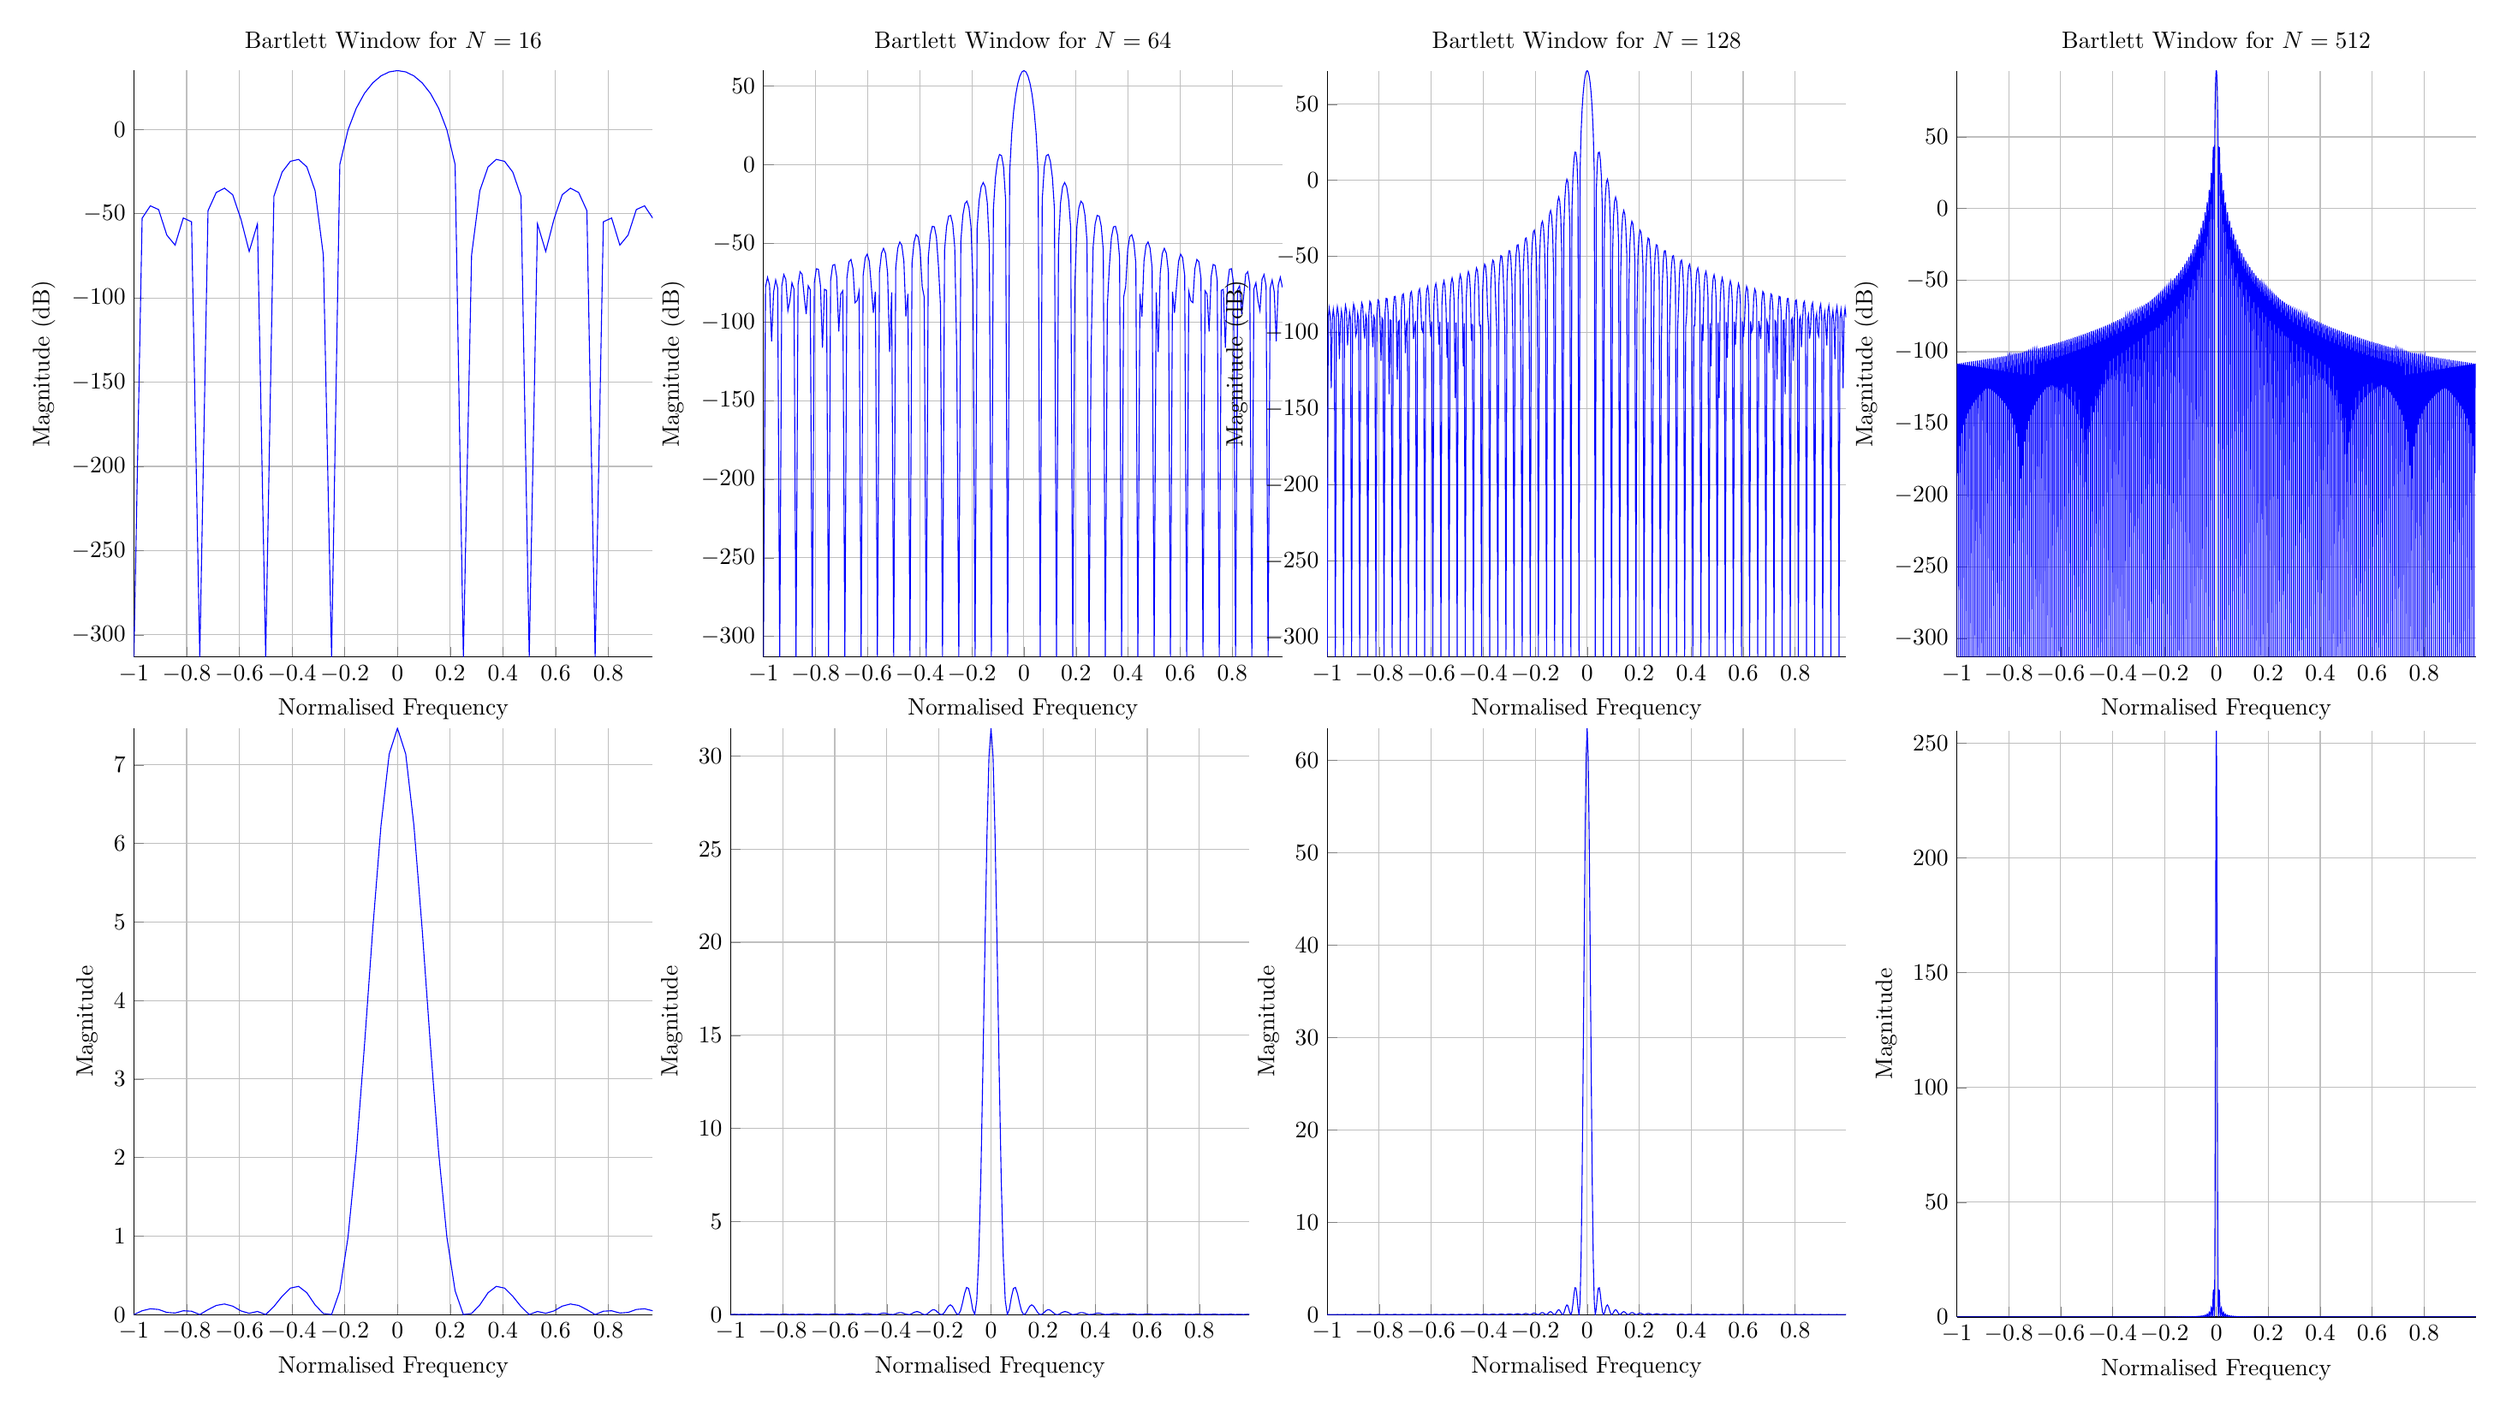
\begin{tikzpicture}

\begin{axis}[%
width=3.0303634751773in,
height=3.42584302325582in,
scale only axis,
xmin=-1,
xmax=0.9921875,
xlabel={Normalised Frequency},
xmajorgrids,
ymin=-313.07119549054,
ymax=59.9280447345831,
ylabel={Magnitude (dB)},
ymajorgrids,
name=plot3,
title={Bartlett Window for $N=64$},
axis x line*=bottom,
axis y line*=left
]
\addplot [color=blue,solid,forget plot]
  table[row sep=crcr]{-1	-313.07119549054\\
-0.9921875	-77.9048294183557\\
-0.984375	-71.5470861915874\\
-0.9765625	-76.5025955573178\\
-0.96875	-112.258727823239\\
-0.9609375	-80.7504511125821\\
-0.953125	-73.2576303308507\\
-0.9453125	-78.5610188093687\\
-0.9375	-313.07119549054\\
-0.9296875	-77.1078565406122\\
-0.921875	-69.8220627195985\\
-0.9140625	-72.908983730414\\
-0.90625	-92.8935128453632\\
-0.8984375	-86.3149406468681\\
-0.890625	-75.0265987535662\\
-0.8828125	-79.0924270687003\\
-0.875	-313.07119549054\\
-0.8671875	-76.1532121033621\\
-0.859375	-68.0271446673546\\
-0.8515625	-69.6447801464685\\
-0.84375	-83.4524463337772\\
-0.8359375	-94.98176844038\\
-0.828125	-76.9608240058492\\
-0.8203125	-79.5159163479562\\
-0.8125	-313.07119549054\\
-0.8046875	-75.0215981924048\\
-0.796875	-66.1152295418112\\
-0.7890625	-66.5194478267811\\
-0.78125	-76.7401569346864\\
-0.7734375	-116.422221659055\\
-0.765625	-79.2347368068082\\
-0.7578125	-79.851627021861\\
-0.75	-313.07119549054\\
-0.7421875	-73.6896887425588\\
-0.734375	-64.041558509225\\
-0.7265625	-63.4033755421068\\
-0.71875	-71.1858017075986\\
-0.7109375	-106.091706046193\\
-0.703125	-82.170294912448\\
-0.6953125	-80.126880049202\\
-0.6875	-313.07119549054\\
-0.6796875	-72.1281147100681\\
-0.671875	-61.7589906244733\\
-0.6640625	-60.1948531974504\\
-0.65625	-66.1584169847103\\
-0.6484375	-87.6762921779411\\
-0.640625	-86.469743924064\\
-0.6328125	-80.3832483006686\\
-0.625	-313.07119549054\\
-0.6171875	-70.2986608558503\\
-0.609375	-59.213302202463\\
-0.6015625	-56.8017834466954\\
-0.59375	-61.3175601974603\\
-0.5859375	-77.1212813510578\\
-0.578125	-94.1776186443326\\
-0.5703125	-80.6907232208984\\
-0.5625	-313.07119549054\\
-0.5546875	-68.1500525227334\\
-0.546875	-56.3374098736845\\
-0.5390625	-53.1285839469387\\
-0.53125	-56.4322213279841\\
-0.5234375	-68.815677944554\\
-0.515625	-119.148110455994\\
-0.5078125	-81.1793155729943\\
-0.5	-313.07119549054\\
-0.4921875	-65.6112201836716\\
-0.484375	-53.0430395178635\\
-0.4765625	-49.0633471243694\\
-0.46875	-51.3075712358655\\
-0.4609375	-61.3148735107318\\
-0.453125	-96.4885251232165\\
-0.4453125	-82.1199957959125\\
-0.4375	-313.07119549054\\
-0.4296875	-62.5798710115342\\
-0.421875	-49.2072498409572\\
-0.4140625	-44.4609373928614\\
-0.40625	-45.7414787110121\\
-0.3984375	-53.9348408331871\\
-0.390625	-77.4592768838042\\
-0.3828125	-84.1795255160359\\
-0.375	-313.07119549054\\
-0.3671875	-58.9017597736356\\
-0.359375	-44.6484799350843\\
-0.3515625	-39.1153974725548\\
-0.34375	-39.4824200588275\\
-0.3359375	-46.1855321650921\\
-0.328125	-64.3318485118199\\
-0.3203125	-89.5850787790678\\
-0.3125	-313.07119549054\\
-0.3046875	-54.3298717183412\\
-0.296875	-39.0796874365732\\
-0.2890625	-32.7073073359227\\
-0.28125	-32.1652574446007\\
-0.2734375	-37.5554290696448\\
-0.265625	-52.3230849703402\\
-0.2578125	-120.701871278186\\
-0.25	-313.07119549054\\
-0.2421875	-48.4348620610814\\
-0.234375	-32.0052565806245\\
-0.2265625	-24.6876982010798\\
-0.21875	-23.1778306135278\\
-0.2109375	-27.3091967522417\\
-0.203125	-39.5586713207809\\
-0.1953125	-77.6811282564878\\
-0.1875	-313.07119549054\\
-0.1796875	-40.3760131522083\\
-0.171875	-22.4540182045488\\
-0.1640625	-13.9714748094043\\
-0.15625	-11.3066610171854\\
-0.1484375	-14.0563020281686\\
-0.140625	-24.0705349288251\\
-0.1328125	-51.4133224320642\\
-0.125	-313.07119549054\\
-0.1171875	-28.1562790770059\\
-0.109375	-8.08365401153532\\
-0.1015625	2.13487458805794\\
-0.09375	6.5569038848615\\
-0.0859375	5.83357078780416\\
-0.078125	-1.41702044916492\\
-0.0703125	-22.2061279532975\\
-0.0625	-313.07119549054\\
-0.0546875	-4.76608476724979\\
-0.046875	19.8821120641373\\
-0.0390625	34.7120359253681\\
-0.03125	44.7830022382328\\
-0.0234375	51.7633128833984\\
-0.015625	56.3976662782434\\
-0.0078125	59.0590461315164\\
0	59.9280447345831\\
0.0078125	59.0590461315164\\
0.015625	56.3976662782434\\
0.0234375	51.7633128833984\\
0.03125	44.7830022382328\\
0.0390625	34.7120359253681\\
0.046875	19.8821120641373\\
0.0546875	-4.76608476724979\\
0.0625	-313.07119549054\\
0.0703125	-22.2061279532975\\
0.078125	-1.41702044916492\\
0.0859375	5.83357078780416\\
0.09375	6.5569038848615\\
0.1015625	2.13487458805794\\
0.109375	-8.08365401153532\\
0.1171875	-28.1562790770059\\
0.125	-313.07119549054\\
0.1328125	-51.4133224320642\\
0.140625	-24.0705349288251\\
0.1484375	-14.0563020281686\\
0.15625	-11.3066610171854\\
0.1640625	-13.9714748094043\\
0.171875	-22.4540182045488\\
0.1796875	-40.3760131522083\\
0.1875	-313.07119549054\\
0.1953125	-77.6811282564878\\
0.203125	-39.5586713207809\\
0.2109375	-27.3091967522417\\
0.21875	-23.1778306135278\\
0.2265625	-24.6876982010798\\
0.234375	-32.0052565806245\\
0.2421875	-48.4348620610814\\
0.25	-313.07119549054\\
0.2578125	-120.701871278186\\
0.265625	-52.3230849703402\\
0.2734375	-37.5554290696448\\
0.28125	-32.1652574446007\\
0.2890625	-32.7073073359227\\
0.296875	-39.0796874365732\\
0.3046875	-54.3298717183412\\
0.3125	-313.07119549054\\
0.3203125	-89.5850787790678\\
0.328125	-64.3318485118199\\
0.3359375	-46.1855321650921\\
0.34375	-39.4824200588275\\
0.3515625	-39.1153974725548\\
0.359375	-44.6484799350843\\
0.3671875	-58.9017597736356\\
0.375	-313.07119549054\\
0.3828125	-84.1795255160359\\
0.390625	-77.4592768838042\\
0.3984375	-53.9348408331871\\
0.40625	-45.7414787110121\\
0.4140625	-44.4609373928614\\
0.421875	-49.2072498409572\\
0.4296875	-62.5798710115342\\
0.4375	-313.07119549054\\
0.4453125	-82.1199957959125\\
0.453125	-96.4885251232165\\
0.4609375	-61.3148735107318\\
0.46875	-51.3075712358655\\
0.4765625	-49.0633471243694\\
0.484375	-53.0430395178635\\
0.4921875	-65.6112201836716\\
0.5	-313.07119549054\\
0.5078125	-81.1793155729943\\
0.515625	-119.148110455994\\
0.5234375	-68.815677944554\\
0.53125	-56.4322213279841\\
0.5390625	-53.1285839469387\\
0.546875	-56.3374098736845\\
0.5546875	-68.1500525227334\\
0.5625	-313.07119549054\\
0.5703125	-80.6907232208984\\
0.578125	-94.1776186443326\\
0.5859375	-77.1212813510578\\
0.59375	-61.3175601974603\\
0.6015625	-56.8017834466954\\
0.609375	-59.213302202463\\
0.6171875	-70.2986608558503\\
0.625	-313.07119549054\\
0.6328125	-80.3832483006686\\
0.640625	-86.469743924064\\
0.6484375	-87.6762921779411\\
0.65625	-66.1584169847103\\
0.6640625	-60.1948531974504\\
0.671875	-61.7589906244733\\
0.6796875	-72.1281147100681\\
0.6875	-313.07119549054\\
0.6953125	-80.126880049202\\
0.703125	-82.170294912448\\
0.7109375	-106.091706046193\\
0.71875	-71.1858017075986\\
0.7265625	-63.4033755421068\\
0.734375	-64.041558509225\\
0.7421875	-73.6896887425588\\
0.75	-313.07119549054\\
0.7578125	-79.851627021861\\
0.765625	-79.2347368068082\\
0.7734375	-116.422221659055\\
0.78125	-76.7401569346864\\
0.7890625	-66.5194478267811\\
0.796875	-66.1152295418112\\
0.8046875	-75.0215981924048\\
0.8125	-313.07119549054\\
0.8203125	-79.5159163479562\\
0.828125	-76.9608240058492\\
0.8359375	-94.98176844038\\
0.84375	-83.4524463337772\\
0.8515625	-69.6447801464685\\
0.859375	-68.0271446673546\\
0.8671875	-76.1532121033621\\
0.875	-313.07119549054\\
0.8828125	-79.0924270687003\\
0.890625	-75.0265987535662\\
0.8984375	-86.3149406468681\\
0.90625	-92.8935128453632\\
0.9140625	-72.908983730414\\
0.921875	-69.8220627195985\\
0.9296875	-77.1078565406122\\
0.9375	-313.07119549054\\
0.9453125	-78.5610188093687\\
0.953125	-73.2576303308507\\
0.9609375	-80.7504511125821\\
0.96875	-112.258727823239\\
0.9765625	-76.5025955573178\\
0.984375	-71.5470861915874\\
0.9921875	-77.9048294183557\\
};
\end{axis}

\begin{axis}[%
width=3.0303634751773in,
height=3.42584302325582in,
scale only axis,
xmin=-1,
xmax=0.96875,
xlabel={Normalised Frequency},
xmajorgrids,
ymin=-313.07119549054,
ymax=34.92507054458,
ylabel={Magnitude (dB)},
ymajorgrids,
name=plot1,
at=(plot3.left of south west),
anchor=right of south east,
title={Bartlett Window for $N=16$},
axis x line*=bottom,
axis y line*=left
]
\addplot [color=blue,solid,forget plot]
  table[row sep=crcr]{-1	-313.07119549054\\
-0.96875	-52.6933627396673\\
-0.9375	-45.3279319478347\\
-0.90625	-47.5577433838129\\
-0.875	-62.718936660227\\
-0.84375	-68.6598819785307\\
-0.8125	-52.5583764382965\\
-0.78125	-54.8045336520985\\
-0.75	-313.07119549054\\
-0.71875	-48.2028647306934\\
-0.6875	-37.4220411509476\\
-0.65625	-34.852717530771\\
-0.625	-38.8006023290143\\
-0.59375	-53.3412244951448\\
-0.5625	-72.4257986909477\\
-0.53125	-56.0323456897147\\
-0.5	-313.07119549054\\
-0.46875	-39.6090642073014\\
-0.4375	-25.2955885049419\\
-0.40625	-18.9085750653053\\
-0.375	-17.7877127526001\\
-0.34375	-22.26074674233\\
-0.3125	-36.3810117137346\\
-0.28125	-74.5364119094345\\
-0.25	-313.07119549054\\
-0.21875	-20.8045328020249\\
-0.1875	-0.231786849970813\\
-0.15625	12.5874471426478\\
-0.125	21.4416489921297\\
-0.09375	27.6345334116889\\
-0.0625	31.7671304042968\\
-0.03125	34.1470151947824\\
0	34.92507054458\\
0.03125	34.1470151947824\\
0.0625	31.7671304042968\\
0.09375	27.6345334116889\\
0.125	21.4416489921297\\
0.15625	12.5874471426478\\
0.1875	-0.231786849970813\\
0.21875	-20.8045328020249\\
0.25	-313.07119549054\\
0.28125	-74.5364119094345\\
0.3125	-36.3810117137346\\
0.34375	-22.26074674233\\
0.375	-17.7877127526001\\
0.40625	-18.9085750653053\\
0.4375	-25.2955885049419\\
0.46875	-39.6090642073014\\
0.5	-313.07119549054\\
0.53125	-56.0323456897147\\
0.5625	-72.4257986909477\\
0.59375	-53.3412244951448\\
0.625	-38.8006023290143\\
0.65625	-34.852717530771\\
0.6875	-37.4220411509476\\
0.71875	-48.2028647306934\\
0.75	-313.07119549054\\
0.78125	-54.8045336520985\\
0.8125	-52.5583764382965\\
0.84375	-68.6598819785307\\
0.875	-62.718936660227\\
0.90625	-47.5577433838129\\
0.9375	-45.3279319478347\\
0.96875	-52.6933627396673\\
};
\end{axis}

\begin{axis}[%
width=3.0303634751773in,
height=3.42584302325581in,
scale only axis,
xmin=-1,
xmax=0.96875,
xlabel={Normalised Frequency},
xmajorgrids,
ymin=0,
ymax=7.46666666666667,
ylabel={Magnitude},
ymajorgrids,
name=plot2,
at=(plot1.below south west),
anchor=above north west,
axis x line*=bottom,
axis y line*=left
]
\addplot [color=blue,solid,forget plot]
  table[row sep=crcr]{-1	0\\
-0.96875	0.0481577215744083\\
-0.9375	0.0735871022344712\\
-0.90625	0.0647226685856398\\
-0.875	0.0270412388051448\\
-0.84375	0.0192089201198216\\
-0.8125	0.0485333857211073\\
-0.78125	0.0426468205460492\\
-0.75	0\\
-0.71875	0.0623631985625933\\
-0.6875	0.11599759131821\\
-0.65625	0.13448754372794\\
-0.625	0.107148215325865\\
-0.59375	0.0463948086239293\\
-0.5625	0.0154651819080634\\
-0.53125	0.039736659758631\\
-0.5	0\\
-0.46875	0.10227592000737\\
-0.4375	0.233136508111342\\
-0.40625	0.336732956440728\\
-0.375	0.359175893815435\\
-0.34375	0.277639549755917\\
-0.3125	0.123161425575848\\
-0.28125	0.0136958724344609\\
-0.25	0\\
-0.21875	0.30191638300367\\
-0.1875	0.98674589591972\\
-0.15625	2.06388825005383\\
-0.125	3.43590561210941\\
-0.09375	4.90753420525455\\
-0.0625	6.225557663917\\
-0.03125	7.13962464287499\\
0	7.46666666666667\\
0.03125	7.13962464287499\\
0.0625	6.225557663917\\
0.09375	4.90753420525455\\
0.125	3.43590561210941\\
0.15625	2.06388825005383\\
0.1875	0.98674589591972\\
0.21875	0.30191638300367\\
0.25	0\\
0.28125	0.0136958724344609\\
0.3125	0.123161425575848\\
0.34375	0.277639549755917\\
0.375	0.359175893815435\\
0.40625	0.336732956440728\\
0.4375	0.233136508111342\\
0.46875	0.10227592000737\\
0.5	0\\
0.53125	0.039736659758631\\
0.5625	0.0154651819080634\\
0.59375	0.0463948086239293\\
0.625	0.107148215325865\\
0.65625	0.13448754372794\\
0.6875	0.11599759131821\\
0.71875	0.0623631985625933\\
0.75	0\\
0.78125	0.0426468205460492\\
0.8125	0.0485333857211073\\
0.84375	0.0192089201198216\\
0.875	0.0270412388051448\\
0.90625	0.0647226685856398\\
0.9375	0.0735871022344712\\
0.96875	0.0481577215744083\\
};
\end{axis}

\begin{axis}[%
width=3.0303634751773in,
height=3.42584302325581in,
scale only axis,
xmin=-1,
xmax=0.9921875,
xlabel={Normalised Frequency},
xmajorgrids,
ymin=0,
ymax=31.4920634920635,
ylabel={Magnitude},
ymajorgrids,
name=plot4,
at=(plot2.right of south east),
anchor=left of south west,
axis x line*=bottom,
axis y line*=left
]
\addplot [color=blue,solid,forget plot]
  table[row sep=crcr]{-1	0\\
-0.9921875	0.0112818225512145\\
-0.984375	0.0162675760311701\\
-0.9765625	0.0122302437052537\\
-0.96875	0.00156146338339326\\
-0.9609375	0.00957720364588465\\
-0.953125	0.0147420962289755\\
-0.9453125	0.0108636190946624\\
-0.9375	0\\
-0.9296875	0.011811460080165\\
-0.921875	0.0179658774124482\\
-0.9140625	0.0150409548204182\\
-0.90625	0.00476060533386409\\
-0.8984375	0.00695226765793894\\
-0.890625	0.0133148117673811\\
-0.8828125	0.0105363290034575\\
-0.875	0\\
-0.8671875	0.0124787101553218\\
-0.859375	0.0199214700720642\\
-0.8515625	0.0181501616086514\\
-0.84375	0.00819763998738445\\
-0.8359375	0.00422139303244044\\
-0.828125	0.0119118550448198\\
-0.8203125	0.0102825798634029\\
-0.8125	0\\
-0.8046875	0.0133186450600671\\
-0.796875	0.0222392051683503\\
-0.7890625	0.021727702406704\\
-0.78125	0.0120641318954674\\
-0.7734375	0.00122869603976189\\
-0.765625	0.0104503678998098\\
-0.7578125	0.0100857761389746\\
-0.75	0\\
-0.7421875	0.0143799634250777\\
-0.734375	0.0250588442751849\\
-0.7265625	0.0259965437050304\\
-0.71875	0.0166094387449236\\
-0.7109375	0.00222693401469536\\
-0.703125	0.00882556722174488\\
-0.6953125	0.0099272280519975\\
-0.6875	0\\
-0.6796875	0.0157324779687503\\
-0.671875	0.0285775658657101\\
-0.6640625	0.0312700567965943\\
-0.65625	0.0221839856367849\\
-0.6484375	0.00642824906833159\\
-0.640625	0.00689058987877073\\
-0.6328125	0.00978180030519694\\
-0.625	0\\
-0.6171875	0.0174796800341725\\
-0.609375	0.0330877659408656\\
-0.6015625	0.0380150366771079\\
-0.59375	0.0293130490733965\\
-0.5859375	0.0118023357782588\\
-0.578125	0.00442139722050821\\
-0.5703125	0.0096101887923706\\
-0.5625	0\\
-0.5546875	0.0197810202222796\\
-0.546875	0.039044939403823\\
-0.5390625	0.04696619763841\\
-0.53125	0.0388324209465553\\
-0.5234375	0.0190374182488732\\
-0.515625	0.00105026099927822\\
-0.5078125	0.00934366180423677\\
-0.5	0\\
-0.4921875	0.0228938849186493\\
-0.484375	0.0471980452226214\\
-0.4765625	0.0593493985146742\\
-0.46875	0.0521567737027082\\
-0.4609375	0.0293175829250548\\
-0.453125	0.00387067646580573\\
-0.4453125	0.0088511582403354\\
-0.4375	0\\
-0.4296875	0.0272585797881995\\
-0.421875	0.0588597961917896\\
-0.4140625	0.0773528937508448\\
-0.40625	0.0718559990910009\\
-0.3984375	0.0448362187300745\\
-0.390625	0.0115749221276017\\
-0.3828125	0.00786161663674226\\
-0.375	0\\
-0.3671875	0.0336865089339067\\
-0.359375	0.0765222976489486\\
-0.3515625	0.105224062044783\\
-0.34375	0.10302425875712\\
-0.3359375	0.0700425092056036\\
-0.328125	0.0246435793583068\\
-0.3203125	0.0057593441489438\\
-0.3125	0\\
-0.3046875	0.0438281568328903\\
-0.296875	0.105440586772062\\
-0.2890625	0.152165892143874\\
-0.28125	0.156988761718562\\
-0.2734375	0.115110323187454\\
-0.265625	0.0491952164515992\\
-0.2578125	0.000960402358702903\\
-0.25	0\\
-0.2421875	0.0615358846508156\\
-0.234375	0.15844136872606\\
-0.2265625	0.241439067441983\\
-0.21875	0.263362681025604\\
-0.2109375	0.207620427621487\\
-0.203125	0.102573037616119\\
-0.1953125	0.0114280410992083\\
-0.1875	0\\
-0.1796875	0.0978587516227183\\
-0.171875	0.27456776268758\\
-0.1640625	0.447417667881441\\
-0.15625	0.521595066014376\\
-0.1484375	0.445238231750678\\
-0.140625	0.250170805430491\\
-0.1328125	0.0518402323268662\\
-0.125	0\\
-0.1171875	0.197739313960215\\
-0.109375	0.627926265772745\\
-0.1015625	1.13076371683947\\
-0.09375	1.45855428377132\\
-0.0859375	1.39906943785613\\
-0.078125	0.921667956656144\\
-0.0703125	0.278513852838507\\
-0.0625	0\\
-0.0546875	0.760060006098824\\
-0.046875	3.14089054071608\\
-0.0390625	7.37566016214267\\
-0.03125	13.169674949666\\
-0.0234375	19.6826161104807\\
-0.015625	25.7005049944703\\
-0.0078125	29.9554710516517\\
0	31.4920634920635\\
0.0078125	29.9554710516517\\
0.015625	25.7005049944703\\
0.0234375	19.6826161104807\\
0.03125	13.169674949666\\
0.0390625	7.37566016214267\\
0.046875	3.14089054071608\\
0.0546875	0.760060006098824\\
0.0625	0\\
0.0703125	0.278513852838507\\
0.078125	0.921667956656144\\
0.0859375	1.39906943785613\\
0.09375	1.45855428377132\\
0.1015625	1.13076371683947\\
0.109375	0.627926265772745\\
0.1171875	0.197739313960215\\
0.125	0\\
0.1328125	0.0518402323268662\\
0.140625	0.250170805430491\\
0.1484375	0.445238231750678\\
0.15625	0.521595066014376\\
0.1640625	0.447417667881441\\
0.171875	0.27456776268758\\
0.1796875	0.0978587516227183\\
0.1875	0\\
0.1953125	0.0114280410992083\\
0.203125	0.102573037616119\\
0.2109375	0.207620427621487\\
0.21875	0.263362681025604\\
0.2265625	0.241439067441983\\
0.234375	0.15844136872606\\
0.2421875	0.0615358846508156\\
0.25	0\\
0.2578125	0.000960402358702903\\
0.265625	0.0491952164515992\\
0.2734375	0.115110323187454\\
0.28125	0.156988761718562\\
0.2890625	0.152165892143874\\
0.296875	0.105440586772062\\
0.3046875	0.0438281568328903\\
0.3125	0\\
0.3203125	0.0057593441489438\\
0.328125	0.0246435793583068\\
0.3359375	0.0700425092056036\\
0.34375	0.10302425875712\\
0.3515625	0.105224062044783\\
0.359375	0.0765222976489486\\
0.3671875	0.0336865089339067\\
0.375	0\\
0.3828125	0.00786161663674226\\
0.390625	0.0115749221276017\\
0.3984375	0.0448362187300745\\
0.40625	0.0718559990910009\\
0.4140625	0.0773528937508448\\
0.421875	0.0588597961917896\\
0.4296875	0.0272585797881995\\
0.4375	0\\
0.4453125	0.0088511582403354\\
0.453125	0.00387067646580573\\
0.4609375	0.0293175829250548\\
0.46875	0.0521567737027082\\
0.4765625	0.0593493985146742\\
0.484375	0.0471980452226214\\
0.4921875	0.0228938849186493\\
0.5	0\\
0.5078125	0.00934366180423677\\
0.515625	0.00105026099927822\\
0.5234375	0.0190374182488732\\
0.53125	0.0388324209465553\\
0.5390625	0.04696619763841\\
0.546875	0.039044939403823\\
0.5546875	0.0197810202222796\\
0.5625	0\\
0.5703125	0.0096101887923706\\
0.578125	0.00442139722050821\\
0.5859375	0.0118023357782588\\
0.59375	0.0293130490733965\\
0.6015625	0.0380150366771079\\
0.609375	0.0330877659408656\\
0.6171875	0.0174796800341725\\
0.625	0\\
0.6328125	0.00978180030519694\\
0.640625	0.00689058987877073\\
0.6484375	0.00642824906833159\\
0.65625	0.0221839856367849\\
0.6640625	0.0312700567965943\\
0.671875	0.0285775658657101\\
0.6796875	0.0157324779687503\\
0.6875	0\\
0.6953125	0.0099272280519975\\
0.703125	0.00882556722174488\\
0.7109375	0.00222693401469536\\
0.71875	0.0166094387449236\\
0.7265625	0.0259965437050304\\
0.734375	0.0250588442751849\\
0.7421875	0.0143799634250777\\
0.75	0\\
0.7578125	0.0100857761389746\\
0.765625	0.0104503678998098\\
0.7734375	0.00122869603976189\\
0.78125	0.0120641318954674\\
0.7890625	0.021727702406704\\
0.796875	0.0222392051683503\\
0.8046875	0.0133186450600671\\
0.8125	0\\
0.8203125	0.0102825798634029\\
0.828125	0.0119118550448198\\
0.8359375	0.00422139303244044\\
0.84375	0.00819763998738445\\
0.8515625	0.0181501616086514\\
0.859375	0.0199214700720642\\
0.8671875	0.0124787101553218\\
0.875	0\\
0.8828125	0.0105363290034575\\
0.890625	0.0133148117673811\\
0.8984375	0.00695226765793894\\
0.90625	0.00476060533386409\\
0.9140625	0.0150409548204182\\
0.921875	0.0179658774124482\\
0.9296875	0.011811460080165\\
0.9375	0\\
0.9453125	0.0108636190946624\\
0.953125	0.0147420962289755\\
0.9609375	0.00957720364588465\\
0.96875	0.00156146338339326\\
0.9765625	0.0122302437052537\\
0.984375	0.0162675760311701\\
0.9921875	0.0112818225512145\\
};
\end{axis}

\begin{axis}[%
width=3.03036347517731in,
height=3.42584302325581in,
scale only axis,
xmin=-1,
xmax=0.99609375,
xlabel={Normalised Frequency},
xmajorgrids,
ymin=0,
ymax=63.496062992126,
ylabel={Magnitude},
ymajorgrids,
name=plot6,
at=(plot4.right of south east),
anchor=left of south west,
axis x line*=bottom,
axis y line*=left
]
\addplot [color=blue,solid,forget plot]
  table[row sep=crcr]{-1	0\\
-0.99609375	0.00558202613536746\\
-0.9921875	0.00797124953050434\\
-0.98828125	0.00581621654644226\\
-0.984375	0.000386708943659105\\
-0.98046875	0.00515767879007148\\
-0.9765625	0.00758914109381042\\
-0.97265625	0.00547370058387671\\
-0.96875	0\\
-0.96484375	0.00570395329464427\\
-0.9609375	0.00837352458365415\\
-0.95703125	0.00649118554232393\\
-0.953125	0.00116480066877711\\
-0.94921875	0.00450761197483218\\
-0.9453125	0.00722257850153733\\
-0.94140625	0.00537766574237826\\
-0.9375	0\\
-0.93359375	0.00584096048400556\\
-0.9296875	0.00880085150257171\\
-0.92578125	0.00719079739338806\\
-0.921875	0.0019570523720022\\
-0.91796875	0.0038580712446957\\
-0.9140625	0.00686706845592109\\
-0.91015625	0.00529273932956664\\
-0.90625	0\\
-0.90234375	0.00599473765786069\\
-0.8984375	0.00925852575693194\\
-0.89453125	0.00792376065490142\\
-0.890625	0.00277337327244183\\
-0.88671875	0.0032008879640867\\
-0.8828125	0.00651810925889729\\
-0.87890625	0.00521783170756813\\
-0.875	0\\
-0.87109375	0.00616723786769628\\
-0.8671875	0.00975241568332897\\
-0.86328125	0.00869954999645035\\
-0.859375	0.00362440402714256\\
-0.85546875	0.00252741358755408\\
-0.8515625	0.00617104832063956\\
-0.84765625	0.00515191077701867\\
-0.84375	0\\
-0.83984375	0.00636073935795879\\
-0.8359375	0.0102891514930409\\
-0.83203125	0.00952871470607064\\
-0.828125	0.00452186706121268\\
-0.82421875	0.00182823134015922\\
-0.8203125	0.00582092445227453\\
-0.81640625	0.00509396557733539\\
-0.8125	0\\
-0.80859375	0.00657792196255156\\
-0.8046875	0.0108763522932855\\
-0.80078125	0.0104232457883704\\
-0.796875	0.00547898102830737\\
-0.79296875	0.00109281721041124\\
-0.7890625	0.00546228463631629\\
-0.78515625	0.00504296611340584\\
-0.78125	0\\
-0.77734375	0.00682196274490099\\
-0.7734375	0.0115229061546828\\
-0.76953125	0.0113970263969504\\
-0.765625	0.00651096781303871\\
-0.76171875	0.000309126575171037\\
-0.7578125	0.00508896214524971\\
-0.75390625	0.00499781633513003\\
-0.75	0\\
-0.74609375	0.00709665752879234\\
-0.7421875	0.0122393232913978\\
-0.73828125	0.0124663985870583\\
-0.734375	0.00763568997426169\\
-0.73046875	0.000536925152368723\\
-0.7265625	0.00469379849644018\\
-0.72265625	0.00495729621560029\\
-0.71875	0\\
-0.71484375	0.00740657744225006\\
-0.7109375	0.0130381898499613\\
-0.70703125	0.0136508916402013\\
-0.703125	0.00887447072321616\\
-0.69921875	0.001462131396558\\
-0.6953125	0.0042682850682986\\
-0.69140625	0.00491998732914072\\
-0.6875	0\\
-0.68359375	0.00775727321817125\\
-0.6796875	0.0139347608026347\\
-0.67578125	0.0149741754878512\\
-0.671875	0.0102531697869987\\
-0.66796875	0.00248687432875128\\
-0.6640625	0.00380209009100559\\
-0.66015625	0.00488417392682437\\
-0.65625	0\\
-0.65234375	0.00815554535729593\\
-0.6484375	0.0149477468873338\\
-0.64453125	0.0164653302400601\\
-0.640625	0.0118036206197208\\
-0.63671875	0.00363630460754782\\
-0.6328125	0.00328242126432409\\
-0.62890625	0.00484770775824754\\
-0.625	0\\
-0.62109375	0.00860980631659242\\
-0.6171875	0.0161003754686154\\
-0.61328125	0.0181605647088017\\
-0.609375	0.0135655835985749\\
-0.60546875	0.00494195172903195\\
-0.6015625	0.00269315030112889\\
-0.59765625	0.00480781897704951\\
-0.59375	0\\
-0.58984375	0.00913057320470433\\
-0.5859375	0.0174218436346617\\
-0.58203125	0.0201055817413795\\
-0.578125	0.0155894464328318\\
-0.57421875	0.0064439614861961\\
-0.5703125	0.00201358794902621\\
-0.56640625	0.00476084600027596\\
-0.5625	0\\
-0.55859375	0.00973114866752746\\
-0.5546875	0.0189493422692496\\
-0.55078125	0.0223588908022501\\
-0.546875	0.0179400246742275\\
-0.54296875	0.0081942619728566\\
-0.5390625	0.00121673736449585\\
-0.53515625	0.00470184173250595\\
-0.53125	0\\
-0.52734375	0.0104285782291263\\
-0.5234375	0.0207309269047887\\
-0.51953125	0.0249965340524689\\
-0.515625	0.0207020128101691\\
-0.51171875	0.0102611309274843\\
-0.5078125	0.000266753938123946\\
-0.50390625	0.00462398775137553\\
-0.5	0\\
-0.49609375	0.0112450222421659\\
-0.4921875	0.0228296709222754\\
-0.48828125	0.0281189667432692\\
-0.484375	0.0239879654215874\\
-0.48046875	0.012735924179262\\
-0.4765625	0.000884828628396368\\
-0.47265625	0.00451770383737593\\
-0.46875	0\\
-0.46484375	0.0122097641839624\\
-0.4609375	0.0253298068203235\\
-0.45703125	0.0318613000457317\\
-0.453125	0.027950251138456\\
-0.44921875	0.0157432192672331\\
-0.4453125	0.00230483829064714\\
-0.44140625	0.00436926230325568\\
-0.4375	0\\
-0.43359375	0.0133622212989154\\
-0.4296875	0.028346032166871\\
-0.42578125	0.0364089346188003\\
-0.421875	0.0327994169835239\\
-0.41796875	0.0194565071525674\\
-0.4140625	0.00408742647415987\\
-0.41015625	0.00415857472174326\\
-0.40625	0\\
-0.40234375	0.0147565810764768\\
-0.3984375	0.0320380061090358\\
-0.39453125	0.0420221035092437\\
-0.390625	0.038833220858041\\
-0.38671875	0.0241231843656599\\
-0.3828125	0.00636848043633815\\
-0.37890625	0.00385555078417366\\
-0.375	0\\
-0.37109375	0.0164691644111198\\
-0.3671875	0.0366336544050065\\
-0.36328125	0.0490756595866142\\
-0.359375	0.0464840560285188\\
-0.35546875	0.0301057059145544\\
-0.3515625	0.00934959934185968\\
-0.34765625	0.00341390160001979\\
-0.34375	0\\
-0.33984375	0.0186105405131028\\
-0.3359375	0.0424680207136909\\
-0.33203125	0.0581260115806431\\
-0.328125	0.0563994020404325\\
-0.32421875	0.0379520095671551\\
-0.3203125	0.0133395751760446\\
-0.31640625	0.00276016992107646\\
-0.3125	0\\
-0.30859375	0.021346300024405\\
-0.3046875	0.0500508364259774\\
-0.30078125	0.0700287136079079\\
-0.296875	0.0695844681178027\\
-0.29296875	0.048521593184906\\
-0.2890625	0.0188295381686859\\
-0.28515625	0.00177338742515042\\
-0.28125	0\\
-0.27734375	0.0249344538038506\\
-0.2734375	0.0601900728853498\\
-0.26953125	0.0861559064243834\\
-0.265625	0.0876687261795881\\
-0.26171875	0.0632236656120963\\
-0.2578125	0.0266367626709902\\
-0.25390625	0.000245192725713737\\
-0.25	0\\
-0.24609375	0.0297968221382916\\
-0.2421875	0.0742318815120967\\
-0.23828125	0.1088240246365\\
-0.234375	0.113436508857891\\
-0.23046875	0.0844971933119322\\
-0.2265625	0.0381988214902183\\
-0.22265625	0.00220384834775981\\
-0.21875	0\\
-0.21484375	0.0366654327417696\\
-0.2109375	0.0945623097476292\\
-0.20703125	0.142201568787519\\
-0.203125	0.151969227347823\\
-0.19921875	0.116859617647747\\
-0.1953125	0.0562271953569875\\
-0.19140625	0.00631535388399138\\
-0.1875	0\\
-0.18359375	0.0469110147611699\\
-0.1796875	0.12575878357533\\
-0.17578125	0.194430239444004\\
-0.171875	0.213360899044106\\
-0.16796875	0.169445350453575\\
-0.1640625	0.0863219440682313\\
-0.16015625	0.0136799650630951\\
-0.15625	0\\
-0.15234375	0.063371442927943\\
-0.1484375	0.177574107123891\\
-0.14453125	0.283246995803538\\
-0.140625	0.32007654926191\\
-0.13671875	0.263044993845627\\
-0.1328125	0.141565936679239\\
-0.12890625	0.0281735342829537\\
-0.125	0\\
-0.12109375	0.092800644055606\\
-0.1171875	0.274067470081014\\
-0.11328125	0.45371323799687\\
-0.109375	0.530867683265614\\
-0.10546875	0.453720793440026\\
-0.1015625	0.258487824253666\\
-0.09765625	0.0611824449840573\\
-0.09375	0\\
-0.08984375	0.154991689382128\\
-0.0859375	0.489293820171249\\
-0.08203125	0.850653962556512\\
-0.078125	1.04305989646607\\
-0.07421875	0.93886802240775\\
-0.0703125	0.572737260417918\\
-0.06640625	0.158097531167237\\
-0.0625	0\\
-0.05859375	0.332440767101443\\
-0.0546875	1.15749811435476\\
-0.05078125	2.180195942728\\
-0.046875	2.90208823057899\\
-0.04296875	2.86581180684316\\
-0.0390625	1.96167574809439\\
-0.03515625	0.654983057845119\\
-0.03125	0\\
-0.02734375	1.3793988008924\\
-0.0234375	6.0220486474797\\
-0.01953125	14.4602196990166\\
-0.015625	26.1398357635605\\
-0.01171875	39.3645827082585\\
-0.0078125	51.6419609411476\\
-0.00390625	60.3478008796828\\
0	63.496062992126\\
0.00390625	60.3478008796828\\
0.0078125	51.6419609411476\\
0.01171875	39.3645827082585\\
0.015625	26.1398357635605\\
0.01953125	14.4602196990166\\
0.0234375	6.0220486474797\\
0.02734375	1.3793988008924\\
0.03125	0\\
0.03515625	0.654983057845119\\
0.0390625	1.96167574809439\\
0.04296875	2.86581180684316\\
0.046875	2.90208823057899\\
0.05078125	2.180195942728\\
0.0546875	1.15749811435476\\
0.05859375	0.332440767101443\\
0.0625	0\\
0.06640625	0.158097531167237\\
0.0703125	0.572737260417918\\
0.07421875	0.93886802240775\\
0.078125	1.04305989646607\\
0.08203125	0.850653962556512\\
0.0859375	0.489293820171249\\
0.08984375	0.154991689382128\\
0.09375	0\\
0.09765625	0.0611824449840573\\
0.1015625	0.258487824253666\\
0.10546875	0.453720793440026\\
0.109375	0.530867683265614\\
0.11328125	0.45371323799687\\
0.1171875	0.274067470081014\\
0.12109375	0.092800644055606\\
0.125	0\\
0.12890625	0.0281735342829537\\
0.1328125	0.141565936679239\\
0.13671875	0.263044993845627\\
0.140625	0.32007654926191\\
0.14453125	0.283246995803538\\
0.1484375	0.177574107123891\\
0.15234375	0.063371442927943\\
0.15625	0\\
0.16015625	0.0136799650630951\\
0.1640625	0.0863219440682313\\
0.16796875	0.169445350453575\\
0.171875	0.213360899044106\\
0.17578125	0.194430239444004\\
0.1796875	0.12575878357533\\
0.18359375	0.0469110147611699\\
0.1875	0\\
0.19140625	0.00631535388399138\\
0.1953125	0.0562271953569875\\
0.19921875	0.116859617647747\\
0.203125	0.151969227347823\\
0.20703125	0.142201568787519\\
0.2109375	0.0945623097476292\\
0.21484375	0.0366654327417696\\
0.21875	0\\
0.22265625	0.00220384834775981\\
0.2265625	0.0381988214902183\\
0.23046875	0.0844971933119322\\
0.234375	0.113436508857891\\
0.23828125	0.1088240246365\\
0.2421875	0.0742318815120967\\
0.24609375	0.0297968221382916\\
0.25	0\\
0.25390625	0.000245192725713737\\
0.2578125	0.0266367626709902\\
0.26171875	0.0632236656120963\\
0.265625	0.0876687261795881\\
0.26953125	0.0861559064243834\\
0.2734375	0.0601900728853498\\
0.27734375	0.0249344538038506\\
0.28125	0\\
0.28515625	0.00177338742515042\\
0.2890625	0.0188295381686859\\
0.29296875	0.048521593184906\\
0.296875	0.0695844681178027\\
0.30078125	0.0700287136079079\\
0.3046875	0.0500508364259774\\
0.30859375	0.021346300024405\\
0.3125	0\\
0.31640625	0.00276016992107646\\
0.3203125	0.0133395751760446\\
0.32421875	0.0379520095671551\\
0.328125	0.0563994020404325\\
0.33203125	0.0581260115806431\\
0.3359375	0.0424680207136909\\
0.33984375	0.0186105405131028\\
0.34375	0\\
0.34765625	0.00341390160001979\\
0.3515625	0.00934959934185968\\
0.35546875	0.0301057059145544\\
0.359375	0.0464840560285188\\
0.36328125	0.0490756595866142\\
0.3671875	0.0366336544050065\\
0.37109375	0.0164691644111198\\
0.375	0\\
0.37890625	0.00385555078417366\\
0.3828125	0.00636848043633815\\
0.38671875	0.0241231843656599\\
0.390625	0.038833220858041\\
0.39453125	0.0420221035092437\\
0.3984375	0.0320380061090358\\
0.40234375	0.0147565810764768\\
0.40625	0\\
0.41015625	0.00415857472174326\\
0.4140625	0.00408742647415987\\
0.41796875	0.0194565071525674\\
0.421875	0.0327994169835239\\
0.42578125	0.0364089346188003\\
0.4296875	0.028346032166871\\
0.43359375	0.0133622212989154\\
0.4375	0\\
0.44140625	0.00436926230325568\\
0.4453125	0.00230483829064714\\
0.44921875	0.0157432192672331\\
0.453125	0.027950251138456\\
0.45703125	0.0318613000457317\\
0.4609375	0.0253298068203235\\
0.46484375	0.0122097641839624\\
0.46875	0\\
0.47265625	0.00451770383737593\\
0.4765625	0.000884828628396368\\
0.48046875	0.012735924179262\\
0.484375	0.0239879654215874\\
0.48828125	0.0281189667432692\\
0.4921875	0.0228296709222754\\
0.49609375	0.0112450222421659\\
0.5	0\\
0.50390625	0.00462398775137553\\
0.5078125	0.000266753938123946\\
0.51171875	0.0102611309274843\\
0.515625	0.0207020128101691\\
0.51953125	0.0249965340524689\\
0.5234375	0.0207309269047887\\
0.52734375	0.0104285782291263\\
0.53125	0\\
0.53515625	0.00470184173250595\\
0.5390625	0.00121673736449585\\
0.54296875	0.0081942619728566\\
0.546875	0.0179400246742275\\
0.55078125	0.0223588908022501\\
0.5546875	0.0189493422692496\\
0.55859375	0.00973114866752746\\
0.5625	0\\
0.56640625	0.00476084600027596\\
0.5703125	0.00201358794902621\\
0.57421875	0.0064439614861961\\
0.578125	0.0155894464328318\\
0.58203125	0.0201055817413795\\
0.5859375	0.0174218436346617\\
0.58984375	0.00913057320470433\\
0.59375	0\\
0.59765625	0.00480781897704951\\
0.6015625	0.00269315030112889\\
0.60546875	0.00494195172903195\\
0.609375	0.0135655835985749\\
0.61328125	0.0181605647088017\\
0.6171875	0.0161003754686154\\
0.62109375	0.00860980631659242\\
0.625	0\\
0.62890625	0.00484770775824754\\
0.6328125	0.00328242126432409\\
0.63671875	0.00363630460754782\\
0.640625	0.0118036206197208\\
0.64453125	0.0164653302400601\\
0.6484375	0.0149477468873338\\
0.65234375	0.00815554535729593\\
0.65625	0\\
0.66015625	0.00488417392682437\\
0.6640625	0.00380209009100559\\
0.66796875	0.00248687432875128\\
0.671875	0.0102531697869987\\
0.67578125	0.0149741754878512\\
0.6796875	0.0139347608026347\\
0.68359375	0.00775727321817125\\
0.6875	0\\
0.69140625	0.00491998732914072\\
0.6953125	0.0042682850682986\\
0.69921875	0.001462131396558\\
0.703125	0.00887447072321616\\
0.70703125	0.0136508916402013\\
0.7109375	0.0130381898499613\\
0.71484375	0.00740657744225006\\
0.71875	0\\
0.72265625	0.00495729621560029\\
0.7265625	0.00469379849644018\\
0.73046875	0.000536925152368723\\
0.734375	0.00763568997426169\\
0.73828125	0.0124663985870583\\
0.7421875	0.0122393232913978\\
0.74609375	0.00709665752879234\\
0.75	0\\
0.75390625	0.00499781633513003\\
0.7578125	0.00508896214524971\\
0.76171875	0.000309126575171037\\
0.765625	0.00651096781303871\\
0.76953125	0.0113970263969504\\
0.7734375	0.0115229061546828\\
0.77734375	0.00682196274490099\\
0.78125	0\\
0.78515625	0.00504296611340584\\
0.7890625	0.00546228463631629\\
0.79296875	0.00109281721041124\\
0.796875	0.00547898102830737\\
0.80078125	0.0104232457883704\\
0.8046875	0.0108763522932855\\
0.80859375	0.00657792196255156\\
0.8125	0\\
0.81640625	0.00509396557733539\\
0.8203125	0.00582092445227453\\
0.82421875	0.00182823134015922\\
0.828125	0.00452186706121268\\
0.83203125	0.00952871470607064\\
0.8359375	0.0102891514930409\\
0.83984375	0.00636073935795879\\
0.84375	0\\
0.84765625	0.00515191077701867\\
0.8515625	0.00617104832063956\\
0.85546875	0.00252741358755408\\
0.859375	0.00362440402714256\\
0.86328125	0.00869954999645035\\
0.8671875	0.00975241568332897\\
0.87109375	0.00616723786769628\\
0.875	0\\
0.87890625	0.00521783170756813\\
0.8828125	0.00651810925889729\\
0.88671875	0.0032008879640867\\
0.890625	0.00277337327244183\\
0.89453125	0.00792376065490142\\
0.8984375	0.00925852575693194\\
0.90234375	0.00599473765786069\\
0.90625	0\\
0.91015625	0.00529273932956664\\
0.9140625	0.00686706845592109\\
0.91796875	0.0038580712446957\\
0.921875	0.0019570523720022\\
0.92578125	0.00719079739338806\\
0.9296875	0.00880085150257171\\
0.93359375	0.00584096048400556\\
0.9375	0\\
0.94140625	0.00537766574237826\\
0.9453125	0.00722257850153733\\
0.94921875	0.00450761197483218\\
0.953125	0.00116480066877711\\
0.95703125	0.00649118554232393\\
0.9609375	0.00837352458365415\\
0.96484375	0.00570395329464427\\
0.96875	0\\
0.97265625	0.00547370058387671\\
0.9765625	0.00758914109381042\\
0.98046875	0.00515767879007148\\
0.984375	0.000386708943659105\\
0.98828125	0.00581621654644226\\
0.9921875	0.00797124953050434\\
0.99609375	0.00558202613536746\\
};
\end{axis}

\begin{axis}[%
width=3.03036347517731in,
height=3.42584302325582in,
scale only axis,
xmin=-1,
xmax=0.99609375,
xlabel={Normalised Frequency},
xmajorgrids,
ymin=-313.07119549054,
ymax=72.1098719258197,
ylabel={Magnitude (dB)},
ymajorgrids,
name=plot5,
at=(plot6.above north west),
anchor=below south west,
title={Bartlett Window for $N=128$},
axis x line*=bottom,
axis y line*=left
]
\addplot [color=blue,solid,forget plot]
  table[row sep=crcr]{-1	-313.07119549054\\
-0.99609375	-90.1283253779734\\
-0.9921875	-83.9389438233311\\
-0.98828125	-89.414377296535\\
-0.984375	-136.504631331553\\
-0.98046875	-91.501828333863\\
-0.9765625	-84.7922949158\\
-0.97265625	-90.4687585022296\\
-0.96875	-313.07119549054\\
-0.96484375	-89.7529615699563\\
-0.9609375	-83.0836680122173\\
-0.95703125	-87.5070390772864\\
-0.953125	-117.349935545709\\
-0.94921875	-93.8421390416076\\
-0.9453125	-85.6523091660262\\
-0.94140625	-90.7762478222783\\
-0.9375	-313.07119549054\\
-0.93359375	-89.3406292756862\\
-0.9296875	-82.2190122731592\\
-0.92578125	-85.728917907058\\
-0.921875	-108.335902086774\\
-0.91796875	-96.545190270329\\
-0.9140625	-86.529144928827\\
-0.91015625	-91.0527797892586\\
-0.90625	-313.07119549054\\
-0.90234375	-88.8891927109681\\
-0.8984375	-81.338326435944\\
-0.89453125	-84.0427460493143\\
-0.890625	-102.279666965615\\
-0.88671875	-99.7891810619183\\
-0.8828125	-87.435134560322\\
-0.87890625	-91.3003972980017\\
-0.875	-313.07119549054\\
-0.87109375	-88.3963720279648\\
-0.8671875	-80.4355118315448\\
-0.86328125	-82.4201284658642\\
-0.859375	-97.6305358284239\\
-0.85546875	-103.892947361362\\
-0.8515625	-88.3856421180622\\
-0.84765625	-91.5212666751116\\
-0.84375	-313.07119549054\\
-0.83984375	-87.8596960003113\\
-0.8359375	-79.5048175345932\\
-0.83203125	-80.8386270330227\\
-0.828125	-93.7872883865681\\
-0.82421875	-109.518754019709\\
-0.8203125	-89.4003214892811\\
-0.81640625	-91.7177597648791\\
-0.8125	-313.07119549054\\
-0.80859375	-87.2764513236873\\
-0.8046875	-78.5406693491687\\
-0.80078125	-79.2798808442154\\
-0.796875	-90.4520081345144\\
-0.79296875	-118.458098960415\\
-0.7890625	-90.5050269113922\\
-0.78515625	-91.8925580041581\\
-0.78125	-313.07119549054\\
-0.77734375	-86.6436262650489\\
-0.7734375	-77.5375190039614\\
-0.76953125	-77.7283378337317\\
-0.765625	-87.4541780632356\\
-0.76171875	-140.394546285985\\
-0.7578125	-91.7348311862184\\
-0.75390625	-92.0487883125005\\
-0.75	-313.07119549054\\
-0.74609375	-85.9578460996377\\
-0.7421875	-76.4897037416453\\
-0.73828125	-76.1703596625082\\
-0.734375	-84.6860685290732\\
-0.73046875	-130.803450031161\\
-0.7265625	-93.1390223394097\\
-0.72265625	-92.1902051887863\\
-0.71875	-313.07119549054\\
-0.71484375	-85.2152972749724\\
-0.7109375	-75.3913079783313\\
-0.70703125	-74.593559229102\\
-0.703125	-82.0743015594695\\
-0.69921875	-113.40054388394\\
-0.6953125	-94.7898633124896\\
-0.69140625	-92.32144062818\\
-0.6875	-313.07119549054\\
-0.68359375	-84.4116364816642\\
-0.6796875	-74.2360192710201\\
-0.67578125	-72.9862832608689\\
-0.671875	-79.5656740352847\\
-0.66796875	-104.173846429001\\
-0.6640625	-96.7991038673057\\
-0.66015625	-92.4483551639837\\
-0.65625	-313.07119549054\\
-0.65234375	-83.5418797037654\\
-0.6484375	-73.0169705896037\\
-0.64453125	-71.3371821741523\\
-0.640625	-77.1193903044145\\
-0.63671875	-97.5735897501323\\
-0.6328125	-99.3522273024867\\
-0.62890625	-92.5785427714602\\
-0.625	-313.07119549054\\
-0.62109375	-82.6002647273389\\
-0.6171875	-71.7265598356218\\
-0.61328125	-69.6348260429365\\
-0.609375	-74.7024607168847\\
-0.60546875	-92.2440600369018\\
-0.6015625	-102.789576340371\\
-0.59765625	-92.7220757062567\\
-0.59375	-313.07119549054\\
-0.58984375	-81.5800782881958\\
-0.5859375	-70.356235539159\\
-0.58203125	-67.8673342545079\\
-0.578125	-72.286772237685\\
-0.57421875	-87.6338825561526\\
-0.5703125	-107.84117586468\\
-0.56640625	-92.8926346591203\\
-0.5625	-313.07119549054\\
-0.55859375	-80.4734356984962\\
-0.5546875	-68.8962343909821\\
-0.55078125	-66.021989803175\\
-0.546875	-69.8470785589766\\
-0.54296875	-83.4596062257461\\
-0.5390625	-116.592126202592\\
-0.53515625	-93.1092797455414\\
-0.53125	-313.07119549054\\
-0.52734375	-79.2709958674617\\
-0.5234375	-67.3352511856369\\
-0.51953125	-64.0848082070974\\
-0.515625	-67.359497080555\\
-0.51171875	-79.5521908379611\\
-0.5078125	-142.95556638525\\
-0.50390625	-93.3993329999945\\
-0.5	-313.07119549054\\
-0.49609375	-77.9615872484594\\
-0.4921875	-65.6600139436632\\
-0.48828125	-62.0400256760166\\
-0.484375	-64.8002634345953\\
-0.48046875	-75.7987814032963\\
-0.4765625	-122.125633370693\\
-0.47265625	-93.8032897236876\\
-0.46875	-313.07119549054\\
-0.46484375	-76.5317089527334\\
-0.4609375	-63.8547248950509\\
-0.45703125	-59.8694603012573\\
-0.453125	-62.1445714215748\\
-0.44921875	-72.1162582309422\\
-0.4453125	-105.494381586198\\
-0.44140625	-94.3836752869382\\
-0.4375	-313.07119549054\\
-0.43359375	-74.9648535975435\\
-0.4296875	-61.9003089750852\\
-0.42578125	-57.5516811600762\\
-0.421875	-59.3653550357857\\
-0.41796875	-68.437404878257\\
-0.4140625	-95.5420018590601\\
-0.41015625	-95.2422196262034\\
-0.40625	-313.07119549054\\
-0.40234375	-73.2405700680289\\
-0.3984375	-59.7733808056181\\
-0.39453125	-55.0608884726398\\
-0.390625	-56.4318634892938\\
-0.38671875	-64.7026145591949\\
-0.3828125	-87.838567239285\\
-0.37890625	-96.5565428839927\\
-0.375	-313.07119549054\\
-0.37109375	-71.3331373953049\\
-0.3671875	-57.4447902381112\\
-0.36328125	-52.3653541873839\\
-0.359375	-53.3078393607233\\
-0.35546875	-60.8540474023451\\
-0.3515625	-81.168279981538\\
-0.34765625	-98.6699600338329\\
-0.34375	-313.07119549054\\
-0.33984375	-69.2096405321543\\
-0.3359375	-54.8775191795412\\
-0.33203125	-49.42517903629\\
-0.328125	-49.9490200193304\\
-0.32421875	-56.8306089268967\\
-0.3203125	-74.9943200450661\\
-0.31640625	-102.362567245916\\
-0.3125	-313.07119549054\\
-0.30859375	-66.8270956325555\\
-0.3046875	-52.0235464159762\\
-0.30078125	-46.1889540539585\\
-0.296875	-46.2995075210335\\
-0.29296875	-52.5625979082162\\
-0.2890625	-69.0064132710242\\
-0.28515625	-110.047855014731\\
-0.28125	-313.07119549054\\
-0.27734375	-64.1280056273131\\
-0.2734375	-48.819005231164\\
-0.26953125	-42.5885977642319\\
-0.265625	-42.2862121467209\\
-0.26171875	-47.9648131212834\\
-0.2578125	-62.9807423505753\\
-0.25390625	-144.419696705883\\
-0.25	-313.07119549054\\
-0.24609375	-61.0332020562733\\
-0.2421875	-45.1763812599801\\
-0.23828125	-38.5310086651948\\
-0.234375	-37.8098859151723\\
-0.23046875	-42.926308659472\\
-0.2265625	-56.7180014292793\\
-0.22265625	-106.272731746262\\
-0.21875	-313.07119549054\\
-0.21484375	-57.4297273960463\\
-0.2109375	-40.9712771360088\\
-0.20703125	-33.8838244953036\\
-0.203125	-32.7297737837981\\
-0.19921875	-37.2934215595531\\
-0.1953125	-50.0021431517889\\
-0.19140625	-87.9840923407438\\
-0.1875	-313.07119549054\\
-0.18359375	-53.1490068983482\\
-0.1796875	-36.0184668830635\\
-0.17578125	-28.4494475594454\\
-0.171875	-26.8354066926763\\
-0.16796875	-30.8388137446626\\
-0.1640625	-42.5551514963985\\
-0.16015625	-74.5566004699018\\
-0.15625	-313.07119549054\\
-0.15234375	-47.9242561659863\\
-0.1484375	-30.0248144145999\\
-0.14453125	-21.9133875075308\\
-0.140625	-19.7898457489151\\
-0.13671875	-23.1987983634405\\
-0.1328125	-33.9616493268364\\
-0.12890625	-62.0063467477519\\
-0.125	-313.07119549054\\
-0.12109375	-41.2979603870965\\
-0.1171875	-22.485700366483\\
-0.11328125	-13.7287419653418\\
-0.109375	-11.0005484666024\\
-0.10546875	-13.7284526848293\\
-0.1015625	-23.5023963595107\\
-0.09765625	-48.5349268659607\\
-0.09375	-313.07119549054\\
-0.08984375	-32.3876635189289\\
-0.0859375	-12.4172107754863\\
-0.08203125	-2.80988282410067\\
-0.078125	0.732369919335904\\
-0.07421875	-1.09581810566752\\
-0.0703125	-9.68178248740956\\
-0.06640625	-32.0429964762897\\
-0.0625	-313.07119549054\\
-0.05859375	-19.131428969334\\
-0.0546875	2.54081168778145\\
-0.05078125	13.539821084027\\
-0.046875	18.5084244766683\\
-0.04296875	18.2899067036803\\
-0.0390625	11.7050889199003\\
-0.03515625	-7.35079734259049\\
-0.03125	-313.07119549054\\
-0.02734375	5.58759376488331\\
-0.0234375	31.1897703808236\\
-0.01953125	46.4069956556732\\
-0.015625	56.6921141833335\\
-0.01171875	63.8042260792493\\
-0.0078125	68.5201089950152\\
-0.00390625	71.2264579478598\\
0	72.1098719258197\\
0.00390625	71.2264579478598\\
0.0078125	68.5201089950152\\
0.01171875	63.8042260792493\\
0.015625	56.6921141833335\\
0.01953125	46.4069956556732\\
0.0234375	31.1897703808236\\
0.02734375	5.58759376488331\\
0.03125	-313.07119549054\\
0.03515625	-7.35079734259049\\
0.0390625	11.7050889199003\\
0.04296875	18.2899067036803\\
0.046875	18.5084244766683\\
0.05078125	13.539821084027\\
0.0546875	2.54081168778145\\
0.05859375	-19.131428969334\\
0.0625	-313.07119549054\\
0.06640625	-32.0429964762897\\
0.0703125	-9.68178248740956\\
0.07421875	-1.09581810566752\\
0.078125	0.732369919335904\\
0.08203125	-2.80988282410067\\
0.0859375	-12.4172107754863\\
0.08984375	-32.3876635189289\\
0.09375	-313.07119549054\\
0.09765625	-48.5349268659607\\
0.1015625	-23.5023963595107\\
0.10546875	-13.7284526848293\\
0.109375	-11.0005484666024\\
0.11328125	-13.7287419653418\\
0.1171875	-22.485700366483\\
0.12109375	-41.2979603870965\\
0.125	-313.07119549054\\
0.12890625	-62.0063467477519\\
0.1328125	-33.9616493268364\\
0.13671875	-23.1987983634405\\
0.140625	-19.7898457489151\\
0.14453125	-21.9133875075308\\
0.1484375	-30.0248144145999\\
0.15234375	-47.9242561659863\\
0.15625	-313.07119549054\\
0.16015625	-74.5566004699018\\
0.1640625	-42.5551514963985\\
0.16796875	-30.8388137446626\\
0.171875	-26.8354066926763\\
0.17578125	-28.4494475594454\\
0.1796875	-36.0184668830635\\
0.18359375	-53.1490068983482\\
0.1875	-313.07119549054\\
0.19140625	-87.9840923407438\\
0.1953125	-50.0021431517889\\
0.19921875	-37.2934215595531\\
0.203125	-32.7297737837981\\
0.20703125	-33.8838244953036\\
0.2109375	-40.9712771360088\\
0.21484375	-57.4297273960463\\
0.21875	-313.07119549054\\
0.22265625	-106.272731746262\\
0.2265625	-56.7180014292793\\
0.23046875	-42.926308659472\\
0.234375	-37.8098859151723\\
0.23828125	-38.5310086651948\\
0.2421875	-45.1763812599801\\
0.24609375	-61.0332020562733\\
0.25	-313.07119549054\\
0.25390625	-144.419696705883\\
0.2578125	-62.9807423505753\\
0.26171875	-47.9648131212834\\
0.265625	-42.2862121467209\\
0.26953125	-42.5885977642319\\
0.2734375	-48.819005231164\\
0.27734375	-64.1280056273131\\
0.28125	-313.07119549054\\
0.28515625	-110.047855014731\\
0.2890625	-69.0064132710242\\
0.29296875	-52.5625979082162\\
0.296875	-46.2995075210335\\
0.30078125	-46.1889540539585\\
0.3046875	-52.0235464159762\\
0.30859375	-66.8270956325555\\
0.3125	-313.07119549054\\
0.31640625	-102.362567245916\\
0.3203125	-74.9943200450661\\
0.32421875	-56.8306089268967\\
0.328125	-49.9490200193304\\
0.33203125	-49.42517903629\\
0.3359375	-54.8775191795412\\
0.33984375	-69.2096405321543\\
0.34375	-313.07119549054\\
0.34765625	-98.6699600338329\\
0.3515625	-81.168279981538\\
0.35546875	-60.8540474023451\\
0.359375	-53.3078393607233\\
0.36328125	-52.3653541873839\\
0.3671875	-57.4447902381112\\
0.37109375	-71.3331373953049\\
0.375	-313.07119549054\\
0.37890625	-96.5565428839927\\
0.3828125	-87.838567239285\\
0.38671875	-64.7026145591949\\
0.390625	-56.4318634892938\\
0.39453125	-55.0608884726398\\
0.3984375	-59.7733808056181\\
0.40234375	-73.2405700680289\\
0.40625	-313.07119549054\\
0.41015625	-95.2422196262034\\
0.4140625	-95.5420018590601\\
0.41796875	-68.437404878257\\
0.421875	-59.3653550357857\\
0.42578125	-57.5516811600762\\
0.4296875	-61.9003089750852\\
0.43359375	-74.9648535975435\\
0.4375	-313.07119549054\\
0.44140625	-94.3836752869382\\
0.4453125	-105.494381586198\\
0.44921875	-72.1162582309422\\
0.453125	-62.1445714215748\\
0.45703125	-59.8694603012573\\
0.4609375	-63.8547248950509\\
0.46484375	-76.5317089527334\\
0.46875	-313.07119549054\\
0.47265625	-93.8032897236876\\
0.4765625	-122.125633370693\\
0.48046875	-75.7987814032963\\
0.484375	-64.8002634345953\\
0.48828125	-62.0400256760166\\
0.4921875	-65.6600139436632\\
0.49609375	-77.9615872484594\\
0.5	-313.07119549054\\
0.50390625	-93.3993329999945\\
0.5078125	-142.95556638525\\
0.51171875	-79.5521908379611\\
0.515625	-67.359497080555\\
0.51953125	-64.0848082070974\\
0.5234375	-67.3352511856369\\
0.52734375	-79.2709958674617\\
0.53125	-313.07119549054\\
0.53515625	-93.1092797455414\\
0.5390625	-116.592126202592\\
0.54296875	-83.4596062257461\\
0.546875	-69.8470785589766\\
0.55078125	-66.021989803175\\
0.5546875	-68.8962343909821\\
0.55859375	-80.4734356984962\\
0.5625	-313.07119549054\\
0.56640625	-92.8926346591203\\
0.5703125	-107.84117586468\\
0.57421875	-87.6338825561526\\
0.578125	-72.286772237685\\
0.58203125	-67.8673342545079\\
0.5859375	-70.356235539159\\
0.58984375	-81.5800782881958\\
0.59375	-313.07119549054\\
0.59765625	-92.7220757062567\\
0.6015625	-102.789576340371\\
0.60546875	-92.2440600369018\\
0.609375	-74.7024607168847\\
0.61328125	-69.6348260429365\\
0.6171875	-71.7265598356218\\
0.62109375	-82.6002647273389\\
0.625	-313.07119549054\\
0.62890625	-92.5785427714602\\
0.6328125	-99.3522273024867\\
0.63671875	-97.5735897501323\\
0.640625	-77.1193903044145\\
0.64453125	-71.3371821741523\\
0.6484375	-73.0169705896037\\
0.65234375	-83.5418797037654\\
0.65625	-313.07119549054\\
0.66015625	-92.4483551639837\\
0.6640625	-96.7991038673057\\
0.66796875	-104.173846429001\\
0.671875	-79.5656740352847\\
0.67578125	-72.9862832608689\\
0.6796875	-74.2360192710201\\
0.68359375	-84.4116364816642\\
0.6875	-313.07119549054\\
0.69140625	-92.32144062818\\
0.6953125	-94.7898633124896\\
0.69921875	-113.40054388394\\
0.703125	-82.0743015594695\\
0.70703125	-74.593559229102\\
0.7109375	-75.3913079783313\\
0.71484375	-85.2152972749724\\
0.71875	-313.07119549054\\
0.72265625	-92.1902051887863\\
0.7265625	-93.1390223394097\\
0.73046875	-130.803450031161\\
0.734375	-84.6860685290732\\
0.73828125	-76.1703596625082\\
0.7421875	-76.4897037416453\\
0.74609375	-85.9578460996377\\
0.75	-313.07119549054\\
0.75390625	-92.0487883125005\\
0.7578125	-91.7348311862184\\
0.76171875	-140.394546285985\\
0.765625	-87.4541780632356\\
0.76953125	-77.7283378337317\\
0.7734375	-77.5375190039614\\
0.77734375	-86.6436262650489\\
0.78125	-313.07119549054\\
0.78515625	-91.8925580041581\\
0.7890625	-90.5050269113922\\
0.79296875	-118.458098960415\\
0.796875	-90.4520081345144\\
0.80078125	-79.2798808442154\\
0.8046875	-78.5406693491687\\
0.80859375	-87.2764513236873\\
0.8125	-313.07119549054\\
0.81640625	-91.7177597648791\\
0.8203125	-89.4003214892811\\
0.82421875	-109.518754019709\\
0.828125	-93.7872883865681\\
0.83203125	-80.8386270330227\\
0.8359375	-79.5048175345932\\
0.83984375	-87.8596960003113\\
0.84375	-313.07119549054\\
0.84765625	-91.5212666751116\\
0.8515625	-88.3856421180622\\
0.85546875	-103.892947361362\\
0.859375	-97.6305358284239\\
0.86328125	-82.4201284658642\\
0.8671875	-80.4355118315448\\
0.87109375	-88.3963720279648\\
0.875	-313.07119549054\\
0.87890625	-91.3003972980017\\
0.8828125	-87.435134560322\\
0.88671875	-99.7891810619183\\
0.890625	-102.279666965615\\
0.89453125	-84.0427460493143\\
0.8984375	-81.338326435944\\
0.90234375	-88.8891927109681\\
0.90625	-313.07119549054\\
0.91015625	-91.0527797892586\\
0.9140625	-86.529144928827\\
0.91796875	-96.545190270329\\
0.921875	-108.335902086774\\
0.92578125	-85.728917907058\\
0.9296875	-82.2190122731592\\
0.93359375	-89.3406292756862\\
0.9375	-313.07119549054\\
0.94140625	-90.7762478222783\\
0.9453125	-85.6523091660262\\
0.94921875	-93.8421390416076\\
0.953125	-117.349935545709\\
0.95703125	-87.5070390772864\\
0.9609375	-83.0836680122173\\
0.96484375	-89.7529615699563\\
0.96875	-313.07119549054\\
0.97265625	-90.4687585022296\\
0.9765625	-84.7922949158\\
0.98046875	-91.501828333863\\
0.984375	-136.504631331553\\
0.98828125	-89.414377296535\\
0.9921875	-83.9389438233311\\
0.99609375	-90.1283253779734\\
};
\end{axis}

\begin{axis}[%
width=3.0303634751773in,
height=3.42584302325582in,
scale only axis,
xmin=-1,
xmax=0.9990234375,
xlabel={Normalised Frequency},
xmajorgrids,
ymin=-313.07119549054,
ymax=96.2955696510029,
ylabel={Magnitude (dB)},
ymajorgrids,
name=plot7,
at=(plot5.right of south east),
anchor=left of south west,
title={Bartlett Window for $N=512$},
axis x line*=bottom,
axis y line*=left
]
\addplot [color=blue,solid,forget plot]
  table[row sep=crcr]{-1	-313.07119549054\\
-0.9990234375	-114.346381022564\\
-0.998046875	-108.283539719881\\
-0.9970703125	-114.16531316414\\
-0.99609375	-184.779891329189\\
-0.9951171875	-114.68161631698\\
-0.994140625	-108.496732951501\\
-0.9931640625	-114.433875394768\\
-0.9921875	-313.07119549054\\
-0.9912109375	-114.256715441713\\
-0.990234375	-108.070314916028\\
-0.9892578125	-113.661259557796\\
-0.98828125	-165.690683530723\\
-0.9873046875	-115.21124145941\\
-0.986328125	-108.710024274628\\
-0.9853515625	-114.519229660925\\
-0.984375	-313.07119549054\\
-0.9833984375	-114.16484736612\\
-0.982421875	-107.856933512755\\
-0.9814453125	-113.168476718029\\
-0.98046875	-156.808011095379\\
-0.9794921875	-115.755367445953\\
-0.978515625	-108.923548384368\\
-0.9775390625	-114.602474788037\\
-0.9765625	-313.07119549054\\
-0.9755859375	-114.070745279689\\
-0.974609375	-107.643274752912\\
-0.9736328125	-112.686068606356\\
-0.97265625	-150.94980188953\\
-0.9716796875	-116.315294498192\\
-0.970703125	-109.137445432554\\
-0.9697265625	-114.683641655835\\
-0.96875	-313.07119549054\\
-0.9677734375	-113.974377390255\\
-0.966796875	-107.429221807632\\
-0.9658203125	-112.213212525069\\
-0.96484375	-146.566565559438\\
-0.9638671875	-116.892461842674\\
-0.962890625	-109.351861487079\\
-0.9619140625	-114.762761106646\\
-0.9609375	-313.07119549054\\
-0.9599609375	-113.875711584226\\
-0.958984375	-107.214661457852\\
-0.9580078125	-111.749150989123\\
-0.95703125	-143.058725113903\\
-0.9560546875	-117.488468631827\\
-0.955078125	-109.566949029295\\
-0.9541015625	-114.839863996926\\
-0.953125	-313.07119549054\\
-0.9521484375	-113.774715381355\\
-0.951171875	-106.999483796065\\
-0.9501953125	-111.293184668972\\
-0.94921875	-140.130481497618\\
-0.9482421875	-118.105098909314\\
-0.947265625	-109.782867492825\\
-0.9462890625	-114.914981249646\\
-0.9453125	-313.07119549054\\
-0.9443359375	-113.671355890199\\
-0.943359375	-106.783581947352\\
-0.9423828125	-110.84466623884\\
-0.94140625	-137.613955576249\\
-0.9404296875	-118.744351596998\\
-0.939453125	-109.999783848957\\
-0.9384765625	-114.988143909253\\
-0.9375	-313.07119549054\\
-0.9365234375	-113.565599763482\\
-0.935546875	-106.566851807059\\
-0.9345703125	-110.402994993227\\
-0.93359375	-135.404635938511\\
-0.9326171875	-119.408476767538\\
-0.931640625	-110.217873243746\\
-0.9306640625	-115.059383197802\\
-0.9296875	-313.07119549054\\
-0.9287109375	-113.45741315362\\
-0.927734375	-106.349191794172\\
-0.9267578125	-109.967612119319\\
-0.92578125	-133.433019765912\\
-0.9248046875	-120.100019852176\\
-0.923828125	-110.437319692304\\
-0.9228515625	-115.128730574498\\
-0.921875	-313.07119549054\\
-0.9208984375	-113.346761667669\\
-0.919921875	-106.130502618415\\
-0.9189453125	-109.537996529918\\
-0.91796875	-131.650533236815\\
-0.9169921875	-120.821875964807\\
-0.916015625	-110.658316837247\\
-0.9150390625	-115.196217796624\\
-0.9140625	-313.07119549054\\
-0.9130859375	-113.233610322522\\
-0.912109375	-105.910687060312\\
-0.9111328125	-109.113661179377\\
-0.91015625	-130.021887464768\\
-0.9091796875	-121.577357252403\\
-0.908203125	-110.881068778633\\
-0.9072265625	-115.261876983524\\
-0.90625	-313.07119549054\\
-0.9052734375	-113.117923499725\\
-0.904296875	-105.689649762482\\
-0.9033203125	-108.694149794999\\
-0.90234375	-128.520633910305\\
-0.9013671875	-122.370277211171\\
-0.900390625	-111.105790983822\\
-0.8994140625	-115.325740684095\\
-0.8984375	-313.07119549054\\
-0.8974609375	-112.999664899562\\
-0.896484375	-105.467297031445\\
-0.8955078125	-108.279033968773\\
-0.89453125	-127.126435678225\\
-0.8935546875	-123.205057368099\\
-0.892578125	-111.33271128684\\
-0.8916015625	-115.387841947365\\
-0.890625	-313.07119549054\\
-0.8896484375	-112.878797494086\\
-0.888671875	-105.243536648671\\
-0.8876953125	-107.867910561401\\
-0.88671875	-125.823316439028\\
-0.8857421875	-124.086863850674\\
-0.884765625	-111.562070988628\\
-0.8837890625	-115.448214396479\\
-0.8828125	-313.07119549054\\
-0.8818359375	-112.755283480416\\
-0.880859375	-105.018277690086\\
-0.8798828125	-107.460399378956\\
-0.87890625	-124.598494619874\\
-0.8779296875	-125.021784487598\\
-0.876953125	-111.794126070237\\
-0.8759765625	-115.506892307212\\
-0.875	-313.07119549054\\
-0.8740234375	-112.629084232385\\
-0.873046875	-104.791430353118\\
-0.8720703125	-107.056141086768\\
-0.87109375	-123.441582758102\\
-0.8701171875	-126.017061792579\\
-0.869140625	-112.0291485341\\
-0.8681640625	-115.563910691005\\
-0.8671875	-313.07119549054\\
-0.8662109375	-112.500160250822\\
-0.865234375	-104.562905790297\\
-0.8642578125	-106.654795331982\\
-0.86328125	-122.344022812409\\
-0.8623046875	-127.081404422715\\
-0.861328125	-112.267427888624\\
-0.8603515625	-115.619305382058\\
-0.859375	-313.07119549054\\
-0.8583984375	-112.368471114194\\
-0.857421875	-104.332615949344\\
-0.8564453125	-106.256039048383\\
-0.85546875	-121.298678605925\\
-0.8544921875	-128.225411133339\\
-0.853515625	-112.509272797577\\
-0.8525390625	-115.673113131373\\
-0.8515625	-313.07119549054\\
-0.8505859375	-112.233975425883\\
-0.849609375	-104.100473417846\\
-0.8486328125	-105.859564922556\\
-0.84765625	-120.299535682302\\
-0.8466796875	-129.462159806603\\
-0.845703125	-112.75501291394\\
-0.8447265625	-115.725371704865\\
-0.84375	-313.07119549054\\
-0.8427734375	-112.096630761524\\
-0.841796875	-103.866391273065\\
-0.8408203125	-105.465080001367\\
-0.83984375	-119.341476294293\\
-0.8388671875	-130.808045244732\\
-0.837890625	-113.005000925594\\
-0.8369140625	-115.776119989671\\
-0.8359375	-313.07119549054\\
-0.8349609375	-111.956393614349\\
-0.833984375	-103.630282935571\\
-0.8330078125	-105.072304425037\\
-0.83203125	-118.420108024034\\
-0.8310546875	-132.284003518012\\
-0.830078125	-113.259614842127\\
-0.8291015625	-115.82539810627\\
-0.828125	-313.07119549054\\
-0.8271484375	-111.813219338132\\
-0.826171875	-103.392062026282\\
-0.8251953125	-104.680970271016\\
-0.82421875	-117.531631386458\\
-0.8232421875	-133.917358846567\\
-0.822265625	-113.519260557741\\
-0.8212890625	-115.87324752888\\
-0.8203125	-313.07119549054\\
-0.8193359375	-111.667062089454\\
-0.818359375	-103.151642226433\\
-0.8173828125	-104.290820496272\\
-0.81640625	-116.672736232492\\
-0.8154296875	-135.74471628724\\
-0.814453125	-113.784374731643\\
-0.8134765625	-115.919711214809\\
-0.8125	-313.07119549054\\
-0.8115234375	-111.517874766724\\
-0.810546875	-102.908937139771\\
-0.8095703125	-103.901607966673\\
-0.80859375	-115.840519742869\\
-0.8076171875	-137.81670267072\\
-0.806640625	-114.055428033355\\
-0.8056640625	-115.964833742246\\
-0.8046875	-313.07119549054\\
-0.8037109375	-111.365608947538\\
-0.802734375	-102.663860156726\\
-0.8017578125	-103.513094564328\\
-0.80078125	-115.032420824068\\
-0.7998046875	-140.206183322935\\
-0.798828125	-114.332928811081\\
-0.7978515625	-116.00866145917\\
-0.796875	-313.07119549054\\
-0.7958984375	-111.210214823436\\
-0.794921875	-102.416324319599\\
-0.7939453125	-103.125050363487\\
-0.79296875	-114.246167117035\\
-0.7919921875	-143.023546443658\\
-0.791015625	-114.617427249225\\
-0.7900390625	-116.0512426431\\
-0.7890625	-313.07119549054\\
-0.7880859375	-111.051641132262\\
-0.787109375	-102.166242188935\\
-0.7861328125	-102.73725286852\\
-0.78515625	-113.479731811877\\
-0.7841796875	-146.447896597074\\
-0.783203125	-114.909520096667\\
-0.7822265625	-116.092627673049\\
-0.78125	-313.07119549054\\
-0.7802734375	-110.889835087202\\
-0.779296875	-101.913525710032\\
-0.7783203125	-102.34948630619\\
-0.77734375	-112.731298164825\\
-0.7763671875	-150.7993909333\\
-0.775390625	-115.209856061406\\
-0.7744140625	-116.132869215839\\
-0.7734375	-313.07119549054\\
-0.7724609375	-110.724742303146\\
-0.771484375	-101.658086079378\\
-0.7705078125	-101.961540966854\\
-0.76953125	-111.999230121559\\
-0.7685546875	-156.742057634737\\
-0.767578125	-115.519141987373\\
-0.7666015625	-116.172022426469\\
-0.765625	-313.07119549054\\
-0.7646484375	-110.556306719772\\
-0.763671875	-101.399833610526\\
-0.7626953125	-101.573212589224\\
-0.76171875	-111.282047823585\\
-0.7607421875	-166.069636524487\\
-0.759765625	-115.83814995276\\
-0.7587890625	-116.210145165959\\
-0.7578125	-313.07119549054\\
-0.7568359375	-110.384470520923\\
-0.755859375	-101.138677599005\\
-0.7548828125	-101.18430178355\\
-0.75390625	-110.578407051002\\
-0.7529296875	-188.468456458631\\
-0.751953125	-116.167725459776\\
-0.7509765625	-116.247298236382\\
-0.75	-313.07119549054\\
-0.7490234375	-110.209174050259\\
-0.748046875	-100.874526185621\\
-0.7470703125	-100.794613489376\\
-0.74609375	-109.887081861864\\
-0.7451171875	-179.417242189938\\
-0.744140625	-116.50879692255\\
-0.7431640625	-116.283545637213\\
-0.7421875	-313.07119549054\\
-0.7412109375	-110.030355722617\\
-0.740234375	-100.607286217819\\
-0.7392578125	-100.403956463597\\
-0.73828125	-109.206949845581\\
-0.7373046875	-162.635744506696\\
-0.736328125	-116.862386706963\\
-0.7353515625	-116.318954842293\\
-0.734375	-313.07119549054\\
-0.7333984375	-109.847951931989\\
-0.732421875	-100.336863108857\\
-0.7314453125	-100.012142795325\\
-0.73046875	-108.536979527456\\
-0.7294921875	-154.116778473245\\
-0.728515625	-117.229624037296\\
-0.7275390625	-116.353597103032\\
-0.7265625	-313.07119549054\\
-0.7255859375	-109.661896953176\\
-0.724609375	-100.063160693637\\
-0.7236328125	-99.6189874448093\\
-0.72265625	-107.876219554216\\
-0.7216796875	-148.316270314568\\
-0.720703125	-117.611760159172\\
-0.7197265625	-116.387547777711\\
-0.71875	-313.07119549054\\
-0.7177734375	-109.472122839993\\
-0.716796875	-99.7860810814678\\
-0.7158203125	-99.2243078027761\\
-0.71484375	-107.223789362303\\
-0.7138671875	-143.885258227724\\
-0.712890625	-118.010186248854\\
-0.7119140625	-116.420886691226\\
-0.7109375	-313.07119549054\\
-0.7099609375	-109.278559317104\\
-0.708984375	-99.5055245047347\\
-0.7080078125	-98.8279232680036\\
-0.70703125	-106.578871086891\\
-0.7060546875	-140.280386081688\\
-0.705078125	-118.426454685555\\
-0.7041015625	-116.453698528444\\
-0.703125	-313.07119549054\\
-0.7021484375	-109.081133666626\\
-0.701171875	-99.2213891632616\\
-0.7001953125	-98.4296548403069\\
-0.69921875	-105.940702514323\\
-0.6982421875	-137.227756004365\\
-0.697265625	-118.862304472962\\
-0.6962890625	-116.486073264802\\
-0.6953125	-313.07119549054\\
-0.6943359375	-108.879770608187\\
-0.693359375	-98.9335710634903\\
-0.6923828125	-98.0293247269709\\
-0.69140625	-105.30857091577\\
-0.6904296875	-134.569765109263\\
-0.689453125	-119.319691816923\\
-0.6884765625	-116.518106638151\\
-0.6875	-313.07119549054\\
-0.6865234375	-108.674392172679\\
-0.685546875	-98.6419638521972\\
-0.6845703125	-97.6267559599476\\
-0.68359375	-104.681807628385\\
-0.6826171875	-132.207341507734\\
-0.681640625	-119.800827165804\\
-0.6806640625	-116.549900666902\\
-0.6796875	-313.07119549054\\
-0.6787109375	-108.464917568667\\
-0.677734375	-98.3464586438161\\
-0.6767578125	-97.2217720223795\\
-0.67578125	-104.059783272888\\
-0.6748046875	-130.074113348397\\
-0.673828125	-120.308220419477\\
-0.6728515625	-116.581564220575\\
-0.671875	-313.07119549054\\
-0.6708984375	-108.251263041009\\
-0.669921875	-98.0469438413616\\
-0.6689453125	-96.8141964817952\\
-0.66796875	-103.441903514716\\
-0.6669921875	-128.123421011729\\
-0.666015625	-120.844736566616\\
-0.6650390625	-116.613213647039\\
-0.6640625	-313.07119549054\\
-0.6630859375	-108.033341721715\\
-0.662109375	-97.7433049492189\\
-0.6611328125	-96.4038526288264\\
-0.66015625	-102.827605291263\\
-0.6591796875	-126.321198155533\\
-0.658203125	-121.413664769501\\
-0.6572265625	-116.644973465307\\
-0.65625	-313.07119549054\\
-0.6552734375	-107.811063471543\\
-0.654296875	-97.4354243780861\\
-0.6533203125	-95.9905631190591\\
-0.65234375	-102.216353439498\\
-0.6513671875	-124.641801338002\\
-0.650390625	-122.018804990556\\
-0.6494140625	-116.676977131177\\
-0.6484375	-313.07119549054\\
-0.6474609375	-107.584334712268\\
-0.646484375	-97.1231812407133\\
-0.6455078125	-95.5741496166891\\
-0.64453125	-101.607637668574\\
-0.6435546875	-123.06543413214\\
-0.642578125	-122.664577783529\\
-0.6416015625	-116.709367884693\\
-0.640625	-313.07119549054\\
-0.6396484375	-107.353058248586\\
-0.638671875	-96.8064511378713\\
-0.6376953125	-95.1544324379822\\
-0.63671875	-101.000969830238\\
-0.6357421875	-121.576485820809\\
-0.634765625	-123.35616509594\\
-0.6337890625	-116.742299689873\\
-0.6328125	-313.07119549054\\
-0.6318359375	-107.117133079343\\
-0.630859375	-96.4851059334758\\
-0.6298828125	-94.7312301929423\\
-0.62890625	-100.39588144662\\
-0.6279296875	-120.162420672565\\
-0.626953125	-124.099693214783\\
-0.6259765625	-116.775938279325\\
-0.625	-313.07119549054\\
-0.6240234375	-106.876454196396\\
-0.623046875	-96.159013517938\\
-0.6220703125	-94.3043594236143\\
-0.62109375	-99.7919214608385\\
-0.6201171875	-118.813012346231\\
-0.619140625	-124.902473944024\\
-0.6181640625	-116.810462316193\\
-0.6171875	-313.07119549054\\
-0.6162109375	-106.630912370978\\
-0.615234375	-95.8280375589195\\
-0.6142578125	-93.8736342370742\\
-0.61328125	-99.188654180392\\
-0.6123046875	-117.51980220051\\
-0.611328125	-125.773327762796\\
-0.6103515625	-116.846064692002\\
-0.609375	-313.07119549054\\
-0.6083984375	-106.380393926424\\
-0.607421875	-95.4920372380146\\
-0.6064453125	-93.438865931521\\
-0.60546875	-98.5856573874891\\
-0.6044921875	-116.27570722162\\
-0.603515625	-126.723024831123\\
-0.6025390625	-116.882953975076\\
-0.6015625	-313.07119549054\\
-0.6005859375	-106.12478049541\\
-0.599609375	-95.1508669725191\\
-0.5986328125	-92.9998626137115\\
-0.59765625	-97.9825205935727\\
-0.5966796875	-115.074730533873\\
-0.595703125	-127.764899474421\\
-0.5947265625	-116.921356034569\\
-0.59375	-313.07119549054\\
-0.5927734375	-105.863948761568\\
-0.591796875	-94.8043761206084\\
-0.5908203125	-92.5564288057258\\
-0.58984375	-97.3788434181933\\
-0.5888671875	-113.91174385029\\
-0.587890625	-128.915727040587\\
-0.5869140625	-116.96151586293\\
-0.5859375	-313.07119549054\\
-0.5849609375	-105.59777018335\\
-0.583984375	-94.4524086688472\\
-0.5830078125	-92.1083650394362\\
-0.58203125	-96.7742340747413\\
-0.5810546875	-112.78232139306\\
-0.580078125	-130.197010172136\\
-0.5791015625	-117.003699626977\\
-0.578125	-313.07119549054\\
-0.5771484375	-105.326110699333\\
-0.576171875	-94.0948029001448\\
-0.5751953125	-91.655467436346\\
-0.57421875	-96.1683079474231\\
-0.5732421875	-111.68261129873\\
-0.572265625	-131.636927664592\\
-0.5712890625	-117.048196980851\\
-0.5703125	-313.07119549054\\
-0.5693359375	-105.048830412427\\
-0.568359375	-93.731391040718\\
-0.5673828125	-91.1975272709483\\
-0.56640625	-95.5606862454729\\
-0.5654296875	-110.609234763844\\
-0.564453125	-133.273402931622\\
-0.5634765625	-117.095323682049\\
-0.5625	-313.07119549054\\
-0.5615234375	-104.76578325262\\
-0.560546875	-93.3619988839845\\
-0.5595703125	-90.7343305152169\\
-0.55859375	-94.950994722158\\
-0.5576171875	-109.559206015281\\
-0.556640625	-135.159165192937\\
-0.5556640625	-117.145424557192\\
-0.5546875	-313.07119549054\\
-0.5537109375	-104.476816614639\\
-0.552734375	-92.9864453895367\\
-0.5517578125	-90.2656573618888\\
-0.55078125	-94.3388624469492\\
-0.5498046875	-108.529868119678\\
-0.548828125	-137.370591184152\\
-0.5478515625	-117.198876874131\\
-0.546875	-313.07119549054\\
-0.5458984375	-104.181770970522\\
-0.544921875	-92.6045422548247\\
-0.5439453125	-89.7912817238891\\
-0.54296875	-93.7239206205185\\
-0.5419921875	-107.518840981909\\
-0.541015625	-140.024320912548\\
-0.5400390625	-117.256094186849\\
-0.5390625	-313.07119549054\\
-0.5380859375	-103.880479452503\\
-0.537109375	-92.2160934571379\\
-0.5361328125	-89.3109707072534\\
-0.53515625	-93.1058014225798\\
-0.5341796875	-106.523978825094\\
-0.533203125	-143.311635959195\\
-0.5322265625	-117.317530733458\\
-0.53125	-313.07119549054\\
-0.5302734375	-103.572767405234\\
-0.529296875	-91.8208947631423\\
-0.5283203125	-88.8244840544471\\
-0.52734375	-92.484136883575\\
-0.5263671875	-105.543335118291\\
-0.525390625	-147.579752748055\\
-0.5244140625	-117.383686482566\\
-0.5234375	-313.07119549054\\
-0.5224609375	-103.258451904308\\
-0.521484375	-91.4187332030827\\
-0.5205078125	-88.3315735548043\\
-0.51953125	-91.8585577713465\\
-0.5185546875	-104.575133405827\\
-0.517578125	-153.566859603005\\
-0.5166015625	-117.455112943519\\
-0.515625	-313.07119549054\\
-0.5146484375	-102.937341236959\\
-0.513671875	-91.0093865062601\\
-0.5126953125	-87.8319824185861\\
-0.51171875	-91.2286924844547\\
-0.5107421875	-103.617742851676\\
-0.509765625	-163.36778682295\\
-0.5087890625	-117.532419880582\\
-0.5078125	-313.07119549054\\
-0.5068359375	-102.609234342945\\
-0.505859375	-90.5926224941598\\
-0.5048828125	-87.3254446106943\\
-0.50390625	-90.5941659438549\\
-0.5029296875	-102.669657577154\\
-0.501953125	-190.90732566519\\
-0.5009765625	-117.616283100556\\
-0.5	-313.07119549054\\
-0.4990234375	-102.273920210425\\
-0.498046875	-90.168198427129\\
-0.4970703125	-86.8116841398364\\
-0.49609375	-89.954598474838\\
-0.4951171875	-101.729479070851\\
-0.494140625	-171.393696870643\\
-0.4931640625	-117.707453522802\\
-0.4921875	-313.07119549054\\
-0.4912109375	-101.931177223294\\
-0.490234375	-89.7358603004806\\
-0.4892578125	-86.2904142982192\\
-0.48828125	-89.3096046711121\\
-0.4873046875	-100.795901099851\\
-0.486328125	-156.236051505012\\
-0.4853515625	-117.806767786689\\
-0.484375	-313.07119549054\\
-0.4833984375	-101.580772455257\\
-0.482421875	-89.2953420841694\\
-0.4814453125	-85.7613368467759\\
-0.48046875	-88.6587922325856\\
-0.4794921875	-99.8676966685637\\
-0.478515625	-147.935628068925\\
-0.4775390625	-117.915160716115\\
-0.4765625	-313.07119549054\\
-0.4755859375	-101.222460904641\\
-0.474609375	-88.8463649016951\\
-0.4736328125	-85.2241411400438\\
-0.47265625	-88.0017607684478\\
-0.4716796875	-98.9437066584232\\
-0.470703125	-142.088696982075\\
-0.4697265625	-118.0336800348\\
-0.46875	-313.07119549054\\
-0.4677734375	-100.855984664715\\
-0.466796875	-88.3886361410439\\
-0.4658203125	-84.6785031841313\\
-0.46484375	-87.3381005564976\\
-0.4638671875	-98.0228298524209\\
-0.462890625	-137.512562482124\\
-0.4619140625	-118.16350383094\\
-0.4609375	-313.07119549054\\
-0.4599609375	-100.481072022687\\
-0.458984375	-87.9218484910991\\
-0.4580078125	-84.1240846208224\\
-0.45703125	-86.6673912493394\\
-0.4560546875	-97.1040141019274\\
-0.455078125	-133.71298138551\\
-0.4541015625	-118.305961399178\\
-0.453125	-313.07119549054\\
-0.4521484375	-100.097436479488\\
-0.451171875	-87.4456788958575\\
-0.4501953125	-83.5605316295967\\
-0.44921875	-85.9892005173804\\
-0.4482421875	-96.1862484350385\\
-0.447265625	-130.435626465371\\
-0.4462890625	-118.462558263345\\
-0.4453125	-313.07119549054\\
-0.4443359375	-99.7047756825904\\
-0.443359375	-86.9597874175889\\
-0.4423828125	-82.9874737387731\\
-0.44140625	-85.303082617763\\
-0.4404296875	-95.2685559403443\\
-0.439453125	-127.532131913322\\
-0.4384765625	-118.635006408861\\
-0.4375	-313.07119549054\\
-0.4365234375	-99.3027702621438\\
-0.435546875	-86.4638159992564\\
-0.4345703125	-82.4045225356481\\
-0.43359375	-84.6085768775119\\
-0.4326171875	-94.349987284814\\
-0.431640625	-124.908267949566\\
-0.4306640625	-118.82526106728\\
-0.4296875	-313.07119549054\\
-0.4287109375	-98.8910825596175\\
-0.427734375	-85.9573871150095\\
-0.4267578125	-81.8112702641981\\
-0.42578125	-83.9052060778953\\
-0.4248046875	-93.4296147469597\\
-0.423828125	-122.500368960322\\
-0.4228515625	-119.035565805738\\
-0.421875	-313.07119549054\\
-0.4208984375	-98.469355237214\\
-0.419921875	-85.4401022964878\\
-0.4189453125	-81.2072882978696\\
-0.41796875	-83.1924747258351\\
-0.4169921875	-92.5065266615847\\
-0.416015625	-120.263335533534\\
-0.4150390625	-119.268508249867\\
-0.4140625	-313.07119549054\\
-0.4130859375	-98.037209754459\\
-0.412109375	-84.9115405207295\\
-0.4111328125	-80.5921254726972\\
-0.41015625	-82.4698671965928\\
-0.4091796875	-91.5798221861398\\
-0.408203125	-118.163996290365\\
-0.4072265625	-119.527089561132\\
-0.40625	-313.07119549054\\
-0.4052734375	-97.59424469635\\
-0.404296875	-84.3712564437385\\
-0.4033203125	-79.9653062646755\\
-0.40234375	-81.7368457299534\\
-0.4013671875	-90.648606308438\\
-0.400390625	-116.177190030113\\
-0.3994140625	-119.814811906766\\
-0.3984375	-313.07119549054\\
-0.3974609375	-97.1400339356294\\
-0.396484375	-83.8187784615133\\
-0.3955078125	-79.326328792682\\
-0.39453125	-80.9928482602066\\
-0.3935546875	-89.7119850228261\\
-0.392578125	-114.283330752488\\
-0.3916015625	-120.135789761287\\
-0.390625	-313.07119549054\\
-0.3896484375	-96.6741246091341\\
-0.388671875	-83.25360657792\\
-0.3876953125	-78.6746626258673\\
-0.38671875	-80.2372860575233\\
-0.3857421875	-88.7690606077032\\
-0.384765625	-112.466828741307\\
-0.3837890625	-120.494893207413\\
-0.3828125	-313.07119549054\\
-0.3818359375	-96.1960348854487\\
-0.380859375	-82.6752100556729\\
-0.3798828125	-78.0097463713536\\
-0.37890625	-79.469541155389\\
-0.3779296875	-87.8189269407905\\
-0.376953125	-110.715029711764\\
-0.3759765625	-120.89793485433\\
-0.375	-313.07119549054\\
-0.3740234375	-95.7052514974835\\
-0.373046875	-82.0830248234507\\
-0.3720703125	-77.3309850146189\\
-0.37109375	-78.6889635352773\\
-0.3701171875	-86.8606647902549\\
-0.369140625	-109.017480090818\\
-0.3681640625	-121.351917218641\\
-0.3671875	-313.07119549054\\
-0.3662109375	-95.2012270100955\\
-0.365234375	-81.4764506079968\\
-0.3642578125	-76.6377469808803\\
-0.36328125	-77.8948680356307\\
-0.3623046875	-85.8933370210245\\
-0.361328125	-107.365404595059\\
-0.3603515625	-121.865365501568\\
-0.359375	-313.07119549054\\
-0.3583984375	-94.6833767878761\\
-0.357421875	-80.8548477554399\\
-0.3564453125	-75.9293608808119\\
-0.35546875	-77.0865309473629\\
-0.3544921875	-84.9159836533888\\
-0.353515625	-105.751326024913\\
-0.3525390625	-122.448783564223\\
-0.3515625	-313.07119549054\\
-0.3505859375	-94.1510756231884\\
-0.349609375	-80.2175337005029\\
-0.3486328125	-75.2051118986257\\
-0.34765625	-76.2631862523218\\
-0.3466796875	-83.9276167097649\\
-0.345703125	-104.168782716418\\
-0.3447265625	-123.115291936287\\
-0.34375	-313.07119549054\\
-0.3427734375	-93.6036539779691\\
-0.341796875	-79.5637790357308\\
-0.3408203125	-74.4642377734632\\
-0.33984375	-75.4240214545205\\
-0.3388671875	-82.927214780315\\
-0.337890625	-102.612114502394\\
-0.3369140625	-123.881542288566\\
-0.3359375	-313.07119549054\\
-0.3349609375	-93.0403937854426\\
-0.333984375	-78.8928031250873\\
-0.3330078125	-73.7059243173897\\
-0.33203125	-74.5681729457145\\
-0.3310546875	-81.9137172327282\\
-0.330078125	-101.076297628625\\
-0.3291015625	-124.769065319381\\
-0.328125	-313.07119549054\\
-0.3271484375	-92.4605237485792\\
-0.326171875	-78.2037691970876\\
-0.3251953125	-72.9293004037693\\
-0.32421875	-73.6947208374059\\
-0.3232421875	-80.8860179836171\\
-0.322265625	-99.5568152034782\\
-0.3212890625	-125.806323805524\\
-0.3203125	-313.07119549054\\
-0.3193359375	-91.8632140620887\\
-0.318359375	-77.495778841577\\
-0.3173828125	-72.1334323484775\\
-0.31640625	-72.8026831798464\\
-0.3154296875	-79.8429587388001\\
-0.314453125	-98.0495537731653\\
-0.3134765625	-127.03196463277\\
-0.3125	-313.07119549054\\
-0.3115234375	-91.2475704709696\\
-0.310546875	-76.7678658210925\\
-0.3095703125	-71.3173175930327\\
-0.30859375	-71.8910094747877\\
-0.3076171875	-78.7833215972234\\
-0.306640625	-96.5507192956011\\
-0.3056640625	-128.500220744997\\
-0.3046875	-313.07119549054\\
-0.3037109375	-90.6126275643208\\
-0.302734375	-76.0189890918169\\
-0.3017578125	-70.4798775822873\\
-0.30078125	-70.9585733721191\\
-0.2998046875	-77.705820897457\\
-0.298828125	-95.0567676090053\\
-0.2978515625	-130.290429398052\\
-0.296875	-313.07119549054\\
-0.2958984375	-89.9573411832439\\
-0.294921875	-75.2480249099701\\
-0.2939453125	-69.6199497097122\\
-0.29296875	-70.0041644203394\\
-0.2919921875	-76.6090941660832\\
-0.291015625	-93.5643457486992\\
-0.2900390625	-132.525114444917\\
-0.2890625	-313.07119549054\\
-0.2880859375	-89.2805798000314\\
-0.287109375	-74.4537578759749\\
-0.2861328125	-68.7362781793888\\
-0.28515625	-69.0264787163433\\
-0.2841796875	-75.4916920031539\\
-0.283203125	-92.0702413426987\\
-0.2822265625	-135.407943680821\\
-0.28125	-313.07119549054\\
-0.2802734375	-88.581114697381\\
-0.279296875	-73.6348707404307\\
-0.2783203125	-67.8275036044637\\
-0.27734375	-68.0241082699424\\
-0.2763671875	-74.3520667099337\\
-0.275390625	-90.5713379319825\\
-0.2744140625	-139.315357819105\\
-0.2734375	-313.07119549054\\
-0.2724609375	-87.8576087429056\\
-0.271484375	-72.7899327607357\\
-0.2705078125	-66.8921511259993\\
-0.26953125	-66.9955288617655\\
-0.2685546875	-73.188559427004\\
-0.267578125	-89.0645744923801\\
-0.2666015625	-145.070347612624\\
-0.265625	-313.07119549054\\
-0.2646484375	-87.1086035119603\\
-0.263671875	-71.9173863541593\\
-0.2626953125	-65.9286167917612\\
-0.26171875	-65.9390861275975\\
-0.2607421875	-71.9993855046607\\
-0.259765625	-87.5469077321775\\
-0.2587890625	-155.14316745387\\
-0.2578125	-313.07119549054\\
-0.2568359375	-86.3325044601714\\
-0.255859375	-71.0155317395\\
-0.2548828125	-64.9351518794293\\
-0.25390625	-64.8529795456737\\
-0.2529296875	-70.78261776991\\
-0.251953125	-86.0152759369012\\
-0.2509765625	-192.304814015046\\
-0.25	-313.07119549054\\
-0.2490234375	-85.527563781835\\
-0.248046875	-70.0825091926709\\
-0.2470703125	-63.9098447799338\\
-0.24609375	-63.7352439326656\\
-0.2451171875	-69.5361672820628\\
-0.244140625	-84.4665632507442\\
-0.2431640625	-157.458244556772\\
-0.2421875	-313.07119549054\\
-0.2412109375	-84.6918605093245\\
-0.240234375	-69.1162784575025\\
-0.2392578125	-62.8505999701493\\
-0.23828125	-62.5837279651245\\
-0.2373046875	-68.2577610776075\\
-0.236328125	-82.8975633365425\\
-0.2353515625	-143.139053850919\\
-0.234375	-313.07119549054\\
-0.2333984375	-83.8232773056938\\
-0.232421875	-68.1145947468466\\
-0.2314453125	-61.7551134946722\\
-0.23046875	-61.3960691303024\\
-0.2294921875	-66.94491628936\\
-0.228515625	-81.3049413485765\\
-0.2275390625	-134.594902672995\\
-0.2265625	-313.07119549054\\
-0.2255859375	-82.9194732711595\\
-0.224609375	-67.0749806337282\\
-0.2236328125	-60.6208442369424\\
-0.22265625	-60.1696643664387\\
-0.2216796875	-65.5949098765112\\
-0.220703125	-79.6851930863383\\
-0.2197265625	-128.248960417398\\
-0.21875	-313.07119549054\\
-0.2177734375	-81.9778519173291\\
-0.216796875	-65.9946929586504\\
-0.2158203125	-59.4449800806036\\
-0.21484375	-58.9016354674364\\
-0.2138671875	-64.2047430115739\\
-0.212890625	-78.0346000675545\\
-0.2119140625	-123.055391419498\\
-0.2109375	-313.07119549054\\
-0.2099609375	-80.9955232445254\\
-0.208984375	-64.8706836544289\\
-0.2080078125	-58.2243978298267\\
-0.20703125	-57.5887880869466\\
-0.2060546875	-62.7710989223119\\
-0.205078125	-76.3491790555853\\
-0.2041015625	-118.560445058512\\
-0.203125	-313.07119549054\\
-0.2021484375	-79.9692585756787\\
-0.201171875	-63.6995530967087\\
-0.2001953125	-56.9556154539626\\
-0.19921875	-56.227562862956\\
-0.1982421875	-61.2902926622397\\
-0.197265625	-74.6246242820596\\
-0.1962890625	-114.524385396533\\
-0.1953125	-313.07119549054\\
-0.1943359375	-78.8954364268347\\
-0.193359375	-62.477494202039\\
-0.1923828125	-55.6347348217731\\
-0.19140625	-54.8139767695626\\
-0.1904296875	-59.758210853998\\
-0.189453125	-72.8562401941659\\
-0.1884765625	-110.8038185366\\
-0.1875	-313.07119549054\\
-0.1865234375	-77.7699771998359\\
-0.185546875	-61.200224981564\\
-0.1845703125	-54.2573725576391\\
-0.18359375	-53.3435522498817\\
-0.1826171875	-58.1702388767242\\
-0.181640625	-71.0388619877566\\
-0.1806640625	-107.305006097176\\
-0.1796875	-313.07119549054\\
-0.1787109375	-76.5882638177555\\
-0.177734375	-59.862906567547\\
-0.1767578125	-52.8185759346145\\
-0.17578125	-51.8112309387816\\
-0.1748046875	-56.5211721944666\\
-0.173828125	-69.1667604045891\\
-0.1728515625	-103.962226969852\\
-0.171875	-313.07119549054\\
-0.1708984375	-75.3450445206836\\
-0.169921875	-58.4600427903539\\
-0.1689453125	-51.3127197420445\\
-0.16796875	-50.2112677675724\\
-0.1669921875	-54.805107465038\\
-0.166015625	-67.2335261886861\\
-0.1650390625	-100.726567605868\\
-0.1640625	-313.07119549054\\
-0.1630859375	-74.0343127985721\\
-0.162109375	-56.985356089781\\
-0.1611328125	-49.7333787175397\\
-0.16015625	-48.5370998383524\\
-0.1591796875	-53.0153076051825\\
-0.158203125	-65.2319280853103\\
-0.1572265625	-97.5595866031554\\
-0.15625	-313.07119549054\\
-0.1552734375	-72.6491577073599\\
-0.154296875	-55.4316327388488\\
-0.1533203125	-48.0731682486929\\
-0.15234375	-46.7811824886191\\
-0.1513671875	-51.1440329342098\\
-0.150390625	-63.1537361327937\\
-0.1494140625	-94.4294557746802\\
-0.1484375	-313.07119549054\\
-0.1474609375	-71.1815753697729\\
-0.146484375	-53.7905278007874\\
-0.1455078125	-46.3235433758058\\
-0.14453125	-44.9347821699987\\
-0.1435546875	-49.1823275925151\\
-0.142578125	-60.9894989455121\\
-0.1416015625	-91.3084338200586\\
-0.140625	-313.07119549054\\
-0.1396484375	-69.6222289494934\\
-0.138671875	-52.0523165593602\\
-0.1376953125	-44.4745422702617\\
-0.13671875	-42.9877117227724\\
-0.1357421875	-47.1197461936689\\
-0.134765625	-58.7282592499757\\
-0.1337890625	-88.1710778330951\\
-0.1328125	-313.07119549054\\
-0.1318359375	-67.9601392543412\\
-0.130859375	-50.2055737715638\\
-0.1298828125	-42.5144547011654\\
-0.12890625	-40.9279876794532\\
-0.1279296875	-44.9439994176012\\
-0.126953125	-56.3571853710903\\
-0.1259765625	-84.9928552961398\\
-0.125	-313.07119549054\\
-0.1240234375	-66.1822804765848\\
-0.123046875	-48.2367540404421\\
-0.1220703125	-40.4293875250882\\
-0.12109375	-38.7413803009403\\
-0.1201171875	-42.6404878434084\\
-0.119140625	-53.8610864535257\\
-0.1181640625	-81.7489434476354\\
-0.1171875	-313.07119549054\\
-0.1162109375	-64.2730439415584\\
-0.115234375	-46.1296343197705\\
-0.1142578125	-38.2026862601396\\
-0.11328125	-36.4108133437512\\
-0.1123046875	-40.1916788371581\\
-0.111328125	-51.2217638962414\\
-0.1103515625	-78.413059183755\\
-0.109375	-313.07119549054\\
-0.1083984375	-62.2135146024863\\
-0.107421875	-43.8645603587215\\
-0.1064453125	-35.8141514619941\\
-0.10546875	-33.9155489965545\\
-0.1044921875	-37.576258450483\\
-0.103515625	-48.4171272339678\\
-0.1025390625	-74.9561777475053\\
-0.1015625	-313.07119549054\\
-0.1005859375	-59.9804760038163\\
-0.099609375	-41.417408057278\\
-0.0986328125	-33.238955833712\\
-0.09765625	-31.2300585499968\\
-0.0966796875	-34.7679531718204\\
-0.095703125	-45.4199631855393\\
-0.0947265625	-71.3449802858541\\
-0.09375	-313.07119549054\\
-0.0927734375	-57.5450115892896\\
-0.091796875	-38.7581196493911\\
-0.0908203125	-30.4461134983216\\
-0.08984375	-28.3224211467674\\
-0.0888671875	-31.73385415293\\
-0.087890625	-42.1961800569211\\
-0.0869140625	-67.5398136735322\\
-0.0859375	-313.07119549054\\
-0.0849609375	-54.870488584971\\
-0.083984375	-35.8485871084958\\
-0.0830078125	-27.3962589871096\\
-0.08203125	-25.1519922036825\\
-0.0810546875	-28.4319683245906\\
-0.080078125	-38.7022333983726\\
-0.0791015625	-63.4918300091327\\
-0.078125	-313.07119549054\\
-0.0771484375	-51.9095657555533\\
-0.076171875	-32.6394989745093\\
-0.0751953125	-24.0383250440204\\
-0.07421875	-21.6659012907114\\
-0.0732421875	-24.8075244461732\\
-0.072265625	-34.8812265542524\\
-0.0712890625	-59.1387493833227\\
-0.0703125	-313.07119549054\\
-0.0693359375	-48.599596952817\\
-0.068359375	-29.0654746572292\\
-0.0673828125	-20.3043912459719\\
-0.06640625	-17.7935947585977\\
-0.0654296875	-20.787187542989\\
-0.064453125	-30.6567720507986\\
-0.0634765625	-54.3982491989963\\
-0.0625	-313.07119549054\\
-0.0615234375	-44.8552737225166\\
-0.060546875	-25.0372326301976\\
-0.0595703125	-16.1013436201428\\
-0.05859375	-13.4379465907977\\
-0.0576171875	-16.2695768455903\\
-0.056640625	-25.9228675748102\\
-0.0556640625	-49.1570715974713\\
-0.0546875	-313.07119549054\\
-0.0537109375	-40.5562427003402\\
-0.052734375	-20.4283176819665\\
-0.0517578125	-11.2966370884153\\
-0.05078125	-8.45997030969476\\
-0.0498046875	-11.1088321529198\\
-0.048828125	-20.5262109323306\\
-0.0478515625	-43.251911395612\\
-0.046875	-313.07119549054\\
-0.0458984375	-35.5249192437475\\
-0.044921875	-15.0511082957123\\
-0.0439453125	-5.69232018894924\\
-0.04296875	-2.65065980330036\\
-0.0419921875	-5.08404488394964\\
-0.041015625	-14.2329669242199\\
-0.0400390625	-36.433185405539\\
-0.0390625	-313.07119549054\\
-0.0380859375	-29.483401459146\\
-0.037109375	-8.60967598189579\\
-0.0361328125	1.02662652445145\\
-0.03515625	4.32572891345997\\
-0.0341796875	2.16312910332741\\
-0.033203125	-6.66000912932125\\
-0.0322265625	-28.2890582518875\\
-0.03125	-313.07119549054\\
-0.0302734375	-21.9602545656936\\
-0.029296875	-0.596137336542874\\
-0.0283203125	9.40781815930875\\
-0.02734375	13.0607820858206\\
-0.0263671875	11.2731421599066\\
-0.025390625	2.88766826485229\\
-0.0244140625	-18.0621292439968\\
-0.0234375	-313.07119549054\\
-0.0224609375	-12.0552970989746\\
-0.021484375	9.97725240277676\\
-0.0205078125	20.5377917576023\\
-0.01953125	24.7536442594862\\
-0.0185546875	23.5741919716734\\
-0.017578125	15.8870262478714\\
-0.0166015625	-4.10182535455914\\
-0.015625	-313.07119549054\\
-0.0146484375	2.3164287330915\\
-0.013671875	25.4751701821418\\
-0.0126953125	37.1143009600567\\
-0.01171875	42.503289302482\\
-0.0107421875	42.6539031961911\\
-0.009765625	36.5283229971752\\
-0.0087890625	18.5370780982349\\
-0.0078125	-313.07119549054\\
-0.0068359375	28.3023819855809\\
-0.005859375	54.7043860756687\\
-0.0048828125	70.2253305499144\\
-0.00390625	80.6738618753075\\
-0.0029296875	87.8850904754979\\
-0.001953125	92.6617654168831\\
-0.0009765625	95.4014828481261\\
0	96.2955696510029\\
0.0009765625	95.4014828481261\\
0.001953125	92.6617654168831\\
0.0029296875	87.8850904754979\\
0.00390625	80.6738618753075\\
0.0048828125	70.2253305499144\\
0.005859375	54.7043860756687\\
0.0068359375	28.3023819855809\\
0.0078125	-313.07119549054\\
0.0087890625	18.5370780982349\\
0.009765625	36.5283229971752\\
0.0107421875	42.6539031961911\\
0.01171875	42.503289302482\\
0.0126953125	37.1143009600567\\
0.013671875	25.4751701821418\\
0.0146484375	2.3164287330915\\
0.015625	-313.07119549054\\
0.0166015625	-4.10182535455914\\
0.017578125	15.8870262478714\\
0.0185546875	23.5741919716734\\
0.01953125	24.7536442594862\\
0.0205078125	20.5377917576023\\
0.021484375	9.97725240277676\\
0.0224609375	-12.0552970989746\\
0.0234375	-313.07119549054\\
0.0244140625	-18.0621292439968\\
0.025390625	2.88766826485229\\
0.0263671875	11.2731421599066\\
0.02734375	13.0607820858206\\
0.0283203125	9.40781815930875\\
0.029296875	-0.596137336542874\\
0.0302734375	-21.9602545656936\\
0.03125	-313.07119549054\\
0.0322265625	-28.2890582518875\\
0.033203125	-6.66000912932125\\
0.0341796875	2.16312910332741\\
0.03515625	4.32572891345997\\
0.0361328125	1.02662652445145\\
0.037109375	-8.60967598189579\\
0.0380859375	-29.483401459146\\
0.0390625	-313.07119549054\\
0.0400390625	-36.433185405539\\
0.041015625	-14.2329669242199\\
0.0419921875	-5.08404488394964\\
0.04296875	-2.65065980330036\\
0.0439453125	-5.69232018894924\\
0.044921875	-15.0511082957123\\
0.0458984375	-35.5249192437475\\
0.046875	-313.07119549054\\
0.0478515625	-43.251911395612\\
0.048828125	-20.5262109323306\\
0.0498046875	-11.1088321529198\\
0.05078125	-8.45997030969476\\
0.0517578125	-11.2966370884153\\
0.052734375	-20.4283176819665\\
0.0537109375	-40.5562427003402\\
0.0546875	-313.07119549054\\
0.0556640625	-49.1570715974713\\
0.056640625	-25.9228675748102\\
0.0576171875	-16.2695768455903\\
0.05859375	-13.4379465907977\\
0.0595703125	-16.1013436201428\\
0.060546875	-25.0372326301976\\
0.0615234375	-44.8552737225166\\
0.0625	-313.07119549054\\
0.0634765625	-54.3982491989963\\
0.064453125	-30.6567720507986\\
0.0654296875	-20.787187542989\\
0.06640625	-17.7935947585977\\
0.0673828125	-20.3043912459719\\
0.068359375	-29.0654746572292\\
0.0693359375	-48.599596952817\\
0.0703125	-313.07119549054\\
0.0712890625	-59.1387493833227\\
0.072265625	-34.8812265542524\\
0.0732421875	-24.8075244461732\\
0.07421875	-21.6659012907114\\
0.0751953125	-24.0383250440204\\
0.076171875	-32.6394989745093\\
0.0771484375	-51.9095657555533\\
0.078125	-313.07119549054\\
0.0791015625	-63.4918300091327\\
0.080078125	-38.7022333983726\\
0.0810546875	-28.4319683245906\\
0.08203125	-25.1519922036825\\
0.0830078125	-27.3962589871096\\
0.083984375	-35.8485871084958\\
0.0849609375	-54.870488584971\\
0.0859375	-313.07119549054\\
0.0869140625	-67.5398136735322\\
0.087890625	-42.1961800569211\\
0.0888671875	-31.73385415293\\
0.08984375	-28.3224211467674\\
0.0908203125	-30.4461134983216\\
0.091796875	-38.7581196493911\\
0.0927734375	-57.5450115892896\\
0.09375	-313.07119549054\\
0.0947265625	-71.3449802858541\\
0.095703125	-45.4199631855393\\
0.0966796875	-34.7679531718204\\
0.09765625	-31.2300585499968\\
0.0986328125	-33.238955833712\\
0.099609375	-41.417408057278\\
0.1005859375	-59.9804760038163\\
0.1015625	-313.07119549054\\
0.1025390625	-74.9561777475053\\
0.103515625	-48.4171272339678\\
0.1044921875	-37.576258450483\\
0.10546875	-33.9155489965545\\
0.1064453125	-35.8141514619941\\
0.107421875	-43.8645603587215\\
0.1083984375	-62.2135146024863\\
0.109375	-313.07119549054\\
0.1103515625	-78.413059183755\\
0.111328125	-51.2217638962414\\
0.1123046875	-40.1916788371581\\
0.11328125	-36.4108133437512\\
0.1142578125	-38.2026862601396\\
0.115234375	-46.1296343197705\\
0.1162109375	-64.2730439415584\\
0.1171875	-313.07119549054\\
0.1181640625	-81.7489434476354\\
0.119140625	-53.8610864535257\\
0.1201171875	-42.6404878434084\\
0.12109375	-38.7413803009403\\
0.1220703125	-40.4293875250882\\
0.123046875	-48.2367540404421\\
0.1240234375	-66.1822804765848\\
0.125	-313.07119549054\\
0.1259765625	-84.9928552961398\\
0.126953125	-56.3571853710903\\
0.1279296875	-44.9439994176012\\
0.12890625	-40.9279876794532\\
0.1298828125	-42.5144547011654\\
0.130859375	-50.2055737715638\\
0.1318359375	-67.9601392543412\\
0.1328125	-313.07119549054\\
0.1337890625	-88.1710778330951\\
0.134765625	-58.7282592499757\\
0.1357421875	-47.1197461936689\\
0.13671875	-42.9877117227724\\
0.1376953125	-44.4745422702617\\
0.138671875	-52.0523165593602\\
0.1396484375	-69.6222289494934\\
0.140625	-313.07119549054\\
0.1416015625	-91.3084338200586\\
0.142578125	-60.9894989455121\\
0.1435546875	-49.1823275925151\\
0.14453125	-44.9347821699987\\
0.1455078125	-46.3235433758058\\
0.146484375	-53.7905278007874\\
0.1474609375	-71.1815753697729\\
0.1484375	-313.07119549054\\
0.1494140625	-94.4294557746802\\
0.150390625	-63.1537361327937\\
0.1513671875	-51.1440329342098\\
0.15234375	-46.7811824886191\\
0.1533203125	-48.0731682486929\\
0.154296875	-55.4316327388488\\
0.1552734375	-72.6491577073599\\
0.15625	-313.07119549054\\
0.1572265625	-97.5595866031554\\
0.158203125	-65.2319280853103\\
0.1591796875	-53.0153076051825\\
0.16015625	-48.5370998383524\\
0.1611328125	-49.7333787175397\\
0.162109375	-56.985356089781\\
0.1630859375	-74.0343127985721\\
0.1640625	-313.07119549054\\
0.1650390625	-100.726567605868\\
0.166015625	-67.2335261886861\\
0.1669921875	-54.805107465038\\
0.16796875	-50.2112677675724\\
0.1689453125	-51.3127197420445\\
0.169921875	-58.4600427903539\\
0.1708984375	-75.3450445206836\\
0.171875	-313.07119549054\\
0.1728515625	-103.962226969852\\
0.173828125	-69.1667604045891\\
0.1748046875	-56.5211721944666\\
0.17578125	-51.8112309387816\\
0.1767578125	-52.8185759346145\\
0.177734375	-59.862906567547\\
0.1787109375	-76.5882638177555\\
0.1796875	-313.07119549054\\
0.1806640625	-107.305006097176\\
0.181640625	-71.0388619877566\\
0.1826171875	-58.1702388767242\\
0.18359375	-53.3435522498817\\
0.1845703125	-54.2573725576391\\
0.185546875	-61.200224981564\\
0.1865234375	-77.7699771998359\\
0.1875	-313.07119549054\\
0.1884765625	-110.8038185366\\
0.189453125	-72.8562401941659\\
0.1904296875	-59.758210853998\\
0.19140625	-54.8139767695626\\
0.1923828125	-55.6347348217731\\
0.193359375	-62.477494202039\\
0.1943359375	-78.8954364268347\\
0.1953125	-313.07119549054\\
0.1962890625	-114.524385396533\\
0.197265625	-74.6246242820596\\
0.1982421875	-61.2902926622397\\
0.19921875	-56.227562862956\\
0.2001953125	-56.9556154539626\\
0.201171875	-63.6995530967087\\
0.2021484375	-79.9692585756787\\
0.203125	-313.07119549054\\
0.2041015625	-118.560445058512\\
0.205078125	-76.3491790555853\\
0.2060546875	-62.7710989223119\\
0.20703125	-57.5887880869466\\
0.2080078125	-58.2243978298267\\
0.208984375	-64.8706836544289\\
0.2099609375	-80.9955232445254\\
0.2109375	-313.07119549054\\
0.2119140625	-123.055391419498\\
0.212890625	-78.0346000675545\\
0.2138671875	-64.2047430115739\\
0.21484375	-58.9016354674364\\
0.2158203125	-59.4449800806036\\
0.216796875	-65.9946929586504\\
0.2177734375	-81.9778519173291\\
0.21875	-313.07119549054\\
0.2197265625	-128.248960417398\\
0.220703125	-79.6851930863383\\
0.2216796875	-65.5949098765112\\
0.22265625	-60.1696643664387\\
0.2236328125	-60.6208442369424\\
0.224609375	-67.0749806337282\\
0.2255859375	-82.9194732711595\\
0.2265625	-313.07119549054\\
0.2275390625	-134.594902672995\\
0.228515625	-81.3049413485765\\
0.2294921875	-66.94491628936\\
0.23046875	-61.3960691303024\\
0.2314453125	-61.7551134946722\\
0.232421875	-68.1145947468466\\
0.2333984375	-83.8232773056938\\
0.234375	-313.07119549054\\
0.2353515625	-143.139053850919\\
0.236328125	-82.8975633365425\\
0.2373046875	-68.2577610776075\\
0.23828125	-62.5837279651245\\
0.2392578125	-62.8505999701493\\
0.240234375	-69.1162784575025\\
0.2412109375	-84.6918605093245\\
0.2421875	-313.07119549054\\
0.2431640625	-157.458244556772\\
0.244140625	-84.4665632507442\\
0.2451171875	-69.5361672820628\\
0.24609375	-63.7352439326656\\
0.2470703125	-63.9098447799338\\
0.248046875	-70.0825091926709\\
0.2490234375	-85.527563781835\\
0.25	-313.07119549054\\
0.2509765625	-192.304814015046\\
0.251953125	-86.0152759369012\\
0.2529296875	-70.78261776991\\
0.25390625	-64.8529795456737\\
0.2548828125	-64.9351518794293\\
0.255859375	-71.0155317395\\
0.2568359375	-86.3325044601714\\
0.2578125	-313.07119549054\\
0.2587890625	-155.14316745387\\
0.259765625	-87.5469077321775\\
0.2607421875	-71.9993855046607\\
0.26171875	-65.9390861275975\\
0.2626953125	-65.9286167917612\\
0.263671875	-71.9173863541593\\
0.2646484375	-87.1086035119603\\
0.265625	-313.07119549054\\
0.2666015625	-145.070347612624\\
0.267578125	-89.0645744923801\\
0.2685546875	-73.188559427004\\
0.26953125	-66.9955288617655\\
0.2705078125	-66.8921511259993\\
0.271484375	-72.7899327607357\\
0.2724609375	-87.8576087429056\\
0.2734375	-313.07119549054\\
0.2744140625	-139.315357819105\\
0.275390625	-90.5713379319825\\
0.2763671875	-74.3520667099337\\
0.27734375	-68.0241082699424\\
0.2783203125	-67.8275036044637\\
0.279296875	-73.6348707404307\\
0.2802734375	-88.581114697381\\
0.28125	-313.07119549054\\
0.2822265625	-135.407943680821\\
0.283203125	-92.0702413426987\\
0.2841796875	-75.4916920031539\\
0.28515625	-69.0264787163433\\
0.2861328125	-68.7362781793888\\
0.287109375	-74.4537578759749\\
0.2880859375	-89.2805798000314\\
0.2890625	-313.07119549054\\
0.2900390625	-132.525114444917\\
0.291015625	-93.5643457486992\\
0.2919921875	-76.6090941660832\\
0.29296875	-70.0041644203394\\
0.2939453125	-69.6199497097122\\
0.294921875	-75.2480249099701\\
0.2958984375	-89.9573411832439\\
0.296875	-313.07119549054\\
0.2978515625	-130.290429398052\\
0.298828125	-95.0567676090053\\
0.2998046875	-77.705820897457\\
0.30078125	-70.9585733721191\\
0.3017578125	-70.4798775822873\\
0.302734375	-76.0189890918169\\
0.3037109375	-90.6126275643208\\
0.3046875	-313.07119549054\\
0.3056640625	-128.500220744997\\
0.306640625	-96.5507192956011\\
0.3076171875	-78.7833215972234\\
0.30859375	-71.8910094747877\\
0.3095703125	-71.3173175930327\\
0.310546875	-76.7678658210925\\
0.3115234375	-91.2475704709696\\
0.3125	-313.07119549054\\
0.3134765625	-127.03196463277\\
0.314453125	-98.0495537731653\\
0.3154296875	-79.8429587388001\\
0.31640625	-72.8026831798464\\
0.3173828125	-72.1334323484775\\
0.318359375	-77.495778841577\\
0.3193359375	-91.8632140620887\\
0.3203125	-313.07119549054\\
0.3212890625	-125.806323805524\\
0.322265625	-99.5568152034782\\
0.3232421875	-80.8860179836171\\
0.32421875	-73.6947208374059\\
0.3251953125	-72.9293004037693\\
0.326171875	-78.2037691970876\\
0.3271484375	-92.4605237485792\\
0.328125	-313.07119549054\\
0.3291015625	-124.769065319381\\
0.330078125	-101.076297628625\\
0.3310546875	-81.9137172327282\\
0.33203125	-74.5681729457145\\
0.3330078125	-73.7059243173897\\
0.333984375	-78.8928031250873\\
0.3349609375	-93.0403937854426\\
0.3359375	-313.07119549054\\
0.3369140625	-123.881542288566\\
0.337890625	-102.612114502394\\
0.3388671875	-82.927214780315\\
0.33984375	-75.4240214545205\\
0.3408203125	-74.4642377734632\\
0.341796875	-79.5637790357308\\
0.3427734375	-93.6036539779691\\
0.34375	-313.07119549054\\
0.3447265625	-123.115291936287\\
0.345703125	-104.168782716418\\
0.3466796875	-83.9276167097649\\
0.34765625	-76.2631862523218\\
0.3486328125	-75.2051118986257\\
0.349609375	-80.2175337005029\\
0.3505859375	-94.1510756231884\\
0.3515625	-313.07119549054\\
0.3525390625	-122.448783564223\\
0.353515625	-105.751326024913\\
0.3544921875	-84.9159836533888\\
0.35546875	-77.0865309473629\\
0.3564453125	-75.9293608808119\\
0.357421875	-80.8548477554399\\
0.3583984375	-94.6833767878761\\
0.359375	-313.07119549054\\
0.3603515625	-121.865365501568\\
0.361328125	-107.365404595059\\
0.3623046875	-85.8933370210245\\
0.36328125	-77.8948680356307\\
0.3642578125	-76.6377469808803\\
0.365234375	-81.4764506079968\\
0.3662109375	-95.2012270100955\\
0.3671875	-313.07119549054\\
0.3681640625	-121.351917218641\\
0.369140625	-109.017480090818\\
0.3701171875	-86.8606647902549\\
0.37109375	-78.6889635352773\\
0.3720703125	-77.3309850146189\\
0.373046875	-82.0830248234507\\
0.3740234375	-95.7052514974835\\
0.375	-313.07119549054\\
0.3759765625	-120.89793485433\\
0.376953125	-110.715029711764\\
0.3779296875	-87.8189269407905\\
0.37890625	-79.469541155389\\
0.3798828125	-78.0097463713536\\
0.380859375	-82.6752100556729\\
0.3818359375	-96.1960348854487\\
0.3828125	-313.07119549054\\
0.3837890625	-120.494893207413\\
0.384765625	-112.466828741307\\
0.3857421875	-88.7690606077032\\
0.38671875	-80.2372860575233\\
0.3876953125	-78.6746626258673\\
0.388671875	-83.25360657792\\
0.3896484375	-96.6741246091341\\
0.390625	-313.07119549054\\
0.3916015625	-120.135789761287\\
0.392578125	-114.283330752488\\
0.3935546875	-89.7119850228261\\
0.39453125	-80.9928482602066\\
0.3955078125	-79.326328792682\\
0.396484375	-83.8187784615133\\
0.3974609375	-97.1400339356294\\
0.3984375	-313.07119549054\\
0.3994140625	-119.814811906766\\
0.400390625	-116.177190030113\\
0.4013671875	-90.648606308438\\
0.40234375	-81.7368457299534\\
0.4033203125	-79.9653062646755\\
0.404296875	-84.3712564437385\\
0.4052734375	-97.59424469635\\
0.40625	-313.07119549054\\
0.4072265625	-119.527089561132\\
0.408203125	-118.163996290365\\
0.4091796875	-91.5798221861398\\
0.41015625	-82.4698671965928\\
0.4111328125	-80.5921254726972\\
0.412109375	-84.9115405207295\\
0.4130859375	-98.037209754459\\
0.4140625	-313.07119549054\\
0.4150390625	-119.268508249867\\
0.416015625	-120.263335533534\\
0.4169921875	-92.5065266615847\\
0.41796875	-83.1924747258351\\
0.4189453125	-81.2072882978696\\
0.419921875	-85.4401022964878\\
0.4208984375	-98.469355237214\\
0.421875	-313.07119549054\\
0.4228515625	-119.035565805738\\
0.423828125	-122.500368960322\\
0.4248046875	-93.4296147469597\\
0.42578125	-83.9052060778953\\
0.4267578125	-81.8112702641981\\
0.427734375	-85.9573871150095\\
0.4287109375	-98.8910825596175\\
0.4296875	-313.07119549054\\
0.4306640625	-118.82526106728\\
0.431640625	-124.908267949566\\
0.4326171875	-94.349987284814\\
0.43359375	-84.6085768775119\\
0.4345703125	-82.4045225356481\\
0.435546875	-86.4638159992564\\
0.4365234375	-99.3027702621438\\
0.4375	-313.07119549054\\
0.4384765625	-118.635006408861\\
0.439453125	-127.532131913322\\
0.4404296875	-95.2685559403443\\
0.44140625	-85.303082617763\\
0.4423828125	-82.9874737387731\\
0.443359375	-86.9597874175889\\
0.4443359375	-99.7047756825904\\
0.4453125	-313.07119549054\\
0.4462890625	-118.462558263345\\
0.447265625	-130.435626465371\\
0.4482421875	-96.1862484350385\\
0.44921875	-85.9892005173804\\
0.4501953125	-83.5605316295967\\
0.451171875	-87.4456788958575\\
0.4521484375	-100.097436479488\\
0.453125	-313.07119549054\\
0.4541015625	-118.305961399178\\
0.455078125	-133.71298138551\\
0.4560546875	-97.1040141019274\\
0.45703125	-86.6673912493394\\
0.4580078125	-84.1240846208224\\
0.458984375	-87.9218484910991\\
0.4599609375	-100.481072022687\\
0.4609375	-313.07119549054\\
0.4619140625	-118.16350383094\\
0.462890625	-137.512562482124\\
0.4638671875	-98.0228298524209\\
0.46484375	-87.3381005564976\\
0.4658203125	-84.6785031841313\\
0.466796875	-88.3886361410439\\
0.4677734375	-100.855984664715\\
0.46875	-313.07119549054\\
0.4697265625	-118.0336800348\\
0.470703125	-142.088696982075\\
0.4716796875	-98.9437066584232\\
0.47265625	-88.0017607684478\\
0.4736328125	-85.2241411400438\\
0.474609375	-88.8463649016951\\
0.4755859375	-101.222460904641\\
0.4765625	-313.07119549054\\
0.4775390625	-117.915160716115\\
0.478515625	-147.935628068925\\
0.4794921875	-99.8676966685637\\
0.48046875	-88.6587922325856\\
0.4814453125	-85.7613368467759\\
0.482421875	-89.2953420841694\\
0.4833984375	-101.580772455257\\
0.484375	-313.07119549054\\
0.4853515625	-117.806767786689\\
0.486328125	-156.236051505012\\
0.4873046875	-100.795901099851\\
0.48828125	-89.3096046711121\\
0.4892578125	-86.2904142982192\\
0.490234375	-89.7358603004806\\
0.4912109375	-101.931177223294\\
0.4921875	-313.07119549054\\
0.4931640625	-117.707453522802\\
0.494140625	-171.393696870643\\
0.4951171875	-101.729479070851\\
0.49609375	-89.954598474838\\
0.4970703125	-86.8116841398364\\
0.498046875	-90.168198427129\\
0.4990234375	-102.273920210425\\
0.5	-313.07119549054\\
0.5009765625	-117.616283100556\\
0.501953125	-190.90732566519\\
0.5029296875	-102.669657577154\\
0.50390625	-90.5941659438549\\
0.5048828125	-87.3254446106943\\
0.505859375	-90.5926224941598\\
0.5068359375	-102.609234342945\\
0.5078125	-313.07119549054\\
0.5087890625	-117.532419880582\\
0.509765625	-163.36778682295\\
0.5107421875	-103.617742851676\\
0.51171875	-91.2286924844547\\
0.5126953125	-87.8319824185861\\
0.513671875	-91.0093865062601\\
0.5146484375	-102.937341236959\\
0.515625	-313.07119549054\\
0.5166015625	-117.455112943519\\
0.517578125	-153.566859603005\\
0.5185546875	-104.575133405827\\
0.51953125	-91.8585577713465\\
0.5205078125	-88.3315735548043\\
0.521484375	-91.4187332030827\\
0.5224609375	-103.258451904308\\
0.5234375	-313.07119549054\\
0.5244140625	-117.383686482566\\
0.525390625	-147.579752748055\\
0.5263671875	-105.543335118291\\
0.52734375	-92.484136883575\\
0.5283203125	-88.8244840544471\\
0.529296875	-91.8208947631423\\
0.5302734375	-103.572767405234\\
0.53125	-313.07119549054\\
0.5322265625	-117.317530733458\\
0.533203125	-143.311635959195\\
0.5341796875	-106.523978825094\\
0.53515625	-93.1058014225798\\
0.5361328125	-89.3109707072534\\
0.537109375	-92.2160934571379\\
0.5380859375	-103.880479452503\\
0.5390625	-313.07119549054\\
0.5400390625	-117.256094186849\\
0.541015625	-140.024320912548\\
0.5419921875	-107.518840981909\\
0.54296875	-93.7239206205185\\
0.5439453125	-89.7912817238891\\
0.544921875	-92.6045422548247\\
0.5458984375	-104.181770970522\\
0.546875	-313.07119549054\\
0.5478515625	-117.198876874131\\
0.548828125	-137.370591184152\\
0.5498046875	-108.529868119678\\
0.55078125	-94.3388624469492\\
0.5517578125	-90.2656573618888\\
0.552734375	-92.9864453895367\\
0.5537109375	-104.476816614639\\
0.5546875	-313.07119549054\\
0.5556640625	-117.145424557192\\
0.556640625	-135.159165192937\\
0.5576171875	-109.559206015281\\
0.55859375	-94.950994722158\\
0.5595703125	-90.7343305152169\\
0.560546875	-93.3619988839845\\
0.5615234375	-104.76578325262\\
0.5625	-313.07119549054\\
0.5634765625	-117.095323682049\\
0.564453125	-133.273402931622\\
0.5654296875	-110.609234763844\\
0.56640625	-95.5606862454729\\
0.5673828125	-91.1975272709483\\
0.568359375	-93.731391040718\\
0.5693359375	-105.048830412427\\
0.5703125	-313.07119549054\\
0.5712890625	-117.048196980851\\
0.572265625	-131.636927664592\\
0.5732421875	-111.68261129873\\
0.57421875	-96.1683079474231\\
0.5751953125	-91.655467436346\\
0.576171875	-94.0948029001448\\
0.5771484375	-105.326110699333\\
0.578125	-313.07119549054\\
0.5791015625	-117.003699626977\\
0.580078125	-130.197010172136\\
0.5810546875	-112.78232139306\\
0.58203125	-96.7742340747413\\
0.5830078125	-92.1083650394362\\
0.583984375	-94.4524086688472\\
0.5849609375	-105.59777018335\\
0.5859375	-313.07119549054\\
0.5869140625	-116.96151586293\\
0.587890625	-128.915727040587\\
0.5888671875	-113.91174385029\\
0.58984375	-97.3788434181933\\
0.5908203125	-92.5564288057258\\
0.591796875	-94.8043761206084\\
0.5927734375	-105.863948761568\\
0.59375	-313.07119549054\\
0.5947265625	-116.921356034569\\
0.595703125	-127.764899474421\\
0.5966796875	-115.074730533873\\
0.59765625	-97.9825205935727\\
0.5986328125	-92.9998626137115\\
0.599609375	-95.1508669725191\\
0.6005859375	-106.12478049541\\
0.6015625	-313.07119549054\\
0.6025390625	-116.882953975076\\
0.603515625	-126.723024831123\\
0.6044921875	-116.27570722162\\
0.60546875	-98.5856573874891\\
0.6064453125	-93.438865931521\\
0.607421875	-95.4920372380146\\
0.6083984375	-106.380393926424\\
0.609375	-313.07119549054\\
0.6103515625	-116.846064692002\\
0.611328125	-125.773327762796\\
0.6123046875	-117.51980220051\\
0.61328125	-99.188654180392\\
0.6142578125	-93.8736342370742\\
0.615234375	-95.8280375589195\\
0.6162109375	-106.630912370978\\
0.6171875	-313.07119549054\\
0.6181640625	-116.810462316193\\
0.619140625	-124.902473944024\\
0.6201171875	-118.813012346231\\
0.62109375	-99.7919214608385\\
0.6220703125	-94.3043594236143\\
0.623046875	-96.159013517938\\
0.6240234375	-106.876454196396\\
0.625	-313.07119549054\\
0.6259765625	-116.775938279325\\
0.626953125	-124.099693214783\\
0.6279296875	-120.162420672565\\
0.62890625	-100.39588144662\\
0.6298828125	-94.7312301929423\\
0.630859375	-96.4851059334758\\
0.6318359375	-107.117133079343\\
0.6328125	-313.07119549054\\
0.6337890625	-116.742299689873\\
0.634765625	-123.35616509594\\
0.6357421875	-121.576485820809\\
0.63671875	-101.000969830238\\
0.6376953125	-95.1544324379822\\
0.638671875	-96.8064511378713\\
0.6396484375	-107.353058248586\\
0.640625	-313.07119549054\\
0.6416015625	-116.709367884693\\
0.642578125	-122.664577783529\\
0.6435546875	-123.06543413214\\
0.64453125	-101.607637668574\\
0.6455078125	-95.5741496166891\\
0.646484375	-97.1231812407133\\
0.6474609375	-107.584334712268\\
0.6484375	-313.07119549054\\
0.6494140625	-116.676977131177\\
0.650390625	-122.018804990556\\
0.6513671875	-124.641801338002\\
0.65234375	-102.216353439498\\
0.6533203125	-95.9905631190591\\
0.654296875	-97.4354243780861\\
0.6552734375	-107.811063471543\\
0.65625	-313.07119549054\\
0.6572265625	-116.644973465307\\
0.658203125	-121.413664769501\\
0.6591796875	-126.321198155533\\
0.66015625	-102.827605291263\\
0.6611328125	-96.4038526288264\\
0.662109375	-97.7433049492189\\
0.6630859375	-108.033341721715\\
0.6640625	-313.07119549054\\
0.6650390625	-116.613213647039\\
0.666015625	-120.844736566616\\
0.6669921875	-128.123421011729\\
0.66796875	-103.441903514716\\
0.6689453125	-96.8141964817952\\
0.669921875	-98.0469438413616\\
0.6708984375	-108.251263041009\\
0.671875	-313.07119549054\\
0.6728515625	-116.581564220575\\
0.673828125	-120.308220419477\\
0.6748046875	-130.074113348397\\
0.67578125	-104.059783272888\\
0.6767578125	-97.2217720223795\\
0.677734375	-98.3464586438161\\
0.6787109375	-108.464917568667\\
0.6796875	-313.07119549054\\
0.6806640625	-116.549900666902\\
0.681640625	-119.800827165804\\
0.6826171875	-132.207341507734\\
0.68359375	-104.681807628385\\
0.6845703125	-97.6267559599476\\
0.685546875	-98.6419638521972\\
0.6865234375	-108.674392172679\\
0.6875	-313.07119549054\\
0.6884765625	-116.518106638151\\
0.689453125	-119.319691816923\\
0.6904296875	-134.569765109263\\
0.69140625	-105.30857091577\\
0.6923828125	-98.0293247269709\\
0.693359375	-98.9335710634903\\
0.6943359375	-108.879770608187\\
0.6953125	-313.07119549054\\
0.6962890625	-116.486073264802\\
0.697265625	-118.862304472962\\
0.6982421875	-137.227756004365\\
0.69921875	-105.940702514323\\
0.7001953125	-98.4296548403069\\
0.701171875	-99.2213891632616\\
0.7021484375	-109.081133666626\\
0.703125	-313.07119549054\\
0.7041015625	-116.453698528444\\
0.705078125	-118.426454685555\\
0.7060546875	-140.280386081688\\
0.70703125	-106.578871086891\\
0.7080078125	-98.8279232680036\\
0.708984375	-99.5055245047347\\
0.7099609375	-109.278559317104\\
0.7109375	-313.07119549054\\
0.7119140625	-116.420886691226\\
0.712890625	-118.010186248854\\
0.7138671875	-143.885258227724\\
0.71484375	-107.223789362303\\
0.7158203125	-99.2243078027761\\
0.716796875	-99.7860810814678\\
0.7177734375	-109.472122839993\\
0.71875	-313.07119549054\\
0.7197265625	-116.387547777711\\
0.720703125	-117.611760159172\\
0.7216796875	-148.316270314568\\
0.72265625	-107.876219554216\\
0.7236328125	-99.6189874448093\\
0.724609375	-100.063160693637\\
0.7255859375	-109.661896953176\\
0.7265625	-313.07119549054\\
0.7275390625	-116.353597103032\\
0.728515625	-117.229624037296\\
0.7294921875	-154.116778473245\\
0.73046875	-108.536979527456\\
0.7314453125	-100.012142795325\\
0.732421875	-100.336863108857\\
0.7333984375	-109.847951931989\\
0.734375	-313.07119549054\\
0.7353515625	-116.318954842293\\
0.736328125	-116.862386706963\\
0.7373046875	-162.635744506696\\
0.73828125	-109.206949845581\\
0.7392578125	-100.403956463597\\
0.740234375	-100.607286217819\\
0.7412109375	-110.030355722617\\
0.7421875	-313.07119549054\\
0.7431640625	-116.283545637213\\
0.744140625	-116.50879692255\\
0.7451171875	-179.417242189938\\
0.74609375	-109.887081861864\\
0.7470703125	-100.794613489376\\
0.748046875	-100.874526185621\\
0.7490234375	-110.209174050259\\
0.75	-313.07119549054\\
0.7509765625	-116.247298236382\\
0.751953125	-116.167725459776\\
0.7529296875	-188.468456458631\\
0.75390625	-110.578407051002\\
0.7548828125	-101.18430178355\\
0.755859375	-101.138677599005\\
0.7568359375	-110.384470520923\\
0.7578125	-313.07119549054\\
0.7587890625	-116.210145165959\\
0.759765625	-115.83814995276\\
0.7607421875	-166.069636524487\\
0.76171875	-111.282047823585\\
0.7626953125	-101.573212589224\\
0.763671875	-101.399833610526\\
0.7646484375	-110.556306719772\\
0.765625	-313.07119549054\\
0.7666015625	-116.172022426469\\
0.767578125	-115.519141987373\\
0.7685546875	-156.742057634737\\
0.76953125	-111.999230121559\\
0.7705078125	-101.961540966854\\
0.771484375	-101.658086079378\\
0.7724609375	-110.724742303146\\
0.7734375	-313.07119549054\\
0.7744140625	-116.132869215839\\
0.775390625	-115.209856061406\\
0.7763671875	-150.7993909333\\
0.77734375	-112.731298164825\\
0.7783203125	-102.34948630619\\
0.779296875	-101.913525710032\\
0.7802734375	-110.889835087202\\
0.78125	-313.07119549054\\
0.7822265625	-116.092627673049\\
0.783203125	-114.909520096667\\
0.7841796875	-146.447896597074\\
0.78515625	-113.479731811877\\
0.7861328125	-102.73725286852\\
0.787109375	-102.166242188935\\
0.7880859375	-111.051641132262\\
0.7890625	-313.07119549054\\
0.7900390625	-116.0512426431\\
0.791015625	-114.617427249225\\
0.7919921875	-143.023546443658\\
0.79296875	-114.246167117035\\
0.7939453125	-103.125050363487\\
0.794921875	-102.416324319599\\
0.7958984375	-111.210214823436\\
0.796875	-313.07119549054\\
0.7978515625	-116.00866145917\\
0.798828125	-114.332928811081\\
0.7998046875	-140.206183322935\\
0.80078125	-115.032420824068\\
0.8017578125	-103.513094564328\\
0.802734375	-102.663860156726\\
0.8037109375	-111.365608947538\\
0.8046875	-313.07119549054\\
0.8056640625	-115.964833742246\\
0.806640625	-114.055428033355\\
0.8076171875	-137.81670267072\\
0.80859375	-115.840519742869\\
0.8095703125	-103.901607966673\\
0.810546875	-102.908937139771\\
0.8115234375	-111.517874766724\\
0.8125	-313.07119549054\\
0.8134765625	-115.919711214809\\
0.814453125	-113.784374731643\\
0.8154296875	-135.74471628724\\
0.81640625	-116.672736232492\\
0.8173828125	-104.290820496272\\
0.818359375	-103.151642226433\\
0.8193359375	-111.667062089454\\
0.8203125	-313.07119549054\\
0.8212890625	-115.87324752888\\
0.822265625	-113.519260557741\\
0.8232421875	-133.917358846567\\
0.82421875	-117.531631386458\\
0.8251953125	-104.680970271016\\
0.826171875	-103.392062026282\\
0.8271484375	-111.813219338132\\
0.828125	-313.07119549054\\
0.8291015625	-115.82539810627\\
0.830078125	-113.259614842127\\
0.8310546875	-132.284003518012\\
0.83203125	-118.420108024034\\
0.8330078125	-105.072304425037\\
0.833984375	-103.630282935571\\
0.8349609375	-111.956393614349\\
0.8359375	-313.07119549054\\
0.8369140625	-115.776119989671\\
0.837890625	-113.005000925594\\
0.8388671875	-130.808045244732\\
0.83984375	-119.341476294293\\
0.8408203125	-105.465080001367\\
0.841796875	-103.866391273065\\
0.8427734375	-112.096630761524\\
0.84375	-313.07119549054\\
0.8447265625	-115.725371704865\\
0.845703125	-112.75501291394\\
0.8466796875	-129.462159806603\\
0.84765625	-120.299535682302\\
0.8486328125	-105.859564922556\\
0.849609375	-104.100473417846\\
0.8505859375	-112.233975425883\\
0.8515625	-313.07119549054\\
0.8525390625	-115.673113131373\\
0.853515625	-112.509272797577\\
0.8544921875	-128.225411133339\\
0.85546875	-121.298678605925\\
0.8564453125	-106.256039048383\\
0.857421875	-104.332615949344\\
0.8583984375	-112.368471114194\\
0.859375	-313.07119549054\\
0.8603515625	-115.619305382058\\
0.861328125	-112.267427888624\\
0.8623046875	-127.081404422715\\
0.86328125	-122.344022812409\\
0.8642578125	-106.654795331982\\
0.865234375	-104.562905790297\\
0.8662109375	-112.500160250822\\
0.8671875	-313.07119549054\\
0.8681640625	-115.563910691005\\
0.869140625	-112.0291485341\\
0.8701171875	-126.017061792579\\
0.87109375	-123.441582758102\\
0.8720703125	-107.056141086768\\
0.873046875	-104.791430353118\\
0.8740234375	-112.629084232385\\
0.875	-313.07119549054\\
0.8759765625	-115.506892307212\\
0.876953125	-111.794126070237\\
0.8779296875	-125.021784487598\\
0.87890625	-124.598494619874\\
0.8798828125	-107.460399378956\\
0.880859375	-105.018277690086\\
0.8818359375	-112.755283480416\\
0.8828125	-313.07119549054\\
0.8837890625	-115.448214396479\\
0.884765625	-111.562070988628\\
0.8857421875	-124.086863850674\\
0.88671875	-125.823316439028\\
0.8876953125	-107.867910561401\\
0.888671875	-105.243536648671\\
0.8896484375	-112.878797494086\\
0.890625	-313.07119549054\\
0.8916015625	-115.387841947365\\
0.892578125	-111.33271128684\\
0.8935546875	-123.205057368099\\
0.89453125	-127.126435678225\\
0.8955078125	-108.279033968773\\
0.896484375	-105.467297031445\\
0.8974609375	-112.999664899562\\
0.8984375	-313.07119549054\\
0.8994140625	-115.325740684095\\
0.900390625	-111.105790983822\\
0.9013671875	-122.370277211171\\
0.90234375	-128.520633910305\\
0.9033203125	-108.694149794999\\
0.904296875	-105.689649762482\\
0.9052734375	-113.117923499725\\
0.90625	-313.07119549054\\
0.9072265625	-115.261876983524\\
0.908203125	-110.881068778633\\
0.9091796875	-121.577357252403\\
0.91015625	-130.021887464768\\
0.9111328125	-109.113661179377\\
0.912109375	-105.910687060312\\
0.9130859375	-113.233610322522\\
0.9140625	-313.07119549054\\
0.9150390625	-115.196217796624\\
0.916015625	-110.658316837247\\
0.9169921875	-120.821875964807\\
0.91796875	-131.650533236815\\
0.9189453125	-109.537996529918\\
0.919921875	-106.130502618415\\
0.9208984375	-113.346761667669\\
0.921875	-313.07119549054\\
0.9228515625	-115.128730574498\\
0.923828125	-110.437319692304\\
0.9248046875	-120.100019852176\\
0.92578125	-133.433019765912\\
0.9267578125	-109.967612119319\\
0.927734375	-106.349191794172\\
0.9287109375	-113.45741315362\\
0.9296875	-313.07119549054\\
0.9306640625	-115.059383197802\\
0.931640625	-110.217873243746\\
0.9326171875	-119.408476767538\\
0.93359375	-135.404635938511\\
0.9345703125	-110.402994993227\\
0.935546875	-106.566851807059\\
0.9365234375	-113.565599763482\\
0.9375	-313.07119549054\\
0.9384765625	-114.988143909253\\
0.939453125	-109.999783848957\\
0.9404296875	-118.744351596998\\
0.94140625	-137.613955576249\\
0.9423828125	-110.84466623884\\
0.943359375	-106.783581947352\\
0.9443359375	-113.671355890199\\
0.9453125	-313.07119549054\\
0.9462890625	-114.914981249646\\
0.947265625	-109.782867492825\\
0.9482421875	-118.105098909314\\
0.94921875	-140.130481497618\\
0.9501953125	-111.293184668972\\
0.951171875	-106.999483796065\\
0.9521484375	-113.774715381355\\
0.953125	-313.07119549054\\
0.9541015625	-114.839863996926\\
0.955078125	-109.566949029295\\
0.9560546875	-117.488468631827\\
0.95703125	-143.058725113903\\
0.9580078125	-111.749150989123\\
0.958984375	-107.214661457852\\
0.9599609375	-113.875711584226\\
0.9609375	-313.07119549054\\
0.9619140625	-114.762761106646\\
0.962890625	-109.351861487079\\
0.9638671875	-116.892461842674\\
0.96484375	-146.566565559438\\
0.9658203125	-112.213212525069\\
0.966796875	-107.429221807632\\
0.9677734375	-113.974377390255\\
0.96875	-313.07119549054\\
0.9697265625	-114.683641655835\\
0.970703125	-109.137445432554\\
0.9716796875	-116.315294498192\\
0.97265625	-150.94980188953\\
0.9736328125	-112.686068606356\\
0.974609375	-107.643274752912\\
0.9755859375	-114.070745279689\\
0.9765625	-313.07119549054\\
0.9775390625	-114.602474788037\\
0.978515625	-108.923548384368\\
0.9794921875	-115.755367445953\\
0.98046875	-156.808011095379\\
0.9814453125	-113.168476718029\\
0.982421875	-107.856933512755\\
0.9833984375	-114.16484736612\\
0.984375	-313.07119549054\\
0.9853515625	-114.519229660925\\
0.986328125	-108.710024274628\\
0.9873046875	-115.21124145941\\
0.98828125	-165.690683530723\\
0.9892578125	-113.661259557796\\
0.990234375	-108.070314916028\\
0.9912109375	-114.256715441713\\
0.9921875	-313.07119549054\\
0.9931640625	-114.433875394768\\
0.994140625	-108.496732951501\\
0.9951171875	-114.68161631698\\
0.99609375	-184.779891329189\\
0.9970703125	-114.16531316414\\
0.998046875	-108.283539719881\\
0.9990234375	-114.346381022564\\
};
\end{axis}

\begin{axis}[%
width=3.0303634751773in,
height=3.42584302325581in,
scale only axis,
xmin=-1,
xmax=0.9990234375,
xlabel={Normalised Frequency},
xmajorgrids,
ymin=0,
ymax=255.499021526419,
ylabel={Magnitude},
ymajorgrids,
at=(plot7.below south west),
anchor=above north west,
axis x line*=bottom,
axis y line*=left
]
\addplot [color=blue,solid,forget plot]
  table[row sep=crcr]{-1	0\\
-0.9990234375	0.00138465148059702\\
-0.998046875	0.00196296025803103\\
-0.9970703125	0.00139915932372684\\
-0.99609375	2.4016108290631e-05\\
-0.9951171875	0.00135818707125508\\
-0.994140625	0.00193901726566008\\
-0.9931640625	0.00137769510423736\\
-0.9921875	0\\
-0.9912109375	0.00139181692680217\\
-0.990234375	0.00198720251018601\\
-0.9892578125	0.00144035157228789\\
-0.98828125	7.20664123729976e-05\\
-0.9873046875	0.00131740395675011\\
-0.986328125	0.00191535550003263\\
-0.9853515625	0.00137094255819903\\
-0.984375	0\\
-0.9833984375	0.00139919684057352\\
-0.982421875	0.00201176228548818\\
-0.9814453125	0.00148179485332739\\
-0.98046875	0.000120171012207772\\
-0.9794921875	0.00127677924364368\\
-0.978515625	0.0018919571252587\\
-0.9775390625	0.00136438875149775\\
-0.9765625	0\\
-0.9755859375	0.00140679678773767\\
-0.974609375	0.00203665811118161\\
-0.9736328125	0.00152352043859528\\
-0.97265625	0.000168366215901039\\
-0.9716796875	0.00123628226034733\\
-0.970703125	0.00186880446977749\\
-0.9697265625	0.00135802873233902\\
-0.96875	0\\
-0.9677734375	0.00141462251248416\\
-0.966796875	0.00206190881255337\\
-0.9658203125	0.00156555989282762\\
-0.96484375	0.000216688498377414\\
-0.9638671875	0.00119588234368808\\
-0.962890625	0.00184587999375448\\
-0.9619140625	0.00135185767897079\\
-0.9609375	0\\
-0.9599609375	0.00142267994797315\\
-0.958984375	0.00208753354771486\\
-0.9580078125	0.00160794513215714\\
-0.95703125	0.000265174568890436\\
-0.9560546875	0.00115554878208927\\
-0.955078125	0.00182316625653958\\
-0.9541015625	0.00134587089071005\\
-0.953125	0\\
-0.9521484375	0.00143097522736478\\
-0.951171875	0.0021135518432282\\
-0.9501953125	0.00165070848347225\\
-0.94921875	0.000313861439354073\\
-0.9482421875	0.0011152507583561\\
-0.947265625	0.00180064588415388\\
-0.9462890625	0.00134006377919216\\
-0.9453125	0\\
-0.9443359375	0.00143951469525199\\
-0.943359375	0.00213998363058648\\
-0.9423828125	0.00169388274491624\\
-0.94140625	0.000362786493727786\\
-0.9404296875	0.00107495729184458\\
-0.939453125	0.00177830153662999\\
-0.9384765625	0.001334431859694\\
-0.9375	0\\
-0.9365234375	0.0014483049195887\\
-0.935546875	0.00216684928377841\\
-0.9345703125	0.00173750124779656\\
-0.93359375	0.000411987558654327\\
-0.9326171875	0.00103463717978429\\
-0.931640625	0.00175611587509732\\
-0.9306640625	0.00132897074262558\\
-0.9296875	0\\
-0.9287109375	0.00145735270412379\\
-0.927734375	0.00219416965799416\\
-0.9267578125	0.00178159792004333\\
-0.92578125	0.000461502975690459\\
-0.9248046875	0.000994258937618318\\
-0.923828125	0.00173407152853121\\
-0.9228515625	0.00132367612500511\\
-0.921875	0\\
-0.9208984375	0.00146666510143542\\
-0.919921875	0.00222196612967672\\
-0.9189453125	0.0018262073515531\\
-0.91796875	0.000511371675252535\\
-0.9169921875	0.000953790738050485\\
-0.916015625	0.00171215106000779\\
-0.9150390625	0.00131854378206264\\
-0.9140625	0\\
-0.9130859375	0.00147624942653365\\
-0.912109375	0.00225026063799054\\
-0.9111328125	0.00187136486151961\\
-0.91015625	0.000561633252712529\\
-0.9091796875	0.000913200348660424\\
-0.908203125	0.00169033693235315\\
-0.9072265625	0.00131356955883182\\
-0.90625	0\\
-0.9052734375	0.00148611327112068\\
-0.904296875	0.00227907572792912\\
-0.9033203125	0.00191710656812506\\
-0.90234375	0.00061232804678908\\
-0.9013671875	0.000872455067792712\\
-0.900390625	0.00166861147306595\\
-0.8994140625	0.00130874936168659\\
-0.8984375	0\\
-0.8974609375	0.00149626451858241\\
-0.896484375	0.00230843459516995\\
-0.8955078125	0.00196346946076371\\
-0.89453125	0.000663497220595128\\
-0.8935546875	0.00083152165856148\\
-0.892578125	0.00164695683838347\\
-0.8916015625	0.00130407914984717\\
-0.890625	0\\
-0.8896484375	0.00150671135978295\\
-0.888671875	0.00233836113288074\\
-0.8876953125	0.00201049147514031\\
-0.88671875	0.00071518284563198\\
-0.8857421875	0.000790366280579061\\
-0.884765625	0.00162535497631895\\
-0.8837890625	0.00129955492682079\\
-0.8828125	0\\
-0.8818359375	0.00151746230959868\\
-0.880859375	0.00236887998063595\\
-0.8798828125	0.0020582115714528\\
-0.87890625	0.000767427989071321\\
-0.8779296875	0.000748954419293743\\
-0.876953125	0.00160378758857271\\
-0.8759765625	0.00129517273168804\\
-0.875	0\\
-0.8740234375	0.00152852622440809\\
-0.873046875	0.00240001657564192\\
-0.8720703125	0.00210666981607247\\
-0.87109375	0.000820276804647987\\
-0.8701171875	0.000707250812558629\\
-0.869140625	0.0015822360911005\\
-0.8681640625	0.00129092863022673\\
-0.8671875	0\\
-0.8662109375	0.00153991232057126\\
-0.865234375	0.00243179720649864\\
-0.8642578125	0.00215590746693507\\
-0.86328125	0.000873774627559994\\
-0.8623046875	0.000665219374153857\\
-0.861328125	0.00156068157330145\\
-0.8603515625	0.00128681870590492\\
-0.859375	0\\
-0.8583984375	0.00155163019380984\\
-0.857421875	0.00246424906962164\\
-0.8564453125	0.00220596706310631\\
-0.85546875	0.000927968073731995\\
-0.8544921875	0.000622823113939287\\
-0.853515625	0.00153910475543997\\
-0.8525390625	0.00128283905052084\\
-0.8515625	0\\
-0.8505859375	0.00156368983987965\\
-0.849609375	0.00249740032872424\\
-0.8486328125	0.00225689251877338\\
-0.84765625	0.000982905143895221\\
-0.8466796875	0.00058002405434948\\
-0.845703125	0.00151748594434679\\
-0.8447265625	0.00127898575470157\\
-0.84375	0\\
-0.8427734375	0.0015761016763086\\
-0.841796875	0.00253128017744106\\
-0.8408203125	0.00230872922218784\\
-0.83984375	0.00103863533291367\\
-0.8388671875	0.00053678314276723\\
-0.837890625	0.00149580498705158\\
-0.8369140625	0.00127525489795177\\
-0.8359375	0\\
-0.8349609375	0.00158887656545757\\
-0.833984375	0.00256591890546057\\
-0.8330078125	0.0023615241398903\\
-0.83203125	0.00109520974483218\\
-0.8310546875	0.000493060159486508\\
-0.830078125	0.00147404122219604\\
-0.8291015625	0.00127164253842606\\
-0.828125	0\\
-0.8271484375	0.00160202583902867\\
-0.826171875	0.0026013479684294\\
-0.8251953125	0.00241532592673338\\
-0.82421875	0.00115268121417529\\
-0.8232421875	0.000448813620781187\\
-0.822265625	0.00145217342900051\\
-0.8212890625	0.00126814470224389\\
-0.8203125	0\\
-0.8193359375	0.00161556132395545\\
-0.818359375	0.00263760006193036\\
-0.8173828125	0.00247018504217241\\
-0.81640625	0.00121110443404811\\
-0.8154296875	0.000404000676672414\\
-0.814453125	0.0014301797735073\\
-0.8134765625	0.00126475737229727\\
-0.8125	0\\
-0.8115234375	0.00162949537000881\\
-0.810546875	0.00267470919989564\\
-0.8095703125	0.00252615387340533\\
-0.80859375	0.00127053609163148\\
-0.8076171875	0.000358577002840859\\
-0.806640625	0.00140803775190605\\
-0.8056640625	0.00126147647659071\\
-0.8046875	0\\
-0.8037109375	0.00164384087908343\\
-0.802734375	0.00271271079778039\\
-0.8017578125	0.00258328686586392\\
-0.80078125	0.00133103501174147\\
-0.7998046875	0.00031249668627582\\
-0.798828125	0.00138572413055869\\
-0.7978515625	0.00125829787592128\\
-0.796875	0\\
-0.7958984375	0.00165861133636916\\
-0.794921875	0.00275164176096204\\
-0.7939453125	0.00264164066180631\\
-0.79296875	0.0013926623091223\\
-0.7919921875	0.000265712103951779\\
-0.791015625	0.00136321488253725\\
-0.7900390625	0.00125521735092405\\
-0.7890625	0\\
-0.7880859375	0.00167382084351612\\
-0.787109375	0.00279154057869211\\
-0.7861328125	0.0027012742475353\\
-0.78515625	0.0014554815502738\\
-0.7841796875	0.000218173794033076\\
-0.783203125	0.00134048512024349\\
-0.7822265625	0.00125223058838956\\
-0.78125	0\\
-0.7802734375	0.00168948415402074\\
-0.779296875	0.00283244742415722\\
-0.7783203125	0.00276224911014306\\
-0.77734375	0.00151955892561198\\
-0.7763671875	0.000169830318857546\\
-0.775390625	0.00131750902379948\\
-0.7744140625	0.00124933316670665\\
-0.7734375	0\\
-0.7724609375	0.00170561671092612\\
-0.771484375	0.00287440426111289\\
-0.7705078125	0.00282462940449583\\
-0.76953125	0.00158496343287244\\
-0.7685546875	0.000120628119016984\\
-0.767578125	0.00129425976479885\\
-0.7666015625	0.001246520540464\\
-0.765625	0\\
-0.7646484375	0.00172223468705748\\
-0.763671875	0.00291745495764489\\
-0.7626953125	0.00288848213134096\\
-0.76171875	0.0016517670727458\\
-0.7607421875	7.05113577111562e-05\\
-0.759765625	0.00127070942501276\\
-0.7587890625	0.00124378802397694\\
-0.7578125	0\\
-0.7568359375	0.00173935502801858\\
-0.755859375	0.00296164540765071\\
-0.7548828125	0.00295387732754985\\
-0.75390625	0.00172004505780071\\
-0.7529296875	1.94217545255731e-05\\
-0.751953125	0.00124682890955265\\
-0.7509765625	0.00124113077377691\\
-0.75	0\\
-0.7490234375	0.00175699549814727\\
-0.748046875	0.00300702366072444\\
-0.7470703125	0.00302088826946604\\
-0.74609375	0.0017898760358758\\
-0.7451171875	3.27015923301743e-05\\
-0.744140625	0.00122258785399639\\
-0.7431640625	0.00123854376978944\\
-0.7421875	0\\
-0.7412109375	0.00177517472970624\\
-0.740234375	0.00305364006113737\\
-0.7392578125	0.00308959169056542\\
-0.73828125	0.00186134232920425\\
-0.7373046875	8.59223963368722e-05\\
-0.736328125	0.00119795452494194\\
-0.7353515625	0.00123602179527382\\
-0.734375	0\\
-0.7333984375	0.00179391227545142\\
-0.732421875	0.00310154739665892\\
-0.7314453125	0.0031600680146745\\
-0.73046875	0.00193453019068301\\
-0.7294921875	0.000140307386694427\\
-0.728515625	0.00117289571331254\\
-0.7275390625	0.00123355941515402\\
-0.7265625	0\\
-0.7255859375	0.00181322866513803\\
-0.724609375	0.00315080105819011\\
-0.7236328125	0.00323240160603412\\
-0.72265625	0.00200953007881346\\
-0.7216796875	0.000195926527292896\\
-0.720703125	0.00114737661981721\\
-0.7197265625	0.00123115095278731\\
-0.71875	0\\
-0.7177734375	0.00183314546595582\\
-0.716796875	0.00320145921101288\\
-0.7158203125	0.00330668103783559\\
-0.71484375	0.00208643695298977\\
-0.7138671875	0.000252853251996283\\
-0.712890625	0.00112136073176575\\
-0.7119140625	0.00122879046490313\\
-0.7109375	0\\
-0.7099609375	0.00185368534750697\\
-0.708984375	0.00325358297877715\\
-0.7080078125	0.00338299938078336\\
-0.70703125	0.00216535059099394\\
-0.7060546875	0.000311164717750476\\
-0.705078125	0.00109480969047652\\
-0.7041015625	0.00122647171453967\\
-0.703125	0\\
-0.7021484375	0.00187487215155251\\
-0.701171875	0.00330723664129829\\
-0.7001953125	0.00346145451356135\\
-0.69921875	0.00224637593071865\\
-0.6982421875	0.000370942077150892\\
-0.697265625	0.00106768314832874\\
-0.6962890625	0.00122418814178243\\
-0.6953125	0\\
-0.6943359375	0.00189673096704317\\
-0.693359375	0.00336248784746903\\
-0.6923828125	0.00354214945712678\\
-0.69140625	0.00232962343836907\\
-0.6904296875	0.000432270772315757\\
-0.689453125	0.00103993861453136\\
-0.6884765625	0.00122193283209379\\
-0.6875	0\\
-0.6865234375	0.00191928821082681\\
-0.685546875	0.00341940784460021\\
-0.6845703125	0.00362519273513049\\
-0.68359375	0.00241520950560076\\
-0.6826171875	0.000495240852039913\\
-0.681640625	0.00101153128844424\\
-0.6806640625	0.00121969848196454\\
-0.6796875	0\\
-0.6787109375	0.00194257171460102\\
-0.677734375	0.00347807172576227\\
-0.6767578125	0.00371069876276831\\
-0.67578125	0.00250325687831483\\
-0.6748046875	0.000559947314525736\\
-0.673828125	0.000982413879340275\\
-0.6728515625	0.00121747736156142\\
-0.671875	0\\
-0.6708984375	0.00196661081866888\\
-0.669921875	0.00353855869666828\\
-0.6689453125	0.00379878826688613\\
-0.66796875	0.00259389512014661\\
-0.6669921875	0.000626490478036747\\
-0.666015625	0.000952536411164729\\
-0.6650390625	0.00121526127419209\\
-0.6640625	0\\
-0.6630859375	0.00199143647305103\\
-0.662109375	0.00360095236414726\\
-0.6611328125	0.00388958874015645\\
-0.66015625	0.00268726111394415\\
-0.6591796875	0.000694976382298104\\
-0.658203125	0.000921846010902356\\
-0.6572265625	0.00121304151211426\\
-0.65625	0\\
-0.6552734375	0.00201708134674114\\
-0.654296875	0.00366534104804613\\
-0.6533203125	0.00398323493272982\\
-0.65234375	0.00278349960495579\\
-0.6513671875	0.000765517223604547\\
-0.650390625	0.000890286678843068\\
-0.6494140625	0.00121080880835335\\
-0.6484375	0\\
-0.6474609375	0.00204357994579652\\
-0.646484375	0.00373181811893132\\
-0.6455078125	0.00407986938491008\\
-0.64453125	0.00288276378981096\\
-0.6435546875	0.000838231826997588\\
-0.642578125	0.000857799038974239\\
-0.6416015625	0.00120855328411297\\
-0.640625	0\\
-0.6396484375	0.00207096874114158\\
-0.638671875	0.00380048236403927\\
-0.6376953125	0.00417964300495233\\
-0.63671875	0.00298521595584224\\
-0.6357421875	0.000913246159258338\\
-0.634765625	0.000824320067424787\\
-0.6337890625	0.00120626439130109\\
-0.6328125	0\\
-0.6318359375	0.00209928630696139\\
-0.630859375	0.00387143838429321\\
-0.6298828125	0.00428271569645014\\
-0.62890625	0.00309102817581721\\
-0.6279296875	0.000990693886809398\\
-0.626953125	0.000789782796681921\\
-0.6259765625	0.00120393084959539\\
-0.625	0\\
-0.6240234375	0.00212857347081844\\
-0.623046875	0.00394479702547124\\
-0.6220703125	0.00438925704027495\\
-0.62109375	0.00320038306369919\\
-0.6201171875	0.00107071698320278\\
-0.619140625	0.00075411599313806\\
-0.6181640625	0.00120154057754572\\
-0.6171875	0\\
-0.6162109375	0.00215887347655186\\
-0.615234375	0.00402067584691878\\
-0.6142578125	0.00449944703668923\\
-0.61328125	0.00331347459773968\\
-0.6123046875	0.00115346639131132\\
-0.611328125	0.00071724380500601\\
-0.6103515625	0.00119908061686242\\
-0.609375	0\\
-0.6083984375	0.00219023216125124\\
-0.607421875	0.00409919963172023\\
-0.6064453125	0.00461347691380717\\
-0.60546875	0.00343050901789629\\
-0.6044921875	0.00123910274600159\\
-0.603515625	0.000679085377587647\\
-0.6025390625	0.00119653704940079\\
-0.6015625	0\\
-0.6005859375	0.00222269814782745\\
-0.599609375	0.00418050094252836\\
-0.5986328125	0.00473155000933482\\
-0.59765625	0.00355170580544028\\
-0.5966796875	0.00132779716372423\\
-0.595703125	0.000639554432228166\\
-0.5947265625	0.00119389490574563\\
-0.59375	0\\
-0.5927734375	0.00225632305464196\\
-0.591796875	0.00426472072792137\\
-0.5908203125	0.00485388273339895\\
-0.58984375	0.00367729875353639\\
-0.5888671875	0.00141973210627352\\
-0.587890625	0.000598558805066485\\
-0.5869140625	0.00119113806459083\\
-0.5859375	0\\
-0.5849609375	0.0022911617240755\\
-0.583984375	0.00435200898456489\\
-0.5830078125	0.0049807056210895\\
-0.58203125	0.00380753713863857\\
-0.5810546875	0.00151510232678182\\
-0.580078125	0.000555999941056048\\
-0.5791015625	0.00118824914176982\\
-0.578125	0\\
-0.5771484375	0.00232727247195085\\
-0.576171875	0.00444252548126545\\
-0.5751953125	0.00511226448456773\\
-0.57421875	0.00394268700377422\\
-0.5732421875	0.00161411590713848\\
-0.572265625	0.000511772338271841\\
-0.5712890625	0.00118520936778363\\
-0.5703125	0\\
-0.5693359375	0.00236471736016816\\
-0.568359375	0.00453644055160014\\
-0.5673828125	0.00524882167564402\\
-0.56640625	0.00408303256618019\\
-0.5654296875	0.00171699539700641\\
-0.564453125	0.000465762936803806\\
-0.5634765625	0.00118199845238338\\
-0.5625	0\\
-0.5615234375	0.00240356249488372\\
-0.560546875	0.00463393596276571\\
-0.5595703125	0.00539065747121911\\
-0.55859375	0.00422887776328556\\
-0.5576171875	0.00182397906610933\\
-0.556640625	0.000417850445851011\\
-0.5556640625	0.00117859443470441\\
-0.5546875	0\\
-0.5537109375	0.00244387835328349\\
-0.552734375	0.00473520586914911\\
-0.5517578125	0.00553807159550478\\
-0.55078125	0.00438054795290842\\
-0.5498046875	0.00193532228279277\\
-0.548828125	0.00036790460176727\\
-0.5478515625	0.00117497351715575\\
-0.546875	0\\
-0.5458984375	0.00248574014184578\\
-0.544921875	0.00484045786030065\\
-0.5439453125	0.00569138489478351\\
-0.54296875	0.00453839178551455\\
-0.5419921875	0.00205129903368666\\
-0.541015625	0.000315785348888303\\
-0.5400390625	0.0011711098810827\\
-0.5390625	0\\
-0.5380859375	0.00252922818999381\\
-0.537109375	0.00494991411420203\\
-0.5361328125	0.005850941182469\\
-0.53515625	0.00470278326884652\\
-0.5341796875	0.0021722036012237\\
-0.533203125	0.000261341933785151\\
-0.5322265625	0.00116697548188273\\
-0.53125	0\\
-0.5302734375	0.00257442838297723\\
-0.529296875	0.00506381266818492\\
-0.5283203125	0.00601710927467284\\
-0.52734375	0.00487412404785624\\
-0.5263671875	0.00229835241803168\\
-0.525390625	0.000204411902424084\\
-0.5244140625	0.00116253982099717\\
-0.5234375	0\\
-0.5224609375	0.0026214326385996\\
-0.521484375	0.00518240882147647\\
-0.5205078125	0.00619028523918902\\
-0.51953125	0.00505284592608175\\
-0.5185546875	0.00243008611989463\\
-0.517578125	0.000144819988155936\\
-0.5166015625	0.00115776969179145\\
-0.515625	0\\
-0.5146484375	0.00267033943314293\\
-0.513671875	0.00530597668530919\\
-0.5126953125	0.00637089488393049\\
-0.51171875	0.00523941365817434\\
-0.5107421875	0.00256777182186586\\
-0.509765625	8.2376876806604e-05\\
-0.5087890625	0.00115262889588806\\
-0.5078125	0\\
-0.5068359375	0.00272125438219723\\
-0.505859375	0.00543481089870403\\
-0.5048828125	0.00655939651453043\\
-0.50390625	0.00543432804749704\\
-0.5029296875	0.00271180564576196\\
-0.501953125	1.68778331446858e-05\\
-0.5009765625	0.00114707792607953\\
-0.5	0\\
-0.4990234375	0.00277429088332635\\
-0.498046875	0.00556922853060938\\
-0.4970703125	0.00675628399498134\\
-0.49609375	0.00563812938752972\\
-0.4951171875	0.00286261553118096\\
-0.494140625	5.18988291692695e-05\\
-0.4931640625	0.00114107361127334\\
-0.4921875	0\\
-0.4912109375	0.00282957082815389\\
-0.490234375	0.00570957119189728\\
-0.4892578125	0.00696209015017523\\
-0.48828125	0.00585140129143352\\
-0.4873046875	0.0030206643670572\\
-0.486328125	0.000124193455040444\\
-0.4853515625	0.0011345687183741\\
-0.484375	0\\
-0.4833984375	0.00288722539264586\\
-0.482421875	0.00585620738454004\\
-0.4814453125	0.00717739055473445\\
-0.48046875	0.00607477496072805\\
-0.4794921875	0.00318645348598519\\
-0.478515625	0.000200266956164128\\
-0.4775390625	0.00112751150498639\\
-0.4765625	0\\
-0.4755859375	0.00294739591576813\\
-0.474609375	0.00600953511862632\\
-0.4736328125	0.00740280775926015\\
-0.47265625	0.00630893395157785\\
-0.4716796875	0.00336052657027768\\
-0.470703125	0.000280402947733093\\
-0.4697265625	0.00111984521617145\\
-0.46875	0\\
-0.4677734375	0.00301023487797029\\
-0.466796875	0.00616998483323847\\
-0.4658203125	0.00763901601289066\\
-0.46484375	0.0065546195061986\\
-0.4638671875	0.00354347402596812\\
-0.462890625	0.000364910145061388\\
-0.4619140625	0.00111150751714823\\
-0.4609375	0\\
-0.4599609375	0.00307590699282332\\
-0.458984375	0.00633802266224716\\
-0.4580078125	0.00788674654998487\\
-0.45703125	0.00681263652730899\\
-0.4560546875	0.00373593788982655\\
-0.455078125	0.000454125056735177\\
-0.4541015625	0.00110242985269242\\
-0.453125	0\\
-0.4521484375	0.00314459042723014\\
-0.451171875	0.00651415409255646\\
-0.4501953125	0.00814679351957212\\
-0.44921875	0.00708386028587327\\
-0.4482421875	0.00393861734492555\\
-0.447265625	0.000548415016792956\\
-0.4462890625	0.00109253672229918\\
-0.4453125	0\\
-0.4443359375	0.00321647816784326\\
-0.443359375	0.00669892806995236\\
-0.4423828125	0.0084200206485849\\
-0.44140625	0.00736924396688862\\
-0.4404296875	0.00415227493224367\\
-0.439453125	0.00064818160529037\\
-0.4384765625	0.00108174485862432\\
-0.4375	0\\
-0.4365234375	0.00329177955429355\\
-0.435546875	0.00689294161649994\\
-0.4345703125	0.00870736874479409\\
-0.43359375	0.00766982717507271\\
-0.4326171875	0.00437774356056084\\
-0.431640625	0.000753864514944478\\
-0.4306640625	0.00106996229418027\\
-0.4296875	0\\
-0.4287109375	0.00337072200315502\\
-0.427734375	0.00709684503403847\\
-0.4267578125	0.00900986416292382\\
-0.42578125	0.00798674554267637\\
-0.4248046875	0.00461593443368448\\
-0.423828125	0.000865945931155969\\
-0.4228515625	0.00105708729910458\\
-0.421875	0\\
-0.4208984375	0.00345355295042569\\
-0.419921875	0.00731134778065687\\
-0.4189453125	0.00932862837804302\\
-0.41796875	0.00832124160571833\\
-0.4169921875	0.00486784603471012\\
-0.416015625	0.000984955504463688\\
-0.4150390625	0.00104300716946786\\
-0.4140625	0\\
-0.4130859375	0.00354054204503217\\
-0.412109375	0.00753722512197562\\
-0.4111328125	0.00966488883542526\\
-0.41015625	0.00867467714372626\\
-0.4091796875	0.00513457433115644\\
-0.408203125	0.00111147600830936\\
-0.4072265625	0.00102759684199762\\
-0.40625	0\\
-0.4052734375	0.00363198363148078\\
-0.404296875	0.00777532567670433\\
-0.4033203125	0.0100199912753962\\
-0.40234375	0.00904854721256347\\
-0.4013671875	0.0054173243939747\\
-0.400390625	0.00124614979167678\\
-0.3994140625	0.00101071730673306\\
-0.3984375	0\\
-0.3974609375	0.00372819956638516\\
-0.396484375	0.00802657999716752\\
-0.3955078125	0.0103954137674029\\
-0.39453125	0.00944449614111166\\
-0.3935546875	0.00571742365846186\\
-0.392578125	0.00138968615616188\\
-0.3916015625	0.000992213783737561\\
-0.390625	0\\
-0.3896484375	0.00382954242162088\\
-0.388671875	0.00829201035090383\\
-0.3876953125	0.0107927827301552\\
-0.38671875	0.00986433581237984\\
-0.3857421875	0.00603633709715998\\
-0.384765625	0.00154286981124659\\
-0.3837890625	0.00097191362351408\\
-0.3828125	0\\
-0.3818359375	0.00393639913644465\\
-0.380859375	0.00857274190022132\\
-0.3798828125	0.0112138912662935\\
-0.37890625	0.0103100666096748\\
-0.3779296875	0.00637568462582403\\
-0.376953125	0.00170657059076739\\
-0.3759765625	0.000949623883036693\\
-0.375	0\\
-0.3740234375	0.00404919519258658\\
-0.373046875	0.00887001551365062\\
-0.3720703125	0.0116607202024771\\
-0.37109375	0.0107839014813221\\
-0.3701171875	0.00673726112553033\\
-0.369140625	0.00188175464923787\\
-0.3681640625	0.000925128519616677\\
-0.3671875	0\\
-0.3662109375	0.00416839940031281\\
-0.365234375	0.0091852024884296\\
-0.3642578125	0.0121354623017297\\
-0.36328125	0.0112882936661203\\
-0.3623046875	0.00712305953913086\\
-0.361328125	0.00206949739999174\\
-0.3603515625	0.000898185133357783\\
-0.359375	0\\
-0.3583984375	0.00429452940067463\\
-0.357421875	0.00951982151812526\\
-0.3564453125	0.0126405502077232\\
-0.35546875	0.0118259687301124\\
-0.3544921875	0.00753529759294984\\
-0.353515625	0.00227099851046116\\
-0.3525390625	0.000868521174183975\\
-0.3515625	0\\
-0.3505859375	0.0044281580100097\\
-0.349609375	0.00987555830686304\\
-0.3486328125	0.0131786887941309\\
-0.34765625	0.0123999616983168\\
-0.3466796875	0.00797644880747313\\
-0.345703125	0.0024875993352204\\
-0.3447265625	0.000835829512191895\\
-0.34375	0\\
-0.3427734375	0.00456992055848207\\
-0.341796875	0.0102542883144477\\
-0.3408203125	0.0137528927323884\\
-0.33984375	0.0130136602289063\\
-0.3388671875	0.0084492786010165\\
-0.337890625	0.00272080324839508\\
-0.3369140625	0.000799763247722128\\
-0.3359375	0\\
-0.3349609375	0.00472052340604514\\
-0.333984375	0.010658103218946\\
-0.3330078125	0.0143665302640863\\
-0.33203125	0.013670854980395\\
-0.3310546875	0.00895688646351144\\
-0.330078125	0.00297229943738627\\
-0.3291015625	0.000759929610320606\\
-0.328125	0\\
-0.3271484375	0.00488075385847449\\
-0.326171875	0.0110893418101769\\
-0.3251953125	0.0150233743792709\\
-0.32421875	0.0143757985747629\\
-0.3232421875	0.00950275539339655\\
-0.322265625	0.00324399084505929\\
-0.3212890625	0.000715882761601136\\
-0.3203125	0\\
-0.3193359375	0.00505149175467046\\
-0.318359375	0.0115506261857751\\
-0.3173828125	0.0157276628703852\\
-0.31640625	0.0151332748749746\\
-0.3154296875	0.0100908100607732\\
-0.314453125	0.00353802710442272\\
-0.3134765625	0.000667115273809763\\
-0.3125	0\\
-0.3115234375	0.00523372305760055\\
-0.310546875	0.0120449043197081\\
-0.3095703125	0.0164841690682578\\
-0.30859375	0.0159486806917377\\
-0.3076171875	0.0107254854996603\\
-0.306640625	0.003856843507525\\
-0.3056640625	0.000613048001854829\\
-0.3046875	0\\
-0.3037109375	0.0054285558575055\\
-0.302734375	0.0125755003228423\\
-0.3017578125	0.0172982854915223\\
-0.30078125	0.0168281225349472\\
-0.2998046875	0.0114118085618398\\
-0.298828125	0.0042032073005837\\
-0.2978515625	0.000553017997006073\\
-0.296875	0\\
-0.2958984375	0.00563723929308678\\
-0.294921875	0.0131461740314042\\
-0.2939453125	0.0181761231796893\\
-0.29296875	0.017778531661135\\
-0.2919921875	0.0121554949112113\\
-0.291015625	0.00458027291628584\\
-0.2900390625	0.000486264022853372\\
-0.2890625	0\\
-0.2880859375	0.005861186019072\\
-0.287109375	0.0137611919622415\\
-0.2861328125	0.0191246301676808\\
-0.28515625	0.0188078014805573\\
-0.2841796875	0.0129630650365656\\
-0.283203125	0.00499164816280589\\
-0.2822265625	0.00041190912000235\\
-0.28125	0\\
-0.2802734375	0.0061019990060456\\
-0.279296875	0.0144254121901803\\
-0.2783203125	0.020151733442505\\
-0.27734375	0.0199249524319291\\
-0.2763671875	0.0138419836605264\\
-0.275390625	0.00544147391599656\\
-0.2744140625	0.000328939519794006\\
-0.2734375	0\\
-0.2724609375	0.0063615036606679\\
-0.271484375	0.0151443863692863\\
-0.2705078125	0.0212665098632942\\
-0.26953125	0.0211403307839933\\
-0.2685546875	0.0148008280883953\\
-0.267578125	0.00593452054506246\\
-0.2666015625	0.000236179015980155\\
-0.265625	0\\
-0.2646484375	0.0066417865167375\\
-0.263671875	0.0159244829852559\\
-0.2626953125	0.0224793930098839\\
-0.26171875	0.0224658495835821\\
-0.2607421875	0.0158494925618825\\
-0.259765625	0.00647630519593259\\
-0.2587890625	0.00013225765278829\\
-0.2578125	0\\
-0.2568359375	0.00694524208957563\\
-0.255859375	0.0167730370584526\\
-0.2548828125	0.0238024248694858\\
-0.25390625	0.0239152822799\\
-0.2529296875	0.016999437681996\\
-0.251953125	0.00707323523331869\\
-0.2509765625	1.5573257005304e-05\\
-0.25	0\\
-0.2490234375	0.00727462993611865\\
-0.248046875	0.0176985330093135\\
-0.2470703125	0.0252495638381613\\
-0.24609375	0.0255046226095079\\
-0.2451171875	0.0182639966131946\\
-0.244140625	0.00773278470400735\\
-0.2431640625	0.000115756098979159\\
-0.2421875	0\\
-0.2412109375	0.00763314455891153\\
-0.240234375	0.0187108293804633\\
-0.2392578125	0.0268370639304558\\
-0.23828125	0.0272525283984648\\
-0.2373046875	0.0196587533163891\\
-0.236328125	0.00846371277275618\\
-0.2353515625	0.000263951207452907\\
-0.234375	0\\
-0.2333984375	0.00802450158846137\\
-0.232421875	0.0198214367661071\\
-0.2314453125	0.0285839446767563\\
-0.23046875	0.0291808724130663\\
-0.2294921875	0.0212020128195943\\
-0.228515625	0.00927633590106038\\
-0.2275390625	0.000431645713948859\\
-0.2265625	0\\
-0.2255859375	0.00845304475204635\\
-0.224609375	0.0210438638901873\\
-0.2236328125	0.030512577399494\\
-0.22265625	0.0313154308187388\\
-0.2216796875	0.0229153900068175\\
-0.220703125	0.0101828693780761\\
-0.2197265625	0.000621979383349928\\
-0.21875	0\\
-0.2177734375	0.00892387959729021\\
-0.216796875	0.0223940516755857\\
-0.2158203125	0.0326494220539627\\
-0.21484375	0.0336867499833009\\
-0.2138671875	0.0248245522876851\\
-0.212890625	0.0111978590933392\\
-0.2119140625	0.000838716553114741\\
-0.2109375	0\\
-0.2099609375	0.00944304194729236\\
-0.208984375	0.023890921903472\\
-0.2080078125	0.0350259605552727\\
-0.20703125	0.0363312464467901\\
-0.2060546875	0.0269601638284276\\
-0.205078125	0.0123387317798545\\
-0.2041015625	0.00108639779005177\\
-0.203125	0\\
-0.2021484375	0.0100177118533245\\
-0.201171875	0.0255570764789654\\
-0.2001953125	0.0376798889047912\\
-0.19921875	0.0392926145937184\\
-0.1982421875	0.0293590962985106\\
-0.197265625	0.0136265022714691\\
-0.1962890625	0.0013705357392731\\
-0.1953125	0\\
-0.1943359375	0.010656487732455\\
-0.193359375	0.0274196965970999\\
-0.1923828125	0.0406566535940359\\
-0.19140625	0.0426236444802924\\
-0.1904296875	0.0320659956007092\\
-0.189453125	0.0150866909920862\\
-0.1884765625	0.00169787039800659\\
-0.1875	0\\
-0.1865234375	0.01136974095624\\
-0.185546875	0.0295117100586217\\
-0.1845703125	0.0440114509127197\\
-0.18359375	0.0463885923061512\\
-0.1826171875	0.0351353292868225\\
-0.181640625	0.0167505260387258\\
-0.1806640625	0.00207670518659546\\
-0.1796875	0\\
-0.1787109375	0.0121700792008589\\
-0.177734375	0.0318733224106293\\
-0.1767578125	0.0478118558690748\\
-0.17578125	0.0506663042275689\\
-0.1748046875	0.0386340907073201\\
-0.173828125	0.0186565351150413\\
-0.1728515625	0.00251735419558918\\
-0.171875	0\\
-0.1708984375	0.0130729586344042\\
-0.169921875	0.0345540478437738\\
-0.1689453125	0.0521413181941469\\
-0.16796875	0.0555543800872975\\
-0.1669921875	0.0426454118881959\\
-0.166015625	0.0208526783951709\\
-0.1650390625	0.00303274440263422\\
-0.1640625	0\\
-0.1630859375	0.014097502492172\\
-0.162109375	0.0376154357981671\\
-0.1611328125	0.0571038687039756\\
-0.16015625	0.0611747923742086\\
-0.1591796875	0.0472734512790133\\
-0.158203125	0.0233992424771799\\
-0.1572265625	0.00363923696326159\\
-0.15625	0\\
-0.1552734375	0.0152676099871302\\
-0.154296875	0.0411347802467766\\
-0.1533203125	0.0628305402150632\\
-0.15234375	0.06768157208327\\
-0.1513671875	0.0526500971211445\\
-0.150390625	0.0263728215816825\\
-0.1494140625	0.00435776298483088\\
-0.1484375	0\\
-0.1474609375	0.0166134801063667\\
-0.146484375	0.0452102392165172\\
-0.1455078125	0.0694882565776043\\
-0.14453125	0.0752714783471497\\
-0.1435546875	0.0589442994078333\\
-0.142578125	0.0298718779628187\\
-0.1416015625	0.00521541839567437\\
-0.140625	0\\
-0.1396484375	0.0181737385635399\\
-0.138671875	0.0499680137065553\\
-0.1376953125	0.077292337797572\\
-0.13671875	0.0841990529965008\\
-0.1357421875	0.0663752767936122\\
-0.134765625	0.0340246384278554\\
-0.1337890625	0.00624774152651964\\
-0.1328125	0\\
-0.1318359375	0.019998458385552\\
-0.130859375	0.0555725922842581\\
-0.1298828125	0.0865244071906043\\
-0.12890625	0.0947982473345886\\
-0.1279296875	0.0752315508408663\\
-0.126953125	0.0390005171390625\\
-0.1259765625	0.00750202690914596\\
-0.125	0\\
-0.1240234375	0.0221535325720093\\
-0.123046875	0.0622416574367593\\
-0.1220703125	0.0975585443942658\\
-0.12109375	0.107514117003446\\
-0.1201171875	0.0858989398576267\\
-0.119140625	0.0450269819951021\\
-0.1181640625	0.00904224799241138\\
-0.1171875	0\\
-0.1162109375	0.0247271407817783\\
-0.115234375	0.0702682506872798\\
-0.1142578125	0.110900331286815\\
-0.11328125	0.122950320849777\\
-0.1123046875	0.0989026729601692\\
-0.111328125	0.0524150377109764\\
-0.1103515625	0.0109565423164244\\
-0.109375	0\\
-0.1083984375	0.0278395451219046\\
-0.107421875	0.0800545445451735\\
-0.1064453125	0.127246607774763\\
-0.10546875	0.141942115969418\\
-0.1044921875	0.114972384531516\\
-0.103515625	0.0615987386346039\\
-0.1025390625	0.0133688963538882\\
-0.1015625	0\\
-0.1005859375	0.0316583371528983\\
-0.099609375	0.0921647392153996\\
-0.0986328125	0.14757952362981\\
-0.09765625	0.165671779184057\\
-0.0966796875	0.135145369715435\\
-0.095703125	0.0731982874424098\\
-0.0947265625	0.0164579406878475\\
-0.09375	0\\
-0.0927734375	0.0364229158342081\\
-0.091796875	0.107410566905352\\
-0.0908203125	0.173319394263157\\
-0.08984375	0.195857168362442\\
-0.0888671875	0.160936164261225\\
-0.087890625	0.0881242631318559\\
-0.0869140625	0.0204882402514387\\
-0.0859375	0\\
-0.0849609375	0.042485211575836\\
-0.083984375	0.12699461982253\\
-0.0830078125	0.206582498334872\\
-0.08203125	0.235071617092093\\
-0.0810546875	0.194625970813513\\
-0.080078125	0.107756670769945\\
-0.0791015625	0.0258645096786863\\
-0.078125	0\\
-0.0771484375	0.0503803123944689\\
-0.076171875	0.15276101159341\\
-0.0751953125	0.250635089926664\\
-0.07421875	0.287311141577897\\
-0.0732421875	0.239779410886808\\
-0.072265625	0.134267015703604\\
-0.0712890625	0.033230070710418\\
-0.0703125	0\\
-0.0693359375	0.0609551039428781\\
-0.068359375	0.187656293274375\\
-0.0673828125	0.310735032607842\\
-0.06640625	0.359054299067003\\
-0.0654296875	0.302217989020478\\
-0.064453125	0.171230331997162\\
-0.0634765625	0.0436559828359287\\
-0.0625	0\\
-0.0615234375	0.0756167760197425\\
-0.060546875	0.236629662469375\\
-0.0595703125	0.395791451164896\\
-0.05859375	0.461372107243852\\
-0.0576171875	0.391976994721241\\
-0.056640625	0.224868338306332\\
-0.0556640625	0.0590300580170766\\
-0.0546875	0\\
-0.0537109375	0.0968487305360806\\
-0.052734375	0.308526205535045\\
-0.0517578125	0.521896125592685\\
-0.05078125	0.614470081902659\\
-0.0498046875	0.527568912213516\\
-0.048828125	0.30679249170741\\
-0.0478515625	0.0829281954581165\\
-0.046875	0\\
-0.0458984375	0.129382941016076\\
-0.044921875	0.420457682883492\\
-0.0439453125	0.720596245955845\\
-0.04296875	0.858486568788999\\
-0.0419921875	0.746274973844231\\
-0.041015625	0.440733261066787\\
-0.0400390625	0.122792082497092\\
-0.0390625	0\\
-0.0380859375	0.18319556834986\\
-0.037109375	0.60919748320236\\
-0.0361328125	1.06087853693572\\
-0.03515625	1.28275354292412\\
-0.0341796875	1.1326043559778\\
-0.033203125	0.681553216552691\\
-0.0322265625	0.196233677914487\\
-0.03125	0\\
-0.0302734375	0.282483857948639\\
-0.029296875	0.966265706973603\\
-0.0283203125	1.71868170484536\\
-0.02734375	2.12089687473355\\
-0.0263671875	1.91350038524781\\
-0.025390625	1.18084176875199\\
-0.0244140625	0.353546684532508\\
-0.0234375	0\\
-0.0224609375	0.49959441247381\\
-0.021484375	1.77595235361713\\
-0.0205078125	3.26170586046475\\
-0.01953125	4.1575847084467\\
-0.0185546875	3.88467597154648\\
-0.017578125	2.49560390313231\\
-0.0166015625	0.789685868122576\\
-0.015625	0\\
-0.0146484375	1.14264340755496\\
-0.013671875	4.33390367557134\\
-0.0126953125	8.46949515666472\\
-0.01171875	11.5500066044063\\
-0.0107421875	11.6505809001103\\
-0.009765625	8.18857016941097\\
-0.0087890625	2.9068789865502\\
-0.0078125	0\\
-0.0068359375	5.09987521307051\\
-0.005859375	23.3136166972807\\
-0.0048828125	56.968300517844\\
-0.00390625	103.955278653128\\
-0.0029296875	157.444415833391\\
-0.001953125	207.273669191688\\
-0.0009765625	242.681723838961\\
0	255.499021526419\\
0.0009765625	242.681723838961\\
0.001953125	207.273669191688\\
0.0029296875	157.444415833391\\
0.00390625	103.955278653128\\
0.0048828125	56.968300517844\\
0.005859375	23.3136166972807\\
0.0068359375	5.09987521307051\\
0.0078125	0\\
0.0087890625	2.9068789865502\\
0.009765625	8.18857016941097\\
0.0107421875	11.6505809001103\\
0.01171875	11.5500066044063\\
0.0126953125	8.46949515666472\\
0.013671875	4.33390367557134\\
0.0146484375	1.14264340755496\\
0.015625	0\\
0.0166015625	0.789685868122576\\
0.017578125	2.49560390313231\\
0.0185546875	3.88467597154648\\
0.01953125	4.1575847084467\\
0.0205078125	3.26170586046475\\
0.021484375	1.77595235361713\\
0.0224609375	0.49959441247381\\
0.0234375	0\\
0.0244140625	0.353546684532508\\
0.025390625	1.18084176875199\\
0.0263671875	1.91350038524781\\
0.02734375	2.12089687473355\\
0.0283203125	1.71868170484536\\
0.029296875	0.966265706973603\\
0.0302734375	0.282483857948639\\
0.03125	0\\
0.0322265625	0.196233677914487\\
0.033203125	0.681553216552691\\
0.0341796875	1.1326043559778\\
0.03515625	1.28275354292412\\
0.0361328125	1.06087853693572\\
0.037109375	0.60919748320236\\
0.0380859375	0.18319556834986\\
0.0390625	0\\
0.0400390625	0.122792082497092\\
0.041015625	0.440733261066787\\
0.0419921875	0.746274973844231\\
0.04296875	0.858486568788999\\
0.0439453125	0.720596245955845\\
0.044921875	0.420457682883492\\
0.0458984375	0.129382941016076\\
0.046875	0\\
0.0478515625	0.0829281954581165\\
0.048828125	0.30679249170741\\
0.0498046875	0.527568912213516\\
0.05078125	0.614470081902659\\
0.0517578125	0.521896125592685\\
0.052734375	0.308526205535045\\
0.0537109375	0.0968487305360806\\
0.0546875	0\\
0.0556640625	0.0590300580170766\\
0.056640625	0.224868338306332\\
0.0576171875	0.391976994721241\\
0.05859375	0.461372107243852\\
0.0595703125	0.395791451164896\\
0.060546875	0.236629662469375\\
0.0615234375	0.0756167760197425\\
0.0625	0\\
0.0634765625	0.0436559828359287\\
0.064453125	0.171230331997162\\
0.0654296875	0.302217989020478\\
0.06640625	0.359054299067003\\
0.0673828125	0.310735032607842\\
0.068359375	0.187656293274375\\
0.0693359375	0.0609551039428781\\
0.0703125	0\\
0.0712890625	0.033230070710418\\
0.072265625	0.134267015703604\\
0.0732421875	0.239779410886808\\
0.07421875	0.287311141577897\\
0.0751953125	0.250635089926664\\
0.076171875	0.15276101159341\\
0.0771484375	0.0503803123944689\\
0.078125	0\\
0.0791015625	0.0258645096786863\\
0.080078125	0.107756670769945\\
0.0810546875	0.194625970813513\\
0.08203125	0.235071617092093\\
0.0830078125	0.206582498334872\\
0.083984375	0.12699461982253\\
0.0849609375	0.042485211575836\\
0.0859375	0\\
0.0869140625	0.0204882402514387\\
0.087890625	0.0881242631318559\\
0.0888671875	0.160936164261225\\
0.08984375	0.195857168362442\\
0.0908203125	0.173319394263157\\
0.091796875	0.107410566905352\\
0.0927734375	0.0364229158342081\\
0.09375	0\\
0.0947265625	0.0164579406878475\\
0.095703125	0.0731982874424098\\
0.0966796875	0.135145369715435\\
0.09765625	0.165671779184057\\
0.0986328125	0.14757952362981\\
0.099609375	0.0921647392153996\\
0.1005859375	0.0316583371528983\\
0.1015625	0\\
0.1025390625	0.0133688963538882\\
0.103515625	0.0615987386346039\\
0.1044921875	0.114972384531516\\
0.10546875	0.141942115969418\\
0.1064453125	0.127246607774763\\
0.107421875	0.0800545445451735\\
0.1083984375	0.0278395451219046\\
0.109375	0\\
0.1103515625	0.0109565423164244\\
0.111328125	0.0524150377109764\\
0.1123046875	0.0989026729601692\\
0.11328125	0.122950320849777\\
0.1142578125	0.110900331286815\\
0.115234375	0.0702682506872798\\
0.1162109375	0.0247271407817783\\
0.1171875	0\\
0.1181640625	0.00904224799241138\\
0.119140625	0.0450269819951021\\
0.1201171875	0.0858989398576267\\
0.12109375	0.107514117003446\\
0.1220703125	0.0975585443942658\\
0.123046875	0.0622416574367593\\
0.1240234375	0.0221535325720093\\
0.125	0\\
0.1259765625	0.00750202690914596\\
0.126953125	0.0390005171390625\\
0.1279296875	0.0752315508408663\\
0.12890625	0.0947982473345886\\
0.1298828125	0.0865244071906043\\
0.130859375	0.0555725922842581\\
0.1318359375	0.019998458385552\\
0.1328125	0\\
0.1337890625	0.00624774152651964\\
0.134765625	0.0340246384278554\\
0.1357421875	0.0663752767936122\\
0.13671875	0.0841990529965008\\
0.1376953125	0.077292337797572\\
0.138671875	0.0499680137065553\\
0.1396484375	0.0181737385635399\\
0.140625	0\\
0.1416015625	0.00521541839567437\\
0.142578125	0.0298718779628187\\
0.1435546875	0.0589442994078333\\
0.14453125	0.0752714783471497\\
0.1455078125	0.0694882565776043\\
0.146484375	0.0452102392165172\\
0.1474609375	0.0166134801063667\\
0.1484375	0\\
0.1494140625	0.00435776298483088\\
0.150390625	0.0263728215816825\\
0.1513671875	0.0526500971211445\\
0.15234375	0.06768157208327\\
0.1533203125	0.0628305402150632\\
0.154296875	0.0411347802467766\\
0.1552734375	0.0152676099871302\\
0.15625	0\\
0.1572265625	0.00363923696326159\\
0.158203125	0.0233992424771799\\
0.1591796875	0.0472734512790133\\
0.16015625	0.0611747923742086\\
0.1611328125	0.0571038687039756\\
0.162109375	0.0376154357981671\\
0.1630859375	0.014097502492172\\
0.1640625	0\\
0.1650390625	0.00303274440263422\\
0.166015625	0.0208526783951709\\
0.1669921875	0.0426454118881959\\
0.16796875	0.0555543800872975\\
0.1689453125	0.0521413181941469\\
0.169921875	0.0345540478437738\\
0.1708984375	0.0130729586344042\\
0.171875	0\\
0.1728515625	0.00251735419558918\\
0.173828125	0.0186565351150413\\
0.1748046875	0.0386340907073201\\
0.17578125	0.0506663042275689\\
0.1767578125	0.0478118558690748\\
0.177734375	0.0318733224106293\\
0.1787109375	0.0121700792008589\\
0.1796875	0\\
0.1806640625	0.00207670518659546\\
0.181640625	0.0167505260387258\\
0.1826171875	0.0351353292868225\\
0.18359375	0.0463885923061512\\
0.1845703125	0.0440114509127197\\
0.185546875	0.0295117100586217\\
0.1865234375	0.01136974095624\\
0.1875	0\\
0.1884765625	0.00169787039800659\\
0.189453125	0.0150866909920862\\
0.1904296875	0.0320659956007092\\
0.19140625	0.0426236444802924\\
0.1923828125	0.0406566535940359\\
0.193359375	0.0274196965970999\\
0.1943359375	0.010656487732455\\
0.1953125	0\\
0.1962890625	0.0013705357392731\\
0.197265625	0.0136265022714691\\
0.1982421875	0.0293590962985106\\
0.19921875	0.0392926145937184\\
0.2001953125	0.0376798889047912\\
0.201171875	0.0255570764789654\\
0.2021484375	0.0100177118533245\\
0.203125	0\\
0.2041015625	0.00108639779005177\\
0.205078125	0.0123387317798545\\
0.2060546875	0.0269601638284276\\
0.20703125	0.0363312464467901\\
0.2080078125	0.0350259605552727\\
0.208984375	0.023890921903472\\
0.2099609375	0.00944304194729236\\
0.2109375	0\\
0.2119140625	0.000838716553114741\\
0.212890625	0.0111978590933392\\
0.2138671875	0.0248245522876851\\
0.21484375	0.0336867499833009\\
0.2158203125	0.0326494220539627\\
0.216796875	0.0223940516755857\\
0.2177734375	0.00892387959729021\\
0.21875	0\\
0.2197265625	0.000621979383349928\\
0.220703125	0.0101828693780761\\
0.2216796875	0.0229153900068175\\
0.22265625	0.0313154308187388\\
0.2236328125	0.030512577399494\\
0.224609375	0.0210438638901873\\
0.2255859375	0.00845304475204635\\
0.2265625	0\\
0.2275390625	0.000431645713948859\\
0.228515625	0.00927633590106038\\
0.2294921875	0.0212020128195943\\
0.23046875	0.0291808724130663\\
0.2314453125	0.0285839446767563\\
0.232421875	0.0198214367661071\\
0.2333984375	0.00802450158846137\\
0.234375	0\\
0.2353515625	0.000263951207452907\\
0.236328125	0.00846371277275618\\
0.2373046875	0.0196587533163891\\
0.23828125	0.0272525283984648\\
0.2392578125	0.0268370639304558\\
0.240234375	0.0187108293804633\\
0.2412109375	0.00763314455891153\\
0.2421875	0\\
0.2431640625	0.000115756098979159\\
0.244140625	0.00773278470400735\\
0.2451171875	0.0182639966131946\\
0.24609375	0.0255046226095079\\
0.2470703125	0.0252495638381613\\
0.248046875	0.0176985330093135\\
0.2490234375	0.00727462993611865\\
0.25	0\\
0.2509765625	1.5573257005304e-05\\
0.251953125	0.00707323523331869\\
0.2529296875	0.016999437681996\\
0.25390625	0.0239152822799\\
0.2548828125	0.0238024248694858\\
0.255859375	0.0167730370584526\\
0.2568359375	0.00694524208957563\\
0.2578125	0\\
0.2587890625	0.00013225765278829\\
0.259765625	0.00647630519593259\\
0.2607421875	0.0158494925618825\\
0.26171875	0.0224658495835821\\
0.2626953125	0.0224793930098839\\
0.263671875	0.0159244829852559\\
0.2646484375	0.0066417865167375\\
0.265625	0\\
0.2666015625	0.000236179015980155\\
0.267578125	0.00593452054506246\\
0.2685546875	0.0148008280883953\\
0.26953125	0.0211403307839933\\
0.2705078125	0.0212665098632942\\
0.271484375	0.0151443863692863\\
0.2724609375	0.0063615036606679\\
0.2734375	0\\
0.2744140625	0.000328939519794006\\
0.275390625	0.00544147391599656\\
0.2763671875	0.0138419836605264\\
0.27734375	0.0199249524319291\\
0.2783203125	0.020151733442505\\
0.279296875	0.0144254121901803\\
0.2802734375	0.0061019990060456\\
0.28125	0\\
0.2822265625	0.00041190912000235\\
0.283203125	0.00499164816280589\\
0.2841796875	0.0129630650365656\\
0.28515625	0.0188078014805573\\
0.2861328125	0.0191246301676808\\
0.287109375	0.0137611919622415\\
0.2880859375	0.005861186019072\\
0.2890625	0\\
0.2900390625	0.000486264022853372\\
0.291015625	0.00458027291628584\\
0.2919921875	0.0121554949112113\\
0.29296875	0.017778531661135\\
0.2939453125	0.0181761231796893\\
0.294921875	0.0131461740314042\\
0.2958984375	0.00563723929308678\\
0.296875	0\\
0.2978515625	0.000553017997006073\\
0.298828125	0.0042032073005837\\
0.2998046875	0.0114118085618398\\
0.30078125	0.0168281225349472\\
0.3017578125	0.0172982854915223\\
0.302734375	0.0125755003228423\\
0.3037109375	0.0054285558575055\\
0.3046875	0\\
0.3056640625	0.000613048001854829\\
0.306640625	0.003856843507525\\
0.3076171875	0.0107254854996603\\
0.30859375	0.0159486806917377\\
0.3095703125	0.0164841690682578\\
0.310546875	0.0120449043197081\\
0.3115234375	0.00523372305760055\\
0.3125	0\\
0.3134765625	0.000667115273809763\\
0.314453125	0.00353802710442272\\
0.3154296875	0.0100908100607732\\
0.31640625	0.0151332748749746\\
0.3173828125	0.0157276628703852\\
0.318359375	0.0115506261857751\\
0.3193359375	0.00505149175467046\\
0.3203125	0\\
0.3212890625	0.000715882761601136\\
0.322265625	0.00324399084505929\\
0.3232421875	0.00950275539339655\\
0.32421875	0.0143757985747629\\
0.3251953125	0.0150233743792709\\
0.326171875	0.0110893418101769\\
0.3271484375	0.00488075385847449\\
0.328125	0\\
0.3291015625	0.000759929610320606\\
0.330078125	0.00297229943738627\\
0.3310546875	0.00895688646351144\\
0.33203125	0.013670854980395\\
0.3330078125	0.0143665302640863\\
0.333984375	0.010658103218946\\
0.3349609375	0.00472052340604514\\
0.3359375	0\\
0.3369140625	0.000799763247722128\\
0.337890625	0.00272080324839508\\
0.3388671875	0.0084492786010165\\
0.33984375	0.0130136602289063\\
0.3408203125	0.0137528927323884\\
0.341796875	0.0102542883144477\\
0.3427734375	0.00456992055848207\\
0.34375	0\\
0.3447265625	0.000835829512191895\\
0.345703125	0.0024875993352204\\
0.3466796875	0.00797644880747313\\
0.34765625	0.0123999616983168\\
0.3486328125	0.0131786887941309\\
0.349609375	0.00987555830686304\\
0.3505859375	0.0044281580100097\\
0.3515625	0\\
0.3525390625	0.000868521174183975\\
0.353515625	0.00227099851046116\\
0.3544921875	0.00753529759294984\\
0.35546875	0.0118259687301124\\
0.3564453125	0.0126405502077232\\
0.357421875	0.00951982151812526\\
0.3583984375	0.00429452940067463\\
0.359375	0\\
0.3603515625	0.000898185133357783\\
0.361328125	0.00206949739999174\\
0.3623046875	0.00712305953913086\\
0.36328125	0.0112882936661203\\
0.3642578125	0.0121354623017297\\
0.365234375	0.0091852024884296\\
0.3662109375	0.00416839940031281\\
0.3671875	0\\
0.3681640625	0.000925128519616677\\
0.369140625	0.00188175464923787\\
0.3701171875	0.00673726112553033\\
0.37109375	0.0107839014813221\\
0.3720703125	0.0116607202024771\\
0.373046875	0.00887001551365062\\
0.3740234375	0.00404919519258658\\
0.375	0\\
0.3759765625	0.000949623883036693\\
0.376953125	0.00170657059076739\\
0.3779296875	0.00637568462582403\\
0.37890625	0.0103100666096748\\
0.3798828125	0.0112138912662935\\
0.380859375	0.00857274190022132\\
0.3818359375	0.00393639913644465\\
0.3828125	0\\
0.3837890625	0.00097191362351408\\
0.384765625	0.00154286981124659\\
0.3857421875	0.00603633709715998\\
0.38671875	0.00986433581237984\\
0.3876953125	0.0107927827301552\\
0.388671875	0.00829201035090383\\
0.3896484375	0.00382954242162088\\
0.390625	0\\
0.3916015625	0.000992213783737561\\
0.392578125	0.00138968615616188\\
0.3935546875	0.00571742365846186\\
0.39453125	0.00944449614111166\\
0.3955078125	0.0103954137674029\\
0.396484375	0.00802657999716752\\
0.3974609375	0.00372819956638516\\
0.3984375	0\\
0.3994140625	0.00101071730673306\\
0.400390625	0.00124614979167678\\
0.4013671875	0.0054173243939747\\
0.40234375	0.00904854721256347\\
0.4033203125	0.0100199912753962\\
0.404296875	0.00777532567670433\\
0.4052734375	0.00363198363148078\\
0.40625	0\\
0.4072265625	0.00102759684199762\\
0.408203125	0.00111147600830936\\
0.4091796875	0.00513457433115644\\
0.41015625	0.00867467714372626\\
0.4111328125	0.00966488883542526\\
0.412109375	0.00753722512197562\\
0.4130859375	0.00354054204503217\\
0.4140625	0\\
0.4150390625	0.00104300716946786\\
0.416015625	0.000984955504463688\\
0.4169921875	0.00486784603471012\\
0.41796875	0.00832124160571833\\
0.4189453125	0.00932862837804302\\
0.419921875	0.00731134778065687\\
0.4208984375	0.00345355295042569\\
0.421875	0\\
0.4228515625	0.00105708729910458\\
0.423828125	0.000865945931155969\\
0.4248046875	0.00461593443368448\\
0.42578125	0.00798674554267637\\
0.4267578125	0.00900986416292382\\
0.427734375	0.00709684503403847\\
0.4287109375	0.00337072200315502\\
0.4296875	0\\
0.4306640625	0.00106996229418027\\
0.431640625	0.000753864514944478\\
0.4326171875	0.00437774356056084\\
0.43359375	0.00766982717507271\\
0.4345703125	0.00870736874479409\\
0.435546875	0.00689294161649994\\
0.4365234375	0.00329177955429355\\
0.4375	0\\
0.4384765625	0.00108174485862432\\
0.439453125	0.00064818160529037\\
0.4404296875	0.00415227493224367\\
0.44140625	0.00736924396688862\\
0.4423828125	0.0084200206485849\\
0.443359375	0.00669892806995236\\
0.4443359375	0.00321647816784326\\
0.4453125	0\\
0.4462890625	0.00109253672229918\\
0.447265625	0.000548415016792956\\
0.4482421875	0.00393861734492555\\
0.44921875	0.00708386028587327\\
0.4501953125	0.00814679351957212\\
0.451171875	0.00651415409255646\\
0.4521484375	0.00314459042723014\\
0.453125	0\\
0.4541015625	0.00110242985269242\\
0.455078125	0.000454125056735177\\
0.4560546875	0.00373593788982655\\
0.45703125	0.00681263652730899\\
0.4580078125	0.00788674654998487\\
0.458984375	0.00633802266224716\\
0.4599609375	0.00307590699282332\\
0.4609375	0\\
0.4619140625	0.00111150751714823\\
0.462890625	0.000364910145061388\\
0.4638671875	0.00354347402596812\\
0.46484375	0.0065546195061986\\
0.4658203125	0.00763901601289066\\
0.466796875	0.00616998483323847\\
0.4677734375	0.00301023487797029\\
0.46875	0\\
0.4697265625	0.00111984521617145\\
0.470703125	0.000280402947733093\\
0.4716796875	0.00336052657027768\\
0.47265625	0.00630893395157785\\
0.4736328125	0.00740280775926015\\
0.474609375	0.00600953511862632\\
0.4755859375	0.00294739591576813\\
0.4765625	0\\
0.4775390625	0.00112751150498639\\
0.478515625	0.000200266956164128\\
0.4794921875	0.00318645348598519\\
0.48046875	0.00607477496072805\\
0.4814453125	0.00717739055473445\\
0.482421875	0.00585620738454004\\
0.4833984375	0.00288722539264586\\
0.484375	0\\
0.4853515625	0.0011345687183741\\
0.486328125	0.000124193455040444\\
0.4873046875	0.0030206643670572\\
0.48828125	0.00585140129143352\\
0.4892578125	0.00696209015017523\\
0.490234375	0.00570957119189728\\
0.4912109375	0.00282957082815389\\
0.4921875	0\\
0.4931640625	0.00114107361127334\\
0.494140625	5.18988291692695e-05\\
0.4951171875	0.00286261553118096\\
0.49609375	0.00563812938752972\\
0.4970703125	0.00675628399498134\\
0.498046875	0.00556922853060938\\
0.4990234375	0.00277429088332635\\
0.5	0\\
0.5009765625	0.00114707792607953\\
0.501953125	1.68778331446858e-05\\
0.5029296875	0.00271180564576196\\
0.50390625	0.00543432804749704\\
0.5048828125	0.00655939651453043\\
0.505859375	0.00543481089870403\\
0.5068359375	0.00272125438219723\\
0.5078125	0\\
0.5087890625	0.00115262889588806\\
0.509765625	8.2376876806604e-05\\
0.5107421875	0.00256777182186586\\
0.51171875	0.00523941365817434\\
0.5126953125	0.00637089488393049\\
0.513671875	0.00530597668530919\\
0.5146484375	0.00267033943314293\\
0.515625	0\\
0.5166015625	0.00115776969179145\\
0.517578125	0.000144819988155936\\
0.5185546875	0.00243008611989463\\
0.51953125	0.00505284592608175\\
0.5205078125	0.00619028523918902\\
0.521484375	0.00518240882147647\\
0.5224609375	0.0026214326385996\\
0.5234375	0\\
0.5244140625	0.00116253982099717\\
0.525390625	0.000204411902424084\\
0.5263671875	0.00229835241803168\\
0.52734375	0.00487412404785624\\
0.5283203125	0.00601710927467284\\
0.529296875	0.00506381266818492\\
0.5302734375	0.00257442838297723\\
0.53125	0\\
0.5322265625	0.00116697548188273\\
0.533203125	0.000261341933785151\\
0.5341796875	0.0021722036012237\\
0.53515625	0.00470278326884652\\
0.5361328125	0.005850941182469\\
0.537109375	0.00494991411420203\\
0.5380859375	0.00252922818999381\\
0.5390625	0\\
0.5400390625	0.0011711098810827\\
0.541015625	0.000315785348888303\\
0.5419921875	0.00205129903368666\\
0.54296875	0.00453839178551455\\
0.5439453125	0.00569138489478351\\
0.544921875	0.00484045786030065\\
0.5458984375	0.00248574014184578\\
0.546875	0\\
0.5478515625	0.00117497351715575\\
0.548828125	0.00036790460176727\\
0.5498046875	0.00193532228279277\\
0.55078125	0.00438054795290842\\
0.5517578125	0.00553807159550478\\
0.552734375	0.00473520586914911\\
0.5537109375	0.00244387835328349\\
0.5546875	0\\
0.5556640625	0.00117859443470441\\
0.556640625	0.000417850445851011\\
0.5576171875	0.00182397906610933\\
0.55859375	0.00422887776328556\\
0.5595703125	0.00539065747121911\\
0.560546875	0.00463393596276571\\
0.5615234375	0.00240356249488372\\
0.5625	0\\
0.5634765625	0.00118199845238338\\
0.564453125	0.000465762936803806\\
0.5654296875	0.00171699539700641\\
0.56640625	0.00408303256618019\\
0.5673828125	0.00524882167564402\\
0.568359375	0.00453644055160014\\
0.5693359375	0.00236471736016816\\
0.5703125	0\\
0.5712890625	0.00118520936778363\\
0.572265625	0.000511772338271841\\
0.5732421875	0.00161411590713848\\
0.57421875	0.00394268700377422\\
0.5751953125	0.00511226448456773\\
0.576171875	0.00444252548126545\\
0.5771484375	0.00232727247195085\\
0.578125	0\\
0.5791015625	0.00118824914176982\\
0.580078125	0.000555999941056048\\
0.5810546875	0.00151510232678182\\
0.58203125	0.00380753713863857\\
0.5830078125	0.0049807056210895\\
0.583984375	0.00435200898456489\\
0.5849609375	0.0022911617240755\\
0.5859375	0\\
0.5869140625	0.00119113806459083\\
0.587890625	0.000598558805066485\\
0.5888671875	0.00141973210627352\\
0.58984375	0.00367729875353639\\
0.5908203125	0.00485388273339895\\
0.591796875	0.00426472072792137\\
0.5927734375	0.00225632305464196\\
0.59375	0\\
0.5947265625	0.00119389490574563\\
0.595703125	0.000639554432228166\\
0.5966796875	0.00132779716372423\\
0.59765625	0.00355170580544028\\
0.5986328125	0.00473155000933482\\
0.599609375	0.00418050094252836\\
0.6005859375	0.00222269814782745\\
0.6015625	0\\
0.6025390625	0.00119653704940079\\
0.603515625	0.000679085377587647\\
0.6044921875	0.00123910274600159\\
0.60546875	0.00343050901789629\\
0.6064453125	0.00461347691380717\\
0.607421875	0.00409919963172023\\
0.6083984375	0.00219023216125124\\
0.609375	0\\
0.6103515625	0.00119908061686242\\
0.611328125	0.00071724380500601\\
0.6123046875	0.00115346639131132\\
0.61328125	0.00331347459773968\\
0.6142578125	0.00449944703668923\\
0.615234375	0.00402067584691878\\
0.6162109375	0.00215887347655186\\
0.6171875	0\\
0.6181640625	0.00120154057754572\\
0.619140625	0.00075411599313806\\
0.6201171875	0.00107071698320278\\
0.62109375	0.00320038306369919\\
0.6220703125	0.00438925704027495\\
0.623046875	0.00394479702547124\\
0.6240234375	0.00212857347081844\\
0.625	0\\
0.6259765625	0.00120393084959539\\
0.626953125	0.000789782796681921\\
0.6279296875	0.000990693886809398\\
0.62890625	0.00309102817581721\\
0.6298828125	0.00428271569645014\\
0.630859375	0.00387143838429321\\
0.6318359375	0.00209928630696139\\
0.6328125	0\\
0.6337890625	0.00120626439130109\\
0.634765625	0.000824320067424787\\
0.6357421875	0.000913246159258338\\
0.63671875	0.00298521595584224\\
0.6376953125	0.00417964300495233\\
0.638671875	0.00380048236403927\\
0.6396484375	0.00207096874114158\\
0.640625	0\\
0.6416015625	0.00120855328411297\\
0.642578125	0.000857799038974239\\
0.6435546875	0.000838231826997588\\
0.64453125	0.00288276378981096\\
0.6455078125	0.00407986938491008\\
0.646484375	0.00373181811893132\\
0.6474609375	0.00204357994579652\\
0.6484375	0\\
0.6494140625	0.00121080880835335\\
0.650390625	0.000890286678843068\\
0.6513671875	0.000765517223604547\\
0.65234375	0.00278349960495579\\
0.6533203125	0.00398323493272982\\
0.654296875	0.00366534104804613\\
0.6552734375	0.00201708134674114\\
0.65625	0\\
0.6572265625	0.00121304151211426\\
0.658203125	0.000921846010902356\\
0.6591796875	0.000694976382298104\\
0.66015625	0.00268726111394415\\
0.6611328125	0.00388958874015645\\
0.662109375	0.00360095236414726\\
0.6630859375	0.00199143647305103\\
0.6640625	0\\
0.6650390625	0.00121526127419209\\
0.666015625	0.000952536411164729\\
0.6669921875	0.000626490478036747\\
0.66796875	0.00259389512014661\\
0.6689453125	0.00379878826688613\\
0.669921875	0.00353855869666828\\
0.6708984375	0.00196661081866888\\
0.671875	0\\
0.6728515625	0.00121747736156142\\
0.673828125	0.000982413879340275\\
0.6748046875	0.000559947314525736\\
0.67578125	0.00250325687831483\\
0.6767578125	0.00371069876276831\\
0.677734375	0.00347807172576227\\
0.6787109375	0.00194257171460102\\
0.6796875	0\\
0.6806640625	0.00121969848196454\\
0.681640625	0.00101153128844424\\
0.6826171875	0.000495240852039913\\
0.68359375	0.00241520950560076\\
0.6845703125	0.00362519273513049\\
0.685546875	0.00341940784460021\\
0.6865234375	0.00191928821082681\\
0.6875	0\\
0.6884765625	0.00122193283209379\\
0.689453125	0.00103993861453136\\
0.6904296875	0.000432270772315757\\
0.69140625	0.00232962343836907\\
0.6923828125	0.00354214945712678\\
0.693359375	0.00336248784746903\\
0.6943359375	0.00189673096704317\\
0.6953125	0\\
0.6962890625	0.00122418814178243\\
0.697265625	0.00106768314832874\\
0.6982421875	0.000370942077150892\\
0.69921875	0.00224637593071865\\
0.7001953125	0.00346145451356135\\
0.701171875	0.00330723664129829\\
0.7021484375	0.00187487215155251\\
0.703125	0\\
0.7041015625	0.00122647171453967\\
0.705078125	0.00109480969047652\\
0.7060546875	0.000311164717750476\\
0.70703125	0.00216535059099394\\
0.7080078125	0.00338299938078336\\
0.708984375	0.00325358297877715\\
0.7099609375	0.00185368534750697\\
0.7109375	0\\
0.7119140625	0.00122879046490313\\
0.712890625	0.00112136073176575\\
0.7138671875	0.000252853251996283\\
0.71484375	0.00208643695298977\\
0.7158203125	0.00330668103783559\\
0.716796875	0.00320145921101288\\
0.7177734375	0.00183314546595582\\
0.71875	0\\
0.7197265625	0.00123115095278731\\
0.720703125	0.00114737661981721\\
0.7216796875	0.000195926527292896\\
0.72265625	0.00200953007881346\\
0.7236328125	0.00323240160603412\\
0.724609375	0.00315080105819011\\
0.7255859375	0.00181322866513803\\
0.7265625	0\\
0.7275390625	0.00123355941515402\\
0.728515625	0.00117289571331254\\
0.7294921875	0.000140307386694427\\
0.73046875	0.00193453019068301\\
0.7314453125	0.0031600680146745\\
0.732421875	0.00310154739665892\\
0.7333984375	0.00179391227545142\\
0.734375	0\\
0.7353515625	0.00123602179527382\\
0.736328125	0.00119795452494194\\
0.7373046875	8.59223963368722e-05\\
0.73828125	0.00186134232920425\\
0.7392578125	0.00308959169056542\\
0.740234375	0.00305364006113737\\
0.7412109375	0.00177517472970624\\
0.7421875	0\\
0.7431640625	0.00123854376978944\\
0.744140625	0.00122258785399639\\
0.7451171875	3.27015923301743e-05\\
0.74609375	0.0017898760358758\\
0.7470703125	0.00302088826946604\\
0.748046875	0.00300702366072444\\
0.7490234375	0.00175699549814727\\
0.75	0\\
0.7509765625	0.00124113077377691\\
0.751953125	0.00124682890955265\\
0.7529296875	1.94217545255731e-05\\
0.75390625	0.00172004505780071\\
0.7548828125	0.00295387732754985\\
0.755859375	0.00296164540765071\\
0.7568359375	0.00173935502801858\\
0.7578125	0\\
0.7587890625	0.00124378802397694\\
0.759765625	0.00127070942501276\\
0.7607421875	7.05113577111562e-05\\
0.76171875	0.0016517670727458\\
0.7626953125	0.00288848213134096\\
0.763671875	0.00291745495764489\\
0.7646484375	0.00172223468705748\\
0.765625	0\\
0.7666015625	0.001246520540464\\
0.767578125	0.00129425976479885\\
0.7685546875	0.000120628119016984\\
0.76953125	0.00158496343287244\\
0.7705078125	0.00282462940449583\\
0.771484375	0.00287440426111289\\
0.7724609375	0.00170561671092612\\
0.7734375	0\\
0.7744140625	0.00124933316670665\\
0.775390625	0.00131750902379948\\
0.7763671875	0.000169830318857546\\
0.77734375	0.00151955892561198\\
0.7783203125	0.00276224911014306\\
0.779296875	0.00283244742415722\\
0.7802734375	0.00168948415402074\\
0.78125	0\\
0.7822265625	0.00125223058838956\\
0.783203125	0.00134048512024349\\
0.7841796875	0.000218173794033076\\
0.78515625	0.0014554815502738\\
0.7861328125	0.0027012742475353\\
0.787109375	0.00279154057869211\\
0.7880859375	0.00167382084351612\\
0.7890625	0\\
0.7900390625	0.00125521735092405\\
0.791015625	0.00136321488253725\\
0.7919921875	0.000265712103951779\\
0.79296875	0.0013926623091223\\
0.7939453125	0.00264164066180631\\
0.794921875	0.00275164176096204\\
0.7958984375	0.00165861133636916\\
0.796875	0\\
0.7978515625	0.00125829787592128\\
0.798828125	0.00138572413055869\\
0.7998046875	0.00031249668627582\\
0.80078125	0.00133103501174147\\
0.8017578125	0.00258328686586392\\
0.802734375	0.00271271079778039\\
0.8037109375	0.00164384087908343\\
0.8046875	0\\
0.8056640625	0.00126147647659071\\
0.806640625	0.00140803775190605\\
0.8076171875	0.000358577002840859\\
0.80859375	0.00127053609163148\\
0.8095703125	0.00252615387340533\\
0.810546875	0.00267470919989564\\
0.8115234375	0.00162949537000881\\
0.8125	0\\
0.8134765625	0.00126475737229727\\
0.814453125	0.0014301797735073\\
0.8154296875	0.000404000676672414\\
0.81640625	0.00121110443404811\\
0.8173828125	0.00247018504217241\\
0.818359375	0.00263760006193036\\
0.8193359375	0.00161556132395545\\
0.8203125	0\\
0.8212890625	0.00126814470224389\\
0.822265625	0.00145217342900051\\
0.8232421875	0.000448813620781187\\
0.82421875	0.00115268121417529\\
0.8251953125	0.00241532592673338\\
0.826171875	0.0026013479684294\\
0.8271484375	0.00160202583902867\\
0.828125	0\\
0.8291015625	0.00127164253842606\\
0.830078125	0.00147404122219604\\
0.8310546875	0.000493060159486508\\
0.83203125	0.00109520974483218\\
0.8330078125	0.0023615241398903\\
0.833984375	0.00256591890546057\\
0.8349609375	0.00158887656545757\\
0.8359375	0\\
0.8369140625	0.00127525489795177\\
0.837890625	0.00149580498705158\\
0.8388671875	0.00053678314276723\\
0.83984375	0.00103863533291367\\
0.8408203125	0.00230872922218784\\
0.841796875	0.00253128017744106\\
0.8427734375	0.0015761016763086\\
0.84375	0\\
0.8447265625	0.00127898575470157\\
0.845703125	0.00151748594434679\\
0.8466796875	0.00058002405434948\\
0.84765625	0.000982905143895221\\
0.8486328125	0.00225689251877338\\
0.849609375	0.00249740032872424\\
0.8505859375	0.00156368983987965\\
0.8515625	0\\
0.8525390625	0.00128283905052084\\
0.853515625	0.00153910475543997\\
0.8544921875	0.000622823113939287\\
0.85546875	0.000927968073731995\\
0.8564453125	0.00220596706310631\\
0.857421875	0.00246424906962164\\
0.8583984375	0.00155163019380984\\
0.859375	0\\
0.8603515625	0.00128681870590492\\
0.861328125	0.00156068157330145\\
0.8623046875	0.000665219374153857\\
0.86328125	0.000873774627559994\\
0.8642578125	0.00215590746693507\\
0.865234375	0.00243179720649864\\
0.8662109375	0.00153991232057126\\
0.8671875	0\\
0.8681640625	0.00129092863022673\\
0.869140625	0.0015822360911005\\
0.8701171875	0.000707250812558629\\
0.87109375	0.000820276804647987\\
0.8720703125	0.00210666981607247\\
0.873046875	0.00240001657564192\\
0.8740234375	0.00152852622440809\\
0.875	0\\
0.8759765625	0.00129517273168804\\
0.876953125	0.00160378758857271\\
0.8779296875	0.000748954419293743\\
0.87890625	0.000767427989071321\\
0.8798828125	0.0020582115714528\\
0.880859375	0.00236887998063595\\
0.8818359375	0.00151746230959868\\
0.8828125	0\\
0.8837890625	0.00129955492682079\\
0.884765625	0.00162535497631895\\
0.8857421875	0.000790366280579061\\
0.88671875	0.00071518284563198\\
0.8876953125	0.00201049147514031\\
0.888671875	0.00233836113288074\\
0.8896484375	0.00150671135978295\\
0.890625	0\\
0.8916015625	0.00130407914984717\\
0.892578125	0.00164695683838347\\
0.8935546875	0.00083152165856148\\
0.89453125	0.000663497220595128\\
0.8955078125	0.00196346946076371\\
0.896484375	0.00230843459516995\\
0.8974609375	0.00149626451858241\\
0.8984375	0\\
0.8994140625	0.00130874936168659\\
0.900390625	0.00166861147306595\\
0.9013671875	0.000872455067792712\\
0.90234375	0.00061232804678908\\
0.9033203125	0.00191710656812506\\
0.904296875	0.00227907572792912\\
0.9052734375	0.00148611327112068\\
0.90625	0\\
0.9072265625	0.00131356955883182\\
0.908203125	0.00169033693235315\\
0.9091796875	0.000913200348660424\\
0.91015625	0.000561633252712529\\
0.9111328125	0.00187136486151961\\
0.912109375	0.00225026063799054\\
0.9130859375	0.00147624942653365\\
0.9140625	0\\
0.9150390625	0.00131854378206264\\
0.916015625	0.00171215106000779\\
0.9169921875	0.000953790738050485\\
0.91796875	0.000511371675252535\\
0.9189453125	0.0018262073515531\\
0.919921875	0.00222196612967672\\
0.9208984375	0.00146666510143542\\
0.921875	0\\
0.9228515625	0.00132367612500511\\
0.923828125	0.00173407152853121\\
0.9248046875	0.000994258937618318\\
0.92578125	0.000461502975690459\\
0.9267578125	0.00178159792004333\\
0.927734375	0.00219416965799416\\
0.9287109375	0.00145735270412379\\
0.9296875	0\\
0.9306640625	0.00132897074262558\\
0.931640625	0.00175611587509732\\
0.9326171875	0.00103463717978429\\
0.93359375	0.000411987558654327\\
0.9345703125	0.00173750124779656\\
0.935546875	0.00216684928377841\\
0.9365234375	0.0014483049195887\\
0.9375	0\\
0.9384765625	0.001334431859694\\
0.939453125	0.00177830153662999\\
0.9404296875	0.00107495729184458\\
0.94140625	0.000362786493727786\\
0.9423828125	0.00169388274491624\\
0.943359375	0.00213998363058648\\
0.9443359375	0.00143951469525199\\
0.9453125	0\\
0.9462890625	0.00134006377919216\\
0.947265625	0.00180064588415388\\
0.9482421875	0.0011152507583561\\
0.94921875	0.000313861439354073\\
0.9501953125	0.00165070848347225\\
0.951171875	0.0021135518432282\\
0.9521484375	0.00143097522736478\\
0.953125	0\\
0.9541015625	0.00134587089071005\\
0.955078125	0.00182316625653958\\
0.9560546875	0.00115554878208927\\
0.95703125	0.000265174568890436\\
0.9580078125	0.00160794513215714\\
0.958984375	0.00208753354771486\\
0.9599609375	0.00142267994797315\\
0.9609375	0\\
0.9619140625	0.00135185767897079\\
0.962890625	0.00184587999375448\\
0.9638671875	0.00119588234368808\\
0.96484375	0.000216688498377414\\
0.9658203125	0.00156555989282762\\
0.966796875	0.00206190881255337\\
0.9677734375	0.00141462251248416\\
0.96875	0\\
0.9697265625	0.00135802873233902\\
0.970703125	0.00186880446977749\\
0.9716796875	0.00123628226034733\\
0.97265625	0.000168366215901039\\
0.9736328125	0.00152352043859528\\
0.974609375	0.00203665811118161\\
0.9755859375	0.00140679678773767\\
0.9765625	0\\
0.9775390625	0.00136438875149775\\
0.978515625	0.0018919571252587\\
0.9794921875	0.00127677924364368\\
0.98046875	0.000120171012207772\\
0.9814453125	0.00148179485332739\\
0.982421875	0.00201176228548818\\
0.9833984375	0.00139919684057352\\
0.984375	0\\
0.9853515625	0.00137094255819903\\
0.986328125	0.00191535550003263\\
0.9873046875	0.00131740395675011\\
0.98828125	7.20664123729976e-05\\
0.9892578125	0.00144035157228789\\
0.990234375	0.00198720251018601\\
0.9912109375	0.00139181692680217\\
0.9921875	0\\
0.9931640625	0.00137769510423736\\
0.994140625	0.00193901726566008\\
0.9951171875	0.00135818707125508\\
0.99609375	2.4016108290631e-05\\
0.9970703125	0.00139915932372684\\
0.998046875	0.00196296025803103\\
0.9990234375	0.00138465148059702\\
};
\end{axis}
\end{tikzpicture}%}
	\caption{\textit{Circularity Plots for Wind Data}}
	\label{fig:}
\end{figure}
%
%\begin{figure}[h]
%	\centering
%	\begin{subfigure}[b]{0.22\textwidth}
%		\resizebox{\textwidth}{!}{% This file was created by matlab2tikz v0.4.7 (commit de21168db67fef7dc08f495c8f484b09a07aa02e) running on MATLAB 8.4.
% Copyright (c) 2008--2014, Nico Schlömer <nico.schloemer@gmail.com>
% All rights reserved.
% Minimal pgfplots version: 1.3
% 
% The latest updates can be retrieved from
%   http://www.mathworks.com/matlabcentral/fileexchange/22022-matlab2tikz
% where you can also make suggestions and rate matlab2tikz.
% 
%
% defining custom colors
\definecolor{mycolor1}{rgb}{0.00000,0.44700,0.74100}%
%
\begin{tikzpicture}

\begin{axis}[%
width=1.5in,
height=0.75in,
scale only axis,
every outer x axis line/.append style={white!15!black},
every x tick label/.append style={font=\color{white!15!black}},
xmin=-1,
xmax=0.96875,
xlabel={Normalised Frequency},
xmajorgrids,
every outer y axis line/.append style={white!15!black},
every y tick label/.append style={font=\color{white!15!black}},
tick align = outside,
ymin=-156.53559774527,
ymax=8.731267636145,
ylabel={Magnitude (dB)},
ymajorgrids,
name=plot1,
title style={font=\bfseries},
title={Bartlett Window for $N=16$},
axis x line*=bottom,
axis y line*=left
]
\addplot [color=mycolor1,solid,forget plot]
  table[row sep=crcr]{-1	-156.53559774527\\
-0.96875	-13.173340684917\\
-0.9375	-11.3319829869587\\
-0.90625	-11.8894358459533\\
-0.875	-15.6797341650574\\
-0.84375	-17.1649704946339\\
-0.8125	-13.1395941095743\\
-0.78125	-13.7011334130249\\
-0.75	-156.53559774527\\
-0.71875	-12.0507161826735\\
-0.6875	-9.35551028773692\\
-0.65625	-8.71317938269278\\
-0.625	-9.7001505822536\\
-0.59375	-13.3353061237864\\
-0.5625	-18.1064496727389\\
-0.53125	-14.008086422429\\
-0.5	-156.53559774527\\
-0.46875	-9.90226605182538\\
-0.4375	-6.32389712623549\\
-0.40625	-4.72714376632632\\
-0.375	-4.44692818815004\\
-0.34375	-5.56518668558251\\
-0.3125	-9.09525292843367\\
-0.28125	-18.6341029773611\\
-0.25	-156.53559774527\\
-0.21875	-5.20113320050622\\
-0.1875	-0.0579467124927028\\
-0.15625	3.14686178566195\\
-0.125	5.36041224803242\\
-0.09375	6.90863335292223\\
-0.0625	7.9417826010742\\
-0.03125	8.53675379869559\\
0	8.731267636145\\
0.03125	8.53675379869559\\
0.0625	7.9417826010742\\
0.09375	6.90863335292223\\
0.125	5.36041224803242\\
0.15625	3.14686178566195\\
0.1875	-0.0579467124927028\\
0.21875	-5.20113320050622\\
0.25	-156.53559774527\\
0.28125	-18.6341029773611\\
0.3125	-9.09525292843367\\
0.34375	-5.56518668558251\\
0.375	-4.44692818815004\\
0.40625	-4.72714376632632\\
0.4375	-6.32389712623549\\
0.46875	-9.90226605182538\\
0.5	-156.53559774527\\
0.53125	-14.008086422429\\
0.5625	-18.1064496727389\\
0.59375	-13.3353061237864\\
0.625	-9.7001505822536\\
0.65625	-8.71317938269278\\
0.6875	-9.35551028773692\\
0.71875	-12.0507161826735\\
0.75	-156.53559774527\\
0.78125	-13.7011334130249\\
0.8125	-13.1395941095743\\
0.84375	-17.1649704946339\\
0.875	-15.6797341650574\\
0.90625	-11.8894358459533\\
0.9375	-11.3319829869587\\
0.96875	-13.173340684917\\
};
\end{axis}

\begin{axis}[%
width=1.5in,
height=0.75in,
scale only axis,
every outer x axis line/.append style={white!15!black},
every x tick label/.append style={font=\color{white!15!black}},
xmin=-1,
xmax=0.96875,
xlabel={Normalised Frequency},
xmajorgrids,
every outer y axis line/.append style={white!15!black},
every y tick label/.append style={font=\color{white!15!black}},
ymin=0,
ymax=7.46666666666667,
ylabel={Magnitude},
ymajorgrids,
at=(plot1.below south west),
anchor=above north west,
axis x line*=bottom,
axis y line*=left
]
\addplot [color=mycolor1,solid,forget plot]
  table[row sep=crcr]{-1	0\\
-0.96875	0.0481577215744083\\
-0.9375	0.0735871022344712\\
-0.90625	0.0647226685856398\\
-0.875	0.0270412388051448\\
-0.84375	0.0192089201198216\\
-0.8125	0.0485333857211073\\
-0.78125	0.0426468205460492\\
-0.75	0\\
-0.71875	0.0623631985625933\\
-0.6875	0.11599759131821\\
-0.65625	0.13448754372794\\
-0.625	0.107148215325865\\
-0.59375	0.0463948086239293\\
-0.5625	0.0154651819080634\\
-0.53125	0.039736659758631\\
-0.5	0\\
-0.46875	0.10227592000737\\
-0.4375	0.233136508111342\\
-0.40625	0.336732956440728\\
-0.375	0.359175893815435\\
-0.34375	0.277639549755917\\
-0.3125	0.123161425575848\\
-0.28125	0.0136958724344609\\
-0.25	0\\
-0.21875	0.30191638300367\\
-0.1875	0.98674589591972\\
-0.15625	2.06388825005383\\
-0.125	3.43590561210941\\
-0.09375	4.90753420525455\\
-0.0625	6.225557663917\\
-0.03125	7.13962464287499\\
0	7.46666666666667\\
0.03125	7.13962464287499\\
0.0625	6.225557663917\\
0.09375	4.90753420525455\\
0.125	3.43590561210941\\
0.15625	2.06388825005383\\
0.1875	0.98674589591972\\
0.21875	0.30191638300367\\
0.25	0\\
0.28125	0.0136958724344609\\
0.3125	0.123161425575848\\
0.34375	0.277639549755917\\
0.375	0.359175893815435\\
0.40625	0.336732956440728\\
0.4375	0.233136508111342\\
0.46875	0.10227592000737\\
0.5	0\\
0.53125	0.039736659758631\\
0.5625	0.0154651819080634\\
0.59375	0.0463948086239293\\
0.625	0.107148215325865\\
0.65625	0.13448754372794\\
0.6875	0.11599759131821\\
0.71875	0.0623631985625933\\
0.75	0\\
0.78125	0.0426468205460492\\
0.8125	0.0485333857211073\\
0.84375	0.0192089201198216\\
0.875	0.0270412388051448\\
0.90625	0.0647226685856398\\
0.9375	0.0735871022344712\\
0.96875	0.0481577215744083\\
};
\end{axis}
\end{tikzpicture}%}
%		\caption{\textit{1 Tree}}
%	\end{subfigure}
%	~ %add desired spacing between images, e. g. ~, \quad, \qquad, \hfill etc.
%	\begin{subfigure}[b]{0.22\textwidth}
%		\resizebox{\textwidth}{!}{% This file was created by matlab2tikz v0.4.7 (commit de21168db67fef7dc08f495c8f484b09a07aa02e) running on MATLAB 8.4.
% Copyright (c) 2008--2014, Nico Schlömer <nico.schloemer@gmail.com>
% All rights reserved.
% Minimal pgfplots version: 1.3
% 
% The latest updates can be retrieved from
%   http://www.mathworks.com/matlabcentral/fileexchange/22022-matlab2tikz
% where you can also make suggestions and rate matlab2tikz.
% 
%
% defining custom colors
\definecolor{mycolor1}{rgb}{0.00000,0.44700,0.74100}%
%
\begin{tikzpicture}

\begin{axis}[%
width=1.5in,
height=0.75in,
scale only axis,
every outer x axis line/.append style={white!15!black},
every x tick label/.append style={font=\color{white!15!black}},
xmin=-1,
xmax=0.9921875,
xlabel={Normalised Frequency},
xmajorgrids,
every outer y axis line/.append style={white!15!black},
every y tick label/.append style={font=\color{white!15!black}},
tick align = outside,
ymin=-156.53559774527,
ymax=14.9820111836458,
ylabel={Magnitude (dB)},
ymajorgrids,
name=plot1,
title style={font=\bfseries},
title={Bartlett Window for $N=64$},
axis x line*=bottom,
axis y line*=left
]
\addplot [color=mycolor1,solid,forget plot]
  table[row sep=crcr]{-1	-156.53559774527\\
-0.9921875	-19.4762073545926\\
-0.984375	-17.8867715478986\\
-0.9765625	-19.1256488893326\\
-0.96875	-28.0646819560068\\
-0.9609375	-20.1876127781507\\
-0.953125	-18.3144075827148\\
-0.9453125	-19.6402547023462\\
-0.9375	-156.53559774527\\
-0.9296875	-19.2769641351564\\
-0.921875	-17.4555156799011\\
-0.9140625	-18.2272459326056\\
-0.90625	-23.2233782113619\\
-0.8984375	-21.5787351617269\\
-0.890625	-18.7566496883942\\
-0.8828125	-19.7731067671793\\
-0.875	-156.53559774527\\
-0.8671875	-19.0383030258436\\
-0.859375	-17.0067861668398\\
-0.8515625	-17.4111950366185\\
-0.84375	-20.8631115834513\\
-0.8359375	-23.7454421101218\\
-0.828125	-19.2402060014656\\
-0.8203125	-19.8789790869935\\
-0.8125	-156.53559774527\\
-0.8046875	-18.7553995481039\\
-0.796875	-16.5288073854537\\
-0.7890625	-16.6298619566963\\
-0.78125	-19.1850392336748\\
-0.7734375	-29.1055554150824\\
-0.765625	-19.8086842017064\\
-0.7578125	-19.9629067554699\\
-0.75	-156.53559774527\\
-0.7421875	-18.422422185642\\
-0.734375	-16.010389627307\\
-0.7265625	-15.8508438855274\\
-0.71875	-17.7964504269013\\
-0.7109375	-26.522926511645\\
-0.703125	-20.5425737281181\\
-0.6953125	-20.0317200123053\\
-0.6875	-156.53559774527\\
-0.6796875	-18.0320286775189\\
-0.671875	-15.4397476561189\\
-0.6640625	-15.0487132993631\\
-0.65625	-16.5396042461785\\
-0.6484375	-21.9190730444968\\
-0.640625	-21.617435981026\\
-0.6328125	-20.0958120751721\\
-0.625	-156.53559774527\\
-0.6171875	-17.5746652139641\\
-0.609375	-14.8033255506161\\
-0.6015625	-14.2004458616742\\
-0.59375	-15.3293900493656\\
-0.5859375	-19.2803203377678\\
-0.578125	-23.5444046611076\\
-0.5703125	-20.1726808052297\\
-0.5625	-156.53559774527\\
-0.5546875	-17.0375131306845\\
-0.546875	-14.0843524684214\\
-0.5390625	-13.2821459867349\\
-0.53125	-14.1080553319963\\
-0.5234375	-17.2039194861398\\
-0.515625	-29.7870276144347\\
-0.5078125	-20.294828893254\\
-0.5	-156.53559774527\\
-0.4921875	-16.4028050459188\\
-0.484375	-13.2607598794661\\
-0.4765625	-12.2658367810925\\
-0.46875	-12.8268928089665\\
-0.4609375	-15.3287183776835\\
-0.453125	-24.1221312808361\\
-0.4453125	-20.5299989489842\\
-0.4375	-156.53559774527\\
-0.4296875	-15.6449677528842\\
-0.421875	-12.3018124602394\\
-0.4140625	-11.1152343482154\\
-0.40625	-11.4353696777531\\
-0.3984375	-13.483710208297\\
-0.390625	-19.3648192209546\\
-0.3828125	-21.0448813790167\\
-0.375	-156.53559774527\\
-0.3671875	-14.7254399434093\\
-0.359375	-11.1621199837711\\
-0.3515625	-9.77884936813872\\
-0.34375	-9.87060501470691\\
-0.3359375	-11.5463830412731\\
-0.328125	-16.0829621279557\\
-0.3203125	-22.3962696947813\\
-0.3125	-156.53559774527\\
-0.3046875	-13.5824679295855\\
-0.296875	-9.76992185914333\\
-0.2890625	-8.17682683398068\\
-0.28125	-8.04131436115018\\
-0.2734375	-9.38885726741123\\
-0.265625	-13.0807712425852\\
-0.2578125	-30.1754678200683\\
-0.25	-156.53559774527\\
-0.2421875	-12.1087155152705\\
-0.234375	-8.00131414515613\\
-0.2265625	-6.17192455026996\\
-0.21875	-5.79445765338194\\
-0.2109375	-6.82729918806043\\
-0.203125	-9.88966783019526\\
-0.1953125	-19.4202820641256\\
-0.1875	-156.53559774527\\
-0.1796875	-10.0940032880521\\
-0.171875	-5.6135045511372\\
-0.1640625	-3.49286870235107\\
-0.15625	-2.82666525429635\\
-0.1484375	-3.51407550704215\\
-0.140625	-6.01763373220629\\
-0.1328125	-12.8533306080162\\
-0.125	-156.53559774527\\
-0.1171875	-7.03906976925148\\
-0.109375	-2.02091350288383\\
-0.1015625	0.533718647014485\\
-0.09375	1.63922597121538\\
-0.0859375	1.45839269695104\\
-0.078125	-0.354255112291229\\
-0.0703125	-5.55153198832437\\
-0.0625	-156.53559774527\\
-0.0546875	-1.19152119181245\\
-0.046875	4.97052801603431\\
-0.0390625	8.67800898134202\\
-0.03125	11.1957505595582\\
-0.0234375	12.9408282208496\\
-0.015625	14.0994165695609\\
-0.0078125	14.7647615328791\\
0	14.9820111836458\\
0.0078125	14.7647615328791\\
0.015625	14.0994165695609\\
0.0234375	12.9408282208496\\
0.03125	11.1957505595582\\
0.0390625	8.67800898134202\\
0.046875	4.97052801603431\\
0.0546875	-1.19152119181245\\
0.0625	-156.53559774527\\
0.0703125	-5.55153198832437\\
0.078125	-0.354255112291229\\
0.0859375	1.45839269695104\\
0.09375	1.63922597121538\\
0.1015625	0.533718647014485\\
0.109375	-2.02091350288383\\
0.1171875	-7.03906976925148\\
0.125	-156.53559774527\\
0.1328125	-12.8533306080162\\
0.140625	-6.01763373220629\\
0.1484375	-3.51407550704215\\
0.15625	-2.82666525429635\\
0.1640625	-3.49286870235107\\
0.171875	-5.6135045511372\\
0.1796875	-10.0940032880521\\
0.1875	-156.53559774527\\
0.1953125	-19.4202820641256\\
0.203125	-9.88966783019526\\
0.2109375	-6.82729918806043\\
0.21875	-5.79445765338194\\
0.2265625	-6.17192455026996\\
0.234375	-8.00131414515613\\
0.2421875	-12.1087155152705\\
0.25	-156.53559774527\\
0.2578125	-30.1754678200683\\
0.265625	-13.0807712425852\\
0.2734375	-9.38885726741123\\
0.28125	-8.04131436115018\\
0.2890625	-8.17682683398068\\
0.296875	-9.76992185914333\\
0.3046875	-13.5824679295855\\
0.3125	-156.53559774527\\
0.3203125	-22.3962696947813\\
0.328125	-16.0829621279557\\
0.3359375	-11.5463830412731\\
0.34375	-9.87060501470691\\
0.3515625	-9.77884936813872\\
0.359375	-11.1621199837711\\
0.3671875	-14.7254399434093\\
0.375	-156.53559774527\\
0.3828125	-21.0448813790167\\
0.390625	-19.3648192209546\\
0.3984375	-13.483710208297\\
0.40625	-11.4353696777531\\
0.4140625	-11.1152343482154\\
0.421875	-12.3018124602394\\
0.4296875	-15.6449677528842\\
0.4375	-156.53559774527\\
0.4453125	-20.5299989489842\\
0.453125	-24.1221312808361\\
0.4609375	-15.3287183776835\\
0.46875	-12.8268928089665\\
0.4765625	-12.2658367810925\\
0.484375	-13.2607598794661\\
0.4921875	-16.4028050459188\\
0.5	-156.53559774527\\
0.5078125	-20.294828893254\\
0.515625	-29.7870276144347\\
0.5234375	-17.2039194861398\\
0.53125	-14.1080553319963\\
0.5390625	-13.2821459867349\\
0.546875	-14.0843524684214\\
0.5546875	-17.0375131306845\\
0.5625	-156.53559774527\\
0.5703125	-20.1726808052297\\
0.578125	-23.5444046611076\\
0.5859375	-19.2803203377678\\
0.59375	-15.3293900493656\\
0.6015625	-14.2004458616742\\
0.609375	-14.8033255506161\\
0.6171875	-17.5746652139641\\
0.625	-156.53559774527\\
0.6328125	-20.0958120751721\\
0.640625	-21.617435981026\\
0.6484375	-21.9190730444968\\
0.65625	-16.5396042461785\\
0.6640625	-15.0487132993631\\
0.671875	-15.4397476561189\\
0.6796875	-18.0320286775189\\
0.6875	-156.53559774527\\
0.6953125	-20.0317200123053\\
0.703125	-20.5425737281181\\
0.7109375	-26.522926511645\\
0.71875	-17.7964504269013\\
0.7265625	-15.8508438855274\\
0.734375	-16.010389627307\\
0.7421875	-18.422422185642\\
0.75	-156.53559774527\\
0.7578125	-19.9629067554699\\
0.765625	-19.8086842017064\\
0.7734375	-29.1055554150824\\
0.78125	-19.1850392336748\\
0.7890625	-16.6298619566963\\
0.796875	-16.5288073854537\\
0.8046875	-18.7553995481039\\
0.8125	-156.53559774527\\
0.8203125	-19.8789790869935\\
0.828125	-19.2402060014656\\
0.8359375	-23.7454421101218\\
0.84375	-20.8631115834513\\
0.8515625	-17.4111950366185\\
0.859375	-17.0067861668398\\
0.8671875	-19.0383030258436\\
0.875	-156.53559774527\\
0.8828125	-19.7731067671793\\
0.890625	-18.7566496883942\\
0.8984375	-21.5787351617269\\
0.90625	-23.2233782113619\\
0.9140625	-18.2272459326056\\
0.921875	-17.4555156799011\\
0.9296875	-19.2769641351564\\
0.9375	-156.53559774527\\
0.9453125	-19.6402547023462\\
0.953125	-18.3144075827148\\
0.9609375	-20.1876127781507\\
0.96875	-28.0646819560068\\
0.9765625	-19.1256488893326\\
0.984375	-17.8867715478986\\
0.9921875	-19.4762073545926\\
};
\end{axis}

\begin{axis}[%
width=1.5in,
height=0.75in,
scale only axis,
every outer x axis line/.append style={white!15!black},
every x tick label/.append style={font=\color{white!15!black}},
xmin=-1,
xmax=0.9921875,
xlabel={Normalised Frequency},
xmajorgrids,
every outer y axis line/.append style={white!15!black},
every y tick label/.append style={font=\color{white!15!black}},
tick align = outside,
ymin=0,
ymax=31.4920634920635,
ylabel={Magnitude},
ymajorgrids,
at=(plot1.below south west),
anchor=above north west,
axis x line*=bottom,
axis y line*=left
]
\addplot [color=mycolor1,solid,forget plot]
  table[row sep=crcr]{-1	0\\
-0.9921875	0.0112818225512145\\
-0.984375	0.0162675760311701\\
-0.9765625	0.0122302437052537\\
-0.96875	0.00156146338339326\\
-0.9609375	0.00957720364588465\\
-0.953125	0.0147420962289755\\
-0.9453125	0.0108636190946624\\
-0.9375	0\\
-0.9296875	0.011811460080165\\
-0.921875	0.0179658774124482\\
-0.9140625	0.0150409548204182\\
-0.90625	0.00476060533386409\\
-0.8984375	0.00695226765793894\\
-0.890625	0.0133148117673811\\
-0.8828125	0.0105363290034575\\
-0.875	0\\
-0.8671875	0.0124787101553218\\
-0.859375	0.0199214700720642\\
-0.8515625	0.0181501616086514\\
-0.84375	0.00819763998738445\\
-0.8359375	0.00422139303244044\\
-0.828125	0.0119118550448198\\
-0.8203125	0.0102825798634029\\
-0.8125	0\\
-0.8046875	0.0133186450600671\\
-0.796875	0.0222392051683503\\
-0.7890625	0.021727702406704\\
-0.78125	0.0120641318954674\\
-0.7734375	0.00122869603976189\\
-0.765625	0.0104503678998098\\
-0.7578125	0.0100857761389746\\
-0.75	0\\
-0.7421875	0.0143799634250777\\
-0.734375	0.0250588442751849\\
-0.7265625	0.0259965437050304\\
-0.71875	0.0166094387449236\\
-0.7109375	0.00222693401469536\\
-0.703125	0.00882556722174488\\
-0.6953125	0.0099272280519975\\
-0.6875	0\\
-0.6796875	0.0157324779687503\\
-0.671875	0.0285775658657101\\
-0.6640625	0.0312700567965943\\
-0.65625	0.0221839856367849\\
-0.6484375	0.00642824906833159\\
-0.640625	0.00689058987877073\\
-0.6328125	0.00978180030519694\\
-0.625	0\\
-0.6171875	0.0174796800341725\\
-0.609375	0.0330877659408656\\
-0.6015625	0.0380150366771079\\
-0.59375	0.0293130490733965\\
-0.5859375	0.0118023357782588\\
-0.578125	0.00442139722050821\\
-0.5703125	0.0096101887923706\\
-0.5625	0\\
-0.5546875	0.0197810202222796\\
-0.546875	0.039044939403823\\
-0.5390625	0.04696619763841\\
-0.53125	0.0388324209465553\\
-0.5234375	0.0190374182488732\\
-0.515625	0.00105026099927822\\
-0.5078125	0.00934366180423677\\
-0.5	0\\
-0.4921875	0.0228938849186493\\
-0.484375	0.0471980452226214\\
-0.4765625	0.0593493985146742\\
-0.46875	0.0521567737027082\\
-0.4609375	0.0293175829250548\\
-0.453125	0.00387067646580573\\
-0.4453125	0.0088511582403354\\
-0.4375	0\\
-0.4296875	0.0272585797881995\\
-0.421875	0.0588597961917896\\
-0.4140625	0.0773528937508448\\
-0.40625	0.0718559990910009\\
-0.3984375	0.0448362187300745\\
-0.390625	0.0115749221276017\\
-0.3828125	0.00786161663674226\\
-0.375	0\\
-0.3671875	0.0336865089339067\\
-0.359375	0.0765222976489486\\
-0.3515625	0.105224062044783\\
-0.34375	0.10302425875712\\
-0.3359375	0.0700425092056036\\
-0.328125	0.0246435793583068\\
-0.3203125	0.0057593441489438\\
-0.3125	0\\
-0.3046875	0.0438281568328903\\
-0.296875	0.105440586772062\\
-0.2890625	0.152165892143874\\
-0.28125	0.156988761718562\\
-0.2734375	0.115110323187454\\
-0.265625	0.0491952164515992\\
-0.2578125	0.000960402358702903\\
-0.25	0\\
-0.2421875	0.0615358846508156\\
-0.234375	0.15844136872606\\
-0.2265625	0.241439067441983\\
-0.21875	0.263362681025604\\
-0.2109375	0.207620427621487\\
-0.203125	0.102573037616119\\
-0.1953125	0.0114280410992083\\
-0.1875	0\\
-0.1796875	0.0978587516227183\\
-0.171875	0.27456776268758\\
-0.1640625	0.447417667881441\\
-0.15625	0.521595066014376\\
-0.1484375	0.445238231750678\\
-0.140625	0.250170805430491\\
-0.1328125	0.0518402323268662\\
-0.125	0\\
-0.1171875	0.197739313960215\\
-0.109375	0.627926265772745\\
-0.1015625	1.13076371683947\\
-0.09375	1.45855428377132\\
-0.0859375	1.39906943785613\\
-0.078125	0.921667956656144\\
-0.0703125	0.278513852838507\\
-0.0625	0\\
-0.0546875	0.760060006098824\\
-0.046875	3.14089054071608\\
-0.0390625	7.37566016214267\\
-0.03125	13.169674949666\\
-0.0234375	19.6826161104807\\
-0.015625	25.7005049944703\\
-0.0078125	29.9554710516517\\
0	31.4920634920635\\
0.0078125	29.9554710516517\\
0.015625	25.7005049944703\\
0.0234375	19.6826161104807\\
0.03125	13.169674949666\\
0.0390625	7.37566016214267\\
0.046875	3.14089054071608\\
0.0546875	0.760060006098824\\
0.0625	0\\
0.0703125	0.278513852838507\\
0.078125	0.921667956656144\\
0.0859375	1.39906943785613\\
0.09375	1.45855428377132\\
0.1015625	1.13076371683947\\
0.109375	0.627926265772745\\
0.1171875	0.197739313960215\\
0.125	0\\
0.1328125	0.0518402323268662\\
0.140625	0.250170805430491\\
0.1484375	0.445238231750678\\
0.15625	0.521595066014376\\
0.1640625	0.447417667881441\\
0.171875	0.27456776268758\\
0.1796875	0.0978587516227183\\
0.1875	0\\
0.1953125	0.0114280410992083\\
0.203125	0.102573037616119\\
0.2109375	0.207620427621487\\
0.21875	0.263362681025604\\
0.2265625	0.241439067441983\\
0.234375	0.15844136872606\\
0.2421875	0.0615358846508156\\
0.25	0\\
0.2578125	0.000960402358702903\\
0.265625	0.0491952164515992\\
0.2734375	0.115110323187454\\
0.28125	0.156988761718562\\
0.2890625	0.152165892143874\\
0.296875	0.105440586772062\\
0.3046875	0.0438281568328903\\
0.3125	0\\
0.3203125	0.0057593441489438\\
0.328125	0.0246435793583068\\
0.3359375	0.0700425092056036\\
0.34375	0.10302425875712\\
0.3515625	0.105224062044783\\
0.359375	0.0765222976489486\\
0.3671875	0.0336865089339067\\
0.375	0\\
0.3828125	0.00786161663674226\\
0.390625	0.0115749221276017\\
0.3984375	0.0448362187300745\\
0.40625	0.0718559990910009\\
0.4140625	0.0773528937508448\\
0.421875	0.0588597961917896\\
0.4296875	0.0272585797881995\\
0.4375	0\\
0.4453125	0.0088511582403354\\
0.453125	0.00387067646580573\\
0.4609375	0.0293175829250548\\
0.46875	0.0521567737027082\\
0.4765625	0.0593493985146742\\
0.484375	0.0471980452226214\\
0.4921875	0.0228938849186493\\
0.5	0\\
0.5078125	0.00934366180423677\\
0.515625	0.00105026099927822\\
0.5234375	0.0190374182488732\\
0.53125	0.0388324209465553\\
0.5390625	0.04696619763841\\
0.546875	0.039044939403823\\
0.5546875	0.0197810202222796\\
0.5625	0\\
0.5703125	0.0096101887923706\\
0.578125	0.00442139722050821\\
0.5859375	0.0118023357782588\\
0.59375	0.0293130490733965\\
0.6015625	0.0380150366771079\\
0.609375	0.0330877659408656\\
0.6171875	0.0174796800341725\\
0.625	0\\
0.6328125	0.00978180030519694\\
0.640625	0.00689058987877073\\
0.6484375	0.00642824906833159\\
0.65625	0.0221839856367849\\
0.6640625	0.0312700567965943\\
0.671875	0.0285775658657101\\
0.6796875	0.0157324779687503\\
0.6875	0\\
0.6953125	0.0099272280519975\\
0.703125	0.00882556722174488\\
0.7109375	0.00222693401469536\\
0.71875	0.0166094387449236\\
0.7265625	0.0259965437050304\\
0.734375	0.0250588442751849\\
0.7421875	0.0143799634250777\\
0.75	0\\
0.7578125	0.0100857761389746\\
0.765625	0.0104503678998098\\
0.7734375	0.00122869603976189\\
0.78125	0.0120641318954674\\
0.7890625	0.021727702406704\\
0.796875	0.0222392051683503\\
0.8046875	0.0133186450600671\\
0.8125	0\\
0.8203125	0.0102825798634029\\
0.828125	0.0119118550448198\\
0.8359375	0.00422139303244044\\
0.84375	0.00819763998738445\\
0.8515625	0.0181501616086514\\
0.859375	0.0199214700720642\\
0.8671875	0.0124787101553218\\
0.875	0\\
0.8828125	0.0105363290034575\\
0.890625	0.0133148117673811\\
0.8984375	0.00695226765793894\\
0.90625	0.00476060533386409\\
0.9140625	0.0150409548204182\\
0.921875	0.0179658774124482\\
0.9296875	0.011811460080165\\
0.9375	0\\
0.9453125	0.0108636190946624\\
0.953125	0.0147420962289755\\
0.9609375	0.00957720364588465\\
0.96875	0.00156146338339326\\
0.9765625	0.0122302437052537\\
0.984375	0.0162675760311701\\
0.9921875	0.0112818225512145\\
};
\end{axis}
\end{tikzpicture}%}
%		\caption{\textit{1 Tree}}
%	\end{subfigure}
%	~ %add desired spacing between images, e. g. ~, \quad, \qquad, \hfill etc.
%	\begin{subfigure}[b]{0.22\textwidth}
%		\resizebox{\textwidth}{!}{% This file was created by matlab2tikz v0.4.7 (commit de21168db67fef7dc08f495c8f484b09a07aa02e) running on MATLAB 8.4.
% Copyright (c) 2008--2014, Nico Schlömer <nico.schloemer@gmail.com>
% All rights reserved.
% Minimal pgfplots version: 1.3
% 
% The latest updates can be retrieved from
%   http://www.mathworks.com/matlabcentral/fileexchange/22022-matlab2tikz
% where you can also make suggestions and rate matlab2tikz.
% 
%
% defining custom colors
\definecolor{mycolor1}{rgb}{0.00000,0.44700,0.74100}%
%
\begin{tikzpicture}

\begin{axis}[%
width=1.5in,
height=0.75in,
scale only axis,
every outer x axis line/.append style={white!15!black},
every x tick label/.append style={font=\color{white!15!black}},
xmin=-1,
xmax=0.99609375,
xlabel={Normalised Frequency},
xmajorgrids,
every outer y axis line/.append style={white!15!black},
every y tick label/.append style={font=\color{white!15!black}},
tick align = outside,
ymin=-156.53559774527,
ymax=18.0274679814549,
ylabel={Magnitude (dB)},
ymajorgrids,
name=plot1,
title style={font=\bfseries},
title={Bartlett Window for $N=128$},
axis x line*=bottom,
axis y line*=left
]
\addplot [color=mycolor1,solid,forget plot]
  table[row sep=crcr]{-1	-156.53559774527\\
-0.99609375	-22.5320813445086\\
-0.9921875	-20.9847359558403\\
-0.98828125	-22.3535943241478\\
-0.984375	-34.1261578361099\\
-0.98046875	-22.8754570834837\\
-0.9765625	-21.1980737289582\\
-0.97265625	-22.6171896255733\\
-0.96875	-156.53559774527\\
-0.96484375	-22.4382403925037\\
-0.9609375	-20.7709170030611\\
-0.95703125	-21.8767597693329\\
-0.953125	-29.3374838867817\\
-0.94921875	-23.4605347604254\\
-0.9453125	-21.4130772915157\\
-0.94140625	-22.6940619555861\\
-0.9375	-156.53559774527\\
-0.93359375	-22.3351573189355\\
-0.9296875	-20.5547530682959\\
-0.92578125	-21.4322294767737\\
-0.921875	-27.083975521819\\
-0.91796875	-24.1362975676143\\
-0.9140625	-21.6322862322168\\
-0.91015625	-22.7631949473317\\
-0.90625	-156.53559774527\\
-0.90234375	-22.2222981777553\\
-0.8984375	-20.3345816089915\\
-0.89453125	-21.0106865123361\\
-0.890625	-25.5699167414662\\
-0.88671875	-24.9472952655263\\
-0.8828125	-21.8587836400917\\
-0.87890625	-22.8250993245179\\
-0.875	-156.53559774527\\
-0.87109375	-22.0990930070037\\
-0.8671875	-20.1088779578912\\
-0.86328125	-20.6050321164723\\
-0.859375	-24.4076339571424\\
-0.85546875	-25.9732368404156\\
-0.8515625	-22.0964105295281\\
-0.84765625	-22.8803166687959\\
-0.84375	-156.53559774527\\
-0.83984375	-21.9649240000896\\
-0.8359375	-19.8762043836528\\
-0.83203125	-20.2096567582609\\
-0.828125	-23.4468220966654\\
-0.82421875	-27.379688505071\\
-0.8203125	-22.3500803723343\\
-0.81640625	-22.9294399412382\\
-0.8125	-156.53559774527\\
-0.80859375	-21.8191128309328\\
-0.8046875	-19.6351673372962\\
-0.80078125	-19.8199702110582\\
-0.796875	-22.6130020336445\\
-0.79296875	-29.6145247405064\\
-0.7890625	-22.626256727864\\
-0.78515625	-22.9731395010583\\
-0.78125	-156.53559774527\\
-0.77734375	-21.6609065662724\\
-0.7734375	-19.3843797509939\\
-0.76953125	-19.4320844584365\\
-0.765625	-21.8635445158201\\
-0.76171875	-35.0986365765388\\
-0.7578125	-22.933707796573\\
-0.75390625	-23.0121970781442\\
-0.75	-156.53559774527\\
-0.74609375	-21.4894615249189\\
-0.7421875	-19.1224259354145\\
-0.73828125	-19.0425899156301\\
-0.734375	-21.1715171322764\\
-0.73046875	-32.700862509461\\
-0.7265625	-23.2847555848741\\
-0.72265625	-23.047551297216\\
-0.71875	-156.53559774527\\
-0.71484375	-21.3038243187518\\
-0.7109375	-18.8478269945856\\
-0.70703125	-18.648389807278\\
-0.703125	-20.5185753898734\\
-0.69921875	-28.3501359712098\\
-0.6953125	-23.6974658281486\\
-0.69140625	-23.0803601570647\\
-0.6875	-156.53559774527\\
-0.68359375	-21.1029091204239\\
-0.6796875	-18.5590048177574\\
-0.67578125	-18.2465708152193\\
-0.671875	-19.8914185088257\\
-0.66796875	-26.0434616073278\\
-0.6640625	-24.1997759668595\\
-0.66015625	-23.1120887910159\\
-0.65625	-156.53559774527\\
-0.65234375	-20.8854699259485\\
-0.6484375	-18.254242647403\\
-0.64453125	-17.8342955435398\\
-0.640625	-19.279847576107\\
-0.63671875	-24.3933974375693\\
-0.6328125	-24.8380568256661\\
-0.62890625	-23.1446356928854\\
-0.625	-156.53559774527\\
-0.62109375	-20.6500661818411\\
-0.6171875	-17.9316399589073\\
-0.61328125	-17.4087065107355\\
-0.609375	-18.6756151792237\\
-0.60546875	-23.061015009245\\
-0.6015625	-25.6973940851589\\
-0.59765625	-23.1805189265848\\
-0.59375	-156.53559774527\\
-0.58984375	-20.3950195720546\\
-0.5859375	-17.5890588847913\\
-0.58203125	-16.9668335636281\\
-0.578125	-18.0716930594232\\
-0.57421875	-21.9084706390496\\
-0.5703125	-26.9602939662884\\
-0.56640625	-23.2231586648011\\
-0.5625	-156.53559774527\\
-0.55859375	-20.1183589246291\\
-0.5546875	-17.2240585977468\\
-0.55078125	-16.5054974507947\\
-0.546875	-17.4617696397456\\
-0.54296875	-20.8649015564436\\
-0.5390625	-29.148031550973\\
-0.53515625	-23.2773199364069\\
-0.53125	-156.53559774527\\
-0.52734375	-19.8177489668698\\
-0.5234375	-16.8338127964103\\
-0.51953125	-16.0212020517751\\
-0.515625	-16.8398742701398\\
-0.51171875	-19.8880477094948\\
-0.5078125	-35.7388916030848\\
-0.50390625	-23.349833250021\\
-0.5	-156.53559774527\\
-0.49609375	-19.4903968121186\\
-0.4921875	-16.4150034859167\\
-0.48828125	-15.5100064190047\\
-0.484375	-16.2000658586496\\
-0.48046875	-18.949695350827\\
-0.4765625	-30.5314083432879\\
-0.47265625	-23.4508224309453\\
-0.46875	-156.53559774527\\
-0.46484375	-19.1329272381865\\
-0.4609375	-15.9636812237634\\
-0.45703125	-14.9673650753148\\
-0.453125	-15.5361428553943\\
-0.44921875	-18.0290645577374\\
-0.4453125	-26.3735953966398\\
-0.44140625	-23.5959188217596\\
-0.4375	-156.53559774527\\
-0.43359375	-18.7412133993885\\
-0.4296875	-15.4750772437719\\
-0.42578125	-14.3879202900194\\
-0.421875	-14.8413387589468\\
-0.41796875	-17.1093512195655\\
-0.4140625	-23.8855004647936\\
-0.41015625	-23.8105549065785\\
-0.40625	-156.53559774527\\
-0.40234375	-18.3101425170094\\
-0.3984375	-14.943345201405\\
-0.39453125	-13.7652221181602\\
-0.390625	-14.1079658723237\\
-0.38671875	-16.1756536397995\\
-0.3828125	-21.959641809833\\
-0.37890625	-24.1391357210304\\
-0.375	-156.53559774527\\
-0.37109375	-17.833284348828\\
-0.3671875	-14.3611975595281\\
-0.36328125	-13.0913385468462\\
-0.359375	-13.326959840181\\
-0.35546875	-15.2135118505868\\
-0.3515625	-20.2920699953899\\
-0.34765625	-24.6674900084993\\
-0.34375	-156.53559774527\\
-0.33984375	-17.3024101330399\\
-0.3359375	-13.7193797948855\\
-0.33203125	-12.3562947590726\\
-0.328125	-12.4872550048327\\
-0.32421875	-14.2076522317245\\
-0.3203125	-18.7485800112692\\
-0.31640625	-25.590641811542\\
-0.3125	-156.53559774527\\
-0.30859375	-16.7067739081399\\
-0.3046875	-13.0058866039942\\
-0.30078125	-11.5472385134897\\
-0.296875	-11.5748768802585\\
-0.29296875	-13.1406494770542\\
-0.2890625	-17.2516033177573\\
-0.28515625	-27.5119637538354\\
-0.28125	-156.53559774527\\
-0.27734375	-16.032001406829\\
-0.2734375	-12.2047513077911\\
-0.26953125	-10.647149441058\\
-0.265625	-10.5715530366803\\
-0.26171875	-11.9912032803209\\
-0.2578125	-15.7451855876445\\
-0.25390625	-36.1049241844869\\
-0.25	-156.53559774527\\
-0.24609375	-15.2583005140688\\
-0.2421875	-11.2940953149951\\
-0.23828125	-9.63275216629872\\
-0.234375	-9.45247147879311\\
-0.23046875	-10.7315771648681\\
-0.2265625	-14.1795003573201\\
-0.22265625	-26.5681829366643\\
-0.21875	-156.53559774527\\
-0.21484375	-14.3574318490119\\
-0.2109375	-10.2428192840022\\
-0.20703125	-8.47095612382591\\
-0.203125	-8.18244344594953\\
-0.19921875	-9.3233553898883\\
-0.1953125	-12.5005357879474\\
-0.19140625	-21.9960230851979\\
-0.1875	-156.53559774527\\
-0.18359375	-13.2872517245873\\
-0.1796875	-9.00461672076588\\
-0.17578125	-7.11236188986136\\
-0.171875	-6.70885167316908\\
-0.16796875	-7.70970343616567\\
-0.1640625	-10.6387878740997\\
-0.16015625	-18.6391501174779\\
-0.15625	-156.53559774527\\
-0.15234375	-11.9810640414967\\
-0.1484375	-7.50620360364998\\
-0.14453125	-5.47834687688271\\
-0.140625	-4.94746143722877\\
-0.13671875	-5.79969959086013\\
-0.1328125	-8.49041233170911\\
-0.12890625	-15.5015866869385\\
-0.125	-156.53559774527\\
-0.12109375	-10.3244900967742\\
-0.1171875	-5.62142509162075\\
-0.11328125	-3.43218549133544\\
-0.109375	-2.75013711665059\\
-0.10546875	-3.43211317120732\\
-0.1015625	-5.87559908987768\\
-0.09765625	-12.1337317164903\\
-0.09375	-156.53559774527\\
-0.08984375	-8.09691587973225\\
-0.0859375	-3.10430269387158\\
-0.08203125	-0.702470706025168\\
-0.078125	0.183092479833977\\
-0.07421875	-0.273954526416881\\
-0.0703125	-2.42044562185239\\
-0.06640625	-8.01074911907243\\
-0.0625	-156.53559774527\\
-0.05859375	-4.78285724233351\\
-0.0546875	0.635202921945364\\
-0.05078125	3.38495527100675\\
-0.046875	4.62710611916708\\
-0.04296875	4.57247667592008\\
-0.0390625	2.92627222997507\\
-0.03515625	-1.83769933564762\\
-0.03125	-156.53559774527\\
-0.02734375	1.39689844122083\\
-0.0234375	7.79744259520589\\
-0.01953125	11.6017489139183\\
-0.015625	14.1730285458334\\
-0.01171875	15.9510565198123\\
-0.0078125	17.1300272487538\\
-0.00390625	17.806614486965\\
0	18.0274679814549\\
0.00390625	17.806614486965\\
0.0078125	17.1300272487538\\
0.01171875	15.9510565198123\\
0.015625	14.1730285458334\\
0.01953125	11.6017489139183\\
0.0234375	7.79744259520589\\
0.02734375	1.39689844122083\\
0.03125	-156.53559774527\\
0.03515625	-1.83769933564762\\
0.0390625	2.92627222997507\\
0.04296875	4.57247667592008\\
0.046875	4.62710611916708\\
0.05078125	3.38495527100675\\
0.0546875	0.635202921945364\\
0.05859375	-4.78285724233351\\
0.0625	-156.53559774527\\
0.06640625	-8.01074911907243\\
0.0703125	-2.42044562185239\\
0.07421875	-0.273954526416881\\
0.078125	0.183092479833977\\
0.08203125	-0.702470706025168\\
0.0859375	-3.10430269387158\\
0.08984375	-8.09691587973225\\
0.09375	-156.53559774527\\
0.09765625	-12.1337317164903\\
0.1015625	-5.87559908987768\\
0.10546875	-3.43211317120732\\
0.109375	-2.75013711665059\\
0.11328125	-3.43218549133544\\
0.1171875	-5.62142509162075\\
0.12109375	-10.3244900967742\\
0.125	-156.53559774527\\
0.12890625	-15.5015866869385\\
0.1328125	-8.49041233170911\\
0.13671875	-5.79969959086013\\
0.140625	-4.94746143722877\\
0.14453125	-5.47834687688271\\
0.1484375	-7.50620360364998\\
0.15234375	-11.9810640414967\\
0.15625	-156.53559774527\\
0.16015625	-18.6391501174779\\
0.1640625	-10.6387878740997\\
0.16796875	-7.70970343616567\\
0.171875	-6.70885167316908\\
0.17578125	-7.11236188986136\\
0.1796875	-9.00461672076588\\
0.18359375	-13.2872517245873\\
0.1875	-156.53559774527\\
0.19140625	-21.9960230851979\\
0.1953125	-12.5005357879474\\
0.19921875	-9.3233553898883\\
0.203125	-8.18244344594953\\
0.20703125	-8.47095612382591\\
0.2109375	-10.2428192840022\\
0.21484375	-14.3574318490119\\
0.21875	-156.53559774527\\
0.22265625	-26.5681829366643\\
0.2265625	-14.1795003573201\\
0.23046875	-10.7315771648681\\
0.234375	-9.45247147879311\\
0.23828125	-9.63275216629872\\
0.2421875	-11.2940953149951\\
0.24609375	-15.2583005140688\\
0.25	-156.53559774527\\
0.25390625	-36.1049241844869\\
0.2578125	-15.7451855876445\\
0.26171875	-11.9912032803209\\
0.265625	-10.5715530366803\\
0.26953125	-10.647149441058\\
0.2734375	-12.2047513077911\\
0.27734375	-16.032001406829\\
0.28125	-156.53559774527\\
0.28515625	-27.5119637538354\\
0.2890625	-17.2516033177573\\
0.29296875	-13.1406494770542\\
0.296875	-11.5748768802585\\
0.30078125	-11.5472385134897\\
0.3046875	-13.0058866039942\\
0.30859375	-16.7067739081399\\
0.3125	-156.53559774527\\
0.31640625	-25.590641811542\\
0.3203125	-18.7485800112692\\
0.32421875	-14.2076522317245\\
0.328125	-12.4872550048327\\
0.33203125	-12.3562947590726\\
0.3359375	-13.7193797948855\\
0.33984375	-17.3024101330399\\
0.34375	-156.53559774527\\
0.34765625	-24.6674900084993\\
0.3515625	-20.2920699953899\\
0.35546875	-15.2135118505868\\
0.359375	-13.326959840181\\
0.36328125	-13.0913385468462\\
0.3671875	-14.3611975595281\\
0.37109375	-17.833284348828\\
0.375	-156.53559774527\\
0.37890625	-24.1391357210304\\
0.3828125	-21.959641809833\\
0.38671875	-16.1756536397995\\
0.390625	-14.1079658723237\\
0.39453125	-13.7652221181602\\
0.3984375	-14.943345201405\\
0.40234375	-18.3101425170094\\
0.40625	-156.53559774527\\
0.41015625	-23.8105549065785\\
0.4140625	-23.8855004647936\\
0.41796875	-17.1093512195655\\
0.421875	-14.8413387589468\\
0.42578125	-14.3879202900194\\
0.4296875	-15.4750772437719\\
0.43359375	-18.7412133993885\\
0.4375	-156.53559774527\\
0.44140625	-23.5959188217596\\
0.4453125	-26.3735953966398\\
0.44921875	-18.0290645577374\\
0.453125	-15.5361428553943\\
0.45703125	-14.9673650753148\\
0.4609375	-15.9636812237634\\
0.46484375	-19.1329272381865\\
0.46875	-156.53559774527\\
0.47265625	-23.4508224309453\\
0.4765625	-30.5314083432879\\
0.48046875	-18.949695350827\\
0.484375	-16.2000658586496\\
0.48828125	-15.5100064190047\\
0.4921875	-16.4150034859167\\
0.49609375	-19.4903968121186\\
0.5	-156.53559774527\\
0.50390625	-23.349833250021\\
0.5078125	-35.7388916030848\\
0.51171875	-19.8880477094948\\
0.515625	-16.8398742701398\\
0.51953125	-16.0212020517751\\
0.5234375	-16.8338127964103\\
0.52734375	-19.8177489668698\\
0.53125	-156.53559774527\\
0.53515625	-23.2773199364069\\
0.5390625	-29.148031550973\\
0.54296875	-20.8649015564436\\
0.546875	-17.4617696397456\\
0.55078125	-16.5054974507947\\
0.5546875	-17.2240585977468\\
0.55859375	-20.1183589246291\\
0.5625	-156.53559774527\\
0.56640625	-23.2231586648011\\
0.5703125	-26.9602939662884\\
0.57421875	-21.9084706390496\\
0.578125	-18.0716930594232\\
0.58203125	-16.9668335636281\\
0.5859375	-17.5890588847913\\
0.58984375	-20.3950195720546\\
0.59375	-156.53559774527\\
0.59765625	-23.1805189265848\\
0.6015625	-25.6973940851589\\
0.60546875	-23.061015009245\\
0.609375	-18.6756151792237\\
0.61328125	-17.4087065107355\\
0.6171875	-17.9316399589073\\
0.62109375	-20.6500661818411\\
0.625	-156.53559774527\\
0.62890625	-23.1446356928854\\
0.6328125	-24.8380568256661\\
0.63671875	-24.3933974375693\\
0.640625	-19.279847576107\\
0.64453125	-17.8342955435398\\
0.6484375	-18.254242647403\\
0.65234375	-20.8854699259485\\
0.65625	-156.53559774527\\
0.66015625	-23.1120887910159\\
0.6640625	-24.1997759668595\\
0.66796875	-26.0434616073278\\
0.671875	-19.8914185088257\\
0.67578125	-18.2465708152193\\
0.6796875	-18.5590048177574\\
0.68359375	-21.1029091204239\\
0.6875	-156.53559774527\\
0.69140625	-23.0803601570647\\
0.6953125	-23.6974658281486\\
0.69921875	-28.3501359712098\\
0.703125	-20.5185753898734\\
0.70703125	-18.648389807278\\
0.7109375	-18.8478269945856\\
0.71484375	-21.3038243187518\\
0.71875	-156.53559774527\\
0.72265625	-23.047551297216\\
0.7265625	-23.2847555848741\\
0.73046875	-32.700862509461\\
0.734375	-21.1715171322764\\
0.73828125	-19.0425899156301\\
0.7421875	-19.1224259354145\\
0.74609375	-21.4894615249189\\
0.75	-156.53559774527\\
0.75390625	-23.0121970781442\\
0.7578125	-22.933707796573\\
0.76171875	-35.0986365765388\\
0.765625	-21.8635445158201\\
0.76953125	-19.4320844584365\\
0.7734375	-19.3843797509939\\
0.77734375	-21.6609065662724\\
0.78125	-156.53559774527\\
0.78515625	-22.9731395010583\\
0.7890625	-22.626256727864\\
0.79296875	-29.6145247405064\\
0.796875	-22.6130020336445\\
0.80078125	-19.8199702110582\\
0.8046875	-19.6351673372962\\
0.80859375	-21.8191128309328\\
0.8125	-156.53559774527\\
0.81640625	-22.9294399412382\\
0.8203125	-22.3500803723343\\
0.82421875	-27.379688505071\\
0.828125	-23.4468220966654\\
0.83203125	-20.2096567582609\\
0.8359375	-19.8762043836528\\
0.83984375	-21.9649240000896\\
0.84375	-156.53559774527\\
0.84765625	-22.8803166687959\\
0.8515625	-22.0964105295281\\
0.85546875	-25.9732368404156\\
0.859375	-24.4076339571424\\
0.86328125	-20.6050321164723\\
0.8671875	-20.1088779578912\\
0.87109375	-22.0990930070037\\
0.875	-156.53559774527\\
0.87890625	-22.8250993245179\\
0.8828125	-21.8587836400917\\
0.88671875	-24.9472952655263\\
0.890625	-25.5699167414662\\
0.89453125	-21.0106865123361\\
0.8984375	-20.3345816089915\\
0.90234375	-22.2222981777553\\
0.90625	-156.53559774527\\
0.91015625	-22.7631949473317\\
0.9140625	-21.6322862322168\\
0.91796875	-24.1362975676143\\
0.921875	-27.083975521819\\
0.92578125	-21.4322294767737\\
0.9296875	-20.5547530682959\\
0.93359375	-22.3351573189355\\
0.9375	-156.53559774527\\
0.94140625	-22.6940619555861\\
0.9453125	-21.4130772915157\\
0.94921875	-23.4605347604254\\
0.953125	-29.3374838867817\\
0.95703125	-21.8767597693329\\
0.9609375	-20.7709170030611\\
0.96484375	-22.4382403925037\\
0.96875	-156.53559774527\\
0.97265625	-22.6171896255733\\
0.9765625	-21.1980737289582\\
0.98046875	-22.8754570834837\\
0.984375	-34.1261578361099\\
0.98828125	-22.3535943241478\\
0.9921875	-20.9847359558403\\
0.99609375	-22.5320813445086\\
};
\end{axis}

\begin{axis}[%
width=1.5in,
height=0.75in,
scale only axis,
every outer x axis line/.append style={white!15!black},
every x tick label/.append style={font=\color{white!15!black}},
xmin=-1,
xmax=0.99609375,
xlabel={Normalised Frequency},
xmajorgrids,
every outer y axis line/.append style={white!15!black},
every y tick label/.append style={font=\color{white!15!black}},
tick align = outside,
ymin=0,
ymax=63.496062992126,
ylabel={Magnitude},
ymajorgrids,
at=(plot1.below south west),
anchor=above north west,
axis x line*=bottom,
axis y line*=left
]
\addplot [color=mycolor1,solid,forget plot]
  table[row sep=crcr]{-1	0\\
-0.99609375	0.00558202613536746\\
-0.9921875	0.00797124953050434\\
-0.98828125	0.00581621654644226\\
-0.984375	0.000386708943659105\\
-0.98046875	0.00515767879007148\\
-0.9765625	0.00758914109381042\\
-0.97265625	0.00547370058387671\\
-0.96875	0\\
-0.96484375	0.00570395329464427\\
-0.9609375	0.00837352458365415\\
-0.95703125	0.00649118554232396\\
-0.953125	0.00116480066877711\\
-0.94921875	0.00450761197483218\\
-0.9453125	0.00722257850153733\\
-0.94140625	0.00537766574237826\\
-0.9375	0\\
-0.93359375	0.00584096048400556\\
-0.9296875	0.00880085150257171\\
-0.92578125	0.00719079739338806\\
-0.921875	0.0019570523720022\\
-0.91796875	0.00385807124469583\\
-0.9140625	0.00686706845592109\\
-0.91015625	0.00529273932956664\\
-0.90625	0\\
-0.90234375	0.00599473765786068\\
-0.8984375	0.00925852575693194\\
-0.89453125	0.00792376065490142\\
-0.890625	0.00277337327244183\\
-0.88671875	0.0032008879640867\\
-0.8828125	0.00651810925889729\\
-0.87890625	0.00521783170756813\\
-0.875	0\\
-0.87109375	0.00616723786769628\\
-0.8671875	0.00975241568332897\\
-0.86328125	0.00869954999645035\\
-0.859375	0.00362440402714256\\
-0.85546875	0.00252741358755408\\
-0.8515625	0.00617104832063956\\
-0.84765625	0.00515191077701867\\
-0.84375	0\\
-0.83984375	0.00636073935795879\\
-0.8359375	0.0102891514930409\\
-0.83203125	0.0095287147060707\\
-0.828125	0.00452186706121268\\
-0.82421875	0.00182823134015922\\
-0.8203125	0.00582092445227453\\
-0.81640625	0.00509396557733539\\
-0.8125	0\\
-0.80859375	0.00657792196255156\\
-0.8046875	0.0108763522932855\\
-0.80078125	0.0104232457883704\\
-0.796875	0.00547898102830737\\
-0.79296875	0.00109281721041127\\
-0.7890625	0.00546228463631629\\
-0.78515625	0.00504296611340583\\
-0.78125	0\\
-0.77734375	0.00682196274490101\\
-0.7734375	0.0115229061546828\\
-0.76953125	0.0113970263969504\\
-0.765625	0.00651096781303871\\
-0.76171875	0.000309126575171037\\
-0.7578125	0.00508896214524971\\
-0.75390625	0.00499781633513003\\
-0.75	0\\
-0.74609375	0.00709665752879234\\
-0.7421875	0.0122393232913978\\
-0.73828125	0.0124663985870583\\
-0.734375	0.00763568997426169\\
-0.73046875	0.000536925152368723\\
-0.7265625	0.00469379849644018\\
-0.72265625	0.00495729621560028\\
-0.71875	0\\
-0.71484375	0.00740657744225007\\
-0.7109375	0.0130381898499613\\
-0.70703125	0.0136508916402013\\
-0.703125	0.00887447072321616\\
-0.69921875	0.001462131396558\\
-0.6953125	0.0042682850682986\\
-0.69140625	0.00491998732914072\\
-0.6875	0\\
-0.68359375	0.00775727321817125\\
-0.6796875	0.0139347608026347\\
-0.67578125	0.0149741754878512\\
-0.671875	0.0102531697869987\\
-0.66796875	0.0024868743287513\\
-0.6640625	0.00380209009100559\\
-0.66015625	0.00488417392682438\\
-0.65625	0\\
-0.65234375	0.00815554535729592\\
-0.6484375	0.0149477468873338\\
-0.64453125	0.0164653302400601\\
-0.640625	0.0118036206197208\\
-0.63671875	0.00363630460754782\\
-0.6328125	0.00328242126432409\\
-0.62890625	0.00484770775824754\\
-0.625	0\\
-0.62109375	0.00860980631659242\\
-0.6171875	0.0161003754686154\\
-0.61328125	0.0181605647088017\\
-0.609375	0.0135655835985749\\
-0.60546875	0.00494195172903195\\
-0.6015625	0.00269315030112889\\
-0.59765625	0.00480781897704952\\
-0.59375	0\\
-0.58984375	0.00913057320470433\\
-0.5859375	0.0174218436346617\\
-0.58203125	0.0201055817413794\\
-0.578125	0.0155894464328318\\
-0.57421875	0.0064439614861961\\
-0.5703125	0.00201358794902621\\
-0.56640625	0.00476084600027596\\
-0.5625	0\\
-0.55859375	0.00973114866752746\\
-0.5546875	0.0189493422692496\\
-0.55078125	0.0223588908022501\\
-0.546875	0.0179400246742275\\
-0.54296875	0.00819426197285657\\
-0.5390625	0.00121673736449585\\
-0.53515625	0.00470184173250595\\
-0.53125	0\\
-0.52734375	0.0104285782291263\\
-0.5234375	0.0207309269047887\\
-0.51953125	0.0249965340524689\\
-0.515625	0.0207020128101691\\
-0.51171875	0.0102611309274843\\
-0.5078125	0.000266753938123946\\
-0.50390625	0.00462398775137553\\
-0.5	0\\
-0.49609375	0.0112450222421659\\
-0.4921875	0.0228296709222754\\
-0.48828125	0.0281189667432692\\
-0.484375	0.0239879654215874\\
-0.48046875	0.012735924179262\\
-0.4765625	0.000884828628396368\\
-0.47265625	0.00451770383737593\\
-0.46875	0\\
-0.46484375	0.0122097641839624\\
-0.4609375	0.0253298068203235\\
-0.45703125	0.0318613000457317\\
-0.453125	0.027950251138456\\
-0.44921875	0.0157432192672331\\
-0.4453125	0.00230483829064714\\
-0.44140625	0.00436926230325568\\
-0.4375	0\\
-0.43359375	0.0133622212989154\\
-0.4296875	0.028346032166871\\
-0.42578125	0.0364089346188003\\
-0.421875	0.0327994169835239\\
-0.41796875	0.0194565071525674\\
-0.4140625	0.00408742647415987\\
-0.41015625	0.00415857472174326\\
-0.40625	0\\
-0.40234375	0.0147565810764768\\
-0.3984375	0.0320380061090358\\
-0.39453125	0.0420221035092437\\
-0.390625	0.038833220858041\\
-0.38671875	0.0241231843656599\\
-0.3828125	0.00636848043633815\\
-0.37890625	0.00385555078417366\\
-0.375	0\\
-0.37109375	0.0164691644111198\\
-0.3671875	0.0366336544050065\\
-0.36328125	0.0490756595866142\\
-0.359375	0.0464840560285188\\
-0.35546875	0.0301057059145544\\
-0.3515625	0.00934959934185968\\
-0.34765625	0.0034139016000198\\
-0.34375	0\\
-0.33984375	0.0186105405131027\\
-0.3359375	0.0424680207136909\\
-0.33203125	0.058126011580643\\
-0.328125	0.0563994020404325\\
-0.32421875	0.0379520095671551\\
-0.3203125	0.0133395751760446\\
-0.31640625	0.00276016992107646\\
-0.3125	0\\
-0.30859375	0.021346300024405\\
-0.3046875	0.0500508364259774\\
-0.30078125	0.0700287136079079\\
-0.296875	0.0695844681178027\\
-0.29296875	0.0485215931849061\\
-0.2890625	0.0188295381686858\\
-0.28515625	0.00177338742515042\\
-0.28125	0\\
-0.27734375	0.0249344538038506\\
-0.2734375	0.0601900728853498\\
-0.26953125	0.0861559064243834\\
-0.265625	0.0876687261795881\\
-0.26171875	0.0632236656120963\\
-0.2578125	0.0266367626709902\\
-0.25390625	0.000245192725713737\\
-0.25	0\\
-0.24609375	0.0297968221382916\\
-0.2421875	0.0742318815120967\\
-0.23828125	0.1088240246365\\
-0.234375	0.113436508857891\\
-0.23046875	0.0844971933119322\\
-0.2265625	0.0381988214902183\\
-0.22265625	0.00220384834775982\\
-0.21875	0\\
-0.21484375	0.0366654327417696\\
-0.2109375	0.0945623097476292\\
-0.20703125	0.142201568787519\\
-0.203125	0.151969227347823\\
-0.19921875	0.116859617647747\\
-0.1953125	0.0562271953569875\\
-0.19140625	0.00631535388399138\\
-0.1875	0\\
-0.18359375	0.0469110147611699\\
-0.1796875	0.12575878357533\\
-0.17578125	0.194430239444004\\
-0.171875	0.213360899044106\\
-0.16796875	0.169445350453575\\
-0.1640625	0.0863219440682313\\
-0.16015625	0.0136799650630951\\
-0.15625	0\\
-0.15234375	0.063371442927943\\
-0.1484375	0.177574107123891\\
-0.14453125	0.283246995803538\\
-0.140625	0.32007654926191\\
-0.13671875	0.263044993845627\\
-0.1328125	0.141565936679239\\
-0.12890625	0.0281735342829537\\
-0.125	0\\
-0.12109375	0.092800644055606\\
-0.1171875	0.274067470081014\\
-0.11328125	0.45371323799687\\
-0.109375	0.530867683265614\\
-0.10546875	0.453720793440026\\
-0.1015625	0.258487824253666\\
-0.09765625	0.0611824449840573\\
-0.09375	0\\
-0.08984375	0.154991689382128\\
-0.0859375	0.489293820171249\\
-0.08203125	0.850653962556512\\
-0.078125	1.04305989646607\\
-0.07421875	0.93886802240775\\
-0.0703125	0.572737260417918\\
-0.06640625	0.158097531167237\\
-0.0625	0\\
-0.05859375	0.332440767101443\\
-0.0546875	1.15749811435476\\
-0.05078125	2.180195942728\\
-0.046875	2.90208823057899\\
-0.04296875	2.86581180684317\\
-0.0390625	1.96167574809439\\
-0.03515625	0.654983057845119\\
-0.03125	0\\
-0.02734375	1.3793988008924\\
-0.0234375	6.0220486474797\\
-0.01953125	14.4602196990166\\
-0.015625	26.1398357635605\\
-0.01171875	39.3645827082585\\
-0.0078125	51.6419609411476\\
-0.00390625	60.3478008796828\\
0	63.496062992126\\
0.00390625	60.3478008796828\\
0.0078125	51.6419609411476\\
0.01171875	39.3645827082585\\
0.015625	26.1398357635605\\
0.01953125	14.4602196990166\\
0.0234375	6.0220486474797\\
0.02734375	1.3793988008924\\
0.03125	0\\
0.03515625	0.654983057845119\\
0.0390625	1.96167574809439\\
0.04296875	2.86581180684317\\
0.046875	2.90208823057899\\
0.05078125	2.180195942728\\
0.0546875	1.15749811435476\\
0.05859375	0.332440767101443\\
0.0625	0\\
0.06640625	0.158097531167237\\
0.0703125	0.572737260417918\\
0.07421875	0.93886802240775\\
0.078125	1.04305989646607\\
0.08203125	0.850653962556512\\
0.0859375	0.489293820171249\\
0.08984375	0.154991689382128\\
0.09375	0\\
0.09765625	0.0611824449840573\\
0.1015625	0.258487824253666\\
0.10546875	0.453720793440026\\
0.109375	0.530867683265614\\
0.11328125	0.45371323799687\\
0.1171875	0.274067470081014\\
0.12109375	0.092800644055606\\
0.125	0\\
0.12890625	0.0281735342829537\\
0.1328125	0.141565936679239\\
0.13671875	0.263044993845627\\
0.140625	0.32007654926191\\
0.14453125	0.283246995803538\\
0.1484375	0.177574107123891\\
0.15234375	0.063371442927943\\
0.15625	0\\
0.16015625	0.0136799650630951\\
0.1640625	0.0863219440682313\\
0.16796875	0.169445350453575\\
0.171875	0.213360899044106\\
0.17578125	0.194430239444004\\
0.1796875	0.12575878357533\\
0.18359375	0.0469110147611699\\
0.1875	0\\
0.19140625	0.00631535388399138\\
0.1953125	0.0562271953569875\\
0.19921875	0.116859617647747\\
0.203125	0.151969227347823\\
0.20703125	0.142201568787519\\
0.2109375	0.0945623097476292\\
0.21484375	0.0366654327417696\\
0.21875	0\\
0.22265625	0.00220384834775982\\
0.2265625	0.0381988214902183\\
0.23046875	0.0844971933119322\\
0.234375	0.113436508857891\\
0.23828125	0.1088240246365\\
0.2421875	0.0742318815120967\\
0.24609375	0.0297968221382916\\
0.25	0\\
0.25390625	0.000245192725713737\\
0.2578125	0.0266367626709902\\
0.26171875	0.0632236656120963\\
0.265625	0.0876687261795881\\
0.26953125	0.0861559064243834\\
0.2734375	0.0601900728853498\\
0.27734375	0.0249344538038506\\
0.28125	0\\
0.28515625	0.00177338742515042\\
0.2890625	0.0188295381686858\\
0.29296875	0.0485215931849061\\
0.296875	0.0695844681178027\\
0.30078125	0.0700287136079079\\
0.3046875	0.0500508364259774\\
0.30859375	0.021346300024405\\
0.3125	0\\
0.31640625	0.00276016992107646\\
0.3203125	0.0133395751760446\\
0.32421875	0.0379520095671551\\
0.328125	0.0563994020404325\\
0.33203125	0.058126011580643\\
0.3359375	0.0424680207136909\\
0.33984375	0.0186105405131027\\
0.34375	0\\
0.34765625	0.0034139016000198\\
0.3515625	0.00934959934185968\\
0.35546875	0.0301057059145544\\
0.359375	0.0464840560285188\\
0.36328125	0.0490756595866142\\
0.3671875	0.0366336544050065\\
0.37109375	0.0164691644111198\\
0.375	0\\
0.37890625	0.00385555078417366\\
0.3828125	0.00636848043633815\\
0.38671875	0.0241231843656599\\
0.390625	0.038833220858041\\
0.39453125	0.0420221035092437\\
0.3984375	0.0320380061090358\\
0.40234375	0.0147565810764768\\
0.40625	0\\
0.41015625	0.00415857472174326\\
0.4140625	0.00408742647415987\\
0.41796875	0.0194565071525674\\
0.421875	0.0327994169835239\\
0.42578125	0.0364089346188003\\
0.4296875	0.028346032166871\\
0.43359375	0.0133622212989154\\
0.4375	0\\
0.44140625	0.00436926230325568\\
0.4453125	0.00230483829064714\\
0.44921875	0.0157432192672331\\
0.453125	0.027950251138456\\
0.45703125	0.0318613000457317\\
0.4609375	0.0253298068203235\\
0.46484375	0.0122097641839624\\
0.46875	0\\
0.47265625	0.00451770383737593\\
0.4765625	0.000884828628396368\\
0.48046875	0.012735924179262\\
0.484375	0.0239879654215874\\
0.48828125	0.0281189667432692\\
0.4921875	0.0228296709222754\\
0.49609375	0.0112450222421659\\
0.5	0\\
0.50390625	0.00462398775137553\\
0.5078125	0.000266753938123946\\
0.51171875	0.0102611309274843\\
0.515625	0.0207020128101691\\
0.51953125	0.0249965340524689\\
0.5234375	0.0207309269047887\\
0.52734375	0.0104285782291263\\
0.53125	0\\
0.53515625	0.00470184173250595\\
0.5390625	0.00121673736449585\\
0.54296875	0.00819426197285657\\
0.546875	0.0179400246742275\\
0.55078125	0.0223588908022501\\
0.5546875	0.0189493422692496\\
0.55859375	0.00973114866752746\\
0.5625	0\\
0.56640625	0.00476084600027596\\
0.5703125	0.00201358794902621\\
0.57421875	0.0064439614861961\\
0.578125	0.0155894464328318\\
0.58203125	0.0201055817413794\\
0.5859375	0.0174218436346617\\
0.58984375	0.00913057320470433\\
0.59375	0\\
0.59765625	0.00480781897704952\\
0.6015625	0.00269315030112889\\
0.60546875	0.00494195172903195\\
0.609375	0.0135655835985749\\
0.61328125	0.0181605647088017\\
0.6171875	0.0161003754686154\\
0.62109375	0.00860980631659242\\
0.625	0\\
0.62890625	0.00484770775824754\\
0.6328125	0.00328242126432409\\
0.63671875	0.00363630460754782\\
0.640625	0.0118036206197208\\
0.64453125	0.0164653302400601\\
0.6484375	0.0149477468873338\\
0.65234375	0.00815554535729592\\
0.65625	0\\
0.66015625	0.00488417392682438\\
0.6640625	0.00380209009100559\\
0.66796875	0.0024868743287513\\
0.671875	0.0102531697869987\\
0.67578125	0.0149741754878512\\
0.6796875	0.0139347608026347\\
0.68359375	0.00775727321817125\\
0.6875	0\\
0.69140625	0.00491998732914072\\
0.6953125	0.0042682850682986\\
0.69921875	0.001462131396558\\
0.703125	0.00887447072321616\\
0.70703125	0.0136508916402013\\
0.7109375	0.0130381898499613\\
0.71484375	0.00740657744225007\\
0.71875	0\\
0.72265625	0.00495729621560028\\
0.7265625	0.00469379849644018\\
0.73046875	0.000536925152368723\\
0.734375	0.00763568997426169\\
0.73828125	0.0124663985870583\\
0.7421875	0.0122393232913978\\
0.74609375	0.00709665752879234\\
0.75	0\\
0.75390625	0.00499781633513003\\
0.7578125	0.00508896214524971\\
0.76171875	0.000309126575171037\\
0.765625	0.00651096781303871\\
0.76953125	0.0113970263969504\\
0.7734375	0.0115229061546828\\
0.77734375	0.00682196274490101\\
0.78125	0\\
0.78515625	0.00504296611340583\\
0.7890625	0.00546228463631629\\
0.79296875	0.00109281721041127\\
0.796875	0.00547898102830737\\
0.80078125	0.0104232457883704\\
0.8046875	0.0108763522932855\\
0.80859375	0.00657792196255156\\
0.8125	0\\
0.81640625	0.00509396557733539\\
0.8203125	0.00582092445227453\\
0.82421875	0.00182823134015922\\
0.828125	0.00452186706121268\\
0.83203125	0.0095287147060707\\
0.8359375	0.0102891514930409\\
0.83984375	0.00636073935795879\\
0.84375	0\\
0.84765625	0.00515191077701867\\
0.8515625	0.00617104832063956\\
0.85546875	0.00252741358755408\\
0.859375	0.00362440402714256\\
0.86328125	0.00869954999645035\\
0.8671875	0.00975241568332897\\
0.87109375	0.00616723786769628\\
0.875	0\\
0.87890625	0.00521783170756813\\
0.8828125	0.00651810925889729\\
0.88671875	0.0032008879640867\\
0.890625	0.00277337327244183\\
0.89453125	0.00792376065490142\\
0.8984375	0.00925852575693194\\
0.90234375	0.00599473765786068\\
0.90625	0\\
0.91015625	0.00529273932956664\\
0.9140625	0.00686706845592109\\
0.91796875	0.00385807124469583\\
0.921875	0.0019570523720022\\
0.92578125	0.00719079739338806\\
0.9296875	0.00880085150257171\\
0.93359375	0.00584096048400556\\
0.9375	0\\
0.94140625	0.00537766574237826\\
0.9453125	0.00722257850153733\\
0.94921875	0.00450761197483218\\
0.953125	0.00116480066877711\\
0.95703125	0.00649118554232396\\
0.9609375	0.00837352458365415\\
0.96484375	0.00570395329464427\\
0.96875	0\\
0.97265625	0.00547370058387671\\
0.9765625	0.00758914109381042\\
0.98046875	0.00515767879007148\\
0.984375	0.000386708943659105\\
0.98828125	0.00581621654644226\\
0.9921875	0.00797124953050434\\
0.99609375	0.00558202613536746\\
};
\end{axis}
\end{tikzpicture}%}
%		\caption{\textit{1 Tree}}
%	\end{subfigure}
%	~ %add desired spacing between images, e. g. ~, \quad, \qquad, \hfill etc.
%	\begin{subfigure}[b]{0.22\textwidth}
%		\resizebox{\textwidth}{!}{% This file was created by matlab2tikz v0.4.7 (commit de21168db67fef7dc08f495c8f484b09a07aa02e) running on MATLAB 8.4.
% Copyright (c) 2008--2014, Nico Schlömer <nico.schloemer@gmail.com>
% All rights reserved.
% Minimal pgfplots version: 1.3
% 
% The latest updates can be retrieved from
%   http://www.mathworks.com/matlabcentral/fileexchange/22022-matlab2tikz
% where you can also make suggestions and rate matlab2tikz.
% 
%
% defining custom colors
\definecolor{mycolor1}{rgb}{0.00000,0.44700,0.74100}%
%
\begin{tikzpicture}

\begin{axis}[%
width=1.5in,
height=0.75in,
scale only axis,
every outer x axis line/.append style={white!15!black},
every x tick label/.append style={font=\color{white!15!black}},
xmin=-1,
xmax=0.9990234375,
xlabel={Normalised Frequency},
xmajorgrids,
every outer y axis line/.append style={white!15!black},
every y tick label/.append style={font=\color{white!15!black}},
tick align = outside,
ymin=-156.53559774527,
ymax=24.0738924127507,
ylabel={Magnitude (dB)},
ymajorgrids,
name=plot1,
title style={font=\bfseries},
title={Bartlett Window for $N=512$},
axis x line*=bottom,
axis y line*=left
]
\addplot [color=mycolor1,solid,forget plot]
  table[row sep=crcr]{-1	-156.53559774527\\
-0.9990234375	-28.5865952558918\\
-0.998046875	-27.0708849300949\\
-0.9970703125	-28.5413282912805\\
-0.99609375	-46.1949736682241\\
-0.9951171875	-28.6704040795056\\
-0.994140625	-27.1241832380029\\
-0.9931640625	-28.6084688489453\\
-0.9921875	-156.53559774527\\
-0.9912109375	-28.5641788606764\\
-0.990234375	-27.0175787291286\\
-0.9892578125	-28.4153148896807\\
-0.98828125	-41.4226709755027\\
-0.9873046875	-28.8028103651295\\
-0.986328125	-27.1775060687878\\
-0.9853515625	-28.6298074154872\\
-0.984375	-156.53559774527\\
-0.9833984375	-28.5412118417756\\
-0.982421875	-26.9642333783074\\
-0.9814453125	-28.2921191797263\\
-0.98046875	-39.2020028072245\\
-0.9794921875	-28.9388418617833\\
-0.978515625	-27.2308870962262\\
-0.9775390625	-28.6506186972675\\
-0.9765625	-156.53559774527\\
-0.9755859375	-28.5176863201652\\
-0.974609375	-26.9108186883439\\
-0.9736328125	-28.171517151796\\
-0.97265625	-37.7374504893863\\
-0.9716796875	-29.0788236248627\\
-0.970703125	-27.2843613582761\\
-0.9697265625	-28.6709104142195\\
-0.96875	-156.53559774527\\
-0.9677734375	-28.493594347804\\
-0.966796875	-26.857305452021\\
-0.9658203125	-28.0533031314635\\
-0.96484375	-36.6416414001241\\
-0.9638671875	-29.2231154610048\\
-0.962890625	-27.3379653719108\\
-0.9619140625	-28.6906902769247\\
-0.9609375	-156.53559774527\\
-0.9599609375	-28.4689278962939\\
-0.958984375	-26.8036653645731\\
-0.9580078125	-27.9372877474666\\
-0.95703125	-35.7646812853287\\
-0.9560546875	-29.3721171583169\\
-0.955078125	-27.3917372574682\\
-0.9541015625	-28.7099659994969\\
-0.953125	-156.53559774527\\
-0.9521484375	-28.4436788455735\\
-0.951171875	-26.7498709491237\\
-0.9501953125	-27.8232961674194\\
-0.94921875	-35.0326203792972\\
-0.9482421875	-29.5262747277156\\
-0.947265625	-27.4457168733542\\
-0.9462890625	-28.7287453126791\\
-0.9453125	-156.53559774527\\
-0.9443359375	-28.4178389727817\\
-0.943359375	-26.6958954869429\\
-0.9423828125	-27.711166559877\\
-0.94140625	-34.4034888977232\\
-0.9404296875	-29.686087899666\\
-0.939453125	-27.4999459623912\\
-0.9384765625	-28.7470359775833\\
-0.9375	-156.53559774527\\
-0.9365234375	-28.3913999410997\\
-0.935546875	-26.6417129518669\\
-0.9345703125	-27.6007487484659\\
-0.93359375	-33.8511589874662\\
-0.9326171875	-29.8521191923335\\
-0.931640625	-27.5544683110922\\
-0.9306640625	-28.7648457997226\\
-0.9296875	-156.53559774527\\
-0.9287109375	-28.3643532886314\\
-0.927734375	-26.5872979486428\\
-0.9267578125	-27.4919030299812\\
-0.92578125	-33.3582549437398\\
-0.9248046875	-30.0250049635308\\
-0.923828125	-27.609329923236\\
-0.9228515625	-28.7821826438989\\
-0.921875	-156.53559774527\\
-0.9208984375	-28.3366904171408\\
-0.919921875	-26.532625654701\\
-0.9189453125	-27.3844991326235\\
-0.91796875	-32.9126333110458\\
-0.9169921875	-30.2054689917305\\
-0.916015625	-27.6645792094756\\
-0.9150390625	-28.7990544494327\\
-0.9140625	-156.53559774527\\
-0.9130859375	-28.308402580851\\
-0.912109375	-26.4776717651729\\
-0.9111328125	-27.2784152949814\\
-0.91015625	-32.505471867719\\
-0.9091796875	-30.3943393136777\\
-0.908203125	-27.7202671948265\\
-0.9072265625	-28.8154692461597\\
-0.90625	-156.53559774527\\
-0.9052734375	-28.2794808751489\\
-0.904296875	-26.422412440713\\
-0.9033203125	-27.1735374488804\\
-0.90234375	-32.1301584788607\\
-0.9013671875	-30.5925693034249\\
-0.900390625	-27.776447746128\\
-0.8994140625	-28.8314351713046\\
-0.8984375	-156.53559774527\\
-0.8974609375	-28.2499162251052\\
-0.896484375	-26.3668242579514\\
-0.8955078125	-27.0697584923178\\
-0.89453125	-31.7816089206501\\
-0.8935546875	-30.8012643427209\\
-0.892578125	-27.8331778218872\\
-0.8916015625	-28.8469604871239\\
-0.890625	-156.53559774527\\
-0.8896484375	-28.2196993737333\\
-0.888671875	-26.3108841622555\\
-0.8876953125	-26.9669776404691\\
-0.88671875	-31.455829110699\\
-0.8857421875	-31.021715963439\\
-0.884765625	-27.890517747339\\
-0.8837890625	-28.8620535994045\\
-0.8828125	-156.53559774527\\
-0.8818359375	-28.1888208703129\\
-0.880859375	-26.254569422607\\
-0.8798828125	-26.8650998448523\\
-0.87890625	-31.149623655786\\
-0.8779296875	-31.2554461227579\\
-0.876953125	-27.9485315177461\\
-0.8759765625	-28.8767230770896\\
-0.875	-156.53559774527\\
-0.8740234375	-28.1572710583019\\
-0.873046875	-26.1978575883629\\
-0.8720703125	-26.7640352718001\\
-0.87109375	-30.8603956902408\\
-0.8701171875	-31.5042654491074\\
-0.869140625	-28.007287133717\\
-0.8681640625	-28.8909776730401\\
-0.8671875	-156.53559774527\\
-0.8662109375	-28.1250400629084\\
-0.865234375	-26.1407264476554\\
-0.8642578125	-26.6636988330989\\
-0.86328125	-30.5860057037332\\
-0.8623046875	-31.7703511067669\\
-0.861328125	-28.0668569723534\\
-0.8603515625	-28.904826345805\\
-0.859375	-156.53559774527\\
-0.8583984375	-28.0921177787482\\
-0.857421875	-26.0831539874151\\
-0.8564453125	-26.5640097621943\\
-0.85546875	-30.3246696520402\\
-0.8544921875	-32.056352784576\\
-0.853515625	-28.1273181995972\\
-0.8525390625	-28.9182782831354\\
-0.8515625	-156.53559774527\\
-0.8505859375	-28.0584938566674\\
-0.849609375	-26.0251183545383\\
-0.8486328125	-26.4648912307333\\
-0.84765625	-30.0748839210736\\
-0.8466796875	-32.3655399530824\\
-0.845703125	-28.1887532286938\\
-0.8447265625	-28.9313429265102\\
-0.84375	-156.53559774527\\
-0.8427734375	-28.0241576905744\\
-0.841796875	-25.9665978183411\\
-0.8408203125	-26.3662700004317\\
-0.83984375	-29.8353690740192\\
-0.8388671875	-32.7020113128546\\
-0.837890625	-28.2512502316134\\
-0.8369140625	-28.9440299977134\\
-0.8359375	-156.53559774527\\
-0.8349609375	-27.9890984037775\\
-0.833984375	-25.9075707339656\\
-0.8330078125	-26.2680761063453\\
-0.83203125	-29.6050270064095\\
-0.8310546875	-33.0710008814843\\
-0.830078125	-28.3149037107532\\
-0.8291015625	-28.9563495268648\\
-0.828125	-156.53559774527\\
-0.8271484375	-27.9533048347202\\
-0.826171875	-25.8480155066415\\
-0.8251953125	-26.1702425678363\\
-0.82421875	-29.3829078469765\\
-0.8232421875	-33.4793397140324\\
-0.822265625	-28.3798151396632\\
-0.8212890625	-28.9683118825191\\
-0.8203125	-156.53559774527\\
-0.8193359375	-27.9167655225477\\
-0.818359375	-25.7879105566771\\
-0.8173828125	-26.0727051241462\\
-0.81640625	-29.1681840584509\\
-0.8154296875	-33.9361790747616\\
-0.814453125	-28.4460936831458\\
-0.8134765625	-28.9799278040029\\
-0.8125	-156.53559774527\\
-0.8115234375	-27.8794686918619\\
-0.810546875	-25.7272342850097\\
-0.8095703125	-25.9754019917434\\
-0.80859375	-28.9601299360152\\
-0.8076171875	-34.454175671426\\
-0.806640625	-28.5138570085812\\
-0.8056640625	-28.9912084358635\\
-0.8046875	-156.53559774527\\
-0.8037109375	-27.8414022370622\\
-0.802734375	-25.6659650392468\\
-0.8017578125	-25.878273641154\\
-0.80078125	-28.7581052062885\\
-0.7998046875	-35.0515458356682\\
-0.798828125	-28.5832322030207\\
-0.7978515625	-29.0021653650964\\
-0.796875	-156.53559774527\\
-0.7958984375	-27.8025537060338\\
-0.794921875	-25.604081079963\\
-0.7939453125	-25.7812625909405\\
-0.79296875	-28.5615417795068\\
-0.7919921875	-35.75588661774\\
-0.791015625	-28.654356812565\\
-0.7900390625	-29.0128106610803\\
-0.7890625	-156.53559774527\\
-0.7880859375	-27.762910283237\\
-0.787109375	-25.5415605472952\\
-0.7861328125	-25.6843132171958\\
-0.78515625	-28.3699329531961\\
-0.7841796875	-36.6119741593934\\
-0.783203125	-28.7273800244344\\
-0.7822265625	-29.0231569185689\\
-0.78125	-156.53559774527\\
-0.7802734375	-27.7224587719689\\
-0.779296875	-25.4783814275679\\
-0.7783203125	-25.5873715766104\\
-0.77734375	-28.1828245414142\\
-0.7763671875	-37.6998477500362\\
-0.775390625	-28.8024640156285\\
-0.7744140625	-29.0332173042678\\
-0.7734375	-156.53559774527\\
-0.7724609375	-27.6811855759516\\
-0.771484375	-25.4145215199025\\
-0.7705078125	-25.4903852417735\\
-0.76953125	-27.999807530581\\
-0.7685546875	-39.1855144418122\\
-0.767578125	-28.8797854971303\\
-0.7666015625	-29.0430056069268\\
-0.765625	-156.53559774527\\
-0.7646484375	-27.6390766801051\\
-0.763671875	-25.3499584026877\\
-0.7626953125	-25.3933031473636\\
-0.76171875	-27.820511956072\\
-0.7607421875	-41.5174092280816\\
-0.759765625	-28.959537488488\\
-0.7587890625	-29.0525362918006\\
-0.7578125	-156.53559774527\\
-0.7568359375	-27.5961176303896\\
-0.755859375	-25.284669399806\\
-0.7548828125	-25.2960754459425\\
-0.75390625	-27.6446017629128\\
-0.7529296875	-47.117115392863\\
-0.751953125	-29.0419313652535\\
-0.7509765625	-29.0618245594078\\
-0.75	-156.53559774527\\
-0.7490234375	-27.5522935127204\\
-0.748046875	-25.2186315464583\\
-0.7470703125	-25.1986533723966\\
-0.74609375	-27.4717704656161\\
-0.7451171875	-44.8543109983306\\
-0.744140625	-29.1271992309593\\
-0.7431640625	-29.070886409617\\
-0.7421875	-156.53559774527\\
-0.7412109375	-27.5075889308064\\
-0.740234375	-25.1518215545061\\
-0.7392578125	-25.1009891159493\\
-0.73828125	-27.3017374615339\\
-0.7373046875	-40.6589361919731\\
-0.736328125	-29.2155966770758\\
-0.7353515625	-29.0797387108879\\
-0.734375	-156.53559774527\\
-0.7333984375	-27.4619879831466\\
-0.732421875	-25.084215777264\\
-0.7314453125	-25.0030356988791\\
-0.73046875	-27.1342448819922\\
-0.7294921875	-38.5291946427986\\
-0.728515625	-29.3074060096738\\
-0.7275390625	-29.0883992760741\\
-0.7265625	-156.53559774527\\
-0.7255859375	-27.4154742384401\\
-0.724609375	-25.0157901734575\\
-0.7236328125	-24.9047468612482\\
-0.72265625	-26.9690548886729\\
-0.7216796875	-37.0790675911975\\
-0.720703125	-29.4029400401583\\
-0.7197265625	-29.0968869447452\\
-0.71875	-156.53559774527\\
-0.7177734375	-27.3680307101412\\
-0.716796875	-24.9465202704137\\
-0.7158203125	-24.8060769507378\\
-0.71484375	-26.8059473406861\\
-0.7138671875	-35.9713145644687\\
-0.712890625	-29.5025465625959\\
-0.7119140625	-29.105221673125\\
-0.7109375	-156.53559774527\\
-0.7099609375	-27.3196398294159\\
-0.708984375	-24.8763811262289\\
-0.7080078125	-24.7069808170427\\
-0.70703125	-26.6447177718251\\
-0.7060546875	-35.0700965253987\\
-0.705078125	-29.6066136717902\\
-0.7041015625	-29.1134246324308\\
-0.703125	-156.53559774527\\
-0.7021484375	-27.2702834167932\\
-0.701171875	-24.8053472908592\\
-0.7001953125	-24.6074137101167\\
-0.69921875	-26.4851756286757\\
-0.6982421875	-34.3069390045927\\
-0.697265625	-29.7155761186629\\
-0.6962890625	-29.1215183165214\\
-0.6953125	-156.53559774527\\
-0.6943359375	-27.2199426521803\\
-0.693359375	-24.733392765915\\
-0.6923828125	-24.5073311817806\\
-0.69140625	-26.327142729031\\
-0.6904296875	-33.6424412798938\\
-0.689453125	-29.8299229546758\\
-0.6884765625	-29.1295266598598\\
-0.6875	-156.53559774527\\
-0.6865234375	-27.1685980433\\
-0.685546875	-24.6604909630903\\
-0.6845703125	-24.4066889900233\\
-0.68359375	-26.1704519071785\\
-0.6826171875	-33.0518353788979\\
-0.681640625	-29.9502067919213\\
-0.6806640625	-29.1374751670487\\
-0.6796875	-156.53559774527\\
-0.6787109375	-27.1162293922939\\
-0.677734375	-24.5866146609935\\
-0.6767578125	-24.3054430056297\\
-0.67578125	-26.0149458182985\\
-0.6748046875	-32.5185283386354\\
-0.673828125	-30.0770551053678\\
-0.6728515625	-29.1453910554681\\
-0.671875	-156.53559774527\\
-0.6708984375	-27.0628157603763\\
-0.669921875	-24.5117359603787\\
-0.6689453125	-24.203549120482\\
-0.66796875	-25.8604758787504\\
-0.6669921875	-32.0308552541593\\
-0.666015625	-30.2111841421846\\
-0.6650390625	-29.1533034120853\\
-0.6640625	-156.53559774527\\
-0.6630859375	-27.0083354305498\\
-0.662109375	-24.4358262373416\\
-0.6611328125	-24.1009631572382\\
-0.66015625	-25.7069013228823\\
-0.6591796875	-31.58029953988\\
-0.658203125	-30.3534161929414\\
-0.6572265625	-29.1612433666536\\
-0.65625	-156.53559774527\\
-0.6552734375	-26.9527658680037\\
-0.654296875	-24.3588560945572\\
-0.6533203125	-23.9976407797949\\
-0.65234375	-25.5540883599363\\
-0.6513671875	-31.160450335322\\
-0.650390625	-30.5047012482461\\
-0.6494140625	-29.1692442831223\\
-0.6484375	-156.53559774527\\
-0.6474609375	-26.8960836781819\\
-0.646484375	-24.2807953102127\\
-0.6455078125	-23.893537404201\\
-0.64453125	-25.4019094172011\\
-0.6435546875	-30.76635853372\\
-0.642578125	-30.6661444465363\\
-0.6416015625	-29.1773419715026\\
-0.640625	-156.53559774527\\
-0.6396484375	-26.8382645622585\\
-0.638671875	-24.201612784501\\
-0.6376953125	-23.7886081095229\\
-0.63671875	-25.2502424576132\\
-0.6357421875	-30.3941214557799\\
-0.634765625	-30.8390412746932\\
-0.6337890625	-29.1855749227989\\
-0.6328125	-156.53559774527\\
-0.6318359375	-26.7792832699447\\
-0.630859375	-24.1212764834009\\
-0.6298828125	-23.6828075482616\\
-0.62890625	-25.0989703617051\\
-0.6279296875	-30.0406051686315\\
-0.626953125	-31.0249233044676\\
-0.6259765625	-29.1939845701632\\
-0.625	-156.53559774527\\
-0.6240234375	-26.7191135492051\\
-0.623046875	-24.0397533795152\\
-0.6220703125	-23.5760898559284\\
-0.62109375	-24.9479803652564\\
-0.6201171875	-29.7032530869775\\
-0.619140625	-31.2256184868526\\
-0.6181640625	-29.2026155793815\\
-0.6171875	-156.53559774527\\
-0.6162109375	-26.6577280928476\\
-0.615234375	-23.9570093897594\\
-0.6142578125	-23.4684085592921\\
-0.61328125	-24.7971635451415\\
-0.6123046875	-29.379950550489\\
-0.611328125	-31.443331941635\\
-0.6103515625	-29.211516173335\\
-0.609375	-156.53559774527\\
-0.6083984375	-26.5950984817061\\
-0.607421875	-23.8730093095321\\
-0.6064453125	-23.3597164829027\\
-0.60546875	-24.646414346913\\
-0.6044921875	-29.0689268057184\\
-0.603515625	-31.680756208825\\
-0.6025390625	-29.2207384941051\\
-0.6015625	-156.53559774527\\
-0.6005859375	-26.5311951239497\\
-0.599609375	-23.7877167431571\\
-0.5986328125	-23.2499656534492\\
-0.59765625	-24.4956301484311\\
-0.5966796875	-28.7686826337409\\
-0.595703125	-31.9412248697826\\
-0.5947265625	-29.2303390089797\\
-0.59375	-156.53559774527\\
-0.5927734375	-26.4659871904862\\
-0.591796875	-23.7010940301784\\
-0.5908203125	-23.1391072014517\\
-0.58984375	-24.3447108545837\\
-0.5888671875	-28.4779359628108\\
-0.587890625	-32.228931761491\\
-0.5869140625	-29.2403789660715\\
-0.5859375	-156.53559774527\\
-0.5849609375	-26.3994425459289\\
-0.583984375	-23.613102167237\\
-0.5830078125	-23.0270912598783\\
-0.58203125	-24.1935585187183\\
-0.5810546875	-28.1955803484744\\
-0.580078125	-32.5492525445921\\
-0.5791015625	-29.250924907085\\
-0.578125	-156.53559774527\\
-0.5771484375	-26.3315276749218\\
-0.576171875	-23.5237007250604\\
-0.5751953125	-22.9138668591048\\
-0.57421875	-24.0420769868865\\
-0.5732421875	-27.9206528248672\\
-0.572265625	-32.9092319179869\\
-0.5712890625	-29.2620492455551\\
-0.5703125	-156.53559774527\\
-0.5693359375	-26.2622076031926\\
-0.568359375	-23.4328477602027\\
-0.5673828125	-22.7993818177542\\
-0.56640625	-23.8901715613969\\
-0.5654296875	-27.6523086911241\\
-0.564453125	-33.3183507351261\\
-0.5634765625	-29.2738309208564\\
-0.5625	-156.53559774527\\
-0.5615234375	-26.1914458132381\\
-0.560546875	-23.3404997210184\\
-0.5595703125	-22.6835826288206\\
-0.55859375	-23.7377486805662\\
-0.5576171875	-27.3898015039647\\
-0.556640625	-33.7897913009934\\
-0.5556640625	-29.2863561396442\\
-0.5546875	-156.53559774527\\
-0.5537109375	-26.1192041537403\\
-0.552734375	-23.2466113474054\\
-0.5517578125	-22.5664143404877\\
-0.55078125	-23.5847156117622\\
-0.5498046875	-27.1324670300478\\
-0.548828125	-34.3426477995975\\
-0.5478515625	-29.2997192188811\\
-0.546875	-156.53559774527\\
-0.5458984375	-26.0454427427082\\
-0.544921875	-23.1511355637265\\
-0.5439453125	-22.447820430987\\
-0.54296875	-23.4309801551528\\
-0.5419921875	-26.8797102455914\\
-0.541015625	-35.0060802329691\\
-0.5400390625	-29.3140235470631\\
-0.5390625	-156.53559774527\\
-0.5380859375	-25.9701198632006\\
-0.537109375	-23.054023364304\\
-0.5361328125	-22.3277426768273\\
-0.53515625	-23.2764503556666\\
-0.5341796875	-26.6309947063753\\
-0.533203125	-35.8279089968549\\
-0.5322265625	-29.3293826837177\\
-0.53125	-156.53559774527\\
-0.5302734375	-25.893191851381\\
-0.529296875	-22.9552236908042\\
-0.5283203125	-22.2061210136249\\
-0.52734375	-23.1210342209138\\
-0.5263671875	-26.3858337796636\\
-0.525390625	-36.8949381985483\\
-0.5244140625	-29.3459216209974\\
-0.5234375	-156.53559774527\\
-0.5224609375	-25.8146129761467\\
-0.521484375	-22.8546833007884\\
-0.5205078125	-22.0828933887135\\
-0.51953125	-22.9646394428553\\
-0.5185546875	-26.143783351538\\
-0.517578125	-38.3917149237342\\
-0.5166015625	-29.3637782362387\\
-0.515625	-156.53559774527\\
-0.5146484375	-25.7343353093071\\
-0.513671875	-22.752346626582\\
-0.5126953125	-21.9579956046583\\
-0.51171875	-22.8071731211311\\
-0.5107421875	-25.9044357129917\\
-0.509765625	-40.8419467767774\\
-0.5087890625	-29.383104970508\\
-0.5078125	-156.53559774527\\
-0.5068359375	-25.6523085858009\\
-0.505859375	-22.6481556235561\\
-0.5048828125	-21.8313611526846\\
-0.50390625	-22.6485414859799\\
-0.5029296875	-25.6674143943538\\
-0.501953125	-47.7268331088663\\
-0.5009765625	-29.4040707755047\\
-0.5	-156.53559774527\\
-0.4990234375	-25.5684800526684\\
-0.498046875	-22.5420496067976\\
-0.4970703125	-21.7029210349695\\
-0.49609375	-22.4886496187245\\
-0.4951171875	-25.4323697677713\\
-0.494140625	-42.8484243966527\\
-0.4931640625	-29.4268633810701\\
-0.4921875	-156.53559774527\\
-0.4912109375	-25.4827943058836\\
-0.490234375	-22.4339650751348\\
-0.4892578125	-21.5726035745646\\
-0.48828125	-22.3274011677919\\
-0.4873046875	-25.1989752750152\\
-0.486328125	-39.059012907506\\
-0.4853515625	-29.4516919470459\\
-0.484375	-156.53559774527\\
-0.4833984375	-25.3951931138718\\
-0.482421875	-22.3238355210562\\
-0.4814453125	-21.4403342117032\\
-0.48046875	-22.1646980581593\\
-0.4794921875	-24.9669241671883\\
-0.478515625	-36.9839070292485\\
-0.4775390625	-29.4787901794073\\
-0.4765625	-156.53559774527\\
-0.4755859375	-25.3056152262154\\
-0.474609375	-22.2115912254369\\
-0.4736328125	-21.3060352850196\\
-0.47265625	-22.0004401921239\\
-0.4716796875	-24.7359266646482\\
-0.470703125	-35.5221742516478\\
-0.4697265625	-29.5084200090837\\
-0.46875	-156.53559774527\\
-0.4677734375	-25.2139961662316\\
-0.466796875	-22.0971590352735\\
-0.4658203125	-21.169625796041\\
-0.46484375	-21.8345251391355\\
-0.4638671875	-24.5057074631433\\
-0.462890625	-34.3781406241494\\
-0.4619140625	-29.5408759581244\\
-0.4609375	-156.53559774527\\
-0.4599609375	-25.1202680057223\\
-0.458984375	-21.9804621227867\\
-0.4580078125	-21.0310211552132\\
-0.45703125	-21.6668478123451\\
-0.4560546875	-24.2760035255161\\
-0.455078125	-33.4282453487133\\
-0.4541015625	-29.5764903501904\\
-0.453125	-156.53559774527\\
-0.4521484375	-25.0243591199204\\
-0.451171875	-21.8614197239756\\
-0.4501953125	-20.8901329074063\\
-0.44921875	-21.4973001293546\\
-0.4482421875	-24.0465621087905\\
-0.447265625	-32.6089066179444\\
-0.4462890625	-29.6156395662393\\
-0.4453125	-156.53559774527\\
-0.4443359375	-24.9261939206939\\
-0.443359375	-21.7399468544078\\
-0.4423828125	-20.7468684346998\\
-0.44140625	-21.3257706544495\\
-0.4404296875	-23.8171389851138\\
-0.439453125	-31.8830329794766\\
-0.4384765625	-29.6587516026263\\
-0.4375	-156.53559774527\\
-0.4365234375	-24.8256925655802\\
-0.435546875	-21.6159539998241\\
-0.4345703125	-20.6011306339183\\
-0.43359375	-21.1521442193861\\
-0.4326171875	-23.5874968212284\\
-0.431640625	-31.2270669882386\\
-0.4306640625	-29.7063152672403\\
-0.4296875	-156.53559774527\\
-0.4287109375	-24.7227706399465\\
-0.427734375	-21.4893467787618\\
-0.4267578125	-20.4528175660554\\
-0.42578125	-20.9763015194813\\
-0.4248046875	-23.3574036867623\\
-0.423828125	-30.6250922407224\\
-0.4228515625	-29.758891451865\\
-0.421875	-156.53559774527\\
-0.4208984375	-24.6173388093437\\
-0.419921875	-21.3600255741309\\
-0.4189453125	-20.3018220744729\\
-0.41796875	-20.7981186814656\\
-0.4169921875	-23.1266316654163\\
-0.416015625	-30.0658338838795\\
-0.4150390625	-29.817127062909\\
-0.4140625	-156.53559774527\\
-0.4130859375	-24.5093024386529\\
-0.412109375	-21.2278851301907\\
-0.4111328125	-20.1480313681794\\
-0.41015625	-20.6174667991545\\
-0.4091796875	-22.8949555465531\\
-0.408203125	-29.5409990729807\\
-0.4072265625	-29.8817723907387\\
-0.40625	-156.53559774527\\
-0.4052734375	-24.3985611741238\\
-0.404296875	-21.0928141109425\\
-0.4033203125	-19.9913265661736\\
-0.40234375	-20.4342114324941\\
-0.4013671875	-22.6621515771257\\
-0.400390625	-29.0442975078378\\
-0.3994140625	-29.9537029771624\\
-0.3984375	-156.53559774527\\
-0.3974609375	-24.2850084839418\\
-0.396484375	-20.9546946153857\\
-0.3955078125	-19.8315821981749\\
-0.39453125	-20.248212065057\\
-0.3935546875	-22.4279962557211\\
-0.392578125	-28.5708326883709\\
-0.3916015625	-30.0339474408105\\
-0.390625	-156.53559774527\\
-0.3896484375	-24.1685311523162\\
-0.388671875	-20.8134016444869\\
-0.3876953125	-19.6686656564709\\
-0.38671875	-20.0593215143857\\
-0.3857421875	-22.1922651519389\\
-0.384765625	-28.1167071855286\\
-0.3837890625	-30.1237233023624\\
-0.3828125	-156.53559774527\\
-0.3818359375	-24.049008721393\\
-0.380859375	-20.6688025139247\\
-0.3798828125	-19.5024365928421\\
-0.37890625	-19.8673852888517\\
-0.3779296875	-21.9547317352093\\
-0.376953125	-27.6787574281061\\
-0.3759765625	-30.224483714116\\
-0.375	-156.53559774527\\
-0.3740234375	-23.9263128744\\
-0.373046875	-20.5207562058687\\
-0.3720703125	-19.3327462536582\\
-0.37109375	-19.6722408838234\\
-0.3701171875	-21.7151661975742\\
-0.369140625	-27.2543700228402\\
-0.3681640625	-30.3379793052225\\
-0.3671875	-156.53559774527\\
-0.3662109375	-23.8003067525514\\
-0.365234375	-20.3691126520048\\
-0.3642578125	-19.1594367452232\\
-0.36328125	-19.4737170089114\\
-0.3623046875	-21.4733342552655\\
-0.361328125	-26.841351148877\\
-0.3603515625	-30.4663413759887\\
-0.359375	-156.53559774527\\
-0.3583984375	-23.6708441969949\\
-0.357421875	-20.2137119388652\\
-0.3564453125	-18.9823402202059\\
-0.35546875	-19.2716327368441\\
-0.3544921875	-21.2289959133556\\
-0.353515625	-26.4378315063214\\
-0.3525390625	-30.6121958916938\\
-0.3515625	-156.53559774527\\
-0.3505859375	-23.5377689058215\\
-0.349609375	-20.0543834251306\\
-0.3486328125	-18.8012779746591\\
-0.34765625	-19.0657965630835\\
-0.3466796875	-20.9819041774487\\
-0.345703125	-26.0421956791819\\
-0.3447265625	-30.7788229847607\\
-0.34375	-156.53559774527\\
-0.3427734375	-23.4009134945152\\
-0.341796875	-19.8909447589372\\
-0.3408203125	-18.6160594433683\\
-0.33984375	-18.8560053636329\\
-0.3388671875	-20.7318036950854\\
-0.337890625	-25.6530286256632\\
-0.3369140625	-30.9703855728942\\
-0.3359375	-156.53559774527\\
-0.3349609375	-23.2600984463821\\
-0.333984375	-19.723200781276\\
-0.3330078125	-18.4264810793497\\
-0.33203125	-18.6420432364311\\
-0.3310546875	-20.478429308188\\
-0.330078125	-25.2690744072104\\
-0.3291015625	-31.1922663306789\\
-0.328125	-156.53559774527\\
-0.3271484375	-23.1151309371648\\
-0.326171875	-19.5509422992757\\
-0.3251953125	-18.2323251009444\\
-0.32421875	-18.4236802093537\\
-0.3232421875	-20.2215044959095\\
-0.322265625	-24.889203800915\\
-0.3212890625	-31.4515809523203\\
-0.3203125	-156.53559774527\\
-0.3193359375	-22.9658035155409\\
-0.318359375	-19.3739447103978\\
-0.3173828125	-18.0333580871212\\
-0.31640625	-18.2006707949636\\
-0.3154296875	-19.9607396847047\\
-0.314453125	-24.5123884433296\\
-0.3134765625	-31.7579911592745\\
-0.3125	-156.53559774527\\
-0.3115234375	-22.8118926177598\\
-0.310546875	-19.1919664552764\\
-0.3095703125	-17.8293293982599\\
-0.30859375	-17.9727523686988\\
-0.3076171875	-19.6958303993099\\
-0.306640625	-24.1376798239324\\
-0.3056640625	-32.1250551875307\\
-0.3046875	-156.53559774527\\
-0.3037109375	-22.6531568910964\\
-0.302734375	-19.0047472729572\\
-0.3017578125	-17.6199693955734\\
-0.30078125	-17.7396433430314\\
-0.2998046875	-19.4264552243679\\
-0.298828125	-23.7641919022784\\
-0.2978515625	-32.5726073510879\\
-0.296875	-156.53559774527\\
-0.2958984375	-22.489335295826\\
-0.294921875	-18.8120062274952\\
-0.2939453125	-17.4049874274294\\
-0.29296875	-17.5010411050863\\
-0.2919921875	-19.152273541524\\
-0.291015625	-23.3910864371976\\
-0.2900390625	-33.1312786132665\\
-0.2890625	-156.53559774527\\
-0.2880859375	-22.3201449500217\\
-0.287109375	-18.6134394689962\\
-0.2861328125	-17.1840695448485\\
-0.28515625	-17.2566196790871\\
-0.2841796875	-18.8729230007913\\
-0.283203125	-23.0175603356938\\
-0.2822265625	-33.8519859230446\\
-0.28125	-156.53559774527\\
-0.2802734375	-22.145278674358\\
-0.279296875	-18.4087176851099\\
-0.2783203125	-16.9568759011171\\
-0.27734375	-17.0060270674868\\
-0.2763671875	-18.5880166774859\\
-0.275390625	-22.6428344830117\\
-0.2744140625	-34.8288394592296\\
-0.2734375	-156.53559774527\\
-0.2724609375	-21.9644021857382\\
-0.271484375	-18.197483190186\\
-0.2705078125	-16.7230377815009\\
-0.26953125	-16.7488822154424\\
-0.2685546875	-18.2971398567531\\
-0.267578125	-22.2661436231085\\
-0.2666015625	-36.267586911796\\
-0.265625	-156.53559774527\\
-0.2646484375	-21.7771508780009\\
-0.263671875	-17.9793465885417\\
-0.2626953125	-16.4821541979412\\
-0.26171875	-16.4847715319003\\
-0.2607421875	-17.999846376167\\
-0.259765625	-21.8867269330557\\
-0.2587890625	-38.7857918910263\\
-0.2578125	-156.53559774527\\
-0.2568359375	-21.5831261150527\\
-0.255859375	-17.7538829348767\\
-0.2548828125	-16.2337879698581\\
-0.25390625	-16.2132448864192\\
-0.2529296875	-17.6956544424791\\
-0.251953125	-21.5038189842348\\
-0.2509765625	-48.0762054917868\\
-0.25	-156.53559774527\\
-0.2490234375	-21.3818909454677\\
-0.248046875	-17.5206272981692\\
-0.2470703125	-15.9774611949842\\
-0.24609375	-15.9338109831671\\
-0.2451171875	-17.3840418205171\\
-0.244140625	-21.116640812694\\
-0.2431640625	-39.3645611751702\\
-0.2421875	-156.53559774527\\
-0.2412109375	-21.1729651273393\\
-0.240234375	-17.2790696143769\\
-0.2392578125	-15.7126499925379\\
-0.23828125	-15.6459319912817\\
-0.2373046875	-17.0644402694031\\
-0.236328125	-20.7243908341422\\
-0.2353515625	-35.7847634696469\\
-0.234375	-156.53559774527\\
-0.2333984375	-20.9558193264308\\
-0.232421875	-17.0286486867128\\
-0.2314453125	-15.4387783736686\\
-0.23046875	-15.3490172825761\\
-0.2294921875	-16.736229072341\\
-0.228515625	-20.3262353371496\\
-0.2275390625	-33.6487256708343\\
-0.2265625	-156.53559774527\\
-0.2255859375	-20.7298683177965\\
-0.224609375	-16.7687451584331\\
-0.2236328125	-15.1552110592361\\
-0.22265625	-15.0424160916101\\
-0.2216796875	-16.3987274691287\\
-0.220703125	-19.9212982715891\\
-0.2197265625	-32.0622401055944\\
-0.21875	-156.53559774527\\
-0.2177734375	-20.4944629793382\\
-0.216796875	-16.4986732396635\\
-0.2158203125	-14.8612450201513\\
-0.21484375	-14.7254088668595\\
-0.2138671875	-16.0511857528942\\
-0.212890625	-19.5086500168924\\
-0.2119140625	-30.7638478555587\\
-0.2109375	-156.53559774527\\
-0.2099609375	-20.2488808111367\\
-0.208984375	-16.217670913608\\
-0.2080078125	-14.556099457457\\
-0.20703125	-14.397197021737\\
-0.2060546875	-15.6927747305786\\
-0.205078125	-19.0872947638994\\
-0.2041015625	-29.6401112650356\\
-0.203125	-156.53559774527\\
-0.2021484375	-19.9923146439244\\
-0.201171875	-15.9248882741779\\
-0.2001953125	-14.238903863491\\
-0.19921875	-14.0568907157393\\
-0.1982421875	-15.3225731655605\\
-0.197265625	-18.6561560705174\\
-0.1962890625	-28.6310963493891\\
-0.1953125	-156.53559774527\\
-0.1943359375	-19.7238591067128\\
-0.193359375	-15.6193735505104\\
-0.1923828125	-13.9086837054435\\
-0.19140625	-13.7034941923909\\
-0.1904296875	-14.9395527134999\\
-0.189453125	-18.2140600485435\\
-0.1884765625	-27.7009546343166\\
-0.1875	-156.53559774527\\
-0.1865234375	-19.4424942999626\\
-0.185546875	-15.3000562453915\\
-0.1845703125	-13.56434313941\\
-0.18359375	-13.3358880624706\\
-0.1826171875	-14.5425597191814\\
-0.181640625	-17.7597154969408\\
-0.1806640625	-26.8262515244052\\
-0.1796875	-156.53559774527\\
-0.1787109375	-19.147065954442\\
-0.177734375	-14.9657266418872\\
-0.1767578125	-13.2046439836538\\
-0.17578125	-12.9528077346955\\
-0.1748046875	-14.130293048617\\
-0.173828125	-17.2916901011486\\
-0.1728515625	-25.9905567425388\\
-0.171875	-156.53559774527\\
-0.1708984375	-18.8362611301737\\
-0.169921875	-14.6150106975889\\
-0.1689453125	-12.8281799355113\\
-0.16796875	-12.5528169418932\\
-0.1669921875	-13.7012768662598\\
-0.166015625	-16.8083815471726\\
-0.1650390625	-25.1816419015192\\
-0.1640625	-156.53559774527\\
-0.1630859375	-18.5085781996454\\
-0.162109375	-14.2463390224456\\
-0.1611328125	-12.433344679385\\
-0.16015625	-12.1342749595882\\
-0.1591796875	-13.2538269012958\\
-0.158203125	-16.3079820213284\\
-0.1572265625	-24.389896650825\\
-0.15625	-156.53559774527\\
-0.1552734375	-18.162289426842\\
-0.154296875	-13.8579081847125\\
-0.1533203125	-12.0182920621733\\
-0.15234375	-11.6952956221549\\
-0.1513671875	-12.7860082335526\\
-0.150390625	-15.7884340331991\\
-0.1494140625	-23.6073639436952\\
-0.1484375	-156.53559774527\\
-0.1474609375	-17.7953938424449\\
-0.146484375	-13.4476319501971\\
-0.1455078125	-11.5808858439515\\
-0.14453125	-11.2336955424998\\
-0.1435546875	-12.2955818981289\\
-0.142578125	-15.2473747363785\\
-0.1416015625	-22.8271084550322\\
-0.140625	-156.53559774527\\
-0.1396484375	-17.4055572373748\\
-0.138671875	-13.0130791398402\\
-0.1376953125	-11.1186355675655\\
-0.13671875	-10.7469279306932\\
-0.1357421875	-11.7799365484173\\
-0.134765625	-14.6820648124943\\
-0.1337890625	-22.042769458286\\
-0.1328125	-156.53559774527\\
-0.1318359375	-16.9900348135865\\
-0.130859375	-12.5513934428911\\
-0.1298828125	-10.6286136752914\\
-0.12890625	-10.2319969198633\\
-0.1279296875	-11.2359998544004\\
-0.126953125	-14.0892963427729\\
-0.1259765625	-21.2482138240434\\
-0.125	-156.53559774527\\
-0.1240234375	-16.5455701191471\\
-0.123046875	-12.0591885101106\\
-0.1220703125	-10.1073468812721\\
-0.12109375	-9.68534507523512\\
-0.1201171875	-10.6601219608522\\
-0.119140625	-13.4652716133816\\
-0.1181640625	-20.4372358619147\\
-0.1171875	-156.53559774527\\
-0.1162109375	-16.0682609853903\\
-0.115234375	-11.5324085799427\\
-0.1142578125	-9.55067156503491\\
-0.11328125	-9.10270333593781\\
-0.1123046875	-10.0479197092896\\
-0.111328125	-12.8054409740605\\
-0.1103515625	-19.6032647959427\\
-0.109375	-156.53559774527\\
-0.1083984375	-15.5533786506222\\
-0.107421875	-10.9661400896804\\
-0.1064453125	-8.95353786549855\\
-0.10546875	-8.47888724913864\\
-0.1044921875	-9.39406461262079\\
-0.103515625	-12.1042818084921\\
-0.1025390625	-18.739044436879\\
-0.1015625	-156.53559774527\\
-0.1005859375	-14.9951190009545\\
-0.099609375	-10.3543520143195\\
-0.0986328125	-8.30973895842801\\
-0.09765625	-7.8075146374992\\
-0.0966796875	-8.69198829295512\\
-0.095703125	-11.3549907963849\\
-0.0947265625	-17.8362450714652\\
-0.09375	-156.53559774527\\
-0.0927734375	-14.3862528973227\\
-0.091796875	-9.68952991234782\\
-0.0908203125	-7.61152837458041\\
-0.08984375	-7.08060528669186\\
-0.0888671875	-7.93346353823252\\
-0.087890625	-10.5490450142303\\
-0.0869140625	-16.8849534183841\\
-0.0859375	-156.53559774527\\
-0.0849609375	-13.717622146243\\
-0.083984375	-8.96214677712398\\
-0.0830078125	-6.8490647467774\\
-0.08203125	-6.28799805092063\\
-0.0810546875	-7.10799208114766\\
-0.080078125	-9.67555834959319\\
-0.0791015625	-15.8729575022838\\
-0.078125	-156.53559774527\\
-0.0771484375	-12.9773914388885\\
-0.076171875	-8.15987474362734\\
-0.0751953125	-6.0095812610051\\
-0.07421875	-5.41647532267785\\
-0.0732421875	-6.2018811115433\\
-0.072265625	-8.72030663856313\\
-0.0712890625	-14.7846873458311\\
-0.0703125	-156.53559774527\\
-0.0693359375	-12.1498992382044\\
-0.068359375	-7.26636866430731\\
-0.0673828125	-5.07609781149298\\
-0.06640625	-4.44839868964943\\
-0.0654296875	-5.19679688574724\\
-0.064453125	-7.66419301269966\\
-0.0634765625	-13.5995622997493\\
-0.0625	-156.53559774527\\
-0.0615234375	-11.2138184306292\\
-0.060546875	-6.2593081575494\\
-0.0595703125	-4.02533590503569\\
-0.05859375	-3.35948664769943\\
-0.0576171875	-4.06739421139756\\
-0.056640625	-6.48071689370257\\
-0.0556640625	-12.2892678993679\\
-0.0546875	-156.53559774527\\
-0.0537109375	-10.1390606750851\\
-0.052734375	-5.10707942049163\\
-0.0517578125	-2.82415927210382\\
-0.05078125	-2.11499257742369\\
-0.0498046875	-2.77720803822995\\
-0.048828125	-5.13155273308264\\
-0.0478515625	-10.8129778489031\\
-0.046875	-156.53559774527\\
-0.0458984375	-8.8812298109369\\
-0.044921875	-3.76277707392807\\
-0.0439453125	-1.42308004723731\\
-0.04296875	-0.662664950825089\\
-0.0419921875	-1.27101122098741\\
-0.041015625	-3.55824173105498\\
-0.0400390625	-9.10829635138478\\
-0.0390625	-156.53559774527\\
-0.0380859375	-7.37085036478651\\
-0.037109375	-2.15241899547395\\
-0.0361328125	0.256656631112863\\
-0.03515625	1.08143222836499\\
-0.0341796875	0.540782275831854\\
-0.033203125	-1.66500228233031\\
-0.0322265625	-7.07226456297187\\
-0.03125	-156.53559774527\\
-0.0302734375	-5.49006364142339\\
-0.029296875	-0.149034334135718\\
-0.0283203125	2.35195453982719\\
-0.02734375	3.26519552145516\\
-0.0263671875	2.81828553997666\\
-0.025390625	0.721917066213074\\
-0.0244140625	-4.51553231099921\\
-0.0234375	-156.53559774527\\
-0.0224609375	-3.01382427474366\\
-0.021484375	2.49431310069419\\
-0.0205078125	5.13444793940058\\
-0.01953125	6.18841106487155\\
-0.0185546875	5.89354799291836\\
-0.017578125	3.97175656196784\\
-0.0166015625	-1.02545633863978\\
-0.015625	-156.53559774527\\
-0.0146484375	0.579107183272875\\
-0.013671875	6.36879254553544\\
-0.0126953125	9.27857524001419\\
-0.01171875	10.6258223256205\\
-0.0107421875	10.6634757990478\\
-0.009765625	9.13208074929379\\
-0.0087890625	4.63426952455872\\
-0.0078125	-156.53559774527\\
-0.0068359375	7.07559549639521\\
-0.005859375	13.6760965189172\\
-0.0048828125	17.5563326374786\\
-0.00390625	20.1684654688269\\
-0.0029296875	21.9712726188745\\
-0.001953125	23.1654413542208\\
-0.0009765625	23.8503707120315\\
0	24.0738924127507\\
0.0009765625	23.8503707120315\\
0.001953125	23.1654413542208\\
0.0029296875	21.9712726188745\\
0.00390625	20.1684654688269\\
0.0048828125	17.5563326374786\\
0.005859375	13.6760965189172\\
0.0068359375	7.07559549639521\\
0.0078125	-156.53559774527\\
0.0087890625	4.63426952455872\\
0.009765625	9.13208074929379\\
0.0107421875	10.6634757990478\\
0.01171875	10.6258223256205\\
0.0126953125	9.27857524001419\\
0.013671875	6.36879254553544\\
0.0146484375	0.579107183272875\\
0.015625	-156.53559774527\\
0.0166015625	-1.02545633863978\\
0.017578125	3.97175656196784\\
0.0185546875	5.89354799291836\\
0.01953125	6.18841106487155\\
0.0205078125	5.13444793940058\\
0.021484375	2.49431310069419\\
0.0224609375	-3.01382427474366\\
0.0234375	-156.53559774527\\
0.0244140625	-4.51553231099921\\
0.025390625	0.721917066213074\\
0.0263671875	2.81828553997666\\
0.02734375	3.26519552145516\\
0.0283203125	2.35195453982719\\
0.029296875	-0.149034334135718\\
0.0302734375	-5.49006364142339\\
0.03125	-156.53559774527\\
0.0322265625	-7.07226456297187\\
0.033203125	-1.66500228233031\\
0.0341796875	0.540782275831854\\
0.03515625	1.08143222836499\\
0.0361328125	0.256656631112863\\
0.037109375	-2.15241899547395\\
0.0380859375	-7.37085036478651\\
0.0390625	-156.53559774527\\
0.0400390625	-9.10829635138478\\
0.041015625	-3.55824173105498\\
0.0419921875	-1.27101122098741\\
0.04296875	-0.662664950825089\\
0.0439453125	-1.42308004723731\\
0.044921875	-3.76277707392807\\
0.0458984375	-8.8812298109369\\
0.046875	-156.53559774527\\
0.0478515625	-10.8129778489031\\
0.048828125	-5.13155273308264\\
0.0498046875	-2.77720803822995\\
0.05078125	-2.11499257742369\\
0.0517578125	-2.82415927210382\\
0.052734375	-5.10707942049163\\
0.0537109375	-10.1390606750851\\
0.0546875	-156.53559774527\\
0.0556640625	-12.2892678993679\\
0.056640625	-6.48071689370257\\
0.0576171875	-4.06739421139756\\
0.05859375	-3.35948664769943\\
0.0595703125	-4.02533590503569\\
0.060546875	-6.2593081575494\\
0.0615234375	-11.2138184306292\\
0.0625	-156.53559774527\\
0.0634765625	-13.5995622997493\\
0.064453125	-7.66419301269966\\
0.0654296875	-5.19679688574724\\
0.06640625	-4.44839868964943\\
0.0673828125	-5.07609781149298\\
0.068359375	-7.26636866430731\\
0.0693359375	-12.1498992382044\\
0.0703125	-156.53559774527\\
0.0712890625	-14.7846873458311\\
0.072265625	-8.72030663856313\\
0.0732421875	-6.2018811115433\\
0.07421875	-5.41647532267785\\
0.0751953125	-6.0095812610051\\
0.076171875	-8.15987474362734\\
0.0771484375	-12.9773914388885\\
0.078125	-156.53559774527\\
0.0791015625	-15.8729575022838\\
0.080078125	-9.67555834959319\\
0.0810546875	-7.10799208114766\\
0.08203125	-6.28799805092063\\
0.0830078125	-6.8490647467774\\
0.083984375	-8.96214677712398\\
0.0849609375	-13.717622146243\\
0.0859375	-156.53559774527\\
0.0869140625	-16.8849534183841\\
0.087890625	-10.5490450142303\\
0.0888671875	-7.93346353823252\\
0.08984375	-7.08060528669186\\
0.0908203125	-7.61152837458041\\
0.091796875	-9.68952991234782\\
0.0927734375	-14.3862528973227\\
0.09375	-156.53559774527\\
0.0947265625	-17.8362450714652\\
0.095703125	-11.3549907963849\\
0.0966796875	-8.69198829295512\\
0.09765625	-7.8075146374992\\
0.0986328125	-8.30973895842801\\
0.099609375	-10.3543520143195\\
0.1005859375	-14.9951190009545\\
0.1015625	-156.53559774527\\
0.1025390625	-18.739044436879\\
0.103515625	-12.1042818084921\\
0.1044921875	-9.39406461262079\\
0.10546875	-8.47888724913864\\
0.1064453125	-8.95353786549855\\
0.107421875	-10.9661400896804\\
0.1083984375	-15.5533786506222\\
0.109375	-156.53559774527\\
0.1103515625	-19.6032647959427\\
0.111328125	-12.8054409740605\\
0.1123046875	-10.0479197092896\\
0.11328125	-9.10270333593781\\
0.1142578125	-9.55067156503491\\
0.115234375	-11.5324085799427\\
0.1162109375	-16.0682609853903\\
0.1171875	-156.53559774527\\
0.1181640625	-20.4372358619147\\
0.119140625	-13.4652716133816\\
0.1201171875	-10.6601219608522\\
0.12109375	-9.68534507523512\\
0.1220703125	-10.1073468812721\\
0.123046875	-12.0591885101106\\
0.1240234375	-16.5455701191471\\
0.125	-156.53559774527\\
0.1259765625	-21.2482138240434\\
0.126953125	-14.0892963427729\\
0.1279296875	-11.2359998544004\\
0.12890625	-10.2319969198633\\
0.1298828125	-10.6286136752914\\
0.130859375	-12.5513934428911\\
0.1318359375	-16.9900348135865\\
0.1328125	-156.53559774527\\
0.1337890625	-22.042769458286\\
0.134765625	-14.6820648124943\\
0.1357421875	-11.7799365484173\\
0.13671875	-10.7469279306932\\
0.1376953125	-11.1186355675655\\
0.138671875	-13.0130791398402\\
0.1396484375	-17.4055572373748\\
0.140625	-156.53559774527\\
0.1416015625	-22.8271084550322\\
0.142578125	-15.2473747363785\\
0.1435546875	-12.2955818981289\\
0.14453125	-11.2336955424998\\
0.1455078125	-11.5808858439515\\
0.146484375	-13.4476319501971\\
0.1474609375	-17.7953938424449\\
0.1484375	-156.53559774527\\
0.1494140625	-23.6073639436952\\
0.150390625	-15.7884340331991\\
0.1513671875	-12.7860082335526\\
0.15234375	-11.6952956221549\\
0.1533203125	-12.0182920621733\\
0.154296875	-13.8579081847125\\
0.1552734375	-18.162289426842\\
0.15625	-156.53559774527\\
0.1572265625	-24.389896650825\\
0.158203125	-16.3079820213284\\
0.1591796875	-13.2538269012958\\
0.16015625	-12.1342749595882\\
0.1611328125	-12.433344679385\\
0.162109375	-14.2463390224456\\
0.1630859375	-18.5085781996454\\
0.1640625	-156.53559774527\\
0.1650390625	-25.1816419015192\\
0.166015625	-16.8083815471726\\
0.1669921875	-13.7012768662598\\
0.16796875	-12.5528169418932\\
0.1689453125	-12.8281799355113\\
0.169921875	-14.6150106975889\\
0.1708984375	-18.8362611301737\\
0.171875	-156.53559774527\\
0.1728515625	-25.9905567425388\\
0.173828125	-17.2916901011486\\
0.1748046875	-14.130293048617\\
0.17578125	-12.9528077346955\\
0.1767578125	-13.2046439836538\\
0.177734375	-14.9657266418872\\
0.1787109375	-19.147065954442\\
0.1796875	-156.53559774527\\
0.1806640625	-26.8262515244052\\
0.181640625	-17.7597154969408\\
0.1826171875	-14.5425597191814\\
0.18359375	-13.3358880624706\\
0.1845703125	-13.56434313941\\
0.185546875	-15.3000562453915\\
0.1865234375	-19.4424942999626\\
0.1875	-156.53559774527\\
0.1884765625	-27.7009546343166\\
0.189453125	-18.2140600485435\\
0.1904296875	-14.9395527134999\\
0.19140625	-13.7034941923909\\
0.1923828125	-13.9086837054435\\
0.193359375	-15.6193735505104\\
0.1943359375	-19.7238591067128\\
0.1953125	-156.53559774527\\
0.1962890625	-28.6310963493891\\
0.197265625	-18.6561560705174\\
0.1982421875	-15.3225731655605\\
0.19921875	-14.0568907157393\\
0.2001953125	-14.238903863491\\
0.201171875	-15.9248882741779\\
0.2021484375	-19.9923146439244\\
0.203125	-156.53559774527\\
0.2041015625	-29.6401112650356\\
0.205078125	-19.0872947638994\\
0.2060546875	-15.6927747305786\\
0.20703125	-14.397197021737\\
0.2080078125	-14.556099457457\\
0.208984375	-16.217670913608\\
0.2099609375	-20.2488808111367\\
0.2109375	-156.53559774527\\
0.2119140625	-30.7638478555587\\
0.212890625	-19.5086500168924\\
0.2138671875	-16.0511857528942\\
0.21484375	-14.7254088668595\\
0.2158203125	-14.8612450201513\\
0.216796875	-16.4986732396635\\
0.2177734375	-20.4944629793382\\
0.21875	-156.53559774527\\
0.2197265625	-32.0622401055944\\
0.220703125	-19.9212982715891\\
0.2216796875	-16.3987274691287\\
0.22265625	-15.0424160916101\\
0.2236328125	-15.1552110592361\\
0.224609375	-16.7687451584331\\
0.2255859375	-20.7298683177965\\
0.2265625	-156.53559774527\\
0.2275390625	-33.6487256708343\\
0.228515625	-20.3262353371496\\
0.2294921875	-16.736229072341\\
0.23046875	-15.3490172825761\\
0.2314453125	-15.4387783736686\\
0.232421875	-17.0286486867128\\
0.2333984375	-20.9558193264308\\
0.234375	-156.53559774527\\
0.2353515625	-35.7847634696469\\
0.236328125	-20.7243908341422\\
0.2373046875	-17.0644402694031\\
0.23828125	-15.6459319912817\\
0.2392578125	-15.7126499925379\\
0.240234375	-17.2790696143769\\
0.2412109375	-21.1729651273393\\
0.2421875	-156.53559774527\\
0.2431640625	-39.3645611751702\\
0.244140625	-21.116640812694\\
0.2451171875	-17.3840418205171\\
0.24609375	-15.9338109831671\\
0.2470703125	-15.9774611949842\\
0.248046875	-17.5206272981692\\
0.2490234375	-21.3818909454677\\
0.25	-156.53559774527\\
0.2509765625	-48.0762054917868\\
0.251953125	-21.5038189842348\\
0.2529296875	-17.6956544424791\\
0.25390625	-16.2132448864192\\
0.2548828125	-16.2337879698581\\
0.255859375	-17.7538829348767\\
0.2568359375	-21.5831261150527\\
0.2578125	-156.53559774527\\
0.2587890625	-38.7857918910263\\
0.259765625	-21.8867269330557\\
0.2607421875	-17.999846376167\\
0.26171875	-16.4847715319003\\
0.2626953125	-16.4821541979412\\
0.263671875	-17.9793465885417\\
0.2646484375	-21.7771508780009\\
0.265625	-156.53559774527\\
0.2666015625	-36.267586911796\\
0.267578125	-22.2661436231085\\
0.2685546875	-18.2971398567531\\
0.26953125	-16.7488822154424\\
0.2705078125	-16.7230377815009\\
0.271484375	-18.197483190186\\
0.2724609375	-21.9644021857382\\
0.2734375	-156.53559774527\\
0.2744140625	-34.8288394592296\\
0.275390625	-22.6428344830117\\
0.2763671875	-18.5880166774859\\
0.27734375	-17.0060270674868\\
0.2783203125	-16.9568759011171\\
0.279296875	-18.4087176851099\\
0.2802734375	-22.145278674358\\
0.28125	-156.53559774527\\
0.2822265625	-33.8519859230446\\
0.283203125	-23.0175603356938\\
0.2841796875	-18.8729230007913\\
0.28515625	-17.2566196790871\\
0.2861328125	-17.1840695448485\\
0.287109375	-18.6134394689962\\
0.2880859375	-22.3201449500217\\
0.2890625	-156.53559774527\\
0.2900390625	-33.1312786132665\\
0.291015625	-23.3910864371976\\
0.2919921875	-19.152273541524\\
0.29296875	-17.5010411050863\\
0.2939453125	-17.4049874274294\\
0.294921875	-18.8120062274952\\
0.2958984375	-22.489335295826\\
0.296875	-156.53559774527\\
0.2978515625	-32.5726073510879\\
0.298828125	-23.7641919022784\\
0.2998046875	-19.4264552243679\\
0.30078125	-17.7396433430314\\
0.3017578125	-17.6199693955734\\
0.302734375	-19.0047472729572\\
0.3037109375	-22.6531568910964\\
0.3046875	-156.53559774527\\
0.3056640625	-32.1250551875307\\
0.306640625	-24.1376798239324\\
0.3076171875	-19.6958303993099\\
0.30859375	-17.9727523686988\\
0.3095703125	-17.8293293982599\\
0.310546875	-19.1919664552764\\
0.3115234375	-22.8118926177598\\
0.3125	-156.53559774527\\
0.3134765625	-31.7579911592745\\
0.314453125	-24.5123884433296\\
0.3154296875	-19.9607396847047\\
0.31640625	-18.2006707949636\\
0.3173828125	-18.0333580871212\\
0.318359375	-19.3739447103978\\
0.3193359375	-22.9658035155409\\
0.3203125	-156.53559774527\\
0.3212890625	-31.4515809523203\\
0.322265625	-24.889203800915\\
0.3232421875	-20.2215044959095\\
0.32421875	-18.4236802093537\\
0.3251953125	-18.2323251009444\\
0.326171875	-19.5509422992757\\
0.3271484375	-23.1151309371648\\
0.328125	-156.53559774527\\
0.3291015625	-31.1922663306789\\
0.330078125	-25.2690744072104\\
0.3310546875	-20.478429308188\\
0.33203125	-18.6420432364311\\
0.3330078125	-18.4264810793497\\
0.333984375	-19.723200781276\\
0.3349609375	-23.2600984463821\\
0.3359375	-156.53559774527\\
0.3369140625	-30.9703855728942\\
0.337890625	-25.6530286256632\\
0.3388671875	-20.7318036950854\\
0.33984375	-18.8560053636329\\
0.3408203125	-18.6160594433683\\
0.341796875	-19.8909447589372\\
0.3427734375	-23.4009134945152\\
0.34375	-156.53559774527\\
0.3447265625	-30.7788229847607\\
0.345703125	-26.0421956791819\\
0.3466796875	-20.9819041774487\\
0.34765625	-19.0657965630835\\
0.3486328125	-18.8012779746591\\
0.349609375	-20.0543834251306\\
0.3505859375	-23.5377689058215\\
0.3515625	-156.53559774527\\
0.3525390625	-30.6121958916938\\
0.353515625	-26.4378315063214\\
0.3544921875	-21.2289959133556\\
0.35546875	-19.2716327368441\\
0.3564453125	-18.9823402202059\\
0.357421875	-20.2137119388652\\
0.3583984375	-23.6708441969949\\
0.359375	-156.53559774527\\
0.3603515625	-30.4663413759887\\
0.361328125	-26.841351148877\\
0.3623046875	-21.4733342552655\\
0.36328125	-19.4737170089114\\
0.3642578125	-19.1594367452232\\
0.365234375	-20.3691126520048\\
0.3662109375	-23.8003067525514\\
0.3671875	-156.53559774527\\
0.3681640625	-30.3379793052225\\
0.369140625	-27.2543700228402\\
0.3701171875	-21.7151661975742\\
0.37109375	-19.6722408838234\\
0.3720703125	-19.3327462536582\\
0.373046875	-20.5207562058687\\
0.3740234375	-23.9263128744\\
0.375	-156.53559774527\\
0.3759765625	-30.224483714116\\
0.376953125	-27.6787574281061\\
0.3779296875	-21.9547317352093\\
0.37890625	-19.8673852888517\\
0.3798828125	-19.5024365928421\\
0.380859375	-20.6688025139247\\
0.3818359375	-24.049008721393\\
0.3828125	-156.53559774527\\
0.3837890625	-30.1237233023624\\
0.384765625	-28.1167071855286\\
0.3857421875	-22.1922651519389\\
0.38671875	-20.0593215143857\\
0.3876953125	-19.6686656564709\\
0.388671875	-20.8134016444869\\
0.3896484375	-24.1685311523162\\
0.390625	-156.53559774527\\
0.3916015625	-30.0339474408105\\
0.392578125	-28.5708326883709\\
0.3935546875	-22.4279962557211\\
0.39453125	-20.248212065057\\
0.3955078125	-19.8315821981749\\
0.396484375	-20.9546946153857\\
0.3974609375	-24.2850084839418\\
0.3984375	-156.53559774527\\
0.3994140625	-29.9537029771624\\
0.400390625	-29.0442975078378\\
0.4013671875	-22.6621515771257\\
0.40234375	-20.4342114324941\\
0.4033203125	-19.9913265661736\\
0.404296875	-21.0928141109425\\
0.4052734375	-24.3985611741238\\
0.40625	-156.53559774527\\
0.4072265625	-29.8817723907387\\
0.408203125	-29.5409990729807\\
0.4091796875	-22.8949555465531\\
0.41015625	-20.6174667991545\\
0.4111328125	-20.1480313681794\\
0.412109375	-21.2278851301907\\
0.4130859375	-24.5093024386529\\
0.4140625	-156.53559774527\\
0.4150390625	-29.817127062909\\
0.416015625	-30.0658338838795\\
0.4169921875	-23.1266316654163\\
0.41796875	-20.7981186814656\\
0.4189453125	-20.3018220744729\\
0.419921875	-21.3600255741309\\
0.4208984375	-24.6173388093437\\
0.421875	-156.53559774527\\
0.4228515625	-29.758891451865\\
0.423828125	-30.6250922407224\\
0.4248046875	-23.3574036867623\\
0.42578125	-20.9763015194813\\
0.4267578125	-20.4528175660554\\
0.427734375	-21.4893467787618\\
0.4287109375	-24.7227706399465\\
0.4296875	-156.53559774527\\
0.4306640625	-29.7063152672403\\
0.431640625	-31.2270669882386\\
0.4326171875	-23.5874968212284\\
0.43359375	-21.1521442193861\\
0.4345703125	-20.6011306339183\\
0.435546875	-21.6159539998241\\
0.4365234375	-24.8256925655802\\
0.4375	-156.53559774527\\
0.4384765625	-29.6587516026263\\
0.439453125	-31.8830329794766\\
0.4404296875	-23.8171389851138\\
0.44140625	-21.3257706544495\\
0.4423828125	-20.7468684346998\\
0.443359375	-21.7399468544078\\
0.4443359375	-24.9261939206939\\
0.4453125	-156.53559774527\\
0.4462890625	-29.6156395662393\\
0.447265625	-32.6089066179444\\
0.4482421875	-24.0465621087905\\
0.44921875	-21.4973001293546\\
0.4501953125	-20.8901329074063\\
0.451171875	-21.8614197239756\\
0.4521484375	-25.0243591199204\\
0.453125	-156.53559774527\\
0.4541015625	-29.5764903501904\\
0.455078125	-33.4282453487133\\
0.4560546875	-24.2760035255161\\
0.45703125	-21.6668478123451\\
0.4580078125	-21.0310211552132\\
0.458984375	-21.9804621227867\\
0.4599609375	-25.1202680057223\\
0.4609375	-156.53559774527\\
0.4619140625	-29.5408759581244\\
0.462890625	-34.3781406241494\\
0.4638671875	-24.5057074631433\\
0.46484375	-21.8345251391355\\
0.4658203125	-21.169625796041\\
0.466796875	-22.0971590352735\\
0.4677734375	-25.2139961662316\\
0.46875	-156.53559774527\\
0.4697265625	-29.5084200090837\\
0.470703125	-35.5221742516478\\
0.4716796875	-24.7359266646482\\
0.47265625	-22.0004401921239\\
0.4736328125	-21.3060352850196\\
0.474609375	-22.2115912254369\\
0.4755859375	-25.3056152262154\\
0.4765625	-156.53559774527\\
0.4775390625	-29.4787901794073\\
0.478515625	-36.9839070292485\\
0.4794921875	-24.9669241671883\\
0.48046875	-22.1646980581593\\
0.4814453125	-21.4403342117032\\
0.482421875	-22.3238355210562\\
0.4833984375	-25.3951931138718\\
0.484375	-156.53559774527\\
0.4853515625	-29.4516919470459\\
0.486328125	-39.059012907506\\
0.4873046875	-25.1989752750152\\
0.48828125	-22.3274011677919\\
0.4892578125	-21.5726035745646\\
0.490234375	-22.4339650751348\\
0.4912109375	-25.4827943058836\\
0.4921875	-156.53559774527\\
0.4931640625	-29.4268633810701\\
0.494140625	-42.8484243966527\\
0.4951171875	-25.4323697677713\\
0.49609375	-22.4886496187245\\
0.4970703125	-21.7029210349695\\
0.498046875	-22.5420496067976\\
0.4990234375	-25.5684800526684\\
0.5	-156.53559774527\\
0.5009765625	-29.4040707755047\\
0.501953125	-47.7268331088663\\
0.5029296875	-25.6674143943538\\
0.50390625	-22.6485414859799\\
0.5048828125	-21.8313611526846\\
0.505859375	-22.6481556235561\\
0.5068359375	-25.6523085858009\\
0.5078125	-156.53559774527\\
0.5087890625	-29.383104970508\\
0.509765625	-40.8419467767774\\
0.5107421875	-25.9044357129917\\
0.51171875	-22.8071731211311\\
0.5126953125	-21.9579956046583\\
0.513671875	-22.752346626582\\
0.5146484375	-25.7343353093071\\
0.515625	-156.53559774527\\
0.5166015625	-29.3637782362387\\
0.517578125	-38.3917149237342\\
0.5185546875	-26.143783351538\\
0.51953125	-22.9646394428553\\
0.5205078125	-22.0828933887135\\
0.521484375	-22.8546833007884\\
0.5224609375	-25.8146129761467\\
0.5234375	-156.53559774527\\
0.5244140625	-29.3459216209974\\
0.525390625	-36.8949381985483\\
0.5263671875	-26.3858337796636\\
0.52734375	-23.1210342209138\\
0.5283203125	-22.2061210136249\\
0.529296875	-22.9552236908042\\
0.5302734375	-25.893191851381\\
0.53125	-156.53559774527\\
0.5322265625	-29.3293826837177\\
0.533203125	-35.8279089968549\\
0.5341796875	-26.6309947063753\\
0.53515625	-23.2764503556666\\
0.5361328125	-22.3277426768273\\
0.537109375	-23.054023364304\\
0.5380859375	-25.9701198632006\\
0.5390625	-156.53559774527\\
0.5400390625	-29.3140235470631\\
0.541015625	-35.0060802329691\\
0.5419921875	-26.8797102455914\\
0.54296875	-23.4309801551528\\
0.5439453125	-22.447820430987\\
0.544921875	-23.1511355637265\\
0.5458984375	-26.0454427427082\\
0.546875	-156.53559774527\\
0.5478515625	-29.2997192188811\\
0.548828125	-34.3426477995975\\
0.5498046875	-27.1324670300478\\
0.55078125	-23.5847156117622\\
0.5517578125	-22.5664143404877\\
0.552734375	-23.2466113474054\\
0.5537109375	-26.1192041537403\\
0.5546875	-156.53559774527\\
0.5556640625	-29.2863561396442\\
0.556640625	-33.7897913009934\\
0.5576171875	-27.3898015039647\\
0.55859375	-23.7377486805662\\
0.5595703125	-22.6835826288206\\
0.560546875	-23.3404997210184\\
0.5615234375	-26.1914458132381\\
0.5625	-156.53559774527\\
0.5634765625	-29.2738309208564\\
0.564453125	-33.3183507351261\\
0.5654296875	-27.6523086911241\\
0.56640625	-23.8901715613969\\
0.5673828125	-22.7993818177542\\
0.568359375	-23.4328477602027\\
0.5693359375	-26.2622076031926\\
0.5703125	-156.53559774527\\
0.5712890625	-29.2620492455551\\
0.572265625	-32.9092319179869\\
0.5732421875	-27.9206528248672\\
0.57421875	-24.0420769868865\\
0.5751953125	-22.9138668591048\\
0.576171875	-23.5237007250604\\
0.5771484375	-26.3315276749218\\
0.578125	-156.53559774527\\
0.5791015625	-29.250924907085\\
0.580078125	-32.5492525445921\\
0.5810546875	-28.1955803484744\\
0.58203125	-24.1935585187183\\
0.5830078125	-23.0270912598783\\
0.583984375	-23.613102167237\\
0.5849609375	-26.3994425459289\\
0.5859375	-156.53559774527\\
0.5869140625	-29.2403789660715\\
0.587890625	-32.228931761491\\
0.5888671875	-28.4779359628108\\
0.58984375	-24.3447108545837\\
0.5908203125	-23.1391072014517\\
0.591796875	-23.7010940301784\\
0.5927734375	-26.4659871904862\\
0.59375	-156.53559774527\\
0.5947265625	-29.2303390089797\\
0.595703125	-31.9412248697826\\
0.5966796875	-28.7686826337409\\
0.59765625	-24.4956301484311\\
0.5986328125	-23.2499656534492\\
0.599609375	-23.7877167431571\\
0.6005859375	-26.5311951239497\\
0.6015625	-156.53559774527\\
0.6025390625	-29.2207384941051\\
0.603515625	-31.680756208825\\
0.6044921875	-29.0689268057184\\
0.60546875	-24.646414346913\\
0.6064453125	-23.3597164829027\\
0.607421875	-23.8730093095321\\
0.6083984375	-26.5950984817061\\
0.609375	-156.53559774527\\
0.6103515625	-29.211516173335\\
0.611328125	-31.443331941635\\
0.6123046875	-29.379950550489\\
0.61328125	-24.7971635451415\\
0.6142578125	-23.4684085592921\\
0.615234375	-23.9570093897594\\
0.6162109375	-26.6577280928476\\
0.6171875	-156.53559774527\\
0.6181640625	-29.2026155793815\\
0.619140625	-31.2256184868526\\
0.6201171875	-29.7032530869775\\
0.62109375	-24.9479803652564\\
0.6220703125	-23.5760898559284\\
0.623046875	-24.0397533795152\\
0.6240234375	-26.7191135492051\\
0.625	-156.53559774527\\
0.6259765625	-29.1939845701632\\
0.626953125	-31.0249233044676\\
0.6279296875	-30.0406051686315\\
0.62890625	-25.0989703617051\\
0.6298828125	-23.6828075482616\\
0.630859375	-24.1212764834009\\
0.6318359375	-26.7792832699447\\
0.6328125	-156.53559774527\\
0.6337890625	-29.1855749227989\\
0.634765625	-30.8390412746932\\
0.6357421875	-30.3941214557799\\
0.63671875	-25.2502424576132\\
0.6376953125	-23.7886081095229\\
0.638671875	-24.201612784501\\
0.6396484375	-26.8382645622585\\
0.640625	-156.53559774527\\
0.6416015625	-29.1773419715026\\
0.642578125	-30.6661444465363\\
0.6435546875	-30.76635853372\\
0.64453125	-25.4019094172011\\
0.6455078125	-23.893537404201\\
0.646484375	-24.2807953102127\\
0.6474609375	-26.8960836781819\\
0.6484375	-156.53559774527\\
0.6494140625	-29.1692442831223\\
0.650390625	-30.5047012482461\\
0.6513671875	-31.160450335322\\
0.65234375	-25.5540883599363\\
0.6533203125	-23.9976407797949\\
0.654296875	-24.3588560945572\\
0.6552734375	-26.9527658680037\\
0.65625	-156.53559774527\\
0.6572265625	-29.1612433666536\\
0.658203125	-30.3534161929414\\
0.6591796875	-31.58029953988\\
0.66015625	-25.7069013228823\\
0.6611328125	-24.1009631572382\\
0.662109375	-24.4358262373416\\
0.6630859375	-27.0083354305498\\
0.6640625	-156.53559774527\\
0.6650390625	-29.1533034120853\\
0.666015625	-30.2111841421846\\
0.6669921875	-32.0308552541593\\
0.66796875	-25.8604758787504\\
0.6689453125	-24.203549120482\\
0.669921875	-24.5117359603787\\
0.6708984375	-27.0628157603763\\
0.671875	-156.53559774527\\
0.6728515625	-29.1453910554681\\
0.673828125	-30.0770551053678\\
0.6748046875	-32.5185283386354\\
0.67578125	-26.0149458182985\\
0.6767578125	-24.3054430056297\\
0.677734375	-24.5866146609935\\
0.6787109375	-27.1162293922939\\
0.6796875	-156.53559774527\\
0.6806640625	-29.1374751670487\\
0.681640625	-29.9502067919213\\
0.6826171875	-33.0518353788979\\
0.68359375	-26.1704519071785\\
0.6845703125	-24.4066889900233\\
0.685546875	-24.6604909630903\\
0.6865234375	-27.1685980433\\
0.6875	-156.53559774527\\
0.6884765625	-29.1295266598598\\
0.689453125	-29.8299229546758\\
0.6904296875	-33.6424412798938\\
0.69140625	-26.327142729031\\
0.6923828125	-24.5073311817806\\
0.693359375	-24.733392765915\\
0.6943359375	-27.2199426521803\\
0.6953125	-156.53559774527\\
0.6962890625	-29.1215183165214\\
0.697265625	-29.7155761186629\\
0.6982421875	-34.3069390045927\\
0.69921875	-26.4851756286757\\
0.7001953125	-24.6074137101167\\
0.701171875	-24.8053472908592\\
0.7021484375	-27.2702834167932\\
0.703125	-156.53559774527\\
0.7041015625	-29.1134246324308\\
0.705078125	-29.6066136717902\\
0.7060546875	-35.0700965253987\\
0.70703125	-26.6447177718251\\
0.7080078125	-24.7069808170427\\
0.708984375	-24.8763811262289\\
0.7099609375	-27.3196398294159\\
0.7109375	-156.53559774527\\
0.7119140625	-29.105221673125\\
0.712890625	-29.5025465625959\\
0.7138671875	-35.9713145644687\\
0.71484375	-26.8059473406861\\
0.7158203125	-24.8060769507378\\
0.716796875	-24.9465202704137\\
0.7177734375	-27.3680307101412\\
0.71875	-156.53559774527\\
0.7197265625	-29.0968869447452\\
0.720703125	-29.4029400401583\\
0.7216796875	-37.0790675911975\\
0.72265625	-26.9690548886729\\
0.7236328125	-24.9047468612482\\
0.724609375	-25.0157901734575\\
0.7255859375	-27.4154742384401\\
0.7265625	-156.53559774527\\
0.7275390625	-29.0883992760741\\
0.728515625	-29.3074060096738\\
0.7294921875	-38.5291946427986\\
0.73046875	-27.1342448819922\\
0.7314453125	-25.0030356988791\\
0.732421875	-25.084215777264\\
0.7333984375	-27.4619879831466\\
0.734375	-156.53559774527\\
0.7353515625	-29.0797387108879\\
0.736328125	-29.2155966770758\\
0.7373046875	-40.6589361919731\\
0.73828125	-27.3017374615339\\
0.7392578125	-25.1009891159493\\
0.740234375	-25.1518215545061\\
0.7412109375	-27.5075889308064\\
0.7421875	-156.53559774527\\
0.7431640625	-29.070886409617\\
0.744140625	-29.1271992309593\\
0.7451171875	-44.8543109983306\\
0.74609375	-27.4717704656161\\
0.7470703125	-25.1986533723966\\
0.748046875	-25.2186315464583\\
0.7490234375	-27.5522935127204\\
0.75	-156.53559774527\\
0.7509765625	-29.0618245594078\\
0.751953125	-29.0419313652535\\
0.7529296875	-47.117115392863\\
0.75390625	-27.6446017629128\\
0.7548828125	-25.2960754459425\\
0.755859375	-25.284669399806\\
0.7568359375	-27.5961176303896\\
0.7578125	-156.53559774527\\
0.7587890625	-29.0525362918006\\
0.759765625	-28.959537488488\\
0.7607421875	-41.5174092280816\\
0.76171875	-27.820511956072\\
0.7626953125	-25.3933031473636\\
0.763671875	-25.3499584026877\\
0.7646484375	-27.6390766801051\\
0.765625	-156.53559774527\\
0.7666015625	-29.0430056069268\\
0.767578125	-28.8797854971303\\
0.7685546875	-39.1855144418122\\
0.76953125	-27.999807530581\\
0.7705078125	-25.4903852417735\\
0.771484375	-25.4145215199025\\
0.7724609375	-27.6811855759516\\
0.7734375	-156.53559774527\\
0.7744140625	-29.0332173042678\\
0.775390625	-28.8024640156285\\
0.7763671875	-37.6998477500362\\
0.77734375	-28.1828245414142\\
0.7783203125	-25.5873715766104\\
0.779296875	-25.4783814275679\\
0.7802734375	-27.7224587719689\\
0.78125	-156.53559774527\\
0.7822265625	-29.0231569185689\\
0.783203125	-28.7273800244344\\
0.7841796875	-36.6119741593934\\
0.78515625	-28.3699329531961\\
0.7861328125	-25.6843132171958\\
0.787109375	-25.5415605472952\\
0.7880859375	-27.762910283237\\
0.7890625	-156.53559774527\\
0.7900390625	-29.0128106610803\\
0.791015625	-28.654356812565\\
0.7919921875	-35.75588661774\\
0.79296875	-28.5615417795068\\
0.7939453125	-25.7812625909405\\
0.794921875	-25.604081079963\\
0.7958984375	-27.8025537060338\\
0.796875	-156.53559774527\\
0.7978515625	-29.0021653650964\\
0.798828125	-28.5832322030207\\
0.7998046875	-35.0515458356682\\
0.80078125	-28.7581052062885\\
0.8017578125	-25.878273641154\\
0.802734375	-25.6659650392468\\
0.8037109375	-27.8414022370622\\
0.8046875	-156.53559774527\\
0.8056640625	-28.9912084358635\\
0.806640625	-28.5138570085812\\
0.8076171875	-34.454175671426\\
0.80859375	-28.9601299360152\\
0.8095703125	-25.9754019917434\\
0.810546875	-25.7272342850097\\
0.8115234375	-27.8794686918619\\
0.8125	-156.53559774527\\
0.8134765625	-28.9799278040029\\
0.814453125	-28.4460936831458\\
0.8154296875	-33.9361790747616\\
0.81640625	-29.1681840584509\\
0.8173828125	-26.0727051241462\\
0.818359375	-25.7879105566771\\
0.8193359375	-27.9167655225477\\
0.8203125	-156.53559774527\\
0.8212890625	-28.9683118825191\\
0.822265625	-28.3798151396632\\
0.8232421875	-33.4793397140324\\
0.82421875	-29.3829078469765\\
0.8251953125	-26.1702425678363\\
0.826171875	-25.8480155066415\\
0.8271484375	-27.9533048347202\\
0.828125	-156.53559774527\\
0.8291015625	-28.9563495268648\\
0.830078125	-28.3149037107532\\
0.8310546875	-33.0710008814843\\
0.83203125	-29.6050270064095\\
0.8330078125	-26.2680761063453\\
0.833984375	-25.9075707339656\\
0.8349609375	-27.9890984037775\\
0.8359375	-156.53559774527\\
0.8369140625	-28.9440299977134\\
0.837890625	-28.2512502316134\\
0.8388671875	-32.7020113128546\\
0.83984375	-29.8353690740192\\
0.8408203125	-26.3662700004317\\
0.841796875	-25.9665978183411\\
0.8427734375	-28.0241576905744\\
0.84375	-156.53559774527\\
0.8447265625	-28.9313429265102\\
0.845703125	-28.1887532286938\\
0.8466796875	-32.3655399530824\\
0.84765625	-30.0748839210736\\
0.8486328125	-26.4648912307333\\
0.849609375	-26.0251183545383\\
0.8505859375	-28.0584938566674\\
0.8515625	-156.53559774527\\
0.8525390625	-28.9182782831354\\
0.853515625	-28.1273181995972\\
0.8544921875	-32.056352784576\\
0.85546875	-30.3246696520402\\
0.8564453125	-26.5640097621943\\
0.857421875	-26.0831539874151\\
0.8583984375	-28.0921177787482\\
0.859375	-156.53559774527\\
0.8603515625	-28.904826345805\\
0.861328125	-28.0668569723534\\
0.8623046875	-31.7703511067669\\
0.86328125	-30.5860057037332\\
0.8642578125	-26.6636988330989\\
0.865234375	-26.1407264476554\\
0.8662109375	-28.1250400629084\\
0.8671875	-156.53559774527\\
0.8681640625	-28.8909776730401\\
0.869140625	-28.007287133717\\
0.8701171875	-31.5042654491074\\
0.87109375	-30.8603956902408\\
0.8720703125	-26.7640352718001\\
0.873046875	-26.1978575883629\\
0.8740234375	-28.1572710583019\\
0.875	-156.53559774527\\
0.8759765625	-28.8767230770896\\
0.876953125	-27.9485315177461\\
0.8779296875	-31.2554461227579\\
0.87890625	-31.149623655786\\
0.8798828125	-26.8650998448523\\
0.880859375	-26.254569422607\\
0.8818359375	-28.1888208703129\\
0.8828125	-156.53559774527\\
0.8837890625	-28.8620535994045\\
0.884765625	-27.890517747339\\
0.8857421875	-31.021715963439\\
0.88671875	-31.455829110699\\
0.8876953125	-26.9669776404691\\
0.888671875	-26.3108841622555\\
0.8896484375	-28.2196993737333\\
0.890625	-156.53559774527\\
0.8916015625	-28.8469604871239\\
0.892578125	-27.8331778218872\\
0.8935546875	-30.8012643427209\\
0.89453125	-31.7816089206501\\
0.8955078125	-27.0697584923178\\
0.896484375	-26.3668242579514\\
0.8974609375	-28.2499162251052\\
0.8984375	-156.53559774527\\
0.8994140625	-28.8314351713046\\
0.900390625	-27.776447746128\\
0.9013671875	-30.5925693034249\\
0.90234375	-32.1301584788607\\
0.9033203125	-27.1735374488804\\
0.904296875	-26.422412440713\\
0.9052734375	-28.2794808751489\\
0.90625	-156.53559774527\\
0.9072265625	-28.8154692461597\\
0.908203125	-27.7202671948265\\
0.9091796875	-30.3943393136777\\
0.91015625	-32.505471867719\\
0.9111328125	-27.2784152949814\\
0.912109375	-26.4776717651729\\
0.9130859375	-28.308402580851\\
0.9140625	-156.53559774527\\
0.9150390625	-28.7990544494327\\
0.916015625	-27.6645792094756\\
0.9169921875	-30.2054689917305\\
0.91796875	-32.9126333110458\\
0.9189453125	-27.3844991326235\\
0.919921875	-26.532625654701\\
0.9208984375	-28.3366904171408\\
0.921875	-156.53559774527\\
0.9228515625	-28.7821826438989\\
0.923828125	-27.609329923236\\
0.9248046875	-30.0250049635308\\
0.92578125	-33.3582549437398\\
0.9267578125	-27.4919030299812\\
0.927734375	-26.5872979486428\\
0.9287109375	-28.3643532886314\\
0.9296875	-156.53559774527\\
0.9306640625	-28.7648457997226\\
0.931640625	-27.5544683110922\\
0.9326171875	-29.8521191923335\\
0.93359375	-33.8511589874662\\
0.9345703125	-27.6007487484659\\
0.935546875	-26.6417129518669\\
0.9365234375	-28.3913999410997\\
0.9375	-156.53559774527\\
0.9384765625	-28.7470359775833\\
0.939453125	-27.4999459623912\\
0.9404296875	-29.686087899666\\
0.94140625	-34.4034888977232\\
0.9423828125	-27.711166559877\\
0.943359375	-26.6958954869429\\
0.9443359375	-28.4178389727817\\
0.9453125	-156.53559774527\\
0.9462890625	-28.7287453126791\\
0.947265625	-27.4457168733542\\
0.9482421875	-29.5262747277156\\
0.94921875	-35.0326203792972\\
0.9501953125	-27.8232961674194\\
0.951171875	-26.7498709491237\\
0.9521484375	-28.4436788455735\\
0.953125	-156.53559774527\\
0.9541015625	-28.7099659994969\\
0.955078125	-27.3917372574682\\
0.9560546875	-29.3721171583169\\
0.95703125	-35.7646812853287\\
0.9580078125	-27.9372877474666\\
0.958984375	-26.8036653645731\\
0.9599609375	-28.4689278962939\\
0.9609375	-156.53559774527\\
0.9619140625	-28.6906902769247\\
0.962890625	-27.3379653719108\\
0.9638671875	-29.2231154610048\\
0.96484375	-36.6416414001241\\
0.9658203125	-28.0533031314635\\
0.966796875	-26.857305452021\\
0.9677734375	-28.493594347804\\
0.96875	-156.53559774527\\
0.9697265625	-28.6709104142195\\
0.970703125	-27.2843613582761\\
0.9716796875	-29.0788236248627\\
0.97265625	-37.7374504893863\\
0.9736328125	-28.171517151796\\
0.974609375	-26.9108186883439\\
0.9755859375	-28.5176863201652\\
0.9765625	-156.53559774527\\
0.9775390625	-28.6506186972675\\
0.978515625	-27.2308870962262\\
0.9794921875	-28.9388418617833\\
0.98046875	-39.2020028072245\\
0.9814453125	-28.2921191797263\\
0.982421875	-26.9642333783074\\
0.9833984375	-28.5412118417756\\
0.984375	-156.53559774527\\
0.9853515625	-28.6298074154872\\
0.986328125	-27.1775060687878\\
0.9873046875	-28.8028103651295\\
0.98828125	-41.4226709755027\\
0.9892578125	-28.4153148896807\\
0.990234375	-27.0175787291286\\
0.9912109375	-28.5641788606764\\
0.9921875	-156.53559774527\\
0.9931640625	-28.6084688489453\\
0.994140625	-27.1241832380029\\
0.9951171875	-28.6704040795056\\
0.99609375	-46.1949736682241\\
0.9970703125	-28.5413282912805\\
0.998046875	-27.0708849300949\\
0.9990234375	-28.5865952558918\\
};
\end{axis}

\begin{axis}[%
width=1.5in,
height=0.75in,
scale only axis,
every outer x axis line/.append style={white!15!black},
every x tick label/.append style={font=\color{white!15!black}},
xmin=-1,
xmax=0.9990234375,
xlabel={Normalised Frequency},
xmajorgrids,
every outer y axis line/.append style={white!15!black},
every y tick label/.append style={font=\color{white!15!black}},
tick align = outside,
ymin=0,
ymax=255.499021526419,
ylabel={Magnitude},
ymajorgrids,
at=(plot1.below south west),
anchor=above north west,
axis x line*=bottom,
axis y line*=left
]
\addplot [color=mycolor1,solid,forget plot]
  table[row sep=crcr]{-1	0\\
-0.9990234375	0.00138465148059702\\
-0.998046875	0.00196296025803103\\
-0.9970703125	0.00139915932372684\\
-0.99609375	2.4016108290631e-05\\
-0.9951171875	0.00135818707125508\\
-0.994140625	0.0019390172656601\\
-0.9931640625	0.00137769510423736\\
-0.9921875	0\\
-0.9912109375	0.00139181692680217\\
-0.990234375	0.00198720251018602\\
-0.9892578125	0.00144035157228789\\
-0.98828125	7.20664123730531e-05\\
-0.9873046875	0.00131740395675011\\
-0.986328125	0.00191535550003264\\
-0.9853515625	0.00137094255819903\\
-0.984375	0\\
-0.9833984375	0.00139919684057352\\
-0.982421875	0.00201176228548818\\
-0.9814453125	0.00148179485332739\\
-0.98046875	0.000120171012207786\\
-0.9794921875	0.00127677924364368\\
-0.978515625	0.0018919571252587\\
-0.9775390625	0.00136438875149775\\
-0.9765625	0\\
-0.9755859375	0.00140679678773767\\
-0.974609375	0.00203665811118161\\
-0.9736328125	0.00152352043859528\\
-0.97265625	0.000168366215901025\\
-0.9716796875	0.00123628226034733\\
-0.970703125	0.00186880446977748\\
-0.9697265625	0.00135802873233903\\
-0.96875	0\\
-0.9677734375	0.00141462251248416\\
-0.966796875	0.00206190881255338\\
-0.9658203125	0.0015655598928276\\
-0.96484375	0.000216688498377407\\
-0.9638671875	0.00119588234368812\\
-0.962890625	0.00184587999375447\\
-0.9619140625	0.0013518576789708\\
-0.9609375	0\\
-0.9599609375	0.00142267994797316\\
-0.958984375	0.00208753354771485\\
-0.9580078125	0.00160794513215718\\
-0.95703125	0.00026517456889045\\
-0.9560546875	0.00115554878208928\\
-0.955078125	0.00182316625653958\\
-0.9541015625	0.00134587089071005\\
-0.953125	0\\
-0.9521484375	0.00143097522736478\\
-0.951171875	0.00211355184322823\\
-0.9501953125	0.00165070848347225\\
-0.94921875	0.000313861439353987\\
-0.9482421875	0.001115250758356\\
-0.947265625	0.00180064588415396\\
-0.9462890625	0.00134006377919217\\
-0.9453125	0\\
-0.9443359375	0.001439514695252\\
-0.943359375	0.00213998363058648\\
-0.9423828125	0.00169388274491641\\
-0.94140625	0.000362786493727786\\
-0.9404296875	0.00107495729184458\\
-0.939453125	0.00177830153662999\\
-0.9384765625	0.001334431859694\\
-0.9375	0\\
-0.9365234375	0.0014483049195887\\
-0.935546875	0.00216684928377841\\
-0.9345703125	0.00173750124779656\\
-0.93359375	0.000411987558654327\\
-0.9326171875	0.00103463717978443\\
-0.931640625	0.00175611587509732\\
-0.9306640625	0.0013289707426256\\
-0.9296875	0\\
-0.9287109375	0.00145735270412377\\
-0.927734375	0.00219416965799415\\
-0.9267578125	0.00178159792004331\\
-0.92578125	0.000461502975690461\\
-0.9248046875	0.000994258937618318\\
-0.923828125	0.00173407152853118\\
-0.9228515625	0.00132367612500512\\
-0.921875	0\\
-0.9208984375	0.00146666510143542\\
-0.919921875	0.0022219661296767\\
-0.9189453125	0.00182620735155309\\
-0.91796875	0.000511371675252521\\
-0.9169921875	0.000953790738050519\\
-0.916015625	0.0017121510600078\\
-0.9150390625	0.00131854378206264\\
-0.9140625	0\\
-0.9130859375	0.00147624942653365\\
-0.912109375	0.00225026063799053\\
-0.9111328125	0.00187136486151965\\
-0.91015625	0.000561633252712522\\
-0.9091796875	0.000913200348660441\\
-0.908203125	0.00169033693235316\\
-0.9072265625	0.00131356955883182\\
-0.90625	0\\
-0.9052734375	0.00148611327112068\\
-0.904296875	0.00227907572792912\\
-0.9033203125	0.00191710656812506\\
-0.90234375	0.000612328046789066\\
-0.9013671875	0.000872455067792724\\
-0.900390625	0.00166861147306596\\
-0.8994140625	0.00130874936168659\\
-0.8984375	0\\
-0.8974609375	0.00149626451858241\\
-0.896484375	0.00230843459516994\\
-0.8955078125	0.00196346946076372\\
-0.89453125	0.000663497220595116\\
-0.8935546875	0.00083152165856148\\
-0.892578125	0.00164695683838347\\
-0.8916015625	0.00130407914984717\\
-0.890625	0\\
-0.8896484375	0.00150671135978294\\
-0.888671875	0.00233836113288074\\
-0.8876953125	0.00201049147514031\\
-0.88671875	0.000715182845631861\\
-0.8857421875	0.000790366280579099\\
-0.884765625	0.00162535497631893\\
-0.8837890625	0.00129955492682081\\
-0.8828125	0\\
-0.8818359375	0.00151746230959867\\
-0.880859375	0.00236887998063594\\
-0.8798828125	0.0020582115714528\\
-0.87890625	0.000767427989071321\\
-0.8779296875	0.000748954419293743\\
-0.876953125	0.00160378758857271\\
-0.8759765625	0.00129517273168804\\
-0.875	0\\
-0.8740234375	0.00152852622440809\\
-0.873046875	0.00240001657564192\\
-0.8720703125	0.00210666981607247\\
-0.87109375	0.000820276804647987\\
-0.8701171875	0.000707250812558629\\
-0.869140625	0.00158223609110049\\
-0.8681640625	0.00129092863022668\\
-0.8671875	0\\
-0.8662109375	0.00153991232057122\\
-0.865234375	0.00243179720649862\\
-0.8642578125	0.00215590746693505\\
-0.86328125	0.000873774627559895\\
-0.8623046875	0.000665219374153857\\
-0.861328125	0.00156068157330145\\
-0.8603515625	0.00128681870590493\\
-0.859375	0\\
-0.8583984375	0.00155163019380985\\
-0.857421875	0.00246424906962164\\
-0.8564453125	0.00220596706310631\\
-0.85546875	0.000927968073732007\\
-0.8544921875	0.000622823113939309\\
-0.853515625	0.00153910475543998\\
-0.8525390625	0.00128283905052084\\
-0.8515625	0\\
-0.8505859375	0.00156368983987965\\
-0.849609375	0.00249740032872422\\
-0.8486328125	0.00225689251877336\\
-0.84765625	0.000982905143895218\\
-0.8466796875	0.00058002405434948\\
-0.845703125	0.00151748594434679\\
-0.8447265625	0.00127898575470157\\
-0.84375	0\\
-0.8427734375	0.00157610167630859\\
-0.841796875	0.00253128017744105\\
-0.8408203125	0.00230872922218785\\
-0.83984375	0.00103863533291368\\
-0.8388671875	0.000536783142767246\\
-0.837890625	0.00149580498705158\\
-0.8369140625	0.00127525489795176\\
-0.8359375	0\\
-0.8349609375	0.00158887656545757\\
-0.833984375	0.00256591890546057\\
-0.8330078125	0.00236152413989031\\
-0.83203125	0.00109520974483219\\
-0.8310546875	0.000493060159486504\\
-0.830078125	0.00147404122219602\\
-0.8291015625	0.00127164253842606\\
-0.828125	0\\
-0.8271484375	0.00160202583902868\\
-0.826171875	0.00260134796842937\\
-0.8251953125	0.00241532592673338\\
-0.82421875	0.00115268121417529\\
-0.8232421875	0.000448813620781267\\
-0.822265625	0.00145217342900052\\
-0.8212890625	0.00126814470224389\\
-0.8203125	0\\
-0.8193359375	0.00161556132395545\\
-0.818359375	0.00263760006193036\\
-0.8173828125	0.00247018504217261\\
-0.81640625	0.00121110443404811\\
-0.8154296875	0.000404000676672414\\
-0.814453125	0.0014301797735073\\
-0.8134765625	0.00126475737229727\\
-0.8125	0\\
-0.8115234375	0.00162949537000881\\
-0.810546875	0.00267470919989564\\
-0.8095703125	0.00252615387340533\\
-0.80859375	0.00127053609163148\\
-0.8076171875	0.000358577002840965\\
-0.806640625	0.00140803775190606\\
-0.8056640625	0.00126147647659074\\
-0.8046875	0\\
-0.8037109375	0.00164384087908343\\
-0.802734375	0.00271271079778035\\
-0.8017578125	0.00258328686586391\\
-0.80078125	0.00133103501174142\\
-0.7998046875	0.00031249668627582\\
-0.798828125	0.00138572413055872\\
-0.7978515625	0.00125829787592126\\
-0.796875	0\\
-0.7958984375	0.00165861133636915\\
-0.794921875	0.00275164176096205\\
-0.7939453125	0.0026416406618063\\
-0.79296875	0.00139266230912229\\
-0.7919921875	0.000265712103951789\\
-0.791015625	0.00136321488253726\\
-0.7900390625	0.00125521735092405\\
-0.7890625	0\\
-0.7880859375	0.00167382084351612\\
-0.787109375	0.00279154057869211\\
-0.7861328125	0.00270127424753528\\
-0.78515625	0.00145548155027381\\
-0.7841796875	0.000218173794033088\\
-0.783203125	0.00134048512024349\\
-0.7822265625	0.00125223058838955\\
-0.78125	0\\
-0.7802734375	0.00168948415402074\\
-0.779296875	0.00283244742415722\\
-0.7783203125	0.00276224911014306\\
-0.77734375	0.00151955892561204\\
-0.7763671875	0.000169830318857558\\
-0.775390625	0.00131750902379951\\
-0.7744140625	0.00124933316670665\\
-0.7734375	0\\
-0.7724609375	0.00170561671092612\\
-0.771484375	0.00287440426111288\\
-0.7705078125	0.00282462940449585\\
-0.76953125	0.00158496343287243\\
-0.7685546875	0.000120628119016984\\
-0.767578125	0.00129425976479886\\
-0.7666015625	0.001246520540464\\
-0.765625	0\\
-0.7646484375	0.00172223468705749\\
-0.763671875	0.0029174549576449\\
-0.7626953125	0.00288848213134096\\
-0.76171875	0.00165176707274592\\
-0.7607421875	7.05113577112377e-05\\
-0.759765625	0.00127070942501273\\
-0.7587890625	0.00124378802397694\\
-0.7578125	0\\
-0.7568359375	0.0017393550280186\\
-0.755859375	0.00296164540765071\\
-0.7548828125	0.00295387732754985\\
-0.75390625	0.00172004505780071\\
-0.7529296875	1.94217545255731e-05\\
-0.751953125	0.00124682890955265\\
-0.7509765625	0.00124113077377691\\
-0.75	0\\
-0.7490234375	0.00175699549814727\\
-0.748046875	0.00300702366072444\\
-0.7470703125	0.00302088826946604\\
-0.74609375	0.0017898760358758\\
-0.7451171875	3.27015923301743e-05\\
-0.744140625	0.00122258785399639\\
-0.7431640625	0.00123854376978939\\
-0.7421875	0\\
-0.7412109375	0.00177517472970635\\
-0.740234375	0.00305364006113734\\
-0.7392578125	0.00308959169056562\\
-0.73828125	0.0018613423292043\\
-0.7373046875	8.59223963368722e-05\\
-0.736328125	0.00119795452494194\\
-0.7353515625	0.00123602179527383\\
-0.734375	0\\
-0.7333984375	0.00179391227545142\\
-0.732421875	0.00310154739665893\\
-0.7314453125	0.0031600680146745\\
-0.73046875	0.00193453019068302\\
-0.7294921875	0.000140307386694376\\
-0.728515625	0.00117289571331254\\
-0.7275390625	0.00123355941515402\\
-0.7265625	0\\
-0.7255859375	0.00181322866513803\\
-0.724609375	0.00315080105819009\\
-0.7236328125	0.0032324016060341\\
-0.72265625	0.00200953007881351\\
-0.7216796875	0.000195926527292896\\
-0.720703125	0.00114737661981721\\
-0.7197265625	0.00123115095278731\\
-0.71875	0\\
-0.7177734375	0.00183314546595583\\
-0.716796875	0.00320145921101289\\
-0.7158203125	0.00330668103783559\\
-0.71484375	0.00208643695298977\\
-0.7138671875	0.000252853251996288\\
-0.712890625	0.00112136073176575\\
-0.7119140625	0.00122879046490314\\
-0.7109375	0\\
-0.7099609375	0.00185368534750697\\
-0.708984375	0.00325358297877716\\
-0.7080078125	0.00338299938078337\\
-0.70703125	0.00216535059099395\\
-0.7060546875	0.00031116471775048\\
-0.705078125	0.00109480969047653\\
-0.7041015625	0.00122647171453967\\
-0.703125	0\\
-0.7021484375	0.0018748721515525\\
-0.701171875	0.00330723664129832\\
-0.7001953125	0.00346145451356135\\
-0.69921875	0.00224637593071873\\
-0.6982421875	0.000370942077150898\\
-0.697265625	0.00106768314832868\\
-0.6962890625	0.00122418814178243\\
-0.6953125	0\\
-0.6943359375	0.00189673096704315\\
-0.693359375	0.00336248784746901\\
-0.6923828125	0.00354214945712699\\
-0.69140625	0.00232962343836907\\
-0.6904296875	0.000432270772315757\\
-0.689453125	0.00103993861453136\\
-0.6884765625	0.00122193283209379\\
-0.6875	0\\
-0.6865234375	0.00191928821082681\\
-0.685546875	0.00341940784460021\\
-0.6845703125	0.00362519273513049\\
-0.68359375	0.00241520950560076\\
-0.6826171875	0.000495240852039847\\
-0.681640625	0.00101153128844422\\
-0.6806640625	0.00121969848196456\\
-0.6796875	0\\
-0.6787109375	0.00194257171460104\\
-0.677734375	0.00347807172576232\\
-0.6767578125	0.00371069876276824\\
-0.67578125	0.00250325687831486\\
-0.6748046875	0.000559947314525736\\
-0.673828125	0.000982413879340254\\
-0.6728515625	0.00121747736156142\\
-0.671875	0\\
-0.6708984375	0.00196661081866887\\
-0.669921875	0.00353855869666826\\
-0.6689453125	0.00379878826688612\\
-0.66796875	0.00259389512014661\\
-0.6669921875	0.000626490478036738\\
-0.666015625	0.000952536411164714\\
-0.6650390625	0.00121526127419209\\
-0.6640625	0\\
-0.6630859375	0.00199143647305102\\
-0.662109375	0.00360095236414727\\
-0.6611328125	0.00388958874015643\\
-0.66015625	0.00268726111394415\\
-0.6591796875	0.000694976382298117\\
-0.658203125	0.000921846010902363\\
-0.6572265625	0.00121304151211427\\
-0.65625	0\\
-0.6552734375	0.00201708134674114\\
-0.654296875	0.00366534104804613\\
-0.6533203125	0.00398323493272982\\
-0.65234375	0.00278349960495578\\
-0.6513671875	0.000765517223604543\\
-0.650390625	0.000890286678843076\\
-0.6494140625	0.00121080880835335\\
-0.6484375	0\\
-0.6474609375	0.00204357994579651\\
-0.646484375	0.00373181811893133\\
-0.6455078125	0.00407986938491008\\
-0.64453125	0.00288276378981096\\
-0.6435546875	0.000838231826997588\\
-0.642578125	0.000857799038974246\\
-0.6416015625	0.00120855328411297\\
-0.640625	0\\
-0.6396484375	0.00207096874114159\\
-0.638671875	0.00380048236403927\\
-0.6376953125	0.00417964300495233\\
-0.63671875	0.00298521595584234\\
-0.6357421875	0.000913246159258226\\
-0.634765625	0.000824320067424804\\
-0.6337890625	0.00120626439130109\\
-0.6328125	0\\
-0.6318359375	0.00209928630696143\\
-0.630859375	0.00387143838429321\\
-0.6298828125	0.00428271569645014\\
-0.62890625	0.00309102817581721\\
-0.6279296875	0.000990693886809398\\
-0.626953125	0.000789782796681921\\
-0.6259765625	0.00120393084959539\\
-0.625	0\\
-0.6240234375	0.00212857347081844\\
-0.623046875	0.00394479702547124\\
-0.6220703125	0.00438925704027495\\
-0.62109375	0.00320038306369919\\
-0.6201171875	0.00107071698320278\\
-0.619140625	0.000754115993138059\\
-0.6181640625	0.00120154057754569\\
-0.6171875	0\\
-0.6162109375	0.00215887347655185\\
-0.615234375	0.0040206758469188\\
-0.6142578125	0.00449944703668927\\
-0.61328125	0.00331347459773976\\
-0.6123046875	0.00115346639131132\\
-0.611328125	0.000717243805006004\\
-0.6103515625	0.00119908061686241\\
-0.609375	0\\
-0.6083984375	0.00219023216125123\\
-0.607421875	0.00409919963172024\\
-0.6064453125	0.00461347691380717\\
-0.60546875	0.00343050901789629\\
-0.6044921875	0.00123910274600157\\
-0.603515625	0.000679085377587639\\
-0.6025390625	0.00119653704940078\\
-0.6015625	0\\
-0.6005859375	0.00222269814782744\\
-0.599609375	0.00418050094252837\\
-0.5986328125	0.0047315500093348\\
-0.59765625	0.00355170580544026\\
-0.5966796875	0.00132779716372423\\
-0.595703125	0.000639554432228165\\
-0.5947265625	0.00119389490574563\\
-0.59375	0\\
-0.5927734375	0.00225632305464196\\
-0.591796875	0.00426472072792136\\
-0.5908203125	0.00485388273339893\\
-0.58984375	0.00367729875353639\\
-0.5888671875	0.00141973210627355\\
-0.587890625	0.000598558805066488\\
-0.5869140625	0.00119113806459083\\
-0.5859375	0\\
-0.5849609375	0.0022911617240755\\
-0.583984375	0.00435200898456489\\
-0.5830078125	0.0049807056210895\\
-0.58203125	0.00380753713863856\\
-0.5810546875	0.00151510232678182\\
-0.580078125	0.000555999941056029\\
-0.5791015625	0.00118824914176982\\
-0.578125	0\\
-0.5771484375	0.00232727247195086\\
-0.576171875	0.00444252548126543\\
-0.5751953125	0.00511226448456773\\
-0.57421875	0.00394268700377422\\
-0.5732421875	0.00161411590713842\\
-0.572265625	0.000511772338271858\\
-0.5712890625	0.00118520936778361\\
-0.5703125	0\\
-0.5693359375	0.00236471736016813\\
-0.568359375	0.00453644055160016\\
-0.5673828125	0.00524882167564425\\
-0.56640625	0.00408303256618019\\
-0.5654296875	0.00171699539700641\\
-0.564453125	0.000465762936803806\\
-0.5634765625	0.00118199845238338\\
-0.5625	0\\
-0.5615234375	0.00240356249488372\\
-0.560546875	0.00463393596276571\\
-0.5595703125	0.00539065747121911\\
-0.55859375	0.00422887776328556\\
-0.5576171875	0.0018239790661093\\
-0.556640625	0.000417850445851024\\
-0.5556640625	0.00117859443470442\\
-0.5546875	0\\
-0.5537109375	0.00244387835328347\\
-0.552734375	0.00473520586914914\\
-0.5517578125	0.00553807159550479\\
-0.55078125	0.00438054795290841\\
-0.5498046875	0.00193532228279277\\
-0.548828125	0.000367904601767283\\
-0.5478515625	0.00117497351715575\\
-0.546875	0\\
-0.5458984375	0.00248574014184578\\
-0.544921875	0.00484045786030065\\
-0.5439453125	0.00569138489478349\\
-0.54296875	0.00453839178551456\\
-0.5419921875	0.00205129903368669\\
-0.541015625	0.000315785348888307\\
-0.5400390625	0.0011711098810827\\
-0.5390625	0\\
-0.5380859375	0.00252922818999381\\
-0.537109375	0.00494991411420204\\
-0.5361328125	0.005850941182469\\
-0.53515625	0.00470278326884652\\
-0.5341796875	0.0021722036012237\\
-0.533203125	0.000261341933785139\\
-0.5322265625	0.00116697548188273\\
-0.53125	0\\
-0.5302734375	0.00257442838297722\\
-0.529296875	0.00506381266818492\\
-0.5283203125	0.00601710927467284\\
-0.52734375	0.00487412404785623\\
-0.5263671875	0.00229835241803174\\
-0.525390625	0.000204411902424089\\
-0.5244140625	0.00116253982099717\\
-0.5234375	0\\
-0.5224609375	0.0026214326385996\\
-0.521484375	0.00518240882147648\\
-0.5205078125	0.00619028523918901\\
-0.51953125	0.00505284592608176\\
-0.5185546875	0.00243008611989463\\
-0.517578125	0.000144819988155945\\
-0.5166015625	0.00115776969179145\\
-0.515625	0\\
-0.5146484375	0.00267033943314293\\
-0.513671875	0.0053059766853092\\
-0.5126953125	0.00637089488393049\\
-0.51171875	0.00523941365817434\\
-0.5107421875	0.00256777182186586\\
-0.509765625	8.2376876806633e-05\\
-0.5087890625	0.00115262889588795\\
-0.5078125	0\\
-0.5068359375	0.00272125438219734\\
-0.505859375	0.00543481089870403\\
-0.5048828125	0.00655939651453043\\
-0.50390625	0.00543432804749704\\
-0.5029296875	0.00271180564576196\\
-0.501953125	1.68778331446858e-05\\
-0.5009765625	0.00114707792607953\\
-0.5	0\\
-0.4990234375	0.00277429088332635\\
-0.498046875	0.00556922853060938\\
-0.4970703125	0.00675628399498134\\
-0.49609375	0.00563812938752972\\
-0.4951171875	0.00286261553118096\\
-0.494140625	5.18988291692745e-05\\
-0.4931640625	0.00114107361127334\\
-0.4921875	0\\
-0.4912109375	0.00282957082815378\\
-0.490234375	0.00570957119189731\\
-0.4892578125	0.00696209015017523\\
-0.48828125	0.00585140129143352\\
-0.4873046875	0.0030206643670572\\
-0.486328125	0.000124193455040439\\
-0.4853515625	0.00113456871837413\\
-0.484375	0\\
-0.4833984375	0.00288722539264586\\
-0.482421875	0.00585620738454005\\
-0.4814453125	0.00717739055473445\\
-0.48046875	0.00607477496072804\\
-0.4794921875	0.00318645348598508\\
-0.478515625	0.000200266956164123\\
-0.4775390625	0.00112751150498639\\
-0.4765625	0\\
-0.4755859375	0.00294739591576813\\
-0.474609375	0.00600953511862632\\
-0.4736328125	0.00740280775926015\\
-0.47265625	0.00630893395157786\\
-0.4716796875	0.00336052657027768\\
-0.470703125	0.000280402947733091\\
-0.4697265625	0.00111984521617145\\
-0.46875	0\\
-0.4677734375	0.00301023487797029\\
-0.466796875	0.00616998483323848\\
-0.4658203125	0.00763901601289068\\
-0.46484375	0.0065546195061986\\
-0.4638671875	0.00354347402596815\\
-0.462890625	0.000364910145061386\\
-0.4619140625	0.00111150751714824\\
-0.4609375	0\\
-0.4599609375	0.00307590699282333\\
-0.458984375	0.00633802266224715\\
-0.4580078125	0.00788674654998487\\
-0.45703125	0.00681263652730898\\
-0.4560546875	0.00373593788982654\\
-0.455078125	0.000454125056735179\\
-0.4541015625	0.00110242985269243\\
-0.453125	0\\
-0.4521484375	0.00314459042723013\\
-0.451171875	0.00651415409255649\\
-0.4501953125	0.00814679351957212\\
-0.44921875	0.00708386028587322\\
-0.4482421875	0.00393861734492548\\
-0.447265625	0.000548415016792912\\
-0.4462890625	0.00109253672229919\\
-0.4453125	0\\
-0.4443359375	0.00321647816784323\\
-0.443359375	0.00669892806995236\\
-0.4423828125	0.00842002064858513\\
-0.44140625	0.00736924396688862\\
-0.4404296875	0.00415227493224367\\
-0.439453125	0.00064818160529037\\
-0.4384765625	0.00108174485862432\\
-0.4375	0\\
-0.4365234375	0.00329177955429355\\
-0.435546875	0.00689294161649994\\
-0.4345703125	0.00870736874479409\\
-0.43359375	0.00766982717507271\\
-0.4326171875	0.00437774356056086\\
-0.431640625	0.000753864514944477\\
-0.4306640625	0.00106996229418026\\
-0.4296875	0\\
-0.4287109375	0.00337072200315503\\
-0.427734375	0.00709684503403839\\
-0.4267578125	0.0090098641629237\\
-0.42578125	0.0079867455426763\\
-0.4248046875	0.00461593443368448\\
-0.423828125	0.000865945931155984\\
-0.4228515625	0.0010570872991046\\
-0.421875	0\\
-0.4208984375	0.0034535529504257\\
-0.419921875	0.00731134778065684\\
-0.4189453125	0.00932862837804299\\
-0.41796875	0.00832124160571834\\
-0.4169921875	0.00486784603471015\\
-0.416015625	0.000984955504463672\\
-0.4150390625	0.00104300716946786\\
-0.4140625	0\\
-0.4130859375	0.00354054204503217\\
-0.412109375	0.00753722512197562\\
-0.4111328125	0.00966488883542526\\
-0.41015625	0.00867467714372626\\
-0.4091796875	0.00513457433115644\\
-0.408203125	0.00111147600830935\\
-0.4072265625	0.00102759684199761\\
-0.40625	0\\
-0.4052734375	0.00363198363148078\\
-0.404296875	0.00777532567670433\\
-0.4033203125	0.0100199912753962\\
-0.40234375	0.00904854721256347\\
-0.4013671875	0.0054173243939747\\
-0.400390625	0.0012461497916768\\
-0.3994140625	0.00101071730673306\\
-0.3984375	0\\
-0.3974609375	0.00372819956638516\\
-0.396484375	0.00802657999716751\\
-0.3955078125	0.0103954137674029\\
-0.39453125	0.00944449614111167\\
-0.3935546875	0.00571742365846186\\
-0.392578125	0.00138968615616187\\
-0.3916015625	0.000992213783737563\\
-0.390625	0\\
-0.3896484375	0.00382954242162089\\
-0.388671875	0.00829201035090383\\
-0.3876953125	0.0107927827301552\\
-0.38671875	0.0098643358123798\\
-0.3857421875	0.00603633709715992\\
-0.384765625	0.0015428698112466\\
-0.3837890625	0.00097191362351413\\
-0.3828125	0\\
-0.3818359375	0.00393639913644469\\
-0.380859375	0.00857274190022134\\
-0.3798828125	0.0112138912662935\\
-0.37890625	0.0103100666096748\\
-0.3779296875	0.00637568462582403\\
-0.376953125	0.00170657059076739\\
-0.3759765625	0.000949623883036693\\
-0.375	0\\
-0.3740234375	0.00404919519258658\\
-0.373046875	0.00887001551365062\\
-0.3720703125	0.0116607202024771\\
-0.37109375	0.0107839014813221\\
-0.3701171875	0.00673726112553033\\
-0.369140625	0.00188175464923785\\
-0.3681640625	0.000925128519616707\\
-0.3671875	0\\
-0.3662109375	0.00416839940031283\\
-0.365234375	0.00918520248842959\\
-0.3642578125	0.0121354623017298\\
-0.36328125	0.0112882936661202\\
-0.3623046875	0.00712305953913086\\
-0.361328125	0.00206949739999174\\
-0.3603515625	0.000898185133357774\\
-0.359375	0\\
-0.3583984375	0.00429452940067464\\
-0.357421875	0.00951982151812526\\
-0.3564453125	0.0126405502077232\\
-0.35546875	0.0118259687301124\\
-0.3544921875	0.00753529759294982\\
-0.353515625	0.00227099851046116\\
-0.3525390625	0.000868521174183976\\
-0.3515625	0\\
-0.3505859375	0.00442815801000971\\
-0.349609375	0.00987555830686306\\
-0.3486328125	0.0131786887941309\\
-0.34765625	0.0123999616983168\\
-0.3466796875	0.00797644880747313\\
-0.345703125	0.0024875993352204\\
-0.3447265625	0.000835829512191892\\
-0.34375	0\\
-0.3427734375	0.00456992055848207\\
-0.341796875	0.0102542883144477\\
-0.3408203125	0.0137528927323884\\
-0.33984375	0.0130136602289063\\
-0.3388671875	0.0084492786010165\\
-0.337890625	0.00272080324839508\\
-0.3369140625	0.000799763247722128\\
-0.3359375	0\\
-0.3349609375	0.00472052340604514\\
-0.333984375	0.010658103218946\\
-0.3330078125	0.0143665302640863\\
-0.33203125	0.013670854980395\\
-0.3310546875	0.00895688646351143\\
-0.330078125	0.00297229943738628\\
-0.3291015625	0.000759929610320602\\
-0.328125	0\\
-0.3271484375	0.00488075385847449\\
-0.326171875	0.0110893418101769\\
-0.3251953125	0.0150233743792709\\
-0.32421875	0.014375798574763\\
-0.3232421875	0.00950275539339653\\
-0.322265625	0.00324399084505935\\
-0.3212890625	0.000715882761601153\\
-0.3203125	0\\
-0.3193359375	0.00505149175467045\\
-0.318359375	0.0115506261857751\\
-0.3173828125	0.0157276628703854\\
-0.31640625	0.0151332748749746\\
-0.3154296875	0.0100908100607732\\
-0.314453125	0.00353802710442272\\
-0.3134765625	0.000667115273809763\\
-0.3125	0\\
-0.3115234375	0.00523372305760055\\
-0.310546875	0.0120449043197081\\
-0.3095703125	0.0164841690682578\\
-0.30859375	0.0159486806917377\\
-0.3076171875	0.0107254854996604\\
-0.306640625	0.003856843507525\\
-0.3056640625	0.000613048001854809\\
-0.3046875	0\\
-0.3037109375	0.0054285558575055\\
-0.302734375	0.0125755003228423\\
-0.3017578125	0.0172982854915222\\
-0.30078125	0.0168281225349472\\
-0.2998046875	0.0114118085618398\\
-0.298828125	0.00420320730058369\\
-0.2978515625	0.000553017997006066\\
-0.296875	0\\
-0.2958984375	0.00563723929308677\\
-0.294921875	0.0131461740314042\\
-0.2939453125	0.0181761231796892\\
-0.29296875	0.0177785316611351\\
-0.2919921875	0.0121554949112113\\
-0.291015625	0.00458027291628585\\
-0.2900390625	0.000486264022853374\\
-0.2890625	0\\
-0.2880859375	0.005861186019072\\
-0.287109375	0.0137611919622415\\
-0.2861328125	0.0191246301676809\\
-0.28515625	0.0188078014805573\\
-0.2841796875	0.0129630650365656\\
-0.283203125	0.00499164816280589\\
-0.2822265625	0.000411909120002352\\
-0.28125	0\\
-0.2802734375	0.0061019990060456\\
-0.279296875	0.0144254121901803\\
-0.2783203125	0.020151733442505\\
-0.27734375	0.0199249524319291\\
-0.2763671875	0.0138419836605264\\
-0.275390625	0.00544147391599657\\
-0.2744140625	0.000328939519793999\\
-0.2734375	0\\
-0.2724609375	0.0063615036606679\\
-0.271484375	0.0151443863692863\\
-0.2705078125	0.0212665098632942\\
-0.26953125	0.0211403307839933\\
-0.2685546875	0.0148008280883953\\
-0.267578125	0.00593452054506246\\
-0.2666015625	0.000236179015980155\\
-0.265625	0\\
-0.2646484375	0.0066417865167375\\
-0.263671875	0.0159244829852559\\
-0.2626953125	0.0224793930098839\\
-0.26171875	0.0224658495835822\\
-0.2607421875	0.0158494925618826\\
-0.259765625	0.00647630519593259\\
-0.2587890625	0.000132257652788247\\
-0.2578125	0\\
-0.2568359375	0.00694524208957565\\
-0.255859375	0.0167730370584525\\
-0.2548828125	0.0238024248694858\\
-0.25390625	0.0239152822799\\
-0.2529296875	0.016999437681996\\
-0.251953125	0.00707323523331869\\
-0.2509765625	1.5573257005304e-05\\
-0.25	0\\
-0.2490234375	0.00727462993611865\\
-0.248046875	0.0176985330093135\\
-0.2470703125	0.0252495638381613\\
-0.24609375	0.0255046226095079\\
-0.2451171875	0.0182639966131946\\
-0.244140625	0.00773278470400737\\
-0.2431640625	0.000115756098979108\\
-0.2421875	0\\
-0.2412109375	0.00763314455891153\\
-0.240234375	0.0187108293804633\\
-0.2392578125	0.026837063930456\\
-0.23828125	0.027252528398465\\
-0.2373046875	0.0196587533163891\\
-0.236328125	0.00846371277275618\\
-0.2353515625	0.000263951207452894\\
-0.234375	0\\
-0.2333984375	0.00802450158846137\\
-0.232421875	0.0198214367661071\\
-0.2314453125	0.0285839446767563\\
-0.23046875	0.0291808724130663\\
-0.2294921875	0.0212020128195942\\
-0.228515625	0.00927633590106038\\
-0.2275390625	0.000431645713948859\\
-0.2265625	0\\
-0.2255859375	0.00845304475204635\\
-0.224609375	0.0210438638901873\\
-0.2236328125	0.030512577399494\\
-0.22265625	0.0313154308187387\\
-0.2216796875	0.0229153900068175\\
-0.220703125	0.010182869378076\\
-0.2197265625	0.000621979383349924\\
-0.21875	0\\
-0.2177734375	0.0089238795972902\\
-0.216796875	0.0223940516755857\\
-0.2158203125	0.0326494220539627\\
-0.21484375	0.0336867499833009\\
-0.2138671875	0.0248245522876851\\
-0.212890625	0.0111978590933392\\
-0.2119140625	0.000838716553114742\\
-0.2109375	0\\
-0.2099609375	0.00944304194729236\\
-0.208984375	0.023890921903472\\
-0.2080078125	0.0350259605552727\\
-0.20703125	0.0363312464467901\\
-0.2060546875	0.0269601638284276\\
-0.205078125	0.0123387317798545\\
-0.2041015625	0.00108639779005177\\
-0.203125	0\\
-0.2021484375	0.0100177118533245\\
-0.201171875	0.0255570764789654\\
-0.2001953125	0.0376798889047912\\
-0.19921875	0.0392926145937184\\
-0.1982421875	0.0293590962985105\\
-0.197265625	0.0136265022714692\\
-0.1962890625	0.00137053573927313\\
-0.1953125	0\\
-0.1943359375	0.010656487732455\\
-0.193359375	0.0274196965970999\\
-0.1923828125	0.0406566535940361\\
-0.19140625	0.0426236444802924\\
-0.1904296875	0.0320659956007092\\
-0.189453125	0.0150866909920862\\
-0.1884765625	0.00169787039800659\\
-0.1875	0\\
-0.1865234375	0.01136974095624\\
-0.185546875	0.0295117100586217\\
-0.1845703125	0.0440114509127197\\
-0.18359375	0.0463885923061512\\
-0.1826171875	0.0351353292868226\\
-0.181640625	0.0167505260387257\\
-0.1806640625	0.00207670518659549\\
-0.1796875	0\\
-0.1787109375	0.0121700792008589\\
-0.177734375	0.0318733224106294\\
-0.1767578125	0.0478118558690747\\
-0.17578125	0.050666304227569\\
-0.1748046875	0.0386340907073201\\
-0.173828125	0.0186565351150413\\
-0.1728515625	0.00251735419558919\\
-0.171875	0\\
-0.1708984375	0.0130729586344043\\
-0.169921875	0.0345540478437738\\
-0.1689453125	0.0521413181941469\\
-0.16796875	0.0555543800872975\\
-0.1669921875	0.0426454118881959\\
-0.166015625	0.0208526783951709\\
-0.1650390625	0.00303274440263422\\
-0.1640625	0\\
-0.1630859375	0.014097502492172\\
-0.162109375	0.0376154357981671\\
-0.1611328125	0.0571038687039756\\
-0.16015625	0.0611747923742086\\
-0.1591796875	0.0472734512790133\\
-0.158203125	0.0233992424771799\\
-0.1572265625	0.0036392369632616\\
-0.15625	0\\
-0.1552734375	0.0152676099871302\\
-0.154296875	0.0411347802467766\\
-0.1533203125	0.0628305402150632\\
-0.15234375	0.06768157208327\\
-0.1513671875	0.0526500971211445\\
-0.150390625	0.0263728215816825\\
-0.1494140625	0.00435776298483088\\
-0.1484375	0\\
-0.1474609375	0.0166134801063667\\
-0.146484375	0.0452102392165172\\
-0.1455078125	0.0694882565776042\\
-0.14453125	0.0752714783471497\\
-0.1435546875	0.0589442994078333\\
-0.142578125	0.0298718779628187\\
-0.1416015625	0.00521541839567438\\
-0.140625	0\\
-0.1396484375	0.0181737385635399\\
-0.138671875	0.0499680137065553\\
-0.1376953125	0.077292337797572\\
-0.13671875	0.0841990529965007\\
-0.1357421875	0.0663752767936123\\
-0.134765625	0.0340246384278553\\
-0.1337890625	0.00624774152651967\\
-0.1328125	0\\
-0.1318359375	0.019998458385552\\
-0.130859375	0.0555725922842581\\
-0.1298828125	0.0865244071906043\\
-0.12890625	0.0947982473345886\\
-0.1279296875	0.0752315508408663\\
-0.126953125	0.0390005171390625\\
-0.1259765625	0.00750202690914596\\
-0.125	0\\
-0.1240234375	0.0221535325720093\\
-0.123046875	0.0622416574367593\\
-0.1220703125	0.0975585443942658\\
-0.12109375	0.107514117003446\\
-0.1201171875	0.0858989398576267\\
-0.119140625	0.0450269819951021\\
-0.1181640625	0.00904224799241132\\
-0.1171875	0\\
-0.1162109375	0.0247271407817784\\
-0.115234375	0.0702682506872799\\
-0.1142578125	0.110900331286815\\
-0.11328125	0.122950320849777\\
-0.1123046875	0.0989026729601692\\
-0.111328125	0.0524150377109764\\
-0.1103515625	0.0109565423164244\\
-0.109375	0\\
-0.1083984375	0.0278395451219046\\
-0.107421875	0.0800545445451735\\
-0.1064453125	0.127246607774763\\
-0.10546875	0.141942115969418\\
-0.1044921875	0.114972384531516\\
-0.103515625	0.0615987386346039\\
-0.1025390625	0.0133688963538882\\
-0.1015625	0\\
-0.1005859375	0.0316583371528983\\
-0.099609375	0.0921647392153996\\
-0.0986328125	0.14757952362981\\
-0.09765625	0.165671779184057\\
-0.0966796875	0.135145369715435\\
-0.095703125	0.0731982874424098\\
-0.0947265625	0.0164579406878475\\
-0.09375	0\\
-0.0927734375	0.0364229158342081\\
-0.091796875	0.107410566905352\\
-0.0908203125	0.173319394263157\\
-0.08984375	0.195857168362442\\
-0.0888671875	0.160936164261225\\
-0.087890625	0.0881242631318559\\
-0.0869140625	0.0204882402514387\\
-0.0859375	0\\
-0.0849609375	0.042485211575836\\
-0.083984375	0.12699461982253\\
-0.0830078125	0.206582498334872\\
-0.08203125	0.235071617092093\\
-0.0810546875	0.194625970813513\\
-0.080078125	0.107756670769945\\
-0.0791015625	0.0258645096786863\\
-0.078125	0\\
-0.0771484375	0.0503803123944689\\
-0.076171875	0.15276101159341\\
-0.0751953125	0.250635089926664\\
-0.07421875	0.287311141577896\\
-0.0732421875	0.239779410886808\\
-0.072265625	0.134267015703604\\
-0.0712890625	0.033230070710418\\
-0.0703125	0\\
-0.0693359375	0.0609551039428781\\
-0.068359375	0.187656293274375\\
-0.0673828125	0.310735032607842\\
-0.06640625	0.359054299067003\\
-0.0654296875	0.302217989020478\\
-0.064453125	0.171230331997162\\
-0.0634765625	0.0436559828359287\\
-0.0625	0\\
-0.0615234375	0.0756167760197425\\
-0.060546875	0.236629662469375\\
-0.0595703125	0.395791451164896\\
-0.05859375	0.461372107243852\\
-0.0576171875	0.391976994721241\\
-0.056640625	0.224868338306332\\
-0.0556640625	0.0590300580170767\\
-0.0546875	0\\
-0.0537109375	0.0968487305360806\\
-0.052734375	0.308526205535044\\
-0.0517578125	0.521896125592685\\
-0.05078125	0.614470081902659\\
-0.0498046875	0.527568912213516\\
-0.048828125	0.30679249170741\\
-0.0478515625	0.0829281954581165\\
-0.046875	0\\
-0.0458984375	0.129382941016076\\
-0.044921875	0.420457682883492\\
-0.0439453125	0.720596245955845\\
-0.04296875	0.858486568788999\\
-0.0419921875	0.746274973844231\\
-0.041015625	0.440733261066787\\
-0.0400390625	0.122792082497092\\
-0.0390625	0\\
-0.0380859375	0.18319556834986\\
-0.037109375	0.60919748320236\\
-0.0361328125	1.06087853693572\\
-0.03515625	1.28275354292412\\
-0.0341796875	1.1326043559778\\
-0.033203125	0.681553216552691\\
-0.0322265625	0.196233677914487\\
-0.03125	0\\
-0.0302734375	0.282483857948639\\
-0.029296875	0.966265706973603\\
-0.0283203125	1.71868170484536\\
-0.02734375	2.12089687473355\\
-0.0263671875	1.91350038524781\\
-0.025390625	1.18084176875198\\
-0.0244140625	0.353546684532508\\
-0.0234375	0\\
-0.0224609375	0.49959441247381\\
-0.021484375	1.77595235361713\\
-0.0205078125	3.26170586046475\\
-0.01953125	4.1575847084467\\
-0.0185546875	3.88467597154648\\
-0.017578125	2.49560390313231\\
-0.0166015625	0.789685868122576\\
-0.015625	0\\
-0.0146484375	1.14264340755496\\
-0.013671875	4.33390367557134\\
-0.0126953125	8.46949515666472\\
-0.01171875	11.5500066044063\\
-0.0107421875	11.6505809001103\\
-0.009765625	8.18857016941097\\
-0.0087890625	2.9068789865502\\
-0.0078125	0\\
-0.0068359375	5.09987521307051\\
-0.005859375	23.3136166972807\\
-0.0048828125	56.968300517844\\
-0.00390625	103.955278653128\\
-0.0029296875	157.444415833391\\
-0.001953125	207.273669191688\\
-0.0009765625	242.681723838961\\
0	255.499021526419\\
0.0009765625	242.681723838961\\
0.001953125	207.273669191688\\
0.0029296875	157.444415833391\\
0.00390625	103.955278653128\\
0.0048828125	56.968300517844\\
0.005859375	23.3136166972807\\
0.0068359375	5.09987521307051\\
0.0078125	0\\
0.0087890625	2.9068789865502\\
0.009765625	8.18857016941097\\
0.0107421875	11.6505809001103\\
0.01171875	11.5500066044063\\
0.0126953125	8.46949515666472\\
0.013671875	4.33390367557134\\
0.0146484375	1.14264340755496\\
0.015625	0\\
0.0166015625	0.789685868122576\\
0.017578125	2.49560390313231\\
0.0185546875	3.88467597154648\\
0.01953125	4.1575847084467\\
0.0205078125	3.26170586046475\\
0.021484375	1.77595235361713\\
0.0224609375	0.49959441247381\\
0.0234375	0\\
0.0244140625	0.353546684532508\\
0.025390625	1.18084176875198\\
0.0263671875	1.91350038524781\\
0.02734375	2.12089687473355\\
0.0283203125	1.71868170484536\\
0.029296875	0.966265706973603\\
0.0302734375	0.282483857948639\\
0.03125	0\\
0.0322265625	0.196233677914487\\
0.033203125	0.681553216552691\\
0.0341796875	1.1326043559778\\
0.03515625	1.28275354292412\\
0.0361328125	1.06087853693572\\
0.037109375	0.60919748320236\\
0.0380859375	0.18319556834986\\
0.0390625	0\\
0.0400390625	0.122792082497092\\
0.041015625	0.440733261066787\\
0.0419921875	0.746274973844231\\
0.04296875	0.858486568788999\\
0.0439453125	0.720596245955845\\
0.044921875	0.420457682883492\\
0.0458984375	0.129382941016076\\
0.046875	0\\
0.0478515625	0.0829281954581165\\
0.048828125	0.30679249170741\\
0.0498046875	0.527568912213516\\
0.05078125	0.614470081902659\\
0.0517578125	0.521896125592685\\
0.052734375	0.308526205535044\\
0.0537109375	0.0968487305360806\\
0.0546875	0\\
0.0556640625	0.0590300580170767\\
0.056640625	0.224868338306332\\
0.0576171875	0.391976994721241\\
0.05859375	0.461372107243852\\
0.0595703125	0.395791451164896\\
0.060546875	0.236629662469375\\
0.0615234375	0.0756167760197425\\
0.0625	0\\
0.0634765625	0.0436559828359287\\
0.064453125	0.171230331997162\\
0.0654296875	0.302217989020478\\
0.06640625	0.359054299067003\\
0.0673828125	0.310735032607842\\
0.068359375	0.187656293274375\\
0.0693359375	0.0609551039428781\\
0.0703125	0\\
0.0712890625	0.033230070710418\\
0.072265625	0.134267015703604\\
0.0732421875	0.239779410886808\\
0.07421875	0.287311141577896\\
0.0751953125	0.250635089926664\\
0.076171875	0.15276101159341\\
0.0771484375	0.0503803123944689\\
0.078125	0\\
0.0791015625	0.0258645096786863\\
0.080078125	0.107756670769945\\
0.0810546875	0.194625970813513\\
0.08203125	0.235071617092093\\
0.0830078125	0.206582498334872\\
0.083984375	0.12699461982253\\
0.0849609375	0.042485211575836\\
0.0859375	0\\
0.0869140625	0.0204882402514387\\
0.087890625	0.0881242631318559\\
0.0888671875	0.160936164261225\\
0.08984375	0.195857168362442\\
0.0908203125	0.173319394263157\\
0.091796875	0.107410566905352\\
0.0927734375	0.0364229158342081\\
0.09375	0\\
0.0947265625	0.0164579406878475\\
0.095703125	0.0731982874424098\\
0.0966796875	0.135145369715435\\
0.09765625	0.165671779184057\\
0.0986328125	0.14757952362981\\
0.099609375	0.0921647392153996\\
0.1005859375	0.0316583371528983\\
0.1015625	0\\
0.1025390625	0.0133688963538882\\
0.103515625	0.0615987386346039\\
0.1044921875	0.114972384531516\\
0.10546875	0.141942115969418\\
0.1064453125	0.127246607774763\\
0.107421875	0.0800545445451735\\
0.1083984375	0.0278395451219046\\
0.109375	0\\
0.1103515625	0.0109565423164244\\
0.111328125	0.0524150377109764\\
0.1123046875	0.0989026729601692\\
0.11328125	0.122950320849777\\
0.1142578125	0.110900331286815\\
0.115234375	0.0702682506872799\\
0.1162109375	0.0247271407817784\\
0.1171875	0\\
0.1181640625	0.00904224799241132\\
0.119140625	0.0450269819951021\\
0.1201171875	0.0858989398576267\\
0.12109375	0.107514117003446\\
0.1220703125	0.0975585443942658\\
0.123046875	0.0622416574367593\\
0.1240234375	0.0221535325720093\\
0.125	0\\
0.1259765625	0.00750202690914596\\
0.126953125	0.0390005171390625\\
0.1279296875	0.0752315508408663\\
0.12890625	0.0947982473345886\\
0.1298828125	0.0865244071906043\\
0.130859375	0.0555725922842581\\
0.1318359375	0.019998458385552\\
0.1328125	0\\
0.1337890625	0.00624774152651967\\
0.134765625	0.0340246384278553\\
0.1357421875	0.0663752767936123\\
0.13671875	0.0841990529965007\\
0.1376953125	0.077292337797572\\
0.138671875	0.0499680137065553\\
0.1396484375	0.0181737385635399\\
0.140625	0\\
0.1416015625	0.00521541839567438\\
0.142578125	0.0298718779628187\\
0.1435546875	0.0589442994078333\\
0.14453125	0.0752714783471497\\
0.1455078125	0.0694882565776042\\
0.146484375	0.0452102392165172\\
0.1474609375	0.0166134801063667\\
0.1484375	0\\
0.1494140625	0.00435776298483088\\
0.150390625	0.0263728215816825\\
0.1513671875	0.0526500971211445\\
0.15234375	0.06768157208327\\
0.1533203125	0.0628305402150632\\
0.154296875	0.0411347802467766\\
0.1552734375	0.0152676099871302\\
0.15625	0\\
0.1572265625	0.0036392369632616\\
0.158203125	0.0233992424771799\\
0.1591796875	0.0472734512790133\\
0.16015625	0.0611747923742086\\
0.1611328125	0.0571038687039756\\
0.162109375	0.0376154357981671\\
0.1630859375	0.014097502492172\\
0.1640625	0\\
0.1650390625	0.00303274440263422\\
0.166015625	0.0208526783951709\\
0.1669921875	0.0426454118881959\\
0.16796875	0.0555543800872975\\
0.1689453125	0.0521413181941469\\
0.169921875	0.0345540478437738\\
0.1708984375	0.0130729586344043\\
0.171875	0\\
0.1728515625	0.00251735419558919\\
0.173828125	0.0186565351150413\\
0.1748046875	0.0386340907073201\\
0.17578125	0.050666304227569\\
0.1767578125	0.0478118558690747\\
0.177734375	0.0318733224106294\\
0.1787109375	0.0121700792008589\\
0.1796875	0\\
0.1806640625	0.00207670518659549\\
0.181640625	0.0167505260387257\\
0.1826171875	0.0351353292868226\\
0.18359375	0.0463885923061512\\
0.1845703125	0.0440114509127197\\
0.185546875	0.0295117100586217\\
0.1865234375	0.01136974095624\\
0.1875	0\\
0.1884765625	0.00169787039800659\\
0.189453125	0.0150866909920862\\
0.1904296875	0.0320659956007092\\
0.19140625	0.0426236444802924\\
0.1923828125	0.0406566535940361\\
0.193359375	0.0274196965970999\\
0.1943359375	0.010656487732455\\
0.1953125	0\\
0.1962890625	0.00137053573927313\\
0.197265625	0.0136265022714692\\
0.1982421875	0.0293590962985105\\
0.19921875	0.0392926145937184\\
0.2001953125	0.0376798889047912\\
0.201171875	0.0255570764789654\\
0.2021484375	0.0100177118533245\\
0.203125	0\\
0.2041015625	0.00108639779005177\\
0.205078125	0.0123387317798545\\
0.2060546875	0.0269601638284276\\
0.20703125	0.0363312464467901\\
0.2080078125	0.0350259605552727\\
0.208984375	0.023890921903472\\
0.2099609375	0.00944304194729236\\
0.2109375	0\\
0.2119140625	0.000838716553114742\\
0.212890625	0.0111978590933392\\
0.2138671875	0.0248245522876851\\
0.21484375	0.0336867499833009\\
0.2158203125	0.0326494220539627\\
0.216796875	0.0223940516755857\\
0.2177734375	0.0089238795972902\\
0.21875	0\\
0.2197265625	0.000621979383349924\\
0.220703125	0.010182869378076\\
0.2216796875	0.0229153900068175\\
0.22265625	0.0313154308187387\\
0.2236328125	0.030512577399494\\
0.224609375	0.0210438638901873\\
0.2255859375	0.00845304475204635\\
0.2265625	0\\
0.2275390625	0.000431645713948859\\
0.228515625	0.00927633590106038\\
0.2294921875	0.0212020128195942\\
0.23046875	0.0291808724130663\\
0.2314453125	0.0285839446767563\\
0.232421875	0.0198214367661071\\
0.2333984375	0.00802450158846137\\
0.234375	0\\
0.2353515625	0.000263951207452894\\
0.236328125	0.00846371277275618\\
0.2373046875	0.0196587533163891\\
0.23828125	0.027252528398465\\
0.2392578125	0.026837063930456\\
0.240234375	0.0187108293804633\\
0.2412109375	0.00763314455891153\\
0.2421875	0\\
0.2431640625	0.000115756098979108\\
0.244140625	0.00773278470400737\\
0.2451171875	0.0182639966131946\\
0.24609375	0.0255046226095079\\
0.2470703125	0.0252495638381613\\
0.248046875	0.0176985330093135\\
0.2490234375	0.00727462993611865\\
0.25	0\\
0.2509765625	1.5573257005304e-05\\
0.251953125	0.00707323523331869\\
0.2529296875	0.016999437681996\\
0.25390625	0.0239152822799\\
0.2548828125	0.0238024248694858\\
0.255859375	0.0167730370584525\\
0.2568359375	0.00694524208957565\\
0.2578125	0\\
0.2587890625	0.000132257652788247\\
0.259765625	0.00647630519593259\\
0.2607421875	0.0158494925618826\\
0.26171875	0.0224658495835822\\
0.2626953125	0.0224793930098839\\
0.263671875	0.0159244829852559\\
0.2646484375	0.0066417865167375\\
0.265625	0\\
0.2666015625	0.000236179015980155\\
0.267578125	0.00593452054506246\\
0.2685546875	0.0148008280883953\\
0.26953125	0.0211403307839933\\
0.2705078125	0.0212665098632942\\
0.271484375	0.0151443863692863\\
0.2724609375	0.0063615036606679\\
0.2734375	0\\
0.2744140625	0.000328939519793999\\
0.275390625	0.00544147391599657\\
0.2763671875	0.0138419836605264\\
0.27734375	0.0199249524319291\\
0.2783203125	0.020151733442505\\
0.279296875	0.0144254121901803\\
0.2802734375	0.0061019990060456\\
0.28125	0\\
0.2822265625	0.000411909120002352\\
0.283203125	0.00499164816280589\\
0.2841796875	0.0129630650365656\\
0.28515625	0.0188078014805573\\
0.2861328125	0.0191246301676809\\
0.287109375	0.0137611919622415\\
0.2880859375	0.005861186019072\\
0.2890625	0\\
0.2900390625	0.000486264022853374\\
0.291015625	0.00458027291628585\\
0.2919921875	0.0121554949112113\\
0.29296875	0.0177785316611351\\
0.2939453125	0.0181761231796892\\
0.294921875	0.0131461740314042\\
0.2958984375	0.00563723929308677\\
0.296875	0\\
0.2978515625	0.000553017997006066\\
0.298828125	0.00420320730058369\\
0.2998046875	0.0114118085618398\\
0.30078125	0.0168281225349472\\
0.3017578125	0.0172982854915222\\
0.302734375	0.0125755003228423\\
0.3037109375	0.0054285558575055\\
0.3046875	0\\
0.3056640625	0.000613048001854809\\
0.306640625	0.003856843507525\\
0.3076171875	0.0107254854996604\\
0.30859375	0.0159486806917377\\
0.3095703125	0.0164841690682578\\
0.310546875	0.0120449043197081\\
0.3115234375	0.00523372305760055\\
0.3125	0\\
0.3134765625	0.000667115273809763\\
0.314453125	0.00353802710442272\\
0.3154296875	0.0100908100607732\\
0.31640625	0.0151332748749746\\
0.3173828125	0.0157276628703854\\
0.318359375	0.0115506261857751\\
0.3193359375	0.00505149175467045\\
0.3203125	0\\
0.3212890625	0.000715882761601153\\
0.322265625	0.00324399084505935\\
0.3232421875	0.00950275539339653\\
0.32421875	0.014375798574763\\
0.3251953125	0.0150233743792709\\
0.326171875	0.0110893418101769\\
0.3271484375	0.00488075385847449\\
0.328125	0\\
0.3291015625	0.000759929610320602\\
0.330078125	0.00297229943738628\\
0.3310546875	0.00895688646351143\\
0.33203125	0.013670854980395\\
0.3330078125	0.0143665302640863\\
0.333984375	0.010658103218946\\
0.3349609375	0.00472052340604514\\
0.3359375	0\\
0.3369140625	0.000799763247722128\\
0.337890625	0.00272080324839508\\
0.3388671875	0.0084492786010165\\
0.33984375	0.0130136602289063\\
0.3408203125	0.0137528927323884\\
0.341796875	0.0102542883144477\\
0.3427734375	0.00456992055848207\\
0.34375	0\\
0.3447265625	0.000835829512191892\\
0.345703125	0.0024875993352204\\
0.3466796875	0.00797644880747313\\
0.34765625	0.0123999616983168\\
0.3486328125	0.0131786887941309\\
0.349609375	0.00987555830686306\\
0.3505859375	0.00442815801000971\\
0.3515625	0\\
0.3525390625	0.000868521174183976\\
0.353515625	0.00227099851046116\\
0.3544921875	0.00753529759294982\\
0.35546875	0.0118259687301124\\
0.3564453125	0.0126405502077232\\
0.357421875	0.00951982151812526\\
0.3583984375	0.00429452940067464\\
0.359375	0\\
0.3603515625	0.000898185133357774\\
0.361328125	0.00206949739999174\\
0.3623046875	0.00712305953913086\\
0.36328125	0.0112882936661202\\
0.3642578125	0.0121354623017298\\
0.365234375	0.00918520248842959\\
0.3662109375	0.00416839940031283\\
0.3671875	0\\
0.3681640625	0.000925128519616707\\
0.369140625	0.00188175464923785\\
0.3701171875	0.00673726112553033\\
0.37109375	0.0107839014813221\\
0.3720703125	0.0116607202024771\\
0.373046875	0.00887001551365062\\
0.3740234375	0.00404919519258658\\
0.375	0\\
0.3759765625	0.000949623883036693\\
0.376953125	0.00170657059076739\\
0.3779296875	0.00637568462582403\\
0.37890625	0.0103100666096748\\
0.3798828125	0.0112138912662935\\
0.380859375	0.00857274190022134\\
0.3818359375	0.00393639913644469\\
0.3828125	0\\
0.3837890625	0.00097191362351413\\
0.384765625	0.0015428698112466\\
0.3857421875	0.00603633709715992\\
0.38671875	0.0098643358123798\\
0.3876953125	0.0107927827301552\\
0.388671875	0.00829201035090383\\
0.3896484375	0.00382954242162089\\
0.390625	0\\
0.3916015625	0.000992213783737563\\
0.392578125	0.00138968615616187\\
0.3935546875	0.00571742365846186\\
0.39453125	0.00944449614111167\\
0.3955078125	0.0103954137674029\\
0.396484375	0.00802657999716751\\
0.3974609375	0.00372819956638516\\
0.3984375	0\\
0.3994140625	0.00101071730673306\\
0.400390625	0.0012461497916768\\
0.4013671875	0.0054173243939747\\
0.40234375	0.00904854721256347\\
0.4033203125	0.0100199912753962\\
0.404296875	0.00777532567670433\\
0.4052734375	0.00363198363148078\\
0.40625	0\\
0.4072265625	0.00102759684199761\\
0.408203125	0.00111147600830935\\
0.4091796875	0.00513457433115644\\
0.41015625	0.00867467714372626\\
0.4111328125	0.00966488883542526\\
0.412109375	0.00753722512197562\\
0.4130859375	0.00354054204503217\\
0.4140625	0\\
0.4150390625	0.00104300716946786\\
0.416015625	0.000984955504463672\\
0.4169921875	0.00486784603471015\\
0.41796875	0.00832124160571834\\
0.4189453125	0.00932862837804299\\
0.419921875	0.00731134778065684\\
0.4208984375	0.0034535529504257\\
0.421875	0\\
0.4228515625	0.0010570872991046\\
0.423828125	0.000865945931155984\\
0.4248046875	0.00461593443368448\\
0.42578125	0.0079867455426763\\
0.4267578125	0.0090098641629237\\
0.427734375	0.00709684503403839\\
0.4287109375	0.00337072200315503\\
0.4296875	0\\
0.4306640625	0.00106996229418026\\
0.431640625	0.000753864514944477\\
0.4326171875	0.00437774356056086\\
0.43359375	0.00766982717507271\\
0.4345703125	0.00870736874479409\\
0.435546875	0.00689294161649994\\
0.4365234375	0.00329177955429355\\
0.4375	0\\
0.4384765625	0.00108174485862432\\
0.439453125	0.00064818160529037\\
0.4404296875	0.00415227493224367\\
0.44140625	0.00736924396688862\\
0.4423828125	0.00842002064858513\\
0.443359375	0.00669892806995236\\
0.4443359375	0.00321647816784323\\
0.4453125	0\\
0.4462890625	0.00109253672229919\\
0.447265625	0.000548415016792912\\
0.4482421875	0.00393861734492548\\
0.44921875	0.00708386028587322\\
0.4501953125	0.00814679351957212\\
0.451171875	0.00651415409255649\\
0.4521484375	0.00314459042723013\\
0.453125	0\\
0.4541015625	0.00110242985269243\\
0.455078125	0.000454125056735179\\
0.4560546875	0.00373593788982654\\
0.45703125	0.00681263652730898\\
0.4580078125	0.00788674654998487\\
0.458984375	0.00633802266224715\\
0.4599609375	0.00307590699282333\\
0.4609375	0\\
0.4619140625	0.00111150751714824\\
0.462890625	0.000364910145061386\\
0.4638671875	0.00354347402596815\\
0.46484375	0.0065546195061986\\
0.4658203125	0.00763901601289068\\
0.466796875	0.00616998483323848\\
0.4677734375	0.00301023487797029\\
0.46875	0\\
0.4697265625	0.00111984521617145\\
0.470703125	0.000280402947733091\\
0.4716796875	0.00336052657027768\\
0.47265625	0.00630893395157786\\
0.4736328125	0.00740280775926015\\
0.474609375	0.00600953511862632\\
0.4755859375	0.00294739591576813\\
0.4765625	0\\
0.4775390625	0.00112751150498639\\
0.478515625	0.000200266956164123\\
0.4794921875	0.00318645348598508\\
0.48046875	0.00607477496072804\\
0.4814453125	0.00717739055473445\\
0.482421875	0.00585620738454005\\
0.4833984375	0.00288722539264586\\
0.484375	0\\
0.4853515625	0.00113456871837413\\
0.486328125	0.000124193455040439\\
0.4873046875	0.0030206643670572\\
0.48828125	0.00585140129143352\\
0.4892578125	0.00696209015017523\\
0.490234375	0.00570957119189731\\
0.4912109375	0.00282957082815378\\
0.4921875	0\\
0.4931640625	0.00114107361127334\\
0.494140625	5.18988291692745e-05\\
0.4951171875	0.00286261553118096\\
0.49609375	0.00563812938752972\\
0.4970703125	0.00675628399498134\\
0.498046875	0.00556922853060938\\
0.4990234375	0.00277429088332635\\
0.5	0\\
0.5009765625	0.00114707792607953\\
0.501953125	1.68778331446858e-05\\
0.5029296875	0.00271180564576196\\
0.50390625	0.00543432804749704\\
0.5048828125	0.00655939651453043\\
0.505859375	0.00543481089870403\\
0.5068359375	0.00272125438219734\\
0.5078125	0\\
0.5087890625	0.00115262889588795\\
0.509765625	8.2376876806633e-05\\
0.5107421875	0.00256777182186586\\
0.51171875	0.00523941365817434\\
0.5126953125	0.00637089488393049\\
0.513671875	0.0053059766853092\\
0.5146484375	0.00267033943314293\\
0.515625	0\\
0.5166015625	0.00115776969179145\\
0.517578125	0.000144819988155945\\
0.5185546875	0.00243008611989463\\
0.51953125	0.00505284592608176\\
0.5205078125	0.00619028523918901\\
0.521484375	0.00518240882147648\\
0.5224609375	0.0026214326385996\\
0.5234375	0\\
0.5244140625	0.00116253982099717\\
0.525390625	0.000204411902424089\\
0.5263671875	0.00229835241803174\\
0.52734375	0.00487412404785623\\
0.5283203125	0.00601710927467284\\
0.529296875	0.00506381266818492\\
0.5302734375	0.00257442838297722\\
0.53125	0\\
0.5322265625	0.00116697548188273\\
0.533203125	0.000261341933785139\\
0.5341796875	0.0021722036012237\\
0.53515625	0.00470278326884652\\
0.5361328125	0.005850941182469\\
0.537109375	0.00494991411420204\\
0.5380859375	0.00252922818999381\\
0.5390625	0\\
0.5400390625	0.0011711098810827\\
0.541015625	0.000315785348888307\\
0.5419921875	0.00205129903368669\\
0.54296875	0.00453839178551456\\
0.5439453125	0.00569138489478349\\
0.544921875	0.00484045786030065\\
0.5458984375	0.00248574014184578\\
0.546875	0\\
0.5478515625	0.00117497351715575\\
0.548828125	0.000367904601767283\\
0.5498046875	0.00193532228279277\\
0.55078125	0.00438054795290841\\
0.5517578125	0.00553807159550479\\
0.552734375	0.00473520586914914\\
0.5537109375	0.00244387835328347\\
0.5546875	0\\
0.5556640625	0.00117859443470442\\
0.556640625	0.000417850445851024\\
0.5576171875	0.0018239790661093\\
0.55859375	0.00422887776328556\\
0.5595703125	0.00539065747121911\\
0.560546875	0.00463393596276571\\
0.5615234375	0.00240356249488372\\
0.5625	0\\
0.5634765625	0.00118199845238338\\
0.564453125	0.000465762936803806\\
0.5654296875	0.00171699539700641\\
0.56640625	0.00408303256618019\\
0.5673828125	0.00524882167564425\\
0.568359375	0.00453644055160016\\
0.5693359375	0.00236471736016813\\
0.5703125	0\\
0.5712890625	0.00118520936778361\\
0.572265625	0.000511772338271858\\
0.5732421875	0.00161411590713842\\
0.57421875	0.00394268700377422\\
0.5751953125	0.00511226448456773\\
0.576171875	0.00444252548126543\\
0.5771484375	0.00232727247195086\\
0.578125	0\\
0.5791015625	0.00118824914176982\\
0.580078125	0.000555999941056029\\
0.5810546875	0.00151510232678182\\
0.58203125	0.00380753713863856\\
0.5830078125	0.0049807056210895\\
0.583984375	0.00435200898456489\\
0.5849609375	0.0022911617240755\\
0.5859375	0\\
0.5869140625	0.00119113806459083\\
0.587890625	0.000598558805066488\\
0.5888671875	0.00141973210627355\\
0.58984375	0.00367729875353639\\
0.5908203125	0.00485388273339893\\
0.591796875	0.00426472072792136\\
0.5927734375	0.00225632305464196\\
0.59375	0\\
0.5947265625	0.00119389490574563\\
0.595703125	0.000639554432228165\\
0.5966796875	0.00132779716372423\\
0.59765625	0.00355170580544026\\
0.5986328125	0.0047315500093348\\
0.599609375	0.00418050094252837\\
0.6005859375	0.00222269814782744\\
0.6015625	0\\
0.6025390625	0.00119653704940078\\
0.603515625	0.000679085377587639\\
0.6044921875	0.00123910274600157\\
0.60546875	0.00343050901789629\\
0.6064453125	0.00461347691380717\\
0.607421875	0.00409919963172024\\
0.6083984375	0.00219023216125123\\
0.609375	0\\
0.6103515625	0.00119908061686241\\
0.611328125	0.000717243805006004\\
0.6123046875	0.00115346639131132\\
0.61328125	0.00331347459773976\\
0.6142578125	0.00449944703668927\\
0.615234375	0.0040206758469188\\
0.6162109375	0.00215887347655185\\
0.6171875	0\\
0.6181640625	0.00120154057754569\\
0.619140625	0.000754115993138059\\
0.6201171875	0.00107071698320278\\
0.62109375	0.00320038306369919\\
0.6220703125	0.00438925704027495\\
0.623046875	0.00394479702547124\\
0.6240234375	0.00212857347081844\\
0.625	0\\
0.6259765625	0.00120393084959539\\
0.626953125	0.000789782796681921\\
0.6279296875	0.000990693886809398\\
0.62890625	0.00309102817581721\\
0.6298828125	0.00428271569645014\\
0.630859375	0.00387143838429321\\
0.6318359375	0.00209928630696143\\
0.6328125	0\\
0.6337890625	0.00120626439130109\\
0.634765625	0.000824320067424804\\
0.6357421875	0.000913246159258226\\
0.63671875	0.00298521595584234\\
0.6376953125	0.00417964300495233\\
0.638671875	0.00380048236403927\\
0.6396484375	0.00207096874114159\\
0.640625	0\\
0.6416015625	0.00120855328411297\\
0.642578125	0.000857799038974246\\
0.6435546875	0.000838231826997588\\
0.64453125	0.00288276378981096\\
0.6455078125	0.00407986938491008\\
0.646484375	0.00373181811893133\\
0.6474609375	0.00204357994579651\\
0.6484375	0\\
0.6494140625	0.00121080880835335\\
0.650390625	0.000890286678843076\\
0.6513671875	0.000765517223604543\\
0.65234375	0.00278349960495578\\
0.6533203125	0.00398323493272982\\
0.654296875	0.00366534104804613\\
0.6552734375	0.00201708134674114\\
0.65625	0\\
0.6572265625	0.00121304151211427\\
0.658203125	0.000921846010902363\\
0.6591796875	0.000694976382298117\\
0.66015625	0.00268726111394415\\
0.6611328125	0.00388958874015643\\
0.662109375	0.00360095236414727\\
0.6630859375	0.00199143647305102\\
0.6640625	0\\
0.6650390625	0.00121526127419209\\
0.666015625	0.000952536411164714\\
0.6669921875	0.000626490478036738\\
0.66796875	0.00259389512014661\\
0.6689453125	0.00379878826688612\\
0.669921875	0.00353855869666826\\
0.6708984375	0.00196661081866887\\
0.671875	0\\
0.6728515625	0.00121747736156142\\
0.673828125	0.000982413879340254\\
0.6748046875	0.000559947314525736\\
0.67578125	0.00250325687831486\\
0.6767578125	0.00371069876276824\\
0.677734375	0.00347807172576232\\
0.6787109375	0.00194257171460104\\
0.6796875	0\\
0.6806640625	0.00121969848196456\\
0.681640625	0.00101153128844422\\
0.6826171875	0.000495240852039847\\
0.68359375	0.00241520950560076\\
0.6845703125	0.00362519273513049\\
0.685546875	0.00341940784460021\\
0.6865234375	0.00191928821082681\\
0.6875	0\\
0.6884765625	0.00122193283209379\\
0.689453125	0.00103993861453136\\
0.6904296875	0.000432270772315757\\
0.69140625	0.00232962343836907\\
0.6923828125	0.00354214945712699\\
0.693359375	0.00336248784746901\\
0.6943359375	0.00189673096704315\\
0.6953125	0\\
0.6962890625	0.00122418814178243\\
0.697265625	0.00106768314832868\\
0.6982421875	0.000370942077150898\\
0.69921875	0.00224637593071873\\
0.7001953125	0.00346145451356135\\
0.701171875	0.00330723664129832\\
0.7021484375	0.0018748721515525\\
0.703125	0\\
0.7041015625	0.00122647171453967\\
0.705078125	0.00109480969047653\\
0.7060546875	0.00031116471775048\\
0.70703125	0.00216535059099395\\
0.7080078125	0.00338299938078337\\
0.708984375	0.00325358297877716\\
0.7099609375	0.00185368534750697\\
0.7109375	0\\
0.7119140625	0.00122879046490314\\
0.712890625	0.00112136073176575\\
0.7138671875	0.000252853251996288\\
0.71484375	0.00208643695298977\\
0.7158203125	0.00330668103783559\\
0.716796875	0.00320145921101289\\
0.7177734375	0.00183314546595583\\
0.71875	0\\
0.7197265625	0.00123115095278731\\
0.720703125	0.00114737661981721\\
0.7216796875	0.000195926527292896\\
0.72265625	0.00200953007881351\\
0.7236328125	0.0032324016060341\\
0.724609375	0.00315080105819009\\
0.7255859375	0.00181322866513803\\
0.7265625	0\\
0.7275390625	0.00123355941515402\\
0.728515625	0.00117289571331254\\
0.7294921875	0.000140307386694376\\
0.73046875	0.00193453019068302\\
0.7314453125	0.0031600680146745\\
0.732421875	0.00310154739665893\\
0.7333984375	0.00179391227545142\\
0.734375	0\\
0.7353515625	0.00123602179527383\\
0.736328125	0.00119795452494194\\
0.7373046875	8.59223963368722e-05\\
0.73828125	0.0018613423292043\\
0.7392578125	0.00308959169056562\\
0.740234375	0.00305364006113734\\
0.7412109375	0.00177517472970635\\
0.7421875	0\\
0.7431640625	0.00123854376978939\\
0.744140625	0.00122258785399639\\
0.7451171875	3.27015923301743e-05\\
0.74609375	0.0017898760358758\\
0.7470703125	0.00302088826946604\\
0.748046875	0.00300702366072444\\
0.7490234375	0.00175699549814727\\
0.75	0\\
0.7509765625	0.00124113077377691\\
0.751953125	0.00124682890955265\\
0.7529296875	1.94217545255731e-05\\
0.75390625	0.00172004505780071\\
0.7548828125	0.00295387732754985\\
0.755859375	0.00296164540765071\\
0.7568359375	0.0017393550280186\\
0.7578125	0\\
0.7587890625	0.00124378802397694\\
0.759765625	0.00127070942501273\\
0.7607421875	7.05113577112377e-05\\
0.76171875	0.00165176707274592\\
0.7626953125	0.00288848213134096\\
0.763671875	0.0029174549576449\\
0.7646484375	0.00172223468705749\\
0.765625	0\\
0.7666015625	0.001246520540464\\
0.767578125	0.00129425976479886\\
0.7685546875	0.000120628119016984\\
0.76953125	0.00158496343287243\\
0.7705078125	0.00282462940449585\\
0.771484375	0.00287440426111288\\
0.7724609375	0.00170561671092612\\
0.7734375	0\\
0.7744140625	0.00124933316670665\\
0.775390625	0.00131750902379951\\
0.7763671875	0.000169830318857558\\
0.77734375	0.00151955892561204\\
0.7783203125	0.00276224911014306\\
0.779296875	0.00283244742415722\\
0.7802734375	0.00168948415402074\\
0.78125	0\\
0.7822265625	0.00125223058838955\\
0.783203125	0.00134048512024349\\
0.7841796875	0.000218173794033088\\
0.78515625	0.00145548155027381\\
0.7861328125	0.00270127424753528\\
0.787109375	0.00279154057869211\\
0.7880859375	0.00167382084351612\\
0.7890625	0\\
0.7900390625	0.00125521735092405\\
0.791015625	0.00136321488253726\\
0.7919921875	0.000265712103951789\\
0.79296875	0.00139266230912229\\
0.7939453125	0.0026416406618063\\
0.794921875	0.00275164176096205\\
0.7958984375	0.00165861133636915\\
0.796875	0\\
0.7978515625	0.00125829787592126\\
0.798828125	0.00138572413055872\\
0.7998046875	0.00031249668627582\\
0.80078125	0.00133103501174142\\
0.8017578125	0.00258328686586391\\
0.802734375	0.00271271079778035\\
0.8037109375	0.00164384087908343\\
0.8046875	0\\
0.8056640625	0.00126147647659074\\
0.806640625	0.00140803775190606\\
0.8076171875	0.000358577002840965\\
0.80859375	0.00127053609163148\\
0.8095703125	0.00252615387340533\\
0.810546875	0.00267470919989564\\
0.8115234375	0.00162949537000881\\
0.8125	0\\
0.8134765625	0.00126475737229727\\
0.814453125	0.0014301797735073\\
0.8154296875	0.000404000676672414\\
0.81640625	0.00121110443404811\\
0.8173828125	0.00247018504217261\\
0.818359375	0.00263760006193036\\
0.8193359375	0.00161556132395545\\
0.8203125	0\\
0.8212890625	0.00126814470224389\\
0.822265625	0.00145217342900052\\
0.8232421875	0.000448813620781267\\
0.82421875	0.00115268121417529\\
0.8251953125	0.00241532592673338\\
0.826171875	0.00260134796842937\\
0.8271484375	0.00160202583902868\\
0.828125	0\\
0.8291015625	0.00127164253842606\\
0.830078125	0.00147404122219602\\
0.8310546875	0.000493060159486504\\
0.83203125	0.00109520974483219\\
0.8330078125	0.00236152413989031\\
0.833984375	0.00256591890546057\\
0.8349609375	0.00158887656545757\\
0.8359375	0\\
0.8369140625	0.00127525489795176\\
0.837890625	0.00149580498705158\\
0.8388671875	0.000536783142767246\\
0.83984375	0.00103863533291368\\
0.8408203125	0.00230872922218785\\
0.841796875	0.00253128017744105\\
0.8427734375	0.00157610167630859\\
0.84375	0\\
0.8447265625	0.00127898575470157\\
0.845703125	0.00151748594434679\\
0.8466796875	0.00058002405434948\\
0.84765625	0.000982905143895218\\
0.8486328125	0.00225689251877336\\
0.849609375	0.00249740032872422\\
0.8505859375	0.00156368983987965\\
0.8515625	0\\
0.8525390625	0.00128283905052084\\
0.853515625	0.00153910475543998\\
0.8544921875	0.000622823113939309\\
0.85546875	0.000927968073732007\\
0.8564453125	0.00220596706310631\\
0.857421875	0.00246424906962164\\
0.8583984375	0.00155163019380985\\
0.859375	0\\
0.8603515625	0.00128681870590493\\
0.861328125	0.00156068157330145\\
0.8623046875	0.000665219374153857\\
0.86328125	0.000873774627559895\\
0.8642578125	0.00215590746693505\\
0.865234375	0.00243179720649862\\
0.8662109375	0.00153991232057122\\
0.8671875	0\\
0.8681640625	0.00129092863022668\\
0.869140625	0.00158223609110049\\
0.8701171875	0.000707250812558629\\
0.87109375	0.000820276804647987\\
0.8720703125	0.00210666981607247\\
0.873046875	0.00240001657564192\\
0.8740234375	0.00152852622440809\\
0.875	0\\
0.8759765625	0.00129517273168804\\
0.876953125	0.00160378758857271\\
0.8779296875	0.000748954419293743\\
0.87890625	0.000767427989071321\\
0.8798828125	0.0020582115714528\\
0.880859375	0.00236887998063594\\
0.8818359375	0.00151746230959867\\
0.8828125	0\\
0.8837890625	0.00129955492682081\\
0.884765625	0.00162535497631893\\
0.8857421875	0.000790366280579099\\
0.88671875	0.000715182845631861\\
0.8876953125	0.00201049147514031\\
0.888671875	0.00233836113288074\\
0.8896484375	0.00150671135978294\\
0.890625	0\\
0.8916015625	0.00130407914984717\\
0.892578125	0.00164695683838347\\
0.8935546875	0.00083152165856148\\
0.89453125	0.000663497220595116\\
0.8955078125	0.00196346946076372\\
0.896484375	0.00230843459516994\\
0.8974609375	0.00149626451858241\\
0.8984375	0\\
0.8994140625	0.00130874936168659\\
0.900390625	0.00166861147306596\\
0.9013671875	0.000872455067792724\\
0.90234375	0.000612328046789066\\
0.9033203125	0.00191710656812506\\
0.904296875	0.00227907572792912\\
0.9052734375	0.00148611327112068\\
0.90625	0\\
0.9072265625	0.00131356955883182\\
0.908203125	0.00169033693235316\\
0.9091796875	0.000913200348660441\\
0.91015625	0.000561633252712522\\
0.9111328125	0.00187136486151965\\
0.912109375	0.00225026063799053\\
0.9130859375	0.00147624942653365\\
0.9140625	0\\
0.9150390625	0.00131854378206264\\
0.916015625	0.0017121510600078\\
0.9169921875	0.000953790738050519\\
0.91796875	0.000511371675252521\\
0.9189453125	0.00182620735155309\\
0.919921875	0.0022219661296767\\
0.9208984375	0.00146666510143542\\
0.921875	0\\
0.9228515625	0.00132367612500512\\
0.923828125	0.00173407152853118\\
0.9248046875	0.000994258937618318\\
0.92578125	0.000461502975690461\\
0.9267578125	0.00178159792004331\\
0.927734375	0.00219416965799415\\
0.9287109375	0.00145735270412377\\
0.9296875	0\\
0.9306640625	0.0013289707426256\\
0.931640625	0.00175611587509732\\
0.9326171875	0.00103463717978443\\
0.93359375	0.000411987558654327\\
0.9345703125	0.00173750124779656\\
0.935546875	0.00216684928377841\\
0.9365234375	0.0014483049195887\\
0.9375	0\\
0.9384765625	0.001334431859694\\
0.939453125	0.00177830153662999\\
0.9404296875	0.00107495729184458\\
0.94140625	0.000362786493727786\\
0.9423828125	0.00169388274491641\\
0.943359375	0.00213998363058648\\
0.9443359375	0.001439514695252\\
0.9453125	0\\
0.9462890625	0.00134006377919217\\
0.947265625	0.00180064588415396\\
0.9482421875	0.001115250758356\\
0.94921875	0.000313861439353987\\
0.9501953125	0.00165070848347225\\
0.951171875	0.00211355184322823\\
0.9521484375	0.00143097522736478\\
0.953125	0\\
0.9541015625	0.00134587089071005\\
0.955078125	0.00182316625653958\\
0.9560546875	0.00115554878208928\\
0.95703125	0.00026517456889045\\
0.9580078125	0.00160794513215718\\
0.958984375	0.00208753354771485\\
0.9599609375	0.00142267994797316\\
0.9609375	0\\
0.9619140625	0.0013518576789708\\
0.962890625	0.00184587999375447\\
0.9638671875	0.00119588234368812\\
0.96484375	0.000216688498377407\\
0.9658203125	0.0015655598928276\\
0.966796875	0.00206190881255338\\
0.9677734375	0.00141462251248416\\
0.96875	0\\
0.9697265625	0.00135802873233903\\
0.970703125	0.00186880446977748\\
0.9716796875	0.00123628226034733\\
0.97265625	0.000168366215901025\\
0.9736328125	0.00152352043859528\\
0.974609375	0.00203665811118161\\
0.9755859375	0.00140679678773767\\
0.9765625	0\\
0.9775390625	0.00136438875149775\\
0.978515625	0.0018919571252587\\
0.9794921875	0.00127677924364368\\
0.98046875	0.000120171012207786\\
0.9814453125	0.00148179485332739\\
0.982421875	0.00201176228548818\\
0.9833984375	0.00139919684057352\\
0.984375	0\\
0.9853515625	0.00137094255819903\\
0.986328125	0.00191535550003264\\
0.9873046875	0.00131740395675011\\
0.98828125	7.20664123730531e-05\\
0.9892578125	0.00144035157228789\\
0.990234375	0.00198720251018602\\
0.9912109375	0.00139181692680217\\
0.9921875	0\\
0.9931640625	0.00137769510423736\\
0.994140625	0.0019390172656601\\
0.9951171875	0.00135818707125508\\
0.99609375	2.4016108290631e-05\\
0.9970703125	0.00139915932372684\\
0.998046875	0.00196296025803103\\
0.9990234375	0.00138465148059702\\
};
\end{axis}
\end{tikzpicture}%}
%		\caption{\textit{1 Tree}}
%	\end{subfigure}
%%	\label{fig:1_2_a}
%%	\caption{\textit{DFTs of 20Hz Sine Wave, with $ F_s = 1000 $Hz}}
%\end{figure}

\begin{minipage}{.5\textwidth}
%	\begin{figure}[h]
		\center
		\resizebox{\textwidth}{!}{% This file was created by matlab2tikz v0.4.7 (commit 0f7e005d6d37e747b654be1d8f2b75de3035b91a) running on MATLAB 8.3.
% Copyright (c) 2008--2014, Nico Schlömer <nico.schloemer@gmail.com>
% All rights reserved.
% Minimal pgfplots version: 1.3
% 
% The latest updates can be retrieved from
%   http://www.mathworks.com/matlabcentral/fileexchange/22022-matlab2tikz
% where you can also make suggestions and rate matlab2tikz.
% 
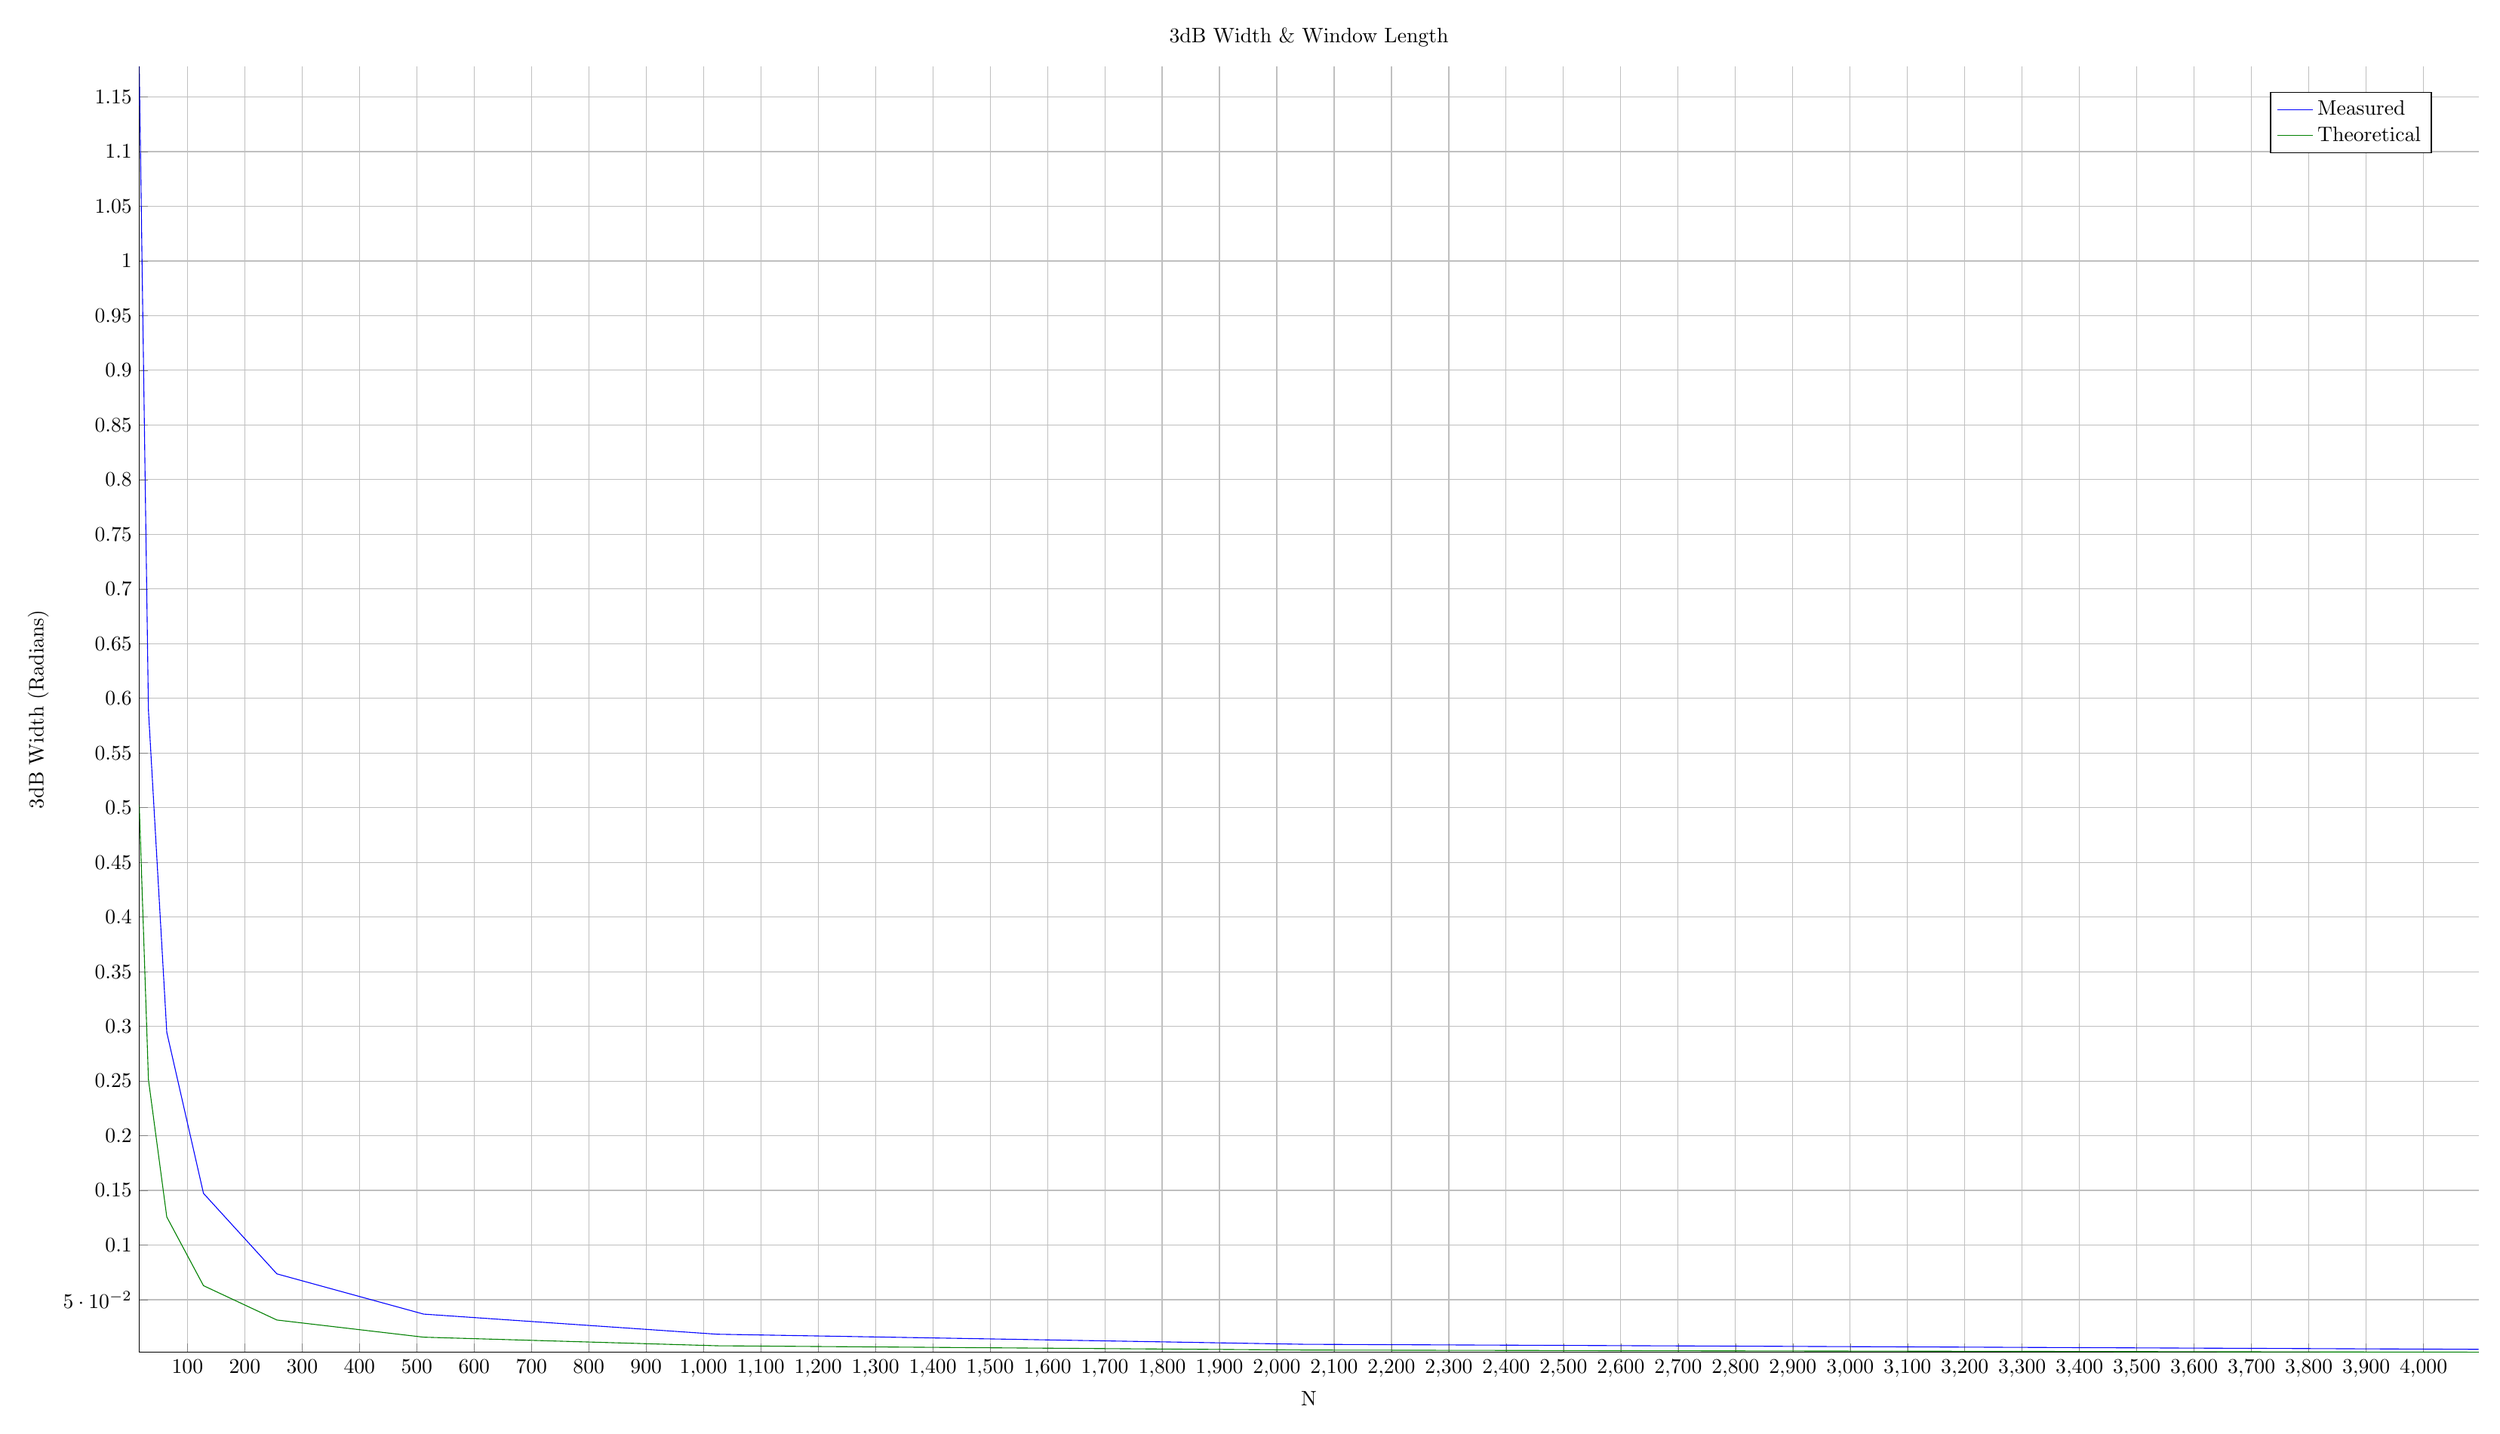
\begin{tikzpicture}

\begin{axis}[%
width=15.5in,
height=8.52354166666667in,
scale only axis,
xmin=16,
xmax=4096,
xlabel={N},
xmajorgrids,
ymin=0.00196349540849362,
ymax=1.17809724509617,
ylabel={3dB Width (Radians)},
ymajorgrids,
title={3dB Width \& Window Length},
axis x line*=bottom,
axis y line*=left,
legend style={draw=black,fill=white,legend cell align=left}
]
\addplot [color=blue,solid]
  table[row sep=crcr]{16	1.17809724509617\\
32	0.589048622548086\\
64	0.294524311274043\\
128	0.147262155637022\\
256	0.0736310778185108\\
512	0.0368155389092554\\
1024	0.0184077694546277\\
2048	0.00920388472731385\\
4096	0.00460194236365692\\
};
\addlegendentry{Measured};

\addplot [color=black!50!green,solid]
  table[row sep=crcr]{16	0.502654824574367\\
32	0.251327412287183\\
64	0.125663706143592\\
128	0.0628318530717959\\
256	0.0314159265358979\\
512	0.015707963267949\\
1024	0.00785398163397448\\
2048	0.00392699081698724\\
4096	0.00196349540849362\\
};
\addlegendentry{Theoretical};

\end{axis}
\end{tikzpicture}%}
		\captionof{figure}{\textit{Prediction Error Estimates for varying Model Orders}}
		\label{fig:}
%	\end{figure}
\end{minipage}
\begin{minipage}{.5\textwidth}
	%	\begin{figure}[h]
	\center
	\resizebox{\textwidth}{!}{% This file was created by matlab2tikz v0.4.7 (commit de21168db67fef7dc08f495c8f484b09a07aa02e) running on MATLAB 8.4.
% Copyright (c) 2008--2014, Nico Schlömer <nico.schloemer@gmail.com>
% All rights reserved.
% Minimal pgfplots version: 1.3
% 
% The latest updates can be retrieved from
%   http://www.mathworks.com/matlabcentral/fileexchange/22022-matlab2tikz
% where you can also make suggestions and rate matlab2tikz.
% 
%
% defining custom colors
\definecolor{mycolor1}{rgb}{0.00000,0.44700,0.74100}%
%
\begin{tikzpicture}

\begin{axis}[%
width=3in,
height=2in,
scale only axis,
every outer x axis line/.append style={white!15!black},
every x tick label/.append style={font=\color{white!15!black}},
xmin=16,
xmax=4096,
xlabel={N},
xmajorgrids,
every outer y axis line/.append style={white!15!black},
every y tick label/.append style={font=\color{white!15!black}},
tick align = outside,
ymin=13.178195824295,
ymax=13.4246672179578,
ylabel={Sidelobe Level (dB)},
ymajorgrids,
title style={font=\bfseries},
title={Sidelobe Level \& Window Length},
axis x line*=bottom,
axis y line*=left,
legend style={draw=black,fill=white,legend cell align=left}
]
\addplot [color=mycolor1,solid,forget plot]
  table[row sep=crcr]{16	13.178195824295\\
32	13.2497460511386\\
64	13.3427852124304\\
128	13.4003618622879\\
256	13.4246672179578\\
512	13.410416613703\\
1024	13.4035095429084\\
2048	13.4001094256601\\
4096	13.3984225829454\\
};
\end{axis}
\end{tikzpicture}%}
	\captionof{figure}{\textit{Prediction Error Estimates for varying Model Orders}}
	\label{fig:}
	%	\end{figure}
\end{minipage}


\subsubsection{Resolution Threshold}
\begin{figure}[h]
	\centering
	\begin{subfigure}[b]{0.23\textwidth}
		\resizebox{\textwidth}{!}{% This file was created by matlab2tikz v0.4.7 (commit fd1f91e81f99952e85a7de453e57b338734fa875) running on MATLAB 8.4.
% Copyright (c) 2008--2014, Nico Schlömer <nico.schloemer@gmail.com>
% All rights reserved.
% Minimal pgfplots version: 1.3
% 
% The latest updates can be retrieved from
%   http://www.mathworks.com/matlabcentral/fileexchange/22022-matlab2tikz
% where you can also make suggestions and rate matlab2tikz.
% 
%
% defining custom colors
\definecolor{mycolor1}{rgb}{0.00000,0.44700,0.74100}%
%
\begin{tikzpicture}

\begin{axis}[%
width=1.5in,
height=0.75in,
scale only axis,
every outer x axis line/.append style={white!15!black},
every x tick label/.append style={font=\color{white!15!black}},
xmin=0.54,
xmax=0.64,
xlabel={Normalised Frequency},
xmajorgrids,
every outer y axis line/.append style={white!15!black},
every y tick label/.append style={font=\color{white!15!black}},
tick align = outside,
ymin=0,
ymax=18000,
ylabel={Power},
ymajorgrids,
title style={font=\bfseries},
title={Periodogram, $\alpha=0.60$},
axis x line*=bottom,
axis y line*=left
]
\addplot [color=mycolor1,solid,forget plot]
  table[row sep=crcr]{-1	0.890696434330186\\
-0.99951171875	0.978440219563872\\
-0.9990234375	1.22832059687291\\
-0.99853515625	1.60231591152454\\
-0.998046875	2.04351867792528\\
-0.99755859375	2.48479399864423\\
-0.9970703125	2.85899441146608\\
-0.99658203125	3.10917719905623\\
-0.99609375	3.19726973746075\\
-0.99560546875	3.10986444528924\\
-0.9951171875	2.8602614480233\\
-0.99462890625	2.48644780845822\\
-0.994140625	2.04532029844522\\
-0.99365234375	1.60403018665697\\
-0.9931640625	1.22976646017185\\
-0.99267578125	0.979531653814417\\
-0.9921875	0.891465837088578\\
-0.99169921875	0.979039056724328\\
-0.9912109375	1.22899639514048\\
-0.99072265625	1.60336908326861\\
-0.990234375	2.04524658441161\\
-0.98974609375	2.48743231660781\\
-0.9892578125	2.86266675981304\\
-0.98876953125	3.11386289819739\\
-0.98828125	3.2027966519545\\
-0.98779296875	3.11592957018002\\
-0.9873046875	2.86647696502148\\
-0.98681640625	2.49240561878883\\
-0.986328125	2.05066438095871\\
-0.98583984375	1.60852421792462\\
-0.9853515625	1.23334436837326\\
-0.98486328125	0.982321198553059\\
-0.984375	0.893779571711831\\
-0.98388671875	0.981332465470654\\
-0.9833984375	1.23179870594479\\
-0.98291015625	1.60719726156755\\
-0.982421875	2.05051642381862\\
-0.98193359375	2.49438171057321\\
-0.9814453125	2.87130487601227\\
-0.98095703125	3.12395521672615\\
-0.98046875	3.21389021373787\\
-0.97998046875	3.12741619106722\\
-0.9794921875	2.87768567800867\\
-0.97900390625	2.50271030809328\\
-0.978515625	2.0595894026637\\
-0.97802734375	1.61583037512389\\
-0.9775390625	1.23908010077239\\
-0.97705078125	0.986828954174935\\
-0.9765625	0.897654303303549\\
-0.97607421875	0.985336952172552\\
-0.9755859375	1.23674769003925\\
-0.97509765625	1.61382799265345\\
-0.974609375	2.05936613603935\\
-0.97412109375	2.50569224474577\\
-0.9736328125	2.88497103244751\\
-0.97314453125	3.13952696070322\\
-0.97265625	3.23063050785091\\
-0.97216796875	3.14440728967986\\
-0.9716796875	2.89396862036242\\
-0.97119140625	2.51743643005454\\
-0.970703125	2.07215998408851\\
-0.97021484375	1.62600159456853\\
-0.9697265625	1.24701523575908\\
-0.96923828125	0.993087596750756\\
-0.96875	0.903118096210294\\
-0.96826171875	0.991081487139115\\
-0.9677734375	1.24387913259088\\
-0.96728515625	1.62330923930944\\
-0.966796875	2.07185978761422\\
-0.96630859375	2.52144588206944\\
-0.9658203125	2.90376436547553\\
-0.96533203125	3.16069120869325\\
-0.96484375	3.25313922724775\\
-0.96435546875	3.16702651448619\\
-0.9638671875	2.91544441632499\\
-0.96337890625	2.53669138601345\\
-0.962890625	2.08846790635324\\
-0.96240234375	1.63911221320681\\
-0.9619140625	1.25720780640744\\
-0.96142578125	1.00114289323617\\
-0.9609375	0.910210856028245\\
-0.96044921875	0.998607960171801\\
-0.9599609375	1.25324500550711\\
-0.95947265625	1.63571013491964\\
-0.958984375	2.08808858008684\\
-0.95849609375	2.54175777599994\\
-0.9580078125	2.92782244006561\\
-0.95751953125	3.18760309899133\\
-0.95703125	3.28158159892863\\
-0.95654296875	3.19544014060993\\
-0.9560546875	2.94227116404965\\
-0.95556640625	2.56061713240875\\
-0.955078125	2.10863357244204\\
-0.95458984375	1.65525915375286\\
-0.9541015625	1.26973322651115\\
-0.95361328125	1.0110544316682\\
-0.953125	0.91898496523652\\
-0.95263671875	1.00797184637998\\
-0.9521484375	1.26491429282162\\
-0.95166015625	1.65112208219088\\
-0.951171875	2.10817230166512\\
-0.95068359375	2.56677810673943\\
-0.9501953125	2.95732344755509\\
-0.94970703125	3.22046231284368\\
-0.94921875	3.31616903368118\\
-0.94873046875	3.22985974149462\\
-0.9482421875	2.97464898081282\\
-0.94775390625	2.58939247060665\\
-0.947265625	2.13280795311483\\
-0.94677734375	1.67456349384015\\
-0.9462890625	1.28468551288863\\
-0.94580078125	1.02289658671082\\
-0.9453125	0.929506130148208\\
-0.94482421875	1.01924310074028\\
-0.9443359375	1.27897410202405\\
-0.94384765625	1.66966022703243\\
-0.943359375	2.13226126253962\\
-0.94287109375	2.59669451308767\\
-0.9423828125	2.99248909788898\\
-0.94189453125	3.25951632316432\\
-0.94140625	3.35716257376896\\
-0.94091796875	3.27054564744589\\
-0.9404296875	3.01282328213675\\
-0.93994140625	2.62323598382161\\
-0.939453125	2.16117507257235\\
-0.93896484375	1.6971724637351\\
-0.9384765625	1.30217883869785\\
-0.93798828125	1.03675974798149\\
-0.9375	0.941854463175841\\
-0.93701171875	1.03250730666057\\
-0.9365234375	1.29553109267761\\
-0.93603515625	1.6914653492136\\
-0.935546875	2.16053876864224\\
-0.93505859375	2.63173518894427\\
-0.9345703125	3.0335882886898\\
-0.93408203125	3.30506450151517\\
-0.93359375	3.4048772373043\\
-0.93310546875	3.31781129039066\\
-0.9326171875	3.05708888928702\\
-0.93212890625	2.66240970598563\\
-0.931640625	2.19395510590221\\
-0.93115234375	1.72326193064879\\
-0.9306640625	1.32234946296345\\
-0.93017578125	1.05275184688939\\
-0.9296875	0.956125831792497\\
-0.92919921875	1.04786711172284\\
-0.9287109375	1.31471326353245\\
-0.92822265625	1.71670622441196\\
-0.927734375	2.1932242055051\\
-0.92724609375	2.6721727344614\\
-0.9267578125	3.08094165816709\\
-0.92626953125	3.35746320354458\\
-0.92578125	3.459687386885\\
-0.92529296875	3.37202856288311\\
-0.9248046875	3.1077950866015\\
-0.92431640625	2.70722363142915\\
-0.923828125	2.23140818052505\\
-0.92333984375	1.75303944383438\\
-0.9228515625	1.34535809404552\\
-0.92236328125	1.07100022764039\\
-0.921875	0.972433514370479\\
-0.92138671875	1.06544399317659\\
-0.9208984375	1.33667215104194\\
-0.92041015625	1.7455825276953\\
-0.919921875	2.23057682396664\\
-0.91943359375	2.71832887686158\\
-0.9189453125	3.13492715837754\\
-0.91845703125	3.41713198596492\\
-0.91796875	3.52203328473483\\
-0.91748046875	3.4336343539403\\
-0.9169921875	3.16535178268474\\
-0.91650390625	2.75804120326668\\
-0.916015625	2.27383899832264\\
-0.91552734375	1.78674793425297\\
-0.9150390625	1.37139275999363\\
-0.91455078125	1.09165392011456\\
-0.9140625	0.990910213747693\\
-0.91357421875	1.08538040712714\\
-0.9130859375	1.36158550634529\\
-0.91259765625	1.77832836717349\\
-0.912109375	2.27290034385187\\
-0.91162109375	2.77058020635621\\
-0.9111328125	3.19598682129464\\
-0.91064453125	3.48456114829606\\
-0.91015625	3.59242903897684\\
-0.90966796875	3.50313846662484\\
-0.9091796875	3.23023696948296\\
-0.90869140625	2.81528595407131\\
-0.908203125	2.32160242525581\\
-0.90771484375	1.82467018675863\\
-0.9072265625	1.40067227751204\\
-0.90673828125	1.11488638719511\\
-0.90625	1.01171049251541\\
-0.90576171875	1.10784238934284\\
-0.9052734375	1.38966053516526\\
-0.90478515625	1.81521655952492\\
-0.904296875	2.32054852174681\\
-0.90380859375	2.82936511008181\\
-0.9033203125	3.26463493450427\\
-0.90283203125	3.5603208422166\\
-0.90234375	3.67147219813295\\
-0.90185546875	3.58113317476177\\
-0.9013671875	3.30300572288042\\
-0.90087890625	2.87944951677912\\
-0.900390625	2.37511023276649\\
-0.89990234375	1.86713423285492\\
-0.8994140625	1.43345043466487\\
-0.89892578125	1.14089883764893\\
-0.8984375	1.03501371035936\\
-0.89794921875	1.1330226929532\\
-0.8974609375	1.42113780663656\\
-0.89697265625	1.85656378762103\\
-0.896484375	2.37393186628052\\
-0.89599609375	2.89519213364576\\
-0.8955078125	3.3414678986636\\
-0.89501953125	3.64507205332716\\
-0.89453125	3.75985531655283\\
-0.89404296875	3.66830474187977\\
-0.8935546875	3.38430105067335\\
-0.89306640625	2.95110127944712\\
-0.892578125	2.43483922237252\\
-0.89208984375	1.91451984995158\\
-0.8916015625	1.47002103192299\\
-0.89111328125	1.16992421898711\\
-0.890625	1.06102756434964\\
-0.89013671875	1.1611445701217\\
-0.8896484375	1.456295964187\\
-0.88916015625	1.90273681633259\\
-0.888671875	2.43352573126413\\
-0.88818359375	2.96865005867999\\
-0.8876953125	3.42717610863661\\
-0.88720703125	3.73957983837233\\
-0.88671875	3.85837989641384\\
-0.88623046875	3.76544730861425\\
-0.8857421875	3.47486697260284\\
-0.88525390625	3.03090002810771\\
-0.884765625	2.5013410246778\\
-0.88427734375	1.9672664011694\\
-0.8837890625	1.51072396360684\\
-0.88330078125	1.20223203435688\\
-0.8828125	1.08999235913648\\
-0.88232421875	1.19246633236222\\
-0.8818359375	1.49545740585015\\
-0.88134765625	1.95415998794675\\
-0.880859375	2.49988007645473\\
-0.88037109375	3.05042005934054\\
-0.8798828125	3.52255828877657\\
-0.87939453125	3.84472930038728\\
-0.87890625	3.96797321744059\\
-0.87841796875	3.87347966069851\\
-0.8779296875	3.57556431761322\\
-0.87744140625	3.11960801208634\\
-0.876953125	2.57525394042941\\
-0.87646484375	2.02588231127959\\
-0.8759765625	1.55595256971879\\
-0.87548828125	1.2381341654543\\
-0.875	1.12218616738468\\
-0.87451171875	1.22728685948719\\
-0.8740234375	1.53899514524769\\
-0.87353515625	2.01132427670261\\
-0.873046875	2.5736312618668\\
-0.87255859375	3.1412903963059\\
-0.8720703125	3.62853882651686\\
-0.87158203125	3.96154491198593\\
-0.87109375	4.08970870118917\\
-0.87060546875	3.99346552597902\\
-0.8701171875	3.6873898529814\\
-0.86962890625	3.2181079823763\\
-0.869140625	2.65731728987962\\
-0.86865234375	2.09095655383652\\
-0.8681640625	1.60616255007474\\
-0.86767578125	1.27799193240042\\
-0.8671875	1.15793108375788\\
-0.86669921875	1.26595227255842\\
-0.8662109375	1.58734112079884\\
-0.86572265625	2.07479825657938\\
-0.865234375	2.65551633952228\\
-0.86474609375	3.24217422998663\\
-0.8642578125	3.74618879506312\\
-0.86376953125	4.09121396196993\\
-0.86328125	4.22483063216266\\
-0.86279296875	4.12663822530263\\
-0.8623046875	3.81149952770798\\
-0.86181640625	3.32742390440569\\
-0.861328125	2.74838886475492\\
-0.86083984375	2.16317262784905\\
-0.8603515625	1.66188281317959\\
-0.85986328125	1.32222468522187\\
-0.859375	1.19760083166642\\
-0.85888671875	1.30886404520092\\
-0.8583984375	1.64099629389485\\
-0.85791015625	2.14524143346563\\
-0.857421875	2.74639043394904\\
-0.85693359375	3.35413129497698\\
-0.8564453125	3.87675154701945\\
-0.85595703125	4.23511511555561\\
-0.85546875	4.37478428699093\\
-0.85498046875	4.27443073259089\\
-0.8544921875	3.94923683191186\\
-0.85400390625	3.44874624382411\\
-0.853515625	2.84946624486619\\
-0.85302734375	2.24332563772954\\
-0.8525390625	1.72372873789846\\
-0.85205078125	1.37132030507253\\
-0.8515625	1.24163005517462\\
-0.85107421875	1.35648890475398\\
-0.8505859375	1.70054297240497\\
-0.85009765625	2.2234205196626\\
-0.849609375	2.84724796951417\\
-0.84912109375	3.47839438785912\\
-0.8486328125	4.02167401140788\\
-0.84814453125	4.39485336104639\\
-0.84765625	4.54125282395469\\
-0.84716796875	4.43851250276139\\
-0.8466796875	4.10216756298666\\
-0.84619140625	3.58346298416143\\
-0.845703125	2.96171296285469\\
-0.84521484375	2.33234326918762\\
-0.8447265625	1.7924184656242\\
-0.84423828125	1.42584810373382\\
-0.84375	1.2905257251276\\
-0.84326171875	1.40937097645644\\
-0.8427734375	1.76665992195626\\
-0.84228515625	2.31022939594184\\
-0.841796875	2.95924872283314\\
-0.84130859375	3.61640189807755\\
-0.8408203125	4.18264515808408\\
-0.84033203125	4.57230298992614\\
-0.83984375	4.72620268422025\\
-0.83935546875	4.6208348287072\\
-0.8388671875	4.27212267320833\\
-0.83837890625	3.73319788124557\\
-0.837890625	3.08649079533943\\
-0.83740234375	2.43131169209287\\
-0.8369140625	1.86879302676385\\
-0.83642578125	1.48647475704155\\
-0.8359375	1.34488121722174\\
-0.83544921875	1.46814675908825\\
-0.8349609375	1.8401409949741\\
-0.83447265625	2.40671372879684\\
-0.833984375	3.08374997154824\\
-0.83349609375	3.76983798156796\\
-0.8330078125	4.36164353592907\\
-0.83251953125	4.7696607571565\\
-0.83203125	4.93193978988971\\
-0.83154296875	4.8236870275291\\
-0.8310546875	4.46125138812032\\
-0.83056640625	3.89985792362845\\
-0.830078125	3.22539985473797\\
-0.82958984375	2.54150774186559\\
-0.8291015625	1.95384135582439\\
-0.82861328125	1.55398410582865\\
-0.828125	1.40539379265936\\
-0.82763671875	1.53356370194402\\
-0.8271484375	1.92191823213844\\
-0.82666015625	2.51410150889817\\
-0.826171875	3.22234640426768\\
-0.82568359375	3.94068247417431\\
-0.8251953125	4.56099638659467\\
-0.82470703125	4.98951204195478\\
-0.82421875	5.16117954401981\\
-0.82373046875	5.04976648417429\\
-0.8232421875	4.67208748088633\\
-0.82275390625	4.08569259685608\\
-0.822265625	3.38032869266117\\
-0.82177734375	2.66443916571507\\
-0.8212890625	2.0487315892784\\
-0.82080078125	1.62930192655024\\
-0.8203125	1.47288644637784\\
-0.81982421875	1.60650339859792\\
-0.8193359375	2.013090694871\\
-0.81884765625	2.63384118070059\\
-0.818359375	3.37691998980059\\
-0.81787109375	4.1312733168669\\
-0.8173828125	4.78345364469525\\
-0.81689453125	5.23491374574767\\
-0.81640625	5.41713461877407\\
-0.81591796875	5.30226657366728\\
-0.8154296875	4.90763253823498\\
-0.81494140625	4.29336840902741\\
-0.814453125	3.55351736051528\\
-0.81396484375	2.80189531593675\\
-0.8134765625	2.15485050658324\\
-0.81298828125	1.71352714206387\\
-0.8125	1.54833540877424\\
-0.81201171875	1.68801074865283\\
-0.8115234375	2.11496070271472\\
-0.81103515625	2.76764958526119\\
-0.810546875	3.54970273363278\\
-0.81005859375	4.34438518963786\\
-0.8095703125	5.03228124551278\\
-0.80908203125	5.50949892311613\\
-0.80859375	5.70362586753223\\
-0.80810546875	5.58498785111138\\
-0.8076171875	5.17146136463361\\
-0.80712890625	4.52606332233999\\
-0.806640625	3.7476373889872\\
-0.80615234375	2.95601149742447\\
-0.8056640625	2.27385362057105\\
-0.80517578125	1.80797145319849\\
-0.8046875	1.63290503080784\\
-0.80419921875	1.77933090234826\\
-0.8037109375	2.22907972264348\\
-0.80322265625	2.91757270091193\\
-0.802734375	3.74335625887255\\
-0.80224609375	4.58332933181981\\
-0.8017578125	5.31137970105806\\
-0.80126953125	5.81760989041878\\
-0.80078125	6.02522357407392\\
-0.80029296875	5.90247980409553\\
-0.7998046875	5.46785649996206\\
-0.79931640625	4.78758739361496\\
-0.798828125	3.9658940691276\\
-0.79833984375	3.12935133167908\\
-0.7978515625	2.40772932844121\\
-0.79736328125	1.91421008649369\\
-0.796875	1.7279924034425\\
-0.79638671875	1.88195645035561\\
-0.7958984375	2.35730695712002\\
-0.79541015625	3.08606323118352\\
-0.794921875	3.96107355997771\\
-0.79443359375	4.85208132013634\\
-0.7939453125	5.62543606482687\\
-0.79345703125	6.16446901334676\\
-0.79296875	6.38742889291453\\
-0.79248046875	6.2602231467514\\
-0.7919921875	5.8019814061623\\
-0.79150390625	5.08253827009247\\
-0.791015625	4.21215842864051\\
-0.79052734375	3.32501313624841\\
-0.7900390625	2.55888181790422\\
-0.78955078125	2.03414736683407\\
-0.7890625	1.8352849415909\\
-0.78857421875	1.99768823583636\\
-0.7880859375	2.50188480686039\\
-0.78759765625	3.27608059366312\\
-0.787109375	4.20671027400002\\
-0.78662109375	5.15544611756674\\
-0.7861328125	5.98012047112639\\
-0.78564453125	6.55639986769958\\
-0.78515625	6.79690909623353\\
-0.78466796875	6.6648664643783\\
-0.7841796875	6.18010556494623\\
-0.78369140625	5.41650354018262\\
-0.783203125	4.49113917906991\\
-0.78271484375	3.5467686674009\\
-0.7822265625	2.73023926639405\\
-0.78173828125	2.17010227901778\\
-0.78125	1.95683542330717\\
-0.78076171875	2.12871447460552\\
-0.7802734375	2.66553699846392\\
-0.77978515625	3.49122101556909\\
-0.779296875	4.48495567464914\\
-0.77880859375	5.49927335458399\\
-0.7783203125	6.38234284314431\\
-0.77783203125	7.00111649971895\\
-0.77734375	7.26180567093248\\
-0.77685546875	7.12453655378883\\
-0.7763671875	6.60990006719075\\
-0.77587890625	5.79632680310741\\
-0.775390625	4.80860909699734\\
-0.77490234375	3.79924599147743\\
-0.7744140625	2.92539655590645\\
-0.77392578125	2.32492130139052\\
-0.7734375	2.09516080729075\\
-0.77294921875	2.27771476723983\\
-0.7724609375	2.85159750595342\\
-0.77197265625	3.73588856259362\\
-0.771484375	4.80155774949209\\
-0.77099609375	5.89074111404339\\
-0.7705078125	6.84059179206393\\
-0.77001953125	7.50810586418455\\
-0.76953125	7.79214225488369\\
-0.76904296875	7.64924992346235\\
-0.7685546875	7.1008301181386\\
-0.76806640625	6.23046148106481\\
-0.767578125	5.17170647669736\\
-0.76708984375	4.08817329752465\\
-0.7666015625	3.14880569471028\\
-0.76611328125	2.50212892674302\\
-0.765625	2.25337385486498\\
-0.76513671875	2.44799838002001\\
-0.7646484375	3.06418183378501\\
-0.76416015625	4.01552251950521\\
-0.763671875	5.16362284535833\\
-0.76318359375	6.33873433427153\\
-0.7626953125	7.36538724511889\\
-0.76220703125	8.0891394242758\\
-0.76171875	8.4003712120288\\
-0.76123046875	8.25146501031021\\
-0.7607421875	7.66468258832603\\
-0.76025390625	6.72944710393316\\
-0.759765625	5.58934154218724\\
-0.75927734375	4.42070803831293\\
-0.7587890625	3.40603309973013\\
-0.75830078125	2.70613099039614\\
-0.7578125	2.43536063472078\\
-0.75732421875	2.64369034725481\\
-0.7568359375	3.30841736401563\\
-0.75634765625	4.33690340503964\\
-0.755859375	5.5800195402592\\
-0.75537109375	6.85435571885514\\
-0.7548828125	7.96989265799619\\
-0.75439453125	8.75896634385799\\
-0.75390625	9.10211549681878\\
-0.75341796875	8.94683298716332\\
-0.7529296875	8.31628450984338\\
-0.75244140625	7.30655908388835\\
-0.751953125	6.0727518082033\\
-0.75146484375	4.80588735468635\\
-0.7509765625	3.70411201041389\\
-0.75048828125	2.94249311780388\\
-0.75	2.64602316989898\\
-0.74951171875	2.86998529837649\\
-0.7490234375	3.59075727114513\\
-0.74853515625	4.70857034131144\\
-0.748046875	6.06193037916842\\
-0.74755859375	7.45162502866829\\
-0.7470703125	8.6707545952971\\
-0.74658203125	9.53626595471977\\
-0.74609375	9.91718993290232\\
-0.74560546875	9.75523329480267\\
-0.7451171875	9.07449589715108\\
-0.74462890625	7.97870824332808\\
-0.744140625	6.63627228680381\\
-0.74365234375	5.25525374498952\\
-0.7431640625	4.05203251536871\\
-0.74267578125	3.21832781258084\\
-0.7421875	2.8916160963787\\
-0.74169921875	3.13349875493304\\
-0.7412109375	3.91941458081109\\
-0.74072265625	5.14139866910448\\
-0.740234375	6.62361681962681\\
-0.73974609375	8.14845064104353\\
-0.7392578125	9.48927170444991\\
-0.73876953125	10.4449767202762\\
-0.73828125	10.871029164465\\
-0.73779296875	10.7022245147249\\
-0.7373046875	9.96360363788596\\
-0.73681640625	8.76770630237165\\
-0.736328125	7.29842118178955\\
-0.73583984375	5.78373856305953\\
-0.7353515625	4.46143429329268\\
-0.73486328125	3.54284154453475\\
-0.734375	3.18022145768498\\
-0.73388671875	3.4427612100354\\
-0.7333984375	4.30497201624645\\
-0.73291015625	5.6494122716569\\
-0.732421875	7.28349714971923\\
-0.73193359375	8.96800180100057\\
-0.7314453125	10.4530497259746\\
-0.73095703125	11.5161821735398\\
-0.73046875	11.9967187475964\\
-0.72998046875	11.8211127772374\\
-0.7294921875	11.0153131794962\\
-0.72900390625	9.70207816870932\\
-0.728515625	8.0834580907946\\
-0.72802734375	6.41093248105862\\
-0.7275390625	4.9476040201793\\
-0.72705078125	3.92812225331337\\
-0.7265625	3.52243053818734\\
-0.72607421875	3.80892548877997\\
-0.7255859375	4.76125407322255\\
-0.72509765625	6.25094642405664\\
-0.724609375	8.06569296021168\\
-0.72412109375	9.94068246984731\\
-0.7236328125	11.5983883646199\\
-0.72314453125	12.7908379375895\\
-0.72265625	13.3379395985703\\
-0.72216796875	13.1559579167905\\
-0.7216796875	12.2716504816\\
-0.72119140625	10.8197091081497\\
-0.720703125	9.0236655469207\\
-0.72021484375	7.16294972223567\\
-0.7197265625	5.5309409858344\\
-0.71923828125	4.39029623971204\\
-0.71875	3.93234291888971\\
-0.71826171875	4.24679966437829\\
-0.7177734375	5.30659874876413\\
-0.71728515625	6.97034554607226\\
-0.716796875	9.00229259039875\\
-0.71630859375	11.1070286759539\\
-0.7158203125	12.9737952903982\\
-0.71533203125	14.3237982356609\\
-0.71484375	14.9533280229498\\
-0.71435546875	14.766037500005\\
-0.7138671875	13.7892834485643\\
-0.71337890625	12.1717977801324\\
-0.712890625	10.1627652699742\\
-0.71240234375	8.07522617264962\\
-0.7119140625	6.23916038326587\\
-0.71142578125	4.95126691089594\\
-0.7109375	4.42906368551052\\
-0.71044921875	4.77638904727354\\
-0.7099609375	5.96575310227266\\
-0.70947265625	7.84049708025655\\
-0.708984375	10.1367387536988\\
-0.70849609375	12.5220590957411\\
-0.7080078125	14.6452803082493\\
-0.70751953125	16.1899021830993\\
-0.70703125	16.92308744418\\
-0.70654296875	16.732637866138\\
-0.7060546875	15.6461168725304\\
-0.70556640625	13.8289079096055\\
-0.705078125	11.5611639730023\\
-0.70458984375	9.19682764108019\\
-0.7041015625	7.11069180463506\\
-0.70361328125	5.64139608395062\\
-0.703125	5.03900485894961\\
-0.70263671875	5.4252560846677\\
-0.7021484375	6.7727690401443\\
-0.70166015625	8.90670808313704\\
-0.701171875	11.5290277673897\\
-0.70068359375	14.2619770938008\\
-0.7001953125	16.7045419933316\\
-0.69970703125	18.4934205244082\\
-0.69921875	19.3592883303677\\
-0.69873046875	19.1696716707377\\
-0.6982421875	17.9516404047178\\
-0.69775390625	15.8904975878929\\
-0.697265625	13.304242133436\\
-0.69677734375	10.5972781451072\\
-0.6962890625	8.20007667175464\\
-0.69580078125	6.50376141767423\\
-0.6953125	5.7995265242393\\
-0.69482421875	6.23223529650495\\
-0.6943359375	7.77555215583917\\
-0.69384765625	10.2328048196752\\
-0.693359375	13.2639200845411\\
-0.69287109375	16.4347997757957\\
-0.6923828125	19.2820078522023\\
-0.69189453125	21.3831674593394\\
-0.69140625	22.4224140431469\\
-0.69091796875	22.2408045460898\\
-0.6904296875	20.8636888784407\\
-0.68994140625	18.5004163146866\\
-0.689453125	15.5158866262953\\
-0.68896484375	12.3777472814969\\
-0.6884765625	9.58683228913751\\
-0.68798828125	7.60114689575146\\
-0.6875	6.76489112870158\\
-0.68701171875	7.2534730875601\\
-0.6865234375	9.04323856518433\\
-0.68603515625	11.911042997203\\
-0.685546875	15.4643366382372\\
-0.68505859375	19.1977865743876\\
-0.6845703125	22.5683245580736\\
-0.68408203125	25.077528600934\\
-0.68359375	26.3488968833532\\
-0.68310546875	26.1880940537361\\
-0.6826171875	24.6166014649477\\
-0.68212890625	21.8730637545479\\
-0.681640625	18.3814372527722\\
-0.68115234375	14.6900971548353\\
-0.6806640625	11.3905850944483\\
-0.68017578125	9.02797566745912\\
-0.6796875	8.01638067273027\\
-0.67919921875	8.57262072190155\\
-0.6787109375	10.6786059966129\\
-0.67822265625	14.0788169439656\\
-0.677734375	18.3140578230787\\
-0.67724609375	22.7871430015904\\
-0.6767578125	26.8512014609905\\
-0.67626953125	29.9076193062104\\
-0.67578125	31.4988713200926\\
-0.67529296875	31.3819333085062\\
-0.6748046875	29.5706004049169\\
-0.67431640625	26.3395117275176\\
-0.673828125	22.1883594934775\\
-0.67333984375	17.77080380461\\
-0.6728515625	13.7981106897204\\
-0.67236328125	10.9316303728526\\
-0.671875	9.68027747044063\\
-0.67138671875	10.3188043114191\\
-0.6708984375	12.8398711214337\\
-0.67041015625	16.9480783930022\\
-0.669921875	22.0979242145653\\
-0.66943359375	27.5709937109876\\
-0.6689453125	32.581581349906\\
-0.66845703125	36.3953331795142\\
-0.66796875	38.4431149984704\\
-0.66748046875	38.41258293695\\
-0.6669921875	36.302881252859\\
-0.66650390625	32.4331381616739\\
-0.666015625	27.4022350581249\\
-0.66552734375	22.0046924689905\\
-0.6650390625	17.1143409942343\\
-0.66455078125	13.5526744981741\\
-0.6640625	11.9615778857251\\
-0.66357421875	12.6999925422353\\
-0.6630859375	15.7809697160086\\
-0.66259765625	20.8598581818661\\
-0.662109375	27.2768740137355\\
-0.66162109375	34.1490980342897\\
-0.6611328125	40.4992681439221\\
-0.66064453125	45.4027613406283\\
-0.66015625	48.130849900558\\
-0.65966796875	48.2682467885765\\
-0.6591796875	45.7862303565213\\
-0.65869140625	41.0588567072251\\
-0.658203125	34.8180706371973\\
-0.65771484375	28.0527126684671\\
-0.6572265625	21.865121069666\\
-0.65673828125	17.3059079552881\\
-0.65625	15.2114480253626\\
-0.65576171875	16.0689675947434\\
-0.6552734375	19.9306969583118\\
-0.65478515625	26.3917543688856\\
-0.654296875	34.637191392456\\
-0.65380859375	43.5532722994399\\
-0.6533203125	51.888120230109\\
-0.65283203125	58.4388609556004\\
-0.65234375	62.2376067552886\\
-0.65185546875	62.707878273423\\
-0.6513671875	59.7666061977091\\
-0.65087890625	53.8542915264271\\
-0.650390625	45.8862357800822\\
-0.64990234375	37.129512853698\\
-0.6494140625	29.0218097557991\\
-0.64892578125	22.9576695802955\\
-0.6484375	20.0735325039856\\
-0.64794921875	21.0642791979878\\
-0.6474609375	26.0603781351212\\
-0.64697265625	34.5865948810974\\
-0.646484375	45.6116064872033\\
-0.64599609375	57.6844077637494\\
-0.6455078125	69.1400644829543\\
-0.64501953125	78.3461794833513\\
-0.64453125	83.9541599421932\\
-0.64404296875	85.1172525042321\\
-0.6435546875	81.640862418738\\
-0.64306640625	74.0395744421727\\
-0.642578125	63.4884113517471\\
-0.64208984375	51.671387895536\\
-0.6416015625	40.5461005051265\\
-0.64111328125	32.0565815719816\\
-0.640625	27.8358239613273\\
-0.64013671875	28.9426919888022\\
-0.6396484375	35.6746417980709\\
-0.63916015625	47.4879989548985\\
-0.638671875	63.0426705825969\\
-0.63818359375	80.3701160708587\\
-0.6376953125	97.1447363261919\\
-0.63720703125	111.022337871117\\
-0.63671875	119.997550855449\\
-0.63623046875	122.726999881073\\
-0.6357421875	118.767700922958\\
-0.63525390625	108.690535105412\\
-0.634765625	94.045530511862\\
-0.63427734375	77.1768459946791\\
-0.6337890625	60.9078394288911\\
-0.63330078125	48.1371291802565\\
-0.6328125	41.401973820547\\
-0.63232421875	42.4730642038415\\
-0.6318359375	52.0434192471309\\
-0.63134765625	69.5632606387198\\
-0.630859375	93.2536485580134\\
-0.63037109375	120.306701699591\\
-0.6298828125	147.252793078127\\
-0.62939453125	170.449131786463\\
-0.62890625	186.623516206365\\
-0.62841796875	193.395093732165\\
-0.6279296875	189.692902774372\\
-0.62744140625	176.003544316709\\
-0.626953125	154.400614466612\\
-0.62646484375	128.338000694772\\
-0.6259765625	102.222954306088\\
-0.62548828125	80.8183172151998\\
-0.625	68.5515169485967\\
-0.62451171875	68.8265538504848\\
-0.6240234375	83.4409375299372\\
-0.62353515625	112.200804062098\\
-0.623046875	152.804662603739\\
-0.62255859375	201.031811613063\\
-0.6220703125	251.229655800574\\
-0.62158203125	297.050461820626\\
-0.62109375	332.348613185501\\
-0.62060546875	352.120020165306\\
-0.6201171875	353.350790386806\\
-0.61962890625	335.645552123126\\
-0.619140625	301.527615102802\\
-0.61865234375	256.341594739141\\
-0.6181640625	207.739948513028\\
-0.61767578125	164.791859971401\\
-0.6171875	136.808633032766\\
-0.61669921875	132.026544288601\\
-0.6162109375	156.319028553027\\
-0.61572265625	212.119967402138\\
-0.615234375	297.72605945988\\
-0.61474609375	407.109127504516\\
-0.6142578125	530.312221992076\\
-0.61376953125	654.432776945981\\
-0.61328125	765.120239015841\\
-0.61279296875	848.444015809792\\
-0.6123046875	892.92969656184\\
-0.61181640625	891.525412017111\\
-0.611328125	843.251645103193\\
-0.61083984375	754.309265959391\\
-0.6103515625	638.470844022\\
-0.60986328125	516.654508786029\\
-0.609375	415.669716950068\\
-0.60888671875	366.219875666028\\
-0.6083984375	400.336447310929\\
-0.60791015625	548.49183735302\\
-0.607421875	836.684697137425\\
-0.60693359375	1283.80486509033\\
-0.6064453125	1899.56345994573\\
-0.60595703125	2683.218310302\\
-0.60546875	3623.24177511203\\
-0.60498046875	4697.97640579403\\
-0.6044921875	5877.21557417744\\
-0.60400390625	7124.54391296584\\
-0.603515625	8400.18842039205\\
-0.60302734375	9664.07554804126\\
-0.6025390625	10878.7693640134\\
-0.60205078125	12011.9835859627\\
-0.6015625	13038.4139436154\\
-0.60107421875	13940.7205997466\\
-0.6005859375	14709.5932284607\\
-0.60009765625	15342.9413774765\\
-0.599609375	15844.356565487\\
-0.59912109375	16221.0775506794\\
-0.5986328125	16481.7460058154\\
-0.59814453125	16634.2596790901\\
-0.59765625	16684.0116623199\\
-0.59716796875	16632.7500063285\\
-0.5966796875	16478.2084313019\\
-0.59619140625	16214.5566873476\\
-0.595703125	15833.6109457325\\
-0.59521484375	15326.6438952768\\
-0.5947265625	14686.5534986929\\
-0.59423828125	13910.0986662391\\
-0.59375	12999.8957460618\\
-0.59326171875	11965.893538071\\
-0.5927734375	10826.1036335925\\
-0.59228515625	9606.45005672632\\
-0.591796875	8339.70680005974\\
-0.59130859375	7063.60117159573\\
-0.5908203125	5818.26164211851\\
-0.59033203125	4643.26894905702\\
-0.58984375	3574.61900566344\\
-0.58935546875	2641.91984637315\\
-0.5888671875	1866.12098111868\\
-0.58837890625	1258.01523602366\\
-0.587890625	817.667626853893\\
-0.58740234375	534.823413870566\\
-0.5869140625	390.240452786818\\
-0.58642578125	357.791865192589\\
-0.5859375	407.105301048876\\
-0.58544921875	506.453517243111\\
-0.5849609375	625.592957734059\\
-0.58447265625	738.263687201946\\
-0.583984375	824.112440132786\\
-0.58349609375	869.87405170947\\
-0.5830078125	869.73570687774\\
-0.58251953125	824.90229572427\\
-0.58203125	742.468538921528\\
-0.58154296875	633.774475077113\\
-0.5810546875	512.467769297666\\
-0.58056640625	392.514696756718\\
-0.580078125	286.390782904845\\
-0.57958984375	203.644723374659\\
-0.5791015625	149.971228799738\\
-0.57861328125	126.857944389158\\
-0.578125	131.797819454929\\
-0.57763671875	158.990426955742\\
-0.5771484375	200.401737355722\\
-0.57666015625	247.017575020348\\
-0.576171875	290.114499589363\\
-0.57568359375	322.383208259958\\
-0.5751953125	338.770918129541\\
-0.57470703125	336.955355977817\\
-0.57421875	317.417160097816\\
-0.57373046875	283.132249071509\\
-0.5732421875	238.953948625048\\
-0.57275390625	190.790548060698\\
-0.572265625	144.703577397543\\
-0.57177734375	106.053893396326\\
-0.5712890625	78.8074983388181\\
-0.57080078125	65.0839326975099\\
-0.5703125	64.9917897520793\\
-0.56982421875	76.7540592697783\\
-0.5693359375	97.0864334756965\\
-0.56884765625	121.759586539892\\
-0.568359375	146.255663764888\\
-0.56787109375	166.421939296323\\
-0.5673828125	179.031029825329\\
-0.56689453125	182.175525407258\\
-0.56640625	175.452208651418\\
-0.56591796875	159.922939535185\\
-0.5654296875	137.871142676502\\
-0.56494140625	112.400257507798\\
-0.564453125	86.9399508859332\\
-0.56396484375	64.7350836250511\\
-0.5634765625	48.3906378356109\\
-0.56298828125	39.5338793405462\\
-0.5625	38.6351442669467\\
-0.56201171875	45.003992695749\\
-0.5615234375	56.9517612203483\\
-0.56103515625	72.0884327948016\\
-0.560546875	87.7043458137894\\
-0.56005859375	101.177751330217\\
-0.5595703125	110.34855232561\\
-0.55908203125	113.806387275809\\
-0.55859375	111.056034128004\\
-0.55810546875	102.542476910842\\
-0.5576171875	89.5389309949074\\
-0.55712890625	73.920610982099\\
-0.556640625	57.8623404203072\\
-0.55615234375	43.5072526487278\\
-0.5556640625	32.6557904868622\\
-0.55517578125	26.5190222656957\\
-0.5546875	25.5690135476444\\
-0.55419921875	29.5035117796374\\
-0.5537109375	37.3249191108082\\
-0.55322265625	47.5170059857669\\
-0.552734375	58.289397414606\\
-0.55224609375	67.8513446572325\\
-0.5517578125	74.6736986817218\\
-0.55126953125	77.7014561234249\\
-0.55078125	76.4880057346231\\
-0.55029296875	71.2347820605102\\
-0.5498046875	62.7344602371885\\
-0.54931640625	52.2299398156183\\
-0.548828125	41.2131349647118\\
-0.54833984375	31.1953999013563\\
-0.5478515625	23.4842934050269\\
-0.54736328125	18.9990984287082\\
-0.546875	18.1505923941478\\
-0.54638671875	20.8001928118191\\
-0.5458984375	26.3014200336998\\
-0.54541015625	33.6144653263191\\
-0.544921875	41.4742973032034\\
-0.54443359375	48.5856263864654\\
-0.5439453125	53.8150948227326\\
-0.54345703125	56.3525494375073\\
-0.54296875	55.8188091801528\\
-0.54248046875	52.3060035663757\\
-0.5419921875	46.3469551787894\\
-0.54150390625	38.8206280133563\\
-0.541015625	30.8098145175218\\
-0.54052734375	23.4336956474814\\
-0.5400390625	17.6808252154954\\
-0.53955078125	14.2671545507015\\
-0.5390625	13.5391925436526\\
-0.53857421875	15.4350722874836\\
-0.5380859375	19.5073365528268\\
-0.53759765625	25.0020296565243\\
-0.537109375	30.9805569785734\\
-0.53662109375	36.4649045341688\\
-0.5361328125	40.5839903434105\\
-0.53564453125	42.699464869271\\
-0.53515625	42.4930029173756\\
-0.53466796875	40.0033859320542\\
-0.5341796875	35.6094612002258\\
-0.53369140625	29.9631882090253\\
-0.533203125	23.8842344088729\\
-0.53271484375	18.2329199830573\\
-0.5322265625	13.7810043958504\\
-0.53173828125	11.0995383870126\\
-0.53125	10.479901704548\\
-0.53076171875	11.8987513959117\\
-0.5302734375	15.0307823355208\\
-0.52978515625	19.3060008287939\\
-0.529296875	24.0017090194362\\
-0.52880859375	28.3545339922527\\
-0.5283203125	31.6752835032807\\
-0.52783203125	33.4494821426463\\
-0.52734375	33.4090528104938\\
-0.52685546875	31.5653009586615\\
-0.5263671875	28.199380255998\\
-0.52587890625	23.8128394876318\\
-0.525390625	19.0467091460828\\
-0.52490234375	14.5820293063574\\
-0.5244140625	11.0371276391053\\
-0.52392578125	8.87702564474304\\
-0.5234375	8.34813467878871\\
-0.52294921875	9.44729072442948\\
-0.5224609375	11.9288285938047\\
-0.52197265625	15.3476386692669\\
-0.521484375	19.1308479967701\\
-0.52099609375	22.6666980142063\\
-0.5205078125	25.396926232366\\
-0.52001953125	26.898789116282\\
-0.51953125	26.9447602025093\\
-0.51904296875	25.5315668959957\\
-0.5185546875	22.8750082288899\\
-0.51806640625	19.3721847268264\\
-0.517578125	15.5375884096552\\
-0.51708984375	11.9232383990668\\
-0.5166015625	9.0351759524618\\
-0.51611328125	7.2588744770254\\
-0.515625	6.80448497763938\\
-0.51513671875	7.67961417530739\\
-0.5146484375	9.69303928633427\\
-0.51416015625	12.4880651664745\\
-0.513671875	15.5998357422713\\
-0.51318359375	18.5274698971732\\
-0.5126953125	20.8098928794851\\
-0.51220703125	22.0939422254415\\
-0.51171875	22.1847461410777\\
-0.51123046875	21.07125126408\\
-0.5107421875	18.9236529265548\\
-0.51025390625	16.0637535683625\\
-0.509765625	12.9132974332639\\
-0.50927734375	9.92850756082284\\
-0.5087890625	7.53092904893901\\
-0.50830078125	6.04500927898422\\
-0.5078125	5.65160688089486\\
-0.50732421875	6.36403615856242\\
-0.5068359375	8.02973802718891\\
-0.50634765625	10.3567675844506\\
-0.505859375	12.9605932796751\\
-0.50537109375	15.4237608373735\\
-0.5048828125	17.3592099987234\\
-0.50439453125	18.4676823986208\\
-0.50390625	18.5807466989902\\
-0.50341796875	17.6832994726332\\
-0.5029296875	15.9126024351593\\
-0.50244140625	13.5344915076343\\
-0.501953125	10.9007985405239\\
-0.50146484375	8.39475657461521\\
-0.5009765625	6.37281983244818\\
-0.50048828125	5.11169378239368\\
-0.5	4.76841054924636\\
-0.49951171875	5.35917118076008\\
-0.4990234375	6.75974842512489\\
-0.49853515625	8.72695627489429\\
-0.498046875	10.9375448346364\\
-0.49755859375	13.038339497007\\
-0.4970703125	14.6998801394706\\
-0.49658203125	15.6654439221208\\
-0.49609375	15.7881866528293\\
-0.49560546875	15.0510612129206\\
-0.4951171875	13.5668582808316\\
-0.49462890625	11.5587473377223\\
-0.494140625	9.3246136866464\\
-0.49365234375	7.19085500087079\\
-0.4931640625	5.46277441073611\\
-0.49267578125	4.37908247622968\\
-0.4921875	4.07726204027159\\
-0.49169921875	4.57479287667093\\
-0.4912109375	5.76875930286207\\
-0.49072265625	7.45355772087983\\
-0.490234375	9.35370928758049\\
-0.48974609375	11.166570484093\\
-0.4892578125	12.6083438770907\\
-0.48876953125	13.4564163675685\\
-0.48828125	13.5817304878575\\
-0.48779296875	12.9665050255431\\
-0.4873046875	11.7049059824246\\
-0.48681640625	9.98687274234256\\
-0.486328125	8.06783092436475\\
-0.48583984375	6.22909497087154\\
-0.4853515625	4.73507723166986\\
-0.48486328125	3.79379234133819\\
-0.484375	3.52653672620465\\
-0.48388671875	3.95114166582685\\
-0.4833984375	4.9810820375573\\
-0.48291015625	6.44030041512052\\
-0.482421875	8.09124657697235\\
-0.48193359375	9.67168894762776\\
-0.4814453125	10.9346117972323\\
-0.48095703125	11.6851448677252\\
-0.48046875	11.8090207877837\\
-0.47998046875	11.2884223137807\\
-0.4794921875	10.2030470488113\\
-0.47900390625	8.71647653377755\\
-0.478515625	7.05014515246007\\
-0.47802734375	5.44903114942334\\
-0.4775390625	4.14436902221121\\
-0.47705078125	3.31904344189675\\
-0.4765625	3.080828810428\\
-0.47607421875	3.44737411200848\\
-0.4755859375	4.34500239634117\\
-0.47509765625	5.62128232528165\\
-0.474609375	7.06925773340517\\
-0.47412109375	8.45950086781692\\
-0.4736328125	9.57503890993739\\
-0.47314453125	10.2438497326692\\
-0.47265625	10.3640727019344\\
-0.47216796875	9.91825335897915\\
-0.4716796875	8.97464924067527\\
-0.47119140625	7.67560258496666\\
-0.470703125	6.21493243913884\\
-0.47021484375	4.80792140896275\\
-0.4697265625	3.65853187462825\\
-0.46923828125	2.92883223651823\\
-0.46875	2.71520458567386\\
-0.46826171875	3.03481422424722\\
-0.4677734375	3.82422322382793\\
-0.46728515625	4.95017288754781\\
-0.466796875	6.2307269787931\\
-0.46630859375	7.46343437370883\\
-0.4658203125	8.45616263290259\\
-0.46533203125	9.0559165949465\\
-0.46484375	9.17132928634088\\
-0.46435546875	8.78552951271965\\
-0.4638671875	7.95758883627655\\
-0.46337890625	6.81249761654648\\
-0.462890625	5.521348750453\\
-0.46240234375	4.27485865172586\\
-0.4619140625	3.2543134498534\\
-0.46142578125	2.60435718575953\\
-0.4609375	2.41169751338725\\
-0.46044921875	2.6928541093423\\
-0.4599609375	3.39266748355585\\
-0.45947265625	4.39363967326957\\
-0.458984375	5.5345447219079\\
-0.45849609375	6.6353717621344\\
-0.4580078125	7.52475041331909\\
-0.45751953125	8.06568811629799\\
-0.45703125	8.17576187242693\\
-0.45654296875	7.83879666485161\\
-0.4560546875	7.10638753797085\\
-0.45556640625	6.08917628683155\\
-0.455078125	4.93933965812842\\
-0.45458984375	3.8270510593143\\
-0.4541015625	2.91454865598179\\
-0.45361328125	2.33175410574641\\
-0.453125	2.15709872089603\\
-0.45263671875	2.40637901318143\\
-0.4521484375	3.03121456861624\\
-0.45166015625	3.92721185292477\\
-0.451171875	4.95047228379784\\
-0.45068359375	5.93984253279619\\
-0.4501953125	6.74147351479196\\
-0.44970703125	7.23195180509765\\
-0.44921875	7.3365319353025\\
-0.44873046875	7.03978277213245\\
-0.4482421875	6.3871408357353\\
-0.44775390625	5.47725493825132\\
-0.447265625	4.4463973458831\\
-0.44677734375	3.44739708299682\\
-0.4462890625	2.62634573486676\\
-0.44580078125	2.1006203006282\\
-0.4453125	1.9415233726425\\
-0.44482421875	2.16410191392014\\
-0.4443359375	2.72558994418316\\
-0.44384765625	3.53260063669467\\
-0.443359375	4.45587132095842\\
-0.44287109375	5.35024011064545\\
-0.4423828125	6.07677250609866\\
-0.44189453125	6.52367047798247\\
-0.44140625	6.62282240366465\\
-0.44091796875	6.35954934504635\\
-0.4404296875	5.77416049930671\\
-0.43994140625	4.95518424089781\\
-0.439453125	4.02539944849917\\
-0.43896484375	3.12286486999985\\
-0.4384765625	2.37987248603314\\
-0.43798828125	1.90302852484785\\
-0.4375	1.75745654500161\\
-0.43701171875	1.95745832439435\\
-0.4365234375	2.46496501265375\\
-0.43603515625	3.1959186823614\\
-0.435546875	4.03352526704105\\
-0.43505859375	4.84629495950417\\
-0.4345703125	5.5080880691186\\
-0.43408203125	5.91711457153393\\
-0.43359375	6.01102976424124\\
-0.43310546875	5.77589176838502\\
-0.4326171875	5.24769994219637\\
-0.43212890625	4.50636880937606\\
-0.431640625	3.66313630425042\\
-0.43115234375	2.84338516226719\\
-0.4306640625	2.16752609783698\\
-0.43017578125	1.73285348700233\\
-0.4296875	1.599103757382\\
-0.42919921875	1.77985593837837\\
-0.4287109375	2.24100674969954\\
-0.42822265625	2.90646978957142\\
-0.427734375	3.67015533350538\\
-0.42724609375	4.41234913856619\\
-0.4267578125	5.0179653701628\\
-0.42626953125	5.39389413605642\\
-0.42578125	5.48283219778372\\
-0.42529296875	5.27154609861185\\
-0.4248046875	4.79238112713483\\
-0.42431640625	4.11786332133296\\
-0.423828125	3.34928708519216\\
-0.42333984375	2.60107992029161\\
-0.4228515625	1.98335411157787\\
-0.42236328125	1.58530264650527\\
-0.421875	1.46193989129629\\
-0.42138671875	1.62615470585947\\
-0.4208984375	2.0472193499334\\
-0.42041015625	2.65590941866196\\
-0.419921875	3.35538919729978\\
-0.41943359375	4.03615458073047\\
-0.4189453125	4.5927308332607\\
-0.41845703125	4.93958196475347\\
-0.41796875	5.0238349056055\\
-0.41748046875	4.83292871774362\\
-0.4169921875	4.39608632444328\\
-0.41650390625	3.77945174963894\\
-0.416015625	3.07569508285601\\
-0.41552734375	2.38971523965265\\
-0.4150390625	1.82264335634506\\
-0.41455078125	1.45658346690665\\
-0.4140625	1.34239017482255\\
-0.41357421875	1.49229991646189\\
-0.4130859375	1.87847972842592\\
-0.41259765625	2.43765172850078\\
-0.412109375	3.08103126276076\\
-0.41162109375	3.70802109511827\\
-0.4111328125	4.22155208249696\\
-0.41064453125	4.54273341315632\\
-0.41015625	4.62260373644347\\
-0.40966796875	4.44923537040948\\
-0.4091796875	4.0491641987236\\
-0.40869140625	3.48298633166167\\
-0.408203125	2.83584633262522\\
-0.40771484375	2.2043070575583\\
-0.4072265625	1.6816234264968\\
-0.40673828125	1.34366361057966\\
-0.40625	1.23760084419758\\
-0.40576171875	1.37505894160192\\
-0.4052734375	1.73070432523632\\
-0.40478515625	2.24644379543116\\
-0.404296875	2.8405378320531\\
-0.40380859375	3.42020250581311\\
-0.4033203125	3.89575937508248\\
-0.40283203125	4.19417754554633\\
-0.40234375	4.26996500361297\\
-0.40185546875	4.11178713334028\\
-0.4013671875	3.74385237598062\\
-0.40087890625	3.22190584639081\\
-0.400390625	2.62448893853075\\
-0.39990234375	2.04083279358217\\
-0.3994140625	1.55724965108475\\
-0.39892578125	1.24409556570086\\
-0.3984375	1.1452718037518\\
-0.39794921875	1.27182948981926\\
-0.3974609375	1.60060647497381\\
-0.39697265625	2.07805527405249\\
-0.396484375	2.62863401530871\\
-0.39599609375	3.16644783798845\\
-0.3955078125	3.60834863635737\\
-0.39501953125	3.88649710070915\\
-0.39453125	3.95849092921126\\
-0.39404296875	3.81354894243947\\
-0.3935546875	3.47385161031874\\
-0.39306640625	2.99087973062288\\
-0.392578125	2.43735135119347\\
-0.39208984375	1.89601762803564\\
-0.3916015625	1.44704211969803\\
-0.39111328125	1.15588666668062\\
-0.390625	1.06353285527838\\
-0.39013671875	1.18049802043012\\
-0.3896484375	1.48551728386398\\
-0.38916015625	1.92904909325416\\
-0.388671875	2.44103029448427\\
-0.38818359375	2.94166875342855\\
-0.3876953125	3.35361264202508\\
-0.38720703125	3.61364194785071\\
-0.38671875	3.68211656947439\\
-0.38623046875	3.54877057741816\\
-0.3857421875	3.23400774437389\\
-0.38525390625	2.78554184853335\\
-0.384765625	2.27093128060953\\
-0.38427734375	1.76717414658304\\
-0.3837890625	1.34896482124826\\
-0.38330078125	1.07740156956968\\
-0.3828125	0.990851007082548\\
-0.38232421875	1.09933387274649\\
-0.3818359375	1.3832517183846\\
-0.38134765625	1.79660989620645\\
-0.380859375	2.27421020218921\\
-0.38037109375	2.74169008113003\\
-0.3798828125	3.1268639565814\\
-0.37939453125	3.37063828913471\\
-0.37890625	3.43585120936107\\
-0.37841796875	3.31271578659693\\
-0.3779296875	3.02007139393324\\
-0.37744140625	2.60228902232838\\
-0.376953125	2.12233572232432\\
-0.37646484375	1.65208066090867\\
-0.3759765625	1.26133387543368\\
-0.37548828125	1.00728824789035\\
-0.375	0.925960259572898\\
-0.37451171875	1.02690918154231\\
-0.3740234375	1.2920073295959\\
-0.37353515625	1.67841419843097\\
-0.373046875	2.12526944800143\\
-0.37255859375	2.56306055393339\\
-0.3720703125	2.92422445792281\\
-0.37158203125	3.15336745463964\\
-0.37109375	3.21555853087603\\
-0.37060546875	3.10145568161232\\
-0.3701171875	2.82851440049684\\
-0.36962890625	2.43812694161728\\
-0.369140625	1.98915843869606\\
-0.36865234375	1.54888791025394\\
-0.3681640625	1.18274712744889\\
-0.36767578125	0.944421247808398\\
-0.3671875	0.867807852385176\\
-0.36669921875	0.962037648887591\\
-0.3662109375	1.21028683790169\\
-0.36572265625	1.57253107080204\\
-0.365234375	1.99179273563483\\
-0.36474609375	2.40290771480814\\
-0.3642578125	2.742463783605\\
-0.36376953125	2.95839590286954\\
-0.36328125	3.01778745938002\\
-0.36279296875	2.91170956209405\\
-0.3623046875	2.65638824111732\\
-0.36181640625	2.29055114430028\\
-0.361328125	1.86938520752314\\
-0.36083984375	1.45604683033495\\
-0.3603515625	1.11202961100792\\
-0.35986328125	0.887857755102687\\
-0.359375	0.815512709323898\\
-0.35888671875	0.903727268266124\\
-0.3583984375	1.1368383694079\\
-0.35791015625	1.47734542102854\\
-0.357421875	1.87175851601267\\
-0.35693359375	2.25882560390505\\
-0.3564453125	2.57887413373909\\
-0.35595703125	2.78284332712576\\
-0.35546875	2.83964077487379\\
-0.35498046875	2.74072113387989\\
-0.3544921875	2.50121379196465\\
-0.35400390625	2.15745424292458\\
-0.353515625	1.76131987907988\\
-0.35302734375	1.37225212871804\\
-0.3525390625	1.04819092418381\\
-0.35205078125	0.836803274707713\\
-0.3515625	0.7683330201212\\
-0.35107421875	0.851143485679272\\
-0.3505859375	1.07060889414424\\
-0.35009765625	1.39149818834387\\
-0.349609375	1.76346467070304\\
-0.34912109375	2.1287870358064\\
-0.3486328125	2.43117238085226\\
-0.34814453125	2.62427941899022\\
-0.34765625	2.6786721602563\\
-0.34716796875	2.58616141284738\\
-0.3466796875	2.3608947625359\\
-0.34619140625	2.03705299139528\\
-0.345703125	1.66352618368988\\
-0.34521484375	1.29639783791513\\
-0.3447265625	0.990391637511685\\
-0.34423828125	0.790584594564865\\
-0.34375	0.725640735373953\\
-0.34326171875	0.803580247758712\\
-0.3427734375	1.01070763891227\\
-0.34228515625	1.31383932500039\\
-0.341796875	1.66547003510962\\
-0.34130859375	2.01107450739682\\
-0.3408203125	2.29742289302688\\
-0.34033203125	2.48064239495565\\
-0.33984375	2.53280487123139\\
-0.33935546875	2.44605194313686\\
-0.3388671875	2.23364917107085\\
-0.33837890625	1.9278304921661\\
-0.337890625	1.57478157325041\\
-0.33740234375	1.22754202935091\\
-0.3369140625	0.937916613810844\\
-0.33642578125	0.748628320851375\\
-0.3359375	0.686901341460421\\
-0.33544921875	0.760437066543818\\
-0.3349609375	0.956377108082866\\
-0.33447265625	1.24339053640335\\
-0.333984375	1.57654802160486\\
-0.33349609375	1.90422535274963\\
-0.3330078125	2.17597621409934\\
-0.33251953125	2.35017420229057\\
-0.33203125	2.4002669954317\\
-0.33154296875	2.31870361909139\\
-0.3310546875	2.11795469340664\\
-0.33056640625	1.82849005965244\\
-0.330078125	1.49404033777604\\
-0.32958984375	1.16487859480107\\
-0.3291015625	0.890153662909741\\
-0.32861328125	0.710443711582771\\
-0.328125	0.651657703583591\\
-0.32763671875	0.721200714854892\\
-0.3271484375	0.906969958733061\\
-0.32666015625	1.17931553467726\\
-0.326171875	1.49564956691142\\
-0.32568359375	1.80698788774411\\
-0.3251953125	2.06541998813079\\
-0.32470703125	2.23136861738892\\
-0.32421875	2.27953954779677\\
-0.32373046875	2.20266759358392\\
-0.3232421875	2.01250476942491\\
-0.32275390625	1.73791813171687\\
-0.322265625	1.42040392919038\\
-0.32177734375	1.10771452465309\\
-0.3212890625	0.846576347575266\\
-0.32080078125	0.675608853454663\\
-0.3203125	0.619517069032711\\
-0.31982421875	0.685430515089377\\
-0.3193359375	0.861930418156496\\
-0.31884765625	1.12089612490641\\
-0.318359375	1.42187332387559\\
-0.31787109375	1.71828610105578\\
-0.3173828125	1.96453941508531\\
-0.31689453125	2.12292938968894\\
-0.31640625	2.16931457749009\\
-0.31591796875	2.09669562233149\\
-0.3154296875	1.91617311648313\\
-0.31494140625	1.65515425930707\\
-0.314453125	1.35309692879244\\
-0.31396484375	1.05545149414633\\
-0.3134765625	0.80673004424377\\
-0.31298828125	0.643759458955006\\
-0.3125	0.590140544371833\\
-0.31201171875	0.652746438305801\\
-0.3115234375	0.820779253265083\\
-0.31103515625	1.06751285441779\\
-0.310546875	1.35444152510411\\
-0.31005859375	1.63719104226944\\
-0.3095703125	1.87228518217117\\
-0.30908203125	2.02373627190987\\
-0.30859375	2.06846114164608\\
-0.30810546875	1.99970782966238\\
-0.3076171875	1.82798486120017\\
-0.30712890625	1.57936667362242\\
-0.306640625	1.29144746601756\\
-0.30615234375	1.00757085012849\\
-0.3056640625	0.770220573991538\\
-0.30517578125	0.614579731881654\\
-0.3046875	0.563234523370195\\
-0.30419921875	0.622819417225676\\
-0.3037109375	0.783101537737904\\
-0.30322265625	1.01862925790991\\
-0.302734375	1.29268031951272\\
-0.30224609375	1.56289749582773\\
-0.3017578125	1.78774730056292\\
-0.30126953125	1.93281728544812\\
-0.30078125	1.97599750426225\\
-0.30029296875	1.91076635212779\\
-0.2998046875	1.74709291767035\\
-0.29931640625	1.50983227859198\\
-0.298828125	1.23487117202\\
-0.29833984375	0.963621300232359\\
-0.2978515625	0.736704876888208\\
-0.29736328125	0.587794876711086\\
-0.296875	0.538543663667644\\
-0.29638671875	0.595363415369282\\
-0.2958984375	0.748536638103829\\
-0.29541015625	0.973778955721513\\
-0.294921875	1.23600366037991\\
-0.29443359375	1.49470485524395\\
-0.2939453125	1.71013363850082\\
-0.29345703125	1.84932594846121\\
-0.29296875	1.89106829386318\\
-0.29248046875	1.82905366809964\\
-0.2919921875	1.6727585517774\\
-0.29150390625	1.44592017726626\\
-0.291015625	1.18285795837754\\
-0.29052734375	0.923208763432183\\
-0.2900390625	0.705883321233671\\
-0.28955078125	0.563164922767245\\
-0.2890625	0.515845100955069\\
-0.28857421875	0.570128898261796\\
-0.2880859375	0.71676997115107\\
-0.28759765625	0.932555030622545\\
-0.287109375	1.18390003149384\\
-0.28662109375	1.43200135634042\\
-0.2861328125	1.63875221304902\\
-0.28564453125	1.77252247881293\\
-0.28515625	1.81292563596489\\
-0.28466796875	1.75385468644253\\
-0.2841796875	1.60433530623092\\
-0.28369140625	1.38707803760003\\
-0.283203125	1.13496106746207\\
-0.28271484375	0.885987959721141\\
-0.2822265625	0.677493328736326\\
-0.28173828125	0.540479606372729\\
-0.28125	0.494943658030694\\
-0.28076171875	0.546897430917668\\
-0.2802734375	0.687526184055299\\
-0.27978515625	0.894601235399766\\
-0.279296875	1.13592145512263\\
-0.27880859375	1.37425101304053\\
-0.2783203125	1.57299650813727\\
-0.27783203125	1.70175819971879\\
-0.27734375	1.74091349053885\\
-0.27685546875	1.68454186847917\\
-0.2763671875	1.54125563948546\\
-0.27587890625	1.33282075285888\\
-0.275390625	1.09078795998583\\
-0.27490234375	0.851655407171461\\
-0.2744140625	0.651304064967172\\
-0.27392578125	0.519554109210945\\
-0.2734375	0.47566785829363\\
-0.27294921875	0.525477185328687\\
-0.2724609375	0.660563483885372\\
-0.27197265625	0.859604680030085\\
-0.271484375	1.09167434516267\\
-0.27099609375	1.32098274001936\\
-0.2705078125	1.51233324310817\\
-0.27001953125	1.63646254054834\\
-0.26953125	1.67445458830322\\
-0.26904296875	1.62056281127625\\
-0.2685546875	1.4830197683626\\
-0.26806640625	1.28272096661964\\
-0.267578125	1.04999269646559\\
-0.26708984375	0.819943564111608\\
-0.2666015625	0.627111996847394\\
-0.26611328125	0.500225493376183\\
-0.265625	0.457866593256356\\
-0.26513671875	0.505699187270385\\
-0.2646484375	0.635668900792198\\
-0.26416015625	0.827289721192668\\
-0.263671875	1.05081186054949\\
-0.26318359375	1.27178125455722\\
-0.2626953125	1.45629213627562\\
-0.26220703125	1.57613215179752\\
-0.26171875	1.61303948557476\\
-0.26123046875	1.56142983873252\\
-0.2607421875	1.42918630953796\\
-0.26025390625	1.23640112085885\\
-0.259765625	1.01226953979941\\
-0.25927734375	0.790615907846586\\
-0.2587890625	0.604737159457899\\
-0.25830078125	0.482349706242118\\
-0.2578125	0.44140632455679\\
-0.25732421875	0.487414166908211\\
-0.2568359375	0.612654313646856\\
-0.25634765625	0.797412833936007\\
-0.255859375	1.01302748484\\
-0.25537109375	1.22627943342349\\
-0.2548828125	1.4044573010211\\
-0.25439453125	1.52032175119354\\
-0.25390625	1.55621735493995\\
-0.25341796875	1.50671123878057\\
-0.2529296875	1.37936439678965\\
-0.25244140625	1.19352675436826\\
-0.251953125	0.977347560906766\\
-0.25146484375	0.763462783105767\\
-0.2509765625	0.584020005993716\\
-0.25048828125	0.465799053675036\\
-0.25	0.426168724957424\\
-0.24951171875	0.47048990498517\\
-0.2490234375	0.591353101405708\\
-0.24853515625	0.769758289630511\\
-0.248046875	0.978049612912255\\
-0.24755859375	1.18415186554074\\
-0.2470703125	1.35645998434879\\
-0.24658203125	1.46863639418736\\
-0.24609375	1.50358820502724\\
-0.24560546875	1.45602385665353\\
-0.2451171875	1.33320701471911\\
-0.24462890625	1.15380083245189\\
-0.244140625	0.944986072202307\\
-0.24365234375	0.73829788608112\\
-0.2431640625	0.564818739372173\\
-0.24267578125	0.450460059993599\\
-0.2421875	0.412048681590771\\
-0.24169921875	0.454808987703361\\
-0.2412109375	0.571617310441947\\
-0.24072265625	0.744134498970693\\
-0.240234375	0.945636968769551\\
-0.23974609375	1.14510939198674\\
-0.2392578125	1.31197241451992\\
-0.23876953125	1.42072492188365\\
-0.23828125	1.45479628228959\\
-0.23779296875	1.40902681040094\\
-0.2373046875	1.29040533978506\\
-0.23681640625	1.11695893108955\\
-0.236328125	0.914970747363624\\
-0.23583984375	0.714955275646429\\
-0.2353515625	0.547007043445506\\
-0.23486328125	0.436231648724463\\
-0.234375	0.398952599474011\\
-0.23388671875	0.440266900174017\\
-0.2333984375	0.553315249267543\\
-0.23291015625	0.720370906013369\\
-0.232421875	0.915574712285981\\
-0.23193359375	1.1088944648784\\
-0.2314453125	1.27070256903942\\
-0.23095703125	1.37627438658339\\
-0.23046875	1.40952445473412\\
-0.22998046875	1.36541613921971\\
-0.2294921875	1.25068391908474\\
-0.22900390625	1.08276513212984\\
-0.228515625	0.887110312499533\\
-0.22802734375	0.693286823709232\\
-0.2275390625	0.530472147159941\\
-0.22705078125	0.42302359058681\\
-0.2265625	0.386796954991138\\
-0.22607421875	0.426770401557834\\
-0.2255859375	0.536329438810263\\
-0.22509765625	0.698315340758684\\
-0.224609375	0.887671119506932\\
-0.22412109375	1.07527718833257\\
-0.2236328125	1.2323897096377\\
-0.22314453125	1.33500529246797\\
-0.22265625	1.36748941483701\\
-0.22216796875	1.32492023039351\\
-0.2216796875	1.21379654876568\\
-0.22119140625	1.05100851260765\\
-0.220703125	0.861233715022632\\
-0.22021484375	0.673160032855217\\
-0.2197265625	0.515113167259737\\
-0.21923828125	0.410755174999526\\
-0.21875	0.375507058329891\\
-0.21826171875	0.414236135549371\\
-0.2177734375	0.520554859717235\\
-0.21728515625	0.67783175489107\\
-0.216796875	0.861754742417391\\
-0.21630859375	1.04405192989006\\
-0.2158203125	1.19680055905872\\
-0.21533203125	1.29666751871979\\
-0.21484375	1.32843756862597\\
-0.21435546875	1.28729589874222\\
-0.2138671875	1.17952273906128\\
-0.21337890625	1.02150013247854\\
-0.212890625	0.837187693474618\\
-0.21240234375	0.65445616240741\\
-0.2119140625	0.50083968493859\\
-0.21142578125	0.399354069287747\\
-0.2109375	0.365015991279677\\
-0.21044921875	0.402589438264338\\
-0.2099609375	0.505897448776037\\
-0.20947265625	0.658798278957857\\
-0.208984375	0.837671971105913\\
-0.20849609375	1.01503441092675\\
-0.2080078125	1.16372601699704\\
-0.20751953125	1.26103681620041\\
-0.20703125	1.2921415017346\\
-0.20654296875	1.25232501500875\\
-0.2060546875	1.14766467307782\\
-0.20556640625	0.994070442069868\\
-0.205078125	0.814834685156611\\
-0.20458984375	0.63706861443464\\
-0.2041015625	0.487570519718055\\
-0.20361328125	0.388755336099342\\
-0.203125	0.355263692755765\\
-0.20263671875	0.391763312338995\\
-0.2021484375	0.49227280507351\\
-0.20166015625	0.641105550240123\\
-0.201171875	0.815284934933277\\
-0.20068359375	0.988059200776739\\
-0.2001953125	1.13297833066587\\
-0.19970703125	1.22791178800074\\
-0.19921875	1.25839693243776\\
-0.19873046875	1.21981159778439\\
-0.1982421875	1.1180445827199\\
-0.19775390625	0.968567044295493\\
-0.197265625	0.794051019423223\\
-0.19677734375	0.620901539676808\\
-0.1962890625	0.47523267021786\\
-0.19580078125	0.378900584675905\\
-0.1953125	0.346196169238328\\
-0.19482421875	0.381697541503634\\
-0.1943359375	0.479605073394935\\
-0.19384765625	0.624655269422344\\
-0.193359375	0.794469690345058\\
-0.19287109375	0.962977552358427\\
-0.1923828125	1.10438865011056\\
-0.19189453125	1.19711127966463\\
-0.19140625	1.2270200771761\\
-0.19091796875	1.18957929824218\\
-0.1904296875	1.09050247826304\\
-0.18994140625	0.944852757771813\\
-0.189453125	0.774725353374993\\
-0.18896484375	0.605868630147818\\
-0.1884765625	0.463760396618929\\
-0.18798828125	0.3697372357463\\
-0.1875	0.337764811189403\\
-0.18701171875	0.372337924281706\\
-0.1865234375	0.467825977919857\\
-0.18603515625	0.609358951328981\\
-0.185546875	0.775114651910709\\
-0.18505859375	0.939655527702027\\
-0.1845703125	1.07780491027739\\
-0.18408203125	1.1684721174938\\
-0.18359375	1.19784536671106\\
-0.18310546875	1.16146921892141\\
-0.1826171875	1.06489417881178\\
-0.18212890625	0.922803936062576\\
-0.181640625	0.756757313976403\\
-0.18115234375	0.591892070777947\\
-0.1806640625	0.453094423869832\\
-0.18017578125	0.361217883231177\\
-0.1796875	0.329925799719932\\
-0.17919921875	0.36363560908408\\
-0.1787109375	0.456873983827053\\
-0.17822265625	0.595136840849318\\
-0.177734375	0.757119230462841\\
-0.17724609375	0.917972370416102\\
-0.1767578125	1.05308999152732\\
-0.17626953125	1.14184714359302\\
-0.17578125	1.17072346131657\\
-0.17529296875	1.13533801752782\\
-0.1748046875	1.04108959958425\\
-0.17431640625	0.902309005638218\\
-0.173828125	0.740056316516639\\
-0.17333984375	0.578901626964364\\
-0.1728515625	0.44318124809219\\
-0.17236328125	0.353299738677064\\
-0.171875	0.322639590342164\\
-0.17138671875	0.355546515873414\\
-0.1708984375	0.446693568103735\\
-0.17041015625	0.581916969929468\\
-0.169921875	0.740392648162358\\
-0.16943359375	0.897819089201632\\
-0.1689453125	1.03012011822461\\
-0.16845703125	1.11710350474057\\
-0.16796875	1.14551952186924\\
-0.16748046875	1.11105625473818\\
-0.1669921875	1.01897125916342\\
-0.16650390625	0.88326719124302\\
-0.166015625	0.724540534237711\\
-0.16552734375	0.566833848672362\\
-0.1650390625	0.433972531506088\\
-0.16455078125	0.345944146643473\\
-0.1640625	0.315870462800682\\
-0.16357421875	0.348030832001069\\
-0.1630859375	0.437234583907323\\
-0.16259765625	0.569634335433499\\
-0.162109375	0.724852905205007\\
-0.16162109375	0.879097222320794\\
-0.1611328125	1.00878346153409\\
-0.16064453125	1.0941211590635\\
-0.16015625	1.12211170060991\\
-0.15966796875	1.08850695154995\\
-0.1591796875	0.998432975726988\\
-0.15869140625	0.865587402333571\\
-0.158203125	0.710135997936544\\
-0.15771484375	0.555631374779626\\
-0.1572265625	0.425424573501644\\
-0.15673828125	0.33911616111386\\
-0.15625	0.309586127707371\\
-0.15576171875	0.341052571780313\\
-0.1552734375	0.428451705313845\\
-0.15478515625	0.55823018088833\\
-0.154296875	0.710425876906901\\
-0.15380859375	0.861717757710385\\
-0.1533203125	0.988978917936327\\
-0.15283203125	1.07279157020719\\
-0.15234375	1.1003898210834\\
-0.15185546875	1.06758432716324\\
-0.1513671875	0.979378726158902\\
-0.15087890625	0.84918725840465\\
-0.150390625	0.696775807687688\\
-0.14990234375	0.545242323927027\\
-0.1494140625	0.41749784743746\\
-0.14892578125	0.33278417457577\\
-0.1484375	0.303757382181678\\
-0.14794921875	0.33457919102128\\
-0.1474609375	0.42030394137811\\
-0.14697265625	0.547651367815144\\
-0.146484375	0.697044523260145\\
-0.14599609375	0.845600187409143\\
-0.1455078125	0.970615039437116\\
-0.14501953125	1.05301656342814\\
-0.14453125	1.08025422152065\\
-0.14404296875	1.04819269289714\\
-0.1435546875	0.961721645996499\\
-0.14306640625	0.83399223445328\\
-0.142578125	0.684399441588967\\
-0.14208984375	0.535619760252174\\
-0.1416015625	0.410156594342911\\
-0.14111328125	0.326919592690528\\
-0.140625	0.298357807885333\\
-0.14013671875	0.32858124909038\\
-0.1396484375	0.41275421012086\\
-0.13916015625	0.537849824533525\\
-0.138671875	0.684648195783761\\
-0.13818359375	0.830671678222702\\
-0.1376953125	0.953609095108544\\
-0.13720703125	1.03470732193098\\
-0.13671875	1.06161473983641\\
-0.13623046875	1.03024548135743\\
-0.1357421875	0.945383151504386\\
-0.13525390625	0.819934910663486\\
-0.134765625	0.672952148708923\\
-0.13427734375	0.526721224133583\\
-0.1337890625	0.403368466033889\\
-0.13330078125	0.321496548549528\\
-0.1328125	0.293363505857113\\
-0.13232421875	0.323032112209573\\
-0.1318359375	0.405768964516465\\
-0.13134765625	0.528782062204982\\
-0.130859375	0.673182028845908\\
-0.13037109375	0.816866343342523\\
-0.1298828125	0.937886246737595\\
-0.12939453125	1.0177835051039\\
-0.12890625	1.04438982176744\\
-0.12841796875	1.01366439325821\\
-0.1279296875	0.930292168028436\\
-0.12744140625	0.80695431282675\\
-0.126953125	0.662384415370815\\
-0.12646484375	0.518508319575687\\
-0.1259765625	0.397104211285541\\
-0.12548828125	0.31649165141555\\
-0.125	0.288752863383787\\
-0.12451171875	0.31790769263646\\
-0.1240234375	0.399317863717667\\
-0.12353515625	0.520408749382417\\
-0.123046875	0.662596404512364\\
-0.12255859375	0.80412460187509\\
-0.1220703125	0.923378823881197\\
-0.12158203125	1.00217247299365\\
-0.12109375	1.02850573637746\\
-0.12060546875	0.998378646870409\\
-0.1201171875	0.916384451096284\\
-0.11962890625	0.794995331978679\\
-0.119140625	0.652651495490887\\
-0.11865234375	0.510946351085441\\
-0.1181640625	0.391337399638227\\
-0.11767578125	0.311883765604664\\
-0.1171875	0.284506348861635\\
-0.11669921875	0.313186219182027\\
-0.1162109375	0.393373483785806\\
-0.11572265625	0.512694337661591\\
-0.115234375	0.652846481636218\\
-0.11474609375	0.79239261520725\\
-0.1142578125	0.910025685839192\\
-0.11376953125	0.987808603709315\\
-0.11328125	1.01389588551511\\
-0.11279296875	0.984324317312256\\
-0.1123046875	0.90360198874365\\
-0.11181640625	0.784008213440932\\
-0.111328125	0.643712997060196\\
-0.11083984375	0.504004003943112\\
-0.1103515625	0.386044178204697\\
-0.10986328125	0.307653815793043\\
-0.109375	0.280606331183698\\
-0.10888671875	0.308848035173837\\
-0.1083984375	0.387911063017651\\
-0.10791015625	0.505606732095822\\
-0.107421875	0.643891781242428\\
-0.10693359375	0.781621790733534\\
-0.1064453125	0.897771659862181\\
-0.10595703125	0.974632692370178\\
-0.10546875	1.00050019575169\\
-0.10498046875	0.97144375474648\\
-0.1044921875	0.891892475213202\\
-0.10400390625	0.773948106877713\\
-0.103515625	0.635532518005868\\
-0.10302734375	0.497653062654823\\
-0.1025390625	0.381203057521766\\
-0.10205078125	0.303784615577682\\
-0.1015625	0.277036920698594\\
-0.10107421875	0.30487542054661\\
-0.1005859375	0.382908277682339\\
-0.10009765625	0.49911700096525\\
-0.099609375	0.635695821423012\\
-0.09912109375	0.771768344852495\\
-0.0986328125	0.886567046465305\\
-0.09814453125	0.962591421865323\\
-0.09765625	0.988264582988457\\
-0.09716796875	0.959685072131637\\
-0.0966796875	0.881208847596362\\
-0.09619140625	0.76477467018692\\
-0.095703125	0.628077325641723\\
-0.09521484375	0.491868163124009\\
-0.0947265625	0.376794723057548\\
-0.09423828125	0.300260716574103\\
-0.09375	0.273783829209071\\
-0.09326171875	0.301252435216395\\
-0.0927734375	0.378345044580418\\
-0.09228515625	0.493199120264817\\
-0.091796875	0.628225795928022\\
-0.09130859375	0.762792918294875\\
-0.0908203125	0.87636718402149\\
-0.09033203125	0.951636897080375\\
-0.08984375	0.97714048131966\\
-0.08935546875	0.949001694504029\\
-0.0888671875	0.871508878184423\\
-0.08837890625	0.756451721062138\\
-0.087890625	0.621318074735545\\
-0.08740234375	0.486626574707204\\
-0.0869140625	0.372801869461161\\
-0.08642578125	0.297068275716468\\
-0.0859375	0.270834246837712\\
-0.08544921875	0.297964781302089\\
-0.0849609375	0.37420334735522\\
-0.08447265625	0.48782974894772\\
-0.083984375	0.62145229148257\\
-0.08349609375	0.754660237856599\\
-0.0830078125	0.867132065949255\\
-0.08251953125	0.941726235465065\\
-0.08203125	0.967084428968892\\
-0.08154296875	0.939351962944193\\
-0.0810546875	0.862754816360377\\
-0.08056640625	0.748946930973696\\
-0.080078125	0.615228559961067\\
-0.07958984375	0.481908008894597\\
-0.0791015625	0.369209055082068\\
-0.07861328125	0.294194938777662\\
-0.078125	0.268176733909261\\
-0.07763671875	0.2949996821106\\
-0.0771484375	0.370467083921413\\
-0.07666015625	0.48298803151484\\
-0.076171875	0.615349039549876\\
-0.07568359375	0.747338819427234\\
-0.0751953125	0.85882600472823\\
-0.07470703125	0.932821207790947\\
-0.07421875	0.958057705095346\\
-0.07373046875	0.93069878731027\\
-0.0732421875	0.854913074693973\\
-0.07275390625	0.742231557018359\\
-0.072265625	0.609785499060827\\
-0.07177734375	0.477694451780389\\
-0.0712890625	0.36600257460383\\
-0.07080078125	0.291629738382517\\
-0.0703125	0.265801126245767\\
-0.06982421875	0.292345776091503\\
-0.0693359375	0.367121932754843\\
-0.06884765625	0.478655425041182\\
-0.068359375	0.609892698894563\\
-0.06787109375	0.740800707967631\\
-0.0673828125	0.851417337841597\\
-0.06689453125	0.924887923876109\\
-0.06640625	0.950026012206035\\
-0.06591796875	0.923009342721718\\
-0.0654296875	0.847953954720902\\
-0.06494140625	0.736280207790988\\
-0.064453125	0.604968343620716\\
-0.06396484375	0.473970017936441\\
-0.0634765625	0.363170347981769\\
-0.06298828125	0.289363005062175\\
-0.0625	0.263698452517983\\
-0.06201171875	0.289993024232934\\
-0.0615234375	0.364155236110698\\
-0.06103515625	0.474815548138762\\
-0.060546875	0.605062665808771\\
-0.06005859375	0.735021250693468\\
-0.0595703125	0.844878171422853\\
-0.05908203125	0.917896558775681\\
-0.05859375	0.94295919963781\\
-0.05810546875	0.916254805469468\\
-0.0576171875	0.841851408509707\\
-0.05712890625	0.731070639959919\\
-0.056640625	0.60075911478097\\
-0.05615234375	0.47072082362732\\
-0.0556640625	0.36070182411874\\
-0.05517578125	0.287386290094783\\
-0.0546875	0.261860862484736\\
-0.05419921875	0.287932629587562\\
-0.0537109375	0.36155589851729\\
-0.05322265625	0.471454049722616\\
-0.052734375	0.600840909326889\\
-0.05224609375	0.729978900276681\\
-0.0517578125	0.839184158013172\\
-0.05126953125	0.911821115609692\\
-0.05078125	0.936831024252304\\
-0.05029296875	0.910410124678431\\
-0.0498046875	0.836582832707709\\
-0.04931640625	0.726583582730427\\
-0.048828125	0.597142261615164\\
-0.04833984375	0.467934877620112\\
-0.0478515625	0.358587897953828\\
-0.04736328125	0.285692299070041\\
-0.046875	0.260281565129214\\
-0.04638671875	0.286156967814335\\
-0.0458984375	0.359314299139252\\
-0.04541015625	0.468558495763761\\
-0.044921875	0.597211829152658\\
-0.04443359375	0.725655045352507\\
-0.0439453125	0.834314305373469\\
-0.04345703125	0.906639221774374\\
-0.04296875	0.931618945068264\\
-0.04248046875	0.905453826604037\\
-0.0419921875	0.832128892259813\\
-0.04150390625	0.722802587810178\\
-0.041015625	0.594104540256625\\
-0.04052734375	0.465601988111035\\
-0.0400390625	0.356820839842685\\
-0.03955078125	0.284274835278405\\
-0.0390625	0.258954775852495\\
-0.03857421875	0.284659527790877\\
-0.0380859375	0.357422216816805\\
-0.03759765625	0.466118272488852\\
-0.037109375	0.594162134370015\\
-0.03662109375	0.722033866035837\\
-0.0361328125	0.830250813766139\\
-0.03564453125	0.902331955787508\\
-0.03515625	0.927303949066308\\
-0.03466796875	0.901367848933478\\
-0.0341796875	0.82847337143673\\
-0.03369140625	0.719713902869058\\
-0.033203125	0.591634912157893\\
-0.03271484375	0.463713684527734\\
-0.0322265625	0.355394236288615\\
-0.03173828125	0.283128752169975\\
-0.03125	0.257875672018477\\
-0.03076171875	0.283434861501281\\
-0.0302734375	0.355872766777503\\
-0.02978515625	0.46412450473189\\
-0.029296875	0.591680741318286\\
-0.02880859375	0.719102212521559\\
-0.0283203125	0.826978939542572\\
-0.02783203125	0.898883702469197\\
-0.02734375	0.92387040585809\\
-0.02685546875	0.898137402900164\\
-0.0263671875	0.825603050206074\\
-0.02587890625	0.717306366826278\\
-0.025390625	0.589724460145431\\
-0.02490234375	0.462263153180836\\
-0.0244140625	0.35430294124708\\
-0.02392578125	0.282249914259317\\
-0.0234375	0.257040356265711\\
-0.02294921875	0.282478542539114\\
-0.0224609375	0.354660348186105\\
-0.02197265625	0.462569988362582\\
-0.021484375	0.589758689288316\\
-0.02099609375	0.71684950517431\\
-0.0205078125	0.824486883247445\\
-0.02001953125	0.896282034562271\\
-0.01953125	0.921305949320213\\
-0.01904296875	0.895750861412255\\
-0.0185546875	0.823507604335664\\
-0.01806640625	0.715571325602718\\
-0.017578125	0.588366321179189\\
-0.01708984375	0.461245185929849\\
-0.0166015625	0.353543037372247\\
-0.01611328125	0.281635165968709\\
-0.015625	0.256445827108862\\
-0.01513671875	0.281787132684939\\
-0.0146484375	0.35378060184903\\
-0.01416015625	0.461449135911361\\
-0.013671875	0.588389072943264\\
-0.01318359375	0.715267654810408\\
-0.0126953125	0.82276570078906\\
-0.01220703125	0.894517619259183\\
-0.01171875	0.919601384662432\\
-0.01123046875	0.894199671750405\\
-0.0107421875	0.822179527940943\\
-0.01025390625	0.714502567253495\\
-0.009765625	0.587555634952511\\
-0.00927734375	0.460656141204207\\
-0.0087890625	0.353111806707998\\
-0.00830078125	0.281282308009741\\
-0.0078125	0.256089956451701\\
-0.00732421875	0.281358156127894\\
-0.0068359375	0.353230377528681\\
-0.00634765625	0.460757934691349\\
-0.005859375	0.587566990595017\\
-0.00537109375	0.714351002147866\\
-0.0048828125	0.821809236535749\\
-0.00439453125	0.893584148437841\\
-0.00390625	0.91875061974048\\
-0.00341796875	0.893478291718766\\
-0.0029296875	0.821614077487198\\
-0.00244140625	0.714096275653456\\
-0.001953125	0.587289507677248\\
-0.00146484375	0.460493916883238\\
-0.0009765625	0.353007710450943\\
-0.00048828125	0.281190081002973\\
0	0.255971473725538\\
0.00048828125	0.281190081002973\\
0.0009765625	0.353007710450943\\
0.00146484375	0.460493916883238\\
0.001953125	0.587289507677248\\
0.00244140625	0.714096275653456\\
0.0029296875	0.821614077487198\\
0.00341796875	0.893478291718766\\
0.00390625	0.91875061974048\\
0.00439453125	0.893584148437841\\
0.0048828125	0.821809236535749\\
0.00537109375	0.714351002147866\\
0.005859375	0.587566990595017\\
0.00634765625	0.460757934691349\\
0.0068359375	0.353230377528681\\
0.00732421875	0.281358156127894\\
0.0078125	0.256089956451701\\
0.00830078125	0.281282308009741\\
0.0087890625	0.353111806707998\\
0.00927734375	0.460656141204207\\
0.009765625	0.587555634952511\\
0.01025390625	0.714502567253495\\
0.0107421875	0.822179527940943\\
0.01123046875	0.894199671750405\\
0.01171875	0.919601384662432\\
0.01220703125	0.894517619259183\\
0.0126953125	0.82276570078906\\
0.01318359375	0.715267654810408\\
0.013671875	0.588389072943264\\
0.01416015625	0.461449135911361\\
0.0146484375	0.35378060184903\\
0.01513671875	0.281787132684939\\
0.015625	0.256445827108862\\
0.01611328125	0.281635165968709\\
0.0166015625	0.353543037372247\\
0.01708984375	0.461245185929849\\
0.017578125	0.588366321179189\\
0.01806640625	0.715571325602718\\
0.0185546875	0.823507604335664\\
0.01904296875	0.895750861412255\\
0.01953125	0.921305949320213\\
0.02001953125	0.896282034562271\\
0.0205078125	0.824486883247445\\
0.02099609375	0.71684950517431\\
0.021484375	0.589758689288316\\
0.02197265625	0.462569988362582\\
0.0224609375	0.354660348186105\\
0.02294921875	0.282478542539114\\
0.0234375	0.257040356265711\\
0.02392578125	0.282249914259317\\
0.0244140625	0.35430294124708\\
0.02490234375	0.462263153180836\\
0.025390625	0.589724460145431\\
0.02587890625	0.717306366826278\\
0.0263671875	0.825603050206074\\
0.02685546875	0.898137402900164\\
0.02734375	0.92387040585809\\
0.02783203125	0.898883702469197\\
0.0283203125	0.826978939542572\\
0.02880859375	0.719102212521559\\
0.029296875	0.591680741318286\\
0.02978515625	0.46412450473189\\
0.0302734375	0.355872766777503\\
0.03076171875	0.283434861501281\\
0.03125	0.257875672018477\\
0.03173828125	0.283128752169975\\
0.0322265625	0.355394236288615\\
0.03271484375	0.463713684527734\\
0.033203125	0.591634912157893\\
0.03369140625	0.719713902869058\\
0.0341796875	0.82847337143673\\
0.03466796875	0.901367848933478\\
0.03515625	0.927303949066308\\
0.03564453125	0.902331955787508\\
0.0361328125	0.830250813766139\\
0.03662109375	0.722033866035837\\
0.037109375	0.594162134370015\\
0.03759765625	0.466118272488852\\
0.0380859375	0.357422216816805\\
0.03857421875	0.284659527790877\\
0.0390625	0.258954775852495\\
0.03955078125	0.284274835278405\\
0.0400390625	0.356820839842685\\
0.04052734375	0.465601988111035\\
0.041015625	0.594104540256625\\
0.04150390625	0.722802587810178\\
0.0419921875	0.832128892259813\\
0.04248046875	0.905453826604037\\
0.04296875	0.931618945068264\\
0.04345703125	0.906639221774374\\
0.0439453125	0.834314305373469\\
0.04443359375	0.725655045352507\\
0.044921875	0.597211829152658\\
0.04541015625	0.468558495763761\\
0.0458984375	0.359314299139252\\
0.04638671875	0.286156967814335\\
0.046875	0.260281565129214\\
0.04736328125	0.285692299070041\\
0.0478515625	0.358587897953828\\
0.04833984375	0.467934877620112\\
0.048828125	0.597142261615164\\
0.04931640625	0.726583582730427\\
0.0498046875	0.836582832707709\\
0.05029296875	0.910410124678431\\
0.05078125	0.936831024252304\\
0.05126953125	0.911821115609692\\
0.0517578125	0.839184158013172\\
0.05224609375	0.729978900276681\\
0.052734375	0.600840909326889\\
0.05322265625	0.471454049722616\\
0.0537109375	0.36155589851729\\
0.05419921875	0.287932629587562\\
0.0546875	0.261860862484736\\
0.05517578125	0.287386290094783\\
0.0556640625	0.36070182411874\\
0.05615234375	0.47072082362732\\
0.056640625	0.60075911478097\\
0.05712890625	0.731070639959919\\
0.0576171875	0.841851408509707\\
0.05810546875	0.916254805469468\\
0.05859375	0.94295919963781\\
0.05908203125	0.917896558775681\\
0.0595703125	0.844878171422853\\
0.06005859375	0.735021250693468\\
0.060546875	0.605062665808771\\
0.06103515625	0.474815548138762\\
0.0615234375	0.364155236110698\\
0.06201171875	0.289993024232934\\
0.0625	0.263698452517983\\
0.06298828125	0.289363005062175\\
0.0634765625	0.363170347981769\\
0.06396484375	0.473970017936441\\
0.064453125	0.604968343620716\\
0.06494140625	0.736280207790988\\
0.0654296875	0.847953954720902\\
0.06591796875	0.923009342721718\\
0.06640625	0.950026012206035\\
0.06689453125	0.924887923876109\\
0.0673828125	0.851417337841597\\
0.06787109375	0.740800707967631\\
0.068359375	0.609892698894563\\
0.06884765625	0.478655425041182\\
0.0693359375	0.367121932754843\\
0.06982421875	0.292345776091503\\
0.0703125	0.265801126245767\\
0.07080078125	0.291629738382517\\
0.0712890625	0.36600257460383\\
0.07177734375	0.477694451780389\\
0.072265625	0.609785499060827\\
0.07275390625	0.742231557018359\\
0.0732421875	0.854913074693973\\
0.07373046875	0.93069878731027\\
0.07421875	0.958057705095346\\
0.07470703125	0.932821207790947\\
0.0751953125	0.85882600472823\\
0.07568359375	0.747338819427234\\
0.076171875	0.615349039549876\\
0.07666015625	0.48298803151484\\
0.0771484375	0.370467083921413\\
0.07763671875	0.2949996821106\\
0.078125	0.268176733909261\\
0.07861328125	0.294194938777662\\
0.0791015625	0.369209055082068\\
0.07958984375	0.481908008894597\\
0.080078125	0.615228559961067\\
0.08056640625	0.748946930973696\\
0.0810546875	0.862754816360377\\
0.08154296875	0.939351962944193\\
0.08203125	0.967084428968892\\
0.08251953125	0.941726235465065\\
0.0830078125	0.867132065949255\\
0.08349609375	0.754660237856599\\
0.083984375	0.62145229148257\\
0.08447265625	0.48782974894772\\
0.0849609375	0.37420334735522\\
0.08544921875	0.297964781302089\\
0.0859375	0.270834246837712\\
0.08642578125	0.297068275716468\\
0.0869140625	0.372801869461161\\
0.08740234375	0.486626574707204\\
0.087890625	0.621318074735545\\
0.08837890625	0.756451721062138\\
0.0888671875	0.871508878184423\\
0.08935546875	0.949001694504029\\
0.08984375	0.97714048131966\\
0.09033203125	0.951636897080375\\
0.0908203125	0.87636718402149\\
0.09130859375	0.762792918294875\\
0.091796875	0.628225795928022\\
0.09228515625	0.493199120264817\\
0.0927734375	0.378345044580418\\
0.09326171875	0.301252435216395\\
0.09375	0.273783829209071\\
0.09423828125	0.300260716574103\\
0.0947265625	0.376794723057548\\
0.09521484375	0.491868163124009\\
0.095703125	0.628077325641723\\
0.09619140625	0.76477467018692\\
0.0966796875	0.881208847596362\\
0.09716796875	0.959685072131637\\
0.09765625	0.988264582988457\\
0.09814453125	0.962591421865323\\
0.0986328125	0.886567046465305\\
0.09912109375	0.771768344852495\\
0.099609375	0.635695821423012\\
0.10009765625	0.49911700096525\\
0.1005859375	0.382908277682339\\
0.10107421875	0.30487542054661\\
0.1015625	0.277036920698594\\
0.10205078125	0.303784615577682\\
0.1025390625	0.381203057521766\\
0.10302734375	0.497653062654823\\
0.103515625	0.635532518005868\\
0.10400390625	0.773948106877713\\
0.1044921875	0.891892475213202\\
0.10498046875	0.97144375474648\\
0.10546875	1.00050019575169\\
0.10595703125	0.974632692370178\\
0.1064453125	0.897771659862181\\
0.10693359375	0.781621790733534\\
0.107421875	0.643891781242428\\
0.10791015625	0.505606732095822\\
0.1083984375	0.387911063017651\\
0.10888671875	0.308848035173837\\
0.109375	0.280606331183698\\
0.10986328125	0.307653815793043\\
0.1103515625	0.386044178204697\\
0.11083984375	0.504004003943112\\
0.111328125	0.643712997060196\\
0.11181640625	0.784008213440932\\
0.1123046875	0.90360198874365\\
0.11279296875	0.984324317312256\\
0.11328125	1.01389588551511\\
0.11376953125	0.987808603709315\\
0.1142578125	0.910025685839192\\
0.11474609375	0.79239261520725\\
0.115234375	0.652846481636218\\
0.11572265625	0.512694337661591\\
0.1162109375	0.393373483785806\\
0.11669921875	0.313186219182027\\
0.1171875	0.284506348861635\\
0.11767578125	0.311883765604664\\
0.1181640625	0.391337399638227\\
0.11865234375	0.510946351085441\\
0.119140625	0.652651495490887\\
0.11962890625	0.794995331978679\\
0.1201171875	0.916384451096284\\
0.12060546875	0.998378646870409\\
0.12109375	1.02850573637746\\
0.12158203125	1.00217247299365\\
0.1220703125	0.923378823881197\\
0.12255859375	0.80412460187509\\
0.123046875	0.662596404512364\\
0.12353515625	0.520408749382417\\
0.1240234375	0.399317863717667\\
0.12451171875	0.31790769263646\\
0.125	0.288752863383787\\
0.12548828125	0.31649165141555\\
0.1259765625	0.397104211285541\\
0.12646484375	0.518508319575687\\
0.126953125	0.662384415370815\\
0.12744140625	0.80695431282675\\
0.1279296875	0.930292168028436\\
0.12841796875	1.01366439325821\\
0.12890625	1.04438982176744\\
0.12939453125	1.0177835051039\\
0.1298828125	0.937886246737595\\
0.13037109375	0.816866343342523\\
0.130859375	0.673182028845908\\
0.13134765625	0.528782062204982\\
0.1318359375	0.405768964516465\\
0.13232421875	0.323032112209573\\
0.1328125	0.293363505857113\\
0.13330078125	0.321496548549528\\
0.1337890625	0.403368466033889\\
0.13427734375	0.526721224133583\\
0.134765625	0.672952148708923\\
0.13525390625	0.819934910663486\\
0.1357421875	0.945383151504386\\
0.13623046875	1.03024548135743\\
0.13671875	1.06161473983641\\
0.13720703125	1.03470732193098\\
0.1376953125	0.953609095108544\\
0.13818359375	0.830671678222702\\
0.138671875	0.684648195783761\\
0.13916015625	0.537849824533525\\
0.1396484375	0.41275421012086\\
0.14013671875	0.32858124909038\\
0.140625	0.298357807885333\\
0.14111328125	0.326919592690528\\
0.1416015625	0.410156594342911\\
0.14208984375	0.535619760252174\\
0.142578125	0.684399441588967\\
0.14306640625	0.83399223445328\\
0.1435546875	0.961721645996499\\
0.14404296875	1.04819269289714\\
0.14453125	1.08025422152065\\
0.14501953125	1.05301656342814\\
0.1455078125	0.970615039437116\\
0.14599609375	0.845600187409143\\
0.146484375	0.697044523260145\\
0.14697265625	0.547651367815144\\
0.1474609375	0.42030394137811\\
0.14794921875	0.33457919102128\\
0.1484375	0.303757382181678\\
0.14892578125	0.33278417457577\\
0.1494140625	0.41749784743746\\
0.14990234375	0.545242323927027\\
0.150390625	0.696775807687688\\
0.15087890625	0.84918725840465\\
0.1513671875	0.979378726158902\\
0.15185546875	1.06758432716324\\
0.15234375	1.1003898210834\\
0.15283203125	1.07279157020719\\
0.1533203125	0.988978917936327\\
0.15380859375	0.861717757710385\\
0.154296875	0.710425876906901\\
0.15478515625	0.55823018088833\\
0.1552734375	0.428451705313845\\
0.15576171875	0.341052571780313\\
0.15625	0.309586127707371\\
0.15673828125	0.33911616111386\\
0.1572265625	0.425424573501644\\
0.15771484375	0.555631374779626\\
0.158203125	0.710135997936544\\
0.15869140625	0.865587402333571\\
0.1591796875	0.998432975726988\\
0.15966796875	1.08850695154995\\
0.16015625	1.12211170060991\\
0.16064453125	1.0941211590635\\
0.1611328125	1.00878346153409\\
0.16162109375	0.879097222320794\\
0.162109375	0.724852905205007\\
0.16259765625	0.569634335433499\\
0.1630859375	0.437234583907323\\
0.16357421875	0.348030832001069\\
0.1640625	0.315870462800682\\
0.16455078125	0.345944146643473\\
0.1650390625	0.433972531506088\\
0.16552734375	0.566833848672362\\
0.166015625	0.724540534237711\\
0.16650390625	0.88326719124302\\
0.1669921875	1.01897125916342\\
0.16748046875	1.11105625473818\\
0.16796875	1.14551952186924\\
0.16845703125	1.11710350474057\\
0.1689453125	1.03012011822461\\
0.16943359375	0.897819089201632\\
0.169921875	0.740392648162358\\
0.17041015625	0.581916969929468\\
0.1708984375	0.446693568103735\\
0.17138671875	0.355546515873414\\
0.171875	0.322639590342164\\
0.17236328125	0.353299738677064\\
0.1728515625	0.44318124809219\\
0.17333984375	0.578901626964364\\
0.173828125	0.740056316516639\\
0.17431640625	0.902309005638218\\
0.1748046875	1.04108959958425\\
0.17529296875	1.13533801752782\\
0.17578125	1.17072346131657\\
0.17626953125	1.14184714359302\\
0.1767578125	1.05308999152732\\
0.17724609375	0.917972370416102\\
0.177734375	0.757119230462841\\
0.17822265625	0.595136840849318\\
0.1787109375	0.456873983827053\\
0.17919921875	0.36363560908408\\
0.1796875	0.329925799719932\\
0.18017578125	0.361217883231177\\
0.1806640625	0.453094423869832\\
0.18115234375	0.591892070777947\\
0.181640625	0.756757313976403\\
0.18212890625	0.922803936062576\\
0.1826171875	1.06489417881178\\
0.18310546875	1.16146921892141\\
0.18359375	1.19784536671106\\
0.18408203125	1.1684721174938\\
0.1845703125	1.07780491027739\\
0.18505859375	0.939655527702027\\
0.185546875	0.775114651910709\\
0.18603515625	0.609358951328981\\
0.1865234375	0.467825977919857\\
0.18701171875	0.372337924281706\\
0.1875	0.337764811189403\\
0.18798828125	0.3697372357463\\
0.1884765625	0.463760396618929\\
0.18896484375	0.605868630147818\\
0.189453125	0.774725353374993\\
0.18994140625	0.944852757771813\\
0.1904296875	1.09050247826304\\
0.19091796875	1.18957929824218\\
0.19140625	1.2270200771761\\
0.19189453125	1.19711127966463\\
0.1923828125	1.10438865011056\\
0.19287109375	0.962977552358427\\
0.193359375	0.794469690345058\\
0.19384765625	0.624655269422344\\
0.1943359375	0.479605073394935\\
0.19482421875	0.381697541503634\\
0.1953125	0.346196169238328\\
0.19580078125	0.378900584675905\\
0.1962890625	0.47523267021786\\
0.19677734375	0.620901539676808\\
0.197265625	0.794051019423223\\
0.19775390625	0.968567044295493\\
0.1982421875	1.1180445827199\\
0.19873046875	1.21981159778439\\
0.19921875	1.25839693243776\\
0.19970703125	1.22791178800074\\
0.2001953125	1.13297833066587\\
0.20068359375	0.988059200776739\\
0.201171875	0.815284934933277\\
0.20166015625	0.641105550240123\\
0.2021484375	0.49227280507351\\
0.20263671875	0.391763312338995\\
0.203125	0.355263692755765\\
0.20361328125	0.388755336099342\\
0.2041015625	0.487570519718055\\
0.20458984375	0.63706861443464\\
0.205078125	0.814834685156611\\
0.20556640625	0.994070442069868\\
0.2060546875	1.14766467307782\\
0.20654296875	1.25232501500875\\
0.20703125	1.2921415017346\\
0.20751953125	1.26103681620041\\
0.2080078125	1.16372601699704\\
0.20849609375	1.01503441092675\\
0.208984375	0.837671971105913\\
0.20947265625	0.658798278957857\\
0.2099609375	0.505897448776037\\
0.21044921875	0.402589438264338\\
0.2109375	0.365015991279677\\
0.21142578125	0.399354069287747\\
0.2119140625	0.50083968493859\\
0.21240234375	0.65445616240741\\
0.212890625	0.837187693474618\\
0.21337890625	1.02150013247854\\
0.2138671875	1.17952273906128\\
0.21435546875	1.28729589874222\\
0.21484375	1.32843756862597\\
0.21533203125	1.29666751871979\\
0.2158203125	1.19680055905872\\
0.21630859375	1.04405192989006\\
0.216796875	0.861754742417391\\
0.21728515625	0.67783175489107\\
0.2177734375	0.520554859717235\\
0.21826171875	0.414236135549371\\
0.21875	0.375507058329891\\
0.21923828125	0.410755174999526\\
0.2197265625	0.515113167259737\\
0.22021484375	0.673160032855217\\
0.220703125	0.861233715022632\\
0.22119140625	1.05100851260765\\
0.2216796875	1.21379654876568\\
0.22216796875	1.32492023039351\\
0.22265625	1.36748941483701\\
0.22314453125	1.33500529246797\\
0.2236328125	1.2323897096377\\
0.22412109375	1.07527718833257\\
0.224609375	0.887671119506932\\
0.22509765625	0.698315340758684\\
0.2255859375	0.536329438810263\\
0.22607421875	0.426770401557834\\
0.2265625	0.386796954991138\\
0.22705078125	0.42302359058681\\
0.2275390625	0.530472147159941\\
0.22802734375	0.693286823709232\\
0.228515625	0.887110312499533\\
0.22900390625	1.08276513212984\\
0.2294921875	1.25068391908474\\
0.22998046875	1.36541613921971\\
0.23046875	1.40952445473412\\
0.23095703125	1.37627438658339\\
0.2314453125	1.27070256903942\\
0.23193359375	1.1088944648784\\
0.232421875	0.915574712285981\\
0.23291015625	0.720370906013369\\
0.2333984375	0.553315249267543\\
0.23388671875	0.440266900174017\\
0.234375	0.398952599474011\\
0.23486328125	0.436231648724463\\
0.2353515625	0.547007043445506\\
0.23583984375	0.714955275646429\\
0.236328125	0.914970747363624\\
0.23681640625	1.11695893108955\\
0.2373046875	1.29040533978506\\
0.23779296875	1.40902681040094\\
0.23828125	1.45479628228959\\
0.23876953125	1.42072492188365\\
0.2392578125	1.31197241451992\\
0.23974609375	1.14510939198674\\
0.240234375	0.945636968769551\\
0.24072265625	0.744134498970693\\
0.2412109375	0.571617310441947\\
0.24169921875	0.454808987703361\\
0.2421875	0.412048681590771\\
0.24267578125	0.450460059993599\\
0.2431640625	0.564818739372173\\
0.24365234375	0.73829788608112\\
0.244140625	0.944986072202307\\
0.24462890625	1.15380083245189\\
0.2451171875	1.33320701471911\\
0.24560546875	1.45602385665353\\
0.24609375	1.50358820502724\\
0.24658203125	1.46863639418736\\
0.2470703125	1.35645998434879\\
0.24755859375	1.18415186554074\\
0.248046875	0.978049612912255\\
0.24853515625	0.769758289630511\\
0.2490234375	0.591353101405708\\
0.24951171875	0.47048990498517\\
0.25	0.426168724957424\\
0.25048828125	0.465799053675036\\
0.2509765625	0.584020005993716\\
0.25146484375	0.763462783105767\\
0.251953125	0.977347560906766\\
0.25244140625	1.19352675436826\\
0.2529296875	1.37936439678965\\
0.25341796875	1.50671123878057\\
0.25390625	1.55621735493995\\
0.25439453125	1.52032175119354\\
0.2548828125	1.4044573010211\\
0.25537109375	1.22627943342349\\
0.255859375	1.01302748484\\
0.25634765625	0.797412833936007\\
0.2568359375	0.612654313646856\\
0.25732421875	0.487414166908211\\
0.2578125	0.44140632455679\\
0.25830078125	0.482349706242118\\
0.2587890625	0.604737159457899\\
0.25927734375	0.790615907846586\\
0.259765625	1.01226953979941\\
0.26025390625	1.23640112085885\\
0.2607421875	1.42918630953796\\
0.26123046875	1.56142983873252\\
0.26171875	1.61303948557476\\
0.26220703125	1.57613215179752\\
0.2626953125	1.45629213627562\\
0.26318359375	1.27178125455722\\
0.263671875	1.05081186054949\\
0.26416015625	0.827289721192668\\
0.2646484375	0.635668900792198\\
0.26513671875	0.505699187270385\\
0.265625	0.457866593256356\\
0.26611328125	0.500225493376183\\
0.2666015625	0.627111996847394\\
0.26708984375	0.819943564111608\\
0.267578125	1.04999269646559\\
0.26806640625	1.28272096661964\\
0.2685546875	1.4830197683626\\
0.26904296875	1.62056281127625\\
0.26953125	1.67445458830322\\
0.27001953125	1.63646254054834\\
0.2705078125	1.51233324310817\\
0.27099609375	1.32098274001936\\
0.271484375	1.09167434516267\\
0.27197265625	0.859604680030085\\
0.2724609375	0.660563483885372\\
0.27294921875	0.525477185328687\\
0.2734375	0.47566785829363\\
0.27392578125	0.519554109210945\\
0.2744140625	0.651304064967172\\
0.27490234375	0.851655407171461\\
0.275390625	1.09078795998583\\
0.27587890625	1.33282075285888\\
0.2763671875	1.54125563948546\\
0.27685546875	1.68454186847917\\
0.27734375	1.74091349053885\\
0.27783203125	1.70175819971879\\
0.2783203125	1.57299650813727\\
0.27880859375	1.37425101304053\\
0.279296875	1.13592145512263\\
0.27978515625	0.894601235399766\\
0.2802734375	0.687526184055299\\
0.28076171875	0.546897430917668\\
0.28125	0.494943658030694\\
0.28173828125	0.540479606372729\\
0.2822265625	0.677493328736326\\
0.28271484375	0.885987959721141\\
0.283203125	1.13496106746207\\
0.28369140625	1.38707803760003\\
0.2841796875	1.60433530623092\\
0.28466796875	1.75385468644253\\
0.28515625	1.81292563596489\\
0.28564453125	1.77252247881293\\
0.2861328125	1.63875221304902\\
0.28662109375	1.43200135634042\\
0.287109375	1.18390003149384\\
0.28759765625	0.932555030622545\\
0.2880859375	0.71676997115107\\
0.28857421875	0.570128898261796\\
0.2890625	0.515845100955069\\
0.28955078125	0.563164922767245\\
0.2900390625	0.705883321233671\\
0.29052734375	0.923208763432183\\
0.291015625	1.18285795837754\\
0.29150390625	1.44592017726626\\
0.2919921875	1.6727585517774\\
0.29248046875	1.82905366809964\\
0.29296875	1.89106829386318\\
0.29345703125	1.84932594846121\\
0.2939453125	1.71013363850082\\
0.29443359375	1.49470485524395\\
0.294921875	1.23600366037991\\
0.29541015625	0.973778955721513\\
0.2958984375	0.748536638103829\\
0.29638671875	0.595363415369282\\
0.296875	0.538543663667644\\
0.29736328125	0.587794876711086\\
0.2978515625	0.736704876888208\\
0.29833984375	0.963621300232359\\
0.298828125	1.23487117202\\
0.29931640625	1.50983227859198\\
0.2998046875	1.74709291767035\\
0.30029296875	1.91076635212779\\
0.30078125	1.97599750426225\\
0.30126953125	1.93281728544812\\
0.3017578125	1.78774730056292\\
0.30224609375	1.56289749582773\\
0.302734375	1.29268031951272\\
0.30322265625	1.01862925790991\\
0.3037109375	0.783101537737904\\
0.30419921875	0.622819417225676\\
0.3046875	0.563234523370195\\
0.30517578125	0.614579731881654\\
0.3056640625	0.770220573991538\\
0.30615234375	1.00757085012849\\
0.306640625	1.29144746601756\\
0.30712890625	1.57936667362242\\
0.3076171875	1.82798486120017\\
0.30810546875	1.99970782966238\\
0.30859375	2.06846114164608\\
0.30908203125	2.02373627190987\\
0.3095703125	1.87228518217117\\
0.31005859375	1.63719104226944\\
0.310546875	1.35444152510411\\
0.31103515625	1.06751285441779\\
0.3115234375	0.820779253265083\\
0.31201171875	0.652746438305801\\
0.3125	0.590140544371833\\
0.31298828125	0.643759458955006\\
0.3134765625	0.80673004424377\\
0.31396484375	1.05545149414633\\
0.314453125	1.35309692879244\\
0.31494140625	1.65515425930707\\
0.3154296875	1.91617311648313\\
0.31591796875	2.09669562233149\\
0.31640625	2.16931457749009\\
0.31689453125	2.12292938968894\\
0.3173828125	1.96453941508531\\
0.31787109375	1.71828610105578\\
0.318359375	1.42187332387559\\
0.31884765625	1.12089612490641\\
0.3193359375	0.861930418156496\\
0.31982421875	0.685430515089377\\
0.3203125	0.619517069032711\\
0.32080078125	0.675608853454663\\
0.3212890625	0.846576347575266\\
0.32177734375	1.10771452465309\\
0.322265625	1.42040392919038\\
0.32275390625	1.73791813171687\\
0.3232421875	2.01250476942491\\
0.32373046875	2.20266759358392\\
0.32421875	2.27953954779677\\
0.32470703125	2.23136861738892\\
0.3251953125	2.06541998813079\\
0.32568359375	1.80698788774411\\
0.326171875	1.49564956691142\\
0.32666015625	1.17931553467726\\
0.3271484375	0.906969958733061\\
0.32763671875	0.721200714854892\\
0.328125	0.651657703583591\\
0.32861328125	0.710443711582771\\
0.3291015625	0.890153662909741\\
0.32958984375	1.16487859480107\\
0.330078125	1.49404033777604\\
0.33056640625	1.82849005965244\\
0.3310546875	2.11795469340664\\
0.33154296875	2.31870361909139\\
0.33203125	2.4002669954317\\
0.33251953125	2.35017420229057\\
0.3330078125	2.17597621409934\\
0.33349609375	1.90422535274963\\
0.333984375	1.57654802160486\\
0.33447265625	1.24339053640335\\
0.3349609375	0.956377108082866\\
0.33544921875	0.760437066543818\\
0.3359375	0.686901341460421\\
0.33642578125	0.748628320851375\\
0.3369140625	0.937916613810844\\
0.33740234375	1.22754202935091\\
0.337890625	1.57478157325041\\
0.33837890625	1.9278304921661\\
0.3388671875	2.23364917107085\\
0.33935546875	2.44605194313686\\
0.33984375	2.53280487123139\\
0.34033203125	2.48064239495565\\
0.3408203125	2.29742289302688\\
0.34130859375	2.01107450739682\\
0.341796875	1.66547003510962\\
0.34228515625	1.31383932500039\\
0.3427734375	1.01070763891227\\
0.34326171875	0.803580247758712\\
0.34375	0.725640735373953\\
0.34423828125	0.790584594564865\\
0.3447265625	0.990391637511685\\
0.34521484375	1.29639783791513\\
0.345703125	1.66352618368988\\
0.34619140625	2.03705299139528\\
0.3466796875	2.3608947625359\\
0.34716796875	2.58616141284738\\
0.34765625	2.6786721602563\\
0.34814453125	2.62427941899022\\
0.3486328125	2.43117238085226\\
0.34912109375	2.1287870358064\\
0.349609375	1.76346467070304\\
0.35009765625	1.39149818834387\\
0.3505859375	1.07060889414424\\
0.35107421875	0.851143485679272\\
0.3515625	0.7683330201212\\
0.35205078125	0.836803274707713\\
0.3525390625	1.04819092418381\\
0.35302734375	1.37225212871804\\
0.353515625	1.76131987907988\\
0.35400390625	2.15745424292458\\
0.3544921875	2.50121379196465\\
0.35498046875	2.74072113387989\\
0.35546875	2.83964077487379\\
0.35595703125	2.78284332712576\\
0.3564453125	2.57887413373909\\
0.35693359375	2.25882560390505\\
0.357421875	1.87175851601267\\
0.35791015625	1.47734542102854\\
0.3583984375	1.1368383694079\\
0.35888671875	0.903727268266124\\
0.359375	0.815512709323898\\
0.35986328125	0.887857755102687\\
0.3603515625	1.11202961100792\\
0.36083984375	1.45604683033495\\
0.361328125	1.86938520752314\\
0.36181640625	2.29055114430028\\
0.3623046875	2.65638824111732\\
0.36279296875	2.91170956209405\\
0.36328125	3.01778745938002\\
0.36376953125	2.95839590286954\\
0.3642578125	2.742463783605\\
0.36474609375	2.40290771480814\\
0.365234375	1.99179273563483\\
0.36572265625	1.57253107080204\\
0.3662109375	1.21028683790169\\
0.36669921875	0.962037648887591\\
0.3671875	0.867807852385176\\
0.36767578125	0.944421247808398\\
0.3681640625	1.18274712744889\\
0.36865234375	1.54888791025394\\
0.369140625	1.98915843869606\\
0.36962890625	2.43812694161728\\
0.3701171875	2.82851440049684\\
0.37060546875	3.10145568161232\\
0.37109375	3.21555853087603\\
0.37158203125	3.15336745463964\\
0.3720703125	2.92422445792281\\
0.37255859375	2.56306055393339\\
0.373046875	2.12526944800143\\
0.37353515625	1.67841419843097\\
0.3740234375	1.2920073295959\\
0.37451171875	1.02690918154231\\
0.375	0.925960259572898\\
0.37548828125	1.00728824789035\\
0.3759765625	1.26133387543368\\
0.37646484375	1.65208066090867\\
0.376953125	2.12233572232432\\
0.37744140625	2.60228902232838\\
0.3779296875	3.02007139393324\\
0.37841796875	3.31271578659693\\
0.37890625	3.43585120936107\\
0.37939453125	3.37063828913471\\
0.3798828125	3.1268639565814\\
0.38037109375	2.74169008113003\\
0.380859375	2.27421020218921\\
0.38134765625	1.79660989620645\\
0.3818359375	1.3832517183846\\
0.38232421875	1.09933387274649\\
0.3828125	0.990851007082548\\
0.38330078125	1.07740156956968\\
0.3837890625	1.34896482124826\\
0.38427734375	1.76717414658304\\
0.384765625	2.27093128060953\\
0.38525390625	2.78554184853335\\
0.3857421875	3.23400774437389\\
0.38623046875	3.54877057741816\\
0.38671875	3.68211656947439\\
0.38720703125	3.61364194785071\\
0.3876953125	3.35361264202508\\
0.38818359375	2.94166875342855\\
0.388671875	2.44103029448427\\
0.38916015625	1.92904909325416\\
0.3896484375	1.48551728386398\\
0.39013671875	1.18049802043012\\
0.390625	1.06353285527838\\
0.39111328125	1.15588666668062\\
0.3916015625	1.44704211969803\\
0.39208984375	1.89601762803564\\
0.392578125	2.43735135119347\\
0.39306640625	2.99087973062288\\
0.3935546875	3.47385161031874\\
0.39404296875	3.81354894243947\\
0.39453125	3.95849092921126\\
0.39501953125	3.88649710070915\\
0.3955078125	3.60834863635737\\
0.39599609375	3.16644783798845\\
0.396484375	2.62863401530871\\
0.39697265625	2.07805527405249\\
0.3974609375	1.60060647497381\\
0.39794921875	1.27182948981926\\
0.3984375	1.1452718037518\\
0.39892578125	1.24409556570086\\
0.3994140625	1.55724965108475\\
0.39990234375	2.04083279358217\\
0.400390625	2.62448893853075\\
0.40087890625	3.22190584639081\\
0.4013671875	3.74385237598062\\
0.40185546875	4.11178713334028\\
0.40234375	4.26996500361297\\
0.40283203125	4.19417754554633\\
0.4033203125	3.89575937508248\\
0.40380859375	3.42020250581311\\
0.404296875	2.8405378320531\\
0.40478515625	2.24644379543116\\
0.4052734375	1.73070432523632\\
0.40576171875	1.37505894160192\\
0.40625	1.23760084419758\\
0.40673828125	1.34366361057966\\
0.4072265625	1.6816234264968\\
0.40771484375	2.2043070575583\\
0.408203125	2.83584633262522\\
0.40869140625	3.48298633166167\\
0.4091796875	4.0491641987236\\
0.40966796875	4.44923537040948\\
0.41015625	4.62260373644347\\
0.41064453125	4.54273341315632\\
0.4111328125	4.22155208249696\\
0.41162109375	3.70802109511827\\
0.412109375	3.08103126276076\\
0.41259765625	2.43765172850078\\
0.4130859375	1.87847972842592\\
0.41357421875	1.49229991646189\\
0.4140625	1.34239017482255\\
0.41455078125	1.45658346690665\\
0.4150390625	1.82264335634506\\
0.41552734375	2.38971523965265\\
0.416015625	3.07569508285601\\
0.41650390625	3.77945174963894\\
0.4169921875	4.39608632444328\\
0.41748046875	4.83292871774362\\
0.41796875	5.0238349056055\\
0.41845703125	4.93958196475347\\
0.4189453125	4.5927308332607\\
0.41943359375	4.03615458073047\\
0.419921875	3.35538919729978\\
0.42041015625	2.65590941866196\\
0.4208984375	2.0472193499334\\
0.42138671875	1.62615470585947\\
0.421875	1.46193989129629\\
0.42236328125	1.58530264650527\\
0.4228515625	1.98335411157787\\
0.42333984375	2.60107992029161\\
0.423828125	3.34928708519216\\
0.42431640625	4.11786332133296\\
0.4248046875	4.79238112713483\\
0.42529296875	5.27154609861185\\
0.42578125	5.48283219778372\\
0.42626953125	5.39389413605642\\
0.4267578125	5.0179653701628\\
0.42724609375	4.41234913856619\\
0.427734375	3.67015533350538\\
0.42822265625	2.90646978957142\\
0.4287109375	2.24100674969954\\
0.42919921875	1.77985593837837\\
0.4296875	1.599103757382\\
0.43017578125	1.73285348700233\\
0.4306640625	2.16752609783698\\
0.43115234375	2.84338516226719\\
0.431640625	3.66313630425042\\
0.43212890625	4.50636880937606\\
0.4326171875	5.24769994219637\\
0.43310546875	5.77589176838502\\
0.43359375	6.01102976424124\\
0.43408203125	5.91711457153393\\
0.4345703125	5.5080880691186\\
0.43505859375	4.84629495950417\\
0.435546875	4.03352526704105\\
0.43603515625	3.1959186823614\\
0.4365234375	2.46496501265375\\
0.43701171875	1.95745832439435\\
0.4375	1.75745654500161\\
0.43798828125	1.90302852484785\\
0.4384765625	2.37987248603314\\
0.43896484375	3.12286486999985\\
0.439453125	4.02539944849917\\
0.43994140625	4.95518424089781\\
0.4404296875	5.77416049930671\\
0.44091796875	6.35954934504635\\
0.44140625	6.62282240366465\\
0.44189453125	6.52367047798247\\
0.4423828125	6.07677250609866\\
0.44287109375	5.35024011064545\\
0.443359375	4.45587132095842\\
0.44384765625	3.53260063669467\\
0.4443359375	2.72558994418316\\
0.44482421875	2.16410191392014\\
0.4453125	1.9415233726425\\
0.44580078125	2.1006203006282\\
0.4462890625	2.62634573486676\\
0.44677734375	3.44739708299682\\
0.447265625	4.4463973458831\\
0.44775390625	5.47725493825132\\
0.4482421875	6.3871408357353\\
0.44873046875	7.03978277213245\\
0.44921875	7.3365319353025\\
0.44970703125	7.23195180509765\\
0.4501953125	6.74147351479196\\
0.45068359375	5.93984253279619\\
0.451171875	4.95047228379784\\
0.45166015625	3.92721185292477\\
0.4521484375	3.03121456861624\\
0.45263671875	2.40637901318143\\
0.453125	2.15709872089603\\
0.45361328125	2.33175410574641\\
0.4541015625	2.91454865598179\\
0.45458984375	3.8270510593143\\
0.455078125	4.93933965812842\\
0.45556640625	6.08917628683155\\
0.4560546875	7.10638753797085\\
0.45654296875	7.83879666485161\\
0.45703125	8.17576187242693\\
0.45751953125	8.06568811629799\\
0.4580078125	7.52475041331909\\
0.45849609375	6.6353717621344\\
0.458984375	5.5345447219079\\
0.45947265625	4.39363967326957\\
0.4599609375	3.39266748355585\\
0.46044921875	2.6928541093423\\
0.4609375	2.41169751338725\\
0.46142578125	2.60435718575953\\
0.4619140625	3.2543134498534\\
0.46240234375	4.27485865172586\\
0.462890625	5.521348750453\\
0.46337890625	6.81249761654648\\
0.4638671875	7.95758883627655\\
0.46435546875	8.78552951271965\\
0.46484375	9.17132928634088\\
0.46533203125	9.0559165949465\\
0.4658203125	8.45616263290259\\
0.46630859375	7.46343437370883\\
0.466796875	6.2307269787931\\
0.46728515625	4.95017288754781\\
0.4677734375	3.82422322382793\\
0.46826171875	3.03481422424722\\
0.46875	2.71520458567386\\
0.46923828125	2.92883223651823\\
0.4697265625	3.65853187462825\\
0.47021484375	4.80792140896275\\
0.470703125	6.21493243913884\\
0.47119140625	7.67560258496666\\
0.4716796875	8.97464924067527\\
0.47216796875	9.91825335897915\\
0.47265625	10.3640727019344\\
0.47314453125	10.2438497326692\\
0.4736328125	9.57503890993739\\
0.47412109375	8.45950086781692\\
0.474609375	7.06925773340517\\
0.47509765625	5.62128232528165\\
0.4755859375	4.34500239634117\\
0.47607421875	3.44737411200848\\
0.4765625	3.080828810428\\
0.47705078125	3.31904344189675\\
0.4775390625	4.14436902221121\\
0.47802734375	5.44903114942334\\
0.478515625	7.05014515246007\\
0.47900390625	8.71647653377755\\
0.4794921875	10.2030470488113\\
0.47998046875	11.2884223137807\\
0.48046875	11.8090207877837\\
0.48095703125	11.6851448677252\\
0.4814453125	10.9346117972323\\
0.48193359375	9.67168894762776\\
0.482421875	8.09124657697235\\
0.48291015625	6.44030041512052\\
0.4833984375	4.9810820375573\\
0.48388671875	3.95114166582685\\
0.484375	3.52653672620465\\
0.48486328125	3.79379234133819\\
0.4853515625	4.73507723166986\\
0.48583984375	6.22909497087154\\
0.486328125	8.06783092436475\\
0.48681640625	9.98687274234256\\
0.4873046875	11.7049059824246\\
0.48779296875	12.9665050255431\\
0.48828125	13.5817304878575\\
0.48876953125	13.4564163675685\\
0.4892578125	12.6083438770907\\
0.48974609375	11.166570484093\\
0.490234375	9.35370928758049\\
0.49072265625	7.45355772087983\\
0.4912109375	5.76875930286207\\
0.49169921875	4.57479287667093\\
0.4921875	4.07726204027159\\
0.49267578125	4.37908247622968\\
0.4931640625	5.46277441073611\\
0.49365234375	7.19085500087079\\
0.494140625	9.3246136866464\\
0.49462890625	11.5587473377223\\
0.4951171875	13.5668582808316\\
0.49560546875	15.0510612129206\\
0.49609375	15.7881866528293\\
0.49658203125	15.6654439221208\\
0.4970703125	14.6998801394706\\
0.49755859375	13.038339497007\\
0.498046875	10.9375448346364\\
0.49853515625	8.72695627489429\\
0.4990234375	6.75974842512489\\
0.49951171875	5.35917118076008\\
0.5	4.76841054924636\\
0.50048828125	5.11169378239368\\
0.5009765625	6.37281983244818\\
0.50146484375	8.39475657461521\\
0.501953125	10.9007985405239\\
0.50244140625	13.5344915076343\\
0.5029296875	15.9126024351593\\
0.50341796875	17.6832994726332\\
0.50390625	18.5807466989902\\
0.50439453125	18.4676823986208\\
0.5048828125	17.3592099987234\\
0.50537109375	15.4237608373735\\
0.505859375	12.9605932796751\\
0.50634765625	10.3567675844506\\
0.5068359375	8.02973802718891\\
0.50732421875	6.36403615856242\\
0.5078125	5.65160688089486\\
0.50830078125	6.04500927898422\\
0.5087890625	7.53092904893901\\
0.50927734375	9.92850756082284\\
0.509765625	12.9132974332639\\
0.51025390625	16.0637535683625\\
0.5107421875	18.9236529265548\\
0.51123046875	21.07125126408\\
0.51171875	22.1847461410777\\
0.51220703125	22.0939422254415\\
0.5126953125	20.8098928794851\\
0.51318359375	18.5274698971732\\
0.513671875	15.5998357422713\\
0.51416015625	12.4880651664745\\
0.5146484375	9.69303928633427\\
0.51513671875	7.67961417530739\\
0.515625	6.80448497763938\\
0.51611328125	7.2588744770254\\
0.5166015625	9.0351759524618\\
0.51708984375	11.9232383990668\\
0.517578125	15.5375884096552\\
0.51806640625	19.3721847268264\\
0.5185546875	22.8750082288899\\
0.51904296875	25.5315668959957\\
0.51953125	26.9447602025093\\
0.52001953125	26.898789116282\\
0.5205078125	25.396926232366\\
0.52099609375	22.6666980142063\\
0.521484375	19.1308479967701\\
0.52197265625	15.3476386692669\\
0.5224609375	11.9288285938047\\
0.52294921875	9.44729072442948\\
0.5234375	8.34813467878871\\
0.52392578125	8.87702564474304\\
0.5244140625	11.0371276391053\\
0.52490234375	14.5820293063574\\
0.525390625	19.0467091460828\\
0.52587890625	23.8128394876318\\
0.5263671875	28.199380255998\\
0.52685546875	31.5653009586615\\
0.52734375	33.4090528104938\\
0.52783203125	33.4494821426463\\
0.5283203125	31.6752835032807\\
0.52880859375	28.3545339922527\\
0.529296875	24.0017090194362\\
0.52978515625	19.3060008287939\\
0.5302734375	15.0307823355208\\
0.53076171875	11.8987513959117\\
0.53125	10.479901704548\\
0.53173828125	11.0995383870126\\
0.5322265625	13.7810043958504\\
0.53271484375	18.2329199830573\\
0.533203125	23.8842344088729\\
0.53369140625	29.9631882090253\\
0.5341796875	35.6094612002258\\
0.53466796875	40.0033859320542\\
0.53515625	42.4930029173756\\
0.53564453125	42.699464869271\\
0.5361328125	40.5839903434105\\
0.53662109375	36.4649045341688\\
0.537109375	30.9805569785734\\
0.53759765625	25.0020296565243\\
0.5380859375	19.5073365528268\\
0.53857421875	15.4350722874836\\
0.5390625	13.5391925436526\\
0.53955078125	14.2671545507015\\
0.5400390625	17.6808252154954\\
0.54052734375	23.4336956474814\\
0.541015625	30.8098145175218\\
0.54150390625	38.8206280133563\\
0.5419921875	46.3469551787894\\
0.54248046875	52.3060035663757\\
0.54296875	55.8188091801528\\
0.54345703125	56.3525494375073\\
0.5439453125	53.8150948227326\\
0.54443359375	48.5856263864654\\
0.544921875	41.4742973032034\\
0.54541015625	33.6144653263191\\
0.5458984375	26.3014200336998\\
0.54638671875	20.8001928118191\\
0.546875	18.1505923941478\\
0.54736328125	18.9990984287082\\
0.5478515625	23.4842934050269\\
0.54833984375	31.1953999013563\\
0.548828125	41.2131349647118\\
0.54931640625	52.2299398156183\\
0.5498046875	62.7344602371885\\
0.55029296875	71.2347820605102\\
0.55078125	76.4880057346231\\
0.55126953125	77.7014561234249\\
0.5517578125	74.6736986817218\\
0.55224609375	67.8513446572325\\
0.552734375	58.289397414606\\
0.55322265625	47.5170059857669\\
0.5537109375	37.3249191108082\\
0.55419921875	29.5035117796374\\
0.5546875	25.5690135476444\\
0.55517578125	26.5190222656957\\
0.5556640625	32.6557904868622\\
0.55615234375	43.5072526487278\\
0.556640625	57.8623404203072\\
0.55712890625	73.920610982099\\
0.5576171875	89.5389309949074\\
0.55810546875	102.542476910842\\
0.55859375	111.056034128004\\
0.55908203125	113.806387275809\\
0.5595703125	110.34855232561\\
0.56005859375	101.177751330217\\
0.560546875	87.7043458137894\\
0.56103515625	72.0884327948016\\
0.5615234375	56.9517612203483\\
0.56201171875	45.003992695749\\
0.5625	38.6351442669467\\
0.56298828125	39.5338793405462\\
0.5634765625	48.3906378356109\\
0.56396484375	64.7350836250511\\
0.564453125	86.9399508859332\\
0.56494140625	112.400257507798\\
0.5654296875	137.871142676502\\
0.56591796875	159.922939535185\\
0.56640625	175.452208651418\\
0.56689453125	182.175525407258\\
0.5673828125	179.031029825329\\
0.56787109375	166.421939296323\\
0.568359375	146.255663764888\\
0.56884765625	121.759586539892\\
0.5693359375	97.0864334756965\\
0.56982421875	76.7540592697783\\
0.5703125	64.9917897520793\\
0.57080078125	65.0839326975099\\
0.5712890625	78.8074983388181\\
0.57177734375	106.053893396326\\
0.572265625	144.703577397543\\
0.57275390625	190.790548060698\\
0.5732421875	238.953948625048\\
0.57373046875	283.132249071509\\
0.57421875	317.417160097816\\
0.57470703125	336.955355977817\\
0.5751953125	338.770918129541\\
0.57568359375	322.383208259958\\
0.576171875	290.114499589363\\
0.57666015625	247.017575020348\\
0.5771484375	200.401737355722\\
0.57763671875	158.990426955742\\
0.578125	131.797819454929\\
0.57861328125	126.857944389158\\
0.5791015625	149.971228799738\\
0.57958984375	203.644723374659\\
0.580078125	286.390782904845\\
0.58056640625	392.514696756718\\
0.5810546875	512.467769297666\\
0.58154296875	633.774475077113\\
0.58203125	742.468538921528\\
0.58251953125	824.90229572427\\
0.5830078125	869.73570687774\\
0.58349609375	869.87405170947\\
0.583984375	824.112440132786\\
0.58447265625	738.263687201946\\
0.5849609375	625.592957734059\\
0.58544921875	506.453517243111\\
0.5859375	407.105301048876\\
0.58642578125	357.791865192589\\
0.5869140625	390.240452786818\\
0.58740234375	534.823413870566\\
0.587890625	817.667626853893\\
0.58837890625	1258.01523602366\\
0.5888671875	1866.12098111868\\
0.58935546875	2641.91984637315\\
0.58984375	3574.61900566344\\
0.59033203125	4643.26894905702\\
0.5908203125	5818.26164211851\\
0.59130859375	7063.60117159573\\
0.591796875	8339.70680005974\\
0.59228515625	9606.45005672632\\
0.5927734375	10826.1036335925\\
0.59326171875	11965.893538071\\
0.59375	12999.8957460618\\
0.59423828125	13910.0986662391\\
0.5947265625	14686.5534986929\\
0.59521484375	15326.6438952768\\
0.595703125	15833.6109457325\\
0.59619140625	16214.5566873476\\
0.5966796875	16478.2084313019\\
0.59716796875	16632.7500063285\\
0.59765625	16684.0116623199\\
0.59814453125	16634.2596790901\\
0.5986328125	16481.7460058154\\
0.59912109375	16221.0775506794\\
0.599609375	15844.356565487\\
0.60009765625	15342.9413774765\\
0.6005859375	14709.5932284607\\
0.60107421875	13940.7205997466\\
0.6015625	13038.4139436154\\
0.60205078125	12011.9835859627\\
0.6025390625	10878.7693640134\\
0.60302734375	9664.07554804126\\
0.603515625	8400.18842039205\\
0.60400390625	7124.54391296584\\
0.6044921875	5877.21557417744\\
0.60498046875	4697.97640579403\\
0.60546875	3623.24177511203\\
0.60595703125	2683.218310302\\
0.6064453125	1899.56345994573\\
0.60693359375	1283.80486509033\\
0.607421875	836.684697137425\\
0.60791015625	548.49183735302\\
0.6083984375	400.336447310929\\
0.60888671875	366.219875666028\\
0.609375	415.669716950068\\
0.60986328125	516.654508786029\\
0.6103515625	638.470844022\\
0.61083984375	754.309265959391\\
0.611328125	843.251645103193\\
0.61181640625	891.525412017111\\
0.6123046875	892.92969656184\\
0.61279296875	848.444015809792\\
0.61328125	765.120239015841\\
0.61376953125	654.432776945981\\
0.6142578125	530.312221992076\\
0.61474609375	407.109127504516\\
0.615234375	297.72605945988\\
0.61572265625	212.119967402138\\
0.6162109375	156.319028553027\\
0.61669921875	132.026544288601\\
0.6171875	136.808633032766\\
0.61767578125	164.791859971401\\
0.6181640625	207.739948513028\\
0.61865234375	256.341594739141\\
0.619140625	301.527615102802\\
0.61962890625	335.645552123126\\
0.6201171875	353.350790386806\\
0.62060546875	352.120020165306\\
0.62109375	332.348613185501\\
0.62158203125	297.050461820626\\
0.6220703125	251.229655800574\\
0.62255859375	201.031811613063\\
0.623046875	152.804662603739\\
0.62353515625	112.200804062098\\
0.6240234375	83.4409375299372\\
0.62451171875	68.8265538504848\\
0.625	68.5515169485967\\
0.62548828125	80.8183172151998\\
0.6259765625	102.222954306088\\
0.62646484375	128.338000694772\\
0.626953125	154.400614466612\\
0.62744140625	176.003544316709\\
0.6279296875	189.692902774372\\
0.62841796875	193.395093732165\\
0.62890625	186.623516206365\\
0.62939453125	170.449131786463\\
0.6298828125	147.252793078127\\
0.63037109375	120.306701699591\\
0.630859375	93.2536485580134\\
0.63134765625	69.5632606387198\\
0.6318359375	52.0434192471309\\
0.63232421875	42.4730642038415\\
0.6328125	41.401973820547\\
0.63330078125	48.1371291802565\\
0.6337890625	60.9078394288911\\
0.63427734375	77.1768459946791\\
0.634765625	94.045530511862\\
0.63525390625	108.690535105412\\
0.6357421875	118.767700922958\\
0.63623046875	122.726999881073\\
0.63671875	119.997550855449\\
0.63720703125	111.022337871117\\
0.6376953125	97.1447363261919\\
0.63818359375	80.3701160708587\\
0.638671875	63.0426705825969\\
0.63916015625	47.4879989548985\\
0.6396484375	35.6746417980709\\
0.64013671875	28.9426919888022\\
0.640625	27.8358239613273\\
0.64111328125	32.0565815719816\\
0.6416015625	40.5461005051265\\
0.64208984375	51.671387895536\\
0.642578125	63.4884113517471\\
0.64306640625	74.0395744421727\\
0.6435546875	81.640862418738\\
0.64404296875	85.1172525042321\\
0.64453125	83.9541599421932\\
0.64501953125	78.3461794833513\\
0.6455078125	69.1400644829543\\
0.64599609375	57.6844077637494\\
0.646484375	45.6116064872033\\
0.64697265625	34.5865948810974\\
0.6474609375	26.0603781351212\\
0.64794921875	21.0642791979878\\
0.6484375	20.0735325039856\\
0.64892578125	22.9576695802955\\
0.6494140625	29.0218097557991\\
0.64990234375	37.129512853698\\
0.650390625	45.8862357800822\\
0.65087890625	53.8542915264271\\
0.6513671875	59.7666061977091\\
0.65185546875	62.707878273423\\
0.65234375	62.2376067552886\\
0.65283203125	58.4388609556004\\
0.6533203125	51.888120230109\\
0.65380859375	43.5532722994399\\
0.654296875	34.637191392456\\
0.65478515625	26.3917543688856\\
0.6552734375	19.9306969583118\\
0.65576171875	16.0689675947434\\
0.65625	15.2114480253626\\
0.65673828125	17.3059079552881\\
0.6572265625	21.865121069666\\
0.65771484375	28.0527126684671\\
0.658203125	34.8180706371973\\
0.65869140625	41.0588567072251\\
0.6591796875	45.7862303565213\\
0.65966796875	48.2682467885765\\
0.66015625	48.130849900558\\
0.66064453125	45.4027613406283\\
0.6611328125	40.4992681439221\\
0.66162109375	34.1490980342897\\
0.662109375	27.2768740137355\\
0.66259765625	20.8598581818661\\
0.6630859375	15.7809697160086\\
0.66357421875	12.6999925422353\\
0.6640625	11.9615778857251\\
0.66455078125	13.5526744981741\\
0.6650390625	17.1143409942343\\
0.66552734375	22.0046924689905\\
0.666015625	27.4022350581249\\
0.66650390625	32.4331381616739\\
0.6669921875	36.302881252859\\
0.66748046875	38.41258293695\\
0.66796875	38.4431149984704\\
0.66845703125	36.3953331795142\\
0.6689453125	32.581581349906\\
0.66943359375	27.5709937109876\\
0.669921875	22.0979242145653\\
0.67041015625	16.9480783930022\\
0.6708984375	12.8398711214337\\
0.67138671875	10.3188043114191\\
0.671875	9.68027747044063\\
0.67236328125	10.9316303728526\\
0.6728515625	13.7981106897204\\
0.67333984375	17.77080380461\\
0.673828125	22.1883594934775\\
0.67431640625	26.3395117275176\\
0.6748046875	29.5706004049169\\
0.67529296875	31.3819333085062\\
0.67578125	31.4988713200926\\
0.67626953125	29.9076193062104\\
0.6767578125	26.8512014609905\\
0.67724609375	22.7871430015904\\
0.677734375	18.3140578230787\\
0.67822265625	14.0788169439656\\
0.6787109375	10.6786059966129\\
0.67919921875	8.57262072190155\\
0.6796875	8.01638067273027\\
0.68017578125	9.02797566745912\\
0.6806640625	11.3905850944483\\
0.68115234375	14.6900971548353\\
0.681640625	18.3814372527722\\
0.68212890625	21.8730637545479\\
0.6826171875	24.6166014649477\\
0.68310546875	26.1880940537361\\
0.68359375	26.3488968833532\\
0.68408203125	25.077528600934\\
0.6845703125	22.5683245580736\\
0.68505859375	19.1977865743876\\
0.685546875	15.4643366382372\\
0.68603515625	11.911042997203\\
0.6865234375	9.04323856518433\\
0.68701171875	7.2534730875601\\
0.6875	6.76489112870158\\
0.68798828125	7.60114689575146\\
0.6884765625	9.58683228913751\\
0.68896484375	12.3777472814969\\
0.689453125	15.5158866262953\\
0.68994140625	18.5004163146866\\
0.6904296875	20.8636888784407\\
0.69091796875	22.2408045460898\\
0.69140625	22.4224140431469\\
0.69189453125	21.3831674593394\\
0.6923828125	19.2820078522023\\
0.69287109375	16.4347997757957\\
0.693359375	13.2639200845411\\
0.69384765625	10.2328048196752\\
0.6943359375	7.77555215583917\\
0.69482421875	6.23223529650495\\
0.6953125	5.7995265242393\\
0.69580078125	6.50376141767423\\
0.6962890625	8.20007667175464\\
0.69677734375	10.5972781451072\\
0.697265625	13.304242133436\\
0.69775390625	15.8904975878929\\
0.6982421875	17.9516404047178\\
0.69873046875	19.1696716707377\\
0.69921875	19.3592883303677\\
0.69970703125	18.4934205244082\\
0.7001953125	16.7045419933316\\
0.70068359375	14.2619770938008\\
0.701171875	11.5290277673897\\
0.70166015625	8.90670808313704\\
0.7021484375	6.7727690401443\\
0.70263671875	5.4252560846677\\
0.703125	5.03900485894961\\
0.70361328125	5.64139608395062\\
0.7041015625	7.11069180463506\\
0.70458984375	9.19682764108019\\
0.705078125	11.5611639730023\\
0.70556640625	13.8289079096055\\
0.7060546875	15.6461168725304\\
0.70654296875	16.732637866138\\
0.70703125	16.92308744418\\
0.70751953125	16.1899021830993\\
0.7080078125	14.6452803082493\\
0.70849609375	12.5220590957411\\
0.708984375	10.1367387536988\\
0.70947265625	7.84049708025655\\
0.7099609375	5.96575310227266\\
0.71044921875	4.77638904727354\\
0.7109375	4.42906368551052\\
0.71142578125	4.95126691089594\\
0.7119140625	6.23916038326587\\
0.71240234375	8.07522617264962\\
0.712890625	10.1627652699742\\
0.71337890625	12.1717977801324\\
0.7138671875	13.7892834485643\\
0.71435546875	14.766037500005\\
0.71484375	14.9533280229498\\
0.71533203125	14.3237982356609\\
0.7158203125	12.9737952903982\\
0.71630859375	11.1070286759539\\
0.716796875	9.00229259039875\\
0.71728515625	6.97034554607226\\
0.7177734375	5.30659874876413\\
0.71826171875	4.24679966437829\\
0.71875	3.93234291888971\\
0.71923828125	4.39029623971204\\
0.7197265625	5.5309409858344\\
0.72021484375	7.16294972223567\\
0.720703125	9.0236655469207\\
0.72119140625	10.8197091081497\\
0.7216796875	12.2716504816\\
0.72216796875	13.1559579167905\\
0.72265625	13.3379395985703\\
0.72314453125	12.7908379375895\\
0.7236328125	11.5983883646199\\
0.72412109375	9.94068246984731\\
0.724609375	8.06569296021168\\
0.72509765625	6.25094642405664\\
0.7255859375	4.76125407322255\\
0.72607421875	3.80892548877997\\
0.7265625	3.52243053818734\\
0.72705078125	3.92812225331337\\
0.7275390625	4.9476040201793\\
0.72802734375	6.41093248105862\\
0.728515625	8.0834580907946\\
0.72900390625	9.70207816870932\\
0.7294921875	11.0153131794962\\
0.72998046875	11.8211127772374\\
0.73046875	11.9967187475964\\
0.73095703125	11.5161821735398\\
0.7314453125	10.4530497259746\\
0.73193359375	8.96800180100057\\
0.732421875	7.28349714971923\\
0.73291015625	5.6494122716569\\
0.7333984375	4.30497201624645\\
0.73388671875	3.4427612100354\\
0.734375	3.18022145768498\\
0.73486328125	3.54284154453475\\
0.7353515625	4.46143429329268\\
0.73583984375	5.78373856305953\\
0.736328125	7.29842118178955\\
0.73681640625	8.76770630237165\\
0.7373046875	9.96360363788596\\
0.73779296875	10.7022245147249\\
0.73828125	10.871029164465\\
0.73876953125	10.4449767202762\\
0.7392578125	9.48927170444991\\
0.73974609375	8.14845064104353\\
0.740234375	6.62361681962681\\
0.74072265625	5.14139866910448\\
0.7412109375	3.91941458081109\\
0.74169921875	3.13349875493304\\
0.7421875	2.8916160963787\\
0.74267578125	3.21832781258084\\
0.7431640625	4.05203251536871\\
0.74365234375	5.25525374498952\\
0.744140625	6.63627228680381\\
0.74462890625	7.97870824332808\\
0.7451171875	9.07449589715108\\
0.74560546875	9.75523329480267\\
0.74609375	9.91718993290232\\
0.74658203125	9.53626595471977\\
0.7470703125	8.6707545952971\\
0.74755859375	7.45162502866829\\
0.748046875	6.06193037916842\\
0.74853515625	4.70857034131144\\
0.7490234375	3.59075727114513\\
0.74951171875	2.86998529837649\\
0.75	2.64602316989898\\
0.75048828125	2.94249311780388\\
0.7509765625	3.70411201041389\\
0.75146484375	4.80588735468635\\
0.751953125	6.0727518082033\\
0.75244140625	7.30655908388835\\
0.7529296875	8.31628450984338\\
0.75341796875	8.94683298716332\\
0.75390625	9.10211549681878\\
0.75439453125	8.75896634385799\\
0.7548828125	7.96989265799619\\
0.75537109375	6.85435571885514\\
0.755859375	5.5800195402592\\
0.75634765625	4.33690340503964\\
0.7568359375	3.30841736401563\\
0.75732421875	2.64369034725481\\
0.7578125	2.43536063472078\\
0.75830078125	2.70613099039614\\
0.7587890625	3.40603309973013\\
0.75927734375	4.42070803831293\\
0.759765625	5.58934154218724\\
0.76025390625	6.72944710393316\\
0.7607421875	7.66468258832603\\
0.76123046875	8.25146501031021\\
0.76171875	8.4003712120288\\
0.76220703125	8.0891394242758\\
0.7626953125	7.36538724511889\\
0.76318359375	6.33873433427153\\
0.763671875	5.16362284535833\\
0.76416015625	4.01552251950521\\
0.7646484375	3.06418183378501\\
0.76513671875	2.44799838002001\\
0.765625	2.25337385486498\\
0.76611328125	2.50212892674302\\
0.7666015625	3.14880569471028\\
0.76708984375	4.08817329752465\\
0.767578125	5.17170647669736\\
0.76806640625	6.23046148106481\\
0.7685546875	7.1008301181386\\
0.76904296875	7.64924992346235\\
0.76953125	7.79214225488369\\
0.77001953125	7.50810586418455\\
0.7705078125	6.84059179206393\\
0.77099609375	5.89074111404339\\
0.771484375	4.80155774949209\\
0.77197265625	3.73588856259362\\
0.7724609375	2.85159750595342\\
0.77294921875	2.27771476723983\\
0.7734375	2.09516080729075\\
0.77392578125	2.32492130139052\\
0.7744140625	2.92539655590645\\
0.77490234375	3.79924599147743\\
0.775390625	4.80860909699734\\
0.77587890625	5.79632680310741\\
0.7763671875	6.60990006719075\\
0.77685546875	7.12453655378883\\
0.77734375	7.26180567093248\\
0.77783203125	7.00111649971895\\
0.7783203125	6.38234284314431\\
0.77880859375	5.49927335458399\\
0.779296875	4.48495567464914\\
0.77978515625	3.49122101556909\\
0.7802734375	2.66553699846392\\
0.78076171875	2.12871447460552\\
0.78125	1.95683542330717\\
0.78173828125	2.17010227901778\\
0.7822265625	2.73023926639405\\
0.78271484375	3.5467686674009\\
0.783203125	4.49113917906991\\
0.78369140625	5.41650354018262\\
0.7841796875	6.18010556494623\\
0.78466796875	6.6648664643783\\
0.78515625	6.79690909623353\\
0.78564453125	6.55639986769958\\
0.7861328125	5.98012047112639\\
0.78662109375	5.15544611756674\\
0.787109375	4.20671027400002\\
0.78759765625	3.27608059366312\\
0.7880859375	2.50188480686039\\
0.78857421875	1.99768823583636\\
0.7890625	1.8352849415909\\
0.78955078125	2.03414736683407\\
0.7900390625	2.55888181790422\\
0.79052734375	3.32501313624841\\
0.791015625	4.21215842864051\\
0.79150390625	5.08253827009247\\
0.7919921875	5.8019814061623\\
0.79248046875	6.2602231467514\\
0.79296875	6.38742889291453\\
0.79345703125	6.16446901334676\\
0.7939453125	5.62543606482687\\
0.79443359375	4.85208132013634\\
0.794921875	3.96107355997771\\
0.79541015625	3.08606323118352\\
0.7958984375	2.35730695712002\\
0.79638671875	1.88195645035561\\
0.796875	1.7279924034425\\
0.79736328125	1.91421008649369\\
0.7978515625	2.40772932844121\\
0.79833984375	3.12935133167908\\
0.798828125	3.9658940691276\\
0.79931640625	4.78758739361496\\
0.7998046875	5.46785649996206\\
0.80029296875	5.90247980409553\\
0.80078125	6.02522357407392\\
0.80126953125	5.81760989041878\\
0.8017578125	5.31137970105806\\
0.80224609375	4.58332933181981\\
0.802734375	3.74335625887255\\
0.80322265625	2.91757270091193\\
0.8037109375	2.22907972264348\\
0.80419921875	1.77933090234826\\
0.8046875	1.63290503080784\\
0.80517578125	1.80797145319849\\
0.8056640625	2.27385362057105\\
0.80615234375	2.95601149742447\\
0.806640625	3.7476373889872\\
0.80712890625	4.52606332233999\\
0.8076171875	5.17146136463361\\
0.80810546875	5.58498785111138\\
0.80859375	5.70362586753223\\
0.80908203125	5.50949892311613\\
0.8095703125	5.03228124551278\\
0.81005859375	4.34438518963786\\
0.810546875	3.54970273363278\\
0.81103515625	2.76764958526119\\
0.8115234375	2.11496070271472\\
0.81201171875	1.68801074865283\\
0.8125	1.54833540877424\\
0.81298828125	1.71352714206387\\
0.8134765625	2.15485050658324\\
0.81396484375	2.80189531593675\\
0.814453125	3.55351736051528\\
0.81494140625	4.29336840902741\\
0.8154296875	4.90763253823498\\
0.81591796875	5.30226657366728\\
0.81640625	5.41713461877407\\
0.81689453125	5.23491374574767\\
0.8173828125	4.78345364469525\\
0.81787109375	4.1312733168669\\
0.818359375	3.37691998980059\\
0.81884765625	2.63384118070059\\
0.8193359375	2.013090694871\\
0.81982421875	1.60650339859792\\
0.8203125	1.47288644637784\\
0.82080078125	1.62930192655024\\
0.8212890625	2.0487315892784\\
0.82177734375	2.66443916571507\\
0.822265625	3.38032869266117\\
0.82275390625	4.08569259685608\\
0.8232421875	4.67208748088633\\
0.82373046875	5.04976648417429\\
0.82421875	5.16117954401981\\
0.82470703125	4.98951204195478\\
0.8251953125	4.56099638659467\\
0.82568359375	3.94068247417431\\
0.826171875	3.22234640426768\\
0.82666015625	2.51410150889817\\
0.8271484375	1.92191823213844\\
0.82763671875	1.53356370194402\\
0.828125	1.40539379265936\\
0.82861328125	1.55398410582865\\
0.8291015625	1.95384135582439\\
0.82958984375	2.54150774186559\\
0.830078125	3.22539985473797\\
0.83056640625	3.89985792362845\\
0.8310546875	4.46125138812032\\
0.83154296875	4.8236870275291\\
0.83203125	4.93193978988971\\
0.83251953125	4.7696607571565\\
0.8330078125	4.36164353592907\\
0.83349609375	3.76983798156796\\
0.833984375	3.08374997154824\\
0.83447265625	2.40671372879684\\
0.8349609375	1.8401409949741\\
0.83544921875	1.46814675908825\\
0.8359375	1.34488121722174\\
0.83642578125	1.48647475704155\\
0.8369140625	1.86879302676385\\
0.83740234375	2.43131169209287\\
0.837890625	3.08649079533943\\
0.83837890625	3.73319788124557\\
0.8388671875	4.27212267320833\\
0.83935546875	4.6208348287072\\
0.83984375	4.72620268422025\\
0.84033203125	4.57230298992614\\
0.8408203125	4.18264515808408\\
0.84130859375	3.61640189807755\\
0.841796875	2.95924872283314\\
0.84228515625	2.31022939594184\\
0.8427734375	1.76665992195626\\
0.84326171875	1.40937097645644\\
0.84375	1.2905257251276\\
0.84423828125	1.42584810373382\\
0.8447265625	1.7924184656242\\
0.84521484375	2.33234326918762\\
0.845703125	2.96171296285469\\
0.84619140625	3.58346298416143\\
0.8466796875	4.10216756298666\\
0.84716796875	4.43851250276139\\
0.84765625	4.54125282395469\\
0.84814453125	4.39485336104639\\
0.8486328125	4.02167401140788\\
0.84912109375	3.47839438785912\\
0.849609375	2.84724796951417\\
0.85009765625	2.2234205196626\\
0.8505859375	1.70054297240497\\
0.85107421875	1.35648890475398\\
0.8515625	1.24163005517462\\
0.85205078125	1.37132030507253\\
0.8525390625	1.72372873789846\\
0.85302734375	2.24332563772954\\
0.853515625	2.84946624486619\\
0.85400390625	3.44874624382411\\
0.8544921875	3.94923683191186\\
0.85498046875	4.27443073259089\\
0.85546875	4.37478428699093\\
0.85595703125	4.23511511555561\\
0.8564453125	3.87675154701945\\
0.85693359375	3.35413129497698\\
0.857421875	2.74639043394904\\
0.85791015625	2.14524143346563\\
0.8583984375	1.64099629389485\\
0.85888671875	1.30886404520092\\
0.859375	1.19760083166642\\
0.85986328125	1.32222468522187\\
0.8603515625	1.66188281317959\\
0.86083984375	2.16317262784905\\
0.861328125	2.74838886475492\\
0.86181640625	3.32742390440569\\
0.8623046875	3.81149952770798\\
0.86279296875	4.12663822530263\\
0.86328125	4.22483063216266\\
0.86376953125	4.09121396196993\\
0.8642578125	3.74618879506312\\
0.86474609375	3.24217422998663\\
0.865234375	2.65551633952228\\
0.86572265625	2.07479825657938\\
0.8662109375	1.58734112079884\\
0.86669921875	1.26595227255842\\
0.8671875	1.15793108375788\\
0.86767578125	1.27799193240042\\
0.8681640625	1.60616255007474\\
0.86865234375	2.09095655383652\\
0.869140625	2.65731728987962\\
0.86962890625	3.2181079823763\\
0.8701171875	3.6873898529814\\
0.87060546875	3.99346552597902\\
0.87109375	4.08970870118917\\
0.87158203125	3.96154491198593\\
0.8720703125	3.62853882651686\\
0.87255859375	3.1412903963059\\
0.873046875	2.5736312618668\\
0.87353515625	2.01132427670261\\
0.8740234375	1.53899514524769\\
0.87451171875	1.22728685948719\\
0.875	1.12218616738468\\
0.87548828125	1.2381341654543\\
0.8759765625	1.55595256971879\\
0.87646484375	2.02588231127959\\
0.876953125	2.57525394042941\\
0.87744140625	3.11960801208634\\
0.8779296875	3.57556431761322\\
0.87841796875	3.87347966069851\\
0.87890625	3.96797321744059\\
0.87939453125	3.84472930038728\\
0.8798828125	3.52255828877657\\
0.88037109375	3.05042005934054\\
0.880859375	2.49988007645473\\
0.88134765625	1.95415998794675\\
0.8818359375	1.49545740585015\\
0.88232421875	1.19246633236222\\
0.8828125	1.08999235913648\\
0.88330078125	1.20223203435688\\
0.8837890625	1.51072396360684\\
0.88427734375	1.9672664011694\\
0.884765625	2.5013410246778\\
0.88525390625	3.03090002810771\\
0.8857421875	3.47486697260284\\
0.88623046875	3.76544730861425\\
0.88671875	3.85837989641384\\
0.88720703125	3.73957983837233\\
0.8876953125	3.42717610863661\\
0.88818359375	2.96865005867999\\
0.888671875	2.43352573126413\\
0.88916015625	1.90273681633259\\
0.8896484375	1.456295964187\\
0.89013671875	1.1611445701217\\
0.890625	1.06102756434964\\
0.89111328125	1.16992421898711\\
0.8916015625	1.47002103192299\\
0.89208984375	1.91451984995158\\
0.892578125	2.43483922237252\\
0.89306640625	2.95110127944712\\
0.8935546875	3.38430105067335\\
0.89404296875	3.66830474187977\\
0.89453125	3.75985531655283\\
0.89501953125	3.64507205332716\\
0.8955078125	3.3414678986636\\
0.89599609375	2.89519213364576\\
0.896484375	2.37393186628052\\
0.89697265625	1.85656378762103\\
0.8974609375	1.42113780663656\\
0.89794921875	1.1330226929532\\
0.8984375	1.03501371035936\\
0.89892578125	1.14089883764893\\
0.8994140625	1.43345043466487\\
0.89990234375	1.86713423285492\\
0.900390625	2.37511023276649\\
0.90087890625	2.87944951677912\\
0.9013671875	3.30300572288042\\
0.90185546875	3.58113317476177\\
0.90234375	3.67147219813295\\
0.90283203125	3.5603208422166\\
0.9033203125	3.26463493450427\\
0.90380859375	2.82936511008181\\
0.904296875	2.32054852174681\\
0.90478515625	1.81521655952492\\
0.9052734375	1.38966053516526\\
0.90576171875	1.10784238934284\\
0.90625	1.01171049251541\\
0.90673828125	1.11488638719511\\
0.9072265625	1.40067227751204\\
0.90771484375	1.82467018675863\\
0.908203125	2.32160242525581\\
0.90869140625	2.81528595407131\\
0.9091796875	3.23023696948296\\
0.90966796875	3.50313846662484\\
0.91015625	3.59242903897684\\
0.91064453125	3.48456114829606\\
0.9111328125	3.19598682129464\\
0.91162109375	2.77058020635621\\
0.912109375	2.27290034385187\\
0.91259765625	1.77832836717349\\
0.9130859375	1.36158550634529\\
0.91357421875	1.08538040712714\\
0.9140625	0.990910213747693\\
0.91455078125	1.09165392011456\\
0.9150390625	1.37139275999363\\
0.91552734375	1.78674793425297\\
0.916015625	2.27383899832264\\
0.91650390625	2.75804120326668\\
0.9169921875	3.16535178268474\\
0.91748046875	3.4336343539403\\
0.91796875	3.52203328473483\\
0.91845703125	3.41713198596492\\
0.9189453125	3.13492715837754\\
0.91943359375	2.71832887686158\\
0.919921875	2.23057682396664\\
0.92041015625	1.7455825276953\\
0.9208984375	1.33667215104194\\
0.92138671875	1.06544399317659\\
0.921875	0.972433514370479\\
0.92236328125	1.07100022764039\\
0.9228515625	1.34535809404552\\
0.92333984375	1.75303944383438\\
0.923828125	2.23140818052505\\
0.92431640625	2.70722363142915\\
0.9248046875	3.1077950866015\\
0.92529296875	3.37202856288311\\
0.92578125	3.459687386885\\
0.92626953125	3.35746320354458\\
0.9267578125	3.08094165816709\\
0.92724609375	2.6721727344614\\
0.927734375	2.1932242055051\\
0.92822265625	1.71670622441196\\
0.9287109375	1.31471326353245\\
0.92919921875	1.04786711172284\\
0.9296875	0.956125831792497\\
0.93017578125	1.05275184688939\\
0.9306640625	1.32234946296345\\
0.93115234375	1.72326193064879\\
0.931640625	2.19395510590221\\
0.93212890625	2.66240970598563\\
0.9326171875	3.05708888928702\\
0.93310546875	3.31781129039066\\
0.93359375	3.4048772373043\\
0.93408203125	3.30506450151517\\
0.9345703125	3.0335882886898\\
0.93505859375	2.63173518894427\\
0.935546875	2.16053876864224\\
0.93603515625	1.6914653492136\\
0.9365234375	1.29553109267761\\
0.93701171875	1.03250730666057\\
0.9375	0.941854463175841\\
0.93798828125	1.03675974798149\\
0.9384765625	1.30217883869785\\
0.93896484375	1.6971724637351\\
0.939453125	2.16117507257235\\
0.93994140625	2.62323598382161\\
0.9404296875	3.01282328213675\\
0.94091796875	3.27054564744589\\
0.94140625	3.35716257376896\\
0.94189453125	3.25951632316432\\
0.9423828125	2.99248909788898\\
0.94287109375	2.59669451308767\\
0.943359375	2.13226126253962\\
0.94384765625	1.66966022703243\\
0.9443359375	1.27897410202405\\
0.94482421875	1.01924310074028\\
0.9453125	0.929506130148208\\
0.94580078125	1.02289658671082\\
0.9462890625	1.28468551288863\\
0.94677734375	1.67456349384015\\
0.947265625	2.13280795311483\\
0.94775390625	2.58939247060665\\
0.9482421875	2.97464898081282\\
0.94873046875	3.22985974149462\\
0.94921875	3.31616903368118\\
0.94970703125	3.22046231284368\\
0.9501953125	2.95732344755509\\
0.95068359375	2.56677810673943\\
0.951171875	2.10817230166512\\
0.95166015625	1.65112208219088\\
0.9521484375	1.26491429282162\\
0.95263671875	1.00797184637998\\
0.953125	0.91898496523652\\
};
\addplot [color=mycolor1,solid,forget plot]
  table[row sep=crcr]{0.953125	0.91898496523652\\
0.95361328125	1.0110544316682\\
0.9541015625	1.26973322651115\\
0.95458984375	1.65525915375286\\
0.955078125	2.10863357244204\\
0.95556640625	2.56061713240875\\
0.9560546875	2.94227116404965\\
0.95654296875	3.19544014060993\\
0.95703125	3.28158159892863\\
0.95751953125	3.18760309899133\\
0.9580078125	2.92782244006561\\
0.95849609375	2.54175777599994\\
0.958984375	2.08808858008684\\
0.95947265625	1.63571013491964\\
0.9599609375	1.25324500550711\\
0.96044921875	0.998607960171801\\
0.9609375	0.910210856028245\\
0.96142578125	1.00114289323617\\
0.9619140625	1.25720780640744\\
0.96240234375	1.63911221320681\\
0.962890625	2.08846790635324\\
0.96337890625	2.53669138601345\\
0.9638671875	2.91544441632499\\
0.96435546875	3.16702651448619\\
0.96484375	3.25313922724775\\
0.96533203125	3.16069120869325\\
0.9658203125	2.90376436547553\\
0.96630859375	2.52144588206944\\
0.966796875	2.07185978761422\\
0.96728515625	1.62330923930944\\
0.9677734375	1.24387913259088\\
0.96826171875	0.991081487139115\\
0.96875	0.903118096210294\\
0.96923828125	0.993087596750756\\
0.9697265625	1.24701523575908\\
0.97021484375	1.62600159456853\\
0.970703125	2.07215998408851\\
0.97119140625	2.51743643005454\\
0.9716796875	2.89396862036242\\
0.97216796875	3.14440728967986\\
0.97265625	3.23063050785091\\
0.97314453125	3.13952696070322\\
0.9736328125	2.88497103244751\\
0.97412109375	2.50569224474577\\
0.974609375	2.05936613603935\\
0.97509765625	1.61382799265345\\
0.9755859375	1.23674769003925\\
0.97607421875	0.985336952172552\\
0.9765625	0.897654303303549\\
0.97705078125	0.986828954174935\\
0.9775390625	1.23908010077239\\
0.97802734375	1.61583037512389\\
0.978515625	2.0595894026637\\
0.97900390625	2.50271030809328\\
0.9794921875	2.87768567800867\\
0.97998046875	3.12741619106722\\
0.98046875	3.21389021373787\\
0.98095703125	3.12395521672615\\
0.9814453125	2.87130487601227\\
0.98193359375	2.49438171057321\\
0.982421875	2.05051642381862\\
0.98291015625	1.60719726156755\\
0.9833984375	1.23179870594479\\
0.98388671875	0.981332465470654\\
0.984375	0.893779571711831\\
0.98486328125	0.982321198553059\\
0.9853515625	1.23334436837326\\
0.98583984375	1.60852421792462\\
0.986328125	2.05066438095871\\
0.98681640625	2.49240561878883\\
0.9873046875	2.86647696502148\\
0.98779296875	3.11592957018002\\
0.98828125	3.2027966519545\\
0.98876953125	3.11386289819739\\
0.9892578125	2.86266675981304\\
0.98974609375	2.48743231660781\\
0.990234375	2.04524658441161\\
0.99072265625	1.60336908326861\\
0.9912109375	1.22899639514048\\
0.99169921875	0.979039056724328\\
0.9921875	0.891465837088578\\
0.99267578125	0.979531653814417\\
0.9931640625	1.22976646017185\\
0.99365234375	1.60403018665697\\
0.994140625	2.04532029844522\\
0.99462890625	2.48644780845822\\
0.9951171875	2.8602614480233\\
0.99560546875	3.10986444528924\\
0.99609375	3.19726973746075\\
0.99658203125	3.10917719905623\\
0.9970703125	2.85899441146608\\
0.99755859375	2.48479399864423\\
0.998046875	2.04351867792528\\
0.99853515625	1.60231591152454\\
0.9990234375	1.22832059687291\\
0.99951171875	0.978440219563872\\
};
\end{axis}
\end{tikzpicture}%}
		\caption{\textit{1 Tree}}
	\end{subfigure}
	~ %add desired spacing between images, e. g. ~, \quad, \qquad, \hfill etc.
	\begin{subfigure}[b]{0.23\textwidth}
		\resizebox{\textwidth}{!}{% This file was created by matlab2tikz v0.4.7 (commit fd1f91e81f99952e85a7de453e57b338734fa875) running on MATLAB 8.4.
% Copyright (c) 2008--2014, Nico Schlömer <nico.schloemer@gmail.com>
% All rights reserved.
% Minimal pgfplots version: 1.3
% 
% The latest updates can be retrieved from
%   http://www.mathworks.com/matlabcentral/fileexchange/22022-matlab2tikz
% where you can also make suggestions and rate matlab2tikz.
% 
%
% defining custom colors
\definecolor{mycolor1}{rgb}{0.00000,0.44700,0.74100}%
%
\begin{tikzpicture}

\begin{axis}[%
width=1.5in,
height=0.75in,
scale only axis,
every outer x axis line/.append style={white!15!black},
every x tick label/.append style={font=\color{white!15!black}},
xmin=0.54,
xmax=0.64,
xlabel={Normalised Frequency},
xmajorgrids,
every outer y axis line/.append style={white!15!black},
every y tick label/.append style={font=\color{white!15!black}},
tick align = outside,
ymin=0,
ymax=14000,
ylabel={Power},
ymajorgrids,
title style={font=\bfseries},
title={Periodogram, $\alpha=0.65$},
axis x line*=bottom,
axis y line*=left
]
\addplot [color=mycolor1,solid,forget plot]
  table[row sep=crcr]{-1	0.467150291193266\\
-0.99951171875	0.608581174723777\\
-0.9990234375	1.01137588322051\\
-0.99853515625	1.61430799066627\\
-0.998046875	2.32572826770339\\
-0.99755859375	3.037494521702\\
-0.9970703125	3.64140873413244\\
-0.99658203125	4.04566353033394\\
-0.99609375	4.18879846984853\\
-0.99560546875	4.04904490895591\\
-0.9951171875	3.64763881126028\\
-0.99462890625	3.04559743714812\\
-0.994140625	2.33444908317526\\
-0.99365234375	1.62232405808462\\
-0.9931640625	1.01752022398381\\
-0.99267578125	0.612040527627505\\
-0.9921875	0.467604589671121\\
-0.99169921875	0.606260845069194\\
-0.9912109375	1.00702694030166\\
-0.99072265625	1.60907021580064\\
-0.990234375	2.32094626196603\\
-0.98974609375	3.03449273504303\\
-0.9892578125	3.64126779008242\\
-0.98876953125	4.04903523945712\\
-0.98828125	4.19579080002217\\
-0.98779296875	4.05919682472125\\
-0.9873046875	3.65999014317765\\
-0.98681640625	3.05884320266669\\
-0.986328125	2.34715354157342\\
-0.98583984375	1.63315959015651\\
-0.9853515625	1.0254916003757\\
-0.98486328125	0.616657070759676\\
-0.984375	0.468970890941405\\
-0.98388671875	0.605069796398394\\
-0.9833984375	1.00445477796032\\
-0.98291015625	1.60658946717874\\
-0.982421875	2.32008627452109\\
-0.98193359375	3.03658655656058\\
-0.9814453125	3.64722700842423\\
-0.98095703125	4.05919043013709\\
-0.98046875	4.20982502841771\\
-0.97998046875	4.0761847910765\\
-0.9794921875	3.67853840887657\\
-0.97900390625	3.0773102673318\\
-0.978515625	2.36391508360653\\
-0.97802734375	1.64687618402362\\
-0.9775390625	1.03533507061582\\
-0.97705078125	0.622457629223892\\
-0.9765625	0.471259466752558\\
-0.97607421875	0.605006610949806\\
-0.9755859375	1.0036536031886\\
-0.97509765625	1.60686417431516\\
-0.974609375	2.32315942411301\\
-0.97412109375	3.04380669887281\\
-0.9736328125	3.65934083006337\\
-0.97314453125	4.0762078581033\\
-0.97265625	4.23100105802512\\
-0.97216796875	4.10012335107539\\
-0.9716796875	3.70340392721713\\
-0.97119140625	3.10111490712154\\
-0.970703125	2.38483677069763\\
-0.97021484375	1.66355670253363\\
-0.9697265625	1.04710972630559\\
-0.96923828125	0.629478058402298\\
-0.96875	0.474487618971774\\
-0.96826171875	0.606078226556618\\
-0.9677734375	1.00463045079938\\
-0.96728515625	1.60991255807485\\
-0.966796875	2.33020504077918\\
-0.96630859375	3.05622070277055\\
-0.9658203125	3.67770804330516\\
-0.96533203125	4.1002159139851\\
-0.96484375	4.25947068122095\\
-0.96435546875	4.13117781292359\\
-0.9638671875	3.73475344364677\\
-0.96337890625	3.13041292387644\\
-0.962890625	2.41005277101598\\
-0.96240234375	1.68330645724898\\
-0.9619140625	1.06088953363386\\
-0.96142578125	0.637763764237797\\
-0.9609375	0.478679958284646\\
-0.96044921875	0.608300100710323\\
-0.9599609375	1.00740538835558\\
-0.95947265625	1.61577303613373\\
-0.958984375	2.34129140975556\\
-0.95849609375	3.07393411247197\\
-0.9580078125	3.70247342163295\\
-0.95751953125	4.1313946858126\\
-0.95703125	4.29543996392687\\
-0.95654296875	4.16956680188744\\
-0.9560546875	3.77280266824675\\
-0.95556640625	3.16540198855816\\
-0.955078125	2.43973035692966\\
-0.95458984375	1.70625476434683\\
-0.9541015625	1.07676442454595\\
-0.95361328125	0.647370385252962\\
-0.953125	0.483868805148483\\
-0.95263671875	0.611696512949031\\
-0.9521484375	1.01201192952747\\
-0.95166015625	1.62450495129481\\
-0.951171875	2.35651698047664\\
-0.95068359375	3.09709226513175\\
-0.9501953125	3.73383010966988\\
-0.94970703125	4.16997886831953\\
-0.94921875	4.33917252493714\\
-0.94873046875	4.21556569800134\\
-0.9482421875	3.81781963366223\\
-0.94775390625	3.20632469171612\\
-0.947265625	2.4740724672314\\
-0.94677734375	1.73255691482439\\
-0.9462890625	1.09484166693272\\
-0.94580078125	0.6583646546933\\
-0.9453125	0.49009472431956\\
-0.94482421875	0.616301014837402\\
-0.9443359375	1.01849766876967\\
-0.94384765625	1.63618964463627\\
-0.943359375	2.37601207609912\\
-0.94287109375	3.12588274602993\\
-0.9423828125	3.77202282499221\\
-0.94189453125	4.2162616007952\\
-0.94140625	4.3909938019235\\
-0.94091796875	4.26951105498648\\
-0.9404296875	3.87012896570598\\
-0.93994140625	3.25347238515208\\
-0.939453125	2.51332090448525\\
-0.93896484375	1.76239661302065\\
-0.9384765625	1.11524755146893\\
-0.93798828125	0.670825466741409\\
-0.9375	0.497407208332773\\
-0.93701171875	0.622157041150911\\
-0.9365234375	1.02692515664178\\
-0.93603515625	1.65093190552694\\
-0.935546875	2.39994115370234\\
-0.93505859375	3.16053858062318\\
-0.9345703125	3.81735196788976\\
-0.93408203125	4.27059934326859\\
-0.93359375	4.45129642566399\\
-0.93310546875	4.33180612591106\\
-0.9326171875	3.93011718768213\\
-0.93212890625	3.30718992349163\\
-0.931640625	2.55776025788104\\
-0.93115234375	1.79598895240147\\
-0.9306640625	1.13812944293575\\
-0.93017578125	0.684845177357278\\
-0.9296875	0.505865530056031\\
-0.92919921875	0.629318700841797\\
-0.9287109375	1.03737304240883\\
-0.92822265625	1.66886184204679\\
-0.927734375	2.4285056822847\\
-0.92724609375	3.20134225756923\\
-0.9267578125	3.8701787596877\\
-0.92626953125	4.33341793371383\\
-0.92578125	4.52054685946857\\
-0.92529296875	4.40292765680924\\
-0.9248046875	3.99823921310231\\
-0.92431640625	3.36788144391673\\
-0.923828125	2.60772266604083\\
-0.92333984375	1.8335840155615\\
-0.9228515625	1.16365825620527\\
-0.92236328125	0.700531178282126\\
-0.921875	0.515539790103861\\
-0.92138671875	0.63785177218863\\
-0.9208984375	1.04993751910138\\
-0.92041015625	1.69013722885503\\
-0.919921875	2.46194772571669\\
-0.91943359375	3.24863070406835\\
-0.9189453125	3.93093156427517\\
-0.91845703125	4.40522000839797\\
-0.91796875	4.59929350338559\\
-0.91748046875	4.48343415254803\\
-0.9169921875	4.07502622219164\\
-0.91650390625	3.43601735821648\\
-0.916015625	2.66359356355507\\
-0.91552734375	1.87547120742455\\
-0.9150390625	1.19203143220683\\
-0.91455078125	0.718007792532196\\
-0.9140625	0.526512191778201\\
-0.91357421875	0.647834933517369\\
-0.9130859375	1.06473411642513\\
-0.91259765625	1.71494640574181\\
-0.912109375	2.50055434195608\\
-0.91162109375	3.30280136780895\\
-0.9111328125	4.00011358880634\\
-0.91064453125	4.48659401551893\\
-0.91015625	4.68817651482404\\
-0.90966796875	4.57397587199168\\
-0.9091796875	4.16109516759649\\
-0.90869140625	3.51214277552263\\
-0.908203125	2.72581859124108\\
-0.90771484375	1.92198445789177\\
-0.9072265625	1.22347650797418\\
-0.90673828125	0.737418551847306\\
-0.90625	0.538878584684356\\
-0.90576171875	0.659361269398105\\
-0.9052734375	1.08189989932075\\
-0.90478515625	1.7435118198395\\
-0.904296875	2.54466293936705\\
-0.90380859375	3.36431960024083\\
-0.9033203125	4.07831221039948\\
-0.90283203125	4.57822511154814\\
-0.90234375	4.78793966160526\\
-0.90185546875	4.67530687490613\\
-0.9013671875	4.25716021682737\\
-0.90087890625	3.59688762911862\\
-0.900390625	2.79491189528374\\
-0.89990234375	1.97350846426337\\
-0.8994140625	1.25825539838472\\
-0.89892578125	0.758928931757724\\
-0.8984375	0.552750328741296\\
-0.89794921875	0.672540102756969\\
-0.8974609375	1.10159614529185\\
-0.89697265625	1.77609432887739\\
-0.896484375	2.59466776760996\\
-0.89599609375	3.43372758616432\\
-0.8955078125	4.16621023902262\\
-0.89501953125	4.68090830367259\\
-0.89453125	4.89944460396359\\
-0.89404296875	4.78829952496332\\
-0.8935546875	4.3640465169158\\
-0.89306640625	3.69097884986668\\
-0.892578125	2.87146609728246\\
-0.89208984375	2.03048618673805\\
-0.8916015625	1.29666953690106\\
-0.89111328125	0.78272963914152\\
-0.890625	0.568256543626602\\
-0.89013671875	0.687499216540341\\
-0.8896484375	1.1240115927661\\
-0.88916015625	1.8129984134158\\
-0.888671875	2.65102776650374\\
-0.88818359375	3.51165512778976\\
-0.8876953125	4.26459950651982\\
-0.88720703125	4.79556429501079\\
-0.88671875	5.02368810367427\\
-0.88623046875	4.91396195678962\\
-0.8857421875	4.48270676546721\\
-0.88525390625	3.79525501649096\\
-0.884765625	2.95616428944313\\
-0.88427734375	2.0934278649489\\
-0.8837890625	1.33906606043774\\
-0.88330078125	0.809040571599463\\
-0.8828125	0.585546825596662\\
-0.88232421875	0.704387545214447\\
-0.8818359375	1.14936637686248\\
-0.88134765625	1.85457848452304\\
-0.880859375	2.71427605431381\\
-0.88037109375	3.59883267140258\\
-0.8798828125	4.37439727290101\\
-0.87939453125	4.92325860775909\\
-0.87890625	5.16182278778632\\
-0.87841796875	5.05345914692334\\
-0.8779296875	4.61424119814859\\
-0.87744140625	3.91068402491642\\
-0.876953125	3.04979450146837\\
-0.87646484375	2.16292189346414\\
-0.8759765625	1.38584527195647\\
-0.87548828125	0.83811559937061\\
-0.875	0.604794535320017\\
-0.87451171875	0.723378437703245\\
-0.8740234375	1.17791679976401\\
-0.87353515625	1.90124652263087\\
-0.873046875	2.78503141122287\\
-0.87255859375	3.69610706724901\\
-0.8720703125	4.49666607077792\\
-0.87158203125	5.06522471155272\\
-0.87109375	5.31518226062506\\
-0.87060546875	5.20813839827284\\
-0.8701171875	4.75992176475191\\
-0.86962890625	4.0383844632236\\
-0.869140625	3.1532672048693\\
-0.86865234375	2.2396479846042\\
-0.8681640625	1.43746967710316\\
-0.86767578125	0.870248361114886\\
-0.8671875	0.626200788327435\\
-0.86669921875	0.744673620695741\\
-0.8662109375	1.20996112234703\\
-0.86572265625	1.95348134645794\\
-0.865234375	2.86401220916766\\
-0.86474609375	3.80446068510016\\
-0.8642578125	4.63263777602811\\
-0.86376953125	5.22289208060351\\
-0.86328125	5.48531157240733\\
-0.86279296875	5.37956026717566\\
-0.8623046875	4.92122147584958\\
-0.86181640625	4.17965156589858\\
-0.861328125	3.26763657506485\\
-0.86083984375	2.32439316441656\\
-0.8603515625	1.49447497279028\\
-0.85986328125	0.905779317782842\\
-0.859375	0.649999316121902\\
-0.85888671875	0.768508026801728\\
-0.8583984375	1.24584661496753\\
-0.85791015625	2.01183989293882\\
-0.857421875	2.95205336329502\\
-0.85693359375	3.92503467952673\\
-0.8564453125	4.78374291055302\\
-0.85595703125	5.39792035908046\\
-0.85546875	5.67400433297219\\
-0.85498046875	5.5695362488908\\
-0.8544921875	5.09985017648529\\
-0.85400390625	4.33598886598093\\
-0.853515625	3.39412643427905\\
-0.85302734375	2.41807130178872\\
-0.8525390625	1.55748347279102\\
-0.85205078125	0.945104378300025\\
-0.8515625	0.676462413791927\\
-0.85107421875	0.795155698474061\\
-0.8505859375	1.28597817213766\\
-0.85009765625	2.07697099617575\\
-0.849609375	3.05012704243416\\
-0.84912109375	4.05915742344868\\
-0.8486328125	4.95164646836018\\
-0.84814453125	5.5922411498957\\
-0.84765625	5.8833481270407\\
-0.84716796875	5.78017491429567\\
-0.8466796875	5.29779836447501\\
-0.84619140625	4.50914698636091\\
-0.845703125	3.53416206548869\\
-0.84521484375	2.52174707418916\\
-0.8447265625	1.62722059706542\\
-0.84423828125	0.98868550275678\\
-0.84375	0.705908253193931\\
-0.84326171875	0.824937039911084\\
-0.8427734375	1.33082888394188\\
-0.84228515625	2.14963229467464\\
-0.841796875	3.15936809007314\\
-0.84130859375	4.20837942531011\\
-0.8408203125	5.13829193378791\\
-0.84033203125	5.80810938670022\\
-0.83984375	6.11578037522032\\
-0.83935546875	6.01393869083698\\
-0.8388671875	5.51739115069301\\
-0.83837890625	4.70117144061311\\
-0.837890625	3.68940944352853\\
-0.83740234375	2.63666554484734\\
-0.8369140625	1.70453524061476\\
-0.83642578125	1.03706381161633\\
-0.8359375	0.73870992507268\\
-0.83544921875	0.85822777056748\\
-0.8349609375	1.38095307387828\\
-0.83447265625	2.23071108355488\\
-0.833984375	3.28110539182488\\
-0.83349609375	4.37451644017147\\
-0.8330078125	5.34595566381121\\
-0.83251953125	6.04816684207097\\
-0.83203125	6.37415743647332\\
-0.83154296875	6.27371414969673\\
-0.8310546875	5.76135510096409\\
-0.83056640625	4.91446188884587\\
-0.830078125	3.86182390692978\\
-0.82958984375	2.76428889070746\\
-0.8291015625	1.79042509204271\\
-0.82861328125	1.09087589489774\\
-0.828125	0.775306687030085\\
-0.82763671875	0.895470043292749\\
-0.8271484375	1.43700246954585\\
-0.82666015625	2.32125017991551\\
-0.826171875	3.4169008074686\\
-0.82568359375	4.55970301602738\\
-0.8251953125	5.57731448357649\\
-0.82470703125	6.3155211241625\\
-0.82421875	6.66184062658098\\
-0.82373046875	6.56289956439316\\
-0.8232421875	6.03290156738206\\
-0.82275390625	5.15184607234319\\
-0.822265625	4.05371094101317\\
-0.82177734375	2.90634231501643\\
-0.8212890625	1.88606831751932\\
-0.82080078125	1.15087424015266\\
-0.8203125	0.816218048369488\\
-0.81982421875	0.93718633808866\\
-0.8193359375	1.49974638430457\\
-0.81884765625	2.42248020953922\\
-0.818359375	3.56859780298606\\
-0.81787109375	4.7664594366615\\
-0.8173828125	5.835530263784\\
-0.81689453125	6.61384460070071\\
-0.81640625	6.98280402331655\\
-0.81591796875	6.88551473697688\\
-0.8154296875	6.33583130147806\\
-0.81494140625	5.41667271405543\\
-0.814453125	4.2678026277754\\
-0.81396484375	3.06487185588615\\
-0.8134765625	1.99286349988502\\
-0.81298828125	1.21795300689923\\
-0.8125	0.862061534365147\\
-0.81201171875	0.983996944899172\\
-0.8115234375	1.57009707710255\\
-0.81103515625	2.53586018758247\\
-0.810546875	3.73838262562745\\
-0.81005859375	4.99777600853498\\
-0.8095703125	6.12435650960967\\
-0.80908203125	6.94749918140259\\
-0.80859375	7.34177057375939\\
-0.80810546875	7.24633978257926\\
-0.8076171875	6.67466677450535\\
-0.80712890625	5.71292913949997\\
-0.806640625	4.50735454123801\\
-0.80615234375	3.24231773981714\\
-0.8056640625	2.11248037966102\\
-0.80517578125	1.29318080366305\\
-0.8046875	0.913575265697601\\
-0.80419921875	1.03664212847268\\
-0.8037109375	1.6491418562957\\
-0.80322265625	2.66312890687864\\
-0.802734375	3.92886184299992\\
-0.80224609375	5.25722000421882\\
-0.8017578125	6.44827373886825\\
-0.80126953125	7.32169496113228\\
-0.80078125	7.74438530514313\\
-0.80029296875	7.65109192146572\\
-0.7998046875	7.05482090559704\\
-0.79931640625	6.04539142054163\\
-0.798828125	4.77626957630346\\
-0.79833984375	3.44160824160334\\
-0.7978515625	2.24692486581302\\
-0.79736328125	1.37784272510993\\
-0.796875	0.971646899846335\\
-0.79638671875	1.09601045891137\\
-0.7958984375	1.73818404900323\\
-0.79541015625	2.80637054170294\\
-0.794921875	4.14316143362342\\
-0.79443359375	5.54907248524036\\
-0.7939453125	6.8126628772669\\
-0.79345703125	7.74269363356574\\
-0.79296875	8.19743765409527\\
-0.79248046875	8.10665264770554\\
-0.7919921875	7.48281410637479\\
-0.79150390625	6.41981773576764\\
-0.791015625	5.07925761620627\\
-0.79052734375	3.66628087084655\\
-0.7900390625	2.39862309079411\\
-0.78955078125	1.47349476080747\\
-0.7890625	1.03735106443856\\
-0.78857421875	1.16317534353466\\
-0.7880859375	1.83879574135895\\
-0.78759765625	2.96809913711921\\
-0.787109375	4.38505454846685\\
-0.78662109375	5.87850493300478\\
-0.7861328125	7.22402937465807\\
-0.78564453125	8.21807171646665\\
-0.78515625	8.70914950220872\\
-0.78466796875	8.62136237532336\\
-0.7841796875	7.96655612947415\\
-0.78369140625	6.84319977466872\\
-0.783203125	5.42204340491092\\
-0.78271484375	3.92064037182226\\
-0.7822265625	2.57053116214275\\
-0.78173828125	1.58203491594363\\
-0.78125	1.11199825074092\\
-0.78076171875	1.23944258573605\\
-0.7802734375	1.95288631437882\\
-0.77978515625	3.1513684582315\\
-0.779296875	4.65912782951045\\
-0.77880859375	6.251809498126\\
-0.7783203125	7.69029574174373\\
-0.77783203125	8.7570645769601\\
-0.77734375	9.28955209986353\\
-0.77685546875	9.20540649659535\\
-0.7763671875	8.51571583229043\\
-0.77587890625	7.32409300244962\\
-0.775390625	5.81164001520942\\
-0.77490234375	4.20996690139944\\
-0.7744140625	2.76627999885192\\
-0.77392578125	1.70579717702287\\
-0.7734375	1.19719935689658\\
-0.77294921875	1.32641294266734\\
-0.7724609375	2.08279242024783\\
-0.77197265625	3.35991628742689\\
-0.771484375	4.97100018709248\\
-0.77099609375	6.67670232426873\\
-0.7705078125	8.22118748649169\\
-0.77001953125	9.37102092771817\\
-0.76953125	9.95098470383015\\
-0.76904296875	9.87132679891324\\
-0.7685546875	9.14221168847639\\
-0.76806640625	7.87305540866921\\
-0.767578125	6.25671270457278\\
-0.76708984375	4.54079347367571\\
-0.7666015625	2.99036868710692\\
-0.76611328125	1.84767711055382\\
-0.765625	1.29495187719728\\
-0.76513671875	1.42606534085129\\
-0.7646484375	2.23139742270788\\
-0.76416015625	3.59835609965032\\
-0.763671875	5.32761385299412\\
-0.76318359375	7.16272773714241\\
-0.7626953125	8.828748198646\\
-0.76220703125	10.0740103344914\\
-0.76171875	10.7087620754971\\
-0.76123046875	10.6347070826603\\
-0.7607421875	9.86087037096111\\
-0.76025390625	8.50323751608093\\
-0.759765625	6.76806902803222\\
-0.75927734375	4.92128034526541\\
-0.7587890625	3.24842587210793\\
-0.75830078125	2.01130187935592\\
-0.7578125	1.40775644971305\\
-0.75732421875	1.5408689322576\\
-0.7568359375	2.40229187320706\\
-0.75634765625	3.87243478237667\\
-0.755859375	5.7376263789789\\
-0.75537109375	7.72180359271151\\
-0.7548828125	9.52803572304599\\
-0.75439453125	10.8836456673424\\
-0.75390625	11.5820796107144\\
-0.75341796875	11.5151043603981\\
-0.7529296875	10.6903227008202\\
-0.75244140625	9.23118641018315\\
-0.751953125	7.35932794474529\\
-0.75146484375	5.36172711847602\\
-0.7509765625	3.54756800700424\\
-0.75048828125	2.20126358477663\\
-0.75	1.53877663023955\\
-0.74951171875	1.67393601281798\\
-0.7490234375	2.59999197651004\\
-0.74853515625	4.1893837799306\\
-0.748046875	6.21194573056751\\
-0.74755859375	8.36896716740892\\
-0.7470703125	10.3380761440301\\
-0.74658203125	11.8222121756736\\
-0.74609375	12.5952581190597\\
-0.74560546875	12.5373317463319\\
-0.7451171875	11.6542401867027\\
-0.74462890625	10.0779574837031\\
-0.744140625	8.04784682699498\\
-0.74365234375	5.87528372249504\\
-0.7431640625	3.89689778952526\\
-0.74267578125	2.4234444090612\\
-0.7421875	1.69206124228767\\
-0.74169921875	1.82923377766706\\
-0.7412109375	2.83024131567143\\
-0.74072265625	4.55840452354348\\
-0.740234375	6.76447154213823\\
-0.73974609375	9.123410677271\\
-0.7392578125	11.2831909705003\\
-0.73876953125	12.9182414020883\\
-0.73828125	13.7794824072512\\
-0.73779296875	13.7332537381631\\
-0.7373046875	12.7830688483067\\
-0.73681640625	11.0706764593148\\
-0.736328125	8.85602673553037\\
-0.73583984375	6.47895380672413\\
-0.7353515625	4.30820922496547\\
-0.73486328125	2.68547729544783\\
-0.734375	1.8728589781897\\
-0.73388671875	2.01188230670728\\
-0.7333984375	3.10043421823977\\
-0.73291015625	4.99135029746794\\
-0.732421875	7.41313873060497\\
-0.73193359375	10.0099427132271\\
-0.7314453125	12.3948745375846\\
-0.73095703125	14.2087425245021\\
-0.73046875	15.1752713751323\\
-0.72998046875	15.1443423170588\\
-0.7294921875	14.1165031651483\\
-0.72900390625	12.2447732077131\\
-0.728515625	9.81318349338376\\
-0.72802734375	7.19503669225438\\
-0.7275390625	4.79700341912823\\
-0.72705078125	2.99741083291182\\
-0.7265625	2.08807176105784\\
-0.72607421875	2.228581420382\\
-0.7255859375	3.4202202824589\\
-0.72509765625	5.50370106829139\\
-0.724609375	8.18141334867667\\
-0.72412109375	11.0610886297897\\
-0.7236328125	13.7144991796669\\
-0.72314453125	15.7424254301749\\
-0.72265625	16.836054478617\\
-0.72216796875	16.8253867064643\\
-0.7216796875	15.7070852328158\\
-0.72119140625	13.647239636976\\
-0.720703125	10.9582836822733\\
-0.72021484375	8.05324172410348\\
-0.7197265625	5.38398219142109\\
-0.71923828125	3.37268879537339\\
-0.71875	2.34692153992405\\
-0.71826171875	2.48823434767068\\
-0.7177734375	3.80238450004727\\
-0.71728515625	6.11598470232379\\
-0.716796875	9.10047975445159\\
-0.71630859375	12.3201709464321\\
-0.7158203125	15.2972940501227\\
-0.71533203125	17.5844543035392\\
-0.71484375	18.8334605843161\\
-0.71435546875	18.8499938499964\\
-0.7138671875	17.6255555425012\\
-0.71337890625	15.3414865282224\\
-0.712890625	12.3440353207561\\
-0.71240234375	9.09385922699307\\
-0.7119140625	6.09729497986807\\
-0.71142578125	3.82962686078193\\
-0.7109375	2.66195367252074\\
-0.71044921875	2.80287932176963\\
-0.7099609375	4.26415668517459\\
-0.70947265625	6.85589478517948\\
-0.708984375	10.2125105651047\\
-0.70849609375	13.8459305136696\\
-0.7080078125	17.2183335035212\\
-0.70751953125	19.8236242217242\\
-0.70703125	21.2653266140316\\
-0.70654296875	21.3189422492882\\
-0.7060546875	19.9690038940548\\
-0.70556640625	17.4147649812992\\
-0.705078125	14.043158961329\\
-0.70458984375	10.3726383383548\\
-0.7041015625	6.97600706250066\\
-0.70361328125	4.3936974431172\\
-0.703125	3.05058623632814\\
-0.70263671875	3.18911621358515\\
-0.7021484375	4.82920763685178\\
-0.70166015625	7.76152502730287\\
-0.701171875	11.5756794766631\\
-0.70068359375	15.7196383792044\\
-0.7001953125	19.5817871574157\\
-0.69970703125	22.5834855267361\\
-0.69921875	24.2681538573962\\
-0.69873046875	24.3732188781936\\
-0.6982421875	22.8736328823694\\
-0.69775390625	19.9898283857665\\
-0.697265625	16.1582782470122\\
-0.69677734375	11.9685098894434\\
-0.6962890625	8.07561178203585\\
-0.69580078125	5.10117082652809\\
-0.6953125	3.53757348070204\\
-0.69482421875	3.67035385497178\\
-0.6943359375	5.53077725437977\\
-0.69384765625	8.88644845843206\\
-0.693359375	13.2720674590428\\
-0.69287109375	18.0563629115138\\
-0.6923828125	22.5356366438813\\
-0.69189453125	26.0401137104094\\
-0.69140625	28.0370827956069\\
-0.69091796875	28.2150053801866\\
-0.6904296875	26.5353836824292\\
-0.68994140625	23.2438535018452\\
-0.689453125	18.8380340950666\\
-0.68896484375	13.9962241400273\\
-0.6884765625	9.47709009627842\\
-0.68798828125	6.00511773729567\\
-0.6875	4.15905684878532\\
-0.68701171875	4.28046654868665\\
-0.6865234375	6.41673326668313\\
-0.68603515625	10.3079514971554\\
-0.685546875	15.4205447548665\\
-0.68505859375	21.0234236379762\\
-0.6845703125	26.2958978642046\\
-0.68408203125	30.4514927647654\\
-0.68359375	32.8590707035607\\
-0.68310546875	33.1426901209917\\
-0.6826171875	31.2445008145343\\
-0.68212890625	27.4402944931878\\
-0.681640625	22.304343821434\\
-0.68115234375	16.6278367766819\\
-0.6806640625	11.3023901056425\\
-0.68017578125	7.18570157167067\\
-0.6796875	4.96949192299586\\
-0.67919921875	5.06997031207383\\
-0.6787109375	7.55805457075359\\
-0.67822265625	12.1408817843031\\
-0.677734375	18.1985650533152\\
-0.67724609375	24.8718034911269\\
-0.6767578125	31.1880899707571\\
-0.67626953125	36.2080938569418\\
-0.67578125	39.1703013314813\\
-0.67529296875	39.6117660548954\\
-0.6748046875	37.4459660799074\\
-0.67431640625	32.9848763756373\\
-0.673828125	26.9005860557513\\
-0.67333984375	20.1309112397101\\
-0.6728515625	13.7421094087311\\
-0.67236328125	8.76865971313614\\
-0.671875	6.05404910232261\\
-0.67138671875	6.11692295303745\\
-0.6708984375	9.06367302812963\\
-0.67041015625	14.5619572606339\\
-0.669921875	21.8806979353141\\
-0.66943359375	29.9920928590149\\
-0.6689453125	37.7215969742582\\
-0.66845703125	43.9241587543583\\
-0.66796875	47.6604421389152\\
-0.66748046875	48.3461017335535\\
-0.6669921875	45.8506049676991\\
-0.66650390625	40.5291914850034\\
-0.666015625	33.181340161036\\
-0.66552734375	24.9401576824027\\
-0.6650390625	17.1077611084987\\
-0.66455078125	10.9603679215384\\
-0.6640625	7.55206274833276\\
-0.66357421875	7.54719103281926\\
-0.6630859375	11.1077735149227\\
-0.66259765625	17.8546610413682\\
-0.662109375	26.9104135005362\\
-0.66162109375	37.019639568206\\
-0.6611328125	46.7305971104133\\
-0.66064453125	54.6120517737548\\
-0.66015625	59.4732737869518\\
-0.65966796875	60.553654018125\\
-0.6591796875	57.652086040848\\
-0.65869140625	51.174578361224\\
-0.658203125	42.0903992122144\\
-0.65771484375	31.8007178557461\\
-0.6572265625	21.9371679236138\\
-0.65673828125	14.1189682725816\\
-0.65625	9.70442489782865\\
-0.65576171875	9.57459117959397\\
-0.6552734375	13.9831284068045\\
-0.65478515625	22.4973784200318\\
-0.654296875	34.0425443140979\\
-0.65380859375	47.0455386501636\\
-0.6533203125	59.6597607117815\\
-0.65283203125	70.039128435049\\
-0.65234375	76.6211550681576\\
-0.65185546875	78.3761615245646\\
-0.6513671875	74.9834508120353\\
-0.65087890625	66.9050838741388\\
-0.650390625	55.3424981898722\\
-0.64990234375	42.0785462220889\\
-0.6494140625	29.2250636280412\\
-0.64892578125	18.9111562454425\\
-0.6484375	12.9576515912164\\
-0.64794921875	12.5868752017236\\
-0.6474609375	18.2132949041421\\
-0.64697265625	29.3499179500207\\
-0.646484375	44.6489914376602\\
-0.64599609375	62.0758152153247\\
-0.6455078125	79.1941927480417\\
-0.64501953125	93.5242677278862\\
-0.64453125	102.921002902031\\
-0.64404296875	105.916437092794\\
-0.6435546875	101.972156557826\\
-0.64306640625	91.5999575705718\\
-0.642578125	76.3270302190483\\
-0.64208984375	58.5046509786689\\
-0.6416015625	40.9830820363356\\
-0.64111328125	26.6966032743051\\
-0.640625	18.2180485477318\\
-0.64013671875	17.3493210169697\\
-0.6396484375	24.8117140431405\\
-0.63916015625	40.0874634165419\\
-0.638671875	61.4432658796442\\
-0.63818359375	86.1402837089469\\
-0.6376953125	110.807123665751\\
-0.63720703125	131.926566016901\\
-0.63671875	146.367387978915\\
-0.63623046875	151.882667400671\\
-0.6357421875	147.497379451999\\
-0.63525390625	133.721206346274\\
-0.634765625	112.545831609538\\
-0.63427734375	87.2165579208351\\
-0.6337890625	61.801631217023\\
-0.63330078125	40.6142979633141\\
-0.6328125	27.5675505634015\\
-0.63232421875	25.5556862526369\\
-0.6318359375	35.9575842682502\\
-0.63134765625	58.3432235350662\\
-0.630859375	90.4387096102148\\
-0.63037109375	128.369214376894\\
-0.6298828125	167.158595063661\\
-0.62939453125	201.424834915891\\
-0.62890625	226.177760448835\\
-0.62841796875	237.604941387703\\
-0.6279296875	233.726950934603\\
-0.62744140625	214.815803919665\\
-0.626953125	183.499480182651\\
-0.62646484375	144.517604530186\\
-0.6259765625	104.143126062705\\
-0.62548828125	69.3353472686763\\
-0.625	46.7335444948478\\
-0.62451171875	41.6309009705879\\
-0.6240234375	57.0803139371494\\
-0.62353515625	93.2740151235962\\
-0.623046875	147.307974042633\\
-0.62255859375	213.392932532754\\
-0.6220703125	283.512634480029\\
-0.62158203125	348.464445391484\\
-0.62109375	399.157238702253\\
-0.62060546875	427.995116831012\\
-0.6201171875	430.150738126265\\
-0.61962890625	404.533646665238\\
-0.619140625	354.288533981925\\
-0.61865234375	286.713456362701\\
-0.6181640625	212.562627798935\\
-0.61767578125	144.783361136658\\
-0.6171875	96.8208973534408\\
-0.61669921875	80.6965302218038\\
-0.6162109375	105.112885450569\\
-0.61572265625	173.857252109807\\
-0.615234375	284.755063808175\\
-0.61474609375	429.371140605494\\
-0.6142578125	593.571092407694\\
-0.61376953125	758.948719131039\\
-0.61328125	905.010084739617\\
-0.61279296875	1011.89583475976\\
-0.6123046875	1063.33495952718\\
-0.61181640625	1049.46838633291\\
-0.611328125	969.168670058623\\
-0.61083984375	831.516778060987\\
-0.6103515625	656.176863450202\\
-0.60986328125	472.527462425049\\
-0.609375	317.550040427221\\
-0.60888671875	232.626775259731\\
-0.6083984375	259.540580652898\\
-0.60791015625	436.083709672751\\
-0.607421875	791.751568135741\\
-0.60693359375	1344.01503358326\\
-0.6064453125	2095.6232197373\\
-0.60595703125	3033.29181020375\\
-0.60546875	4127.98924934954\\
-0.60498046875	5336.85960571443\\
-0.6044921875	6606.6364326548\\
-0.60400390625	7878.22801564704\\
-0.603515625	9092.0119601917\\
-0.60302734375	10193.2838822303\\
-0.6025390625	11137.273318864\\
-0.60205078125	11893.1751261408\\
-0.6015625	12446.7439703951\\
-0.60107421875	12801.1527566366\\
-0.6005859375	12976.0060854155\\
-0.60009765625	13004.6055284785\\
-0.599609375	12929.7609461701\\
-0.59912109375	12798.6081733398\\
-0.5986328125	12657.0085337636\\
-0.59814453125	12544.1559660594\\
-0.59765625	12487.996720735\\
-0.59716796875	12501.976595014\\
-0.5966796875	12583.4816111001\\
-0.59619140625	12714.1469746565\\
-0.595703125	12861.9980852924\\
-0.59521484375	12985.1806684129\\
-0.5947265625	13036.8585764863\\
-0.59423828125	12970.7279277077\\
-0.59375	12746.5297044791\\
-0.59326171875	12334.9469421273\\
-0.5927734375	11721.3461413589\\
-0.59228515625	10907.9563930505\\
-0.591796875	9914.25784169672\\
-0.59130859375	8775.55251332202\\
-0.5908203125	7539.89176690704\\
-0.59033203125	6263.71265939457\\
-0.58984375	5006.67041124431\\
-0.58935546875	3826.23139239666\\
-0.5888671875	2772.60310138596\\
-0.58837890625	1884.52472339978\\
-0.587890625	1186.33182122655\\
-0.58740234375	686.555783550688\\
-0.5869140625	378.141676900152\\
-0.58642578125	240.188213639625\\
-0.5859375	240.951429350739\\
-0.58544921875	341.727349695108\\
-0.5849609375	501.151578737352\\
-0.58447265625	679.432278113794\\
-0.583984375	842.067501745425\\
-0.58349609375	962.681768246311\\
-0.5830078125	1024.73798207762\\
-0.58251953125	1022.02334346069\\
-0.58203125	957.953892044289\\
-0.58154296875	843.874403862558\\
-0.5810546875	696.633608325103\\
-0.58056640625	535.778424318355\\
-0.580078125	380.729765252499\\
-0.57958984375	248.276793703918\\
-0.5791015625	150.662087815269\\
-0.57861328125	94.4372165021661\\
-0.578125	80.1598586259115\\
-0.57763671875	102.894154962397\\
-0.5771484375	153.379079286996\\
-0.57666015625	219.656528194548\\
-0.576171875	288.909180688841\\
-0.57568359375	349.251173626238\\
-0.5751953125	391.240899620712\\
-0.57470703125	408.939225119991\\
-0.57421875	400.409394610975\\
-0.57373046875	367.636164699901\\
-0.5732421875	315.92020178685\\
-0.57275390625	252.86941537069\\
-0.572265625	187.153907967299\\
-0.57177734375	127.210999258922\\
-0.5712890625	80.0803242252292\\
-0.57080078125	50.5188411895046\\
-0.5703125	40.4972428384973\\
-0.56982421875	49.1203649599148\\
-0.5693359375	72.9533212376123\\
-0.56884765625	106.680606866463\\
-0.568359375	143.984312028715\\
-0.56787109375	178.504656440805\\
-0.5673828125	204.743345445966\\
-0.56689453125	218.786934325376\\
-0.56640625	218.760045673521\\
-0.56591796875	204.961493448288\\
-0.5654296875	179.683556130359\\
-0.56494140625	146.759051840214\\
-0.564453125	110.916492360237\\
-0.56396484375	77.045961983531\\
-0.5634765625	49.4850888692573\\
-0.56298828125	31.4254605361269\\
-0.5625	24.5171879555247\\
-0.56201171875	28.7169449899975\\
-0.5615234375	42.3877633518452\\
-0.56103515625	62.62260679987\\
-0.560546875	85.7333554081709\\
-0.56005859375	107.826297393655\\
-0.5595703125	125.376961781272\\
-0.55908203125	135.721690373198\\
-0.55859375	137.399461617664\\
-0.55810546875	130.302287828082\\
-0.5576171875	115.62205915981\\
-0.55712890625	95.6115633939371\\
-0.556640625	73.20329394404\\
-0.55615234375	51.5480563521256\\
-0.5556640625	33.5440102657525\\
-0.55517578125	21.4248520717788\\
-0.5546875	16.4641099051962\\
-0.55419921875	18.8331134632617\\
-0.5537109375	27.626247835578\\
-0.55322265625	41.0422504977564\\
-0.552734375	56.6881821099379\\
-0.55224609375	71.956367317108\\
-0.5517578125	84.4161701282764\\
-0.55126953125	92.1628218632086\\
-0.55078125	94.0742373670506\\
-0.55029296875	89.9422271447569\\
-0.5498046875	80.4642197488076\\
-0.54931640625	67.1025207533372\\
-0.548828125	51.837169902118\\
-0.54833984375	36.8529288658204\\
-0.5478515625	24.2089181885993\\
-0.54736328125	15.5400185013342\\
-0.546875	11.8325603131869\\
-0.54638671875	13.3042868790963\\
-0.5458984375	19.4021411992807\\
-0.54541015625	28.9136449742291\\
-0.544921875	40.1711491306433\\
-0.54443359375	51.3154002143613\\
-0.5439453125	60.5774231697535\\
-0.54345703125	66.536557797871\\
-0.54296875	68.3175440574931\\
-0.54248046875	65.699864979601\\
-0.5419921875	59.1264268315657\\
-0.54150390625	49.6139261765865\\
-0.541015625	38.581635810195\\
-0.54052734375	27.6267590278718\\
-0.5400390625	18.2813829489283\\
-0.53955078125	11.787553617702\\
-0.5390625	8.92306394624186\\
-0.53857421875	9.90195209110273\\
-0.5380859375	14.3618725433545\\
-0.53759765625	21.4372734026434\\
-0.537109375	29.9046828030013\\
-0.53662109375	38.3762138297617\\
-0.5361328125	45.5110611514338\\
-0.53564453125	50.2130916723208\\
-0.53515625	51.7857215213361\\
-0.53466796875	50.0225149153074\\
-0.5341796875	45.222137145346\\
-0.53369140625	38.1278472492089\\
-0.533203125	29.8028789619411\\
-0.53271484375	21.4621959973169\\
-0.5322265625	14.286933171815\\
-0.53173828125	9.24958955247505\\
-0.53125	6.9755883694265\\
-0.53076171875	7.6606502714304\\
-0.5302734375	11.0545649770677\\
-0.52978515625	16.5117821295659\\
-0.529296875	23.0993172241172\\
-0.52880859375	29.744244311448\\
-0.5283203125	35.3976913362723\\
-0.52783203125	39.1904761577059\\
-0.52734375	40.557481691078\\
-0.52685546875	39.3131698011031\\
-0.5263671875	35.6683950696507\\
-0.52587890625	30.1876814985009\\
-0.525390625	23.6949982174882\\
-0.52490234375	17.1435021644133\\
-0.5244140625	11.4696440555242\\
-0.52392578125	7.45379650382847\\
-0.5234375	5.60798491130631\\
-0.52294921875	6.10670784974302\\
-0.5224609375	8.7699875965638\\
-0.52197265625	13.0997704649905\\
-0.521484375	18.3628233750059\\
-0.52099609375	23.7065311107167\\
-0.5205078125	28.2894573763525\\
-0.52001953125	31.4068094835054\\
-0.51953125	32.5922241113472\\
-0.51904296875	31.6813024302535\\
-0.5185546875	28.8284000966726\\
-0.51806640625	24.4753642846686\\
-0.517578125	19.2781084641486\\
-0.51708984375	14.0030544358761\\
-0.5166015625	9.40966302246783\\
-0.51611328125	6.13694431914163\\
-0.515625	4.6107995598444\\
-0.51513671875	4.98552105187036\\
-0.5146484375	7.12735052355014\\
-0.51416015625	10.6415244641017\\
-0.513671875	14.9377074174035\\
-0.51318359375	19.3231049879036\\
-0.5126953125	23.1086716595764\\
-0.51220703125	25.7122210653043\\
-0.51171875	26.7430939222268\\
-0.51123046875	26.0561571035049\\
-0.5107421875	23.7677777890343\\
-0.51025390625	20.2322717659716\\
-0.509765625	15.9832681753708\\
-0.50927734375	11.6495753111899\\
-0.5087890625	7.85872430580925\\
-0.50830078125	5.14290882683644\\
-0.5078125	3.86134574831186\\
-0.50732421875	4.15030817337787\\
-0.5068359375	5.90768920631525\\
-0.50634765625	8.8136349273569\\
-0.505859375	12.3833535199173\\
-0.50537109375	16.0434784622802\\
-0.5048828125	19.220028344466\\
-0.50439453125	21.4245321581317\\
-0.50390625	22.3254565334999\\
-0.50341796875	21.7945512268655\\
-0.5029296875	19.9217091538542\\
-0.50244140625	16.9967900559893\\
-0.501953125	13.4618380780227\\
-0.50146484375	9.84148533956003\\
-0.5009765625	6.66243661905622\\
-0.50048828125	4.37433678180206\\
-0.5	3.28385765564287\\
-0.49951171875	3.5116132682343\\
-0.4990234375	4.97789168859745\\
-0.49853515625	7.41874885654427\\
-0.498046875	10.4294267096665\\
-0.49755859375	13.5280236478969\\
-0.4970703125	16.2294528013641\\
-0.49658203125	18.1183827286816\\
-0.49609375	18.9102356099866\\
-0.49560546875	18.4913282079484\\
-0.4951171875	16.9325471958812\\
-0.49462890625	14.4750318163979\\
-0.494140625	11.4905664094793\\
-0.49365234375	8.42312644669372\\
-0.4931640625	5.72072326617869\\
-0.49267578125	3.76797010467872\\
-0.4921875	2.82948144987968\\
-0.49169921875	3.01239643235305\\
-0.4912109375	4.25328704897599\\
-0.49072265625	6.33095088582991\\
-0.490234375	8.90267359197902\\
-0.48974609375	11.5580685598527\\
-0.4892578125	13.8820734206979\\
-0.48876953125	15.5174663407649\\
-0.48828125	16.2175176448025\\
-0.48779296875	15.88104872191\\
-0.4873046875	14.5649559156394\\
-0.48681640625	12.4727333192967\\
-0.486328125	9.92116076441272\\
-0.48583984375	7.29056384819944\\
-0.4853515625	4.96642240143153\\
-0.48486328125	3.28126252078038\\
-0.484375	2.46556314794914\\
-0.48388671875	2.61489635911593\\
-0.4833984375	3.6779514476341\\
-0.48291015625	5.46687114185782\\
-0.482421875	7.68794925560268\\
-0.48193359375	9.9877129187944\\
-0.4814453125	12.007187514413\\
-0.48095703125	13.4360386606753\\
-0.48046875	14.0584492090235\\
-0.47998046875	13.7839736321217\\
-0.4794921875	12.6589882163798\\
-0.47900390625	10.85734906709\\
-0.478515625	8.65202069122455\\
-0.47802734375	6.3722697347921\\
-0.4775390625	4.35311123451332\\
-0.47705078125	2.88474655638957\\
-0.4765625	2.16960257558554\\
-0.47607421875	2.29330999318826\\
-0.4755859375	3.21375529420787\\
-0.47509765625	4.76955251310145\\
-0.474609375	6.70633659403105\\
-0.47412109375	8.71662495429573\\
-0.4736328125	10.4870223057832\\
-0.47314453125	11.7455410524063\\
-0.47265625	12.3019105631724\\
-0.47216796875	12.0749201173531\\
-0.4716796875	11.1028887438337\\
-0.47119140625	9.53595824937121\\
-0.470703125	7.61166298162706\\
-0.47021484375	5.61772408980371\\
-0.4697265625	3.84787624679696\\
-0.46923828125	2.55749125598926\\
-0.46875	1.92568614930452\\
-0.46826171875	2.02952120304036\\
-0.4677734375	2.83398443346474\\
-0.46728515625	4.19902379883869\\
-0.466796875	5.90230123470667\\
-0.46630859375	7.67399547850425\\
-0.4658203125	9.23822291256272\\
-0.46533203125	10.3547327975553\\
-0.46484375	10.8545896541163\\
-0.46435546875	10.6645578048335\\
-0.4638671875	9.81668586827686\\
-0.46337890625	8.44187202397422\\
-0.462890625	6.74862284064212\\
-0.46240234375	4.99043097918185\\
-0.4619140625	3.42686033191437\\
-0.46142578125	2.28429895471253\\
-0.4609375	1.72230106234585\\
-0.46044921875	1.81050886126776\\
-0.4599609375	2.51947646371013\\
-0.45947265625	3.72657377611991\\
-0.458984375	5.23585806573824\\
-0.45849609375	6.80871196932592\\
-0.4580078125	8.20047071723842\\
-0.45751953125	9.19742821288599\\
-0.45703125	9.6486360303509\\
-0.45654296875	9.48777526272655\\
-0.4560546875	8.74194586960548\\
-0.45556640625	7.52623593196617\\
-0.455078125	6.02509351361386\\
-0.45458984375	4.46349910736393\\
-0.4541015625	3.07243190335434\\
-0.45361328125	2.05391984682065\\
-0.453125	1.55095146736675\\
-0.45263671875	1.62671996600793\\
-0.4521484375	2.25619991305004\\
-0.45166015625	3.33115499125563\\
-0.451171875	4.677634205689\\
-0.45068359375	6.08314345425283\\
-0.4501953125	7.32925891037391\\
-0.44970703125	8.22468622219695\\
-0.44921875	8.63377096675996\\
-0.44873046875	8.49622042040782\\
-0.4482421875	7.83518045246516\\
-0.44775390625	6.75260701821512\\
-0.447265625	5.41280297961459\\
-0.44677734375	4.0167647807665\\
-0.4462890625	2.77133450132198\\
-0.44580078125	1.85788296187622\\
-0.4453125	1.40525706953231\\
-0.44482421875	1.47101798508481\\
-0.4443359375	2.03369203682534\\
-0.44384765625	2.99705830296593\\
-0.443359375	4.20566674111774\\
-0.44287109375	5.46909643093448\\
-0.4423828125	6.5911770613566\\
-0.44189453125	7.3996970803432\\
-0.44140625	7.77210682856525\\
-0.44091796875	7.65338787149879\\
-0.4404296875	7.06349183039265\\
-0.43994140625	6.0933600526466\\
-0.439453125	4.89027200136627\\
-0.43896484375	3.63487162339499\\
-0.4384765625	2.51344727999868\\
-0.43798828125	1.68971183835279\\
-0.4375	1.28035103385413\\
-0.43701171875	1.33798521114416\\
-0.4365234375	1.8440241965187\\
-0.43603515625	2.71237004588432\\
-0.435546875	3.80327241912921\\
-0.43505859375	4.94511694171704\\
-0.4345703125	5.96075663506469\\
-0.43408203125	6.6943525591972\\
-0.43359375	7.03466288289156\\
-0.43310546875	6.93130611488551\\
-0.4326171875	6.40162809946645\\
-0.43212890625	5.52725060965017\\
-0.431640625	4.44094911798437\\
-0.43115234375	3.30596012721236\\
-0.4306640625	2.29093639353607\\
-0.43017578125	1.54438675403353\\
-0.4296875	1.1724687573088\\
-0.42919921875	1.2234492168506\\
-0.4287109375	1.68110069847665\\
-0.42822265625	2.4679248473841\\
-0.427734375	3.4575982440799\\
-0.42724609375	4.49465034466658\\
-0.4267578125	5.41831403414799\\
-0.42626953125	6.08689508524886\\
-0.42578125	6.39897150528808\\
-0.42529296875	6.30825612324902\\
-0.4248046875	5.82995038036529\\
-0.42431640625	5.0377283947091\\
-0.423828125	4.05191625357785\\
-0.42333984375	3.02075544210084\\
-0.4228515625	2.09766254413823\\
-0.42236328125	1.41796876837132\\
-0.421875	1.07866135045084\\
-0.42138671875	1.12415477081958\\
-0.4208984375	1.540173754245\\
-0.42041015625	2.25658025266194\\
-0.419921875	3.1586153263608\\
-0.41943359375	4.10476095864761\\
-0.4189453125	4.9484465389058\\
-0.41845703125	5.56027491506515\\
-0.41796875	5.847401777562\\
-0.41748046875	5.76717019785142\\
-0.4169921875	5.33300298088869\\
-0.41650390625	4.61174815121462\\
-0.416015625	3.7129739064121\\
-0.41552734375	2.77192093642924\\
-0.4150390625	1.92876002344449\\
-0.41455078125	1.30733224365749\\
-0.4140625	0.99659239992241\\
-0.41357421875	1.03753231006402\\
-0.4130859375	1.41750169492192\\
-0.41259765625	2.07270498783309\\
-0.412109375	2.89840768978\\
-0.41162109375	3.76522519520622\\
-0.4111328125	4.53896484436604\\
-0.41064453125	5.10098189791095\\
-0.41015625	5.36596506154337\\
-0.40966796875	5.29448893933071\\
-0.4091796875	4.8984906174661\\
-0.40869140625	4.23891729840883\\
-0.408203125	3.41598391146732\\
-0.40771484375	2.55359263033109\\
-0.4072265625	1.78033280006317\\
-0.40673828125	1.20997150071003\\
-0.40625	0.924391449693539\\
-0.40576171875	0.961531812317497\\
-0.4052734375	1.3101040793453\\
-0.40478515625	1.91181192094743\\
-0.404296875	2.67066128327511\\
-0.40380859375	3.46787876517108\\
-0.4033203125	4.18012325750607\\
-0.40283203125	4.69820149210422\\
-0.40234375	4.9434505708619\\
-0.40185546875	4.87933254647914\\
-0.4013671875	4.51653554210754\\
-0.40087890625	3.9108756465295\\
-0.400390625	3.15439016217047\\
-0.39990234375	2.36103892795046\\
-0.3994140625	1.64923190283777\\
-0.39892578125	1.12385902879962\\
-0.3984375	0.860546804704565\\
-0.39794921875	0.894501781147915\\
-0.3974609375	1.21558354948825\\
-0.39697265625	1.77029082202785\\
-0.396484375	2.47029134264223\\
-0.39599609375	3.20613982080572\\
-0.3955078125	3.86405642394274\\
-0.39501953125	4.34319620213765\\
-0.39453125	4.570790799322\\
-0.39404296875	4.51289148133892\\
-0.3935546875	4.17913040162572\\
-0.39306640625	3.62083773897456\\
-0.392578125	2.92286431736394\\
-0.39208984375	2.19040856473223\\
-0.3916015625	1.53289017693941\\
-0.39111328125	1.04734012123371\\
-0.390625	0.803826041717207\\
-0.39013671875	0.835099870759357\\
-0.3896484375	1.13199443770705\\
-0.38916015625	1.64521110095539\\
-0.388671875	2.29316693283812\\
-0.38818359375	2.97465591032305\\
-0.3876953125	3.58436166356851\\
-0.38720703125	4.02884622800588\\
-0.38671875	4.24058958135762\\
-0.38623046875	4.18797261999501\\
-0.3857421875	3.87973008430428\\
-0.38525390625	3.36325089625848\\
-0.384765625	2.71704061370998\\
-0.38427734375	2.03854158650756\\
-0.3837890625	1.42919812521085\\
-0.38330078125	0.979053624492654\\
-0.3828125	0.753216334589812\\
-0.38232421875	0.782226040243673\\
-0.3818359375	1.05774462220555\\
-0.38134765625	1.53417435891913\\
-0.380859375	2.13590477954592\\
-0.38037109375	2.76903936120159\\
-0.3798828125	3.33578547767963\\
-0.37939453125	3.74930420547442\\
-0.37890625	3.94676688357471\\
-0.37841796875	3.89865718763869\\
-0.3779296875	3.61294365773724\\
-0.37744140625	3.13353672968776\\
-0.376953125	2.53331508333407\\
-0.37646484375	1.90282598203625\\
-0.3759765625	1.33640956844747\\
-0.37548828125	0.917871660014186\\
-0.375	0.707879143638398\\
-0.37451171875	0.73497197491188\\
-0.3740234375	0.991521359519962\\
-0.37353515625	1.43520289386334\\
-0.373046875	1.99571318557112\\
-0.37255859375	2.58566668386766\\
-0.3720703125	3.11398559096392\\
-0.37158203125	3.49973279942426\\
-0.37109375	3.68428849390799\\
-0.37060546875	3.64004011633881\\
-0.3701171875	3.37429932557832\\
-0.36962890625	2.92789364796529\\
-0.369140625	2.36869191675555\\
-0.36865234375	1.78108779838774\\
-0.3681640625	1.25306921712504\\
-0.36767578125	0.862853301369483\\
-0.3671875	0.667115449293873\\
-0.36669921875	0.692582404404868\\
-0.3662109375	0.932234631530947\\
-0.36572265625	1.34665448944708\\
-0.365234375	1.87027261049215\\
-0.36474609375	2.42152490798446\\
-0.3642578125	2.91534844681147\\
-0.36376953125	3.27610320863996\\
-0.36328125	3.44895821211763\\
-0.36279296875	3.40802942991605\\
-0.3623046875	3.16006329350444\\
-0.36181640625	2.74314446280331\\
-0.361328125	2.22066474289631\\
-0.36083984375	1.67150609883167\\
-0.3603515625	1.1779565293257\\
-0.35986328125	0.813208634062624\\
-0.359375	0.6303388162316\\
-0.35888671875	0.654425224909637\\
-0.3583984375	0.87897343897189\\
-0.35791015625	1.26715664574371\\
-0.357421875	1.75764340375215\\
-0.35693359375	2.27409272469262\\
-0.3564453125	2.73684788249979\\
-0.35595703125	3.07503896275041\\
-0.35546875	3.2372565747109\\
-0.35498046875	3.19919037930594\\
-0.3544921875	2.96709887867426\\
-0.35400390625	2.57661770883181\\
-0.353515625	2.08712405168326\\
-0.35302734375	1.57254655139635\\
-0.3525390625	1.11004180297553\\
-0.35205078125	0.768270622013717\\
-0.3515625	0.597054335416071\\
-0.35107421875	0.619968208569873\\
-0.3505859375	0.830971770560623\\
-0.35009765625	1.19555534873046\\
-0.349609375	1.65619386686673\\
-0.34912109375	2.14124771982019\\
-0.3486328125	2.57593471160407\\
-0.34814453125	2.89369375416449\\
-0.34765625	3.04621459049074\\
-0.34716796875	3.01062328728846\\
-0.3466796875	2.79275597150802\\
-0.34619140625	2.42605442501616\\
-0.345703125	1.96628438813396\\
-0.34521484375	1.48290912964824\\
-0.3447265625	1.04845154983618\\
-0.34423828125	0.727472901951325\\
-0.34375	0.566842022671733\\
-0.34326171875	0.588760691848564\\
-0.3427734375	0.787581877467019\\
-0.34228515625	1.13087482294678\\
-0.341796875	1.56454368941994\\
-0.34130859375	2.02119336122736\\
-0.3408203125	2.43044973411886\\
-0.34033203125	2.72965509785752\\
-0.33984375	2.87331407422637\\
-0.33935546875	2.83986703183857\\
-0.3388671875	2.63478360983243\\
-0.33837890625	2.28953434823569\\
-0.337890625	1.85662664065869\\
-0.33740234375	1.40148660298032\\
-0.3369140625	0.992440976402668\\
-0.33642578125	0.690332120589569\\
-0.3359375	0.539343627697546\\
-0.33544921875	0.560419063109922\\
-0.3349609375	0.748253116214207\\
-0.33447265625	1.07228566009773\\
-0.333984375	1.48151912096205\\
-0.33349609375	1.91240108226404\\
-0.3330078125	2.29855466940412\\
-0.33251953125	2.58086777115138\\
-0.33203125	2.7164083717025\\
-0.33154296875	2.68482220619067\\
-0.3310546875	2.49126031042697\\
-0.33056640625	2.16541703871374\\
-0.330078125	1.75685195448232\\
-0.32958984375	1.32733134812364\\
-0.3291015625	0.941371953586485\\
-0.32861328125	0.656433783173066\\
-0.328125	0.514252075826313\\
-0.32763671875	0.534615175038824\\
-0.3271484375	0.712515073964677\\
-0.32666015625	1.01907939195813\\
-0.326171875	1.4061171805836\\
-0.32568359375	1.81356400235837\\
-0.3251953125	2.17867691928253\\
-0.32470703125	2.44557253194314\\
-0.32421875	2.57365885105128\\
-0.32373046875	2.54368950783449\\
-0.3232421875	2.36053815823436\\
-0.32275390625	2.05229458664838\\
-0.322265625	1.66584467225195\\
-0.32177734375	1.25962863069079\\
-0.3212890625	0.894695259791307\\
-0.32080078125	0.625420838036374\\
-0.3203125	0.49130295877147\\
-0.31982421875	0.511067027488676\\
-0.3193359375	0.679964014662543\\
-0.31884765625	0.97064806258757\\
-0.318359375	1.33747688366283\\
-0.31787109375	1.72355969167968\\
-0.3173828125	2.06946508979491\\
-0.31689453125	2.32225673337995\\
-0.31640625	2.44348368181503\\
-0.31591796875	2.41492000763185\\
-0.3154296875	2.24119763840617\\
-0.31494140625	1.94895337149811\\
-0.314453125	1.58264233882363\\
-0.31396484375	1.19767495605166\\
-0.3134765625	0.851936176475889\\
-0.31298828125	0.596984409238441\\
-0.3125	0.470267632314838\\
-0.31201171875	0.489531226560389\\
-0.3115234375	0.650251920590099\\
-0.31103515625	0.92646770910105\\
-0.310546875	1.27485595912996\\
-0.31005859375	1.64142001855353\\
-0.3095703125	1.96975294599818\\
-0.30908203125	2.20961427164712\\
-0.30859375	2.32451626256091\\
-0.30810546875	2.29717475571404\\
-0.3076171875	2.13201091908219\\
-0.30712890625	1.85434294938543\\
-0.306640625	1.50641127433169\\
-0.30615234375	1.14086042073498\\
-0.3056640625	0.812682732559706\\
-0.30517578125	0.570856227687705\\
-0.3046875	0.450947583331683\\
-0.30419921875	0.469796843462974\\
-0.3037109375	0.623077577277425\\
-0.30322265625	0.886084920569674\\
-0.302734375	1.21761189392933\\
-0.30224609375	1.56630658363327\\
-0.3017578125	1.87853002421846\\
-0.30126953125	2.10651290791106\\
-0.30078125	2.21557127820716\\
-0.30029296875	2.18929177675994\\
-0.2998046875	2.03191182813042\\
-0.29931640625	1.76755059201504\\
-0.298828125	1.43642656650636\\
-0.29833984375	1.08865424236207\\
-0.2978515625	0.776576055836965\\
-0.29736328125	0.546802414317102\\
-0.296875	0.433169806322124\\
-0.29638671875	0.451680384151975\\
-0.2958984375	0.598179278328744\\
-0.29541015625	0.849105837832602\\
-0.294921875	1.1651864112526\\
-0.29443359375	1.49749059083128\\
-0.2939453125	1.79491753556701\\
-0.29345703125	2.01196745575916\\
-0.29296875	2.1156168308789\\
-0.29248046875	2.09025895217099\\
-0.2919921875	1.93997116716084\\
-0.29150390625	1.68778033564583\\
-0.291015625	1.37205559303794\\
-0.29052734375	1.04059283123965\\
-0.2900390625	0.743302411075901\\
-0.28955078125	0.524618346356832\\
-0.2890625	0.41678298794066\\
-0.28857421875	0.435021646134091\\
-0.2880859375	0.57532882284422\\
-0.28759765625	0.815187101474315\\
-0.287109375	1.11709269114943\\
-0.28662109375	1.43433626430125\\
-0.2861328125	1.71814850164809\\
-0.28564453125	1.9251176636303\\
-0.28515625	2.02375143589237\\
-0.28466796875	1.99919162143726\\
-0.2841796875	1.85537630748136\\
-0.28369140625	1.61433565136747\\
-0.283203125	1.31274438094087\\
-0.28271484375	0.996269906675903\\
-0.2822265625	0.712586596462987\\
-0.28173828125	0.504124396471547\\
-0.28125	0.401654342178321\\
-0.28076171875	0.419680288230048\\
-0.2802734375	0.554326550655726\\
-0.27978515625	0.784028364285315\\
-0.279296875	1.07290479474718\\
-0.27880859375	1.37628711680816\\
-0.2783203125	1.64755129580266\\
-0.27783203125	1.84520987785186\\
-0.27734375	1.939184938113\\
-0.27685546875	1.91531398900691\\
-0.2763671875	1.77741424153693\\
-0.27587890625	1.5466050400522\\
-0.275390625	1.25800625915546\\
-0.27490234375	0.955328267706097\\
-0.2744140625	0.684186440213927\\
-0.27392578125	0.485162379338528\\
-0.2734375	0.387666972502283\\
-0.27294921875	0.405532976636313\\
-0.2724609375	0.534997215686415\\
-0.27197265625	0.755366067400017\\
-0.271484375	1.03224886939645\\
-0.27099609375	1.32285452407531\\
-0.2705078125	1.58253594033823\\
-0.27001953125	1.77158176724849\\
-0.26953125	1.8612226052017\\
-0.26904296875	1.83794361706323\\
-0.2685546875	1.70545743841024\\
-0.26806640625	1.48405000242352\\
-0.267578125	1.20741237502317\\
-0.26708984375	0.91745290971317\\
-0.2666015625	0.65788819306422\\
-0.26611328125	0.467592574686941\\
-0.265625	0.374717663100442\\
-0.26513671875	0.392470999401309\\
-0.2646484375	0.517186539927814\\
-0.26416015625	0.728968242786924\\
-0.263671875	0.994795801042554\\
-0.26318359375	1.2736081742002\\
-0.2626953125	1.52258264618022\\
-0.26220703125	1.70364954040213\\
-0.26171875	1.78925180905203\\
-0.26123046875	1.76647843400668\\
-0.2607421875	1.63895198680764\\
-0.26025390625	1.42619494808779\\
-0.259765625	1.16058373357159\\
-0.25927734375	0.882365241636504\\
-0.2587890625	0.633502654041952\\
-0.25830078125	0.451291222482144\\
-0.2578125	0.36271502136279\\
-0.25732421875	0.380398263633655\\
-0.2568359375	0.500758323046501\\
-0.25634765625	0.704630153715907\\
-0.255859375	0.960255048787549\\
-0.25537109375	1.22816804965827\\
-0.2548828125	1.46723218648032\\
-0.25439453125	1.64089720275568\\
-0.25390625	1.72273082654506\\
-0.25341796875	1.7003858041778\\
-0.2529296875	1.57740761350471\\
-0.25244140625	1.37261869537895\\
-0.251953125	1.11718448713059\\
-0.25146484375	0.849818207607367\\
-0.2509765625	0.610861899373665\\
-0.25048828125	0.436148406703382\\
-0.25	0.351577909278848\\
-0.24951171875	0.369229606997103\\
-0.2490234375	0.485592007860201\\
-0.24853515625	0.6821706228189\\
-0.248046875	0.928369449937164\\
-0.24755859375	1.18619766814482\\
-0.2470703125	1.41607777747249\\
-0.24658203125	1.58286749114293\\
-0.24609375	1.66117938409584\\
-0.24560546875	1.63919329459054\\
-0.2451171875	1.52038924680423\\
-0.24462890625	1.32294728258886\\
-0.244140625	1.07691625640978\\
-0.24365234375	0.819592155301286\\
-0.2431640625	0.58981650978748\\
-0.24267578125	0.422066260437213\\
-0.2421875	0.34123411360581\\
-0.24169921875	0.358889368519637\\
-0.2412109375	0.471580621626037\\
-0.24072265625	0.661428927036987\\
-0.240234375	0.898910825512\\
-0.23974609375	1.14739836226857\\
-0.2392578125	1.36875820386287\\
-0.23876953125	1.52915419413159\\
-0.23828125	1.60417064363997\\
-0.23779296875	1.58248084523031\\
-0.2373046875	1.4675098585992\\
-0.23681640625	1.2768478651488\\
-0.236328125	1.03951330632056\\
-0.23583984375	0.791491323562015\\
-0.2353515625	0.570233211500497\\
-0.23486328125	0.408957437838465\\
-0.234375	0.331619214252237\\
-0.23388671875	0.349310174335272\\
-0.2333984375	0.458629028559246\\
-0.23291015625	0.642262162063827\\
-0.232421875	0.871676248973469\\
-0.23193359375	1.11150442040492\\
-0.2314453125	1.32495197641913\\
-0.23095703125	1.47939562234501\\
-0.23046875	1.55132438539244\\
-0.22998046875	1.52987410530854\\
-0.2294921875	1.41842436918853\\
-0.22900390625	1.23402351598188\\
-0.228515625	1.00473843315573\\
-0.22802734375	0.765340845802272\\
-0.2275390625	0.551992862036807\\
-0.22705078125	0.396743808677921\\
-0.2265625	0.322675617916258\\
-0.22607421875	0.340431902348994\\
-0.2255859375	0.446652441225005\\
-0.22509765625	0.624542997318185\\
-0.224609375	0.846484866823603\\
-0.22412109375	1.07827894447743\\
-0.2236328125	1.28437234930879\\
-0.22314453125	1.43326903711432\\
-0.22265625	1.50230118843643\\
-0.22216796875	1.48103874215803\\
-0.2216796875	1.37282443912159\\
-0.22119140625	1.19420878012849\\
-0.220703125	0.972379446234891\\
-0.22021484375	0.740984184742457\\
-0.2197265625	0.534988724652722\\
-0.21923828125	0.385355339297947\\
-0.21875	0.314351730064355\\
-0.21826171875	0.332200796470188\\
-0.2177734375	0.435575148156266\\
-0.21728515625	0.608157757115452\\
-0.216796875	0.823175180333726\\
-0.21630859375	1.04751030705183\\
-0.2158203125	1.24676305647951\\
-0.21533203125	1.3904858810035\\
-0.21484375	1.45679744663994\\
-0.21435546875	1.43567556477246\\
-0.2138671875	1.33043400436803\\
-0.21337890625	1.15716586180248\\
-0.212890625	0.942246148297704\\
-0.21240234375	0.718280929290848\\
-0.2119140625	0.519124985257313\\
-0.21142578125	0.374729130287575\\
-0.2109375	0.306601243178209\\
-0.21044921875	0.324568706378598\\
-0.2099609375	0.425329422804415\\
-0.20947265625	0.593004775397693\\
-0.208984375	0.801602714113212\\
-0.20849609375	1.01900911140526\\
-0.2080078125	1.21189465176946\\
-0.20751953125	1.35078768191858\\
-0.20703125	1.41454108658288\\
-0.20654296875	1.3935163322995\\
-0.2060546875	1.29100543678794\\
-0.20556640625	1.12268134374669\\
-0.205078125	0.914167735930646\\
-0.20458984375	0.697104896618242\\
-0.2041015625	0.50431547384956\\
-0.20361328125	0.364808586411756\\
-0.203125	0.299382523089804\\
-0.20263671875	0.317492433055754\\
-0.2021484375	0.415854585148394\\
-0.20166015625	0.578992980759477\\
-0.201171875	0.781638010438459\\
-0.20068359375	0.992605575322842\\
-0.2001953125	1.17956135784148\\
-0.19970703125	1.31394252516009\\
-0.19921875	1.37528787765654\\
-0.19873046875	1.35432014057943\\
-0.1982421875	1.254316232556\\
-0.19775390625	1.09056335625123\\
-0.197265625	0.887990555022098\\
-0.19677734375	0.67734249236337\\
-0.1962890625	0.490482559059111\\
-0.19580078125	0.355542698547232\\
-0.1953125	0.292658078367351\\
-0.19482421875	0.31093316375812\\
-0.1943359375	0.407096192303243\\
-0.19384765625	0.566040676072112\\
-0.193359375	0.763164898923985\\
-0.19287109375	0.968147273176163\\
-0.1923828125	1.14957834552638\\
-0.19189453125	1.27974200609216\\
-0.19140625	1.33881824349478\\
-0.19091796875	1.31787029826923\\
-0.1904296875	1.22016614795065\\
-0.18994140625	1.06063912738545\\
-0.189453125	0.863576157370317\\
-0.18896484375	0.658891289938015\\
-0.1884765625	0.477556189722546\\
-0.18798828125	0.34688542081621\\
-0.1875	0.28639410027547\\
-0.18701171875	0.304855982905269\\
-0.1865234375	0.399005338533544\\
-0.18603515625	0.554074483135698\\
-0.185546875	0.746078999752257\\
-0.18505859375	0.945497182019334\\
-0.1845703125	1.12177937852516\\
-0.18408203125	1.24799859094855\\
-0.18359375	1.30493449930282\\
-0.18310546875	1.28397161905646\\
-0.1826171875	1.18837471551557\\
-0.18212890625	1.03275285750947\\
-0.181640625	0.8407996136014\\
-0.18115234375	0.641658796419456\\
-0.1806640625	0.46547306176153\\
-0.18017578125	0.33879512889407\\
-0.1796875	0.280560062904602\\
-0.17919921875	0.299229447622155\\
-0.1787109375	0.391538048376906\\
-0.17822265625	0.543028427771253\\
-0.177734375	0.730286425709956\\
-0.17724609375	0.924531986551404\\
-0.1767578125	1.09601476932057\\
-0.17626953125	1.21854332541556\\
-0.17578125	1.27345845223534\\
-0.17529296875	1.25244806870203\\
-0.1748046875	1.15877908472684\\
-0.17431640625	1.00676387056279\\
-0.173828125	0.819548044963399\\
-0.17333984375	0.625561377874177\\
-0.1728515625	0.454175892199524\\
-0.17236328125	0.331234147767556\\
-0.171875	0.275128374776601\\
-0.17138671875	0.294025218538249\\
-0.1708984375	0.384654749285803\\
-0.17041015625	0.532843144839156\\
-0.169921875	0.715702654023775\\
-0.16943359375	0.905140605240444\\
-0.1689453125	1.07214960105774\\
-0.16845703125	1.1912238405384\\
-0.16796875	1.24422931226578\\
-0.16748046875	1.22314071565695\\
-0.1669921875	1.13123214040033\\
-0.16650390625	0.982545002344642\\
-0.166015625	0.799719342624649\\
-0.16552734375	0.610523321337807\\
-0.1650390625	0.443612785071894\\
-0.16455078125	0.324168339097282\\
-0.1640625	0.270074074628338\\
-0.16357421875	0.289217737967064\\
-0.1630859375	0.378319812406691\\
-0.16259765625	0.523465186008379\\
-0.162109375	0.702251543702416\\
-0.16162109375	0.887222906019551\\
-0.1611328125	1.05006217747452\\
-0.16064453125	1.16590261364506\\
-0.16015625	1.21710186945752\\
-0.15966796875	1.19590594223768\\
-0.1591796875	1.10560085957416\\
-0.15869140625	0.959981192364778\\
-0.158203125	0.78122104810877\\
-0.15771484375	0.596476014298502\\
-0.1572265625	0.43373667640144\\
-0.15673828125	0.317566739896965\\
-0.15625	0.265374565234538\\
-0.15576171875	0.284783948849681\\
-0.1552734375	0.372501151941637\\
-0.15478515625	0.514846415854664\\
-0.154296875	0.689864477977995\\
-0.15380859375	0.870688585006098\\
-0.1533203125	1.02964266899911\\
-0.15283203125	1.14245544870034\\
-0.15234375	1.19194490053236\\
-0.15185546875	1.17061388014299\\
-0.1513671875	1.08176487379019\\
-0.15087890625	0.938968251097218\\
-0.150390625	0.76396937263041\\
-0.14990234375	0.583357225520813\\
-0.1494140625	0.424504847405714\\
-0.14892578125	0.311401245526393\\
-0.1484375	0.261009380085093\\
-0.14794921875	0.280703048883175\\
-0.1474609375	0.367169875043612\\
-0.14697265625	0.506943484139963\\
-0.146484375	0.678479614652978\\
-0.14599609375	0.855456185867759\\
-0.1455078125	1.010791928132\\
-0.14501953125	1.1207701460711\\
-0.14453125	1.16863977342536\\
-0.14404296875	1.14714703973758\\
-0.1435546875	1.05961520883983\\
-0.14306640625	0.919411778836391\\
-0.142578125	0.747888336533962\\
-0.14208984375	0.571110473538848\\
-0.1416015625	0.415878496767119\\
-0.14111328125	0.305646331068482\\
-0.140625	0.256959978527808\\
-0.14013671875	0.276956275116179\\
-0.1396484375	0.362299975442872\\
-0.13916015625	0.499717364005367\\
-0.138671875	0.668041229815721\\
-0.13818359375	0.84145224090862\\
-0.1376953125	0.993420451364468\\
-0.13720703125	1.1007453362914\\
-0.13671875	1.14707922330885\\
-0.13623046875	1.12539910719702\\
-0.1357421875	1.03905317829424\\
-0.13525390625	0.901226215969953\\
-0.134765625	0.73290901288307\\
-0.13427734375	0.559684471209761\\
-0.1337890625	0.407822364176215\\
-0.13330078125	0.300278806053716\\
-0.1328125	0.253209565656252\\
-0.13232421875	0.27352671502346\\
-0.1318359375	0.357868065059731\\
-0.13134765625	0.49313294740409\\
-0.130859375	0.658499142635696\\
-0.13037109375	0.828610517865558\\
-0.1298828125	0.977447468380468\\
-0.12939453125	1.08228945630752\\
-0.12890625	1.12716627761917\\
-0.12841796875	1.10527388755577\\
-0.1279296875	1.01998941073739\\
-0.12744140625	0.884334007541022\\
-0.126953125	0.71896886165781\\
-0.12646484375	0.549032636464102\\
-0.1259765625	0.400304398521747\\
-0.12548828125	0.295277598239518\\
-0.125	0.249742933765056\\
-0.12451171875	0.27039914065244\\
-0.1240234375	0.35385313870123\\
-0.12353515625	0.487158690378906\\
-0.123046875	0.649808210766095\\
-0.12255859375	0.816871358773684\\
-0.1220703125	0.962800142136635\\
-0.12158203125	1.06531984986442\\
-0.12109375	1.10881331093585\\
-0.12060546875	1.08668437493583\\
-0.1201171875	1.00234299357408\\
-0.11962890625	0.868664867487065\\
-0.119140625	0.70601114300094\\
-0.11865234375	0.539112660833653\\
-0.1181640625	0.393295465073797\\
-0.11767578125	0.290623562789966\\
-0.1171875	0.246546322680612\\
-0.11669921875	0.267559862966435\\
-0.1162109375	0.35023636770419\\
-0.11572265625	0.481766301931928\\
-0.115234375	0.641927887484851\\
-0.11474609375	0.80618109933263\\
-0.1142578125	0.949412865893513\\
-0.11376953125	1.04976197645162\\
-0.11328125	1.09194121342996\\
-0.11279296875	1.0695519340253\\
-0.1123046875	0.986040718829564\\
-0.11181640625	0.854155130103719\\
-0.111328125	0.693984399655405\\
-0.11083984375	0.529886128567465\\
-0.1103515625	0.386769086823538\\
-0.10986328125	0.286299313720651\\
-0.109375	0.243607296650853\\
-0.10888671875	0.264996603911454\\
-0.1083984375	0.34700091897383\\
-0.10791015625	0.476930471130398\\
-0.107421875	0.634821832983328\\
-0.10693359375	0.796491558876953\\
-0.1064453125	0.937226645284892\\
-0.10595703125	1.03554871547904\\
-0.10546875	1.0764786589498\\
-0.10498046875	1.05380557917411\\
-0.1044921875	0.971016418456694\\
-0.10400390625	0.840747178071322\\
-0.103515625	0.682842000148813\\
-0.10302734375	0.52131818017621\\
-0.1025390625	0.380701215836276\\
-0.10205078125	0.282289074926872\\
-0.1015625	0.240914635820506\\
-0.10107421875	0.262698384106793\\
-0.1005859375	0.344131796404045\\
-0.10009765625	0.472628627896432\\
-0.099609375	0.628457573343168\\
-0.09912109375	0.787759592519626\\
-0.0986328125	0.926188555267598\\
-0.09814453125	1.02261975430955\\
-0.09765625	1.0623614608494\\
-0.09716796875	1.03938133946052\\
-0.0966796875	0.957210378480326\\
-0.09619140625	0.828388937925897\\
-0.095703125	0.672541735499991\\
-0.09521484375	0.513377215131717\\
-0.0947265625	0.375070031069121\\
-0.09423828125	0.278578548497471\\
-0.09375	0.238458240601387\\
-0.09326171875	0.260655424362671\\
-0.0927734375	0.341615702101252\\
-0.09228515625	0.46884073358591\\
-0.091796875	0.622806201671949\\
-0.09130859375	0.779946698248211\\
-0.0908203125	0.916251263248349\\
-0.09033203125	1.01092105039767\\
-0.08984375	1.04953200535648\\
-0.08935546875	1.02622169973188\\
-0.0888671875	0.944568822813207\\
-0.08837890625	0.817033435134958\\
-0.087890625	0.663045463227916\\
-0.08740234375	0.506034629175059\\
-0.0869140625	0.369855759587712\\
-0.08642578125	0.275154798326655\\
-0.0859375	0.236229047478391\\
-0.08544921875	0.258859059483017\\
-0.0849609375	0.339440915209378\\
-0.08447265625	0.465549098034252\\
-0.083984375	0.617842116681873\\
-0.08349609375	0.773018672813773\\
-0.0830078125	0.907372610959785\\
-0.08251953125	1.00040435921084\\
-0.08203125	1.0379387537675\\
-0.08154296875	1.01427510908227\\
-0.0810546875	0.933043458915042\\
-0.08056640625	0.806638402083264\\
-0.080078125	0.654318793354732\\
-0.07958984375	0.49926458235678\\
-0.0791015625	0.365040518573443\\
-0.07861328125	0.272006147337487\\
-0.078125	0.234218955015672\\
-0.07763671875	0.257301663045339\\
-0.0771484375	0.33759718645823\\
-0.07666015625	0.462738220226274\\
-0.076171875	0.613542794667355\\
-0.07568359375	0.766945311122902\\
-0.0751953125	0.899515248700309\\
-0.07470703125	0.991026820769522\\
-0.07421875	1.02753580596371\\
-0.07373046875	1.0034955494032\\
-0.0732421875	0.922591078533515\\
-0.07275390625	0.797165933176353\\
-0.072265625	0.646330811798989\\
-0.07177734375	0.493043794436887\\
-0.0712890625	0.360608175842863\\
-0.07080078125	0.269122086839802\\
-0.0703125	0.232420758984949\\
-0.06982421875	0.255976582030205\\
-0.0693359375	0.336075646833166\\
-0.06884765625	0.460394650173705\\
-0.068359375	0.609888591446619\\
-0.06787109375	0.761700144638078\\
-0.0673828125	0.8926463165087\\
-0.06689453125	0.982750598713504\\
-0.06640625	1.01828251886162\\
-0.06591796875	0.993842157740163\\
-0.0654296875	0.913173207771438\\
-0.06494140625	0.788582182131038\\
-0.064453125	0.63905383724189\\
-0.06396484375	0.487351364777708\\
-0.0634765625	0.356544226945668\\
-0.06298828125	0.266493196771674\\
-0.0625	0.230828095704147\\
-0.06201171875	0.254878080344568\\
-0.0615234375	0.334868729001271\\
-0.06103515625	0.458506869935248\\
-0.060546875	0.606862571325878\\
-0.06005859375	0.757260214933378\\
-0.0595703125	0.886737167616001\\
-0.05908203125	0.975542566662376\\
-0.05859375	1.01014317430909\\
-0.05810546875	0.985278897063553\\
-0.0576171875	0.904755801524324\\
-0.05712890625	0.780857097202704\\
-0.056640625	0.632463208085008\\
-0.05615234375	0.482168614250808\\
-0.0556640625	0.352835687167551\\
-0.05517578125	0.264111075743295\\
-0.0546875	0.229435392804878\\
-0.05419921875	0.254001290429291\\
-0.0537109375	0.333970100343941\\
-0.05322265625	0.457065192037865\\
-0.052734375	0.604450360601616\\
-0.05224609375	0.753605879144538\\
-0.0517578125	0.881763130225773\\
-0.05126953125	0.969374037428326\\
-0.05078125	1.00308669176124\\
-0.05029296875	0.977774270866139\\
-0.0498046875	0.897308978065555\\
-0.04931640625	0.773964190723019\\
-0.048828125	0.626537096610215\\
-0.04833984375	0.477478947036684\\
-0.0478515625	0.349470997002658\\
-0.04736328125	0.261968279954681\\
-0.046875	0.228237826758436\\
-0.04638671875	0.253342172260361\\
-0.0458984375	0.33337460661893\\
-0.04541015625	0.456061673822001\\
-0.044921875	0.602640023492282\\
-0.04443359375	0.750720644543975\\
-0.0439453125	0.877703304266604\\
-0.04345703125	0.964220531302897\\
-0.04296875	0.997086381763803\\
-0.04248046875	0.971301077676761\\
-0.0419921875	0.890806790177001\\
-0.04150390625	0.767880339851554\\
-0.041015625	0.621256347872341\\
-0.04052734375	0.473267730502805\\
-0.0400390625	0.346439939869442\\
-0.03955078125	0.260058270198562\\
-0.0390625	0.227231286599866\\
-0.03857421875	0.252897479175533\\
-0.0380859375	0.33307822544963\\
-0.03759765625	0.455490046491601\\
-0.037109375	0.601421958750577\\
-0.03662109375	0.748591029934403\\
-0.0361328125	0.874540390313211\\
-0.03564453125	0.960061580253189\\
-0.03515625	0.992119736909622\\
-0.03466796875	0.965836202202134\\
-0.0341796875	0.885227029789641\\
-0.03369140625	0.762585615926183\\
-0.033203125	0.616604341233537\\
-0.03271484375	0.469522191618948\\
-0.0322265625	0.343733571023901\\
-0.03173828125	0.258375366272708\\
-0.03125	0.22641234336935\\
-0.03076171875	0.252664730043212\\
-0.0302734375	0.333078028965639\\
-0.02978515625	0.45534565784603\\
-0.029296875	0.600788815490387\\
-0.02880859375	0.747206451927639\\
-0.0283203125	0.87226054832398\\
-0.02783203125	0.956880565370288\\
-0.02734375	0.988168257465578\\
-0.02685546875	0.961360440328756\\
-0.0263671875	0.880551063575449\\
-0.02587890625	0.758063140205025\\
-0.025390625	0.612566872772273\\
-0.02490234375	0.466231328606722\\
-0.0244140625	0.341344156788252\\
-0.02392578125	0.256914708238398\\
-0.0234375	0.225778224881959\\
-0.02294921875	0.252642187394286\\
-0.0224609375	0.333372155066117\\
-0.02197265625	0.455625427885936\\
-0.021484375	0.60073542705846\\
-0.02099609375	0.746559134553106\\
-0.0205078125	0.870853284291105\\
-0.02001953125	0.954664585408558\\
-0.01953125	0.985217309380839\\
-0.01904296875	0.957858355716525\\
-0.0185546875	0.876763697386715\\
-0.01806640625	0.754298964177888\\
-0.017578125	0.609132057102476\\
-0.01708984375	0.463385836738665\\
-0.0166015625	0.339265123357225\\
-0.01611328125	0.255672224052916\\
-0.015625	0.225326795502395\\
-0.01513671875	0.25282884120889\\
-0.0146484375	0.333959786882951\\
-0.01416015625	0.456327816647901\\
-0.013671875	0.601258762014617\\
-0.01318359375	0.746644040947\\
-0.0126953125	0.87031136326942\\
-0.01220703125	0.95340435466909\\
-0.01171875	0.983256012820678\\
-0.01123046875	0.955318166138652\\
-0.0107421875	0.873853067824401\\
-0.01025390625	0.751281972953896\\
-0.009765625	0.606290247397224\\
-0.00927734375	0.460978047390116\\
-0.0087890625	0.337491014571088\\
-0.00830078125	0.254644603188363\\
-0.0078125	0.225056540668821\\
-0.00732421875	0.253224398127919\\
-0.0068359375	0.334841140134886\\
-0.00634765625	0.457452803793038\\
-0.005859375	0.602357891521516\\
-0.00537109375	0.747458826178508\\
-0.0048828125	0.870630747614181\\
-0.00439453125	0.953094128884408\\
-0.00390625	0.982277159789425\\
-0.00341796875	0.953731658130702\\
-0.0029296875	0.871810559590079\\
-0.00244140625	0.749003810548278\\
-0.001953125	0.604033972661266\\
-0.00146484375	0.459001879629269\\
-0.0009765625	0.336017458167831\\
-0.00048828125	0.253829275931263\\
0	0.22496655597424\\
0.00048828125	0.253829275931263\\
0.0009765625	0.336017458167831\\
0.00146484375	0.459001879629269\\
0.001953125	0.604033972661266\\
0.00244140625	0.749003810548278\\
0.0029296875	0.871810559590079\\
0.00341796875	0.953731658130702\\
0.00390625	0.982277159789425\\
0.00439453125	0.953094128884408\\
0.0048828125	0.870630747614181\\
0.00537109375	0.747458826178508\\
0.005859375	0.602357891521516\\
0.00634765625	0.457452803793038\\
0.0068359375	0.334841140134886\\
0.00732421875	0.253224398127919\\
0.0078125	0.225056540668821\\
0.00830078125	0.254644603188363\\
0.0087890625	0.337491014571088\\
0.00927734375	0.460978047390116\\
0.009765625	0.606290247397224\\
0.01025390625	0.751281972953896\\
0.0107421875	0.873853067824401\\
0.01123046875	0.955318166138652\\
0.01171875	0.983256012820678\\
0.01220703125	0.95340435466909\\
0.0126953125	0.87031136326942\\
0.01318359375	0.746644040947\\
0.013671875	0.601258762014617\\
0.01416015625	0.456327816647901\\
0.0146484375	0.333959786882951\\
0.01513671875	0.25282884120889\\
0.015625	0.225326795502395\\
0.01611328125	0.255672224052916\\
0.0166015625	0.339265123357225\\
0.01708984375	0.463385836738665\\
0.017578125	0.609132057102476\\
0.01806640625	0.754298964177888\\
0.0185546875	0.876763697386715\\
0.01904296875	0.957858355716525\\
0.01953125	0.985217309380839\\
0.02001953125	0.954664585408558\\
0.0205078125	0.870853284291105\\
0.02099609375	0.746559134553106\\
0.021484375	0.60073542705846\\
0.02197265625	0.455625427885936\\
0.0224609375	0.333372155066117\\
0.02294921875	0.252642187394286\\
0.0234375	0.225778224881959\\
0.02392578125	0.256914708238398\\
0.0244140625	0.341344156788252\\
0.02490234375	0.466231328606722\\
0.025390625	0.612566872772273\\
0.02587890625	0.758063140205025\\
0.0263671875	0.880551063575449\\
0.02685546875	0.961360440328756\\
0.02734375	0.988168257465578\\
0.02783203125	0.956880565370288\\
0.0283203125	0.87226054832398\\
0.02880859375	0.747206451927639\\
0.029296875	0.600788815490387\\
0.02978515625	0.45534565784603\\
0.0302734375	0.333078028965639\\
0.03076171875	0.252664730043212\\
0.03125	0.22641234336935\\
0.03173828125	0.258375366272708\\
0.0322265625	0.343733571023901\\
0.03271484375	0.469522191618948\\
0.033203125	0.616604341233537\\
0.03369140625	0.762585615926183\\
0.0341796875	0.885227029789641\\
0.03466796875	0.965836202202134\\
0.03515625	0.992119736909622\\
0.03564453125	0.960061580253189\\
0.0361328125	0.874540390313211\\
0.03662109375	0.748591029934403\\
0.037109375	0.601421958750577\\
0.03759765625	0.455490046491601\\
0.0380859375	0.33307822544963\\
0.03857421875	0.252897479175533\\
0.0390625	0.227231286599866\\
0.03955078125	0.260058270198562\\
0.0400390625	0.346439939869442\\
0.04052734375	0.473267730502805\\
0.041015625	0.621256347872341\\
0.04150390625	0.767880339851554\\
0.0419921875	0.890806790177001\\
0.04248046875	0.971301077676761\\
0.04296875	0.997086381763803\\
0.04345703125	0.964220531302897\\
0.0439453125	0.877703304266604\\
0.04443359375	0.750720644543975\\
0.044921875	0.602640023492282\\
0.04541015625	0.456061673822001\\
0.0458984375	0.33337460661893\\
0.04638671875	0.253342172260361\\
0.046875	0.228237826758436\\
0.04736328125	0.261968279954681\\
0.0478515625	0.349470997002658\\
0.04833984375	0.477478947036684\\
0.048828125	0.626537096610215\\
0.04931640625	0.773964190723019\\
0.0498046875	0.897308978065555\\
0.05029296875	0.977774270866139\\
0.05078125	1.00308669176124\\
0.05126953125	0.969374037428326\\
0.0517578125	0.881763130225773\\
0.05224609375	0.753605879144538\\
0.052734375	0.604450360601616\\
0.05322265625	0.457065192037865\\
0.0537109375	0.333970100343941\\
0.05419921875	0.254001290429291\\
0.0546875	0.229435392804878\\
0.05517578125	0.264111075743295\\
0.0556640625	0.352835687167551\\
0.05615234375	0.482168614250808\\
0.056640625	0.632463208085008\\
0.05712890625	0.780857097202704\\
0.0576171875	0.904755801524324\\
0.05810546875	0.985278897063553\\
0.05859375	1.01014317430909\\
0.05908203125	0.975542566662376\\
0.0595703125	0.886737167616001\\
0.06005859375	0.757260214933378\\
0.060546875	0.606862571325878\\
0.06103515625	0.458506869935248\\
0.0615234375	0.334868729001271\\
0.06201171875	0.254878080344568\\
0.0625	0.230828095704147\\
0.06298828125	0.266493196771674\\
0.0634765625	0.356544226945668\\
0.06396484375	0.487351364777708\\
0.064453125	0.63905383724189\\
0.06494140625	0.788582182131038\\
0.0654296875	0.913173207771438\\
0.06591796875	0.993842157740163\\
0.06640625	1.01828251886162\\
0.06689453125	0.982750598713504\\
0.0673828125	0.8926463165087\\
0.06787109375	0.761700144638078\\
0.068359375	0.609888591446619\\
0.06884765625	0.460394650173705\\
0.0693359375	0.336075646833166\\
0.06982421875	0.255976582030205\\
0.0703125	0.232420758984949\\
0.07080078125	0.269122086839802\\
0.0712890625	0.360608175842863\\
0.07177734375	0.493043794436887\\
0.072265625	0.646330811798989\\
0.07275390625	0.797165933176353\\
0.0732421875	0.922591078533515\\
0.07373046875	1.0034955494032\\
0.07421875	1.02753580596371\\
0.07470703125	0.991026820769522\\
0.0751953125	0.899515248700309\\
0.07568359375	0.766945311122902\\
0.076171875	0.613542794667355\\
0.07666015625	0.462738220226274\\
0.0771484375	0.33759718645823\\
0.07763671875	0.257301663045339\\
0.078125	0.234218955015672\\
0.07861328125	0.272006147337487\\
0.0791015625	0.365040518573443\\
0.07958984375	0.49926458235678\\
0.080078125	0.654318793354732\\
0.08056640625	0.806638402083264\\
0.0810546875	0.933043458915042\\
0.08154296875	1.01427510908227\\
0.08203125	1.0379387537675\\
0.08251953125	1.00040435921084\\
0.0830078125	0.907372610959785\\
0.08349609375	0.773018672813773\\
0.083984375	0.617842116681873\\
0.08447265625	0.465549098034252\\
0.0849609375	0.339440915209378\\
0.08544921875	0.258859059483017\\
0.0859375	0.236229047478391\\
0.08642578125	0.275154798326655\\
0.0869140625	0.369855759587712\\
0.08740234375	0.506034629175059\\
0.087890625	0.663045463227916\\
0.08837890625	0.817033435134958\\
0.0888671875	0.944568822813207\\
0.08935546875	1.02622169973188\\
0.08984375	1.04953200535648\\
0.09033203125	1.01092105039767\\
0.0908203125	0.916251263248349\\
0.09130859375	0.779946698248211\\
0.091796875	0.622806201671949\\
0.09228515625	0.46884073358591\\
0.0927734375	0.341615702101252\\
0.09326171875	0.260655424362671\\
0.09375	0.238458240601387\\
0.09423828125	0.278578548497471\\
0.0947265625	0.375070031069121\\
0.09521484375	0.513377215131717\\
0.095703125	0.672541735499991\\
0.09619140625	0.828388937925897\\
0.0966796875	0.957210378480326\\
0.09716796875	1.03938133946052\\
0.09765625	1.0623614608494\\
0.09814453125	1.02261975430955\\
0.0986328125	0.926188555267598\\
0.09912109375	0.787759592519626\\
0.099609375	0.628457573343168\\
0.10009765625	0.472628627896432\\
0.1005859375	0.344131796404045\\
0.10107421875	0.262698384106793\\
0.1015625	0.240914635820506\\
0.10205078125	0.282289074926872\\
0.1025390625	0.380701215836276\\
0.10302734375	0.52131818017621\\
0.103515625	0.682842000148813\\
0.10400390625	0.840747178071322\\
0.1044921875	0.971016418456694\\
0.10498046875	1.05380557917411\\
0.10546875	1.0764786589498\\
0.10595703125	1.03554871547904\\
0.1064453125	0.937226645284892\\
0.10693359375	0.796491558876953\\
0.107421875	0.634821832983328\\
0.10791015625	0.476930471130398\\
0.1083984375	0.34700091897383\\
0.10888671875	0.264996603911454\\
0.109375	0.243607296650853\\
0.10986328125	0.286299313720651\\
0.1103515625	0.386769086823538\\
0.11083984375	0.529886128567465\\
0.111328125	0.693984399655405\\
0.11181640625	0.854155130103719\\
0.1123046875	0.986040718829564\\
0.11279296875	1.0695519340253\\
0.11328125	1.09194121342996\\
0.11376953125	1.04976197645162\\
0.1142578125	0.949412865893513\\
0.11474609375	0.80618109933263\\
0.115234375	0.641927887484851\\
0.11572265625	0.481766301931928\\
0.1162109375	0.35023636770419\\
0.11669921875	0.267559862966435\\
0.1171875	0.246546322680612\\
0.11767578125	0.290623562789966\\
0.1181640625	0.393295465073797\\
0.11865234375	0.539112660833653\\
0.119140625	0.70601114300094\\
0.11962890625	0.868664867487065\\
0.1201171875	1.00234299357408\\
0.12060546875	1.08668437493583\\
0.12109375	1.10881331093585\\
0.12158203125	1.06531984986442\\
0.1220703125	0.962800142136635\\
0.12255859375	0.816871358773684\\
0.123046875	0.649808210766095\\
0.12353515625	0.487158690378906\\
0.1240234375	0.35385313870123\\
0.12451171875	0.27039914065244\\
0.125	0.249742933765056\\
0.12548828125	0.295277598239518\\
0.1259765625	0.400304398521747\\
0.12646484375	0.549032636464102\\
0.126953125	0.71896886165781\\
0.12744140625	0.884334007541022\\
0.1279296875	1.01998941073739\\
0.12841796875	1.10527388755577\\
0.12890625	1.12716627761917\\
0.12939453125	1.08228945630752\\
0.1298828125	0.977447468380468\\
0.13037109375	0.828610517865558\\
0.130859375	0.658499142635696\\
0.13134765625	0.49313294740409\\
0.1318359375	0.357868065059731\\
0.13232421875	0.27352671502346\\
0.1328125	0.253209565656252\\
0.13330078125	0.300278806053716\\
0.1337890625	0.407822364176215\\
0.13427734375	0.559684471209761\\
0.134765625	0.73290901288307\\
0.13525390625	0.901226215969953\\
0.1357421875	1.03905317829424\\
0.13623046875	1.12539910719702\\
0.13671875	1.14707922330885\\
0.13720703125	1.1007453362914\\
0.1376953125	0.993420451364468\\
0.13818359375	0.84145224090862\\
0.138671875	0.668041229815721\\
0.13916015625	0.499717364005367\\
0.1396484375	0.362299975442872\\
0.14013671875	0.276956275116179\\
0.140625	0.256959978527808\\
0.14111328125	0.305646331068482\\
0.1416015625	0.415878496767119\\
0.14208984375	0.571110473538848\\
0.142578125	0.747888336533962\\
0.14306640625	0.919411778836391\\
0.1435546875	1.05961520883983\\
0.14404296875	1.14714703973758\\
0.14453125	1.16863977342536\\
0.14501953125	1.1207701460711\\
0.1455078125	1.010791928132\\
0.14599609375	0.855456185867759\\
0.146484375	0.678479614652978\\
0.14697265625	0.506943484139963\\
0.1474609375	0.367169875043612\\
0.14794921875	0.280703048883175\\
0.1484375	0.261009380085093\\
0.14892578125	0.311401245526393\\
0.1494140625	0.424504847405714\\
0.14990234375	0.583357225520813\\
0.150390625	0.76396937263041\\
0.15087890625	0.938968251097218\\
0.1513671875	1.08176487379019\\
0.15185546875	1.17061388014299\\
0.15234375	1.19194490053236\\
0.15283203125	1.14245544870034\\
0.1533203125	1.02964266899911\\
0.15380859375	0.870688585006098\\
0.154296875	0.689864477977995\\
0.15478515625	0.514846415854664\\
0.1552734375	0.372501151941637\\
0.15576171875	0.284783948849681\\
0.15625	0.265374565234538\\
0.15673828125	0.317566739896965\\
0.1572265625	0.43373667640144\\
0.15771484375	0.596476014298502\\
0.158203125	0.78122104810877\\
0.15869140625	0.959981192364778\\
0.1591796875	1.10560085957416\\
0.15966796875	1.19590594223768\\
0.16015625	1.21710186945752\\
0.16064453125	1.16590261364506\\
0.1611328125	1.05006217747452\\
0.16162109375	0.887222906019551\\
0.162109375	0.702251543702416\\
0.16259765625	0.523465186008379\\
0.1630859375	0.378319812406691\\
0.16357421875	0.289217737967064\\
0.1640625	0.270074074628338\\
0.16455078125	0.324168339097282\\
0.1650390625	0.443612785071894\\
0.16552734375	0.610523321337807\\
0.166015625	0.799719342624649\\
0.16650390625	0.982545002344642\\
0.1669921875	1.13123214040033\\
0.16748046875	1.22314071565695\\
0.16796875	1.24422931226578\\
0.16845703125	1.1912238405384\\
0.1689453125	1.07214960105774\\
0.16943359375	0.905140605240444\\
0.169921875	0.715702654023775\\
0.17041015625	0.532843144839156\\
0.1708984375	0.384654749285803\\
0.17138671875	0.294025218538249\\
0.171875	0.275128374776601\\
0.17236328125	0.331234147767556\\
0.1728515625	0.454175892199524\\
0.17333984375	0.625561377874177\\
0.173828125	0.819548044963399\\
0.17431640625	1.00676387056279\\
0.1748046875	1.15877908472684\\
0.17529296875	1.25244806870203\\
0.17578125	1.27345845223534\\
0.17626953125	1.21854332541556\\
0.1767578125	1.09601476932057\\
0.17724609375	0.924531986551404\\
0.177734375	0.730286425709956\\
0.17822265625	0.543028427771253\\
0.1787109375	0.391538048376906\\
0.17919921875	0.299229447622155\\
0.1796875	0.280560062904602\\
0.18017578125	0.33879512889407\\
0.1806640625	0.46547306176153\\
0.18115234375	0.641658796419456\\
0.181640625	0.8407996136014\\
0.18212890625	1.03275285750947\\
0.1826171875	1.18837471551557\\
0.18310546875	1.28397161905646\\
0.18359375	1.30493449930282\\
0.18408203125	1.24799859094855\\
0.1845703125	1.12177937852516\\
0.18505859375	0.945497182019334\\
0.185546875	0.746078999752257\\
0.18603515625	0.554074483135698\\
0.1865234375	0.399005338533544\\
0.18701171875	0.304855982905269\\
0.1875	0.28639410027547\\
0.18798828125	0.34688542081621\\
0.1884765625	0.477556189722546\\
0.18896484375	0.658891289938015\\
0.189453125	0.863576157370317\\
0.18994140625	1.06063912738545\\
0.1904296875	1.22016614795065\\
0.19091796875	1.31787029826923\\
0.19140625	1.33881824349478\\
0.19189453125	1.27974200609216\\
0.1923828125	1.14957834552638\\
0.19287109375	0.968147273176163\\
0.193359375	0.763164898923985\\
0.19384765625	0.566040676072112\\
0.1943359375	0.407096192303243\\
0.19482421875	0.31093316375812\\
0.1953125	0.292658078367351\\
0.19580078125	0.355542698547232\\
0.1962890625	0.490482559059111\\
0.19677734375	0.67734249236337\\
0.197265625	0.887990555022098\\
0.19775390625	1.09056335625123\\
0.1982421875	1.254316232556\\
0.19873046875	1.35432014057943\\
0.19921875	1.37528787765654\\
0.19970703125	1.31394252516009\\
0.2001953125	1.17956135784148\\
0.20068359375	0.992605575322842\\
0.201171875	0.781638010438459\\
0.20166015625	0.578992980759477\\
0.2021484375	0.415854585148394\\
0.20263671875	0.317492433055754\\
0.203125	0.299382523089804\\
0.20361328125	0.364808586411756\\
0.2041015625	0.50431547384956\\
0.20458984375	0.697104896618242\\
0.205078125	0.914167735930646\\
0.20556640625	1.12268134374669\\
0.2060546875	1.29100543678794\\
0.20654296875	1.3935163322995\\
0.20703125	1.41454108658288\\
0.20751953125	1.35078768191858\\
0.2080078125	1.21189465176946\\
0.20849609375	1.01900911140526\\
0.208984375	0.801602714113212\\
0.20947265625	0.593004775397693\\
0.2099609375	0.425329422804415\\
0.21044921875	0.324568706378598\\
0.2109375	0.306601243178209\\
0.21142578125	0.374729130287575\\
0.2119140625	0.519124985257313\\
0.21240234375	0.718280929290848\\
0.212890625	0.942246148297704\\
0.21337890625	1.15716586180248\\
0.2138671875	1.33043400436803\\
0.21435546875	1.43567556477246\\
0.21484375	1.45679744663994\\
0.21533203125	1.3904858810035\\
0.2158203125	1.24676305647951\\
0.21630859375	1.04751030705183\\
0.216796875	0.823175180333726\\
0.21728515625	0.608157757115452\\
0.2177734375	0.435575148156266\\
0.21826171875	0.332200796470188\\
0.21875	0.314351730064355\\
0.21923828125	0.385355339297947\\
0.2197265625	0.534988724652722\\
0.22021484375	0.740984184742457\\
0.220703125	0.972379446234891\\
0.22119140625	1.19420878012849\\
0.2216796875	1.37282443912159\\
0.22216796875	1.48103874215803\\
0.22265625	1.50230118843643\\
0.22314453125	1.43326903711432\\
0.2236328125	1.28437234930879\\
0.22412109375	1.07827894447743\\
0.224609375	0.846484866823603\\
0.22509765625	0.624542997318185\\
0.2255859375	0.446652441225005\\
0.22607421875	0.340431902348994\\
0.2265625	0.322675617916258\\
0.22705078125	0.396743808677921\\
0.2275390625	0.551992862036807\\
0.22802734375	0.765340845802272\\
0.228515625	1.00473843315573\\
0.22900390625	1.23402351598188\\
0.2294921875	1.41842436918853\\
0.22998046875	1.52987410530854\\
0.23046875	1.55132438539244\\
0.23095703125	1.47939562234501\\
0.2314453125	1.32495197641913\\
0.23193359375	1.11150442040492\\
0.232421875	0.871676248973469\\
0.23291015625	0.642262162063827\\
0.2333984375	0.458629028559246\\
0.23388671875	0.349310174335272\\
0.234375	0.331619214252237\\
0.23486328125	0.408957437838465\\
0.2353515625	0.570233211500497\\
0.23583984375	0.791491323562015\\
0.236328125	1.03951330632056\\
0.23681640625	1.2768478651488\\
0.2373046875	1.4675098585992\\
0.23779296875	1.58248084523031\\
0.23828125	1.60417064363997\\
0.23876953125	1.52915419413159\\
0.2392578125	1.36875820386287\\
0.23974609375	1.14739836226857\\
0.240234375	0.898910825512\\
0.24072265625	0.661428927036987\\
0.2412109375	0.471580621626037\\
0.24169921875	0.358889368519637\\
0.2421875	0.34123411360581\\
0.24267578125	0.422066260437213\\
0.2431640625	0.58981650978748\\
0.24365234375	0.819592155301286\\
0.244140625	1.07691625640978\\
0.24462890625	1.32294728258886\\
0.2451171875	1.52038924680423\\
0.24560546875	1.63919329459054\\
0.24609375	1.66117938409584\\
0.24658203125	1.58286749114293\\
0.2470703125	1.41607777747249\\
0.24755859375	1.18619766814482\\
0.248046875	0.928369449937164\\
0.24853515625	0.6821706228189\\
0.2490234375	0.485592007860201\\
0.24951171875	0.369229606997103\\
0.25	0.351577909278848\\
0.25048828125	0.436148406703382\\
0.2509765625	0.610861899373665\\
0.25146484375	0.849818207607367\\
0.251953125	1.11718448713059\\
0.25244140625	1.37261869537895\\
0.2529296875	1.57740761350471\\
0.25341796875	1.7003858041778\\
0.25390625	1.72273082654506\\
0.25439453125	1.64089720275568\\
0.2548828125	1.46723218648032\\
0.25537109375	1.22816804965827\\
0.255859375	0.960255048787549\\
0.25634765625	0.704630153715907\\
0.2568359375	0.500758323046501\\
0.25732421875	0.380398263633655\\
0.2578125	0.36271502136279\\
0.25830078125	0.451291222482144\\
0.2587890625	0.633502654041952\\
0.25927734375	0.882365241636504\\
0.259765625	1.16058373357159\\
0.26025390625	1.42619494808779\\
0.2607421875	1.63895198680764\\
0.26123046875	1.76647843400668\\
0.26171875	1.78925180905203\\
0.26220703125	1.70364954040213\\
0.2626953125	1.52258264618022\\
0.26318359375	1.2736081742002\\
0.263671875	0.994795801042554\\
0.26416015625	0.728968242786924\\
0.2646484375	0.517186539927814\\
0.26513671875	0.392470999401309\\
0.265625	0.374717663100442\\
0.26611328125	0.467592574686941\\
0.2666015625	0.65788819306422\\
0.26708984375	0.91745290971317\\
0.267578125	1.20741237502317\\
0.26806640625	1.48405000242352\\
0.2685546875	1.70545743841024\\
0.26904296875	1.83794361706323\\
0.26953125	1.8612226052017\\
0.27001953125	1.77158176724849\\
0.2705078125	1.58253594033823\\
0.27099609375	1.32285452407531\\
0.271484375	1.03224886939645\\
0.27197265625	0.755366067400017\\
0.2724609375	0.534997215686415\\
0.27294921875	0.405532976636313\\
0.2734375	0.387666972502283\\
0.27392578125	0.485162379338528\\
0.2744140625	0.684186440213927\\
0.27490234375	0.955328267706097\\
0.275390625	1.25800625915546\\
0.27587890625	1.5466050400522\\
0.2763671875	1.77741424153693\\
0.27685546875	1.91531398900691\\
0.27734375	1.939184938113\\
0.27783203125	1.84520987785186\\
0.2783203125	1.64755129580266\\
0.27880859375	1.37628711680816\\
0.279296875	1.07290479474718\\
0.27978515625	0.784028364285315\\
0.2802734375	0.554326550655726\\
0.28076171875	0.419680288230048\\
0.28125	0.401654342178321\\
0.28173828125	0.504124396471547\\
0.2822265625	0.712586596462987\\
0.28271484375	0.996269906675903\\
0.283203125	1.31274438094087\\
0.28369140625	1.61433565136747\\
0.2841796875	1.85537630748136\\
0.28466796875	1.99919162143726\\
0.28515625	2.02375143589237\\
0.28564453125	1.9251176636303\\
0.2861328125	1.71814850164809\\
0.28662109375	1.43433626430125\\
0.287109375	1.11709269114943\\
0.28759765625	0.815187101474315\\
0.2880859375	0.57532882284422\\
0.28857421875	0.435021646134091\\
0.2890625	0.41678298794066\\
0.28955078125	0.524618346356832\\
0.2900390625	0.743302411075901\\
0.29052734375	1.04059283123965\\
0.291015625	1.37205559303794\\
0.29150390625	1.68778033564583\\
0.2919921875	1.93997116716084\\
0.29248046875	2.09025895217099\\
0.29296875	2.1156168308789\\
0.29345703125	2.01196745575916\\
0.2939453125	1.79491753556701\\
0.29443359375	1.49749059083128\\
0.294921875	1.1651864112526\\
0.29541015625	0.849105837832602\\
0.2958984375	0.598179278328744\\
0.29638671875	0.451680384151975\\
0.296875	0.433169806322124\\
0.29736328125	0.546802414317102\\
0.2978515625	0.776576055836965\\
0.29833984375	1.08865424236207\\
0.298828125	1.43642656650636\\
0.29931640625	1.76755059201504\\
0.2998046875	2.03191182813042\\
0.30029296875	2.18929177675994\\
0.30078125	2.21557127820716\\
0.30126953125	2.10651290791106\\
0.3017578125	1.87853002421846\\
0.30224609375	1.56630658363327\\
0.302734375	1.21761189392933\\
0.30322265625	0.886084920569674\\
0.3037109375	0.623077577277425\\
0.30419921875	0.469796843462974\\
0.3046875	0.450947583331683\\
0.30517578125	0.570856227687705\\
0.3056640625	0.812682732559706\\
0.30615234375	1.14086042073498\\
0.306640625	1.50641127433169\\
0.30712890625	1.85434294938543\\
0.3076171875	2.13201091908219\\
0.30810546875	2.29717475571404\\
0.30859375	2.32451626256091\\
0.30908203125	2.20961427164712\\
0.3095703125	1.96975294599818\\
0.31005859375	1.64142001855353\\
0.310546875	1.27485595912996\\
0.31103515625	0.92646770910105\\
0.3115234375	0.650251920590099\\
0.31201171875	0.489531226560389\\
0.3125	0.470267632314838\\
0.31298828125	0.596984409238441\\
0.3134765625	0.851936176475889\\
0.31396484375	1.19767495605166\\
0.314453125	1.58264233882363\\
0.31494140625	1.94895337149811\\
0.3154296875	2.24119763840617\\
0.31591796875	2.41492000763185\\
0.31640625	2.44348368181503\\
0.31689453125	2.32225673337995\\
0.3173828125	2.06946508979491\\
0.31787109375	1.72355969167968\\
0.318359375	1.33747688366283\\
0.31884765625	0.97064806258757\\
0.3193359375	0.679964014662543\\
0.31982421875	0.511067027488676\\
0.3203125	0.49130295877147\\
0.32080078125	0.625420838036374\\
0.3212890625	0.894695259791307\\
0.32177734375	1.25962863069079\\
0.322265625	1.66584467225195\\
0.32275390625	2.05229458664838\\
0.3232421875	2.36053815823436\\
0.32373046875	2.54368950783449\\
0.32421875	2.57365885105128\\
0.32470703125	2.44557253194314\\
0.3251953125	2.17867691928253\\
0.32568359375	1.81356400235837\\
0.326171875	1.4061171805836\\
0.32666015625	1.01907939195813\\
0.3271484375	0.712515073964677\\
0.32763671875	0.534615175038824\\
0.328125	0.514252075826313\\
0.32861328125	0.656433783173066\\
0.3291015625	0.941371953586485\\
0.32958984375	1.32733134812364\\
0.330078125	1.75685195448232\\
0.33056640625	2.16541703871374\\
0.3310546875	2.49126031042697\\
0.33154296875	2.68482220619067\\
0.33203125	2.7164083717025\\
0.33251953125	2.58086777115138\\
0.3330078125	2.29855466940412\\
0.33349609375	1.91240108226404\\
0.333984375	1.48151912096205\\
0.33447265625	1.07228566009773\\
0.3349609375	0.748253116214207\\
0.33544921875	0.560419063109922\\
0.3359375	0.539343627697546\\
0.33642578125	0.690332120589569\\
0.3369140625	0.992440976402668\\
0.33740234375	1.40148660298032\\
0.337890625	1.85662664065869\\
0.33837890625	2.28953434823569\\
0.3388671875	2.63478360983243\\
0.33935546875	2.83986703183857\\
0.33984375	2.87331407422637\\
0.34033203125	2.72965509785752\\
0.3408203125	2.43044973411886\\
0.34130859375	2.02119336122736\\
0.341796875	1.56454368941994\\
0.34228515625	1.13087482294678\\
0.3427734375	0.787581877467019\\
0.34326171875	0.588760691848564\\
0.34375	0.566842022671733\\
0.34423828125	0.727472901951325\\
0.3447265625	1.04845154983618\\
0.34521484375	1.48290912964824\\
0.345703125	1.96628438813396\\
0.34619140625	2.42605442501616\\
0.3466796875	2.79275597150802\\
0.34716796875	3.01062328728846\\
0.34765625	3.04621459049074\\
0.34814453125	2.89369375416449\\
0.3486328125	2.57593471160407\\
0.34912109375	2.14124771982019\\
0.349609375	1.65619386686673\\
0.35009765625	1.19555534873046\\
0.3505859375	0.830971770560623\\
0.35107421875	0.619968208569873\\
0.3515625	0.597054335416071\\
0.35205078125	0.768270622013717\\
0.3525390625	1.11004180297553\\
0.35302734375	1.57254655139635\\
0.353515625	2.08712405168326\\
0.35400390625	2.57661770883181\\
0.3544921875	2.96709887867426\\
0.35498046875	3.19919037930594\\
0.35546875	3.2372565747109\\
0.35595703125	3.07503896275041\\
0.3564453125	2.73684788249979\\
0.35693359375	2.27409272469262\\
0.357421875	1.75764340375215\\
0.35791015625	1.26715664574371\\
0.3583984375	0.87897343897189\\
0.35888671875	0.654425224909637\\
0.359375	0.6303388162316\\
0.35986328125	0.813208634062624\\
0.3603515625	1.1779565293257\\
0.36083984375	1.67150609883167\\
0.361328125	2.22066474289631\\
0.36181640625	2.74314446280331\\
0.3623046875	3.16006329350444\\
0.36279296875	3.40802942991605\\
0.36328125	3.44895821211763\\
0.36376953125	3.27610320863996\\
0.3642578125	2.91534844681147\\
0.36474609375	2.42152490798446\\
0.365234375	1.87027261049215\\
0.36572265625	1.34665448944708\\
0.3662109375	0.932234631530947\\
0.36669921875	0.692582404404868\\
0.3671875	0.667115449293873\\
0.36767578125	0.862853301369483\\
0.3681640625	1.25306921712504\\
0.36865234375	1.78108779838774\\
0.369140625	2.36869191675555\\
0.36962890625	2.92789364796529\\
0.3701171875	3.37429932557832\\
0.37060546875	3.64004011633881\\
0.37109375	3.68428849390799\\
0.37158203125	3.49973279942426\\
0.3720703125	3.11398559096392\\
0.37255859375	2.58566668386766\\
0.373046875	1.99571318557112\\
0.37353515625	1.43520289386334\\
0.3740234375	0.991521359519962\\
0.37451171875	0.73497197491188\\
0.375	0.707879143638398\\
0.37548828125	0.917871660014186\\
0.3759765625	1.33640956844747\\
0.37646484375	1.90282598203625\\
0.376953125	2.53331508333407\\
0.37744140625	3.13353672968776\\
0.3779296875	3.61294365773724\\
0.37841796875	3.89865718763869\\
0.37890625	3.94676688357471\\
0.37939453125	3.74930420547442\\
0.3798828125	3.33578547767963\\
0.38037109375	2.76903936120159\\
0.380859375	2.13590477954592\\
0.38134765625	1.53417435891913\\
0.3818359375	1.05774462220555\\
0.38232421875	0.782226040243673\\
0.3828125	0.753216334589812\\
0.38330078125	0.979053624492654\\
0.3837890625	1.42919812521085\\
0.38427734375	2.03854158650756\\
0.384765625	2.71704061370998\\
0.38525390625	3.36325089625848\\
0.3857421875	3.87973008430428\\
0.38623046875	4.18797261999501\\
0.38671875	4.24058958135762\\
0.38720703125	4.02884622800588\\
0.3876953125	3.58436166356851\\
0.38818359375	2.97465591032305\\
0.388671875	2.29316693283812\\
0.38916015625	1.64521110095539\\
0.3896484375	1.13199443770705\\
0.39013671875	0.835099870759357\\
0.390625	0.803826041717207\\
0.39111328125	1.04734012123371\\
0.3916015625	1.53289017693941\\
0.39208984375	2.19040856473223\\
0.392578125	2.92286431736394\\
0.39306640625	3.62083773897456\\
0.3935546875	4.17913040162572\\
0.39404296875	4.51289148133892\\
0.39453125	4.570790799322\\
0.39501953125	4.34319620213765\\
0.3955078125	3.86405642394274\\
0.39599609375	3.20613982080572\\
0.396484375	2.47029134264223\\
0.39697265625	1.77029082202785\\
0.3974609375	1.21558354948825\\
0.39794921875	0.894501781147915\\
0.3984375	0.860546804704565\\
0.39892578125	1.12385902879962\\
0.3994140625	1.64923190283777\\
0.39990234375	2.36103892795046\\
0.400390625	3.15439016217047\\
0.40087890625	3.9108756465295\\
0.4013671875	4.51653554210754\\
0.40185546875	4.87933254647914\\
0.40234375	4.9434505708619\\
0.40283203125	4.69820149210422\\
0.4033203125	4.18012325750607\\
0.40380859375	3.46787876517108\\
0.404296875	2.67066128327511\\
0.40478515625	1.91181192094743\\
0.4052734375	1.3101040793453\\
0.40576171875	0.961531812317497\\
0.40625	0.924391449693539\\
0.40673828125	1.20997150071003\\
0.4072265625	1.78033280006317\\
0.40771484375	2.55359263033109\\
0.408203125	3.41598391146732\\
0.40869140625	4.23891729840883\\
0.4091796875	4.8984906174661\\
0.40966796875	5.29448893933071\\
0.41015625	5.36596506154337\\
0.41064453125	5.10098189791095\\
0.4111328125	4.53896484436604\\
0.41162109375	3.76522519520622\\
0.412109375	2.89840768978\\
0.41259765625	2.07270498783309\\
0.4130859375	1.41750169492192\\
0.41357421875	1.03753231006402\\
0.4140625	0.99659239992241\\
0.41455078125	1.30733224365749\\
0.4150390625	1.92876002344449\\
0.41552734375	2.77192093642924\\
0.416015625	3.7129739064121\\
0.41650390625	4.61174815121462\\
0.4169921875	5.33300298088869\\
0.41748046875	5.76717019785142\\
0.41796875	5.847401777562\\
0.41845703125	5.56027491506515\\
0.4189453125	4.9484465389058\\
0.41943359375	4.10476095864761\\
0.419921875	3.1586153263608\\
0.42041015625	2.25658025266194\\
0.4208984375	1.540173754245\\
0.42138671875	1.12415477081958\\
0.421875	1.07866135045084\\
0.42236328125	1.41796876837132\\
0.4228515625	2.09766254413823\\
0.42333984375	3.02075544210084\\
0.423828125	4.05191625357785\\
0.42431640625	5.0377283947091\\
0.4248046875	5.82995038036529\\
0.42529296875	6.30825612324902\\
0.42578125	6.39897150528808\\
0.42626953125	6.08689508524886\\
0.4267578125	5.41831403414799\\
0.42724609375	4.49465034466658\\
0.427734375	3.4575982440799\\
0.42822265625	2.4679248473841\\
0.4287109375	1.68110069847665\\
0.42919921875	1.2234492168506\\
0.4296875	1.1724687573088\\
0.43017578125	1.54438675403353\\
0.4306640625	2.29093639353607\\
0.43115234375	3.30596012721236\\
0.431640625	4.44094911798437\\
0.43212890625	5.52725060965017\\
0.4326171875	6.40162809946645\\
0.43310546875	6.93130611488551\\
0.43359375	7.03466288289156\\
0.43408203125	6.6943525591972\\
0.4345703125	5.96075663506469\\
0.43505859375	4.94511694171704\\
0.435546875	3.80327241912921\\
0.43603515625	2.71237004588432\\
0.4365234375	1.8440241965187\\
0.43701171875	1.33798521114416\\
0.4375	1.28035103385413\\
0.43798828125	1.68971183835279\\
0.4384765625	2.51344727999868\\
0.43896484375	3.63487162339499\\
0.439453125	4.89027200136627\\
0.43994140625	6.0933600526466\\
0.4404296875	7.06349183039265\\
0.44091796875	7.65338787149879\\
0.44140625	7.77210682856525\\
0.44189453125	7.3996970803432\\
0.4423828125	6.5911770613566\\
0.44287109375	5.46909643093448\\
0.443359375	4.20566674111774\\
0.44384765625	2.99705830296593\\
0.4443359375	2.03369203682534\\
0.44482421875	1.47101798508481\\
0.4453125	1.40525706953231\\
0.44580078125	1.85788296187622\\
0.4462890625	2.77133450132198\\
0.44677734375	4.0167647807665\\
0.447265625	5.41280297961459\\
0.44775390625	6.75260701821512\\
0.4482421875	7.83518045246516\\
0.44873046875	8.49622042040782\\
0.44921875	8.63377096675996\\
0.44970703125	8.22468622219695\\
0.4501953125	7.32925891037391\\
0.45068359375	6.08314345425283\\
0.451171875	4.677634205689\\
0.45166015625	3.33115499125563\\
0.4521484375	2.25619991305004\\
0.45263671875	1.62671996600793\\
0.453125	1.55095146736675\\
0.45361328125	2.05391984682065\\
0.4541015625	3.07243190335434\\
0.45458984375	4.46349910736393\\
0.455078125	6.02509351361386\\
0.45556640625	7.52623593196617\\
0.4560546875	8.74194586960548\\
0.45654296875	9.48777526272655\\
0.45703125	9.6486360303509\\
0.45751953125	9.19742821288599\\
0.4580078125	8.20047071723842\\
0.45849609375	6.80871196932592\\
0.458984375	5.23585806573824\\
0.45947265625	3.72657377611991\\
0.4599609375	2.51947646371013\\
0.46044921875	1.81050886126776\\
0.4609375	1.72230106234585\\
0.46142578125	2.28429895471253\\
0.4619140625	3.42686033191437\\
0.46240234375	4.99043097918185\\
0.462890625	6.74862284064212\\
0.46337890625	8.44187202397422\\
0.4638671875	9.81668586827686\\
0.46435546875	10.6645578048335\\
0.46484375	10.8545896541163\\
0.46533203125	10.3547327975553\\
0.4658203125	9.23822291256272\\
0.46630859375	7.67399547850425\\
0.466796875	5.90230123470667\\
0.46728515625	4.19902379883869\\
0.4677734375	2.83398443346474\\
0.46826171875	2.02952120304036\\
0.46875	1.92568614930452\\
0.46923828125	2.55749125598926\\
0.4697265625	3.84787624679696\\
0.47021484375	5.61772408980371\\
0.470703125	7.61166298162706\\
0.47119140625	9.53595824937121\\
0.4716796875	11.1028887438337\\
0.47216796875	12.0749201173531\\
0.47265625	12.3019105631724\\
0.47314453125	11.7455410524063\\
0.4736328125	10.4870223057832\\
0.47412109375	8.71662495429573\\
0.474609375	6.70633659403105\\
0.47509765625	4.76955251310145\\
0.4755859375	3.21375529420787\\
0.47607421875	2.29330999318826\\
0.4765625	2.16960257558554\\
0.47705078125	2.88474655638957\\
0.4775390625	4.35311123451332\\
0.47802734375	6.3722697347921\\
0.478515625	8.65202069122455\\
0.47900390625	10.85734906709\\
0.4794921875	12.6589882163798\\
0.47998046875	13.7839736321217\\
0.48046875	14.0584492090235\\
0.48095703125	13.4360386606753\\
0.4814453125	12.007187514413\\
0.48193359375	9.9877129187944\\
0.482421875	7.68794925560268\\
0.48291015625	5.46687114185782\\
0.4833984375	3.6779514476341\\
0.48388671875	2.61489635911593\\
0.484375	2.46556314794914\\
0.48486328125	3.28126252078038\\
0.4853515625	4.96642240143153\\
0.48583984375	7.29056384819944\\
0.486328125	9.92116076441272\\
0.48681640625	12.4727333192967\\
0.4873046875	14.5649559156394\\
0.48779296875	15.88104872191\\
0.48828125	16.2175176448025\\
0.48876953125	15.5174663407649\\
0.4892578125	13.8820734206979\\
0.48974609375	11.5580685598527\\
0.490234375	8.90267359197902\\
0.49072265625	6.33095088582991\\
0.4912109375	4.25328704897599\\
0.49169921875	3.01239643235305\\
0.4921875	2.82948144987968\\
0.49267578125	3.76797010467872\\
0.4931640625	5.72072326617869\\
0.49365234375	8.42312644669372\\
0.494140625	11.4905664094793\\
0.49462890625	14.4750318163979\\
0.4951171875	16.9325471958812\\
0.49560546875	18.4913282079484\\
0.49609375	18.9102356099866\\
0.49658203125	18.1183827286816\\
0.4970703125	16.2294528013641\\
0.49755859375	13.5280236478969\\
0.498046875	10.4294267096665\\
0.49853515625	7.41874885654427\\
0.4990234375	4.97789168859745\\
0.49951171875	3.5116132682343\\
0.5	3.28385765564287\\
0.50048828125	4.37433678180206\\
0.5009765625	6.66243661905622\\
0.50146484375	9.84148533956003\\
0.501953125	13.4618380780227\\
0.50244140625	16.9967900559893\\
0.5029296875	19.9217091538542\\
0.50341796875	21.7945512268655\\
0.50390625	22.3254565334999\\
0.50439453125	21.4245321581317\\
0.5048828125	19.220028344466\\
0.50537109375	16.0434784622802\\
0.505859375	12.3833535199173\\
0.50634765625	8.8136349273569\\
0.5068359375	5.90768920631525\\
0.50732421875	4.15030817337787\\
0.5078125	3.86134574831186\\
0.50830078125	5.14290882683644\\
0.5087890625	7.85872430580925\\
0.50927734375	11.6495753111899\\
0.509765625	15.9832681753708\\
0.51025390625	20.2322717659716\\
0.5107421875	23.7677777890343\\
0.51123046875	26.0561571035049\\
0.51171875	26.7430939222268\\
0.51220703125	25.7122210653043\\
0.5126953125	23.1086716595764\\
0.51318359375	19.3231049879036\\
0.513671875	14.9377074174035\\
0.51416015625	10.6415244641017\\
0.5146484375	7.12735052355014\\
0.51513671875	4.98552105187036\\
0.515625	4.6107995598444\\
0.51611328125	6.13694431914163\\
0.5166015625	9.40966302246783\\
0.51708984375	14.0030544358761\\
0.517578125	19.2781084641486\\
0.51806640625	24.4753642846686\\
0.5185546875	28.8284000966726\\
0.51904296875	31.6813024302535\\
0.51953125	32.5922241113472\\
0.52001953125	31.4068094835054\\
0.5205078125	28.2894573763525\\
0.52099609375	23.7065311107167\\
0.521484375	18.3628233750059\\
0.52197265625	13.0997704649905\\
0.5224609375	8.7699875965638\\
0.52294921875	6.10670784974302\\
0.5234375	5.60798491130631\\
0.52392578125	7.45379650382847\\
0.5244140625	11.4696440555242\\
0.52490234375	17.1435021644133\\
0.525390625	23.6949982174882\\
0.52587890625	30.1876814985009\\
0.5263671875	35.6683950696507\\
0.52685546875	39.3131698011031\\
0.52734375	40.557481691078\\
0.52783203125	39.1904761577059\\
0.5283203125	35.3976913362723\\
0.52880859375	29.744244311448\\
0.529296875	23.0993172241172\\
0.52978515625	16.5117821295659\\
0.5302734375	11.0545649770677\\
0.53076171875	7.6606502714304\\
0.53125	6.9755883694265\\
0.53173828125	9.24958955247505\\
0.5322265625	14.286933171815\\
0.53271484375	21.4621959973169\\
0.533203125	29.8028789619411\\
0.53369140625	38.1278472492089\\
0.5341796875	45.222137145346\\
0.53466796875	50.0225149153074\\
0.53515625	51.7857215213361\\
0.53564453125	50.2130916723208\\
0.5361328125	45.5110611514338\\
0.53662109375	38.3762138297617\\
0.537109375	29.9046828030013\\
0.53759765625	21.4372734026434\\
0.5380859375	14.3618725433545\\
0.53857421875	9.90195209110273\\
0.5390625	8.92306394624186\\
0.53955078125	11.787553617702\\
0.5400390625	18.2813829489283\\
0.54052734375	27.6267590278718\\
0.541015625	38.581635810195\\
0.54150390625	49.6139261765865\\
0.5419921875	59.1264268315657\\
0.54248046875	65.699864979601\\
0.54296875	68.3175440574931\\
0.54345703125	66.536557797871\\
0.5439453125	60.5774231697535\\
0.54443359375	51.3154002143613\\
0.544921875	40.1711491306433\\
0.54541015625	28.9136449742291\\
0.5458984375	19.4021411992807\\
0.54638671875	13.3042868790963\\
0.546875	11.8325603131869\\
0.54736328125	15.5400185013342\\
0.5478515625	24.2089181885993\\
0.54833984375	36.8529288658204\\
0.548828125	51.837169902118\\
0.54931640625	67.1025207533372\\
0.5498046875	80.4642197488076\\
0.55029296875	89.9422271447569\\
0.55078125	94.0742373670506\\
0.55126953125	92.1628218632086\\
0.5517578125	84.4161701282764\\
0.55224609375	71.956367317108\\
0.552734375	56.6881821099379\\
0.55322265625	41.0422504977564\\
0.5537109375	27.626247835578\\
0.55419921875	18.8331134632617\\
0.5546875	16.4641099051962\\
0.55517578125	21.4248520717788\\
0.5556640625	33.5440102657525\\
0.55615234375	51.5480563521256\\
0.556640625	73.20329394404\\
0.55712890625	95.6115633939371\\
0.5576171875	115.62205915981\\
0.55810546875	130.302287828082\\
0.55859375	137.399461617664\\
0.55908203125	135.721690373198\\
0.5595703125	125.376961781272\\
0.56005859375	107.826297393655\\
0.560546875	85.7333554081709\\
0.56103515625	62.62260679987\\
0.5615234375	42.3877633518452\\
0.56201171875	28.7169449899975\\
0.5625	24.5171879555247\\
0.56298828125	31.4254605361269\\
0.5634765625	49.4850888692573\\
0.56396484375	77.045961983531\\
0.564453125	110.916492360237\\
0.56494140625	146.759051840214\\
0.5654296875	179.683556130359\\
0.56591796875	204.961493448288\\
0.56640625	218.760045673521\\
0.56689453125	218.786934325376\\
0.5673828125	204.743345445966\\
0.56787109375	178.504656440805\\
0.568359375	143.984312028715\\
0.56884765625	106.680606866463\\
0.5693359375	72.9533212376123\\
0.56982421875	49.1203649599148\\
0.5703125	40.4972428384973\\
0.57080078125	50.5188411895046\\
0.5712890625	80.0803242252292\\
0.57177734375	127.210999258922\\
0.572265625	187.153907967299\\
0.57275390625	252.86941537069\\
0.5732421875	315.92020178685\\
0.57373046875	367.636164699901\\
0.57421875	400.409394610975\\
0.57470703125	408.939225119991\\
0.5751953125	391.240899620712\\
0.57568359375	349.251173626238\\
0.576171875	288.909180688841\\
0.57666015625	219.656528194548\\
0.5771484375	153.379079286996\\
0.57763671875	102.894154962397\\
0.578125	80.1598586259115\\
0.57861328125	94.4372165021661\\
0.5791015625	150.662087815269\\
0.57958984375	248.276793703918\\
0.580078125	380.729765252499\\
0.58056640625	535.778424318355\\
0.5810546875	696.633608325103\\
0.58154296875	843.874403862558\\
0.58203125	957.953892044289\\
0.58251953125	1022.02334346069\\
0.5830078125	1024.73798207762\\
0.58349609375	962.681768246311\\
0.583984375	842.067501745425\\
0.58447265625	679.432278113794\\
0.5849609375	501.151578737352\\
0.58544921875	341.727349695108\\
0.5859375	240.951429350739\\
0.58642578125	240.188213639625\\
0.5869140625	378.141676900152\\
0.58740234375	686.555783550688\\
0.587890625	1186.33182122655\\
0.58837890625	1884.52472339978\\
0.5888671875	2772.60310138596\\
0.58935546875	3826.23139239666\\
0.58984375	5006.67041124431\\
0.59033203125	6263.71265939457\\
0.5908203125	7539.89176690704\\
0.59130859375	8775.55251332202\\
0.591796875	9914.25784169672\\
0.59228515625	10907.9563930505\\
0.5927734375	11721.3461413589\\
0.59326171875	12334.9469421273\\
0.59375	12746.5297044791\\
0.59423828125	12970.7279277077\\
0.5947265625	13036.8585764863\\
0.59521484375	12985.1806684129\\
0.595703125	12861.9980852924\\
0.59619140625	12714.1469746565\\
0.5966796875	12583.4816111001\\
0.59716796875	12501.976595014\\
0.59765625	12487.996720735\\
0.59814453125	12544.1559660594\\
0.5986328125	12657.0085337636\\
0.59912109375	12798.6081733398\\
0.599609375	12929.7609461701\\
0.60009765625	13004.6055284785\\
0.6005859375	12976.0060854155\\
0.60107421875	12801.1527566366\\
0.6015625	12446.7439703951\\
0.60205078125	11893.1751261408\\
0.6025390625	11137.273318864\\
0.60302734375	10193.2838822303\\
0.603515625	9092.0119601917\\
0.60400390625	7878.22801564704\\
0.6044921875	6606.6364326548\\
0.60498046875	5336.85960571443\\
0.60546875	4127.98924934954\\
0.60595703125	3033.29181020375\\
0.6064453125	2095.6232197373\\
0.60693359375	1344.01503358326\\
0.607421875	791.751568135741\\
0.60791015625	436.083709672751\\
0.6083984375	259.540580652898\\
0.60888671875	232.626775259731\\
0.609375	317.550040427221\\
0.60986328125	472.527462425049\\
0.6103515625	656.176863450202\\
0.61083984375	831.516778060987\\
0.611328125	969.168670058623\\
0.61181640625	1049.46838633291\\
0.6123046875	1063.33495952718\\
0.61279296875	1011.89583475976\\
0.61328125	905.010084739617\\
0.61376953125	758.948719131039\\
0.6142578125	593.571092407694\\
0.61474609375	429.371140605494\\
0.615234375	284.755063808175\\
0.61572265625	173.857252109807\\
0.6162109375	105.112885450569\\
0.61669921875	80.6965302218038\\
0.6171875	96.8208973534408\\
0.61767578125	144.783361136658\\
0.6181640625	212.562627798935\\
0.61865234375	286.713456362701\\
0.619140625	354.288533981925\\
0.61962890625	404.533646665238\\
0.6201171875	430.150738126265\\
0.62060546875	427.995116831012\\
0.62109375	399.157238702253\\
0.62158203125	348.464445391484\\
0.6220703125	283.512634480029\\
0.62255859375	213.392932532754\\
0.623046875	147.307974042633\\
0.62353515625	93.2740151235962\\
0.6240234375	57.0803139371494\\
0.62451171875	41.6309009705879\\
0.625	46.7335444948478\\
0.62548828125	69.3353472686763\\
0.6259765625	104.143126062705\\
0.62646484375	144.517604530186\\
0.626953125	183.499480182651\\
0.62744140625	214.815803919665\\
0.6279296875	233.726950934603\\
0.62841796875	237.604941387703\\
0.62890625	226.177760448835\\
0.62939453125	201.424834915891\\
0.6298828125	167.158595063661\\
0.63037109375	128.369214376894\\
0.630859375	90.4387096102148\\
0.63134765625	58.3432235350662\\
0.6318359375	35.9575842682502\\
0.63232421875	25.5556862526369\\
0.6328125	27.5675505634015\\
0.63330078125	40.6142979633141\\
0.6337890625	61.801631217023\\
0.63427734375	87.2165579208351\\
0.634765625	112.545831609538\\
0.63525390625	133.721206346274\\
0.6357421875	147.497379451999\\
0.63623046875	151.882667400671\\
0.63671875	146.367387978915\\
0.63720703125	131.926566016901\\
0.6376953125	110.807123665751\\
0.63818359375	86.1402837089469\\
0.638671875	61.4432658796442\\
0.63916015625	40.0874634165419\\
0.6396484375	24.8117140431405\\
0.64013671875	17.3493210169697\\
0.640625	18.2180485477318\\
0.64111328125	26.6966032743051\\
0.6416015625	40.9830820363356\\
0.64208984375	58.5046509786689\\
0.642578125	76.3270302190483\\
0.64306640625	91.5999575705718\\
0.6435546875	101.972156557826\\
0.64404296875	105.916437092794\\
0.64453125	102.921002902031\\
0.64501953125	93.5242677278862\\
0.6455078125	79.1941927480417\\
0.64599609375	62.0758152153247\\
0.646484375	44.6489914376602\\
0.64697265625	29.3499179500207\\
0.6474609375	18.2132949041421\\
0.64794921875	12.5868752017236\\
0.6484375	12.9576515912164\\
0.64892578125	18.9111562454425\\
0.6494140625	29.2250636280412\\
0.64990234375	42.0785462220889\\
0.650390625	55.3424981898722\\
0.65087890625	66.9050838741388\\
0.6513671875	74.9834508120353\\
0.65185546875	78.3761615245646\\
0.65234375	76.6211550681576\\
0.65283203125	70.039128435049\\
0.6533203125	59.6597607117815\\
0.65380859375	47.0455386501636\\
0.654296875	34.0425443140979\\
0.65478515625	22.4973784200318\\
0.6552734375	13.9831284068045\\
0.65576171875	9.57459117959397\\
0.65625	9.70442489782865\\
0.65673828125	14.1189682725816\\
0.6572265625	21.9371679236138\\
0.65771484375	31.8007178557461\\
0.658203125	42.0903992122144\\
0.65869140625	51.174578361224\\
0.6591796875	57.652086040848\\
0.65966796875	60.553654018125\\
0.66015625	59.4732737869518\\
0.66064453125	54.6120517737548\\
0.6611328125	46.7305971104133\\
0.66162109375	37.019639568206\\
0.662109375	26.9104135005362\\
0.66259765625	17.8546610413682\\
0.6630859375	11.1077735149227\\
0.66357421875	7.54719103281926\\
0.6640625	7.55206274833276\\
0.66455078125	10.9603679215384\\
0.6650390625	17.1077611084987\\
0.66552734375	24.9401576824027\\
0.666015625	33.181340161036\\
0.66650390625	40.5291914850034\\
0.6669921875	45.8506049676991\\
0.66748046875	48.3461017335535\\
0.66796875	47.6604421389152\\
0.66845703125	43.9241587543583\\
0.6689453125	37.7215969742582\\
0.66943359375	29.9920928590149\\
0.669921875	21.8806979353141\\
0.67041015625	14.5619572606339\\
0.6708984375	9.06367302812963\\
0.67138671875	6.11692295303745\\
0.671875	6.05404910232261\\
0.67236328125	8.76865971313614\\
0.6728515625	13.7421094087311\\
0.67333984375	20.1309112397101\\
0.673828125	26.9005860557513\\
0.67431640625	32.9848763756373\\
0.6748046875	37.4459660799074\\
0.67529296875	39.6117660548954\\
0.67578125	39.1703013314813\\
0.67626953125	36.2080938569418\\
0.6767578125	31.1880899707571\\
0.67724609375	24.8718034911269\\
0.677734375	18.1985650533152\\
0.67822265625	12.1408817843031\\
0.6787109375	7.55805457075359\\
0.67919921875	5.06997031207383\\
0.6796875	4.96949192299586\\
0.68017578125	7.18570157167067\\
0.6806640625	11.3023901056425\\
0.68115234375	16.6278367766819\\
0.681640625	22.304343821434\\
0.68212890625	27.4402944931878\\
0.6826171875	31.2445008145343\\
0.68310546875	33.1426901209917\\
0.68359375	32.8590707035607\\
0.68408203125	30.4514927647654\\
0.6845703125	26.2958978642046\\
0.68505859375	21.0234236379762\\
0.685546875	15.4205447548665\\
0.68603515625	10.3079514971554\\
0.6865234375	6.41673326668313\\
0.68701171875	4.28046654868665\\
0.6875	4.15905684878532\\
0.68798828125	6.00511773729567\\
0.6884765625	9.47709009627842\\
0.68896484375	13.9962241400273\\
0.689453125	18.8380340950666\\
0.68994140625	23.2438535018452\\
0.6904296875	26.5353836824292\\
0.69091796875	28.2150053801866\\
0.69140625	28.0370827956069\\
0.69189453125	26.0401137104094\\
0.6923828125	22.5356366438813\\
0.69287109375	18.0563629115138\\
0.693359375	13.2720674590428\\
0.69384765625	8.88644845843206\\
0.6943359375	5.53077725437977\\
0.69482421875	3.67035385497178\\
0.6953125	3.53757348070204\\
0.69580078125	5.10117082652809\\
0.6962890625	8.07561178203585\\
0.69677734375	11.9685098894434\\
0.697265625	16.1582782470122\\
0.69775390625	19.9898283857665\\
0.6982421875	22.8736328823694\\
0.69873046875	24.3732188781936\\
0.69921875	24.2681538573962\\
0.69970703125	22.5834855267361\\
0.7001953125	19.5817871574157\\
0.70068359375	15.7196383792044\\
0.701171875	11.5756794766631\\
0.70166015625	7.76152502730287\\
0.7021484375	4.82920763685178\\
0.70263671875	3.18911621358515\\
0.703125	3.05058623632814\\
0.70361328125	4.3936974431172\\
0.7041015625	6.97600706250066\\
0.70458984375	10.3726383383548\\
0.705078125	14.043158961329\\
0.70556640625	17.4147649812992\\
0.7060546875	19.9690038940548\\
0.70654296875	21.3189422492882\\
0.70703125	21.2653266140316\\
0.70751953125	19.8236242217242\\
0.7080078125	17.2183335035212\\
0.70849609375	13.8459305136696\\
0.708984375	10.2125105651047\\
0.70947265625	6.85589478517948\\
0.7099609375	4.26415668517459\\
0.71044921875	2.80287932176963\\
0.7109375	2.66195367252074\\
0.71142578125	3.82962686078193\\
0.7119140625	6.09729497986807\\
0.71240234375	9.09385922699307\\
0.712890625	12.3440353207561\\
0.71337890625	15.3414865282224\\
0.7138671875	17.6255555425012\\
0.71435546875	18.8499938499964\\
0.71484375	18.8334605843161\\
0.71533203125	17.5844543035392\\
0.7158203125	15.2972940501227\\
0.71630859375	12.3201709464321\\
0.716796875	9.10047975445159\\
0.71728515625	6.11598470232379\\
0.7177734375	3.80238450004727\\
0.71826171875	2.48823434767068\\
0.71875	2.34692153992405\\
0.71923828125	3.37268879537339\\
0.7197265625	5.38398219142109\\
0.72021484375	8.05324172410348\\
0.720703125	10.9582836822733\\
0.72119140625	13.647239636976\\
0.7216796875	15.7070852328158\\
0.72216796875	16.8253867064643\\
0.72265625	16.836054478617\\
0.72314453125	15.7424254301749\\
0.7236328125	13.7144991796669\\
0.72412109375	11.0610886297897\\
0.724609375	8.18141334867667\\
0.72509765625	5.50370106829139\\
0.7255859375	3.4202202824589\\
0.72607421875	2.228581420382\\
0.7265625	2.08807176105784\\
0.72705078125	2.99741083291182\\
0.7275390625	4.79700341912823\\
0.72802734375	7.19503669225438\\
0.728515625	9.81318349338376\\
0.72900390625	12.2447732077131\\
0.7294921875	14.1165031651483\\
0.72998046875	15.1443423170588\\
0.73046875	15.1752713751323\\
0.73095703125	14.2087425245021\\
0.7314453125	12.3948745375846\\
0.73193359375	10.0099427132271\\
0.732421875	7.41313873060497\\
0.73291015625	4.99135029746794\\
0.7333984375	3.10043421823977\\
0.73388671875	2.01188230670728\\
0.734375	1.8728589781897\\
0.73486328125	2.68547729544783\\
0.7353515625	4.30820922496547\\
0.73583984375	6.47895380672413\\
0.736328125	8.85602673553037\\
0.73681640625	11.0706764593148\\
0.7373046875	12.7830688483067\\
0.73779296875	13.7332537381631\\
0.73828125	13.7794824072512\\
0.73876953125	12.9182414020883\\
0.7392578125	11.2831909705003\\
0.73974609375	9.123410677271\\
0.740234375	6.76447154213823\\
0.74072265625	4.55840452354348\\
0.7412109375	2.83024131567143\\
0.74169921875	1.82923377766706\\
0.7421875	1.69206124228767\\
0.74267578125	2.4234444090612\\
0.7431640625	3.89689778952526\\
0.74365234375	5.87528372249504\\
0.744140625	8.04784682699498\\
0.74462890625	10.0779574837031\\
0.7451171875	11.6542401867027\\
0.74560546875	12.5373317463319\\
0.74609375	12.5952581190597\\
0.74658203125	11.8222121756736\\
0.7470703125	10.3380761440301\\
0.74755859375	8.36896716740892\\
0.748046875	6.21194573056751\\
0.74853515625	4.1893837799306\\
0.7490234375	2.59999197651004\\
0.74951171875	1.67393601281798\\
0.75	1.53877663023955\\
0.75048828125	2.20126358477663\\
0.7509765625	3.54756800700424\\
0.75146484375	5.36172711847602\\
0.751953125	7.35932794474529\\
0.75244140625	9.23118641018315\\
0.7529296875	10.6903227008202\\
0.75341796875	11.5151043603981\\
0.75390625	11.5820796107144\\
0.75439453125	10.8836456673424\\
0.7548828125	9.52803572304599\\
0.75537109375	7.72180359271151\\
0.755859375	5.7376263789789\\
0.75634765625	3.87243478237667\\
0.7568359375	2.40229187320706\\
0.75732421875	1.5408689322576\\
0.7578125	1.40775644971305\\
0.75830078125	2.01130187935592\\
0.7587890625	3.24842587210793\\
0.75927734375	4.92128034526541\\
0.759765625	6.76806902803222\\
0.76025390625	8.50323751608093\\
0.7607421875	9.86087037096111\\
0.76123046875	10.6347070826603\\
0.76171875	10.7087620754971\\
0.76220703125	10.0740103344914\\
0.7626953125	8.828748198646\\
0.76318359375	7.16272773714241\\
0.763671875	5.32761385299412\\
0.76416015625	3.59835609965032\\
0.7646484375	2.23139742270788\\
0.76513671875	1.42606534085129\\
0.765625	1.29495187719728\\
0.76611328125	1.84767711055382\\
0.7666015625	2.99036868710692\\
0.76708984375	4.54079347367571\\
0.767578125	6.25671270457278\\
0.76806640625	7.87305540866921\\
0.7685546875	9.14221168847639\\
0.76904296875	9.87132679891324\\
0.76953125	9.95098470383015\\
0.77001953125	9.37102092771817\\
0.7705078125	8.22118748649169\\
0.77099609375	6.67670232426873\\
0.771484375	4.97100018709248\\
0.77197265625	3.35991628742689\\
0.7724609375	2.08279242024783\\
0.77294921875	1.32641294266734\\
0.7734375	1.19719935689658\\
0.77392578125	1.70579717702287\\
0.7744140625	2.76627999885192\\
0.77490234375	4.20996690139944\\
0.775390625	5.81164001520942\\
0.77587890625	7.32409300244962\\
0.7763671875	8.51571583229043\\
0.77685546875	9.20540649659535\\
0.77734375	9.28955209986353\\
0.77783203125	8.7570645769601\\
0.7783203125	7.69029574174373\\
0.77880859375	6.251809498126\\
0.779296875	4.65912782951045\\
0.77978515625	3.1513684582315\\
0.7802734375	1.95288631437882\\
0.78076171875	1.23944258573605\\
0.78125	1.11199825074092\\
0.78173828125	1.58203491594363\\
0.7822265625	2.57053116214275\\
0.78271484375	3.92064037182226\\
0.783203125	5.42204340491092\\
0.78369140625	6.84319977466872\\
0.7841796875	7.96655612947415\\
0.78466796875	8.62136237532336\\
0.78515625	8.70914950220872\\
0.78564453125	8.21807171646665\\
0.7861328125	7.22402937465807\\
0.78662109375	5.87850493300478\\
0.787109375	4.38505454846685\\
0.78759765625	2.96809913711921\\
0.7880859375	1.83879574135895\\
0.78857421875	1.16317534353466\\
0.7890625	1.03735106443856\\
0.78955078125	1.47349476080747\\
0.7900390625	2.39862309079411\\
0.79052734375	3.66628087084655\\
0.791015625	5.07925761620627\\
0.79150390625	6.41981773576764\\
0.7919921875	7.48281410637479\\
0.79248046875	8.10665264770554\\
0.79296875	8.19743765409527\\
0.79345703125	7.74269363356574\\
0.7939453125	6.8126628772669\\
0.79443359375	5.54907248524036\\
0.794921875	4.14316143362342\\
0.79541015625	2.80637054170294\\
0.7958984375	1.73818404900323\\
0.79638671875	1.09601045891137\\
0.796875	0.971646899846335\\
0.79736328125	1.37784272510993\\
0.7978515625	2.24692486581302\\
0.79833984375	3.44160824160334\\
0.798828125	4.77626957630346\\
0.79931640625	6.04539142054163\\
0.7998046875	7.05482090559704\\
0.80029296875	7.65109192146572\\
0.80078125	7.74438530514313\\
0.80126953125	7.32169496113228\\
0.8017578125	6.44827373886825\\
0.80224609375	5.25722000421882\\
0.802734375	3.92886184299992\\
0.80322265625	2.66312890687864\\
0.8037109375	1.6491418562957\\
0.80419921875	1.03664212847268\\
0.8046875	0.913575265697601\\
0.80517578125	1.29318080366305\\
0.8056640625	2.11248037966102\\
0.80615234375	3.24231773981714\\
0.806640625	4.50735454123801\\
0.80712890625	5.71292913949997\\
0.8076171875	6.67466677450535\\
0.80810546875	7.24633978257926\\
0.80859375	7.34177057375939\\
0.80908203125	6.94749918140259\\
0.8095703125	6.12435650960967\\
0.81005859375	4.99777600853498\\
0.810546875	3.73838262562745\\
0.81103515625	2.53586018758247\\
0.8115234375	1.57009707710255\\
0.81201171875	0.983996944899172\\
0.8125	0.862061534365147\\
0.81298828125	1.21795300689923\\
0.8134765625	1.99286349988502\\
0.81396484375	3.06487185588615\\
0.814453125	4.2678026277754\\
0.81494140625	5.41667271405543\\
0.8154296875	6.33583130147806\\
0.81591796875	6.88551473697688\\
0.81640625	6.98280402331655\\
0.81689453125	6.61384460070071\\
0.8173828125	5.835530263784\\
0.81787109375	4.7664594366615\\
0.818359375	3.56859780298606\\
0.81884765625	2.42248020953922\\
0.8193359375	1.49974638430457\\
0.81982421875	0.93718633808866\\
0.8203125	0.816218048369488\\
0.82080078125	1.15087424015266\\
0.8212890625	1.88606831751932\\
0.82177734375	2.90634231501643\\
0.822265625	4.05371094101317\\
0.82275390625	5.15184607234319\\
0.8232421875	6.03290156738206\\
0.82373046875	6.56289956439316\\
0.82421875	6.66184062658098\\
0.82470703125	6.3155211241625\\
0.8251953125	5.57731448357649\\
0.82568359375	4.55970301602738\\
0.826171875	3.4169008074686\\
0.82666015625	2.32125017991551\\
0.8271484375	1.43700246954585\\
0.82763671875	0.895470043292749\\
0.828125	0.775306687030085\\
0.82861328125	1.09087589489774\\
0.8291015625	1.79042509204271\\
0.82958984375	2.76428889070746\\
0.830078125	3.86182390692978\\
0.83056640625	4.91446188884587\\
0.8310546875	5.76135510096409\\
0.83154296875	6.27371414969673\\
0.83203125	6.37415743647332\\
0.83251953125	6.04816684207097\\
0.8330078125	5.34595566381121\\
0.83349609375	4.37451644017147\\
0.833984375	3.28110539182488\\
0.83447265625	2.23071108355488\\
0.8349609375	1.38095307387828\\
0.83544921875	0.85822777056748\\
0.8359375	0.73870992507268\\
0.83642578125	1.03706381161633\\
0.8369140625	1.70453524061476\\
0.83740234375	2.63666554484734\\
0.837890625	3.68940944352853\\
0.83837890625	4.70117144061311\\
0.8388671875	5.51739115069301\\
0.83935546875	6.01393869083698\\
0.83984375	6.11578037522032\\
0.84033203125	5.80810938670022\\
0.8408203125	5.13829193378791\\
0.84130859375	4.20837942531011\\
0.841796875	3.15936809007314\\
0.84228515625	2.14963229467464\\
0.8427734375	1.33082888394188\\
0.84326171875	0.824937039911084\\
0.84375	0.705908253193931\\
0.84423828125	0.98868550275678\\
0.8447265625	1.62722059706542\\
0.84521484375	2.52174707418916\\
0.845703125	3.53416206548869\\
0.84619140625	4.50914698636091\\
0.8466796875	5.29779836447501\\
0.84716796875	5.78017491429567\\
0.84765625	5.8833481270407\\
0.84814453125	5.5922411498957\\
0.8486328125	4.95164646836018\\
0.84912109375	4.05915742344868\\
0.849609375	3.05012704243416\\
0.85009765625	2.07697099617575\\
0.8505859375	1.28597817213766\\
0.85107421875	0.795155698474061\\
0.8515625	0.676462413791927\\
0.85205078125	0.945104378300025\\
0.8525390625	1.55748347279102\\
0.85302734375	2.41807130178872\\
0.853515625	3.39412643427905\\
0.85400390625	4.33598886598093\\
0.8544921875	5.09985017648529\\
0.85498046875	5.5695362488908\\
0.85546875	5.67400433297219\\
0.85595703125	5.39792035908046\\
0.8564453125	4.78374291055302\\
0.85693359375	3.92503467952673\\
0.857421875	2.95205336329502\\
0.85791015625	2.01183989293882\\
0.8583984375	1.24584661496753\\
0.85888671875	0.768508026801728\\
0.859375	0.649999316121902\\
0.85986328125	0.905779317782842\\
0.8603515625	1.49447497279028\\
0.86083984375	2.32439316441656\\
0.861328125	3.26763657506485\\
0.86181640625	4.17965156589858\\
0.8623046875	4.92122147584958\\
0.86279296875	5.37956026717566\\
0.86328125	5.48531157240733\\
0.86376953125	5.22289208060351\\
0.8642578125	4.63263777602811\\
0.86474609375	3.80446068510016\\
0.865234375	2.86401220916766\\
0.86572265625	1.95348134645794\\
0.8662109375	1.20996112234703\\
0.86669921875	0.744673620695741\\
0.8671875	0.626200788327435\\
0.86767578125	0.870248361114886\\
0.8681640625	1.43746967710316\\
0.86865234375	2.2396479846042\\
0.869140625	3.1532672048693\\
0.86962890625	4.0383844632236\\
0.8701171875	4.75992176475191\\
0.87060546875	5.20813839827284\\
0.87109375	5.31518226062506\\
0.87158203125	5.06522471155272\\
0.8720703125	4.49666607077792\\
0.87255859375	3.69610706724901\\
0.873046875	2.78503141122287\\
0.87353515625	1.90124652263087\\
0.8740234375	1.17791679976401\\
0.87451171875	0.723378437703245\\
0.875	0.604794535320017\\
0.87548828125	0.83811559937061\\
0.8759765625	1.38584527195647\\
0.87646484375	2.16292189346414\\
0.876953125	3.04979450146837\\
0.87744140625	3.91068402491642\\
0.8779296875	4.61424119814859\\
0.87841796875	5.05345914692334\\
0.87890625	5.16182278778632\\
0.87939453125	4.92325860775909\\
0.8798828125	4.37439727290101\\
0.88037109375	3.59883267140258\\
0.880859375	2.71427605431381\\
0.88134765625	1.85457848452304\\
0.8818359375	1.14936637686248\\
0.88232421875	0.704387545214447\\
0.8828125	0.585546825596662\\
0.88330078125	0.809040571599463\\
0.8837890625	1.33906606043774\\
0.88427734375	2.0934278649489\\
0.884765625	2.95616428944313\\
0.88525390625	3.79525501649096\\
0.8857421875	4.48270676546721\\
0.88623046875	4.91396195678962\\
0.88671875	5.02368810367427\\
0.88720703125	4.79556429501079\\
0.8876953125	4.26459950651982\\
0.88818359375	3.51165512778976\\
0.888671875	2.65102776650374\\
0.88916015625	1.8129984134158\\
0.8896484375	1.1240115927661\\
0.89013671875	0.687499216540341\\
0.890625	0.568256543626602\\
0.89111328125	0.78272963914152\\
0.8916015625	1.29666953690106\\
0.89208984375	2.03048618673805\\
0.892578125	2.87146609728246\\
0.89306640625	3.69097884986668\\
0.8935546875	4.3640465169158\\
0.89404296875	4.78829952496332\\
0.89453125	4.89944460396359\\
0.89501953125	4.68090830367259\\
0.8955078125	4.16621023902262\\
0.89599609375	3.43372758616432\\
0.896484375	2.59466776760996\\
0.89697265625	1.77609432887739\\
0.8974609375	1.10159614529185\\
0.89794921875	0.672540102756969\\
0.8984375	0.552750328741296\\
0.89892578125	0.758928931757724\\
0.8994140625	1.25825539838472\\
0.89990234375	1.97350846426337\\
0.900390625	2.79491189528374\\
0.90087890625	3.59688762911862\\
0.9013671875	4.25716021682737\\
0.90185546875	4.67530687490613\\
0.90234375	4.78793966160526\\
0.90283203125	4.57822511154814\\
0.9033203125	4.07831221039948\\
0.90380859375	3.36431960024083\\
0.904296875	2.54466293936705\\
0.90478515625	1.7435118198395\\
0.9052734375	1.08189989932075\\
0.90576171875	0.659361269398105\\
0.90625	0.538878584684356\\
0.90673828125	0.737418551847306\\
0.9072265625	1.22347650797418\\
0.90771484375	1.92198445789177\\
0.908203125	2.72581859124108\\
0.90869140625	3.51214277552263\\
0.9091796875	4.16109516759649\\
0.90966796875	4.57397587199168\\
0.91015625	4.68817651482404\\
0.91064453125	4.48659401551893\\
0.9111328125	4.00011358880634\\
0.91162109375	3.30280136780895\\
0.912109375	2.50055434195608\\
0.91259765625	1.71494640574181\\
0.9130859375	1.06473411642513\\
0.91357421875	0.647834933517369\\
0.9140625	0.526512191778201\\
0.91455078125	0.718007792532196\\
0.9150390625	1.19203143220683\\
0.91552734375	1.87547120742455\\
0.916015625	2.66359356355507\\
0.91650390625	3.43601735821648\\
0.9169921875	4.07502622219164\\
0.91748046875	4.48343415254803\\
0.91796875	4.59929350338559\\
0.91845703125	4.40522000839797\\
0.9189453125	3.93093156427517\\
0.91943359375	3.24863070406835\\
0.919921875	2.46194772571669\\
0.92041015625	1.69013722885503\\
0.9208984375	1.04993751910138\\
0.92138671875	0.63785177218863\\
0.921875	0.515539790103861\\
0.92236328125	0.700531178282126\\
0.9228515625	1.16365825620527\\
0.92333984375	1.8335840155615\\
0.923828125	2.60772266604083\\
0.92431640625	3.36788144391673\\
0.9248046875	3.99823921310231\\
0.92529296875	4.40292765680924\\
0.92578125	4.52054685946857\\
0.92626953125	4.33341793371383\\
0.9267578125	3.8701787596877\\
0.92724609375	3.20134225756923\\
0.927734375	2.4285056822847\\
0.92822265625	1.66886184204679\\
0.9287109375	1.03737304240883\\
0.92919921875	0.629318700841797\\
0.9296875	0.505865530056031\\
0.93017578125	0.684845177357278\\
0.9306640625	1.13812944293575\\
0.93115234375	1.79598895240147\\
0.931640625	2.55776025788104\\
0.93212890625	3.30718992349163\\
0.9326171875	3.93011718768213\\
0.93310546875	4.33180612591106\\
0.93359375	4.45129642566399\\
0.93408203125	4.27059934326859\\
0.9345703125	3.81735196788976\\
0.93505859375	3.16053858062318\\
0.935546875	2.39994115370234\\
0.93603515625	1.65093190552694\\
0.9365234375	1.02692515664178\\
0.93701171875	0.622157041150911\\
0.9375	0.497407208332773\\
0.93798828125	0.670825466741409\\
0.9384765625	1.11524755146893\\
0.93896484375	1.76239661302065\\
0.939453125	2.51332090448525\\
0.93994140625	3.25347238515208\\
0.9404296875	3.87012896570598\\
0.94091796875	4.26951105498648\\
0.94140625	4.3909938019235\\
0.94189453125	4.2162616007952\\
0.9423828125	3.77202282499221\\
0.94287109375	3.12588274602993\\
0.943359375	2.37601207609912\\
0.94384765625	1.63618964463627\\
0.9443359375	1.01849766876967\\
0.94482421875	0.616301014837402\\
0.9453125	0.49009472431956\\
0.94580078125	0.6583646546933\\
0.9462890625	1.09484166693272\\
0.94677734375	1.73255691482439\\
0.947265625	2.4740724672314\\
0.94775390625	3.20632469171612\\
0.9482421875	3.81781963366223\\
0.94873046875	4.21556569800134\\
0.94921875	4.33917252493714\\
0.94970703125	4.16997886831953\\
0.9501953125	3.73383010966988\\
0.95068359375	3.09709226513175\\
0.951171875	2.35651698047664\\
0.95166015625	1.62450495129481\\
0.9521484375	1.01201192952747\\
0.95263671875	0.611696512949031\\
0.953125	0.483868805148483\\
};
\addplot [color=mycolor1,solid,forget plot]
  table[row sep=crcr]{0.953125	0.483868805148483\\
0.95361328125	0.647370385252962\\
0.9541015625	1.07676442454595\\
0.95458984375	1.70625476434683\\
0.955078125	2.43973035692966\\
0.95556640625	3.16540198855816\\
0.9560546875	3.77280266824675\\
0.95654296875	4.16956680188744\\
0.95703125	4.29543996392687\\
0.95751953125	4.1313946858126\\
0.9580078125	3.70247342163295\\
0.95849609375	3.07393411247197\\
0.958984375	2.34129140975556\\
0.95947265625	1.61577303613373\\
0.9599609375	1.00740538835558\\
0.96044921875	0.608300100710323\\
0.9609375	0.478679958284646\\
0.96142578125	0.637763764237797\\
0.9619140625	1.06088953363386\\
0.96240234375	1.68330645724898\\
0.962890625	2.41005277101598\\
0.96337890625	3.13041292387644\\
0.9638671875	3.73475344364677\\
0.96435546875	4.13117781292359\\
0.96484375	4.25947068122095\\
0.96533203125	4.1002159139851\\
0.9658203125	3.67770804330516\\
0.96630859375	3.05622070277055\\
0.966796875	2.33020504077918\\
0.96728515625	1.60991255807485\\
0.9677734375	1.00463045079938\\
0.96826171875	0.606078226556618\\
0.96875	0.474487618971774\\
0.96923828125	0.629478058402298\\
0.9697265625	1.04710972630559\\
0.97021484375	1.66355670253363\\
0.970703125	2.38483677069763\\
0.97119140625	3.10111490712154\\
0.9716796875	3.70340392721713\\
0.97216796875	4.10012335107539\\
0.97265625	4.23100105802512\\
0.97314453125	4.0762078581033\\
0.9736328125	3.65934083006337\\
0.97412109375	3.04380669887281\\
0.974609375	2.32315942411301\\
0.97509765625	1.60686417431516\\
0.9755859375	1.0036536031886\\
0.97607421875	0.605006610949806\\
0.9765625	0.471259466752558\\
0.97705078125	0.622457629223892\\
0.9775390625	1.03533507061582\\
0.97802734375	1.64687618402362\\
0.978515625	2.36391508360653\\
0.97900390625	3.0773102673318\\
0.9794921875	3.67853840887657\\
0.97998046875	4.0761847910765\\
0.98046875	4.20982502841771\\
0.98095703125	4.05919043013709\\
0.9814453125	3.64722700842423\\
0.98193359375	3.03658655656058\\
0.982421875	2.32008627452109\\
0.98291015625	1.60658946717874\\
0.9833984375	1.00445477796032\\
0.98388671875	0.605069796398394\\
0.984375	0.468970890941405\\
0.98486328125	0.616657070759676\\
0.9853515625	1.0254916003757\\
0.98583984375	1.63315959015651\\
0.986328125	2.34715354157342\\
0.98681640625	3.05884320266669\\
0.9873046875	3.65999014317765\\
0.98779296875	4.05919682472125\\
0.98828125	4.19579080002217\\
0.98876953125	4.04903523945712\\
0.9892578125	3.64126779008242\\
0.98974609375	3.03449273504303\\
0.990234375	2.32094626196603\\
0.99072265625	1.60907021580064\\
0.9912109375	1.00702694030166\\
0.99169921875	0.606260845069194\\
0.9921875	0.467604589671121\\
0.99267578125	0.612040527627505\\
0.9931640625	1.01752022398381\\
0.99365234375	1.62232405808462\\
0.994140625	2.33444908317526\\
0.99462890625	3.04559743714812\\
0.9951171875	3.64763881126028\\
0.99560546875	4.04904490895591\\
0.99609375	4.18879846984853\\
0.99658203125	4.04566353033394\\
0.9970703125	3.64140873413244\\
0.99755859375	3.037494521702\\
0.998046875	2.32572826770339\\
0.99853515625	1.61430799066627\\
0.9990234375	1.01137588322051\\
0.99951171875	0.608581174723777\\
};
\end{axis}
\end{tikzpicture}%}
		\caption{\textit{1 Tree}}
	\end{subfigure}
	~ %add desired spacing between images, e. g. ~, \quad, \qquad, \hfill etc.
	\begin{subfigure}[b]{0.23\textwidth}
		\resizebox{\textwidth}{!}{% This file was created by matlab2tikz v0.4.7 (commit fd1f91e81f99952e85a7de453e57b338734fa875) running on MATLAB 8.4.
% Copyright (c) 2008--2014, Nico Schlömer <nico.schloemer@gmail.com>
% All rights reserved.
% Minimal pgfplots version: 1.3
% 
% The latest updates can be retrieved from
%   http://www.mathworks.com/matlabcentral/fileexchange/22022-matlab2tikz
% where you can also make suggestions and rate matlab2tikz.
% 
%
% defining custom colors
\definecolor{mycolor1}{rgb}{0.00000,0.44700,0.74100}%
%
\begin{tikzpicture}

\begin{axis}[%
width=1.5in,
height=0.75in,
scale only axis,
every outer x axis line/.append style={white!15!black},
every x tick label/.append style={font=\color{white!15!black}},
xmin=0.54,
xmax=0.64,
xlabel={Normalised Frequency},
xmajorgrids,
every outer y axis line/.append style={white!15!black},
every y tick label/.append style={font=\color{white!15!black}},
tick align = outside,
ymin=0,
ymax=15000,
ylabel={Power},
ymajorgrids,
title style={font=\bfseries},
title={Periodogram, $\alpha=0.80$},
axis x line*=bottom,
axis y line*=left
]
\addplot [color=mycolor1,solid,forget plot]
  table[row sep=crcr]{-1	2.50996927854343e-26\\
-0.99951171875	0.28146529243347\\
-0.9990234375	1.08318736844197\\
-0.99853515625	2.28361398245742\\
-0.998046875	3.7007413765813\\
-0.99755859375	5.11970595693499\\
-0.9970703125	6.32535848147601\\
-0.99658203125	7.13488314969848\\
-0.99609375	7.42551693654812\\
-0.99560546875	7.15316689815603\\
-0.9951171875	6.35910253080549\\
-0.99462890625	5.16370758720066\\
-0.994140625	3.74823717378118\\
-0.99365234375	2.32734422013657\\
-0.9931640625	1.11653894015492\\
-0.99267578125	0.299513533888222\\
-0.9921875	0.000285531883086422\\
-0.99169921875	0.264383544141522\\
-0.9912109375	1.05192920882336\\
-0.99072265625	2.24366636543718\\
-0.990234375	3.65902605591041\\
-0.98974609375	5.08349128399458\\
-0.9892578125	6.30111512243699\\
-0.98876953125	7.12726359788569\\
-0.98828125	7.43661950051791\\
-0.98779296875	7.1822003896686\\
-0.9873046875	6.40250509904898\\
-0.98681640625	5.21570186933547\\
-0.986328125	3.80173532848558\\
-0.98583984375	2.37506125137304\\
-0.9853515625	1.1521396847492\\
-0.98486328125	0.318613007076728\\
-0.984375	0.00114494860194616\\
-0.98388671875	0.248191772612464\\
-0.9833984375	1.02262427967712\\
-0.98291015625	2.20732381678623\\
-0.982421875	3.62290903734757\\
-0.98193359375	5.0549107666521\\
-0.9814453125	6.28627884447041\\
-0.98095703125	7.13029469780562\\
-0.98046875	7.45889970830138\\
-0.97998046875	7.2221421641107\\
-0.9794921875	6.45579006380327\\
-0.97900390625	5.27594977399252\\
-0.978515625	3.86149999757426\\
-0.97802734375	2.42699823288937\\
-0.9775390625	1.19016274584521\\
-0.97705078125	0.338857659407395\\
-0.9765625	0.00258676338426418\\
-0.97607421875	0.232820834915779\\
-0.9755859375	0.995146421060639\\
-0.97509765625	2.17443345042338\\
-0.974609375	3.59224588567059\\
-0.97412109375	5.03386291005787\\
-0.9736328125	6.28081939437683\\
-0.97314453125	7.14403499770695\\
-0.97265625	7.49250885195078\\
-0.97216796875	7.27322585191654\\
-0.9716796875	6.51925018703194\\
-0.97119140625	5.34477078020217\\
-0.970703125	3.92784084080091\\
-0.97021484375	2.4834201284084\\
-0.9697265625	1.23080073880683\\
-0.96923828125	0.360351793244026\\
-0.96875	0.00462533312768004\\
-0.96826171875	0.218208233260578\\
-0.9677734375	0.969382151049809\\
-0.96728515625	2.14486546067132\\
-0.966796875	3.56692849982675\\
-0.96630859375	5.02029670709735\\
-0.9658203125	6.28476996363201\\
-0.96533203125	7.16861632142825\\
-0.96484375	7.53767673045556\\
-0.96435546875	7.33576342719515\\
-0.9638671875	6.59325102282332\\
-0.96337890625	5.42254703110802\\
-0.962890625	4.00111697890902\\
-0.96240234375	2.54462705564931\\
-0.9619140625	1.27426817201901\\
-0.96142578125	0.383211397611234\\
-0.9609375	0.00728111583415918\\
-0.96044921875	0.204297492749749\\
-0.9599609375	0.945229509160313\\
-0.95947265625	2.11851187441698\\
-0.958984375	3.54688424522731\\
-0.95849609375	5.01421157560563\\
-0.9580078125	6.2982282401087\\
-0.95751953125	7.20424607778302\\
-0.95703125	7.59471516805854\\
-0.95654296875	7.41014969910115\\
-0.9560546875	6.67823599343569\\
-0.95556640625	5.50972851328094\\
-0.955078125	4.08174177701118\\
-0.95458984375	2.61095823603816\\
-0.9541015625	1.3208042574367\\
-0.95361328125	0.407565697232042\\
-0.953125	0.0105810415655748\\
-0.95263671875	0.191037633786884\\
-0.9521484375	0.922597064868209\\
-0.95166015625	2.09528561924987\\
-0.951171875	3.53207561233682\\
-0.95068359375	5.0156580615003\\
-0.9501953125	6.32135845973822\\
-0.94970703125	7.25121076377027\\
-0.94921875	7.66402285114392\\
-0.94873046875	7.49686815832523\\
-0.9482421875	6.77473276268971\\
-0.94775390625	5.6068393892015\\
-0.947265625	4.1701885715333\\
-0.94677734375	2.68279664405672\\
-0.9462890625	1.37067617924217\\
-0.94580078125	0.433558957468238\\
-0.9453125	0.014559008026558\\
-0.94482421875	0.17838273022947\\
-0.9443359375	0.901403073336799\\
-0.94384765625	2.07511989362753\\
-0.943359375	3.52250040437647\\
-0.94287109375	5.02473933809926\\
-0.9423828125	6.35439452262\\
-0.94189453125	7.30988076209475\\
-0.94140625	7.74609161644174\\
-0.94091796875	7.59649833500453\\
-0.9404296875	6.88336107412782\\
-0.93994140625	5.71448564717033\\
-0.939453125	4.26699748791199\\
-0.93896484375	2.76057447501651\\
-0.9384765625	1.42418290410505\\
-0.93798828125	0.461352592109511\\
-0.9375	0.0192565158914912\\
-0.93701171875	0.166291546674887\\
-0.9365234375	0.881574764024378\\
-0.93603515625	2.05796783285945\\
-0.935546875	3.51819247123371\\
-0.93505859375	5.04161355416301\\
-0.9345703125	6.39764426867521\\
-0.93408203125	7.38071657148808\\
-0.93359375	7.8415143667154\\
-0.93310546875	7.70972487035399\\
-0.9326171875	7.00484226668616\\
-0.93212890625	5.83336427436064\\
-0.931640625	4.3727835311697\\
-0.93115234375	2.84477957677869\\
-0.9306640625	1.48165963462413\\
-0.93017578125	0.491127631288695\\
-0.9296875	0.0247234637024879\\
-0.92919921875	0.154727250429794\\
-0.9287109375	0.863047751044115\\
-0.92822265625	2.04380247247758\\
-0.927734375	3.5192230220181\\
-0.92724609375	5.0664971080635\\
-0.9267578125	6.45149504291948\\
-0.92626953125	7.46427665253564\\
-0.92578125	7.95099484128485\\
-0.92529296875	7.83734855914408\\
-0.9248046875	7.14001073516451\\
-0.92431640625	5.96427420905052\\
-0.923828125	4.4882461742592\\
-0.92333984375	2.9359630239259\\
-0.9228515625	1.54348302999588\\
-0.92236328125	0.523087619641206\\
-0.921875	0.0310191278194351\\
-0.92138671875	0.143657195832791\\
-0.9208984375	0.845765557070591\\
-0.92041015625	2.03261701867538\\
-0.919921875	3.52570256576569\\
-0.91943359375	5.09966895404942\\
-0.9189453125	6.51642072141827\\
-0.91845703125	7.56122712423029\\
-0.91796875	8.0753595301601\\
-0.91748046875	7.98029968649097\\
-0.9169921875	7.2898276692508\\
-0.91650390625	6.10812938980651\\
-0.916015625	4.61418072185545\\
-0.91552734375	3.03474805384339\\
-0.9150390625	1.61007734598159\\
-0.91455078125	0.557462030861343\\
-0.9140625	0.0382133598070171\\
-0.91357421875	0.133052780781311\\
-0.9130859375	0.829679245369696\\
-0.91259765625	2.02442544432952\\
-0.912109375	3.53778354942478\\
-0.91162109375	5.1414760803006\\
-0.9111328125	6.59299041811024\\
-0.91064453125	7.67235361004744\\
-0.91015625	8.21557209548128\\
-0.90966796875	8.13965406383859\\
-0.9091796875	7.45539748686269\\
-0.90869140625	6.26597429591368\\
-0.908203125	4.75149179299725\\
-0.90771484375	3.14184063537097\\
-0.9072265625	1.68192168142254\\
-0.90673828125	0.594510304958136\\
-0.90625	0.0463880421929336\\
-0.90576171875	0.122889377661025\\
-0.9052734375	0.814747157271863\\
-0.90478515625	2.01926343907745\\
-0.904296875	3.55566378543284\\
-0.90380859375	5.19234033909936\\
-0.9033203125	6.68187915255345\\
-0.90283203125	7.79857561041801\\
-0.90234375	8.37275075650008\\
-0.90185546875	8.31665227003314\\
-0.9013671875	7.63798747972491\\
-0.90087890625	6.43900246901514\\
-0.900390625	4.9012093484278\\
-0.89990234375	3.25804200513095\\
-0.8994140625	1.75955856295705\\
-0.89892578125	0.63452663998552\\
-0.8984375	0.0556388542436705\\
-0.89794921875	0.113146343514115\\
-0.8974609375	0.800934755219878\\
-0.89697265625	2.01718975349617\\
-0.896484375	3.579590789142\\
-0.89599609375	5.25276685921853\\
-0.8955078125	6.78388083262352\\
-0.89501953125	7.94096387550051\\
-0.89453125	8.54818920981898\\
-0.89404296875	8.51272272988747\\
-0.8935546875	7.83905131739649\\
-0.89306640625	6.62857862639518\\
-0.892578125	5.06450779256791\\
-0.89208984375	3.38426358819433\\
-0.8916015625	1.84360415592276\\
-0.89111328125	0.67784570238489\\
-0.890625	0.0660774129520621\\
-0.89013671875	0.103807117382816\\
-0.8896484375	0.788214574568329\\
-0.88916015625	2.01828799129883\\
-0.888671875	3.60986718075838\\
-0.88818359375	5.32335433257449\\
-0.8876953125	6.89992399882545\\
-0.88720703125	8.10076137415609\\
-0.88671875	8.74338180226558\\
-0.88623046875	8.72950942260101\\
-0.8857421875	8.06025721857751\\
-0.88525390625	6.83626512936047\\
-0.884765625	5.24272881254026\\
-0.88427734375	3.52154482377984\\
-0.8837890625	1.93476046143423\\
-0.88330078125	0.724849461521174\\
-0.8828125	0.0778338717384186\\
-0.88232421875	0.0948594164959355\\
-0.8818359375	0.776566290658954\\
-0.88134765625	2.02266892030521\\
-0.880859375	3.64685734923018\\
-0.88037109375	5.40480754493938\\
-0.8798828125	7.03109089375412\\
-0.87939453125	8.27940860949623\\
-0.87890625	8.96005385868229\\
-0.87841796875	8.96890521589949\\
-0.8779296875	8.30352180577205\\
-0.87744140625	7.0638537655295\\
-0.876953125	5.43740878607812\\
-0.87646484375	3.67107454993035\\
-0.8759765625	2.03382995201601\\
-0.87548828125	0.775975407259573\\
-0.875	0.0910600816205146\\
-0.87451171875	0.0862955476492184\\
-0.8740234375	0.765976911680171\\
-0.87353515625	2.03047339403276\\
-0.873046875	3.69099562974547\\
-0.87255859375	5.49795261958484\\
-0.8720703125	7.17864056963219\\
-0.87158203125	8.47857422924959\\
-0.87109375	9.20019830420234\\
-0.87060546875	9.23309208331751\\
-0.8701171875	8.57105092615373\\
-0.86962890625	7.31340405566139\\
-0.869140625	5.65031180885883\\
-0.86865234375	3.83421677340549\\
-0.8681640625	2.14173321784161\\
-0.86767578125	0.831726478554308\\
-0.8671875	0.105933448505745\\
-0.86669921875	0.0781128560437489\\
-0.8662109375	0.756441112478995\\
-0.86572265625	2.04187600217804\\
-0.865234375	3.74279631547507\\
-0.86474609375	5.60375556953847\\
-0.8642578125	7.34403693873447\\
-0.86376953125	8.70019213396353\\
-0.86328125	9.46612002666168\\
-0.86279296875	9.52458979996303\\
-0.8623046875	8.86538906660742\\
-0.86181640625	7.58728962187472\\
-0.861328125	5.88346967549661\\
-0.86083984375	4.01254187482893\\
-0.8603515625	2.25953035131867\\
-0.85986328125	0.892683121124147\\
-0.859375	0.122661658018974\\
-0.85888671875	0.0703143415490035\\
-0.8583984375	0.74796173033018\\
-0.85791015625	2.05708960217314\\
-0.857421875	3.8028659133211\\
-0.85693359375	5.72334491850209\\
-0.8564453125	7.52898292072135\\
-0.85595703125	8.9465066174535\\
-0.85546875	9.76048982346176\\
-0.85498046875	9.84631515275491\\
-0.8544921875	9.18947944149618\\
-0.85400390625	7.88825458049299\\
-0.853515625	6.1392305196828\\
-0.85302734375	4.20786459239277\\
-0.8525390625	2.38844700209143\\
-0.85205078125	0.959518010775473\\
-0.8515625	0.141488489059287\\
-0.85107421875	0.0629094824640289\\
-0.8505859375	0.740550450960377\\
-0.85009765625	2.07637092774218\\
-0.849609375	3.87191816930048\\
-0.84912109375	5.85803936494201\\
-0.8486328125	7.73546216679538\\
-0.84814453125	9.220127507997\\
-0.84765625	10.0864103001106\\
-0.84716796875	10.2016542798273\\
-0.8466796875	9.54673742412575\\
-0.84619140625	8.21948248401249\\
-0.845703125	6.42031830823429\\
-0.84521484375	4.42229051442145\\
-0.8447265625	2.52990630459424\\
-0.84423828125	1.0330141358591\\
-0.84375	0.162701003419095\\
-0.84326171875	0.0559153203235052\\
-0.8427734375	0.734228722491024\\
-0.84228515625	2.10002752751036\\
-0.841796875	3.95079254135722\\
-0.84130859375	6.00938174627305\\
-0.8408203125	7.96579027052793\\
-0.84033203125	9.52409785225598\\
-0.83984375	10.447496779367\\
-0.83935546875	10.5945515201578\\
-0.8388671875	9.94114077827481\\
-0.83837890625	8.58468108160276\\
-0.837890625	6.7299060339421\\
-0.83740234375	4.6582733260002\\
-0.8369140625	2.68556824016771\\
-0.83642578125	1.11408714190358\\
-0.8359375	0.186638487426916\\
-0.83544921875	0.0493578774557422\\
-0.8349609375	0.729028947160173\\
-0.83447265625	2.12842636203794\\
-0.833984375	4.04047699899665\\
-0.83349609375	6.17918093517312\\
-0.8330078125	8.22267794725981\\
-0.83251953125	9.86197744803737\\
-0.83203125	10.8479772026684\\
-0.83154296875	11.0296191780013\\
-0.8310546875	10.3773411962643\\
-0.83056640625	8.98818716463624\\
-0.830078125	7.07170632336017\\
-0.82958984375	4.91868574581039\\
-0.8291015625	2.85737847943113\\
-0.82861328125	1.20381312372676\\
-0.828125	0.213703641396223\\
-0.82763671875	0.0432740037538678\\
-0.8271484375	0.724996016793548\\
-0.82666015625	2.16200448794438\\
-0.826171875	4.14213629871604\\
-0.82568359375	6.36956380286001\\
-0.8251953125	8.50930943204047\\
-0.82470703125	10.2379465593502\\
-0.82421875	11.2928162476539\\
-0.82373046875	11.5122739860659\\
-0.8232421875	10.8608030667969\\
-0.82275390625	9.43509711051442\\
-0.822265625	7.45008435390138\\
-0.82177734375	5.20690802497001\\
-0.8212890625	3.0476294066788\\
-0.82080078125	1.30346343406236\\
-0.8203125	0.244376676196369\\
-0.81982421875	0.0377137832110754\\
-0.8193359375	0.722189279484303\\
-0.81884765625	2.2012823925423\\
-0.818359375	4.25714724798105\\
-0.81787109375	6.58304006428007\\
-0.8173828125	8.82944038679871\\
-0.81689453125	10.6569355412443\\
-0.81640625	11.7878705731844\\
-0.81591796875	12.0489079275987\\
-0.8154296875	11.3979773251438\\
-0.81494140625	9.93143057425209\\
-0.814453125	7.87019958301371\\
-0.81396484375	5.52693915872846\\
-0.8134765625	3.25903692643911\\
-0.81298828125	1.41454860440881\\
-0.8125	0.279233201633037\\
-0.81201171875	0.0327436782696741\\
-0.8115234375	0.72068505407174\\
-0.81103515625	2.24688072550157\\
-0.810546875	4.38714296656188\\
-0.81005859375	6.82258374967197\\
-0.8095703125	9.18752103215589\\
-0.80908203125	11.1247880129562\\
-0.80859375	12.34008441966\\
-0.80810546875	12.6471036559952\\
-0.8076171875	11.9965208928487\\
-0.80712890625	10.4843373067951\\
-0.806640625	8.33818501081098\\
-0.80615234375	5.88353772873687\\
-0.8056640625	3.49483789553444\\
-0.80517578125	1.53887420441811\\
-0.8046875	0.318967105290691\\
-0.80419921875	0.0284506569039066\\
-0.8037109375	0.72057984876679\\
-0.80322265625	2.29954142514998\\
-0.802734375	4.53406883717165\\
-0.80224609375	7.09173633017352\\
-0.8017578125	9.58885218970261\\
-0.80126953125	11.648467864864\\
-0.80078125	12.9577380052264\\
-0.80029296875	13.3159083313539\\
-0.7998046875	12.6655759053355\\
-0.79931640625	11.1023606008643\\
-0.798828125	8.8613757906819\\
-0.79833984375	6.2824017607162\\
-0.7978515625	3.75891476305811\\
-0.79736328125	1.67861249074868\\
-0.796875	0.364420062743215\\
-0.79638671875	0.0249476426696858\\
-0.7958984375	0.721994495365415\\
-0.79541015625	2.36015458545575\\
-0.794921875	4.70025378897991\\
-0.79443359375	7.39473831701286\\
-0.7939453125	10.0397846770273\\
-0.79345703125	12.2363240933729\\
-0.79296875	13.6507656660893\\
-0.79248046875	14.0661847240614\\
-0.7919921875	13.4161281183962\\
-0.79150390625	11.7957758260821\\
-0.791015625	9.4486033657632\\
-0.79052734375	6.73040046813582\\
-0.7900390625	4.05595646257609\\
-0.78955078125	1.83639515059913\\
-0.7890625	0.416619950628628\\
-0.78857421875	0.0223807654575722\\
-0.7880859375	0.72507948759997\\
-0.78759765625	2.42979289868829\\
-0.787109375	4.88850189864589\\
-0.78662109375	7.736698685581\\
-0.7861328125	10.5479764000093\\
-0.78564453125	12.8984327165916\\
-0.78515625	14.4311670903804\\
-0.78466796875	14.9110655895617\\
-0.7841796875	14.261471279208\\
-0.78369140625	12.5770295900501\\
-0.783203125	10.1105775412506\\
-0.78271484375	7.23587573957935\\
-0.7822265625	4.39166813017357\\
-0.78173828125	2.01543453572439\\
-0.78125	0.476831344879609\\
-0.78076171875	0.0209390917249816\\
-0.7802734375	0.73002192155882\\
-0.77978515625	2.50975620360539\\
-0.779296875	5.10221120761788\\
-0.77880859375	8.12381509903986\\
-0.7783203125	11.1227270829799\\
-0.77783203125	13.6470425781144\\
-0.77734375	15.3135442051287\\
-0.77685546875	15.8665476272012\\
-0.7763671875	15.2178149187585\\
-0.77587890625	13.4613152872804\\
-0.775390625	10.8603879240862\\
-0.77490234375	7.80903845961776\\
-0.7744140625	4.7730473510246\\
-0.77392578125	2.21968382971388\\
-0.7734375	0.54662262041719\\
-0.77294921875	0.0208678111122392\\
-0.7724609375	0.73705459327855\\
-0.77197265625	2.60162966959743\\
-0.771484375	5.34552942362515\\
-0.77099609375	8.56366316328786\\
-0.7705078125	11.7754187144323\\
-0.77001953125	14.4971628510815\\
-0.76953125	16.3158097150735\\
-0.76904296875	16.9522764023375\\
-0.7685546875	16.3050886432761\\
-0.76806640625	14.4673357899253\\
-0.767578125	11.7141694113953\\
-0.76708984375	8.46249539486332\\
-0.7666015625	5.20875220142783\\
-0.76611328125	2.4540510986122\\
-0.765625	0.62795615212943\\
-0.76513671875	0.0224863052872867\\
-0.7646484375	0.746468037719357\\
-0.76416015625	2.70736060887244\\
-0.763671875	5.62356023963721\\
-0.76318359375	9.06558068677787\\
-0.7626953125	12.5201017963154\\
-0.76220703125	15.4673463298007\\
-0.76171875	17.460133202864\\
-0.76123046875	18.19259597052\\
-0.7607421875	17.5480192239011\\
-0.76025390625	15.6183263597483\\
-0.759765625	12.6919961761186\\
-0.75927734375	9.21195828521727\\
-0.7587890625	5.70959768804639\\
-0.75830078125	2.72468895067501\\
-0.7578125	0.723311114740202\\
-0.75732421875	0.0262132122302317\\
-0.7568359375	0.758626632406313\\
-0.75634765625	2.82936107718255\\
-0.755859375	5.94264006698858\\
-0.75537109375	9.64118450347412\\
-0.7548828125	13.3742855021436\\
-0.75439453125	16.5807470626023\\
-0.75390625	18.7742206896442\\
-0.75341796875	19.6179706822216\\
-0.7529296875	18.9775918879002\\
-0.75244140625	16.9434446727314\\
-0.751953125	13.8190985940622\\
-0.75146484375	10.0772109727448\\
-0.7509765625	6.28923446737435\\
-0.75048828125	3.03939189657142\\
-0.75	0.835852991013819\\
-0.74951171875	0.0326016707867658\\
-0.7490234375	0.773990399176835\\
-0.74853515625	2.97064669488532\\
-0.748046875	6.31071417973974\\
-0.74755859375	10.3050750581161\\
-0.7470703125	14.3600173584784\\
-0.74658203125	17.8665683206559\\
-0.74609375	20.293069543208\\
-0.74560546875	21.2669384881807\\
-0.7451171875	20.6330612584432\\
-0.74462890625	18.4796870061981\\
-0.744140625	15.1275439257055\\
-0.74365234375	11.0834478853715\\
-0.7431640625	6.96509057801227\\
-0.74267578125	3.40814966425542\\
-0.7421875	0.969671131553075\\
-0.74169921875	0.0423896343330774\\
-0.7412109375	0.793144918882783\\
-0.74072265625	3.13502714605566\\
-0.740234375	6.73785549174662\\
-0.73974609375	11.0758113321931\\
-0.7392578125	15.5053808834232\\
-0.73876953125	19.3620753189742\\
-0.73828125	22.0614125401466\\
-0.73779296875	23.1888363126576\\
-0.7373046875	22.5647622683484\\
-0.73681640625	20.274571733208\\
-0.736328125	16.6585947151389\\
-0.73583984375	12.2631564743132\\
-0.7353515625	7.75969950543632\\
-0.73486328125	3.84393045836433\\
-0.734375	1.13011729965691\\
-0.73388671875	0.0565729114329935\\
-0.7333984375	0.816842994399793\\
-0.73291015625	3.32737169054319\\
-0.732421875	7.23699163592341\\
-0.73193359375	11.9772820786157\\
-0.7314453125	16.8466076876316\\
-0.73095703125	21.115440230312\\
-0.73046875	24.1371798087375\\
-0.72998046875	25.4476681911537\\
-0.7294921875	24.8381076327223\\
-0.72900390625	22.3899633705258\\
-0.728515625	18.4660768666372\\
-0.72802734375	13.6588120924761\\
-0.7275390625	8.70260700253302\\
-0.72705078125	4.36381008690413\\
-0.7265625	1.32429714486399\\
-0.72607421875	0.0765132000682844\\
-0.7255859375	0.846063644882236\\
-0.72509765625	3.55398564296473\\
-0.724609375	7.82494225004894\\
-0.72412109375	13.0406696932392\\
-0.7236328125	18.4311113084766\\
-0.72314453125	23.189839006693\\
-0.72265625	26.5964954248863\\
-0.72216796875	28.1277003464956\\
-0.7216796875	27.539382565679\\
-0.72119140625	24.9076282485445\\
-0.720703125	20.6212844533463\\
-0.72021484375	15.3268128092631\\
-0.7197265625	9.8331640767624\\
-0.71923828125	4.99063296625651\\
-0.71875	1.56179854826392\\
-0.71826171875	0.104101258932491\\
-0.7177734375	0.882097196322953\\
-0.71728515625	3.8231544822068\\
-0.716796875	8.52392834110251\\
-0.71630859375	14.307320085279\\
-0.7158203125	20.3219349882035\\
-0.71533203125	25.6694740860087\\
-0.71484375	29.5410413455991\\
-0.71435546875	31.3417270257004\\
-0.7138671875	30.7843260247177\\
-0.71337890625	27.9374819082755\\
-0.712890625	23.2202798275913\\
-0.71240234375	17.3433527319095\\
-0.7119140625	11.2047103236662\\
-0.71142578125	5.75551153508136\\
-0.7109375	1.85579622541811\\
-0.71044921875	0.142009226640291\\
-0.7099609375	0.926670570651557\\
-0.70947265625	4.14594716437672\\
-0.708984375	9.3638176376887\\
-0.70849609375	15.8330321660333\\
-0.7080078125	22.6044233880559\\
-0.70751953125	28.6686360357843\\
-0.70703125	33.1091679109284\\
-0.70654296875	35.2435750787829\\
-0.7060546875	34.7311468446656\\
-0.70556640625	31.630132785314\\
-0.705078125	26.3950284417372\\
-0.70458984375	19.8134090534443\\
-0.7041015625	12.8909992164868\\
-0.70361328125	6.70168453764393\\
-0.703125	2.22477119576053\\
-0.70263671875	0.194091338859097\\
-0.7021484375	0.982136092951774\\
-0.70166015625	4.53743084196597\\
-0.701171875	10.3855489379261\\
-0.70068359375	17.6946342781601\\
-0.7001953125	25.3964921390635\\
-0.69970703125	32.3456992588743\\
-0.69921875	37.4931074180314\\
-0.69873046875	40.0475352099764\\
-0.6982421875	39.6008098173958\\
-0.69775390625	36.1964911833588\\
-0.697265625	30.3308611488607\\
-0.69677734375	22.8848859171882\\
-0.6962890625	14.9963524669266\\
-0.69580078125	7.89064824200963\\
-0.6953125	2.69526791808811\\
-0.69482421875	0.266039991228824\\
-0.6943359375	1.05176358694593\\
-0.69384765625	5.01855808594516\\
-0.693359375	11.6465040126925\\
-0.69287109375	20.00036238182\\
-0.6923828125	28.8649068761427\\
-0.69189453125	36.925392568289\\
-0.69140625	42.9664612057451\\
-0.69091796875	46.0594947741762\\
-0.6904296875	45.709646703654\\
-0.68994140625	41.9393994702638\\
-0.689453125	35.2947432540005\\
-0.68896484375	26.7716022339282\\
-0.6884765625	17.6722406480158\\
-0.68798828125	9.41222900930721\\
-0.6875	3.30646836190117\\
-0.68701171875	0.366498193206552\\
-0.6865234375	1.14020600433621\\
-0.68603515625	5.61919085707616\\
-0.685546875	13.2292114051502\\
-0.68505859375	22.9067894347278\\
-0.6845703125	33.2519740088079\\
-0.68408203125	42.7354726875711\\
-0.68359375	49.9296442570938\\
-0.68310546875	53.7286074790625\\
-0.6826171875	53.5236855493553\\
-0.68212890625	49.3065325841869\\
-0.681640625	41.6827476448635\\
-0.68115234375	31.7920697451167\\
-0.6806640625	21.1454001115486\\
-0.68017578125	11.4017807744895\\
-0.6796875	4.11808606100498\\
-0.67919921875	0.509024515525431\\
-0.6787109375	1.25426775503481\\
-0.67822265625	6.38312126135532\\
-0.677734375	15.2559856068061\\
-0.67724609375	26.6475224958305\\
-0.6767578125	38.9210506601261\\
-0.67626953125	50.2695696589554\\
-0.67578125	58.9881204128007\\
-0.67529296875	63.7366398550025\\
-0.6748046875	63.7530098335495\\
-0.67431640625	58.9826889026139\\
-0.673828125	50.1032690962209\\
-0.67333984375	38.4378181794551\\
-0.6728515625	25.7676719037901\\
-0.67236328125	14.0709047507611\\
-0.671875	5.22463712341144\\
-0.67138671875	0.715735027785053\\
-0.6708984375	1.40422461157411\\
-0.67041015625	7.37675978441959\\
-0.669921875	17.9146500712449\\
-0.66943359375	31.5840902735209\\
-0.6689453125	46.4378010841326\\
-0.66845703125	60.3000545719483\\
-0.66796875	71.0936687549235\\
-0.66748046875	77.1601396134802\\
-0.6669921875	77.5239099598458\\
-0.66650390625	72.0590568007283\\
-0.666015625	61.5304905819682\\
-0.66552734375	47.5001655934241\\
-0.6650390625	32.1091199860086\\
-0.66455078125	17.7653577371501\\
-0.6640625	6.78270870242726\\
-0.66357421875	1.02445417656002\\
-0.6630859375	1.60620187751449\\
-0.66259765625	8.70492198261394\\
-0.662109375	21.5061468340477\\
-0.66162109375	38.3011605170696\\
-0.6611328125	56.7234837131488\\
-0.66064453125	74.0924506597904\\
-0.66015625	87.8144722242095\\
-0.65966796875	95.782412106609\\
-0.6591796875	96.7121101746374\\
-0.65869140625	90.3629239785409\\
-0.658203125	77.6052963991668\\
-0.65771484375	60.3205800282036\\
-0.6572265625	41.1434584372609\\
-0.65673828125	23.0815736290738\\
-0.65625	9.06669066294407\\
-0.65576171875	1.50377922024109\\
-0.6552734375	1.88671313760011\\
-0.65478515625	10.5412407392725\\
-0.654296875	26.5383702544044\\
-0.65380859375	47.7967142764533\\
-0.6533203125	71.3641586750379\\
-0.65283203125	93.8416267014901\\
-0.65234375	111.888899789861\\
-0.65185546875	122.738040403569\\
-0.6513671875	124.636389936935\\
-0.65087890625	117.149274017509\\
-0.650390625	101.271580599061\\
-0.64990234375	79.3247534683921\\
-0.6494140625	54.6475924735858\\
-0.64892578125	31.120896891536\\
-0.6484375	12.5926315174353\\
-0.64794921875	2.28773391995381\\
-0.6474609375	2.29196258326637\\
-0.64697265625	13.1910917823349\\
-0.646484375	33.9260499461418\\
-0.64599609375	61.8939640747643\\
-0.6455078125	93.2887949186641\\
-0.64501953125	123.6386094881\\
-0.64453125	148.465064432808\\
-0.64404296875	163.969310799568\\
-0.6435546875	167.640877887562\\
-0.64306640625	158.693817615647\\
-0.642578125	138.256902794921\\
-0.64208984375	109.279136197416\\
-0.6416015625	76.1534998118273\\
-0.64111328125	44.1047475253047\\
-0.640625	18.4247003824768\\
-0.64013671875	3.66505745288745\\
-0.6396484375	2.90874065736914\\
-0.63916015625	17.2339615283912\\
-0.638671875	45.4608311034895\\
-0.63818359375	84.2313742696955\\
-0.6376953125	128.4255096839\\
-0.63720703125	171.864786277898\\
-0.63671875	208.209954932592\\
-0.63623046875	231.924887242774\\
-0.6357421875	239.163505042528\\
-0.63525390625	228.441417074113\\
-0.634765625	200.980051612229\\
-0.63427734375	160.655266138865\\
-0.6337890625	113.538912936243\\
-0.63330078125	67.0827509266491\\
-0.6328125	29.050509301678\\
-0.63232421875	6.34717616912589\\
-0.6318359375	3.9176075868059\\
-0.63134765625	23.8849068915904\\
-0.630859375	65.0717434015091\\
-0.63037109375	122.997654557059\\
-0.6298828125	190.378721983825\\
-0.62939453125	258.081906489324\\
-0.62890625	316.415403225275\\
-0.62841796875	356.579337543754\\
-0.6279296875	372.06716395756\\
-0.62744140625	359.803527310435\\
-0.626953125	320.831374675701\\
-0.62646484375	260.417515236568\\
-0.6259765625	187.524924729665\\
-0.62548828125	113.691502014139\\
-0.625	51.4459565455537\\
-0.62451171875	12.4686410653404\\
-0.6240234375	5.7563126871925\\
-0.62353515625	36.0659672776243\\
-0.623046875	102.88957237552\\
-0.62255859375	200.149712549321\\
-0.6220703125	316.712474040611\\
-0.62158203125	437.699942269161\\
-0.62109375	546.465690851264\\
-0.62060546875	626.98947730486\\
-0.6201171875	666.368243262174\\
-0.61962890625	657.042662329622\\
-0.619140625	598.410059612599\\
-0.61865234375	497.537222892693\\
-0.6181640625	368.795001977362\\
-0.61767578125	232.378438735502\\
-0.6171875	111.833796513356\\
-0.61669921875	30.8662260049397\\
-0.6162109375	9.82723855070832\\
-0.61572265625	62.3602903642876\\
-0.615234375	192.701351124911\\
-0.61474609375	394.082436727164\\
-0.6142578125	648.571567584759\\
-0.61376953125	928.513323307405\\
-0.61328125	1199.52904388929\\
-0.61279296875	1424.81975033246\\
-0.6123046875	1570.31605609579\\
-0.61181640625	1610.06526896246\\
-0.611328125	1531.15995729988\\
-0.61083984375	1337.51044890122\\
-0.6103515625	1051.8520753435\\
-0.60986328125	715.551226745102\\
-0.609375	386.015987909738\\
-0.60888671875	131.801137594936\\
-0.6083984375	25.7905918058038\\
-0.60791015625	137.1069148446\\
-0.607421875	522.602632058253\\
-0.60693359375	1218.90286549883\\
-0.6064453125	2235.97405148735\\
-0.60595703125	3553.0824515827\\
-0.60546875	5117.78597213159\\
-0.60498046875	6848.29418204345\\
-0.6044921875	8639.16668610119\\
-0.60400390625	10369.9396163011\\
-0.603515625	11915.9179160512\\
-0.60302734375	13160.0896289763\\
-0.6025390625	14004.943093718\\
-0.60205078125	14382.9230626687\\
-0.6015625	14264.3570978641\\
-0.60107421875	13661.9128922967\\
-0.6005859375	12630.9884298225\\
-0.60009765625	11265.8546197485\\
-0.599609375	9691.81905672191\\
-0.59912109375	8054.11013048134\\
-0.5986328125	6504.54426250309\\
-0.59814453125	5187.29381635769\\
-0.59765625	4225.18921371901\\
-0.59716796875	3707.95135802158\\
-0.5966796875	3683.56220523854\\
-0.59619140625	4153.66185893689\\
-0.595703125	5073.44442832097\\
-0.59521484375	6356.05757950231\\
-0.5947265625	7881.04352161881\\
-0.59423828125	9505.94330003669\\
-0.59375	11079.8669731304\\
-0.59326171875	12457.6436940327\\
-0.5927734375	13513.1271577112\\
-0.59228515625	14150.3455808958\\
-0.591796875	14311.4365776223\\
-0.59130859375	13980.6660483293\\
-0.5908203125	13184.2550802605\\
-0.59033203125	11986.1818431331\\
-0.58984375	10480.5375634988\\
-0.58935546875	8781.3525251992\\
-0.5888671875	7011.03493389814\\
-0.58837890625	5288.66101326851\\
-0.587890625	3719.31292708879\\
-0.58740234375	2385.49178905832\\
-0.5869140625	1341.35996046789\\
-0.58642578125	610.224758294495\\
-0.5859375	185.305817505633\\
-0.58544921875	33.4733809759399\\
-0.5849609375	101.343917813839\\
-0.58447265625	322.903940659391\\
-0.583984375	627.722680941287\\
-0.58349609375	948.81623498637\\
-0.5830078125	1229.33340396961\\
-0.58251953125	1427.42822708111\\
-0.58203125	1518.93843035757\\
-0.58154296875	1497.76947342477\\
-0.5810546875	1374.15610651153\\
-0.58056640625	1171.20581978286\\
-0.580078125	920.296321081841\\
-0.57958984375	655.986502206613\\
-0.5791015625	411.102180648686\\
-0.57861328125	212.579843872492\\
-0.578125	78.5086799286955\\
-0.57763671875	16.6253676209723\\
-0.5771484375	24.3133254248255\\
-0.57666015625	89.9647285850314\\
-0.576171875	195.403075425684\\
-0.57568359375	318.954249538187\\
-0.5751953125	438.705162454927\\
-0.57470703125	535.50304821988\\
-0.57421875	595.319060296105\\
-0.57373046875	610.713895147034\\
-0.5732421875	581.282894772891\\
-0.57275390625	513.103468037523\\
-0.572265625	417.339291536718\\
-0.57177734375	308.257240739739\\
-0.5712890625	200.973012016182\\
-0.57080078125	109.254778063832\\
-0.5703125	43.6823310142739\\
-0.56982421875	10.3893022019687\\
-0.5693359375	10.5201100674401\\
-0.56884765625	40.4259331704527\\
-0.568359375	92.5205161363084\\
-0.56787109375	156.630813408784\\
-0.5673828125	221.619941928002\\
-0.56689453125	277.036751857529\\
-0.56640625	314.558586767978\\
-0.56591796875	329.037638669055\\
-0.5654296875	319.028754089253\\
-0.56494140625	286.756875582115\\
-0.564453125	237.563611613933\\
-0.56396484375	178.943361048187\\
-0.5634765625	119.330696743242\\
-0.56298828125	66.8263014777102\\
-0.5625	28.0465198684987\\
-0.56201171875	7.25340700123033\\
-0.5615234375	5.87340686053245\\
-0.56103515625	22.4514594399244\\
-0.560546875	53.0227349481917\\
-0.56005859375	91.8256175824404\\
-0.5595703125	132.234971435824\\
-0.55908203125	167.769699411196\\
-0.55859375	193.025689378449\\
-0.55810546875	204.403714998301\\
-0.5576171875	200.538014113906\\
-0.55712890625	182.379073966479\\
-0.556640625	152.936218731639\\
-0.55615234375	116.734281588966\\
-0.5556640625	79.0771577693839\\
-0.55517578125	45.2343551930547\\
-0.5546875	19.6721671593724\\
-0.55419921875	5.43883471340737\\
-0.5537109375	3.78563051576703\\
-0.55322265625	14.0678220540547\\
-0.552734375	33.9269012560873\\
-0.55224609375	59.7146350920904\\
-0.5517578125	87.0862024082298\\
-0.55126953125	111.66840190072\\
-0.55078125	129.702188873729\\
-0.55029296875	138.566963177118\\
-0.5498046875	137.115265824273\\
-0.54931640625	125.777217460133\\
-0.548828125	106.429307756014\\
-0.54833984375	82.0567172469168\\
-0.5478515625	56.267238647439\\
-0.54736328125	32.7341062341459\\
-0.546875	14.65223906261\\
-0.54638671875	4.28699778664903\\
-0.5458984375	2.67783656354171\\
-0.54541015625	9.53408230456721\\
-0.544921875	23.330486062746\\
-0.54443359375	41.5806481985319\\
-0.5439453125	61.2412237181493\\
-0.54345703125	79.1824736770272\\
-0.54296875	92.6534735761381\\
-0.54248046875	99.6737984555626\\
-0.5419921875	99.2968613826314\\
-0.54150390625	91.7109697125013\\
-0.541015625	78.1692507749787\\
-0.54052734375	60.7650626678382\\
-0.5400390625	42.0916067445852\\
-0.53955078125	24.840081603184\\
-0.5390625	11.3978068812986\\
-0.53857421875	3.50556257407766\\
-0.5380859375	2.02258173920685\\
-0.53759765625	6.83008722985882\\
-0.537109375	16.8827842476252\\
-0.53662109375	30.3955976566149\\
-0.5361328125	45.1334464425707\\
-0.53564453125	58.7577523424114\\
-0.53515625	69.1765752262534\\
-0.53466796875	74.8465112992758\\
-0.5341796875	74.9833322137621\\
-0.53369140625	69.6532332138903\\
-0.533203125	59.7351079182079\\
-0.53271484375	46.7636271233692\\
-0.5322265625	32.6801922600722\\
-0.53173828125	19.5315796373862\\
-0.53125	9.1625557555396\\
-0.53076171875	2.94817203113373\\
-0.5302734375	1.60414391022528\\
-0.52978515625	5.10097100450348\\
-0.529296875	12.6913104621671\\
-0.52880859375	23.0430618557557\\
-0.5283203125	34.4552034409968\\
-0.52783203125	45.1218636822075\\
-0.52734375	53.4040089176466\\
-0.52685546875	58.0682165373885\\
-0.5263671875	58.4580861058153\\
-0.52587890625	54.5748424865367\\
-0.525390625	47.0578345084341\\
-0.52490234375	37.0707459424112\\
-0.5244140625	26.1131491909874\\
-0.52392578125	15.7875398211125\\
-0.5234375	7.55773147117026\\
-0.52294921875	2.53475137924807\\
-0.5224609375	1.32127303221312\\
-0.52197265625	3.93606062075698\\
-0.521484375	9.82742077078056\\
-0.52099609375	17.9711900955976\\
-0.5205078125	27.0363552168738\\
-0.52001953125	35.5918191760922\\
-0.51953125	42.3224374863146\\
-0.51904296875	46.2219341424859\\
-0.5185546875	46.734617390825\\
-0.51806640625	43.8261785889108\\
-0.517578125	37.9749263441237\\
-0.51708984375	30.0868682454251\\
-0.5166015625	21.3492879642562\\
-0.51611328125	13.0462301317279\\
-0.515625	6.36436230421748\\
-0.51513671875	2.21837760617258\\
-0.5146484375	1.12144250343057\\
-0.51416015625	3.11883661587451\\
-0.513671875	7.79306278483334\\
-0.51318359375	14.3378557567242\\
-0.5126953125	21.6883239833986\\
-0.51220703125	28.6864199216215\\
-0.51171875	34.2561912335523\\
-0.51123046875	37.5624419298914\\
-0.5107421875	38.1295545276978\\
-0.51025390625	35.9037305834891\\
-0.509765625	31.2507470941719\\
-0.50927734375	24.8911283959496\\
-0.5087890625	17.783915595275\\
-0.50830078125	10.9776093624004\\
-0.5078125	5.4513118000043\\
-0.50732421875	1.97000670669279\\
-0.5068359375	0.975242577407585\\
-0.50634765625	2.52670193486993\\
-0.505859375	6.30218770237773\\
-0.50537109375	11.6546674334216\\
-0.5048828125	17.716535247995\\
-0.50439453125	23.5344332914028\\
-0.50390625	28.213797053773\\
-0.50341796875	31.0513140727868\\
-0.5029296875	31.6357857760205\\
-0.50244140625	29.9030404791034\\
-0.501953125	26.1377284987805\\
-0.50146484375	20.9229216895368\\
-0.5009765625	15.0462127657764\\
-0.50048828125	9.37731251090686\\
-0.5	4.73606797750021\\
-0.49951171875	1.77083899259591\\
-0.4990234375	0.865186214047285\\
-0.49853515625	2.0862030435341\\
-0.498046875	5.18131259708331\\
-0.49755859375	9.62296208080072\\
-0.4970703125	14.6935018471299\\
-0.49658203125	19.5966962596637\\
-0.49609375	23.5786221397059\\
-0.49560546875	26.0396734016991\\
-0.4951171875	26.6211062303612\\
-0.49462890625	25.2537136938813\\
-0.494140625	22.1621405613498\\
-0.49365234375	17.8251170872965\\
-0.4931640625	12.898476279159\\
-0.49267578125	8.1132427862973\\
-0.4921875	4.16455682329384\\
-0.49169921875	1.6082442580149\\
-0.4912109375	0.780357201446582\\
-0.49072265625	1.75126182424724\\
-0.490234375	4.32044747872607\\
-0.48974609375	8.05201428125502\\
-0.4892578125	12.3447106096048\\
-0.48876953125	16.5253444818162\\
-0.48828125	19.9511173289037\\
-0.48779296875	22.1053797609966\\
-0.4873046875	22.6725993909553\\
-0.48681640625	21.5817216521986\\
-0.486328125	19.0120476410889\\
-0.48583984375	15.3614788444399\\
-0.4853515625	11.182615654383\\
-0.48486328125	7.09690344620189\\
-0.484375	3.70011060219917\\
-0.48388671875	1.4734659331655\\
-0.4833984375	0.713661606861778\\
-0.48291015625	1.49185094608446\\
-0.482421875	3.6472357658898\\
-0.48193359375	6.81555137699985\\
-0.4814453125	10.4875242388426\\
-0.48095703125	14.0879796525767\\
-0.48046875	17.0633573831715\\
-0.47998046875	18.9643611426736\\
-0.4794921875	19.5114429120004\\
-0.47900390625	18.6336220829582\\
-0.478515625	16.4753097674258\\
-0.47802734375	13.3707008342279\\
-0.4775390625	9.79016462495936\\
-0.47705078125	6.26718133809424\\
-0.4765625	3.31713204976408\\
-0.47607421875	1.36026727817986\\
-0.4755859375	0.660330994444717\\
-0.47509765625	1.28776449424436\\
-0.474609375	3.11257035042188\\
-0.47412109375	5.8273795923324\\
-0.4736328125	8.99672725146255\\
-0.47314453125	12.124682324976\\
-0.47265625	14.7303642405656\\
-0.47216796875	16.4198788438204\\
-0.4716796875	16.9439442215513\\
-0.47119140625	16.2328095779395\\
-0.470703125	14.4036215889315\\
-0.47021484375	11.7396088980186\\
-0.4697265625	8.64469332542887\\
-0.46923828125	5.58076039895395\\
-0.46875	2.99729929756726\\
-0.46826171875	1.26410143722483\\
-0.4677734375	0.617066434083924\\
-0.46728515625	1.12502752861935\\
-0.466796875	2.68222134816767\\
-0.46630859375	5.02710134019996\\
-0.4658203125	7.78422961337054\\
-0.46533203125	10.5225733940858\\
-0.46484375	12.8211816848397\\
-0.46435546875	14.3322599161575\\
-0.4638671875	14.832215989742\\
-0.46337890625	14.2532118130875\\
-0.462890625	12.6908030441611\\
-0.46240234375	10.3869112046665\\
-0.4619140625	7.69108736738718\\
-0.46142578125	5.00623713660256\\
-0.4609375	2.72720920346122\\
-0.46044921875	1.18158527525785\\
-0.4599609375	0.58152822287056\\
-0.45947265625	0.993742800123115\\
-0.458984375	2.33177088820267\\
-0.45849609375	4.37142235143727\\
-0.4580078125	6.78665593806877\\
-0.45751953125	9.20019646781927\\
-0.45703125	11.2410519869806\\
-0.45654296875	12.6001818887464\\
-0.4560546875	13.0759821349438\\
-0.45556640625	12.6029135479741\\
-0.455078125	11.2592350843642\\
-0.45458984375	9.25300519233318\\
-0.4541015625	6.88879150046889\\
-0.45361328125	4.52038907205858\\
-0.453125	2.49686739879891\\
-0.45263671875	1.11015589132665\\
-0.4521484375	0.552020648903464\\
-0.45166015625	0.886754426574407\\
-0.451171875	2.04344472096531\\
-0.45068359375	3.82868476517296\\
-0.4501953125	5.95750767628528\\
-0.44970703125	8.09761948641407\\
-0.44921875	9.92008270446784\\
-0.44873046875	11.1487356119905\\
-0.4482421875	11.6009379605864\\
-0.44775390625	11.2136477223468\\
-0.447265625	10.051127166767\\
-0.44677734375	8.2933922403556\\
-0.4462890625	6.20742635647262\\
-0.44580078125	4.10574024587794\\
-0.4453125	2.29869395689758\\
-0.44482421875	1.04784053007106\\
-0.4443359375	0.527291117011994\\
-0.44384765625	0.798793500272336\\
-0.443359375	1.80407183880206\\
-0.44287109375	3.37532928659357\\
-0.4423828125	5.2620717500934\\
-0.44189453125	7.16998405505447\\
-0.44140625	8.80583929401997\\
-0.44091796875	9.92160143449952\\
-0.4404296875	10.3511003897891\\
-0.43994140625	10.0338699123518\\
-0.439453125	9.02274572979148\\
-0.43896484375	7.47431138281355\\
-0.4384765625	5.62387118947591\\
-0.43798828125	3.7489326675277\\
-0.4375	2.12685255645572\\
-0.43701171875	0.993098889120599\\
-0.4365234375	0.506398620494543\\
-0.43603515625	0.725917337971461\\
-0.435546875	1.6037364541075\\
-0.43505859375	2.99354732249065\\
-0.4345703125	4.67403001484029\\
-0.43408203125	6.38319707135884\\
-0.43359375	7.85838458156942\\
-0.43310546875	8.87579659223588\\
-0.4326171875	9.28365952055143\\
-0.43212890625	9.02408563643866\\
-0.431640625	8.14050987643891\\
-0.43115234375	6.76977701992012\\
-0.4306640625	5.12027781121775\\
-0.43017578125	3.43961240015541\\
-0.4296875	1.97678803126108\\
-0.42919921875	0.944712813352431\\
-0.4287109375	0.488625523268974\\
-0.42822265625	0.665132820589085\\
-0.427734375	1.4348669534669\\
-0.42724609375	2.66968760667673\\
-0.4267578125	4.17315095215536\\
-0.42626953125	5.7109896472691\\
-0.42578125	7.04688424916803\\
-0.42529296875	7.97807254598457\\
-0.4248046875	8.36543943724874\\
-0.42431640625	8.15363086107039\\
-0.423828125	7.37829481161574\\
-0.42333984375	6.159527516435\\
-0.4228515625	4.68269083644104\\
-0.42236328125	3.16965234655266\\
-0.421875	1.84490135545574\\
-0.42138671875	0.9017077069519\\
-0.4208984375	0.473417109704155\\
-0.42041015625	0.614138100149995\\
-0.419921875	1.29160756804249\\
-0.41943359375	2.39315302898574\\
-0.4189453125	3.74368680235782\\
-0.41845703125	5.13286977079187\\
-0.41796875	6.34723855233517\\
-0.41748046875	7.20239615106797\\
-0.4169921875	7.57041861966973\\
-0.41650390625	7.39841163842008\\
-0.416015625	6.71553441588755\\
-0.41552734375	5.62757817781624\\
-0.4150390625	4.300071543135\\
-0.41455078125	2.93260017011165\\
-0.4140625	1.72831720783443\\
-0.41357421875	0.863295606779824\\
-0.4130859375	0.460339358530531\\
-0.41259765625	0.571142157145563\\
-0.412109375	1.16937706048681\\
-0.41162109375	2.1556230025042\\
-0.4111328125	3.37324058337355\\
-0.41064453125	4.6326718069115\\
-0.41015625	5.74040094892851\\
-0.40966796875	6.52815789550323\\
-0.4091796875	6.8779627025156\\
-0.40869140625	6.73928996878895\\
-0.408203125	6.13586348868185\\
-0.40771484375	5.16118341406008\\
-0.4072265625	3.96359582805559\\
-0.40673828125	2.72327973501987\\
-0.40625	1.6247151012507\\
-0.40576171875	0.828833320964911\\
-0.4052734375	0.449048931366172\\
-0.40478515625	0.534736613283165\\
-0.404296875	1.0645536195878\\
-0.40380859375	1.95049632139045\\
-0.4033203125	3.05195226028336\\
-0.40283203125	4.19751233938099\\
-0.40234375	5.21116539787691\\
-0.40185546875	5.93887721697967\\
-0.4013671875	6.27154522486022\\
-0.40087890625	6.16091325167329\\
-0.400390625	5.62613122844788\\
-0.39990234375	4.75008104847771\\
-0.3994140625	3.66614169254095\\
-0.39892578125	2.53749910907957\\
-0.3984375	1.53220491900354\\
-0.39794921875	0.797791220235279\\
-0.3974609375	0.439271505011309\\
-0.39697265625	0.503803271339843\\
-0.396484375	0.974246480462718\\
-0.39599609375	1.77248605066386\\
-0.3955078125	2.77190555022911\\
-0.39501953125	3.81702754553305\\
-0.39453125	4.7472790243723\\
-0.39404296875	5.4212535611595\\
-0.3935546875	5.73780842877825\\
-0.39306640625	5.65085342750235\\
-0.392578125	5.17567440594817\\
-0.39208984375	4.38593443179697\\
-0.3916015625	3.40190995508499\\
-0.39111328125	2.37183374243538\\
-0.390625	1.4492339683166\\
-0.39013671875	0.769729676764188\\
-0.3896484375	0.430785902510451\\
-0.38916015625	0.477446493956036\\
-0.388671875	0.896128128196474\\
-0.38818359375	1.61732096279916\\
-0.3876953125	2.52668973231693\\
-0.38720703125	3.48280876838878\\
-0.38671875	4.33878426817582\\
-0.38623046875	4.96446172363235\\
-0.3857421875	5.26586473542269\\
-0.38525390625	5.19896569497548\\
-0.384765625	4.7757750057412\\
-0.38427734375	4.06191535367225\\
-0.3837890625	3.1661400299448\\
-0.38330078125	2.22346347117088\\
-0.3828125	1.37451672851041\\
-0.38232421875	0.744281069852086\\
-0.3818359375	0.423412318172802\\
-0.38134765625	0.454943117372874\\
-0.380859375	0.828309464016177\\
-0.38037109375	1.48152276238428\\
-0.3798828125	2.31107196981543\\
-0.37939453125	3.18797967031845\\
-0.37890625	3.97752524931164\\
-0.37841796875	4.55962228932192\\
-0.3779296875	4.84677101323613\\
-0.37744140625	4.79690513022324\\
-0.376953125	4.41925075395666\\
-0.37646484375	3.77238857807893\\
-0.3759765625	2.95489448263958\\
-0.37548828125	2.0900485862044\\
-0.375	1.30698115982239\\
-0.37451171875	0.721135895978348\\
-0.3740234375	0.417003474917144\\
-0.37353515625	0.43570491849512\\
-0.373046875	0.769245861273134\\
-0.37255859375	1.3622379602016\\
-0.3720703125	2.12074949557662\\
-0.37158203125	2.92687589045397\\
-0.37109375	3.65677322168338\\
-0.37060546875	4.199399247288\\
-0.3701171875	4.4731285384706\\
-0.36962890625	4.43775834477719\\
-0.369140625	4.10014261878211\\
-0.36865234375	3.51267067389955\\
-0.3681640625	2.76489397837996\\
-0.36767578125	1.96963461259214\\
-0.3671875	1.24572724589388\\
-0.36669921875	0.700031940895276\\
-0.3662109375	0.411437909949157\\
-0.36572265625	0.419250185493573\\
-0.365234375	0.71766571481241\\
-0.36474609375	1.2571096523337\\
-0.3642578125	1.95216023520985\\
-0.36376953125	2.6947998369998\\
-0.36328125	3.37093945383714\\
-0.36279296875	3.87769110712053\\
-0.3623046875	4.1387754999126\\
-0.36181640625	4.11575996783136\\
-0.361328125	3.81347392513191\\
-0.36083984375	3.27884380773573\\
-0.3603515625	2.59338958884382\\
-0.35986328125	1.86057843483405\\
-0.359375	1.18999467663562\\
-0.35888671875	0.680745761259176\\
-0.3583984375	0.406614824236536\\
-0.35791015625	0.405181969208127\\
-0.357421875	0.672515562853246\\
-0.35693359375	1.16417877828111\\
-0.3564453125	1.80233668584205\\
-0.35595703125	2.4878311864204\\
-0.35546875	3.11535302630619\\
-0.35498046875	3.58939153897246\\
-0.3544921875	3.83854840922398\\
-0.35400390625	3.82607237376108\\
-0.353515625	3.555062943747\\
-0.35302734375	3.06761064493752\\
-0.3525390625	2.43806309675431\\
-0.35205078125	1.76149046411881\\
-0.3515625	1.1391374326142\\
-0.35107421875	0.663085926011135\\
-0.3505859375	0.402450094081987\\
-0.35009765625	0.393171291700486\\
-0.349609375	0.632917552476055\\
-0.34912109375	1.08180739180363\\
-0.3486328125	1.66879215645077\\
-0.34814453125	2.30267912545313\\
-0.34765625	2.88608734143414\\
-0.34716796875	3.3302022522099\\
-0.3466796875	3.56809535266065\\
-0.34619140625	3.56461305523902\\
-0.345703125	3.32137582159548\\
-0.34521484375	2.8761803117229\\
-0.3447265625	2.29694849607721\\
-0.34423828125	1.67118898239047\\
-0.34375	1.09260363182065\\
-0.34326171875	0.646887611360032\\
-0.3427734375	0.398873155423293\\
-0.34228515625	0.382944070843026\\
-0.341796875	0.598136192247358\\
-0.34130859375	1.00861853453913\\
-0.3408203125	1.54943146109565\\
-0.34033203125	2.13656618233823\\
-0.33984375	2.67982354637064\\
-0.33935546875	3.09648550925053\\
-0.3388671875	3.32372862520706\\
-0.33837890625	3.32791823692417\\
-0.337890625	3.10941023810218\\
-0.33740234375	2.70217805057106\\
-0.3369140625	2.16836968995599\\
-0.33642578125	1.58866381578666\\
-0.3359375	1.04991942581251\\
-0.33544921875	0.632008246187623\\
-0.3349609375	0.395824549993368\\
-0.33447265625	0.374270857239125\\
-0.333984375	0.567552158414382\\
-0.33349609375	0.943448749398016\\
-0.3330078125	1.44248026105639\\
-0.33251953125	1.98713618441525\\
-0.33203125	2.49374218496559\\
-0.33154296875	2.88514698654826\\
-0.3310546875	3.10230755396727\\
-0.33056640625	3.11303430343769\\
-0.330078125	2.91660267341621\\
-0.32958984375	2.54357310966912\\
-0.3291015625	2.05089067633803\\
-0.32861328125	1.51304721834403\\
-0.328125	1.01067603861376\\
-0.32763671875	0.618323979401881\\
-0.3271484375	0.393253978056087\\
-0.32666015625	0.366958718570182\\
-0.326171875	0.540641505565276\\
-0.32568359375	0.885310300898608\\
-0.3251953125	1.34642875308398\\
-0.32470703125	1.85238080142864\\
-0.32421875	2.32543662267107\\
-0.32373046875	2.69354206951214\\
-0.3232421875	2.90114465998467\\
-0.32275390625	2.9174307545796\\
-0.322265625	2.74075397403661\\
-0.32177734375	2.39862078189222\\
-0.3212890625	1.94327544054271\\
-0.32080078125	1.44359037375474\\
-0.3203125	0.974519264327217\\
-0.31982421875	0.605726795451358\\
-0.3193359375	0.391118742198403\\
-0.31884765625	0.360844777381489\\
-0.318359375	0.516959052440402\\
-0.31787109375	0.833360911245951\\
-0.3173828125	1.25998648361736\\
-0.31689453125	1.7305805221917\\
-0.31640625	2.1728434001514\\
-0.31591796875	2.51940038781256\\
-0.3154296875	2.71793000589182\\
-0.31494140625	2.73892995368189\\
-0.314453125	2.57996920890297\\
-0.31396484375	2.26581550957683\\
-0.3134765625	1.84445545178663\\
-0.31298828125	1.37964430820663\\
-0.3125	0.941140902859736\\
-0.31201171875	0.594122144721753\\
-0.3115234375	0.389382495452818\\
-0.31103515625	0.355791031937602\\
-0.310546875	0.496125018193577\\
-0.31005859375	0.786879360316092\\
-0.3095703125	1.1820458575075\\
-0.30908203125	1.62025692505188\\
-0.30859375	2.03418584848005\\
-0.30810546875	2.3607646551484\\
-0.3076171875	2.55066982019199\\
-0.30712890625	2.5756500733686\\
-0.306640625	2.43260876892503\\
-0.30615234375	2.14385270691071\\
-0.3056640625	1.75350315966932\\
-0.30517578125	1.32064429162076\\
-0.3046875	0.910271734231511\\
-0.30419921875	0.583426985757147\\
-0.3037109375	0.388014228062251\\
-0.30322265625	0.351680180088111\\
-0.302734375	0.477814207655223\\
-0.30224609375	0.745245693855258\\
-0.3017578125	1.11165248999861\\
-0.30126953125	1.52013384867352\\
-0.30078125	1.90792816701758\\
-0.30029296875	2.21594080615706\\
-0.2998046875	2.3976364081135\\
-0.29931640625	2.4259584854642\\
-0.298828125	2.29724837415824\\
-0.29833984375	2.03159749754424\\
-0.2978515625	1.66961025749047\\
-0.29736328125	1.26609701638159\\
-0.296875	0.881675722496609\\
-0.29638671875	0.573568159033957\\
-0.2958984375	0.386987442732199\\
-0.29541015625	0.34841223266428\\
-0.294921875	0.461747209243809\\
-0.29443359375	0.707925077761525\\
-0.2939453125	1.04798098134349\\
-0.29345703125	1.42910562411102\\
-0.29296875	1.79273781104684\\
-0.29248046875	2.0834571148221\\
-0.2919921875	2.25732704433398\\
-0.29150390625	2.28843347066391\\
-0.291015625	2.17264618435326\\
-0.29052734375	1.92805897342764\\
-0.2900390625	1.5920697572152\\
-0.28955078125	1.21557000171349\\
-0.2890625	0.855145208555996\\
-0.28857421875	0.564481029301848\\
-0.2880859375	0.386279479767939\\
-0.28759765625	0.345901752439069\\
-0.287109375	0.447683192326818\\
-0.28662109375	0.674454555748102\\
-0.2861328125	0.990315015805997\\
-0.28564453125	1.34621094474186\\
-0.28515625	1.68745452098511\\
-0.28466796875	1.96203049831027\\
-0.2841796875	2.12843005823567\\
-0.28369140625	2.16183259696976\\
-0.283203125	2.05771560916582\\
-0.28271484375	1.83236888904389\\
-0.2822265625	1.52026113096005\\
-0.28173828125	1.16868279232465\\
-0.28125	0.830496903032452\\
-0.28076171875	0.556108346749829\\
-0.2802734375	0.385870962181842\\
-0.27978515625	0.344075591822631\\
-0.279296875	0.43541398346328\\
-0.27880859375	0.644432133045634\\
-0.2783203125	0.938030930087712\\
-0.27783203125	1.27061126463981\\
-0.27734375	1.59106469164019\\
-0.27685546875	1.85053860356302\\
-0.2763671875	2.00979671294543\\
-0.27587890625	2.04506647504107\\
-0.275390625	1.95150271853239\\
-0.27490234375	1.74376393953952\\
-0.2744140625	1.45363793383929\\
-0.27392578125	1.12509961187234\\
-0.2734375	0.807568530113936\\
-0.27294921875	0.548399287465694\\
-0.2724609375	0.385745337423674\\
-0.27197265625	0.342871030518495\\
-0.271484375	0.424759171139394\\
-0.27099609375	0.617507734327426\\
-0.2705078125	0.890584081163143\\
-0.27001953125	1.20157285496454\\
-0.26953125	1.50268005932902\\
-0.26904296875	1.74799657398822\\
-0.2685546875	1.9004177775777\\
-0.26806640625	1.93717687302761\\
-0.267578125	1.85316738640158\\
-0.26708984375	1.66157095068697\\
-0.2666015625	1.391717445664\\
-0.26611328125	1.08452320241825\\
-0.265625	0.786216003885153\\
-0.26513671875	0.541308641564812\\
-0.2646484375	0.385888497391689\\
-0.26416015625	0.342234235735061\\
-0.263671875	0.415562042211755\\
-0.26318359375	0.593375680088339\\
-0.2626953125	0.847497485209474\\
-0.26220703125	1.13845183126067\\
-0.26171875	1.42151989916031\\
-0.26123046875	1.65353762416861\\
-0.2607421875	1.79940392146194\\
-0.26025390625	1.83731838475987\\
-0.259765625	1.76196748037282\\
-0.25927734375	1.58519444709647\\
-0.2587890625	1.33407196379829\\
-0.25830078125	1.04668963575471\\
-0.2578125	0.766311042484062\\
-0.25732421875	0.534796123572565\\
-0.2568359375	0.386288462232635\\
-0.25634765625	0.342118983912177\\
-0.255859375	0.407686194436513\\
-0.25537109375	0.571768399609453\\
-0.2548828125	0.808352308499897\\
-0.25439453125	1.08068160596706\\
-0.25390625	1.34689609039751\\
-0.25341796875	1.56639672870512\\
-0.2529296875	1.70596923655688\\
-0.25244140625	1.74474300876452\\
-0.251953125	1.67724554878044\\
-0.25146484375	1.51410617251006\\
-0.2509765625	1.28032145310125\\
-0.25048828125	1.01136392503126\\
-0.25	0.747739143987048\\
-0.24951171875	0.528825784506126\\
-0.2490234375	0.386935116419776\\
-0.24853515625	0.342485595579486\\
-0.248046875	0.401012701361234\\
-0.24755859375	0.552451155987161\\
-0.2470703125	0.772779875948407\\
-0.24658203125	1.02776233039609\\
-0.24609375	1.27820053671313\\
-0.24560546875	1.48589687011906\\
-0.2451171875	1.61941733257232\\
-0.24462890625	1.65878712322586\\
-0.244140625	1.59841756532014\\
-0.24365234375	1.44783622000586\\
-0.2431640625	1.23012731653843\\
-0.24267578125	0.978336298498606\\
-0.2421875	0.730397862544685\\
-0.24169921875	0.523365508948692\\
-0.2412109375	0.387819987899761\\
-0.24072265625	0.343300044754667\\
-0.240234375	0.395437730637129\\
-0.23974609375	0.535217603362204\\
-0.2392578125	0.740454929148051\\
-0.23876953125	0.979251976308017\\
-0.23828125	1.21489452890106\\
-0.23779296875	1.411437399343\\
-0.2373046875	1.53912955763606\\
-0.23681640625	1.57886044206782\\
-0.236328125	1.52496337647909\\
-0.23583984375	1.38596549590153\\
-0.2353515625	1.18318709537835\\
-0.23486328125	0.947419023485369\\
-0.234375	0.714195334842981\\
-0.23388671875	0.518386583477711\\
-0.2333984375	0.388936062922822\\
-0.23291015625	0.34453321197266\\
-0.232421875	0.390870536259969\\
-0.23193359375	0.519886031567217\\
-0.2314453125	0.711089917761626\\
-0.23095703125	0.934758774776236\\
-0.23046875	1.15649971696255\\
-0.22998046875	1.34248414792477\\
-0.2294921875	1.46455498277823\\
-0.22900390625	1.50443661630899\\
-0.228515625	1.45641856431746\\
-0.22802734375	1.3281192933139\\
-0.2275390625	1.13922994378944\\
-0.22705078125	0.918443689587051\\
-0.2265625	0.699049016157973\\
-0.22607421875	0.513863325262071\\
-0.2255859375	0.390277630597846\\
-0.22509765625	0.346160256056085\\
-0.224609375	0.387231760543627\\
-0.22412109375	0.506296181058038\\
-0.2236328125	0.684430149173652\\
-0.22314453125	0.893934783422454\\
-0.22265625	1.10259042122903\\
-0.22216796875	1.27856099881306\\
-0.2216796875	1.39520185617538\\
-0.22119140625	1.43504520745228\\
-0.220703125	1.39236749053175\\
-0.22021484375	1.27396179275746\\
-0.2197265625	1.09801275118978\\
-0.21923828125	0.891258876654982\\
-0.21875	0.68488459260583\\
-0.21826171875	0.509772761606711\\
-0.2177734375	0.391840152341048\\
-0.21728515625	0.348160084494154\\
-0.216796875	0.38445199374859\\
-0.21630859375	0.494306532932214\\
-0.2158203125	0.660249653922923\\
-0.21533203125	0.85647039554818\\
-0.21484375	1.05278706211929\\
-0.21435546875	1.21924267654578\\
-0.2138671875	1.33063028703345\\
-0.21337890625	1.37026480961098\\
-0.212890625	1.33243733035138\\
-0.21240234375	1.22319134027347\\
-0.2119140625	1.05931680854168\\
-0.21142578125	0.865728146493461\\
-0.2109375	0.671635042095998\\
-0.21044921875	0.5060943528215\\
-0.2099609375	0.393620152293575\\
-0.20947265625	0.350514906081406\\
-0.208984375	0.382470548937349\\
-0.20849609375	0.483791996328564\\
-0.2080078125	0.638347650460387\\
-0.20751953125	0.822089638594337\\
-0.20703125	1.0067505280456\\
-0.20654296875	1.16414856082354\\
-0.2060546875	1.27044596216775\\
-0.20556640625	1.30971713708461\\
-0.205078125	1.27629293899159\\
-0.20458984375	1.17553638015036\\
-0.2041015625	1.02294493312992\\
-0.20361328125	0.841728307887816\\
-0.203125	0.659239821255601\\
-0.20263671875	0.502809752082351\\
-0.2021484375	0.395615125503887\\
-0.20166015625	0.353209852482852\\
-0.201171875	0.381234417342763\\
-0.20068359375	0.474641929508997\\
-0.2001953125	0.618545513645901\\
-0.19970703125	0.790546136574925\\
-0.19921875	0.964177333049097\\
-0.19873046875	1.11293736214863\\
-0.1982421875	1.21429473307667\\
-0.19775390625	1.25306192631015\\
-0.197265625	1.22363242092128\\
-0.19677734375	1.13075194072436\\
-0.1962890625	0.988718981177143\\
-0.19580078125	0.819147913252271\\
-0.1953125	0.647644159454455\\
-0.19482421875	0.499902597006345\\
-0.1943359375	0.397823461251066\\
-0.19384765625	0.356232657810646\\
-0.193359375	0.380697375735118\\
-0.19287109375	0.466758442198159\\
-0.1923828125	0.600684168211548\\
-0.19189453125	0.761619633075709\\
-0.19140625	0.924795441622501\\
-0.19091796875	1.06530252623259\\
-0.1904296875	1.16185793938009\\
-0.18994140625	1.19999252716823\\
-0.189453125	1.17418329449062\\
-0.18896484375	1.08861658910967\\
-0.1884765625	0.956477689665267\\
-0.18798828125	0.79788595222782\\
-0.1875	0.636798444208873\\
-0.18701171875	0.497358328531432\\
-0.1865234375	0.400244379361209\\
-0.18603515625	0.359573387253773\\
-0.185546875	0.380819222288136\\
-0.18505859375	0.460054935880696\\
-0.1845703125	0.584621842037965\\
-0.18408203125	0.735112989196269\\
-0.18359375	0.888360659165907\\
-0.18310546875	1.02096825661596\\
-0.1826171875	1.112848357292\\
-0.18212890625	1.15023207979275\\
-0.181640625	1.12769916258593\\
-0.18115234375	1.04892978483425\\
-0.1806640625	0.926074798519894\\
-0.18017578125	0.777850713303476\\
-0.1796875	0.626657684814325\\
-0.17919921875	0.495164033399367\\
-0.1787109375	0.402877877748377\\
-0.17822265625	0.363224207376791\\
-0.177734375	0.381565121499752\\
-0.17724609375	0.454454846154519\\
-0.1767578125	0.570232125147739\\
-0.17626953125	0.710849585270842\\
-0.17578125	0.854653503595405\\
-0.17529296875	0.979686063459563\\
-0.1748046875	1.0670066803707\\
-0.17431640625	1.10353019029369\\
-0.173828125	1.08395681476655\\
-0.17333984375	1.01150957389538\\
-0.1728515625	0.897377412316674\\
-0.17236328125	0.758958789237107\\
-0.171875	0.617181043170983\\
-0.17138671875	0.493308307130432\\
-0.1708984375	0.405724689728103\\
-0.17041015625	0.367179191992565\\
-0.169921875	0.382905042037507\\
-0.16943359375	0.449890557283473\\
-0.1689453125	0.557402289359974\\
-0.16845703125	0.688671067029105\\
-0.16796875	0.823476487597008\\
-0.16748046875	0.941231761626014\\
-0.1669921875	1.02409845500864\\
-0.16650390625	1.05966003295345\\
-0.166015625	1.04275369847014\\
-0.16552734375	0.976190574223169\\
-0.1650390625	0.870264567248438\\
-0.16455078125	0.741134205926909\\
-0.1640625	0.608331422513576\\
-0.16357421875	0.491781134869441\\
-0.1630859375	0.408786249910936\\
-0.16259765625	0.371434158563618\\
-0.162109375	0.38481327408335\\
-0.16162109375	0.446302464035535\\
-0.1611328125	0.546031830948914\\
-0.16064453125	0.668435386544656\\
-0.16015625	0.794651752472897\\
-0.15966796875	0.905402853606833\\
-0.1591796875	0.983911405614235\\
-0.15869140625	1.01841581807804\\
-0.158203125	1.00390570684182\\
-0.15771484375	0.942822211329942\\
-0.1572265625	0.844625974503669\\
-0.15673828125	0.724307657572519\\
-0.15625	0.600075106195457\\
-0.15576171875	0.490573787885553\\
-0.1552734375	0.412064667694549\\
-0.15478515625	0.375986530946892\\
-0.154296875	0.387268014975232\\
-0.15380859375	0.443638159959084\\
-0.1533203125	0.536031204742637\\
-0.15283203125	0.65001509630233\\
-0.15234375	0.768019003972841\\
-0.15185546875	0.872016243111798\\
-0.1513671875	0.946253094752007\\
-0.15087890625	0.979610574287387\\
-0.150390625	0.967245238986608\\
-0.14990234375	0.911267169371976\\
-0.1494140625	0.820360915695553\\
-0.14892578125	0.708415833617858\\
-0.1484375	0.592381439882538\\
-0.14794921875	0.489678733856499\\
-0.1474609375	0.415562707558289\\
-0.14697265625	0.380835225014968\\
-0.146484375	0.390251013784829\\
-0.14599609375	0.44185173461439\\
-0.1455078125	0.527320723137743\\
-0.14501953125	0.633295861319721\\
-0.14453125	0.743433708320224\\
-0.14404296875	0.840906233631759\\
-0.1435546875	0.910948872048059\\
-0.14306640625	0.943074201984182\\
-0.142578125	0.932619495278105\\
-0.14208984375	0.88140002819854\\
-0.1416015625	0.797377269704792\\
-0.14111328125	0.693400825167872\\
-0.140625	0.585222551510271\\
-0.14013671875	0.489089559349339\\
-0.1396484375	0.41928377550619\\
-0.13916015625	0.385980554265936\\
-0.138671875	0.393747266976758\\
-0.13818359375	0.440903165043928\\
-0.1376953125	0.519829597661031\\
-0.13720703125	0.61817515971147\\
-0.13671875	0.720765513103713\\
-0.13623046875	0.811922773314992\\
-0.1357421875	0.877840072740005\\
-0.13525390625	0.908651761332551\\
-0.134765625	0.899888976021456\\
-0.13427734375	0.853106061399625\\
-0.1337890625	0.775590653391674\\
-0.13330078125	0.679209600404597\\
-0.1328125	0.578573104197034\\
-0.13232421875	0.488800903161351\\
-0.1318359375	0.423231911145762\\
-0.13134765625	0.391424153045158\\
-0.130859375	0.397744758584448\\
-0.13037109375	0.440757789108993\\
-0.1298828125	0.513495104214588\\
-0.12939453125	0.604561146676398\\
-0.12890625	0.699896863139732\\
-0.12841796875	0.78492991340376\\
-0.1279296875	0.846782432692988\\
-0.12744140625	0.876201963616157\\
-0.126953125	0.868926156530084\\
-0.12646484375	0.826280174094648\\
-0.1259765625	0.754923661234266\\
-0.12548828125	0.665793540066404\\
-0.125	0.572410078003185\\
-0.12451171875	0.488808399375736\\
-0.1240234375	0.427411784976746\\
-0.12353515625	0.397168915385974\\
-0.123046875	0.402234239360575\\
-0.12255859375	0.441385850217587\\
-0.1220703125	0.508261856003935\\
-0.12158203125	0.592371660656713\\
-0.12109375	0.680721785887662\\
-0.12060546875	0.759804452356916\\
-0.1201171875	0.817644691620654\\
-0.11962890625	0.845595839437666\\
-0.119140625	0.83961431563081\\
-0.11865234375	0.800825962310098\\
-0.1181640625	0.735305191123681\\
-0.11767578125	0.653108025353985\\
-0.1171875	0.56671257703508\\
-0.11669921875	0.489108629186952\\
-0.1162109375	0.431828700586872\\
-0.11572265625	0.403218947856783\\
-0.115234375	0.40720904028313\\
-0.11474609375	0.442762104625923\\
-0.1142578125	0.504081170616997\\
-0.11376953125	0.581533353644737\\
-0.11328125	0.663144824813831\\
-0.11279296875	0.736434741928363\\
-0.1123046875	0.790307360418091\\
-0.11181640625	0.8167155611049\\
-0.111328125	0.811846497949296\\
-0.11083984375	0.776654878407635\\
-0.1103515625	0.716669845367678\\
-0.10986328125	0.641112071701365\\
-0.109375	0.561461658876796\\
-0.10888671875	0.489699080680705\\
-0.1083984375	0.436488601510678\\
-0.10791015625	0.409579535072295\\
-0.107421875	0.412664916521718\\
-0.10693359375	0.444865483839455\\
-0.1064453125	0.500910519749286\\
-0.10595703125	0.571980930282573\\
-0.10546875	0.647080102272447\\
-0.10498046875	0.714719634929314\\
-0.1044921875	0.764661632000758\\
-0.10400390625	0.789453399807488\\
-0.103515625	0.78552459313697\\
-0.10302734375	0.753685489233015\\
-0.1025390625	0.698957397502952\\
-0.10205078125	0.629768002778516\\
-0.1015625	0.556640183769777\\
-0.10107421875	0.490578115898053\\
-0.1005859375	0.441398082594769\\
-0.10009765625	0.416257116794331\\
-0.099609375	0.418599918618908\\
-0.09912109375	0.447678805809244\\
-0.0986328125	0.498713051815371\\
-0.09814453125	0.563656482683335\\
-0.09765625	0.632450496174554\\
-0.09716796875	0.694567557342515\\
-0.0966796875	0.740608418003939\\
-0.09619140625	0.763710800950427\\
-0.095703125	0.760558517578742\\
-0.09521484375	0.73184281552352\\
-0.0947265625	0.682112316823354\\
-0.09423828125	0.619041159871976\\
-0.09375	0.552232681322933\\
-0.09326171875	0.491744944626083\\
-0.0927734375	0.446564405775995\\
-0.09228515625	0.423259275761429\\
-0.091796875	0.425014288177534\\
-0.09130859375	0.451188529595336\\
-0.0908203125	0.497457179147949\\
-0.09033203125	0.556508909818828\\
-0.08984375	0.619186916985895\\
-0.08935546875	0.675895689926293\\
-0.0888671875	0.718057496183721\\
-0.08837890625	0.739397563330162\\
-0.087890625	0.736865486115979\\
-0.08740234375	0.711057742675389\\
-0.0869140625	0.666083343622674\\
-0.08642578125	0.608899642437986\\
-0.0859375	0.54822523283421\\
-0.08544921875	0.493199604449782\\
-0.0849609375	0.451995520235344\\
-0.08447265625	0.430594735577567\\
-0.083984375	0.431910375816465\\
-0.08349609375	0.455384549019931\\
-0.0830078125	0.497116222755482\\
-0.08251953125	0.550493411980426\\
-0.08203125	0.607227673563846\\
-0.08154296875	0.658629246589881\\
-0.0810546875	0.69692675552225\\
-0.08056640625	0.716431109860469\\
-0.080078125	0.714369363066163\\
-0.07958984375	0.69126649435337\\
-0.0791015625	0.650823109127438\\
-0.07861328125	0.599314076218528\\
-0.078125	0.544605367598311\\
-0.07763671875	0.49494294671061\\
-0.0771484375	0.457700086960869\\
-0.07666015625	0.438273368164244\\
-0.076171875	0.439292579557809\\
-0.07568359375	0.460260021543831\\
-0.0751953125	0.497668108662767\\
-0.07470703125	0.545571052194244\\
-0.07421875	0.596517917964897\\
-0.07373046875	0.64270083858168\\
-0.0732421875	0.67714152780586\\
-0.07275390625	0.694735839197199\\
-0.072265625	0.693000083226396\\
-0.07177734375	0.672410161518578\\
-0.0712890625	0.636287794850531\\
-0.07080078125	0.590257405751496\\
-0.0703125	0.54136197176989\\
-0.06982421875	0.496976628071719\\
-0.0693359375	0.463687507791446\\
-0.06884765625	0.446306210426987\\
-0.068359375	0.447167302167467\\
-0.06787109375	0.465811229241861\\
-0.0673828125	0.499095110811095\\
-0.06689453125	0.541708377712488\\
-0.06640625	0.58700916082083\\
-0.06591796875	0.628049915123599\\
-0.0654296875	0.658633996048992\\
-0.06494140625	0.674242549109977\\
-0.064453125	0.672693134843589\\
-0.06396484375	0.654434280476498\\
-0.0634765625	0.622436826826266\\
-0.06298828125	0.581704708555774\\
-0.0625	0.538485208580625\\
-0.06201171875	0.499303107485809\\
-0.0615234375	0.469967959081123\\
-0.06103515625	0.454705489931201\\
-0.060546875	0.455542926282265\\
-0.06005859375	0.472037469291889\\
-0.0595703125	0.501383636284534\\
-0.05908203125	0.538877095727505\\
-0.05859375	0.578658850085687\\
-0.05810546875	0.614622272430102\\
-0.0576171875	0.641342671444025\\
-0.05712890625	0.654887923664379\\
-0.056640625	0.653389097576112\\
-0.05615234375	0.637288454361118\\
-0.0556640625	0.609232600752936\\
-0.05517578125	0.573633028608778\\
-0.0546875	0.535966448866388\\
-0.05419921875	0.501925648418143\\
-0.0537109375	0.476552430169177\\
-0.05322265625	0.463484659508077\\
-0.052734375	0.4644298064372\\
-0.05224609375	0.478940971878067\\
-0.0517578125	0.504524049338236\\
-0.05126953125	0.537053798370826\\
-0.05078125	0.571430007030901\\
-0.05029296875	0.60236962421079\\
-0.0498046875	0.625211931680541\\
-0.04931640625	0.636614077358927\\
-0.048828125	0.635033229399737\\
-0.04833984375	0.620926013199161\\
-0.0478515625	0.596640234581683\\
-0.04736328125	0.566021227045241\\
-0.046875	0.533798211016445\\
-0.04638671875	0.504848326243985\\
-0.0458984375	0.483452766897548\\
-0.04541015625	0.472658440833916\\
-0.044921875	0.473840277361445\\
-0.04443359375	0.486526843839271\\
-0.0439453125	0.508510531325679\\
-0.04345703125	0.53621973285614\\
-0.04296875	0.565290914295889\\
-0.04248046875	0.591249227757586\\
-0.0419921875	0.610191614477977\\
-0.04150390625	0.619368150289227\\
-0.041015625	0.617575097205978\\
-0.04052734375	0.605303708321943\\
-0.0400390625	0.584627345528087\\
-0.03955078125	0.558849848273388\\
-0.0390625	0.531974109592994\\
-0.03857421875	0.508076040803543\\
-0.0380859375	0.49068172047583\\
-0.03759765625	0.482242877146808\\
-0.037109375	0.483788678149354\\
-0.03662109375	0.494803036784593\\
-0.0361328125	0.513340974177375\\
-0.03564453125	0.53636061333131\\
-0.03515625	0.560214851620182\\
-0.03466796875	0.581223560594113\\
-0.0341796875	0.596236661047634\\
-0.03369140625	0.603101949216731\\
-0.033203125	0.600968246527869\\
-0.03271484375	0.590381437427936\\
-0.0322265625	0.573163848857673\\
-0.03173828125	0.55210099993234\\
-0.03125	0.530488811985817\\
-0.03076171875	0.511614534154093\\
-0.0302734375	0.498253002050065\\
-0.02978515625	0.492255395377541\\
-0.029296875	0.494291392130159\\
-0.02880859375	0.503780338749873\\
-0.0283203125	0.519016905578667\\
-0.02783203125	0.537466471629004\\
-0.02734375	0.556179875603797\\
-0.02685546875	0.572260043432984\\
-0.0263671875	0.583306804960003\\
-0.02587890625	0.587771630118072\\
-0.025390625	0.585169906422017\\
-0.02490234375	0.576121997060979\\
-0.0244140625	0.562221776119614\\
-0.02392578125	0.545758245312944\\
-0.0234375	0.529338002572904\\
-0.02294921875	0.515470413618927\\
-0.0224609375	0.506181343397476\\
-0.02197265625	0.502714878093662\\
-0.021484375	0.505366902478781\\
-0.02099609375	0.513472388809591\\
-0.0205078125	0.525543444462724\\
-0.02001953125	0.539531544687682\\
-0.01953125	0.553168640506376\\
-0.01904296875	0.564330805889404\\
-0.0185546875	0.571366302585733\\
-0.01806640625	0.573337418426072\\
-0.017578125	0.570140726075067\\
-0.01708984375	0.562490859689384\\
-0.0166015625	0.551775110797936\\
-0.01611328125	0.53980650704769\\
-0.015625	0.528518353959428\\
-0.01513671875	0.519651180292366\\
-0.0146484375	0.514482564232411\\
-0.01416015625	0.513641745765289\\
-0.013671875	0.517035863801022\\
-0.01318359375	0.523895714351307\\
-0.0126953125	0.532929285832648\\
-0.01220703125	0.542554196904761\\
-0.01171875	0.551168257651339\\
-0.01123046875	0.557412491981722\\
-0.0107421875	0.560383701845858\\
-0.01025390625	0.559763363686379\\
-0.009765625	0.555844540131521\\
-0.00927734375	0.549455972898999\\
-0.0087890625	0.541799639577065\\
-0.00830078125	0.534231981016811\\
-0.0078125	0.528027504950889\\
-0.00732421875	0.524165263224258\\
-0.0068359375	0.523173646694165\\
-0.00634765625	0.525058050006143\\
-0.005859375	0.529321190158984\\
-0.00537109375	0.53506979105493\\
-0.0048828125	0.541186714365067\\
-0.00439453125	0.546536876209333\\
-0.00390625	0.550170191583327\\
-0.00341796875	0.551486103052058\\
-0.0029296875	0.550331646589335\\
-0.00244140625	0.547017125879177\\
-0.001953125	0.542248160179349\\
-0.00146484375	0.536987578551197\\
-0.0009765625	0.532272817652874\\
-0.00048828125	0.529022059563393\\
0	0.527864045000605\\
0.00048828125	0.529022059563393\\
0.0009765625	0.532272817652874\\
0.00146484375	0.536987578551197\\
0.001953125	0.542248160179349\\
0.00244140625	0.547017125879177\\
0.0029296875	0.550331646589335\\
0.00341796875	0.551486103052058\\
0.00390625	0.550170191583327\\
0.00439453125	0.546536876209333\\
0.0048828125	0.541186714365067\\
0.00537109375	0.53506979105493\\
0.005859375	0.529321190158984\\
0.00634765625	0.525058050006143\\
0.0068359375	0.523173646694165\\
0.00732421875	0.524165263224258\\
0.0078125	0.528027504950889\\
0.00830078125	0.534231981016811\\
0.0087890625	0.541799639577065\\
0.00927734375	0.549455972898999\\
0.009765625	0.555844540131521\\
0.01025390625	0.559763363686379\\
0.0107421875	0.560383701845858\\
0.01123046875	0.557412491981722\\
0.01171875	0.551168257651339\\
0.01220703125	0.542554196904761\\
0.0126953125	0.532929285832648\\
0.01318359375	0.523895714351307\\
0.013671875	0.517035863801022\\
0.01416015625	0.513641745765289\\
0.0146484375	0.514482564232411\\
0.01513671875	0.519651180292366\\
0.015625	0.528518353959428\\
0.01611328125	0.53980650704769\\
0.0166015625	0.551775110797936\\
0.01708984375	0.562490859689384\\
0.017578125	0.570140726075067\\
0.01806640625	0.573337418426072\\
0.0185546875	0.571366302585733\\
0.01904296875	0.564330805889404\\
0.01953125	0.553168640506376\\
0.02001953125	0.539531544687682\\
0.0205078125	0.525543444462724\\
0.02099609375	0.513472388809591\\
0.021484375	0.505366902478781\\
0.02197265625	0.502714878093662\\
0.0224609375	0.506181343397476\\
0.02294921875	0.515470413618927\\
0.0234375	0.529338002572904\\
0.02392578125	0.545758245312944\\
0.0244140625	0.562221776119614\\
0.02490234375	0.576121997060979\\
0.025390625	0.585169906422017\\
0.02587890625	0.587771630118072\\
0.0263671875	0.583306804960003\\
0.02685546875	0.572260043432984\\
0.02734375	0.556179875603797\\
0.02783203125	0.537466471629004\\
0.0283203125	0.519016905578667\\
0.02880859375	0.503780338749873\\
0.029296875	0.494291392130159\\
0.02978515625	0.492255395377541\\
0.0302734375	0.498253002050065\\
0.03076171875	0.511614534154093\\
0.03125	0.530488811985817\\
0.03173828125	0.55210099993234\\
0.0322265625	0.573163848857673\\
0.03271484375	0.590381437427936\\
0.033203125	0.600968246527869\\
0.03369140625	0.603101949216731\\
0.0341796875	0.596236661047634\\
0.03466796875	0.581223560594113\\
0.03515625	0.560214851620182\\
0.03564453125	0.53636061333131\\
0.0361328125	0.513340974177375\\
0.03662109375	0.494803036784593\\
0.037109375	0.483788678149354\\
0.03759765625	0.482242877146808\\
0.0380859375	0.49068172047583\\
0.03857421875	0.508076040803543\\
0.0390625	0.531974109592994\\
0.03955078125	0.558849848273388\\
0.0400390625	0.584627345528087\\
0.04052734375	0.605303708321943\\
0.041015625	0.617575097205978\\
0.04150390625	0.619368150289227\\
0.0419921875	0.610191614477977\\
0.04248046875	0.591249227757586\\
0.04296875	0.565290914295889\\
0.04345703125	0.53621973285614\\
0.0439453125	0.508510531325679\\
0.04443359375	0.486526843839271\\
0.044921875	0.473840277361445\\
0.04541015625	0.472658440833916\\
0.0458984375	0.483452766897548\\
0.04638671875	0.504848326243985\\
0.046875	0.533798211016445\\
0.04736328125	0.566021227045241\\
0.0478515625	0.596640234581683\\
0.04833984375	0.620926013199161\\
0.048828125	0.635033229399737\\
0.04931640625	0.636614077358927\\
0.0498046875	0.625211931680541\\
0.05029296875	0.60236962421079\\
0.05078125	0.571430007030901\\
0.05126953125	0.537053798370826\\
0.0517578125	0.504524049338236\\
0.05224609375	0.478940971878067\\
0.052734375	0.4644298064372\\
0.05322265625	0.463484659508077\\
0.0537109375	0.476552430169177\\
0.05419921875	0.501925648418143\\
0.0546875	0.535966448866388\\
0.05517578125	0.573633028608778\\
0.0556640625	0.609232600752936\\
0.05615234375	0.637288454361118\\
0.056640625	0.653389097576112\\
0.05712890625	0.654887923664379\\
0.0576171875	0.641342671444025\\
0.05810546875	0.614622272430102\\
0.05859375	0.578658850085687\\
0.05908203125	0.538877095727505\\
0.0595703125	0.501383636284534\\
0.06005859375	0.472037469291889\\
0.060546875	0.455542926282265\\
0.06103515625	0.454705489931201\\
0.0615234375	0.469967959081123\\
0.06201171875	0.499303107485809\\
0.0625	0.538485208580625\\
0.06298828125	0.581704708555774\\
0.0634765625	0.622436826826266\\
0.06396484375	0.654434280476498\\
0.064453125	0.672693134843589\\
0.06494140625	0.674242549109977\\
0.0654296875	0.658633996048992\\
0.06591796875	0.628049915123599\\
0.06640625	0.58700916082083\\
0.06689453125	0.541708377712488\\
0.0673828125	0.499095110811095\\
0.06787109375	0.465811229241861\\
0.068359375	0.447167302167467\\
0.06884765625	0.446306210426987\\
0.0693359375	0.463687507791446\\
0.06982421875	0.496976628071719\\
0.0703125	0.54136197176989\\
0.07080078125	0.590257405751496\\
0.0712890625	0.636287794850531\\
0.07177734375	0.672410161518578\\
0.072265625	0.693000083226396\\
0.07275390625	0.694735839197199\\
0.0732421875	0.67714152780586\\
0.07373046875	0.64270083858168\\
0.07421875	0.596517917964897\\
0.07470703125	0.545571052194244\\
0.0751953125	0.497668108662767\\
0.07568359375	0.460260021543831\\
0.076171875	0.439292579557809\\
0.07666015625	0.438273368164244\\
0.0771484375	0.457700086960869\\
0.07763671875	0.49494294671061\\
0.078125	0.544605367598311\\
0.07861328125	0.599314076218528\\
0.0791015625	0.650823109127438\\
0.07958984375	0.69126649435337\\
0.080078125	0.714369363066163\\
0.08056640625	0.716431109860469\\
0.0810546875	0.69692675552225\\
0.08154296875	0.658629246589881\\
0.08203125	0.607227673563846\\
0.08251953125	0.550493411980426\\
0.0830078125	0.497116222755482\\
0.08349609375	0.455384549019931\\
0.083984375	0.431910375816465\\
0.08447265625	0.430594735577567\\
0.0849609375	0.451995520235344\\
0.08544921875	0.493199604449782\\
0.0859375	0.54822523283421\\
0.08642578125	0.608899642437986\\
0.0869140625	0.666083343622674\\
0.08740234375	0.711057742675389\\
0.087890625	0.736865486115979\\
0.08837890625	0.739397563330162\\
0.0888671875	0.718057496183721\\
0.08935546875	0.675895689926293\\
0.08984375	0.619186916985895\\
0.09033203125	0.556508909818828\\
0.0908203125	0.497457179147949\\
0.09130859375	0.451188529595336\\
0.091796875	0.425014288177534\\
0.09228515625	0.423259275761429\\
0.0927734375	0.446564405775995\\
0.09326171875	0.491744944626083\\
0.09375	0.552232681322933\\
0.09423828125	0.619041159871976\\
0.0947265625	0.682112316823354\\
0.09521484375	0.73184281552352\\
0.095703125	0.760558517578742\\
0.09619140625	0.763710800950427\\
0.0966796875	0.740608418003939\\
0.09716796875	0.694567557342515\\
0.09765625	0.632450496174554\\
0.09814453125	0.563656482683335\\
0.0986328125	0.498713051815371\\
0.09912109375	0.447678805809244\\
0.099609375	0.418599918618908\\
0.10009765625	0.416257116794331\\
0.1005859375	0.441398082594769\\
0.10107421875	0.490578115898053\\
0.1015625	0.556640183769777\\
0.10205078125	0.629768002778516\\
0.1025390625	0.698957397502952\\
0.10302734375	0.753685489233015\\
0.103515625	0.78552459313697\\
0.10400390625	0.789453399807488\\
0.1044921875	0.764661632000758\\
0.10498046875	0.714719634929314\\
0.10546875	0.647080102272447\\
0.10595703125	0.571980930282573\\
0.1064453125	0.500910519749286\\
0.10693359375	0.444865483839455\\
0.107421875	0.412664916521718\\
0.10791015625	0.409579535072295\\
0.1083984375	0.436488601510678\\
0.10888671875	0.489699080680705\\
0.109375	0.561461658876796\\
0.10986328125	0.641112071701365\\
0.1103515625	0.716669845367678\\
0.11083984375	0.776654878407635\\
0.111328125	0.811846497949296\\
0.11181640625	0.8167155611049\\
0.1123046875	0.790307360418091\\
0.11279296875	0.736434741928363\\
0.11328125	0.663144824813831\\
0.11376953125	0.581533353644737\\
0.1142578125	0.504081170616997\\
0.11474609375	0.442762104625923\\
0.115234375	0.40720904028313\\
0.11572265625	0.403218947856783\\
0.1162109375	0.431828700586872\\
0.11669921875	0.489108629186952\\
0.1171875	0.56671257703508\\
0.11767578125	0.653108025353985\\
0.1181640625	0.735305191123681\\
0.11865234375	0.800825962310098\\
0.119140625	0.83961431563081\\
0.11962890625	0.845595839437666\\
0.1201171875	0.817644691620654\\
0.12060546875	0.759804452356916\\
0.12109375	0.680721785887662\\
0.12158203125	0.592371660656713\\
0.1220703125	0.508261856003935\\
0.12255859375	0.441385850217587\\
0.123046875	0.402234239360575\\
0.12353515625	0.397168915385974\\
0.1240234375	0.427411784976746\\
0.12451171875	0.488808399375736\\
0.125	0.572410078003185\\
0.12548828125	0.665793540066404\\
0.1259765625	0.754923661234266\\
0.12646484375	0.826280174094648\\
0.126953125	0.868926156530084\\
0.12744140625	0.876201963616157\\
0.1279296875	0.846782432692988\\
0.12841796875	0.78492991340376\\
0.12890625	0.699896863139732\\
0.12939453125	0.604561146676398\\
0.1298828125	0.513495104214588\\
0.13037109375	0.440757789108993\\
0.130859375	0.397744758584448\\
0.13134765625	0.391424153045158\\
0.1318359375	0.423231911145762\\
0.13232421875	0.488800903161351\\
0.1328125	0.578573104197034\\
0.13330078125	0.679209600404597\\
0.1337890625	0.775590653391674\\
0.13427734375	0.853106061399625\\
0.134765625	0.899888976021456\\
0.13525390625	0.908651761332551\\
0.1357421875	0.877840072740005\\
0.13623046875	0.811922773314992\\
0.13671875	0.720765513103713\\
0.13720703125	0.61817515971147\\
0.1376953125	0.519829597661031\\
0.13818359375	0.440903165043928\\
0.138671875	0.393747266976758\\
0.13916015625	0.385980554265936\\
0.1396484375	0.41928377550619\\
0.14013671875	0.489089559349339\\
0.140625	0.585222551510271\\
0.14111328125	0.693400825167872\\
0.1416015625	0.797377269704792\\
0.14208984375	0.88140002819854\\
0.142578125	0.932619495278105\\
0.14306640625	0.943074201984182\\
0.1435546875	0.910948872048059\\
0.14404296875	0.840906233631759\\
0.14453125	0.743433708320224\\
0.14501953125	0.633295861319721\\
0.1455078125	0.527320723137743\\
0.14599609375	0.44185173461439\\
0.146484375	0.390251013784829\\
0.14697265625	0.380835225014968\\
0.1474609375	0.415562707558289\\
0.14794921875	0.489678733856499\\
0.1484375	0.592381439882538\\
0.14892578125	0.708415833617858\\
0.1494140625	0.820360915695553\\
0.14990234375	0.911267169371976\\
0.150390625	0.967245238986608\\
0.15087890625	0.979610574287387\\
0.1513671875	0.946253094752007\\
0.15185546875	0.872016243111798\\
0.15234375	0.768019003972841\\
0.15283203125	0.65001509630233\\
0.1533203125	0.536031204742637\\
0.15380859375	0.443638159959084\\
0.154296875	0.387268014975232\\
0.15478515625	0.375986530946892\\
0.1552734375	0.412064667694549\\
0.15576171875	0.490573787885553\\
0.15625	0.600075106195457\\
0.15673828125	0.724307657572519\\
0.1572265625	0.844625974503669\\
0.15771484375	0.942822211329942\\
0.158203125	1.00390570684182\\
0.15869140625	1.01841581807804\\
0.1591796875	0.983911405614235\\
0.15966796875	0.905402853606833\\
0.16015625	0.794651752472897\\
0.16064453125	0.668435386544656\\
0.1611328125	0.546031830948914\\
0.16162109375	0.446302464035535\\
0.162109375	0.38481327408335\\
0.16259765625	0.371434158563618\\
0.1630859375	0.408786249910936\\
0.16357421875	0.491781134869441\\
0.1640625	0.608331422513576\\
0.16455078125	0.741134205926909\\
0.1650390625	0.870264567248438\\
0.16552734375	0.976190574223169\\
0.166015625	1.04275369847014\\
0.16650390625	1.05966003295345\\
0.1669921875	1.02409845500864\\
0.16748046875	0.941231761626014\\
0.16796875	0.823476487597008\\
0.16845703125	0.688671067029105\\
0.1689453125	0.557402289359974\\
0.16943359375	0.449890557283473\\
0.169921875	0.382905042037507\\
0.17041015625	0.367179191992565\\
0.1708984375	0.405724689728103\\
0.17138671875	0.493308307130432\\
0.171875	0.617181043170983\\
0.17236328125	0.758958789237107\\
0.1728515625	0.897377412316674\\
0.17333984375	1.01150957389538\\
0.173828125	1.08395681476655\\
0.17431640625	1.10353019029369\\
0.1748046875	1.0670066803707\\
0.17529296875	0.979686063459563\\
0.17578125	0.854653503595405\\
0.17626953125	0.710849585270842\\
0.1767578125	0.570232125147739\\
0.17724609375	0.454454846154519\\
0.177734375	0.381565121499752\\
0.17822265625	0.363224207376791\\
0.1787109375	0.402877877748377\\
0.17919921875	0.495164033399367\\
0.1796875	0.626657684814325\\
0.18017578125	0.777850713303476\\
0.1806640625	0.926074798519894\\
0.18115234375	1.04892978483425\\
0.181640625	1.12769916258593\\
0.18212890625	1.15023207979275\\
0.1826171875	1.112848357292\\
0.18310546875	1.02096825661596\\
0.18359375	0.888360659165907\\
0.18408203125	0.735112989196269\\
0.1845703125	0.584621842037965\\
0.18505859375	0.460054935880696\\
0.185546875	0.380819222288136\\
0.18603515625	0.359573387253773\\
0.1865234375	0.400244379361209\\
0.18701171875	0.497358328531432\\
0.1875	0.636798444208873\\
0.18798828125	0.79788595222782\\
0.1884765625	0.956477689665267\\
0.18896484375	1.08861658910967\\
0.189453125	1.17418329449062\\
0.18994140625	1.19999252716823\\
0.1904296875	1.16185793938009\\
0.19091796875	1.06530252623259\\
0.19140625	0.924795441622501\\
0.19189453125	0.761619633075709\\
0.1923828125	0.600684168211548\\
0.19287109375	0.466758442198159\\
0.193359375	0.380697375735118\\
0.19384765625	0.356232657810646\\
0.1943359375	0.397823461251066\\
0.19482421875	0.499902597006345\\
0.1953125	0.647644159454455\\
0.19580078125	0.819147913252271\\
0.1962890625	0.988718981177143\\
0.19677734375	1.13075194072436\\
0.197265625	1.22363242092128\\
0.19775390625	1.25306192631015\\
0.1982421875	1.21429473307667\\
0.19873046875	1.11293736214863\\
0.19921875	0.964177333049097\\
0.19970703125	0.790546136574925\\
0.2001953125	0.618545513645901\\
0.20068359375	0.474641929508997\\
0.201171875	0.381234417342763\\
0.20166015625	0.353209852482852\\
0.2021484375	0.395615125503887\\
0.20263671875	0.502809752082351\\
0.203125	0.659239821255601\\
0.20361328125	0.841728307887816\\
0.2041015625	1.02294493312992\\
0.20458984375	1.17553638015036\\
0.205078125	1.27629293899159\\
0.20556640625	1.30971713708461\\
0.2060546875	1.27044596216775\\
0.20654296875	1.16414856082354\\
0.20703125	1.0067505280456\\
0.20751953125	0.822089638594337\\
0.2080078125	0.638347650460387\\
0.20849609375	0.483791996328564\\
0.208984375	0.382470548937349\\
0.20947265625	0.350514906081406\\
0.2099609375	0.393620152293575\\
0.21044921875	0.5060943528215\\
0.2109375	0.671635042095998\\
0.21142578125	0.865728146493461\\
0.2119140625	1.05931680854168\\
0.21240234375	1.22319134027347\\
0.212890625	1.33243733035138\\
0.21337890625	1.37026480961098\\
0.2138671875	1.33063028703345\\
0.21435546875	1.21924267654578\\
0.21484375	1.05278706211929\\
0.21533203125	0.85647039554818\\
0.2158203125	0.660249653922923\\
0.21630859375	0.494306532932214\\
0.216796875	0.38445199374859\\
0.21728515625	0.348160084494154\\
0.2177734375	0.391840152341048\\
0.21826171875	0.509772761606711\\
0.21875	0.68488459260583\\
0.21923828125	0.891258876654982\\
0.2197265625	1.09801275118978\\
0.22021484375	1.27396179275746\\
0.220703125	1.39236749053175\\
0.22119140625	1.43504520745228\\
0.2216796875	1.39520185617538\\
0.22216796875	1.27856099881306\\
0.22265625	1.10259042122903\\
0.22314453125	0.893934783422454\\
0.2236328125	0.684430149173652\\
0.22412109375	0.506296181058038\\
0.224609375	0.387231760543627\\
0.22509765625	0.346160256056085\\
0.2255859375	0.390277630597846\\
0.22607421875	0.513863325262071\\
0.2265625	0.699049016157973\\
0.22705078125	0.918443689587051\\
0.2275390625	1.13922994378944\\
0.22802734375	1.3281192933139\\
0.228515625	1.45641856431746\\
0.22900390625	1.50443661630899\\
0.2294921875	1.46455498277823\\
0.22998046875	1.34248414792477\\
0.23046875	1.15649971696255\\
0.23095703125	0.934758774776236\\
0.2314453125	0.711089917761626\\
0.23193359375	0.519886031567217\\
0.232421875	0.390870536259969\\
0.23291015625	0.34453321197266\\
0.2333984375	0.388936062922822\\
0.23388671875	0.518386583477711\\
0.234375	0.714195334842981\\
0.23486328125	0.947419023485369\\
0.2353515625	1.18318709537835\\
0.23583984375	1.38596549590153\\
0.236328125	1.52496337647909\\
0.23681640625	1.57886044206782\\
0.2373046875	1.53912955763606\\
0.23779296875	1.411437399343\\
0.23828125	1.21489452890106\\
0.23876953125	0.979251976308017\\
0.2392578125	0.740454929148051\\
0.23974609375	0.535217603362204\\
0.240234375	0.395437730637129\\
0.24072265625	0.343300044754667\\
0.2412109375	0.387819987899761\\
0.24169921875	0.523365508948692\\
0.2421875	0.730397862544685\\
0.24267578125	0.978336298498606\\
0.2431640625	1.23012731653843\\
0.24365234375	1.44783622000586\\
0.244140625	1.59841756532014\\
0.24462890625	1.65878712322586\\
0.2451171875	1.61941733257232\\
0.24560546875	1.48589687011906\\
0.24609375	1.27820053671313\\
0.24658203125	1.02776233039609\\
0.2470703125	0.772779875948407\\
0.24755859375	0.552451155987161\\
0.248046875	0.401012701361234\\
0.24853515625	0.342485595579486\\
0.2490234375	0.386935116419776\\
0.24951171875	0.528825784506126\\
0.25	0.747739143987048\\
0.25048828125	1.01136392503126\\
0.2509765625	1.28032145310125\\
0.25146484375	1.51410617251006\\
0.251953125	1.67724554878044\\
0.25244140625	1.74474300876452\\
0.2529296875	1.70596923655688\\
0.25341796875	1.56639672870512\\
0.25390625	1.34689609039751\\
0.25439453125	1.08068160596706\\
0.2548828125	0.808352308499897\\
0.25537109375	0.571768399609453\\
0.255859375	0.407686194436513\\
0.25634765625	0.342118983912177\\
0.2568359375	0.386288462232635\\
0.25732421875	0.534796123572565\\
0.2578125	0.766311042484062\\
0.25830078125	1.04668963575471\\
0.2587890625	1.33407196379829\\
0.25927734375	1.58519444709647\\
0.259765625	1.76196748037282\\
0.26025390625	1.83731838475987\\
0.2607421875	1.79940392146194\\
0.26123046875	1.65353762416861\\
0.26171875	1.42151989916031\\
0.26220703125	1.13845183126067\\
0.2626953125	0.847497485209474\\
0.26318359375	0.593375680088339\\
0.263671875	0.415562042211755\\
0.26416015625	0.342234235735061\\
0.2646484375	0.385888497391689\\
0.26513671875	0.541308641564812\\
0.265625	0.786216003885153\\
0.26611328125	1.08452320241825\\
0.2666015625	1.391717445664\\
0.26708984375	1.66157095068697\\
0.267578125	1.85316738640158\\
0.26806640625	1.93717687302761\\
0.2685546875	1.9004177775777\\
0.26904296875	1.74799657398822\\
0.26953125	1.50268005932902\\
0.27001953125	1.20157285496454\\
0.2705078125	0.890584081163143\\
0.27099609375	0.617507734327426\\
0.271484375	0.424759171139394\\
0.27197265625	0.342871030518495\\
0.2724609375	0.385745337423674\\
0.27294921875	0.548399287465694\\
0.2734375	0.807568530113936\\
0.27392578125	1.12509961187234\\
0.2744140625	1.45363793383929\\
0.27490234375	1.74376393953952\\
0.275390625	1.95150271853239\\
0.27587890625	2.04506647504107\\
0.2763671875	2.00979671294543\\
0.27685546875	1.85053860356302\\
0.27734375	1.59106469164019\\
0.27783203125	1.27061126463981\\
0.2783203125	0.938030930087712\\
0.27880859375	0.644432133045634\\
0.279296875	0.43541398346328\\
0.27978515625	0.344075591822631\\
0.2802734375	0.385870962181842\\
0.28076171875	0.556108346749829\\
0.28125	0.830496903032452\\
0.28173828125	1.16868279232465\\
0.2822265625	1.52026113096005\\
0.28271484375	1.83236888904389\\
0.283203125	2.05771560916582\\
0.28369140625	2.16183259696976\\
0.2841796875	2.12843005823567\\
0.28466796875	1.96203049831027\\
0.28515625	1.68745452098511\\
0.28564453125	1.34621094474186\\
0.2861328125	0.990315015805997\\
0.28662109375	0.674454555748102\\
0.287109375	0.447683192326818\\
0.28759765625	0.345901752439069\\
0.2880859375	0.386279479767939\\
0.28857421875	0.564481029301848\\
0.2890625	0.855145208555996\\
0.28955078125	1.21557000171349\\
0.2900390625	1.5920697572152\\
0.29052734375	1.92805897342764\\
0.291015625	2.17264618435326\\
0.29150390625	2.28843347066391\\
0.2919921875	2.25732704433398\\
0.29248046875	2.0834571148221\\
0.29296875	1.79273781104684\\
0.29345703125	1.42910562411102\\
0.2939453125	1.04798098134349\\
0.29443359375	0.707925077761525\\
0.294921875	0.461747209243809\\
0.29541015625	0.34841223266428\\
0.2958984375	0.386987442732199\\
0.29638671875	0.573568159033957\\
0.296875	0.881675722496609\\
0.29736328125	1.26609701638159\\
0.2978515625	1.66961025749047\\
0.29833984375	2.03159749754424\\
0.298828125	2.29724837415824\\
0.29931640625	2.4259584854642\\
0.2998046875	2.3976364081135\\
0.30029296875	2.21594080615706\\
0.30078125	1.90792816701758\\
0.30126953125	1.52013384867352\\
0.3017578125	1.11165248999861\\
0.30224609375	0.745245693855258\\
0.302734375	0.477814207655223\\
0.30322265625	0.351680180088111\\
0.3037109375	0.388014228062251\\
0.30419921875	0.583426985757147\\
0.3046875	0.910271734231511\\
0.30517578125	1.32064429162076\\
0.3056640625	1.75350315966932\\
0.30615234375	2.14385270691071\\
0.306640625	2.43260876892503\\
0.30712890625	2.5756500733686\\
0.3076171875	2.55066982019199\\
0.30810546875	2.3607646551484\\
0.30859375	2.03418584848005\\
0.30908203125	1.62025692505188\\
0.3095703125	1.1820458575075\\
0.31005859375	0.786879360316092\\
0.310546875	0.496125018193577\\
0.31103515625	0.355791031937602\\
0.3115234375	0.389382495452818\\
0.31201171875	0.594122144721753\\
0.3125	0.941140902859736\\
0.31298828125	1.37964430820663\\
0.3134765625	1.84445545178663\\
0.31396484375	2.26581550957683\\
0.314453125	2.57996920890297\\
0.31494140625	2.73892995368189\\
0.3154296875	2.71793000589182\\
0.31591796875	2.51940038781256\\
0.31640625	2.1728434001514\\
0.31689453125	1.7305805221917\\
0.3173828125	1.25998648361736\\
0.31787109375	0.833360911245951\\
0.318359375	0.516959052440402\\
0.31884765625	0.360844777381489\\
0.3193359375	0.391118742198403\\
0.31982421875	0.605726795451358\\
0.3203125	0.974519264327217\\
0.32080078125	1.44359037375474\\
0.3212890625	1.94327544054271\\
0.32177734375	2.39862078189222\\
0.322265625	2.74075397403661\\
0.32275390625	2.9174307545796\\
0.3232421875	2.90114465998467\\
0.32373046875	2.69354206951214\\
0.32421875	2.32543662267107\\
0.32470703125	1.85238080142864\\
0.3251953125	1.34642875308398\\
0.32568359375	0.885310300898608\\
0.326171875	0.540641505565276\\
0.32666015625	0.366958718570182\\
0.3271484375	0.393253978056087\\
0.32763671875	0.618323979401881\\
0.328125	1.01067603861376\\
0.32861328125	1.51304721834403\\
0.3291015625	2.05089067633803\\
0.32958984375	2.54357310966912\\
0.330078125	2.91660267341621\\
0.33056640625	3.11303430343769\\
0.3310546875	3.10230755396727\\
0.33154296875	2.88514698654826\\
0.33203125	2.49374218496559\\
0.33251953125	1.98713618441525\\
0.3330078125	1.44248026105639\\
0.33349609375	0.943448749398016\\
0.333984375	0.567552158414382\\
0.33447265625	0.374270857239125\\
0.3349609375	0.395824549993368\\
0.33544921875	0.632008246187623\\
0.3359375	1.04991942581251\\
0.33642578125	1.58866381578666\\
0.3369140625	2.16836968995599\\
0.33740234375	2.70217805057106\\
0.337890625	3.10941023810218\\
0.33837890625	3.32791823692417\\
0.3388671875	3.32372862520706\\
0.33935546875	3.09648550925053\\
0.33984375	2.67982354637064\\
0.34033203125	2.13656618233823\\
0.3408203125	1.54943146109565\\
0.34130859375	1.00861853453913\\
0.341796875	0.598136192247358\\
0.34228515625	0.382944070843026\\
0.3427734375	0.398873155423293\\
0.34326171875	0.646887611360032\\
0.34375	1.09260363182065\\
0.34423828125	1.67118898239047\\
0.3447265625	2.29694849607721\\
0.34521484375	2.8761803117229\\
0.345703125	3.32137582159548\\
0.34619140625	3.56461305523902\\
0.3466796875	3.56809535266065\\
0.34716796875	3.3302022522099\\
0.34765625	2.88608734143414\\
0.34814453125	2.30267912545313\\
0.3486328125	1.66879215645077\\
0.34912109375	1.08180739180363\\
0.349609375	0.632917552476055\\
0.35009765625	0.393171291700486\\
0.3505859375	0.402450094081987\\
0.35107421875	0.663085926011135\\
0.3515625	1.1391374326142\\
0.35205078125	1.76149046411881\\
0.3525390625	2.43806309675431\\
0.35302734375	3.06761064493752\\
0.353515625	3.555062943747\\
0.35400390625	3.82607237376108\\
0.3544921875	3.83854840922398\\
0.35498046875	3.58939153897246\\
0.35546875	3.11535302630619\\
0.35595703125	2.4878311864204\\
0.3564453125	1.80233668584205\\
0.35693359375	1.16417877828111\\
0.357421875	0.672515562853246\\
0.35791015625	0.405181969208127\\
0.3583984375	0.406614824236536\\
0.35888671875	0.680745761259176\\
0.359375	1.18999467663562\\
0.35986328125	1.86057843483405\\
0.3603515625	2.59338958884382\\
0.36083984375	3.27884380773573\\
0.361328125	3.81347392513191\\
0.36181640625	4.11575996783136\\
0.3623046875	4.1387754999126\\
0.36279296875	3.87769110712053\\
0.36328125	3.37093945383714\\
0.36376953125	2.6947998369998\\
0.3642578125	1.95216023520985\\
0.36474609375	1.2571096523337\\
0.365234375	0.71766571481241\\
0.36572265625	0.419250185493573\\
0.3662109375	0.411437909949157\\
0.36669921875	0.700031940895276\\
0.3671875	1.24572724589388\\
0.36767578125	1.96963461259214\\
0.3681640625	2.76489397837996\\
0.36865234375	3.51267067389955\\
0.369140625	4.10014261878211\\
0.36962890625	4.43775834477719\\
0.3701171875	4.4731285384706\\
0.37060546875	4.199399247288\\
0.37109375	3.65677322168338\\
0.37158203125	2.92687589045397\\
0.3720703125	2.12074949557662\\
0.37255859375	1.3622379602016\\
0.373046875	0.769245861273134\\
0.37353515625	0.43570491849512\\
0.3740234375	0.417003474917144\\
0.37451171875	0.721135895978348\\
0.375	1.30698115982239\\
0.37548828125	2.0900485862044\\
0.3759765625	2.95489448263958\\
0.37646484375	3.77238857807893\\
0.376953125	4.41925075395666\\
0.37744140625	4.79690513022324\\
0.3779296875	4.84677101323613\\
0.37841796875	4.55962228932192\\
0.37890625	3.97752524931164\\
0.37939453125	3.18797967031845\\
0.3798828125	2.31107196981543\\
0.38037109375	1.48152276238428\\
0.380859375	0.828309464016177\\
0.38134765625	0.454943117372874\\
0.3818359375	0.423412318172802\\
0.38232421875	0.744281069852086\\
0.3828125	1.37451672851041\\
0.38330078125	2.22346347117088\\
0.3837890625	3.1661400299448\\
0.38427734375	4.06191535367225\\
0.384765625	4.7757750057412\\
0.38525390625	5.19896569497548\\
0.3857421875	5.26586473542269\\
0.38623046875	4.96446172363235\\
0.38671875	4.33878426817582\\
0.38720703125	3.48280876838878\\
0.3876953125	2.52668973231693\\
0.38818359375	1.61732096279916\\
0.388671875	0.896128128196474\\
0.38916015625	0.477446493956036\\
0.3896484375	0.430785902510451\\
0.39013671875	0.769729676764188\\
0.390625	1.4492339683166\\
0.39111328125	2.37183374243538\\
0.3916015625	3.40190995508499\\
0.39208984375	4.38593443179697\\
0.392578125	5.17567440594817\\
0.39306640625	5.65085342750235\\
0.3935546875	5.73780842877825\\
0.39404296875	5.4212535611595\\
0.39453125	4.7472790243723\\
0.39501953125	3.81702754553305\\
0.3955078125	2.77190555022911\\
0.39599609375	1.77248605066386\\
0.396484375	0.974246480462718\\
0.39697265625	0.503803271339843\\
0.3974609375	0.439271505011309\\
0.39794921875	0.797791220235279\\
0.3984375	1.53220491900354\\
0.39892578125	2.53749910907957\\
0.3994140625	3.66614169254095\\
0.39990234375	4.75008104847771\\
0.400390625	5.62613122844788\\
0.40087890625	6.16091325167329\\
0.4013671875	6.27154522486022\\
0.40185546875	5.93887721697967\\
0.40234375	5.21116539787691\\
0.40283203125	4.19751233938099\\
0.4033203125	3.05195226028336\\
0.40380859375	1.95049632139045\\
0.404296875	1.0645536195878\\
0.40478515625	0.534736613283165\\
0.4052734375	0.449048931366172\\
0.40576171875	0.828833320964911\\
0.40625	1.6247151012507\\
0.40673828125	2.72327973501987\\
0.4072265625	3.96359582805559\\
0.40771484375	5.16118341406008\\
0.408203125	6.13586348868185\\
0.40869140625	6.73928996878895\\
0.4091796875	6.8779627025156\\
0.40966796875	6.52815789550323\\
0.41015625	5.74040094892851\\
0.41064453125	4.6326718069115\\
0.4111328125	3.37324058337355\\
0.41162109375	2.1556230025042\\
0.412109375	1.16937706048681\\
0.41259765625	0.571142157145563\\
0.4130859375	0.460339358530531\\
0.41357421875	0.863295606779824\\
0.4140625	1.72831720783443\\
0.41455078125	2.93260017011165\\
0.4150390625	4.300071543135\\
0.41552734375	5.62757817781624\\
0.416015625	6.71553441588755\\
0.41650390625	7.39841163842008\\
0.4169921875	7.57041861966973\\
0.41748046875	7.20239615106797\\
0.41796875	6.34723855233517\\
0.41845703125	5.13286977079187\\
0.4189453125	3.74368680235782\\
0.41943359375	2.39315302898574\\
0.419921875	1.29160756804249\\
0.42041015625	0.614138100149995\\
0.4208984375	0.473417109704155\\
0.42138671875	0.9017077069519\\
0.421875	1.84490135545574\\
0.42236328125	3.16965234655266\\
0.4228515625	4.68269083644104\\
0.42333984375	6.159527516435\\
0.423828125	7.37829481161574\\
0.42431640625	8.15363086107039\\
0.4248046875	8.36543943724874\\
0.42529296875	7.97807254598457\\
0.42578125	7.04688424916803\\
0.42626953125	5.7109896472691\\
0.4267578125	4.17315095215536\\
0.42724609375	2.66968760667673\\
0.427734375	1.4348669534669\\
0.42822265625	0.665132820589085\\
0.4287109375	0.488625523268974\\
0.42919921875	0.944712813352431\\
0.4296875	1.97678803126108\\
0.43017578125	3.43961240015541\\
0.4306640625	5.12027781121775\\
0.43115234375	6.76977701992012\\
0.431640625	8.14050987643891\\
0.43212890625	9.02408563643866\\
0.4326171875	9.28365952055143\\
0.43310546875	8.87579659223588\\
0.43359375	7.85838458156942\\
0.43408203125	6.38319707135884\\
0.4345703125	4.67403001484029\\
0.43505859375	2.99354732249065\\
0.435546875	1.6037364541075\\
0.43603515625	0.725917337971461\\
0.4365234375	0.506398620494543\\
0.43701171875	0.993098889120599\\
0.4375	2.12685255645572\\
0.43798828125	3.7489326675277\\
0.4384765625	5.62387118947591\\
0.43896484375	7.47431138281355\\
0.439453125	9.02274572979148\\
0.43994140625	10.0338699123518\\
0.4404296875	10.3511003897891\\
0.44091796875	9.92160143449952\\
0.44140625	8.80583929401997\\
0.44189453125	7.16998405505447\\
0.4423828125	5.2620717500934\\
0.44287109375	3.37532928659357\\
0.443359375	1.80407183880206\\
0.44384765625	0.798793500272336\\
0.4443359375	0.527291117011994\\
0.44482421875	1.04784053007106\\
0.4453125	2.29869395689758\\
0.44580078125	4.10574024587794\\
0.4462890625	6.20742635647262\\
0.44677734375	8.2933922403556\\
0.447265625	10.051127166767\\
0.44775390625	11.2136477223468\\
0.4482421875	11.6009379605864\\
0.44873046875	11.1487356119905\\
0.44921875	9.92008270446784\\
0.44970703125	8.09761948641407\\
0.4501953125	5.95750767628528\\
0.45068359375	3.82868476517296\\
0.451171875	2.04344472096531\\
0.45166015625	0.886754426574407\\
0.4521484375	0.552020648903464\\
0.45263671875	1.11015589132665\\
0.453125	2.49686739879891\\
0.45361328125	4.52038907205858\\
0.4541015625	6.88879150046889\\
0.45458984375	9.25300519233318\\
0.455078125	11.2592350843642\\
0.45556640625	12.6029135479741\\
0.4560546875	13.0759821349438\\
0.45654296875	12.6001818887464\\
0.45703125	11.2410519869806\\
0.45751953125	9.20019646781927\\
0.4580078125	6.78665593806877\\
0.45849609375	4.37142235143727\\
0.458984375	2.33177088820267\\
0.45947265625	0.993742800123115\\
0.4599609375	0.58152822287056\\
0.46044921875	1.18158527525785\\
0.4609375	2.72720920346122\\
0.46142578125	5.00623713660256\\
0.4619140625	7.69108736738718\\
0.46240234375	10.3869112046665\\
0.462890625	12.6908030441611\\
0.46337890625	14.2532118130875\\
0.4638671875	14.832215989742\\
0.46435546875	14.3322599161575\\
0.46484375	12.8211816848397\\
0.46533203125	10.5225733940858\\
0.4658203125	7.78422961337054\\
0.46630859375	5.02710134019996\\
0.466796875	2.68222134816767\\
0.46728515625	1.12502752861935\\
0.4677734375	0.617066434083924\\
0.46826171875	1.26410143722483\\
0.46875	2.99729929756726\\
0.46923828125	5.58076039895395\\
0.4697265625	8.64469332542887\\
0.47021484375	11.7396088980186\\
0.470703125	14.4036215889315\\
0.47119140625	16.2328095779395\\
0.4716796875	16.9439442215513\\
0.47216796875	16.4198788438204\\
0.47265625	14.7303642405656\\
0.47314453125	12.124682324976\\
0.4736328125	8.99672725146255\\
0.47412109375	5.8273795923324\\
0.474609375	3.11257035042188\\
0.47509765625	1.28776449424436\\
0.4755859375	0.660330994444717\\
0.47607421875	1.36026727817986\\
0.4765625	3.31713204976408\\
0.47705078125	6.26718133809424\\
0.4775390625	9.79016462495936\\
0.47802734375	13.3707008342279\\
0.478515625	16.4753097674258\\
0.47900390625	18.6336220829582\\
0.4794921875	19.5114429120004\\
0.47998046875	18.9643611426736\\
0.48046875	17.0633573831715\\
0.48095703125	14.0879796525767\\
0.4814453125	10.4875242388426\\
0.48193359375	6.81555137699985\\
0.482421875	3.6472357658898\\
0.48291015625	1.49185094608446\\
0.4833984375	0.713661606861778\\
0.48388671875	1.4734659331655\\
0.484375	3.70011060219917\\
0.48486328125	7.09690344620189\\
0.4853515625	11.182615654383\\
0.48583984375	15.3614788444399\\
0.486328125	19.0120476410889\\
0.48681640625	21.5817216521986\\
0.4873046875	22.6725993909553\\
0.48779296875	22.1053797609966\\
0.48828125	19.9511173289037\\
0.48876953125	16.5253444818162\\
0.4892578125	12.3447106096048\\
0.48974609375	8.05201428125502\\
0.490234375	4.32044747872607\\
0.49072265625	1.75126182424724\\
0.4912109375	0.780357201446582\\
0.49169921875	1.6082442580149\\
0.4921875	4.16455682329384\\
0.49267578125	8.1132427862973\\
0.4931640625	12.898476279159\\
0.49365234375	17.8251170872965\\
0.494140625	22.1621405613498\\
0.49462890625	25.2537136938813\\
0.4951171875	26.6211062303612\\
0.49560546875	26.0396734016991\\
0.49609375	23.5786221397059\\
0.49658203125	19.5966962596637\\
0.4970703125	14.6935018471299\\
0.49755859375	9.62296208080072\\
0.498046875	5.18131259708331\\
0.49853515625	2.0862030435341\\
0.4990234375	0.865186214047285\\
0.49951171875	1.77083899259591\\
0.5	4.73606797750021\\
0.50048828125	9.37731251090686\\
0.5009765625	15.0462127657764\\
0.50146484375	20.9229216895368\\
0.501953125	26.1377284987805\\
0.50244140625	29.9030404791034\\
0.5029296875	31.6357857760205\\
0.50341796875	31.0513140727868\\
0.50390625	28.213797053773\\
0.50439453125	23.5344332914028\\
0.5048828125	17.716535247995\\
0.50537109375	11.6546674334216\\
0.505859375	6.30218770237773\\
0.50634765625	2.52670193486993\\
0.5068359375	0.975242577407585\\
0.50732421875	1.97000670669279\\
0.5078125	5.4513118000043\\
0.50830078125	10.9776093624004\\
0.5087890625	17.783915595275\\
0.50927734375	24.8911283959496\\
0.509765625	31.2507470941719\\
0.51025390625	35.9037305834891\\
0.5107421875	38.1295545276978\\
0.51123046875	37.5624419298914\\
0.51171875	34.2561912335523\\
0.51220703125	28.6864199216215\\
0.5126953125	21.6883239833986\\
0.51318359375	14.3378557567242\\
0.513671875	7.79306278483334\\
0.51416015625	3.11883661587451\\
0.5146484375	1.12144250343057\\
0.51513671875	2.21837760617258\\
0.515625	6.36436230421748\\
0.51611328125	13.0462301317279\\
0.5166015625	21.3492879642562\\
0.51708984375	30.0868682454251\\
0.517578125	37.9749263441237\\
0.51806640625	43.8261785889108\\
0.5185546875	46.734617390825\\
0.51904296875	46.2219341424859\\
0.51953125	42.3224374863146\\
0.52001953125	35.5918191760922\\
0.5205078125	27.0363552168738\\
0.52099609375	17.9711900955976\\
0.521484375	9.82742077078056\\
0.52197265625	3.93606062075698\\
0.5224609375	1.32127303221312\\
0.52294921875	2.53475137924807\\
0.5234375	7.55773147117026\\
0.52392578125	15.7875398211125\\
0.5244140625	26.1131491909874\\
0.52490234375	37.0707459424112\\
0.525390625	47.0578345084341\\
0.52587890625	54.5748424865367\\
0.5263671875	58.4580861058153\\
0.52685546875	58.0682165373885\\
0.52734375	53.4040089176466\\
0.52783203125	45.1218636822075\\
0.5283203125	34.4552034409968\\
0.52880859375	23.0430618557557\\
0.529296875	12.6913104621671\\
0.52978515625	5.10097100450348\\
0.5302734375	1.60414391022528\\
0.53076171875	2.94817203113373\\
0.53125	9.1625557555396\\
0.53173828125	19.5315796373862\\
0.5322265625	32.6801922600722\\
0.53271484375	46.7636271233692\\
0.533203125	59.7351079182079\\
0.53369140625	69.6532332138903\\
0.5341796875	74.9833322137621\\
0.53466796875	74.8465112992758\\
0.53515625	69.1765752262534\\
0.53564453125	58.7577523424114\\
0.5361328125	45.1334464425707\\
0.53662109375	30.3955976566149\\
0.537109375	16.8827842476252\\
0.53759765625	6.83008722985882\\
0.5380859375	2.02258173920685\\
0.53857421875	3.50556257407766\\
0.5390625	11.3978068812986\\
0.53955078125	24.840081603184\\
0.5400390625	42.0916067445852\\
0.54052734375	60.7650626678382\\
0.541015625	78.1692507749787\\
0.54150390625	91.7109697125013\\
0.5419921875	99.2968613826314\\
0.54248046875	99.6737984555626\\
0.54296875	92.6534735761381\\
0.54345703125	79.1824736770272\\
0.5439453125	61.2412237181493\\
0.54443359375	41.5806481985319\\
0.544921875	23.330486062746\\
0.54541015625	9.53408230456721\\
0.5458984375	2.67783656354171\\
0.54638671875	4.28699778664903\\
0.546875	14.65223906261\\
0.54736328125	32.7341062341459\\
0.5478515625	56.267238647439\\
0.54833984375	82.0567172469168\\
0.548828125	106.429307756014\\
0.54931640625	125.777217460133\\
0.5498046875	137.115265824273\\
0.55029296875	138.566963177118\\
0.55078125	129.702188873729\\
0.55126953125	111.66840190072\\
0.5517578125	87.0862024082298\\
0.55224609375	59.7146350920904\\
0.552734375	33.9269012560873\\
0.55322265625	14.0678220540547\\
0.5537109375	3.78563051576703\\
0.55419921875	5.43883471340737\\
0.5546875	19.6721671593724\\
0.55517578125	45.2343551930547\\
0.5556640625	79.0771577693839\\
0.55615234375	116.734281588966\\
0.556640625	152.936218731639\\
0.55712890625	182.379073966479\\
0.5576171875	200.538014113906\\
0.55810546875	204.403714998301\\
0.55859375	193.025689378449\\
0.55908203125	167.769699411196\\
0.5595703125	132.234971435824\\
0.56005859375	91.8256175824404\\
0.560546875	53.0227349481917\\
0.56103515625	22.4514594399244\\
0.5615234375	5.87340686053245\\
0.56201171875	7.25340700123033\\
0.5625	28.0465198684987\\
0.56298828125	66.8263014777102\\
0.5634765625	119.330696743242\\
0.56396484375	178.943361048187\\
0.564453125	237.563611613933\\
0.56494140625	286.756875582115\\
0.5654296875	319.028754089253\\
0.56591796875	329.037638669055\\
0.56640625	314.558586767978\\
0.56689453125	277.036751857529\\
0.5673828125	221.619941928002\\
0.56787109375	156.630813408784\\
0.568359375	92.5205161363084\\
0.56884765625	40.4259331704527\\
0.5693359375	10.5201100674401\\
0.56982421875	10.3893022019687\\
0.5703125	43.6823310142739\\
0.57080078125	109.254778063832\\
0.5712890625	200.973012016182\\
0.57177734375	308.257240739739\\
0.572265625	417.339291536718\\
0.57275390625	513.103468037523\\
0.5732421875	581.282894772891\\
0.57373046875	610.713895147034\\
0.57421875	595.319060296105\\
0.57470703125	535.50304821988\\
0.5751953125	438.705162454927\\
0.57568359375	318.954249538187\\
0.576171875	195.403075425684\\
0.57666015625	89.9647285850314\\
0.5771484375	24.3133254248255\\
0.57763671875	16.6253676209723\\
0.578125	78.5086799286955\\
0.57861328125	212.579843872492\\
0.5791015625	411.102180648686\\
0.57958984375	655.986502206613\\
0.580078125	920.296321081841\\
0.58056640625	1171.20581978286\\
0.5810546875	1374.15610651153\\
0.58154296875	1497.76947342477\\
0.58203125	1518.93843035757\\
0.58251953125	1427.42822708111\\
0.5830078125	1229.33340396961\\
0.58349609375	948.81623498637\\
0.583984375	627.722680941287\\
0.58447265625	322.903940659391\\
0.5849609375	101.343917813839\\
0.58544921875	33.4733809759399\\
0.5859375	185.305817505633\\
0.58642578125	610.224758294495\\
0.5869140625	1341.35996046789\\
0.58740234375	2385.49178905832\\
0.587890625	3719.31292708879\\
0.58837890625	5288.66101326851\\
0.5888671875	7011.03493389814\\
0.58935546875	8781.3525251992\\
0.58984375	10480.5375634988\\
0.59033203125	11986.1818431331\\
0.5908203125	13184.2550802605\\
0.59130859375	13980.6660483293\\
0.591796875	14311.4365776223\\
0.59228515625	14150.3455808958\\
0.5927734375	13513.1271577112\\
0.59326171875	12457.6436940327\\
0.59375	11079.8669731304\\
0.59423828125	9505.94330003669\\
0.5947265625	7881.04352161881\\
0.59521484375	6356.05757950231\\
0.595703125	5073.44442832097\\
0.59619140625	4153.66185893689\\
0.5966796875	3683.56220523854\\
0.59716796875	3707.95135802158\\
0.59765625	4225.18921371901\\
0.59814453125	5187.29381635769\\
0.5986328125	6504.54426250309\\
0.59912109375	8054.11013048134\\
0.599609375	9691.81905672191\\
0.60009765625	11265.8546197485\\
0.6005859375	12630.9884298225\\
0.60107421875	13661.9128922967\\
0.6015625	14264.3570978641\\
0.60205078125	14382.9230626687\\
0.6025390625	14004.943093718\\
0.60302734375	13160.0896289763\\
0.603515625	11915.9179160512\\
0.60400390625	10369.9396163011\\
0.6044921875	8639.16668610119\\
0.60498046875	6848.29418204345\\
0.60546875	5117.78597213159\\
0.60595703125	3553.0824515827\\
0.6064453125	2235.97405148735\\
0.60693359375	1218.90286549883\\
0.607421875	522.602632058253\\
0.60791015625	137.1069148446\\
0.6083984375	25.7905918058038\\
0.60888671875	131.801137594936\\
0.609375	386.015987909738\\
0.60986328125	715.551226745102\\
0.6103515625	1051.8520753435\\
0.61083984375	1337.51044890122\\
0.611328125	1531.15995729988\\
0.61181640625	1610.06526896246\\
0.6123046875	1570.31605609579\\
0.61279296875	1424.81975033246\\
0.61328125	1199.52904388929\\
0.61376953125	928.513323307405\\
0.6142578125	648.571567584759\\
0.61474609375	394.082436727164\\
0.615234375	192.701351124911\\
0.61572265625	62.3602903642876\\
0.6162109375	9.82723855070832\\
0.61669921875	30.8662260049397\\
0.6171875	111.833796513356\\
0.61767578125	232.378438735502\\
0.6181640625	368.795001977362\\
0.61865234375	497.537222892693\\
0.619140625	598.410059612599\\
0.61962890625	657.042662329622\\
0.6201171875	666.368243262174\\
0.62060546875	626.98947730486\\
0.62109375	546.465690851264\\
0.62158203125	437.699942269161\\
0.6220703125	316.712474040611\\
0.62255859375	200.149712549321\\
0.623046875	102.88957237552\\
0.62353515625	36.0659672776243\\
0.6240234375	5.7563126871925\\
0.62451171875	12.4686410653404\\
0.625	51.4459565455537\\
0.62548828125	113.691502014139\\
0.6259765625	187.524924729665\\
0.62646484375	260.417515236568\\
0.626953125	320.831374675701\\
0.62744140625	359.803527310435\\
0.6279296875	372.06716395756\\
0.62841796875	356.579337543754\\
0.62890625	316.415403225275\\
0.62939453125	258.081906489324\\
0.6298828125	190.378721983825\\
0.63037109375	122.997654557059\\
0.630859375	65.0717434015091\\
0.63134765625	23.8849068915904\\
0.6318359375	3.9176075868059\\
0.63232421875	6.34717616912589\\
0.6328125	29.050509301678\\
0.63330078125	67.0827509266491\\
0.6337890625	113.538912936243\\
0.63427734375	160.655266138865\\
0.634765625	200.980051612229\\
0.63525390625	228.441417074113\\
0.6357421875	239.163505042528\\
0.63623046875	231.924887242774\\
0.63671875	208.209954932592\\
0.63720703125	171.864786277898\\
0.6376953125	128.4255096839\\
0.63818359375	84.2313742696955\\
0.638671875	45.4608311034895\\
0.63916015625	17.2339615283912\\
0.6396484375	2.90874065736914\\
0.64013671875	3.66505745288745\\
0.640625	18.4247003824768\\
0.64111328125	44.1047475253047\\
0.6416015625	76.1534998118273\\
0.64208984375	109.279136197416\\
0.642578125	138.256902794921\\
0.64306640625	158.693817615647\\
0.6435546875	167.640877887562\\
0.64404296875	163.969310799568\\
0.64453125	148.465064432808\\
0.64501953125	123.6386094881\\
0.6455078125	93.2887949186641\\
0.64599609375	61.8939640747643\\
0.646484375	33.9260499461418\\
0.64697265625	13.1910917823349\\
0.6474609375	2.29196258326637\\
0.64794921875	2.28773391995381\\
0.6484375	12.5926315174353\\
0.64892578125	31.120896891536\\
0.6494140625	54.6475924735858\\
0.64990234375	79.3247534683921\\
0.650390625	101.271580599061\\
0.65087890625	117.149274017509\\
0.6513671875	124.636389936935\\
0.65185546875	122.738040403569\\
0.65234375	111.888899789861\\
0.65283203125	93.8416267014901\\
0.6533203125	71.3641586750379\\
0.65380859375	47.7967142764533\\
0.654296875	26.5383702544044\\
0.65478515625	10.5412407392725\\
0.6552734375	1.88671313760011\\
0.65576171875	1.50377922024109\\
0.65625	9.06669066294407\\
0.65673828125	23.0815736290738\\
0.6572265625	41.1434584372609\\
0.65771484375	60.3205800282036\\
0.658203125	77.6052963991668\\
0.65869140625	90.3629239785409\\
0.6591796875	96.7121101746374\\
0.65966796875	95.782412106609\\
0.66015625	87.8144722242095\\
0.66064453125	74.0924506597904\\
0.6611328125	56.7234837131488\\
0.66162109375	38.3011605170696\\
0.662109375	21.5061468340477\\
0.66259765625	8.70492198261394\\
0.6630859375	1.60620187751449\\
0.66357421875	1.02445417656002\\
0.6640625	6.78270870242726\\
0.66455078125	17.7653577371501\\
0.6650390625	32.1091199860086\\
0.66552734375	47.5001655934241\\
0.666015625	61.5304905819682\\
0.66650390625	72.0590568007283\\
0.6669921875	77.5239099598458\\
0.66748046875	77.1601396134802\\
0.66796875	71.0936687549235\\
0.66845703125	60.3000545719483\\
0.6689453125	46.4378010841326\\
0.66943359375	31.5840902735209\\
0.669921875	17.9146500712449\\
0.67041015625	7.37675978441959\\
0.6708984375	1.40422461157411\\
0.67138671875	0.715735027785053\\
0.671875	5.22463712341144\\
0.67236328125	14.0709047507611\\
0.6728515625	25.7676719037901\\
0.67333984375	38.4378181794551\\
0.673828125	50.1032690962209\\
0.67431640625	58.9826889026139\\
0.6748046875	63.7530098335495\\
0.67529296875	63.7366398550025\\
0.67578125	58.9881204128007\\
0.67626953125	50.2695696589554\\
0.6767578125	38.9210506601261\\
0.67724609375	26.6475224958305\\
0.677734375	15.2559856068061\\
0.67822265625	6.38312126135532\\
0.6787109375	1.25426775503481\\
0.67919921875	0.509024515525431\\
0.6796875	4.11808606100498\\
0.68017578125	11.4017807744895\\
0.6806640625	21.1454001115486\\
0.68115234375	31.7920697451167\\
0.681640625	41.6827476448635\\
0.68212890625	49.3065325841869\\
0.6826171875	53.5236855493553\\
0.68310546875	53.7286074790625\\
0.68359375	49.9296442570938\\
0.68408203125	42.7354726875711\\
0.6845703125	33.2519740088079\\
0.68505859375	22.9067894347278\\
0.685546875	13.2292114051502\\
0.68603515625	5.61919085707616\\
0.6865234375	1.14020600433621\\
0.68701171875	0.366498193206552\\
0.6875	3.30646836190117\\
0.68798828125	9.41222900930721\\
0.6884765625	17.6722406480158\\
0.68896484375	26.7716022339282\\
0.689453125	35.2947432540005\\
0.68994140625	41.9393994702638\\
0.6904296875	45.709646703654\\
0.69091796875	46.0594947741762\\
0.69140625	42.9664612057451\\
0.69189453125	36.925392568289\\
0.6923828125	28.8649068761427\\
0.69287109375	20.00036238182\\
0.693359375	11.6465040126925\\
0.69384765625	5.01855808594516\\
0.6943359375	1.05176358694593\\
0.69482421875	0.266039991228824\\
0.6953125	2.69526791808811\\
0.69580078125	7.89064824200963\\
0.6962890625	14.9963524669266\\
0.69677734375	22.8848859171882\\
0.697265625	30.3308611488607\\
0.69775390625	36.1964911833588\\
0.6982421875	39.6008098173958\\
0.69873046875	40.0475352099764\\
0.69921875	37.4931074180314\\
0.69970703125	32.3456992588743\\
0.7001953125	25.3964921390635\\
0.70068359375	17.6946342781601\\
0.701171875	10.3855489379261\\
0.70166015625	4.53743084196597\\
0.7021484375	0.982136092951774\\
0.70263671875	0.194091338859097\\
0.703125	2.22477119576053\\
0.70361328125	6.70168453764393\\
0.7041015625	12.8909992164868\\
0.70458984375	19.8134090534443\\
0.705078125	26.3950284417372\\
0.70556640625	31.630132785314\\
0.7060546875	34.7311468446656\\
0.70654296875	35.2435750787829\\
0.70703125	33.1091679109284\\
0.70751953125	28.6686360357843\\
0.7080078125	22.6044233880559\\
0.70849609375	15.8330321660333\\
0.708984375	9.3638176376887\\
0.70947265625	4.14594716437672\\
0.7099609375	0.926670570651557\\
0.71044921875	0.142009226640291\\
0.7109375	1.85579622541811\\
0.71142578125	5.75551153508136\\
0.7119140625	11.2047103236662\\
0.71240234375	17.3433527319095\\
0.712890625	23.2202798275913\\
0.71337890625	27.9374819082755\\
0.7138671875	30.7843260247177\\
0.71435546875	31.3417270257004\\
0.71484375	29.5410413455991\\
0.71533203125	25.6694740860087\\
0.7158203125	20.3219349882035\\
0.71630859375	14.307320085279\\
0.716796875	8.52392834110251\\
0.71728515625	3.8231544822068\\
0.7177734375	0.882097196322953\\
0.71826171875	0.104101258932491\\
0.71875	1.56179854826392\\
0.71923828125	4.99063296625651\\
0.7197265625	9.8331640767624\\
0.72021484375	15.3268128092631\\
0.720703125	20.6212844533463\\
0.72119140625	24.9076282485445\\
0.7216796875	27.539382565679\\
0.72216796875	28.1277003464956\\
0.72265625	26.5964954248863\\
0.72314453125	23.189839006693\\
0.7236328125	18.4311113084766\\
0.72412109375	13.0406696932392\\
0.724609375	7.82494225004894\\
0.72509765625	3.55398564296473\\
0.7255859375	0.846063644882236\\
0.72607421875	0.0765132000682844\\
0.7265625	1.32429714486399\\
0.72705078125	4.36381008690413\\
0.7275390625	8.70260700253302\\
0.72802734375	13.6588120924761\\
0.728515625	18.4660768666372\\
0.72900390625	22.3899633705258\\
0.7294921875	24.8381076327223\\
0.72998046875	25.4476681911537\\
0.73046875	24.1371798087375\\
0.73095703125	21.115440230312\\
0.7314453125	16.8466076876316\\
0.73193359375	11.9772820786157\\
0.732421875	7.23699163592341\\
0.73291015625	3.32737169054319\\
0.7333984375	0.816842994399793\\
0.73388671875	0.0565729114329935\\
0.734375	1.13011729965691\\
0.73486328125	3.84393045836433\\
0.7353515625	7.75969950543632\\
0.73583984375	12.2631564743132\\
0.736328125	16.6585947151389\\
0.73681640625	20.274571733208\\
0.7373046875	22.5647622683484\\
0.73779296875	23.1888363126576\\
0.73828125	22.0614125401466\\
0.73876953125	19.3620753189742\\
0.7392578125	15.5053808834232\\
0.73974609375	11.0758113321931\\
0.740234375	6.73785549174662\\
0.74072265625	3.13502714605566\\
0.7412109375	0.793144918882783\\
0.74169921875	0.0423896343330774\\
0.7421875	0.969671131553075\\
0.74267578125	3.40814966425542\\
0.7431640625	6.96509057801227\\
0.74365234375	11.0834478853715\\
0.744140625	15.1275439257055\\
0.74462890625	18.4796870061981\\
0.7451171875	20.6330612584432\\
0.74560546875	21.2669384881807\\
0.74609375	20.293069543208\\
0.74658203125	17.8665683206559\\
0.7470703125	14.3600173584784\\
0.74755859375	10.3050750581161\\
0.748046875	6.31071417973974\\
0.74853515625	2.97064669488532\\
0.7490234375	0.773990399176835\\
0.74951171875	0.0326016707867658\\
0.75	0.835852991013819\\
0.75048828125	3.03939189657142\\
0.7509765625	6.28923446737435\\
0.75146484375	10.0772109727448\\
0.751953125	13.8190985940622\\
0.75244140625	16.9434446727314\\
0.7529296875	18.9775918879002\\
0.75341796875	19.6179706822216\\
0.75390625	18.7742206896442\\
0.75439453125	16.5807470626023\\
0.7548828125	13.3742855021436\\
0.75537109375	9.64118450347412\\
0.755859375	5.94264006698858\\
0.75634765625	2.82936107718255\\
0.7568359375	0.758626632406313\\
0.75732421875	0.0262132122302317\\
0.7578125	0.723311114740202\\
0.75830078125	2.72468895067501\\
0.7587890625	5.70959768804639\\
0.75927734375	9.21195828521727\\
0.759765625	12.6919961761186\\
0.76025390625	15.6183263597483\\
0.7607421875	17.5480192239011\\
0.76123046875	18.19259597052\\
0.76171875	17.460133202864\\
0.76220703125	15.4673463298007\\
0.7626953125	12.5201017963154\\
0.76318359375	9.06558068677787\\
0.763671875	5.62356023963721\\
0.76416015625	2.70736060887244\\
0.7646484375	0.746468037719357\\
0.76513671875	0.0224863052872867\\
0.765625	0.62795615212943\\
0.76611328125	2.4540510986122\\
0.7666015625	5.20875220142783\\
0.76708984375	8.46249539486332\\
0.767578125	11.7141694113953\\
0.76806640625	14.4673357899253\\
0.7685546875	16.3050886432761\\
0.76904296875	16.9522764023375\\
0.76953125	16.3158097150735\\
0.77001953125	14.4971628510815\\
0.7705078125	11.7754187144323\\
0.77099609375	8.56366316328786\\
0.771484375	5.34552942362515\\
0.77197265625	2.60162966959743\\
0.7724609375	0.73705459327855\\
0.77294921875	0.0208678111122392\\
0.7734375	0.54662262041719\\
0.77392578125	2.21968382971388\\
0.7744140625	4.7730473510246\\
0.77490234375	7.80903845961776\\
0.775390625	10.8603879240862\\
0.77587890625	13.4613152872804\\
0.7763671875	15.2178149187585\\
0.77685546875	15.8665476272012\\
0.77734375	15.3135442051287\\
0.77783203125	13.6470425781144\\
0.7783203125	11.1227270829799\\
0.77880859375	8.12381509903986\\
0.779296875	5.10221120761788\\
0.77978515625	2.50975620360539\\
0.7802734375	0.73002192155882\\
0.78076171875	0.0209390917249816\\
0.78125	0.476831344879609\\
0.78173828125	2.01543453572439\\
0.7822265625	4.39166813017357\\
0.78271484375	7.23587573957935\\
0.783203125	10.1105775412506\\
0.78369140625	12.5770295900501\\
0.7841796875	14.261471279208\\
0.78466796875	14.9110655895617\\
0.78515625	14.4311670903804\\
0.78564453125	12.8984327165916\\
0.7861328125	10.5479764000093\\
0.78662109375	7.736698685581\\
0.787109375	4.88850189864589\\
0.78759765625	2.42979289868829\\
0.7880859375	0.72507948759997\\
0.78857421875	0.0223807654575722\\
0.7890625	0.416619950628628\\
0.78955078125	1.83639515059913\\
0.7900390625	4.05595646257609\\
0.79052734375	6.73040046813582\\
0.791015625	9.4486033657632\\
0.79150390625	11.7957758260821\\
0.7919921875	13.4161281183962\\
0.79248046875	14.0661847240614\\
0.79296875	13.6507656660893\\
0.79345703125	12.2363240933729\\
0.7939453125	10.0397846770273\\
0.79443359375	7.39473831701286\\
0.794921875	4.70025378897991\\
0.79541015625	2.36015458545575\\
0.7958984375	0.721994495365415\\
0.79638671875	0.0249476426696858\\
0.796875	0.364420062743215\\
0.79736328125	1.67861249074868\\
0.7978515625	3.75891476305811\\
0.79833984375	6.2824017607162\\
0.798828125	8.8613757906819\\
0.79931640625	11.1023606008643\\
0.7998046875	12.6655759053355\\
0.80029296875	13.3159083313539\\
0.80078125	12.9577380052264\\
0.80126953125	11.648467864864\\
0.8017578125	9.58885218970261\\
0.80224609375	7.09173633017352\\
0.802734375	4.53406883717165\\
0.80322265625	2.29954142514998\\
0.8037109375	0.72057984876679\\
0.80419921875	0.0284506569039066\\
0.8046875	0.318967105290691\\
0.80517578125	1.53887420441811\\
0.8056640625	3.49483789553444\\
0.80615234375	5.88353772873687\\
0.806640625	8.33818501081098\\
0.80712890625	10.4843373067951\\
0.8076171875	11.9965208928487\\
0.80810546875	12.6471036559952\\
0.80859375	12.34008441966\\
0.80908203125	11.1247880129562\\
0.8095703125	9.18752103215589\\
0.81005859375	6.82258374967197\\
0.810546875	4.38714296656188\\
0.81103515625	2.24688072550157\\
0.8115234375	0.72068505407174\\
0.81201171875	0.0327436782696741\\
0.8125	0.279233201633037\\
0.81298828125	1.41454860440881\\
0.8134765625	3.25903692643911\\
0.81396484375	5.52693915872846\\
0.814453125	7.87019958301371\\
0.81494140625	9.93143057425209\\
0.8154296875	11.3979773251438\\
0.81591796875	12.0489079275987\\
0.81640625	11.7878705731844\\
0.81689453125	10.6569355412443\\
0.8173828125	8.82944038679871\\
0.81787109375	6.58304006428007\\
0.818359375	4.25714724798105\\
0.81884765625	2.2012823925423\\
0.8193359375	0.722189279484303\\
0.81982421875	0.0377137832110754\\
0.8203125	0.244376676196369\\
0.82080078125	1.30346343406236\\
0.8212890625	3.0476294066788\\
0.82177734375	5.20690802497001\\
0.822265625	7.45008435390138\\
0.82275390625	9.43509711051442\\
0.8232421875	10.8608030667969\\
0.82373046875	11.5122739860659\\
0.82421875	11.2928162476539\\
0.82470703125	10.2379465593502\\
0.8251953125	8.50930943204047\\
0.82568359375	6.36956380286001\\
0.826171875	4.14213629871604\\
0.82666015625	2.16200448794438\\
0.8271484375	0.724996016793548\\
0.82763671875	0.0432740037538678\\
0.828125	0.213703641396223\\
0.82861328125	1.20381312372676\\
0.8291015625	2.85737847943113\\
0.82958984375	4.91868574581039\\
0.830078125	7.07170632336017\\
0.83056640625	8.98818716463624\\
0.8310546875	10.3773411962643\\
0.83154296875	11.0296191780013\\
0.83203125	10.8479772026684\\
0.83251953125	9.86197744803737\\
0.8330078125	8.22267794725981\\
0.83349609375	6.17918093517312\\
0.833984375	4.04047699899665\\
0.83447265625	2.12842636203794\\
0.8349609375	0.729028947160173\\
0.83544921875	0.0493578774557422\\
0.8359375	0.186638487426916\\
0.83642578125	1.11408714190358\\
0.8369140625	2.68556824016771\\
0.83740234375	4.6582733260002\\
0.837890625	6.7299060339421\\
0.83837890625	8.58468108160276\\
0.8388671875	9.94114077827481\\
0.83935546875	10.5945515201578\\
0.83984375	10.447496779367\\
0.84033203125	9.52409785225598\\
0.8408203125	7.96579027052793\\
0.84130859375	6.00938174627305\\
0.841796875	3.95079254135722\\
0.84228515625	2.10002752751036\\
0.8427734375	0.734228722491024\\
0.84326171875	0.0559153203235052\\
0.84375	0.162701003419095\\
0.84423828125	1.0330141358591\\
0.8447265625	2.52990630459424\\
0.84521484375	4.42229051442145\\
0.845703125	6.42031830823429\\
0.84619140625	8.21948248401249\\
0.8466796875	9.54673742412575\\
0.84716796875	10.2016542798273\\
0.84765625	10.0864103001106\\
0.84814453125	9.220127507997\\
0.8486328125	7.73546216679538\\
0.84912109375	5.85803936494201\\
0.849609375	3.87191816930048\\
0.85009765625	2.07637092774218\\
0.8505859375	0.740550450960377\\
0.85107421875	0.0629094824640289\\
0.8515625	0.141488489059287\\
0.85205078125	0.959518010775473\\
0.8525390625	2.38844700209143\\
0.85302734375	4.20786459239277\\
0.853515625	6.1392305196828\\
0.85400390625	7.88825458049299\\
0.8544921875	9.18947944149618\\
0.85498046875	9.84631515275491\\
0.85546875	9.76048982346176\\
0.85595703125	8.9465066174535\\
0.8564453125	7.52898292072135\\
0.85693359375	5.72334491850209\\
0.857421875	3.8028659133211\\
0.85791015625	2.05708960217314\\
0.8583984375	0.74796173033018\\
0.85888671875	0.0703143415490035\\
0.859375	0.122661658018974\\
0.85986328125	0.892683121124147\\
0.8603515625	2.25953035131867\\
0.86083984375	4.01254187482893\\
0.861328125	5.88346967549661\\
0.86181640625	7.58728962187472\\
0.8623046875	8.86538906660742\\
0.86279296875	9.52458979996303\\
0.86328125	9.46612002666168\\
0.86376953125	8.70019213396353\\
0.8642578125	7.34403693873447\\
0.86474609375	5.60375556953847\\
0.865234375	3.74279631547507\\
0.86572265625	2.04187600217804\\
0.8662109375	0.756441112478995\\
0.86669921875	0.0781128560437489\\
0.8671875	0.105933448505745\\
0.86767578125	0.831726478554308\\
0.8681640625	2.14173321784161\\
0.86865234375	3.83421677340549\\
0.869140625	5.65031180885883\\
0.86962890625	7.31340405566139\\
0.8701171875	8.57105092615373\\
0.87060546875	9.23309208331751\\
0.87109375	9.20019830420234\\
0.87158203125	8.47857422924959\\
0.8720703125	7.17864056963219\\
0.87255859375	5.49795261958484\\
0.873046875	3.69099562974547\\
0.87353515625	2.03047339403276\\
0.8740234375	0.765976911680171\\
0.87451171875	0.0862955476492184\\
0.875	0.0910600816205146\\
0.87548828125	0.775975407259573\\
0.8759765625	2.03382995201601\\
0.87646484375	3.67107454993035\\
0.876953125	5.43740878607812\\
0.87744140625	7.0638537655295\\
0.8779296875	8.30352180577205\\
0.87841796875	8.96890521589949\\
0.87890625	8.96005385868229\\
0.87939453125	8.27940860949623\\
0.8798828125	7.03109089375412\\
0.88037109375	5.40480754493938\\
0.880859375	3.64685734923018\\
0.88134765625	2.02266892030521\\
0.8818359375	0.776566290658954\\
0.88232421875	0.0948594164959355\\
0.8828125	0.0778338717384186\\
0.88330078125	0.724849461521174\\
0.8837890625	1.93476046143423\\
0.88427734375	3.52154482377984\\
0.884765625	5.24272881254026\\
0.88525390625	6.83626512936047\\
0.8857421875	8.06025721857751\\
0.88623046875	8.72950942260101\\
0.88671875	8.74338180226558\\
0.88720703125	8.10076137415609\\
0.8876953125	6.89992399882545\\
0.88818359375	5.32335433257449\\
0.888671875	3.60986718075838\\
0.88916015625	2.01828799129883\\
0.8896484375	0.788214574568329\\
0.89013671875	0.103807117382816\\
0.890625	0.0660774129520621\\
0.89111328125	0.67784570238489\\
0.8916015625	1.84360415592276\\
0.89208984375	3.38426358819433\\
0.892578125	5.06450779256791\\
0.89306640625	6.62857862639518\\
0.8935546875	7.83905131739649\\
0.89404296875	8.51272272988747\\
0.89453125	8.54818920981898\\
0.89501953125	7.94096387550051\\
0.8955078125	6.78388083262352\\
0.89599609375	5.25276685921853\\
0.896484375	3.579590789142\\
0.89697265625	2.01718975349617\\
0.8974609375	0.800934755219878\\
0.89794921875	0.113146343514115\\
0.8984375	0.0556388542436705\\
0.89892578125	0.63452663998552\\
0.8994140625	1.75955856295705\\
0.89990234375	3.25804200513095\\
0.900390625	4.9012093484278\\
0.90087890625	6.43900246901514\\
0.9013671875	7.63798747972491\\
0.90185546875	8.31665227003314\\
0.90234375	8.37275075650008\\
0.90283203125	7.79857561041801\\
0.9033203125	6.68187915255345\\
0.90380859375	5.19234033909936\\
0.904296875	3.55566378543284\\
0.90478515625	2.01926343907745\\
0.9052734375	0.814747157271863\\
0.90576171875	0.122889377661025\\
0.90625	0.0463880421929336\\
0.90673828125	0.594510304958136\\
0.9072265625	1.68192168142254\\
0.90771484375	3.14184063537097\\
0.908203125	4.75149179299725\\
0.90869140625	6.26597429591368\\
0.9091796875	7.45539748686269\\
0.90966796875	8.13965406383859\\
0.91015625	8.21557209548128\\
0.91064453125	7.67235361004744\\
0.9111328125	6.59299041811024\\
0.91162109375	5.1414760803006\\
0.912109375	3.53778354942478\\
0.91259765625	2.02442544432952\\
0.9130859375	0.829679245369696\\
0.91357421875	0.133052780781311\\
0.9140625	0.0382133598070171\\
0.91455078125	0.557462030861343\\
0.9150390625	1.61007734598159\\
0.91552734375	3.03474805384339\\
0.916015625	4.61418072185545\\
0.91650390625	6.10812938980651\\
0.9169921875	7.2898276692508\\
0.91748046875	7.98029968649097\\
0.91796875	8.0753595301601\\
0.91845703125	7.56122712423029\\
0.9189453125	6.51642072141827\\
0.91943359375	5.09966895404942\\
0.919921875	3.52570256576569\\
0.92041015625	2.03261701867538\\
0.9208984375	0.845765557070591\\
0.92138671875	0.143657195832791\\
0.921875	0.0310191278194351\\
0.92236328125	0.523087619641206\\
0.9228515625	1.54348302999588\\
0.92333984375	2.9359630239259\\
0.923828125	4.4882461742592\\
0.92431640625	5.96427420905052\\
0.9248046875	7.14001073516451\\
0.92529296875	7.83734855914408\\
0.92578125	7.95099484128485\\
0.92626953125	7.46427665253564\\
0.9267578125	6.45149504291948\\
0.92724609375	5.0664971080635\\
0.927734375	3.5192230220181\\
0.92822265625	2.04380247247758\\
0.9287109375	0.863047751044115\\
0.92919921875	0.154727250429794\\
0.9296875	0.0247234637024879\\
0.93017578125	0.491127631288695\\
0.9306640625	1.48165963462413\\
0.93115234375	2.84477957677869\\
0.931640625	4.3727835311697\\
0.93212890625	5.83336427436064\\
0.9326171875	7.00484226668616\\
0.93310546875	7.70972487035399\\
0.93359375	7.8415143667154\\
0.93408203125	7.38071657148808\\
0.9345703125	6.39764426867521\\
0.93505859375	5.04161355416301\\
0.935546875	3.51819247123371\\
0.93603515625	2.05796783285945\\
0.9365234375	0.881574764024378\\
0.93701171875	0.166291546674887\\
0.9375	0.0192565158914912\\
0.93798828125	0.461352592109511\\
0.9384765625	1.42418290410505\\
0.93896484375	2.76057447501651\\
0.939453125	4.26699748791199\\
0.93994140625	5.71448564717033\\
0.9404296875	6.88336107412782\\
0.94091796875	7.59649833500453\\
0.94140625	7.74609161644174\\
0.94189453125	7.30988076209475\\
0.9423828125	6.35439452262\\
0.94287109375	5.02473933809926\\
0.943359375	3.52250040437647\\
0.94384765625	2.07511989362753\\
0.9443359375	0.901403073336799\\
0.94482421875	0.17838273022947\\
0.9453125	0.014559008026558\\
0.94580078125	0.433558957468238\\
0.9462890625	1.37067617924217\\
0.94677734375	2.68279664405672\\
0.947265625	4.1701885715333\\
0.94775390625	5.6068393892015\\
0.9482421875	6.77473276268971\\
0.94873046875	7.49686815832523\\
0.94921875	7.66402285114392\\
0.94970703125	7.25121076377027\\
0.9501953125	6.32135845973822\\
0.95068359375	5.0156580615003\\
0.951171875	3.53207561233682\\
0.95166015625	2.09528561924987\\
0.9521484375	0.922597064868209\\
0.95263671875	0.191037633786884\\
0.953125	0.0105810415655748\\
};
\addplot [color=mycolor1,solid,forget plot]
  table[row sep=crcr]{0.953125	0.0105810415655748\\
0.95361328125	0.407565697232042\\
0.9541015625	1.3208042574367\\
0.95458984375	2.61095823603816\\
0.955078125	4.08174177701118\\
0.95556640625	5.50972851328094\\
0.9560546875	6.67823599343569\\
0.95654296875	7.41014969910115\\
0.95703125	7.59471516805854\\
0.95751953125	7.20424607778302\\
0.9580078125	6.2982282401087\\
0.95849609375	5.01421157560563\\
0.958984375	3.54688424522731\\
0.95947265625	2.11851187441698\\
0.9599609375	0.945229509160313\\
0.96044921875	0.204297492749749\\
0.9609375	0.00728111583415918\\
0.96142578125	0.383211397611234\\
0.9619140625	1.27426817201901\\
0.96240234375	2.54462705564931\\
0.962890625	4.00111697890902\\
0.96337890625	5.42254703110802\\
0.9638671875	6.59325102282332\\
0.96435546875	7.33576342719515\\
0.96484375	7.53767673045556\\
0.96533203125	7.16861632142825\\
0.9658203125	6.28476996363201\\
0.96630859375	5.02029670709735\\
0.966796875	3.56692849982675\\
0.96728515625	2.14486546067132\\
0.9677734375	0.969382151049809\\
0.96826171875	0.218208233260578\\
0.96875	0.00462533312768004\\
0.96923828125	0.360351793244026\\
0.9697265625	1.23080073880683\\
0.97021484375	2.4834201284084\\
0.970703125	3.92784084080091\\
0.97119140625	5.34477078020217\\
0.9716796875	6.51925018703194\\
0.97216796875	7.27322585191654\\
0.97265625	7.49250885195078\\
0.97314453125	7.14403499770695\\
0.9736328125	6.28081939437683\\
0.97412109375	5.03386291005787\\
0.974609375	3.59224588567059\\
0.97509765625	2.17443345042338\\
0.9755859375	0.995146421060639\\
0.97607421875	0.232820834915779\\
0.9765625	0.00258676338426418\\
0.97705078125	0.338857659407395\\
0.9775390625	1.19016274584521\\
0.97802734375	2.42699823288937\\
0.978515625	3.86149999757426\\
0.97900390625	5.27594977399252\\
0.9794921875	6.45579006380327\\
0.97998046875	7.2221421641107\\
0.98046875	7.45889970830138\\
0.98095703125	7.13029469780562\\
0.9814453125	6.28627884447041\\
0.98193359375	5.0549107666521\\
0.982421875	3.62290903734757\\
0.98291015625	2.20732381678623\\
0.9833984375	1.02262427967712\\
0.98388671875	0.248191772612464\\
0.984375	0.00114494860194616\\
0.98486328125	0.318613007076728\\
0.9853515625	1.1521396847492\\
0.98583984375	2.37506125137304\\
0.986328125	3.80173532848558\\
0.98681640625	5.21570186933547\\
0.9873046875	6.40250509904898\\
0.98779296875	7.1822003896686\\
0.98828125	7.43661950051791\\
0.98876953125	7.12726359788569\\
0.9892578125	6.30111512243699\\
0.98974609375	5.08349128399458\\
0.990234375	3.65902605591041\\
0.99072265625	2.24366636543718\\
0.9912109375	1.05192920882336\\
0.99169921875	0.264383544141522\\
0.9921875	0.000285531883086422\\
0.99267578125	0.299513533888222\\
0.9931640625	1.11653894015492\\
0.99365234375	2.32734422013657\\
0.994140625	3.74823717378118\\
0.99462890625	5.16370758720066\\
0.9951171875	6.35910253080549\\
0.99560546875	7.15316689815603\\
0.99609375	7.42551693654812\\
0.99658203125	7.13488314969848\\
0.9970703125	6.32535848147601\\
0.99755859375	5.11970595693499\\
0.998046875	3.7007413765813\\
0.99853515625	2.28361398245742\\
0.9990234375	1.08318736844197\\
0.99951171875	0.28146529243347\\
};
\end{axis}
\end{tikzpicture}%}
		\caption{\textit{1 Tree}}
	\end{subfigure}
	~ %add desired spacing between images, e. g. ~, \quad, \qquad, \hfill etc.
	\begin{subfigure}[b]{0.23\textwidth}
		\resizebox{\textwidth}{!}{% This file was created by matlab2tikz v0.4.7 (commit fd1f91e81f99952e85a7de453e57b338734fa875) running on MATLAB 8.4.
% Copyright (c) 2008--2014, Nico Schlömer <nico.schloemer@gmail.com>
% All rights reserved.
% Minimal pgfplots version: 1.3
% 
% The latest updates can be retrieved from
%   http://www.mathworks.com/matlabcentral/fileexchange/22022-matlab2tikz
% where you can also make suggestions and rate matlab2tikz.
% 
%
% defining custom colors
\definecolor{mycolor1}{rgb}{0.00000,0.44700,0.74100}%
%
\begin{tikzpicture}

\begin{axis}[%
width=1.5in,
height=0.75in,
scale only axis,
every outer x axis line/.append style={white!15!black},
every x tick label/.append style={font=\color{white!15!black}},
xmin=0.54,
xmax=0.64,
xlabel={Normalised Frequency},
xmajorgrids,
every outer y axis line/.append style={white!15!black},
every y tick label/.append style={font=\color{white!15!black}},
tick align = outside,
ymin=0,
ymax=18000,
ylabel={Power},
ymajorgrids,
title style={font=\bfseries},
title={Periodogram, $\alpha=0.90$},
axis x line*=bottom,
axis y line*=left
]
\addplot [color=mycolor1,solid,forget plot]
  table[row sep=crcr]{-1	0.0273793039857471\\
-0.99951171875	0.34174802391178\\
-0.9990234375	1.23727160376602\\
-0.99853515625	2.57840351742346\\
-0.998046875	4.16214726439511\\
-0.99755859375	5.74877895238112\\
-0.9970703125	7.0981295059165\\
-0.99658203125	8.00593605893264\\
-0.99609375	8.3347613467494\\
-0.99560546875	8.03480155254215\\
-0.9951171875	7.15143282388808\\
-0.99462890625	5.81835315800243\\
-0.994140625	4.23735602026771\\
-0.99365234375	2.64779514127294\\
-0.9931640625	1.29036031934528\\
-0.99267578125	0.370645590748474\\
-0.9921875	0.0280233692247788\\
-0.99169921875	0.314536098628154\\
-0.9912109375	1.18700182802151\\
-0.99072265625	2.51353103338804\\
-0.990234375	4.0934713602857\\
-0.98974609375	5.68776466185893\\
-0.9892578125	7.05512429391283\\
-0.98876953125	7.98855873272846\\
-0.98828125	8.34671380683391\\
-0.98779296875	8.0752885238255\\
-0.9873046875	7.2152804149388\\
-0.98681640625	5.89680859663869\\
-0.986328125	4.31944503961405\\
-0.98583984375	2.72202668291814\\
-0.9853515625	1.34651398001499\\
-0.98486328125	0.401364027586307\\
-0.984375	0.0299618004418094\\
-0.98388671875	0.288889503118416\\
-0.9833984375	1.13932688290458\\
-0.98291015625	2.45288929960359\\
-0.982421875	4.03102575509781\\
-0.98193359375	5.63504645081383\\
-0.9814453125	7.02223943066542\\
-0.98095703125	7.98261230309352\\
-0.98046875	8.37069797676335\\
-0.97998046875	8.12760784861582\\
-0.9794921875	7.28998967419921\\
-0.97900390625	5.98452774717722\\
-0.978515625	4.40881057146789\\
-0.97802734375	2.80145498520434\\
-0.9775390625	1.40600331360594\\
-0.97705078125	0.434055048626641\\
-0.9765625	0.033213413160432\\
-0.97607421875	0.264701525874776\\
-0.9755859375	1.09404208037675\\
-0.97509765625	2.39621913923799\\
-0.974609375	3.97454945506047\\
-0.97412109375	5.59041514707199\\
-0.9736328125	6.99936376900654\\
-0.97314453125	7.98811514363848\\
-0.97265625	8.40687353821523\\
-0.97216796875	8.19205065825878\\
-0.9716796875	7.37595312153057\\
-0.97119140625	6.08195886674293\\
-0.970703125	4.50590244449796\\
-0.97021484375	2.88647721184442\\
-0.9697265625	1.46912700943552\\
-0.96923828125	0.468888709639873\\
-0.96875	0.03780993313041\\
-0.96826171875	0.241877965043088\\
-0.9677734375	1.05095997923593\\
-0.96728515625	2.34328784787678\\
-0.966796875	3.92382033707713\\
-0.96630859375	5.55371422672548\\
-0.9658203125	6.9864519565864\\
-0.96533203125	8.00516200559189\\
-0.96484375	8.45548300022121\\
-0.96435546875	8.26899225686128\\
-0.9638671875	7.47364346594834\\
-0.96337890625	6.18962165064278\\
-0.962890625	4.61122967929566\\
-0.96240234375	2.97753577795538\\
-0.9619140625	1.53621544211238\\
-0.96142578125	0.506055592903088\\
-0.9609375	0.0437965572443649\\
-0.96044921875	0.220336242920017\\
-0.9599609375	1.00990846814324\\
-0.95947265625	2.29388683440148\\
-0.958984375	3.87865302014528\\
-0.95849609375	5.52483856714414\\
-0.9580078125	6.98352459722626\\
-0.95751953125	8.03392590576829\\
-0.95703125	8.51685537126087\\
-0.95654296875	8.35889736238718\\
-0.9560546875	7.58361995879508\\
-0.95556640625	6.30811406804321\\
-0.955078125	4.7253671013718\\
-0.95458984375	3.07512406957974\\
-0.9541015625	1.60763496704729\\
-0.95361328125	0.545769373507471\\
-0.953125	0.0512327615149475\\
-0.95263671875	0.200004710554258\\
-0.9521484375	0.97072906943156\\
-0.95166015625	2.24782959847894\\
-0.951171875	3.83889725926026\\
-0.95068359375	5.50373395265006\\
-0.9501953125	6.99066940666849\\
-0.94970703125	8.07466122717364\\
-0.94921875	8.59141120654151\\
-0.94873046875	8.46232680528292\\
-0.9482421875	7.70653619353817\\
-0.94775390625	6.43812054069893\\
-0.947265625	4.84896311535094\\
-0.94677734375	3.17979309060223\\
-0.9462890625	1.68379289219365\\
-0.94580078125	0.588269831227204\\
-0.9453125	0.060193380001083\\
-0.94482421875	0.180822132649565\\
-0.9443359375	0.933275432475475\\
-0.94384765625	2.20495000813204\\
-0.943359375	3.80443683743933\\
-0.94287109375	5.49039733678563\\
-0.9423828125	7.00804340716294\\
-0.94189453125	8.12770812351047\\
-0.94140625	8.67966916786442\\
-0.94091796875	8.57994586046237\\
-0.9404296875	7.84314955279307\\
-0.93994140625	6.58042167253775\\
-0.939453125	4.98274883657903\\
-0.93896484375	3.29215920458897\\
-0.9384765625	1.76514325217884\\
-0.93798828125	0.633826386562833\\
-0.9375	0.0707699871655227\\
-0.93701171875	0.162737348071423\\
-0.9365234375	0.897411989981385\\
-0.93603515625	2.16510084807179\\
-0.935546875	3.77518894423351\\
-0.93505859375	5.48487788552564\\
-0.9345703125	7.03587623455353\\
-0.93408203125	8.19349835672991\\
-0.93359375	8.78225427860649\\
-0.93310546875	8.71253443834258\\
-0.9326171875	7.99433255452243\\
-0.93212890625	6.73590578721759\\
-0.931640625	5.12754882035399\\
-0.93115234375	3.41291317523833\\
-0.9306640625	1.85219353795211\\
-0.93017578125	0.68274225737255\\
-0.9296875	0.0830726262447455\\
-0.92919921875	0.145709106368102\\
-0.9287109375	0.863012754259732\\
-0.92822265625	2.12815261571385\\
-0.927734375	3.75110404158573\\
-0.92724609375	5.48727884744005\\
-0.9267578125	7.07447466399557\\
-0.92626953125	8.27256274015747\\
-0.92578125	8.8999081091338\\
-0.92529296875	8.86099941989499\\
-0.9248046875	8.16108641117603\\
-0.92431640625	6.90558259074649\\
-0.923828125	5.28429368295806\\
-0.92333984375	3.5428307537801\\
-0.9228515625	1.94551256847462\\
-0.92236328125	0.735359354448908\\
-0.921875	0.0972319382954827\\
-0.92138671875	0.129706086146065\\
-0.9208984375	0.829960233694326\\
-0.92041015625	2.09399254758972\\
-0.919921875	3.73216623103216\\
-0.91943359375	5.49776032109417\\
-0.9189453125	7.12422849812477\\
-0.91845703125	8.36554041116802\\
-0.91796875	9.03350119149764\\
-0.91748046875	9.02638949279466\\
-0.9169921875	8.34455719139934\\
-0.91650390625	7.09059935038141\\
-0.916015625	5.45403497575851\\
-0.91552734375	3.6827851174094\\
-0.9150390625	2.04573973277476\\
-0.91455078125	0.792064061768661\\
-0.9140625	0.113401761322723\\
-0.91357421875	0.114707107113738\\
-0.9130859375	0.798144452228633\\
-0.91259765625	2.06252386425257\\
-0.912109375	3.71839415040469\\
-0.91162109375	5.51654301780694\\
-0.9111328125	7.18561800603714\\
-0.91064453125	8.47319021927747\\
-0.91015625	9.18404803960203\\
-0.90966796875	9.20991293429643\\
-0.9091796875	8.54605506770029\\
-0.90869140625	7.29226007313082\\
-0.908203125	5.63796275737647\\
-0.90771484375	3.83376153266719\\
-0.9072265625	2.15359588315058\\
-0.90673828125	0.853294081442449\\
-0.90625	0.131762287111236\\
-0.90576171875	0.100701554457773\\
-0.9052734375	0.767462056879422\\
-0.90478515625	2.03366522703635\\
-0.904296875	3.70984244411518\\
-0.90380859375	5.54391315076764\\
-0.9033203125	7.25922315526227\\
-0.90283203125	8.59640459128181\\
-0.90234375	9.35272524650869\\
-0.90185546875	9.41295889644911\\
-0.9013671875	8.76707725048236\\
-0.90087890625	7.51204828258663\\
-0.900390625	5.83742641417489\\
-0.89990234375	3.99687470568082\\
-0.8994140625	2.26989622652754\\
-0.89892578125	0.91954656666779\\
-0.8984375	0.152523886166023\\
-0.89794921875	0.0876900423286223\\
-0.8974609375	0.737815500125405\\
-0.89697265625	2.00735040534606\\
-0.896484375	3.70660386956037\\
-0.89599609375	5.58022862117831\\
-0.8955078125	7.34573494498296\\
-0.89501953125	8.73622632898665\\
-0.89453125	9.54089324963958\\
-0.89404296875	9.63712288707654\\
-0.8935546875	9.00933535600995\\
-0.89306640625	7.75165413836475\\
-0.892578125	6.05395941239861\\
-0.89208984375	4.17338939268461\\
-0.8916015625	2.3955656450255\\
-0.89111328125	0.991387820914634\\
-0.890625	0.175931739934053\\
-0.89013671875	0.0756853530848712\\
-0.8896484375	0.709112285582372\\
-0.88916015625	1.98352815878899\\
-0.888671875	3.70881212420796\\
-0.88818359375	5.62592672086689\\
-0.8876953125	7.44596923104148\\
-0.88720703125	8.89386891285706\\
-0.88671875	9.75012250470739\\
-0.88623046875	9.88423731420839\\
-0.8857421875	9.27478814243889\\
-0.88525390625	8.01300682738996\\
-0.884765625	6.28930883475311\\
-0.88427734375	4.36474498647706\\
-0.8837890625	2.53165698415472\\
-0.88330078125	1.06946491178802\\
-0.8828125	0.202271456154504\\
-0.88232421875	0.0647137012192517\\
-0.8818359375	0.681264266678753\\
-0.88134765625	1.96216234457793\\
-0.880859375	3.71664550465143\\
-0.88037109375	5.68153363150115\\
-0.8798828125	7.56088353670194\\
-0.87939453125	9.07074103381191\\
-0.87890625	9.98222499960681\\
-0.87841796875	10.1564081833399\\
-0.8779296875	9.56568078593517\\
-0.87744140625	8.29831339253804\\
-0.876953125	6.54547077103954\\
-0.87646484375	4.57258497674998\\
-0.8759765625	2.67937298483691\\
-0.87548828125	1.1545196381949\\
-0.875	0.231875890253413\\
-0.87451171875	0.0548163864423934\\
-0.8740234375	0.654186989247434\\
-0.87353515625	1.94323226774921\\
-0.873046875	3.73033154227622\\
-0.87255859375	5.74767607740442\\
-0.8720703125	7.69159747496902\\
-0.87158203125	9.26847626584722\\
-0.87109375	10.2392922836711\\
-0.87060546875	10.4560593217516\\
-0.8701171875	9.88459217506248\\
-0.86962890625	8.61010546868666\\
-0.869140625	6.82473291233304\\
-0.86865234375	4.79879241782398\\
-0.8681640625	2.84009271376661\\
-0.86767578125	1.24740540630535\\
-0.8671875	0.26513345669669\\
-0.86669921875	0.0460519203636508\\
-0.8662109375	0.627799069961769\\
-0.86572265625	1.92673329996934\\
-0.865234375	3.75015280198315\\
-0.86474609375	5.82509558682102\\
-0.8642578125	7.83941757715468\\
-0.86376953125	9.48896903707229\\
-0.86328125	10.5237415024423\\
-0.86279296875	10.7859858720166\\
-0.8623046875	10.2344920976736\\
-0.86181640625	8.95129579074938\\
-0.861328125	7.12972606124406\\
-0.86083984375	5.04553284334793\\
-0.8603515625	3.01540357856008\\
-0.85986328125	1.34910772200344\\
-0.859375	0.302498293758047\\
-0.85888671875	0.0384987371932099\\
-0.8583984375	0.602021603580673\\
-0.85791015625	1.91267780281182\\
-0.857421875	3.77645408395002\\
-0.85693359375	5.91466594284497\\
-0.8564453125	8.00586754131604\\
-0.85595703125	9.73441837493774\\
-0.85546875	10.8383713377513\\
-0.85498046875	11.1494192763213\\
-0.8544921875	10.6188107113937\\
-0.85400390625	9.32524685373793\\
-0.853515625	7.46348674571631\\
-0.85302734375	5.31530646832449\\
-0.8525390625	3.20714031830294\\
-0.85205078125	1.46076920742385\\
-0.8515625	0.344502749788766\\
-0.85107421875	0.0322586330593285\\
-0.8505859375	0.576777593022981\\
-0.85009765625	1.90109640387984\\
-0.849609375	3.809651337471\\
-0.84912109375	6.01741456959217\\
-0.8486328125	8.19272520001813\\
-0.84814453125	10.0073813178226\\
-0.84765625	11.1864302898832\\
-0.84716796875	11.5501066026668\\
-0.8466796875	11.0415233681183\\
-0.84619140625	9.73585478322835\\
-0.845703125	7.82953374951577\\
-0.84521484375	5.61101204753468\\
-0.8447265625	3.41743276188061\\
-0.84423828125	1.58372031364036\\
-0.84375	0.391772797784731\\
-0.84326171875	0.0274611239403391\\
-0.8427734375	0.55199139751164\\
-0.84228515625	1.89203968996508\\
-0.841796875	3.85024268602573\\
-0.84130859375	6.1345488150361\\
-0.8408203125	8.40206788335258\\
-0.84033203125	10.3108384346617\\
-0.83984375	11.5717004483403\\
-0.83935546875	11.9924078970408\\
-0.8388671875	11.5072547630679\\
-0.83837890625	10.1876523744238\\
-0.837890625	8.23196220352579\\
-0.83740234375	5.93602546244275\\
-0.8369140625	3.64876468142772\\
-0.83642578125	1.71951725429287\\
-0.8359375	0.445047170465611\\
-0.83544921875	0.0242689731494186\\
-0.8349609375	0.527588195609666\\
-0.83447265625	1.8855804018417\\
-0.833984375	3.89882208159799\\
-0.83349609375	6.26748837806943\\
-0.8330078125	8.6363283535143\\
-0.83251953125	10.6482746259349\\
-0.83203125	11.998600844016\\
-0.83154296875	12.4814163577014\\
-0.8310546875	12.0214075819642\\
-0.83056640625	10.685936461988\\
-0.830078125	8.67555999510273\\
-0.82958984375	6.29429705156794\\
-0.8291015625	3.90404678674092\\
-0.82861328125	1.86998915950922\\
-0.828125	0.505201258169796\\
-0.82763671875	0.0228852218715879\\
-0.8271484375	0.503493462081388\\
-0.82666015625	1.88181624183277\\
-0.826171875	3.95609626435293\\
-0.82568359375	6.41790550987401\\
-0.8251953125	8.8983641579141\\
-0.82470703125	11.0237793617679\\
-0.82421875	12.4723157480921\\
-0.82373046875	13.0231076250142\\
-0.8232421875	12.5903224415929\\
-0.82275390625	11.2369264077011\\
-0.822265625	9.16595275679821\\
-0.82177734375	6.69047297495094\\
-0.8212890625	4.18670787995041\\
-0.82080078125	2.03729709359019\\
-0.8203125	0.573277152210353\\
-0.81982421875	0.0235621692595211\\
-0.8193359375	0.479632460671267\\
-0.81884765625	1.88087344056376\\
-0.818359375	4.02290591660601\\
-0.81787109375	6.58777513655557\\
-0.8173828125	9.19154415598123\\
-0.81689453125	11.4421718453454\\
-0.81640625	12.9989550111823\\
-0.81591796875	13.6245265162719\\
-0.8154296875	13.2214781267475\\
-0.81494140625	11.8479627076233\\
-0.814453125	9.70978574817849\\
-0.81396484375	7.13004764634052\\
-0.8134765625	4.50080952181977\\
-0.81298828125	2.22400846297347\\
-0.8125	0.650521684209122\\
-0.81201171875	0.026612904819397\\
-0.8115234375	0.45592975949602\\
-0.81103515625	1.88291127633568\\
-0.810546875	4.10025218881778\\
-0.81005859375	6.77943775462\\
-0.8095703125	9.51985721596223\\
-0.80908203125	11.9091584140673\\
-0.80859375	13.5857559057519\\
-0.80810546875	14.2940223301085\\
-0.8076171875	13.9237441612854\\
-0.80712890625	12.527757768408\\
-0.806640625	10.3149537727378\\
-0.80615234375	7.61955667184112\\
-0.8056640625	4.8511914019582\\
-0.80517578125	2.43319156371364\\
-0.8046875	0.738434961645969\\
-0.80419921875	0.0324262141551492\\
-0.8037109375	0.432308782882171\\
-0.80322265625	1.88812780442031\\
-0.802734375	4.18933017211115\\
-0.80224609375	6.99567892243938\\
-0.8017578125	9.88804979315946\\
-0.80126953125	12.431532015971\\
-0.80078125	14.2413392194067\\
-0.80029296875	15.0415477247963\\
-0.7998046875	14.7077019684898\\
-0.79931640625	13.2867151435607\\
-0.798828125	10.9908942124577\\
-0.79833984375	8.16682308942398\\
-0.7978515625	5.24365717780274\\
-0.79736328125	2.66853672980872\\
-0.796875	0.838832812319161\\
-0.79638671875	0.0414859877283754\\
-0.7958984375	0.408691424454173\\
-0.79541015625	1.89676714100964\\
-0.794921875	4.29157144252061\\
-0.79443359375	7.23983052499376\\
-0.7939453125	10.3018014972885\\
-0.79345703125	13.0174271331143\\
-0.79296875	14.9760369507612\\
-0.79248046875	15.8790416205882\\
-0.7919921875	15.5860568038259\\
-0.79150390625	14.137339489501\\
-0.791015625	11.7489638161128\\
-0.79052734375	8.78127443985677\\
-0.7900390625	5.68521418416918\\
-0.78955078125	2.93451296918003\\
-0.7890625	0.953927847052427\\
-0.78857421875	0.0543967037427328\\
-0.7880859375	0.384997763451166\\
-0.78759765625	1.90912876787208\\
-0.787109375	4.40869857598685\\
-0.78662109375	7.51590089949747\\
-0.7861328125	10.7679511452221\\
-0.78564453125	13.6766485305322\\
-0.78515625	15.8023154925735\\
-0.78466796875	16.820924314776\\
-0.7841796875	16.574171078306\\
-0.78369140625	15.0947680067329\\
-0.783203125	12.6029278020641\\
-0.78271484375	9.47435496818941\\
-0.7822265625	6.18438562185017\\
-0.78173828125	3.23657245393657\\
-0.78125	1.0864357161849\\
-0.78076171875	0.0719171959619974\\
-0.7802734375	0.361145953319453\\
-0.77978515625	1.92557949416562\\
-0.779296875	4.54279563414473\\
-0.77880859375	7.8287436390514\\
-0.7783203125	11.2947906492886\\
-0.77783203125	14.4210993951833\\
-0.77734375	16.735327578244\\
-0.77685546875	17.8847441394315\\
-0.7763671875	17.6907618526539\\
-0.77587890625	16.1774664126499\\
-0.775390625	13.569601296031\\
-0.77490234375	10.2600670586461\\
-0.7744140625	6.75162138887272\\
-0.77392578125	3.58142029229581\\
-0.7734375	1.23971585834783\\
-0.77294921875	0.0950058571852682\\
-0.7724609375	0.337052394725721\\
-0.77197265625	1.94656895440142\\
-0.771484375	4.69640020910326\\
-0.77099609375	8.18427884557403\\
-0.7705078125	11.8924511412692\\
-0.77001953125	15.2653448872019\\
-0.76953125	17.7936399593345\\
-0.76904296875	19.0920312604871\\
-0.7685546875	18.9588230689824\\
-0.76806640625	17.4081504810794\\
-0.767578125	14.6696999362983\\
-0.76708984375	11.1556904126244\\
-0.7666015625	7.39984484173576\\
-0.76611328125	3.97737447817949\\
-0.765625	1.41796007230472\\
-0.76513671875	0.124881830921143\\
-0.7646484375	0.312632374461445\\
-0.76416015625	1.97264987163771\\
-0.763671875	4.87262493991217\\
-0.76318359375	8.58978641688177\\
-0.7626953125	12.5734161261724\\
-0.76220703125	16.2273625767855\\
-0.76171875	19.0002040475115\\
-0.76123046875	20.4694383380463\\
-0.7607421875	20.4068595016251\\
-0.76025390625	18.8150209423503\\
-0.759765625	15.9289815292909\\
-0.75927734375	12.1827489847841\\
-0.7587890625	8.14518941190068\\
-0.75830078125	4.43485211304763\\
-0.7578125	1.6264483101068\\
-0.75732421875	0.163108868632906\\
-0.7568359375	0.287801464638423\\
-0.75634765625	2.00450482808586\\
-0.755859375	5.07531987015544\\
-0.75537109375	9.05429963908382\\
-0.7548828125	13.3532120347351\\
-0.75439453125	17.329554444698\\
-0.75390625	20.3836672491334\\
-0.75341796875	22.0502841297286\\
-0.7529296875	22.0705592978889\\
-0.75244140625	20.4334400163094\\
-0.751953125	17.3797986009231\\
-0.75146484375	13.3683283442883\\
-0.7509765625	9.00800431860453\\
-0.75048828125	4.96703507815545\\
-0.75	1.87190038013418\\
-0.74951171875	0.211711807898515\\
-0.7490234375	0.262478163066026\\
-0.74853515625	2.04298204957236\\
-0.748046875	5.30929224562225\\
-0.74755859375	9.58914056234381\\
-0.7470703125	14.251350296924\\
-0.74658203125	18.6001305984678\\
-0.74609375	21.9801694367086\\
-0.74560546875	23.8766719305694\\
-0.7451171875	23.9950933195965\\
-0.74462890625	22.308240213476\\
-0.744140625	19.0632402874594\\
-0.74365234375	14.7468966321372\\
-0.7431640625	10.0142478645902\\
-0.74267578125	5.59079489179555\\
-0.7421875	2.16296674629737\\
-0.74169921875	0.273340781858416\\
-0.7412109375	0.236588568754376\\
-0.74072265625	2.08914386915873\\
-0.740234375	5.58060841253388\\
-0.73974609375	10.2086591050776\\
-0.7392578125	15.2926319901256\\
-0.73876953125	20.0750301518047\\
-0.73828125	23.8358419826222\\
-0.73779296875	26.0024421146846\\
-0.7373046875	26.2383257155551\\
-0.73681640625	24.4969540592304\\
-0.736328125	21.0321343021251\\
-0.73583984375	16.3628620028896\\
-0.7353515625	11.1974488983122\\
-0.73486328125	6.3279986279264\\
-0.734375	2.51092470956213\\
-0.73388671875	0.351506549980169\\
-0.7333984375	0.210074421724451\\
-0.73291015625	2.14433332653978\\
-0.732421875	5.89701516184026\\
-0.73193359375	10.9312702195058\\
-0.7314453125	16.5089847620071\\
-0.73095703125	21.8006327633574\\
-0.73046875	26.0103432698477\\
-0.72998046875	28.4973578152592\\
-0.7294921875	28.8753744146181\\
-0.72900390625	27.0744108827152\\
-0.728515625	23.3553283284249\\
-0.72802734375	18.2742281065922\\
-0.7275390625	12.601517514674\\
-0.72705078125	7.20738618090277\\
-0.7265625	2.93068391718085\\
-0.72607421875	0.450923950771434\\
-0.7255859375	0.182906770948886\\
-0.72509765625	2.2102671880926\\
-0.724609375	6.26853828200934\\
-0.72412109375	11.7809358969395\\
-0.7236328125	17.9420970508185\\
-0.72314453125	23.8376578670877\\
-0.72265625	28.5819549884042\\
-0.72216796875	31.4531517818886\\
-0.7216796875	32.0052135656809\\
-0.72119140625	30.1394060584878\\
-0.720703125	26.1239154236149\\
-0.72021484375	20.557922025515\\
-0.7197265625	14.2848527754496\\
-0.71923828125	8.26732302869518\\
-0.71875	3.4422681167145\\
-0.71826171875	0.578023433909528\\
-0.7177734375	0.155109206005087\\
-0.71728515625	2.28916824305204\\
-0.716796875	6.70834977647929\\
-0.71630859375	12.7893259076146\\
-0.7158203125	19.6472736094672\\
-0.71533203125	26.2668887914834\\
-0.71484375	31.6550829970195\\
-0.71435546875	34.992447728187\\
-0.7138671875	35.7604372648039\\
-0.71337890625	33.8245864981854\\
-0.712890625	29.4604838209912\\
-0.71240234375	23.3177309984382\\
-0.7119140625	16.3264795487071\\
-0.71142578125	9.55992754646612\\
-0.7109375	4.0730483835958\\
-0.71044921875	0.741730475635964\\
-0.7099609375	0.126797661327725\\
-0.70947265625	2.38395731052373\\
-0.708984375	7.2340523751232\\
-0.70849609375	13.9990400430008\\
-0.7080078125	21.6992092295734\\
-0.70751953125	29.1977726474843\\
-0.70703125	35.3715585268061\\
-0.70654296875	39.2822371213503\\
-0.7060546875	40.3220465032074\\
-0.70556640625	38.3114602276987\\
-0.705078125	33.5331982701642\\
-0.70458984375	26.6964187652816\\
-0.7041015625	18.8354466910644\\
-0.70361328125	11.1574161035026\\
-0.703125	4.86119533086088\\
-0.70263671875	0.954684100917728\\
-0.7021484375	0.0982496316634972\\
-0.70166015625	2.49853832606307\\
-0.701171875	7.86963005277077\\
-0.70068359375	15.4685372594913\\
-0.7001953125	24.2008613121595\\
-0.69970703125	32.781683034731\\
-0.69921875	39.9281211876656\\
-0.69873046875	44.554788402428\\
-0.6982421875	45.9424557777551\\
-0.69775390625	43.8538152579973\\
-0.697265625	38.5778344297588\\
-0.69677734375	30.8947437854461\\
-0.6962890625	21.9656297230566\\
-0.69580078125	13.1621387701526\\
-0.6953125	5.86117154982591\\
-0.69482421875	1.23519847778099\\
-0.6943359375	0.0700271008511542\\
-0.69384765625	2.63823266917151\\
-0.693359375	8.64849473280177\\
-0.69287109375	17.2798973825531\\
-0.6923828125	27.2974912937901\\
-0.69189453125	37.2329918602139\\
-0.69140625	45.6042921525098\\
-0.69091796875	51.1410904328226\\
-0.6904296875	52.9824069474434\\
-0.68994140625	50.8154131900744\\
-0.689453125	44.9333589321509\\
-0.68896484375	36.2022745187943\\
-0.6884765625	25.9398073106375\\
-0.68798828125	15.7229772081631\\
-0.6875	7.15276327429312\\
-0.68701171875	1.61052868225938\\
-0.6865234375	0.0432009845414939\\
-0.68603515625	2.81046054021027\\
-0.685546875	9.61840178736808\\
-0.68505859375	19.5514559409669\\
-0.6845703125	31.1996493644062\\
-0.68408203125	42.8637140624181\\
-0.68359375	52.8083791672309\\
-0.68310546875	59.5262523256479\\
-0.6826171875	61.9723347825687\\
-0.68212890625	59.7328736444644\\
-0.681640625	53.1015045297266\\
-0.68115234375	43.0491859822833\\
-0.6806640625	31.0903038426021\\
-0.68017578125	19.0631661389123\\
-0.6796875	8.85651079457216\\
-0.67919921875	2.12252410016593\\
-0.6787109375	0.0197754444609696\\
-0.67822265625	3.02584649188303\\
-0.677734375	10.849683485406\\
-0.67724609375	22.4591796670423\\
-0.6767578125	36.2223035172553\\
-0.67626953125	50.1427800911702\\
-0.67578125	62.156532369356\\
-0.67529296875	70.4450989412387\\
-0.6748046875	73.7186859438392\\
-0.67431640625	71.4250675591645\\
-0.673828125	63.8508392045656\\
-0.67333984375	52.0971398928137\\
-0.6728515625	37.930645404194\\
-0.67236328125	23.5296254907155\\
-0.671875	11.1612805970236\\
-0.67138671875	2.83787459735872\\
-0.6708984375	0.00352557729523935\\
-0.67041015625	3.30008449818764\\
-0.669921875	12.4496593872815\\
-0.66943359375	26.2745040617647\\
-0.6689453125	42.8545982606129\\
-0.66845703125	59.802309586811\\
-0.66796875	74.6152108270511\\
-0.66748046875	85.0552724964795\\
-0.6669921875	89.4973446392585\\
-0.66650390625	87.1930760604459\\
-0.666015625	78.4079156760843\\
-0.66552734375	64.4070629907816\\
-0.6650390625	47.2885885894399\\
-0.66455078125	29.6851451178838\\
-0.6640625	14.3762368592772\\
-0.66357421875	3.86772603201907\\
-0.6630859375	0.0017426384436707\\
-0.66259765625	3.65723161250137\\
-0.662109375	14.5892112334823\\
-0.66162109375	31.4350279482275\\
-0.6611328125	51.8912704694419\\
-0.66064453125	73.0391529059903\\
-0.66015625	91.7729792457863\\
-0.65966796875	105.269350234312\\
-0.6591796875	111.426812194734\\
-0.65869140625	109.208134466128\\
-0.658203125	98.8302559951096\\
-0.65771484375	81.7685090402775\\
-0.6572265625	60.5689902122863\\
-0.65673828125	38.4919393270873\\
-0.65625	19.0353620217408\\
-0.65576171875	5.40781919082075\\
-0.6552734375	0.0291236414860482\\
-0.65478515625	4.13584914804944\\
-0.654296875	17.5549954899771\\
-0.65380859375	38.685562125688\\
-0.6533203125	64.6974277102613\\
-0.65283203125	91.9241999950554\\
-0.65234375	116.396472763595\\
-0.65185546875	134.438858859227\\
-0.6513671875	143.241980876978\\
-0.65087890625	141.321487740574\\
-0.650390625	128.790415510539\\
-0.64990234375	107.397104883477\\
-0.6494140625	80.3148923327171\\
-0.64892578125	51.7070326716777\\
-0.6484375	26.1252639743019\\
-0.64794921875	7.82772775310488\\
-0.6474609375	0.117217944216097\\
-0.64697265625	4.80122827900778\\
-0.646484375	21.8604087702003\\
-0.64599609375	49.3835327128113\\
-0.6455078125	83.7887375972652\\
-0.64501953125	120.308074845412\\
-0.64453125	153.671578195835\\
-0.64404296875	178.894373010866\\
-0.6435546875	192.051034493247\\
-0.64306640625	190.918876826256\\
-0.642578125	175.387132885913\\
-0.64208984375	147.560440274739\\
-0.6416015625	111.528564052684\\
-0.64111328125	72.823769110257\\
-0.640625	37.6354826570291\\
-0.64013671875	11.8915432721967\\
-0.6396484375	0.340099487465983\\
-0.63916015625	5.77176344288221\\
-0.638671875	28.5063194613573\\
-0.63818359375	66.2335702199719\\
-0.6376953125	114.248180897982\\
-0.63720703125	166.060492591491\\
-0.63671875	214.307569561853\\
-0.63623046875	251.839897243919\\
-0.6357421875	272.826883291906\\
-0.63525390625	273.714211718938\\
-0.634765625	253.880672373782\\
-0.63427734375	215.880272383597\\
-0.6337890625	165.212597962459\\
-0.63330078125	109.632857638836\\
-0.6328125	58.0830874882378\\
-0.63232421875	19.387233441221\\
-0.6318359375	0.895666349322518\\
-0.63134765625	7.2818336978833\\
-0.630859375	39.6813762225037\\
-0.63037109375	95.3225041551971\\
-0.6298828125	167.730445999879\\
-0.62939453125	247.506920491072\\
-0.62890625	323.599191138032\\
-0.62841796875	384.894943387892\\
-0.6279296875	421.921036534332\\
-0.62744140625	428.395845767251\\
-0.626953125	402.3922590528\\
-0.62646484375	346.912323880736\\
-0.6259765625	269.750617111401\\
-0.62548828125	182.622242328739\\
-0.625	99.6396920745018\\
-0.62451171875	35.3252605123735\\
-0.6240234375	2.42685254223313\\
-0.62353515625	9.8517214578273\\
-0.623046875	61.0359398431886\\
-0.62255859375	153.024105421171\\
-0.6220703125	276.447303089429\\
-0.62158203125	416.46753195736\\
-0.62109375	554.618915909421\\
-0.62060546875	671.338844750227\\
-0.6201171875	748.865607437402\\
-0.61962890625	774.101255193074\\
-0.619140625	741.013177215652\\
-0.61865234375	652.182408666771\\
-0.6181640625	519.200242862614\\
-0.61767578125	361.758131099793\\
-0.6171875	205.452354961139\\
-0.61669921875	78.5120309565475\\
-0.6162109375	7.8311603476627\\
-0.61572265625	14.8175297682056\\
-0.615234375	111.641998991691\\
-0.61474609375	298.466769899579\\
-0.6142578125	562.145679090839\\
-0.61376953125	876.729084608921\\
-0.61328125	1205.88672845486\\
-0.61279296875	1507.10924140946\\
-0.6123046875	1737.29407962225\\
-0.61181640625	1859.09839213696\\
-0.611328125	1847.28143483059\\
-0.61083984375	1694.18826649001\\
-0.6103515625	1413.56025282484\\
-0.60986328125	1041.99948760942\\
-0.609375	637.653077343572\\
-0.60888671875	275.995709015373\\
-0.6083984375	42.9406264329376\\
-0.60791015625	25.8586733145867\\
-0.607421875	303.388867002012\\
-0.60693359375	935.141696939537\\
-0.6064453125	1952.49604851099\\
-0.60595703125	3351.65315960714\\
-0.60546875	5089.93288986621\\
-0.60498046875	7085.99226705911\\
-0.6044921875	9224.24319923403\\
-0.60400390625	11363.2879157641\\
-0.603515625	13347.728112438\\
-0.60302734375	15022.2905856213\\
-0.6025390625	16246.8983584904\\
-0.60205078125	16911.1422027099\\
-0.6015625	16946.598481253\\
-0.60107421875	16335.602521067\\
-0.6005859375	15115.4097331285\\
-0.60009765625	13377.1281590024\\
-0.599609375	11259.3392066988\\
-0.59912109375	8936.880745435\\
-0.5986328125	6605.78711488659\\
-0.59814453125	4465.80559311763\\
-0.59765625	2702.18982451409\\
-0.59716796875	1468.57447204317\\
-0.5966796875	872.648227350285\\
-0.59619140625	966.071815566465\\
-0.595703125	1739.66183642612\\
-0.59521484375	3124.32572019616\\
-0.5947265625	4997.64562930992\\
-0.59423828125	7195.43348939612\\
-0.59375	9527.07775064697\\
-0.59326171875	11793.1287595197\\
-0.5927734375	13803.3630486328\\
-0.59228515625	15393.5478684343\\
-0.591796875	16439.2953445135\\
-0.59130859375	16865.729525216\\
-0.5908203125	16652.1500590567\\
-0.59033203125	15831.4107965027\\
-0.58984375	14484.2806178877\\
-0.58935546875	12729.5573929223\\
-0.5888671875	10711.1108767716\\
-0.58837890625	8583.29568218066\\
-0.587890625	6496.27713097738\\
-0.58740234375	4582.74570372048\\
-0.5869140625	2947.27393366808\\
-0.58642578125	1659.22373161147\\
-0.5859375	749.685834495225\\
-0.58544921875	212.477203753741\\
-0.5849609375	8.7888099877042\\
-0.58447265625	74.7125257805406\\
-0.583984375	330.61889342975\\
-0.58349609375	691.230441866464\\
-0.5830078125	1075.24504511465\\
-0.58251953125	1413.50144577225\\
-0.58203125	1654.92109460016\\
-0.58154296875	1769.77259567109\\
-0.5810546875	1750.14673338801\\
-0.58056640625	1607.8595873655\\
-0.580078125	1370.28079337417\\
-0.57958984375	1074.78396592857\\
-0.5791015625	762.618357767832\\
-0.57861328125	472.999584647368\\
-0.578125	238.120100790474\\
-0.57763671875	79.6056582426657\\
-0.5771484375	6.71905574866071\\
-0.57666015625	16.3683671368334\\
-0.576171875	94.7451382053669\\
-0.57568359375	220.226722181725\\
-0.5751953125	367.047043443451\\
-0.57470703125	509.183559778885\\
-0.57421875	623.92687943352\\
-0.57373046875	694.685534806964\\
-0.5732421875	712.71588416401\\
-0.57275390625	677.63452347113\\
-0.572265625	596.744022385496\\
-0.57177734375	483.359138485697\\
-0.5712890625	354.440558714248\\
-0.57080078125	227.913366204306\\
-0.5703125	120.061956965917\\
-0.56982421875	43.3538987822192\\
-0.5693359375	4.96112174579063\\
-0.56884765625	6.13216209745835\\
-0.568359375	42.4414413730794\\
-0.56787109375	104.818903041015\\
-0.5673828125	181.162086300286\\
-0.56689453125	258.265323927725\\
-0.56640625	323.77428618056\\
-0.56591796875	367.889632548011\\
-0.5654296875	384.596352593738\\
-0.56494140625	372.27592437628\\
-0.564453125	333.653892969563\\
-0.56396484375	275.131757331362\\
-0.5634765625	205.635732635978\\
-0.56298828125	135.175113309918\\
-0.5625	73.3325588539132\\
-0.56201171875	27.9052569062519\\
-0.5615234375	3.88190479763379\\
-0.56103515625	2.8822608423328\\
-0.560546875	23.1131507827751\\
-0.56005859375	59.8183245185798\\
-0.5595703125	106.130422301033\\
-0.55908203125	154.180902123712\\
-0.55859375	196.294638062313\\
-0.55810546875	226.092946896502\\
-0.5576171875	239.351116444838\\
-0.55712890625	234.499645672332\\
-0.556640625	212.715187286926\\
-0.55615234375	177.60884781274\\
-0.5556640625	134.57701791903\\
-0.55517578125	89.9252686948902\\
-0.5546875	49.9031586213763\\
-0.55419921875	19.7940014922135\\
-0.5537109375	3.18884989693142\\
-0.55322265625	1.54124898397408\\
-0.552734375	14.0542265265975\\
-0.55224609375	37.9005474836385\\
-0.5517578125	68.7289657935754\\
-0.55126953125	101.369905984096\\
-0.55078125	130.628963934388\\
-0.55029296875	152.048814978473\\
-0.5498046875	162.529936246938\\
-0.54931640625	160.725814837232\\
-0.548828125	147.164717396311\\
-0.54833984375	124.091907823362\\
-0.5478515625	95.0671434469841\\
-0.54736328125	64.3864645000375\\
-0.546875	36.4200415668823\\
-0.54638671875	14.9663271667506\\
-0.5458984375	2.71631452216993\\
-0.54541015625	0.901869208794276\\
-0.544921875	9.17227835393863\\
-0.54443359375	25.7080822390777\\
-0.5439453125	47.5462197375259\\
-0.54345703125	71.060627253992\\
-0.54296875	92.5218358363298\\
-0.54248046875	108.650460680407\\
-0.5419921875	117.083583675657\\
-0.54150390625	116.688819501554\\
-0.541015625	107.685594641436\\
-0.54052734375	91.5629185966424\\
-0.5400390625	70.8131619096458\\
-0.53955078125	48.5276422329878\\
-0.5390625	27.9184571254679\\
-0.53857421875	11.8395367078139\\
-0.5380859375	2.37742765154278\\
-0.53759765625	0.569605973357175\\
-0.537109375	6.2873657611727\\
-0.53662109375	18.2948590469925\\
-0.5361328125	34.4695611662192\\
-0.53564453125	52.1461887379869\\
-0.53515625	68.5292096938904\\
-0.53466796875	81.1108215552529\\
-0.5341796875	88.0325625888001\\
-0.53369140625	88.3390579417604\\
-0.533203125	82.0899767929545\\
-0.53271484375	70.31827184314\\
-0.5322265625	54.8458156741648\\
-0.53173828125	37.9882197343519\\
-0.53125	22.1959571978455\\
-0.53076171875	9.68682327549272\\
-0.5302734375	2.12432353146113\\
-0.52978515625	0.38810654395834\\
-0.529296875	4.46754631055752\\
-0.52880859375	13.4904419493023\\
-0.5283203125	25.878481135509\\
-0.52783203125	39.6026384418469\\
-0.52734375	52.4977172683293\\
-0.52685546875	62.5877179305102\\
-0.5263671875	68.3735439970085\\
-0.52587890625	69.0415532987445\\
-0.525390625	64.5643785518514\\
-0.52490234375	55.6822076853949\\
-0.5244140625	43.7707410276509\\
-0.52392578125	30.6186345822156\\
-0.5234375	18.1499869533167\\
-0.52294921875	8.13455811825021\\
-0.5224609375	1.92902567872936\\
-0.52197265625	0.286778910474934\\
-0.521484375	3.26255872276098\\
-0.52099609375	10.2234750864719\\
-0.5205078125	19.961855072827\\
-0.52001953125	30.8904070647623\\
-0.51953125	41.2885133814924\\
-0.51904296875	49.5617225622866\\
-0.5185546875	54.4755693433686\\
-0.51806640625	55.3296904715019\\
-0.517578125	52.0479588712166\\
-0.51708984375	45.1734544143328\\
-0.5166015625	35.7715005827376\\
-0.51611328125	25.2575545926269\\
-0.515625	15.1774580451655\\
-0.51513671875	6.97392084959246\\
-0.5146484375	1.77429098755451\\
-0.51416015625	0.230613354698649\\
-0.513671875	2.43443442333328\\
-0.51318359375	7.91714540932041\\
-0.5126953125	15.7336819319392\\
-0.51220703125	24.6150691174426\\
-0.51171875	33.1654301228806\\
-0.51123046875	40.0730668858165\\
-0.5107421875	44.3038717194099\\
-0.51025390625	45.2487244378034\\
-0.509765625	42.8040535512775\\
-0.50927734375	37.3751760606727\\
-0.5087890625	29.8037600184289\\
-0.50830078125	21.2320053814055\\
-0.5078125	12.925252627285\\
-0.50732421875	6.08040209472634\\
-0.5068359375	1.64899793911179\\
-0.50634765625	0.200978251397486\\
-0.505859375	1.84844100122399\\
-0.50537109375	6.23939972091366\\
-0.5048828125	12.62085867916\\
-0.50439453125	19.9602353111116\\
-0.50390625	27.1057211582391\\
-0.50341796875	32.9608133951765\\
-0.5029296875	36.6466947540759\\
-0.50244140625	37.6285363856689\\
-0.501953125	35.7877017482758\\
-0.50146484375	31.4302845601816\\
-0.5009765625	25.2321066233267\\
-0.50048828125	18.1297631576372\\
-0.5	11.175131745938\\
-0.49951171875	5.37582688667132\\
-0.4990234375	1.54569139912483\\
-0.49853515625	0.187403331357307\\
-0.498046875	1.42401952907193\\
-0.49755859375	4.9886261577976\\
-0.4970703125	10.272411712171\\
-0.49658203125	16.4227628852081\\
-0.49609375	22.4757026338567\\
-0.49560546875	27.5021969675937\\
-0.4951171875	30.7462143305347\\
-0.49462890625	31.7341083676369\\
-0.494140625	30.3395915357965\\
-0.49365234375	26.7955121793697\\
-0.4931640625	21.6517609040771\\
-0.49267578125	15.6866809869405\\
-0.4921875	9.78614430082104\\
-0.49169921875	4.80899303297525\\
-0.4912109375	1.45920709218598\\
-0.49072265625	0.183747690519534\\
-0.490234375	1.11082020589905\\
-0.48974609375	4.03697654816497\\
-0.4892578125	8.46402303017735\\
-0.48876953125	13.6792475909879\\
-0.48828125	18.8661410802736\\
-0.48779296875	23.2284846777843\\
-0.4873046875	26.109011500356\\
-0.48681640625	27.0850222952555\\
-0.486328125	26.0271136208986\\
-0.48583984375	23.1129487036195\\
-0.4853515625	18.7948674054217\\
-0.48486328125	13.7270475009935\\
-0.484375	8.66386215673993\\
-0.48388671875	4.34516154871671\\
-0.4833984375	1.38586541572148\\
-0.48291015625	0.186285715305517\\
-0.482421875	0.876197600288367\\
-0.48193359375	3.30039518169958\\
-0.4814453125	7.04712886911884\\
-0.48095703125	11.5143890664981\\
-0.48046875	16.0034383587655\\
-0.47998046875	19.8251155456634\\
-0.4794921875	22.4027884502675\\
-0.47900390625	23.3566238340075\\
-0.478515625	22.5569099941053\\
-0.47802734375	20.1390119829456\\
-0.4775390625	16.478405832574\\
-0.47705078125	12.1302325295606\\
-0.4765625	7.74303734838866\\
-0.47607421875	3.96004879585492\\
-0.4755859375	1.32297992916338\\
-0.47509765625	0.192696002091169\\
-0.474609375	0.698321206212302\\
-0.47412109375	2.72190468606262\\
-0.4736328125	5.92032625474007\\
-0.47314453125	9.78052499612881\\
-0.47265625	13.6992181549094\\
-0.47216796875	17.0747662003004\\
-0.4716796875	19.3972334626832\\
-0.47119140625	20.3231999977339\\
-0.470703125	19.7243879474332\\
-0.47021484375	17.7032661748236\\
-0.4697265625	14.5738507859749\\
-0.46923828125	10.8111550348522\\
-0.46875	6.97737441361561\\
-0.46826171875	3.63623907487378\\
-0.4677734375	1.26854717070022\\
-0.46728515625	0.201501908937599\\
-0.466796875	0.562202931664544\\
-0.46630859375	2.26185950314116\\
-0.4658203125	5.01258920908201\\
-0.46533203125	8.37375967557887\\
-0.46484375	11.8204590915049\\
-0.46435546875	14.8234891551715\\
-0.4638671875	16.9287198570905\\
-0.46337890625	17.8239354447573\\
-0.462890625	17.3833621953113\\
-0.46240234375	15.6835647870256\\
-0.4619140625	12.9887834565554\\
-0.46142578125	9.70838877090362\\
-0.4609375	6.33326251753755\\
-0.46044921875	3.36096129947595\\
-0.4599609375	1.22104488227175\\
-0.45947265625	0.211749690396559\\
-0.458984375	0.457316075256893\\
-0.45849609375	1.89204195901005\\
-0.4580078125	4.27304040336522\\
-0.45751953125	7.21935048395686\\
-0.45703125	10.271140766102\\
-0.45654296875	12.9598313867223\\
-0.4560546875	14.8784650367576\\
-0.45556640625	15.7417813432852\\
-0.455078125	15.427150199953\\
-0.45458984375	13.9905191552381\\
-0.4541015625	11.6553596115649\\
-0.45361328125	8.7766707021479\\
-0.453125	5.78580484621855\\
-0.45263671875	3.12466602584541\\
-0.4521484375	1.17929719410289\\
-0.45166015625	0.222817079179624\\
-0.451171875	0.376119797479665\\
-0.45068359375	1.59196657895161\\
-0.4501953125	3.66451244935799\\
-0.44970703125	6.26247055656223\\
-0.44921875	8.98060161230072\\
-0.44873046875	11.4015472610275\\
-0.4482421875	13.1585914406978\\
-0.44775390625	13.9899300377125\\
-0.447265625	13.7764363872615\\
-0.44677734375	12.5574975138935\\
-0.4462890625	10.5228591557745\\
-0.44580078125	7.98204188509091\\
-0.4453125	5.31622954767697\\
-0.44482421875	2.92008877007674\\
-0.4443359375	1.14238238177808\\
-0.44384765625	0.234296167752923\\
-0.443359375	0.313117790881443\\
-0.44287109375	1.34649947681302\\
-0.4423828125	3.15937839271263\\
-0.44189453125	5.46220398710234\\
-0.44140625	7.89594659739021\\
-0.44091796875	10.0869085562696\\
-0.4404296875	11.7029854099681\\
-0.43994140625	12.5029216964352\\
-0.439453125	12.3712711206722\\
-0.43896484375	11.3340130286847\\
-0.4384765625	9.55274527936984\\
-0.43798828125	7.2986133856663\\
-0.4375	4.91015804390413\\
-0.43701171875	2.74161796817583\\
-0.4365234375	1.10956839858156\\
-0.43603515625	0.245919975259448\\
-0.435546875	0.264242232915294\\
-0.43505859375	1.14428571033559\\
-0.4345703125	2.73678349068717\\
-0.43408203125	4.78754478446195\\
-0.43359375	6.97697339119979\\
-0.43310546875	8.96888165090506\\
-0.4326171875	10.4611567808147\\
-0.43212890625	11.2306557906314\\
-0.431640625	11.1656697975421\\
-0.43115234375	10.2812490507323\\
-0.4306640625	8.71531118590467\\
-0.43017578125	6.70636396012853\\
-0.4296875	4.55642037311631\\
-0.42919921875	2.58485901230557\\
-0.4287109375	1.08026695331594\\
-0.42822265625	0.25751542095109\\
-0.427734375	0.226441408229065\\
-0.42724609375	0.976686886883606\\
-0.4267578125	2.38076617997714\\
-0.42626953125	4.21467181061328\\
-0.42578125	6.19270704880809\\
-0.42529296875	8.01114085130277\\
-0.4248046875	9.39402503627256\\
-0.42431640625	10.1342722048782\\
-0.423828125	10.1238896601013\\
-0.42333984375	9.3689670150244\\
-0.4228515625	7.98735682576928\\
-0.42236328125	6.18960939511279\\
-0.421875	4.24622826322797\\
-0.42138671875	2.44632756012916\\
-0.4208984375	1.05400023175389\\
-0.42041015625	0.268972652235644\\
-0.419921875	0.197398050707252\\
-0.41943359375	0.83704898470738\\
-0.4189453125	2.07895711110094\\
-0.41845703125	3.72505598258166\\
-0.41796875	5.5189867481825\\
-0.41748046875	7.18528563690644\\
-0.4169921875	8.47097162386154\\
-0.41650390625	9.18326391931858\\
-0.416015625	9.21781431632289\\
-0.41552734375	8.57332943925398\\
-0.4150390625	7.3505491480787\\
-0.41455078125	5.7359189675346\\
-0.4140625	3.97258736210167\\
-0.41357421875	2.32322993152711\\
-0.4130859375	1.03037640222483\\
-0.41259765625	0.28022472114172\\
-0.412109375	0.175333461803808\\
-0.41162109375	0.720188609347791\\
-0.4111328125	1.82166222728414\\
-0.41064453125	3.30412212123533\\
-0.41015625	4.93675546017344\\
-0.40966796875	6.46886416571398\\
-0.4091796875	7.66774206859326\\
-0.40869140625	8.35341802828715\\
-0.408203125	8.42508489135743\\
-0.40771484375	7.87534111755286\\
-0.4072265625	6.79024524716966\\
-0.40673828125	5.33533559721846\\
-0.40625	3.72987256113298\\
-0.40576171875	2.21330332493122\\
-0.4052734375	1.00907132949642\\
-0.40478515625	0.291233934047311\\
-0.404296875	0.15886904539512\\
-0.40380859375	0.622026621400026\\
-0.4033203125	1.60120602430537\\
-0.40283203125	2.94028767123836\\
-0.40234375	4.43082840755961\\
-0.40185546875	5.84394713905465\\
-0.4013671875	6.96492934366047\\
-0.40087890625	7.62532446485953\\
-0.400390625	7.72774391462357\\
-0.39990234375	7.25971574335602\\
-0.3994140625	6.29463480468309\\
-0.39892578125	4.97980606270493\\
-0.3984375	3.513516559322\\
-0.39794921875	2.1146978534902\\
-0.3974609375	0.989814745635997\\
-0.39697265625	0.301982577625446\\
-0.396484375	0.146926973713465\\
-0.39599609375	0.539322982621927\\
-0.3955078125	1.41145422670966\\
-0.39501953125	2.62426203813711\\
-0.39453125	3.98899338231459\\
-0.39404296875	5.29608391053302\\
-0.3935546875	6.34686171781996\\
-0.39306640625	6.98328050897259\\
-0.392578125	7.11123734119671\\
-0.39208984375	6.71404027375\\
-0.3916015625	5.85410648455537\\
-0.39111328125	4.66275894221658\\
-0.390625	3.3197783509759\\
-0.39013671875	2.02588829018194\\
-0.3896484375	0.97237966676084\\
-0.38916015625	0.312466557730808\\
-0.388671875	0.138657961891548\\
-0.38818359375	0.469482260035985\\
-0.3876953125	1.24746219774136\\
-0.38720703125	2.34852905811772\\
-0.38671875	3.60134476655808\\
-0.38623046875	4.8135283026048\\
-0.3857421875	5.80077651327443\\
-0.38525390625	6.41447555363843\\
-0.384765625	6.5636706226708\\
-0.38427734375	6.22815089798209\\
-0.3837890625	5.46077382161921\\
-0.38330078125	4.37878802388009\\
-0.3828125	3.1455689725058\\
-0.38232421875	1.94560723013855\\
-0.3818359375	0.95657420502126\\
-0.38134765625	0.322691003001155\\
-0.380859375	0.133388104645493\\
-0.38037109375	0.410409192331297\\
-0.3798828125	1.10521277133063\\
-0.37939453125	2.10696005136551\\
-0.37890625	3.25978454592519\\
-0.37841796875	4.38665749686178\\
-0.3779296875	5.31619888729943\\
-0.37744140625	5.90837717687143\\
-0.376953125	6.07524756613529\\
-0.37646484375	5.7936615253302\\
-0.3759765625	5.10811629682126\\
-0.37548828125	4.12341206793362\\
-0.375	2.98831883780391\\
-0.37451171875	1.87279390202664\\
-0.3740234375	0.942235169707593\\
-0.37353515625	0.332667209168491\\
-0.373046875	0.130579301435846\\
-0.37255859375	0.360400212550092\\
-0.3720703125	0.98141854774372\\
-0.37158203125	1.89452124927607\\
-0.37109375	2.95764425233075\\
-0.37060546875	4.00753098667609\\
-0.3701171875	4.88446958822101\\
-0.36962890625	5.45626371856088\\
-0.369140625	5.63784243494315\\
-0.36865234375	5.40360363886594\\
-0.3681640625	4.7907046777072\\
-0.36767578125	3.89289055232587\\
-0.3671875	2.84587566453408\\
-0.36669921875	1.80655455660663\\
-0.3662109375	0.929223019856554\\
-0.36572265625	0.342410507689124\\
-0.365234375	0.129799490661897\\
-0.36474609375	0.318061121535462\\
-0.3642578125	0.873371243590302\\
-0.36376953125	1.70705027696983\\
-0.36328125	2.6893955646665\\
-0.36279296875	3.66955238809259\\
-0.3623046875	4.4983822853427\\
-0.36181640625	5.05086477836355\\
-0.361328125	5.24467035078369\\
-0.36083984375	5.05214844423476\\
-0.3603515625	4.50398874030443\\
-0.35986328125	3.68408095381235\\
-0.359375	2.71642516619819\\
-0.35888671875	1.74613151892665\\
-0.3583984375	0.917417848487327\\
-0.35791015625	0.351938777333789\\
-0.357421875	0.130700047167175\\
-0.35693359375	0.28224400221178\\
-0.3564453125	0.778825786562054\\
-0.35595703125	1.54108374732099\\
-0.35546875	2.45042665285516\\
-0.35498046875	3.36720764799238\\
-0.3544921875	4.15190240623274\\
-0.35400390625	4.68608210805285\\
-0.353515625	4.8900310316595\\
-0.35302734375	4.73439050847876\\
-0.3525390625	4.24413168284878\\
-0.35205078125	3.49432718382222\\
-0.3515625	2.5984288708666\\
-0.35107421875	1.69087879316998\\
-0.3505859375	0.906716161984113\\
-0.35009765625	0.36127140645804\\
-0.349609375	0.132998467325334\\
-0.34912109375	0.251998443355945\\
-0.3486328125	0.695910341066865\\
-0.34814453125	1.3937230895109\\
-0.34765625	2.2368677912624\\
-0.34716796875	3.09586059559489\\
-0.3466796875	3.83994724127351\\
-0.34619140625	4.35677101899662\\
-0.345703125	4.56910780974679\\
-0.34521484375	4.44617781869963\\
-0.3447265625	4.00787984704662\\
-0.34423828125	3.32137163125071\\
-0.34375	2.49057495457536\\
-0.34326171875	1.64024267283177\\
-0.3427734375	0.897028277948871\\
-0.34228515625	0.37042857321869\\
-0.341796875	0.136464996149593\\
-0.34130859375	0.226533512037762\\
-0.3408203125	0.623055879899669\\
-0.34033203125	1.26252926336591\\
-0.33984375	2.0454542603442\\
-0.33935546875	2.85159195862522\\
-0.3388671875	3.55821255182261\\
-0.33837890625	4.05856778420283\\
-0.337890625	4.27780872192652\\
-0.33740234375	4.18397722105926\\
-0.3369140625	3.79245939366989\\
-0.33642578125	3.16328526288978\\
-0.3359375	2.39173905776764\\
-0.33544921875	1.59374620967165\\
-0.3349609375	0.888276208174944\\
-0.33447265625	0.379430751247715\\
-0.333984375	0.140912220589264\\
-0.33349609375	0.205187875361637\\
-0.3330078125	0.558940626253104\\
-0.33251953125	1.14543949866321\\
-0.33203125	1.8734177289687\\
-0.33154296875	2.63107162659455\\
-0.3310546875	3.30303479803756\\
-0.33056640625	3.7877523159829\\
-0.330078125	4.01263991045634\\
-0.32958984375	3.94476706835091\\
-0.3291015625	3.59549373940628\\
-0.32861328125	3.01841165933835\\
-0.328125	2.30095282678133\\
-0.32763671875	1.55097668334437\\
-0.3271484375	0.880391925230041\\
-0.32666015625	0.388298375851632\\
-0.326171875	0.14618691407854\\
-0.32568359375	0.187406154566629\\
-0.3251953125	0.502445907097399\\
-0.32470703125	1.04070097332851\\
-0.32421875	1.71839957742721\\
-0.32373046875	2.43145656339685\\
-0.3232421875	3.07128088234691\\
-0.32275390625	3.54113812784873\\
-0.322265625	3.7706040460152\\
-0.32177734375	3.72595096752113\\
-0.3212890625	3.41493711834923\\
-0.32080078125	2.88532189443999\\
-0.3203125	2.21737848225173\\
-0.31982421875	1.51157542328732\\
-0.3193359375	0.873315934615761\\
-0.31884765625	0.397051624785989\\
-0.318359375	0.152163603556705\\
-0.31787109375	0.17272008435427\\
-0.3173828125	0.452620834815349\\
-0.31689453125	0.946817624536586\\
-0.31640625	1.57838125932272\\
-0.31591796875	2.25030866668464\\
-0.3154296875	2.8602593183281\\
-0.31494140625	3.31598356763838\\
-0.314453125	3.54911828270668\\
-0.31396484375	3.52528801900014\\
-0.3134765625	3.24902076525504\\
-0.31298828125	2.76277791813391\\
-0.3125	2.14028812598361\\
-0.31201171875	1.47522948865269\\
-0.3115234375	0.866996092107439\\
-0.31103515625	0.405710280919289\\
-0.310546875	0.158739464367553\\
-0.31005859375	0.160733405420918\\
-0.3095703125	0.40865387078047\\
-0.30908203125	0.862507219243922\\
-0.30859375	1.4516279957575\\
-0.30810546875	2.08552825617353\\
-0.3076171875	2.66764820788292\\
-0.30712890625	3.10991975786298\\
-0.306640625	3.34594757263463\\
-0.30615234375	3.34083604144118\\
-0.3056640625	3.09620905134028\\
-0.30517578125	2.64970265638279\\
-0.3046875	2.06904680031379\\
-0.30419921875	1.44166482638755\\
-0.3037109375	0.86138661912102\\
-0.30322265625	0.414293653399998\\
-0.302734375	0.165830246133807\\
-0.30224609375	0.151109678200599\\
-0.3017578125	0.369849792173901\\
-0.30126953125	0.78666649672582\\
-0.30078125	1.33664297587662\\
-0.30029296875	1.93529989457841\\
-0.2998046875	2.49143649772206\\
-0.29931640625	2.92089175083126\\
-0.298828125	3.15915014354313\\
-0.29833984375	3.17090509225042\\
-0.2978515625	2.95516352231006\\
-0.29736328125	2.54515545369909\\
-0.296875	2.00309853949596\\
-0.29638671875	1.41064061318953\\
-0.2958984375	0.856447279051264\\
-0.29541015625	0.42282054053079\\
-0.294921875	0.173367004447469\\
-0.29443359375	0.143562397909139\\
-0.2939453125	0.335610929727256\\
-0.29345703125	0.718342704845333\\
-0.29296875	1.23212989236067\\
-0.29248046875	1.79804800513142\\
-0.2919921875	2.32987579691559\\
-0.29150390625	2.74711020542865\\
-0.291015625	2.98703267180069\\
-0.29052734375	3.0140192050044\\
-0.2900390625	2.82471325170664\\
-0.28955078125	2.44831179267094\\
-0.2890625	1.94195482215323\\
-0.28857421875	1.38194455169455\\
-0.2880859375	0.85214268525787\\
-0.28759765625	0.431309222252578\\
-0.287109375	0.181293466375077\\
-0.28662109375	0.13784693412158\\
-0.2861328125	0.305421802911759\\
-0.28564453125	0.656710232923354\\
-0.28515625	1.13696213112959\\
-0.28466796875	1.6724003202474\\
-0.2841796875	2.18144064647505\\
-0.28369140625	2.58701149371538\\
-0.283203125	2.82811323184864\\
-0.28271484375	2.8688847253188\\
-0.2822265625	2.70383027252672\\
-0.28173828125	2.35844645846553\\
-0.28125	1.88518496232463\\
-0.28076171875	1.35538894044074\\
-0.2802734375	0.848441717346787\\
-0.27978515625	0.439777473507657\\
-0.279296875	0.189563897470909\\
-0.27880859375	0.133753925630219\\
-0.2783203125	0.278836474039499\\
-0.27783203125	0.60105133166057\\
-0.27734375	1.05015730525977\\
-0.27685546875	1.55715762756743\\
-0.2763671875	2.04479559330617\\
-0.27587890625	2.43922460137124\\
-0.275390625	2.68109051978548\\
-0.27490234375	2.73436397661293\\
-0.2744140625	2.59160911623223\\
-0.27392578125	2.27491949427578\\
-0.2734375	1.83240807474932\\
-0.27294921875	1.33080737486504\\
-0.2724609375	0.845317027034517\\
-0.27197265625	0.448242592179083\\
-0.271484375	0.198141367864232\\
-0.27099609375	0.131103842714457\\
-0.2705078125	0.25546809070283\\
-0.27001953125	0.550740129213363\\
-0.26953125	0.970856105378775\\
-0.26904296875	1.45126860864768\\
-0.2685546875	1.91876777293138\\
-0.26806640625	2.30254353423411\\
-0.267578125	2.54481816728985\\
-0.26708984375	2.6094532550639\\
-0.2666015625	2.48724969231387\\
-0.26611328125	2.19716443032643\\
-0.265625	1.78328632553377\\
-0.26513671875	1.30805196573092\\
-0.2646484375	0.84274461852734\\
-0.26416015625	0.456721437067609\\
-0.263671875	0.206996337625958\\
-0.26318359375	0.129742490988452\\
-0.2626953125	0.234980199061664\\
-0.26220703125	0.505229319930015\\
-0.26171875	0.898304655198657\\
-0.26123046875	1.35380881810192\\
-0.2607421875	1.80232397587959\\
-0.26025390625	2.17590421099757\\
-0.259765625	2.41828320731466\\
-0.25927734375	2.49326435947961\\
-0.2587890625	2.3900428990038\\
-0.25830078125	2.12467837465067\\
-0.2578125	1.7375192378068\\
-0.25732421875	1.28699098403089\\
-0.2568359375	0.840703491210449\\
-0.25634765625	0.465230472650052\\
-0.255859375	0.216105498902584\\
-0.25537109375	0.129537278622195\\
-0.2548828125	0.217079497539164\\
-0.25439453125	0.464039031332826\\
-0.25390625	0.83183972791977\\
-0.25341796875	1.26396304620248\\
-0.2529296875	1.6945513819258\\
-0.25244140625	2.05836502954712\\
-0.251953125	2.30058794309793\\
-0.25146484375	2.38500902202299\\
-0.2509765625	2.29935847806003\\
-0.25048828125	2.05701363601486\\
-0.25	1.69483886754964\\
-0.24951171875	1.26750685912681\\
-0.2490234375	0.839175334704952\\
-0.24853515625	0.473785818289831\\
-0.248046875	0.225450825564537\\
-0.24755859375	0.130374105512614\\
-0.2470703125	0.201509767898164\\
-0.24658203125	0.426747475070503\\
-0.24609375	0.770876309022567\\
-0.24560546875	1.18101045974765\\
-0.2451171875	1.59464130929379\\
-0.24462890625	1.94909045604994\\
-0.244140625	2.19093462033513\\
-0.24365234375	2.28398573082635\\
-0.2431640625	2.21463472218997\\
-0.24267578125	1.99377061371385\\
-0.2421875	1.65500570056751\\
-0.24169921875	1.24949447086612\\
-0.2412109375	0.838144268178336\\
-0.24072265625	0.482403300270518\\
-0.240234375	0.235018791383022\\
-0.23974609375	0.132154761589954\\
-0.2392578125	0.188046773223895\\
-0.23876953125	0.392983065748385\\
-0.23828125	0.714897092416752\\
-0.23779296875	1.10431203478963\\
-0.2373046875	1.50187545354673\\
-0.23681640625	1.84733711262469\\
-0.236328125	2.08861241872329\\
-0.23583984375	2.18956853379276\\
-0.2353515625	2.13536971888005\\
-0.23486328125	1.93459173961359\\
-0.234375	1.61780514978237\\
-0.23388671875	1.23285968745968\\
-0.2333984375	0.837596617239212\\
-0.23291015625	0.491098505519995\\
-0.232421875	0.244799725712811\\
-0.23193359375	0.1347947437994\\
-0.2314453125	0.176493953524511\\
-0.23095703125	0.362417752926469\\
-0.23046875	0.663443576671322\\
-0.22998046875	1.03329988829947\\
-0.2294921875	1.41561419141775\\
-0.22900390625	1.75244193932965\\
-0.228515625	1.99298637092483\\
-0.22802734375	2.10119749050777\\
-0.2275390625	2.06111387387401\\
-0.22705078125	1.8791562979367\\
-0.2265625	1.5830445544163\\
-0.22607421875	1.2175181097062\\
-0.2255859375	0.837520722915096\\
-0.22509765625	0.499886836262852\\
-0.224609375	0.254787281890062\\
-0.22412109375	0.13822141888453\\
-0.2236328125	0.166678782140919\\
-0.22314453125	0.3347613600576\\
-0.22265625	0.616108491118941\\
-0.22216796875	0.967468189848073\\
-0.2216796875	1.33528660448701\\
-0.22119140625	1.66381208544788\\
-0.220703125	1.90348788990847\\
-0.22021484375	2.01837050087543\\
-0.2197265625	1.9914635048676\\
-0.21923828125	1.82717598026078\\
-0.21875	1.55055060052373\\
-0.21826171875	1.20339398921583\\
-0.2177734375	0.837906778176134\\
-0.21728515625	0.508783565122593\\
-0.216796875	0.264977998456013\\
-0.21630859375	0.142372472999753\\
-0.2158203125	0.158449671890136\\
-0.21533203125	0.309756762608454\\
-0.21484375	0.572529331731451\\
-0.21435546875	0.906365393228376\\
-0.2138671875	1.2603819410091\\
-0.21337890625	1.58091624816834\\
-0.212890625	1.81960664374617\\
-0.21240234375	1.94063628831184\\
-0.2119140625	1.92605533377787\\
-0.21142578125	1.77839105875558\\
-0.2109375	1.52016709664435\\
-0.21044921875	1.1904192939458\\
-0.2099609375	0.838746688230285\\
-0.20947265625	0.517803890390053\\
-0.208984375	0.275370937180216\\
-0.20849609375	0.147194600221082\\
-0.2080078125	0.15167334036823\\
-0.20751953125	0.287175768308348\\
-0.20703125	0.532382826700361\\
-0.20654296875	0.84958757501591\\
-0.2060546875	1.19044228495367\\
-0.20556640625	1.503277227345\\
-0.205078125	1.74088356356892\\
-0.20458984375	1.86758835485283\\
-0.2041015625	1.86456173632867\\
-0.20361328125	1.73256708126705\\
-0.203125	1.49175304990617\\
-0.20263671875	1.17853289895742\\
-0.2021484375	0.840033951457402\\
-0.20166015625	0.526962991331239\\
-0.201171875	0.285967384933102\\
-0.20068359375	0.152642390848146\\
-0.2001953125	0.14623256025367\\
-0.19970703125	0.266815587086854\\
-0.19921875	0.4953801837905\\
-0.19873046875	0.796772704881529\\
-0.1982421875	1.12505624213708\\
-0.19775390625	1.43046550572346\\
-0.197265625	1.66690480793471\\
-0.19677734375	1.79885975739289\\
-0.1962890625	1.80668663221139\\
-0.19580078125	1.68949200848443\\
-0.1953125	1.46518099726116\\
-0.19482421875	1.16767988403469\\
-0.1943359375	0.84176355837221\\
-0.19384765625	0.536276083519375\\
-0.193359375	0.296770608905021\\
-0.19287109375	0.158677387461515\\
-0.1923828125	0.142024233644746\\
-0.19189453125	0.248495798078781\\
-0.19140625	0.461262997437552\\
-0.19091796875	0.747595702982311\\
-0.1904296875	1.06385348628234\\
-0.18994140625	1.36209369692433\\
-0.189453125	1.59729653723648\\
-0.18896484375	1.73411858006625\\
-0.1884765625	1.75216191894778\\
-0.18798828125	1.64897372691633\\
-0.1875	1.44033555413673\\
-0.18701171875	1.1578109228451\\
-0.1865234375	0.843931906437441\\
-0.18603515625	0.54575847426052\\
-0.185546875	0.30778565663526\\
-0.18505859375	0.165267282406865\\
-0.1845703125	0.138957740133935\\
-0.18408203125	0.232055737122649\\
-0.18359375	0.429799714556395\\
-0.18310546875	0.701764164512433\\
-0.1826171875	1.00650003460905\\
-0.18212890625	1.29781173021094\\
-0.181640625	1.53172037648549\\
-0.18115234375	1.67306399878328\\
-0.1806640625	1.70074436877878\\
-0.18017578125	1.61083788241906\\
-0.1796875	1.41711214901004\\
-0.17919921875	1.14888175082798\\
-0.1787109375	0.846536728915986\\
-0.17822265625	0.555425618251168\\
-0.177734375	0.319019193898344\\
-0.17724609375	0.172385234993078\\
-0.1767578125	0.136953516970071\\
-0.17626953125	0.217352241205646\\
-0.17578125	0.400782575089653\\
-0.17529296875	0.659014651630839\\
-0.1748046875	0.95269414434028\\
-0.17431640625	1.23730266284865\\
-0.173828125	1.46986946494425\\
-0.17333984375	1.61542285106563\\
-0.1728515625	1.65221292112174\\
-0.17236328125	1.57492598801541\\
-0.171875	1.39541591749557\\
-0.17138671875	1.14085270103998\\
-0.1708984375	0.849577036243304\\
-0.17041015625	0.5652931736488\\
-0.169921875	0.330479374771236\\
-0.16943359375	0.180009290444544\\
-0.1689453125	0.135941836711432\\
-0.16845703125	0.204257696947584\\
-0.16796875	0.374024957277898\\
-0.16748046875	0.619109469463594\\
-0.1669921875	0.902162739361911\\
-0.16650390625	1.18027902872339\\
-0.166015625	1.41146500761515\\
-0.16552734375	1.56094663840211\\
-0.1650390625	1.60636631402095\\
-0.16455078125	1.54109376716604\\
-0.1640625	1.37516073375101\\
-0.16357421875	1.1336882989016\\
-0.1630859375	0.853053068669621\\
-0.16259765625	0.575377058787034\\
-0.162109375	0.342175739254914\\
-0.16162109375	0.188121885719179\\
-0.1611328125	0.13586175354381\\
-0.16064453125	0.192658348928676\\
-0.16015625	0.349359069064894\\
-0.15966796875	0.581833856390787\\
-0.1591796875	0.854658290911295\\
-0.15869140625	1.12647964654603\\
-0.158203125	1.3562532571661\\
-0.15771484375	1.50940889991388\\
-0.1572265625	1.56302100695821\\
-0.15673828125	1.50920969975596\\
-0.15625	1.3562683604663\\
-0.15576171875	1.12735690819014\\
-0.1552734375	0.856966259128127\\
-0.15478515625	0.585693509791093\\
-0.154296875	0.354119134668124\\
-0.15380859375	0.196709429811883\\
-0.1533203125	0.136660194171557\\
-0.15283203125	0.182452830827465\\
-0.15234375	0.326633936461183\\
-0.15185546875	0.54699352996199\\
-0.1513671875	0.809956088247188\\
-0.15087890625	1.07566682306901\\
-0.150390625	1.30400286608912\\
-0.14990234375	1.46060290568036\\
-0.1494140625	1.52200935479269\\
-0.14892578125	1.47915374311658\\
-0.1484375	1.33866770157809\\
-0.14794921875	1.12183042179832\\
-0.1474609375	0.861319205468871\\
-0.14697265625	0.596259139377354\\
-0.146484375	0.366321657733556\\
-0.14599609375	0.205761948239498\\
-0.1455078125	0.13829117310717\\
-0.14501953125	0.173550888264479\\
-0.14453125	0.305713647485146\\
-0.14404296875	0.514412539014856\\
-0.1435546875	0.767851845273594\\
-0.14306640625	1.02762389679275\\
-0.142578125	1.2545025582158\\
-0.14208984375	1.41433962604636\\
-0.1416015625	1.48317799878291\\
-0.14111328125	1.4508162046458\\
-0.140625	1.32229414428307\\
-0.14013671875	1.11708399178965\\
-0.1396484375	0.866115651377861\\
-0.13916015625	0.607090997158942\\
-0.138671875	0.378796614859246\\
-0.13818359375	0.215272783110419\\
-0.1376953125	0.140715115404904\\
-0.13720703125	0.165872267123267\\
-0.13671875	0.286475816714921\\
-0.13623046875	0.483931380169446\\
-0.1357421875	0.728159597336382\\
-0.13525390625	0.982153075909239\\
-0.134765625	1.20755907638229\\
-0.13427734375	1.37044593977216\\
-0.1337890625	1.44638644570564\\
-0.13330078125	1.42409674604416\\
-0.1328125	1.30708897888358\\
-0.13232421875	1.11309579407401\\
-0.1318359375	0.871360475415766\\
-0.13134765625	0.618206631791524\\
-0.130859375	0.391558498601773\\
-0.13037109375	0.225238341620991\\
-0.1298828125	0.143898272603281\\
-0.12939453125	0.159345745239527\\
-0.12890625	0.268810240904476\\
-0.12841796875	0.455405343293179\\
-0.1279296875	0.690709849391767\\
-0.12744140625	0.939073531239019\\
-0.126953125	1.16299536955067\\
-0.12646484375	1.32876304946251\\
-0.1259765625	1.41150581042224\\
-0.12548828125	1.39890350216944\\
-0.125	1.29299888671815\\
-0.12451171875	1.10984682374928\\
-0.1240234375	0.87705968774195\\
-0.12353515625	0.62962415531486\\
-0.123046875	0.404622978686184\\
-0.12255859375	0.235657886983049\\
-0.1220703125	0.147812219850711\\
-0.12158203125	0.153908288710547\\
-0.12109375	0.252617720553711\\
-0.12060546875	0.428703055800838\\
-0.1201171875	0.655347942478038\\
-0.11962890625	0.898219710680733\\
-0.119140625	1.12064898805154\\
-0.11865234375	1.28914507729662\\
-0.1181640625	1.37841770080857\\
-0.11767578125	1.37515229996444\\
-0.1171875	1.27997548784352\\
-0.11669921875	1.10732071775487\\
-0.1162109375	0.883220434214844\\
-0.11572265625	0.641362310093149\\
-0.115234375	0.418006906327228\\
-0.11474609375	0.24653336681555\\
-0.1142578125	0.152433424104138\\
-0.11376953125	0.149504316963579\\
-0.11328125	0.237809026111908\\
-0.11279296875	0.403705200139685\\
-0.1123046875	0.621932610293512\\
-0.11181640625	0.859439846581393\\
-0.111328125	1.08037066015351\\
-0.11083984375	1.25145781796262\\
-0.1103515625	1.34701322697824\\
-0.10986328125	1.35276596498082\\
-0.109375	1.26797494131702\\
-0.10888671875	1.10550360196888\\
-0.1083984375	0.889851007634505\\
-0.10791015625	0.653440538760073\\
-0.107421875	0.431728330863601\\
-0.10693359375	0.257869274851479\\
-0.1064453125	0.157742874852735\\
-0.10595703125	0.146085063102869\\
-0.10546875	0.224303990639694\\
-0.10498046875	0.380303382549334\\
-0.1044921875	0.590334701756748\\
-0.10400390625	0.822594631535128\\
-0.103515625	1.04202302698347\\
-0.10302734375	1.21557762897556\\
-0.1025390625	1.3171921192842\\
-0.10205078125	1.33167370478839\\
-0.1015625	1.25695759195715\\
-0.10107421875	1.10438396032896\\
-0.1005859375	0.896960865998928\\
-0.10009765625	0.66587905761889\\
-0.099609375	0.445806527982796\\
-0.09912109375	0.269672542538309\\
-0.0986328125	0.163725770170221\\
-0.09814453125	0.143608018092337\\
-0.09765625	0.212030713432404\\
-0.09716796875	0.358399134360094\\
-0.0966796875	0.560436048877034\\
-0.09619140625	0.787556041589033\\
-0.095703125	1.00547951605214\\
-0.09521484375	1.18139044132791\\
-0.0947265625	1.28886194174433\\
-0.09423828125	1.31181056005487\\
-0.09375	1.24688765833188\\
-0.09326171875	1.10395252393656\\
-0.0927734375	0.90456065773514\\
-0.09228515625	0.678698933984731\\
-0.091796875	0.460262039035942\\
-0.09130859375	0.281952457719597\\
-0.0908203125	0.170371252032208\\
-0.09033203125	0.142036449039802\\
-0.08984375	0.200924861353877\\
-0.08935546875	0.337903029755303\\
-0.0888671875	0.532128462155842\\
-0.08837890625	0.754206288740435\\
-0.087890625	0.970623336339852\\
-0.08740234375	1.14879087573185\\
-0.0869140625	1.26193738933244\\
-0.08642578125	1.29311691531437\\
-0.0859375	1.23773295743217\\
-0.08544921875	1.10420217840189\\
-0.0849609375	0.91266225392344\\
-0.08447265625	0.691922167977038\\
-0.083984375	0.475116721129089\\
-0.08349609375	0.29472060811039\\
-0.0830078125	0.177672185815597\\
-0.08251953125	0.141338983329193\\
-0.08203125	0.190929056577724\\
-0.08154296875	0.318733906235128\\
-0.0810546875	0.505312838258951\\
-0.08056640625	0.722436887149218\\
-0.080078125	0.937346580271034\\
-0.07958984375	1.11768145176085\\
-0.0791015625	1.23633965918932\\
-0.07861328125	1.27553806257955\\
-0.078125	1.22946466217691\\
-0.07763671875	1.10512788801856\\
-0.0771484375	0.921278787651875\\
-0.07666015625	0.705571779342205\\
-0.076171875	0.490393807872478\\
-0.07568359375	0.30799084774204\\
-0.0751953125	0.185624979724454\\
-0.07470703125	0.14148925157675\\
-0.07421875	0.181992341037198\\
-0.07373046875	0.300818175912058\\
-0.0732421875	0.479898366749295\\
-0.07275390625	0.692147819542737\\
-0.072265625	0.905549419808152\\
-0.07177734375	1.08797187881846\\
-0.0712890625	1.21199588706141\\
-0.07080078125	1.25902381180647\\
-0.0703125	1.22205708837871\\
-0.06982421875	1.106726635554\\
-0.0693359375	0.93042470067126\\
-0.06884765625	0.719671899905879\\
-0.068359375	0.506117980819345\\
-0.06787109375	0.321779284954743\\
-0.0673828125	0.194229440625716\\
-0.06689453125	0.142465583491872\\
-0.06640625	0.174069709330452\\
-0.06591796875	0.284089217477817\\
-0.0654296875	0.455801824528931\\
-0.06494140625	0.663246792161876\\
-0.064453125	0.875139385644279\\
-0.06396484375	1.05957841937279\\
-0.0634765625	1.18883864146819\\
-0.06298828125	1.24352814306673\\
-0.0625	1.21548750831894\\
-0.06201171875	1.10899737670215\\
-0.0615234375	0.940115797628286\\
-0.06103515625	0.734247872326761\\
-0.060546875	0.522315451787742\\
-0.06005859375	0.336104290872948\\
-0.0595703125	0.203488663399512\\
-0.05908203125	0.144250751637544\\
-0.05859375	0.167121703014312\\
-0.05810546875	0.268486840078139\\
-0.0576171875	0.432946948150965\\
-0.05712890625	0.635648568113555\\
-0.056640625	0.84603071988353\\
-0.05615234375	1.03242331610434\\
-0.0556640625	1.16680546904503\\
-0.05517578125	1.22900889594243\\
-0.0546875	1.20973598847734\\
-0.05419921875	1.11194100843603\\
-0.0537109375	0.950369308227684\\
-0.05322265625	0.749326355886958\\
-0.052734375	0.539014056414039\\
-0.05224609375	0.350986527632234\\
-0.0517578125	0.213408951479103\\
-0.05126953125	0.146831758911014\\
-0.05078125	0.161114060282041\\
-0.05029296875	0.253956811574219\\
-0.0498046875	0.411263875501663\\
-0.04931640625	0.609274370334365\\
-0.048828125	0.818143793841127\\
-0.04833984375	1.00643427567962\\
-0.0478515625	1.14583848534289\\
-0.04736328125	1.2154274922439\\
-0.046875	1.20478524931428\\
-0.04638671875	1.11556035067275\\
-0.0458984375	0.961203957748398\\
-0.04541015625	0.764935440115583\\
-0.044921875	0.556243359425624\\
-0.04443359375	0.366448995917457\\
-0.0439453125	0.223999766747717\\
-0.04345703125	0.150199666276894\\
-0.04296875	0.156017415933752\\
-0.04248046875	0.24045044473711\\
-0.0419921875	0.390688649503915\\
-0.04150390625	0.58405134652151\\
-0.041015625	0.791404583666093\\
-0.04052734375	0.981544002786557\\
-0.0400390625	1.12588400609559\\
-0.03955078125	1.20274868867188\\
-0.0390625	1.20062054533358\\
-0.03857421875	1.11986014084456\\
-0.0380859375	0.972640046436987\\
-0.03759765625	0.781104767133475\\
-0.037109375	0.574034772278991\\
-0.03662109375	0.382517101659814\\
-0.0361328125	0.235273707417203\\
-0.03564453125	0.154349457924655\\
-0.03515625	0.151807047354305\\
-0.03466796875	0.227924235851838\\
-0.0341796875	0.371162777487252\\
-0.03369140625	0.559912089375541\\
-0.033203125	0.765744197403048\\
-0.03271484375	0.957689778848768\\
-0.0322265625	1.10689221457968\\
-0.03173828125	1.1909403564812\\
-0.03125	1.19722956392682\\
-0.03076171875	1.12484704112032\\
-0.0302734375	0.984699538386162\\
-0.02978515625	0.797865663691245\\
-0.029296875	0.59242168395647\\
-0.02880859375	0.399218742002502\\
-0.0283203125	0.247246512923412\\
-0.02783203125	0.159279941589795\\
-0.02734375	0.148462662923109\\
-0.02685546875	0.216339551022974\\
-0.0263671875	0.352632840737619\\
-0.02587890625	0.536794206359422\\
-0.025390625	0.741098447904284\\
-0.02490234375	0.934813080518529\\
-0.0244140625	1.08881686123202\\
-0.02392578125	1.17997328559344\\
-0.0234375	1.19460234175489\\
-0.02294921875	1.13052965817611\\
-0.0224609375	0.997406160609432\\
-0.02197265625	0.815251283979424\\
-0.021484375	0.611439605878504\\
-0.02099609375	0.416584410908203\\
-0.0205078125	0.259937095262876\\
-0.02001953125	0.164993682300302\\
-0.01953125	0.145968229920177\\
-0.01904296875	0.205662356198544\\
-0.0185546875	0.335050149504321\\
-0.01806640625	0.51463993393186\\
-0.017578125	0.717407466696448\\
-0.01708984375	0.912859233642372\\
-0.0166015625	1.07161499216181\\
-0.01611328125	1.16982101095044\\
-0.015625	1.19273119765568\\
-0.01513671875	1.13691857556508\\
-0.0146484375	1.01078551313512\\
-0.01416015625	0.833296764409863\\
-0.013671875	0.631126332060714\\
-0.01318359375	0.434647325040916\\
-0.0126953125	0.27336759656205\\
-0.01220703125	0.171496968286404\\
-0.01171875	0.144311839564954\\
-0.01123046875	0.195862987566768\\
-0.0107421875	0.318370439406228\\
-0.01025390625	0.49339579186036\\
-0.009765625	0.694615354497431\\
-0.00927734375	0.891777098896532\\
-0.0087890625	1.05524670359325\\
-0.00830078125	1.16045965919526\\
-0.0078125	1.19161068126953\\
-0.00732421875	1.14402639887817\\
-0.0068359375	1.02486519105959\\
-0.00634765625	0.852039391699359\\
-0.005859375	0.651522115828832\\
-0.00537109375	0.453443570818042\\
-0.0048828125	0.287563473027825\\
-0.00439453125	0.178799808243201\\
-0.00390625	0.143485607354239\\
-0.00341796875	0.186915959562245\\
-0.0029296875	0.302553605777856\\
-0.00244140625	0.473012273798303\\
-0.001953125	0.672669864604094\\
-0.00146484375	0.871518785737295\\
-0.0009765625	1.03967491963177\\
-0.00048828125	1.1518678140345\\
0	1.19123753676951\\
0.00048828125	1.1518678140345\\
0.0009765625	1.03967491963177\\
0.00146484375	0.871518785737295\\
0.001953125	0.672669864604094\\
0.00244140625	0.473012273798303\\
0.0029296875	0.302553605777856\\
0.00341796875	0.186915959562245\\
0.00390625	0.143485607354239\\
0.00439453125	0.178799808243201\\
0.0048828125	0.287563473027825\\
0.00537109375	0.453443570818042\\
0.005859375	0.651522115828832\\
0.00634765625	0.852039391699359\\
0.0068359375	1.02486519105959\\
0.00732421875	1.14402639887817\\
0.0078125	1.19161068126953\\
0.00830078125	1.16045965919526\\
0.0087890625	1.05524670359325\\
0.00927734375	0.891777098896532\\
0.009765625	0.694615354497431\\
0.01025390625	0.49339579186036\\
0.0107421875	0.318370439406228\\
0.01123046875	0.195862987566768\\
0.01171875	0.144311839564954\\
0.01220703125	0.171496968286404\\
0.0126953125	0.27336759656205\\
0.01318359375	0.434647325040916\\
0.013671875	0.631126332060714\\
0.01416015625	0.833296764409863\\
0.0146484375	1.01078551313512\\
0.01513671875	1.13691857556508\\
0.015625	1.19273119765568\\
0.01611328125	1.16982101095044\\
0.0166015625	1.07161499216181\\
0.01708984375	0.912859233642372\\
0.017578125	0.717407466696448\\
0.01806640625	0.51463993393186\\
0.0185546875	0.335050149504321\\
0.01904296875	0.205662356198544\\
0.01953125	0.145968229920177\\
0.02001953125	0.164993682300302\\
0.0205078125	0.259937095262876\\
0.02099609375	0.416584410908203\\
0.021484375	0.611439605878504\\
0.02197265625	0.815251283979424\\
0.0224609375	0.997406160609432\\
0.02294921875	1.13052965817611\\
0.0234375	1.19460234175489\\
0.02392578125	1.17997328559344\\
0.0244140625	1.08881686123202\\
0.02490234375	0.934813080518529\\
0.025390625	0.741098447904284\\
0.02587890625	0.536794206359422\\
0.0263671875	0.352632840737619\\
0.02685546875	0.216339551022974\\
0.02734375	0.148462662923109\\
0.02783203125	0.159279941589795\\
0.0283203125	0.247246512923412\\
0.02880859375	0.399218742002502\\
0.029296875	0.59242168395647\\
0.02978515625	0.797865663691245\\
0.0302734375	0.984699538386162\\
0.03076171875	1.12484704112032\\
0.03125	1.19722956392682\\
0.03173828125	1.1909403564812\\
0.0322265625	1.10689221457968\\
0.03271484375	0.957689778848768\\
0.033203125	0.765744197403048\\
0.03369140625	0.559912089375541\\
0.0341796875	0.371162777487252\\
0.03466796875	0.227924235851838\\
0.03515625	0.151807047354305\\
0.03564453125	0.154349457924655\\
0.0361328125	0.235273707417203\\
0.03662109375	0.382517101659814\\
0.037109375	0.574034772278991\\
0.03759765625	0.781104767133475\\
0.0380859375	0.972640046436987\\
0.03857421875	1.11986014084456\\
0.0390625	1.20062054533358\\
0.03955078125	1.20274868867188\\
0.0400390625	1.12588400609559\\
0.04052734375	0.981544002786557\\
0.041015625	0.791404583666093\\
0.04150390625	0.58405134652151\\
0.0419921875	0.390688649503915\\
0.04248046875	0.24045044473711\\
0.04296875	0.156017415933752\\
0.04345703125	0.150199666276894\\
0.0439453125	0.223999766747717\\
0.04443359375	0.366448995917457\\
0.044921875	0.556243359425624\\
0.04541015625	0.764935440115583\\
0.0458984375	0.961203957748398\\
0.04638671875	1.11556035067275\\
0.046875	1.20478524931428\\
0.04736328125	1.2154274922439\\
0.0478515625	1.14583848534289\\
0.04833984375	1.00643427567962\\
0.048828125	0.818143793841127\\
0.04931640625	0.609274370334365\\
0.0498046875	0.411263875501663\\
0.05029296875	0.253956811574219\\
0.05078125	0.161114060282041\\
0.05126953125	0.146831758911014\\
0.0517578125	0.213408951479103\\
0.05224609375	0.350986527632234\\
0.052734375	0.539014056414039\\
0.05322265625	0.749326355886958\\
0.0537109375	0.950369308227684\\
0.05419921875	1.11194100843603\\
0.0546875	1.20973598847734\\
0.05517578125	1.22900889594243\\
0.0556640625	1.16680546904503\\
0.05615234375	1.03242331610434\\
0.056640625	0.84603071988353\\
0.05712890625	0.635648568113555\\
0.0576171875	0.432946948150965\\
0.05810546875	0.268486840078139\\
0.05859375	0.167121703014312\\
0.05908203125	0.144250751637544\\
0.0595703125	0.203488663399512\\
0.06005859375	0.336104290872948\\
0.060546875	0.522315451787742\\
0.06103515625	0.734247872326761\\
0.0615234375	0.940115797628286\\
0.06201171875	1.10899737670215\\
0.0625	1.21548750831894\\
0.06298828125	1.24352814306673\\
0.0634765625	1.18883864146819\\
0.06396484375	1.05957841937279\\
0.064453125	0.875139385644279\\
0.06494140625	0.663246792161876\\
0.0654296875	0.455801824528931\\
0.06591796875	0.284089217477817\\
0.06640625	0.174069709330452\\
0.06689453125	0.142465583491872\\
0.0673828125	0.194229440625716\\
0.06787109375	0.321779284954743\\
0.068359375	0.506117980819345\\
0.06884765625	0.719671899905879\\
0.0693359375	0.93042470067126\\
0.06982421875	1.106726635554\\
0.0703125	1.22205708837871\\
0.07080078125	1.25902381180647\\
0.0712890625	1.21199588706141\\
0.07177734375	1.08797187881846\\
0.072265625	0.905549419808152\\
0.07275390625	0.692147819542737\\
0.0732421875	0.479898366749295\\
0.07373046875	0.300818175912058\\
0.07421875	0.181992341037198\\
0.07470703125	0.14148925157675\\
0.0751953125	0.185624979724454\\
0.07568359375	0.30799084774204\\
0.076171875	0.490393807872478\\
0.07666015625	0.705571779342205\\
0.0771484375	0.921278787651875\\
0.07763671875	1.10512788801856\\
0.078125	1.22946466217691\\
0.07861328125	1.27553806257955\\
0.0791015625	1.23633965918932\\
0.07958984375	1.11768145176085\\
0.080078125	0.937346580271034\\
0.08056640625	0.722436887149218\\
0.0810546875	0.505312838258951\\
0.08154296875	0.318733906235128\\
0.08203125	0.190929056577724\\
0.08251953125	0.141338983329193\\
0.0830078125	0.177672185815597\\
0.08349609375	0.29472060811039\\
0.083984375	0.475116721129089\\
0.08447265625	0.691922167977038\\
0.0849609375	0.91266225392344\\
0.08544921875	1.10420217840189\\
0.0859375	1.23773295743217\\
0.08642578125	1.29311691531437\\
0.0869140625	1.26193738933244\\
0.08740234375	1.14879087573185\\
0.087890625	0.970623336339852\\
0.08837890625	0.754206288740435\\
0.0888671875	0.532128462155842\\
0.08935546875	0.337903029755303\\
0.08984375	0.200924861353877\\
0.09033203125	0.142036449039802\\
0.0908203125	0.170371252032208\\
0.09130859375	0.281952457719597\\
0.091796875	0.460262039035942\\
0.09228515625	0.678698933984731\\
0.0927734375	0.90456065773514\\
0.09326171875	1.10395252393656\\
0.09375	1.24688765833188\\
0.09423828125	1.31181056005487\\
0.0947265625	1.28886194174433\\
0.09521484375	1.18139044132791\\
0.095703125	1.00547951605214\\
0.09619140625	0.787556041589033\\
0.0966796875	0.560436048877034\\
0.09716796875	0.358399134360094\\
0.09765625	0.212030713432404\\
0.09814453125	0.143608018092337\\
0.0986328125	0.163725770170221\\
0.09912109375	0.269672542538309\\
0.099609375	0.445806527982796\\
0.10009765625	0.66587905761889\\
0.1005859375	0.896960865998928\\
0.10107421875	1.10438396032896\\
0.1015625	1.25695759195715\\
0.10205078125	1.33167370478839\\
0.1025390625	1.3171921192842\\
0.10302734375	1.21557762897556\\
0.103515625	1.04202302698347\\
0.10400390625	0.822594631535128\\
0.1044921875	0.590334701756748\\
0.10498046875	0.380303382549334\\
0.10546875	0.224303990639694\\
0.10595703125	0.146085063102869\\
0.1064453125	0.157742874852735\\
0.10693359375	0.257869274851479\\
0.107421875	0.431728330863601\\
0.10791015625	0.653440538760073\\
0.1083984375	0.889851007634505\\
0.10888671875	1.10550360196888\\
0.109375	1.26797494131702\\
0.10986328125	1.35276596498082\\
0.1103515625	1.34701322697824\\
0.11083984375	1.25145781796262\\
0.111328125	1.08037066015351\\
0.11181640625	0.859439846581393\\
0.1123046875	0.621932610293512\\
0.11279296875	0.403705200139685\\
0.11328125	0.237809026111908\\
0.11376953125	0.149504316963579\\
0.1142578125	0.152433424104138\\
0.11474609375	0.24653336681555\\
0.115234375	0.418006906327228\\
0.11572265625	0.641362310093149\\
0.1162109375	0.883220434214844\\
0.11669921875	1.10732071775487\\
0.1171875	1.27997548784352\\
0.11767578125	1.37515229996444\\
0.1181640625	1.37841770080857\\
0.11865234375	1.28914507729662\\
0.119140625	1.12064898805154\\
0.11962890625	0.898219710680733\\
0.1201171875	0.655347942478038\\
0.12060546875	0.428703055800838\\
0.12109375	0.252617720553711\\
0.12158203125	0.153908288710547\\
0.1220703125	0.147812219850711\\
0.12255859375	0.235657886983049\\
0.123046875	0.404622978686184\\
0.12353515625	0.62962415531486\\
0.1240234375	0.87705968774195\\
0.12451171875	1.10984682374928\\
0.125	1.29299888671815\\
0.12548828125	1.39890350216944\\
0.1259765625	1.41150581042224\\
0.12646484375	1.32876304946251\\
0.126953125	1.16299536955067\\
0.12744140625	0.939073531239019\\
0.1279296875	0.690709849391767\\
0.12841796875	0.455405343293179\\
0.12890625	0.268810240904476\\
0.12939453125	0.159345745239527\\
0.1298828125	0.143898272603281\\
0.13037109375	0.225238341620991\\
0.130859375	0.391558498601773\\
0.13134765625	0.618206631791524\\
0.1318359375	0.871360475415766\\
0.13232421875	1.11309579407401\\
0.1328125	1.30708897888358\\
0.13330078125	1.42409674604416\\
0.1337890625	1.44638644570564\\
0.13427734375	1.37044593977216\\
0.134765625	1.20755907638229\\
0.13525390625	0.982153075909239\\
0.1357421875	0.728159597336382\\
0.13623046875	0.483931380169446\\
0.13671875	0.286475816714921\\
0.13720703125	0.165872267123267\\
0.1376953125	0.140715115404904\\
0.13818359375	0.215272783110419\\
0.138671875	0.378796614859246\\
0.13916015625	0.607090997158942\\
0.1396484375	0.866115651377861\\
0.14013671875	1.11708399178965\\
0.140625	1.32229414428307\\
0.14111328125	1.4508162046458\\
0.1416015625	1.48317799878291\\
0.14208984375	1.41433962604636\\
0.142578125	1.2545025582158\\
0.14306640625	1.02762389679275\\
0.1435546875	0.767851845273594\\
0.14404296875	0.514412539014856\\
0.14453125	0.305713647485146\\
0.14501953125	0.173550888264479\\
0.1455078125	0.13829117310717\\
0.14599609375	0.205761948239498\\
0.146484375	0.366321657733556\\
0.14697265625	0.596259139377354\\
0.1474609375	0.861319205468871\\
0.14794921875	1.12183042179832\\
0.1484375	1.33866770157809\\
0.14892578125	1.47915374311658\\
0.1494140625	1.52200935479269\\
0.14990234375	1.46060290568036\\
0.150390625	1.30400286608912\\
0.15087890625	1.07566682306901\\
0.1513671875	0.809956088247188\\
0.15185546875	0.54699352996199\\
0.15234375	0.326633936461183\\
0.15283203125	0.182452830827465\\
0.1533203125	0.136660194171557\\
0.15380859375	0.196709429811883\\
0.154296875	0.354119134668124\\
0.15478515625	0.585693509791093\\
0.1552734375	0.856966259128127\\
0.15576171875	1.12735690819014\\
0.15625	1.3562683604663\\
0.15673828125	1.50920969975596\\
0.1572265625	1.56302100695821\\
0.15771484375	1.50940889991388\\
0.158203125	1.3562532571661\\
0.15869140625	1.12647964654603\\
0.1591796875	0.854658290911295\\
0.15966796875	0.581833856390787\\
0.16015625	0.349359069064894\\
0.16064453125	0.192658348928676\\
0.1611328125	0.13586175354381\\
0.16162109375	0.188121885719179\\
0.162109375	0.342175739254914\\
0.16259765625	0.575377058787034\\
0.1630859375	0.853053068669621\\
0.16357421875	1.1336882989016\\
0.1640625	1.37516073375101\\
0.16455078125	1.54109376716604\\
0.1650390625	1.60636631402095\\
0.16552734375	1.56094663840211\\
0.166015625	1.41146500761515\\
0.16650390625	1.18027902872339\\
0.1669921875	0.902162739361911\\
0.16748046875	0.619109469463594\\
0.16796875	0.374024957277898\\
0.16845703125	0.204257696947584\\
0.1689453125	0.135941836711432\\
0.16943359375	0.180009290444544\\
0.169921875	0.330479374771236\\
0.17041015625	0.5652931736488\\
0.1708984375	0.849577036243304\\
0.17138671875	1.14085270103998\\
0.171875	1.39541591749557\\
0.17236328125	1.57492598801541\\
0.1728515625	1.65221292112174\\
0.17333984375	1.61542285106563\\
0.173828125	1.46986946494425\\
0.17431640625	1.23730266284865\\
0.1748046875	0.95269414434028\\
0.17529296875	0.659014651630839\\
0.17578125	0.400782575089653\\
0.17626953125	0.217352241205646\\
0.1767578125	0.136953516970071\\
0.17724609375	0.172385234993078\\
0.177734375	0.319019193898344\\
0.17822265625	0.555425618251168\\
0.1787109375	0.846536728915986\\
0.17919921875	1.14888175082798\\
0.1796875	1.41711214901004\\
0.18017578125	1.61083788241906\\
0.1806640625	1.70074436877878\\
0.18115234375	1.67306399878328\\
0.181640625	1.53172037648549\\
0.18212890625	1.29781173021094\\
0.1826171875	1.00650003460905\\
0.18310546875	0.701764164512433\\
0.18359375	0.429799714556395\\
0.18408203125	0.232055737122649\\
0.1845703125	0.138957740133935\\
0.18505859375	0.165267282406865\\
0.185546875	0.30778565663526\\
0.18603515625	0.54575847426052\\
0.1865234375	0.843931906437441\\
0.18701171875	1.1578109228451\\
0.1875	1.44033555413673\\
0.18798828125	1.64897372691633\\
0.1884765625	1.75216191894778\\
0.18896484375	1.73411858006625\\
0.189453125	1.59729653723648\\
0.18994140625	1.36209369692433\\
0.1904296875	1.06385348628234\\
0.19091796875	0.747595702982311\\
0.19140625	0.461262997437552\\
0.19189453125	0.248495798078781\\
0.1923828125	0.142024233644746\\
0.19287109375	0.158677387461515\\
0.193359375	0.296770608905021\\
0.19384765625	0.536276083519375\\
0.1943359375	0.84176355837221\\
0.19482421875	1.16767988403469\\
0.1953125	1.46518099726116\\
0.19580078125	1.68949200848443\\
0.1962890625	1.80668663221139\\
0.19677734375	1.79885975739289\\
0.197265625	1.66690480793471\\
0.19775390625	1.43046550572346\\
0.1982421875	1.12505624213708\\
0.19873046875	0.796772704881529\\
0.19921875	0.4953801837905\\
0.19970703125	0.266815587086854\\
0.2001953125	0.14623256025367\\
0.20068359375	0.152642390848146\\
0.201171875	0.285967384933102\\
0.20166015625	0.526962991331239\\
0.2021484375	0.840033951457402\\
0.20263671875	1.17853289895742\\
0.203125	1.49175304990617\\
0.20361328125	1.73256708126705\\
0.2041015625	1.86456173632867\\
0.20458984375	1.86758835485283\\
0.205078125	1.74088356356892\\
0.20556640625	1.503277227345\\
0.2060546875	1.19044228495367\\
0.20654296875	0.84958757501591\\
0.20703125	0.532382826700361\\
0.20751953125	0.287175768308348\\
0.2080078125	0.15167334036823\\
0.20849609375	0.147194600221082\\
0.208984375	0.275370937180216\\
0.20947265625	0.517803890390053\\
0.2099609375	0.838746688230285\\
0.21044921875	1.1904192939458\\
0.2109375	1.52016709664435\\
0.21142578125	1.77839105875558\\
0.2119140625	1.92605533377787\\
0.21240234375	1.94063628831184\\
0.212890625	1.81960664374617\\
0.21337890625	1.58091624816834\\
0.2138671875	1.2603819410091\\
0.21435546875	0.906365393228376\\
0.21484375	0.572529331731451\\
0.21533203125	0.309756762608454\\
0.2158203125	0.158449671890136\\
0.21630859375	0.142372472999753\\
0.216796875	0.264977998456013\\
0.21728515625	0.508783565122593\\
0.2177734375	0.837906778176134\\
0.21826171875	1.20339398921583\\
0.21875	1.55055060052373\\
0.21923828125	1.82717598026078\\
0.2197265625	1.9914635048676\\
0.22021484375	2.01837050087543\\
0.220703125	1.90348788990847\\
0.22119140625	1.66381208544788\\
0.2216796875	1.33528660448701\\
0.22216796875	0.967468189848073\\
0.22265625	0.616108491118941\\
0.22314453125	0.3347613600576\\
0.2236328125	0.166678782140919\\
0.22412109375	0.13822141888453\\
0.224609375	0.254787281890062\\
0.22509765625	0.499886836262852\\
0.2255859375	0.837520722915096\\
0.22607421875	1.2175181097062\\
0.2265625	1.5830445544163\\
0.22705078125	1.8791562979367\\
0.2275390625	2.06111387387401\\
0.22802734375	2.10119749050777\\
0.228515625	1.99298637092483\\
0.22900390625	1.75244193932965\\
0.2294921875	1.41561419141775\\
0.22998046875	1.03329988829947\\
0.23046875	0.663443576671322\\
0.23095703125	0.362417752926469\\
0.2314453125	0.176493953524511\\
0.23193359375	0.1347947437994\\
0.232421875	0.244799725712811\\
0.23291015625	0.491098505519995\\
0.2333984375	0.837596617239212\\
0.23388671875	1.23285968745968\\
0.234375	1.61780514978237\\
0.23486328125	1.93459173961359\\
0.2353515625	2.13536971888005\\
0.23583984375	2.18956853379276\\
0.236328125	2.08861241872329\\
0.23681640625	1.84733711262469\\
0.2373046875	1.50187545354673\\
0.23779296875	1.10431203478963\\
0.23828125	0.714897092416752\\
0.23876953125	0.392983065748385\\
0.2392578125	0.188046773223895\\
0.23974609375	0.132154761589954\\
0.240234375	0.235018791383022\\
0.24072265625	0.482403300270518\\
0.2412109375	0.838144268178336\\
0.24169921875	1.24949447086612\\
0.2421875	1.65500570056751\\
0.24267578125	1.99377061371385\\
0.2431640625	2.21463472218997\\
0.24365234375	2.28398573082635\\
0.244140625	2.19093462033513\\
0.24462890625	1.94909045604994\\
0.2451171875	1.59464130929379\\
0.24560546875	1.18101045974765\\
0.24609375	0.770876309022567\\
0.24658203125	0.426747475070503\\
0.2470703125	0.201509767898164\\
0.24755859375	0.130374105512614\\
0.248046875	0.225450825564537\\
0.24853515625	0.473785818289831\\
0.2490234375	0.839175334704952\\
0.24951171875	1.26750685912681\\
0.25	1.69483886754964\\
0.25048828125	2.05701363601486\\
0.2509765625	2.29935847806003\\
0.25146484375	2.38500902202299\\
0.251953125	2.30058794309793\\
0.25244140625	2.05836502954712\\
0.2529296875	1.6945513819258\\
0.25341796875	1.26396304620248\\
0.25390625	0.83183972791977\\
0.25439453125	0.464039031332826\\
0.2548828125	0.217079497539164\\
0.25537109375	0.129537278622195\\
0.255859375	0.216105498902584\\
0.25634765625	0.465230472650052\\
0.2568359375	0.840703491210449\\
0.25732421875	1.28699098403089\\
0.2578125	1.7375192378068\\
0.25830078125	2.12467837465067\\
0.2587890625	2.3900428990038\\
0.25927734375	2.49326435947961\\
0.259765625	2.41828320731466\\
0.26025390625	2.17590421099757\\
0.2607421875	1.80232397587959\\
0.26123046875	1.35380881810192\\
0.26171875	0.898304655198657\\
0.26220703125	0.505229319930015\\
0.2626953125	0.234980199061664\\
0.26318359375	0.129742490988452\\
0.263671875	0.206996337625958\\
0.26416015625	0.456721437067609\\
0.2646484375	0.84274461852734\\
0.26513671875	1.30805196573092\\
0.265625	1.78328632553377\\
0.26611328125	2.19716443032643\\
0.2666015625	2.48724969231387\\
0.26708984375	2.6094532550639\\
0.267578125	2.54481816728985\\
0.26806640625	2.30254353423411\\
0.2685546875	1.91876777293138\\
0.26904296875	1.45126860864768\\
0.26953125	0.970856105378775\\
0.27001953125	0.550740129213363\\
0.2705078125	0.25546809070283\\
0.27099609375	0.131103842714457\\
0.271484375	0.198141367864232\\
0.27197265625	0.448242592179083\\
0.2724609375	0.845317027034517\\
0.27294921875	1.33080737486504\\
0.2734375	1.83240807474932\\
0.27392578125	2.27491949427578\\
0.2744140625	2.59160911623223\\
0.27490234375	2.73436397661293\\
0.275390625	2.68109051978548\\
0.27587890625	2.43922460137124\\
0.2763671875	2.04479559330617\\
0.27685546875	1.55715762756743\\
0.27734375	1.05015730525977\\
0.27783203125	0.60105133166057\\
0.2783203125	0.278836474039499\\
0.27880859375	0.133753925630219\\
0.279296875	0.189563897470909\\
0.27978515625	0.439777473507657\\
0.2802734375	0.848441717346787\\
0.28076171875	1.35538894044074\\
0.28125	1.88518496232463\\
0.28173828125	2.35844645846553\\
0.2822265625	2.70383027252672\\
0.28271484375	2.8688847253188\\
0.283203125	2.82811323184864\\
0.28369140625	2.58701149371538\\
0.2841796875	2.18144064647505\\
0.28466796875	1.6724003202474\\
0.28515625	1.13696213112959\\
0.28564453125	0.656710232923354\\
0.2861328125	0.305421802911759\\
0.28662109375	0.13784693412158\\
0.287109375	0.181293466375077\\
0.28759765625	0.431309222252578\\
0.2880859375	0.85214268525787\\
0.28857421875	1.38194455169455\\
0.2890625	1.94195482215323\\
0.28955078125	2.44831179267094\\
0.2900390625	2.82471325170664\\
0.29052734375	3.0140192050044\\
0.291015625	2.98703267180069\\
0.29150390625	2.74711020542865\\
0.2919921875	2.32987579691559\\
0.29248046875	1.79804800513142\\
0.29296875	1.23212989236067\\
0.29345703125	0.718342704845333\\
0.2939453125	0.335610929727256\\
0.29443359375	0.143562397909139\\
0.294921875	0.173367004447469\\
0.29541015625	0.42282054053079\\
0.2958984375	0.856447279051264\\
0.29638671875	1.41064061318953\\
0.296875	2.00309853949596\\
0.29736328125	2.54515545369909\\
0.2978515625	2.95516352231006\\
0.29833984375	3.17090509225042\\
0.298828125	3.15915014354313\\
0.29931640625	2.92089175083126\\
0.2998046875	2.49143649772206\\
0.30029296875	1.93529989457841\\
0.30078125	1.33664297587662\\
0.30126953125	0.78666649672582\\
0.3017578125	0.369849792173901\\
0.30224609375	0.151109678200599\\
0.302734375	0.165830246133807\\
0.30322265625	0.414293653399998\\
0.3037109375	0.86138661912102\\
0.30419921875	1.44166482638755\\
0.3046875	2.06904680031379\\
0.30517578125	2.64970265638279\\
0.3056640625	3.09620905134028\\
0.30615234375	3.34083604144118\\
0.306640625	3.34594757263463\\
0.30712890625	3.10991975786298\\
0.3076171875	2.66764820788292\\
0.30810546875	2.08552825617353\\
0.30859375	1.4516279957575\\
0.30908203125	0.862507219243922\\
0.3095703125	0.40865387078047\\
0.31005859375	0.160733405420918\\
0.310546875	0.158739464367553\\
0.31103515625	0.405710280919289\\
0.3115234375	0.866996092107439\\
0.31201171875	1.47522948865269\\
0.3125	2.14028812598361\\
0.31298828125	2.76277791813391\\
0.3134765625	3.24902076525504\\
0.31396484375	3.52528801900014\\
0.314453125	3.54911828270668\\
0.31494140625	3.31598356763838\\
0.3154296875	2.8602593183281\\
0.31591796875	2.25030866668464\\
0.31640625	1.57838125932272\\
0.31689453125	0.946817624536586\\
0.3173828125	0.452620834815349\\
0.31787109375	0.17272008435427\\
0.318359375	0.152163603556705\\
0.31884765625	0.397051624785989\\
0.3193359375	0.873315934615761\\
0.31982421875	1.51157542328732\\
0.3203125	2.21737848225173\\
0.32080078125	2.88532189443999\\
0.3212890625	3.41493711834923\\
0.32177734375	3.72595096752113\\
0.322265625	3.7706040460152\\
0.32275390625	3.54113812784873\\
0.3232421875	3.07128088234691\\
0.32373046875	2.43145656339685\\
0.32421875	1.71839957742721\\
0.32470703125	1.04070097332851\\
0.3251953125	0.502445907097399\\
0.32568359375	0.187406154566629\\
0.326171875	0.14618691407854\\
0.32666015625	0.388298375851632\\
0.3271484375	0.880391925230041\\
0.32763671875	1.55097668334437\\
0.328125	2.30095282678133\\
0.32861328125	3.01841165933835\\
0.3291015625	3.59549373940628\\
0.32958984375	3.94476706835091\\
0.330078125	4.01263991045634\\
0.33056640625	3.7877523159829\\
0.3310546875	3.30303479803756\\
0.33154296875	2.63107162659455\\
0.33203125	1.8734177289687\\
0.33251953125	1.14543949866321\\
0.3330078125	0.558940626253104\\
0.33349609375	0.205187875361637\\
0.333984375	0.140912220589264\\
0.33447265625	0.379430751247715\\
0.3349609375	0.888276208174944\\
0.33544921875	1.59374620967165\\
0.3359375	2.39173905776764\\
0.33642578125	3.16328526288978\\
0.3369140625	3.79245939366989\\
0.33740234375	4.18397722105926\\
0.337890625	4.27780872192652\\
0.33837890625	4.05856778420283\\
0.3388671875	3.55821255182261\\
0.33935546875	2.85159195862522\\
0.33984375	2.0454542603442\\
0.34033203125	1.26252926336591\\
0.3408203125	0.623055879899669\\
0.34130859375	0.226533512037762\\
0.341796875	0.136464996149593\\
0.34228515625	0.37042857321869\\
0.3427734375	0.897028277948871\\
0.34326171875	1.64024267283177\\
0.34375	2.49057495457536\\
0.34423828125	3.32137163125071\\
0.3447265625	4.00787984704662\\
0.34521484375	4.44617781869963\\
0.345703125	4.56910780974679\\
0.34619140625	4.35677101899662\\
0.3466796875	3.83994724127351\\
0.34716796875	3.09586059559489\\
0.34765625	2.2368677912624\\
0.34814453125	1.3937230895109\\
0.3486328125	0.695910341066865\\
0.34912109375	0.251998443355945\\
0.349609375	0.132998467325334\\
0.35009765625	0.36127140645804\\
0.3505859375	0.906716161984113\\
0.35107421875	1.69087879316998\\
0.3515625	2.5984288708666\\
0.35205078125	3.49432718382222\\
0.3525390625	4.24413168284878\\
0.35302734375	4.73439050847876\\
0.353515625	4.8900310316595\\
0.35400390625	4.68608210805285\\
0.3544921875	4.15190240623274\\
0.35498046875	3.36720764799238\\
0.35546875	2.45042665285516\\
0.35595703125	1.54108374732099\\
0.3564453125	0.778825786562054\\
0.35693359375	0.28224400221178\\
0.357421875	0.130700047167175\\
0.35791015625	0.351938777333789\\
0.3583984375	0.917417848487327\\
0.35888671875	1.74613151892665\\
0.359375	2.71642516619819\\
0.35986328125	3.68408095381235\\
0.3603515625	4.50398874030443\\
0.36083984375	5.05214844423476\\
0.361328125	5.24467035078369\\
0.36181640625	5.05086477836355\\
0.3623046875	4.4983822853427\\
0.36279296875	3.66955238809259\\
0.36328125	2.6893955646665\\
0.36376953125	1.70705027696983\\
0.3642578125	0.873371243590302\\
0.36474609375	0.318061121535462\\
0.365234375	0.129799490661897\\
0.36572265625	0.342410507689124\\
0.3662109375	0.929223019856554\\
0.36669921875	1.80655455660663\\
0.3671875	2.84587566453408\\
0.36767578125	3.89289055232587\\
0.3681640625	4.7907046777072\\
0.36865234375	5.40360363886594\\
0.369140625	5.63784243494315\\
0.36962890625	5.45626371856088\\
0.3701171875	4.88446958822101\\
0.37060546875	4.00753098667609\\
0.37109375	2.95764425233075\\
0.37158203125	1.89452124927607\\
0.3720703125	0.98141854774372\\
0.37255859375	0.360400212550092\\
0.373046875	0.130579301435846\\
0.37353515625	0.332667209168491\\
0.3740234375	0.942235169707593\\
0.37451171875	1.87279390202664\\
0.375	2.98831883780391\\
0.37548828125	4.12341206793362\\
0.3759765625	5.10811629682126\\
0.37646484375	5.7936615253302\\
0.376953125	6.07524756613529\\
0.37744140625	5.90837717687143\\
0.3779296875	5.31619888729943\\
0.37841796875	4.38665749686178\\
0.37890625	3.25978454592519\\
0.37939453125	2.10696005136551\\
0.3798828125	1.10521277133063\\
0.38037109375	0.410409192331297\\
0.380859375	0.133388104645493\\
0.38134765625	0.322691003001155\\
0.3818359375	0.95657420502126\\
0.38232421875	1.94560723013855\\
0.3828125	3.1455689725058\\
0.38330078125	4.37878802388009\\
0.3837890625	5.46077382161921\\
0.38427734375	6.22815089798209\\
0.384765625	6.5636706226708\\
0.38525390625	6.41447555363843\\
0.3857421875	5.80077651327443\\
0.38623046875	4.8135283026048\\
0.38671875	3.60134476655808\\
0.38720703125	2.34852905811772\\
0.3876953125	1.24746219774136\\
0.38818359375	0.469482260035985\\
0.388671875	0.138657961891548\\
0.38916015625	0.312466557730808\\
0.3896484375	0.97237966676084\\
0.39013671875	2.02588829018194\\
0.390625	3.3197783509759\\
0.39111328125	4.66275894221658\\
0.3916015625	5.85410648455537\\
0.39208984375	6.71404027375\\
0.392578125	7.11123734119671\\
0.39306640625	6.98328050897259\\
0.3935546875	6.34686171781996\\
0.39404296875	5.29608391053302\\
0.39453125	3.98899338231459\\
0.39501953125	2.62426203813711\\
0.3955078125	1.41145422670966\\
0.39599609375	0.539322982621927\\
0.396484375	0.146926973713465\\
0.39697265625	0.301982577625446\\
0.3974609375	0.989814745635997\\
0.39794921875	2.1146978534902\\
0.3984375	3.513516559322\\
0.39892578125	4.97980606270493\\
0.3994140625	6.29463480468309\\
0.39990234375	7.25971574335602\\
0.400390625	7.72774391462357\\
0.40087890625	7.62532446485953\\
0.4013671875	6.96492934366047\\
0.40185546875	5.84394713905465\\
0.40234375	4.43082840755961\\
0.40283203125	2.94028767123836\\
0.4033203125	1.60120602430537\\
0.40380859375	0.622026621400026\\
0.404296875	0.15886904539512\\
0.40478515625	0.291233934047311\\
0.4052734375	1.00907132949642\\
0.40576171875	2.21330332493122\\
0.40625	3.72987256113298\\
0.40673828125	5.33533559721846\\
0.4072265625	6.79024524716966\\
0.40771484375	7.87534111755286\\
0.408203125	8.42508489135743\\
0.40869140625	8.35341802828715\\
0.4091796875	7.66774206859326\\
0.40966796875	6.46886416571398\\
0.41015625	4.93675546017344\\
0.41064453125	3.30412212123533\\
0.4111328125	1.82166222728414\\
0.41162109375	0.720188609347791\\
0.412109375	0.175333461803808\\
0.41259765625	0.28022472114172\\
0.4130859375	1.03037640222483\\
0.41357421875	2.32322993152711\\
0.4140625	3.97258736210167\\
0.41455078125	5.7359189675346\\
0.4150390625	7.3505491480787\\
0.41552734375	8.57332943925398\\
0.416015625	9.21781431632289\\
0.41650390625	9.18326391931858\\
0.4169921875	8.47097162386154\\
0.41748046875	7.18528563690644\\
0.41796875	5.5189867481825\\
0.41845703125	3.72505598258166\\
0.4189453125	2.07895711110094\\
0.41943359375	0.83704898470738\\
0.419921875	0.197398050707252\\
0.42041015625	0.268972652235644\\
0.4208984375	1.05400023175389\\
0.42138671875	2.44632756012916\\
0.421875	4.24622826322797\\
0.42236328125	6.18960939511279\\
0.4228515625	7.98735682576928\\
0.42333984375	9.3689670150244\\
0.423828125	10.1238896601013\\
0.42431640625	10.1342722048782\\
0.4248046875	9.39402503627256\\
0.42529296875	8.01114085130277\\
0.42578125	6.19270704880809\\
0.42626953125	4.21467181061328\\
0.4267578125	2.38076617997714\\
0.42724609375	0.976686886883606\\
0.427734375	0.226441408229065\\
0.42822265625	0.25751542095109\\
0.4287109375	1.08026695331594\\
0.42919921875	2.58485901230557\\
0.4296875	4.55642037311631\\
0.43017578125	6.70636396012853\\
0.4306640625	8.71531118590467\\
0.43115234375	10.2812490507323\\
0.431640625	11.1656697975421\\
0.43212890625	11.2306557906314\\
0.4326171875	10.4611567808147\\
0.43310546875	8.96888165090506\\
0.43359375	6.97697339119979\\
0.43408203125	4.78754478446195\\
0.4345703125	2.73678349068717\\
0.43505859375	1.14428571033559\\
0.435546875	0.264242232915294\\
0.43603515625	0.245919975259448\\
0.4365234375	1.10956839858156\\
0.43701171875	2.74161796817583\\
0.4375	4.91015804390413\\
0.43798828125	7.2986133856663\\
0.4384765625	9.55274527936984\\
0.43896484375	11.3340130286847\\
0.439453125	12.3712711206722\\
0.43994140625	12.5029216964352\\
0.4404296875	11.7029854099681\\
0.44091796875	10.0869085562696\\
0.44140625	7.89594659739021\\
0.44189453125	5.46220398710234\\
0.4423828125	3.15937839271263\\
0.44287109375	1.34649947681302\\
0.443359375	0.313117790881443\\
0.44384765625	0.234296167752923\\
0.4443359375	1.14238238177808\\
0.44482421875	2.92008877007674\\
0.4453125	5.31622954767697\\
0.44580078125	7.98204188509091\\
0.4462890625	10.5228591557745\\
0.44677734375	12.5574975138935\\
0.447265625	13.7764363872615\\
0.44775390625	13.9899300377125\\
0.4482421875	13.1585914406978\\
0.44873046875	11.4015472610275\\
0.44921875	8.98060161230072\\
0.44970703125	6.26247055656223\\
0.4501953125	3.66451244935799\\
0.45068359375	1.59196657895161\\
0.451171875	0.376119797479665\\
0.45166015625	0.222817079179624\\
0.4521484375	1.17929719410289\\
0.45263671875	3.12466602584541\\
0.453125	5.78580484621855\\
0.45361328125	8.7766707021479\\
0.4541015625	11.6553596115649\\
0.45458984375	13.9905191552381\\
0.455078125	15.427150199953\\
0.45556640625	15.7417813432852\\
0.4560546875	14.8784650367576\\
0.45654296875	12.9598313867223\\
0.45703125	10.271140766102\\
0.45751953125	7.21935048395686\\
0.4580078125	4.27304040336522\\
0.45849609375	1.89204195901005\\
0.458984375	0.457316075256893\\
0.45947265625	0.211749690396559\\
0.4599609375	1.22104488227175\\
0.46044921875	3.36096129947595\\
0.4609375	6.33326251753755\\
0.46142578125	9.70838877090362\\
0.4619140625	12.9887834565554\\
0.46240234375	15.6835647870256\\
0.462890625	17.3833621953113\\
0.46337890625	17.8239354447573\\
0.4638671875	16.9287198570905\\
0.46435546875	14.8234891551715\\
0.46484375	11.8204590915049\\
0.46533203125	8.37375967557887\\
0.4658203125	5.01258920908201\\
0.46630859375	2.26185950314116\\
0.466796875	0.562202931664544\\
0.46728515625	0.201501908937599\\
0.4677734375	1.26854717070022\\
0.46826171875	3.63623907487378\\
0.46875	6.97737441361561\\
0.46923828125	10.8111550348522\\
0.4697265625	14.5738507859749\\
0.47021484375	17.7032661748236\\
0.470703125	19.7243879474332\\
0.47119140625	20.3231999977339\\
0.4716796875	19.3972334626832\\
0.47216796875	17.0747662003004\\
0.47265625	13.6992181549094\\
0.47314453125	9.78052499612881\\
0.4736328125	5.92032625474007\\
0.47412109375	2.72190468606262\\
0.474609375	0.698321206212302\\
0.47509765625	0.192696002091169\\
0.4755859375	1.32297992916338\\
0.47607421875	3.96004879585492\\
0.4765625	7.74303734838866\\
0.47705078125	12.1302325295606\\
0.4775390625	16.478405832574\\
0.47802734375	20.1390119829456\\
0.478515625	22.5569099941053\\
0.47900390625	23.3566238340075\\
0.4794921875	22.4027884502675\\
0.47998046875	19.8251155456634\\
0.48046875	16.0034383587655\\
0.48095703125	11.5143890664981\\
0.4814453125	7.04712886911884\\
0.48193359375	3.30039518169958\\
0.482421875	0.876197600288367\\
0.48291015625	0.186285715305517\\
0.4833984375	1.38586541572148\\
0.48388671875	4.34516154871671\\
0.484375	8.66386215673993\\
0.48486328125	13.7270475009935\\
0.4853515625	18.7948674054217\\
0.48583984375	23.1129487036195\\
0.486328125	26.0271136208986\\
0.48681640625	27.0850222952555\\
0.4873046875	26.109011500356\\
0.48779296875	23.2284846777843\\
0.48828125	18.8661410802736\\
0.48876953125	13.6792475909879\\
0.4892578125	8.46402303017735\\
0.48974609375	4.03697654816497\\
0.490234375	1.11082020589905\\
0.49072265625	0.183747690519534\\
0.4912109375	1.45920709218598\\
0.49169921875	4.80899303297525\\
0.4921875	9.78614430082104\\
0.49267578125	15.6866809869405\\
0.4931640625	21.6517609040771\\
0.49365234375	26.7955121793697\\
0.494140625	30.3395915357965\\
0.49462890625	31.7341083676369\\
0.4951171875	30.7462143305347\\
0.49560546875	27.5021969675937\\
0.49609375	22.4757026338567\\
0.49658203125	16.4227628852081\\
0.4970703125	10.272411712171\\
0.49755859375	4.9886261577976\\
0.498046875	1.42401952907193\\
0.49853515625	0.187403331357307\\
0.4990234375	1.54569139912483\\
0.49951171875	5.37582688667132\\
0.5	11.175131745938\\
0.50048828125	18.1297631576372\\
0.5009765625	25.2321066233267\\
0.50146484375	31.4302845601816\\
0.501953125	35.7877017482758\\
0.50244140625	37.6285363856689\\
0.5029296875	36.6466947540759\\
0.50341796875	32.9608133951765\\
0.50390625	27.1057211582391\\
0.50439453125	19.9602353111116\\
0.5048828125	12.62085867916\\
0.50537109375	6.23939972091366\\
0.505859375	1.84844100122399\\
0.50634765625	0.200978251397486\\
0.5068359375	1.64899793911179\\
0.50732421875	6.08040209472634\\
0.5078125	12.925252627285\\
0.50830078125	21.2320053814055\\
0.5087890625	29.8037600184289\\
0.50927734375	37.3751760606727\\
0.509765625	42.8040535512775\\
0.51025390625	45.2487244378034\\
0.5107421875	44.3038717194099\\
0.51123046875	40.0730668858165\\
0.51171875	33.1654301228806\\
0.51220703125	24.6150691174426\\
0.5126953125	15.7336819319392\\
0.51318359375	7.91714540932041\\
0.513671875	2.43443442333328\\
0.51416015625	0.230613354698649\\
0.5146484375	1.77429098755451\\
0.51513671875	6.97392084959246\\
0.515625	15.1774580451655\\
0.51611328125	25.2575545926269\\
0.5166015625	35.7715005827376\\
0.51708984375	45.1734544143328\\
0.517578125	52.0479588712166\\
0.51806640625	55.3296904715019\\
0.5185546875	54.4755693433686\\
0.51904296875	49.5617225622866\\
0.51953125	41.2885133814924\\
0.52001953125	30.8904070647623\\
0.5205078125	19.961855072827\\
0.52099609375	10.2234750864719\\
0.521484375	3.26255872276098\\
0.52197265625	0.286778910474934\\
0.5224609375	1.92902567872936\\
0.52294921875	8.13455811825021\\
0.5234375	18.1499869533167\\
0.52392578125	30.6186345822156\\
0.5244140625	43.7707410276509\\
0.52490234375	55.6822076853949\\
0.525390625	64.5643785518514\\
0.52587890625	69.0415532987445\\
0.5263671875	68.3735439970085\\
0.52685546875	62.5877179305102\\
0.52734375	52.4977172683293\\
0.52783203125	39.6026384418469\\
0.5283203125	25.878481135509\\
0.52880859375	13.4904419493023\\
0.529296875	4.46754631055752\\
0.52978515625	0.38810654395834\\
0.5302734375	2.12432353146113\\
0.53076171875	9.68682327549272\\
0.53125	22.1959571978455\\
0.53173828125	37.9882197343519\\
0.5322265625	54.8458156741648\\
0.53271484375	70.31827184314\\
0.533203125	82.0899767929545\\
0.53369140625	88.3390579417604\\
0.5341796875	88.0325625888001\\
0.53466796875	81.1108215552529\\
0.53515625	68.5292096938904\\
0.53564453125	52.1461887379869\\
0.5361328125	34.4695611662192\\
0.53662109375	18.2948590469925\\
0.537109375	6.2873657611727\\
0.53759765625	0.569605973357175\\
0.5380859375	2.37742765154278\\
0.53857421875	11.8395367078139\\
0.5390625	27.9184571254679\\
0.53955078125	48.5276422329878\\
0.5400390625	70.8131619096458\\
0.54052734375	91.5629185966424\\
0.541015625	107.685594641436\\
0.54150390625	116.688819501554\\
0.5419921875	117.083583675657\\
0.54248046875	108.650460680407\\
0.54296875	92.5218358363298\\
0.54345703125	71.060627253992\\
0.5439453125	47.5462197375259\\
0.54443359375	25.7080822390777\\
0.544921875	9.17227835393863\\
0.54541015625	0.901869208794276\\
0.5458984375	2.71631452216993\\
0.54638671875	14.9663271667506\\
0.546875	36.4200415668823\\
0.54736328125	64.3864645000375\\
0.5478515625	95.0671434469841\\
0.54833984375	124.091907823362\\
0.548828125	147.164717396311\\
0.54931640625	160.725814837232\\
0.5498046875	162.529936246938\\
0.55029296875	152.048814978473\\
0.55078125	130.628963934388\\
0.55126953125	101.369905984096\\
0.5517578125	68.7289657935754\\
0.55224609375	37.9005474836385\\
0.552734375	14.0542265265975\\
0.55322265625	1.54124898397408\\
0.5537109375	3.18884989693142\\
0.55419921875	19.7940014922135\\
0.5546875	49.9031586213763\\
0.55517578125	89.9252686948902\\
0.5556640625	134.57701791903\\
0.55615234375	177.60884781274\\
0.556640625	212.715187286926\\
0.55712890625	234.499645672332\\
0.5576171875	239.351116444838\\
0.55810546875	226.092946896502\\
0.55859375	196.294638062313\\
0.55908203125	154.180902123712\\
0.5595703125	106.130422301033\\
0.56005859375	59.8183245185798\\
0.560546875	23.1131507827751\\
0.56103515625	2.8822608423328\\
0.5615234375	3.88190479763379\\
0.56201171875	27.9052569062519\\
0.5625	73.3325588539132\\
0.56298828125	135.175113309918\\
0.5634765625	205.635732635978\\
0.56396484375	275.131757331362\\
0.564453125	333.653892969563\\
0.56494140625	372.27592437628\\
0.5654296875	384.596352593738\\
0.56591796875	367.889632548011\\
0.56640625	323.77428618056\\
0.56689453125	258.265323927725\\
0.5673828125	181.162086300286\\
0.56787109375	104.818903041015\\
0.568359375	42.4414413730794\\
0.56884765625	6.13216209745835\\
0.5693359375	4.96112174579063\\
0.56982421875	43.3538987822192\\
0.5703125	120.061956965917\\
0.57080078125	227.913366204306\\
0.5712890625	354.440558714248\\
0.57177734375	483.359138485697\\
0.572265625	596.744022385496\\
0.57275390625	677.63452347113\\
0.5732421875	712.71588416401\\
0.57373046875	694.685534806964\\
0.57421875	623.92687943352\\
0.57470703125	509.183559778885\\
0.5751953125	367.047043443451\\
0.57568359375	220.226722181725\\
0.576171875	94.7451382053669\\
0.57666015625	16.3683671368334\\
0.5771484375	6.71905574866071\\
0.57763671875	79.6056582426657\\
0.578125	238.120100790474\\
0.57861328125	472.999584647368\\
0.5791015625	762.618357767832\\
0.57958984375	1074.78396592857\\
0.580078125	1370.28079337417\\
0.58056640625	1607.8595873655\\
0.5810546875	1750.14673338801\\
0.58154296875	1769.77259567109\\
0.58203125	1654.92109460016\\
0.58251953125	1413.50144577225\\
0.5830078125	1075.24504511465\\
0.58349609375	691.230441866464\\
0.583984375	330.61889342975\\
0.58447265625	74.7125257805406\\
0.5849609375	8.7888099877042\\
0.58544921875	212.477203753741\\
0.5859375	749.685834495225\\
0.58642578125	1659.22373161147\\
0.5869140625	2947.27393366808\\
0.58740234375	4582.74570372048\\
0.587890625	6496.27713097738\\
0.58837890625	8583.29568218066\\
0.5888671875	10711.1108767716\\
0.58935546875	12729.5573929223\\
0.58984375	14484.2806178877\\
0.59033203125	15831.4107965027\\
0.5908203125	16652.1500590567\\
0.59130859375	16865.729525216\\
0.591796875	16439.2953445135\\
0.59228515625	15393.5478684343\\
0.5927734375	13803.3630486328\\
0.59326171875	11793.1287595197\\
0.59375	9527.07775064697\\
0.59423828125	7195.43348939612\\
0.5947265625	4997.64562930992\\
0.59521484375	3124.32572019616\\
0.595703125	1739.66183642612\\
0.59619140625	966.071815566465\\
0.5966796875	872.648227350285\\
0.59716796875	1468.57447204317\\
0.59765625	2702.18982451409\\
0.59814453125	4465.80559311763\\
0.5986328125	6605.78711488659\\
0.59912109375	8936.880745435\\
0.599609375	11259.3392066988\\
0.60009765625	13377.1281590024\\
0.6005859375	15115.4097331285\\
0.60107421875	16335.602521067\\
0.6015625	16946.598481253\\
0.60205078125	16911.1422027099\\
0.6025390625	16246.8983584904\\
0.60302734375	15022.2905856213\\
0.603515625	13347.728112438\\
0.60400390625	11363.2879157641\\
0.6044921875	9224.24319923403\\
0.60498046875	7085.99226705911\\
0.60546875	5089.93288986621\\
0.60595703125	3351.65315960714\\
0.6064453125	1952.49604851099\\
0.60693359375	935.141696939537\\
0.607421875	303.388867002012\\
0.60791015625	25.8586733145867\\
0.6083984375	42.9406264329376\\
0.60888671875	275.995709015373\\
0.609375	637.653077343572\\
0.60986328125	1041.99948760942\\
0.6103515625	1413.56025282484\\
0.61083984375	1694.18826649001\\
0.611328125	1847.28143483059\\
0.61181640625	1859.09839213696\\
0.6123046875	1737.29407962225\\
0.61279296875	1507.10924140946\\
0.61328125	1205.88672845486\\
0.61376953125	876.729084608921\\
0.6142578125	562.145679090839\\
0.61474609375	298.466769899579\\
0.615234375	111.641998991691\\
0.61572265625	14.8175297682056\\
0.6162109375	7.8311603476627\\
0.61669921875	78.5120309565475\\
0.6171875	205.452354961139\\
0.61767578125	361.758131099793\\
0.6181640625	519.200242862614\\
0.61865234375	652.182408666771\\
0.619140625	741.013177215652\\
0.61962890625	774.101255193074\\
0.6201171875	748.865607437402\\
0.62060546875	671.338844750227\\
0.62109375	554.618915909421\\
0.62158203125	416.46753195736\\
0.6220703125	276.447303089429\\
0.62255859375	153.024105421171\\
0.623046875	61.0359398431886\\
0.62353515625	9.8517214578273\\
0.6240234375	2.42685254223313\\
0.62451171875	35.3252605123735\\
0.625	99.6396920745018\\
0.62548828125	182.622242328739\\
0.6259765625	269.750617111401\\
0.62646484375	346.912323880736\\
0.626953125	402.3922590528\\
0.62744140625	428.395845767251\\
0.6279296875	421.921036534332\\
0.62841796875	384.894943387892\\
0.62890625	323.599191138032\\
0.62939453125	247.506920491072\\
0.6298828125	167.730445999879\\
0.63037109375	95.3225041551971\\
0.630859375	39.6813762225037\\
0.63134765625	7.2818336978833\\
0.6318359375	0.895666349322518\\
0.63232421875	19.387233441221\\
0.6328125	58.0830874882378\\
0.63330078125	109.632857638836\\
0.6337890625	165.212597962459\\
0.63427734375	215.880272383597\\
0.634765625	253.880672373782\\
0.63525390625	273.714211718938\\
0.6357421875	272.826883291906\\
0.63623046875	251.839897243919\\
0.63671875	214.307569561853\\
0.63720703125	166.060492591491\\
0.6376953125	114.248180897982\\
0.63818359375	66.2335702199719\\
0.638671875	28.5063194613573\\
0.63916015625	5.77176344288221\\
0.6396484375	0.340099487465983\\
0.64013671875	11.8915432721967\\
0.640625	37.6354826570291\\
0.64111328125	72.823769110257\\
0.6416015625	111.528564052684\\
0.64208984375	147.560440274739\\
0.642578125	175.387132885913\\
0.64306640625	190.918876826256\\
0.6435546875	192.051034493247\\
0.64404296875	178.894373010866\\
0.64453125	153.671578195835\\
0.64501953125	120.308074845412\\
0.6455078125	83.7887375972652\\
0.64599609375	49.3835327128113\\
0.646484375	21.8604087702003\\
0.64697265625	4.80122827900778\\
0.6474609375	0.117217944216097\\
0.64794921875	7.82772775310488\\
0.6484375	26.1252639743019\\
0.64892578125	51.7070326716777\\
0.6494140625	80.3148923327171\\
0.64990234375	107.397104883477\\
0.650390625	128.790415510539\\
0.65087890625	141.321487740574\\
0.6513671875	143.241980876978\\
0.65185546875	134.438858859227\\
0.65234375	116.396472763595\\
0.65283203125	91.9241999950554\\
0.6533203125	64.6974277102613\\
0.65380859375	38.685562125688\\
0.654296875	17.5549954899771\\
0.65478515625	4.13584914804944\\
0.6552734375	0.0291236414860482\\
0.65576171875	5.40781919082075\\
0.65625	19.0353620217408\\
0.65673828125	38.4919393270873\\
0.6572265625	60.5689902122863\\
0.65771484375	81.7685090402775\\
0.658203125	98.8302559951096\\
0.65869140625	109.208134466128\\
0.6591796875	111.426812194734\\
0.65966796875	105.269350234312\\
0.66015625	91.7729792457863\\
0.66064453125	73.0391529059903\\
0.6611328125	51.8912704694419\\
0.66162109375	31.4350279482275\\
0.662109375	14.5892112334823\\
0.66259765625	3.65723161250137\\
0.6630859375	0.0017426384436707\\
0.66357421875	3.86772603201907\\
0.6640625	14.3762368592772\\
0.66455078125	29.6851451178838\\
0.6650390625	47.2885885894399\\
0.66552734375	64.4070629907816\\
0.666015625	78.4079156760843\\
0.66650390625	87.1930760604459\\
0.6669921875	89.4973446392585\\
0.66748046875	85.0552724964795\\
0.66796875	74.6152108270511\\
0.66845703125	59.802309586811\\
0.6689453125	42.8545982606129\\
0.66943359375	26.2745040617647\\
0.669921875	12.4496593872815\\
0.67041015625	3.30008449818764\\
0.6708984375	0.00352557729523935\\
0.67138671875	2.83787459735872\\
0.671875	11.1612805970236\\
0.67236328125	23.5296254907155\\
0.6728515625	37.930645404194\\
0.67333984375	52.0971398928137\\
0.673828125	63.8508392045656\\
0.67431640625	71.4250675591645\\
0.6748046875	73.7186859438392\\
0.67529296875	70.4450989412387\\
0.67578125	62.156532369356\\
0.67626953125	50.1427800911702\\
0.6767578125	36.2223035172553\\
0.67724609375	22.4591796670423\\
0.677734375	10.849683485406\\
0.67822265625	3.02584649188303\\
0.6787109375	0.0197754444609696\\
0.67919921875	2.12252410016593\\
0.6796875	8.85651079457216\\
0.68017578125	19.0631661389123\\
0.6806640625	31.0903038426021\\
0.68115234375	43.0491859822833\\
0.681640625	53.1015045297266\\
0.68212890625	59.7328736444644\\
0.6826171875	61.9723347825687\\
0.68310546875	59.5262523256479\\
0.68359375	52.8083791672309\\
0.68408203125	42.8637140624181\\
0.6845703125	31.1996493644062\\
0.68505859375	19.5514559409669\\
0.685546875	9.61840178736808\\
0.68603515625	2.81046054021027\\
0.6865234375	0.0432009845414939\\
0.68701171875	1.61052868225938\\
0.6875	7.15276327429312\\
0.68798828125	15.7229772081631\\
0.6884765625	25.9398073106375\\
0.68896484375	36.2022745187943\\
0.689453125	44.9333589321509\\
0.68994140625	50.8154131900744\\
0.6904296875	52.9824069474434\\
0.69091796875	51.1410904328226\\
0.69140625	45.6042921525098\\
0.69189453125	37.2329918602139\\
0.6923828125	27.2974912937901\\
0.69287109375	17.2798973825531\\
0.693359375	8.64849473280177\\
0.69384765625	2.63823266917151\\
0.6943359375	0.0700271008511542\\
0.69482421875	1.23519847778099\\
0.6953125	5.86117154982591\\
0.69580078125	13.1621387701526\\
0.6962890625	21.9656297230566\\
0.69677734375	30.8947437854461\\
0.697265625	38.5778344297588\\
0.69775390625	43.8538152579973\\
0.6982421875	45.9424557777551\\
0.69873046875	44.554788402428\\
0.69921875	39.9281211876656\\
0.69970703125	32.781683034731\\
0.7001953125	24.2008613121595\\
0.70068359375	15.4685372594913\\
0.701171875	7.86963005277077\\
0.70166015625	2.49853832606307\\
0.7021484375	0.0982496316634972\\
0.70263671875	0.954684100917728\\
0.703125	4.86119533086088\\
0.70361328125	11.1574161035026\\
0.7041015625	18.8354466910644\\
0.70458984375	26.6964187652816\\
0.705078125	33.5331982701642\\
0.70556640625	38.3114602276987\\
0.7060546875	40.3220465032074\\
0.70654296875	39.2822371213503\\
0.70703125	35.3715585268061\\
0.70751953125	29.1977726474843\\
0.7080078125	21.6992092295734\\
0.70849609375	13.9990400430008\\
0.708984375	7.2340523751232\\
0.70947265625	2.38395731052373\\
0.7099609375	0.126797661327725\\
0.71044921875	0.741730475635964\\
0.7109375	4.0730483835958\\
0.71142578125	9.55992754646612\\
0.7119140625	16.3264795487071\\
0.71240234375	23.3177309984382\\
0.712890625	29.4604838209912\\
0.71337890625	33.8245864981854\\
0.7138671875	35.7604372648039\\
0.71435546875	34.992447728187\\
0.71484375	31.6550829970195\\
0.71533203125	26.2668887914834\\
0.7158203125	19.6472736094672\\
0.71630859375	12.7893259076146\\
0.716796875	6.70834977647929\\
0.71728515625	2.28916824305204\\
0.7177734375	0.155109206005087\\
0.71826171875	0.578023433909528\\
0.71875	3.4422681167145\\
0.71923828125	8.26732302869518\\
0.7197265625	14.2848527754496\\
0.72021484375	20.557922025515\\
0.720703125	26.1239154236149\\
0.72119140625	30.1394060584878\\
0.7216796875	32.0052135656809\\
0.72216796875	31.4531517818886\\
0.72265625	28.5819549884042\\
0.72314453125	23.8376578670877\\
0.7236328125	17.9420970508185\\
0.72412109375	11.7809358969395\\
0.724609375	6.26853828200934\\
0.72509765625	2.2102671880926\\
0.7255859375	0.182906770948886\\
0.72607421875	0.450923950771434\\
0.7265625	2.93068391718085\\
0.72705078125	7.20738618090277\\
0.7275390625	12.601517514674\\
0.72802734375	18.2742281065922\\
0.728515625	23.3553283284249\\
0.72900390625	27.0744108827152\\
0.7294921875	28.8753744146181\\
0.72998046875	28.4973578152592\\
0.73046875	26.0103432698477\\
0.73095703125	21.8006327633574\\
0.7314453125	16.5089847620071\\
0.73193359375	10.9312702195058\\
0.732421875	5.89701516184026\\
0.73291015625	2.14433332653978\\
0.7333984375	0.210074421724451\\
0.73388671875	0.351506549980169\\
0.734375	2.51092470956213\\
0.73486328125	6.3279986279264\\
0.7353515625	11.1974488983122\\
0.73583984375	16.3628620028896\\
0.736328125	21.0321343021251\\
0.73681640625	24.4969540592304\\
0.7373046875	26.2383257155551\\
0.73779296875	26.0024421146846\\
0.73828125	23.8358419826222\\
0.73876953125	20.0750301518047\\
0.7392578125	15.2926319901256\\
0.73974609375	10.2086591050776\\
0.740234375	5.58060841253388\\
0.74072265625	2.08914386915873\\
0.7412109375	0.236588568754376\\
0.74169921875	0.273340781858416\\
0.7421875	2.16296674629737\\
0.74267578125	5.59079489179555\\
0.7431640625	10.0142478645902\\
0.74365234375	14.7468966321372\\
0.744140625	19.0632402874594\\
0.74462890625	22.308240213476\\
0.7451171875	23.9950933195965\\
0.74560546875	23.8766719305694\\
0.74609375	21.9801694367086\\
0.74658203125	18.6001305984678\\
0.7470703125	14.251350296924\\
0.74755859375	9.58914056234381\\
0.748046875	5.30929224562225\\
0.74853515625	2.04298204957236\\
0.7490234375	0.262478163066026\\
0.74951171875	0.211711807898515\\
0.75	1.87190038013418\\
0.75048828125	4.96703507815545\\
0.7509765625	9.00800431860453\\
0.75146484375	13.3683283442883\\
0.751953125	17.3797986009231\\
0.75244140625	20.4334400163094\\
0.7529296875	22.0705592978889\\
0.75341796875	22.0502841297286\\
0.75390625	20.3836672491334\\
0.75439453125	17.329554444698\\
0.7548828125	13.3532120347351\\
0.75537109375	9.05429963908382\\
0.755859375	5.07531987015544\\
0.75634765625	2.00450482808586\\
0.7568359375	0.287801464638423\\
0.75732421875	0.163108868632906\\
0.7578125	1.6264483101068\\
0.75830078125	4.43485211304763\\
0.7587890625	8.14518941190068\\
0.75927734375	12.1827489847841\\
0.759765625	15.9289815292909\\
0.76025390625	18.8150209423503\\
0.7607421875	20.4068595016251\\
0.76123046875	20.4694383380463\\
0.76171875	19.0002040475115\\
0.76220703125	16.2273625767855\\
0.7626953125	12.5734161261724\\
0.76318359375	8.58978641688177\\
0.763671875	4.87262493991217\\
0.76416015625	1.97264987163771\\
0.7646484375	0.312632374461445\\
0.76513671875	0.124881830921143\\
0.765625	1.41796007230472\\
0.76611328125	3.97737447817949\\
0.7666015625	7.39984484173576\\
0.76708984375	11.1556904126244\\
0.767578125	14.6696999362983\\
0.76806640625	17.4081504810794\\
0.7685546875	18.9588230689824\\
0.76904296875	19.0920312604871\\
0.76953125	17.7936399593345\\
0.77001953125	15.2653448872019\\
0.7705078125	11.8924511412692\\
0.77099609375	8.18427884557403\\
0.771484375	4.69640020910326\\
0.77197265625	1.94656895440142\\
0.7724609375	0.337052394725721\\
0.77294921875	0.0950058571852682\\
0.7734375	1.23971585834783\\
0.77392578125	3.58142029229581\\
0.7744140625	6.75162138887272\\
0.77490234375	10.2600670586461\\
0.775390625	13.569601296031\\
0.77587890625	16.1774664126499\\
0.7763671875	17.6907618526539\\
0.77685546875	17.8847441394315\\
0.77734375	16.735327578244\\
0.77783203125	14.4210993951833\\
0.7783203125	11.2947906492886\\
0.77880859375	7.8287436390514\\
0.779296875	4.54279563414473\\
0.77978515625	1.92557949416562\\
0.7802734375	0.361145953319453\\
0.78076171875	0.0719171959619974\\
0.78125	1.0864357161849\\
0.78173828125	3.23657245393657\\
0.7822265625	6.18438562185017\\
0.78271484375	9.47435496818941\\
0.783203125	12.6029278020641\\
0.78369140625	15.0947680067329\\
0.7841796875	16.574171078306\\
0.78466796875	16.820924314776\\
0.78515625	15.8023154925735\\
0.78564453125	13.6766485305322\\
0.7861328125	10.7679511452221\\
0.78662109375	7.51590089949747\\
0.787109375	4.40869857598685\\
0.78759765625	1.90912876787208\\
0.7880859375	0.384997763451166\\
0.78857421875	0.0543967037427328\\
0.7890625	0.953927847052427\\
0.78955078125	2.93451296918003\\
0.7900390625	5.68521418416918\\
0.79052734375	8.78127443985677\\
0.791015625	11.7489638161128\\
0.79150390625	14.137339489501\\
0.7919921875	15.5860568038259\\
0.79248046875	15.8790416205882\\
0.79296875	14.9760369507612\\
0.79345703125	13.0174271331143\\
0.7939453125	10.3018014972885\\
0.79443359375	7.23983052499376\\
0.794921875	4.29157144252061\\
0.79541015625	1.89676714100964\\
0.7958984375	0.408691424454173\\
0.79638671875	0.0414859877283754\\
0.796875	0.838832812319161\\
0.79736328125	2.66853672980872\\
0.7978515625	5.24365717780274\\
0.79833984375	8.16682308942398\\
0.798828125	10.9908942124577\\
0.79931640625	13.2867151435607\\
0.7998046875	14.7077019684898\\
0.80029296875	15.0415477247963\\
0.80078125	14.2413392194067\\
0.80126953125	12.431532015971\\
0.8017578125	9.88804979315946\\
0.80224609375	6.99567892243938\\
0.802734375	4.18933017211115\\
0.80322265625	1.88812780442031\\
0.8037109375	0.432308782882171\\
0.80419921875	0.0324262141551492\\
0.8046875	0.738434961645969\\
0.80517578125	2.43319156371364\\
0.8056640625	4.8511914019582\\
0.80615234375	7.61955667184112\\
0.806640625	10.3149537727378\\
0.80712890625	12.527757768408\\
0.8076171875	13.9237441612854\\
0.80810546875	14.2940223301085\\
0.80859375	13.5857559057519\\
0.80908203125	11.9091584140673\\
0.8095703125	9.51985721596223\\
0.81005859375	6.77943775462\\
0.810546875	4.10025218881778\\
0.81103515625	1.88291127633568\\
0.8115234375	0.45592975949602\\
0.81201171875	0.026612904819397\\
0.8125	0.650521684209122\\
0.81298828125	2.22400846297347\\
0.8134765625	4.50080952181977\\
0.81396484375	7.13004764634052\\
0.814453125	9.70978574817849\\
0.81494140625	11.8479627076233\\
0.8154296875	13.2214781267475\\
0.81591796875	13.6245265162719\\
0.81640625	12.9989550111823\\
0.81689453125	11.4421718453454\\
0.8173828125	9.19154415598123\\
0.81787109375	6.58777513655557\\
0.818359375	4.02290591660601\\
0.81884765625	1.88087344056376\\
0.8193359375	0.479632460671267\\
0.81982421875	0.0235621692595211\\
0.8203125	0.573277152210353\\
0.82080078125	2.03729709359019\\
0.8212890625	4.18670787995041\\
0.82177734375	6.69047297495094\\
0.822265625	9.16595275679821\\
0.82275390625	11.2369264077011\\
0.8232421875	12.5903224415929\\
0.82373046875	13.0231076250142\\
0.82421875	12.4723157480921\\
0.82470703125	11.0237793617679\\
0.8251953125	8.8983641579141\\
0.82568359375	6.41790550987401\\
0.826171875	3.95609626435293\\
0.82666015625	1.88181624183277\\
0.8271484375	0.503493462081388\\
0.82763671875	0.0228852218715879\\
0.828125	0.505201258169796\\
0.82861328125	1.86998915950922\\
0.8291015625	3.90404678674092\\
0.82958984375	6.29429705156794\\
0.830078125	8.67555999510273\\
0.83056640625	10.685936461988\\
0.8310546875	12.0214075819642\\
0.83154296875	12.4814163577014\\
0.83203125	11.998600844016\\
0.83251953125	10.6482746259349\\
0.8330078125	8.6363283535143\\
0.83349609375	6.26748837806943\\
0.833984375	3.89882208159799\\
0.83447265625	1.8855804018417\\
0.8349609375	0.527588195609666\\
0.83544921875	0.0242689731494186\\
0.8359375	0.445047170465611\\
0.83642578125	1.71951725429287\\
0.8369140625	3.64876468142772\\
0.83740234375	5.93602546244275\\
0.837890625	8.23196220352579\\
0.83837890625	10.1876523744238\\
0.8388671875	11.5072547630679\\
0.83935546875	11.9924078970408\\
0.83984375	11.5717004483403\\
0.84033203125	10.3108384346617\\
0.8408203125	8.40206788335258\\
0.84130859375	6.1345488150361\\
0.841796875	3.85024268602573\\
0.84228515625	1.89203968996508\\
0.8427734375	0.55199139751164\\
0.84326171875	0.0274611239403391\\
0.84375	0.391772797784731\\
0.84423828125	1.58372031364036\\
0.8447265625	3.41743276188061\\
0.84521484375	5.61101204753468\\
0.845703125	7.82953374951577\\
0.84619140625	9.73585478322835\\
0.8466796875	11.0415233681183\\
0.84716796875	11.5501066026668\\
0.84765625	11.1864302898832\\
0.84814453125	10.0073813178226\\
0.8486328125	8.19272520001813\\
0.84912109375	6.01741456959217\\
0.849609375	3.809651337471\\
0.85009765625	1.90109640387984\\
0.8505859375	0.576777593022981\\
0.85107421875	0.0322586330593285\\
0.8515625	0.344502749788766\\
0.85205078125	1.46076920742385\\
0.8525390625	3.20714031830294\\
0.85302734375	5.31530646832449\\
0.853515625	7.46348674571631\\
0.85400390625	9.32524685373793\\
0.8544921875	10.6188107113937\\
0.85498046875	11.1494192763213\\
0.85546875	10.8383713377513\\
0.85595703125	9.73441837493774\\
0.8564453125	8.00586754131604\\
0.85693359375	5.91466594284497\\
0.857421875	3.77645408395002\\
0.85791015625	1.91267780281182\\
0.8583984375	0.602021603580673\\
0.85888671875	0.0384987371932099\\
0.859375	0.302498293758047\\
0.85986328125	1.34910772200344\\
0.8603515625	3.01540357856008\\
0.86083984375	5.04553284334793\\
0.861328125	7.12972606124406\\
0.86181640625	8.95129579074938\\
0.8623046875	10.2344920976736\\
0.86279296875	10.7859858720166\\
0.86328125	10.5237415024423\\
0.86376953125	9.48896903707229\\
0.8642578125	7.83941757715468\\
0.86474609375	5.82509558682102\\
0.865234375	3.75015280198315\\
0.86572265625	1.92673329996934\\
0.8662109375	0.627799069961769\\
0.86669921875	0.0460519203636508\\
0.8671875	0.26513345669669\\
0.86767578125	1.24740540630535\\
0.8681640625	2.84009271376661\\
0.86865234375	4.79879241782398\\
0.869140625	6.82473291233304\\
0.86962890625	8.61010546868666\\
0.8701171875	9.88459217506248\\
0.87060546875	10.4560593217516\\
0.87109375	10.2392922836711\\
0.87158203125	9.26847626584722\\
0.8720703125	7.69159747496902\\
0.87255859375	5.74767607740442\\
0.873046875	3.73033154227622\\
0.87353515625	1.94323226774921\\
0.8740234375	0.654186989247434\\
0.87451171875	0.0548163864423934\\
0.875	0.231875890253413\\
0.87548828125	1.1545196381949\\
0.8759765625	2.67937298483691\\
0.87646484375	4.57258497674998\\
0.876953125	6.54547077103954\\
0.87744140625	8.29831339253804\\
0.8779296875	9.56568078593517\\
0.87841796875	10.1564081833399\\
0.87890625	9.98222499960681\\
0.87939453125	9.07074103381191\\
0.8798828125	7.56088353670194\\
0.88037109375	5.68153363150115\\
0.880859375	3.71664550465143\\
0.88134765625	1.96216234457793\\
0.8818359375	0.681264266678753\\
0.88232421875	0.0647137012192517\\
0.8828125	0.202271456154504\\
0.88330078125	1.06946491178802\\
0.8837890625	2.53165698415472\\
0.88427734375	4.36474498647706\\
0.884765625	6.28930883475311\\
0.88525390625	8.01300682738996\\
0.8857421875	9.27478814243889\\
0.88623046875	9.88423731420839\\
0.88671875	9.75012250470739\\
0.88720703125	8.89386891285706\\
0.8876953125	7.44596923104148\\
0.88818359375	5.62592672086689\\
0.888671875	3.70881212420796\\
0.88916015625	1.98352815878899\\
0.8896484375	0.709112285582372\\
0.89013671875	0.0756853530848712\\
0.890625	0.175931739934053\\
0.89111328125	0.991387820914634\\
0.8916015625	2.3955656450255\\
0.89208984375	4.17338939268461\\
0.892578125	6.05395941239861\\
0.89306640625	7.75165413836475\\
0.8935546875	9.00933535600995\\
0.89404296875	9.63712288707654\\
0.89453125	9.54089324963958\\
0.89501953125	8.73622632898665\\
0.8955078125	7.34573494498296\\
0.89599609375	5.58022862117831\\
0.896484375	3.70660386956037\\
0.89697265625	2.00735040534606\\
0.8974609375	0.737815500125405\\
0.89794921875	0.0876900423286223\\
0.8984375	0.152523886166023\\
0.89892578125	0.91954656666779\\
0.8994140625	2.26989622652754\\
0.89990234375	3.99687470568082\\
0.900390625	5.83742641417489\\
0.90087890625	7.51204828258663\\
0.9013671875	8.76707725048236\\
0.90185546875	9.41295889644911\\
0.90234375	9.35272524650869\\
0.90283203125	8.59640459128181\\
0.9033203125	7.25922315526227\\
0.90380859375	5.54391315076764\\
0.904296875	3.70984244411518\\
0.90478515625	2.03366522703635\\
0.9052734375	0.767462056879422\\
0.90576171875	0.100701554457773\\
0.90625	0.131762287111236\\
0.90673828125	0.853294081442449\\
0.9072265625	2.15359588315058\\
0.90771484375	3.83376153266719\\
0.908203125	5.63796275737647\\
0.90869140625	7.29226007313082\\
0.9091796875	8.54605506770029\\
0.90966796875	9.20991293429643\\
0.91015625	9.18404803960203\\
0.91064453125	8.47319021927747\\
0.9111328125	7.18561800603714\\
0.91162109375	5.51654301780694\\
0.912109375	3.71839415040469\\
0.91259765625	2.06252386425257\\
0.9130859375	0.798144452228633\\
0.91357421875	0.114707107113738\\
0.9140625	0.113401761322723\\
0.91455078125	0.792064061768661\\
0.9150390625	2.04573973277476\\
0.91552734375	3.6827851174094\\
0.916015625	5.45403497575851\\
0.91650390625	7.09059935038141\\
0.9169921875	8.34455719139934\\
0.91748046875	9.02638949279466\\
0.91796875	9.03350119149764\\
0.91845703125	8.36554041116802\\
0.9189453125	7.12422849812477\\
0.91943359375	5.49776032109417\\
0.919921875	3.73216623103216\\
0.92041015625	2.09399254758972\\
0.9208984375	0.829960233694326\\
0.92138671875	0.129706086146065\\
0.921875	0.0972319382954827\\
0.92236328125	0.735359354448908\\
0.9228515625	1.94551256847462\\
0.92333984375	3.5428307537801\\
0.923828125	5.28429368295806\\
0.92431640625	6.90558259074649\\
0.9248046875	8.16108641117603\\
0.92529296875	8.86099941989499\\
0.92578125	8.8999081091338\\
0.92626953125	8.27256274015747\\
0.9267578125	7.07447466399557\\
0.92724609375	5.48727884744005\\
0.927734375	3.75110404158573\\
0.92822265625	2.12815261571385\\
0.9287109375	0.863012754259732\\
0.92919921875	0.145709106368102\\
0.9296875	0.0830726262447455\\
0.93017578125	0.68274225737255\\
0.9306640625	1.85219353795211\\
0.93115234375	3.41291317523833\\
0.931640625	5.12754882035399\\
0.93212890625	6.73590578721759\\
0.9326171875	7.99433255452243\\
0.93310546875	8.71253443834258\\
0.93359375	8.78225427860649\\
0.93408203125	8.19349835672991\\
0.9345703125	7.03587623455353\\
0.93505859375	5.48487788552564\\
0.935546875	3.77518894423351\\
0.93603515625	2.16510084807179\\
0.9365234375	0.897411989981385\\
0.93701171875	0.162737348071423\\
0.9375	0.0707699871655227\\
0.93798828125	0.633826386562833\\
0.9384765625	1.76514325217884\\
0.93896484375	3.29215920458897\\
0.939453125	4.98274883657903\\
0.93994140625	6.58042167253775\\
0.9404296875	7.84314955279307\\
0.94091796875	8.57994586046237\\
0.94140625	8.67966916786442\\
0.94189453125	8.12770812351047\\
0.9423828125	7.00804340716294\\
0.94287109375	5.49039733678563\\
0.943359375	3.80443683743933\\
0.94384765625	2.20495000813204\\
0.9443359375	0.933275432475475\\
0.94482421875	0.180822132649565\\
0.9453125	0.060193380001083\\
0.94580078125	0.588269831227204\\
0.9462890625	1.68379289219365\\
0.94677734375	3.17979309060223\\
0.947265625	4.84896311535094\\
0.94775390625	6.43812054069893\\
0.9482421875	7.70653619353817\\
0.94873046875	8.46232680528292\\
0.94921875	8.59141120654151\\
0.94970703125	8.07466122717364\\
0.9501953125	6.99066940666849\\
0.95068359375	5.50373395265006\\
0.951171875	3.83889725926026\\
0.95166015625	2.24782959847894\\
0.9521484375	0.97072906943156\\
0.95263671875	0.200004710554258\\
0.953125	0.0512327615149475\\
};
\addplot [color=mycolor1,solid,forget plot]
  table[row sep=crcr]{0.953125	0.0512327615149475\\
0.95361328125	0.545769373507471\\
0.9541015625	1.60763496704729\\
0.95458984375	3.07512406957974\\
0.955078125	4.7253671013718\\
0.95556640625	6.30811406804321\\
0.9560546875	7.58361995879508\\
0.95654296875	8.35889736238718\\
0.95703125	8.51685537126087\\
0.95751953125	8.03392590576829\\
0.9580078125	6.98352459722626\\
0.95849609375	5.52483856714414\\
0.958984375	3.87865302014528\\
0.95947265625	2.29388683440148\\
0.9599609375	1.00990846814324\\
0.96044921875	0.220336242920017\\
0.9609375	0.0437965572443649\\
0.96142578125	0.506055592903088\\
0.9619140625	1.53621544211238\\
0.96240234375	2.97753577795538\\
0.962890625	4.61122967929566\\
0.96337890625	6.18962165064278\\
0.9638671875	7.47364346594834\\
0.96435546875	8.26899225686128\\
0.96484375	8.45548300022121\\
0.96533203125	8.00516200559189\\
0.9658203125	6.9864519565864\\
0.96630859375	5.55371422672548\\
0.966796875	3.92382033707713\\
0.96728515625	2.34328784787678\\
0.9677734375	1.05095997923593\\
0.96826171875	0.241877965043088\\
0.96875	0.03780993313041\\
0.96923828125	0.468888709639873\\
0.9697265625	1.46912700943552\\
0.97021484375	2.88647721184442\\
0.970703125	4.50590244449796\\
0.97119140625	6.08195886674293\\
0.9716796875	7.37595312153057\\
0.97216796875	8.19205065825878\\
0.97265625	8.40687353821523\\
0.97314453125	7.98811514363848\\
0.9736328125	6.99936376900654\\
0.97412109375	5.59041514707199\\
0.974609375	3.97454945506047\\
0.97509765625	2.39621913923799\\
0.9755859375	1.09404208037675\\
0.97607421875	0.264701525874776\\
0.9765625	0.033213413160432\\
0.97705078125	0.434055048626641\\
0.9775390625	1.40600331360594\\
0.97802734375	2.80145498520434\\
0.978515625	4.40881057146789\\
0.97900390625	5.98452774717722\\
0.9794921875	7.28998967419921\\
0.97998046875	8.12760784861582\\
0.98046875	8.37069797676335\\
0.98095703125	7.98261230309352\\
0.9814453125	7.02223943066542\\
0.98193359375	5.63504645081383\\
0.982421875	4.03102575509781\\
0.98291015625	2.45288929960359\\
0.9833984375	1.13932688290458\\
0.98388671875	0.288889503118416\\
0.984375	0.0299618004418094\\
0.98486328125	0.401364027586307\\
0.9853515625	1.34651398001499\\
0.98583984375	2.72202668291814\\
0.986328125	4.31944503961405\\
0.98681640625	5.89680859663869\\
0.9873046875	7.2152804149388\\
0.98779296875	8.0752885238255\\
0.98828125	8.34671380683391\\
0.98876953125	7.98855873272846\\
0.9892578125	7.05512429391283\\
0.98974609375	5.68776466185893\\
0.990234375	4.0934713602857\\
0.99072265625	2.51353103338804\\
0.9912109375	1.18700182802151\\
0.99169921875	0.314536098628154\\
0.9921875	0.0280233692247788\\
0.99267578125	0.370645590748474\\
0.9931640625	1.29036031934528\\
0.99365234375	2.64779514127294\\
0.994140625	4.23735602026771\\
0.99462890625	5.81835315800243\\
0.9951171875	7.15143282388808\\
0.99560546875	8.03480155254215\\
0.99609375	8.3347613467494\\
0.99658203125	8.00593605893264\\
0.9970703125	7.0981295059165\\
0.99755859375	5.74877895238112\\
0.998046875	4.16214726439511\\
0.99853515625	2.57840351742346\\
0.9990234375	1.23727160376602\\
0.99951171875	0.34174802391178\\
};
\end{axis}
\end{tikzpicture}%}
		\caption{\textit{1 Tree}}
	\end{subfigure}
	%	\label{fig:1_2_a}
	%	\caption{\textit{DFTs of 20Hz Sine Wave, with $ F_s = 1000 $Hz}}
\end{figure}

\subsubsection{Resolution Threshold with a Hamming Window}


\begin{figure}[h]
	\centering
	\begin{subfigure}[b]{0.23\textwidth}
		\resizebox{\textwidth}{!}{% This file was created by matlab2tikz v0.4.7 (commit fd1f91e81f99952e85a7de453e57b338734fa875) running on MATLAB 8.4.
% Copyright (c) 2008--2014, Nico Schlömer <nico.schloemer@gmail.com>
% All rights reserved.
% Minimal pgfplots version: 1.3
% 
% The latest updates can be retrieved from
%   http://www.mathworks.com/matlabcentral/fileexchange/22022-matlab2tikz
% where you can also make suggestions and rate matlab2tikz.
% 
%
% defining custom colors
\definecolor{mycolor1}{rgb}{0.00000,0.44700,0.74100}%
%
\begin{tikzpicture}

\begin{axis}[%
tick align = outside,
width=1.5in,
height=0.75in,
scale only axis,
every outer x axis line/.append style={white!15!black},
every x tick label/.append style={font=\color{white!15!black}},
xmin=0.54,
xmax=0.64,
xlabel={Normalised Frequency},
xmajorgrids,
every outer y axis line/.append style={white!15!black},
every y tick label/.append style={font=\color{white!15!black}},
ymin=0,
ymax=6000,
ylabel={Power},
ymajorgrids,
title style={font=\bfseries},
title={Periodogram, $ \alpha=0.60 $},
axis x line*=bottom,
axis y line*=left
]
\addplot [color=mycolor1,solid,forget plot]
  table[row sep=crcr]{-1	0.00566366571178809\\
-0.99951171875	0.006223313464692\\
-0.9990234375	0.00781710424678109\\
-0.99853515625	0.010202535713171\\
-0.998046875	0.0130166502532572\\
-0.99755859375	0.0158312568673547\\
-0.9970703125	0.0182180800486491\\
-0.99658203125	0.0198139249973131\\
-0.99609375	0.0203759454810178\\
-0.99560546875	0.0198186055737097\\
-0.9951171875	0.0182267105643764\\
-0.99462890625	0.015842522191212\\
-0.994140625	0.0130289154965478\\
-0.99365234375	0.0102141794600112\\
-0.9931640625	0.00782685674114652\\
-0.99267578125	0.00623053439680134\\
-0.9921875	0.00566850648168752\\
-0.99169921875	0.00622672937637264\\
-0.9912109375	0.00782070941652219\\
-0.99072265625	0.0102083227202698\\
-0.990234375	0.013026622463779\\
-0.98974609375	0.0158470391725002\\
-0.9892578125	0.0182405800813574\\
-0.98876953125	0.0198431102996277\\
-0.98828125	0.0204107834267432\\
-0.98779296875	0.0198571851006654\\
-0.9873046875	0.0182665326125817\\
-0.98681640625	0.0158809147521155\\
-0.986328125	0.0130635048770332\\
-0.98583984375	0.0102433362623039\\
-0.9853515625	0.00785003584132548\\
-0.98486328125	0.00624844321867529\\
-0.984375	0.00568306299628344\\
-0.98388671875	0.00624080623101347\\
-0.9833984375	0.00783769763969884\\
-0.98291015625	0.0102315812411976\\
-0.982421875	0.0130589024288172\\
-0.98193359375	0.015889980458253\\
-0.9814453125	0.018294369518043\\
-0.98095703125	0.0199063676551068\\
-0.98046875	0.0204807055550186\\
-0.97998046875	0.0199299363998585\\
-0.9794921875	0.0183378279454614\\
-0.97900390625	0.0159467063300496\\
-0.978515625	0.0131206633824506\\
-0.97802734375	0.0102902127367686\\
-0.9775390625	0.00788680587058155\\
-0.97705078125	0.00627716689935615\\
-0.9765625	0.00570743839132331\\
-0.97607421875	0.0062656436393231\\
-0.9755859375	0.00786818902168747\\
-0.97509765625	0.0102724757152285\\
-0.974609375	0.0131137185001185\\
-0.97412109375	0.0159603847276065\\
-0.9736328125	0.0183798294694223\\
-0.97314453125	0.0200041456220427\\
-0.97265625	0.0205862080893468\\
-0.97216796875	0.0200373762003463\\
-0.9716796875	0.0184411033799465\\
-0.97119140625	0.0160403650243395\\
-0.970703125	0.0132007980460874\\
-0.97021484375	0.0103551429727088\\
-0.9697265625	0.00793742904612706\\
-0.96923828125	0.00631691027232805\\
-0.96875	0.00574180630892897\\
-0.96826171875	0.00630141824258567\\
-0.9677734375	0.00791240021332007\\
-0.96728515625	0.0103312967658788\\
-0.966796875	0.0131914605617091\\
-0.96630859375	0.0160587532744006\\
-0.9658203125	0.0184975691240721\\
-0.96533203125	0.0201371420033687\\
-0.96484375	0.0207280448382204\\
-0.96435546875	0.0201802730597765\\
-0.9638671875	0.0185770985759201\\
-0.96337890625	0.0161625624461674\\
-0.962890625	0.0133044842084765\\
-0.96240234375	0.0104385936773598\\
-0.9619140625	0.00800226952090392\\
-0.96142578125	0.00636795919281027\\
-0.9609375	0.00578641357036327\\
-0.96044921875	0.00634838642548204\\
-0.9599609375	0.00797064773384316\\
-0.95947265625	0.010408465659416\\
-0.958984375	0.0132926860177507\\
-0.95849609375	0.0161857923932526\\
-0.9580078125	0.0186484351321414\\
-0.95751953125	0.0203063146120741\\
-0.95703125	0.0209072388427817\\
-0.95654296875	0.0203596592587966\\
-0.9560546875	0.0187467975019132\\
-0.95556640625	0.0163141841466081\\
-0.955078125	0.0134324744653696\\
-0.95458984375	0.0105411714453556\\
-0.9541015625	0.00808179906152773\\
-0.95361328125	0.00643068499413266\\
-0.953125	0.00584158401610263\\
-0.95263671875	0.00640688829362652\\
-0.9521484375	0.00804335287443054\\
-0.95166015625	0.0105045408342064\\
-0.951171875	0.0134181284450654\\
-0.95068359375	0.0163424243642322\\
-0.9501953125	0.0188335247994875\\
-0.94970703125	0.0205128962281302\\
-0.94921875	0.0211250983850568\\
-0.94873046875	0.0205768469872527\\
-0.9482421875	0.0189514438962026\\
-0.94775390625	0.0164963435609807\\
-0.947265625	0.0135857105436201\\
-0.94677734375	0.0106636323492093\\
-0.9462890625	0.00817660451659991\\
-0.94580078125	0.00650555036438451\\
-0.9453125	0.00590772361758244\\
-0.94482421875	0.00647735302354759\\
-0.9443359375	0.00813104831465017\\
-0.94384765625	0.0106202266770023\\
-0.943359375	0.0135687091438137\\
-0.94287109375	0.0165298020090876\\
-0.9423828125	0.0190542034494105\\
-0.94189453125	0.020758414152709\\
-0.94140625	0.0213832377920214\\
-0.94091796875	0.0208334492633326\\
-0.9404296875	0.019192561145654\\
-0.93994140625	0.0167103998513642\\
-0.939453125	0.0137653384309153\\
-0.93896484375	0.0108068941145142\\
-0.9384765625	0.00828739728094745\\
-0.93798828125	0.00659311680491612\\
-0.9375	0.00598532700054452\\
-0.93701171875	0.00656030573086288\\
-0.9365234375	0.00823438663180029\\
-0.93603515625	0.0107563847851333\\
-0.935546875	0.0137455519017313\\
-0.93505859375	0.016749327217845\\
-0.9345703125	0.0193121264292681\\
-0.93408203125	0.0210447148989827\\
-0.93359375	0.021683603611109\\
-0.93310546875	0.0211314061662616\\
-0.9326171875	0.0194719771358532\\
-0.93212890625	0.0169579801456877\\
-0.931640625	0.0139727271833464\\
-0.93115234375	0.0109720512220802\\
-0.9306640625	0.00841502502233156\\
-0.93017578125	0.00669405388070685\\
-0.9296875	0.00607498556310267\\
-0.92919921875	0.00665637604860641\\
-0.9287109375	0.0083541509404869\\
-0.92822265625	0.0109140480291007\\
-0.927734375	0.0139500013853376\\
-0.92724609375	0.017002673966259\\
-0.9267578125	0.019609266382394\\
-0.92626953125	0.0213739947180883\\
-0.92578125	0.0220285069004174\\
-0.92529296875	0.0214730171301411\\
-0.9248046875	0.0197918547832998\\
-0.92431640625	0.0172410068118775\\
-0.923828125	0.0142094919527758\\
-0.92333984375	0.0111603933736077\\
-0.9228515625	0.00856048601036242\\
-0.92236328125	0.00680915053039239\\
-0.921875	0.00617739742238577\\
-0.92138671875	0.00676630866127205\\
-0.9208984375	0.0084912679661101\\
-0.92041015625	0.0110944378173501\\
-0.919921875	0.0141836456852144\\
-0.91943359375	0.0172918164863955\\
-0.9189453125	0.0199479465732496\\
-0.91845703125	0.0217488368458759\\
-0.91796875	0.0224206625742529\\
-0.91748046875	0.0218609802435508\\
-0.9169921875	0.0201547291464475\\
-0.91650390625	0.0175617305714478\\
-0.916015625	0.0144775219158456\\
-0.91552734375	0.0113734278696258\\
-0.9150390625	0.0087249464743328\\
-0.91455078125	0.0069393287724395\\
-0.9140625	0.00629337948418454\\
-0.91357421875	0.00689097610448348\\
-0.9130859375	0.00864682393595564\\
-0.91259765625	0.0112989850707716\\
-0.912109375	0.0144483436806604\\
-0.91162109375	0.017619063425413\\
-0.9111328125	0.0203308812582953\\
-0.91064453125	0.0221722565848511\\
-0.91015625	0.0228632369866903\\
-0.90966796875	0.0222984397416541\\
-0.9091796875	0.0205635522414436\\
-0.90869140625	0.0179227704618157\\
-0.908203125	0.014779013959833\\
-0.90771484375	0.0116129065877598\\
-0.9072265625	0.00890976152512419\\
-0.90673828125	0.00708566022976904\\
-0.90625	0.00642388200548103\\
-0.90576171875	0.00703139421982802\\
-0.9052734375	0.00882208377001585\\
-0.90478515625	0.0115293555441994\\
-0.904296875	0.0147462580583253\\
-0.90380859375	0.0179870990392951\\
-0.9033203125	0.0207612243458388\\
-0.90283203125	0.0226477556166026\\
-0.90234375	0.0233599052331626\\
-0.90185546875	0.0227890431753414\\
-0.9013671875	0.0210217469704475\\
-0.90087890625	0.0183271619090476\\
-0.900390625	0.0151165131940437\\
-0.89990234375	0.0118808584208809\\
-0.8994140625	0.00911650030944408\\
-0.89892578125	0.00724938599990747\\
-0.8984375	0.00657000611131305\\
-0.89794921875	0.00718874075072049\\
-0.8974609375	0.00901851417290654\\
-0.89697265625	0.0117874802898618\\
-0.896484375	0.0150798950260934\\
-0.89599609375	0.0183990327275812\\
-0.8955078125	0.0212426278961985\\
-0.89501953125	0.0231793872858417\\
-0.89453125	0.0239149200170759\\
-0.89404296875	0.0233370101101161\\
-0.8935546875	0.021533271919707\\
-0.89306640625	0.0187784144858972\\
-0.892578125	0.0154929616209951\\
-0.89208984375	0.0121796282486004\\
-0.8916015625	0.00934697623142986\\
-0.89111328125	0.00743194052982877\\
-0.890625	0.0067330248436305\\
-0.89013671875	0.00736437768796687\\
-0.8896484375	0.00923781138035037\\
-0.88916015625	0.0120755922586313\\
-0.888671875	0.0154521520263319\\
-0.88818359375	0.0188584585447014\\
-0.8876953125	0.0217793124049288\\
-0.88720703125	0.0237718350365256\\
-0.88671875	0.024533194394766\\
-0.88623046875	0.0239472146756432\\
-0.8857421875	0.0221026992291156\\
-0.88525390625	0.0192805813289884\\
-0.884765625	0.0159117566399193\\
-0.88427734375	0.0125119237878165\\
-0.8837890625	0.00960328328802263\\
-0.88330078125	0.00763498032063445\\
-0.8828125	0.00691440846386511\\
-0.88232421875	0.00755987812398747\\
-0.8818359375	0.00948193449893725\\
-0.88134765625	0.0123962702800124\\
-0.880859375	0.0158663750745855\\
-0.88037109375	0.0193695267286134\\
-0.8798828125	0.0223761512945905\\
-0.87939453125	0.024430506724116\\
-0.87890625	0.0252204012904043\\
-0.87841796875	0.0246252848685883\\
-0.8779296875	0.0227353082882169\\
-0.87744140625	0.0198383426861778\\
-0.876953125	0.0163768214777753\\
-0.87646484375	0.0128808720092933\\
-0.8759765625	0.00988783983120348\\
-0.87548828125	0.00786041849872514\\
-0.875	0.00711585491705649\\
-0.87451171875	0.00777705857116329\\
-0.8740234375	0.0097531456211423\\
-0.87353515625	0.0127524919831636\\
-0.873046875	0.0163264277707366\\
-0.87255859375	0.0199370298159675\\
-0.8720703125	0.0230387726692578\\
-0.87158203125	0.0251616482348627\\
-0.87109375	0.0259830934240143\\
-0.87060546875	0.0253777222671454\\
-0.8701171875	0.0234371987324198\\
-0.86962890625	0.0204571067112607\\
-0.869140625	0.0168926901916359\\
-0.86865234375	0.0132900872494267\\
-0.8681640625	0.0102034414137795\\
-0.86767578125	0.00811046655985597\\
-0.8671875	0.0073393265991274\\
-0.86669921875	0.00801801794332346\\
-0.8662109375	0.0100540581977973\\
-0.86572265625	0.0131476976190275\\
-0.865234375	0.0168367745532368\\
-0.86474609375	0.0205665065733512\\
-0.8642578125	0.0237736821746354\\
-0.86376953125	0.0259724807329532\\
-0.86328125	0.0268288482445958\\
-0.86279296875	0.026212046772257\\
-0.8623046875	0.0242154271250126\\
-0.86181640625	0.0211431314445144\\
-0.861328125	0.0174646105858236\\
-0.86083984375	0.0137437537119204\\
-0.8603515625	0.0105533248172121\\
-0.85986328125	0.00838768494173978\\
-0.859375	0.0075870948740874\\
-0.85888671875	0.00828518471908905\\
-0.8583984375	0.0103876955445679\\
-0.85791015625	0.0135858672649644\\
-0.857421875	0.017402581451596\\
-0.85693359375	0.0212643678361121\\
-0.8564453125	0.0245884118349151\\
-0.85595703125	0.0268713670156808\\
-0.85546875	0.0277664436960541\\
-0.85498046875	0.0271369722361266\\
-0.8544921875	0.0250781728978152\\
-0.85400390625	0.0219036729870984\\
-0.853515625	0.0180986692976284\\
-0.85302734375	0.0142467257896724\\
-0.8525390625	0.0109412459333198\\
-0.85205078125	0.00869504453235988\\
-0.8515625	0.00786179418033432\\
-0.85107421875	0.00858137421531008\\
-0.8505859375	0.0107575618640151\\
-0.85009765625	0.0140716145624351\\
-0.849609375	0.0180298384734818\\
-0.84912109375	0.0220380494585873\\
-0.8486328125	0.0254917010674891\\
-0.84814453125	0.0278680139593528\\
-0.84765625	0.0288060722480345\\
-0.84716796875	0.0281626204586162\\
-0.8466796875	0.0260349406701137\\
-0.84619140625	0.0227471662730143\\
-0.845703125	0.0188019444958788\\
-0.84521484375	0.0148046506007891\\
-0.8447265625	0.0113715749242822\\
-0.84423828125	0.00903600181464914\\
-0.84375	0.00816648808093028\\
-0.84326171875	0.00890985843594852\\
-0.8427734375	0.0111677288257201\\
-0.84228515625	0.0146103010127936\\
-0.841796875	0.01872550891394\\
-0.84130859375	0.0228961990329271\\
-0.8408203125	0.0264937178152145\\
-0.84033203125	0.028973720003982\\
-0.83984375	0.0299596027236242\\
-0.83935546875	0.0293007831538061\\
-0.8388671875	0.0270968080923719\\
-0.83837890625	0.0236834466722174\\
-0.837890625	0.019582693197723\\
-0.83740234375	0.015424118396269\\
-0.8369140625	0.011849413071749\\
-0.83642578125	0.00941459112514086\\
-0.8359375	0.00850475028701364\\
-0.83544921875	0.0092744516639049\\
-0.8349609375	0.011622941612073\\
-0.83447265625	0.0152081760033532\\
-0.833984375	0.0194977123872969\\
-0.83349609375	0.0238489049475511\\
-0.8330078125	0.0276063300290427\\
-0.83251953125	0.0302016792209249\\
-0.83203125	0.0312409022338069\\
-0.83154296875	0.0305652442998366\\
-0.8310546875	0.0282767310507611\\
-0.83056640625	0.0247240230904372\\
-0.830078125	0.0204505822876361\\
-0.82958984375	0.0161128481826798\\
-0.8291015625	0.0123807370439276\\
-0.82861328125	0.00983553854307682\\
-0.828125	0.00888076458352233\\
-0.82763671875	0.00967961589701251\\
-0.8271484375	0.0121287494839157\\
-0.82666015625	0.0158725492537478\\
-0.826171875	0.0203559503839261\\
-0.82568359375	0.0249079788890724\\
-0.8251953125	0.0288434407708121\\
-0.82470703125	0.0315673569487574\\
-0.82421875	0.0326662342138217\\
-0.82373046875	0.0319721790171958\\
-0.8232421875	0.0295899216420249\\
-0.82275390625	0.0258824164649211\\
-0.822265625	0.0214169750876795\\
-0.82177734375	0.0168799181459785\\
-0.8212890625	0.0129725780630058\\
-0.82080078125	0.0103044033077254\\
-0.8203125	0.00929944878246231\\
-0.81982421875	0.0101305914706223\\
-0.8193359375	0.0126916674466566\\
-0.81884765625	0.0166120043972149\\
-0.818359375	0.021311385828759\\
-0.81787109375	0.0260873062817674\\
-0.8173828125	0.0302214042772061\\
-0.81689453125	0.0330889566021393\\
-0.81640625	0.0342547535104517\\
-0.81591796875	0.0335406501443551\\
-0.8154296875	0.0310543191455323\\
-0.81494140625	0.0271745819206935\\
-0.814453125	0.0224952890666731\\
-0.81396484375	0.0177360534998443\\
-0.8134765625	0.013633245832028\\
-0.81298828125	0.0108277545334282\\
-0.8125	0.00976660944562087\\
-0.81201171875	0.0106335598805134\\
-0.8115234375	0.0133193776471334\\
-0.81103515625	0.017436665127937\\
-0.810546875	0.0223771917091896\\
-0.81005859375	0.0274032837147016\\
-0.8095703125	0.0317595458037294\\
-0.80908203125	0.0347880034818804\\
-0.80859375	0.0360291261517081\\
-0.80810546875	0.0352932304644017\\
-0.8076171875	0.0326911807329166\\
-0.80712890625	0.0286194387614339\\
-0.806640625	0.023701445342377\\
-0.80615234375	0.0186939885015008\\
-0.8056640625	0.0143726103065458\\
-0.80517578125	0.0114133935329274\\
-0.8046875	0.0102891363120636\\
-0.80419921875	0.0111958480854335\\
-0.8037109375	0.0140209819098425\\
-0.80322265625	0.0183585290306887\\
-0.802734375	0.023568988716699\\
-0.80224609375	0.0288753686024018\\
-0.8017578125	0.0334808155266985\\
-0.80126953125	0.0366900798996917\\
-0.80078125	0.0380163105531106\\
-0.80029296875	0.0372567878109259\\
-0.7998046875	0.0345258275713802\\
-0.79931640625	0.0302395405685\\
-0.798828125	0.0250544375839212\\
-0.79833984375	0.0197689250386017\\
-0.7978515625	0.0152024588323693\\
-0.79736328125	0.0120706355519772\\
-0.796875	0.0108752483740472\\
-0.79638671875	0.0118261866669341\\
-0.7958984375	0.014807320614384\\
-0.79541015625	0.0193918892406223\\
-0.794921875	0.0249053985120432\\
-0.79443359375	0.0305267748050768\\
-0.7939453125	0.0354126170055371\\
-0.79345703125	0.0388257575790776\\
-0.79296875	0.0402485494557862\\
-0.79248046875	0.0394634830491382\\
-0.7919921875	0.0365885942674667\\
-0.79150390625	0.0320619288628117\\
-0.791015625	0.0265770575334273\\
-0.79052734375	0.0209791180251281\\
-0.7900390625	0.0161369523154181\\
-0.78955078125	0.0128106695555912\\
-0.7890625	0.0115348077056875\\
-0.78857421875	0.0125350385002649\\
-0.7880859375	0.0156913783454036\\
-0.78759765625	0.020553871019861\\
-0.787109375	0.0264087484262596\\
-0.78662109375	0.0323853596586471\\
-0.7861328125	0.0375878648641871\\
-0.78564453125	0.0412317894452756\\
-0.78515625	0.0427646393067457\\
-0.78466796875	0.0419520486838767\\
-0.7841796875	0.0389160467154699\\
-0.78369140625	0.0341192293790386\\
-0.783203125	0.0282968277908243\\
-0.78271484375	0.0223466288012088\\
-0.7822265625	0.017193212691022\\
-0.78173828125	0.0136470214764403\\
-0.78125	0.0122797229612802\\
-0.78076171875	0.0133350205480556\\
-0.7802734375	0.0166888040214272\\
-0.77978515625	0.0218651199922673\\
-0.779296875	0.0281059762281529\\
-0.77880859375	0.0344847642200126\\
-0.7783203125	0.0400463461294879\\
-0.77783203125	0.0439526455186313\\
-0.77734375	0.0456115681992238\\
-0.77685546875	0.0447694407691327\\
-0.7763671875	0.0415525574782395\\
-0.77587890625	0.036451071958277\\
-0.775390625	0.0302472114361307\\
-0.77490234375	0.0238983032027695\\
-0.7744140625	0.0183920861158183\\
-0.77392578125	0.0145961559020144\\
-0.7734375	0.0131244726577985\\
-0.77294921875	0.0142414497680261\\
-0.7724609375	0.0178185834249081\\
-0.77197265625	0.0233506923375717\\
-0.771484375	0.0300298016135837\\
-0.77099609375	0.0368658915666818\\
-0.7705078125	0.0428364875658671\\
-0.77001953125	0.0470425095612219\\
-0.76953125	0.048846648034008\\
-0.76904296875	0.0479729921230567\\
-0.7685546875	0.0445523619943925\\
-0.76806640625	0.0391059462905737\\
-0.767578125	0.0324691950274946\\
-0.76708984375	0.0256670530356402\\
-0.7666015625	0.0197591436624907\\
-0.76611328125	0.0156782648348226\\
-0.765625	0.0140867900372554\\
-0.76513671875	0.0152730560309103\\
-0.7646484375	0.0191039165437504\\
-0.76416015625	0.0250412164773093\\
-0.763671875	0.0322202566648914\\
-0.76318359375	0.0395788407468413\\
-0.7626953125	0.0460176710921664\\
-0.76220703125	0.0505678986965319\\
-0.76171875	0.0525403159366078\\
-0.76123046875	0.0516332454342995\\
-0.7607421875	0.0479822679042962\\
-0.76025390625	0.042143650594464\\
-0.759765625	0.0350133803120775\\
-0.75927734375	0.0276935514918299\\
-0.7587890625	0.0213260063368469\\
-0.75830078125	0.0169183118593813\\
-0.7578125	0.0151885681180592\\
-0.75732421875	0.0164529220249159\\
-0.7568359375	0.020573372878141\\
-0.75634765625	0.0269744233188992\\
-0.755859375	0.0347267042136133\\
-0.75537109375	0.0426854610055323\\
-0.7548828125	0.0496632965308257\\
-0.75439453125	0.0546111338765648\\
-0.75390625	0.0567798512232845\\
-0.75341796875	0.0558377179734151\\
-0.7529296875	0.0519252607484665\\
-0.75244140625	0.0456385553956919\\
-0.751953125	0.0379427763717798\\
-0.75146484375	0.0300284993375825\\
-0.7509765625	0.0231321177238521\\
-0.75048828125	0.018347428752755\\
-0.75	0.0164570679894172\\
-0.74951171875	0.0178097348692648\\
-0.7490234375	0.0222624278512994\\
-0.74853515625	0.0291971819162451\\
-0.748046875	0.037610526114529\\
-0.74755859375	0.0462627590637322\\
-0.7470703125	0.0538648739220556\\
-0.74658203125	0.0592749845469642\\
-0.74609375	0.0616743580163695\\
-0.74560546875	0.0606959563405275\\
-0.7451171875	0.0564853530300629\\
-0.74462890625	0.0496839998697633\\
-0.744140625	0.0413365666482285\\
-0.74365234375	0.0327356867298453\\
-0.7431640625	0.0252271412511551\\
-0.74267578125	0.0200048038014806\\
-0.7421875	0.0179265492831582\\
-0.74169921875	0.0193794703446672\\
-0.7412109375	0.0242155271905945\\
-0.74072265625	0.0317682354080656\\
-0.740234375	0.0409487408772421\\
-0.73974609375	0.0504074918140527\\
-0.7392578125	0.0587375491021795\\
-0.73876953125	0.0646889508572093\\
-0.73828125	0.0673615160847903\\
-0.73779296875	0.0663463967011536\\
-0.7373046875	0.0617941765361492\\
-0.73681640625	0.0543982789311054\\
-0.736328125	0.0452952476519922\\
-0.73583984375	0.0358961763102244\\
-0.7353515625	0.0276742386940505\\
-0.73486328125	0.0219402637265018\\
-0.734375	0.0196404948584042\\
-0.73388671875	0.021207683981528\\
-0.7333984375	0.0264888903931613\\
-0.73291015625	0.0347619172436642\\
-0.732421875	0.0448389238582508\\
-0.73193359375	0.055242423285445\\
-0.7314453125	0.0644276451944044\\
-0.73095703125	0.0710178533403174\\
-0.73046875	0.0740168278365946\\
-0.72998046875	0.0729657784029838\\
-0.7294921875	0.0680200445267163\\
-0.72900390625	0.059932888248308\\
-0.728515625	0.0499477182031488\\
-0.72802734375	0.0396140834266308\\
-0.7275390625	0.0305546053674018\\
-0.72705078125	0.0242178445824155\\
-0.7265625	0.0216546807816205\\
-0.72607421875	0.0233526622876515\\
-0.7255859375	0.0291543592490034\\
-0.72509765625	0.0382732532354115\\
-0.724609375	0.0494059709466381\\
-0.72412109375	0.060924940916104\\
-0.7236328125	0.071123067061095\\
-0.72314453125	0.0784737055896805\\
-0.72265625	0.0818664231894508\\
-0.72216796875	0.0807822036109876\\
-0.7216796875	0.0753805470982041\\
-0.72119140625	0.0664840051827668\\
-0.720703125	0.0554611691799973\\
-0.72021484375	0.0440246533711771\\
-0.7197265625	0.0339738148976562\\
-0.71923828125	0.0269207865957135\\
-0.71875	0.0240414604821558\\
-0.71826171875	0.0258898046257675\\
-0.7177734375	0.0323047374293236\\
-0.71728515625	0.0424250398109429\\
-0.716796875	0.0548114934350198\\
-0.71630859375	0.0676590442212254\\
-0.7158203125	0.0790678048831102\\
-0.71533203125	0.0873322954303621\\
-0.71484375	0.0912049757896671\\
-0.71435546875	0.0900934437538377\\
-0.7138671875	0.084160239632963\\
-0.71337890625	0.0743086424159112\\
-0.712890625	0.0620550242927533\\
-0.71240234375	0.0493056668382544\\
-0.7119140625	0.0380707891509836\\
-0.71142578125	0.0301585946223518\\
-0.7109375	0.0268958060634346\\
-0.71044921875	0.0289177786453412\\
-0.7099609375	0.036061271842049\\
-0.70947265625	0.0473777577768548\\
-0.708984375	0.0612669897591025\\
-0.70849609375	0.0757121794683281\\
-0.7080078125	0.0885823356413708\\
-0.70751953125	0.0979565498556874\\
-0.70703125	0.102420993311563\\
-0.70654296875	0.10129282568427\\
-0.7060546875	0.0947356989730249\\
-0.70556640625	0.083747570724194\\
-0.705078125	0.0700207580261534\\
-0.70458984375	0.0556936808875392\\
-0.7041015625	0.0430305865163499\\
-0.70361328125	0.034077103251951\\
-0.703125	0.0303438999480468\\
-0.70263671875	0.0325672386953147\\
-0.7021484375	0.0405842166998329\\
-0.70166015625	0.0533435588906936\\
-0.701171875	0.0690524391025705\\
-0.70068359375	0.0854390320880058\\
-0.7001953125	0.100092496207386\\
-0.69970703125	0.110829648917455\\
-0.69921875	0.116032710542016\\
-0.69873046875	0.114906022010394\\
-0.6982421875	0.107611184651518\\
-0.69775390625	0.0952579912448261\\
-0.697265625	0.0797501845082084\\
-0.69677734375	0.0635072453185866\\
-0.6962890625	0.0491027028113191\\
-0.69580078125	0.0388728806511236\\
-0.6953125	0.0345554031364217\\
-0.69482421875	0.0370132236042527\\
-0.6943359375	0.0460878008771336\\
-0.69384765625	0.0606060471533097\\
-0.693359375	0.0785425886293532\\
-0.69287109375	0.0973151731294025\\
-0.6923828125	0.11417033536608\\
-0.69189453125	0.126601904208206\\
-0.69140625	0.132738930529896\\
-0.69091796875	0.131643191583803\\
-0.6904296875	0.123469207230107\\
-0.68994140625	0.109459893129032\\
-0.689453125	0.0917756229602634\\
-0.68896484375	0.0731798913037353\\
-0.6884765625	0.0566270941986967\\
-0.68798828125	0.0448137129817185\\
-0.6875	0.0397608754524568\\
-0.68701171875	0.0424926939962223\\
-0.6865234375	0.0528613049884525\\
-0.68603515625	0.0695480366429074\\
-0.685546875	0.090243750157813\\
-0.68505859375	0.11198407031153\\
-0.6845703125	0.13159110127012\\
-0.68408203125	0.146156052378383\\
-0.68359375	0.153489726583073\\
-0.68310546875	0.15247137129808\\
-0.6826171875	0.143240621630101\\
-0.68212890625	0.12720020641857\\
-0.681640625	0.106825400078857\\
-0.68115234375	0.0853056669006044\\
-0.6806640625	0.0660700829112225\\
-0.68017578125	0.0522668795924888\\
-0.6796875	0.0462758280121463\\
-0.67919921875	0.0493286924673456\\
-0.6787109375	0.061297932310435\\
-0.67822265625	0.080689291862526\\
-0.677734375	0.104843451994077\\
-0.67724609375	0.130320058069144\\
-0.6767578125	0.153409024329624\\
-0.67626953125	0.170693451475546\\
-0.67578125	0.179579078906253\\
-0.67529296875	0.178708587421355\\
-0.6748046875	0.168195012493359\\
-0.67431640625	0.149634842557037\\
-0.673828125	0.125894254422644\\
-0.67333984375	0.100696492907131\\
-0.6728515625	0.0780693918081158\\
-0.67236328125	0.0617346519846964\\
-0.671875	0.0545311109648453\\
-0.67138671875	0.0579609842636384\\
-0.6708984375	0.0719311365433099\\
-0.67041015625	0.0947331462749458\\
-0.669921875	0.123270340434773\\
-0.66943359375	0.153502375730123\\
-0.6689453125	0.181044029944866\\
-0.66845703125	0.201829901161609\\
-0.66796875	0.2127447018902\\
-0.66748046875	0.212121897107423\\
-0.6669921875	0.200031432813258\\
-0.66650390625	0.178307814664644\\
-0.666015625	0.150308439996379\\
-0.66552734375	0.120433137615319\\
-0.6650390625	0.0934731091860147\\
-0.66455078125	0.0738851171172344\\
-0.6640625	0.0651003836155927\\
-0.66357421875	0.0689748529202527\\
-0.6630859375	0.0854682774816191\\
-0.66259765625	0.112606575749646\\
-0.662109375	0.146739801454586\\
-0.66162109375	0.183063088122697\\
-0.6611328125	0.216326898049187\\
-0.66064453125	0.241632179698864\\
-0.66015625	0.255190564173173\\
-0.65966796875	0.254932239075239\\
-0.6591796875	0.240864672765292\\
-0.65869140625	0.215121214962334\\
-0.658203125	0.181684654855166\\
-0.65771484375	0.145820274964453\\
-0.6572265625	0.113298311135154\\
-0.65673828125	0.0895199701968399\\
-0.65625	0.0786787495733757\\
-0.65576171875	0.0830866401243801\\
-0.6552734375	0.102772713036057\\
-0.65478515625	0.135422476569398\\
-0.654296875	0.176675802833256\\
-0.65380859375	0.22074663069861\\
-0.6533203125	0.26127731599232\\
-0.65283203125	0.292302252403473\\
-0.65234375	0.309175405085793\\
-0.65185546875	0.309318223969836\\
-0.6513671875	0.292668324702935\\
-0.65087890625	0.261752249569069\\
-0.650390625	0.221361457918092\\
-0.64990234375	0.17787120922899\\
-0.6494140625	0.13829801504804\\
-0.64892578125	0.109234113611401\\
-0.6484375	0.0958200229232931\\
-0.64794921875	0.100914625276844\\
-0.6474609375	0.124596011372813\\
-0.64697265625	0.164078826379962\\
-0.646484375	0.214071843995955\\
-0.64599609375	0.267532109152055\\
-0.6455078125	0.316709487666967\\
-0.64501953125	0.354327637304658\\
-0.64453125	0.3747220840226\\
-0.64404296875	0.374757818480274\\
-0.6435546875	0.354378140084462\\
-0.64306640625	0.316689633851859\\
-0.642578125	0.26755762580601\\
-0.64208984375	0.214761922231655\\
-0.6416015625	0.166832542634813\\
-0.64111328125	0.131738452420554\\
-0.640625	0.115630169425133\\
-0.64013671875	0.121834417309694\\
-0.6396484375	0.150265189230067\\
-0.63916015625	0.197354970717893\\
-0.638671875	0.256531093803215\\
-0.63818359375	0.319177038693526\\
-0.6376953125	0.375940158070423\\
-0.63720703125	0.418188358751158\\
-0.63671875	0.439388717098016\\
-0.63623046875	0.43618653488266\\
-0.6357421875	0.409004328574344\\
-0.63525390625	0.362051444789005\\
-0.634765625	0.302726156736279\\
-0.63427734375	0.24048937701215\\
-0.6337890625	0.185377129912627\\
-0.63330078125	0.146383106330748\\
-0.6328125	0.129971618647401\\
-0.63232421875	0.138968889755906\\
-0.6318359375	0.172027066872791\\
-0.63134765625	0.223767560229957\\
-0.630859375	0.285601110120609\\
-0.63037109375	0.347108393099176\\
-0.6298828125	0.397765640516475\\
-0.62939453125	0.42873201038927\\
-0.62890625	0.434392462220987\\
-0.62841796875	0.413378131865944\\
-0.6279296875	0.368864037747138\\
-0.62744140625	0.308061267894522\\
-0.626953125	0.240960092190482\\
-0.62646484375	0.178519131536536\\
-0.6259765625	0.130609472008192\\
-0.62548828125	0.104089277086225\\
-0.625	0.101387924566412\\
-0.62451171875	0.119912215780917\\
-0.6240234375	0.152455444057236\\
-0.62353515625	0.188609640779047\\
-0.623046875	0.216979242899846\\
-0.62255859375	0.227805187306893\\
-0.6220703125	0.215469125075105\\
-0.62158203125	0.18029216444826\\
-0.62109375	0.129096580035028\\
-0.62060546875	0.0741735592472666\\
-0.6201171875	0.0305889039389304\\
-0.61962890625	0.0121360771226254\\
-0.619140625	0.0266684066068591\\
-0.61865234375	0.0719517184198211\\
-0.6181640625	0.133509359909251\\
-0.61767578125	0.186117963598922\\
-0.6171875	0.200598284726072\\
-0.61669921875	0.157293209656893\\
-0.6162109375	0.0671225389021296\\
-0.61572265625	0.000370026713963365\\
-0.615234375	0.122443165402274\\
-0.61474609375	0.734830726249067\\
-0.6142578125	2.31847065561722\\
-0.61376953125	5.57584828720349\\
-0.61328125	11.4674893062516\\
-0.61279296875	21.2381976997617\\
-0.6123046875	36.4284937682361\\
-0.61181640625	58.8672710605522\\
-0.611328125	90.6427081234574\\
-0.61083984375	134.04988685606\\
-0.6103515625	191.515283280234\\
-0.60986328125	265.500169286772\\
-0.609375	358.386829908875\\
-0.60888671875	472.353184507772\\
-0.6083984375	609.2427347215\\
-0.60791015625	770.437606157043\\
-0.607421875	956.7427057818\\
-0.60693359375	1168.28863801591\\
-0.6064453125	1404.46002527132\\
-0.60595703125	1663.85433911232\\
-0.60546875	1944.27439603016\\
-0.60498046875	2242.75547782006\\
-0.6044921875	2555.62579526366\\
-0.60400390625	2878.5969234024\\
-0.603515625	3206.87907816505\\
-0.60302734375	3535.31482244512\\
-0.6025390625	3858.52407879023\\
-0.60205078125	4171.05321914563\\
-0.6015625	4467.52147013379\\
-0.60107421875	4742.75882731525\\
-0.6005859375	4991.93097867985\\
-0.60009765625	5210.64823034213\\
-0.599609375	5395.05692906805\\
-0.59912109375	5541.91321957556\\
-0.5986328125	5648.64002135838\\
-0.59814453125	5713.36876666357\\
-0.59765625	5734.96766964873\\
-0.59716796875	5713.05811630884\\
-0.5966796875	5648.02024960989\\
-0.59619140625	5540.98809258231\\
-0.595703125	5393.83375041425\\
-0.59521484375	5209.13951648336\\
-0.5947265625	4990.15622126051\\
-0.59423828125	4740.74602151816\\
-0.59375	4465.30809935239\\
-0.59326171875	4168.68644017696\\
-0.5927734375	3856.05994196884\\
-0.59228515625	3532.81647650995\\
-0.591796875	3204.41403572979\\
-0.59130859375	2876.23358381376\\
-0.5908203125	2553.42952210318\\
-0.59033203125	2240.78459558827\\
-0.58984375	1942.57649603009\\
-0.58935546875	1662.46326480274\\
-0.5888671875	1403.3938445539\\
-0.58837890625	1167.54881148995\\
-0.587890625	956.314537669633\\
-0.58740234375	770.291932875807\\
-0.5869140625	609.338680402478\\
-0.58642578125	472.641707614965\\
-0.5859375	358.814712216569\\
-0.58544921875	266.014065452307\\
-0.5849609375	192.065458749396\\
-0.58447265625	134.593321374356\\
-0.583984375	91.1453245200191\\
-0.58349609375	59.3051533910018\\
-0.5830078125	36.7880723214208\\
-0.58251953125	21.5154872532566\\
-0.58203125	11.6665589975657\\
-0.58154296875	5.70676684646151\\
-0.5810546875	2.39500355083331\\
-0.58056640625	0.772164330592138\\
-0.580078125	0.135177980411371\\
-0.57958984375	0.000966629805384707\\
-0.5791015625	0.0649093331450901\\
-0.57861328125	0.158064717325342\\
-0.578125	0.206757111182697\\
-0.57763671875	0.197251774036152\\
-0.5771484375	0.147252913588925\\
-0.57666015625	0.0849666828081283\\
-0.576171875	0.0355803995070556\\
-0.57568359375	0.014296032753975\\
-0.5751953125	0.024568740750175\\
-0.57470703125	0.0599569372354318\\
-0.57421875	0.1079764583614\\
-0.57373046875	0.154530693480466\\
-0.5732421875	0.187806481663787\\
-0.57275390625	0.200918888694615\\
-0.572265625	0.192993432523807\\
-0.57177734375	0.168736532031218\\
-0.5712890625	0.136822353523958\\
-0.57080078125	0.107592658296149\\
-0.5703125	0.0906198911925144\\
-0.56982421875	0.0926335665813512\\
-0.5693359375	0.116180174749048\\
-0.56884765625	0.159209747463583\\
-0.568359375	0.215592966164944\\
-0.56787109375	0.276403707773119\\
-0.5673828125	0.331678602974409\\
-0.56689453125	0.372302946857209\\
-0.56640625	0.391675357505255\\
-0.56591796875	0.38686542995508\\
-0.5654296875	0.359084107372471\\
-0.56494140625	0.313414848454138\\
-0.564453125	0.257882266353578\\
-0.56396484375	0.202042840344081\\
-0.5634765625	0.15535346554855\\
-0.56298828125	0.125598856034775\\
-0.5625	0.117636856279376\\
-0.56201171875	0.132657769812052\\
-0.5615234375	0.168062174732655\\
-0.56103515625	0.217957448144066\\
-0.560546875	0.274173531820769\\
-0.56005859375	0.32761887856864\\
-0.5595703125	0.369749630002281\\
-0.55908203125	0.393914990553753\\
-0.55859375	0.396369415342338\\
-0.55810546875	0.376801710613133\\
-0.5576171875	0.338311886001219\\
-0.55712890625	0.286855207197031\\
-0.556640625	0.230255339532314\\
-0.55615234375	0.1769522389186\\
-0.5556640625	0.134686398317467\\
-0.55517578125	0.109324679278363\\
-0.5546875	0.104004853013417\\
-0.55419921875	0.118721571468917\\
-0.5537109375	0.150405023780421\\
-0.55322265625	0.193466508127214\\
-0.552734375	0.240714499113763\\
-0.55224609375	0.284491064372369\\
-0.5517578125	0.317849296565171\\
-0.55126953125	0.335591415520342\\
-0.55078125	0.335013609597417\\
-0.55029296875	0.316252652981301\\
-0.5498046875	0.282192736643793\\
-0.54931640625	0.23795875016949\\
-0.548828125	0.190084072916367\\
-0.54833984375	0.145487629339468\\
-0.5478515625	0.110419952387951\\
-0.54736328125	0.0895381688803613\\
-0.546875	0.0852458872691842\\
-0.54638671875	0.0973902466582305\\
-0.5458984375	0.123352032666276\\
-0.54541015625	0.158504618079197\\
-0.544921875	0.196962687570958\\
-0.54443359375	0.232500327299565\\
-0.5439453125	0.259495925126075\\
-0.54345703125	0.273761206463012\\
-0.54296875	0.273133018511164\\
-0.54248046875	0.257745378710696\\
-0.5419921875	0.229949500549732\\
-0.54150390625	0.193903169845398\\
-0.541015625	0.154899838243167\\
-0.54052734375	0.118544924092185\\
-0.5400390625	0.0899068348665875\\
-0.53955078125	0.0727706207748988\\
-0.5390625	0.0691034093999535\\
-0.53857421875	0.078806178177051\\
-0.5380859375	0.0997815920886652\\
-0.53759765625	0.128299542637093\\
-0.537109375	0.159597945289394\\
-0.53662109375	0.188622767179589\\
-0.5361328125	0.210792907194133\\
-0.53564453125	0.222674779306077\\
-0.53515625	0.222467914376517\\
-0.53466796875	0.210233689238935\\
-0.5341796875	0.187839445282632\\
-0.53369140625	0.15863353414472\\
-0.533203125	0.126906682242853\\
-0.53271484375	0.0972256334700544\\
-0.5322265625	0.0737419802872003\\
-0.53173828125	0.0595802391578933\\
-0.53125	0.0563947918851592\\
-0.53076171875	0.0641578442810757\\
-0.5302734375	0.0812044738163156\\
-0.52978515625	0.104521749422649\\
-0.529296875	0.130232721030479\\
-0.52880859375	0.15419812677833\\
-0.5283203125	0.172642925668832\\
-0.52783203125	0.18271328747657\\
-0.52734375	0.182882336059025\\
-0.52685546875	0.173147515584424\\
-0.5263671875	0.154994976330577\\
-0.52587890625	0.131141809631029\\
-0.525390625	0.105099938447863\\
-0.52490234375	0.0806311225414288\\
-0.5244140625	0.061177204874266\\
-0.52392578125	0.0493514739988835\\
-0.5234375	0.046565885008759\\
-0.52294921875	0.0528468307036112\\
-0.5224609375	0.0668627315558557\\
-0.52197265625	0.086154483863716\\
-0.521484375	0.107529650763524\\
-0.52099609375	0.127557660233582\\
-0.5205078125	0.143089570527521\\
-0.52001953125	0.151724001700887\\
-0.51953125	0.152150642094397\\
-0.51904296875	0.14432259152275\\
-0.5185546875	0.129435507226116\\
-0.51806640625	0.109720930042521\\
-0.517578125	0.0880888292390139\\
-0.51708984375	0.0676762168571144\\
-0.5166015625	0.0513715117224365\\
-0.51611328125	0.0413864556838536\\
-0.515625	0.038938714167278\\
-0.51513671875	0.0440903590189019\\
-0.5146484375	0.0557631152802443\\
-0.51416015625	0.0719243291203296\\
-0.513671875	0.0899121655665451\\
-0.51318359375	0.106848348755803\\
-0.5126953125	0.120074725917493\\
-0.51220703125	0.127547698792163\\
-0.51171875	0.128132253304172\\
-0.51123046875	0.121753573322792\\
-0.5107421875	0.109386436828179\\
-0.51025390625	0.0928873147410592\\
-0.509765625	0.0746975712821608\\
-0.50927734375	0.0574649098609196\\
-0.5087890625	0.043641509324054\\
-0.50830078125	0.0351196101018866\\
-0.5078125	0.0329584726424386\\
-0.50732421875	0.0372418490643037\\
-0.5068359375	0.0470847559119261\\
-0.50634765625	0.0607855709654697\\
-0.505859375	0.0760977585244022\\
-0.50537109375	0.0905780888780633\\
-0.5048828125	0.101957587849716\\
-0.50439453125	0.108479091246252\\
-0.50390625	0.10915137976908\\
-0.50341796875	0.103883354213926\\
-0.5029296875	0.0934804151022093\\
-0.50244140625	0.0795062312549947\\
-0.501953125	0.0640332227887268\\
-0.50146484375	0.0493213427546999\\
-0.5009765625	0.0374747540414446\\
-0.50048828125	0.0301283808351745\\
-0.5	0.0282108530340816\\
-0.49951171875	0.0318180233390091\\
-0.4990234375	0.0402139990585679\\
-0.49853515625	0.0519571704022767\\
-0.498046875	0.0651299943427561\\
-0.49755859375	0.0776361030594181\\
-0.4970703125	0.0875188626234051\\
-0.49658203125	0.0932531228416548\\
-0.49609375	0.0939668025123982\\
-0.49560546875	0.0895602779997791\\
-0.4951171875	0.0807074719184456\\
-0.49462890625	0.0687405995490735\\
-0.494140625	0.0554379745314204\\
-0.49365234375	0.0427484950816062\\
-0.4931640625	0.0324953501516983\\
-0.49267578125	0.0261038564788851\\
-0.4921875	0.0243939215344207\\
-0.49169921875	0.0274672059599253\\
-0.4912109375	0.0347043017945947\\
-0.49072265625	0.0448704410075765\\
-0.490234375	0.0563119611037993\\
-0.48974609375	0.0672124181145008\\
-0.4892578125	0.0758688044310632\\
-0.48876953125	0.0809459824083643\\
-0.48828125	0.0816714331940943\\
-0.48779296875	0.0779420371283597\\
-0.4873046875	0.0703283073828391\\
-0.48681640625	0.0599771643204759\\
-0.486328125	0.04842957768025\\
-0.48583984375	0.0373819343532795\\
-0.4853515625	0.0284279733405664\\
-0.48486328125	0.0228204420633777\\
-0.484375	0.0212880156492099\\
-0.48388671875	0.0239341235747466\\
-0.4833984375	0.0302315700293428\\
-0.48291015625	0.0391121963207774\\
-0.482421875	0.0491365466067172\\
-0.48193359375	0.0587167043330623\\
-0.4814453125	0.0663578988832397\\
-0.48095703125	0.0708822099922919\\
-0.48046875	0.0716009782536164\\
-0.47998046875	0.068410781630518\\
-0.4794921875	0.061799740422727\\
-0.47900390625	0.0527646188455354\\
-0.478515625	0.0426526105458476\\
-0.47802734375	0.0329528142200856\\
-0.4775390625	0.0250695876196026\\
-0.47705078125	0.0201121946918693\\
-0.4765625	0.0187321734877481\\
-0.47607421875	0.021032181846264\\
-0.4755859375	0.0265589499871358\\
-0.47509765625	0.0343801113468982\\
-0.474609375	0.0432320563714518\\
-0.47412109375	0.0517154549229855\\
-0.4736328125	0.0585082690147343\\
-0.47314453125	0.0625639000176797\\
-0.47265625	0.0632648409120661\\
-0.47216796875	0.0605093505501307\\
-0.4716796875	0.0547190914731545\\
-0.47119140625	0.0467677576024601\\
-0.470703125	0.0378426193671757\\
-0.47021484375	0.0292608427405658\\
-0.4697265625	0.0222689296453046\\
-0.46923828125	0.0178557536099203\\
-0.46875	0.0166071702200248\\
-0.46826171875	0.0186235098209186\\
-0.4677734375	0.0235114754780433\\
-0.46728515625	0.0304505908120044\\
-0.466796875	0.0383231064197589\\
-0.46630859375	0.0458868701504472\\
-0.4658203125	0.0519644853865227\\
-0.46533203125	0.0556200075513415\\
-0.46484375	0.0562967161984991\\
-0.46435546875	0.0538957418682147\\
-0.4638671875	0.0487845273213324\\
-0.46337890625	0.0417348342043976\\
-0.462890625	0.0338006305780329\\
-0.46240234375	0.0261551130220385\\
-0.4619140625	0.0199120094295735\\
-0.46142578125	0.0159583294096566\\
-0.4609375	0.0148236275687542\\
-0.46044921875	0.0166049943834078\\
-0.4599609375	0.0209583230197702\\
-0.45947265625	0.027156262793678\\
-0.458984375	0.0342032087669708\\
-0.45849609375	0.0409892074225376\\
-0.4580078125	0.0464590352799386\\
-0.45751953125	0.0497707397015553\\
-0.45703125	0.0504198663132802\\
-0.45654296875	0.0483110913528539\\
-0.4560546875	0.0437671541507163\\
-0.45556640625	0.0374745765045594\\
-0.455078125	0.0303751972640264\\
-0.45458984375	0.0235206042702554\\
-0.4541015625	0.0179119173703445\\
-0.45361328125	0.0143492910036342\\
-0.453125	0.0133137194683389\\
-0.45263671875	0.014898559961806\\
-0.4521484375	0.0188004611296805\\
-0.45166015625	0.0243702965524022\\
-0.451171875	0.0307156413867609\\
-0.45068359375	0.036838662321995\\
-0.4501953125	0.0417881545670302\\
-0.44970703125	0.0448025969520387\\
-0.44921875	0.0454227465210969\\
-0.44873046875	0.0435571636164511\\
-0.4482421875	0.0394913721154555\\
-0.44775390625	0.0338399831554229\\
-0.447265625	0.0274497270971463\\
-0.44677734375	0.021268648006644\\
-0.4462890625	0.0162016313108953\\
-0.44580078125	0.0129742467158539\\
-0.4453125	0.0120253603089158\\
-0.44482421875	0.0134443739470442\\
-0.4443359375	0.0169620178282829\\
-0.44384765625	0.021995428226531\\
-0.443359375	0.0277400385225169\\
-0.44287109375	0.0332938358457891\\
-0.4423828125	0.0377948254548382\\
-0.44189453125	0.0405507836216006\\
-0.44140625	0.0411417973012986\\
-0.44091796875	0.0394804329417159\\
-0.4404296875	0.0358209566057895\\
-0.43994140625	0.0307168233107789\\
-0.439453125	0.0249334740403051\\
-0.43896484375	0.0193301436460046\\
-0.4384765625	0.0147288996533266\\
-0.43798828125	0.0117908445397162\\
-0.4375	0.0109180970078203\\
-0.43701171875	0.0121960556211679\\
-0.4365234375	0.0153841944567171\\
-0.43603515625	0.0199562142535934\\
-0.435546875	0.0251829086323191\\
-0.43505859375	0.0302447305434863\\
-0.4345703125	0.0343567088807314\\
-0.43408203125	0.0368867000875297\\
-0.43359375	0.0374491852203817\\
-0.43310546875	0.0359607210391258\\
-0.4326171875	0.0326491051027602\\
-0.43212890625	0.02801539749654\\
-0.431640625	0.0227550733727056\\
-0.43115234375	0.0176506835281164\\
-0.4306640625	0.0134525648138072\\
-0.43017578125	0.0107657612491975\\
-0.4296875	0.00996017441858392\\
-0.42919921875	0.0111172615247825\\
-0.4287109375	0.0140209287682554\\
-0.42822265625	0.0181935048968782\\
-0.427734375	0.0229708583624243\\
-0.42724609375	0.0276048724495797\\
-0.4267578125	0.0313774887182049\\
-0.42626953125	0.0337089545926707\\
-0.42578125	0.0342439771048222\\
-0.42529296875	0.0329030017057359\\
-0.4248046875	0.0298912447168257\\
-0.42431640625	0.0256645726187088\\
-0.423828125	0.0208578529576366\\
-0.42333984375	0.0161870127408223\\
-0.4228515625	0.0123398930315807\\
-0.42236328125	0.00987251986415093\\
-0.421875	0.00912641508529689\\
-0.42138671875	0.0101792238616839\\
-0.4208984375	0.0128357690805301\\
-0.42041015625	0.0166604566660176\\
-0.419921875	0.0210456954501226\\
-0.41943359375	0.0253056074064124\\
-0.4189453125	0.0287805937201846\\
-0.41845703125	0.0309368323842815\\
-0.41796875	0.0314457156630683\\
-0.41748046875	0.030231424640932\\
-0.4169921875	0.0274797777893091\\
-0.41650390625	0.0236074163758959\\
-0.416015625	0.0191963958354429\\
-0.41552734375	0.0149044303548713\\
-0.4150390625	0.0113646138154498\\
-0.41455078125	0.00908988985474965\\
-0.4140625	0.00839666980072497\\
-0.41357421875	0.009358955380363\\
-0.4130859375	0.0117995952261633\\
-0.41259765625	0.0153196220182204\\
-0.412109375	0.0193608491537293\\
-0.41162109375	0.0232919248786494\\
-0.4111328125	0.0265045928815945\\
-0.41064453125	0.0285054974546824\\
-0.41015625	0.0289896913952435\\
-0.40966796875	0.0278849096572822\\
-0.4091796875	0.0253602015059702\\
-0.40869140625	0.0217979676737299\\
-0.408203125	0.0177339931121656\\
-0.40771484375	0.0137748612878891\\
-0.4072265625	0.0105054649179501\\
-0.40673828125	0.00840070162182166\\
-0.40625	0.00775467259365255\\
-0.40576171875	0.0086379254298304\\
-0.4052734375	0.0108889380591138\\
-0.40478515625	0.0141408013693315\\
-0.404296875	0.0178787245006258\\
-0.40380859375	0.0215193663127388\\
-0.4033203125	0.0244997810838525\\
-0.40283203125	0.0263624288543074\\
-0.40234375	0.0268234253466049\\
-0.40185546875	0.0258138638722387\\
-0.4013671875	0.02348821183071\\
-0.40087890625	0.0201988223171841\\
-0.400390625	0.0164407368694934\\
-0.39990234375	0.0127754108845292\\
-0.3994140625	0.00974510123638302\\
-0.39892578125	0.00779095867473013\\
-0.3984375	0.00718718543828998\\
-0.39794921875	0.0080010728455288\\
-0.3974609375	0.0100847267749896\\
-0.39697265625	0.0130994405236663\\
-0.396484375	0.0165687256885491\\
-0.39599609375	0.0199517119668296\\
-0.3955078125	0.02272562056938\\
-0.39501953125	0.0244647461956993\\
-0.39453125	0.0249040254478225\\
-0.39404296875	0.0239777104849425\\
-0.3935546875	0.0218275200453681\\
-0.39306640625	0.0187793099514181\\
-0.392578125	0.0152920779845998\\
-0.39208984375	0.0118872705794259\\
-0.3916015625	0.00906926845766876\\
-0.39111328125	0.00724916602823941\\
-0.390625	0.00668335278880235\\
-0.39013671875	0.00743606229515549\\
-0.3896484375	0.00937134539487885\\
-0.38916015625	0.0121754226354234\\
-0.388671875	0.0154057642222883\\
-0.38818359375	0.0185592325661717\\
-0.3876953125	0.021148804380265\\
-0.38720703125	0.0227771824151127\\
-0.38671875	0.0231961797852878\\
-0.38623046875	0.0223430102426872\\
-0.3857421875	0.0203481905539012\\
-0.38525390625	0.0175141042088824\\
-0.384765625	0.0142677251215531\\
-0.38427734375	0.0110948815138224\\
-0.3837890625	0.0084661712721165\\
-0.38330078125	0.00676581727977642\\
-0.3828125	0.00623420969537272\\
-0.38232421875	0.0069327184929808\\
-0.3818359375	0.00873591507529024\\
-0.38134765625	0.0113521486115632\\
-0.380859375	0.0143691219218875\\
-0.38037109375	0.017317355086902\\
-0.3798828125	0.0197417765204709\\
-0.37939453125	0.0212705325612998\\
-0.37890625	0.0216706190219301\\
-0.37841796875	0.0208820201454264\\
-0.3779296875	0.0190253638332102\\
-0.37744140625	0.0163821534400477\\
-0.376953125	0.0133507965742639\\
-0.37646484375	0.010385289552531\\
-0.3759765625	0.00792598599903576\\
-0.37548828125	0.00633299931148844\\
-0.375	0.00583230348730701\\
-0.37451171875	0.00648259170967028\\
-0.3740234375	0.00816774308076499\\
-0.37353515625	0.0106158305666211\\
-0.373046875	0.0134415763851998\\
-0.37255859375	0.0162056352541705\\
-0.3720703125	0.0184815908701905\\
-0.37158203125	0.019920456165835\\
-0.37109375	0.0203029277967975\\
-0.37060546875	0.0195715778650683\\
-0.3701171875	0.0178382667169146\\
-0.36962890625	0.015365850964435\\
-0.369140625	0.0125271612909417\\
-0.36865234375	0.0097476436654472\\
-0.3681640625	0.00744048141500446\\
-0.36767578125	0.00594408502298271\\
-0.3671875	0.00547140025748067\\
-0.36669921875	0.00607862115941765\\
-0.3662109375	0.00765789597421218\\
-0.36572265625	0.00995494419416653\\
-0.365234375	0.0126087224516708\\
-0.36474609375	0.0152069594012644\\
-0.3642578125	0.0173490237653998\\
-0.36376953125	0.0187065447451688\\
-0.36328125	0.0190726181625215\\
-0.36279296875	0.0183922310707187\\
-0.3623046875	0.0167694390260714\\
-0.36181640625	0.0144503859196086\\
-0.361328125	0.0117849227313209\\
-0.36083984375	0.00917280266521548\\
-0.3603515625	0.00700272138881615\\
-0.35986328125	0.00559349255032649\\
-0.359375	0.00514625525922477\\
-0.35888671875	0.00571487203972385\\
-0.3583984375	0.00719886626252749\\
-0.35791015625	0.00935980078646794\\
-0.357421875	0.011858441401816\\
-0.35693359375	0.0143069194270021\\
-0.3564453125	0.0163278782646432\\
-0.35595703125	0.017611589912984\\
-0.35546875	0.017962401547551\\
-0.35498046875	0.0173275525397282\\
-0.3544921875	0.0158041245359057\\
-0.35400390625	0.0136232314718538\\
-0.353515625	0.0111140114983961\\
-0.35302734375	0.00865302454729777\\
-0.3525390625	0.00660682989969392\\
-0.35205078125	0.00527649513733113\\
-0.3515625	0.00485243189930798\\
-0.35107421875	0.00538632849120078\\
-0.3505859375	0.0067843099833917\\
-0.35009765625	0.0088222101400485\\
-0.349609375	0.0111804824971754\\
-0.34912109375	0.0134933195358506\\
-0.3486328125	0.0154044345278901\\
-0.34814453125	0.0166210045919949\\
-0.34765625	0.0169576124103308\\
-0.34716796875	0.0163635974004624\\
-0.3466796875	0.0149297878200458\\
-0.34619140625	0.0128737383733144\\
-0.345703125	0.0105058614916802\\
-0.34521484375	0.00818171931667463\\
-0.3447265625	0.00624780401757711\\
-0.34423828125	0.00498906991602258\\
-0.34375	0.00458615799225855\\
-0.34326171875	0.00508872937479382\\
-0.3427734375	0.00640883860032805\\
-0.34228515625	0.00833521308207931\\
-0.341796875	0.0105661306615937\\
-0.34130859375	0.012755784140244\\
-0.3408203125	0.0145670124857211\\
-0.34033203125	0.0157223620207057\\
-0.33984375	0.0160457487390222\\
-0.33935546875	0.015488469982582\\
-0.3388671875	0.0141357282804196\\
-0.33837890625	0.0121928099483885\\
-0.337890625	0.00995315069198907\\
-0.33740234375	0.00775325098699524\\
-0.3369140625	0.0059213640431349\\
-0.33642578125	0.004727776808844\\
-0.3359375	0.00434421081167943\\
-0.33544921875	0.00481843709711956\\
-0.3349609375	0.00606785280757012\\
-0.33447265625	0.00789286775580949\\
-0.333984375	0.0100079407410221\\
-0.33349609375	0.0120854440337921\\
-0.3330078125	0.0138056214836055\\
-0.33251953125	0.0149050260978425\\
-0.33203125	0.0152161032510411\\
-0.33154296875	0.014691975841592\\
-0.3310546875	0.0134127697820693\\
-0.33056640625	0.0115726404978463\\
-0.330078125	0.00944959233559135\\
-0.32958984375	0.00736277795012907\\
-0.3291015625	0.00562383265356484\\
-0.32861328125	0.00448966092578907\\
-0.328125	0.00412382456689278\\
-0.32763671875	0.00457233213920494\\
-0.3271484375	0.00575740892390021\\
-0.32666015625	0.00749007773180245\\
-0.326171875	0.00949952360855941\\
-0.32568359375	0.0114746835750439\\
-0.3251953125	0.0131116777904258\\
-0.32470703125	0.0141598530676792\\
-0.32421875	0.0144594655073865\\
-0.32373046875	0.0139653404461516\\
-0.3232421875	0.0127530095223155\\
-0.32275390625	0.0110065034404489\\
-0.322265625	0.00898976564720542\\
-0.32177734375	0.00700612349329682\\
-0.3212890625	0.00535203684495241\\
-0.32080078125	0.00427217341449598\\
-0.3203125	0.00392261546647198\\
-0.31982421875	0.00434772771998754\\
-0.3193359375	0.00547411081115934\\
-0.31884765625	0.00712245289614245\\
-0.318359375	0.00903537293256624\\
-0.31787109375	0.0109169357681478\\
-0.3173828125	0.0124777754361276\\
-0.31689453125	0.0134789493208447\\
-0.31640625	0.0137678798614178\\
-0.31591796875	0.0133009804032593\\
-0.3154296875	0.012149613629507\\
-0.31494140625	0.0104885787311743\\
-0.314453125	0.00856897784166425\\
-0.31396484375	0.00667967016467573\\
-0.3134765625	0.00510322791332852\\
-0.31298828125	0.00407310690271583\\
-0.3125	0.00373852066926849\\
-0.31201171875	0.00414230034108903\\
-0.3115234375	0.00521502192134819\\
-0.31103515625	0.00678619619886154\\
-0.310546875	0.00861072405220645\\
-0.31005859375	0.0104065151963374\\
-0.3095703125	0.0118974992337448\\
-0.30908203125	0.0128554736242024\\
-0.30859375	0.0131344476545985\\
-0.30810546875	0.0126923163562563\\
-0.3076171875	0.0115966498618687\\
-0.30712890625	0.0100138114914038\\
-0.306640625	0.00818315099613361\\
-0.30615234375	0.00638027312160451\\
-0.3056640625	0.00487501579803174\\
-0.30517578125	0.00389054255245707\\
-0.3046875	0.00356974827173664\\
-0.30419921875	0.00395403293932524\\
-0.3037109375	0.00497759332082933\\
-0.30322265625	0.00647801093870701\\
-0.302734375	0.00822143836960287\\
-0.30224609375	0.00993848106350717\\
-0.3017578125	0.0113652713839476\\
-0.30126953125	0.0122834747509245\\
-0.30078125	0.012553164697962\\
-0.30029296875	0.0121336191447532\\
-0.2998046875	0.0110889499446579\\
-0.29931640625	0.00957779559569574\\
-0.298828125	0.00782872882542982\\
-0.29833984375	0.00610518868068357\\
-0.2978515625	0.00466531493004885\\
-0.29736328125	0.00372280641063405\\
-0.296875	0.00341473611996678\\
-0.29638671875	0.00378116811027421\\
-0.2958984375	0.00475960447484976\\
-0.29541015625	0.00619502445670655\\
-0.294921875	0.00786390814454965\\
-0.29443359375	0.00950852432887602\\
-0.2939453125	0.0108762249750848\\
-0.29345703125	0.0117577574851786\\
-0.29296875	0.0120187870597241\\
-0.29248046875	0.0116198826693392\\
-0.2919921875	0.0106219957227336\\
-0.29150390625	0.00917667732889037\\
-0.291015625	0.00750259947657148\\
-0.29052734375	0.00585201511146444\\
-0.2900390625	0.00447229934889143\\
-0.28955078125	0.00356843324527223\\
-0.2890625	0.00327211771895731\\
-0.28857421875	0.00362216942376156\\
-0.2880859375	0.00455911428314135\\
-0.28759765625	0.00593472501736411\\
-0.287109375	0.00753497769770999\\
-0.28662109375	0.00911287423296213\\
-0.2861328125	0.0104260991470143\\
-0.28564453125	0.0112737714998875\\
-0.28515625	0.0115267196886556\\
-0.28466796875	0.0111467183171153\\
-0.2841796875	0.0101918245564572\\
-0.28369140625	0.00880707527341016\\
-0.283203125	0.00720203128752044\\
-0.28271484375	0.00561864334506995\\
-0.2822265625	0.00429436532713012\\
-0.28173828125	0.00342613644226975\\
-0.28125	0.00314069388163025\\
-0.28076171875	0.00347568927760308\\
-0.2802734375	0.00437442039709589\\
-0.27978515625	0.00569490934800946\\
-0.279296875	0.00723187788352444\\
-0.27880859375	0.00874822051687342\\
-0.2783203125	0.0100111518003772\\
-0.27783203125	0.0108275187731471\\
-0.27734375	0.0110729235596521\\
-0.27685546875	0.0107102668884222\\
-0.2763671875	0.0097949503494634\\
-0.27587890625	0.00846601339081068\\
-0.275390625	0.006924619092825\\
-0.27490234375	0.00540321575391479\\
-0.2744140625	0.00413010010795286\\
-0.27392578125	0.00329478283470372\\
-0.2734375	0.00301940904432141\\
-0.27294921875	0.00334054206241304\\
-0.2724609375	0.00420402526308512\\
-0.27197265625	0.00547363883773133\\
-0.271484375	0.006952171351134\\
-0.27099609375	0.00841164840873773\\
-0.2705078125	0.00962808658992147\\
-0.27001953125	0.0104154761079847\\
-0.26953125	0.0106538379199203\\
-0.26904296875	0.0103071248019524\\
-0.2685546875	0.00942829733891262\\
-0.26806640625	0.00815086488342491\\
-0.267578125	0.00666823915239159\\
-0.26708984375	0.00520409153417559\\
-0.2666015625	0.00397825564478842\\
-0.26611328125	0.00317337156656325\\
-0.265625	0.00290733139521743\\
-0.26513671875	0.0032156816624891\\
-0.2646484375	0.00404660765638348\\
-0.26416015625	0.00526920280774968\\
-0.263671875	0.00669370661996195\\
-0.26318359375	0.00810058404878173\\
-0.2626953125	0.00927399160460364\\
-0.26220703125	0.0100345300175862\\
-0.26171875	0.0102663149068001\\
-0.26123046875	0.00993428200582893\\
-0.2607421875	0.0090891443561059\\
-0.26025390625	0.0078593049061268\\
-0.259765625	0.00643101116430716\\
-0.25927734375	0.00501981751553359\\
-0.2587890625	0.00383772645346313\\
-0.25830078125	0.00306101627215544\\
-0.2578125	0.00280363613345664\\
-0.25732421875	0.00310018251407413\\
-0.2568359375	0.00390099871900923\\
-0.25634765625	0.00508008758439331\\
-0.255859375	0.00645457939233634\\
-0.25537109375	0.00781274849014482\\
-0.2548828125	0.00894628765504385\\
-0.25439453125	0.00968192178237809\\
-0.25390625	0.00990756434906078\\
-0.25341796875	0.00958906953048464\\
-0.2529296875	0.00877507771684293\\
-0.25244140625	0.00758927057723935\\
-0.251953125	0.00621126612395263\\
-0.25146484375	0.00484910345228805\\
-0.2509765625	0.00370753086087735\\
-0.25048828125	0.00295692999288001\\
-0.25	0.00270759131047263\\
-0.24951171875	0.00299322359559101\\
-0.2490234375	0.00376616170915261\\
-0.24853515625	0.00490495035544834\\
-0.248046875	0.00623309983512005\\
-0.24755859375	0.00754611877709616\\
-0.2470703125	0.00864268449461221\\
-0.24658203125	0.00935520091209221\\
-0.24609375	0.00957510698799242\\
-0.24560546875	0.00926911501841401\\
-0.2451171875	0.00848395125582234\\
-0.24462890625	0.007338927035757\\
-0.244140625	0.00600751902888453\\
-0.24365234375	0.00469080103079287\\
-0.2431640625	0.00358679507096586\\
-0.24267578125	0.00286041236377193\\
-0.2421875	0.00261854581064654\\
-0.24169921875	0.00289407484520631\\
-0.2412109375	0.00364117482296736\\
-0.24072265625	0.00474259698728033\\
-0.240234375	0.00602776480636618\\
-0.23974609375	0.00729889488988139\\
-0.2392578125	0.00836114362079997\\
-0.23876953125	0.00905218558318223\\
-0.23828125	0.00926673469026907\\
-0.23779296875	0.00897230488183928\\
-0.2373046875	0.00821385230053957\\
-0.23681640625	0.00710663852846585\\
-0.236328125	0.00581844561724649\\
-0.23583984375	0.0045438859718009\\
-0.2353515625	0.00347473957736169\\
-0.23486328125	0.0027708386900467\\
-0.234375	0.00253591911183413\\
-0.23388671875	0.00280208559646922\\
-0.2333984375	0.00352521657037124\\
-0.23291015625	0.00459196313544019\\
-0.232421875	0.00583723419587078\\
-0.23193359375	0.00706947157286676\\
-0.2314453125	0.00809984655701532\\
-0.23095703125	0.00877092888898088\\
-0.23046875	0.00898047649053085\\
-0.22998046875	0.00869675198985458\\
-0.2294921875	0.00796307260317223\\
-0.22900390625	0.00689094369817299\\
-0.228515625	0.00564286247695826\\
-0.22802734375	0.00440744272037772\\
-0.2275390625	0.0033706675384338\\
-0.22705078125	0.00268765060359517\\
-0.2265625	0.00245919253259109\\
-0.22607421875	0.00271667469850454\\
-0.2255859375	0.00341755328251296\\
-0.22509765625	0.0044520981049422\\
-0.224609375	0.00566031070197634\\
-0.22412109375	0.00685641424376698\\
-0.2236328125	0.00785716771699972\\
-0.22314453125	0.00850968995303523\\
-0.22265625	0.00871456951401783\\
-0.22216796875	0.00844076798682992\\
-0.2216796875	0.00773008342737996\\
-0.22119140625	0.00669053439454747\\
-0.220703125	0.00547970998282\\
-0.22021484375	0.0042806513076584\\
-0.2197265625	0.00327395479978947\\
-0.21923828125	0.00261034804553058\\
-0.21875	0.00238790172626554\\
-0.21826171875	0.00263732204811516\\
-0.2177734375	0.00331752840566503\\
-0.21728515625	0.00432215101546319\\
-0.216796875	0.00549592249008434\\
-0.21630859375	0.0066584383270754\\
-0.2158203125	0.00763165111625706\\
-0.21533203125	0.00826690912707979\\
-0.21484375	0.00846743400016281\\
-0.21435546875	0.00820283950475825\\
-0.2138671875	0.00751351413040659\\
-0.21337890625	0.00650423744992594\\
-0.212890625	0.00532803761510674\\
-0.21240234375	0.00416277604239066\\
-0.2119140625	0.00318404130501418\\
-0.21142578125	0.00253848236578751\\
-0.2109375	0.00232163022461458\\
-0.21044921875	0.00256356130953622\\
-0.2099609375	0.0032245532975665\\
-0.20947265625	0.00420135890555216\\
-0.208984375	0.00534310827642269\\
-0.20849609375	0.00647439147069762\\
-0.2080078125	0.00742199032430646\\
-0.20751953125	0.00804118663175124\\
-0.20703125	0.0082376517843724\\
-0.20654296875	0.00798160766083034\\
-0.2060546875	0.00731213369552348\\
-0.20556640625	0.00633099895902154\\
-0.205078125	0.00518699129022434\\
-0.20458984375	0.00405315574897313\\
-0.2041015625	0.0031004236798803\\
-0.20361328125	0.00247165036667738\\
-0.203125	0.00226000386776329\\
-0.20263671875	0.00249497363672252\\
-0.2021484375	0.00313809929206293\\
-0.20166015625	0.00408903647420341\\
-0.201171875	0.00520100446075696\\
-0.20068359375	0.00630323819968624\\
-0.2001953125	0.00722701115774367\\
-0.19970703125	0.00783126411036596\\
-0.19921875	0.00802394770749172\\
-0.19873046875	0.00777585033776118\\
-0.1982421875	0.00712483476495418\\
-0.19775390625	0.00616987068198544\\
-0.197265625	0.00505580239865828\\
-0.19677734375	0.00395119531848208\\
-0.1962890625	0.00302264881319895\\
-0.19580078125	0.00240948914805831\\
-0.1953125	0.00220268598627322\\
-0.19482421875	0.0024311822456203\\
-0.1943359375	0.00305769083858624\\
-0.19384765625	0.00398456721007305\\
-0.193359375	0.00506883399597578\\
-0.19287109375	0.00614404663659882\\
-0.1923828125	0.00704565669837879\\
-0.19189453125	0.0076360086549009\\
-0.19140625	0.00782517351085058\\
-0.19091796875	0.00758446682755206\\
-0.1904296875	0.0069506197972757\\
-0.18994140625	0.0060199982521062\\
-0.189453125	0.00493377829432052\\
-0.18896484375	0.00385635837600472\\
-0.1884765625	0.00295030828487291\\
-0.18798828125	0.00235167163356215\\
-0.1875	0.00214937322184\\
-0.18701171875	0.0023718477080757\\
-0.1865234375	0.00298289955455154\\
-0.18603515625	0.00388739570001792\\
-0.185546875	0.00494589673477865\\
-0.18505859375	0.00599597698050497\\
-0.1845703125	0.00687697429112382\\
-0.18408203125	0.00745439893821012\\
-0.18359375	0.00764029385016591\\
-0.18310546875	0.00740646449118958\\
-0.1826171875	0.00678858903805776\\
-0.18212890625	0.00588061092483247\\
-0.181640625	0.00482029402442914\\
-0.18115234375	0.00376816090282693\\
-0.1806640625	0.0028830335190813\\
-0.18017578125	0.00229790267980873\\
-0.1796875	0.0020997918942513\\
-0.17919921875	0.00231666386231105\\
-0.1787109375	0.00291333905713237\\
-0.17822265625	0.00379702094416834\\
-0.177734375	0.00483156103709068\\
-0.17724609375	0.00585827148731176\\
-0.1767578125	0.00672010423242789\\
-0.17626953125	0.00728551314533565\\
-0.17578125	0.00746837411988158\\
-0.17529296875	0.00724094714134553\\
-0.1748046875	0.00663793004069709\\
-0.17431640625	0.00575101264479415\\
-0.173828125	0.00471478512032853\\
-0.17333984375	0.00368616567522189\\
-0.1728515625	0.00282049155742123\\
-0.17236328125	0.00224791568377952\\
-0.171875	0.00205369483491924\\
-0.17138671875	0.00226535425009862\\
-0.1708984375	0.00284866046122841\\
-0.17041015625	0.00371299053200259\\
-0.169921875	0.00472525645668983\\
-0.16943359375	0.0057302457360992\\
-0.1689453125	0.00657426990766523\\
-0.16845703125	0.00712851844769977\\
-0.16796875	0.00730856983098384\\
-0.16748046875	0.00708710490439706\\
-0.1669921875	0.00649790851901003\\
-0.16650390625	0.00563057424588179\\
-0.166015625	0.00461674130104375\\
-0.16552734375	0.00360997740628583\\
-0.1650390625	0.0027623813661193\\
-0.16455078125	0.00220146961937025\\
-0.1640625	0.00201085862206465\\
-0.16357421875	0.00221766900681619\\
-0.1630859375	0.00278854844979381\\
-0.16259765625	0.00363489555793828\\
-0.162109375	0.00462646735480763\\
-0.16162109375	0.0056112810002697\\
-0.1611328125	0.00643876917367674\\
-0.16064453125	0.006982661803561\\
-0.16015625	0.00716011732462166\\
-0.15966796875	0.00694420535486377\\
-0.1591796875	0.00636786034565253\\
-0.15869140625	0.00551872662640995\\
-0.158203125	0.00452570096241759\\
-0.15771484375	0.00353923849287086\\
-0.1572265625	0.00270843060276079\\
-0.15673828125	0.00215834644296419\\
-0.15625	0.00197108116103697\\
-0.15576171875	0.00217338214063235\\
-0.1552734375	0.00273271783620821\\
-0.15478515625	0.00356236617310625\\
-0.154296875	0.00453472731172477\\
-0.15380859375	0.00550081757038997\\
-0.1533203125	0.00631296681450171\\
-0.15283203125	0.00684726190219941\\
-0.15234375	0.00702232563827903\\
-0.15185546875	0.00681158574829578\\
-0.1513671875	0.00624718454025217\\
-0.15087890625	0.00541495476701917\\
-0.150390625	0.00444124634566662\\
-0.14990234375	0.00347362528621117\\
-0.1494140625	0.00265839278099902\\
-0.14892578125	0.00211834881875703\\
-0.1484375	0.001934179563647\\
-0.14794921875	0.00213228914863354\\
-0.1474609375	0.0026809105524846\\
-0.14697265625	0.00349506768760971\\
-0.146484375	0.00444961422889682\\
-0.14599609375	0.00539834890072424\\
-0.1455078125	0.00619628792622214\\
-0.14501953125	0.00672170209859055\\
-0.14453125	0.00689456937043112\\
-0.14404296875	0.00668864620612879\\
-0.1435546875	0.00613533711560265\\
-0.14306640625	0.00531879247949239\\
-0.142578125	0.00436299929536808\\
-0.14208984375	0.00341284481694102\\
-0.1416015625	0.00261204478044899\\
-0.14111328125	0.00208129812109592\\
-0.140625	0.00189998828612297\\
-0.14013671875	0.00209420492403669\\
-0.1396484375	0.0026328930053025\\
-0.13916015625	0.00343269714844699\\
-0.138671875	0.00437074602810219\\
-0.13818359375	0.00530341646831807\\
-0.1376953125	0.00608821210598294\\
-0.13720703125	0.00660542420581131\\
-0.13671875	0.006776282410259\\
-0.13623046875	0.00657484372564694\\
-0.1357421875	0.00603182566786414\\
-0.13525390625	0.00522981778958872\\
-0.134765625	0.00429061752897796\\
-0.13427734375	0.00335663191464781\\
-0.1337890625	0.00256918465653224\\
-0.13330078125	0.00204703267779569\\
-0.1328125	0.00186835749230471\\
-0.13232421875	0.00205896191713283\\
-0.1318359375	0.00258845375276409\\
-0.13134765625	0.00337498033227439\\
-0.130859375	0.00429777687134538\\
-0.13037109375	0.00521560525375864\\
-0.1298828125	0.00598826834280305\\
-0.12939453125	0.00649792303621174\\
-0.12890625	0.00666695242277887\\
-0.12841796875	0.00646968691076839\\
-0.1279296875	0.0059362046170403\\
-0.12744140625	0.0051476488742482\\
-0.126953125	0.00422379135376324\\
-0.12646484375	0.00330474667254701\\
-0.1259765625	0.00252962971252614\\
-0.12548828125	0.00201540622371258\\
-0.125	0.00183915161282981\\
-0.12451171875	0.00202640851654886\\
-0.1240234375	0.00254740145949895\\
-0.12353515625	0.00332166909832209\\
-0.123046875	0.00423039383318392\\
-0.12255859375	0.00513453976242088\\
-0.1220703125	0.00589603051897941\\
-0.12158203125	0.00639874159445665\\
-0.12109375	0.00656611599205011\\
-0.12060546875	0.00637273133112563\\
-0.1201171875	0.00584807101456405\\
-0.11962890625	0.0050719404825758\\
-0.119140625	0.00416224077445457\\
-0.11865234375	0.00325697221379786\\
-0.1181640625	0.00249321480105984\\
-0.11767578125	0.00198628653856739\\
-0.1171875	0.00181224807627299\\
-0.11669921875	0.00199640762390185\\
-0.1162109375	0.00250956309606467\\
-0.11572265625	0.00327253905733767\\
-0.115234375	0.00416831397000886\\
-0.11474609375	0.00505988051994265\\
-0.1142578125	0.00581111344726258\\
-0.11376953125	0.00630746684268197\\
-0.11328125	0.00647335434205807\\
-0.11279296875	0.00628357543283067\\
-0.1123046875	0.00576706084897803\\
-0.11181640625	0.0050023807818235\\
-0.111328125	0.0041057129441872\\
-0.11083984375	0.00321311272282073\\
-0.1103515625	0.00245979082704905\\
-0.10986328125	0.00195955424631109\\
-0.109375	0.00178753619079725\\
-0.10888671875	0.00196883539758355\\
-0.1083984375	0.00247478235203398\\
-0.10791015625	0.00322738751715985\\
-0.107421875	0.00411128173706954\\
-0.10693359375	0.00499132098347178\\
-0.1064453125	0.00573316937811603\\
-0.10595703125	0.00622372596793596\\
-0.10546875	0.0063882895650969\\
-0.10498046875	0.00620185693419437\\
-0.1044921875	0.00569284578974358\\
-0.10400390625	0.00493868857743972\\
-0.103515625	0.00405397991780537\\
-0.10302734375	0.00317299171017801\\
-0.1025390625	0.00242922342829903\\
-0.10205078125	0.00193510175701918\\
-0.1015625	0.001764916158579\\
-0.10107421875	0.00194358014566418\\
-0.1005859375	0.00244291823742226\\
-0.10009765625	0.00318603167209931\\
-0.099609375	0.00405906671204624\\
-0.09912109375	0.00492858481953605\\
-0.0986328125	0.00566188492164395\\
-0.09814453125	0.00614718309290353\\
-0.09765625	0.00631058129824186\\
-0.09716796875	0.00612724964985857\\
-0.0966796875	0.00562513031829418\\
-0.09619140625	0.00488061086394609\\
-0.095703125	0.00400683667272487\\
-0.09521484375	0.00313645048424968\\
-0.0947265625	0.00240139181343164\\
-0.09423828125	0.00191283233492728\\
-0.09375	0.00174429820758405\\
-0.09326171875	0.00192054135041864\\
-0.0927734375	0.00241384385025452\\
-0.09228515625	0.00314830700738261\\
-0.091796875	0.0040114615891098\\
-0.09130859375	0.00487142350554081\\
-0.0908203125	0.00559697833571104\\
-0.09033203125	0.0060775363782381\\
-0.08984375	0.00623992379581599\\
-0.08935546875	0.00605946069362961\\
-0.0888671875	0.00556364920148942\\
-0.08837890625	0.00482792066835797\\
-0.087890625	0.00396409936639704\\
-0.08740234375	0.0031033468057362\\
-0.0869140625	0.00237618773887675\\
-0.08642578125	0.00189265927796493\\
-0.0859375	0.00172560182715087\\
-0.08544921875	0.00189962880946916\\
-0.0849609375	0.00238744529156905\\
-0.08447265625	0.00311406589471778\\
-0.083984375	0.00396828041360778\\
-0.08349609375	0.00481961421944598\\
-0.0830078125	0.00553819714043696\\
-0.08251953125	0.00601451547422469\\
-0.08203125	0.0061760433554508\\
-0.08154296875	0.00599822801985419\\
-0.0810546875	0.00550816527152615\\
-0.08056640625	0.00478041515582572\\
-0.080078125	0.00392560380620284\\
-0.07958984375	0.00307355370661318\\
-0.0791015625	0.00235351461110339\\
-0.07861328125	0.00187450519764648\\
-0.078125	0.00170875509668073\\
-0.07763671875	0.00188076188100205\\
-0.0771484375	0.00236362071153086\\
-0.07666015625	0.00308317635750065\\
-0.076171875	0.00392935703021628\\
-0.07568359375	0.00477295798505508\\
-0.0751953125	0.00548531602220315\\
-0.07470703125	0.00595787928239678\\
-0.07421875	0.00611869605790726\\
-0.07373046875	0.00594331826517441\\
-0.0732421875	0.00545846747773033\\
-0.07275390625	0.00473791396781735\\
-0.072265625	0.00389120410761374\\
-0.07177734375	0.00304695845468269\\
-0.0712890625	0.00233328669963594\\
-0.07080078125	0.00185830138775975\\
-0.0703125	0.00169369409691687\\
-0.06982421875	0.00186386882171384\\
-0.0693359375	0.002342279472819\\
-0.06884765625	0.00305552098818734\\
-0.068359375	0.00389454372289131\\
-0.06787109375	0.00473127804728292\\
-0.0673828125	0.00543813499844522\\
-0.06689453125	0.00590741399660878\\
-0.06640625	0.00606766579009069\\
-0.06591796875	0.00589452486173482\\
-0.0654296875	0.00541436918436547\\
-0.06494140625	0.00470025777104286\\
-0.064453125	0.00386077152325073\\
-0.06396484375	0.00302346165052652\\
-0.0634765625	0.00231542845093452\\
-0.06298828125	0.00184398727381885\\
-0.0625	0.00168036239606114\\
-0.06201171875	0.0018488862083488\\
-0.0615234375	0.00232334141936903\\
-0.06103515625	0.0030309960021495\\
-0.060546875	0.00386371002681424\\
-0.06005859375	0.00469441845371401\\
-0.0595703125	0.0053964778164641\\
-0.05908203125	0.00586293139504947\\
-0.05859375	0.00602276252251923\\
-0.05810546875	0.00585166639442535\\
-0.0576171875	0.00537570668972337\\
-0.05712890625	0.00466730699601762\\
-0.056640625	0.003834193425788\\
-0.05615234375	0.00300297644366898\\
-0.0556640625	0.0022998738930776\\
-0.05517578125	0.00183150993523253\\
-0.0546875	0.00166871060328435\\
-0.05419921875	0.00183575843459597\\
-0.0537109375	0.0023067362402171\\
-0.05322265625	0.00300951041488998\\
-0.052734375	0.00383674169596283\\
-0.05224609375	0.00466224282298718\\
-0.0517578125	0.00536019056438642\\
-0.05126953125	0.00582426735993303\\
-0.05078125	0.00598382081785386\\
-0.05029296875	0.00581458517992187\\
-0.0498046875	0.00534233794652322\\
-0.04931640625	0.00463894074830925\\
-0.048828125	0.00381137243107981\\
-0.04833984375	0.00298542785749026\\
-0.0478515625	0.00228656612333464\\
-0.04736328125	0.00182082369382473\\
-0.046875	0.0016586959836476\\
-0.04638671875	0.0018244372765485\\
-0.0458984375	0.00229240291980512\\
-0.04541015625	0.00299098533142836\\
-0.044921875	0.00381353981226748\\
-0.04443359375	0.00463463328329884\\
-0.0439453125	0.00532914047545644\\
-0.04345703125	0.00579128060486653\\
-0.04296875	0.00595069855038458\\
-0.04248046875	0.00578314604841865\\
-0.0419921875	0.00531414146645354\\
-0.04150390625	0.00461505587790667\\
-0.041015625	0.00379222564981991\\
-0.04052734375	0.00297075221390981\\
-0.0400390625	0.00227545687181205\\
-0.03955078125	0.00181188976321944\\
-0.0390625	0.00165028212927807\\
-0.03857421875	0.00181488152087795\\
-0.0380859375	0.00228028926734859\\
-0.03759765625	0.00297535333829596\\
-0.037109375	0.00379402002439904\\
-0.03662109375	0.00461148956680125\\
-0.0361328125	0.00530321490968023\\
-0.03564453125	0.005763851592916\\
-0.03515625	0.00592327581943048\\
-0.03466796875	0.00575723531186933\\
-0.0341796875	0.00529101539433725\\
-0.03369140625	0.00459556619439194\\
-0.033203125	0.00377668405782536\\
-0.03271484375	0.00295889665022741\\
-0.0322265625	0.00226650613539629\\
-0.03173828125	0.00180467595444277\\
-0.03125	0.00164343868242579\\
-0.03076171875	0.00180705665078366\\
-0.0302734375	0.00227035151902127\\
-0.02978515625	0.00296255799009628\\
-0.029296875	0.00377811190614113\\
-0.02880859375	0.00459272824798711\\
-0.0283203125	0.00528232049945838\\
-0.02783203125	0.00574188163121453\\
-0.02734375	0.00590145404246159\\
-0.02685546875	0.00573675990529532\\
-0.0263671875	0.00527287673987837\\
-0.02587890625	0.00458040181773224\\
-0.025390625	0.00376469197681722\\
-0.02490234375	0.00294981872190446\\
-0.0244140625	0.00225968187729235\\
-0.02392578125	0.00179915643396669\\
-0.0234375	0.00163814110685416\\
-0.02294921875	0.00180093458567707\\
-0.0224609375	0.00226255400782573\\
-0.02197265625	0.00295255338400949\\
-0.021484375	0.0037657584260765\\
-0.02099609375	0.00457828211623466\\
-0.0205078125	0.00526638244821044\\
-0.02001953125	0.00572529213046363\\
-0.01953125	0.00588515521630018\\
-0.01904296875	0.00572164669014923\\
-0.0185546875	0.00525966075716412\\
-0.01806640625	0.00456950865640898\\
-0.017578125	0.00375620665905712\\
-0.01708984375	0.0029434860862028\\
-0.0166015625	0.00225495978832233\\
-0.01611328125	0.00179531153108823\\
-0.015625	0.0016343705045954\\
-0.01513671875	0.00179649347121341\\
-0.0146484375	0.0022568688968634\\
-0.01416015625	0.00294530381671219\\
-0.013671875	0.00375691552171284\\
-0.01318359375	0.00456809967442014\\
-0.0126953125	0.00525534397293913\\
-0.01220703125	0.00571402401980714\\
-0.01171875	0.00587432133691316\\
-0.01123046875	0.00571184191080471\\
-0.0107421875	0.00525132046397206\\
-0.01025390625	0.00456284800619646\\
-0.009765625	0.00375119797054868\\
-0.00927734375	0.00293987626266474\\
-0.0087890625	0.00225232310692767\\
-0.00830078125	0.00179312759218315\\
-0.0078125	0.00163211347575306\\
-0.00732421875	0.00179371751701366\\
-0.0068359375	0.00225327597261812\\
-0.00634765625	0.00294078351938195\\
-0.005859375	0.00375155177267597\\
-0.00537109375	0.00456214475726176\\
-0.0048828125	0.00524916588373122\\
-0.00439453125	0.00570803730971416\\
-0.00390625	0.0058689139705052\\
-0.00341796875	0.00570731079735628\\
-0.0029296875	0.00524782629487035\\
-0.00244140625	0.00456039626458766\\
-0.001953125	0.00374964816884708\\
-0.00146484375	0.0029389764674405\\
-0.0009765625	0.0022517624956649\\
-0.00048828125	0.00179259688004315\\
0	0.00163136201960428\\
0.00048828125	0.00179259688004315\\
0.0009765625	0.0022517624956649\\
0.00146484375	0.0029389764674405\\
0.001953125	0.00374964816884708\\
0.00244140625	0.00456039626458766\\
0.0029296875	0.00524782629487035\\
0.00341796875	0.00570731079735628\\
0.00390625	0.0058689139705052\\
0.00439453125	0.00570803730971416\\
0.0048828125	0.00524916588373122\\
0.00537109375	0.00456214475726176\\
0.005859375	0.00375155177267597\\
0.00634765625	0.00294078351938195\\
0.0068359375	0.00225327597261812\\
0.00732421875	0.00179371751701366\\
0.0078125	0.00163211347575306\\
0.00830078125	0.00179312759218315\\
0.0087890625	0.00225232310692767\\
0.00927734375	0.00293987626266474\\
0.009765625	0.00375119797054868\\
0.01025390625	0.00456284800619646\\
0.0107421875	0.00525132046397206\\
0.01123046875	0.00571184191080471\\
0.01171875	0.00587432133691316\\
0.01220703125	0.00571402401980714\\
0.0126953125	0.00525534397293913\\
0.01318359375	0.00456809967442014\\
0.013671875	0.00375691552171284\\
0.01416015625	0.00294530381671219\\
0.0146484375	0.0022568688968634\\
0.01513671875	0.00179649347121341\\
0.015625	0.0016343705045954\\
0.01611328125	0.00179531153108823\\
0.0166015625	0.00225495978832233\\
0.01708984375	0.0029434860862028\\
0.017578125	0.00375620665905712\\
0.01806640625	0.00456950865640898\\
0.0185546875	0.00525966075716412\\
0.01904296875	0.00572164669014923\\
0.01953125	0.00588515521630018\\
0.02001953125	0.00572529213046363\\
0.0205078125	0.00526638244821044\\
0.02099609375	0.00457828211623466\\
0.021484375	0.0037657584260765\\
0.02197265625	0.00295255338400949\\
0.0224609375	0.00226255400782573\\
0.02294921875	0.00180093458567707\\
0.0234375	0.00163814110685416\\
0.02392578125	0.00179915643396669\\
0.0244140625	0.00225968187729235\\
0.02490234375	0.00294981872190446\\
0.025390625	0.00376469197681722\\
0.02587890625	0.00458040181773224\\
0.0263671875	0.00527287673987837\\
0.02685546875	0.00573675990529532\\
0.02734375	0.00590145404246159\\
0.02783203125	0.00574188163121453\\
0.0283203125	0.00528232049945838\\
0.02880859375	0.00459272824798711\\
0.029296875	0.00377811190614113\\
0.02978515625	0.00296255799009628\\
0.0302734375	0.00227035151902127\\
0.03076171875	0.00180705665078366\\
0.03125	0.00164343868242579\\
0.03173828125	0.00180467595444277\\
0.0322265625	0.00226650613539629\\
0.03271484375	0.00295889665022741\\
0.033203125	0.00377668405782536\\
0.03369140625	0.00459556619439194\\
0.0341796875	0.00529101539433725\\
0.03466796875	0.00575723531186933\\
0.03515625	0.00592327581943048\\
0.03564453125	0.005763851592916\\
0.0361328125	0.00530321490968023\\
0.03662109375	0.00461148956680125\\
0.037109375	0.00379402002439904\\
0.03759765625	0.00297535333829596\\
0.0380859375	0.00228028926734859\\
0.03857421875	0.00181488152087795\\
0.0390625	0.00165028212927807\\
0.03955078125	0.00181188976321944\\
0.0400390625	0.00227545687181205\\
0.04052734375	0.00297075221390981\\
0.041015625	0.00379222564981991\\
0.04150390625	0.00461505587790667\\
0.0419921875	0.00531414146645354\\
0.04248046875	0.00578314604841865\\
0.04296875	0.00595069855038458\\
0.04345703125	0.00579128060486653\\
0.0439453125	0.00532914047545644\\
0.04443359375	0.00463463328329884\\
0.044921875	0.00381353981226748\\
0.04541015625	0.00299098533142836\\
0.0458984375	0.00229240291980512\\
0.04638671875	0.0018244372765485\\
0.046875	0.0016586959836476\\
0.04736328125	0.00182082369382473\\
0.0478515625	0.00228656612333464\\
0.04833984375	0.00298542785749026\\
0.048828125	0.00381137243107981\\
0.04931640625	0.00463894074830925\\
0.0498046875	0.00534233794652322\\
0.05029296875	0.00581458517992187\\
0.05078125	0.00598382081785386\\
0.05126953125	0.00582426735993303\\
0.0517578125	0.00536019056438642\\
0.05224609375	0.00466224282298718\\
0.052734375	0.00383674169596283\\
0.05322265625	0.00300951041488998\\
0.0537109375	0.0023067362402171\\
0.05419921875	0.00183575843459597\\
0.0546875	0.00166871060328435\\
0.05517578125	0.00183150993523253\\
0.0556640625	0.0022998738930776\\
0.05615234375	0.00300297644366898\\
0.056640625	0.003834193425788\\
0.05712890625	0.00466730699601762\\
0.0576171875	0.00537570668972337\\
0.05810546875	0.00585166639442535\\
0.05859375	0.00602276252251923\\
0.05908203125	0.00586293139504947\\
0.0595703125	0.0053964778164641\\
0.06005859375	0.00469441845371401\\
0.060546875	0.00386371002681424\\
0.06103515625	0.0030309960021495\\
0.0615234375	0.00232334141936903\\
0.06201171875	0.0018488862083488\\
0.0625	0.00168036239606114\\
0.06298828125	0.00184398727381885\\
0.0634765625	0.00231542845093452\\
0.06396484375	0.00302346165052652\\
0.064453125	0.00386077152325073\\
0.06494140625	0.00470025777104286\\
0.0654296875	0.00541436918436547\\
0.06591796875	0.00589452486173482\\
0.06640625	0.00606766579009069\\
0.06689453125	0.00590741399660878\\
0.0673828125	0.00543813499844522\\
0.06787109375	0.00473127804728292\\
0.068359375	0.00389454372289131\\
0.06884765625	0.00305552098818734\\
0.0693359375	0.002342279472819\\
0.06982421875	0.00186386882171384\\
0.0703125	0.00169369409691687\\
0.07080078125	0.00185830138775975\\
0.0712890625	0.00233328669963594\\
0.07177734375	0.00304695845468269\\
0.072265625	0.00389120410761374\\
0.07275390625	0.00473791396781735\\
0.0732421875	0.00545846747773033\\
0.07373046875	0.00594331826517441\\
0.07421875	0.00611869605790726\\
0.07470703125	0.00595787928239678\\
0.0751953125	0.00548531602220315\\
0.07568359375	0.00477295798505508\\
0.076171875	0.00392935703021628\\
0.07666015625	0.00308317635750065\\
0.0771484375	0.00236362071153086\\
0.07763671875	0.00188076188100205\\
0.078125	0.00170875509668073\\
0.07861328125	0.00187450519764648\\
0.0791015625	0.00235351461110339\\
0.07958984375	0.00307355370661318\\
0.080078125	0.00392560380620284\\
0.08056640625	0.00478041515582572\\
0.0810546875	0.00550816527152615\\
0.08154296875	0.00599822801985419\\
0.08203125	0.0061760433554508\\
0.08251953125	0.00601451547422469\\
0.0830078125	0.00553819714043696\\
0.08349609375	0.00481961421944598\\
0.083984375	0.00396828041360778\\
0.08447265625	0.00311406589471778\\
0.0849609375	0.00238744529156905\\
0.08544921875	0.00189962880946916\\
0.0859375	0.00172560182715087\\
0.08642578125	0.00189265927796493\\
0.0869140625	0.00237618773887675\\
0.08740234375	0.0031033468057362\\
0.087890625	0.00396409936639704\\
0.08837890625	0.00482792066835797\\
0.0888671875	0.00556364920148942\\
0.08935546875	0.00605946069362961\\
0.08984375	0.00623992379581599\\
0.09033203125	0.0060775363782381\\
0.0908203125	0.00559697833571104\\
0.09130859375	0.00487142350554081\\
0.091796875	0.0040114615891098\\
0.09228515625	0.00314830700738261\\
0.0927734375	0.00241384385025452\\
0.09326171875	0.00192054135041864\\
0.09375	0.00174429820758405\\
0.09423828125	0.00191283233492728\\
0.0947265625	0.00240139181343164\\
0.09521484375	0.00313645048424968\\
0.095703125	0.00400683667272487\\
0.09619140625	0.00488061086394609\\
0.0966796875	0.00562513031829418\\
0.09716796875	0.00612724964985857\\
0.09765625	0.00631058129824186\\
0.09814453125	0.00614718309290353\\
0.0986328125	0.00566188492164395\\
0.09912109375	0.00492858481953605\\
0.099609375	0.00405906671204624\\
0.10009765625	0.00318603167209931\\
0.1005859375	0.00244291823742226\\
0.10107421875	0.00194358014566418\\
0.1015625	0.001764916158579\\
0.10205078125	0.00193510175701918\\
0.1025390625	0.00242922342829903\\
0.10302734375	0.00317299171017801\\
0.103515625	0.00405397991780537\\
0.10400390625	0.00493868857743972\\
0.1044921875	0.00569284578974358\\
0.10498046875	0.00620185693419437\\
0.10546875	0.0063882895650969\\
0.10595703125	0.00622372596793596\\
0.1064453125	0.00573316937811603\\
0.10693359375	0.00499132098347178\\
0.107421875	0.00411128173706954\\
0.10791015625	0.00322738751715985\\
0.1083984375	0.00247478235203398\\
0.10888671875	0.00196883539758355\\
0.109375	0.00178753619079725\\
0.10986328125	0.00195955424631109\\
0.1103515625	0.00245979082704905\\
0.11083984375	0.00321311272282073\\
0.111328125	0.0041057129441872\\
0.11181640625	0.0050023807818235\\
0.1123046875	0.00576706084897803\\
0.11279296875	0.00628357543283067\\
0.11328125	0.00647335434205807\\
0.11376953125	0.00630746684268197\\
0.1142578125	0.00581111344726258\\
0.11474609375	0.00505988051994265\\
0.115234375	0.00416831397000886\\
0.11572265625	0.00327253905733767\\
0.1162109375	0.00250956309606467\\
0.11669921875	0.00199640762390185\\
0.1171875	0.00181224807627299\\
0.11767578125	0.00198628653856739\\
0.1181640625	0.00249321480105984\\
0.11865234375	0.00325697221379786\\
0.119140625	0.00416224077445457\\
0.11962890625	0.0050719404825758\\
0.1201171875	0.00584807101456405\\
0.12060546875	0.00637273133112563\\
0.12109375	0.00656611599205011\\
0.12158203125	0.00639874159445665\\
0.1220703125	0.00589603051897941\\
0.12255859375	0.00513453976242088\\
0.123046875	0.00423039383318392\\
0.12353515625	0.00332166909832209\\
0.1240234375	0.00254740145949895\\
0.12451171875	0.00202640851654886\\
0.125	0.00183915161282981\\
0.12548828125	0.00201540622371258\\
0.1259765625	0.00252962971252614\\
0.12646484375	0.00330474667254701\\
0.126953125	0.00422379135376324\\
0.12744140625	0.0051476488742482\\
0.1279296875	0.0059362046170403\\
0.12841796875	0.00646968691076839\\
0.12890625	0.00666695242277887\\
0.12939453125	0.00649792303621174\\
0.1298828125	0.00598826834280305\\
0.13037109375	0.00521560525375864\\
0.130859375	0.00429777687134538\\
0.13134765625	0.00337498033227439\\
0.1318359375	0.00258845375276409\\
0.13232421875	0.00205896191713283\\
0.1328125	0.00186835749230471\\
0.13330078125	0.00204703267779569\\
0.1337890625	0.00256918465653224\\
0.13427734375	0.00335663191464781\\
0.134765625	0.00429061752897796\\
0.13525390625	0.00522981778958872\\
0.1357421875	0.00603182566786414\\
0.13623046875	0.00657484372564694\\
0.13671875	0.006776282410259\\
0.13720703125	0.00660542420581131\\
0.1376953125	0.00608821210598294\\
0.13818359375	0.00530341646831807\\
0.138671875	0.00437074602810219\\
0.13916015625	0.00343269714844699\\
0.1396484375	0.0026328930053025\\
0.14013671875	0.00209420492403669\\
0.140625	0.00189998828612297\\
0.14111328125	0.00208129812109592\\
0.1416015625	0.00261204478044899\\
0.14208984375	0.00341284481694102\\
0.142578125	0.00436299929536808\\
0.14306640625	0.00531879247949239\\
0.1435546875	0.00613533711560265\\
0.14404296875	0.00668864620612879\\
0.14453125	0.00689456937043112\\
0.14501953125	0.00672170209859055\\
0.1455078125	0.00619628792622214\\
0.14599609375	0.00539834890072424\\
0.146484375	0.00444961422889682\\
0.14697265625	0.00349506768760971\\
0.1474609375	0.0026809105524846\\
0.14794921875	0.00213228914863354\\
0.1484375	0.001934179563647\\
0.14892578125	0.00211834881875703\\
0.1494140625	0.00265839278099902\\
0.14990234375	0.00347362528621117\\
0.150390625	0.00444124634566662\\
0.15087890625	0.00541495476701917\\
0.1513671875	0.00624718454025217\\
0.15185546875	0.00681158574829578\\
0.15234375	0.00702232563827903\\
0.15283203125	0.00684726190219941\\
0.1533203125	0.00631296681450171\\
0.15380859375	0.00550081757038997\\
0.154296875	0.00453472731172477\\
0.15478515625	0.00356236617310625\\
0.1552734375	0.00273271783620821\\
0.15576171875	0.00217338214063235\\
0.15625	0.00197108116103697\\
0.15673828125	0.00215834644296419\\
0.1572265625	0.00270843060276079\\
0.15771484375	0.00353923849287086\\
0.158203125	0.00452570096241759\\
0.15869140625	0.00551872662640995\\
0.1591796875	0.00636786034565253\\
0.15966796875	0.00694420535486377\\
0.16015625	0.00716011732462166\\
0.16064453125	0.006982661803561\\
0.1611328125	0.00643876917367674\\
0.16162109375	0.0056112810002697\\
0.162109375	0.00462646735480763\\
0.16259765625	0.00363489555793828\\
0.1630859375	0.00278854844979381\\
0.16357421875	0.00221766900681619\\
0.1640625	0.00201085862206465\\
0.16455078125	0.00220146961937025\\
0.1650390625	0.0027623813661193\\
0.16552734375	0.00360997740628583\\
0.166015625	0.00461674130104375\\
0.16650390625	0.00563057424588179\\
0.1669921875	0.00649790851901003\\
0.16748046875	0.00708710490439706\\
0.16796875	0.00730856983098384\\
0.16845703125	0.00712851844769977\\
0.1689453125	0.00657426990766523\\
0.16943359375	0.0057302457360992\\
0.169921875	0.00472525645668983\\
0.17041015625	0.00371299053200259\\
0.1708984375	0.00284866046122841\\
0.17138671875	0.00226535425009862\\
0.171875	0.00205369483491924\\
0.17236328125	0.00224791568377952\\
0.1728515625	0.00282049155742123\\
0.17333984375	0.00368616567522189\\
0.173828125	0.00471478512032853\\
0.17431640625	0.00575101264479415\\
0.1748046875	0.00663793004069709\\
0.17529296875	0.00724094714134553\\
0.17578125	0.00746837411988158\\
0.17626953125	0.00728551314533565\\
0.1767578125	0.00672010423242789\\
0.17724609375	0.00585827148731176\\
0.177734375	0.00483156103709068\\
0.17822265625	0.00379702094416834\\
0.1787109375	0.00291333905713237\\
0.17919921875	0.00231666386231105\\
0.1796875	0.0020997918942513\\
0.18017578125	0.00229790267980873\\
0.1806640625	0.0028830335190813\\
0.18115234375	0.00376816090282693\\
0.181640625	0.00482029402442914\\
0.18212890625	0.00588061092483247\\
0.1826171875	0.00678858903805776\\
0.18310546875	0.00740646449118958\\
0.18359375	0.00764029385016591\\
0.18408203125	0.00745439893821012\\
0.1845703125	0.00687697429112382\\
0.18505859375	0.00599597698050497\\
0.185546875	0.00494589673477865\\
0.18603515625	0.00388739570001792\\
0.1865234375	0.00298289955455154\\
0.18701171875	0.0023718477080757\\
0.1875	0.00214937322184\\
0.18798828125	0.00235167163356215\\
0.1884765625	0.00295030828487291\\
0.18896484375	0.00385635837600472\\
0.189453125	0.00493377829432052\\
0.18994140625	0.0060199982521062\\
0.1904296875	0.0069506197972757\\
0.19091796875	0.00758446682755206\\
0.19140625	0.00782517351085058\\
0.19189453125	0.0076360086549009\\
0.1923828125	0.00704565669837879\\
0.19287109375	0.00614404663659882\\
0.193359375	0.00506883399597578\\
0.19384765625	0.00398456721007305\\
0.1943359375	0.00305769083858624\\
0.19482421875	0.0024311822456203\\
0.1953125	0.00220268598627322\\
0.19580078125	0.00240948914805831\\
0.1962890625	0.00302264881319895\\
0.19677734375	0.00395119531848208\\
0.197265625	0.00505580239865828\\
0.19775390625	0.00616987068198544\\
0.1982421875	0.00712483476495418\\
0.19873046875	0.00777585033776118\\
0.19921875	0.00802394770749172\\
0.19970703125	0.00783126411036596\\
0.2001953125	0.00722701115774367\\
0.20068359375	0.00630323819968624\\
0.201171875	0.00520100446075696\\
0.20166015625	0.00408903647420341\\
0.2021484375	0.00313809929206293\\
0.20263671875	0.00249497363672252\\
0.203125	0.00226000386776329\\
0.20361328125	0.00247165036667738\\
0.2041015625	0.0031004236798803\\
0.20458984375	0.00405315574897313\\
0.205078125	0.00518699129022434\\
0.20556640625	0.00633099895902154\\
0.2060546875	0.00731213369552348\\
0.20654296875	0.00798160766083034\\
0.20703125	0.0082376517843724\\
0.20751953125	0.00804118663175124\\
0.2080078125	0.00742199032430646\\
0.20849609375	0.00647439147069762\\
0.208984375	0.00534310827642269\\
0.20947265625	0.00420135890555216\\
0.2099609375	0.0032245532975665\\
0.21044921875	0.00256356130953622\\
0.2109375	0.00232163022461458\\
0.21142578125	0.00253848236578751\\
0.2119140625	0.00318404130501418\\
0.21240234375	0.00416277604239066\\
0.212890625	0.00532803761510674\\
0.21337890625	0.00650423744992594\\
0.2138671875	0.00751351413040659\\
0.21435546875	0.00820283950475825\\
0.21484375	0.00846743400016281\\
0.21533203125	0.00826690912707979\\
0.2158203125	0.00763165111625706\\
0.21630859375	0.0066584383270754\\
0.216796875	0.00549592249008434\\
0.21728515625	0.00432215101546319\\
0.2177734375	0.00331752840566503\\
0.21826171875	0.00263732204811516\\
0.21875	0.00238790172626554\\
0.21923828125	0.00261034804553058\\
0.2197265625	0.00327395479978947\\
0.22021484375	0.0042806513076584\\
0.220703125	0.00547970998282\\
0.22119140625	0.00669053439454747\\
0.2216796875	0.00773008342737996\\
0.22216796875	0.00844076798682992\\
0.22265625	0.00871456951401783\\
0.22314453125	0.00850968995303523\\
0.2236328125	0.00785716771699972\\
0.22412109375	0.00685641424376698\\
0.224609375	0.00566031070197634\\
0.22509765625	0.0044520981049422\\
0.2255859375	0.00341755328251296\\
0.22607421875	0.00271667469850454\\
0.2265625	0.00245919253259109\\
0.22705078125	0.00268765060359517\\
0.2275390625	0.0033706675384338\\
0.22802734375	0.00440744272037772\\
0.228515625	0.00564286247695826\\
0.22900390625	0.00689094369817299\\
0.2294921875	0.00796307260317223\\
0.22998046875	0.00869675198985458\\
0.23046875	0.00898047649053085\\
0.23095703125	0.00877092888898088\\
0.2314453125	0.00809984655701532\\
0.23193359375	0.00706947157286676\\
0.232421875	0.00583723419587078\\
0.23291015625	0.00459196313544019\\
0.2333984375	0.00352521657037124\\
0.23388671875	0.00280208559646922\\
0.234375	0.00253591911183413\\
0.23486328125	0.0027708386900467\\
0.2353515625	0.00347473957736169\\
0.23583984375	0.0045438859718009\\
0.236328125	0.00581844561724649\\
0.23681640625	0.00710663852846585\\
0.2373046875	0.00821385230053957\\
0.23779296875	0.00897230488183928\\
0.23828125	0.00926673469026907\\
0.23876953125	0.00905218558318223\\
0.2392578125	0.00836114362079997\\
0.23974609375	0.00729889488988139\\
0.240234375	0.00602776480636618\\
0.24072265625	0.00474259698728033\\
0.2412109375	0.00364117482296736\\
0.24169921875	0.00289407484520631\\
0.2421875	0.00261854581064654\\
0.24267578125	0.00286041236377193\\
0.2431640625	0.00358679507096586\\
0.24365234375	0.00469080103079287\\
0.244140625	0.00600751902888453\\
0.24462890625	0.007338927035757\\
0.2451171875	0.00848395125582234\\
0.24560546875	0.00926911501841401\\
0.24609375	0.00957510698799242\\
0.24658203125	0.00935520091209221\\
0.2470703125	0.00864268449461221\\
0.24755859375	0.00754611877709616\\
0.248046875	0.00623309983512005\\
0.24853515625	0.00490495035544834\\
0.2490234375	0.00376616170915261\\
0.24951171875	0.00299322359559101\\
0.25	0.00270759131047263\\
0.25048828125	0.00295692999288001\\
0.2509765625	0.00370753086087735\\
0.25146484375	0.00484910345228805\\
0.251953125	0.00621126612395263\\
0.25244140625	0.00758927057723935\\
0.2529296875	0.00877507771684293\\
0.25341796875	0.00958906953048464\\
0.25390625	0.00990756434906078\\
0.25439453125	0.00968192178237809\\
0.2548828125	0.00894628765504385\\
0.25537109375	0.00781274849014482\\
0.255859375	0.00645457939233634\\
0.25634765625	0.00508008758439331\\
0.2568359375	0.00390099871900923\\
0.25732421875	0.00310018251407413\\
0.2578125	0.00280363613345664\\
0.25830078125	0.00306101627215544\\
0.2587890625	0.00383772645346313\\
0.25927734375	0.00501981751553359\\
0.259765625	0.00643101116430716\\
0.26025390625	0.0078593049061268\\
0.2607421875	0.0090891443561059\\
0.26123046875	0.00993428200582893\\
0.26171875	0.0102663149068001\\
0.26220703125	0.0100345300175862\\
0.2626953125	0.00927399160460364\\
0.26318359375	0.00810058404878173\\
0.263671875	0.00669370661996195\\
0.26416015625	0.00526920280774968\\
0.2646484375	0.00404660765638348\\
0.26513671875	0.0032156816624891\\
0.265625	0.00290733139521743\\
0.26611328125	0.00317337156656325\\
0.2666015625	0.00397825564478842\\
0.26708984375	0.00520409153417559\\
0.267578125	0.00666823915239159\\
0.26806640625	0.00815086488342491\\
0.2685546875	0.00942829733891262\\
0.26904296875	0.0103071248019524\\
0.26953125	0.0106538379199203\\
0.27001953125	0.0104154761079847\\
0.2705078125	0.00962808658992147\\
0.27099609375	0.00841164840873773\\
0.271484375	0.006952171351134\\
0.27197265625	0.00547363883773133\\
0.2724609375	0.00420402526308512\\
0.27294921875	0.00334054206241304\\
0.2734375	0.00301940904432141\\
0.27392578125	0.00329478283470372\\
0.2744140625	0.00413010010795286\\
0.27490234375	0.00540321575391479\\
0.275390625	0.006924619092825\\
0.27587890625	0.00846601339081068\\
0.2763671875	0.0097949503494634\\
0.27685546875	0.0107102668884222\\
0.27734375	0.0110729235596521\\
0.27783203125	0.0108275187731471\\
0.2783203125	0.0100111518003772\\
0.27880859375	0.00874822051687342\\
0.279296875	0.00723187788352444\\
0.27978515625	0.00569490934800946\\
0.2802734375	0.00437442039709589\\
0.28076171875	0.00347568927760308\\
0.28125	0.00314069388163025\\
0.28173828125	0.00342613644226975\\
0.2822265625	0.00429436532713012\\
0.28271484375	0.00561864334506995\\
0.283203125	0.00720203128752044\\
0.28369140625	0.00880707527341016\\
0.2841796875	0.0101918245564572\\
0.28466796875	0.0111467183171153\\
0.28515625	0.0115267196886556\\
0.28564453125	0.0112737714998875\\
0.2861328125	0.0104260991470143\\
0.28662109375	0.00911287423296213\\
0.287109375	0.00753497769770999\\
0.28759765625	0.00593472501736411\\
0.2880859375	0.00455911428314135\\
0.28857421875	0.00362216942376156\\
0.2890625	0.00327211771895731\\
0.28955078125	0.00356843324527223\\
0.2900390625	0.00447229934889143\\
0.29052734375	0.00585201511146444\\
0.291015625	0.00750259947657148\\
0.29150390625	0.00917667732889037\\
0.2919921875	0.0106219957227336\\
0.29248046875	0.0116198826693392\\
0.29296875	0.0120187870597241\\
0.29345703125	0.0117577574851786\\
0.2939453125	0.0108762249750848\\
0.29443359375	0.00950852432887602\\
0.294921875	0.00786390814454965\\
0.29541015625	0.00619502445670655\\
0.2958984375	0.00475960447484976\\
0.29638671875	0.00378116811027421\\
0.296875	0.00341473611996678\\
0.29736328125	0.00372280641063405\\
0.2978515625	0.00466531493004885\\
0.29833984375	0.00610518868068357\\
0.298828125	0.00782872882542982\\
0.29931640625	0.00957779559569574\\
0.2998046875	0.0110889499446579\\
0.30029296875	0.0121336191447532\\
0.30078125	0.012553164697962\\
0.30126953125	0.0122834747509245\\
0.3017578125	0.0113652713839476\\
0.30224609375	0.00993848106350717\\
0.302734375	0.00822143836960287\\
0.30322265625	0.00647801093870701\\
0.3037109375	0.00497759332082933\\
0.30419921875	0.00395403293932524\\
0.3046875	0.00356974827173664\\
0.30517578125	0.00389054255245707\\
0.3056640625	0.00487501579803174\\
0.30615234375	0.00638027312160451\\
0.306640625	0.00818315099613361\\
0.30712890625	0.0100138114914038\\
0.3076171875	0.0115966498618687\\
0.30810546875	0.0126923163562563\\
0.30859375	0.0131344476545985\\
0.30908203125	0.0128554736242024\\
0.3095703125	0.0118974992337448\\
0.31005859375	0.0104065151963374\\
0.310546875	0.00861072405220645\\
0.31103515625	0.00678619619886154\\
0.3115234375	0.00521502192134819\\
0.31201171875	0.00414230034108903\\
0.3125	0.00373852066926849\\
0.31298828125	0.00407310690271583\\
0.3134765625	0.00510322791332852\\
0.31396484375	0.00667967016467573\\
0.314453125	0.00856897784166425\\
0.31494140625	0.0104885787311743\\
0.3154296875	0.012149613629507\\
0.31591796875	0.0133009804032593\\
0.31640625	0.0137678798614178\\
0.31689453125	0.0134789493208447\\
0.3173828125	0.0124777754361276\\
0.31787109375	0.0109169357681478\\
0.318359375	0.00903537293256624\\
0.31884765625	0.00712245289614245\\
0.3193359375	0.00547411081115934\\
0.31982421875	0.00434772771998754\\
0.3203125	0.00392261546647198\\
0.32080078125	0.00427217341449598\\
0.3212890625	0.00535203684495241\\
0.32177734375	0.00700612349329682\\
0.322265625	0.00898976564720542\\
0.32275390625	0.0110065034404489\\
0.3232421875	0.0127530095223155\\
0.32373046875	0.0139653404461516\\
0.32421875	0.0144594655073865\\
0.32470703125	0.0141598530676792\\
0.3251953125	0.0131116777904258\\
0.32568359375	0.0114746835750439\\
0.326171875	0.00949952360855941\\
0.32666015625	0.00749007773180245\\
0.3271484375	0.00575740892390021\\
0.32763671875	0.00457233213920494\\
0.328125	0.00412382456689278\\
0.32861328125	0.00448966092578907\\
0.3291015625	0.00562383265356484\\
0.32958984375	0.00736277795012907\\
0.330078125	0.00944959233559135\\
0.33056640625	0.0115726404978463\\
0.3310546875	0.0134127697820693\\
0.33154296875	0.014691975841592\\
0.33203125	0.0152161032510411\\
0.33251953125	0.0149050260978425\\
0.3330078125	0.0138056214836055\\
0.33349609375	0.0120854440337921\\
0.333984375	0.0100079407410221\\
0.33447265625	0.00789286775580949\\
0.3349609375	0.00606785280757012\\
0.33544921875	0.00481843709711956\\
0.3359375	0.00434421081167943\\
0.33642578125	0.004727776808844\\
0.3369140625	0.0059213640431349\\
0.33740234375	0.00775325098699524\\
0.337890625	0.00995315069198907\\
0.33837890625	0.0121928099483885\\
0.3388671875	0.0141357282804196\\
0.33935546875	0.015488469982582\\
0.33984375	0.0160457487390222\\
0.34033203125	0.0157223620207057\\
0.3408203125	0.0145670124857211\\
0.34130859375	0.012755784140244\\
0.341796875	0.0105661306615937\\
0.34228515625	0.00833521308207931\\
0.3427734375	0.00640883860032805\\
0.34326171875	0.00508872937479382\\
0.34375	0.00458615799225855\\
0.34423828125	0.00498906991602258\\
0.3447265625	0.00624780401757711\\
0.34521484375	0.00818171931667463\\
0.345703125	0.0105058614916802\\
0.34619140625	0.0128737383733144\\
0.3466796875	0.0149297878200458\\
0.34716796875	0.0163635974004624\\
0.34765625	0.0169576124103308\\
0.34814453125	0.0166210045919949\\
0.3486328125	0.0154044345278901\\
0.34912109375	0.0134933195358506\\
0.349609375	0.0111804824971754\\
0.35009765625	0.0088222101400485\\
0.3505859375	0.0067843099833917\\
0.35107421875	0.00538632849120078\\
0.3515625	0.00485243189930798\\
0.35205078125	0.00527649513733113\\
0.3525390625	0.00660682989969392\\
0.35302734375	0.00865302454729777\\
0.353515625	0.0111140114983961\\
0.35400390625	0.0136232314718538\\
0.3544921875	0.0158041245359057\\
0.35498046875	0.0173275525397282\\
0.35546875	0.017962401547551\\
0.35595703125	0.017611589912984\\
0.3564453125	0.0163278782646432\\
0.35693359375	0.0143069194270021\\
0.357421875	0.011858441401816\\
0.35791015625	0.00935980078646794\\
0.3583984375	0.00719886626252749\\
0.35888671875	0.00571487203972385\\
0.359375	0.00514625525922477\\
0.35986328125	0.00559349255032649\\
0.3603515625	0.00700272138881615\\
0.36083984375	0.00917280266521548\\
0.361328125	0.0117849227313209\\
0.36181640625	0.0144503859196086\\
0.3623046875	0.0167694390260714\\
0.36279296875	0.0183922310707187\\
0.36328125	0.0190726181625215\\
0.36376953125	0.0187065447451688\\
0.3642578125	0.0173490237653998\\
0.36474609375	0.0152069594012644\\
0.365234375	0.0126087224516708\\
0.36572265625	0.00995494419416653\\
0.3662109375	0.00765789597421218\\
0.36669921875	0.00607862115941765\\
0.3671875	0.00547140025748067\\
0.36767578125	0.00594408502298271\\
0.3681640625	0.00744048141500446\\
0.36865234375	0.0097476436654472\\
0.369140625	0.0125271612909417\\
0.36962890625	0.015365850964435\\
0.3701171875	0.0178382667169146\\
0.37060546875	0.0195715778650683\\
0.37109375	0.0203029277967975\\
0.37158203125	0.019920456165835\\
0.3720703125	0.0184815908701905\\
0.37255859375	0.0162056352541705\\
0.373046875	0.0134415763851998\\
0.37353515625	0.0106158305666211\\
0.3740234375	0.00816774308076499\\
0.37451171875	0.00648259170967028\\
0.375	0.00583230348730701\\
0.37548828125	0.00633299931148844\\
0.3759765625	0.00792598599903576\\
0.37646484375	0.010385289552531\\
0.376953125	0.0133507965742639\\
0.37744140625	0.0163821534400477\\
0.3779296875	0.0190253638332102\\
0.37841796875	0.0208820201454264\\
0.37890625	0.0216706190219301\\
0.37939453125	0.0212705325612998\\
0.3798828125	0.0197417765204709\\
0.38037109375	0.017317355086902\\
0.380859375	0.0143691219218875\\
0.38134765625	0.0113521486115632\\
0.3818359375	0.00873591507529024\\
0.38232421875	0.0069327184929808\\
0.3828125	0.00623420969537272\\
0.38330078125	0.00676581727977642\\
0.3837890625	0.0084661712721165\\
0.38427734375	0.0110948815138224\\
0.384765625	0.0142677251215531\\
0.38525390625	0.0175141042088824\\
0.3857421875	0.0203481905539012\\
0.38623046875	0.0223430102426872\\
0.38671875	0.0231961797852878\\
0.38720703125	0.0227771824151127\\
0.3876953125	0.021148804380265\\
0.38818359375	0.0185592325661717\\
0.388671875	0.0154057642222883\\
0.38916015625	0.0121754226354234\\
0.3896484375	0.00937134539487885\\
0.39013671875	0.00743606229515549\\
0.390625	0.00668335278880235\\
0.39111328125	0.00724916602823941\\
0.3916015625	0.00906926845766876\\
0.39208984375	0.0118872705794259\\
0.392578125	0.0152920779845998\\
0.39306640625	0.0187793099514181\\
0.3935546875	0.0218275200453681\\
0.39404296875	0.0239777104849425\\
0.39453125	0.0249040254478225\\
0.39501953125	0.0244647461956993\\
0.3955078125	0.02272562056938\\
0.39599609375	0.0199517119668296\\
0.396484375	0.0165687256885491\\
0.39697265625	0.0130994405236663\\
0.3974609375	0.0100847267749896\\
0.39794921875	0.0080010728455288\\
0.3984375	0.00718718543828998\\
0.39892578125	0.00779095867473013\\
0.3994140625	0.00974510123638302\\
0.39990234375	0.0127754108845292\\
0.400390625	0.0164407368694934\\
0.40087890625	0.0201988223171841\\
0.4013671875	0.02348821183071\\
0.40185546875	0.0258138638722387\\
0.40234375	0.0268234253466049\\
0.40283203125	0.0263624288543074\\
0.4033203125	0.0244997810838525\\
0.40380859375	0.0215193663127388\\
0.404296875	0.0178787245006258\\
0.40478515625	0.0141408013693315\\
0.4052734375	0.0108889380591138\\
0.40576171875	0.0086379254298304\\
0.40625	0.00775467259365255\\
0.40673828125	0.00840070162182166\\
0.4072265625	0.0105054649179501\\
0.40771484375	0.0137748612878891\\
0.408203125	0.0177339931121656\\
0.40869140625	0.0217979676737299\\
0.4091796875	0.0253602015059702\\
0.40966796875	0.0278849096572822\\
0.41015625	0.0289896913952435\\
0.41064453125	0.0285054974546824\\
0.4111328125	0.0265045928815945\\
0.41162109375	0.0232919248786494\\
0.412109375	0.0193608491537293\\
0.41259765625	0.0153196220182204\\
0.4130859375	0.0117995952261633\\
0.41357421875	0.009358955380363\\
0.4140625	0.00839666980072497\\
0.41455078125	0.00908988985474965\\
0.4150390625	0.0113646138154498\\
0.41552734375	0.0149044303548713\\
0.416015625	0.0191963958354429\\
0.41650390625	0.0236074163758959\\
0.4169921875	0.0274797777893091\\
0.41748046875	0.030231424640932\\
0.41796875	0.0314457156630683\\
0.41845703125	0.0309368323842815\\
0.4189453125	0.0287805937201846\\
0.41943359375	0.0253056074064124\\
0.419921875	0.0210456954501226\\
0.42041015625	0.0166604566660176\\
0.4208984375	0.0128357690805301\\
0.42138671875	0.0101792238616839\\
0.421875	0.00912641508529689\\
0.42236328125	0.00987251986415093\\
0.4228515625	0.0123398930315807\\
0.42333984375	0.0161870127408223\\
0.423828125	0.0208578529576366\\
0.42431640625	0.0256645726187088\\
0.4248046875	0.0298912447168257\\
0.42529296875	0.0329030017057359\\
0.42578125	0.0342439771048222\\
0.42626953125	0.0337089545926707\\
0.4267578125	0.0313774887182049\\
0.42724609375	0.0276048724495797\\
0.427734375	0.0229708583624243\\
0.42822265625	0.0181935048968782\\
0.4287109375	0.0140209287682554\\
0.42919921875	0.0111172615247825\\
0.4296875	0.00996017441858392\\
0.43017578125	0.0107657612491975\\
0.4306640625	0.0134525648138072\\
0.43115234375	0.0176506835281164\\
0.431640625	0.0227550733727056\\
0.43212890625	0.02801539749654\\
0.4326171875	0.0326491051027602\\
0.43310546875	0.0359607210391258\\
0.43359375	0.0374491852203817\\
0.43408203125	0.0368867000875297\\
0.4345703125	0.0343567088807314\\
0.43505859375	0.0302447305434863\\
0.435546875	0.0251829086323191\\
0.43603515625	0.0199562142535934\\
0.4365234375	0.0153841944567171\\
0.43701171875	0.0121960556211679\\
0.4375	0.0109180970078203\\
0.43798828125	0.0117908445397162\\
0.4384765625	0.0147288996533266\\
0.43896484375	0.0193301436460046\\
0.439453125	0.0249334740403051\\
0.43994140625	0.0307168233107789\\
0.4404296875	0.0358209566057895\\
0.44091796875	0.0394804329417159\\
0.44140625	0.0411417973012986\\
0.44189453125	0.0405507836216006\\
0.4423828125	0.0377948254548382\\
0.44287109375	0.0332938358457891\\
0.443359375	0.0277400385225169\\
0.44384765625	0.021995428226531\\
0.4443359375	0.0169620178282829\\
0.44482421875	0.0134443739470442\\
0.4453125	0.0120253603089158\\
0.44580078125	0.0129742467158539\\
0.4462890625	0.0162016313108953\\
0.44677734375	0.021268648006644\\
0.447265625	0.0274497270971463\\
0.44775390625	0.0338399831554229\\
0.4482421875	0.0394913721154555\\
0.44873046875	0.0435571636164511\\
0.44921875	0.0454227465210969\\
0.44970703125	0.0448025969520387\\
0.4501953125	0.0417881545670302\\
0.45068359375	0.036838662321995\\
0.451171875	0.0307156413867609\\
0.45166015625	0.0243702965524022\\
0.4521484375	0.0188004611296805\\
0.45263671875	0.014898559961806\\
0.453125	0.0133137194683389\\
0.45361328125	0.0143492910036342\\
0.4541015625	0.0179119173703445\\
0.45458984375	0.0235206042702554\\
0.455078125	0.0303751972640264\\
0.45556640625	0.0374745765045594\\
0.4560546875	0.0437671541507163\\
0.45654296875	0.0483110913528539\\
0.45703125	0.0504198663132802\\
0.45751953125	0.0497707397015553\\
0.4580078125	0.0464590352799386\\
0.45849609375	0.0409892074225376\\
0.458984375	0.0342032087669708\\
0.45947265625	0.027156262793678\\
0.4599609375	0.0209583230197702\\
0.46044921875	0.0166049943834078\\
0.4609375	0.0148236275687542\\
0.46142578125	0.0159583294096566\\
0.4619140625	0.0199120094295735\\
0.46240234375	0.0261551130220385\\
0.462890625	0.0338006305780329\\
0.46337890625	0.0417348342043976\\
0.4638671875	0.0487845273213324\\
0.46435546875	0.0538957418682147\\
0.46484375	0.0562967161984991\\
0.46533203125	0.0556200075513415\\
0.4658203125	0.0519644853865227\\
0.46630859375	0.0458868701504472\\
0.466796875	0.0383231064197589\\
0.46728515625	0.0304505908120044\\
0.4677734375	0.0235114754780433\\
0.46826171875	0.0186235098209186\\
0.46875	0.0166071702200248\\
0.46923828125	0.0178557536099203\\
0.4697265625	0.0222689296453046\\
0.47021484375	0.0292608427405658\\
0.470703125	0.0378426193671757\\
0.47119140625	0.0467677576024601\\
0.4716796875	0.0547190914731545\\
0.47216796875	0.0605093505501307\\
0.47265625	0.0632648409120661\\
0.47314453125	0.0625639000176797\\
0.4736328125	0.0585082690147343\\
0.47412109375	0.0517154549229855\\
0.474609375	0.0432320563714518\\
0.47509765625	0.0343801113468982\\
0.4755859375	0.0265589499871358\\
0.47607421875	0.021032181846264\\
0.4765625	0.0187321734877481\\
0.47705078125	0.0201121946918693\\
0.4775390625	0.0250695876196026\\
0.47802734375	0.0329528142200856\\
0.478515625	0.0426526105458476\\
0.47900390625	0.0527646188455354\\
0.4794921875	0.061799740422727\\
0.47998046875	0.068410781630518\\
0.48046875	0.0716009782536164\\
0.48095703125	0.0708822099922919\\
0.4814453125	0.0663578988832397\\
0.48193359375	0.0587167043330623\\
0.482421875	0.0491365466067172\\
0.48291015625	0.0391121963207774\\
0.4833984375	0.0302315700293428\\
0.48388671875	0.0239341235747466\\
0.484375	0.0212880156492099\\
0.48486328125	0.0228204420633777\\
0.4853515625	0.0284279733405664\\
0.48583984375	0.0373819343532795\\
0.486328125	0.04842957768025\\
0.48681640625	0.0599771643204759\\
0.4873046875	0.0703283073828391\\
0.48779296875	0.0779420371283597\\
0.48828125	0.0816714331940943\\
0.48876953125	0.0809459824083643\\
0.4892578125	0.0758688044310632\\
0.48974609375	0.0672124181145008\\
0.490234375	0.0563119611037993\\
0.49072265625	0.0448704410075765\\
0.4912109375	0.0347043017945947\\
0.49169921875	0.0274672059599253\\
0.4921875	0.0243939215344207\\
0.49267578125	0.0261038564788851\\
0.4931640625	0.0324953501516983\\
0.49365234375	0.0427484950816062\\
0.494140625	0.0554379745314204\\
0.49462890625	0.0687405995490735\\
0.4951171875	0.0807074719184456\\
0.49560546875	0.0895602779997791\\
0.49609375	0.0939668025123982\\
0.49658203125	0.0932531228416548\\
0.4970703125	0.0875188626234051\\
0.49755859375	0.0776361030594181\\
0.498046875	0.0651299943427561\\
0.49853515625	0.0519571704022767\\
0.4990234375	0.0402139990585679\\
0.49951171875	0.0318180233390091\\
0.5	0.0282108530340816\\
0.50048828125	0.0301283808351745\\
0.5009765625	0.0374747540414446\\
0.50146484375	0.0493213427546999\\
0.501953125	0.0640332227887268\\
0.50244140625	0.0795062312549947\\
0.5029296875	0.0934804151022093\\
0.50341796875	0.103883354213926\\
0.50390625	0.10915137976908\\
0.50439453125	0.108479091246252\\
0.5048828125	0.101957587849716\\
0.50537109375	0.0905780888780633\\
0.505859375	0.0760977585244022\\
0.50634765625	0.0607855709654697\\
0.5068359375	0.0470847559119261\\
0.50732421875	0.0372418490643037\\
0.5078125	0.0329584726424386\\
0.50830078125	0.0351196101018866\\
0.5087890625	0.043641509324054\\
0.50927734375	0.0574649098609196\\
0.509765625	0.0746975712821608\\
0.51025390625	0.0928873147410592\\
0.5107421875	0.109386436828179\\
0.51123046875	0.121753573322792\\
0.51171875	0.128132253304172\\
0.51220703125	0.127547698792163\\
0.5126953125	0.120074725917493\\
0.51318359375	0.106848348755803\\
0.513671875	0.0899121655665451\\
0.51416015625	0.0719243291203296\\
0.5146484375	0.0557631152802443\\
0.51513671875	0.0440903590189019\\
0.515625	0.038938714167278\\
0.51611328125	0.0413864556838536\\
0.5166015625	0.0513715117224365\\
0.51708984375	0.0676762168571144\\
0.517578125	0.0880888292390139\\
0.51806640625	0.109720930042521\\
0.5185546875	0.129435507226116\\
0.51904296875	0.14432259152275\\
0.51953125	0.152150642094397\\
0.52001953125	0.151724001700887\\
0.5205078125	0.143089570527521\\
0.52099609375	0.127557660233582\\
0.521484375	0.107529650763524\\
0.52197265625	0.086154483863716\\
0.5224609375	0.0668627315558557\\
0.52294921875	0.0528468307036112\\
0.5234375	0.046565885008759\\
0.52392578125	0.0493514739988835\\
0.5244140625	0.061177204874266\\
0.52490234375	0.0806311225414288\\
0.525390625	0.105099938447863\\
0.52587890625	0.131141809631029\\
0.5263671875	0.154994976330577\\
0.52685546875	0.173147515584424\\
0.52734375	0.182882336059025\\
0.52783203125	0.18271328747657\\
0.5283203125	0.172642925668832\\
0.52880859375	0.15419812677833\\
0.529296875	0.130232721030479\\
0.52978515625	0.104521749422649\\
0.5302734375	0.0812044738163156\\
0.53076171875	0.0641578442810757\\
0.53125	0.0563947918851592\\
0.53173828125	0.0595802391578933\\
0.5322265625	0.0737419802872003\\
0.53271484375	0.0972256334700544\\
0.533203125	0.126906682242853\\
0.53369140625	0.15863353414472\\
0.5341796875	0.187839445282632\\
0.53466796875	0.210233689238935\\
0.53515625	0.222467914376517\\
0.53564453125	0.222674779306077\\
0.5361328125	0.210792907194133\\
0.53662109375	0.188622767179589\\
0.537109375	0.159597945289394\\
0.53759765625	0.128299542637093\\
0.5380859375	0.0997815920886652\\
0.53857421875	0.078806178177051\\
0.5390625	0.0691034093999535\\
0.53955078125	0.0727706207748988\\
0.5400390625	0.0899068348665875\\
0.54052734375	0.118544924092185\\
0.541015625	0.154899838243167\\
0.54150390625	0.193903169845398\\
0.5419921875	0.229949500549732\\
0.54248046875	0.257745378710696\\
0.54296875	0.273133018511164\\
0.54345703125	0.273761206463012\\
0.5439453125	0.259495925126075\\
0.54443359375	0.232500327299565\\
0.544921875	0.196962687570958\\
0.54541015625	0.158504618079197\\
0.5458984375	0.123352032666276\\
0.54638671875	0.0973902466582305\\
0.546875	0.0852458872691842\\
0.54736328125	0.0895381688803613\\
0.5478515625	0.110419952387951\\
0.54833984375	0.145487629339468\\
0.548828125	0.190084072916367\\
0.54931640625	0.23795875016949\\
0.5498046875	0.282192736643793\\
0.55029296875	0.316252652981301\\
0.55078125	0.335013609597417\\
0.55126953125	0.335591415520342\\
0.5517578125	0.317849296565171\\
0.55224609375	0.284491064372369\\
0.552734375	0.240714499113763\\
0.55322265625	0.193466508127214\\
0.5537109375	0.150405023780421\\
0.55419921875	0.118721571468917\\
0.5546875	0.104004853013417\\
0.55517578125	0.109324679278363\\
0.5556640625	0.134686398317467\\
0.55615234375	0.1769522389186\\
0.556640625	0.230255339532314\\
0.55712890625	0.286855207197031\\
0.5576171875	0.338311886001219\\
0.55810546875	0.376801710613133\\
0.55859375	0.396369415342338\\
0.55908203125	0.393914990553753\\
0.5595703125	0.369749630002281\\
0.56005859375	0.32761887856864\\
0.560546875	0.274173531820769\\
0.56103515625	0.217957448144066\\
0.5615234375	0.168062174732655\\
0.56201171875	0.132657769812052\\
0.5625	0.117636856279376\\
0.56298828125	0.125598856034775\\
0.5634765625	0.15535346554855\\
0.56396484375	0.202042840344081\\
0.564453125	0.257882266353578\\
0.56494140625	0.313414848454138\\
0.5654296875	0.359084107372471\\
0.56591796875	0.38686542995508\\
0.56640625	0.391675357505255\\
0.56689453125	0.372302946857209\\
0.5673828125	0.331678602974409\\
0.56787109375	0.276403707773119\\
0.568359375	0.215592966164944\\
0.56884765625	0.159209747463583\\
0.5693359375	0.116180174749048\\
0.56982421875	0.0926335665813512\\
0.5703125	0.0906198911925144\\
0.57080078125	0.107592658296149\\
0.5712890625	0.136822353523958\\
0.57177734375	0.168736532031218\\
0.572265625	0.192993432523807\\
0.57275390625	0.200918888694615\\
0.5732421875	0.187806481663787\\
0.57373046875	0.154530693480466\\
0.57421875	0.1079764583614\\
0.57470703125	0.0599569372354318\\
0.5751953125	0.024568740750175\\
0.57568359375	0.014296032753975\\
0.576171875	0.0355803995070556\\
0.57666015625	0.0849666828081283\\
0.5771484375	0.147252913588925\\
0.57763671875	0.197251774036152\\
0.578125	0.206757111182697\\
0.57861328125	0.158064717325342\\
0.5791015625	0.0649093331450901\\
0.57958984375	0.000966629805384707\\
0.580078125	0.135177980411371\\
0.58056640625	0.772164330592138\\
0.5810546875	2.39500355083331\\
0.58154296875	5.70676684646151\\
0.58203125	11.6665589975657\\
0.58251953125	21.5154872532566\\
0.5830078125	36.7880723214208\\
0.58349609375	59.3051533910018\\
0.583984375	91.1453245200191\\
0.58447265625	134.593321374356\\
0.5849609375	192.065458749396\\
0.58544921875	266.014065452307\\
0.5859375	358.814712216569\\
0.58642578125	472.641707614965\\
0.5869140625	609.338680402478\\
0.58740234375	770.291932875807\\
0.587890625	956.314537669633\\
0.58837890625	1167.54881148995\\
0.5888671875	1403.3938445539\\
0.58935546875	1662.46326480274\\
0.58984375	1942.57649603009\\
0.59033203125	2240.78459558827\\
0.5908203125	2553.42952210318\\
0.59130859375	2876.23358381376\\
0.591796875	3204.41403572979\\
0.59228515625	3532.81647650995\\
0.5927734375	3856.05994196884\\
0.59326171875	4168.68644017696\\
0.59375	4465.30809935239\\
0.59423828125	4740.74602151816\\
0.5947265625	4990.15622126051\\
0.59521484375	5209.13951648336\\
0.595703125	5393.83375041425\\
0.59619140625	5540.98809258231\\
0.5966796875	5648.02024960989\\
0.59716796875	5713.05811630884\\
0.59765625	5734.96766964873\\
0.59814453125	5713.36876666357\\
0.5986328125	5648.64002135838\\
0.59912109375	5541.91321957556\\
0.599609375	5395.05692906805\\
0.60009765625	5210.64823034213\\
0.6005859375	4991.93097867985\\
0.60107421875	4742.75882731525\\
0.6015625	4467.52147013379\\
0.60205078125	4171.05321914563\\
0.6025390625	3858.52407879023\\
0.60302734375	3535.31482244512\\
0.603515625	3206.87907816505\\
0.60400390625	2878.5969234024\\
0.6044921875	2555.62579526366\\
0.60498046875	2242.75547782006\\
0.60546875	1944.27439603016\\
0.60595703125	1663.85433911232\\
0.6064453125	1404.46002527132\\
0.60693359375	1168.28863801591\\
0.607421875	956.7427057818\\
0.60791015625	770.437606157043\\
0.6083984375	609.2427347215\\
0.60888671875	472.353184507772\\
0.609375	358.386829908875\\
0.60986328125	265.500169286772\\
0.6103515625	191.515283280234\\
0.61083984375	134.04988685606\\
0.611328125	90.6427081234574\\
0.61181640625	58.8672710605522\\
0.6123046875	36.4284937682361\\
0.61279296875	21.2381976997617\\
0.61328125	11.4674893062516\\
0.61376953125	5.57584828720349\\
0.6142578125	2.31847065561722\\
0.61474609375	0.734830726249067\\
0.615234375	0.122443165402274\\
0.61572265625	0.000370026713963365\\
0.6162109375	0.0671225389021296\\
0.61669921875	0.157293209656893\\
0.6171875	0.200598284726072\\
0.61767578125	0.186117963598922\\
0.6181640625	0.133509359909251\\
0.61865234375	0.0719517184198211\\
0.619140625	0.0266684066068591\\
0.61962890625	0.0121360771226254\\
0.6201171875	0.0305889039389304\\
0.62060546875	0.0741735592472666\\
0.62109375	0.129096580035028\\
0.62158203125	0.18029216444826\\
0.6220703125	0.215469125075105\\
0.62255859375	0.227805187306893\\
0.623046875	0.216979242899846\\
0.62353515625	0.188609640779047\\
0.6240234375	0.152455444057236\\
0.62451171875	0.119912215780917\\
0.625	0.101387924566412\\
0.62548828125	0.104089277086225\\
0.6259765625	0.130609472008192\\
0.62646484375	0.178519131536536\\
0.626953125	0.240960092190482\\
0.62744140625	0.308061267894522\\
0.6279296875	0.368864037747138\\
0.62841796875	0.413378131865944\\
0.62890625	0.434392462220987\\
0.62939453125	0.42873201038927\\
0.6298828125	0.397765640516475\\
0.63037109375	0.347108393099176\\
0.630859375	0.285601110120609\\
0.63134765625	0.223767560229957\\
0.6318359375	0.172027066872791\\
0.63232421875	0.138968889755906\\
0.6328125	0.129971618647401\\
0.63330078125	0.146383106330748\\
0.6337890625	0.185377129912627\\
0.63427734375	0.24048937701215\\
0.634765625	0.302726156736279\\
0.63525390625	0.362051444789005\\
0.6357421875	0.409004328574344\\
0.63623046875	0.43618653488266\\
0.63671875	0.439388717098016\\
0.63720703125	0.418188358751158\\
0.6376953125	0.375940158070423\\
0.63818359375	0.319177038693526\\
0.638671875	0.256531093803215\\
0.63916015625	0.197354970717893\\
0.6396484375	0.150265189230067\\
0.64013671875	0.121834417309694\\
0.640625	0.115630169425133\\
0.64111328125	0.131738452420554\\
0.6416015625	0.166832542634813\\
0.64208984375	0.214761922231655\\
0.642578125	0.26755762580601\\
0.64306640625	0.316689633851859\\
0.6435546875	0.354378140084462\\
0.64404296875	0.374757818480274\\
0.64453125	0.3747220840226\\
0.64501953125	0.354327637304658\\
0.6455078125	0.316709487666967\\
0.64599609375	0.267532109152055\\
0.646484375	0.214071843995955\\
0.64697265625	0.164078826379962\\
0.6474609375	0.124596011372813\\
0.64794921875	0.100914625276844\\
0.6484375	0.0958200229232931\\
0.64892578125	0.109234113611401\\
0.6494140625	0.13829801504804\\
0.64990234375	0.17787120922899\\
0.650390625	0.221361457918092\\
0.65087890625	0.261752249569069\\
0.6513671875	0.292668324702935\\
0.65185546875	0.309318223969836\\
0.65234375	0.309175405085793\\
0.65283203125	0.292302252403473\\
0.6533203125	0.26127731599232\\
0.65380859375	0.22074663069861\\
0.654296875	0.176675802833256\\
0.65478515625	0.135422476569398\\
0.6552734375	0.102772713036057\\
0.65576171875	0.0830866401243801\\
0.65625	0.0786787495733757\\
0.65673828125	0.0895199701968399\\
0.6572265625	0.113298311135154\\
0.65771484375	0.145820274964453\\
0.658203125	0.181684654855166\\
0.65869140625	0.215121214962334\\
0.6591796875	0.240864672765292\\
0.65966796875	0.254932239075239\\
0.66015625	0.255190564173173\\
0.66064453125	0.241632179698864\\
0.6611328125	0.216326898049187\\
0.66162109375	0.183063088122697\\
0.662109375	0.146739801454586\\
0.66259765625	0.112606575749646\\
0.6630859375	0.0854682774816191\\
0.66357421875	0.0689748529202527\\
0.6640625	0.0651003836155927\\
0.66455078125	0.0738851171172344\\
0.6650390625	0.0934731091860147\\
0.66552734375	0.120433137615319\\
0.666015625	0.150308439996379\\
0.66650390625	0.178307814664644\\
0.6669921875	0.200031432813258\\
0.66748046875	0.212121897107423\\
0.66796875	0.2127447018902\\
0.66845703125	0.201829901161609\\
0.6689453125	0.181044029944866\\
0.66943359375	0.153502375730123\\
0.669921875	0.123270340434773\\
0.67041015625	0.0947331462749458\\
0.6708984375	0.0719311365433099\\
0.67138671875	0.0579609842636384\\
0.671875	0.0545311109648453\\
0.67236328125	0.0617346519846964\\
0.6728515625	0.0780693918081158\\
0.67333984375	0.100696492907131\\
0.673828125	0.125894254422644\\
0.67431640625	0.149634842557037\\
0.6748046875	0.168195012493359\\
0.67529296875	0.178708587421355\\
0.67578125	0.179579078906253\\
0.67626953125	0.170693451475546\\
0.6767578125	0.153409024329624\\
0.67724609375	0.130320058069144\\
0.677734375	0.104843451994077\\
0.67822265625	0.080689291862526\\
0.6787109375	0.061297932310435\\
0.67919921875	0.0493286924673456\\
0.6796875	0.0462758280121463\\
0.68017578125	0.0522668795924888\\
0.6806640625	0.0660700829112225\\
0.68115234375	0.0853056669006044\\
0.681640625	0.106825400078857\\
0.68212890625	0.12720020641857\\
0.6826171875	0.143240621630101\\
0.68310546875	0.15247137129808\\
0.68359375	0.153489726583073\\
0.68408203125	0.146156052378383\\
0.6845703125	0.13159110127012\\
0.68505859375	0.11198407031153\\
0.685546875	0.090243750157813\\
0.68603515625	0.0695480366429074\\
0.6865234375	0.0528613049884525\\
0.68701171875	0.0424926939962223\\
0.6875	0.0397608754524568\\
0.68798828125	0.0448137129817185\\
0.6884765625	0.0566270941986967\\
0.68896484375	0.0731798913037353\\
0.689453125	0.0917756229602634\\
0.68994140625	0.109459893129032\\
0.6904296875	0.123469207230107\\
0.69091796875	0.131643191583803\\
0.69140625	0.132738930529896\\
0.69189453125	0.126601904208206\\
0.6923828125	0.11417033536608\\
0.69287109375	0.0973151731294025\\
0.693359375	0.0785425886293532\\
0.69384765625	0.0606060471533097\\
0.6943359375	0.0460878008771336\\
0.69482421875	0.0370132236042527\\
0.6953125	0.0345554031364217\\
0.69580078125	0.0388728806511236\\
0.6962890625	0.0491027028113191\\
0.69677734375	0.0635072453185866\\
0.697265625	0.0797501845082084\\
0.69775390625	0.0952579912448261\\
0.6982421875	0.107611184651518\\
0.69873046875	0.114906022010394\\
0.69921875	0.116032710542016\\
0.69970703125	0.110829648917455\\
0.7001953125	0.100092496207386\\
0.70068359375	0.0854390320880058\\
0.701171875	0.0690524391025705\\
0.70166015625	0.0533435588906936\\
0.7021484375	0.0405842166998329\\
0.70263671875	0.0325672386953147\\
0.703125	0.0303438999480468\\
0.70361328125	0.034077103251951\\
0.7041015625	0.0430305865163499\\
0.70458984375	0.0556936808875392\\
0.705078125	0.0700207580261534\\
0.70556640625	0.083747570724194\\
0.7060546875	0.0947356989730249\\
0.70654296875	0.10129282568427\\
0.70703125	0.102420993311563\\
0.70751953125	0.0979565498556874\\
0.7080078125	0.0885823356413708\\
0.70849609375	0.0757121794683281\\
0.708984375	0.0612669897591025\\
0.70947265625	0.0473777577768548\\
0.7099609375	0.036061271842049\\
0.71044921875	0.0289177786453412\\
0.7109375	0.0268958060634346\\
0.71142578125	0.0301585946223518\\
0.7119140625	0.0380707891509836\\
0.71240234375	0.0493056668382544\\
0.712890625	0.0620550242927533\\
0.71337890625	0.0743086424159112\\
0.7138671875	0.084160239632963\\
0.71435546875	0.0900934437538377\\
0.71484375	0.0912049757896671\\
0.71533203125	0.0873322954303621\\
0.7158203125	0.0790678048831102\\
0.71630859375	0.0676590442212254\\
0.716796875	0.0548114934350198\\
0.71728515625	0.0424250398109429\\
0.7177734375	0.0323047374293236\\
0.71826171875	0.0258898046257675\\
0.71875	0.0240414604821558\\
0.71923828125	0.0269207865957135\\
0.7197265625	0.0339738148976562\\
0.72021484375	0.0440246533711771\\
0.720703125	0.0554611691799973\\
0.72119140625	0.0664840051827668\\
0.7216796875	0.0753805470982041\\
0.72216796875	0.0807822036109876\\
0.72265625	0.0818664231894508\\
0.72314453125	0.0784737055896805\\
0.7236328125	0.071123067061095\\
0.72412109375	0.060924940916104\\
0.724609375	0.0494059709466381\\
0.72509765625	0.0382732532354115\\
0.7255859375	0.0291543592490034\\
0.72607421875	0.0233526622876515\\
0.7265625	0.0216546807816205\\
0.72705078125	0.0242178445824155\\
0.7275390625	0.0305546053674018\\
0.72802734375	0.0396140834266308\\
0.728515625	0.0499477182031488\\
0.72900390625	0.059932888248308\\
0.7294921875	0.0680200445267163\\
0.72998046875	0.0729657784029838\\
0.73046875	0.0740168278365946\\
0.73095703125	0.0710178533403174\\
0.7314453125	0.0644276451944044\\
0.73193359375	0.055242423285445\\
0.732421875	0.0448389238582508\\
0.73291015625	0.0347619172436642\\
0.7333984375	0.0264888903931613\\
0.73388671875	0.021207683981528\\
0.734375	0.0196404948584042\\
0.73486328125	0.0219402637265018\\
0.7353515625	0.0276742386940505\\
0.73583984375	0.0358961763102244\\
0.736328125	0.0452952476519922\\
0.73681640625	0.0543982789311054\\
0.7373046875	0.0617941765361492\\
0.73779296875	0.0663463967011536\\
0.73828125	0.0673615160847903\\
0.73876953125	0.0646889508572093\\
0.7392578125	0.0587375491021795\\
0.73974609375	0.0504074918140527\\
0.740234375	0.0409487408772421\\
0.74072265625	0.0317682354080656\\
0.7412109375	0.0242155271905945\\
0.74169921875	0.0193794703446672\\
0.7421875	0.0179265492831582\\
0.74267578125	0.0200048038014806\\
0.7431640625	0.0252271412511551\\
0.74365234375	0.0327356867298453\\
0.744140625	0.0413365666482285\\
0.74462890625	0.0496839998697633\\
0.7451171875	0.0564853530300629\\
0.74560546875	0.0606959563405275\\
0.74609375	0.0616743580163695\\
0.74658203125	0.0592749845469642\\
0.7470703125	0.0538648739220556\\
0.74755859375	0.0462627590637322\\
0.748046875	0.037610526114529\\
0.74853515625	0.0291971819162451\\
0.7490234375	0.0222624278512994\\
0.74951171875	0.0178097348692648\\
0.75	0.0164570679894172\\
0.75048828125	0.018347428752755\\
0.7509765625	0.0231321177238521\\
0.75146484375	0.0300284993375825\\
0.751953125	0.0379427763717798\\
0.75244140625	0.0456385553956919\\
0.7529296875	0.0519252607484665\\
0.75341796875	0.0558377179734151\\
0.75390625	0.0567798512232845\\
0.75439453125	0.0546111338765648\\
0.7548828125	0.0496632965308257\\
0.75537109375	0.0426854610055323\\
0.755859375	0.0347267042136133\\
0.75634765625	0.0269744233188992\\
0.7568359375	0.020573372878141\\
0.75732421875	0.0164529220249159\\
0.7578125	0.0151885681180592\\
0.75830078125	0.0169183118593813\\
0.7587890625	0.0213260063368469\\
0.75927734375	0.0276935514918299\\
0.759765625	0.0350133803120775\\
0.76025390625	0.042143650594464\\
0.7607421875	0.0479822679042962\\
0.76123046875	0.0516332454342995\\
0.76171875	0.0525403159366078\\
0.76220703125	0.0505678986965319\\
0.7626953125	0.0460176710921664\\
0.76318359375	0.0395788407468413\\
0.763671875	0.0322202566648914\\
0.76416015625	0.0250412164773093\\
0.7646484375	0.0191039165437504\\
0.76513671875	0.0152730560309103\\
0.765625	0.0140867900372554\\
0.76611328125	0.0156782648348226\\
0.7666015625	0.0197591436624907\\
0.76708984375	0.0256670530356402\\
0.767578125	0.0324691950274946\\
0.76806640625	0.0391059462905737\\
0.7685546875	0.0445523619943925\\
0.76904296875	0.0479729921230567\\
0.76953125	0.048846648034008\\
0.77001953125	0.0470425095612219\\
0.7705078125	0.0428364875658671\\
0.77099609375	0.0368658915666818\\
0.771484375	0.0300298016135837\\
0.77197265625	0.0233506923375717\\
0.7724609375	0.0178185834249081\\
0.77294921875	0.0142414497680261\\
0.7734375	0.0131244726577985\\
0.77392578125	0.0145961559020144\\
0.7744140625	0.0183920861158183\\
0.77490234375	0.0238983032027695\\
0.775390625	0.0302472114361307\\
0.77587890625	0.036451071958277\\
0.7763671875	0.0415525574782395\\
0.77685546875	0.0447694407691327\\
0.77734375	0.0456115681992238\\
0.77783203125	0.0439526455186313\\
0.7783203125	0.0400463461294879\\
0.77880859375	0.0344847642200126\\
0.779296875	0.0281059762281529\\
0.77978515625	0.0218651199922673\\
0.7802734375	0.0166888040214272\\
0.78076171875	0.0133350205480556\\
0.78125	0.0122797229612802\\
0.78173828125	0.0136470214764403\\
0.7822265625	0.017193212691022\\
0.78271484375	0.0223466288012088\\
0.783203125	0.0282968277908243\\
0.78369140625	0.0341192293790386\\
0.7841796875	0.0389160467154699\\
0.78466796875	0.0419520486838767\\
0.78515625	0.0427646393067457\\
0.78564453125	0.0412317894452756\\
0.7861328125	0.0375878648641871\\
0.78662109375	0.0323853596586471\\
0.787109375	0.0264087484262596\\
0.78759765625	0.020553871019861\\
0.7880859375	0.0156913783454036\\
0.78857421875	0.0125350385002649\\
0.7890625	0.0115348077056875\\
0.78955078125	0.0128106695555912\\
0.7900390625	0.0161369523154181\\
0.79052734375	0.0209791180251281\\
0.791015625	0.0265770575334273\\
0.79150390625	0.0320619288628117\\
0.7919921875	0.0365885942674667\\
0.79248046875	0.0394634830491382\\
0.79296875	0.0402485494557862\\
0.79345703125	0.0388257575790776\\
0.7939453125	0.0354126170055371\\
0.79443359375	0.0305267748050768\\
0.794921875	0.0249053985120432\\
0.79541015625	0.0193918892406223\\
0.7958984375	0.014807320614384\\
0.79638671875	0.0118261866669341\\
0.796875	0.0108752483740472\\
0.79736328125	0.0120706355519772\\
0.7978515625	0.0152024588323693\\
0.79833984375	0.0197689250386017\\
0.798828125	0.0250544375839212\\
0.79931640625	0.0302395405685\\
0.7998046875	0.0345258275713802\\
0.80029296875	0.0372567878109259\\
0.80078125	0.0380163105531106\\
0.80126953125	0.0366900798996917\\
0.8017578125	0.0334808155266985\\
0.80224609375	0.0288753686024018\\
0.802734375	0.023568988716699\\
0.80322265625	0.0183585290306887\\
0.8037109375	0.0140209819098425\\
0.80419921875	0.0111958480854335\\
0.8046875	0.0102891363120636\\
0.80517578125	0.0114133935329274\\
0.8056640625	0.0143726103065458\\
0.80615234375	0.0186939885015008\\
0.806640625	0.023701445342377\\
0.80712890625	0.0286194387614339\\
0.8076171875	0.0326911807329166\\
0.80810546875	0.0352932304644017\\
0.80859375	0.0360291261517081\\
0.80908203125	0.0347880034818804\\
0.8095703125	0.0317595458037294\\
0.81005859375	0.0274032837147016\\
0.810546875	0.0223771917091896\\
0.81103515625	0.017436665127937\\
0.8115234375	0.0133193776471334\\
0.81201171875	0.0106335598805134\\
0.8125	0.00976660944562087\\
0.81298828125	0.0108277545334282\\
0.8134765625	0.013633245832028\\
0.81396484375	0.0177360534998443\\
0.814453125	0.0224952890666731\\
0.81494140625	0.0271745819206935\\
0.8154296875	0.0310543191455323\\
0.81591796875	0.0335406501443551\\
0.81640625	0.0342547535104517\\
0.81689453125	0.0330889566021393\\
0.8173828125	0.0302214042772061\\
0.81787109375	0.0260873062817674\\
0.818359375	0.021311385828759\\
0.81884765625	0.0166120043972149\\
0.8193359375	0.0126916674466566\\
0.81982421875	0.0101305914706223\\
0.8203125	0.00929944878246231\\
0.82080078125	0.0103044033077254\\
0.8212890625	0.0129725780630058\\
0.82177734375	0.0168799181459785\\
0.822265625	0.0214169750876795\\
0.82275390625	0.0258824164649211\\
0.8232421875	0.0295899216420249\\
0.82373046875	0.0319721790171958\\
0.82421875	0.0326662342138217\\
0.82470703125	0.0315673569487574\\
0.8251953125	0.0288434407708121\\
0.82568359375	0.0249079788890724\\
0.826171875	0.0203559503839261\\
0.82666015625	0.0158725492537478\\
0.8271484375	0.0121287494839157\\
0.82763671875	0.00967961589701251\\
0.828125	0.00888076458352233\\
0.82861328125	0.00983553854307682\\
0.8291015625	0.0123807370439276\\
0.82958984375	0.0161128481826798\\
0.830078125	0.0204505822876361\\
0.83056640625	0.0247240230904372\\
0.8310546875	0.0282767310507611\\
0.83154296875	0.0305652442998366\\
0.83203125	0.0312409022338069\\
0.83251953125	0.0302016792209249\\
0.8330078125	0.0276063300290427\\
0.83349609375	0.0238489049475511\\
0.833984375	0.0194977123872969\\
0.83447265625	0.0152081760033532\\
0.8349609375	0.011622941612073\\
0.83544921875	0.0092744516639049\\
0.8359375	0.00850475028701364\\
0.83642578125	0.00941459112514086\\
0.8369140625	0.011849413071749\\
0.83740234375	0.015424118396269\\
0.837890625	0.019582693197723\\
0.83837890625	0.0236834466722174\\
0.8388671875	0.0270968080923719\\
0.83935546875	0.0293007831538061\\
0.83984375	0.0299596027236242\\
0.84033203125	0.028973720003982\\
0.8408203125	0.0264937178152145\\
0.84130859375	0.0228961990329271\\
0.841796875	0.01872550891394\\
0.84228515625	0.0146103010127936\\
0.8427734375	0.0111677288257201\\
0.84326171875	0.00890985843594852\\
0.84375	0.00816648808093028\\
0.84423828125	0.00903600181464914\\
0.8447265625	0.0113715749242822\\
0.84521484375	0.0148046506007891\\
0.845703125	0.0188019444958788\\
0.84619140625	0.0227471662730143\\
0.8466796875	0.0260349406701137\\
0.84716796875	0.0281626204586162\\
0.84765625	0.0288060722480345\\
0.84814453125	0.0278680139593528\\
0.8486328125	0.0254917010674891\\
0.84912109375	0.0220380494585873\\
0.849609375	0.0180298384734818\\
0.85009765625	0.0140716145624351\\
0.8505859375	0.0107575618640151\\
0.85107421875	0.00858137421531008\\
0.8515625	0.00786179418033432\\
0.85205078125	0.00869504453235988\\
0.8525390625	0.0109412459333198\\
0.85302734375	0.0142467257896724\\
0.853515625	0.0180986692976284\\
0.85400390625	0.0219036729870984\\
0.8544921875	0.0250781728978152\\
0.85498046875	0.0271369722361266\\
0.85546875	0.0277664436960541\\
0.85595703125	0.0268713670156808\\
0.8564453125	0.0245884118349151\\
0.85693359375	0.0212643678361121\\
0.857421875	0.017402581451596\\
0.85791015625	0.0135858672649644\\
0.8583984375	0.0103876955445679\\
0.85888671875	0.00828518471908905\\
0.859375	0.0075870948740874\\
0.85986328125	0.00838768494173978\\
0.8603515625	0.0105533248172121\\
0.86083984375	0.0137437537119204\\
0.861328125	0.0174646105858236\\
0.86181640625	0.0211431314445144\\
0.8623046875	0.0242154271250126\\
0.86279296875	0.026212046772257\\
0.86328125	0.0268288482445958\\
0.86376953125	0.0259724807329532\\
0.8642578125	0.0237736821746354\\
0.86474609375	0.0205665065733512\\
0.865234375	0.0168367745532368\\
0.86572265625	0.0131476976190275\\
0.8662109375	0.0100540581977973\\
0.86669921875	0.00801801794332346\\
0.8671875	0.0073393265991274\\
0.86767578125	0.00811046655985597\\
0.8681640625	0.0102034414137795\\
0.86865234375	0.0132900872494267\\
0.869140625	0.0168926901916359\\
0.86962890625	0.0204571067112607\\
0.8701171875	0.0234371987324198\\
0.87060546875	0.0253777222671454\\
0.87109375	0.0259830934240143\\
0.87158203125	0.0251616482348627\\
0.8720703125	0.0230387726692578\\
0.87255859375	0.0199370298159675\\
0.873046875	0.0163264277707366\\
0.87353515625	0.0127524919831636\\
0.8740234375	0.0097531456211423\\
0.87451171875	0.00777705857116329\\
0.875	0.00711585491705649\\
0.87548828125	0.00786041849872514\\
0.8759765625	0.00988783983120348\\
0.87646484375	0.0128808720092933\\
0.876953125	0.0163768214777753\\
0.87744140625	0.0198383426861778\\
0.8779296875	0.0227353082882169\\
0.87841796875	0.0246252848685883\\
0.87890625	0.0252204012904043\\
0.87939453125	0.024430506724116\\
0.8798828125	0.0223761512945905\\
0.88037109375	0.0193695267286134\\
0.880859375	0.0158663750745855\\
0.88134765625	0.0123962702800124\\
0.8818359375	0.00948193449893725\\
0.88232421875	0.00755987812398747\\
0.8828125	0.00691440846386511\\
0.88330078125	0.00763498032063445\\
0.8837890625	0.00960328328802263\\
0.88427734375	0.0125119237878165\\
0.884765625	0.0159117566399193\\
0.88525390625	0.0192805813289884\\
0.8857421875	0.0221026992291156\\
0.88623046875	0.0239472146756432\\
0.88671875	0.024533194394766\\
0.88720703125	0.0237718350365256\\
0.8876953125	0.0217793124049288\\
0.88818359375	0.0188584585447014\\
0.888671875	0.0154521520263319\\
0.88916015625	0.0120755922586313\\
0.8896484375	0.00923781138035037\\
0.89013671875	0.00736437768796687\\
0.890625	0.0067330248436305\\
0.89111328125	0.00743194052982877\\
0.8916015625	0.00934697623142986\\
0.89208984375	0.0121796282486004\\
0.892578125	0.0154929616209951\\
0.89306640625	0.0187784144858972\\
0.8935546875	0.021533271919707\\
0.89404296875	0.0233370101101161\\
0.89453125	0.0239149200170759\\
0.89501953125	0.0231793872858417\\
0.8955078125	0.0212426278961985\\
0.89599609375	0.0183990327275812\\
0.896484375	0.0150798950260934\\
0.89697265625	0.0117874802898618\\
0.8974609375	0.00901851417290654\\
0.89794921875	0.00718874075072049\\
0.8984375	0.00657000611131305\\
0.89892578125	0.00724938599990747\\
0.8994140625	0.00911650030944408\\
0.89990234375	0.0118808584208809\\
0.900390625	0.0151165131940437\\
0.90087890625	0.0183271619090476\\
0.9013671875	0.0210217469704475\\
0.90185546875	0.0227890431753414\\
0.90234375	0.0233599052331626\\
0.90283203125	0.0226477556166026\\
0.9033203125	0.0207612243458388\\
0.90380859375	0.0179870990392951\\
0.904296875	0.0147462580583253\\
0.90478515625	0.0115293555441994\\
0.9052734375	0.00882208377001585\\
0.90576171875	0.00703139421982802\\
0.90625	0.00642388200548103\\
0.90673828125	0.00708566022976904\\
0.9072265625	0.00890976152512419\\
0.90771484375	0.0116129065877598\\
0.908203125	0.014779013959833\\
0.90869140625	0.0179227704618157\\
0.9091796875	0.0205635522414436\\
0.90966796875	0.0222984397416541\\
0.91015625	0.0228632369866903\\
0.91064453125	0.0221722565848511\\
0.9111328125	0.0203308812582953\\
0.91162109375	0.017619063425413\\
0.912109375	0.0144483436806604\\
0.91259765625	0.0112989850707716\\
0.9130859375	0.00864682393595564\\
0.91357421875	0.00689097610448348\\
0.9140625	0.00629337948418454\\
0.91455078125	0.0069393287724395\\
0.9150390625	0.0087249464743328\\
0.91552734375	0.0113734278696258\\
0.916015625	0.0144775219158456\\
0.91650390625	0.0175617305714478\\
0.9169921875	0.0201547291464475\\
0.91748046875	0.0218609802435508\\
0.91796875	0.0224206625742529\\
0.91845703125	0.0217488368458759\\
0.9189453125	0.0199479465732496\\
0.91943359375	0.0172918164863955\\
0.919921875	0.0141836456852144\\
0.92041015625	0.0110944378173501\\
0.9208984375	0.0084912679661101\\
0.92138671875	0.00676630866127205\\
0.921875	0.00617739742238577\\
0.92236328125	0.00680915053039239\\
0.9228515625	0.00856048601036242\\
0.92333984375	0.0111603933736077\\
0.923828125	0.0142094919527758\\
0.92431640625	0.0172410068118775\\
0.9248046875	0.0197918547832998\\
0.92529296875	0.0214730171301411\\
0.92578125	0.0220285069004174\\
0.92626953125	0.0213739947180883\\
0.9267578125	0.019609266382394\\
0.92724609375	0.017002673966259\\
0.927734375	0.0139500013853376\\
0.92822265625	0.0109140480291007\\
0.9287109375	0.0083541509404869\\
0.92919921875	0.00665637604860641\\
0.9296875	0.00607498556310267\\
0.93017578125	0.00669405388070685\\
0.9306640625	0.00841502502233156\\
0.93115234375	0.0109720512220802\\
0.931640625	0.0139727271833464\\
0.93212890625	0.0169579801456877\\
0.9326171875	0.0194719771358532\\
0.93310546875	0.0211314061662616\\
0.93359375	0.021683603611109\\
0.93408203125	0.0210447148989827\\
0.9345703125	0.0193121264292681\\
0.93505859375	0.016749327217845\\
0.935546875	0.0137455519017313\\
0.93603515625	0.0107563847851333\\
0.9365234375	0.00823438663180029\\
0.93701171875	0.00656030573086288\\
0.9375	0.00598532700054452\\
0.93798828125	0.00659311680491612\\
0.9384765625	0.00828739728094745\\
0.93896484375	0.0108068941145142\\
0.939453125	0.0137653384309153\\
0.93994140625	0.0167103998513642\\
0.9404296875	0.019192561145654\\
0.94091796875	0.0208334492633326\\
0.94140625	0.0213832377920214\\
0.94189453125	0.020758414152709\\
0.9423828125	0.0190542034494105\\
0.94287109375	0.0165298020090876\\
0.943359375	0.0135687091438137\\
0.94384765625	0.0106202266770023\\
0.9443359375	0.00813104831465017\\
0.94482421875	0.00647735302354759\\
0.9453125	0.00590772361758244\\
0.94580078125	0.00650555036438451\\
0.9462890625	0.00817660451659991\\
0.94677734375	0.0106636323492093\\
0.947265625	0.0135857105436201\\
0.94775390625	0.0164963435609807\\
0.9482421875	0.0189514438962026\\
0.94873046875	0.0205768469872527\\
0.94921875	0.0211250983850568\\
0.94970703125	0.0205128962281302\\
0.9501953125	0.0188335247994875\\
0.95068359375	0.0163424243642322\\
0.951171875	0.0134181284450654\\
0.95166015625	0.0105045408342064\\
0.9521484375	0.00804335287443054\\
0.95263671875	0.00640688829362652\\
0.953125	0.00584158401610263\\
};
\addplot [color=mycolor1,solid,forget plot]
  table[row sep=crcr]{0.953125	0.00584158401610263\\
0.95361328125	0.00643068499413266\\
0.9541015625	0.00808179906152773\\
0.95458984375	0.0105411714453556\\
0.955078125	0.0134324744653696\\
0.95556640625	0.0163141841466081\\
0.9560546875	0.0187467975019132\\
0.95654296875	0.0203596592587966\\
0.95703125	0.0209072388427817\\
0.95751953125	0.0203063146120741\\
0.9580078125	0.0186484351321414\\
0.95849609375	0.0161857923932526\\
0.958984375	0.0132926860177507\\
0.95947265625	0.010408465659416\\
0.9599609375	0.00797064773384316\\
0.96044921875	0.00634838642548204\\
0.9609375	0.00578641357036327\\
0.96142578125	0.00636795919281027\\
0.9619140625	0.00800226952090392\\
0.96240234375	0.0104385936773598\\
0.962890625	0.0133044842084765\\
0.96337890625	0.0161625624461674\\
0.9638671875	0.0185770985759201\\
0.96435546875	0.0201802730597765\\
0.96484375	0.0207280448382204\\
0.96533203125	0.0201371420033687\\
0.9658203125	0.0184975691240721\\
0.96630859375	0.0160587532744006\\
0.966796875	0.0131914605617091\\
0.96728515625	0.0103312967658788\\
0.9677734375	0.00791240021332007\\
0.96826171875	0.00630141824258567\\
0.96875	0.00574180630892897\\
0.96923828125	0.00631691027232805\\
0.9697265625	0.00793742904612706\\
0.97021484375	0.0103551429727088\\
0.970703125	0.0132007980460874\\
0.97119140625	0.0160403650243395\\
0.9716796875	0.0184411033799465\\
0.97216796875	0.0200373762003463\\
0.97265625	0.0205862080893468\\
0.97314453125	0.0200041456220427\\
0.9736328125	0.0183798294694223\\
0.97412109375	0.0159603847276065\\
0.974609375	0.0131137185001185\\
0.97509765625	0.0102724757152285\\
0.9755859375	0.00786818902168747\\
0.97607421875	0.0062656436393231\\
0.9765625	0.00570743839132331\\
0.97705078125	0.00627716689935615\\
0.9775390625	0.00788680587058155\\
0.97802734375	0.0102902127367686\\
0.978515625	0.0131206633824506\\
0.97900390625	0.0159467063300496\\
0.9794921875	0.0183378279454614\\
0.97998046875	0.0199299363998585\\
0.98046875	0.0204807055550186\\
0.98095703125	0.0199063676551068\\
0.9814453125	0.018294369518043\\
0.98193359375	0.015889980458253\\
0.982421875	0.0130589024288172\\
0.98291015625	0.0102315812411976\\
0.9833984375	0.00783769763969884\\
0.98388671875	0.00624080623101347\\
0.984375	0.00568306299628344\\
0.98486328125	0.00624844321867529\\
0.9853515625	0.00785003584132548\\
0.98583984375	0.0102433362623039\\
0.986328125	0.0130635048770332\\
0.98681640625	0.0158809147521155\\
0.9873046875	0.0182665326125817\\
0.98779296875	0.0198571851006654\\
0.98828125	0.0204107834267432\\
0.98876953125	0.0198431102996277\\
0.9892578125	0.0182405800813574\\
0.98974609375	0.0158470391725002\\
0.990234375	0.013026622463779\\
0.99072265625	0.0102083227202698\\
0.9912109375	0.00782070941652219\\
0.99169921875	0.00622672937637264\\
0.9921875	0.00566850648168752\\
0.99267578125	0.00623053439680134\\
0.9931640625	0.00782685674114652\\
0.99365234375	0.0102141794600112\\
0.994140625	0.0130289154965478\\
0.99462890625	0.015842522191212\\
0.9951171875	0.0182267105643764\\
0.99560546875	0.0198186055737097\\
0.99609375	0.0203759454810178\\
0.99658203125	0.0198139249973131\\
0.9970703125	0.0182180800486491\\
0.99755859375	0.0158312568673547\\
0.998046875	0.0130166502532572\\
0.99853515625	0.010202535713171\\
0.9990234375	0.00781710424678109\\
0.99951171875	0.006223313464692\\
};
\end{axis}
\end{tikzpicture}%}
		\caption{\textit{1 Tree}}
	\end{subfigure}
	~ %add desired spacing between images, e. g. ~, \quad, \qquad, \hfill etc.
	\begin{subfigure}[b]{0.23\textwidth}
		\resizebox{\textwidth}{!}{% This file was created by matlab2tikz v0.4.7 (commit fd1f91e81f99952e85a7de453e57b338734fa875) running on MATLAB 8.4.
% Copyright (c) 2008--2014, Nico Schlömer <nico.schloemer@gmail.com>
% All rights reserved.
% Minimal pgfplots version: 1.3
% 
% The latest updates can be retrieved from
%   http://www.mathworks.com/matlabcentral/fileexchange/22022-matlab2tikz
% where you can also make suggestions and rate matlab2tikz.
% 
%
% defining custom colors
\definecolor{mycolor1}{rgb}{0.00000,0.44700,0.74100}%
%
\begin{tikzpicture}

\begin{axis}[%
tick align = outside,
width=1.5in,
height=0.75in,
scale only axis,
every outer x axis line/.append style={white!15!black},
every x tick label/.append style={font=\color{white!15!black}},
xmin=0.54,
xmax=0.64,
xlabel={Normalised Frequency},
xmajorgrids,
every outer y axis line/.append style={white!15!black},
every y tick label/.append style={font=\color{white!15!black}},
ymin=0,
ymax=3500,
ylabel={Power},
ymajorgrids,
title style={font=\bfseries},
title={Periodogram, $ \alpha=0.70 $},
axis x line*=bottom,
axis y line*=left
]
\addplot [color=mycolor1,solid,forget plot]
  table[row sep=crcr]{-1	0.0011330900484434\\
-0.99951171875	0.00237640753841304\\
-0.9990234375	0.00591754875250235\\
-0.99853515625	0.0112187497424825\\
-0.998046875	0.0174749506747886\\
-0.99755859375	0.0237360423890536\\
-0.9970703125	0.0290511427539569\\
-0.99658203125	0.0326129975513811\\
-0.99609375	0.0338805806276886\\
-0.99560546875	0.0326612765810569\\
-0.9951171875	0.0291401642748397\\
-0.99462890625	0.0238519498819378\\
-0.994140625	0.0175998051001166\\
-0.99365234375	0.0113334279558472\\
-0.9931640625	0.00600483634822482\\
-0.99267578125	0.0024237878523084\\
-0.9921875	0.00113477930310349\\
-0.99169921875	0.00233430671461366\\
-0.9912109375	0.00584095647960753\\
-0.99072265625	0.0111228795478673\\
-0.990234375	0.0173784884419832\\
-0.98974609375	0.0236581349565102\\
-0.9892578125	0.0290083012778001\\
-0.98876953125	0.0326164145242031\\
-0.98828125	0.0339342946184215\\
-0.98779296875	0.0327614839839827\\
-0.9873046875	0.0292757940075749\\
-0.98681640625	0.0240064142805965\\
-0.986328125	0.0177536506538621\\
-0.98583984375	0.0114674634595645\\
-0.9853515625	0.00610323713868557\\
-0.98486328125	0.00247667598748615\\
-0.984375	0.0011398610380734\\
-0.98388671875	0.00229729776069046\\
-0.9833984375	0.00577471875898646\\
-0.98291015625	0.0110453997511518\\
-0.982421875	0.0173100156356873\\
-0.98193359375	0.0236179317095225\\
-0.9814453125	0.029011527998613\\
-0.98095703125	0.0326716490264124\\
-0.98046875	0.0340420906518302\\
-0.97998046875	0.0329142087754379\\
-0.9794921875	0.0294587814970999\\
-0.97900390625	0.0242002599735172\\
-0.978515625	0.0179372895022972\\
-0.97802734375	0.0116215436430792\\
-0.9775390625	0.0062132510163057\\
-0.97705078125	0.00253534369176315\\
-0.9765625	0.00114837739626506\\
-0.97607421875	0.00226523170998304\\
-0.9755859375	0.00571856818757701\\
-0.97509765625	0.0109860199060798\\
-0.974609375	0.0172693215443649\\
-0.97412109375	0.0236153950769865\\
-0.9736328125	0.0290610270582198\\
-0.97314453125	0.0327791790274225\\
-0.97265625	0.0342047103423051\\
-0.97216796875	0.0331204047140274\\
-0.9716796875	0.0296902075639617\\
-0.97119140625	0.024434589513807\\
-0.970703125	0.0181517372019121\\
-0.97021484375	0.0117965026128829\\
-0.9697265625	0.00633546610586961\\
-0.96923828125	0.00260010954299063\\
-0.96875	0.0011603993887375\\
-0.96826171875	0.00223799679835667\\
-0.9677734375	0.00567230810516215\\
-0.96728515625	0.0109445741665627\\
-0.966796875	0.0172563862628145\\
-0.96630859375	0.0236507469873174\\
-0.9658203125	0.0291573229984954\\
-0.96533203125	0.0329398468526091\\
-0.96484375	0.0344232800304504\\
-0.96435546875	0.0333814039514496\\
-0.9638671875	0.029971499278141\\
-0.96337890625	0.0247107985394754\\
-0.962890625	0.0183982361943351\\
-0.96240234375	0.0119933321215464\\
-0.9619140625	0.00647056641125627\\
-0.96142578125	0.00267134314910943\\
-0.9609375	0.00117602807647216\\
-0.96044921875	0.002215517593848\\
-0.9599609375	0.00563581103181686\\
-0.95947265625	0.010921020574167\\
-0.958984375	0.017271382307965\\
-0.95849609375	0.0237244739851451\\
-0.9580078125	0.0293012700477987\\
-0.95751953125	0.0331548726832511\\
-0.95703125	0.0346993278923232\\
-0.95654296875	0.0336989365799571\\
-0.9560546875	0.0303044503816087\\
-0.95556640625	0.0250305953582145\\
-0.955078125	0.0186782729632471\\
-0.95458984375	0.0122131950889501\\
-0.9541015625	0.00661934107986285\\
-0.95361328125	0.00274947023655748\\
-0.953125	0.00119539627086757\\
-0.95263671875	0.00219775469670422\\
-0.9521484375	0.00560901814762138\\
-0.95166015625	0.0109154422155387\\
-0.951171875	0.0173146791695866\\
-0.95068359375	0.0238373364295723\\
-0.9501953125	0.0294940665477318\\
-0.94970703125	0.0334258740096879\\
-0.94921875	0.0350348074459954\\
-0.94873046875	0.0340751565839656\\
-0.9482421875	0.0306912476811955\\
-0.94775390625	0.0253960256912106\\
-0.947265625	0.0189935992825325\\
-0.94677734375	0.0124574420516003\\
-0.9462890625	0.00678269551426637\\
-0.94580078125	0.00283497875489279\\
-0.9453125	0.00121867080119627\\
-0.94482421875	0.00218470501496297\\
-0.9443359375	0.00559193982221786\\
-0.94384765625	0.0109280503074237\\
-0.943359375	0.0173868509456425\\
-0.94287109375	0.0239903820455661\\
-0.9423828125	0.0297372749260017\\
-0.94189453125	0.0337548915697965\\
-0.94140625	0.0354321280868898\\
-0.94091796875	0.0345126748839505\\
-0.9404296875	0.0311345041047102\\
-0.93994140625	0.0258095032204321\\
-0.939453125	0.0193462581054302\\
-0.93896484375	0.0127276309636619\\
-0.9384765625	0.00696166461720392\\
-0.93798828125	0.00292842615720624\\
-0.9375	0.00124605541460311\\
-0.93701171875	0.00217640263655325\\
-0.9365234375	0.00558465722965361\\
-0.93603515625	0.0109591893187934\\
-0.935546875	0.0174886872968014\\
-0.93505859375	0.0241849642217799\\
-0.9345703125	0.0300328477782947\\
-0.93408203125	0.0341444224911372\\
-0.93359375	0.0358941934876197\\
-0.93310546875	0.0350146003692974\\
-0.9326171875	0.0316372993114353\\
-0.93212890625	0.0262738467586283\\
-0.931640625	0.019738614786275\\
-0.93115234375	0.0130255508774453\\
-0.9306640625	0.00715742852350506\\
-0.93017578125	0.00303044805389174\\
-0.9296875	0.00127779439439433\\
-0.92919921875	0.00217292033622297\\
-0.9287109375	0.00558732511431184\\
-0.92822265625	0.0110093442974871\\
-0.927734375	0.0176212080507509\\
-0.92724609375	0.0244227655879\\
-0.9267578125	0.0303831608047787\\
-0.92626953125	0.0345974615732742\\
-0.92578125	0.0364244489390812\\
-0.92529296875	0.0355845900645175\\
-0.9248046875	0.0322032289851648\\
-0.92431640625	0.0267923250717028\\
-0.923828125	0.0201733944981601\\
-0.92333984375	0.0133532501580569\\
-0.9228515625	0.00737133125555452\\
-0.92236328125	0.00314176848393297\\
-0.921875	0.00131417700632101\\
-0.92138671875	0.00217437177457769\\
-0.9208984375	0.00560017580683732\\
-0.92041015625	0.0110791506336456\\
-0.919921875	0.0177856818970423\\
-0.91943359375	0.0247058275670154\\
-0.9189453125	0.030791053561021\\
-0.91845703125	0.0351175519046208\\
-0.91796875	0.0370269389963232\\
-0.91748046875	0.0362269098695793\\
-0.9169921875	0.0328364642230475\\
-0.91650390625	0.027368710637496\\
-0.916015625	0.0206537269186264\\
-0.91552734375	0.0137130700420821\\
-0.9150390625	0.00760490284076489\\
-0.91455078125	0.00326321210536143\\
-0.9140625	0.0013555429118182\\
-0.91357421875	0.0021809144687991\\
-0.9130859375	0.00562352462746854\\
-0.91259765625	0.0111694065685476\\
-0.912109375	0.0179836497441047\\
-0.91162109375	0.0250365867930829\\
-0.9111328125	0.0312598792412856\\
-0.91064453125	0.0357088463204966\\
-0.91015625	0.0377063771414655\\
-0.90966796875	0.0369465076769898\\
-0.9091796875	0.0335418227827684\\
-0.90869140625	0.0280073439377225\\
-0.908203125	0.0211831995130041\\
-0.90771484375	0.0141076845422397\\
-0.9072265625	0.00785988555606125\\
-0.90673828125	0.00339571867788655\\
-0.90625	0.00140228872285746\\
-0.90576171875	0.0021927536405949\\
-0.9052734375	0.00565777685899779\\
-0.90478515625	0.0112810888479615\\
-0.904296875	0.0182169534671913\\
-0.90380859375	0.0254179195190932\\
-0.9033203125	0.0317935650265734\\
-0.90283203125	0.0363761815910863\\
-0.90234375	0.0384682296041818\\
-0.90185546875	0.037749101114027\\
-0.9013671875	0.0343248543823319\\
-0.90087890625	0.0287132102676142\\
-0.900390625	0.0217659210654539\\
-0.89990234375	0.0145401479397948\\
-0.8994140625	0.00813826512298496\\
-0.89892578125	0.00354036030040258\\
-0.8984375	0.00145487591768491\\
-0.89794921875	0.00221014707837539\\
-0.8974609375	0.00570343652523591\\
-0.89697265625	0.0114153720284214\\
-0.896484375	0.0184877709674041\\
-0.89599609375	0.025853195429992\\
-0.8955078125	0.0323966849163607\\
-0.89501953125	0.037125167699331\\
-0.89453125	0.0393188160100285\\
-0.89404296875	0.0386412827112872\\
-0.8935546875	0.0351919427830397\\
-0.89306640625	0.0294920315304343\\
-0.892578125	0.0224065975072624\\
-0.89208984375	0.015013951406097\\
-0.8916015625	0.0084423078755348\\
-0.89111328125	0.00369836197858062\\
-0.890625	0.00151384039273552\\
-0.89013671875	0.00223341119004342\\
-0.8896484375	0.00576111727792973\\
-0.88916015625	0.011573652081809\\
-0.888671875	0.0187986587021174\\
-0.88818359375	0.0263463426370758\\
-0.8876953125	0.0330745474498996\\
-0.88720703125	0.037962295163314\\
-0.88671875	0.0402654301962239\\
-0.88623046875	0.0396306459983899\\
-0.8857421875	0.0361504280666517\\
-0.88525390625	0.0303503760977028\\
-0.884765625	0.0231106226011908\\
-0.88427734375	0.0155330906775458\\
-0.8837890625	0.00877460517717795\\
-0.88330078125	0.00387112624181063\\
-0.8828125	0.00157980399641925\\
-0.88232421875	0.00226292846938553\\
-0.8818359375	0.00583155577372938\\
-0.88134765625	0.0117575751075522\\
-0.880859375	0.0191526031390181\\
-0.88037109375	0.0269019260754398\\
-0.8798828125	0.0338333013236763\\
-0.87939453125	0.0388950640943888\\
-0.87890625	0.0413164853664637\\
-0.87841796875	0.040725936899228\\
-0.8779296875	0.0372087533665349\\
-0.87744140625	0.0312957905825732\\
-0.876953125	0.0238841866775413\\
-0.87646484375	0.0161021471877949\\
-0.8759765625	0.00913812668270662\\
-0.87548828125	0.00406026271068786\\
-0.875	0.00165348848148245\\
-0.87451171875	0.00229915666235637\\
-0.8740234375	0.00591562802921741\\
-0.87353515625	0.0119690721791834\\
-0.873046875	0.0195530829685723\\
-0.87255859375	0.0275252421055387\\
-0.8720703125	0.0346800626919535\\
-0.87158203125	0.0399321396376097\\
-0.87109375	0.0424816888345706\\
-0.87060546875	0.0419372359290983\\
-0.8701171875	0.0383766414139839\\
-0.86962890625	0.0323369583696663\\
-0.869140625	0.0247344074463355\\
-0.86865234375	0.0167263856860018\\
-0.8681640625	0.00953628445708898\\
-0.86767578125	0.00426762375287962\\
-0.8671875	0.00173573242800168\\
-0.86669921875	0.0023426399941685\\
-0.8662109375	0.0060143693667114\\
-0.86572265625	0.0122104016140684\\
-0.865234375	0.0200041443795088\\
-0.86474609375	0.0282224328394878\\
-0.8642578125	0.0356230689128175\\
-0.86376953125	0.0410835396412031\\
-0.86328125	0.0437722529661224\\
-0.86279296875	0.0432761781240761\\
-0.8623046875	0.0396653076557807\\
-0.86181640625	0.033483891008154\\
-0.861328125	0.0256694879629768\\
-0.86083984375	0.0174118721655832\\
-0.8603515625	0.00997301049517906\\
-0.85986328125	0.00449534766914538\\
-0.859375	0.00182751184013513\\
-0.85888671875	0.00239402291947463\\
-0.8583984375	0.00612899873170908\\
-0.85791015625	0.01248420030231\\
-0.857421875	0.0205104923187156\\
-0.85693359375	0.0290006246532026\\
-0.8564453125	0.0366718647745633\\
-0.85595703125	0.0423608619654792\\
-0.85546875	0.045201150697632\\
-0.85498046875	0.0447562194933023\\
-0.8544921875	0.0410877185168246\\
-0.85400390625	0.0347481602225227\\
-0.853515625	0.0266989081992597\\
-0.85302734375	0.0181656169674665\\
-0.8525390625	0.0104528508814041\\
-0.85205078125	0.00474591124847161\\
-0.8515625	0.00192996531531954\\
-0.85107421875	0.00245406698546528\\
-0.8505859375	0.00626094837369663\\
-0.85009765625	0.0127935461713556\\
-0.849609375	0.021077601445643\\
-0.84912109375	0.0298680965539955\\
-0.8486328125	0.0378375288775484\\
-0.84814453125	0.0437775608624508\\
-0.84765625	0.0467834263054006\\
-0.84716796875	0.046392961197777\\
-0.8466796875	0.0426589057432196\\
-0.84619140625	0.0361431804392985\\
-0.845703125	0.0278336584629064\\
-0.84521484375	0.0189957492793259\\
-0.8447265625	0.0109810807387686\\
-0.84423828125	0.00502219405320245\\
-0.84375	0.00204442494304211\\
-0.84326171875	0.00252367156623203\\
-0.8427734375	0.00641190015788623\\
-0.84228515625	0.0131420344371747\\
-0.841796875	0.0217118515196605\\
-0.84130859375	0.0308344856500441\\
-0.8408203125	0.0391329499887842\\
-0.84033203125	0.0453492844987621\\
-0.83984375	0.0485365750953108\\
-0.83935546875	0.0482045458186373\\
-0.8388671875	0.0443963508559845\\
-0.83837890625	0.0376845545400528\\
-0.837890625	0.0290865252606148\\
-0.83740234375	0.0199117310361319\\
-0.8369140625	0.0115638453137524\\
-0.83642578125	0.00532755748209843\\
-0.8359375	0.00217245443028411\\
-0.83544921875	0.00260389944740286\\
-0.8349609375	0.00658383013626277\\
-0.83447265625	0.013533871046101\\
-0.833984375	0.022420693310188\\
-0.83349609375	0.0319110390435682\\
-0.8330078125	0.0405731660097326\\
-0.83251953125	0.0470942891800445\\
-0.83203125	0.0504810096471789\\
-0.83154296875	0.0502121442571212\\
-0.8310546875	0.0463204578447443\\
-0.83056640625	0.039390499280948\\
-0.830078125	0.0304724433243795\\
-0.82958984375	0.0209246206025803\\
-0.8291015625	0.0122083341422343\\
-0.82861328125	0.00566594257996247\\
-0.828125	0.00231589640764654\\
-0.82763671875	0.00269600853350878\\
-0.8271484375	0.00677906347967062\\
-0.82666015625	0.0139739876995486\\
-0.826171875	0.0232128528965947\\
-0.82568359375	0.0331109242049653\\
-0.8251953125	0.0421757819255159\\
-0.82470703125	0.0490339504438842\\
-0.82421875	0.0526406354937212\\
-0.82373046875	0.0524405573483276\\
-0.8232421875	0.0484551376701904\\
-0.82275390625	0.0412823717737666\\
-0.822265625	0.0320089316756622\\
-0.82177734375	0.0220473997790704\\
-0.8212890625	0.0129229973711762\\
-0.82080078125	0.00604199179041432\\
-0.8203125	0.00247693148037419\\
-0.81982421875	0.00280149134292848\\
-0.8193359375	0.00700034250567461\\
-0.81884765625	0.0144681841756125\\
-0.818359375	0.024098584603753\\
-0.81787109375	0.0344496135495661\\
-0.8173828125	0.0439614881019672\\
-0.81689453125	0.0511933973743811\\
-0.81640625	0.055043566162594\\
-0.81591796875	0.0549189637218832\\
-0.8154296875	0.0508285354691805\\
-0.81494140625	0.0433853251047381\\
-0.814453125	0.0337166372141249\\
-0.81396484375	0.0232953819517217\\
-0.8134765625	0.0137178162009705\\
-0.81298828125	0.00646120152034218\\
-0.8125	0.00265815242067546\\
-0.81201171875	0.002922124483635\\
-0.8115234375	0.00725091137808609\\
-0.81103515625	0.0150233054204853\\
-0.810546875	0.0250899859951989\\
-0.81005859375	0.035945363844384\\
-0.8095703125	0.0459547070023992\\
-0.80908203125	0.05360230480463\\
-0.80859375	0.057723016996993\\
-0.80810546875	0.057681855485446\\
-0.8076171875	0.0534739412422499\\
-0.80712890625	0.0457291301965237\\
-0.806640625	0.0356200169116979\\
-0.80615234375	0.0246867250049557\\
-0.8056640625	0.0146046433362981\\
-0.80517578125	0.00693011465884972\\
-0.8046875	0.002862658032611\\
-0.80419921875	0.00306003102299351\\
-0.8037109375	0.00753462219550991\\
-0.80322265625	0.0156474632684913\\
-0.802734375	0.0262013926577832\\
-0.80224609375	0.0376198177396902\\
-0.8017578125	0.0481844055199976\\
-0.80126953125	0.056295889398032\\
-0.80078125	0.060718430108677\\
-0.80029296875	0.0607702170195807\\
-0.7998046875	0.0564309383187953\\
-0.79931640625	0.0483492133796347\\
-0.798828125	0.0377482001056164\\
-0.79833984375	0.0262430805803618\\
-0.7978515625	0.0155976347351837\\
-0.79736328125	0.00745656533419374\\
-0.796875	0.00309417279093779\\
-0.79638671875	0.00321775965233608\\
-0.7958984375	0.00785606873555949\\
-0.79541015625	0.0163503158908112\\
-0.794921875	0.0274498763854001\\
-0.79443359375	0.0394987638237867\\
-0.7939453125	0.0506851226032434\\
-0.79345703125	0.0593161711170857\\
-0.79296875	0.0640769005731811\\
-0.79248046875	0.0642330210183054\\
-0.7919921875	0.0597468624966585\\
-0.79150390625	0.0512879761774242\\
-0.791015625	0.040136086759715\\
-0.79052734375	0.0279904222821501\\
-0.7900390625	0.0167138014336679\\
-0.78955078125	0.00804999255763041\\
-0.7890625	0.0033572005427069\\
-0.78857421875	0.00339838591503786\\
-0.7880859375	0.0082207562498369\\
-0.78759765625	0.017143422527533\\
-0.787109375	0.028855878458393\\
-0.78662109375	0.0416131041605652\\
-0.7861328125	0.0534982791033643\\
-0.78564453125	0.0627135830696465\\
-0.78515625	0.0678549985924766\\
-0.78466796875	0.0681291420731322\\
-0.7841796875	0.0634786706147195\\
-0.78369140625	0.054596487532807\\
-0.783203125	0.0428257576142408\\
-0.78271484375	0.0299601108252948\\
-0.7822265625	0.0179737207129459\\
-0.78173828125	0.00872184553699344\\
-0.78125	0.00365722364170929\\
-0.78076171875	0.00360564268129426\\
-0.7802734375	0.00863531865408626\\
-0.77978515625	0.0180406972318512\\
-0.779296875	0.0304440209528709\\
-0.77880859375	0.044000095757834\\
-0.7783203125	0.0566738608363513\\
-0.77783203125	0.0665490427362753\\
-0.77734375	0.0721211167970967\\
-0.77685546875	0.0725298247677895\\
-0.7763671875	0.0676953536199805\\
-0.77587890625	0.0583366720615644\\
-0.775390625	0.0458683003874726\\
-0.77490234375	0.0321902758539235\\
-0.7744140625	0.0194024607197999\\
-0.77392578125	0.00948611215087211\\
-0.7734375	0.00400096327128556\\
-0.77294921875	0.00384408975720551\\
-0.7724609375	0.00910779857867738\\
-0.77197265625	0.01905899398542\\
-0.771484375	0.0322441547630284\\
-0.77099609375	0.0467049569816141\\
-0.7705078125	0.0602725997247288\\
-0.77001953125	0.0708966399070197\\
-0.76953125	0.0769585205173618\\
-0.76904296875	0.0775218951319052\\
-0.7685546875	0.07248108063712\\
-0.76806640625	0.0625841652690766\\
-0.767578125	0.0493261963605794\\
-0.76708984375	0.0347276251315144\\
-0.7666015625	0.0210307938644731\\
-0.76611328125	0.0103600145598965\\
-0.765625	0.00439672301600326\\
-0.76513671875	0.00411933637605043\\
-0.7646484375	0.00964801156007988\\
-0.76416015625	0.0202188677265394\\
-0.763671875	0.0342927253096665\\
-0.76318359375	0.0497829647874251\\
-0.7626953125	0.064368826043528\\
-0.76220703125	0.075847156944583\\
-0.76171875	0.0824693482838698\\
-0.76123046875	0.0832119784578604\\
-0.7607421875	0.0779393342097735\\
-0.76025390625	0.0674320745896316\\
-0.759765625	0.0532764694106077\\
-0.75927734375	0.0376298364278983\\
-0.7587890625	0.0228968049702452\\
-0.75830078125	0.0113649340374637\\
-0.7578125	0.00485484691364268\\
-0.75732421875	0.00443833588895931\\
-0.7568359375	0.0102680239327243\\
-0.75634765625	0.0215455731764236\\
-0.755859375	0.036634568732405\\
-0.75537109375	0.0533022185371828\\
-0.7548828125	0.0690542338936012\\
-0.75439453125	0.0815127236666051\\
-0.75390625	0.0887799098213977\\
-0.75341796875	0.0897320934869618\\
-0.7529296875	0.0841984033632303\\
-0.75244140625	0.0729959834784256\\
-0.751953125	0.0578148833466532\\
-0.75146484375	0.0409687523493471\\
-0.7509765625	0.0250480448754467\\
-0.75048828125	0.0125276536237296\\
-0.75	0.00538833669561044\\
-0.74951171875	0.00480978008821989\\
-0.7490234375	0.0109827858735431\\
-0.74853515625	0.0230703882610125\\
-0.748046875	0.0393252972124503\\
-0.74755859375	0.0573473182582196\\
-0.7470703125	0.0744429020905604\\
-0.74658203125	0.0880330349210608\\
-0.74609375	0.0960477742032929\\
-0.74560546875	0.0972471488387533\\
-0.7451171875	0.0914187565385012\\
-0.74462890625	0.0794206796378699\\
-0.744140625	0.0630615962050183\\
-0.74365234375	0.0448346937532518\\
-0.7431640625	0.0275444461235063\\
-0.74267578125	0.0138820464662212\\
-0.7421875	0.00601369294449736\\
-0.74169921875	0.00524463254308094\\
-0.7412109375	0.0118109782684764\\
-0.74072265625	0.0248323849718319\\
-0.740234375	0.0424344986259164\\
-0.73974609375	0.0620243101537975\\
-0.7392578125	0.080678058709213\\
-0.73876953125	0.0955837429175052\\
-0.73828125	0.104471353950771\\
-0.73779296875	0.105965096453765\\
-0.7373046875	0.0998030451018001\\
-0.73681640625	0.0868893005571273\\
-0.736328125	0.0691688616359361\\
-0.73583984375	0.0493423487504696\\
-0.7353515625	0.0304623154197229\\
-0.73486328125	0.0154713963492593\\
-0.734375	0.0067520749211095\\
-0.73388671875	0.00575685807308739\\
-0.7333984375	0.0127761571625806\\
-0.73291015625	0.0268808229787355\\
-0.732421875	0.0460500729162372\\
-0.73193359375	0.0674674059101704\\
-0.7314453125	0.0879412920124398\\
-0.73095703125	0.104387907180621\\
-0.73046875	0.114303005171384\\
-0.72998046875	0.116150835053536\\
-0.7294921875	0.109609826668241\\
-0.72900390625	0.0956359042193235\\
-0.728515625	0.0763316373946457\\
-0.72802734375	0.0546389051207328\\
-0.7275390625	0.0338998642891949\\
-0.72705078125	0.0173516251149762\\
-0.7265625	0.00763091917806318\\
-0.72607421875	0.00636443201845846\\
-0.7255859375	0.0139083162398019\\
-0.72509765625	0.0292784178419908\\
-0.724609375	0.0502841697986426\\
-0.72412109375	0.0738482080308108\\
-0.7236328125	0.0964652261845128\\
-0.72314453125	0.11473178444298\\
-0.72265625	0.125867128360636\\
-0.72216796875	0.128145457433173\\
-0.7216796875	0.121172599670501\\
-0.72119140625	0.105962940567643\\
-0.720703125	0.0848023630355415\\
-0.72021484375	0.0609154089746867\\
-0.7197265625	0.0379849595022362\\
-0.71923828125	0.0195958346875721\\
-0.71875	0.00868622585726649\\
-0.71826171875	0.00709075275800142\\
-0.7177734375	0.015246041300242\\
-0.71728515625	0.0321058468501576\\
-0.716796875	0.0552813996054439\\
-0.71630859375	0.0813885031959225\\
-0.7158203125	0.106551142678418\\
-0.71533203125	0.126986827000262\\
-0.71484375	0.139585437334257\\
-0.71435546875	0.142393172706299\\
-0.7138671875	0.134926481083806\\
-0.71337890625	0.118265790182517\\
-0.712890625	0.0949117640461512\\
-0.71240234375	0.0684228000533337\\
-0.7119140625	0.0428861028860115\\
-0.71142578125	0.0223007708132278\\
-0.7109375	0.0099658253644729\\
-0.71044921875	0.00796664027250753\\
-0.7099609375	0.0168395077582693\\
-0.70947265625	0.0354680142648283\\
-0.708984375	0.06123028547922\\
-0.70849609375	0.0903781585046419\\
-0.7080078125	0.11859369217734\\
-0.70751953125	0.141640601113596\\
-0.70703125	0.156012546639717\\
-0.70654296875	0.159479296617797\\
-0.7060546875	0.151445926516111\\
-0.70556640625	0.133067533278847\\
-0.705078125	0.107098399391845\\
-0.70458984375	0.0774947510325399\\
-0.7041015625	0.0488281270163546\\
-0.70361328125	0.0255961074627199\\
-0.703125	0.0115340913694886\\
-0.70263671875	0.00903319011528506\\
-0.7021484375	0.018754679161009\\
-0.70166015625	0.039502814453324\\
-0.701171875	0.0683793291922009\\
-0.70068359375	0.101200300305067\\
-0.7001953125	0.13311574770883\\
-0.69970703125	0.159340485365016\\
-0.69921875	0.175886364627191\\
-0.69873046875	0.180184144968355\\
-0.6982421875	0.171498338398661\\
-0.69775390625	0.151068460810012\\
-0.697265625	0.121950831799896\\
-0.69677734375	0.08858035393966\\
-0.6962890625	0.0561147404350969\\
-0.69580078125	0.0296578501343604\\
-0.6953125	0.0134787786455824\\
-0.69482421875	0.0103458707656184\\
-0.6943359375	0.0210791997895186\\
-0.69384765625	0.0443933937855522\\
-0.693359375	0.0770595463898412\\
-0.69287109375	0.114366721483967\\
-0.6923828125	0.150817517249978\\
-0.69189453125	0.180955351162263\\
-0.69140625	0.200199326651726\\
-0.69091796875	0.205559316295305\\
-0.6904296875	0.196120045854727\\
-0.68994140625	0.173216349542985\\
-0.689453125	0.140267588447325\\
-0.68896484375	0.102290704400036\\
-0.6884765625	0.0651607674095218\\
-0.68798828125	0.0347276003937823\\
-0.6875	0.015920907909929\\
-0.68701171875	0.0119803871349017\\
-0.6865234375	0.0239305995514556\\
-0.68603515625	0.0503851163905202\\
-0.685546875	0.0877156729193056\\
-0.68505859375	0.130566976743214\\
-0.6845703125	0.172644702414845\\
-0.68408203125	0.207661202877033\\
-0.68359375	0.230297315102561\\
-0.68310546875	0.23703362267564\\
-0.6826171875	0.226721807302184\\
-0.68212890625	0.200804044164361\\
-0.681640625	0.163140445810223\\
-0.68115234375	0.119463667608784\\
-0.6806640625	0.0765370703117399\\
-0.68017578125	0.0411395224006273\\
-0.6796875	0.0190286998284557\\
-0.67919921875	0.0140408807261192\\
-0.6787109375	0.0274673765639823\\
-0.67822265625	0.0578081599257119\\
-0.677734375	0.100947567479804\\
-0.67724609375	0.150733360714025\\
-0.6767578125	0.199878464821731\\
-0.67626953125	0.241053860137337\\
-0.67578125	0.268009341391979\\
-0.67529296875	0.276551403465904\\
-0.6748046875	0.26522597094039\\
-0.67431640625	0.235595756381227\\
-0.673828125	0.192061758294994\\
-0.67333984375	0.14124703376446\\
-0.6728515625	0.0910281117832926\\
-0.67236328125	0.0493549667193391\\
-0.671875	0.0230356361342365\\
-0.67138671875	0.0166705647630936\\
-0.6708984375	0.0319026803739424\\
-0.67041015625	0.0671043924969689\\
-0.669921875	0.11755845911752\\
-0.66943359375	0.176115389958552\\
-0.6689453125	0.234236873205317\\
-0.66845703125	0.283273815979771\\
-0.66796875	0.315788529431399\\
-0.66748046875	0.326719790111261\\
-0.6669921875	0.314209219711052\\
-0.66650390625	0.279955289349592\\
-0.666015625	0.229030571772288\\
-0.66552734375	0.169178517733838\\
-0.6650390625	0.109685955647426\\
-0.66455078125	0.0599944889446086\\
-0.6640625	0.0282574837313711\\
-0.66357421875	0.0200622378431651\\
-0.6630859375	0.0375165522239576\\
-0.66259765625	0.0788476551583728\\
-0.662109375	0.138586396279964\\
-0.66162109375	0.208321754814945\\
-0.6611328125	0.277923126451867\\
-0.66064453125	0.337053951079882\\
-0.66015625	0.376751623261878\\
-0.65966796875	0.390833299745402\\
-0.6591796875	0.376908296499753\\
-0.65869140625	0.336832877625069\\
-0.658203125	0.276524752835062\\
-0.65771484375	0.20515067923682\\
-0.6572265625	0.133796861834309\\
-0.65673828125	0.0738136456901791\\
-0.65625	0.0350804347161253\\
-0.65576171875	0.0244548730850263\\
-0.6552734375	0.0446484385386869\\
-0.65478515625	0.0937111007197636\\
-0.654296875	0.165218779894575\\
-0.65380859375	0.249151891526085\\
-0.6533203125	0.333347017867812\\
-0.65283203125	0.405312960279256\\
-0.65234375	0.454141387725806\\
-0.65185546875	0.472221105822835\\
-0.6513671875	0.456487878373224\\
-0.65087890625	0.409006344258823\\
-0.650390625	0.336778039615218\\
-0.64990234375	0.250785746666177\\
-0.6494140625	0.164401994072817\\
-0.64892578125	0.0913905100370613\\
-0.6484375	0.0437978374896143\\
-0.64794921875	0.0300567975701146\\
-0.6474609375	0.0535991152822969\\
-0.64697265625	0.112203756291589\\
-0.646484375	0.198200021737358\\
-0.64599609375	0.299515777456647\\
-0.6455078125	0.40143060790328\\
-0.64501953125	0.488781261398\\
-0.64453125	0.548290328365943\\
-0.64404296875	0.570661451134442\\
-0.6435546875	0.552111117465849\\
-0.64306640625	0.495085612789445\\
-0.642578125	0.408031292718079\\
-0.64208984375	0.30422961995651\\
-0.6416015625	0.199853844466772\\
-0.64111328125	0.111529282018746\\
-0.640625	0.0537638445897017\\
-0.64013671875	0.0366454504749583\\
-0.6396484375	0.0641719248950291\\
-0.63916015625	0.133490034438568\\
-0.638671875	0.23518555584577\\
-0.63818359375	0.354605469567635\\
-0.6376953125	0.474030904673614\\
-0.63720703125	0.57538080352124\\
-0.63671875	0.643033976268349\\
-0.63623046875	0.666327286521432\\
-0.6357421875	0.641326868031227\\
-0.63525390625	0.57157355164034\\
-0.634765625	0.467658663174091\\
-0.63427734375	0.345669053481154\\
-0.6337890625	0.224722406767526\\
-0.63330078125	0.123966335637228\\
-0.6328125	0.0595119444214359\\
-0.63232421875	0.041796735759363\\
-0.6318359375	0.0738163052151584\\
-0.63134765625	0.150535173763724\\
-0.630859375	0.259602524884376\\
-0.63037109375	0.383286574974809\\
-0.6298828125	0.501335637853535\\
-0.62939453125	0.594309050836438\\
-0.62890625	0.646826403505457\\
-0.62841796875	0.650178230941335\\
-0.6279296875	0.603830906808943\\
-0.62744140625	0.515532692126006\\
-0.626953125	0.399961640969657\\
-0.62646484375	0.276112480527626\\
-0.6259765625	0.163855416993315\\
-0.62548828125	0.0802722046574546\\
-0.625	0.0364485311581918\\
-0.62451171875	0.0353558424857221\\
-0.6240234375	0.0712882664188742\\
-0.62353515625	0.13105063235022\\
-0.623046875	0.196761173440329\\
-0.62255859375	0.249792363732159\\
-0.6220703125	0.275088583260901\\
-0.62158203125	0.26493144603358\\
-0.62109375	0.221222178988176\\
-0.62060546875	0.155543166339298\\
-0.6201171875	0.0866462502093484\\
-0.61962890625	0.0355592365504497\\
-0.619140625	0.0191378618242857\\
-0.61865234375	0.0435256320365948\\
-0.6181640625	0.0995102828610348\\
-0.61767578125	0.162073645180747\\
-0.6171875	0.196426889928944\\
-0.61669921875	0.172441997070328\\
-0.6162109375	0.0886141552990431\\
-0.61572265625	0.00555383559648574\\
-0.615234375	0.0876032598845786\\
-0.61474609375	0.64964351537661\\
-0.6142578125	2.20468875903713\\
-0.61376953125	5.50665634718982\\
-0.61328125	11.5819562692187\\
-0.61279296875	21.7434300854082\\
-0.6123046875	37.5808036232313\\
-0.61181640625	60.9232376908471\\
-0.611328125	93.7717157757489\\
-0.61083984375	138.201751933316\\
-0.6103515625	196.240003884011\\
-0.60986328125	269.721535381174\\
-0.609375	360.137347736439\\
-0.60888671875	468.484048055175\\
-0.6083984375	595.128831018137\\
-0.60791015625	739.703084869896\\
-0.607421875	901.036759738324\\
-0.60693359375	1077.14315616827\\
-0.6064453125	1265.26014236421\\
-0.60595703125	1461.94926382108\\
-0.60546875	1663.2491574378\\
-0.60498046875	1864.87459312895\\
-0.6044921875	2062.44784394015\\
-0.60400390625	2251.74541877883\\
-0.603515625	2428.94089881521\\
-0.60302734375	2590.82400083297\\
-0.6025390625	2734.97719492977\\
-0.60205078125	2859.89419922415\\
-0.6015625	2965.02924802292\\
-0.60107421875	3050.77180260999\\
-0.6005859375	3118.34783186835\\
-0.60009765625	3169.65533423662\\
-0.599609375	3207.04777726651\\
-0.59912109375	3233.08400715865\\
-0.5986328125	3250.26643659378\\
-0.59814453125	3260.79061311727\\
-0.59765625	3266.32844755765\\
-0.59716796875	3267.86449339081\\
-0.5966796875	3265.59996758718\\
-0.59619140625	3258.93312469135\\
-0.595703125	3246.51770908382\\
-0.59521484375	3226.39416622788\\
-0.5947265625	3196.18175799293\\
-0.59423828125	3153.31431409779\\
-0.59375	3095.29856285639\\
-0.59326171875	3019.97215931729\\
-0.5927734375	2925.73881301505\\
-0.59228515625	2811.76025025734\\
-0.591796875	2678.08886974357\\
-0.59130859375	2525.73044045997\\
-0.5908203125	2356.63250070355\\
-0.59033203125	2173.60063589424\\
-0.58984375	1980.15092777587\\
-0.58935546875	1780.3120249453\\
-0.5888671875	1578.39404271943\\
-0.58837890625	1378.74356940407\\
-0.587890625	1185.50432109565\\
-0.58740234375	1002.4015121093\\
-0.5869140625	832.565021277703\\
-0.58642578125	678.40229770523\\
-0.5859375	541.527115777161\\
-0.58544921875	422.745251446758\\
-0.5849609375	322.093391843153\\
-0.58447265625	238.923530763441\\
-0.583984375	172.022068408224\\
-0.58349609375	119.751025374312\\
-0.5830078125	80.198263213748\\
-0.58251953125	51.3243092029048\\
-0.58203125	31.0951284782772\\
-0.58154296875	17.5927023501038\\
-0.5810546875	9.09823542663772\\
-0.58056640625	4.14589029456963\\
-0.580078125	1.54782357580209\\
-0.57958984375	0.393711389391724\\
-0.5791015625	0.0297217085247009\\
-0.57861328125	0.0229199908460542\\
-0.578125	0.117376271450497\\
-0.57763671875	0.187850650284695\\
-0.5771484375	0.196007306891266\\
-0.57666015625	0.152823380829266\\
-0.576171875	0.0894129349106257\\
-0.57568359375	0.0370644079089465\\
-0.5751953125	0.016050431011088\\
-0.57470703125	0.0318259207031111\\
-0.57421875	0.0766464651141794\\
-0.57373046875	0.134423945682969\\
-0.5732421875	0.186752721436596\\
-0.57275390625	0.218413900236302\\
-0.572265625	0.221201424320115\\
-0.57177734375	0.195509249524275\\
-0.5712890625	0.149678687625494\\
-0.57080078125	0.0975531633487426\\
-0.5703125	0.0549754188699879\\
-0.56982421875	0.0360710761270694\\
-0.5693359375	0.0501029540951754\\
-0.56884765625	0.0994870186219888\\
-0.568359375	0.179283656440618\\
-0.56787109375	0.278174098374016\\
-0.5673828125	0.380655637118702\\
-0.56689453125	0.469984627329318\\
-0.56640625	0.531290856207736\\
-0.56591796875	0.554289731619595\\
-0.5654296875	0.535120523410612\\
-0.56494140625	0.477015077968736\\
-0.564453125	0.389717413586381\\
-0.56396484375	0.287791986176302\\
-0.5634765625	0.18814128926539\\
-0.56298828125	0.107173876469771\\
-0.5625	0.0581057179431223\\
-0.56201171875	0.048838416922742\\
-0.5615234375	0.0807477059217036\\
-0.56103515625	0.148555963663291\\
-0.560546875	0.241281132170437\\
-0.56005859375	0.344081270816001\\
-0.5595703125	0.440676211896156\\
-0.55908203125	0.515945701415521\\
-0.55859375	0.558287696277471\\
-0.55810546875	0.5613709878894\\
-0.5576171875	0.525022569985744\\
-0.55712890625	0.455133477739282\\
-0.556640625	0.362623522908002\\
-0.55615234375	0.261650630069705\\
-0.5556640625	0.167362257722711\\
-0.55517578125	0.0935485752322809\\
-0.5546875	0.0505617888087401\\
-0.55419921875	0.0438144915807253\\
-0.5537109375	0.0730719420620231\\
-0.55322265625	0.132625290285193\\
-0.552734375	0.212295496291712\\
-0.55224609375	0.299092270543275\\
-0.5517578125	0.379257534406227\\
-0.55126953125	0.440372102816457\\
-0.55078125	0.473203857212358\\
-0.55029296875	0.473024094566988\\
-0.5498046875	0.440207154414514\\
-0.54931640625	0.38004222536377\\
-0.548828125	0.301807433625448\\
-0.54833984375	0.217266388026214\\
-0.5478515625	0.13883002660916\\
-0.54736328125	0.0776702399372279\\
-0.546875	0.042070931027258\\
-0.54638671875	0.0362583565250634\\
-0.5458984375	0.0598736418390079\\
-0.54541015625	0.108149177724915\\
-0.544921875	0.1727430404559\\
-0.54443359375	0.243087969558639\\
-0.5439453125	0.308038145867412\\
-0.54345703125	0.357558330042338\\
-0.54296875	0.384200652809357\\
-0.54248046875	0.384153255593166\\
-0.5419921875	0.357715147366634\\
-0.54150390625	0.309141675263415\\
-0.541015625	0.245900862600519\\
-0.54052734375	0.177468037634987\\
-0.5400390625	0.113851859364025\\
-0.53955078125	0.0640798159048582\\
-0.5390625	0.0348711486282856\\
-0.53857421875	0.0296909290062317\\
-0.5380859375	0.0483167399947767\\
-0.53759765625	0.0869691664675363\\
-0.537109375	0.138971562871417\\
-0.53662109375	0.195826301457991\\
-0.5361328125	0.248535402657676\\
-0.53564453125	0.288961459093622\\
-0.53515625	0.311024132746208\\
-0.53466796875	0.31155748813797\\
-0.5341796875	0.290708731199492\\
-0.53369140625	0.25183062376713\\
-0.533203125	0.200896798118841\\
-0.53271484375	0.145539775354975\\
-0.5322265625	0.0938653234268261\\
-0.53173828125	0.0532262730180647\\
-0.53125	0.029140271090025\\
-0.53076171875	0.0245097148720268\\
-0.5302734375	0.0392528997492418\\
-0.52978515625	0.0703911677525918\\
-0.529296875	0.112567534670082\\
-0.52880859375	0.158908379903904\\
-0.5283203125	0.20209070736877\\
-0.52783203125	0.235450183042927\\
-0.52734375	0.253963156884788\\
-0.52685546875	0.254958851261951\\
-0.5263671875	0.238461794346895\\
-0.52587890625	0.207122323059641\\
-0.525390625	0.165755611775302\\
-0.52490234375	0.120567727015461\\
-0.5244140625	0.0781921079392277\\
-0.52392578125	0.0446852410323978\\
-0.5234375	0.0246328183143501\\
-0.52294921875	0.020497515384759\\
-0.5224609375	0.0323002528677106\\
-0.52197265625	0.0576747356032516\\
-0.521484375	0.0922782813444883\\
-0.52099609375	0.13048904977803\\
-0.5205078125	0.166278575883538\\
-0.52001953125	0.194124881618507\\
-0.51953125	0.209828506853371\\
-0.51904296875	0.211111520993748\\
-0.5185546875	0.197914823827789\\
-0.51806640625	0.172356145341428\\
-0.517578125	0.138362796938759\\
-0.51708984375	0.101041587203213\\
-0.5166015625	0.0658862393361495\\
-0.51611328125	0.037944701813586\\
-0.515625	0.0210719897470309\\
-0.51513671875	0.0173785697233877\\
-0.5146484375	0.0269525647146334\\
-0.51416015625	0.04789131340232\\
-0.513671875	0.0766307068132582\\
-0.51318359375	0.108516387486253\\
-0.5126953125	0.138525903328194\\
-0.51220703125	0.162030289460178\\
-0.51171875	0.175480077268041\\
-0.51123046875	0.176914547325116\\
-0.5107421875	0.166221709808644\\
-0.51025390625	0.145115402531883\\
-0.509765625	0.116839000554463\\
-0.50927734375	0.0856459919016721\\
-0.5087890625	0.0561400405808535\\
-0.50830078125	0.03257646433229\\
-0.5078125	0.0182306864532698\\
-0.50732421875	0.0149269648103498\\
-0.5068359375	0.0227947247945483\\
-0.50634765625	0.0402843022348951\\
-0.505859375	0.0644343543697168\\
-0.50537109375	0.0913456274872371\\
-0.5048828125	0.116785764348212\\
-0.50439453125	0.13683173154398\\
-0.50390625	0.148452714495234\\
-0.50341796875	0.149947232128319\\
-0.5029296875	0.141171833813809\\
-0.50244140625	0.1235312638676\\
-0.501953125	0.0997363616275196\\
-0.50146484375	0.0733706789585563\\
-0.5009765625	0.0483346735550056\\
-0.50048828125	0.0282533340924109\\
-0.5	0.0159368802818442\\
-0.49951171875	0.0129744503543981\\
-0.4990234375	0.0195191647380219\\
-0.49853515625	0.0342930950878881\\
-0.498046875	0.0548071113286238\\
-0.49755859375	0.0777584286889843\\
-0.4970703125	0.0995427251115134\\
-0.49658203125	0.116801718666577\\
-0.49609375	0.126923289575431\\
-0.49560546875	0.128419939822017\\
-0.4951171875	0.121131060577794\\
-0.49462890625	0.106221964223976\\
-0.494140625	0.0859836630636743\\
-0.49365234375	0.063467220215821\\
-0.4931640625	0.0420107048647093\\
-0.49267578125	0.0247318277613088\\
-0.4921875	0.0140631272123812\\
-0.49169921875	0.0113987601794624\\
-0.4912109375	0.0169039149580158\\
-0.49072265625	0.0295124964071231\\
-0.490234375	0.0471099830472242\\
-0.48974609375	0.066870594643673\\
-0.4892578125	0.085695287845888\\
-0.48876953125	0.100682918324588\\
-0.48828125	0.109563146522589\\
-0.48779296875	0.111026697637947\\
-0.4873046875	0.104905165119333\\
-0.48681640625	0.0921760109525617\\
-0.486328125	0.0747951195376299\\
-0.48583984375	0.0553851376684446\\
-0.4853515625	0.0368290099046952\\
-0.48486328125	0.0218314989414662\\
-0.484375	0.0125151917387407\\
-0.48388671875	0.010111145900462\\
-0.4833984375	0.0147890556396557\\
-0.48291015625	0.0256500622658471\\
-0.482421875	0.0408804806482615\\
-0.48193359375	0.05804054780015\\
-0.4814453125	0.0744424414161376\\
-0.48095703125	0.0875591748624329\\
-0.48046875	0.0954023271247642\\
-0.47998046875	0.0968123068520914\\
-0.4794921875	0.0916189571698461\\
-0.47900390625	0.0806505209868408\\
-0.478515625	0.0655921644945237\\
-0.47802734375	0.0487178660668526\\
-0.4775390625	0.0325381298740259\\
-0.47705078125	0.0194179403486455\\
-0.4765625	0.0112229488279604\\
-0.47607421875	0.00904667832838225\\
-0.4755859375	0.0130584737341042\\
-0.47509765625	0.0224931050183343\\
-0.474609375	0.0357812744252231\\
-0.47412109375	0.0507990875285637\\
-0.4736328125	0.0651970017719162\\
-0.47314453125	0.0767574441134408\\
-0.47265625	0.083726793998848\\
-0.47216796875	0.0850721588695209\\
-0.4716796875	0.0806254833294702\\
-0.47119140625	0.0710950898852643\\
-0.470703125	0.0579450212546552\\
-0.47021484375	0.0431624490194983\\
-0.4697265625	0.0289499439559422\\
-0.46923828125	0.0173901358368915\\
-0.46875	0.0101337012712875\\
-0.46826171875	0.00815730871461393\\
-0.4677734375	0.0116268890896124\\
-0.46728515625	0.0198851910767349\\
-0.466796875	0.0315635711976145\\
-0.46630859375	0.0447992611030145\\
-0.4658203125	0.0575237587501769\\
-0.46533203125	0.0677778057997415\\
-0.46484375	0.0740050905772659\\
-0.46435546875	0.0752807498012504\\
-0.4638671875	0.0714412304808669\\
-0.46337890625	0.0630974377919971\\
-0.462890625	0.0515309487703881\\
-0.46240234375	0.0384906900193847\\
-0.4619140625	0.0259222114188835\\
-0.46142578125	0.0156713619490014\\
-0.4609375	0.00920740712683094\\
-0.46044921875	0.00740702913425761\\
-0.4599609375	0.0104308636075835\\
-0.45947265625	0.0177098164944252\\
-0.458984375	0.0280416085505025\\
-0.45849609375	0.0397813783609261\\
-0.4580078125	0.0510962371162494\\
-0.45751953125	0.0602444697866041\\
-0.45703125	0.0658369343152786\\
-0.45654296875	0.0670415085735374\\
-0.4560546875	0.0637005841606949\\
-0.45556640625	0.05634514415358\\
-0.455078125	0.0461047861722269\\
-0.45458984375	0.034528746013215\\
-0.4541015625	0.0233461781475764\\
-0.45361328125	0.0142027042293944\\
-0.453125	0.00841329348210915\\
-0.45263671875	0.00676851016325418\\
-0.4521484375	0.00942259540807296\\
-0.45166015625	0.0158791125705397\\
-0.451171875	0.0250749547007991\\
-0.45068359375	0.0355486706153247\\
-0.4501953125	0.0456665476221673\\
-0.44970703125	0.0538715486615412\\
-0.44921875	0.0589172385002082\\
-0.44873046875	0.0600516199825744\\
-0.4482421875	0.0571238380246206\\
-0.44775390625	0.0505987125689576\\
-0.447265625	0.0414781684306005\\
-0.44677734375	0.0311426846863197\\
-0.4462890625	0.0211377710086011\\
-0.44580078125	0.0129384309251943\\
-0.4453125	0.00772744670252509\\
-0.44482421875	0.00622075252406958\\
-0.4443359375	0.0085656122680097\\
-0.44384765625	0.0143259907173118\\
-0.443359375	0.022556160928702\\
-0.44287109375	0.03195026505381\\
-0.4423828125	0.0410442502102884\\
-0.44189453125	0.0484390114626206\\
-0.44140625	0.0530107860912457\\
-0.44091796875	0.0540772142233768\\
-0.4404296875	0.0514945851888796\\
-0.43994140625	0.0456724931545303\\
-0.439453125	0.0375047682002657\\
-0.43896484375	0.0282281979233638\\
-0.4384765625	0.0192313019516243\\
-0.43798828125	0.0118426709767711\\
-0.4375	0.00713108481104439\\
-0.43701171875	0.00574743139840419\\
-0.4365234375	0.00783175435052889\\
-0.43603515625	0.012998628015775\\
-0.435546875	0.0204020682320183\\
-0.43505859375	0.0288691665191386\\
-0.4345703125	0.037081399446038\\
-0.43408203125	0.0437756350193806\\
-0.43359375	0.0479342379893328\\
-0.43310546875	0.048935706940171\\
-0.4326171875	0.046643593012636\\
-0.43212890625	0.041421046156831\\
-0.431640625	0.0340697208970248\\
-0.43115234375	0.0257032091656503\\
-0.4306640625	0.0175749264742218\\
-0.43017578125	0.0108870075917359\\
-0.4296875	0.00660930710411844\\
-0.42919921875	0.00533571595024386\\
-0.4287109375	0.00719903606478195\\
-0.42822265625	0.0118565526209912\\
-0.427734375	0.018547619322294\\
-0.42724609375	0.026213681547797\\
-0.4267578125	0.0336618496340775\\
-0.42626953125	0.039746786763937\\
-0.42578125	0.0435432151948774\\
-0.42529296875	0.0444830954555576\\
-0.4248046875	0.0424371806472189\\
-0.42431640625	0.0377292927284235\\
-0.423828125	0.0310819686191606\\
-0.42333984375	0.0235025061368123\\
-0.4228515625	0.0161273346773897\\
-0.42236328125	0.01004871783514\\
-0.421875	0.00615017976491578\\
-0.42138671875	0.00497541766328128\\
-0.4208984375	0.0066501126282137\\
-0.42041015625	0.0108678319791343\\
-0.419921875	0.0169414026807597\\
-0.41943359375	0.0239112284106441\\
-0.4189453125	0.0306935192718249\\
-0.41845703125	0.0362455710622843\\
-0.41796875	0.0397229201660481\\
-0.41748046875	0.0406047187793361\\
-0.4169921875	0.0387687497566512\\
-0.41650390625	0.0345053234632241\\
-0.416015625	0.0284686574733\\
-0.41552734375	0.0215738026178554\\
-0.4150390625	0.0148553152373552\\
-0.41455078125	0.00930947162479572\\
-0.4140625	0.00574406008896698\\
-0.41357421875	0.00465836859422361\\
-0.4130859375	0.00617116703248741\\
-0.41259765625	0.0100070292185779\\
-0.412109375	0.0155424064211868\\
-0.41162109375	0.0219038178715217\\
-0.4111328125	0.0281027322353927\\
-0.41064453125	0.033186340652123\\
-0.41015625	0.036381251557567\\
-0.40966796875	0.0372084624561353\\
-0.4091796875	0.0355525451473458\\
-0.40869140625	0.0316750903956366\\
-0.408203125	0.0261709934972039\\
-0.40771484375	0.0198748181744757\\
-0.4072265625	0.0137319433707315\\
-0.40673828125	0.0086543604344534\\
-0.40625	0.0053830918206616\\
-0.40576171875	0.00437796221272\\
-0.4052734375	0.00575109265328001\\
-0.40478515625	0.00925370066861451\\
-0.404296875	0.0143176265678487\\
-0.40380859375	0.0201447166449166\\
-0.4033203125	0.0258300321543545\\
-0.40283203125	0.0304998890514449\\
-0.40234375	0.0334436943323438\\
-0.40185546875	0.0342197073607199\\
-0.4013671875	0.0327190089768454\\
-0.40087890625	0.0291784476647794\\
-0.400390625	0.0241411453503805\\
-0.39990234375	0.0183710903642499\\
-0.3994140625	0.0127352192931631\\
-0.39892578125	0.00807116493326256\\
-0.3984375	0.00506082444382629\\
-0.39794921875	0.00412881053862482\\
-0.3974609375	0.00538088619813624\\
-0.39697265625	0.00859127894376896\\
-0.396484375	0.0132402855727106\\
-0.39599609375	0.0185959574205904\\
-0.3955078125	0.0238270533650397\\
-0.39501953125	0.0281298507577821\\
-0.39453125	0.0308494877020608\\
-0.39404296875	0.0315775358536484\\
-0.3935546875	0.0302112859287232\\
-0.39306640625	0.0269661680860786\\
-0.392578125	0.0223399060545597\\
-0.39208984375	0.0170343194233115\\
-0.3916015625	0.0118470351904694\\
-0.39111328125	0.007549797492154\\
-0.390625	0.00477192318163282\\
-0.39013671875	0.00390648540942619\\
-0.3896484375	0.00505319202285935\\
-0.38916015625	0.00800623386179196\\
-0.388671875	0.012288491533184\\
-0.38818359375	0.0172264615205613\\
-0.3876953125	0.0220541578949423\\
-0.38720703125	0.0260299786104183\\
-0.38671875	0.028548722616313\\
-0.38623046875	0.0292318540777999\\
-0.3857421875	0.0279825684012185\\
-0.38525390625	0.0249976732377362\\
-0.384765625	0.020734910802752\\
-0.38427734375	0.0158411039604921\\
-0.3837890625	0.0110523841314535\\
-0.38330078125	0.00708187391600694\\
-0.3828125	0.00451194604088159\\
-0.38232421875	0.00370732127632444\\
-0.3818359375	0.00476195659314575\\
-0.38134765625	0.00748743576179167\\
-0.380859375	0.0114442191135258\\
-0.38037109375	0.0160106096303306\\
-0.3798828125	0.0204786336942005\\
-0.37939453125	0.0241620648609958\\
-0.37890625	0.0265001224577549\\
-0.37841796875	0.0271411886366807\\
-0.3779296875	0.0259940610102685\\
-0.37744140625	0.0232392904799683\\
-0.376953125	0.0192992661974443\\
-0.37646484375	0.0147719665970006\\
-0.3759765625	0.0103387488865282\\
-0.37548828125	0.00666038157905864\\
-0.375	0.00427717088893352\\
-0.37451171875	0.00352826347330648\\
-0.3740234375	0.00450216395092037\\
-0.37353515625	0.00702566782204789\\
-0.373046875	0.0106925277413835\\
-0.37255859375	0.0149271436081717\\
-0.3720703125	0.0190733082481331\\
-0.37158203125	0.022494339380212\\
-0.37109375	0.0246693308885165\\
-0.37060546875	0.0252709845966893\\
-0.3701171875	0.0242134061626411\\
-0.36962890625	0.0216629028883287\\
-0.369140625	0.0180104868195164\\
-0.36865234375	0.0138105966450305\\
-0.3681640625	0.00969562576762862\\
-0.36767578125	0.00627942013547888\\
-0.3671875	0.00406446021524052\\
-0.36669921875	0.00336675043109538\\
-0.3662109375	0.00426963136141694\\
-0.36572265625	0.00661324916819233\\
-0.365234375	0.0100209565426701\\
-0.36474609375	0.013958315320725\\
-0.3642578125	0.0178154725950395\\
-0.36376953125	0.0210002249293515\\
-0.36328125	0.0230275797452898\\
-0.36279296875	0.023592279683385\\
-0.3623046875	0.0226134561007808\\
-0.36181640625	0.0202448948840453\\
-0.361328125	0.0168496634732167\\
-0.36083984375	0.0129432567215979\\
-0.3603515625	0.00911415070571067\\
-0.35986328125	0.00593399734507449\\
-0.359375	0.00387115452862768\\
-0.35888671875	0.00322062147195123\\
-0.3583984375	0.00406085010244101\\
-0.35791015625	0.00624374114701317\\
-0.357421875	0.00941905216287292\\
-0.35693359375	0.0130892215082374\\
-0.3564453125	0.0166860394424438\\
-0.35595703125	0.0196573620838283\\
-0.35546875	0.0215506443163765\\
-0.35498046875	0.0220806633114552\\
-0.3544921875	0.0211713076243298\\
-0.35400390625	0.0189653223631238\\
-0.353515625	0.0158008076022644\\
-0.35302734375	0.0121583142557367\\
-0.3525390625	0.00858680340024872\\
-0.35205078125	0.00561986710480289\\
-0.3515625	0.00369498769859819\\
-0.35107421875	0.00308804405702968\\
-0.3505859375	0.003872860426324\\
-0.35009765625	0.00591171659530088\\
-0.349609375	0.00887799739762067\\
-0.34912109375	0.0123072799843508\\
-0.3486328125	0.015668879381189\\
-0.34814453125	0.0184468395650697\\
-0.34765625	0.020218017801707\\
-0.34716796875	0.0207154531189342\\
-0.3466796875	0.0198675376477025\\
-0.34619140625	0.0178072547014121\\
-0.345703125	0.0148503307846476\\
-0.34521484375	0.0114458689276776\\
-0.3447265625	0.00810717157047025\\
-0.34423828125	0.00533340005862639\\
-0.34375	0.00353401924834151\\
-0.34326171875	0.0029674559530541\\
-0.3427734375	0.00370315261515305\\
-0.34228515625	0.00561257723430602\\
-0.341796875	0.00839031694590094\\
-0.34130859375	0.0116018141132926\\
-0.3408203125	0.0147502937177763\\
-0.34033203125	0.0173525823306378\\
-0.33984375	0.0190122543058242\\
-0.33935546875	0.0194790389365277\\
-0.3388671875	0.0186855935448365\\
-0.33837890625	0.0167562493947717\\
-0.337890625	0.013986628614375\\
-0.33740234375	0.0107974543677172\\
-0.3369140625	0.00766976182877592\\
-0.33642578125	0.0050714795435928\\
-0.3359375	0.00338657984199059\\
-0.33544921875	0.00285751893384308\\
-0.3349609375	0.00354958812396407\\
-0.33447265625	0.00534240812973839\\
-0.333984375	0.00794964264006884\\
-0.33349609375	0.0109637209005813\\
-0.3330078125	0.0139185929343311\\
-0.33251953125	0.0163608617760996\\
-0.33203125	0.0179184424265151\\
-0.33154296875	0.0183563566441604\\
-0.3310546875	0.0176113037052078\\
-0.33056640625	0.015799929831194\\
-0.330078125	0.0131997458606785\\
-0.32958984375	0.0102057977683477\\
-0.3291015625	0.00726984698767809\\
-0.32861328125	0.00483141738453284\\
-0.328125	0.0032512271179497\\
-0.32763671875	0.00275708146964198\\
-0.3271484375	0.00341033630935777\\
-0.32666015625	0.00509786091825874\\
-0.326171875	0.00755052489194532\\
-0.32568359375	0.0103852041358002\\
-0.3251953125	0.0131637574226848\\
-0.32470703125	0.0154599011535888\\
-0.32421875	0.016923780781824\\
-0.32373046875	0.0173344635181864\\
-0.3232421875	0.0166324821202437\\
-0.32275390625	0.014927643825916\\
-0.322265625	0.0124811053574085\\
-0.32177734375	0.00966462497562851\\
-0.3212890625	0.006903342032671\\
-0.32080078125	0.00461088534222987\\
-0.3203125	0.00312670968902352\\
-0.31982421875	0.00266514846967919\\
-0.3193359375	0.0032838233394382\\
-0.31884765625	0.00487605952358364\\
-0.318359375	0.00718828031198038\\
-0.31787109375	0.00985955851102134\\
-0.3173828125	0.0124771627600678\\
-0.31689453125	0.0146395557619173\\
-0.31640625	0.0160172336665226\\
-0.31591796875	0.0164021934351824\\
-0.3154296875	0.0157386070319349\\
-0.31494140625	0.0141301858384961\\
-0.314453125	0.0118232872059504\\
-0.31396484375	0.00916850153820748\\
-0.3134765625	0.00656670280176563\\
-0.31298828125	0.00440785898947973\\
-0.3125	0.00301193763296137\\
-0.31201171875	0.00258085659873613\\
-0.3115234375	0.0031686906909569\\
-0.31103515625	0.00467452357571307\\
-0.310546875	0.00685886783308144\\
-0.31005859375	0.00938099395306838\\
-0.3095703125	0.011851355953563\\
-0.30908203125	0.0138910522418746\\
-0.30859375	0.0151892501090153\\
-0.30810546875	0.0155498753198065\\
-0.3076171875	0.0149205582934982\\
-0.30712890625	0.0133995697256505\\
-0.306640625	0.0112198479518771\\
-0.30615234375	0.00871270236427057\\
-0.3056640625	0.00625684276228742\\
-0.30517578125	0.00422057151386685\\
-0.3046875	0.00290595817235856\\
-0.30419921875	0.00250345402722971\\
-0.3037109375	0.00306376124219892\\
-0.30322265625	0.00449110585769428\\
-0.302734375	0.00655878744337849\\
-0.30224609375	0.00894449188549934\\
-0.3017578125	0.0112798721935755\\
-0.30126953125	0.0132067748909444\\
-0.30078125	0.0144315334100535\\
-0.30029296875	0.014769101995259\\
-0.2998046875	0.0141704015642873\\
-0.29931640625	0.0127288418464006\\
-0.298828125	0.010665171716138\\
-0.29833984375	0.00829310427809205\\
-0.2978515625	0.00597106429865443\\
-0.29736328125	0.004047475497143\\
-0.296875	0.00280793552887884\\
-0.29638671875	0.00243228372995284\\
-0.2958984375	0.00296801142184647\\
-0.29541015625	0.00432394093672885\\
-0.294921875	0.00628499696209171\\
-0.29443359375	0.00854568699745697\\
-0.2939453125	0.0107570839980514\\
-0.29345703125	0.0125800896077903\\
-0.29296875	0.0137368511169286\\
-0.29248046875	0.0140525394404411\\
-0.2919921875	0.0134812100840456\\
-0.29150390625	0.0121119265763596\\
-0.291015625	0.0101543470182621\\
-0.29052734375	0.00790609701192727\\
-0.2900390625	0.00570700170132329\\
-0.28955078125	0.00388721113984913\\
-0.2890625	0.00271713415392284\\
-0.28857421875	0.00236676964175573\\
-0.2880859375	0.00288054821489951\\
-0.28759765625	0.00417140276545009\\
-0.287109375	0.00603484329918653\\
-0.28662109375	0.00818076950708941\\
-0.2861328125	0.0102780764057249\\
-0.28564453125	0.0120051981247408\\
-0.28515625	0.0130988775707311\\
-0.28466796875	0.0133937686237717\\
-0.2841796875	0.0128469167701133\\
-0.28369140625	0.0115434979970692\\
-0.283203125	0.00968306437100845\\
-0.28271484375	0.00754850912098402\\
-0.2822265625	0.00546257364263132\\
-0.28173828125	0.0037385797220157\\
-0.28125	0.00263290470534845\\
-0.28076171875	0.00230640512649827\\
-0.2802734375	0.0028005900865308\\
-0.27978515625	0.00403206951839109\\
-0.279296875	0.00580600540680736\\
-0.27880859375	0.00784640398357535\\
-0.2783203125	0.00983854323360032\\
-0.27783203125	0.011477016752083\\
-0.27734375	0.0125120628354061\\
-0.27685546875	0.0127871537424482\\
-0.2763671875	0.012262190913308\\
-0.27587890625	0.011018872837715\\
-0.275390625	0.00924753075675517\\
-0.27490234375	0.00721754604136033\\
-0.2744140625	0.00523594338390906\\
-0.27392578125	0.00360052133920581\\
-0.2734375	0.00255467226885354\\
-0.27294921875	0.0022507433289879\\
-0.2724609375	0.00272745108342422\\
-0.27197265625	0.00390469429558412\\
-0.271484375	0.00559644671897769\\
-0.27099609375	0.00753966161843893\\
-0.2705078125	0.00943470045720759\\
-0.27001953125	0.0109910750630127\\
-0.26953125	0.0119715231048918\\
-0.26904296875	0.0122277319752551\\
-0.2685546875	0.0117223349309804\\
-0.26806640625	0.0105339207601756\\
-0.267578125	0.00884439789365441\\
-0.26708984375	0.00691073807832672\\
-0.2666015625	0.00502548531446706\\
-0.26611328125	0.00347209614667978\\
-0.265625	0.00248192642330629\\
-0.26513671875	0.0021993890675805\\
-0.2646484375	0.00266052752543406\\
-0.26416015625	0.00378818060828401\\
-0.263671875	0.0054043753303465\\
-0.26318359375	0.00725796347551223\\
-0.2626953125	0.00906321357902503\\
-0.26220703125	0.0105434308808562\\
-0.26171875	0.0114729486820709\\
-0.26123046875	0.0117111208489382\\
-0.2607421875	0.0112231975535932\\
-0.26025390625	0.0100849888655298\\
-0.259765625	0.00847070181970265\\
-0.25927734375	0.00662589655393175\\
-0.2587890625	0.00482975670059766\\
-0.25830078125	0.00335246849542093\\
-0.2578125	0.00241421282785735\\
-0.25732421875	0.00215199199351282\\
-0.2568359375	0.00259928681944756\\
-0.25634765625	0.00368156178172543\\
-0.255859375	0.0052282105181285\\
-0.25537109375	0.00699903274625096\\
-0.2548828125	0.00872113647930349\\
-0.25439453125	0.0101305986577043\\
-0.25390625	0.0110125264020003\\
-0.25341796875	0.01123344009322\\
-0.2529296875	0.0107611005390085\\
-0.25244140625	0.00966883791649922\\
-0.251953125	0.00812381180905025\\
-0.25146484375	0.00636107668962385\\
-0.2509765625	0.00464747374110068\\
-0.25048828125	0.00324089346281539\\
-0.25	0.00235112607065229\\
-0.24951171875	0.00210824079659325\\
-0.2490234375	0.00254325802003474\\
-0.24853515625	0.00358398358114789\\
-0.248046875	0.00506655448696767\\
-0.24755859375	0.0067608544253723\\
-0.2470703125	0.0084058597350091\\
-0.24658203125	0.00974948890281458\\
-0.24609375	0.010586873981556\\
-0.24560546875	0.0107912454668577\\
-0.2451171875	0.0103327765716174\\
-0.24462890625	0.00928258825401652\\
-0.244140625	0.00780138701665562\\
-0.24365234375	0.00611454607214978\\
-0.2431640625	0.00447749119765605\\
-0.24267578125	0.00313670537464063\\
-0.2421875	0.00229230356793699\\
-0.24169921875	0.00206785827918678\\
-0.2412109375	0.00249202383460059\\
-0.24072265625	0.00349468950239781\\
-0.240234375	0.00491816843379192\\
-0.23974609375	0.00654164112815239\\
-0.2392578125	0.0081150667805715\\
-0.23876953125	0.00939735676869052\\
-0.23828125	0.0101929842595672\\
-0.23779296875	0.0103814725175325\\
-0.2373046875	0.00993531644907227\\
-0.23681640625	0.00892367376935864\\
-0.236328125	0.00750133955030444\\
-0.23583984375	0.00588475776748961\\
-0.2353515625	0.00431878500512043\\
-0.23486328125	0.00303930798979932\\
-0.234375	0.00223742034129863\\
-0.23388671875	0.00203059715376009\\
-0.2333984375	0.00244521382813351\\
-0.23291015625	0.00341300827455608\\
-0.232421875	0.00478195220082158\\
-0.23193359375	0.00633980401227597\\
-0.2314453125	0.00784669659044611\\
-0.23095703125	0.00907175825810038\\
-0.23046875	0.00982817767275839\\
-0.22998046875	0.0100013886187444\\
-0.2294921875	0.00956612401256319\\
-0.22900390625	0.00858980259729817\\
-0.228515625	0.00722180290946844\\
-0.22802734375	0.00567032731967617\\
-0.2275390625	0.00417043737564284\\
-0.22705078125	0.00294816607893053\\
-0.2265625	0.00218618453199777\\
-0.22607421875	0.00199623644596226\\
-0.2255859375	0.00240249862844549\\
-0.22509765625	0.00333834320662601\\
-0.224609375	0.00465692692119581\\
-0.22412109375	0.00615392795957952\\
-0.2236328125	0.00759891180761097\\
-0.22314453125	0.0087705127985761\\
-0.22265625	0.00949006161690161\\
-0.22216796875	0.00964855193041414\\
-0.2216796875	0.00922287755851998\\
-0.22119140625	0.00827892343856634\\
-0.220703125	0.00696110492266703\\
-0.22021484375	0.00547001300894891\\
-0.2197265625	0.00403162399757467\\
-0.21923828125	0.00286279817575095\\
-0.21875	0.00213833353621937\\
-0.21826171875	0.00196457840639119\\
-0.2177734375	0.00236358496916812\\
-0.21728515625	0.00327016307766529\\
-0.216796875	0.00454222017043361\\
-0.21630859375	0.00598275032681885\\
-0.2158203125	0.0073700714374124\\
-0.21533203125	0.00849167115783046\\
-0.21484375	0.00917649558638323\\
-0.21435546875	0.00932077617352055\\
-0.2138671875	0.00890349669620709\\
-0.21337890625	0.00798919661532365\\
-0.212890625	0.00671774446992984\\
-0.21240234375	0.00528269885489687\\
-0.2119140625	0.00390160300078046\\
-0.21142578125	0.00278277031895232\\
-0.2109375	0.00209363066553988\\
-0.21044921875	0.00193544585150611\\
-0.2099609375	0.00232821143706708\\
-0.20947265625	0.00320799432372716\\
-0.208984375	0.00443705322401621\\
-0.20849609375	0.00582514269770146\\
-0.2080078125	0.00715870738259431\\
-0.20751953125	0.00823348785528618\\
-0.20703125	0.00888556118075266\\
-0.20654296875	0.00901610030433608\\
-0.2060546875	0.00860611379725118\\
-0.20556640625	0.00771896911989532\\
-0.205078125	0.00649037140100241\\
-0.20458984375	0.00510737993916853\\
-0.2041015625	0.00377970541625478\\
-0.20361328125	0.00270769063334634\\
-0.203125	0.00205186225295411\\
-0.20263671875	0.00190867986775788\\
-0.2021484375	0.00229614481364926\\
-0.20166015625	0.00315141431847516\\
-0.201171875	0.00434073009175737\\
-0.20068359375	0.00568009516814361\\
-0.2001953125	0.00696350422213118\\
-0.19970703125	0.00799439737242257\\
-0.19921875	0.00861553622552442\\
-0.19873046875	0.00873276233264694\\
-0.1982421875	0.00832904933105854\\
-0.19775390625	0.0074667530448236\\
-0.197265625	0.00627776916144667\\
-0.19677734375	0.00494314969535135\\
-0.1962890625	0.00366532690452185\\
-0.19580078125	0.00263720462476028\\
-0.1953125	0.00201283513842332\\
-0.19482421875	0.0018841378244213\\
-0.1943359375	0.00226717692017377\\
-0.19384765625	0.00310004557950579\\
-0.193359375	0.00425262805642077\\
-0.19287109375	0.00554670277708972\\
-0.1923828125	0.00678328173876592\\
-0.19189453125	0.0077729935836511\\
-0.19140625	0.00836487238258192\\
-0.19091796875	0.00846917665649802\\
-0.1904296875	0.00807079049943776\\
-0.18994140625	0.00723120688533023\\
-0.189453125	0.00607883972058495\\
-0.18896484375	0.00478918887239263\\
-0.1884765625	0.00355792056459375\\
-0.18798828125	0.00257099108374905\\
-0.1875	0.00197637447866119\\
-0.18701171875	0.00186169164970906\\
-0.1865234375	0.00224112189066906\\
-0.18603515625	0.00305355076112992\\
-0.185546875	0.00417218949047671\\
-0.18505859375	0.0054241537610593\\
-0.1845703125	0.00661697978392415\\
-0.18408203125	0.00756801192696488\\
-0.18359375	0.00813217573057816\\
-0.18310546875	0.00822391439121363\\
-0.1826171875	0.00782997268181182\\
-0.18212890625	0.00701111929011194\\
-0.181640625	0.00589259046267112\\
-0.18115234375	0.00464475592648757\\
-0.1806640625	0.00345699066622983\\
-0.18017578125	0.00250875851028663\\
-0.1796875	0.00194232183477974\\
-0.17919921875	0.00184122633209863\\
-0.1787109375	0.00221781380996032\\
-0.17822265625	0.00301162831736322\\
-0.177734375	0.00409891476225448\\
-0.17724609375	0.00531171936368726\\
-0.1767578125	0.0064636451363996\\
-0.17626953125	0.00737831391259454\\
-0.17578125	0.00791618988088094\\
-0.17529296875	0.00799568625581278\\
-0.1748046875	0.00760536328206092\\
-0.17431640625	0.0068053949052873\\
-0.173828125	0.00571812275749266\\
-0.17333984375	0.00450917863586919\\
-0.1728515625	0.00336208717346828\\
-0.17236328125	0.00245024198567406\\
-0.171875	0.00191053349894529\\
-0.17138671875	0.0018226386152074\\
-0.1708984375	0.00219710466439732\\
-0.17041015625	0.0029740087384141\\
-0.169921875	0.00403235607416985\\
-0.16943359375	0.00520874497595926\\
-0.1689453125	0.00632242006773228\\
-0.16845703125	0.00720287363369824\\
-0.16796875	0.00771578126548739\\
-0.16748046875	0.00778332765095797\\
-0.1669921875	0.00739584763427457\\
-0.16650390625	0.00661304201363871\\
-0.166015625	0.00555462197221888\\
-0.16552734375	0.0043818467658032\\
-0.1650390625	0.00327280094835588\\
-0.16455078125	0.0023952004294433\\
-0.1640625	0.0018808790271365\\
-0.16357421875	0.00180583585938135\\
-0.1630859375	0.00217886256115002\\
-0.16259765625	0.00294045127926495\\
-0.162109375	0.00397211210071005\\
-0.16162109375	0.00511464241849482\\
-0.1611328125	0.00619253237278247\\
-0.16064453125	0.00704076599637282\\
-0.16015625	0.00752992629085659\\
-0.15966796875	0.00758578562031443\\
-0.1591796875	0.00720041667864179\\
-0.15869140625	0.00643316171803078\\
-0.158203125	0.0054013487235483\\
-0.15771484375	0.00426220563796547\\
-0.1572265625	0.0031887595409877\\
-0.15673828125	0.00234341418862213\\
-0.15625	0.00185323995020161\\
-0.15576171875	0.00179073504745853\\
-0.1552734375	0.00216297017910235\\
-0.15478515625	0.00291074111207906\\
-0.154296875	0.00391782331504203\\
-0.15380859375	0.00502888320726807\\
-0.1533203125	0.00607328666225962\\
-0.15283203125	0.00689115643087214\\
-0.15234375	0.00735770009968803\\
-0.15185546875	0.00740210743543179\\
-0.1513671875	0.00701815616372392\\
-0.15087890625	0.00626493845688089\\
-0.150390625	0.00525763120026107\\
-0.14990234375	0.00414975048080366\\
-0.1494140625	0.00310962348633033\\
-0.14892578125	0.00229468291475126\\
-0.1484375	0.00182750863970835\\
-0.14794921875	0.0017772619158207\\
-0.1474609375	0.00214932342044524\\
-0.14697265625	0.00288468684525935\\
-0.146484375	0.00386916791101601\\
-0.14599609375	0.00495099266950668\\
-0.1455078125	0.00596405674628881\\
-0.14501953125	0.0067532918836327\\
-0.14453125	0.00719826672342889\\
-0.14404296875	0.00723143058521365\\
-0.1435546875	0.00684823716971377\\
-0.14306640625	0.00610763167287166\\
-0.142578125	0.00512285841295363\\
-0.14208984375	0.00404402145681509\\
-0.1416015625	0.00303508304070028\\
-0.14111328125	0.00224882369086639\\
-0.140625	0.00180358730844354\\
-0.14013671875	0.00176535019424369\\
-0.1396484375	0.00213783023603555\\
-0.13916015625	0.00286211835968309\\
-0.138671875	0.00382585824019036\\
-0.13818359375	0.00488054479516773\\
-0.1376953125	0.00586427896217263\\
-0.13720703125	0.00662649291799718\\
-0.13671875	0.00705087043889223\\
-0.13623046875	0.0070729739817691\\
-0.1357421875	0.00668990777593397\\
-0.13525390625	0.00596056848085412\\
-0.134765625	0.00499647424730979\\
-0.13427734375	0.00394459927671984\\
-0.1337890625	0.00296485529974188\\
-0.13330078125	0.00220566937583608\\
-0.1328125	0.00178138712863131\\
-0.13232421875	0.0017549409414752\\
-0.1318359375	0.0021284096033151\\
-0.13134765625	0.00284288492242916\\
-0.130859375	0.00378763769859434\\
-0.13037109375	0.00481715773008572\\
-0.1298828125	0.005773446325393\\
-0.12939453125	0.00651014678136763\\
-0.12890625	0.00691482817442593\\
-0.12841796875	0.00692603022656039\\
-0.1279296875	0.00654248572587496\\
-0.12744140625	0.00582313720702665\\
-0.126953125	0.00487797221828759\\
-0.12646484375	0.00385110132580401\\
-0.1259765625	0.00289868164952473\\
-0.12548828125	0.00216506713860119\\
-0.125	0.00176082745294493\\
-0.12451171875	0.00174598196408523\\
-0.1240234375	0.00212099063665712\\
-0.12353515625	0.00282685354146453\\
-0.123046875	0.00375427800425626\\
-0.12255859375	0.0047604898269701\\
-0.1220703125	0.00569110339661336\\
-0.12158203125	0.00640370131319605\\
-0.12109375	0.00678952282946932\\
-0.12060546875	0.00678995879951858\\
-0.1201171875	0.00640535196078089\\
-0.11962890625	0.0056947816869068\\
-0.119140625	0.00476689083490781\\
-0.11865234375	0.00376317823667039\\
-0.1181640625	0.00283632550832562\\
-0.11767578125	0.00212687715863189\\
-0.1171875	0.0017418351262386\\
-0.11669921875	0.00173842730950998\\
-0.1162109375	0.00211551181529317\\
-0.11572265625	0.00281390753310189\\
-0.115234375	0.00372557681868213\\
-0.11474609375	0.00471023618654983\\
-0.1142578125	0.00561684177714767\\
-0.11376953125	0.00630665959053882\\
-0.11328125	0.0066743973950119\\
-0.11279296875	0.00666418005724732\\
-0.1123046875	0.00627794491448626\\
-0.11181640625	0.00557499622829453\\
-0.111328125	0.00466280950014276\\
-0.11083984375	0.0036805108532014\\
-0.1103515625	0.00277757032317296\\
-0.10986328125	0.00209097147210686\\
-0.109375	0.00172434387686958\\
-0.10888671875	0.001732236824247\\
-0.1083984375	0.00211192031447567\\
-0.10791015625	0.00280394527617598\\
-0.107421875	0.00370135567010033\\
-0.10693359375	0.00466612562869427\\
-0.1064453125	0.00555029615569456\\
-0.10595703125	0.00621857522056577\\
-0.10546875	0.0065689497765548\\
-0.10498046875	0.00654816994092383\\
-0.1044921875	0.00615975547600963\\
-0.10400390625	0.0054633211575884\\
-0.103515625	0.00456534488027086\\
-0.10302734375	0.00360280753786003\\
-0.1025390625	0.00272221779017113\\
-0.10205078125	0.00205723294641944\\
-0.1015625	0.00170829377860499\\
-0.10107421875	0.00172737577030264\\
-0.1005859375	0.00211017142868425\\
-0.10009765625	0.00279687913192529\\
-0.099609375	0.00368145814373877\\
-0.09912109375	0.00462791804339425\\
-0.0986328125	0.00549114084161524\\
-0.09814453125	0.00613904820368441\\
-0.09765625	0.00647272823639472\\
-0.09716796875	0.00644145530964671\\
-0.0966796875	0.00605032254047953\\
-0.09619140625	0.00535933887996385\\
-0.095703125	0.00447414768772618\\
-0.09521484375	0.00352980178139942\\
-0.0947265625	0.00267008627202355\\
-0.09423828125	0.00202555436797026\\
-0.09375	0.00169363077519453\\
-0.09326171875	0.00172381449373285\\
-0.0927734375	0.00211022807701057\\
-0.09228515625	0.002792634511241\\
-0.091796875	0.00366574830900582\\
-0.09130859375	0.00459540207824337\\
-0.0908203125	0.00543908672877631\\
-0.09033203125	0.00606772130127166\\
-0.08984375	0.00638532738328243\\
-0.08935546875	0.00634360982631147\\
-0.0888671875	0.00594922907956051\\
-0.08837890625	0.00526267039309193\\
-0.087890625	0.00438889982872864\\
-0.08740234375	0.00346125007925343\\
-0.0869140625	0.00262100938943389\\
-0.08642578125	0.00199583762998767\\
-0.0859375	0.00168030626062627\\
-0.08544921875	0.00172152813999473\\
-0.0849609375	0.00211206038244866\\
-0.08447265625	0.00279114907394028\\
-0.083984375	0.00365410935826135\\
-0.08349609375	0.00456839312584938\\
-0.0830078125	0.00539387864265352\\
-0.08251953125	0.00600427685214647\\
-0.08203125	0.0063063846484927\\
-0.08154296875	0.0062542503341667\\
-0.0810546875	0.00585609867300787\\
-0.08056640625	0.00517297220326715\\
-0.080078125	0.00430931187447677\\
-0.07958984375	0.00339693004445054\\
-0.0791015625	0.00257483476682033\\
-0.07861328125	0.0019679930093712\\
-0.078125	0.0016682767094116\\
-0.07763671875	0.00172049641185528\\
-0.0771484375	0.00211564531819973\\
-0.07666015625	0.00279237204699496\\
-0.076171875	0.00364644243545042\\
-0.07568359375	0.00454673157972028\\
-0.0751953125	0.0053552930299084\\
-0.07470703125	0.00594843398950087\\
-0.07421875	0.00623557719553062\\
-0.07373046875	0.00617303367045332\\
-0.0732421875	0.00577059245062781\\
-0.07275390625	0.00508993359939426\\
-0.072265625	0.00423512081984514\\
-0.07177734375	0.00333663873052672\\
-0.0712890625	0.00253142291498459\\
-0.07080078125	0.00194193852265022\\
-0.0703125	0.00165750335165218\\
-0.06982421875	0.0017207033659056\\
-0.0693359375	0.00212096641485479\\
-0.06884765625	0.0027962636503618\\
-0.068359375	0.00364266563583954\\
-0.06787109375	0.00453028133142625\\
-0.0673828125	0.00532313595516585\\
-0.06689453125	0.0058999462165321\\
-0.06640625	0.00617261921777709\\
-0.06591796875	0.00609965387059927\\
-0.0654296875	0.00569240640057506\\
-0.06494140625	0.00501327424604768\\
-0.064453125	0.00416608809812833\\
-0.06396484375	0.00328019114128182\\
-0.0634765625	0.00249064623559186\\
-0.06298828125	0.00191759935252721\\
-0.0625	0.00164795188865788\\
-0.06201171875	0.00172213724485498\\
-0.0615234375	0.00212801352405926\\
-0.06103515625	0.00280279462179273\\
-0.060546875	0.0036427131621199\\
-0.06005859375	0.00451892848732017\\
-0.0595703125	0.00529724137647743\\
-0.05908203125	0.00585859930673742\\
-0.05859375	0.00611725958662276\\
-0.05810546875	0.00603383972475036\\
-0.0576171875	0.00562126900767924\\
-0.05712890625	0.0049427420636302\\
-0.056640625	0.00410199782591738\\
-0.05615234375	0.0032274189082859\\
-0.0556640625	0.00245238813497534\\
-0.05517578125	0.00189490733788808\\
-0.0546875	0.00163959224536205\\
-0.05419921875	0.00172479034276483\\
-0.0537109375	0.00213678263417429\\
-0.05322265625	0.00281194583225777\\
-0.052734375	0.00364653462300191\\
-0.05224609375	0.00451258028467575\\
-0.0517578125	0.0052774696733018\\
-0.05126953125	0.00582420949780422\\
-0.05078125	0.00606927981601247\\
-0.05029296875	0.00597535265185432\\
-0.0498046875	0.00555693918873768\\
-0.04931640625	0.00487811136641317\\
-0.048828125	0.00404265525429323\\
-0.04833984375	0.00317816911850478\\
-0.0478515625	0.00241654223566887\\
-0.04736328125	0.0018738005207356\\
-0.046875	0.00163239835635762\\
-0.04638671875	0.00172865890129259\\
-0.0458984375	0.00214727573504793\\
-0.04541015625	0.002823707986148\\
-0.044921875	0.00365409446406857\\
-0.04443359375	0.00451116419187482\\
-0.0439453125	0.00526370640657314\\
-0.04345703125	0.0057966219544855\\
-0.04296875	0.00602849231610987\\
-0.04248046875	0.00592398486323385\\
-0.0419921875	0.00549920449793822\\
-0.04150390625	0.00481918123465875\\
-0.041015625	0.00398788540690094\\
-0.04052734375	0.00313230327762247\\
-0.0400390625	0.00238301167617186\\
-0.03955078125	0.00185422274465693\\
-0.0390625	0.00162634798287094\\
-0.03857421875	0.00173374303520773\\
-0.0380859375	0.00215950072923662\\
-0.03759765625	0.00283808140100621\\
-0.037109375	0.0036653715218011\\
-0.03662109375	0.00451462717909599\\
-0.0361328125	0.00525586129293017\\
-0.03564453125	0.00577570947889146\\
-0.03515625	0.00599473891215998\\
-0.03466796875	0.00587955779101857\\
-0.0341796875	0.00544787957880209\\
-0.03369140625	0.00476577409979445\\
-0.033203125	0.00393753188762716\\
-0.03271484375	0.003089696396153\\
-0.0322265625	0.00235170849037957\\
-0.03173828125	0.00183612329995163\\
-0.03125	0.0016214225583289\\
-0.03076171875	0.00174004668587165\\
-0.0302734375	0.00217347138781849\\
-0.02978515625	0.00285507586293392\\
-0.029296875	0.00368035869383321\\
-0.02880859375	0.00452293514889892\\
-0.0283203125	0.00525386737882153\\
-0.02783203125	0.00576137145080767\\
-0.02734375	0.00596788960911693\\
-0.02685546875	0.00584192076129372\\
-0.0263671875	0.00540280484325\\
-0.02587890625	0.00471773452532326\\
-0.025390625	0.0038914558436494\\
-0.02490234375	0.00305023618772676\\
-0.0244140625	0.00232255305969534\\
-0.02392578125	0.00181945661153763\\
-0.0234375	0.0016176070607789\\
-0.02294921875	0.00174757760183006\\
-0.0224609375	0.00218920734949308\\
-0.02197265625	0.00287471055465988\\
-0.021484375	0.0036990627197731\\
-0.02099609375	0.00453607251783595\\
-0.0205078125	0.00525768040238815\\
-0.02001953125	0.00575353298317481\\
-0.01953125	0.00594784158523216\\
-0.01904296875	0.00581094989438273\\
-0.0185546875	0.00536384536067407\\
-0.01806640625	0.00467492816796351\\
-0.017578125	0.00384953507088952\\
-0.01708984375	0.00301382236968709\\
-0.0166015625	0.00229547363113845\\
-0.01611328125	0.00180418196580195\\
-0.015625	0.00161488991045165\\
-0.01513671875	0.00175634734594955\\
-0.0146484375	0.00220673416243097\\
-0.01416015625	0.00289701405473673\\
-0.013671875	0.0037215040692039\\
-0.01318359375	0.00455404194336377\\
-0.0126953125	0.00526727833492941\\
-0.01220703125	0.00575214428230047\\
-0.01171875	0.00593451840260733\\
-0.01123046875	0.00578654721954164\\
-0.0107421875	0.00533088994451801\\
-0.01025390625	0.00463724090768596\\
-0.009765625	0.00381166325241365\\
-0.00927734375	0.00298036605882112\\
-0.0087890625	0.0022704058966751\\
-0.00830078125	0.00179026327371882\\
-0.0078125	0.00161326289129437\\
-0.00732421875	0.00176637132860991\\
-0.0068359375	0.00222608336817102\\
-0.00634765625	0.00292202440606977\\
-0.005859375	0.00374771693328106\\
-0.00537109375	0.00457686419024167\\
-0.0048828125	0.00528266109380344\\
-0.00439453125	0.00575718020261388\\
-0.00390625	0.0059278694229773\\
-0.00341796875	0.00576863999155802\\
-0.0029296875	0.00530385042396966\\
-0.00244140625	0.00460457813520442\\
-0.001953125	0.00377774932003894\\
-0.00146484375	0.00294978925471645\\
-0.0009765625	0.00224729262866456\\
-0.00048828125	0.00177766886745727\\
0	0.00161272109564194\\
0.00048828125	0.00177766886745727\\
0.0009765625	0.00224729262866456\\
0.00146484375	0.00294978925471645\\
0.001953125	0.00377774932003894\\
0.00244140625	0.00460457813520442\\
0.0029296875	0.00530385042396966\\
0.00341796875	0.00576863999155802\\
0.00390625	0.0059278694229773\\
0.00439453125	0.00575718020261388\\
0.0048828125	0.00528266109380344\\
0.00537109375	0.00457686419024167\\
0.005859375	0.00374771693328106\\
0.00634765625	0.00292202440606977\\
0.0068359375	0.00222608336817102\\
0.00732421875	0.00176637132860991\\
0.0078125	0.00161326289129437\\
0.00830078125	0.00179026327371882\\
0.0087890625	0.0022704058966751\\
0.00927734375	0.00298036605882112\\
0.009765625	0.00381166325241365\\
0.01025390625	0.00463724090768596\\
0.0107421875	0.00533088994451801\\
0.01123046875	0.00578654721954164\\
0.01171875	0.00593451840260733\\
0.01220703125	0.00575214428230047\\
0.0126953125	0.00526727833492941\\
0.01318359375	0.00455404194336377\\
0.013671875	0.0037215040692039\\
0.01416015625	0.00289701405473673\\
0.0146484375	0.00220673416243097\\
0.01513671875	0.00175634734594955\\
0.015625	0.00161488991045165\\
0.01611328125	0.00180418196580195\\
0.0166015625	0.00229547363113845\\
0.01708984375	0.00301382236968709\\
0.017578125	0.00384953507088952\\
0.01806640625	0.00467492816796351\\
0.0185546875	0.00536384536067407\\
0.01904296875	0.00581094989438273\\
0.01953125	0.00594784158523216\\
0.02001953125	0.00575353298317481\\
0.0205078125	0.00525768040238815\\
0.02099609375	0.00453607251783595\\
0.021484375	0.0036990627197731\\
0.02197265625	0.00287471055465988\\
0.0224609375	0.00218920734949308\\
0.02294921875	0.00174757760183006\\
0.0234375	0.0016176070607789\\
0.02392578125	0.00181945661153763\\
0.0244140625	0.00232255305969534\\
0.02490234375	0.00305023618772676\\
0.025390625	0.0038914558436494\\
0.02587890625	0.00471773452532326\\
0.0263671875	0.00540280484325\\
0.02685546875	0.00584192076129372\\
0.02734375	0.00596788960911693\\
0.02783203125	0.00576137145080767\\
0.0283203125	0.00525386737882153\\
0.02880859375	0.00452293514889892\\
0.029296875	0.00368035869383321\\
0.02978515625	0.00285507586293392\\
0.0302734375	0.00217347138781849\\
0.03076171875	0.00174004668587165\\
0.03125	0.0016214225583289\\
0.03173828125	0.00183612329995163\\
0.0322265625	0.00235170849037957\\
0.03271484375	0.003089696396153\\
0.033203125	0.00393753188762716\\
0.03369140625	0.00476577409979445\\
0.0341796875	0.00544787957880209\\
0.03466796875	0.00587955779101857\\
0.03515625	0.00599473891215998\\
0.03564453125	0.00577570947889146\\
0.0361328125	0.00525586129293017\\
0.03662109375	0.00451462717909599\\
0.037109375	0.0036653715218011\\
0.03759765625	0.00283808140100621\\
0.0380859375	0.00215950072923662\\
0.03857421875	0.00173374303520773\\
0.0390625	0.00162634798287094\\
0.03955078125	0.00185422274465693\\
0.0400390625	0.00238301167617186\\
0.04052734375	0.00313230327762247\\
0.041015625	0.00398788540690094\\
0.04150390625	0.00481918123465875\\
0.0419921875	0.00549920449793822\\
0.04248046875	0.00592398486323385\\
0.04296875	0.00602849231610987\\
0.04345703125	0.0057966219544855\\
0.0439453125	0.00526370640657314\\
0.04443359375	0.00451116419187482\\
0.044921875	0.00365409446406857\\
0.04541015625	0.002823707986148\\
0.0458984375	0.00214727573504793\\
0.04638671875	0.00172865890129259\\
0.046875	0.00163239835635762\\
0.04736328125	0.0018738005207356\\
0.0478515625	0.00241654223566887\\
0.04833984375	0.00317816911850478\\
0.048828125	0.00404265525429323\\
0.04931640625	0.00487811136641317\\
0.0498046875	0.00555693918873768\\
0.05029296875	0.00597535265185432\\
0.05078125	0.00606927981601247\\
0.05126953125	0.00582420949780422\\
0.0517578125	0.0052774696733018\\
0.05224609375	0.00451258028467575\\
0.052734375	0.00364653462300191\\
0.05322265625	0.00281194583225777\\
0.0537109375	0.00213678263417429\\
0.05419921875	0.00172479034276483\\
0.0546875	0.00163959224536205\\
0.05517578125	0.00189490733788808\\
0.0556640625	0.00245238813497534\\
0.05615234375	0.0032274189082859\\
0.056640625	0.00410199782591738\\
0.05712890625	0.0049427420636302\\
0.0576171875	0.00562126900767924\\
0.05810546875	0.00603383972475036\\
0.05859375	0.00611725958662276\\
0.05908203125	0.00585859930673742\\
0.0595703125	0.00529724137647743\\
0.06005859375	0.00451892848732017\\
0.060546875	0.0036427131621199\\
0.06103515625	0.00280279462179273\\
0.0615234375	0.00212801352405926\\
0.06201171875	0.00172213724485498\\
0.0625	0.00164795188865788\\
0.06298828125	0.00191759935252721\\
0.0634765625	0.00249064623559186\\
0.06396484375	0.00328019114128182\\
0.064453125	0.00416608809812833\\
0.06494140625	0.00501327424604768\\
0.0654296875	0.00569240640057506\\
0.06591796875	0.00609965387059927\\
0.06640625	0.00617261921777709\\
0.06689453125	0.0058999462165321\\
0.0673828125	0.00532313595516585\\
0.06787109375	0.00453028133142625\\
0.068359375	0.00364266563583954\\
0.06884765625	0.0027962636503618\\
0.0693359375	0.00212096641485479\\
0.06982421875	0.0017207033659056\\
0.0703125	0.00165750335165218\\
0.07080078125	0.00194193852265022\\
0.0712890625	0.00253142291498459\\
0.07177734375	0.00333663873052672\\
0.072265625	0.00423512081984514\\
0.07275390625	0.00508993359939426\\
0.0732421875	0.00577059245062781\\
0.07373046875	0.00617303367045332\\
0.07421875	0.00623557719553062\\
0.07470703125	0.00594843398950087\\
0.0751953125	0.0053552930299084\\
0.07568359375	0.00454673157972028\\
0.076171875	0.00364644243545042\\
0.07666015625	0.00279237204699496\\
0.0771484375	0.00211564531819973\\
0.07763671875	0.00172049641185528\\
0.078125	0.0016682767094116\\
0.07861328125	0.0019679930093712\\
0.0791015625	0.00257483476682033\\
0.07958984375	0.00339693004445054\\
0.080078125	0.00430931187447677\\
0.08056640625	0.00517297220326715\\
0.0810546875	0.00585609867300787\\
0.08154296875	0.0062542503341667\\
0.08203125	0.0063063846484927\\
0.08251953125	0.00600427685214647\\
0.0830078125	0.00539387864265352\\
0.08349609375	0.00456839312584938\\
0.083984375	0.00365410935826135\\
0.08447265625	0.00279114907394028\\
0.0849609375	0.00211206038244866\\
0.08544921875	0.00172152813999473\\
0.0859375	0.00168030626062627\\
0.08642578125	0.00199583762998767\\
0.0869140625	0.00262100938943389\\
0.08740234375	0.00346125007925343\\
0.087890625	0.00438889982872864\\
0.08837890625	0.00526267039309193\\
0.0888671875	0.00594922907956051\\
0.08935546875	0.00634360982631147\\
0.08984375	0.00638532738328243\\
0.09033203125	0.00606772130127166\\
0.0908203125	0.00543908672877631\\
0.09130859375	0.00459540207824337\\
0.091796875	0.00366574830900582\\
0.09228515625	0.002792634511241\\
0.0927734375	0.00211022807701057\\
0.09326171875	0.00172381449373285\\
0.09375	0.00169363077519453\\
0.09423828125	0.00202555436797026\\
0.0947265625	0.00267008627202355\\
0.09521484375	0.00352980178139942\\
0.095703125	0.00447414768772618\\
0.09619140625	0.00535933887996385\\
0.0966796875	0.00605032254047953\\
0.09716796875	0.00644145530964671\\
0.09765625	0.00647272823639472\\
0.09814453125	0.00613904820368441\\
0.0986328125	0.00549114084161524\\
0.09912109375	0.00462791804339425\\
0.099609375	0.00368145814373877\\
0.10009765625	0.00279687913192529\\
0.1005859375	0.00211017142868425\\
0.10107421875	0.00172737577030264\\
0.1015625	0.00170829377860499\\
0.10205078125	0.00205723294641944\\
0.1025390625	0.00272221779017113\\
0.10302734375	0.00360280753786003\\
0.103515625	0.00456534488027086\\
0.10400390625	0.0054633211575884\\
0.1044921875	0.00615975547600963\\
0.10498046875	0.00654816994092383\\
0.10546875	0.0065689497765548\\
0.10595703125	0.00621857522056577\\
0.1064453125	0.00555029615569456\\
0.10693359375	0.00466612562869427\\
0.107421875	0.00370135567010033\\
0.10791015625	0.00280394527617598\\
0.1083984375	0.00211192031447567\\
0.10888671875	0.001732236824247\\
0.109375	0.00172434387686958\\
0.10986328125	0.00209097147210686\\
0.1103515625	0.00277757032317296\\
0.11083984375	0.0036805108532014\\
0.111328125	0.00466280950014276\\
0.11181640625	0.00557499622829453\\
0.1123046875	0.00627794491448626\\
0.11279296875	0.00666418005724732\\
0.11328125	0.0066743973950119\\
0.11376953125	0.00630665959053882\\
0.1142578125	0.00561684177714767\\
0.11474609375	0.00471023618654983\\
0.115234375	0.00372557681868213\\
0.11572265625	0.00281390753310189\\
0.1162109375	0.00211551181529317\\
0.11669921875	0.00173842730950998\\
0.1171875	0.0017418351262386\\
0.11767578125	0.00212687715863189\\
0.1181640625	0.00283632550832562\\
0.11865234375	0.00376317823667039\\
0.119140625	0.00476689083490781\\
0.11962890625	0.0056947816869068\\
0.1201171875	0.00640535196078089\\
0.12060546875	0.00678995879951858\\
0.12109375	0.00678952282946932\\
0.12158203125	0.00640370131319605\\
0.1220703125	0.00569110339661336\\
0.12255859375	0.0047604898269701\\
0.123046875	0.00375427800425626\\
0.12353515625	0.00282685354146453\\
0.1240234375	0.00212099063665712\\
0.12451171875	0.00174598196408523\\
0.125	0.00176082745294493\\
0.12548828125	0.00216506713860119\\
0.1259765625	0.00289868164952473\\
0.12646484375	0.00385110132580401\\
0.126953125	0.00487797221828759\\
0.12744140625	0.00582313720702665\\
0.1279296875	0.00654248572587496\\
0.12841796875	0.00692603022656039\\
0.12890625	0.00691482817442593\\
0.12939453125	0.00651014678136763\\
0.1298828125	0.005773446325393\\
0.13037109375	0.00481715773008572\\
0.130859375	0.00378763769859434\\
0.13134765625	0.00284288492242916\\
0.1318359375	0.0021284096033151\\
0.13232421875	0.0017549409414752\\
0.1328125	0.00178138712863131\\
0.13330078125	0.00220566937583608\\
0.1337890625	0.00296485529974188\\
0.13427734375	0.00394459927671984\\
0.134765625	0.00499647424730979\\
0.13525390625	0.00596056848085412\\
0.1357421875	0.00668990777593397\\
0.13623046875	0.0070729739817691\\
0.13671875	0.00705087043889223\\
0.13720703125	0.00662649291799718\\
0.1376953125	0.00586427896217263\\
0.13818359375	0.00488054479516773\\
0.138671875	0.00382585824019036\\
0.13916015625	0.00286211835968309\\
0.1396484375	0.00213783023603555\\
0.14013671875	0.00176535019424369\\
0.140625	0.00180358730844354\\
0.14111328125	0.00224882369086639\\
0.1416015625	0.00303508304070028\\
0.14208984375	0.00404402145681509\\
0.142578125	0.00512285841295363\\
0.14306640625	0.00610763167287166\\
0.1435546875	0.00684823716971377\\
0.14404296875	0.00723143058521365\\
0.14453125	0.00719826672342889\\
0.14501953125	0.0067532918836327\\
0.1455078125	0.00596405674628881\\
0.14599609375	0.00495099266950668\\
0.146484375	0.00386916791101601\\
0.14697265625	0.00288468684525935\\
0.1474609375	0.00214932342044524\\
0.14794921875	0.0017772619158207\\
0.1484375	0.00182750863970835\\
0.14892578125	0.00229468291475126\\
0.1494140625	0.00310962348633033\\
0.14990234375	0.00414975048080366\\
0.150390625	0.00525763120026107\\
0.15087890625	0.00626493845688089\\
0.1513671875	0.00701815616372392\\
0.15185546875	0.00740210743543179\\
0.15234375	0.00735770009968803\\
0.15283203125	0.00689115643087214\\
0.1533203125	0.00607328666225962\\
0.15380859375	0.00502888320726807\\
0.154296875	0.00391782331504203\\
0.15478515625	0.00291074111207906\\
0.1552734375	0.00216297017910235\\
0.15576171875	0.00179073504745853\\
0.15625	0.00185323995020161\\
0.15673828125	0.00234341418862213\\
0.1572265625	0.0031887595409877\\
0.15771484375	0.00426220563796547\\
0.158203125	0.0054013487235483\\
0.15869140625	0.00643316171803078\\
0.1591796875	0.00720041667864179\\
0.15966796875	0.00758578562031443\\
0.16015625	0.00752992629085659\\
0.16064453125	0.00704076599637282\\
0.1611328125	0.00619253237278247\\
0.16162109375	0.00511464241849482\\
0.162109375	0.00397211210071005\\
0.16259765625	0.00294045127926495\\
0.1630859375	0.00217886256115002\\
0.16357421875	0.00180583585938135\\
0.1640625	0.0018808790271365\\
0.16455078125	0.0023952004294433\\
0.1650390625	0.00327280094835588\\
0.16552734375	0.0043818467658032\\
0.166015625	0.00555462197221888\\
0.16650390625	0.00661304201363871\\
0.1669921875	0.00739584763427457\\
0.16748046875	0.00778332765095797\\
0.16796875	0.00771578126548739\\
0.16845703125	0.00720287363369824\\
0.1689453125	0.00632242006773228\\
0.16943359375	0.00520874497595926\\
0.169921875	0.00403235607416985\\
0.17041015625	0.0029740087384141\\
0.1708984375	0.00219710466439732\\
0.17138671875	0.0018226386152074\\
0.171875	0.00191053349894529\\
0.17236328125	0.00245024198567406\\
0.1728515625	0.00336208717346828\\
0.17333984375	0.00450917863586919\\
0.173828125	0.00571812275749266\\
0.17431640625	0.0068053949052873\\
0.1748046875	0.00760536328206092\\
0.17529296875	0.00799568625581278\\
0.17578125	0.00791618988088094\\
0.17626953125	0.00737831391259454\\
0.1767578125	0.0064636451363996\\
0.17724609375	0.00531171936368726\\
0.177734375	0.00409891476225448\\
0.17822265625	0.00301162831736322\\
0.1787109375	0.00221781380996032\\
0.17919921875	0.00184122633209863\\
0.1796875	0.00194232183477974\\
0.18017578125	0.00250875851028663\\
0.1806640625	0.00345699066622983\\
0.18115234375	0.00464475592648757\\
0.181640625	0.00589259046267112\\
0.18212890625	0.00701111929011194\\
0.1826171875	0.00782997268181182\\
0.18310546875	0.00822391439121363\\
0.18359375	0.00813217573057816\\
0.18408203125	0.00756801192696488\\
0.1845703125	0.00661697978392415\\
0.18505859375	0.0054241537610593\\
0.185546875	0.00417218949047671\\
0.18603515625	0.00305355076112992\\
0.1865234375	0.00224112189066906\\
0.18701171875	0.00186169164970906\\
0.1875	0.00197637447866119\\
0.18798828125	0.00257099108374905\\
0.1884765625	0.00355792056459375\\
0.18896484375	0.00478918887239263\\
0.189453125	0.00607883972058495\\
0.18994140625	0.00723120688533023\\
0.1904296875	0.00807079049943776\\
0.19091796875	0.00846917665649802\\
0.19140625	0.00836487238258192\\
0.19189453125	0.0077729935836511\\
0.1923828125	0.00678328173876592\\
0.19287109375	0.00554670277708972\\
0.193359375	0.00425262805642077\\
0.19384765625	0.00310004557950579\\
0.1943359375	0.00226717692017377\\
0.19482421875	0.0018841378244213\\
0.1953125	0.00201283513842332\\
0.19580078125	0.00263720462476028\\
0.1962890625	0.00366532690452185\\
0.19677734375	0.00494314969535135\\
0.197265625	0.00627776916144667\\
0.19775390625	0.0074667530448236\\
0.1982421875	0.00832904933105854\\
0.19873046875	0.00873276233264694\\
0.19921875	0.00861553622552442\\
0.19970703125	0.00799439737242257\\
0.2001953125	0.00696350422213118\\
0.20068359375	0.00568009516814361\\
0.201171875	0.00434073009175737\\
0.20166015625	0.00315141431847516\\
0.2021484375	0.00229614481364926\\
0.20263671875	0.00190867986775788\\
0.203125	0.00205186225295411\\
0.20361328125	0.00270769063334634\\
0.2041015625	0.00377970541625478\\
0.20458984375	0.00510737993916853\\
0.205078125	0.00649037140100241\\
0.20556640625	0.00771896911989532\\
0.2060546875	0.00860611379725118\\
0.20654296875	0.00901610030433608\\
0.20703125	0.00888556118075266\\
0.20751953125	0.00823348785528618\\
0.2080078125	0.00715870738259431\\
0.20849609375	0.00582514269770146\\
0.208984375	0.00443705322401621\\
0.20947265625	0.00320799432372716\\
0.2099609375	0.00232821143706708\\
0.21044921875	0.00193544585150611\\
0.2109375	0.00209363066553988\\
0.21142578125	0.00278277031895232\\
0.2119140625	0.00390160300078046\\
0.21240234375	0.00528269885489687\\
0.212890625	0.00671774446992984\\
0.21337890625	0.00798919661532365\\
0.2138671875	0.00890349669620709\\
0.21435546875	0.00932077617352055\\
0.21484375	0.00917649558638323\\
0.21533203125	0.00849167115783046\\
0.2158203125	0.0073700714374124\\
0.21630859375	0.00598275032681885\\
0.216796875	0.00454222017043361\\
0.21728515625	0.00327016307766529\\
0.2177734375	0.00236358496916812\\
0.21826171875	0.00196457840639119\\
0.21875	0.00213833353621937\\
0.21923828125	0.00286279817575095\\
0.2197265625	0.00403162399757467\\
0.22021484375	0.00547001300894891\\
0.220703125	0.00696110492266703\\
0.22119140625	0.00827892343856634\\
0.2216796875	0.00922287755851998\\
0.22216796875	0.00964855193041414\\
0.22265625	0.00949006161690161\\
0.22314453125	0.0087705127985761\\
0.2236328125	0.00759891180761097\\
0.22412109375	0.00615392795957952\\
0.224609375	0.00465692692119581\\
0.22509765625	0.00333834320662601\\
0.2255859375	0.00240249862844549\\
0.22607421875	0.00199623644596226\\
0.2265625	0.00218618453199777\\
0.22705078125	0.00294816607893053\\
0.2275390625	0.00417043737564284\\
0.22802734375	0.00567032731967617\\
0.228515625	0.00722180290946844\\
0.22900390625	0.00858980259729817\\
0.2294921875	0.00956612401256319\\
0.22998046875	0.0100013886187444\\
0.23046875	0.00982817767275839\\
0.23095703125	0.00907175825810038\\
0.2314453125	0.00784669659044611\\
0.23193359375	0.00633980401227597\\
0.232421875	0.00478195220082158\\
0.23291015625	0.00341300827455608\\
0.2333984375	0.00244521382813351\\
0.23388671875	0.00203059715376009\\
0.234375	0.00223742034129863\\
0.23486328125	0.00303930798979932\\
0.2353515625	0.00431878500512043\\
0.23583984375	0.00588475776748961\\
0.236328125	0.00750133955030444\\
0.23681640625	0.00892367376935864\\
0.2373046875	0.00993531644907227\\
0.23779296875	0.0103814725175325\\
0.23828125	0.0101929842595672\\
0.23876953125	0.00939735676869052\\
0.2392578125	0.0081150667805715\\
0.23974609375	0.00654164112815239\\
0.240234375	0.00491816843379192\\
0.24072265625	0.00349468950239781\\
0.2412109375	0.00249202383460059\\
0.24169921875	0.00206785827918678\\
0.2421875	0.00229230356793699\\
0.24267578125	0.00313670537464063\\
0.2431640625	0.00447749119765605\\
0.24365234375	0.00611454607214978\\
0.244140625	0.00780138701665562\\
0.24462890625	0.00928258825401652\\
0.2451171875	0.0103327765716174\\
0.24560546875	0.0107912454668577\\
0.24609375	0.010586873981556\\
0.24658203125	0.00974948890281458\\
0.2470703125	0.0084058597350091\\
0.24755859375	0.0067608544253723\\
0.248046875	0.00506655448696767\\
0.24853515625	0.00358398358114789\\
0.2490234375	0.00254325802003474\\
0.24951171875	0.00210824079659325\\
0.25	0.00235112607065229\\
0.25048828125	0.00324089346281539\\
0.2509765625	0.00464747374110068\\
0.25146484375	0.00636107668962385\\
0.251953125	0.00812381180905025\\
0.25244140625	0.00966883791649922\\
0.2529296875	0.0107611005390085\\
0.25341796875	0.01123344009322\\
0.25390625	0.0110125264020003\\
0.25439453125	0.0101305986577043\\
0.2548828125	0.00872113647930349\\
0.25537109375	0.00699903274625096\\
0.255859375	0.0052282105181285\\
0.25634765625	0.00368156178172543\\
0.2568359375	0.00259928681944756\\
0.25732421875	0.00215199199351282\\
0.2578125	0.00241421282785735\\
0.25830078125	0.00335246849542093\\
0.2587890625	0.00482975670059766\\
0.25927734375	0.00662589655393175\\
0.259765625	0.00847070181970265\\
0.26025390625	0.0100849888655298\\
0.2607421875	0.0112231975535932\\
0.26123046875	0.0117111208489382\\
0.26171875	0.0114729486820709\\
0.26220703125	0.0105434308808562\\
0.2626953125	0.00906321357902503\\
0.26318359375	0.00725796347551223\\
0.263671875	0.0054043753303465\\
0.26416015625	0.00378818060828401\\
0.2646484375	0.00266052752543406\\
0.26513671875	0.0021993890675805\\
0.265625	0.00248192642330629\\
0.26611328125	0.00347209614667978\\
0.2666015625	0.00502548531446706\\
0.26708984375	0.00691073807832672\\
0.267578125	0.00884439789365441\\
0.26806640625	0.0105339207601756\\
0.2685546875	0.0117223349309804\\
0.26904296875	0.0122277319752551\\
0.26953125	0.0119715231048918\\
0.27001953125	0.0109910750630127\\
0.2705078125	0.00943470045720759\\
0.27099609375	0.00753966161843893\\
0.271484375	0.00559644671897769\\
0.27197265625	0.00390469429558412\\
0.2724609375	0.00272745108342422\\
0.27294921875	0.0022507433289879\\
0.2734375	0.00255467226885354\\
0.27392578125	0.00360052133920581\\
0.2744140625	0.00523594338390906\\
0.27490234375	0.00721754604136033\\
0.275390625	0.00924753075675517\\
0.27587890625	0.011018872837715\\
0.2763671875	0.012262190913308\\
0.27685546875	0.0127871537424482\\
0.27734375	0.0125120628354061\\
0.27783203125	0.011477016752083\\
0.2783203125	0.00983854323360032\\
0.27880859375	0.00784640398357535\\
0.279296875	0.00580600540680736\\
0.27978515625	0.00403206951839109\\
0.2802734375	0.0028005900865308\\
0.28076171875	0.00230640512649827\\
0.28125	0.00263290470534845\\
0.28173828125	0.0037385797220157\\
0.2822265625	0.00546257364263132\\
0.28271484375	0.00754850912098402\\
0.283203125	0.00968306437100845\\
0.28369140625	0.0115434979970692\\
0.2841796875	0.0128469167701133\\
0.28466796875	0.0133937686237717\\
0.28515625	0.0130988775707311\\
0.28564453125	0.0120051981247408\\
0.2861328125	0.0102780764057249\\
0.28662109375	0.00818076950708941\\
0.287109375	0.00603484329918653\\
0.28759765625	0.00417140276545009\\
0.2880859375	0.00288054821489951\\
0.28857421875	0.00236676964175573\\
0.2890625	0.00271713415392284\\
0.28955078125	0.00388721113984913\\
0.2900390625	0.00570700170132329\\
0.29052734375	0.00790609701192727\\
0.291015625	0.0101543470182621\\
0.29150390625	0.0121119265763596\\
0.2919921875	0.0134812100840456\\
0.29248046875	0.0140525394404411\\
0.29296875	0.0137368511169286\\
0.29345703125	0.0125800896077903\\
0.2939453125	0.0107570839980514\\
0.29443359375	0.00854568699745697\\
0.294921875	0.00628499696209171\\
0.29541015625	0.00432394093672885\\
0.2958984375	0.00296801142184647\\
0.29638671875	0.00243228372995284\\
0.296875	0.00280793552887884\\
0.29736328125	0.004047475497143\\
0.2978515625	0.00597106429865443\\
0.29833984375	0.00829310427809205\\
0.298828125	0.010665171716138\\
0.29931640625	0.0127288418464006\\
0.2998046875	0.0141704015642873\\
0.30029296875	0.014769101995259\\
0.30078125	0.0144315334100535\\
0.30126953125	0.0132067748909444\\
0.3017578125	0.0112798721935755\\
0.30224609375	0.00894449188549934\\
0.302734375	0.00655878744337849\\
0.30322265625	0.00449110585769428\\
0.3037109375	0.00306376124219892\\
0.30419921875	0.00250345402722971\\
0.3046875	0.00290595817235856\\
0.30517578125	0.00422057151386685\\
0.3056640625	0.00625684276228742\\
0.30615234375	0.00871270236427057\\
0.306640625	0.0112198479518771\\
0.30712890625	0.0133995697256505\\
0.3076171875	0.0149205582934982\\
0.30810546875	0.0155498753198065\\
0.30859375	0.0151892501090153\\
0.30908203125	0.0138910522418746\\
0.3095703125	0.011851355953563\\
0.31005859375	0.00938099395306838\\
0.310546875	0.00685886783308144\\
0.31103515625	0.00467452357571307\\
0.3115234375	0.0031686906909569\\
0.31201171875	0.00258085659873613\\
0.3125	0.00301193763296137\\
0.31298828125	0.00440785898947973\\
0.3134765625	0.00656670280176563\\
0.31396484375	0.00916850153820748\\
0.314453125	0.0118232872059504\\
0.31494140625	0.0141301858384961\\
0.3154296875	0.0157386070319349\\
0.31591796875	0.0164021934351824\\
0.31640625	0.0160172336665226\\
0.31689453125	0.0146395557619173\\
0.3173828125	0.0124771627600678\\
0.31787109375	0.00985955851102134\\
0.318359375	0.00718828031198038\\
0.31884765625	0.00487605952358364\\
0.3193359375	0.0032838233394382\\
0.31982421875	0.00266514846967919\\
0.3203125	0.00312670968902352\\
0.32080078125	0.00461088534222987\\
0.3212890625	0.006903342032671\\
0.32177734375	0.00966462497562851\\
0.322265625	0.0124811053574085\\
0.32275390625	0.014927643825916\\
0.3232421875	0.0166324821202437\\
0.32373046875	0.0173344635181864\\
0.32421875	0.016923780781824\\
0.32470703125	0.0154599011535888\\
0.3251953125	0.0131637574226848\\
0.32568359375	0.0103852041358002\\
0.326171875	0.00755052489194532\\
0.32666015625	0.00509786091825874\\
0.3271484375	0.00341033630935777\\
0.32763671875	0.00275708146964198\\
0.328125	0.0032512271179497\\
0.32861328125	0.00483141738453284\\
0.3291015625	0.00726984698767809\\
0.32958984375	0.0102057977683477\\
0.330078125	0.0131997458606785\\
0.33056640625	0.015799929831194\\
0.3310546875	0.0176113037052078\\
0.33154296875	0.0183563566441604\\
0.33203125	0.0179184424265151\\
0.33251953125	0.0163608617760996\\
0.3330078125	0.0139185929343311\\
0.33349609375	0.0109637209005813\\
0.333984375	0.00794964264006884\\
0.33447265625	0.00534240812973839\\
0.3349609375	0.00354958812396407\\
0.33544921875	0.00285751893384308\\
0.3359375	0.00338657984199059\\
0.33642578125	0.0050714795435928\\
0.3369140625	0.00766976182877592\\
0.33740234375	0.0107974543677172\\
0.337890625	0.013986628614375\\
0.33837890625	0.0167562493947717\\
0.3388671875	0.0186855935448365\\
0.33935546875	0.0194790389365277\\
0.33984375	0.0190122543058242\\
0.34033203125	0.0173525823306378\\
0.3408203125	0.0147502937177763\\
0.34130859375	0.0116018141132926\\
0.341796875	0.00839031694590094\\
0.34228515625	0.00561257723430602\\
0.3427734375	0.00370315261515305\\
0.34326171875	0.0029674559530541\\
0.34375	0.00353401924834151\\
0.34423828125	0.00533340005862639\\
0.3447265625	0.00810717157047025\\
0.34521484375	0.0114458689276776\\
0.345703125	0.0148503307846476\\
0.34619140625	0.0178072547014121\\
0.3466796875	0.0198675376477025\\
0.34716796875	0.0207154531189342\\
0.34765625	0.020218017801707\\
0.34814453125	0.0184468395650697\\
0.3486328125	0.015668879381189\\
0.34912109375	0.0123072799843508\\
0.349609375	0.00887799739762067\\
0.35009765625	0.00591171659530088\\
0.3505859375	0.003872860426324\\
0.35107421875	0.00308804405702968\\
0.3515625	0.00369498769859819\\
0.35205078125	0.00561986710480289\\
0.3525390625	0.00858680340024872\\
0.35302734375	0.0121583142557367\\
0.353515625	0.0158008076022644\\
0.35400390625	0.0189653223631238\\
0.3544921875	0.0211713076243298\\
0.35498046875	0.0220806633114552\\
0.35546875	0.0215506443163765\\
0.35595703125	0.0196573620838283\\
0.3564453125	0.0166860394424438\\
0.35693359375	0.0130892215082374\\
0.357421875	0.00941905216287292\\
0.35791015625	0.00624374114701317\\
0.3583984375	0.00406085010244101\\
0.35888671875	0.00322062147195123\\
0.359375	0.00387115452862768\\
0.35986328125	0.00593399734507449\\
0.3603515625	0.00911415070571067\\
0.36083984375	0.0129432567215979\\
0.361328125	0.0168496634732167\\
0.36181640625	0.0202448948840453\\
0.3623046875	0.0226134561007808\\
0.36279296875	0.023592279683385\\
0.36328125	0.0230275797452898\\
0.36376953125	0.0210002249293515\\
0.3642578125	0.0178154725950395\\
0.36474609375	0.013958315320725\\
0.365234375	0.0100209565426701\\
0.36572265625	0.00661324916819233\\
0.3662109375	0.00426963136141694\\
0.36669921875	0.00336675043109538\\
0.3671875	0.00406446021524052\\
0.36767578125	0.00627942013547888\\
0.3681640625	0.00969562576762862\\
0.36865234375	0.0138105966450305\\
0.369140625	0.0180104868195164\\
0.36962890625	0.0216629028883287\\
0.3701171875	0.0242134061626411\\
0.37060546875	0.0252709845966893\\
0.37109375	0.0246693308885165\\
0.37158203125	0.022494339380212\\
0.3720703125	0.0190733082481331\\
0.37255859375	0.0149271436081717\\
0.373046875	0.0106925277413835\\
0.37353515625	0.00702566782204789\\
0.3740234375	0.00450216395092037\\
0.37451171875	0.00352826347330648\\
0.375	0.00427717088893352\\
0.37548828125	0.00666038157905864\\
0.3759765625	0.0103387488865282\\
0.37646484375	0.0147719665970006\\
0.376953125	0.0192992661974443\\
0.37744140625	0.0232392904799683\\
0.3779296875	0.0259940610102685\\
0.37841796875	0.0271411886366807\\
0.37890625	0.0265001224577549\\
0.37939453125	0.0241620648609958\\
0.3798828125	0.0204786336942005\\
0.38037109375	0.0160106096303306\\
0.380859375	0.0114442191135258\\
0.38134765625	0.00748743576179167\\
0.3818359375	0.00476195659314575\\
0.38232421875	0.00370732127632444\\
0.3828125	0.00451194604088159\\
0.38330078125	0.00708187391600694\\
0.3837890625	0.0110523841314535\\
0.38427734375	0.0158411039604921\\
0.384765625	0.020734910802752\\
0.38525390625	0.0249976732377362\\
0.3857421875	0.0279825684012185\\
0.38623046875	0.0292318540777999\\
0.38671875	0.028548722616313\\
0.38720703125	0.0260299786104183\\
0.3876953125	0.0220541578949423\\
0.38818359375	0.0172264615205613\\
0.388671875	0.012288491533184\\
0.38916015625	0.00800623386179196\\
0.3896484375	0.00505319202285935\\
0.39013671875	0.00390648540942619\\
0.390625	0.00477192318163282\\
0.39111328125	0.007549797492154\\
0.3916015625	0.0118470351904694\\
0.39208984375	0.0170343194233115\\
0.392578125	0.0223399060545597\\
0.39306640625	0.0269661680860786\\
0.3935546875	0.0302112859287232\\
0.39404296875	0.0315775358536484\\
0.39453125	0.0308494877020608\\
0.39501953125	0.0281298507577821\\
0.3955078125	0.0238270533650397\\
0.39599609375	0.0185959574205904\\
0.396484375	0.0132402855727106\\
0.39697265625	0.00859127894376896\\
0.3974609375	0.00538088619813624\\
0.39794921875	0.00412881053862482\\
0.3984375	0.00506082444382629\\
0.39892578125	0.00807116493326256\\
0.3994140625	0.0127352192931631\\
0.39990234375	0.0183710903642499\\
0.400390625	0.0241411453503805\\
0.40087890625	0.0291784476647794\\
0.4013671875	0.0327190089768454\\
0.40185546875	0.0342197073607199\\
0.40234375	0.0334436943323438\\
0.40283203125	0.0304998890514449\\
0.4033203125	0.0258300321543545\\
0.40380859375	0.0201447166449166\\
0.404296875	0.0143176265678487\\
0.40478515625	0.00925370066861451\\
0.4052734375	0.00575109265328001\\
0.40576171875	0.00437796221272\\
0.40625	0.0053830918206616\\
0.40673828125	0.0086543604344534\\
0.4072265625	0.0137319433707315\\
0.40771484375	0.0198748181744757\\
0.408203125	0.0261709934972039\\
0.40869140625	0.0316750903956366\\
0.4091796875	0.0355525451473458\\
0.40966796875	0.0372084624561353\\
0.41015625	0.036381251557567\\
0.41064453125	0.033186340652123\\
0.4111328125	0.0281027322353927\\
0.41162109375	0.0219038178715217\\
0.412109375	0.0155424064211868\\
0.41259765625	0.0100070292185779\\
0.4130859375	0.00617116703248741\\
0.41357421875	0.00465836859422361\\
0.4140625	0.00574406008896698\\
0.41455078125	0.00930947162479572\\
0.4150390625	0.0148553152373552\\
0.41552734375	0.0215738026178554\\
0.416015625	0.0284686574733\\
0.41650390625	0.0345053234632241\\
0.4169921875	0.0387687497566512\\
0.41748046875	0.0406047187793361\\
0.41796875	0.0397229201660481\\
0.41845703125	0.0362455710622843\\
0.4189453125	0.0306935192718249\\
0.41943359375	0.0239112284106441\\
0.419921875	0.0169414026807597\\
0.42041015625	0.0108678319791343\\
0.4208984375	0.0066501126282137\\
0.42138671875	0.00497541766328128\\
0.421875	0.00615017976491578\\
0.42236328125	0.01004871783514\\
0.4228515625	0.0161273346773897\\
0.42333984375	0.0235025061368123\\
0.423828125	0.0310819686191606\\
0.42431640625	0.0377292927284235\\
0.4248046875	0.0424371806472189\\
0.42529296875	0.0444830954555576\\
0.42578125	0.0435432151948774\\
0.42626953125	0.039746786763937\\
0.4267578125	0.0336618496340775\\
0.42724609375	0.026213681547797\\
0.427734375	0.018547619322294\\
0.42822265625	0.0118565526209912\\
0.4287109375	0.00719903606478195\\
0.42919921875	0.00533571595024386\\
0.4296875	0.00660930710411844\\
0.43017578125	0.0108870075917359\\
0.4306640625	0.0175749264742218\\
0.43115234375	0.0257032091656503\\
0.431640625	0.0340697208970248\\
0.43212890625	0.041421046156831\\
0.4326171875	0.046643593012636\\
0.43310546875	0.048935706940171\\
0.43359375	0.0479342379893328\\
0.43408203125	0.0437756350193806\\
0.4345703125	0.037081399446038\\
0.43505859375	0.0288691665191386\\
0.435546875	0.0204020682320183\\
0.43603515625	0.012998628015775\\
0.4365234375	0.00783175435052889\\
0.43701171875	0.00574743139840419\\
0.4375	0.00713108481104439\\
0.43798828125	0.0118426709767711\\
0.4384765625	0.0192313019516243\\
0.43896484375	0.0282281979233638\\
0.439453125	0.0375047682002657\\
0.43994140625	0.0456724931545303\\
0.4404296875	0.0514945851888796\\
0.44091796875	0.0540772142233768\\
0.44140625	0.0530107860912457\\
0.44189453125	0.0484390114626206\\
0.4423828125	0.0410442502102884\\
0.44287109375	0.03195026505381\\
0.443359375	0.022556160928702\\
0.44384765625	0.0143259907173118\\
0.4443359375	0.0085656122680097\\
0.44482421875	0.00622075252406958\\
0.4453125	0.00772744670252509\\
0.44580078125	0.0129384309251943\\
0.4462890625	0.0211377710086011\\
0.44677734375	0.0311426846863197\\
0.447265625	0.0414781684306005\\
0.44775390625	0.0505987125689576\\
0.4482421875	0.0571238380246206\\
0.44873046875	0.0600516199825744\\
0.44921875	0.0589172385002082\\
0.44970703125	0.0538715486615412\\
0.4501953125	0.0456665476221673\\
0.45068359375	0.0355486706153247\\
0.451171875	0.0250749547007991\\
0.45166015625	0.0158791125705397\\
0.4521484375	0.00942259540807296\\
0.45263671875	0.00676851016325418\\
0.453125	0.00841329348210915\\
0.45361328125	0.0142027042293944\\
0.4541015625	0.0233461781475764\\
0.45458984375	0.034528746013215\\
0.455078125	0.0461047861722269\\
0.45556640625	0.05634514415358\\
0.4560546875	0.0637005841606949\\
0.45654296875	0.0670415085735374\\
0.45703125	0.0658369343152786\\
0.45751953125	0.0602444697866041\\
0.4580078125	0.0510962371162494\\
0.45849609375	0.0397813783609261\\
0.458984375	0.0280416085505025\\
0.45947265625	0.0177098164944252\\
0.4599609375	0.0104308636075835\\
0.46044921875	0.00740702913425761\\
0.4609375	0.00920740712683094\\
0.46142578125	0.0156713619490014\\
0.4619140625	0.0259222114188835\\
0.46240234375	0.0384906900193847\\
0.462890625	0.0515309487703881\\
0.46337890625	0.0630974377919971\\
0.4638671875	0.0714412304808669\\
0.46435546875	0.0752807498012504\\
0.46484375	0.0740050905772659\\
0.46533203125	0.0677778057997415\\
0.4658203125	0.0575237587501769\\
0.46630859375	0.0447992611030145\\
0.466796875	0.0315635711976145\\
0.46728515625	0.0198851910767349\\
0.4677734375	0.0116268890896124\\
0.46826171875	0.00815730871461393\\
0.46875	0.0101337012712875\\
0.46923828125	0.0173901358368915\\
0.4697265625	0.0289499439559422\\
0.47021484375	0.0431624490194983\\
0.470703125	0.0579450212546552\\
0.47119140625	0.0710950898852643\\
0.4716796875	0.0806254833294702\\
0.47216796875	0.0850721588695209\\
0.47265625	0.083726793998848\\
0.47314453125	0.0767574441134408\\
0.4736328125	0.0651970017719162\\
0.47412109375	0.0507990875285637\\
0.474609375	0.0357812744252231\\
0.47509765625	0.0224931050183343\\
0.4755859375	0.0130584737341042\\
0.47607421875	0.00904667832838225\\
0.4765625	0.0112229488279604\\
0.47705078125	0.0194179403486455\\
0.4775390625	0.0325381298740259\\
0.47802734375	0.0487178660668526\\
0.478515625	0.0655921644945237\\
0.47900390625	0.0806505209868408\\
0.4794921875	0.0916189571698461\\
0.47998046875	0.0968123068520914\\
0.48046875	0.0954023271247642\\
0.48095703125	0.0875591748624329\\
0.4814453125	0.0744424414161376\\
0.48193359375	0.05804054780015\\
0.482421875	0.0408804806482615\\
0.48291015625	0.0256500622658471\\
0.4833984375	0.0147890556396557\\
0.48388671875	0.010111145900462\\
0.484375	0.0125151917387407\\
0.48486328125	0.0218314989414662\\
0.4853515625	0.0368290099046952\\
0.48583984375	0.0553851376684446\\
0.486328125	0.0747951195376299\\
0.48681640625	0.0921760109525617\\
0.4873046875	0.104905165119333\\
0.48779296875	0.111026697637947\\
0.48828125	0.109563146522589\\
0.48876953125	0.100682918324588\\
0.4892578125	0.085695287845888\\
0.48974609375	0.066870594643673\\
0.490234375	0.0471099830472242\\
0.49072265625	0.0295124964071231\\
0.4912109375	0.0169039149580158\\
0.49169921875	0.0113987601794624\\
0.4921875	0.0140631272123812\\
0.49267578125	0.0247318277613088\\
0.4931640625	0.0420107048647093\\
0.49365234375	0.063467220215821\\
0.494140625	0.0859836630636743\\
0.49462890625	0.106221964223976\\
0.4951171875	0.121131060577794\\
0.49560546875	0.128419939822017\\
0.49609375	0.126923289575431\\
0.49658203125	0.116801718666577\\
0.4970703125	0.0995427251115134\\
0.49755859375	0.0777584286889843\\
0.498046875	0.0548071113286238\\
0.49853515625	0.0342930950878881\\
0.4990234375	0.0195191647380219\\
0.49951171875	0.0129744503543981\\
0.5	0.0159368802818442\\
0.50048828125	0.0282533340924109\\
0.5009765625	0.0483346735550056\\
0.50146484375	0.0733706789585563\\
0.501953125	0.0997363616275196\\
0.50244140625	0.1235312638676\\
0.5029296875	0.141171833813809\\
0.50341796875	0.149947232128319\\
0.50390625	0.148452714495234\\
0.50439453125	0.13683173154398\\
0.5048828125	0.116785764348212\\
0.50537109375	0.0913456274872371\\
0.505859375	0.0644343543697168\\
0.50634765625	0.0402843022348951\\
0.5068359375	0.0227947247945483\\
0.50732421875	0.0149269648103498\\
0.5078125	0.0182306864532698\\
0.50830078125	0.03257646433229\\
0.5087890625	0.0561400405808535\\
0.50927734375	0.0856459919016721\\
0.509765625	0.116839000554463\\
0.51025390625	0.145115402531883\\
0.5107421875	0.166221709808644\\
0.51123046875	0.176914547325116\\
0.51171875	0.175480077268041\\
0.51220703125	0.162030289460178\\
0.5126953125	0.138525903328194\\
0.51318359375	0.108516387486253\\
0.513671875	0.0766307068132582\\
0.51416015625	0.04789131340232\\
0.5146484375	0.0269525647146334\\
0.51513671875	0.0173785697233877\\
0.515625	0.0210719897470309\\
0.51611328125	0.037944701813586\\
0.5166015625	0.0658862393361495\\
0.51708984375	0.101041587203213\\
0.517578125	0.138362796938759\\
0.51806640625	0.172356145341428\\
0.5185546875	0.197914823827789\\
0.51904296875	0.211111520993748\\
0.51953125	0.209828506853371\\
0.52001953125	0.194124881618507\\
0.5205078125	0.166278575883538\\
0.52099609375	0.13048904977803\\
0.521484375	0.0922782813444883\\
0.52197265625	0.0576747356032516\\
0.5224609375	0.0323002528677106\\
0.52294921875	0.020497515384759\\
0.5234375	0.0246328183143501\\
0.52392578125	0.0446852410323978\\
0.5244140625	0.0781921079392277\\
0.52490234375	0.120567727015461\\
0.525390625	0.165755611775302\\
0.52587890625	0.207122323059641\\
0.5263671875	0.238461794346895\\
0.52685546875	0.254958851261951\\
0.52734375	0.253963156884788\\
0.52783203125	0.235450183042927\\
0.5283203125	0.20209070736877\\
0.52880859375	0.158908379903904\\
0.529296875	0.112567534670082\\
0.52978515625	0.0703911677525918\\
0.5302734375	0.0392528997492418\\
0.53076171875	0.0245097148720268\\
0.53125	0.029140271090025\\
0.53173828125	0.0532262730180647\\
0.5322265625	0.0938653234268261\\
0.53271484375	0.145539775354975\\
0.533203125	0.200896798118841\\
0.53369140625	0.25183062376713\\
0.5341796875	0.290708731199492\\
0.53466796875	0.31155748813797\\
0.53515625	0.311024132746208\\
0.53564453125	0.288961459093622\\
0.5361328125	0.248535402657676\\
0.53662109375	0.195826301457991\\
0.537109375	0.138971562871417\\
0.53759765625	0.0869691664675363\\
0.5380859375	0.0483167399947767\\
0.53857421875	0.0296909290062317\\
0.5390625	0.0348711486282856\\
0.53955078125	0.0640798159048582\\
0.5400390625	0.113851859364025\\
0.54052734375	0.177468037634987\\
0.541015625	0.245900862600519\\
0.54150390625	0.309141675263415\\
0.5419921875	0.357715147366634\\
0.54248046875	0.384153255593166\\
0.54296875	0.384200652809357\\
0.54345703125	0.357558330042338\\
0.5439453125	0.308038145867412\\
0.54443359375	0.243087969558639\\
0.544921875	0.1727430404559\\
0.54541015625	0.108149177724915\\
0.5458984375	0.0598736418390079\\
0.54638671875	0.0362583565250634\\
0.546875	0.042070931027258\\
0.54736328125	0.0776702399372279\\
0.5478515625	0.13883002660916\\
0.54833984375	0.217266388026214\\
0.548828125	0.301807433625448\\
0.54931640625	0.38004222536377\\
0.5498046875	0.440207154414514\\
0.55029296875	0.473024094566988\\
0.55078125	0.473203857212358\\
0.55126953125	0.440372102816457\\
0.5517578125	0.379257534406227\\
0.55224609375	0.299092270543275\\
0.552734375	0.212295496291712\\
0.55322265625	0.132625290285193\\
0.5537109375	0.0730719420620231\\
0.55419921875	0.0438144915807253\\
0.5546875	0.0505617888087401\\
0.55517578125	0.0935485752322809\\
0.5556640625	0.167362257722711\\
0.55615234375	0.261650630069705\\
0.556640625	0.362623522908002\\
0.55712890625	0.455133477739282\\
0.5576171875	0.525022569985744\\
0.55810546875	0.5613709878894\\
0.55859375	0.558287696277471\\
0.55908203125	0.515945701415521\\
0.5595703125	0.440676211896156\\
0.56005859375	0.344081270816001\\
0.560546875	0.241281132170437\\
0.56103515625	0.148555963663291\\
0.5615234375	0.0807477059217036\\
0.56201171875	0.048838416922742\\
0.5625	0.0581057179431223\\
0.56298828125	0.107173876469771\\
0.5634765625	0.18814128926539\\
0.56396484375	0.287791986176302\\
0.564453125	0.389717413586381\\
0.56494140625	0.477015077968736\\
0.5654296875	0.535120523410612\\
0.56591796875	0.554289731619595\\
0.56640625	0.531290856207736\\
0.56689453125	0.469984627329318\\
0.5673828125	0.380655637118702\\
0.56787109375	0.278174098374016\\
0.568359375	0.179283656440618\\
0.56884765625	0.0994870186219888\\
0.5693359375	0.0501029540951754\\
0.56982421875	0.0360710761270694\\
0.5703125	0.0549754188699879\\
0.57080078125	0.0975531633487426\\
0.5712890625	0.149678687625494\\
0.57177734375	0.195509249524275\\
0.572265625	0.221201424320115\\
0.57275390625	0.218413900236302\\
0.5732421875	0.186752721436596\\
0.57373046875	0.134423945682969\\
0.57421875	0.0766464651141794\\
0.57470703125	0.0318259207031111\\
0.5751953125	0.016050431011088\\
0.57568359375	0.0370644079089465\\
0.576171875	0.0894129349106257\\
0.57666015625	0.152823380829266\\
0.5771484375	0.196007306891266\\
0.57763671875	0.187850650284695\\
0.578125	0.117376271450497\\
0.57861328125	0.0229199908460542\\
0.5791015625	0.0297217085247009\\
0.57958984375	0.393711389391724\\
0.580078125	1.54782357580209\\
0.58056640625	4.14589029456963\\
0.5810546875	9.09823542663772\\
0.58154296875	17.5927023501038\\
0.58203125	31.0951284782772\\
0.58251953125	51.3243092029048\\
0.5830078125	80.198263213748\\
0.58349609375	119.751025374312\\
0.583984375	172.022068408224\\
0.58447265625	238.923530763441\\
0.5849609375	322.093391843153\\
0.58544921875	422.745251446758\\
0.5859375	541.527115777161\\
0.58642578125	678.40229770523\\
0.5869140625	832.565021277703\\
0.58740234375	1002.4015121093\\
0.587890625	1185.50432109565\\
0.58837890625	1378.74356940407\\
0.5888671875	1578.39404271943\\
0.58935546875	1780.3120249453\\
0.58984375	1980.15092777587\\
0.59033203125	2173.60063589424\\
0.5908203125	2356.63250070355\\
0.59130859375	2525.73044045997\\
0.591796875	2678.08886974357\\
0.59228515625	2811.76025025734\\
0.5927734375	2925.73881301505\\
0.59326171875	3019.97215931729\\
0.59375	3095.29856285639\\
0.59423828125	3153.31431409779\\
0.5947265625	3196.18175799293\\
0.59521484375	3226.39416622788\\
0.595703125	3246.51770908382\\
0.59619140625	3258.93312469135\\
0.5966796875	3265.59996758718\\
0.59716796875	3267.86449339081\\
0.59765625	3266.32844755765\\
0.59814453125	3260.79061311727\\
0.5986328125	3250.26643659378\\
0.59912109375	3233.08400715865\\
0.599609375	3207.04777726651\\
0.60009765625	3169.65533423662\\
0.6005859375	3118.34783186835\\
0.60107421875	3050.77180260999\\
0.6015625	2965.02924802292\\
0.60205078125	2859.89419922415\\
0.6025390625	2734.97719492977\\
0.60302734375	2590.82400083297\\
0.603515625	2428.94089881521\\
0.60400390625	2251.74541877883\\
0.6044921875	2062.44784394015\\
0.60498046875	1864.87459312895\\
0.60546875	1663.2491574378\\
0.60595703125	1461.94926382108\\
0.6064453125	1265.26014236421\\
0.60693359375	1077.14315616827\\
0.607421875	901.036759738324\\
0.60791015625	739.703084869896\\
0.6083984375	595.128831018137\\
0.60888671875	468.484048055175\\
0.609375	360.137347736439\\
0.60986328125	269.721535381174\\
0.6103515625	196.240003884011\\
0.61083984375	138.201751933316\\
0.611328125	93.7717157757489\\
0.61181640625	60.9232376908471\\
0.6123046875	37.5808036232313\\
0.61279296875	21.7434300854082\\
0.61328125	11.5819562692187\\
0.61376953125	5.50665634718982\\
0.6142578125	2.20468875903713\\
0.61474609375	0.64964351537661\\
0.615234375	0.0876032598845786\\
0.61572265625	0.00555383559648574\\
0.6162109375	0.0886141552990431\\
0.61669921875	0.172441997070328\\
0.6171875	0.196426889928944\\
0.61767578125	0.162073645180747\\
0.6181640625	0.0995102828610348\\
0.61865234375	0.0435256320365948\\
0.619140625	0.0191378618242857\\
0.61962890625	0.0355592365504497\\
0.6201171875	0.0866462502093484\\
0.62060546875	0.155543166339298\\
0.62109375	0.221222178988176\\
0.62158203125	0.26493144603358\\
0.6220703125	0.275088583260901\\
0.62255859375	0.249792363732159\\
0.623046875	0.196761173440329\\
0.62353515625	0.13105063235022\\
0.6240234375	0.0712882664188742\\
0.62451171875	0.0353558424857221\\
0.625	0.0364485311581918\\
0.62548828125	0.0802722046574546\\
0.6259765625	0.163855416993315\\
0.62646484375	0.276112480527626\\
0.626953125	0.399961640969657\\
0.62744140625	0.515532692126006\\
0.6279296875	0.603830906808943\\
0.62841796875	0.650178230941335\\
0.62890625	0.646826403505457\\
0.62939453125	0.594309050836438\\
0.6298828125	0.501335637853535\\
0.63037109375	0.383286574974809\\
0.630859375	0.259602524884376\\
0.63134765625	0.150535173763724\\
0.6318359375	0.0738163052151584\\
0.63232421875	0.041796735759363\\
0.6328125	0.0595119444214359\\
0.63330078125	0.123966335637228\\
0.6337890625	0.224722406767526\\
0.63427734375	0.345669053481154\\
0.634765625	0.467658663174091\\
0.63525390625	0.57157355164034\\
0.6357421875	0.641326868031227\\
0.63623046875	0.666327286521432\\
0.63671875	0.643033976268349\\
0.63720703125	0.57538080352124\\
0.6376953125	0.474030904673614\\
0.63818359375	0.354605469567635\\
0.638671875	0.23518555584577\\
0.63916015625	0.133490034438568\\
0.6396484375	0.0641719248950291\\
0.64013671875	0.0366454504749583\\
0.640625	0.0537638445897017\\
0.64111328125	0.111529282018746\\
0.6416015625	0.199853844466772\\
0.64208984375	0.30422961995651\\
0.642578125	0.408031292718079\\
0.64306640625	0.495085612789445\\
0.6435546875	0.552111117465849\\
0.64404296875	0.570661451134442\\
0.64453125	0.548290328365943\\
0.64501953125	0.488781261398\\
0.6455078125	0.40143060790328\\
0.64599609375	0.299515777456647\\
0.646484375	0.198200021737358\\
0.64697265625	0.112203756291589\\
0.6474609375	0.0535991152822969\\
0.64794921875	0.0300567975701146\\
0.6484375	0.0437978374896143\\
0.64892578125	0.0913905100370613\\
0.6494140625	0.164401994072817\\
0.64990234375	0.250785746666177\\
0.650390625	0.336778039615218\\
0.65087890625	0.409006344258823\\
0.6513671875	0.456487878373224\\
0.65185546875	0.472221105822835\\
0.65234375	0.454141387725806\\
0.65283203125	0.405312960279256\\
0.6533203125	0.333347017867812\\
0.65380859375	0.249151891526085\\
0.654296875	0.165218779894575\\
0.65478515625	0.0937111007197636\\
0.6552734375	0.0446484385386869\\
0.65576171875	0.0244548730850263\\
0.65625	0.0350804347161253\\
0.65673828125	0.0738136456901791\\
0.6572265625	0.133796861834309\\
0.65771484375	0.20515067923682\\
0.658203125	0.276524752835062\\
0.65869140625	0.336832877625069\\
0.6591796875	0.376908296499753\\
0.65966796875	0.390833299745402\\
0.66015625	0.376751623261878\\
0.66064453125	0.337053951079882\\
0.6611328125	0.277923126451867\\
0.66162109375	0.208321754814945\\
0.662109375	0.138586396279964\\
0.66259765625	0.0788476551583728\\
0.6630859375	0.0375165522239576\\
0.66357421875	0.0200622378431651\\
0.6640625	0.0282574837313711\\
0.66455078125	0.0599944889446086\\
0.6650390625	0.109685955647426\\
0.66552734375	0.169178517733838\\
0.666015625	0.229030571772288\\
0.66650390625	0.279955289349592\\
0.6669921875	0.314209219711052\\
0.66748046875	0.326719790111261\\
0.66796875	0.315788529431399\\
0.66845703125	0.283273815979771\\
0.6689453125	0.234236873205317\\
0.66943359375	0.176115389958552\\
0.669921875	0.11755845911752\\
0.67041015625	0.0671043924969689\\
0.6708984375	0.0319026803739424\\
0.67138671875	0.0166705647630936\\
0.671875	0.0230356361342365\\
0.67236328125	0.0493549667193391\\
0.6728515625	0.0910281117832926\\
0.67333984375	0.14124703376446\\
0.673828125	0.192061758294994\\
0.67431640625	0.235595756381227\\
0.6748046875	0.26522597094039\\
0.67529296875	0.276551403465904\\
0.67578125	0.268009341391979\\
0.67626953125	0.241053860137337\\
0.6767578125	0.199878464821731\\
0.67724609375	0.150733360714025\\
0.677734375	0.100947567479804\\
0.67822265625	0.0578081599257119\\
0.6787109375	0.0274673765639823\\
0.67919921875	0.0140408807261192\\
0.6796875	0.0190286998284557\\
0.68017578125	0.0411395224006273\\
0.6806640625	0.0765370703117399\\
0.68115234375	0.119463667608784\\
0.681640625	0.163140445810223\\
0.68212890625	0.200804044164361\\
0.6826171875	0.226721807302184\\
0.68310546875	0.23703362267564\\
0.68359375	0.230297315102561\\
0.68408203125	0.207661202877033\\
0.6845703125	0.172644702414845\\
0.68505859375	0.130566976743214\\
0.685546875	0.0877156729193056\\
0.68603515625	0.0503851163905202\\
0.6865234375	0.0239305995514556\\
0.68701171875	0.0119803871349017\\
0.6875	0.015920907909929\\
0.68798828125	0.0347276003937823\\
0.6884765625	0.0651607674095218\\
0.68896484375	0.102290704400036\\
0.689453125	0.140267588447325\\
0.68994140625	0.173216349542985\\
0.6904296875	0.196120045854727\\
0.69091796875	0.205559316295305\\
0.69140625	0.200199326651726\\
0.69189453125	0.180955351162263\\
0.6923828125	0.150817517249978\\
0.69287109375	0.114366721483967\\
0.693359375	0.0770595463898412\\
0.69384765625	0.0443933937855522\\
0.6943359375	0.0210791997895186\\
0.69482421875	0.0103458707656184\\
0.6953125	0.0134787786455824\\
0.69580078125	0.0296578501343604\\
0.6962890625	0.0561147404350969\\
0.69677734375	0.08858035393966\\
0.697265625	0.121950831799896\\
0.69775390625	0.151068460810012\\
0.6982421875	0.171498338398661\\
0.69873046875	0.180184144968355\\
0.69921875	0.175886364627191\\
0.69970703125	0.159340485365016\\
0.7001953125	0.13311574770883\\
0.70068359375	0.101200300305067\\
0.701171875	0.0683793291922009\\
0.70166015625	0.039502814453324\\
0.7021484375	0.018754679161009\\
0.70263671875	0.00903319011528506\\
0.703125	0.0115340913694886\\
0.70361328125	0.0255961074627199\\
0.7041015625	0.0488281270163546\\
0.70458984375	0.0774947510325399\\
0.705078125	0.107098399391845\\
0.70556640625	0.133067533278847\\
0.7060546875	0.151445926516111\\
0.70654296875	0.159479296617797\\
0.70703125	0.156012546639717\\
0.70751953125	0.141640601113596\\
0.7080078125	0.11859369217734\\
0.70849609375	0.0903781585046419\\
0.708984375	0.06123028547922\\
0.70947265625	0.0354680142648283\\
0.7099609375	0.0168395077582693\\
0.71044921875	0.00796664027250753\\
0.7109375	0.0099658253644729\\
0.71142578125	0.0223007708132278\\
0.7119140625	0.0428861028860115\\
0.71240234375	0.0684228000533337\\
0.712890625	0.0949117640461512\\
0.71337890625	0.118265790182517\\
0.7138671875	0.134926481083806\\
0.71435546875	0.142393172706299\\
0.71484375	0.139585437334257\\
0.71533203125	0.126986827000262\\
0.7158203125	0.106551142678418\\
0.71630859375	0.0813885031959225\\
0.716796875	0.0552813996054439\\
0.71728515625	0.0321058468501576\\
0.7177734375	0.015246041300242\\
0.71826171875	0.00709075275800142\\
0.71875	0.00868622585726649\\
0.71923828125	0.0195958346875721\\
0.7197265625	0.0379849595022362\\
0.72021484375	0.0609154089746867\\
0.720703125	0.0848023630355415\\
0.72119140625	0.105962940567643\\
0.7216796875	0.121172599670501\\
0.72216796875	0.128145457433173\\
0.72265625	0.125867128360636\\
0.72314453125	0.11473178444298\\
0.7236328125	0.0964652261845128\\
0.72412109375	0.0738482080308108\\
0.724609375	0.0502841697986426\\
0.72509765625	0.0292784178419908\\
0.7255859375	0.0139083162398019\\
0.72607421875	0.00636443201845846\\
0.7265625	0.00763091917806318\\
0.72705078125	0.0173516251149762\\
0.7275390625	0.0338998642891949\\
0.72802734375	0.0546389051207328\\
0.728515625	0.0763316373946457\\
0.72900390625	0.0956359042193235\\
0.7294921875	0.109609826668241\\
0.72998046875	0.116150835053536\\
0.73046875	0.114303005171384\\
0.73095703125	0.104387907180621\\
0.7314453125	0.0879412920124398\\
0.73193359375	0.0674674059101704\\
0.732421875	0.0460500729162372\\
0.73291015625	0.0268808229787355\\
0.7333984375	0.0127761571625806\\
0.73388671875	0.00575685807308739\\
0.734375	0.0067520749211095\\
0.73486328125	0.0154713963492593\\
0.7353515625	0.0304623154197229\\
0.73583984375	0.0493423487504696\\
0.736328125	0.0691688616359361\\
0.73681640625	0.0868893005571273\\
0.7373046875	0.0998030451018001\\
0.73779296875	0.105965096453765\\
0.73828125	0.104471353950771\\
0.73876953125	0.0955837429175052\\
0.7392578125	0.080678058709213\\
0.73974609375	0.0620243101537975\\
0.740234375	0.0424344986259164\\
0.74072265625	0.0248323849718319\\
0.7412109375	0.0118109782684764\\
0.74169921875	0.00524463254308094\\
0.7421875	0.00601369294449736\\
0.74267578125	0.0138820464662212\\
0.7431640625	0.0275444461235063\\
0.74365234375	0.0448346937532518\\
0.744140625	0.0630615962050183\\
0.74462890625	0.0794206796378699\\
0.7451171875	0.0914187565385012\\
0.74560546875	0.0972471488387533\\
0.74609375	0.0960477742032929\\
0.74658203125	0.0880330349210608\\
0.7470703125	0.0744429020905604\\
0.74755859375	0.0573473182582196\\
0.748046875	0.0393252972124503\\
0.74853515625	0.0230703882610125\\
0.7490234375	0.0109827858735431\\
0.74951171875	0.00480978008821989\\
0.75	0.00538833669561044\\
0.75048828125	0.0125276536237296\\
0.7509765625	0.0250480448754467\\
0.75146484375	0.0409687523493471\\
0.751953125	0.0578148833466532\\
0.75244140625	0.0729959834784256\\
0.7529296875	0.0841984033632303\\
0.75341796875	0.0897320934869618\\
0.75390625	0.0887799098213977\\
0.75439453125	0.0815127236666051\\
0.7548828125	0.0690542338936012\\
0.75537109375	0.0533022185371828\\
0.755859375	0.036634568732405\\
0.75634765625	0.0215455731764236\\
0.7568359375	0.0102680239327243\\
0.75732421875	0.00443833588895931\\
0.7578125	0.00485484691364268\\
0.75830078125	0.0113649340374637\\
0.7587890625	0.0228968049702452\\
0.75927734375	0.0376298364278983\\
0.759765625	0.0532764694106077\\
0.76025390625	0.0674320745896316\\
0.7607421875	0.0779393342097735\\
0.76123046875	0.0832119784578604\\
0.76171875	0.0824693482838698\\
0.76220703125	0.075847156944583\\
0.7626953125	0.064368826043528\\
0.76318359375	0.0497829647874251\\
0.763671875	0.0342927253096665\\
0.76416015625	0.0202188677265394\\
0.7646484375	0.00964801156007988\\
0.76513671875	0.00411933637605043\\
0.765625	0.00439672301600326\\
0.76611328125	0.0103600145598965\\
0.7666015625	0.0210307938644731\\
0.76708984375	0.0347276251315144\\
0.767578125	0.0493261963605794\\
0.76806640625	0.0625841652690766\\
0.7685546875	0.07248108063712\\
0.76904296875	0.0775218951319052\\
0.76953125	0.0769585205173618\\
0.77001953125	0.0708966399070197\\
0.7705078125	0.0602725997247288\\
0.77099609375	0.0467049569816141\\
0.771484375	0.0322441547630284\\
0.77197265625	0.01905899398542\\
0.7724609375	0.00910779857867738\\
0.77294921875	0.00384408975720551\\
0.7734375	0.00400096327128556\\
0.77392578125	0.00948611215087211\\
0.7744140625	0.0194024607197999\\
0.77490234375	0.0321902758539235\\
0.775390625	0.0458683003874726\\
0.77587890625	0.0583366720615644\\
0.7763671875	0.0676953536199805\\
0.77685546875	0.0725298247677895\\
0.77734375	0.0721211167970967\\
0.77783203125	0.0665490427362753\\
0.7783203125	0.0566738608363513\\
0.77880859375	0.044000095757834\\
0.779296875	0.0304440209528709\\
0.77978515625	0.0180406972318512\\
0.7802734375	0.00863531865408626\\
0.78076171875	0.00360564268129426\\
0.78125	0.00365722364170929\\
0.78173828125	0.00872184553699344\\
0.7822265625	0.0179737207129459\\
0.78271484375	0.0299601108252948\\
0.783203125	0.0428257576142408\\
0.78369140625	0.054596487532807\\
0.7841796875	0.0634786706147195\\
0.78466796875	0.0681291420731322\\
0.78515625	0.0678549985924766\\
0.78564453125	0.0627135830696465\\
0.7861328125	0.0534982791033643\\
0.78662109375	0.0416131041605652\\
0.787109375	0.028855878458393\\
0.78759765625	0.017143422527533\\
0.7880859375	0.0082207562498369\\
0.78857421875	0.00339838591503786\\
0.7890625	0.0033572005427069\\
0.78955078125	0.00804999255763041\\
0.7900390625	0.0167138014336679\\
0.79052734375	0.0279904222821501\\
0.791015625	0.040136086759715\\
0.79150390625	0.0512879761774242\\
0.7919921875	0.0597468624966585\\
0.79248046875	0.0642330210183054\\
0.79296875	0.0640769005731811\\
0.79345703125	0.0593161711170857\\
0.7939453125	0.0506851226032434\\
0.79443359375	0.0394987638237867\\
0.794921875	0.0274498763854001\\
0.79541015625	0.0163503158908112\\
0.7958984375	0.00785606873555949\\
0.79638671875	0.00321775965233608\\
0.796875	0.00309417279093779\\
0.79736328125	0.00745656533419374\\
0.7978515625	0.0155976347351837\\
0.79833984375	0.0262430805803618\\
0.798828125	0.0377482001056164\\
0.79931640625	0.0483492133796347\\
0.7998046875	0.0564309383187953\\
0.80029296875	0.0607702170195807\\
0.80078125	0.060718430108677\\
0.80126953125	0.056295889398032\\
0.8017578125	0.0481844055199976\\
0.80224609375	0.0376198177396902\\
0.802734375	0.0262013926577832\\
0.80322265625	0.0156474632684913\\
0.8037109375	0.00753462219550991\\
0.80419921875	0.00306003102299351\\
0.8046875	0.002862658032611\\
0.80517578125	0.00693011465884972\\
0.8056640625	0.0146046433362981\\
0.80615234375	0.0246867250049557\\
0.806640625	0.0356200169116979\\
0.80712890625	0.0457291301965237\\
0.8076171875	0.0534739412422499\\
0.80810546875	0.057681855485446\\
0.80859375	0.057723016996993\\
0.80908203125	0.05360230480463\\
0.8095703125	0.0459547070023992\\
0.81005859375	0.035945363844384\\
0.810546875	0.0250899859951989\\
0.81103515625	0.0150233054204853\\
0.8115234375	0.00725091137808609\\
0.81201171875	0.002922124483635\\
0.8125	0.00265815242067546\\
0.81298828125	0.00646120152034218\\
0.8134765625	0.0137178162009705\\
0.81396484375	0.0232953819517217\\
0.814453125	0.0337166372141249\\
0.81494140625	0.0433853251047381\\
0.8154296875	0.0508285354691805\\
0.81591796875	0.0549189637218832\\
0.81640625	0.055043566162594\\
0.81689453125	0.0511933973743811\\
0.8173828125	0.0439614881019672\\
0.81787109375	0.0344496135495661\\
0.818359375	0.024098584603753\\
0.81884765625	0.0144681841756125\\
0.8193359375	0.00700034250567461\\
0.81982421875	0.00280149134292848\\
0.8203125	0.00247693148037419\\
0.82080078125	0.00604199179041432\\
0.8212890625	0.0129229973711762\\
0.82177734375	0.0220473997790704\\
0.822265625	0.0320089316756622\\
0.82275390625	0.0412823717737666\\
0.8232421875	0.0484551376701904\\
0.82373046875	0.0524405573483276\\
0.82421875	0.0526406354937212\\
0.82470703125	0.0490339504438842\\
0.8251953125	0.0421757819255159\\
0.82568359375	0.0331109242049653\\
0.826171875	0.0232128528965947\\
0.82666015625	0.0139739876995486\\
0.8271484375	0.00677906347967062\\
0.82763671875	0.00269600853350878\\
0.828125	0.00231589640764654\\
0.82861328125	0.00566594257996247\\
0.8291015625	0.0122083341422343\\
0.82958984375	0.0209246206025803\\
0.830078125	0.0304724433243795\\
0.83056640625	0.039390499280948\\
0.8310546875	0.0463204578447443\\
0.83154296875	0.0502121442571212\\
0.83203125	0.0504810096471789\\
0.83251953125	0.0470942891800445\\
0.8330078125	0.0405731660097326\\
0.83349609375	0.0319110390435682\\
0.833984375	0.022420693310188\\
0.83447265625	0.013533871046101\\
0.8349609375	0.00658383013626277\\
0.83544921875	0.00260389944740286\\
0.8359375	0.00217245443028411\\
0.83642578125	0.00532755748209843\\
0.8369140625	0.0115638453137524\\
0.83740234375	0.0199117310361319\\
0.837890625	0.0290865252606148\\
0.83837890625	0.0376845545400528\\
0.8388671875	0.0443963508559845\\
0.83935546875	0.0482045458186373\\
0.83984375	0.0485365750953108\\
0.84033203125	0.0453492844987621\\
0.8408203125	0.0391329499887842\\
0.84130859375	0.0308344856500441\\
0.841796875	0.0217118515196605\\
0.84228515625	0.0131420344371747\\
0.8427734375	0.00641190015788623\\
0.84326171875	0.00252367156623203\\
0.84375	0.00204442494304211\\
0.84423828125	0.00502219405320245\\
0.8447265625	0.0109810807387686\\
0.84521484375	0.0189957492793259\\
0.845703125	0.0278336584629064\\
0.84619140625	0.0361431804392985\\
0.8466796875	0.0426589057432196\\
0.84716796875	0.046392961197777\\
0.84765625	0.0467834263054006\\
0.84814453125	0.0437775608624508\\
0.8486328125	0.0378375288775484\\
0.84912109375	0.0298680965539955\\
0.849609375	0.021077601445643\\
0.85009765625	0.0127935461713556\\
0.8505859375	0.00626094837369663\\
0.85107421875	0.00245406698546528\\
0.8515625	0.00192996531531954\\
0.85205078125	0.00474591124847161\\
0.8525390625	0.0104528508814041\\
0.85302734375	0.0181656169674665\\
0.853515625	0.0266989081992597\\
0.85400390625	0.0347481602225227\\
0.8544921875	0.0410877185168246\\
0.85498046875	0.0447562194933023\\
0.85546875	0.045201150697632\\
0.85595703125	0.0423608619654792\\
0.8564453125	0.0366718647745633\\
0.85693359375	0.0290006246532026\\
0.857421875	0.0205104923187156\\
0.85791015625	0.01248420030231\\
0.8583984375	0.00612899873170908\\
0.85888671875	0.00239402291947463\\
0.859375	0.00182751184013513\\
0.85986328125	0.00449534766914538\\
0.8603515625	0.00997301049517906\\
0.86083984375	0.0174118721655832\\
0.861328125	0.0256694879629768\\
0.86181640625	0.033483891008154\\
0.8623046875	0.0396653076557807\\
0.86279296875	0.0432761781240761\\
0.86328125	0.0437722529661224\\
0.86376953125	0.0410835396412031\\
0.8642578125	0.0356230689128175\\
0.86474609375	0.0282224328394878\\
0.865234375	0.0200041443795088\\
0.86572265625	0.0122104016140684\\
0.8662109375	0.0060143693667114\\
0.86669921875	0.0023426399941685\\
0.8671875	0.00173573242800168\\
0.86767578125	0.00426762375287962\\
0.8681640625	0.00953628445708898\\
0.86865234375	0.0167263856860018\\
0.869140625	0.0247344074463355\\
0.86962890625	0.0323369583696663\\
0.8701171875	0.0383766414139839\\
0.87060546875	0.0419372359290983\\
0.87109375	0.0424816888345706\\
0.87158203125	0.0399321396376097\\
0.8720703125	0.0346800626919535\\
0.87255859375	0.0275252421055387\\
0.873046875	0.0195530829685723\\
0.87353515625	0.0119690721791834\\
0.8740234375	0.00591562802921741\\
0.87451171875	0.00229915666235637\\
0.875	0.00165348848148245\\
0.87548828125	0.00406026271068786\\
0.8759765625	0.00913812668270662\\
0.87646484375	0.0161021471877949\\
0.876953125	0.0238841866775413\\
0.87744140625	0.0312957905825732\\
0.8779296875	0.0372087533665349\\
0.87841796875	0.040725936899228\\
0.87890625	0.0413164853664637\\
0.87939453125	0.0388950640943888\\
0.8798828125	0.0338333013236763\\
0.88037109375	0.0269019260754398\\
0.880859375	0.0191526031390181\\
0.88134765625	0.0117575751075522\\
0.8818359375	0.00583155577372938\\
0.88232421875	0.00226292846938553\\
0.8828125	0.00157980399641925\\
0.88330078125	0.00387112624181063\\
0.8837890625	0.00877460517717795\\
0.88427734375	0.0155330906775458\\
0.884765625	0.0231106226011908\\
0.88525390625	0.0303503760977028\\
0.8857421875	0.0361504280666517\\
0.88623046875	0.0396306459983899\\
0.88671875	0.0402654301962239\\
0.88720703125	0.037962295163314\\
0.8876953125	0.0330745474498996\\
0.88818359375	0.0263463426370758\\
0.888671875	0.0187986587021174\\
0.88916015625	0.011573652081809\\
0.8896484375	0.00576111727792973\\
0.89013671875	0.00223341119004342\\
0.890625	0.00151384039273552\\
0.89111328125	0.00369836197858062\\
0.8916015625	0.0084423078755348\\
0.89208984375	0.015013951406097\\
0.892578125	0.0224065975072624\\
0.89306640625	0.0294920315304343\\
0.8935546875	0.0351919427830397\\
0.89404296875	0.0386412827112872\\
0.89453125	0.0393188160100285\\
0.89501953125	0.037125167699331\\
0.8955078125	0.0323966849163607\\
0.89599609375	0.025853195429992\\
0.896484375	0.0184877709674041\\
0.89697265625	0.0114153720284214\\
0.8974609375	0.00570343652523591\\
0.89794921875	0.00221014707837539\\
0.8984375	0.00145487591768491\\
0.89892578125	0.00354036030040258\\
0.8994140625	0.00813826512298496\\
0.89990234375	0.0145401479397948\\
0.900390625	0.0217659210654539\\
0.90087890625	0.0287132102676142\\
0.9013671875	0.0343248543823319\\
0.90185546875	0.037749101114027\\
0.90234375	0.0384682296041818\\
0.90283203125	0.0363761815910863\\
0.9033203125	0.0317935650265734\\
0.90380859375	0.0254179195190932\\
0.904296875	0.0182169534671913\\
0.90478515625	0.0112810888479615\\
0.9052734375	0.00565777685899779\\
0.90576171875	0.0021927536405949\\
0.90625	0.00140228872285746\\
0.90673828125	0.00339571867788655\\
0.9072265625	0.00785988555606125\\
0.90771484375	0.0141076845422397\\
0.908203125	0.0211831995130041\\
0.90869140625	0.0280073439377225\\
0.9091796875	0.0335418227827684\\
0.90966796875	0.0369465076769898\\
0.91015625	0.0377063771414655\\
0.91064453125	0.0357088463204966\\
0.9111328125	0.0312598792412856\\
0.91162109375	0.0250365867930829\\
0.912109375	0.0179836497441047\\
0.91259765625	0.0111694065685476\\
0.9130859375	0.00562352462746854\\
0.91357421875	0.0021809144687991\\
0.9140625	0.0013555429118182\\
0.91455078125	0.00326321210536143\\
0.9150390625	0.00760490284076489\\
0.91552734375	0.0137130700420821\\
0.916015625	0.0206537269186264\\
0.91650390625	0.027368710637496\\
0.9169921875	0.0328364642230475\\
0.91748046875	0.0362269098695793\\
0.91796875	0.0370269389963232\\
0.91845703125	0.0351175519046208\\
0.9189453125	0.030791053561021\\
0.91943359375	0.0247058275670154\\
0.919921875	0.0177856818970423\\
0.92041015625	0.0110791506336456\\
0.9208984375	0.00560017580683732\\
0.92138671875	0.00217437177457769\\
0.921875	0.00131417700632101\\
0.92236328125	0.00314176848393297\\
0.9228515625	0.00737133125555452\\
0.92333984375	0.0133532501580569\\
0.923828125	0.0201733944981601\\
0.92431640625	0.0267923250717028\\
0.9248046875	0.0322032289851648\\
0.92529296875	0.0355845900645175\\
0.92578125	0.0364244489390812\\
0.92626953125	0.0345974615732742\\
0.9267578125	0.0303831608047787\\
0.92724609375	0.0244227655879\\
0.927734375	0.0176212080507509\\
0.92822265625	0.0110093442974871\\
0.9287109375	0.00558732511431184\\
0.92919921875	0.00217292033622297\\
0.9296875	0.00127779439439433\\
0.93017578125	0.00303044805389174\\
0.9306640625	0.00715742852350506\\
0.93115234375	0.0130255508774453\\
0.931640625	0.019738614786275\\
0.93212890625	0.0262738467586283\\
0.9326171875	0.0316372993114353\\
0.93310546875	0.0350146003692974\\
0.93359375	0.0358941934876197\\
0.93408203125	0.0341444224911372\\
0.9345703125	0.0300328477782947\\
0.93505859375	0.0241849642217799\\
0.935546875	0.0174886872968014\\
0.93603515625	0.0109591893187934\\
0.9365234375	0.00558465722965361\\
0.93701171875	0.00217640263655325\\
0.9375	0.00124605541460311\\
0.93798828125	0.00292842615720624\\
0.9384765625	0.00696166461720392\\
0.93896484375	0.0127276309636619\\
0.939453125	0.0193462581054302\\
0.93994140625	0.0258095032204321\\
0.9404296875	0.0311345041047102\\
0.94091796875	0.0345126748839505\\
0.94140625	0.0354321280868898\\
0.94189453125	0.0337548915697965\\
0.9423828125	0.0297372749260017\\
0.94287109375	0.0239903820455661\\
0.943359375	0.0173868509456425\\
0.94384765625	0.0109280503074237\\
0.9443359375	0.00559193982221786\\
0.94482421875	0.00218470501496297\\
0.9453125	0.00121867080119627\\
0.94580078125	0.00283497875489279\\
0.9462890625	0.00678269551426637\\
0.94677734375	0.0124574420516003\\
0.947265625	0.0189935992825325\\
0.94775390625	0.0253960256912106\\
0.9482421875	0.0306912476811955\\
0.94873046875	0.0340751565839656\\
0.94921875	0.0350348074459954\\
0.94970703125	0.0334258740096879\\
0.9501953125	0.0294940665477318\\
0.95068359375	0.0238373364295723\\
0.951171875	0.0173146791695866\\
0.95166015625	0.0109154422155387\\
0.9521484375	0.00560901814762138\\
0.95263671875	0.00219775469670422\\
0.953125	0.00119539627086757\\
};
\addplot [color=mycolor1,solid,forget plot]
  table[row sep=crcr]{0.953125	0.00119539627086757\\
0.95361328125	0.00274947023655748\\
0.9541015625	0.00661934107986285\\
0.95458984375	0.0122131950889501\\
0.955078125	0.0186782729632471\\
0.95556640625	0.0250305953582145\\
0.9560546875	0.0303044503816087\\
0.95654296875	0.0336989365799571\\
0.95703125	0.0346993278923232\\
0.95751953125	0.0331548726832511\\
0.9580078125	0.0293012700477987\\
0.95849609375	0.0237244739851451\\
0.958984375	0.017271382307965\\
0.95947265625	0.010921020574167\\
0.9599609375	0.00563581103181686\\
0.96044921875	0.002215517593848\\
0.9609375	0.00117602807647216\\
0.96142578125	0.00267134314910943\\
0.9619140625	0.00647056641125627\\
0.96240234375	0.0119933321215464\\
0.962890625	0.0183982361943351\\
0.96337890625	0.0247107985394754\\
0.9638671875	0.029971499278141\\
0.96435546875	0.0333814039514496\\
0.96484375	0.0344232800304504\\
0.96533203125	0.0329398468526091\\
0.9658203125	0.0291573229984954\\
0.96630859375	0.0236507469873174\\
0.966796875	0.0172563862628145\\
0.96728515625	0.0109445741665627\\
0.9677734375	0.00567230810516215\\
0.96826171875	0.00223799679835667\\
0.96875	0.0011603993887375\\
0.96923828125	0.00260010954299063\\
0.9697265625	0.00633546610586961\\
0.97021484375	0.0117965026128829\\
0.970703125	0.0181517372019121\\
0.97119140625	0.024434589513807\\
0.9716796875	0.0296902075639617\\
0.97216796875	0.0331204047140274\\
0.97265625	0.0342047103423051\\
0.97314453125	0.0327791790274225\\
0.9736328125	0.0290610270582198\\
0.97412109375	0.0236153950769865\\
0.974609375	0.0172693215443649\\
0.97509765625	0.0109860199060798\\
0.9755859375	0.00571856818757701\\
0.97607421875	0.00226523170998304\\
0.9765625	0.00114837739626506\\
0.97705078125	0.00253534369176315\\
0.9775390625	0.0062132510163057\\
0.97802734375	0.0116215436430792\\
0.978515625	0.0179372895022972\\
0.97900390625	0.0242002599735172\\
0.9794921875	0.0294587814970999\\
0.97998046875	0.0329142087754379\\
0.98046875	0.0340420906518302\\
0.98095703125	0.0326716490264124\\
0.9814453125	0.029011527998613\\
0.98193359375	0.0236179317095225\\
0.982421875	0.0173100156356873\\
0.98291015625	0.0110453997511518\\
0.9833984375	0.00577471875898646\\
0.98388671875	0.00229729776069046\\
0.984375	0.0011398610380734\\
0.98486328125	0.00247667598748615\\
0.9853515625	0.00610323713868557\\
0.98583984375	0.0114674634595645\\
0.986328125	0.0177536506538621\\
0.98681640625	0.0240064142805965\\
0.9873046875	0.0292757940075749\\
0.98779296875	0.0327614839839827\\
0.98828125	0.0339342946184215\\
0.98876953125	0.0326164145242031\\
0.9892578125	0.0290083012778001\\
0.98974609375	0.0236581349565102\\
0.990234375	0.0173784884419832\\
0.99072265625	0.0111228795478673\\
0.9912109375	0.00584095647960753\\
0.99169921875	0.00233430671461366\\
0.9921875	0.00113477930310349\\
0.99267578125	0.0024237878523084\\
0.9931640625	0.00600483634822482\\
0.99365234375	0.0113334279558472\\
0.994140625	0.0175998051001166\\
0.99462890625	0.0238519498819378\\
0.9951171875	0.0291401642748397\\
0.99560546875	0.0326612765810569\\
0.99609375	0.0338805806276886\\
0.99658203125	0.0326129975513811\\
0.9970703125	0.0290511427539569\\
0.99755859375	0.0237360423890536\\
0.998046875	0.0174749506747886\\
0.99853515625	0.0112187497424825\\
0.9990234375	0.00591754875250235\\
0.99951171875	0.00237640753841304\\
};
\end{axis}
\end{tikzpicture}%}
		\caption{\textit{1 Tree}}
	\end{subfigure}
	~ %add desired spacing between images, e. g. ~, \quad, \qquad, \hfill etc.
	\begin{subfigure}[b]{0.23\textwidth}
		\resizebox{\textwidth}{!}{% This file was created by matlab2tikz v0.4.7 (commit fd1f91e81f99952e85a7de453e57b338734fa875) running on MATLAB 8.4.
% Copyright (c) 2008--2014, Nico Schlömer <nico.schloemer@gmail.com>
% All rights reserved.
% Minimal pgfplots version: 1.3
% 
% The latest updates can be retrieved from
%   http://www.mathworks.com/matlabcentral/fileexchange/22022-matlab2tikz
% where you can also make suggestions and rate matlab2tikz.
% 
%
% defining custom colors
\definecolor{mycolor1}{rgb}{0.00000,0.44700,0.74100}%
%
\begin{tikzpicture}

\begin{axis}[%
tick align = outside,
width=1.5in,
height=0.75in,
scale only axis,
every outer x axis line/.append style={white!15!black},
every x tick label/.append style={font=\color{white!15!black}},
xmin=0.54,
xmax=0.64,
xlabel={Normalised Frequency},
xmajorgrids,
every outer y axis line/.append style={white!15!black},
every y tick label/.append style={font=\color{white!15!black}},
ymin=0,
ymax=2500,
ylabel={Power},
ymajorgrids,
title style={font=\bfseries},
title={Periodogram, $ \alpha=0.80 $},
axis x line*=bottom,
axis y line*=left
]
\addplot [color=mycolor1,solid,forget plot]
  table[row sep=crcr]{-1	8.86917907587618e-09\\
-0.99951171875	0.00179393754258292\\
-0.9990234375	0.00690374411411212\\
-0.99853515625	0.0145547206347091\\
-0.998046875	0.0235868725356683\\
-0.99755859375	0.0326307711274701\\
-0.9970703125	0.0403151619880265\\
-0.99658203125	0.0454748602001227\\
-0.99609375	0.0473274183930274\\
-0.99560546875	0.0455917848967218\\
-0.9951171875	0.0405309602735682\\
-0.99462890625	0.0329121790538712\\
-0.994140625	0.0238906442212879\\
-0.99365234375	0.0148344304267158\\
-0.9931640625	0.00711709166658999\\
-0.99267578125	0.00190940807491435\\
-0.9921875	1.84154641240195e-06\\
-0.99169921875	0.00168461996771545\\
-0.9912109375	0.00670363887107891\\
-0.99072265625	0.0142988799124021\\
-0.990234375	0.0233195385556795\\
-0.98974609375	0.0323984241076161\\
-0.9892578125	0.0401592065277393\\
-0.98876953125	0.0454250991788917\\
-0.98828125	0.0473973413905727\\
-0.98779296875	0.0457764146835918\\
-0.9873046875	0.0408076003154702\\
-0.98681640625	0.0332439498816225\\
-0.986328125	0.0242322582380655\\
-0.98583984375	0.0151393020348377\\
-0.9853515625	0.00734466797986312\\
-0.98486328125	0.0020315684099963\\
-0.984375	7.35753170869303e-06\\
-0.98388671875	0.00158097032834319\\
-0.9833984375	0.00651588669495733\\
-0.98291015625	0.0140657808386556\\
-0.982421875	0.023087483713399\\
-0.98193359375	0.0322141634132885\\
-0.9814453125	0.0400624922652414\\
-0.98095703125	0.0454424057514775\\
-0.98046875	0.0475376517355492\\
-0.97998046875	0.046029742482008\\
-0.9794921875	0.0411464897348789\\
-0.97900390625	0.0336277278540259\\
-0.978515625	0.0246133812654345\\
-0.97802734375	0.0154708082481722\\
-0.9775390625	0.00758756795151497\\
-0.97705078125	0.00216101336753451\\
-0.9765625	1.66109996005824e-05\\
-0.97607421875	0.00148255013009385\\
-0.9755859375	0.00633968582025451\\
-0.97509765625	0.0138544490831049\\
-0.974609375	0.0228897831460059\\
-0.97412109375	0.0320773318604682\\
-0.9736328125	0.0400248093231196\\
-0.97314453125	0.0455271295357811\\
-0.97265625	0.0477492849604047\\
-0.97216796875	0.0463532255624102\\
-0.9716796875	0.0415494623031335\\
-0.97119140625	0.0340655194293388\\
-0.970703125	0.0250359620150867\\
-0.97021484375	0.0158306194099535\\
-0.9697265625	0.00784700790618567\\
-0.96923828125	0.0022984028790612\\
-0.96875	2.96932957238128e-05\\
-0.96826171875	0.00138896285850815\\
-0.9677734375	0.00617431353451703\\
-0.96728515625	0.0136640534078894\\
-0.966796875	0.0227257367425816\\
-0.96630859375	0.0319875842729545\\
-0.9658203125	0.0400463397616071\\
-0.96533203125	0.0456800727912813\\
-0.96484375	0.048033661621003\\
-0.96435546875	0.0467488053596343\\
-0.9638671875	0.042018801874151\\
-0.96337890625	0.0345597188269348\\
-0.962890625	0.0255022556349178\\
-0.96240234375	0.0162206241093272\\
-0.9619140625	0.00812434060563157\\
-0.96142578125	0.00244447027068338\\
-0.9609375	4.6734550603489e-05\\
-0.96044921875	0.00129985009211438\\
-0.9599609375	0.00601911889760715\\
-0.95947265625	0.01349389771528\\
-0.958984375	0.0225948634314492\\
-0.95849609375	0.0319448866478137\\
-0.9580078125	0.0401276635624188\\
-0.95751953125	0.045902504143402\\
-0.95703125	0.0483927085032117\\
-0.95654296875	0.0472189347460777\\
-0.9560546875	0.0425572733591\\
-0.95556640625	0.0351131397509941\\
-0.955078125	0.0260148531028206\\
-0.95458984375	0.016642953528214\\
-0.9541015625	0.00842107263181924\\
-0.95361328125	0.00260003188390521\\
-0.953125	6.79060036794453e-05\\
-0.95263671875	0.00121488820643865\\
-0.9521484375	0.00587351646808586\\
-0.95166015625	0.0133434150015947\\
-0.951171875	0.0224968986308244\\
-0.95068359375	0.0319495199189025\\
-0.9501953125	0.0402697706141821\\
-0.94970703125	0.046196179474761\\
-0.94921875	0.0488288877491255\\
-0.94873046875	0.0477666134498992\\
-0.9482421875	0.0431681615065204\\
-0.94775390625	0.0357290540615406\\
-0.947265625	0.0265767163160527\\
-0.94677734375	0.0171000100238772\\
-0.9462890625	0.00873888455733656\\
-0.94580078125	0.00276599826806707\\
-0.9453125	9.3423105615735e-05\\
-0.94482421875	0.00113378561466149\\
-0.9443359375	0.00573698092493709\\
-0.94384765625	0.0132121631248443\\
-0.943359375	0.0224317948661208\\
-0.94287109375	0.0320020884821783\\
-0.9423828125	0.0404740790653217\\
-0.94189453125	0.0465633705631353\\
-0.94140625	0.0493452346762955\\
-0.94091796875	0.0483954325347402\\
-0.9404296875	0.0438553184745221\\
-0.93994140625	0.0364112383650763\\
-0.939453125	0.0271912197510226\\
-0.93896484375	0.0175945006563483\\
-0.9384765625	0.00907965440416789\\
-0.93798828125	0.0029433872280694\\
-0.9375	0.000123549491393422\\
-0.93701171875	0.00105628050460879\\
-0.9365234375	0.00560904249358896\\
-0.93603515625	0.0130998223378183\\
-0.935546875	0.0223997256387612\\
-0.93505859375	0.0321035337738072\\
-0.9345703125	0.0407424605853254\\
-0.93408203125	0.0470069022639704\\
-0.93359375	0.0499454053128202\\
-0.93310546875	0.0491096291222283\\
-0.9326171875	0.0446232214430813\\
-0.93212890625	0.0371640297366286\\
-0.931640625	0.027862199770754\\
-0.93115234375	0.0181294765253257\\
-0.9306640625	0.00944548499765794\\
-0.93017578125	0.00313333907216977\\
-0.9296875	0.000158601945227207\\
-0.92919921875	0.00098213904530379\\
-0.9287109375	0.00548928310426499\\
-0.92822265625	0.0130061945833427\\
-0.927734375	0.022401092719565\\
-0.92724609375	0.032255153334903\\
-0.9267578125	0.0410772732763823\\
-0.92626953125	0.0475301992896112\\
-0.92578125	0.0506337349659333\\
-0.92529296875	0.0499141528547787\\
-0.9248046875	0.0454770418296127\\
-0.92431640625	0.0379923920764621\\
-0.923828125	0.0285940129057655\\
-0.92333984375	0.0187083789736306\\
-0.9228515625	0.00983873595440644\\
-0.92236328125	0.00333713448082533\\
-0.921875	0.000198956512541922\\
-0.92138671875	0.000911154049257384\\
-0.9208984375	0.00537733322718522\\
-0.92041015625	0.0129312045936254\\
-0.919921875	0.0224365371353887\\
-0.91943359375	0.0324586259575941\\
-0.9189453125	0.0414814032091021\\
-0.91845703125	0.0481373439353102\\
-0.91796875	0.0514153094911483\\
-0.91748046875	0.0508147459745363\\
-0.9169921875	0.0464227280510621\\
-0.91650390625	0.0389019949587031\\
-0.916015625	0.0293916047377482\\
-0.91552734375	0.0193350939508594\\
-0.9150390625	0.0102620612057765\\
-0.91455078125	0.00355621551179657\\
-0.9140625	0.000245055955744226\\
-0.91357421875	0.000843144090286206\\
-0.9130859375	0.0052728693450531\\
-0.91259765625	0.0128749028848974\\
-0.912109375	0.0225069542275567\\
-0.91162109375	0.0327160436966545\\
-0.9111328125	0.0419583158330544\\
-0.91064453125	0.0488331464615859\\
-0.91015625	0.0522960513537301\\
-0.90966796875	0.0518180393569422\\
-0.9091796875	0.0474671042429278\\
-0.90869140625	0.039899307266234\\
-0.908203125	0.030260591392086\\
-0.90771484375	0.0200140161256136\\
-0.9072265625	0.0107184531624417\\
-0.90673828125	0.00379221037466821\\
-0.90625	0.000297418801652597\\
-0.90576171875	0.000777953091252884\\
-0.9052734375	0.00517561203860907\\
-0.90478515625	0.0128374707933497\\
-0.904296875	0.0226135132891276\\
-0.90380859375	0.0330299517575828\\
-0.9033203125	0.0425121188482951\\
-0.90283203125	0.0496232302815386\\
-0.90234375	0.0532828230961979\\
-0.90185546875	0.0529316674088106\\
-0.9013671875	0.048617987925096\\
-0.90087890625	0.0409917084506092\\
-0.900390625	0.0312073561162079\\
-0.89990234375	0.0207501247045512\\
-0.8994140625	0.0112112948820192\\
-0.89892578125	0.00404696275678666\\
-0.8984375	0.00035665029233966\\
-0.89794921875	0.000715450412217306\\
-0.8974609375	0.00508532467551931\\
-0.89697265625	0.0128192277596153\\
-0.896484375	0.0227576824392793\\
-0.89599609375	0.0334033975445357\\
-0.8955078125	0.0431476385319749\\
-0.89501953125	0.0505141346394439\\
-0.89453125	0.0543835514680507\\
-0.89404296875	0.0541644054469142\\
-0.8935546875	0.0498843303227589\\
-0.89306640625	0.0421876209324268\\
-0.892578125	0.0322391640074233\\
-0.89208984375	0.0215490733782345\\
-0.8916015625	0.0117444219227329\\
-0.89111328125	0.00432256666894031\\
-0.890625	0.000423455631024004\\
-0.89013671875	0.0006555314892341\\
-0.8896484375	0.00500181271038826\\
-0.88916015625	0.0128206411453332\\
-0.888671875	0.0229412595828557\\
-0.88818359375	0.033839990494558\\
-0.8876953125	0.0438705120289356\\
-0.88720703125	0.0515134381471151\\
-0.88671875	0.0556073762883156\\
-0.88623046875	0.0555263340700384\\
-0.8857421875	0.0512763839652249\\
-0.88525390625	0.0434966680211666\\
-0.884765625	0.0333642987047059\\
-0.88427734375	0.0224172974064709\\
-0.8837890625	0.0123221959793928\\
-0.88330078125	0.00462140801977873\\
-0.8828125	0.000498656017084301\\
-0.88232421875	0.000598119095963187\\
-0.8818359375	0.00492492361795171\\
-0.88134765625	0.0128423389490736\\
-0.880859375	0.0231664105260685\\
-0.88037109375	0.0343439747382124\\
-0.8798828125	0.0446872987440836\\
-0.87939453125	0.0526299073817801\\
-0.87890625	0.0569648291191668\\
-0.87841796875	0.0570290361512425\\
-0.8779296875	0.0528059033241218\\
-0.87744140625	0.0449298628107271\\
-0.876953125	0.0345922257967419\\
-0.87646484375	0.0233621415969855\\
-0.8759765625	0.0129495929152679\\
-0.87548828125	0.0049462144295365\\
-0.875	0.000583208093542553\\
-0.87451171875	0.000543165330360847\\
-0.8740234375	0.00485454750486075\\
-0.87353515625	0.0128851259036512\\
-0.873046875	0.0234357156143935\\
-0.87255859375	0.0349203171674571\\
-0.8720703125	0.0456056147922963\\
-0.87158203125	0.0538736758358717\\
-0.87109375	0.0584680481355772\\
-0.87060546875	0.0586858335214962\\
-0.8701171875	0.0544863857300169\\
-0.86962890625	0.0464998349064952\\
-0.869140625	0.0359337889191392\\
-0.86865234375	0.0243920138980243\\
-0.8681640625	0.0136323084799702\\
-0.86767578125	0.00530011518902309\\
-0.8671875	0.000678227599011698\\
-0.86669921875	0.000490654463390057\\
-0.8662109375	0.00479061846431343\\
-0.86572265625	0.0129500035659201\\
-0.865234375	0.023752226612753\\
-0.86474609375	0.0355748141563792\\
-0.8642578125	0.0466342954791685\\
-0.86376953125	0.0552564598703868\\
-0.86328125	0.0601310372205656\\
-0.86279296875	0.0605120722398383\\
-0.8623046875	0.0563333616772003\\
-0.86181640625	0.048221103615168\\
-0.861328125	0.0374014460645544\\
-0.86083984375	0.025516570555512\\
-0.8603515625	0.0143768858655744\\
-0.85986328125	0.00568671377481304\\
-0.859375	0.000785018233051409\\
-0.85888671875	0.000440606834325801\\
-0.8583984375	0.00473311676762629\\
-0.85791015625	0.013038195184256\\
-0.857421875	0.0241195360143616\\
-0.85693359375	0.0363142210491296\\
-0.8564453125	0.0477835921118626\\
-0.85595703125	0.0567918200953371\\
-0.85546875	0.0619699794556424\\
-0.85498046875	0.0625254677191657\\
-0.8544921875	0.0583647460622679\\
-0.85400390625	0.0501104085423535\\
-0.853515625	0.0390095556528444\\
-0.85302734375	0.0267469403924939\\
-0.8525390625	0.0151908703815142\\
-0.85205078125	0.00611017599385525\\
-0.8515625	0.000905107028634481\\
-0.85107421875	0.000393084037583969\\
-0.8505859375	0.00468207201913938\\
-0.85009765625	0.0131511763438251\\
-0.849609375	0.0245418615551148\\
-0.84912109375	0.0371464096405003\\
-0.8486328125	0.0490654111437929\\
-0.84814453125	0.0584954788859411\\
-0.84765625	0.0640036179426234\\
-0.84716796875	0.0647465240515511\\
-0.8466796875	0.0606012650624876\\
-0.84619140625	0.0521871115493543\\
-0.845703125	0.0407747245412853\\
-0.84521484375	0.0280959978631282\\
-0.8447265625	0.0160829980021222\\
-0.84423828125	0.00657533769773457\\
-0.84375	0.00104028789993351\\
-0.84326171875	0.000348195726566816\\
-0.8427734375	0.00463756744299632\\
-0.84228515625	0.0132907126685139\\
-0.841796875	0.0250241494784007\\
-0.84130859375	0.0380805603222814\\
-0.8408203125	0.0504936058812108\\
-0.84033203125	0.060385707729062\\
-0.83984375	0.0662537205120504\\
-0.83935546875	0.0671990459038195\\
-0.8388671875	0.0630669775033176\\
-0.83837890625	0.0544736879667396\\
-0.837890625	0.0427162336151968\\
-0.83740234375	0.0295786972901518\\
-0.8369140625	0.017063426483115\\
-0.83642578125	0.00708783715266403\\
-0.8359375	0.00119267553052005\\
-0.83544921875	0.000306108467440932\\
-0.8349609375	0.00459974552353816\\
-0.83447265625	0.0134589062191279\\
-0.833984375	0.025572201096934\\
-0.83349609375	0.039127397463771\\
-0.8330078125	0.0520843338980969\\
-0.83251953125	0.0624838020186252\\
-0.83203125	0.0687456496368003\\
-0.83154296875	0.0699107666607821\\
-0.8310546875	0.0657899150314223\\
-0.83056640625	0.0569963301752928\\
-0.830078125	0.0448565611763192\\
-0.82958984375	0.0312124843462928\\
-0.8291015625	0.018144020320932\\
-0.82861328125	0.00765427867559359\\
-0.828125	0.00136477243109398\\
-0.82763671875	0.000267057221192787\\
-0.8271484375	0.00456881529090289\\
-0.82666015625	0.0136582527013528\\
-0.826171875	0.0261928285194006\\
-0.82568359375	0.0402994791003959\\
-0.8251953125	0.0538564971709582\\
-0.82470703125	0.0648146661235811\\
-0.82421875	0.0715090651951566\\
-0.82373046875	0.0729141235495969\\
-0.8232421875	0.0688028726876262\\
-0.82275390625	0.0597856936139045\\
-0.822265625	0.0472220304559863\\
-0.82177734375	0.0330178057223254\\
-0.8212890625	0.0193387042821077\\
-0.82080078125	0.00828243619481327\\
-0.8203125	0.00155955289201815\\
-0.81982421875	0.000231360229563146\\
-0.8193359375	0.00454506163148476\\
-0.81884765625	0.013891712216157\\
-0.818359375	0.0268940471538621\\
-0.81787109375	0.0416115553274088\\
-0.8173828125	0.0558322870852986\\
-0.81689453125	0.0674075384876038\\
-0.81640625	0.0745787961708557\\
-0.81591796875	0.0762472199100473\\
-0.8154296875	0.0721443912151877\\
-0.81494140625	0.0628778245864188\\
-0.814453125	0.049843615778856\\
-0.81396484375	0.0350187444857673\\
-0.8134765625	0.0206639048792183\\
-0.81298828125	0.00898150815791007\\
-0.8125	0.00178056877197194\\
-0.81201171875	0.000199438353552479\\
-0.8115234375	0.00452885712443708\\
-0.81103515625	0.0141627971172776\\
-0.810546875	0.0276853149441012\\
-0.81005859375	0.0430810142674175\\
-0.8095703125	0.0580378633914597\\
-0.80908203125	0.0702968958760686\\
-0.80859375	0.0779959287806806\\
-0.80810546875	0.0799550275280985\\
-0.8076171875	0.075859985626089\\
-0.80712890625	0.0663153218630229\\
-0.806640625	0.0527579530329529\\
-0.80615234375	0.0372438175564698\\
-0.8056640625	0.0221391055059282\\
-0.80517578125	0.00976243898878999\\
-0.8046875	0.00203208373444504\\
-0.80419921875	0.000171840290822464\\
-0.8037109375	0.00452067706107439\\
-0.80322265625	0.0144756816444054\\
-0.802734375	0.0285778314399379\\
-0.80224609375	0.0447284405089148\\
-0.8017578125	0.0605042055520825\\
-0.80126953125	0.0735235885638557\\
-0.80078125	0.0818091739991484\\
-0.80029296875	0.0840908992879383\\
-0.7998046875	0.0800036925030422\\
-0.79931640625	0.070148801284231\\
-0.798828125	0.0560086153006521\\
-0.79833984375	0.0397269839301764\\
-0.7978515625	0.0237875496287339\\
-0.79736328125	0.0106383274908002\\
-0.796875	0.00231924485333728\\
-0.79638671875	0.000149275630027278\\
-0.7958984375	0.00452111851890364\\
-0.79541015625	0.0148353395008737\\
-0.794921875	0.0295849140888662\\
-0.79443359375	0.0465783191484313\\
-0.7939453125	0.0632681877395789\\
-0.79345703125	0.0771362756353694\\
-0.79296875	0.0860765986967699\\
-0.79248046875	0.0887184862285322\\
-0.7919921875	0.0846400332278851\\
-0.79150390625	0.0744387563002064\\
-0.791015625	0.0596477354873086\\
-0.79052734375	0.0425089291602381\\
-0.7900390625	0.0256371384717088\\
-0.78955078125	0.0116249498177026\\
-0.7890625	0.00264830373865657\\
-0.78857421875	0.000132658453049923\\
-0.7880859375	0.00453092464973695\\
-0.78759765625	0.0152477175810971\\
-0.787109375	0.0307224750033053\\
-0.78662109375	0.0486599298880231\\
-0.7861328125	0.0663739464043779\\
-0.78564453125	0.0811932535664684\\
-0.78515625	0.0908678340012437\\
-0.78466796875	0.0939141861108836\\
-0.7841796875	0.0898465246222056\\
-0.78369140625	0.0792579403533712\\
-0.783203125	0.0637380869960198\\
-0.78271484375	0.0456387151519669\\
-0.7822265625	0.0277215864626627\\
-0.78173828125	0.0127414347696287\\
-0.78125	0.00302690389162811\\
-0.78076171875	0.000123165275986464\\
-0.7802734375	0.0045510157374104\\
-0.77978515625	0.0157199568528214\\
-0.779296875	0.0320096295757192\\
-0.77880859375	0.0510084913580055\\
-0.7783203125	0.069874633922482\\
-0.77783203125	0.0857648047320736\\
-0.77734375	0.0962669155604167\\
-0.77685546875	0.0997702968139964\\
-0.7763671875	0.0957169165578715\\
-0.77587890625	0.0846944433086921\\
-0.775390625	0.0683557745815545\\
-0.77490234375	0.0491759175041281\\
-0.7744140625	0.0300819214896773\\
-0.77392578125	0.0140111435417843\\
-0.7734375	0.00346445750262152\\
-0.77294921875	0.000122312684759478\\
-0.7724609375	0.00458252912606058\\
-0.77197265625	0.0162606752726994\\
-0.771484375	0.0334694796359988\\
-0.77099609375	0.0536666378503271\\
-0.7705078125	0.0738346863667408\\
-0.77001953125	0.090936239604252\\
-0.76953125	0.102375968307731\\
-0.76904296875	0.106399113165092\\
-0.7685546875	0.10236540412525\\
-0.76806640625	0.0908556997667255\\
-0.767578125	0.0735937458667161\\
-0.76708984375	0.0531934198563462\\
-0.7666015625	0.0327684509532336\\
-0.76611328125	0.0154628266393864\\
-0.765625	0.00397264428505538\\
-0.76513671875	0.000132062316311793\\
-0.7646484375	0.00462687087966933\\
-0.76416015625	0.016880333019991\\
-0.763671875	0.0351301297821387\\
-0.76318359375	0.0566863417748318\\
-0.7626953125	0.0783327824210729\\
-0.76220703125	0.0968118733816052\\
-0.76171875	0.109320030822584\\
-0.76123046875	0.113938298961318\\
-0.7607421875	0.109932159184273\\
-0.76025390625	0.0978737610731329\\
-0.759765625	0.0795664177222774\\
-0.75927734375	0.0577811026092894\\
-0.7587890625	0.035843363537924\\
-0.75830078125	0.0171321604791231\\
-0.7578125	0.00456607861737045\\
-0.75732421875	0.00015496424252954\\
-0.7568359375	0.00468578309926558\\
-0.75634765625	0.0175917079340025\\
-0.755859375	0.0370260181371297\\
-0.75537109375	0.0601314395541303\\
-0.7548828125	0.0834657405482332\\
-0.75439453125	0.103520273884875\\
-0.75390625	0.117253432984482\\
-0.75341796875	0.122558000134301\\
-0.7529296875	0.11859066646807\\
-0.75244140625	0.105912298741764\\
-0.751953125	0.0864158330296255\\
-0.75146484375	0.0630507620294203\\
-0.7509765625	0.0393842079333895\\
-0.75048828125	0.0190638098167787\\
-0.75	0.00526321143767398\\
-0.74951171875	0.00019435493183084\\
-0.7490234375	0.00476143233023766\\
-0.74853515625	0.0184105197994779\\
-0.748046875	0.039199675152108\\
-0.74755859375	0.064080982553878\\
-0.7470703125	0.0893537027169695\\
-0.74658203125	0.111221256663777\\
-0.74609375	0.126368312709779\\
-0.74560546875	0.132470360117551\\
-0.7451171875	0.12855755386794\\
-0.74462890625	0.115176005402217\\
-0.744140625	0.0943199408399978\\
-0.74365234375	0.0691427404445601\\
-0.7431640625	0.0434885946689707\\
-0.74267578125	0.0213142266354579\\
-0.7421875	0.00608756341292353\\
-0.74169921875	0.000254633748376449\\
-0.7412109375	0.0048565266325201\\
-0.74072265625	0.0193562574265493\\
-0.740234375	0.0417040706909749\\
-0.73974609375	0.0686337272162425\\
-0.7392578125	0.0961471002121776\\
-0.73876953125	0.120115306226727\\
-0.73828125	0.136906109254909\\
-0.73779296875	0.143942384463894\\
-0.7373046875	0.140105906853924\\
-0.73681640625	0.125923351429454\\
-0.736328125	0.103503854841265\\
-0.73583984375	0.0762349623242405\\
-0.7353515625	0.0482806230356977\\
-0.73486328125	0.0239554923873713\\
-0.734375	0.00706943121000241\\
-0.73388671875	0.000341653935325896\\
-0.7333984375	0.00497447194039844\\
-0.73291015625	0.0204532842815091\\
-0.732421875	0.0446057770490231\\
-0.73193359375	0.0739142133912981\\
-0.7314453125	0.104036112403926\\
-0.73095703125	0.130456400149568\\
-0.73046875	0.149173240878243\\
-0.72998046875	0.157313523492415\\
-0.7294921875	0.153583500841679\\
-0.72900390625	0.13848408801184\\
-0.728515625	0.114255333947317\\
-0.72802734375	0.084555389886343\\
-0.7275390625	0.0539197680148729\\
-0.72705078125	0.0270806552208032\\
-0.7265625	0.00824827752583571\\
-0.72607421875	0.000463282688851273\\
-0.7255859375	0.00511958269244061\\
-0.72509765625	0.0217323293949453\\
-0.724609375	0.0479892730207364\\
-0.72412109375	0.0800810763949612\\
-0.7236328125	0.113263644814023\\
-0.72314453125	0.142569650637119\\
-0.72265625	0.163562720488641\\
-0.72216796875	0.173019964874076\\
-0.7216796875	0.169438042630452\\
-0.72119140625	0.153283529555034\\
-0.720703125	0.126946307606868\\
-0.72021484375	0.0943993878877362\\
-0.7197265625	0.0606133113749249\\
-0.71923828125	0.0308112322272531\\
-0.71875	0.00967612063450977\\
-0.71826171875	0.000630214235277709\\
-0.7177734375	0.00529736787195305\\
-0.71728515625	0.0232325136472448\\
-0.716796875	0.0519628537853051\\
-0.71630859375	0.0873385227831422\\
-0.7158203125	0.124143312021284\\
-0.71533203125	0.156875817847032\\
-0.71484375	0.180584262776903\\
-0.71435546875	0.191628543411636\\
-0.7138671875	0.188252479774659\\
-0.71337890625	0.170876595910927\\
-0.712890625	0.142063124780059\\
-0.71240234375	0.106154193910605\\
-0.7119140625	0.0686339219936025\\
-0.71142578125	0.0353078749456509\\
-0.7109375	0.0114223994113204\\
-0.71044921875	0.000857166029688465\\
-0.7099609375	0.00551492211773998\\
-0.70947265625	0.0250041201614805\\
-0.708984375	0.0566668062864141\\
-0.70849609375	0.0959523020828551\\
-0.7080078125	0.137084564767696\\
-0.70751953125	0.173925663982282\\
-0.70703125	0.200906583286559\\
-0.70654296875	0.213884490751916\\
-0.7060546875	0.210794830286087\\
-0.70556640625	0.191995962252565\\
-0.705078125	0.160249444286367\\
-0.70458984375	0.120333716190374\\
-0.7041015625	0.0783447505955591\\
-0.70361328125	0.0407856797202088\\
-0.703125	0.0135810300865438\\
-0.70263671875	0.00116466060330537\\
-0.7021484375	0.00578146272242819\\
-0.70166015625	0.0271123901738531\\
-0.701171875	0.06228476426901\\
-0.70068359375	0.106272042225506\\
-0.7001953125	0.15262797890822\\
-0.69970703125	0.194448351581211\\
-0.69921875	0.225417141609537\\
-0.69873046875	0.240779029983748\\
-0.6982421875	0.23808887482376\\
-0.69775390625	0.21762052056304\\
-0.697265625	0.182367368705014\\
-0.69677734375	0.13762828036341\\
-0.6962890625	0.0902354476320373\\
-0.69580078125	0.0475362964527714\\
-0.6953125	0.0162807141153365\\
-0.69482421875	0.0015817058712889\\
-0.6943359375	0.00610906601234386\\
-0.69384765625	0.0296426949464503\\
-0.693359375	0.0690594320689446\\
-0.69287109375	0.118762417966265\\
-0.6923828125	0.171494725156361\\
-0.69189453125	0.219419503907148\\
-0.69140625	0.255306359408039\\
-0.69091796875	0.273644858143347\\
-0.6904296875	0.271514207255433\\
-0.68994140625	0.249072465033298\\
-0.689453125	0.209584333606608\\
-0.68896484375	0.158975535211184\\
-0.6884765625	0.104973707890636\\
-0.68798828125	0.0559597763086169\\
-0.6875	0.0196999804011102\\
-0.68701171875	0.0021498407107725\\
-0.6865234375	0.00651366475267222\\
-0.68603515625	0.0327074287428992\\
-0.685546875	0.0773139643353415\\
-0.68505859375	0.134045906573821\\
-0.6845703125	0.194654747830166\\
-0.68408203125	0.250155267672622\\
-0.68359375	0.292184226723184\\
-0.68310546875	0.31428852354636\\
-0.6826171875	0.312945097828967\\
-0.68212890625	0.288152191558133\\
-0.681640625	0.24349401264099\\
-0.68115234375	0.185659330637488\\
-0.6806640625	0.123477414391474\\
-0.68017578125	0.0666094584533676\\
-0.6796875	0.0240887116100274\\
-0.67919921875	0.00292917044445954\\
-0.6787109375	0.00701635006986289\\
-0.67822265625	0.0364546458126945\\
-0.677734375	0.0874794807404741\\
-0.67724609375	0.152958378604875\\
-0.6767578125	0.223415773412717\\
-0.67626953125	0.288435267153326\\
-0.67578125	0.33823268262419\\
-0.67529296875	0.365163219067453\\
-0.6748046875	0.364931464241823\\
-0.67431640625	0.337313806916556\\
-0.673828125	0.286273406228736\\
-0.67333984375	0.219438140024903\\
-0.6728515625	0.147008513519548\\
-0.67236328125	0.0802507809866166\\
-0.671875	0.0297969073519996\\
-0.67138671875	0.00400692534884843\\
-0.6708984375	0.00764490609646894\\
-0.67041015625	0.0410770426804445\\
-0.669921875	0.100124973662248\\
-0.66943359375	0.176610260156937\\
-0.6689453125	0.259521236439424\\
-0.66845703125	0.336637074997908\\
-0.66796875	0.39637069902165\\
-0.66748046875	0.429553776666237\\
-0.6669921875	0.430890024064032\\
-0.66650390625	0.399847846106398\\
-0.666015625	0.340844016112461\\
-0.66552734375	0.262675109459852\\
-0.6650390625	0.177267280170459\\
-0.66455078125	0.0979205388564807\\
-0.6640625	0.037304684297807\\
-0.66357421875	0.00550757747641863\\
-0.6630859375	0.00843506836522987\\
-0.66259765625	0.0468148126604706\\
-0.662109375	0.115969612808107\\
-0.66162109375	0.206412109892301\\
-0.6611328125	0.305188385939099\\
-0.66064453125	0.397782025978044\\
-0.66015625	0.470300316519282\\
-0.65966796875	0.511614825198256\\
-0.6591796875	0.51512808073904\\
-0.65869140625	0.479887657261818\\
-0.658203125	0.410862253937781\\
-0.65771484375	0.318318128704395\\
-0.6572265625	0.216370314342418\\
-0.65673828125	0.120910934373302\\
-0.65625	0.0472169267903625\\
-0.65576171875	0.00759564576881495\\
-0.6552734375	0.00942952326623406\\
-0.65478515625	0.0539285389170958\\
-0.654296875	0.135798350399121\\
-0.65380859375	0.24389682208306\\
-0.6533203125	0.362802175594118\\
-0.65283203125	0.475074576667757\\
-0.65234375	0.563881490682866\\
-0.65185546875	0.615593375177351\\
-0.6513671875	0.621951172043581\\
-0.65087890625	0.581462860801965\\
-0.650390625	0.49979602412361\\
-0.64990234375	0.389081520376347\\
-0.6494140625	0.266208237722557\\
-0.64892578125	0.150345681365456\\
-0.6484375	0.0600555794646532\\
-0.64794921875	0.0104258686047057\\
-0.6474609375	0.0106679107166155\\
-0.64697265625	0.0625577674336577\\
-0.646484375	0.159982267442752\\
-0.64599609375	0.289687320174185\\
-0.6455078125	0.433143415741623\\
-0.64501953125	0.569269070679975\\
-0.64453125	0.677614164752441\\
-0.64404296875	0.741523997103282\\
-0.6435546875	0.75079553210284\\
-0.64306640625	0.703403099309745\\
-0.642578125	0.606003653949706\\
-0.64208984375	0.473112910340515\\
-0.6416015625	0.325046541914235\\
-0.64111328125	0.18491439068198\\
-0.640625	0.0751099613430527\\
-0.64013671875	0.013827331553489\\
-0.6396484375	0.0121471985164783\\
-0.63916015625	0.0721593141415495\\
-0.638671875	0.186439212967319\\
-0.63818359375	0.338994032612866\\
-0.6376953125	0.507565528868082\\
-0.63720703125	0.66696288726008\\
-0.63671875	0.792927764604358\\
-0.63623046875	0.865937271572702\\
-0.6357421875	0.874344810546316\\
-0.63525390625	0.816347542835118\\
-0.634765625	0.700441684293017\\
-0.63427734375	0.544258120005122\\
-0.6337890625	0.37192608590368\\
-0.63330078125	0.210351931982426\\
-0.6328125	0.0849844027225842\\
-0.63232421875	0.0157359264448846\\
-0.6318359375	0.0137222509609409\\
-0.63134765625	0.0793677791594515\\
-0.630859375	0.202215876444299\\
-0.63037109375	0.362512722881309\\
-0.6298828125	0.534341989352253\\
-0.62939453125	0.689823017280743\\
-0.62890625	0.803692374695944\\
-0.62841796875	0.857503052244582\\
-0.6279296875	0.842716506084346\\
-0.62744140625	0.762129439150122\\
-0.626953125	0.629347585659553\\
-0.62646484375	0.466351869225645\\
-0.6259765625	0.299543884922712\\
-0.62548828125	0.154948347679951\\
-0.625	0.0534351428436508\\
-0.62451171875	0.00686232055620242\\
-0.6240234375	0.015915548890626\\
-0.62353515625	0.0701384172302804\\
-0.623046875	0.150249340756877\\
-0.62255859375	0.232387433069173\\
-0.6220703125	0.293501328514214\\
-0.62158203125	0.31677659837767\\
-0.62109375	0.295865665473405\\
-0.62060546875	0.236793029195662\\
-0.6201171875	0.156777694809771\\
-0.61962890625	0.0798210016338888\\
-0.619140625	0.0296839055446611\\
-0.61865234375	0.0217153281888507\\
-0.6181640625	0.0557556767242637\\
-0.61767578125	0.112878607741692\\
-0.6171875	0.158910642036754\\
-0.61669921875	0.157375584038892\\
-0.6162109375	0.0936951778353345\\
-0.61572265625	0.0111544046502827\\
-0.615234375	0.0574019349875292\\
-0.61474609375	0.538271843418649\\
-0.6142578125	1.97371356849629\\
-0.61376953125	5.14887598202348\\
-0.61328125	11.1521911235193\\
-0.61279296875	21.3919005147008\\
-0.6123046875	37.5830559083338\\
-0.61181640625	61.6987045457471\\
-0.611328125	95.8817131126394\\
-0.61083984375	142.317337667956\\
-0.6103515625	203.070921170783\\
-0.60986328125	279.899596471112\\
-0.609375	374.051114364363\\
-0.60888671875	486.066397498186\\
-0.6083984375	615.604661413959\\
-0.60791015625	761.310547283271\\
-0.607421875	920.741417357879\\
-0.60693359375	1090.36969332957\\
-0.6064453125	1265.66999376342\\
-0.60595703125	1441.29418248737\\
-0.60546875	1611.3297984875\\
-0.60498046875	1769.62937175109\\
-0.6044921875	1910.19059952509\\
-0.60400390625	2027.56103894336\\
-0.603515625	2117.23657416099\\
-0.60302734375	2176.02100389535\\
-0.6025390625	2202.31502181787\\
-0.60205078125	2196.30672065445\\
-0.6015625	2160.0423506778\\
-0.60107421875	2097.36493574467\\
-0.6005859375	2013.71878259108\\
-0.60009765625	1915.82901664785\\
-0.599609375	1811.27604491207\\
-0.59912109375	1707.99428345633\\
-0.5986328125	1613.73168822496\\
-0.59814453125	1535.5108732742\\
-0.59765625	1479.13343242816\\
-0.59716796875	1448.76635212008\\
-0.5966796875	1446.64330023248\\
-0.59619140625	1472.90460157829\\
-0.595703125	1525.5886416851\\
-0.59521484375	1600.77525292721\\
-0.5947265625	1692.8694133166\\
-0.59423828125	1795.00241308329\\
-0.59375	1899.51850009459\\
-0.59326171875	1998.50868893779\\
-0.5927734375	2084.35042755678\\
-0.59228515625	2150.21236175746\\
-0.591796875	2190.48739420512\\
-0.59130859375	2201.12416240195\\
-0.5908203125	2179.83625945927\\
-0.59033203125	2126.1791042628\\
-0.58984375	2041.49534848808\\
-0.58935546875	1928.74010163104\\
-0.5888671875	1792.20617107362\\
-0.58837890625	1637.17623768863\\
-0.587890625	1469.53294128972\\
-0.58740234375	1295.35902914388\\
-0.5869140625	1120.55809790497\\
-0.58642578125	950.522364281873\\
-0.5859375	789.867872139036\\
-0.58544921875	642.250268167843\\
-0.5849609375	510.26650847251\\
-0.58447265625	395.440338800188\\
-0.583984375	298.282784330031\\
-0.58349609375	218.413712325723\\
-0.5830078125	154.72713185637\\
-0.58251953125	105.581407155106\\
-0.58203125	68.9959245847564\\
-0.58154296875	42.8377321301616\\
-0.5810546875	24.9848940090136\\
-0.58056640625	13.4573158208489\\
-0.580078125	6.51011251566596\\
-0.57958984375	2.68875107704292\\
-0.5791015625	0.848810647332457\\
-0.57861328125	0.145977098397597\\
-0.578125	0.00366211953532336\\
-0.57763671875	0.0663711092911243\\
-0.5771484375	0.146718259590446\\
-0.57666015625	0.172973785837178\\
-0.576171875	0.14246295608806\\
-0.57568359375	0.0842835935395725\\
-0.5751953125	0.0329267829346788\\
-0.57470703125	0.0126983860417663\\
-0.57421875	0.0315136314024577\\
-0.57373046875	0.0817711652974394\\
-0.5732421875	0.14563236924857\\
-0.57275390625	0.202097078715989\\
-0.572265625	0.233687444103533\\
-0.57177734375	0.231204438539885\\
-0.5712890625	0.195771466811876\\
-0.57080078125	0.138099490935086\\
-0.5703125	0.0754948812552157\\
-0.56982421875	0.0275166435575841\\
-0.5693359375	0.0113454688130589\\
-0.56884765625	0.0378635943252235\\
-0.568359375	0.109204343757974\\
-0.56787109375	0.218177909430119\\
-0.5673828125	0.349589531567417\\
-0.56689453125	0.483109054815151\\
-0.56640625	0.597084883724912\\
-0.56591796875	0.672557699895138\\
-0.5654296875	0.696732467662808\\
-0.56494140625	0.665299597816553\\
-0.564453125	0.583225869434235\\
-0.56396484375	0.46391763596365\\
-0.5634765625	0.326942597884039\\
-0.56298828125	0.194734837495476\\
-0.5625	0.0888641318414443\\
-0.56201171875	0.0265035543999411\\
-0.5615234375	0.0176756678354287\\
-0.56103515625	0.0637110998292371\\
-0.560546875	0.157141948935674\\
-0.56005859375	0.283013131857381\\
-0.5595703125	0.421366924686082\\
-0.55908203125	0.5504753538554\\
-0.55859375	0.650288468119582\\
-0.55810546875	0.705547793996445\\
-0.5576171875	0.708083022645291\\
-0.55712890625	0.657952152437949\\
-0.556640625	0.563276028187826\\
-0.55615234375	0.438826045534376\\
-0.5556640625	0.303615870904081\\
-0.55517578125	0.177895185559148\\
-0.5546875	0.0800245213964949\\
-0.55419921875	0.0237149692615253\\
-0.5537109375	0.0160467316953871\\
-0.55322265625	0.0565493207854416\\
-0.552734375	0.137455737240624\\
-0.55224609375	0.245060506033571\\
-0.5517578125	0.361945179362436\\
-0.55126953125	0.469709631142403\\
-0.55078125	0.551780897486011\\
-0.55029296875	0.595871721705517\\
-0.5498046875	0.595726192791952\\
-0.54931640625	0.551908047090261\\
-0.548828125	0.471538845116699\\
-0.54833984375	0.367054424341228\\
-0.5478515625	0.254194166751742\\
-0.54736328125	0.149547146701541\\
-0.546875	0.0680367572941767\\
-0.54638671875	0.0207238591514058\\
-0.5458984375	0.0132498513923438\\
-0.54541015625	0.0451358343099125\\
-0.544921875	0.110019386972414\\
-0.54443359375	0.196767481333079\\
-0.5439453125	0.291274377163014\\
-0.54345703125	0.37865602699871\\
-0.54296875	0.445501197351719\\
-0.54248046875	0.481840530357294\\
-0.5419921875	0.482546466042164\\
-0.54150390625	0.447970131956388\\
-0.541015625	0.383740865761781\\
-0.54052734375	0.299781348663795\\
-0.5400390625	0.208707153504866\\
-0.53955078125	0.123866877183588\\
-0.5390625	0.0573256900602075\\
-0.53857421875	0.01809527190501\\
-0.5380859375	0.010867994963929\\
-0.53759765625	0.0354308505137812\\
-0.537109375	0.0868283165620351\\
-0.53662109375	0.156229647729883\\
-0.5361328125	0.232352097240458\\
-0.53564453125	0.303212591981429\\
-0.53515625	0.357937469946525\\
-0.53466796875	0.388358471441645\\
-0.5341796875	0.390162339040204\\
-0.53369140625	0.363434194461524\\
-0.533203125	0.312529567270173\\
-0.53271484375	0.245311850564565\\
-0.5322265625	0.171885675520324\\
-0.53173828125	0.103028481733023\\
-0.53125	0.048562296788841\\
-0.53076171875	0.01591034908573\\
-0.5302734375	0.00904920693263212\\
-0.52978515625	0.0280026740541006\\
-0.529296875	0.0689390753911375\\
-0.52880859375	0.124841963240518\\
-0.5283203125	0.186639491460988\\
-0.52783203125	0.244612201585535\\
-0.52734375	0.289862005889854\\
-0.52685546875	0.31562151839232\\
-0.5263671875	0.318212271451533\\
-0.52587890625	0.297517550097915\\
-0.525390625	0.256911356431426\\
-0.52490234375	0.202667624521226\\
-0.5244140625	0.142950761937898\\
-0.52392578125	0.0865485697765327\\
-0.5234375	0.0415430710387177\\
-0.52294921875	0.0141192476269483\\
-0.5224609375	0.00768621926077506\\
-0.52197265625	0.0224345208983956\\
-0.521484375	0.0553850506368138\\
-0.52099609375	0.100910533458085\\
-0.5205078125	0.151640277283741\\
-0.52001953125	0.199603920168699\\
-0.51953125	0.23743763330789\\
-0.51904296875	0.259471114934534\\
-0.5185546875	0.262535806251064\\
-0.51806640625	0.246380143563853\\
-0.517578125	0.213639014810936\\
-0.51708984375	0.169372389451194\\
-0.5166015625	0.120252076038872\\
-0.51611328125	0.0735262773772527\\
-0.515625	0.0359218019536245\\
-0.51513671875	0.0126494230506489\\
-0.5146484375	0.00665867769992742\\
-0.51416015625	0.0182477991850402\\
-0.513671875	0.0450790240635767\\
-0.51318359375	0.0825878187339533\\
-0.5126953125	0.124715978507955\\
-0.51220703125	0.164851737377813\\
-0.51171875	0.196831711311959\\
-0.51123046875	0.215853494500146\\
-0.5107421875	0.219164435961132\\
-0.51025390625	0.206428545975965\\
-0.509765625	0.179723745774708\\
-0.50927734375	0.143177971746594\\
-0.5087890625	0.102306440015517\\
-0.50830078125	0.0631556913282812\\
-0.5078125	0.031386630125934\\
-0.50732421875	0.0114350361638272\\
-0.5068359375	0.00587346490453681\\
-0.50634765625	0.0150656861940664\\
-0.505859375	0.0371591227899426\\
-0.50537109375	0.0684092407211155\\
-0.5048828125	0.103780330128587\\
-0.50439453125	0.137726952603584\\
-0.50390625	0.165035322354371\\
-0.50341796875	0.181597452347836\\
-0.5029296875	0.185003606420637\\
-0.50244140625	0.174868156442238\\
-0.501953125	0.152845583438566\\
-0.50146484375	0.122340610577838\\
-0.5009765625	0.0879621369235391\\
-0.50048828125	0.0548079582016122\\
-0.5	0.0276908072446807\\
-0.49951171875	0.0104227825902069\\
-0.4990234375	0.00526412666581029\\
-0.49853515625	0.0126155819718842\\
-0.498046875	0.0309955060827117\\
-0.49755859375	0.0572994800331937\\
-0.4970703125	0.0872979043152679\\
-0.49658203125	0.116292335127212\\
-0.49609375	0.139829117829737\\
-0.49560546875	0.154362296679653\\
-0.4951171875	0.15776749641379\\
-0.49462890625	0.149632709282272\\
-0.494140625	0.131286771216767\\
-0.49365234375	0.105566352811496\\
-0.4931640625	0.0763614333008546\\
-0.49267578125	0.048011629611011\\
-0.4921875	0.0246466989962414\\
-0.49169921875	0.00957110812199939\\
-0.4912109375	0.00478405457333622\\
-0.49072265625	0.0107042989600866\\
-0.490234375	0.0261371704232253\\
-0.48974609375	0.0484841227621778\\
-0.4892578125	0.0741588727260055\\
-0.48876953125	0.0991438748660378\\
-0.48828125	0.119601097693971\\
-0.48779296875	0.132444530896848\\
-0.4873046875	0.135789305192346\\
-0.48681640625	0.129212370399801\\
-0.486328125	0.113789116514681\\
-0.48583984375	0.0919045563430429\\
-0.4853515625	0.0668715021953002\\
-0.48486328125	0.0424165069661304\\
-0.484375	0.0221130571880874\\
-0.48388671875	0.00884797339321906\\
-0.4833984375	0.00440044394139629\\
-0.48291015625	0.00919480445733313\\
-0.482421875	0.0222610311149595\\
-0.48193359375	0.0414051665341053\\
-0.4814453125	0.0635603806895068\\
-0.48095703125	0.0852628037336712\\
-0.48046875	0.103178545684006\\
-0.47998046875	0.114601938888949\\
-0.4794921875	0.117850759425632\\
-0.47900390625	0.112500933769376\\
-0.478515625	0.0994283142587028\\
-0.47802734375	0.0806546077233808\\
-0.4775390625	0.0590239678517483\\
-0.47705078125	0.0377617042004115\\
-0.4765625	0.0199833578645727\\
-0.47607421875	0.00822866786586685\\
-0.4755859375	0.00408994305711324\\
-0.47509765625	0.00798900544922721\\
-0.474609375	0.0191336594747177\\
-0.47412109375	0.0356571812756358\\
-0.4736328125	0.0549168018001166\\
-0.47314453125	0.0739037047797954\\
-0.47265625	0.0897011238949361\\
-0.47216796875	0.0999209665126914\\
-0.4716796875	0.103053774285852\\
-0.47119140625	0.0986809208506051\\
-0.470703125	0.0875194695973197\\
-0.47021484375	0.0712957189826801\\
-0.4697265625	0.0524692413610639\\
-0.46923828125	0.0338513042804255\\
-0.46875	0.0181766986619445\\
-0.46826171875	0.00769402931085403\\
-0.4677734375	0.00383569334137128\\
-0.46728515625	0.00701581604643802\\
-0.466796875	0.016584423045396\\
-0.46630859375	0.0309422150647085\\
-0.4658203125	0.0477961284367601\\
-0.46533203125	0.0645150433468752\\
-0.46484375	0.0785306135399286\\
-0.46435546875	0.0877222921613907\\
-0.4638671875	0.0907289689371824\\
-0.46337890625	0.0871415662120382\\
-0.462890625	0.0775495388906249\\
-0.46240234375	0.0634365898211632\\
-0.4619140625	0.0469436313992418\\
-0.46142578125	0.0305366805289004\\
-0.4609375	0.0166310649122147\\
-0.46044921875	0.00722908172445981\\
-0.4599609375	0.00362534303510553\\
-0.45947265625	0.00622303643005682\\
-0.458984375	0.0144870014774789\\
-0.45849609375	0.0270385717246454\\
-0.4580078125	0.041875758952757\\
-0.45751953125	0.056683776918687\\
-0.45703125	0.0691878628449437\\
-0.45654296875	0.077494730039814\\
-0.4560546875	0.080371506382198\\
-0.45556640625	0.0774211791228867\\
-0.455078125	0.069129734612932\\
-0.45458984375	0.0567798337930425\\
-0.4541015625	0.0422459968918526\\
-0.45361328125	0.0277038529383278\\
-0.453125	0.0152984387337801\\
-0.45263671875	0.00682201769674833\\
-0.4521484375	0.00344971051363197\\
-0.45166015625	0.00557182740868272\\
-0.451171875	0.0127466849832226\\
-0.45068359375	0.023779232226586\\
-0.4501953125	0.0369118225224461\\
-0.44970703125	0.050096811518429\\
-0.44921875	0.0613088030177672\\
-0.44873046875	0.0688490182339972\\
-0.4482421875	0.0715961366549765\\
-0.44775390625	0.0691666634912545\\
-0.447265625	0.0619620123735039\\
-0.44677734375	0.0510968507819214\\
-0.4462890625	0.0382211849408334\\
-0.44580078125	0.025264458234784\\
-0.4453125	0.0141412591389818\\
-0.44482421875	0.00646344352201311\\
-0.4443359375	0.00330187601595562\\
-0.44384765625	0.00503292291742878\\
-0.443359375	0.011291589430819\\
-0.44287109375	0.0210368496927392\\
-0.4423828125	0.0327177691405737\\
-0.44189453125	0.0445140213883355\\
-0.44140625	0.0546135828139799\\
-0.44091796875	0.0614853155028022\\
-0.4404296875	0.064105505582603\\
-0.43994140625	0.0621049162144535\\
-0.439453125	0.0558153313487677\\
-0.43896484375	0.0462099731794205\\
-0.4384765625	0.0347482156476272\\
-0.43798828125	0.0231492682958595\\
-0.4375	0.013129851032932\\
-0.43701171875	0.00614581877208323\\
-0.4365234375	0.00317655666334763\\
-0.43603515625	0.00458400553778015\\
-0.435546875	0.0100665188850588\\
-0.43505859375	0.0187132137678339\\
-0.4345703125	0.0291492836375379\\
-0.43408203125	0.0397491847368946\\
-0.43359375	0.0488847062243427\\
-0.43310546875	0.0551701273891935\\
-0.4326171875	0.0576676081246056\\
-0.43212890625	0.0560224327448472\\
-0.431640625	0.050508685067989\\
-0.43115234375	0.0419796669019538\\
-0.4306640625	0.0317317802635176\\
-0.43017578125	0.0213034998433251\\
-0.4296875	0.01224054496649\\
-0.42919921875	0.00586303823472129\\
-0.4287109375	0.00306967051137776\\
-0.42822265625	0.0042078655910968\\
-0.427734375	0.00902862790244671\\
-0.42724609375	0.0167317696062412\\
-0.4267578125	0.0260935379077433\\
-0.42626953125	0.0356563655246836\\
-0.42578125	0.0439513793405741\\
-0.42529296875	0.0497197501614217\\
-0.4248046875	0.0520995766936366\\
-0.42431640625	0.0507506113155027\\
-0.423828125	0.0458988451264137\\
-0.42333984375	0.0382952618686854\\
-0.4228515625	0.0290960622153784\\
-0.42236328125	0.0196833878666891\\
-0.421875	0.0114542902322052\\
-0.42138671875	0.00561011790475174\\
-0.4208984375	0.00297802825254364\\
-0.42041015625	0.00389109354434165\\
-0.419921875	0.00814431876021394\\
-0.41943359375	0.0150322432224029\\
-0.4189453125	0.0234614450535055\\
-0.41845703125	0.0321200741436689\\
-0.41796875	0.0396781758992781\\
-0.41748046875	0.0449882580722187\\
-0.4169921875	0.0472558948235428\\
-0.41650390625	0.046155046837282\\
-0.416015625	0.0418714124801315\\
-0.41552734375	0.0350681666137956\\
-0.4150390625	0.0267801991854814\\
-0.41455078125	0.0182536569463562\\
-0.4140625	0.0107556223240006\\
-0.41357421875	0.00538295726629853\\
-0.4130859375	0.00289911225014016\\
-0.41259765625	0.00362313964150125\\
-0.412109375	0.00738699538437999\\
-0.41162109375	0.013566734785281\\
-0.4111328125	0.0211820124315426\\
-0.41064453125	0.0290480771549115\\
-0.41015625	0.0359567371537693\\
-0.40966796875	0.0408586894925495\\
-0.4091796875	0.0430197330581644\\
-0.40869140625	0.0421276455939163\\
-0.408203125	0.038334212682192\\
-0.40771484375	0.0322268480553061\\
-0.4072265625	0.0247349153510287\\
-0.40673828125	0.0169856361776155\\
-0.40625	0.0101318869004329\\
-0.40576171875	0.00517815783271216\\
-0.4052734375	0.00283091611822863\\
-0.40478515625	0.0033956294809403\\
-0.404296875	0.00673541849471729\\
-0.40380859375	0.0122968465059825\\
-0.4033203125	0.0191981785276766\\
-0.40283203125	0.0263660844104142\\
-0.40234375	0.0326996268001315\\
-0.40185546875	0.0372365095067537\\
-0.4013671875	0.0392965110955357\\
-0.40087890625	0.0385807553090083\\
-0.400390625	0.0352123694454323\\
-0.39990234375	0.0297130783737503\\
-0.3994140625	0.0229199963512895\\
-0.39892578125	0.0158558398407089\\
-0.3984375	0.00957265103231702\\
-0.39794921875	0.00499288346606431\\
-0.3974609375	0.00277182683008656\\
-0.39697265625	0.00320186015006547\\
-0.396484375	0.00617248760319128\\
-0.39599609375	0.011191548017308\\
-0.3955078125	0.0174637106082193\\
-0.39501953125	0.0240137814289138\\
-0.39453125	0.0298357332719816\\
-0.39404296875	0.0340447101471862\\
-0.3935546875	0.036009064423547\\
-0.39306640625	0.0354427504823336\\
-0.392578125	0.0324445925971632\\
-0.39208984375	0.0274791009271382\\
-0.3916015625	0.0213023773466937\\
-0.39111328125	0.0148448884231646\\
-0.390625	0.00906925243935204\\
-0.39013671875	0.00482475196573569\\
-0.3896484375	0.0027205370790976\\
-0.38916015625	0.00303642524474541\\
-0.388671875	0.00568432953953255\\
-0.38818359375	0.0102255733529539\\
-0.3876953125	0.0159408690852175\\
-0.38720703125	0.0219418362435975\\
-0.38671875	0.0273067950782212\\
-0.38623046875	0.0312201013232807\\
-0.3857421875	0.0330939795984891\\
-0.38525390625	0.0326546795920823\\
-0.384765625	0.0299803538650707\\
-0.38427734375	0.0254854695780379\\
-0.3837890625	0.0198546815970644\\
-0.38330078125	0.0139366807895563\\
-0.3828125	0.00861445132651816\\
-0.38232421875	0.00467175024817889\\
-0.3818359375	0.00267597942096886\\
-0.38134765625	0.00289493293793416\\
-0.380859375	0.00525960952853527\\
-0.38037109375	0.0093782052680054\\
-0.3798828125	0.014598631975453\\
-0.37939453125	0.0201096195988378\\
-0.37890625	0.0250647497537372\\
-0.37841796875	0.0287104764650232\\
-0.3779296875	0.0304987894687049\\
-0.37744140625	0.0301676950049855\\
-0.376953125	0.0277777182958921\\
-0.37646484375	0.0236993863701237\\
-0.3759765625	0.0185540933381082\\
-0.37548828125	0.0131177534411426\\
-0.375	0.00820215919504605\\
-0.37451171875	0.00453216746885143\\
-0.3740234375	0.00263727627899682\\
-0.37353515625	0.0027737919567685\\
-0.373046875	0.00488900555763562\\
-0.37255859375	0.0086323447208603\\
-0.3720703125	0.0134113327106243\\
-0.37158203125	0.0184834526439668\\
-0.37109375	0.0230696929017568\\
-0.37060546875	0.0264724271597582\\
-0.3701171875	0.0281798074429465\\
-0.36962890625	0.0279410654773278\\
-0.369140625	0.0258016645330983\\
-0.36865234375	0.0220934115375394\\
-0.3681640625	0.0173814810587024\\
-0.36767578125	0.012376780430551\\
-0.3671875	0.00782722590944306\\
-0.36669921875	0.0044045418987486\\
-0.3662109375	0.00260370162851913\\
-0.36572265625	0.00267004763262713\\
-0.365234375	0.00456480375980802\\
-0.36474609375	0.00797379237055595\\
-0.3642578125	0.0123576059866451\\
-0.36376953125	0.017035248471332\\
-0.36328125	0.0212882935010765\\
-0.36279296875	0.0244696438939439\\
-0.3623046875	0.0261004411322978\\
-0.36181640625	0.0259406263549046\\
-0.361328125	0.0240227729836642\\
-0.36083984375	0.0206444542482725\\
-0.3603515625	0.0163207100330005\\
-0.35986328125	0.0117041799567375\\
-0.359375	0.00748527122691664\\
-0.35888671875	0.00428761842697303\\
-0.3583984375	0.00257465136872343\\
-0.35791015625	0.00258125523428126\\
-0.357421875	0.00428058433796809\\
-0.35693359375	0.00739068918840479\\
-0.3564453125	0.011419565305498\\
-0.35595703125	0.0157414504182186\\
-0.35546875	0.0196925535533341\\
-0.35498046875	0.0226715841932009\\
-0.3544921875	0.0242298688223159\\
-0.35400390625	0.0241375615468479\\
-0.353515625	0.0224161932846919\\
-0.35302734375	0.0193329768679089\\
-0.3525390625	0.0153580991263341\\
-0.35205078125	0.0110918025552622\\
-0.3515625	0.00717255053650543\\
-0.35107421875	0.00418031433365224\\
-0.3505859375	0.00254962021926098\\
-0.35009765625	0.00250538131841581\\
-0.349609375	0.00403097584447438\\
-0.34912109375	0.00687307754842541\\
-0.3486328125	0.0105821563241551\\
-0.34814453125	0.014582195938737\\
-0.34765625	0.0182588298571235\\
-0.34716796875	0.02105242083407\\
-0.3466796875	0.0225419929134372\\
-0.34619140625	0.02250743911598\\
-0.345703125	0.0209608255970512\\
-0.34521484375	0.0181423629754189\\
-0.3447265625	0.0144819884897303\\
-0.34423828125	0.0105326822016355\\
-0.34375	0.00688584712477327\\
-0.34326171875	0.00408169154694777\\
-0.3427734375	0.00252818356291014\\
-0.34228515625	0.00244072631899839\\
-0.341796875	0.00381146150775442\\
-0.34130859375	0.00641255431268799\\
-0.3408203125	0.00983264471978507\\
-0.34033203125	0.0135406533517207\\
-0.33984375	0.0169670569648416\\
-0.33935546875	0.0195902052993349\\
-0.3388671875	0.0210146064985125\\
-0.33837890625	0.021029442297889\\
-0.337890625	0.0196386669052706\\
-0.33740234375	0.0170584119531829\\
-0.3369140625	0.0136823931464841\\
-0.33642578125	0.01002083629289\\
-0.3359375	0.00662238516099972\\
-0.33544921875	0.00399093401750769\\
-0.3349609375	0.00250998306930392\\
-0.33447265625	0.00238586337012064\\
-0.333984375	0.00361822551072689\\
-0.33349609375	0.00600199472550553\\
-0.3330078125	0.00916020779601117\\
-0.33251953125	0.0126024921243376\\
-0.33203125	0.0158001257555271\\
-0.33154296875	0.018266197939693\\
-0.3310546875	0.0196287252228401\\
-0.33056640625	0.0196857522652382\\
-0.330078125	0.0184342856184808\\
-0.32958984375	0.0160689321527816\\
-0.3291015625	0.0129507236064177\\
-0.32861328125	0.00955110388369787\\
-0.328125	0.0063797589828791\\
-0.32763671875	0.00390732916035193\\
-0.3271484375	0.00249471523384735\\
-0.32666015625	0.00233958963387401\\
-0.326171875	0.00344803017130004\\
-0.32568359375	0.00563533122120772\\
-0.3251953125	0.00855560669454316\\
-0.32470703125	0.0117554570691905\\
-0.32421875	0.0147433832645374\\
-0.32373046875	0.0170643281943076\\
-0.3232421875	0.0183680482475768\\
-0.32275390625	0.0184610495675852\\
-0.322265625	0.0173343966452049\\
-0.32177734375	0.0151634113743886\\
-0.3212890625	0.0122795591514952\\
-0.32080078125	0.00911901406677936\\
-0.3203125	0.00615587528986519\\
-0.31982421875	0.00383025254833552\\
-0.3193359375	0.00248212218088391\\
-0.31884765625	0.00230088733269898\\
-0.318359375	0.00329811720006341\\
-0.31787109375	0.00530737512651586\\
-0.3173828125	0.00801092168499522\\
-0.31689453125	0.010989023978852\\
-0.31640625	0.0137842276644233\\
-0.31591796875	0.0159707569909981\\
-0.3154296875	0.0172185207599432\\
-0.31494140625	0.0173421090269895\\
-0.314453125	0.0163275156920239\\
-0.31396484375	0.014332748398503\\
-0.3134765625	0.0116624627923507\\
-0.31298828125	0.00872067826644378\\
-0.3125	0.00594890562520713\\
-0.31201171875	0.00375915522212031\\
-0.3115234375	0.00247198423899789\\
-0.31103515625	0.00226889236543712\\
-0.310546875	0.00316612784587361\\
-0.31005859375	0.00501367209575113\\
-0.3095703125	0.00751933714803274\\
-0.30908203125	0.0102941195084389\\
-0.30859375	0.0129117784059406\\
-0.30810546875	0.0149735199509043\\
-0.3076171875	0.0161679768772698\\
-0.30712890625	0.0163174687065688\\
-0.306640625	0.0154036764324774\\
-0.30615234375	0.0135690330362758\\
-0.3056640625	0.0110938294001945\\
-0.30517578125	0.00835270161919349\\
-0.3046875	0.0057572471076827\\
-0.30419921875	0.00369355311689428\\
-0.3037109375	0.00246411391267397\\
-0.30322265625	0.00224286888950486\\
-0.302734375	0.00305003795617777\\
-0.30224609375	0.00475038424681401\\
-0.3017578125	0.00707496595998919\\
-0.30126953125	0.00966289206987568\\
-0.30078125	0.0121166061060265\\
-0.30029296875	0.0140622348981061\\
-0.2998046875	0.0152058465983444\\
-0.29931640625	0.0153771579560422\\
-0.298828125	0.0145541978782338\\
-0.29833984375	0.0128653649757164\\
-0.2978515625	0.0105687604123567\\
-0.29736328125	0.00801210968174764\\
-0.296875	0.00557948981772295\\
-0.29638671875	0.00363301821178439\\
-0.2958984375	0.00245835096194159\\
-0.29541015625	0.00222218862637942\\
-0.294921875	0.00294810488760424\\
-0.29443359375	0.00451419356117086\\
-0.2939453125	0.00667270530825884\\
-0.29345703125	0.00908852347263073\\
-0.29296875	0.0113905102149305\\
-0.29248046875	0.0132278608484539\\
-0.2919921875	0.0143229140812504\\
-0.29150390625	0.0145124728512346\\
-0.291015625	0.0137714920710187\\
-0.29052734375	0.0122157038289297\\
-0.2900390625	0.0100829599452003\\
-0.28955078125	0.00769628751655737\\
-0.2890625	0.00541438958018245\\
-0.28857421875	0.00357717108810652\\
-0.2880859375	0.00245455836632347\\
-0.28759765625	0.00220631392865018\\
-0.287109375	0.00285882388739841\\
-0.28662109375	0.00430222231693081\\
-0.2861328125	0.00630811772448939\\
-0.28564453125	0.00856507329878232\\
-0.28515625	0.0107263351105614\\
-0.28466796875	0.0124624984444142\\
-0.2841796875	0.0135111172860359\\
-0.28369140625	0.0137157898686627\\
-0.283203125	0.0130489043397186\\
-0.28271484375	0.0116147444114719\\
-0.2822265625	0.00963264824733892\\
-0.28173828125	0.00740292882695097\\
-0.28125	0.00526084514710006\\
-0.28076171875	0.00352567464591223\\
-0.2802734375	0.00245261899922258\\
-0.27978515625	0.00219478386038353\\
-0.279296875	0.00278089208726345\\
-0.27880859375	0.00411196724265032\\
-0.2783203125	0.00597733246335725\\
-0.27783203125	0.00808734972101003\\
-0.27734375	0.0101178172682607\\
-0.27685546875	0.0117592239403194\\
-0.2763671875	0.0127633811349717\\
-0.27587890625	0.0129804105729367\\
-0.275390625	0.0123805800002248\\
-0.27490234375	0.0110578125359903\\
-0.2744140625	0.00921448927356151\\
-0.27392578125	0.0071299932950645\\
-0.2734375	0.00511787898673029\\
-0.27294921875	0.00347822877785966\\
-0.2724609375	0.00245243287637991\\
-0.27197265625	0.00218720270411856\\
-0.271484375	0.00271317864769434\\
-0.27099609375	0.00394124478082476\\
-0.2705078125	0.00567696338052058\\
-0.27001953125	0.00765080179061702\\
-0.26953125	0.0095594576885832\\
-0.26904296875	0.0111119504838739\\
-0.2685546875	0.0120734779681931\\
-0.26806640625	0.0123004315841943\\
-0.267578125	0.0117613526325093\\
-0.26708984375	0.0105407775655915\\
-0.2666015625	0.0088255298125535\\
-0.26611328125	0.00687567064607293\\
-0.265625	0.0049846210410685\\
-0.26513671875	0.00343456583712304\\
-0.2646484375	0.00245391487062475\\
-0.26416015625	0.0021832304328098\\
-0.263671875	0.00265469989837429\\
-0.26318359375	0.00378814539442986\\
-0.2626953125	0.00540404026031985\\
-0.26220703125	0.0072514292479937\\
-0.26171875	0.0090464149601046\\
-0.26123046875	0.0105153117189901\\
-0.2607421875	0.0114359103406515\\
-0.26025390625	0.0116706352570038\\
-0.259765625	0.0111866500538757\\
-0.25927734375	0.0100599787289964\\
-0.2587890625	0.0084631481163248\\
-0.25830078125	0.00663835025649307\\
-0.2578125	0.00486029493992397\\
-0.25732421875	0.00339444676781827\\
-0.2568359375	0.00245699280752893\\
-0.25634765625	0.00218257478005488\\
-0.255859375	0.00260459855511147\\
-0.25537109375	0.00365099526749603\\
-0.2548828125	0.00515595115689258\\
-0.25439453125	0.00688570669825784\\
-0.25390625	0.00857441525619293\\
-0.25341796875	0.00996456372341748\\
-0.2529296875	0.0108458121867536\\
-0.25244140625	0.0110863974026386\\
-0.251953125	0.0106524148687322\\
-0.25146484375	0.00961216278440498\\
-0.2509765625	0.00812501037663146\\
-0.25048828125	0.00641659535072791\\
-0.25	0.00474420625570263\\
-0.24951171875	0.00335765779022732\\
-0.2490234375	0.00246160587429599\\
-0.24853515625	0.00218498461785138\\
-0.248046875	0.00256212628055885\\
-0.24755859375	0.00352832408190977\\
-0.2470703125	0.00493039379807381\\
-0.24658203125	0.00655051962066071\\
-0.24609375	0.00813967629493713\\
-0.24560546875	0.00945550207795486\\
-0.2451171875	0.0102988651568603\\
-0.24462890625	0.0105436091018614\\
-0.244140625	0.0101550370811288\\
-0.24365234375	0.00919443108557532\\
-0.2431640625	0.00780903371187577\\
-0.24267578125	0.00620912101235937\\
-0.2421875	0.0046357324611588\\
-0.24169921875	0.00332400755246144\\
-0.2412109375	0.00246770328687411\\
-0.24072265625	0.00219024440773065\\
-0.240234375	0.0025266289982618\\
-0.23974609375	0.00341883780749956\\
-0.2392578125	0.00472533447724527\\
-0.23876953125	0.00624311016631156\\
-0.23828125	0.00773884285977648\\
-0.23779296875	0.00898439147477009\\
-0.2373046875	0.00979122753699086\\
-0.23681640625	0.0100386102142678\\
-0.236328125	0.00969129673006924\\
-0.23583984375	0.00880419446862654\\
-0.2353515625	0.00751335457696544\\
-0.23486328125	0.00601477537947186\\
-0.234375	0.00453431431380653\\
-0.23388671875	0.00329332467605668\\
-0.2333984375	0.00247524317161712\\
-0.23291015625	0.00219816953795017\\
-0.232421875	0.00249753448491409\\
-0.23193359375	0.0033213956475227\\
-0.2314453125	0.00453897315970519\\
-0.23095703125	0.00596103108795351\\
-0.23046875	0.00736893193330672\\
-0.22998046875	0.00854790576119489\\
-0.2294921875	0.00931947364928919\\
-0.22900390625	0.00956813263813959\\
-0.228515625	0.00925831488776575\\
-0.22802734375	0.00843913467148369\\
-0.2275390625	0.00723630170929218\\
-0.22705078125	0.00583252350880143\\
-0.2265625	0.00443944844063679\\
-0.22607421875	0.00326545563577358\\
-0.2255859375	0.00248419162606494\\
-0.22509765625	0.00220860239503909\\
-0.224609375	0.00247434185506498\\
-0.22412109375	0.00323499044188462\\
-0.2236328125	0.00436971376672195\\
-0.22314453125	0.0057021064519102\\
-0.22265625	0.00702728585559039\\
-0.22216796875	0.00814307670153591\\
-0.2216796875	0.00888054201530748\\
-0.22119140625	0.00912925172921688\\
-0.220703125	0.00885351166195006\\
-0.22021484375	0.0080971712301381\\
-0.2197265625	0.00697637288271296\\
-0.21923828125	0.00566143348466843\\
-0.21875	0.00435068093595875\\
-0.21826171875	0.00324026292365383\\
-0.2177734375	0.00249452192982251\\
-0.21728515625	0.00222140904650665\\
-0.216796875	0.00245661262427325\\
-0.21630859375	0.00315873195913384\\
-0.2158203125	0.00421613879053524\\
-0.21533203125	0.00546439802861557\\
-0.21484375	0.00671153220694539\\
-0.21435546875	0.007767250050285\\
-0.2138671875	0.0084716908739401\\
-0.21337890625	0.00871934457274322\\
-0.212890625	0.00847457008654627\\
-0.21240234375	0.0077764329840471\\
-0.2119140625	0.00673221487052024\\
-0.21142578125	0.00550066442336614\\
-0.2109375	0.00426760181788956\\
-0.21044921875	0.00321762345613698\\
-0.2099609375	0.00250621388219578\\
-0.20947265625	0.00223647643459613\\
-0.208984375	0.0024439630941848\\
-0.20849609375	0.00309183261126117\\
-0.2080078125	0.00407698754576392\\
-0.20751953125	0.0052461764554323\\
-0.20703125	0.00641954934655452\\
-0.20654296875	0.00741804777942283\\
-0.2060546875	0.00809045989444577\\
-0.20556640625	0.00833605403270101\\
-0.205078125	0.0081194049803225\\
-0.20458984375	0.00747523347409202\\
-0.2041015625	0.00650260612201346\\
-0.20361328125	0.00534945608348706\\
-0.203125	0.00418984021498274\\
-0.20263671875	0.00319742718968851\\
-0.2021484375	0.00251925324737503\\
-0.20166015625	0.00225370999911881\\
-0.201171875	0.00243605784893773\\
-0.20068359375	0.00303359520803274\\
-0.2001953125	0.00395113748516941\\
-0.19970703125	0.00504589642452717\\
-0.19921875	0.00614943672499413\\
-0.19873046875	0.00709333550398577\\
-0.1982421875	0.00773463712608869\\
-0.19775390625	0.00797725768803394\\
-0.197265625	0.00778613601142393\\
-0.19677734375	0.0071920496391639\\
-0.1962890625	0.00628644174150145\\
-0.19580078125	0.00520711984146205\\
-0.1953125	0.00411706017578574\\
-0.19482421875	0.00317957591590654\\
-0.1943359375	0.00253363129130697\\
-0.19384765625	0.00227303166195169\\
-0.193359375	0.00243260418922684\\
-0.19287109375	0.00298340243426217\\
-0.1923828125	0.00383758810666503\\
-0.19189453125	0.00486217527717928\\
-0.19140625	0.00589948923993935\\
-0.19091796875	0.00679119431323285\\
-0.1904296875	0.00740223038893358\\
-0.18994140625	0.00764104091648173\\
-0.189453125	0.00747306433429726\\
-0.18896484375	0.00692550331718218\\
-0.1884765625	0.00608272042728138\\
-0.18798828125	0.00507303083151671\\
-0.1875	0.0040489570117576\\
-0.18701171875	0.00316398221195867\\
-0.1865234375	0.00254934439751923\\
-0.18603515625	0.00229437811806969\\
-0.185546875	0.00243334736090844\\
-0.18505859375	0.00294070778820127\\
-0.1845703125	0.00373544705952089\\
-0.18408203125	0.00469377449118235\\
-0.18359375	0.00566817502800472\\
-0.18310546875	0.00650989634833055\\
-0.1826171875	0.00709144244379746\\
-0.18212890625	0.00732567351014555\\
-0.181640625	0.00717865227083097\\
-0.18115234375	0.00667434513808431\\
-0.1806640625	0.0058905330843419\\
-0.18017578125	0.00494662108186736\\
-0.1796875	0.00398525409822956\\
-0.17919921875	0.0031505685257717\\
-0.1787109375	0.00256639375113361\\
-0.17822265625	0.00231769938722166\\
-0.177734375	0.00243806645900728\\
-0.17724609375	0.00290502776291887\\
-0.1767578125	0.00364391812286128\\
-0.17626953125	0.00453958363296538\\
-0.17578125	0.00545411618576119\\
-0.17529296875	0.00624788357572375\\
-0.1748046875	0.00680064938767216\\
-0.17431640625	0.00702958930728432\\
-0.173828125	0.00690150559323119\\
-0.17333984375	0.00643744046289394\\
-0.1728515625	0.00570905287045303\\
-0.17236328125	0.00482737350570964\\
-0.171875	0.00392570006990846\\
-0.17138671875	0.00313926637867311\\
-0.1708984375	0.00258478508236123\\
-0.17041015625	0.00234295758852964\\
-0.169921875	0.00244657090838514\\
-0.16943359375	0.00287593508921397\\
-0.1689453125	0.00356229078392936\\
-0.16845703125	0.00439860641678315\\
-0.16796875	0.00525607199620885\\
-0.16748046875	0.00600374929536825\\
-0.1669921875	0.00652838181103026\\
-0.16650390625	0.00675136840837617\\
-0.166015625	0.00664035803757725\\
-0.16552734375	0.00621375707857098\\
-0.1650390625	0.00553752647376947\\
-0.16455078125	0.00471481662809023\\
-0.1640625	0.00387006635751712\\
-0.16357421875	0.00313001567098361\\
-0.1630859375	0.00260452846236902\\
-0.16259765625	0.00237012590667797\\
-0.162109375	0.00245869743857403\\
-0.16162109375	0.00285305288807356\\
-0.1611328125	0.00348993118750676\\
-0.16064453125	0.00426994857062248\\
-0.16015625	0.00507292430451128\\
-0.15966796875	0.00577622199609959\\
-0.1591796875	0.0062733083266036\\
-0.15869140625	0.00648972161232586\\
-0.158203125	0.00639405773493175\\
-0.15771484375	0.00600235440334861\\
-0.1572265625	0.00537526645103466\\
-0.15673828125	0.00460851994768065\\
-0.15625	0.00381814501992701\\
-0.15576171875	0.00312276407794706\\
-0.1552734375	0.00262563814542057\\
-0.15478515625	0.00239918772346638\\
-0.154296875	0.00247430748365863\\
-0.15380859375	0.00283604960513882\\
-0.1533203125	0.0034262742643941\\
-0.15283203125	0.00415280725618186\\
-0.15234375	0.00490366474311887\\
-0.15185546875	0.00556415123145208\\
-0.1513671875	0.0060342211404557\\
-0.15087890625	0.0062434767655821\\
-0.150390625	0.00616155529563351\\
-0.14990234375	0.00580237399532162\\
-0.1494140625	0.00522164448194912\\
-0.14892578125	0.00450808984814688\\
-0.1484375	0.00376974683338733\\
-0.14794921875	0.0031174665257274\\
-0.1474609375	0.00264813245276884\\
-0.14697265625	0.0024301358934351\\
-0.146484375	0.0024932849498627\\
-0.14599609375	0.00282463462055546\\
-0.1455078125	0.00337081687777555\\
-0.14501953125	0.00404646183045556\\
-0.14453125	0.00474738355367847\\
-0.14404296875	0.00536649524040226\\
-0.1435546875	0.00581002338740135\\
-0.14306640625	0.00601156676450024\\
-0.142578125	0.00594189332308592\\
-0.14208984375	0.00561303118872836\\
-0.1416015625	0.00507608541711905\\
-0.14111328125	0.00441316598647165\\
-0.140625	0.00372469960485702\\
-0.14013671875	0.00311408473826385\\
-0.1396484375	0.00267203369394849\\
-0.13916015625	0.00246297214495923\\
-0.138671875	0.00251553430159637\\
-0.13818359375	0.00281855444308723\\
-0.1376953125	0.00332311184992511\\
-0.13720703125	0.00395026576770679\\
-0.13671875	0.00460325979028812\\
-0.13623046875	0.00518231007795513\\
-0.1357421875	0.00559971799352713\\
-0.13525390625	0.00579301898913687\\
-0.134765625	0.00573419716582441\\
-0.13427734375	0.00543360770774325\\
-0.1337890625	0.00493806201468036\\
-0.13330078125	0.00432341809617779\\
-0.1328125	0.00368284668156883\\
-0.13232421875	0.00311258684788139\\
-0.1318359375	0.00269736812305207\\
-0.13134765625	0.00249770659282113\\
-0.130859375	0.0025409789264065\\
-0.13037109375	0.00281758941366673\\
-0.1298828125	0.0032827627551523\\
-0.12939453125	0.00386363959060162\\
-0.12890625	0.00447055272359967\\
-0.12841796875	0.00501074005808585\\
-0.1279296875	0.00540239786605221\\
-0.12744140625	0.00558694598138556\\
-0.126953125	0.00553766674627653\\
-0.12646484375	0.00526344513056206\\
-0.1259765625	0.00480709027640988\\
-0.12548828125	0.00423854315222128\\
-0.125	0.00364404563229566\\
-0.12451171875	0.00311294706246176\\
-0.1240234375	0.00272416592648914\\
-0.12353515625	0.00253435734866097\\
-0.123046875	0.00256955974322509\\
-0.12255859375	0.00282155085255662\\
-0.1220703125	0.00324941937957551\\
-0.12158203125	0.00378606467938531\\
-0.12109375	0.00434859428971612\\
-0.12060546875	0.00485100933857892\\
-0.1201171875	0.00521723723830969\\
-0.11962890625	0.00539253720627314\\
-0.119140625	0.00535156932714204\\
-0.11865234375	0.00510193909450477\\
-0.1181640625	0.00468272530702202\\
-0.11767578125	0.00415826285258166\\
-0.1171875	0.00360816708042769\\
-0.11669921875	0.0031151453846478\\
-0.1162109375	0.00275246124138046\\
-0.11572265625	0.00257295022023039\\
-0.115234375	0.00260123402633231\\
-0.11474609375	0.00283027859684816\\
-0.1142578125	0.00322277376568209\\
-0.11376953125	0.00371707784973751\\
-0.11328125	0.00423678245282176\\
-0.11279296875	0.00470241450388352\\
-0.1123046875	0.00504348402389786\\
-0.11181640625	0.00520905175933914\\
-0.111328125	0.00517523309665701\\
-0.11083984375	0.00494853414834998\\
-0.1103515625	0.00456455763065022\\
-0.10986328125	0.00408232137698405\\
-0.109375	0.00357509367055339\\
-0.10888671875	0.00311916737782175\\
-0.1083984375	0.00278229220243644\\
-0.10791015625	0.00261351849029697\\
-0.107421875	0.00263597442010199\\
-0.10693359375	0.0028436388814496\\
-0.1064453125	0.00320255677030369\\
-0.10595703125	0.00365626660463767\\
-0.10546875	0.00413457536838932\\
-0.10498046875	0.00456431802196075\\
-0.1044921875	0.00488045305430656\\
-0.10400390625	0.00503581190211939\\
-0.103515625	0.00500804147064453\\
-0.10302734375	0.00480271917140357\\
-0.1025390625	0.00445220990806855\\
-0.10205078125	0.00401048338926189\\
-0.1015625	0.00354471915355824\\
-0.10107421875	0.00312500397533122\\
-0.1005859375	0.00281370101670923\\
-0.10009765625	0.00265610276878199\\
-0.099609375	0.00267376812470418\\
-0.09912109375	0.00286152252498469\\
-0.0986328125	0.00318853507633504\\
-0.09814453125	0.00360326498043478\\
-0.09765625	0.0040414862510944\\
-0.09716796875	0.00443614246967176\\
-0.0966796875	0.00472752009287509\\
-0.09619140625	0.00487219732497289\\
-0.095703125	0.0048494280240003\\
-0.09521484375	0.00466402329032301\\
-0.0947265625	0.00434533400622263\\
-0.09423828125	0.00394253225458363\\
-0.09375	0.00351694757735036\\
-0.09326171875	0.0031326513299279\\
-0.0927734375	0.00284673406570796\\
-0.09228515625	0.00270075091261508\\
-0.091796875	0.002714616235674\\
-0.09130859375	0.00288384338727445\\
-0.0908203125	0.00318050860655927\\
-0.09033203125	0.00355774991795834\\
-0.08984375	0.00395707886419518\\
-0.08935546875	0.0043173654349457\\
-0.0888671875	0.0045841165316082\\
-0.08837890625	0.00471764004905699\\
-0.087890625	0.00469887197484056\\
-0.08740234375	0.00453201223271259\\
-0.0869140625	0.00424360837685675\\
-0.08642578125	0.00387826844545906\\
-0.0859375	0.00349169257112637\\
-0.08544921875	0.00314211070023852\\
-0.0849609375	0.00288144203434361\\
-0.08447265625	0.00274751800897163\\
-0.083984375	0.00275853322353774\\
-0.08349609375	0.00291053707107988\\
-0.0830078125	0.0031783082968912\\
-0.08251953125	0.00351943810120263\\
-0.08203125	0.00388096356101862\\
-0.08154296875	0.00420751501919361\\
-0.0810546875	0.00444972469291246\\
-0.08056640625	0.00457161989407331\\
-0.080078125	0.00455589415772118\\
-0.07958984375	0.0044062850674028\\
-0.0791015625	0.00414673570934622\\
-0.07861328125	0.00381750811620785\\
-0.078125	0.00346887671468652\\
-0.07763671875	0.00315338837314536\\
-0.0771484375	0.00291788006748228\\
-0.07666015625	0.00279646641893546\\
-0.076171875	0.00280554654184302\\
-0.07568359375	0.00294155984419162\\
-0.0751953125	0.00318179419123313\\
-0.07470703125	0.00348808321236927\\
-0.07421875	0.0038127938164389\\
-0.07373046875	0.00410616587107538\\
-0.0732421875	0.00432387366568415\\
-0.07275390625	0.00443366044482441\\
-0.072265625	0.00442005342726826\\
-0.07177734375	0.00428647128449038\\
-0.0712890625	0.00405444082414956\\
-0.07080078125	0.00376008182536248\\
-0.0703125	0.00344843098310935\\
-0.06982421875	0.00316649561950355\\
-0.0693359375	0.00295610795401811\\
-0.06884765625	0.00284766587913929\\
-0.068359375	0.00285569635446397\\
-0.06787109375	0.00297688776290298\\
-0.0673828125	0.00319085382759796\\
-0.06689453125	0.00346347356182203\\
-0.06640625	0.00375226319782306\\
-0.06591796875	0.00401293569542168\\
-0.0654296875	0.00420613561814386\\
-0.06494140625	0.0043033254620266\\
-0.064453125	0.00429094344469491\\
-0.06396484375	0.00417222817749254\\
-0.0634765625	0.00396646878055318\\
-0.06298828125	0.0037058333906343\\
-0.0625	0.00343029426046123\\
-0.06201171875	0.003181448682694\\
-0.0615234375	0.00299619033974737\\
-0.06103515625	0.00290119366022693\\
-0.060546875	0.00290903537482548\\
-0.06005859375	0.00301651598056219\\
-0.0595703125	0.00320540088890355\\
-0.05908203125	0.00344543005631005\\
-0.05859375	0.00369910273050307\\
-0.05810546875	0.00392748218708455\\
-0.0576171875	0.00409612253566878\\
-0.05712890625	0.00418021568807823\\
-0.056640625	0.00416818980390078\\
-0.05615234375	0.00406323849297489\\
-0.0556640625	0.00388258317402099\\
-0.05517578125	0.00365461886160762\\
-0.0546875	0.00341441291597203\\
-0.05419921875	0.00319826879895713\\
-0.0537109375	0.00303819697003664\\
-0.05322265625	0.00295713478149853\\
-0.052734375	0.00296562881145567\\
-0.05224609375	0.00306045822817183\\
-0.0517578125	0.00322537409668362\\
-0.05126953125	0.00343380447506345\\
-0.05078125	0.0036530786201653\\
-0.05029296875	0.00384950034740139\\
-0.0498046875	0.00399348333981739\\
-0.04931640625	0.00406396600589095\\
-0.048828125	0.00405144746028234\\
-0.04833984375	0.00395920831811361\\
-0.0478515625	0.00380256460217955\\
-0.04736328125	0.00360630559768625\\
-0.046875	0.00340074043740107\\
-0.04638671875	0.00321698224911718\\
-0.0458984375	0.00308220296377874\\
-0.04541015625	0.00301558228193489\\
-0.044921875	0.00302555441583873\\
-0.04443359375	0.0031087464565838\\
-0.0439453125	0.00325073632965971\\
-0.04345703125	0.00342847802811168\\
-0.04296875	0.0036139903000858\\
-0.04248046875	0.00377872014692156\\
-0.0419921875	0.00389790135068988\\
-0.04150390625	0.00395424291441197\\
-0.041015625	0.00394039843010777\\
-0.04052734375	0.00385986518036958\\
-0.0400390625	0.00372620928108113\\
-0.03955078125	0.00356077144044135\\
-0.0390625	0.00338923711719527\\
-0.03857421875	0.00323762044177091\\
-0.0380859375	0.00312828912061422\\
-0.03759765625	0.00307663754867383\\
-0.037109375	0.00308890263016441\\
-0.03662109375	0.00316143063240872\\
-0.0361328125	0.00328147395269729\\
-0.03564453125	0.00342936017566056\\
-0.03515625	0.0035816687762904\\
-0.03466796875	0.00371490450352293\\
-0.0341796875	0.00380909206018952\\
-0.03369140625	0.00385074228943992\\
-0.033203125	0.00383474973252205\\
-0.03271484375	0.00376495633669845\\
-0.0322265625	0.00365332779560593\\
-0.03173828125	0.00351790397079268\\
-0.03125	0.0033798697876066\\
-0.03076171875	0.00326022002818496\\
-0.0302734375	0.00317654226351726\\
-0.02978515625	0.00314041070446274\\
-0.029296875	0.00315577683361272\\
-0.02880859375	0.00321857868158126\\
-0.0283203125	0.00331759634432383\\
-0.02783203125	0.00343638769077108\\
-0.02734375	0.00355597524768161\\
-0.02685546875	0.00365784754927267\\
-0.0263671875	0.00372680118790313\\
-0.02587890625	0.00375318740211746\\
-0.025390625	0.00373423154941615\\
-0.02490234375	0.0036742472321288\\
-0.0244140625	0.0035837439695182\\
-0.02392578125	0.00347759984244713\\
-0.0234375	0.00337261160149418\\
-0.02294921875	0.0032848230495924\\
-0.0224609375	0.00322705561951143\\
-0.02197265625	0.00320702105680048\\
-0.021484375	0.00322629368780171\\
-0.02099609375	0.00328027657745704\\
-0.0205078125	0.00335913561488019\\
-0.02001953125	0.00344952395231687\\
-0.01953125	0.00353679998351905\\
-0.01904296875	0.00360737316502684\\
-0.0185546875	0.00365080299693228\\
-0.01806640625	0.00366132717269735\\
-0.017578125	0.00363859558291768\\
-0.01708984375	0.0035875201111861\\
-0.0166015625	0.00351729384333077\\
-0.01611328125	0.00343976418472249\\
-0.015625	0.00336744185643796\\
-0.01513671875	0.00331147711785884\\
-0.0146484375	0.00327992924122152\\
-0.01416015625	0.00327659761134322\\
-0.013671875	0.00330058358200309\\
-0.01318359375	0.00334662857056074\\
-0.0126953125	0.0034061465079615\\
-0.01220703125	0.00346875845610745\\
-0.01171875	0.00352406144177806\\
-0.01123046875	0.00356333376299606\\
-0.0107421875	0.00358089884811852\\
-0.01025390625	0.00357493463808937\\
-0.009765625	0.00354761359086821\\
-0.00927734375	0.00350457276591885\\
-0.0087890625	0.00345382474822361\\
-0.00830078125	0.00340431006789832\\
-0.0078125	0.00336434585997134\\
-0.00732421875	0.00334023563112733\\
-0.0068359375	0.00333527047329697\\
-0.00634765625	0.00334927965439093\\
-0.005859375	0.00337879118203895\\
-0.00537109375	0.00341775756150491\\
-0.0048828125	0.00345870648319869\\
-0.00439453125	0.00349410653824386\\
-0.00390625	0.00351770561857396\\
-0.00341796875	0.00352560930427372\\
-0.0029296875	0.0035169159776757\\
-0.00244140625	0.00349380561762913\\
-0.001953125	0.0034610760856938\\
-0.00146484375	0.00342521740826072\\
-0.0009765625	0.00339319446702657\\
-0.00048828125	0.00337115802587515\\
0	0.00336331483436611\\
0.00048828125	0.00337115802587515\\
0.0009765625	0.00339319446702657\\
0.00146484375	0.00342521740826072\\
0.001953125	0.0034610760856938\\
0.00244140625	0.00349380561762913\\
0.0029296875	0.0035169159776757\\
0.00341796875	0.00352560930427372\\
0.00390625	0.00351770561857396\\
0.00439453125	0.00349410653824386\\
0.0048828125	0.00345870648319869\\
0.00537109375	0.00341775756150491\\
0.005859375	0.00337879118203895\\
0.00634765625	0.00334927965439093\\
0.0068359375	0.00333527047329697\\
0.00732421875	0.00334023563112733\\
0.0078125	0.00336434585997134\\
0.00830078125	0.00340431006789832\\
0.0087890625	0.00345382474822361\\
0.00927734375	0.00350457276591885\\
0.009765625	0.00354761359086821\\
0.01025390625	0.00357493463808937\\
0.0107421875	0.00358089884811852\\
0.01123046875	0.00356333376299606\\
0.01171875	0.00352406144177806\\
0.01220703125	0.00346875845610745\\
0.0126953125	0.0034061465079615\\
0.01318359375	0.00334662857056074\\
0.013671875	0.00330058358200309\\
0.01416015625	0.00327659761134322\\
0.0146484375	0.00327992924122152\\
0.01513671875	0.00331147711785884\\
0.015625	0.00336744185643796\\
0.01611328125	0.00343976418472249\\
0.0166015625	0.00351729384333077\\
0.01708984375	0.0035875201111861\\
0.017578125	0.00363859558291768\\
0.01806640625	0.00366132717269735\\
0.0185546875	0.00365080299693228\\
0.01904296875	0.00360737316502684\\
0.01953125	0.00353679998351905\\
0.02001953125	0.00344952395231687\\
0.0205078125	0.00335913561488019\\
0.02099609375	0.00328027657745704\\
0.021484375	0.00322629368780171\\
0.02197265625	0.00320702105680048\\
0.0224609375	0.00322705561951143\\
0.02294921875	0.0032848230495924\\
0.0234375	0.00337261160149418\\
0.02392578125	0.00347759984244713\\
0.0244140625	0.0035837439695182\\
0.02490234375	0.0036742472321288\\
0.025390625	0.00373423154941615\\
0.02587890625	0.00375318740211746\\
0.0263671875	0.00372680118790313\\
0.02685546875	0.00365784754927267\\
0.02734375	0.00355597524768161\\
0.02783203125	0.00343638769077108\\
0.0283203125	0.00331759634432383\\
0.02880859375	0.00321857868158126\\
0.029296875	0.00315577683361272\\
0.02978515625	0.00314041070446274\\
0.0302734375	0.00317654226351726\\
0.03076171875	0.00326022002818496\\
0.03125	0.0033798697876066\\
0.03173828125	0.00351790397079268\\
0.0322265625	0.00365332779560593\\
0.03271484375	0.00376495633669845\\
0.033203125	0.00383474973252205\\
0.03369140625	0.00385074228943992\\
0.0341796875	0.00380909206018952\\
0.03466796875	0.00371490450352293\\
0.03515625	0.0035816687762904\\
0.03564453125	0.00342936017566056\\
0.0361328125	0.00328147395269729\\
0.03662109375	0.00316143063240872\\
0.037109375	0.00308890263016441\\
0.03759765625	0.00307663754867383\\
0.0380859375	0.00312828912061422\\
0.03857421875	0.00323762044177091\\
0.0390625	0.00338923711719527\\
0.03955078125	0.00356077144044135\\
0.0400390625	0.00372620928108113\\
0.04052734375	0.00385986518036958\\
0.041015625	0.00394039843010777\\
0.04150390625	0.00395424291441197\\
0.0419921875	0.00389790135068988\\
0.04248046875	0.00377872014692156\\
0.04296875	0.0036139903000858\\
0.04345703125	0.00342847802811168\\
0.0439453125	0.00325073632965971\\
0.04443359375	0.0031087464565838\\
0.044921875	0.00302555441583873\\
0.04541015625	0.00301558228193489\\
0.0458984375	0.00308220296377874\\
0.04638671875	0.00321698224911718\\
0.046875	0.00340074043740107\\
0.04736328125	0.00360630559768625\\
0.0478515625	0.00380256460217955\\
0.04833984375	0.00395920831811361\\
0.048828125	0.00405144746028234\\
0.04931640625	0.00406396600589095\\
0.0498046875	0.00399348333981739\\
0.05029296875	0.00384950034740139\\
0.05078125	0.0036530786201653\\
0.05126953125	0.00343380447506345\\
0.0517578125	0.00322537409668362\\
0.05224609375	0.00306045822817183\\
0.052734375	0.00296562881145567\\
0.05322265625	0.00295713478149853\\
0.0537109375	0.00303819697003664\\
0.05419921875	0.00319826879895713\\
0.0546875	0.00341441291597203\\
0.05517578125	0.00365461886160762\\
0.0556640625	0.00388258317402099\\
0.05615234375	0.00406323849297489\\
0.056640625	0.00416818980390078\\
0.05712890625	0.00418021568807823\\
0.0576171875	0.00409612253566878\\
0.05810546875	0.00392748218708455\\
0.05859375	0.00369910273050307\\
0.05908203125	0.00344543005631005\\
0.0595703125	0.00320540088890355\\
0.06005859375	0.00301651598056219\\
0.060546875	0.00290903537482548\\
0.06103515625	0.00290119366022693\\
0.0615234375	0.00299619033974737\\
0.06201171875	0.003181448682694\\
0.0625	0.00343029426046123\\
0.06298828125	0.0037058333906343\\
0.0634765625	0.00396646878055318\\
0.06396484375	0.00417222817749254\\
0.064453125	0.00429094344469491\\
0.06494140625	0.0043033254620266\\
0.0654296875	0.00420613561814386\\
0.06591796875	0.00401293569542168\\
0.06640625	0.00375226319782306\\
0.06689453125	0.00346347356182203\\
0.0673828125	0.00319085382759796\\
0.06787109375	0.00297688776290298\\
0.068359375	0.00285569635446397\\
0.06884765625	0.00284766587913929\\
0.0693359375	0.00295610795401811\\
0.06982421875	0.00316649561950355\\
0.0703125	0.00344843098310935\\
0.07080078125	0.00376008182536248\\
0.0712890625	0.00405444082414956\\
0.07177734375	0.00428647128449038\\
0.072265625	0.00442005342726826\\
0.07275390625	0.00443366044482441\\
0.0732421875	0.00432387366568415\\
0.07373046875	0.00410616587107538\\
0.07421875	0.0038127938164389\\
0.07470703125	0.00348808321236927\\
0.0751953125	0.00318179419123313\\
0.07568359375	0.00294155984419162\\
0.076171875	0.00280554654184302\\
0.07666015625	0.00279646641893546\\
0.0771484375	0.00291788006748228\\
0.07763671875	0.00315338837314536\\
0.078125	0.00346887671468652\\
0.07861328125	0.00381750811620785\\
0.0791015625	0.00414673570934622\\
0.07958984375	0.0044062850674028\\
0.080078125	0.00455589415772118\\
0.08056640625	0.00457161989407331\\
0.0810546875	0.00444972469291246\\
0.08154296875	0.00420751501919361\\
0.08203125	0.00388096356101862\\
0.08251953125	0.00351943810120263\\
0.0830078125	0.0031783082968912\\
0.08349609375	0.00291053707107988\\
0.083984375	0.00275853322353774\\
0.08447265625	0.00274751800897163\\
0.0849609375	0.00288144203434361\\
0.08544921875	0.00314211070023852\\
0.0859375	0.00349169257112637\\
0.08642578125	0.00387826844545906\\
0.0869140625	0.00424360837685675\\
0.08740234375	0.00453201223271259\\
0.087890625	0.00469887197484056\\
0.08837890625	0.00471764004905699\\
0.0888671875	0.0045841165316082\\
0.08935546875	0.0043173654349457\\
0.08984375	0.00395707886419518\\
0.09033203125	0.00355774991795834\\
0.0908203125	0.00318050860655927\\
0.09130859375	0.00288384338727445\\
0.091796875	0.002714616235674\\
0.09228515625	0.00270075091261508\\
0.0927734375	0.00284673406570796\\
0.09326171875	0.0031326513299279\\
0.09375	0.00351694757735036\\
0.09423828125	0.00394253225458363\\
0.0947265625	0.00434533400622263\\
0.09521484375	0.00466402329032301\\
0.095703125	0.0048494280240003\\
0.09619140625	0.00487219732497289\\
0.0966796875	0.00472752009287509\\
0.09716796875	0.00443614246967176\\
0.09765625	0.0040414862510944\\
0.09814453125	0.00360326498043478\\
0.0986328125	0.00318853507633504\\
0.09912109375	0.00286152252498469\\
0.099609375	0.00267376812470418\\
0.10009765625	0.00265610276878199\\
0.1005859375	0.00281370101670923\\
0.10107421875	0.00312500397533122\\
0.1015625	0.00354471915355824\\
0.10205078125	0.00401048338926189\\
0.1025390625	0.00445220990806855\\
0.10302734375	0.00480271917140357\\
0.103515625	0.00500804147064453\\
0.10400390625	0.00503581190211939\\
0.1044921875	0.00488045305430656\\
0.10498046875	0.00456431802196075\\
0.10546875	0.00413457536838932\\
0.10595703125	0.00365626660463767\\
0.1064453125	0.00320255677030369\\
0.10693359375	0.0028436388814496\\
0.107421875	0.00263597442010199\\
0.10791015625	0.00261351849029697\\
0.1083984375	0.00278229220243644\\
0.10888671875	0.00311916737782175\\
0.109375	0.00357509367055339\\
0.10986328125	0.00408232137698405\\
0.1103515625	0.00456455763065022\\
0.11083984375	0.00494853414834998\\
0.111328125	0.00517523309665701\\
0.11181640625	0.00520905175933914\\
0.1123046875	0.00504348402389786\\
0.11279296875	0.00470241450388352\\
0.11328125	0.00423678245282176\\
0.11376953125	0.00371707784973751\\
0.1142578125	0.00322277376568209\\
0.11474609375	0.00283027859684816\\
0.115234375	0.00260123402633231\\
0.11572265625	0.00257295022023039\\
0.1162109375	0.00275246124138046\\
0.11669921875	0.0031151453846478\\
0.1171875	0.00360816708042769\\
0.11767578125	0.00415826285258166\\
0.1181640625	0.00468272530702202\\
0.11865234375	0.00510193909450477\\
0.119140625	0.00535156932714204\\
0.11962890625	0.00539253720627314\\
0.1201171875	0.00521723723830969\\
0.12060546875	0.00485100933857892\\
0.12109375	0.00434859428971612\\
0.12158203125	0.00378606467938531\\
0.1220703125	0.00324941937957551\\
0.12255859375	0.00282155085255662\\
0.123046875	0.00256955974322509\\
0.12353515625	0.00253435734866097\\
0.1240234375	0.00272416592648914\\
0.12451171875	0.00311294706246176\\
0.125	0.00364404563229566\\
0.12548828125	0.00423854315222128\\
0.1259765625	0.00480709027640988\\
0.12646484375	0.00526344513056206\\
0.126953125	0.00553766674627653\\
0.12744140625	0.00558694598138556\\
0.1279296875	0.00540239786605221\\
0.12841796875	0.00501074005808585\\
0.12890625	0.00447055272359967\\
0.12939453125	0.00386363959060162\\
0.1298828125	0.0032827627551523\\
0.13037109375	0.00281758941366673\\
0.130859375	0.0025409789264065\\
0.13134765625	0.00249770659282113\\
0.1318359375	0.00269736812305207\\
0.13232421875	0.00311258684788139\\
0.1328125	0.00368284668156883\\
0.13330078125	0.00432341809617779\\
0.1337890625	0.00493806201468036\\
0.13427734375	0.00543360770774325\\
0.134765625	0.00573419716582441\\
0.13525390625	0.00579301898913687\\
0.1357421875	0.00559971799352713\\
0.13623046875	0.00518231007795513\\
0.13671875	0.00460325979028812\\
0.13720703125	0.00395026576770679\\
0.1376953125	0.00332311184992511\\
0.13818359375	0.00281855444308723\\
0.138671875	0.00251553430159637\\
0.13916015625	0.00246297214495923\\
0.1396484375	0.00267203369394849\\
0.14013671875	0.00311408473826385\\
0.140625	0.00372469960485702\\
0.14111328125	0.00441316598647165\\
0.1416015625	0.00507608541711905\\
0.14208984375	0.00561303118872836\\
0.142578125	0.00594189332308592\\
0.14306640625	0.00601156676450024\\
0.1435546875	0.00581002338740135\\
0.14404296875	0.00536649524040226\\
0.14453125	0.00474738355367847\\
0.14501953125	0.00404646183045556\\
0.1455078125	0.00337081687777555\\
0.14599609375	0.00282463462055546\\
0.146484375	0.0024932849498627\\
0.14697265625	0.0024301358934351\\
0.1474609375	0.00264813245276884\\
0.14794921875	0.0031174665257274\\
0.1484375	0.00376974683338733\\
0.14892578125	0.00450808984814688\\
0.1494140625	0.00522164448194912\\
0.14990234375	0.00580237399532162\\
0.150390625	0.00616155529563351\\
0.15087890625	0.0062434767655821\\
0.1513671875	0.0060342211404557\\
0.15185546875	0.00556415123145208\\
0.15234375	0.00490366474311887\\
0.15283203125	0.00415280725618186\\
0.1533203125	0.0034262742643941\\
0.15380859375	0.00283604960513882\\
0.154296875	0.00247430748365863\\
0.15478515625	0.00239918772346638\\
0.1552734375	0.00262563814542057\\
0.15576171875	0.00312276407794706\\
0.15625	0.00381814501992701\\
0.15673828125	0.00460851994768065\\
0.1572265625	0.00537526645103466\\
0.15771484375	0.00600235440334861\\
0.158203125	0.00639405773493175\\
0.15869140625	0.00648972161232586\\
0.1591796875	0.0062733083266036\\
0.15966796875	0.00577622199609959\\
0.16015625	0.00507292430451128\\
0.16064453125	0.00426994857062248\\
0.1611328125	0.00348993118750676\\
0.16162109375	0.00285305288807356\\
0.162109375	0.00245869743857403\\
0.16259765625	0.00237012590667797\\
0.1630859375	0.00260452846236902\\
0.16357421875	0.00313001567098361\\
0.1640625	0.00387006635751712\\
0.16455078125	0.00471481662809023\\
0.1650390625	0.00553752647376947\\
0.16552734375	0.00621375707857098\\
0.166015625	0.00664035803757725\\
0.16650390625	0.00675136840837617\\
0.1669921875	0.00652838181103026\\
0.16748046875	0.00600374929536825\\
0.16796875	0.00525607199620885\\
0.16845703125	0.00439860641678315\\
0.1689453125	0.00356229078392936\\
0.16943359375	0.00287593508921397\\
0.169921875	0.00244657090838514\\
0.17041015625	0.00234295758852964\\
0.1708984375	0.00258478508236123\\
0.17138671875	0.00313926637867311\\
0.171875	0.00392570006990846\\
0.17236328125	0.00482737350570964\\
0.1728515625	0.00570905287045303\\
0.17333984375	0.00643744046289394\\
0.173828125	0.00690150559323119\\
0.17431640625	0.00702958930728432\\
0.1748046875	0.00680064938767216\\
0.17529296875	0.00624788357572375\\
0.17578125	0.00545411618576119\\
0.17626953125	0.00453958363296538\\
0.1767578125	0.00364391812286128\\
0.17724609375	0.00290502776291887\\
0.177734375	0.00243806645900728\\
0.17822265625	0.00231769938722166\\
0.1787109375	0.00256639375113361\\
0.17919921875	0.0031505685257717\\
0.1796875	0.00398525409822956\\
0.18017578125	0.00494662108186736\\
0.1806640625	0.0058905330843419\\
0.18115234375	0.00667434513808431\\
0.181640625	0.00717865227083097\\
0.18212890625	0.00732567351014555\\
0.1826171875	0.00709144244379746\\
0.18310546875	0.00650989634833055\\
0.18359375	0.00566817502800472\\
0.18408203125	0.00469377449118235\\
0.1845703125	0.00373544705952089\\
0.18505859375	0.00294070778820127\\
0.185546875	0.00243334736090844\\
0.18603515625	0.00229437811806969\\
0.1865234375	0.00254934439751923\\
0.18701171875	0.00316398221195867\\
0.1875	0.0040489570117576\\
0.18798828125	0.00507303083151671\\
0.1884765625	0.00608272042728138\\
0.18896484375	0.00692550331718218\\
0.189453125	0.00747306433429726\\
0.18994140625	0.00764104091648173\\
0.1904296875	0.00740223038893358\\
0.19091796875	0.00679119431323285\\
0.19140625	0.00589948923993935\\
0.19189453125	0.00486217527717928\\
0.1923828125	0.00383758810666503\\
0.19287109375	0.00298340243426217\\
0.193359375	0.00243260418922684\\
0.19384765625	0.00227303166195169\\
0.1943359375	0.00253363129130697\\
0.19482421875	0.00317957591590654\\
0.1953125	0.00411706017578574\\
0.19580078125	0.00520711984146205\\
0.1962890625	0.00628644174150145\\
0.19677734375	0.0071920496391639\\
0.197265625	0.00778613601142393\\
0.19775390625	0.00797725768803394\\
0.1982421875	0.00773463712608869\\
0.19873046875	0.00709333550398577\\
0.19921875	0.00614943672499413\\
0.19970703125	0.00504589642452717\\
0.2001953125	0.00395113748516941\\
0.20068359375	0.00303359520803274\\
0.201171875	0.00243605784893773\\
0.20166015625	0.00225370999911881\\
0.2021484375	0.00251925324737503\\
0.20263671875	0.00319742718968851\\
0.203125	0.00418984021498274\\
0.20361328125	0.00534945608348706\\
0.2041015625	0.00650260612201346\\
0.20458984375	0.00747523347409202\\
0.205078125	0.0081194049803225\\
0.20556640625	0.00833605403270101\\
0.2060546875	0.00809045989444577\\
0.20654296875	0.00741804777942283\\
0.20703125	0.00641954934655452\\
0.20751953125	0.0052461764554323\\
0.2080078125	0.00407698754576392\\
0.20849609375	0.00309183261126117\\
0.208984375	0.0024439630941848\\
0.20947265625	0.00223647643459613\\
0.2099609375	0.00250621388219578\\
0.21044921875	0.00321762345613698\\
0.2109375	0.00426760181788956\\
0.21142578125	0.00550066442336614\\
0.2119140625	0.00673221487052024\\
0.21240234375	0.0077764329840471\\
0.212890625	0.00847457008654627\\
0.21337890625	0.00871934457274322\\
0.2138671875	0.0084716908739401\\
0.21435546875	0.007767250050285\\
0.21484375	0.00671153220694539\\
0.21533203125	0.00546439802861557\\
0.2158203125	0.00421613879053524\\
0.21630859375	0.00315873195913384\\
0.216796875	0.00245661262427325\\
0.21728515625	0.00222140904650665\\
0.2177734375	0.00249452192982251\\
0.21826171875	0.00324026292365383\\
0.21875	0.00435068093595875\\
0.21923828125	0.00566143348466843\\
0.2197265625	0.00697637288271296\\
0.22021484375	0.0080971712301381\\
0.220703125	0.00885351166195006\\
0.22119140625	0.00912925172921688\\
0.2216796875	0.00888054201530748\\
0.22216796875	0.00814307670153591\\
0.22265625	0.00702728585559039\\
0.22314453125	0.0057021064519102\\
0.2236328125	0.00436971376672195\\
0.22412109375	0.00323499044188462\\
0.224609375	0.00247434185506498\\
0.22509765625	0.00220860239503909\\
0.2255859375	0.00248419162606494\\
0.22607421875	0.00326545563577358\\
0.2265625	0.00443944844063679\\
0.22705078125	0.00583252350880143\\
0.2275390625	0.00723630170929218\\
0.22802734375	0.00843913467148369\\
0.228515625	0.00925831488776575\\
0.22900390625	0.00956813263813959\\
0.2294921875	0.00931947364928919\\
0.22998046875	0.00854790576119489\\
0.23046875	0.00736893193330672\\
0.23095703125	0.00596103108795351\\
0.2314453125	0.00453897315970519\\
0.23193359375	0.0033213956475227\\
0.232421875	0.00249753448491409\\
0.23291015625	0.00219816953795017\\
0.2333984375	0.00247524317161712\\
0.23388671875	0.00329332467605668\\
0.234375	0.00453431431380653\\
0.23486328125	0.00601477537947186\\
0.2353515625	0.00751335457696544\\
0.23583984375	0.00880419446862654\\
0.236328125	0.00969129673006924\\
0.23681640625	0.0100386102142678\\
0.2373046875	0.00979122753699086\\
0.23779296875	0.00898439147477009\\
0.23828125	0.00773884285977648\\
0.23876953125	0.00624311016631156\\
0.2392578125	0.00472533447724527\\
0.23974609375	0.00341883780749956\\
0.240234375	0.0025266289982618\\
0.24072265625	0.00219024440773065\\
0.2412109375	0.00246770328687411\\
0.24169921875	0.00332400755246144\\
0.2421875	0.0046357324611588\\
0.24267578125	0.00620912101235937\\
0.2431640625	0.00780903371187577\\
0.24365234375	0.00919443108557532\\
0.244140625	0.0101550370811288\\
0.24462890625	0.0105436091018614\\
0.2451171875	0.0102988651568603\\
0.24560546875	0.00945550207795486\\
0.24609375	0.00813967629493713\\
0.24658203125	0.00655051962066071\\
0.2470703125	0.00493039379807381\\
0.24755859375	0.00352832408190977\\
0.248046875	0.00256212628055885\\
0.24853515625	0.00218498461785138\\
0.2490234375	0.00246160587429599\\
0.24951171875	0.00335765779022732\\
0.25	0.00474420625570263\\
0.25048828125	0.00641659535072791\\
0.2509765625	0.00812501037663146\\
0.25146484375	0.00961216278440498\\
0.251953125	0.0106524148687322\\
0.25244140625	0.0110863974026386\\
0.2529296875	0.0108458121867536\\
0.25341796875	0.00996456372341748\\
0.25390625	0.00857441525619293\\
0.25439453125	0.00688570669825784\\
0.2548828125	0.00515595115689258\\
0.25537109375	0.00365099526749603\\
0.255859375	0.00260459855511147\\
0.25634765625	0.00218257478005488\\
0.2568359375	0.00245699280752893\\
0.25732421875	0.00339444676781827\\
0.2578125	0.00486029493992397\\
0.25830078125	0.00663835025649307\\
0.2587890625	0.0084631481163248\\
0.25927734375	0.0100599787289964\\
0.259765625	0.0111866500538757\\
0.26025390625	0.0116706352570038\\
0.2607421875	0.0114359103406515\\
0.26123046875	0.0105153117189901\\
0.26171875	0.0090464149601046\\
0.26220703125	0.0072514292479937\\
0.2626953125	0.00540404026031985\\
0.26318359375	0.00378814539442986\\
0.263671875	0.00265469989837429\\
0.26416015625	0.0021832304328098\\
0.2646484375	0.00245391487062475\\
0.26513671875	0.00343456583712304\\
0.265625	0.0049846210410685\\
0.26611328125	0.00687567064607293\\
0.2666015625	0.0088255298125535\\
0.26708984375	0.0105407775655915\\
0.267578125	0.0117613526325093\\
0.26806640625	0.0123004315841943\\
0.2685546875	0.0120734779681931\\
0.26904296875	0.0111119504838739\\
0.26953125	0.0095594576885832\\
0.27001953125	0.00765080179061702\\
0.2705078125	0.00567696338052058\\
0.27099609375	0.00394124478082476\\
0.271484375	0.00271317864769434\\
0.27197265625	0.00218720270411856\\
0.2724609375	0.00245243287637991\\
0.27294921875	0.00347822877785966\\
0.2734375	0.00511787898673029\\
0.27392578125	0.0071299932950645\\
0.2744140625	0.00921448927356151\\
0.27490234375	0.0110578125359903\\
0.275390625	0.0123805800002248\\
0.27587890625	0.0129804105729367\\
0.2763671875	0.0127633811349717\\
0.27685546875	0.0117592239403194\\
0.27734375	0.0101178172682607\\
0.27783203125	0.00808734972101003\\
0.2783203125	0.00597733246335725\\
0.27880859375	0.00411196724265032\\
0.279296875	0.00278089208726345\\
0.27978515625	0.00219478386038353\\
0.2802734375	0.00245261899922258\\
0.28076171875	0.00352567464591223\\
0.28125	0.00526084514710006\\
0.28173828125	0.00740292882695097\\
0.2822265625	0.00963264824733892\\
0.28271484375	0.0116147444114719\\
0.283203125	0.0130489043397186\\
0.28369140625	0.0137157898686627\\
0.2841796875	0.0135111172860359\\
0.28466796875	0.0124624984444142\\
0.28515625	0.0107263351105614\\
0.28564453125	0.00856507329878232\\
0.2861328125	0.00630811772448939\\
0.28662109375	0.00430222231693081\\
0.287109375	0.00285882388739841\\
0.28759765625	0.00220631392865018\\
0.2880859375	0.00245455836632347\\
0.28857421875	0.00357717108810652\\
0.2890625	0.00541438958018245\\
0.28955078125	0.00769628751655737\\
0.2900390625	0.0100829599452003\\
0.29052734375	0.0122157038289297\\
0.291015625	0.0137714920710187\\
0.29150390625	0.0145124728512346\\
0.2919921875	0.0143229140812504\\
0.29248046875	0.0132278608484539\\
0.29296875	0.0113905102149305\\
0.29345703125	0.00908852347263073\\
0.2939453125	0.00667270530825884\\
0.29443359375	0.00451419356117086\\
0.294921875	0.00294810488760424\\
0.29541015625	0.00222218862637942\\
0.2958984375	0.00245835096194159\\
0.29638671875	0.00363301821178439\\
0.296875	0.00557948981772295\\
0.29736328125	0.00801210968174764\\
0.2978515625	0.0105687604123567\\
0.29833984375	0.0128653649757164\\
0.298828125	0.0145541978782338\\
0.29931640625	0.0153771579560422\\
0.2998046875	0.0152058465983444\\
0.30029296875	0.0140622348981061\\
0.30078125	0.0121166061060265\\
0.30126953125	0.00966289206987568\\
0.3017578125	0.00707496595998919\\
0.30224609375	0.00475038424681401\\
0.302734375	0.00305003795617777\\
0.30322265625	0.00224286888950486\\
0.3037109375	0.00246411391267397\\
0.30419921875	0.00369355311689428\\
0.3046875	0.0057572471076827\\
0.30517578125	0.00835270161919349\\
0.3056640625	0.0110938294001945\\
0.30615234375	0.0135690330362758\\
0.306640625	0.0154036764324774\\
0.30712890625	0.0163174687065688\\
0.3076171875	0.0161679768772698\\
0.30810546875	0.0149735199509043\\
0.30859375	0.0129117784059406\\
0.30908203125	0.0102941195084389\\
0.3095703125	0.00751933714803274\\
0.31005859375	0.00501367209575113\\
0.310546875	0.00316612784587361\\
0.31103515625	0.00226889236543712\\
0.3115234375	0.00247198423899789\\
0.31201171875	0.00375915522212031\\
0.3125	0.00594890562520713\\
0.31298828125	0.00872067826644378\\
0.3134765625	0.0116624627923507\\
0.31396484375	0.014332748398503\\
0.314453125	0.0163275156920239\\
0.31494140625	0.0173421090269895\\
0.3154296875	0.0172185207599432\\
0.31591796875	0.0159707569909981\\
0.31640625	0.0137842276644233\\
0.31689453125	0.010989023978852\\
0.3173828125	0.00801092168499522\\
0.31787109375	0.00530737512651586\\
0.318359375	0.00329811720006341\\
0.31884765625	0.00230088733269898\\
0.3193359375	0.00248212218088391\\
0.31982421875	0.00383025254833552\\
0.3203125	0.00615587528986519\\
0.32080078125	0.00911901406677936\\
0.3212890625	0.0122795591514952\\
0.32177734375	0.0151634113743886\\
0.322265625	0.0173343966452049\\
0.32275390625	0.0184610495675852\\
0.3232421875	0.0183680482475768\\
0.32373046875	0.0170643281943076\\
0.32421875	0.0147433832645374\\
0.32470703125	0.0117554570691905\\
0.3251953125	0.00855560669454316\\
0.32568359375	0.00563533122120772\\
0.326171875	0.00344803017130004\\
0.32666015625	0.00233958963387401\\
0.3271484375	0.00249471523384735\\
0.32763671875	0.00390732916035193\\
0.328125	0.0063797589828791\\
0.32861328125	0.00955110388369787\\
0.3291015625	0.0129507236064177\\
0.32958984375	0.0160689321527816\\
0.330078125	0.0184342856184808\\
0.33056640625	0.0196857522652382\\
0.3310546875	0.0196287252228401\\
0.33154296875	0.018266197939693\\
0.33203125	0.0158001257555271\\
0.33251953125	0.0126024921243376\\
0.3330078125	0.00916020779601117\\
0.33349609375	0.00600199472550553\\
0.333984375	0.00361822551072689\\
0.33447265625	0.00238586337012064\\
0.3349609375	0.00250998306930392\\
0.33544921875	0.00399093401750769\\
0.3359375	0.00662238516099972\\
0.33642578125	0.01002083629289\\
0.3369140625	0.0136823931464841\\
0.33740234375	0.0170584119531829\\
0.337890625	0.0196386669052706\\
0.33837890625	0.021029442297889\\
0.3388671875	0.0210146064985125\\
0.33935546875	0.0195902052993349\\
0.33984375	0.0169670569648416\\
0.34033203125	0.0135406533517207\\
0.3408203125	0.00983264471978507\\
0.34130859375	0.00641255431268799\\
0.341796875	0.00381146150775442\\
0.34228515625	0.00244072631899839\\
0.3427734375	0.00252818356291014\\
0.34326171875	0.00408169154694777\\
0.34375	0.00688584712477327\\
0.34423828125	0.0105326822016355\\
0.3447265625	0.0144819884897303\\
0.34521484375	0.0181423629754189\\
0.345703125	0.0209608255970512\\
0.34619140625	0.02250743911598\\
0.3466796875	0.0225419929134372\\
0.34716796875	0.02105242083407\\
0.34765625	0.0182588298571235\\
0.34814453125	0.014582195938737\\
0.3486328125	0.0105821563241551\\
0.34912109375	0.00687307754842541\\
0.349609375	0.00403097584447438\\
0.35009765625	0.00250538131841581\\
0.3505859375	0.00254962021926098\\
0.35107421875	0.00418031433365224\\
0.3515625	0.00717255053650543\\
0.35205078125	0.0110918025552622\\
0.3525390625	0.0153580991263341\\
0.35302734375	0.0193329768679089\\
0.353515625	0.0224161932846919\\
0.35400390625	0.0241375615468479\\
0.3544921875	0.0242298688223159\\
0.35498046875	0.0226715841932009\\
0.35546875	0.0196925535533341\\
0.35595703125	0.0157414504182186\\
0.3564453125	0.011419565305498\\
0.35693359375	0.00739068918840479\\
0.357421875	0.00428058433796809\\
0.35791015625	0.00258125523428126\\
0.3583984375	0.00257465136872343\\
0.35888671875	0.00428761842697303\\
0.359375	0.00748527122691664\\
0.35986328125	0.0117041799567375\\
0.3603515625	0.0163207100330005\\
0.36083984375	0.0206444542482725\\
0.361328125	0.0240227729836642\\
0.36181640625	0.0259406263549046\\
0.3623046875	0.0261004411322978\\
0.36279296875	0.0244696438939439\\
0.36328125	0.0212882935010765\\
0.36376953125	0.017035248471332\\
0.3642578125	0.0123576059866451\\
0.36474609375	0.00797379237055595\\
0.365234375	0.00456480375980802\\
0.36572265625	0.00267004763262713\\
0.3662109375	0.00260370162851913\\
0.36669921875	0.0044045418987486\\
0.3671875	0.00782722590944306\\
0.36767578125	0.012376780430551\\
0.3681640625	0.0173814810587024\\
0.36865234375	0.0220934115375394\\
0.369140625	0.0258016645330983\\
0.36962890625	0.0279410654773278\\
0.3701171875	0.0281798074429465\\
0.37060546875	0.0264724271597582\\
0.37109375	0.0230696929017568\\
0.37158203125	0.0184834526439668\\
0.3720703125	0.0134113327106243\\
0.37255859375	0.0086323447208603\\
0.373046875	0.00488900555763562\\
0.37353515625	0.0027737919567685\\
0.3740234375	0.00263727627899682\\
0.37451171875	0.00453216746885143\\
0.375	0.00820215919504605\\
0.37548828125	0.0131177534411426\\
0.3759765625	0.0185540933381082\\
0.37646484375	0.0236993863701237\\
0.376953125	0.0277777182958921\\
0.37744140625	0.0301676950049855\\
0.3779296875	0.0304987894687049\\
0.37841796875	0.0287104764650232\\
0.37890625	0.0250647497537372\\
0.37939453125	0.0201096195988378\\
0.3798828125	0.014598631975453\\
0.38037109375	0.0093782052680054\\
0.380859375	0.00525960952853527\\
0.38134765625	0.00289493293793416\\
0.3818359375	0.00267597942096886\\
0.38232421875	0.00467175024817889\\
0.3828125	0.00861445132651816\\
0.38330078125	0.0139366807895563\\
0.3837890625	0.0198546815970644\\
0.38427734375	0.0254854695780379\\
0.384765625	0.0299803538650707\\
0.38525390625	0.0326546795920823\\
0.3857421875	0.0330939795984891\\
0.38623046875	0.0312201013232807\\
0.38671875	0.0273067950782212\\
0.38720703125	0.0219418362435975\\
0.3876953125	0.0159408690852175\\
0.38818359375	0.0102255733529539\\
0.388671875	0.00568432953953255\\
0.38916015625	0.00303642524474541\\
0.3896484375	0.0027205370790976\\
0.39013671875	0.00482475196573569\\
0.390625	0.00906925243935204\\
0.39111328125	0.0148448884231646\\
0.3916015625	0.0213023773466937\\
0.39208984375	0.0274791009271382\\
0.392578125	0.0324445925971632\\
0.39306640625	0.0354427504823336\\
0.3935546875	0.036009064423547\\
0.39404296875	0.0340447101471862\\
0.39453125	0.0298357332719816\\
0.39501953125	0.0240137814289138\\
0.3955078125	0.0174637106082193\\
0.39599609375	0.011191548017308\\
0.396484375	0.00617248760319128\\
0.39697265625	0.00320186015006547\\
0.3974609375	0.00277182683008656\\
0.39794921875	0.00499288346606431\\
0.3984375	0.00957265103231702\\
0.39892578125	0.0158558398407089\\
0.3994140625	0.0229199963512895\\
0.39990234375	0.0297130783737503\\
0.400390625	0.0352123694454323\\
0.40087890625	0.0385807553090083\\
0.4013671875	0.0392965110955357\\
0.40185546875	0.0372365095067537\\
0.40234375	0.0326996268001315\\
0.40283203125	0.0263660844104142\\
0.4033203125	0.0191981785276766\\
0.40380859375	0.0122968465059825\\
0.404296875	0.00673541849471729\\
0.40478515625	0.0033956294809403\\
0.4052734375	0.00283091611822863\\
0.40576171875	0.00517815783271216\\
0.40625	0.0101318869004329\\
0.40673828125	0.0169856361776155\\
0.4072265625	0.0247349153510287\\
0.40771484375	0.0322268480553061\\
0.408203125	0.038334212682192\\
0.40869140625	0.0421276455939163\\
0.4091796875	0.0430197330581644\\
0.40966796875	0.0408586894925495\\
0.41015625	0.0359567371537693\\
0.41064453125	0.0290480771549115\\
0.4111328125	0.0211820124315426\\
0.41162109375	0.013566734785281\\
0.412109375	0.00738699538437999\\
0.41259765625	0.00362313964150125\\
0.4130859375	0.00289911225014016\\
0.41357421875	0.00538295726629853\\
0.4140625	0.0107556223240006\\
0.41455078125	0.0182536569463562\\
0.4150390625	0.0267801991854814\\
0.41552734375	0.0350681666137956\\
0.416015625	0.0418714124801315\\
0.41650390625	0.046155046837282\\
0.4169921875	0.0472558948235428\\
0.41748046875	0.0449882580722187\\
0.41796875	0.0396781758992781\\
0.41845703125	0.0321200741436689\\
0.4189453125	0.0234614450535055\\
0.41943359375	0.0150322432224029\\
0.419921875	0.00814431876021394\\
0.42041015625	0.00389109354434165\\
0.4208984375	0.00297802825254364\\
0.42138671875	0.00561011790475174\\
0.421875	0.0114542902322052\\
0.42236328125	0.0196833878666891\\
0.4228515625	0.0290960622153784\\
0.42333984375	0.0382952618686854\\
0.423828125	0.0458988451264137\\
0.42431640625	0.0507506113155027\\
0.4248046875	0.0520995766936366\\
0.42529296875	0.0497197501614217\\
0.42578125	0.0439513793405741\\
0.42626953125	0.0356563655246836\\
0.4267578125	0.0260935379077433\\
0.42724609375	0.0167317696062412\\
0.427734375	0.00902862790244671\\
0.42822265625	0.0042078655910968\\
0.4287109375	0.00306967051137776\\
0.42919921875	0.00586303823472129\\
0.4296875	0.01224054496649\\
0.43017578125	0.0213034998433251\\
0.4306640625	0.0317317802635176\\
0.43115234375	0.0419796669019538\\
0.431640625	0.050508685067989\\
0.43212890625	0.0560224327448472\\
0.4326171875	0.0576676081246056\\
0.43310546875	0.0551701273891935\\
0.43359375	0.0488847062243427\\
0.43408203125	0.0397491847368946\\
0.4345703125	0.0291492836375379\\
0.43505859375	0.0187132137678339\\
0.435546875	0.0100665188850588\\
0.43603515625	0.00458400553778015\\
0.4365234375	0.00317655666334763\\
0.43701171875	0.00614581877208323\\
0.4375	0.013129851032932\\
0.43798828125	0.0231492682958595\\
0.4384765625	0.0347482156476272\\
0.43896484375	0.0462099731794205\\
0.439453125	0.0558153313487677\\
0.43994140625	0.0621049162144535\\
0.4404296875	0.064105505582603\\
0.44091796875	0.0614853155028022\\
0.44140625	0.0546135828139799\\
0.44189453125	0.0445140213883355\\
0.4423828125	0.0327177691405737\\
0.44287109375	0.0210368496927392\\
0.443359375	0.011291589430819\\
0.44384765625	0.00503292291742878\\
0.4443359375	0.00330187601595562\\
0.44482421875	0.00646344352201311\\
0.4453125	0.0141412591389818\\
0.44580078125	0.025264458234784\\
0.4462890625	0.0382211849408334\\
0.44677734375	0.0510968507819214\\
0.447265625	0.0619620123735039\\
0.44775390625	0.0691666634912545\\
0.4482421875	0.0715961366549765\\
0.44873046875	0.0688490182339972\\
0.44921875	0.0613088030177672\\
0.44970703125	0.050096811518429\\
0.4501953125	0.0369118225224461\\
0.45068359375	0.023779232226586\\
0.451171875	0.0127466849832226\\
0.45166015625	0.00557182740868272\\
0.4521484375	0.00344971051363197\\
0.45263671875	0.00682201769674833\\
0.453125	0.0152984387337801\\
0.45361328125	0.0277038529383278\\
0.4541015625	0.0422459968918526\\
0.45458984375	0.0567798337930425\\
0.455078125	0.069129734612932\\
0.45556640625	0.0774211791228867\\
0.4560546875	0.080371506382198\\
0.45654296875	0.077494730039814\\
0.45703125	0.0691878628449437\\
0.45751953125	0.056683776918687\\
0.4580078125	0.041875758952757\\
0.45849609375	0.0270385717246454\\
0.458984375	0.0144870014774789\\
0.45947265625	0.00622303643005682\\
0.4599609375	0.00362534303510553\\
0.46044921875	0.00722908172445981\\
0.4609375	0.0166310649122147\\
0.46142578125	0.0305366805289004\\
0.4619140625	0.0469436313992418\\
0.46240234375	0.0634365898211632\\
0.462890625	0.0775495388906249\\
0.46337890625	0.0871415662120382\\
0.4638671875	0.0907289689371824\\
0.46435546875	0.0877222921613907\\
0.46484375	0.0785306135399286\\
0.46533203125	0.0645150433468752\\
0.4658203125	0.0477961284367601\\
0.46630859375	0.0309422150647085\\
0.466796875	0.016584423045396\\
0.46728515625	0.00701581604643802\\
0.4677734375	0.00383569334137128\\
0.46826171875	0.00769402931085403\\
0.46875	0.0181766986619445\\
0.46923828125	0.0338513042804255\\
0.4697265625	0.0524692413610639\\
0.47021484375	0.0712957189826801\\
0.470703125	0.0875194695973197\\
0.47119140625	0.0986809208506051\\
0.4716796875	0.103053774285852\\
0.47216796875	0.0999209665126914\\
0.47265625	0.0897011238949361\\
0.47314453125	0.0739037047797954\\
0.4736328125	0.0549168018001166\\
0.47412109375	0.0356571812756358\\
0.474609375	0.0191336594747177\\
0.47509765625	0.00798900544922721\\
0.4755859375	0.00408994305711324\\
0.47607421875	0.00822866786586685\\
0.4765625	0.0199833578645727\\
0.47705078125	0.0377617042004115\\
0.4775390625	0.0590239678517483\\
0.47802734375	0.0806546077233808\\
0.478515625	0.0994283142587028\\
0.47900390625	0.112500933769376\\
0.4794921875	0.117850759425632\\
0.47998046875	0.114601938888949\\
0.48046875	0.103178545684006\\
0.48095703125	0.0852628037336712\\
0.4814453125	0.0635603806895068\\
0.48193359375	0.0414051665341053\\
0.482421875	0.0222610311149595\\
0.48291015625	0.00919480445733313\\
0.4833984375	0.00440044394139629\\
0.48388671875	0.00884797339321906\\
0.484375	0.0221130571880874\\
0.48486328125	0.0424165069661304\\
0.4853515625	0.0668715021953002\\
0.48583984375	0.0919045563430429\\
0.486328125	0.113789116514681\\
0.48681640625	0.129212370399801\\
0.4873046875	0.135789305192346\\
0.48779296875	0.132444530896848\\
0.48828125	0.119601097693971\\
0.48876953125	0.0991438748660378\\
0.4892578125	0.0741588727260055\\
0.48974609375	0.0484841227621778\\
0.490234375	0.0261371704232253\\
0.49072265625	0.0107042989600866\\
0.4912109375	0.00478405457333622\\
0.49169921875	0.00957110812199939\\
0.4921875	0.0246466989962414\\
0.49267578125	0.048011629611011\\
0.4931640625	0.0763614333008546\\
0.49365234375	0.105566352811496\\
0.494140625	0.131286771216767\\
0.49462890625	0.149632709282272\\
0.4951171875	0.15776749641379\\
0.49560546875	0.154362296679653\\
0.49609375	0.139829117829737\\
0.49658203125	0.116292335127212\\
0.4970703125	0.0872979043152679\\
0.49755859375	0.0572994800331937\\
0.498046875	0.0309955060827117\\
0.49853515625	0.0126155819718842\\
0.4990234375	0.00526412666581029\\
0.49951171875	0.0104227825902069\\
0.5	0.0276908072446807\\
0.50048828125	0.0548079582016122\\
0.5009765625	0.0879621369235391\\
0.50146484375	0.122340610577838\\
0.501953125	0.152845583438566\\
0.50244140625	0.174868156442238\\
0.5029296875	0.185003606420637\\
0.50341796875	0.181597452347836\\
0.50390625	0.165035322354371\\
0.50439453125	0.137726952603584\\
0.5048828125	0.103780330128587\\
0.50537109375	0.0684092407211155\\
0.505859375	0.0371591227899426\\
0.50634765625	0.0150656861940664\\
0.5068359375	0.00587346490453681\\
0.50732421875	0.0114350361638272\\
0.5078125	0.031386630125934\\
0.50830078125	0.0631556913282812\\
0.5087890625	0.102306440015517\\
0.50927734375	0.143177971746594\\
0.509765625	0.179723745774708\\
0.51025390625	0.206428545975965\\
0.5107421875	0.219164435961132\\
0.51123046875	0.215853494500146\\
0.51171875	0.196831711311959\\
0.51220703125	0.164851737377813\\
0.5126953125	0.124715978507955\\
0.51318359375	0.0825878187339533\\
0.513671875	0.0450790240635767\\
0.51416015625	0.0182477991850402\\
0.5146484375	0.00665867769992742\\
0.51513671875	0.0126494230506489\\
0.515625	0.0359218019536245\\
0.51611328125	0.0735262773772527\\
0.5166015625	0.120252076038872\\
0.51708984375	0.169372389451194\\
0.517578125	0.213639014810936\\
0.51806640625	0.246380143563853\\
0.5185546875	0.262535806251064\\
0.51904296875	0.259471114934534\\
0.51953125	0.23743763330789\\
0.52001953125	0.199603920168699\\
0.5205078125	0.151640277283741\\
0.52099609375	0.100910533458085\\
0.521484375	0.0553850506368138\\
0.52197265625	0.0224345208983956\\
0.5224609375	0.00768621926077506\\
0.52294921875	0.0141192476269483\\
0.5234375	0.0415430710387177\\
0.52392578125	0.0865485697765327\\
0.5244140625	0.142950761937898\\
0.52490234375	0.202667624521226\\
0.525390625	0.256911356431426\\
0.52587890625	0.297517550097915\\
0.5263671875	0.318212271451533\\
0.52685546875	0.31562151839232\\
0.52734375	0.289862005889854\\
0.52783203125	0.244612201585535\\
0.5283203125	0.186639491460988\\
0.52880859375	0.124841963240518\\
0.529296875	0.0689390753911375\\
0.52978515625	0.0280026740541006\\
0.5302734375	0.00904920693263212\\
0.53076171875	0.01591034908573\\
0.53125	0.048562296788841\\
0.53173828125	0.103028481733023\\
0.5322265625	0.171885675520324\\
0.53271484375	0.245311850564565\\
0.533203125	0.312529567270173\\
0.53369140625	0.363434194461524\\
0.5341796875	0.390162339040204\\
0.53466796875	0.388358471441645\\
0.53515625	0.357937469946525\\
0.53564453125	0.303212591981429\\
0.5361328125	0.232352097240458\\
0.53662109375	0.156229647729883\\
0.537109375	0.0868283165620351\\
0.53759765625	0.0354308505137812\\
0.5380859375	0.010867994963929\\
0.53857421875	0.01809527190501\\
0.5390625	0.0573256900602075\\
0.53955078125	0.123866877183588\\
0.5400390625	0.208707153504866\\
0.54052734375	0.299781348663795\\
0.541015625	0.383740865761781\\
0.54150390625	0.447970131956388\\
0.5419921875	0.482546466042164\\
0.54248046875	0.481840530357294\\
0.54296875	0.445501197351719\\
0.54345703125	0.37865602699871\\
0.5439453125	0.291274377163014\\
0.54443359375	0.196767481333079\\
0.544921875	0.110019386972414\\
0.54541015625	0.0451358343099125\\
0.5458984375	0.0132498513923438\\
0.54638671875	0.0207238591514058\\
0.546875	0.0680367572941767\\
0.54736328125	0.149547146701541\\
0.5478515625	0.254194166751742\\
0.54833984375	0.367054424341228\\
0.548828125	0.471538845116699\\
0.54931640625	0.551908047090261\\
0.5498046875	0.595726192791952\\
0.55029296875	0.595871721705517\\
0.55078125	0.551780897486011\\
0.55126953125	0.469709631142403\\
0.5517578125	0.361945179362436\\
0.55224609375	0.245060506033571\\
0.552734375	0.137455737240624\\
0.55322265625	0.0565493207854416\\
0.5537109375	0.0160467316953871\\
0.55419921875	0.0237149692615253\\
0.5546875	0.0800245213964949\\
0.55517578125	0.177895185559148\\
0.5556640625	0.303615870904081\\
0.55615234375	0.438826045534376\\
0.556640625	0.563276028187826\\
0.55712890625	0.657952152437949\\
0.5576171875	0.708083022645291\\
0.55810546875	0.705547793996445\\
0.55859375	0.650288468119582\\
0.55908203125	0.5504753538554\\
0.5595703125	0.421366924686082\\
0.56005859375	0.283013131857381\\
0.560546875	0.157141948935674\\
0.56103515625	0.0637110998292371\\
0.5615234375	0.0176756678354287\\
0.56201171875	0.0265035543999411\\
0.5625	0.0888641318414443\\
0.56298828125	0.194734837495476\\
0.5634765625	0.326942597884039\\
0.56396484375	0.46391763596365\\
0.564453125	0.583225869434235\\
0.56494140625	0.665299597816553\\
0.5654296875	0.696732467662808\\
0.56591796875	0.672557699895138\\
0.56640625	0.597084883724912\\
0.56689453125	0.483109054815151\\
0.5673828125	0.349589531567417\\
0.56787109375	0.218177909430119\\
0.568359375	0.109204343757974\\
0.56884765625	0.0378635943252235\\
0.5693359375	0.0113454688130589\\
0.56982421875	0.0275166435575841\\
0.5703125	0.0754948812552157\\
0.57080078125	0.138099490935086\\
0.5712890625	0.195771466811876\\
0.57177734375	0.231204438539885\\
0.572265625	0.233687444103533\\
0.57275390625	0.202097078715989\\
0.5732421875	0.14563236924857\\
0.57373046875	0.0817711652974394\\
0.57421875	0.0315136314024577\\
0.57470703125	0.0126983860417663\\
0.5751953125	0.0329267829346788\\
0.57568359375	0.0842835935395725\\
0.576171875	0.14246295608806\\
0.57666015625	0.172973785837178\\
0.5771484375	0.146718259590446\\
0.57763671875	0.0663711092911243\\
0.578125	0.00366211953532336\\
0.57861328125	0.145977098397597\\
0.5791015625	0.848810647332457\\
0.57958984375	2.68875107704292\\
0.580078125	6.51011251566596\\
0.58056640625	13.4573158208489\\
0.5810546875	24.9848940090136\\
0.58154296875	42.8377321301616\\
0.58203125	68.9959245847564\\
0.58251953125	105.581407155106\\
0.5830078125	154.72713185637\\
0.58349609375	218.413712325723\\
0.583984375	298.282784330031\\
0.58447265625	395.440338800188\\
0.5849609375	510.26650847251\\
0.58544921875	642.250268167843\\
0.5859375	789.867872139036\\
0.58642578125	950.522364281873\\
0.5869140625	1120.55809790497\\
0.58740234375	1295.35902914388\\
0.587890625	1469.53294128972\\
0.58837890625	1637.17623768863\\
0.5888671875	1792.20617107362\\
0.58935546875	1928.74010163104\\
0.58984375	2041.49534848808\\
0.59033203125	2126.1791042628\\
0.5908203125	2179.83625945927\\
0.59130859375	2201.12416240195\\
0.591796875	2190.48739420512\\
0.59228515625	2150.21236175746\\
0.5927734375	2084.35042755678\\
0.59326171875	1998.50868893779\\
0.59375	1899.51850009459\\
0.59423828125	1795.00241308329\\
0.5947265625	1692.8694133166\\
0.59521484375	1600.77525292721\\
0.595703125	1525.5886416851\\
0.59619140625	1472.90460157829\\
0.5966796875	1446.64330023248\\
0.59716796875	1448.76635212008\\
0.59765625	1479.13343242816\\
0.59814453125	1535.5108732742\\
0.5986328125	1613.73168822496\\
0.59912109375	1707.99428345633\\
0.599609375	1811.27604491207\\
0.60009765625	1915.82901664785\\
0.6005859375	2013.71878259108\\
0.60107421875	2097.36493574467\\
0.6015625	2160.0423506778\\
0.60205078125	2196.30672065445\\
0.6025390625	2202.31502181787\\
0.60302734375	2176.02100389535\\
0.603515625	2117.23657416099\\
0.60400390625	2027.56103894336\\
0.6044921875	1910.19059952509\\
0.60498046875	1769.62937175109\\
0.60546875	1611.3297984875\\
0.60595703125	1441.29418248737\\
0.6064453125	1265.66999376342\\
0.60693359375	1090.36969332957\\
0.607421875	920.741417357879\\
0.60791015625	761.310547283271\\
0.6083984375	615.604661413959\\
0.60888671875	486.066397498186\\
0.609375	374.051114364363\\
0.60986328125	279.899596471112\\
0.6103515625	203.070921170783\\
0.61083984375	142.317337667956\\
0.611328125	95.8817131126394\\
0.61181640625	61.6987045457471\\
0.6123046875	37.5830559083338\\
0.61279296875	21.3919005147008\\
0.61328125	11.1521911235193\\
0.61376953125	5.14887598202348\\
0.6142578125	1.97371356849629\\
0.61474609375	0.538271843418649\\
0.615234375	0.0574019349875292\\
0.61572265625	0.0111544046502827\\
0.6162109375	0.0936951778353345\\
0.61669921875	0.157375584038892\\
0.6171875	0.158910642036754\\
0.61767578125	0.112878607741692\\
0.6181640625	0.0557556767242637\\
0.61865234375	0.0217153281888507\\
0.619140625	0.0296839055446611\\
0.61962890625	0.0798210016338888\\
0.6201171875	0.156777694809771\\
0.62060546875	0.236793029195662\\
0.62109375	0.295865665473405\\
0.62158203125	0.31677659837767\\
0.6220703125	0.293501328514214\\
0.62255859375	0.232387433069173\\
0.623046875	0.150249340756877\\
0.62353515625	0.0701384172302804\\
0.6240234375	0.015915548890626\\
0.62451171875	0.00686232055620242\\
0.625	0.0534351428436508\\
0.62548828125	0.154948347679951\\
0.6259765625	0.299543884922712\\
0.62646484375	0.466351869225645\\
0.626953125	0.629347585659553\\
0.62744140625	0.762129439150122\\
0.6279296875	0.842716506084346\\
0.62841796875	0.857503052244582\\
0.62890625	0.803692374695944\\
0.62939453125	0.689823017280743\\
0.6298828125	0.534341989352253\\
0.63037109375	0.362512722881309\\
0.630859375	0.202215876444299\\
0.63134765625	0.0793677791594515\\
0.6318359375	0.0137222509609409\\
0.63232421875	0.0157359264448846\\
0.6328125	0.0849844027225842\\
0.63330078125	0.210351931982426\\
0.6337890625	0.37192608590368\\
0.63427734375	0.544258120005122\\
0.634765625	0.700441684293017\\
0.63525390625	0.816347542835118\\
0.6357421875	0.874344810546316\\
0.63623046875	0.865937271572702\\
0.63671875	0.792927764604358\\
0.63720703125	0.66696288726008\\
0.6376953125	0.507565528868082\\
0.63818359375	0.338994032612866\\
0.638671875	0.186439212967319\\
0.63916015625	0.0721593141415495\\
0.6396484375	0.0121471985164783\\
0.64013671875	0.013827331553489\\
0.640625	0.0751099613430527\\
0.64111328125	0.18491439068198\\
0.6416015625	0.325046541914235\\
0.64208984375	0.473112910340515\\
0.642578125	0.606003653949706\\
0.64306640625	0.703403099309745\\
0.6435546875	0.75079553210284\\
0.64404296875	0.741523997103282\\
0.64453125	0.677614164752441\\
0.64501953125	0.569269070679975\\
0.6455078125	0.433143415741623\\
0.64599609375	0.289687320174185\\
0.646484375	0.159982267442752\\
0.64697265625	0.0625577674336577\\
0.6474609375	0.0106679107166155\\
0.64794921875	0.0104258686047057\\
0.6484375	0.0600555794646532\\
0.64892578125	0.150345681365456\\
0.6494140625	0.266208237722557\\
0.64990234375	0.389081520376347\\
0.650390625	0.49979602412361\\
0.65087890625	0.581462860801965\\
0.6513671875	0.621951172043581\\
0.65185546875	0.615593375177351\\
0.65234375	0.563881490682866\\
0.65283203125	0.475074576667757\\
0.6533203125	0.362802175594118\\
0.65380859375	0.24389682208306\\
0.654296875	0.135798350399121\\
0.65478515625	0.0539285389170958\\
0.6552734375	0.00942952326623406\\
0.65576171875	0.00759564576881495\\
0.65625	0.0472169267903625\\
0.65673828125	0.120910934373302\\
0.6572265625	0.216370314342418\\
0.65771484375	0.318318128704395\\
0.658203125	0.410862253937781\\
0.65869140625	0.479887657261818\\
0.6591796875	0.51512808073904\\
0.65966796875	0.511614825198256\\
0.66015625	0.470300316519282\\
0.66064453125	0.397782025978044\\
0.6611328125	0.305188385939099\\
0.66162109375	0.206412109892301\\
0.662109375	0.115969612808107\\
0.66259765625	0.0468148126604706\\
0.6630859375	0.00843506836522987\\
0.66357421875	0.00550757747641863\\
0.6640625	0.037304684297807\\
0.66455078125	0.0979205388564807\\
0.6650390625	0.177267280170459\\
0.66552734375	0.262675109459852\\
0.666015625	0.340844016112461\\
0.66650390625	0.399847846106398\\
0.6669921875	0.430890024064032\\
0.66748046875	0.429553776666237\\
0.66796875	0.39637069902165\\
0.66845703125	0.336637074997908\\
0.6689453125	0.259521236439424\\
0.66943359375	0.176610260156937\\
0.669921875	0.100124973662248\\
0.67041015625	0.0410770426804445\\
0.6708984375	0.00764490609646894\\
0.67138671875	0.00400692534884843\\
0.671875	0.0297969073519996\\
0.67236328125	0.0802507809866166\\
0.6728515625	0.147008513519548\\
0.67333984375	0.219438140024903\\
0.673828125	0.286273406228736\\
0.67431640625	0.337313806916556\\
0.6748046875	0.364931464241823\\
0.67529296875	0.365163219067453\\
0.67578125	0.33823268262419\\
0.67626953125	0.288435267153326\\
0.6767578125	0.223415773412717\\
0.67724609375	0.152958378604875\\
0.677734375	0.0874794807404741\\
0.67822265625	0.0364546458126945\\
0.6787109375	0.00701635006986289\\
0.67919921875	0.00292917044445954\\
0.6796875	0.0240887116100274\\
0.68017578125	0.0666094584533676\\
0.6806640625	0.123477414391474\\
0.68115234375	0.185659330637488\\
0.681640625	0.24349401264099\\
0.68212890625	0.288152191558133\\
0.6826171875	0.312945097828967\\
0.68310546875	0.31428852354636\\
0.68359375	0.292184226723184\\
0.68408203125	0.250155267672622\\
0.6845703125	0.194654747830166\\
0.68505859375	0.134045906573821\\
0.685546875	0.0773139643353415\\
0.68603515625	0.0327074287428992\\
0.6865234375	0.00651366475267222\\
0.68701171875	0.0021498407107725\\
0.6875	0.0196999804011102\\
0.68798828125	0.0559597763086169\\
0.6884765625	0.104973707890636\\
0.68896484375	0.158975535211184\\
0.689453125	0.209584333606608\\
0.68994140625	0.249072465033298\\
0.6904296875	0.271514207255433\\
0.69091796875	0.273644858143347\\
0.69140625	0.255306359408039\\
0.69189453125	0.219419503907148\\
0.6923828125	0.171494725156361\\
0.69287109375	0.118762417966265\\
0.693359375	0.0690594320689446\\
0.69384765625	0.0296426949464503\\
0.6943359375	0.00610906601234386\\
0.69482421875	0.0015817058712889\\
0.6953125	0.0162807141153365\\
0.69580078125	0.0475362964527714\\
0.6962890625	0.0902354476320373\\
0.69677734375	0.13762828036341\\
0.697265625	0.182367368705014\\
0.69775390625	0.21762052056304\\
0.6982421875	0.23808887482376\\
0.69873046875	0.240779029983748\\
0.69921875	0.225417141609537\\
0.69970703125	0.194448351581211\\
0.7001953125	0.15262797890822\\
0.70068359375	0.106272042225506\\
0.701171875	0.06228476426901\\
0.70166015625	0.0271123901738531\\
0.7021484375	0.00578146272242819\\
0.70263671875	0.00116466060330537\\
0.703125	0.0135810300865438\\
0.70361328125	0.0407856797202088\\
0.7041015625	0.0783447505955591\\
0.70458984375	0.120333716190374\\
0.705078125	0.160249444286367\\
0.70556640625	0.191995962252565\\
0.7060546875	0.210794830286087\\
0.70654296875	0.213884490751916\\
0.70703125	0.200906583286559\\
0.70751953125	0.173925663982282\\
0.7080078125	0.137084564767696\\
0.70849609375	0.0959523020828551\\
0.708984375	0.0566668062864141\\
0.70947265625	0.0250041201614805\\
0.7099609375	0.00551492211773998\\
0.71044921875	0.000857166029688465\\
0.7109375	0.0114223994113204\\
0.71142578125	0.0353078749456509\\
0.7119140625	0.0686339219936025\\
0.71240234375	0.106154193910605\\
0.712890625	0.142063124780059\\
0.71337890625	0.170876595910927\\
0.7138671875	0.188252479774659\\
0.71435546875	0.191628543411636\\
0.71484375	0.180584262776903\\
0.71533203125	0.156875817847032\\
0.7158203125	0.124143312021284\\
0.71630859375	0.0873385227831422\\
0.716796875	0.0519628537853051\\
0.71728515625	0.0232325136472448\\
0.7177734375	0.00529736787195305\\
0.71826171875	0.000630214235277709\\
0.71875	0.00967612063450977\\
0.71923828125	0.0308112322272531\\
0.7197265625	0.0606133113749249\\
0.72021484375	0.0943993878877362\\
0.720703125	0.126946307606868\\
0.72119140625	0.153283529555034\\
0.7216796875	0.169438042630452\\
0.72216796875	0.173019964874076\\
0.72265625	0.163562720488641\\
0.72314453125	0.142569650637119\\
0.7236328125	0.113263644814023\\
0.72412109375	0.0800810763949612\\
0.724609375	0.0479892730207364\\
0.72509765625	0.0217323293949453\\
0.7255859375	0.00511958269244061\\
0.72607421875	0.000463282688851273\\
0.7265625	0.00824827752583571\\
0.72705078125	0.0270806552208032\\
0.7275390625	0.0539197680148729\\
0.72802734375	0.084555389886343\\
0.728515625	0.114255333947317\\
0.72900390625	0.13848408801184\\
0.7294921875	0.153583500841679\\
0.72998046875	0.157313523492415\\
0.73046875	0.149173240878243\\
0.73095703125	0.130456400149568\\
0.7314453125	0.104036112403926\\
0.73193359375	0.0739142133912981\\
0.732421875	0.0446057770490231\\
0.73291015625	0.0204532842815091\\
0.7333984375	0.00497447194039844\\
0.73388671875	0.000341653935325896\\
0.734375	0.00706943121000241\\
0.73486328125	0.0239554923873713\\
0.7353515625	0.0482806230356977\\
0.73583984375	0.0762349623242405\\
0.736328125	0.103503854841265\\
0.73681640625	0.125923351429454\\
0.7373046875	0.140105906853924\\
0.73779296875	0.143942384463894\\
0.73828125	0.136906109254909\\
0.73876953125	0.120115306226727\\
0.7392578125	0.0961471002121776\\
0.73974609375	0.0686337272162425\\
0.740234375	0.0417040706909749\\
0.74072265625	0.0193562574265493\\
0.7412109375	0.0048565266325201\\
0.74169921875	0.000254633748376449\\
0.7421875	0.00608756341292353\\
0.74267578125	0.0213142266354579\\
0.7431640625	0.0434885946689707\\
0.74365234375	0.0691427404445601\\
0.744140625	0.0943199408399978\\
0.74462890625	0.115176005402217\\
0.7451171875	0.12855755386794\\
0.74560546875	0.132470360117551\\
0.74609375	0.126368312709779\\
0.74658203125	0.111221256663777\\
0.7470703125	0.0893537027169695\\
0.74755859375	0.064080982553878\\
0.748046875	0.039199675152108\\
0.74853515625	0.0184105197994779\\
0.7490234375	0.00476143233023766\\
0.74951171875	0.00019435493183084\\
0.75	0.00526321143767398\\
0.75048828125	0.0190638098167787\\
0.7509765625	0.0393842079333895\\
0.75146484375	0.0630507620294203\\
0.751953125	0.0864158330296255\\
0.75244140625	0.105912298741764\\
0.7529296875	0.11859066646807\\
0.75341796875	0.122558000134301\\
0.75390625	0.117253432984482\\
0.75439453125	0.103520273884875\\
0.7548828125	0.0834657405482332\\
0.75537109375	0.0601314395541303\\
0.755859375	0.0370260181371297\\
0.75634765625	0.0175917079340025\\
0.7568359375	0.00468578309926558\\
0.75732421875	0.00015496424252954\\
0.7578125	0.00456607861737045\\
0.75830078125	0.0171321604791231\\
0.7587890625	0.035843363537924\\
0.75927734375	0.0577811026092894\\
0.759765625	0.0795664177222774\\
0.76025390625	0.0978737610731329\\
0.7607421875	0.109932159184273\\
0.76123046875	0.113938298961318\\
0.76171875	0.109320030822584\\
0.76220703125	0.0968118733816052\\
0.7626953125	0.0783327824210729\\
0.76318359375	0.0566863417748318\\
0.763671875	0.0351301297821387\\
0.76416015625	0.016880333019991\\
0.7646484375	0.00462687087966933\\
0.76513671875	0.000132062316311793\\
0.765625	0.00397264428505538\\
0.76611328125	0.0154628266393864\\
0.7666015625	0.0327684509532336\\
0.76708984375	0.0531934198563462\\
0.767578125	0.0735937458667161\\
0.76806640625	0.0908556997667255\\
0.7685546875	0.10236540412525\\
0.76904296875	0.106399113165092\\
0.76953125	0.102375968307731\\
0.77001953125	0.090936239604252\\
0.7705078125	0.0738346863667408\\
0.77099609375	0.0536666378503271\\
0.771484375	0.0334694796359988\\
0.77197265625	0.0162606752726994\\
0.7724609375	0.00458252912606058\\
0.77294921875	0.000122312684759478\\
0.7734375	0.00346445750262152\\
0.77392578125	0.0140111435417843\\
0.7744140625	0.0300819214896773\\
0.77490234375	0.0491759175041281\\
0.775390625	0.0683557745815545\\
0.77587890625	0.0846944433086921\\
0.7763671875	0.0957169165578715\\
0.77685546875	0.0997702968139964\\
0.77734375	0.0962669155604167\\
0.77783203125	0.0857648047320736\\
0.7783203125	0.069874633922482\\
0.77880859375	0.0510084913580055\\
0.779296875	0.0320096295757192\\
0.77978515625	0.0157199568528214\\
0.7802734375	0.0045510157374104\\
0.78076171875	0.000123165275986464\\
0.78125	0.00302690389162811\\
0.78173828125	0.0127414347696287\\
0.7822265625	0.0277215864626627\\
0.78271484375	0.0456387151519669\\
0.783203125	0.0637380869960198\\
0.78369140625	0.0792579403533712\\
0.7841796875	0.0898465246222056\\
0.78466796875	0.0939141861108836\\
0.78515625	0.0908678340012437\\
0.78564453125	0.0811932535664684\\
0.7861328125	0.0663739464043779\\
0.78662109375	0.0486599298880231\\
0.787109375	0.0307224750033053\\
0.78759765625	0.0152477175810971\\
0.7880859375	0.00453092464973695\\
0.78857421875	0.000132658453049923\\
0.7890625	0.00264830373865657\\
0.78955078125	0.0116249498177026\\
0.7900390625	0.0256371384717088\\
0.79052734375	0.0425089291602381\\
0.791015625	0.0596477354873086\\
0.79150390625	0.0744387563002064\\
0.7919921875	0.0846400332278851\\
0.79248046875	0.0887184862285322\\
0.79296875	0.0860765986967699\\
0.79345703125	0.0771362756353694\\
0.7939453125	0.0632681877395789\\
0.79443359375	0.0465783191484313\\
0.794921875	0.0295849140888662\\
0.79541015625	0.0148353395008737\\
0.7958984375	0.00452111851890364\\
0.79638671875	0.000149275630027278\\
0.796875	0.00231924485333728\\
0.79736328125	0.0106383274908002\\
0.7978515625	0.0237875496287339\\
0.79833984375	0.0397269839301764\\
0.798828125	0.0560086153006521\\
0.79931640625	0.070148801284231\\
0.7998046875	0.0800036925030422\\
0.80029296875	0.0840908992879383\\
0.80078125	0.0818091739991484\\
0.80126953125	0.0735235885638557\\
0.8017578125	0.0605042055520825\\
0.80224609375	0.0447284405089148\\
0.802734375	0.0285778314399379\\
0.80322265625	0.0144756816444054\\
0.8037109375	0.00452067706107439\\
0.80419921875	0.000171840290822464\\
0.8046875	0.00203208373444504\\
0.80517578125	0.00976243898878999\\
0.8056640625	0.0221391055059282\\
0.80615234375	0.0372438175564698\\
0.806640625	0.0527579530329529\\
0.80712890625	0.0663153218630229\\
0.8076171875	0.075859985626089\\
0.80810546875	0.0799550275280985\\
0.80859375	0.0779959287806806\\
0.80908203125	0.0702968958760686\\
0.8095703125	0.0580378633914597\\
0.81005859375	0.0430810142674175\\
0.810546875	0.0276853149441012\\
0.81103515625	0.0141627971172776\\
0.8115234375	0.00452885712443708\\
0.81201171875	0.000199438353552479\\
0.8125	0.00178056877197194\\
0.81298828125	0.00898150815791007\\
0.8134765625	0.0206639048792183\\
0.81396484375	0.0350187444857673\\
0.814453125	0.049843615778856\\
0.81494140625	0.0628778245864188\\
0.8154296875	0.0721443912151877\\
0.81591796875	0.0762472199100473\\
0.81640625	0.0745787961708557\\
0.81689453125	0.0674075384876038\\
0.8173828125	0.0558322870852986\\
0.81787109375	0.0416115553274088\\
0.818359375	0.0268940471538621\\
0.81884765625	0.013891712216157\\
0.8193359375	0.00454506163148476\\
0.81982421875	0.000231360229563146\\
0.8203125	0.00155955289201815\\
0.82080078125	0.00828243619481327\\
0.8212890625	0.0193387042821077\\
0.82177734375	0.0330178057223254\\
0.822265625	0.0472220304559863\\
0.82275390625	0.0597856936139045\\
0.8232421875	0.0688028726876262\\
0.82373046875	0.0729141235495969\\
0.82421875	0.0715090651951566\\
0.82470703125	0.0648146661235811\\
0.8251953125	0.0538564971709582\\
0.82568359375	0.0402994791003959\\
0.826171875	0.0261928285194006\\
0.82666015625	0.0136582527013528\\
0.8271484375	0.00456881529090289\\
0.82763671875	0.000267057221192787\\
0.828125	0.00136477243109398\\
0.82861328125	0.00765427867559359\\
0.8291015625	0.018144020320932\\
0.82958984375	0.0312124843462928\\
0.830078125	0.0448565611763192\\
0.83056640625	0.0569963301752928\\
0.8310546875	0.0657899150314223\\
0.83154296875	0.0699107666607821\\
0.83203125	0.0687456496368003\\
0.83251953125	0.0624838020186252\\
0.8330078125	0.0520843338980969\\
0.83349609375	0.039127397463771\\
0.833984375	0.025572201096934\\
0.83447265625	0.0134589062191279\\
0.8349609375	0.00459974552353816\\
0.83544921875	0.000306108467440932\\
0.8359375	0.00119267553052005\\
0.83642578125	0.00708783715266403\\
0.8369140625	0.017063426483115\\
0.83740234375	0.0295786972901518\\
0.837890625	0.0427162336151968\\
0.83837890625	0.0544736879667396\\
0.8388671875	0.0630669775033176\\
0.83935546875	0.0671990459038195\\
0.83984375	0.0662537205120504\\
0.84033203125	0.060385707729062\\
0.8408203125	0.0504936058812108\\
0.84130859375	0.0380805603222814\\
0.841796875	0.0250241494784007\\
0.84228515625	0.0132907126685139\\
0.8427734375	0.00463756744299632\\
0.84326171875	0.000348195726566816\\
0.84375	0.00104028789993351\\
0.84423828125	0.00657533769773457\\
0.8447265625	0.0160829980021222\\
0.84521484375	0.0280959978631282\\
0.845703125	0.0407747245412853\\
0.84619140625	0.0521871115493543\\
0.8466796875	0.0606012650624876\\
0.84716796875	0.0647465240515511\\
0.84765625	0.0640036179426234\\
0.84814453125	0.0584954788859411\\
0.8486328125	0.0490654111437929\\
0.84912109375	0.0371464096405003\\
0.849609375	0.0245418615551148\\
0.85009765625	0.0131511763438251\\
0.8505859375	0.00468207201913938\\
0.85107421875	0.000393084037583969\\
0.8515625	0.000905107028634481\\
0.85205078125	0.00611017599385525\\
0.8525390625	0.0151908703815142\\
0.85302734375	0.0267469403924939\\
0.853515625	0.0390095556528444\\
0.85400390625	0.0501104085423535\\
0.8544921875	0.0583647460622679\\
0.85498046875	0.0625254677191657\\
0.85546875	0.0619699794556424\\
0.85595703125	0.0567918200953371\\
0.8564453125	0.0477835921118626\\
0.85693359375	0.0363142210491296\\
0.857421875	0.0241195360143616\\
0.85791015625	0.013038195184256\\
0.8583984375	0.00473311676762629\\
0.85888671875	0.000440606834325801\\
0.859375	0.000785018233051409\\
0.85986328125	0.00568671377481304\\
0.8603515625	0.0143768858655744\\
0.86083984375	0.025516570555512\\
0.861328125	0.0374014460645544\\
0.86181640625	0.048221103615168\\
0.8623046875	0.0563333616772003\\
0.86279296875	0.0605120722398383\\
0.86328125	0.0601310372205656\\
0.86376953125	0.0552564598703868\\
0.8642578125	0.0466342954791685\\
0.86474609375	0.0355748141563792\\
0.865234375	0.023752226612753\\
0.86572265625	0.0129500035659201\\
0.8662109375	0.00479061846431343\\
0.86669921875	0.000490654463390057\\
0.8671875	0.000678227599011698\\
0.86767578125	0.00530011518902309\\
0.8681640625	0.0136323084799702\\
0.86865234375	0.0243920138980243\\
0.869140625	0.0359337889191392\\
0.86962890625	0.0464998349064952\\
0.8701171875	0.0544863857300169\\
0.87060546875	0.0586858335214962\\
0.87109375	0.0584680481355772\\
0.87158203125	0.0538736758358717\\
0.8720703125	0.0456056147922963\\
0.87255859375	0.0349203171674571\\
0.873046875	0.0234357156143935\\
0.87353515625	0.0128851259036512\\
0.8740234375	0.00485454750486075\\
0.87451171875	0.000543165330360847\\
0.875	0.000583208093542553\\
0.87548828125	0.0049462144295365\\
0.8759765625	0.0129495929152679\\
0.87646484375	0.0233621415969855\\
0.876953125	0.0345922257967419\\
0.87744140625	0.0449298628107271\\
0.8779296875	0.0528059033241218\\
0.87841796875	0.0570290361512425\\
0.87890625	0.0569648291191668\\
0.87939453125	0.0526299073817801\\
0.8798828125	0.0446872987440836\\
0.88037109375	0.0343439747382124\\
0.880859375	0.0231664105260685\\
0.88134765625	0.0128423389490736\\
0.8818359375	0.00492492361795171\\
0.88232421875	0.000598119095963187\\
0.8828125	0.000498656017084301\\
0.88330078125	0.00462140801977873\\
0.8837890625	0.0123221959793928\\
0.88427734375	0.0224172974064709\\
0.884765625	0.0333642987047059\\
0.88525390625	0.0434966680211666\\
0.8857421875	0.0512763839652249\\
0.88623046875	0.0555263340700384\\
0.88671875	0.0556073762883156\\
0.88720703125	0.0515134381471151\\
0.8876953125	0.0438705120289356\\
0.88818359375	0.033839990494558\\
0.888671875	0.0229412595828557\\
0.88916015625	0.0128206411453332\\
0.8896484375	0.00500181271038826\\
0.89013671875	0.0006555314892341\\
0.890625	0.000423455631024004\\
0.89111328125	0.00432256666894031\\
0.8916015625	0.0117444219227329\\
0.89208984375	0.0215490733782345\\
0.892578125	0.0322391640074233\\
0.89306640625	0.0421876209324268\\
0.8935546875	0.0498843303227589\\
0.89404296875	0.0541644054469142\\
0.89453125	0.0543835514680507\\
0.89501953125	0.0505141346394439\\
0.8955078125	0.0431476385319749\\
0.89599609375	0.0334033975445357\\
0.896484375	0.0227576824392793\\
0.89697265625	0.0128192277596153\\
0.8974609375	0.00508532467551931\\
0.89794921875	0.000715450412217306\\
0.8984375	0.00035665029233966\\
0.89892578125	0.00404696275678666\\
0.8994140625	0.0112112948820192\\
0.89990234375	0.0207501247045512\\
0.900390625	0.0312073561162079\\
0.90087890625	0.0409917084506092\\
0.9013671875	0.048617987925096\\
0.90185546875	0.0529316674088106\\
0.90234375	0.0532828230961979\\
0.90283203125	0.0496232302815386\\
0.9033203125	0.0425121188482951\\
0.90380859375	0.0330299517575828\\
0.904296875	0.0226135132891276\\
0.90478515625	0.0128374707933497\\
0.9052734375	0.00517561203860907\\
0.90576171875	0.000777953091252884\\
0.90625	0.000297418801652597\\
0.90673828125	0.00379221037466821\\
0.9072265625	0.0107184531624417\\
0.90771484375	0.0200140161256136\\
0.908203125	0.030260591392086\\
0.90869140625	0.039899307266234\\
0.9091796875	0.0474671042429278\\
0.90966796875	0.0518180393569422\\
0.91015625	0.0522960513537301\\
0.91064453125	0.0488331464615859\\
0.9111328125	0.0419583158330544\\
0.91162109375	0.0327160436966545\\
0.912109375	0.0225069542275567\\
0.91259765625	0.0128749028848974\\
0.9130859375	0.0052728693450531\\
0.91357421875	0.000843144090286206\\
0.9140625	0.000245055955744226\\
0.91455078125	0.00355621551179657\\
0.9150390625	0.0102620612057765\\
0.91552734375	0.0193350939508594\\
0.916015625	0.0293916047377482\\
0.91650390625	0.0389019949587031\\
0.9169921875	0.0464227280510621\\
0.91748046875	0.0508147459745363\\
0.91796875	0.0514153094911483\\
0.91845703125	0.0481373439353102\\
0.9189453125	0.0414814032091021\\
0.91943359375	0.0324586259575941\\
0.919921875	0.0224365371353887\\
0.92041015625	0.0129312045936254\\
0.9208984375	0.00537733322718522\\
0.92138671875	0.000911154049257384\\
0.921875	0.000198956512541922\\
0.92236328125	0.00333713448082533\\
0.9228515625	0.00983873595440644\\
0.92333984375	0.0187083789736306\\
0.923828125	0.0285940129057655\\
0.92431640625	0.0379923920764621\\
0.9248046875	0.0454770418296127\\
0.92529296875	0.0499141528547787\\
0.92578125	0.0506337349659333\\
0.92626953125	0.0475301992896112\\
0.9267578125	0.0410772732763823\\
0.92724609375	0.032255153334903\\
0.927734375	0.022401092719565\\
0.92822265625	0.0130061945833427\\
0.9287109375	0.00548928310426499\\
0.92919921875	0.00098213904530379\\
0.9296875	0.000158601945227207\\
0.93017578125	0.00313333907216977\\
0.9306640625	0.00944548499765794\\
0.93115234375	0.0181294765253257\\
0.931640625	0.027862199770754\\
0.93212890625	0.0371640297366286\\
0.9326171875	0.0446232214430813\\
0.93310546875	0.0491096291222283\\
0.93359375	0.0499454053128202\\
0.93408203125	0.0470069022639704\\
0.9345703125	0.0407424605853254\\
0.93505859375	0.0321035337738072\\
0.935546875	0.0223997256387612\\
0.93603515625	0.0130998223378183\\
0.9365234375	0.00560904249358896\\
0.93701171875	0.00105628050460879\\
0.9375	0.000123549491393422\\
0.93798828125	0.0029433872280694\\
0.9384765625	0.00907965440416789\\
0.93896484375	0.0175945006563483\\
0.939453125	0.0271912197510226\\
0.93994140625	0.0364112383650763\\
0.9404296875	0.0438553184745221\\
0.94091796875	0.0483954325347402\\
0.94140625	0.0493452346762955\\
0.94189453125	0.0465633705631353\\
0.9423828125	0.0404740790653217\\
0.94287109375	0.0320020884821783\\
0.943359375	0.0224317948661208\\
0.94384765625	0.0132121631248443\\
0.9443359375	0.00573698092493709\\
0.94482421875	0.00113378561466149\\
0.9453125	9.3423105615735e-05\\
0.94580078125	0.00276599826806707\\
0.9462890625	0.00873888455733656\\
0.94677734375	0.0171000100238772\\
0.947265625	0.0265767163160527\\
0.94775390625	0.0357290540615406\\
0.9482421875	0.0431681615065204\\
0.94873046875	0.0477666134498992\\
0.94921875	0.0488288877491255\\
0.94970703125	0.046196179474761\\
0.9501953125	0.0402697706141821\\
0.95068359375	0.0319495199189025\\
0.951171875	0.0224968986308244\\
0.95166015625	0.0133434150015947\\
0.9521484375	0.00587351646808586\\
0.95263671875	0.00121488820643865\\
0.953125	6.79060036794453e-05\\
};
\addplot [color=mycolor1,solid,forget plot]
  table[row sep=crcr]{0.953125	6.79060036794453e-05\\
0.95361328125	0.00260003188390521\\
0.9541015625	0.00842107263181924\\
0.95458984375	0.016642953528214\\
0.955078125	0.0260148531028206\\
0.95556640625	0.0351131397509941\\
0.9560546875	0.0425572733591\\
0.95654296875	0.0472189347460777\\
0.95703125	0.0483927085032117\\
0.95751953125	0.045902504143402\\
0.9580078125	0.0401276635624188\\
0.95849609375	0.0319448866478137\\
0.958984375	0.0225948634314492\\
0.95947265625	0.01349389771528\\
0.9599609375	0.00601911889760715\\
0.96044921875	0.00129985009211438\\
0.9609375	4.6734550603489e-05\\
0.96142578125	0.00244447027068338\\
0.9619140625	0.00812434060563157\\
0.96240234375	0.0162206241093272\\
0.962890625	0.0255022556349178\\
0.96337890625	0.0345597188269348\\
0.9638671875	0.042018801874151\\
0.96435546875	0.0467488053596343\\
0.96484375	0.048033661621003\\
0.96533203125	0.0456800727912813\\
0.9658203125	0.0400463397616071\\
0.96630859375	0.0319875842729545\\
0.966796875	0.0227257367425816\\
0.96728515625	0.0136640534078894\\
0.9677734375	0.00617431353451703\\
0.96826171875	0.00138896285850815\\
0.96875	2.96932957238128e-05\\
0.96923828125	0.0022984028790612\\
0.9697265625	0.00784700790618567\\
0.97021484375	0.0158306194099535\\
0.970703125	0.0250359620150867\\
0.97119140625	0.0340655194293388\\
0.9716796875	0.0415494623031335\\
0.97216796875	0.0463532255624102\\
0.97265625	0.0477492849604047\\
0.97314453125	0.0455271295357811\\
0.9736328125	0.0400248093231196\\
0.97412109375	0.0320773318604682\\
0.974609375	0.0228897831460059\\
0.97509765625	0.0138544490831049\\
0.9755859375	0.00633968582025451\\
0.97607421875	0.00148255013009385\\
0.9765625	1.66109996005824e-05\\
0.97705078125	0.00216101336753451\\
0.9775390625	0.00758756795151497\\
0.97802734375	0.0154708082481722\\
0.978515625	0.0246133812654345\\
0.97900390625	0.0336277278540259\\
0.9794921875	0.0411464897348789\\
0.97998046875	0.046029742482008\\
0.98046875	0.0475376517355492\\
0.98095703125	0.0454424057514775\\
0.9814453125	0.0400624922652414\\
0.98193359375	0.0322141634132885\\
0.982421875	0.023087483713399\\
0.98291015625	0.0140657808386556\\
0.9833984375	0.00651588669495733\\
0.98388671875	0.00158097032834319\\
0.984375	7.35753170869303e-06\\
0.98486328125	0.0020315684099963\\
0.9853515625	0.00734466797986312\\
0.98583984375	0.0151393020348377\\
0.986328125	0.0242322582380655\\
0.98681640625	0.0332439498816225\\
0.9873046875	0.0408076003154702\\
0.98779296875	0.0457764146835918\\
0.98828125	0.0473973413905727\\
0.98876953125	0.0454250991788917\\
0.9892578125	0.0401592065277393\\
0.98974609375	0.0323984241076161\\
0.990234375	0.0233195385556795\\
0.99072265625	0.0142988799124021\\
0.9912109375	0.00670363887107891\\
0.99169921875	0.00168461996771545\\
0.9921875	1.84154641240195e-06\\
0.99267578125	0.00190940807491435\\
0.9931640625	0.00711709166658999\\
0.99365234375	0.0148344304267158\\
0.994140625	0.0238906442212879\\
0.99462890625	0.0329121790538712\\
0.9951171875	0.0405309602735682\\
0.99560546875	0.0455917848967218\\
0.99609375	0.0473274183930274\\
0.99658203125	0.0454748602001227\\
0.9970703125	0.0403151619880265\\
0.99755859375	0.0326307711274701\\
0.998046875	0.0235868725356683\\
0.99853515625	0.0145547206347091\\
0.9990234375	0.00690374411411212\\
0.99951171875	0.00179393754258292\\
};
\end{axis}
\end{tikzpicture}%}
		\caption{\textit{1 Tree}}
	\end{subfigure}
	~ %add desired spacing between images, e. g. ~, \quad, \qquad, \hfill etc.
	\begin{subfigure}[b]{0.23\textwidth}
		\resizebox{\textwidth}{!}{% This file was created by matlab2tikz v0.4.7 (commit fd1f91e81f99952e85a7de453e57b338734fa875) running on MATLAB 8.4.
% Copyright (c) 2008--2014, Nico Schlömer <nico.schloemer@gmail.com>
% All rights reserved.
% Minimal pgfplots version: 1.3
% 
% The latest updates can be retrieved from
%   http://www.mathworks.com/matlabcentral/fileexchange/22022-matlab2tikz
% where you can also make suggestions and rate matlab2tikz.
% 
%
% defining custom colors
\definecolor{mycolor1}{rgb}{0.00000,0.44700,0.74100}%
%
\begin{tikzpicture}

\begin{axis}[%
tick align = outside,
width=1.5in,
height=0.75in,
scale only axis,
every outer x axis line/.append style={white!15!black},
every x tick label/.append style={font=\color{white!15!black}},
xmin=0.54,
xmax=0.64,
xlabel={Normalised Frequency},
xmajorgrids,
every outer y axis line/.append style={white!15!black},
every y tick label/.append style={font=\color{white!15!black}},
ymin=0,
ymax=2500,
ylabel={Power},
ymajorgrids,
title style={font=\bfseries},
title={Periodogram, $ \alpha=0.90 $},
axis x line*=bottom,
axis y line*=left
]
\addplot [color=mycolor1,solid,forget plot]
  table[row sep=crcr]{-1	0.000175941315157655\\
-0.99951171875	0.00217886259116546\\
-0.9990234375	0.0078844675546458\\
-0.99853515625	0.016429159914045\\
-0.998046875	0.0265196043833131\\
-0.99755859375	0.0366284661742184\\
-0.9970703125	0.0452255720461143\\
-0.99658203125	0.0510095123312443\\
-0.99609375	0.053104634902454\\
-0.99560546875	0.0511936168442318\\
-0.9951171875	0.0455655459392076\\
-0.99462890625	0.0370722277107336\\
-0.994140625	0.0269993207677487\\
-0.99365234375	0.0168717925740952\\
-0.9931640625	0.00822312921540811\\
-0.99267578125	0.00236322173205793\\
-0.9921875	0.000180057019349143\\
-0.99169921875	0.00200523130341329\\
-0.9912109375	0.00756365110258432\\
-0.99072265625	0.0160150501719885\\
-0.990234375	0.0260810577461195\\
-0.98974609375	0.0362386053646193\\
-0.9892578125	0.0449504160424245\\
-0.98876953125	0.0508977008557508\\
-0.98828125	0.0531798453635302\\
-0.98779296875	0.0514508548157129\\
-0.9873046875	0.0459718896668076\\
-0.98681640625	0.0375719158073427\\
-0.986328125	0.027522397414216\\
-0.98583984375	0.0173449709481244\\
-0.9853515625	0.00858118759685099\\
-0.98486328125	0.00255916177691426\\
-0.984375	0.000192443573833427\\
-0.98388671875	0.00184156873252184\\
-0.9833984375	0.00725926515665447\\
-0.98291015625	0.0156276418488396\\
-0.982421875	0.0256817682872959\\
-0.98193359375	0.0359009749904929\\
-0.9814453125	0.0447389487061521\\
-0.98095703125	0.0508578116392551\\
-0.98046875	0.0533307556929666\\
-0.97998046875	0.0517825457587248\\
-0.9794921875	0.0464465953473609\\
-0.97900390625	0.0381299346199757\\
-0.978515625	0.0280913274242304\\
-0.97802734375	0.0178509419036444\\
-0.9775390625	0.00896034853463681\\
-0.97705078125	0.00276763941783994\\
-0.9765625	0.000213219982906373\\
-0.97607421875	0.00168720149398203\\
-0.9755859375	0.00697001646429478\\
-0.97509765625	0.0152652950130784\\
-0.974609375	0.0253200808508288\\
-0.97412109375	0.0356142427110793\\
-0.9736328125	0.0445904522248445\\
-0.97314453125	0.0508899409077655\\
-0.97265625	0.053558351822494\\
-0.97216796875	0.0521905047365913\\
-0.9716796875	0.0469921192236299\\
-0.97119140625	0.038749095073715\\
-0.970703125	0.0287089357489667\\
-0.97021484375	0.0183922026754565\\
-0.9697265625	0.00936249222411781\\
-0.96923828125	0.0029897264846324\\
-0.96875	0.000242586867891902\\
-0.96826171875	0.0015415351935249\\
-0.9677734375	0.00669471970914146\\
-0.96728515625	0.0149265342205341\\
-0.966796875	0.0249945808600349\\
-0.96630859375	0.0353774013931902\\
-0.9658203125	0.0445046148120111\\
-0.96533203125	0.0509946560433782\\
-0.96484375	0.053864130626592\\
-0.96435546875	0.0526770662096295\\
-0.9638671875	0.0476114126497045\\
-0.96337890625	0.0394326496012486\\
-0.962890625	0.0293784137144025\\
-0.96240234375	0.0189715312563663\\
-0.9619140625	0.00978969621693862\\
-0.96142578125	0.003226623467994\\
-0.9609375	0.000280829955985956\\
-0.96044921875	0.00140404894116433\\
-0.9599609375	0.00643228557890448\\
-0.95947265625	0.0146100337501162\\
-0.958984375	0.0247040808627844\\
-0.95849609375	0.0351897609892782\\
-0.9580078125	0.0444815311894732\\
-0.95751953125	0.0511730066686253\\
-0.95703125	0.0542501220057985\\
-0.95654296875	0.0532451158345113\\
-0.9560546875	0.0483079608274417\\
-0.95556640625	0.0401843339617968\\
-0.955078125	0.0301033595862993\\
-0.95458984375	0.019592021565825\\
-0.9541015625	0.0102442618978774\\
-0.95361328125	0.0034796753834559\\
-0.953125	0.000328325102423287\\
-0.95263671875	0.00127429105132303\\
-0.9521484375	0.00618171019458308\\
-0.95166015625	0.0143146048849616\\
-0.951171875	0.0244476102259675\\
-0.95068359375	0.0350509449355827\\
-0.9501953125	0.0445217090326985\\
-0.94970703125	0.0514265429997242\\
-0.94921875	0.054718919215333\\
-0.94873046875	0.0538981310087652\\
-0.9482421875	0.0490858302321494\\
-0.94775390625	0.0410084171398052\\
-0.947265625	0.030887826136387\\
-0.94677734375	0.0202571242280646\\
-0.9462890625	0.0107287450719265\\
-0.94580078125	0.00375039036441906\\
-0.9453125	0.000385544991267396\\
-0.94482421875	0.001151875869163\\
-0.9443359375	0.00594206570805149\\
-0.94384765625	0.0140391850084049\\
-0.943359375	0.0242244078152694\\
-0.94287109375	0.0349608910700234\\
-0.9423828125	0.0446260816166762\\
-0.94189453125	0.0517573419837212\\
-0.94140625	0.0552737182294518\\
-0.94091796875	0.0546402311822358\\
-0.9404296875	0.0499497259011819\\
-0.93994140625	0.0419097605453787\\
-0.939453125	0.0317363763684831\\
-0.93896484375	0.0209706939530008\\
-0.9384765625	0.0112459914128217\\
-0.93798828125	0.00404046145493071\\
-0.9375	0.000453067711279754\\
-0.93701171875	0.00103648169662531\\
-0.9365234375	0.00571249190743148\\
-0.93603515625	0.0137828283335253\\
-0.935546875	0.0240339175790055\\
-0.93505859375	0.03491985719778\\
-0.9345703125	0.0447960270798032\\
-0.93408203125	0.0521680419648876\\
-0.93359375	0.0559183672043731\\
-0.93310546875	0.055476239257291\\
-0.9326171875	0.0509050600673814\\
-0.93212890625	0.0428938880343871\\
-0.931640625	0.0326541488276517\\
-0.93115234375	0.021737044731063\\
-0.9306640625	0.011799177687333\\
-0.93017578125	0.00435179218099268\\
-0.9296875	0.000531587464647434\\
-0.92919921875	0.000927849821573001\\
-0.9287109375	0.00549218868876536\\
-0.92822265625	0.0135446981160957\\
-0.927734375	0.02387578701948\\
-0.92724609375	0.0349284315480301\\
-0.9267578125	0.0450333948997346\\
-0.92626953125	0.0526618868645322\\
-0.92578125	0.0566574273957697\\
-0.92529296875	0.0564117557307369\\
-0.9248046875	0.0519580339665511\\
-0.92431640625	0.043967068604666\\
-0.923828125	0.0336469342215262\\
-0.92333984375	0.022561014307599\\
-0.9228515625	0.0123918598613593\\
-0.92236328125	0.00468652660657711\\
-0.921875	0.000621927738128153\\
-0.92138671875	0.000825784687541077\\
-0.9208984375	0.00528040927359039\\
-0.92041015625	0.0133240602367091\\
-0.919921875	0.023749868612964\\
-0.91943359375	0.0349875485063839\\
-0.9189453125	0.0453405403927322\\
-0.91845703125	0.0532427811546292\\
-0.91796875	0.0574962472524084\\
-0.91748046875	0.0574532476456601\\
-0.9169921875	0.0531157350854895\\
-0.91650390625	0.0451364140528822\\
-0.916015625	0.0347212654714387\\
-0.91552734375	0.0234480397265578\\
-0.9150390625	0.0130280294380833\\
-0.91455078125	0.00504708474174415\\
-0.9140625	0.000725057354147736\\
-0.91357421875	0.000730155277955992\\
-0.9130859375	0.00507645406729146\\
-0.91259765625	0.0131202780670265\\
-0.912109375	0.02365622431675\\
-0.91162109375	0.0350985101613583\\
-0.9111328125	0.0457203682961125\\
-0.91064453125	0.0539153572523593\\
-0.91015625	0.0584410518427013\\
-0.90966796875	0.0586081549215077\\
-0.9091796875	0.0543862526484798\\
-0.90869140625	0.0464099944003983\\
-0.908203125	0.0358845237889182\\
-0.90771484375	0.0244042461334615\\
-0.9072265625	0.0137121796810009\\
-0.90673828125	0.00543620436985631\\
-0.90625	0.000842109927117434\\
-0.90576171875	0.000640897830663041\\
-0.9052734375	0.00487966506688269\\
-0.90478515625	0.0129328085642873\\
-0.904296875	0.0235951333894563\\
-0.90380859375	0.0352630143854929\\
-0.9033203125	0.0461763867933663\\
-0.90283203125	0.0546850573867552\\
-0.90234375	0.0594990503072171\\
-0.90185546875	0.0598850172504754\\
-0.9013671875	0.0557788148016072\\
-0.90087890625	0.0477969745509844\\
-0.900390625	0.0371450639722785\\
-0.89990234375	0.0254365515309049\\
-0.8994140625	0.0144493837556103\\
-0.89892578125	0.00585699061208837\\
-0.8984375	0.000974407384571042\\
-0.89794921875	0.000558020048055889\\
-0.8974609375	0.00468942073819592\\
-0.89697265625	0.0127611995661018\\
-0.896484375	0.0235671038497108\\
-0.89599609375	0.0354831903877166\\
-0.8955078125	0.0467127737046099\\
-0.89501953125	0.0555582325078788\\
-0.89453125	0.0606785646918558\\
-0.89404296875	0.0612936255169155\\
-0.8935546875	0.0573039517778874\\
-0.89306640625	0.0493077764606313\\
-0.892578125	0.0385123628681389\\
-0.89208984375	0.0265527908110987\\
-0.8916015625	0.0152453873021239\\
-0.89111328125	0.00631297486291287\\
-0.890625	0.00112348838063564\\
-0.89013671875	0.000481607028182708\\
-0.8896484375	0.00450513129328937\\
-0.88916015625	0.0126050882882188\\
-0.888671875	0.0235728880180357\\
-0.88818359375	0.0357616429408678\\
-0.8876953125	0.0473344570187943\\
-0.88720703125	0.0565422614615658\\
-0.88671875	0.0619891843509846\\
-0.88623046875	0.0628452026689529\\
-0.8857421875	0.0589736903709448\\
-0.88525390625	0.0509542721391871\\
-0.884765625	0.0399971958989569\\
-0.88427734375	0.0277618631965407\\
-0.8837890625	0.0161067185643131\\
-0.88330078125	0.00680818513473661\\
-0.8828125	0.00129114264384387\\
-0.88232421875	0.00041182921598938\\
-0.8818359375	0.00432623430559282\\
-0.88134765625	0.0124642010548698\\
-0.880859375	0.0236135027218957\\
-0.88037109375	0.0361015068068927\\
-0.8798828125	0.0480472124965018\\
-0.87939453125	0.057645694456129\\
-0.87890625	0.0634419511444012\\
-0.87841796875	0.064552620182572\\
-0.8779296875	0.0608017863503613\\
-0.87744140625	0.0527500141054608\\
-0.876953125	0.0416118477574296\\
-0.87646484375	0.0290739082333488\\
-0.8759765625	0.0170408199703466\\
-0.87548828125	0.00734723035899966\\
-0.875	0.00147945257169264\\
-0.87451171875	0.000348952767816989\\
-0.8740234375	0.00415219061126435\\
-0.87353515625	0.0123383543304645\\
-0.873046875	0.0236902549234935\\
-0.87255859375	0.0365065132984611\\
-0.8720703125	0.0488577817896573\\
-0.87158203125	0.0588784258882489\\
-0.87109375	0.0650495819910338\\
-0.87060546875	0.066430657825683\\
-0.8701171875	0.0628040031418219\\
-0.86962890625	0.0547105116044391\\
-0.869140625	0.0433703649252172\\
-0.86865234375	0.03050051679858\\
-0.8681640625	0.0180562060645568\\
-0.86767578125	0.0079354018546285\\
-0.8671875	0.0016908437361074\\
-0.86669921875	0.000293352840902496\\
-0.8662109375	0.00398248044993219\\
-0.86572265625	0.0122274571547242\\
-0.865234375	0.0238047737367102\\
-0.86474609375	0.0369810714206664\\
-0.8642578125	0.0497740154123061\\
-0.86376953125	0.0602519028966542\\
-0.86328125	0.0668267370272796\\
-0.86279296875	0.068496316410493\\
-0.8623046875	0.0649984472379911\\
-0.86181640625	0.0568535630394148\\
-0.861328125	0.0452888596557693\\
-0.86083984375	0.0320549852626399\\
-0.8603515625	0.0191626539707899\\
-0.85986328125	0.00857879602417082\\
-0.859375	0.00192814641573119\\
-0.85888671875	0.000245530474009838\\
-0.8583984375	0.00381659980767501\\
-0.85791015625	0.0121315151315908\\
-0.857421875	0.0239590500727516\\
-0.85693359375	0.0375303666957024\\
-0.8564453125	0.0508050460517701\\
-0.85595703125	0.0617793777033598\\
-0.85546875	0.0687903438068114\\
-0.85498046875	0.0707691957961379\\
-0.8544921875	0.067405973591441\\
-0.85400390625	0.0591996578610748\\
-0.853515625	0.0473858776420668\\
-0.85302734375	0.0337526231374848\\
-0.8525390625	0.0203714342408357\\
-0.85205078125	0.00928446344823813\\
-0.8515625	0.00219467086208927\\
-0.85107421875	0.000206133926226278\\
-0.8505859375	0.00365405693327505\\
-0.85009765625	0.0120506361755311\\
-0.849609375	0.0241554854954156\\
-0.84912109375	0.0381604816132962\\
-0.8486328125	0.0519614991926016\\
-0.84814453125	0.0634762139828364\\
-0.84765625	0.0709599908093362\\
-0.84716796875	0.0732719537389683\\
-0.8466796875	0.0700506778574178\\
-0.84619140625	0.0617724647828189\\
-0.845703125	0.0496828449517805\\
-0.84521484375	0.0356111273975358\\
-0.8447265625	0.0216955921273229\\
-0.84423828125	0.0100605910026088\\
-0.84375	0.00249429978273442\\
-0.84326171875	0.000175985605737873\\
-0.8427734375	0.00349436900874872\\
-0.84228515625	0.0119850382840752\\
-0.841796875	0.0243969523048696\\
-0.84130859375	0.0388785427367573\\
-0.8408203125	0.0532557499528187\\
-0.84033203125	0.0653602603396733\\
-0.83984375	0.0733584072192003\\
-0.83935546875	0.0760308655463236\\
-0.8388671875	0.0729604970861081\\
-0.83837890625	0.064599427943455\\
-0.837890625	0.0522046142217235\\
-0.83740234375	0.0376510404115354\\
-0.8369140625	0.023150292195612\\
-0.83642578125	0.0109167255381254\\
-0.8359375	0.00283160255029892\\
-0.83544921875	0.000156116073041472\\
-0.8349609375	0.00333705897056833\\
-0.83447265625	0.0119350596910184\\
-0.833984375	0.0246868674430356\\
-0.83349609375	0.0396929009224259\\
-0.8330078125	0.0547022375672479\\
-0.83251953125	0.0674523077169963\\
-0.83203125	0.0760120508063626\\
-0.83154296875	0.0790765102451809\\
-0.8310546875	0.0761679467199539\\
-0.83056640625	0.0677124989283924\\
-0.830078125	0.0549801359476834\\
-0.82958984375	0.0398963134027769\\
-0.8291015625	0.0247532430119589\\
-0.82861328125	0.0118640502160396\\
-0.828125	0.00321197701673623\\
-0.82763671875	0.000147807074980282\\
-0.8271484375	0.00318165249413538\\
-0.82666015625	0.0119011718539483\\
-0.826171875	0.025029283551383\\
-0.82568359375	0.0406133529731704\\
-0.8251953125	0.0563178522807588\\
-0.82470703125	0.0697766524868035\\
-0.82421875	0.0789518321753389\\
-0.82373046875	0.0824446165917538\\
-0.8232421875	0.0797110300415709\\
-0.82275390625	0.0711490409075148\\
-0.822265625	0.0580432884720688\\
-0.82177734375	0.042375003981464\\
-0.8212890625	0.0265252237407956\\
-0.82080078125	0.0129157280011454\\
-0.8203125	0.00364182664946796\\
-0.81982421875	0.0001526462060693\\
-0.8193359375	0.00302767518490458\\
-0.81884765625	0.0118839958697489\\
-0.818359375	0.0254290015033774\\
-0.81787109375	0.0416514155416626\\
-0.8173828125	0.0581224138711959\\
-0.81689453125	0.072361793578073\\
-0.81640625	0.0822140122749319\\
-0.81591796875	0.0861771124694051\\
-0.8154296875	0.0836343673569906\\
-0.81494140625	0.0749529523767122\\
-0.814453125	0.0614339107325621\\
-0.81396484375	0.0451201452312712\\
-0.8134765625	0.0284907413695652\\
-0.81298828125	0.0140873314329192\\
-0.8125	0.00412878320216372\\
-0.81201171875	0.000172596666051688\\
-0.8115234375	0.00287465005571213\\
-0.81103515625	0.0118843230769969\\
-0.810546875	0.0258917100293439\\
-0.81005859375	0.0428206654084546\\
-0.8095703125	0.060139266969169\\
-0.80908203125	0.0752413008431394\\
-0.80859375	0.0858413216432545\\
-0.80810546875	0.0903234349711118\\
-0.8076171875	0.0879906072078661\\
-0.80712890625	0.079176073143193\\
-0.806640625	0.0651990959734694\\
-0.80615234375	0.0481708359323409\\
-0.8056640625	0.030678856617939\\
-0.80517578125	0.0153973840726809\\
-0.8046875	0.00468198853952057\\
-0.80419921875	0.000210086785918409\\
-0.8037109375	0.00272209543182334\\
-0.80322265625	0.0119031408321901\\
-0.802734375	0.0264241598057094\\
-0.80224609375	0.0441371647443987\\
-0.8017578125	0.06239602641267\\
-0.80126953125	0.0784549038812503\\
-0.80078125	0.089884365620558\\
-0.80029296875	0.0949421771924168\\
-0.7998046875	0.0928422023781832\\
-0.79931640625	0.083879955890268\\
-0.798828125	0.0693948239580044\\
-0.79833984375	0.051573618077771\\
-0.7978515625	0.033124229403895\\
-0.79736328125	0.0168680476611999\\
-0.796875	0.0053124539389849\\
-0.79638671875	0.000268125667785231\\
-0.7958984375	0.00256952351341348\\
-0.79541015625	0.0119416647368708\\
-0.794921875	0.0270343817380365\\
-0.79443359375	0.0456199960501266\\
-0.7939453125	0.0649255168694384\\
-0.79345703125	0.0820498669562413\\
-0.79296875	0.0944034013335928\\
-0.79248046875	0.100103173445522\\
-0.7919921875	0.098263661580054\\
-0.79150390625	0.0891381151278539\\
-0.791015625	0.0740880358632596\\
-0.79052734375	0.0553842307181018\\
-0.7900390625	0.0358684524635455\\
-0.78955078125	0.0185260009967887\\
-0.7890625	0.00603352174121279\\
-0.78857421875	0.000350453635025718\\
-0.7880859375	0.00241643996217157\\
-0.78759765625	0.0120013789786764\\
-0.787109375	0.0277319623829714\\
-0.78662109375	0.0472919398141904\\
-0.7861328125	0.0677669660999176\\
-0.78564453125	0.0860827383048507\\
-0.78515625	0.0994706020829556\\
-0.78466796875	0.105890160179549\\
-0.7841796875	0.104344426710017\\
-0.78369140625	0.0950389048906146\\
-0.783203125	0.0793592931164679\\
-0.78271484375	0.0596698610608439\\
-0.7822265625	0.038961766482066\\
-0.78173828125	0.0204035733190516\\
-0.78125	0.00686146343300868\\
-0.78076171875	0.000461739526001143\\
-0.7802734375	0.0022623450882691\\
-0.77978515625	0.0120840869585618\\
-0.779296875	0.0285283938676297\\
-0.77880859375	0.0491803394800544\\
-0.7783203125	0.0709675322580756\\
-0.77783203125	0.0906215936821686\\
-0.77734375	0.105172966381819\\
-0.77685546875	0.112404199616876\\
-0.7763671875	0.111192580182017\\
-0.77587890625	0.101689232020749\\
-0.775390625	0.0853062135192838\\
-0.77490234375	0.06451205864119\\
-0.7744140625	0.0424652850207812\\
-0.77392578125	0.0225402187151027\\
-0.7734375	0.00781626133676616\\
-0.77294921875	0.000607841652564393\\
-0.7724609375	0.00210673753983199\\
-0.77197265625	0.0121919750538743\\
-0.771484375	0.0294375217771686\\
-0.77099609375	0.0513182144358027\\
-0.7705078125	0.0745842751005352\\
-0.77001953125	0.0957489383411886\\
-0.76953125	0.111616087523887\\
-0.76904296875	0.119768123300445\\
-0.7685546875	0.118939664066783\\
-0.76806640625	0.109219390449872\\
-0.767578125	0.0920479519207037\\
-0.76708984375	0.0700105422054859\\
-0.7666015625	0.046453907304152\\
-0.76611328125	0.0249844519912815\\
-0.765625	0.00892263988281719\\
-0.76513671875	0.000796156191359963\\
-0.7646484375	0.00194912190644129\\
-0.76416015625	0.0123276932649097\\
-0.763671875	0.0304761230070192\\
-0.76318359375	0.0537457044420819\\
-0.7626953125	0.0786867226623208\\
-0.76220703125	0.101565494564841\\
-0.76171875	0.118929082934963\\
-0.76123046875	0.12813235276071\\
-0.7607421875	0.12774700302006\\
-0.76025390625	0.117789414288986\\
-0.759765625	0.0997310986274796\\
-0.75927734375	0.0762882206129259\\
-0.7587890625	0.0510201685996597\\
-0.75830078125	0.0277964154587861\\
-0.7578125	0.0102114397384487\\
-0.75732421875	0.00103608697125349\\
-0.7568359375	0.00178902245640788\\
-0.75634765625	0.0124944576868791\\
-0.755859375	0.0316646575679001\\
-0.75537109375	0.0565119611662189\\
-0.7548828125	0.0833602444730181\\
-0.75439453125	0.108195191988925\\
-0.75390625	0.127271102280066\\
-0.75341796875	0.13768259842864\\
-0.7529296875	0.13781408195223\\
-0.75244140625	0.127597509914585\\
-0.751953125	0.108537522092082\\
-0.75146484375	0.0834978820625512\\
-0.7509765625	0.0562793821931543\\
-0.75048828125	0.0310513176309619\\
-0.75	0.0117214681411641\\
-0.74951171875	0.00133968576150052\\
-0.7490234375	0.00162600651978874\\
-0.74853515625	0.0126961813155766\\
-0.748046875	0.0330282552887781\\
-0.74755859375	0.0596776486485128\\
-0.7470703125	0.0887105280444737\\
-0.74658203125	0.115791808130679\\
-0.74609375	0.136840006707238\\
-0.74560546875	0.148650146876035\\
-0.7451171875	0.149389760702235\\
-0.74462890625	0.13889136401087\\
-0.744140625	0.11869490651923\\
-0.74365234375	0.0918312007884725\\
-0.7431640625	0.0623765801516726\\
-0.74267578125	0.0348440903518329\\
-0.7421875	0.0135020182398242\\
-0.74169921875	0.0017225349156887\\
-0.7412109375	0.00145972312632245\\
-0.74072265625	0.0129376417221623\\
-0.740234375	0.034598022460115\\
-0.73974609375	0.0633182810289387\\
-0.7392578125	0.0948695795516387\\
-0.73876953125	0.124547896030072\\
-0.73828125	0.147884064795136\\
-0.73779296875	0.161325752323674\\
-0.7373046875	0.162787447346858\\
-0.73681640625	0.151983472697917\\
-0.736328125	0.130491065347744\\
-0.73583984375	0.101530998301224\\
-0.7353515625	0.0694959871704845\\
-0.73486328125	0.0392957679760257\\
-0.734375	0.0156163393555851\\
-0.73388671875	0.00220497880315375\\
-0.7333984375	0.00128996595246616\\
-0.73291015625	0.0132246966509217\\
-0.732421875	0.0364127877103709\\
-0.73193359375	0.0675287220062696\\
-0.7314453125	0.102003850519414\\
-0.73095703125	0.134706913187189\\
-0.73046875	0.160717882498036\\
-0.72998046875	0.17607859867081\\
-0.7294921875	0.178405852681605\\
-0.72900390625	0.167272152029403\\
-0.728515625	0.144293601548035\\
-0.72802734375	0.112908124591529\\
-0.7275390625	0.0778741008262903\\
-0.72705078125	0.0445623278551267\\
-0.7265625	0.0181464747390799\\
-0.72607421875	0.00281386354935914\\
-0.7255859375	0.00111677537384773\\
-0.72509765625	0.0135645614817477\\
-0.724609375	0.0385214548066633\\
-0.72412109375	0.0724293093246175\\
-0.7236328125	0.110325355892784\\
-0.72314453125	0.146579872147969\\
-0.72265625	0.175744330983413\\
-0.72216796875	0.193382462491637\\
-0.7216796875	0.196757689237726\\
-0.72119140625	0.18527065405341\\
-0.720703125	0.160577214266967\\
-0.72021484375	0.126364963639161\\
-0.7197265625	0.0878179592395436\\
-0.71923828125	0.0508470861643101\\
-0.71875	0.0212000879500565\\
-0.71826171875	0.0035850267626427\\
-0.7177734375	0.000940604127245998\\
-0.71728515625	0.0139661651637673\\
-0.716796875	0.0409861971641231\\
-0.71630859375	0.0781742658412524\\
-0.7158203125	0.120107029694508\\
-0.71533203125	0.160568423827863\\
-0.71484375	0.193485034782907\\
-0.71435546875	0.21385218109991\\
-0.7138671875	0.218509767428664\\
-0.71337890625	0.206647938988192\\
-0.712890625	0.179962028855667\\
-0.71240234375	0.142428515766475\\
-0.7119140625	0.0997309339583422\\
-0.71142578125	0.0584182754091237\\
-0.7109375	0.0249202092191014\\
-0.71044921875	0.00456690641606116\\
-0.7099609375	0.000762587728750162\\
-0.70947265625	0.014440601857013\\
-0.708984375	0.0438868175989286\\
-0.70849609375	0.0849633332930819\\
-0.7080078125	0.131704100645516\\
-0.70751953125	0.177197123578237\\
-0.70703125	0.214623122877448\\
-0.70654296875	0.238294925550685\\
-0.7060546875	0.244539507942793\\
-0.70556640625	0.232286278920358\\
-0.705078125	0.203267886759918\\
-0.70458984375	0.161797387111032\\
-0.7041015625	0.11414949146371\\
-0.70361328125	0.0676342139802848\\
-0.703125	0.0294992966454038\\
-0.70263671875	0.00582583441693226\\
-0.7021484375	0.000584989663821119\\
-0.70166015625	0.0150016891613076\\
-0.701171875	0.0473267009474428\\
-0.70068359375	0.0930579164169221\\
-0.7001953125	0.145583975880358\\
-0.69970703125	0.197158748838281\\
-0.69921875	0.240063477348473\\
-0.69873046875	0.267782662855085\\
-0.6982421875	0.276015011953768\\
-0.69775390625	0.263363076895368\\
-0.697265625	0.231591658747287\\
-0.69677734375	0.185408904448984\\
-0.6962890625	0.131795892498578\\
-0.69580078125	0.0789795729714018\\
-0.6953125	0.0351996684148064\\
-0.69482421875	0.00745387377503\\
-0.6943359375	0.000411941774486488\\
-0.69384765625	0.0156666174687325\\
-0.693359375	0.0514408665259857\\
-0.69287109375	0.102803380797384\\
-0.6923828125	0.162367885242343\\
-0.69189453125	0.221377783061417\\
-0.69140625	0.27101744306345\\
-0.69091796875	0.303754332739855\\
-0.6904296875	0.314508251350681\\
-0.68994140625	0.301466811040344\\
-0.689453125	0.266417086188625\\
-0.68896484375	0.214534754152684\\
-0.6884765625	0.15365358182907\\
-0.68798828125	0.0931175544041419\\
-0.6875	0.042383187952562\\
-0.68701171875	0.00958045883695699\\
-0.6865234375	0.000250687774605197\\
-0.68603515625	0.0164565946450084\\
-0.685546875	0.0564065320841229\\
-0.68505859375	0.114659172720362\\
-0.6845703125	0.182887780836707\\
-0.68408203125	0.251097686775226\\
-0.68359375	0.309119726276488\\
-0.68310546875	0.348157236720579\\
-0.6826171875	0.362152042588669\\
-0.68212890625	0.348758155225667\\
-0.681640625	0.309767757922473\\
-0.68115234375	0.25091455002091\\
-0.6806640625	0.181072897755324\\
-0.68017578125	0.110963528779947\\
-0.6796875	0.0515536639467118\\
-0.67919921875	0.0123894952455376\\
-0.6787109375	0.000113684231293783\\
-0.67822265625	0.0173971655784103\\
-0.677734375	0.0624558322693722\\
-0.67724609375	0.129236907991286\\
-0.6767578125	0.208259502193321\\
-0.67626953125	0.287993965136428\\
-0.67578125	0.356580406587246\\
-0.67529296875	0.403631223835404\\
-0.6748046875	0.421844701669109\\
-0.67431640625	0.408180139866944\\
-0.673828125	0.364406784680507\\
-0.67333984375	0.296930448684938\\
-0.6728515625	0.21590976022609\\
-0.67236328125	0.13378238678256\\
-0.671875	0.0634138487110519\\
-0.67138671875	0.0161433241118596\\
-0.6708984375	2.2128184727805e-05\\
-0.67041015625	0.0185172695284956\\
-0.669921875	0.0698872692719906\\
-0.66943359375	0.147339332147642\\
-0.6689453125	0.239960221434298\\
-0.66845703125	0.334295180608211\\
-0.66796875	0.41634788763702\\
-0.66748046875	0.47370549173801\\
-0.6669921875	0.497467439568789\\
-0.66650390625	0.483679830183318\\
-0.666015625	0.434045974852305\\
-0.66552734375	0.355789175864966\\
-0.6650390625	0.260670235030128\\
-0.66455078125	0.163291067674976\\
-0.6640625	0.0789274721552679\\
-0.66357421875	0.0212112151781661\\
-0.6630859375	1.16410827191258e-05\\
-0.66259765625	0.0198443818828826\\
-0.662109375	0.0790617059161511\\
-0.66162109375	0.169965587061261\\
-0.6611328125	0.279847068058351\\
-0.66064453125	0.392814324484165\\
-0.66015625	0.492148424659151\\
-0.65966796875	0.562839326683153\\
-0.6591796875	0.593919174687727\\
-0.65869140625	0.580232034574173\\
-0.658203125	0.523356817908853\\
-0.65771484375	0.431522752122322\\
-0.6572265625	0.318506736800809\\
-0.65673828125	0.20165706591703\\
-0.65625	0.0993247676021715\\
-0.65576171875	0.0280809266295682\\
-0.6552734375	0.000140052103583562\\
-0.65478515625	0.0213881408744489\\
-0.654296875	0.0903313056234421\\
-0.65380859375	0.19814782353165\\
-0.6533203125	0.329862287827577\\
-0.65283203125	0.466489504016427\\
-0.65234375	0.587843808854186\\
-0.65185546875	0.675600282593054\\
-0.6513671875	0.716145620752269\\
-0.65087890625	0.702777187723042\\
-0.650390625	0.636897566973443\\
-0.64990234375	0.52799689741557\\
-0.6494140625	0.392395698915962\\
-0.64892578125	0.250910045828398\\
-0.6484375	0.125770120487626\\
-0.64794921875	0.0372459516524321\\
-0.6474609375	0.000490507734595009\\
-0.64697265625	0.0230899040979148\\
-0.646484375	0.103714417428765\\
-0.64599609375	0.232105024131087\\
-0.6455078125	0.390431030197935\\
-0.64501953125	0.555844552556403\\
-0.64453125	0.703869101261396\\
-0.64404296875	0.812121855496276\\
-0.6435546875	0.863804976926974\\
-0.64306640625	0.850422344970776\\
-0.642578125	0.773283511396065\\
-0.64208984375	0.643532508426455\\
-0.6416015625	0.480660198302504\\
-0.64111328125	0.309692214421247\\
-0.640625	0.157454456436408\\
-0.64013671875	0.0484713967342877\\
-0.6396484375	0.00112376663899307\\
-0.63916015625	0.0246681185734657\\
-0.638671875	0.117602322058404\\
-0.63818359375	0.267663972667249\\
-0.6376953125	0.453501429122814\\
-0.63720703125	0.64779690620279\\
-0.63671875	0.821388094214775\\
-0.63623046875	0.947766495683743\\
-0.6357421875	1.00725545686446\\
-0.63525390625	0.990203400851139\\
-0.634765625	0.898666216585823\\
-0.63427734375	0.746278503713582\\
-0.6337890625	0.556293332962462\\
-0.63330078125	0.358061510211389\\
-0.6328125	0.182477854046034\\
-0.63232421875	0.0571014257723885\\
-0.6318359375	0.00172749700322082\\
-0.63134765625	0.0251360922198641\\
-0.630859375	0.123569401518289\\
-0.63037109375	0.281221999618432\\
-0.6298828125	0.472704020594909\\
-0.62939453125	0.667109438706193\\
-0.62890625	0.833043605030985\\
-0.62841796875	0.94378466360495\\
-0.6279296875	0.981706880198149\\
-0.62744140625	0.941194234628577\\
-0.626953125	0.829509828498546\\
-0.62646484375	0.665426930604825\\
-0.6259765625	0.475817362201008\\
-0.62548828125	0.290766987982907\\
-0.625	0.138079163855105\\
-0.62451171875	0.0381775138298544\\
-0.6240234375	0.00039200456298416\\
-0.62353515625	0.021398018313906\\
-0.623046875	0.0862006855705512\\
-0.62255859375	0.171571626516463\\
-0.6220703125	0.251333576655019\\
-0.62158203125	0.302445761536336\\
-0.62109375	0.31056476120222\\
-0.62060546875	0.273720813679414\\
-0.6201171875	0.203004704271529\\
-0.61962890625	0.119707715773107\\
-0.619140625	0.0491474669737231\\
-0.61865234375	0.0123460208959401\\
-0.6181640625	0.0176614374548256\\
-0.61767578125	0.0552421439927529\\
-0.6171875	0.09760384620292\\
-0.61669921875	0.109572573293007\\
-0.6162109375	0.0701951137081807\\
-0.61572265625	0.00796143324313608\\
-0.615234375	0.0488716563478735\\
-0.61474609375	0.474664109260655\\
-0.6142578125	1.78613729062604\\
-0.61376953125	4.76424943599395\\
-0.61328125	10.5199007073188\\
-0.61279296875	20.52232525337\\
-0.6123046875	36.5961235432551\\
-0.61181640625	60.8783359764532\\
-0.611328125	95.7296530162234\\
-0.61083984375	143.597776240311\\
-0.6103515625	206.835826921735\\
-0.60986328125	287.484130146522\\
-0.609375	387.029147855874\\
-0.60888671875	506.158185767275\\
-0.6083984375	644.532138866327\\
-0.60791015625	800.600409737032\\
-0.607421875	971.481804551205\\
-0.60693359375	1152.93244514351\\
-0.6064453125	1339.41653057886\\
-0.60595703125	1524.28839517464\\
-0.60546875	1700.08525378256\\
-0.60498046875	1858.92003261265\\
-0.6044921875	1992.95365029682\\
-0.60400390625	2094.91701483865\\
-0.603515625	2158.6457974857\\
-0.60302734375	2179.58657796377\\
-0.6025390625	2155.23185960187\\
-0.60205078125	2085.44407153679\\
-0.6015625	1972.63501157147\\
-0.60107421875	1821.77688064359\\
-0.6005859375	1640.233418803\\
-0.60009765625	1437.41368417835\\
-0.599609375	1224.26552731635\\
-0.59912109375	1012.63951493853\\
-0.5986328125	814.565688388188\\
-0.59814453125	641.493992720116\\
-0.59765625	503.553635478561\\
-0.59716796875	408.886534179815\\
-0.5966796875	363.105299600544\\
-0.59619140625	368.917212003777\\
-0.595703125	425.943110031473\\
-0.59521484375	530.745089252625\\
-0.5947265625	677.060694346643\\
-0.59423828125	856.225291774662\\
-0.59375	1057.74991280351\\
-0.59326171875	1270.01029165554\\
-0.5927734375	1480.99505457364\\
-0.59228515625	1679.05765140783\\
-0.591796875	1853.61786284821\\
-0.59130859375	1995.76434500186\\
-0.5908203125	2098.71907979674\\
-0.59033203125	2158.13685239985\\
-0.58984375	2172.22681636327\\
-0.58935546875	2141.69756375911\\
-0.5888671875	2069.54063396203\\
-0.58837890625	1960.67894437993\\
-0.587890625	1821.51531407698\\
-0.58740234375	1659.42148710955\\
-0.5869140625	1482.20960314654\\
-0.58642578125	1297.6260166284\\
-0.5859375	1112.90216194331\\
-0.58544921875	934.389491999044\\
-0.5849609375	767.296251226029\\
-0.58447265625	615.533935008136\\
-0.583984375	481.671674960087\\
-0.58349609375	366.988308085434\\
-0.5830078125	271.605194603353\\
-0.58251953125	194.678373127283\\
-0.58203125	134.626560704668\\
-0.58154296875	89.3717497518571\\
-0.5810546875	56.5714371018724\\
-0.58056640625	33.8253866556516\\
-0.580078125	18.8447149225779\\
-0.57958984375	9.57639851795891\\
-0.5791015625	4.28146268258156\\
-0.57861328125	1.56963259840445\\
-0.578125	0.396753361654456\\
-0.57763671875	0.0335987880312799\\
-0.5771484375	0.0157379022862089\\
-0.57666015625	0.0839978653966635\\
-0.576171875	0.123955689434038\\
-0.57568359375	0.111089355062291\\
-0.5751953125	0.0660395157505597\\
-0.57470703125	0.0221889386368211\\
-0.57421875	0.00573093292817392\\
-0.57373046875	0.0267758971659984\\
-0.5732421875	0.0789598823615932\\
-0.57275390625	0.144507772122438\\
-0.572265625	0.201724850943517\\
-0.57177734375	0.232340569453214\\
-0.5712890625	0.22686371058063\\
-0.57080078125	0.186970037752711\\
-0.5703125	0.124781076363137\\
-0.56982421875	0.0595826640315103\\
-0.5693359375	0.0129918191173917\\
-0.56884765625	0.0037746881423758\\
-0.568359375	0.0434568761500734\\
-0.56787109375	0.133598574076456\\
-0.5673828125	0.265204973382294\\
-0.56689453125	0.420293637000943\\
-0.56640625	0.575228122358591\\
-0.56591796875	0.705119240334527\\
-0.5654296875	0.788435624336729\\
-0.56494140625	0.810968855675052\\
-0.564453125	0.768452043007718\\
-0.56396484375	0.667397659045256\\
-0.5634765625	0.524048015216917\\
-0.56298828125	0.36166129643146\\
-0.5625	0.206632549948912\\
-0.56201171875	0.0841295479240505\\
-0.5615234375	0.0139832813005938\\
-0.56103515625	0.00750813881739745\\
-0.560546875	0.0657539397340599\\
-0.56005859375	0.179443736348292\\
-0.5595703125	0.33057086696264\\
-0.55908203125	0.49536234415052\\
-0.55859375	0.648105176066786\\
-0.55810546875	0.765208835150258\\
-0.5576171875	0.828856983110761\\
-0.55712890625	0.829684070432309\\
-0.556640625	0.76808091101852\\
-0.55615234375	0.653958437145561\\
-0.5556640625	0.505043572612456\\
-0.55517578125	0.34400689497505\\
-0.5546875	0.194894226890886\\
-0.55419921875	0.079428680140201\\
-0.5537109375	0.0137540258109026\\
-0.55322265625	0.00610684210273046\\
-0.552734375	0.0557492949738496\\
-0.55224609375	0.153292709392624\\
-0.5517578125	0.28232650110783\\
-0.55126953125	0.422070806614089\\
-0.55078125	0.550623482577432\\
-0.55029296875	0.6482939415121\\
-0.5498046875	0.700517257150538\\
-0.54931640625	0.699919545012864\\
-0.548828125	0.64724575593567\\
-0.54833984375	0.551040680418607\\
-0.5478515625	0.426164886700201\\
-0.54736328125	0.29140042694173\\
-0.546875	0.166530940223085\\
-0.54638671875	0.0693490409064671\\
-0.5458984375	0.0130421756799073\\
-0.54541015625	0.00433877506000107\\
-0.544921875	0.042671892442682\\
-0.54443359375	0.120457896814494\\
-0.5439453125	0.224418076092835\\
-0.54345703125	0.337716898519409\\
-0.54296875	0.442574763791987\\
-0.54248046875	0.522951581381224\\
-0.5419921875	0.56689807108442\\
-0.54150390625	0.568232440064646\\
-0.541015625	0.527310275091506\\
-0.54052734375	0.450797262375155\\
-0.5400390625	0.350505675854476\\
-0.53955078125	0.241493627024819\\
-0.5390625	0.13973063859187\\
-0.53857421875	0.0596895394668197\\
-0.5380859375	0.0122259061550906\\
-0.53759765625	0.00305363660105291\\
-0.537109375	0.0320280568416571\\
-0.53662109375	0.0933219179513808\\
-0.5361328125	0.176444290560427\\
-0.53564453125	0.26792810446059\\
-0.53515625	0.353417102860865\\
-0.53466796875	0.419830627546967\\
-0.5341796875	0.45728156708329\\
-0.53369140625	0.460468126603191\\
-0.533203125	0.429345783232456\\
-0.53271484375	0.368998057412569\\
-0.5322265625	0.288746159097397\\
-0.53173828125	0.200649859817964\\
-0.53125	0.11763863789611\\
-0.53076171875	0.0515610209038228\\
-0.5302734375	0.0114448219502934\\
-0.52978515625	0.00222206625863822\\
-0.529296875	0.0240967410718257\\
-0.52880859375	0.07263326840723\\
-0.5283203125	0.139534327125957\\
-0.52783203125	0.213974814746559\\
-0.52734375	0.284279292660938\\
-0.52685546875	0.339684447824323\\
-0.5263671875	0.371921895313549\\
-0.52587890625	0.376389971391668\\
-0.525390625	0.352750085753865\\
-0.52490234375	0.304872930881504\\
-0.5244140625	0.240158480459697\\
-0.52392578125	0.16834636231508\\
-0.5234375	0.100006233532496\\
-0.52294921875	0.0449408333128117\\
-0.5224609375	0.0107417699815216\\
-0.52197265625	0.00170957766083748\\
-0.521484375	0.0182902619970354\\
-0.52099609375	0.0571000035289111\\
-0.5205078125	0.111520389456114\\
-0.52001953125	0.172761989741123\\
-0.51953125	0.231226746388879\\
-0.51904296875	0.277959117525701\\
-0.5185546875	0.305967609423034\\
-0.51806640625	0.311222722374701\\
-0.517578125	0.293190039715507\\
-0.51708984375	0.254829705345476\\
-0.5166015625	0.20207461660732\\
-0.51611328125	0.142877044405627\\
-0.515625	0.08597565019904\\
-0.51513671875	0.0395730799202866\\
-0.5146484375	0.0101233373741724\\
-0.51416015625	0.00140729139581309\\
-0.513671875	0.0140277277700682\\
-0.51318359375	0.0453898913684094\\
-0.5126953125	0.0901596350229828\\
-0.51220703125	0.141120276226276\\
-0.51171875	0.190291571235457\\
-0.51123046875	0.230138144339953\\
-0.5107421875	0.254685154128697\\
-0.51025390625	0.260376781592052\\
-0.509765625	0.24655503976661\\
-0.50927734375	0.215495666172994\\
-0.5087890625	0.17200526666771\\
-0.50830078125	0.1226492173278\\
-0.5078125	0.0747334115881012\\
-0.50732421875	0.0351970323673504\\
-0.5068359375	0.00958346860475845\\
-0.50634765625	0.00124131279321594\\
-0.505859375	0.0108698623655182\\
-0.50537109375	0.036469761517002\\
-0.5048828125	0.073697716161421\\
-0.50439453125	0.116563953193194\\
-0.50390625	0.158361226895182\\
-0.50341796875	0.192681917831086\\
-0.5029296875	0.21436956852296\\
-0.50244140625	0.220264124244939\\
-0.501953125	0.209633797884923\\
-0.50146484375	0.184235417233292\\
-0.5009765625	0.148001735574366\\
-0.50048828125	0.106409895047812\\
-0.5	0.0656317389237161\\
-0.49951171875	0.0315972230660599\\
-0.4990234375	0.00911254006781963\\
-0.49853515625	0.00116359714673994\\
-0.498046875	0.00850523917256899\\
-0.49755859375	0.029591972534553\\
-0.4970703125	0.0608538639349936\\
-0.49658203125	0.0972696749564606\\
-0.49609375	0.133145838699048\\
-0.49560546875	0.162980913435198\\
-0.4951171875	0.182284702625585\\
-0.49462890625	0.188230512789443\\
-0.494140625	0.180046267468822\\
-0.49365234375	0.159090998091221\\
-0.4931640625	0.128611244188249\\
-0.49267578125	0.0932198144961666\\
-0.4921875	0.0581800370557553\\
-0.49169921875	0.0286061256770526\\
-0.4912109375	0.00870075438471378\\
-0.49072265625	0.00114311671184645\\
-0.490234375	0.00671615946128712\\
-0.48974609375	0.0242243020746608\\
-0.4892578125	0.050708599515483\\
-0.48876953125	0.0819217288604265\\
-0.48828125	0.112987037600207\\
-0.48779296875	0.139139762806722\\
-0.4873046875	0.156438098045446\\
-0.48681640625	0.162338322666716\\
-0.486328125	0.156050433168267\\
-0.48583984375	0.138625027215339\\
-0.4853515625	0.112763246468259\\
-0.48486328125	0.0823831319247802\\
-0.484375	0.0520115702456677\\
-0.48388671875	0.0260958614711487\\
-0.4833984375	0.00833929892858708\\
-0.48291015625	0.0011597282611341\\
-0.482421875	0.00534993153410377\\
-0.48193359375	0.0199871273934929\\
-0.4814453125	0.0426008031905819\\
-0.48095703125	0.0695693022887805\\
-0.48046875	0.096681888659548\\
-0.47998046875	0.119779349847947\\
-0.4794921875	0.135375942090176\\
-0.47900390625	0.14116993145319\\
-0.478515625	0.136368226499062\\
-0.47802734375	0.121779670352746\\
-0.4775390625	0.0996669342877689\\
-0.47705078125	0.0733832370036616\\
-0.4765625	0.0468518647254894\\
-0.47607421875	0.0239690164882539\\
-0.4755859375	0.00802062902157189\\
-0.47509765625	0.00120023867256213\\
-0.474609375	0.00429837922544232\\
-0.47412109375	0.0166071843280361\\
-0.4736328125	0.0360509424863112\\
-0.47314453125	0.0595193639162271\\
-0.47265625	0.0833503620267224\\
-0.47216796875	0.103887642045609\\
-0.4716796875	0.11802840492769\\
-0.47119140625	0.123679322779605\\
-0.470703125	0.120053989507579\\
-0.47021484375	0.107769850354693\\
-0.4697265625	0.0887333006146543\\
-0.46923828125	0.0658335328693229\\
-0.46875	0.0424940142410604\\
-0.46826171875	0.0221510135039804\\
-0.4677734375	0.00773842277897604\\
-0.46728515625	0.00125592905094514\\
-0.466796875	0.00348390331913137\\
-0.46630859375	0.0138854178397874\\
-0.4658203125	0.0307071543480745\\
-0.46533203125	0.0512610034125351\\
-0.46484375	0.0723413810237325\\
-0.46435546875	0.0907136602851\\
-0.4638671875	0.103599460761528\\
-0.46337890625	0.109086147319037\\
-0.462890625	0.106400350769982\\
-0.46240234375	0.09600660378479\\
-0.4619140625	0.079518968010036\\
-0.46142578125	0.0594417200887162\\
-0.4609375	0.0387805243315628\\
-0.46044921875	0.0205842948717856\\
-0.4599609375	0.00748742881532392\\
-0.45947265625	0.00132099456164251\\
-0.458984375	0.00285010833946155\\
-0.45849609375	0.0116749790429787\\
-0.4580078125	0.0263080285503846\\
-0.45751953125	0.0444129343199997\\
-0.45703125	0.0631673917066051\\
-0.45654296875	0.0796934189436548\\
-0.4560546875	0.0914897303284034\\
-0.45556640625	0.0968013481424482\\
-0.455078125	0.0948719697989471\\
-0.45458984375	0.0860429634872765\\
-0.4541015625	0.0716863682989397\\
-0.45361328125	0.0539843295905766\\
-0.453125	0.035590232707963\\
-0.45263671875	0.0192240206418167\\
-0.4521484375	0.00726329463384993\\
-0.45166015625	0.00139155193868365\\
-0.451171875	0.00235548162627633\\
-0.45068359375	0.00986616068162598\\
-0.4501953125	0.0226569349098402\\
-0.44970703125	0.0386871064637832\\
-0.44921875	0.0554588492395065\\
-0.44873046875	0.0703982581310999\\
-0.4482421875	0.0812425097792818\\
-0.44775390625	0.0863750028351447\\
-0.447265625	0.0850589488412174\\
-0.44677734375	0.077535791093926\\
-0.4462890625	0.0649755544040565\\
-0.44580078125	0.0492886020050062\\
-0.4453125	0.0328289222196694\\
-0.44482421875	0.0180349170499741\\
-0.4443359375	0.00706240823562251\\
-0.44384765625	0.00146500013475942\\
-0.443359375	0.0019690923890451\\
-0.44287109375	0.00837600640379089\\
-0.4423828125	0.0196041945391314\\
-0.44189453125	0.0338633237946072\\
-0.44140625	0.0489323628282564\\
-0.44091796875	0.0624985788813335\\
-0.4404296875	0.0725057916688521\\
-0.43994140625	0.0774595287491286\\
-0.439453125	0.0766438823906623\\
-0.43896484375	0.0702187051284701\\
-0.4384765625	0.0591841379767891\\
-0.43798828125	0.0452195307783123\\
-0.4375	0.0304225583991814\\
-0.43701171875	0.0169889670694223\\
-0.4365234375	0.00688176268919036\\
-0.43603515625	0.00153960290333723\\
-0.435546875	0.00166763111767957\\
-0.43505859375	0.00714106799606691\\
-0.4345703125	0.0170345741225164\\
-0.43408203125	0.0297713665697953\\
-0.43359375	0.0433681873494595\\
-0.43310546875	0.055738149779051\\
-0.4326171875	0.0650052907827467\\
-0.43212890625	0.0697834874237838\\
-0.431640625	0.0693783407492226\\
-0.43115234375	0.0638827079493263\\
-0.4306640625	0.0541528865491889\\
-0.43017578125	0.0416705209768707\\
-0.4296875	0.0283123814988717\\
-0.42919921875	0.0160637094717772\\
-0.4287109375	0.00671884433428293\\
-0.42822265625	0.0016142126628118\\
-0.427734375	0.00143334592402196\\
-0.42724609375	0.00611229707798453\\
-0.4267578125	0.0148584136523599\\
-0.42626953125	0.0262782584065438\\
-0.42578125	0.0385941442542724\\
-0.42529296875	0.0499157056284167\\
-0.4248046875	0.058525080228058\\
-0.42431640625	0.0631327368145895\\
-0.423828125	0.063065910411902\\
-0.42333984375	0.0583621787441348\\
-0.4228515625	0.0497552789619317\\
-0.42236328125	0.0385565888386132\\
-0.421875	0.0264513118081627\\
-0.42138671875	0.0152409767535688\\
-0.4208984375	0.0065715420409711\\
-0.42041015625	0.00168808554348536\\
-0.419921875	0.00125258575441222\\
-0.41943359375	0.00525139836577364\\
-0.4189453125	0.0130052573711415\\
-0.41845703125	0.0232790921226696\\
-0.41796875	0.0344740035103735\\
-0.41748046875	0.0448716191383962\\
-0.4169921875	0.0528935346801858\\
-0.41650390625	0.0573367196567815\\
-0.416015625	0.057549828768184\\
-0.41552734375	0.0535246364843542\\
-0.4150390625	0.0458898505472959\\
-0.41455078125	0.0358093596348627\\
-0.4140625	0.0248012908374085\\
-0.41357421875	0.0145059506803501\\
-0.4130859375	0.00643807411384815\\
-0.41259765625	0.00176075609159353\\
-0.412109375	0.00111475921613841\\
-0.41162109375	0.00452819504308376\\
-0.4111328125	0.0114192279261142\\
-0.41064453125	0.0206903432108705\\
-0.41015625	0.0308989929404953\\
-0.40966796875	0.0404781378713316\\
-0.4091796875	0.0479730119471848\\
-0.40869140625	0.0522583777033431\\
-0.408203125	0.052703869576215\\
-0.40771484375	0.0492631770204222\\
-0.4072265625	0.0424745229958746\\
-0.40673828125	0.0333733498555508\\
-0.40625	0.0233312949704454\\
-0.40576171875	0.0138464491522842\\
-0.4052734375	0.00631692955093033\\
-0.40478515625	0.00183195151843689\\
-0.404296875	0.00101158157272179\\
-0.40380859375	0.0039187032399115\\
-0.4033203125	0.0100556283239818\\
-0.40283203125	0.0184449416159046\\
-0.40234375	0.0277815241210036\\
-0.40185546875	0.0366321540265843\\
-0.4013671875	0.0436521960400142\\
-0.40087890625	0.0477866528307242\\
-0.400390625	0.0484255526827598\\
-0.39990234375	0.0454908266209145\\
-0.3994140625	0.0394423604718183\\
-0.39892578125	0.031203175656221\\
-0.3984375	0.022015836805401\\
-0.39794921875	0.0132523828529072\\
-0.3974609375	0.00620682080943561\\
-0.39697265625	0.00190153248735215\\
-0.396484375	0.000936523990003225\\
-0.39599609375	0.00340370916398745\\
-0.3955078125	0.00887841856453353\\
-0.39501953125	0.0164886002947622\\
-0.39453125	0.0250505067216022\\
-0.39404296875	0.0332497933533763\\
-0.3935546875	0.039840355694339\\
-0.39306640625	0.0438308535803859\\
-0.392578125	0.0446310332100884\\
-0.39208984375	0.0421362833656857\\
-0.3916015625	0.0367383612538114\\
-0.39111328125	0.0292614360624036\\
-0.390625	0.020833823584719\\
-0.39013671875	0.0127153375697989\\
-0.3896484375	0.00610664573318936\\
-0.38916015625	0.00196945191397556\\
-0.388671875	0.000884406412464068\\
-0.38818359375	0.0029677066177924\\
-0.3876953125	0.00785832237711017\\
-0.38720703125	0.0147770520089618\\
-0.38671875	0.0226478135829703\\
-0.38623046875	0.0302623247073617\\
-0.3857421875	0.0364629961646319\\
-0.38525390625	0.0403163811521692\\
-0.384765625	0.0412512170305473\\
-0.38427734375	0.0391406740180562\\
-0.3837890625	0.0343170089002891\\
-0.38330078125	0.027517092635592\\
-0.3828125	0.0197676796096078\\
-0.38232421875	0.012228250346743\\
-0.3818359375	0.00601545675772092\\
-0.38134765625	0.00203572612200123\\
-0.380859375	0.000851093595209911\\
-0.38037109375	0.00259809574851201\\
-0.3798828125	0.00697139278516115\\
-0.37939453125	0.0132739494744952\\
-0.37890625	0.0205255882493501\\
-0.37841796875	0.0276130383972792\\
-0.3779296875	0.0334585349774691\\
-0.37744140625	0.0371814562951971\\
-0.376953125	0.0382287807530686\\
-0.37646484375	0.0364550614010937\\
-0.3759765625	0.0321403860424123\\
-0.37548828125	0.0259442179850745\\
-0.375	0.0188026656564687\\
-0.37451171875	0.0117851563043409\\
-0.3740234375	0.00593243589977499\\
-0.37353515625	0.00210041455467521\\
-0.373046875	0.000833266019770682\\
-0.37255859375	0.00228457315065109\\
-0.3720703125	0.00619791524081891\\
-0.37158203125	0.0119492549761897\\
-0.37109375	0.0186441755125343\\
-0.37060546875	0.0252548423495827\\
-0.3701171875	0.0307757377202906\\
-0.36962890625	0.0343745903895888\\
-0.369140625	0.0355158654116885\\
-0.36865234375	0.0340385118221156\\
-0.3681640625	0.0301767089434456\\
-0.36767578125	0.0245210208955571\\
-0.3671875	0.017926346755684\\
-0.36669921875	0.0113809891379006\\
-0.3662109375	0.00585687435424493\\
-0.36572265625	0.00216360546163981\\
-0.365234375	0.000828245724326565\\
-0.36474609375	0.00201866353684259\\
-0.3642578125	0.00552156156817448\\
-0.36376953125	0.0107779946632732\\
-0.36328125	0.0169705171409052\\
-0.36279296875	0.0231483952368778\\
-0.3623046875	0.0283717233365614\\
-0.36181640625	0.0318526150759731\\
-0.361328125	0.0330722766422571\\
-0.36083984375	0.0318565842994585\\
-0.3603515625	0.0283991796200276\\
-0.35986328125	0.0232290807782223\\
-0.359375	0.0171281726876873\\
-0.35888671875	0.011011422724774\\
-0.3583984375	0.00578815577320564\\
-0.35791015625	0.00222540579079974\\
-0.357421875	0.000833862791606874\\
-0.35693359375	0.00179335713787304\\
-0.3564453125	0.00492873199815583\\
-0.35595703125	0.00973928707430144\\
-0.35546875	0.0154768981422762\\
-0.35498046875	0.0212606449462653\\
-0.3544921875	0.0262104000246068\\
-0.35400390625	0.029579134866721\\
-0.353515625	0.0308640690310964\\
-0.35302734375	0.0298801402787745\\
-0.3525390625	0.0267850797306976\\
-0.35205078125	0.0220527418890478\\
-0.3515625	0.016399144836723\\
-0.35107421875	0.0106727444663707\\
-0.3505859375	0.00572574249851015\\
-0.35009765625	0.00228593405877571\\
-0.349609375	0.000848352212409879\\
-0.34912109375	0.00160282677517189\\
-0.3486328125	0.00440803951419389\\
-0.34814453125	0.00881557968987966\\
-0.34765625	0.0141399594737253\\
-0.34716796875	0.0195636756811534\\
-0.3466796875	0.0242612295189883\\
-0.34619140625	0.0275233028149524\\
-0.345703125	0.0288624243318729\\
-0.34521484375	0.0280843989109517\\
-0.3447265625	0.0253150500630507\\
-0.34423828125	0.0209786304954346\\
-0.34375	0.0157315497420239\\
-0.34326171875	0.0103617533173616\\
-0.3427734375	0.00566916417512269\\
-0.34228515625	0.00234531534386892\\
-0.341796875	0.000870273637349566\\
-0.34130859375	0.00144220547981962\\
-0.3408203125	0.00394990277472165\\
-0.34033203125	0.00799204460693126\\
-0.33984375	0.0129399149557283\\
-0.33935546875	0.0180337919901926\\
-0.3388671875	0.0224982438397473\\
-0.33837890625	0.0256588449191119\\
-0.337890625	0.0270427562787549\\
-0.33740234375	0.0264481819794404\\
-0.3369140625	0.0239725136233136\\
-0.33642578125	0.0199952673927307\\
-0.3359375	0.0151187445531842\\
-0.33544921875	0.0100756771571398\\
-0.3349609375	0.0056180082897846\\
-0.33447265625	0.00240367779737192\\
-0.333984375	0.000898448514286999\\
-0.33349609375	0.00130741049420585\\
-0.3330078125	0.00354622253697141\\
-0.33251953125	0.00725609689101935\\
-0.33203125	0.0118599259203956\\
-0.33154296875	0.0166507860999509\\
-0.3310546875	0.0208992576540603\\
-0.33056640625	0.0239632775198075\\
-0.330078125	0.0253839914662498\\
-0.32958984375	0.0249533064138725\\
-0.3291015625	0.0227432106773847\\
-0.32861328125	0.0190927549235988\\
-0.328125	0.0145549831782466\\
-0.32763671875	0.00981210542647689\\
-0.3271484375	0.00557191227729264\\
-0.32666015625	0.0024611502465589\\
-0.326171875	0.000931910532499602\\
-0.32568359375	0.00119500307428979\\
-0.3251953125	0.00319012277859969\\
-0.32470703125	0.00659700821301155\\
-0.32421875	0.0108855985984215\\
-0.32373046875	0.0153973481049917\\
-0.3232421875	0.0194452333033978\\
-0.32275390625	0.0224172755220607\\
-0.322265625	0.0238679880168587\\
-0.32177734375	0.0235840924742434\\
-0.3212890625	0.021614821683337\\
-0.32080078125	0.0182625226148352\\
-0.3203125	0.0140352745498994\\
-0.31982421875	0.00956893388716869\\
-0.3193359375	0.00553055690563226\\
-0.31884765625	0.00251786058309963\\
-0.318359375	0.000969866325199512\\
-0.31787109375	0.00110207612547525\\
-0.3173828125	0.002875742309761\\
-0.31689453125	0.00600559502363014\\
-0.31640625	0.0100045776934383\\
-0.31591796875	0.0142585882813178\\
-0.3154296875	0.0181197658166141\\
-0.31494140625	0.0210041593140478\\
-0.314453125	0.0224790628306968\\
-0.31396484375	0.022326963219716\\
-0.3134765625	0.0205766597017445\\
-0.31298828125	0.0174971192495071\\
-0.3125	0.013555266414933\\
-0.31201171875	0.00934431907468874\\
-0.3115234375	0.00549366071201753\\
-0.31103515625	0.00257393471833733\\
-0.310546875	0.00101166413385358\\
-0.31005859375	0.00102616362385007\\
-0.3095703125	0.00259806605203513\\
-0.30908203125	0.00547396542494535\\
-0.30859375	0.00920621583548076\\
-0.30810546875	0.0132216479810223\\
-0.3076171875	0.0169086628425802\\
-0.30712890625	0.0197094757058293\\
-0.306640625	0.0212036049552193\\
-0.30615234375	0.0211701164795662\\
-0.3056640625	0.0196194180770081\\
-0.30517578125	0.0167900419546364\\
-0.3046875	0.0131111495303888\\
-0.30419921875	0.00913664054560701\\
-0.3037109375	0.00546097530497621\\
-0.30322265625	0.00262949594724586\\
-0.302734375	0.00105676869212262\\
-0.30224609375	0.000965167200256602\\
-0.3017578125	0.00235278768306053\\
-0.30126953125	0.00499531256220282\\
-0.30078125	0.00848130327612922\\
-0.30029296875	0.012275380954256\\
-0.2998046875	0.0157996001476511\\
-0.29931640625	0.0185206538102334\\
-0.298828125	0.0200297576871986\\
-0.29833984375	0.0201032547667227\\
-0.2978515625	0.0187349623598092\\
-0.29736328125	0.0161355949767072\\
-0.296875	0.0126995782747666\\
-0.29638671875	0.0089444694307064\\
-0.2958984375	0.00543228138404531\\
-0.29541015625	0.00268466460672062\\
-0.294921875	0.00110474099789296\\
-0.29443359375	0.00091729632787135\\
-0.2939453125	0.00213619723342024\\
-0.29345703125	0.00456374510805219\\
-0.29296875	0.00782184569793728\\
-0.29248046875	0.0114100909999626\\
-0.2919921875	0.0147818376277483\\
-0.29150390625	0.0174267210128035\\
-0.291015625	0.0189471558526378\\
-0.29052734375	0.0191173617690366\\
-0.2900390625	0.0179161578475829\\
-0.28955078125	0.0155287724048913\\
-0.2890625	0.012317604538296\\
-0.28857421875	0.00876654211719073\\
-0.2880859375	0.00540738535668229\\
-0.28759765625	0.00273955794526608\\
-0.287109375	0.00115522194945636\\
-0.28662109375	0.000881019355347163\\
-0.2861328125	0.00194508864932603\\
-0.28564453125	0.00417414749309468\\
-0.28515625	0.00722088067324418\\
-0.28466796875	0.0106173149269506\\
-0.2841796875	0.0138459840582352\\
-0.28369140625	0.0164180673943095\\
-0.283203125	0.017946707632758\\
-0.28271484375	0.0182045164921926\\
-0.2822265625	0.017156725960215\\
-0.28173828125	0.0149651603183526\\
-0.28125	0.0119626224139943\\
-0.28076171875	0.00860173812515282\\
-0.2802734375	0.00538611645447753\\
-0.27978515625	0.0027942901437076\\
-0.279296875	0.00120791905315078\\
-0.27880859375	0.000855023234510696\\
-0.2783203125	0.00177668341907634\\
-0.27783203125	0.00382206412218987\\
-0.27734375	0.00667232533854987\\
-0.27685546875	0.00988964215977843\\
-0.2763671875	0.0129838013083914\\
-0.27587890625	0.0154862494324046\\
-0.275390625	0.0170204125446465\\
-0.27490234375	0.0173577380001165\\
-0.2744140625	0.0164511240826401\\
-0.27392578125	0.0144408547705699\\
-0.2734375	0.0116323217188098\\
-0.27294921875	0.00844906143081525\\
-0.2724609375	0.00536832426839924\\
-0.27197265625	0.00284897244290836\\
-0.271484375	0.00126259558536973\\
-0.27099609375	0.000838180255411249\\
-0.2705078125	0.00162856719239372\\
-0.27001953125	0.00350360303347268\\
-0.26953125	0.00617084941259704\\
-0.26904296875	0.00922056413576348\\
-0.2685546875	0.0121880406775523\\
-0.26806640625	0.0146238257103635\\
-0.267578125	0.0161612089168951\\
-0.26708984375	0.0165708551477751\\
-0.2666015625	0.0157944446029505\\
-0.26611328125	0.0139523927517013\\
-0.265625	0.0113246487703063\\
-0.26513671875	0.00830762463664615\\
-0.2646484375	0.00535387663765756\\
-0.26416015625	0.00290371334660668\\
-0.263671875	0.0013190617255933\\
-0.26318359375	0.000829520457061846\\
-0.2626953125	0.00149863696094155\\
-0.26220703125	0.00321535539534525\\
-0.26171875	0.00571176889202556\\
-0.26123046875	0.00860434803982816\\
-0.2607421875	0.0114523055036307\\
-0.26025390625	0.01382421883361\\
-0.259765625	0.0153628455433021\\
-0.25927734375	0.0158383968258998\\
-0.2587890625	0.0151823297268154\\
-0.25830078125	0.0134966938362933\\
-0.2578125	0.011037773152885\\
-0.25732421875	0.00817663550356551\\
-0.2568359375	0.00534265783828108\\
-0.25634765625	0.00295861887646248\\
-0.255859375	0.00137716728036883\\
-0.25537109375	0.000828208658061596\\
-0.2548828125	0.00138505686529543\\
-0.25439453125	0.00295432796729471\\
-0.25390625	0.00529095669830737\\
-0.25341796875	0.00803593051662552\\
-0.2529296875	0.0107709353613572\\
-0.25244140625	0.0130815989062625\\
-0.251953125	0.0146197732486505\\
-0.25146484375	0.0151554991184409\\
-0.2509765625	0.0146108993176763\\
-0.25048828125	0.0130710106686803\\
-0.25	0.0107700594504855\\
-0.24951171875	0.00805538545130609\\
-0.2490234375	0.00533456702626973\\
-0.24853515625	0.00301379286214374\\
-0.248046875	0.00143679569684702\\
-0.24755859375	0.000833525264514897\\
-0.2470703125	0.00128622107988323\\
-0.24658203125	0.0027178862199217\\
-0.24609375	0.00490476728387538\\
-0.24560546875	0.00751082785447475\\
-0.2451171875	0.0101389080818521\\
-0.24462890625	0.0123907848235754\\
-0.244140625	0.0139270529265114\\
-0.24365234375	0.0145178264672618\\
-0.2431640625	0.0140766895396871\\
-0.24267578125	0.0126728867906121\\
-0.2421875	0.0105200431161586\\
-0.24169921875	0.00794323970660064\\
-0.2412109375	0.00532951689882104\\
-0.24072265625	0.00306933725498815\\
-0.240234375	0.00149785912705339\\
-0.23974609375	0.000844850180715661\\
-0.2392578125	0.00120072253144252\\
-0.23876953125	0.00250370625790142\\
-0.23828125	0.00454997278362528\\
-0.23779296875	0.00702505980945276\\
-0.2373046875	0.00955175654602364\\
-0.23681640625	0.0117471603491347\\
-0.236328125	0.0132802772610513\\
-0.23583984375	0.0139215044865424\\
-0.2353515625	0.0135766004971223\\
-0.23486328125	0.0123001205938626\\
-0.234375	0.0102864098014395\\
-0.23388671875	0.00783962883634124\\
-0.2333984375	0.00532743254278043\\
-0.23291015625	0.00312535245673309\\
-0.232421875	0.00156029435171336\\
-0.23193359375	0.000861649279041893\\
-0.2314453125	0.00112732644521892\\
-0.23095703125	0.00230973404283232\\
-0.23046875	0.00422370875453702\\
-0.22998046875	0.00657508477089952\\
-0.2294921875	0.00900549777516187\\
-0.22900390625	0.0111466025109191\\
-0.228515625	0.0126755038623294\\
-0.22802734375	0.0133630625047354\\
-0.2275390625	0.0131078513955816\\
-0.22705078125	0.0119507344023117\\
-0.2265625	0.0100679775903342\\
-0.22607421875	0.00774404144906221\\
-0.2255859375	0.00532825044432804\\
-0.22509765625	0.00318193765731274\\
-0.224609375	0.00162405941037549\\
-0.22412109375	0.000883462989726966\\
-0.2236328125	0.00106494790321491\\
-0.22314453125	0.00213415069451248\\
-0.22265625	0.00392342791052237\\
-0.22216796875	0.0061577443953077\\
-0.2216796875	0.00849657229868685\\
-0.22119140625	0.0105854203030329\\
-0.220703125	0.0121091979596931\\
-0.22021484375	0.0128393842618808\\
-0.2197265625	0.012667942017613\\
-0.21923828125	0.0116229478675408\\
-0.21875	0.00986368168231245\\
-0.21826171875	0.00765601788681584\\
-0.2177734375	0.00533191763898336\\
-0.21728515625	0.00323919117826298\\
-0.216796875	0.00168913081475814\\
-0.21630859375	0.000909896653741805\\
-0.2158203125	0.00101263274951217\\
-0.21533203125	0.0019753428727074\\
-0.21484375	0.00364686054909922\\
-0.21435546875	0.00577021617408322\\
-0.2138671875	0.00802179214225087\\
-0.21337890625	0.0100603020401532\\
-0.212890625	0.0115781831281875\\
-0.21240234375	0.0123476654683901\\
-0.2119140625	0.0122546195176065\\
-0.21142578125	0.0113151550040505\\
-0.2109375	0.00967256114679672\\
-0.21044921875	0.00757514475890404\\
-0.2099609375	0.00533839098361879\\
-0.20947265625	0.00329721081907317\\
-0.208984375	0.0017555012455039\\
-0.20849609375	0.000940612347699669\\
-0.2080078125	0.000969541298541823\\
-0.20751953125	0.00183187742132256\\
-0.20703125	0.00339198059993913\\
-0.20654296875	0.00540997267405238\\
-0.2060546875	0.00757829607321311\\
-0.20556640625	0.00956827000360119\\
-0.205078125	0.011079598791016\\
-0.20458984375	0.0118853771578667\\
-0.2041015625	0.0118658497141564\\
-0.20361328125	0.0110259043069462\\
-0.203125	0.00949374743660376\\
-0.20263671875	0.00750105019436708\\
-0.2021484375	0.00534763653558099\\
-0.20166015625	0.00335609420533596\\
-0.201171875	0.00182317765177207\\
-0.20068359375	0.000975321942822987\\
-0.2001953125	0.000934934399571532\\
-0.19970703125	0.00170247960177008\\
-0.19921875	0.00315697641340473\\
-0.19873046875	0.00507474641000278\\
-0.1982421875	0.007163510977503\\
-0.19775390625	0.00910664125348832\\
-0.197265625	0.0106108634576111\\
-0.19677734375	0.0114502339494875\\
-0.1962890625	0.011499792198149\\
-0.19580078125	0.010753881489231\\
-0.1953125	0.00932645440016694\\
-0.19482421875	0.00743339971036911\\
-0.1943359375	0.00535962902633742\\
-0.19384765625	0.003415939138201\\
-0.193359375	0.00189217968794516\\
-0.19287109375	0.00101378120220645\\
-0.1923828125	0.000908161488687867\\
-0.19189453125	0.00158601435880353\\
-0.19140625	0.00294022555877026\\
-0.19091796875	0.00476249948641333\\
-0.1904296875	0.00677511843337815\\
-0.18994140625	0.00867299367188972\\
-0.189453125	0.0101696428320582\\
-0.18896484375	0.0110401664835965\\
-0.1884765625	0.0111547786882539\\
-0.18798828125	0.0104978944521933\\
-0.1875	0.00916996957473701\\
-0.18701171875	0.00737189260998332\\
-0.1865234375	0.00537435141888863\\
-0.18603515625	0.00347684394518938\\
-0.185546875	0.00196253843399428\\
-0.18505859375	0.0010557847552855\\
-0.1845703125	0.000888650323586578\\
-0.18408203125	0.00148147015769719\\
-0.18359375	0.00274027302627161\\
-0.18310546875	0.00447139729169013\\
-0.1826171875	0.00641102570507878\\
-0.18212890625	0.00826513645886594\\
-0.181640625	0.0097538220712138\\
-0.18115234375	0.0106532974166982\\
-0.1806640625	0.0108292941597337\\
-0.18017578125	0.0102568601662528\\
-0.1796875	0.00902364657869205\\
-0.17919921875	0.00731625883727481\\
-0.1787109375	0.00539179454040252\\
-0.17822265625	0.0035389078332234\\
-0.177734375	0.00203429535596365\\
-0.17724609375	0.00110116181625739\\
-0.1767578125	0.000875898147948064\\
-0.17626953125	0.00138794500861166\\
-0.17578125	0.00255581232741828\\
-0.17529296875	0.00419978564608748\\
-0.1748046875	0.00606934050641601\\
-0.17431640625	0.00788108442966496\\
-0.173828125	0.00936148158825635\\
-0.17333984375	0.0102879204605072\\
-0.1728515625	0.0105219603478346\\
-0.17236328125	0.0100297931902449\\
-0.171875	0.00888689844898078\\
-0.17138671875	0.0072662562280222\\
-0.1708984375	0.005411956782194\\
-0.17041015625	0.00360223124449574\\
-0.169921875	0.00210750147063331\\
-0.16943359375	0.00114977253585984\\
-0.1689453125	0.000869464074613634\\
-0.16845703125	0.00130463435775847\\
-0.16796875	0.00238566907135271\\
-0.16748046875	0.00394617090268111\\
-0.1669921875	0.00574834899041634\\
-0.16650390625	0.00751903556737211\\
-0.166015625	0.00899087589535359\\
-0.16552734375	0.00994248203300249\\
-0.1650390625	0.0102315212913908\\
-0.16455078125	0.00981579560108178\\
-0.1640625	0.00875919179483239\\
-0.16357421875	0.00722166810494278\\
-0.1630859375	0.00543484386133436\\
-0.16259765625	0.00366691621684942\\
-0.162109375	0.00218221668548386\\
-0.16162109375	0.00120150489494344\\
-0.1611328125	0.000868962511688023\\
-0.16064453125	0.00123082057708831\\
-0.16015625	0.00222878666294813\\
-0.15966796875	0.0037092025806076\\
-0.1591796875	0.00544649650729395\\
-0.15869140625	0.00717735137117461\\
-0.158203125	0.00864041505828077\\
-0.15771484375	0.00961556515650075\\
-0.1572265625	0.00995683063371276\\
-0.15673828125	0.00961404814039075\\
-0.15625	0.00864004165804452\\
-0.15576171875	0.00718230117348918\\
-0.1552734375	0.00546046863861662\\
-0.15478515625	0.00373306675000791\\
-0.154296875	0.00225850928988967\\
-0.15380859375	0.0012562720631508\\
-0.1533203125	0.00087405748387525\\
-0.15283203125	0.00116586382680096\\
-0.15234375	0.00208421382414241\\
-0.15185546875	0.0034876581756341\\
-0.1513671875	0.00516237074421245\\
-0.15087890625	0.00685453961148448\\
-0.150390625	0.00830864840142396\\
-0.14990234375	0.00930587529340287\\
-0.1494140625	0.00969684044056502\\
-0.14892578125	0.0094238024135744\\
-0.1484375	0.00852900698621325\\
-0.14794921875	0.00714798368050503\\
-0.1474609375	0.0054888509882568\\
-0.14697265625	0.00380078917913091\\
-0.146484375	0.00233645557803374\\
-0.14599609375	0.00131401015916377\\
-0.1455078125	0.000884457725826343\\
-0.14501953125	0.00110919410173657\\
-0.14453125	0.0019510936881143\\
-0.14404296875	0.00328042984995449\\
-0.1435546875	0.00489468692193717\\
-0.14306640625	0.00654923916503723\\
-0.142578125	0.00799425015919381\\
-0.14208984375	0.0090122278597018\\
-0.1416015625	0.00945059133377093\\
-0.14111328125	0.00924437400379292\\
-0.140625	0.0084256866413556\\
-0.14013671875	0.00711856380541892\\
-0.1396484375	0.00552001771687099\\
-0.13916015625	0.00387019255809246\\
-0.138671875	0.0024161395877368\\
-0.13818359375	0.00137467635881604\\
-0.1376953125	0.000899912442506162\\
-0.13720703125	0.00106030430012541\\
-0.13671875	0.0018286542518227\\
-0.13623046875	0.00308651274540685\\
-0.1357421875	0.00464227476908766\\
-0.13525390625	0.00626020664837995\\
-0.134765625	0.00769600681128874\\
-0.13427734375	0.00873353719098461\\
-0.1337890625	0.00921720376495137\\
-0.13330078125	0.0090751363801336\\
-0.1328125	0.00832971587483315\\
-0.13232421875	0.00709390825590468\\
-0.1318359375	0.00555400252837085\\
-0.13134765625	0.00394138905437869\\
-0.130859375	0.00249765294272443\\
-0.13037109375	0.00143824730741227\\
-0.1298828125	0.000920207650170877\\
-0.12939453125	0.00101874418089176\\
-0.12890625	0.00171620000849976\\
-0.12841796875	0.00290499470679039\\
-0.1279296875	0.00440406704068512\\
-0.12744140625	0.00598630461433611\\
-0.126953125	0.00741280588227084\\
-0.12646484375	0.00846880677269493\\
-0.1259765625	0.00899587028303458\\
-0.12548828125	0.00891551549966285\\
-0.125	0.00824076321164126\\
-0.12451171875	0.00707390104544506\\
-0.1240234375	0.00559084603265074\\
-0.12353515625	0.0040144943573301\\
-0.123046875	0.00258109478718934\\
-0.12255859375	0.00150471779788973\\
-0.1220703125	0.000945163022556608\\
-0.12158203125	0.000984115093141534\\
-0.12109375	0.00161310460522124\\
-0.12060546875	0.00273504723024854\\
-0.1201171875	0.00417908937871688\\
-0.11962890625	0.00572649110731005\\
-0.119140625	0.00714362601504645\\
-0.11865234375	0.00821712057132901\\
-0.1181640625	0.00878584866849976\\
-0.11767578125	0.00876498501637143\\
-0.1171875	0.00815852769493605\\
-0.11669921875	0.00705844243383452\\
-0.1162109375	0.00563059579740087\\
-0.11572265625	0.0040896281030888\\
-0.115234375	0.00266657180559162\\
-0.11474609375	0.0015740996849149\\
-0.1142578125	0.000974629180882482\\
-0.11376953125	0.000956065381367801\\
-0.11328125	0.00151880439590787\\
-0.11279296875	0.00257591748087125\\
-0.1123046875	0.00396645134356348\\
-0.11181640625	0.00547981040410064\\
-0.111328125	0.00688752815603057\\
-0.11083984375	0.00797763532695167\\
-0.1103515625	0.0085864558253152\\
-0.10986328125	0.00862306202185659\\
-0.109375	0.0080827364477968\\
-0.10888671875	0.00704744801333979\\
-0.1083984375	0.00567330644137705\\
-0.10791015625	0.00416691431805962\\
-0.107421875	0.00275419832065406\\
-0.10693359375	0.00164642100835903\\
-0.1064453125	0.00100848537420054\\
-0.10595703125	0.000934286382895977\\
-0.10546875	0.00143279277786931\\
-0.10498046875	0.00242692124518139\\
-0.1044921875	0.003765338468869\\
-0.10400390625	0.00524538479098348\\
-0.103515625	0.00664364771239183\\
-0.10302734375	0.00774957368697635\\
-0.1025390625	0.00839706233697353\\
-0.10205078125	0.00848930325351329\\
-0.1015625	0.00801314251589862\\
-0.10107421875	0.00704084792658002\\
-0.1005859375	0.00571903976890284\\
-0.10009765625	0.00424648188389198\\
-0.099609375	0.00284409646513079\\
-0.09912109375	0.00172172530505926\\
-0.0986328125	0.00104663750586838\\
-0.09814453125	0.000918508947458875\\
-0.09765625	0.00135461521718916\\
-0.09716796875	0.00228743670429128\\
-0.0966796875	0.00357500521414474\\
-0.09619140625	0.0050224072495656\\
-0.095703125	0.00641118756200424\\
-0.09521484375	0.00753221807854356\\
-0.0947265625	0.0082170876066695\\
-0.09423828125	0.00836330171556113\\
-0.09375	0.00794952296050301\\
-0.09326171875	0.00703858620488409\\
-0.0927734375	0.00576786494622662\\
-0.09228515625	0.00432846502740081\\
-0.091796875	0.00293639642429467\\
-0.09130859375	0.00180007109126665\\
-0.0908203125	0.00108901646831873\\
-0.09033203125	0.000908500418363432\\
-0.08984375	0.00128386488073434\\
-0.08935546875	0.00215689892815673\\
-0.0888671875	0.00339476870510124\\
-0.08837890625	0.00481013493940221\\
-0.087890625	0.00618941181070514\\
-0.08740234375	0.00732490522826655\\
-0.0869140625	0.00804599550990851\\
-0.08642578125	0.00824468366311304\\
-0.0859375	0.00789167717305067\\
-0.08544921875	0.00704062021555201\\
-0.0849609375	0.00581985871897151\\
-0.08447265625	0.00441300383773781\\
-0.083984375	0.00303123674655943\\
-0.08349609375	0.00188153150134259\\
-0.0830078125	0.00113557675488978\\
-0.08251953125	0.000904062025016406\\
-0.08203125	0.00122017880636311\\
-0.08154296875	0.00203479500796792\\
-0.0810546875	0.00322400317009694\\
-0.08056640625	0.00460788338428663\\
-0.080078125	0.00597764020969919\\
-0.07958984375	0.00712702125455065\\
-0.0791015625	0.00788329050168648\\
-0.07861328125	0.0081331059103472\\
-0.078125	0.00783942539046152\\
-0.07763671875	0.0070469202116901\\
-0.0771484375	0.00587510567329111\\
-0.07666015625	0.00450024481550914\\
-0.076171875	0.00312876472199955\\
-0.07568359375	0.00196619407135301\\
-0.0751953125	0.00118629532186301\\
-0.07470703125	0.000905026642455041\\
-0.07421875	0.00116323455017121\\
-0.07373046875	0.00192065975191166\\
-0.0732421875	0.00306213498953771\\
-0.07275390625	0.00441502127708371\\
-0.072265625	0.00577524315261917\\
-0.07177734375	0.00693799726250647\\
-0.0712890625	0.00772851412299002\\
-0.07080078125	0.00802825342427289\\
-0.0703125	0.00779260738893314\\
-0.06982421875	0.00705746897585893\\
-0.0693359375	0.00593369854071206\\
-0.06884765625	0.00459034145672646\\
-0.068359375	0.00322913682845802\\
-0.06787109375	0.00205416065865539\\
-0.0673828125	0.00124117067929097\\
-0.06689453125	0.000911256882095649\\
-0.06640625	0.00111274726102843\\
-0.06591796875	0.00181407188319796\\
-0.0654296875	0.00290863829012997\\
-0.06494140625	0.00423096583339057\\
-0.064453125	0.00558163718655751\\
-0.06396484375	0.00675730538478151\\
-0.0634765625	0.00758124186255422\\
-0.06298828125	0.00792983717430962\\
-0.0625	0.00775108134027337\\
-0.06201171875	0.00707226155287513\\
-0.0615234375	0.00599573854916385\\
-0.06103515625	0.00468345487609594\\
-0.060546875	0.00333251924640407\\
-0.06005859375	0.00214554749056175\\
-0.0595703125	0.00130022219217972\\
-0.05908203125	0.000922643482106268\\
-0.05859375	0.00106846713805488\\
-0.05810546875	0.00171465068558553\\
-0.0576171875	0.00276303102268248\\
-0.05712890625	0.00405517863107045\\
-0.056640625	0.00539628097751678\\
-0.05615234375	0.00658445521668861\\
-0.0556640625	0.00744108033349266\\
-0.05517578125	0.0078375922101714\\
-0.0546875	0.00771472281583127\\
-0.05419921875	0.00709130506731261\\
-0.0537109375	0.00606133582260724\\
-0.05322265625	0.00477975447440551\\
-0.052734375	0.00343908844489971\\
-0.05224609375	0.00224048533774548\\
-0.0517578125	0.00136348957784478\\
-0.05126953125	0.000939103971789793\\
-0.05078125	0.0010301772341821\\
-0.05029296875	0.00162205305021589\\
-0.0498046875	0.00262487147126906\\
-0.04931640625	0.00388716188165283\\
-0.048828125	0.00521867167890538\\
-0.04833984375	0.00641899060089705\\
-0.0478515625	0.00730766472969502\\
-0.04736328125	0.0077512759440821\\
-0.046875	0.00768342392506586\\
-0.04638671875	0.007114618621962\\
-0.0458984375	0.0061306098316618\\
-0.04541015625	0.00487941865461164\\
-0.044921875	0.00354903184129947\\
-0.04443359375	0.00233911980927534\\
-0.0439453125	0.00143103258776344\\
-0.04345703125	0.000960581588283627\\
-0.04296875	0.000997691574198592\\
-0.04248046875	0.00153597088389626\\
-0.0419921875	0.00249375514852245\\
-0.04150390625	0.00372645508671678\\
-0.041015625	0.00504834165848398\\
-0.04052734375	0.00626048672296555\\
-0.0400390625	0.0071806565318267\\
-0.03955078125	0.00767066661713302\\
-0.0390625	0.00765709257844145\\
-0.03857421875	0.00714223327531866\\
-0.0380859375	0.00620368989894782\\
-0.03759765625	0.0049826355924908\\
-0.037109375	0.00366254853895258\\
-0.03662109375	0.00244161176851309\\
-0.0361328125	0.00150293086552553\\
-0.03564453125	0.000987044428147084\\
-0.03515625	0.000970853560825551\\
-0.03466796875	0.0014561288447239\\
-0.0341796875	0.00236931203783017\\
-0.03369140625	0.00357263203819049\\
-0.033203125	0.00488485554439192\\
-0.03271484375	0.00610854748330373\\
-0.0322265625	0.00705974143597927\\
-0.03173828125	0.00759556193165176\\
-0.03125	0.00763565186541547\\
-0.03076171875	0.00717419209648724\\
-0.0302734375	0.00628071576281759\\
-0.02978515625	0.00508960406771427\\
-0.029296875	0.00377985014761048\\
-0.02880859375	0.00254813787032421\\
-0.0283203125	0.00157928397468277\\
-0.02783203125	0.00101848481965112\\
-0.02734375	0.000949534646548057\\
-0.02685546875	0.00138228237583352\\
-0.0263671875	0.00225120414846987\\
-0.02587890625	0.00342529812676304\\
-0.025390625	0.0047278075557931\\
-0.02490234375	0.00596280311540327\\
-0.0244140625	0.00694462748142283\\
-0.02392578125	0.00752577783397023\\
-0.0234375	0.0076190395399707\\
-0.02294921875	0.00721055029700344\\
-0.0224609375	0.00636183820394436\\
-0.02197265625	0.00520053436207317\\
-0.021484375	0.00390116169248353\\
-0.02099609375	0.00265889122192412\\
-0.0205078125	0.00166021159296118\\
-0.02001953125	0.00105491890506169\\
-0.01953125	0.000933633253134331\\
-0.01904296875	0.00131421601277858\\
-0.0185546875	0.00213912335468255\\
-0.01806640625	0.00328408792749922\\
-0.017578125	0.00457681908818282\\
-0.01708984375	0.00582290802407079\\
-0.0166015625	0.00683504335703655\\
-0.01611328125	0.00746114743430613\\
-0.015625	0.0076072076077826\\
-0.01513671875	0.00725137544015936\\
-0.0146484375	0.00644721974008622\\
-0.01416015625	0.00531564923238697\\
-0.013671875	0.00402672261896993\\
-0.01318359375	0.00277408217123179\\
-0.0126953125	0.00174585387143468\\
-0.01220703125	0.00109638642496204\\
-0.01171875	0.000923073924046022\\
-0.01123046875	0.00125174194367185\\
-0.0107421875	0.00203278949341819\\
-0.01025390625	0.00314866303532589\\
-0.009765625	0.0044315365266255\\
-0.00927734375	0.00568853882005315\\
-0.0087890625	0.00673073686803761\\
-0.00830078125	0.00740152005189479\\
-0.0078125	0.00760012201000497\\
-0.00732421875	0.00729674772902234\\
-0.0068359375	0.00653703539483628\\
-0.00634765625	0.00543518496634812\\
-0.005859375	0.00415678790119459\\
-0.00537109375	0.00289393922829308\\
-0.0048828125	0.00183637195961552\\
-0.00439453125	0.00114295069963887\\
-0.00390625	0.0009178066984526\\
-0.00341796875	0.00119469880505966\\
-0.0029296875	0.00193194869943048\\
-0.00244140625	0.00301871012687898\\
-0.001953125	0.00429162926362704\\
-0.00146484375	0.0055593925304024\\
-0.0009765625	0.00663147354695841\\
-0.00048828125	0.00734676037524625\\
0	0.00759776239992332\\
0.00048828125	0.00734676037524625\\
0.0009765625	0.00663147354695841\\
0.00146484375	0.0055593925304024\\
0.001953125	0.00429162926362704\\
0.00244140625	0.00301871012687898\\
0.0029296875	0.00193194869943048\\
0.00341796875	0.00119469880505966\\
0.00390625	0.0009178066984526\\
0.00439453125	0.00114295069963887\\
0.0048828125	0.00183637195961552\\
0.00537109375	0.00289393922829308\\
0.005859375	0.00415678790119459\\
0.00634765625	0.00543518496634812\\
0.0068359375	0.00653703539483628\\
0.00732421875	0.00729674772902234\\
0.0078125	0.00760012201000497\\
0.00830078125	0.00740152005189479\\
0.0087890625	0.00673073686803761\\
0.00927734375	0.00568853882005315\\
0.009765625	0.0044315365266255\\
0.01025390625	0.00314866303532589\\
0.0107421875	0.00203278949341819\\
0.01123046875	0.00125174194367185\\
0.01171875	0.000923073924046022\\
0.01220703125	0.00109638642496204\\
0.0126953125	0.00174585387143468\\
0.01318359375	0.00277408217123179\\
0.013671875	0.00402672261896993\\
0.01416015625	0.00531564923238697\\
0.0146484375	0.00644721974008622\\
0.01513671875	0.00725137544015936\\
0.015625	0.0076072076077826\\
0.01611328125	0.00746114743430613\\
0.0166015625	0.00683504335703655\\
0.01708984375	0.00582290802407079\\
0.017578125	0.00457681908818282\\
0.01806640625	0.00328408792749922\\
0.0185546875	0.00213912335468255\\
0.01904296875	0.00131421601277858\\
0.01953125	0.000933633253134331\\
0.02001953125	0.00105491890506169\\
0.0205078125	0.00166021159296118\\
0.02099609375	0.00265889122192412\\
0.021484375	0.00390116169248353\\
0.02197265625	0.00520053436207317\\
0.0224609375	0.00636183820394436\\
0.02294921875	0.00721055029700344\\
0.0234375	0.0076190395399707\\
0.02392578125	0.00752577783397023\\
0.0244140625	0.00694462748142283\\
0.02490234375	0.00596280311540327\\
0.025390625	0.0047278075557931\\
0.02587890625	0.00342529812676304\\
0.0263671875	0.00225120414846987\\
0.02685546875	0.00138228237583352\\
0.02734375	0.000949534646548057\\
0.02783203125	0.00101848481965112\\
0.0283203125	0.00157928397468277\\
0.02880859375	0.00254813787032421\\
0.029296875	0.00377985014761048\\
0.02978515625	0.00508960406771427\\
0.0302734375	0.00628071576281759\\
0.03076171875	0.00717419209648724\\
0.03125	0.00763565186541547\\
0.03173828125	0.00759556193165176\\
0.0322265625	0.00705974143597927\\
0.03271484375	0.00610854748330373\\
0.033203125	0.00488485554439192\\
0.03369140625	0.00357263203819049\\
0.0341796875	0.00236931203783017\\
0.03466796875	0.0014561288447239\\
0.03515625	0.000970853560825551\\
0.03564453125	0.000987044428147084\\
0.0361328125	0.00150293086552553\\
0.03662109375	0.00244161176851309\\
0.037109375	0.00366254853895258\\
0.03759765625	0.0049826355924908\\
0.0380859375	0.00620368989894782\\
0.03857421875	0.00714223327531866\\
0.0390625	0.00765709257844145\\
0.03955078125	0.00767066661713302\\
0.0400390625	0.0071806565318267\\
0.04052734375	0.00626048672296555\\
0.041015625	0.00504834165848398\\
0.04150390625	0.00372645508671678\\
0.0419921875	0.00249375514852245\\
0.04248046875	0.00153597088389626\\
0.04296875	0.000997691574198592\\
0.04345703125	0.000960581588283627\\
0.0439453125	0.00143103258776344\\
0.04443359375	0.00233911980927534\\
0.044921875	0.00354903184129947\\
0.04541015625	0.00487941865461164\\
0.0458984375	0.0061306098316618\\
0.04638671875	0.007114618621962\\
0.046875	0.00768342392506586\\
0.04736328125	0.0077512759440821\\
0.0478515625	0.00730766472969502\\
0.04833984375	0.00641899060089705\\
0.048828125	0.00521867167890538\\
0.04931640625	0.00388716188165283\\
0.0498046875	0.00262487147126906\\
0.05029296875	0.00162205305021589\\
0.05078125	0.0010301772341821\\
0.05126953125	0.000939103971789793\\
0.0517578125	0.00136348957784478\\
0.05224609375	0.00224048533774548\\
0.052734375	0.00343908844489971\\
0.05322265625	0.00477975447440551\\
0.0537109375	0.00606133582260724\\
0.05419921875	0.00709130506731261\\
0.0546875	0.00771472281583127\\
0.05517578125	0.0078375922101714\\
0.0556640625	0.00744108033349266\\
0.05615234375	0.00658445521668861\\
0.056640625	0.00539628097751678\\
0.05712890625	0.00405517863107045\\
0.0576171875	0.00276303102268248\\
0.05810546875	0.00171465068558553\\
0.05859375	0.00106846713805488\\
0.05908203125	0.000922643482106268\\
0.0595703125	0.00130022219217972\\
0.06005859375	0.00214554749056175\\
0.060546875	0.00333251924640407\\
0.06103515625	0.00468345487609594\\
0.0615234375	0.00599573854916385\\
0.06201171875	0.00707226155287513\\
0.0625	0.00775108134027337\\
0.06298828125	0.00792983717430962\\
0.0634765625	0.00758124186255422\\
0.06396484375	0.00675730538478151\\
0.064453125	0.00558163718655751\\
0.06494140625	0.00423096583339057\\
0.0654296875	0.00290863829012997\\
0.06591796875	0.00181407188319796\\
0.06640625	0.00111274726102843\\
0.06689453125	0.000911256882095649\\
0.0673828125	0.00124117067929097\\
0.06787109375	0.00205416065865539\\
0.068359375	0.00322913682845802\\
0.06884765625	0.00459034145672646\\
0.0693359375	0.00593369854071206\\
0.06982421875	0.00705746897585893\\
0.0703125	0.00779260738893314\\
0.07080078125	0.00802825342427289\\
0.0712890625	0.00772851412299002\\
0.07177734375	0.00693799726250647\\
0.072265625	0.00577524315261917\\
0.07275390625	0.00441502127708371\\
0.0732421875	0.00306213498953771\\
0.07373046875	0.00192065975191166\\
0.07421875	0.00116323455017121\\
0.07470703125	0.000905026642455041\\
0.0751953125	0.00118629532186301\\
0.07568359375	0.00196619407135301\\
0.076171875	0.00312876472199955\\
0.07666015625	0.00450024481550914\\
0.0771484375	0.00587510567329111\\
0.07763671875	0.0070469202116901\\
0.078125	0.00783942539046152\\
0.07861328125	0.0081331059103472\\
0.0791015625	0.00788329050168648\\
0.07958984375	0.00712702125455065\\
0.080078125	0.00597764020969919\\
0.08056640625	0.00460788338428663\\
0.0810546875	0.00322400317009694\\
0.08154296875	0.00203479500796792\\
0.08203125	0.00122017880636311\\
0.08251953125	0.000904062025016406\\
0.0830078125	0.00113557675488978\\
0.08349609375	0.00188153150134259\\
0.083984375	0.00303123674655943\\
0.08447265625	0.00441300383773781\\
0.0849609375	0.00581985871897151\\
0.08544921875	0.00704062021555201\\
0.0859375	0.00789167717305067\\
0.08642578125	0.00824468366311304\\
0.0869140625	0.00804599550990851\\
0.08740234375	0.00732490522826655\\
0.087890625	0.00618941181070514\\
0.08837890625	0.00481013493940221\\
0.0888671875	0.00339476870510124\\
0.08935546875	0.00215689892815673\\
0.08984375	0.00128386488073434\\
0.09033203125	0.000908500418363432\\
0.0908203125	0.00108901646831873\\
0.09130859375	0.00180007109126665\\
0.091796875	0.00293639642429467\\
0.09228515625	0.00432846502740081\\
0.0927734375	0.00576786494622662\\
0.09326171875	0.00703858620488409\\
0.09375	0.00794952296050301\\
0.09423828125	0.00836330171556113\\
0.0947265625	0.0082170876066695\\
0.09521484375	0.00753221807854356\\
0.095703125	0.00641118756200424\\
0.09619140625	0.0050224072495656\\
0.0966796875	0.00357500521414474\\
0.09716796875	0.00228743670429128\\
0.09765625	0.00135461521718916\\
0.09814453125	0.000918508947458875\\
0.0986328125	0.00104663750586838\\
0.09912109375	0.00172172530505926\\
0.099609375	0.00284409646513079\\
0.10009765625	0.00424648188389198\\
0.1005859375	0.00571903976890284\\
0.10107421875	0.00704084792658002\\
0.1015625	0.00801314251589862\\
0.10205078125	0.00848930325351329\\
0.1025390625	0.00839706233697353\\
0.10302734375	0.00774957368697635\\
0.103515625	0.00664364771239183\\
0.10400390625	0.00524538479098348\\
0.1044921875	0.003765338468869\\
0.10498046875	0.00242692124518139\\
0.10546875	0.00143279277786931\\
0.10595703125	0.000934286382895977\\
0.1064453125	0.00100848537420054\\
0.10693359375	0.00164642100835903\\
0.107421875	0.00275419832065406\\
0.10791015625	0.00416691431805962\\
0.1083984375	0.00567330644137705\\
0.10888671875	0.00704744801333979\\
0.109375	0.0080827364477968\\
0.10986328125	0.00862306202185659\\
0.1103515625	0.0085864558253152\\
0.11083984375	0.00797763532695167\\
0.111328125	0.00688752815603057\\
0.11181640625	0.00547981040410064\\
0.1123046875	0.00396645134356348\\
0.11279296875	0.00257591748087125\\
0.11328125	0.00151880439590787\\
0.11376953125	0.000956065381367801\\
0.1142578125	0.000974629180882482\\
0.11474609375	0.0015740996849149\\
0.115234375	0.00266657180559162\\
0.11572265625	0.0040896281030888\\
0.1162109375	0.00563059579740087\\
0.11669921875	0.00705844243383452\\
0.1171875	0.00815852769493605\\
0.11767578125	0.00876498501637143\\
0.1181640625	0.00878584866849976\\
0.11865234375	0.00821712057132901\\
0.119140625	0.00714362601504645\\
0.11962890625	0.00572649110731005\\
0.1201171875	0.00417908937871688\\
0.12060546875	0.00273504723024854\\
0.12109375	0.00161310460522124\\
0.12158203125	0.000984115093141534\\
0.1220703125	0.000945163022556608\\
0.12255859375	0.00150471779788973\\
0.123046875	0.00258109478718934\\
0.12353515625	0.0040144943573301\\
0.1240234375	0.00559084603265074\\
0.12451171875	0.00707390104544506\\
0.125	0.00824076321164126\\
0.12548828125	0.00891551549966285\\
0.1259765625	0.00899587028303458\\
0.12646484375	0.00846880677269493\\
0.126953125	0.00741280588227084\\
0.12744140625	0.00598630461433611\\
0.1279296875	0.00440406704068512\\
0.12841796875	0.00290499470679039\\
0.12890625	0.00171620000849976\\
0.12939453125	0.00101874418089176\\
0.1298828125	0.000920207650170877\\
0.13037109375	0.00143824730741227\\
0.130859375	0.00249765294272443\\
0.13134765625	0.00394138905437869\\
0.1318359375	0.00555400252837085\\
0.13232421875	0.00709390825590468\\
0.1328125	0.00832971587483315\\
0.13330078125	0.0090751363801336\\
0.1337890625	0.00921720376495137\\
0.13427734375	0.00873353719098461\\
0.134765625	0.00769600681128874\\
0.13525390625	0.00626020664837995\\
0.1357421875	0.00464227476908766\\
0.13623046875	0.00308651274540685\\
0.13671875	0.0018286542518227\\
0.13720703125	0.00106030430012541\\
0.1376953125	0.000899912442506162\\
0.13818359375	0.00137467635881604\\
0.138671875	0.0024161395877368\\
0.13916015625	0.00387019255809246\\
0.1396484375	0.00552001771687099\\
0.14013671875	0.00711856380541892\\
0.140625	0.0084256866413556\\
0.14111328125	0.00924437400379292\\
0.1416015625	0.00945059133377093\\
0.14208984375	0.0090122278597018\\
0.142578125	0.00799425015919381\\
0.14306640625	0.00654923916503723\\
0.1435546875	0.00489468692193717\\
0.14404296875	0.00328042984995449\\
0.14453125	0.0019510936881143\\
0.14501953125	0.00110919410173657\\
0.1455078125	0.000884457725826343\\
0.14599609375	0.00131401015916377\\
0.146484375	0.00233645557803374\\
0.14697265625	0.00380078917913091\\
0.1474609375	0.0054888509882568\\
0.14794921875	0.00714798368050503\\
0.1484375	0.00852900698621325\\
0.14892578125	0.0094238024135744\\
0.1494140625	0.00969684044056502\\
0.14990234375	0.00930587529340287\\
0.150390625	0.00830864840142396\\
0.15087890625	0.00685453961148448\\
0.1513671875	0.00516237074421245\\
0.15185546875	0.0034876581756341\\
0.15234375	0.00208421382414241\\
0.15283203125	0.00116586382680096\\
0.1533203125	0.00087405748387525\\
0.15380859375	0.0012562720631508\\
0.154296875	0.00225850928988967\\
0.15478515625	0.00373306675000791\\
0.1552734375	0.00546046863861662\\
0.15576171875	0.00718230117348918\\
0.15625	0.00864004165804452\\
0.15673828125	0.00961404814039075\\
0.1572265625	0.00995683063371276\\
0.15771484375	0.00961556515650075\\
0.158203125	0.00864041505828077\\
0.15869140625	0.00717735137117461\\
0.1591796875	0.00544649650729395\\
0.15966796875	0.0037092025806076\\
0.16015625	0.00222878666294813\\
0.16064453125	0.00123082057708831\\
0.1611328125	0.000868962511688023\\
0.16162109375	0.00120150489494344\\
0.162109375	0.00218221668548386\\
0.16259765625	0.00366691621684942\\
0.1630859375	0.00543484386133436\\
0.16357421875	0.00722166810494278\\
0.1640625	0.00875919179483239\\
0.16455078125	0.00981579560108178\\
0.1650390625	0.0102315212913908\\
0.16552734375	0.00994248203300249\\
0.166015625	0.00899087589535359\\
0.16650390625	0.00751903556737211\\
0.1669921875	0.00574834899041634\\
0.16748046875	0.00394617090268111\\
0.16796875	0.00238566907135271\\
0.16845703125	0.00130463435775847\\
0.1689453125	0.000869464074613634\\
0.16943359375	0.00114977253585984\\
0.169921875	0.00210750147063331\\
0.17041015625	0.00360223124449574\\
0.1708984375	0.005411956782194\\
0.17138671875	0.0072662562280222\\
0.171875	0.00888689844898078\\
0.17236328125	0.0100297931902449\\
0.1728515625	0.0105219603478346\\
0.17333984375	0.0102879204605072\\
0.173828125	0.00936148158825635\\
0.17431640625	0.00788108442966496\\
0.1748046875	0.00606934050641601\\
0.17529296875	0.00419978564608748\\
0.17578125	0.00255581232741828\\
0.17626953125	0.00138794500861166\\
0.1767578125	0.000875898147948064\\
0.17724609375	0.00110116181625739\\
0.177734375	0.00203429535596365\\
0.17822265625	0.0035389078332234\\
0.1787109375	0.00539179454040252\\
0.17919921875	0.00731625883727481\\
0.1796875	0.00902364657869205\\
0.18017578125	0.0102568601662528\\
0.1806640625	0.0108292941597337\\
0.18115234375	0.0106532974166982\\
0.181640625	0.0097538220712138\\
0.18212890625	0.00826513645886594\\
0.1826171875	0.00641102570507878\\
0.18310546875	0.00447139729169013\\
0.18359375	0.00274027302627161\\
0.18408203125	0.00148147015769719\\
0.1845703125	0.000888650323586578\\
0.18505859375	0.0010557847552855\\
0.185546875	0.00196253843399428\\
0.18603515625	0.00347684394518938\\
0.1865234375	0.00537435141888863\\
0.18701171875	0.00737189260998332\\
0.1875	0.00916996957473701\\
0.18798828125	0.0104978944521933\\
0.1884765625	0.0111547786882539\\
0.18896484375	0.0110401664835965\\
0.189453125	0.0101696428320582\\
0.18994140625	0.00867299367188972\\
0.1904296875	0.00677511843337815\\
0.19091796875	0.00476249948641333\\
0.19140625	0.00294022555877026\\
0.19189453125	0.00158601435880353\\
0.1923828125	0.000908161488687867\\
0.19287109375	0.00101378120220645\\
0.193359375	0.00189217968794516\\
0.19384765625	0.003415939138201\\
0.1943359375	0.00535962902633742\\
0.19482421875	0.00743339971036911\\
0.1953125	0.00932645440016694\\
0.19580078125	0.010753881489231\\
0.1962890625	0.011499792198149\\
0.19677734375	0.0114502339494875\\
0.197265625	0.0106108634576111\\
0.19775390625	0.00910664125348832\\
0.1982421875	0.007163510977503\\
0.19873046875	0.00507474641000278\\
0.19921875	0.00315697641340473\\
0.19970703125	0.00170247960177008\\
0.2001953125	0.000934934399571532\\
0.20068359375	0.000975321942822987\\
0.201171875	0.00182317765177207\\
0.20166015625	0.00335609420533596\\
0.2021484375	0.00534763653558099\\
0.20263671875	0.00750105019436708\\
0.203125	0.00949374743660376\\
0.20361328125	0.0110259043069462\\
0.2041015625	0.0118658497141564\\
0.20458984375	0.0118853771578667\\
0.205078125	0.011079598791016\\
0.20556640625	0.00956827000360119\\
0.2060546875	0.00757829607321311\\
0.20654296875	0.00540997267405238\\
0.20703125	0.00339198059993913\\
0.20751953125	0.00183187742132256\\
0.2080078125	0.000969541298541823\\
0.20849609375	0.000940612347699669\\
0.208984375	0.0017555012455039\\
0.20947265625	0.00329721081907317\\
0.2099609375	0.00533839098361879\\
0.21044921875	0.00757514475890404\\
0.2109375	0.00967256114679672\\
0.21142578125	0.0113151550040505\\
0.2119140625	0.0122546195176065\\
0.21240234375	0.0123476654683901\\
0.212890625	0.0115781831281875\\
0.21337890625	0.0100603020401532\\
0.2138671875	0.00802179214225087\\
0.21435546875	0.00577021617408322\\
0.21484375	0.00364686054909922\\
0.21533203125	0.0019753428727074\\
0.2158203125	0.00101263274951217\\
0.21630859375	0.000909896653741805\\
0.216796875	0.00168913081475814\\
0.21728515625	0.00323919117826298\\
0.2177734375	0.00533191763898336\\
0.21826171875	0.00765601788681584\\
0.21875	0.00986368168231245\\
0.21923828125	0.0116229478675408\\
0.2197265625	0.012667942017613\\
0.22021484375	0.0128393842618808\\
0.220703125	0.0121091979596931\\
0.22119140625	0.0105854203030329\\
0.2216796875	0.00849657229868685\\
0.22216796875	0.0061577443953077\\
0.22265625	0.00392342791052237\\
0.22314453125	0.00213415069451248\\
0.2236328125	0.00106494790321491\\
0.22412109375	0.000883462989726966\\
0.224609375	0.00162405941037549\\
0.22509765625	0.00318193765731274\\
0.2255859375	0.00532825044432804\\
0.22607421875	0.00774404144906221\\
0.2265625	0.0100679775903342\\
0.22705078125	0.0119507344023117\\
0.2275390625	0.0131078513955816\\
0.22802734375	0.0133630625047354\\
0.228515625	0.0126755038623294\\
0.22900390625	0.0111466025109191\\
0.2294921875	0.00900549777516187\\
0.22998046875	0.00657508477089952\\
0.23046875	0.00422370875453702\\
0.23095703125	0.00230973404283232\\
0.2314453125	0.00112732644521892\\
0.23193359375	0.000861649279041893\\
0.232421875	0.00156029435171336\\
0.23291015625	0.00312535245673309\\
0.2333984375	0.00532743254278043\\
0.23388671875	0.00783962883634124\\
0.234375	0.0102864098014395\\
0.23486328125	0.0123001205938626\\
0.2353515625	0.0135766004971223\\
0.23583984375	0.0139215044865424\\
0.236328125	0.0132802772610513\\
0.23681640625	0.0117471603491347\\
0.2373046875	0.00955175654602364\\
0.23779296875	0.00702505980945276\\
0.23828125	0.00454997278362528\\
0.23876953125	0.00250370625790142\\
0.2392578125	0.00120072253144252\\
0.23974609375	0.000844850180715661\\
0.240234375	0.00149785912705339\\
0.24072265625	0.00306933725498815\\
0.2412109375	0.00532951689882104\\
0.24169921875	0.00794323970660064\\
0.2421875	0.0105200431161586\\
0.24267578125	0.0126728867906121\\
0.2431640625	0.0140766895396871\\
0.24365234375	0.0145178264672618\\
0.244140625	0.0139270529265114\\
0.24462890625	0.0123907848235754\\
0.2451171875	0.0101389080818521\\
0.24560546875	0.00751082785447475\\
0.24609375	0.00490476728387538\\
0.24658203125	0.0027178862199217\\
0.2470703125	0.00128622107988323\\
0.24755859375	0.000833525264514897\\
0.248046875	0.00143679569684702\\
0.24853515625	0.00301379286214374\\
0.2490234375	0.00533456702626973\\
0.24951171875	0.00805538545130609\\
0.25	0.0107700594504855\\
0.25048828125	0.0130710106686803\\
0.2509765625	0.0146108993176763\\
0.25146484375	0.0151554991184409\\
0.251953125	0.0146197732486505\\
0.25244140625	0.0130815989062625\\
0.2529296875	0.0107709353613572\\
0.25341796875	0.00803593051662552\\
0.25390625	0.00529095669830737\\
0.25439453125	0.00295432796729471\\
0.2548828125	0.00138505686529543\\
0.25537109375	0.000828208658061596\\
0.255859375	0.00137716728036883\\
0.25634765625	0.00295861887646248\\
0.2568359375	0.00534265783828108\\
0.25732421875	0.00817663550356551\\
0.2578125	0.011037773152885\\
0.25830078125	0.0134966938362933\\
0.2587890625	0.0151823297268154\\
0.25927734375	0.0158383968258998\\
0.259765625	0.0153628455433021\\
0.26025390625	0.01382421883361\\
0.2607421875	0.0114523055036307\\
0.26123046875	0.00860434803982816\\
0.26171875	0.00571176889202556\\
0.26220703125	0.00321535539534525\\
0.2626953125	0.00149863696094155\\
0.26318359375	0.000829520457061846\\
0.263671875	0.0013190617255933\\
0.26416015625	0.00290371334660668\\
0.2646484375	0.00535387663765756\\
0.26513671875	0.00830762463664615\\
0.265625	0.0113246487703063\\
0.26611328125	0.0139523927517013\\
0.2666015625	0.0157944446029505\\
0.26708984375	0.0165708551477751\\
0.267578125	0.0161612089168951\\
0.26806640625	0.0146238257103635\\
0.2685546875	0.0121880406775523\\
0.26904296875	0.00922056413576348\\
0.26953125	0.00617084941259704\\
0.27001953125	0.00350360303347268\\
0.2705078125	0.00162856719239372\\
0.27099609375	0.000838180255411249\\
0.271484375	0.00126259558536973\\
0.27197265625	0.00284897244290836\\
0.2724609375	0.00536832426839924\\
0.27294921875	0.00844906143081525\\
0.2734375	0.0116323217188098\\
0.27392578125	0.0144408547705699\\
0.2744140625	0.0164511240826401\\
0.27490234375	0.0173577380001165\\
0.275390625	0.0170204125446465\\
0.27587890625	0.0154862494324046\\
0.2763671875	0.0129838013083914\\
0.27685546875	0.00988964215977843\\
0.27734375	0.00667232533854987\\
0.27783203125	0.00382206412218987\\
0.2783203125	0.00177668341907634\\
0.27880859375	0.000855023234510696\\
0.279296875	0.00120791905315078\\
0.27978515625	0.0027942901437076\\
0.2802734375	0.00538611645447753\\
0.28076171875	0.00860173812515282\\
0.28125	0.0119626224139943\\
0.28173828125	0.0149651603183526\\
0.2822265625	0.017156725960215\\
0.28271484375	0.0182045164921926\\
0.283203125	0.017946707632758\\
0.28369140625	0.0164180673943095\\
0.2841796875	0.0138459840582352\\
0.28466796875	0.0106173149269506\\
0.28515625	0.00722088067324418\\
0.28564453125	0.00417414749309468\\
0.2861328125	0.00194508864932603\\
0.28662109375	0.000881019355347163\\
0.287109375	0.00115522194945636\\
0.28759765625	0.00273955794526608\\
0.2880859375	0.00540738535668229\\
0.28857421875	0.00876654211719073\\
0.2890625	0.012317604538296\\
0.28955078125	0.0155287724048913\\
0.2900390625	0.0179161578475829\\
0.29052734375	0.0191173617690366\\
0.291015625	0.0189471558526378\\
0.29150390625	0.0174267210128035\\
0.2919921875	0.0147818376277483\\
0.29248046875	0.0114100909999626\\
0.29296875	0.00782184569793728\\
0.29345703125	0.00456374510805219\\
0.2939453125	0.00213619723342024\\
0.29443359375	0.00091729632787135\\
0.294921875	0.00110474099789296\\
0.29541015625	0.00268466460672062\\
0.2958984375	0.00543228138404531\\
0.29638671875	0.0089444694307064\\
0.296875	0.0126995782747666\\
0.29736328125	0.0161355949767072\\
0.2978515625	0.0187349623598092\\
0.29833984375	0.0201032547667227\\
0.298828125	0.0200297576871986\\
0.29931640625	0.0185206538102334\\
0.2998046875	0.0157996001476511\\
0.30029296875	0.012275380954256\\
0.30078125	0.00848130327612922\\
0.30126953125	0.00499531256220282\\
0.3017578125	0.00235278768306053\\
0.30224609375	0.000965167200256602\\
0.302734375	0.00105676869212262\\
0.30322265625	0.00262949594724586\\
0.3037109375	0.00546097530497621\\
0.30419921875	0.00913664054560701\\
0.3046875	0.0131111495303888\\
0.30517578125	0.0167900419546364\\
0.3056640625	0.0196194180770081\\
0.30615234375	0.0211701164795662\\
0.306640625	0.0212036049552193\\
0.30712890625	0.0197094757058293\\
0.3076171875	0.0169086628425802\\
0.30810546875	0.0132216479810223\\
0.30859375	0.00920621583548076\\
0.30908203125	0.00547396542494535\\
0.3095703125	0.00259806605203513\\
0.31005859375	0.00102616362385007\\
0.310546875	0.00101166413385358\\
0.31103515625	0.00257393471833733\\
0.3115234375	0.00549366071201753\\
0.31201171875	0.00934431907468874\\
0.3125	0.013555266414933\\
0.31298828125	0.0174971192495071\\
0.3134765625	0.0205766597017445\\
0.31396484375	0.022326963219716\\
0.314453125	0.0224790628306968\\
0.31494140625	0.0210041593140478\\
0.3154296875	0.0181197658166141\\
0.31591796875	0.0142585882813178\\
0.31640625	0.0100045776934383\\
0.31689453125	0.00600559502363014\\
0.3173828125	0.002875742309761\\
0.31787109375	0.00110207612547525\\
0.318359375	0.000969866325199512\\
0.31884765625	0.00251786058309963\\
0.3193359375	0.00553055690563226\\
0.31982421875	0.00956893388716869\\
0.3203125	0.0140352745498994\\
0.32080078125	0.0182625226148352\\
0.3212890625	0.021614821683337\\
0.32177734375	0.0235840924742434\\
0.322265625	0.0238679880168587\\
0.32275390625	0.0224172755220607\\
0.3232421875	0.0194452333033978\\
0.32373046875	0.0153973481049917\\
0.32421875	0.0108855985984215\\
0.32470703125	0.00659700821301155\\
0.3251953125	0.00319012277859969\\
0.32568359375	0.00119500307428979\\
0.326171875	0.000931910532499602\\
0.32666015625	0.0024611502465589\\
0.3271484375	0.00557191227729264\\
0.32763671875	0.00981210542647689\\
0.328125	0.0145549831782466\\
0.32861328125	0.0190927549235988\\
0.3291015625	0.0227432106773847\\
0.32958984375	0.0249533064138725\\
0.330078125	0.0253839914662498\\
0.33056640625	0.0239632775198075\\
0.3310546875	0.0208992576540603\\
0.33154296875	0.0166507860999509\\
0.33203125	0.0118599259203956\\
0.33251953125	0.00725609689101935\\
0.3330078125	0.00354622253697141\\
0.33349609375	0.00130741049420585\\
0.333984375	0.000898448514286999\\
0.33447265625	0.00240367779737192\\
0.3349609375	0.0056180082897846\\
0.33544921875	0.0100756771571398\\
0.3359375	0.0151187445531842\\
0.33642578125	0.0199952673927307\\
0.3369140625	0.0239725136233136\\
0.33740234375	0.0264481819794404\\
0.337890625	0.0270427562787549\\
0.33837890625	0.0256588449191119\\
0.3388671875	0.0224982438397473\\
0.33935546875	0.0180337919901926\\
0.33984375	0.0129399149557283\\
0.34033203125	0.00799204460693126\\
0.3408203125	0.00394990277472165\\
0.34130859375	0.00144220547981962\\
0.341796875	0.000870273637349566\\
0.34228515625	0.00234531534386892\\
0.3427734375	0.00566916417512269\\
0.34326171875	0.0103617533173616\\
0.34375	0.0157315497420239\\
0.34423828125	0.0209786304954346\\
0.3447265625	0.0253150500630507\\
0.34521484375	0.0280843989109517\\
0.345703125	0.0288624243318729\\
0.34619140625	0.0275233028149524\\
0.3466796875	0.0242612295189883\\
0.34716796875	0.0195636756811534\\
0.34765625	0.0141399594737253\\
0.34814453125	0.00881557968987966\\
0.3486328125	0.00440803951419389\\
0.34912109375	0.00160282677517189\\
0.349609375	0.000848352212409879\\
0.35009765625	0.00228593405877571\\
0.3505859375	0.00572574249851015\\
0.35107421875	0.0106727444663707\\
0.3515625	0.016399144836723\\
0.35205078125	0.0220527418890478\\
0.3525390625	0.0267850797306976\\
0.35302734375	0.0298801402787745\\
0.353515625	0.0308640690310964\\
0.35400390625	0.029579134866721\\
0.3544921875	0.0262104000246068\\
0.35498046875	0.0212606449462653\\
0.35546875	0.0154768981422762\\
0.35595703125	0.00973928707430144\\
0.3564453125	0.00492873199815583\\
0.35693359375	0.00179335713787304\\
0.357421875	0.000833862791606874\\
0.35791015625	0.00222540579079974\\
0.3583984375	0.00578815577320564\\
0.35888671875	0.011011422724774\\
0.359375	0.0171281726876873\\
0.35986328125	0.0232290807782223\\
0.3603515625	0.0283991796200276\\
0.36083984375	0.0318565842994585\\
0.361328125	0.0330722766422571\\
0.36181640625	0.0318526150759731\\
0.3623046875	0.0283717233365614\\
0.36279296875	0.0231483952368778\\
0.36328125	0.0169705171409052\\
0.36376953125	0.0107779946632732\\
0.3642578125	0.00552156156817448\\
0.36474609375	0.00201866353684259\\
0.365234375	0.000828245724326565\\
0.36572265625	0.00216360546163981\\
0.3662109375	0.00585687435424493\\
0.36669921875	0.0113809891379006\\
0.3671875	0.017926346755684\\
0.36767578125	0.0245210208955571\\
0.3681640625	0.0301767089434456\\
0.36865234375	0.0340385118221156\\
0.369140625	0.0355158654116885\\
0.36962890625	0.0343745903895888\\
0.3701171875	0.0307757377202906\\
0.37060546875	0.0252548423495827\\
0.37109375	0.0186441755125343\\
0.37158203125	0.0119492549761897\\
0.3720703125	0.00619791524081891\\
0.37255859375	0.00228457315065109\\
0.373046875	0.000833266019770682\\
0.37353515625	0.00210041455467521\\
0.3740234375	0.00593243589977499\\
0.37451171875	0.0117851563043409\\
0.375	0.0188026656564687\\
0.37548828125	0.0259442179850745\\
0.3759765625	0.0321403860424123\\
0.37646484375	0.0364550614010937\\
0.376953125	0.0382287807530686\\
0.37744140625	0.0371814562951971\\
0.3779296875	0.0334585349774691\\
0.37841796875	0.0276130383972792\\
0.37890625	0.0205255882493501\\
0.37939453125	0.0132739494744952\\
0.3798828125	0.00697139278516115\\
0.38037109375	0.00259809574851201\\
0.380859375	0.000851093595209911\\
0.38134765625	0.00203572612200123\\
0.3818359375	0.00601545675772092\\
0.38232421875	0.012228250346743\\
0.3828125	0.0197676796096078\\
0.38330078125	0.027517092635592\\
0.3837890625	0.0343170089002891\\
0.38427734375	0.0391406740180562\\
0.384765625	0.0412512170305473\\
0.38525390625	0.0403163811521692\\
0.3857421875	0.0364629961646319\\
0.38623046875	0.0302623247073617\\
0.38671875	0.0226478135829703\\
0.38720703125	0.0147770520089618\\
0.3876953125	0.00785832237711017\\
0.38818359375	0.0029677066177924\\
0.388671875	0.000884406412464068\\
0.38916015625	0.00196945191397556\\
0.3896484375	0.00610664573318936\\
0.39013671875	0.0127153375697989\\
0.390625	0.020833823584719\\
0.39111328125	0.0292614360624036\\
0.3916015625	0.0367383612538114\\
0.39208984375	0.0421362833656857\\
0.392578125	0.0446310332100884\\
0.39306640625	0.0438308535803859\\
0.3935546875	0.039840355694339\\
0.39404296875	0.0332497933533763\\
0.39453125	0.0250505067216022\\
0.39501953125	0.0164886002947622\\
0.3955078125	0.00887841856453353\\
0.39599609375	0.00340370916398745\\
0.396484375	0.000936523990003225\\
0.39697265625	0.00190153248735215\\
0.3974609375	0.00620682080943561\\
0.39794921875	0.0132523828529072\\
0.3984375	0.022015836805401\\
0.39892578125	0.031203175656221\\
0.3994140625	0.0394423604718183\\
0.39990234375	0.0454908266209145\\
0.400390625	0.0484255526827598\\
0.40087890625	0.0477866528307242\\
0.4013671875	0.0436521960400142\\
0.40185546875	0.0366321540265843\\
0.40234375	0.0277815241210036\\
0.40283203125	0.0184449416159046\\
0.4033203125	0.0100556283239818\\
0.40380859375	0.0039187032399115\\
0.404296875	0.00101158157272179\\
0.40478515625	0.00183195151843689\\
0.4052734375	0.00631692955093033\\
0.40576171875	0.0138464491522842\\
0.40625	0.0233312949704454\\
0.40673828125	0.0333733498555508\\
0.4072265625	0.0424745229958746\\
0.40771484375	0.0492631770204222\\
0.408203125	0.052703869576215\\
0.40869140625	0.0522583777033431\\
0.4091796875	0.0479730119471848\\
0.40966796875	0.0404781378713316\\
0.41015625	0.0308989929404953\\
0.41064453125	0.0206903432108705\\
0.4111328125	0.0114192279261142\\
0.41162109375	0.00452819504308376\\
0.412109375	0.00111475921613841\\
0.41259765625	0.00176075609159353\\
0.4130859375	0.00643807411384815\\
0.41357421875	0.0145059506803501\\
0.4140625	0.0248012908374085\\
0.41455078125	0.0358093596348627\\
0.4150390625	0.0458898505472959\\
0.41552734375	0.0535246364843542\\
0.416015625	0.057549828768184\\
0.41650390625	0.0573367196567815\\
0.4169921875	0.0528935346801858\\
0.41748046875	0.0448716191383962\\
0.41796875	0.0344740035103735\\
0.41845703125	0.0232790921226696\\
0.4189453125	0.0130052573711415\\
0.41943359375	0.00525139836577364\\
0.419921875	0.00125258575441222\\
0.42041015625	0.00168808554348536\\
0.4208984375	0.0065715420409711\\
0.42138671875	0.0152409767535688\\
0.421875	0.0264513118081627\\
0.42236328125	0.0385565888386132\\
0.4228515625	0.0497552789619317\\
0.42333984375	0.0583621787441348\\
0.423828125	0.063065910411902\\
0.42431640625	0.0631327368145895\\
0.4248046875	0.058525080228058\\
0.42529296875	0.0499157056284167\\
0.42578125	0.0385941442542724\\
0.42626953125	0.0262782584065438\\
0.4267578125	0.0148584136523599\\
0.42724609375	0.00611229707798453\\
0.427734375	0.00143334592402196\\
0.42822265625	0.0016142126628118\\
0.4287109375	0.00671884433428293\\
0.42919921875	0.0160637094717772\\
0.4296875	0.0283123814988717\\
0.43017578125	0.0416705209768707\\
0.4306640625	0.0541528865491889\\
0.43115234375	0.0638827079493263\\
0.431640625	0.0693783407492226\\
0.43212890625	0.0697834874237838\\
0.4326171875	0.0650052907827467\\
0.43310546875	0.055738149779051\\
0.43359375	0.0433681873494595\\
0.43408203125	0.0297713665697953\\
0.4345703125	0.0170345741225164\\
0.43505859375	0.00714106799606691\\
0.435546875	0.00166763111767957\\
0.43603515625	0.00153960290333723\\
0.4365234375	0.00688176268919036\\
0.43701171875	0.0169889670694223\\
0.4375	0.0304225583991814\\
0.43798828125	0.0452195307783123\\
0.4384765625	0.0591841379767891\\
0.43896484375	0.0702187051284701\\
0.439453125	0.0766438823906623\\
0.43994140625	0.0774595287491286\\
0.4404296875	0.0725057916688521\\
0.44091796875	0.0624985788813335\\
0.44140625	0.0489323628282564\\
0.44189453125	0.0338633237946072\\
0.4423828125	0.0196041945391314\\
0.44287109375	0.00837600640379089\\
0.443359375	0.0019690923890451\\
0.44384765625	0.00146500013475942\\
0.4443359375	0.00706240823562251\\
0.44482421875	0.0180349170499741\\
0.4453125	0.0328289222196694\\
0.44580078125	0.0492886020050062\\
0.4462890625	0.0649755544040565\\
0.44677734375	0.077535791093926\\
0.447265625	0.0850589488412174\\
0.44775390625	0.0863750028351447\\
0.4482421875	0.0812425097792818\\
0.44873046875	0.0703982581310999\\
0.44921875	0.0554588492395065\\
0.44970703125	0.0386871064637832\\
0.4501953125	0.0226569349098402\\
0.45068359375	0.00986616068162598\\
0.451171875	0.00235548162627633\\
0.45166015625	0.00139155193868365\\
0.4521484375	0.00726329463384993\\
0.45263671875	0.0192240206418167\\
0.453125	0.035590232707963\\
0.45361328125	0.0539843295905766\\
0.4541015625	0.0716863682989397\\
0.45458984375	0.0860429634872765\\
0.455078125	0.0948719697989471\\
0.45556640625	0.0968013481424482\\
0.4560546875	0.0914897303284034\\
0.45654296875	0.0796934189436548\\
0.45703125	0.0631673917066051\\
0.45751953125	0.0444129343199997\\
0.4580078125	0.0263080285503846\\
0.45849609375	0.0116749790429787\\
0.458984375	0.00285010833946155\\
0.45947265625	0.00132099456164251\\
0.4599609375	0.00748742881532392\\
0.46044921875	0.0205842948717856\\
0.4609375	0.0387805243315628\\
0.46142578125	0.0594417200887162\\
0.4619140625	0.079518968010036\\
0.46240234375	0.09600660378479\\
0.462890625	0.106400350769982\\
0.46337890625	0.109086147319037\\
0.4638671875	0.103599460761528\\
0.46435546875	0.0907136602851\\
0.46484375	0.0723413810237325\\
0.46533203125	0.0512610034125351\\
0.4658203125	0.0307071543480745\\
0.46630859375	0.0138854178397874\\
0.466796875	0.00348390331913137\\
0.46728515625	0.00125592905094514\\
0.4677734375	0.00773842277897604\\
0.46826171875	0.0221510135039804\\
0.46875	0.0424940142410604\\
0.46923828125	0.0658335328693229\\
0.4697265625	0.0887333006146543\\
0.47021484375	0.107769850354693\\
0.470703125	0.120053989507579\\
0.47119140625	0.123679322779605\\
0.4716796875	0.11802840492769\\
0.47216796875	0.103887642045609\\
0.47265625	0.0833503620267224\\
0.47314453125	0.0595193639162271\\
0.4736328125	0.0360509424863112\\
0.47412109375	0.0166071843280361\\
0.474609375	0.00429837922544232\\
0.47509765625	0.00120023867256213\\
0.4755859375	0.00802062902157189\\
0.47607421875	0.0239690164882539\\
0.4765625	0.0468518647254894\\
0.47705078125	0.0733832370036616\\
0.4775390625	0.0996669342877689\\
0.47802734375	0.121779670352746\\
0.478515625	0.136368226499062\\
0.47900390625	0.14116993145319\\
0.4794921875	0.135375942090176\\
0.47998046875	0.119779349847947\\
0.48046875	0.096681888659548\\
0.48095703125	0.0695693022887805\\
0.4814453125	0.0426008031905819\\
0.48193359375	0.0199871273934929\\
0.482421875	0.00534993153410377\\
0.48291015625	0.0011597282611341\\
0.4833984375	0.00833929892858708\\
0.48388671875	0.0260958614711487\\
0.484375	0.0520115702456677\\
0.48486328125	0.0823831319247802\\
0.4853515625	0.112763246468259\\
0.48583984375	0.138625027215339\\
0.486328125	0.156050433168267\\
0.48681640625	0.162338322666716\\
0.4873046875	0.156438098045446\\
0.48779296875	0.139139762806722\\
0.48828125	0.112987037600207\\
0.48876953125	0.0819217288604265\\
0.4892578125	0.050708599515483\\
0.48974609375	0.0242243020746608\\
0.490234375	0.00671615946128712\\
0.49072265625	0.00114311671184645\\
0.4912109375	0.00870075438471378\\
0.49169921875	0.0286061256770526\\
0.4921875	0.0581800370557553\\
0.49267578125	0.0932198144961666\\
0.4931640625	0.128611244188249\\
0.49365234375	0.159090998091221\\
0.494140625	0.180046267468822\\
0.49462890625	0.188230512789443\\
0.4951171875	0.182284702625585\\
0.49560546875	0.162980913435198\\
0.49609375	0.133145838699048\\
0.49658203125	0.0972696749564606\\
0.4970703125	0.0608538639349936\\
0.49755859375	0.029591972534553\\
0.498046875	0.00850523917256899\\
0.49853515625	0.00116359714673994\\
0.4990234375	0.00911254006781963\\
0.49951171875	0.0315972230660599\\
0.5	0.0656317389237161\\
0.50048828125	0.106409895047812\\
0.5009765625	0.148001735574366\\
0.50146484375	0.184235417233292\\
0.501953125	0.209633797884923\\
0.50244140625	0.220264124244939\\
0.5029296875	0.21436956852296\\
0.50341796875	0.192681917831086\\
0.50390625	0.158361226895182\\
0.50439453125	0.116563953193194\\
0.5048828125	0.073697716161421\\
0.50537109375	0.036469761517002\\
0.505859375	0.0108698623655182\\
0.50634765625	0.00124131279321594\\
0.5068359375	0.00958346860475845\\
0.50732421875	0.0351970323673504\\
0.5078125	0.0747334115881012\\
0.50830078125	0.1226492173278\\
0.5087890625	0.17200526666771\\
0.50927734375	0.215495666172994\\
0.509765625	0.24655503976661\\
0.51025390625	0.260376781592052\\
0.5107421875	0.254685154128697\\
0.51123046875	0.230138144339953\\
0.51171875	0.190291571235457\\
0.51220703125	0.141120276226276\\
0.5126953125	0.0901596350229828\\
0.51318359375	0.0453898913684094\\
0.513671875	0.0140277277700682\\
0.51416015625	0.00140729139581309\\
0.5146484375	0.0101233373741724\\
0.51513671875	0.0395730799202866\\
0.515625	0.08597565019904\\
0.51611328125	0.142877044405627\\
0.5166015625	0.20207461660732\\
0.51708984375	0.254829705345476\\
0.517578125	0.293190039715507\\
0.51806640625	0.311222722374701\\
0.5185546875	0.305967609423034\\
0.51904296875	0.277959117525701\\
0.51953125	0.231226746388879\\
0.52001953125	0.172761989741123\\
0.5205078125	0.111520389456114\\
0.52099609375	0.0571000035289111\\
0.521484375	0.0182902619970354\\
0.52197265625	0.00170957766083748\\
0.5224609375	0.0107417699815216\\
0.52294921875	0.0449408333128117\\
0.5234375	0.100006233532496\\
0.52392578125	0.16834636231508\\
0.5244140625	0.240158480459697\\
0.52490234375	0.304872930881504\\
0.525390625	0.352750085753865\\
0.52587890625	0.376389971391668\\
0.5263671875	0.371921895313549\\
0.52685546875	0.339684447824323\\
0.52734375	0.284279292660938\\
0.52783203125	0.213974814746559\\
0.5283203125	0.139534327125957\\
0.52880859375	0.07263326840723\\
0.529296875	0.0240967410718257\\
0.52978515625	0.00222206625863822\\
0.5302734375	0.0114448219502934\\
0.53076171875	0.0515610209038228\\
0.53125	0.11763863789611\\
0.53173828125	0.200649859817964\\
0.5322265625	0.288746159097397\\
0.53271484375	0.368998057412569\\
0.533203125	0.429345783232456\\
0.53369140625	0.460468126603191\\
0.5341796875	0.45728156708329\\
0.53466796875	0.419830627546967\\
0.53515625	0.353417102860865\\
0.53564453125	0.26792810446059\\
0.5361328125	0.176444290560427\\
0.53662109375	0.0933219179513808\\
0.537109375	0.0320280568416571\\
0.53759765625	0.00305363660105291\\
0.5380859375	0.0122259061550906\\
0.53857421875	0.0596895394668197\\
0.5390625	0.13973063859187\\
0.53955078125	0.241493627024819\\
0.5400390625	0.350505675854476\\
0.54052734375	0.450797262375155\\
0.541015625	0.527310275091506\\
0.54150390625	0.568232440064646\\
0.5419921875	0.56689807108442\\
0.54248046875	0.522951581381224\\
0.54296875	0.442574763791987\\
0.54345703125	0.337716898519409\\
0.5439453125	0.224418076092835\\
0.54443359375	0.120457896814494\\
0.544921875	0.042671892442682\\
0.54541015625	0.00433877506000107\\
0.5458984375	0.0130421756799073\\
0.54638671875	0.0693490409064671\\
0.546875	0.166530940223085\\
0.54736328125	0.29140042694173\\
0.5478515625	0.426164886700201\\
0.54833984375	0.551040680418607\\
0.548828125	0.64724575593567\\
0.54931640625	0.699919545012864\\
0.5498046875	0.700517257150538\\
0.55029296875	0.6482939415121\\
0.55078125	0.550623482577432\\
0.55126953125	0.422070806614089\\
0.5517578125	0.28232650110783\\
0.55224609375	0.153292709392624\\
0.552734375	0.0557492949738496\\
0.55322265625	0.00610684210273046\\
0.5537109375	0.0137540258109026\\
0.55419921875	0.079428680140201\\
0.5546875	0.194894226890886\\
0.55517578125	0.34400689497505\\
0.5556640625	0.505043572612456\\
0.55615234375	0.653958437145561\\
0.556640625	0.76808091101852\\
0.55712890625	0.829684070432309\\
0.5576171875	0.828856983110761\\
0.55810546875	0.765208835150258\\
0.55859375	0.648105176066786\\
0.55908203125	0.49536234415052\\
0.5595703125	0.33057086696264\\
0.56005859375	0.179443736348292\\
0.560546875	0.0657539397340599\\
0.56103515625	0.00750813881739745\\
0.5615234375	0.0139832813005938\\
0.56201171875	0.0841295479240505\\
0.5625	0.206632549948912\\
0.56298828125	0.36166129643146\\
0.5634765625	0.524048015216917\\
0.56396484375	0.667397659045256\\
0.564453125	0.768452043007718\\
0.56494140625	0.810968855675052\\
0.5654296875	0.788435624336729\\
0.56591796875	0.705119240334527\\
0.56640625	0.575228122358591\\
0.56689453125	0.420293637000943\\
0.5673828125	0.265204973382294\\
0.56787109375	0.133598574076456\\
0.568359375	0.0434568761500734\\
0.56884765625	0.0037746881423758\\
0.5693359375	0.0129918191173917\\
0.56982421875	0.0595826640315103\\
0.5703125	0.124781076363137\\
0.57080078125	0.186970037752711\\
0.5712890625	0.22686371058063\\
0.57177734375	0.232340569453214\\
0.572265625	0.201724850943517\\
0.57275390625	0.144507772122438\\
0.5732421875	0.0789598823615932\\
0.57373046875	0.0267758971659984\\
0.57421875	0.00573093292817392\\
0.57470703125	0.0221889386368211\\
0.5751953125	0.0660395157505597\\
0.57568359375	0.111089355062291\\
0.576171875	0.123955689434038\\
0.57666015625	0.0839978653966635\\
0.5771484375	0.0157379022862089\\
0.57763671875	0.0335987880312799\\
0.578125	0.396753361654456\\
0.57861328125	1.56963259840445\\
0.5791015625	4.28146268258156\\
0.57958984375	9.57639851795891\\
0.580078125	18.8447149225779\\
0.58056640625	33.8253866556516\\
0.5810546875	56.5714371018724\\
0.58154296875	89.3717497518571\\
0.58203125	134.626560704668\\
0.58251953125	194.678373127283\\
0.5830078125	271.605194603353\\
0.58349609375	366.988308085434\\
0.583984375	481.671674960087\\
0.58447265625	615.533935008136\\
0.5849609375	767.296251226029\\
0.58544921875	934.389491999044\\
0.5859375	1112.90216194331\\
0.58642578125	1297.6260166284\\
0.5869140625	1482.20960314654\\
0.58740234375	1659.42148710955\\
0.587890625	1821.51531407698\\
0.58837890625	1960.67894437993\\
0.5888671875	2069.54063396203\\
0.58935546875	2141.69756375911\\
0.58984375	2172.22681636327\\
0.59033203125	2158.13685239985\\
0.5908203125	2098.71907979674\\
0.59130859375	1995.76434500186\\
0.591796875	1853.61786284821\\
0.59228515625	1679.05765140783\\
0.5927734375	1480.99505457364\\
0.59326171875	1270.01029165554\\
0.59375	1057.74991280351\\
0.59423828125	856.225291774662\\
0.5947265625	677.060694346643\\
0.59521484375	530.745089252625\\
0.595703125	425.943110031473\\
0.59619140625	368.917212003777\\
0.5966796875	363.105299600544\\
0.59716796875	408.886534179815\\
0.59765625	503.553635478561\\
0.59814453125	641.493992720116\\
0.5986328125	814.565688388188\\
0.59912109375	1012.63951493853\\
0.599609375	1224.26552731635\\
0.60009765625	1437.41368417835\\
0.6005859375	1640.233418803\\
0.60107421875	1821.77688064359\\
0.6015625	1972.63501157147\\
0.60205078125	2085.44407153679\\
0.6025390625	2155.23185960187\\
0.60302734375	2179.58657796377\\
0.603515625	2158.6457974857\\
0.60400390625	2094.91701483865\\
0.6044921875	1992.95365029682\\
0.60498046875	1858.92003261265\\
0.60546875	1700.08525378256\\
0.60595703125	1524.28839517464\\
0.6064453125	1339.41653057886\\
0.60693359375	1152.93244514351\\
0.607421875	971.481804551205\\
0.60791015625	800.600409737032\\
0.6083984375	644.532138866327\\
0.60888671875	506.158185767275\\
0.609375	387.029147855874\\
0.60986328125	287.484130146522\\
0.6103515625	206.835826921735\\
0.61083984375	143.597776240311\\
0.611328125	95.7296530162234\\
0.61181640625	60.8783359764532\\
0.6123046875	36.5961235432551\\
0.61279296875	20.52232525337\\
0.61328125	10.5199007073188\\
0.61376953125	4.76424943599395\\
0.6142578125	1.78613729062604\\
0.61474609375	0.474664109260655\\
0.615234375	0.0488716563478735\\
0.61572265625	0.00796143324313608\\
0.6162109375	0.0701951137081807\\
0.61669921875	0.109572573293007\\
0.6171875	0.09760384620292\\
0.61767578125	0.0552421439927529\\
0.6181640625	0.0176614374548256\\
0.61865234375	0.0123460208959401\\
0.619140625	0.0491474669737231\\
0.61962890625	0.119707715773107\\
0.6201171875	0.203004704271529\\
0.62060546875	0.273720813679414\\
0.62109375	0.31056476120222\\
0.62158203125	0.302445761536336\\
0.6220703125	0.251333576655019\\
0.62255859375	0.171571626516463\\
0.623046875	0.0862006855705512\\
0.62353515625	0.021398018313906\\
0.6240234375	0.00039200456298416\\
0.62451171875	0.0381775138298544\\
0.625	0.138079163855105\\
0.62548828125	0.290766987982907\\
0.6259765625	0.475817362201008\\
0.62646484375	0.665426930604825\\
0.626953125	0.829509828498546\\
0.62744140625	0.941194234628577\\
0.6279296875	0.981706880198149\\
0.62841796875	0.94378466360495\\
0.62890625	0.833043605030985\\
0.62939453125	0.667109438706193\\
0.6298828125	0.472704020594909\\
0.63037109375	0.281221999618432\\
0.630859375	0.123569401518289\\
0.63134765625	0.0251360922198641\\
0.6318359375	0.00172749700322082\\
0.63232421875	0.0571014257723885\\
0.6328125	0.182477854046034\\
0.63330078125	0.358061510211389\\
0.6337890625	0.556293332962462\\
0.63427734375	0.746278503713582\\
0.634765625	0.898666216585823\\
0.63525390625	0.990203400851139\\
0.6357421875	1.00725545686446\\
0.63623046875	0.947766495683743\\
0.63671875	0.821388094214775\\
0.63720703125	0.64779690620279\\
0.6376953125	0.453501429122814\\
0.63818359375	0.267663972667249\\
0.638671875	0.117602322058404\\
0.63916015625	0.0246681185734657\\
0.6396484375	0.00112376663899307\\
0.64013671875	0.0484713967342877\\
0.640625	0.157454456436408\\
0.64111328125	0.309692214421247\\
0.6416015625	0.480660198302504\\
0.64208984375	0.643532508426455\\
0.642578125	0.773283511396065\\
0.64306640625	0.850422344970776\\
0.6435546875	0.863804976926974\\
0.64404296875	0.812121855496276\\
0.64453125	0.703869101261396\\
0.64501953125	0.555844552556403\\
0.6455078125	0.390431030197935\\
0.64599609375	0.232105024131087\\
0.646484375	0.103714417428765\\
0.64697265625	0.0230899040979148\\
0.6474609375	0.000490507734595009\\
0.64794921875	0.0372459516524321\\
0.6484375	0.125770120487626\\
0.64892578125	0.250910045828398\\
0.6494140625	0.392395698915962\\
0.64990234375	0.52799689741557\\
0.650390625	0.636897566973443\\
0.65087890625	0.702777187723042\\
0.6513671875	0.716145620752269\\
0.65185546875	0.675600282593054\\
0.65234375	0.587843808854186\\
0.65283203125	0.466489504016427\\
0.6533203125	0.329862287827577\\
0.65380859375	0.19814782353165\\
0.654296875	0.0903313056234421\\
0.65478515625	0.0213881408744489\\
0.6552734375	0.000140052103583562\\
0.65576171875	0.0280809266295682\\
0.65625	0.0993247676021715\\
0.65673828125	0.20165706591703\\
0.6572265625	0.318506736800809\\
0.65771484375	0.431522752122322\\
0.658203125	0.523356817908853\\
0.65869140625	0.580232034574173\\
0.6591796875	0.593919174687727\\
0.65966796875	0.562839326683153\\
0.66015625	0.492148424659151\\
0.66064453125	0.392814324484165\\
0.6611328125	0.279847068058351\\
0.66162109375	0.169965587061261\\
0.662109375	0.0790617059161511\\
0.66259765625	0.0198443818828826\\
0.6630859375	1.16410827191258e-05\\
0.66357421875	0.0212112151781661\\
0.6640625	0.0789274721552679\\
0.66455078125	0.163291067674976\\
0.6650390625	0.260670235030128\\
0.66552734375	0.355789175864966\\
0.666015625	0.434045974852305\\
0.66650390625	0.483679830183318\\
0.6669921875	0.497467439568789\\
0.66748046875	0.47370549173801\\
0.66796875	0.41634788763702\\
0.66845703125	0.334295180608211\\
0.6689453125	0.239960221434298\\
0.66943359375	0.147339332147642\\
0.669921875	0.0698872692719906\\
0.67041015625	0.0185172695284956\\
0.6708984375	2.2128184727805e-05\\
0.67138671875	0.0161433241118596\\
0.671875	0.0634138487110519\\
0.67236328125	0.13378238678256\\
0.6728515625	0.21590976022609\\
0.67333984375	0.296930448684938\\
0.673828125	0.364406784680507\\
0.67431640625	0.408180139866944\\
0.6748046875	0.421844701669109\\
0.67529296875	0.403631223835404\\
0.67578125	0.356580406587246\\
0.67626953125	0.287993965136428\\
0.6767578125	0.208259502193321\\
0.67724609375	0.129236907991286\\
0.677734375	0.0624558322693722\\
0.67822265625	0.0173971655784103\\
0.6787109375	0.000113684231293783\\
0.67919921875	0.0123894952455376\\
0.6796875	0.0515536639467118\\
0.68017578125	0.110963528779947\\
0.6806640625	0.181072897755324\\
0.68115234375	0.25091455002091\\
0.681640625	0.309767757922473\\
0.68212890625	0.348758155225667\\
0.6826171875	0.362152042588669\\
0.68310546875	0.348157236720579\\
0.68359375	0.309119726276488\\
0.68408203125	0.251097686775226\\
0.6845703125	0.182887780836707\\
0.68505859375	0.114659172720362\\
0.685546875	0.0564065320841229\\
0.68603515625	0.0164565946450084\\
0.6865234375	0.000250687774605197\\
0.68701171875	0.00958045883695699\\
0.6875	0.042383187952562\\
0.68798828125	0.0931175544041419\\
0.6884765625	0.15365358182907\\
0.68896484375	0.214534754152684\\
0.689453125	0.266417086188625\\
0.68994140625	0.301466811040344\\
0.6904296875	0.314508251350681\\
0.69091796875	0.303754332739855\\
0.69140625	0.27101744306345\\
0.69189453125	0.221377783061417\\
0.6923828125	0.162367885242343\\
0.69287109375	0.102803380797384\\
0.693359375	0.0514408665259857\\
0.69384765625	0.0156666174687325\\
0.6943359375	0.000411941774486488\\
0.69482421875	0.00745387377503\\
0.6953125	0.0351996684148064\\
0.69580078125	0.0789795729714018\\
0.6962890625	0.131795892498578\\
0.69677734375	0.185408904448984\\
0.697265625	0.231591658747287\\
0.69775390625	0.263363076895368\\
0.6982421875	0.276015011953768\\
0.69873046875	0.267782662855085\\
0.69921875	0.240063477348473\\
0.69970703125	0.197158748838281\\
0.7001953125	0.145583975880358\\
0.70068359375	0.0930579164169221\\
0.701171875	0.0473267009474428\\
0.70166015625	0.0150016891613076\\
0.7021484375	0.000584989663821119\\
0.70263671875	0.00582583441693226\\
0.703125	0.0294992966454038\\
0.70361328125	0.0676342139802848\\
0.7041015625	0.11414949146371\\
0.70458984375	0.161797387111032\\
0.705078125	0.203267886759918\\
0.70556640625	0.232286278920358\\
0.7060546875	0.244539507942793\\
0.70654296875	0.238294925550685\\
0.70703125	0.214623122877448\\
0.70751953125	0.177197123578237\\
0.7080078125	0.131704100645516\\
0.70849609375	0.0849633332930819\\
0.708984375	0.0438868175989286\\
0.70947265625	0.014440601857013\\
0.7099609375	0.000762587728750162\\
0.71044921875	0.00456690641606116\\
0.7109375	0.0249202092191014\\
0.71142578125	0.0584182754091237\\
0.7119140625	0.0997309339583422\\
0.71240234375	0.142428515766475\\
0.712890625	0.179962028855667\\
0.71337890625	0.206647938988192\\
0.7138671875	0.218509767428664\\
0.71435546875	0.21385218109991\\
0.71484375	0.193485034782907\\
0.71533203125	0.160568423827863\\
0.7158203125	0.120107029694508\\
0.71630859375	0.0781742658412524\\
0.716796875	0.0409861971641231\\
0.71728515625	0.0139661651637673\\
0.7177734375	0.000940604127245998\\
0.71826171875	0.0035850267626427\\
0.71875	0.0212000879500565\\
0.71923828125	0.0508470861643101\\
0.7197265625	0.0878179592395436\\
0.72021484375	0.126364963639161\\
0.720703125	0.160577214266967\\
0.72119140625	0.18527065405341\\
0.7216796875	0.196757689237726\\
0.72216796875	0.193382462491637\\
0.72265625	0.175744330983413\\
0.72314453125	0.146579872147969\\
0.7236328125	0.110325355892784\\
0.72412109375	0.0724293093246175\\
0.724609375	0.0385214548066633\\
0.72509765625	0.0135645614817477\\
0.7255859375	0.00111677537384773\\
0.72607421875	0.00281386354935914\\
0.7265625	0.0181464747390799\\
0.72705078125	0.0445623278551267\\
0.7275390625	0.0778741008262903\\
0.72802734375	0.112908124591529\\
0.728515625	0.144293601548035\\
0.72900390625	0.167272152029403\\
0.7294921875	0.178405852681605\\
0.72998046875	0.17607859867081\\
0.73046875	0.160717882498036\\
0.73095703125	0.134706913187189\\
0.7314453125	0.102003850519414\\
0.73193359375	0.0675287220062696\\
0.732421875	0.0364127877103709\\
0.73291015625	0.0132246966509217\\
0.7333984375	0.00128996595246616\\
0.73388671875	0.00220497880315375\\
0.734375	0.0156163393555851\\
0.73486328125	0.0392957679760257\\
0.7353515625	0.0694959871704845\\
0.73583984375	0.101530998301224\\
0.736328125	0.130491065347744\\
0.73681640625	0.151983472697917\\
0.7373046875	0.162787447346858\\
0.73779296875	0.161325752323674\\
0.73828125	0.147884064795136\\
0.73876953125	0.124547896030072\\
0.7392578125	0.0948695795516387\\
0.73974609375	0.0633182810289387\\
0.740234375	0.034598022460115\\
0.74072265625	0.0129376417221623\\
0.7412109375	0.00145972312632245\\
0.74169921875	0.0017225349156887\\
0.7421875	0.0135020182398242\\
0.74267578125	0.0348440903518329\\
0.7431640625	0.0623765801516726\\
0.74365234375	0.0918312007884725\\
0.744140625	0.11869490651923\\
0.74462890625	0.13889136401087\\
0.7451171875	0.149389760702235\\
0.74560546875	0.148650146876035\\
0.74609375	0.136840006707238\\
0.74658203125	0.115791808130679\\
0.7470703125	0.0887105280444737\\
0.74755859375	0.0596776486485128\\
0.748046875	0.0330282552887781\\
0.74853515625	0.0126961813155766\\
0.7490234375	0.00162600651978874\\
0.74951171875	0.00133968576150052\\
0.75	0.0117214681411641\\
0.75048828125	0.0310513176309619\\
0.7509765625	0.0562793821931543\\
0.75146484375	0.0834978820625512\\
0.751953125	0.108537522092082\\
0.75244140625	0.127597509914585\\
0.7529296875	0.13781408195223\\
0.75341796875	0.13768259842864\\
0.75390625	0.127271102280066\\
0.75439453125	0.108195191988925\\
0.7548828125	0.0833602444730181\\
0.75537109375	0.0565119611662189\\
0.755859375	0.0316646575679001\\
0.75634765625	0.0124944576868791\\
0.7568359375	0.00178902245640788\\
0.75732421875	0.00103608697125349\\
0.7578125	0.0102114397384487\\
0.75830078125	0.0277964154587861\\
0.7587890625	0.0510201685996597\\
0.75927734375	0.0762882206129259\\
0.759765625	0.0997310986274796\\
0.76025390625	0.117789414288986\\
0.7607421875	0.12774700302006\\
0.76123046875	0.12813235276071\\
0.76171875	0.118929082934963\\
0.76220703125	0.101565494564841\\
0.7626953125	0.0786867226623208\\
0.76318359375	0.0537457044420819\\
0.763671875	0.0304761230070192\\
0.76416015625	0.0123276932649097\\
0.7646484375	0.00194912190644129\\
0.76513671875	0.000796156191359963\\
0.765625	0.00892263988281719\\
0.76611328125	0.0249844519912815\\
0.7666015625	0.046453907304152\\
0.76708984375	0.0700105422054859\\
0.767578125	0.0920479519207037\\
0.76806640625	0.109219390449872\\
0.7685546875	0.118939664066783\\
0.76904296875	0.119768123300445\\
0.76953125	0.111616087523887\\
0.77001953125	0.0957489383411886\\
0.7705078125	0.0745842751005352\\
0.77099609375	0.0513182144358027\\
0.771484375	0.0294375217771686\\
0.77197265625	0.0121919750538743\\
0.7724609375	0.00210673753983199\\
0.77294921875	0.000607841652564393\\
0.7734375	0.00781626133676616\\
0.77392578125	0.0225402187151027\\
0.7744140625	0.0424652850207812\\
0.77490234375	0.06451205864119\\
0.775390625	0.0853062135192838\\
0.77587890625	0.101689232020749\\
0.7763671875	0.111192580182017\\
0.77685546875	0.112404199616876\\
0.77734375	0.105172966381819\\
0.77783203125	0.0906215936821686\\
0.7783203125	0.0709675322580756\\
0.77880859375	0.0491803394800544\\
0.779296875	0.0285283938676297\\
0.77978515625	0.0120840869585618\\
0.7802734375	0.0022623450882691\\
0.78076171875	0.000461739526001143\\
0.78125	0.00686146343300868\\
0.78173828125	0.0204035733190516\\
0.7822265625	0.038961766482066\\
0.78271484375	0.0596698610608439\\
0.783203125	0.0793592931164679\\
0.78369140625	0.0950389048906146\\
0.7841796875	0.104344426710017\\
0.78466796875	0.105890160179549\\
0.78515625	0.0994706020829556\\
0.78564453125	0.0860827383048507\\
0.7861328125	0.0677669660999176\\
0.78662109375	0.0472919398141904\\
0.787109375	0.0277319623829714\\
0.78759765625	0.0120013789786764\\
0.7880859375	0.00241643996217157\\
0.78857421875	0.000350453635025718\\
0.7890625	0.00603352174121279\\
0.78955078125	0.0185260009967887\\
0.7900390625	0.0358684524635455\\
0.79052734375	0.0553842307181018\\
0.791015625	0.0740880358632596\\
0.79150390625	0.0891381151278539\\
0.7919921875	0.098263661580054\\
0.79248046875	0.100103173445522\\
0.79296875	0.0944034013335928\\
0.79345703125	0.0820498669562413\\
0.7939453125	0.0649255168694384\\
0.79443359375	0.0456199960501266\\
0.794921875	0.0270343817380365\\
0.79541015625	0.0119416647368708\\
0.7958984375	0.00256952351341348\\
0.79638671875	0.000268125667785231\\
0.796875	0.0053124539389849\\
0.79736328125	0.0168680476611999\\
0.7978515625	0.033124229403895\\
0.79833984375	0.051573618077771\\
0.798828125	0.0693948239580044\\
0.79931640625	0.083879955890268\\
0.7998046875	0.0928422023781832\\
0.80029296875	0.0949421771924168\\
0.80078125	0.089884365620558\\
0.80126953125	0.0784549038812503\\
0.8017578125	0.06239602641267\\
0.80224609375	0.0441371647443987\\
0.802734375	0.0264241598057094\\
0.80322265625	0.0119031408321901\\
0.8037109375	0.00272209543182334\\
0.80419921875	0.000210086785918409\\
0.8046875	0.00468198853952057\\
0.80517578125	0.0153973840726809\\
0.8056640625	0.030678856617939\\
0.80615234375	0.0481708359323409\\
0.806640625	0.0651990959734694\\
0.80712890625	0.079176073143193\\
0.8076171875	0.0879906072078661\\
0.80810546875	0.0903234349711118\\
0.80859375	0.0858413216432545\\
0.80908203125	0.0752413008431394\\
0.8095703125	0.060139266969169\\
0.81005859375	0.0428206654084546\\
0.810546875	0.0258917100293439\\
0.81103515625	0.0118843230769969\\
0.8115234375	0.00287465005571213\\
0.81201171875	0.000172596666051688\\
0.8125	0.00412878320216372\\
0.81298828125	0.0140873314329192\\
0.8134765625	0.0284907413695652\\
0.81396484375	0.0451201452312712\\
0.814453125	0.0614339107325621\\
0.81494140625	0.0749529523767122\\
0.8154296875	0.0836343673569906\\
0.81591796875	0.0861771124694051\\
0.81640625	0.0822140122749319\\
0.81689453125	0.072361793578073\\
0.8173828125	0.0581224138711959\\
0.81787109375	0.0416514155416626\\
0.818359375	0.0254290015033774\\
0.81884765625	0.0118839958697489\\
0.8193359375	0.00302767518490458\\
0.81982421875	0.0001526462060693\\
0.8203125	0.00364182664946796\\
0.82080078125	0.0129157280011454\\
0.8212890625	0.0265252237407956\\
0.82177734375	0.042375003981464\\
0.822265625	0.0580432884720688\\
0.82275390625	0.0711490409075148\\
0.8232421875	0.0797110300415709\\
0.82373046875	0.0824446165917538\\
0.82421875	0.0789518321753389\\
0.82470703125	0.0697766524868035\\
0.8251953125	0.0563178522807588\\
0.82568359375	0.0406133529731704\\
0.826171875	0.025029283551383\\
0.82666015625	0.0119011718539483\\
0.8271484375	0.00318165249413538\\
0.82763671875	0.000147807074980282\\
0.828125	0.00321197701673623\\
0.82861328125	0.0118640502160396\\
0.8291015625	0.0247532430119589\\
0.82958984375	0.0398963134027769\\
0.830078125	0.0549801359476834\\
0.83056640625	0.0677124989283924\\
0.8310546875	0.0761679467199539\\
0.83154296875	0.0790765102451809\\
0.83203125	0.0760120508063626\\
0.83251953125	0.0674523077169963\\
0.8330078125	0.0547022375672479\\
0.83349609375	0.0396929009224259\\
0.833984375	0.0246868674430356\\
0.83447265625	0.0119350596910184\\
0.8349609375	0.00333705897056833\\
0.83544921875	0.000156116073041472\\
0.8359375	0.00283160255029892\\
0.83642578125	0.0109167255381254\\
0.8369140625	0.023150292195612\\
0.83740234375	0.0376510404115354\\
0.837890625	0.0522046142217235\\
0.83837890625	0.064599427943455\\
0.8388671875	0.0729604970861081\\
0.83935546875	0.0760308655463236\\
0.83984375	0.0733584072192003\\
0.84033203125	0.0653602603396733\\
0.8408203125	0.0532557499528187\\
0.84130859375	0.0388785427367573\\
0.841796875	0.0243969523048696\\
0.84228515625	0.0119850382840752\\
0.8427734375	0.00349436900874872\\
0.84326171875	0.000175985605737873\\
0.84375	0.00249429978273442\\
0.84423828125	0.0100605910026088\\
0.8447265625	0.0216955921273229\\
0.84521484375	0.0356111273975358\\
0.845703125	0.0496828449517805\\
0.84619140625	0.0617724647828189\\
0.8466796875	0.0700506778574178\\
0.84716796875	0.0732719537389683\\
0.84765625	0.0709599908093362\\
0.84814453125	0.0634762139828364\\
0.8486328125	0.0519614991926016\\
0.84912109375	0.0381604816132962\\
0.849609375	0.0241554854954156\\
0.85009765625	0.0120506361755311\\
0.8505859375	0.00365405693327505\\
0.85107421875	0.000206133926226278\\
0.8515625	0.00219467086208927\\
0.85205078125	0.00928446344823813\\
0.8525390625	0.0203714342408357\\
0.85302734375	0.0337526231374848\\
0.853515625	0.0473858776420668\\
0.85400390625	0.0591996578610748\\
0.8544921875	0.067405973591441\\
0.85498046875	0.0707691957961379\\
0.85546875	0.0687903438068114\\
0.85595703125	0.0617793777033598\\
0.8564453125	0.0508050460517701\\
0.85693359375	0.0375303666957024\\
0.857421875	0.0239590500727516\\
0.85791015625	0.0121315151315908\\
0.8583984375	0.00381659980767501\\
0.85888671875	0.000245530474009838\\
0.859375	0.00192814641573119\\
0.85986328125	0.00857879602417082\\
0.8603515625	0.0191626539707899\\
0.86083984375	0.0320549852626399\\
0.861328125	0.0452888596557693\\
0.86181640625	0.0568535630394148\\
0.8623046875	0.0649984472379911\\
0.86279296875	0.068496316410493\\
0.86328125	0.0668267370272796\\
0.86376953125	0.0602519028966542\\
0.8642578125	0.0497740154123061\\
0.86474609375	0.0369810714206664\\
0.865234375	0.0238047737367102\\
0.86572265625	0.0122274571547242\\
0.8662109375	0.00398248044993219\\
0.86669921875	0.000293352840902496\\
0.8671875	0.0016908437361074\\
0.86767578125	0.0079354018546285\\
0.8681640625	0.0180562060645568\\
0.86865234375	0.03050051679858\\
0.869140625	0.0433703649252172\\
0.86962890625	0.0547105116044391\\
0.8701171875	0.0628040031418219\\
0.87060546875	0.066430657825683\\
0.87109375	0.0650495819910338\\
0.87158203125	0.0588784258882489\\
0.8720703125	0.0488577817896573\\
0.87255859375	0.0365065132984611\\
0.873046875	0.0236902549234935\\
0.87353515625	0.0123383543304645\\
0.8740234375	0.00415219061126435\\
0.87451171875	0.000348952767816989\\
0.875	0.00147945257169264\\
0.87548828125	0.00734723035899966\\
0.8759765625	0.0170408199703466\\
0.87646484375	0.0290739082333488\\
0.876953125	0.0416118477574296\\
0.87744140625	0.0527500141054608\\
0.8779296875	0.0608017863503613\\
0.87841796875	0.064552620182572\\
0.87890625	0.0634419511444012\\
0.87939453125	0.057645694456129\\
0.8798828125	0.0480472124965018\\
0.88037109375	0.0361015068068927\\
0.880859375	0.0236135027218957\\
0.88134765625	0.0124642010548698\\
0.8818359375	0.00432623430559282\\
0.88232421875	0.00041182921598938\\
0.8828125	0.00129114264384387\\
0.88330078125	0.00680818513473661\\
0.8837890625	0.0161067185643131\\
0.88427734375	0.0277618631965407\\
0.884765625	0.0399971958989569\\
0.88525390625	0.0509542721391871\\
0.8857421875	0.0589736903709448\\
0.88623046875	0.0628452026689529\\
0.88671875	0.0619891843509846\\
0.88720703125	0.0565422614615658\\
0.8876953125	0.0473344570187943\\
0.88818359375	0.0357616429408678\\
0.888671875	0.0235728880180357\\
0.88916015625	0.0126050882882188\\
0.8896484375	0.00450513129328937\\
0.89013671875	0.000481607028182708\\
0.890625	0.00112348838063564\\
0.89111328125	0.00631297486291287\\
0.8916015625	0.0152453873021239\\
0.89208984375	0.0265527908110987\\
0.892578125	0.0385123628681389\\
0.89306640625	0.0493077764606313\\
0.8935546875	0.0573039517778874\\
0.89404296875	0.0612936255169155\\
0.89453125	0.0606785646918558\\
0.89501953125	0.0555582325078788\\
0.8955078125	0.0467127737046099\\
0.89599609375	0.0354831903877166\\
0.896484375	0.0235671038497108\\
0.89697265625	0.0127611995661018\\
0.8974609375	0.00468942073819592\\
0.89794921875	0.000558020048055889\\
0.8984375	0.000974407384571042\\
0.89892578125	0.00585699061208837\\
0.8994140625	0.0144493837556103\\
0.89990234375	0.0254365515309049\\
0.900390625	0.0371450639722785\\
0.90087890625	0.0477969745509844\\
0.9013671875	0.0557788148016072\\
0.90185546875	0.0598850172504754\\
0.90234375	0.0594990503072171\\
0.90283203125	0.0546850573867552\\
0.9033203125	0.0461763867933663\\
0.90380859375	0.0352630143854929\\
0.904296875	0.0235951333894563\\
0.90478515625	0.0129328085642873\\
0.9052734375	0.00487966506688269\\
0.90576171875	0.000640897830663041\\
0.90625	0.000842109927117434\\
0.90673828125	0.00543620436985631\\
0.9072265625	0.0137121796810009\\
0.90771484375	0.0244042461334615\\
0.908203125	0.0358845237889182\\
0.90869140625	0.0464099944003983\\
0.9091796875	0.0543862526484798\\
0.90966796875	0.0586081549215077\\
0.91015625	0.0584410518427013\\
0.91064453125	0.0539153572523593\\
0.9111328125	0.0457203682961125\\
0.91162109375	0.0350985101613583\\
0.912109375	0.02365622431675\\
0.91259765625	0.0131202780670265\\
0.9130859375	0.00507645406729146\\
0.91357421875	0.000730155277955992\\
0.9140625	0.000725057354147736\\
0.91455078125	0.00504708474174415\\
0.9150390625	0.0130280294380833\\
0.91552734375	0.0234480397265578\\
0.916015625	0.0347212654714387\\
0.91650390625	0.0451364140528822\\
0.9169921875	0.0531157350854895\\
0.91748046875	0.0574532476456601\\
0.91796875	0.0574962472524084\\
0.91845703125	0.0532427811546292\\
0.9189453125	0.0453405403927322\\
0.91943359375	0.0349875485063839\\
0.919921875	0.023749868612964\\
0.92041015625	0.0133240602367091\\
0.9208984375	0.00528040927359039\\
0.92138671875	0.000825784687541077\\
0.921875	0.000621927738128153\\
0.92236328125	0.00468652660657711\\
0.9228515625	0.0123918598613593\\
0.92333984375	0.022561014307599\\
0.923828125	0.0336469342215262\\
0.92431640625	0.043967068604666\\
0.9248046875	0.0519580339665511\\
0.92529296875	0.0564117557307369\\
0.92578125	0.0566574273957697\\
0.92626953125	0.0526618868645322\\
0.9267578125	0.0450333948997346\\
0.92724609375	0.0349284315480301\\
0.927734375	0.02387578701948\\
0.92822265625	0.0135446981160957\\
0.9287109375	0.00549218868876536\\
0.92919921875	0.000927849821573001\\
0.9296875	0.000531587464647434\\
0.93017578125	0.00435179218099268\\
0.9306640625	0.011799177687333\\
0.93115234375	0.021737044731063\\
0.931640625	0.0326541488276517\\
0.93212890625	0.0428938880343871\\
0.9326171875	0.0509050600673814\\
0.93310546875	0.055476239257291\\
0.93359375	0.0559183672043731\\
0.93408203125	0.0521680419648876\\
0.9345703125	0.0447960270798032\\
0.93505859375	0.03491985719778\\
0.935546875	0.0240339175790055\\
0.93603515625	0.0137828283335253\\
0.9365234375	0.00571249190743148\\
0.93701171875	0.00103648169662531\\
0.9375	0.000453067711279754\\
0.93798828125	0.00404046145493071\\
0.9384765625	0.0112459914128217\\
0.93896484375	0.0209706939530008\\
0.939453125	0.0317363763684831\\
0.93994140625	0.0419097605453787\\
0.9404296875	0.0499497259011819\\
0.94091796875	0.0546402311822358\\
0.94140625	0.0552737182294518\\
0.94189453125	0.0517573419837212\\
0.9423828125	0.0446260816166762\\
0.94287109375	0.0349608910700234\\
0.943359375	0.0242244078152694\\
0.94384765625	0.0140391850084049\\
0.9443359375	0.00594206570805149\\
0.94482421875	0.001151875869163\\
0.9453125	0.000385544991267396\\
0.94580078125	0.00375039036441906\\
0.9462890625	0.0107287450719265\\
0.94677734375	0.0202571242280646\\
0.947265625	0.030887826136387\\
0.94775390625	0.0410084171398052\\
0.9482421875	0.0490858302321494\\
0.94873046875	0.0538981310087652\\
0.94921875	0.054718919215333\\
0.94970703125	0.0514265429997242\\
0.9501953125	0.0445217090326985\\
0.95068359375	0.0350509449355827\\
0.951171875	0.0244476102259675\\
0.95166015625	0.0143146048849616\\
0.9521484375	0.00618171019458308\\
0.95263671875	0.00127429105132303\\
0.953125	0.000328325102423287\\
};
\addplot [color=mycolor1,solid,forget plot]
  table[row sep=crcr]{0.953125	0.000328325102423287\\
0.95361328125	0.0034796753834559\\
0.9541015625	0.0102442618978774\\
0.95458984375	0.019592021565825\\
0.955078125	0.0301033595862993\\
0.95556640625	0.0401843339617968\\
0.9560546875	0.0483079608274417\\
0.95654296875	0.0532451158345113\\
0.95703125	0.0542501220057985\\
0.95751953125	0.0511730066686253\\
0.9580078125	0.0444815311894732\\
0.95849609375	0.0351897609892782\\
0.958984375	0.0247040808627844\\
0.95947265625	0.0146100337501162\\
0.9599609375	0.00643228557890448\\
0.96044921875	0.00140404894116433\\
0.9609375	0.000280829955985956\\
0.96142578125	0.003226623467994\\
0.9619140625	0.00978969621693862\\
0.96240234375	0.0189715312563663\\
0.962890625	0.0293784137144025\\
0.96337890625	0.0394326496012486\\
0.9638671875	0.0476114126497045\\
0.96435546875	0.0526770662096295\\
0.96484375	0.053864130626592\\
0.96533203125	0.0509946560433782\\
0.9658203125	0.0445046148120111\\
0.96630859375	0.0353774013931902\\
0.966796875	0.0249945808600349\\
0.96728515625	0.0149265342205341\\
0.9677734375	0.00669471970914146\\
0.96826171875	0.0015415351935249\\
0.96875	0.000242586867891902\\
0.96923828125	0.0029897264846324\\
0.9697265625	0.00936249222411781\\
0.97021484375	0.0183922026754565\\
0.970703125	0.0287089357489667\\
0.97119140625	0.038749095073715\\
0.9716796875	0.0469921192236299\\
0.97216796875	0.0521905047365913\\
0.97265625	0.053558351822494\\
0.97314453125	0.0508899409077655\\
0.9736328125	0.0445904522248445\\
0.97412109375	0.0356142427110793\\
0.974609375	0.0253200808508288\\
0.97509765625	0.0152652950130784\\
0.9755859375	0.00697001646429478\\
0.97607421875	0.00168720149398203\\
0.9765625	0.000213219982906373\\
0.97705078125	0.00276763941783994\\
0.9775390625	0.00896034853463681\\
0.97802734375	0.0178509419036444\\
0.978515625	0.0280913274242304\\
0.97900390625	0.0381299346199757\\
0.9794921875	0.0464465953473609\\
0.97998046875	0.0517825457587248\\
0.98046875	0.0533307556929666\\
0.98095703125	0.0508578116392551\\
0.9814453125	0.0447389487061521\\
0.98193359375	0.0359009749904929\\
0.982421875	0.0256817682872959\\
0.98291015625	0.0156276418488396\\
0.9833984375	0.00725926515665447\\
0.98388671875	0.00184156873252184\\
0.984375	0.000192443573833427\\
0.98486328125	0.00255916177691426\\
0.9853515625	0.00858118759685099\\
0.98583984375	0.0173449709481244\\
0.986328125	0.027522397414216\\
0.98681640625	0.0375719158073427\\
0.9873046875	0.0459718896668076\\
0.98779296875	0.0514508548157129\\
0.98828125	0.0531798453635302\\
0.98876953125	0.0508977008557508\\
0.9892578125	0.0449504160424245\\
0.98974609375	0.0362386053646193\\
0.990234375	0.0260810577461195\\
0.99072265625	0.0160150501719885\\
0.9912109375	0.00756365110258432\\
0.99169921875	0.00200523130341329\\
0.9921875	0.000180057019349143\\
0.99267578125	0.00236322173205793\\
0.9931640625	0.00822312921540811\\
0.99365234375	0.0168717925740952\\
0.994140625	0.0269993207677487\\
0.99462890625	0.0370722277107336\\
0.9951171875	0.0455655459392076\\
0.99560546875	0.0511936168442318\\
0.99609375	0.053104634902454\\
0.99658203125	0.0510095123312443\\
0.9970703125	0.0452255720461143\\
0.99755859375	0.0366284661742184\\
0.998046875	0.0265196043833131\\
0.99853515625	0.016429159914045\\
0.9990234375	0.0078844675546458\\
0.99951171875	0.00217886259116546\\
};
\end{axis}
\end{tikzpicture}%}
		\caption{\textit{1 Tree}}
	\end{subfigure}
	%	\label{fig:1_2_a}
	%	\caption{\textit{DFTs of 20Hz Sine Wave, with $ F_s = 1000 $Hz}}
\end{figure}


\subsubsection{Leakage Effects on the Periodogram}

\begin{figure}[h]
	\centering 
	\resizebox{\textwidth}{!}{% This file was created by matlab2tikz v0.4.7 (commit 3ac234ffb1e9585805002d3f6ee862c4d0b25d3c) running on MATLAB 8.3.
% Copyright (c) 2008--2014, Nico Schlömer <nico.schloemer@gmail.com>
% All rights reserved.
% Minimal pgfplots version: 1.3
% 
% The latest updates can be retrieved from
%   http://www.mathworks.com/matlabcentral/fileexchange/22022-matlab2tikz
% where you can also make suggestions and rate matlab2tikz.
% 
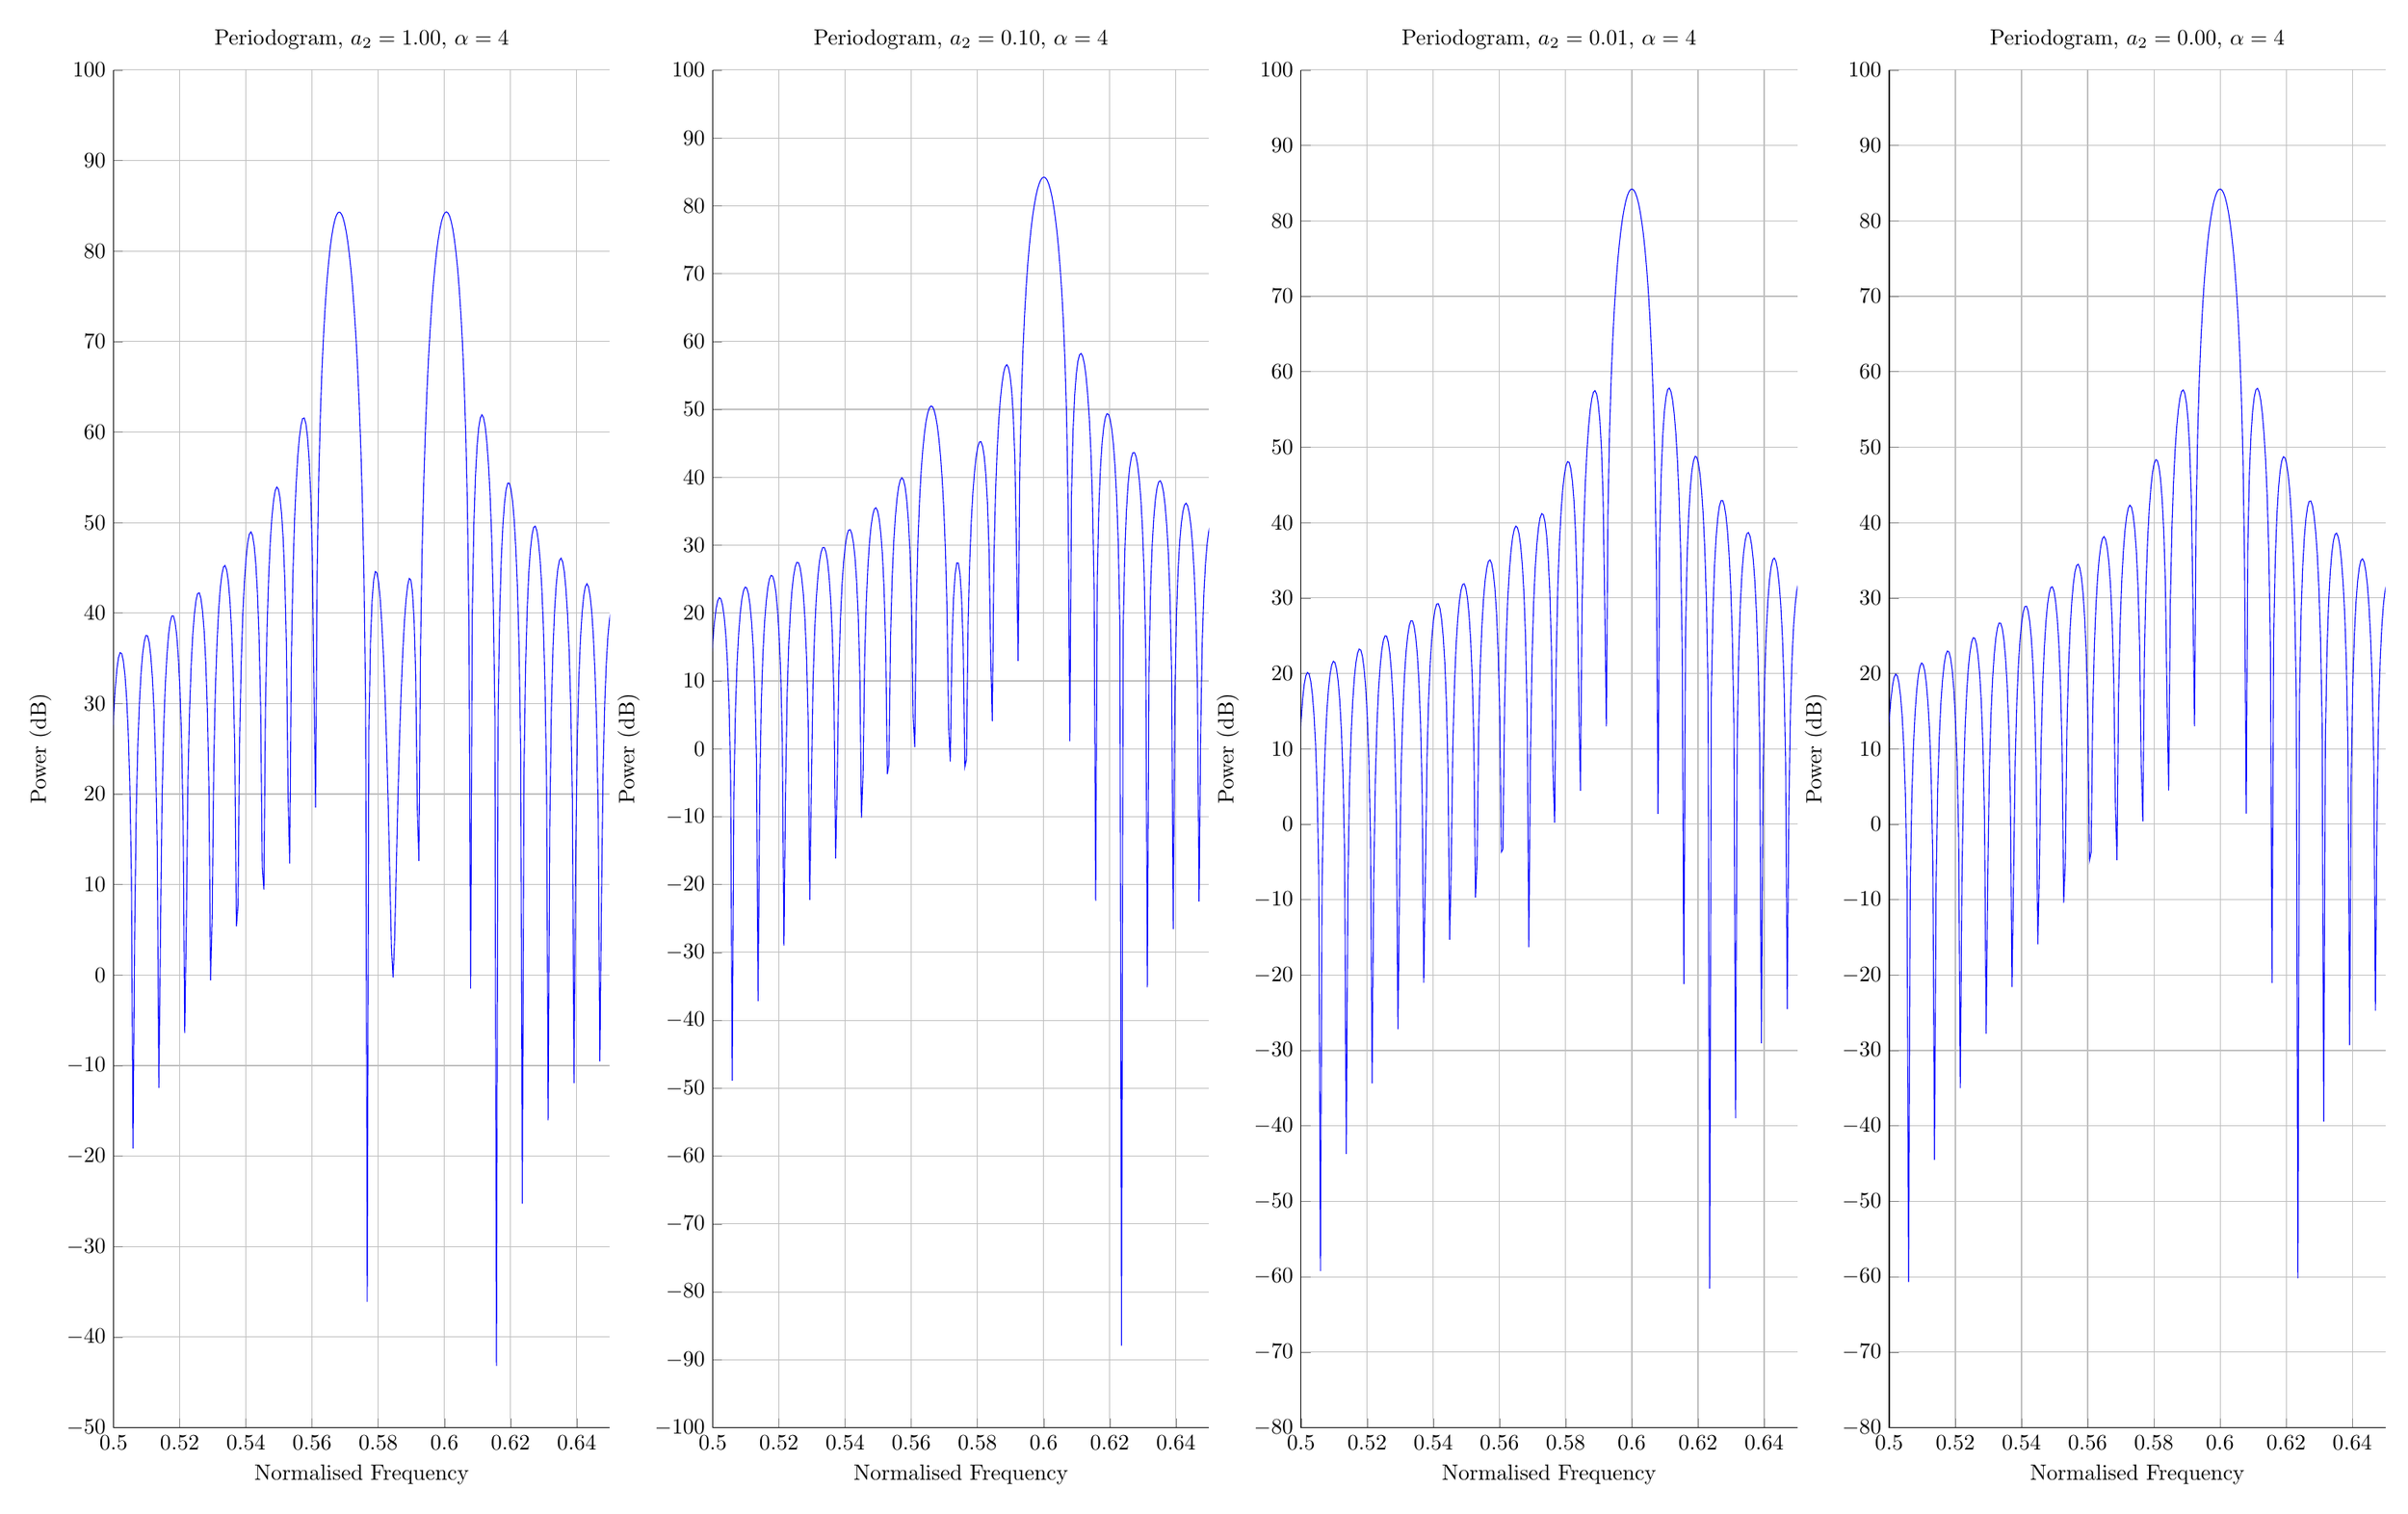
\begin{tikzpicture}

\begin{axis}[%
width=3.11369680851064in,
height=8.52354166666667in,
scale only axis,
xmin=0.5,
xmax=0.65,
xlabel={Normalised Frequency},
xmajorgrids,
ymin=-100,
ymax=100,
ylabel={Power (dB)},
ymajorgrids,
name=plot2,
title={Periodogram, $ a_2=0.10 $, $ \alpha= 4$},
axis x line*=bottom,
axis y line*=left
]
\addplot [color=blue,solid,forget plot]
  table[row sep=crcr]{-1	-93.4838675859193\\
-0.99951171875	-21.3500822869185\\
-0.9990234375	-9.64480453742984\\
-0.99853515625	-3.16451472841603\\
-0.998046875	1.03188762907334\\
-0.99755859375	3.85524868110649\\
-0.9970703125	5.69758158390836\\
-0.99658203125	6.75069137211217\\
-0.99609375	7.10650169137565\\
-0.99560546875	6.79351304690724\\
-0.9951171875	5.78664768170132\\
-0.99462890625	3.99862297794413\\
-0.994140625	1.24576541137748\\
-0.99365234375	-2.84601508154667\\
-0.9931640625	-9.13528738559076\\
-0.99267578125	-20.3093807482578\\
-0.9921875	-68.9448445300205\\
-0.99169921875	-22.4440477726698\\
-0.9912109375	-10.1570802943372\\
-0.99072265625	-3.47646164714326\\
-0.990234375	0.827779889418304\\
-0.98974609375	3.72308206258235\\
-0.9892578125	5.62043886769239\\
-0.98876953125	6.72013939821701\\
-0.98828125	7.11887987907873\\
-0.98779296875	6.84861949481358\\
-0.9873046875	5.88767176528683\\
-0.98681640625	4.15327164920669\\
-0.986328125	1.4695460312345\\
-0.98583984375	-2.52065312026417\\
-0.9853515625	-8.62751560682733\\
-0.98486328125	-19.3142557664672\\
-0.984375	-57.2779133940656\\
-0.98388671875	-23.6005163861004\\
-0.9833984375	-10.6731964755751\\
-0.98291015625	-3.78215511372062\\
-0.982421875	0.633332997776634\\
-0.98193359375	3.60208365159776\\
-0.9814453125	5.55521342860868\\
-0.98095703125	6.70187104544901\\
-0.98046875	7.14366538850078\\
-0.97998046875	6.91605481211089\\
-0.9794921875	6.00071701486752\\
-0.97900390625	4.31928878279765\\
-0.978515625	1.70338631563518\\
-0.97802734375	-2.18810733008423\\
-0.9775390625	-8.12053308418669\\
-0.97705078125	-18.3582306913077\\
-0.9765625	-50.2741122034655\\
-0.97607421875	-24.8307457004607\\
-0.9755859375	-11.1943166581327\\
-0.97509765625	-4.08188565549002\\
-0.974609375	0.448461123560163\\
-0.97412109375	3.49224125437114\\
-0.9736328125	5.5019278092903\\
-0.97314453125	6.69592942001727\\
-0.97265625	7.18091671332744\\
-0.97216796875	6.99589237623416\\
-0.9716796875	6.12587548700793\\
-0.97119140625	4.49679624427095\\
-0.970703125	1.94746775474895\\
-0.97021484375	-1.84804257309852\\
-0.9697265625	-7.61343071583297\\
-0.96923828125	-17.4357855143065\\
-0.96875	-45.253382846636\\
-0.96826171875	-26.1486639617761\\
-0.9677734375	-11.7217014471891\\
-0.96728515625	-4.37593657691826\\
-0.966796875	0.273101759244151\\
-0.96630859375	3.39357022616026\\
-0.9658203125	5.46063357326732\\
-0.96533203125	6.70238723618194\\
-0.96484375	7.23072216186364\\
-0.96435546875	7.0882353322442\\
-0.9638671875	6.2632686434442\\
-0.96337890625	4.68594428699778\\
-0.962890625	2.20199733934671\\
-0.96240234375	-1.50010829348717\\
-0.9619140625	-7.10533741992264\\
-0.96142578125	-16.542164266766\\
-0.9609375	-41.3252246217127\\
-0.96044921875	-27.5718046155891\\
-0.9599609375	-12.2567263472519\\
-0.95947265625	-4.66458546999237\\
-0.958984375	0.107215877579047\\
-0.95849609375	3.30611396961883\\
-0.9580078125	5.43141191197811\\
-0.95751953125	6.72134747391321\\
-0.95703125	7.29320054864434\\
-0.95654296875	7.19321731634422\\
-0.9560546875	6.41304811633719\\
-0.95556640625	4.88691239525406\\
-0.955078125	2.46720861512595\\
-0.95458984375	-1.14393660022815\\
-0.9541015625	-6.59541202187953\\
-0.95361328125	-15.6732267208324\\
-0.953125	-38.0860981786095\\
-0.95263671875	-29.1226837410544\\
-0.9521484375	-12.8009028641715\\
-0.95166015625	-4.9481057302083\\
-0.951171875	-0.0492117065620632\\
-0.95068359375	3.22994466922027\\
-0.9501953125	5.41437449555941\\
-0.94970703125	6.75294428313827\\
-0.94921875	7.36850213402362\\
-0.94873046875	7.31100342806701\\
-0.9482421875	6.57539672195907\\
-0.94775390625	5.09991037280852\\
-0.947265625	2.74336296831742\\
-0.94677734375	-0.779140201345228\\
-0.9462890625	-6.08283583633989\\
-0.94580078125	-14.825332530139\\
-0.9453125	-35.3190160306722\\
-0.94482421875	-30.8308988724691\\
-0.9443359375	-13.355903639273\\
-0.94384765625	-5.22676810022555\\
-0.943359375	-0.196171759570832\\
-0.94287109375	3.16516427561118\\
-0.9423828125	5.40966458219255\\
-0.94189453125	6.79734414980148\\
-0.94140625	7.45680982731559\\
-0.94091796875	7.44179146704405\\
-0.9404296875	6.75052973910017\\
-0.93994140625	5.32517969388805\\
-0.939453125	3.03075116111622\\
-0.93896484375	-0.405310161288341\\
-0.9384765625	-5.56680578253992\\
-0.93798828125	-13.9952494640804\\
-0.9375	-32.8938255023724\\
-0.93701171875	-32.736455853933\\
-0.9365234375	-13.923592644487\\
-0.93603515625	-5.50084226497873\\
-0.935546875	-0.333629823561284\\
-0.93505859375	3.11190575828645\\
-0.9345703125	5.41745840540774\\
-0.93408203125	6.8547473436345\\
-0.93359375	7.55834067376757\\
-0.93310546875	7.58581345500136\\
-0.9326171875	6.93869647325146\\
-0.93212890625	5.56299513817272\\
-0.931640625	3.32969514015034\\
-0.93115234375	-0.0220134495712905\\
-0.9306640625	-5.04652789182462\\
-0.93017578125	-13.1800797591566\\
-0.9296875	-30.726260571304\\
-0.92919921875	-34.8953006284266\\
-0.9287109375	-14.5060617732217\\
-0.92822265625	-5.77059852446766\\
-0.927734375	-0.461525163202582\\
-0.92724609375	3.07033465006501\\
-0.9267578125	5.43796686395512\\
-0.92626953125	6.92538967279738\\
-0.92578125	7.67334765095703\\
-0.92529296875	7.74333746898657\\
-0.9248046875	7.14018213301392\\
-0.92431640625	5.81366673689407\\
-0.923828125	3.64055014654366\\
-0.92333984375	0.371209755547537\\
-0.9228515625	-4.52121108039747\\
-0.92236328125	-12.3772002361357\\
-0.921875	-28.7585786798471\\
-0.92138671875	-37.3890785741436\\
-0.9208984375	-15.1056755771413\\
-0.92041015625	-6.03630957377796\\
-0.919921875	-0.579769441110028\\
-0.91943359375	3.04065091263376\\
-0.9189453125	5.47143754477598\\
-0.91845703125	7.00954457655095\\
-0.91796875	7.80212180626409\\
-0.91748046875	7.9146698179463\\
-0.9169921875	7.35531005135359\\
-0.91650390625	6.0775420633141\\
-0.916015625	3.96370716228275\\
-0.91552734375	0.774849049856293\\
-0.9150390625	-3.99006107030617\\
-0.91455078125	-11.5842129649081\\
-0.9140625	-26.9494289801706\\
-0.91357421875	-40.3437012185301\\
-0.9130859375	-15.7251264696339\\
-0.91259765625	-6.2982524242083\\
-0.912109375	-0.688245092008357\\
-0.91162109375	3.02309115916144\\
-0.9111328125	5.5181571165073\\
-0.91064453125	7.10752559410661\\
-0.91015625	7.94499477413194\\
-0.90966796875	8.10015760190475\\
-0.9091796875	7.58444429152248\\
-0.90869140625	6.35500890811676\\
-0.908203125	4.29959573482644\\
-0.90771484375	1.18942712049238\\
-0.9072265625	-3.45227434743802\\
-0.90673828125	-10.7989040600205\\
-0.90625	-25.2681291011552\\
-0.90576171875	-43.968372141495\\
-0.9052734375	-16.3675035107742\\
-0.90478515625	-6.55671050501311\\
-0.904296875	-0.786803358891584\\
-0.90380859375	3.01793127787361\\
-0.9033203125	5.57845413903436\\
-0.90283203125	7.2196892559942\\
-0.90234375	8.10234172011612\\
-0.90185546875	8.30019170137526\\
-0.9013671875	7.82799268593185\\
-0.90087890625	6.64649838879134\\
-0.900390625	4.64868723045384\\
-0.89990234375	1.6155034537753\\
-0.8994140625	-2.9070320473416\\
-0.89892578125	-10.0192087630298\\
-0.8984375	-23.6912317663179\\
-0.89794921875	-48.6498346499294\\
-0.8974609375	-17.0363790089579\\
-0.89697265625	-6.81197599252421\\
-0.896484375	-0.875261946126308\\
-0.89599609375	3.02548950981817\\
-0.8955078125	5.65270234417789\\
-0.89501953125	7.3464384539919\\
-0.89453125	8.27458476854503\\
-0.89404296875	8.51521025456828\\
-0.8935546875	8.0864103663061\\
-0.89306640625	6.95248855221846\\
-0.892578125	5.01149857700758\\
-0.89208984375	2.0536784992722\\
-0.8916015625	-2.35349365821656\\
-0.89111328125	-9.24318138184963\\
-0.890625	-22.2003623286809\\
-0.89013671875	-55.2329679772933\\
-0.8896484375	-17.7359187791943\\
-0.88916015625	-7.06435242249406\\
-0.888671875	-0.953402234339178\\
-0.88818359375	3.0461300453784\\
-0.8876953125	5.74132445419555\\
-0.88720703125	7.4882263574218\\
-0.88671875	8.46219698252106\\
-0.88623046875	8.74570269201452\\
-0.8857421875	8.36020385564984\\
-0.88525390625	7.27350854202346\\
-0.884765625	5.38859656914784\\
-0.88427734375	2.50459836793528\\
-0.8837890625	-1.79079042490409\\
-0.88330078125	-8.46896895738019\\
-0.8828125	-20.7808006091721\\
-0.88232421875	-66.2195511809943\\
-0.8818359375	-18.4710242374008\\
-0.88134765625	-7.31415765372506\\
-0.880859375	-1.02096599013795\\
-0.88037109375	3.08026721739919\\
-0.8798828125	5.84479661844374\\
-0.87939453125	7.6455609574974\\
-0.87890625	8.66570697906358\\
-0.87841796875	8.99221441247295\\
-0.8779296875	8.64993580697744\\
-0.87744140625	7.61014341683024\\
-0.876953125	5.78060282388389\\
-0.87646484375	2.9689601564941\\
-0.8759765625	-1.21801832896586\\
-0.87548828125	-7.69478774677348\\
-0.875	-19.4205183975892\\
-0.87451171875	-92.8637632756169\\
-0.8740234375	-19.2475179803973\\
-0.87353515625	-7.56172726559768\\
-0.873046875	-1.07765148850615\\
-0.87255859375	3.12837038565819\\
-0.8720703125	5.96365356576348\\
-0.87158203125	7.81901033885962\\
-0.87109375	8.88570427986661\\
-0.87060546875	9.25535220188835\\
-0.8701171875	8.95623049188803\\
-0.86962890625	7.9630397239188\\
-0.869140625	6.18819949274339\\
-0.86865234375	3.44751800879372\\
-0.8681640625	-0.634230505779319\\
-0.86767578125	-6.91890176929155\\
-0.8671875	-18.109506457633\\
-0.86669921875	-67.8925399572873\\
-0.8662109375	-20.0723897624307\\
-0.86572265625	-7.80741849222548\\
-0.865234375	-1.12310894794768\\
-0.86474609375	3.19096962733343\\
-0.8642578125	6.09849459060953\\
-0.86376953125	8.00920879824499\\
-0.86328125	9.12284551926382\\
-0.86279296875	9.53579051858466\\
-0.8623046875	9.27978016377838\\
-0.86181640625	8.33291195478066\\
-0.861328125	6.6121358591561\\
-0.86083984375	3.94109004692032\\
-0.8603515625	-0.0384289411357522\\
-0.85986328125	-6.13960277217378\\
-0.859375	-16.8392913158723\\
-0.85888671875	-55.3147139197973\\
-0.8583984375	-20.9541279336604\\
-0.85791015625	-8.05161482081677\\
-0.857421875	-1.15693515565504\\
-0.85693359375	3.26866237333535\\
-0.8564453125	6.24999051671685\\
-0.85595703125	8.21686395638637\\
-0.85546875	9.37786165751132\\
-0.85498046875	9.83427879475964\\
-0.8544921875	9.62135244773378\\
-0.85400390625	8.72055003668015\\
-0.853515625	7.05323597758724\\
-0.85302734375	4.45056633302018\\
-0.8525390625	0.570444735356312\\
-0.85205078125	-5.35519104790907\\
-0.8515625	-15.6025797869924\\
-0.85107421875	-47.8241405678052\\
-0.8505859375	-21.9031743798621\\
-0.85009765625	-8.2947314146953\\
-0.849609375	-1.17866713183088\\
-0.84912109375	3.36212116150045\\
-0.8486328125	6.41889181396361\\
-0.84814453125	8.44276504163467\\
-0.84765625	9.65156638037383\\
-0.84716796875	10.1516499377052\\
-0.8466796875	9.98179894297912\\
-0.84619140625	9.12682804865696\\
-0.845703125	7.51240754574719\\
-0.84521484375	4.97691805776555\\
-0.8447265625	1.19351957556365\\
-0.84423828125	-4.56395657789787\\
-0.84375	-14.3929913763851\\
-0.84326171875	-42.4161526262992\\
-0.8427734375	-22.932562250506\\
-0.84228515625	-8.53722156455625\\
-0.841796875	-1.18777464694917\\
-0.84130859375	3.47210271658852\\
-0.8408203125	6.6060380839529\\
-0.84033203125	8.68779256431235\\
-0.83984375	9.94486590714578\\
-0.83935546875	10.4888302559362\\
-0.8388671875	10.3620652661493\\
-0.83837890625	9.5527143933991\\
-0.837890625	7.99065224478571\\
-0.83740234375	5.52120819540924\\
-0.8369140625	1.83200701458736\\
-0.83642578125	-3.7641599945262\\
-0.8359375	-13.2048522029774\\
-0.83544921875	-38.134784849564\\
-0.8349609375	-24.0588317302943\\
-0.83447265625	-8.77958442790658\\
-0.833984375	-1.18365136057278\\
-0.83349609375	3.59945861649798\\
-0.8330078125	6.81236918041826\\
-0.83251953125	8.95292965222963\\
-0.83203125	10.2587704814576\\
-0.83154296875	10.8468510884389\\
-0.8310546875	10.7632028174827\\
-0.83056640625	9.99928371108694\\
-0.830078125	8.48907783788411\\
-0.82958984375	6.08460392156261\\
-0.8291015625	2.48721426190783\\
-0.82861328125	-2.95401284448183\\
-0.828125	-12.0330325298781\\
-0.82763671875	-34.5543758040403\\
-0.8271484375	-25.3033823591189\\
-0.82666015625	-9.02237439266889\\
-0.826171875	-1.16560429334891\\
-0.82568359375	3.74514786649889\\
-0.8251953125	7.03893829442365\\
-0.82470703125	9.23927538278401\\
-0.82421875	10.5944078852788\\
-0.82373046875	11.2268624823693\\
-0.8232421875	11.1863826202198\\
-0.82275390625	10.4677308905543\\
-0.822265625	9.00891238794416\\
-0.82177734375	6.66839116102079\\
-0.8212890625	3.16055976539893\\
-0.82080078125	-2.13165660166407\\
-0.8203125	-10.8728153955192\\
-0.81982421875	-31.4479388120544\\
-0.8193359375	-26.6945366480652\\
-0.81884765625	-9.2662125016027\\
-0.818359375	-1.13284126950504\\
-0.81787109375	3.91025178399924\\
-0.8173828125	7.28692741682377\\
-0.81689453125	9.5480605309746\\
-0.81640625	10.9530394018188\\
-0.81591796875	11.630149351208\\
-0.8154296875	11.6329116715865\\
-0.81494140625	10.9593876226505\\
-0.814453125	9.55152104607393\\
-0.81396484375	7.27399172533997\\
-0.8134765625	3.85359122424307\\
-0.81298828125	-1.29513981326341\\
-0.8125	-9.71978735332434\\
-0.81201171875	-28.679731319403\\
-0.8115234375	-28.2708147986332\\
-0.81103515625	-9.51180051233941\\
-0.810546875	-1.08445587179548\\
-0.81005859375	4.09599169990516\\
-0.8095703125	7.55766569642893\\
-0.80908203125	9.88066626059089\\
-0.80859375	11.3360787628345\\
-0.80810546875	12.0581506570778\\
-0.8076171875	12.1042523573313\\
-0.80712890625	11.4757420561919\\
-0.806640625	10.1184259800006\\
-0.80615234375	7.90298361913362\\
-0.8056640625	4.56800674680926\\
-0.80517578125	-0.442392664132611\\
-0.8046875	-8.56974463565692\\
-0.80419921875	-26.1617545312183\\
-0.8037109375	-30.0863840687238\\
-0.80322265625	-9.75993835596538\\
-0.802734375	-1.01940932525057\\
-0.80224609375	4.30375011823562\\
-0.8017578125	7.85265135098583\\
-0.80126953125	10.2386464270517\\
-0.80078125	11.745114759571\\
-0.80029296875	12.5124823071501\\
-0.7998046875	12.6020456305645\\
-0.79931640625	12.0184622682732\\
-0.798828125	10.7113301655538\\
-0.79833984375	8.55712525067076\\
-0.7978515625	5.3056799079114\\
-0.79736328125	0.428801897701188\\
-0.796875	-7.41860956176194\\
-0.79638671875	-23.8333647174649\\
-0.7958984375	-32.2206774005051\\
-0.79541015625	-10.0115460188232\\
-0.794921875	-0.936508560684996\\
-0.79443359375	4.53509615373974\\
-0.7939453125	8.17357797030745\\
-0.79345703125	10.6237543460827\\
-0.79296875	12.1819383856932\\
-0.79248046875	12.9949646466576\\
-0.7919921875	13.1281388517318\\
-0.79150390625	12.5894244603397\\
-0.791015625	11.3321459676034\\
-0.79052734375	9.23838448918751\\
-0.7900390625	6.06868966957017\\
-0.78955078125	1.32084152977985\\
-0.7890625	-6.26235295616702\\
-0.78857421875	-21.6506618792251\\
-0.7880859375	-34.7966977243346\\
-0.78759765625	-10.2676912394915\\
-0.787109375	-0.834379488166701\\
-0.78662109375	4.79181630408604\\
-0.7861328125	8.52236629322012\\
-0.78564453125	11.0379751295215\\
-0.78515625	12.6485756323725\\
-0.78466796875	13.5076556875721\\
-0.7841796875	13.6846194479173\\
-0.78369140625	13.1907470576981\\
-0.783203125	11.9830297081077\\
-0.78271484375	9.94897378762642\\
-0.7822265625	6.85935641017718\\
-0.78173828125	2.23634368729797\\
-0.78125	-5.09691887761003\\
-0.78076171875	-19.5805083296902\\
-0.7802734375	-38.0195044013796\\
-0.77978515625	-10.5296249359766\\
-0.779296875	-0.711434213227152\\
-0.77880859375	5.07595193123521\\
-0.7783203125	8.90120286554739\\
-0.77783203125	11.4835650217095\\
-0.77734375	13.1473273944165\\
-0.77685546875	14.0528915573655\\
-0.7763671875	14.2738559017701\\
-0.77587890625	13.8248322491109\\
-0.775390625	12.6664237848984\\
-0.77490234375	10.6913929625836\\
-0.7744140625	7.68028568670822\\
-0.77392578125	3.17819234473634\\
-0.7734375	-3.91814815691398\\
-0.77294921875	-17.5969336145614\\
-0.7724609375	-42.2692487448851\\
-0.77197265625	-10.7988270340415\\
-0.771484375	-0.565830523297148\\
-0.77099609375	5.38984525867382\\
-0.7705078125	9.31258742879079\\
-0.77001953125	11.9630996216777\\
-0.76953125	13.680818407334\\
-0.76904296875	14.6333361226459\\
-0.7685546875	14.8985480602679\\
-0.76806640625	14.4944169927751\\
-0.767578125	13.385108404432\\
-0.76708984375	11.4684817329623\\
-0.7666015625	8.5344218742197\\
-0.76611328125	4.1495944752127\\
-0.765625	-2.72169713319525\\
-0.76513671875	-15.678852212964\\
-0.7646484375	-48.3792365824134\\
-0.76416015625	-11.0770664776241\\
-0.763671875	-0.395421412755374\\
-0.76318359375	5.73619628546889\\
-0.7626953125	9.75939149800133\\
-0.76220703125	12.4795334984457\\
-0.76171875	14.2520577705996\\
-0.76123046875	15.2520423912802\\
-0.7607421875	15.5617894160521\\
-0.76025390625	15.2026361915128\\
-0.759765625	14.1422656825766\\
-0.75927734375	12.2834848242888\\
-0.7587890625	9.4251145468846\\
-0.75830078125	5.1541492443436\\
-0.7578125	-1.50294754510621\\
-0.75732421875	-13.8085401434109\\
-0.7568359375	-58.8475099851194\\
-0.75634765625	-11.3664808615614\\
-0.755859375	-0.197691633568131\\
-0.75537109375	6.11813384646436\\
-0.7548828125	10.2449314364697\\
-0.75439453125	13.0362745751335\\
-0.75390625	14.8645145000354\\
-0.75341796875	15.9125292038552\\
-0.7529296875	16.2671449413079\\
-0.75244140625	15.9531016876842\\
-0.751953125	14.9415598361265\\
-0.75146484375	13.1401334356881\\
-0.7509765625	10.3562014764849\\
-0.75048828125	6.19593390407144\\
-0.75	-0.256902713741826\\
-0.74951171875	-11.970565724784\\
-0.7490234375	-90.6979619768488\\
-0.74853515625	-11.6696836555845\\
-0.748046875	0.030322849438306\\
-0.74755859375	6.53930521953567\\
-0.7470703125	10.7730605366534\\
-0.74658203125	13.6372778877381\\
-0.74609375	15.5222128108922\\
-0.74560546875	16.6188780130089\\
-0.7451171875	17.0187493714898\\
-0.74462890625	16.7500020760309\\
-0.744140625	15.7872385665651\\
-0.74365234375	14.0427482772691\\
-0.7431640625	11.3321135675235\\
-0.74267578125	7.27961184427326\\
-0.7421875	1.02193617913592\\
-0.74169921875	-10.1509964154235\\
-0.7412109375	-60.6682633972325\\
-0.74072265625	-11.9899109261063\\
-0.740234375	0.292138215288327\\
-0.73974609375	7.00399036441646\\
-0.7392578125	11.3482863451208\\
-0.73876953125	14.2871650953694\\
-0.73828125	16.2298536470852\\
-0.73779296875	17.3758564068112\\
-0.7373046875	17.8214327386538\\
-0.73681640625	17.5982302810597\\
-0.736328125	16.6842627331625\\
-0.73583984375	14.9963714296707\\
-0.7353515625	12.3580091416912\\
-0.73486328125	8.41057040104478\\
-0.734375	2.3397219759009\\
-0.73388671875	-8.33677070511188\\
-0.7333984375	-47.0340181930692\\
-0.73291015625	-12.3312257414331\\
-0.732421875	0.591957010107719\\
-0.73193359375	7.5172493395758\\
-0.7314453125	11.9759219990456\\
-0.73095703125	14.9913787137166\\
-0.73046875	16.992971632986\\
-0.72998046875	18.1890777607079\\
-0.7294921875	18.6808827515609\\
-0.72900390625	18.5035487139232\\
-0.728515625	17.6384743537742\\
-0.72802734375	16.0069372938287\\
-0.7275390625	13.4399480777953\\
-0.72705078125	9.5950991904702\\
-0.7265625	3.70345300058126\\
-0.72607421875	-6.51515988507047\\
-0.7255859375	-38.8240987317941\\
-0.72509765625	-12.6988087298321\\
-0.724609375	0.934844782491015\\
-0.72412109375	8.0851151137497\\
-0.7236328125	12.6622841169941\\
-0.72314453125	15.7563839208648\\
-0.72265625	17.8181406051435\\
-0.72216796875	19.0652104895778\\
-0.7216796875	19.6038578156807\\
-0.72119140625	19.4728061317376\\
-0.720703125	18.6568173950299\\
-0.72021484375	17.0814974412028\\
-0.7197265625	14.585120977871\\
-0.71923828125	10.8406245253368\\
-0.71875	5.12122034074429\\
-0.71826171875	-4.67326250267148\\
-0.7177734375	-32.7223625594852\\
-0.71728515625	-13.0993806159288\\
-0.716796875	1.32696600012825\\
-0.71630859375	8.71484957792252\\
-0.7158203125	13.4149555429976\\
-0.71533203125	16.589936704759\\
-0.71484375	18.7132469683138\\
-0.71435546875	20.0122566295805\\
-0.7138671875	20.5984709203868\\
-0.71337890625	20.5142269378337\\
-0.712890625	19.7476326162444\\
-0.71240234375	18.2285211704508\\
-0.7119140625	15.8021557253322\\
-0.71142578125	12.1560228716797\\
-0.7109375	6.60253475855273\\
-0.71044921875	-2.79748047910215\\
-0.7099609375	-27.7172019505792\\
-0.70947265625	-13.5418328694976\\
-0.708984375	1.77590442735903\\
-0.70849609375	9.41528928015288\\
-0.7080078125	14.2431402326786\\
-0.70751953125	17.5014463817529\\
-0.70703125	19.6878596563427\\
-0.70654296875	21.0399292994287\\
-0.7060546875	21.6745747331519\\
-0.70556640625	21.6378040759695\\
-0.705078125	20.9210584580015\\
-0.70458984375	19.4583046259168\\
-0.7041015625	17.1015351843883\\
-0.70361328125	13.5520480299346\\
-0.703125	8.15876907633355\\
-0.70263671875	-0.872922178550082\\
-0.7021484375	-23.3590427627681\\
-0.70166015625	-14.0381976402547\\
-0.701171875	2.29110646262071\\
-0.70068359375	10.1973213673459\\
-0.7001953125	15.1581519927687\\
-0.69970703125	18.5024753980409\\
-0.69921875	20.7537408317918\\
-0.69873046875	22.1601744295146\\
-0.6982421875	22.844294580951\\
-0.69775390625	22.8558435309009\\
-0.697265625	22.1895873631367\\
-0.69677734375	20.7835392870148\\
-0.6962890625	18.4961783212729\\
-0.69580078125	15.0419258553359\\
-0.6953125	9.80377159941777\\
-0.69482421875	1.11733704949257\\
-0.6943359375	-19.40294755755\\
-0.69384765625	-14.6051927449826\\
-0.693359375	2.88450792628614\\
-0.69287109375	11.0745532662805\\
-0.6923828125	16.1741026387978\\
-0.69189453125	19.607443988718\\
-0.69140625	21.9255669532891\\
-0.69091796875	23.3879085025531\\
-0.6904296875	24.1227832453412\\
-0.68994140625	24.1837366181145\\
-0.689453125	23.5688560475594\\
-0.68896484375	22.2201207638359\\
-0.6884765625	20.0022681901102\\
-0.68798828125	16.6422025718093\\
-0.6875	11.5547394745537\\
-0.68701171875	3.1932371653005\\
-0.6865234375	-15.6947532457421\\
-0.68603515625	-15.2667871368807\\
-0.685546875	3.57144235284302\\
-0.68505859375	12.0642790164106\\
-0.6845703125	17.3088959800656\\
-0.68408203125	20.8346495962473\\
-0.68359375	23.2219736966383\\
-0.68310546875	24.7420894929087\\
-0.6826171875	25.5293185894612\\
-0.68212890625	25.6410850516664\\
-0.681640625	25.0787988290042\\
-0.68115234375	23.7883312838102\\
-0.6806640625	21.640464613511\\
-0.68017578125	18.3739891423595\\
-0.6796875	13.4334993828668\\
-0.67919921875	5.37911713345785\\
-0.6787109375	-12.1245463966975\\
-0.67822265625	-16.0586803043959\\
-0.677734375	4.37199555983755\\
-0.67724609375	13.1889151710712\\
-0.6767578125	18.5857068316734\\
-0.67626953125	22.2077865833338\\
-0.67578125	24.667116794518\\
-0.67529296875	26.2473198357621\\
-0.6748046875	27.0889498744957\\
-0.67431640625	27.2533919527157\\
-0.673828125	26.7453847774192\\
-0.67333984375	25.5146245484352\\
-0.6728515625	23.4377384872294\\
-0.67236328125	20.2648472408305\\
-0.671875	15.4684502076367\\
-0.67138671875	7.70576853112219\\
-0.6708984375	-8.60360504467248\\
-0.67041015625	-17.0366241436762\\
-0.669921875	5.31309528683319\\
-0.66943359375	14.4782095027442\\
-0.6689453125	20.0352601654424\\
-0.66845703125	23.758293435017\\
-0.66796875	26.2930885036081\\
-0.66748046875	27.936334154127\\
-0.6669921875	28.8350590639012\\
-0.66650390625	29.0546992569372\\
-0.666015625	28.6033339318677\\
-0.66552734375	27.4344236573568\\
-0.6650390625	25.4302545679368\\
-0.66455078125	22.3517606115649\\
-0.6640625	17.6976292925701\\
-0.66357421875	10.213642626711\\
-0.6630859375	-5.05027690215472\\
-0.66259765625	-18.2931538698868\\
-0.662109375	6.43186796595776\\
-0.66162109375	15.9727819351116\\
-0.6611328125	21.6994936522028\\
-0.66064453125	25.5291351654531\\
-0.66015625	28.1438228871034\\
-0.65966796875	29.8540315565465\\
-0.6591796875	30.813524803774\\
-0.65869140625	31.0918884228782\\
-0.658203125	30.7005601248425\\
-0.65771484375	29.596711796429\\
-0.6572265625	27.6681162148686\\
-0.65673828125	24.6860408023847\\
-0.65625	20.1737887393089\\
-0.65576171875	12.9581393203224\\
-0.6552734375	-1.37846132273286\\
-0.65478515625	-19.9949359425338\\
-0.654296875	7.78130366894888\\
-0.65380859375	17.7300948161448\\
-0.6533203125	23.6377520929339\\
-0.65283203125	27.5812226664876\\
-0.65234375	30.2817474327543\\
-0.65185546875	32.0643686592293\\
-0.6513671875	33.0898669530473\\
-0.65087890625	33.4320873433939\\
-0.650390625	33.1058518802982\\
-0.64990234375	32.0719994977286\\
-0.6494140625	30.223632278118\\
-0.64892578125	27.34190819851\\
-0.6484375	22.9733081787313\\
-0.64794921875	16.0188969286746\\
-0.6474609375	2.51564138665239\\
-0.64697265625	-22.4793482984424\\
-0.646484375	9.44042288924371\\
-0.64599609375	19.8351725479631\\
-0.6455078125	25.9379548465107\\
-0.64501953125	30.005036836271\\
-0.64453125	32.7998826210654\\
-0.64404296875	34.6629565316241\\
-0.6435546875	35.762364906895\\
-0.64306640625	36.1763358556283\\
-0.642578125	35.9231127198731\\
-0.64208984375	34.9671692624953\\
-0.6416015625	33.2067977000495\\
-0.64111328125	30.4326429241\\
-0.640625	26.2130549208348\\
-0.64013671875	19.5174261585696\\
-0.6396484375	6.77420842730583\\
-0.63916015625	-26.5680076723908\\
-0.638671875	11.5340225560015\\
-0.63818359375	22.421468548787\\
-0.6376953125	28.7384538018557\\
-0.63720703125	32.9435133315267\\
-0.63671875	35.8458057142222\\
-0.63623046875	37.8021626791685\\
-0.6357421875	38.9883622466335\\
-0.63525390625	39.4871626252125\\
-0.634765625	39.3202851305261\\
-0.63427734375	38.4558271419548\\
-0.6337890625	36.7971595284332\\
-0.63330078125	34.1440594215431\\
-0.6328125	30.0855711962407\\
-0.63232421875	23.6541434072746\\
-0.6318359375	11.6182516066958\\
-0.63134765625	-35.1248660857144\\
-0.630859375	14.2752980158816\\
-0.63037109375	25.7161251851142\\
-0.6298828125	32.275807836685\\
-0.62939453125	36.6424661811524\\
-0.62890625	39.6748919106867\\
-0.62841796875	41.7473575489897\\
-0.6279296875	43.0437240468751\\
-0.62744140625	43.6514769007949\\
-0.626953125	43.5959199776716\\
-0.62646484375	42.8488144518302\\
-0.6259765625	41.318559382771\\
-0.62548828125	38.8137951327405\\
-0.625	34.9432570394444\\
-0.62451171875	28.7978501525543\\
-0.6240234375	17.4438130415843\\
-0.62353515625	-87.9191441002992\\
-0.623046875	18.0726850547558\\
-0.62255859375	30.1544493081628\\
-0.6220703125	37.0070171114271\\
-0.62158203125	41.5811629965502\\
-0.62109375	44.7899122495439\\
-0.62060546875	47.0262972475444\\
-0.6201171875	48.4828497456598\\
-0.61962890625	49.252148102056\\
-0.619140625	49.3633612071936\\
-0.61865234375	48.7921506392382\\
-0.6181640625	47.4521174973355\\
-0.61767578125	45.1607673160553\\
-0.6171875	41.545904553946\\
-0.61669921875	35.7531683168507\\
-0.6162109375	25.1120659252355\\
-0.61572265625	-22.410355244471\\
-0.615234375	23.8678788594966\\
-0.61474609375	36.74829636843\\
-0.6142578125	44.010655831913\\
-0.61376953125	48.909736560818\\
-0.61328125	52.4188250679325\\
-0.61279296875	54.9519990625871\\
-0.6123046875	56.7120292236348\\
-0.61181640625	57.798048953607\\
-0.611328125	58.2446385864936\\
-0.61083984375	58.033074035817\\
-0.6103515625	57.0840779149107\\
-0.60986328125	55.2261141000083\\
-0.609375	52.1080121505085\\
-0.60888671875	46.9299573826352\\
-0.6083984375	37.2601383573795\\
-0.60791015625	1.1394601038904\\
-0.607421875	34.794029841214\\
-0.60693359375	48.9682947785884\\
-0.6064453125	57.1312338113297\\
-0.60595703125	62.9047236853217\\
-0.60546875	67.3431256664665\\
-0.60498046875	70.9022093752976\\
-0.6044921875	73.8210626000892\\
-0.60400390625	76.2406690003961\\
-0.603515625	78.250849534227\\
-0.60302734375	79.911937355149\\
-0.6025390625	81.2659165975688\\
-0.60205078125	82.3426097251859\\
-0.6015625	83.1633146084181\\
-0.60107421875	83.7430252247029\\
-0.6005859375	84.0918103287187\\
-0.60009765625	84.2156551805728\\
-0.599609375	84.1169309366718\\
-0.59912109375	83.7945757416908\\
-0.5986328125	83.2440183920375\\
-0.59814453125	82.4568317129265\\
-0.59765625	81.4200551750898\\
-0.59716796875	80.1150595651451\\
-0.5966796875	78.5157157521719\\
-0.59619140625	76.5854245986168\\
-0.595703125	74.2721526657953\\
-0.59521484375	71.4997175814449\\
-0.5947265625	68.1514030196858\\
-0.59423828125	64.0361223306834\\
-0.59375	58.8086944823034\\
-0.59326171875	51.7406592135205\\
-0.5927734375	40.7886826165851\\
-0.59228515625	12.9430084990391\\
-0.591796875	28.9265983441706\\
-0.59130859375	42.5992211907356\\
-0.5908203125	49.0193212137037\\
-0.59033203125	52.7457126821554\\
-0.58984375	54.9696339158371\\
-0.58935546875	56.1705671296889\\
-0.5888671875	56.5765423814038\\
-0.58837890625	56.2982085466032\\
-0.587890625	55.3767883726575\\
-0.58740234375	53.7996521837236\\
-0.5869140625	51.4969170102645\\
-0.58642578125	48.3163796908271\\
-0.5859375	43.9536095649684\\
-0.58544921875	37.7463857782739\\
-0.5849609375	27.8628525328774\\
-0.58447265625	4.05987010379135\\
-0.583984375	13.8307329453561\\
-0.58349609375	29.1588911293154\\
-0.5830078125	36.2685236737603\\
-0.58251953125	40.4711844071785\\
-0.58203125	43.0710838354214\\
-0.58154296875	44.582967776226\\
-0.5810546875	45.2502193013619\\
-0.58056640625	45.1917859997482\\
-0.580078125	44.454374073448\\
-0.57958984375	43.0301212663828\\
-0.5791015625	40.8551559846856\\
-0.57861328125	37.7880242788979\\
-0.578125	33.5489349983186\\
-0.57763671875	27.5460992658994\\
-0.5771484375	18.2314542255575\\
-0.57666015625	-1.56856039890619\\
-0.576171875	-2.68807782873408\\
-0.57568359375	15.0304146296079\\
-0.5751953125	22.1383818806743\\
-0.57470703125	25.7670620326574\\
-0.57421875	27.3646040203224\\
-0.57373046875	27.3618259876981\\
-0.5732421875	25.7529466454475\\
-0.57275390625	22.0916596397724\\
-0.572265625	14.9115781064621\\
-0.57177734375	-1.89870166805505\\
-0.5712890625	3.27189152541268\\
-0.57080078125	20.1365561616058\\
-0.5703125	29.1439798950479\\
-0.56982421875	35.1850291496372\\
-0.5693359375	39.6080259219723\\
-0.56884765625	42.9673099130638\\
-0.568359375	45.543086946752\\
-0.56787109375	47.4945504541485\\
-0.5673828125	48.918086185425\\
-0.56689453125	49.8731209147139\\
-0.56640625	50.39467550726\\
-0.56591796875	50.4995397310671\\
-0.5654296875	50.1888077664439\\
-0.56494140625	49.4477462851453\\
-0.564453125	48.2429169022527\\
-0.56396484375	46.5153629159993\\
-0.5634765625	44.1666387805271\\
-0.56298828125	41.0294151159528\\
-0.5625	36.7990119299819\\
-0.56201171875	30.8431161380246\\
-0.5615234375	21.4811188820135\\
-0.56103515625	0.260110305813135\\
-0.560546875	4.68154056471164\\
-0.56005859375	21.5635982055518\\
-0.5595703125	29.2167561572387\\
-0.55908203125	33.810007366822\\
-0.55859375	36.7603069988494\\
-0.55810546875	38.6151094420676\\
-0.5576171875	39.6315255141842\\
-0.55712890625	39.9361887146425\\
-0.556640625	39.5814479322764\\
-0.55615234375	38.564675207274\\
-0.5556640625	36.8277612687869\\
-0.55517578125	34.2364207032252\\
-0.5546875	30.5208685274168\\
-0.55419921875	25.1059419703748\\
-0.5537109375	16.4836322970579\\
-0.55322265625	-2.24963971304946\\
-0.552734375	-3.7337120470828\\
-0.55224609375	15.2898292329419\\
-0.5517578125	23.5492557655426\\
-0.55126953125	28.5061020772342\\
-0.55078125	31.7295619194776\\
-0.55029296875	33.8108199083593\\
-0.5498046875	35.0252366037404\\
-0.54931640625	35.5091739876084\\
-0.548828125	35.3213802277233\\
-0.54833984375	34.4644907214747\\
-0.5478515625	32.885991671939\\
-0.54736328125	30.4594205557962\\
-0.546875	26.9292640645741\\
-0.54638671875	21.7546116051581\\
-0.5458984375	13.5469446684897\\
-0.54541015625	-3.61961697062571\\
-0.544921875	-10.1634812333975\\
-0.54443359375	10.9162380086097\\
-0.5439453125	19.6136806646886\\
-0.54345703125	24.7976579223819\\
-0.54296875	28.1785680864456\\
-0.54248046875	30.3855452247804\\
-0.5419921875	31.7088442435365\\
-0.54150390625	32.2923083857295\\
-0.541015625	32.1994069241151\\
-0.54052734375	31.4366580851511\\
-0.5400390625	29.9558637466237\\
-0.53955078125	27.6369517450103\\
-0.5390625	24.2365171382549\\
-0.53857421875	19.242971121103\\
-0.5380859375	11.3678911548618\\
-0.53759765625	-4.57537530955799\\
-0.537109375	-16.1405552672891\\
-0.53662109375	7.2967580679712\\
-0.5361328125	16.4067086109936\\
-0.53564453125	21.7872870017137\\
-0.53515625	25.2969729245802\\
-0.53466796875	27.6031164000737\\
-0.5341796875	29.0106028117823\\
-0.53369140625	29.670470652928\\
-0.533203125	29.6506430836293\\
-0.53271484375	28.9612481152469\\
-0.5322265625	27.5580701823051\\
-0.53173828125	25.3269135706294\\
-0.53125	22.0354444430917\\
-0.53076171875	17.1985435792028\\
-0.5302734375	9.6156814457583\\
-0.52978515625	-5.30531273165545\\
-0.529296875	-22.245721048186\\
-0.52880859375	4.09812894874152\\
-0.5283203125	13.6264181817853\\
-0.52783203125	19.1947951384529\\
-0.52734375	22.8226424241181\\
-0.52685546875	25.2172557894449\\
-0.5263671875	26.698498419385\\
-0.52587890625	27.4246566446732\\
-0.525390625	27.4680677953309\\
-0.52490234375	26.8423758962235\\
-0.5244140625	25.5071822419399\\
-0.52392578125	23.3538494139143\\
-0.5234375	20.1603892171952\\
-0.52294921875	15.4660385309456\\
-0.5224609375	8.14898630944611\\
-0.52197265625	-5.89004638099551\\
-0.521484375	-28.9887706204473\\
-0.52099609375	1.16989777610802\\
-0.5205078125	11.1353343985606\\
-0.52001953125	16.8903690358995\\
-0.51953125	20.6320037616571\\
-0.51904296875	23.1099077340779\\
-0.5185546875	24.6595130105533\\
-0.51806640625	25.446525956585\\
-0.517578125	25.5477330222841\\
-0.51708984375	24.9802585420164\\
-0.5166015625	23.7074126427386\\
-0.51611328125	21.6258746836781\\
-0.515625	18.5234182985477\\
-0.51513671875	13.9619026057949\\
-0.5146484375	6.89076674815856\\
-0.51416015625	-6.37288027079181\\
-0.513671875	-37.1796744758674\\
-0.51318359375	-1.57350021722301\\
-0.5126953125	8.85603824941107\\
-0.51220703125	14.800287127366\\
-0.51171875	18.6541943929207\\
-0.51123046875	21.2127196567467\\
-0.5107421875	22.8275978135239\\
-0.51025390625	23.6721893792769\\
-0.509765625	23.8278005483793\\
-0.50927734375	23.3150273084059\\
-0.5087890625	22.1008085607279\\
-0.50830078125	20.0869395201544\\
-0.5078125	17.0704543346334\\
-0.50732421875	12.6343394564311\\
-0.5068359375	5.79295396895843\\
-0.50634765625	-6.78017849892579\\
-0.505859375	-48.8740357887198\\
-0.50537109375	-4.18830615974207\\
-0.5048828125	6.73909143123702\\
-0.50439453125	12.8773428013364\\
-0.50390625	16.8435857717934\\
-0.50341796875	19.4814186682854\\
-0.5029296875	21.1597210815525\\
-0.50244140625	22.0597831966074\\
-0.501953125	22.267523398713\\
-0.50146484375	21.8070165449491\\
-0.5009765625	20.6487669891857\\
-0.50048828125	18.6995106928563\\
-0.5	15.7650969932692\\
-0.49951171875	11.4483156083828\\
-0.4990234375	4.82295591636479\\
-0.49853515625	-7.12929393153979\\
-0.498046875	-75.3859391897582\\
-0.49755859375	-6.71554844112643\\
-0.4970703125	4.75023117680635\\
-0.49658203125	11.0888753408899\\
-0.49609375	15.1685164149454\\
-0.49560546875	17.8851693479596\\
-0.4951171875	19.6257958242368\\
-0.49462890625	20.5799242536503\\
-0.494140625	20.8381935947295\\
-0.49365234375	20.4281757594454\\
-0.4931640625	19.3238887905263\\
-0.49267578125	17.4368528239173\\
-0.4921875	14.5813290908748\\
-0.49169921875	10.3787190839004\\
-0.4912109375	3.95741390526823\\
-0.49072265625	-7.432273166921\\
-0.490234375	-61.2033810232015\\
-0.48974609375	-9.18781104659024\\
-0.4892578125	2.8642996792751\\
-0.48876953125	9.41104262416866\\
-0.48828125	13.6058498351579\\
-0.48779296875	16.4013867462544\\
-0.4873046875	18.2037273943946\\
-0.48681640625	19.2109765693494\\
-0.486328125	19.5186153818453\\
-0.48583984375	19.1577395254365\\
-0.4853515625	18.105837809676\\
-0.48486328125	16.2790724489726\\
-0.484375	13.4997470300499\\
-0.48388671875	9.40679184065033\\
-0.4833984375	3.1789120058537\\
-0.48291015625	-7.69781165536798\\
-0.482421875	-47.7511117224359\\
-0.48193359375	-11.6330186392707\\
-0.4814453125	1.06199700736112\\
-0.48095703125	7.8257391559199\\
-0.48046875	12.1380258940879\\
-0.47998046875	15.0129071523844\\
-0.4794921875	16.876694711548\\
-0.47900390625	17.9364363924384\\
-0.478515625	18.2925889422713\\
-0.47802734375	17.9798058118956\\
-0.4775390625	16.9790109348617\\
-0.47705078125	15.2108784920402\\
-0.4765625	12.5054132655316\\
-0.47607421875	8.51808333870233\\
-0.4755859375	2.47407427516383\\
-0.47509765625	-7.93237745458373\\
-0.474609375	-41.0544248385729\\
-0.47412109375	-14.0768922520456\\
-0.4736328125	-0.672017247083436\\
-0.47314453125	6.3187891130184\\
-0.47265625	10.7513232255994\\
-0.47216796875	13.7063124586216\\
-0.4716796875	15.6315321351572\\
-0.47119140625	16.7433684128542\\
-0.470703125	17.1473985220508\\
-0.47021484375	16.8818741846121\\
-0.4697265625	15.9311251325048\\
-0.46923828125	14.2202177351064\\
-0.46875	11.5865414199255\\
-0.46826171875	7.70119088636609\\
-0.4677734375	1.83238661128109\\
-0.46728515625	-8.14089907389675\\
-0.466796875	-36.7581411188545\\
-0.46630859375	-16.5448281163959\\
-0.4658203125	-2.35031246594042\\
-0.46533203125	4.87881602915445\\
-0.46484375	9.43476831937175\\
-0.46435546875	12.4708740404647\\
-0.4638671875	14.4577057013049\\
-0.46337890625	15.6214126857042\\
-0.462890625	16.0728487996502\\
-0.46240234375	15.8539107013335\\
-0.4619140625	14.9523102892709\\
-0.46142578125	13.2973955147356\\
-0.4609375	10.7336457069096\\
-0.46044921875	6.94694139993369\\
-0.4599609375	1.24542825205498\\
-0.45947265625	-8.32720728667012\\
-0.458984375	-33.6817780469157\\
-0.45849609375	-19.0636258111807\\
-0.4580078125	-3.98347343061511\\
-0.45751953125	3.49649916532063\\
-0.45703125	8.17941603675787\\
-0.45654296875	11.2978541191583\\
-0.4560546875	13.3466338450943\\
-0.45556640625	14.5621237593623\\
-0.455078125	15.0606217321028\\
-0.45458984375	14.8877219835385\\
-0.4541015625	14.0345002208078\\
-0.45361328125	12.434483679369\\
-0.453125	9.93896646380721\\
-0.45263671875	6.2478369675778\\
-0.4521484375	0.70634958056862\\
-0.45166015625	-8.49432995767626\\
-0.451171875	-31.3355385050643\\
-0.45068359375	-21.6633957463464\\
-0.4501953125	-5.58064596490427\\
-0.44970703125	2.16406411206931\\
-0.44921875	6.97785610660986\\
-0.44873046875	10.1800254392745\\
-0.4482421875	12.2912192568144\\
-0.44775390625	13.5585141214294\\
-0.447265625	14.1038311842648\\
-0.44677734375	13.9765207481657\\
-0.4462890625	13.1710089550368\\
-0.44580078125	11.6249076686049\\
-0.4453125	9.19606848589328\\
-0.44482421875	5.59766618955733\\
-0.4443359375	0.209505448850836\\
-0.44384765625	-8.64469500216822\\
-0.443359375	-29.4701469073031\\
-0.44287109375	-24.3800150598244\\
-0.4423828125	-7.14993235576398\\
-0.44189453125	0.874922047855601\\
-0.44140625	5.82386361853172\\
-0.44091796875	9.11133050069501\\
-0.4404296875	11.2855161027629\\
-0.43994140625	12.6047290166493\\
-0.439453125	13.1967050884429\\
-0.43896484375	13.1146151399801\\
-0.4384765625	12.3562271555246\\
-0.43798828125	10.8631500792338\\
-0.4375	8.4995520801439\\
-0.43701171875	4.99122402058101\\
-0.4365234375	-0.249809338968543\\
-0.43603515625	-8.78027377463455\\
-0.435546875	-27.942117340271\\
-0.43505859375	-27.2586846456336\\
-0.4345703125	-8.69869052307216\\
-0.43408203125	-0.376593014290087\\
-0.43359375	4.71214481544523\\
-0.43310546875	8.0866334018742\\
-0.4326171875	10.3244873013073\\
-0.43212890625	11.6958088744105\\
-0.431640625	12.334352853123\\
-0.43115234375	12.2971810147078\\
-0.4306640625	11.5853992337271\\
-0.43017578125	10.1445326564553\\
-0.4296875	7.84484020199393\\
-0.42919921875	4.42410505386292\\
-0.4287109375	-0.675555208142926\\
-0.42822265625	-8.90268462987119\\
-0.427734375	-26.6617019566445\\
-0.42724609375	-30.3595767769346\\
-0.4267578125	-10.233770943436\\
-0.42626953125	-1.59542034974478\\
-0.42578125	3.63814797489574\\
-0.42529296875	7.10153508999361\\
-0.4248046875	9.40382358765903\\
-0.42431640625	10.8275119699552\\
-0.423828125	11.5125915001703\\
-0.42333984375	11.5200914813822\\
-0.4228515625	10.8544562710925\\
-0.42236328125	9.46505264100859\\
-0.421875	7.22801843890496\\
-0.42138671875	3.89254793624176\\
-0.4208984375	-1.07109463086696\\
-0.42041015625	-9.01326915621784\\
-0.419921875	-25.5692856550629\\
-0.41943359375	-33.767565409344\\
-0.4189453125	-11.7617140330138\\
-0.41845703125	-2.78592216257632\\
-0.41796875	2.59791994202084\\
-0.41748046875	6.1522331838872\\
-0.4169921875	8.51980609493309\\
-0.41650390625	9.99617958146675\\
-0.416015625	10.7278133073445\\
-0.41552734375	10.7797869809377\\
-0.4150390625	10.1598885195217\\
-0.41455078125	8.82125773168341\\
-0.4140625	6.64571260664586\\
-0.41357421875	3.39331624545605\\
-0.4130859375	-1.43930441294317\\
-0.41259765625	-9.11314923439047\\
-0.412109375	-24.6234183176465\\
-0.41162109375	-37.6104920599512\\
-0.4111328125	-13.2889242186346\\
-0.41064453125	-3.95200011290614\\
-0.41015625	1.58799541503963\\
-0.40966796875	5.23541384640338\\
-0.4091796875	7.66920027704252\\
-0.40869140625	9.19863180114437\\
-0.408203125	9.9768834350812\\
-0.40771484375	10.0731746925021\\
-0.4072265625	9.49864657932284\\
-0.40673828125	8.21014907036995\\
-0.40625	6.09499368388295\\
-0.40576171875	2.92360591219281\\
-0.4052734375	-1.7826628256853\\
-0.40478515625	-9.2032703780875\\
-0.404296875	-23.7942249036058\\
-0.40380859375	-42.0971857201027\\
-0.4033203125	-14.8218333448087\\
-0.40283203125	-5.09718786044496\\
-0.40234375	0.605310191338919\\
-0.40185546875	4.34816715720584\\
-0.4013671875	6.84917284813329\\
-0.40087890625	8.43208588834309\\
-0.400390625	9.25705963183121\\
-0.39990234375	9.39754956289528\\
-0.3994140625	8.868063748652\\
-0.39892578125	7.62910494267585\\
-0.3984375	5.57330298429679\\
-0.39794921875	2.48097231845537\\
-0.3974609375	-2.10331808934401\\
-0.39697265625	-9.28443508990756\\
-0.396484375	-23.059537619571\\
-0.39599609375	-47.6082907048561\\
-0.3955078125	-16.3670644040356\\
-0.39501953125	-6.22472602241144\\
-0.39453125	-0.352867759399639\\
-0.39404296875	3.48792001514388\\
-0.3935546875	6.05722591524373\\
-0.39306640625	7.69409148212176\\
-0.392578125	8.56592847141126\\
-0.39208984375	8.75053154581462\\
-0.3916015625	8.2657942623312\\
-0.39111328125	7.07582004398786\\
-0.390625	5.0783925530963\\
-0.39013671875	2.06327221436294\\
-0.3896484375	-2.40314281637095\\
-0.38916015625	-9.3573288379596\\
-0.388671875	-22.40250716786\\
-0.38818359375	-54.9618524893419\\
-0.3876953125	-17.9316063990477\\
-0.38720703125	-7.3376241430804\\
-0.38671875	-1.28899376281715\\
-0.38623046875	2.6523823154254\\
-0.3857421875	5.29114414927872\\
-0.38525390625	6.98247861325985\\
-0.384765625	7.90135415440459\\
-0.38427734375	8.13001517274782\\
-0.3837890625	7.68976363112195\\
-0.38330078125	6.54825661160046\\
-0.3828125	4.60827718168053\\
-0.38232421875	1.66861695334972\\
-0.3818359375	-2.68377773793659\\
-0.38134765625	-9.42254050321725\\
-0.380859375	-21.8100647575604\\
-0.38037109375	-66.4965625505111\\
-0.3798828125	-19.5230123588447\\
-0.37939453125	-8.43871306219545\\
-0.37890625	-2.20529161628178\\
-0.37841796875	1.83950331526205\\
-0.3779296875	4.54895197718754\\
-0.37744140625	6.29531556415087\\
-0.376953125	7.26143698548362\\
-0.37646484375	7.53412862965272\\
-0.3759765625	7.13812831705724\\
-0.37548828125	6.04460472050983\\
-0.375	4.16119540265199\\
-0.37451171875	1.2953344822148\\
-0.3740234375	-2.94666714927018\\
-0.37353515625	-9.48057863209355\\
-0.373046875	-21.2718969138088\\
-0.37255859375	-90.3389070215772\\
-0.3720703125	-21.1496353489237\\
-0.37158203125	-9.53069024616807\\
-0.37109375	-3.10379081047702\\
-0.37060546875	1.04743591339877\\
-0.3701171875	3.82887856985603\\
-0.36962890625	5.63087439716901\\
-0.369140625	6.64447939186422\\
-0.36865234375	6.96120024834674\\
-0.3681640625	6.60924269713277\\
-0.36767578125	5.56324973888415\\
-0.3671875	3.73557750685252\\
-0.36669921875	0.941938180621566\\
-0.3662109375	-3.19308788444249\\
-0.36572265625	-9.53188447039418\\
-0.365234375	-20.7797417256765\\
-0.36474609375	-70.4535152016829\\
-0.3642578125	-22.8209223124536\\
-0.36376953125	-10.6161600837209\\
-0.36328125	-3.98635754599228\\
-0.36279296875	0.274507142952701\\
-0.3623046875	3.12932896078768\\
-0.36181640625	4.98760251959334\\
-0.361328125	6.04895788287993\\
-0.36083984375	6.40973084387959\\
-0.3603515625	6.10163177766841\\
-0.35986328125	5.10274543685116\\
-0.359375	3.3300191088679\\
-0.35888671875	0.60710111490118\\
-0.3583984375	-3.42417318419156\\
-0.35791015625	-9.57684250198459\\
-0.357421875	-20.3268934060169\\
-0.35693359375	-58.7419343940463\\
-0.3564453125	-24.5477938609198\\
-0.35595703125	-11.6976707674198\\
-0.35546875	-4.85472087451409\\
-0.35498046875	-0.480806410482653\\
-0.3544921875	2.44886003403931\\
-0.35400390625	4.3640990476016\\
-0.353515625	5.47349973635075\\
-0.35302734375	5.87837070627836\\
-0.3525390625	5.61396849028191\\
-0.35205078125	4.66179160233449\\
-0.3515625	2.94325913866455\\
-0.35107421875	0.289634612153765\\
-0.3505859375	-3.64093249584383\\
-0.35009765625	-9.61578903449571\\
-0.349609375	-19.9078457782627\\
-0.34912109375	-52.0583635125703\\
-0.3486328125	-26.3431517229417\\
-0.34814453125	-12.777749134761\\
-0.34765625	-5.71049498910129\\
-0.34716796875	-1.2198992526992\\
-0.3466796875	1.786160414417\\
-0.34619140625	3.75909502013881\\
-0.345703125	4.91686347961858\\
-0.34521484375	5.36590033126275\\
-0.3447265625	5.14505467069014\\
-0.34423828125	4.239215281966\\
-0.34375	2.5741613951013\\
-0.34326171875	-0.0115296883656992\\
-0.3427734375	-3.84426800542786\\
-0.34228515625	-9.64901924284246\\
-0.341796875	-19.5180307582252\\
-0.34130859375	-47.4638490792854\\
-0.3408203125	-28.2225781669683\\
-0.34033203125	-13.8589346970064\\
-0.33984375	-6.55519846429286\\
-0.33935546875	-1.94405445195114\\
-0.3388671875	1.14003351060585\\
-0.33837890625	3.17143672673922\\
-0.337890625	4.37792244206457\\
-0.33740234375	4.87121417921447\\
-0.3369140625	4.69380502200541\\
-0.33642578125	3.8339549612861\\
-0.3359375	2.22169898878444\\
-0.33544921875	-0.297354963004631\\
-0.3349609375	-4.03498852451919\\
-0.33447265625	-9.67679298535406\\
-0.333984375	-19.1536232329272\\
-0.33349609375	-44.0041458100117\\
-0.3330078125	-30.2053303164684\\
-0.33251953125	-14.9438140220083\\
-0.33203125	-7.39027108051629\\
-0.33154296875	-2.65445853613838\\
-0.3310546875	0.509383125236188\\
-0.33056640625	2.60007157353273\\
-0.330078125	3.85565081296721\\
-0.32958984375	4.39330690566339\\
-0.3291015625	4.2592335151444\\
-0.32861328125	3.44504714633729\\
-0.328125	1.88494114645314\\
-0.32763671875	-0.568712025968398\\
-0.3271484375	-4.21382121990593\\
-0.32666015625	-9.69933963503074\\
-0.326171875	-18.8113932579111\\
-0.32568359375	-41.2538435271174\\
-0.3251953125	-32.3158005536608\\
-0.32470703125	-16.0350566534798\\
-0.32421875	-8.21708874424231\\
-0.32373046875	-3.35221428999871\\
-0.3232421875	-0.10679883109609\\
-0.32275390625	2.04403603244884\\
-0.322265625	3.34911175709138\\
-0.32177734375	3.93126162286206\\
-0.3212890625	3.84044179304738\\
-0.32080078125	3.07161492058412\\
-0.3203125	1.56304195853631\\
-0.31982421875	-0.826390254777572\\
-0.3193359375	-4.38142157278835\\
-0.31884765625	-9.71686211552552\\
-0.318359375	-18.4885925676634\\
-0.31787109375	-38.9868861047166\\
-0.3173828125	-34.585740262127\\
-0.31689453125	-17.1354538411465\\
-0.31640625	-9.03697692245839\\
-0.31591796875	-4.03835183011026\\
-0.3154296875	-0.709442890152368\\
-0.31494140625	1.50244531161704\\
-0.314453125	2.85744723170529\\
-0.31396484375	3.48423984166685\\
-0.3134765625	3.43660923341361\\
-0.31298828125	2.71285813744792\\
-0.3125	1.25523073615915\\
-0.31201171875	-1.07110694499021\\
-0.3115234375	-4.53838187548922\\
-0.31103515625	-9.72954029019286\\
-0.310546875	-18.1828663583488\\
-0.31005859375	-37.0689911140106\\
-0.3095703125	-37.0577892136133\\
-0.30908203125	-18.2479615362795\\
-0.30859375	-9.85122294177932\\
-0.30810546875	-4.71383826220907\\
-0.3076171875	-1.29941113649218\\
-0.30712890625	0.974484456311318\\
-0.306640625	2.37986921885249\\
-0.30615234375	3.05147281186022\\
-0.3056640625	3.04698439235831\\
-0.30517578125	2.36804497520705\\
-0.3046875	0.960803709029469\\
-0.30419921875	-1.30351535667498\\
-0.3037109375	-4.68523851325969\\
-0.30322265625	-9.73753382186657\\
-0.302734375	-17.8921839484027\\
-0.30224609375	-35.4139864463902\\
-0.3017578125	-39.7913597636298\\
-0.30126953125	-19.3757493914682\\
-0.30078125	-10.6610874517972\\
-0.30029296875	-5.37958616808796\\
-0.2998046875	-1.87750511702976\\
-0.29931640625	0.459400645658912\\
-0.298828125	1.91565214164359\\
-0.29833984375	2.63225403305804\\
-0.2978515625	2.6708776044795\\
-0.29736328125	2.03650463316273\\
-0.296875	0.679116846806995\\
-0.29638671875	-1.52421166511875\\
-0.2958984375	-4.82247823122589\\
-0.29541015625	-9.74098459691708\\
-0.294921875	-17.6147837216372\\
-0.29443359375	-33.9633422369232\\
-0.2939453125	-42.873055677664\\
-0.29345703125	-20.5222579252274\\
-0.29296875	-11.4678153163923\\
-0.29248046875	-6.03646112492691\\
-0.2919921875	-2.44447274436677\\
-0.29150390625	-0.0435035059612561\\
-0.291015625	1.46412627634792\\
-0.29052734375	2.22593275066362\\
-0.2900390625	2.30765455644476\\
-0.28955078125	1.71762098888325\\
-0.2890625	0.409579626715266\\
-0.28857421875	-1.73374098901652\\
-0.2880859375	-4.95054354929261\\
-0.28759765625	-9.74001878867584\\
-0.287109375	-17.3491290029714\\
-0.28662109375	-32.6755340751978\\
-0.2861328125	-46.4365761491949\\
-0.28564453125	-21.6912666194517\\
-0.28515625	-12.2726461724703\\
-0.28466796875	-6.68528842494218\\
-0.2841796875	-3.00101435343309\\
-0.28369140625	-0.534875799244266\\
-0.283203125	1.02467200619277\\
-0.28271484375	1.83190828492157\\
-0.2822265625	1.9567306842608\\
-0.28173828125	1.41082706884336\\
-0.28125	0.151649602083787\\
-0.28076171875	-1.93260263817883\\
-0.2802734375	-5.06983745822167\\
-0.27978515625	-9.73474862077136\\
-0.279296875	-17.0938723924166\\
-0.27880859375	-31.5200685779837\\
-0.2783203125	-50.70471267838\\
-0.27783203125	-22.8869765871849\\
-0.27734375	-13.0768248815721\\
-0.27685546875	-7.32685913577342\\
-0.2763671875	-3.54778804306347\\
-0.27587890625	-1.01531958084156\\
-0.275390625	0.596714789958494\\
-0.27490234375	1.44962506789471\\
-0.2744140625	1.61756627074326\\
-0.27392578125	1.11560021071262\\
-0.2734375	-0.0951723480061756\\
-0.27294921875	-2.12125469786856\\
-0.2724609375	-5.18072750649566\\
-0.27197265625	-9.72527387948474\\
-0.271484375	-16.8478267075373\\
-0.27099609375	-30.4739172636186\\
-0.2705078125	-56.0908556903968\\
-0.27001953125	-24.1141126965033\\
-0.26953125	-13.8816120949468\\
-0.26904296875	-7.96193562037831\\
-0.2685546875	-4.08541441181737\\
-0.26806640625	-1.4853982615216\\
-0.267578125	0.179720740263669\\
-0.26708984375	1.07856828466981\\
-0.2666015625	1.28966214086694\\
-0.26611328125	0.831457816373864\\
-0.265625	-0.331346187323637\\
-0.26513671875	-2.30011804685479\\
-0.2646484375	-5.28354936864583\\
-0.26416015625	-9.71168321521133\\
-0.263671875	-16.6099411361729\\
-0.26318359375	-29.5192811187625\\
-0.2626953125	-63.4972745842912\\
-0.26220703125	-25.378051845729\\
-0.26171875	-14.6882951565824\\
-0.26123046875	-8.59125661813169\\
-0.2607421875	-4.6144807793607\\
-0.26025390625	-1.94563931047429\\
-0.259765625	-0.226807275947017\\
-0.25927734375	0.718260032471663\\
-0.2587890625	0.972555869793946\\
-0.25830078125	0.557953611616617\\
-0.2578125	-0.557296392104686\\
-0.25732421875	-2.46957989004802\\
-0.2568359375	-5.3786099703963\\
-0.25634765625	-9.69405526587143\\
-0.255859375	-16.3792815316191\\
-0.25537109375	-28.6421316866526\\
-0.2548828125	-75.461517720037\\
-0.25439453125	-26.6849867445377\\
-0.25390625	-15.4981995816461\\
-0.25341796875	-9.21554197547966\\
-0.2529296875	-5.13554497020939\\
-0.25244140625	-2.39653780015149\\
-0.251953125	-0.623333087899015\\
-0.25146484375	0.368255925467071\\
-0.2509765625	0.665818432281329\\
-0.25048828125	0.294674342145719\\
-0.25	-0.773415190976328\\
-0.24951171875	-2.62999687339635\\
-0.2490234375	-5.46619023354596\\
-0.24853515625	-9.67245962934259\\
-0.248046875	-16.1550140270524\\
-0.24755859375	-27.8312262364305\\
-0.2470703125	-91.2216608486152\\
-0.24658203125	-28.042138531377\\
-0.24609375	-16.3127013705427\\
-0.24560546875	-9.8354971041585\\
-0.2451171875	-5.64913872483271\\
-0.24462890625	-2.83855956422842\\
-0.244140625	-1.01029028398162\\
-0.24365234375	0.0281420845622349\\
-0.2431640625	0.369051233533512\\
-0.24267578125	0.0412368467482069\\
-0.2421875	-0.980065433455358\\
-0.24169921875	-2.78169783793982\\
-0.2412109375	-5.54654749336099\\
-0.24072265625	-9.64695770731563\\
-0.240234375	-15.9363913289253\\
-0.23974609375	-27.0774235918869\\
-0.2392578125	-73.5736223099489\\
-0.23876953125	-29.458037622144\\
-0.23828125	-17.1332404528127\\
-0.23779296875	-10.4518172371447\\
-0.2373046875	-6.15577079349578\\
-0.23681640625	-3.27214402158361\\
-0.236328125	-1.38808493916175\\
-0.23583984375	-0.302467539033553\\
-0.2353515625	0.0818834709081249\\
-0.23486328125	-0.20271454232741\\
-0.234375	-1.17758313622197\\
-0.23388671875	-2.92498626104421\\
-0.2333984375	-5.61991763290574\\
-0.23291015625	-9.61760343919653\\
-0.232421875	-15.7227411872215\\
-0.23193359375	-26.3731969338452\\
-0.2314453125	-63.2962394363381\\
-0.23095703125	-30.9429016506639\\
-0.23046875	-17.9613356026764\\
-0.22998046875	-11.0651915468093\\
-0.2294921875	-6.65592976037236\\
-0.22900390625	-3.69770671122588\\
-0.228515625	-1.75709805083669\\
-0.22802734375	-0.623933549896136\\
-0.2275390625	-0.196030216408888\\
-0.22705078125	-0.437510314121741\\
-0.2265625	-1.36627974887974\\
-0.22607421875	-3.06014242551159\\
-0.2255859375	-5.68651697187045\\
-0.22509765625	-9.58444394158574\\
-0.224609375	-15.5134566457774\\
-0.22412109375	-25.712279322803\\
-0.2236328125	-56.9243162856017\\
-0.22314453125	-32.509154526193\\
-0.22265625	-18.7986012324412\\
-0.22216796875	-11.6763071859192\\
-0.2216796875	-7.15008663904228\\
-0.22119140625	-4.11564157650992\\
-0.220703125	-2.11768772060443\\
-0.22021484375	-0.936593241077929\\
-0.2197265625	-0.465011846255602\\
-0.21923828125	-0.663457844886087\\
-0.21875	-1.54644417470898\\
-0.21826171875	-3.18742535119575\\
-0.2177734375	-5.74654394177222\\
-0.21728515625	-9.54752006636776\\
-0.216796875	-15.307987756863\\
-0.21630859375	-25.0894008678048\\
-0.2158203125	-52.364067698844\\
-0.21533203125	-34.1721556599366\\
-0.21484375	-19.6467665558738\\
-0.21435546875	-12.2858533099701\\
-0.2138671875	-7.63869727522367\\
-0.21337890625	-4.52632303149513\\
-0.212890625	-2.47019111396318\\
-0.21240234375	-1.24076250494562\\
-0.2119140625	-0.725361972031189\\
-0.21142578125	-0.880843245944928\\
-0.2109375	-1.71834457672445\\
-0.21044921875	-3.30707451866614\\
-0.2099609375	-5.80018057465422\\
-0.20947265625	-9.50686688834045\\
-0.208984375	-15.1058345069154\\
-0.20849609375	-24.5000905605205\\
-0.2080078125	-48.8350636730956\\
-0.20751953125	-35.9512511383909\\
-0.20703125	-20.5076977276324\\
-0.20654296875	-12.8945251388117\\
-0.2060546875	-8.12220458832579\\
-0.20556640625	-4.93010783775971\\
-0.205078125	-2.81492622541587\\
-0.20458984375	-1.53673754921763\\
-0.2041015625	-0.977361367631375\\
-0.20361328125	-1.08993301988463\\
-0.203125	-1.88222999503232\\
-0.20263671875	-3.41931141024592\\
-0.2021484375	-5.84759382846964\\
-0.20166015625	-9.46251413163601\\
-0.201171875	-14.9065407493431\\
-0.20068359375	-23.9405246199067\\
-0.2001953125	-45.9684347783629\\
-0.19970703125	-37.871334459901\\
-0.19921875	-21.3834237160068\\
-0.19873046875	-13.5030281165031\\
-0.1982421875	-8.60104067991357\\
-0.19775390625	-5.32733681615026\\
-0.197265625	-3.15219347261582\\
-0.19677734375	-1.82479644144593\\
-0.1962890625	-1.22127254174015\\
-0.19580078125	-1.29097554773993\\
-0.1953125	-2.03833179781652\\
-0.19482421875	-3.52434089016416\\
-0.1943359375	-5.88893676900593\\
-0.19384765625	-9.41448654273096\\
-0.193359375	-14.7096889787867\\
-0.19287109375	-23.4074088675949\\
-0.1923828125	-43.5615980915667\\
-0.19189453125	-39.9652452943478\\
-0.19140625	-22.2761668676387\\
-0.19091796875	-14.1120822309949\\
-0.1904296875	-9.07562883439687\\
-0.18994140625	-5.7183364147741\\
-0.189453125	-3.48227713998834\\
-0.18896484375	-2.10520050201276\\
-0.1884765625	-1.45734110128488\\
-0.18798828125	-1.48420242674331\\
-0.1875	-2.18686498522632\\
-0.18701171875	-3.62235244257409\\
-0.1865234375	-5.92434962542504\\
-0.18603515625	-9.36280421668867\\
-0.185546875	-14.5148958117377\\
-0.18505859375	-22.8978863892104\\
-0.1845703125	-41.4915745879113\\
-0.18408203125	-42.2776105727781\\
-0.18359375	-23.1883793928508\\
-0.18310546875	-14.7224265595239\\
-0.1826171875	-9.54638543503136\\
-0.18212890625	-6.10342015183689\\
-0.181640625	-3.80544668952203\\
-0.18115234375	-2.3781955629887\\
-0.1806640625	-1.68579698117369\\
-0.18017578125	-1.66982967553878\\
-0.1796875	-2.32802936280739\\
-0.17919921875	-3.71352128361725\\
-0.1787109375	-5.95396073410727\\
-0.17822265625	-9.30748288224517\\
-0.177734375	-14.321808062632\\
-0.17724609375	-22.4094642471682\\
-0.1767578125	-39.6781901610485\\
-0.17626953125	-44.8713078153281\\
-0.17578125	-24.122787365406\\
-0.17529296875	-15.3348241119202\\
-0.1748046875	-10.0137218166639\\
-0.17431640625	-6.4828899497171\\
-0.173828125	-4.12195795416002\\
-0.17333984375	-2.64401310794176\\
-0.1728515625	-1.9068555551943\\
-0.17236328125	-1.84805882155367\\
-0.171875	-2.46201059894495\\
-0.17138671875	-3.79800936159254\\
-0.1708984375	-5.97788738353488\\
-0.17041015625	-9.2485341505788\\
-0.169921875	-14.1300993240668\\
-0.16943359375	-21.9399547303437\\
-0.1689453125	-38.0663127110214\\
-0.16845703125	-47.8390276447016\\
-0.16796875	-25.0824443290972\\
-0.16748046875	-15.9500670523664\\
-0.1669921875	-10.47804607535\\
-0.16650390625	-6.85703737472536\\
-0.166015625	-4.43205422721216\\
-0.16552734375	-2.9028713057902\\
-0.1650390625	-2.12071864097691\\
-0.16455078125	-2.01907788326332\\
-0.1640625	-2.58898117885314\\
-0.16357421875	-3.87596625739798\\
-0.1630859375	-5.9962365711923\\
-0.16259765625	-9.18596573183586\\
-0.162109375	-13.9394669753662\\
-0.16162109375	-21.4874278243155\\
-0.1611328125	-36.6164276644609\\
-0.16064453125	-51.3256267613041\\
-0.16015625	-26.0707972929089\\
-0.15966796875	-16.5689823912397\\
-0.1591796875	-10.9397648542068\\
-0.15869140625	-7.22614479546098\\
-0.158203125	-4.73596725959095\\
-0.15771484375	-3.15497595016378\\
-0.1572265625	-2.32757541030895\\
-0.15673828125	-2.18306225848923\\
-0.15625	-2.70910126607537\\
-0.15576171875	-3.94752999588191\\
-0.1552734375	-6.00910568206548\\
-0.15478515625	-9.11978162295904\\
-0.154296875	-13.7496295564983\\
-0.15380859375	-21.0501724344528\\
-0.1533203125	-35.2992614310443\\
-0.15283203125	-55.5759472282846\\
-0.15234375	-27.0917688612025\\
-0.15185546875	-17.192438252679\\
-0.1513671875	-11.3992851243539\\
-0.15087890625	-7.59048647129099\\
-0.150390625	-5.03391817520062\\
-0.14990234375	-3.40052131426888\\
-0.1494140625	-2.5276032146304\\
-0.14892578125	-2.34017552842566\\
-0.1484375	-2.82251948103193\\
-0.14794921875	-4.01282777734571\\
-0.1474609375	-6.01658309702515\\
-0.14697265625	-9.04998226980307\\
-0.146484375	-13.5603244546042\\
-0.14599609375	-20.6266645032945\\
-0.1455078125	-34.0925327845973\\
-0.14501953125	-61.052095561132\\
-0.14453125	-28.1498606158997\\
-0.14404296875	-17.8213508414677\\
-0.1435546875	-11.8570159797635\\
-0.14306640625	-7.95032958140377\\
-0.142578125	-5.32611831361204\\
-0.14208984375	-3.63969093004084\\
-0.1416015625	-2.72096833433433\\
-0.14111328125	-2.49057018589918\\
-0.140625	-2.92937360497863\\
-0.14013671875	-4.07197663729665\\
-0.1396484375	-6.01874873834397\\
-0.13916015625	-8.97656470612557\\
-0.138671875	-13.3713058588891\\
-0.13818359375	-20.2155406071423\\
-0.1376953125	-32.9788962329011\\
-0.13720703125	-68.7796132435876\\
-0.13671875	-29.2502848452292\\
-0.13623046875	-18.4566922553852\\
-0.1357421875	-12.3133704650975\\
-0.13525390625	-8.305935203934\\
-0.134765625	-5.61277000808106\\
-0.13427734375	-3.87265829927986\\
-0.1337890625	-2.90782665941302\\
-0.13330078125	-2.63438829528651\\
-0.1328125	-3.02979121666939\\
-0.13232421875	-4.12508404149809\\
-0.1318359375	-6.0156745586107\\
-0.13134765625	-8.89952267159712\\
-0.130859375	-13.182342946462\\
-0.13037109375	-19.815575943209\\
-0.1298828125	-31.9445886879215\\
-0.12939453125	-81.4875825616424\\
-0.12890625	-30.3991346185477\\
-0.12841796875	-19.099499317906\\
-0.1279296875	-12.7687674564291\\
-0.12744140625	-8.65755925403206\\
-0.126953125	-5.89406730618277\\
-0.12646484375	-4.0995875436563\\
-0.1259765625	-3.0883243081855\\
-0.12548828125	-2.77176209072823\\
-0.125	-3.123890268253\\
-0.12451171875	-4.17224842264038\\
-0.1240234375	-6.0074249786944\\
-0.12353515625	-8.81884671088679\\
-0.123046875	-12.9932182677481\\
-0.12255859375	-19.4256658624578\\
-0.1220703125	-30.9785094488374\\
-0.12158203125	-89.1797344034453\\
-0.12109375	-31.6036065557873\\
-0.12060546875	-19.7508836417245\\
-0.1201171875	-13.2236336154626\\
-0.11962890625	-9.00545338885213\\
-0.119140625	-6.17019663929467\\
-0.11865234375	-4.32063399943386\\
-0.1181640625	-3.26259818981048\\
-0.11767578125	-2.90281451824589\\
-0.1171875	-3.21177960589892\\
-0.11669921875	-4.21355966391982\\
-0.1162109375	-5.99405727939519\\
-0.11572265625	-8.73452425521138\\
-0.115234375	-12.8037263043284\\
-0.11474609375	-19.0448102856272\\
-0.1142578125	-30.071577112539\\
-0.11376953125	-73.7687057003053\\
-0.11328125	-32.8722972978486\\
-0.11279296875	-20.4120431800355\\
-0.1123046875	-13.6784054398499\\
-0.11181640625	-9.34986588735003\\
-0.111328125	-6.44133744683258\\
-0.11083984375	-4.535944762364\\
-0.1103515625	-3.4307765158779\\
-0.10986328125	-3.02765972696063\\
-0.109375	-3.2935594402561\\
-0.10888671875	-4.24909953445282\\
-0.1083984375	-5.97562195115524\\
-0.10791015625	-8.64653968790079\\
-0.107421875	-12.6136721765179\\
-0.10693359375	-18.6721004799022\\
-0.1064453125	-29.216269115594\\
-0.10595703125	-64.645983383589\\
-0.10546875	-34.2156051181724\\
-0.10498046875	-21.0842755802524\\
-0.1044921875	-14.1335314337868\\
-0.10400390625	-9.69104251212116\\
-0.103515625	-6.70766276030537\\
-0.10302734375	-4.74565918737358\\
-0.1025390625	-3.5929792655581\\
-0.10205078125	-3.14640351381145\\
-0.1015625	-3.36932177105568\\
-0.10107421875	-4.27894208067459\\
-0.1005859375	-5.95216300546351\\
-0.10009765625	-8.55487439507962\\
-0.099609375	-12.4228704809859\\
-0.09912109375	-18.3067077800359\\
-0.0986328125	-28.4062850466475\\
-0.09814453125	-58.6390578784786\\
-0.09765625	-35.6462849231398\\
-0.09716796875	-21.768993729867\\
-0.0966796875	-14.5894744257553\\
-0.09619140625	-10.0292273603788\\
-0.095703125	-6.96933975184392\\
-0.09521484375	-4.94990934720059\\
-0.0947265625	-3.74931860829985\\
-0.09423828125	-3.25914372567642\\
-0.09375	-3.43915076967283\\
-0.09326171875	-4.30315397737681\\
-0.0927734375	-5.92371825112967\\
-0.09228515625	-8.45950680237005\\
-0.091796875	-12.2311442414564\\
-0.09130859375	-17.9478739202595\\
-0.0908203125	-27.6362958642449\\
-0.09033203125	-54.1980660566025\\
-0.08984375	-37.1802328002731\\
-0.08935546875	-22.4677439809366\\
-0.0888671875	-15.0467140636437\\
-0.08837890625	-10.3646637112206\\
-0.087890625	-7.22653025159437\\
-0.08740234375	-5.1488204538191\\
-0.0869140625	-3.89989928776069\\
-0.08642578125	-3.36597062250069\\
-0.0859375	-3.50312312318289\\
-0.08544921875	-4.32179484179776\\
-0.0849609375	-5.89031953844207\\
-0.08447265625	-8.36041239866734\\
-0.083984375	-12.0383239582361\\
-0.08349609375	-17.5949027083005\\
-0.0830078125	-26.9017540098881\\
-0.08251953125	-50.6846370678474\\
-0.08203125	-38.8376242653194\\
-0.08154296875	-23.1822276643062\\
-0.0810546875	-15.5057495207711\\
-0.08056640625	-10.6975948758145\\
-0.080078125	-7.47939123758037\\
-0.07958984375	-5.34251124570316\\
-0.0791015625	-4.04481896985374\\
-0.07861328125	-3.46696720424034\\
-0.078125	-3.5613083426422\\
-0.07763671875	-4.33491751334749\\
-0.0771484375	-5.85199297337336\\
-0.07666015625	-8.25756374730317\\
-0.076171875	-11.8442467435339\\
-0.07568359375	-17.2471528223364\\
-0.0751953125	-26.1987475028983\\
-0.07470703125	-47.7812667578911\\
-0.07421875	-40.6446162644906\\
-0.07373046875	-23.9143266706006\\
-0.0732421875	-15.9671024520689\\
-0.07275390625	-11.028265057946\\
-0.072265625	-7.72807530194384\\
-0.07177734375	-5.53109434415854\\
-0.0712890625	-4.18416855794947\\
-0.07080078125	-3.56220950456828\\
-0.0703125	-3.61376903847054\\
-0.06982421875	-4.34256830174125\\
-0.0693359375	-5.80875910427803\\
-0.06884765625	-8.15093048548096\\
-0.068359375	-11.6487555320331\\
-0.06787109375	-16.9040315529207\\
-0.0673828125	-25.5238863405894\\
-0.06689453125	-45.3081545794013\\
-0.06640625	-42.6359840657842\\
-0.06591796875	-24.6661340913603\\
-0.0654296875	-16.4313202445985\\
-0.06494140625	-11.3569202318559\\
-0.064453125	-7.97273109664133\\
-0.06396484375	-5.71467658113605\\
-0.0634765625	-4.31803247747615\\
-0.06298828125	-3.65176685352222\\
-0.0625	-3.66056116505791\\
-0.06201171875	-4.34478720554952\\
-0.0615234375	-5.76063308276067\\
-0.06103515625	-8.04047931220794\\
-0.060546875	-11.4516983569345\\
-0.06005859375	-16.5649893428819\\
-0.0595703125	-24.8742129875427\\
-0.05908203125	-43.1538787101007\\
-0.05859375	-44.8593832419178\\
-0.05810546875	-25.4399912055641\\
-0.0576171875	-16.8989796142967\\
-0.05712890625	-11.6838090450184\\
-0.056640625	-8.21350376179152\\
-0.05615234375	-5.8933593009396\\
-0.0556640625	-4.44648893212317\\
-0.05517578125	-3.73570211120861\\
-0.0546875	-3.70173423664031\\
-0.05419921875	-4.34160810310824\\
-0.0537109375	-5.70762480036123\\
-0.05322265625	-7.92617396507849\\
-0.052734375	-11.2529276831391\\
-0.05224609375	-16.2295150040683\\
-0.0517578125	-24.2471310751848\\
-0.05126953125	-41.2447041084413\\
-0.05078125	-47.3826016800407\\
-0.05029296875	-26.2385324895724\\
-0.0498046875	-17.3706906093881\\
-0.04931640625	-12.0091837538123\\
-0.048828125	-8.45053533961086\\
-0.04833984375	-6.06723863791972\\
-0.0478515625	-4.5696101335282\\
-0.04736328125	-3.81407187436463\\
-0.046875	-3.73733151619023\\
-0.04638671875	-4.33305891743923\\
-0.0458984375	-5.64973900244042\\
-0.04541015625	-7.80797518613532\\
-0.044921875	-11.0522997902241\\
-0.04443359375	-15.897131510341\\
-0.0439453125	-23.6403480398402\\
-0.04345703125	-39.5293393338112\\
-0.04296875	-50.3067114086503\\
-0.04248046875	-27.0647408656747\\
-0.0419921875	-17.8471010915274\\
-0.04150390625	-12.333301200567\\
-0.041015625	-8.68396517671302\\
-0.04052734375	-6.23640577200206\\
-0.0400390625	-4.6874625060716\\
-0.03955078125	-3.88692665731777\\
-0.0390625	-3.76739017880154\\
-0.03857421875	-4.31916175657331\\
-0.0380859375	-5.586975380408\\
-0.03759765625	-7.68584067690606\\
-0.037109375	-10.8496741986732\\
-0.03662109375	-15.5673922828133\\
-0.0361328125	-23.0518285512385\\
-0.03564453125	-37.970680008716\\
-0.03515625	-53.7919325992526\\
-0.03466796875	-27.9220161480497\\
-0.0341796875	-18.3289017788462\\
-0.03369140625	-12.6564238411917\\
-0.033203125	-8.91393031747855\\
-0.03271484375	-6.40094716372292\\
-0.0322265625	-4.80010686820417\\
-0.03173828125	-3.9543110486827\\
-0.03125	-3.79194145085382\\
-0.03076171875	-4.29993303047679\\
-0.0302734375	-5.51932864326743\\
-0.02978515625	-7.55972504264556\\
-0.029296875	-10.6449131335807\\
-0.02880859375	-15.2398778969271\\
-0.0283203125	-22.4797563817869\\
-0.02783203125	-36.5410238907122\\
-0.02734375	-58.114181348966\\
-0.02685546875	-28.8142606883591\\
-0.0263671875	-18.8168319511217\\
-0.02587890625	-12.9788208334408\\
-0.025390625	-9.14056589111583\\
-0.02490234375	-6.56094477025538\\
-0.0244140625	-4.90759859153179\\
-0.02392578125	-4.01626384492816\\
-0.0234375	-3.81101072603153\\
-0.02294921875	-4.27538354558035\\
-0.0224609375	-5.44678856926703\\
-0.02197265625	-7.4295797257268\\
-0.021484375	-10.4378810206619\\
-0.02099609375	-14.9141931520599\\
-0.0205078125	-21.9225029419505\\
-0.02001953125	-35.2191436475449\\
-0.01953125	-63.8075652783378\\
-0.01904296875	-29.7459877096815\\
-0.0185546875	-19.3116859370992\\
-0.01806640625	-13.300769196886\\
-0.017578125	-9.36400549498338\\
-0.01708984375	-6.71647624372884\\
-0.0166015625	-5.00998773867334\\
-0.01611328125	-4.0728181617393\\
-0.015625	-3.82461765906976\\
-0.01513671875	-4.24551857770624\\
-0.0146484375	-5.369340038258\\
-0.01416015625	-7.2953529280052\\
-0.013671875	-10.2284440098953\\
-0.01318359375	-14.5899644534105\\
-0.0126953125	-21.3786011266348\\
-0.01220703125	-33.9884149754883\\
-0.01171875	-72.0943429314735\\
-0.01123046875	-30.7224599705864\\
-0.0107421875	-19.8143205287034\\
-0.01025390625	-13.6225550569718\\
-0.009765625	-9.58438157677862\\
-0.00927734375	-6.86761511304009\\
-0.0087890625	-5.10731918077954\\
-0.00830078125	-4.12400152395991\\
-0.0078125	-3.83277623795458\\
-0.00732421875	-4.21033792405277\\
-0.0068359375	-5.28696304524099\\
-0.00634765625	-7.15698952194526\\
-0.005859375	-10.016469522611\\
-0.00537109375	-14.2668374635231\\
-0.0048828125	-20.8467234275005\\
-0.00439453125	-32.8355745307416\\
-0.00390625	-85.906995323264\\
-0.00341796875	-31.7498695762096\\
-0.0029296875	-20.3256634975161\\
-0.00244140625	-13.9444749869768\\
-0.001953125	-9.80182581817984\\
-0.00146484375	-7.0144309501721\\
-0.0009765625	-5.19963269539833\\
-0.00048828125	-4.16983593470039\\
0	-3.83549483510977\\
0.00048828125	-4.16983593470039\\
0.0009765625	-5.19963269539833\\
0.00146484375	-7.0144309501721\\
0.001953125	-9.80182581817984\\
0.00244140625	-13.9444749869768\\
0.0029296875	-20.3256634975161\\
0.00341796875	-31.7498695762096\\
0.00390625	-85.906995323264\\
0.00439453125	-32.8355745307416\\
0.0048828125	-20.8467234275005\\
0.00537109375	-14.2668374635231\\
0.005859375	-10.016469522611\\
0.00634765625	-7.15698952194526\\
0.0068359375	-5.28696304524099\\
0.00732421875	-4.21033792405277\\
0.0078125	-3.83277623795458\\
0.00830078125	-4.12400152395991\\
0.0087890625	-5.10731918077954\\
0.00927734375	-6.86761511304009\\
0.009765625	-9.58438157677862\\
0.01025390625	-13.6225550569718\\
0.0107421875	-19.8143205287034\\
0.01123046875	-30.7224599705864\\
0.01171875	-72.0943429314735\\
0.01220703125	-33.9884149754883\\
0.0126953125	-21.3786011266348\\
0.01318359375	-14.5899644534105\\
0.013671875	-10.2284440098953\\
0.01416015625	-7.2953529280052\\
0.0146484375	-5.369340038258\\
0.01513671875	-4.24551857770624\\
0.015625	-3.82461765906976\\
0.01611328125	-4.0728181617393\\
0.0166015625	-5.00998773867334\\
0.01708984375	-6.71647624372884\\
0.017578125	-9.36400549498338\\
0.01806640625	-13.300769196886\\
0.0185546875	-19.3116859370992\\
0.01904296875	-29.7459877096815\\
0.01953125	-63.8075652783378\\
0.02001953125	-35.2191436475449\\
0.0205078125	-21.9225029419505\\
0.02099609375	-14.9141931520599\\
0.021484375	-10.4378810206619\\
0.02197265625	-7.4295797257268\\
0.0224609375	-5.44678856926703\\
0.02294921875	-4.27538354558035\\
0.0234375	-3.81101072603153\\
0.02392578125	-4.01626384492816\\
0.0244140625	-4.90759859153179\\
0.02490234375	-6.56094477025538\\
0.025390625	-9.14056589111583\\
0.02587890625	-12.9788208334408\\
0.0263671875	-18.8168319511217\\
0.02685546875	-28.8142606883591\\
0.02734375	-58.114181348966\\
0.02783203125	-36.5410238907122\\
0.0283203125	-22.4797563817869\\
0.02880859375	-15.2398778969271\\
0.029296875	-10.6449131335807\\
0.02978515625	-7.55972504264556\\
0.0302734375	-5.51932864326743\\
0.03076171875	-4.29993303047679\\
0.03125	-3.79194145085382\\
0.03173828125	-3.9543110486827\\
0.0322265625	-4.80010686820417\\
0.03271484375	-6.40094716372292\\
0.033203125	-8.91393031747855\\
0.03369140625	-12.6564238411917\\
0.0341796875	-18.3289017788462\\
0.03466796875	-27.9220161480497\\
0.03515625	-53.7919325992526\\
0.03564453125	-37.970680008716\\
0.0361328125	-23.0518285512385\\
0.03662109375	-15.5673922828133\\
0.037109375	-10.8496741986732\\
0.03759765625	-7.68584067690606\\
0.0380859375	-5.586975380408\\
0.03857421875	-4.31916175657331\\
0.0390625	-3.76739017880154\\
0.03955078125	-3.88692665731777\\
0.0400390625	-4.6874625060716\\
0.04052734375	-6.23640577200206\\
0.041015625	-8.68396517671302\\
0.04150390625	-12.333301200567\\
0.0419921875	-17.8471010915274\\
0.04248046875	-27.0647408656747\\
0.04296875	-50.3067114086503\\
0.04345703125	-39.5293393338112\\
0.0439453125	-23.6403480398402\\
0.04443359375	-15.897131510341\\
0.044921875	-11.0522997902241\\
0.04541015625	-7.80797518613532\\
0.0458984375	-5.64973900244042\\
0.04638671875	-4.33305891743923\\
0.046875	-3.73733151619023\\
0.04736328125	-3.81407187436463\\
0.0478515625	-4.5696101335282\\
0.04833984375	-6.06723863791972\\
0.048828125	-8.45053533961086\\
0.04931640625	-12.0091837538123\\
0.0498046875	-17.3706906093881\\
0.05029296875	-26.2385324895724\\
0.05078125	-47.3826016800407\\
0.05126953125	-41.2447041084413\\
0.0517578125	-24.2471310751848\\
0.05224609375	-16.2295150040683\\
0.052734375	-11.2529276831391\\
0.05322265625	-7.92617396507849\\
0.0537109375	-5.70762480036123\\
0.05419921875	-4.34160810310824\\
0.0546875	-3.70173423664031\\
0.05517578125	-3.73570211120861\\
0.0556640625	-4.44648893212317\\
0.05615234375	-5.8933593009396\\
0.056640625	-8.21350376179152\\
0.05712890625	-11.6838090450184\\
0.0576171875	-16.8989796142967\\
0.05810546875	-25.4399912055641\\
0.05859375	-44.8593832419178\\
0.05908203125	-43.1538787101007\\
0.0595703125	-24.8742129875427\\
0.06005859375	-16.5649893428819\\
0.060546875	-11.4516983569345\\
0.06103515625	-8.04047931220794\\
0.0615234375	-5.76063308276067\\
0.06201171875	-4.34478720554952\\
0.0625	-3.66056116505791\\
0.06298828125	-3.65176685352222\\
0.0634765625	-4.31803247747615\\
0.06396484375	-5.71467658113605\\
0.064453125	-7.97273109664133\\
0.06494140625	-11.3569202318559\\
0.0654296875	-16.4313202445985\\
0.06591796875	-24.6661340913603\\
0.06640625	-42.6359840657842\\
0.06689453125	-45.3081545794013\\
0.0673828125	-25.5238863405894\\
0.06787109375	-16.9040315529207\\
0.068359375	-11.6487555320331\\
0.06884765625	-8.15093048548096\\
0.0693359375	-5.80875910427803\\
0.06982421875	-4.34256830174125\\
0.0703125	-3.61376903847054\\
0.07080078125	-3.56220950456828\\
0.0712890625	-4.18416855794947\\
0.07177734375	-5.53109434415854\\
0.072265625	-7.72807530194384\\
0.07275390625	-11.028265057946\\
0.0732421875	-15.9671024520689\\
0.07373046875	-23.9143266706006\\
0.07421875	-40.6446162644906\\
0.07470703125	-47.7812667578911\\
0.0751953125	-26.1987475028983\\
0.07568359375	-17.2471528223364\\
0.076171875	-11.8442467435339\\
0.07666015625	-8.25756374730317\\
0.0771484375	-5.85199297337336\\
0.07763671875	-4.33491751334749\\
0.078125	-3.5613083426422\\
0.07861328125	-3.46696720424034\\
0.0791015625	-4.04481896985374\\
0.07958984375	-5.34251124570316\\
0.080078125	-7.47939123758037\\
0.08056640625	-10.6975948758145\\
0.0810546875	-15.5057495207711\\
0.08154296875	-23.1822276643062\\
0.08203125	-38.8376242653194\\
0.08251953125	-50.6846370678474\\
0.0830078125	-26.9017540098881\\
0.08349609375	-17.5949027083005\\
0.083984375	-12.0383239582361\\
0.08447265625	-8.36041239866734\\
0.0849609375	-5.89031953844207\\
0.08544921875	-4.32179484179776\\
0.0859375	-3.50312312318289\\
0.08642578125	-3.36597062250069\\
0.0869140625	-3.89989928776069\\
0.08740234375	-5.1488204538191\\
0.087890625	-7.22653025159437\\
0.08837890625	-10.3646637112206\\
0.0888671875	-15.0467140636437\\
0.08935546875	-22.4677439809366\\
0.08984375	-37.1802328002731\\
0.09033203125	-54.1980660566025\\
0.0908203125	-27.6362958642449\\
0.09130859375	-17.9478739202595\\
0.091796875	-12.2311442414564\\
0.09228515625	-8.45950680237005\\
0.0927734375	-5.92371825112967\\
0.09326171875	-4.30315397737681\\
0.09375	-3.43915076967283\\
0.09423828125	-3.25914372567642\\
0.0947265625	-3.74931860829985\\
0.09521484375	-4.94990934720059\\
0.095703125	-6.96933975184392\\
0.09619140625	-10.0292273603788\\
0.0966796875	-14.5894744257553\\
0.09716796875	-21.768993729867\\
0.09765625	-35.6462849231398\\
0.09814453125	-58.6390578784786\\
0.0986328125	-28.4062850466475\\
0.09912109375	-18.3067077800359\\
0.099609375	-12.4228704809859\\
0.10009765625	-8.55487439507962\\
0.1005859375	-5.95216300546351\\
0.10107421875	-4.27894208067459\\
0.1015625	-3.36932177105568\\
0.10205078125	-3.14640351381145\\
0.1025390625	-3.5929792655581\\
0.10302734375	-4.74565918737358\\
0.103515625	-6.70766276030537\\
0.10400390625	-9.69104251212116\\
0.1044921875	-14.1335314337868\\
0.10498046875	-21.0842755802524\\
0.10546875	-34.2156051181724\\
0.10595703125	-64.645983383589\\
0.1064453125	-29.216269115594\\
0.10693359375	-18.6721004799022\\
0.107421875	-12.6136721765179\\
0.10791015625	-8.64653968790079\\
0.1083984375	-5.97562195115524\\
0.10888671875	-4.24909953445282\\
0.109375	-3.2935594402561\\
0.10986328125	-3.02765972696063\\
0.1103515625	-3.4307765158779\\
0.11083984375	-4.535944762364\\
0.111328125	-6.44133744683258\\
0.11181640625	-9.34986588735003\\
0.1123046875	-13.6784054398499\\
0.11279296875	-20.4120431800355\\
0.11328125	-32.8722972978486\\
0.11376953125	-73.7687057003053\\
0.1142578125	-30.071577112539\\
0.11474609375	-19.0448102856272\\
0.115234375	-12.8037263043284\\
0.11572265625	-8.73452425521138\\
0.1162109375	-5.99405727939519\\
0.11669921875	-4.21355966391982\\
0.1171875	-3.21177960589892\\
0.11767578125	-2.90281451824589\\
0.1181640625	-3.26259818981048\\
0.11865234375	-4.32063399943386\\
0.119140625	-6.17019663929467\\
0.11962890625	-9.00545338885213\\
0.1201171875	-13.2236336154626\\
0.12060546875	-19.7508836417245\\
0.12109375	-31.6036065557873\\
0.12158203125	-89.1797344034453\\
0.1220703125	-30.9785094488374\\
0.12255859375	-19.4256658624578\\
0.123046875	-12.9932182677481\\
0.12353515625	-8.81884671088679\\
0.1240234375	-6.0074249786944\\
0.12451171875	-4.17224842264038\\
0.125	-3.123890268253\\
0.12548828125	-2.77176209072823\\
0.1259765625	-3.0883243081855\\
0.12646484375	-4.0995875436563\\
0.126953125	-5.89406730618277\\
0.12744140625	-8.65755925403206\\
0.1279296875	-12.7687674564291\\
0.12841796875	-19.099499317906\\
0.12890625	-30.3991346185477\\
0.12939453125	-81.4875825616424\\
0.1298828125	-31.9445886879215\\
0.13037109375	-19.815575943209\\
0.130859375	-13.182342946462\\
0.13134765625	-8.89952267159712\\
0.1318359375	-6.0156745586107\\
0.13232421875	-4.12508404149809\\
0.1328125	-3.02979121666939\\
0.13330078125	-2.63438829528651\\
0.1337890625	-2.90782665941302\\
0.13427734375	-3.87265829927986\\
0.134765625	-5.61277000808106\\
0.13525390625	-8.305935203934\\
0.1357421875	-12.3133704650975\\
0.13623046875	-18.4566922553852\\
0.13671875	-29.2502848452292\\
0.13720703125	-68.7796132435876\\
0.1376953125	-32.9788962329011\\
0.13818359375	-20.2155406071423\\
0.138671875	-13.3713058588891\\
0.13916015625	-8.97656470612557\\
0.1396484375	-6.01874873834397\\
0.14013671875	-4.07197663729665\\
0.140625	-2.92937360497863\\
0.14111328125	-2.49057018589918\\
0.1416015625	-2.72096833433433\\
0.14208984375	-3.63969093004084\\
0.142578125	-5.32611831361204\\
0.14306640625	-7.95032958140377\\
0.1435546875	-11.8570159797635\\
0.14404296875	-17.8213508414677\\
0.14453125	-28.1498606158997\\
0.14501953125	-61.052095561132\\
0.1455078125	-34.0925327845973\\
0.14599609375	-20.6266645032945\\
0.146484375	-13.5603244546042\\
0.14697265625	-9.04998226980307\\
0.1474609375	-6.01658309702515\\
0.14794921875	-4.01282777734571\\
0.1484375	-2.82251948103193\\
0.14892578125	-2.34017552842566\\
0.1494140625	-2.5276032146304\\
0.14990234375	-3.40052131426888\\
0.150390625	-5.03391817520062\\
0.15087890625	-7.59048647129099\\
0.1513671875	-11.3992851243539\\
0.15185546875	-17.192438252679\\
0.15234375	-27.0917688612025\\
0.15283203125	-55.5759472282846\\
0.1533203125	-35.2992614310443\\
0.15380859375	-21.0501724344528\\
0.154296875	-13.7496295564983\\
0.15478515625	-9.11978162295904\\
0.1552734375	-6.00910568206548\\
0.15576171875	-3.94752999588191\\
0.15625	-2.70910126607537\\
0.15673828125	-2.18306225848923\\
0.1572265625	-2.32757541030895\\
0.15771484375	-3.15497595016378\\
0.158203125	-4.73596725959095\\
0.15869140625	-7.22614479546098\\
0.1591796875	-10.9397648542068\\
0.15966796875	-16.5689823912397\\
0.16015625	-26.0707972929089\\
0.16064453125	-51.3256267613041\\
0.1611328125	-36.6164276644609\\
0.16162109375	-21.4874278243155\\
0.162109375	-13.9394669753662\\
0.16259765625	-9.18596573183586\\
0.1630859375	-5.9962365711923\\
0.16357421875	-3.87596625739798\\
0.1640625	-2.58898117885314\\
0.16455078125	-2.01907788326332\\
0.1650390625	-2.12071864097691\\
0.16552734375	-2.9028713057902\\
0.166015625	-4.43205422721216\\
0.16650390625	-6.85703737472536\\
0.1669921875	-10.47804607535\\
0.16748046875	-15.9500670523664\\
0.16796875	-25.0824443290972\\
0.16845703125	-47.8390276447016\\
0.1689453125	-38.0663127110214\\
0.16943359375	-21.9399547303437\\
0.169921875	-14.1300993240668\\
0.17041015625	-9.2485341505788\\
0.1708984375	-5.97788738353488\\
0.17138671875	-3.79800936159254\\
0.171875	-2.46201059894495\\
0.17236328125	-1.84805882155367\\
0.1728515625	-1.9068555551943\\
0.17333984375	-2.64401310794176\\
0.173828125	-4.12195795416002\\
0.17431640625	-6.4828899497171\\
0.1748046875	-10.0137218166639\\
0.17529296875	-15.3348241119202\\
0.17578125	-24.122787365406\\
0.17626953125	-44.8713078153281\\
0.1767578125	-39.6781901610485\\
0.17724609375	-22.4094642471682\\
0.177734375	-14.321808062632\\
0.17822265625	-9.30748288224517\\
0.1787109375	-5.95396073410727\\
0.17919921875	-3.71352128361725\\
0.1796875	-2.32802936280739\\
0.18017578125	-1.66982967553878\\
0.1806640625	-1.68579698117369\\
0.18115234375	-2.3781955629887\\
0.181640625	-3.80544668952203\\
0.18212890625	-6.10342015183689\\
0.1826171875	-9.54638543503136\\
0.18310546875	-14.7224265595239\\
0.18359375	-23.1883793928508\\
0.18408203125	-42.2776105727781\\
0.1845703125	-41.4915745879113\\
0.18505859375	-22.8978863892104\\
0.185546875	-14.5148958117377\\
0.18603515625	-9.36280421668867\\
0.1865234375	-5.92434962542504\\
0.18701171875	-3.62235244257409\\
0.1875	-2.18686498522632\\
0.18798828125	-1.48420242674331\\
0.1884765625	-1.45734110128488\\
0.18896484375	-2.10520050201276\\
0.189453125	-3.48227713998834\\
0.18994140625	-5.7183364147741\\
0.1904296875	-9.07562883439687\\
0.19091796875	-14.1120822309949\\
0.19140625	-22.2761668676387\\
0.19189453125	-39.9652452943478\\
0.1923828125	-43.5615980915667\\
0.19287109375	-23.4074088675949\\
0.193359375	-14.7096889787867\\
0.19384765625	-9.41448654273096\\
0.1943359375	-5.88893676900593\\
0.19482421875	-3.52434089016416\\
0.1953125	-2.03833179781652\\
0.19580078125	-1.29097554773993\\
0.1962890625	-1.22127254174015\\
0.19677734375	-1.82479644144593\\
0.197265625	-3.15219347261582\\
0.19775390625	-5.32733681615026\\
0.1982421875	-8.60104067991357\\
0.19873046875	-13.5030281165031\\
0.19921875	-21.3834237160068\\
0.19970703125	-37.871334459901\\
0.2001953125	-45.9684347783629\\
0.20068359375	-23.9405246199067\\
0.201171875	-14.9065407493431\\
0.20166015625	-9.46251413163601\\
0.2021484375	-5.84759382846964\\
0.20263671875	-3.41931141024592\\
0.203125	-1.88222999503232\\
0.20361328125	-1.08993301988463\\
0.2041015625	-0.977361367631375\\
0.20458984375	-1.53673754921763\\
0.205078125	-2.81492622541587\\
0.20556640625	-4.93010783775971\\
0.2060546875	-8.12220458832579\\
0.20654296875	-12.8945251388117\\
0.20703125	-20.5076977276324\\
0.20751953125	-35.9512511383909\\
0.2080078125	-48.8350636730956\\
0.20849609375	-24.5000905605205\\
0.208984375	-15.1058345069154\\
0.20947265625	-9.50686688834045\\
0.2099609375	-5.80018057465422\\
0.21044921875	-3.30707451866614\\
0.2109375	-1.71834457672445\\
0.21142578125	-0.880843245944928\\
0.2119140625	-0.725361972031189\\
0.21240234375	-1.24076250494562\\
0.212890625	-2.47019111396318\\
0.21337890625	-4.52632303149513\\
0.2138671875	-7.63869727522367\\
0.21435546875	-12.2858533099701\\
0.21484375	-19.6467665558738\\
0.21533203125	-34.1721556599366\\
0.2158203125	-52.364067698844\\
0.21630859375	-25.0894008678048\\
0.216796875	-15.307987756863\\
0.21728515625	-9.54752006636776\\
0.2177734375	-5.74654394177222\\
0.21826171875	-3.18742535119575\\
0.21875	-1.54644417470898\\
0.21923828125	-0.663457844886087\\
0.2197265625	-0.465011846255602\\
0.22021484375	-0.936593241077929\\
0.220703125	-2.11768772060443\\
0.22119140625	-4.11564157650992\\
0.2216796875	-7.15008663904228\\
0.22216796875	-11.6763071859192\\
0.22265625	-18.7986012324412\\
0.22314453125	-32.509154526193\\
0.2236328125	-56.9243162856017\\
0.22412109375	-25.712279322803\\
0.224609375	-15.5134566457774\\
0.22509765625	-9.58444394158574\\
0.2255859375	-5.68651697187045\\
0.22607421875	-3.06014242551159\\
0.2265625	-1.36627974887974\\
0.22705078125	-0.437510314121741\\
0.2275390625	-0.196030216408888\\
0.22802734375	-0.623933549896136\\
0.228515625	-1.75709805083669\\
0.22900390625	-3.69770671122588\\
0.2294921875	-6.65592976037236\\
0.22998046875	-11.0651915468093\\
0.23046875	-17.9613356026764\\
0.23095703125	-30.9429016506639\\
0.2314453125	-63.2962394363381\\
0.23193359375	-26.3731969338452\\
0.232421875	-15.7227411872215\\
0.23291015625	-9.61760343919653\\
0.2333984375	-5.61991763290574\\
0.23388671875	-2.92498626104421\\
0.234375	-1.17758313622197\\
0.23486328125	-0.20271454232741\\
0.2353515625	0.0818834709081249\\
0.23583984375	-0.302467539033553\\
0.236328125	-1.38808493916175\\
0.23681640625	-3.27214402158361\\
0.2373046875	-6.15577079349578\\
0.23779296875	-10.4518172371447\\
0.23828125	-17.1332404528127\\
0.23876953125	-29.458037622144\\
0.2392578125	-73.5736223099489\\
0.23974609375	-27.0774235918869\\
0.240234375	-15.9363913289253\\
0.24072265625	-9.64695770731563\\
0.2412109375	-5.54654749336099\\
0.24169921875	-2.78169783793982\\
0.2421875	-0.980065433455358\\
0.24267578125	0.0412368467482069\\
0.2431640625	0.369051233533512\\
0.24365234375	0.0281420845622349\\
0.244140625	-1.01029028398162\\
0.24462890625	-2.83855956422842\\
0.2451171875	-5.64913872483271\\
0.24560546875	-9.8354971041585\\
0.24609375	-16.3127013705427\\
0.24658203125	-28.042138531377\\
0.2470703125	-91.2216608486152\\
0.24755859375	-27.8312262364305\\
0.248046875	-16.1550140270524\\
0.24853515625	-9.67245962934259\\
0.2490234375	-5.46619023354596\\
0.24951171875	-2.62999687339635\\
0.25	-0.773415190976328\\
0.25048828125	0.294674342145719\\
0.2509765625	0.665818432281329\\
0.25146484375	0.368255925467071\\
0.251953125	-0.623333087899015\\
0.25244140625	-2.39653780015149\\
0.2529296875	-5.13554497020939\\
0.25341796875	-9.21554197547966\\
0.25390625	-15.4981995816461\\
0.25439453125	-26.6849867445377\\
0.2548828125	-75.461517720037\\
0.25537109375	-28.6421316866526\\
0.255859375	-16.3792815316191\\
0.25634765625	-9.69405526587143\\
0.2568359375	-5.3786099703963\\
0.25732421875	-2.46957989004802\\
0.2578125	-0.557296392104686\\
0.25830078125	0.557953611616617\\
0.2587890625	0.972555869793946\\
0.25927734375	0.718260032471663\\
0.259765625	-0.226807275947017\\
0.26025390625	-1.94563931047429\\
0.2607421875	-4.6144807793607\\
0.26123046875	-8.59125661813169\\
0.26171875	-14.6882951565824\\
0.26220703125	-25.378051845729\\
0.2626953125	-63.4972745842912\\
0.26318359375	-29.5192811187625\\
0.263671875	-16.6099411361729\\
0.26416015625	-9.71168321521133\\
0.2646484375	-5.28354936864583\\
0.26513671875	-2.30011804685479\\
0.265625	-0.331346187323637\\
0.26611328125	0.831457816373864\\
0.2666015625	1.28966214086694\\
0.26708984375	1.07856828466981\\
0.267578125	0.179720740263669\\
0.26806640625	-1.4853982615216\\
0.2685546875	-4.08541441181737\\
0.26904296875	-7.96193562037831\\
0.26953125	-13.8816120949468\\
0.27001953125	-24.1141126965033\\
0.2705078125	-56.0908556903968\\
0.27099609375	-30.4739172636186\\
0.271484375	-16.8478267075373\\
0.27197265625	-9.72527387948474\\
0.2724609375	-5.18072750649566\\
0.27294921875	-2.12125469786856\\
0.2734375	-0.0951723480061756\\
0.27392578125	1.11560021071262\\
0.2744140625	1.61756627074326\\
0.27490234375	1.44962506789471\\
0.275390625	0.596714789958494\\
0.27587890625	-1.01531958084156\\
0.2763671875	-3.54778804306347\\
0.27685546875	-7.32685913577342\\
0.27734375	-13.0768248815721\\
0.27783203125	-22.8869765871849\\
0.2783203125	-50.70471267838\\
0.27880859375	-31.5200685779837\\
0.279296875	-17.0938723924166\\
0.27978515625	-9.73474862077136\\
0.2802734375	-5.06983745822167\\
0.28076171875	-1.93260263817883\\
0.28125	0.151649602083787\\
0.28173828125	1.41082706884336\\
0.2822265625	1.9567306842608\\
0.28271484375	1.83190828492157\\
0.283203125	1.02467200619277\\
0.28369140625	-0.534875799244266\\
0.2841796875	-3.00101435343309\\
0.28466796875	-6.68528842494218\\
0.28515625	-12.2726461724703\\
0.28564453125	-21.6912666194517\\
0.2861328125	-46.4365761491949\\
0.28662109375	-32.6755340751978\\
0.287109375	-17.3491290029714\\
0.28759765625	-9.74001878867584\\
0.2880859375	-4.95054354929261\\
0.28857421875	-1.73374098901652\\
0.2890625	0.409579626715266\\
0.28955078125	1.71762098888325\\
0.2900390625	2.30765455644476\\
0.29052734375	2.22593275066362\\
0.291015625	1.46412627634792\\
0.29150390625	-0.0435035059612561\\
0.2919921875	-2.44447274436677\\
0.29248046875	-6.03646112492691\\
0.29296875	-11.4678153163923\\
0.29345703125	-20.5222579252274\\
0.2939453125	-42.873055677664\\
0.29443359375	-33.9633422369232\\
0.294921875	-17.6147837216372\\
0.29541015625	-9.74098459691708\\
0.2958984375	-4.82247823122589\\
0.29638671875	-1.52421166511875\\
0.296875	0.679116846806995\\
0.29736328125	2.03650463316273\\
0.2978515625	2.6708776044795\\
0.29833984375	2.63225403305804\\
0.298828125	1.91565214164359\\
0.29931640625	0.459400645658912\\
0.2998046875	-1.87750511702976\\
0.30029296875	-5.37958616808796\\
0.30078125	-10.6610874517972\\
0.30126953125	-19.3757493914682\\
0.3017578125	-39.7913597636298\\
0.30224609375	-35.4139864463902\\
0.302734375	-17.8921839484027\\
0.30322265625	-9.73753382186657\\
0.3037109375	-4.68523851325969\\
0.30419921875	-1.30351535667498\\
0.3046875	0.960803709029469\\
0.30517578125	2.36804497520705\\
0.3056640625	3.04698439235831\\
0.30615234375	3.05147281186022\\
0.306640625	2.37986921885249\\
0.30712890625	0.974484456311318\\
0.3076171875	-1.29941113649218\\
0.30810546875	-4.71383826220907\\
0.30859375	-9.85122294177932\\
0.30908203125	-18.2479615362795\\
0.3095703125	-37.0577892136133\\
0.31005859375	-37.0689911140106\\
0.310546875	-18.1828663583488\\
0.31103515625	-9.72954029019286\\
0.3115234375	-4.53838187548922\\
0.31201171875	-1.07110694499021\\
0.3125	1.25523073615915\\
0.31298828125	2.71285813744792\\
0.3134765625	3.43660923341361\\
0.31396484375	3.48423984166685\\
0.314453125	2.85744723170529\\
0.31494140625	1.50244531161704\\
0.3154296875	-0.709442890152368\\
0.31591796875	-4.03835183011026\\
0.31640625	-9.03697692245839\\
0.31689453125	-17.1354538411465\\
0.3173828125	-34.585740262127\\
0.31787109375	-38.9868861047166\\
0.318359375	-18.4885925676634\\
0.31884765625	-9.71686211552552\\
0.3193359375	-4.38142157278835\\
0.31982421875	-0.826390254777572\\
0.3203125	1.56304195853631\\
0.32080078125	3.07161492058412\\
0.3212890625	3.84044179304738\\
0.32177734375	3.93126162286206\\
0.322265625	3.34911175709138\\
0.32275390625	2.04403603244884\\
0.3232421875	-0.10679883109609\\
0.32373046875	-3.35221428999871\\
0.32421875	-8.21708874424231\\
0.32470703125	-16.0350566534798\\
0.3251953125	-32.3158005536608\\
0.32568359375	-41.2538435271174\\
0.326171875	-18.8113932579111\\
0.32666015625	-9.69933963503074\\
0.3271484375	-4.21382121990593\\
0.32763671875	-0.568712025968398\\
0.328125	1.88494114645314\\
0.32861328125	3.44504714633729\\
0.3291015625	4.2592335151444\\
0.32958984375	4.39330690566339\\
0.330078125	3.85565081296721\\
0.33056640625	2.60007157353273\\
0.3310546875	0.509383125236188\\
0.33154296875	-2.65445853613838\\
0.33203125	-7.39027108051629\\
0.33251953125	-14.9438140220083\\
0.3330078125	-30.2053303164684\\
0.33349609375	-44.0041458100117\\
0.333984375	-19.1536232329272\\
0.33447265625	-9.67679298535406\\
0.3349609375	-4.03498852451919\\
0.33544921875	-0.297354963004631\\
0.3359375	2.22169898878444\\
0.33642578125	3.8339549612861\\
0.3369140625	4.69380502200541\\
0.33740234375	4.87121417921447\\
0.337890625	4.37792244206457\\
0.33837890625	3.17143672673922\\
0.3388671875	1.14003351060585\\
0.33935546875	-1.94405445195114\\
0.33984375	-6.55519846429286\\
0.34033203125	-13.8589346970064\\
0.3408203125	-28.2225781669683\\
0.34130859375	-47.4638490792854\\
0.341796875	-19.5180307582252\\
0.34228515625	-9.64901924284246\\
0.3427734375	-3.84426800542786\\
0.34326171875	-0.0115296883656992\\
0.34375	2.5741613951013\\
0.34423828125	4.239215281966\\
0.3447265625	5.14505467069014\\
0.34521484375	5.36590033126275\\
0.345703125	4.91686347961858\\
0.34619140625	3.75909502013881\\
0.3466796875	1.786160414417\\
0.34716796875	-1.2198992526992\\
0.34765625	-5.71049498910129\\
0.34814453125	-12.777749134761\\
0.3486328125	-26.3431517229417\\
0.34912109375	-52.0583635125703\\
0.349609375	-19.9078457782627\\
0.35009765625	-9.61578903449571\\
0.3505859375	-3.64093249584383\\
0.35107421875	0.289634612153765\\
0.3515625	2.94325913866455\\
0.35205078125	4.66179160233449\\
0.3525390625	5.61396849028191\\
0.35302734375	5.87837070627836\\
0.353515625	5.47349973635075\\
0.35400390625	4.3640990476016\\
0.3544921875	2.44886003403931\\
0.35498046875	-0.480806410482653\\
0.35546875	-4.85472087451409\\
0.35595703125	-11.6976707674198\\
0.3564453125	-24.5477938609198\\
0.35693359375	-58.7419343940463\\
0.357421875	-20.3268934060169\\
0.35791015625	-9.57684250198459\\
0.3583984375	-3.42417318419156\\
0.35888671875	0.60710111490118\\
0.359375	3.3300191088679\\
0.35986328125	5.10274543685116\\
0.3603515625	6.10163177766841\\
0.36083984375	6.40973084387959\\
0.361328125	6.04895788287993\\
0.36181640625	4.98760251959334\\
0.3623046875	3.12932896078768\\
0.36279296875	0.274507142952701\\
0.36328125	-3.98635754599228\\
0.36376953125	-10.6161600837209\\
0.3642578125	-22.8209223124536\\
0.36474609375	-70.4535152016829\\
0.365234375	-20.7797417256765\\
0.36572265625	-9.53188447039418\\
0.3662109375	-3.19308788444249\\
0.36669921875	0.941938180621566\\
0.3671875	3.73557750685252\\
0.36767578125	5.56324973888415\\
0.3681640625	6.60924269713277\\
0.36865234375	6.96120024834674\\
0.369140625	6.64447939186422\\
0.36962890625	5.63087439716901\\
0.3701171875	3.82887856985603\\
0.37060546875	1.04743591339877\\
0.37109375	-3.10379081047702\\
0.37158203125	-9.53069024616807\\
0.3720703125	-21.1496353489237\\
0.37255859375	-90.3389070215772\\
0.373046875	-21.2718969138088\\
0.37353515625	-9.48057863209355\\
0.3740234375	-2.94666714927018\\
0.37451171875	1.2953344822148\\
0.375	4.16119540265199\\
0.37548828125	6.04460472050983\\
0.3759765625	7.13812831705724\\
0.37646484375	7.53412862965272\\
0.376953125	7.26143698548362\\
0.37744140625	6.29531556415087\\
0.3779296875	4.54895197718754\\
0.37841796875	1.83950331526205\\
0.37890625	-2.20529161628178\\
0.37939453125	-8.43871306219545\\
0.3798828125	-19.5230123588447\\
0.38037109375	-66.4965625505111\\
0.380859375	-21.8100647575604\\
0.38134765625	-9.42254050321725\\
0.3818359375	-2.68377773793659\\
0.38232421875	1.66861695334972\\
0.3828125	4.60827718168053\\
0.38330078125	6.54825661160046\\
0.3837890625	7.68976363112195\\
0.38427734375	8.13001517274782\\
0.384765625	7.90135415440459\\
0.38525390625	6.98247861325985\\
0.3857421875	5.29114414927872\\
0.38623046875	2.6523823154254\\
0.38671875	-1.28899376281715\\
0.38720703125	-7.3376241430804\\
0.3876953125	-17.9316063990477\\
0.38818359375	-54.9618524893419\\
0.388671875	-22.40250716786\\
0.38916015625	-9.3573288379596\\
0.3896484375	-2.40314281637095\\
0.39013671875	2.06327221436294\\
0.390625	5.0783925530963\\
0.39111328125	7.07582004398786\\
0.3916015625	8.2657942623312\\
0.39208984375	8.75053154581462\\
0.392578125	8.56592847141126\\
0.39306640625	7.69409148212176\\
0.3935546875	6.05722591524373\\
0.39404296875	3.48792001514388\\
0.39453125	-0.352867759399639\\
0.39501953125	-6.22472602241144\\
0.3955078125	-16.3670644040356\\
0.39599609375	-47.6082907048561\\
0.396484375	-23.059537619571\\
0.39697265625	-9.28443508990756\\
0.3974609375	-2.10331808934401\\
0.39794921875	2.48097231845537\\
0.3984375	5.57330298429679\\
0.39892578125	7.62910494267585\\
0.3994140625	8.868063748652\\
0.39990234375	9.39754956289528\\
0.400390625	9.25705963183121\\
0.40087890625	8.43208588834309\\
0.4013671875	6.84917284813329\\
0.40185546875	4.34816715720584\\
0.40234375	0.605310191338919\\
0.40283203125	-5.09718786044496\\
0.4033203125	-14.8218333448087\\
0.40380859375	-42.0971857201027\\
0.404296875	-23.7942249036058\\
0.40478515625	-9.2032703780875\\
0.4052734375	-1.7826628256853\\
0.40576171875	2.92360591219281\\
0.40625	6.09499368388295\\
0.40673828125	8.21014907036995\\
0.4072265625	9.49864657932284\\
0.40771484375	10.0731746925021\\
0.408203125	9.9768834350812\\
0.40869140625	9.19863180114437\\
0.4091796875	7.66920027704252\\
0.40966796875	5.23541384640338\\
0.41015625	1.58799541503963\\
0.41064453125	-3.95200011290614\\
0.4111328125	-13.2889242186346\\
0.41162109375	-37.6104920599512\\
0.412109375	-24.6234183176465\\
0.41259765625	-9.11314923439047\\
0.4130859375	-1.43930441294317\\
0.41357421875	3.39331624545605\\
0.4140625	6.64571260664586\\
0.41455078125	8.82125773168341\\
0.4150390625	10.1598885195217\\
0.41552734375	10.7797869809377\\
0.416015625	10.7278133073445\\
0.41650390625	9.99617958146675\\
0.4169921875	8.51980609493309\\
0.41748046875	6.1522331838872\\
0.41796875	2.59791994202084\\
0.41845703125	-2.78592216257632\\
0.4189453125	-11.7617140330138\\
0.41943359375	-33.767565409344\\
0.419921875	-25.5692856550629\\
0.42041015625	-9.01326915621784\\
0.4208984375	-1.07109463086696\\
0.42138671875	3.89254793624176\\
0.421875	7.22801843890496\\
0.42236328125	9.46505264100859\\
0.4228515625	10.8544562710925\\
0.42333984375	11.5200914813822\\
0.423828125	11.5125915001703\\
0.42431640625	10.8275119699552\\
0.4248046875	9.40382358765903\\
0.42529296875	7.10153508999361\\
0.42578125	3.63814797489574\\
0.42626953125	-1.59542034974478\\
0.4267578125	-10.233770943436\\
0.42724609375	-30.3595767769346\\
0.427734375	-26.6617019566445\\
0.42822265625	-8.90268462987119\\
0.4287109375	-0.675555208142926\\
0.42919921875	4.42410505386292\\
0.4296875	7.84484020199393\\
0.43017578125	10.1445326564553\\
0.4306640625	11.5853992337271\\
0.43115234375	12.2971810147078\\
0.431640625	12.334352853123\\
0.43212890625	11.6958088744105\\
0.4326171875	10.3244873013073\\
0.43310546875	8.0866334018742\\
0.43359375	4.71214481544523\\
0.43408203125	-0.376593014290087\\
0.4345703125	-8.69869052307216\\
0.43505859375	-27.2586846456336\\
0.435546875	-27.942117340271\\
0.43603515625	-8.78027377463455\\
0.4365234375	-0.249809338968543\\
0.43701171875	4.99122402058101\\
0.4375	8.4995520801439\\
0.43798828125	10.8631500792338\\
0.4384765625	12.3562271555246\\
0.43896484375	13.1146151399801\\
0.439453125	13.1967050884429\\
0.43994140625	12.6047290166493\\
0.4404296875	11.2855161027629\\
0.44091796875	9.11133050069501\\
0.44140625	5.82386361853172\\
0.44189453125	0.874922047855601\\
0.4423828125	-7.14993235576398\\
0.44287109375	-24.3800150598244\\
0.443359375	-29.4701469073031\\
0.44384765625	-8.64469500216822\\
0.4443359375	0.209505448850836\\
0.44482421875	5.59766618955733\\
0.4453125	9.19606848589328\\
0.44580078125	11.6249076686049\\
0.4462890625	13.1710089550368\\
0.44677734375	13.9765207481657\\
0.447265625	14.1038311842648\\
0.44775390625	13.5585141214294\\
0.4482421875	12.2912192568144\\
0.44873046875	10.1800254392745\\
0.44921875	6.97785610660986\\
0.44970703125	2.16406411206931\\
0.4501953125	-5.58064596490427\\
0.45068359375	-21.6633957463464\\
0.451171875	-31.3355385050643\\
0.45166015625	-8.49432995767626\\
0.4521484375	0.70634958056862\\
0.45263671875	6.2478369675778\\
0.453125	9.93896646380721\\
0.45361328125	12.434483679369\\
0.4541015625	14.0345002208078\\
0.45458984375	14.8877219835385\\
0.455078125	15.0606217321028\\
0.45556640625	14.5621237593623\\
0.4560546875	13.3466338450943\\
0.45654296875	11.2978541191583\\
0.45703125	8.17941603675787\\
0.45751953125	3.49649916532063\\
0.4580078125	-3.98347343061511\\
0.45849609375	-19.0636258111807\\
0.458984375	-33.6817780469157\\
0.45947265625	-8.32720728667012\\
0.4599609375	1.24542825205498\\
0.46044921875	6.94694139993369\\
0.4609375	10.7336457069096\\
0.46142578125	13.2973955147356\\
0.4619140625	14.9523102892709\\
0.46240234375	15.8539107013335\\
0.462890625	16.0728487996502\\
0.46337890625	15.6214126857042\\
0.4638671875	14.4577057013049\\
0.46435546875	12.4708740404647\\
0.46484375	9.43476831937175\\
0.46533203125	4.87881602915445\\
0.4658203125	-2.35031246594042\\
0.46630859375	-16.5448281163959\\
0.466796875	-36.7581411188545\\
0.46728515625	-8.14089907389675\\
0.4677734375	1.83238661128109\\
0.46826171875	7.70119088636609\\
0.46875	11.5865414199255\\
0.46923828125	14.2202177351064\\
0.4697265625	15.9311251325048\\
0.47021484375	16.8818741846121\\
0.470703125	17.1473985220508\\
0.47119140625	16.7433684128542\\
0.4716796875	15.6315321351572\\
0.47216796875	13.7063124586216\\
0.47265625	10.7513232255994\\
0.47314453125	6.3187891130184\\
0.4736328125	-0.672017247083436\\
0.47412109375	-14.0768922520456\\
0.474609375	-41.0544248385729\\
0.47509765625	-7.93237745458373\\
0.4755859375	2.47407427516383\\
0.47607421875	8.51808333870233\\
0.4765625	12.5054132655316\\
0.47705078125	15.2108784920402\\
0.4775390625	16.9790109348617\\
0.47802734375	17.9798058118956\\
0.478515625	18.2925889422713\\
0.47900390625	17.9364363924384\\
0.4794921875	16.876694711548\\
0.47998046875	15.0129071523844\\
0.48046875	12.1380258940879\\
0.48095703125	7.8257391559199\\
0.4814453125	1.06199700736112\\
0.48193359375	-11.6330186392707\\
0.482421875	-47.7511117224359\\
0.48291015625	-7.69781165536798\\
0.4833984375	3.1789120058537\\
0.48388671875	9.40679184065033\\
0.484375	13.4997470300499\\
0.48486328125	16.2790724489726\\
0.4853515625	18.105837809676\\
0.48583984375	19.1577395254365\\
0.486328125	19.5186153818453\\
0.48681640625	19.2109765693494\\
0.4873046875	18.2037273943946\\
0.48779296875	16.4013867462544\\
0.48828125	13.6058498351579\\
0.48876953125	9.41104262416866\\
0.4892578125	2.8642996792751\\
0.48974609375	-9.18781104659024\\
0.490234375	-61.2033810232015\\
0.49072265625	-7.432273166921\\
0.4912109375	3.95741390526823\\
0.49169921875	10.3787190839004\\
0.4921875	14.5813290908748\\
0.49267578125	17.4368528239173\\
0.4931640625	19.3238887905263\\
0.49365234375	20.4281757594454\\
0.494140625	20.8381935947295\\
0.49462890625	20.5799242536503\\
0.4951171875	19.6257958242368\\
0.49560546875	17.8851693479596\\
0.49609375	15.1685164149454\\
0.49658203125	11.0888753408899\\
0.4970703125	4.75023117680635\\
0.49755859375	-6.71554844112643\\
0.498046875	-75.3859391897582\\
0.49853515625	-7.12929393153979\\
0.4990234375	4.82295591636479\\
0.49951171875	11.4483156083828\\
0.5	15.7650969932692\\
0.50048828125	18.6995106928563\\
0.5009765625	20.6487669891857\\
0.50146484375	21.8070165449491\\
0.501953125	22.267523398713\\
0.50244140625	22.0597831966074\\
0.5029296875	21.1597210815525\\
0.50341796875	19.4814186682854\\
0.50390625	16.8435857717934\\
0.50439453125	12.8773428013364\\
0.5048828125	6.73909143123702\\
0.50537109375	-4.18830615974207\\
0.505859375	-48.8740357887198\\
0.50634765625	-6.78017849892579\\
0.5068359375	5.79295396895843\\
0.50732421875	12.6343394564311\\
0.5078125	17.0704543346334\\
0.50830078125	20.0869395201544\\
0.5087890625	22.1008085607279\\
0.50927734375	23.3150273084059\\
0.509765625	23.8278005483793\\
0.51025390625	23.6721893792769\\
0.5107421875	22.8275978135239\\
0.51123046875	21.2127196567467\\
0.51171875	18.6541943929207\\
0.51220703125	14.800287127366\\
0.5126953125	8.85603824941107\\
0.51318359375	-1.57350021722301\\
0.513671875	-37.1796744758674\\
0.51416015625	-6.37288027079181\\
0.5146484375	6.89076674815856\\
0.51513671875	13.9619026057949\\
0.515625	18.5234182985477\\
0.51611328125	21.6258746836781\\
0.5166015625	23.7074126427386\\
0.51708984375	24.9802585420164\\
0.517578125	25.5477330222841\\
0.51806640625	25.446525956585\\
0.5185546875	24.6595130105533\\
0.51904296875	23.1099077340779\\
0.51953125	20.6320037616571\\
0.52001953125	16.8903690358995\\
0.5205078125	11.1353343985606\\
0.52099609375	1.16989777610802\\
0.521484375	-28.9887706204473\\
0.52197265625	-5.89004638099551\\
0.5224609375	8.14898630944611\\
0.52294921875	15.4660385309456\\
0.5234375	20.1603892171952\\
0.52392578125	23.3538494139143\\
0.5244140625	25.5071822419399\\
0.52490234375	26.8423758962235\\
0.525390625	27.4680677953309\\
0.52587890625	27.4246566446732\\
0.5263671875	26.698498419385\\
0.52685546875	25.2172557894449\\
0.52734375	22.8226424241181\\
0.52783203125	19.1947951384529\\
0.5283203125	13.6264181817853\\
0.52880859375	4.09812894874152\\
0.529296875	-22.245721048186\\
0.52978515625	-5.30531273165545\\
0.5302734375	9.6156814457583\\
0.53076171875	17.1985435792028\\
0.53125	22.0354444430917\\
0.53173828125	25.3269135706294\\
0.5322265625	27.5580701823051\\
0.53271484375	28.9612481152469\\
0.533203125	29.6506430836293\\
0.53369140625	29.670470652928\\
0.5341796875	29.0106028117823\\
0.53466796875	27.6031164000737\\
0.53515625	25.2969729245802\\
0.53564453125	21.7872870017137\\
0.5361328125	16.4067086109936\\
0.53662109375	7.2967580679712\\
0.537109375	-16.1405552672891\\
0.53759765625	-4.57537530955799\\
0.5380859375	11.3678911548618\\
0.53857421875	19.242971121103\\
0.5390625	24.2365171382549\\
0.53955078125	27.6369517450103\\
0.5400390625	29.9558637466237\\
0.54052734375	31.4366580851511\\
0.541015625	32.1994069241151\\
0.54150390625	32.2923083857295\\
0.5419921875	31.7088442435365\\
0.54248046875	30.3855452247804\\
0.54296875	28.1785680864456\\
0.54345703125	24.7976579223819\\
0.5439453125	19.6136806646886\\
0.54443359375	10.9162380086097\\
0.544921875	-10.1634812333975\\
0.54541015625	-3.61961697062571\\
0.5458984375	13.5469446684897\\
0.54638671875	21.7546116051581\\
0.546875	26.9292640645741\\
0.54736328125	30.4594205557962\\
0.5478515625	32.885991671939\\
0.54833984375	34.4644907214747\\
0.548828125	35.3213802277233\\
0.54931640625	35.5091739876084\\
0.5498046875	35.0252366037404\\
0.55029296875	33.8108199083593\\
0.55078125	31.7295619194776\\
0.55126953125	28.5061020772342\\
0.5517578125	23.5492557655426\\
0.55224609375	15.2898292329419\\
0.552734375	-3.7337120470828\\
0.55322265625	-2.24963971304946\\
0.5537109375	16.4836322970579\\
0.55419921875	25.1059419703748\\
0.5546875	30.5208685274168\\
0.55517578125	34.2364207032252\\
0.5556640625	36.8277612687869\\
0.55615234375	38.564675207274\\
0.556640625	39.5814479322764\\
0.55712890625	39.9361887146425\\
0.5576171875	39.6315255141842\\
0.55810546875	38.6151094420676\\
0.55859375	36.7603069988494\\
0.55908203125	33.810007366822\\
0.5595703125	29.2167561572387\\
0.56005859375	21.5635982055518\\
0.560546875	4.68154056471164\\
0.56103515625	0.260110305813135\\
0.5615234375	21.4811188820135\\
0.56201171875	30.8431161380246\\
0.5625	36.7990119299819\\
0.56298828125	41.0294151159528\\
0.5634765625	44.1666387805271\\
0.56396484375	46.5153629159993\\
0.564453125	48.2429169022527\\
0.56494140625	49.4477462851453\\
0.5654296875	50.1888077664439\\
0.56591796875	50.4995397310671\\
0.56640625	50.39467550726\\
0.56689453125	49.8731209147139\\
0.5673828125	48.918086185425\\
0.56787109375	47.4945504541485\\
0.568359375	45.543086946752\\
0.56884765625	42.9673099130638\\
0.5693359375	39.6080259219723\\
0.56982421875	35.1850291496372\\
0.5703125	29.1439798950479\\
0.57080078125	20.1365561616058\\
0.5712890625	3.27189152541268\\
0.57177734375	-1.89870166805505\\
0.572265625	14.9115781064621\\
0.57275390625	22.0916596397724\\
0.5732421875	25.7529466454475\\
0.57373046875	27.3618259876981\\
0.57421875	27.3646040203224\\
0.57470703125	25.7670620326574\\
0.5751953125	22.1383818806743\\
0.57568359375	15.0304146296079\\
0.576171875	-2.68807782873408\\
0.57666015625	-1.56856039890619\\
0.5771484375	18.2314542255575\\
0.57763671875	27.5460992658994\\
0.578125	33.5489349983186\\
0.57861328125	37.7880242788979\\
0.5791015625	40.8551559846856\\
0.57958984375	43.0301212663828\\
0.580078125	44.454374073448\\
0.58056640625	45.1917859997482\\
0.5810546875	45.2502193013619\\
0.58154296875	44.582967776226\\
0.58203125	43.0710838354214\\
0.58251953125	40.4711844071785\\
0.5830078125	36.2685236737603\\
0.58349609375	29.1588911293154\\
0.583984375	13.8307329453561\\
0.58447265625	4.05987010379135\\
0.5849609375	27.8628525328774\\
0.58544921875	37.7463857782739\\
0.5859375	43.9536095649684\\
0.58642578125	48.3163796908271\\
0.5869140625	51.4969170102645\\
0.58740234375	53.7996521837236\\
0.587890625	55.3767883726575\\
0.58837890625	56.2982085466032\\
0.5888671875	56.5765423814038\\
0.58935546875	56.1705671296889\\
0.58984375	54.9696339158371\\
0.59033203125	52.7457126821554\\
0.5908203125	49.0193212137037\\
0.59130859375	42.5992211907356\\
0.591796875	28.9265983441706\\
0.59228515625	12.9430084990391\\
0.5927734375	40.7886826165851\\
0.59326171875	51.7406592135205\\
0.59375	58.8086944823034\\
0.59423828125	64.0361223306834\\
0.5947265625	68.1514030196858\\
0.59521484375	71.4997175814449\\
0.595703125	74.2721526657953\\
0.59619140625	76.5854245986168\\
0.5966796875	78.5157157521719\\
0.59716796875	80.1150595651451\\
0.59765625	81.4200551750898\\
0.59814453125	82.4568317129265\\
0.5986328125	83.2440183920375\\
0.59912109375	83.7945757416908\\
0.599609375	84.1169309366718\\
0.60009765625	84.2156551805728\\
0.6005859375	84.0918103287187\\
0.60107421875	83.7430252247029\\
0.6015625	83.1633146084181\\
0.60205078125	82.3426097251859\\
0.6025390625	81.2659165975688\\
0.60302734375	79.911937355149\\
0.603515625	78.250849534227\\
0.60400390625	76.2406690003961\\
0.6044921875	73.8210626000892\\
0.60498046875	70.9022093752976\\
0.60546875	67.3431256664665\\
0.60595703125	62.9047236853217\\
0.6064453125	57.1312338113297\\
0.60693359375	48.9682947785884\\
0.607421875	34.794029841214\\
0.60791015625	1.1394601038904\\
0.6083984375	37.2601383573795\\
0.60888671875	46.9299573826352\\
0.609375	52.1080121505085\\
0.60986328125	55.2261141000083\\
0.6103515625	57.0840779149107\\
0.61083984375	58.033074035817\\
0.611328125	58.2446385864936\\
0.61181640625	57.798048953607\\
0.6123046875	56.7120292236348\\
0.61279296875	54.9519990625871\\
0.61328125	52.4188250679325\\
0.61376953125	48.909736560818\\
0.6142578125	44.010655831913\\
0.61474609375	36.74829636843\\
0.615234375	23.8678788594966\\
0.61572265625	-22.410355244471\\
0.6162109375	25.1120659252355\\
0.61669921875	35.7531683168507\\
0.6171875	41.545904553946\\
0.61767578125	45.1607673160553\\
0.6181640625	47.4521174973355\\
0.61865234375	48.7921506392382\\
0.619140625	49.3633612071936\\
0.61962890625	49.252148102056\\
0.6201171875	48.4828497456598\\
0.62060546875	47.0262972475444\\
0.62109375	44.7899122495439\\
0.62158203125	41.5811629965502\\
0.6220703125	37.0070171114271\\
0.62255859375	30.1544493081628\\
0.623046875	18.0726850547558\\
0.62353515625	-87.9191441002992\\
0.6240234375	17.4438130415843\\
0.62451171875	28.7978501525543\\
0.625	34.9432570394444\\
0.62548828125	38.8137951327405\\
0.6259765625	41.318559382771\\
0.62646484375	42.8488144518302\\
0.626953125	43.5959199776716\\
0.62744140625	43.6514769007949\\
0.6279296875	43.0437240468751\\
0.62841796875	41.7473575489897\\
0.62890625	39.6748919106867\\
0.62939453125	36.6424661811524\\
0.6298828125	32.275807836685\\
0.63037109375	25.7161251851142\\
0.630859375	14.2752980158816\\
0.63134765625	-35.1248660857144\\
0.6318359375	11.6182516066958\\
0.63232421875	23.6541434072746\\
0.6328125	30.0855711962407\\
0.63330078125	34.1440594215431\\
0.6337890625	36.7971595284332\\
0.63427734375	38.4558271419548\\
0.634765625	39.3202851305261\\
0.63525390625	39.4871626252125\\
0.6357421875	38.9883622466335\\
0.63623046875	37.8021626791685\\
0.63671875	35.8458057142222\\
0.63720703125	32.9435133315267\\
0.6376953125	28.7384538018557\\
0.63818359375	22.421468548787\\
0.638671875	11.5340225560015\\
0.63916015625	-26.5680076723908\\
0.6396484375	6.77420842730583\\
0.64013671875	19.5174261585696\\
0.640625	26.2130549208348\\
0.64111328125	30.4326429241\\
0.6416015625	33.2067977000495\\
0.64208984375	34.9671692624953\\
0.642578125	35.9231127198731\\
0.64306640625	36.1763358556283\\
0.6435546875	35.762364906895\\
0.64404296875	34.6629565316241\\
0.64453125	32.7998826210654\\
0.64501953125	30.005036836271\\
0.6455078125	25.9379548465107\\
0.64599609375	19.8351725479631\\
0.646484375	9.44042288924371\\
0.64697265625	-22.4793482984424\\
0.6474609375	2.51564138665239\\
0.64794921875	16.0188969286746\\
0.6484375	22.9733081787313\\
0.64892578125	27.34190819851\\
0.6494140625	30.223632278118\\
0.64990234375	32.0719994977286\\
0.650390625	33.1058518802982\\
0.65087890625	33.4320873433939\\
0.6513671875	33.0898669530473\\
0.65185546875	32.0643686592293\\
0.65234375	30.2817474327543\\
0.65283203125	27.5812226664876\\
0.6533203125	23.6377520929339\\
0.65380859375	17.7300948161448\\
0.654296875	7.78130366894888\\
0.65478515625	-19.9949359425338\\
0.6552734375	-1.37846132273286\\
0.65576171875	12.9581393203224\\
0.65625	20.1737887393089\\
0.65673828125	24.6860408023847\\
0.6572265625	27.6681162148686\\
0.65771484375	29.596711796429\\
0.658203125	30.7005601248425\\
0.65869140625	31.0918884228782\\
0.6591796875	30.813524803774\\
0.65966796875	29.8540315565465\\
0.66015625	28.1438228871034\\
0.66064453125	25.5291351654531\\
0.6611328125	21.6994936522028\\
0.66162109375	15.9727819351116\\
0.662109375	6.43186796595776\\
0.66259765625	-18.2931538698868\\
0.6630859375	-5.05027690215472\\
0.66357421875	10.213642626711\\
0.6640625	17.6976292925701\\
0.66455078125	22.3517606115649\\
0.6650390625	25.4302545679368\\
0.66552734375	27.4344236573568\\
0.666015625	28.6033339318677\\
0.66650390625	29.0546992569372\\
0.6669921875	28.8350590639012\\
0.66748046875	27.936334154127\\
0.66796875	26.2930885036081\\
0.66845703125	23.758293435017\\
0.6689453125	20.0352601654424\\
0.66943359375	14.4782095027442\\
0.669921875	5.31309528683319\\
0.67041015625	-17.0366241436762\\
0.6708984375	-8.60360504467248\\
0.67138671875	7.70576853112219\\
0.671875	15.4684502076367\\
0.67236328125	20.2648472408305\\
0.6728515625	23.4377384872294\\
0.67333984375	25.5146245484352\\
0.673828125	26.7453847774192\\
0.67431640625	27.2533919527157\\
0.6748046875	27.0889498744957\\
0.67529296875	26.2473198357621\\
0.67578125	24.667116794518\\
0.67626953125	22.2077865833338\\
0.6767578125	18.5857068316734\\
0.67724609375	13.1889151710712\\
0.677734375	4.37199555983755\\
0.67822265625	-16.0586803043959\\
0.6787109375	-12.1245463966975\\
0.67919921875	5.37911713345785\\
0.6796875	13.4334993828668\\
0.68017578125	18.3739891423595\\
0.6806640625	21.640464613511\\
0.68115234375	23.7883312838102\\
0.681640625	25.0787988290042\\
0.68212890625	25.6410850516664\\
0.6826171875	25.5293185894612\\
0.68310546875	24.7420894929087\\
0.68359375	23.2219736966383\\
0.68408203125	20.8346495962473\\
0.6845703125	17.3088959800656\\
0.68505859375	12.0642790164106\\
0.685546875	3.57144235284302\\
0.68603515625	-15.2667871368807\\
0.6865234375	-15.6947532457421\\
0.68701171875	3.1932371653005\\
0.6875	11.5547394745537\\
0.68798828125	16.6422025718093\\
0.6884765625	20.0022681901102\\
0.68896484375	22.2201207638359\\
0.689453125	23.5688560475594\\
0.68994140625	24.1837366181145\\
0.6904296875	24.1227832453412\\
0.69091796875	23.3879085025531\\
0.69140625	21.9255669532891\\
0.69189453125	19.607443988718\\
0.6923828125	16.1741026387978\\
0.69287109375	11.0745532662805\\
0.693359375	2.88450792628614\\
0.69384765625	-14.6051927449826\\
0.6943359375	-19.40294755755\\
0.69482421875	1.11733704949257\\
0.6953125	9.80377159941777\\
0.69580078125	15.0419258553359\\
0.6962890625	18.4961783212729\\
0.69677734375	20.7835392870148\\
0.697265625	22.1895873631367\\
0.69775390625	22.8558435309009\\
0.6982421875	22.844294580951\\
0.69873046875	22.1601744295146\\
0.69921875	20.7537408317918\\
0.69970703125	18.5024753980409\\
0.7001953125	15.1581519927687\\
0.70068359375	10.1973213673459\\
0.701171875	2.29110646262071\\
0.70166015625	-14.0381976402547\\
0.7021484375	-23.3590427627681\\
0.70263671875	-0.872922178550082\\
0.703125	8.15876907633355\\
0.70361328125	13.5520480299346\\
0.7041015625	17.1015351843883\\
0.70458984375	19.4583046259168\\
0.705078125	20.9210584580015\\
0.70556640625	21.6378040759695\\
0.7060546875	21.6745747331519\\
0.70654296875	21.0399292994287\\
0.70703125	19.6878596563427\\
0.70751953125	17.5014463817529\\
0.7080078125	14.2431402326786\\
0.70849609375	9.41528928015288\\
0.708984375	1.77590442735903\\
0.70947265625	-13.5418328694976\\
0.7099609375	-27.7172019505792\\
0.71044921875	-2.79748047910215\\
0.7109375	6.60253475855273\\
0.71142578125	12.1560228716797\\
0.7119140625	15.8021557253322\\
0.71240234375	18.2285211704508\\
0.712890625	19.7476326162444\\
0.71337890625	20.5142269378337\\
0.7138671875	20.5984709203868\\
0.71435546875	20.0122566295805\\
0.71484375	18.7132469683138\\
0.71533203125	16.589936704759\\
0.7158203125	13.4149555429976\\
0.71630859375	8.71484957792252\\
0.716796875	1.32696600012825\\
0.71728515625	-13.0993806159288\\
0.7177734375	-32.7223625594852\\
0.71826171875	-4.67326250267148\\
0.71875	5.12122034074429\\
0.71923828125	10.8406245253368\\
0.7197265625	14.585120977871\\
0.72021484375	17.0814974412028\\
0.720703125	18.6568173950299\\
0.72119140625	19.4728061317376\\
0.7216796875	19.6038578156807\\
0.72216796875	19.0652104895778\\
0.72265625	17.8181406051435\\
0.72314453125	15.7563839208648\\
0.7236328125	12.6622841169941\\
0.72412109375	8.0851151137497\\
0.724609375	0.934844782491015\\
0.72509765625	-12.6988087298321\\
0.7255859375	-38.8240987317941\\
0.72607421875	-6.51515988507047\\
0.7265625	3.70345300058126\\
0.72705078125	9.5950991904702\\
0.7275390625	13.4399480777953\\
0.72802734375	16.0069372938287\\
0.728515625	17.6384743537742\\
0.72900390625	18.5035487139232\\
0.7294921875	18.6808827515609\\
0.72998046875	18.1890777607079\\
0.73046875	16.992971632986\\
0.73095703125	14.9913787137166\\
0.7314453125	11.9759219990456\\
0.73193359375	7.5172493395758\\
0.732421875	0.591957010107719\\
0.73291015625	-12.3312257414331\\
0.7333984375	-47.0340181930692\\
0.73388671875	-8.33677070511188\\
0.734375	2.3397219759009\\
0.73486328125	8.41057040104478\\
0.7353515625	12.3580091416912\\
0.73583984375	14.9963714296707\\
0.736328125	16.6842627331625\\
0.73681640625	17.5982302810597\\
0.7373046875	17.8214327386538\\
0.73779296875	17.3758564068112\\
0.73828125	16.2298536470852\\
0.73876953125	14.2871650953694\\
0.7392578125	11.3482863451208\\
0.73974609375	7.00399036441646\\
0.740234375	0.292138215288327\\
0.74072265625	-11.9899109261063\\
0.7412109375	-60.6682633972325\\
0.74169921875	-10.1509964154235\\
0.7421875	1.02193617913592\\
0.74267578125	7.27961184427326\\
0.7431640625	11.3321135675235\\
0.74365234375	14.0427482772691\\
0.744140625	15.7872385665651\\
0.74462890625	16.7500020760309\\
0.7451171875	17.0187493714898\\
0.74560546875	16.6188780130089\\
0.74609375	15.5222128108922\\
0.74658203125	13.6372778877381\\
0.7470703125	10.7730605366534\\
0.74755859375	6.53930521953567\\
0.748046875	0.030322849438306\\
0.74853515625	-11.6696836555845\\
0.7490234375	-90.6979619768488\\
0.74951171875	-11.970565724784\\
0.75	-0.256902713741826\\
0.75048828125	6.19593390407144\\
0.7509765625	10.3562014764849\\
0.75146484375	13.1401334356881\\
0.751953125	14.9415598361265\\
0.75244140625	15.9531016876842\\
0.7529296875	16.2671449413079\\
0.75341796875	15.9125292038552\\
0.75390625	14.8645145000354\\
0.75439453125	13.0362745751335\\
0.7548828125	10.2449314364697\\
0.75537109375	6.11813384646436\\
0.755859375	-0.197691633568131\\
0.75634765625	-11.3664808615614\\
0.7568359375	-58.8475099851194\\
0.75732421875	-13.8085401434109\\
0.7578125	-1.50294754510621\\
0.75830078125	5.1541492443436\\
0.7587890625	9.4251145468846\\
0.75927734375	12.2834848242888\\
0.759765625	14.1422656825766\\
0.76025390625	15.2026361915128\\
0.7607421875	15.5617894160521\\
0.76123046875	15.2520423912802\\
0.76171875	14.2520577705996\\
0.76220703125	12.4795334984457\\
0.7626953125	9.75939149800133\\
0.76318359375	5.73619628546889\\
0.763671875	-0.395421412755374\\
0.76416015625	-11.0770664776241\\
0.7646484375	-48.3792365824134\\
0.76513671875	-15.678852212964\\
0.765625	-2.72169713319525\\
0.76611328125	4.1495944752127\\
0.7666015625	8.5344218742197\\
0.76708984375	11.4684817329623\\
0.767578125	13.385108404432\\
0.76806640625	14.4944169927751\\
0.7685546875	14.8985480602679\\
0.76904296875	14.6333361226459\\
0.76953125	13.680818407334\\
0.77001953125	11.9630996216777\\
0.7705078125	9.31258742879079\\
0.77099609375	5.38984525867382\\
0.771484375	-0.565830523297148\\
0.77197265625	-10.7988270340415\\
0.7724609375	-42.2692487448851\\
0.77294921875	-17.5969336145614\\
0.7734375	-3.91814815691398\\
0.77392578125	3.17819234473634\\
0.7744140625	7.68028568670822\\
0.77490234375	10.6913929625836\\
0.775390625	12.6664237848984\\
0.77587890625	13.8248322491109\\
0.7763671875	14.2738559017701\\
0.77685546875	14.0528915573655\\
0.77734375	13.1473273944165\\
0.77783203125	11.4835650217095\\
0.7783203125	8.90120286554739\\
0.77880859375	5.07595193123521\\
0.779296875	-0.711434213227152\\
0.77978515625	-10.5296249359766\\
0.7802734375	-38.0195044013796\\
0.78076171875	-19.5805083296902\\
0.78125	-5.09691887761003\\
0.78173828125	2.23634368729797\\
0.7822265625	6.85935641017718\\
0.78271484375	9.94897378762642\\
0.783203125	11.9830297081077\\
0.78369140625	13.1907470576981\\
0.7841796875	13.6846194479173\\
0.78466796875	13.5076556875721\\
0.78515625	12.6485756323725\\
0.78564453125	11.0379751295215\\
0.7861328125	8.52236629322012\\
0.78662109375	4.79181630408604\\
0.787109375	-0.834379488166701\\
0.78759765625	-10.2676912394915\\
0.7880859375	-34.7966977243346\\
0.78857421875	-21.6506618792251\\
0.7890625	-6.26235295616702\\
0.78955078125	1.32084152977985\\
0.7900390625	6.06868966957017\\
0.79052734375	9.23838448918751\\
0.791015625	11.3321459676034\\
0.79150390625	12.5894244603397\\
0.7919921875	13.1281388517318\\
0.79248046875	12.9949646466576\\
0.79296875	12.1819383856932\\
0.79345703125	10.6237543460827\\
0.7939453125	8.17357797030745\\
0.79443359375	4.53509615373974\\
0.794921875	-0.936508560684996\\
0.79541015625	-10.0115460188232\\
0.7958984375	-32.2206774005051\\
0.79638671875	-23.8333647174649\\
0.796875	-7.41860956176194\\
0.79736328125	0.428801897701188\\
0.7978515625	5.3056799079114\\
0.79833984375	8.55712525067076\\
0.798828125	10.7113301655538\\
0.79931640625	12.0184622682732\\
0.7998046875	12.6020456305645\\
0.80029296875	12.5124823071501\\
0.80078125	11.745114759571\\
0.80126953125	10.2386464270517\\
0.8017578125	7.85265135098583\\
0.80224609375	4.30375011823562\\
0.802734375	-1.01940932525057\\
0.80322265625	-9.75993835596538\\
0.8037109375	-30.0863840687238\\
0.80419921875	-26.1617545312183\\
0.8046875	-8.56974463565692\\
0.80517578125	-0.442392664132611\\
0.8056640625	4.56800674680926\\
0.80615234375	7.90298361913362\\
0.806640625	10.1184259800006\\
0.80712890625	11.4757420561919\\
0.8076171875	12.1042523573313\\
0.80810546875	12.0581506570778\\
0.80859375	11.3360787628345\\
0.80908203125	9.88066626059089\\
0.8095703125	7.55766569642893\\
0.81005859375	4.09599169990516\\
0.810546875	-1.08445587179548\\
0.81103515625	-9.51180051233941\\
0.8115234375	-28.2708147986332\\
0.81201171875	-28.679731319403\\
0.8125	-9.71978735332434\\
0.81298828125	-1.29513981326341\\
0.8134765625	3.85359122424307\\
0.81396484375	7.27399172533997\\
0.814453125	9.55152104607393\\
0.81494140625	10.9593876226505\\
0.8154296875	11.6329116715865\\
0.81591796875	11.630149351208\\
0.81640625	10.9530394018188\\
0.81689453125	9.5480605309746\\
0.8173828125	7.28692741682377\\
0.81787109375	3.91025178399924\\
0.818359375	-1.13284126950504\\
0.81884765625	-9.2662125016027\\
0.8193359375	-26.6945366480652\\
0.81982421875	-31.4479388120544\\
0.8203125	-10.8728153955192\\
0.82080078125	-2.13165660166407\\
0.8212890625	3.16055976539893\\
0.82177734375	6.66839116102079\\
0.822265625	9.00891238794416\\
0.82275390625	10.4677308905543\\
0.8232421875	11.1863826202198\\
0.82373046875	11.2268624823693\\
0.82421875	10.5944078852788\\
0.82470703125	9.23927538278401\\
0.8251953125	7.03893829442365\\
0.82568359375	3.74514786649889\\
0.826171875	-1.16560429334891\\
0.82666015625	-9.02237439266889\\
0.8271484375	-25.3033823591189\\
0.82763671875	-34.5543758040403\\
0.828125	-12.0330325298781\\
0.82861328125	-2.95401284448183\\
0.8291015625	2.48721426190783\\
0.82958984375	6.08460392156261\\
0.830078125	8.48907783788411\\
0.83056640625	9.99928371108694\\
0.8310546875	10.7632028174827\\
0.83154296875	10.8468510884389\\
0.83203125	10.2587704814576\\
0.83251953125	8.95292965222963\\
0.8330078125	6.81236918041826\\
0.83349609375	3.59945861649798\\
0.833984375	-1.18365136057278\\
0.83447265625	-8.77958442790658\\
0.8349609375	-24.0588317302943\\
0.83544921875	-38.134784849564\\
0.8359375	-13.2048522029774\\
0.83642578125	-3.7641599945262\\
0.8369140625	1.83200701458736\\
0.83740234375	5.52120819540924\\
0.837890625	7.99065224478571\\
0.83837890625	9.5527143933991\\
0.8388671875	10.3620652661493\\
0.83935546875	10.4888302559362\\
0.83984375	9.94486590714578\\
0.84033203125	8.68779256431235\\
0.8408203125	6.6060380839529\\
0.84130859375	3.47210271658852\\
0.841796875	-1.18777464694917\\
0.84228515625	-8.53722156455625\\
0.8427734375	-22.932562250506\\
0.84326171875	-42.4161526262992\\
0.84375	-14.3929913763851\\
0.84423828125	-4.56395657789787\\
0.8447265625	1.19351957556365\\
0.84521484375	4.97691805776555\\
0.845703125	7.51240754574719\\
0.84619140625	9.12682804865696\\
0.8466796875	9.98179894297912\\
0.84716796875	10.1516499377052\\
0.84765625	9.65156638037383\\
0.84814453125	8.44276504163467\\
0.8486328125	6.41889181396361\\
0.84912109375	3.36212116150045\\
0.849609375	-1.17866713183088\\
0.85009765625	-8.2947314146953\\
0.8505859375	-21.9031743798621\\
0.85107421875	-47.8241405678052\\
0.8515625	-15.6025797869924\\
0.85205078125	-5.35519104790907\\
0.8525390625	0.570444735356312\\
0.85302734375	4.45056633302018\\
0.853515625	7.05323597758724\\
0.85400390625	8.72055003668015\\
0.8544921875	9.62135244773378\\
0.85498046875	9.83427879475964\\
0.85546875	9.37786165751132\\
0.85595703125	8.21686395638637\\
0.8564453125	6.24999051671685\\
0.85693359375	3.26866237333535\\
0.857421875	-1.15693515565504\\
0.85791015625	-8.05161482081677\\
0.8583984375	-20.9541279336604\\
0.85888671875	-55.3147139197973\\
0.859375	-16.8392913158723\\
0.85986328125	-6.13960277217378\\
0.8603515625	-0.0384289411357522\\
0.86083984375	3.94109004692032\\
0.861328125	6.6121358591561\\
0.86181640625	8.33291195478066\\
0.8623046875	9.27978016377838\\
0.86279296875	9.53579051858466\\
0.86328125	9.12284551926382\\
0.86376953125	8.00920879824499\\
0.8642578125	6.09849459060953\\
0.86474609375	3.19096962733343\\
0.865234375	-1.12310894794768\\
0.86572265625	-7.80741849222548\\
0.8662109375	-20.0723897624307\\
0.86669921875	-67.8925399572873\\
0.8671875	-18.109506457633\\
0.86767578125	-6.91890176929155\\
0.8681640625	-0.634230505779319\\
0.86865234375	3.44751800879372\\
0.869140625	6.18819949274339\\
0.86962890625	7.9630397239188\\
0.8701171875	8.95623049188803\\
0.87060546875	9.25535220188835\\
0.87109375	8.88570427986661\\
0.87158203125	7.81901033885962\\
0.8720703125	5.96365356576348\\
0.87255859375	3.12837038565819\\
0.873046875	-1.07765148850615\\
0.87353515625	-7.56172726559768\\
0.8740234375	-19.2475179803973\\
0.87451171875	-92.8637632756169\\
0.875	-19.4205183975892\\
0.87548828125	-7.69478774677348\\
0.8759765625	-1.21801832896586\\
0.87646484375	2.9689601564941\\
0.876953125	5.78060282388389\\
0.87744140625	7.61014341683024\\
0.8779296875	8.64993580697744\\
0.87841796875	8.99221441247295\\
0.87890625	8.66570697906358\\
0.87939453125	7.6455609574974\\
0.8798828125	5.84479661844374\\
0.88037109375	3.08026721739919\\
0.880859375	-1.02096599013795\\
0.88134765625	-7.31415765372506\\
0.8818359375	-18.4710242374008\\
0.88232421875	-66.2195511809943\\
0.8828125	-20.7808006091721\\
0.88330078125	-8.46896895738019\\
0.8837890625	-1.79079042490409\\
0.88427734375	2.50459836793528\\
0.884765625	5.38859656914784\\
0.88525390625	7.27350854202346\\
0.8857421875	8.36020385564984\\
0.88623046875	8.74570269201452\\
0.88671875	8.46219698252106\\
0.88720703125	7.4882263574218\\
0.8876953125	5.74132445419555\\
0.88818359375	3.0461300453784\\
0.888671875	-0.953402234339178\\
0.88916015625	-7.06435242249406\\
0.8896484375	-17.7359187791943\\
0.89013671875	-55.2329679772933\\
0.890625	-22.2003623286809\\
0.89111328125	-9.24318138184963\\
0.8916015625	-2.35349365821656\\
0.89208984375	2.0536784992722\\
0.892578125	5.01149857700758\\
0.89306640625	6.95248855221846\\
0.8935546875	8.0864103663061\\
0.89404296875	8.51521025456828\\
0.89453125	8.27458476854503\\
0.89501953125	7.3464384539919\\
0.8955078125	5.65270234417789\\
0.89599609375	3.02548950981817\\
0.896484375	-0.875261946126308\\
0.89697265625	-6.81197599252421\\
0.8974609375	-17.0363790089579\\
0.89794921875	-48.6498346499294\\
0.8984375	-23.6912317663179\\
0.89892578125	-10.0192087630298\\
0.8994140625	-2.9070320473416\\
0.89990234375	1.6155034537753\\
0.900390625	4.64868723045384\\
0.90087890625	6.64649838879134\\
0.9013671875	7.82799268593185\\
0.90185546875	8.30019170137526\\
0.90234375	8.10234172011612\\
0.90283203125	7.2196892559942\\
0.9033203125	5.57845413903436\\
0.90380859375	3.01793127787361\\
0.904296875	-0.786803358891584\\
0.90478515625	-6.55671050501311\\
0.9052734375	-16.3675035107742\\
0.90576171875	-43.968372141495\\
0.90625	-25.2681291011552\\
0.90673828125	-10.7989040600205\\
0.9072265625	-3.45227434743802\\
0.90771484375	1.18942712049238\\
0.908203125	4.29959573482644\\
0.90869140625	6.35500890811676\\
0.9091796875	7.58444429152248\\
0.90966796875	8.10015760190475\\
0.91015625	7.94499477413194\\
0.91064453125	7.10752559410661\\
0.9111328125	5.5181571165073\\
0.91162109375	3.02309115916144\\
0.912109375	-0.688245092008357\\
0.91259765625	-6.2982524242083\\
0.9130859375	-15.7251264696339\\
0.91357421875	-40.3437012185301\\
0.9140625	-26.9494289801706\\
0.91455078125	-11.5842129649081\\
0.9150390625	-3.99006107030617\\
0.91552734375	0.774849049856293\\
0.916015625	3.96370716228275\\
0.91650390625	6.0775420633141\\
0.9169921875	7.35531005135359\\
0.91748046875	7.9146698179463\\
0.91796875	7.80212180626409\\
0.91845703125	7.00954457655095\\
0.9189453125	5.47143754477598\\
0.91943359375	3.04065091263376\\
0.919921875	-0.579769441110028\\
0.92041015625	-6.03630957377796\\
0.9208984375	-15.1056755771413\\
0.92138671875	-37.3890785741436\\
0.921875	-28.7585786798471\\
0.92236328125	-12.3772002361357\\
0.9228515625	-4.52121108039747\\
0.92333984375	0.371209755547537\\
0.923828125	3.64055014654366\\
0.92431640625	5.81366673689407\\
0.9248046875	7.14018213301392\\
0.92529296875	7.74333746898657\\
0.92578125	7.67334765095703\\
0.92626953125	6.92538967279738\\
0.9267578125	5.43796686395512\\
0.92724609375	3.07033465006501\\
0.927734375	-0.461525163202582\\
0.92822265625	-5.77059852446766\\
0.9287109375	-14.5060617732217\\
0.92919921875	-34.8953006284266\\
0.9296875	-30.726260571304\\
0.93017578125	-13.1800797591566\\
0.9306640625	-5.04652789182462\\
0.93115234375	-0.0220134495712905\\
0.931640625	3.32969514015034\\
0.93212890625	5.56299513817272\\
0.9326171875	6.93869647325146\\
0.93310546875	7.58581345500136\\
0.93359375	7.55834067376757\\
0.93408203125	6.8547473436345\\
0.9345703125	5.41745840540774\\
0.93505859375	3.11190575828645\\
0.935546875	-0.333629823561284\\
0.93603515625	-5.50084226497873\\
0.9365234375	-13.923592644487\\
0.93701171875	-32.736455853933\\
0.9375	-32.8938255023724\\
0.93798828125	-13.9952494640804\\
0.9384765625	-5.56680578253992\\
0.93896484375	-0.405310161288341\\
0.939453125	3.03075116111622\\
0.93994140625	5.32517969388805\\
0.9404296875	6.75052973910017\\
0.94091796875	7.44179146704405\\
0.94140625	7.45680982731559\\
0.94189453125	6.79734414980148\\
0.9423828125	5.40966458219255\\
0.94287109375	3.16516427561118\\
0.943359375	-0.196171759570832\\
0.94384765625	-5.22676810022555\\
0.9443359375	-13.355903639273\\
0.94482421875	-30.8308988724691\\
0.9453125	-35.3190160306722\\
0.94580078125	-14.825332530139\\
0.9462890625	-6.08283583633989\\
0.94677734375	-0.779140201345228\\
0.947265625	2.74336296831742\\
0.94775390625	5.09991037280852\\
0.9482421875	6.57539672195907\\
0.94873046875	7.31100342806701\\
0.94921875	7.36850213402362\\
0.94970703125	6.75294428313827\\
0.9501953125	5.41437449555941\\
0.95068359375	3.22994466922027\\
0.951171875	-0.0492117065620632\\
0.95166015625	-4.9481057302083\\
0.9521484375	-12.8009028641715\\
0.95263671875	-29.1226837410544\\
0.953125	-38.0860981786095\\
};
\addplot [color=blue,solid,forget plot]
  table[row sep=crcr]{0.953125	-38.0860981786095\\
0.95361328125	-15.6732267208324\\
0.9541015625	-6.59541202187953\\
0.95458984375	-1.14393660022815\\
0.955078125	2.46720861512595\\
0.95556640625	4.88691239525406\\
0.9560546875	6.41304811633719\\
0.95654296875	7.19321731634422\\
0.95703125	7.29320054864434\\
0.95751953125	6.72134747391321\\
0.9580078125	5.43141191197811\\
0.95849609375	3.30611396961883\\
0.958984375	0.107215877579047\\
0.95947265625	-4.66458546999237\\
0.9599609375	-12.2567263472519\\
0.96044921875	-27.5718046155891\\
0.9609375	-41.3252246217127\\
0.96142578125	-16.542164266766\\
0.9619140625	-7.10533741992264\\
0.96240234375	-1.50010829348717\\
0.962890625	2.20199733934671\\
0.96337890625	4.68594428699778\\
0.9638671875	6.2632686434442\\
0.96435546875	7.0882353322442\\
0.96484375	7.23072216186364\\
0.96533203125	6.70238723618194\\
0.9658203125	5.46063357326732\\
0.96630859375	3.39357022616026\\
0.966796875	0.273101759244151\\
0.96728515625	-4.37593657691826\\
0.9677734375	-11.7217014471891\\
0.96826171875	-26.1486639617761\\
0.96875	-45.253382846636\\
0.96923828125	-17.4357855143065\\
0.9697265625	-7.61343071583297\\
0.97021484375	-1.84804257309852\\
0.970703125	1.94746775474895\\
0.97119140625	4.49679624427095\\
0.9716796875	6.12587548700793\\
0.97216796875	6.99589237623416\\
0.97265625	7.18091671332744\\
0.97314453125	6.69592942001727\\
0.9736328125	5.5019278092903\\
0.97412109375	3.49224125437114\\
0.974609375	0.448461123560163\\
0.97509765625	-4.08188565549002\\
0.9755859375	-11.1943166581327\\
0.97607421875	-24.8307457004607\\
0.9765625	-50.2741122034655\\
0.97705078125	-18.3582306913077\\
0.9775390625	-8.12053308418669\\
0.97802734375	-2.18810733008423\\
0.978515625	1.70338631563518\\
0.97900390625	4.31928878279765\\
0.9794921875	6.00071701486752\\
0.97998046875	6.91605481211089\\
0.98046875	7.14366538850078\\
0.98095703125	6.70187104544901\\
0.9814453125	5.55521342860868\\
0.98193359375	3.60208365159776\\
0.982421875	0.633332997776634\\
0.98291015625	-3.78215511372062\\
0.9833984375	-10.6731964755751\\
0.98388671875	-23.6005163861004\\
0.984375	-57.2779133940656\\
0.98486328125	-19.3142557664672\\
0.9853515625	-8.62751560682733\\
0.98583984375	-2.52065312026417\\
0.986328125	1.4695460312345\\
0.98681640625	4.15327164920669\\
0.9873046875	5.88767176528683\\
0.98779296875	6.84861949481358\\
0.98828125	7.11887987907873\\
0.98876953125	6.72013939821701\\
0.9892578125	5.62043886769239\\
0.98974609375	3.72308206258235\\
0.990234375	0.827779889418304\\
0.99072265625	-3.47646164714326\\
0.9912109375	-10.1570802943372\\
0.99169921875	-22.4440477726698\\
0.9921875	-68.9448445300205\\
0.99267578125	-20.3093807482578\\
0.9931640625	-9.13528738559076\\
0.99365234375	-2.84601508154667\\
0.994140625	1.24576541137748\\
0.99462890625	3.99862297794413\\
0.9951171875	5.78664768170132\\
0.99560546875	6.79351304690724\\
0.99609375	7.10650169137565\\
0.99658203125	6.75069137211217\\
0.9970703125	5.69758158390836\\
0.99755859375	3.85524868110649\\
0.998046875	1.03188762907334\\
0.99853515625	-3.16451472841603\\
0.9990234375	-9.64480453742984\\
0.99951171875	-21.3500822869185\\
};
\end{axis}

\begin{axis}[%
width=3.11369680851064in,
height=8.52354166666667in,
scale only axis,
xmin=0.5,
xmax=0.65,
xlabel={Normalised Frequency},
xmajorgrids,
ymin=-50,
ymax=100,
ylabel={Power (dB)},
ymajorgrids,
at=(plot2.left of south west),
anchor=right of south east,
title={Periodogram, $ a_2=1.00 $, $ \alpha= 4$},
axis x line*=bottom,
axis y line*=left
]
\addplot [color=blue,solid,forget plot]
  table[row sep=crcr]{-1	-53.4838675861469\\
-0.99951171875	-11.3571540340156\\
-0.9990234375	0.299133576898713\\
-0.99853515625	6.77019077310472\\
-0.998046875	10.9632042469363\\
-0.99755859375	13.7848200927017\\
-0.9970703125	15.6260090688954\\
-0.99658203125	16.6782129197926\\
-0.99609375	17.0331965363745\\
-0.99560546875	16.7193770878061\\
-0.9951171875	15.7116272066259\\
-0.99462890625	13.9226412191904\\
-0.994140625	11.1687847247427\\
-0.99365234375	7.0762718640338\\
-0.9931640625	0.788419568068537\\
-0.99267578125	-10.3623818045397\\
-0.9921875	-50.1960069310552\\
-0.99169921875	-12.399697529051\\
-0.9912109375	-0.192439548168809\\
-0.99072265625	6.47038037743429\\
-0.990234375	10.7668640877695\\
-0.98974609375	13.6575684376535\\
-0.9892578125	15.5516227007919\\
-0.98876953125	16.648601256637\\
-0.98828125	17.0448497310001\\
-0.98779296875	16.772108289118\\
-0.9873046875	15.808510234987\\
-0.98681640625	14.0710949302893\\
-0.986328125	11.3837293126955\\
-0.98583984375	7.38890726897207\\
-0.9853515625	1.27632846652649\\
-0.98486328125	-9.40875235139736\\
-0.984375	-44.4027801860475\\
-0.98388671875	-13.4978856796122\\
-0.9833984375	-0.687268060186342\\
-0.98291015625	6.1765664702464\\
-0.982421875	10.5796615420977\\
-0.98193359375	13.5408474769253\\
-0.9814453125	15.4884604818274\\
-0.98095703125	16.6305535278916\\
-0.98046875	17.0681822112525\\
-0.97998046875	16.8364470408375\\
-0.9794921875	15.9167168486674\\
-0.97900390625	14.2302688317087\\
-0.978515625	11.6081832813571\\
-0.97802734375	7.70839143135583\\
-0.9775390625	1.76372168769044\\
-0.97705078125	-8.49062382895846\\
-0.9765625	-39.2191846489134\\
-0.97607421875	-14.6611817953137\\
-0.9755859375	-1.18638935772504\\
-0.97509765625	5.88848289467239\\
-0.974609375	10.4015147657582\\
-0.97412109375	13.4346428000028\\
-0.9736328125	15.4365404108982\\
-0.97314453125	16.624107284057\\
-0.97265625	17.1032463532398\\
-0.97216796875	16.9124600733209\\
-0.9716796875	16.0363315818604\\
-0.97119140625	14.4002753664697\\
-0.970703125	11.8423139436683\\
-0.97021484375	8.03503110019045\\
-0.9697265625	2.25142051233863\\
-0.96923828125	-7.60314463470623\\
-0.96875	-34.948508977581\\
-0.96826171875	-15.9011081248638\\
-0.9677734375	-1.69092257456048\\
-0.96728515625	5.60587021528693\\
-0.966796875	10.2323627169153\\
-0.96630859375	13.3389645823206\\
-0.9658203125	15.3959064195894\\
-0.96533203125	16.6293265559159\\
-0.96484375	17.1501212094119\\
-0.96435546875	17.0002407519535\\
-0.9638671875	16.1674652703626\\
-0.96337890625	14.5812523521678\\
-0.962890625	12.0863113950084\\
-0.96240234375	8.36914689753063\\
-0.9619140625	2.74021369191729\\
-0.96142578125	-6.74210185970701\\
-0.9609375	-31.3943021687031\\
-0.96044921875	-17.2318958362027\\
-0.9599609375	-2.20208320606659\\
-0.95947265625	5.32847440628983\\
-0.958984375	10.0721652662923\\
-0.95849609375	13.253847998144\\
-0.9580078125	15.3666288853889\\
-0.95751953125	16.6463024160916\\
-0.95703125	17.2089131030625\\
-0.95654296875	17.0999097025511\\
-0.9560546875	16.3102557167057\\
-0.95556640625	14.7733637180454\\
-0.955078125	12.3403894390333\\
-0.95458984375	8.71107499232221\\
-0.9541015625	3.2308643434729\\
-0.95361328125	-5.90380275537402\\
-0.953125	-28.3677885256468\\
-0.95263671875	-18.6714052749837\\
-0.9521484375	-2.72120024667522\\
-0.95166015625	5.05604553901441\\
-0.951171875	9.92090348126664\\
-0.95068359375	13.1793538348815\\
-0.9501953125	15.3488053534866\\
-0.94970703125	16.6751537519077\\
-0.94921875	17.2797564354826\\
-0.94873046875	17.2116156500637\\
-0.9482421875	16.4648685683407\\
-0.94775390625	14.9768004524393\\
-0.947265625	12.6047867114344\\
-0.94677734375	9.06116890210599\\
-0.9462890625	3.72411628345126\\
-0.94580078125	-5.08498083553928\\
-0.9453125	-25.7338303373489\\
-0.94482421875	-20.2424603896906\\
-0.9443359375	-3.24973643492415\\
-0.94384765625	4.78833645072713\\
-0.943359375	9.77858009186778\\
-0.94287109375	13.1155693201453\\
-0.9423828125	15.3425614793405\\
-0.94189453125	16.7160282621644\\
-0.94140625	17.3628147187156\\
-0.94091796875	17.335536483845\\
-0.9404296875	16.6314984224989\\
-0.93994140625	15.1917817747718\\
-0.939453125	12.8797680172606\\
-0.93896484375	9.41980144644197\\
-0.9384765625	4.2206999296367\\
-0.93798828125	-4.28272058161886\\
-0.9375	-23.3985374732335\\
-0.93701171875	-21.9748359019537\\
-0.9365234375	-3.78931236344776\\
-0.93603515625	4.52510137536048\\
-0.935546875	9.64522014996228\\
-0.93505859375	13.0626091765535\\
-0.9345703125	15.3480522079699\\
-0.93408203125	16.7691036942791\\
-0.93359375	17.458281850729\\
-0.93310546875	17.471880566656\\
-0.9326171875	16.8103701752775\\
-0.93212890625	15.4185565501861\\
-0.931640625	13.165625901279\\
-0.93115234375	9.78736687877459\\
-0.9306640625	4.7213378853609\\
-0.93017578125	-3.49439634311905\\
-0.9296875	-21.2956115217218\\
-0.92919921875	-23.9083046396232\\
-0.9287109375	-4.34173542439083\\
-0.92822265625	4.26609451501991\\
-0.927734375	9.52087189657136\\
-0.92724609375	13.0206169234341\\
-0.9267578125	15.3654632102135\\
-0.92626953125	16.8345893425674\\
-0.92578125	17.5663836541966\\
-0.92529296875	17.6208883089783\\
-0.9248046875	17.0017406369442\\
-0.92431640625	15.6574049693874\\
-0.923828125	13.4626824752457\\
-0.92333984375	10.1642832270271\\
-0.9228515625	5.22675030911295\\
-0.92236328125	-2.71762216613328\\
-0.921875	-19.3770128005549\\
-0.92138671875	-26.0974596234156\\
-0.9208984375	-4.90903484601157\\
-0.92041015625	4.01106852864896\\
-0.919921875	9.40560785642907\\
-0.91943359375	12.9897664493317\\
-0.9189453125	15.3950126010679\\
-0.91845703125	16.9127278333976\\
-0.91796875	17.6873797050932\\
-0.91748046875	17.7828340352813\\
-0.9169921875	17.205900440566\\
-0.91650390625	15.9086405214025\\
-0.916015625	13.771291531068\\
-0.91552734375	10.5509948776446\\
-0.9150390625	5.73766016529399\\
-0.91455078125	-1.9502100938012\\
-0.9140625	-17.6070015380258\\
-0.91357421875	-28.6195819185989\\
-0.9130859375	-5.49350446215956\\
-0.91259765625	3.7597729109196\\
-0.912109375	9.2995261836182\\
-0.91162109375	12.9702638846373\\
-0.9111328125	15.4369529708139\\
-0.91064453125	17.0037972286261\\
-0.91015625	17.8215654830516\\
-0.90966796875	17.9580281746967\\
-0.9091796875	17.4231762769431\\
-0.90869140625	16.1726122928837\\
-0.908203125	14.0918409747305\\
-0.90771484375	10.9479754431062\\
-0.9072265625	6.25479844748222\\
-0.90673828125	-1.19013506705746\\
-0.90625	-15.9583281165949\\
-0.90576171875	-31.5877419420361\\
-0.9052734375	-6.09775538387753\\
-0.90478515625	3.51195223027203\\
-0.904296875	9.2027522877563\\
-0.90380859375	12.9623498100986\\
-0.9033203125	15.4915737662541\\
-0.90283203125	17.1081134854503\\
-0.90234375	17.9692748822532\\
-0.90185546875	18.1468198154575\\
-0.9013671875	17.6539334958026\\
-0.90087890625	16.4497076346354\\
-0.900390625	14.4247556229196\\
-0.89990234375	11.3557309595384\\
-0.8994140625	6.77890946429465\\
-0.89892578125	-0.435504978633504\\
-0.8984375	-14.4097484476815\\
-0.89794921875	-35.1720493686155\\
-0.8974609375	-6.72478147312511\\
-0.89697265625	3.26734418952448\\
-0.896484375	9.1154407767274\\
-0.89599609375	12.9663018444438\\
-0.8955078125	15.5592040671118\\
-0.89501953125	17.226033318676\\
-0.89453125	18.1308831295874\\
-0.89404296875	18.3495996705264\\
-0.8935546875	17.8985791213802\\
-0.89306640625	16.7403552442879\\
-0.892578125	14.7705004125583\\
-0.89208984375	11.7748034689341\\
-0.8916015625	7.31075627928208\\
-0.89111328125	0.315465255311081\\
-0.890625	-12.9443631288687\\
-0.89013671875	-39.625550949198\\
-0.8896484375	-7.37804154343989\\
-0.88916015625	3.0256774657789\\
-0.888671875	9.03777775999347\\
-0.88818359375	12.982437663495\\
-0.8876953125	15.6402158120442\\
-0.88720703125	17.3579575209573\\
-0.88671875	18.3068101665235\\
-0.88623046875	18.5668035116785\\
-0.8857421875	18.1575653404819\\
-0.88525390625	17.0450287241452\\
-0.884765625	15.1295840836516\\
-0.88427734375	12.205775050429\\
-0.8837890625	7.85112640096396\\
-0.88330078125	1.06447651307149\\
-0.8828125	-11.5484791747279\\
-0.88232421875	-45.2341025015658\\
-0.8818359375	-8.06156367257187\\
-0.88134765625	2.78666927722928\\
-0.880859375	8.96998356578571\\
-0.88037109375	13.0111185137821\\
-0.8798828125	15.7350275397229\\
-0.87939453125	17.5043348077875\\
-0.87890625	18.4975245625277\\
-0.87841796875	18.7989161408568\\
-0.8779296875	18.4313935328262\\
-0.87744140625	17.3642506850672\\
-0.876953125	15.5025634077614\\
-0.87646484375	12.6492723767498\\
-0.8759765625	8.40083782629913\\
-0.87548828125	1.81316591312083\\
-0.875	-10.2108110670721\\
-0.87451171875	-51.4415226160694\\
-0.8740234375	-8.78007912312807\\
-0.87353515625	2.55002261377546\\
-0.873046875	8.91231593741601\\
-0.87255859375	13.0527532971355\\
-0.8720703125	15.8441087242727\\
-0.87158203125	17.6656662680843\\
-0.87109375	18.7035480421407\\
-0.87060546875	19.0464759821\\
-0.8701171875	18.7206189281555\\
-0.86962890625	17.6985974821523\\
-0.869140625	15.8900480495213\\
-0.86865234375	13.1059718869911\\
-0.8681640625	8.96074555243197\\
-0.86767578125	2.56312550413842\\
-0.8671875	-8.92190728072242\\
-0.86669921875	-53.0170763759717\\
-0.8662109375	-9.53919647763888\\
-0.86572265625	2.31542305358656\\
-0.865234375	8.86507378784508\\
-0.86474609375	13.1078033185942\\
-0.8642578125	15.9679848007568\\
-0.86376953125	17.8425105179587\\
-0.86328125	18.9254607248536\\
-0.86279296875	19.310080394642\\
-0.8623046875	19.0258559921606\\
-0.86181640625	18.0487046857779\\
-0.861328125	16.2927061666\\
-0.86083984375	13.5766056848266\\
-0.8603515625	9.53174868653271\\
-0.85986328125	3.31591972821821\\
-0.859375	-7.67372990053614\\
-0.85888671875	-47.2093891249134\\
-0.8583984375	-10.3456312622254\\
-0.85791015625	2.08253506966658\\
-0.857421875	8.82860160940499\\
-0.85693359375	13.1767878099734\\
-0.8564453125	16.1072429969933\\
-0.85595703125	18.0354896762259\\
-0.85546875	19.1639071982402\\
-0.85498046875	19.5903918294213\\
-0.8544921875	19.3477846652254\\
-0.85400390625	18.4152734138513\\
-0.853515625	16.7112708761139\\
-0.85302734375	14.0619682939712\\
-0.8525390625	10.1147983039395\\
-0.85205078125	4.07310212750588\\
-0.8515625	-6.45934021808181\\
-0.85107421875	-40.60780869034\\
-0.8505859375	-11.2075134932654\\
-0.85009765625	1.85099770666865\\
-0.849609375	8.80329465739515\\
-0.84912109375	13.2602903660422\\
-0.8486328125	16.2625391133624\\
-0.84814453125	18.2452963061105\\
-0.84765625	19.419603571139\\
-0.84716796875	19.8881449780094\\
-0.8466796875	19.6871576051995\\
-0.84619140625	18.7990776787361\\
-0.845703125	17.1465477435122\\
-0.84521484375	14.5629244309562\\
-0.8447265625	10.7109062312622\\
-0.84423828125	4.836231729536\\
-0.84375	-5.27265894009907\\
-0.84326171875	-35.1647162378358\\
-0.8427734375	-12.134806828517\\
-0.84228515625	1.62041947727363\\
-0.841796875	8.7896050536151\\
-0.84130859375	13.3589664609922\\
-0.8408203125	16.4346054239501\\
-0.84033203125	18.4727014999276\\
-0.83984375	19.6933456865852\\
-0.83935546875	20.2041550964252\\
-0.8388671875	20.0448086193999\\
-0.83837890625	19.2009729368596\\
-0.837890625	17.5994234850068\\
-0.83740234375	15.0804179907057\\
-0.8369140625	11.3211549651652\\
-0.83642578125	5.60688953255717\\
-0.8359375	-4.108279656857\\
-0.83544921875	-30.7148060003797\\
-0.8349609375	-13.1398911471337\\
-0.83447265625	1.39037228729943\\
-0.833984375	8.78804899067483\\
-0.83349609375	13.4735522517614\\
-0.8330078125	16.6242599124384\\
-0.83251953125	18.7185643244074\\
-0.83203125	19.9860187158196\\
-0.83154296875	20.5393277286418\\
-0.8310546875	20.4216625141008\\
-0.83056640625	19.6219060727774\\
-0.830078125	18.0708761191147\\
-0.82958984375	15.615482485495\\
-0.8291015625	11.9467089818302\\
-0.82861328125	6.38669551890967\\
-0.828125	-2.96132071314456\\
-0.82763671875	-26.9700160176268\\
-0.8271484375	-14.2383905431927\\
-0.82666015625	1.16038414503852\\
-0.826171875	8.79921526169291\\
-0.82568359375	13.6048749237156\\
-0.8251953125	16.8324171066413\\
-0.82470703125	18.9838428959139\\
-0.82421875	20.2986084072575\\
-0.82373046875	20.8946701080942\\
-0.8232421875	20.8187466441994\\
-0.82275390625	20.0629271048254\\
-0.822265625	18.5619868591382\\
-0.82177734375	16.1692532349347\\
-0.8212890625	12.5888277487214\\
-0.82080078125	7.17732665153538\\
-0.8203125	-1.82730490727141\\
-0.81982421875	-23.7266975628758\\
-0.8193359375	-15.450380578594\\
-0.81884765625	0.929930339894899\\
-0.818359375	8.82377539678162\\
-0.81787109375	13.7538648972647\\
-0.8173828125	17.0601008405743\\
-0.81689453125	19.269607421181\\
-0.81640625	20.632214331947\\
-0.81591796875	21.2713045843697\\
-0.8154296875	21.2372045158499\\
-0.81494140625	20.5252029708401\\
-0.814453125	19.073954111023\\
-0.81396484375	16.7429816784323\\
-0.8134765625	13.2488808242905\\
-0.81298828125	7.98053635979531\\
-0.8125	-0.702059300316983\\
-0.81201171875	-20.8494936203916\\
-0.8115234375	-16.8022013361323\\
-0.81103515625	0.69842267970916\\
-0.810546875	8.86249576044035\\
-0.81005859375	13.9215702947612\\
-0.8095703125	17.3084593562877\\
-0.80908203125	19.5770556244188\\
-0.80859375	20.9880655539803\\
-0.80810546875	21.6704845108607\\
-0.8076171875	21.6783118851014\\
-0.80712890625	21.0100338443222\\
-0.806640625	19.6081100345847\\
-0.80615234375	17.3380522767369\\
-0.8056640625	13.9283655271599\\
-0.80517578125	8.79817609881843\\
-0.8046875	0.418370664396854\\
-0.80419921875	-18.2464927940306\\
-0.8037109375	-18.3292759818881\\
-0.80322265625	0.465196247178623\\
-0.802734375	8.91625205935465\\
-0.80224609375	14.1091741724623\\
-0.8017578125	17.5787832664263\\
-0.80126953125	19.9075310928447\\
-0.80078125	21.3675392678011\\
-0.80029296875	22.0936131448514\\
-0.7998046875	22.1434959134809\\
-0.79931640625	21.5188725515589\\
-0.798828125	20.1659402485034\\
-0.79833984375	17.9560025938301\\
-0.7978515625	14.6289277825438\\
-0.79736328125	9.63221967951182\\
-0.796875	1.5377972543724\\
-0.79638671875	-15.8530241124561\\
-0.7958984375	-20.0806749697477\\
-0.79541015625	0.22949295829118\\
-0.794921875	8.98604683530167\\
-0.79443359375	14.318015160491\\
-0.7939453125	17.872527041055\\
-0.79345703125	20.2625452186383\\
-0.79296875	21.7721830933944\\
-0.79248046875	22.5422662635757\\
-0.7919921875	22.634358096544\\
-0.79150390625	22.0533478183477\\
-0.791015625	20.7491074207028\\
-0.79052734375	18.5985473147429\\
-0.7900390625	15.3523869205434\\
-0.78955078125	10.4847912237677\\
-0.7890625	2.659960451882\\
-0.78857421875	-13.6219023788964\\
-0.7880859375	-22.1268757148286\\
-0.78759765625	-0.00955904037161043\\
-0.787109375	9.07303068449133\\
-0.78662109375	14.5496123370404\\
-0.7861328125	18.1913348715189\\
-0.78564453125	20.6438036091276\\
-0.78515625	22.2037419183969\\
-0.78466796875	23.0182194019936\\
-0.7841796875	23.1527018877767\\
-0.78369140625	22.6152922855252\\
-0.783203125	21.3594797005715\\
-0.78271484375	19.2676071740605\\
-0.7822265625	16.1007654240687\\
-0.78173828125	11.3581978167936\\
-0.78125	3.7885950830669\\
-0.78076171875	-11.5174981813475\\
-0.7802734375	-24.5737494079231\\
-0.77978515625	-0.252971444842156\\
-0.779296875	9.17852816837018\\
-0.77880859375	14.8056954086392\\
-0.7783203125	18.5370720177563\\
-0.77783203125	21.0532380970051\\
-0.77734375	22.6641904420662\\
-0.77685546875	23.5234808897098\\
-0.7763671875	23.7005662177045\\
-0.77587890625	23.2067765158454\\
-0.775390625	21.999165238802\\
-0.77490234375	19.9653440652859\\
-0.7744140625	16.876324925391\\
-0.77392578125	12.2549682278147\\
-0.7734375	4.92749807996816\\
-0.77294921875	-9.51202101781524\\
-0.7724609375	-27.5895958105956\\
-0.77197265625	-0.50192914033313\\
-0.771484375	9.3040696850192\\
-0.77099609375	15.0882416013424\\
-0.7705078125	18.9118630896732\\
-0.77001953125	21.4930458354496\\
-0.76953125	23.1557729374251\\
-0.76904296875	24.0603322340026\\
-0.7685546875	24.2802664857855\\
-0.76806640625	23.8301506007637\\
-0.767578125	22.6705544351132\\
-0.76708984375	20.6942040044107\\
-0.7666015625	17.6816101621144\\
-0.76611328125	13.1778994846149\\
-0.765625	6.08059893099743\\
-0.76513671875	-7.58310469134972\\
-0.7646484375	-31.4616680319066\\
-0.76416015625	-0.757833338447421\\
-0.763671875	9.45143098858083\\
-0.76318359375	15.3995211249682\\
-0.7626953125	19.3181391860776\\
-0.76220703125	21.9657374485458\\
-0.76171875	23.6810522452823\\
-0.76123046875	24.6313779049877\\
-0.7607421875	24.8944451234508\\
-0.76025390625	24.4880955083851\\
-0.759765625	23.3763720990002\\
-0.75927734375	21.4569701784221\\
-0.7587890625	18.5195031733843\\
-0.75830078125	14.1301136652904\\
-0.7578125	7.25203668836034\\
-0.75732421875	-5.71217861215653\\
-0.7568359375	-36.7211427593798\\
-0.75634765625	-1.02235807359013\\
-0.755859375	9.62268262755534\\
-0.75537109375	15.7421537090563\\
-0.7548828125	19.7586964735057\\
-0.75439453125	22.4741968844657\\
-0.75390625	24.2429707081022\\
-0.75341796875	25.2396072901878\\
-0.7529296875	25.5461345549778\\
-0.75244140625	25.183687059512\\
-0.751953125	24.1197424721212\\
-0.75146484375	22.2568290912638\\
-0.7509765625	19.3932908176854\\
-0.75048828125	15.1151280863797\\
-0.75	8.44624752874094\\
-0.74951171875	-3.88332429361552\\
-0.7490234375	-44.3418558800524\\
-0.74853515625	-1.29752520257031\\
-0.748046875	9.82025239838139\\
-0.74755859375	16.1191796086705\\
-0.7470703125	20.2367697190324\\
-0.74658203125	23.0217565774209\\
-0.74609375	24.8449267356162\\
-0.74560546875	25.8884725947969\\
-0.7451171875	26.238836417189\\
-0.74462890625	25.9204764787977\\
-0.744140625	24.9042711474147\\
-0.74365234375	23.0974539334986\\
-0.7431640625	20.3067498354426\\
-0.74267578125	16.1369432343388\\
-0.7421875	9.66806790503006\\
-0.74169921875	-2.08243532565098\\
-0.7412109375	-53.3027210760963\\
-0.74072265625	-1.58580545989176\\
-0.740234375	10.0470050980117\\
-0.73974609375	16.5341497700451\\
-0.7392578125	20.7561256308155\\
-0.73876953125	23.6122929041131\\
-0.73828125	25.4908721119185\\
-0.73779296875	26.58198791958\\
-0.7373046875	26.9766223928007\\
-0.73681640625	26.7025930007746\\
-0.736328125	25.7341494927975\\
-0.73583984375	23.9831109160052\\
-0.7353515625	21.2642553365658\\
-0.73486328125	17.2001544863825\\
-0.734375	10.9228599539499\\
-0.73388671875	-0.296565786501594\\
-0.7333984375	-47.4955445683226\\
-0.73291015625	-1.89025688530156\\
-0.732421875	10.3063455974603\\
-0.73193359375	16.9912417355087\\
-0.7314453125	21.3211828216425\\
-0.73095703125	24.250348943089\\
-0.73046875	26.1854372349248\\
-0.72998046875	27.3248568876272\\
-0.7294921875	27.7642642103434\\
-0.72900390625	27.5348762687257\\
-0.728515625	26.6142895073149\\
-0.72802734375	24.9187966920452\\
-0.7275390625	22.2709210436618\\
-0.72705078125	18.3100961850621\\
-0.7265625	12.2166683258756\\
-0.72607421875	1.48661050155496\\
-0.7255859375	-37.0353758019068\\
-0.72509765625	-2.21471796989788\\
-0.724609375	10.602353853407\\
-0.72412109375	17.4954106858966\\
-0.7236328125	21.937168140816\\
-0.72314453125	24.9412945709467\\
-0.72265625	26.9340945963218\\
-0.72216796875	28.1226393998758\\
-0.7216796875	28.6074036650189\\
-0.72119140625	28.4230496607455\\
-0.720703125	27.550500531804\\
-0.72021484375	25.9104185876063\\
-0.7197265625	23.3327833229504\\
-0.71923828125	19.4730304418896\\
-0.71875	13.5564214629473\\
-0.71826171875	3.27928735661897\\
-0.7177734375	-29.3119702542972\\
-0.71728515625	-2.56408279541915\\
-0.716796875	10.9399644353204\\
-0.71630859375	18.0525893183892\\
-0.7158203125	22.6103235955318\\
-0.71533203125	25.6915385579211\\
-0.71484375	27.7433755861769\\
-0.71435546875	28.9819730229066\\
-0.7138671875	29.5127785884521\\
-0.71337890625	29.3739509047869\\
-0.712890625	28.5497246223956\\
-0.71240234375	26.9650349110665\\
-0.7119140625	24.4570467583528\\
-0.71142578125	20.6963989492563\\
-0.7109375	14.9501963964982\\
-0.71044921875	5.09400910880353\\
-0.7099609375	-23.3211121712418\\
-0.70947265625	-2.94470230644708\\
-0.708984375	11.3252093387446\\
-0.70849609375	18.6699569806093\\
-0.7080078125	23.3481850922534\\
-0.70751953125	26.5088145860469\\
-0.70703125	28.6211632109389\\
-0.70654296875	29.9108722619594\\
-0.7060546875	30.4885286943668\\
-0.70556640625	30.395844600206\\
-0.705078125	29.6203559163086\\
-0.70458984375	28.0911814103844\\
-0.7041015625	25.6524181103505\\
-0.70361328125	21.9891654705027\\
-0.703125	16.4075758122732\\
-0.70263671875	6.94419841412372\\
-0.7021484375	-18.3402743368346\\
-0.70166015625	-3.36498553612499\\
-0.701171875	11.7655528109433\\
-0.70068359375	19.3563092904793\\
-0.7001953125	24.1599655178127\\
-0.69970703125	27.4025748288145\\
-0.69921875	29.5770954455435\\
-0.69873046875	30.9191415236591\\
-0.6982421875	31.5446182077728\\
-0.69775390625	31.4988546860472\\
-0.697265625	30.7726832004579\\
-0.69677734375	29.2993243046495\\
-0.6962890625	26.9295703606557\\
-0.69580078125	23.3622920669942\\
-0.6953125	17.9401420601975\\
-0.69482421875	8.84478892359835\\
-0.6943359375	-13.9807699118488\\
-0.69384765625	-3.83632901211599\\
-0.693359375	12.2703634261144\\
-0.69287109375	20.1225774055203\\
-0.6923828125	25.0570934488554\\
-0.69189453125	28.3845442498825\\
-0.69140625	30.6231341953036\\
-0.69091796875	32.0189585732513\\
-0.6904296875	32.6934339502365\\
-0.68994140625	32.6955774517172\\
-0.689453125	32.0195182701384\\
-0.68896484375	30.6025045512915\\
-0.6884765625	28.301803679353\\
-0.68798828125	24.8294182118278\\
-0.6875	19.5621798826956\\
-0.68701171875	10.8130469380424\\
-0.6865234375	-10.0141818891819\\
-0.68603515625	-4.37460713202598\\
-0.685546875	12.8515970253302\\
-0.68505859375	20.9825769531995\\
-0.6845703125	26.0539911346469\\
-0.68408203125	29.4695225070397\\
-0.68359375	31.7743899287318\\
-0.68310546875	33.225721756555\\
-0.6826171875	33.9506554403568\\
-0.68212890625	34.001975046001\\
-0.681640625	33.3771135612145\\
-0.68115234375	32.0172805143323\\
-0.6806640625	29.7860143482266\\
-0.68017578125	26.4078579348002\\
-0.6796875	21.2917075539784\\
-0.67919921875	12.8697135625714\\
-0.6787109375	-6.2907791948509\\
-0.67822265625	-5.00266878723189\\
-0.677734375	13.5248149590577\\
-0.67724609375	21.9541219412851\\
-0.6767578125	27.1692335589675\\
-0.67626953125	30.6765811395375\\
-0.67578125	33.0503554555695\\
-0.67529296875	34.5593203499801\\
-0.6748046875	35.3365624335673\\
-0.67431640625	35.4387211906186\\
-0.673828125	34.8665473063324\\
-0.67333984375	33.5651541339599\\
-0.6728515625	31.4041639526252\\
-0.67236328125	28.1201149801005\\
-0.671875	23.1520447917377\\
-0.67138671875	15.0406900024334\\
-0.6708984375	-2.70055173520036\\
-0.67041015625	-5.75474720460876\\
-0.669921875	14.3107575614198\\
-0.66943359375	23.0607430355929\\
-0.6689453125	28.4273401477779\\
-0.66845703125	32.0309188051726\\
-0.66796875	34.476822763834\\
-0.66748046875	36.0461133456024\\
-0.6669921875	36.8780769898411\\
-0.66650390625	37.0333084495972\\
-0.666015625	36.5158983887163\\
-0.66552734375	35.2748162361604\\
-0.6650390625	33.185598696776\\
-0.66455078125	29.9962809714935\\
-0.6640625	25.1742988885599\\
-0.66357421875	17.3596694921125\\
-0.6630859375	0.848136897838992\\
-0.66259765625	-6.68477876305499\\
-0.662109375	15.237882652389\\
-0.66162109375	24.3344568943977\\
-0.6611328125	29.8616700873867\\
-0.66064453125	33.5668682360249\\
-0.66015625	36.0889993963149\\
-0.65966796875	37.7221566241778\\
-0.6591796875	38.6121044303729\\
-0.65869140625	38.8235069457087\\
-0.658203125	38.3638275994371\\
-0.65771484375	37.1858559611765\\
-0.6572265625	35.1708937744355\\
-0.65673828125	32.0780234918073\\
-0.65625	27.4015106545697\\
-0.65576171875	19.8724989704394\\
-0.6552734375	4.44314665887926\\
-0.65478515625	-7.88347322201051\\
-0.654296875	16.3466828756913\\
-0.65380859375	25.82047537772\\
-0.6533203125	31.5193620818491\\
-0.65283203125	35.3330452994745\\
-0.65234375	37.9368650784525\\
-0.65185546875	39.6387714193599\\
-0.6513671875	40.5913207177775\\
-0.65087890625	40.8633795406088\\
-0.650390625	40.4658310196273\\
-0.64990234375	39.355264360955\\
-0.6494140625	37.4186213006029\\
-0.64892578125	34.4256359085456\\
-0.6484375	29.8960115820243\\
-0.64794921875	22.6449128607994\\
-0.6474609375	8.18247584515978\\
-0.64697265625	-9.51749630871864\\
-0.646484375	17.6975296498201\\
-0.64599609375	27.5857685391466\\
-0.6455078125	33.4703543168219\\
-0.64501953125	37.4017944803362\\
-0.64453125	40.0950447826569\\
-0.64404296875	41.8728578267499\\
-0.6435546875	42.8949446191992\\
-0.64306640625	43.2345345094404\\
-0.642578125	42.9059982678878\\
-0.64208984375	41.8697267121341\\
-0.6416015625	40.0182095533173\\
-0.64111328125	37.1315031266613\\
-0.640625	32.7535492404305\\
-0.64013671875	25.7774237568902\\
-0.6396484375	12.1935521145549\\
-0.63916015625	-11.9348584905605\\
-0.638671875	19.3861869702262\\
-0.63818359375	29.7360346927903\\
-0.6376953125	35.8253579538618\\
-0.63720703125	39.8881228501599\\
-0.63671875	42.682722726901\\
-0.63623046875	44.5478298047903\\
-0.6357421875	45.6507462141278\\
-0.63525390625	46.0692686179454\\
-0.634765625	45.8213591450189\\
-0.63427734375	44.871250332007\\
-0.6337890625	43.1169402229886\\
-0.63330078125	40.3485719100428\\
-0.6328125	36.1333620674349\\
-0.63232421875	29.4372132606215\\
-0.6318359375	16.6695249094402\\
-0.63134765625	-16.0280201019781\\
-0.630859375	21.5781695487182\\
-0.63037109375	32.4534206732177\\
-0.6298828125	38.7761054893782\\
-0.62939453125	42.9924449997384\\
-0.62890625	45.9089824767271\\
-0.62841796875	47.8816983656102\\
-0.6279296875	49.0860513835813\\
-0.62744140625	49.6046963057265\\
-0.626953125	49.4593658547305\\
-0.62646484375	48.6182556777653\\
-0.6259765625	46.9849373411759\\
-0.62548828125	44.3595710871547\\
-0.625	40.3320357367453\\
-0.62451171875	33.9371925386624\\
-0.6240234375	21.9560021932495\\
-0.62353515625	-25.2470305115946\\
-0.623046875	24.5979440315868\\
-0.62255859375	36.0950746145001\\
-0.6220703125	42.7016621297124\\
-0.62158203125	47.1148462072315\\
-0.62109375	50.1955373362099\\
-0.62060546875	52.3189327787635\\
-0.6201171875	53.6695088340379\\
-0.61962890625	54.3353041030631\\
-0.619140625	54.342230073042\\
-0.61865234375	53.6628197924736\\
-0.6181640625	52.2065928103646\\
-0.61767578125	49.784086007148\\
-0.6171875	46.0079624940813\\
-0.61669921875	39.9800684221494\\
-0.6162109375	28.8192395971931\\
-0.61572265625	-43.1760222167391\\
-0.615234375	29.224489478167\\
-0.61474609375	41.5237297168697\\
-0.6142578125	48.5316663768814\\
-0.61376953125	53.2534607258679\\
-0.61328125	56.6138860916773\\
-0.61279296875	59.0108115532245\\
-0.6123046875	60.6398169252085\\
-0.61181640625	61.5960809831019\\
-0.611328125	61.9114691603191\\
-0.61083984375	61.5648217560024\\
-0.6103515625	60.4739124662352\\
-0.60986328125	58.4624628421964\\
-0.609375	55.169427590448\\
-0.60888671875	49.7674706724893\\
-0.6083984375	39.700024572404\\
-0.60791015625	-1.50083853540749\\
-0.607421875	38.2280669370885\\
-0.60693359375	51.8839419624086\\
-0.6064453125	59.7840877131269\\
-0.60595703125	65.3493067769723\\
-0.60546875	69.5972609272511\\
-0.60498046875	72.9717314500354\\
-0.6044921875	75.7065712459293\\
-0.60400390625	77.9399867776809\\
-0.603515625	79.7600825462265\\
-0.60302734375	81.2259851410279\\
-0.6025390625	82.3787331713615\\
-0.60205078125	83.2473398910051\\
-0.6015625	83.8523622841142\\
-0.60107421875	84.2080820142903\\
-0.6005859375	84.3238595355653\\
-0.60009765625	84.2049601936984\\
-0.599609375	83.8530139851271\\
-0.59912109375	83.2661919757198\\
-0.5986328125	82.4391306337457\\
-0.59814453125	81.3625931255872\\
-0.59765625	80.0228112271629\\
-0.59716796875	78.4003886693716\\
-0.5966796875	76.4685434467009\\
-0.59619140625	74.1902771572021\\
-0.595703125	71.5136817095448\\
-0.59521484375	68.3637770697372\\
-0.5947265625	64.6273362871383\\
-0.59423828125	60.1219909673377\\
-0.59375	54.5248402268025\\
-0.59326171875	47.1732266093744\\
-0.5927734375	36.2987678654796\\
-0.59228515625	12.5991660402566\\
-0.591796875	18.4152323743788\\
-0.59130859375	33.2044905884348\\
-0.5908203125	39.2662233437363\\
-0.59033203125	42.2987847663997\\
-0.58984375	43.6447459254879\\
-0.58935546875	43.816566507393\\
-0.5888671875	43.0432245418998\\
-0.58837890625	41.4228427141141\\
-0.587890625	38.9768670242291\\
-0.58740234375	35.6706386329253\\
-0.5869140625	31.4210798236973\\
-0.58642578125	26.1052436290203\\
-0.5859375	19.6005522887197\\
-0.58544921875	11.9675345541604\\
-0.5849609375	4.1563231041977\\
-0.58447265625	-0.264454823905483\\
-0.583984375	2.96706952438165\\
-0.58349609375	10.7163394392874\\
-0.5830078125	18.6238139095104\\
-0.58251953125	25.4079132798418\\
-0.58203125	30.9658235835422\\
-0.58154296875	35.4294112501292\\
-0.5810546875	38.9360506646376\\
-0.58056640625	41.5827225039159\\
-0.580078125	43.4189306049015\\
-0.57958984375	44.4426951641143\\
-0.5791015625	44.587200117383\\
-0.57861328125	43.6841179329051\\
-0.578125	41.3651079955527\\
-0.57763671875	36.7501064491925\\
-0.5771484375	26.9810903482564\\
-0.57666015625	-36.1061483412674\\
-0.576171875	30.0478331661011\\
-0.57568359375	43.7275304853699\\
-0.5751953125	52.135377702004\\
-0.57470703125	58.2995798132312\\
-0.57421875	63.1663283675108\\
-0.57373046875	67.1583984157804\\
-0.5732421875	70.5024788224684\\
-0.57275390625	73.3345509893503\\
-0.572265625	75.7425394380102\\
-0.57177734375	77.7863139677612\\
-0.5712890625	79.5080918454863\\
-0.57080078125	80.9382721525516\\
-0.5703125	82.0988935881485\\
-0.56982421875	83.00576081188\\
-0.5693359375	83.6697728380398\\
-0.56884765625	84.0977385591199\\
-0.568359375	84.2928337415701\\
-0.56787109375	84.2547781638872\\
-0.5673828125	83.9797610623683\\
-0.56689453125	83.4601009732273\\
-0.56640625	82.683579747338\\
-0.56591796875	81.6323252671795\\
-0.5654296875	80.2810089098263\\
-0.56494140625	78.5939231917895\\
-0.564453125	76.5201021852496\\
-0.56396484375	73.9847695642577\\
-0.5634765625	70.8732973933354\\
-0.56298828125	66.9981904712917\\
-0.5625	62.0216757018905\\
-0.56201171875	55.2348936552847\\
-0.5615234375	44.6737405659545\\
-0.56103515625	18.5099172452736\\
-0.560546875	32.0304741886092\\
-0.56005859375	46.3472931622702\\
-0.5595703125	53.0823522181871\\
-0.55908203125	57.0598617363014\\
-0.55859375	59.5116751382741\\
-0.55810546875	60.9298702501283\\
-0.5576171875	61.5479913706065\\
-0.55712890625	61.4798120650713\\
-0.556640625	60.768818910307\\
-0.55615234375	59.4044942732713\\
-0.5556640625	57.3194845566287\\
-0.55517578125	54.3654187680804\\
-0.5546875	50.2451869338837\\
-0.55419921875	44.3148997895111\\
-0.5537109375	34.8123725040405\\
-0.55322265625	12.3141728674278\\
-0.552734375	19.9566471135462\\
-0.55224609375	36.0428377116612\\
-0.5517578125	43.516452839636\\
-0.55126953125	48.0221224851191\\
-0.55078125	50.910790279723\\
-0.55029296875	52.7119453730202\\
-0.5498046875	53.6760118933352\\
-0.54931640625	53.926489166816\\
-0.548828125	53.5137328080859\\
-0.54833984375	52.4331724755392\\
-0.5478515625	50.6239225875968\\
-0.54736328125	47.9466751540072\\
-0.546875	44.1208920826682\\
-0.54638671875	38.5432730644777\\
-0.5458984375	29.6018882003051\\
-0.54541015625	9.44008335815113\\
-0.544921875	11.9440350827974\\
-0.54443359375	29.6065252619758\\
-0.5439453125	37.5498618259753\\
-0.54345703125	42.3415704469053\\
-0.54296875	45.4497652539593\\
-0.54248046875	47.4377259332276\\
-0.5419921875	48.5697587676677\\
-0.54150390625	48.9766367487887\\
-0.541015625	48.713515964372\\
-0.54052734375	47.7799510618968\\
-0.5400390625	46.1198009128583\\
-0.53955078125	43.6009495798219\\
-0.5390625	39.9567802977046\\
-0.53857421875	34.6187565869824\\
-0.5380859375	26.1009467598675\\
-0.53759765625	7.68964075381179\\
-0.537109375	5.3887354865619\\
-0.53662109375	24.7420556333989\\
-0.5361328125	33.09329711552\\
-0.53564453125	38.1062952479831\\
-0.53515625	41.3726479913688\\
-0.53466796875	43.4898146154876\\
-0.5341796875	44.7357191749712\\
-0.53369140625	45.2480586662242\\
-0.533203125	45.0864317496477\\
-0.53271484375	44.2541401204587\\
-0.5322265625	42.699333278986\\
-0.53173828125	40.2964156372559\\
-0.53125	36.7913776079455\\
-0.53076171875	31.6468131559821\\
-0.5302734375	23.4862343712201\\
-0.52978515625	6.47996210487686\\
-0.529296875	-0.571372182543291\\
-0.52880859375	20.7224908204307\\
-0.5283203125	29.4681938215132\\
-0.52783203125	34.6784844677\\
-0.52734375	38.0782548283703\\
-0.52685546875	40.3005394466138\\
-0.5263671875	41.6371293014572\\
-0.52587890625	42.2326405022753\\
-0.525390625	42.1510259094413\\
-0.52490234375	41.3991903870408\\
-0.5244140625	39.9293467871091\\
-0.52392578125	37.6220063535673\\
-0.5234375	34.2348407005565\\
-0.52294921875	29.2588394577637\\
-0.5224609375	21.4143826453929\\
-0.52197265625	5.58054358022719\\
-0.521484375	-6.39561459644829\\
-0.52099609375	17.2244581805652\\
-0.5205078125	26.3701020776935\\
-0.52001953125	31.7683522269695\\
-0.51953125	35.2899026072517\\
-0.51904296875	37.6053080698223\\
-0.5185546875	39.0206933977455\\
-0.51806640625	39.6877120791699\\
-0.517578125	39.6746707855644\\
-0.51708984375	38.9920093011486\\
-0.5166015625	37.5958552054611\\
-0.51611328125	35.3725171455664\\
-0.515625	32.0906107101679\\
-0.51513671875	27.2672965528536\\
-0.5146484375	19.7097061475666\\
-0.51416015625	4.87916043137332\\
-0.513671875	-12.4513562851153\\
-0.51318359375	14.074521672175\\
-0.5126953125	23.6358613192094\\
-0.51220703125	29.219529246739\\
-0.51171875	32.8571341360652\\
-0.51123046875	35.2591096222163\\
-0.5107421875	36.7465160370319\\
-0.51025390625	37.4782280455338\\
-0.509765625	37.5269482034419\\
-0.50927734375	36.9066184735959\\
-0.5087890625	35.5771712678016\\
-0.50830078125	33.4304599371143\\
-0.5078125	30.245421513674\\
-0.50732421875	25.5634988224961\\
-0.5068359375	18.2701463693078\\
-0.50634765625	4.31360089743513\\
-0.505859375	-19.1721217979548\\
-0.50537109375	11.1673970664254\\
-0.5048828125	21.1673997584046\\
-0.50439453125	26.9377043244631\\
-0.50390625	30.6887530729495\\
-0.50341796875	33.1735866749536\\
-0.5029296875	34.7289063530035\\
-0.50244140625	35.5210359582493\\
-0.501953125	35.6271420199656\\
-0.50146484375	35.0646568204882\\
-0.5009765625	33.7972310411866\\
-0.50048828125	31.7220465098701\\
-0.5	28.6278179956022\\
-0.49951171875	24.0786236948414\\
-0.4990234375	17.0310557348586\\
-0.49853515625	3.84616894452873\\
-0.498046875	-27.2627551086009\\
-0.49755859375	8.4330019121747\\
-0.4970703125	18.9008046516473\\
-0.49658203125	24.8613715622299\\
-0.49609375	28.7250970012071\\
-0.49560546875	31.290721995545\\
-0.4951171875	32.9113849386702\\
-0.49462890625	33.7611217117355\\
-0.494140625	33.9216496116766\\
-0.49365234375	33.4138936324275\\
-0.4931640625	32.2051521447277\\
-0.49267578125	30.1977452291202\\
-0.4921875	27.1896803641078\\
-0.49169921875	22.7662100475743\\
-0.4912109375	15.9488400348902\\
-0.49072265625	3.45249439354177\\
-0.490234375	-38.1037811785941\\
-0.48974609375	5.82102750763086\\
-0.4892578125	16.7918261466044\\
-0.48876953125	22.9480268147389\\
-0.48828125	26.9248616209476\\
-0.48779296875	29.570246837871\\
-0.4873046875	31.2546411076859\\
-0.48681640625	32.1600856581862\\
-0.486328125	32.3729504067933\\
-0.48583984375	31.9176662616899\\
-0.4853515625	30.7651206701447\\
-0.48486328125	28.8226016498168\\
-0.484375	25.8969705714464\\
-0.48388671875	21.5933421993811\\
-0.4833984375	14.9926821490482\\
-0.48291015625	3.11602593196312\\
-0.482421875	-50.7610590228073\\
-0.48193359375	3.2928446423912\\
-0.4814453125	14.8083371925047\\
-0.48095703125	21.1669537680021\\
-0.48046875	25.2581787583802\\
-0.47998046875	27.9829909815234\\
-0.4794921875	29.7301396926929\\
-0.47900390625	30.6899933770157\\
-0.478515625	30.9536895732854\\
-0.47802734375	30.5491871759991\\
-0.4775390625	29.4509136627249\\
-0.47705078125	27.5709707259633\\
-0.4765625	24.7246727300501\\
-0.47607421875	20.5358082334759\\
-0.4755859375	14.139982044638\\
-0.47509765625	2.82507794918635\\
-0.474609375	-43.9533665454218\\
-0.47412109375	0.816824101572187\\
-0.4736328125	12.9260869908495\\
-0.47314453125	19.4951486402594\\
-0.47265625	23.7026902364901\\
-0.47216796875	26.5070954112812\\
-0.4716796875	28.3164650885589\\
-0.47119140625	29.3298450310857\\
-0.470703125	29.6432675635296\\
-0.47021484375	29.2882493584405\\
-0.4697265625	28.2427169140321\\
-0.46923828125	26.4234447933267\\
-0.46875	23.6538315379671\\
-0.46826171875	19.5752559811862\\
-0.4677734375	13.3736719096298\\
-0.46728515625	2.57113750875554\\
-0.466796875	-35.0201134756066\\
-0.46630859375	-1.63464102098451\\
-0.4658203125	11.126153489975\\
-0.46533203125	17.9148721548891\\
-0.46484375	22.2411821046669\\
-0.46435546875	25.1257226972893\\
-0.4638671875	26.9971037859602\\
-0.46337890625	28.0634269288422\\
-0.462890625	28.425758123241\\
-0.46240234375	28.1192086369719\\
-0.4619140625	27.1251699941305\\
-0.46142578125	25.3649604457357\\
-0.4609375	22.6697216733539\\
-0.46044921875	18.6974300455075\\
-0.4599609375	12.6805491037687\\
-0.45947265625	2.34784046964712\\
-0.458984375	-29.3776750933932\\
-0.45849609375	-4.08724911307607\\
-0.4580078125	9.39333373463785\\
-0.45751953125	16.4121040312143\\
-0.45703125	20.8600875332816\\
-0.45654296875	23.8256042188279\\
-0.4560546875	25.7590335813854\\
-0.45556640625	26.8779409817251\\
-0.455078125	27.2885766027083\\
-0.45458984375	27.0296897369742\\
-0.4541015625	26.0861092485464\\
-0.45361328125	24.3835781627326\\
-0.453125	21.7606647442487\\
-0.45263671875	17.8910297724632\\
-0.4521484375	12.0501951562185\\
-0.45166015625	2.15032460321796\\
-0.451171875	-25.5045172375069\\
-0.45068359375	-6.56650434962009\\
-0.4501953125	7.71508083505927\\
-0.44970703125	14.9755262639592\\
-0.44921875	19.5485003013054\\
-0.44873046875	22.5960807824479\\
-0.4482421875	24.5917898292728\\
-0.44775390625	25.7630955552343\\
-0.447265625	26.2215946083007\\
-0.44677734375	26.0097241187248\\
-0.4462890625	25.1157284133064\\
-0.44580078125	23.4696656154001\\
-0.4453125	20.9172358859851\\
-0.44482421875	17.1469418661318\\
-0.4443359375	11.4742490233001\\
-0.44384765625	1.97480572070403\\
-0.443359375	-22.6454620163764\\
-0.44287109375	-9.09933818737544\\
-0.4423828125	6.08077382719987\\
-0.44189453125	13.5958306433531\\
-0.44140625	18.2975022699163\\
-0.44091796875	21.428447441388\\
-0.4404296875	23.4868265638539\\
-0.43994140625	24.7104822358754\\
-0.439453125	25.2165319315675\\
-0.43896484375	25.0511567128642\\
-0.4384765625	24.2059999414934\\
-0.43798828125	22.6153335912539\\
-0.4375	20.1317147797088\\
-0.43701171875	16.4577085525248\\
-0.4365234375	10.945903405284\\
-0.43603515625	1.81829122412592\\
-0.435546875	-20.4269927271552\\
-0.43505859375	-11.71589809465\\
-0.4345703125	4.48119745306039\\
-0.43408203125	12.2652328451323\\
-0.43359375	17.099691440647\\
-0.43310546875	20.3154930904205\\
-0.4326171875	22.4370668356235\\
-0.43212890625	23.7131364636828\\
-0.431640625	24.2665271702388\\
-0.43115234375	24.1472263148349\\
-0.4306640625	23.3502650557051\\
-0.43017578125	21.8140357486051\\
-0.4296875	19.3976955105069\\
-0.42919921875	15.8171491194649\\
-0.4287109375	10.4595464616882\\
-0.42822265625	1.67838133393989\\
-0.427734375	-18.6431400560476\\
-0.42724609375	-14.4517946425595\\
-0.4267578125	2.90815779263385\\
-0.42626953125	10.9771224707787\\
-0.42578125	15.9488423954512\\
-0.42529296875	19.2511688695853\\
-0.4248046875	21.4365784186096\\
-0.42431640625	22.7652202199494\\
-0.423828125	23.3658271901339\\
-0.42333984375	23.2922616855349\\
-0.4228515625	22.5429364252644\\
-0.42236328125	21.060277925761\\
-0.421875	18.7098028344346\\
-0.42138671875	15.2200843804277\\
-0.4208984375	10.010501166305\\
-0.42041015625	1.55312795309641\\
-0.419921875	-17.1699115759012\\
-0.41943359375	-17.3512100989762\\
-0.4189453125	1.35418718494259\\
-0.41845703125	9.72580508097481\\
-0.41796875	14.8396565979218\\
-0.41748046875	18.2303441669421\\
-0.4169921875	20.4803349228947\\
-0.41650390625	21.8617879985509\\
-0.416015625	22.5095578093157\\
-0.41552734375	22.4814568593597\\
-0.4150390625	21.779278064969\\
-0.41455078125	20.3494026866424\\
-0.4140625	18.0634816368387\\
-0.41357421875	14.662132037192\\
-0.4130859375	9.59483194634949\\
-0.41259765625	1.44093241861263\\
-0.412109375	-15.9275373151935\\
-0.41162109375	-20.4714935475644\\
-0.4111328125	-0.187692130789942\\
-0.41064453125	8.50630797499667\\
-0.41015625	13.7675752045525\\
-0.40966796875	17.2486236664641\\
-0.4091796875	19.564036514117\\
-0.40869140625	20.9986109884649\\
-0.408203125	21.6935513343512\\
-0.40771484375	21.7107019731197\\
-0.4072265625	21.0552394394924\\
-0.40673828125	19.6774267531499\\
-0.40625	17.4548379116249\\
-0.40576171875	14.1395520135079\\
-0.4052734375	9.20919874819753\\
-0.40478515625	1.34047009720122\\
-0.404296875	-14.8620071086568\\
-0.40380859375	-23.8902318273339\\
-0.4033203125	-1.72416672735357\\
-0.40283203125	7.31423104352582\\
-0.40234375	12.7286363035013\\
-0.40185546875	16.3022078597987\\
-0.4013671875	18.6839731320242\\
-0.40087890625	20.1720428145833\\
-0.400390625	20.9142147366891\\
-0.39990234375	20.976453833904\\
-0.3994140625	20.3673284143993\\
-0.39892578125	19.0409163866412\\
-0.3984375	16.8805167554324\\
-0.39794921875	13.6491277297602\\
-0.3974609375	8.85074520669507\\
-0.39697265625	1.2506338901851\\
-0.396484375	-13.9352489336717\\
-0.39599609375	-27.7161644790662\\
-0.3955078125	-3.26180848994586\\
-0.39501953125	6.14563003252323\\
-0.39453125	11.7193643322031\\
-0.39404296875	15.3877850984417\\
-0.3935546875	17.8369185895191\\
-0.39306640625	19.3789155113394\\
-0.392578125	20.1684274280284\\
-0.39208984375	20.2756354626076\\
-0.3916015625	19.7125125642933\\
-0.39111328125	18.436890502627\\
-0.390625	16.3376074422083\\
-0.39013671875	13.188073697265\\
-0.3896484375	8.51701177649893\\
-0.38916015625	1.17049130091723\\
-0.388671875	-13.1195389964069\\
-0.38818359375	-32.1043203463875\\
-0.3876953125	-4.8072411343866\\
-0.38720703125	4.99692342660395\\
-0.38671875	10.7366831951736\\
-0.38623046875	14.5024469252239\\
-0.3857421875	17.0200474924904\\
-0.38525390625	18.6164578628597\\
-0.384765625	19.4534609562191\\
-0.38427734375	19.60555711847\\
-0.3837890625	19.0881415249281\\
-0.38330078125	17.8627443873282\\
-0.3828125	15.8235686345838\\
-0.38232421875	12.7539626994447\\
-0.3818359375	8.20586742643497\\
-0.38134765625	1.09925138875126\\
-0.380859375	-12.3941413624213\\
-0.38037109375	-37.2634081701028\\
-0.3798828125	-6.36730744225359\\
-0.37939453125	3.86481670885595\\
-0.37890625	9.77784709732549\\
-0.37841796875	13.643620850673\\
-0.3779296875	16.2308692821628\\
-0.37744140625	17.8822305418371\\
-0.376953125	18.76691518066\\
-0.37646484375	18.9638534878049\\
-0.3759765625	18.4918851953239\\
-0.37548828125	17.3161889455131\\
-0.375	15.3361687893671\\
-0.37451171875	12.3446677621928\\
-0.3740234375	7.91545533654029\\
-0.37353515625	1.03623903616245\\
-0.373046875	-11.7431948741164\\
-0.37255859375	-43.3496350386558\\
-0.3720703125	-7.94924768839155\\
-0.37158203125	2.7462394632453\\
-0.37109375	8.840384792979\\
-0.37060546875	12.8090163818625\\
-0.3701171875	15.4671753016865\\
-0.36962890625	17.1740740386202\\
-0.369140625	18.1066670059192\\
-0.36865234375	18.3484332012171\\
-0.3681640625	17.9216840389548\\
-0.36767578125	16.7952018139999\\
-0.3671875	14.8734381803349\\
-0.36669921875	11.9583154382599\\
-0.3662109375	7.64414929489442\\
-0.36572265625	0.980874697858462\\
-0.365234375	-11.1543334895801\\
-0.36474609375	-49.5594644572647\\
-0.3642578125	-9.56090071513738\\
-0.36376953125	1.63829194829946\\
-0.36328125	7.92205411055396\\
-0.36279296875	11.9965812436551\\
-0.3623046875	14.7269958933193\\
-0.36181640625	16.4900664497929\\
-0.361328125	17.4708288039541\\
-0.36083984375	17.7574378696661\\
-0.3603515625	17.3757087338809\\
-0.35986328125	16.2979876507165\\
-0.359375	14.4336299109117\\
-0.35888671875	11.5932478507802\\
-0.3583984375	7.39051836674102\\
-0.35791015625	0.932658309327718\\
-0.357421875	-10.6177563437806\\
-0.35693359375	-51.5052456697586\\
-0.3564453125	-11.2109413983418\\
-0.35595703125	0.538198568299526\\
-0.35546875	7.02080442493726\\
-0.35498046875	11.2044655265913\\
-0.3544921875	14.0085653083858\\
-0.35400390625	15.8284889532843\\
-0.353515625	16.8577143954672\\
-0.35302734375	17.1892085526362\\
-0.3525390625	16.8523271275182\\
-0.35205078125	15.822945597903\\
-0.3515625	14.0151879603047\\
-0.35107421875	11.2479915921103\\
-0.3505859375	7.15329802787546\\
-0.35009765625	0.891156386618656\\
-0.349609375	-10.1255835953188\\
-0.34912109375	-47.3382746044678\\
-0.3486328125	-12.9091721799723\\
-0.34814453125	-0.556733784791575\\
-0.34765625	6.13474532663239\\
-0.34716796875	10.4309920616602\\
-0.3466796875	13.3102927656152\\
-0.34619140625	15.187797338123\\
-0.345703125	16.2658109899363\\
-0.34521484375	16.6422580888316\\
-0.3447265625	16.3500769571738\\
-0.34423828125	15.3686424116755\\
-0.34375	13.6167207880524\\
-0.34326171875	10.9212320416806\\
-0.3427734375	6.9313663991859\\
-0.34228515625	0.855991599729021\\
-0.341796875	-9.67139955281611\\
-0.34130859375	-42.1199582512038\\
-0.3408203125	-14.6668924977511\\
-0.34033203125	-1.64915417600955\\
-0.33984375	5.26212015241895\\
-0.33935546875	9.67463173119873\\
-0.3388671875	12.6307383938463\\
-0.33837890625	14.5665983487541\\
-0.337890625	15.693755867274\\
-0.33740234375	16.1152480949589\\
-0.3369140625	15.8676431644184\\
-0.33642578125	14.9337901088558\\
-0.3359375	13.2369793720269\\
-0.33544921875	10.6117920068129\\
-0.3349609375	6.72372454298295\\
-0.33447265625	0.826834281381506\\
-0.333984375	-9.24992185625434\\
-0.33349609375	-37.7568256032616\\
-0.3330078125	-16.497379235866\\
-0.33251953125	-2.74170427718231\\
-0.33203125	4.40128334531936\\
-0.33154296875	8.93398272481803\\
-0.3310546875	11.9685930887614\\
-0.33056640625	13.9636298914698\\
-0.330078125	15.1403168657551\\
-0.32958984375	15.6069697140184\\
-0.3291015625	15.4038389014239\\
-0.32861328125	14.5172272461834\\
-0.328125	12.8748388130491\\
-0.32763671875	10.3186138415732\\
-0.3271484375	6.52948002071931\\
-0.32666015625	0.803395463678759\\
-0.326171875	-8.85675751918276\\
-0.32568359375	-34.2583334348377\\
-0.3251953125	-18.4165250281743\\
-0.32470703125	-3.8370545041226\\
-0.32421875	3.55068083422068\\
-0.32373046875	8.2077529709622\\
-0.3232421875	11.3226615309239\\
-0.32275390625	13.3777443638345\\
-0.322265625	14.6043759499565\\
-0.32177734375	15.1163273994299\\
-0.3212890625	14.9575895281374\\
-0.32080078125	14.1179031435436\\
-0.3203125	12.529282831361\\
-0.31982421875	10.0407443856545\\
-0.3193359375	6.34783308942342\\
-0.31884765625	0.785421130455395\\
-0.318359375	-8.48822008114888\\
-0.31787109375	-31.4107516596104\\
-0.3173828125	-20.4437007981266\\
-0.31689453125	-4.93794087177306\\
-0.31640625	2.70883278891214\\
-0.31591796875	7.49474514117175\\
-0.3154296875	10.6918477759951\\
-0.31494140625	12.8078945284727\\
-0.314453125	14.0849152898464\\
-0.31396484375	14.6423251756791\\
-0.3134765625	14.5279190504892\\
-0.31298828125	13.7348645111193\\
-0.3125	12.1993906252685\\
-0.31201171875	9.77732220661494\\
-0.3115234375	6.17806504858018\\
-0.31103515625	0.772687444591967\\
-0.310546875	-8.14119055640847\\
-0.31005859375	-29.0413432347941\\
-0.3095703125	-22.6029347504505\\
-0.30908203125	-6.04720382507211\\
-0.30859375	1.87431822885961\\
-0.30810546875	6.7938437496795\\
-0.3076171875	10.0751429516987\\
-0.30712890625	12.25312147406\\
-0.306640625	13.5810054014007\\
-0.30615234375	14.1840549331806\\
-0.3056640625	14.1139385646255\\
-0.30517578125	13.3672440529023\\
-0.3046875	11.88432567241\\
-0.30419921875	9.52756673610278\\
-0.3037109375	6.01952835110213\\
-0.30322265625	0.764996762601721\\
-0.302734375	-7.81301029595951\\
-0.30224609375	-27.0295770310791\\
-0.3017578125	-24.924526869966\\
-0.30126953125	-7.16783040860645\\
-0.30078125	1.04576105552583\\
-0.30029296875	6.10400396708512\\
-0.2998046875	9.47161469099404\\
-0.29931640625	11.7125442996012\\
-0.298828125	13.0917949906936\\
-0.29833984375	13.7406864049704\\
-0.2978515625	13.7148363604154\\
-0.29736328125	13.0142507055854\\
-0.296875	11.5833261389229\\
-0.29638671875	9.29076897340936\\
-0.2958984375	5.87163817058885\\
-0.29541015625	0.762174289322783\\
-0.294921875	-7.50139745449701\\
-0.29443359375	-25.2919181008591\\
-0.2939453125	-27.4472175903708\\
-0.29345703125	-8.30300133108667\\
-0.29296875	0.221817145264154\\
-0.29248046875	5.42424184059287\\
-0.2919921875	8.88039800400851\\
-0.29150390625	11.185351229993\\
-0.291015625	12.616502214091\\
-0.29052734375	13.3114585422833\\
-0.2900390625	13.3298694056908\\
-0.28955078125	12.675161238803\\
-0.2890625	11.2956966273845\\
-0.28857421875	9.06628349367125\\
-0.2880859375	5.73386517774756\\
-0.28759765625	0.764065256269255\\
-0.287109375	-7.20438115547763\\
-0.28662109375	-23.7692547900108\\
-0.2861328125	-30.220887117839\\
-0.28564453125	-9.45614477740546\\
-0.28515625	-0.598837811433521\\
-0.28466796875	4.75362567053463\\
-0.2841796875	8.30068734826021\\
-0.28369140625	10.670791926975\\
-0.283203125	12.1544071223472\\
-0.28271484375	12.8956720603105\\
-0.2822265625	12.9583559859744\\
-0.28173828125	12.3493129950278\\
-0.28125	11.020801045725\\
-0.28076171875	8.85352154812148\\
-0.2802734375	5.60572932631016\\
-0.27978515625	0.770532530933409\\
-0.279296875	-6.92024909053082\\
-0.27880859375	-22.4186665104176\\
-0.2783203125	-33.3090384124654\\
-0.27783203125	-10.6309992493014\\
-0.27734375	-1.41752000482293\\
-0.27685546875	4.09126833744476\\
-0.2763671875	7.73172970136857\\
-0.27587890625	10.1681708036195\\
-0.275390625	11.7048450997537\\
-0.27490234375	12.492682968066\\
-0.2744140625	12.5996693163734\\
-0.27392578125	12.0360975886206\\
-0.2734375	10.7580564197229\\
-0.27294921875	8.6519450832333\\
-0.2724609375	5.48679448612986\\
-0.27197265625	0.781454582775562\\
-0.271484375	-6.64750543247798\\
-0.27099609375	-21.208205016848\\
-0.2705078125	-36.7873108732845\\
-0.27001953125	-11.8316883163601\\
-0.26953125	-2.23554899419665\\
-0.26904296875	3.43632040876431\\
-0.2685546875	7.17281847569353\\
-0.26806640625	9.67684118532562\\
-0.267578125	11.2672011437668\\
-0.26708984375	12.101896930026\\
-0.2666015625	12.2532319754996\\
-0.26611328125	11.7349554161555\\
-0.265625	10.5069275037046\\
-0.26513671875	8.46106153685684\\
-0.2646484375	5.37666379069126\\
-0.26416015625	0.796723745992751\\
-0.263671875	-6.38483674875788\\
-0.26318359375	-20.113550046064\\
-0.2626953125	-40.722277962494\\
-0.26220703125	-13.062810991607\\
-0.26171875	-3.05425923849595\\
-0.26123046875	2.78796388154932\\
-0.2607421875	6.62328814238036\\
-0.26025390625	9.19620018802094\\
-0.259765625	10.840904857882\\
-0.25927734375	11.7227643341242\\
-0.2587890625	11.9185110377671\\
-0.25830078125	11.4453708561857\\
-0.2578125	10.2669220696493\\
-0.25732421875	8.28041929441749\\
-0.2568359375	5.27497558984687\\
-0.25634765625	0.816244730464938\\
-0.255859375	-6.13108418049915\\
-0.25537109375	-19.1158173669972\\
-0.2548828125	-45.0689248494964\\
-0.25439453125	-14.3295525950828\\
-0.25390625	-3.87501191787798\\
-0.25341796875	2.14540643896818\\
-0.2529296875	6.08250945471541\\
-0.25244140625	8.72568420653751\\
-0.251953125	10.42542605247\\
-0.25146484375	11.3547759623045\\
-0.2509765625	11.5950138017062\\
-0.25048828125	11.1668680575676\\
-0.25	10.0375867754738\\
-0.24951171875	8.10960370835125\\
-0.2490234375	5.1813999175637\\
-0.24853515625	0.839933341299622\\
-0.248046875	-5.88522057210331\\
-0.24755859375	-18.2000858836731\\
-0.2470703125	-49.2953187561705\\
-0.24658203125	-15.6378225537744\\
-0.24609375	-4.69920730466754\\
-0.24560546875	1.50787611496346\\
-0.2451171875	5.54988517865705\\
-0.24462890625	8.26476492400591\\
-0.244140625	10.0202708659477\\
-0.24365234375	10.9974591772392\\
-0.2431640625	11.2822840290774\\
-0.24267578125	10.899007232332\\
-0.2421875	9.81850352985234\\
-0.24169921875	7.94823360013744\\
-0.2412109375	5.09563539969817\\
-0.24072265625	0.867715374479996\\
-0.240234375	-5.64633154448547\\
-0.23974609375	-17.3543836146865\\
-0.2392578125	-51.6950870252742\\
-0.23876953125	-16.9944277698975\\
-0.23828125	-5.52829796219756\\
-0.23779296875	0.874616274348846\\
-0.2373046875	5.02484625296876\\
-0.23681640625	7.81294576768396\\
-0.236328125	9.62497833304611\\
-0.23583984375	10.6503745530086\\
-0.2353515625	10.9798986235482\\
-0.23486328125	10.6413813828552\\
-0.234375	9.60928628445571\\
-0.23388671875	7.79595817751025\\
-0.2333984375	5.01740653925547\\
-0.23291015625	0.899525661887554\\
-0.232421875	-5.41359973386135\\
-0.23193359375	-16.568973668557\\
-0.2314453125	-50.5619107100587\\
-0.23095703125	-18.4072931866703\\
-0.23046875	-6.36380308183092\\
-0.22998046875	0.24488082528192\\
-0.2294921875	4.50684831313562\\
-0.22900390625	7.36975874846653\\
-0.228515625	9.23911733865474\\
-0.22802734375	10.3131128890974\\
-0.2275390625	10.6874646890941\\
-0.22705078125	10.3936134043151\\
-0.2265625	9.40957819553743\\
-0.22607421875	7.6524543102231\\
-0.2255859375	4.94646132672592\\
-0.22509765625	0.93530724360641\\
-0.224609375	-5.18629158954232\\
-0.22412109375	-15.8358410063817\\
-0.2236328125	-47.1227299829034\\
-0.22314453125	-19.8857452463273\\
-0.22265625	-7.20732431378199\\
-0.22216796875	-0.382070411962074\\
-0.2216796875	3.99536852275187\\
-0.22119140625	6.93476163098623\\
-0.220703125	8.86228390528932\\
-0.22021484375	9.98529255651543\\
-0.2197265625	10.4046169176035\\
-0.21923828125	10.1553535125923\\
-0.21875	9.21904910581466\\
-0.21826171875	7.51742411653853\\
-0.2177734375	4.88256913132323\\
-0.21728515625	0.975010649063392\\
-0.216796875	-4.96374625429305\\
-0.21630859375	-15.1483165830798\\
-0.2158203125	-43.3189506065859\\
-0.21533203125	-21.4408792948783\\
-0.21484375	-8.06056350881303\\
-0.21435546875	-1.00697625113907\\
-0.2138671875	3.48990266393151\\
-0.21337890625	6.50753538927803\\
-0.212890625	8.49409877024155\\
-0.21240234375	9.66655713275369\\
-0.2119140625	10.1310152629685\\
-0.21142578125	9.9262769554723\\
-0.2109375	9.0373933051704\\
-0.21044921875	7.39059282003882\\
-0.2099609375	4.82551883591768\\
-0.20947265625	1.01859327176347\\
-0.208984375	-4.7453661498366\\
-0.20849609375	-14.5007974103077\\
-0.2080078125	-39.8788074400861\\
-0.20751953125	-23.0860385928636\\
-0.20703125	-8.92534287011741\\
-0.20654296875	-1.63057866985892\\
-0.2060546875	2.98996244446083\\
-0.20556640625	6.08768190945141\\
-0.205078125	8.13420521491413\\
-0.20458984375	9.35657328867334\\
-0.2041015625	9.86634286524247\\
-0.20361328125	9.70608197121284\\
-0.203125	8.86432753480301\\
-0.20263671875	7.27170684228977\\
-0.2021484375	4.7751171839793\\
-0.20166015625	1.06601882468997\\
-0.201171875	-4.5306089668464\\
-0.20068359375	-13.8885348517177\\
-0.2001953125	-36.9048024307798\\
-0.19970703125	-24.8374393493502\\
-0.19921875	-9.80362812237732\\
-0.19873046875	-2.25362739093959\\
-0.1982421875	2.495072984663\\
-0.19775390625	5.67482190639851\\
-0.197265625	7.78226711441608\\
-0.19677734375	9.05502889592497\\
-0.1962890625	9.61030419387995\\
-0.19580078125	9.49448796390369\\
-0.1953125	8.6995892047357\\
-0.19482421875	7.16053210207554\\
-0.1943359375	4.73118731170601\\
-0.19384765625	1.11725686568182\\
-0.193359375	-4.31898081785092\\
-0.19287109375	-13.3074722850459\\
-0.1923828125	-34.341155048797\\
-0.19189453125	-26.7149787282943\\
-0.19140625	-10.6975554467265\\
-0.19091796875	-2.87688458452796\\
-0.1904296875	2.0047704509079\\
-0.18994140625	5.26859302597412\\
-0.189453125	7.43796717992676\\
-0.18896484375	8.76163132789795\\
-0.1884765625	9.36262338342203\\
-0.18798828125	9.29123386932984\\
-0.1875	8.54293479880807\\
-0.18701171875	7.05685249600834\\
-0.1865234375	4.69356744228096\\
-0.18603515625	1.1722823835803\\
-0.185546875	-4.11003035823563\\
-0.18505859375	-12.7541190404833\\
-0.1845703125	-32.1119551851443\\
-0.18408203125	-28.7432467892013\\
-0.18359375	-11.6094631155528\\
-0.18310546875	-3.50112976312843\\
-0.1826171875	1.51859980614503\\
-0.18212890625	4.86864810802653\\
-0.181640625	7.10100537029916\\
-0.18115234375	8.47610593112161\\
-0.1806640625	9.12304273886651\\
-0.18017578125	9.096076688882\\
-0.1796875	8.39413844505488\\
-0.17919921875	6.96046853903914\\
-0.1787109375	4.66210972270594\\
-0.17822265625	1.23107543760216\\
-0.177734375	-3.90334371671769\\
-0.17724609375	-12.2254513762805\\
-0.1767578125	-30.1516233720069\\
-0.17626953125	-30.9526848201525\\
-0.17578125	-12.5419290053026\\
-0.17529296875	-4.12716494714914\\
-0.1748046875	1.03611265017158\\
-0.17431640625	4.47465358862512\\
-0.173828125	6.77109745241312\\
-0.17333984375	8.19819464706831\\
-0.1728515625	8.89132139096261\\
-0.17236328125	8.90879017201656\\
-0.171875	8.25299063228145\\
-0.17138671875	6.87119614620469\\
-0.1708984375	4.63667918621641\\
-0.17041015625	1.29362084330098\\
-0.169921875	-3.69854010603619\\
-0.16943359375	-11.7188338697421\\
-0.1689453125	-28.4085038928939\\
-0.16845703125	-33.3805568556913\\
-0.16796875	-13.497815486902\\
-0.16748046875	-4.75582018579054\\
-0.1669921875	0.55686512447079\\
-0.16650390625	4.08628802264139\\
-0.166015625	6.4479736926467\\
-0.16552734375	7.92765476714644\\
-0.1650390625	8.66723408446681\\
-0.16455078125	8.72916363052812\\
-0.1640625	8.11929705636891\\
-0.16357421875	6.78886553962001\\
-0.1630859375	4.61715282578604\\
-0.16259765625	1.35990789964407\\
-0.162109375	-3.49526800746884\\
-0.16162109375	-11.2319564083302\\
-0.1611328125	-26.8427258408827\\
-0.16064453125	-36.0705098257291\\
-0.16015625	-14.4803236205651\\
-0.15966796875	-5.38795952834734\\
-0.1591796875	0.0804158577090097\\
-0.15869140625	3.70324070995644\\
-0.158203125	6.13137766405723\\
-0.15771484375	7.66425780588942\\
-0.1572265625	8.45057008460649\\
-0.15673828125	8.55700087008421\\
-0.15625	7.99287758199771\\
-0.15576171875	6.71332026682464\\
-0.1552734375	4.60341876616085\\
-0.15478515625	1.42993015249416\\
-0.154296875	-3.29320184140906\\
-0.15380859375	-10.7627832331078\\
-0.1533203125	-25.4234493055773\\
-0.15283203125	-39.0666677466827\\
-0.15234375	-15.4930591510738\\
-0.15185546875	-6.0244875541456\\
-0.1513671875	-0.393676071152338\\
-0.15087890625	3.32521041041697\\
-0.150390625	5.82106515581189\\
-0.14990234375	7.40778847930423\\
-0.1494140625	8.24113218892997\\
-0.14892578125	8.3921192263791\\
-0.1484375	7.87356530735437\\
-0.14794921875	6.64441631842002\\
-0.1474609375	4.59537552354372\\
-0.14697265625	1.50368519046576\\
-0.146484375	-3.09203905122401\\
-0.14599609375	-10.309511388448\\
-0.1455078125	-24.12658224885\\
-0.14501953125	-42.3893326947421\\
-0.14453125	-16.5401135626761\\
-0.14404296875	-6.66635658616291\\
-0.1435546875	-0.865853174773064\\
-0.14306640625	2.95190413421817\\
-0.142578125	5.51680317309274\\
-0.14208984375	7.15804377702737\\
-0.1416015625	8.03873583339359\\
-0.14111328125	8.23434869491902\\
-0.140625	7.7612057210185\\
-0.14013671875	6.5820213345286\\
-0.1396484375	4.59293134352075\\
-0.13916015625	1.58117446974071\\
-0.138671875	-2.89149753970498\\
-0.13818359375	-9.87053658195253\\
-0.1376953125	-22.9330689672284\\
-0.13720703125	-45.9538293087401\\
-0.13671875	-17.6261644799199\\
-0.13623046875	-7.31457473479488\\
-0.1357421875	-1.33656162713771\\
-0.13525390625	2.58303599564099\\
-0.134765625	5.21836901710454\\
-0.13427734375	6.91483211835896\\
-0.1337890625	7.84320828295669\\
-0.13330078125	8.08353114485457\\
-0.1328125	7.65565594161431\\
-0.13232421875	6.52601389096247\\
-0.1318359375	4.59600360907153\\
-0.13134765625	1.66240316496024\\
-0.130859375	-2.69131340726617\\
-0.13037109375	-9.44442493291015\\
-0.1298828125	-21.827642884127\\
-0.12939453125	-49.3485722148974\\
-0.12890625	-18.756601086299\\
-0.12841796875	-7.97021494530523\\
-0.1279296875	-1.80625338444368\\
-0.12744140625	2.21832611903754\\
-0.126953125	4.92554943595482\\
-0.12646484375	6.67797258340519\\
-0.1259765625	7.65438789809805\\
-0.12548828125	7.93951960840474\\
-0.125	7.55678403191248\\
-0.12451171875	6.47628285704528\\
-0.1240234375	4.60451831144471\\
-0.12353515625	1.74738004356464\\
-0.123046875	-2.49123894937105\\
-0.12255859375	-9.02988943832303\\
-0.1220703125	-20.7979209940613\\
-0.12158203125	-51.5154140078396\\
-0.12109375	-19.9376820981761\\
-0.12060546875	-8.63442525615973\\
-0.1201171875	-2.27538838135979\\
-0.11962890625	1.85749958701572\\
-0.119140625	4.6381398384168\\
-0.11865234375	6.44729421181571\\
-0.1181640625	7.47212346992526\\
-0.11767578125	7.80217763866631\\
-0.1171875	7.46446838031707\\
-0.11669921875	6.43272681827742\\
-0.1162109375	4.61840957787582\\
-0.11572265625	1.83611736167642\\
-0.115234375	-2.29104087685399\\
-0.11474609375	-8.62577024620295\\
-0.1142578125	-19.8337422380447\\
-0.11376953125	-51.2497726296225\\
-0.11328125	-21.1767363259834\\
-0.11279296875	-9.30844051895877\\
-0.1123046875	-2.74443682885323\\
-0.11181640625	1.50028542106397\\
-0.111328125	4.35594356315234\\
-0.11083984375	6.22263536222374\\
-0.1103515625	7.29627361717803\\
-0.10986328125	7.67137872922838\\
-0.109375	7.37859714327389\\
-0.10888671875	6.39525355759394\\
-0.1083984375	4.63761925057195\\
-0.10791015625	1.92863077951604\\
-0.107421875	-2.09049872883715\\
-0.10693359375	-8.2310180236828\\
-0.1064453125	-18.9266790675485\\
-0.10595703125	-48.8267354975257\\
-0.10546875	-22.4824191169411\\
-0.10498046875	-9.99359588433638\\
-0.1044921875	-3.21388164148646\\
-0.10400390625	1.14641558569736\\
-0.103515625	4.0787711970281\\
-0.10302734375	6.00384312655892\\
-0.1025390625	7.1267062394685\\
-0.10205078125	7.54700579003629\\
-0.1015625	7.29906774315485\\
-0.10107421875	6.36377958996691\\
-0.1005859375	4.66209651234196\\
-0.10009765625	2.02493929492446\\
-0.099609375	-1.88940345212015\\
-0.09912109375	-7.84467985684806\\
-0.0986328125	-18.0696725433959\\
-0.09814453125	-45.5661805643183\\
-0.09765625	-23.8650420462939\\
-0.09716796875	-10.691342427531\\
-0.0966796875	-3.68422102511574\\
-0.09619140625	0.795624007360913\\
-0.095703125	3.80643993665842\\
-0.09521484375	5.7907727939673\\
-0.0947265625	6.96329802169146\\
-0.09423828125	7.42895067454402\\
-0.09375	7.22578641676186\\
-0.09326171875	6.3382297456853\\
-0.0927734375	4.69179755477557\\
-0.09228515625	2.12506519372632\\
-0.091796875	-1.68755612479273\\
-0.09130859375	-7.46588723432688\\
-0.0908203125	-17.2567563649613\\
-0.09033203125	-42.3159463013991\\
-0.08984375	-25.3369977454701\\
-0.08935546875	-11.4032653753823\\
-0.0888671875	-4.15597125949001\\
-0.08837890625	0.447645599487943\\
-0.087890625	3.53877298781838\\
-0.08740234375	5.58328735962931\\
-0.0869140625	6.80593398508642\\
-0.08642578125	7.31711375373553\\
-0.0859375	7.15866781011992\\
-0.08544921875	6.31853679813658\\
-0.0849609375	4.72668528529415\\
-0.08447265625	2.22903401574341\\
-0.083984375	-1.48476680516912\\
-0.08349609375	-7.09384575597996\\
-0.0830078125	-16.4828456340635\\
-0.08251953125	-39.3543722099705\\
-0.08203125	-26.9133051437807\\
-0.08154296875	-12.1311055090522\\
-0.0810546875	-4.62966971432973\\
-0.08056640625	0.102215285415455\\
-0.080078125	3.27559899805798\\
-0.07958984375	5.38125707449368\\
-0.0791015625	6.65450708116737\\
-0.07861328125	7.21140353332489\\
-0.078125	7.09763461596017\\
-0.07763671875	6.30464113265464\\
-0.0771484375	4.76672907011473\\
-0.07666015625	2.33687453575892\\
-0.076171875	-1.28085348940434\\
-0.07568359375	-6.72782627688504\\
-0.0751953125	-15.7435732971407\\
-0.07470703125	-36.7199015378939\\
-0.07421875	-28.6122975752012\\
-0.07373046875	-12.8767844634623\\
-0.0732421875	-5.10587814338272\\
-0.07275390625	-0.240932989597304\\
-0.072265625	3.01675151791612\\
-0.07177734375	5.18455903211325\\
-0.0712890625	6.50891782492732\\
-0.07080078125	7.11173631064316\\
-0.0703125	7.04261725048191\\
-0.06982421875	6.29649045315337\\
-0.0693359375	4.81190451025936\\
-0.06884765625	2.44861875853185\\
-0.068359375	-1.07564116383893\\
-0.06787109375	-6.36715725196623\\
-0.0673828125	-15.0351621190395\\
-0.06689453125	-34.3805715283823\\
-0.06640625	-30.456452208324\\
-0.06591796875	-13.6424348333665\\
-0.0654296875	-5.58518630706797\\
-0.06494140625	-0.582067265818252\\
-0.064453125	2.76206848679568\\
-0.06396484375	4.99307678945955\\
-0.0634765625	6.36907396440577\\
-0.06298828125	7.01803586838543\\
-0.0625	6.99355356664048\\
-0.06201171875	6.29403952392575\\
-0.0615234375	4.86219324837276\\
-0.06103515625	2.56430192741101\\
-0.060546875	-0.868960939628369\\
-0.06005859375	-6.01121808924301\\
-0.0595703125	-14.3543234395089\\
-0.05908203125	-32.2913668060038\\
-0.05859375	-32.473271126353\\
-0.05810546875	-14.4304362449954\\
-0.0576171875	-6.06821598279511\\
-0.05712890625	-0.921458605130215\\
-0.056640625	2.51139173963392\\
-0.05615234375	4.8067000187867\\
-0.0556640625	6.23489018393167\\
-0.05517578125	6.93023320263238\\
-0.0546875	6.95038860145237\\
-0.05419921875	6.29724994421622\\
-0.0537109375	4.91758280431215\\
-0.05322265625	2.68396254610334\\
-0.052734375	-0.660649258948249\\
-0.05224609375	-5.65943335418159\\
-0.0517578125	-13.6981763392878\\
-0.05126953125	-30.4105934420765\\
-0.05078125	-34.6958478116665\\
-0.05029296875	-15.2434588797355\\
-0.0498046875	-6.55562543186709\\
-0.04931640625	-1.25938216535493\\
-0.048828125	2.26456653078763\\
-0.04833984375	4.62532418797719\\
-0.0478515625	6.10628783872491\\
-0.04736328125	6.84826628292234\\
-0.046875	6.91307435516191\\
-0.04638671875	6.30608995352416\\
-0.0458984375	4.9780664377816\\
-0.04541015625	2.80764241329329\\
-0.044921875	-0.450547163392623\\
-0.04443359375	-5.31126769509619\\
-0.0439453125	-13.0641825207453\\
-0.04345703125	-28.7033796426135\\
-0.04296875	-37.1619218861551\\
-0.04248046875	-16.0845163718504\\
-0.0419921875	-7.04811440405833\\
-0.04150390625	-1.59611832307537\\
-0.041015625	2.02144107172823\\
-0.04052734375	4.44885026708869\\
-0.0400390625	5.9831947188449\\
-0.03955078125	6.77207984246182\\
-0.0390625	6.88156960042427\\
-0.03857421875	6.32053426589451\\
-0.0380859375	5.04364303656241\\
-0.03759765625	2.93538666994465\\
-0.037109375	-0.238499616289018\\
-0.03662109375	-4.966221381642\\
-0.0361328125	-12.4500934064291\\
-0.03564453125	-27.1414576229008\\
-0.03515625	-39.9077499791298\\
-0.03466796875	-16.9570305854517\\
-0.0341796875	-7.54642977590081\\
-0.03369140625	-1.93195385607266\\
-0.033203125	1.78186607927216\\
-0.03271484375	4.27718445907162\\
-0.0322265625	5.86554484074432\\
-0.03173828125	6.7016251968316\\
-0.03125	6.85583971992959\\
-0.03076171875	6.3405639317143\\
-0.0302734375	5.11431702912535\\
-0.02978515625	3.06724385921954\\
-0.029296875	-0.0243548716294716\\
-0.02880859375	-4.62382636637207\\
-0.0283203125	-11.8539068242157\\
-0.02783203125	-25.7020690504153\\
-0.02734375	-42.9458584145129\\
-0.02685546875	-17.8649115625505\\
-0.0263671875	-8.05137193711212\\
-0.02587890625	-2.26718319754445\\
-0.025390625	1.54569433116016\\
-0.02490234375	4.11023795285263\\
-0.0244140625	5.75327826493639\\
-0.02392578125	6.63686008980228\\
-0.0234375	6.83585657114202\\
-0.02294921875	6.3661662257817\\
-0.0224609375	5.19009832063611\\
-0.02197265625	3.20326599906333\\
-0.021484375	0.192036116882585\\
-0.02099609375	-4.28364279389743\\
-0.0205078125	-11.2738312792095\\
-0.02001953125	-24.366836217556\\
-0.01953125	-46.1963753948431\\
-0.01904296875	-18.8126570022568\\
-0.0185546875	-8.56380206231557\\
-0.01806640625	-2.60210977554523\\
-0.017578125	1.31278022586589\\
-0.01708984375	3.94792669720103\\
-0.0166015625	5.64634093852895\\
-0.01611328125	6.57774856512018\\
-0.015625	6.82159837708262\\
-0.01513671875	6.39733456065942\\
-0.0146484375	5.27100225159768\\
-0.01416015625	3.34350866763597\\
-0.013671875	0.410820252513924\\
-0.01318359375	-3.94525589405884\\
-0.0126953125	-10.708256278039\\
-0.01220703125	-23.1208127500406\\
-0.01171875	-49.3103819706174\\
-0.01123046875	-19.8054770903113\\
-0.0107421875	-9.08465043351897\\
-0.01025390625	-2.93704745270585\\
-0.009765625	1.08297934346681\\
-0.00927734375	3.79017119392951\\
-0.0087890625	5.54468456154791\\
-0.00830078125	6.52426086330385\\
-0.0078125	6.81304964225594\\
-0.00732421875	6.43406842449598\\
-0.0068359375	5.35704957851778\\
-0.00634765625	3.48803110182247\\
-0.005859375	0.632142823116843\\
-0.00537109375	-3.60827320538064\\
-0.0048828125	-10.1557275179935\\
-0.00439453125	-21.9517361062872\\
-0.00390625	-51.4134971569915\\
-0.00341796875	-20.8494524975786\\
-0.0029296875	-9.61492601393961\\
-0.00244140625	-3.27232208309869\\
-0.001953125	0.856148004435801\\
-0.00146484375	3.63689630919722\\
-0.0009765625	5.44826647621417\\
-0.00048828125	6.47637334273216\\
0	6.81020109306593\\
0.00048828125	6.47637334273216\\
0.0009765625	5.44826647621417\\
0.00146484375	3.63689630919722\\
0.001953125	0.856148004435801\\
0.00244140625	-3.27232208309869\\
0.0029296875	-9.61492601393961\\
0.00341796875	-20.8494524975786\\
0.00390625	-51.4134971569915\\
0.00439453125	-21.9517361062872\\
0.0048828125	-10.1557275179935\\
0.00537109375	-3.60827320538064\\
0.005859375	0.632142823116843\\
0.00634765625	3.48803110182247\\
0.0068359375	5.35704957851778\\
0.00732421875	6.43406842449598\\
0.0078125	6.81304964225594\\
0.00830078125	6.52426086330385\\
0.0087890625	5.54468456154791\\
0.00927734375	3.79017119392951\\
0.009765625	1.08297934346681\\
0.01025390625	-2.93704745270585\\
0.0107421875	-9.08465043351897\\
0.01123046875	-19.8054770903113\\
0.01171875	-49.3103819706174\\
0.01220703125	-23.1208127500406\\
0.0126953125	-10.708256278039\\
0.01318359375	-3.94525589405884\\
0.013671875	0.410820252513924\\
0.01416015625	3.34350866763597\\
0.0146484375	5.27100225159768\\
0.01513671875	6.39733456065942\\
0.015625	6.82159837708262\\
0.01611328125	6.57774856512018\\
0.0166015625	5.64634093852895\\
0.01708984375	3.94792669720103\\
0.017578125	1.31278022586589\\
0.01806640625	-2.60210977554523\\
0.0185546875	-8.56380206231557\\
0.01904296875	-18.8126570022568\\
0.01953125	-46.1963753948431\\
0.02001953125	-24.366836217556\\
0.0205078125	-11.2738312792095\\
0.02099609375	-4.28364279389743\\
0.021484375	0.192036116882585\\
0.02197265625	3.20326599906333\\
0.0224609375	5.19009832063611\\
0.02294921875	6.3661662257817\\
0.0234375	6.83585657114202\\
0.02392578125	6.63686008980228\\
0.0244140625	5.75327826493639\\
0.02490234375	4.11023795285263\\
0.025390625	1.54569433116016\\
0.02587890625	-2.26718319754445\\
0.0263671875	-8.05137193711212\\
0.02685546875	-17.8649115625505\\
0.02734375	-42.9458584145129\\
0.02783203125	-25.7020690504153\\
0.0283203125	-11.8539068242157\\
0.02880859375	-4.62382636637207\\
0.029296875	-0.0243548716294716\\
0.02978515625	3.06724385921954\\
0.0302734375	5.11431702912535\\
0.03076171875	6.3405639317143\\
0.03125	6.85583971992959\\
0.03173828125	6.7016251968316\\
0.0322265625	5.86554484074432\\
0.03271484375	4.27718445907162\\
0.033203125	1.78186607927216\\
0.03369140625	-1.93195385607266\\
0.0341796875	-7.54642977590081\\
0.03466796875	-16.9570305854517\\
0.03515625	-39.9077499791298\\
0.03564453125	-27.1414576229008\\
0.0361328125	-12.4500934064291\\
0.03662109375	-4.966221381642\\
0.037109375	-0.238499616289018\\
0.03759765625	2.93538666994465\\
0.0380859375	5.04364303656241\\
0.03857421875	6.32053426589451\\
0.0390625	6.88156960042427\\
0.03955078125	6.77207984246182\\
0.0400390625	5.9831947188449\\
0.04052734375	4.44885026708869\\
0.041015625	2.02144107172823\\
0.04150390625	-1.59611832307537\\
0.0419921875	-7.04811440405833\\
0.04248046875	-16.0845163718504\\
0.04296875	-37.1619218861551\\
0.04345703125	-28.7033796426135\\
0.0439453125	-13.0641825207453\\
0.04443359375	-5.31126769509619\\
0.044921875	-0.450547163392623\\
0.04541015625	2.80764241329329\\
0.0458984375	4.9780664377816\\
0.04638671875	6.30608995352416\\
0.046875	6.91307435516191\\
0.04736328125	6.84826628292234\\
0.0478515625	6.10628783872491\\
0.04833984375	4.62532418797719\\
0.048828125	2.26456653078763\\
0.04931640625	-1.25938216535493\\
0.0498046875	-6.55562543186709\\
0.05029296875	-15.2434588797355\\
0.05078125	-34.6958478116665\\
0.05126953125	-30.4105934420765\\
0.0517578125	-13.6981763392878\\
0.05224609375	-5.65943335418159\\
0.052734375	-0.660649258948249\\
0.05322265625	2.68396254610334\\
0.0537109375	4.91758280431215\\
0.05419921875	6.29724994421622\\
0.0546875	6.95038860145237\\
0.05517578125	6.93023320263238\\
0.0556640625	6.23489018393167\\
0.05615234375	4.8067000187867\\
0.056640625	2.51139173963392\\
0.05712890625	-0.921458605130215\\
0.0576171875	-6.06821598279511\\
0.05810546875	-14.4304362449954\\
0.05859375	-32.473271126353\\
0.05908203125	-32.2913668060038\\
0.0595703125	-14.3543234395089\\
0.06005859375	-6.01121808924301\\
0.060546875	-0.868960939628369\\
0.06103515625	2.56430192741101\\
0.0615234375	4.86219324837276\\
0.06201171875	6.29403952392575\\
0.0625	6.99355356664048\\
0.06298828125	7.01803586838543\\
0.0634765625	6.36907396440577\\
0.06396484375	4.99307678945955\\
0.064453125	2.76206848679568\\
0.06494140625	-0.582067265818252\\
0.0654296875	-5.58518630706797\\
0.06591796875	-13.6424348333665\\
0.06640625	-30.456452208324\\
0.06689453125	-34.3805715283823\\
0.0673828125	-15.0351621190395\\
0.06787109375	-6.36715725196623\\
0.068359375	-1.07564116383893\\
0.06884765625	2.44861875853185\\
0.0693359375	4.81190451025936\\
0.06982421875	6.29649045315337\\
0.0703125	7.04261725048191\\
0.07080078125	7.11173631064316\\
0.0712890625	6.50891782492732\\
0.07177734375	5.18455903211325\\
0.072265625	3.01675151791612\\
0.07275390625	-0.240932989597304\\
0.0732421875	-5.10587814338272\\
0.07373046875	-12.8767844634623\\
0.07421875	-28.6122975752012\\
0.07470703125	-36.7199015378939\\
0.0751953125	-15.7435732971407\\
0.07568359375	-6.72782627688504\\
0.076171875	-1.28085348940434\\
0.07666015625	2.33687453575892\\
0.0771484375	4.76672907011473\\
0.07763671875	6.30464113265464\\
0.078125	7.09763461596017\\
0.07861328125	7.21140353332489\\
0.0791015625	6.65450708116737\\
0.07958984375	5.38125707449368\\
0.080078125	3.27559899805798\\
0.08056640625	0.102215285415455\\
0.0810546875	-4.62966971432973\\
0.08154296875	-12.1311055090522\\
0.08203125	-26.9133051437807\\
0.08251953125	-39.3543722099705\\
0.0830078125	-16.4828456340635\\
0.08349609375	-7.09384575597996\\
0.083984375	-1.48476680516912\\
0.08447265625	2.22903401574341\\
0.0849609375	4.72668528529415\\
0.08544921875	6.31853679813658\\
0.0859375	7.15866781011992\\
0.08642578125	7.31711375373553\\
0.0869140625	6.80593398508642\\
0.08740234375	5.58328735962931\\
0.087890625	3.53877298781838\\
0.08837890625	0.447645599487943\\
0.0888671875	-4.15597125949001\\
0.08935546875	-11.4032653753823\\
0.08984375	-25.3369977454701\\
0.09033203125	-42.3159463013991\\
0.0908203125	-17.2567563649613\\
0.09130859375	-7.46588723432688\\
0.091796875	-1.68755612479273\\
0.09228515625	2.12506519372632\\
0.0927734375	4.69179755477557\\
0.09326171875	6.3382297456853\\
0.09375	7.22578641676186\\
0.09423828125	7.42895067454402\\
0.0947265625	6.96329802169146\\
0.09521484375	5.7907727939673\\
0.095703125	3.80643993665842\\
0.09619140625	0.795624007360913\\
0.0966796875	-3.68422102511574\\
0.09716796875	-10.691342427531\\
0.09765625	-23.8650420462939\\
0.09814453125	-45.5661805643183\\
0.0986328125	-18.0696725433959\\
0.09912109375	-7.84467985684806\\
0.099609375	-1.88940345212015\\
0.10009765625	2.02493929492446\\
0.1005859375	4.66209651234196\\
0.10107421875	6.36377958996691\\
0.1015625	7.29906774315485\\
0.10205078125	7.54700579003629\\
0.1025390625	7.1267062394685\\
0.10302734375	6.00384312655892\\
0.103515625	4.0787711970281\\
0.10400390625	1.14641558569736\\
0.1044921875	-3.21388164148646\\
0.10498046875	-9.99359588433638\\
0.10546875	-22.4824191169411\\
0.10595703125	-48.8267354975257\\
0.1064453125	-18.9266790675485\\
0.10693359375	-8.2310180236828\\
0.107421875	-2.09049872883715\\
0.10791015625	1.92863077951604\\
0.1083984375	4.63761925057195\\
0.10888671875	6.39525355759394\\
0.109375	7.37859714327389\\
0.10986328125	7.67137872922838\\
0.1103515625	7.29627361717803\\
0.11083984375	6.22263536222374\\
0.111328125	4.35594356315234\\
0.11181640625	1.50028542106397\\
0.1123046875	-2.74443682885323\\
0.11279296875	-9.30844051895877\\
0.11328125	-21.1767363259834\\
0.11376953125	-51.2497726296225\\
0.1142578125	-19.8337422380447\\
0.11474609375	-8.62577024620295\\
0.115234375	-2.29104087685399\\
0.11572265625	1.83611736167642\\
0.1162109375	4.61840957787582\\
0.11669921875	6.43272681827742\\
0.1171875	7.46446838031707\\
0.11767578125	7.80217763866631\\
0.1181640625	7.47212346992526\\
0.11865234375	6.44729421181571\\
0.119140625	4.6381398384168\\
0.11962890625	1.85749958701572\\
0.1201171875	-2.27538838135979\\
0.12060546875	-8.63442525615973\\
0.12109375	-19.9376820981761\\
0.12158203125	-51.5154140078396\\
0.1220703125	-20.7979209940613\\
0.12255859375	-9.02988943832303\\
0.123046875	-2.49123894937105\\
0.12353515625	1.74738004356464\\
0.1240234375	4.60451831144471\\
0.12451171875	6.47628285704528\\
0.125	7.55678403191248\\
0.12548828125	7.93951960840474\\
0.1259765625	7.65438789809805\\
0.12646484375	6.67797258340519\\
0.126953125	4.92554943595482\\
0.12744140625	2.21832611903754\\
0.1279296875	-1.80625338444368\\
0.12841796875	-7.97021494530523\\
0.12890625	-18.756601086299\\
0.12939453125	-49.3485722148974\\
0.1298828125	-21.827642884127\\
0.13037109375	-9.44442493291015\\
0.130859375	-2.69131340726617\\
0.13134765625	1.66240316496024\\
0.1318359375	4.59600360907153\\
0.13232421875	6.52601389096247\\
0.1328125	7.65565594161431\\
0.13330078125	8.08353114485457\\
0.1337890625	7.84320828295669\\
0.13427734375	6.91483211835896\\
0.134765625	5.21836901710454\\
0.13525390625	2.58303599564099\\
0.1357421875	-1.33656162713771\\
0.13623046875	-7.31457473479488\\
0.13671875	-17.6261644799199\\
0.13720703125	-45.9538293087401\\
0.1376953125	-22.9330689672284\\
0.13818359375	-9.87053658195253\\
0.138671875	-2.89149753970498\\
0.13916015625	1.58117446974071\\
0.1396484375	4.59293134352075\\
0.14013671875	6.5820213345286\\
0.140625	7.7612057210185\\
0.14111328125	8.23434869491902\\
0.1416015625	8.03873583339359\\
0.14208984375	7.15804377702737\\
0.142578125	5.51680317309274\\
0.14306640625	2.95190413421817\\
0.1435546875	-0.865853174773064\\
0.14404296875	-6.66635658616291\\
0.14453125	-16.5401135626761\\
0.14501953125	-42.3893326947421\\
0.1455078125	-24.12658224885\\
0.14599609375	-10.309511388448\\
0.146484375	-3.09203905122401\\
0.14697265625	1.50368519046576\\
0.1474609375	4.59537552354372\\
0.14794921875	6.64441631842002\\
0.1484375	7.87356530735437\\
0.14892578125	8.3921192263791\\
0.1494140625	8.24113218892997\\
0.14990234375	7.40778847930423\\
0.150390625	5.82106515581189\\
0.15087890625	3.32521041041697\\
0.1513671875	-0.393676071152338\\
0.15185546875	-6.0244875541456\\
0.15234375	-15.4930591510738\\
0.15283203125	-39.0666677466827\\
0.1533203125	-25.4234493055773\\
0.15380859375	-10.7627832331078\\
0.154296875	-3.29320184140906\\
0.15478515625	1.42993015249416\\
0.1552734375	4.60341876616085\\
0.15576171875	6.71332026682464\\
0.15625	7.99287758199771\\
0.15673828125	8.55700087008421\\
0.1572265625	8.45057008460649\\
0.15771484375	7.66425780588942\\
0.158203125	6.13137766405723\\
0.15869140625	3.70324070995644\\
0.1591796875	0.0804158577090097\\
0.15966796875	-5.38795952834734\\
0.16015625	-14.4803236205651\\
0.16064453125	-36.0705098257291\\
0.1611328125	-26.8427258408827\\
0.16162109375	-11.2319564083302\\
0.162109375	-3.49526800746884\\
0.16259765625	1.35990789964407\\
0.1630859375	4.61715282578604\\
0.16357421875	6.78886553962001\\
0.1640625	8.11929705636891\\
0.16455078125	8.72916363052812\\
0.1650390625	8.66723408446681\\
0.16552734375	7.92765476714644\\
0.166015625	6.4479736926467\\
0.16650390625	4.08628802264139\\
0.1669921875	0.55686512447079\\
0.16748046875	-4.75582018579054\\
0.16796875	-13.497815486902\\
0.16845703125	-33.3805568556913\\
0.1689453125	-28.4085038928939\\
0.16943359375	-11.7188338697421\\
0.169921875	-3.69854010603619\\
0.17041015625	1.29362084330098\\
0.1708984375	4.63667918621641\\
0.17138671875	6.87119614620469\\
0.171875	8.25299063228145\\
0.17236328125	8.90879017201656\\
0.1728515625	8.89132139096261\\
0.17333984375	8.19819464706831\\
0.173828125	6.77109745241312\\
0.17431640625	4.47465358862512\\
0.1748046875	1.03611265017158\\
0.17529296875	-4.12716494714914\\
0.17578125	-12.5419290053026\\
0.17626953125	-30.9526848201525\\
0.1767578125	-30.1516233720069\\
0.17724609375	-12.2254513762805\\
0.177734375	-3.90334371671769\\
0.17822265625	1.23107543760216\\
0.1787109375	4.66210972270594\\
0.17919921875	6.96046853903914\\
0.1796875	8.39413844505488\\
0.18017578125	9.096076688882\\
0.1806640625	9.12304273886651\\
0.18115234375	8.47610593112161\\
0.181640625	7.10100537029916\\
0.18212890625	4.86864810802653\\
0.1826171875	1.51859980614503\\
0.18310546875	-3.50112976312843\\
0.18359375	-11.6094631155528\\
0.18408203125	-28.7432467892013\\
0.1845703125	-32.1119551851443\\
0.18505859375	-12.7541190404833\\
0.185546875	-4.11003035823563\\
0.18603515625	1.1722823835803\\
0.1865234375	4.69356744228096\\
0.18701171875	7.05685249600834\\
0.1875	8.54293479880807\\
0.18798828125	9.29123386932984\\
0.1884765625	9.36262338342203\\
0.18896484375	8.76163132789795\\
0.189453125	7.43796717992676\\
0.18994140625	5.26859302597412\\
0.1904296875	2.0047704509079\\
0.19091796875	-2.87688458452796\\
0.19140625	-10.6975554467265\\
0.19189453125	-26.7149787282943\\
0.1923828125	-34.341155048797\\
0.19287109375	-13.3074722850459\\
0.193359375	-4.31898081785092\\
0.19384765625	1.11725686568182\\
0.1943359375	4.73118731170601\\
0.19482421875	7.16053210207554\\
0.1953125	8.6995892047357\\
0.19580078125	9.49448796390369\\
0.1962890625	9.61030419387995\\
0.19677734375	9.05502889592497\\
0.197265625	7.78226711441608\\
0.19775390625	5.67482190639851\\
0.1982421875	2.495072984663\\
0.19873046875	-2.25362739093959\\
0.19921875	-9.80362812237732\\
0.19970703125	-24.8374393493502\\
0.2001953125	-36.9048024307798\\
0.20068359375	-13.8885348517177\\
0.201171875	-4.5306089668464\\
0.20166015625	1.06601882468997\\
0.2021484375	4.7751171839793\\
0.20263671875	7.27170684228977\\
0.203125	8.86432753480301\\
0.20361328125	9.70608197121284\\
0.2041015625	9.86634286524247\\
0.20458984375	9.35657328867334\\
0.205078125	8.13420521491413\\
0.20556640625	6.08768190945141\\
0.2060546875	2.98996244446083\\
0.20654296875	-1.63057866985892\\
0.20703125	-8.92534287011741\\
0.20751953125	-23.0860385928636\\
0.2080078125	-39.8788074400861\\
0.20849609375	-14.5007974103077\\
0.208984375	-4.7453661498366\\
0.20947265625	1.01859327176347\\
0.2099609375	4.82551883591768\\
0.21044921875	7.39059282003882\\
0.2109375	9.0373933051704\\
0.21142578125	9.9262769554723\\
0.2119140625	10.1310152629685\\
0.21240234375	9.66655713275369\\
0.212890625	8.49409877024155\\
0.21337890625	6.50753538927803\\
0.2138671875	3.48990266393151\\
0.21435546875	-1.00697625113907\\
0.21484375	-8.06056350881303\\
0.21533203125	-21.4408792948783\\
0.2158203125	-43.3189506065859\\
0.21630859375	-15.1483165830798\\
0.216796875	-4.96374625429305\\
0.21728515625	0.975010649063392\\
0.2177734375	4.88256913132323\\
0.21826171875	7.51742411653853\\
0.21875	9.21904910581466\\
0.21923828125	10.1553535125923\\
0.2197265625	10.4046169176035\\
0.22021484375	9.98529255651543\\
0.220703125	8.86228390528932\\
0.22119140625	6.93476163098623\\
0.2216796875	3.99536852275187\\
0.22216796875	-0.382070411962074\\
0.22265625	-7.20732431378199\\
0.22314453125	-19.8857452463273\\
0.2236328125	-47.1227299829034\\
0.22412109375	-15.8358410063817\\
0.224609375	-5.18629158954232\\
0.22509765625	0.93530724360641\\
0.2255859375	4.94646132672592\\
0.22607421875	7.6524543102231\\
0.2265625	9.40957819553743\\
0.22705078125	10.3936134043151\\
0.2275390625	10.6874646890941\\
0.22802734375	10.3131128890974\\
0.228515625	9.23911733865474\\
0.22900390625	7.36975874846653\\
0.2294921875	4.50684831313562\\
0.22998046875	0.24488082528192\\
0.23046875	-6.36380308183092\\
0.23095703125	-18.4072931866703\\
0.2314453125	-50.5619107100587\\
0.23193359375	-16.568973668557\\
0.232421875	-5.41359973386135\\
0.23291015625	0.899525661887554\\
0.2333984375	5.01740653925547\\
0.23388671875	7.79595817751025\\
0.234375	9.60928628445571\\
0.23486328125	10.6413813828552\\
0.2353515625	10.9798986235482\\
0.23583984375	10.6503745530086\\
0.236328125	9.62497833304611\\
0.23681640625	7.81294576768396\\
0.2373046875	5.02484625296876\\
0.23779296875	0.874616274348846\\
0.23828125	-5.52829796219756\\
0.23876953125	-16.9944277698975\\
0.2392578125	-51.6950870252742\\
0.23974609375	-17.3543836146865\\
0.240234375	-5.64633154448547\\
0.24072265625	0.867715374479996\\
0.2412109375	5.09563539969817\\
0.24169921875	7.94823360013744\\
0.2421875	9.81850352985234\\
0.24267578125	10.899007232332\\
0.2431640625	11.2822840290774\\
0.24365234375	10.9974591772392\\
0.244140625	10.0202708659477\\
0.24462890625	8.26476492400591\\
0.2451171875	5.54988517865705\\
0.24560546875	1.50787611496346\\
0.24609375	-4.69920730466754\\
0.24658203125	-15.6378225537744\\
0.2470703125	-49.2953187561705\\
0.24755859375	-18.2000858836731\\
0.248046875	-5.88522057210331\\
0.24853515625	0.839933341299622\\
0.2490234375	5.1813999175637\\
0.24951171875	8.10960370835125\\
0.25	10.0375867754738\\
0.25048828125	11.1668680575676\\
0.2509765625	11.5950138017062\\
0.25146484375	11.3547759623045\\
0.251953125	10.42542605247\\
0.25244140625	8.72568420653751\\
0.2529296875	6.08250945471541\\
0.25341796875	2.14540643896818\\
0.25390625	-3.87501191787798\\
0.25439453125	-14.3295525950828\\
0.2548828125	-45.0689248494964\\
0.25537109375	-19.1158173669972\\
0.255859375	-6.13108418049915\\
0.25634765625	0.816244730464938\\
0.2568359375	5.27497558984687\\
0.25732421875	8.28041929441749\\
0.2578125	10.2669220696493\\
0.25830078125	11.4453708561857\\
0.2587890625	11.9185110377671\\
0.25927734375	11.7227643341242\\
0.259765625	10.840904857882\\
0.26025390625	9.19620018802094\\
0.2607421875	6.62328814238036\\
0.26123046875	2.78796388154932\\
0.26171875	-3.05425923849595\\
0.26220703125	-13.062810991607\\
0.2626953125	-40.722277962494\\
0.26318359375	-20.113550046064\\
0.263671875	-6.38483674875788\\
0.26416015625	0.796723745992751\\
0.2646484375	5.37666379069126\\
0.26513671875	8.46106153685684\\
0.265625	10.5069275037046\\
0.26611328125	11.7349554161555\\
0.2666015625	12.2532319754996\\
0.26708984375	12.101896930026\\
0.267578125	11.2672011437668\\
0.26806640625	9.67684118532562\\
0.2685546875	7.17281847569353\\
0.26904296875	3.43632040876431\\
0.26953125	-2.23554899419665\\
0.27001953125	-11.8316883163601\\
0.2705078125	-36.7873108732845\\
0.27099609375	-21.208205016848\\
0.271484375	-6.64750543247798\\
0.27197265625	0.781454582775562\\
0.2724609375	5.48679448612986\\
0.27294921875	8.6519450832333\\
0.2734375	10.7580564197229\\
0.27392578125	12.0360975886206\\
0.2744140625	12.5996693163734\\
0.27490234375	12.492682968066\\
0.275390625	11.7048450997537\\
0.27587890625	10.1681708036195\\
0.2763671875	7.73172970136857\\
0.27685546875	4.09126833744476\\
0.27734375	-1.41752000482293\\
0.27783203125	-10.6309992493014\\
0.2783203125	-33.3090384124654\\
0.27880859375	-22.4186665104176\\
0.279296875	-6.92024909053082\\
0.27978515625	0.770532530933409\\
0.2802734375	5.60572932631016\\
0.28076171875	8.85352154812148\\
0.28125	11.020801045725\\
0.28173828125	12.3493129950278\\
0.2822265625	12.9583559859744\\
0.28271484375	12.8956720603105\\
0.283203125	12.1544071223472\\
0.28369140625	10.670791926975\\
0.2841796875	8.30068734826021\\
0.28466796875	4.75362567053463\\
0.28515625	-0.598837811433521\\
0.28564453125	-9.45614477740546\\
0.2861328125	-30.220887117839\\
0.28662109375	-23.7692547900108\\
0.287109375	-7.20438115547763\\
0.28759765625	0.764065256269255\\
0.2880859375	5.73386517774756\\
0.28857421875	9.06628349367125\\
0.2890625	11.2956966273845\\
0.28955078125	12.675161238803\\
0.2900390625	13.3298694056908\\
0.29052734375	13.3114585422833\\
0.291015625	12.616502214091\\
0.29150390625	11.185351229993\\
0.2919921875	8.88039800400851\\
0.29248046875	5.42424184059287\\
0.29296875	0.221817145264154\\
0.29345703125	-8.30300133108667\\
0.2939453125	-27.4472175903708\\
0.29443359375	-25.2919181008591\\
0.294921875	-7.50139745449701\\
0.29541015625	0.762174289322783\\
0.2958984375	5.87163817058885\\
0.29638671875	9.29076897340936\\
0.296875	11.5833261389229\\
0.29736328125	13.0142507055854\\
0.2978515625	13.7148363604154\\
0.29833984375	13.7406864049704\\
0.298828125	13.0917949906936\\
0.29931640625	11.7125442996012\\
0.2998046875	9.47161469099404\\
0.30029296875	6.10400396708512\\
0.30078125	1.04576105552583\\
0.30126953125	-7.16783040860645\\
0.3017578125	-24.924526869966\\
0.30224609375	-27.0295770310791\\
0.302734375	-7.81301029595951\\
0.30322265625	0.764996762601721\\
0.3037109375	6.01952835110213\\
0.30419921875	9.52756673610278\\
0.3046875	11.88432567241\\
0.30517578125	13.3672440529023\\
0.3056640625	14.1139385646255\\
0.30615234375	14.1840549331806\\
0.306640625	13.5810054014007\\
0.30712890625	12.25312147406\\
0.3076171875	10.0751429516987\\
0.30810546875	6.7938437496795\\
0.30859375	1.87431822885961\\
0.30908203125	-6.04720382507211\\
0.3095703125	-22.6029347504505\\
0.31005859375	-29.0413432347941\\
0.310546875	-8.14119055640847\\
0.31103515625	0.772687444591967\\
0.3115234375	6.17806504858018\\
0.31201171875	9.77732220661494\\
0.3125	12.1993906252685\\
0.31298828125	13.7348645111193\\
0.3134765625	14.5279190504892\\
0.31396484375	14.6423251756791\\
0.314453125	14.0849152898464\\
0.31494140625	12.8078945284727\\
0.3154296875	10.6918477759951\\
0.31591796875	7.49474514117175\\
0.31640625	2.70883278891214\\
0.31689453125	-4.93794087177306\\
0.3173828125	-20.4437007981266\\
0.31787109375	-31.4107516596104\\
0.318359375	-8.48822008114888\\
0.31884765625	0.785421130455395\\
0.3193359375	6.34783308942342\\
0.31982421875	10.0407443856545\\
0.3203125	12.529282831361\\
0.32080078125	14.1179031435436\\
0.3212890625	14.9575895281374\\
0.32177734375	15.1163273994299\\
0.322265625	14.6043759499565\\
0.32275390625	13.3777443638345\\
0.3232421875	11.3226615309239\\
0.32373046875	8.2077529709622\\
0.32421875	3.55068083422068\\
0.32470703125	-3.8370545041226\\
0.3251953125	-18.4165250281743\\
0.32568359375	-34.2583334348377\\
0.326171875	-8.85675751918276\\
0.32666015625	0.803395463678759\\
0.3271484375	6.52948002071931\\
0.32763671875	10.3186138415732\\
0.328125	12.8748388130491\\
0.32861328125	14.5172272461834\\
0.3291015625	15.4038389014239\\
0.32958984375	15.6069697140184\\
0.330078125	15.1403168657551\\
0.33056640625	13.9636298914698\\
0.3310546875	11.9685930887614\\
0.33154296875	8.93398272481803\\
0.33203125	4.40128334531936\\
0.33251953125	-2.74170427718231\\
0.3330078125	-16.497379235866\\
0.33349609375	-37.7568256032616\\
0.333984375	-9.24992185625434\\
0.33447265625	0.826834281381506\\
0.3349609375	6.72372454298295\\
0.33544921875	10.6117920068129\\
0.3359375	13.2369793720269\\
0.33642578125	14.9337901088558\\
0.3369140625	15.8676431644184\\
0.33740234375	16.1152480949589\\
0.337890625	15.693755867274\\
0.33837890625	14.5665983487541\\
0.3388671875	12.6307383938463\\
0.33935546875	9.67463173119873\\
0.33984375	5.26212015241895\\
0.34033203125	-1.64915417600955\\
0.3408203125	-14.6668924977511\\
0.34130859375	-42.1199582512038\\
0.341796875	-9.67139955281611\\
0.34228515625	0.855991599729021\\
0.3427734375	6.9313663991859\\
0.34326171875	10.9212320416806\\
0.34375	13.6167207880524\\
0.34423828125	15.3686424116755\\
0.3447265625	16.3500769571738\\
0.34521484375	16.6422580888316\\
0.345703125	16.2658109899363\\
0.34619140625	15.187797338123\\
0.3466796875	13.3102927656152\\
0.34716796875	10.4309920616602\\
0.34765625	6.13474532663239\\
0.34814453125	-0.556733784791575\\
0.3486328125	-12.9091721799723\\
0.34912109375	-47.3382746044678\\
0.349609375	-10.1255835953188\\
0.35009765625	0.891156386618656\\
0.3505859375	7.15329802787546\\
0.35107421875	11.2479915921103\\
0.3515625	14.0151879603047\\
0.35205078125	15.822945597903\\
0.3525390625	16.8523271275182\\
0.35302734375	17.1892085526362\\
0.353515625	16.8577143954672\\
0.35400390625	15.8284889532843\\
0.3544921875	14.0085653083858\\
0.35498046875	11.2044655265913\\
0.35546875	7.02080442493726\\
0.35595703125	0.538198568299526\\
0.3564453125	-11.2109413983418\\
0.35693359375	-51.5052456697586\\
0.357421875	-10.6177563437806\\
0.35791015625	0.932658309327718\\
0.3583984375	7.39051836674102\\
0.35888671875	11.5932478507802\\
0.359375	14.4336299109117\\
0.35986328125	16.2979876507165\\
0.3603515625	17.3757087338809\\
0.36083984375	17.7574378696661\\
0.361328125	17.4708288039541\\
0.36181640625	16.4900664497929\\
0.3623046875	14.7269958933193\\
0.36279296875	11.9965812436551\\
0.36328125	7.92205411055396\\
0.36376953125	1.63829194829946\\
0.3642578125	-9.56090071513738\\
0.36474609375	-49.5594644572647\\
0.365234375	-11.1543334895801\\
0.36572265625	0.980874697858462\\
0.3662109375	7.64414929489442\\
0.36669921875	11.9583154382599\\
0.3671875	14.8734381803349\\
0.36767578125	16.7952018139999\\
0.3681640625	17.9216840389548\\
0.36865234375	18.3484332012171\\
0.369140625	18.1066670059192\\
0.36962890625	17.1740740386202\\
0.3701171875	15.4671753016865\\
0.37060546875	12.8090163818625\\
0.37109375	8.840384792979\\
0.37158203125	2.7462394632453\\
0.3720703125	-7.94924768839155\\
0.37255859375	-43.3496350386558\\
0.373046875	-11.7431948741164\\
0.37353515625	1.03623903616245\\
0.3740234375	7.91545533654029\\
0.37451171875	12.3446677621928\\
0.375	15.3361687893671\\
0.37548828125	17.3161889455131\\
0.3759765625	18.4918851953239\\
0.37646484375	18.9638534878049\\
0.376953125	18.76691518066\\
0.37744140625	17.8822305418371\\
0.3779296875	16.2308692821628\\
0.37841796875	13.643620850673\\
0.37890625	9.77784709732549\\
0.37939453125	3.86481670885595\\
0.3798828125	-6.36730744225359\\
0.38037109375	-37.2634081701028\\
0.380859375	-12.3941413624213\\
0.38134765625	1.09925138875126\\
0.3818359375	8.20586742643497\\
0.38232421875	12.7539626994447\\
0.3828125	15.8235686345838\\
0.38330078125	17.8627443873282\\
0.3837890625	19.0881415249281\\
0.38427734375	19.60555711847\\
0.384765625	19.4534609562191\\
0.38525390625	18.6164578628597\\
0.3857421875	17.0200474924904\\
0.38623046875	14.5024469252239\\
0.38671875	10.7366831951736\\
0.38720703125	4.99692342660395\\
0.3876953125	-4.8072411343866\\
0.38818359375	-32.1043203463875\\
0.388671875	-13.1195389964069\\
0.38916015625	1.17049130091723\\
0.3896484375	8.51701177649893\\
0.39013671875	13.188073697265\\
0.390625	16.3376074422083\\
0.39111328125	18.436890502627\\
0.3916015625	19.7125125642933\\
0.39208984375	20.2756354626076\\
0.392578125	20.1684274280284\\
0.39306640625	19.3789155113394\\
0.3935546875	17.8369185895191\\
0.39404296875	15.3877850984417\\
0.39453125	11.7193643322031\\
0.39501953125	6.14563003252323\\
0.3955078125	-3.26180848994586\\
0.39599609375	-27.7161644790662\\
0.396484375	-13.9352489336717\\
0.39697265625	1.2506338901851\\
0.3974609375	8.85074520669507\\
0.39794921875	13.6491277297602\\
0.3984375	16.8805167554324\\
0.39892578125	19.0409163866412\\
0.3994140625	20.3673284143993\\
0.39990234375	20.976453833904\\
0.400390625	20.9142147366891\\
0.40087890625	20.1720428145833\\
0.4013671875	18.6839731320242\\
0.40185546875	16.3022078597987\\
0.40234375	12.7286363035013\\
0.40283203125	7.31423104352582\\
0.4033203125	-1.72416672735357\\
0.40380859375	-23.8902318273339\\
0.404296875	-14.8620071086568\\
0.40478515625	1.34047009720122\\
0.4052734375	9.20919874819753\\
0.40576171875	14.1395520135079\\
0.40625	17.4548379116249\\
0.40673828125	19.6774267531499\\
0.4072265625	21.0552394394924\\
0.40771484375	21.7107019731197\\
0.408203125	21.6935513343512\\
0.40869140625	20.9986109884649\\
0.4091796875	19.564036514117\\
0.40966796875	17.2486236664641\\
0.41015625	13.7675752045525\\
0.41064453125	8.50630797499667\\
0.4111328125	-0.187692130789942\\
0.41162109375	-20.4714935475644\\
0.412109375	-15.9275373151935\\
0.41259765625	1.44093241861263\\
0.4130859375	9.59483194634949\\
0.41357421875	14.662132037192\\
0.4140625	18.0634816368387\\
0.41455078125	20.3494026866424\\
0.4150390625	21.779278064969\\
0.41552734375	22.4814568593597\\
0.416015625	22.5095578093157\\
0.41650390625	21.8617879985509\\
0.4169921875	20.4803349228947\\
0.41748046875	18.2303441669421\\
0.41796875	14.8396565979218\\
0.41845703125	9.72580508097481\\
0.4189453125	1.35418718494259\\
0.41943359375	-17.3512100989762\\
0.419921875	-17.1699115759012\\
0.42041015625	1.55312795309641\\
0.4208984375	10.010501166305\\
0.42138671875	15.2200843804277\\
0.421875	18.7098028344346\\
0.42236328125	21.060277925761\\
0.4228515625	22.5429364252644\\
0.42333984375	23.2922616855349\\
0.423828125	23.3658271901339\\
0.42431640625	22.7652202199494\\
0.4248046875	21.4365784186096\\
0.42529296875	19.2511688695853\\
0.42578125	15.9488423954512\\
0.42626953125	10.9771224707787\\
0.4267578125	2.90815779263385\\
0.42724609375	-14.4517946425595\\
0.427734375	-18.6431400560476\\
0.42822265625	1.67838133393989\\
0.4287109375	10.4595464616882\\
0.42919921875	15.8171491194649\\
0.4296875	19.3976955105069\\
0.43017578125	21.8140357486051\\
0.4306640625	23.3502650557051\\
0.43115234375	24.1472263148349\\
0.431640625	24.2665271702388\\
0.43212890625	23.7131364636828\\
0.4326171875	22.4370668356235\\
0.43310546875	20.3154930904205\\
0.43359375	17.099691440647\\
0.43408203125	12.2652328451323\\
0.4345703125	4.48119745306039\\
0.43505859375	-11.71589809465\\
0.435546875	-20.4269927271552\\
0.43603515625	1.81829122412592\\
0.4365234375	10.945903405284\\
0.43701171875	16.4577085525248\\
0.4375	20.1317147797088\\
0.43798828125	22.6153335912539\\
0.4384765625	24.2059999414934\\
0.43896484375	25.0511567128642\\
0.439453125	25.2165319315675\\
0.43994140625	24.7104822358754\\
0.4404296875	23.4868265638539\\
0.44091796875	21.428447441388\\
0.44140625	18.2975022699163\\
0.44189453125	13.5958306433531\\
0.4423828125	6.08077382719987\\
0.44287109375	-9.09933818737544\\
0.443359375	-22.6454620163764\\
0.44384765625	1.97480572070403\\
0.4443359375	11.4742490233001\\
0.44482421875	17.1469418661318\\
0.4453125	20.9172358859851\\
0.44580078125	23.4696656154001\\
0.4462890625	25.1157284133064\\
0.44677734375	26.0097241187248\\
0.447265625	26.2215946083007\\
0.44775390625	25.7630955552343\\
0.4482421875	24.5917898292728\\
0.44873046875	22.5960807824479\\
0.44921875	19.5485003013054\\
0.44970703125	14.9755262639592\\
0.4501953125	7.71508083505927\\
0.45068359375	-6.56650434962009\\
0.451171875	-25.5045172375069\\
0.45166015625	2.15032460321796\\
0.4521484375	12.0501951562185\\
0.45263671875	17.8910297724632\\
0.453125	21.7606647442487\\
0.45361328125	24.3835781627326\\
0.4541015625	26.0861092485464\\
0.45458984375	27.0296897369742\\
0.455078125	27.2885766027083\\
0.45556640625	26.8779409817251\\
0.4560546875	25.7590335813854\\
0.45654296875	23.8256042188279\\
0.45703125	20.8600875332816\\
0.45751953125	16.4121040312143\\
0.4580078125	9.39333373463785\\
0.45849609375	-4.08724911307607\\
0.458984375	-29.3776750933932\\
0.45947265625	2.34784046964712\\
0.4599609375	12.6805491037687\\
0.46044921875	18.6974300455075\\
0.4609375	22.6697216733539\\
0.46142578125	25.3649604457357\\
0.4619140625	27.1251699941305\\
0.46240234375	28.1192086369719\\
0.462890625	28.425758123241\\
0.46337890625	28.0634269288422\\
0.4638671875	26.9971037859602\\
0.46435546875	25.1257226972893\\
0.46484375	22.2411821046669\\
0.46533203125	17.9148721548891\\
0.4658203125	11.126153489975\\
0.46630859375	-1.63464102098451\\
0.466796875	-35.0201134756066\\
0.46728515625	2.57113750875554\\
0.4677734375	13.3736719096298\\
0.46826171875	19.5752559811862\\
0.46875	23.6538315379671\\
0.46923828125	26.4234447933267\\
0.4697265625	28.2427169140321\\
0.47021484375	29.2882493584405\\
0.470703125	29.6432675635296\\
0.47119140625	29.3298450310857\\
0.4716796875	28.3164650885589\\
0.47216796875	26.5070954112812\\
0.47265625	23.7026902364901\\
0.47314453125	19.4951486402594\\
0.4736328125	12.9260869908495\\
0.47412109375	0.816824101572187\\
0.474609375	-43.9533665454218\\
0.47509765625	2.82507794918635\\
0.4755859375	14.139982044638\\
0.47607421875	20.5358082334759\\
0.4765625	24.7246727300501\\
0.47705078125	27.5709707259633\\
0.4775390625	29.4509136627249\\
0.47802734375	30.5491871759991\\
0.478515625	30.9536895732854\\
0.47900390625	30.6899933770157\\
0.4794921875	29.7301396926929\\
0.47998046875	27.9829909815234\\
0.48046875	25.2581787583802\\
0.48095703125	21.1669537680021\\
0.4814453125	14.8083371925047\\
0.48193359375	3.2928446423912\\
0.482421875	-50.7610590228073\\
0.48291015625	3.11602593196312\\
0.4833984375	14.9926821490482\\
0.48388671875	21.5933421993811\\
0.484375	25.8969705714464\\
0.48486328125	28.8226016498168\\
0.4853515625	30.7651206701447\\
0.48583984375	31.9176662616899\\
0.486328125	32.3729504067933\\
0.48681640625	32.1600856581862\\
0.4873046875	31.2546411076859\\
0.48779296875	29.570246837871\\
0.48828125	26.9248616209476\\
0.48876953125	22.9480268147389\\
0.4892578125	16.7918261466044\\
0.48974609375	5.82102750763086\\
0.490234375	-38.1037811785941\\
0.49072265625	3.45249439354177\\
0.4912109375	15.9488400348902\\
0.49169921875	22.7662100475743\\
0.4921875	27.1896803641078\\
0.49267578125	30.1977452291202\\
0.4931640625	32.2051521447277\\
0.49365234375	33.4138936324275\\
0.494140625	33.9216496116766\\
0.49462890625	33.7611217117355\\
0.4951171875	32.9113849386702\\
0.49560546875	31.290721995545\\
0.49609375	28.7250970012071\\
0.49658203125	24.8613715622299\\
0.4970703125	18.9008046516473\\
0.49755859375	8.4330019121747\\
0.498046875	-27.2627551086009\\
0.49853515625	3.84616894452873\\
0.4990234375	17.0310557348586\\
0.49951171875	24.0786236948414\\
0.5	28.6278179956022\\
0.50048828125	31.7220465098701\\
0.5009765625	33.7972310411866\\
0.50146484375	35.0646568204882\\
0.501953125	35.6271420199656\\
0.50244140625	35.5210359582493\\
0.5029296875	34.7289063530035\\
0.50341796875	33.1735866749536\\
0.50390625	30.6887530729495\\
0.50439453125	26.9377043244631\\
0.5048828125	21.1673997584046\\
0.50537109375	11.1673970664254\\
0.505859375	-19.1721217979548\\
0.50634765625	4.31360089743513\\
0.5068359375	18.2701463693078\\
0.50732421875	25.5634988224961\\
0.5078125	30.245421513674\\
0.50830078125	33.4304599371143\\
0.5087890625	35.5771712678016\\
0.50927734375	36.9066184735959\\
0.509765625	37.5269482034419\\
0.51025390625	37.4782280455338\\
0.5107421875	36.7465160370319\\
0.51123046875	35.2591096222163\\
0.51171875	32.8571341360652\\
0.51220703125	29.219529246739\\
0.5126953125	23.6358613192094\\
0.51318359375	14.074521672175\\
0.513671875	-12.4513562851153\\
0.51416015625	4.87916043137332\\
0.5146484375	19.7097061475666\\
0.51513671875	27.2672965528536\\
0.515625	32.0906107101679\\
0.51611328125	35.3725171455664\\
0.5166015625	37.5958552054611\\
0.51708984375	38.9920093011486\\
0.517578125	39.6746707855644\\
0.51806640625	39.6877120791699\\
0.5185546875	39.0206933977455\\
0.51904296875	37.6053080698223\\
0.51953125	35.2899026072517\\
0.52001953125	31.7683522269695\\
0.5205078125	26.3701020776935\\
0.52099609375	17.2244581805652\\
0.521484375	-6.39561459644829\\
0.52197265625	5.58054358022719\\
0.5224609375	21.4143826453929\\
0.52294921875	29.2588394577637\\
0.5234375	34.2348407005565\\
0.52392578125	37.6220063535673\\
0.5244140625	39.9293467871091\\
0.52490234375	41.3991903870408\\
0.525390625	42.1510259094413\\
0.52587890625	42.2326405022753\\
0.5263671875	41.6371293014572\\
0.52685546875	40.3005394466138\\
0.52734375	38.0782548283703\\
0.52783203125	34.6784844677\\
0.5283203125	29.4681938215132\\
0.52880859375	20.7224908204307\\
0.529296875	-0.571372182543291\\
0.52978515625	6.47996210487686\\
0.5302734375	23.4862343712201\\
0.53076171875	31.6468131559821\\
0.53125	36.7913776079455\\
0.53173828125	40.2964156372559\\
0.5322265625	42.699333278986\\
0.53271484375	44.2541401204587\\
0.533203125	45.0864317496477\\
0.53369140625	45.2480586662242\\
0.5341796875	44.7357191749712\\
0.53466796875	43.4898146154876\\
0.53515625	41.3726479913688\\
0.53564453125	38.1062952479831\\
0.5361328125	33.09329711552\\
0.53662109375	24.7420556333989\\
0.537109375	5.3887354865619\\
0.53759765625	7.68964075381179\\
0.5380859375	26.1009467598675\\
0.53857421875	34.6187565869824\\
0.5390625	39.9567802977046\\
0.53955078125	43.6009495798219\\
0.5400390625	46.1198009128583\\
0.54052734375	47.7799510618968\\
0.541015625	48.713515964372\\
0.54150390625	48.9766367487887\\
0.5419921875	48.5697587676677\\
0.54248046875	47.4377259332276\\
0.54296875	45.4497652539593\\
0.54345703125	42.3415704469053\\
0.5439453125	37.5498618259753\\
0.54443359375	29.6065252619758\\
0.544921875	11.9440350827974\\
0.54541015625	9.44008335815113\\
0.5458984375	29.6018882003051\\
0.54638671875	38.5432730644777\\
0.546875	44.1208920826682\\
0.54736328125	47.9466751540072\\
0.5478515625	50.6239225875968\\
0.54833984375	52.4331724755392\\
0.548828125	53.5137328080859\\
0.54931640625	53.926489166816\\
0.5498046875	53.6760118933352\\
0.55029296875	52.7119453730202\\
0.55078125	50.910790279723\\
0.55126953125	48.0221224851191\\
0.5517578125	43.516452839636\\
0.55224609375	36.0428377116612\\
0.552734375	19.9566471135462\\
0.55322265625	12.3141728674278\\
0.5537109375	34.8123725040405\\
0.55419921875	44.3148997895111\\
0.5546875	50.2451869338837\\
0.55517578125	54.3654187680804\\
0.5556640625	57.3194845566287\\
0.55615234375	59.4044942732713\\
0.556640625	60.768818910307\\
0.55712890625	61.4798120650713\\
0.5576171875	61.5479913706065\\
0.55810546875	60.9298702501283\\
0.55859375	59.5116751382741\\
0.55908203125	57.0598617363014\\
0.5595703125	53.0823522181871\\
0.56005859375	46.3472931622702\\
0.560546875	32.0304741886092\\
0.56103515625	18.5099172452736\\
0.5615234375	44.6737405659545\\
0.56201171875	55.2348936552847\\
0.5625	62.0216757018905\\
0.56298828125	66.9981904712917\\
0.5634765625	70.8732973933354\\
0.56396484375	73.9847695642577\\
0.564453125	76.5201021852496\\
0.56494140625	78.5939231917895\\
0.5654296875	80.2810089098263\\
0.56591796875	81.6323252671795\\
0.56640625	82.683579747338\\
0.56689453125	83.4601009732273\\
0.5673828125	83.9797610623683\\
0.56787109375	84.2547781638872\\
0.568359375	84.2928337415701\\
0.56884765625	84.0977385591199\\
0.5693359375	83.6697728380398\\
0.56982421875	83.00576081188\\
0.5703125	82.0988935881485\\
0.57080078125	80.9382721525516\\
0.5712890625	79.5080918454863\\
0.57177734375	77.7863139677612\\
0.572265625	75.7425394380102\\
0.57275390625	73.3345509893503\\
0.5732421875	70.5024788224684\\
0.57373046875	67.1583984157804\\
0.57421875	63.1663283675108\\
0.57470703125	58.2995798132312\\
0.5751953125	52.135377702004\\
0.57568359375	43.7275304853699\\
0.576171875	30.0478331661011\\
0.57666015625	-36.1061483412674\\
0.5771484375	26.9810903482564\\
0.57763671875	36.7501064491925\\
0.578125	41.3651079955527\\
0.57861328125	43.6841179329051\\
0.5791015625	44.587200117383\\
0.57958984375	44.4426951641143\\
0.580078125	43.4189306049015\\
0.58056640625	41.5827225039159\\
0.5810546875	38.9360506646376\\
0.58154296875	35.4294112501292\\
0.58203125	30.9658235835422\\
0.58251953125	25.4079132798418\\
0.5830078125	18.6238139095104\\
0.58349609375	10.7163394392874\\
0.583984375	2.96706952438165\\
0.58447265625	-0.264454823905483\\
0.5849609375	4.1563231041977\\
0.58544921875	11.9675345541604\\
0.5859375	19.6005522887197\\
0.58642578125	26.1052436290203\\
0.5869140625	31.4210798236973\\
0.58740234375	35.6706386329253\\
0.587890625	38.9768670242291\\
0.58837890625	41.4228427141141\\
0.5888671875	43.0432245418998\\
0.58935546875	43.816566507393\\
0.58984375	43.6447459254879\\
0.59033203125	42.2987847663997\\
0.5908203125	39.2662233437363\\
0.59130859375	33.2044905884348\\
0.591796875	18.4152323743788\\
0.59228515625	12.5991660402566\\
0.5927734375	36.2987678654796\\
0.59326171875	47.1732266093744\\
0.59375	54.5248402268025\\
0.59423828125	60.1219909673377\\
0.5947265625	64.6273362871383\\
0.59521484375	68.3637770697372\\
0.595703125	71.5136817095448\\
0.59619140625	74.1902771572021\\
0.5966796875	76.4685434467009\\
0.59716796875	78.4003886693716\\
0.59765625	80.0228112271629\\
0.59814453125	81.3625931255872\\
0.5986328125	82.4391306337457\\
0.59912109375	83.2661919757198\\
0.599609375	83.8530139851271\\
0.60009765625	84.2049601936984\\
0.6005859375	84.3238595355653\\
0.60107421875	84.2080820142903\\
0.6015625	83.8523622841142\\
0.60205078125	83.2473398910051\\
0.6025390625	82.3787331713615\\
0.60302734375	81.2259851410279\\
0.603515625	79.7600825462265\\
0.60400390625	77.9399867776809\\
0.6044921875	75.7065712459293\\
0.60498046875	72.9717314500354\\
0.60546875	69.5972609272511\\
0.60595703125	65.3493067769723\\
0.6064453125	59.7840877131269\\
0.60693359375	51.8839419624086\\
0.607421875	38.2280669370885\\
0.60791015625	-1.50083853540749\\
0.6083984375	39.700024572404\\
0.60888671875	49.7674706724893\\
0.609375	55.169427590448\\
0.60986328125	58.4624628421964\\
0.6103515625	60.4739124662352\\
0.61083984375	61.5648217560024\\
0.611328125	61.9114691603191\\
0.61181640625	61.5960809831019\\
0.6123046875	60.6398169252085\\
0.61279296875	59.0108115532245\\
0.61328125	56.6138860916773\\
0.61376953125	53.2534607258679\\
0.6142578125	48.5316663768814\\
0.61474609375	41.5237297168697\\
0.615234375	29.224489478167\\
0.61572265625	-43.1760222167391\\
0.6162109375	28.8192395971931\\
0.61669921875	39.9800684221494\\
0.6171875	46.0079624940813\\
0.61767578125	49.784086007148\\
0.6181640625	52.2065928103646\\
0.61865234375	53.6628197924736\\
0.619140625	54.342230073042\\
0.61962890625	54.3353041030631\\
0.6201171875	53.6695088340379\\
0.62060546875	52.3189327787635\\
0.62109375	50.1955373362099\\
0.62158203125	47.1148462072315\\
0.6220703125	42.7016621297124\\
0.62255859375	36.0950746145001\\
0.623046875	24.5979440315868\\
0.62353515625	-25.2470305115946\\
0.6240234375	21.9560021932495\\
0.62451171875	33.9371925386624\\
0.625	40.3320357367453\\
0.62548828125	44.3595710871547\\
0.6259765625	46.9849373411759\\
0.62646484375	48.6182556777653\\
0.626953125	49.4593658547305\\
0.62744140625	49.6046963057265\\
0.6279296875	49.0860513835813\\
0.62841796875	47.8816983656102\\
0.62890625	45.9089824767271\\
0.62939453125	42.9924449997384\\
0.6298828125	38.7761054893782\\
0.63037109375	32.4534206732177\\
0.630859375	21.5781695487182\\
0.63134765625	-16.0280201019781\\
0.6318359375	16.6695249094402\\
0.63232421875	29.4372132606215\\
0.6328125	36.1333620674349\\
0.63330078125	40.3485719100428\\
0.6337890625	43.1169402229886\\
0.63427734375	44.871250332007\\
0.634765625	45.8213591450189\\
0.63525390625	46.0692686179454\\
0.6357421875	45.6507462141278\\
0.63623046875	44.5478298047903\\
0.63671875	42.682722726901\\
0.63720703125	39.8881228501599\\
0.6376953125	35.8253579538618\\
0.63818359375	29.7360346927903\\
0.638671875	19.3861869702262\\
0.63916015625	-11.9348584905605\\
0.6396484375	12.1935521145549\\
0.64013671875	25.7774237568902\\
0.640625	32.7535492404305\\
0.64111328125	37.1315031266613\\
0.6416015625	40.0182095533173\\
0.64208984375	41.8697267121341\\
0.642578125	42.9059982678878\\
0.64306640625	43.2345345094404\\
0.6435546875	42.8949446191992\\
0.64404296875	41.8728578267499\\
0.64453125	40.0950447826569\\
0.64501953125	37.4017944803362\\
0.6455078125	33.4703543168219\\
0.64599609375	27.5857685391466\\
0.646484375	17.6975296498201\\
0.64697265625	-9.51749630871864\\
0.6474609375	8.18247584515978\\
0.64794921875	22.6449128607994\\
0.6484375	29.8960115820243\\
0.64892578125	34.4256359085456\\
0.6494140625	37.4186213006029\\
0.64990234375	39.355264360955\\
0.650390625	40.4658310196273\\
0.65087890625	40.8633795406088\\
0.6513671875	40.5913207177775\\
0.65185546875	39.6387714193599\\
0.65234375	37.9368650784525\\
0.65283203125	35.3330452994745\\
0.6533203125	31.5193620818491\\
0.65380859375	25.82047537772\\
0.654296875	16.3466828756913\\
0.65478515625	-7.88347322201051\\
0.6552734375	4.44314665887926\\
0.65576171875	19.8724989704394\\
0.65625	27.4015106545697\\
0.65673828125	32.0780234918073\\
0.6572265625	35.1708937744355\\
0.65771484375	37.1858559611765\\
0.658203125	38.3638275994371\\
0.65869140625	38.8235069457087\\
0.6591796875	38.6121044303729\\
0.65966796875	37.7221566241778\\
0.66015625	36.0889993963149\\
0.66064453125	33.5668682360249\\
0.6611328125	29.8616700873867\\
0.66162109375	24.3344568943977\\
0.662109375	15.237882652389\\
0.66259765625	-6.68477876305499\\
0.6630859375	0.848136897838992\\
0.66357421875	17.3596694921125\\
0.6640625	25.1742988885599\\
0.66455078125	29.9962809714935\\
0.6650390625	33.185598696776\\
0.66552734375	35.2748162361604\\
0.666015625	36.5158983887163\\
0.66650390625	37.0333084495972\\
0.6669921875	36.8780769898411\\
0.66748046875	36.0461133456024\\
0.66796875	34.476822763834\\
0.66845703125	32.0309188051726\\
0.6689453125	28.4273401477779\\
0.66943359375	23.0607430355929\\
0.669921875	14.3107575614198\\
0.67041015625	-5.75474720460876\\
0.6708984375	-2.70055173520036\\
0.67138671875	15.0406900024334\\
0.671875	23.1520447917377\\
0.67236328125	28.1201149801005\\
0.6728515625	31.4041639526252\\
0.67333984375	33.5651541339599\\
0.673828125	34.8665473063324\\
0.67431640625	35.4387211906186\\
0.6748046875	35.3365624335673\\
0.67529296875	34.5593203499801\\
0.67578125	33.0503554555695\\
0.67626953125	30.6765811395375\\
0.6767578125	27.1692335589675\\
0.67724609375	21.9541219412851\\
0.677734375	13.5248149590577\\
0.67822265625	-5.00266878723189\\
0.6787109375	-6.2907791948509\\
0.67919921875	12.8697135625714\\
0.6796875	21.2917075539784\\
0.68017578125	26.4078579348002\\
0.6806640625	29.7860143482266\\
0.68115234375	32.0172805143323\\
0.681640625	33.3771135612145\\
0.68212890625	34.001975046001\\
0.6826171875	33.9506554403568\\
0.68310546875	33.225721756555\\
0.68359375	31.7743899287318\\
0.68408203125	29.4695225070397\\
0.6845703125	26.0539911346469\\
0.68505859375	20.9825769531995\\
0.685546875	12.8515970253302\\
0.68603515625	-4.37460713202598\\
0.6865234375	-10.0141818891819\\
0.68701171875	10.8130469380424\\
0.6875	19.5621798826956\\
0.68798828125	24.8294182118278\\
0.6884765625	28.301803679353\\
0.68896484375	30.6025045512915\\
0.689453125	32.0195182701384\\
0.68994140625	32.6955774517172\\
0.6904296875	32.6934339502365\\
0.69091796875	32.0189585732513\\
0.69140625	30.6231341953036\\
0.69189453125	28.3845442498825\\
0.6923828125	25.0570934488554\\
0.69287109375	20.1225774055203\\
0.693359375	12.2703634261144\\
0.69384765625	-3.83632901211599\\
0.6943359375	-13.9807699118488\\
0.69482421875	8.84478892359835\\
0.6953125	17.9401420601975\\
0.69580078125	23.3622920669942\\
0.6962890625	26.9295703606557\\
0.69677734375	29.2993243046495\\
0.697265625	30.7726832004579\\
0.69775390625	31.4988546860472\\
0.6982421875	31.5446182077728\\
0.69873046875	30.9191415236591\\
0.69921875	29.5770954455435\\
0.69970703125	27.4025748288145\\
0.7001953125	24.1599655178127\\
0.70068359375	19.3563092904793\\
0.701171875	11.7655528109433\\
0.70166015625	-3.36498553612499\\
0.7021484375	-18.3402743368346\\
0.70263671875	6.94419841412372\\
0.703125	16.4075758122732\\
0.70361328125	21.9891654705027\\
0.7041015625	25.6524181103505\\
0.70458984375	28.0911814103844\\
0.705078125	29.6203559163086\\
0.70556640625	30.395844600206\\
0.7060546875	30.4885286943668\\
0.70654296875	29.9108722619594\\
0.70703125	28.6211632109389\\
0.70751953125	26.5088145860469\\
0.7080078125	23.3481850922534\\
0.70849609375	18.6699569806093\\
0.708984375	11.3252093387446\\
0.70947265625	-2.94470230644708\\
0.7099609375	-23.3211121712418\\
0.71044921875	5.09400910880353\\
0.7109375	14.9501963964982\\
0.71142578125	20.6963989492563\\
0.7119140625	24.4570467583528\\
0.71240234375	26.9650349110665\\
0.712890625	28.5497246223956\\
0.71337890625	29.3739509047869\\
0.7138671875	29.5127785884521\\
0.71435546875	28.9819730229066\\
0.71484375	27.7433755861769\\
0.71533203125	25.6915385579211\\
0.7158203125	22.6103235955318\\
0.71630859375	18.0525893183892\\
0.716796875	10.9399644353204\\
0.71728515625	-2.56408279541915\\
0.7177734375	-29.3119702542972\\
0.71826171875	3.27928735661897\\
0.71875	13.5564214629473\\
0.71923828125	19.4730304418896\\
0.7197265625	23.3327833229504\\
0.72021484375	25.9104185876063\\
0.720703125	27.550500531804\\
0.72119140625	28.4230496607455\\
0.7216796875	28.6074036650189\\
0.72216796875	28.1226393998758\\
0.72265625	26.9340945963218\\
0.72314453125	24.9412945709467\\
0.7236328125	21.937168140816\\
0.72412109375	17.4954106858966\\
0.724609375	10.602353853407\\
0.72509765625	-2.21471796989788\\
0.7255859375	-37.0353758019068\\
0.72607421875	1.48661050155496\\
0.7265625	12.2166683258756\\
0.72705078125	18.3100961850621\\
0.7275390625	22.2709210436618\\
0.72802734375	24.9187966920452\\
0.728515625	26.6142895073149\\
0.72900390625	27.5348762687257\\
0.7294921875	27.7642642103434\\
0.72998046875	27.3248568876272\\
0.73046875	26.1854372349248\\
0.73095703125	24.250348943089\\
0.7314453125	21.3211828216425\\
0.73193359375	16.9912417355087\\
0.732421875	10.3063455974603\\
0.73291015625	-1.89025688530156\\
0.7333984375	-47.4955445683226\\
0.73388671875	-0.296565786501594\\
0.734375	10.9228599539499\\
0.73486328125	17.2001544863825\\
0.7353515625	21.2642553365658\\
0.73583984375	23.9831109160052\\
0.736328125	25.7341494927975\\
0.73681640625	26.7025930007746\\
0.7373046875	26.9766223928007\\
0.73779296875	26.58198791958\\
0.73828125	25.4908721119185\\
0.73876953125	23.6122929041131\\
0.7392578125	20.7561256308155\\
0.73974609375	16.5341497700451\\
0.740234375	10.0470050980117\\
0.74072265625	-1.58580545989176\\
0.7412109375	-53.3027210760963\\
0.74169921875	-2.08243532565098\\
0.7421875	9.66806790503006\\
0.74267578125	16.1369432343388\\
0.7431640625	20.3067498354426\\
0.74365234375	23.0974539334986\\
0.744140625	24.9042711474147\\
0.74462890625	25.9204764787977\\
0.7451171875	26.238836417189\\
0.74560546875	25.8884725947969\\
0.74609375	24.8449267356162\\
0.74658203125	23.0217565774209\\
0.7470703125	20.2367697190324\\
0.74755859375	16.1191796086705\\
0.748046875	9.82025239838139\\
0.74853515625	-1.29752520257031\\
0.7490234375	-44.3418558800524\\
0.74951171875	-3.88332429361552\\
0.75	8.44624752874094\\
0.75048828125	15.1151280863797\\
0.7509765625	19.3932908176854\\
0.75146484375	22.2568290912638\\
0.751953125	24.1197424721212\\
0.75244140625	25.183687059512\\
0.7529296875	25.5461345549778\\
0.75341796875	25.2396072901878\\
0.75390625	24.2429707081022\\
0.75439453125	22.4741968844657\\
0.7548828125	19.7586964735057\\
0.75537109375	15.7421537090563\\
0.755859375	9.62268262755534\\
0.75634765625	-1.02235807359013\\
0.7568359375	-36.7211427593798\\
0.75732421875	-5.71217861215653\\
0.7578125	7.25203668836034\\
0.75830078125	14.1301136652904\\
0.7587890625	18.5195031733843\\
0.75927734375	21.4569701784221\\
0.759765625	23.3763720990002\\
0.76025390625	24.4880955083851\\
0.7607421875	24.8944451234508\\
0.76123046875	24.6313779049877\\
0.76171875	23.6810522452823\\
0.76220703125	21.9657374485458\\
0.7626953125	19.3181391860776\\
0.76318359375	15.3995211249682\\
0.763671875	9.45143098858083\\
0.76416015625	-0.757833338447421\\
0.7646484375	-31.4616680319066\\
0.76513671875	-7.58310469134972\\
0.765625	6.08059893099743\\
0.76611328125	13.1778994846149\\
0.7666015625	17.6816101621144\\
0.76708984375	20.6942040044107\\
0.767578125	22.6705544351132\\
0.76806640625	23.8301506007637\\
0.7685546875	24.2802664857855\\
0.76904296875	24.0603322340026\\
0.76953125	23.1557729374251\\
0.77001953125	21.4930458354496\\
0.7705078125	18.9118630896732\\
0.77099609375	15.0882416013424\\
0.771484375	9.3040696850192\\
0.77197265625	-0.50192914033313\\
0.7724609375	-27.5895958105956\\
0.77294921875	-9.51202101781524\\
0.7734375	4.92749807996816\\
0.77392578125	12.2549682278147\\
0.7744140625	16.876324925391\\
0.77490234375	19.9653440652859\\
0.775390625	21.999165238802\\
0.77587890625	23.2067765158454\\
0.7763671875	23.7005662177045\\
0.77685546875	23.5234808897098\\
0.77734375	22.6641904420662\\
0.77783203125	21.0532380970051\\
0.7783203125	18.5370720177563\\
0.77880859375	14.8056954086392\\
0.779296875	9.17852816837018\\
0.77978515625	-0.252971444842156\\
0.7802734375	-24.5737494079231\\
0.78076171875	-11.5174981813475\\
0.78125	3.7885950830669\\
0.78173828125	11.3581978167936\\
0.7822265625	16.1007654240687\\
0.78271484375	19.2676071740605\\
0.783203125	21.3594797005715\\
0.78369140625	22.6152922855252\\
0.7841796875	23.1527018877767\\
0.78466796875	23.0182194019936\\
0.78515625	22.2037419183969\\
0.78564453125	20.6438036091276\\
0.7861328125	18.1913348715189\\
0.78662109375	14.5496123370404\\
0.787109375	9.07303068449133\\
0.78759765625	-0.00955904037161043\\
0.7880859375	-22.1268757148286\\
0.78857421875	-13.6219023788964\\
0.7890625	2.659960451882\\
0.78955078125	10.4847912237677\\
0.7900390625	15.3523869205434\\
0.79052734375	18.5985473147429\\
0.791015625	20.7491074207028\\
0.79150390625	22.0533478183477\\
0.7919921875	22.634358096544\\
0.79248046875	22.5422662635757\\
0.79296875	21.7721830933944\\
0.79345703125	20.2625452186383\\
0.7939453125	17.872527041055\\
0.79443359375	14.318015160491\\
0.794921875	8.98604683530167\\
0.79541015625	0.22949295829118\\
0.7958984375	-20.0806749697477\\
0.79638671875	-15.8530241124561\\
0.796875	1.5377972543724\\
0.79736328125	9.63221967951182\\
0.7978515625	14.6289277825438\\
0.79833984375	17.9560025938301\\
0.798828125	20.1659402485034\\
0.79931640625	21.5188725515589\\
0.7998046875	22.1434959134809\\
0.80029296875	22.0936131448514\\
0.80078125	21.3675392678011\\
0.80126953125	19.9075310928447\\
0.8017578125	17.5787832664263\\
0.80224609375	14.1091741724623\\
0.802734375	8.91625205935465\\
0.80322265625	0.465196247178623\\
0.8037109375	-18.3292759818881\\
0.80419921875	-18.2464927940306\\
0.8046875	0.418370664396854\\
0.80517578125	8.79817609881843\\
0.8056640625	13.9283655271599\\
0.80615234375	17.3380522767369\\
0.806640625	19.6081100345847\\
0.80712890625	21.0100338443222\\
0.8076171875	21.6783118851014\\
0.80810546875	21.6704845108607\\
0.80859375	20.9880655539803\\
0.80908203125	19.5770556244188\\
0.8095703125	17.3084593562877\\
0.81005859375	13.9215702947612\\
0.810546875	8.86249576044035\\
0.81103515625	0.69842267970916\\
0.8115234375	-16.8022013361323\\
0.81201171875	-20.8494936203916\\
0.8125	-0.702059300316983\\
0.81298828125	7.98053635979531\\
0.8134765625	13.2488808242905\\
0.81396484375	16.7429816784323\\
0.814453125	19.073954111023\\
0.81494140625	20.5252029708401\\
0.8154296875	21.2372045158499\\
0.81591796875	21.2713045843697\\
0.81640625	20.632214331947\\
0.81689453125	19.269607421181\\
0.8173828125	17.0601008405743\\
0.81787109375	13.7538648972647\\
0.818359375	8.82377539678162\\
0.81884765625	0.929930339894899\\
0.8193359375	-15.450380578594\\
0.81982421875	-23.7266975628758\\
0.8203125	-1.82730490727141\\
0.82080078125	7.17732665153538\\
0.8212890625	12.5888277487214\\
0.82177734375	16.1692532349347\\
0.822265625	18.5619868591382\\
0.82275390625	20.0629271048254\\
0.8232421875	20.8187466441994\\
0.82373046875	20.8946701080942\\
0.82421875	20.2986084072575\\
0.82470703125	18.9838428959139\\
0.8251953125	16.8324171066413\\
0.82568359375	13.6048749237156\\
0.826171875	8.79921526169291\\
0.82666015625	1.16038414503852\\
0.8271484375	-14.2383905431927\\
0.82763671875	-26.9700160176268\\
0.828125	-2.96132071314456\\
0.82861328125	6.38669551890967\\
0.8291015625	11.9467089818302\\
0.82958984375	15.615482485495\\
0.830078125	18.0708761191147\\
0.83056640625	19.6219060727774\\
0.8310546875	20.4216625141008\\
0.83154296875	20.5393277286418\\
0.83203125	19.9860187158196\\
0.83251953125	18.7185643244074\\
0.8330078125	16.6242599124384\\
0.83349609375	13.4735522517614\\
0.833984375	8.78804899067483\\
0.83447265625	1.39037228729943\\
0.8349609375	-13.1398911471337\\
0.83544921875	-30.7148060003797\\
0.8359375	-4.108279656857\\
0.83642578125	5.60688953255717\\
0.8369140625	11.3211549651652\\
0.83740234375	15.0804179907057\\
0.837890625	17.5994234850068\\
0.83837890625	19.2009729368596\\
0.8388671875	20.0448086193999\\
0.83935546875	20.2041550964252\\
0.83984375	19.6933456865852\\
0.84033203125	18.4727014999276\\
0.8408203125	16.4346054239501\\
0.84130859375	13.3589664609922\\
0.841796875	8.7896050536151\\
0.84228515625	1.62041947727363\\
0.8427734375	-12.134806828517\\
0.84326171875	-35.1647162378358\\
0.84375	-5.27265894009907\\
0.84423828125	4.836231729536\\
0.8447265625	10.7109062312622\\
0.84521484375	14.5629244309562\\
0.845703125	17.1465477435122\\
0.84619140625	18.7990776787361\\
0.8466796875	19.6871576051995\\
0.84716796875	19.8881449780094\\
0.84765625	19.419603571139\\
0.84814453125	18.2452963061105\\
0.8486328125	16.2625391133624\\
0.84912109375	13.2602903660422\\
0.849609375	8.80329465739515\\
0.85009765625	1.85099770666865\\
0.8505859375	-11.2075134932654\\
0.85107421875	-40.60780869034\\
0.8515625	-6.45934021808181\\
0.85205078125	4.07310212750588\\
0.8525390625	10.1147983039395\\
0.85302734375	14.0619682939712\\
0.853515625	16.7112708761139\\
0.85400390625	18.4152734138513\\
0.8544921875	19.3477846652254\\
0.85498046875	19.5903918294213\\
0.85546875	19.1639071982402\\
0.85595703125	18.0354896762259\\
0.8564453125	16.1072429969933\\
0.85693359375	13.1767878099734\\
0.857421875	8.82860160940499\\
0.85791015625	2.08253506966658\\
0.8583984375	-10.3456312622254\\
0.85888671875	-47.2093891249134\\
0.859375	-7.67372990053614\\
0.85986328125	3.31591972821821\\
0.8603515625	9.53174868653271\\
0.86083984375	13.5766056848266\\
0.861328125	16.2927061666\\
0.86181640625	18.0487046857779\\
0.8623046875	19.0258559921606\\
0.86279296875	19.310080394642\\
0.86328125	18.9254607248536\\
0.86376953125	17.8425105179587\\
0.8642578125	15.9679848007568\\
0.86474609375	13.1078033185942\\
0.865234375	8.86507378784508\\
0.86572265625	2.31542305358656\\
0.8662109375	-9.53919647763888\\
0.86669921875	-53.0170763759717\\
0.8671875	-8.92190728072242\\
0.86767578125	2.56312550413842\\
0.8681640625	8.96074555243197\\
0.86865234375	13.1059718869911\\
0.869140625	15.8900480495213\\
0.86962890625	17.6985974821523\\
0.8701171875	18.7206189281555\\
0.87060546875	19.0464759821\\
0.87109375	18.7035480421407\\
0.87158203125	17.6656662680843\\
0.8720703125	15.8441087242727\\
0.87255859375	13.0527532971355\\
0.873046875	8.91231593741601\\
0.87353515625	2.55002261377546\\
0.8740234375	-8.78007912312807\\
0.87451171875	-51.4415226160694\\
0.875	-10.2108110670721\\
0.87548828125	1.81316591312083\\
0.8759765625	8.40083782629913\\
0.87646484375	12.6492723767498\\
0.876953125	15.5025634077614\\
0.87744140625	17.3642506850672\\
0.8779296875	18.4313935328262\\
0.87841796875	18.7989161408568\\
0.87890625	18.4975245625277\\
0.87939453125	17.5043348077875\\
0.8798828125	15.7350275397229\\
0.88037109375	13.0111185137821\\
0.880859375	8.96998356578571\\
0.88134765625	2.78666927722928\\
0.8818359375	-8.06156367257187\\
0.88232421875	-45.2341025015658\\
0.8828125	-11.5484791747279\\
0.88330078125	1.06447651307149\\
0.8837890625	7.85112640096396\\
0.88427734375	12.205775050429\\
0.884765625	15.1295840836516\\
0.88525390625	17.0450287241452\\
0.8857421875	18.1575653404819\\
0.88623046875	18.5668035116785\\
0.88671875	18.3068101665235\\
0.88720703125	17.3579575209573\\
0.8876953125	15.6402158120442\\
0.88818359375	12.982437663495\\
0.888671875	9.03777775999347\\
0.88916015625	3.0256774657789\\
0.8896484375	-7.37804154343989\\
0.89013671875	-39.625550949198\\
0.890625	-12.9443631288687\\
0.89111328125	0.315465255311081\\
0.8916015625	7.31075627928208\\
0.89208984375	11.7748034689341\\
0.892578125	14.7705004125583\\
0.89306640625	16.7403552442879\\
0.8935546875	17.8985791213802\\
0.89404296875	18.3495996705264\\
0.89453125	18.1308831295874\\
0.89501953125	17.226033318676\\
0.8955078125	15.5592040671118\\
0.89599609375	12.9663018444438\\
0.896484375	9.1154407767274\\
0.89697265625	3.26734418952448\\
0.8974609375	-6.72478147312511\\
0.89794921875	-35.1720493686155\\
0.8984375	-14.4097484476815\\
0.89892578125	-0.435504978633504\\
0.8994140625	6.77890946429465\\
0.89990234375	11.3557309595384\\
0.900390625	14.4247556229196\\
0.90087890625	16.4497076346354\\
0.9013671875	17.6539334958026\\
0.90185546875	18.1468198154575\\
0.90234375	17.9692748822532\\
0.90283203125	17.1081134854503\\
0.9033203125	15.4915737662541\\
0.90380859375	12.9623498100986\\
0.904296875	9.2027522877563\\
0.90478515625	3.51195223027203\\
0.9052734375	-6.09775538387753\\
0.90576171875	-31.5877419420361\\
0.90625	-15.9583281165949\\
0.90673828125	-1.19013506705746\\
0.9072265625	6.25479844748222\\
0.90771484375	10.9479754431062\\
0.908203125	14.0918409747305\\
0.90869140625	16.1726122928837\\
0.9091796875	17.4231762769431\\
0.90966796875	17.9580281746967\\
0.91015625	17.8215654830516\\
0.91064453125	17.0037972286261\\
0.9111328125	15.4369529708139\\
0.91162109375	12.9702638846373\\
0.912109375	9.2995261836182\\
0.91259765625	3.7597729109196\\
0.9130859375	-5.49350446215956\\
0.91357421875	-28.6195819185989\\
0.9140625	-17.6070015380258\\
0.91455078125	-1.9502100938012\\
0.9150390625	5.73766016529399\\
0.91552734375	10.5509948776446\\
0.916015625	13.771291531068\\
0.91650390625	15.9086405214025\\
0.9169921875	17.205900440566\\
0.91748046875	17.7828340352813\\
0.91796875	17.6873797050932\\
0.91845703125	16.9127278333976\\
0.9189453125	15.3950126010679\\
0.91943359375	12.9897664493317\\
0.919921875	9.40560785642907\\
0.92041015625	4.01106852864896\\
0.9208984375	-4.90903484601157\\
0.92138671875	-26.0974596234156\\
0.921875	-19.3770128005549\\
0.92236328125	-2.71762216613328\\
0.9228515625	5.22675030911295\\
0.92333984375	10.1642832270271\\
0.923828125	13.4626824752457\\
0.92431640625	15.6574049693874\\
0.9248046875	17.0017406369442\\
0.92529296875	17.6208883089783\\
0.92578125	17.5663836541966\\
0.92626953125	16.8345893425674\\
0.9267578125	15.3654632102135\\
0.92724609375	13.0206169234341\\
0.927734375	9.52087189657136\\
0.92822265625	4.26609451501991\\
0.9287109375	-4.34173542439083\\
0.92919921875	-23.9083046396232\\
0.9296875	-21.2956115217218\\
0.93017578125	-3.49439634311905\\
0.9306640625	4.7213378853609\\
0.93115234375	9.78736687877459\\
0.931640625	13.165625901279\\
0.93212890625	15.4185565501861\\
0.9326171875	16.8103701752775\\
0.93310546875	17.471880566656\\
0.93359375	17.458281850729\\
0.93408203125	16.7691036942791\\
0.9345703125	15.3480522079699\\
0.93505859375	13.0626091765535\\
0.935546875	9.64522014996228\\
0.93603515625	4.52510137536048\\
0.9365234375	-3.78931236344776\\
0.93701171875	-21.9748359019537\\
0.9375	-23.3985374732335\\
0.93798828125	-4.28272058161886\\
0.9384765625	4.2206999296367\\
0.93896484375	9.41980144644197\\
0.939453125	12.8797680172606\\
0.93994140625	15.1917817747718\\
0.9404296875	16.6314984224989\\
0.94091796875	17.335536483845\\
0.94140625	17.3628147187156\\
0.94189453125	16.7160282621644\\
0.9423828125	15.3425614793405\\
0.94287109375	13.1155693201453\\
0.943359375	9.77858009186778\\
0.94384765625	4.78833645072713\\
0.9443359375	-3.24973643492415\\
0.94482421875	-20.2424603896906\\
0.9453125	-25.7338303373489\\
0.94580078125	-5.08498083553928\\
0.9462890625	3.72411628345126\\
0.94677734375	9.06116890210599\\
0.947265625	12.6047867114344\\
0.94775390625	14.9768004524393\\
0.9482421875	16.4648685683407\\
0.94873046875	17.2116156500637\\
0.94921875	17.2797564354826\\
0.94970703125	16.6751537519077\\
0.9501953125	15.3488053534866\\
0.95068359375	13.1793538348815\\
0.951171875	9.92090348126664\\
0.95166015625	5.05604553901441\\
0.9521484375	-2.72120024667522\\
0.95263671875	-18.6714052749837\\
0.953125	-28.3677885256468\\
};
\addplot [color=blue,solid,forget plot]
  table[row sep=crcr]{0.953125	-28.3677885256468\\
0.95361328125	-5.90380275537402\\
0.9541015625	3.2308643434729\\
0.95458984375	8.71107499232221\\
0.955078125	12.3403894390333\\
0.95556640625	14.7733637180454\\
0.9560546875	16.3102557167057\\
0.95654296875	17.0999097025511\\
0.95703125	17.2089131030625\\
0.95751953125	16.6463024160916\\
0.9580078125	15.3666288853889\\
0.95849609375	13.253847998144\\
0.958984375	10.0721652662923\\
0.95947265625	5.32847440628983\\
0.9599609375	-2.20208320606659\\
0.96044921875	-17.2318958362027\\
0.9609375	-31.3943021687031\\
0.96142578125	-6.74210185970701\\
0.9619140625	2.74021369191729\\
0.96240234375	8.36914689753063\\
0.962890625	12.0863113950084\\
0.96337890625	14.5812523521678\\
0.9638671875	16.1674652703626\\
0.96435546875	17.0002407519535\\
0.96484375	17.1501212094119\\
0.96533203125	16.6293265559159\\
0.9658203125	15.3959064195894\\
0.96630859375	13.3389645823206\\
0.966796875	10.2323627169153\\
0.96728515625	5.60587021528693\\
0.9677734375	-1.69092257456048\\
0.96826171875	-15.9011081248638\\
0.96875	-34.948508977581\\
0.96923828125	-7.60314463470623\\
0.9697265625	2.25142051233863\\
0.97021484375	8.03503110019045\\
0.970703125	11.8423139436683\\
0.97119140625	14.4002753664697\\
0.9716796875	16.0363315818604\\
0.97216796875	16.9124600733209\\
0.97265625	17.1032463532398\\
0.97314453125	16.624107284057\\
0.9736328125	15.4365404108982\\
0.97412109375	13.4346428000028\\
0.974609375	10.4015147657582\\
0.97509765625	5.88848289467239\\
0.9755859375	-1.18638935772504\\
0.97607421875	-14.6611817953137\\
0.9765625	-39.2191846489134\\
0.97705078125	-8.49062382895846\\
0.9775390625	1.76372168769044\\
0.97802734375	7.70839143135583\\
0.978515625	11.6081832813571\\
0.97900390625	14.2302688317087\\
0.9794921875	15.9167168486674\\
0.97998046875	16.8364470408375\\
0.98046875	17.0681822112525\\
0.98095703125	16.6305535278916\\
0.9814453125	15.4884604818274\\
0.98193359375	13.5408474769253\\
0.982421875	10.5796615420977\\
0.98291015625	6.1765664702464\\
0.9833984375	-0.687268060186342\\
0.98388671875	-13.4978856796122\\
0.984375	-44.4027801860475\\
0.98486328125	-9.40875235139736\\
0.9853515625	1.27632846652649\\
0.98583984375	7.38890726897207\\
0.986328125	11.3837293126955\\
0.98681640625	14.0710949302893\\
0.9873046875	15.808510234987\\
0.98779296875	16.772108289118\\
0.98828125	17.0448497310001\\
0.98876953125	16.648601256637\\
0.9892578125	15.5516227007919\\
0.98974609375	13.6575684376535\\
0.990234375	10.7668640877695\\
0.99072265625	6.47038037743429\\
0.9912109375	-0.192439548168809\\
0.99169921875	-12.399697529051\\
0.9921875	-50.1960069310552\\
0.99267578125	-10.3623818045397\\
0.9931640625	0.788419568068537\\
0.99365234375	7.0762718640338\\
0.994140625	11.1687847247427\\
0.99462890625	13.9226412191904\\
0.9951171875	15.7116272066259\\
0.99560546875	16.7193770878061\\
0.99609375	17.0331965363745\\
0.99658203125	16.6782129197926\\
0.9970703125	15.6260090688954\\
0.99755859375	13.7848200927017\\
0.998046875	10.9632042469363\\
0.99853515625	6.77019077310472\\
0.9990234375	0.299133576898713\\
0.99951171875	-11.3571540340156\\
};
\end{axis}

\begin{axis}[%
width=3.11369680851064in,
height=8.52354166666667in,
scale only axis,
xmin=0.5,
xmax=0.65,
xlabel={Normalised Frequency},
xmajorgrids,
ymin=-80,
ymax=100,
ylabel={Power (dB)},
ymajorgrids,
name=plot3,
at=(plot2.right of south east),
anchor=left of south west,
title={Periodogram, $ a_2=0.01 $, $ \alpha= 4$},
axis x line*=bottom,
axis y line*=left
]
\addplot [color=blue,solid,forget plot]
  table[row sep=crcr]{-1	-133.483867583638\\
-0.99951171875	-22.7460591374711\\
-0.9990234375	-11.0391891762684\\
-0.99853515625	-4.55857444114439\\
-0.998046875	-0.362021550514178\\
-0.99755859375	2.46145177862846\\
-0.9970703125	4.30389429191786\\
-0.99658203125	5.35712594519048\\
-0.99609375	5.71308047237482\\
-0.99560546875	5.40026893582848\\
-0.9951171875	4.39362826398672\\
-0.99462890625	2.60589996216202\\
-0.994140625	-0.146544494888387\\
-0.99365234375	-4.23769857725179\\
-0.9931640625	-10.525879664477\\
-0.99267578125	-21.697564732314\\
-0.9921875	-70.7342285742527\\
-0.99169921875	-23.8487078039337\\
-0.9912109375	-11.5553463424083\\
-0.99072265625	-4.87284527957168\\
-0.990234375	-0.567627911676343\\
-0.98974609375	2.32833342608944\\
-0.9892578125	4.22621650606801\\
-0.98876953125	5.32639056863609\\
-0.98828125	5.72559811322604\\
-0.98779296875	5.45583466496907\\
-0.9873046875	4.49545320833255\\
-0.98681640625	2.76174521265446\\
-0.986328125	0.0789376034277379\\
-0.98583984375	-3.90990327630959\\
-0.9853515625	-10.0143851616602\\
-0.98486328125	-20.6953655555013\\
-0.984375	-58.6763758707032\\
-0.98388671875	-25.014970613759\\
-0.9833984375	-12.075454401855\\
-0.98291015625	-5.1808150399501\\
-0.982421875	-0.763473858246336\\
-0.98193359375	2.20650543205209\\
-0.9814453125	4.16058917705644\\
-0.98095703125	5.30807723630077\\
-0.98046875	5.75066309206896\\
-0.97998046875	5.52386784301115\\
-0.9794921875	4.60943304366245\\
-0.97900390625	2.92908269652908\\
-0.978515625	0.314583598337942\\
-0.97802734375	-3.57486200714528\\
-0.9775390625	-9.50373178106947\\
-0.97705078125	-19.7328492009697\\
-0.9765625	-51.5978803208433\\
-0.97607421875	-26.2563942276769\\
-0.9755859375	-12.6007007895343\\
-0.97509765625	-5.48277880386733\\
-0.974609375	-0.949645838316164\\
-0.97412109375	2.0959561442194\\
-0.9736328125	4.10703578536895\\
-0.97314453125	5.30223013224709\\
-0.97265625	5.78833503445604\\
-0.97216796875	5.60444302883753\\
-0.9716796875	4.7356611270933\\
-0.97119140625	3.10803590265405\\
-0.970703125	0.560577491195627\\
-0.97021484375	-3.23223438490525\\
-0.9697265625	-8.99299398661533\\
-0.96923828125	-18.804386600048\\
-0.96875	-46.5505162438241\\
-0.96826171875	-27.5872934932636\\
-0.9677734375	-13.1323729264674\\
-0.96728515625	-5.77902434942127\\
-0.966796875	-1.12620650431784\\
-0.96630859375	1.99670201332629\\
-0.9658203125	4.06560940681045\\
-0.96533203125	5.30892362809749\\
-0.96484375	5.83870396064247\\
-0.96435546875	5.69766512742783\\
-0.9638671875	4.87426079407669\\
-0.96337890625	3.29875726432927\\
-0.962890625	0.817129284223663\\
-0.96240234375	-2.88166433564964\\
-0.9619140625	-8.48128533290496\\
-0.96142578125	-17.9051328689151\\
-0.9609375	-42.6096302695412\\
-0.96044921875	-29.0257312373276\\
-0.9599609375	-13.6718767222836\\
-0.95947265625	-6.06983369868296\\
-0.958984375	-1.29319454555468\\
-0.95849609375	1.90878810822699\\
-0.9580078125	4.03639333712002\\
-0.95751953125	5.32826295820527\\
-0.95703125	5.90189099447121\\
-0.95654296875	5.80367013044813\\
-0.9560546875	5.02538614070156\\
-0.95556640625	3.50142902009043\\
-0.955078125	1.08447605638634\\
-0.95458984375	-2.52277813544455\\
-0.9541015625	-7.96775012169756\\
-0.95361328125	-17.0308742509391\\
-0.953125	-39.3631841107365\\
-0.95263671875	-30.5949685933691\\
-0.9521484375	-14.2207584515912\\
-0.95166015625	-6.35548467194701\\
-0.951171875	-1.4506243104069\\
-0.95068359375	1.83228887333914\\
-0.9501953125	4.01950196667797\\
-0.94970703125	5.36038514769666\\
-0.94921875	5.97804932650166\\
-0.94873046875	5.92262611177142\\
-0.9482421875	5.18922306068995\\
-0.94775390625	3.71626432623739\\
-0.947265625	1.36288327645377\\
-0.94677734375	-2.15518229756781\\
-0.9462890625	-7.45155577957036\\
-0.94580078125	-16.1779087387879\\
-0.9453125	-36.5912659542446\\
-0.94482421875	-32.3256862327243\\
-0.9443359375	-14.7807308467413\\
-0.94384765625	-6.63625247160884\\
-0.943359375	-1.59848520767961\\
-0.94287109375	1.76730914277285\\
-0.9423828125	4.01508192054013\\
-0.94189453125	5.40546020906221\\
-0.94140625	6.06736544740221\\
-0.94091796875	6.05473449428494\\
-0.9404296875	5.36599055381576\\
-0.93994140625	3.94350863840667\\
-0.939453125	1.65264637227024\\
-0.93896484375	-1.77846127863927\\
-0.9384765625	-6.93188578940742\\
-0.93798828125	-15.3429516637395\\
-0.9375	-34.1624970506423\\
-0.93701171875	-34.2595273594211\\
-0.9365234375	-15.3537044909107\\
-0.93603515625	-6.91241132031152\\
-0.935546875	-1.73674087237175\\
-0.93505859375	1.71398543015073\\
-0.9345703125	4.02331348380731\\
-0.93408203125	5.46369262778907\\
-0.93359375	6.1700606724782\\
-0.93310546875	6.20023160921662\\
-0.9326171875	5.55594232738828\\
-0.93212890625	4.18344138442825\\
-0.931640625	1.9540925800543\\
-0.93115234375	-1.39217497091508\\
-0.9306640625	-6.4079330291987\\
-0.93017578125	-14.5230600268552\\
-0.9296875	-31.9920225033283\\
-0.92919921875	-36.4550352423739\\
-0.9287109375	-15.9418259205048\\
-0.92822265625	-7.18423618056661\\
-0.927734375	-1.86532807646632\\
-0.92724609375	1.67248751837628\\
-0.9267578125	4.04441233770326\\
-0.92626953125	5.53532316295061\\
-0.92578125	6.28639298367565\\
-0.92529296875	6.35939057473167\\
-0.9248046875	5.75936871799635\\
-0.92431640625	4.43637795628735\\
-0.923828125	2.26758310305859\\
-0.92333984375	-0.995855943528245\\
-0.9228515625	-5.87889338678774\\
-0.92236328125	-13.7155710487019\\
-0.921875	-30.0217866956203\\
-0.92138671875	-38.9982348332038\\
-0.9208984375	-16.547524288429\\
-0.92041015625	-7.45200458655584\\
-0.919921875	-1.9841553600384\\
-0.91943359375	1.64302037957656\\
-0.9189453125	4.07863163783846\\
-0.91845703125	5.62063099484477\\
-0.91796875	6.41665922163773\\
-0.91748046875	6.53252352684074\\
-0.9169921875	5.97659896705449\\
-0.91650390625	4.70267205539224\\
-0.916015625	2.59351561524253\\
-0.91552734375	-0.589006390015132\\
-0.9150390625	-5.3439595296054\\
-0.91455078125	-12.9180515983694\\
-0.9140625	-28.2102582117466\\
-0.91357421875	-42.0230389592411\\
-0.9130859375	-17.1735690491738\\
-0.91259765625	-7.71599862335605\\
-0.912109375	-2.09310135178503\\
-0.91162109375	1.62582646240921\\
-0.9111328125	4.1262644732594\\
-0.91064453125	5.71993625897862\\
-0.91015625	6.56119766767034\\
-0.90966796875	6.71998424301139\\
-0.9091796875	6.20800389111041\\
-0.90869140625	4.98271843282417\\
-0.908203125	2.93232715306491\\
-0.90771484375	-0.171094732744744\\
-0.9072265625	-4.8023147145269\\
-0.90673828125	-12.1282559979603\\
-0.90625	-26.5266429468086\\
-0.90576171875	-45.7549747548075\\
-0.9052734375	-17.8231419770503\\
-0.90478515625	-7.9765070947536\\
-0.904296875	-2.19201274084718\\
-0.90380859375	1.62118839206631\\
-0.9033203125	4.18764675321332\\
-0.90283203125	5.8336030141381\\
-0.90234375	6.72039106400788\\
-0.90185546875	6.92217120750273\\
-0.9013671875	6.45399899659033\\
-0.90087890625	5.27695607503991\\
-0.900390625	3.28449744729968\\
-0.89990234375	0.25844817332966\\
-0.8994140625	-4.25312652522953\\
-0.89892578125	-11.3440902954272\\
-0.8984375	-24.9474198421413\\
-0.89794921875	-50.6199669874874\\
-0.8974609375	-18.4999280324118\\
-0.89697265625	-8.23382792843085\\
-0.896484375	-2.28070185319485\\
-0.89599609375	1.62943213796471\\
-0.8955078125	4.26316057844166\\
-0.89501953125	5.96204270229107\\
-0.89453125	6.89467013089651\\
-0.89404296875	7.13953117767799\\
-0.8935546875	6.7150480990021\\
-0.89306640625	5.58587189593605\\
-0.892578125	3.65055275725202\\
-0.89208984375	0.700233305151176\\
-0.8916015625	-3.69554042299792\\
-0.89111328125	-10.5635815289469\\
-0.890625	-23.4541623256253\\
-0.89013671875	-57.5857990327636\\
-0.8896484375	-19.2082313204301\\
-0.88916015625	-8.48827087685759\\
-0.888671875	-2.358943775368\\
-0.88818359375	1.65093071581954\\
-0.8876953125	4.35323816577766\\
-0.88720703125	6.10571817019838\\
-0.88671875	7.0845176512837\\
-0.88623046875	7.372563322973\\
-0.8857421875	6.99166751918858\\
-0.88525390625	5.91000500890587\\
-0.884765625	4.0310702825731\\
-0.88427734375	1.15491828431513\\
-0.8837890625	-3.1286729913299\\
-0.88330078125	-9.78485081751393\\
-0.8828125	-22.0321112395442\\
-0.88232421875	-69.8231070909613\\
-0.8818359375	-19.9531249176622\\
-0.88134765625	-8.74016058507091\\
-0.880859375	-2.42647295612138\\
-0.88037109375	1.68610850455981\\
-0.8798828125	4.45836640893225\\
-0.87939453125	6.26514833692719\\
-0.87890625	7.29047320841282\\
-0.87841796875	7.62182402288134\\
-0.8779296875	7.28443094407871\\
-0.87744140625	6.24995166752458\\
-0.876953125	4.42668324296506\\
-0.87646484375	1.62321283291294\\
-0.8759765625	-2.55160474574268\\
-0.87548828125	-9.00608933950347\\
-0.875	-20.6692071367554\\
-0.87451171875	-119.337361392213\\
-0.8740234375	-20.7406471112818\\
-0.87353515625	-8.98984011185309\\
-0.873046875	-2.4829792007197\\
-0.87255859375	1.73544627599183\\
-0.8720703125	4.57909217613641\\
-0.87158203125	6.44091360946816\\
-0.87109375	7.51313867984488\\
-0.87060546875	7.88793242877277\\
-0.8701171875	7.59397505807185\\
-0.86962890625	6.60637098243252\\
-0.869140625	4.83808673522124\\
-0.86865234375	2.10588498633439\\
-0.8681640625	-1.96337236564404\\
-0.86767578125	-8.22553642308768\\
-0.8671875	-19.3554140877811\\
-0.86669921875	-67.5983980209125\\
-0.8662109375	-21.5780623366628\\
-0.86572265625	-9.23767501200243\\
-0.865234375	-2.52810295418009\\
-0.86474609375	1.79948705572237\\
-0.8642578125	4.71602846642969\\
-0.86376953125	6.63366217012855\\
-0.86328125	7.75318461321267\\
-0.86279296875	8.17157691644108\\
-0.8623046875	7.92100607356818\\
-0.86181640625	6.97999154464021\\
-0.861328125	5.2660444999325\\
-0.86083984375	2.60376819971284\\
-0.8603515625	-1.36296018617211\\
-0.85986328125	-7.44145908767853\\
-0.859375	-18.0822344010488\\
-0.85888671875	-55.6730003186852\\
-0.8583984375	-22.4742140427253\\
-0.85791015625	-9.48405811362002\\
-0.857421875	-2.56142974605415\\
-0.85693359375	1.87884295994638\\
-0.8564453125	4.86986157301146\\
-0.85595703125	6.84411728636797\\
-0.85546875	8.01135763636687\\
-0.85498046875	8.47352258399616\\
-0.8544921875	8.26630731724297\\
-0.85400390625	7.37161911393956\\
-0.853515625	5.71139675899664\\
-0.85302734375	3.11776951360072\\
-0.8525390625	-0.749290762000193\\
-0.85205078125	-6.65213245202379\\
-0.8515625	-16.8423517321795\\
-0.85107421875	-48.4521686298058\\
-0.8505859375	-23.4400110259465\\
-0.85009765625	-9.72941515903531\\
-0.849609375	-2.58248364007875\\
-0.84912109375	1.97420318492449\\
-0.8486328125	5.04135943499747\\
-0.84814453125	7.07308582718263\\
-0.84765625	8.28848908849439\\
-0.84716796875	8.79461998412158\\
-0.8466796875	8.63074806356069\\
-0.84619140625	7.78214556649099\\
-0.845703125	6.17506932092212\\
-0.84521484375	3.64887898057494\\
-0.8447265625	-0.121214281328134\\
-0.84423828125	-5.8558204695809\\
-0.84375	-15.6293624524011\\
-0.84326171875	-43.1869926887486\\
-0.8427734375	-24.4891123669379\\
-0.84228515625	-9.97421152359676\\
-0.841796875	-2.59071949527219\\
-0.84130859375	2.08634336628148\\
-0.8408203125	5.23138140010763\\
-0.84033203125	7.32146821197216\\
-0.83984375	8.58550510124143\\
-0.83935546875	9.13581532278776\\
-0.8388671875	9.01529385071343\\
-0.83837890625	8.21255933996934\\
-0.837890625	6.65808419582703\\
-0.83740234375	4.19818059978238\\
-0.8369140625	0.522503435232333\\
-0.83642578125	-5.05075646939\\
-0.8359375	-14.4375687574692\\
-0.83544921875	-38.992814188957\\
-0.8349609375	-25.6389163434269\\
-0.83447265625	-10.218960286217\\
-0.833984375	-2.58551379805914\\
-0.83349609375	2.21613657648119\\
-0.8330078125	5.44088967309234\\
-0.83251953125	7.59027007092291\\
-0.83203125	8.9034384127663\\
-0.83154296875	9.49816241121573\\
-0.8310546875	9.42101856970009\\
-0.83056640625	8.66395767102329\\
-0.830078125	7.16157201924561\\
-0.82958984375	4.76686506434354\\
-0.8291015625	1.18319467297805\\
-0.82861328125	-4.23512297116458\\
-0.828125	-13.2618155030884\\
-0.82763671875	-35.4703687239433\\
-0.8271484375	-26.9120300781638\\
-0.82666015625	-10.4642320061627\\
-0.826171875	-2.5661537657093\\
-0.82568359375	2.36456629341229\\
-0.8251953125	5.67096279070048\\
-0.82470703125	7.88061596304047\\
-0.82421875	9.24344226581803\\
-0.82373046875	9.88283672711936\\
-0.8232421875	9.84911868756883\\
-0.82275390625	9.13756099118213\\
-0.822265625	7.68678665629138\\
-0.82177734375	5.35624469987698\\
-0.8212890625	1.86230569340915\\
-0.82080078125	-3.40703020778421\\
-0.8203125	-12.097358191279\\
-0.81982421875	-32.4045938424949\\
-0.8193359375	-28.3385292329654\\
-0.81884765625	-10.7106666674243\\
-0.818359375	-2.53182434404304\\
-0.81787109375	2.53274175660773\\
-0.8173828125	5.92281154926772\\
-0.81689453125	8.19376558462388\\
-0.81640625	9.60680682896716\\
-0.81591796875	10.2911520306892\\
-0.8154296875	10.3009300567078\\
-0.81494140625	9.63472993967268\\
-0.814453125	8.23512245153374\\
-0.81396484375	5.96777106760773\\
-0.8134765625	2.56141522660749\\
-0.81298828125	-2.56449272159325\\
-0.8125	-10.93975306567\\
-0.81201171875	-29.6658949274604\\
-0.8115234375	-29.9595768799532\\
-0.81103515625	-10.9589883988703\\
-0.810546875	-2.48159262309348\\
-0.81005859375	2.72191623482803\\
-0.8095703125	6.19779792053299\\
-0.80908203125	8.53113301242353\\
-0.80859375	9.99497869344866\\
-0.80810546875	10.7245800960054\\
-0.8076171875	10.7779478792164\\
-0.80712890625	10.156985570693\\
-0.806640625	8.80813471097978\\
-0.80615234375	6.6030558284146\\
-0.8056640625	3.28225619944449\\
-0.80517578125	-1.70540329946641\\
-0.8046875	-9.78476259058887\\
-0.80419921875	-27.1697510266587\\
-0.8037109375	-31.8335141448988\\
-0.80322265625	-11.2100237786948\\
-0.802734375	-2.41438906365474\\
-0.80224609375	2.93350886915603\\
-0.8017578125	6.49745763462418\\
-0.80126953125	8.89430967155691\\
-0.80078125	10.4095841464035\\
-0.80029296875	11.1847742694327\\
-0.7998046875	11.2818505488353\\
-0.79931640625	10.7060334887716\\
-0.798828125	9.4075641613071\\
-0.79833984375	7.26389562555283\\
-0.7978515625	4.02674147648092\\
-0.79736328125	-0.827503365035328\\
-0.796875	-8.62827109595991\\
-0.79638671875	-24.8576230417742\\
-0.7958984375	-34.0467664515276\\
-0.79541015625	-11.4647248108268\\
-0.794921875	-2.32898475545534\\
-0.79443359375	3.16913094015192\\
-0.7939453125	6.82352729749101\\
-0.79345703125	9.2850919100321\\
-0.79296875	10.852457116507\\
-0.79248046875	11.6735977652255\\
-0.7919921875	11.8145282951294\\
-0.79150390625	11.2837928516601\\
-0.791015625	10.0353663409683\\
-0.79052734375	7.95230195690423\\
-0.7900390625	4.7969946064316\\
-0.78955078125	0.0716512577167882\\
-0.7890625	-7.4662063155159\\
-0.78857421875	-22.686949227243\\
-0.7880859375	-36.7349944306384\\
-0.78759765625	-11.7241980534276\\
-0.787109375	-2.2239636978544\\
-0.78662109375	3.43061765281167\\
-0.7861328125	7.17797716050392\\
-0.78564453125	9.70551431686538\\
-0.78515625	11.3256729478188\\
-0.78466796875	12.1931578732086\\
-0.7841796875	12.3781178241373\\
-0.78369140625	11.8924314547021\\
-0.783203125	10.6937471573553\\
-0.78271484375	8.67053729226759\\
-0.7822265625	5.59538685622966\\
-0.78173828125	0.994730577097581\\
-0.78125	-6.29446307430508\\
-0.78076171875	-20.6254733439434\\
-0.7802734375	-40.1287425321209\\
-0.77978515625	-11.9897419395735\\
-0.779296875	-2.09768878429481\\
-0.77880859375	3.72006686233367\\
-0.7783203125	7.56305099635638\\
-0.77783203125	10.1578902637253\\
-0.77734375	11.8315895072027\\
-0.77685546875	12.745847609604\\
-0.7763671875	12.9750445127331\\
-0.77587890625	12.534408480632\\
-0.775390625	11.3852062213294\\
-0.77490234375	9.42115907551619\\
-0.7744140625	6.42458220579185\\
-0.77392578125	1.94467841844297\\
-0.7734375	-5.10882557063296\\
-0.77294921875	-18.6478184414373\\
-0.7724609375	-44.6681561272903\\
-0.77197265625	-12.2628951411647\\
-0.771484375	-1.94825974981007\\
-0.77099609375	4.03988661091081\\
-0.7705078125	7.98131499251171\\
-0.77001953125	10.6448616163387\\
-0.76953125	12.37289760626\\
-0.76904296875	13.3343968271364\\
-0.7685546875	13.6080742086854\\
-0.76806640625	13.2125270033738\\
-0.767578125	12.1125900851356\\
-0.76708984375	10.2070737764193\\
-0.7666015625	7.28759251153367\\
-0.76611328125	2.92477045401946\\
-0.765625	-3.90488457457134\\
-0.76513671875	-16.7333015628917\\
-0.7646484375	-51.3690246200687\\
-0.76416015625	-12.545500020631\\
-0.763671875	-1.7734607589004\\
-0.76318359375	4.3928539607507\\
-0.7626953125	8.43571820231819\\
-0.76220703125	11.1694602039088\\
-0.76171875	12.9526833740378\\
-0.76123046875	13.9619354694632\\
-0.7607421875	14.2803773712033\\
-0.76025390625	13.9299990314357\\
-0.759765625	12.8791582212876\\
-0.75927734375	11.031603883326\\
-0.7587890625	8.18784578781823\\
-0.75830078125	3.93868532086996\\
-0.7578125	-2.6779454122218\\
-0.75732421875	-14.8644682401658\\
-0.7568359375	-63.6686273962049\\
-0.75634765625	-12.8397870034773\\
-0.755859375	-1.57069449789965\\
-0.75537109375	4.78218846546248\\
-0.7548828125	8.9296679707292\\
-0.75439453125	11.7351845306817\\
-0.75390625	13.5745061320332\\
-0.75341796875	14.6320725900324\\
-0.7529296875	14.9956092421006\\
-0.75244140625	14.6905268526055\\
-0.751953125	13.6886655773795\\
-0.75146484375	11.898571747011\\
-0.7509765625	9.12927159651803\\
-0.75048828125	4.99059292745239\\
-0.75	-1.42292175599344\\
-0.74951171875	-13.0260586002851\\
-0.7490234375	-100.684612437017\\
-0.74853515625	-13.1484884376392\\
-0.748046875	-1.33689848330721\\
-0.74755859375	5.21164483350265\\
-0.7470703125	9.4671249920637\\
-0.74658203125	12.3460964824289\\
-0.74609375	14.2424966203127\\
-0.74560546875	15.3489960821309\\
-0.7451171875	15.758011094444\\
-0.74462890625	15.4984058292253\\
-0.744140625	14.5454669609835\\
-0.74365234375	12.812405637591\\
-0.7431640625	10.1164090193835\\
-0.74267578125	6.08526556375789\\
-0.7421875	-0.134208867014378\\
-0.74169921875	-11.204235804286\\
-0.7412109375	-58.6141406201282\\
-0.74072265625	-13.4749947735349\\
-0.740234375	-1.06843763820612\\
-0.73974609375	5.68563107755707\\
-0.7392578125	10.0527244404454\\
-0.73876953125	13.006944606128\\
-0.73828125	14.9614822922786\\
-0.73779296875	16.1175999798846\\
-0.7373046875	16.5725395640183\\
-0.73681640625	16.3586557984668\\
-0.736328125	15.4546505618518\\
-0.73583984375	13.7782754786462\\
-0.7353515625	11.1545448403587\\
-0.73486328125	7.22821962995753\\
-0.734375	1.19447218536048\\
-0.73388671875	-9.38597060961167\\
-0.7333984375	-46.5453382158541\\
-0.73291015625	-13.8235727266803\\
-0.732421875	-0.760964758960967\\
-0.73193359375	6.2093609869645\\
-0.7314453125	10.6919322221047\\
-0.73095703125	13.7233232145541\\
-0.73046875	15.7371491354683\\
-0.72998046875	16.9436489980451\\
-0.7294921875	17.445033947107\\
-0.72900390625	17.2771911822521\\
-0.728515625	16.4222109429499\\
-0.72802734375	14.8022688231537\\
-0.7275390625	12.249892743548\\
-0.72705078125	8.42589905445831\\
-0.7265625	2.57027103933127\\
-0.72607421875	-7.55850952254142\\
-0.7255859375	-38.8741053976179\\
-0.72509765625	-14.1996763076496\\
-0.724609375	-0.40923686845111\\
-0.72412109375	6.78905354894426\\
-0.7236328125	11.3912492889148\\
-0.72314453125	14.5018805594456\\
-0.72265625	16.576253572118\\
-0.72216796875	17.8339941821208\\
-0.7216796875	18.3824356623383\\
-0.72119140625	18.2610443395033\\
-0.720703125	17.4552763770599\\
-0.72021484375	15.8916223016984\\
-0.7197265625	13.4098291224609\\
-0.71923828125	9.68591638743988\\
-0.71875	4.00146197301998\\
-0.71826171875	-5.7088707016231\\
-0.7177734375	-33.0393101522769\\
-0.71728515625	-14.6104006219035\\
-0.716796875	-0.0068699274282895\\
-0.71630859375	7.43219770934135\\
-0.7158203125	12.1584828793996\\
-0.71533203125	15.3505954072912\\
-0.71484375	17.4869042517645\\
-0.71435546875	18.7968599722153\\
-0.7138671875	19.3930806847734\\
-0.71337890625	19.3186634880417\\
-0.712890625	18.5624123903254\\
-0.71240234375	17.0550309540464\\
-0.7119140625	14.6432084788266\\
-0.71142578125	11.0173751449914\\
-0.7109375	5.49777967838804\\
-0.71044921875	-3.82331708628172\\
-0.7099609375	-28.1894195017682\\
-0.70947265625	-15.0651617051983\\
-0.708984375	0.453994240199267\\
-0.70849609375	8.14790984564753\\
-0.7080078125	13.0031128010839\\
-0.70751953125	16.2791508694633\\
-0.70703125	18.4789433441556\\
-0.70654296875	19.8422330672754\\
-0.7060546875	20.4870961405426\\
-0.70556640625	20.4603172102113\\
-0.705078125	19.7540343777273\\
-0.70458984375	18.3030691862652\\
-0.7041015625	15.960793058753\\
-0.70361328125	12.4313089965416\\
-0.703125	7.07087363368167\\
-0.70263671875	-1.88675184729714\\
-0.7021484375	-23.9291833919515\\
-0.70166015625	-15.5767465681604\\
-0.701171875	0.983148744222655\\
-0.70068359375	8.94742569576658\\
-0.7001953125	13.9367956882982\\
-0.69970703125	17.2994496184113\\
-0.69921875	19.5644726957767\\
-0.69873046875	20.9823997229556\\
-0.6982421875	21.6769490055355\\
-0.69775390625	21.698654838168\\
-0.697265625	21.0429799827213\\
-0.69677734375	19.6487754876768\\
-0.6962890625	17.3758503511512\\
-0.69580078125	13.9412929701562\\
-0.6953125	8.73493800425732\\
-0.69482421875	0.118034207718665\\
-0.6943359375	-20.0370068518514\\
-0.69384765625	-16.1629940859689\\
-0.693359375	1.59297282250952\\
-0.69287109375	9.84479217850969\\
-0.6923828125	14.9740746500911\\
-0.69189453125	18.4263399124564\\
-0.69140625	20.7585963435623\\
-0.69091796875	22.2327051171305\\
-0.6904296875	22.9782227556839\\
-0.68994140625	23.0495008561408\\
-0.689453125	22.4453217476128\\
-0.68896484375	21.1084838664466\\
-0.6884765625	18.9050039467917\\
-0.68798828125	15.5643148120211\\
-0.6875	10.507608065915\\
-0.68701171875	2.21136535102858\\
-0.6865234375	-16.37024052974\\
-0.68603515625	-16.8496025521414\\
-0.685546875	2.29937488406141\\
-0.68505859375	10.8578649622927\\
-0.6845703125	16.1334035809197\\
-0.68408203125	19.6786651952001\\
-0.68359375	22.0804957662454\\
-0.68310546875	23.6126549090054\\
-0.6826171875	24.4107459780622\\
-0.68212890625	24.5330113562562\\
-0.681640625	23.9815522491421\\
-0.68115234375	22.7030385534881\\
-0.6806640625	20.569478808028\\
-0.68017578125	17.3220522295181\\
-0.6796875	12.4112738426516\\
-0.67919921875	4.41809539341153\\
-0.6787109375	-12.8251066200091\\
-0.67822265625	-17.6750667935935\\
-0.677734375	3.12319758991696\\
-0.67724609375	12.0097893690198\\
-0.6767578125	17.4386698820155\\
-0.67626953125	21.0808273607096\\
-0.67578125	23.5550345498201\\
-0.67529296875	25.1475625130726\\
-0.6748046875	26.0002835818012\\
-0.67431640625	26.1754105908529\\
-0.673828125	25.6783674659344\\
-0.67333984375	24.459625739213\\
-0.6728515625	22.3969830615094\\
-0.67236328125	19.2428068295556\\
-0.671875	14.4750709177594\\
-0.67138671875	6.76970754239028\\
-0.6708984375	-9.31621184242853\\
-0.67041015625	-18.6999325401083\\
-0.669921875	4.09238265045152\\
-0.66943359375	13.3312754741767\\
-0.6689453125	18.9215381412961\\
-0.66845703125	22.6651983414719\\
-0.66796875	25.2152397428459\\
-0.66748046875	26.8711025260098\\
-0.6669921875	27.7811647824072\\
-0.66650390625	28.0116961331885\\
-0.666015625	27.5714518617801\\
-0.66552734375	26.4146414656023\\
-0.6650390625	24.4246617765288\\
-0.66455078125	21.3645472984951\\
-0.6640625	16.7380188972427\\
-0.66357421875	9.30759194672294\\
-0.6630859375	-5.76355492295307\\
-0.66259765625	-20.0256197007401\\
-0.662109375	5.24544245333994\\
-0.66162109375	14.864239689751\\
-0.6611328125	20.6252105892261\\
-0.66064453125	24.4760003687813\\
-0.66015625	27.1063059278991\\
-0.65966796875	28.8294432287854\\
-0.6591796875	29.8005489674777\\
-0.65869140625	30.0900433026299\\
-0.658203125	29.7100268276982\\
-0.65771484375	28.6183898232612\\
-0.6572265625	26.7039509921692\\
-0.65673828125	23.7399259040263\\
-0.65625	19.2542092816588\\
-0.65576171875	12.0884445341077\\
-0.6552734375	-2.08150520705304\\
-0.65478515625	-21.8371199875203\\
-0.654296875	6.63730603008476\\
-0.65380859375	16.6679324749055\\
-0.6533203125	22.6107748774291\\
-0.65283203125	26.5758788645853\\
-0.65234375	29.2924021649608\\
-0.65185546875	31.0882974887521\\
-0.6513671875	32.125731096734\\
-0.65087890625	32.4793761906799\\
-0.650390625	32.1646990663868\\
-0.64990234375	31.1432210709998\\
-0.6494140625	29.3090186708021\\
-0.64892578125	26.4450363437577\\
-0.6484375	22.1018967307\\
-0.64794921875	15.1937336587325\\
-0.6474609375	1.83429103533458\\
-0.64697265625	-24.5160900547976\\
-0.646484375	8.34978158571223\\
-0.64599609375	18.8299134064475\\
-0.6455078125	24.9686207155302\\
-0.64501953125	29.0577766568011\\
-0.64453125	31.8690251534167\\
-0.64404296875	33.7457781039158\\
-0.6435546875	34.8575239775679\\
-0.64306640625	35.2833031317011\\
-0.642578125	35.0419771141848\\
-0.64208984375	34.0986587683881\\
-0.6416015625	32.3525338599276\\
-0.64111328125	29.5958585287182\\
-0.640625	25.4006566571957\\
-0.64013671875	18.7476301203811\\
-0.6396484375	6.12768401177503\\
-0.63916015625	-29.0233689960676\\
-0.638671875	10.5118067411859\\
-0.63818359375	21.4873509367055\\
-0.6376953125	27.8407209604665\\
-0.63720703125	32.0682444819044\\
-0.63671875	34.9873959753142\\
-0.63623046875	36.9579422412699\\
-0.6357421875	38.1570162360497\\
-0.63525390625	38.668158640501\\
-0.634765625	38.5136726056546\\
-0.63427734375	37.662241050654\\
-0.6337890625	36.0180344569477\\
-0.63330078125	33.3822457726727\\
-0.6328125	29.3470929152141\\
-0.63232421875	22.9545605340859\\
-0.6318359375	11.0228602329964\\
-0.63134765625	-38.9896499358592\\
-0.630859375	13.3429754745474\\
-0.63037109375	24.8730548572677\\
-0.6298828125	31.4691633371281\\
-0.62939453125	35.8586290774738\\
-0.62890625	38.9084813697436\\
-0.62841796875	40.9958380414158\\
-0.6279296875	42.3058523737935\\
-0.62744140625	42.9267423533998\\
-0.626953125	42.8843424607548\\
-0.62646484375	42.1509312064651\\
-0.6259765625	40.6355942180391\\
-0.62548828125	38.1481616729132\\
-0.625	34.2999870791776\\
-0.62451171875	28.1896564543174\\
-0.6240234375	16.9213930799439\\
-0.62353515625	-61.5620577656181\\
-0.623046875	17.2621101629906\\
-0.62255859375	29.4314219707551\\
-0.6220703125	36.3198307258967\\
-0.62158203125	40.917114152639\\
-0.62109375	44.1440938749437\\
-0.62060546875	46.396434945043\\
-0.6201171875	47.8678443485399\\
-0.61962890625	48.6515524900715\\
-0.619140625	48.7771854856725\\
-0.61865234375	48.2208320806485\\
-0.6181640625	46.8966377840057\\
-0.61767578125	44.6230239136882\\
-0.6171875	41.0297652407748\\
-0.61669921875	35.2681384685302\\
-0.6162109375	24.6941640600029\\
-0.61572265625	-21.1894984544737\\
-0.615234375	23.2288623011478\\
-0.61474609375	36.1898530600415\\
-0.6142578125	43.486530272597\\
-0.61376953125	48.4091852756731\\
-0.61328125	51.9378300165287\\
-0.61279296875	54.4887596757857\\
-0.6123046875	56.2657156834643\\
-0.61181640625	57.3683550715104\\
-0.611328125	57.8316073298546\\
-0.61083984375	57.6370506805242\\
-0.6103515625	56.7057630096503\\
-0.60986328125	54.8667701888821\\
-0.609375	51.770063491243\\
-0.60888671875	46.6190469635696\\
-0.6083984375	36.996308162396\\
-0.60791015625	1.38393718842224\\
-0.607421875	34.4101383154474\\
-0.60693359375	48.6479286908168\\
-0.6064453125	56.8422639585713\\
-0.60595703125	62.6402585903499\\
-0.60546875	67.1007813536035\\
-0.60498046875	70.681050679431\\
-0.6044921875	73.6207721707298\\
-0.60400390625	76.0612447633362\\
-0.603515625	78.092473038995\\
-0.60302734375	79.7749091278801\\
-0.6025390625	81.1506215223696\\
-0.60205078125	82.2494972700207\\
-0.6015625	83.0928869480272\\
-0.60107421875	83.6958297887946\\
-0.6005859375	84.0684348957766\\
-0.60009765625	84.2167244070676\\
-0.599609375	84.1431035856145\\
-0.59912109375	83.8465420339225\\
-0.5986328125	83.3224969201071\\
-0.59814453125	82.5625652427934\\
-0.59765625	81.5538043767963\\
-0.59716796875	80.2775931511082\\
-0.5966796875	78.7077944153291\\
-0.59619140625	76.8077739785066\\
-0.595703125	74.5254160058412\\
-0.59521484375	71.7843683372821\\
-0.5947265625	68.4675714692121\\
-0.59423828125	64.3832148981755\\
-0.59375	59.184424715074\\
-0.59326171875	52.1379331154965\\
-0.5927734375	41.1801808773684\\
-0.59228515625	12.977463395392\\
-0.591796875	29.6981858433822\\
-0.59130859375	43.310585740151\\
-0.5908203125	49.7506204187602\\
-0.59033203125	53.5143129335944\\
-0.58984375	55.78324488501\\
-0.58935546875	57.0340112250626\\
-0.5888671875	57.4934622740344\\
-0.58837890625	57.2716115758396\\
-0.587890625	56.4091755244264\\
-0.58740234375	54.8928888771593\\
-0.5869140625	52.6517806542857\\
-0.58642578125	49.5314459099017\\
-0.5859375	45.2223486121968\\
-0.58544921875	39.0479160135226\\
-0.5849609375	29.1179842010471\\
-0.58447265625	4.44098468539358\\
-0.583984375	16.3059603750901\\
-0.58349609375	31.3430252600742\\
-0.5830078125	38.4767251500849\\
-0.58251953125	42.7679925220787\\
-0.58203125	45.4864250315285\\
-0.58154296875	47.1373867902613\\
-0.5810546875	47.9612076873225\\
-0.58056640625	48.0759563951973\\
-0.580078125	47.5282257230522\\
-0.57958984375	46.3099777858135\\
-0.5791015625	44.3560613328039\\
-0.57861328125	41.5204145787578\\
-0.578125	37.5091297647476\\
-0.57763671875	31.6849633569783\\
-0.5771484375	22.3091491791013\\
-0.57666015625	0.212941148638835\\
-0.576171875	7.09893863213731\\
-0.57568359375	23.4130398606738\\
-0.5751953125	30.9480588784266\\
-0.57470703125	35.4737483984549\\
-0.57421875	38.355401862096\\
-0.57373046875	40.1238821617893\\
-0.5732421875	41.0263974235039\\
-0.57275390625	41.1795099977818\\
-0.572265625	40.6215980883823\\
-0.57177734375	39.3275319902427\\
-0.5712890625	37.1991985849011\\
-0.57080078125	34.0232725938726\\
-0.5703125	29.3490801964312\\
-0.56982421875	22.0761897208751\\
-0.5693359375	8.21901980261069\\
-0.56884765625	-16.3110782992951\\
-0.568359375	14.7074804668897\\
-0.56787109375	24.7653618733879\\
-0.5673828125	30.561510127938\\
-0.56689453125	34.3371045191049\\
-0.56640625	36.8548620558156\\
-0.56591796875	38.4579404431717\\
-0.5654296875	39.3193924281104\\
-0.56494140625	39.5251620568176\\
-0.564453125	39.1055940786954\\
-0.56396484375	38.0450664916519\\
-0.5634765625	36.2770619252265\\
-0.56298828125	33.6610329352619\\
-0.5625	29.9210522382329\\
-0.56201171875	24.4722155434018\\
-0.5615234375	15.7774160679524\\
-0.56103515625	-3.31243322724368\\
-0.560546875	-3.69160313719596\\
-0.56005859375	14.9595409471314\\
-0.5595703125	23.1485068491853\\
-0.55908203125	28.0770953372048\\
-0.55859375	31.2858607880686\\
-0.55810546875	33.3580379678453\\
-0.5576171875	34.5657798375692\\
-0.55712890625	35.0437776119602\\
-0.556640625	34.849661031632\\
-0.55615234375	33.985061794779\\
-0.5556640625	32.3962400832939\\
-0.55517578125	29.9547816114837\\
-0.5546875	26.4013058033269\\
-0.55419921875	21.1852696261205\\
-0.5537109375	12.8843747155194\\
-0.55322265625	-4.69388357692085\\
-0.552734375	-9.70096306245669\\
-0.55224609375	10.7488046396457\\
-0.5517578125	19.3339697631671\\
-0.55126953125	24.4687425939476\\
-0.55078125	27.820170048623\\
-0.55029296875	30.0059240443812\\
-0.5498046875	31.3118099098308\\
-0.54931640625	31.8794439484909\\
-0.548828125	31.7708689737301\\
-0.54833984375	30.991378331117\\
-0.5478515625	29.491329806276\\
-0.54736328125	27.1484072315676\\
-0.546875	23.7148390808429\\
-0.54638671875	18.6683665310164\\
-0.5458984375	10.6842859900605\\
-0.54541015625	-5.68459010395132\\
-0.544921875	-15.31384622893\\
-0.54443359375	7.18987163917218\\
-0.5439453125	16.1526009609855\\
-0.54345703125	21.4686260726723\\
-0.54296875	24.939052644682\\
-0.54248046875	27.2165979726862\\
-0.5419921875	28.6005781001422\\
-0.54150390625	29.2392942637644\\
-0.541015625	29.1989601961976\\
-0.54052734375	28.48828786601\\
-0.5400390625	27.0614547106695\\
-0.53955078125	24.8018412325098\\
-0.5390625	21.47249726153\\
-0.53857421875	16.5772448032438\\
-0.5380859375	8.87903426214202\\
-0.53759765625	-6.45579751532162\\
-0.537109375	-21.01636767581\\
-0.53662109375	4.00173750354379\\
-0.5361328125	13.3538926324549\\
-0.53564453125	18.8469759369247\\
-0.53515625	22.4294795847195\\
-0.53466796875	24.7912845292352\\
-0.5341796875	26.2457551183612\\
-0.53369140625	26.9480356261193\\
-0.533203125	26.9685405756107\\
-0.53271484375	26.319363855539\\
-0.5322265625	24.9583977620184\\
-0.53173828125	22.7744869735144\\
-0.53125	19.5409328186656\\
-0.53076171875	14.7858868844987\\
-0.5302734375	7.35190959544098\\
-0.52978515625	-7.07920830607332\\
-0.529296875	-27.1821533664655\\
-0.52880859375	1.0659866557047\\
-0.5283203125	10.8285992249015\\
-0.52783203125	16.4998018837925\\
-0.52734375	20.1917693526637\\
-0.52685546875	22.6341378519973\\
-0.5263671875	24.1550117668732\\
-0.52587890625	24.9166100101852\\
-0.525390625	24.9936229966304\\
-0.52490234375	24.401524086383\\
-0.5244140625	23.1018479801844\\
-0.52392578125	20.988711793471\\
-0.5234375	17.845173371534\\
-0.52294921875	13.2221779861249\\
-0.5224609375	6.03497320339468\\
-0.52197265625	-7.59597042236564\\
-0.521484375	-34.3560186063636\\
-0.52099609375	-1.68891481343127\\
-0.5205078125	8.51114451141181\\
-0.52001953125	14.3640408845774\\
-0.51953125	18.1648162879736\\
-0.51904296875	20.6858000150128\\
-0.5185546875	22.2706167321544\\
-0.51806640625	23.0888260626358\\
-0.517578125	23.2194878368086\\
-0.51708984375	22.6814657863634\\
-0.5166015625	21.4398782270326\\
-0.51611328125	19.3939435747383\\
-0.515625	16.3360268938291\\
-0.51513671875	11.8384811519435\\
-0.5146484375	4.88315372142434\\
-0.51416015625	-8.03245721754868\\
-0.513671875	-43.6980341721927\\
-0.51318359375	-4.31283131528752\\
-0.5126953125	6.35705257622807\\
-0.51220703125	12.3968433777787\\
-0.51171875	16.3069159955181\\
-0.51123046875	18.9055667648147\\
-0.5107421875	20.5527957668838\\
-0.51025390625	21.4257947989799\\
-0.509765625	21.6080986110557\\
-0.50927734375	21.1219803323975\\
-0.5087890625	19.9360917181435\\
-0.50830078125	17.9545957040447\\
-0.5078125	14.9787501101915\\
-0.50732421875	10.6010500091492\\
-0.5068359375	3.86453418746539\\
-0.50634765625	-8.406622196916\\
-0.505859375	-59.2169220896746\\
-0.50537109375	-6.84362946102334\\
-0.5048828125	4.33410474458726\\
-0.50439453125	10.567248735033\\
-0.50390625	14.5878815342004\\
-0.50341796875	17.263898845123\\
-0.5029296875	18.9726049571446\\
-0.50244140625	19.8991382882758\\
-0.501953125	20.1316239368229\\
-0.50146484375	19.695769751002\\
-0.5009765625	18.5637174075248\\
-0.50048828125	16.644429180086\\
-0.5	13.7476704494809\\
-0.49951171875	9.48491563679008\\
-0.4990234375	2.95555952414006\\
-0.49853515625	-8.73119733567798\\
-0.498046875	-85.7221732263744\\
-0.49755859375	-9.31206199296942\\
-0.4970703125	2.41790943660055\\
-0.49658203125	8.85196061916939\\
-0.49609375	12.9849940745245\\
-0.49560546875	15.7385326464065\\
-0.4951171875	17.5081904975522\\
-0.49462890625	18.4873898718072\\
-0.494140625	18.7689709024726\\
-0.49365234375	18.3821070162329\\
-0.4931640625	17.3023920113361\\
-0.49267578125	15.4434523918244\\
-0.4921875	12.6232016607093\\
-0.49169921875	8.47102130081849\\
-0.4912109375	2.13831964671953\\
-0.49072265625	-9.01549584786073\\
-0.490234375	-55.2558452125774\\
-0.48974609375	-11.7446870552518\\
-0.4892578125	0.589367342765614\\
-0.48876953125	7.23291407073075\\
-0.48828125	11.4806545816838\\
-0.48779296875	14.3122097718161\\
-0.4873046875	16.1425916355398\\
-0.48681640625	17.1738669143585\\
-0.486328125	17.5037246142033\\
-0.48583984375	17.1648398102288\\
-0.4853515625	16.1362258176976\\
-0.48486328125	14.3360473504385\\
-0.484375	11.5900298131757\\
-0.48388671875	7.54447032124739\\
-0.4833984375	1.39887730920229\\
-0.48291015625	-9.26650199765555\\
-0.482421875	-45.8852090071403\\
-0.48193359375	-14.1658691476825\\
-0.4814453125	-1.16690345502423\\
-0.48095703125	5.69576057003234\\
-0.48046875	10.0609151431232\\
-0.47998046875	12.9712509393697\\
-0.4794921875	14.8623549329484\\
-0.47900390625	15.9453237106088\\
-0.478515625	16.3228383044108\\
-0.47802734375	16.031116593015\\
-0.4775390625	15.0525636777831\\
-0.47705078125	13.3097648336807\\
-0.4765625	10.6359423622301\\
-0.47607421875	6.69339052343197\\
-0.4755859375	0.726180536854292\\
-0.47509765625	-9.48956325974209\\
-0.474609375	-40.4928744166296\\
-0.47412109375	-16.5993573513993\\
-0.4736328125	-2.86360397065043\\
-0.47314453125	4.22887255058056\\
-0.47265625	8.71451117685555\\
-0.47216796875	11.7046133892385\\
-0.4716796875	13.6566156173022\\
-0.47119140625	14.7910558573177\\
-0.470703125	15.2157599570213\\
-0.47021484375	14.9705348220601\\
-0.4697265625	14.041154269058\\
-0.46923828125	12.3545142976151\\
-0.46875	9.75103864823358\\
-0.46826171875	5.90816643369584\\
-0.4677734375	0.11132597090826\\
-0.46728515625	-9.68884689895583\\
-0.466796875	-36.8254144169752\\
-0.46630859375	-19.0697386864078\\
-0.4658203125	-4.51146761892852\\
-0.46533203125	2.82266240671266\\
-0.46484375	7.43219828055164\\
-0.46435546875	10.5032435567845\\
-0.4638671875	12.5164652687935\\
-0.46337890625	13.7022824081213\\
-0.462890625	14.1738284875941\\
-0.46240234375	13.9745507811357\\
-0.4619140625	13.0935732612809\\
-0.46142578125	11.46200016626\\
-0.4609375	8.92717932595036\\
-0.46044921875	5.18090274138621\\
-0.4599609375	-0.452956191057158\\
-0.45947265625	-9.8676505241502\\
-0.458984375	-34.1130670269736\\
-0.45849609375	-21.6040065178702\\
-0.4580078125	-6.11977008843176\\
-0.45751953125	1.46910154190041\\
-0.45703125	6.20628356528889\\
-0.45654296875	9.35961882724861\\
-0.4560546875	11.4345034039944\\
-0.45556640625	12.6717069341409\\
-0.455078125	13.1898440083222\\
-0.45458984375	13.036058821946\\
-0.4541015625	12.2028113496423\\
-0.45361328125	10.6253185386604\\
-0.453125	8.15759179862089\\
-0.45263671875	4.50503920771607\\
-0.4521484375	-0.97267176150657\\
-0.45166015625	-10.0286188092015\\
-0.451171875	-32.0010142591843\\
-0.45068359375	-24.2335111563711\\
-0.4501953125	-7.69670683180775\\
-0.44970703125	0.161371592232983\\
-0.44921875	5.03028591159671\\
-0.44873046875	8.26741494223423\\
-0.4482421875	10.4045115484889\\
-0.44775390625	11.6931980159213\\
-0.447265625	12.2577545611162\\
-0.44677734375	12.1490841939251\\
-0.4462890625	11.3629730672876\\
-0.44580078125	9.83866192013936\\
-0.4453125	7.43658093841508\\
-0.44482421875	3.87506801771368\\
-0.4443359375	-1.45283356156922\\
-0.44384765625	-10.1738980954089\\
-0.443359375	-30.2971212443927\\
-0.44287109375	-26.9966793703733\\
-0.4423828125	-9.24968258727618\\
-0.44189453125	-1.10639431389719\\
-0.44140625	3.89868432927577\\
-0.44091796875	7.22125945506248\\
-0.4404296875	9.4212113524786\\
-0.43994140625	10.7615518313736\\
-0.439453125	11.3724230544518\\
-0.43896484375	11.3085542344551\\
-0.4384765625	10.5690521567928\\
-0.43798828125	9.09709874215918\\
-0.4375	6.75931283241239\\
-0.43701171875	3.28632231305744\\
-0.4365234375	-1.89766388002632\\
-0.43603515625	-10.3052488149604\\
-0.435546875	-28.8861197323222\\
-0.43505859375	-29.9431657486392\\
-0.4345703125	-10.785542036686\\
-0.43408203125	-2.33930741097083\\
-0.43359375	2.80672807361714\\
-0.43310546875	6.21654561454728\\
-0.4326171875	8.48008182203845\\
-0.43212890625	9.87231257976245\\
-0.431640625	10.5294507894224\\
-0.43115234375	10.5101249311967\\
-0.4306640625	9.81676112218983\\
-0.43017578125	8.39640588973225\\
-0.4296875	6.12165036491057\\
-0.42919921875	2.7348153240823\\
-0.4287109375	-2.31074820378373\\
-0.42822265625	-10.4241286381047\\
-0.427734375	-27.6937341868651\\
-0.42724609375	-33.1407082132161\\
-0.4267578125	-12.310761622934\\
-0.42626953125	-3.54187430785783\\
-0.42578125	1.75029099546184\\
-0.42529296875	5.24928960706256\\
-0.4248046875	7.57721902705431\\
-0.42431640625	9.02163451880874\\
-0.423828125	9.72504175533158\\
-0.42333984375	9.75004742898032\\
-0.4228515625	9.10239991656996\\
-0.42236328125	7.7329395666575\\
-0.421875	5.52002633858229\\
-0.42138671875	2.21711618668475\\
-0.4208984375	-2.69515363192409\\
-0.42041015625	-10.531754902821\\
-0.419921875	-26.6695046026153\\
-0.41943359375	-36.6873778013922\\
-0.4189453125	-13.8316171066398\\
-0.41845703125	-4.71811546607271\\
-0.41796875	0.725758172061959\\
-0.41748046875	4.31601949548716\\
-0.4169921875	6.7092269012661\\
-0.41650390625	8.20617449781551\\
-0.416015625	8.95589683748085\\
-0.41552734375	9.02506387691741\\
-0.4150390625	8.42275340815634\\
-0.41455078125	7.10353438428841\\
-0.4140625	4.95134426136186\\
-0.41357421875	1.73025282035667\\
-0.4130859375	-3.05352125758102\\
-0.41259765625	-10.6291521291656\\
-0.412109375	-25.7777219474581\\
-0.41162109375	-40.7355467675926\\
-0.4111328125	-15.3543382745764\\
-0.41064453125	-5.87165974483119\\
-0.41015625	-0.270063516184811\\
-0.40966796875	3.41368771423202\\
-0.4091796875	5.87313117631371\\
-0.40869140625	7.42300720530015\\
-0.408203125	8.21913032735132\\
-0.40771484375	8.33232517343847\\
-0.4072265625	7.77501034645649\\
-0.40673828125	6.50542355661265\\
-0.40625	4.41289984216718\\
-0.40576171875	1.27163507715716\\
-0.4052734375	-3.38813907078432\\
-0.40478515625	-10.7171886282504\\
-0.404296875	-24.9922803227294\\
-0.40380859375	-45.5445763148981\\
-0.4033203125	-16.8852605997233\\
-0.40283203125	-7.00582115275439\\
-0.40234375	-1.24001678870253\\
-0.40185546875	2.53960132816139\\
-0.4013671875	5.06631078113788\\
-0.40087890625	6.66955758178533\\
-0.400390625	7.51220330196099\\
-0.39990234375	7.66932528945561\\
-0.3994140625	7.15669861980462\\
-0.39892578125	5.93617510233739\\
-0.3984375	3.90231820514953\\
-0.39794921875	0.838993285461684\\
-0.3974609375	-3.70100008824334\\
-0.39697265625	-10.7966050255552\\
-0.396484375	-24.2935802396397\\
-0.39599609375	-51.6173304175841\\
-0.3955078125	-18.4309832478005\\
-0.39501953125	-8.12366228207092\\
-0.39453125	-2.18665163349218\\
-0.39404296875	1.69136586403938\\
-0.3935546875	4.28644260077494\\
-0.39306640625	5.94354637405798\\
-0.392578125	6.83286992882966\\
-0.39208984375	7.03384830441366\\
-0.3916015625	6.56563301587736\\
-0.39111328125	5.39364034127768\\
-0.390625	3.4175031853664\\
-0.39013671875	0.43032863125189\\
-0.3896484375	-3.99384914206978\\
-0.38916015625	-10.8680367124829\\
-0.388671875	-23.6665772390835\\
-0.38818359375	-60.159740484887\\
-0.3876953125	-19.9985435353297\\
-0.38720703125	-9.22804775797675\\
-0.38671875	-3.11227239075841\\
-0.38623046875	0.866839635156755\\
-0.3857421875	3.53145657550027\\
-0.38525390625	5.24294586964235\\
-0.384765625	6.17913379157763\\
-0.38427734375	6.4239253053246\\
-0.3837890625	5.99987268933376\\
-0.38330078125	4.87591194253672\\
-0.3828125	2.95659601675166\\
-0.38232421875	0.0438727448050754\\
-0.3818359375	-4.26822086539174\\
-0.38134765625	-10.9320316850679\\
-0.380859375	-23.0995042581661\\
-0.38037109375	-75.7098113870366\\
-0.3798828125	-21.5956198979647\\
-0.37939453125	-10.3216902419166\\
-0.37890625	-4.01897659860307\\
-0.37841796875	0.0640962654732389\\
-0.3779296875	2.7994988900989\\
-0.37744140625	4.5659436025572\\
-0.376953125	5.54921206741026\\
-0.37646484375	5.83779901936867\\
-0.3759765625	5.45768624580631\\
-0.37548828125	4.38128947188021\\
-0.375	2.51794139809701\\
-0.37451171875	-0.321945480114146\\
-0.3740234375	-4.52547077558066\\
-0.37353515625	-10.9890648405842\\
-0.373046875	-22.5830078034785\\
-0.37255859375	-93.6308900991973\\
-0.3720703125	-23.2307790078039\\
-0.37158203125	-11.4071909738257\\
-0.37109375	-4.90868737380236\\
-0.37060546875	-0.718606316670305\\
-0.3701171875	2.08890155526818\\
-0.36962890625	3.91091236232898\\
-0.369140625	4.94150591756917\\
-0.36865234375	5.2738945696498\\
-0.3681640625	4.93752285985794\\
-0.36767578125	3.90825088364286\\
-0.3671875	2.10005941029357\\
-0.36669921875	-0.668527330743229\\
-0.3662109375	-4.76680089500671\\
-0.36572265625	-11.0395495272305\\
-0.365234375	-22.1095476936174\\
-0.36474609375	-67.299127628332\\
-0.3642578125	-24.9137886364594\\
-0.36376953125	-12.4870764547815\\
-0.36328125	-5.78318068415719\\
-0.36279296875	-1.48285173519164\\
-0.3623046875	1.39815708524556\\
-0.36181640625	3.27638523243599\\
-0.361328125	4.35457583830805\\
-0.36083984375	4.73079512259686\\
-0.3603515625	4.43798821599371\\
-0.35986328125	3.45542876665299\\
-0.359375	1.70162211493081\\
-0.35888671875	-0.997127130474356\\
-0.3583984375	-4.99328101179962\\
-0.35791015625	-11.0838469440143\\
-0.357421875	-21.6729699815073\\
-0.35693359375	-57.7324326827906\\
-0.3564453125	-26.6560275581536\\
-0.35595703125	-13.5638326124574\\
-0.35546875	-6.64410856310854\\
-0.35498046875	-2.23008689111034\\
-0.3544921875	0.725897272291067\\
-0.35400390625	2.6610346753173\\
-0.353515625	3.78712100542987\\
-0.35302734375	4.20722147560991\\
-0.3525390625	3.95782433664258\\
-0.35205078125	3.02159042328245\\
-0.3515625	1.32143392876915\\
-0.35107421875	-1.30887139272606\\
-0.3505859375	-5.20586643301404\\
-0.35009765625	-11.122273843868\\
-0.349609375	-21.2681967688966\\
-0.34912109375	-51.8973227402846\\
-0.3486328125	-28.4710396782039\\
-0.34814453125	-14.6399376281998\\
-0.34765625	-7.49301909047863\\
-0.34716796875	-2.96164034827125\\
-0.3466796875	0.070875279946747\\
-0.34619140625	2.06365489838485\\
-0.345703125	3.2379618587959\\
-0.34521484375	3.70201484306374\\
-0.3447265625	3.4958925667493\\
-0.34423828125	2.60562106271167\\
-0.34375	0.95841506685267\\
-0.34326171875	-1.60477496731262\\
-0.3427734375	-5.40541289503064\\
-0.34228515625	-11.1551088866893\\
-0.341796875	-20.8909967975194\\
-0.34130859375	-47.7498576355483\\
-0.3408203125	-30.3753061781571\\
-0.34033203125	-15.7178945194478\\
-0.33984375	-8.33137379391492\\
-0.33935546875	-3.67873800328999\\
-0.3388671875	-0.568049556361553\\
-0.33837890625	1.48314689924683\\
-0.337890625	2.70602533413482\\
-0.33740234375	3.2141222568879\\
-0.3369140625	3.0511591399476\\
-0.33642578125	2.20650954208139\\
-0.3359375	0.611587496839\\
-0.33544921875	-1.88575472627096\\
-0.3349609375	-5.59268915451459\\
-0.33447265625	-11.182597910613\\
-0.333984375	-20.5378130305186\\
-0.33349609375	-44.5644331090289\\
-0.3330078125	-32.3893554064643\\
-0.33251953125	-16.8002645541722\\
-0.33203125	-9.16056299766081\\
-0.33154296875	-4.38251653379056\\
-0.3310546875	-1.19192470546666\\
-0.33056640625	0.918505713571836\\
-0.330078125	2.19033227258811\\
-0.32958984375	2.74258411898354\\
-0.3291015625	2.62268287030019\\
-0.32861328125	1.82333620622619\\
-0.328125	0.280062962164373\\
-0.32763671875	-2.15264122321028\\
-0.3271484375	-5.76838767435577\\
-0.32666015625	-11.2049583298192\\
-0.326171875	-20.2056311892239\\
-0.32568359375	-41.9987691256939\\
-0.3251953125	-34.5394126969423\\
-0.32470703125	-17.8897026257731\\
-0.32421875	-9.98191954973868\\
-0.32373046875	-5.07403502060504\\
-0.3232421875	-1.80171558022743\\
-0.32275390625	0.368809484726405\\
-0.322265625	1.68998663260392\\
-0.32177734375	2.2865235353818\\
-0.3212890625	2.20960460471639\\
-0.32080078125	1.45526246628638\\
-0.3203125	-0.0369672802894378\\
-0.31982421875	-2.40618867392937\\
-0.3193359375	-5.9331337360664\\
-0.31884765625	-11.2223828231195\\
-0.318359375	-19.8918782127104\\
-0.31787109375	-39.864113450581\\
-0.3173828125	-36.8599473484521\\
-0.31689453125	-18.9889958390175\\
-0.31640625	-10.7967312855437\\
-0.31591796875	-5.75428506266202\\
-0.3154296875	-2.39831515173704\\
-0.31494140625	-0.16678995080311\\
-0.314453125	1.20416620247338\\
-0.31396484375	1.84513713456512\\
-0.3134765625	1.81113814253146\\
-0.31298828125	1.1015218277513\\
-0.3125	-0.34024129322048\\
-0.31201171875	-2.64708353814481\\
-0.3115234375	-6.0874932447542\\
-0.31103515625	-11.2350424426204\\
-0.310546875	-19.5943429059531\\
-0.31005859375	-38.0453758518037\\
-0.3095703125	-39.3977823921836\\
-0.30908203125	-20.1011067662057\\
-0.30859375	-11.6062525321513\\
-0.30810546875	-6.42419964406846\\
-0.3076171875	-2.98255228995267\\
-0.30712890625	-0.689075210159496\\
-0.306640625	0.732114568982328\\
-0.30615234375	1.41768712869241\\
-0.3056640625	1.42656238419468\\
-0.30517578125	0.761412133087242\\
-0.3046875	-0.630434094100442\\
-0.30419921875	-2.87595192946729\\
-0.3037109375	-6.23197944224394\\
-0.30322265625	-11.2430892457158\\
-0.302734375	-19.3111132647052\\
-0.30224609375	-36.4672538451626\\
-0.3017578125	-42.2190892959949\\
-0.30126953125	-21.2292231472138\\
-0.30078125	-12.411714917672\\
-0.30029296875	-7.08466096603265\\
-0.2998046875	-3.55519903605215\\
-0.29931640625	-1.19877044495838\\
-0.298828125	0.273134143007075\\
-0.29833984375	1.0034944211462\\
-0.2978515625	1.05521451502505\\
-0.29736328125	0.43428882745943\\
-0.296875	-0.908164281320255\\
-0.29638671875	-3.09336603883187\\
-0.2958984375	-6.36705870371022\\
-0.29541015625	-11.2466585329577\\
-0.294921875	-19.0405264885277\\
-0.29443359375	-35.0778285934148\\
-0.2939453125	-45.4221100799088\\
-0.29345703125	-22.3768162642213\\
-0.29296875	-13.2143377221571\\
-0.29248046875	-7.73650741961179\\
-0.2919921875	-4.1169769750443\\
-0.29150390625	-1.69654752180672\\
-0.291015625	-0.173419921280079\\
-0.29052734375	0.60193259915438\\
-0.2900390625	0.696484064820974\\
-0.28955078125	0.11955909037878\\
-0.2890625	-1.1739998062727\\
-0.28857421875	-3.29984972340863\\
-0.2880859375	-6.49315556143894\\
-0.28759765625	-11.2458707584217\\
-0.287109375	-18.7811287560335\\
-0.28662109375	-33.8398242195655\\
-0.2861328125	-49.1623680722077\\
-0.28564453125	-23.5477108749238\\
-0.28515625	-14.0153379884033\\
-0.28466796875	-8.38053984615167\\
-0.2841796875	-4.66856284773126\\
-0.28369140625	-2.18303143897434\\
-0.283203125	-0.60814504821646\\
-0.28271484375	0.212422678548464\\
-0.2822265625	0.349807712024987\\
-0.28173828125	-0.183323296379101\\
-0.28125	-1.42846301924499\\
-0.28076171875	-3.49588338638989\\
-0.2802734375	-6.61065707389558\\
-0.27978515625	-11.2408331665377\\
-0.279296875	-18.531642588577\\
-0.27880859375	-32.7255999800841\\
-0.2783203125	-53.7087719915147\\
-0.27783203125	-24.7461705201436\\
-0.27734375	-14.8159406016512\\
-0.27685546875	-9.01752720924801\\
-0.2763671875	-5.21059351754862\\
-0.27587890625	-2.65880509234314\\
-0.275390625	-1.03159591503293\\
-0.27490234375	-0.165571509530332\\
-0.2744140625	0.0146647235827854\\
-0.27392578125	-0.474862452102093\\
-0.2734375	-1.67203509517958\\
-0.27294921875	-3.68190825163093\\
-0.2724609375	-6.71991663784307\\
-0.27197265625	-11.2316411993615\\
-0.271484375	-18.2909401686635\\
-0.27099609375	-31.7141124547474\\
-0.2705078125	-59.591296688473\\
-0.27001953125	-25.9770033604688\\
-0.26953125	-15.6173885459488\\
-0.26904296875	-9.64821178380899\\
-0.2685546875	-5.74367038881601\\
-0.26806640625	-3.12441348489508\\
-0.267578125	-1.44428857174639\\
-0.26708984375	-0.532547381772997\\
-0.2666015625	-0.309427060211278\\
-0.26611328125	-0.755524361330584\\
-0.265625	-1.90515992771448\\
-0.26513671875	-3.858330119787\\
-0.2646484375	-6.82125732476198\\
-0.26416015625	-11.2183797103338\\
-0.263671875	-18.0580213720947\\
-0.26318359375	-30.7889856049545\\
-0.2626953125	-68.1112512764205\\
-0.26220703125	-27.2456956412303\\
-0.26171875	-16.4209535517082\\
-0.26123046875	-10.2733139533322\\
-0.2607421875	-6.26836335750288\\
-0.26025390625	-3.58036745864833\\
-0.259765625	-1.84670408431901\\
-0.25927734375	-0.888967192505196\\
-0.2587890625	-0.622914771800817\\
-0.25830078125	-1.02574037392431\\
-0.2578125	-2.12824756551287\\
-0.25732421875	-4.02552267845341\\
-0.2568359375	-6.91497480938292\\
-0.25634765625	-11.2011240141664\\
-0.255859375	-17.8319955617927\\
-0.25537109375	-29.9372369186812\\
-0.2548828125	-84.4528722624324\\
-0.25439453125	-28.5585827532444\\
-0.25390625	-17.2279473642643\\
-0.25341796875	-10.8935366951933\\
-0.2529296875	-6.78521436310018\\
-0.25244140625	-4.02714701543923\\
-0.251953125	-2.2392917664547\\
-0.25146484375	-1.23526121472586\\
-0.2509765625	-0.926213657221259\\
-0.25048828125	-1.28591030409464\\
-0.25	-2.34167725313538\\
-0.24951171875	-4.18383042726447\\
-0.2490234375	-7.00133994719689\\
-0.24853515625	-11.1799407973856\\
-0.248046875	-17.612066406215\\
-0.24755859375	-29.1484091492596\\
-0.2470703125	-95.9644429122318\\
-0.24658203125	-29.923072163929\\
-0.24609375	-18.0397338878979\\
-0.24560546875	-11.5095698249742\\
-0.2451171875	-7.29474059994189\\
-0.24462890625	-4.465204282664\\
-0.244140625	-2.62247205522515\\
-0.24365234375	-1.57183056689722\\
-0.2431640625	-1.21970986561566\\
-0.24267578125	-1.53640518167499\\
-0.2421875	-2.54580012901706\\
-0.24169921875	-4.33357126940126\\
-0.2412109375	-7.08060104880906\\
-0.24072265625	-11.1548889098909\\
-0.240234375	-17.3975191468181\\
-0.23974609375	-28.4139620603829\\
-0.2392578125	-72.6620274949127\\
-0.23876953125	-31.3479390991858\\
-0.23828125	-18.8577424954686\\
-0.23779296875	-12.1220940642439\\
-0.2373046875	-7.79743743793802\\
-0.23681640625	-4.8949661716195\\
-0.236328125	-2.99663907730864\\
-0.23583984375	-1.89904973168687\\
-0.2353515625	-1.50376293309314\\
-0.23486328125	-1.77756970078736\\
-0.234375	-2.74094162510976\\
-0.23388671875	-4.4750388130971\\
-0.2333984375	-7.15298589157749\\
-0.23291015625	-11.1260200545032\\
-0.232421875	-17.1877098615481\\
-0.23193359375	-27.7268361112259\\
-0.2314453125	-63.2747199703911\\
-0.23095703125	-32.8437262331268\\
-0.23046875	-19.6834828428865\\
-0.22998046875	-12.731784991471\\
-0.2294921875	-8.29378109580535\\
-0.22900390625	-5.31683676907411\\
-0.228515625	-3.36216294566472\\
-0.22802734375	-2.21726880597418\\
-0.2275390625	-1.77870799979912\\
-0.22705078125	-2.00972440433394\\
-0.2265625	-2.92740360610782\\
-0.22607421875	-4.60850442021585\\
-0.2255859375	-7.2187035028412\\
-0.22509765625	-11.093379388713\\
-0.224609375	-16.9820563651475\\
-0.22412109375	-27.0811329487401\\
-0.2236328125	-57.3663861275214\\
-0.22314453125	-34.4232953929764\\
-0.22265625	-20.5185615935189\\
-0.22216796875	-13.3393169326578\\
-0.2216796875	-8.78423110423548\\
-0.22119140625	-5.7311994968689\\
-0.220703125	-3.71939182066604\\
-0.22021484375	-2.52681551569214\\
-0.2197265625	-2.04485779339107\\
-0.21923828125	-2.23316763713193\\
-0.21875	-3.10546628063695\\
-0.21826171875	-4.73421903354055\\
-0.2177734375	-7.27794574392842\\
-0.21728515625	-11.0570060505597\\
-0.216796875	-16.7800304594251\\
-0.21630859375	-26.4718771454847\\
-0.2158203125	-53.0754792283669\\
-0.21533203125	-36.1026071774756\\
-0.21484375	-21.364701545087\\
-0.21435546875	-13.9453668467186\\
-0.2138671875	-9.26923259180823\\
-0.21337890625	-6.13841906949292\\
-0.212890625	-4.0686537648616\\
-0.21240234375	-2.8279970242714\\
-0.2119140625	-2.30250440735973\\
-0.21142578125	-2.44817729581254\\
-0.2109375	-3.27538991214957\\
-0.21044921875	-4.85241480986676\\
-0.2099609375	-7.33088871987462\\
-0.20947265625	-11.0169336187079\\
-0.208984375	-16.581151302936\\
-0.20849609375	-25.8948356360946\\
-0.2080078125	-49.7206211088004\\
-0.20751953125	-37.9018525110667\\
-0.20703125	-22.223763767303\\
-0.20654296875	-14.5506182605084\\
-0.2060546875	-9.74921842267149\\
-0.20556640625	-6.53884327550788\\
-0.205078125	-4.4102584164775\\
-0.20458984375	-3.12110155942128\\
-0.2041015625	-2.55192089864462\\
-0.20361328125	-2.65501239965704\\
-0.203125	-3.43741635337322\\
-0.20263671875	-4.96330658217029\\
-0.2021484375	-7.37769403619526\\
-0.20166015625	-10.9731905152244\\
-0.201171875	-16.3849797135996\\
-0.20068359375	-25.3463788950992\\
-0.2001953125	-46.9752879221977\\
-0.19970703125	-39.8471466808006\\
-0.19921875	-23.0977735118401\\
-0.19873046875	-15.1557653097534\\
-0.1982421875	-10.2246112119286\\
-0.19775390625	-6.93280460529169\\
-0.197265625	-4.74449850333312\\
-0.19677734375	-3.40639987957954\\
-0.1962890625	-2.79336272562808\\
-0.19580078125	-2.85391450321635\\
-0.1953125	-3.59177042487281\\
-0.19482421875	-5.06709317090046\\
-0.1943359375	-7.41850992106025\\
-0.19384765625	-10.9258003582745\\
-0.193359375	-16.1911132525682\\
-0.19287109375	-24.8233728162525\\
-0.1923828125	-44.6575525609404\\
-0.19189453125	-41.9731596512625\\
-0.19140625	-23.9889508603671\\
-0.19091796875	-15.7615169449483\\
-0.1904296875	-10.6958252421989\\
-0.18994140625	-7.32062174469207\\
-0.189453125	-5.07165121595191\\
-0.18896484375	-3.68414659848244\\
-0.1884765625	-3.02706904473318\\
-0.18798828125	-3.0451089687315\\
-0.1875	-3.7386611554945\\
-0.18701171875	-5.16395856171394\\
-0.1865234375	-7.45347222865812\\
-0.18603515625	-10.8747822708626\\
-0.185546875	-15.9991819652471\\
-0.18505859375	-24.323093512561\\
-0.1845703125	-42.6556286567745\\
-0.18408203125	-44.3273826018935\\
-0.18359375	-24.8997473501417\\
-0.18310546875	-16.3686013657871\\
-0.1826171875	-11.1632683028709\\
-0.18212890625	-7.70260095178073\\
-0.181640625	-5.39197945619367\\
-0.18115234375	-3.95458138386664\\
-0.1806640625	-3.25326388143751\\
-0.18017578125	-3.22880611398384\\
-0.1796875	-3.87828290009941\\
-0.17919921875	-5.25407296464941\\
-0.1787109375	-7.48270533739037\\
-0.17822265625	-10.820151150841\\
-0.177734375	-15.8088446774168\\
-0.17724609375	-23.8431594605889\\
-0.1767578125	-40.8959121932154\\
-0.17626953125	-46.9774289374752\\
-0.17578125	-25.8328901870472\\
-0.17529296875	-16.9777707539748\\
-0.1748046875	-11.627343472082\\
-0.17431640625	-8.07903733186785\\
-0.173828125	-5.70573297565813\\
-0.17333984375	-4.21793004424244\\
-0.1728515625	-3.4721571894581\\
-0.17236328125	-3.4052022491689\\
-0.171875	-4.01081634798789\\
-0.17138671875	-5.33759376778221\\
-0.1708984375	-7.50632295471991\\
-0.17041015625	-10.7619179066617\\
-0.169921875	-15.6197857621489\\
-0.16943359375	-23.3814769313941\\
-0.1689453125	-39.3273743914657\\
-0.16845703125	-50.0243968793744\\
-0.16796875	-26.7914361622215\\
-0.16748046875	-17.5898063826326\\
-0.1669921875	-12.0884508603484\\
-0.16650390625	-8.45021602420007\\
-0.166015625	-6.01314941630418\\
-0.16552734375	-4.47440551587654\\
-0.1650390625	-3.68394581007646\\
-0.16455078125	-3.57448061461893\\
-0.1640625	-4.13642943366379\\
-0.16357421875	-5.41466639668124\\
-0.1630859375	-7.52442883889967\\
-0.16259765625	-10.7000896626688\\
-0.162109375	-15.4317123074495\\
-0.16162109375	-22.9361957143247\\
-0.1611328125	-37.9131926512376\\
-0.16064453125	-53.6295590806017\\
-0.16015625	-27.778838089012\\
-0.15966796875	-18.2055241914531\\
-0.1591796875	-12.546989334113\\
-0.15869140625	-8.81641331236651\\
-0.158203125	-6.31445526424979\\
-0.15771484375	-4.7242087606383\\
-0.1572265625	-3.88881434209747\\
-0.15673828125	-3.73681222973762\\
-0.15625	-4.25527816015083\\
-0.15576171875	-5.48542508958665\\
-0.1552734375	-7.53711744652595\\
-0.15478515625	-10.6346699372376\\
-0.154296875	-15.2443516262727\\
-0.15380859375	-22.5056728968973\\
-0.1533203125	-36.6259313741634\\
-0.15283203125	-58.0744006655557\\
-0.15234375	-28.7990275587805\\
-0.15185546875	-18.8257809305453\\
-0.1513671875	-13.003358237054\\
-0.15087890625	-9.1778976691679\\
-0.150390625	-6.60986672635953\\
-0.14990234375	-4.96752958400147\\
-0.1494140625	-4.08693593158727\\
-0.14892578125	-3.89235666217646\\
-0.1484375	-4.36750734374937\\
-0.14794921875	-5.54999359693175\\
-0.1474609375	-7.54447451365477\\
-0.14697265625	-10.5656587965391\\
-0.146484375	-15.0574490599296\\
-0.14599609375	-22.0884430097997\\
-0.1455078125	-35.4446063634329\\
-0.14501953125	-63.9212286678961\\
-0.14453125	-29.8565192110898\\
-0.14404296875	-19.4514809935476\\
-0.1435546875	-13.4579591270428\\
-0.14306640625	-9.53493074573608\\
-0.142578125	-6.89959053814775\\
-0.14208984375	-5.20454738140163\\
-0.1416015625	-4.27847298943983\\
-0.14111328125	-4.04126272519474\\
-0.140625	-4.47325128805238\\
-0.14013671875	-5.60848581278702\\
-0.1396484375	-7.5465775772646\\
-0.13916015625	-10.4930529863526\\
-0.138671875	-14.8707660337356\\
-0.13818359375	-21.68319324508\\
-0.1376953125	-34.35281314427\\
-0.13720703125	-72.5840294166279\\
-0.13671875	-30.9565437332241\\
-0.13623046875	-20.0835840826708\\
-0.1357421875	-13.9111975469295\\
-0.13525390625	-9.8877683138134\\
-0.134765625	-7.18382471052024\\
-0.13427734375	-5.43543182012753\\
-0.1337890625	-4.46357784381543\\
-0.13330078125	-4.18366911014163\\
-0.1328125	-4.57263439403993\\
-0.13232421875	-5.66100634482121\\
-0.1318359375	-7.54349644293725\\
-0.13134765625	-10.4168460439179\\
-0.130859375	-14.6840783300298\\
-0.13037109375	-21.2887427503644\\
-0.1298828125	-33.3374876692831\\
-0.12939453125	-90.0765836066438\\
-0.12890625	-32.1052197768594\\
-0.12841796875	-20.7231138764572\\
-0.1279296875	-14.3634848481785\\
-0.12744140625	-10.2366611695558\\
-0.126953125	-7.46275922218129\\
-0.12646484375	-5.66034346321165\\
-0.1259765625	-4.6423933337666\\
-0.12548828125	-4.31970496029237\\
-0.125	-4.66577171238786\\
-0.12451171875	-5.70765102872743\\
-0.1240234375	-7.53529360407057\\
-0.12353515625	-10.3370283917757\\
-0.123046875	-14.4971745492985\\
-0.12255859375	-20.9040252229851\\
-0.1220703125	-32.3880592046389\\
-0.12158203125	-95.7296679483676\\
-0.12109375	-33.3097794414656\\
-0.12060546875	-21.3711679057765\\
-0.1201171875	-14.8152400870696\\
-0.11962890625	-10.5818560063617\\
-0.119140625	-7.73657666353887\\
-0.11865234375	-5.87943434078085\\
-0.1181640625	-4.81505334938804\\
-0.11767578125	-4.44949039128268\\
-0.1171875	-4.75276944313562\\
-0.11669921875	-5.74850739206662\\
-0.1162109375	-7.52202461697211\\
-0.11572265625	-10.2535874148757\\
-0.115234375	-14.3098547340055\\
-0.11474609375	-20.5280741936358\\
-0.1142578125	-31.4958553225795\\
-0.11376953125	-74.8284461161411\\
-0.11328125	-34.5788688247541\\
-0.11279296875	-22.0289288889498\\
-0.1123046875	-15.2668920151475\\
-0.11181640625	-10.9235962642004\\
-0.111328125	-8.0054528376673\\
-0.11083984375	-6.0928484740007\\
-0.1103515625	-4.98168332346822\\
-0.10986328125	-4.57313696303464\\
-0.109375	-4.83372538751742\\
-0.10888671875	-5.78365507217159\\
-0.1083984375	-7.50373843595185\\
-0.10791015625	-10.1665075224152\\
-0.107421875	-14.1219291338896\\
-0.10693359375	-20.1600105169088\\
-0.1064453125	-30.6536740255087\\
-0.10595703125	-65.6941048521032\\
-0.10546875	-35.9229559147109\\
-0.10498046875	-22.6976778332088\\
-0.1044921875	-15.718881187129\\
-0.10400390625	-11.2621229622883\\
-0.103515625	-8.26955732309964\\
-0.10302734375	-6.30072235595852\\
-0.1025390625	-5.14240067885426\\
-0.10205078125	-4.69074810731147\\
-0.1015625	-4.90872935601744\\
-0.10107421875	-5.81316619202096\\
-0.1005859375	-7.48047771184146\\
-0.10009765625	-10.0757701954454\\
-0.099609375	-13.9332170942671\\
-0.09912109375	-19.7990316833352\\
-0.0986328125	-29.8554696680456\\
-0.09814453125	-59.7978715974013\\
-0.09765625	-37.354895527053\\
-0.09716796875	-23.3788092827748\\
-0.0966796875	-16.1716622120697\\
-0.09619140625	-11.5976755218449\\
-0.095703125	-8.5290540028312\\
-0.09521484375	-6.50318539338891\\
-0.0947265625	-5.29731523528077\\
-0.09423828125	-4.80241951456838\\
-0.09375	-4.97786353623457\\
-0.09326171875	-5.83710569751854\\
-0.0927734375	-7.45227905692319\\
-0.09228515625	-9.98135402107625\\
-0.091796875	-13.7435460513816\\
-0.09130859375	-19.4444026432236\\
-0.0908203125	-29.0961181973936\\
-0.09033203125	-55.4450333081004\\
-0.08984375	-38.8907300859385\\
-0.08935546875	-24.0738491881495\\
-0.0888671875	-16.6257061768637\\
-0.08837890625	-11.9304925857539\\
-0.087890625	-8.78410156370797\\
-0.08740234375	-6.70036031288967\\
-0.0869140625	-5.44652957915742\\
-0.08642578125	-4.90823948352378\\
-0.0859375	-5.041202823917\\
-0.08544921875	-5.85553165942776\\
-0.0849609375	-7.41917327913975\\
-0.08447265625	-9.88323471430445\\
-0.083984375	-13.5527506214497\\
-0.08349609375	-19.0954478924575\\
-0.0830078125	-28.3712388354844\\
-0.08251953125	-51.9968469421705\\
-0.08203125	-40.5508553916026\\
-0.08154296875	-24.7844759923575\\
-0.0810546875	-17.0815032742477\\
-0.08056640625	-12.260812841394\\
-0.080078125	-9.03485396956945\\
-0.07958984375	-6.89236353446624\\
-0.0791015625	-5.59013939900069\\
-0.07861328125	-5.00828923606229\\
-0.078125	-5.09881511970694\\
-0.07763671875	-5.86849554236093\\
-0.0771484375	-7.38118558759173\\
-0.07666015625	-9.7813851277049\\
-0.076171875	-13.3606717710553\\
-0.07568359375	-18.7515446158719\\
-0.0751953125	-27.6770566685362\\
-0.07470703125	-49.1425734719051\\
-0.07421875	-42.3617713633131\\
-0.07373046875	-25.5125456914132\\
-0.0732421875	-17.5395656730844\\
-0.07275390625	-12.5888758537969\\
-0.072265625	-9.28146091189819\\
-0.07177734375	-7.07930551549983\\
-0.0712890625	-5.72823378941942\\
-0.07080078125	-5.10264320029532\\
-0.0703125	-5.15076159435507\\
-0.06982421875	-5.87604244348463\\
-0.0693359375	-7.33833577166904\\
-0.06884765625	-9.67577524986607\\
-0.068359375	-13.1671560590138\\
-0.06787109375	-18.4121167220986\\
-0.0673828125	-27.0102953796572\\
-0.06689453125	-46.7074217555685\\
-0.06640625	-44.3588098509864\\
-0.06591796875	-26.2601218363606\\
-0.0654296875	-18.0004306733088\\
-0.06494140625	-12.9149229157009\\
-0.064453125	-9.52406824086406\\
-0.06396484375	-7.26129106740078\\
-0.0634765625	-5.86089552575377\\
-0.06298828125	-5.1913692638165\\
-0.0625	-5.19709692438939\\
-0.06201171875	-5.87821130282229\\
-0.0615234375	-7.290638355386\\
-0.06103515625	-9.56637219275027\\
-0.060546875	-12.9720549404405\\
-0.06005859375	-18.0766296323058\\
-0.0595703125	-26.3680925238312\\
-0.05908203125	-44.5832593340349\\
-0.05859375	-46.5905771859587\\
-0.05810546875	-27.0295117277856\\
-0.0576171875	-18.4646641953735\\
-0.05712890625	-13.2391979218261\\
-0.056640625	-9.76281837981353\\
-0.05615234375	-7.43841964723516\\
-0.0556640625	-5.98820131145926\\
-0.05517578125	-5.27452899916055\\
-0.0546875	-5.23786950018241\\
-0.05419921875	-5.8750350869981\\
-0.0537109375	-7.23810272848278\\
-0.05322265625	-9.45314016831445\\
-0.052734375	-12.7752241251517\\
-0.05224609375	-17.744585709315\\
-0.0517578125	-25.7479318897488\\
-0.05126953125	-42.6985146682444\\
-0.05078125	-49.1265935840821\\
-0.05029296875	-27.8233104348764\\
-0.0498046875	-18.9328646621675\\
-0.04931640625	-13.5619482749695\\
-0.048828125	-9.99785072599801\\
-0.04833984375	-7.61078562631814\\
-0.0478515625	-6.11022200002261\\
-0.04736328125	-5.35217786317506\\
-0.046875	-5.27312160807226\\
-0.04638671875	-5.86654094799072\\
-0.0458984375	-7.18073325560484\\
-0.04541015625	-9.33604045460804\\
-0.044921875	-12.5765229834485\\
-0.04443359375	-17.4155202326566\\
-0.0439453125	-25.1475889726262\\
-0.04345703125	-41.0033544758954\\
-0.04296875	-52.0713613922439\\
-0.04248046875	-28.644454792038\\
-0.0419921875	-19.4056673415221\\
-0.04150390625	-13.8834258320179\\
-0.041015625	-10.2293020401824\\
-0.04052734375	-7.77847853752025\\
-0.0400390625	-6.22702279294379\\
-0.03955078125	-5.42436537176114\\
-0.0390625	-5.30288958793855\\
-0.03857421875	-5.8527503582133\\
-0.0380859375	-7.11852936464185\\
-0.03759765625	-9.21503135142675\\
-0.037109375	-12.3758139930822\\
-0.03662109375	-17.0889978405744\\
-0.0361328125	-24.5650866201546\\
-0.03564453125	-39.4616850764777\\
-0.03515625	-55.5926931604486\\
-0.03466796875	-29.4962902467893\\
-0.0341796875	-19.8837492299194\\
-0.03369140625	-14.2038878986873\\
-0.033203125	-10.4573068277163\\
-0.03271484375	-7.94158330288151\\
-0.0322265625	-6.33866341514162\\
-0.03173828125	-5.49113525125767\\
-0.03125	-5.32720396745391\\
-0.03076171875	-5.83367922306098\\
-0.0302734375	-7.05148561514899\\
-0.02978515625	-9.09006812555177\\
-0.029296875	-12.1729622219187\\
-0.02880859375	-16.7646093726742\\
-0.0283203125	-23.9986586532473\\
-0.02783203125	-38.0465237606345\\
-0.02734375	-59.986162586119\\
-0.02685546875	-30.3826544431524\\
-0.0263671875	-20.3678345732919\\
-0.02587890625	-14.5235982825858\\
-0.025390625	-10.681997713572\\
-0.02490234375	-8.1001804429457\\
-0.0244140625	-6.44519826894455\\
-0.02392578125	-5.55252556754377\\
-0.0234375	-5.34608957403383\\
-0.02294921875	-5.80933797187648\\
-0.0224609375	-6.97959174760085\\
-0.02197265625	-8.96110294551421\\
-0.021484375	-11.9678348413982\\
-0.02099609375	-16.4419690572858\\
-0.0205078125	-23.4467197973699\\
-0.02001953125	-36.7371680163985\\
-0.01953125	-65.8505291903576\\
-0.01904296875	-31.3079828633911\\
-0.0185546875	-20.8587011396329\\
-0.01806640625	-14.8428284151754\\
-0.017578125	-10.903505813798\\
-0.01708984375	-8.25434626905428\\
-0.0166015625	-6.54667656763317\\
-0.01611328125	-5.60856883373787\\
-0.015625	-5.35956562531035\\
-0.01513671875	-5.77973162808671\\
-0.0146484375	-6.90283271404757\\
-0.01416015625	-8.82808480571419\\
-0.013671875	-11.760300666338\\
-0.01318359375	-16.120711996087\\
-0.0126953125	-22.9078406508867\\
-0.01220703125	-35.5173847112849\\
-0.01171875	-74.7308698620252\\
-0.01123046875	-32.2774439332615\\
-0.0107421875	-21.3571873815948\\
-0.01025390625	-15.1618585544391\\
-0.009765625	-11.1219611058806\\
-0.00927734375	-8.4041530597402\\
-0.0087890625	-6.6431424493762\\
-0.00830078125	-5.6592920972399\\
-0.0078125	-5.36764579882369\\
-0.00732421875	-5.74485985913832\\
-0.0068359375	-6.82118869062696\\
-0.00634765625	-8.69095943968741\\
-0.005859375	-11.5502297171045\\
-0.00537109375	-15.8004919056577\\
-0.0048828125	-22.3807267062573\\
-0.00439453125	-34.3742077241002\\
-0.00390625	-93.7249902242031\\
-0.00341796875	-33.2971140646445\\
-0.0029296875	-21.8642006563152\\
-0.00244140625	-15.4809790814372\\
-0.001953125	-11.3374928004813\\
-0.00146484375	-8.54966922219454\\
-0.0009765625	-6.73463507221558\\
-0.00048828125	-5.70471700667178\\
0	-5.37033828143427\\
0.00048828125	-5.70471700667178\\
0.0009765625	-6.73463507221558\\
0.00146484375	-8.54966922219454\\
0.001953125	-11.3374928004813\\
0.00244140625	-15.4809790814372\\
0.0029296875	-21.8642006563152\\
0.00341796875	-33.2971140646445\\
0.00390625	-93.7249902242031\\
0.00439453125	-34.3742077241002\\
0.0048828125	-22.3807267062573\\
0.00537109375	-15.8004919056577\\
0.005859375	-11.5502297171045\\
0.00634765625	-8.69095943968741\\
0.0068359375	-6.82118869062696\\
0.00732421875	-5.74485985913832\\
0.0078125	-5.36764579882369\\
0.00830078125	-5.6592920972399\\
0.0087890625	-6.6431424493762\\
0.00927734375	-8.4041530597402\\
0.009765625	-11.1219611058806\\
0.01025390625	-15.1618585544391\\
0.0107421875	-21.3571873815948\\
0.01123046875	-32.2774439332615\\
0.01171875	-74.7308698620252\\
0.01220703125	-35.5173847112849\\
0.0126953125	-22.9078406508867\\
0.01318359375	-16.120711996087\\
0.013671875	-11.760300666338\\
0.01416015625	-8.82808480571419\\
0.0146484375	-6.90283271404757\\
0.01513671875	-5.77973162808671\\
0.015625	-5.35956562531035\\
0.01611328125	-5.60856883373787\\
0.0166015625	-6.54667656763317\\
0.01708984375	-8.25434626905428\\
0.017578125	-10.903505813798\\
0.01806640625	-14.8428284151754\\
0.0185546875	-20.8587011396329\\
0.01904296875	-31.3079828633911\\
0.01953125	-65.8505291903576\\
0.02001953125	-36.7371680163985\\
0.0205078125	-23.4467197973699\\
0.02099609375	-16.4419690572858\\
0.021484375	-11.9678348413982\\
0.02197265625	-8.96110294551421\\
0.0224609375	-6.97959174760085\\
0.02294921875	-5.80933797187648\\
0.0234375	-5.34608957403383\\
0.02392578125	-5.55252556754377\\
0.0244140625	-6.44519826894455\\
0.02490234375	-8.1001804429457\\
0.025390625	-10.681997713572\\
0.02587890625	-14.5235982825858\\
0.0263671875	-20.3678345732919\\
0.02685546875	-30.3826544431524\\
0.02734375	-59.986162586119\\
0.02783203125	-38.0465237606345\\
0.0283203125	-23.9986586532473\\
0.02880859375	-16.7646093726742\\
0.029296875	-12.1729622219187\\
0.02978515625	-9.09006812555177\\
0.0302734375	-7.05148561514899\\
0.03076171875	-5.83367922306098\\
0.03125	-5.32720396745391\\
0.03173828125	-5.49113525125767\\
0.0322265625	-6.33866341514162\\
0.03271484375	-7.94158330288151\\
0.033203125	-10.4573068277163\\
0.03369140625	-14.2038878986873\\
0.0341796875	-19.8837492299194\\
0.03466796875	-29.4962902467893\\
0.03515625	-55.5926931604486\\
0.03564453125	-39.4616850764777\\
0.0361328125	-24.5650866201546\\
0.03662109375	-17.0889978405744\\
0.037109375	-12.3758139930822\\
0.03759765625	-9.21503135142675\\
0.0380859375	-7.11852936464185\\
0.03857421875	-5.8527503582133\\
0.0390625	-5.30288958793855\\
0.03955078125	-5.42436537176114\\
0.0400390625	-6.22702279294379\\
0.04052734375	-7.77847853752025\\
0.041015625	-10.2293020401824\\
0.04150390625	-13.8834258320179\\
0.0419921875	-19.4056673415221\\
0.04248046875	-28.644454792038\\
0.04296875	-52.0713613922439\\
0.04345703125	-41.0033544758954\\
0.0439453125	-25.1475889726262\\
0.04443359375	-17.4155202326566\\
0.044921875	-12.5765229834485\\
0.04541015625	-9.33604045460804\\
0.0458984375	-7.18073325560484\\
0.04638671875	-5.86654094799072\\
0.046875	-5.27312160807226\\
0.04736328125	-5.35217786317506\\
0.0478515625	-6.11022200002261\\
0.04833984375	-7.61078562631814\\
0.048828125	-9.99785072599801\\
0.04931640625	-13.5619482749695\\
0.0498046875	-18.9328646621675\\
0.05029296875	-27.8233104348764\\
0.05078125	-49.1265935840821\\
0.05126953125	-42.6985146682444\\
0.0517578125	-25.7479318897488\\
0.05224609375	-17.744585709315\\
0.052734375	-12.7752241251517\\
0.05322265625	-9.45314016831445\\
0.0537109375	-7.23810272848278\\
0.05419921875	-5.8750350869981\\
0.0546875	-5.23786950018241\\
0.05517578125	-5.27452899916055\\
0.0556640625	-5.98820131145926\\
0.05615234375	-7.43841964723516\\
0.056640625	-9.76281837981353\\
0.05712890625	-13.2391979218261\\
0.0576171875	-18.4646641953735\\
0.05810546875	-27.0295117277856\\
0.05859375	-46.5905771859587\\
0.05908203125	-44.5832593340349\\
0.0595703125	-26.3680925238312\\
0.06005859375	-18.0766296323058\\
0.060546875	-12.9720549404405\\
0.06103515625	-9.56637219275027\\
0.0615234375	-7.290638355386\\
0.06201171875	-5.87821130282229\\
0.0625	-5.19709692438939\\
0.06298828125	-5.1913692638165\\
0.0634765625	-5.86089552575377\\
0.06396484375	-7.26129106740078\\
0.064453125	-9.52406824086406\\
0.06494140625	-12.9149229157009\\
0.0654296875	-18.0004306733088\\
0.06591796875	-26.2601218363606\\
0.06640625	-44.3588098509864\\
0.06689453125	-46.7074217555685\\
0.0673828125	-27.0102953796572\\
0.06787109375	-18.4121167220986\\
0.068359375	-13.1671560590138\\
0.06884765625	-9.67577524986607\\
0.0693359375	-7.33833577166904\\
0.06982421875	-5.87604244348463\\
0.0703125	-5.15076159435507\\
0.07080078125	-5.10264320029532\\
0.0712890625	-5.72823378941942\\
0.07177734375	-7.07930551549983\\
0.072265625	-9.28146091189819\\
0.07275390625	-12.5888758537969\\
0.0732421875	-17.5395656730844\\
0.07373046875	-25.5125456914132\\
0.07421875	-42.3617713633131\\
0.07470703125	-49.1425734719051\\
0.0751953125	-27.6770566685362\\
0.07568359375	-18.7515446158719\\
0.076171875	-13.3606717710553\\
0.07666015625	-9.7813851277049\\
0.0771484375	-7.38118558759173\\
0.07763671875	-5.86849554236093\\
0.078125	-5.09881511970694\\
0.07861328125	-5.00828923606229\\
0.0791015625	-5.59013939900069\\
0.07958984375	-6.89236353446624\\
0.080078125	-9.03485396956945\\
0.08056640625	-12.260812841394\\
0.0810546875	-17.0815032742477\\
0.08154296875	-24.7844759923575\\
0.08203125	-40.5508553916026\\
0.08251953125	-51.9968469421705\\
0.0830078125	-28.3712388354844\\
0.08349609375	-19.0954478924575\\
0.083984375	-13.5527506214497\\
0.08447265625	-9.88323471430445\\
0.0849609375	-7.41917327913975\\
0.08544921875	-5.85553165942776\\
0.0859375	-5.041202823917\\
0.08642578125	-4.90823948352378\\
0.0869140625	-5.44652957915742\\
0.08740234375	-6.70036031288967\\
0.087890625	-8.78410156370797\\
0.08837890625	-11.9304925857539\\
0.0888671875	-16.6257061768637\\
0.08935546875	-24.0738491881495\\
0.08984375	-38.8907300859385\\
0.09033203125	-55.4450333081004\\
0.0908203125	-29.0961181973936\\
0.09130859375	-19.4444026432236\\
0.091796875	-13.7435460513816\\
0.09228515625	-9.98135402107625\\
0.0927734375	-7.45227905692319\\
0.09326171875	-5.83710569751854\\
0.09375	-4.97786353623457\\
0.09423828125	-4.80241951456838\\
0.0947265625	-5.29731523528077\\
0.09521484375	-6.50318539338891\\
0.095703125	-8.5290540028312\\
0.09619140625	-11.5976755218449\\
0.0966796875	-16.1716622120697\\
0.09716796875	-23.3788092827748\\
0.09765625	-37.354895527053\\
0.09814453125	-59.7978715974013\\
0.0986328125	-29.8554696680456\\
0.09912109375	-19.7990316833352\\
0.099609375	-13.9332170942671\\
0.10009765625	-10.0757701954454\\
0.1005859375	-7.48047771184146\\
0.10107421875	-5.81316619202096\\
0.1015625	-4.90872935601744\\
0.10205078125	-4.69074810731147\\
0.1025390625	-5.14240067885426\\
0.10302734375	-6.30072235595852\\
0.103515625	-8.26955732309964\\
0.10400390625	-11.2621229622883\\
0.1044921875	-15.718881187129\\
0.10498046875	-22.6976778332088\\
0.10546875	-35.9229559147109\\
0.10595703125	-65.6941048521032\\
0.1064453125	-30.6536740255087\\
0.10693359375	-20.1600105169088\\
0.107421875	-14.1219291338896\\
0.10791015625	-10.1665075224152\\
0.1083984375	-7.50373843595185\\
0.10888671875	-5.78365507217159\\
0.109375	-4.83372538751742\\
0.10986328125	-4.57313696303464\\
0.1103515625	-4.98168332346822\\
0.11083984375	-6.0928484740007\\
0.111328125	-8.0054528376673\\
0.11181640625	-10.9235962642004\\
0.1123046875	-15.2668920151475\\
0.11279296875	-22.0289288889498\\
0.11328125	-34.5788688247541\\
0.11376953125	-74.8284461161411\\
0.1142578125	-31.4958553225795\\
0.11474609375	-20.5280741936358\\
0.115234375	-14.3098547340055\\
0.11572265625	-10.2535874148757\\
0.1162109375	-7.52202461697211\\
0.11669921875	-5.74850739206662\\
0.1171875	-4.75276944313562\\
0.11767578125	-4.44949039128268\\
0.1181640625	-4.81505334938804\\
0.11865234375	-5.87943434078085\\
0.119140625	-7.73657666353887\\
0.11962890625	-10.5818560063617\\
0.1201171875	-14.8152400870696\\
0.12060546875	-21.3711679057765\\
0.12109375	-33.3097794414656\\
0.12158203125	-95.7296679483676\\
0.1220703125	-32.3880592046389\\
0.12255859375	-20.9040252229851\\
0.123046875	-14.4971745492985\\
0.12353515625	-10.3370283917757\\
0.1240234375	-7.53529360407057\\
0.12451171875	-5.70765102872743\\
0.125	-4.66577171238786\\
0.12548828125	-4.31970496029237\\
0.1259765625	-4.6423933337666\\
0.12646484375	-5.66034346321165\\
0.126953125	-7.46275922218129\\
0.12744140625	-10.2366611695558\\
0.1279296875	-14.3634848481785\\
0.12841796875	-20.7231138764572\\
0.12890625	-32.1052197768594\\
0.12939453125	-90.0765836066438\\
0.1298828125	-33.3374876692831\\
0.13037109375	-21.2887427503644\\
0.130859375	-14.6840783300298\\
0.13134765625	-10.4168460439179\\
0.1318359375	-7.54349644293725\\
0.13232421875	-5.66100634482121\\
0.1328125	-4.57263439403993\\
0.13330078125	-4.18366911014163\\
0.1337890625	-4.46357784381543\\
0.13427734375	-5.43543182012753\\
0.134765625	-7.18382471052024\\
0.13525390625	-9.8877683138134\\
0.1357421875	-13.9111975469295\\
0.13623046875	-20.0835840826708\\
0.13671875	-30.9565437332241\\
0.13720703125	-72.5840294166279\\
0.1376953125	-34.35281314427\\
0.13818359375	-21.68319324508\\
0.138671875	-14.8707660337356\\
0.13916015625	-10.4930529863526\\
0.1396484375	-7.5465775772646\\
0.14013671875	-5.60848581278702\\
0.140625	-4.47325128805238\\
0.14111328125	-4.04126272519474\\
0.1416015625	-4.27847298943983\\
0.14208984375	-5.20454738140163\\
0.142578125	-6.89959053814775\\
0.14306640625	-9.53493074573608\\
0.1435546875	-13.4579591270428\\
0.14404296875	-19.4514809935476\\
0.14453125	-29.8565192110898\\
0.14501953125	-63.9212286678961\\
0.1455078125	-35.4446063634329\\
0.14599609375	-22.0884430097997\\
0.146484375	-15.0574490599296\\
0.14697265625	-10.5656587965391\\
0.1474609375	-7.54447451365477\\
0.14794921875	-5.54999359693175\\
0.1484375	-4.36750734374937\\
0.14892578125	-3.89235666217646\\
0.1494140625	-4.08693593158727\\
0.14990234375	-4.96752958400147\\
0.150390625	-6.60986672635953\\
0.15087890625	-9.1778976691679\\
0.1513671875	-13.003358237054\\
0.15185546875	-18.8257809305453\\
0.15234375	-28.7990275587805\\
0.15283203125	-58.0744006655557\\
0.1533203125	-36.6259313741634\\
0.15380859375	-22.5056728968973\\
0.154296875	-15.2443516262727\\
0.15478515625	-10.6346699372376\\
0.1552734375	-7.53711744652595\\
0.15576171875	-5.48542508958665\\
0.15625	-4.25527816015083\\
0.15673828125	-3.73681222973762\\
0.1572265625	-3.88881434209747\\
0.15771484375	-4.7242087606383\\
0.158203125	-6.31445526424979\\
0.15869140625	-8.81641331236651\\
0.1591796875	-12.546989334113\\
0.15966796875	-18.2055241914531\\
0.16015625	-27.778838089012\\
0.16064453125	-53.6295590806017\\
0.1611328125	-37.9131926512376\\
0.16162109375	-22.9361957143247\\
0.162109375	-15.4317123074495\\
0.16259765625	-10.7000896626688\\
0.1630859375	-7.52442883889967\\
0.16357421875	-5.41466639668124\\
0.1640625	-4.13642943366379\\
0.16455078125	-3.57448061461893\\
0.1650390625	-3.68394581007646\\
0.16552734375	-4.47440551587654\\
0.166015625	-6.01314941630418\\
0.16650390625	-8.45021602420007\\
0.1669921875	-12.0884508603484\\
0.16748046875	-17.5898063826326\\
0.16796875	-26.7914361622215\\
0.16845703125	-50.0243968793744\\
0.1689453125	-39.3273743914657\\
0.16943359375	-23.3814769313941\\
0.169921875	-15.6197857621489\\
0.17041015625	-10.7619179066617\\
0.1708984375	-7.50632295471991\\
0.17138671875	-5.33759376778221\\
0.171875	-4.01081634798789\\
0.17236328125	-3.4052022491689\\
0.1728515625	-3.4721571894581\\
0.17333984375	-4.21793004424244\\
0.173828125	-5.70573297565813\\
0.17431640625	-8.07903733186785\\
0.1748046875	-11.627343472082\\
0.17529296875	-16.9777707539748\\
0.17578125	-25.8328901870472\\
0.17626953125	-46.9774289374752\\
0.1767578125	-40.8959121932154\\
0.17724609375	-23.8431594605889\\
0.177734375	-15.8088446774168\\
0.17822265625	-10.820151150841\\
0.1787109375	-7.48270533739037\\
0.17919921875	-5.25407296464941\\
0.1796875	-3.87828290009941\\
0.18017578125	-3.22880611398384\\
0.1806640625	-3.25326388143751\\
0.18115234375	-3.95458138386664\\
0.181640625	-5.39197945619367\\
0.18212890625	-7.70260095178073\\
0.1826171875	-11.1632683028709\\
0.18310546875	-16.3686013657871\\
0.18359375	-24.8997473501417\\
0.18408203125	-44.3273826018935\\
0.1845703125	-42.6556286567745\\
0.18505859375	-24.323093512561\\
0.185546875	-15.9991819652471\\
0.18603515625	-10.8747822708626\\
0.1865234375	-7.45347222865812\\
0.18701171875	-5.16395856171394\\
0.1875	-3.7386611554945\\
0.18798828125	-3.0451089687315\\
0.1884765625	-3.02706904473318\\
0.18896484375	-3.68414659848244\\
0.189453125	-5.07165121595191\\
0.18994140625	-7.32062174469207\\
0.1904296875	-10.6958252421989\\
0.19091796875	-15.7615169449483\\
0.19140625	-23.9889508603671\\
0.19189453125	-41.9731596512625\\
0.1923828125	-44.6575525609404\\
0.19287109375	-24.8233728162525\\
0.193359375	-16.1911132525682\\
0.19384765625	-10.9258003582745\\
0.1943359375	-7.41850992106025\\
0.19482421875	-5.06709317090046\\
0.1953125	-3.59177042487281\\
0.19580078125	-2.85391450321635\\
0.1962890625	-2.79336272562808\\
0.19677734375	-3.40639987957954\\
0.197265625	-4.74449850333312\\
0.19775390625	-6.93280460529169\\
0.1982421875	-10.2246112119286\\
0.19873046875	-15.1557653097534\\
0.19921875	-23.0977735118401\\
0.19970703125	-39.8471466808006\\
0.2001953125	-46.9752879221977\\
0.20068359375	-25.3463788950992\\
0.201171875	-16.3849797135996\\
0.20166015625	-10.9731905152244\\
0.2021484375	-7.37769403619526\\
0.20263671875	-4.96330658217029\\
0.203125	-3.43741635337322\\
0.20361328125	-2.65501239965704\\
0.2041015625	-2.55192089864462\\
0.20458984375	-3.12110155942128\\
0.205078125	-4.4102584164775\\
0.20556640625	-6.53884327550788\\
0.2060546875	-9.74921842267149\\
0.20654296875	-14.5506182605084\\
0.20703125	-22.223763767303\\
0.20751953125	-37.9018525110667\\
0.2080078125	-49.7206211088004\\
0.20849609375	-25.8948356360946\\
0.208984375	-16.581151302936\\
0.20947265625	-11.0169336187079\\
0.2099609375	-7.33088871987462\\
0.21044921875	-4.85241480986676\\
0.2109375	-3.27538991214957\\
0.21142578125	-2.44817729581254\\
0.2119140625	-2.30250440735973\\
0.21240234375	-2.8279970242714\\
0.212890625	-4.0686537648616\\
0.21337890625	-6.13841906949292\\
0.2138671875	-9.26923259180823\\
0.21435546875	-13.9453668467186\\
0.21484375	-21.364701545087\\
0.21533203125	-36.1026071774756\\
0.2158203125	-53.0754792283669\\
0.21630859375	-26.4718771454847\\
0.216796875	-16.7800304594251\\
0.21728515625	-11.0570060505597\\
0.2177734375	-7.27794574392842\\
0.21826171875	-4.73421903354055\\
0.21875	-3.10546628063695\\
0.21923828125	-2.23316763713193\\
0.2197265625	-2.04485779339107\\
0.22021484375	-2.52681551569214\\
0.220703125	-3.71939182066604\\
0.22119140625	-5.7311994968689\\
0.2216796875	-8.78423110423548\\
0.22216796875	-13.3393169326578\\
0.22265625	-20.5185615935189\\
0.22314453125	-34.4232953929764\\
0.2236328125	-57.3663861275214\\
0.22412109375	-27.0811329487401\\
0.224609375	-16.9820563651475\\
0.22509765625	-11.093379388713\\
0.2255859375	-7.2187035028412\\
0.22607421875	-4.60850442021585\\
0.2265625	-2.92740360610782\\
0.22705078125	-2.00972440433394\\
0.2275390625	-1.77870799979912\\
0.22802734375	-2.21726880597418\\
0.228515625	-3.36216294566472\\
0.22900390625	-5.31683676907411\\
0.2294921875	-8.29378109580535\\
0.22998046875	-12.731784991471\\
0.23046875	-19.6834828428865\\
0.23095703125	-32.8437262331268\\
0.2314453125	-63.2747199703911\\
0.23193359375	-27.7268361112259\\
0.232421875	-17.1877098615481\\
0.23291015625	-11.1260200545032\\
0.2333984375	-7.15298589157749\\
0.23388671875	-4.4750388130971\\
0.234375	-2.74094162510976\\
0.23486328125	-1.77756970078736\\
0.2353515625	-1.50376293309314\\
0.23583984375	-1.89904973168687\\
0.236328125	-2.99663907730864\\
0.23681640625	-4.8949661716195\\
0.2373046875	-7.79743743793802\\
0.23779296875	-12.1220940642439\\
0.23828125	-18.8577424954686\\
0.23876953125	-31.3479390991858\\
0.2392578125	-72.6620274949127\\
0.23974609375	-28.4139620603829\\
0.240234375	-17.3975191468181\\
0.24072265625	-11.1548889098909\\
0.2412109375	-7.08060104880906\\
0.24169921875	-4.33357126940126\\
0.2421875	-2.54580012901706\\
0.24267578125	-1.53640518167499\\
0.2431640625	-1.21970986561566\\
0.24365234375	-1.57183056689722\\
0.244140625	-2.62247205522515\\
0.24462890625	-4.465204282664\\
0.2451171875	-7.29474059994189\\
0.24560546875	-11.5095698249742\\
0.24609375	-18.0397338878979\\
0.24658203125	-29.923072163929\\
0.2470703125	-95.9644429122318\\
0.24755859375	-29.1484091492596\\
0.248046875	-17.612066406215\\
0.24853515625	-11.1799407973856\\
0.2490234375	-7.00133994719689\\
0.24951171875	-4.18383042726447\\
0.25	-2.34167725313538\\
0.25048828125	-1.28591030409464\\
0.2509765625	-0.926213657221259\\
0.25146484375	-1.23526121472586\\
0.251953125	-2.2392917664547\\
0.25244140625	-4.02714701543923\\
0.2529296875	-6.78521436310018\\
0.25341796875	-10.8935366951933\\
0.25390625	-17.2279473642643\\
0.25439453125	-28.5585827532444\\
0.2548828125	-84.4528722624324\\
0.25537109375	-29.9372369186812\\
0.255859375	-17.8319955617927\\
0.25634765625	-11.2011240141664\\
0.2568359375	-6.91497480938292\\
0.25732421875	-4.02552267845341\\
0.2578125	-2.12824756551287\\
0.25830078125	-1.02574037392431\\
0.2587890625	-0.622914771800817\\
0.25927734375	-0.888967192505196\\
0.259765625	-1.84670408431901\\
0.26025390625	-3.58036745864833\\
0.2607421875	-6.26836335750288\\
0.26123046875	-10.2733139533322\\
0.26171875	-16.4209535517082\\
0.26220703125	-27.2456956412303\\
0.2626953125	-68.1112512764205\\
0.26318359375	-30.7889856049545\\
0.263671875	-18.0580213720947\\
0.26416015625	-11.2183797103338\\
0.2646484375	-6.82125732476198\\
0.26513671875	-3.858330119787\\
0.265625	-1.90515992771448\\
0.26611328125	-0.755524361330584\\
0.2666015625	-0.309427060211278\\
0.26708984375	-0.532547381772997\\
0.267578125	-1.44428857174639\\
0.26806640625	-3.12441348489508\\
0.2685546875	-5.74367038881601\\
0.26904296875	-9.64821178380899\\
0.26953125	-15.6173885459488\\
0.27001953125	-25.9770033604688\\
0.2705078125	-59.591296688473\\
0.27099609375	-31.7141124547474\\
0.271484375	-18.2909401686635\\
0.27197265625	-11.2316411993615\\
0.2724609375	-6.71991663784307\\
0.27294921875	-3.68190825163093\\
0.2734375	-1.67203509517958\\
0.27392578125	-0.474862452102093\\
0.2744140625	0.0146647235827854\\
0.27490234375	-0.165571509530332\\
0.275390625	-1.03159591503293\\
0.27587890625	-2.65880509234314\\
0.2763671875	-5.21059351754862\\
0.27685546875	-9.01752720924801\\
0.27734375	-14.8159406016512\\
0.27783203125	-24.7461705201436\\
0.2783203125	-53.7087719915147\\
0.27880859375	-32.7255999800841\\
0.279296875	-18.531642588577\\
0.27978515625	-11.2408331665377\\
0.2802734375	-6.61065707389558\\
0.28076171875	-3.49588338638989\\
0.28125	-1.42846301924499\\
0.28173828125	-0.183323296379101\\
0.2822265625	0.349807712024987\\
0.28271484375	0.212422678548464\\
0.283203125	-0.60814504821646\\
0.28369140625	-2.18303143897434\\
0.2841796875	-4.66856284773126\\
0.28466796875	-8.38053984615167\\
0.28515625	-14.0153379884033\\
0.28564453125	-23.5477108749238\\
0.2861328125	-49.1623680722077\\
0.28662109375	-33.8398242195655\\
0.287109375	-18.7811287560335\\
0.28759765625	-11.2458707584217\\
0.2880859375	-6.49315556143894\\
0.28857421875	-3.29984972340863\\
0.2890625	-1.1739998062727\\
0.28955078125	0.11955909037878\\
0.2900390625	0.696484064820974\\
0.29052734375	0.60193259915438\\
0.291015625	-0.173419921280079\\
0.29150390625	-1.69654752180672\\
0.2919921875	-4.1169769750443\\
0.29248046875	-7.73650741961179\\
0.29296875	-13.2143377221571\\
0.29345703125	-22.3768162642213\\
0.2939453125	-45.4221100799088\\
0.29443359375	-35.0778285934148\\
0.294921875	-19.0405264885277\\
0.29541015625	-11.2466585329577\\
0.2958984375	-6.36705870371022\\
0.29638671875	-3.09336603883187\\
0.296875	-0.908164281320255\\
0.29736328125	0.43428882745943\\
0.2978515625	1.05521451502505\\
0.29833984375	1.0034944211462\\
0.298828125	0.273134143007075\\
0.29931640625	-1.19877044495838\\
0.2998046875	-3.55519903605215\\
0.30029296875	-7.08466096603265\\
0.30078125	-12.411714917672\\
0.30126953125	-21.2292231472138\\
0.3017578125	-42.2190892959949\\
0.30224609375	-36.4672538451626\\
0.302734375	-19.3111132647052\\
0.30322265625	-11.2430892457158\\
0.3037109375	-6.23197944224394\\
0.30419921875	-2.87595192946729\\
0.3046875	-0.630434094100442\\
0.30517578125	0.761412133087242\\
0.3056640625	1.42656238419468\\
0.30615234375	1.41768712869241\\
0.306640625	0.732114568982328\\
0.30712890625	-0.689075210159496\\
0.3076171875	-2.98255228995267\\
0.30810546875	-6.42419964406846\\
0.30859375	-11.6062525321513\\
0.30908203125	-20.1011067662057\\
0.3095703125	-39.3977823921836\\
0.31005859375	-38.0453758518037\\
0.310546875	-19.5943429059531\\
0.31103515625	-11.2350424426204\\
0.3115234375	-6.0874932447542\\
0.31201171875	-2.64708353814481\\
0.3125	-0.34024129322048\\
0.31298828125	1.1015218277513\\
0.3134765625	1.81113814253146\\
0.31396484375	1.84513713456512\\
0.314453125	1.20416620247338\\
0.31494140625	-0.16678995080311\\
0.3154296875	-2.39831515173704\\
0.31591796875	-5.75428506266202\\
0.31640625	-10.7967312855437\\
0.31689453125	-18.9889958390175\\
0.3173828125	-36.8599473484521\\
0.31787109375	-39.864113450581\\
0.318359375	-19.8918782127104\\
0.31884765625	-11.2223828231195\\
0.3193359375	-5.9331337360664\\
0.31982421875	-2.40618867392937\\
0.3203125	-0.0369672802894378\\
0.32080078125	1.45526246628638\\
0.3212890625	2.20960460471639\\
0.32177734375	2.2865235353818\\
0.322265625	1.68998663260392\\
0.32275390625	0.368809484726405\\
0.3232421875	-1.80171558022743\\
0.32373046875	-5.07403502060504\\
0.32421875	-9.98191954973868\\
0.32470703125	-17.8897026257731\\
0.3251953125	-34.5394126969423\\
0.32568359375	-41.9987691256939\\
0.326171875	-20.2056311892239\\
0.32666015625	-11.2049583298192\\
0.3271484375	-5.76838767435577\\
0.32763671875	-2.15264122321028\\
0.328125	0.280062962164373\\
0.32861328125	1.82333620622619\\
0.3291015625	2.62268287030019\\
0.32958984375	2.74258411898354\\
0.330078125	2.19033227258811\\
0.33056640625	0.918505713571836\\
0.3310546875	-1.19192470546666\\
0.33154296875	-4.38251653379056\\
0.33203125	-9.16056299766081\\
0.33251953125	-16.8002645541722\\
0.3330078125	-32.3893554064643\\
0.33349609375	-44.5644331090289\\
0.333984375	-20.5378130305186\\
0.33447265625	-11.182597910613\\
0.3349609375	-5.59268915451459\\
0.33544921875	-1.88575472627096\\
0.3359375	0.611587496839\\
0.33642578125	2.20650954208139\\
0.3369140625	3.0511591399476\\
0.33740234375	3.2141222568879\\
0.337890625	2.70602533413482\\
0.33837890625	1.48314689924683\\
0.3388671875	-0.568049556361553\\
0.33935546875	-3.67873800328999\\
0.33984375	-8.33137379391492\\
0.34033203125	-15.7178945194478\\
0.3408203125	-30.3753061781571\\
0.34130859375	-47.7498576355483\\
0.341796875	-20.8909967975194\\
0.34228515625	-11.1551088866893\\
0.3427734375	-5.40541289503064\\
0.34326171875	-1.60477496731262\\
0.34375	0.95841506685267\\
0.34423828125	2.60562106271167\\
0.3447265625	3.4958925667493\\
0.34521484375	3.70201484306374\\
0.345703125	3.2379618587959\\
0.34619140625	2.06365489838485\\
0.3466796875	0.070875279946747\\
0.34716796875	-2.96164034827125\\
0.34765625	-7.49301909047863\\
0.34814453125	-14.6399376281998\\
0.3486328125	-28.4710396782039\\
0.34912109375	-51.8973227402846\\
0.349609375	-21.2681967688966\\
0.35009765625	-11.122273843868\\
0.3505859375	-5.20586643301404\\
0.35107421875	-1.30887139272606\\
0.3515625	1.32143392876915\\
0.35205078125	3.02159042328245\\
0.3525390625	3.95782433664258\\
0.35302734375	4.20722147560991\\
0.353515625	3.78712100542987\\
0.35400390625	2.6610346753173\\
0.3544921875	0.725897272291067\\
0.35498046875	-2.23008689111034\\
0.35546875	-6.64410856310854\\
0.35595703125	-13.5638326124574\\
0.3564453125	-26.6560275581536\\
0.35693359375	-57.7324326827906\\
0.357421875	-21.6729699815073\\
0.35791015625	-11.0838469440143\\
0.3583984375	-4.99328101179962\\
0.35888671875	-0.997127130474356\\
0.359375	1.70162211493081\\
0.35986328125	3.45542876665299\\
0.3603515625	4.43798821599371\\
0.36083984375	4.73079512259686\\
0.361328125	4.35457583830805\\
0.36181640625	3.27638523243599\\
0.3623046875	1.39815708524556\\
0.36279296875	-1.48285173519164\\
0.36328125	-5.78318068415719\\
0.36376953125	-12.4870764547815\\
0.3642578125	-24.9137886364594\\
0.36474609375	-67.299127628332\\
0.365234375	-22.1095476936174\\
0.36572265625	-11.0395495272305\\
0.3662109375	-4.76680089500671\\
0.36669921875	-0.668527330743229\\
0.3671875	2.10005941029357\\
0.36767578125	3.90825088364286\\
0.3681640625	4.93752285985794\\
0.36865234375	5.2738945696498\\
0.369140625	4.94150591756917\\
0.36962890625	3.91091236232898\\
0.3701171875	2.08890155526818\\
0.37060546875	-0.718606316670305\\
0.37109375	-4.90868737380236\\
0.37158203125	-11.4071909738257\\
0.3720703125	-23.2307790078039\\
0.37255859375	-93.6308900991973\\
0.373046875	-22.5830078034785\\
0.37353515625	-10.9890648405842\\
0.3740234375	-4.52547077558066\\
0.37451171875	-0.321945480114146\\
0.375	2.51794139809701\\
0.37548828125	4.38128947188021\\
0.3759765625	5.45768624580631\\
0.37646484375	5.83779901936867\\
0.376953125	5.54921206741026\\
0.37744140625	4.5659436025572\\
0.3779296875	2.7994988900989\\
0.37841796875	0.0640962654732389\\
0.37890625	-4.01897659860307\\
0.37939453125	-10.3216902419166\\
0.3798828125	-21.5956198979647\\
0.38037109375	-75.7098113870366\\
0.380859375	-23.0995042581661\\
0.38134765625	-10.9320316850679\\
0.3818359375	-4.26822086539174\\
0.38232421875	0.0438727448050754\\
0.3828125	2.95659601675166\\
0.38330078125	4.87591194253672\\
0.3837890625	5.99987268933376\\
0.38427734375	6.4239253053246\\
0.384765625	6.17913379157763\\
0.38525390625	5.24294586964235\\
0.3857421875	3.53145657550027\\
0.38623046875	0.866839635156755\\
0.38671875	-3.11227239075841\\
0.38720703125	-9.22804775797675\\
0.3876953125	-19.9985435353297\\
0.38818359375	-60.159740484887\\
0.388671875	-23.6665772390835\\
0.38916015625	-10.8680367124829\\
0.3896484375	-3.99384914206978\\
0.39013671875	0.43032863125189\\
0.390625	3.4175031853664\\
0.39111328125	5.39364034127768\\
0.3916015625	6.56563301587736\\
0.39208984375	7.03384830441366\\
0.392578125	6.83286992882966\\
0.39306640625	5.94354637405798\\
0.3935546875	4.28644260077494\\
0.39404296875	1.69136586403938\\
0.39453125	-2.18665163349218\\
0.39501953125	-8.12366228207092\\
0.3955078125	-18.4309832478005\\
0.39599609375	-51.6173304175841\\
0.396484375	-24.2935802396397\\
0.39697265625	-10.7966050255552\\
0.3974609375	-3.70100008824334\\
0.39794921875	0.838993285461684\\
0.3984375	3.90231820514953\\
0.39892578125	5.93617510233739\\
0.3994140625	7.15669861980462\\
0.39990234375	7.66932528945561\\
0.400390625	7.51220330196099\\
0.40087890625	6.66955758178533\\
0.4013671875	5.06631078113788\\
0.40185546875	2.53960132816139\\
0.40234375	-1.24001678870253\\
0.40283203125	-7.00582115275439\\
0.4033203125	-16.8852605997233\\
0.40380859375	-45.5445763148981\\
0.404296875	-24.9922803227294\\
0.40478515625	-10.7171886282504\\
0.4052734375	-3.38813907078432\\
0.40576171875	1.27163507715716\\
0.40625	4.41289984216718\\
0.40673828125	6.50542355661265\\
0.4072265625	7.77501034645649\\
0.40771484375	8.33232517343847\\
0.408203125	8.21913032735132\\
0.40869140625	7.42300720530015\\
0.4091796875	5.87313117631371\\
0.40966796875	3.41368771423202\\
0.41015625	-0.270063516184811\\
0.41064453125	-5.87165974483119\\
0.4111328125	-15.3543382745764\\
0.41162109375	-40.7355467675926\\
0.412109375	-25.7777219474581\\
0.41259765625	-10.6291521291656\\
0.4130859375	-3.05352125758102\\
0.41357421875	1.73025282035667\\
0.4140625	4.95134426136186\\
0.41455078125	7.10353438428841\\
0.4150390625	8.42275340815634\\
0.41552734375	9.02506387691741\\
0.416015625	8.95589683748085\\
0.41650390625	8.20617449781551\\
0.4169921875	6.7092269012661\\
0.41748046875	4.31601949548716\\
0.41796875	0.725758172061959\\
0.41845703125	-4.71811546607271\\
0.4189453125	-13.8316171066398\\
0.41943359375	-36.6873778013922\\
0.419921875	-26.6695046026153\\
0.42041015625	-10.531754902821\\
0.4208984375	-2.69515363192409\\
0.42138671875	2.21711618668475\\
0.421875	5.52002633858229\\
0.42236328125	7.7329395666575\\
0.4228515625	9.10239991656996\\
0.42333984375	9.75004742898032\\
0.423828125	9.72504175533158\\
0.42431640625	9.02163451880874\\
0.4248046875	7.57721902705431\\
0.42529296875	5.24928960706256\\
0.42578125	1.75029099546184\\
0.42626953125	-3.54187430785783\\
0.4267578125	-12.310761622934\\
0.42724609375	-33.1407082132161\\
0.427734375	-27.6937341868651\\
0.42822265625	-10.4241286381047\\
0.4287109375	-2.31074820378373\\
0.42919921875	2.7348153240823\\
0.4296875	6.12165036491057\\
0.43017578125	8.39640588973225\\
0.4306640625	9.81676112218983\\
0.43115234375	10.5101249311967\\
0.431640625	10.5294507894224\\
0.43212890625	9.87231257976245\\
0.4326171875	8.48008182203845\\
0.43310546875	6.21654561454728\\
0.43359375	2.80672807361714\\
0.43408203125	-2.33930741097083\\
0.4345703125	-10.785542036686\\
0.43505859375	-29.9431657486392\\
0.435546875	-28.8861197323222\\
0.43603515625	-10.3052488149604\\
0.4365234375	-1.89766388002632\\
0.43701171875	3.28632231305744\\
0.4375	6.75931283241239\\
0.43798828125	9.09709874215918\\
0.4384765625	10.5690521567928\\
0.43896484375	11.3085542344551\\
0.439453125	11.3724230544518\\
0.43994140625	10.7615518313736\\
0.4404296875	9.4212113524786\\
0.44091796875	7.22125945506248\\
0.44140625	3.89868432927577\\
0.44189453125	-1.10639431389719\\
0.4423828125	-9.24968258727618\\
0.44287109375	-26.9966793703733\\
0.443359375	-30.2971212443927\\
0.44384765625	-10.1738980954089\\
0.4443359375	-1.45283356156922\\
0.44482421875	3.87506801771368\\
0.4453125	7.43658093841508\\
0.44580078125	9.83866192013936\\
0.4462890625	11.3629730672876\\
0.44677734375	12.1490841939251\\
0.447265625	12.2577545611162\\
0.44775390625	11.6931980159213\\
0.4482421875	10.4045115484889\\
0.44873046875	8.26741494223423\\
0.44921875	5.03028591159671\\
0.44970703125	0.161371592232983\\
0.4501953125	-7.69670683180775\\
0.45068359375	-24.2335111563711\\
0.451171875	-32.0010142591843\\
0.45166015625	-10.0286188092015\\
0.4521484375	-0.97267176150657\\
0.45263671875	4.50503920771607\\
0.453125	8.15759179862089\\
0.45361328125	10.6253185386604\\
0.4541015625	12.2028113496423\\
0.45458984375	13.036058821946\\
0.455078125	13.1898440083222\\
0.45556640625	12.6717069341409\\
0.4560546875	11.4345034039944\\
0.45654296875	9.35961882724861\\
0.45703125	6.20628356528889\\
0.45751953125	1.46910154190041\\
0.4580078125	-6.11977008843176\\
0.45849609375	-21.6040065178702\\
0.458984375	-34.1130670269736\\
0.45947265625	-9.8676505241502\\
0.4599609375	-0.452956191057158\\
0.46044921875	5.18090274138621\\
0.4609375	8.92717932595036\\
0.46142578125	11.46200016626\\
0.4619140625	13.0935732612809\\
0.46240234375	13.9745507811357\\
0.462890625	14.1738284875941\\
0.46337890625	13.7022824081213\\
0.4638671875	12.5164652687935\\
0.46435546875	10.5032435567845\\
0.46484375	7.43219828055164\\
0.46533203125	2.82266240671266\\
0.4658203125	-4.51146761892852\\
0.46630859375	-19.0697386864078\\
0.466796875	-36.8254144169752\\
0.46728515625	-9.68884689895583\\
0.4677734375	0.11132597090826\\
0.46826171875	5.90816643369584\\
0.46875	9.75103864823358\\
0.46923828125	12.3545142976151\\
0.4697265625	14.041154269058\\
0.47021484375	14.9705348220601\\
0.470703125	15.2157599570213\\
0.47119140625	14.7910558573177\\
0.4716796875	13.6566156173022\\
0.47216796875	11.7046133892385\\
0.47265625	8.71451117685555\\
0.47314453125	4.22887255058056\\
0.4736328125	-2.86360397065043\\
0.47412109375	-16.5993573513993\\
0.474609375	-40.4928744166296\\
0.47509765625	-9.48956325974209\\
0.4755859375	0.726180536854292\\
0.47607421875	6.69339052343197\\
0.4765625	10.6359423622301\\
0.47705078125	13.3097648336807\\
0.4775390625	15.0525636777831\\
0.47802734375	16.031116593015\\
0.478515625	16.3228383044108\\
0.47900390625	15.9453237106088\\
0.4794921875	14.8623549329484\\
0.47998046875	12.9712509393697\\
0.48046875	10.0609151431232\\
0.48095703125	5.69576057003234\\
0.4814453125	-1.16690345502423\\
0.48193359375	-14.1658691476825\\
0.482421875	-45.8852090071403\\
0.48291015625	-9.26650199765555\\
0.4833984375	1.39887730920229\\
0.48388671875	7.54447032124739\\
0.484375	11.5900298131757\\
0.48486328125	14.3360473504385\\
0.4853515625	16.1362258176976\\
0.48583984375	17.1648398102288\\
0.486328125	17.5037246142033\\
0.48681640625	17.1738669143585\\
0.4873046875	16.1425916355398\\
0.48779296875	14.3122097718161\\
0.48828125	11.4806545816838\\
0.48876953125	7.23291407073075\\
0.4892578125	0.589367342765614\\
0.48974609375	-11.7446870552518\\
0.490234375	-55.2558452125774\\
0.49072265625	-9.01549584786073\\
0.4912109375	2.13831964671953\\
0.49169921875	8.47102130081849\\
0.4921875	12.6232016607093\\
0.49267578125	15.4434523918244\\
0.4931640625	17.3023920113361\\
0.49365234375	18.3821070162329\\
0.494140625	18.7689709024726\\
0.49462890625	18.4873898718072\\
0.4951171875	17.5081904975522\\
0.49560546875	15.7385326464065\\
0.49609375	12.9849940745245\\
0.49658203125	8.85196061916939\\
0.4970703125	2.41790943660055\\
0.49755859375	-9.31206199296942\\
0.498046875	-85.7221732263744\\
0.49853515625	-8.73119733567798\\
0.4990234375	2.95555952414006\\
0.49951171875	9.48491563679008\\
0.5	13.7476704494809\\
0.50048828125	16.644429180086\\
0.5009765625	18.5637174075248\\
0.50146484375	19.695769751002\\
0.501953125	20.1316239368229\\
0.50244140625	19.8991382882758\\
0.5029296875	18.9726049571446\\
0.50341796875	17.263898845123\\
0.50390625	14.5878815342004\\
0.50439453125	10.567248735033\\
0.5048828125	4.33410474458726\\
0.50537109375	-6.84362946102334\\
0.505859375	-59.2169220896746\\
0.50634765625	-8.406622196916\\
0.5068359375	3.86453418746539\\
0.50732421875	10.6010500091492\\
0.5078125	14.9787501101915\\
0.50830078125	17.9545957040447\\
0.5087890625	19.9360917181435\\
0.50927734375	21.1219803323975\\
0.509765625	21.6080986110557\\
0.51025390625	21.4257947989799\\
0.5107421875	20.5527957668838\\
0.51123046875	18.9055667648147\\
0.51171875	16.3069159955181\\
0.51220703125	12.3968433777787\\
0.5126953125	6.35705257622807\\
0.51318359375	-4.31283131528752\\
0.513671875	-43.6980341721927\\
0.51416015625	-8.03245721754868\\
0.5146484375	4.88315372142434\\
0.51513671875	11.8384811519435\\
0.515625	16.3360268938291\\
0.51611328125	19.3939435747383\\
0.5166015625	21.4398782270326\\
0.51708984375	22.6814657863634\\
0.517578125	23.2194878368086\\
0.51806640625	23.0888260626358\\
0.5185546875	22.2706167321544\\
0.51904296875	20.6858000150128\\
0.51953125	18.1648162879736\\
0.52001953125	14.3640408845774\\
0.5205078125	8.51114451141181\\
0.52099609375	-1.68891481343127\\
0.521484375	-34.3560186063636\\
0.52197265625	-7.59597042236564\\
0.5224609375	6.03497320339468\\
0.52294921875	13.2221779861249\\
0.5234375	17.845173371534\\
0.52392578125	20.988711793471\\
0.5244140625	23.1018479801844\\
0.52490234375	24.401524086383\\
0.525390625	24.9936229966304\\
0.52587890625	24.9166100101852\\
0.5263671875	24.1550117668732\\
0.52685546875	22.6341378519973\\
0.52734375	20.1917693526637\\
0.52783203125	16.4998018837925\\
0.5283203125	10.8285992249015\\
0.52880859375	1.0659866557047\\
0.529296875	-27.1821533664655\\
0.52978515625	-7.07920830607332\\
0.5302734375	7.35190959544098\\
0.53076171875	14.7858868844987\\
0.53125	19.5409328186656\\
0.53173828125	22.7744869735144\\
0.5322265625	24.9583977620184\\
0.53271484375	26.319363855539\\
0.533203125	26.9685405756107\\
0.53369140625	26.9480356261193\\
0.5341796875	26.2457551183612\\
0.53466796875	24.7912845292352\\
0.53515625	22.4294795847195\\
0.53564453125	18.8469759369247\\
0.5361328125	13.3538926324549\\
0.53662109375	4.00173750354379\\
0.537109375	-21.01636767581\\
0.53759765625	-6.45579751532162\\
0.5380859375	8.87903426214202\\
0.53857421875	16.5772448032438\\
0.5390625	21.47249726153\\
0.53955078125	24.8018412325098\\
0.5400390625	27.0614547106695\\
0.54052734375	28.48828786601\\
0.541015625	29.1989601961976\\
0.54150390625	29.2392942637644\\
0.5419921875	28.6005781001422\\
0.54248046875	27.2165979726862\\
0.54296875	24.939052644682\\
0.54345703125	21.4686260726723\\
0.5439453125	16.1526009609855\\
0.54443359375	7.18987163917218\\
0.544921875	-15.31384622893\\
0.54541015625	-5.68459010395132\\
0.5458984375	10.6842859900605\\
0.54638671875	18.6683665310164\\
0.546875	23.7148390808429\\
0.54736328125	27.1484072315676\\
0.5478515625	29.491329806276\\
0.54833984375	30.991378331117\\
0.548828125	31.7708689737301\\
0.54931640625	31.8794439484909\\
0.5498046875	31.3118099098308\\
0.55029296875	30.0059240443812\\
0.55078125	27.820170048623\\
0.55126953125	24.4687425939476\\
0.5517578125	19.3339697631671\\
0.55224609375	10.7488046396457\\
0.552734375	-9.70096306245669\\
0.55322265625	-4.69388357692085\\
0.5537109375	12.8843747155194\\
0.55419921875	21.1852696261205\\
0.5546875	26.4013058033269\\
0.55517578125	29.9547816114837\\
0.5556640625	32.3962400832939\\
0.55615234375	33.985061794779\\
0.556640625	34.849661031632\\
0.55712890625	35.0437776119602\\
0.5576171875	34.5657798375692\\
0.55810546875	33.3580379678453\\
0.55859375	31.2858607880686\\
0.55908203125	28.0770953372048\\
0.5595703125	23.1485068491853\\
0.56005859375	14.9595409471314\\
0.560546875	-3.69160313719596\\
0.56103515625	-3.31243322724368\\
0.5615234375	15.7774160679524\\
0.56201171875	24.4722155434018\\
0.5625	29.9210522382329\\
0.56298828125	33.6610329352619\\
0.5634765625	36.2770619252265\\
0.56396484375	38.0450664916519\\
0.564453125	39.1055940786954\\
0.56494140625	39.5251620568176\\
0.5654296875	39.3193924281104\\
0.56591796875	38.4579404431717\\
0.56640625	36.8548620558156\\
0.56689453125	34.3371045191049\\
0.5673828125	30.561510127938\\
0.56787109375	24.7653618733879\\
0.568359375	14.7074804668897\\
0.56884765625	-16.3110782992951\\
0.5693359375	8.21901980261069\\
0.56982421875	22.0761897208751\\
0.5703125	29.3490801964312\\
0.57080078125	34.0232725938726\\
0.5712890625	37.1991985849011\\
0.57177734375	39.3275319902427\\
0.572265625	40.6215980883823\\
0.57275390625	41.1795099977818\\
0.5732421875	41.0263974235039\\
0.57373046875	40.1238821617893\\
0.57421875	38.355401862096\\
0.57470703125	35.4737483984549\\
0.5751953125	30.9480588784266\\
0.57568359375	23.4130398606738\\
0.576171875	7.09893863213731\\
0.57666015625	0.212941148638835\\
0.5771484375	22.3091491791013\\
0.57763671875	31.6849633569783\\
0.578125	37.5091297647476\\
0.57861328125	41.5204145787578\\
0.5791015625	44.3560613328039\\
0.57958984375	46.3099777858135\\
0.580078125	47.5282257230522\\
0.58056640625	48.0759563951973\\
0.5810546875	47.9612076873225\\
0.58154296875	47.1373867902613\\
0.58203125	45.4864250315285\\
0.58251953125	42.7679925220787\\
0.5830078125	38.4767251500849\\
0.58349609375	31.3430252600742\\
0.583984375	16.3059603750901\\
0.58447265625	4.44098468539358\\
0.5849609375	29.1179842010471\\
0.58544921875	39.0479160135226\\
0.5859375	45.2223486121968\\
0.58642578125	49.5314459099017\\
0.5869140625	52.6517806542857\\
0.58740234375	54.8928888771593\\
0.587890625	56.4091755244264\\
0.58837890625	57.2716115758396\\
0.5888671875	57.4934622740344\\
0.58935546875	57.0340112250626\\
0.58984375	55.78324488501\\
0.59033203125	53.5143129335944\\
0.5908203125	49.7506204187602\\
0.59130859375	43.310585740151\\
0.591796875	29.6981858433822\\
0.59228515625	12.977463395392\\
0.5927734375	41.1801808773684\\
0.59326171875	52.1379331154965\\
0.59375	59.184424715074\\
0.59423828125	64.3832148981755\\
0.5947265625	68.4675714692121\\
0.59521484375	71.7843683372821\\
0.595703125	74.5254160058412\\
0.59619140625	76.8077739785066\\
0.5966796875	78.7077944153291\\
0.59716796875	80.2775931511082\\
0.59765625	81.5538043767963\\
0.59814453125	82.5625652427934\\
0.5986328125	83.3224969201071\\
0.59912109375	83.8465420339225\\
0.599609375	84.1431035856145\\
0.60009765625	84.2167244070676\\
0.6005859375	84.0684348957766\\
0.60107421875	83.6958297887946\\
0.6015625	83.0928869480272\\
0.60205078125	82.2494972700207\\
0.6025390625	81.1506215223696\\
0.60302734375	79.7749091278801\\
0.603515625	78.092473038995\\
0.60400390625	76.0612447633362\\
0.6044921875	73.6207721707298\\
0.60498046875	70.681050679431\\
0.60546875	67.1007813536035\\
0.60595703125	62.6402585903499\\
0.6064453125	56.8422639585713\\
0.60693359375	48.6479286908168\\
0.607421875	34.4101383154474\\
0.60791015625	1.38393718842224\\
0.6083984375	36.996308162396\\
0.60888671875	46.6190469635696\\
0.609375	51.770063491243\\
0.60986328125	54.8667701888821\\
0.6103515625	56.7057630096503\\
0.61083984375	57.6370506805242\\
0.611328125	57.8316073298546\\
0.61181640625	57.3683550715104\\
0.6123046875	56.2657156834643\\
0.61279296875	54.4887596757857\\
0.61328125	51.9378300165287\\
0.61376953125	48.4091852756731\\
0.6142578125	43.486530272597\\
0.61474609375	36.1898530600415\\
0.615234375	23.2288623011478\\
0.61572265625	-21.1894984544737\\
0.6162109375	24.6941640600029\\
0.61669921875	35.2681384685302\\
0.6171875	41.0297652407748\\
0.61767578125	44.6230239136882\\
0.6181640625	46.8966377840057\\
0.61865234375	48.2208320806485\\
0.619140625	48.7771854856725\\
0.61962890625	48.6515524900715\\
0.6201171875	47.8678443485399\\
0.62060546875	46.396434945043\\
0.62109375	44.1440938749437\\
0.62158203125	40.917114152639\\
0.6220703125	36.3198307258967\\
0.62255859375	29.4314219707551\\
0.623046875	17.2621101629906\\
0.62353515625	-61.5620577656181\\
0.6240234375	16.9213930799439\\
0.62451171875	28.1896564543174\\
0.625	34.2999870791776\\
0.62548828125	38.1481616729132\\
0.6259765625	40.6355942180391\\
0.62646484375	42.1509312064651\\
0.626953125	42.8843424607548\\
0.62744140625	42.9267423533998\\
0.6279296875	42.3058523737935\\
0.62841796875	40.9958380414158\\
0.62890625	38.9084813697436\\
0.62939453125	35.8586290774738\\
0.6298828125	31.4691633371281\\
0.63037109375	24.8730548572677\\
0.630859375	13.3429754745474\\
0.63134765625	-38.9896499358592\\
0.6318359375	11.0228602329964\\
0.63232421875	22.9545605340859\\
0.6328125	29.3470929152141\\
0.63330078125	33.3822457726727\\
0.6337890625	36.0180344569477\\
0.63427734375	37.662241050654\\
0.634765625	38.5136726056546\\
0.63525390625	38.668158640501\\
0.6357421875	38.1570162360497\\
0.63623046875	36.9579422412699\\
0.63671875	34.9873959753142\\
0.63720703125	32.0682444819044\\
0.6376953125	27.8407209604665\\
0.63818359375	21.4873509367055\\
0.638671875	10.5118067411859\\
0.63916015625	-29.0233689960676\\
0.6396484375	6.12768401177503\\
0.64013671875	18.7476301203811\\
0.640625	25.4006566571957\\
0.64111328125	29.5958585287182\\
0.6416015625	32.3525338599276\\
0.64208984375	34.0986587683881\\
0.642578125	35.0419771141848\\
0.64306640625	35.2833031317011\\
0.6435546875	34.8575239775679\\
0.64404296875	33.7457781039158\\
0.64453125	31.8690251534167\\
0.64501953125	29.0577766568011\\
0.6455078125	24.9686207155302\\
0.64599609375	18.8299134064475\\
0.646484375	8.34978158571223\\
0.64697265625	-24.5160900547976\\
0.6474609375	1.83429103533458\\
0.64794921875	15.1937336587325\\
0.6484375	22.1018967307\\
0.64892578125	26.4450363437577\\
0.6494140625	29.3090186708021\\
0.64990234375	31.1432210709998\\
0.650390625	32.1646990663868\\
0.65087890625	32.4793761906799\\
0.6513671875	32.125731096734\\
0.65185546875	31.0882974887521\\
0.65234375	29.2924021649608\\
0.65283203125	26.5758788645853\\
0.6533203125	22.6107748774291\\
0.65380859375	16.6679324749055\\
0.654296875	6.63730603008476\\
0.65478515625	-21.8371199875203\\
0.6552734375	-2.08150520705304\\
0.65576171875	12.0884445341077\\
0.65625	19.2542092816588\\
0.65673828125	23.7399259040263\\
0.6572265625	26.7039509921692\\
0.65771484375	28.6183898232612\\
0.658203125	29.7100268276982\\
0.65869140625	30.0900433026299\\
0.6591796875	29.8005489674777\\
0.65966796875	28.8294432287854\\
0.66015625	27.1063059278991\\
0.66064453125	24.4760003687813\\
0.6611328125	20.6252105892261\\
0.66162109375	14.864239689751\\
0.662109375	5.24544245333994\\
0.66259765625	-20.0256197007401\\
0.6630859375	-5.76355492295307\\
0.66357421875	9.30759194672294\\
0.6640625	16.7380188972427\\
0.66455078125	21.3645472984951\\
0.6650390625	24.4246617765288\\
0.66552734375	26.4146414656023\\
0.666015625	27.5714518617801\\
0.66650390625	28.0116961331885\\
0.6669921875	27.7811647824072\\
0.66748046875	26.8711025260098\\
0.66796875	25.2152397428459\\
0.66845703125	22.6651983414719\\
0.6689453125	18.9215381412961\\
0.66943359375	13.3312754741767\\
0.669921875	4.09238265045152\\
0.67041015625	-18.6999325401083\\
0.6708984375	-9.31621184242853\\
0.67138671875	6.76970754239028\\
0.671875	14.4750709177594\\
0.67236328125	19.2428068295556\\
0.6728515625	22.3969830615094\\
0.67333984375	24.459625739213\\
0.673828125	25.6783674659344\\
0.67431640625	26.1754105908529\\
0.6748046875	26.0002835818012\\
0.67529296875	25.1475625130726\\
0.67578125	23.5550345498201\\
0.67626953125	21.0808273607096\\
0.6767578125	17.4386698820155\\
0.67724609375	12.0097893690198\\
0.677734375	3.12319758991696\\
0.67822265625	-17.6750667935935\\
0.6787109375	-12.8251066200091\\
0.67919921875	4.41809539341153\\
0.6796875	12.4112738426516\\
0.68017578125	17.3220522295181\\
0.6806640625	20.569478808028\\
0.68115234375	22.7030385534881\\
0.681640625	23.9815522491421\\
0.68212890625	24.5330113562562\\
0.6826171875	24.4107459780622\\
0.68310546875	23.6126549090054\\
0.68359375	22.0804957662454\\
0.68408203125	19.6786651952001\\
0.6845703125	16.1334035809197\\
0.68505859375	10.8578649622927\\
0.685546875	2.29937488406141\\
0.68603515625	-16.8496025521414\\
0.6865234375	-16.37024052974\\
0.68701171875	2.21136535102858\\
0.6875	10.507608065915\\
0.68798828125	15.5643148120211\\
0.6884765625	18.9050039467917\\
0.68896484375	21.1084838664466\\
0.689453125	22.4453217476128\\
0.68994140625	23.0495008561408\\
0.6904296875	22.9782227556839\\
0.69091796875	22.2327051171305\\
0.69140625	20.7585963435623\\
0.69189453125	18.4263399124564\\
0.6923828125	14.9740746500911\\
0.69287109375	9.84479217850969\\
0.693359375	1.59297282250952\\
0.69384765625	-16.1629940859689\\
0.6943359375	-20.0370068518514\\
0.69482421875	0.118034207718665\\
0.6953125	8.73493800425732\\
0.69580078125	13.9412929701562\\
0.6962890625	17.3758503511512\\
0.69677734375	19.6487754876768\\
0.697265625	21.0429799827213\\
0.69775390625	21.698654838168\\
0.6982421875	21.6769490055355\\
0.69873046875	20.9823997229556\\
0.69921875	19.5644726957767\\
0.69970703125	17.2994496184113\\
0.7001953125	13.9367956882982\\
0.70068359375	8.94742569576658\\
0.701171875	0.983148744222655\\
0.70166015625	-15.5767465681604\\
0.7021484375	-23.9291833919515\\
0.70263671875	-1.88675184729714\\
0.703125	7.07087363368167\\
0.70361328125	12.4313089965416\\
0.7041015625	15.960793058753\\
0.70458984375	18.3030691862652\\
0.705078125	19.7540343777273\\
0.70556640625	20.4603172102113\\
0.7060546875	20.4870961405426\\
0.70654296875	19.8422330672754\\
0.70703125	18.4789433441556\\
0.70751953125	16.2791508694633\\
0.7080078125	13.0031128010839\\
0.70849609375	8.14790984564753\\
0.708984375	0.453994240199267\\
0.70947265625	-15.0651617051983\\
0.7099609375	-28.1894195017682\\
0.71044921875	-3.82331708628172\\
0.7109375	5.49777967838804\\
0.71142578125	11.0173751449914\\
0.7119140625	14.6432084788266\\
0.71240234375	17.0550309540464\\
0.712890625	18.5624123903254\\
0.71337890625	19.3186634880417\\
0.7138671875	19.3930806847734\\
0.71435546875	18.7968599722153\\
0.71484375	17.4869042517645\\
0.71533203125	15.3505954072912\\
0.7158203125	12.1584828793996\\
0.71630859375	7.43219770934135\\
0.716796875	-0.0068699274282895\\
0.71728515625	-14.6104006219035\\
0.7177734375	-33.0393101522769\\
0.71826171875	-5.7088707016231\\
0.71875	4.00146197301998\\
0.71923828125	9.68591638743988\\
0.7197265625	13.4098291224609\\
0.72021484375	15.8916223016984\\
0.720703125	17.4552763770599\\
0.72119140625	18.2610443395033\\
0.7216796875	18.3824356623383\\
0.72216796875	17.8339941821208\\
0.72265625	16.576253572118\\
0.72314453125	14.5018805594456\\
0.7236328125	11.3912492889148\\
0.72412109375	6.78905354894426\\
0.724609375	-0.40923686845111\\
0.72509765625	-14.1996763076496\\
0.7255859375	-38.8741053976179\\
0.72607421875	-7.55850952254142\\
0.7265625	2.57027103933127\\
0.72705078125	8.42589905445831\\
0.7275390625	12.249892743548\\
0.72802734375	14.8022688231537\\
0.728515625	16.4222109429499\\
0.72900390625	17.2771911822521\\
0.7294921875	17.445033947107\\
0.72998046875	16.9436489980451\\
0.73046875	15.7371491354683\\
0.73095703125	13.7233232145541\\
0.7314453125	10.6919322221047\\
0.73193359375	6.2093609869645\\
0.732421875	-0.760964758960967\\
0.73291015625	-13.8235727266803\\
0.7333984375	-46.5453382158541\\
0.73388671875	-9.38597060961167\\
0.734375	1.19447218536048\\
0.73486328125	7.22821962995753\\
0.7353515625	11.1545448403587\\
0.73583984375	13.7782754786462\\
0.736328125	15.4546505618518\\
0.73681640625	16.3586557984668\\
0.7373046875	16.5725395640183\\
0.73779296875	16.1175999798846\\
0.73828125	14.9614822922786\\
0.73876953125	13.006944606128\\
0.7392578125	10.0527244404454\\
0.73974609375	5.68563107755707\\
0.740234375	-1.06843763820612\\
0.74072265625	-13.4749947735349\\
0.7412109375	-58.6141406201282\\
0.74169921875	-11.204235804286\\
0.7421875	-0.134208867014378\\
0.74267578125	6.08526556375789\\
0.7431640625	10.1164090193835\\
0.74365234375	12.812405637591\\
0.744140625	14.5454669609835\\
0.74462890625	15.4984058292253\\
0.7451171875	15.758011094444\\
0.74560546875	15.3489960821309\\
0.74609375	14.2424966203127\\
0.74658203125	12.3460964824289\\
0.7470703125	9.4671249920637\\
0.74755859375	5.21164483350265\\
0.748046875	-1.33689848330721\\
0.74853515625	-13.1484884376392\\
0.7490234375	-100.684612437017\\
0.74951171875	-13.0260586002851\\
0.75	-1.42292175599344\\
0.75048828125	4.99059292745239\\
0.7509765625	9.12927159651803\\
0.75146484375	11.898571747011\\
0.751953125	13.6886655773795\\
0.75244140625	14.6905268526055\\
0.7529296875	14.9956092421006\\
0.75341796875	14.6320725900324\\
0.75390625	13.5745061320332\\
0.75439453125	11.7351845306817\\
0.7548828125	8.9296679707292\\
0.75537109375	4.78218846546248\\
0.755859375	-1.57069449789965\\
0.75634765625	-12.8397870034773\\
0.7568359375	-63.6686273962049\\
0.75732421875	-14.8644682401658\\
0.7578125	-2.6779454122218\\
0.75830078125	3.93868532086996\\
0.7587890625	8.18784578781823\\
0.75927734375	11.031603883326\\
0.759765625	12.8791582212876\\
0.76025390625	13.9299990314357\\
0.7607421875	14.2803773712033\\
0.76123046875	13.9619354694632\\
0.76171875	12.9526833740378\\
0.76220703125	11.1694602039088\\
0.7626953125	8.43571820231819\\
0.76318359375	4.3928539607507\\
0.763671875	-1.7734607589004\\
0.76416015625	-12.545500020631\\
0.7646484375	-51.3690246200687\\
0.76513671875	-16.7333015628917\\
0.765625	-3.90488457457134\\
0.76611328125	2.92477045401946\\
0.7666015625	7.28759251153367\\
0.76708984375	10.2070737764193\\
0.767578125	12.1125900851356\\
0.76806640625	13.2125270033738\\
0.7685546875	13.6080742086854\\
0.76904296875	13.3343968271364\\
0.76953125	12.37289760626\\
0.77001953125	10.6448616163387\\
0.7705078125	7.98131499251171\\
0.77099609375	4.03988661091081\\
0.771484375	-1.94825974981007\\
0.77197265625	-12.2628951411647\\
0.7724609375	-44.6681561272903\\
0.77294921875	-18.6478184414373\\
0.7734375	-5.10882557063296\\
0.77392578125	1.94467841844297\\
0.7744140625	6.42458220579185\\
0.77490234375	9.42115907551619\\
0.775390625	11.3852062213294\\
0.77587890625	12.534408480632\\
0.7763671875	12.9750445127331\\
0.77685546875	12.745847609604\\
0.77734375	11.8315895072027\\
0.77783203125	10.1578902637253\\
0.7783203125	7.56305099635638\\
0.77880859375	3.72006686233367\\
0.779296875	-2.09768878429481\\
0.77978515625	-11.9897419395735\\
0.7802734375	-40.1287425321209\\
0.78076171875	-20.6254733439434\\
0.78125	-6.29446307430508\\
0.78173828125	0.994730577097581\\
0.7822265625	5.59538685622966\\
0.78271484375	8.67053729226759\\
0.783203125	10.6937471573553\\
0.78369140625	11.8924314547021\\
0.7841796875	12.3781178241373\\
0.78466796875	12.1931578732086\\
0.78515625	11.3256729478188\\
0.78564453125	9.70551431686538\\
0.7861328125	7.17797716050392\\
0.78662109375	3.43061765281167\\
0.787109375	-2.2239636978544\\
0.78759765625	-11.7241980534276\\
0.7880859375	-36.7349944306384\\
0.78857421875	-22.686949227243\\
0.7890625	-7.4662063155159\\
0.78955078125	0.0716512577167882\\
0.7900390625	4.7969946064316\\
0.79052734375	7.95230195690423\\
0.791015625	10.0353663409683\\
0.79150390625	11.2837928516601\\
0.7919921875	11.8145282951294\\
0.79248046875	11.6735977652255\\
0.79296875	10.852457116507\\
0.79345703125	9.2850919100321\\
0.7939453125	6.82352729749101\\
0.79443359375	3.16913094015192\\
0.794921875	-2.32898475545534\\
0.79541015625	-11.4647248108268\\
0.7958984375	-34.0467664515276\\
0.79638671875	-24.8576230417742\\
0.796875	-8.62827109595991\\
0.79736328125	-0.827503365035328\\
0.7978515625	4.02674147648092\\
0.79833984375	7.26389562555283\\
0.798828125	9.4075641613071\\
0.79931640625	10.7060334887716\\
0.7998046875	11.2818505488353\\
0.80029296875	11.1847742694327\\
0.80078125	10.4095841464035\\
0.80126953125	8.89430967155691\\
0.8017578125	6.49745763462418\\
0.80224609375	2.93350886915603\\
0.802734375	-2.41438906365474\\
0.80322265625	-11.2100237786948\\
0.8037109375	-31.8335141448988\\
0.80419921875	-27.1697510266587\\
0.8046875	-9.78476259058887\\
0.80517578125	-1.70540329946641\\
0.8056640625	3.28225619944449\\
0.80615234375	6.6030558284146\\
0.806640625	8.80813471097978\\
0.80712890625	10.156985570693\\
0.8076171875	10.7779478792164\\
0.80810546875	10.7245800960054\\
0.80859375	9.99497869344866\\
0.80908203125	8.53113301242353\\
0.8095703125	6.19779792053299\\
0.81005859375	2.72191623482803\\
0.810546875	-2.48159262309348\\
0.81103515625	-10.9589883988703\\
0.8115234375	-29.9595768799532\\
0.81201171875	-29.6658949274604\\
0.8125	-10.93975306567\\
0.81298828125	-2.56449272159325\\
0.8134765625	2.56141522660749\\
0.81396484375	5.96777106760773\\
0.814453125	8.23512245153374\\
0.81494140625	9.63472993967268\\
0.8154296875	10.3009300567078\\
0.81591796875	10.2911520306892\\
0.81640625	9.60680682896716\\
0.81689453125	8.19376558462388\\
0.8173828125	5.92281154926772\\
0.81787109375	2.53274175660773\\
0.818359375	-2.53182434404304\\
0.81884765625	-10.7106666674243\\
0.8193359375	-28.3385292329654\\
0.81982421875	-32.4045938424949\\
0.8203125	-12.097358191279\\
0.82080078125	-3.40703020778421\\
0.8212890625	1.86230569340915\\
0.82177734375	5.35624469987698\\
0.822265625	7.68678665629138\\
0.82275390625	9.13756099118213\\
0.8232421875	9.84911868756883\\
0.82373046875	9.88283672711936\\
0.82421875	9.24344226581803\\
0.82470703125	7.88061596304047\\
0.8251953125	5.67096279070048\\
0.82568359375	2.36456629341229\\
0.826171875	-2.5661537657093\\
0.82666015625	-10.4642320061627\\
0.8271484375	-26.9120300781638\\
0.82763671875	-35.4703687239433\\
0.828125	-13.2618155030884\\
0.82861328125	-4.23512297116458\\
0.8291015625	1.18319467297805\\
0.82958984375	4.76686506434354\\
0.830078125	7.16157201924561\\
0.83056640625	8.66395767102329\\
0.8310546875	9.42101856970009\\
0.83154296875	9.49816241121573\\
0.83203125	8.9034384127663\\
0.83251953125	7.59027007092291\\
0.8330078125	5.44088967309234\\
0.83349609375	2.21613657648119\\
0.833984375	-2.58551379805914\\
0.83447265625	-10.218960286217\\
0.8349609375	-25.6389163434269\\
0.83544921875	-38.992814188957\\
0.8359375	-14.4375687574692\\
0.83642578125	-5.05075646939\\
0.8369140625	0.522503435232333\\
0.83740234375	4.19818059978238\\
0.837890625	6.65808419582703\\
0.83837890625	8.21255933996934\\
0.8388671875	9.01529385071343\\
0.83935546875	9.13581532278776\\
0.83984375	8.58550510124143\\
0.84033203125	7.32146821197216\\
0.8408203125	5.23138140010763\\
0.84130859375	2.08634336628148\\
0.841796875	-2.59071949527219\\
0.84228515625	-9.97421152359676\\
0.8427734375	-24.4891123669379\\
0.84326171875	-43.1869926887486\\
0.84375	-15.6293624524011\\
0.84423828125	-5.8558204695809\\
0.8447265625	-0.121214281328134\\
0.84521484375	3.64887898057494\\
0.845703125	6.17506932092212\\
0.84619140625	7.78214556649099\\
0.8466796875	8.63074806356069\\
0.84716796875	8.79461998412158\\
0.84765625	8.28848908849439\\
0.84814453125	7.07308582718263\\
0.8486328125	5.04135943499747\\
0.84912109375	1.97420318492449\\
0.849609375	-2.58248364007875\\
0.85009765625	-9.72941515903531\\
0.8505859375	-23.4400110259465\\
0.85107421875	-48.4521686298058\\
0.8515625	-16.8423517321795\\
0.85205078125	-6.65213245202379\\
0.8525390625	-0.749290762000193\\
0.85302734375	3.11776951360072\\
0.853515625	5.71139675899664\\
0.85400390625	7.37161911393956\\
0.8544921875	8.26630731724297\\
0.85498046875	8.47352258399616\\
0.85546875	8.01135763636687\\
0.85595703125	6.84411728636797\\
0.8564453125	4.86986157301146\\
0.85693359375	1.87884295994638\\
0.857421875	-2.56142974605415\\
0.85791015625	-9.48405811362002\\
0.8583984375	-22.4742140427253\\
0.85888671875	-55.6730003186852\\
0.859375	-18.0822344010488\\
0.85986328125	-7.44145908767853\\
0.8603515625	-1.36296018617211\\
0.86083984375	2.60376819971284\\
0.861328125	5.2660444999325\\
0.86181640625	6.97999154464021\\
0.8623046875	7.92100607356818\\
0.86279296875	8.17157691644108\\
0.86328125	7.75318461321267\\
0.86376953125	6.63366217012855\\
0.8642578125	4.71602846642969\\
0.86474609375	1.79948705572237\\
0.865234375	-2.52810295418009\\
0.86572265625	-9.23767501200243\\
0.8662109375	-21.5780623366628\\
0.86669921875	-67.5983980209125\\
0.8671875	-19.3554140877811\\
0.86767578125	-8.22553642308768\\
0.8681640625	-1.96337236564404\\
0.86865234375	2.10588498633439\\
0.869140625	4.83808673522124\\
0.86962890625	6.60637098243252\\
0.8701171875	7.59397505807185\\
0.87060546875	7.88793242877277\\
0.87109375	7.51313867984488\\
0.87158203125	6.44091360946816\\
0.8720703125	4.57909217613641\\
0.87255859375	1.73544627599183\\
0.873046875	-2.4829792007197\\
0.87353515625	-8.98984011185309\\
0.8740234375	-20.7406471112818\\
0.87451171875	-119.337361392213\\
0.875	-20.6692071367554\\
0.87548828125	-9.00608933950347\\
0.8759765625	-2.55160474574268\\
0.87646484375	1.62321283291294\\
0.876953125	4.42668324296506\\
0.87744140625	6.24995166752458\\
0.8779296875	7.28443094407871\\
0.87841796875	7.62182402288134\\
0.87890625	7.29047320841282\\
0.87939453125	6.26514833692719\\
0.8798828125	4.45836640893225\\
0.88037109375	1.68610850455981\\
0.880859375	-2.42647295612138\\
0.88134765625	-8.74016058507091\\
0.8818359375	-19.9531249176622\\
0.88232421875	-69.8231070909613\\
0.8828125	-22.0321112395442\\
0.88330078125	-9.78485081751393\\
0.8837890625	-3.1286729913299\\
0.88427734375	1.15491828431513\\
0.884765625	4.0310702825731\\
0.88525390625	5.91000500890587\\
0.8857421875	6.99166751918858\\
0.88623046875	7.372563322973\\
0.88671875	7.0845176512837\\
0.88720703125	6.10571817019838\\
0.8876953125	4.35323816577766\\
0.88818359375	1.65093071581954\\
0.888671875	-2.358943775368\\
0.88916015625	-8.48827087685759\\
0.8896484375	-19.2082313204301\\
0.89013671875	-57.5857990327636\\
0.890625	-23.4541623256253\\
0.89111328125	-10.5635815289469\\
0.8916015625	-3.69554042299792\\
0.89208984375	0.700233305151176\\
0.892578125	3.65055275725202\\
0.89306640625	5.58587189593605\\
0.8935546875	6.7150480990021\\
0.89404296875	7.13953117767799\\
0.89453125	6.89467013089651\\
0.89501953125	5.96204270229107\\
0.8955078125	4.26316057844166\\
0.89599609375	1.62943213796471\\
0.896484375	-2.28070185319485\\
0.89697265625	-8.23382792843085\\
0.8974609375	-18.4999280324118\\
0.89794921875	-50.6199669874874\\
0.8984375	-24.9474198421413\\
0.89892578125	-11.3440902954272\\
0.8994140625	-4.25312652522953\\
0.89990234375	0.25844817332966\\
0.900390625	3.28449744729968\\
0.90087890625	5.27695607503991\\
0.9013671875	6.45399899659033\\
0.90185546875	6.92217120750273\\
0.90234375	6.72039106400788\\
0.90283203125	5.8336030141381\\
0.9033203125	4.18764675321332\\
0.90380859375	1.62118839206631\\
0.904296875	-2.19201274084718\\
0.90478515625	-7.9765070947536\\
0.9052734375	-17.8231419770503\\
0.90576171875	-45.7549747548075\\
0.90625	-26.5266429468086\\
0.90673828125	-12.1282559979603\\
0.9072265625	-4.8023147145269\\
0.90771484375	-0.171094732744744\\
0.908203125	2.93232715306491\\
0.90869140625	4.98271843282417\\
0.9091796875	6.20800389111041\\
0.90966796875	6.71998424301139\\
0.91015625	6.56119766767034\\
0.91064453125	5.71993625897862\\
0.9111328125	4.1262644732594\\
0.91162109375	1.62582646240921\\
0.912109375	-2.09310135178503\\
0.91259765625	-7.71599862335605\\
0.9130859375	-17.1735690491738\\
0.91357421875	-42.0230389592411\\
0.9140625	-28.2102582117466\\
0.91455078125	-12.9180515983694\\
0.9150390625	-5.3439595296054\\
0.91552734375	-0.589006390015132\\
0.916015625	2.59351561524253\\
0.91650390625	4.70267205539224\\
0.9169921875	5.97659896705449\\
0.91748046875	6.53252352684074\\
0.91796875	6.41665922163773\\
0.91845703125	5.62063099484477\\
0.9189453125	4.07863163783846\\
0.91943359375	1.64302037957656\\
0.919921875	-1.9841553600384\\
0.92041015625	-7.45200458655584\\
0.9208984375	-16.547524288429\\
0.92138671875	-38.9982348332038\\
0.921875	-30.0217866956203\\
0.92236328125	-13.7155710487019\\
0.9228515625	-5.87889338678774\\
0.92333984375	-0.995855943528245\\
0.923828125	2.26758310305859\\
0.92431640625	4.43637795628735\\
0.9248046875	5.75936871799635\\
0.92529296875	6.35939057473167\\
0.92578125	6.28639298367565\\
0.92626953125	5.53532316295061\\
0.9267578125	4.04441233770326\\
0.92724609375	1.67248751837628\\
0.927734375	-1.86532807646632\\
0.92822265625	-7.18423618056661\\
0.9287109375	-15.9418259205048\\
0.92919921875	-36.4550352423739\\
0.9296875	-31.9920225033283\\
0.93017578125	-14.5230600268552\\
0.9306640625	-6.4079330291987\\
0.93115234375	-1.39217497091508\\
0.931640625	1.9540925800543\\
0.93212890625	4.18344138442825\\
0.9326171875	5.55594232738828\\
0.93310546875	6.20023160921662\\
0.93359375	6.1700606724782\\
0.93408203125	5.46369262778907\\
0.9345703125	4.02331348380731\\
0.93505859375	1.71398543015073\\
0.935546875	-1.73674087237175\\
0.93603515625	-6.91241132031152\\
0.9365234375	-15.3537044909107\\
0.93701171875	-34.2595273594211\\
0.9375	-34.1624970506423\\
0.93798828125	-15.3429516637395\\
0.9384765625	-6.93188578940742\\
0.93896484375	-1.77846127863927\\
0.939453125	1.65264637227024\\
0.93994140625	3.94350863840667\\
0.9404296875	5.36599055381576\\
0.94091796875	6.05473449428494\\
0.94140625	6.06736544740221\\
0.94189453125	5.40546020906221\\
0.9423828125	4.01508192054013\\
0.94287109375	1.76730914277285\\
0.943359375	-1.59848520767961\\
0.94384765625	-6.63625247160884\\
0.9443359375	-14.7807308467413\\
0.94482421875	-32.3256862327243\\
0.9453125	-36.5912659542446\\
0.94580078125	-16.1779087387879\\
0.9462890625	-7.45155577957036\\
0.94677734375	-2.15518229756781\\
0.947265625	1.36288327645377\\
0.94775390625	3.71626432623739\\
0.9482421875	5.18922306068995\\
0.94873046875	5.92262611177142\\
0.94921875	5.97804932650166\\
0.94970703125	5.36038514769666\\
0.9501953125	4.01950196667797\\
0.95068359375	1.83228887333914\\
0.951171875	-1.4506243104069\\
0.95166015625	-6.35548467194701\\
0.9521484375	-14.2207584515912\\
0.95263671875	-30.5949685933691\\
0.953125	-39.3631841107365\\
};
\addplot [color=blue,solid,forget plot]
  table[row sep=crcr]{0.953125	-39.3631841107365\\
0.95361328125	-17.0308742509391\\
0.9541015625	-7.96775012169756\\
0.95458984375	-2.52277813544455\\
0.955078125	1.08447605638634\\
0.95556640625	3.50142902009043\\
0.9560546875	5.02538614070156\\
0.95654296875	5.80367013044813\\
0.95703125	5.90189099447121\\
0.95751953125	5.32826295820527\\
0.9580078125	4.03639333712002\\
0.95849609375	1.90878810822699\\
0.958984375	-1.29319454555468\\
0.95947265625	-6.06983369868296\\
0.9599609375	-13.6718767222836\\
0.96044921875	-29.0257312373276\\
0.9609375	-42.6096302695412\\
0.96142578125	-17.9051328689151\\
0.9619140625	-8.48128533290496\\
0.96240234375	-2.88166433564964\\
0.962890625	0.817129284223663\\
0.96337890625	3.29875726432927\\
0.9638671875	4.87426079407669\\
0.96435546875	5.69766512742783\\
0.96484375	5.83870396064247\\
0.96533203125	5.30892362809749\\
0.9658203125	4.06560940681045\\
0.96630859375	1.99670201332629\\
0.966796875	-1.12620650431784\\
0.96728515625	-5.77902434942127\\
0.9677734375	-13.1323729264674\\
0.96826171875	-27.5872934932636\\
0.96875	-46.5505162438241\\
0.96923828125	-18.804386600048\\
0.9697265625	-8.99299398661533\\
0.97021484375	-3.23223438490525\\
0.970703125	0.560577491195627\\
0.97119140625	3.10803590265405\\
0.9716796875	4.7356611270933\\
0.97216796875	5.60444302883753\\
0.97265625	5.78833503445604\\
0.97314453125	5.30223013224709\\
0.9736328125	4.10703578536895\\
0.97412109375	2.0959561442194\\
0.974609375	-0.949645838316164\\
0.97509765625	-5.48277880386733\\
0.9755859375	-12.6007007895343\\
0.97607421875	-26.2563942276769\\
0.9765625	-51.5978803208433\\
0.97705078125	-19.7328492009697\\
0.9775390625	-9.50373178106947\\
0.97802734375	-3.57486200714528\\
0.978515625	0.314583598337942\\
0.97900390625	2.92908269652908\\
0.9794921875	4.60943304366245\\
0.97998046875	5.52386784301115\\
0.98046875	5.75066309206896\\
0.98095703125	5.30807723630077\\
0.9814453125	4.16058917705644\\
0.98193359375	2.20650543205209\\
0.982421875	-0.763473858246336\\
0.98291015625	-5.1808150399501\\
0.9833984375	-12.075454401855\\
0.98388671875	-25.014970613759\\
0.984375	-58.6763758707032\\
0.98486328125	-20.6953655555013\\
0.9853515625	-10.0143851616602\\
0.98583984375	-3.90990327630959\\
0.986328125	0.0789376034277379\\
0.98681640625	2.76174521265446\\
0.9873046875	4.49545320833255\\
0.98779296875	5.45583466496907\\
0.98828125	5.72559811322604\\
0.98876953125	5.32639056863609\\
0.9892578125	4.22621650606801\\
0.98974609375	2.32833342608944\\
0.990234375	-0.567627911676343\\
0.99072265625	-4.87284527957168\\
0.9912109375	-11.5553463424083\\
0.99169921875	-23.8487078039337\\
0.9921875	-70.7342285742527\\
0.99267578125	-21.697564732314\\
0.9931640625	-10.525879664477\\
0.99365234375	-4.23769857725179\\
0.994140625	-0.146544494888387\\
0.99462890625	2.60589996216202\\
0.9951171875	4.39362826398672\\
0.99560546875	5.40026893582848\\
0.99609375	5.71308047237482\\
0.99658203125	5.35712594519048\\
0.9970703125	4.30389429191786\\
0.99755859375	2.46145177862846\\
0.998046875	-0.362021550514178\\
0.99853515625	-4.55857444114439\\
0.9990234375	-11.0391891762684\\
0.99951171875	-22.7460591374711\\
};
\end{axis}

\begin{axis}[%
width=3.11369680851064in,
height=8.52354166666667in,
scale only axis,
xmin=0.5,
xmax=0.65,
xlabel={Normalised Frequency},
xmajorgrids,
ymin=-80,
ymax=100,
ylabel={Power (dB)},
ymajorgrids,
at=(plot3.right of south east),
anchor=left of south west,
title={Periodogram, $ a_2=0.00 $, $ \alpha= 4$},
axis x line*=bottom,
axis y line*=left
]
\addplot [color=blue,solid,forget plot]
  table[row sep=crcr]{-1	-173.483867560854\\
-0.99951171875	-22.8918315768864\\
-0.9990234375	-11.1849408856758\\
-0.99853515625	-4.70431892264272\\
-0.998046875	-0.507759342846164\\
-0.99755859375	2.31572190890318\\
-0.9970703125	4.15817425408448\\
-0.99658203125	5.21141820887744\\
-0.99609375	5.56738821163352\\
-0.99560546875	5.25459637200843\\
-0.9951171875	4.24798132355441\\
-0.99462890625	2.46028759113239\\
-0.994140625	-0.292107410924656\\
-0.99365234375	-4.38318358054736\\
-0.9931640625	-10.6712188733366\\
-0.99267578125	-21.8425067473242\\
-0.9921875	-70.8721534582752\\
-0.99169921875	-23.995404317106\\
-0.9912109375	-11.7015202412634\\
-0.99072265625	-5.01884356071963\\
-0.990234375	-0.713529602793209\\
-0.98974609375	2.18249939820182\\
-0.9892578125	4.08043788346886\\
-0.98876953125	5.18066273472413\\
-0.98828125	5.57992109654901\\
-0.98779296875	5.31021235320003\\
-0.9873046875	4.34989389576057\\
-0.98681640625	2.61626373692012\\
-0.986328125	-0.0664392924851565\\
-0.98583984375	-4.05512259866987\\
-0.9853515625	-10.1593194469646\\
-0.98486328125	-20.8395527820815\\
-0.984375	-58.8095764112038\\
-0.98388671875	-25.1627079706284\\
-0.9833984375	-12.2220625101224\\
-0.98291015625	-5.32706194990977\\
-0.982421875	-0.909528586081387\\
-0.98193359375	2.06058058895366\\
-0.9814453125	4.01476652498969\\
-0.98095703125	5.16234443604348\\
-0.98046875	5.60501662464119\\
-0.97998046875	5.37831092850902\\
-0.9794921875	4.46397596767849\\
-0.97900390625	2.78374562727271\\
-0.978515625	0.169404084128572\\
-0.97802734375	-3.71980890113317\\
-0.9775390625	-9.64826678747277\\
-0.97705078125	-19.8763430045764\\
-0.9765625	-51.7301749496132\\
-0.97607421875	-26.4053194230829\\
-0.9755859375	-12.7477577245667\\
-0.97509765625	-5.6292696670339\\
-0.974609375	-1.09584280538054\\
-0.97412109375	1.94995389033703\\
-0.9736328125	3.96118376293248\\
-0.97314453125	5.15650761491697\\
-0.97265625	5.6427345443092\\
-0.97216796875	5.45896678404661\\
-0.9716796875	4.59032103570312\\
-0.97119140625	2.96285692479458\\
-0.970703125	0.415606990581988\\
-0.97021484375	-3.37690153364847\\
-0.9697265625	-9.13713357240706\\
-0.96923828125	-18.9472368643567\\
-0.96875	-46.682457278786\\
-0.96826171875	-27.737593852909\\
-0.9677734375	-13.2798962261112\\
-0.96728515625	-5.92575497691027\\
-0.966796875	-1.27253492627501\\
-0.96630859375	1.85063587481094\\
-0.9658203125	3.91974283930959\\
-0.96533203125	5.16322682389933\\
-0.96484375	5.69316506160351\\
-0.96435546875	5.552285014785\\
-0.9638671875	4.72905263675652\\
-0.96337890625	3.1537502969257\\
-0.962890625	0.67237975366616\\
-0.96240234375	-3.02604382368759\\
-0.9619140625	-8.62503168711993\\
-0.96142578125	-18.0473801032178\\
-0.9609375	-42.7413673050028\\
-0.96044921875	-29.1776491740661\\
-0.9599609375	-13.8198872370081\\
-0.95947265625	-6.21680038384986\\
-0.958984375	-1.43964359865\\
-0.95849609375	1.76267179503642\\
-0.9580078125	3.89052728039179\\
-0.95751953125	5.18260754308542\\
-0.95703125	5.75642955097234\\
-0.95654296875	5.65840186697879\\
-0.9560546875	4.88032513241325\\
-0.95556640625	3.35660827863289\\
-0.955078125	0.939959833466799\\
-0.95458984375	-2.66686141486717\\
-0.9541015625	-8.11110385609012\\
-0.95361328125	-17.1725512016765\\
-0.953125	-39.4947671500421\\
-0.95263671875	-30.7488238258859\\
-0.9521484375	-14.3692808213227\\
-0.95166015625	-6.50268419007148\\
-0.951171875	-1.59718307713626\\
-0.95068359375	1.68613634383459\\
-0.9501953125	3.87365177401069\\
-0.94970703125	5.21478711072407\\
-0.94921875	5.83268152092651\\
-0.94873046875	5.77748573619245\\
-0.9482421875	5.04432474839162\\
-0.94775390625	3.57164438749378\\
-0.947265625	1.2186131393603\\
-0.94677734375	-2.29896014908223\\
-0.9462890625	-7.59451599836518\\
-0.94580078125	-16.319041633835\\
-0.9453125	-36.7227106442919\\
-0.94482421875	-32.4819104851724\\
-0.9443359375	-14.9297940826172\\
-0.94384765625	-6.78368208396398\\
-0.943359375	-1.74514262003355\\
-0.94287109375	1.62113467156107\\
-0.9423828125	3.86926331292129\\
-0.94189453125	5.25993592310856\\
-0.94140625	5.9221078506909\\
-0.94091796875	5.90973843733517\\
-0.9404296875	5.22127088619033\\
-0.93994140625	3.79910450854461\\
-0.939453125	1.50863560290218\\
-0.93896484375	-1.92192376711429\\
-0.9384765625	-7.07445013906369\\
-0.93798828125	-15.4835611801845\\
-0.9375	-34.2938044356525\\
-0.93701171875	-34.4187209950026\\
-0.9365234375	-15.5033426882202\\
-0.93603515625	-7.06006878293002\\
-0.935546875	-1.88348565193426\\
-0.93505859375	1.56780367996823\\
-0.9345703125	3.87754262429448\\
-0.93408203125	5.31825892429636\\
-0.93359375	6.02493031877721\\
-0.93310546875	6.05539676799934\\
-0.9326171875	5.41141772857279\\
-0.93212890625	4.03926857119073\\
-0.931640625	1.81035503149772\\
-0.93115234375	-1.53531139486164\\
-0.9306640625	-6.55009772986048\\
-0.93017578125	-14.6631620472778\\
-0.9296875	-32.1231863808871\\
-0.92919921875	-36.6180648425618\\
-0.9287109375	-16.0920791372615\\
-0.92822265625	-7.33211975812226\\
-0.927734375	-2.012148670568\\
-0.92724609375	1.5263136168971\\
-0.9267578125	3.89870591079615\\
-0.92626953125	5.38999741165758\\
-0.92578125	6.14140744989805\\
-0.92529296875	6.21473439193323\\
-0.9248046875	5.61505616617557\\
-0.92431640625	4.29245254608236\\
-0.923828125	2.12413327226641\\
-0.92333984375	-1.13865477786449\\
-0.9228515625	-6.02065324660563\\
-0.92236328125	-13.8551772531125\\
-0.921875	-30.1527967571382\\
-0.92138671875	-39.1664132033607\\
-0.9208984375	-16.6984396351809\\
-0.92041015625	-7.60011307190811\\
-0.919921875	-2.13103987306842\\
-0.91943359375	1.49687000212779\\
-0.9189453125	3.93300693483134\\
-0.91845703125	5.47543118944124\\
-0.91796875	6.27183671289874\\
-0.91748046875	6.38806407578715\\
-0.9169921875	5.8325160788797\\
-0.91650390625	4.55901079625325\\
-0.916015625	2.45036872185332\\
-0.91552734375	-0.731455221343116\\
-0.9150390625	-5.48530794268462\\
-0.91455078125	-13.0571699263949\\
-0.9140625	-28.3411015100557\\
-0.91357421875	-42.1984880214629\\
-0.9130859375	-17.3252020511141\\
-0.91259765625	-7.86433136345192\\
-0.912109375	-2.24003747064628\\
-0.91162109375	1.47971592170764\\
-0.9111328125	3.98073948467834\\
-0.91064453125	5.57488110978222\\
-0.91015625	6.41655710968493\\
-0.90966796875	6.57574031964765\\
-0.9091796875	6.06416901302648\\
-0.90869140625	4.83933882432209\\
-0.908203125	2.78949922541848\\
-0.90771484375	-0.313180186222878\\
-0.9072265625	-4.94324364286261\\
-0.90673828125	-12.2668910068329\\
-0.90625	-26.657304617681\\
-0.90576171875	-45.9414510327443\\
-0.9052734375	-17.9755582911769\\
-0.90478515625	-8.12506402376604\\
-0.904296875	-2.33898765339014\\
-0.90380859375	1.4751347362431\\
-0.9033203125	4.0422402695944\\
-0.90283203125	5.68871204903491\\
-0.90234375	6.57595220368585\\
-0.90185546875	6.77816243052559\\
-0.9013671875	6.31043130430174\\
-0.90087890625	5.13387646637333\\
-0.900390625	3.14200541685742\\
-0.89990234375	0.116740516601585\\
-0.8994140625	-4.39362646461947\\
-0.89892578125	-11.4822434327454\\
-0.8984375	-25.077883459908\\
-0.89794921875	-50.8250991109058\\
-0.8974609375	-18.6532056333792\\
-0.89697265625	-8.38260960923215\\
-0.896484375	-2.42770215828536\\
-0.89599609375	1.48345325833608\\
-0.8955078125	4.11789230089122\\
-0.89501953125	5.81733637736715\\
-0.89453125	6.75045364655113\\
-0.89404296875	6.99577809823653\\
-0.8935546875	6.57176770648861\\
-0.89306640625	5.44311159360794\\
-0.892578125	3.50841456281278\\
-0.89208984375	0.558919001512959\\
-0.8916015625	-3.83560035255626\\
-0.89111328125	-10.7012513342715\\
-0.890625	-23.5844100635421\\
-0.89013671875	-57.82914129592\\
-0.8896484375	-19.362463313491\\
-0.88916015625	-8.63727855220297\\
-0.888671875	-2.5059553830217\\
-0.88818359375	1.5050454660901\\
-0.8876953125	4.20812882797948\\
-0.88720703125	5.96121799170515\\
-0.88671875	6.94054527408978\\
-0.88623046875	7.22908754556564\\
-0.8857421875	6.84869559890066\\
-0.88525390625	5.76758439561484\\
-0.884765625	3.88930498589625\\
-0.88427734375	1.01401413320991\\
-0.8837890625	-3.26828030585431\\
-0.88330078125	-9.9220330631494\\
-0.8828125	-22.1621239169385\\
-0.88232421875	-70.1877597441849\\
-0.8818359375	-20.1084232030851\\
-0.88134765625	-8.88939624020624\\
-0.880859375	-2.57348097586617\\
-0.88037109375	1.54033683342414\\
-0.8798828125	4.31343791253907\\
-0.87939453125	6.12087699649739\\
-0.87890625	7.14676785701543\\
-0.87841796875	7.47864833934874\\
-0.8779296875	7.14178986020868\\
-0.87744140625	6.10789233416463\\
-0.876953125	4.28531115768146\\
-0.87646484375	1.48273699662388\\
-0.8759765625	-2.6907451697889\\
-0.87548828125	-9.1427771179195\\
-0.875	-20.7989641943299\\
-0.87451171875	-117.377709170667\\
-0.8740234375	-20.8971472239283\\
-0.87353515625	-9.13930655069396\\
-0.873046875	-2.62996781601288\\
-0.87255859375	1.58980937544097\\
-0.8720703125	4.43436774181385\\
-0.87158203125	6.29689513482113\\
-0.87109375	7.36972461034589\\
-0.87060546875	7.74508096760654\\
-0.8701171875	7.45168851512059\\
-0.86962890625	6.46469587542006\\
-0.869140625	4.69712957123907\\
-0.86865234375	1.96585712592759\\
-0.8681640625	-2.10202984773147\\
-0.86767578125	-8.36172018612876\\
-0.8671875	-19.4848935124181\\
-0.86669921875	-67.5287152753495\\
-0.8662109375	-21.7359299371449\\
-0.86572265625	-9.38737594957475\\
-0.865234375	-2.67505528029742\\
-0.86474609375	1.65400752777526\\
-0.8642578125	4.57153280322368\\
-0.86376953125	6.48992209390244\\
-0.86328125	7.61008758715588\\
-0.86279296875	8.02907531002351\\
-0.8623046875	7.77909928282214\\
-0.86181640625	6.838725131184\\
-0.861328125	5.12552552594371\\
-0.86083984375	2.46420962972423\\
-0.8603515625	-1.50111677105466\\
-0.85986328125	-7.57712664079264\\
-0.859375	-18.2114126109275\\
-0.85888671875	-55.6993133006858\\
-0.8583984375	-22.6336537774283\\
-0.85791015625	-9.63399828815269\\
-0.857421875	-2.70832766836291\\
-0.85693359375	1.73354500503359\\
-0.8564453125	4.72562106920334\\
-0.85595703125	6.70068283620325\\
-0.85546875	7.86860510982679\\
-0.85498046875	8.33139815687011\\
-0.8544921875	8.12480718426108\\
-0.85400390625	7.23078756835348\\
-0.853515625	5.57134098617704\\
-0.85302734375	2.97870337850113\\
-0.8525390625	-0.886926438372674\\
-0.85205078125	-6.78726890508436\\
-0.8515625	-16.9712034270513\\
-0.85107421875	-48.5119222631784\\
-0.8505859375	-23.6012788637699\\
-0.85009765625	-9.87960046799535\\
-0.849609375	-2.72930762897933\\
-0.84912109375	1.82911281577531\\
-0.8486328125	4.89740237421573\\
-0.84814453125	6.92998614077631\\
-0.84765625	8.14611042596737\\
-0.84716796875	8.65290196598245\\
-0.8466796875	8.48968340036329\\
-0.84619140625	7.64177698124645\\
-0.845703125	6.03550371151739\\
-0.84521484375	3.51033045665595\\
-0.8447265625	-0.258306801674319\\
-0.84423828125	-5.99040814436786\\
-0.84375	-15.7578604301943\\
-0.84326171875	-43.2636163700033\\
-0.8427734375	-24.6525331743184\\
-0.84228515625	-10.1246491891283\\
-0.841796875	-2.73744839331442\\
-0.84130859375	1.94148865193436\\
-0.8408203125	5.08773820721264\\
-0.84033203125	7.17873458156043\\
-0.83984375	8.44353181876955\\
-0.83935546875	8.9945350906215\\
-0.8388671875	8.87469561710133\\
-0.83837890625	8.07268396592079\\
-0.837890625	6.51903790105758\\
-0.83740234375	4.06017712685238\\
-0.8369140625	0.385978766742323\\
-0.83642578125	-5.18477476234015\\
-0.8359375	-14.5656836958692\\
-0.83544921875	-39.079507925759\\
-0.8349609375	-25.8049095937172\\
-0.83447265625	-10.3696590569873\\
-0.833984375	-2.7321245737652\\
-0.83349609375	2.07154792199148\\
-0.8330078125	5.29759319527278\\
-0.83251953125	7.44793622255941\\
-0.83203125	8.76190445563441\\
-0.83154296875	9.35735376591601\\
-0.8310546875	9.28092014904172\\
-0.83056640625	8.52460819215367\\
-0.830078125	7.023076651881\\
-0.82958984375	4.62943661255181\\
-0.8291015625	1.04726524960077\\
-0.82861328125	-4.3685481685178\\
-0.828125	-13.3895157027377\\
-0.82763671875	-35.5636722131962\\
-0.8271484375	-27.0811486446996\\
-0.82666015625	-10.6152024046519\\
-0.826171875	-2.71262122741499\\
-0.82568359375	2.22027676201923\\
-0.8251953125	5.52804862037374\\
-0.82470703125	7.73871837717545\\
-0.82421875	9.10238432729288\\
-0.82373046875	9.7425362110474\\
-0.8232421875	9.70955620352714\\
-0.82275390625	8.99877284035572\\
-0.822265625	7.54887660439026\\
-0.82177734375	5.21942407813596\\
-0.8212890625	1.72700189820398\\
-0.82080078125	-3.53983524865606\\
-0.8203125	-12.2246092754405\\
-0.81982421875	-32.5024976522087\\
-0.8193359375	-28.5115201180918\\
-0.81884765625	-10.8619212944285\\
-0.818359375	-2.67812080552023\\
-0.81787109375	2.38878744261417\\
-0.8173828125	5.78031839681761\\
-0.81689453125	8.05234386591252\\
-0.81640625	9.46626471796885\\
-0.81591796875	10.1513992940619\\
-0.8154296875	10.1619427388062\\
-0.81494140625	9.49654166331378\\
-0.814453125	8.09783524128547\\
-0.81396484375	5.83159428153462\\
-0.8134765625	2.42677077581081\\
-0.81298828125	-2.69664690269496\\
-0.8125	-11.0665176293326\\
-0.81201171875	-29.7671204740266\\
-0.8115234375	-30.13748059688\\
-0.81103515625	-11.1105423106654\\
-0.810546875	-2.62768751075454\\
-0.81005859375	2.57833669732645\\
-0.8095703125	6.0557680467382\\
-0.80908203125	8.39023031848739\\
-0.80859375	9.8549957608329\\
-0.80810546875	10.5854183217878\\
-0.8076171875	10.63957848694\\
-0.80712890625	10.0194392521171\\
-0.806640625	8.67151142840091\\
-0.80615234375	6.46756249754206\\
-0.8056640625	3.14830854643667\\
-0.80517578125	-1.83687191307838\\
-0.8046875	-9.91099978989987\\
-0.80419921875	-27.2734268618214\\
-0.8037109375	-32.0178364759228\\
-0.80322265625	-11.3618949573504\\
-0.802734375	-2.56024845262463\\
-0.80224609375	2.79034763912245\\
-0.8017578125	6.35593735493897\\
-0.80126953125	8.75397321270282\\
-0.80078125	10.2702077818072\\
-0.80029296875	11.0462506686896\\
-0.7998046875	11.1441458662513\\
-0.79931640625	10.5691752421945\\
-0.798828125	9.27164994485823\\
-0.79833984375	7.12912947188723\\
-0.7978515625	3.89353228830061\\
-0.79736328125	-0.958247259269833\\
-0.796875	-8.75393616636846\\
-0.79638671875	-24.9631214695144\\
-0.7958984375	-34.2397964410367\\
-0.79541015625	-11.6169347551168\\
-0.794921875	-2.47457081855422\\
-0.79443359375	3.02643611648408\\
-0.7939453125	6.68256757329097\\
-0.79345703125	9.14537353484764\\
-0.79296875	10.7137393306177\\
-0.79248046875	11.535764157801\\
-0.7919921875	11.67753971094\\
-0.79150390625	11.1476734018575\\
-0.791015625	9.90021096012255\\
-0.79052734375	7.81831137989337\\
-0.7900390625	4.66457032780509\\
-0.78955078125	-0.058323789488436\\
-0.7890625	-7.59125000390626\\
-0.78857421875	-22.7937963645967\\
-0.7880859375	-36.9404483630675\\
-0.78759765625	-11.8767725275385\\
-0.787109375	-2.36923404732671\\
-0.78662109375	3.28844260682415\\
-0.7861328125	7.03763429621254\\
-0.78564453125	9.56647120236822\\
-0.78515625	11.1876710586791\\
-0.78466796875	12.0560713723639\\
-0.7841796875	12.2419020158569\\
-0.78369140625	11.7571068210953\\
-0.783203125	10.5594056959791\\
-0.78271484375	8.5373760490965\\
-0.7822265625	5.46379937997376\\
-0.78173828125	0.865574121974113\\
-0.78125	-6.4188309664576\\
-0.78076171875	-20.7332960819068\\
-0.7802734375	-40.3532377033783\\
-0.77978515625	-12.1427119306527\\
-0.779296875	-2.24259568060615\\
-0.77880859375	3.57847107533696\\
-0.7783203125	7.42338746630509\\
-0.77783203125	10.0195857336253\\
-0.77734375	11.6943669540357\\
-0.77685546875	12.6095714341355\\
-0.7763671875	12.8396642586043\\
-0.77587890625	12.3999407895303\\
-0.775390625	11.2517398897261\\
-0.77490234375	9.2888870906738\\
-0.7744140625	6.29388967351475\\
-0.77392578125	1.81639669289995\\
-0.7734375	-5.2324572902516\\
-0.77294921875	-18.7563113069034\\
-0.7724609375	-44.925241485965\\
-0.77197265625	-12.4162980967009\\
-0.771484375	-2.09274914455355\\
-0.77099609375	3.89893667620674\\
-0.7705078125	7.84240042785881\\
-0.77001953125	10.5073661173722\\
-0.76953125	12.2365249206968\\
-0.76904296875	13.1990012709157\\
-0.7685546875	13.4735993574062\\
-0.76806640625	13.0789854586118\\
-0.767578125	11.9800671911623\\
-0.76708984375	10.075758111091\\
-0.7666015625	7.15786027521769\\
-0.76611328125	2.79742692659468\\
-0.765625	-4.02771282343251\\
-0.76513671875	-16.8422049166694\\
-0.7646484375	-51.6939154069189\\
-0.76416015625	-12.6993814658974\\
-0.763671875	-1.91747112915062\\
-0.76318359375	4.25262479024417\\
-0.7626953125	8.2976305769112\\
-0.76220703125	11.0328524786777\\
-0.76171875	12.8172393470992\\
-0.76123046875	13.8274990668481\\
-0.7607421875	14.1468860081072\\
-0.76025390625	13.7974610822845\\
-0.759765625	12.7476553396676\\
-0.75927734375	10.9013199039454\\
-0.7587890625	8.05914757171655\\
-0.75830078125	3.81235193237257\\
-0.7578125	-2.79989481213205\\
-0.75732421875	-14.9735531998026\\
-0.7568359375	-64.2163624693407\\
-0.75634765625	-12.9942026828695\\
-0.755859375	-1.71415541628256\\
-0.75537109375	4.64276475294353\\
-0.7548828125	8.79249503623527\\
-0.75439453125	11.599553036754\\
-0.75390625	13.4400792265466\\
-0.75341796875	14.4986835269914\\
-0.7529296875	14.8631891019075\\
-0.75244140625	14.5590796094091\\
-0.751953125	13.5582689680123\\
-0.75146484375	11.7694045440917\\
-0.7509765625	9.00169091067691\\
-0.75048828125	4.86535148591527\\
-0.75	-1.54390744132569\\
-0.74951171875	-13.1351160555275\\
-0.7490234375	-97.6640848508871\\
-0.74853515625	-13.3035071900903\\
-0.748046875	-1.47972885027361\\
-0.74755859375	5.07312284266591\\
-0.7470703125	9.33096602814633\\
-0.74658203125	12.2115411227727\\
-0.74609375	14.1091866937771\\
-0.74560546875	15.2167539183396\\
-0.7451171875	15.6267612862509\\
-0.74462890625	15.3681477929172\\
-0.744140625	14.4162743029127\\
-0.74365234375	12.6844517619601\\
-0.7431640625	9.99004089223642\\
-0.74267578125	5.96120946045695\\
-0.7421875	-0.254134760398399\\
-0.74169921875	-11.3130679353302\\
-0.7412109375	-58.4062717487012\\
-0.74072265625	-13.6307024554138\\
-0.740234375	-1.21054347851111\\
-0.73974609375	5.54812084471252\\
-0.7392578125	9.91769240689458\\
-0.73876953125	12.8735788568983\\
-0.73828125	14.8294027161776\\
-0.73779296875	15.9866177681854\\
-0.7373046875	16.4425726955184\\
-0.73681640625	16.2296989916599\\
-0.736328125	15.3267730913148\\
-0.73583984375	13.6516450841942\\
-0.7353515625	11.0294979600303\\
-0.73486328125	7.1054559662042\\
-0.734375	1.07571550392838\\
-0.73388671875	-9.49438388629144\\
-0.7333984375	-46.493646621566\\
-0.73291015625	-13.9800776601416\\
-0.732421875	-0.902236450220597\\
-0.73193359375	6.07298905869364\\
-0.7314453125	10.5581564290825\\
-0.73095703125	13.591276765282\\
-0.73046875	15.6064294261386\\
-0.72998046875	16.814055916987\\
-0.7294921875	17.3164787646506\\
-0.72900390625	17.14966379955\\
-0.728515625	16.2957761142386\\
-0.72802734375	14.6770883358487\\
-0.7275390625	12.1262921284365\\
-0.72705078125	8.3045513000394\\
-0.7265625	2.45280899083691\\
-0.72607421875	-7.66630847447416\\
-0.7255859375	-38.877625016345\\
-0.72509765625	-14.3571170021702\\
-0.724609375	-0.549545621413354\\
-0.72412109375	6.65396641748311\\
-0.7236328125	11.2588787425585\\
-0.72314453125	14.3713026214759\\
-0.72265625	16.447042689227\\
-0.72216796875	17.7059388385886\\
-0.7216796875	18.2554403651883\\
-0.72119140625	18.1350940769286\\
-0.720703125	17.3304312076875\\
-0.72021484375	15.7680377778949\\
-0.7197265625	13.2878194854123\\
-0.71923828125	9.56612773568384\\
-0.71875	3.88543933024632\\
-0.71826171875	-5.81585191187399\\
-0.7177734375	-33.0705422849795\\
-0.71728515625	-14.7689569730878\\
-0.716796875	-0.146063268416761\\
-0.71630859375	7.29856616906559\\
-0.7158203125	12.0276905185833\\
-0.71533203125	15.2216589045285\\
-0.71484375	17.3593747789298\\
-0.71435546875	18.6705145901932\\
-0.7138671875	19.2678171316528\\
-0.71337890625	19.1944617720038\\
-0.712890625	18.4393277133423\\
-0.71240234375	16.9332123532641\\
-0.7119140625	14.5229585120794\\
-0.71142578125	10.8993127928638\\
-0.7109375	5.38336483775111\\
-0.71044921875	-3.92926292620629\\
-0.7099609375	-28.236888500773\\
-0.70947265625	-15.2250716752236\\
-0.708984375	0.316098335046474\\
-0.70849609375	8.01593458180523\\
-0.7080078125	12.8741009260254\\
-0.70751953125	16.1520578099534\\
-0.70703125	18.3532968511884\\
-0.70654296875	19.717798864639\\
-0.7060546875	20.3637652535426\\
-0.70556640625	20.3380646346518\\
-0.705078125	19.632910313527\\
-0.70458984375	18.1832158743751\\
-0.7041015625	15.8425009587531\\
-0.70361328125	12.3151696710104\\
-0.703125	6.95826412977543\\
-0.70263671875	-1.99142345966996\\
-0.7021484375	-23.9869402223516\\
-0.70166015625	-15.7383318154931\\
-0.701171875	0.846769562919332\\
-0.70068359375	8.81734454606573\\
-0.7001953125	13.809803006999\\
-0.69970703125	17.1744380701225\\
-0.69921875	19.4409467077317\\
-0.69873046875	20.8601139053712\\
-0.6982421875	21.5557878054579\\
-0.69775390625	21.5785882495258\\
-0.697265625	20.9240530757647\\
-0.69677734375	19.531123421571\\
-0.6962890625	17.2597510393657\\
-0.69580078125	13.8273101606126\\
-0.6953125	8.62436772798118\\
-0.69482421875	0.0149052547139708\\
-0.6943359375	-20.101501488564\\
-0.69384765625	-16.3267008215331\\
-0.693359375	1.45837720580831\\
-0.69287109375	9.71688970298374\\
-0.6923828125	14.8493855573551\\
-0.69189453125	18.3036931949172\\
-0.69140625	20.6374735316186\\
-0.69091796875	22.1128501104891\\
-0.6904296875	22.8595136582587\\
-0.68994140625	22.9319027244531\\
-0.689453125	22.3288744155924\\
-0.68896484375	20.9933151167597\\
-0.6884765625	18.7913786513067\\
-0.68798828125	15.4527683798\\
-0.6875	10.3993568595929\\
-0.68701171875	2.11008749151464\\
-0.6865234375	-16.4391146027191\\
-0.68603515625	-17.0160696171626\\
-0.685546875	2.16689116525987\\
-0.68505859375	10.732485256634\\
-0.6845703125	16.0113605754697\\
-0.68408203125	19.5587241891388\\
-0.68359375	21.9621162687654\\
-0.68310546875	23.495570749452\\
-0.6826171875	24.2948292832423\\
-0.68212890625	24.4182223790582\\
-0.681640625	23.8679255062637\\
-0.68115234375	22.5906941418624\\
-0.6806640625	20.4586679960709\\
-0.68017578125	17.213281395473\\
-0.6796875	12.305680478002\\
-0.67919921875	4.31903063170377\\
-0.6787109375	-12.8966402135677\\
-0.67822265625	-17.8452454438268\\
-0.677734375	2.99323481746017\\
-0.67724609375	11.8873535294452\\
-0.6767578125	17.319690486577\\
-0.67626953125	20.964007297483\\
-0.67578125	23.4398127968259\\
-0.67529296875	25.0336637862167\\
-0.6748046875	25.8875745698219\\
-0.67431640625	26.0638469677524\\
-0.673828125	25.5679783833047\\
-0.67333984375	24.350523278019\\
-0.6728515625	22.2894042340421\\
-0.67236328125	19.1372280698711\\
-0.671875	14.3725509968266\\
-0.67138671875	6.67328973418006\\
-0.6708984375	-9.38903319909109\\
-0.67041015625	-18.8753122037988\\
-0.669921875	3.9654576289273\\
-0.66943359375	13.212305889029\\
-0.6689453125	18.8061384369349\\
-0.66845703125	22.5520121823555\\
-0.66796875	25.1036879154197\\
-0.66748046875	26.7609020190903\\
-0.6669921875	27.6721776186354\\
-0.66650390625	27.9038737548192\\
-0.666015625	27.4648180519087\\
-0.66552734375	26.3092999302974\\
-0.6650390625	24.3208344958304\\
-0.66455078125	21.2626795539914\\
-0.6640625	16.6390901015694\\
-0.66357421875	9.21435223716931\\
-0.6630859375	-5.83646640919019\\
-0.66259765625	-20.2086934506948\\
-0.662109375	5.12221865761261\\
-0.66162109375	14.7493946177519\\
-0.6611328125	20.5140387276715\\
-0.66064453125	24.3670921424228\\
-0.66015625	26.9990674617742\\
-0.65966796875	28.7235857636071\\
-0.6591796875	29.6959309523314\\
-0.65869140625	29.9866124645625\\
-0.658203125	29.6078016409675\\
-0.65771484375	28.5174652226975\\
-0.6572265625	26.6045329815922\\
-0.65673828125	23.6424270060363\\
-0.65625	19.1595279135957\\
-0.65576171875	11.9990479052116\\
-0.6552734375	-2.15336085255281\\
-0.65478515625	-22.0324699377154\\
-0.654296875	6.51865109278625\\
-0.65380859375	16.5580566011578\\
-0.6533203125	22.504660115223\\
-0.65283203125	26.4720725264633\\
-0.65234375	29.1903009427176\\
-0.65185546875	30.9876096900697\\
-0.6513671875	32.026313142711\\
-0.65087890625	32.3811728521363\\
-0.650390625	32.0677236628797\\
-0.64990234375	31.0475593237028\\
-0.6494140625	29.2148594341679\\
-0.64892578125	26.3527572274855\\
-0.6484375	22.0123122028497\\
-0.64794921875	15.1090332491371\\
-0.6474609375	1.76469116994972\\
-0.64697265625	-24.733419796611\\
-0.646484375	8.23685485913364\\
-0.64599609375	18.7261141087595\\
-0.6455078125	24.8686474734797\\
-0.64501953125	28.9601500335398\\
-0.64453125	31.7731401126368\\
-0.64404296875	33.6513440475626\\
-0.6435546875	34.7643975056821\\
-0.64306640625	35.1914271791081\\
-0.642578125	34.9513601503613\\
-0.64208984375	34.0093768074654\\
-0.6416015625	32.2647571191354\\
-0.64111328125	29.5099267822942\\
-0.640625	25.3172956617734\\
-0.64013671875	18.6687510770501\\
-0.6396484375	6.06170816630857\\
-0.63916015625	-29.2889207209356\\
-0.638671875	10.406197578045\\
-0.63818359375	21.3911176851741\\
-0.6376953125	27.7483449708263\\
-0.63720703125	31.9782455231073\\
-0.63671875	34.8991787073425\\
-0.63623046875	36.8712230065575\\
-0.6357421875	38.0716550259957\\
-0.63525390625	38.5840982398768\\
-0.634765625	38.4309171951651\\
-0.63427734375	37.5808564031388\\
-0.6337890625	35.9381702312796\\
-0.63330078125	33.3041998789816\\
-0.6328125	29.271495045436\\
-0.63232421875	22.8830352797616\\
-0.6318359375	10.9621965943308\\
-0.63134765625	-39.4273419634245\\
-0.630859375	13.2469313159048\\
-0.63037109375	24.7864546865346\\
-0.6298828125	31.3864022517532\\
-0.62939453125	35.7782672155524\\
-0.62890625	38.8299503084248\\
-0.62841796875	40.9188697614842\\
-0.6279296875	42.2303150803809\\
-0.62744140625	42.8525813103101\\
-0.626953125	42.811558595129\\
-0.62646484375	42.0795795333852\\
-0.6259765625	40.5658013268007\\
-0.62548828125	38.0801779466766\\
-0.625	34.2343349032839\\
-0.62451171875	28.1276547635284\\
-0.6240234375	16.8682847694709\\
-0.62353515625	-60.1976943676571\\
-0.623046875	17.1789334057413\\
-0.62255859375	29.3574375717541\\
-0.6220703125	36.2495948797338\\
-0.62158203125	40.8492936413751\\
-0.62109375	44.0781738992273\\
-0.62060546875	46.332176556769\\
-0.6201171875	47.8051315479247\\
-0.61962890625	48.5903373538978\\
-0.619140625	48.7174676841993\\
-0.61865234375	48.162655584662\\
-0.6181640625	46.8401028419798\\
-0.61767578125	44.5683252446471\\
-0.6171875	40.9773005414277\\
-0.61669921875	35.2188853854786\\
-0.6162109375	24.6518198696193\\
-0.61572265625	-21.0718711010867\\
-0.615234375	23.1636489279623\\
-0.61474609375	36.1330095122259\\
-0.6142578125	43.4332385709948\\
-0.61376953125	48.3583289406557\\
-0.61328125	51.8889911534299\\
-0.61279296875	54.4417503377748\\
-0.6123046875	56.2204484306541\\
-0.61181640625	57.3247965582977\\
-0.611328125	57.7897601590474\\
-0.61083984375	57.596948446173\\
-0.6103515625	56.667475586874\\
-0.60986328125	54.8304247137611\\
-0.609375	51.7359053374914\\
-0.60888671875	46.5876488411508\\
-0.6083984375	36.9697048133995\\
-0.60791015625	1.40820722428328\\
-0.607421875	34.3712786249737\\
-0.60693359375	48.6155651022075\\
-0.6064453125	56.8131012298853\\
-0.60595703125	62.6135896715756\\
-0.60546875	67.0763602878498\\
-0.60498046875	70.6587794754541\\
-0.6044921875	73.6006157998117\\
-0.60400390625	76.0432002191654\\
-0.603515625	78.0765558693093\\
-0.60302734375	79.7611468136973\\
-0.6025390625	81.1390499245109\\
-0.60205078125	82.2401585910357\\
-0.6015625	83.0858284996144\\
-0.60107421875	83.6911032100772\\
-0.6005859375	84.0660956305667\\
-0.60009765625	84.2168313269955\\
-0.599609375	84.145718684452\\
-0.59912109375	83.8517301350695\\
-0.5986328125	83.3303253414951\\
-0.59814453125	82.5731033527493\\
-0.59765625	81.5671229471339\\
-0.59716796875	80.2937633593741\\
-0.5966796875	78.7268862429888\\
-0.59619140625	76.8298535422589\\
-0.595703125	74.5505409169887\\
-0.59521484375	71.8125791757589\\
-0.5947265625	68.4988749174232\\
-0.59423828125	64.4175467697106\\
-0.59375	59.2215558841237\\
-0.59326171875	52.17716694916\\
-0.5927734375	41.2188518592097\\
-0.59228515625	12.9809094521314\\
-0.591796875	29.7734944128537\\
-0.59130859375	43.3801484559475\\
-0.5908203125	49.8220883734721\\
-0.59033203125	53.5893389725489\\
-0.58984375	55.8625532258709\\
-0.58935546875	57.1180465257263\\
-0.5888671875	57.5825536176493\\
-0.58837890625	57.36602489754\\
-0.587890625	56.5091263845634\\
-0.58740234375	54.9985310025327\\
-0.5869140625	52.7631647265198\\
-0.58642578125	49.6484179678453\\
-0.5859375	45.3442851158801\\
-0.58544921875	39.1728781526549\\
-0.5849609375	29.2386680539972\\
-0.58447265625	4.47865894771527\\
-0.583984375	16.5351641729237\\
-0.58349609375	31.5470908634649\\
-0.5830078125	38.6828905141247\\
-0.58251953125	42.9818519301772\\
-0.58203125	45.7105099400466\\
-0.58154296875	47.3733733306843\\
-0.5810546875	48.2104698640874\\
-0.58056640625	48.3397529857678\\
-0.580078125	47.8077630540346\\
-0.57958984375	46.6064019903985\\
-0.5791015625	44.6703676198479\\
-0.57861328125	41.8531872403441\\
-0.578125	37.8598202135946\\
-0.57763671875	32.0495351150912\\
-0.5771484375	22.6690021075511\\
-0.57666015625	0.381526896047461\\
-0.576171875	7.83207441751464\\
-0.57568359375	24.0660852774157\\
-0.5751953125	31.6262438625085\\
-0.57470703125	36.2026379971117\\
-0.57421875	39.1522680970892\\
-0.57373046875	41.0063354902572\\
-0.5732421875	42.0157552625047\\
-0.57275390625	42.3038712029879\\
-0.572265625	41.9202664541545\\
-0.57177734375	40.8587195181072\\
-0.5712890625	39.0551325673342\\
-0.57080078125	36.3637496021811\\
-0.5703125	32.4896964551583\\
-0.56982421875	26.7912350282868\\
-0.5693359375	17.5091680443055\\
-0.56884765625	-4.76525219306949\\
-0.568359375	3.01611830134273\\
-0.56787109375	19.3019486239637\\
-0.5673828125	26.953249311715\\
-0.56689453125	31.6264403071732\\
-0.56640625	34.6746708550347\\
-0.56591796875	36.6286907506417\\
-0.5654296875	37.7400160417455\\
-0.56494140625	38.1332937042174\\
-0.564453125	37.8602553863613\\
-0.56396484375	36.9181914397417\\
-0.5634765625	35.2490637009289\\
-0.56298828125	32.7185510882002\\
-0.5625	29.0563618178535\\
-0.56201171875	23.6853291477585\\
-0.5615234375	15.08900277573\\
-0.56103515625	-3.71364539408398\\
-0.560546875	-4.80145226371125\\
-0.56005859375	14.1372804698177\\
-0.5595703125	22.4068897263751\\
-0.55908203125	27.3845207688358\\
-0.55859375	30.6303562446034\\
-0.55810546875	32.7332272868025\\
-0.5576171875	33.9676256000716\\
-0.55712890625	34.4694867521113\\
-0.556640625	34.2972435613908\\
-0.55615234375	33.4531562229721\\
-0.5556640625	31.8841015000182\\
-0.55517578125	29.4624552296751\\
-0.5546875	25.9301864576799\\
-0.55419921875	20.7398697528261\\
-0.5537109375	12.4798422919421\\
-0.55322265625	-4.9583389730423\\
-0.552734375	-10.4274742621521\\
-0.55224609375	10.2221256221027\\
-0.5517578125	18.8503913815448\\
-0.55126953125	24.0083275268017\\
-0.55078125	27.3762512030378\\
-0.55029296875	29.5753752475358\\
-0.5498046875	30.8928906827238\\
-0.54931640625	31.4711060505105\\
-0.548828125	31.3724936569005\\
-0.54833984375	30.6026874633911\\
-0.5478515625	29.1124054677977\\
-0.54736328125	26.7798418453982\\
-0.546875	23.3581652506203\\
-0.54638671875	18.3273591165129\\
-0.5458984375	10.3702980922374\\
-0.54541015625	-5.90525712521665\\
-0.544921875	-15.9234219968344\\
-0.54443359375	6.76936402011073\\
-0.5439453125	15.7654435320206\\
-0.54345703125	21.0978599816609\\
-0.54296875	24.5793204426532\\
-0.54248046875	26.8655199183619\\
-0.5419921875	28.2569106073046\\
-0.54150390625	28.9023493241356\\
-0.541015625	28.8683890506974\\
-0.54052734375	28.164009723397\\
-0.5400390625	26.7436749894074\\
-0.53955078125	24.4911765313318\\
-0.5390625	21.1703265248335\\
-0.53857421875	16.2867542987061\\
-0.5380859375	8.60937728616259\\
-0.53759765625	-6.65553823201397\\
-0.537109375	-21.5878970723346\\
-0.53662109375	3.63522036847685\\
-0.5361328125	13.0170009856604\\
-0.53564453125	18.5236921607465\\
-0.53515625	22.1149522068347\\
-0.53466796875	24.483423506683\\
-0.5341796875	25.943503006087\\
-0.53369140625	26.6508323404258\\
-0.533203125	26.6761258298741\\
-0.53271484375	26.0317117527691\\
-0.5322265625	24.675731117482\\
-0.53173828125	22.497384228697\\
-0.53125	19.2706273390753\\
-0.53076171875	14.5251455116226\\
-0.5302734375	7.1084376144696\\
-0.52978515625	-7.26698141630417\\
-0.529296875	-27.7616816294433\\
-0.52880859375	0.731648470720433\\
-0.5283203125	10.5224399634697\\
-0.52783203125	16.2058782871387\\
-0.52734375	19.9054361329648\\
-0.52685546875	22.3534381123815\\
-0.5263671875	23.8789744252543\\
-0.52587890625	24.6447321570939\\
-0.525390625	24.7256802722701\\
-0.52490234375	24.1375070281784\\
-0.5244140625	22.8419723008594\\
-0.52392578125	20.7335116908348\\
-0.5234375	17.5957633117121\\
-0.52294921875	12.9810120656382\\
-0.5224609375	5.80871502460256\\
-0.52197265625	-7.77614951271931\\
-0.521484375	-34.9948549245241\\
-0.52099609375	-2.00232614437016\\
-0.5205078125	8.22562607806341\\
-0.52001953125	14.0900373096633\\
-0.51953125	17.8977378747\\
-0.51904296875	20.4237502340671\\
-0.5185546875	22.0126671937871\\
-0.51806640625	22.8345017248714\\
-0.517578125	22.9685797918552\\
-0.51708984375	22.4339674024253\\
-0.5166015625	21.1959915799791\\
-0.51611328125	19.1541619380955\\
-0.515625	16.1013675655045\\
-0.51513671875	11.6111536538472\\
-0.5146484375	4.66902560998206\\
-0.51416015625	-8.2074769014692\\
-0.513671875	-44.5037606399375\\
-0.51318359375	-4.61194574583218\\
-0.5126953125	6.0862777105052\\
-0.51220703125	12.1372184646786\\
-0.51171875	16.0538154366143\\
-0.51123046875	18.6571136697059\\
-0.5107421875	20.308081359164\\
-0.51025390625	21.1843572165194\\
-0.509765625	21.3697347756313\\
-0.50927734375	20.8866807701064\\
-0.5087890625	19.7040433585514\\
-0.50830078125	17.7262553936751\\
-0.5078125	14.7550540387391\\
-0.50732421875	10.3840089708663\\
-0.5068359375	3.65938098948518\\
-0.50634765625	-8.57796263859054\\
-0.505859375	-60.6759804465363\\
-0.50537109375	-7.13274928718885\\
-0.5048828125	4.07432296271173\\
-0.50439453125	10.3184718902547\\
-0.50390625	14.3453840800588\\
-0.50341796875	17.0257975765776\\
-0.5029296875	18.7379968360746\\
-0.50244140625	19.667566243174\\
-0.501953125	19.9028855669874\\
-0.50146484375	19.469850105867\\
-0.5009765625	18.3407883319982\\
-0.50048828125	16.4249151392\\
-0.5	13.5324384037294\\
-0.49951171875	9.27581003990243\\
-0.4990234375	2.75729113219687\\
-0.49853515625	-8.89981761506746\\
-0.498046875	-81.7347165365665\\
-0.49755859375	-9.59420723173618\\
-0.4970703125	2.16658226268312\\
-0.49658203125	8.61164335336776\\
-0.49609375	12.7508110133434\\
-0.49560546875	15.5085759951619\\
-0.4951171875	17.2815537765136\\
-0.49462890625	18.2636155244415\\
-0.494140625	18.5478541668042\\
-0.49365234375	18.1636261513491\\
-0.4931640625	17.0867043295077\\
-0.49267578125	15.2309533352772\\
-0.4921875	12.4146979323304\\
-0.49169921875	8.2682148764664\\
-0.4912109375	1.94548182348082\\
-0.49072265625	-9.18204822047069\\
-0.490234375	-54.7396084786206\\
-0.48974609375	-12.0221333475161\\
-0.4892578125	0.344691625952934\\
-0.48876953125	6.9993646200072\\
-0.48828125	11.2531623973071\\
-0.48779296875	14.088828511714\\
-0.4873046875	15.922404828109\\
-0.48681640625	16.9564129435198\\
-0.486328125	17.2887944244637\\
-0.48583984375	16.9524041864606\\
-0.4853515625	15.9264282124747\\
-0.48486328125	14.1292569265862\\
-0.484375	11.3869999598849\\
-0.48388671875	7.34677874977659\\
-0.4833984375	1.21041869787\\
-0.48291015625	-9.43144729970086\\
-0.482421875	-45.7044540966208\\
-0.48193359375	-14.4404547991393\\
-0.4814453125	-1.40625960023808\\
-0.48095703125	5.46773626202407\\
-0.48046875	9.838920511595\\
-0.47998046875	12.7532896851861\\
-0.4794921875	14.647495618705\\
-0.47900390625	15.7330980886544\\
-0.478515625	16.1130317207271\\
-0.47802734375	15.8236919965982\\
-0.4775390625	14.8476513259382\\
-0.47705078125	13.1077098585455\\
-0.4765625	10.437450342886\\
-0.47607421875	6.49992922459564\\
-0.4755859375	0.541317284151302\\
-0.47509765625	-9.65323731003519\\
-0.474609375	-40.4355582907305\\
-0.47412109375	-16.8726782334277\\
-0.4736328125	-3.0986572186593\\
-0.47314453125	4.00543314351128\\
-0.47265625	8.49711131618806\\
-0.47216796875	11.4911969449523\\
-0.4716796875	13.4462322053858\\
-0.47119140625	14.583228653131\\
-0.470703125	15.010267781905\\
-0.47021484375	14.7673326017481\\
-0.4697265625	13.8403596793033\\
-0.46923828125	12.1564503026511\\
-0.46875	9.55636747480203\\
-0.46826171875	5.71825743890106\\
-0.4677734375	-0.0705412978861825\\
-0.46728515625	-9.85150076803789\\
-0.466796875	-36.8309058684451\\
-0.46630859375	-19.3432890055651\\
-0.4658203125	-4.74301662475187\\
-0.46533203125	2.60307871289691\\
-0.46484375	7.21869371076904\\
-0.46435546875	10.2936931907824\\
-0.4638671875	12.3098964434433\\
-0.46337890625	13.4982081867897\\
-0.462890625	13.9720204820902\\
-0.46240234375	13.7749558052447\\
-0.4619140625	12.8962969628074\\
-0.46142578125	11.2673449047681\\
-0.4609375	8.735767657473\\
-0.46044921875	4.99401511202343\\
-0.4599609375	-0.632295581259894\\
-0.45947265625	-10.0294760273268\\
-0.458984375	-34.1559576919259\\
-0.45849609375	-21.8792988715111\\
-0.4580078125	-6.34845874365582\\
-0.45751953125	1.25279607357413\\
-0.45703125	5.99612132339872\\
-0.45654296875	9.15339764992988\\
-0.4560546875	11.2312254495829\\
-0.45556640625	12.4708738981506\\
-0.455078125	12.9912197687226\\
-0.45458984375	12.8395820500926\\
-0.4541015625	12.008576161603\\
-0.45361328125	10.4336080190033\\
-0.453125	7.96899192636017\\
-0.45263671875	4.32074947463648\\
-0.4521484375	-1.14985548034488\\
-0.45166015625	-10.1897652338359\\
-0.451171875	-32.068381793909\\
-0.45068359375	-24.5122008781553\\
-0.4501953125	-7.92306704476684\\
-0.44970703125	-0.0521213625082487\\
-0.44921875	4.82302129613312\\
-0.44873046875	8.06409103642217\\
-0.4482421875	10.2041027251689\\
-0.44775390625	11.4951935426894\\
-0.447265625	12.0619101689367\\
-0.44677734375	11.9553304169221\\
-0.4462890625	11.1713929353152\\
-0.44580078125	9.64952038878952\\
-0.4453125	7.2504300495199\\
-0.44482421875	3.69303307794906\\
-0.4443359375	-1.62816216955774\\
-0.44384765625	-10.3344835148679\\
-0.443359375	-30.3815619773646\\
-0.44287109375	-27.2807199980564\\
-0.4423828125	-9.47416424794962\\
-0.44189453125	-1.31745635684305\\
-0.44140625	3.69395436322614\\
-0.44091796875	7.02048025841163\\
-0.4404296875	9.22332710236922\\
-0.43994140625	10.5660384482716\\
-0.439453125	11.1790277888039\\
-0.43896484375	11.1171995111447\\
-0.4384765625	10.3798103217526\\
-0.43798828125	8.91021762218709\\
-0.4375	6.5753128155788\\
-0.43701171875	3.10626035616702\\
-0.4365234375	-2.07138336404598\\
-0.43603515625	-10.4653679433693\\
-0.435546875	-28.9830323732916\\
-0.43505859375	-30.2350358207393\\
-0.4345703125	-11.0085347302577\\
-0.43408203125	-2.5482557049155\\
-0.43359375	2.60423262688847\\
-0.43310546875	6.01801967066733\\
-0.4326171875	8.2844370814327\\
-0.43212890625	9.67901080002415\\
-0.431640625	10.3382304659236\\
-0.43115234375	10.3209004228414\\
-0.4306640625	9.62959445705284\\
-0.43017578125	8.21152864900989\\
-0.4296875	5.939553282036\\
-0.42919921875	2.55649209371899\\
-0.4287109375	-2.48306227518846\\
-0.42822265625	-10.583858408648\\
-0.427734375	-27.8000842283032\\
-0.42724609375	-33.4437845282562\\
-0.4267578125	-12.5326109277633\\
-0.42626953125	-3.74897588279684\\
-0.42578125	1.54977905867394\\
-0.42529296875	5.05277328062769\\
-0.4248046875	7.3835753334381\\
-0.42431640625	8.83031031433215\\
-0.423828125	9.53576655072177\\
-0.42333984375	9.56272757126315\\
-0.4228515625	8.91708745194828\\
-0.42236328125	7.54985061914226\\
-0.421875	5.33962375608952\\
-0.42138671875	2.04033488186216\\
-0.4208984375	-2.866232764442\\
-0.42041015625	-10.6911585090486\\
-0.419921875	-26.7831979262284\\
-0.41943359375	-37.0066176941405\\
-0.4189453125	-14.0526373138832\\
-0.41845703125	-4.92359783496582\\
-0.41796875	0.527017682093799\\
-0.41748046875	4.12130711496436\\
-0.4169921875	6.51738281585862\\
-0.41650390625	8.01662998283377\\
-0.416015625	8.76837222479728\\
-0.41552734375	8.83945756402035\\
-0.4150390625	8.23910777053411\\
-0.41455078125	6.9220507996832\\
-0.4140625	4.77245927280401\\
-0.41357421875	1.55484653786266\\
-0.4130859375	-3.2235094477397\\
-0.41259765625	-10.7882820049112\\
-0.412109375	-25.8972605688976\\
-0.41162109375	-41.0788804933717\\
-0.4111328125	-15.5748227767312\\
-0.41064453125	-6.07571892547748\\
-0.41015625	-0.467213347510408\\
-0.40966796875	3.22060413344211\\
-0.4091796875	5.68291504926856\\
-0.40869140625	7.23507359160654\\
-0.408203125	8.03319021443729\\
-0.40771484375	8.14826907834493\\
-0.4072265625	7.59287126470984\\
-0.40673828125	6.32538876668095\\
-0.40625	4.23538100654321\\
-0.40576171875	1.09746106482541\\
-0.4052734375	-3.55715897484106\\
-0.40478515625	-10.8760886797971\\
-0.404296875	-25.116560958968\\
-0.40380859375	-45.9261665355288\\
-0.4033203125	-17.1054908462021\\
-0.40283203125	-7.20862783198137\\
-0.40234375	-1.43573134716717\\
-0.40185546875	2.34799622810392\\
-0.4013671875	4.87757520407145\\
-0.40087890625	6.48308977188656\\
-0.400390625	7.32770476047619\\
-0.39990234375	7.4866787280174\\
-0.3994140625	6.97592792803857\\
-0.39892578125	5.75745405329133\\
-0.3984375	3.72603487416028\\
-0.39794921875	0.665928509643777\\
-0.3974609375	-3.86915698075757\\
-0.39697265625	-10.9553123275107\\
-0.396484375	-24.4217703829706\\
-0.39599609375	-52.0668521348148\\
-0.3955078125	-18.6512369680509\\
-0.39501953125	-8.32536662774456\\
-0.39453125	-2.38106545975569\\
-0.39404296875	1.50110932861538\\
-0.3935546875	4.09906009565344\\
-0.39306640625	5.75841875567575\\
-0.392578125	6.64968909098124\\
-0.39208984375	6.85248923395177\\
-0.3916015625	6.38611075701497\\
-0.39111328125	5.21611571100257\\
-0.390625	3.24234185442254\\
-0.39013671875	0.25826631377687\\
-0.3896484375	-4.1612340052672\\
-0.38916015625	-11.0265828128019\\
-0.388671875	-23.7980357145631\\
-0.38818359375	-60.7589246739327\\
-0.3876953125	-20.2191028377693\\
-0.38720703125	-9.42878323317176\\
-0.38671875	-3.30550276074119\\
-0.38623046875	0.677818674035508\\
-0.3857421875	3.34531620355442\\
-0.38525390625	5.05904900497727\\
-0.384765625	5.997162617345\\
-0.38427734375	6.24374716973916\\
-0.3837890625	5.82149404074265\\
-0.38330078125	4.69948115373836\\
-0.3828125	2.78245744186025\\
-0.38232421875	-0.127280374236716\\
-0.3818359375	-4.43491282794757\\
-0.38134765625	-11.0904436210454\\
-0.380859375	-23.2337285164961\\
-0.38037109375	-76.889469245019\\
-0.3798828125	-21.8167798462633\\
-0.37939453125	-10.5215766744965\\
-0.37890625	-4.21112636797431\\
-0.37841796875	-0.123787948844075\\
-0.3779296875	2.61450355501372\\
-0.37744140625	4.38318159329159\\
-0.376953125	5.36835576970741\\
-0.37646484375	5.65870823457792\\
-0.3759765625	5.28035906724792\\
-0.37548828125	4.20586230827136\\
-0.375	2.34473829347979\\
-0.37451171875	-0.492271328870755\\
-0.3740234375	-4.69153905798319\\
-0.37353515625	-11.1473659382792\\
-0.373046875	-22.7195979163528\\
-0.37255859375	-91.5242085361035\\
-0.3720703125	-23.452857354717\\
-0.37158203125	-11.6063370658794\\
-0.37109375	-5.09984726095475\\
-0.37060546875	-0.905440666287587\\
-0.3701171875	1.90496583700037\\
-0.36962890625	3.72920073144912\\
-0.369140625	4.76168089097609\\
-0.36865234375	5.09580849948064\\
-0.3681640625	4.76116571844832\\
-0.36767578125	3.7337475687005\\
-0.3671875	1.92771459178261\\
-0.36669921875	-0.838098269124205\\
-0.3662109375	-4.93230637616706\\
-0.36572265625	-11.1977600366419\\
-0.365234375	-22.2481811332442\\
-0.36474609375	-66.9541926841077\\
-0.3642578125	-25.1371375795131\\
-0.36376953125	-12.6855818688758\\
-0.36328125	-5.97343111967709\\
-0.36279296875	-1.66871295268531\\
-0.3623046875	1.21520548413931\\
-0.36181640625	3.09564920591926\\
-0.361328125	4.17570797766885\\
-0.36083984375	4.55364043464047\\
-0.3603515625	4.26252878096658\\
-0.35986328125	3.28177840122486\\
-0.359375	1.53006698941035\\
-0.35888671875	-1.1660073851686\\
-0.3583984375	-5.15827750170944\\
-0.35791015625	-11.241984548309\\
-0.357421875	-21.813383563907\\
-0.35693359375	-57.6182937758309\\
-0.3564453125	-26.8810487185489\\
-0.35595703125	-13.7617897385483\\
-0.35546875	-6.83352120095823\\
-0.35498046875	-2.41504302606702\\
-0.3544921875	0.543862773855613\\
-0.35400390625	2.48120777649075\\
-0.353515625	3.60914432948181\\
-0.35302734375	4.03093279454184\\
-0.3525390625	3.78319806380012\\
-0.35205078125	2.848729704475\\
-0.3515625	1.15060725502404\\
-0.35107421875	-1.47711823446334\\
-0.3505859375	-5.37040171495215\\
-0.35009765625	-11.2803540710392\\
-0.349609375	-21.4101734754802\\
-0.34912109375	-51.8736487130229\\
-0.3486328125	-28.698204088125\\
-0.34814453125	-14.8374331118555\\
-0.34765625	-7.68165805257454\\
-0.34716796875	-3.1457519739702\\
-0.3466796875	-0.110301827277099\\
-0.34619140625	1.88467778917334\\
-0.345703125	3.06081737477998\\
-0.34521484375	3.52653363909873\\
-0.3447265625	3.32204161203064\\
-0.34423828125	2.43349322537384\\
-0.34375	0.788261931314162\\
-0.34326171875	-1.7724396839643\\
-0.3427734375	-5.56952958540988\\
-0.34228515625	-11.3131454449155\\
-0.341796875	-21.0343559919222\\
-0.34130859375	-47.7742454540927\\
-0.3408203125	-30.6051820724643\\
-0.34033203125	-15.9150106159108\\
-0.33984375	-8.51929670267843\\
-0.33935546875	-3.86205921644176\\
-0.3388671875	-0.748422661352482\\
-0.33837890625	1.30496641813352\\
-0.337890625	2.52966009449854\\
-0.33740234375	3.0393959217595\\
-0.3369140625	2.87803145581806\\
-0.33642578125	2.03506347799941\\
-0.3359375	0.442058460981237\\
-0.33544921875	-2.0528834328303\\
-0.3349609375	-5.75642541718524\\
-0.33447265625	-11.3406029634337\\
-0.333984375	-20.6824030847639\\
-0.33349609375	-44.6185092579648\\
-0.3330078125	-32.6226484066433\\
-0.33251953125	-16.9970803618264\\
-0.33203125	-9.34782183851887\\
-0.33154296875	-4.56509578803401\\
-0.3310546875	-1.37154169334764\\
-0.33056640625	0.741074071610014\\
-0.330078125	2.01469858608753\\
-0.32958984375	2.56856519272056\\
-0.3291015625	2.45023144922641\\
-0.32861328125	1.65252572636187\\
-0.328125	0.111113348128676\\
-0.32763671875	-2.31927554038197\\
-0.3271484375	-5.93177781780991\\
-0.32666015625	-11.3629427234469\\
-0.326171875	-20.3513238494467\\
-0.32568359375	-42.0729311403975\\
-0.3251953125	-34.7770262735758\\
-0.32470703125	-18.086295245668\\
-0.32421875	-10.1685613961782\\
-0.32373046875	-5.2559158253675\\
-0.3232421875	-1.98061951978866\\
-0.32275390625	0.192083589529987\\
-0.322265625	1.51504140046804\\
-0.32177734375	2.11316905527913\\
-0.3212890625	2.03778684188028\\
-0.32080078125	1.28504567903023\\
-0.3203125	-0.205377991915121\\
-0.31982421875	-2.57236630009344\\
-0.3193359375	-6.09620871573856\\
-0.31884765625	-11.3803562754042\\
-0.318359375	-20.0385642406139\\
-0.31787109375	-39.9527218307973\\
-0.3173828125	-37.1030778233133\\
-0.31689453125	-19.1854415034686\\
-0.31640625	-10.9827989122629\\
-0.31591796875	-5.93550657213421\\
-0.3154296875	-2.57654487602303\\
-0.31494140625	-0.342849066682624\\
-0.314453125	1.0298703566002\\
-0.31396484375	1.67240808388161\\
-0.3134765625	1.639915295899\\
-0.31298828125	0.93186061193727\\
-0.3125	-0.508149973977271\\
-0.31201171875	-2.81283873418253\\
-0.3115234375	-6.25028108786741\\
-0.31103515625	-11.3930137010724\\
-0.310546875	-19.7419286691221\\
-0.31005859375	-38.1448425291406\\
-0.3095703125	-39.6480758265023\\
-0.30908203125	-20.2974819789094\\
-0.30859375	-11.791784936493\\
-0.30810546875	-6.60479715583228\\
-0.3076171875	-3.16014288901496\\
-0.30712890625	-0.864502875134055\\
-0.306640625	0.558432593938728\\
-0.30615234375	1.24554796728465\\
-0.3056640625	1.25589911460096\\
-0.30517578125	0.592271688922138\\
-0.3046875	-0.797874402856352\\
-0.30419921875	-3.04131593191051\\
-0.3037109375	-6.39450560903731\\
-0.30322265625	-11.401066220397\\
-0.302734375	-19.4595180417718\\
-0.30224609375	-36.5751585372795\\
-0.3017578125	-42.4789165398643\\
-0.30126953125	-21.4256058797769\\
-0.30078125	-12.5967477654116\\
-0.30029296875	-7.26466634487441\\
-0.2998046875	-3.73218227707885\\
-0.29931640625	-1.37359876345667\\
-0.298828125	0.10003366729472\\
-0.29833984375	0.831912683843235\\
-0.2978515625	0.885078492434575\\
-0.29736328125	0.265637291913416\\
-0.296875	-1.07516703708648\\
-0.29638671875	-3.25836741369169\\
-0.2958984375	-6.52934639609546\\
-0.29541015625	-11.4046484088367\\
-0.294921875	-19.1896803192503\\
-0.29443359375	-35.1924642704333\\
-0.2939453125	-45.6950864368334\\
-0.29345703125	-22.5732872599431\\
-0.29296875	-13.3989037305404\\
-0.29248046875	-7.91594945895155\\
-0.2919921875	-4.293381662065\\
-0.29150390625	-1.87080573041992\\
-0.291015625	-0.345968476367701\\
-0.29052734375	0.430878550465461\\
-0.2900390625	0.526845629636262\\
-0.28955078125	-0.0486327937853066\\
-0.2890625	-1.34059330909611\\
-0.28857421875	-3.46451467062856\\
-0.2880859375	-6.6552259879692\\
-0.28759765625	-11.403880090849\\
-0.287109375	-18.9309707112376\\
-0.28662109375	-33.9599438181568\\
-0.2861328125	-49.4544359633462\\
-0.28564453125	-23.7443551209384\\
-0.28515625	-14.1994672568526\\
-0.28466796875	-8.55944457709296\\
-0.2841796875	-4.84441513074283\\
-0.28369140625	-2.35674621334236\\
-0.283203125	-0.780168771586471\\
-0.28271484375	0.041869014477483\\
-0.2822265625	0.180639582438304\\
-0.28173828125	-0.351082466698026\\
-0.28125	-1.59467332764589\\
-0.28076171875	-3.66023600297926\\
-0.2802734375	-6.77252967823625\\
-0.27978515625	-11.3988679627753\\
-0.279296875	-18.6821193668326\\
-0.27880859375	-32.8502661791067\\
-0.2783203125	-54.0307820468\\
-0.27783203125	-24.9430789651137\\
-0.27734375	-14.9996608986142\\
-0.27685546875	-9.19591816534147\\
-0.2763671875	-5.38591715905671\\
-0.27587890625	-2.83200081262584\\
-0.275390625	-1.20311966831514\\
-0.27490234375	-0.335649920075917\\
-0.2744140625	-0.15405825836125\\
-0.27392578125	-0.642213774763025\\
-0.2734375	-1.83788626703752\\
-0.27294921875	-3.84597076004535\\
-0.2724609375	-6.88160929659824\\
-0.27197265625	-11.389706988526\\
-0.271484375	-18.4420049495642\\
-0.27099609375	-31.8426040048878\\
-0.2705078125	-59.9665292867067\\
-0.27001953125	-26.1742749793665\\
-0.26953125	-15.8007255588305\\
-0.26904296875	-9.82611022810571\\
-0.2685546875	-5.91848699431972\\
-0.26806640625	-3.29711246624368\\
-0.267578125	-1.61533521763285\\
-0.26708984375	-0.702173722128763\\
-0.2666015625	-0.477728149851131\\
-0.26611328125	-0.922490847630904\\
-0.265625	-2.07067423026063\\
-0.26513671875	-4.0221230669396\\
-0.2646484375	-6.98278651945114\\
-0.26416015625	-11.3764816036747\\
-0.263671875	-18.2096328727887\\
-0.26318359375	-30.9207364726177\\
-0.2626953125	-68.6062563215708\\
-0.26220703125	-27.4434399852699\\
-0.26171875	-16.6039311056036\\
-0.26123046875	-10.4507390730813\\
-0.2607421875	-6.44269257527812\\
-0.26025390625	-3.75259015195326\\
-0.259765625	-2.01729468589192\\
-0.25927734375	-1.0581628950157\\
-0.2587890625	-0.790815515337349\\
-0.25830078125	-1.19234336965787\\
-0.2578125	-2.29344565909282\\
-0.25732421875	-4.18906510979534\\
-0.2568359375	-7.07635577651532\\
-0.25634765625	-11.3592667572426\\
-0.255859375	-17.9841172557741\\
-0.25537109375	-30.0717953673092\\
-0.2548828125	-85.4589859756072\\
-0.25439453125	-28.7569231781648\\
-0.25390625	-17.4105876142396\\
-0.25341796875	-11.0705057685597\\
-0.2529296875	-6.95907405769786\\
-0.25244140625	-4.19891218271372\\
-0.251953125	-2.40944576178513\\
-0.25146484375	-1.40404613332269\\
-0.2509765625	-1.09373406154051\\
-0.25048828125	-1.45216965585863\\
-0.25	-2.50657835260736\\
-0.24951171875	-4.34714003961266\\
-0.2490234375	-7.16258680971152\\
-0.24853515625	-11.3381288154216\\
-0.248046875	-17.764665872624\\
-0.24755859375	-29.2854094124659\\
-0.2470703125	-94.8731388663128\\
-0.24658203125	-30.1221500141512\\
-0.24609375	-18.2220574887863\\
-0.24560546875	-11.6860983633448\\
-0.2451171875	-7.46814700305396\\
-0.24462890625	-4.63652915068442\\
-0.244140625	-2.79220741079938\\
-0.24365234375	-1.74022312897588\\
-0.2431640625	-1.38686854786391\\
-0.24267578125	-1.70233938342089\\
-0.2421875	-2.71042214600395\\
-0.24169921875	-4.49666454557611\\
-0.2412109375	-7.24172693159685\\
-0.24072265625	-11.3131263473723\\
-0.240234375	-17.5505675254268\\
-0.23974609375	-28.5531042345284\\
-0.2392578125	-72.4794995252848\\
-0.23876953125	-31.5479192568871\\
-0.23828125	-19.0397687525217\\
-0.23779296875	-12.2981959330316\\
-0.2373046875	-7.97040527966596\\
-0.23681640625	-5.06586656684377\\
-0.236328125	-3.16597242325605\\
-0.23583984375	-2.06706707219739\\
-0.2353515625	-1.67057725285617\\
-0.23486328125	-1.94319602339565\\
-0.234375	-2.90530129379802\\
-0.23388671875	-4.63793114093421\\
-0.2333984375	-7.31400302335829\\
-0.23291015625	-11.2843108098875\\
-0.232421875	-17.3411813938992\\
-0.23193359375	-27.8678715683495\\
-0.2314453125	-63.2435396021284\\
-0.23095703125	-33.0448046513155\\
-0.23046875	-19.8652298461214\\
-0.22998046875	-12.9074725117724\\
-0.2294921875	-8.46632371885811\\
-0.22900390625	-5.48732723636715\\
-0.228515625	-3.53110969527993\\
-0.22802734375	-2.38492688617286\\
-0.2275390625	-1.94519417628106\\
-0.22705078125	-2.17505901054959\\
-0.2265625	-3.09151659485679\\
-0.22607421875	-4.77121019810462\\
-0.2255859375	-7.37962330630092\\
-0.22509765625	-11.2517271449828\\
-0.224609375	-17.1359280063416\\
-0.22412109375	-27.2238535503277\\
-0.2236328125	-57.3972179774115\\
-0.22314453125	-34.6257095767279\\
-0.22265625	-20.7000463382056\\
-0.22216796875	-13.5146009656509\\
-0.2216796875	-8.95636056316333\\
-0.22119140625	-5.90129340416216\\
-0.220703125	-3.88796627632744\\
-0.22021484375	-2.69412922861798\\
-0.2197265625	-2.21103100961304\\
-0.21923828125	-2.3982256838315\\
-0.21875	-3.26934729130851\\
-0.21826171875	-4.89675176430926\\
-0.2177734375	-7.43877891572327\\
-0.21728515625	-11.2154143022306\\
-0.216796875	-16.9342815481846\\
-0.21630859375	-26.6161071309893\\
-0.2158203125	-53.1399867649706\\
-0.21533203125	-36.306651163276\\
-0.21484375	-21.5459400405073\\
-0.21435546875	-14.1202568622886\\
-0.2138671875	-9.44095973903363\\
-0.21337890625	-6.30812870017365\\
-0.212890625	-4.23686921212355\\
-0.21240234375	-2.99498028869492\\
-0.2119140625	-2.46837890309018\\
-0.21142578125	-2.61297302527388\\
-0.2109375	-3.43905276877859\\
-0.21044921875	-5.01478718455462\\
-0.2099609375	-7.49164530186172\\
-0.20947265625	-11.1754056958021\\
-0.208984375	-16.7357632799981\\
-0.20849609375	-26.0404254305938\\
-0.2080078125	-49.8062385468708\\
-0.20751953125	-38.1078989272345\\
-0.20703125	-22.4047711356751\\
-0.20654296875	-14.7251223912321\\
-0.2060546875	-9.92055298278293\\
-0.20556640625	-6.70817991005511\\
-0.205078125	-4.57812720784459\\
-0.20458984375	-3.28776740374963\\
-0.2041015625	-2.71751005351637\\
-0.20361328125	-2.81955922125292\\
-0.203125	-3.60087408155557\\
-0.20263671875	-5.12553055499754\\
-0.2021484375	-7.53838347904648\\
-0.20166015625	-11.131729604641\\
-0.201171875	-16.5399358803959\\
-0.20068359375	-25.4932003179596\\
-0.2001953125	-47.0753529688278\\
-0.19970703125	-40.0556803763559\\
-0.19921875	-23.2785640791479\\
-0.19873046875	-15.3298903910558\\
-0.1982421875	-10.395561845464\\
-0.19775390625	-7.10177859344823\\
-0.197265625	-4.9120321330043\\
-0.19677734375	-3.57276051698678\\
-0.1962890625	-2.95867913368655\\
-0.19580078125	-3.0182250667453\\
-0.1953125	-3.75503532304923\\
-0.19482421875	-5.2291800265584\\
-0.1943359375	-7.57914114124474\\
-0.19384765625	-11.0844095229239\\
-0.193359375	-16.3463985636554\\
-0.19287109375	-24.9713153286018\\
-0.1923828125	-44.7681118513024\\
-0.19189453125	-42.1848310802808\\
-0.19140625	-24.1695382407218\\
-0.19091796875	-15.9352685419508\\
-0.1904296875	-10.866399599928\\
-0.18994140625	-7.48924256926778\\
-0.189453125	-5.2388603866307\\
-0.18896484375	-3.8502134943482\\
-0.1884765625	-3.19212458147769\\
-0.18798828125	-3.20919523042663\\
-0.1875	-3.90174485913827\\
-0.18701171875	-5.32591897593279\\
-0.1865234375	-7.61405365963568\\
-0.18603515625	-11.0334644668749\\
-0.185546875	-16.1547828491395\\
-0.18505859375	-24.472061245888\\
-0.1845703125	-42.7741463131239\\
-0.18408203125	-44.543096802791\\
-0.18359375	-25.0801445253025\\
-0.18310546875	-16.5419837870828\\
-0.1826171875	-11.3334730714133\\
-0.18212890625	-7.87087728502005\\
-0.181640625	-5.5588741389098\\
-0.18115234375	-4.12036531645624\\
-0.1806640625	-3.4180697642736\\
-0.18017578125	-3.39267939609432\\
-0.1796875	-4.04119643967752\\
-0.17919921875	-5.41591705887195\\
-0.1787109375	-7.64324497574239\\
-0.17822265625	-10.9789092431142\\
-0.177734375	-15.9647488814328\\
-0.17724609375	-23.993068840259\\
-0.1767578125	-41.0206658856047\\
-0.17626953125	-47.1985030335623\\
-0.17578125	-26.0131095827834\\
-0.17529296875	-17.1507870522857\\
-0.1748046875	-11.797184411536\\
-0.17431640625	-8.24697708517686\\
-0.173828125	-5.87232246340902\\
-0.17333984375	-4.38344115943119\\
-0.1728515625	-3.63672403234889\\
-0.17236328125	-3.56887329388638\\
-0.171875	-4.17357020144397\\
-0.17138671875	-5.49933115865589\\
-0.1708984375	-7.6668284018416\\
-0.17041015625	-10.9207546829793\\
-0.169921875	-15.7759822176418\\
-0.16943359375	-23.5322547585614\\
-0.1689453125	-39.457141990983\\
-0.16845703125	-50.2528610134198\\
-0.16796875	-26.9714897233832\\
-0.16748046875	-17.7624583420159\\
-0.1669921875	-12.2579328344688\\
-0.16650390625	-8.61782639191061\\
-0.166015625	-6.17944237221629\\
-0.16552734375	-4.63965337661341\\
-0.1650390625	-3.84828367307746\\
-0.16455078125	-3.73795963301766\\
-0.1640625	-4.29903357407292\\
-0.16357421875	-5.57630624098612\\
-0.1630859375	-7.68490733879432\\
-0.16259765625	-10.8590078465801\\
-0.162109375	-15.5881910124194\\
-0.16162109375	-23.0877776048281\\
-0.1611328125	-38.0470764305329\\
-0.16064453125	-53.8687924730547\\
-0.16015625	-27.9587373555193\\
-0.15966796875	-18.3778123004158\\
-0.1591796875	-12.716116333453\\
-0.15869140625	-8.98370081011567\\
-0.158203125	-6.4804597648624\\
-0.15771484375	-4.88920239175102\\
-0.1572265625	-4.0529327763681\\
-0.15673828125	-3.90010894630997\\
-0.15625	-4.4177420991104\\
-0.15576171875	-5.64697612513648\\
-0.1552734375	-7.69757592017044\\
-0.15478515625	-10.7936721998727\\
-0.154296875	-15.4011035428519\\
-0.15380859375	-22.6580020009115\\
-0.1533203125	-36.7632531571727\\
-0.15283203125	-58.3306787421981\\
-0.15234375	-28.978783745293\\
-0.15185546875	-18.9977043400859\\
-0.1513671875	-13.1721333953695\\
-0.15087890625	-9.3448681673831\\
-0.150390625	-6.77559030055628\\
-0.14990234375	-5.13227751286811\\
-0.1494140625	-4.25084402039667\\
-0.14892578125	-4.05548035546956\\
-0.1484375	-4.52984017099849\\
-0.14794921875	-5.71146417991699\\
-0.1474609375	-7.70491959034403\\
-0.14697265625	-10.7247477675067\\
-0.146484375	-15.2144660246488\\
-0.14599609375	-22.2414689542904\\
-0.1455078125	-35.584841835913\\
-0.14501953125	-64.2083735739654\\
-0.14453125	-30.0361432940148\\
-0.14404296875	-19.6230374587573\\
-0.1435546875	-13.6263847311542\\
-0.14306640625	-9.70158949864169\\
-0.142578125	-7.0650402021872\\
-0.14208984375	-5.36905767494388\\
-0.1416015625	-4.44217938561889\\
-0.14111328125	-4.20422226499229\\
-0.140625	-4.63546170774998\\
-0.14013671875	-5.76988395196801\\
-0.1396484375	-7.70701562329503\\
-0.13916015625	-10.6522312638474\\
-0.138671875	-15.0280406788129\\
-0.13818359375	-21.8368712545628\\
-0.1376953125	-34.4955489978426\\
-0.13720703125	-72.9436004903197\\
-0.13671875	-31.1360465501352\\
-0.13623046875	-20.2547698860731\\
-0.1357421875	-14.0792750401294\\
-0.13525390625	-10.0541199843074\\
-0.134765625	-7.34900699956059\\
-0.13427734375	-5.59971211852888\\
-0.1337890625	-4.62709080404951\\
-0.13330078125	-4.34647299157892\\
-0.1328125	-4.73473075807947\\
-0.13232421875	-5.82233973293174\\
-0.1318359375	-7.70393358793631\\
-0.13134765625	-10.5761162041525\\
-0.130859375	-14.8416040142002\\
-0.13037109375	-21.4430329114754\\
-0.1298828125	-33.4823926771315\\
-0.12939453125	-90.7974238717787\\
-0.12890625	-32.2846121456623\\
-0.12841796875	-20.8939237307328\\
-0.1279296875	-14.5312148271794\\
-0.12744140625	-10.4027098502486\\
-0.126953125	-7.62768021864307\\
-0.12646484375	-5.82440101070793\\
-0.1259765625	-4.80572075007987\\
-0.12548828125	-4.48236133524648\\
-0.125	-4.82776205108188\\
-0.12451171875	-5.86892707140583\\
-0.1240234375	-7.69573576525394\\
-0.12353515625	-10.496392997836\\
-0.123046875	-14.6549452969322\\
-0.12255859375	-21.0588918658816\\
-0.1220703125	-32.5348641285297\\
-0.12158203125	-95.4183023375977\\
-0.12109375	-33.4890723102778\\
-0.12060546875	-21.5415948328598\\
-0.1201171875	-14.9826222923802\\
-0.11962890625	-10.7476052370164\\
-0.119140625	-7.90124202260326\\
-0.11865234375	-6.0432760138339\\
-0.1181640625	-4.9782027781253\\
-0.11767578125	-4.61200709734078\\
-0.1171875	-4.91466149356359\\
-0.11669921875	-5.90973323459331\\
-0.1162109375	-7.68247752156779\\
-0.11572265625	-10.4130490250884\\
-0.115234375	-14.467865181455\\
-0.11474609375	-20.6834853689644\\
-0.1142578125	-31.6443386037985\\
-0.11376953125	-74.8310966130409\\
-0.11328125	-34.7580734694876\\
-0.11279296875	-22.1989640716803\\
-0.1123046875	-15.4339253146595\\
-0.11181640625	-11.0890490457646\\
-0.111328125	-8.16986781017015\\
-0.11083984375	-6.25648080712682\\
-0.1103515625	-5.1446620120456\\
-0.10986328125	-4.73552155030696\\
-0.109375	-4.99552661979795\\
-0.10888671875	-5.94483762426132\\
-0.1083984375	-7.66420764200793\\
-0.10791015625	-10.3260686983082\\
-0.107421875	-14.2801744821602\\
-0.10693359375	-20.3159375514369\\
-0.1064453125	-30.8036513722377\\
-0.10595703125	-65.7661813820991\\
-0.10546875	-36.1020842115483\\
-0.10498046875	-22.8673104347088\\
-0.1044921875	-15.8855635525929\\
-0.10400390625	-11.4272817676662\\
-0.103515625	-8.43372677604622\\
-0.10302734375	-6.46415156545169\\
-0.1025390625	-5.3052155905212\\
-0.10205078125	-4.85300786332798\\
-0.1015625	-5.07044699773665\\
-0.10107421875	-5.97431215089069\\
-0.1005859375	-7.64096862760947\\
-0.10009765625	-10.2354335093697\\
-0.099609375	-14.0916930672421\\
-0.09912109375	-19.9554488007341\\
-0.0986328125	-30.006786333116\\
-0.09814453125	-59.9000500796563\\
-0.09765625	-37.5339603448338\\
-0.09716796875	-23.5480262274469\\
-0.0966796875	-16.3379906880052\\
-0.09619140625	-11.7625423035199\\
-0.095703125	-8.69298243772949\\
-0.09521484375	-6.6664173991517\\
-0.0947265625	-5.45997307210763\\
-0.09423828125	-4.96456148747056\\
-0.09375	-5.13950459523766\\
-0.09326171875	-5.99822156942835\\
-0.0927734375	-7.61279695898632\\
-0.09228515625	-10.1411220635553\\
-0.091796875	-13.9022488589445\\
-0.09130859375	-19.6012866391059\\
-0.0908203125	-29.2486431544266\\
-0.09033203125	-55.5639926094243\\
-0.08984375	-39.0697458758831\\
-0.08935546875	-24.2426348965525\\
-0.0888671875	-16.7916768413304\\
-0.08837890625	-12.0950687803275\\
-0.087890625	-8.94779313289001\\
-0.08740234375	-6.86340075856438\\
-0.0869140625	-5.60903680344134\\
-0.08642578125	-5.07027050374251\\
-0.0859375	-5.20277410964923\\
-0.08544921875	-6.01662377987162\\
-0.0849609375	-7.57972332944453\\
-0.08447265625	-10.0431101011717\\
-0.083984375	-13.7116769269412\\
-0.08349609375	-19.2527778548554\\
-0.0830078125	-28.5248603206441\\
-0.08251953125	-52.1264950305281\\
-0.08203125	-40.7298391131892\\
-0.08154296875	-24.9528120600821\\
-0.0810546875	-17.2471111907341\\
-0.08056640625	-12.4250993710769\\
-0.080078125	-9.19831249064541\\
-0.07958984375	-7.05521780602928\\
-0.0791015625	-5.75250225326137\\
-0.07861328125	-5.17021593665294\\
-0.078125	-5.2603232632705\\
-0.07763671875	-6.02957009506685\\
-0.0771484375	-7.54177284951532\\
-0.07666015625	-9.94137050708089\\
-0.076171875	-13.519818662578\\
-0.07568359375	-18.909301683951\\
-0.0751953125	-27.8316787217168\\
-0.07470703125	-49.2796211564317\\
-0.07421875	-42.5407440075291\\
-0.07373046875	-25.6804104993289\\
-0.0732421875	-17.7048048326128\\
-0.07275390625	-12.7528731248461\\
-0.072265625	-9.44468988047175\\
-0.07177734375	-7.24197875847595\\
-0.0712890625	-5.8904583151415\\
-0.07080078125	-5.26447203608357\\
-0.0703125	-5.31221306743399\\
-0.06982421875	-6.03710547836876\\
-0.0693359375	-7.49896522525273\\
-0.06884765625	-9.83587330902756\\
-0.068359375	-13.3265210241731\\
-0.06787109375	-18.5702838772185\\
-0.0673828125	-27.1658351285473\\
-0.06689453125	-46.8498936567272\\
-0.06640625	-44.5377990810897\\
-0.06591796875	-26.4274900759009\\
-0.0654296875	-18.165293925644\\
-0.06494140625	-13.078630813764\\
-0.064453125	-9.68707084161387\\
-0.06396484375	-7.4237882028279\\
-0.0634765625	-6.02298758101526\\
-0.06298828125	-5.35310652949699\\
-0.0625	-5.3584980571798\\
-0.06201171875	-6.03926875302836\\
-0.0615234375	-7.45131491184814\\
-0.06103515625	-9.72658566493877\\
-0.060546875	-13.1316358441631\\
-0.06005859375	-18.235191516569\\
-0.0595703125	-26.5244780279558\\
-0.05908203125	-44.729877567912\\
-0.05859375	-46.769622204182\\
-0.05810546875	-27.1963538200435\\
-0.0576171875	-18.6291431679852\\
-0.05712890625	-13.4026158041128\\
-0.056640625	-9.92559749603055\\
-0.05615234375	-7.60074538650401\\
-0.0556640625	-6.15016658757411\\
-0.05517578125	-5.43618084647477\\
-0.0546875	-5.39922649845359\\
-0.05419921875	-6.03609278514276\\
-0.0537109375	-7.39883124411545\\
-0.05322265625	-9.61347183953094\\
-0.052734375	-12.935019190275\\
-0.05224609375	-17.9035284675805\\
-0.0517578125	-25.9051004120441\\
-0.05126953125	-42.8484059317878\\
-0.05078125	-49.3057547912561\\
-0.05029296875	-27.9895918156104\\
-0.0498046875	-19.0969496653165\\
-0.04931640625	-13.7250749591335\\
-0.048828125	-10.1604089476527\\
-0.04833984375	-7.77294448499405\\
-0.0478515625	-6.27206603731448\\
-0.04736328125	-5.51375031728708\\
-0.046875	-5.43444056947476\\
-0.04638671875	-6.02760464172522\\
-0.0458984375	-7.34151854515295\\
-0.04541015625	-9.49649317043483\\
-0.044921875	-12.7365307738166\\
-0.04443359375	-17.5748313746794\\
-0.0439453125	-25.3054855812561\\
-0.04345703125	-41.1558962597547\\
-0.04296875	-52.2507414428591\\
-0.04248046875	-28.8101350255783\\
-0.0419921875	-19.5693472574959\\
-0.04150390625	-14.0462595815904\\
-0.041015625	-10.3916416705805\\
-0.04052734375	-7.940474848246\\
-0.0400390625	-6.38875099575799\\
-0.03955078125	-5.58586434693937\\
-0.0390625	-5.4641765176658\\
-0.03857421875	-6.01382572520487\\
-0.0380859375	-7.27937621425396\\
-0.03759765625	-9.3756080239215\\
-0.037109375	-12.5360333989232\\
-0.03662109375	-17.2486661204765\\
-0.0361328125	-24.7236630481626\\
-0.03564453125	-39.6164185959583\\
-0.03515625	-55.7724888950313\\
-0.03466796875	-29.6613219191438\\
-0.0341796875	-20.0470113840379\\
-0.03369140625	-14.3664264048549\\
-0.033203125	-10.6194298887869\\
-0.03271484375	-8.10342122745177\\
-0.0322265625	-6.50028106619487\\
-0.03173828125	-5.65256656596317\\
-0.03125	-5.48846479335806\\
-0.03076171875	-5.99477188548937\\
-0.0302734375	-7.21239879498532\\
-0.02978515625	-9.25077174025436\\
-0.029296875	-12.3333924473071\\
-0.02880859375	-16.924624683411\\
-0.0283203125	-24.1578723615158\\
-0.02783203125	-38.2031016495496\\
-0.02734375	-60.1668173029834\\
-0.02685546875	-30.5469817667559\\
-0.0263671875	-20.5306645837984\\
-0.02587890625	-14.6858386420615\\
-0.025390625	-10.8439059498217\\
-0.02490234375	-8.26186398363355\\
-0.0244140625	-6.60671054310422\\
-0.02392578125	-5.71389495902007\\
-0.0234375	-5.50733016128771\\
-0.02294921875	-5.97045351053641\\
-0.0224609375	-7.14057602417929\\
-0.02197265625	-9.12193656860898\\
-0.021484375	-12.1284753936393\\
-0.02099609375	-16.6023223381392\\
-0.0205078125	-23.6065331993586\\
-0.02001953125	-36.8953213635909\\
-0.01953125	-66.033313936185\\
-0.01904296875	-31.4715399003615\\
-0.0185546875	-21.0210827429746\\
-0.01806640625	-15.0047671038487\\
-0.017578125	-11.0652006949477\\
-0.01708984375	-8.41587927926426\\
-0.0166015625	-6.70808854521299\\
-0.01611328125	-5.76988197219143\\
-0.015625	-5.52079179070664\\
-0.01513671875	-5.94087559618258\\
-0.0146484375	-7.06389286240349\\
-0.01416015625	-8.98905159138882\\
-0.013671875	-11.9211513471318\\
-0.01318359375	-16.2813951515278\\
-0.0126953125	-23.0682204672131\\
-0.01220703125	-35.676901449987\\
-0.01171875	-74.9214380551281\\
-0.01123046875	-32.4401523067699\\
-0.0107421875	-21.5191022288398\\
-0.01025390625	-15.323491396435\\
-0.009765625	-11.2834438281906\\
-0.00927734375	-8.56553925405647\\
-0.0087890625	-6.80445912903086\\
-0.00830078125	-5.82055459969607\\
-0.0078125	-5.52886332479482\\
-0.00732421875	-5.90603779585256\\
-0.0068359375	-6.9823295063629\\
-0.00634765625	-8.85206263773238\\
-0.005859375	-11.7112906153727\\
-0.00537109375	-15.9614977341742\\
-0.0048828125	-22.541643424314\\
-0.00439453125	-34.5349179865244\\
-0.00390625	-94.0124065528552\\
-0.00341796875	-33.4588799727364\\
-0.0029296875	-22.0256280755041\\
-0.00244140625	-15.6423012131403\\
-0.001953125	-11.4987642867589\\
-0.00146484375	-8.71091218588673\\
-0.0009765625	-6.89586138351117\\
-0.00048828125	-5.86593445058778\\
0	-5.53155292987467\\
0.00048828125	-5.86593445058778\\
0.0009765625	-6.89586138351117\\
0.00146484375	-8.71091218588673\\
0.001953125	-11.4987642867589\\
0.00244140625	-15.6423012131403\\
0.0029296875	-22.0256280755041\\
0.00341796875	-33.4588799727364\\
0.00390625	-94.0124065528552\\
0.00439453125	-34.5349179865244\\
0.0048828125	-22.541643424314\\
0.00537109375	-15.9614977341742\\
0.005859375	-11.7112906153727\\
0.00634765625	-8.85206263773238\\
0.0068359375	-6.9823295063629\\
0.00732421875	-5.90603779585256\\
0.0078125	-5.52886332479482\\
0.00830078125	-5.82055459969607\\
0.0087890625	-6.80445912903086\\
0.00927734375	-8.56553925405647\\
0.009765625	-11.2834438281906\\
0.01025390625	-15.323491396435\\
0.0107421875	-21.5191022288398\\
0.01123046875	-32.4401523067699\\
0.01171875	-74.9214380551281\\
0.01220703125	-35.676901449987\\
0.0126953125	-23.0682204672131\\
0.01318359375	-16.2813951515278\\
0.013671875	-11.9211513471318\\
0.01416015625	-8.98905159138882\\
0.0146484375	-7.06389286240349\\
0.01513671875	-5.94087559618258\\
0.015625	-5.52079179070664\\
0.01611328125	-5.76988197219143\\
0.0166015625	-6.70808854521299\\
0.01708984375	-8.41587927926426\\
0.017578125	-11.0652006949477\\
0.01806640625	-15.0047671038487\\
0.0185546875	-21.0210827429746\\
0.01904296875	-31.4715399003615\\
0.01953125	-66.033313936185\\
0.02001953125	-36.8953213635909\\
0.0205078125	-23.6065331993586\\
0.02099609375	-16.6023223381392\\
0.021484375	-12.1284753936393\\
0.02197265625	-9.12193656860898\\
0.0224609375	-7.14057602417929\\
0.02294921875	-5.97045351053641\\
0.0234375	-5.50733016128771\\
0.02392578125	-5.71389495902007\\
0.0244140625	-6.60671054310422\\
0.02490234375	-8.26186398363355\\
0.025390625	-10.8439059498217\\
0.02587890625	-14.6858386420615\\
0.0263671875	-20.5306645837984\\
0.02685546875	-30.5469817667559\\
0.02734375	-60.1668173029834\\
0.02783203125	-38.2031016495496\\
0.0283203125	-24.1578723615158\\
0.02880859375	-16.924624683411\\
0.029296875	-12.3333924473071\\
0.02978515625	-9.25077174025436\\
0.0302734375	-7.21239879498532\\
0.03076171875	-5.99477188548937\\
0.03125	-5.48846479335806\\
0.03173828125	-5.65256656596317\\
0.0322265625	-6.50028106619487\\
0.03271484375	-8.10342122745177\\
0.033203125	-10.6194298887869\\
0.03369140625	-14.3664264048549\\
0.0341796875	-20.0470113840379\\
0.03466796875	-29.6613219191438\\
0.03515625	-55.7724888950313\\
0.03564453125	-39.6164185959583\\
0.0361328125	-24.7236630481626\\
0.03662109375	-17.2486661204765\\
0.037109375	-12.5360333989232\\
0.03759765625	-9.3756080239215\\
0.0380859375	-7.27937621425396\\
0.03857421875	-6.01382572520487\\
0.0390625	-5.4641765176658\\
0.03955078125	-5.58586434693937\\
0.0400390625	-6.38875099575799\\
0.04052734375	-7.940474848246\\
0.041015625	-10.3916416705805\\
0.04150390625	-14.0462595815904\\
0.0419921875	-19.5693472574959\\
0.04248046875	-28.8101350255783\\
0.04296875	-52.2507414428591\\
0.04345703125	-41.1558962597547\\
0.0439453125	-25.3054855812561\\
0.04443359375	-17.5748313746794\\
0.044921875	-12.7365307738166\\
0.04541015625	-9.49649317043483\\
0.0458984375	-7.34151854515295\\
0.04638671875	-6.02760464172522\\
0.046875	-5.43444056947476\\
0.04736328125	-5.51375031728708\\
0.0478515625	-6.27206603731448\\
0.04833984375	-7.77294448499405\\
0.048828125	-10.1604089476527\\
0.04931640625	-13.7250749591335\\
0.0498046875	-19.0969496653165\\
0.05029296875	-27.9895918156104\\
0.05078125	-49.3057547912561\\
0.05126953125	-42.8484059317878\\
0.0517578125	-25.9051004120441\\
0.05224609375	-17.9035284675805\\
0.052734375	-12.935019190275\\
0.05322265625	-9.61347183953094\\
0.0537109375	-7.39883124411545\\
0.05419921875	-6.03609278514276\\
0.0546875	-5.39922649845359\\
0.05517578125	-5.43618084647477\\
0.0556640625	-6.15016658757411\\
0.05615234375	-7.60074538650401\\
0.056640625	-9.92559749603055\\
0.05712890625	-13.4026158041128\\
0.0576171875	-18.6291431679852\\
0.05810546875	-27.1963538200435\\
0.05859375	-46.769622204182\\
0.05908203125	-44.729877567912\\
0.0595703125	-26.5244780279558\\
0.06005859375	-18.235191516569\\
0.060546875	-13.1316358441631\\
0.06103515625	-9.72658566493877\\
0.0615234375	-7.45131491184814\\
0.06201171875	-6.03926875302836\\
0.0625	-5.3584980571798\\
0.06298828125	-5.35310652949699\\
0.0634765625	-6.02298758101526\\
0.06396484375	-7.4237882028279\\
0.064453125	-9.68707084161387\\
0.06494140625	-13.078630813764\\
0.0654296875	-18.165293925644\\
0.06591796875	-26.4274900759009\\
0.06640625	-44.5377990810897\\
0.06689453125	-46.8498936567272\\
0.0673828125	-27.1658351285473\\
0.06787109375	-18.5702838772185\\
0.068359375	-13.3265210241731\\
0.06884765625	-9.83587330902756\\
0.0693359375	-7.49896522525273\\
0.06982421875	-6.03710547836876\\
0.0703125	-5.31221306743399\\
0.07080078125	-5.26447203608357\\
0.0712890625	-5.8904583151415\\
0.07177734375	-7.24197875847595\\
0.072265625	-9.44468988047175\\
0.07275390625	-12.7528731248461\\
0.0732421875	-17.7048048326128\\
0.07373046875	-25.6804104993289\\
0.07421875	-42.5407440075291\\
0.07470703125	-49.2796211564317\\
0.0751953125	-27.8316787217168\\
0.07568359375	-18.909301683951\\
0.076171875	-13.519818662578\\
0.07666015625	-9.94137050708089\\
0.0771484375	-7.54177284951532\\
0.07763671875	-6.02957009506685\\
0.078125	-5.2603232632705\\
0.07861328125	-5.17021593665294\\
0.0791015625	-5.75250225326137\\
0.07958984375	-7.05521780602928\\
0.080078125	-9.19831249064541\\
0.08056640625	-12.4250993710769\\
0.0810546875	-17.2471111907341\\
0.08154296875	-24.9528120600821\\
0.08203125	-40.7298391131892\\
0.08251953125	-52.1264950305281\\
0.0830078125	-28.5248603206441\\
0.08349609375	-19.2527778548554\\
0.083984375	-13.7116769269412\\
0.08447265625	-10.0431101011717\\
0.0849609375	-7.57972332944453\\
0.08544921875	-6.01662377987162\\
0.0859375	-5.20277410964923\\
0.08642578125	-5.07027050374251\\
0.0869140625	-5.60903680344134\\
0.08740234375	-6.86340075856438\\
0.087890625	-8.94779313289001\\
0.08837890625	-12.0950687803275\\
0.0888671875	-16.7916768413304\\
0.08935546875	-24.2426348965525\\
0.08984375	-39.0697458758831\\
0.09033203125	-55.5639926094243\\
0.0908203125	-29.2486431544266\\
0.09130859375	-19.6012866391059\\
0.091796875	-13.9022488589445\\
0.09228515625	-10.1411220635553\\
0.0927734375	-7.61279695898632\\
0.09326171875	-5.99822156942835\\
0.09375	-5.13950459523766\\
0.09423828125	-4.96456148747056\\
0.0947265625	-5.45997307210763\\
0.09521484375	-6.6664173991517\\
0.095703125	-8.69298243772949\\
0.09619140625	-11.7625423035199\\
0.0966796875	-16.3379906880052\\
0.09716796875	-23.5480262274469\\
0.09765625	-37.5339603448338\\
0.09814453125	-59.9000500796563\\
0.0986328125	-30.006786333116\\
0.09912109375	-19.9554488007341\\
0.099609375	-14.0916930672421\\
0.10009765625	-10.2354335093697\\
0.1005859375	-7.64096862760947\\
0.10107421875	-5.97431215089069\\
0.1015625	-5.07044699773665\\
0.10205078125	-4.85300786332798\\
0.1025390625	-5.3052155905212\\
0.10302734375	-6.46415156545169\\
0.103515625	-8.43372677604622\\
0.10400390625	-11.4272817676662\\
0.1044921875	-15.8855635525929\\
0.10498046875	-22.8673104347088\\
0.10546875	-36.1020842115483\\
0.10595703125	-65.7661813820991\\
0.1064453125	-30.8036513722377\\
0.10693359375	-20.3159375514369\\
0.107421875	-14.2801744821602\\
0.10791015625	-10.3260686983082\\
0.1083984375	-7.66420764200793\\
0.10888671875	-5.94483762426132\\
0.109375	-4.99552661979795\\
0.10986328125	-4.73552155030696\\
0.1103515625	-5.1446620120456\\
0.11083984375	-6.25648080712682\\
0.111328125	-8.16986781017015\\
0.11181640625	-11.0890490457646\\
0.1123046875	-15.4339253146595\\
0.11279296875	-22.1989640716803\\
0.11328125	-34.7580734694876\\
0.11376953125	-74.8310966130409\\
0.1142578125	-31.6443386037985\\
0.11474609375	-20.6834853689644\\
0.115234375	-14.467865181455\\
0.11572265625	-10.4130490250884\\
0.1162109375	-7.68247752156779\\
0.11669921875	-5.90973323459331\\
0.1171875	-4.91466149356359\\
0.11767578125	-4.61200709734078\\
0.1181640625	-4.9782027781253\\
0.11865234375	-6.0432760138339\\
0.119140625	-7.90124202260326\\
0.11962890625	-10.7476052370164\\
0.1201171875	-14.9826222923802\\
0.12060546875	-21.5415948328598\\
0.12109375	-33.4890723102778\\
0.12158203125	-95.4183023375977\\
0.1220703125	-32.5348641285297\\
0.12255859375	-21.0588918658816\\
0.123046875	-14.6549452969322\\
0.12353515625	-10.496392997836\\
0.1240234375	-7.69573576525394\\
0.12451171875	-5.86892707140583\\
0.125	-4.82776205108188\\
0.12548828125	-4.48236133524648\\
0.1259765625	-4.80572075007987\\
0.12646484375	-5.82440101070793\\
0.126953125	-7.62768021864307\\
0.12744140625	-10.4027098502486\\
0.1279296875	-14.5312148271794\\
0.12841796875	-20.8939237307328\\
0.12890625	-32.2846121456623\\
0.12939453125	-90.7974238717787\\
0.1298828125	-33.4823926771315\\
0.13037109375	-21.4430329114754\\
0.130859375	-14.8416040142002\\
0.13134765625	-10.5761162041525\\
0.1318359375	-7.70393358793631\\
0.13232421875	-5.82233973293174\\
0.1328125	-4.73473075807947\\
0.13330078125	-4.34647299157892\\
0.1337890625	-4.62709080404951\\
0.13427734375	-5.59971211852888\\
0.134765625	-7.34900699956059\\
0.13525390625	-10.0541199843074\\
0.1357421875	-14.0792750401294\\
0.13623046875	-20.2547698860731\\
0.13671875	-31.1360465501352\\
0.13720703125	-72.9436004903197\\
0.1376953125	-34.4955489978426\\
0.13818359375	-21.8368712545628\\
0.138671875	-15.0280406788129\\
0.13916015625	-10.6522312638474\\
0.1396484375	-7.70701562329503\\
0.14013671875	-5.76988395196801\\
0.140625	-4.63546170774998\\
0.14111328125	-4.20422226499229\\
0.1416015625	-4.44217938561889\\
0.14208984375	-5.36905767494388\\
0.142578125	-7.0650402021872\\
0.14306640625	-9.70158949864169\\
0.1435546875	-13.6263847311542\\
0.14404296875	-19.6230374587573\\
0.14453125	-30.0361432940148\\
0.14501953125	-64.2083735739654\\
0.1455078125	-35.584841835913\\
0.14599609375	-22.2414689542904\\
0.146484375	-15.2144660246488\\
0.14697265625	-10.7247477675067\\
0.1474609375	-7.70491959034403\\
0.14794921875	-5.71146417991699\\
0.1484375	-4.52984017099849\\
0.14892578125	-4.05548035546956\\
0.1494140625	-4.25084402039667\\
0.14990234375	-5.13227751286811\\
0.150390625	-6.77559030055628\\
0.15087890625	-9.3448681673831\\
0.1513671875	-13.1721333953695\\
0.15185546875	-18.9977043400859\\
0.15234375	-28.978783745293\\
0.15283203125	-58.3306787421981\\
0.1533203125	-36.7632531571727\\
0.15380859375	-22.6580020009115\\
0.154296875	-15.4011035428519\\
0.15478515625	-10.7936721998727\\
0.1552734375	-7.69757592017044\\
0.15576171875	-5.64697612513648\\
0.15625	-4.4177420991104\\
0.15673828125	-3.90010894630997\\
0.1572265625	-4.0529327763681\\
0.15771484375	-4.88920239175102\\
0.158203125	-6.4804597648624\\
0.15869140625	-8.98370081011567\\
0.1591796875	-12.716116333453\\
0.15966796875	-18.3778123004158\\
0.16015625	-27.9587373555193\\
0.16064453125	-53.8687924730547\\
0.1611328125	-38.0470764305329\\
0.16162109375	-23.0877776048281\\
0.162109375	-15.5881910124194\\
0.16259765625	-10.8590078465801\\
0.1630859375	-7.68490733879432\\
0.16357421875	-5.57630624098612\\
0.1640625	-4.29903357407292\\
0.16455078125	-3.73795963301766\\
0.1650390625	-3.84828367307746\\
0.16552734375	-4.63965337661341\\
0.166015625	-6.17944237221629\\
0.16650390625	-8.61782639191061\\
0.1669921875	-12.2579328344688\\
0.16748046875	-17.7624583420159\\
0.16796875	-26.9714897233832\\
0.16845703125	-50.2528610134198\\
0.1689453125	-39.457141990983\\
0.16943359375	-23.5322547585614\\
0.169921875	-15.7759822176418\\
0.17041015625	-10.9207546829793\\
0.1708984375	-7.6668284018416\\
0.17138671875	-5.49933115865589\\
0.171875	-4.17357020144397\\
0.17236328125	-3.56887329388638\\
0.1728515625	-3.63672403234889\\
0.17333984375	-4.38344115943119\\
0.173828125	-5.87232246340902\\
0.17431640625	-8.24697708517686\\
0.1748046875	-11.797184411536\\
0.17529296875	-17.1507870522857\\
0.17578125	-26.0131095827834\\
0.17626953125	-47.1985030335623\\
0.1767578125	-41.0206658856047\\
0.17724609375	-23.993068840259\\
0.177734375	-15.9647488814328\\
0.17822265625	-10.9789092431142\\
0.1787109375	-7.64324497574239\\
0.17919921875	-5.41591705887195\\
0.1796875	-4.04119643967752\\
0.18017578125	-3.39267939609432\\
0.1806640625	-3.4180697642736\\
0.18115234375	-4.12036531645624\\
0.181640625	-5.5588741389098\\
0.18212890625	-7.87087728502005\\
0.1826171875	-11.3334730714133\\
0.18310546875	-16.5419837870828\\
0.18359375	-25.0801445253025\\
0.18408203125	-44.543096802791\\
0.1845703125	-42.7741463131239\\
0.18505859375	-24.472061245888\\
0.185546875	-16.1547828491395\\
0.18603515625	-11.0334644668749\\
0.1865234375	-7.61405365963568\\
0.18701171875	-5.32591897593279\\
0.1875	-3.90174485913827\\
0.18798828125	-3.20919523042663\\
0.1884765625	-3.19212458147769\\
0.18896484375	-3.8502134943482\\
0.189453125	-5.2388603866307\\
0.18994140625	-7.48924256926778\\
0.1904296875	-10.866399599928\\
0.19091796875	-15.9352685419508\\
0.19140625	-24.1695382407218\\
0.19189453125	-42.1848310802808\\
0.1923828125	-44.7681118513024\\
0.19287109375	-24.9713153286018\\
0.193359375	-16.3463985636554\\
0.19384765625	-11.0844095229239\\
0.1943359375	-7.57914114124474\\
0.19482421875	-5.2291800265584\\
0.1953125	-3.75503532304923\\
0.19580078125	-3.0182250667453\\
0.1962890625	-2.95867913368655\\
0.19677734375	-3.57276051698678\\
0.197265625	-4.9120321330043\\
0.19775390625	-7.10177859344823\\
0.1982421875	-10.395561845464\\
0.19873046875	-15.3298903910558\\
0.19921875	-23.2785640791479\\
0.19970703125	-40.0556803763559\\
0.2001953125	-47.0753529688278\\
0.20068359375	-25.4932003179596\\
0.201171875	-16.5399358803959\\
0.20166015625	-11.131729604641\\
0.2021484375	-7.53838347904648\\
0.20263671875	-5.12553055499754\\
0.203125	-3.60087408155557\\
0.20361328125	-2.81955922125292\\
0.2041015625	-2.71751005351637\\
0.20458984375	-3.28776740374963\\
0.205078125	-4.57812720784459\\
0.20556640625	-6.70817991005511\\
0.2060546875	-9.92055298278293\\
0.20654296875	-14.7251223912321\\
0.20703125	-22.4047711356751\\
0.20751953125	-38.1078989272345\\
0.2080078125	-49.8062385468708\\
0.20849609375	-26.0404254305938\\
0.208984375	-16.7357632799981\\
0.20947265625	-11.1754056958021\\
0.2099609375	-7.49164530186172\\
0.21044921875	-5.01478718455462\\
0.2109375	-3.43905276877859\\
0.21142578125	-2.61297302527388\\
0.2119140625	-2.46837890309018\\
0.21240234375	-2.99498028869492\\
0.212890625	-4.23686921212355\\
0.21337890625	-6.30812870017365\\
0.2138671875	-9.44095973903363\\
0.21435546875	-14.1202568622886\\
0.21484375	-21.5459400405073\\
0.21533203125	-36.306651163276\\
0.2158203125	-53.1399867649706\\
0.21630859375	-26.6161071309893\\
0.216796875	-16.9342815481846\\
0.21728515625	-11.2154143022306\\
0.2177734375	-7.43877891572327\\
0.21826171875	-4.89675176430926\\
0.21875	-3.26934729130851\\
0.21923828125	-2.3982256838315\\
0.2197265625	-2.21103100961304\\
0.22021484375	-2.69412922861798\\
0.220703125	-3.88796627632744\\
0.22119140625	-5.90129340416216\\
0.2216796875	-8.95636056316333\\
0.22216796875	-13.5146009656509\\
0.22265625	-20.7000463382056\\
0.22314453125	-34.6257095767279\\
0.2236328125	-57.3972179774115\\
0.22412109375	-27.2238535503277\\
0.224609375	-17.1359280063416\\
0.22509765625	-11.2517271449828\\
0.2255859375	-7.37962330630092\\
0.22607421875	-4.77121019810462\\
0.2265625	-3.09151659485679\\
0.22705078125	-2.17505901054959\\
0.2275390625	-1.94519417628106\\
0.22802734375	-2.38492688617286\\
0.228515625	-3.53110969527993\\
0.22900390625	-5.48732723636715\\
0.2294921875	-8.46632371885811\\
0.22998046875	-12.9074725117724\\
0.23046875	-19.8652298461214\\
0.23095703125	-33.0448046513155\\
0.2314453125	-63.2435396021284\\
0.23193359375	-27.8678715683495\\
0.232421875	-17.3411813938992\\
0.23291015625	-11.2843108098875\\
0.2333984375	-7.31400302335829\\
0.23388671875	-4.63793114093421\\
0.234375	-2.90530129379802\\
0.23486328125	-1.94319602339565\\
0.2353515625	-1.67057725285617\\
0.23583984375	-2.06706707219739\\
0.236328125	-3.16597242325605\\
0.23681640625	-5.06586656684377\\
0.2373046875	-7.97040527966596\\
0.23779296875	-12.2981959330316\\
0.23828125	-19.0397687525217\\
0.23876953125	-31.5479192568871\\
0.2392578125	-72.4794995252848\\
0.23974609375	-28.5531042345284\\
0.240234375	-17.5505675254268\\
0.24072265625	-11.3131263473723\\
0.2412109375	-7.24172693159685\\
0.24169921875	-4.49666454557611\\
0.2421875	-2.71042214600395\\
0.24267578125	-1.70233938342089\\
0.2431640625	-1.38686854786391\\
0.24365234375	-1.74022312897588\\
0.244140625	-2.79220741079938\\
0.24462890625	-4.63652915068442\\
0.2451171875	-7.46814700305396\\
0.24560546875	-11.6860983633448\\
0.24609375	-18.2220574887863\\
0.24658203125	-30.1221500141512\\
0.2470703125	-94.8731388663128\\
0.24755859375	-29.2854094124659\\
0.248046875	-17.764665872624\\
0.24853515625	-11.3381288154216\\
0.2490234375	-7.16258680971152\\
0.24951171875	-4.34714003961266\\
0.25	-2.50657835260736\\
0.25048828125	-1.45216965585863\\
0.2509765625	-1.09373406154051\\
0.25146484375	-1.40404613332269\\
0.251953125	-2.40944576178513\\
0.25244140625	-4.19891218271372\\
0.2529296875	-6.95907405769786\\
0.25341796875	-11.0705057685597\\
0.25390625	-17.4105876142396\\
0.25439453125	-28.7569231781648\\
0.2548828125	-85.4589859756072\\
0.25537109375	-30.0717953673092\\
0.255859375	-17.9841172557741\\
0.25634765625	-11.3592667572426\\
0.2568359375	-7.07635577651532\\
0.25732421875	-4.18906510979534\\
0.2578125	-2.29344565909282\\
0.25830078125	-1.19234336965787\\
0.2587890625	-0.790815515337349\\
0.25927734375	-1.0581628950157\\
0.259765625	-2.01729468589192\\
0.26025390625	-3.75259015195326\\
0.2607421875	-6.44269257527812\\
0.26123046875	-10.4507390730813\\
0.26171875	-16.6039311056036\\
0.26220703125	-27.4434399852699\\
0.2626953125	-68.6062563215708\\
0.26318359375	-30.9207364726177\\
0.263671875	-18.2096328727887\\
0.26416015625	-11.3764816036747\\
0.2646484375	-6.98278651945114\\
0.26513671875	-4.0221230669396\\
0.265625	-2.07067423026063\\
0.26611328125	-0.922490847630904\\
0.2666015625	-0.477728149851131\\
0.26708984375	-0.702173722128763\\
0.267578125	-1.61533521763285\\
0.26806640625	-3.29711246624368\\
0.2685546875	-5.91848699431972\\
0.26904296875	-9.82611022810571\\
0.26953125	-15.8007255588305\\
0.27001953125	-26.1742749793665\\
0.2705078125	-59.9665292867067\\
0.27099609375	-31.8426040048878\\
0.271484375	-18.4420049495642\\
0.27197265625	-11.389706988526\\
0.2724609375	-6.88160929659824\\
0.27294921875	-3.84597076004535\\
0.2734375	-1.83788626703752\\
0.27392578125	-0.642213774763025\\
0.2744140625	-0.15405825836125\\
0.27490234375	-0.335649920075917\\
0.275390625	-1.20311966831514\\
0.27587890625	-2.83200081262584\\
0.2763671875	-5.38591715905671\\
0.27685546875	-9.19591816534147\\
0.27734375	-14.9996608986142\\
0.27783203125	-24.9430789651137\\
0.2783203125	-54.0307820468\\
0.27880859375	-32.8502661791067\\
0.279296875	-18.6821193668326\\
0.27978515625	-11.3988679627753\\
0.2802734375	-6.77252967823625\\
0.28076171875	-3.66023600297926\\
0.28125	-1.59467332764589\\
0.28173828125	-0.351082466698026\\
0.2822265625	0.180639582438304\\
0.28271484375	0.041869014477483\\
0.283203125	-0.780168771586471\\
0.28369140625	-2.35674621334236\\
0.2841796875	-4.84441513074283\\
0.28466796875	-8.55944457709296\\
0.28515625	-14.1994672568526\\
0.28564453125	-23.7443551209384\\
0.2861328125	-49.4544359633462\\
0.28662109375	-33.9599438181568\\
0.287109375	-18.9309707112376\\
0.28759765625	-11.403880090849\\
0.2880859375	-6.6552259879692\\
0.28857421875	-3.46451467062856\\
0.2890625	-1.34059330909611\\
0.28955078125	-0.0486327937853066\\
0.2900390625	0.526845629636262\\
0.29052734375	0.430878550465461\\
0.291015625	-0.345968476367701\\
0.29150390625	-1.87080573041992\\
0.2919921875	-4.293381662065\\
0.29248046875	-7.91594945895155\\
0.29296875	-13.3989037305404\\
0.29345703125	-22.5732872599431\\
0.2939453125	-45.6950864368334\\
0.29443359375	-35.1924642704333\\
0.294921875	-19.1896803192503\\
0.29541015625	-11.4046484088367\\
0.2958984375	-6.52934639609546\\
0.29638671875	-3.25836741369169\\
0.296875	-1.07516703708648\\
0.29736328125	0.265637291913416\\
0.2978515625	0.885078492434575\\
0.29833984375	0.831912683843235\\
0.298828125	0.10003366729472\\
0.29931640625	-1.37359876345667\\
0.2998046875	-3.73218227707885\\
0.30029296875	-7.26466634487441\\
0.30078125	-12.5967477654116\\
0.30126953125	-21.4256058797769\\
0.3017578125	-42.4789165398643\\
0.30224609375	-36.5751585372795\\
0.302734375	-19.4595180417718\\
0.30322265625	-11.401066220397\\
0.3037109375	-6.39450560903731\\
0.30419921875	-3.04131593191051\\
0.3046875	-0.797874402856352\\
0.30517578125	0.592271688922138\\
0.3056640625	1.25589911460096\\
0.30615234375	1.24554796728465\\
0.306640625	0.558432593938728\\
0.30712890625	-0.864502875134055\\
0.3076171875	-3.16014288901496\\
0.30810546875	-6.60479715583228\\
0.30859375	-11.791784936493\\
0.30908203125	-20.2974819789094\\
0.3095703125	-39.6480758265023\\
0.31005859375	-38.1448425291406\\
0.310546875	-19.7419286691221\\
0.31103515625	-11.3930137010724\\
0.3115234375	-6.25028108786741\\
0.31201171875	-2.81283873418253\\
0.3125	-0.508149973977271\\
0.31298828125	0.93186061193727\\
0.3134765625	1.639915295899\\
0.31396484375	1.67240808388161\\
0.314453125	1.0298703566002\\
0.31494140625	-0.342849066682624\\
0.3154296875	-2.57654487602303\\
0.31591796875	-5.93550657213421\\
0.31640625	-10.9827989122629\\
0.31689453125	-19.1854415034686\\
0.3173828125	-37.1030778233133\\
0.31787109375	-39.9527218307973\\
0.318359375	-20.0385642406139\\
0.31884765625	-11.3803562754042\\
0.3193359375	-6.09620871573856\\
0.31982421875	-2.57236630009344\\
0.3203125	-0.205377991915121\\
0.32080078125	1.28504567903023\\
0.3212890625	2.03778684188028\\
0.32177734375	2.11316905527913\\
0.322265625	1.51504140046804\\
0.32275390625	0.192083589529987\\
0.3232421875	-1.98061951978866\\
0.32373046875	-5.2559158253675\\
0.32421875	-10.1685613961782\\
0.32470703125	-18.086295245668\\
0.3251953125	-34.7770262735758\\
0.32568359375	-42.0729311403975\\
0.326171875	-20.3513238494467\\
0.32666015625	-11.3629427234469\\
0.3271484375	-5.93177781780991\\
0.32763671875	-2.31927554038197\\
0.328125	0.111113348128676\\
0.32861328125	1.65252572636187\\
0.3291015625	2.45023144922641\\
0.32958984375	2.56856519272056\\
0.330078125	2.01469858608753\\
0.33056640625	0.741074071610014\\
0.3310546875	-1.37154169334764\\
0.33154296875	-4.56509578803401\\
0.33203125	-9.34782183851887\\
0.33251953125	-16.9970803618264\\
0.3330078125	-32.6226484066433\\
0.33349609375	-44.6185092579648\\
0.333984375	-20.6824030847639\\
0.33447265625	-11.3406029634337\\
0.3349609375	-5.75642541718524\\
0.33544921875	-2.0528834328303\\
0.3359375	0.442058460981237\\
0.33642578125	2.03506347799941\\
0.3369140625	2.87803145581806\\
0.33740234375	3.0393959217595\\
0.337890625	2.52966009449854\\
0.33837890625	1.30496641813352\\
0.3388671875	-0.748422661352482\\
0.33935546875	-3.86205921644176\\
0.33984375	-8.51929670267843\\
0.34033203125	-15.9150106159108\\
0.3408203125	-30.6051820724643\\
0.34130859375	-47.7742454540927\\
0.341796875	-21.0343559919222\\
0.34228515625	-11.3131454449155\\
0.3427734375	-5.56952958540988\\
0.34326171875	-1.7724396839643\\
0.34375	0.788261931314162\\
0.34423828125	2.43349322537384\\
0.3447265625	3.32204161203064\\
0.34521484375	3.52653363909873\\
0.345703125	3.06081737477998\\
0.34619140625	1.88467778917334\\
0.3466796875	-0.110301827277099\\
0.34716796875	-3.1457519739702\\
0.34765625	-7.68165805257454\\
0.34814453125	-14.8374331118555\\
0.3486328125	-28.698204088125\\
0.34912109375	-51.8736487130229\\
0.349609375	-21.4101734754802\\
0.35009765625	-11.2803540710392\\
0.3505859375	-5.37040171495215\\
0.35107421875	-1.47711823446334\\
0.3515625	1.15060725502404\\
0.35205078125	2.848729704475\\
0.3525390625	3.78319806380012\\
0.35302734375	4.03093279454184\\
0.353515625	3.60914432948181\\
0.35400390625	2.48120777649075\\
0.3544921875	0.543862773855613\\
0.35498046875	-2.41504302606702\\
0.35546875	-6.83352120095823\\
0.35595703125	-13.7617897385483\\
0.3564453125	-26.8810487185489\\
0.35693359375	-57.6182937758309\\
0.357421875	-21.813383563907\\
0.35791015625	-11.241984548309\\
0.3583984375	-5.15827750170944\\
0.35888671875	-1.1660073851686\\
0.359375	1.53006698941035\\
0.35986328125	3.28177840122486\\
0.3603515625	4.26252878096658\\
0.36083984375	4.55364043464047\\
0.361328125	4.17570797766885\\
0.36181640625	3.09564920591926\\
0.3623046875	1.21520548413931\\
0.36279296875	-1.66871295268531\\
0.36328125	-5.97343111967709\\
0.36376953125	-12.6855818688758\\
0.3642578125	-25.1371375795131\\
0.36474609375	-66.9541926841077\\
0.365234375	-22.2481811332442\\
0.36572265625	-11.1977600366419\\
0.3662109375	-4.93230637616706\\
0.36669921875	-0.838098269124205\\
0.3671875	1.92771459178261\\
0.36767578125	3.7337475687005\\
0.3681640625	4.76116571844832\\
0.36865234375	5.09580849948064\\
0.369140625	4.76168089097609\\
0.36962890625	3.72920073144912\\
0.3701171875	1.90496583700037\\
0.37060546875	-0.905440666287587\\
0.37109375	-5.09984726095475\\
0.37158203125	-11.6063370658794\\
0.3720703125	-23.452857354717\\
0.37255859375	-91.5242085361035\\
0.373046875	-22.7195979163528\\
0.37353515625	-11.1473659382792\\
0.3740234375	-4.69153905798319\\
0.37451171875	-0.492271328870755\\
0.375	2.34473829347979\\
0.37548828125	4.20586230827136\\
0.3759765625	5.28035906724792\\
0.37646484375	5.65870823457792\\
0.376953125	5.36835576970741\\
0.37744140625	4.38318159329159\\
0.3779296875	2.61450355501372\\
0.37841796875	-0.123787948844075\\
0.37890625	-4.21112636797431\\
0.37939453125	-10.5215766744965\\
0.3798828125	-21.8167798462633\\
0.38037109375	-76.889469245019\\
0.380859375	-23.2337285164961\\
0.38134765625	-11.0904436210454\\
0.3818359375	-4.43491282794757\\
0.38232421875	-0.127280374236716\\
0.3828125	2.78245744186025\\
0.38330078125	4.69948115373836\\
0.3837890625	5.82149404074265\\
0.38427734375	6.24374716973916\\
0.384765625	5.997162617345\\
0.38525390625	5.05904900497727\\
0.3857421875	3.34531620355442\\
0.38623046875	0.677818674035508\\
0.38671875	-3.30550276074119\\
0.38720703125	-9.42878323317176\\
0.3876953125	-20.2191028377693\\
0.38818359375	-60.7589246739327\\
0.388671875	-23.7980357145631\\
0.38916015625	-11.0265828128019\\
0.3896484375	-4.1612340052672\\
0.39013671875	0.25826631377687\\
0.390625	3.24234185442254\\
0.39111328125	5.21611571100257\\
0.3916015625	6.38611075701497\\
0.39208984375	6.85248923395177\\
0.392578125	6.64968909098124\\
0.39306640625	5.75841875567575\\
0.3935546875	4.09906009565344\\
0.39404296875	1.50110932861538\\
0.39453125	-2.38106545975569\\
0.39501953125	-8.32536662774456\\
0.3955078125	-18.6512369680509\\
0.39599609375	-52.0668521348148\\
0.396484375	-24.4217703829706\\
0.39697265625	-10.9553123275107\\
0.3974609375	-3.86915698075757\\
0.39794921875	0.665928509643777\\
0.3984375	3.72603487416028\\
0.39892578125	5.75745405329133\\
0.3994140625	6.97592792803857\\
0.39990234375	7.4866787280174\\
0.400390625	7.32770476047619\\
0.40087890625	6.48308977188656\\
0.4013671875	4.87757520407145\\
0.40185546875	2.34799622810392\\
0.40234375	-1.43573134716717\\
0.40283203125	-7.20862783198137\\
0.4033203125	-17.1054908462021\\
0.40380859375	-45.9261665355288\\
0.404296875	-25.116560958968\\
0.40478515625	-10.8760886797971\\
0.4052734375	-3.55715897484106\\
0.40576171875	1.09746106482541\\
0.40625	4.23538100654321\\
0.40673828125	6.32538876668095\\
0.4072265625	7.59287126470984\\
0.40771484375	8.14826907834493\\
0.408203125	8.03319021443729\\
0.40869140625	7.23507359160654\\
0.4091796875	5.68291504926856\\
0.40966796875	3.22060413344211\\
0.41015625	-0.467213347510408\\
0.41064453125	-6.07571892547748\\
0.4111328125	-15.5748227767312\\
0.41162109375	-41.0788804933717\\
0.412109375	-25.8972605688976\\
0.41259765625	-10.7882820049112\\
0.4130859375	-3.2235094477397\\
0.41357421875	1.55484653786266\\
0.4140625	4.77245927280401\\
0.41455078125	6.9220507996832\\
0.4150390625	8.23910777053411\\
0.41552734375	8.83945756402035\\
0.416015625	8.76837222479728\\
0.41650390625	8.01662998283377\\
0.4169921875	6.51738281585862\\
0.41748046875	4.12130711496436\\
0.41796875	0.527017682093799\\
0.41845703125	-4.92359783496582\\
0.4189453125	-14.0526373138832\\
0.41943359375	-37.0066176941405\\
0.419921875	-26.7831979262284\\
0.42041015625	-10.6911585090486\\
0.4208984375	-2.866232764442\\
0.42138671875	2.04033488186216\\
0.421875	5.33962375608952\\
0.42236328125	7.54985061914226\\
0.4228515625	8.91708745194828\\
0.42333984375	9.56272757126315\\
0.423828125	9.53576655072177\\
0.42431640625	8.83031031433215\\
0.4248046875	7.3835753334381\\
0.42529296875	5.05277328062769\\
0.42578125	1.54977905867394\\
0.42626953125	-3.74897588279684\\
0.4267578125	-12.5326109277633\\
0.42724609375	-33.4437845282562\\
0.427734375	-27.8000842283032\\
0.42822265625	-10.583858408648\\
0.4287109375	-2.48306227518846\\
0.42919921875	2.55649209371899\\
0.4296875	5.939553282036\\
0.43017578125	8.21152864900989\\
0.4306640625	9.62959445705284\\
0.43115234375	10.3209004228414\\
0.431640625	10.3382304659236\\
0.43212890625	9.67901080002415\\
0.4326171875	8.2844370814327\\
0.43310546875	6.01801967066733\\
0.43359375	2.60423262688847\\
0.43408203125	-2.5482557049155\\
0.4345703125	-11.0085347302577\\
0.43505859375	-30.2350358207393\\
0.435546875	-28.9830323732916\\
0.43603515625	-10.4653679433693\\
0.4365234375	-2.07138336404598\\
0.43701171875	3.10626035616702\\
0.4375	6.5753128155788\\
0.43798828125	8.91021762218709\\
0.4384765625	10.3798103217526\\
0.43896484375	11.1171995111447\\
0.439453125	11.1790277888039\\
0.43994140625	10.5660384482716\\
0.4404296875	9.22332710236922\\
0.44091796875	7.02048025841163\\
0.44140625	3.69395436322614\\
0.44189453125	-1.31745635684305\\
0.4423828125	-9.47416424794962\\
0.44287109375	-27.2807199980564\\
0.443359375	-30.3815619773646\\
0.44384765625	-10.3344835148679\\
0.4443359375	-1.62816216955774\\
0.44482421875	3.69303307794906\\
0.4453125	7.2504300495199\\
0.44580078125	9.64952038878952\\
0.4462890625	11.1713929353152\\
0.44677734375	11.9553304169221\\
0.447265625	12.0619101689367\\
0.44775390625	11.4951935426894\\
0.4482421875	10.2041027251689\\
0.44873046875	8.06409103642217\\
0.44921875	4.82302129613312\\
0.44970703125	-0.0521213625082487\\
0.4501953125	-7.92306704476684\\
0.45068359375	-24.5122008781553\\
0.451171875	-32.068381793909\\
0.45166015625	-10.1897652338359\\
0.4521484375	-1.14985548034488\\
0.45263671875	4.32074947463648\\
0.453125	7.96899192636017\\
0.45361328125	10.4336080190033\\
0.4541015625	12.008576161603\\
0.45458984375	12.8395820500926\\
0.455078125	12.9912197687226\\
0.45556640625	12.4708738981506\\
0.4560546875	11.2312254495829\\
0.45654296875	9.15339764992988\\
0.45703125	5.99612132339872\\
0.45751953125	1.25279607357413\\
0.4580078125	-6.34845874365582\\
0.45849609375	-21.8792988715111\\
0.458984375	-34.1559576919259\\
0.45947265625	-10.0294760273268\\
0.4599609375	-0.632295581259894\\
0.46044921875	4.99401511202343\\
0.4609375	8.735767657473\\
0.46142578125	11.2673449047681\\
0.4619140625	12.8962969628074\\
0.46240234375	13.7749558052447\\
0.462890625	13.9720204820902\\
0.46337890625	13.4982081867897\\
0.4638671875	12.3098964434433\\
0.46435546875	10.2936931907824\\
0.46484375	7.21869371076904\\
0.46533203125	2.60307871289691\\
0.4658203125	-4.74301662475187\\
0.46630859375	-19.3432890055651\\
0.466796875	-36.8309058684451\\
0.46728515625	-9.85150076803789\\
0.4677734375	-0.0705412978861825\\
0.46826171875	5.71825743890106\\
0.46875	9.55636747480203\\
0.46923828125	12.1564503026511\\
0.4697265625	13.8403596793033\\
0.47021484375	14.7673326017481\\
0.470703125	15.010267781905\\
0.47119140625	14.583228653131\\
0.4716796875	13.4462322053858\\
0.47216796875	11.4911969449523\\
0.47265625	8.49711131618806\\
0.47314453125	4.00543314351128\\
0.4736328125	-3.0986572186593\\
0.47412109375	-16.8726782334277\\
0.474609375	-40.4355582907305\\
0.47509765625	-9.65323731003519\\
0.4755859375	0.541317284151302\\
0.47607421875	6.49992922459564\\
0.4765625	10.437450342886\\
0.47705078125	13.1077098585455\\
0.4775390625	14.8476513259382\\
0.47802734375	15.8236919965982\\
0.478515625	16.1130317207271\\
0.47900390625	15.7330980886544\\
0.4794921875	14.647495618705\\
0.47998046875	12.7532896851861\\
0.48046875	9.838920511595\\
0.48095703125	5.46773626202407\\
0.4814453125	-1.40625960023808\\
0.48193359375	-14.4404547991393\\
0.482421875	-45.7044540966208\\
0.48291015625	-9.43144729970086\\
0.4833984375	1.21041869787\\
0.48388671875	7.34677874977659\\
0.484375	11.3869999598849\\
0.48486328125	14.1292569265862\\
0.4853515625	15.9264282124747\\
0.48583984375	16.9524041864606\\
0.486328125	17.2887944244637\\
0.48681640625	16.9564129435198\\
0.4873046875	15.922404828109\\
0.48779296875	14.088828511714\\
0.48828125	11.2531623973071\\
0.48876953125	6.9993646200072\\
0.4892578125	0.344691625952934\\
0.48974609375	-12.0221333475161\\
0.490234375	-54.7396084786206\\
0.49072265625	-9.18204822047069\\
0.4912109375	1.94548182348082\\
0.49169921875	8.2682148764664\\
0.4921875	12.4146979323304\\
0.49267578125	15.2309533352772\\
0.4931640625	17.0867043295077\\
0.49365234375	18.1636261513491\\
0.494140625	18.5478541668042\\
0.49462890625	18.2636155244415\\
0.4951171875	17.2815537765136\\
0.49560546875	15.5085759951619\\
0.49609375	12.7508110133434\\
0.49658203125	8.61164335336776\\
0.4970703125	2.16658226268312\\
0.49755859375	-9.59420723173618\\
0.498046875	-81.7347165365665\\
0.49853515625	-8.89981761506746\\
0.4990234375	2.75729113219687\\
0.49951171875	9.27581003990243\\
0.5	13.5324384037294\\
0.50048828125	16.4249151392\\
0.5009765625	18.3407883319982\\
0.50146484375	19.469850105867\\
0.501953125	19.9028855669874\\
0.50244140625	19.667566243174\\
0.5029296875	18.7379968360746\\
0.50341796875	17.0257975765776\\
0.50390625	14.3453840800588\\
0.50439453125	10.3184718902547\\
0.5048828125	4.07432296271173\\
0.50537109375	-7.13274928718885\\
0.505859375	-60.6759804465363\\
0.50634765625	-8.57796263859054\\
0.5068359375	3.65938098948518\\
0.50732421875	10.3840089708663\\
0.5078125	14.7550540387391\\
0.50830078125	17.7262553936751\\
0.5087890625	19.7040433585514\\
0.50927734375	20.8866807701064\\
0.509765625	21.3697347756313\\
0.51025390625	21.1843572165194\\
0.5107421875	20.308081359164\\
0.51123046875	18.6571136697059\\
0.51171875	16.0538154366143\\
0.51220703125	12.1372184646786\\
0.5126953125	6.0862777105052\\
0.51318359375	-4.61194574583218\\
0.513671875	-44.5037606399375\\
0.51416015625	-8.2074769014692\\
0.5146484375	4.66902560998206\\
0.51513671875	11.6111536538472\\
0.515625	16.1013675655045\\
0.51611328125	19.1541619380955\\
0.5166015625	21.1959915799791\\
0.51708984375	22.4339674024253\\
0.517578125	22.9685797918552\\
0.51806640625	22.8345017248714\\
0.5185546875	22.0126671937871\\
0.51904296875	20.4237502340671\\
0.51953125	17.8977378747\\
0.52001953125	14.0900373096633\\
0.5205078125	8.22562607806341\\
0.52099609375	-2.00232614437016\\
0.521484375	-34.9948549245241\\
0.52197265625	-7.77614951271931\\
0.5224609375	5.80871502460256\\
0.52294921875	12.9810120656382\\
0.5234375	17.5957633117121\\
0.52392578125	20.7335116908348\\
0.5244140625	22.8419723008594\\
0.52490234375	24.1375070281784\\
0.525390625	24.7256802722701\\
0.52587890625	24.6447321570939\\
0.5263671875	23.8789744252543\\
0.52685546875	22.3534381123815\\
0.52734375	19.9054361329648\\
0.52783203125	16.2058782871387\\
0.5283203125	10.5224399634697\\
0.52880859375	0.731648470720433\\
0.529296875	-27.7616816294433\\
0.52978515625	-7.26698141630417\\
0.5302734375	7.1084376144696\\
0.53076171875	14.5251455116226\\
0.53125	19.2706273390753\\
0.53173828125	22.497384228697\\
0.5322265625	24.675731117482\\
0.53271484375	26.0317117527691\\
0.533203125	26.6761258298741\\
0.53369140625	26.6508323404258\\
0.5341796875	25.943503006087\\
0.53466796875	24.483423506683\\
0.53515625	22.1149522068347\\
0.53564453125	18.5236921607465\\
0.5361328125	13.0170009856604\\
0.53662109375	3.63522036847685\\
0.537109375	-21.5878970723346\\
0.53759765625	-6.65553823201397\\
0.5380859375	8.60937728616259\\
0.53857421875	16.2867542987061\\
0.5390625	21.1703265248335\\
0.53955078125	24.4911765313318\\
0.5400390625	26.7436749894074\\
0.54052734375	28.164009723397\\
0.541015625	28.8683890506974\\
0.54150390625	28.9023493241356\\
0.5419921875	28.2569106073046\\
0.54248046875	26.8655199183619\\
0.54296875	24.5793204426532\\
0.54345703125	21.0978599816609\\
0.5439453125	15.7654435320206\\
0.54443359375	6.76936402011073\\
0.544921875	-15.9234219968344\\
0.54541015625	-5.90525712521665\\
0.5458984375	10.3702980922374\\
0.54638671875	18.3273591165129\\
0.546875	23.3581652506203\\
0.54736328125	26.7798418453982\\
0.5478515625	29.1124054677977\\
0.54833984375	30.6026874633911\\
0.548828125	31.3724936569005\\
0.54931640625	31.4711060505105\\
0.5498046875	30.8928906827238\\
0.55029296875	29.5753752475358\\
0.55078125	27.3762512030378\\
0.55126953125	24.0083275268017\\
0.5517578125	18.8503913815448\\
0.55224609375	10.2221256221027\\
0.552734375	-10.4274742621521\\
0.55322265625	-4.9583389730423\\
0.5537109375	12.4798422919421\\
0.55419921875	20.7398697528261\\
0.5546875	25.9301864576799\\
0.55517578125	29.4624552296751\\
0.5556640625	31.8841015000182\\
0.55615234375	33.4531562229721\\
0.556640625	34.2972435613908\\
0.55712890625	34.4694867521113\\
0.5576171875	33.9676256000716\\
0.55810546875	32.7332272868025\\
0.55859375	30.6303562446034\\
0.55908203125	27.3845207688358\\
0.5595703125	22.4068897263751\\
0.56005859375	14.1372804698177\\
0.560546875	-4.80145226371125\\
0.56103515625	-3.71364539408398\\
0.5615234375	15.08900277573\\
0.56201171875	23.6853291477585\\
0.5625	29.0563618178535\\
0.56298828125	32.7185510882002\\
0.5634765625	35.2490637009289\\
0.56396484375	36.9181914397417\\
0.564453125	37.8602553863613\\
0.56494140625	38.1332937042174\\
0.5654296875	37.7400160417455\\
0.56591796875	36.6286907506417\\
0.56640625	34.6746708550347\\
0.56689453125	31.6264403071732\\
0.5673828125	26.953249311715\\
0.56787109375	19.3019486239637\\
0.568359375	3.01611830134273\\
0.56884765625	-4.76525219306949\\
0.5693359375	17.5091680443055\\
0.56982421875	26.7912350282868\\
0.5703125	32.4896964551583\\
0.57080078125	36.3637496021811\\
0.5712890625	39.0551325673342\\
0.57177734375	40.8587195181072\\
0.572265625	41.9202664541545\\
0.57275390625	42.3038712029879\\
0.5732421875	42.0157552625047\\
0.57373046875	41.0063354902572\\
0.57421875	39.1522680970892\\
0.57470703125	36.2026379971117\\
0.5751953125	31.6262438625085\\
0.57568359375	24.0660852774157\\
0.576171875	7.83207441751464\\
0.57666015625	0.381526896047461\\
0.5771484375	22.6690021075511\\
0.57763671875	32.0495351150912\\
0.578125	37.8598202135946\\
0.57861328125	41.8531872403441\\
0.5791015625	44.6703676198479\\
0.57958984375	46.6064019903985\\
0.580078125	47.8077630540346\\
0.58056640625	48.3397529857678\\
0.5810546875	48.2104698640874\\
0.58154296875	47.3733733306843\\
0.58203125	45.7105099400466\\
0.58251953125	42.9818519301772\\
0.5830078125	38.6828905141247\\
0.58349609375	31.5470908634649\\
0.583984375	16.5351641729237\\
0.58447265625	4.47865894771527\\
0.5849609375	29.2386680539972\\
0.58544921875	39.1728781526549\\
0.5859375	45.3442851158801\\
0.58642578125	49.6484179678453\\
0.5869140625	52.7631647265198\\
0.58740234375	54.9985310025327\\
0.587890625	56.5091263845634\\
0.58837890625	57.36602489754\\
0.5888671875	57.5825536176493\\
0.58935546875	57.1180465257263\\
0.58984375	55.8625532258709\\
0.59033203125	53.5893389725489\\
0.5908203125	49.8220883734721\\
0.59130859375	43.3801484559475\\
0.591796875	29.7734944128537\\
0.59228515625	12.9809094521314\\
0.5927734375	41.2188518592097\\
0.59326171875	52.17716694916\\
0.59375	59.2215558841237\\
0.59423828125	64.4175467697106\\
0.5947265625	68.4988749174232\\
0.59521484375	71.8125791757589\\
0.595703125	74.5505409169887\\
0.59619140625	76.8298535422589\\
0.5966796875	78.7268862429888\\
0.59716796875	80.2937633593741\\
0.59765625	81.5671229471339\\
0.59814453125	82.5731033527493\\
0.5986328125	83.3303253414951\\
0.59912109375	83.8517301350695\\
0.599609375	84.145718684452\\
0.60009765625	84.2168313269955\\
0.6005859375	84.0660956305667\\
0.60107421875	83.6911032100772\\
0.6015625	83.0858284996144\\
0.60205078125	82.2401585910357\\
0.6025390625	81.1390499245109\\
0.60302734375	79.7611468136973\\
0.603515625	78.0765558693093\\
0.60400390625	76.0432002191654\\
0.6044921875	73.6006157998117\\
0.60498046875	70.6587794754541\\
0.60546875	67.0763602878498\\
0.60595703125	62.6135896715756\\
0.6064453125	56.8131012298853\\
0.60693359375	48.6155651022075\\
0.607421875	34.3712786249737\\
0.60791015625	1.40820722428328\\
0.6083984375	36.9697048133995\\
0.60888671875	46.5876488411508\\
0.609375	51.7359053374914\\
0.60986328125	54.8304247137611\\
0.6103515625	56.667475586874\\
0.61083984375	57.596948446173\\
0.611328125	57.7897601590474\\
0.61181640625	57.3247965582977\\
0.6123046875	56.2204484306541\\
0.61279296875	54.4417503377748\\
0.61328125	51.8889911534299\\
0.61376953125	48.3583289406557\\
0.6142578125	43.4332385709948\\
0.61474609375	36.1330095122259\\
0.615234375	23.1636489279623\\
0.61572265625	-21.0718711010867\\
0.6162109375	24.6518198696193\\
0.61669921875	35.2188853854786\\
0.6171875	40.9773005414277\\
0.61767578125	44.5683252446471\\
0.6181640625	46.8401028419798\\
0.61865234375	48.162655584662\\
0.619140625	48.7174676841993\\
0.61962890625	48.5903373538978\\
0.6201171875	47.8051315479247\\
0.62060546875	46.332176556769\\
0.62109375	44.0781738992273\\
0.62158203125	40.8492936413751\\
0.6220703125	36.2495948797338\\
0.62255859375	29.3574375717541\\
0.623046875	17.1789334057413\\
0.62353515625	-60.1976943676571\\
0.6240234375	16.8682847694709\\
0.62451171875	28.1276547635284\\
0.625	34.2343349032839\\
0.62548828125	38.0801779466766\\
0.6259765625	40.5658013268007\\
0.62646484375	42.0795795333852\\
0.626953125	42.811558595129\\
0.62744140625	42.8525813103101\\
0.6279296875	42.2303150803809\\
0.62841796875	40.9188697614842\\
0.62890625	38.8299503084248\\
0.62939453125	35.7782672155524\\
0.6298828125	31.3864022517532\\
0.63037109375	24.7864546865346\\
0.630859375	13.2469313159048\\
0.63134765625	-39.4273419634245\\
0.6318359375	10.9621965943308\\
0.63232421875	22.8830352797616\\
0.6328125	29.271495045436\\
0.63330078125	33.3041998789816\\
0.6337890625	35.9381702312796\\
0.63427734375	37.5808564031388\\
0.634765625	38.4309171951651\\
0.63525390625	38.5840982398768\\
0.6357421875	38.0716550259957\\
0.63623046875	36.8712230065575\\
0.63671875	34.8991787073425\\
0.63720703125	31.9782455231073\\
0.6376953125	27.7483449708263\\
0.63818359375	21.3911176851741\\
0.638671875	10.406197578045\\
0.63916015625	-29.2889207209356\\
0.6396484375	6.06170816630857\\
0.64013671875	18.6687510770501\\
0.640625	25.3172956617734\\
0.64111328125	29.5099267822942\\
0.6416015625	32.2647571191354\\
0.64208984375	34.0093768074654\\
0.642578125	34.9513601503613\\
0.64306640625	35.1914271791081\\
0.6435546875	34.7643975056821\\
0.64404296875	33.6513440475626\\
0.64453125	31.7731401126368\\
0.64501953125	28.9601500335398\\
0.6455078125	24.8686474734797\\
0.64599609375	18.7261141087595\\
0.646484375	8.23685485913364\\
0.64697265625	-24.733419796611\\
0.6474609375	1.76469116994972\\
0.64794921875	15.1090332491371\\
0.6484375	22.0123122028497\\
0.64892578125	26.3527572274855\\
0.6494140625	29.2148594341679\\
0.64990234375	31.0475593237028\\
0.650390625	32.0677236628797\\
0.65087890625	32.3811728521363\\
0.6513671875	32.026313142711\\
0.65185546875	30.9876096900697\\
0.65234375	29.1903009427176\\
0.65283203125	26.4720725264633\\
0.6533203125	22.504660115223\\
0.65380859375	16.5580566011578\\
0.654296875	6.51865109278625\\
0.65478515625	-22.0324699377154\\
0.6552734375	-2.15336085255281\\
0.65576171875	11.9990479052116\\
0.65625	19.1595279135957\\
0.65673828125	23.6424270060363\\
0.6572265625	26.6045329815922\\
0.65771484375	28.5174652226975\\
0.658203125	29.6078016409675\\
0.65869140625	29.9866124645625\\
0.6591796875	29.6959309523314\\
0.65966796875	28.7235857636071\\
0.66015625	26.9990674617742\\
0.66064453125	24.3670921424228\\
0.6611328125	20.5140387276715\\
0.66162109375	14.7493946177519\\
0.662109375	5.12221865761261\\
0.66259765625	-20.2086934506948\\
0.6630859375	-5.83646640919019\\
0.66357421875	9.21435223716931\\
0.6640625	16.6390901015694\\
0.66455078125	21.2626795539914\\
0.6650390625	24.3208344958304\\
0.66552734375	26.3092999302974\\
0.666015625	27.4648180519087\\
0.66650390625	27.9038737548192\\
0.6669921875	27.6721776186354\\
0.66748046875	26.7609020190903\\
0.66796875	25.1036879154197\\
0.66845703125	22.5520121823555\\
0.6689453125	18.8061384369349\\
0.66943359375	13.212305889029\\
0.669921875	3.9654576289273\\
0.67041015625	-18.8753122037988\\
0.6708984375	-9.38903319909109\\
0.67138671875	6.67328973418006\\
0.671875	14.3725509968266\\
0.67236328125	19.1372280698711\\
0.6728515625	22.2894042340421\\
0.67333984375	24.350523278019\\
0.673828125	25.5679783833047\\
0.67431640625	26.0638469677524\\
0.6748046875	25.8875745698219\\
0.67529296875	25.0336637862167\\
0.67578125	23.4398127968259\\
0.67626953125	20.964007297483\\
0.6767578125	17.319690486577\\
0.67724609375	11.8873535294452\\
0.677734375	2.99323481746017\\
0.67822265625	-17.8452454438268\\
0.6787109375	-12.8966402135677\\
0.67919921875	4.31903063170377\\
0.6796875	12.305680478002\\
0.68017578125	17.213281395473\\
0.6806640625	20.4586679960709\\
0.68115234375	22.5906941418624\\
0.681640625	23.8679255062637\\
0.68212890625	24.4182223790582\\
0.6826171875	24.2948292832423\\
0.68310546875	23.495570749452\\
0.68359375	21.9621162687654\\
0.68408203125	19.5587241891388\\
0.6845703125	16.0113605754697\\
0.68505859375	10.732485256634\\
0.685546875	2.16689116525987\\
0.68603515625	-17.0160696171626\\
0.6865234375	-16.4391146027191\\
0.68701171875	2.11008749151464\\
0.6875	10.3993568595929\\
0.68798828125	15.4527683798\\
0.6884765625	18.7913786513067\\
0.68896484375	20.9933151167597\\
0.689453125	22.3288744155924\\
0.68994140625	22.9319027244531\\
0.6904296875	22.8595136582587\\
0.69091796875	22.1128501104891\\
0.69140625	20.6374735316186\\
0.69189453125	18.3036931949172\\
0.6923828125	14.8493855573551\\
0.69287109375	9.71688970298374\\
0.693359375	1.45837720580831\\
0.69384765625	-16.3267008215331\\
0.6943359375	-20.101501488564\\
0.69482421875	0.0149052547139708\\
0.6953125	8.62436772798118\\
0.69580078125	13.8273101606126\\
0.6962890625	17.2597510393657\\
0.69677734375	19.531123421571\\
0.697265625	20.9240530757647\\
0.69775390625	21.5785882495258\\
0.6982421875	21.5557878054579\\
0.69873046875	20.8601139053712\\
0.69921875	19.4409467077317\\
0.69970703125	17.1744380701225\\
0.7001953125	13.809803006999\\
0.70068359375	8.81734454606573\\
0.701171875	0.846769562919332\\
0.70166015625	-15.7383318154931\\
0.7021484375	-23.9869402223516\\
0.70263671875	-1.99142345966996\\
0.703125	6.95826412977543\\
0.70361328125	12.3151696710104\\
0.7041015625	15.8425009587531\\
0.70458984375	18.1832158743751\\
0.705078125	19.632910313527\\
0.70556640625	20.3380646346518\\
0.7060546875	20.3637652535426\\
0.70654296875	19.717798864639\\
0.70703125	18.3532968511884\\
0.70751953125	16.1520578099534\\
0.7080078125	12.8741009260254\\
0.70849609375	8.01593458180523\\
0.708984375	0.316098335046474\\
0.70947265625	-15.2250716752236\\
0.7099609375	-28.236888500773\\
0.71044921875	-3.92926292620629\\
0.7109375	5.38336483775111\\
0.71142578125	10.8993127928638\\
0.7119140625	14.5229585120794\\
0.71240234375	16.9332123532641\\
0.712890625	18.4393277133423\\
0.71337890625	19.1944617720038\\
0.7138671875	19.2678171316528\\
0.71435546875	18.6705145901932\\
0.71484375	17.3593747789298\\
0.71533203125	15.2216589045285\\
0.7158203125	12.0276905185833\\
0.71630859375	7.29856616906559\\
0.716796875	-0.146063268416761\\
0.71728515625	-14.7689569730878\\
0.7177734375	-33.0705422849795\\
0.71826171875	-5.81585191187399\\
0.71875	3.88543933024632\\
0.71923828125	9.56612773568384\\
0.7197265625	13.2878194854123\\
0.72021484375	15.7680377778949\\
0.720703125	17.3304312076875\\
0.72119140625	18.1350940769286\\
0.7216796875	18.2554403651883\\
0.72216796875	17.7059388385886\\
0.72265625	16.447042689227\\
0.72314453125	14.3713026214759\\
0.7236328125	11.2588787425585\\
0.72412109375	6.65396641748311\\
0.724609375	-0.549545621413354\\
0.72509765625	-14.3571170021702\\
0.7255859375	-38.877625016345\\
0.72607421875	-7.66630847447416\\
0.7265625	2.45280899083691\\
0.72705078125	8.3045513000394\\
0.7275390625	12.1262921284365\\
0.72802734375	14.6770883358487\\
0.728515625	16.2957761142386\\
0.72900390625	17.14966379955\\
0.7294921875	17.3164787646506\\
0.72998046875	16.814055916987\\
0.73046875	15.6064294261386\\
0.73095703125	13.591276765282\\
0.7314453125	10.5581564290825\\
0.73193359375	6.07298905869364\\
0.732421875	-0.902236450220597\\
0.73291015625	-13.9800776601416\\
0.7333984375	-46.493646621566\\
0.73388671875	-9.49438388629144\\
0.734375	1.07571550392838\\
0.73486328125	7.1054559662042\\
0.7353515625	11.0294979600303\\
0.73583984375	13.6516450841942\\
0.736328125	15.3267730913148\\
0.73681640625	16.2296989916599\\
0.7373046875	16.4425726955184\\
0.73779296875	15.9866177681854\\
0.73828125	14.8294027161776\\
0.73876953125	12.8735788568983\\
0.7392578125	9.91769240689458\\
0.73974609375	5.54812084471252\\
0.740234375	-1.21054347851111\\
0.74072265625	-13.6307024554138\\
0.7412109375	-58.4062717487012\\
0.74169921875	-11.3130679353302\\
0.7421875	-0.254134760398399\\
0.74267578125	5.96120946045695\\
0.7431640625	9.99004089223642\\
0.74365234375	12.6844517619601\\
0.744140625	14.4162743029127\\
0.74462890625	15.3681477929172\\
0.7451171875	15.6267612862509\\
0.74560546875	15.2167539183396\\
0.74609375	14.1091866937771\\
0.74658203125	12.2115411227727\\
0.7470703125	9.33096602814633\\
0.74755859375	5.07312284266591\\
0.748046875	-1.47972885027361\\
0.74853515625	-13.3035071900903\\
0.7490234375	-97.6640848508871\\
0.74951171875	-13.1351160555275\\
0.75	-1.54390744132569\\
0.75048828125	4.86535148591527\\
0.7509765625	9.00169091067691\\
0.75146484375	11.7694045440917\\
0.751953125	13.5582689680123\\
0.75244140625	14.5590796094091\\
0.7529296875	14.8631891019075\\
0.75341796875	14.4986835269914\\
0.75390625	13.4400792265466\\
0.75439453125	11.599553036754\\
0.7548828125	8.79249503623527\\
0.75537109375	4.64276475294353\\
0.755859375	-1.71415541628256\\
0.75634765625	-12.9942026828695\\
0.7568359375	-64.2163624693407\\
0.75732421875	-14.9735531998026\\
0.7578125	-2.79989481213205\\
0.75830078125	3.81235193237257\\
0.7587890625	8.05914757171655\\
0.75927734375	10.9013199039454\\
0.759765625	12.7476553396676\\
0.76025390625	13.7974610822845\\
0.7607421875	14.1468860081072\\
0.76123046875	13.8274990668481\\
0.76171875	12.8172393470992\\
0.76220703125	11.0328524786777\\
0.7626953125	8.2976305769112\\
0.76318359375	4.25262479024417\\
0.763671875	-1.91747112915062\\
0.76416015625	-12.6993814658974\\
0.7646484375	-51.6939154069189\\
0.76513671875	-16.8422049166694\\
0.765625	-4.02771282343251\\
0.76611328125	2.79742692659468\\
0.7666015625	7.15786027521769\\
0.76708984375	10.075758111091\\
0.767578125	11.9800671911623\\
0.76806640625	13.0789854586118\\
0.7685546875	13.4735993574062\\
0.76904296875	13.1990012709157\\
0.76953125	12.2365249206968\\
0.77001953125	10.5073661173722\\
0.7705078125	7.84240042785881\\
0.77099609375	3.89893667620674\\
0.771484375	-2.09274914455355\\
0.77197265625	-12.4162980967009\\
0.7724609375	-44.925241485965\\
0.77294921875	-18.7563113069034\\
0.7734375	-5.2324572902516\\
0.77392578125	1.81639669289995\\
0.7744140625	6.29388967351475\\
0.77490234375	9.2888870906738\\
0.775390625	11.2517398897261\\
0.77587890625	12.3999407895303\\
0.7763671875	12.8396642586043\\
0.77685546875	12.6095714341355\\
0.77734375	11.6943669540357\\
0.77783203125	10.0195857336253\\
0.7783203125	7.42338746630509\\
0.77880859375	3.57847107533696\\
0.779296875	-2.24259568060615\\
0.77978515625	-12.1427119306527\\
0.7802734375	-40.3532377033783\\
0.78076171875	-20.7332960819068\\
0.78125	-6.4188309664576\\
0.78173828125	0.865574121974113\\
0.7822265625	5.46379937997376\\
0.78271484375	8.5373760490965\\
0.783203125	10.5594056959791\\
0.78369140625	11.7571068210953\\
0.7841796875	12.2419020158569\\
0.78466796875	12.0560713723639\\
0.78515625	11.1876710586791\\
0.78564453125	9.56647120236822\\
0.7861328125	7.03763429621254\\
0.78662109375	3.28844260682415\\
0.787109375	-2.36923404732671\\
0.78759765625	-11.8767725275385\\
0.7880859375	-36.9404483630675\\
0.78857421875	-22.7937963645967\\
0.7890625	-7.59125000390626\\
0.78955078125	-0.058323789488436\\
0.7900390625	4.66457032780509\\
0.79052734375	7.81831137989337\\
0.791015625	9.90021096012255\\
0.79150390625	11.1476734018575\\
0.7919921875	11.67753971094\\
0.79248046875	11.535764157801\\
0.79296875	10.7137393306177\\
0.79345703125	9.14537353484764\\
0.7939453125	6.68256757329097\\
0.79443359375	3.02643611648408\\
0.794921875	-2.47457081855422\\
0.79541015625	-11.6169347551168\\
0.7958984375	-34.2397964410367\\
0.79638671875	-24.9631214695144\\
0.796875	-8.75393616636846\\
0.79736328125	-0.958247259269833\\
0.7978515625	3.89353228830061\\
0.79833984375	7.12912947188723\\
0.798828125	9.27164994485823\\
0.79931640625	10.5691752421945\\
0.7998046875	11.1441458662513\\
0.80029296875	11.0462506686896\\
0.80078125	10.2702077818072\\
0.80126953125	8.75397321270282\\
0.8017578125	6.35593735493897\\
0.80224609375	2.79034763912245\\
0.802734375	-2.56024845262463\\
0.80322265625	-11.3618949573504\\
0.8037109375	-32.0178364759228\\
0.80419921875	-27.2734268618214\\
0.8046875	-9.91099978989987\\
0.80517578125	-1.83687191307838\\
0.8056640625	3.14830854643667\\
0.80615234375	6.46756249754206\\
0.806640625	8.67151142840091\\
0.80712890625	10.0194392521171\\
0.8076171875	10.63957848694\\
0.80810546875	10.5854183217878\\
0.80859375	9.8549957608329\\
0.80908203125	8.39023031848739\\
0.8095703125	6.0557680467382\\
0.81005859375	2.57833669732645\\
0.810546875	-2.62768751075454\\
0.81103515625	-11.1105423106654\\
0.8115234375	-30.13748059688\\
0.81201171875	-29.7671204740266\\
0.8125	-11.0665176293326\\
0.81298828125	-2.69664690269496\\
0.8134765625	2.42677077581081\\
0.81396484375	5.83159428153462\\
0.814453125	8.09783524128547\\
0.81494140625	9.49654166331378\\
0.8154296875	10.1619427388062\\
0.81591796875	10.1513992940619\\
0.81640625	9.46626471796885\\
0.81689453125	8.05234386591252\\
0.8173828125	5.78031839681761\\
0.81787109375	2.38878744261417\\
0.818359375	-2.67812080552023\\
0.81884765625	-10.8619212944285\\
0.8193359375	-28.5115201180918\\
0.81982421875	-32.5024976522087\\
0.8203125	-12.2246092754405\\
0.82080078125	-3.53983524865606\\
0.8212890625	1.72700189820398\\
0.82177734375	5.21942407813596\\
0.822265625	7.54887660439026\\
0.82275390625	8.99877284035572\\
0.8232421875	9.70955620352714\\
0.82373046875	9.7425362110474\\
0.82421875	9.10238432729288\\
0.82470703125	7.73871837717545\\
0.8251953125	5.52804862037374\\
0.82568359375	2.22027676201923\\
0.826171875	-2.71262122741499\\
0.82666015625	-10.6152024046519\\
0.8271484375	-27.0811486446996\\
0.82763671875	-35.5636722131962\\
0.828125	-13.3895157027377\\
0.82861328125	-4.3685481685178\\
0.8291015625	1.04726524960077\\
0.82958984375	4.62943661255181\\
0.830078125	7.023076651881\\
0.83056640625	8.52460819215367\\
0.8310546875	9.28092014904172\\
0.83154296875	9.35735376591601\\
0.83203125	8.76190445563441\\
0.83251953125	7.44793622255941\\
0.8330078125	5.29759319527278\\
0.83349609375	2.07154792199148\\
0.833984375	-2.7321245737652\\
0.83447265625	-10.3696590569873\\
0.8349609375	-25.8049095937172\\
0.83544921875	-39.079507925759\\
0.8359375	-14.5656836958692\\
0.83642578125	-5.18477476234015\\
0.8369140625	0.385978766742323\\
0.83740234375	4.06017712685238\\
0.837890625	6.51903790105758\\
0.83837890625	8.07268396592079\\
0.8388671875	8.87469561710133\\
0.83935546875	8.9945350906215\\
0.83984375	8.44353181876955\\
0.84033203125	7.17873458156043\\
0.8408203125	5.08773820721264\\
0.84130859375	1.94148865193436\\
0.841796875	-2.73744839331442\\
0.84228515625	-10.1246491891283\\
0.8427734375	-24.6525331743184\\
0.84326171875	-43.2636163700033\\
0.84375	-15.7578604301943\\
0.84423828125	-5.99040814436786\\
0.8447265625	-0.258306801674319\\
0.84521484375	3.51033045665595\\
0.845703125	6.03550371151739\\
0.84619140625	7.64177698124645\\
0.8466796875	8.48968340036329\\
0.84716796875	8.65290196598245\\
0.84765625	8.14611042596737\\
0.84814453125	6.92998614077631\\
0.8486328125	4.89740237421573\\
0.84912109375	1.82911281577531\\
0.849609375	-2.72930762897933\\
0.85009765625	-9.87960046799535\\
0.8505859375	-23.6012788637699\\
0.85107421875	-48.5119222631784\\
0.8515625	-16.9712034270513\\
0.85205078125	-6.78726890508436\\
0.8525390625	-0.886926438372674\\
0.85302734375	2.97870337850113\\
0.853515625	5.57134098617704\\
0.85400390625	7.23078756835348\\
0.8544921875	8.12480718426108\\
0.85498046875	8.33139815687011\\
0.85546875	7.86860510982679\\
0.85595703125	6.70068283620325\\
0.8564453125	4.72562106920334\\
0.85693359375	1.73354500503359\\
0.857421875	-2.70832766836291\\
0.85791015625	-9.63399828815269\\
0.8583984375	-22.6336537774283\\
0.85888671875	-55.6993133006858\\
0.859375	-18.2114126109275\\
0.85986328125	-7.57712664079264\\
0.8603515625	-1.50111677105466\\
0.86083984375	2.46420962972423\\
0.861328125	5.12552552594371\\
0.86181640625	6.838725131184\\
0.8623046875	7.77909928282214\\
0.86279296875	8.02907531002351\\
0.86328125	7.61008758715588\\
0.86376953125	6.48992209390244\\
0.8642578125	4.57153280322368\\
0.86474609375	1.65400752777526\\
0.865234375	-2.67505528029742\\
0.86572265625	-9.38737594957475\\
0.8662109375	-21.7359299371449\\
0.86669921875	-67.5287152753495\\
0.8671875	-19.4848935124181\\
0.86767578125	-8.36172018612876\\
0.8681640625	-2.10202984773147\\
0.86865234375	1.96585712592759\\
0.869140625	4.69712957123907\\
0.86962890625	6.46469587542006\\
0.8701171875	7.45168851512059\\
0.87060546875	7.74508096760654\\
0.87109375	7.36972461034589\\
0.87158203125	6.29689513482113\\
0.8720703125	4.43436774181385\\
0.87255859375	1.58980937544097\\
0.873046875	-2.62996781601288\\
0.87353515625	-9.13930655069396\\
0.8740234375	-20.8971472239283\\
0.87451171875	-117.377709170667\\
0.875	-20.7989641943299\\
0.87548828125	-9.1427771179195\\
0.8759765625	-2.6907451697889\\
0.87646484375	1.48273699662388\\
0.876953125	4.28531115768146\\
0.87744140625	6.10789233416463\\
0.8779296875	7.14178986020868\\
0.87841796875	7.47864833934874\\
0.87890625	7.14676785701543\\
0.87939453125	6.12087699649739\\
0.8798828125	4.31343791253907\\
0.88037109375	1.54033683342414\\
0.880859375	-2.57348097586617\\
0.88134765625	-8.88939624020624\\
0.8818359375	-20.1084232030851\\
0.88232421875	-70.1877597441849\\
0.8828125	-22.1621239169385\\
0.88330078125	-9.9220330631494\\
0.8837890625	-3.26828030585431\\
0.88427734375	1.01401413320991\\
0.884765625	3.88930498589625\\
0.88525390625	5.76758439561484\\
0.8857421875	6.84869559890066\\
0.88623046875	7.22908754556564\\
0.88671875	6.94054527408978\\
0.88720703125	5.96121799170515\\
0.8876953125	4.20812882797948\\
0.88818359375	1.5050454660901\\
0.888671875	-2.5059553830217\\
0.88916015625	-8.63727855220297\\
0.8896484375	-19.362463313491\\
0.89013671875	-57.82914129592\\
0.890625	-23.5844100635421\\
0.89111328125	-10.7012513342715\\
0.8916015625	-3.83560035255626\\
0.89208984375	0.558919001512959\\
0.892578125	3.50841456281278\\
0.89306640625	5.44311159360794\\
0.8935546875	6.57176770648861\\
0.89404296875	6.99577809823653\\
0.89453125	6.75045364655113\\
0.89501953125	5.81733637736715\\
0.8955078125	4.11789230089122\\
0.89599609375	1.48345325833608\\
0.896484375	-2.42770215828536\\
0.89697265625	-8.38260960923215\\
0.8974609375	-18.6532056333792\\
0.89794921875	-50.8250991109058\\
0.8984375	-25.077883459908\\
0.89892578125	-11.4822434327454\\
0.8994140625	-4.39362646461947\\
0.89990234375	0.116740516601585\\
0.900390625	3.14200541685742\\
0.90087890625	5.13387646637333\\
0.9013671875	6.31043130430174\\
0.90185546875	6.77816243052559\\
0.90234375	6.57595220368585\\
0.90283203125	5.68871204903491\\
0.9033203125	4.0422402695944\\
0.90380859375	1.4751347362431\\
0.904296875	-2.33898765339014\\
0.90478515625	-8.12506402376604\\
0.9052734375	-17.9755582911769\\
0.90576171875	-45.9414510327443\\
0.90625	-26.657304617681\\
0.90673828125	-12.2668910068329\\
0.9072265625	-4.94324364286261\\
0.90771484375	-0.313180186222878\\
0.908203125	2.78949922541848\\
0.90869140625	4.83933882432209\\
0.9091796875	6.06416901302648\\
0.90966796875	6.57574031964765\\
0.91015625	6.41655710968493\\
0.91064453125	5.57488110978222\\
0.9111328125	3.98073948467834\\
0.91162109375	1.47971592170764\\
0.912109375	-2.24003747064628\\
0.91259765625	-7.86433136345192\\
0.9130859375	-17.3252020511141\\
0.91357421875	-42.1984880214629\\
0.9140625	-28.3411015100557\\
0.91455078125	-13.0571699263949\\
0.9150390625	-5.48530794268462\\
0.91552734375	-0.731455221343116\\
0.916015625	2.45036872185332\\
0.91650390625	4.55901079625325\\
0.9169921875	5.8325160788797\\
0.91748046875	6.38806407578715\\
0.91796875	6.27183671289874\\
0.91845703125	5.47543118944124\\
0.9189453125	3.93300693483134\\
0.91943359375	1.49687000212779\\
0.919921875	-2.13103987306842\\
0.92041015625	-7.60011307190811\\
0.9208984375	-16.6984396351809\\
0.92138671875	-39.1664132033607\\
0.921875	-30.1527967571382\\
0.92236328125	-13.8551772531125\\
0.9228515625	-6.02065324660563\\
0.92333984375	-1.13865477786449\\
0.923828125	2.12413327226641\\
0.92431640625	4.29245254608236\\
0.9248046875	5.61505616617557\\
0.92529296875	6.21473439193323\\
0.92578125	6.14140744989805\\
0.92626953125	5.38999741165758\\
0.9267578125	3.89870591079615\\
0.92724609375	1.5263136168971\\
0.927734375	-2.012148670568\\
0.92822265625	-7.33211975812226\\
0.9287109375	-16.0920791372615\\
0.92919921875	-36.6180648425618\\
0.9296875	-32.1231863808871\\
0.93017578125	-14.6631620472778\\
0.9306640625	-6.55009772986048\\
0.93115234375	-1.53531139486164\\
0.931640625	1.81035503149772\\
0.93212890625	4.03926857119073\\
0.9326171875	5.41141772857279\\
0.93310546875	6.05539676799934\\
0.93359375	6.02493031877721\\
0.93408203125	5.31825892429636\\
0.9345703125	3.87754262429448\\
0.93505859375	1.56780367996823\\
0.935546875	-1.88348565193426\\
0.93603515625	-7.06006878293002\\
0.9365234375	-15.5033426882202\\
0.93701171875	-34.4187209950026\\
0.9375	-34.2938044356525\\
0.93798828125	-15.4835611801845\\
0.9384765625	-7.07445013906369\\
0.93896484375	-1.92192376711429\\
0.939453125	1.50863560290218\\
0.93994140625	3.79910450854461\\
0.9404296875	5.22127088619033\\
0.94091796875	5.90973843733517\\
0.94140625	5.9221078506909\\
0.94189453125	5.25993592310856\\
0.9423828125	3.86926331292129\\
0.94287109375	1.62113467156107\\
0.943359375	-1.74514262003355\\
0.94384765625	-6.78368208396398\\
0.9443359375	-14.9297940826172\\
0.94482421875	-32.4819104851724\\
0.9453125	-36.7227106442919\\
0.94580078125	-16.319041633835\\
0.9462890625	-7.59451599836518\\
0.94677734375	-2.29896014908223\\
0.947265625	1.2186131393603\\
0.94775390625	3.57164438749378\\
0.9482421875	5.04432474839162\\
0.94873046875	5.77748573619245\\
0.94921875	5.83268152092651\\
0.94970703125	5.21478711072407\\
0.9501953125	3.87365177401069\\
0.95068359375	1.68613634383459\\
0.951171875	-1.59718307713626\\
0.95166015625	-6.50268419007148\\
0.9521484375	-14.3692808213227\\
0.95263671875	-30.7488238258859\\
0.953125	-39.4947671500421\\
};
\addplot [color=blue,solid,forget plot]
  table[row sep=crcr]{0.953125	-39.4947671500421\\
0.95361328125	-17.1725512016765\\
0.9541015625	-8.11110385609012\\
0.95458984375	-2.66686141486717\\
0.955078125	0.939959833466799\\
0.95556640625	3.35660827863289\\
0.9560546875	4.88032513241325\\
0.95654296875	5.65840186697879\\
0.95703125	5.75642955097234\\
0.95751953125	5.18260754308542\\
0.9580078125	3.89052728039179\\
0.95849609375	1.76267179503642\\
0.958984375	-1.43964359865\\
0.95947265625	-6.21680038384986\\
0.9599609375	-13.8198872370081\\
0.96044921875	-29.1776491740661\\
0.9609375	-42.7413673050028\\
0.96142578125	-18.0473801032178\\
0.9619140625	-8.62503168711993\\
0.96240234375	-3.02604382368759\\
0.962890625	0.67237975366616\\
0.96337890625	3.1537502969257\\
0.9638671875	4.72905263675652\\
0.96435546875	5.552285014785\\
0.96484375	5.69316506160351\\
0.96533203125	5.16322682389933\\
0.9658203125	3.91974283930959\\
0.96630859375	1.85063587481094\\
0.966796875	-1.27253492627501\\
0.96728515625	-5.92575497691027\\
0.9677734375	-13.2798962261112\\
0.96826171875	-27.737593852909\\
0.96875	-46.682457278786\\
0.96923828125	-18.9472368643567\\
0.9697265625	-9.13713357240706\\
0.97021484375	-3.37690153364847\\
0.970703125	0.415606990581988\\
0.97119140625	2.96285692479458\\
0.9716796875	4.59032103570312\\
0.97216796875	5.45896678404661\\
0.97265625	5.6427345443092\\
0.97314453125	5.15650761491697\\
0.9736328125	3.96118376293248\\
0.97412109375	1.94995389033703\\
0.974609375	-1.09584280538054\\
0.97509765625	-5.6292696670339\\
0.9755859375	-12.7477577245667\\
0.97607421875	-26.4053194230829\\
0.9765625	-51.7301749496132\\
0.97705078125	-19.8763430045764\\
0.9775390625	-9.64826678747277\\
0.97802734375	-3.71980890113317\\
0.978515625	0.169404084128572\\
0.97900390625	2.78374562727271\\
0.9794921875	4.46397596767849\\
0.97998046875	5.37831092850902\\
0.98046875	5.60501662464119\\
0.98095703125	5.16234443604348\\
0.9814453125	4.01476652498969\\
0.98193359375	2.06058058895366\\
0.982421875	-0.909528586081387\\
0.98291015625	-5.32706194990977\\
0.9833984375	-12.2220625101224\\
0.98388671875	-25.1627079706284\\
0.984375	-58.8095764112038\\
0.98486328125	-20.8395527820815\\
0.9853515625	-10.1593194469646\\
0.98583984375	-4.05512259866987\\
0.986328125	-0.0664392924851565\\
0.98681640625	2.61626373692012\\
0.9873046875	4.34989389576057\\
0.98779296875	5.31021235320003\\
0.98828125	5.57992109654901\\
0.98876953125	5.18066273472413\\
0.9892578125	4.08043788346886\\
0.98974609375	2.18249939820182\\
0.990234375	-0.713529602793209\\
0.99072265625	-5.01884356071963\\
0.9912109375	-11.7015202412634\\
0.99169921875	-23.995404317106\\
0.9921875	-70.8721534582752\\
0.99267578125	-21.8425067473242\\
0.9931640625	-10.6712188733366\\
0.99365234375	-4.38318358054736\\
0.994140625	-0.292107410924656\\
0.99462890625	2.46028759113239\\
0.9951171875	4.24798132355441\\
0.99560546875	5.25459637200843\\
0.99609375	5.56738821163352\\
0.99658203125	5.21141820887744\\
0.9970703125	4.15817425408448\\
0.99755859375	2.31572190890318\\
0.998046875	-0.507759342846164\\
0.99853515625	-4.70431892264272\\
0.9990234375	-11.1849408856758\\
0.99951171875	-22.8918315768864\\
};
\end{axis}
\end{tikzpicture}%}
	\caption{\textit{Circularity Plots for Wind Data}}
	\label{fig:}
\end{figure}

\begin{figure}[h]
	\centering 
	\resizebox{\textwidth}{!}{% This file was created by matlab2tikz v0.4.7 (commit 3ac234ffb1e9585805002d3f6ee862c4d0b25d3c) running on MATLAB 8.3.
% Copyright (c) 2008--2014, Nico Schlömer <nico.schloemer@gmail.com>
% All rights reserved.
% Minimal pgfplots version: 1.3
% 
% The latest updates can be retrieved from
%   http://www.mathworks.com/matlabcentral/fileexchange/22022-matlab2tikz
% where you can also make suggestions and rate matlab2tikz.
% 
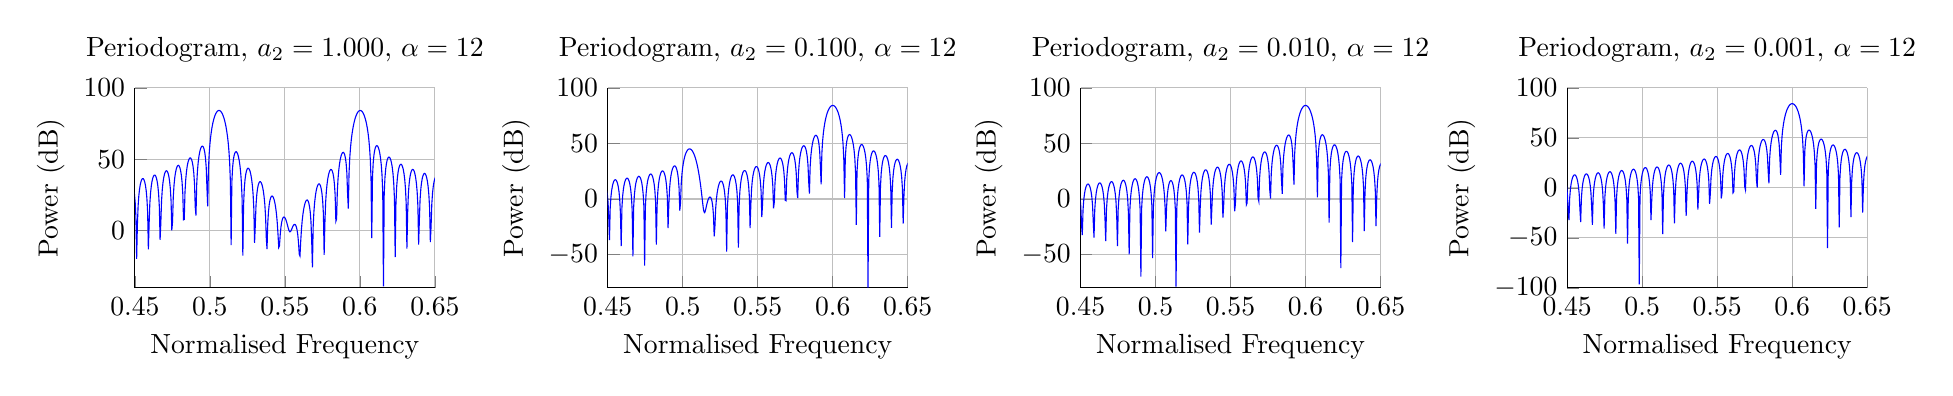
\begin{tikzpicture}

\begin{axis}[%
width=1.5in,
height=1in,
scale only axis,
xmin=0.45,
xmax=0.65,
xlabel={Normalised Frequency},
xmajorgrids,
ymin=-80,
ymax=100,
ylabel={Power (dB)},
ymajorgrids,
name=plot2,
title={Periodogram, $ a_2=0.100 $, $ \alpha= 12$},
axis x line*=bottom,
axis y line*=left
]
\addplot [color=blue,solid,forget plot]
  table[row sep=crcr]{-1	-76.3776073480495\\
-0.99951171875	-21.5058217522883\\
-0.9990234375	-9.81059590682892\\
-0.99853515625	-3.33221083606846\\
-0.998046875	0.86347410233455\\
-0.99755859375	3.68644504665463\\
-0.9970703125	5.52850076539769\\
-0.99658203125	6.58137007229808\\
-0.99609375	6.93694114835031\\
-0.99560546875	6.62369269485004\\
-0.9951171875	5.61652888231201\\
-0.99462890625	3.82814820326856\\
-0.994140625	1.0748570638585\\
-0.99365234375	-3.01743702235995\\
-0.9931640625	-9.30710724588996\\
-0.99267578125	-20.478352109532\\
-0.9921875	-66.4924226453111\\
-0.99169921875	-22.5849498865736\\
-0.9912109375	-10.3166688728328\\
-0.99072265625	-3.64048365369288\\
-0.990234375	0.661734167340188\\
-0.98974609375	3.5557894644763\\
-0.9892578125	5.45221967442121\\
-0.98876953125	6.55113310075714\\
-0.98828125	6.94913309566394\\
-0.98779296875	6.67811633906197\\
-0.9873046875	5.71633913727145\\
-0.98681640625	3.98096606739605\\
-0.986328125	1.29601534423772\\
-0.98583984375	-2.69585728641788\\
-0.9853515625	-8.80521588023105\\
-0.98486328125	-19.4951494902426\\
-0.984375	-56.8198654211737\\
-0.98388671875	-23.7245927320232\\
-0.9833984375	-10.826378686984\\
-0.98291015625	-3.9425501160626\\
-0.982421875	0.469528171768129\\
-0.98193359375	3.43614109657569\\
-0.9814453125	5.38767854056232\\
-0.98095703125	6.53299494972606\\
-0.98046875	6.97354567487314\\
-0.97998046875	6.74468495006728\\
-0.9794921875	5.82799476747864\\
-0.97900390625	4.14499271990909\\
-0.978515625	1.52710488084672\\
-0.97802734375	-2.36715482259067\\
-0.9775390625	-8.30398933298655\\
-0.97705078125	-18.5499696467451\\
-0.9765625	-50.2660475708791\\
-0.97607421875	-24.9355031417623\\
-0.9755859375	-11.3408560286817\\
-0.97509765625	-4.23869611523261\\
-0.974609375	0.286769986883782\\
-0.97412109375	3.32748639644202\\
-0.9736328125	5.33489847774991\\
-0.97314453125	6.52699751758657\\
-0.97265625	7.01023647875117\\
-0.97216796875	6.8234713052076\\
-0.9716796875	5.95158743901807\\
-0.97119140625	4.32034958137187\\
-0.970703125	1.76830589278352\\
-0.97021484375	-2.03099927320817\\
-0.9697265625	-7.80253995522716\\
-0.96923828125	-17.6374777680249\\
-0.96875	-45.4107269867408\\
-0.96826171875	-26.2309302220454\\
-0.9677734375	-11.8613242970712\\
-0.96728515625	-4.52920029352372\\
-0.966796875	0.113396387893881\\
-0.96630859375	3.22983888968563\\
-0.9658203125	5.29392914630724\\
-0.96533203125	6.53321184672788\\
-0.96484375	7.05929245912195\\
-0.96435546875	6.91457749910384\\
-0.9638671875	6.0872377769647\\
-0.96337890625	4.50718602598503\\
-0.962890625	2.01982372161577\\
-0.96240234375	-1.68704495595194\\
-0.9619140625	-7.3000162634994\\
-0.96142578125	-16.7530674351369\\
-0.9609375	-41.5608912881458\\
-0.96044921875	-27.6274714694058\\
-0.9599609375	-12.3891166444616\\
-0.95947265625	-4.8143355251576\\
-0.958984375	-0.0506328053527986\\
-0.95849609375	3.14323965601612\\
-0.9580078125	5.26484934736991\\
-0.95751953125	6.55173877208224\\
-0.95703125	7.12083061232621\\
-0.95654296875	7.01813566375637\\
-0.9560546875	6.23509612988415\\
-0.95556640625	4.70568022629413\\
-0.955078125	2.28188988691835\\
-0.95458984375	-1.33492896777727\\
-0.9541015625	-6.79559510904557\\
-0.95361328125	-15.8927206648508\\
-0.953125	-38.3650594446477\\
-0.95263671875	-29.1463165684274\\
-0.9521484375	-12.9256960492734\\
-0.95166015625	-5.09437040100057\\
-0.951171875	-0.205334386358775\\
-0.95068359375	3.06775804431466\\
-0.9501953125	5.24776785857515\\
-0.94970703125	6.58270981403045\\
-0.94921875	7.19499891061312\\
-0.94873046875	7.13430893533703\\
-0.9482421875	6.39534358078103\\
-0.94775390625	4.91604024135377\\
-0.947265625	2.55476337113176\\
-0.94677734375	-0.974269139865426\\
-0.9462890625	-6.28847450013249\\
-0.94580078125	-15.0528981747009\\
-0.9453125	-35.6245952060709\\
-0.94482421875	-30.8151200616447\\
-0.9443359375	-13.4726791761619\\
-0.94384765625	-5.36957073796942\\
-0.943359375	-0.350701208855853\\
-0.94287109375	3.00349263446839\\
-0.9423828125	5.24282452569558\\
-0.94189453125	6.62628833085729\\
-0.94140625	7.28197749502196\\
-0.94091796875	7.26329268360829\\
-0.9404296875	6.56819322084733\\
-0.93994140625	5.13850536532853\\
-0.939453125	2.83873215242552\\
-0.93896484375	-0.604661815313785\\
-0.9384765625	-5.77786692357799\\
-0.93798828125	-14.2304521823155\\
-0.9375	-33.2171282309162\\
-0.93701171875	-32.67092561048\\
-0.9365234375	-14.0318649807666\\
-0.93603515625	-5.64020113625427\\
-0.935546875	-0.486701408756227\\
-0.93505859375	2.95057246414665\\
-0.9345703125	5.25019162951372\\
-0.93408203125	6.68267095061034\\
-0.93359375	7.38198015003917\\
-0.93310546875	7.40531602465607\\
-0.9326171875	6.7538917071406\\
-0.93212890625	5.37334775829902\\
-0.931640625	3.13411500892696\\
-0.93115234375	-0.225679417751821\\
-0.9306640625	-5.26299303000819\\
-0.93017578125	-13.4225562069188\\
-0.9296875	-31.0621448682383\\
-0.92919921875	-34.7649355953718\\
-0.9287109375	-14.6052692976423\\
-0.92822265625	-5.90652660982501\\
-0.927734375	-0.613277382892137\\
-0.92724609375	2.90915854377183\\
-0.9267578125	5.27007555243945\\
-0.92626953125	6.75208930749113\\
-0.92578125	7.49525608563764\\
-0.92529296875	7.56064364299599\\
-0.9248046875	6.95272113073709\\
-0.92431640625	5.6208743864799\\
-0.923828125	3.44126362304053\\
-0.92333984375	0.163132225315892\\
-0.9228515625	-4.74307556064989\\
-0.92236328125	-12.6266478271252\\
-0.921875	-29.1038915155163\\
-0.92138671875	-37.1707127896852\\
-0.9208984375	-15.1951670305026\\
-0.92041015625	-6.16881431887694\\
-0.919921875	-0.730344501200353\\
-0.91943359375	2.87944568869655\\
-0.9189453125	5.3027187752939\\
-0.91845703125	6.83481211391014\\
-0.91796875	7.6220920583777\\
-0.91748046875	7.72957795524382\\
-0.9169921875	7.16500122808996\\
-0.91650390625	5.88142930527952\\
-0.916015625	3.76056502075116\\
-0.91552734375	0.562256845981936\\
-0.9150390625	-4.21733340241911\\
-0.91455078125	-11.8403813902717\\
-0.9140625	-27.3021514016842\\
-0.91357421875	-39.9992367519439\\
-0.9130859375	-15.8041440847636\\
-0.91259765625	-6.42733543699804\\
-0.912109375	-0.837789523096948\\
-0.91162109375	2.86166470432691\\
-0.9111328125	5.34840224159462\\
-0.91064453125	6.93114760635088\\
-0.91015625	7.76281487034372\\
-0.90966796875	7.91246165470967\\
-0.9091796875	7.39109197556464\\
-0.90869140625	6.15539632592929\\
-0.908203125	4.0924443880816\\
-0.90771484375	0.972211034367836\\
-0.9072265625	-3.68497566306398\\
-0.90673828125	-11.0615884075793\\
-0.90625	-25.626927567462\\
-0.90576171875	-43.4289226220823\\
-0.9052734375	-16.4351619043684\\
-0.90478515625	-6.6823671912532\\
-0.904296875	-0.935468681884156\\
-0.90380859375	2.85608496779769\\
-0.9033203125	5.40744813477024\\
-0.90283203125	7.04144641140587\\
-0.90234375	7.91779429301187\\
-0.90185546875	8.10968068469823\\
-0.9013671875	7.63139661563585\\
-0.90087890625	6.44320211500354\\
-0.900390625	4.43736831547841\\
-0.89990234375	1.39354792820498\\
-0.8994140625	-3.14519565953319\\
-0.89892578125	-10.2882439000694\\
-0.8984375	-24.0552072791277\\
-0.89794921875	-47.7721560785707\\
-0.8974609375	-17.0916384891661\\
-0.89697265625	-6.9341951203363\\
-0.896484375	-1.02320539282537\\
-0.89599609375	2.86301745914493\\
-0.8955078125	5.48022312333817\\
-0.89501953125	7.16610488810542\\
-0.89453125	8.08744647302954\\
-0.89404296875	8.3216676982975\\
-0.8935546875	7.88636517334666\\
-0.89306640625	6.74531978636463\\
-0.892578125	4.79584853114983\\
-0.89208984375	1.82686135954868\\
-0.8916015625	-2.59716471070174\\
-0.89111328125	-9.51843734452559\\
-0.890625	-22.5689027149051\\
-0.89013671875	-53.6436434429969\\
-0.8896484375	-17.7775512151118\\
-0.88916015625	-7.18311560467712\\
-0.888671875	-1.10078753052868\\
-0.88818359375	2.88281830623996\\
-0.8876953125	5.56714214070685\\
-0.88720703125	7.3055690144718\\
-0.88671875	8.27223788886231\\
-0.88623046875	8.54890607457284\\
-0.8857421875	8.15649853391936\\
-0.88525390625	7.0622730575125\\
-0.884765625	5.16844619692856\\
-0.88427734375	2.27279053686207\\
-0.8837890625	-2.04002561959562\\
-0.88330078125	-8.75034714796372\\
-0.8828125	-21.153489719926\\
-0.88232421875	-62.4293077947335\\
-0.8818359375	-18.4975688762166\\
-0.88134765625	-7.42943873412097\\
-0.880859375	-1.16796420956778\\
-0.88037109375	2.91589292108947\\
-0.8798828125	5.6686727800121\\
-0.87939453125	7.4603389002261\\
-0.87890625	8.47268994145923\\
-0.87841796875	8.79193457546664\\
-0.8779296875	8.4423531669683\\
-0.87744140625	7.39464105703109\\
-0.876953125	5.55577685504498\\
-0.87646484375	2.73202535522268\\
-0.8759765625	-1.47288572102767\\
-0.87548828125	-7.98221778303229\\
-0.875	-19.7970782310784\\
-0.87451171875	-75.3302727279329\\
-0.8740234375	-19.2572234591604\\
-0.87353515625	-7.67349159280585\\
-0.873046875	-1.22444198719241\\
-0.87255859375	2.96270082199289\\
-0.8720703125	5.78534040170169\\
-0.87158203125	7.63097402513835\\
-0.87109375	8.68938427989504\\
-0.87060546875	9.0513527457508\\
-0.8701171875	8.74454660105883\\
-0.86962890625	7.74306388837298\\
-0.869140625	5.95851613296708\\
-0.86865234375	3.20531244612195\\
-0.8681640625	-0.894809355947415\\
-0.86767578125	-7.21233886238095\\
-0.8671875	-18.4897591053861\\
-0.86669921875	-68.1861476855518\\
-0.8662109375	-20.0631368181023\\
-0.86572265625	-7.91562206019351\\
-0.865234375	-1.26988038932079\\
-0.86474609375	3.02376125605004\\
-0.8642578125	5.91773407218975\\
-0.86376953125	7.81809932351008\\
-0.86328125	8.92296898427986\\
-0.86279296875	9.32782718002784\\
-0.8623046875	9.06376377430721\\
-0.86181640625	8.10824907746077\\
-0.861328125	6.37740633594554\\
-0.86083984375	3.69346210075701\\
-0.8603515625	-0.304809614873766\\
-0.85986328125	-6.43902553330357\\
-0.859375	-17.2231332604595\\
-0.85888671875	-56.5272452822907\\
-0.8583984375	-20.9233245809611\\
-0.85791015625	-8.15620325112102\\
-0.857421875	-1.30388663832686\\
-0.85693359375	3.09965976183663\\
-0.8564453125	6.0665134778807\\
-0.85595703125	8.02241226168436\\
-0.85546875	9.1741657550202\\
-0.85498046875	9.62209880795221\\
-0.8544921875	9.40076441427835\\
-0.85400390625	8.49097905952932\\
-0.853515625	6.81326408520236\\
-0.85302734375	4.19735622914643\\
-0.8525390625	0.298160832950102\\
-0.85205078125	-5.66059964171119\\
-0.8515625	-15.9899641248003\\
-0.85107421875	-48.9358492616789\\
-0.8505859375	-21.8476109194068\\
-0.85009765625	-8.39563874934921\\
-0.849609375	-1.32600943310855\\
-0.84912109375	3.19105584337387\\
-0.8486328125	6.2324169910182\\
-0.84814453125	8.24469108820687\\
-0.84765625	9.44377829076912\\
-0.84716796875	9.93499138260558\\
-0.8466796875	9.7563916347032\\
-0.84619140625	8.8921198954019\\
-0.845703125	7.26698919495539\\
-0.84521484375	4.71795755293876\\
-0.8447265625	0.915220041484833\\
-0.84423828125	-4.87537115320259\\
-0.84375	-14.7839152532723\\
-0.84326171875	-43.4052013588573\\
-0.8427734375	-22.8482061435609\\
-0.84228515625	-8.63436883057994\\
-0.841796875	-1.33573159668682\\
-0.84130859375	3.29869196572802\\
-0.8408203125	6.41627110407947\\
-0.84033203125	8.48580447725729\\
-0.83984375	9.73270207905862\\
-0.83935546875	10.2674213992604\\
-0.8388671875	10.1315819794832\\
-0.83837890625	9.31263145097773\\
-0.837890625	7.7395750256658\\
-0.83740234375	5.25632027441043\\
-0.8369140625	1.54756848075501\\
-0.83642578125	-4.08161933206784\\
-0.8359375	-13.5993477490544\\
-0.83544921875	-39.0294895950398\\
-0.8349609375	-23.9405297606302\\
-0.83447265625	-8.87287792510429\\
-0.833984375	-1.33246136148023\\
-0.83349609375	3.4234041324542\\
-0.8330078125	6.61900150059067\\
-0.83251953125	8.74672283803972\\
-0.83203125	10.0419358765299\\
-0.83154296875	10.6204097255352\\
-0.8310546875	10.5273771990668\\
-0.83056640625	9.75357932918595\\
-0.830078125	8.23212060723188\\
-0.82958984375	5.8136025212118\\
-0.8291015625	2.1965024366305\\
-0.82861328125	-3.27757316645114\\
-0.828125	-12.4311601782466\\
-0.82763671875	-35.3784701356435\\
-0.8271484375	-25.1444148770528\\
-0.82666015625	-9.11170364340098\\
-0.826171875	-1.31552200542277\\
-0.82568359375	3.56613436806659\\
-0.8251953125	6.84164609489383\\
-0.82470703125	9.02853162870045\\
-0.82421875	10.372595222692\\
-0.82373046875	10.9950952920641\\
-0.8232421875	10.9449381135059\\
-0.82275390625	10.2161489139849\\
-0.822265625	8.74584489726176\\
-0.82177734375	6.39108093877466\\
-0.8212890625	2.86342950536436\\
-0.82080078125	-2.4613904902532\\
-0.8203125	-11.2746588372155\\
-0.81982421875	-32.2183291119281\\
-0.8193359375	-26.4859261473817\\
-0.81884765625	-9.35144778481105\\
-0.818359375	-1.28413947773211\\
-0.81787109375	3.72794551026391\\
-0.8173828125	7.08537045698185\\
-0.81689453125	9.33244709846531\\
-0.81640625	10.7259284177171\\
-0.81591796875	11.3927512808377\\
-0.8154296875	11.385561006001\\
-0.81494140625	10.7016619769777\\
-0.814453125	9.28210363205162\\
-0.81396484375	6.99016789621587\\
-0.8134765625	3.54988666492187\\
-0.81298828125	-1.63113518448754\\
-0.8125	-10.1254496100384\\
-0.81201171875	-29.408409304797\\
-0.8115234375	-28.0002064696974\\
-0.81103515625	-9.59278988222706\\
-0.810546875	-1.23742755747581\\
-0.81005859375	3.91003882144439\\
-0.8095703125	7.35148614606151\\
-0.80908203125	9.65983499133346\\
-0.80859375	11.1033355064073\\
-0.80810546875	11.8148043619519\\
-0.8076171875	11.8506971062921\\
-0.80712890625	11.2115964147442\\
-0.806640625	9.84240934741623\\
-0.80615234375	7.61243189299724\\
-0.8056640625	4.25756152744832\\
-0.80517578125	-0.784751738888889\\
-0.8046875	-8.97934487557712\\
-0.80419921875	-26.8574166894605\\
-0.8037109375	-29.7361359958041\\
-0.80322265625	-9.83650401668364\\
-0.802734375	-1.17436996203371\\
-0.80224609375	4.11377506636669\\
-0.8017578125	7.64147261730017\\
-0.80126953125	10.0122328881971\\
-0.80078125	11.5063909566247\\
-0.80029296875	12.2628576782804\\
-0.7998046875	12.3419758746657\\
-0.79931640625	11.7476098390797\\
-0.798828125	10.4284553033228\\
-0.79833984375	8.25962191308443\\
-0.7978515625	4.98831753856914\\
-0.79736328125	0.0799636916094687\\
-0.796875	-7.83228037275416\\
-0.79638671875	-24.5024855991172\\
-0.7958984375	-31.7643822304566\\
-0.79541015625	-10.0834798873052\\
-0.794921875	-1.09379865620017\\
-0.79443359375	4.3406998834787\\
-0.7939453125	7.95700355149179\\
-0.79345703125	10.3913770532654\\
-0.79296875	11.9368709130625\\
-0.79248046875	12.7387184737399\\
-0.7919921875	12.8612329971212\\
-0.79150390625	12.3115679457687\\
-0.791015625	11.0421442534283\\
-0.79052734375	8.93369668419999\\
-0.7900390625	5.74422410309753\\
-0.78955078125	0.965396804120541\\
-0.7890625	-6.68023784189245\\
-0.78857421875	-22.2981837840519\\
-0.7880859375	-34.1922911607459\\
-0.78759765625	-10.334749475172\\
-0.787109375	-0.994367390395668\\
-0.78662109375	4.59257451789582\\
-0.7861328125	8.29997870397148\\
-0.78564453125	10.7992349023275\\
-0.78515625	12.3967861638033\\
-0.78466796875	13.2444315223056\\
-0.7841796875	13.4105442686908\\
-0.78369140625	12.9055788590239\\
-0.783203125	11.6856232772603\\
-0.78271484375	9.63686008157532\\
-0.7822265625	6.52759290317288\\
-0.78173828125	1.87415458739113\\
-0.78125	-5.51916976619827\\
-0.78076171875	-20.2102893254072\\
-0.7802734375	-37.1939806910095\\
-0.77978515625	-10.5915211422976\\
-0.779296875	-0.874519196428841\\
-0.77880859375	4.87141330738949\\
-0.7783203125	8.67256270076543\\
-0.77783203125	11.2380445490434\\
-0.77734375	12.8884223025776\\
-0.77685546875	13.782319867246\\
-0.7763671875	13.9922669011688\\
-0.77587890625	13.5320350150453\\
-0.775390625	12.3613262663048\\
-0.77490234375	10.3716042964211\\
-0.7744140625	7.34102206257732\\
-0.77392578125	2.80911241806016\\
-0.7734375	-4.34492271324712\\
-0.77294921875	-18.2120446704424\\
-0.7724609375	-41.0788779269686\\
-0.77197265625	-10.8552237332117\\
-0.771484375	-0.732446159839253\\
-0.77099609375	5.1795297525182\\
-0.7705078125	9.07723266108488\\
-0.77001953125	11.7103633463676\\
-0.76953125	13.4143890401617\\
-0.76904296875	14.3550348602419\\
-0.7685546875	14.6090902815162\\
-0.76806640625	14.19366464817\\
-0.767578125	13.0720261654814\\
-0.76708984375	11.1407629099307\\
-0.7666015625	8.18745034172233\\
-0.76611328125	3.77347108162782\\
-0.765625	-3.15315564610365\\
-0.76513671875	-16.2817784896026\\
-0.7646484375	-46.4768552596693\\
-0.76416015625	-11.1275643128467\\
-0.763671875	-0.566039222133392\\
-0.76318359375	5.51959360761489\\
-0.7626953125	9.51683714664053\\
-0.76220703125	12.2191279754779\\
-0.76171875	13.9776812673302\\
-0.76123046875	14.9656181528813\\
-0.7607421875	15.2640988841157\\
-0.76025390625	14.8935956343607\\
-0.759765625	13.8208997774482\\
-0.75927734375	11.9475767345731\\
-0.7587890625	9.07022428368254\\
-0.75830078125	4.77082673128155\\
-0.7578125	-1.93924911795419\\
-0.75732421875	-14.4013197833142\\
-0.7568359375	-54.986424866398\\
-0.75634765625	-11.4106047676308\\
-0.755859375	-0.372824974352368\\
-0.75537109375	5.89470227433432\\
-0.7548828125	9.99466980558419\\
-0.75439453125	12.7677295219727\\
-0.75390625	14.5817553790712\\
-0.75341796875	15.6175792204448\\
-0.7529296875	15.9608509879942\\
-0.75244140625	15.6354354156848\\
-0.751953125	14.6116089275297\\
-0.75146484375	12.7957762967176\\
-0.7509765625	9.99318226608699\\
-0.75048828125	5.8052578498643\\
-0.75	-0.698200415848608\\
-0.74951171875	-12.5548866026247\\
-0.7490234375	-71.9379026777665\\
-0.74853515625	-11.7068649237696\\
-0.748046875	-0.149885278900848\\
-0.74755859375	6.30847097574374\\
-0.7470703125	10.5145623073584\\
-0.74658203125	13.3601082370046\\
-0.74609375	15.2306256570202\\
-0.74560546875	16.3149933149352\\
-0.7451171875	16.7034781975665\\
-0.74462890625	16.4233721079791\\
-0.744140625	15.4484031974711\\
-0.74365234375	13.6896862776926\\
-0.7431640625	10.9607608899655\\
-0.74267578125	6.88143478654191\\
-0.7421875	0.575501651339111\\
-0.74169921875	-10.7282635539244\\
-0.7412109375	-64.7403525994168\\
-0.74072265625	-12.0194636139297\\
-0.740234375	0.106246065382927\\
-0.73974609375	6.76514790953643\\
-0.7392578125	11.0810029326498\\
-0.73876953125	14.0008744929369\\
-0.73828125	15.9289873630883\\
-0.73779296875	17.0626266451895\\
-0.7373046875	17.4968127122144\\
-0.73681640625	17.2623038876659\\
-0.736328125	16.3362514782313\\
-0.73583984375	14.6343593219067\\
-0.7353515625	11.9781312788063\\
-0.73486328125	8.00475963052917\\
-0.734375	1.88803074030717\\
-0.73388671875	-8.90815225595385\\
-0.7333984375	-49.5444846025679\\
-0.73291015625	-12.3523151431828\\
-0.732421875	0.399717779769555\\
-0.73193359375	7.26976309694668\\
-0.7314453125	11.6992897717054\\
-0.73095703125	14.6954650993119\\
-0.73046875	16.682375921078\\
-0.72998046875	17.8660983746969\\
-0.7294921875	18.3465521534598\\
-0.72900390625	18.1580066896592\\
-0.728515625	17.2810126025201\\
-0.72802734375	15.6357497077626\\
-0.7275390625	13.05137602682\\
-0.72705078125	9.18154742810221\\
-0.7265625	3.24641738367695\\
-0.72607421875	-7.08161645085383\\
-0.7255859375	-40.6285924718266\\
-0.72509765625	-12.7104084561343\\
-0.724609375	0.735538406957033\\
-0.72412109375	7.82832339999303\\
-0.7236328125	12.3757313495883\\
-0.72314453125	15.4503481150121\\
-0.72265625	17.497375639166\\
-0.72216796875	18.7320932122477\\
-0.7216796875	19.2594760542714\\
-0.72119140625	19.117354658499\\
-0.720703125	18.2896598457492\\
-0.72021484375	16.7009420263322\\
-0.7197265625	14.1877223094462\\
-0.71923828125	10.4192646495068\\
-0.71875	4.65880042748788\\
-0.71826171875	-5.2355623901876\\
-0.7177734375	-34.1586696821388\\
-0.71728515625	-13.100212916731\\
-0.716796875	1.11981361297613\\
-0.71630859375	8.44807190239941\\
-0.7158203125	13.1179133921136\\
-0.71533203125	16.2732953552515\\
-0.71484375	18.3818976592159\\
-0.71435546875	19.6686447782859\\
-0.7138671875	20.2437347024699\\
-0.71337890625	20.1486145673706\\
-0.712890625	19.3705810474162\\
-0.71240234375	17.8384571729729\\
-0.7119140625	15.3958540324094\\
-0.71142578125	11.7268483834121\\
-0.7109375	6.13475982832267\\
-0.71044921875	-3.3562017555602\\
-0.7099609375	-28.9295382186003\\
-0.70947265625	-13.5302835821386\\
-0.708984375	1.56006913506903\\
-0.70849609375	9.13783877690105\\
-0.7080078125	13.9350596535878\\
-0.70751953125	17.1737512750258\\
-0.70703125	19.3455565831954\\
-0.70654296875	20.6855199834527\\
-0.7060546875	21.3092413820788\\
-0.70556640625	21.2618460794362\\
-0.705078125	20.5339870827641\\
-0.70458984375	19.0586692636083\\
-0.7041015625	16.6863375419928\\
-0.70361328125	13.1151417329054\\
-0.703125	7.68576745640896\\
-0.70263671875	-1.42844081054203\\
-0.7021484375	-24.4208896537689\\
-0.70166015625	-14.0121913809788\\
-0.701171875	2.06569863832222\\
-0.70068359375	9.90852506174373\\
-0.7001953125	14.838529497135\\
-0.69970703125	18.163342147778\\
-0.69921875	20.4001909433243\\
-0.69873046875	21.7947508664094\\
-0.6982421875	22.4682157778988\\
-0.69775390625	22.4694569758394\\
-0.697265625	21.7924792116258\\
-0.69677734375	20.3743854511598\\
-0.6962890625	18.0722143700948\\
-0.69580078125	14.5975004452879\\
-0.6953125	9.32581270422394\\
-0.69482421875	0.564875468379442\\
-0.6943359375	-20.3563807487759\\
-0.69384765625	-14.5620032373157\\
-0.693359375	2.64859824017316\\
-0.69287109375	10.7737843713396\\
-0.6923828125	15.8425193366523\\
-0.69189453125	19.2565946974047\\
-0.69140625	21.5605987673564\\
-0.69091796875	23.0113872974153\\
-0.6904296875	23.7359541743459\\
-0.68994140625	23.786991280611\\
-0.689453125	23.1618556128608\\
-0.68896484375	21.801671412051\\
-0.6884765625	19.5698463341084\\
-0.68798828125	16.1906587465545\\
-0.6875	11.072293746597\\
-0.68701171875	2.64396691415006\\
-0.6865234375	-16.565764357137\\
-0.68603515625	-15.2027364136835\\
-0.685546875	3.32408789717423\\
-0.68505859375	11.7510078730788\\
-0.6845703125	16.9650768338597\\
-0.68408203125	20.4719766270657\\
-0.68359375	22.845604327832\\
-0.68310546875	24.3545904026373\\
-0.6826171875	25.1319502027027\\
-0.68212890625	25.2342780777196\\
-0.681640625	24.6622890906026\\
-0.68115234375	23.3610588378378\\
-0.6806640625	21.2001538424192\\
-0.68017578125	17.9159999293939\\
-0.6796875	12.9473249885771\\
-0.67919921875	4.8335313138821\\
-0.6787109375	-12.9299273003382\\
-0.67822265625	-15.9686357356691\\
-0.677734375	4.11228810711219\\
-0.67724609375	12.8627894558907\\
-0.6767578125	18.2296111395349\\
-0.67626953125	21.8334487562834\\
-0.67578125	24.2796524160222\\
-0.67529296875	25.849269924652\\
-0.6748046875	26.6815764935742\\
-0.67431640625	26.8371588017099\\
-0.673828125	26.3201014574094\\
-0.67333984375	25.0793684756622\\
-0.6728515625	22.9904893201823\\
-0.67236328125	19.8014823364695\\
-0.671875	14.97972052642\\
-0.67138671875	7.16484108136989\\
-0.6708984375	-9.3543436599004\\
-0.67041015625	-16.913098814077\\
-0.669921875	5.04024719398689\\
-0.66943359375	14.1391811388476\\
-0.6689453125	19.6672212002726\\
-0.66845703125	23.3728630093524\\
-0.66796875	25.8952770662855\\
-0.66748046875	27.5286256521543\\
-0.6669921875	28.4187011393961\\
-0.66650390625	28.6301812776698\\
-0.666015625	28.1705378737792\\
-0.66552734375	26.992567668384\\
-0.6650390625	24.97758108274\\
-0.66455078125	21.8846731927193\\
-0.6640625	17.2081240623509\\
-0.66357421875	9.67901601586833\\
-0.6630859375	-5.7533011003477\\
-0.66259765625	-18.1245490476015\\
-0.662109375	6.14536293500703\\
-0.66162109375	15.6213100625488\\
-0.6611328125	21.3204374144544\\
-0.66064453125	25.1338262346507\\
-0.66015625	27.7370904832227\\
-0.65966796875	29.4382656373339\\
-0.6591796875	30.3899399298138\\
-0.65869140625	30.6609910752524\\
-0.658203125	30.2623027484951\\
-0.65771484375	29.1504565604551\\
-0.6572265625	27.2123759960765\\
-0.65673828125	24.2177545118881\\
-0.65625	19.6861872580989\\
-0.65576171875	12.4324162638411\\
-0.6552734375	-2.03748148202951\\
-0.65478515625	-19.7616682061518\\
-0.654296875	7.48116139080696\\
-0.65380859375	17.3674757544615\\
-0.6533203125	23.2495468277539\\
-0.65283203125	27.1782537019321\\
-0.65234375	29.868572365945\\
-0.65185546875	31.6432406792692\\
-0.6513671875	32.6619462663719\\
-0.65087890625	32.9978878607812\\
-0.650390625	32.6653942247611\\
-0.64990234375	31.6247931255769\\
-0.6494140625	29.7684682448371\\
-0.64892578125	26.8762698616453\\
-0.6484375	22.4916514076664\\
-0.64794921875	15.5061031898721\\
-0.6474609375	1.89988846073837\\
-0.64697265625	-22.1436905520388\\
-0.646484375	9.12766884865762\\
-0.64599609375	19.4640883308296\\
-0.6455078125	25.5439837200007\\
-0.64501953125	29.5982216645321\\
-0.64453125	32.3844039191289\\
-0.64404296875	34.2408822593136\\
-0.6435546875	35.3347774235456\\
-0.64306640625	35.7437460932892\\
-0.642578125	35.4856071267951\\
-0.64208984375	34.5244079702813\\
-0.6416015625	32.7578575490722\\
-0.64111328125	29.9755598469263\\
-0.640625	25.7434978741425\\
-0.64013671875	19.0237665884055\\
-0.6396484375	6.20424684390983\\
-0.63916015625	-26.0388781604821\\
-0.638671875	11.2115398845416\\
-0.63818359375	22.0469258987963\\
-0.6376953125	28.344583456213\\
-0.63720703125	32.5392568438519\\
-0.63671875	35.4348472447543\\
-0.63623046875	37.3863322897749\\
-0.6357421875	38.5686400437829\\
-0.63525390625	39.0640465104877\\
-0.634765625	38.8939257594162\\
-0.63427734375	38.026039207765\\
-0.6337890625	36.3633127858242\\
-0.63330078125	33.7047477638329\\
-0.6328125	29.6376574825435\\
-0.63232421875	23.1892851729214\\
-0.6318359375	11.1008110793389\\
-0.63134765625	-34.0462379217711\\
-0.630859375	13.9494215162691\\
-0.63037109375	25.3471247183271\\
-0.6298828125	31.8920934140896\\
-0.62939453125	36.2515128411835\\
-0.62890625	39.279760610148\\
-0.62841796875	41.3495880748735\\
-0.6279296875	42.6441723559851\\
-0.62744140625	43.2506208271196\\
-0.626953125	43.1939754399243\\
-0.62646484375	42.4457561088814\\
-0.6259765625	40.9140560866082\\
-0.62548828125	38.4069980568022\\
-0.625	34.5321866458493\\
-0.62451171875	28.3772099533288\\
-0.6240234375	16.991834474072\\
-0.62353515625	-79.8620578322795\\
-0.623046875	17.7563171923715\\
-0.62255859375	29.8071015218112\\
-0.6220703125	36.650861213472\\
-0.62158203125	41.2218331026983\\
-0.62109375	44.4297300856543\\
-0.62060546875	46.6664719977142\\
-0.6201171875	48.1241023639014\\
-0.61962890625	48.8949388988282\\
-0.619140625	49.0079800060346\\
-0.61865234375	48.4387419150913\\
-0.6181640625	47.1006542420998\\
-0.61767578125	44.8109451206558\\
-0.6171875	41.1968286843062\\
-0.61669921875	35.4022542057906\\
-0.6162109375	24.7487498766526\\
-0.61572265625	-23.2842617102148\\
-0.615234375	23.5869546163325\\
-0.61474609375	36.4520244595478\\
-0.6142578125	43.713064773145\\
-0.61376953125	48.6143402561724\\
-0.61328125	52.1271500264356\\
-0.61279296875	54.6649259054048\\
-0.6123046875	56.4301660739824\\
-0.61181640625	57.5218679873536\\
-0.611328125	57.9745332945704\\
-0.61083984375	57.769382200204\\
-0.6103515625	56.8270829243522\\
-0.60986328125	54.9760202248291\\
-0.609375	51.8648602747406\\
-0.60888671875	46.6933256264729\\
-0.6083984375	37.027500063042\\
-0.60791015625	0.84257092609973\\
-0.607421875	34.6020787949472\\
-0.60693359375	48.7793036170714\\
-0.6064453125	56.9503719024726\\
-0.60595703125	62.733498832182\\
-0.60546875	67.1824076617305\\
-0.60498046875	70.7526780976557\\
-0.6044921875	73.6833308635348\\
-0.60400390625	76.1153282297794\\
-0.603515625	78.138490517591\\
-0.60302734375	79.8131612637871\\
-0.6025390625	81.1813416849812\\
-0.60205078125	82.272875927503\\
-0.6015625	83.1090870609347\\
-0.60107421875	83.7049971958272\\
-0.6005859375	84.0707058323392\\
-0.60009765625	84.2122314039864\\
-0.599609375	84.1319805488848\\
-0.59912109375	83.8289290956036\\
-0.5986328125	83.2985455861119\\
-0.59814453125	82.5324444187026\\
-0.59765625	81.517708047514\\
-0.59716796875	80.2357509007822\\
-0.5966796875	78.6604867816309\\
-0.59619140625	76.7553562535083\\
-0.595703125	74.4683575148759\\
-0.59521484375	71.723322023817\\
-0.5947265625	68.4035082599664\\
-0.59423828125	64.3177138058727\\
-0.59375	59.1204044408006\\
-0.59326171875	52.0819932891774\\
-0.5927734375	41.1541772135046\\
-0.59228515625	13.2472492140967\\
-0.591796875	29.4432617353824\\
-0.59130859375	43.1308143992406\\
-0.5908203125	49.587875218992\\
-0.59033203125	53.3574807179512\\
-0.58984375	55.6285571805386\\
-0.58935546875	56.8799881698973\\
-0.5888671875	57.3396368656208\\
-0.58837890625	57.1181166519975\\
-0.587890625	56.2566271440675\\
-0.58740234375	54.7424329695397\\
-0.5869140625	52.5053153120612\\
-0.58642578125	49.3921769884893\\
-0.5859375	45.0962276964647\\
-0.58544921875	38.948192130599\\
-0.5849609375	29.0868360061529\\
-0.58447265625	4.89485238079104\\
-0.583984375	15.7877328857175\\
-0.58349609375	31.0210590385615\\
-0.5830078125	38.205574763713\\
-0.58251953125	42.5221426061882\\
-0.58203125	45.2576298724091\\
-0.58154296875	46.9226449029293\\
-0.5810546875	47.7598049662074\\
-0.58056640625	47.8885039170783\\
-0.580078125	47.3563505019618\\
-0.57958984375	46.1563322324103\\
-0.5791015625	44.2246159083172\\
-0.57861328125	41.4172220443347\\
-0.578125	37.4442672663885\\
-0.57763671875	31.678484803279\\
-0.5771484375	22.4180336622248\\
-0.57666015625	0.889734952028402\\
-0.576171875	6.5384961077462\\
-0.57568359375	23.2167488655507\\
-0.5751953125	30.8753620680864\\
-0.57470703125	35.493846899743\\
-0.57421875	38.4672440716527\\
-0.57373046875	40.3380620261457\\
-0.5732421875	41.3622413902536\\
-0.57275390625	41.6662931037285\\
-0.572265625	41.3026523572041\\
-0.57177734375	40.2685990085812\\
-0.5712890625	38.5054031002676\\
-0.57080078125	35.8770112556269\\
-0.5703125	32.1091361245352\\
-0.56982421875	26.6140287744834\\
-0.5693359375	17.8363252885892\\
-0.56884765625	-1.55447689294192\\
-0.568359375	-1.1830403748002\\
-0.56787109375	17.1655840360751\\
-0.5673828125	25.2576296617836\\
-0.56689453125	30.1172568375645\\
-0.56640625	33.2654914362458\\
-0.56591796875	35.2804480497246\\
-0.5654296875	36.4324532385687\\
-0.56494140625	36.8554508920359\\
-0.564453125	36.6067616643276\\
-0.56396484375	35.6879234778215\\
-0.5634765625	34.0452440407107\\
-0.56298828125	31.5505078006388\\
-0.5625	27.9448086476934\\
-0.56201171875	22.6788303676325\\
-0.5615234375	14.3345980089968\\
-0.56103515625	-3.24591372283679\\
-0.560546875	-8.50044106481431\\
-0.56005859375	11.9715403581277\\
-0.5595703125	20.5158781892148\\
-0.55908203125	25.6022056024436\\
-0.55859375	28.9030374309579\\
-0.55810546875	31.0375957842831\\
-0.5576171875	32.2924129344611\\
-0.55712890625	32.8096333032484\\
-0.556640625	32.6518576637526\\
-0.55615234375	31.8251393728547\\
-0.5556640625	30.2810512759292\\
-0.55517578125	27.8994782114925\\
-0.5546875	24.4372118086968\\
-0.55419921875	19.3833939308684\\
-0.5537109375	11.4523179171798\\
-0.55322265625	-4.52336280205378\\
-0.552734375	-16.3109699329701\\
-0.55224609375	7.14170082060992\\
-0.5517578125	16.1989034393706\\
-0.55126953125	21.5200062958358\\
-0.55078125	24.9682996500583\\
-0.55029296875	27.212469210989\\
-0.5498046875	28.5580724757068\\
-0.54931640625	29.1567057550481\\
-0.548828125	29.0769540962696\\
-0.54833984375	28.3299069398996\\
-0.5478515625	26.872926799318\\
-0.54736328125	24.5946919985725\\
-0.546875	21.2687840965895\\
-0.54638671875	16.4245851334308\\
-0.5458984375	8.90924916320883\\
-0.54541015625	-5.56570913345017\\
-0.544921875	-26.1357383448164\\
-0.54443359375	2.24358187304053\\
-0.5439453125	11.935728889316\\
-0.54345703125	17.5215182301302\\
-0.54296875	21.1239788702581\\
-0.54248046875	23.4755296527948\\
-0.5419921875	24.9055710067531\\
-0.54150390625	25.577329160465\\
-0.541015625	25.5666518413185\\
-0.54052734375	24.8906769445026\\
-0.5400390625	23.5136612507289\\
-0.53955078125	21.3346521029412\\
-0.5390625	18.1467415502884\\
-0.53857421875	13.5249586754745\\
-0.5380859375	6.46050439495668\\
-0.53759765625	-6.49562007296804\\
-0.537109375	-43.7501238440082\\
-0.53662109375	-3.39183121319465\\
-0.5361328125	7.20334177022819\\
-0.53564453125	13.1238021230459\\
-0.53515625	16.9019773655546\\
-0.53466796875	19.3635653142472\\
-0.5341796875	20.8716658289821\\
-0.53369140625	21.6056163105511\\
-0.533203125	21.6512354529418\\
-0.53271484375	21.0339790199085\\
-0.5322265625	19.7276428073641\\
-0.53173828125	17.645625313955\\
-0.53125	14.607713604109\\
-0.53076171875	10.2497015461126\\
-0.5302734375	3.74415897774051\\
-0.52978515625	-7.44442686111007\\
-0.529296875	-47.2503164318258\\
-0.52880859375	-11.6248901009317\\
-0.5283203125	0.687611330714235\\
-0.52783203125	7.1367887515134\\
-0.52734375	11.1438865402361\\
-0.52685546875	13.7137173854699\\
-0.5263671875	15.2706509616655\\
-0.52587890625	16.0224975769898\\
-0.525390625	16.0726725252192\\
-0.52490234375	15.461777789329\\
-0.5244140625	14.1818014182565\\
-0.52392578125	12.1743675334082\\
-0.5234375	9.31181511956099\\
-0.52294921875	5.34550654569193\\
-0.5224609375	-0.235727664894114\\
-0.52197265625	-8.68674116129142\\
-0.521484375	-24.5867146308931\\
-0.52099609375	-33.7157532629521\\
-0.5205078125	-14.5467916767011\\
-0.52001953125	-6.53340967792386\\
-0.51953125	-2.1437087728163\\
-0.51904296875	0.338997365581505\\
-0.5185546875	1.55153955398766\\
-0.51806640625	1.79031968884416\\
-0.517578125	1.21157477582002\\
-0.51708984375	-0.0920333470707037\\
-0.5166015625	-2.04964220215059\\
-0.51611328125	-4.57344320828517\\
-0.515625	-7.49351123062331\\
-0.51513671875	-10.3997698587795\\
-0.5146484375	-12.2973677509646\\
-0.51416015625	-11.5684693346016\\
-0.513671875	-7.69059312318256\\
-0.51318359375	-2.11877213658224\\
-0.5126953125	3.7437827666513\\
-0.51220703125	9.29951425582121\\
-0.51171875	14.3739033175991\\
-0.51123046875	18.9427568564955\\
-0.5107421875	23.0298420774808\\
-0.51025390625	26.6717944750323\\
-0.509765625	29.9059018157707\\
-0.50927734375	32.7659306323371\\
-0.5087890625	35.2809355255781\\
-0.50830078125	37.4751886583971\\
-0.5078125	39.3684958753585\\
-0.50732421875	40.9765986943549\\
-0.5068359375	42.3115370911931\\
-0.50634765625	43.381920356254\\
-0.505859375	44.1930809522165\\
-0.50537109375	44.7470927350953\\
-0.5048828125	45.0426291968463\\
-0.50439453125	45.0746216683815\\
-0.50390625	44.8336490753984\\
-0.50341796875	44.304941772037\\
-0.5029296875	43.4667945117639\\
-0.50244140625	42.2880197515995\\
-0.501953125	40.7237464776814\\
-0.50146484375	38.7081733343409\\
-0.5009765625	36.1412625746474\\
-0.50048828125	32.8621441498228\\
-0.5	28.5893180642583\\
-0.49951171875	22.7608665309642\\
-0.4990234375	13.9674404173309\\
-0.49853515625	-3.76228501168548\\
-0.498046875	-10.3588682801002\\
-0.49755859375	10.109836078919\\
-0.4970703125	18.424327367359\\
-0.49658203125	23.2812037568127\\
-0.49609375	26.3743534768176\\
-0.49560546875	28.3266570384902\\
-0.4951171875	29.4248283236084\\
-0.49462890625	29.8105654103443\\
-0.494140625	29.5463511247683\\
-0.49365234375	28.6390820906439\\
-0.4931640625	27.0430179087041\\
-0.49267578125	24.6444204250926\\
-0.4921875	21.214928590266\\
-0.49169921875	16.2823813637669\\
-0.4912109375	8.69319504016741\\
-0.49072265625	-5.83115724282366\\
-0.490234375	-26.1328756986559\\
-0.48974609375	1.90056885105965\\
-0.4892578125	11.5522823955111\\
-0.48876953125	17.1153950112681\\
-0.48828125	20.7058597065793\\
-0.48779296875	23.0543760609338\\
-0.4873046875	24.4894761861222\\
-0.48681640625	25.1737558424283\\
-0.486328125	25.1825068930672\\
-0.48583984375	24.5323033797435\\
-0.4853515625	23.1867420419386\\
-0.48486328125	21.0439556152277\\
-0.484375	17.8954919730223\\
-0.48388671875	13.3130947380703\\
-0.4833984375	6.27848541223134\\
-0.48291015625	-6.70427250163612\\
-0.482421875	-41.1091588255968\\
-0.48193359375	-3.09415007083318\\
-0.4814453125	7.49803716763829\\
-0.48095703125	13.476286122313\\
-0.48046875	17.3311881315513\\
-0.47998046875	19.8794057315616\\
-0.4794921875	21.4805137241965\\
-0.47900390625	22.3116816525905\\
-0.478515625	22.456696677724\\
-0.47802734375	21.9384141753834\\
-0.4775390625	20.7266051852004\\
-0.47705078125	18.7275880883911\\
-0.4765625	15.7470918608668\\
-0.47607421875	11.3883009836504\\
-0.4755859375	4.72713642229672\\
-0.47509765625	-7.23944373820562\\
-0.474609375	-59.9329657862665\\
-0.47412109375	-6.94880072504865\\
-0.4736328125	4.48345086776842\\
-0.47314453125	10.7925363394539\\
-0.47265625	14.8441425293588\\
-0.47216796875	17.5344639936568\\
-0.4716796875	19.2506852810011\\
-0.47119140625	20.1825747698825\\
-0.470703125	20.421093483188\\
-0.47021484375	19.9943096195957\\
-0.4697265625	18.877073947827\\
-0.46923828125	16.9824188884204\\
-0.46875	14.1276443719462\\
-0.46826171875	9.94123905956972\\
-0.4677734375	3.57272556150853\\
-0.46728515625	-7.62390231707313\\
-0.466796875	-51.7048257445786\\
-0.46630859375	-10.2763793205585\\
-0.4658203125	1.98463664628146\\
-0.46533203125	8.59284177869501\\
-0.46484375	12.8137548371811\\
-0.46435546875	15.6223803818618\\
-0.4638671875	17.4323809976014\\
-0.46337890625	18.4453475732701\\
-0.462890625	18.758850160094\\
-0.46240234375	18.4056758120066\\
-0.4619140625	17.3652006008557\\
-0.46142578125	15.5563581990774\\
-0.4609375	12.8064894918918\\
-0.46044921875	8.76568577270765\\
-0.4599609375	2.64462969176382\\
-0.45947265625	-7.92381721508175\\
-0.458984375	-42.3056328010629\\
-0.45849609375	-13.3368879980023\\
-0.4580078125	-0.21435426484729\\
-0.45751953125	6.6817840149347\\
-0.45703125	11.0594947138799\\
-0.45654296875	13.9748734232969\\
-0.4560546875	15.8680060917892\\
-0.45556640625	16.952051903454\\
-0.455078125	17.3309388631178\\
-0.45458984375	17.0419129210253\\
-0.4541015625	16.0685465234337\\
-0.45361328125	14.3351531031076\\
-0.453125	11.678090410458\\
-0.45263671875	7.7665312007911\\
-0.4521484375	1.86385992332589\\
-0.45166015625	-8.16920575215843\\
-0.451171875	-36.9774930581789\\
-0.45068359375	-16.2688099617642\\
-0.4501953125	-2.2213718625826\\
-0.44970703125	4.96175301709205\\
-0.44921875	9.49065387001567\\
-0.44873046875	12.5067721285063\\
-0.4482421875	14.4771820636897\\
-0.44775390625	15.6266379719618\\
-0.447265625	16.0653371005278\\
-0.44677734375	15.8348435385702\\
-0.4462890625	14.9227133643319\\
-0.44580078125	13.2582728973989\\
-0.4453125	10.6861491024898\\
-0.44482421875	6.8927316606712\\
-0.4443359375	1.18787660673299\\
-0.44384765625	-8.37601907659303\\
-0.443359375	-33.4665296622451\\
-0.44287109375	-19.1612409725391\\
-0.4423828125	-4.09781641927016\\
-0.44189453125	3.37747463121351\\
-0.44140625	8.05569500206766\\
-0.44091796875	11.1694385735821\\
-0.4404296875	13.2137497005199\\
-0.43994140625	14.4251793920511\\
-0.439453125	14.9202020358813\\
-0.43896484375	14.7446285853852\\
-0.4384765625	13.8898538822084\\
-0.43798828125	12.2899421408943\\
-0.4375	9.7972092484416\\
-0.43701171875	6.11380018965856\\
-0.4365234375	0.591188390878481\\
-0.43603515625	-8.55371971868088\\
-0.435546875	-30.9254754534844\\
-0.43505859375	-22.082816215284\\
-0.4345703125	-5.88228191348669\\
-0.43408203125	1.8946298878685\\
-0.43359375	6.72258235449829\\
-0.43310546875	9.93253009054378\\
-0.4326171875	12.0487888441871\\
-0.43212890625	13.3200301441796\\
-0.431640625	13.8690773666569\\
-0.43115234375	13.7459617122535\\
-0.4306640625	12.9458152575439\\
-0.43017578125	11.4072243495438\\
-0.4296875	8.98972290406247\\
-0.42919921875	5.41001615574977\\
-0.4287109375	0.0572576551100461\\
-0.42822265625	-8.70839253024672\\
-0.427734375	-28.9735582801582\\
-0.42724609375	-25.0964235328335\\
-0.4267578125	-7.60106063573781\\
-0.42626953125	0.490336518969712\\
-0.42578125	5.46997994107879\\
-0.42529296875	8.77579016521643\\
-0.4248046875	10.9629284676415\\
-0.42431640625	12.2926051550237\\
-0.423828125	12.8941107418629\\
-0.42333984375	12.8217011227752\\
-0.4228515625	12.0741737581932\\
-0.42236328125	10.5944620614512\\
-0.421875	8.2489230877592\\
-0.42138671875	4.76781455167085\\
-0.4208984375	-0.425318497439818\\
-0.42041015625	-8.84419672575138\\
-0.419921875	-27.4116031636542\\
-0.41943359375	-28.2693712241853\\
-0.4189453125	-9.27334868918689\\
-0.41845703125	-0.851561998397089\\
-0.41796875	4.28287912646923\\
-0.41748046875	7.68495222613593\\
-0.4169921875	9.9424914617066\\
-0.41650390625	11.3297436439122\\
-0.416015625	11.9826208228752\\
-0.41552734375	11.959631161857\\
-0.4150390625	11.2631871983687\\
-0.41455078125	9.84042381625789\\
-0.4140625	7.5641818309174\\
-0.41357421875	4.17740184060477\\
-0.4130859375	-0.864786995034616\\
-0.41259765625	-8.96411295284459\\
-0.412109375	-26.1238055395018\\
-0.41162109375	-31.6835956250701\\
-0.4111328125	-10.9140610091376\\
-0.41064453125	-2.14302750606523\\
-0.41015625	3.15024328245358\\
-0.40966796875	6.64952523824078\\
-0.4091796875	8.97740259145278\\
-0.40869140625	10.4217280257197\\
-0.408203125	11.1252198857655\\
-0.40771484375	11.1506844620898\\
-0.4072265625	10.5041155146988\\
-0.40673828125	9.1367261138297\\
-0.40625	6.92754372537157\\
-0.40576171875	3.6314283523066\\
-0.4052734375	-1.26734318490343\\
-0.40478515625	-9.07035838423493\\
-0.404296875	-25.0374843433701\\
-0.40380859375	-35.4497971307268\\
-0.4033203125	-12.5354733478019\\
-0.40283203125	-3.39328009227011\\
-0.40234375	2.0636536353208\\
-0.40185546875	5.66151688076882\\
-0.4013671875	8.05997839033662\\
-0.40087890625	9.56113423888934\\
-0.400390625	10.3147207483668\\
-0.39990234375	10.3879034352268\\
-0.3994140625	9.79023656457383\\
-0.39892578125	8.47690565948256\\
-0.3984375	6.33286106378764\\
-0.39794921875	3.12420294624695\\
-0.3974609375	-1.63778580441293\\
-0.39697265625	-9.16463220904684\\
-0.396484375	-24.104318495523\\
-0.39599609375	-39.7313934412756\\
-0.3955078125	-14.1482517038775\\
-0.39501953125	-4.60967939012116\\
-0.39453125	1.0164877095089\\
-0.39404296875	4.7146570722918\\
-0.3935546875	7.18418924899519\\
-0.39306640625	8.74212870547792\\
-0.392578125	9.54546643280441\\
-0.39208984375	9.66580157337907\\
-0.3916015625	9.11623909322362\\
-0.39111328125	7.85584550532646\\
-0.390625	5.77525734217595\\
-0.39013671875	2.65120442446892\\
-0.3896484375	-1.97992559757636\\
-0.38916015625	-9.24826851835709\\
-0.388671875	-23.2907074949202\\
-0.38818359375	-44.7897577482862\\
-0.3876953125	-15.7621489196594\\
-0.38720703125	-5.79828502671797\\
-0.38671875	0.00339776040144461\\
-0.38623046875	3.80390411061001\\
-0.3857421875	6.34518897006675\\
-0.38525390625	7.96001899977763\\
-0.384765625	8.81290064922317\\
-0.38427734375	8.97995315921262\\
-0.3837890625	8.47783178009951\\
-0.38330078125	7.26940449446257\\
-0.3828125	5.2507798948399\\
-0.38232421875	2.20876428759168\\
-0.3818359375	-2.29685140889296\\
-0.38134765625	-9.32233573945248\\
-0.380859375	-22.5724324872894\\
-0.38037109375	-51.0687619627183\\
-0.3798828125	-17.3865191443968\\
-0.37939453125	-6.96422825400545\\
-0.37890625	-0.980033494556679\\
-0.37841796875	2.92511827630932\\
-0.3779296875	5.53900320683721\\
-0.37744140625	7.210955606632\\
-0.376953125	8.11328205506182\\
-0.37646484375	8.32671968334155\\
-0.3759765625	7.87148193508021\\
-0.37548828125	6.71416898971359\\
-0.375	4.75616656685363\\
-0.37451171875	1.79385304786666\\
-0.3740234375	-2.59110994940099\\
-0.37353515625	-9.38770373170982\\
-0.373046875	-21.9315165190461\\
-0.37255859375	-59.2362771427298\\
-0.3720703125	-19.0307386243852\\
-0.37158203125	-8.11196799395275\\
-0.37109375	-1.93752796358892\\
-0.37060546875	2.07483882387303\\
-0.3701171875	4.76231621633451\\
-0.36962890625	6.49172738224699\\
-0.369140625	7.44348788181753\\
-0.36865234375	7.70306142730321\\
-0.3681640625	7.29423514581983\\
-0.36767578125	6.18728112731255\\
-0.3671875	4.28868391339796\\
-0.36669921875	1.40393164770838\\
-0.3662109375	-2.86483115821597\\
-0.36572265625	-9.44509051090976\\
-0.365234375	-21.3542855708397\\
-0.36474609375	-68.0316179506925\\
-0.3642578125	-20.7045910323848\\
-0.36376953125	-9.24547380291494\\
-0.36328125	-2.87227760606046\\
-0.36279296875	1.25012711436882\\
-0.3623046875	4.01232064310628\\
-0.36181640625	5.79961721308521\\
-0.361328125	6.80087509300134\\
-0.36083984375	7.10640398567457\\
-0.3603515625	6.74358725387671\\
-0.35986328125	5.68631664233392\\
-0.359375	3.84601183391382\\
-0.35888671875	1.03684524274463\\
-0.3583984375	-3.11981807141509\\
-0.35791015625	-9.49509568328414\\
-0.357421875	-20.8301214719587\\
-0.35693359375	-65.7729725371631\\
-0.3564453125	-22.4186623198623\\
-0.35595703125	-10.368361450145\\
-0.35546875	-3.78706401808661\\
-0.35498046875	0.448453401823213\\
-0.3544921875	3.28660898945067\\
-0.35400390625	5.13229756454312\\
-0.353515625	6.1831797372055\\
-0.35302734375	6.5345413319987\\
-0.3525390625	6.21739120555981\\
-0.35205078125	5.20919579696577\\
-0.3515625	3.42615927923768\\
-0.35107421875	0.690745399862354\\
-0.3505859375	-3.35761282102634\\
-0.35009765625	-9.53822494003048\\
-0.349609375	-20.3506318156749\\
-0.34912109375	-57.7789553907719\\
-0.3486328125	-24.1847875532168\\
-0.34814453125	-11.4839972463768\\
-0.34765625	-4.68434703188779\\
-0.34716796875	-0.332386764976818\\
-0.3466796875	2.58309342474815\\
-0.34619140625	4.48775319683499\\
-0.345703125	5.5884423605285\\
-0.34521484375	5.98556386191971\\
-0.3447265625	5.71378778247646\\
-0.34423828125	4.75411701799407\\
-0.34375	3.02740131863402\\
-0.34326171875	0.364031873090759\\
-0.3427734375	-3.57954614258956\\
-0.34228515625	-9.57490837491626\\
-0.341796875	-19.9090809853194\\
-0.34130859375	-51.6820221217293\\
-0.3408203125	-26.0165984763924\\
-0.34033203125	-12.5955816468137\\
-0.33984375	-5.5663318741646\\
-0.33935546875	-1.09433555251357\\
-0.3388671875	1.89994533766859\\
-0.33837890625	3.86422284060723\\
-0.337890625	5.01495163618997\\
-0.33740234375	5.45780392638017\\
-0.3369140625	5.23115308237096\\
-0.33642578125	4.3195064922502\\
-0.3359375	2.64823124611534\\
-0.33544921875	0.0553081954786803\\
-0.3349609375	-3.78677521299021\\
-0.33447265625	-9.60551443178957\\
-0.333984375	-19.4999901335495\\
-0.33349609375	-47.2104951715204\\
-0.3330078125	-27.9302367366425\\
-0.33251953125	-13.7062192775676\\
-0.33203125	-6.43502118683142\\
-0.33154296875	-1.8391212249859\\
-0.3310546875	1.23554894753737\\
-0.33056640625	3.26015439725949\\
-0.330078125	4.46120101004489\\
-0.32958984375	4.94979388115094\\
-0.3291015625	4.76805800651486\\
-0.32861328125	3.90397922046875\\
-0.328125	2.28732350617609\\
-0.32763671875	-0.236652767301156\\
-0.3271484375	-3.98031305147702\\
-0.32666015625	-9.63036069400437\\
-0.326171875	-19.1188496441136\\
-0.32568359375	-43.773011159849\\
-0.3251953125	-29.9453281269228\\
-0.32470703125	-14.8189804799147\\
-0.32421875	-7.29225617918178\\
-0.32373046875	-2.5682959306707\\
-0.3232421875	0.588465126252067\\
-0.32275390625	2.67416997855509\\
-0.322265625	3.92585482987155\\
-0.32177734375	4.46023327002583\\
-0.3212890625	4.32323652244322\\
-0.32080078125	3.5063084597651\\
-0.3203125	1.94350455498589\\
-0.31982421875	-0.512935940958239\\
-0.3193359375	-4.16105170331345\\
-0.31884765625	-9.6497223489952\\
-0.318359375	-18.7619083761318\\
-0.31787109375	-41.0187815960308\\
-0.3173828125	-32.0863669625155\\
-0.31689453125	-15.9369582227963\\
-0.31640625	-8.13974987110349\\
-0.31591796875	-3.28326567821841\\
-0.3154296875	-0.0425972312633975\\
-0.31494140625	2.10503823302525\\
-0.314453125	3.40772150871006\\
-0.31396484375	3.98796279227841\\
-0.3134765625	3.89556045455064\\
-0.31298828125	3.12540141626385\\
-0.3125	1.61572964470084\\
-0.31201171875	-0.774505689430319\\
-0.3115234375	-4.32978076153321\\
-0.31103515625	-9.66383891201275\\
-0.310546875	-18.4260164911427\\
-0.31005859375	-38.7413540430437\\
-0.3095703125	-34.3847545977648\\
-0.30908203125	-17.0633235195343\\
-0.30859375	-8.97911452715833\\
-0.30810546875	-3.98531446731529\\
-0.3076171875	-0.658804166022601\\
-0.30712890625	1.5516521563495\\
-0.306640625	2.90573198976709\\
-0.30615234375	3.53194339060831\\
-0.3056640625	3.48401920872205\\
-0.30517578125	2.76027966910499\\
-0.3046875	1.30306409932852\\
-0.30419921875	-1.02222329985838\\
-0.3037109375	-4.48720233841114\\
-0.30322265625	-9.6729196267831\\
-0.302734375	-18.1085064154326\\
-0.30224609375	-36.8122257625451\\
-0.3017578125	-36.8819061602997\\
-0.30126953125	-18.2013821394787\\
-0.30078125	-9.81188480537418\\
-0.30029296875	-4.67562398415122\\
-0.2998046875	-1.26121529176847\\
-0.29931640625	1.01301108986667\\
-0.298828125	2.41892226606257\\
-0.29833984375	3.09123926065648\\
-0.2978515625	3.08770328093928\\
-0.29736328125	2.41006322835596\\
-0.296875	1.00466804603732\\
-0.29638671875	-1.25686125948862\\
-0.2958984375	-4.63394329472425\\
-0.29541015625	-9.67714784670752\\
-0.294921875	-17.8071014251598\\
-0.29443359375	-35.1469106224172\\
-0.2939453125	-39.6341487740606\\
-0.29345703125	-19.3546353497927\\
-0.29296875	-10.6395377537117\\
-0.29248046875	-5.35528989197976\\
-0.2919921875	-1.85079909390268\\
-0.29150390625	0.488205960432296\\
-0.291015625	1.94641904280379\\
-0.29052734375	2.66500390404294\\
-0.2900390625	2.70579070651499\\
-0.28955078125	2.07395742092048\\
-0.2890625	0.719783839858325\\
-0.28857421875	-1.47911502737146\\
-0.2880859375	-4.77056532375271\\
-0.28759765625	-9.67668462089063\\
-0.287109375	-17.5198445593234\\
-0.28662109375	-33.6872436241561\\
-0.2861328125	-42.7206907536995\\
-0.28564453125	-20.5268476268024\\
-0.28515625	-11.4635105189246\\
-0.28466796875	-6.02533548148393\\
-0.2841796875	-2.42844561992626\\
-0.28369140625	-0.023592940446792\\
-0.283203125	1.4874278654765\\
-0.28271484375	2.25246857236883\\
-0.2822265625	2.33753582240459\\
-0.28173828125	1.75124200394694\\
-0.28125	0.447725613087617\\
-0.28076171875	-1.68961282637494\\
-0.2802734375	-4.89757333738075\\
-0.27978515625	-9.67167165294104\\
-0.279296875	-17.2450427081502\\
-0.27880859375	-32.3916352116355\\
-0.2783203125	-46.256835666917\\
-0.27783203125	-21.7221247530434\\
-0.27734375	-12.2852164480761\\
-0.27685546875	-6.68672325737827\\
-0.2763671875	-2.99497710948788\\
-0.27587890625	-0.523146166018083\\
-0.275390625	1.04122320417752\\
-0.27490234375	1.85293261056481\\
-0.2744140625	1.98225986925621\\
-0.27392578125	1.44126205221109\\
-0.2734375	0.187870519241109\\
-0.27294921875	-1.88892385373435\\
-0.2724609375	-5.0154224940442\\
-0.27197265625	-9.66223375993637\\
-0.271484375	-16.9812221790426\\
-0.27099609375	-31.2294038096539\\
-0.2705078125	-50.4151765014706\\
-0.27001953125	-22.9450065185599\\
-0.26953125	-13.1060601372151\\
-0.26904296875	-7.34036490235219\\
-0.2685546875	-3.5511569813158\\
-0.26806640625	-1.01115371411463\\
-0.267578125	0.607140105929933\\
-0.26708984375	1.4657553245428\\
-0.2666015625	1.63934307168555\\
-0.26611328125	1.14342027265389\\
-0.265625	-0.0603486578604393\\
-0.26513671875	-2.07756521565988\\
-0.2646484375	-5.12452412972382\\
-0.26416015625	-9.64848092934612\\
-0.263671875	-16.7270930472149\\
-0.26318359375	-30.1773174089299\\
-0.2626953125	-55.4499745489555\\
-0.26220703125	-24.2005794762856\\
-0.26171875	-13.9274518984514\\
-0.26123046875	-7.98712996098284\\
-0.2607421875	-4.09769749858638\\
-0.26025390625	-1.48826232701036\\
-0.259765625	0.184567115655043\\
-0.25927734375	1.09034908372681\\
-0.2587890625	1.30821791749\\
-0.25830078125	0.857170477817171\\
-0.2578125	-0.297449785036171\\
-0.25732421875	-2.25600782305259\\
-0.2568359375	-5.22525079503159\\
-0.25634765625	-9.63051004975659\\
-0.255859375	-16.4815203036008\\
-0.25537109375	-29.2173937576596\\
-0.2548828125	-61.6348568944502\\
-0.25439453125	-25.4946170344114\\
-0.25390625	-14.7508220657022\\
-0.25341796875	-8.62785351393669\\
-0.2529296875	-4.63526636340899\\
-0.25244140625	-1.95507173243912\\
-0.251953125	-0.227059767476131\\
-0.25146484375	0.726173432699643\\
-0.2509765625	0.988363417714712\\
-0.25048828125	0.58201200845514\\
-0.25	-0.523906750473882\\
-0.24951171875	-2.42468143421394\\
-0.2490234375	-5.31794055788379\\
-0.24853515625	-9.60840637482191\\
-0.248046875	-16.2435003152222\\
-0.24755859375	-28.335450377766\\
-0.2470703125	-68.313240086564\\
-0.24658203125	-26.8337568820146\\
-0.24609375	-15.5776355342429\\
-0.24560546875	-9.26334305924628\\
-0.2451171875	-5.16449243799717\\
-0.24462890625	-2.41214001550957\\
-0.244140625	-0.628262281935995\\
-0.24365234375	0.372730034103477\\
-0.2431640625	0.679300175590962\\
-0.24267578125	0.317484939753907\\
-0.2421875	-0.740154082148126\\
-0.24169921875	-2.58397899172019\\
-0.2412109375	-5.40290069823475\\
-0.24072265625	-9.58224476742111\\
-0.240234375	-16.0121414760937\\
-0.23974609375	-27.5201190204251\\
-0.2392578125	-70.1198315672746\\
-0.23876953125	-28.2257297850029\\
-0.23828125	-16.4094069263983\\
-0.23779296875	-9.89438477766187\\
-0.2373046875	-5.68597074989927\\
-0.23681640625	-2.85998827223198\\
-0.236328125	-1.01952438986649\\
-0.23583984375	0.0295583013798568\\
-0.2353515625	0.380586127477963\\
-0.23486328125	0.0631659392498266\\
-0.234375	-0.946590939888342\\
-0.23388671875	-2.73426037103441\\
-0.2333984375	-5.48041089604104\\
-0.23291015625	-9.55209076146254\\
-0.232421875	-15.7866481920444\\
-0.23193359375	-26.7621577145123\\
-0.2314453125	-64.8086049563446\\
-0.23095703125	-29.6796598817712\\
-0.23046875	-17.2477167938895\\
-0.22998046875	-10.5217493295224\\
-0.2294921875	-6.20026690794404\\
-0.22900390625	-3.29910466545594\\
-0.228515625	-1.40129617415647\\
-0.22802734375	-0.303768392058382\\
-0.2275390625	0.0918128459509298\\
-0.22705078125	-0.181335329534915\\
-0.2265625	-1.14358458242184\\
-0.22607421875	-2.8758556355623\\
-0.2255859375	-5.55072599404482\\
-0.22509765625	-9.51800147140585\\
-0.224609375	-15.5663075390418\\
-0.22412109375	-26.0539592393612\\
-0.2236328125	-58.8548313016195\\
-0.22314453125	-31.2064659421975\\
-0.22265625	-18.0942293070743\\
-0.22216796875	-11.1461973088039\\
-0.2216796875	-6.70792103190327\\
-0.22119140625	-3.7299479808705\\
-0.220703125	-1.77399724103941\\
-0.22021484375	-0.627646018901887\\
-0.2197265625	-0.187397683845255\\
-0.21923828125	-0.416379343570303\\
-0.21875	-1.33147339154217\\
-0.21826171875	-3.0090678750388\\
-0.2177734375	-5.61407840167244\\
-0.21728515625	-9.4800263738313\\
-0.216796875	-15.3504780812775\\
-0.21630859375	-25.3891926718835\\
-0.2158203125	-54.0554406637571\\
-0.21533203125	-32.8194076201543\\
-0.21484375	-18.9507119449756\\
-0.21435546875	-11.7684844642311\\
-0.2138671875	-7.20945128050888\\
-0.21337890625	-4.15295076263891\\
-0.212890625	-2.13801970511419\\
-0.21240234375	-0.942442793929116\\
-0.2119140625	-0.457395887015739\\
-0.21142578125	-0.642299466926562\\
-0.2109375	-1.51056952048957\\
-0.21044921875	-3.13417569010556\\
-0.2099609375	-5.67068019429704\\
-0.20947265625	-9.43820798086676\\
-0.208984375	-15.1385804460072\\
-0.20849609375	-24.7625371936797\\
-0.2080078125	-50.2397772857727\\
-0.20751953125	-34.5348439127687\\
-0.20703125	-19.8190577920747\\
-0.20654296875	-12.389366786375\\
-0.2060546875	-7.70535704812891\\
-0.20556640625	-4.56852209400556\\
-0.205078125	-2.49373081984187\\
-0.20458984375	-1.24850172112922\\
-0.2041015625	-0.718507080350599\\
-0.20361328125	-0.859404365013452\\
-0.203125	-1.68116122169574\\
-0.20263671875	-3.25143537481745\\
-0.2021484375	-5.72072495252608\\
-0.20166015625	-9.39258242168537\\
-0.201171875	-14.9300893364968\\
-0.20068359375	-24.1694811883562\\
-0.2001953125	-47.1279424322918\\
-0.19970703125	-36.3733086676508\\
-0.19921875	-20.7013111754452\\
-0.19873046875	-13.0096055526994\\
-0.1982421875	-8.19612188920277\\
-0.19775390625	-4.97705007694522\\
-0.197265625	-2.8414753055699\\
-0.19677734375	-1.54614284250827\\
-0.1962890625	-0.97103366147673\\
-0.19580078125	-1.06798013399189\\
-0.1953125	-1.84351489953168\\
-0.19482421875	-3.36108283992942\\
-0.1943359375	-5.76438937853167\\
-0.19384765625	-9.34317994544699\\
-0.193359375	-14.7245267293081\\
-0.19287109375	-23.6061683997793\\
-0.1923828125	-44.5223355822999\\
-0.19189453125	-38.3610701148842\\
-0.19140625	-21.5996975491994\\
-0.19091796875	-13.6299724189611\\
-0.1904296875	-8.68221622069971\\
-0.18994140625	-5.37890405589805\\
-0.189453125	-3.18157741831056\\
-0.18896484375	-1.83566523054666\\
-0.1884765625	-1.21525704651318\\
-0.18798828125	-1.26829218487016\\
-0.1875	-1.99787692602511\\
-0.18701171875	-3.46333531264783\\
-0.1865234375	-5.80183472024025\\
-0.18603515625	-9.2900253567282\\
-0.185546875	-14.5214560523847\\
-0.18505859375	-23.0692785767273\\
-0.1845703125	-42.2917773257016\\
-0.18408203125	-40.5324450000385\\
-0.18359375	-22.5166587675577\\
-0.18310546875	-14.2512546449549\\
-0.1826171875	-9.16409984598048\\
-0.18212890625	-5.77443662341579\\
-0.181640625	-3.51434279540095\\
-0.18115234375	-2.11734875936209\\
-0.1806640625	-1.45143939030951\\
-0.18017578125	-1.46058691532673\\
-0.1796875	-2.14447525132014\\
-0.17919921875	-3.55839284272644\\
-0.1787109375	-5.83320802918858\\
-0.17822265625	-9.2331383926273\\
-0.177734375	-14.3204771796344\\
-0.17724609375	-22.5559337694493\\
-0.1767578125	-40.3475422030995\\
-0.17626953125	-42.933308653433\\
-0.17578125	-23.4548952046908\\
-0.17529296875	-14.8742605452004\\
-0.1748046875	-9.64222433807358\\
-0.17431640625	-6.1639854397126\\
-0.173828125	-3.84006010842304\\
-0.17333984375	-2.39145568402708\\
-0.1728515625	-1.6798251179044\\
-0.17236328125	-1.64509319703777\\
-0.171875	-2.28352083561148\\
-0.17138671875	-3.64643964007026\\
-0.1708984375	-5.85864327377606\\
-0.17041015625	-9.17253404923387\\
-0.169921875	-14.1212221086073\\
-0.16943359375	-22.063623967255\\
-0.1689453125	-38.6276774621066\\
-0.16845703125	-45.6265031078947\\
-0.16796875	-24.4174166098802\\
-0.16748046875	-15.4998252607175\\
-0.1669921875	-10.1170353161984\\
-0.16650390625	-6.54787489335472\\
-0.166015625	-4.15900254903019\\
-0.16552734375	-2.65823205286914\\
-0.1650390625	-1.9006422913509\\
-0.16455078125	-1.8220237019438\\
-0.1640625	-2.41520892511777\\
-0.16357421875	-3.72764526509407\\
-0.1630859375	-5.87826232624611\\
-0.16259765625	-9.10822286387294\\
-0.162109375	-13.9233512122442\\
-0.16162109375	-21.5901475000871\\
-0.1611328125	-37.0875394507977\\
-0.16064453125	-48.7001179988181\\
-0.16015625	-25.4076041761451\\
-0.15966796875	-16.1288169569748\\
-0.1591796875	-10.5889746462925\\
-0.15869140625	-6.92641762649916\\
-0.158203125	-4.47142916949845\\
-0.15771484375	-2.91790897383303\\
-0.1572265625	-2.11410383240441\\
-0.15673828125	-1.99157608735577\\
-0.15625	-2.53972019126842\\
-0.15576171875	-3.80216568990238\\
-0.1552734375	-5.89217583898251\\
-0.15478515625	-9.04021115854819\\
-0.154296875	-13.7265499751965\\
-0.15380859375	-21.1335628383861\\
-0.1533203125	-35.6940370717216\\
-0.15283203125	-52.2791200121002\\
-0.15234375	-26.4292871157164\\
-0.15185546875	-16.762143565547\\
-0.1513671875	-11.058482594012\\
-0.15087890625	-7.29991594491801\\
-0.150390625	-4.77758609660757\\
-0.14990234375	-3.17070375283352\\
-0.1494140625	-2.32040861850193\\
-0.14892578125	-2.15393405682717\\
-0.1484375	-2.65722174942028\\
-0.14794921875	-3.87014424566761\\
-0.1474609375	-5.9004840233673\\
-0.14697265625	-8.96850124912223\\
-0.146484375	-13.530526140779\\
-0.14599609375	-20.6921492845738\\
-0.1455078125	-34.4220321232353\\
-0.14501953125	-56.5343772217368\\
-0.14453125	-27.4868381763459\\
-0.14404296875	-17.4007602038266\\
-0.1435546875	-11.5259999571991\\
-0.14306640625	-7.66866313049189\\
-0.142578125	-5.07770763483103\\
-0.14208984375	-3.41682091944152\\
-0.1416015625	-2.51974246693789\\
-0.14111328125	-2.30926831127004\\
-0.140625	-2.767868071063\\
-0.14013671875	-3.93171246936636\\
-0.1396484375	-5.90327734252831\\
-0.13916015625	-8.89309162408409\\
-0.138671875	-13.3350072072182\\
-0.13818359375	-20.2643746673986\\
-0.1376953125	-33.2520172014995\\
-0.13720703125	-61.6377685604672\\
-0.13671875	-28.5852941486237\\
-0.13623046875	-18.0456774289919\\
-0.1357421875	-11.9919702039859\\
-0.13525390625	-8.03294467175406\\
-0.134765625	-5.37201727260583\\
-0.13427734375	-3.65645315306156\\
-0.1337890625	-2.71227902000391\\
-0.13330078125	-2.45773740271283\\
-0.1328125	-2.87180180147244\\
-0.13232421875	-3.9869908611386\\
-0.1318359375	-5.90063712764608\\
-0.13134765625	-8.81397709609945\\
-0.130859375	-13.139738221977\\
-0.13037109375	-19.8488686003407\\
-0.1298828125	-32.1685721969176\\
-0.12939453125	-67.3308565607213\\
-0.12890625	-29.7305097371351\\
-0.12841796875	-18.6979705107244\\
-0.1279296875	-12.4568416426267\\
-0.12744140625	-8.39303942644644\\
-0.126953125	-5.66072860369969\\
-0.12646484375	-3.88978212102043\\
-0.1259765625	-2.89818054216613\\
-0.12548828125	-2.59948850146314\\
-0.125	-2.96915449319691\\
-0.12451171875	-4.03608956207866\\
-0.1240234375	-5.89263612626688\\
-0.12353515625	-8.73114892922703\\
-0.123046875	-12.944479831491\\
-0.12255859375	-19.4444001975714\\
-0.1220703125	-31.1593097882408\\
-0.12158203125	-70.9965154399773\\
-0.12109375	-30.9293565564228\\
-0.12060546875	-19.3587899428225\\
-0.1201171875	-12.9210696493099\\
-0.11962890625	-8.74922072845952\\
-0.119140625	-5.9440461739542\\
-0.11865234375	-4.11697923825889\\
-0.1181640625	-3.07759863865656\\
-0.11767578125	-2.73465808577232\\
-0.1171875	-3.06004726414923\\
-0.11669921875	-4.07910896070459\\
-0.1162109375	-5.8793389896458\\
-0.11572265625	-8.6445949439342\\
-0.115234375	-12.7490065500236\\
-0.11474609375	-19.0498593875981\\
-0.1142578125	-30.2141370055579\\
-0.11376953125	-68.5879600777109\\
-0.11328125	-32.1899840393304\\
-0.11279296875	-20.029373460384\\
-0.1123046875	-13.3851189816384\\
-0.11181640625	-9.10175745073914\\
-0.111328125	-6.22216626265812\\
-0.11083984375	-4.3382063572642\\
-0.1103515625	-3.25067490381225\\
-0.10986328125	-2.86337256209011\\
-0.109375	-3.14459138810885\\
-0.10888671875	-4.11614023547225\\
-0.1083984375	-5.86080270544312\\
-0.10791015625	-8.55429960202015\\
-0.107421875	-12.5531052173645\\
-0.10693359375	-18.6642411516887\\
-0.1064453125	-29.3247265731586\\
-0.10595703125	-63.2228298130769\\
-0.10546875	-33.52216662851\\
-0.10498046875	-20.7110598876024\\
-0.1044921875	-13.8494662068292\\
-0.10400390625	-9.45091503463664\\
-0.103515625	-6.49527760649977\\
-0.10302734375	-4.55361639558092\\
-0.1025390625	-3.41754150622986\\
-0.10205078125	-2.98574882276537\\
-0.1015625	-3.22288882424555\\
-0.10107421875	-4.14726583955714\\
-0.1005859375	-5.83707698106696\\
-0.10009765625	-8.46024407303316\\
-0.099609375	-12.3565736194519\\
-0.09912109375	-18.2866321553884\\
-0.0986328125	-28.4841308796993\\
-0.09814453125	-58.2220255968428\\
-0.09765625	-34.9377732759386\\
-0.09716796875	-21.4053052169356\\
-0.0966796875	-14.3146022762035\\
-0.09619140625	-9.79695649562597\\
-0.095703125	-6.76356207319562\\
-0.09521484375	-4.76335390734525\\
-0.0947265625	-3.57832171690687\\
-0.09423828125	-3.10189474716281\\
-0.09375	-3.29503269141293\\
-0.09326171875	-4.17255993330028\\
-0.0927734375	-5.80820458223005\\
-0.09228515625	-8.36240628348525\\
-0.091796875	-12.1592192497831\\
-0.09130859375	-17.9161993500284\\
-0.0908203125	-27.6864950545703\\
-0.09033203125	-54.0832370101701\\
-0.08984375	-36.4514135161966\\
-0.08935546875	-22.1137014181811\\
-0.0888671875	-14.7810352809092\\
-0.08837890625	-10.1401434150377\\
-0.087890625	-7.02719529127835\\
-0.08740234375	-4.96755560463528\\
-0.0869140625	-3.73313038590005\\
-0.08642578125	-3.21190965155033\\
-0.0859375	-3.3611076923837\\
-0.08544921875	-4.19208876920407\\
-0.0849609375	-5.77422163090285\\
-0.08447265625	-8.2607609502297\\
-0.083984375	-11.9608581930611\\
-0.08349609375	-17.5521802057422\\
-0.0830078125	-26.9268402795626\\
-0.08251953125	-50.6585557464744\\
-0.08203125	-38.0813434352524\\
-0.08154296875	-22.8379986016647\\
-0.0810546875	-15.2492934272628\\
-0.08056640625	-10.4807369266889\\
-0.080078125	-7.28634724144619\\
-0.07958984375	-5.16635083333094\\
-0.0791015625	-3.88207437194785\\
-0.07861328125	-3.31588469204578\\
-0.078125	-3.42119049213262\\
-0.07763671875	-4.20591103329927\\
-0.0771484375	-5.73515786581082\\
-0.07666015625	-8.15527959858566\\
-0.076171875	-11.7613141144286\\
-0.07568359375	-17.1938743019439\\
-0.0751953125	-26.2008977688658\\
-0.07470703125	-47.7697979637479\\
-0.07421875	-39.8507618338387\\
-0.07373046875	-23.5801313268266\\
-0.0732421875	-15.7199282761337\\
-0.07275390625	-10.8189987079128\\
-0.072265625	-7.54118281494869\\
-0.07177734375	-5.35986200813953\\
-0.0712890625	-4.02525292943032\\
-0.07080078125	-3.41390322482585\\
-0.0703125	-3.47535005422209\\
-0.06982421875	-4.21407814670613\\
-0.0693359375	-5.69103686874486\\
-0.06884765625	-8.04593056629071\\
-0.068359375	-11.5604173407245\\
-0.06787109375	-16.8406360538725\\
-0.0673828125	-25.504979898839\\
-0.06689453125	-45.2837682590875\\
-0.06640625	-41.7897033084787\\
-0.06591796875	-24.3422500645468\\
-0.0654296875	-16.1935182961948\\
-0.06494140625	-11.1551919838366\\
-0.064453125	-7.79186234344334\\
-0.06396484375	-5.54820501040788\\
-0.0634765625	-4.16275805604513\\
-0.06298828125	-3.50604112684836\\
-0.0625	-3.5236479384007\\
-0.06201171875	-4.21663453028859\\
-0.0615234375	-5.64187625906306\\
-0.06103515625	-7.93267899367402\\
-0.060546875	-11.3580040214181\\
-0.06005859375	-16.4918683936161\\
-0.0595703125	-24.8358789783259\\
-0.05908203125	-43.1065642008212\\
-0.05859375	-43.937857469095\\
-0.05810546875	-25.1267591133678\\
-0.0576171875	-16.6706727892345\\
-0.05712890625	-11.4895825543834\\
-0.056640625	-8.03854210471516\\
-0.05615234375	-5.73148955217096\\
-0.0556640625	-4.29467480436482\\
-0.05517578125	-3.59236708010219\\
-0.0546875	-3.56613856230064\\
-0.05419921875	-4.21361783508803\\
-0.0537109375	-5.58768785860632\\
-0.05322265625	-7.81548680052443\\
-0.052734375	-11.1539153587132\\
-0.05224609375	-16.1470172567494\\
-0.0517578125	-24.19078686244\\
-0.05126953125	-41.1715344258261\\
-0.05078125	-46.3488250187452\\
-0.05029296875	-25.9363626606041\\
-0.0498046875	-17.1520362551729\\
-0.04931640625	-11.8224398537333\\
-0.048828125	-8.28137480825409\\
-0.04833984375	-5.90981950942571\\
-0.0478515625	-4.42108155998188\\
-0.04736328125	-3.67294282195634\\
-0.046875	-3.60286942968545\\
-0.04638671875	-4.20505914081611\\
-0.0458984375	-5.52847782889483\\
-0.04541015625	-7.69431264996445\\
-0.044921875	-10.9479968976162\\
-0.04443359375	-15.8055667516302\\
-0.0439453125	-23.567230478332\\
-0.04345703125	-39.430340307351\\
-0.04296875	-49.0965087170069\\
-0.04248046875	-26.7741212107733\\
-0.0419921875	-17.638293276208\\
-0.04150390625	-12.154038052496\\
-0.041015625	-8.52051006441292\\
-0.04052734375	-6.08329322724352\\
-0.0400390625	-4.54205028855889\\
-0.03955078125	-3.74782336379282\\
-0.0390625	-3.63388132732258\\
-0.03857421875	-4.19098312432204\\
-0.0380859375	-5.46424678214487\\
-0.03759765625	-7.56911189947798\\
-0.037109375	-10.7400978678286\\
-0.03662109375	-15.467034909209\\
-0.0361328125	-22.9630196356708\\
-0.03564453125	-37.8470785741944\\
-0.03515625	-52.2840620313351\\
-0.03466796875	-27.6435213345217\\
-0.0341796875	-18.1301740141307\\
-0.03369140625	-12.4846572136171\\
-0.033203125	-8.75609484070581\\
-0.03271484375	-6.25200379905797\\
-0.0322265625	-4.65764675380172\\
-0.03173828125	-3.81705717980468\\
-0.03125	-3.65920849225969\\
-0.03076171875	-4.17140819966532\\
-0.0302734375	-5.39498986739597\\
-0.02978515625	-7.43983653914311\\
-0.029296875	-10.5300705702943\\
-0.02880859375	-15.1309699281503\\
-0.0283203125	-22.3762044201823\\
-0.02783203125	-36.3944724956376\\
-0.02734375	-56.0522688702811\\
-0.02685546875	-28.5485627081916\\
-0.0263671875	-18.6284604328158\\
-0.02587890625	-12.8145845139675\\
-0.025390625	-8.9882739086603\\
-0.02490234375	-6.41603932218624\\
-0.0244140625	-4.76793070807791\\
-0.02392578125	-3.88068636754753\\
-0.0234375	-3.6788787509905\\
-0.02294921875	-4.14634663114782\\
-0.0224609375	-5.32069683279956\\
-0.02197265625	-7.30643511700622\\
-0.021484375	-10.3177698020291\\
-0.02099609375	-14.7969468438194\\
-0.0205078125	-21.8050401344231\\
-0.02001953125	-35.0513710327154\\
-0.01953125	-60.5610389590608\\
-0.01904296875	-29.4938678487843\\
-0.0185546875	-19.1339933801437\\
-0.01806640625	-13.1441155447042\\
-0.017578125	-9.21719028451687\\
-0.01708984375	-6.57548313137622\\
-0.0166015625	-4.87295605711476\\
-0.01611328125	-3.93874678153955\\
-0.015625	-3.69291363171359\\
-0.01513671875	-4.11580462038291\\
-0.0146484375	-5.24135206485648\\
-0.01416015625	-7.16885265138645\\
-0.013671875	-10.1030523134876\\
-0.01318359375	-14.4645645608866\\
-0.0126953125	-21.2479582349795\\
-0.01220703125	-33.8010717581289\\
-0.01171875	-65.7811934589477\\
-0.01123046875	-30.4848220024647\\
-0.0107421875	-19.6476806914315\\
-0.01025390625	-13.4735557049777\\
-0.009765625	-9.44298566706985\\
-0.00927734375	-6.73041401200219\\
-0.0087890625	-4.97277100000293\\
-0.00830078125	-3.99126814099301\\
-0.0078125	-3.70132845066947\\
-0.00732421875	-4.07978236826983\\
-0.0068359375	-5.15693460522407\\
-0.00634765625	-7.027030529831\\
-0.005859375	-9.88577629333252\\
-0.00537109375	-14.1334431985877\\
-0.0048828125	-20.7035420729588\\
-0.00439453125	-32.6301703371095\\
-0.00390625	-70.3775549174481\\
-0.00341796875	-31.5277536291692\\
-0.0029296875	-20.1705065110926\\
-0.00244140625	-13.8032217052474\\
-0.001953125	-9.66580087590229\\
-0.00146484375	-6.88090639429349\\
-0.0009765625	-5.06741814547403\\
-0.00048828125	-4.03827411249726\\
0	-3.70413237328816\\
0.00048828125	-4.03827411249726\\
0.0009765625	-5.06741814547403\\
0.00146484375	-6.88090639429349\\
0.001953125	-9.66580087590229\\
0.00244140625	-13.8032217052474\\
0.0029296875	-20.1705065110926\\
0.00341796875	-31.5277536291692\\
0.00390625	-70.3775549174481\\
0.00439453125	-32.6301703371095\\
0.0048828125	-20.7035420729588\\
0.00537109375	-14.1334431985877\\
0.005859375	-9.88577629333252\\
0.00634765625	-7.027030529831\\
0.0068359375	-5.15693460522407\\
0.00732421875	-4.07978236826983\\
0.0078125	-3.70132845066947\\
0.00830078125	-3.99126814099301\\
0.0087890625	-4.97277100000293\\
0.00927734375	-6.73041401200219\\
0.009765625	-9.44298566706985\\
0.01025390625	-13.4735557049777\\
0.0107421875	-19.6476806914315\\
0.01123046875	-30.4848220024647\\
0.01171875	-65.7811934589477\\
0.01220703125	-33.8010717581289\\
0.0126953125	-21.2479582349795\\
0.01318359375	-14.4645645608866\\
0.013671875	-10.1030523134876\\
0.01416015625	-7.16885265138645\\
0.0146484375	-5.24135206485648\\
0.01513671875	-4.11580462038291\\
0.015625	-3.69291363171359\\
0.01611328125	-3.93874678153955\\
0.0166015625	-4.87295605711476\\
0.01708984375	-6.57548313137622\\
0.017578125	-9.21719028451687\\
0.01806640625	-13.1441155447042\\
0.0185546875	-19.1339933801437\\
0.01904296875	-29.4938678487843\\
0.01953125	-60.5610389590608\\
0.02001953125	-35.0513710327154\\
0.0205078125	-21.8050401344231\\
0.02099609375	-14.7969468438194\\
0.021484375	-10.3177698020291\\
0.02197265625	-7.30643511700622\\
0.0224609375	-5.32069683279956\\
0.02294921875	-4.14634663114782\\
0.0234375	-3.6788787509905\\
0.02392578125	-3.88068636754753\\
0.0244140625	-4.76793070807791\\
0.02490234375	-6.41603932218624\\
0.025390625	-8.9882739086603\\
0.02587890625	-12.8145845139675\\
0.0263671875	-18.6284604328158\\
0.02685546875	-28.5485627081916\\
0.02734375	-56.0522688702811\\
0.02783203125	-36.3944724956376\\
0.0283203125	-22.3762044201823\\
0.02880859375	-15.1309699281503\\
0.029296875	-10.5300705702943\\
0.02978515625	-7.43983653914311\\
0.0302734375	-5.39498986739597\\
0.03076171875	-4.17140819966532\\
0.03125	-3.65920849225969\\
0.03173828125	-3.81705717980468\\
0.0322265625	-4.65764675380172\\
0.03271484375	-6.25200379905797\\
0.033203125	-8.75609484070581\\
0.03369140625	-12.4846572136171\\
0.0341796875	-18.1301740141307\\
0.03466796875	-27.6435213345217\\
0.03515625	-52.2840620313351\\
0.03564453125	-37.8470785741944\\
0.0361328125	-22.9630196356708\\
0.03662109375	-15.467034909209\\
0.037109375	-10.7400978678286\\
0.03759765625	-7.56911189947798\\
0.0380859375	-5.46424678214487\\
0.03857421875	-4.19098312432204\\
0.0390625	-3.63388132732258\\
0.03955078125	-3.74782336379282\\
0.0400390625	-4.54205028855889\\
0.04052734375	-6.08329322724352\\
0.041015625	-8.52051006441292\\
0.04150390625	-12.154038052496\\
0.0419921875	-17.638293276208\\
0.04248046875	-26.7741212107733\\
0.04296875	-49.0965087170069\\
0.04345703125	-39.430340307351\\
0.0439453125	-23.567230478332\\
0.04443359375	-15.8055667516302\\
0.044921875	-10.9479968976162\\
0.04541015625	-7.69431264996445\\
0.0458984375	-5.52847782889483\\
0.04638671875	-4.20505914081611\\
0.046875	-3.60286942968545\\
0.04736328125	-3.67294282195634\\
0.0478515625	-4.42108155998188\\
0.04833984375	-5.90981950942571\\
0.048828125	-8.28137480825409\\
0.04931640625	-11.8224398537333\\
0.0498046875	-17.1520362551729\\
0.05029296875	-25.9363626606041\\
0.05078125	-46.3488250187452\\
0.05126953125	-41.1715344258261\\
0.0517578125	-24.19078686244\\
0.05224609375	-16.1470172567494\\
0.052734375	-11.1539153587132\\
0.05322265625	-7.81548680052443\\
0.0537109375	-5.58768785860632\\
0.05419921875	-4.21361783508803\\
0.0546875	-3.56613856230064\\
0.05517578125	-3.59236708010219\\
0.0556640625	-4.29467480436482\\
0.05615234375	-5.73148955217096\\
0.056640625	-8.03854210471516\\
0.05712890625	-11.4895825543834\\
0.0576171875	-16.6706727892345\\
0.05810546875	-25.1267591133678\\
0.05859375	-43.937857469095\\
0.05908203125	-43.1065642008212\\
0.0595703125	-24.8358789783259\\
0.06005859375	-16.4918683936161\\
0.060546875	-11.3580040214181\\
0.06103515625	-7.93267899367402\\
0.0615234375	-5.64187625906306\\
0.06201171875	-4.21663453028859\\
0.0625	-3.5236479384007\\
0.06298828125	-3.50604112684836\\
0.0634765625	-4.16275805604513\\
0.06396484375	-5.54820501040788\\
0.064453125	-7.79186234344334\\
0.06494140625	-11.1551919838366\\
0.0654296875	-16.1935182961948\\
0.06591796875	-24.3422500645468\\
0.06640625	-41.7897033084787\\
0.06689453125	-45.2837682590875\\
0.0673828125	-25.504979898839\\
0.06787109375	-16.8406360538725\\
0.068359375	-11.5604173407245\\
0.06884765625	-8.04593056629071\\
0.0693359375	-5.69103686874486\\
0.06982421875	-4.21407814670613\\
0.0703125	-3.47535005422209\\
0.07080078125	-3.41390322482585\\
0.0712890625	-4.02525292943032\\
0.07177734375	-5.35986200813953\\
0.072265625	-7.54118281494869\\
0.07275390625	-10.8189987079128\\
0.0732421875	-15.7199282761337\\
0.07373046875	-23.5801313268266\\
0.07421875	-39.8507618338387\\
0.07470703125	-47.7697979637479\\
0.0751953125	-26.2008977688658\\
0.07568359375	-17.1938743019439\\
0.076171875	-11.7613141144286\\
0.07666015625	-8.15527959858566\\
0.0771484375	-5.73515786581082\\
0.07763671875	-4.20591103329927\\
0.078125	-3.42119049213262\\
0.07861328125	-3.31588469204578\\
0.0791015625	-3.88207437194785\\
0.07958984375	-5.16635083333094\\
0.080078125	-7.28634724144619\\
0.08056640625	-10.4807369266889\\
0.0810546875	-15.2492934272628\\
0.08154296875	-22.8379986016647\\
0.08203125	-38.0813434352524\\
0.08251953125	-50.6585557464744\\
0.0830078125	-26.9268402795626\\
0.08349609375	-17.5521802057422\\
0.083984375	-11.9608581930611\\
0.08447265625	-8.2607609502297\\
0.0849609375	-5.77422163090285\\
0.08544921875	-4.19208876920407\\
0.0859375	-3.3611076923837\\
0.08642578125	-3.21190965155033\\
0.0869140625	-3.73313038590005\\
0.08740234375	-4.96755560463528\\
0.087890625	-7.02719529127835\\
0.08837890625	-10.1401434150377\\
0.0888671875	-14.7810352809092\\
0.08935546875	-22.1137014181811\\
0.08984375	-36.4514135161966\\
0.09033203125	-54.0832370101701\\
0.0908203125	-27.6864950545703\\
0.09130859375	-17.9161993500284\\
0.091796875	-12.1592192497831\\
0.09228515625	-8.36240628348525\\
0.0927734375	-5.80820458223005\\
0.09326171875	-4.17255993330028\\
0.09375	-3.29503269141293\\
0.09423828125	-3.10189474716281\\
0.0947265625	-3.57832171690687\\
0.09521484375	-4.76335390734525\\
0.095703125	-6.76356207319562\\
0.09619140625	-9.79695649562597\\
0.0966796875	-14.3146022762035\\
0.09716796875	-21.4053052169356\\
0.09765625	-34.9377732759386\\
0.09814453125	-58.2220255968428\\
0.0986328125	-28.4841308796993\\
0.09912109375	-18.2866321553884\\
0.099609375	-12.3565736194519\\
0.10009765625	-8.46024407303316\\
0.1005859375	-5.83707698106696\\
0.10107421875	-4.14726583955714\\
0.1015625	-3.22288882424555\\
0.10205078125	-2.98574882276537\\
0.1025390625	-3.41754150622986\\
0.10302734375	-4.55361639558092\\
0.103515625	-6.49527760649977\\
0.10400390625	-9.45091503463664\\
0.1044921875	-13.8494662068292\\
0.10498046875	-20.7110598876024\\
0.10546875	-33.52216662851\\
0.10595703125	-63.2228298130769\\
0.1064453125	-29.3247265731586\\
0.10693359375	-18.6642411516887\\
0.107421875	-12.5531052173645\\
0.10791015625	-8.55429960202015\\
0.1083984375	-5.86080270544312\\
0.10888671875	-4.11614023547225\\
0.109375	-3.14459138810885\\
0.10986328125	-2.86337256209011\\
0.1103515625	-3.25067490381225\\
0.11083984375	-4.3382063572642\\
0.111328125	-6.22216626265812\\
0.11181640625	-9.10175745073914\\
0.1123046875	-13.3851189816384\\
0.11279296875	-20.029373460384\\
0.11328125	-32.1899840393304\\
0.11376953125	-68.5879600777109\\
0.1142578125	-30.2141370055579\\
0.11474609375	-19.0498593875981\\
0.115234375	-12.7490065500236\\
0.11572265625	-8.6445949439342\\
0.1162109375	-5.8793389896458\\
0.11669921875	-4.07910896070459\\
0.1171875	-3.06004726414923\\
0.11767578125	-2.73465808577232\\
0.1181640625	-3.07759863865656\\
0.11865234375	-4.11697923825889\\
0.119140625	-5.9440461739542\\
0.11962890625	-8.74922072845952\\
0.1201171875	-12.9210696493099\\
0.12060546875	-19.3587899428225\\
0.12109375	-30.9293565564228\\
0.12158203125	-70.9965154399773\\
0.1220703125	-31.1593097882408\\
0.12255859375	-19.4444001975714\\
0.123046875	-12.944479831491\\
0.12353515625	-8.73114892922703\\
0.1240234375	-5.89263612626688\\
0.12451171875	-4.03608956207866\\
0.125	-2.96915449319691\\
0.12548828125	-2.59948850146314\\
0.1259765625	-2.89818054216613\\
0.12646484375	-3.88978212102043\\
0.126953125	-5.66072860369969\\
0.12744140625	-8.39303942644644\\
0.1279296875	-12.4568416426267\\
0.12841796875	-18.6979705107244\\
0.12890625	-29.7305097371351\\
0.12939453125	-67.3308565607213\\
0.1298828125	-32.1685721969176\\
0.13037109375	-19.8488686003407\\
0.130859375	-13.139738221977\\
0.13134765625	-8.81397709609945\\
0.1318359375	-5.90063712764608\\
0.13232421875	-3.9869908611386\\
0.1328125	-2.87180180147244\\
0.13330078125	-2.45773740271283\\
0.1337890625	-2.71227902000391\\
0.13427734375	-3.65645315306156\\
0.134765625	-5.37201727260583\\
0.13525390625	-8.03294467175406\\
0.1357421875	-11.9919702039859\\
0.13623046875	-18.0456774289919\\
0.13671875	-28.5852941486237\\
0.13720703125	-61.6377685604672\\
0.1376953125	-33.2520172014995\\
0.13818359375	-20.2643746673986\\
0.138671875	-13.3350072072182\\
0.13916015625	-8.89309162408409\\
0.1396484375	-5.90327734252831\\
0.14013671875	-3.93171246936636\\
0.140625	-2.767868071063\\
0.14111328125	-2.30926831127004\\
0.1416015625	-2.51974246693789\\
0.14208984375	-3.41682091944152\\
0.142578125	-5.07770763483103\\
0.14306640625	-7.66866313049189\\
0.1435546875	-11.5259999571991\\
0.14404296875	-17.4007602038266\\
0.14453125	-27.4868381763459\\
0.14501953125	-56.5343772217368\\
0.1455078125	-34.4220321232353\\
0.14599609375	-20.6921492845738\\
0.146484375	-13.530526140779\\
0.14697265625	-8.96850124912223\\
0.1474609375	-5.9004840233673\\
0.14794921875	-3.87014424566761\\
0.1484375	-2.65722174942028\\
0.14892578125	-2.15393405682717\\
0.1494140625	-2.32040861850193\\
0.14990234375	-3.17070375283352\\
0.150390625	-4.77758609660757\\
0.15087890625	-7.29991594491801\\
0.1513671875	-11.058482594012\\
0.15185546875	-16.762143565547\\
0.15234375	-26.4292871157164\\
0.15283203125	-52.2791200121002\\
0.1533203125	-35.6940370717216\\
0.15380859375	-21.1335628383861\\
0.154296875	-13.7265499751965\\
0.15478515625	-9.04021115854819\\
0.1552734375	-5.89217583898251\\
0.15576171875	-3.80216568990238\\
0.15625	-2.53972019126842\\
0.15673828125	-1.99157608735577\\
0.1572265625	-2.11410383240441\\
0.15771484375	-2.91790897383303\\
0.158203125	-4.47142916949845\\
0.15869140625	-6.92641762649916\\
0.1591796875	-10.5889746462925\\
0.15966796875	-16.1288169569748\\
0.16015625	-25.4076041761451\\
0.16064453125	-48.7001179988181\\
0.1611328125	-37.0875394507977\\
0.16162109375	-21.5901475000871\\
0.162109375	-13.9233512122442\\
0.16259765625	-9.10822286387294\\
0.1630859375	-5.87826232624611\\
0.16357421875	-3.72764526509407\\
0.1640625	-2.41520892511777\\
0.16455078125	-1.8220237019438\\
0.1650390625	-1.9006422913509\\
0.16552734375	-2.65823205286914\\
0.166015625	-4.15900254903019\\
0.16650390625	-6.54787489335472\\
0.1669921875	-10.1170353161984\\
0.16748046875	-15.4998252607175\\
0.16796875	-24.4174166098802\\
0.16845703125	-45.6265031078947\\
0.1689453125	-38.6276774621066\\
0.16943359375	-22.063623967255\\
0.169921875	-14.1212221086073\\
0.17041015625	-9.17253404923387\\
0.1708984375	-5.85864327377606\\
0.17138671875	-3.64643964007026\\
0.171875	-2.28352083561148\\
0.17236328125	-1.64509319703777\\
0.1728515625	-1.6798251179044\\
0.17333984375	-2.39145568402708\\
0.173828125	-3.84006010842304\\
0.17431640625	-6.1639854397126\\
0.1748046875	-9.64222433807358\\
0.17529296875	-14.8742605452004\\
0.17578125	-23.4548952046908\\
0.17626953125	-42.933308653433\\
0.1767578125	-40.3475422030995\\
0.17724609375	-22.5559337694493\\
0.177734375	-14.3204771796344\\
0.17822265625	-9.2331383926273\\
0.1787109375	-5.83320802918858\\
0.17919921875	-3.55839284272644\\
0.1796875	-2.14447525132014\\
0.18017578125	-1.46058691532673\\
0.1806640625	-1.45143939030951\\
0.18115234375	-2.11734875936209\\
0.181640625	-3.51434279540095\\
0.18212890625	-5.77443662341579\\
0.1826171875	-9.16409984598048\\
0.18310546875	-14.2512546449549\\
0.18359375	-22.5166587675577\\
0.18408203125	-40.5324450000385\\
0.1845703125	-42.2917773257016\\
0.18505859375	-23.0692785767273\\
0.185546875	-14.5214560523847\\
0.18603515625	-9.2900253567282\\
0.1865234375	-5.80183472024025\\
0.18701171875	-3.46333531264783\\
0.1875	-1.99787692602511\\
0.18798828125	-1.26829218487016\\
0.1884765625	-1.21525704651318\\
0.18896484375	-1.83566523054666\\
0.189453125	-3.18157741831056\\
0.18994140625	-5.37890405589805\\
0.1904296875	-8.68221622069971\\
0.19091796875	-13.6299724189611\\
0.19140625	-21.5996975491994\\
0.19189453125	-38.3610701148842\\
0.1923828125	-44.5223355822999\\
0.19287109375	-23.6061683997793\\
0.193359375	-14.7245267293081\\
0.19384765625	-9.34317994544699\\
0.1943359375	-5.76438937853167\\
0.19482421875	-3.36108283992942\\
0.1953125	-1.84351489953168\\
0.19580078125	-1.06798013399189\\
0.1962890625	-0.97103366147673\\
0.19677734375	-1.54614284250827\\
0.197265625	-2.8414753055699\\
0.19775390625	-4.97705007694522\\
0.1982421875	-8.19612188920277\\
0.19873046875	-13.0096055526994\\
0.19921875	-20.7013111754452\\
0.19970703125	-36.3733086676508\\
0.2001953125	-47.1279424322918\\
0.20068359375	-24.1694811883562\\
0.201171875	-14.9300893364968\\
0.20166015625	-9.39258242168537\\
0.2021484375	-5.72072495252608\\
0.20263671875	-3.25143537481745\\
0.203125	-1.68116122169574\\
0.20361328125	-0.859404365013452\\
0.2041015625	-0.718507080350599\\
0.20458984375	-1.24850172112922\\
0.205078125	-2.49373081984187\\
0.20556640625	-4.56852209400556\\
0.2060546875	-7.70535704812891\\
0.20654296875	-12.389366786375\\
0.20703125	-19.8190577920747\\
0.20751953125	-34.5348439127687\\
0.2080078125	-50.2397772857727\\
0.20849609375	-24.7625371936797\\
0.208984375	-15.1385804460072\\
0.20947265625	-9.43820798086676\\
0.2099609375	-5.67068019429704\\
0.21044921875	-3.13417569010556\\
0.2109375	-1.51056952048957\\
0.21142578125	-0.642299466926562\\
0.2119140625	-0.457395887015739\\
0.21240234375	-0.942442793929116\\
0.212890625	-2.13801970511419\\
0.21337890625	-4.15295076263891\\
0.2138671875	-7.20945128050888\\
0.21435546875	-11.7684844642311\\
0.21484375	-18.9507119449756\\
0.21533203125	-32.8194076201543\\
0.2158203125	-54.0554406637571\\
0.21630859375	-25.3891926718835\\
0.216796875	-15.3504780812775\\
0.21728515625	-9.4800263738313\\
0.2177734375	-5.61407840167244\\
0.21826171875	-3.0090678750388\\
0.21875	-1.33147339154217\\
0.21923828125	-0.416379343570303\\
0.2197265625	-0.187397683845255\\
0.22021484375	-0.627646018901887\\
0.220703125	-1.77399724103941\\
0.22119140625	-3.7299479808705\\
0.2216796875	-6.70792103190327\\
0.22216796875	-11.1461973088039\\
0.22265625	-18.0942293070743\\
0.22314453125	-31.2064659421975\\
0.2236328125	-58.8548313016195\\
0.22412109375	-26.0539592393612\\
0.224609375	-15.5663075390418\\
0.22509765625	-9.51800147140585\\
0.2255859375	-5.55072599404482\\
0.22607421875	-2.8758556355623\\
0.2265625	-1.14358458242184\\
0.22705078125	-0.181335329534915\\
0.2275390625	0.0918128459509298\\
0.22802734375	-0.303768392058382\\
0.228515625	-1.40129617415647\\
0.22900390625	-3.29910466545594\\
0.2294921875	-6.20026690794404\\
0.22998046875	-10.5217493295224\\
0.23046875	-17.2477167938895\\
0.23095703125	-29.6796598817712\\
0.2314453125	-64.8086049563446\\
0.23193359375	-26.7621577145123\\
0.232421875	-15.7866481920444\\
0.23291015625	-9.55209076146254\\
0.2333984375	-5.48041089604104\\
0.23388671875	-2.73426037103441\\
0.234375	-0.946590939888342\\
0.23486328125	0.0631659392498266\\
0.2353515625	0.380586127477963\\
0.23583984375	0.0295583013798568\\
0.236328125	-1.01952438986649\\
0.23681640625	-2.85998827223198\\
0.2373046875	-5.68597074989927\\
0.23779296875	-9.89438477766187\\
0.23828125	-16.4094069263983\\
0.23876953125	-28.2257297850029\\
0.2392578125	-70.1198315672746\\
0.23974609375	-27.5201190204251\\
0.240234375	-16.0121414760937\\
0.24072265625	-9.58224476742111\\
0.2412109375	-5.40290069823475\\
0.24169921875	-2.58397899172019\\
0.2421875	-0.740154082148126\\
0.24267578125	0.317484939753907\\
0.2431640625	0.679300175590962\\
0.24365234375	0.372730034103477\\
0.244140625	-0.628262281935995\\
0.24462890625	-2.41214001550957\\
0.2451171875	-5.16449243799717\\
0.24560546875	-9.26334305924628\\
0.24609375	-15.5776355342429\\
0.24658203125	-26.8337568820146\\
0.2470703125	-68.313240086564\\
0.24755859375	-28.335450377766\\
0.248046875	-16.2435003152222\\
0.24853515625	-9.60840637482191\\
0.2490234375	-5.31794055788379\\
0.24951171875	-2.42468143421394\\
0.25	-0.523906750473882\\
0.25048828125	0.58201200845514\\
0.2509765625	0.988363417714712\\
0.25146484375	0.726173432699643\\
0.251953125	-0.227059767476131\\
0.25244140625	-1.95507173243912\\
0.2529296875	-4.63526636340899\\
0.25341796875	-8.62785351393669\\
0.25390625	-14.7508220657022\\
0.25439453125	-25.4946170344114\\
0.2548828125	-61.6348568944502\\
0.25537109375	-29.2173937576596\\
0.255859375	-16.4815203036008\\
0.25634765625	-9.63051004975659\\
0.2568359375	-5.22525079503159\\
0.25732421875	-2.25600782305259\\
0.2578125	-0.297449785036171\\
0.25830078125	0.857170477817171\\
0.2587890625	1.30821791749\\
0.25927734375	1.09034908372681\\
0.259765625	0.184567115655043\\
0.26025390625	-1.48826232701036\\
0.2607421875	-4.09769749858638\\
0.26123046875	-7.98712996098284\\
0.26171875	-13.9274518984514\\
0.26220703125	-24.2005794762856\\
0.2626953125	-55.4499745489555\\
0.26318359375	-30.1773174089299\\
0.263671875	-16.7270930472149\\
0.26416015625	-9.64848092934612\\
0.2646484375	-5.12452412972382\\
0.26513671875	-2.07756521565988\\
0.265625	-0.0603486578604393\\
0.26611328125	1.14342027265389\\
0.2666015625	1.63934307168555\\
0.26708984375	1.4657553245428\\
0.267578125	0.607140105929933\\
0.26806640625	-1.01115371411463\\
0.2685546875	-3.5511569813158\\
0.26904296875	-7.34036490235219\\
0.26953125	-13.1060601372151\\
0.27001953125	-22.9450065185599\\
0.2705078125	-50.4151765014706\\
0.27099609375	-31.2294038096539\\
0.271484375	-16.9812221790426\\
0.27197265625	-9.66223375993637\\
0.2724609375	-5.0154224940442\\
0.27294921875	-1.88892385373435\\
0.2734375	0.187870519241109\\
0.27392578125	1.44126205221109\\
0.2744140625	1.98225986925621\\
0.27490234375	1.85293261056481\\
0.275390625	1.04122320417752\\
0.27587890625	-0.523146166018083\\
0.2763671875	-2.99497710948788\\
0.27685546875	-6.68672325737827\\
0.27734375	-12.2852164480761\\
0.27783203125	-21.7221247530434\\
0.2783203125	-46.256835666917\\
0.27880859375	-32.3916352116355\\
0.279296875	-17.2450427081502\\
0.27978515625	-9.67167165294104\\
0.2802734375	-4.89757333738075\\
0.28076171875	-1.68961282637494\\
0.28125	0.447725613087617\\
0.28173828125	1.75124200394694\\
0.2822265625	2.33753582240459\\
0.28271484375	2.25246857236883\\
0.283203125	1.4874278654765\\
0.28369140625	-0.023592940446792\\
0.2841796875	-2.42844561992626\\
0.28466796875	-6.02533548148393\\
0.28515625	-11.4635105189246\\
0.28564453125	-20.5268476268024\\
0.2861328125	-42.7206907536995\\
0.28662109375	-33.6872436241561\\
0.287109375	-17.5198445593234\\
0.28759765625	-9.67668462089063\\
0.2880859375	-4.77056532375271\\
0.28857421875	-1.47911502737146\\
0.2890625	0.719783839858325\\
0.28955078125	2.07395742092048\\
0.2900390625	2.70579070651499\\
0.29052734375	2.66500390404294\\
0.291015625	1.94641904280379\\
0.29150390625	0.488205960432296\\
0.2919921875	-1.85079909390268\\
0.29248046875	-5.35528989197976\\
0.29296875	-10.6395377537117\\
0.29345703125	-19.3546353497927\\
0.2939453125	-39.6341487740606\\
0.29443359375	-35.1469106224172\\
0.294921875	-17.8071014251598\\
0.29541015625	-9.67714784670752\\
0.2958984375	-4.63394329472425\\
0.29638671875	-1.25686125948862\\
0.296875	1.00466804603732\\
0.29736328125	2.41006322835596\\
0.2978515625	3.08770328093928\\
0.29833984375	3.09123926065648\\
0.298828125	2.41892226606257\\
0.29931640625	1.01301108986667\\
0.2998046875	-1.26121529176847\\
0.30029296875	-4.67562398415122\\
0.30078125	-9.81188480537418\\
0.30126953125	-18.2013821394787\\
0.3017578125	-36.8819061602997\\
0.30224609375	-36.8122257625451\\
0.302734375	-18.1085064154326\\
0.30322265625	-9.6729196267831\\
0.3037109375	-4.48720233841114\\
0.30419921875	-1.02222329985838\\
0.3046875	1.30306409932852\\
0.30517578125	2.76027966910499\\
0.3056640625	3.48401920872205\\
0.30615234375	3.53194339060831\\
0.306640625	2.90573198976709\\
0.30712890625	1.5516521563495\\
0.3076171875	-0.658804166022601\\
0.30810546875	-3.98531446731529\\
0.30859375	-8.97911452715833\\
0.30908203125	-17.0633235195343\\
0.3095703125	-34.3847545977648\\
0.31005859375	-38.7413540430437\\
0.310546875	-18.4260164911427\\
0.31103515625	-9.66383891201275\\
0.3115234375	-4.32978076153321\\
0.31201171875	-0.774505689430319\\
0.3125	1.61572964470084\\
0.31298828125	3.12540141626385\\
0.3134765625	3.89556045455064\\
0.31396484375	3.98796279227841\\
0.314453125	3.40772150871006\\
0.31494140625	2.10503823302525\\
0.3154296875	-0.0425972312633975\\
0.31591796875	-3.28326567821841\\
0.31640625	-8.13974987110349\\
0.31689453125	-15.9369582227963\\
0.3173828125	-32.0863669625155\\
0.31787109375	-41.0187815960308\\
0.318359375	-18.7619083761318\\
0.31884765625	-9.6497223489952\\
0.3193359375	-4.16105170331345\\
0.31982421875	-0.512935940958239\\
0.3203125	1.94350455498589\\
0.32080078125	3.5063084597651\\
0.3212890625	4.32323652244322\\
0.32177734375	4.46023327002583\\
0.322265625	3.92585482987155\\
0.32275390625	2.67416997855509\\
0.3232421875	0.588465126252067\\
0.32373046875	-2.5682959306707\\
0.32421875	-7.29225617918178\\
0.32470703125	-14.8189804799147\\
0.3251953125	-29.9453281269228\\
0.32568359375	-43.773011159849\\
0.326171875	-19.1188496441136\\
0.32666015625	-9.63036069400437\\
0.3271484375	-3.98031305147702\\
0.32763671875	-0.236652767301156\\
0.328125	2.28732350617609\\
0.32861328125	3.90397922046875\\
0.3291015625	4.76805800651486\\
0.32958984375	4.94979388115094\\
0.330078125	4.46120101004489\\
0.33056640625	3.26015439725949\\
0.3310546875	1.23554894753737\\
0.33154296875	-1.8391212249859\\
0.33203125	-6.43502118683142\\
0.33251953125	-13.7062192775676\\
0.3330078125	-27.9302367366425\\
0.33349609375	-47.2104951715204\\
0.333984375	-19.4999901335495\\
0.33447265625	-9.60551443178957\\
0.3349609375	-3.78677521299021\\
0.33544921875	0.0553081954786803\\
0.3359375	2.64823124611534\\
0.33642578125	4.3195064922502\\
0.3369140625	5.23115308237096\\
0.33740234375	5.45780392638017\\
0.337890625	5.01495163618997\\
0.33837890625	3.86422284060723\\
0.3388671875	1.89994533766859\\
0.33935546875	-1.09433555251357\\
0.33984375	-5.5663318741646\\
0.34033203125	-12.5955816468137\\
0.3408203125	-26.0165984763924\\
0.34130859375	-51.6820221217293\\
0.341796875	-19.9090809853194\\
0.34228515625	-9.57490837491626\\
0.3427734375	-3.57954614258956\\
0.34326171875	0.364031873090759\\
0.34375	3.02740131863402\\
0.34423828125	4.75411701799407\\
0.3447265625	5.71378778247646\\
0.34521484375	5.98556386191971\\
0.345703125	5.5884423605285\\
0.34619140625	4.48775319683499\\
0.3466796875	2.58309342474815\\
0.34716796875	-0.332386764976818\\
0.34765625	-4.68434703188779\\
0.34814453125	-11.4839972463768\\
0.3486328125	-24.1847875532168\\
0.34912109375	-57.7789553907719\\
0.349609375	-20.3506318156749\\
0.35009765625	-9.53822494003048\\
0.3505859375	-3.35761282102634\\
0.35107421875	0.690745399862354\\
0.3515625	3.42615927923768\\
0.35205078125	5.20919579696577\\
0.3525390625	6.21739120555981\\
0.35302734375	6.5345413319987\\
0.353515625	6.1831797372055\\
0.35400390625	5.13229756454312\\
0.3544921875	3.28660898945067\\
0.35498046875	0.448453401823213\\
0.35546875	-3.78706401808661\\
0.35595703125	-10.368361450145\\
0.3564453125	-22.4186623198623\\
0.35693359375	-65.7729725371631\\
0.357421875	-20.8301214719587\\
0.35791015625	-9.49509568328414\\
0.3583984375	-3.11981807141509\\
0.35888671875	1.03684524274463\\
0.359375	3.84601183391382\\
0.35986328125	5.68631664233392\\
0.3603515625	6.74358725387671\\
0.36083984375	7.10640398567457\\
0.361328125	6.80087509300134\\
0.36181640625	5.79961721308521\\
0.3623046875	4.01232064310628\\
0.36279296875	1.25012711436882\\
0.36328125	-2.87227760606046\\
0.36376953125	-9.24547380291494\\
0.3642578125	-20.7045910323848\\
0.36474609375	-68.0316179506925\\
0.365234375	-21.3542855708397\\
0.36572265625	-9.44509051090976\\
0.3662109375	-2.86483115821597\\
0.36669921875	1.40393164770838\\
0.3671875	4.28868391339796\\
0.36767578125	6.18728112731255\\
0.3681640625	7.29423514581983\\
0.36865234375	7.70306142730321\\
0.369140625	7.44348788181753\\
0.36962890625	6.49172738224699\\
0.3701171875	4.76231621633451\\
0.37060546875	2.07483882387303\\
0.37109375	-1.93752796358892\\
0.37158203125	-8.11196799395275\\
0.3720703125	-19.0307386243852\\
0.37255859375	-59.2362771427298\\
0.373046875	-21.9315165190461\\
0.37353515625	-9.38770373170982\\
0.3740234375	-2.59110994940099\\
0.37451171875	1.79385304786666\\
0.375	4.75616656685363\\
0.37548828125	6.71416898971359\\
0.3759765625	7.87148193508021\\
0.37646484375	8.32671968334155\\
0.376953125	8.11328205506182\\
0.37744140625	7.210955606632\\
0.3779296875	5.53900320683721\\
0.37841796875	2.92511827630932\\
0.37890625	-0.980033494556679\\
0.37939453125	-6.96422825400545\\
0.3798828125	-17.3865191443968\\
0.38037109375	-51.0687619627183\\
0.380859375	-22.5724324872894\\
0.38134765625	-9.32233573945248\\
0.3818359375	-2.29685140889296\\
0.38232421875	2.20876428759168\\
0.3828125	5.2507798948399\\
0.38330078125	7.26940449446257\\
0.3837890625	8.47783178009951\\
0.38427734375	8.97995315921262\\
0.384765625	8.81290064922317\\
0.38525390625	7.96001899977763\\
0.3857421875	6.34518897006675\\
0.38623046875	3.80390411061001\\
0.38671875	0.00339776040144461\\
0.38720703125	-5.79828502671797\\
0.3876953125	-15.7621489196594\\
0.38818359375	-44.7897577482862\\
0.388671875	-23.2907074949202\\
0.38916015625	-9.24826851835709\\
0.3896484375	-1.97992559757636\\
0.39013671875	2.65120442446892\\
0.390625	5.77525734217595\\
0.39111328125	7.85584550532646\\
0.3916015625	9.11623909322362\\
0.39208984375	9.66580157337907\\
0.392578125	9.54546643280441\\
0.39306640625	8.74212870547792\\
0.3935546875	7.18418924899519\\
0.39404296875	4.7146570722918\\
0.39453125	1.0164877095089\\
0.39501953125	-4.60967939012116\\
0.3955078125	-14.1482517038775\\
0.39599609375	-39.7313934412756\\
0.396484375	-24.104318495523\\
0.39697265625	-9.16463220904684\\
0.3974609375	-1.63778580441293\\
0.39794921875	3.12420294624695\\
0.3984375	6.33286106378764\\
0.39892578125	8.47690565948256\\
0.3994140625	9.79023656457383\\
0.39990234375	10.3879034352268\\
0.400390625	10.3147207483668\\
0.40087890625	9.56113423888934\\
0.4013671875	8.05997839033662\\
0.40185546875	5.66151688076882\\
0.40234375	2.0636536353208\\
0.40283203125	-3.39328009227011\\
0.4033203125	-12.5354733478019\\
0.40380859375	-35.4497971307268\\
0.404296875	-25.0374843433701\\
0.40478515625	-9.07035838423493\\
0.4052734375	-1.26734318490343\\
0.40576171875	3.6314283523066\\
0.40625	6.92754372537157\\
0.40673828125	9.1367261138297\\
0.4072265625	10.5041155146988\\
0.40771484375	11.1506844620898\\
0.408203125	11.1252198857655\\
0.40869140625	10.4217280257197\\
0.4091796875	8.97740259145278\\
0.40966796875	6.64952523824078\\
0.41015625	3.15024328245358\\
0.41064453125	-2.14302750606523\\
0.4111328125	-10.9140610091376\\
0.41162109375	-31.6835956250701\\
0.412109375	-26.1238055395018\\
0.41259765625	-8.96411295284459\\
0.4130859375	-0.864786995034616\\
0.41357421875	4.17740184060477\\
0.4140625	7.5641818309174\\
0.41455078125	9.84042381625789\\
0.4150390625	11.2631871983687\\
0.41552734375	11.959631161857\\
0.416015625	11.9826208228752\\
0.41650390625	11.3297436439122\\
0.4169921875	9.9424914617066\\
0.41748046875	7.68495222613593\\
0.41796875	4.28287912646923\\
0.41845703125	-0.851561998397089\\
0.4189453125	-9.27334868918689\\
0.41943359375	-28.2693712241853\\
0.419921875	-27.4116031636542\\
0.42041015625	-8.84419672575138\\
0.4208984375	-0.425318497439818\\
0.42138671875	4.76781455167085\\
0.421875	8.2489230877592\\
0.42236328125	10.5944620614512\\
0.4228515625	12.0741737581932\\
0.42333984375	12.8217011227752\\
0.423828125	12.8941107418629\\
0.42431640625	12.2926051550237\\
0.4248046875	10.9629284676415\\
0.42529296875	8.77579016521643\\
0.42578125	5.46997994107879\\
0.42626953125	0.490336518969712\\
0.4267578125	-7.60106063573781\\
0.42724609375	-25.0964235328335\\
0.427734375	-28.9735582801582\\
0.42822265625	-8.70839253024672\\
0.4287109375	0.0572576551100461\\
0.42919921875	5.41001615574977\\
0.4296875	8.98972290406247\\
0.43017578125	11.4072243495438\\
0.4306640625	12.9458152575439\\
0.43115234375	13.7459617122535\\
0.431640625	13.8690773666569\\
0.43212890625	13.3200301441796\\
0.4326171875	12.0487888441871\\
0.43310546875	9.93253009054378\\
0.43359375	6.72258235449829\\
0.43408203125	1.8946298878685\\
0.4345703125	-5.88228191348669\\
0.43505859375	-22.082816215284\\
0.435546875	-30.9254754534844\\
0.43603515625	-8.55371971868088\\
0.4365234375	0.591188390878481\\
0.43701171875	6.11380018965856\\
0.4375	9.7972092484416\\
0.43798828125	12.2899421408943\\
0.4384765625	13.8898538822084\\
0.43896484375	14.7446285853852\\
0.439453125	14.9202020358813\\
0.43994140625	14.4251793920511\\
0.4404296875	13.2137497005199\\
0.44091796875	11.1694385735821\\
0.44140625	8.05569500206766\\
0.44189453125	3.37747463121351\\
0.4423828125	-4.09781641927016\\
0.44287109375	-19.1612409725391\\
0.443359375	-33.4665296622451\\
0.44384765625	-8.37601907659303\\
0.4443359375	1.18787660673299\\
0.44482421875	6.8927316606712\\
0.4453125	10.6861491024898\\
0.44580078125	13.2582728973989\\
0.4462890625	14.9227133643319\\
0.44677734375	15.8348435385702\\
0.447265625	16.0653371005278\\
0.44775390625	15.6266379719618\\
0.4482421875	14.4771820636897\\
0.44873046875	12.5067721285063\\
0.44921875	9.49065387001567\\
0.44970703125	4.96175301709205\\
0.4501953125	-2.2213718625826\\
0.45068359375	-16.2688099617642\\
0.451171875	-36.9774930581789\\
0.45166015625	-8.16920575215843\\
0.4521484375	1.86385992332589\\
0.45263671875	7.7665312007911\\
0.453125	11.678090410458\\
0.45361328125	14.3351531031076\\
0.4541015625	16.0685465234337\\
0.45458984375	17.0419129210253\\
0.455078125	17.3309388631178\\
0.45556640625	16.952051903454\\
0.4560546875	15.8680060917892\\
0.45654296875	13.9748734232969\\
0.45703125	11.0594947138799\\
0.45751953125	6.6817840149347\\
0.4580078125	-0.21435426484729\\
0.45849609375	-13.3368879980023\\
0.458984375	-42.3056328010629\\
0.45947265625	-7.92381721508175\\
0.4599609375	2.64462969176382\\
0.46044921875	8.76568577270765\\
0.4609375	12.8064894918918\\
0.46142578125	15.5563581990774\\
0.4619140625	17.3652006008557\\
0.46240234375	18.4056758120066\\
0.462890625	18.758850160094\\
0.46337890625	18.4453475732701\\
0.4638671875	17.4323809976014\\
0.46435546875	15.6223803818618\\
0.46484375	12.8137548371811\\
0.46533203125	8.59284177869501\\
0.4658203125	1.98463664628146\\
0.46630859375	-10.2763793205585\\
0.466796875	-51.7048257445786\\
0.46728515625	-7.62390231707313\\
0.4677734375	3.57272556150853\\
0.46826171875	9.94123905956972\\
0.46875	14.1276443719462\\
0.46923828125	16.9824188884204\\
0.4697265625	18.877073947827\\
0.47021484375	19.9943096195957\\
0.470703125	20.421093483188\\
0.47119140625	20.1825747698825\\
0.4716796875	19.2506852810011\\
0.47216796875	17.5344639936568\\
0.47265625	14.8441425293588\\
0.47314453125	10.7925363394539\\
0.4736328125	4.48345086776842\\
0.47412109375	-6.94880072504865\\
0.474609375	-59.9329657862665\\
0.47509765625	-7.23944373820562\\
0.4755859375	4.72713642229672\\
0.47607421875	11.3883009836504\\
0.4765625	15.7470918608668\\
0.47705078125	18.7275880883911\\
0.4775390625	20.7266051852004\\
0.47802734375	21.9384141753834\\
0.478515625	22.456696677724\\
0.47900390625	22.3116816525905\\
0.4794921875	21.4805137241965\\
0.47998046875	19.8794057315616\\
0.48046875	17.3311881315513\\
0.48095703125	13.476286122313\\
0.4814453125	7.49803716763829\\
0.48193359375	-3.09415007083318\\
0.482421875	-41.1091588255968\\
0.48291015625	-6.70427250163612\\
0.4833984375	6.27848541223134\\
0.48388671875	13.3130947380703\\
0.484375	17.8954919730223\\
0.48486328125	21.0439556152277\\
0.4853515625	23.1867420419386\\
0.48583984375	24.5323033797435\\
0.486328125	25.1825068930672\\
0.48681640625	25.1737558424283\\
0.4873046875	24.4894761861222\\
0.48779296875	23.0543760609338\\
0.48828125	20.7058597065793\\
0.48876953125	17.1153950112681\\
0.4892578125	11.5522823955111\\
0.48974609375	1.90056885105965\\
0.490234375	-26.1328756986559\\
0.49072265625	-5.83115724282366\\
0.4912109375	8.69319504016741\\
0.49169921875	16.2823813637669\\
0.4921875	21.214928590266\\
0.49267578125	24.6444204250926\\
0.4931640625	27.0430179087041\\
0.49365234375	28.6390820906439\\
0.494140625	29.5463511247683\\
0.49462890625	29.8105654103443\\
0.4951171875	29.4248283236084\\
0.49560546875	28.3266570384902\\
0.49609375	26.3743534768176\\
0.49658203125	23.2812037568127\\
0.4970703125	18.424327367359\\
0.49755859375	10.109836078919\\
0.498046875	-10.3588682801002\\
0.49853515625	-3.76228501168548\\
0.4990234375	13.9674404173309\\
0.49951171875	22.7608665309642\\
0.5	28.5893180642583\\
0.50048828125	32.8621441498228\\
0.5009765625	36.1412625746474\\
0.50146484375	38.7081733343409\\
0.501953125	40.7237464776814\\
0.50244140625	42.2880197515995\\
0.5029296875	43.4667945117639\\
0.50341796875	44.304941772037\\
0.50390625	44.8336490753984\\
0.50439453125	45.0746216683815\\
0.5048828125	45.0426291968463\\
0.50537109375	44.7470927350953\\
0.505859375	44.1930809522165\\
0.50634765625	43.381920356254\\
0.5068359375	42.3115370911931\\
0.50732421875	40.9765986943549\\
0.5078125	39.3684958753585\\
0.50830078125	37.4751886583971\\
0.5087890625	35.2809355255781\\
0.50927734375	32.7659306323371\\
0.509765625	29.9059018157707\\
0.51025390625	26.6717944750323\\
0.5107421875	23.0298420774808\\
0.51123046875	18.9427568564955\\
0.51171875	14.3739033175991\\
0.51220703125	9.29951425582121\\
0.5126953125	3.7437827666513\\
0.51318359375	-2.11877213658224\\
0.513671875	-7.69059312318256\\
0.51416015625	-11.5684693346016\\
0.5146484375	-12.2973677509646\\
0.51513671875	-10.3997698587795\\
0.515625	-7.49351123062331\\
0.51611328125	-4.57344320828517\\
0.5166015625	-2.04964220215059\\
0.51708984375	-0.0920333470707037\\
0.517578125	1.21157477582002\\
0.51806640625	1.79031968884416\\
0.5185546875	1.55153955398766\\
0.51904296875	0.338997365581505\\
0.51953125	-2.1437087728163\\
0.52001953125	-6.53340967792386\\
0.5205078125	-14.5467916767011\\
0.52099609375	-33.7157532629521\\
0.521484375	-24.5867146308931\\
0.52197265625	-8.68674116129142\\
0.5224609375	-0.235727664894114\\
0.52294921875	5.34550654569193\\
0.5234375	9.31181511956099\\
0.52392578125	12.1743675334082\\
0.5244140625	14.1818014182565\\
0.52490234375	15.461777789329\\
0.525390625	16.0726725252192\\
0.52587890625	16.0224975769898\\
0.5263671875	15.2706509616655\\
0.52685546875	13.7137173854699\\
0.52734375	11.1438865402361\\
0.52783203125	7.1367887515134\\
0.5283203125	0.687611330714235\\
0.52880859375	-11.6248901009317\\
0.529296875	-47.2503164318258\\
0.52978515625	-7.44442686111007\\
0.5302734375	3.74415897774051\\
0.53076171875	10.2497015461126\\
0.53125	14.607713604109\\
0.53173828125	17.645625313955\\
0.5322265625	19.7276428073641\\
0.53271484375	21.0339790199085\\
0.533203125	21.6512354529418\\
0.53369140625	21.6056163105511\\
0.5341796875	20.8716658289821\\
0.53466796875	19.3635653142472\\
0.53515625	16.9019773655546\\
0.53564453125	13.1238021230459\\
0.5361328125	7.20334177022819\\
0.53662109375	-3.39183121319465\\
0.537109375	-43.7501238440082\\
0.53759765625	-6.49562007296804\\
0.5380859375	6.46050439495668\\
0.53857421875	13.5249586754745\\
0.5390625	18.1467415502884\\
0.53955078125	21.3346521029412\\
0.5400390625	23.5136612507289\\
0.54052734375	24.8906769445026\\
0.541015625	25.5666518413185\\
0.54150390625	25.577329160465\\
0.5419921875	24.9055710067531\\
0.54248046875	23.4755296527948\\
0.54296875	21.1239788702581\\
0.54345703125	17.5215182301302\\
0.5439453125	11.935728889316\\
0.54443359375	2.24358187304053\\
0.544921875	-26.1357383448164\\
0.54541015625	-5.56570913345017\\
0.5458984375	8.90924916320883\\
0.54638671875	16.4245851334308\\
0.546875	21.2687840965895\\
0.54736328125	24.5946919985725\\
0.5478515625	26.872926799318\\
0.54833984375	28.3299069398996\\
0.548828125	29.0769540962696\\
0.54931640625	29.1567057550481\\
0.5498046875	28.5580724757068\\
0.55029296875	27.212469210989\\
0.55078125	24.9682996500583\\
0.55126953125	21.5200062958358\\
0.5517578125	16.1989034393706\\
0.55224609375	7.14170082060992\\
0.552734375	-16.3109699329701\\
0.55322265625	-4.52336280205378\\
0.5537109375	11.4523179171798\\
0.55419921875	19.3833939308684\\
0.5546875	24.4372118086968\\
0.55517578125	27.8994782114925\\
0.5556640625	30.2810512759292\\
0.55615234375	31.8251393728547\\
0.556640625	32.6518576637526\\
0.55712890625	32.8096333032484\\
0.5576171875	32.2924129344611\\
0.55810546875	31.0375957842831\\
0.55859375	28.9030374309579\\
0.55908203125	25.6022056024436\\
0.5595703125	20.5158781892148\\
0.56005859375	11.9715403581277\\
0.560546875	-8.50044106481431\\
0.56103515625	-3.24591372283679\\
0.5615234375	14.3345980089968\\
0.56201171875	22.6788303676325\\
0.5625	27.9448086476934\\
0.56298828125	31.5505078006388\\
0.5634765625	34.0452440407107\\
0.56396484375	35.6879234778215\\
0.564453125	36.6067616643276\\
0.56494140625	36.8554508920359\\
0.5654296875	36.4324532385687\\
0.56591796875	35.2804480497246\\
0.56640625	33.2654914362458\\
0.56689453125	30.1172568375645\\
0.5673828125	25.2576296617836\\
0.56787109375	17.1655840360751\\
0.568359375	-1.1830403748002\\
0.56884765625	-1.55447689294192\\
0.5693359375	17.8363252885892\\
0.56982421875	26.6140287744834\\
0.5703125	32.1091361245352\\
0.57080078125	35.8770112556269\\
0.5712890625	38.5054031002676\\
0.57177734375	40.2685990085812\\
0.572265625	41.3026523572041\\
0.57275390625	41.6662931037285\\
0.5732421875	41.3622413902536\\
0.57373046875	40.3380620261457\\
0.57421875	38.4672440716527\\
0.57470703125	35.493846899743\\
0.5751953125	30.8753620680864\\
0.57568359375	23.2167488655507\\
0.576171875	6.5384961077462\\
0.57666015625	0.889734952028402\\
0.5771484375	22.4180336622248\\
0.57763671875	31.678484803279\\
0.578125	37.4442672663885\\
0.57861328125	41.4172220443347\\
0.5791015625	44.2246159083172\\
0.57958984375	46.1563322324103\\
0.580078125	47.3563505019618\\
0.58056640625	47.8885039170783\\
0.5810546875	47.7598049662074\\
0.58154296875	46.9226449029293\\
0.58203125	45.2576298724091\\
0.58251953125	42.5221426061882\\
0.5830078125	38.205574763713\\
0.58349609375	31.0210590385615\\
0.583984375	15.7877328857175\\
0.58447265625	4.89485238079104\\
0.5849609375	29.0868360061529\\
0.58544921875	38.948192130599\\
0.5859375	45.0962276964647\\
0.58642578125	49.3921769884893\\
0.5869140625	52.5053153120612\\
0.58740234375	54.7424329695397\\
0.587890625	56.2566271440675\\
0.58837890625	57.1181166519975\\
0.5888671875	57.3396368656208\\
0.58935546875	56.8799881698973\\
0.58984375	55.6285571805386\\
0.59033203125	53.3574807179512\\
0.5908203125	49.587875218992\\
0.59130859375	43.1308143992406\\
0.591796875	29.4432617353824\\
0.59228515625	13.2472492140967\\
0.5927734375	41.1541772135046\\
0.59326171875	52.0819932891774\\
0.59375	59.1204044408006\\
0.59423828125	64.3177138058727\\
0.5947265625	68.4035082599664\\
0.59521484375	71.723322023817\\
0.595703125	74.4683575148759\\
0.59619140625	76.7553562535083\\
0.5966796875	78.6604867816309\\
0.59716796875	80.2357509007822\\
0.59765625	81.517708047514\\
0.59814453125	82.5324444187026\\
0.5986328125	83.2985455861119\\
0.59912109375	83.8289290956036\\
0.599609375	84.1319805488848\\
0.60009765625	84.2122314039864\\
0.6005859375	84.0707058323392\\
0.60107421875	83.7049971958272\\
0.6015625	83.1090870609347\\
0.60205078125	82.272875927503\\
0.6025390625	81.1813416849812\\
0.60302734375	79.8131612637871\\
0.603515625	78.138490517591\\
0.60400390625	76.1153282297794\\
0.6044921875	73.6833308635348\\
0.60498046875	70.7526780976557\\
0.60546875	67.1824076617305\\
0.60595703125	62.733498832182\\
0.6064453125	56.9503719024726\\
0.60693359375	48.7793036170714\\
0.607421875	34.6020787949472\\
0.60791015625	0.84257092609973\\
0.6083984375	37.027500063042\\
0.60888671875	46.6933256264729\\
0.609375	51.8648602747406\\
0.60986328125	54.9760202248291\\
0.6103515625	56.8270829243522\\
0.61083984375	57.769382200204\\
0.611328125	57.9745332945704\\
0.61181640625	57.5218679873536\\
0.6123046875	56.4301660739824\\
0.61279296875	54.6649259054048\\
0.61328125	52.1271500264356\\
0.61376953125	48.6143402561724\\
0.6142578125	43.713064773145\\
0.61474609375	36.4520244595478\\
0.615234375	23.5869546163325\\
0.61572265625	-23.2842617102148\\
0.6162109375	24.7487498766526\\
0.61669921875	35.4022542057906\\
0.6171875	41.1968286843062\\
0.61767578125	44.8109451206558\\
0.6181640625	47.1006542420998\\
0.61865234375	48.4387419150913\\
0.619140625	49.0079800060346\\
0.61962890625	48.8949388988282\\
0.6201171875	48.1241023639014\\
0.62060546875	46.6664719977142\\
0.62109375	44.4297300856543\\
0.62158203125	41.2218331026983\\
0.6220703125	36.650861213472\\
0.62255859375	29.8071015218112\\
0.623046875	17.7563171923715\\
0.62353515625	-79.8620578322795\\
0.6240234375	16.991834474072\\
0.62451171875	28.3772099533288\\
0.625	34.5321866458493\\
0.62548828125	38.4069980568022\\
0.6259765625	40.9140560866082\\
0.62646484375	42.4457561088814\\
0.626953125	43.1939754399243\\
0.62744140625	43.2506208271196\\
0.6279296875	42.6441723559851\\
0.62841796875	41.3495880748735\\
0.62890625	39.279760610148\\
0.62939453125	36.2515128411835\\
0.6298828125	31.8920934140896\\
0.63037109375	25.3471247183271\\
0.630859375	13.9494215162691\\
0.63134765625	-34.0462379217711\\
0.6318359375	11.1008110793389\\
0.63232421875	23.1892851729214\\
0.6328125	29.6376574825435\\
0.63330078125	33.7047477638329\\
0.6337890625	36.3633127858242\\
0.63427734375	38.026039207765\\
0.634765625	38.8939257594162\\
0.63525390625	39.0640465104877\\
0.6357421875	38.5686400437829\\
0.63623046875	37.3863322897749\\
0.63671875	35.4348472447543\\
0.63720703125	32.5392568438519\\
0.6376953125	28.344583456213\\
0.63818359375	22.0469258987963\\
0.638671875	11.2115398845416\\
0.63916015625	-26.0388781604821\\
0.6396484375	6.20424684390983\\
0.64013671875	19.0237665884055\\
0.640625	25.7434978741425\\
0.64111328125	29.9755598469263\\
0.6416015625	32.7578575490722\\
0.64208984375	34.5244079702813\\
0.642578125	35.4856071267951\\
0.64306640625	35.7437460932892\\
0.6435546875	35.3347774235456\\
0.64404296875	34.2408822593136\\
0.64453125	32.3844039191289\\
0.64501953125	29.5982216645321\\
0.6455078125	25.5439837200007\\
0.64599609375	19.4640883308296\\
0.646484375	9.12766884865762\\
0.64697265625	-22.1436905520388\\
0.6474609375	1.89988846073837\\
0.64794921875	15.5061031898721\\
0.6484375	22.4916514076664\\
0.64892578125	26.8762698616453\\
0.6494140625	29.7684682448371\\
0.64990234375	31.6247931255769\\
0.650390625	32.6653942247611\\
0.65087890625	32.9978878607812\\
0.6513671875	32.6619462663719\\
0.65185546875	31.6432406792692\\
0.65234375	29.868572365945\\
0.65283203125	27.1782537019321\\
0.6533203125	23.2495468277539\\
0.65380859375	17.3674757544615\\
0.654296875	7.48116139080696\\
0.65478515625	-19.7616682061518\\
0.6552734375	-2.03748148202951\\
0.65576171875	12.4324162638411\\
0.65625	19.6861872580989\\
0.65673828125	24.2177545118881\\
0.6572265625	27.2123759960765\\
0.65771484375	29.1504565604551\\
0.658203125	30.2623027484951\\
0.65869140625	30.6609910752524\\
0.6591796875	30.3899399298138\\
0.65966796875	29.4382656373339\\
0.66015625	27.7370904832227\\
0.66064453125	25.1338262346507\\
0.6611328125	21.3204374144544\\
0.66162109375	15.6213100625488\\
0.662109375	6.14536293500703\\
0.66259765625	-18.1245490476015\\
0.6630859375	-5.7533011003477\\
0.66357421875	9.67901601586833\\
0.6640625	17.2081240623509\\
0.66455078125	21.8846731927193\\
0.6650390625	24.97758108274\\
0.66552734375	26.992567668384\\
0.666015625	28.1705378737792\\
0.66650390625	28.6301812776698\\
0.6669921875	28.4187011393961\\
0.66748046875	27.5286256521543\\
0.66796875	25.8952770662855\\
0.66845703125	23.3728630093524\\
0.6689453125	19.6672212002726\\
0.66943359375	14.1391811388476\\
0.669921875	5.04024719398689\\
0.67041015625	-16.913098814077\\
0.6708984375	-9.3543436599004\\
0.67138671875	7.16484108136989\\
0.671875	14.97972052642\\
0.67236328125	19.8014823364695\\
0.6728515625	22.9904893201823\\
0.67333984375	25.0793684756622\\
0.673828125	26.3201014574094\\
0.67431640625	26.8371588017099\\
0.6748046875	26.6815764935742\\
0.67529296875	25.849269924652\\
0.67578125	24.2796524160222\\
0.67626953125	21.8334487562834\\
0.6767578125	18.2296111395349\\
0.67724609375	12.8627894558907\\
0.677734375	4.11228810711219\\
0.67822265625	-15.9686357356691\\
0.6787109375	-12.9299273003382\\
0.67919921875	4.8335313138821\\
0.6796875	12.9473249885771\\
0.68017578125	17.9159999293939\\
0.6806640625	21.2001538424192\\
0.68115234375	23.3610588378378\\
0.681640625	24.6622890906026\\
0.68212890625	25.2342780777196\\
0.6826171875	25.1319502027027\\
0.68310546875	24.3545904026373\\
0.68359375	22.845604327832\\
0.68408203125	20.4719766270657\\
0.6845703125	16.9650768338597\\
0.68505859375	11.7510078730788\\
0.685546875	3.32408789717423\\
0.68603515625	-15.2027364136835\\
0.6865234375	-16.565764357137\\
0.68701171875	2.64396691415006\\
0.6875	11.072293746597\\
0.68798828125	16.1906587465545\\
0.6884765625	19.5698463341084\\
0.68896484375	21.801671412051\\
0.689453125	23.1618556128608\\
0.68994140625	23.786991280611\\
0.6904296875	23.7359541743459\\
0.69091796875	23.0113872974153\\
0.69140625	21.5605987673564\\
0.69189453125	19.2565946974047\\
0.6923828125	15.8425193366523\\
0.69287109375	10.7737843713396\\
0.693359375	2.64859824017316\\
0.69384765625	-14.5620032373157\\
0.6943359375	-20.3563807487759\\
0.69482421875	0.564875468379442\\
0.6953125	9.32581270422394\\
0.69580078125	14.5975004452879\\
0.6962890625	18.0722143700948\\
0.69677734375	20.3743854511598\\
0.697265625	21.7924792116258\\
0.69775390625	22.4694569758394\\
0.6982421875	22.4682157778988\\
0.69873046875	21.7947508664094\\
0.69921875	20.4001909433243\\
0.69970703125	18.163342147778\\
0.7001953125	14.838529497135\\
0.70068359375	9.90852506174373\\
0.701171875	2.06569863832222\\
0.70166015625	-14.0121913809788\\
0.7021484375	-24.4208896537689\\
0.70263671875	-1.42844081054203\\
0.703125	7.68576745640896\\
0.70361328125	13.1151417329054\\
0.7041015625	16.6863375419928\\
0.70458984375	19.0586692636083\\
0.705078125	20.5339870827641\\
0.70556640625	21.2618460794362\\
0.7060546875	21.3092413820788\\
0.70654296875	20.6855199834527\\
0.70703125	19.3455565831954\\
0.70751953125	17.1737512750258\\
0.7080078125	13.9350596535878\\
0.70849609375	9.13783877690105\\
0.708984375	1.56006913506903\\
0.70947265625	-13.5302835821386\\
0.7099609375	-28.9295382186003\\
0.71044921875	-3.3562017555602\\
0.7109375	6.13475982832267\\
0.71142578125	11.7268483834121\\
0.7119140625	15.3958540324094\\
0.71240234375	17.8384571729729\\
0.712890625	19.3705810474162\\
0.71337890625	20.1486145673706\\
0.7138671875	20.2437347024699\\
0.71435546875	19.6686447782859\\
0.71484375	18.3818976592159\\
0.71533203125	16.2732953552515\\
0.7158203125	13.1179133921136\\
0.71630859375	8.44807190239941\\
0.716796875	1.11981361297613\\
0.71728515625	-13.100212916731\\
0.7177734375	-34.1586696821388\\
0.71826171875	-5.2355623901876\\
0.71875	4.65880042748788\\
0.71923828125	10.4192646495068\\
0.7197265625	14.1877223094462\\
0.72021484375	16.7009420263322\\
0.720703125	18.2896598457492\\
0.72119140625	19.117354658499\\
0.7216796875	19.2594760542714\\
0.72216796875	18.7320932122477\\
0.72265625	17.497375639166\\
0.72314453125	15.4503481150121\\
0.7236328125	12.3757313495883\\
0.72412109375	7.82832339999303\\
0.724609375	0.735538406957033\\
0.72509765625	-12.7104084561343\\
0.7255859375	-40.6285924718266\\
0.72607421875	-7.08161645085383\\
0.7265625	3.24641738367695\\
0.72705078125	9.18154742810221\\
0.7275390625	13.05137602682\\
0.72802734375	15.6357497077626\\
0.728515625	17.2810126025201\\
0.72900390625	18.1580066896592\\
0.7294921875	18.3465521534598\\
0.72998046875	17.8660983746969\\
0.73046875	16.682375921078\\
0.73095703125	14.6954650993119\\
0.7314453125	11.6992897717054\\
0.73193359375	7.26976309694668\\
0.732421875	0.399717779769555\\
0.73291015625	-12.3523151431828\\
0.7333984375	-49.5444846025679\\
0.73388671875	-8.90815225595385\\
0.734375	1.88803074030717\\
0.73486328125	8.00475963052917\\
0.7353515625	11.9781312788063\\
0.73583984375	14.6343593219067\\
0.736328125	16.3362514782313\\
0.73681640625	17.2623038876659\\
0.7373046875	17.4968127122144\\
0.73779296875	17.0626266451895\\
0.73828125	15.9289873630883\\
0.73876953125	14.0008744929369\\
0.7392578125	11.0810029326498\\
0.73974609375	6.76514790953643\\
0.740234375	0.106246065382927\\
0.74072265625	-12.0194636139297\\
0.7412109375	-64.7403525994168\\
0.74169921875	-10.7282635539244\\
0.7421875	0.575501651339111\\
0.74267578125	6.88143478654191\\
0.7431640625	10.9607608899655\\
0.74365234375	13.6896862776926\\
0.744140625	15.4484031974711\\
0.74462890625	16.4233721079791\\
0.7451171875	16.7034781975665\\
0.74560546875	16.3149933149352\\
0.74609375	15.2306256570202\\
0.74658203125	13.3601082370046\\
0.7470703125	10.5145623073584\\
0.74755859375	6.30847097574374\\
0.748046875	-0.149885278900848\\
0.74853515625	-11.7068649237696\\
0.7490234375	-71.9379026777665\\
0.74951171875	-12.5548866026247\\
0.75	-0.698200415848608\\
0.75048828125	5.8052578498643\\
0.7509765625	9.99318226608699\\
0.75146484375	12.7957762967176\\
0.751953125	14.6116089275297\\
0.75244140625	15.6354354156848\\
0.7529296875	15.9608509879942\\
0.75341796875	15.6175792204448\\
0.75390625	14.5817553790712\\
0.75439453125	12.7677295219727\\
0.7548828125	9.99466980558419\\
0.75537109375	5.89470227433432\\
0.755859375	-0.372824974352368\\
0.75634765625	-11.4106047676308\\
0.7568359375	-54.986424866398\\
0.75732421875	-14.4013197833142\\
0.7578125	-1.93924911795419\\
0.75830078125	4.77082673128155\\
0.7587890625	9.07022428368254\\
0.75927734375	11.9475767345731\\
0.759765625	13.8208997774482\\
0.76025390625	14.8935956343607\\
0.7607421875	15.2640988841157\\
0.76123046875	14.9656181528813\\
0.76171875	13.9776812673302\\
0.76220703125	12.2191279754779\\
0.7626953125	9.51683714664053\\
0.76318359375	5.51959360761489\\
0.763671875	-0.566039222133392\\
0.76416015625	-11.1275643128467\\
0.7646484375	-46.4768552596693\\
0.76513671875	-16.2817784896026\\
0.765625	-3.15315564610365\\
0.76611328125	3.77347108162782\\
0.7666015625	8.18745034172233\\
0.76708984375	11.1407629099307\\
0.767578125	13.0720261654814\\
0.76806640625	14.19366464817\\
0.7685546875	14.6090902815162\\
0.76904296875	14.3550348602419\\
0.76953125	13.4143890401617\\
0.77001953125	11.7103633463676\\
0.7705078125	9.07723266108488\\
0.77099609375	5.1795297525182\\
0.771484375	-0.732446159839253\\
0.77197265625	-10.8552237332117\\
0.7724609375	-41.0788779269686\\
0.77294921875	-18.2120446704424\\
0.7734375	-4.34492271324712\\
0.77392578125	2.80911241806016\\
0.7744140625	7.34102206257732\\
0.77490234375	10.3716042964211\\
0.775390625	12.3613262663048\\
0.77587890625	13.5320350150453\\
0.7763671875	13.9922669011688\\
0.77685546875	13.782319867246\\
0.77734375	12.8884223025776\\
0.77783203125	11.2380445490434\\
0.7783203125	8.67256270076543\\
0.77880859375	4.87141330738949\\
0.779296875	-0.874519196428841\\
0.77978515625	-10.5915211422976\\
0.7802734375	-37.1939806910095\\
0.78076171875	-20.2102893254072\\
0.78125	-5.51916976619827\\
0.78173828125	1.87415458739113\\
0.7822265625	6.52759290317288\\
0.78271484375	9.63686008157532\\
0.783203125	11.6856232772603\\
0.78369140625	12.9055788590239\\
0.7841796875	13.4105442686908\\
0.78466796875	13.2444315223056\\
0.78515625	12.3967861638033\\
0.78564453125	10.7992349023275\\
0.7861328125	8.29997870397148\\
0.78662109375	4.59257451789582\\
0.787109375	-0.994367390395668\\
0.78759765625	-10.334749475172\\
0.7880859375	-34.1922911607459\\
0.78857421875	-22.2981837840519\\
0.7890625	-6.68023784189245\\
0.78955078125	0.965396804120541\\
0.7900390625	5.74422410309753\\
0.79052734375	8.93369668419999\\
0.791015625	11.0421442534283\\
0.79150390625	12.3115679457687\\
0.7919921875	12.8612329971212\\
0.79248046875	12.7387184737399\\
0.79296875	11.9368709130625\\
0.79345703125	10.3913770532654\\
0.7939453125	7.95700355149179\\
0.79443359375	4.3406998834787\\
0.794921875	-1.09379865620017\\
0.79541015625	-10.0834798873052\\
0.7958984375	-31.7643822304566\\
0.79638671875	-24.5024855991172\\
0.796875	-7.83228037275416\\
0.79736328125	0.0799636916094687\\
0.7978515625	4.98831753856914\\
0.79833984375	8.25962191308443\\
0.798828125	10.4284553033228\\
0.79931640625	11.7476098390797\\
0.7998046875	12.3419758746657\\
0.80029296875	12.2628576782804\\
0.80078125	11.5063909566247\\
0.80126953125	10.0122328881971\\
0.8017578125	7.64147261730017\\
0.80224609375	4.11377506636669\\
0.802734375	-1.17436996203371\\
0.80322265625	-9.83650401668364\\
0.8037109375	-29.7361359958041\\
0.80419921875	-26.8574166894605\\
0.8046875	-8.97934487557712\\
0.80517578125	-0.784751738888889\\
0.8056640625	4.25756152744832\\
0.80615234375	7.61243189299724\\
0.806640625	9.84240934741623\\
0.80712890625	11.2115964147442\\
0.8076171875	11.8506971062921\\
0.80810546875	11.8148043619519\\
0.80859375	11.1033355064073\\
0.80908203125	9.65983499133346\\
0.8095703125	7.35148614606151\\
0.81005859375	3.91003882144439\\
0.810546875	-1.23742755747581\\
0.81103515625	-9.59278988222706\\
0.8115234375	-28.0002064696974\\
0.81201171875	-29.408409304797\\
0.8125	-10.1254496100384\\
0.81298828125	-1.63113518448754\\
0.8134765625	3.54988666492187\\
0.81396484375	6.99016789621587\\
0.814453125	9.28210363205162\\
0.81494140625	10.7016619769777\\
0.8154296875	11.385561006001\\
0.81591796875	11.3927512808377\\
0.81640625	10.7259284177171\\
0.81689453125	9.33244709846531\\
0.8173828125	7.08537045698185\\
0.81787109375	3.72794551026391\\
0.818359375	-1.28413947773211\\
0.81884765625	-9.35144778481105\\
0.8193359375	-26.4859261473817\\
0.81982421875	-32.2183291119281\\
0.8203125	-11.2746588372155\\
0.82080078125	-2.4613904902532\\
0.8212890625	2.86342950536436\\
0.82177734375	6.39108093877466\\
0.822265625	8.74584489726176\\
0.82275390625	10.2161489139849\\
0.8232421875	10.9449381135059\\
0.82373046875	10.9950952920641\\
0.82421875	10.372595222692\\
0.82470703125	9.02853162870045\\
0.8251953125	6.84164609489383\\
0.82568359375	3.56613436806659\\
0.826171875	-1.31552200542277\\
0.82666015625	-9.11170364340098\\
0.8271484375	-25.1444148770528\\
0.82763671875	-35.3784701356435\\
0.828125	-12.4311601782466\\
0.82861328125	-3.27757316645114\\
0.8291015625	2.1965024366305\\
0.82958984375	5.8136025212118\\
0.830078125	8.23212060723188\\
0.83056640625	9.75357932918595\\
0.8310546875	10.5273771990668\\
0.83154296875	10.6204097255352\\
0.83203125	10.0419358765299\\
0.83251953125	8.74672283803972\\
0.8330078125	6.61900150059067\\
0.83349609375	3.4234041324542\\
0.833984375	-1.33246136148023\\
0.83447265625	-8.87287792510429\\
0.8349609375	-23.9405297606302\\
0.83544921875	-39.0294895950398\\
0.8359375	-13.5993477490544\\
0.83642578125	-4.08161933206784\\
0.8369140625	1.54756848075501\\
0.83740234375	5.25632027441043\\
0.837890625	7.7395750256658\\
0.83837890625	9.31263145097773\\
0.8388671875	10.1315819794832\\
0.83935546875	10.2674213992604\\
0.83984375	9.73270207905862\\
0.84033203125	8.48580447725729\\
0.8408203125	6.41627110407947\\
0.84130859375	3.29869196572802\\
0.841796875	-1.33573159668682\\
0.84228515625	-8.63436883057994\\
0.8427734375	-22.8482061435609\\
0.84326171875	-43.4052013588573\\
0.84375	-14.7839152532723\\
0.84423828125	-4.87537115320259\\
0.8447265625	0.915220041484833\\
0.84521484375	4.71795755293876\\
0.845703125	7.26698919495539\\
0.84619140625	8.8921198954019\\
0.8466796875	9.7563916347032\\
0.84716796875	9.93499138260558\\
0.84765625	9.44377829076912\\
0.84814453125	8.24469108820687\\
0.8486328125	6.2324169910182\\
0.84912109375	3.19105584337387\\
0.849609375	-1.32600943310855\\
0.85009765625	-8.39563874934921\\
0.8505859375	-21.8476109194068\\
0.85107421875	-48.9358492616789\\
0.8515625	-15.9899641248003\\
0.85205078125	-5.66059964171119\\
0.8525390625	0.298160832950102\\
0.85302734375	4.19735622914643\\
0.853515625	6.81326408520236\\
0.85400390625	8.49097905952932\\
0.8544921875	9.40076441427835\\
0.85498046875	9.62209880795221\\
0.85546875	9.1741657550202\\
0.85595703125	8.02241226168436\\
0.8564453125	6.0665134778807\\
0.85693359375	3.09965976183663\\
0.857421875	-1.30388663832686\\
0.85791015625	-8.15620325112102\\
0.8583984375	-20.9233245809611\\
0.85888671875	-56.5272452822907\\
0.859375	-17.2231332604595\\
0.85986328125	-6.43902553330357\\
0.8603515625	-0.304809614873766\\
0.86083984375	3.69346210075701\\
0.861328125	6.37740633594554\\
0.86181640625	8.10824907746077\\
0.8623046875	9.06376377430721\\
0.86279296875	9.32782718002784\\
0.86328125	8.92296898427986\\
0.86376953125	7.81809932351008\\
0.8642578125	5.91773407218975\\
0.86474609375	3.02376125605004\\
0.865234375	-1.26988038932079\\
0.86572265625	-7.91562206019351\\
0.8662109375	-20.0631368181023\\
0.86669921875	-68.1861476855518\\
0.8671875	-18.4897591053861\\
0.86767578125	-7.21233886238095\\
0.8681640625	-0.894809355947415\\
0.86865234375	3.20531244612195\\
0.869140625	5.95851613296708\\
0.86962890625	7.74306388837298\\
0.8701171875	8.74454660105883\\
0.87060546875	9.0513527457508\\
0.87109375	8.68938427989504\\
0.87158203125	7.63097402513835\\
0.8720703125	5.78534040170169\\
0.87255859375	2.96270082199289\\
0.873046875	-1.22444198719241\\
0.87353515625	-7.67349159280585\\
0.8740234375	-19.2572234591604\\
0.87451171875	-75.3302727279329\\
0.875	-19.7970782310784\\
0.87548828125	-7.98221778303229\\
0.8759765625	-1.47288572102767\\
0.87646484375	2.73202535522268\\
0.876953125	5.55577685504498\\
0.87744140625	7.39464105703109\\
0.8779296875	8.4423531669683\\
0.87841796875	8.79193457546664\\
0.87890625	8.47268994145923\\
0.87939453125	7.4603389002261\\
0.8798828125	5.6686727800121\\
0.88037109375	2.91589292108947\\
0.880859375	-1.16796420956778\\
0.88134765625	-7.42943873412097\\
0.8818359375	-18.4975688762166\\
0.88232421875	-62.4293077947335\\
0.8828125	-21.153489719926\\
0.88330078125	-8.75034714796372\\
0.8837890625	-2.04002561959562\\
0.88427734375	2.27279053686207\\
0.884765625	5.16844619692856\\
0.88525390625	7.0622730575125\\
0.8857421875	8.15649853391936\\
0.88623046875	8.54890607457284\\
0.88671875	8.27223788886231\\
0.88720703125	7.3055690144718\\
0.8876953125	5.56714214070685\\
0.88818359375	2.88281830623996\\
0.888671875	-1.10078753052868\\
0.88916015625	-7.18311560467712\\
0.8896484375	-17.7775512151118\\
0.89013671875	-53.6436434429969\\
0.890625	-22.5689027149051\\
0.89111328125	-9.51843734452559\\
0.8916015625	-2.59716471070174\\
0.89208984375	1.82686135954868\\
0.892578125	4.79584853114983\\
0.89306640625	6.74531978636463\\
0.8935546875	7.88636517334666\\
0.89404296875	8.3216676982975\\
0.89453125	8.08744647302954\\
0.89501953125	7.16610488810542\\
0.8955078125	5.48022312333817\\
0.89599609375	2.86301745914493\\
0.896484375	-1.02320539282537\\
0.89697265625	-6.9341951203363\\
0.8974609375	-17.0916384891661\\
0.89794921875	-47.7721560785707\\
0.8984375	-24.0552072791277\\
0.89892578125	-10.2882439000694\\
0.8994140625	-3.14519565953319\\
0.89990234375	1.39354792820498\\
0.900390625	4.43736831547841\\
0.90087890625	6.44320211500354\\
0.9013671875	7.63139661563585\\
0.90185546875	8.10968068469823\\
0.90234375	7.91779429301187\\
0.90283203125	7.04144641140587\\
0.9033203125	5.40744813477024\\
0.90380859375	2.85608496779769\\
0.904296875	-0.935468681884156\\
0.90478515625	-6.6823671912532\\
0.9052734375	-16.4351619043684\\
0.90576171875	-43.4289226220823\\
0.90625	-25.626927567462\\
0.90673828125	-11.0615884075793\\
0.9072265625	-3.68497566306398\\
0.90771484375	0.972211034367836\\
0.908203125	4.0924443880816\\
0.90869140625	6.15539632592929\\
0.9091796875	7.39109197556464\\
0.90966796875	7.91246165470967\\
0.91015625	7.76281487034372\\
0.91064453125	6.93114760635088\\
0.9111328125	5.34840224159462\\
0.91162109375	2.86166470432691\\
0.912109375	-0.837789523096948\\
0.91259765625	-6.42733543699804\\
0.9130859375	-15.8041440847636\\
0.91357421875	-39.9992367519439\\
0.9140625	-27.3021514016842\\
0.91455078125	-11.8403813902717\\
0.9150390625	-4.21733340241911\\
0.91552734375	0.562256845981936\\
0.916015625	3.76056502075116\\
0.91650390625	5.88142930527952\\
0.9169921875	7.16500122808996\\
0.91748046875	7.72957795524382\\
0.91796875	7.6220920583777\\
0.91845703125	6.83481211391014\\
0.9189453125	5.3027187752939\\
0.91943359375	2.87944568869655\\
0.919921875	-0.730344501200353\\
0.92041015625	-6.16881431887694\\
0.9208984375	-15.1951670305026\\
0.92138671875	-37.1707127896852\\
0.921875	-29.1038915155163\\
0.92236328125	-12.6266478271252\\
0.9228515625	-4.74307556064989\\
0.92333984375	0.163132225315892\\
0.923828125	3.44126362304053\\
0.92431640625	5.6208743864799\\
0.9248046875	6.95272113073709\\
0.92529296875	7.56064364299599\\
0.92578125	7.49525608563764\\
0.92626953125	6.75208930749113\\
0.9267578125	5.27007555243945\\
0.92724609375	2.90915854377183\\
0.927734375	-0.613277382892137\\
0.92822265625	-5.90652660982501\\
0.9287109375	-14.6052692976423\\
0.92919921875	-34.7649355953718\\
0.9296875	-31.0621448682383\\
0.93017578125	-13.4225562069188\\
0.9306640625	-5.26299303000819\\
0.93115234375	-0.225679417751821\\
0.931640625	3.13411500892696\\
0.93212890625	5.37334775829902\\
0.9326171875	6.7538917071406\\
0.93310546875	7.40531602465607\\
0.93359375	7.38198015003917\\
0.93408203125	6.68267095061034\\
0.9345703125	5.25019162951372\\
0.93505859375	2.95057246414665\\
0.935546875	-0.486701408756227\\
0.93603515625	-5.64020113625427\\
0.9365234375	-14.0318649807666\\
0.93701171875	-32.67092561048\\
0.9375	-33.2171282309162\\
0.93798828125	-14.2304521823155\\
0.9384765625	-5.77786692357799\\
0.93896484375	-0.604661815313785\\
0.939453125	2.83873215242552\\
0.93994140625	5.13850536532853\\
0.9404296875	6.56819322084733\\
0.94091796875	7.26329268360829\\
0.94140625	7.28197749502196\\
0.94189453125	6.62628833085729\\
0.9423828125	5.24282452569558\\
0.94287109375	3.00349263446839\\
0.943359375	-0.350701208855853\\
0.94384765625	-5.36957073796942\\
0.9443359375	-13.4726791761619\\
0.94482421875	-30.8151200616447\\
0.9453125	-35.6245952060709\\
0.94580078125	-15.0528981747009\\
0.9462890625	-6.28847450013249\\
0.94677734375	-0.974269139865426\\
0.947265625	2.55476337113176\\
0.94775390625	4.91604024135377\\
0.9482421875	6.39534358078103\\
0.94873046875	7.13430893533703\\
0.94921875	7.19499891061312\\
0.94970703125	6.58270981403045\\
0.9501953125	5.24776785857515\\
0.95068359375	3.06775804431466\\
0.951171875	-0.205334386358775\\
0.95166015625	-5.09437040100057\\
0.9521484375	-12.9256960492734\\
0.95263671875	-29.1463165684274\\
0.953125	-38.3650594446477\\
};
\addplot [color=blue,solid,forget plot]
  table[row sep=crcr]{0.953125	-38.3650594446477\\
0.95361328125	-15.8927206648508\\
0.9541015625	-6.79559510904557\\
0.95458984375	-1.33492896777727\\
0.955078125	2.28188988691835\\
0.95556640625	4.70568022629413\\
0.9560546875	6.23509612988415\\
0.95654296875	7.01813566375637\\
0.95703125	7.12083061232621\\
0.95751953125	6.55173877208224\\
0.9580078125	5.26484934736991\\
0.95849609375	3.14323965601612\\
0.958984375	-0.0506328053527986\\
0.95947265625	-4.8143355251576\\
0.9599609375	-12.3891166444616\\
0.96044921875	-27.6274714694058\\
0.9609375	-41.5608912881458\\
0.96142578125	-16.7530674351369\\
0.9619140625	-7.3000162634994\\
0.96240234375	-1.68704495595194\\
0.962890625	2.01982372161577\\
0.96337890625	4.50718602598503\\
0.9638671875	6.0872377769647\\
0.96435546875	6.91457749910384\\
0.96484375	7.05929245912195\\
0.96533203125	6.53321184672788\\
0.9658203125	5.29392914630724\\
0.96630859375	3.22983888968563\\
0.966796875	0.113396387893881\\
0.96728515625	-4.52920029352372\\
0.9677734375	-11.8613242970712\\
0.96826171875	-26.2309302220454\\
0.96875	-45.4107269867408\\
0.96923828125	-17.6374777680249\\
0.9697265625	-7.80253995522716\\
0.97021484375	-2.03099927320817\\
0.970703125	1.76830589278352\\
0.97119140625	4.32034958137187\\
0.9716796875	5.95158743901807\\
0.97216796875	6.8234713052076\\
0.97265625	7.01023647875117\\
0.97314453125	6.52699751758657\\
0.9736328125	5.33489847774991\\
0.97412109375	3.32748639644202\\
0.974609375	0.286769986883782\\
0.97509765625	-4.23869611523261\\
0.9755859375	-11.3408560286817\\
0.97607421875	-24.9355031417623\\
0.9765625	-50.2660475708791\\
0.97705078125	-18.5499696467451\\
0.9775390625	-8.30398933298655\\
0.97802734375	-2.36715482259067\\
0.978515625	1.52710488084672\\
0.97900390625	4.14499271990909\\
0.9794921875	5.82799476747864\\
0.97998046875	6.74468495006728\\
0.98046875	6.97354567487314\\
0.98095703125	6.53299494972606\\
0.9814453125	5.38767854056232\\
0.98193359375	3.43614109657569\\
0.982421875	0.469528171768129\\
0.98291015625	-3.9425501160626\\
0.9833984375	-10.826378686984\\
0.98388671875	-23.7245927320232\\
0.984375	-56.8198654211737\\
0.98486328125	-19.4951494902426\\
0.9853515625	-8.80521588023105\\
0.98583984375	-2.69585728641788\\
0.986328125	1.29601534423772\\
0.98681640625	3.98096606739605\\
0.9873046875	5.71633913727145\\
0.98779296875	6.67811633906197\\
0.98828125	6.94913309566394\\
0.98876953125	6.55113310075714\\
0.9892578125	5.45221967442121\\
0.98974609375	3.5557894644763\\
0.990234375	0.661734167340188\\
0.99072265625	-3.64048365369288\\
0.9912109375	-10.3166688728328\\
0.99169921875	-22.5849498865736\\
0.9921875	-66.4924226453111\\
0.99267578125	-20.478352109532\\
0.9931640625	-9.30710724588996\\
0.99365234375	-3.01743702235995\\
0.994140625	1.0748570638585\\
0.99462890625	3.82814820326856\\
0.9951171875	5.61652888231201\\
0.99560546875	6.62369269485004\\
0.99609375	6.93694114835031\\
0.99658203125	6.58137007229808\\
0.9970703125	5.52850076539769\\
0.99755859375	3.68644504665463\\
0.998046875	0.86347410233455\\
0.99853515625	-3.33221083606846\\
0.9990234375	-9.81059590682892\\
0.99951171875	-21.5058217522883\\
};
\end{axis}

\begin{axis}[%
width=1.5in,
height=1in,
scale only axis,
xmin=0.45,
xmax=0.65,
xlabel={Normalised Frequency},
xmajorgrids,
ymin=-40,
ymax=100,
ylabel={Power (dB)},
ymajorgrids,
at=(plot2.left of south west),
anchor=right of south east,
title={Periodogram, $ a_2=1.000 $, $ \alpha= 12$},
axis x line*=bottom,
axis y line*=left
]
\addplot [color=blue,solid,forget plot]
  table[row sep=crcr]{-1	-36.3776073481354\\
-0.99951171875	-11.8851391414091\\
-0.9990234375	-0.570564191197839\\
-0.99853515625	5.83520928993674\\
-0.998046875	10.0051756613936\\
-0.99755859375	12.8160690603953\\
-0.9970703125	14.6514381882277\\
-0.99658203125	15.7002143117338\\
-0.99609375	16.0531836811967\\
-0.99560546875	15.7384267775037\\
-0.9951171875	14.7308992540797\\
-0.99462890625	12.943917860253\\
-0.994140625	10.1956911505544\\
-0.99365234375	6.11820823739468\\
-0.9931640625	-0.121243200025706\\
-0.99267578125	-11.0038592563528\\
-0.9921875	-35.9574950790106\\
-0.99169921875	-12.8000895983586\\
-0.9912109375	-1.02106969791853\\
-0.99072265625	5.55810481404477\\
-0.990234375	9.82308748712182\\
-0.98974609375	12.6977944578051\\
-0.9892578125	14.5821261889303\\
-0.98876953125	15.672430531934\\
-0.98828125	16.063701008408\\
-0.98779296875	15.7870828442414\\
-0.9873046875	14.820542778494\\
-0.98681640625	13.0814025712615\\
-0.986328125	10.3947498746955\\
-0.98583984375	6.40735250049729\\
-0.9853515625	0.327633577045375\\
-0.98486328125	-10.1521096235729\\
-0.984375	-34.8037373960325\\
-0.98388671875	-13.7534164082716\\
-0.9833984375	-1.47354019054085\\
-0.98291015625	5.28665278612309\\
-0.982421875	9.64932901261756\\
-0.98193359375	12.5890534714414\\
-0.9814453125	14.5229520669456\\
-0.98095703125	15.6550831652125\\
-0.98046875	16.0847584388397\\
-0.97998046875	15.8462201092289\\
-0.9794921875	14.9204244481739\\
-0.97900390625	13.2286062215128\\
-0.978515625	10.6024864601099\\
-0.97802734375	6.70290297288533\\
-0.9775390625	0.776773069492813\\
-0.97705078125	-9.32622844807657\\
-0.9765625	-33.1587264369235\\
-0.97607421875	-14.7504927042398\\
-0.9755859375	-1.92880393073519\\
-0.97509765625	5.02061882708776\\
-0.974609375	9.4838206722337\\
-0.97412109375	12.4898266360081\\
-0.9736328125	14.4739269136466\\
-0.97314453125	15.6482027124147\\
-0.97265625	16.1164016969878\\
-0.97216796875	15.9158990644426\\
-0.9716796875	15.030622507158\\
-0.97119140625	13.3856335006922\\
-0.970703125	10.8190547901929\\
-0.97021484375	7.00513189526803\\
-0.9697265625	1.22685495970496\\
-0.96923828125	-8.52295887813625\\
-0.96875	-31.2647681901342\\
-0.96826171875	-15.7974763912901\\
-0.9677734375	-2.38774560234915\\
-0.96728515625	4.75977506486527\\
-0.966796875	9.32650083856683\\
-0.96630859375	12.4001157500841\\
-0.9658203125	14.4350843504993\\
-0.96533203125	15.6518427539463\\
-0.96484375	16.1586998036045\\
-0.96435546875	15.9962034844294\\
-0.9638671875	15.151238193899\\
-0.96337890625	13.5526112779848\\
-0.962890625	11.0446287124826\\
-0.96240234375	7.31432423772788\\
-0.9619140625	1.67853726605982\\
-0.96142578125	-7.73938690673188\\
-0.9609375	-29.2931603095287\\
-0.96044921875	-16.9014410466004\\
-0.9599609375	-2.85131617135363\\
-0.95947265625	4.50389902102052\\
-0.958984375	9.17732585643552\\
-0.95849609375	12.3199441931662\\
-0.9580078125	14.4064809548301\\
-0.95751953125	15.6660804350187\\
-0.95703125	16.2117456044428\\
-0.95654296875	16.0872409957642\\
-0.9560546875	15.2823963593863\\
-0.95556640625	13.7296892978439\\
-0.955078125	11.2794029109723\\
-0.95458984375	7.6307791845902\\
-0.9541015625	2.13246149632308\\
-0.95361328125	-6.97288894108661\\
-0.953125	-27.3423757904051\\
-0.95263671875	-18.0705122699625\\
-0.9521484375	-3.3205442434012\\
-0.95166015625	4.25277250718236\\
-0.951171875	9.03627022553836\\
-0.95068359375	12.249357418191\\
-0.9501953125	14.3881968695252\\
-0.94970703125	15.6910171385829\\
-0.94921875	16.2756564887225\\
-0.94873046875	16.1891438372879\\
-0.9482421875	15.4242462760135\\
-0.94775390625	13.9170410640397\\
-0.947265625	11.5235939557643\\
-0.94677734375	7.95481174149945\\
-0.9462890625	2.58925746958309\\
-0.94580078125	-6.22108741434864\\
-0.9453125	-25.4606474313849\\
-0.94482421875	-19.3139884879386\\
-0.9443359375	-3.79654924879715\\
-0.94384765625	4.00618051653475\\
-0.943359375	8.90332693789064\\
-0.94287109375	12.1884236291561\\
-0.9423828125	14.3803366074962\\
-0.94189453125	15.7267793574689\\
-0.94140625	16.3505753093634\\
-0.94091796875	16.3020698236543\\
-0.9404296875	15.5769626502367\\
-0.93994140625	14.1148649257457\\
-0.939453125	11.7774415453645\\
-0.93896484375	8.28675448669173\\
-0.9384765625	3.04954789443656\\
-0.93798828125	-5.48181303809384\\
-0.9375	-23.6670683328717\\
-0.93701171875	-20.6423976792423\\
-0.9365234375	-4.28055686328789\\
-0.93603515625	3.76391009486791\\
-0.935546875	8.77850797899294\\
-0.93505859375	12.1372346568225\\
-0.9345703125	14.3830300652551\\
-0.93408203125	15.7735197808437\\
-0.93359375	16.4366715206809\\
-0.93310546875	16.4262035284095\\
-0.9326171875	15.7407468558032\\
-0.93212890625	14.3233853831641\\
-0.931640625	12.0412099605743\\
-0.93115234375	8.62695949134653\\
-0.9306640625	3.51395278354953\\
-0.93017578125	-4.75307251196237\\
-0.9296875	-21.9653909865634\\
-0.92919921875	-22.0673833797248\\
-0.9287109375	-4.77391717446204\\
-0.92822265625	3.52574917450004\\
-0.927734375	8.66184500487537\\
-0.92724609375	12.0959070492616\\
-0.9267578125	14.3964337639192\\
-0.92626953125	15.8314186141792\\
-0.92578125	16.5341425533907\\
-0.92529296875	16.5617577070361\\
-0.9248046875	15.9158284085815\\
-0.92431640625	14.5428546344713\\
-0.923828125	12.3151897531705\\
-0.92333984375	8.97580043752421\\
-0.9228515625	3.98309377975681\\
-0.92236328125	-4.03302070004944\\
-0.921875	-20.351892060373\\
-0.92138671875	-23.6011906850871\\
-0.9208984375	-5.27812623528561\\
-0.92041015625	3.29148535265122\\
-0.919921875	8.55339021073515\\
-0.91943359375	12.064583398301\\
-0.9189453125	14.4207323404819\\
-0.91845703125	15.9006851565587\\
-0.91796875	16.6432154515004\\
-0.91748046875	16.7089749852054\\
-0.9169921875	16.1024667089032\\
-0.91650390625	14.7735543907908\\
-0.916015625	12.5996996974588\\
-0.91552734375	9.333674966576\\
-0.9150390625	4.45759846617672\\
-0.91455078125	-3.31993644789197\\
-0.9140625	-18.8195679604052\\
-0.91357421875	-25.255264262702\\
-0.9130859375	-5.79485181847228\\
-0.91259765625	3.06090459356047\\
-0.912109375	8.45321741103394\\
-0.91162109375	12.0434339279142\\
-0.9111328125	14.4561403174497\\
-0.91064453125	15.9815596645769\\
-0.91015625	16.7641488012043\\
-0.90966796875	16.8681298431113\\
-0.9091796875	16.3009530830408\\
-0.90869140625	15.0157979916805\\
-0.908203125	12.8950890385768\\
-0.90771484375	9.70100729628505\\
-0.9072265625	4.93810473237284\\
-0.90673828125	-2.61220134941795\\
-0.90625	-17.3602823009781\\
-0.90576171875	-27.0369306663898\\
-0.9052734375	-6.32596441225345\\
-0.90478515625	2.83378983063649\\
-0.904296875	8.3614233557838\\
-0.90380859375	12.032658376473\\
-0.9033203125	14.5029041851552\\
-0.90283203125	16.0743155384799\\
-0.90234375	16.897234988433\\
-0.90185546875	17.0395309334208\\
-0.9013671875	16.5116131622168\\
-0.90087890625	15.2699328604887\\
-0.900390625	13.2017400783289\\
-0.89990234375	10.0782511515899\\
-0.8994140625	5.42526527040019\\
-0.89892578125	-1.90828088273523\\
-0.8984375	-15.9658201432048\\
-0.89794921875	-28.9420576663509\\
-0.8974609375	-6.87357479951784\\
-0.89697265625	2.60991944101589\\
-0.896484375	8.27812931349266\\
-0.89599609375	12.0324882117417\\
-0.8955078125	14.5613048384119\\
-0.89501953125	16.1792618737843\\
-0.89453125	17.0428028294795\\
-0.89404296875	17.2235237782947\\
-0.8935546875	16.7348096455958\\
-0.89306640625	15.5363433471089\\
-0.892578125	13.5200711475801\\
-0.89208984375	10.4658930617466\\
-0.8916015625	5.91975227860453\\
-0.89111328125	-1.2067074206659\\
-0.890625	-14.6283716881495\\
-0.89013671875	-30.9396855705647\\
-0.8896484375	-7.44007996602705\\
-0.88916015625	2.38906555998428\\
-0.888671875	8.20348295821511\\
-0.88818359375	12.0431892259186\\
-0.8876953125	14.6316604180932\\
-0.88720703125	16.2967464308172\\
-0.88671875	17.2012206285454\\
-0.88623046875	17.4204939005509\\
-0.8857421875	16.9709455035092\\
-0.88525390625	15.8154540156325\\
-0.884765625	13.8505400243458\\
-0.88427734375	10.8644560867635\\
-0.8837890625	6.42226245781871\\
-0.88330078125	-0.506064689125944\\
-0.8828125	-13.3407231791413\\
-0.88232421875	-32.9425760766604\\
-0.8818359375	-8.02821962978463\\
-0.88134765625	2.17099219617781\\
-0.880859375	8.13766060641334\\
-0.88037109375	12.0650645680847\\
-0.8798828125	14.7143296188755\\
-0.87939453125	16.4271590856316\\
-0.87890625	17.3728997273375\\
-0.87841796875	17.6308704555643\\
-0.8779296875	17.2204676889017\\
-0.87744140625	16.1077334463325\\
-0.876953125	14.1936478687878\\
-0.87646484375	11.2745040479307\\
-0.8759765625	6.93352239386686\\
-0.87548828125	0.19502670253913\\
-0.875	-12.0963008492465\\
-0.87451171875	-34.7613005382523\\
-0.8740234375	-8.64114642883543\\
-0.87353515625	1.9554531006173\\
-0.873046875	8.08086985982309\\
-0.87255859375	12.0984582840246\\
-0.8720703125	14.8097155376991\\
-0.87158203125	16.5709358394962\\
-0.87109375	17.5582986259304\\
-0.87060546875	17.8551304448832\\
-0.8701171875	17.4838714396595\\
-0.86962890625	16.4136986363648\\
-0.869140625	14.5499437615534\\
-0.86865234375	11.6966463525687\\
-0.8681640625	7.45429443353481\\
-0.86767578125	0.897922999820304\\
-0.8671875	-10.8891439969928\\
-0.86669921875	-36.0686916041281\\
-0.8662109375	-9.28251383350844\\
-0.86572265625	1.74218933189004\\
-0.865234375	8.03335272296306\\
-0.86474609375	12.1437594485049\\
-0.8642578125	14.9182701535503\\
-0.86376953125	16.7285634807672\\
-0.86328125	17.7579277711546\\
-0.86279296875	18.0938036099739\\
-0.8623046875	17.7617052722691\\
-0.86181640625	16.7339201016961\\
-0.861328125	14.9200299503056\\
-0.86083984375	12.1315435216525\\
-0.8603515625	7.98538317796178\\
-0.85986328125	1.60397062761325\\
-0.859375	-9.71384656062924\\
-0.85888671875	-36.468792213581\\
-0.8583984375	-9.95658728100057\\
-0.85791015625	1.53092644661838\\
-0.857421875	7.99538927986866\\
-0.85693359375	12.201406994247\\
-0.8564453125	15.0404995494089\\
-0.85595703125	16.9005850138665\\
-0.85546875	17.972355130219\\
-0.85498046875	18.347478126428\\
-0.8544921875	18.054576789631\\
-0.85400390625	17.0690278055843\\
-0.853515625	15.3045679325401\\
-0.85302734375	12.5799135525029\\
-0.8525390625	8.52764273971003\\
-0.85205078125	2.31451940912295\\
-0.8515625	-8.56548721894297\\
-0.85107421875	-35.7407975406042\\
-0.8505859375	-10.6683860455777\\
-0.85009765625	1.32137122697402\\
-0.849609375	7.96730203436937\\
-0.84912109375	12.2718953655805\\
-0.8486328125	15.1769700123626\\
-0.84814453125	17.087605996112\\
-0.84765625	18.2022126939949\\
-0.84716796875	18.6168072463054\\
-0.8466796875	18.3631594537753\\
-0.84619140625	17.4197180674351\\
-0.845703125	15.7042855318343\\
-0.84521484375	13.0425392782209\\
-0.8447265625	9.08198493840013\\
-0.84423828125	3.03093598988345\\
-0.84375	-7.43955783847452\\
-0.84326171875	-34.034381463593\\
-0.8427734375	-11.4238662206402\\
-0.84228515625	1.11320783438532\\
-0.841796875	7.94946104314822\\
-0.84130859375	12.3557811546897\\
-0.8408203125	15.3283151795623\\
-0.84033203125	17.2903019559187\\
-0.83984375	18.4482040880383\\
-0.83935546875	18.9025170707236\\
-0.8388671875	18.6882005094113\\
-0.83837890625	17.786761641763\\
-0.837890625	16.119985161284\\
-0.83740234375	13.5202769227615\\
-0.8369140625	9.64938864653235\\
-0.83642578125	3.75461779343891\\
-0.8359375	-6.33189469988616\\
-0.83544921875	-31.7320960281348\\
-0.8349609375	-12.2301592890566\\
-0.83447265625	0.906093249409167\\
-0.833984375	7.94229000285443\\
-0.83349609375	12.4536909165975\\
-0.8330078125	15.4952444381206\\
-0.83251953125	17.509427107709\\
-0.83203125	18.7111135123713\\
-0.83154296875	19.2054156787652\\
-0.8310546875	19.0305302891795\\
-0.83056640625	18.1710132028925\\
-0.830078125	16.5525535147597\\
-0.82958984375	14.0140660983136\\
-0.8291015625	10.2309105449005\\
-0.82861328125	4.48700786638109\\
-0.828125	-5.23861410192137\\
-0.82763671875	-29.185316760305\\
-0.8271484375	-13.0958866666377\\
-0.82666015625	0.699651818498446\\
-0.826171875	7.94627349315132\\
-0.82568359375	12.5663304075879\\
-0.8251953125	15.6785528384562\\
-0.82470703125	17.7458246320872\\
-0.82421875	18.9918162857415\\
-0.82373046875	19.5264038948081\\
-0.8232421875	19.3910731887756\\
-0.82275390625	18.5734225295751\\
-0.822265625	17.0029729863842\\
-0.82177734375	14.5249415526046\\
-0.8212890625	10.827697608367\\
-0.82080078125	5.22961101849021\\
-0.8203125	-4.15605246044531\\
-0.81982421875	-26.6090461100959\\
-0.8193359375	-14.0315791183472\\
-0.81884765625	0.493468676999802\\
-0.818359375	7.96196563068308\\
-0.81787109375	12.694495554833\\
-0.8173828125	15.8791328472443\\
-0.81689453125	18.0004388588167\\
-0.81640625	19.2912913409612\\
-0.81591796875	19.8664880490005\\
-0.8154296875	19.7708606743987\\
-0.81494140625	18.995047759635\\
-0.814453125	17.4723351962332\\
-0.81396484375	15.054047052975\\
-0.8134765625	11.44100172302\\
-0.81298828125	5.98401173379742\\
-0.8125	-3.08071024727086\\
-0.81201171875	-24.1058737771671\\
-0.8115234375	-15.0502420972512\\
-0.81103515625	0.287081748238691\\
-0.810546875	7.99000045802004\\
-0.81005859375	12.8390855469226\\
-0.8095703125	16.0979883527548\\
-0.80908203125	18.2743297798294\\
-0.80859375	19.6106361101575\\
-0.80810546875	20.226795180144\\
-0.8076171875	20.1710467817492\\
-0.80712890625	19.4370711837307\\
-0.806640625	17.9618571014579\\
-0.80615234375	15.6026518975029\\
-0.8056640625	12.0721969409404\\
-0.80517578125	6.75189442621028\\
-0.8046875	-2.00919869960323\\
-0.80419921875	-21.7137041512736\\
-0.8037109375	-16.1681248200054\\
-0.80322265625	0.0799719242055164\\
-0.802734375	8.03110448256471\\
-0.80224609375	13.0011185425191\\
-0.8017578125	16.3362514490192\\
-0.80126953125	18.568690437214\\
-0.80078125	19.9510843598444\\
-0.80029296875	20.60859125442\\
-0.7998046875	20.5929266929394\\
-0.79931640625	19.9008181774114\\
-0.798828125	18.4729003050945\\
-0.79833984375	16.1721706795208\\
-0.7978515625	12.7228000174903\\
-0.79736328125	7.53506674708471\\
-0.796875	-0.938187982883871\\
-0.79638671875	-19.4387795267019\\
-0.7958984375	-17.4057719330715\\
-0.79541015625	-0.128449095604339\\
-0.794921875	8.08611190173774\\
-0.79443359375	13.1817506372975\\
-0.7939453125	16.5952026762649\\
-0.79345703125	18.8848678875185\\
-0.79296875	20.3140276966398\\
-0.79248046875	21.013303138471\\
-0.7919921875	21.0379591468031\\
-0.79150390625	20.3877800437851\\
-0.791015625	19.0069943520382\\
-0.79052734375	16.7641871132427\\
-0.7900390625	13.3944950613659\\
-0.78955078125	8.33548683534603\\
-0.7890625	0.135644707538831\\
-0.78857421875	-17.2733945920792\\
-0.7880859375	-18.789455606168\\
-0.78759765625	-0.338854010142831\\
-0.787109375	8.15598321353439\\
-0.78662109375	13.3822989206034\\
-0.7861328125	16.8762955971103\\
-0.78564453125	19.2243886530717\\
-0.78515625	20.7010416799741\\
-0.78466796875	21.4425452865766\\
-0.7841796875	21.5077936648415\\
-0.78369140625	20.8996417713798\\
-0.783203125	19.5658650395105\\
-0.78271484375	17.3804829717809\\
-0.7822265625	14.0891633768326\\
-0.78173828125	9.15529565060688\\
-0.78125	1.21566883779425\\
-0.78076171875	-15.2044546623769\\
-0.7802734375	-20.3530740383381\\
-0.77978515625	-0.552019122263446\\
-0.779296875	8.241828133238\\
-0.77880859375	13.6042697127819\\
-0.7783203125	17.1811868620326\\
-0.77783203125	19.5889898549798\\
-0.77734375	21.1139177705493\\
-0.77685546875	21.8981524019547\\
-0.7763671875	22.0043038830102\\
-0.77587890625	21.4383160274091\\
-0.775390625	20.1514690927647\\
-0.77490234375	18.0230735202632\\
-0.7744140625	14.8089199170881\\
-0.77392578125	9.9968558735197\\
-0.7734375	2.30535804657923\\
-0.77294921875	-13.2173608790327\\
-0.7724609375	-22.1404505229933\\
-0.77197265625	-0.768848857728659\\
-0.771484375	8.34493404179105\\
-0.77099609375	13.8493934297876\\
-0.7705078125	17.511773293081\\
-0.77001953125	19.9806576116954\\
-0.76953125	21.5547027443486\\
-0.76904296875	22.3822197442968\\
-0.7685546875	22.529628702414\\
-0.76806640625	22.0059851403103\\
-0.767578125	20.766037001419\\
-0.76708984375	18.694251282707\\
-0.7666015625	15.5561582352348\\
-0.76611328125	10.8627993338338\\
-0.765625	3.40835392899693\\
-0.76513671875	-11.297647858299\\
-0.7646484375	-24.2072751978012\\
-0.76416015625	-0.990407431466066\\
-0.763671875	8.46680161618936\\
-0.76318359375	14.1196680158103\\
-0.7626953125	17.8702380362796\\
-0.76220703125	20.4016748277878\\
-0.76171875	22.0257477593908\\
-0.76123046875	22.8971533287273\\
-0.7607421875	23.0862235604247\\
-0.76025390625	22.6051534292922\\
-0.759765625	21.4121264313805\\
-0.75927734375	19.3966406170875\\
-0.7587890625	16.3336064718761\\
-0.75830078125	11.7560855939844\\
-0.7578125	4.52853917230983\\
-0.75732421875	-9.43156671569606\\
-0.7568359375	-26.6192123429622\\
-0.75634765625	-1.21796025909563\\
-0.755859375	8.60918989265945\\
-0.75537109375	14.4174135805\\
-0.7548828125	18.259108567316\\
-0.75439453125	20.8546812590947\\
-0.75390625	22.5297700478796\\
-0.75341796875	23.4457330694464\\
-0.7529296875	23.6769249540643\\
-0.75244140625	23.2387130913251\\
-0.751953125	22.0926895028512\\
-0.75146484375	20.1332664721365\\
-0.7509765625	17.1443978419692\\
-0.75048828125	12.680075263251\\
-0.75	5.67012404355937\\
-0.74951171875	-7.60617941136917\\
-0.7490234375	-29.4323314168027\\
-0.74853515625	-1.45302885645175\\
-0.748046875	8.77417387460475\\
-0.74755859375	14.7453418719806\\
-0.7470703125	18.6813303842201\\
-0.74658203125	21.3427498291149\\
-0.74609375	23.0699313299377\\
-0.74560546875	24.0311930780408\\
-0.7451171875	24.3050325369764\\
-0.74462890625	23.9100280785085\\
-0.744140625	22.8111584811454\\
-0.74365234375	20.9076419905136\\
-0.7431640625	17.9921604110281\\
-0.74267578125	13.6386229815849\\
-0.7421875	6.83775158723929\\
-0.74169921875	-5.80922731079462\\
-0.7412109375	-32.6040755083467\\
-0.74072265625	-1.69746471802046\\
-0.740234375	8.96421905322431\\
-0.73974609375	15.1066456619228\\
-0.7392578125	19.1403617446247\\
-0.73876953125	21.8694847535599\\
-0.73828125	23.6499386789324\\
-0.73779296875	24.6573250098254\\
-0.7373046875	24.9744148438209\\
-0.73681640625	24.6230421809011\\
-0.736328125	23.5715562599931\\
-0.73583984375	21.7238815084776\\
-0.7353515625	18.8811328911353\\
-0.73486328125	14.636197009188\\
-0.734375	8.03662891059589\\
-0.73388671875	-4.02889160919544\\
-0.7333984375	-35.6778300753994\\
-0.73291015625	-1.95355039389786\\
-0.732421875	9.18227907319168\\
-0.73193359375	15.505115256136\\
-0.7314453125	19.6402970584813\\
-0.73095703125	22.4391493704551\\
-0.73046875	24.2741759872581\\
-0.72998046875	25.32861284599\\
-0.7294921875	25.6896472655317\\
-0.72900390625	25.3824201756677\\
-0.728515625	24.3786407408485\\
-0.72802734375	22.5868483068452\\
-0.7275390625	19.816316076374\\
-0.72705078125	15.6780353353693\\
-0.7265625	9.27269497436153\\
-0.72607421875	-2.25349228489343\\
-0.7255859375	-37.1711820737293\\
-0.72509765625	-2.22414034810726\\
-0.724609375	9.4319255985585\\
-0.72412109375	15.9452925672129\\
-0.7236328125	20.1860299446966\\
-0.72314453125	23.0568351043074\\
-0.72265625	24.9478778339474\\
-0.72216796875	26.0504112695831\\
-0.7216796875	26.4561947868214\\
-0.72119140625	26.1937349108999\\
-0.720703125	25.2380963419757\\
-0.72021484375	23.5023507254621\\
-0.7197265625	20.8036739277297\\
-0.71923828125	16.7703527505437\\
-0.71875	10.5528399609262\\
-0.71826171875	-0.471135252822276\\
-0.7177734375	-35.3492088713587\\
-0.71728515625	-2.51286134820392\\
-0.716796875	9.71752380138999\\
-0.71630859375	16.4326781524579\\
-0.7158203125	20.7834721952335\\
-0.71533203125	23.7286884373957\\
-0.71484375	25.6773631925958\\
-0.71435546875	26.8291856186024\\
-0.7138671875	27.2806580114239\\
-0.71337890625	27.0637193989839\\
-0.712890625	26.156792275542\\
-0.71240234375	24.4774068631524\\
-0.7119140625	21.8504051420148\\
-0.71142578125	17.9206203762774\\
-0.7109375	11.8851985647396\\
-0.71044921875	1.33070535250755\\
-0.7099609375	-31.0016938014721\\
-0.70947265625	-2.82440427047612\\
-0.708984375	10.0444738172302\\
-0.70849609375	16.9740144594002\\
-0.7080078125	21.4398531526612\\
-0.70751953125	24.4622213612066\\
-0.70703125	26.4703553321047\\
-0.70654296875	27.6728406224738\\
-0.7060546875	28.1711105352154\\
-0.70556640625	28.0006128475497\\
-0.705078125	27.1431374124598\\
-0.70458984375	25.5206086075672\\
-0.7041015625	22.9653169186048\\
-0.70361328125	19.1379504042513\\
-0.703125	13.2795511925482\\
-0.70263671875	3.16570199364992\\
-0.7021484375	-26.0118551358274\\
-0.70166015625	-3.16496046563005\\
-0.701171875	10.419549779834\\
-0.70068359375	17.5776812293897\\
-0.7001953125	22.164137402844\\
-0.69970703125	25.2667447374022\\
-0.69921875	27.3364287473191\\
-0.69873046875	28.5911801363459\\
-0.6982421875	29.1375712661484\\
-0.69775390625	29.0146456389934\\
-0.697265625	28.2075781999685\\
-0.69677734375	26.6426329693066\\
-0.6962890625	24.159350479902\\
-0.69580078125	20.4336372836575\\
-0.6953125	14.7478862284984\\
-0.69482421875	5.04934096665856\\
-0.6943359375	-21.2140886355434\\
-0.69384765625	-3.54289456778638\\
-0.693359375	10.85138695557\\
-0.69287109375	18.2542602421182\\
-0.6923828125	22.9676210707724\\
-0.69189453125	26.1539873481034\\
-0.69140625	28.2876482271384\\
-0.69091796875	29.5965652772229\\
-0.6904296875	30.1926814158169\\
-0.68994140625	30.1187353590974\\
-0.689453125	29.3633141848561\\
-0.68896484375	27.8569778225925\\
-0.6884765625	25.4463381190832\\
-0.68798828125	21.8219379649677\\
-0.6875	16.3052091074135\\
-0.68701171875	6.99983260560836\\
-0.6865234375	-16.756204392203\\
-0.68603515625	-3.96981947892839\\
-0.685546875	11.3512003319233\\
-0.68505859375	19.0173632941633\\
-0.6845703125	23.8648057301872\\
-0.68408203125	27.1390038628468\\
-0.68359375	29.3395072837013\\
-0.68310546875	30.7048821619882\\
-0.6826171875	31.3527014042021\\
-0.68212890625	31.3295132700315\\
-0.681640625	30.6273548376149\\
-0.68115234375	29.1810502259796\\
-0.6806640625	26.8441246434372\\
-0.68017578125	23.3212290399177\\
-0.6796875	17.9707414448578\\
-0.67919921875	9.03941540886845\\
-0.6787109375	-12.5835187386106\\
-0.67822265625	-4.46238770010507\\
-0.677734375	11.9338773167288\\
-0.67724609375	19.884883320902\\
-0.6767578125	24.874718623498\\
-0.67626953125	28.241547867113\\
-0.67578125	30.5123492531005\\
-0.67529296875	31.9370097521068\\
-0.6748046875	32.6390255387618\\
-0.67431640625	32.6688866828982\\
-0.673828125	32.0221310199727\\
-0.67333984375	30.637828898597\\
-0.6728515625	28.3762834298921\\
-0.67236328125	24.9557801362738\\
-0.671875	19.7697594321357\\
-0.67138671875	11.1963158423261\\
-0.6708984375	-8.60001912607278\\
-0.67041015625	-5.04543092574011\\
-0.669921875	12.6196993044386\\
-0.66943359375	20.8809528362616\\
-0.6689453125	26.0229792077725\\
-0.66845703125	29.4882238073456\\
-0.66796875	31.8335984449011\\
-0.66748046875	33.3211288869764\\
-0.6669921875	34.0805696543484\\
-0.66650390625	34.1665070478975\\
-0.666015625	33.5780461689834\\
-0.66552734375	32.2585018957001\\
-0.6650390625	30.0748449299932\\
-0.66455078125	26.7585791739109\\
-0.6640625	21.7365261432525\\
-0.66357421875	13.507840806753\\
-0.6630859375	-4.70527816784239\\
-0.66259765625	-5.75781387340616\\
-0.662109375	13.4371704296704\\
-0.66162109375	22.0391407101271\\
-0.6611328125	27.3451733340592\\
-0.66064453125	30.9160064755164\\
-0.66015625	33.3414170866314\\
-0.65966796875	34.89651601325\\
-0.6591796875	35.7177039942534\\
-0.65869140625	35.8638460564334\\
-0.658203125	35.3377009282939\\
-0.65771484375	34.0868462483624\\
-0.6572265625	31.9848392230288\\
-0.65673828125	28.7760479879949\\
-0.65625	23.9191957100996\\
-0.65576171875	16.0255248736581\\
-0.6552734375	-0.795952308063586\\
-0.65478515625	-6.66423268982045\\
-0.654296875	14.4279071948325\\
-0.65380859375	23.4079413560509\\
-0.6533203125	28.8926513758163\\
-0.65283203125	32.5783023814908\\
-0.65234375	35.0910209971965\\
-0.65185546875	36.7201151380437\\
-0.6513671875	37.6090881540471\\
-0.65087890625	37.8213030258108\\
-0.650390625	37.3632844827537\\
-0.64990234375	36.1869167236518\\
-0.6494140625	34.1722980156815\\
-0.64892578125	31.0763768508476\\
-0.6484375	26.3885067692391\\
-0.64794921875	18.8242468844525\\
-0.6474609375	3.24478678761602\\
-0.64697265625	-7.88153641034706\\
-0.646484375	15.6556358032276\\
-0.64599609375	25.060810084561\\
-0.6455078125	30.7431441049974\\
-0.64501953125	34.5560819153612\\
-0.64453125	37.1663216354666\\
-0.64404296875	38.8787007823809\\
-0.6435546875	39.8443738129096\\
-0.64306640625	40.1314711021348\\
-0.642578125	39.7504317450544\\
-0.64208984375	38.6575252282397\\
-0.6416015625	36.7393918159696\\
-0.64111328125	33.765360958425\\
-0.640625	29.2543705247399\\
-0.64013671875	22.0196622870069\\
-0.6396484375	7.56795521686006\\
-0.63916015625	-9.64622539110812\\
-0.638671875	17.2241180609797\\
-0.63818359375	27.1160393792339\\
-0.6376953125	33.021845174265\\
-0.63720703125	36.9800847723117\\
-0.63671875	39.7032666926865\\
-0.63623046875	41.513395734216\\
-0.6357421875	42.5699561658498\\
-0.63525390625	42.9461887393343\\
-0.634765625	42.6566496962161\\
-0.63427734375	41.6621253258619\\
-0.6337890625	39.8558656008714\\
-0.63330078125	37.0194926431477\\
-0.6328125	32.7007441523137\\
-0.63232421875	25.8050331415524\\
-0.6318359375	12.3998748085307\\
-0.63134765625	-12.5272648292359\\
-0.630859375	19.3168334974668\\
-0.63037109375	29.7805608013048\\
-0.6298828125	35.9480914193704\\
-0.62939453125	40.0803117721746\\
-0.62890625	42.9422456810784\\
-0.62841796875	44.8751503204334\\
-0.6279296875	46.0477196459801\\
-0.62744140625	46.5387706262199\\
-0.626953125	46.3672769854796\\
-0.62646484375	45.4987699553222\\
-0.6259765625	43.8332932728248\\
-0.62548828125	41.1648462355952\\
-0.625	37.0695266428473\\
-0.62451171875	30.5406012475059\\
-0.6240234375	18.1392367211573\\
-0.62353515625	-18.3802350311145\\
-0.623046875	22.2988562635549\\
-0.62255859375	33.4622516715992\\
-0.6220703125	39.9560758286249\\
-0.62158203125	44.3153686493519\\
-0.62109375	47.3666323036669\\
-0.62060546875	49.4731984487576\\
-0.6201171875	50.8142322418857\\
-0.61962890625	51.4748694563331\\
-0.619140625	51.4790529023092\\
-0.61865234375	50.7975496332484\\
-0.6181640625	49.3376859327225\\
-0.61767578125	46.9063188083024\\
-0.6171875	43.1080901145517\\
-0.61669921875	37.0213332825012\\
-0.6162109375	25.6485450911508\\
-0.61572265625	-38.8910622172406\\
-0.615234375	27.0460174868484\\
-0.61474609375	39.1351185153406\\
-0.6142578125	46.0940077357334\\
-0.61376953125	50.8084611412002\\
-0.61328125	54.1795090287184\\
-0.61279296875	56.5971335832525\\
-0.6123046875	58.2535350764642\\
-0.61181640625	59.2421754494872\\
-0.611328125	59.5938948819896\\
-0.61083984375	59.2867652513533\\
-0.6103515625	58.2377504562152\\
-0.60986328125	56.269321454817\\
-0.609375	53.0177722782057\\
-0.60888671875	47.6481012492782\\
-0.6083984375	37.5679353222213\\
-0.60791015625	-5.22138716202393\\
-0.607421875	36.5861857680391\\
-0.60693359375	50.2171326963797\\
-0.6064453125	58.1666139441082\\
-0.60595703125	63.802247804025\\
-0.60546875	68.1321106110601\\
-0.60498046875	71.5971025824362\\
-0.6044921875	74.4300661159377\\
-0.60400390625	76.7689044348168\\
-0.603515625	78.7017482483389\\
-0.60302734375	80.2879326374671\\
-0.6025390625	81.5688226800323\\
-0.60205078125	82.5738461595446\\
-0.6015625	83.3240487095222\\
-0.60107421875	83.8342689722614\\
-0.6005859375	84.1144914272665\\
-0.60009765625	84.1706738572513\\
-0.599609375	84.0052100364966\\
-0.59912109375	83.6171098499929\\
-0.5986328125	83.0019272817833\\
-0.59814453125	82.1514241796121\\
-0.59765625	81.0529115410457\\
-0.59716796875	79.6881456621089\\
-0.5966796875	78.0315499963423\\
-0.59619140625	76.0473373191585\\
-0.595703125	73.6847137844472\\
-0.59521484375	70.8694926571318\\
-0.5947265625	67.4884082121509\\
-0.59423828125	63.3569507502169\\
-0.59375	58.1443459926363\\
-0.59326171875	51.1613199124737\\
-0.5927734375	40.5235025216621\\
-0.59228515625	15.4844024568897\\
-0.591796875	26.0565130512321\\
-0.59130859375	40.6293008140986\\
-0.5908203125	47.2435057995165\\
-0.59033203125	51.0341107679946\\
-0.58984375	53.2784316570647\\
-0.58935546875	54.4824062145954\\
-0.5888671875	54.8857376434099\\
-0.58837890625	54.6060335901301\\
-0.587890625	53.6902005941331\\
-0.58740234375	52.1319210765878\\
-0.5869140625	49.8703123349617\\
-0.58642578125	46.7687446303667\\
-0.5859375	42.5550451293474\\
-0.58544921875	36.6506048477563\\
-0.5849609375	27.5384132914789\\
-0.58447265625	8.245434354348\\
-0.583984375	6.64217157729816\\
-0.58349609375	25.110624131768\\
-0.5830078125	32.9190266890008\\
-0.58251953125	37.4469712226423\\
-0.58203125	40.2550454012132\\
-0.58154296875	41.9324597897429\\
-0.5810546875	42.7544568376965\\
-0.58056640625	42.8583755721823\\
-0.580078125	42.3051222042581\\
-0.57958984375	41.1012678705718\\
-0.5791015625	39.2014082854811\\
-0.57861328125	36.4926286831512\\
-0.578125	32.7480305929776\\
-0.57763671875	27.4983691734986\\
-0.5771484375	19.5980134892335\\
-0.57666015625	4.8074763677631\\
-0.576171875	-16.8226173802126\\
-0.57568359375	11.5849414590587\\
-0.5751953125	20.9383973034755\\
-0.57470703125	26.1659882230595\\
-0.57421875	29.4102501588281\\
-0.57373046875	31.409129277989\\
-0.5732421875	32.4953369101277\\
-0.57275390625	32.8354809791927\\
-0.572265625	32.509953073847\\
-0.57177734375	31.5428164050783\\
-0.5712890625	29.9097654394313\\
-0.57080078125	27.5303205226946\\
-0.5703125	24.2382236502909\\
-0.56982421875	19.7023439297392\\
-0.5693359375	13.190748856192\\
-0.56884765625	2.59438826032836\\
-0.568359375	-25.6927603073039\\
-0.56787109375	-6.92389791396148\\
-0.5673828125	6.52392858065287\\
-0.56689453125	13.1128680961059\\
-0.56640625	17.0498949731062\\
-0.56591796875	19.4824827499157\\
-0.5654296875	20.8838080558241\\
-0.56494140625	21.4864492679354\\
-0.564453125	21.4118301608038\\
-0.56396484375	20.7186214314539\\
-0.5634765625	19.4218410152734\\
-0.56298828125	17.4977046387437\\
-0.5625	14.8777331533273\\
-0.56201171875	11.4290487265964\\
-0.5615234375	6.90905403574599\\
-0.56103515625	0.866963756698498\\
-0.560546875	-7.49804353415774\\
-0.56005859375	-17.7118799155408\\
-0.5595703125	-16.4119189756566\\
-0.55908203125	-8.32522840894041\\
-0.55859375	-2.82044330525357\\
-0.55810546875	0.643742263796576\\
-0.5576171875	2.77503459390882\\
-0.55712890625	3.96317504180634\\
-0.556640625	4.42975976352532\\
-0.55615234375	4.31268163651496\\
-0.5556640625	3.71228903384345\\
-0.55517578125	2.72709829350598\\
-0.5546875	1.49624423229233\\
-0.55419921875	0.255467127236804\\
-0.5537109375	-0.624267257805507\\
-0.55322265625	-0.723930131506125\\
-0.552734375	0.149517670738153\\
-0.55224609375	1.78419679145703\\
-0.5517578125	3.75178916692277\\
-0.55126953125	5.68044945481425\\
-0.55078125	7.33880762268028\\
-0.55029296875	8.59768155822258\\
-0.5498046875	9.37677903032552\\
-0.54931640625	9.60697631281595\\
-0.548828125	9.20369655773283\\
-0.54833984375	8.04048872679324\\
-0.5478515625	5.90938876562687\\
-0.54736328125	2.44771000010251\\
-0.546875	-2.96803117072083\\
-0.54638671875	-10.5604612766881\\
-0.5458984375	-11.7230515443134\\
-0.54541015625	-2.45394061121874\\
-0.544921875	5.48420145930728\\
-0.54443359375	11.2544669707674\\
-0.5439453125	15.5395653897761\\
-0.54345703125	18.7600541484376\\
-0.54296875	21.1479555207255\\
-0.54248046875	22.8304432204438\\
-0.5419921875	23.8708513713861\\
-0.54150390625	24.2863019903432\\
-0.541015625	24.051536314025\\
-0.54052734375	23.0905761634111\\
-0.5400390625	21.2500389687565\\
-0.53955078125	18.2311741584064\\
-0.5390625	13.398735662683\\
-0.53857421875	5.08646281339204\\
-0.5380859375	-12.9172741063095\\
-0.53759765625	-4.7168009767803\\
-0.537109375	10.2720018583937\\
-0.53662109375	18.4466516377315\\
-0.5361328125	23.8613757059518\\
-0.53564453125	27.71475337351\\
-0.53515625	30.5013134837164\\
-0.53466796875	32.4610359624877\\
-0.5341796875	33.7151084659015\\
-0.53369140625	34.3157294048655\\
-0.533203125	34.263786927047\\
-0.53271484375	33.50895225111\\
-0.5322265625	31.9321887217708\\
-0.53173828125	29.2960115444856\\
-0.53125	25.1072682418068\\
-0.53076171875	18.1481120215169\\
-0.5302734375	3.83211058773072\\
-0.52978515625	-8.45714337403423\\
-0.529296875	15.4792000177876\\
-0.52880859375	25.4763267759013\\
-0.5283203125	31.6826268189667\\
-0.52783203125	35.9986464194985\\
-0.52734375	39.1071185413746\\
-0.52685546875	41.3204949719602\\
-0.5263671875	42.7949851218168\\
-0.52587890625	43.6033562122714\\
-0.525390625	43.7615931832108\\
-0.52490234375	43.2340147701892\\
-0.5244140625	41.9208575401711\\
-0.52392578125	39.6181146872985\\
-0.5234375	35.9077833012602\\
-0.52294921875	29.8027325880694\\
-0.5224609375	17.9806124856327\\
-0.52197265625	-17.4164830111741\\
-0.521484375	22.3129924515659\\
-0.52099609375	33.9787881423507\\
-0.5205078125	40.9246309763331\\
-0.52001953125	45.7296769496108\\
-0.51953125	49.2324514828549\\
-0.51904296875	51.8018691861664\\
-0.5185546875	53.6209689558307\\
-0.51806640625	54.7784968969103\\
-0.517578125	55.3024897034618\\
-0.51708984375	55.1690452688113\\
-0.5166015625	54.2933477802708\\
-0.51611328125	52.4956141758712\\
-0.515625	49.4079994896009\\
-0.51513671875	44.184464253308\\
-0.5146484375	34.1830667226099\\
-0.51416015625	-9.98546549743303\\
-0.513671875	34.0685254693494\\
-0.51318359375	47.7375261608791\\
-0.5126953125	55.8259711871994\\
-0.51220703125	61.6236268257425\\
-0.51171875	66.1243343025789\\
-0.51123046875	69.7644172545639\\
-0.5107421875	72.774798697127\\
-0.51025390625	75.2924390989504\\
-0.509765625	77.4049554506665\\
-0.50927734375	79.1713819881059\\
-0.5087890625	80.6328981519582\\
-0.50830078125	81.818812384836\\
-0.5078125	82.7500906075356\\
-0.50732421875	83.4415156623111\\
-0.5068359375	83.9030300955401\\
-0.50634765625	84.1405565478273\\
-0.505859375	84.1564548062341\\
-0.50537109375	83.949696717909\\
-0.5048828125	83.5157885664168\\
-0.50439453125	82.846427901456\\
-0.50390625	81.9288352947323\\
-0.50341796875	80.7446362977649\\
-0.5029296875	79.2680607487418\\
-0.50244140625	77.4630268714687\\
-0.501953125	75.278276884441\\
-0.50146484375	72.6388583339385\\
-0.5009765625	69.4301578066698\\
-0.50048828125	65.4650694774604\\
-0.5	60.4071110109283\\
-0.49951171875	53.5515374888878\\
-0.4990234375	42.9521741690042\\
-0.49853515625	17.0616041734045\\
-0.498046875	29.8980148845524\\
-0.49755859375	44.2433077742944\\
-0.4970703125	50.9404403333113\\
-0.49658203125	54.8700057972656\\
-0.49609375	57.2725534677874\\
-0.49560546875	58.6427797744014\\
-0.4951171875	59.2153353438592\\
-0.49462890625	59.1046380646032\\
-0.494140625	58.3547324094361\\
-0.49365234375	56.9558050138617\\
-0.4931640625	54.841641438162\\
-0.49267578125	51.8660287835577\\
-0.4921875	47.736601394408\\
-0.49169921875	41.8223074335359\\
-0.4912109375	32.4115993655799\\
-0.49072265625	10.6839959811941\\
-0.490234375	16.5902565590302\\
-0.48974609375	33.0243315029453\\
-0.4892578125	40.5659178885173\\
-0.48876953125	45.091529965471\\
-0.48828125	47.9846357068432\\
-0.48779296875	49.7843351164018\\
-0.4873046875	50.745062985897\\
-0.48681640625	50.992502909981\\
-0.486328125	50.5786004967518\\
-0.48583984375	49.5003913263419\\
-0.4853515625	47.6991773000385\\
-0.48486328125	45.0393985126382\\
-0.484375	41.2483094858572\\
-0.48388671875	35.7428971328706\\
-0.4833984375	26.9874898764318\\
-0.48291015625	7.8835108653631\\
-0.482421875	7.65702805575164\\
-0.48193359375	26.068433140942\\
-0.4814453125	34.1777194674415\\
-0.48095703125	39.0423273669393\\
-0.48046875	42.1926642978553\\
-0.47998046875	44.2098039888998\\
-0.4794921875	45.3652979444254\\
-0.47900390625	45.7937289366299\\
-0.478515625	45.5528637911352\\
-0.47802734375	44.6446934755687\\
-0.4775390625	43.0161725430396\\
-0.47705078125	40.5402517665751\\
-0.4765625	36.9605442010529\\
-0.47607421875	31.7344716200292\\
-0.4755859375	23.4699485592796\\
-0.47509765625	6.26554471965894\\
-0.474609375	0.299828986682115\\
-0.47412109375	20.8834510127562\\
-0.4736328125	29.4945349299593\\
-0.47314453125	34.6253976203518\\
-0.47265625	37.9633635614168\\
-0.47216796875	40.1323435714872\\
-0.4716796875	41.4208006813307\\
-0.47119140625	41.9718398794392\\
-0.470703125	41.8486332986046\\
-0.47021484375	41.057663005311\\
-0.4697265625	39.5509453358254\\
-0.46923828125	37.2090193580803\\
-0.46875	33.7899933785439\\
-0.46826171875	28.7865593260665\\
-0.4677734375	20.9273675095196\\
-0.46728515625	5.1955641161538\\
-0.466796875	-6.43905438877938\\
-0.46630859375	16.6503581331727\\
-0.4658203125	25.7483702740848\\
-0.46533203125	31.1167959979323\\
-0.46484375	34.6128748759796\\
-0.46435546875	36.9050431113014\\
-0.4638671875	38.298918115975\\
-0.46337890625	38.9460721440981\\
-0.462890625	38.9149325440865\\
-0.46240234375	38.2162502773626\\
-0.4619140625	36.806759565\\
-0.46142578125	34.5739668796129\\
-0.4609375	31.2891055780473\\
-0.46044921875	26.4762065875907\\
-0.4599609375	18.9675196084529\\
-0.45947265625	4.42815122681977\\
-0.458984375	-13.0354805515677\\
-0.45849609375	12.9975969103082\\
-0.4580078125	22.5886749805835\\
-0.45751953125	28.1824974261386\\
-0.45703125	31.8220799074855\\
-0.45654296875	34.2226167150496\\
-0.4560546875	35.7073401444241\\
-0.45556640625	36.4363629846938\\
-0.455078125	36.4833144348037\\
-0.45458984375	35.8630811485374\\
-0.4541015625	34.5368720212917\\
-0.45361328125	32.3986860072873\\
-0.453125	29.2317963727101\\
-0.45263671875	24.588440798768\\
-0.4521484375	17.3911303409755\\
-0.45166015625	3.84736666508984\\
-0.451171875	-19.6829501785923\\
-0.45068359375	9.72444654061876\\
-0.4501953125	19.8267555502694\\
-0.44970703125	25.6417886069469\\
-0.44921875	29.4172343643215\\
-0.44873046875	31.9177517173584\\
-0.4482421875	33.4848052107051\\
-0.44775390625	34.2872004671498\\
-0.447265625	34.403769248797\\
-0.44677734375	33.8534494765115\\
-0.4462890625	32.6017396260895\\
-0.44580078125	30.5487480095602\\
-0.4453125	27.4888955658816\\
-0.44482421875	23.0000557891428\\
-0.4443359375	16.0843211020384\\
-0.44384765625	3.39095471855489\\
-0.443359375	-25.9723924298682\\
-0.44287109375	6.70916506753905\\
-0.4423828125	17.3496173544896\\
-0.44189453125	23.3862693965596\\
-0.44140625	27.2937301079927\\
-0.44091796875	29.8892857542397\\
-0.4404296875	31.5333832924862\\
-0.43994140625	32.4037331185101\\
-0.439453125	32.5844077179842\\
-0.43896484375	32.0983444196266\\
-0.4384765625	30.9151855412919\\
-0.43798828125	28.9408301564023\\
-0.4375	25.9800945764838\\
-0.43701171875	21.6343300632178\\
-0.4365234375	14.9764636845842\\
-0.43603515625	3.02233120347785\\
-0.435546875	-30.04673487081\\
-0.43505859375	3.87120827952949\\
-0.4345703125	15.0842484351155\\
-0.43408203125	21.3459650291101\\
-0.43359375	25.3839022504296\\
-0.43310546875	28.0715994403551\\
-0.4326171875	29.7893581940425\\
-0.43212890625	30.7240556484564\\
-0.431640625	30.965072254486\\
-0.43115234375	30.5393170363084\\
-0.4306640625	29.4204593664202\\
-0.43017578125	27.5199186009585\\
-0.4296875	24.6522599940142\\
-0.42919921875	20.4404686035528\\
-0.4287109375	14.021010396542\\
-0.42822265625	2.71850057151856\\
-0.427734375	-29.9819575985905\\
-0.42724609375	1.15334749209122\\
-0.4267578125	12.9806519831645\\
-0.42626953125	19.4731312832427\\
-0.42578125	23.6415478761786\\
-0.42529296875	26.4198050959241\\
-0.4248046875	28.209049488789\\
-0.42431640625	29.2056317232223\\
-0.423828125	29.5043317185914\\
-0.42333984375	29.1360215902828\\
-0.4228515625	28.078303396006\\
-0.42236328125	26.2478835922226\\
-0.421875	23.4685125441865\\
-0.42138671875	19.3832105825449\\
-0.4208984375	13.1858048165583\\
-0.42041015625	2.46423259321553\\
-0.419921875	-27.3927646611996\\
-0.41943359375	-1.48767953028875\\
-0.4189453125	11.0029564207311\\
-0.41845703125	17.7337364850617\\
-0.41796875	22.0337471154931\\
-0.41748046875	24.9018861557909\\
-0.4169921875	26.7612537563275\\
-0.41650390625	27.8180229669223\\
-0.416015625	28.1724859857939\\
-0.41552734375	27.8594852632293\\
-0.4150390625	26.8604791896511\\
-0.41455078125	25.0972579047811\\
-0.4140625	22.4022591119257\\
-0.41357421875	18.4371361119967\\
-0.4130859375	12.4477802154439\\
-0.41259765625	2.24900924104563\\
-0.412109375	-24.4626088718995\\
-0.41162109375	-4.08640301507065\\
-0.4111328125	9.12439754461354\\
-0.41064453125	16.1026424668352\\
-0.41015625	20.536220908248\\
-0.40966796875	23.4942203104867\\
-0.4091796875	25.4229247051156\\
-0.40869140625	26.5387192259982\\
-0.408203125	26.9475406342038\\
-0.40771484375	26.6882226059558\\
-0.4072265625	25.7460184328766\\
-0.40673828125	24.0476228523695\\
-0.40625	21.4337170787271\\
-0.40576171875	17.5833450262016\\
-0.4052734375	11.7898725506438\\
-0.40478515625	2.06531399518092\\
-0.404296875	-21.8972367455459\\
-0.40380859375	-6.67163073218221\\
-0.4033203125	7.32431394528857\\
-0.40283203125	14.560716445453\\
-0.40234375	19.1305422555869\\
-0.40185546875	22.1788829785457\\
-0.4013671875	24.1765641232119\\
-0.40087890625	25.350613347665\\
-0.400390625	25.8127626379464\\
-0.39990234375	25.6058699192457\\
-0.3994140625	24.7189346330119\\
-0.39892578125	23.0833973329071\\
-0.3984375	20.5477837749731\\
-0.39794921875	16.8074187139915\\
-0.3974609375	11.1991302040531\\
-0.39697265625	1.90762021633841\\
-0.396484375	-19.764507364867\\
-0.39599609375	-9.26803903500399\\
-0.3955078125	5.58625868956921\\
-0.39501953125	13.0930169545352\\
-0.39453125	17.8023816723291\\
-0.39404296875	20.941947262478\\
-0.3935546875	23.0085733995868\\
-0.39306640625	24.2404021557984\\
-0.392578125	24.7551292065708\\
-0.39208984375	24.5996808351556\\
-0.3916015625	23.7667649078425\\
-0.39111328125	22.1924262681694\\
-0.390625	19.7326741402535\\
-0.39013671875	16.0981158661596\\
-0.3896484375	10.6655072779819\\
-0.38916015625	1.77176555272541\\
-0.388671875	-17.9955298988266\\
-0.38818359375	-11.8965645258541\\
-0.3876953125	3.89676313353912\\
-0.38720703125	11.6876089193768\\
-0.38671875	16.5403599966924\\
-0.38623046875	19.7723705967722\\
-0.3857421875	21.9081720280706\\
-0.38525390625	23.1975354992973\\
-0.384765625	23.7643064531275\\
-0.38427734375	23.6595340162092\\
-0.3837890625	22.8796065447809\\
-0.38330078125	21.3650465515167\\
-0.3828125	18.9790181190726\\
-0.38232421875	15.4465079282722\\
-0.3818359375	10.1810657111275\\
-0.38134765625	1.65455019346572\\
-0.380859375	-16.5124165694295\\
-0.38037109375	-14.5733384337613\\
-0.3798828125	2.24449875013944\\
-0.37939453125	10.3347634590952\\
-0.37890625	15.3352734318271\\
-0.37841796875	18.6612417236169\\
-0.3779296875	20.8666650676414\\
-0.37744140625	22.2135033248302\\
-0.376953125	22.8319555098682\\
-0.37646484375	22.7772579942823\\
-0.3759765625	22.0494605485326\\
-0.37548828125	20.5934498021588\\
-0.375	18.2792442448761\\
-0.37451171875	14.8453884918786\\
-0.3740234375	9.73943160157425\\
-0.37353515625	1.55347040630541\\
-0.373046875	-15.2519094529306\\
-0.37255859375	-17.3063081110272\\
-0.3720703125	0.619691299437426\\
-0.37158203125	9.02640166409846\\
-0.37109375	14.1795551214906\\
-0.37060546875	17.6012570543258\\
-0.3701171875	19.8769331455818\\
-0.36962890625	21.2813387022543\\
-0.369140625	21.951248204554\\
-0.36865234375	21.9461593183561\\
-0.3681640625	21.2697723097401\\
-0.36767578125	19.8712359866602\\
-0.3671875	17.6271474889263\\
-0.36669921875	14.2888591635558\\
-0.3662109375	9.33541496548639\\
-0.36572265625	1.46653679420378\\
-0.365234375	-14.1660657465898\\
-0.36474609375	-20.0877945311505\\
-0.3642578125	-0.986299211762917\\
-0.36376953125	7.75569798088772\\
-0.36328125	13.0668917776658\\
-0.36279296875	16.5863476394334\\
-0.3623046875	18.9330688015682\\
-0.36181640625	20.3952630731083\\
-0.361328125	21.1165209565636\\
-0.36083984375	21.1606849938188\\
-0.3603515625	20.535102658485\\
-0.35986328125	19.1930934484495\\
-0.359375	17.0175792689329\\
-0.35888671875	13.7720324779615\\
-0.3583984375	8.96473766594171\\
-0.35791015625	1.39214726908893\\
-0.357421875	-13.2189705498158\\
-0.35693359375	-22.880111086231\\
-0.3564453125	-2.58128539168784\\
-0.35595703125	6.51679085664281\\
-0.35546875	11.9919447306078\\
-0.35498046875	15.6114077205673\\
-0.3544921875	18.0301116692404\\
-0.35400390625	19.5504276826287\\
-0.353515625	20.3230222706109\\
-0.35302734375	20.4161759740705\\
-0.3525390625	19.8408874273075\\
-0.35205078125	18.5545648404865\\
-0.3515625	16.4462205451617\\
-0.35107421875	13.290814440739\\
-0.3505859375	8.6238347809802\\
-0.35009765625	1.32899633602001\\
-0.349609375	-12.3835490434666\\
-0.34912109375	-25.5913706659321\\
-0.3486328125	-4.17247809332561\\
-0.34814453125	5.30456717153133\\
-0.34765625	10.9501429893446\\
-0.34716796875	14.6720934362973\\
-0.3466796875	17.1638520004738\\
-0.34619140625	18.7427215973238\\
-0.345703125	19.5667250999004\\
-0.34521484375	19.7086838273647\\
-0.3447265625	19.1832584896253\\
-0.34423828125	17.9518727794679\\
-0.34375	15.9094127229504\\
-0.34326171875	12.8417424823338\\
-0.3427734375	8.30970696831076\\
-0.34228515625	1.27600905752344\\
-0.341796875	-11.6391381086191\\
-0.34130859375	-28.0452515752669\\
-0.3408203125	-5.76664909876286\\
-0.34033203125	4.11449848286838\\
-0.33984375	9.93752700971556\\
-0.33935546875	13.7646710034074\\
-0.3388671875	16.3306824430228\\
-0.33837890625	17.9686267849186\\
-0.337890625	18.8441851053617\\
-0.33740234375	19.0348321449327\\
-0.3369140625	18.5589083759892\\
-0.33642578125	17.3817878698326\\
-0.3359375	15.4040295923363\\
-0.33544921875	12.4218627527187\\
-0.3349609375	8.01980896174637\\
-0.33447265625	1.23229215493055\\
-0.333984375	-10.9697464480846\\
-0.33349609375	-29.9727422501356\\
-0.3330078125	-7.3702388515652\\
-0.33251953125	2.94251431413821\\
-0.33203125	8.95062883688303\\
-0.33154296875	12.8859004487059\\
-0.3310546875	15.5274845291404\\
-0.33056640625	17.2251070813235\\
-0.330078125	18.1524319924511\\
-0.32958984375	18.3917102227787\\
-0.3291015625	17.9649863508178\\
-0.32861328125	16.8415273387522\\
-0.328125	14.927378932312\\
-0.32763671875	12.0286358562537\\
-0.3271484375	7.75196413400943\\
-0.32666015625	1.19709723936525\\
-0.326171875	-10.3628249978306\\
-0.32568359375	-31.0866069110137\\
-0.3251953125	-8.9894078384292\\
-0.32470703125	1.78490236326676\\
-0.32421875	7.9863787735448\\
-0.32373046875	12.0329453173094\\
-0.3232421875	14.7515405557472\\
-0.32275390625	16.5095219689714\\
-0.322265625	17.4888850869668\\
-0.32177734375	17.7767904122356\\
-0.3212890625	17.3990175787525\\
-0.32080078125	16.3286761521903\\
-0.3203125	14.477125911828\\
-0.31982421875	11.6598634838588\\
-0.3193359375	7.50429817339666\\
-0.31884765625	1.16979277746096\\
-0.318359375	-9.80839506143719\\
-0.31787109375	-31.2510109817702\\
-0.3173828125	-10.630019600013\\
-0.31689453125	0.638228569954572\\
-0.31640625	7.04203167673889\\
-0.31591796875	11.2033016504392\\
-0.3154296875	14.000464322722\\
-0.31494140625	15.8195587985263\\
-0.314453125	16.851286942797\\
-0.31396484375	17.1878630910568\\
-0.3134765625	16.8588394920839\\
-0.31298828125	15.841124888759\\
-0.3125	14.0512327456144\\
-0.31201171875	11.3136306289597\\
-0.3115234375	7.27518698522847\\
-0.31103515625	1.14984244655699\\
-0.310546875	-9.29842383040629\\
-0.31005859375	-30.5897341220896\\
-0.3095703125	-12.2975291305414\\
-0.30908203125	-0.50072794138319\\
-0.30859375	6.11510796835576\\
-0.30810546875	10.3947414534034\\
-0.3076171875	13.2721460709523\\
-0.30712890625	15.153178910171\\
-0.306640625	16.237650549151\\
-0.30615234375	16.6229849326813\\
-0.3056640625	16.3425511478779\\
-0.30517578125	15.3770202754815\\
-0.3046875	13.6479106367181\\
-0.30419921875	10.9882595823376\\
-0.3037109375	7.06321532319277\\
-0.30322265625	1.13678823081799\\
-0.302734375	-8.82637139725052\\
-0.30224609375	-29.3903274893995\\
-0.3017578125	-13.9967294872657\\
-0.30126953125	-1.63502857650116\\
-0.30078125	5.20334580087849\\
-0.30029296875	9.6052671948048\\
-0.2998046875	12.5647082474014\\
-0.29931640625	14.5085743625491\\
-0.298828125	15.6462169237531\\
-0.29833984375	16.0804373377535\\
-0.2978515625	15.8484725173602\\
-0.29736328125	14.9347254100724\\
-0.296875	13.2655811219056\\
-0.29638671875	10.6822729405633\\
-0.2958984375	6.86714361491567\\
-0.29541015625	1.13023708132498\\
-0.294921875	-8.38685773755721\\
-0.29443359375	-27.9319029376255\\
-0.2939453125	-15.7312775128745\\
-0.29345703125	-2.76762012496524\\
-0.29296875	4.30466176345421\\
-0.29248046875	8.83307479745716\\
-0.2919921875	11.8764696205411\\
-0.29150390625	13.8841328507603\\
-0.291015625	15.0754207295221\\
-0.29052734375	15.5586927210034\\
-0.2900390625	15.3751114570195\\
-0.28955078125	14.5127874783949\\
-0.2890625	12.9028446951413\\
-0.28857421875	10.3943635905207\\
-0.2880859375	6.68588111663617\\
-0.28759765625	1.12985028761627\\
-0.287109375	-7.97541462065086\\
-0.28662109375	-26.4029877031616\\
-0.2861328125	-17.5028713674859\\
-0.28564453125	-3.90137242412034\\
-0.28515625	3.41711818017071\\
-0.28466796875	8.07652323171635\\
-0.2841796875	11.2059159038243\\
-0.28369140625	13.278409013496\\
-0.283203125	14.5238621556109\\
-0.28271484375	15.0563869347523\\
-0.2822265625	14.9211366837373\\
-0.28173828125	14.1099113327143\\
-0.28125	12.5584551238145\\
-0.28076171875	10.1233701498363\\
-0.2802734375	6.5184640077408\\
-0.27978515625	1.13533493498909\\
-0.279296875	-7.58829842086799\\
-0.27880859375	-24.9063317539201\\
-0.2783203125	-19.3098837092521\\
-0.27783203125	-5.03910982729401\\
-0.27734375	2.53889553032642\\
-0.27685546875	7.33410928818889\\
-0.2763671875	10.5516755001913\\
-0.27587890625	12.6901007738461\\
-0.275390625	13.9902837374052\\
-0.27490234375	14.5722965333914\\
-0.2744140625	14.4853554885866\\
-0.27392578125	13.7249376974848\\
-0.2734375	12.2312982610641\\
-0.27294921875	9.86825671576237\\
-0.2724609375	6.36403737830059\\
-0.27197265625	1.14643698273838\\
-0.271484375	-7.22234716824067\\
-0.27099609375	-23.4891243716221\\
-0.2705078125	-21.1451692403527\\
-0.27001953125	-6.18363683293163\\
-0.26953125	1.66826886772639\\
-0.26904296875	6.60444644541089\\
-0.2685546875	9.91249931167546\\
-0.26806640625	12.1180296817119\\
-0.267578125	13.473551105899\\
-0.26708984375	14.10531989144\\
-0.2666015625	14.0666952245339\\
-0.26611328125	13.3568250619757\\
-0.265625	11.920374441147\\
-0.26513671875	9.62809604703031\\
-0.2646484375	6.22184031220197\\
-0.26416015625	1.16293561407683\\
-0.263671875	-6.87487014283806\\
-0.26318359375	-22.1681278434399\\
-0.2626953125	-22.9927000854977\\
-0.26220703125	-7.33775754686715\\
-0.26171875	0.803587371875836\\
-0.26123046875	5.88624699697035\\
-0.2607421875	9.28724380183171\\
-0.26025390625	11.5611244639588\\
-0.259765625	12.972636889614\\
-0.25927734375	13.6544614150993\\
-0.2587890625	13.6641878250527\\
-0.25830078125	13.0046345349908\\
-0.2578125	11.6247837541987\\
-0.25732421875	9.40205550401741\\
-0.2568359375	6.09119345239608\\
-0.25634765625	1.18463859258669\\
-0.255859375	-6.54356169896588\\
-0.25537109375	-20.9449855214694\\
-0.2548828125	-24.8227603430901\\
-0.25439453125	-8.50428781906681\\
-0.25390625	-0.056743644814377\\
-0.25341796875	5.1783067874011\\
-0.2529296875	8.67485667999315\\
-0.25244140625	11.0184071658189\\
-0.251953125	12.4866071656526\\
-0.25146484375	13.2188182566744\\
-0.2509765625	13.2769567760747\\
-0.25048828125	12.6675170980895\\
-0.25	11.343713653053\\
-0.24951171875	9.18938522247665\\
-0.2490234375	5.97148857190578\\
-0.24853515625	1.21137842194898\\
-0.248046875	-6.22643333602578\\
-0.24755859375	-19.8144678870072\\
-0.2470703125	-26.5859608722651\\
-0.24658203125	-9.6860577910878\\
-0.24609375	-0.914278804187073\\
-0.24560546875	4.47949204480429\\
-0.2451171875	8.07436471261988\\
-0.24462890625	10.488981400494\\
-0.244140625	12.0146099870294\\
-0.24365234375	12.7975690688765\\
-0.2431640625	12.9042060883535\\
-0.24267578125	12.3447028151891\\
-0.2421875	11.0764284626472\\
-0.24169921875	8.98940810911535\\
-0.2412109375	5.86217977745464\\
-0.24072265625	1.24300915170885\\
-0.240234375	-5.92175965849612\\
-0.23974609375	-18.768654261257\\
-0.2392578125	-28.2078670269827\\
-0.23876953125	-10.885901032856\\
-0.23828125	-1.77054722079491\\
-0.23779296875	3.78872790307584\\
-0.2373046875	7.48486327041752\\
-0.23681640625	9.97202232530293\\
-0.236328125	11.5558656126739\\
-0.23583984375	12.3899644330921\\
-0.2353515625	12.5452109121612\\
-0.23486328125	12.035491648905\\
-0.234375	10.8222604522951\\
-0.23388671875	8.80151133337469\\
-0.2333984375	5.76277605108476\\
-0.23291015625	1.27940370641552\\
-0.232421875	-5.62803501512681\\
-0.23193359375	-17.7989652424955\\
-0.2314453125	-29.5889375091659\\
-0.23095703125	-12.1066241793288\\
-0.23046875	-2.62706587702218\\
-0.22998046875	3.1049882866038\\
-0.2294921875	6.90550729906016\\
-0.22900390625	9.46676804043398\\
-0.228515625	11.1096581426317\\
-0.22802734375	11.9953186702129\\
-0.2275390625	12.199309509064\\
-0.22705078125	11.739245605011\\
-0.2265625	10.58060220006\\
-0.22607421875	8.62513905589497\\
-0.2255859375	5.67283489536015\\
-0.22509765625	1.32045164172297\\
-0.224609375	-5.343938427119\\
-0.22412109375	-16.8970999072394\\
-0.2236328125	-30.617203314009\\
-0.22314453125	-13.3509476218166\\
-0.22265625	-3.48535206239744\\
-0.22216796875	2.42728689167526\\
-0.2216796875	6.3355034623995\\
-0.22119140625	8.97251216641119\\
-0.220703125	10.6753283198551\\
-0.22021484375	11.6130028002522\\
-0.2197265625	11.8658963518776\\
-0.21923828125	11.4553819813805\\
-0.21875	10.3509000318492\\
-0.21826171875	8.45978618534036\\
-0.2177734375	5.59195689430989\\
-0.21728515625	1.3660572510565\\
-0.216796875	-5.06830500722891\\
-0.21630859375	-16.0554264024608\\
-0.2158203125	-31.1979808081166\\
-0.21533203125	-14.621402818699\\
-0.21484375	-4.34693505319505\\
-0.21435546875	1.75466904624221\\
-0.2138671875	5.77410325452578\\
-0.21337890625	8.48859740319102\\
-0.212890625	10.2522673058952\\
-0.21240234375	11.2424384619534\\
-0.2119140625	11.5444161679007\\
-0.21142578125	11.183367540718\\
-0.2109375	10.1326483595635\\
-0.21044921875	8.30499299525674\\
-0.2099609375	5.51978103858863\\
-0.20947265625	1.41613796193177\\
-0.208984375	-4.80010250407266\\
-0.20849609375	-15.2671054486606\\
-0.2080078125	-31.2906105997193\\
-0.20751953125	-15.9201644015627\\
-0.20703125	-5.21336713648296\\
-0.20654296875	1.08620426644504\\
-0.2060546875	5.22059691418346\\
-0.20556640625	8.01440991054058\\
-0.205078125	9.83991127388503\\
-0.20458984375	10.8830926389568\\
-0.2041015625	11.2343587751325\\
-0.20361328125	10.9227134601668\\
-0.203125	9.92538477545362\\
-0.20263671875	8.16034046410837\\
-0.2021484375	5.45598069189189\\
-0.20166015625	1.47062297306432\\
-0.201171875	-4.53841192478879\\
-0.20068359375	-14.5260879456391\\
-0.2001953125	-30.9274219022736\\
-0.19970703125	-17.2487844705746\\
-0.19921875	-6.08623400254438\\
-0.19873046875	0.420979356813766\\
-0.1982421875	4.67430800421198\\
-0.19775390625	7.54937437832445\\
-0.197265625	9.43773669070003\\
-0.19677734375	10.5344730670328\\
-0.1962890625	10.9352545885302\\
-0.19580078125	10.6729709375978\\
-0.1953125	9.72868578579425\\
-0.19482421875	8.0254462265262\\
-0.1943359375	5.40026009818912\\
-0.19384765625	1.52945209277578\\
-0.193359375	-4.28241142682052\\
-0.19287109375	-13.8270575237888\\
-0.1923828125	-30.1989384209515\\
-0.19189453125	-18.6077812042782\\
-0.19140625	-6.9671644312719\\
-0.19091796875	-0.241908076619155\\
-0.1904296875	4.13458854180172\\
-0.18994140625	7.09294967842862\\
-0.189453125	9.04525618292433\\
-0.18896484375	10.1961242192067\\
-0.1884765625	10.6466706952197\\
-0.18798828125	10.4337273557292\\
-0.1875	9.54216308773345\\
-0.18701171875	7.89996104368985\\
-0.1865234375	5.35235134733478\\
-0.18603515625	1.59257474664601\\
-0.185546875	-4.03136284812921\\
-0.18505859375	-13.1653531431269\\
-0.1845703125	-29.2179581904953\\
-0.18408203125	-19.9960135120243\\
-0.18359375	-7.8578390691318\\
-0.18310546875	-0.903355813687218\\
-0.1826171875	3.600814583659\\
-0.18212890625	6.64462500849752\\
-0.181640625	8.6620148994654\\
-0.18115234375	9.86762378348146\\
-0.1806640625	10.3682074150931\\
-0.18017578125	10.2046029223537\\
-0.1796875	9.36546030982757\\
-0.17919921875	7.78356571673971\\
-0.1787109375	5.31201173105359\\
-0.17822265625	1.65994912829894\\
-0.177734375	-3.7846003804737\\
-0.17724609375	-12.536888663596\\
-0.1767578125	-28.0879032425705\\
-0.17626953125	-21.4097493245683\\
-0.17578125	-8.75999791583317\\
-0.17529296875	-1.56426300780822\\
-0.1748046875	3.07238218465449\\
-0.17431640625	6.20391645243735\\
-0.173828125	8.2875872982799\\
-0.17333984375	9.54857956223681\\
-0.1728515625	10.0994952773137\\
-0.17236328125	9.98524771871502\\
-0.171875	9.19825015015283\\
-0.17138671875	7.67596837993385\\
-0.1708984375	5.27902143284663\\
-0.17041015625	1.73154147183671\\
-0.169921875	-3.54152099401591\\
-0.16943359375	-11.9380770784106\\
-0.1689453125	-26.8879189126822\\
-0.16845703125	-22.84131457018\\
-0.16796875	-9.67544588796744\\
-0.16748046875	-2.22553606312711\\
-0.1669921875	2.54870366013843\\
-0.16650390625	5.7703638946608\\
-0.166015625	7.92157429660712\\
-0.16552734375	9.23862673411814\\
-0.1650390625	9.84019235475149\\
-0.16455078125	9.77533909932246\\
-0.1640625	9.04023185682092\\
-0.16357421875	7.57690212074918\\
-0.1630859375	5.25318150480871\\
-0.16259765625	1.80732542824786\\
-0.162109375	-3.30157630123793\\
-0.16162109375	-11.3657624545314\\
-0.1611328125	-25.6716947298688\\
-0.16064453125	-24.2772144979275\\
-0.16015625	-10.6060554636429\\
-0.15966796875	-2.88809448156811\\
-0.1591796875	2.02920409126479\\
-0.15869140625	5.34352823477091\\
-0.158203125	7.56360073381102\\
-0.15771484375	8.93742542878881\\
-0.1572265625	9.58998190775998\\
-0.15673828125	9.57457939567815\\
-0.15625	8.89112900466808\\
-0.15576171875	7.48612288270757\\
-0.1552734375	5.23431209208625\\
-0.15478515625	1.88728153125675\\
-0.154296875	-3.06426560993898\\
-0.15380859375	-10.8171603356895\\
-0.1533203125	-24.4724866123298\\
-0.15283203125	-25.69569933069\\
-0.15234375	-11.5537648824547\\
-0.15185546875	-3.55287675322229\\
-0.1513671875	1.51331801975958\\
-0.15087890625	4.92298885719186\\
-0.150390625	7.21331310378223\\
-0.14990234375	8.6446585726676\\
-0.1494140625	9.34857029630406\\
-0.14892578125	9.38269388382235\\
-0.1484375	8.75068752910971\\
-0.14794921875	7.40340761361621\\
-0.1474609375	5.2222508718828\\
-0.14697265625	1.97139674041693\\
-0.146484375	-2.82912996367568\\
-0.14599609375	-10.2898062899638\\
-0.1455078125	-23.3091884883311\\
-0.14501953125	-27.0639985541343\\
-0.14453125	-12.520569597188\\
-0.14404296875	-4.22084635692021\\
-0.1435546875	1.00048628425207\\
-0.14306640625	4.50834131677631\\
-0.142578125	6.87037752045094\\
-0.14208984375	8.36002997029169\\
-0.1416015625	9.11568512585881\\
-0.14111328125	9.19942898188041\\
-0.140625	8.61867398426781\\
-0.14013671875	7.32855262778673\\
-0.1396484375	5.21685167921497\\
-0.13916015625	2.05966405143824\\
-0.138671875	-2.59574700585803\\
-0.13818359375	-9.78151183071619\\
-0.1376953125	-22.1913483215058\\
-0.13720703125	-28.3360039034682\\
-0.13671875	-13.5085035274521\\
-0.13623046875	-4.89299793130619\\
-0.1357421875	0.490152954467008\\
-0.13525390625	4.09919520661447\\
-0.134765625	6.53447788529226\\
-0.13427734375	8.08326259123006\\
-0.1337890625	8.8910735976868\\
-0.13330078125	9.02455064886762\\
-0.1328125	8.49487399740937\\
-0.13232421875	7.26137215550679\\
-0.1318359375	5.21798329581745\\
-0.13134765625	2.15208216527072\\
-0.130859375	-2.36372653406039\\
-0.13037109375	-9.29032679902748\\
-0.1298828125	-21.1227347107485\\
-0.12939453125	-29.4520826050948\\
-0.12890625	-14.5196049738283\\
-0.12841796875	-5.57036366902958\\
-0.1279296875	-0.018237677293293\\
-0.12744140625	3.69517217859529\\
-0.126953125	6.20531423021753\\
-0.12646484375	7.81409703695941\\
-0.1259765625	8.67450103852346\\
-0.12548828125	8.85784296034715\\
-0.125	8.37909089596432\\
-0.12451171875	7.2016970571103\\
-0.1240234375	5.22552838226003\\
-0.12353515625	2.24865520898\\
-0.123046875	-2.13270663492139\\
-0.12255859375	-8.81450730447745\\
-0.1220703125	-20.1036883619084\\
-0.12158203125	-30.3435479536262\\
-0.12109375	-15.5558595564089\\
-0.12060546875	-6.25401997660686\\
-0.1201171875	-0.525244085922163\\
-0.11962890625	3.2959040906963\\
-0.119140625	5.88260121290592\\
-0.11865234375	7.55229016577682\\
-0.1181640625	8.46574958830851\\
-0.11767578125	8.69910684007131\\
-0.1171875	8.27114448683625\\
-0.11669921875	7.14937368228399\\
-0.1162109375	5.23938253627693\\
-0.11572265625	2.34939250254887\\
-0.115234375	-1.90235030929501\\
-0.11474609375	-8.35248839679035\\
-0.1142578125	-19.1326080820278\\
-0.11376953125	-30.9438368917587\\
-0.11328125	-16.6191088772001\\
-0.11279296875	-6.94509442806976\\
-0.1123046875	-1.03143052187543\\
-0.11181640625	2.90103125778129\\
-0.111328125	5.56606674471864\\
-0.11083984375	7.29761385691623\\
-0.1103515625	8.26461702764932\\
-0.10986328125	8.5481589297215\\
-0.109375	8.1708699706164\\
-0.10888671875	7.10426285801956\\
-0.1083984375	5.25945346276224\\
-0.10791015625	2.45430836662486\\
-0.107421875	-1.67234251290659\\
-0.10693359375	-7.90286074034131\\
-0.1064453125	-18.20686509815\\
-0.10595703125	-31.2050761651271\\
-0.10546875	-17.7109082712883\\
-0.10498046875	-7.64477301907733\\
-0.1044921875	-1.53737007501472\\
-0.10400390625	2.51020078500752\\
-0.103515625	5.2554507339959\\
-0.10302734375	7.04985389773144\\
-0.1025390625	8.07091572936723\\
-0.10205078125	8.40483058147905\\
-0.1015625	8.07811697587243\\
-0.10107421875	7.06623899108679\\
-0.1005859375	5.2856602431123\\
-0.10009765625	2.5634219671911\\
-0.099609375	-1.44238755009365\\
-0.09912109375	-7.46435066511867\\
-0.0986328125	-17.32335414044\\
-0.09814453125	-31.1133074763128\\
-0.09765625	-18.8323093748284\\
-0.09716796875	-8.35430769613957\\
-0.0966796875	-2.04364783126673\\
-0.09619140625	2.12306496462273\\
-0.095703125	4.95050392963698\\
-0.09521484375	6.80880897995714\\
-0.0947265625	7.88447172061191\\
-0.09423828125	8.26896696025978\\
-0.09375	7.99274870072972\\
-0.09326171875	7.03518927286078\\
-0.0927734375	5.3179326933313\\
-0.09228515625	2.67675719375774\\
-0.091796875	-1.21220676847675\\
-0.09130859375	-7.03580306274873\\
-0.0908203125	-16.4788185546615\\
-0.09033203125	-30.6934689743015\\
-0.08984375	-19.9835326309026\\
-0.08935546875	-9.07502408712748\\
-0.0888671875	-2.55086416063832\\
-0.08837890625	1.73927971820689\\
-0.087890625	4.65098685161702\\
-0.08740234375	6.57428979288301\\
-0.0869140625	7.70512384383603\\
-0.08642578125	8.14042624421395\\
-0.0859375	7.91464115067919\\
-0.08544921875	7.01101297596808\\
-0.0849609375	5.3562108017402\\
-0.08447265625	2.79434256813602\\
-0.083984375	-0.981536510879978\\
-0.08349609375	-6.6161666804373\\
-0.0830078125	-15.670036587135\\
-0.08251953125	-30.000804863588\\
-0.08203125	-21.1634809174035\\
-0.08154296875	-9.80832928538611\\
-0.0810546875	-3.05963817661554\\
-0.08056640625	1.35850306764354\\
-0.080078125	4.3566687968523\\
-0.07958984375	6.34611820309397\\
-0.0791015625	7.53272300673276\\
-0.07861328125	8.01907891387742\\
-0.078125	7.84368246330115\\
-0.07763671875	6.99362083392727\\
-0.0771484375	5.40044423871085\\
-0.07666015625	2.91621118168065\\
-0.076171875	-0.75012628723911\\
-0.07568359375	-6.20448143752413\\
-0.0751953125	-14.8939231564425\\
-0.07470703125	-29.1043255098119\\
-0.07421875	-22.369029104693\\
-0.07373046875	-10.5557194299185\\
-0.0732421875	-3.57061141008992\\
-0.07275390625	0.980393618288419\\
-0.072265625	4.06732690972486\\
-0.07177734375	6.12412651147609\\
-0.0712890625	7.36713151230201\\
-0.07080078125	7.90480712141715\\
-0.0703125	7.77977231161626\\
-0.06982421875	6.98293449591345\\
-0.0693359375	5.45059193163044\\
-0.06884765625	3.04240065894355\\
-0.068359375	-0.517737135307535\\
-0.06787109375	-5.79986745123093\\
-0.0673828125	-14.1475806610103\\
-0.06689453125	-28.0713159667476\\
-0.06640625	-23.5940098602775\\
-0.06591796875	-11.3187866567071\\
-0.0654296875	-4.08445174369266\\
-0.06494140625	0.604609038507753\\
-0.064453125	3.78274530796918\\
-0.06396484375	5.90815677964547\\
-0.0634765625	7.20822246165988\\
-0.06298828125	7.79750413282548\\
-0.0625	7.72282137915818\\
-0.06201171875	6.97888605011467\\
-0.0615234375	5.50662169953292\\
-0.06103515625	3.17295314634621\\
-0.060546875	-0.28414014327832\\
-0.06005859375	-5.40151550916342\\
-0.0595703125	-13.4283194528927\\
-0.05908203125	-26.9581281325739\\
-0.05859375	-24.8278157602003\\
-0.05810546875	-12.0992247461652\\
-0.0576171875	-4.60185765675203\\
-0.05712890625	0.230804519514329\\
-0.056640625	3.50271425531366\\
-0.05615234375	5.69806021882821\\
-0.0556640625	7.05587922310464\\
-0.05517578125	7.69707383682482\\
-0.0546875	7.6727509007502\\
-0.05419921875	6.98141761000434\\
-0.0537109375	5.56850994258676\\
-0.05322265625	3.30791532472394\\
-0.052734375	-0.0491151113800748\\
-0.05224609375	-5.00867876905767\\
-0.0517578125	-12.7336606294443\\
-0.05126953125	-25.8072981656913\\
-0.05078125	-26.0535801261769\\
-0.05029296875	-12.8988324147452\\
-0.0498046875	-5.12356283575271\\
-0.04931640625	-0.141368800843944\\
-0.048828125	3.22702937300788\\
-0.04833984375	5.49369663510947\\
-0.0478515625	6.90999496186112\\
-0.04736328125	7.60343031513751\\
-0.046875	7.62949226384437\\
-0.04638671875	6.99048095869003\\
-0.0458984375	5.63624138236532\\
-0.04541015625	3.44733844489021\\
-0.044921875	0.187550667288844\\
-0.04443359375	-4.62066550184926\\
-0.0439453125	-12.061328877537\\
-0.04345703125	-24.6485661552448\\
-0.04296875	-27.2460384773523\\
-0.04248046875	-13.719512631562\\
-0.0419921875	-5.65034121057353\\
-0.04150390625	-0.512265467289099\\
-0.041015625	2.95549088296363\\
-0.04052734375	5.29493392575594\\
-0.0400390625	6.77047222573827\\
-0.03955078125	7.51649746958487\\
-0.0390625	7.59298666607177\\
-0.03857421875	7.00603724726126\\
-0.0380859375	5.7098088495145\\
-0.03759765625	3.59127838568344\\
-0.037109375	0.4260635238109\\
-0.03662109375	-4.23683272357315\\
-0.0361328125	-11.4092400737955\\
-0.03564453125	-23.5014482024427\\
-0.03515625	-28.3694896697956\\
-0.03466796875	-14.5632654865841\\
-0.0341796875	-6.1830124828457\\
-0.03369140625	-0.882247407236231\\
-0.033203125	2.6879028756635\\
-0.03271484375	5.10164762196496\\
-0.0322265625	6.63722258261973\\
-0.03173828125	7.43620870216482\\
-0.03125	7.56318482533205\\
-0.03076171875	7.02805674371489\\
-0.0302734375	5.78921311601721\\
-0.02978515625	3.7397957342147\\
-0.029296875	0.66662444329961\\
-0.02880859375	-3.85658058603351\\
-0.0283203125	-10.7754864739168\\
-0.02783203125	-22.377959031076\\
-0.02734375	-29.3768292227692\\
-0.02685546875	-15.4321708485091\\
-0.0263671875	-6.72244821926129\\
-0.02587890625	-1.25168572107611\\
-0.025390625	2.42407259630935\\
-0.02490234375	4.91372047396933\\
-0.0244140625	6.51016630632362\\
-0.02392578125	7.36250664487639\\
-0.0234375	7.54004673935407\\
-0.02294921875	7.05651862961835\\
-0.0224609375	5.87446276977344\\
-0.02197265625	3.89295588827168\\
-0.021484375	0.909430020610706\\
-0.02099609375	-3.47934741645202\\
-0.0205078125	-10.1583211692909\\
-0.02001953125	-21.2848993838231\\
-0.01953125	-30.2112906464237\\
-0.01904296875	-16.3283551061637\\
-0.0185546875	-7.2695785892189\\
-0.01806640625	-1.62096258352599\\
-0.017578125	2.16380974292633\\
-0.01708984375	4.731042074956\\
-0.0166015625	6.38923210794418\\
-0.01611328125	7.2953429366399\\
-0.015625	7.52354149223693\\
-0.01513671875	7.09141084223058\\
-0.0146484375	5.96557412972386\\
-0.01416015625	4.0508291810915\\
-0.013671875	1.15467335347459\\
-0.01318359375	-3.10460531307363\\
-0.0126953125	-9.55614277669836\\
-0.01220703125	-20.2255801213278\\
-0.01171875	-30.8127197268001\\
-0.01123046875	-17.2539333556811\\
-0.0107421875	-7.825399832409\\
-0.01025390625	-1.99047327912463\\
-0.009765625	1.90692577022899\\
-0.00927734375	4.55350852069384\\
-0.0087890625	6.27435691028299\\
-0.00830078125	7.23467804516474\\
-0.0078125	7.51364710597878\\
-0.00732421875	7.13272996028489\\
-0.0068359375	6.06257120017992\\
-0.00634765625	4.21349102894061\\
-0.005859375	1.4025448833281\\
-0.00537109375	-2.73185621767922\\
-0.0048828125	-8.9674808889026\\
-0.00439453125	-19.2010460579296\\
-0.00390625	-31.1288689186964\\
-0.00341796875	-18.2109139885499\\
-0.0029296875	-8.39098254673398\\
-0.00244140625	-2.36062839755426\\
-0.001953125	1.65323319308486\\
-0.00146484375	4.38102210217441\\
-0.0009765625	6.16548566345338\\
-0.00048828125	7.18048113210409\\
0	7.51035043548235\\
0.00048828125	7.18048113210409\\
0.0009765625	6.16548566345338\\
0.00146484375	4.38102210217441\\
0.001953125	1.65323319308486\\
0.00244140625	-2.36062839755426\\
0.0029296875	-8.39098254673398\\
0.00341796875	-18.2109139885499\\
0.00390625	-31.1288689186964\\
0.00439453125	-19.2010460579296\\
0.0048828125	-8.9674808889026\\
0.00537109375	-2.73185621767922\\
0.005859375	1.4025448833281\\
0.00634765625	4.21349102894061\\
0.0068359375	6.06257120017992\\
0.00732421875	7.13272996028489\\
0.0078125	7.51364710597878\\
0.00830078125	7.23467804516474\\
0.0087890625	6.27435691028299\\
0.00927734375	4.55350852069384\\
0.009765625	1.90692577022899\\
0.01025390625	-1.99047327912463\\
0.0107421875	-7.825399832409\\
0.01123046875	-17.2539333556811\\
0.01171875	-30.8127197268001\\
0.01220703125	-20.2255801213278\\
0.0126953125	-9.55614277669836\\
0.01318359375	-3.10460531307363\\
0.013671875	1.15467335347459\\
0.01416015625	4.0508291810915\\
0.0146484375	5.96557412972386\\
0.01513671875	7.09141084223058\\
0.015625	7.52354149223693\\
0.01611328125	7.2953429366399\\
0.0166015625	6.38923210794418\\
0.01708984375	4.731042074956\\
0.017578125	2.16380974292633\\
0.01806640625	-1.62096258352599\\
0.0185546875	-7.2695785892189\\
0.01904296875	-16.3283551061637\\
0.01953125	-30.2112906464237\\
0.02001953125	-21.2848993838231\\
0.0205078125	-10.1583211692909\\
0.02099609375	-3.47934741645202\\
0.021484375	0.909430020610706\\
0.02197265625	3.89295588827168\\
0.0224609375	5.87446276977344\\
0.02294921875	7.05651862961835\\
0.0234375	7.54004673935407\\
0.02392578125	7.36250664487639\\
0.0244140625	6.51016630632362\\
0.02490234375	4.91372047396933\\
0.025390625	2.42407259630935\\
0.02587890625	-1.25168572107611\\
0.0263671875	-6.72244821926129\\
0.02685546875	-15.4321708485091\\
0.02734375	-29.3768292227692\\
0.02783203125	-22.377959031076\\
0.0283203125	-10.7754864739168\\
0.02880859375	-3.85658058603351\\
0.029296875	0.66662444329961\\
0.02978515625	3.7397957342147\\
0.0302734375	5.78921311601721\\
0.03076171875	7.02805674371489\\
0.03125	7.56318482533205\\
0.03173828125	7.43620870216482\\
0.0322265625	6.63722258261973\\
0.03271484375	5.10164762196496\\
0.033203125	2.6879028756635\\
0.03369140625	-0.882247407236231\\
0.0341796875	-6.1830124828457\\
0.03466796875	-14.5632654865841\\
0.03515625	-28.3694896697956\\
0.03564453125	-23.5014482024427\\
0.0361328125	-11.4092400737955\\
0.03662109375	-4.23683272357315\\
0.037109375	0.4260635238109\\
0.03759765625	3.59127838568344\\
0.0380859375	5.7098088495145\\
0.03857421875	7.00603724726126\\
0.0390625	7.59298666607177\\
0.03955078125	7.51649746958487\\
0.0400390625	6.77047222573827\\
0.04052734375	5.29493392575594\\
0.041015625	2.95549088296363\\
0.04150390625	-0.512265467289099\\
0.0419921875	-5.65034121057353\\
0.04248046875	-13.719512631562\\
0.04296875	-27.2460384773523\\
0.04345703125	-24.6485661552448\\
0.0439453125	-12.061328877537\\
0.04443359375	-4.62066550184926\\
0.044921875	0.187550667288844\\
0.04541015625	3.44733844489021\\
0.0458984375	5.63624138236532\\
0.04638671875	6.99048095869003\\
0.046875	7.62949226384437\\
0.04736328125	7.60343031513751\\
0.0478515625	6.90999496186112\\
0.04833984375	5.49369663510947\\
0.048828125	3.22702937300788\\
0.04931640625	-0.141368800843944\\
0.0498046875	-5.12356283575271\\
0.05029296875	-12.8988324147452\\
0.05078125	-26.0535801261769\\
0.05126953125	-25.8072981656913\\
0.0517578125	-12.7336606294443\\
0.05224609375	-5.00867876905767\\
0.052734375	-0.0491151113800748\\
0.05322265625	3.30791532472394\\
0.0537109375	5.56850994258676\\
0.05419921875	6.98141761000434\\
0.0546875	7.6727509007502\\
0.05517578125	7.69707383682482\\
0.0556640625	7.05587922310464\\
0.05615234375	5.69806021882821\\
0.056640625	3.50271425531366\\
0.05712890625	0.230804519514329\\
0.0576171875	-4.60185765675203\\
0.05810546875	-12.0992247461652\\
0.05859375	-24.8278157602003\\
0.05908203125	-26.9581281325739\\
0.0595703125	-13.4283194528927\\
0.06005859375	-5.40151550916342\\
0.060546875	-0.28414014327832\\
0.06103515625	3.17295314634621\\
0.0615234375	5.50662169953292\\
0.06201171875	6.97888605011467\\
0.0625	7.72282137915818\\
0.06298828125	7.79750413282548\\
0.0634765625	7.20822246165988\\
0.06396484375	5.90815677964547\\
0.064453125	3.78274530796918\\
0.06494140625	0.604609038507753\\
0.0654296875	-4.08445174369266\\
0.06591796875	-11.3187866567071\\
0.06640625	-23.5940098602775\\
0.06689453125	-28.0713159667476\\
0.0673828125	-14.1475806610103\\
0.06787109375	-5.79986745123093\\
0.068359375	-0.517737135307535\\
0.06884765625	3.04240065894355\\
0.0693359375	5.45059193163044\\
0.06982421875	6.98293449591345\\
0.0703125	7.77977231161626\\
0.07080078125	7.90480712141715\\
0.0712890625	7.36713151230201\\
0.07177734375	6.12412651147609\\
0.072265625	4.06732690972486\\
0.07275390625	0.980393618288419\\
0.0732421875	-3.57061141008992\\
0.07373046875	-10.5557194299185\\
0.07421875	-22.369029104693\\
0.07470703125	-29.1043255098119\\
0.0751953125	-14.8939231564425\\
0.07568359375	-6.20448143752413\\
0.076171875	-0.75012628723911\\
0.07666015625	2.91621118168065\\
0.0771484375	5.40044423871085\\
0.07763671875	6.99362083392727\\
0.078125	7.84368246330115\\
0.07861328125	8.01907891387742\\
0.0791015625	7.53272300673276\\
0.07958984375	6.34611820309397\\
0.080078125	4.3566687968523\\
0.08056640625	1.35850306764354\\
0.0810546875	-3.05963817661554\\
0.08154296875	-9.80832928538611\\
0.08203125	-21.1634809174035\\
0.08251953125	-30.000804863588\\
0.0830078125	-15.670036587135\\
0.08349609375	-6.6161666804373\\
0.083984375	-0.981536510879978\\
0.08447265625	2.79434256813602\\
0.0849609375	5.3562108017402\\
0.08544921875	7.01101297596808\\
0.0859375	7.91464115067919\\
0.08642578125	8.14042624421395\\
0.0869140625	7.70512384383603\\
0.08740234375	6.57428979288301\\
0.087890625	4.65098685161702\\
0.08837890625	1.73927971820689\\
0.0888671875	-2.55086416063832\\
0.08935546875	-9.07502408712748\\
0.08984375	-19.9835326309026\\
0.09033203125	-30.6934689743015\\
0.0908203125	-16.4788185546615\\
0.09130859375	-7.03580306274873\\
0.091796875	-1.21220676847675\\
0.09228515625	2.67675719375774\\
0.0927734375	5.3179326933313\\
0.09326171875	7.03518927286078\\
0.09375	7.99274870072972\\
0.09423828125	8.26896696025978\\
0.0947265625	7.88447172061191\\
0.09521484375	6.80880897995714\\
0.095703125	4.95050392963698\\
0.09619140625	2.12306496462273\\
0.0966796875	-2.04364783126673\\
0.09716796875	-8.35430769613957\\
0.09765625	-18.8323093748284\\
0.09814453125	-31.1133074763128\\
0.0986328125	-17.32335414044\\
0.09912109375	-7.46435066511867\\
0.099609375	-1.44238755009365\\
0.10009765625	2.5634219671911\\
0.1005859375	5.2856602431123\\
0.10107421875	7.06623899108679\\
0.1015625	8.07811697587243\\
0.10205078125	8.40483058147905\\
0.1025390625	8.07091572936723\\
0.10302734375	7.04985389773144\\
0.103515625	5.2554507339959\\
0.10400390625	2.51020078500752\\
0.1044921875	-1.53737007501472\\
0.10498046875	-7.64477301907733\\
0.10546875	-17.7109082712883\\
0.10595703125	-31.2050761651271\\
0.1064453125	-18.20686509815\\
0.10693359375	-7.90286074034131\\
0.107421875	-1.67234251290659\\
0.10791015625	2.45430836662486\\
0.1083984375	5.25945346276224\\
0.10888671875	7.10426285801956\\
0.109375	8.1708699706164\\
0.10986328125	8.5481589297215\\
0.1103515625	8.26461702764932\\
0.11083984375	7.29761385691623\\
0.111328125	5.56606674471864\\
0.11181640625	2.90103125778129\\
0.1123046875	-1.03143052187543\\
0.11279296875	-6.94509442806976\\
0.11328125	-16.6191088772001\\
0.11376953125	-30.9438368917587\\
0.1142578125	-19.1326080820278\\
0.11474609375	-8.35248839679035\\
0.115234375	-1.90235030929501\\
0.11572265625	2.34939250254887\\
0.1162109375	5.23938253627693\\
0.11669921875	7.14937368228399\\
0.1171875	8.27114448683625\\
0.11767578125	8.69910684007131\\
0.1181640625	8.46574958830851\\
0.11865234375	7.55229016577682\\
0.119140625	5.88260121290592\\
0.11962890625	3.2959040906963\\
0.1201171875	-0.525244085922163\\
0.12060546875	-6.25401997660686\\
0.12109375	-15.5558595564089\\
0.12158203125	-30.3435479536262\\
0.1220703125	-20.1036883619084\\
0.12255859375	-8.81450730447745\\
0.123046875	-2.13270663492139\\
0.12353515625	2.24865520898\\
0.1240234375	5.22552838226003\\
0.12451171875	7.2016970571103\\
0.125	8.37909089596432\\
0.12548828125	8.85784296034715\\
0.1259765625	8.67450103852346\\
0.12646484375	7.81409703695941\\
0.126953125	6.20531423021753\\
0.12744140625	3.69517217859529\\
0.1279296875	-0.018237677293293\\
0.12841796875	-5.57036366902958\\
0.12890625	-14.5196049738283\\
0.12939453125	-29.4520826050948\\
0.1298828125	-21.1227347107485\\
0.13037109375	-9.29032679902748\\
0.130859375	-2.36372653406039\\
0.13134765625	2.15208216527072\\
0.1318359375	5.21798329581745\\
0.13232421875	7.26137215550679\\
0.1328125	8.49487399740937\\
0.13330078125	9.02455064886762\\
0.1337890625	8.8910735976868\\
0.13427734375	8.08326259123006\\
0.134765625	6.53447788529226\\
0.13525390625	4.09919520661447\\
0.1357421875	0.490152954467008\\
0.13623046875	-4.89299793130619\\
0.13671875	-13.5085035274521\\
0.13720703125	-28.3360039034682\\
0.1376953125	-22.1913483215058\\
0.13818359375	-9.78151183071619\\
0.138671875	-2.59574700585803\\
0.13916015625	2.05966405143824\\
0.1396484375	5.21685167921497\\
0.14013671875	7.32855262778673\\
0.140625	8.61867398426781\\
0.14111328125	9.19942898188041\\
0.1416015625	9.11568512585881\\
0.14208984375	8.36002997029169\\
0.142578125	6.87037752045094\\
0.14306640625	4.50834131677631\\
0.1435546875	1.00048628425207\\
0.14404296875	-4.22084635692021\\
0.14453125	-12.520569597188\\
0.14501953125	-27.0639985541343\\
0.1455078125	-23.3091884883311\\
0.14599609375	-10.2898062899638\\
0.146484375	-2.82912996367568\\
0.14697265625	1.97139674041693\\
0.1474609375	5.2222508718828\\
0.14794921875	7.40340761361621\\
0.1484375	8.75068752910971\\
0.14892578125	9.38269388382235\\
0.1494140625	9.34857029630406\\
0.14990234375	8.6446585726676\\
0.150390625	7.21331310378223\\
0.15087890625	4.92298885719186\\
0.1513671875	1.51331801975958\\
0.15185546875	-3.55287675322229\\
0.15234375	-11.5537648824547\\
0.15283203125	-25.69569933069\\
0.1533203125	-24.4724866123298\\
0.15380859375	-10.8171603356895\\
0.154296875	-3.06426560993898\\
0.15478515625	1.88728153125675\\
0.1552734375	5.23431209208625\\
0.15576171875	7.48612288270757\\
0.15625	8.89112900466808\\
0.15673828125	9.57457939567815\\
0.1572265625	9.58998190775998\\
0.15771484375	8.93742542878881\\
0.158203125	7.56360073381102\\
0.15869140625	5.34352823477091\\
0.1591796875	2.02920409126479\\
0.15966796875	-2.88809448156811\\
0.16015625	-10.6060554636429\\
0.16064453125	-24.2772144979275\\
0.1611328125	-25.6716947298688\\
0.16162109375	-11.3657624545314\\
0.162109375	-3.30157630123793\\
0.16259765625	1.80732542824786\\
0.1630859375	5.25318150480871\\
0.16357421875	7.57690212074918\\
0.1640625	9.04023185682092\\
0.16455078125	9.77533909932246\\
0.1650390625	9.84019235475149\\
0.16552734375	9.23862673411814\\
0.166015625	7.92157429660712\\
0.16650390625	5.7703638946608\\
0.1669921875	2.54870366013843\\
0.16748046875	-2.22553606312711\\
0.16796875	-9.67544588796744\\
0.16845703125	-22.84131457018\\
0.1689453125	-26.8879189126822\\
0.16943359375	-11.9380770784106\\
0.169921875	-3.54152099401591\\
0.17041015625	1.73154147183671\\
0.1708984375	5.27902143284663\\
0.17138671875	7.67596837993385\\
0.171875	9.19825015015283\\
0.17236328125	9.98524771871502\\
0.1728515625	10.0994952773137\\
0.17333984375	9.54857956223681\\
0.173828125	8.2875872982799\\
0.17431640625	6.20391645243735\\
0.1748046875	3.07238218465449\\
0.17529296875	-1.56426300780822\\
0.17578125	-8.75999791583317\\
0.17626953125	-21.4097493245683\\
0.1767578125	-28.0879032425705\\
0.17724609375	-12.536888663596\\
0.177734375	-3.7846003804737\\
0.17822265625	1.65994912829894\\
0.1787109375	5.31201173105359\\
0.17919921875	7.78356571673971\\
0.1796875	9.36546030982757\\
0.18017578125	10.2046029223537\\
0.1806640625	10.3682074150931\\
0.18115234375	9.86762378348146\\
0.181640625	8.6620148994654\\
0.18212890625	6.64462500849752\\
0.1826171875	3.600814583659\\
0.18310546875	-0.903355813687218\\
0.18359375	-7.8578390691318\\
0.18408203125	-19.9960135120243\\
0.1845703125	-29.2179581904953\\
0.18505859375	-13.1653531431269\\
0.185546875	-4.03136284812921\\
0.18603515625	1.59257474664601\\
0.1865234375	5.35235134733478\\
0.18701171875	7.89996104368985\\
0.1875	9.54216308773345\\
0.18798828125	10.4337273557292\\
0.1884765625	10.6466706952197\\
0.18896484375	10.1961242192067\\
0.189453125	9.04525618292433\\
0.18994140625	7.09294967842862\\
0.1904296875	4.13458854180172\\
0.19091796875	-0.241908076619155\\
0.19140625	-6.9671644312719\\
0.19189453125	-18.6077812042782\\
0.1923828125	-30.1989384209515\\
0.19287109375	-13.8270575237888\\
0.193359375	-4.28241142682052\\
0.19384765625	1.52945209277578\\
0.1943359375	5.40026009818912\\
0.19482421875	8.0254462265262\\
0.1953125	9.72868578579425\\
0.19580078125	10.6729709375978\\
0.1962890625	10.9352545885302\\
0.19677734375	10.5344730670328\\
0.197265625	9.43773669070003\\
0.19775390625	7.54937437832445\\
0.1982421875	4.67430800421198\\
0.19873046875	0.420979356813766\\
0.19921875	-6.08623400254438\\
0.19970703125	-17.2487844705746\\
0.2001953125	-30.9274219022736\\
0.20068359375	-14.5260879456391\\
0.201171875	-4.53841192478879\\
0.20166015625	1.47062297306432\\
0.2021484375	5.45598069189189\\
0.20263671875	8.16034046410837\\
0.203125	9.92538477545362\\
0.20361328125	10.9227134601668\\
0.2041015625	11.2343587751325\\
0.20458984375	10.8830926389568\\
0.205078125	9.83991127388503\\
0.20556640625	8.01440991054058\\
0.2060546875	5.22059691418346\\
0.20654296875	1.08620426644504\\
0.20703125	-5.21336713648296\\
0.20751953125	-15.9201644015627\\
0.2080078125	-31.2906105997193\\
0.20849609375	-15.2671054486606\\
0.208984375	-4.80010250407266\\
0.20947265625	1.41613796193177\\
0.2099609375	5.51978103858863\\
0.21044921875	8.30499299525674\\
0.2109375	10.1326483595635\\
0.21142578125	11.183367540718\\
0.2119140625	11.5444161679007\\
0.21240234375	11.2424384619534\\
0.212890625	10.2522673058952\\
0.21337890625	8.48859740319102\\
0.2138671875	5.77410325452578\\
0.21435546875	1.75466904624221\\
0.21484375	-4.34693505319505\\
0.21533203125	-14.621402818699\\
0.2158203125	-31.1979808081166\\
0.21630859375	-16.0554264024608\\
0.216796875	-5.06830500722891\\
0.21728515625	1.3660572510565\\
0.2177734375	5.59195689430989\\
0.21826171875	8.45978618534036\\
0.21875	10.3509000318492\\
0.21923828125	11.4553819813805\\
0.2197265625	11.8658963518776\\
0.22021484375	11.6130028002522\\
0.220703125	10.6753283198551\\
0.22119140625	8.97251216641119\\
0.2216796875	6.3355034623995\\
0.22216796875	2.42728689167526\\
0.22265625	-3.48535206239744\\
0.22314453125	-13.3509476218166\\
0.2236328125	-30.617203314009\\
0.22412109375	-16.8970999072394\\
0.224609375	-5.343938427119\\
0.22509765625	1.32045164172297\\
0.2255859375	5.67283489536015\\
0.22607421875	8.62513905589497\\
0.2265625	10.58060220006\\
0.22705078125	11.739245605011\\
0.2275390625	12.199309509064\\
0.22802734375	11.9953186702129\\
0.228515625	11.1096581426317\\
0.22900390625	9.46676804043398\\
0.2294921875	6.90550729906016\\
0.22998046875	3.1049882866038\\
0.23046875	-2.62706587702218\\
0.23095703125	-12.1066241793288\\
0.2314453125	-29.5889375091659\\
0.23193359375	-17.7989652424955\\
0.232421875	-5.62803501512681\\
0.23291015625	1.27940370641552\\
0.2333984375	5.76277605108476\\
0.23388671875	8.80151133337469\\
0.234375	10.8222604522951\\
0.23486328125	12.035491648905\\
0.2353515625	12.5452109121612\\
0.23583984375	12.3899644330921\\
0.236328125	11.5558656126739\\
0.23681640625	9.97202232530293\\
0.2373046875	7.48486327041752\\
0.23779296875	3.78872790307584\\
0.23828125	-1.77054722079491\\
0.23876953125	-10.885901032856\\
0.2392578125	-28.2078670269827\\
0.23974609375	-18.768654261257\\
0.240234375	-5.92175965849612\\
0.24072265625	1.24300915170885\\
0.2412109375	5.86217977745464\\
0.24169921875	8.98940810911535\\
0.2421875	11.0764284626472\\
0.24267578125	12.3447028151891\\
0.2431640625	12.9042060883535\\
0.24365234375	12.7975690688765\\
0.244140625	12.0146099870294\\
0.24462890625	10.488981400494\\
0.2451171875	8.07436471261988\\
0.24560546875	4.47949204480429\\
0.24609375	-0.914278804187073\\
0.24658203125	-9.6860577910878\\
0.2470703125	-26.5859608722651\\
0.24755859375	-19.8144678870072\\
0.248046875	-6.22643333602578\\
0.24853515625	1.21137842194898\\
0.2490234375	5.97148857190578\\
0.24951171875	9.18938522247665\\
0.25	11.343713653053\\
0.25048828125	12.6675170980895\\
0.2509765625	13.2769567760747\\
0.25146484375	13.2188182566744\\
0.251953125	12.4866071656526\\
0.25244140625	11.0184071658189\\
0.2529296875	8.67485667999315\\
0.25341796875	5.1783067874011\\
0.25390625	-0.056743644814377\\
0.25439453125	-8.50428781906681\\
0.2548828125	-24.8227603430901\\
0.25537109375	-20.9449855214694\\
0.255859375	-6.54356169896588\\
0.25634765625	1.18463859258669\\
0.2568359375	6.09119345239608\\
0.25732421875	9.40205550401741\\
0.2578125	11.6247837541987\\
0.25830078125	13.0046345349908\\
0.2587890625	13.6641878250527\\
0.25927734375	13.6544614150993\\
0.259765625	12.972636889614\\
0.26025390625	11.5611244639588\\
0.2607421875	9.28724380183171\\
0.26123046875	5.88624699697035\\
0.26171875	0.803587371875836\\
0.26220703125	-7.33775754686715\\
0.2626953125	-22.9927000854977\\
0.26318359375	-22.1681278434399\\
0.263671875	-6.87487014283806\\
0.26416015625	1.16293561407683\\
0.2646484375	6.22184031220197\\
0.26513671875	9.62809604703031\\
0.265625	11.920374441147\\
0.26611328125	13.3568250619757\\
0.2666015625	14.0666952245339\\
0.26708984375	14.10531989144\\
0.267578125	13.473551105899\\
0.26806640625	12.1180296817119\\
0.2685546875	9.91249931167546\\
0.26904296875	6.60444644541089\\
0.26953125	1.66826886772639\\
0.27001953125	-6.18363683293163\\
0.2705078125	-21.1451692403527\\
0.27099609375	-23.4891243716221\\
0.271484375	-7.22234716824067\\
0.27197265625	1.14643698273838\\
0.2724609375	6.36403737830059\\
0.27294921875	9.86825671576237\\
0.2734375	12.2312982610641\\
0.27392578125	13.7249376974848\\
0.2744140625	14.4853554885866\\
0.27490234375	14.5722965333914\\
0.275390625	13.9902837374052\\
0.27587890625	12.6901007738461\\
0.2763671875	10.5516755001913\\
0.27685546875	7.33410928818889\\
0.27734375	2.53889553032642\\
0.27783203125	-5.03910982729401\\
0.2783203125	-19.3098837092521\\
0.27880859375	-24.9063317539201\\
0.279296875	-7.58829842086799\\
0.27978515625	1.13533493498909\\
0.2802734375	6.5184640077408\\
0.28076171875	10.1233701498363\\
0.28125	12.5584551238145\\
0.28173828125	14.1099113327143\\
0.2822265625	14.9211366837373\\
0.28271484375	15.0563869347523\\
0.283203125	14.5238621556109\\
0.28369140625	13.278409013496\\
0.2841796875	11.2059159038243\\
0.28466796875	8.07652323171635\\
0.28515625	3.41711818017071\\
0.28564453125	-3.90137242412034\\
0.2861328125	-17.5028713674859\\
0.28662109375	-26.4029877031616\\
0.287109375	-7.97541462065086\\
0.28759765625	1.12985028761627\\
0.2880859375	6.68588111663617\\
0.28857421875	10.3943635905207\\
0.2890625	12.9028446951413\\
0.28955078125	14.5127874783949\\
0.2900390625	15.3751114570195\\
0.29052734375	15.5586927210034\\
0.291015625	15.0754207295221\\
0.29150390625	13.8841328507603\\
0.2919921875	11.8764696205411\\
0.29248046875	8.83307479745716\\
0.29296875	4.30466176345421\\
0.29345703125	-2.76762012496524\\
0.2939453125	-15.7312775128745\\
0.29443359375	-27.9319029376255\\
0.294921875	-8.38685773755721\\
0.29541015625	1.13023708132498\\
0.2958984375	6.86714361491567\\
0.29638671875	10.6822729405633\\
0.296875	13.2655811219056\\
0.29736328125	14.9347254100724\\
0.2978515625	15.8484725173602\\
0.29833984375	16.0804373377535\\
0.298828125	15.6462169237531\\
0.29931640625	14.5085743625491\\
0.2998046875	12.5647082474014\\
0.30029296875	9.6052671948048\\
0.30078125	5.20334580087849\\
0.30126953125	-1.63502857650116\\
0.3017578125	-13.9967294872657\\
0.30224609375	-29.3903274893995\\
0.302734375	-8.82637139725052\\
0.30322265625	1.13678823081799\\
0.3037109375	7.06321532319277\\
0.30419921875	10.9882595823376\\
0.3046875	13.6479106367181\\
0.30517578125	15.3770202754815\\
0.3056640625	16.3425511478779\\
0.30615234375	16.6229849326813\\
0.306640625	16.237650549151\\
0.30712890625	15.153178910171\\
0.3076171875	13.2721460709523\\
0.30810546875	10.3947414534034\\
0.30859375	6.11510796835576\\
0.30908203125	-0.50072794138319\\
0.3095703125	-12.2975291305414\\
0.31005859375	-30.5897341220896\\
0.310546875	-9.29842383040629\\
0.31103515625	1.14984244655699\\
0.3115234375	7.27518698522847\\
0.31201171875	11.3136306289597\\
0.3125	14.0512327456144\\
0.31298828125	15.841124888759\\
0.3134765625	16.8588394920839\\
0.31396484375	17.1878630910568\\
0.314453125	16.851286942797\\
0.31494140625	15.8195587985263\\
0.3154296875	14.000464322722\\
0.31591796875	11.2033016504392\\
0.31640625	7.04203167673889\\
0.31689453125	0.638228569954572\\
0.3173828125	-10.630019600013\\
0.31787109375	-31.2510109817702\\
0.318359375	-9.80839506143719\\
0.31884765625	1.16979277746096\\
0.3193359375	7.50429817339666\\
0.31982421875	11.6598634838588\\
0.3203125	14.477125911828\\
0.32080078125	16.3286761521903\\
0.3212890625	17.3990175787525\\
0.32177734375	17.7767904122356\\
0.322265625	17.4888850869668\\
0.32275390625	16.5095219689714\\
0.3232421875	14.7515405557472\\
0.32373046875	12.0329453173094\\
0.32421875	7.9863787735448\\
0.32470703125	1.78490236326676\\
0.3251953125	-8.9894078384292\\
0.32568359375	-31.0866069110137\\
0.326171875	-10.3628249978306\\
0.32666015625	1.19709723936525\\
0.3271484375	7.75196413400943\\
0.32763671875	12.0286358562537\\
0.328125	14.927378932312\\
0.32861328125	16.8415273387522\\
0.3291015625	17.9649863508178\\
0.32958984375	18.3917102227787\\
0.330078125	18.1524319924511\\
0.33056640625	17.2251070813235\\
0.3310546875	15.5274845291404\\
0.33154296875	12.8859004487059\\
0.33203125	8.95062883688303\\
0.33251953125	2.94251431413821\\
0.3330078125	-7.3702388515652\\
0.33349609375	-29.9727422501356\\
0.333984375	-10.9697464480846\\
0.33447265625	1.23229215493055\\
0.3349609375	8.01980896174637\\
0.33544921875	12.4218627527187\\
0.3359375	15.4040295923363\\
0.33642578125	17.3817878698326\\
0.3369140625	18.5589083759892\\
0.33740234375	19.0348321449327\\
0.337890625	18.8441851053617\\
0.33837890625	17.9686267849186\\
0.3388671875	16.3306824430228\\
0.33935546875	13.7646710034074\\
0.33984375	9.93752700971556\\
0.34033203125	4.11449848286838\\
0.3408203125	-5.76664909876286\\
0.34130859375	-28.0452515752669\\
0.341796875	-11.6391381086191\\
0.34228515625	1.27600905752344\\
0.3427734375	8.30970696831076\\
0.34326171875	12.8417424823338\\
0.34375	15.9094127229504\\
0.34423828125	17.9518727794679\\
0.3447265625	19.1832584896253\\
0.34521484375	19.7086838273647\\
0.345703125	19.5667250999004\\
0.34619140625	18.7427215973238\\
0.3466796875	17.1638520004738\\
0.34716796875	14.6720934362973\\
0.34765625	10.9501429893446\\
0.34814453125	5.30456717153133\\
0.3486328125	-4.17247809332561\\
0.34912109375	-25.5913706659321\\
0.349609375	-12.3835490434666\\
0.35009765625	1.32899633602001\\
0.3505859375	8.6238347809802\\
0.35107421875	13.290814440739\\
0.3515625	16.4462205451617\\
0.35205078125	18.5545648404865\\
0.3525390625	19.8408874273075\\
0.35302734375	20.4161759740705\\
0.353515625	20.3230222706109\\
0.35400390625	19.5504276826287\\
0.3544921875	18.0301116692404\\
0.35498046875	15.6114077205673\\
0.35546875	11.9919447306078\\
0.35595703125	6.51679085664281\\
0.3564453125	-2.58128539168784\\
0.35693359375	-22.880111086231\\
0.357421875	-13.2189705498158\\
0.35791015625	1.39214726908893\\
0.3583984375	8.96473766594171\\
0.35888671875	13.7720324779615\\
0.359375	17.0175792689329\\
0.35986328125	19.1930934484495\\
0.3603515625	20.535102658485\\
0.36083984375	21.1606849938188\\
0.361328125	21.1165209565636\\
0.36181640625	20.3952630731083\\
0.3623046875	18.9330688015682\\
0.36279296875	16.5863476394334\\
0.36328125	13.0668917776658\\
0.36376953125	7.75569798088772\\
0.3642578125	-0.986299211762917\\
0.36474609375	-20.0877945311505\\
0.365234375	-14.1660657465898\\
0.36572265625	1.46653679420378\\
0.3662109375	9.33541496548639\\
0.36669921875	14.2888591635558\\
0.3671875	17.6271474889263\\
0.36767578125	19.8712359866602\\
0.3681640625	21.2697723097401\\
0.36865234375	21.9461593183561\\
0.369140625	21.951248204554\\
0.36962890625	21.2813387022543\\
0.3701171875	19.8769331455818\\
0.37060546875	17.6012570543258\\
0.37109375	14.1795551214906\\
0.37158203125	9.02640166409846\\
0.3720703125	0.619691299437426\\
0.37255859375	-17.3063081110272\\
0.373046875	-15.2519094529306\\
0.37353515625	1.55347040630541\\
0.3740234375	9.73943160157425\\
0.37451171875	14.8453884918786\\
0.375	18.2792442448761\\
0.37548828125	20.5934498021588\\
0.3759765625	22.0494605485326\\
0.37646484375	22.7772579942823\\
0.376953125	22.8319555098682\\
0.37744140625	22.2135033248302\\
0.3779296875	20.8666650676414\\
0.37841796875	18.6612417236169\\
0.37890625	15.3352734318271\\
0.37939453125	10.3347634590952\\
0.3798828125	2.24449875013944\\
0.38037109375	-14.5733384337613\\
0.380859375	-16.5124165694295\\
0.38134765625	1.65455019346572\\
0.3818359375	10.1810657111275\\
0.38232421875	15.4465079282722\\
0.3828125	18.9790181190726\\
0.38330078125	21.3650465515167\\
0.3837890625	22.8796065447809\\
0.38427734375	23.6595340162092\\
0.384765625	23.7643064531275\\
0.38525390625	23.1975354992973\\
0.3857421875	21.9081720280706\\
0.38623046875	19.7723705967722\\
0.38671875	16.5403599966924\\
0.38720703125	11.6876089193768\\
0.3876953125	3.89676313353912\\
0.38818359375	-11.8965645258541\\
0.388671875	-17.9955298988266\\
0.38916015625	1.77176555272541\\
0.3896484375	10.6655072779819\\
0.39013671875	16.0981158661596\\
0.390625	19.7326741402535\\
0.39111328125	22.1924262681694\\
0.3916015625	23.7667649078425\\
0.39208984375	24.5996808351556\\
0.392578125	24.7551292065708\\
0.39306640625	24.2404021557984\\
0.3935546875	23.0085733995868\\
0.39404296875	20.941947262478\\
0.39453125	17.8023816723291\\
0.39501953125	13.0930169545352\\
0.3955078125	5.58625868956921\\
0.39599609375	-9.26803903500399\\
0.396484375	-19.764507364867\\
0.39697265625	1.90762021633841\\
0.3974609375	11.1991302040531\\
0.39794921875	16.8074187139915\\
0.3984375	20.5477837749731\\
0.39892578125	23.0833973329071\\
0.3994140625	24.7189346330119\\
0.39990234375	25.6058699192457\\
0.400390625	25.8127626379464\\
0.40087890625	25.350613347665\\
0.4013671875	24.1765641232119\\
0.40185546875	22.1788829785457\\
0.40234375	19.1305422555869\\
0.40283203125	14.560716445453\\
0.4033203125	7.32431394528857\\
0.40380859375	-6.67163073218221\\
0.404296875	-21.8972367455459\\
0.40478515625	2.06531399518092\\
0.4052734375	11.7898725506438\\
0.40576171875	17.5833450262016\\
0.40625	21.4337170787271\\
0.40673828125	24.0476228523695\\
0.4072265625	25.7460184328766\\
0.40771484375	26.6882226059558\\
0.408203125	26.9475406342038\\
0.40869140625	26.5387192259982\\
0.4091796875	25.4229247051156\\
0.40966796875	23.4942203104867\\
0.41015625	20.536220908248\\
0.41064453125	16.1026424668352\\
0.4111328125	9.12439754461354\\
0.41162109375	-4.08640301507065\\
0.412109375	-24.4626088718995\\
0.41259765625	2.24900924104563\\
0.4130859375	12.4477802154439\\
0.41357421875	18.4371361119967\\
0.4140625	22.4022591119257\\
0.41455078125	25.0972579047811\\
0.4150390625	26.8604791896511\\
0.41552734375	27.8594852632293\\
0.416015625	28.1724859857939\\
0.41650390625	27.8180229669223\\
0.4169921875	26.7612537563275\\
0.41748046875	24.9018861557909\\
0.41796875	22.0337471154931\\
0.41845703125	17.7337364850617\\
0.4189453125	11.0029564207311\\
0.41943359375	-1.48767953028875\\
0.419921875	-27.3927646611996\\
0.42041015625	2.46423259321553\\
0.4208984375	13.1858048165583\\
0.42138671875	19.3832105825449\\
0.421875	23.4685125441865\\
0.42236328125	26.2478835922226\\
0.4228515625	28.078303396006\\
0.42333984375	29.1360215902828\\
0.423828125	29.5043317185914\\
0.42431640625	29.2056317232223\\
0.4248046875	28.209049488789\\
0.42529296875	26.4198050959241\\
0.42578125	23.6415478761786\\
0.42626953125	19.4731312832427\\
0.4267578125	12.9806519831645\\
0.42724609375	1.15334749209122\\
0.427734375	-29.9819575985905\\
0.42822265625	2.71850057151856\\
0.4287109375	14.021010396542\\
0.42919921875	20.4404686035528\\
0.4296875	24.6522599940142\\
0.43017578125	27.5199186009585\\
0.4306640625	29.4204593664202\\
0.43115234375	30.5393170363084\\
0.431640625	30.965072254486\\
0.43212890625	30.7240556484564\\
0.4326171875	29.7893581940425\\
0.43310546875	28.0715994403551\\
0.43359375	25.3839022504296\\
0.43408203125	21.3459650291101\\
0.4345703125	15.0842484351155\\
0.43505859375	3.87120827952949\\
0.435546875	-30.04673487081\\
0.43603515625	3.02233120347785\\
0.4365234375	14.9764636845842\\
0.43701171875	21.6343300632178\\
0.4375	25.9800945764838\\
0.43798828125	28.9408301564023\\
0.4384765625	30.9151855412919\\
0.43896484375	32.0983444196266\\
0.439453125	32.5844077179842\\
0.43994140625	32.4037331185101\\
0.4404296875	31.5333832924862\\
0.44091796875	29.8892857542397\\
0.44140625	27.2937301079927\\
0.44189453125	23.3862693965596\\
0.4423828125	17.3496173544896\\
0.44287109375	6.70916506753905\\
0.443359375	-25.9723924298682\\
0.44384765625	3.39095471855489\\
0.4443359375	16.0843211020384\\
0.44482421875	23.0000557891428\\
0.4453125	27.4888955658816\\
0.44580078125	30.5487480095602\\
0.4462890625	32.6017396260895\\
0.44677734375	33.8534494765115\\
0.447265625	34.403769248797\\
0.44775390625	34.2872004671498\\
0.4482421875	33.4848052107051\\
0.44873046875	31.9177517173584\\
0.44921875	29.4172343643215\\
0.44970703125	25.6417886069469\\
0.4501953125	19.8267555502694\\
0.45068359375	9.72444654061876\\
0.451171875	-19.6829501785923\\
0.45166015625	3.84736666508984\\
0.4521484375	17.3911303409755\\
0.45263671875	24.588440798768\\
0.453125	29.2317963727101\\
0.45361328125	32.3986860072873\\
0.4541015625	34.5368720212917\\
0.45458984375	35.8630811485374\\
0.455078125	36.4833144348037\\
0.45556640625	36.4363629846938\\
0.4560546875	35.7073401444241\\
0.45654296875	34.2226167150496\\
0.45703125	31.8220799074855\\
0.45751953125	28.1824974261386\\
0.4580078125	22.5886749805835\\
0.45849609375	12.9975969103082\\
0.458984375	-13.0354805515677\\
0.45947265625	4.42815122681977\\
0.4599609375	18.9675196084529\\
0.46044921875	26.4762065875907\\
0.4609375	31.2891055780473\\
0.46142578125	34.5739668796129\\
0.4619140625	36.806759565\\
0.46240234375	38.2162502773626\\
0.462890625	38.9149325440865\\
0.46337890625	38.9460721440981\\
0.4638671875	38.298918115975\\
0.46435546875	36.9050431113014\\
0.46484375	34.6128748759796\\
0.46533203125	31.1167959979323\\
0.4658203125	25.7483702740848\\
0.46630859375	16.6503581331727\\
0.466796875	-6.43905438877938\\
0.46728515625	5.1955641161538\\
0.4677734375	20.9273675095196\\
0.46826171875	28.7865593260665\\
0.46875	33.7899933785439\\
0.46923828125	37.2090193580803\\
0.4697265625	39.5509453358254\\
0.47021484375	41.057663005311\\
0.470703125	41.8486332986046\\
0.47119140625	41.9718398794392\\
0.4716796875	41.4208006813307\\
0.47216796875	40.1323435714872\\
0.47265625	37.9633635614168\\
0.47314453125	34.6253976203518\\
0.4736328125	29.4945349299593\\
0.47412109375	20.8834510127562\\
0.474609375	0.299828986682115\\
0.47509765625	6.26554471965894\\
0.4755859375	23.4699485592796\\
0.47607421875	31.7344716200292\\
0.4765625	36.9605442010529\\
0.47705078125	40.5402517665751\\
0.4775390625	43.0161725430396\\
0.47802734375	44.6446934755687\\
0.478515625	45.5528637911352\\
0.47900390625	45.7937289366299\\
0.4794921875	45.3652979444254\\
0.47998046875	44.2098039888998\\
0.48046875	42.1926642978553\\
0.48095703125	39.0423273669393\\
0.4814453125	34.1777194674415\\
0.48193359375	26.068433140942\\
0.482421875	7.65702805575164\\
0.48291015625	7.8835108653631\\
0.4833984375	26.9874898764318\\
0.48388671875	35.7428971328706\\
0.484375	41.2483094858572\\
0.48486328125	45.0393985126382\\
0.4853515625	47.6991773000385\\
0.48583984375	49.5003913263419\\
0.486328125	50.5786004967518\\
0.48681640625	50.992502909981\\
0.4873046875	50.745062985897\\
0.48779296875	49.7843351164018\\
0.48828125	47.9846357068432\\
0.48876953125	45.091529965471\\
0.4892578125	40.5659178885173\\
0.48974609375	33.0243315029453\\
0.490234375	16.5902565590302\\
0.49072265625	10.6839959811941\\
0.4912109375	32.4115993655799\\
0.49169921875	41.8223074335359\\
0.4921875	47.736601394408\\
0.49267578125	51.8660287835577\\
0.4931640625	54.841641438162\\
0.49365234375	56.9558050138617\\
0.494140625	58.3547324094361\\
0.49462890625	59.1046380646032\\
0.4951171875	59.2153353438592\\
0.49560546875	58.6427797744014\\
0.49609375	57.2725534677874\\
0.49658203125	54.8700057972656\\
0.4970703125	50.9404403333113\\
0.49755859375	44.2433077742944\\
0.498046875	29.8980148845524\\
0.49853515625	17.0616041734045\\
0.4990234375	42.9521741690042\\
0.49951171875	53.5515374888878\\
0.5	60.4071110109283\\
0.50048828125	65.4650694774604\\
0.5009765625	69.4301578066698\\
0.50146484375	72.6388583339385\\
0.501953125	75.278276884441\\
0.50244140625	77.4630268714687\\
0.5029296875	79.2680607487418\\
0.50341796875	80.7446362977649\\
0.50390625	81.9288352947323\\
0.50439453125	82.846427901456\\
0.5048828125	83.5157885664168\\
0.50537109375	83.949696717909\\
0.505859375	84.1564548062341\\
0.50634765625	84.1405565478273\\
0.5068359375	83.9030300955401\\
0.50732421875	83.4415156623111\\
0.5078125	82.7500906075356\\
0.50830078125	81.818812384836\\
0.5087890625	80.6328981519582\\
0.50927734375	79.1713819881059\\
0.509765625	77.4049554506665\\
0.51025390625	75.2924390989504\\
0.5107421875	72.774798697127\\
0.51123046875	69.7644172545639\\
0.51171875	66.1243343025789\\
0.51220703125	61.6236268257425\\
0.5126953125	55.8259711871994\\
0.51318359375	47.7375261608791\\
0.513671875	34.0685254693494\\
0.51416015625	-9.98546549743303\\
0.5146484375	34.1830667226099\\
0.51513671875	44.184464253308\\
0.515625	49.4079994896009\\
0.51611328125	52.4956141758712\\
0.5166015625	54.2933477802708\\
0.51708984375	55.1690452688113\\
0.517578125	55.3024897034618\\
0.51806640625	54.7784968969103\\
0.5185546875	53.6209689558307\\
0.51904296875	51.8018691861664\\
0.51953125	49.2324514828549\\
0.52001953125	45.7296769496108\\
0.5205078125	40.9246309763331\\
0.52099609375	33.9787881423507\\
0.521484375	22.3129924515659\\
0.52197265625	-17.4164830111741\\
0.5224609375	17.9806124856327\\
0.52294921875	29.8027325880694\\
0.5234375	35.9077833012602\\
0.52392578125	39.6181146872985\\
0.5244140625	41.9208575401711\\
0.52490234375	43.2340147701892\\
0.525390625	43.7615931832108\\
0.52587890625	43.6033562122714\\
0.5263671875	42.7949851218168\\
0.52685546875	41.3204949719602\\
0.52734375	39.1071185413746\\
0.52783203125	35.9986464194985\\
0.5283203125	31.6826268189667\\
0.52880859375	25.4763267759013\\
0.529296875	15.4792000177876\\
0.52978515625	-8.45714337403423\\
0.5302734375	3.83211058773072\\
0.53076171875	18.1481120215169\\
0.53125	25.1072682418068\\
0.53173828125	29.2960115444856\\
0.5322265625	31.9321887217708\\
0.53271484375	33.50895225111\\
0.533203125	34.263786927047\\
0.53369140625	34.3157294048655\\
0.5341796875	33.7151084659015\\
0.53466796875	32.4610359624877\\
0.53515625	30.5013134837164\\
0.53564453125	27.71475337351\\
0.5361328125	23.8613757059518\\
0.53662109375	18.4466516377315\\
0.537109375	10.2720018583937\\
0.53759765625	-4.7168009767803\\
0.5380859375	-12.9172741063095\\
0.53857421875	5.08646281339204\\
0.5390625	13.398735662683\\
0.53955078125	18.2311741584064\\
0.5400390625	21.2500389687565\\
0.54052734375	23.0905761634111\\
0.541015625	24.051536314025\\
0.54150390625	24.2863019903432\\
0.5419921875	23.8708513713861\\
0.54248046875	22.8304432204438\\
0.54296875	21.1479555207255\\
0.54345703125	18.7600541484376\\
0.5439453125	15.5395653897761\\
0.54443359375	11.2544669707674\\
0.544921875	5.48420145930728\\
0.54541015625	-2.45394061121874\\
0.5458984375	-11.7230515443134\\
0.54638671875	-10.5604612766881\\
0.546875	-2.96803117072083\\
0.54736328125	2.44771000010251\\
0.5478515625	5.90938876562687\\
0.54833984375	8.04048872679324\\
0.548828125	9.20369655773283\\
0.54931640625	9.60697631281595\\
0.5498046875	9.37677903032552\\
0.55029296875	8.59768155822258\\
0.55078125	7.33880762268028\\
0.55126953125	5.68044945481425\\
0.5517578125	3.75178916692277\\
0.55224609375	1.78419679145703\\
0.552734375	0.149517670738153\\
0.55322265625	-0.723930131506125\\
0.5537109375	-0.624267257805507\\
0.55419921875	0.255467127236804\\
0.5546875	1.49624423229233\\
0.55517578125	2.72709829350598\\
0.5556640625	3.71228903384345\\
0.55615234375	4.31268163651496\\
0.556640625	4.42975976352532\\
0.55712890625	3.96317504180634\\
0.5576171875	2.77503459390882\\
0.55810546875	0.643742263796576\\
0.55859375	-2.82044330525357\\
0.55908203125	-8.32522840894041\\
0.5595703125	-16.4119189756566\\
0.56005859375	-17.7118799155408\\
0.560546875	-7.49804353415774\\
0.56103515625	0.866963756698498\\
0.5615234375	6.90905403574599\\
0.56201171875	11.4290487265964\\
0.5625	14.8777331533273\\
0.56298828125	17.4977046387437\\
0.5634765625	19.4218410152734\\
0.56396484375	20.7186214314539\\
0.564453125	21.4118301608038\\
0.56494140625	21.4864492679354\\
0.5654296875	20.8838080558241\\
0.56591796875	19.4824827499157\\
0.56640625	17.0498949731062\\
0.56689453125	13.1128680961059\\
0.5673828125	6.52392858065287\\
0.56787109375	-6.92389791396148\\
0.568359375	-25.6927603073039\\
0.56884765625	2.59438826032836\\
0.5693359375	13.190748856192\\
0.56982421875	19.7023439297392\\
0.5703125	24.2382236502909\\
0.57080078125	27.5303205226946\\
0.5712890625	29.9097654394313\\
0.57177734375	31.5428164050783\\
0.572265625	32.509953073847\\
0.57275390625	32.8354809791927\\
0.5732421875	32.4953369101277\\
0.57373046875	31.409129277989\\
0.57421875	29.4102501588281\\
0.57470703125	26.1659882230595\\
0.5751953125	20.9383973034755\\
0.57568359375	11.5849414590587\\
0.576171875	-16.8226173802126\\
0.57666015625	4.8074763677631\\
0.5771484375	19.5980134892335\\
0.57763671875	27.4983691734986\\
0.578125	32.7480305929776\\
0.57861328125	36.4926286831512\\
0.5791015625	39.2014082854811\\
0.57958984375	41.1012678705718\\
0.580078125	42.3051222042581\\
0.58056640625	42.8583755721823\\
0.5810546875	42.7544568376965\\
0.58154296875	41.9324597897429\\
0.58203125	40.2550454012132\\
0.58251953125	37.4469712226423\\
0.5830078125	32.9190266890008\\
0.58349609375	25.110624131768\\
0.583984375	6.64217157729816\\
0.58447265625	8.245434354348\\
0.5849609375	27.5384132914789\\
0.58544921875	36.6506048477563\\
0.5859375	42.5550451293474\\
0.58642578125	46.7687446303667\\
0.5869140625	49.8703123349617\\
0.58740234375	52.1319210765878\\
0.587890625	53.6902005941331\\
0.58837890625	54.6060335901301\\
0.5888671875	54.8857376434099\\
0.58935546875	54.4824062145954\\
0.58984375	53.2784316570647\\
0.59033203125	51.0341107679946\\
0.5908203125	47.2435057995165\\
0.59130859375	40.6293008140986\\
0.591796875	26.0565130512321\\
0.59228515625	15.4844024568897\\
0.5927734375	40.5235025216621\\
0.59326171875	51.1613199124737\\
0.59375	58.1443459926363\\
0.59423828125	63.3569507502169\\
0.5947265625	67.4884082121509\\
0.59521484375	70.8694926571318\\
0.595703125	73.6847137844472\\
0.59619140625	76.0473373191585\\
0.5966796875	78.0315499963423\\
0.59716796875	79.6881456621089\\
0.59765625	81.0529115410457\\
0.59814453125	82.1514241796121\\
0.5986328125	83.0019272817833\\
0.59912109375	83.6171098499929\\
0.599609375	84.0052100364966\\
0.60009765625	84.1706738572513\\
0.6005859375	84.1144914272665\\
0.60107421875	83.8342689722614\\
0.6015625	83.3240487095222\\
0.60205078125	82.5738461595446\\
0.6025390625	81.5688226800323\\
0.60302734375	80.2879326374671\\
0.603515625	78.7017482483389\\
0.60400390625	76.7689044348168\\
0.6044921875	74.4300661159377\\
0.60498046875	71.5971025824362\\
0.60546875	68.1321106110601\\
0.60595703125	63.802247804025\\
0.6064453125	58.1666139441082\\
0.60693359375	50.2171326963797\\
0.607421875	36.5861857680391\\
0.60791015625	-5.22138716202393\\
0.6083984375	37.5679353222213\\
0.60888671875	47.6481012492782\\
0.609375	53.0177722782057\\
0.60986328125	56.269321454817\\
0.6103515625	58.2377504562152\\
0.61083984375	59.2867652513533\\
0.611328125	59.5938948819896\\
0.61181640625	59.2421754494872\\
0.6123046875	58.2535350764642\\
0.61279296875	56.5971335832525\\
0.61328125	54.1795090287184\\
0.61376953125	50.8084611412002\\
0.6142578125	46.0940077357334\\
0.61474609375	39.1351185153406\\
0.615234375	27.0460174868484\\
0.61572265625	-38.8910622172406\\
0.6162109375	25.6485450911508\\
0.61669921875	37.0213332825012\\
0.6171875	43.1080901145517\\
0.61767578125	46.9063188083024\\
0.6181640625	49.3376859327225\\
0.61865234375	50.7975496332484\\
0.619140625	51.4790529023092\\
0.61962890625	51.4748694563331\\
0.6201171875	50.8142322418857\\
0.62060546875	49.4731984487576\\
0.62109375	47.3666323036669\\
0.62158203125	44.3153686493519\\
0.6220703125	39.9560758286249\\
0.62255859375	33.4622516715992\\
0.623046875	22.2988562635549\\
0.62353515625	-18.3802350311145\\
0.6240234375	18.1392367211573\\
0.62451171875	30.5406012475059\\
0.625	37.0695266428473\\
0.62548828125	41.1648462355952\\
0.6259765625	43.8332932728248\\
0.62646484375	45.4987699553222\\
0.626953125	46.3672769854796\\
0.62744140625	46.5387706262199\\
0.6279296875	46.0477196459801\\
0.62841796875	44.8751503204334\\
0.62890625	42.9422456810784\\
0.62939453125	40.0803117721746\\
0.6298828125	35.9480914193704\\
0.63037109375	29.7805608013048\\
0.630859375	19.3168334974668\\
0.63134765625	-12.5272648292359\\
0.6318359375	12.3998748085307\\
0.63232421875	25.8050331415524\\
0.6328125	32.7007441523137\\
0.63330078125	37.0194926431477\\
0.6337890625	39.8558656008714\\
0.63427734375	41.6621253258619\\
0.634765625	42.6566496962161\\
0.63525390625	42.9461887393343\\
0.6357421875	42.5699561658498\\
0.63623046875	41.513395734216\\
0.63671875	39.7032666926865\\
0.63720703125	36.9800847723117\\
0.6376953125	33.021845174265\\
0.63818359375	27.1160393792339\\
0.638671875	17.2241180609797\\
0.63916015625	-9.64622539110812\\
0.6396484375	7.56795521686006\\
0.64013671875	22.0196622870069\\
0.640625	29.2543705247399\\
0.64111328125	33.765360958425\\
0.6416015625	36.7393918159696\\
0.64208984375	38.6575252282397\\
0.642578125	39.7504317450544\\
0.64306640625	40.1314711021348\\
0.6435546875	39.8443738129096\\
0.64404296875	38.8787007823809\\
0.64453125	37.1663216354666\\
0.64501953125	34.5560819153612\\
0.6455078125	30.7431441049974\\
0.64599609375	25.060810084561\\
0.646484375	15.6556358032276\\
0.64697265625	-7.88153641034706\\
0.6474609375	3.24478678761602\\
0.64794921875	18.8242468844525\\
0.6484375	26.3885067692391\\
0.64892578125	31.0763768508476\\
0.6494140625	34.1722980156815\\
0.64990234375	36.1869167236518\\
0.650390625	37.3632844827537\\
0.65087890625	37.8213030258108\\
0.6513671875	37.6090881540471\\
0.65185546875	36.7201151380437\\
0.65234375	35.0910209971965\\
0.65283203125	32.5783023814908\\
0.6533203125	28.8926513758163\\
0.65380859375	23.4079413560509\\
0.654296875	14.4279071948325\\
0.65478515625	-6.66423268982045\\
0.6552734375	-0.795952308063586\\
0.65576171875	16.0255248736581\\
0.65625	23.9191957100996\\
0.65673828125	28.7760479879949\\
0.6572265625	31.9848392230288\\
0.65771484375	34.0868462483624\\
0.658203125	35.3377009282939\\
0.65869140625	35.8638460564334\\
0.6591796875	35.7177039942534\\
0.65966796875	34.89651601325\\
0.66015625	33.3414170866314\\
0.66064453125	30.9160064755164\\
0.6611328125	27.3451733340592\\
0.66162109375	22.0391407101271\\
0.662109375	13.4371704296704\\
0.66259765625	-5.75781387340616\\
0.6630859375	-4.70527816784239\\
0.66357421875	13.507840806753\\
0.6640625	21.7365261432525\\
0.66455078125	26.7585791739109\\
0.6650390625	30.0748449299932\\
0.66552734375	32.2585018957001\\
0.666015625	33.5780461689834\\
0.66650390625	34.1665070478975\\
0.6669921875	34.0805696543484\\
0.66748046875	33.3211288869764\\
0.66796875	31.8335984449011\\
0.66845703125	29.4882238073456\\
0.6689453125	26.0229792077725\\
0.66943359375	20.8809528362616\\
0.669921875	12.6196993044386\\
0.67041015625	-5.04543092574011\\
0.6708984375	-8.60001912607278\\
0.67138671875	11.1963158423261\\
0.671875	19.7697594321357\\
0.67236328125	24.9557801362738\\
0.6728515625	28.3762834298921\\
0.67333984375	30.637828898597\\
0.673828125	32.0221310199727\\
0.67431640625	32.6688866828982\\
0.6748046875	32.6390255387618\\
0.67529296875	31.9370097521068\\
0.67578125	30.5123492531005\\
0.67626953125	28.241547867113\\
0.6767578125	24.874718623498\\
0.67724609375	19.884883320902\\
0.677734375	11.9338773167288\\
0.67822265625	-4.46238770010507\\
0.6787109375	-12.5835187386106\\
0.67919921875	9.03941540886845\\
0.6796875	17.9707414448578\\
0.68017578125	23.3212290399177\\
0.6806640625	26.8441246434372\\
0.68115234375	29.1810502259796\\
0.681640625	30.6273548376149\\
0.68212890625	31.3295132700315\\
0.6826171875	31.3527014042021\\
0.68310546875	30.7048821619882\\
0.68359375	29.3395072837013\\
0.68408203125	27.1390038628468\\
0.6845703125	23.8648057301872\\
0.68505859375	19.0173632941633\\
0.685546875	11.3512003319233\\
0.68603515625	-3.96981947892839\\
0.6865234375	-16.756204392203\\
0.68701171875	6.99983260560836\\
0.6875	16.3052091074135\\
0.68798828125	21.8219379649677\\
0.6884765625	25.4463381190832\\
0.68896484375	27.8569778225925\\
0.689453125	29.3633141848561\\
0.68994140625	30.1187353590974\\
0.6904296875	30.1926814158169\\
0.69091796875	29.5965652772229\\
0.69140625	28.2876482271384\\
0.69189453125	26.1539873481034\\
0.6923828125	22.9676210707724\\
0.69287109375	18.2542602421182\\
0.693359375	10.85138695557\\
0.69384765625	-3.54289456778638\\
0.6943359375	-21.2140886355434\\
0.69482421875	5.04934096665856\\
0.6953125	14.7478862284984\\
0.69580078125	20.4336372836575\\
0.6962890625	24.159350479902\\
0.69677734375	26.6426329693066\\
0.697265625	28.2075781999685\\
0.69775390625	29.0146456389934\\
0.6982421875	29.1375712661484\\
0.69873046875	28.5911801363459\\
0.69921875	27.3364287473191\\
0.69970703125	25.2667447374022\\
0.7001953125	22.164137402844\\
0.70068359375	17.5776812293897\\
0.701171875	10.419549779834\\
0.70166015625	-3.16496046563005\\
0.7021484375	-26.0118551358274\\
0.70263671875	3.16570199364992\\
0.703125	13.2795511925482\\
0.70361328125	19.1379504042513\\
0.7041015625	22.9653169186048\\
0.70458984375	25.5206086075672\\
0.705078125	27.1431374124598\\
0.70556640625	28.0006128475497\\
0.7060546875	28.1711105352154\\
0.70654296875	27.6728406224738\\
0.70703125	26.4703553321047\\
0.70751953125	24.4622213612066\\
0.7080078125	21.4398531526612\\
0.70849609375	16.9740144594002\\
0.708984375	10.0444738172302\\
0.70947265625	-2.82440427047612\\
0.7099609375	-31.0016938014721\\
0.71044921875	1.33070535250755\\
0.7109375	11.8851985647396\\
0.71142578125	17.9206203762774\\
0.7119140625	21.8504051420148\\
0.71240234375	24.4774068631524\\
0.712890625	26.156792275542\\
0.71337890625	27.0637193989839\\
0.7138671875	27.2806580114239\\
0.71435546875	26.8291856186024\\
0.71484375	25.6773631925958\\
0.71533203125	23.7286884373957\\
0.7158203125	20.7834721952335\\
0.71630859375	16.4326781524579\\
0.716796875	9.71752380138999\\
0.71728515625	-2.51286134820392\\
0.7177734375	-35.3492088713587\\
0.71826171875	-0.471135252822276\\
0.71875	10.5528399609262\\
0.71923828125	16.7703527505437\\
0.7197265625	20.8036739277297\\
0.72021484375	23.5023507254621\\
0.720703125	25.2380963419757\\
0.72119140625	26.1937349108999\\
0.7216796875	26.4561947868214\\
0.72216796875	26.0504112695831\\
0.72265625	24.9478778339474\\
0.72314453125	23.0568351043074\\
0.7236328125	20.1860299446966\\
0.72412109375	15.9452925672129\\
0.724609375	9.4319255985585\\
0.72509765625	-2.22414034810726\\
0.7255859375	-37.1711820737293\\
0.72607421875	-2.25349228489343\\
0.7265625	9.27269497436153\\
0.72705078125	15.6780353353693\\
0.7275390625	19.816316076374\\
0.72802734375	22.5868483068452\\
0.728515625	24.3786407408485\\
0.72900390625	25.3824201756677\\
0.7294921875	25.6896472655317\\
0.72998046875	25.32861284599\\
0.73046875	24.2741759872581\\
0.73095703125	22.4391493704551\\
0.7314453125	19.6402970584813\\
0.73193359375	15.505115256136\\
0.732421875	9.18227907319168\\
0.73291015625	-1.95355039389786\\
0.7333984375	-35.6778300753994\\
0.73388671875	-4.02889160919544\\
0.734375	8.03662891059589\\
0.73486328125	14.636197009188\\
0.7353515625	18.8811328911353\\
0.73583984375	21.7238815084776\\
0.736328125	23.5715562599931\\
0.73681640625	24.6230421809011\\
0.7373046875	24.9744148438209\\
0.73779296875	24.6573250098254\\
0.73828125	23.6499386789324\\
0.73876953125	21.8694847535599\\
0.7392578125	19.1403617446247\\
0.73974609375	15.1066456619228\\
0.740234375	8.96421905322431\\
0.74072265625	-1.69746471802046\\
0.7412109375	-32.6040755083467\\
0.74169921875	-5.80922731079462\\
0.7421875	6.83775158723929\\
0.74267578125	13.6386229815849\\
0.7431640625	17.9921604110281\\
0.74365234375	20.9076419905136\\
0.744140625	22.8111584811454\\
0.74462890625	23.9100280785085\\
0.7451171875	24.3050325369764\\
0.74560546875	24.0311930780408\\
0.74609375	23.0699313299377\\
0.74658203125	21.3427498291149\\
0.7470703125	18.6813303842201\\
0.74755859375	14.7453418719806\\
0.748046875	8.77417387460475\\
0.74853515625	-1.45302885645175\\
0.7490234375	-29.4323314168027\\
0.74951171875	-7.60617941136917\\
0.75	5.67012404355937\\
0.75048828125	12.680075263251\\
0.7509765625	17.1443978419692\\
0.75146484375	20.1332664721365\\
0.751953125	22.0926895028512\\
0.75244140625	23.2387130913251\\
0.7529296875	23.6769249540643\\
0.75341796875	23.4457330694464\\
0.75390625	22.5297700478796\\
0.75439453125	20.8546812590947\\
0.7548828125	18.259108567316\\
0.75537109375	14.4174135805\\
0.755859375	8.60918989265945\\
0.75634765625	-1.21796025909563\\
0.7568359375	-26.6192123429622\\
0.75732421875	-9.43156671569606\\
0.7578125	4.52853917230983\\
0.75830078125	11.7560855939844\\
0.7587890625	16.3336064718761\\
0.75927734375	19.3966406170875\\
0.759765625	21.4121264313805\\
0.76025390625	22.6051534292922\\
0.7607421875	23.0862235604247\\
0.76123046875	22.8971533287273\\
0.76171875	22.0257477593908\\
0.76220703125	20.4016748277878\\
0.7626953125	17.8702380362796\\
0.76318359375	14.1196680158103\\
0.763671875	8.46680161618936\\
0.76416015625	-0.990407431466066\\
0.7646484375	-24.2072751978012\\
0.76513671875	-11.297647858299\\
0.765625	3.40835392899693\\
0.76611328125	10.8627993338338\\
0.7666015625	15.5561582352348\\
0.76708984375	18.694251282707\\
0.767578125	20.766037001419\\
0.76806640625	22.0059851403103\\
0.7685546875	22.529628702414\\
0.76904296875	22.3822197442968\\
0.76953125	21.5547027443486\\
0.77001953125	19.9806576116954\\
0.7705078125	17.511773293081\\
0.77099609375	13.8493934297876\\
0.771484375	8.34493404179105\\
0.77197265625	-0.768848857728659\\
0.7724609375	-22.1404505229933\\
0.77294921875	-13.2173608790327\\
0.7734375	2.30535804657923\\
0.77392578125	9.9968558735197\\
0.7744140625	14.8089199170881\\
0.77490234375	18.0230735202632\\
0.775390625	20.1514690927647\\
0.77587890625	21.4383160274091\\
0.7763671875	22.0043038830102\\
0.77685546875	21.8981524019547\\
0.77734375	21.1139177705493\\
0.77783203125	19.5889898549798\\
0.7783203125	17.1811868620326\\
0.77880859375	13.6042697127819\\
0.779296875	8.241828133238\\
0.77978515625	-0.552019122263446\\
0.7802734375	-20.3530740383381\\
0.78076171875	-15.2044546623769\\
0.78125	1.21566883779425\\
0.78173828125	9.15529565060688\\
0.7822265625	14.0891633768326\\
0.78271484375	17.3804829717809\\
0.783203125	19.5658650395105\\
0.78369140625	20.8996417713798\\
0.7841796875	21.5077936648415\\
0.78466796875	21.4425452865766\\
0.78515625	20.7010416799741\\
0.78564453125	19.2243886530717\\
0.7861328125	16.8762955971103\\
0.78662109375	13.3822989206034\\
0.787109375	8.15598321353439\\
0.78759765625	-0.338854010142831\\
0.7880859375	-18.789455606168\\
0.78857421875	-17.2733945920792\\
0.7890625	0.135644707538831\\
0.78955078125	8.33548683534603\\
0.7900390625	13.3944950613659\\
0.79052734375	16.7641871132427\\
0.791015625	19.0069943520382\\
0.79150390625	20.3877800437851\\
0.7919921875	21.0379591468031\\
0.79248046875	21.013303138471\\
0.79296875	20.3140276966398\\
0.79345703125	18.8848678875185\\
0.7939453125	16.5952026762649\\
0.79443359375	13.1817506372975\\
0.794921875	8.08611190173774\\
0.79541015625	-0.128449095604339\\
0.7958984375	-17.4057719330715\\
0.79638671875	-19.4387795267019\\
0.796875	-0.938187982883871\\
0.79736328125	7.53506674708471\\
0.7978515625	12.7228000174903\\
0.79833984375	16.1721706795208\\
0.798828125	18.4729003050945\\
0.79931640625	19.9008181774114\\
0.7998046875	20.5929266929394\\
0.80029296875	20.60859125442\\
0.80078125	19.9510843598444\\
0.80126953125	18.568690437214\\
0.8017578125	16.3362514490192\\
0.80224609375	13.0011185425191\\
0.802734375	8.03110448256471\\
0.80322265625	0.0799719242055164\\
0.8037109375	-16.1681248200054\\
0.80419921875	-21.7137041512736\\
0.8046875	-2.00919869960323\\
0.80517578125	6.75189442621028\\
0.8056640625	12.0721969409404\\
0.80615234375	15.6026518975029\\
0.806640625	17.9618571014579\\
0.80712890625	19.4370711837307\\
0.8076171875	20.1710467817492\\
0.80810546875	20.226795180144\\
0.80859375	19.6106361101575\\
0.80908203125	18.2743297798294\\
0.8095703125	16.0979883527548\\
0.81005859375	12.8390855469226\\
0.810546875	7.99000045802004\\
0.81103515625	0.287081748238691\\
0.8115234375	-15.0502420972512\\
0.81201171875	-24.1058737771671\\
0.8125	-3.08071024727086\\
0.81298828125	5.98401173379742\\
0.8134765625	11.44100172302\\
0.81396484375	15.054047052975\\
0.814453125	17.4723351962332\\
0.81494140625	18.995047759635\\
0.8154296875	19.7708606743987\\
0.81591796875	19.8664880490005\\
0.81640625	19.2912913409612\\
0.81689453125	18.0004388588167\\
0.8173828125	15.8791328472443\\
0.81787109375	12.694495554833\\
0.818359375	7.96196563068308\\
0.81884765625	0.493468676999802\\
0.8193359375	-14.0315791183472\\
0.81982421875	-26.6090461100959\\
0.8203125	-4.15605246044531\\
0.82080078125	5.22961101849021\\
0.8212890625	10.827697608367\\
0.82177734375	14.5249415526046\\
0.822265625	17.0029729863842\\
0.82275390625	18.5734225295751\\
0.8232421875	19.3910731887756\\
0.82373046875	19.5264038948081\\
0.82421875	18.9918162857415\\
0.82470703125	17.7458246320872\\
0.8251953125	15.6785528384562\\
0.82568359375	12.5663304075879\\
0.826171875	7.94627349315132\\
0.82666015625	0.699651818498446\\
0.8271484375	-13.0958866666377\\
0.82763671875	-29.185316760305\\
0.828125	-5.23861410192137\\
0.82861328125	4.48700786638109\\
0.8291015625	10.2309105449005\\
0.82958984375	14.0140660983136\\
0.830078125	16.5525535147597\\
0.83056640625	18.1710132028925\\
0.8310546875	19.0305302891795\\
0.83154296875	19.2054156787652\\
0.83203125	18.7111135123713\\
0.83251953125	17.509427107709\\
0.8330078125	15.4952444381206\\
0.83349609375	12.4536909165975\\
0.833984375	7.94229000285443\\
0.83447265625	0.906093249409167\\
0.8349609375	-12.2301592890566\\
0.83544921875	-31.7320960281348\\
0.8359375	-6.33189469988616\\
0.83642578125	3.75461779343891\\
0.8369140625	9.64938864653235\\
0.83740234375	13.5202769227615\\
0.837890625	16.119985161284\\
0.83837890625	17.786761641763\\
0.8388671875	18.6882005094113\\
0.83935546875	18.9025170707236\\
0.83984375	18.4482040880383\\
0.84033203125	17.2903019559187\\
0.8408203125	15.3283151795623\\
0.84130859375	12.3557811546897\\
0.841796875	7.94946104314822\\
0.84228515625	1.11320783438532\\
0.8427734375	-11.4238662206402\\
0.84326171875	-34.034381463593\\
0.84375	-7.43955783847452\\
0.84423828125	3.03093598988345\\
0.8447265625	9.08198493840013\\
0.84521484375	13.0425392782209\\
0.845703125	15.7042855318343\\
0.84619140625	17.4197180674351\\
0.8466796875	18.3631594537753\\
0.84716796875	18.6168072463054\\
0.84765625	18.2022126939949\\
0.84814453125	17.087605996112\\
0.8486328125	15.1769700123626\\
0.84912109375	12.2718953655805\\
0.849609375	7.96730203436937\\
0.85009765625	1.32137122697402\\
0.8505859375	-10.6683860455777\\
0.85107421875	-35.7407975406042\\
0.8515625	-8.56548721894297\\
0.85205078125	2.31451940912295\\
0.8525390625	8.52764273971003\\
0.85302734375	12.5799135525029\\
0.853515625	15.3045679325401\\
0.85400390625	17.0690278055843\\
0.8544921875	18.054576789631\\
0.85498046875	18.347478126428\\
0.85546875	17.972355130219\\
0.85595703125	16.9005850138665\\
0.8564453125	15.0404995494089\\
0.85693359375	12.201406994247\\
0.857421875	7.99538927986866\\
0.85791015625	1.53092644661838\\
0.8583984375	-9.95658728100057\\
0.85888671875	-36.468792213581\\
0.859375	-9.71384656062924\\
0.85986328125	1.60397062761325\\
0.8603515625	7.98538317796178\\
0.86083984375	12.1315435216525\\
0.861328125	14.9200299503056\\
0.86181640625	16.7339201016961\\
0.8623046875	17.7617052722691\\
0.86279296875	18.0938036099739\\
0.86328125	17.7579277711546\\
0.86376953125	16.7285634807672\\
0.8642578125	14.9182701535503\\
0.86474609375	12.1437594485049\\
0.865234375	8.03335272296306\\
0.86572265625	1.74218933189004\\
0.8662109375	-9.28251383350844\\
0.86669921875	-36.0686916041281\\
0.8671875	-10.8891439969928\\
0.86767578125	0.897922999820304\\
0.8681640625	7.45429443353481\\
0.86865234375	11.6966463525687\\
0.869140625	14.5499437615534\\
0.86962890625	16.4136986363648\\
0.8701171875	17.4838714396595\\
0.87060546875	17.8551304448832\\
0.87109375	17.5582986259304\\
0.87158203125	16.5709358394962\\
0.8720703125	14.8097155376991\\
0.87255859375	12.0984582840246\\
0.873046875	8.08086985982309\\
0.87353515625	1.9554531006173\\
0.8740234375	-8.64114642883543\\
0.87451171875	-34.7613005382523\\
0.875	-12.0963008492465\\
0.87548828125	0.19502670253913\\
0.8759765625	6.93352239386686\\
0.87646484375	11.2745040479307\\
0.876953125	14.1936478687878\\
0.87744140625	16.1077334463325\\
0.8779296875	17.2204676889017\\
0.87841796875	17.6308704555643\\
0.87890625	17.3728997273375\\
0.87939453125	16.4271590856316\\
0.8798828125	14.7143296188755\\
0.88037109375	12.0650645680847\\
0.880859375	8.13766060641334\\
0.88134765625	2.17099219617781\\
0.8818359375	-8.02821962978463\\
0.88232421875	-32.9425760766604\\
0.8828125	-13.3407231791413\\
0.88330078125	-0.506064689125944\\
0.8837890625	6.42226245781871\\
0.88427734375	10.8644560867635\\
0.884765625	13.8505400243458\\
0.88525390625	15.8154540156325\\
0.8857421875	16.9709455035092\\
0.88623046875	17.4204939005509\\
0.88671875	17.2012206285454\\
0.88720703125	16.2967464308172\\
0.8876953125	14.6316604180932\\
0.88818359375	12.0431892259186\\
0.888671875	8.20348295821511\\
0.88916015625	2.38906555998428\\
0.8896484375	-7.44007996602705\\
0.89013671875	-30.9396855705647\\
0.890625	-14.6283716881495\\
0.89111328125	-1.2067074206659\\
0.8916015625	5.91975227860453\\
0.89208984375	10.4658930617466\\
0.892578125	13.5200711475801\\
0.89306640625	15.5363433471089\\
0.8935546875	16.7348096455958\\
0.89404296875	17.2235237782947\\
0.89453125	17.0428028294795\\
0.89501953125	16.1792618737843\\
0.8955078125	14.5613048384119\\
0.89599609375	12.0324882117417\\
0.896484375	8.27812931349266\\
0.89697265625	2.60991944101589\\
0.8974609375	-6.87357479951784\\
0.89794921875	-28.9420576663509\\
0.8984375	-15.9658201432048\\
0.89892578125	-1.90828088273523\\
0.8994140625	5.42526527040019\\
0.89990234375	10.0782511515899\\
0.900390625	13.2017400783289\\
0.90087890625	15.2699328604887\\
0.9013671875	16.5116131622168\\
0.90185546875	17.0395309334208\\
0.90234375	16.897234988433\\
0.90283203125	16.0743155384799\\
0.9033203125	14.5029041851552\\
0.90380859375	12.032658376473\\
0.904296875	8.3614233557838\\
0.90478515625	2.83378983063649\\
0.9052734375	-6.32596441225345\\
0.90576171875	-27.0369306663898\\
0.90625	-17.3602823009781\\
0.90673828125	-2.61220134941795\\
0.9072265625	4.93810473237284\\
0.90771484375	9.70100729628505\\
0.908203125	12.8950890385768\\
0.90869140625	15.0157979916805\\
0.9091796875	16.3009530830408\\
0.90966796875	16.8681298431113\\
0.91015625	16.7641488012043\\
0.91064453125	15.9815596645769\\
0.9111328125	14.4561403174497\\
0.91162109375	12.0434339279142\\
0.912109375	8.45321741103394\\
0.91259765625	3.06090459356047\\
0.9130859375	-5.79485181847228\\
0.91357421875	-25.255264262702\\
0.9140625	-18.8195679604052\\
0.91455078125	-3.31993644789197\\
0.9150390625	4.45759846617672\\
0.91552734375	9.333674966576\\
0.916015625	12.5996996974588\\
0.91650390625	14.7735543907908\\
0.9169921875	16.1024667089032\\
0.91748046875	16.7089749852054\\
0.91796875	16.6432154515004\\
0.91845703125	15.9006851565587\\
0.9189453125	14.4207323404819\\
0.91943359375	12.064583398301\\
0.919921875	8.55339021073515\\
0.92041015625	3.29148535265122\\
0.9208984375	-5.27812623528561\\
0.92138671875	-23.6011906850871\\
0.921875	-20.351892060373\\
0.92236328125	-4.03302070004944\\
0.9228515625	3.98309377975681\\
0.92333984375	8.97580043752421\\
0.923828125	12.3151897531705\\
0.92431640625	14.5428546344713\\
0.9248046875	15.9158284085815\\
0.92529296875	16.5617577070361\\
0.92578125	16.5341425533907\\
0.92626953125	15.8314186141792\\
0.9267578125	14.3964337639192\\
0.92724609375	12.0959070492616\\
0.927734375	8.66184500487537\\
0.92822265625	3.52574917450004\\
0.9287109375	-4.77391717446204\\
0.92919921875	-22.0673833797248\\
0.9296875	-21.9653909865634\\
0.93017578125	-4.75307251196237\\
0.9306640625	3.51395278354953\\
0.93115234375	8.62695949134653\\
0.931640625	12.0412099605743\\
0.93212890625	14.3233853831641\\
0.9326171875	15.7407468558032\\
0.93310546875	16.4262035284095\\
0.93359375	16.4366715206809\\
0.93408203125	15.7735197808437\\
0.9345703125	14.3830300652551\\
0.93505859375	12.1372346568225\\
0.935546875	8.77850797899294\\
0.93603515625	3.76391009486791\\
0.9365234375	-4.28055686328789\\
0.93701171875	-20.6423976792423\\
0.9375	-23.6670683328717\\
0.93798828125	-5.48181303809384\\
0.9384765625	3.04954789443656\\
0.93896484375	8.28675448669173\\
0.939453125	11.7774415453645\\
0.93994140625	14.1148649257457\\
0.9404296875	15.5769626502367\\
0.94091796875	16.3020698236543\\
0.94140625	16.3505753093634\\
0.94189453125	15.7267793574689\\
0.9423828125	14.3803366074962\\
0.94287109375	12.1884236291561\\
0.943359375	8.90332693789064\\
0.94384765625	4.00618051653475\\
0.9443359375	-3.79654924879715\\
0.94482421875	-19.3139884879386\\
0.9453125	-25.4606474313849\\
0.94580078125	-6.22108741434864\\
0.9462890625	2.58925746958309\\
0.94677734375	7.95481174149945\\
0.947265625	11.5235939557643\\
0.94775390625	13.9170410640397\\
0.9482421875	15.4242462760135\\
0.94873046875	16.1891438372879\\
0.94921875	16.2756564887225\\
0.94970703125	15.6910171385829\\
0.9501953125	14.3881968695252\\
0.95068359375	12.249357418191\\
0.951171875	9.03627022553836\\
0.95166015625	4.25277250718236\\
0.9521484375	-3.3205442434012\\
0.95263671875	-18.0705122699625\\
0.953125	-27.3423757904051\\
};
\addplot [color=blue,solid,forget plot]
  table[row sep=crcr]{0.953125	-27.3423757904051\\
0.95361328125	-6.97288894108661\\
0.9541015625	2.13246149632308\\
0.95458984375	7.6307791845902\\
0.955078125	11.2794029109723\\
0.95556640625	13.7296892978439\\
0.9560546875	15.2823963593863\\
0.95654296875	16.0872409957642\\
0.95703125	16.2117456044428\\
0.95751953125	15.6660804350187\\
0.9580078125	14.4064809548301\\
0.95849609375	12.3199441931662\\
0.958984375	9.17732585643552\\
0.95947265625	4.50389902102052\\
0.9599609375	-2.85131617135363\\
0.96044921875	-16.9014410466004\\
0.9609375	-29.2931603095287\\
0.96142578125	-7.73938690673188\\
0.9619140625	1.67853726605982\\
0.96240234375	7.31432423772788\\
0.962890625	11.0446287124826\\
0.96337890625	13.5526112779848\\
0.9638671875	15.151238193899\\
0.96435546875	15.9962034844294\\
0.96484375	16.1586998036045\\
0.96533203125	15.6518427539463\\
0.9658203125	14.4350843504993\\
0.96630859375	12.4001157500841\\
0.966796875	9.32650083856683\\
0.96728515625	4.75977506486527\\
0.9677734375	-2.38774560234915\\
0.96826171875	-15.7974763912901\\
0.96875	-31.2647681901342\\
0.96923828125	-8.52295887813625\\
0.9697265625	1.22685495970496\\
0.97021484375	7.00513189526803\\
0.970703125	10.8190547901929\\
0.97119140625	13.3856335006922\\
0.9716796875	15.030622507158\\
0.97216796875	15.9158990644426\\
0.97265625	16.1164016969878\\
0.97314453125	15.6482027124147\\
0.9736328125	14.4739269136466\\
0.97412109375	12.4898266360081\\
0.974609375	9.4838206722337\\
0.97509765625	5.02061882708776\\
0.9755859375	-1.92880393073519\\
0.97607421875	-14.7504927042398\\
0.9765625	-33.1587264369235\\
0.97705078125	-9.32622844807657\\
0.9775390625	0.776773069492813\\
0.97802734375	6.70290297288533\\
0.978515625	10.6024864601099\\
0.97900390625	13.2286062215128\\
0.9794921875	14.9204244481739\\
0.97998046875	15.8462201092289\\
0.98046875	16.0847584388397\\
0.98095703125	15.6550831652125\\
0.9814453125	14.5229520669456\\
0.98193359375	12.5890534714414\\
0.982421875	9.64932901261756\\
0.98291015625	5.28665278612309\\
0.9833984375	-1.47354019054085\\
0.98388671875	-13.7534164082716\\
0.984375	-34.8037373960325\\
0.98486328125	-10.1521096235729\\
0.9853515625	0.327633577045375\\
0.98583984375	6.40735250049729\\
0.986328125	10.3947498746955\\
0.98681640625	13.0814025712615\\
0.9873046875	14.820542778494\\
0.98779296875	15.7870828442414\\
0.98828125	16.063701008408\\
0.98876953125	15.672430531934\\
0.9892578125	14.5821261889303\\
0.98974609375	12.6977944578051\\
0.990234375	9.82308748712182\\
0.99072265625	5.55810481404477\\
0.9912109375	-1.02106969791853\\
0.99169921875	-12.8000895983586\\
0.9921875	-35.9574950790106\\
0.99267578125	-11.0038592563528\\
0.9931640625	-0.121243200025706\\
0.99365234375	6.11820823739468\\
0.994140625	10.1956911505544\\
0.99462890625	12.943917860253\\
0.9951171875	14.7308992540797\\
0.99560546875	15.7384267775037\\
0.99609375	16.0531836811967\\
0.99658203125	15.7002143117338\\
0.9970703125	14.6514381882277\\
0.99755859375	12.8160690603953\\
0.998046875	10.0051756613936\\
0.99853515625	5.83520928993674\\
0.9990234375	-0.570564191197839\\
0.99951171875	-11.8851391414091\\
};
\end{axis}

\begin{axis}[%
width=1.5in,
height=1in,
scale only axis,
xmin=0.45,
xmax=0.65,
xlabel={Normalised Frequency},
xmajorgrids,
ymin=-80,
ymax=100,
ylabel={Power (dB)},
ymajorgrids,
name=plot3,
at=(plot2.right of south east),
anchor=left of south west,
title={Periodogram, $ a_2=0.010 $, $ \alpha= 12$},
axis x line*=bottom,
axis y line*=left
]
\addplot [color=blue,solid,forget plot]
  table[row sep=crcr]{-1	-116.3776073472\\
-0.99951171875	-22.7641160651215\\
-0.9990234375	-11.0573649582031\\
-0.99853515625	-4.57677733024904\\
-0.998046875	-0.380240180110216\\
-0.99755859375	2.4432186122136\\
-0.9970703125	4.28564493116421\\
-0.99658203125	5.33885726662851\\
-0.99609375	5.69478804829532\\
-0.99560546875	5.38194667539035\\
-0.9951171875	4.3752675240585\\
-0.99462890625	2.58748769676936\\
-0.994140625	-0.165029840031\\
-0.99365234375	-4.25629761138144\\
-0.9931640625	-10.5446865419793\\
-0.99267578125	-21.7169030948121\\
-0.9921875	-70.7348562752605\\
-0.99169921875	-23.8653344475743\\
-0.9912109375	-11.5728727897628\\
-0.99072265625	-4.89065735155918\\
-0.990234375	-0.585593250292971\\
-0.98974609375	2.31026233374169\\
-0.9892578125	4.20805972211622\\
-0.98876953125	5.30815582667221\\
-0.98828125	5.70728580501003\\
-0.98779296875	5.43743921415632\\
-0.9873046875	4.47696235068666\\
-0.98681640625	2.74313688356518\\
-0.986328125	0.0601720799175164\\
-0.98583984375	-3.92890426713125\\
-0.9853515625	-10.033807634219\\
-0.98486328125	-20.7158635508394\\
-0.984375	-58.7063848195294\\
-0.98388671875	-25.0299833241945\\
-0.9833984375	-12.0923102149332\\
-0.98291015625	-5.1982411403586\\
-0.982421875	-0.781199333249886\\
-0.98193359375	2.18857928176253\\
-0.9814453125	4.14250605663576\\
-0.98095703125	5.2898567024278\\
-0.98046875	5.73231096949723\\
-0.97998046875	5.50537958396168\\
-0.9794921875	4.59079334715332\\
-0.97900390625	2.91026135328147\\
-0.978515625	0.295524355302205\\
-0.97802734375	-3.59427125390027\\
-0.9775390625	-9.52375681419116\\
-0.97705078125	-19.7544063819386\\
-0.9765625	-51.6333714705552\\
-0.97607421875	-26.2695637819384\\
-0.9755859375	-12.6168612259258\\
-0.97509765625	-5.49982329467229\\
-0.974609375	-0.967144922158707\\
-0.97412109375	2.07815764875809\\
-0.9736328125	4.08900725639079\\
-0.97314453125	5.28400394777607\\
-0.97265625	5.76992307495346\\
-0.97216796875	5.58584228829459\\
-0.9716796875	4.71685384197034\\
-0.97119140625	3.08898456384841\\
-0.970703125	0.541210869785325\\
-0.97021484375	-3.25205868052129\\
-0.9697265625	-9.01361078087508\\
-0.96923828125	-18.8269196203658\\
-0.96875	-46.5879589484148\\
-0.96826171875	-27.5983297733969\\
-0.9677734375	-13.1478093464616\\
-0.96728515625	-5.79569110506818\\
-0.966796875	-1.1434927583436\\
-0.96630859375	1.97901368064245\\
-0.9658203125	4.04761618937504\\
-0.96533203125	5.29067175650172\\
-0.96484375	5.8202120026238\\
-0.96435546875	5.67893213063198\\
-0.9638671875	4.85526709621226\\
-0.96337890625	3.27945887295494\\
-0.962890625	0.797441469049574\\
-0.96240234375	-2.90191097504059\\
-0.9619140625	-8.502485127925\\
-0.96142578125	-17.9285722544332\\
-0.9609375	-42.6480113657568\\
-0.96044921875	-29.0342608522164\\
-0.9599609375	-13.6865560456991\\
-0.95947265625	-6.08612609911799\\
-0.958984375	-1.31028166563734\\
-0.95849609375	1.89119219009676\\
-0.9580078125	4.01841589321884\\
-0.95751953125	5.30996513655701\\
-0.95703125	5.88329869011674\\
-0.95654296875	5.7847849547656\\
-0.9560546875	5.0061870858583\\
-0.95556640625	3.48186639917064\\
-0.955078125	1.06445303697209\\
-0.95458984375	-2.54345492591083\\
-0.9541015625	-7.98952602966983\\
-0.95361328125	-17.0551619148414\\
-0.953125	-39.4021122011281\\
-0.95263671875	-30.6005011547763\\
-0.9521484375	-14.2346425056545\\
-0.95166015625	-6.37140559236666\\
-0.951171875	-1.46752617476128\\
-0.95068359375	1.81476731196617\\
-0.9501953125	4.00152044835147\\
-0.94970703125	5.34202083699042\\
-0.94921875	5.95933609377307\\
-0.94873046875	5.90356863987868\\
-0.9482421875	5.16979953864491\\
-0.94775390625	3.69642013459954\\
-0.947265625	1.34251080880354\\
-0.94677734375	-2.17629757121882\\
-0.9462890625	-7.4739026439104\\
-0.94580078125	-16.2029960457343\\
-0.9453125	-36.630562846451\\
-0.94482421875	-32.3275616133698\\
-0.9443359375	-14.7937755789019\\
-0.94384765625	-6.65180426859512\\
-0.943359375	-1.61521592721995\\
-0.94287109375	1.74984351503075\\
-0.9423828125	3.99707611624491\\
-0.94189453125	5.38700854321585\\
-0.94140625	6.04851042111373\\
-0.94091796875	6.03548436673341\\
-0.9404296875	5.34632324216837\\
-0.93994140625	3.92336532640126\\
-0.939453125	1.63190994038433\\
-0.93896484375	-1.80002390676984\\
-0.9384765625	-6.95480006489933\\
-0.93798828125	-15.3687979050933\\
-0.9375	-34.2020737241013\\
-0.93701171875	-34.2568294402574\\
-0.9365234375	-15.3658590128254\\
-0.93603515625	-6.9275958139527\\
-0.935546875	-1.75331484403048\\
-0.93505859375	1.69655688913445\\
-0.9345703125	4.00526276273509\\
-0.93408203125	5.44513236111253\\
-0.93359375	6.15104265423854\\
-0.93310546875	6.18076817620972\\
-0.9326171875	5.53601164488993\\
-0.93212890625	4.16298114943459\\
-0.931640625	1.9329773572428\\
-0.93115234375	-1.41419438027278\\
-0.9306640625	-6.43141268060784\\
-0.93017578125	-14.5496312079343\\
-0.9296875	-32.0318326448955\\
-0.92919921875	-36.4464428992077\\
-0.9287109375	-15.9530313390893\\
-0.92822265625	-7.1990546320798\\
-0.927734375	-1.88176003992651\\
-0.92724609375	1.65507673190848\\
-0.9267578125	4.02629559178851\\
-0.92626953125	5.51663261587257\\
-0.92578125	6.26719039052393\\
-0.92529296875	6.3396928469558\\
-0.9248046875	5.73915477725372\\
-0.92431640625	4.41558269786202\\
-0.923828125	2.2460739129269\\
-0.92333984375	-1.0183421344032\\
-0.9228515625	-5.90293780340919\\
-0.92236328125	-13.7428389157772\\
-0.921875	-30.0618065942252\\
-0.92138671875	-38.9817460655175\\
-0.9208984375	-16.5577122657706\\
-0.92041015625	-7.46645767083427\\
-0.919921875	-2.00046045838338\\
-0.91943359375	1.62560746529307\\
-0.9189453125	4.06042722118363\\
-0.91845703125	5.60178799768867\\
-0.91796875	6.39725003320319\\
-0.91748046875	6.51257012520388\\
-0.9169921875	5.95608152647439\\
-0.91650390625	4.68152332993755\\
-0.916015625	2.57159689224687\\
-0.91552734375	-0.61196995607806\\
-0.9150390625	-5.3685694536109\\
-0.91455078125	-12.9459928519352\\
-0.9140625	-28.2504770902154\\
-0.91357421875	-41.9954120605428\\
-0.9130859375	-17.1826600135926\\
-0.91259765625	-7.73008639574267\\
-0.912109375	-2.10929519662356\\
-0.91162109375	1.60839091902362\\
-0.9111328125	4.10795013870237\\
-0.91064453125	5.70091809358653\\
-0.91015625	6.54155937169829\\
-0.90966796875	6.69975334716106\\
-0.9091796875	6.18716230597697\\
-0.90869140625	4.9611974076806\\
-0.908203125	2.90998290256555\\
-0.90771484375	-0.194546882542024\\
-0.9072265625	-4.82749218128179\\
-0.90673828125	-12.1568516521932\\
-0.90625	-26.5670579221579\\
-0.90576171875	-45.7104486762758\\
-0.9052734375	-17.8310428802584\\
-0.90478515625	-7.9902289512032\\
-0.904296875	-2.20811148253261\\
-0.90380859375	1.60370902639016\\
-0.9033203125	4.16919958575973\\
-0.90283203125	5.81438635314889\\
-0.90234375	6.70050060011182\\
-0.90185546875	6.90164050301706\\
-0.9013671875	6.43281216919209\\
-0.90087890625	5.25504348193883\\
-0.900390625	3.26171120507689\\
-0.89990234375	0.234495593340667\\
-0.8994140625	-4.27887481399352\\
-0.89892578125	-11.3733251534125\\
-0.8984375	-24.9880331265215\\
-0.89794921875	-50.5467590108968\\
-0.8974609375	-18.5065295088059\\
-0.89697265625	-8.24718255804659\\
-0.896484375	-2.29672225682925\\
-0.89599609375	1.61188698723765\\
-0.8955078125	4.24455692528733\\
-0.89501953125	5.94260354589775\\
-0.89453125	6.87450383242095\\
-0.89404296875	7.11867780185658\\
-0.8935546875	6.69349442776517\\
-0.89306640625	5.5635479837911\\
-0.892578125	3.62730754849712\\
-0.89208984375	0.675767786179601\\
-0.8916015625	-3.72186401660522\\
-0.89111328125	-10.5934437503016\\
-0.890625	-23.4949795905717\\
-0.89013671875	-57.453297351127\\
-0.8896484375	-19.2134040482562\\
-0.88916015625	-8.50125620557649\\
-0.888671875	-2.37490330335914\\
-0.88818359375	1.63329696488234\\
-0.8876953125	4.33445356265444\\
-0.88720703125	6.08603178023261\\
-0.88671875	7.06405118519793\\
-0.88623046875	7.35136380919371\\
-0.8857421875	6.96972484681745\\
-0.88525390625	5.8872494959767\\
-0.884765625	4.00734858042389\\
-0.88427734375	1.12992662963455\\
-0.8837890625	-3.15557754357285\\
-0.88330078125	-9.8153315602326\\
-0.8828125	-22.073140619636\\
-0.88232421875	-69.4970291285707\\
-0.8818359375	-19.9567148988379\\
-0.88134765625	-8.75277370900541\\
-0.880859375	-2.44238985814841\\
-0.88037109375	1.66836239738573\\
-0.8798828125	4.43937550253283\\
-0.87939453125	6.2451891681573\\
-0.87890625	7.26968151320337\\
-0.87841796875	7.60025424355081\\
-0.8779296875	7.26207650477472\\
-0.87744140625	6.22674369305567\\
-0.876953125	4.40246692673407\\
-0.87646484375	1.59768113135396\\
-0.8759765625	-2.57909705525808\\
-0.87548828125	-9.03718246170471\\
-0.875	-20.7104586016131\\
-0.87451171875	-114.849161248551\\
-0.8740234375	-20.7424694619758\\
-0.87353515625	-9.00207721847287\\
-0.873046875	-2.49887261206317\\
-0.87255859375	1.71756302108412\\
-0.8720703125	4.55986864240087\\
-0.87158203125	6.42065523805096\\
-0.87109375	7.49199590144312\\
-0.87060546875	7.8659675369706\\
-0.8701171875	7.57118542398089\\
-0.86962890625	6.58268905796361\\
-0.869140625	4.8133570485614\\
-0.86865234375	2.07979858524724\\
-0.8681640625	-1.9914603551286\\
-0.86767578125	-8.25723823320922\\
-0.8671875	-19.3968990345447\\
-0.86669921875	-67.9158495747779\\
-0.8662109375	-21.5778929890766\\
-0.86572265625	-9.24953128692811\\
-0.865234375	-2.54399300347699\\
-0.86474609375	1.78144072488397\\
-0.8642578125	4.69654492453121\\
-0.86376953125	6.61307721923004\\
-0.86328125	7.7316640390842\\
-0.86279296875	8.1491912864636\\
-0.8623046875	7.89775710072252\\
-0.86181640625	6.95581350530521\\
-0.861328125	5.24078200931488\\
-0.86083984375	2.57711167789895\\
-0.8603515625	-1.39165288572546\\
-0.85986328125	-7.47376813379795\\
-0.859375	-18.1239653828694\\
-0.85888671875	-55.8609902245081\\
-0.8583984375	-22.4717784565354\\
-0.85791015625	-9.49552763028584\\
-0.857421875	-2.57733767365782\\
-0.85693359375	1.86060637994616\\
-0.8564453125	4.85008949495373\\
-0.85595703125	6.82317734907626\\
-0.85546875	7.98943162801533\\
-0.85498046875	8.45068975114329\\
-0.8544921875	8.24257409141297\\
-0.85400390625	7.34692207023007\\
-0.853515625	5.68558131304221\\
-0.85302734375	3.09052665488475\\
-0.8525390625	-0.778598295304187\\
-0.85205078125	-6.68504934254442\\
-0.8515625	-16.8843422723441\\
-0.85107421875	-48.5927932398326\\
-0.8505859375	-23.4349685185027\\
-0.85009765625	-9.74049074782783\\
-0.849609375	-2.59843192832843\\
-0.84912109375	1.95574782162551\\
-0.8486328125	5.02126905084855\\
-0.84814453125	7.05176138698226\\
-0.84765625	8.26612901280153\\
-0.84716796875	8.7713125842557\\
-0.8466796875	8.60650484662824\\
-0.84619140625	7.75690585717127\\
-0.845703125	6.14868001135153\\
-0.84521484375	3.62103274891209\\
-0.8447265625	-0.151147853212587\\
-0.84423828125	-5.88934771863556\\
-0.84375	-15.6716269127325\\
-0.84326171875	-43.3031790875595\\
-0.8427734375	-24.4810338527849\\
-0.84228515625	-9.98488461624011\\
-0.841796875	-2.60673201210838\\
-0.84130859375	2.06763920087331\\
-0.8408203125	5.21094159905662\\
-0.84033203125	7.29972856125452\\
-0.83984375	8.56268126129381\\
-0.83935546875	9.11200503244072\\
-0.8388671875	8.9905140284448\\
-0.83837890625	8.1867524871066\\
-0.837890625	6.63109932108117\\
-0.83740234375	4.16971311709376\\
-0.8369140625	0.491931551535234\\
-0.83642578125	-5.08489836105366\\
-0.8359375	-14.4801222405193\\
-0.83544921875	-39.0941413204654\\
-0.8349609375	-25.6272518539896\\
-0.83447265625	-10.2292207301109\\
-0.833984375	-2.60161595555285\\
-0.83349609375	2.197151973584\\
-0.8330078125	5.42006790074692\\
-0.83251953125	7.56808322828496\\
-0.83203125	8.88011997913024\\
-0.83154296875	9.47381988935424\\
-0.8310546875	9.39567460214551\\
-0.83056640625	8.63755833846564\\
-0.830078125	7.1339690522156\\
-0.82958984375	4.73775759266791\\
-0.8291015625	1.15197115094126\\
-0.82861328125	-4.26988543698063\\
-0.828125	-13.304673773947\\
-0.82763671875	-35.5617462275771\\
-0.8271484375	-26.8960598644514\\
-0.82666015625	-10.4740678419814\\
-0.826171875	-2.58237269519716\\
-0.82568359375	2.3452678610227\\
-0.8251953125	5.64972494336171\\
-0.82470703125	7.85794859050692\\
-0.82421875	9.21959720964227\\
-0.82373046875	9.85793156012433\\
-0.8232421875	9.8231820637865\\
-0.82275390625	9.11054294830748\\
-0.822265625	7.6585422181037\\
-0.82177734375	5.32647762994932\\
-0.8212890625	1.83041617323115\\
-0.82080078125	-3.44242071220872\\
-0.8203125	-12.1405376083897\\
-0.81982421875	-32.4888753889208\\
-0.8193359375	-28.3172873755277\\
-0.81884765625	-10.7200638614787\\
-0.818359375	-2.54818908966732\\
-0.81787109375	2.51309419815388\\
-0.8173828125	5.9011218663732\\
-0.81689453125	8.17058290645053\\
-0.81640625	9.58240185885996\\
-0.81591796875	10.2656526827039\\
-0.8154296875	10.2743712561369\\
-0.81494140625	9.60706603288229\\
-0.814453125	8.20621229401452\\
-0.81396484375	5.93732391667168\\
-0.8134765625	2.52884434337391\\
-0.81298828125	-2.60052014974959\\
-0.8125	-10.9832705119139\\
-0.81201171875	-29.7448880209823\\
-0.8115234375	-29.9317265053515\\
-0.81103515625	-10.9679305193239\\
-0.810546875	-2.49813435560332\\
-0.81005859375	2.70188219405577\\
-0.8095703125	6.17561887708836\\
-0.80908203125	8.50739873785476\\
-0.80859375	9.96997919884558\\
-0.80810546875	10.6984538676187\\
-0.8076171875	10.7507363428682\\
-0.80712890625	10.1286477060018\\
-0.806640625	8.77853371132695\\
-0.80615234375	6.57190725100816\\
-0.8056640625	3.24898762358813\\
-0.80517578125	-1.74207784103635\\
-0.8046875	-9.8286353965709\\
-0.80419921875	-27.2446747051772\\
-0.8037109375	-31.7971321158224\\
-0.80322265625	-11.2184916015264\\
-0.802734375	-2.43114131631876\\
-0.80224609375	2.91304876922042\\
-0.8017578125	6.47474983631714\\
-0.80126953125	8.86998592488932\\
-0.80078125	10.3839541511864\\
-0.80029296875	11.1579872687573\\
-0.7998046875	11.2539546646095\\
-0.79931640625	10.6769926300229\\
-0.798828125	9.37724633371304\\
-0.79833984375	7.23202344225356\\
-0.7978515625	3.99275797195403\\
-0.79736328125	-0.864836387133532\\
-0.796875	-8.6725169471983\\
-0.79638671875	-24.9293399131545\\
-0.7958984375	-33.9989453286685\\
-0.79541015625	-11.4726958370998\\
-0.794921875	-2.34598368379471\\
-0.79443359375	3.14820281924366\\
-0.7939453125	6.80024938240374\\
-0.79345703125	9.26013917268372\\
-0.79296875	10.8261592480624\\
-0.79248046875	11.6461148969207\\
-0.7919921875	11.7859154031052\\
-0.79150390625	11.2540190404841\\
-0.791015625	10.0043048715769\\
-0.79052734375	7.91968320770616\\
-0.7900390625	4.76227811371131\\
-0.78955078125	0.0336473573390047\\
-0.7890625	-7.51084313415451\\
-0.78857421875	-22.7560933076113\\
-0.7880859375	-36.6710375284805\\
-0.78759765625	-11.7316459135167\\
-0.787109375	-2.24124836457018\\
-0.78662109375	3.40917700002242\\
-0.7861328125	7.15408571304052\\
-0.78564453125	9.67989138800361\\
-0.78515625	11.2986684286773\\
-0.78466796875	12.1649428530287\\
-0.7841796875	12.3487542497894\\
-0.78369140625	11.8618938605054\\
-0.783203125	10.661914471162\\
-0.78271484375	8.63714832354477\\
-0.7822265625	5.5599186096006\\
-0.78173828125	0.95604254735114\\
-0.78125	-6.33950886402155\\
-0.78076171875	-20.6925251541117\\
-0.7802734375	-40.040324532964\\
-0.77978515625	-11.9966356518058\\
-0.779296875	-2.11530147009954\\
-0.77880859375	3.69806645944705\\
-0.7783203125	7.5385004813825\\
-0.77783203125	10.1315542485778\\
-0.77734375	11.8038381790969\\
-0.77685546875	12.7168630148486\\
-0.7763671875	12.9448956389036\\
-0.77587890625	12.5030754918633\\
-0.775390625	11.3525740926762\\
-0.77490234375	9.38697567264738\\
-0.7744140625	6.38834289752905\\
-0.77392578125	1.90529237662396\\
-0.7734375	-5.15429821041686\\
-0.77294921875	-18.7131514061237\\
-0.7724609375	-44.5383020995597\\
-0.77197265625	-12.2691981808253\\
-0.771484375	-1.96624628970518\\
-0.77099609375	4.01727638865963\\
-0.7705078125	7.95605772104937\\
-0.77001953125	10.6177679548873\\
-0.76953125	12.3443580001682\\
-0.76904296875	13.3046041972357\\
-0.7685546875	13.5771046011168\\
-0.76806640625	13.1803663753954\\
-0.767578125	12.0791298076368\\
-0.76708984375	10.1720713584363\\
-0.7666015625	7.25056251998511\\
-0.76611328125	2.88467217021653\\
-0.765625	-3.95080154270378\\
-0.76513671875	-16.7972118453183\\
-0.7646484375	-51.1538128210787\\
-0.76416015625	-12.5511691388517\\
-0.763671875	-1.79187090148424\\
-0.76318359375	4.36958088220073\\
-0.7626953125	8.40970434486024\\
-0.76220703125	11.1415627576806\\
-0.76171875	12.9233128449953\\
-0.76123046875	13.9312954763069\\
-0.7607421875	14.2485509779593\\
-0.76025390625	13.8969781119985\\
-0.759765625	12.8448408588335\\
-0.75927734375	10.9957577818916\\
-0.7587890625	8.15000549245278\\
-0.75830078125	3.89786058940628\\
-0.7578125	-2.72432341562708\\
-0.75732421875	-14.9271945209529\\
-0.7568359375	-63.1763326814088\\
-0.75634765625	-12.8447707116467\\
-0.755859375	-1.58958228209458\\
-0.75537109375	4.75819645515173\\
-0.7548828125	8.90284564095148\\
-0.75439453125	11.7064357524213\\
-0.75390625	13.5442610848157\\
-0.75341796875	14.6005453051958\\
-0.7529296875	14.9628896949485\\
-0.75244140625	14.6566129138566\\
-0.751953125	13.6534623259844\\
-0.75146484375	11.8618576003441\\
-0.7509765625	9.09060181148933\\
-0.75048828125	4.94902805828104\\
-0.75	-1.46977623141858\\
-0.74951171875	-13.0877954670843\\
-0.7490234375	-104.196139177522\\
-0.74853515625	-13.1527250375676\\
-0.748046875	-1.35632262177801\\
-0.74755859375	5.18687477965409\\
-0.7470703125	9.43944043332012\\
-0.74658203125	12.316447703502\\
-0.74609375	14.2113328624937\\
-0.74560546875	15.3165413788301\\
-0.7451171875	15.7243621512208\\
-0.74462890625	15.4635665463983\\
-0.744140625	14.5093496627266\\
-0.74365234375	12.7747999416882\\
-0.7431640625	10.076891589136\\
-0.74267578125	6.04294803887221\\
-0.7421875	-0.181553308141525\\
-0.74169921875	-11.2651428948532\\
-0.7412109375	-59.0654361188627\\
-0.74072265625	-13.4784097599769\\
-0.740234375	-1.08846188860908\\
-0.73974609375	5.6600209474195\\
-0.7392578125	10.024122361307\\
-0.73876953125	12.9763464909557\\
-0.73828125	14.9293555660487\\
-0.73779296875	16.0841781227743\\
-0.7373046875	16.5379257466583\\
-0.73681640625	16.3228599314211\\
-0.736328125	15.4175924285372\\
-0.73583984375	13.7397563548923\\
-0.7353515625	11.1141634578888\\
-0.73486328125	7.18513898723473\\
-0.734375	1.14662713841894\\
-0.73388671875	-9.44617878836731\\
-0.7333984375	-46.7982568684548\\
-0.73291015625	-13.8260753054927\\
-0.732421875	-0.781658251280046\\
-0.73193359375	6.1828461141579\\
-0.7314453125	10.6623563474308\\
-0.73095703125	13.691726452348\\
-0.73046875	15.704015901159\\
-0.72998046875	16.9092214960641\\
-0.7294921875	17.409421452623\\
-0.72900390625	17.2404095391641\\
-0.728515625	16.3841875707704\\
-0.72802734375	14.7628170855807\\
-0.7275390625	12.2086340765948\\
-0.72705078125	8.38204808643405\\
-0.7265625	2.52191883719219\\
-0.72607421875	-7.61812485324017\\
-0.7255859375	-39.0560995065225\\
-0.72509765625	-14.2011546397677\\
-0.724609375	-0.430674336247515\\
-0.72412109375	6.76156717976416\\
-0.7236328125	11.3606432227636\\
-0.72314453125	14.4692368942928\\
-0.72265625	16.5420721479542\\
-0.72216796875	17.7985250119291\\
-0.7216796875	18.3457936571398\\
-0.72119140625	18.2232511358554\\
-0.720703125	17.4162671681399\\
-0.72021484375	15.8512229424905\\
-0.7197265625	13.3676843689606\\
-0.71923828125	9.64129277920625\\
-0.71875	3.95260184714655\\
-0.71826171875	-5.76797664484002\\
-0.7177734375	-33.1848738213909\\
-0.71728515625	-14.6107151837782\\
-0.716796875	-0.0291317582880636\\
-0.71630859375	7.4036719373364\\
-0.7158203125	12.1267914205881\\
-0.71533203125	15.3168591534107\\
-0.71484375	17.4516364612536\\
-0.71435546875	18.7603173277477\\
-0.7138671875	19.3553831417824\\
-0.71337890625	19.2798382642412\\
-0.712890625	18.5224025483237\\
-0.71240234375	17.0136752183054\\
-0.7119140625	14.6001755264529\\
-0.71142578125	10.9719837298554\\
-0.7109375	5.44841896573013\\
-0.71044921875	-3.88197511063838\\
-0.7099609375	-28.3127842046279\\
-0.70947265625	-15.0641357806189\\
-0.708984375	0.430822271961895\\
-0.70849609375	8.11827712850628\\
-0.7080078125	12.9702839195592\\
-0.70751953125	16.2442811275041\\
-0.70703125	18.4425568931691\\
-0.70654296875	19.8045918631916\\
-0.7060546875	20.4483244524753\\
-0.70556640625	20.4204475467578\\
-0.705078125	19.713017721961\\
-0.70458984375	18.2607574860128\\
-0.7041015625	15.9168795039644\\
-0.70361328125	12.385164890157\\
-0.703125	7.02103100067973\\
-0.70263671875	-1.94500044207102\\
-0.7021484375	-24.0375661775663\\
-0.70166015625	-15.574152215239\\
-0.701171875	0.958976284226904\\
-0.70068359375	8.91662124890219\\
-0.7001953125	13.9027834740147\\
-0.69970703125	17.2634135145319\\
-0.69921875	19.5269446095912\\
-0.69873046875	20.9436451904254\\
-0.6982421875	21.6370957209062\\
-0.69775390625	21.6577402230792\\
-0.697265625	21.0009629437043\\
-0.69677734375	19.6055215261427\\
-0.6962890625	17.3310777567848\\
-0.69580078125	13.8944259697725\\
-0.6953125	8.68464796281403\\
-0.69482421875	0.0601823361422714\\
-0.6943359375	-20.1345427342531\\
-0.69384765625	-16.1585306622918\\
-0.693359375	1.56770664304018\\
-0.69287109375	9.81275769792994\\
-0.6923828125	14.9388437080846\\
-0.69189453125	18.3891173471972\\
-0.69140625	20.7199179629552\\
-0.69091796875	22.1928380030356\\
-0.6904296875	22.937296960748\\
-0.68994140625	23.0075582401589\\
-0.689453125	22.4023290919427\\
-0.68896484375	21.0643205329527\\
-0.6884765625	18.8594139106079\\
-0.68798828125	15.5167756445784\\
-0.6875	10.4569273739143\\
-0.68701171875	2.15392836845716\\
-0.6865234375	-16.4594865769117\\
-0.68603515625	-16.842862366142\\
-0.685546875	2.27292208366742\\
-0.68505859375	10.8245543835142\\
-0.6845703125	16.0969356048113\\
-0.68408203125	19.6402558524909\\
-0.68359375	22.0406800706521\\
-0.68310546875	23.5716990647057\\
-0.6826171875	24.3687811295317\\
-0.68212890625	24.4900832197958\\
-0.681640625	23.9376353770844\\
-0.68115234375	22.6580264516494\\
-0.6806640625	20.5231417238057\\
-0.68017578125	17.2739215476965\\
-0.6796875	12.3602907017543\\
-0.67919921875	4.361130538689\\
-0.6787109375	-12.9077144129726\\
-0.67822265625	-17.665477054836\\
-0.677734375	3.09547127330742\\
-0.67724609375	11.9751777860823\\
-0.6767578125	17.4009735602365\\
-0.67626953125	21.0412611566784\\
-0.67578125	23.514127014003\\
-0.67529296875	25.1055761076153\\
-0.6748046875	25.9573490549667\\
-0.67431640625	26.1315768180432\\
-0.673828125	25.6336166083454\\
-0.67333984375	24.4138657064227\\
-0.6728515625	22.3500109611827\\
-0.67236328125	19.1942083724175\\
-0.671875	14.4239184069312\\
-0.67138671875	6.71332381737544\\
-0.6708984375	-9.39325869566129\\
-0.67041015625	-18.6866501143991\\
-0.669921875	4.06331176220123\\
-0.66943359375	13.2953730451225\\
-0.6689453125	18.8826642572308\\
-0.66845703125	22.6245512112519\\
-0.66796875	25.1733346676093\\
-0.66748046875	26.8281948706324\\
-0.6669921875	27.737383170677\\
-0.66650390625	27.9670917801751\\
-0.666015625	27.526014315877\\
-0.66552734375	26.3682932758639\\
-0.6650390625	24.3772274966846\\
-0.66455078125	21.3156675072143\\
-0.6640625	16.6868949691072\\
-0.66357421875	9.25196958230782\\
-0.6630859375	-5.83571362536819\\
-0.66259765625	-20.0073218139362\\
-0.662109375	5.21498866320852\\
-0.66162109375	14.827113571166\\
-0.6611328125	20.5852753958832\\
-0.66064453125	24.4344185286726\\
-0.66015625	27.063571452392\\
-0.65966796875	28.785800499053\\
-0.6591796875	29.7561225043233\\
-0.65869140625	30.0448857197993\\
-0.658203125	29.6641347824925\\
-0.65771484375	28.5717007160096\\
-0.6572265625	26.6563173973229\\
-0.65673828125	23.6910438078918\\
-0.65625	19.203407201467\\
-0.65576171875	12.0338650919749\\
-0.6552734375	-2.14912535919539\\
-0.65478515625	-21.8115316422924\\
-0.654296875	6.60549282054148\\
-0.65380859375	16.6297420052895\\
-0.6533203125	22.5699970036576\\
-0.65283203125	26.5336168993003\\
-0.65234375	29.2491194330657\\
-0.65185546875	31.0442229575439\\
-0.6513671875	32.0809829658822\\
-0.65087890625	32.4340074254996\\
-0.650390625	32.1187131105584\\
-0.64990234375	31.0965703666455\\
-0.6494140625	29.2615843590388\\
-0.64892578125	26.3965702947402\\
-0.6484375	22.0518526568504\\
-0.64794921875	15.1406274752438\\
-0.6474609375	1.7711607524004\\
-0.64697265625	-24.4786989086458\\
-0.646484375	8.31674499075547\\
-0.64599609375	18.7909678097385\\
-0.6455078125	24.9273809029681\\
-0.64501953125	29.0152588944711\\
-0.64453125	31.8256513250323\\
-0.64404296875	33.7017568414723\\
-0.6435546875	34.8129647576485\\
-0.64306640625	35.2382581655907\\
-0.642578125	34.9964562984501\\
-0.64208984375	34.0526297663372\\
-0.6416015625	32.3059068660474\\
-0.64111328125	29.5484415978217\\
-0.640625	25.3520264162974\\
-0.64013671875	18.6966532066327\\
-0.6396484375	6.06932626370061\\
-0.63916015625	-28.9626893976919\\
-0.638671875	10.4778857502355\\
-0.63818359375	21.4482067115497\\
-0.6376953125	27.7996617995578\\
-0.63720703125	32.0261671401837\\
-0.63671875	34.9446690196617\\
-0.63623046875	36.9147487521511\\
-0.6357421875	38.1134545347568\\
-0.63525390625	38.6242791375974\\
-0.634765625	38.4694913865026\\
-0.63427734375	37.6177411995009\\
-0.6337890625	35.9731556011812\\
-0.63330078125	33.3368520768467\\
-0.6328125	29.3008807513476\\
-0.63232421875	22.9067239031816\\
-0.6318359375	10.9699846146825\\
-0.63134765625	-38.8542147209101\\
-0.630859375	13.308878096083\\
-0.63037109375	24.8346862725475\\
-0.6298828125	31.4293623796986\\
-0.62939453125	35.8181372285196\\
-0.62890625	38.8676016639871\\
-0.62841796875	40.9547230110825\\
-0.6279296875	42.2645870916604\\
-0.62744140625	42.8853747159815\\
-0.626953125	42.8428947392477\\
-0.62646484375	42.109402218226\\
-0.6259765625	40.593953232446\\
-0.62548828125	38.1063281586756\\
-0.625	34.2577720824611\\
-0.62451171875	28.1465541328243\\
-0.6240234375	16.87533606075\\
-0.62353515625	-62.1992064635697\\
-0.623046875	17.2292313954029\\
-0.62255859375	29.3955338966943\\
-0.6220703125	36.2831161248781\\
-0.62158203125	40.8801242489841\\
-0.62109375	44.1070556450189\\
-0.62060546875	46.3594668355357\\
-0.6201171875	47.8310172998222\\
-0.61962890625	48.6149121563825\\
-0.619140625	48.7407610573988\\
-0.61865234375	48.1846388049637\\
-0.6181640625	46.8606745719508\\
-0.61767578125	44.5872633824891\\
-0.6171875	40.9941242306295\\
-0.61669921875	35.2323746209016\\
-0.6162109375	24.6572874237553\\
-0.61572265625	-21.2697692410219\\
-0.615234375	23.1999279355551\\
-0.61474609375	36.1594912041728\\
-0.6142578125	43.4560941645185\\
-0.61376953125	48.3790127234097\\
-0.61328125	51.9080681221162\\
-0.61279296875	54.4594937334171\\
-0.6123046875	56.237004963718\\
-0.61181640625	57.340245894011\\
-0.611328125	57.8041385505376\\
-0.61083984375	57.6102559123304\\
-0.6103515625	56.6796708007298\\
-0.60986328125	54.8414017813529\\
-0.609375	51.7454250953965\\
-0.60888671875	46.5951022862796\\
-0.6083984375	36.9728281037355\\
-0.60791015625	1.35484465863205\\
-0.607421875	34.3906115645215\\
-0.60693359375	48.6287717541954\\
-0.6064453125	56.8239602316276\\
-0.60595703125	62.6229502449163\\
-0.60546875	67.0845513515188\\
-0.60498046875	70.6659643989739\\
-0.6044921875	73.6068887991114\\
-0.60400390625	76.0486215268101\\
-0.603515625	78.0811671216578\\
-0.60302734375	79.7649786880771\\
-0.6025390625	81.1421263081965\\
-0.60205078125	82.242499039756\\
-0.6015625	83.0874497893858\\
-0.60107421875	83.6920203833287\\
-0.6005859375	84.0663227524993\\
-0.60009765625	84.2163820779035\\
-0.599609375	84.144606868604\\
-0.59912109375	83.8499701653816\\
-0.5986328125	83.3279327525731\\
-0.59814453125	82.5700954002103\\
-0.59765625	81.5635193703306\\
-0.59716796875	80.2895874253141\\
-0.5966796875	78.7221662693379\\
-0.59619140625	76.824625257874\\
-0.595703125	74.5448513578055\\
-0.59521484375	71.8064935880079\\
-0.5947265625	68.4924900916489\\
-0.59423828125	64.4110198425539\\
-0.59375	59.2151770192709\\
-0.59326171875	52.1715921670937\\
-0.5927734375	41.216256587076\\
-0.59228515625	13.0080577447938\\
-0.591796875	29.7482792903998\\
-0.59130859375	43.3623256472307\\
-0.5908203125	49.8059476786188\\
-0.59033203125	53.5737850879831\\
-0.58984375	55.8472145658916\\
-0.58935546875	57.1027772846928\\
-0.5888671875	57.5673079368802\\
-0.58837890625	57.3508160744438\\
-0.587890625	56.4940153139467\\
-0.58740234375	54.9836307139849\\
-0.5869140625	52.7486622282006\\
-0.58642578125	49.6346289464209\\
-0.5859375	45.3317957390219\\
-0.58544921875	39.1629949880901\\
-0.5849609375	29.2355663315897\\
-0.58447265625	4.52444463885387\\
-0.583984375	16.4847024567256\\
-0.58349609375	31.5155309594083\\
-0.5830078125	38.6562776016674\\
-0.58251953125	42.9577153556032\\
-0.58203125	45.6880495218658\\
-0.58154296875	47.3522978013139\\
-0.5810546875	48.1907102349435\\
-0.58056640625	48.3213690676977\\
-0.580078125	47.79091334149\\
-0.57958984375	46.5913445296225\\
-0.5791015625	44.6574884807589\\
-0.57861328125	41.8430751114783\\
-0.578125	37.8534566272515\\
-0.57763671875	32.0488803386505\\
-0.5771484375	22.6796711995314\\
-0.57666015625	0.449676243753827\\
-0.576171875	7.77912261744549\\
-0.57568359375	24.0472663829436\\
-0.5751953125	31.6192518297523\\
-0.57470703125	36.2045502417417\\
-0.57421875	39.1629645413841\\
-0.57373046875	41.0267881186052\\
-0.5732421875	42.0477405632816\\
-0.57275390625	42.3500635750674\\
-0.572265625	41.9845843222025\\
-0.57177734375	40.9470233255563\\
-0.5712890625	39.176608906925\\
-0.57080078125	36.5338859085416\\
-0.5703125	32.7376211440267\\
-0.56982421875	27.1822363669962\\
-0.5693359375	18.2465352147841\\
-0.56884765625	-2.02247072506759\\
-0.568359375	0.846105868003006\\
-0.56787109375	18.4379701270785\\
-0.5673828125	26.3814140943743\\
-0.56689453125	31.1829287078708\\
-0.56640625	34.3030655267671\\
-0.56591796875	36.3029994221935\\
-0.5654296875	37.4462098083803\\
-0.56494140625	37.8630426213167\\
-0.564453125	37.6083433911481\\
-0.56396484375	36.6813293459084\\
-0.5634765625	35.0253552323168\\
-0.56298828125	32.5073850473692\\
-0.5625	28.858833935416\\
-0.56201171875	23.5060343392034\\
-0.5615234375	14.9442572477033\\
-0.56103515625	-3.70694868435728\\
-0.560546875	-5.25515500840587\\
-0.56005859375	13.8469624629327\\
-0.5595703125	22.149964328349\\
-0.55908203125	27.1426930951101\\
-0.55859375	30.397468111793\\
-0.55810546875	32.5064693815739\\
-0.5576171875	33.7455355433794\\
-0.55712890625	34.2513031526385\\
-0.556640625	34.0826732108067\\
-0.55615234375	33.2423218335482\\
-0.5556640625	31.6776245810154\\
-0.55517578125	29.2617365517639\\
-0.5546875	25.7381502507724\\
-0.55419921875	20.5632060301379\\
-0.5537109375	12.3383984328192\\
-0.55322265625	-4.94110613891319\\
-0.552734375	-11.0106819192769\\
-0.55224609375	9.88286033997492\\
-0.5517578125	18.5526868531163\\
-0.55126953125	23.7273455343666\\
-0.55078125	27.1040736577238\\
-0.55029296875	29.3085689857329\\
-0.5498046875	30.6297760337444\\
-0.54931640625	31.2108946233967\\
-0.548828125	31.1149835615625\\
-0.54833984375	30.3481977883822\\
-0.5478515625	28.8618867430857\\
-0.54736328125	26.5352402429549\\
-0.546875	23.1233747979454\\
-0.54638671875	18.1110406541752\\
-0.5458984375	10.1973298458103\\
-0.54541015625	-5.89338268305486\\
-0.544921875	-16.779616364573\\
-0.54443359375	6.32208243454433\\
-0.5439453125	15.3777677368002\\
-0.54345703125	20.7328227544279\\
-0.54296875	24.2255159186601\\
-0.54248046875	26.51807989812\\
-0.5419921875	27.9134736805463\\
-0.54150390625	28.561809713642\\
-0.541015625	28.5304566611349\\
-0.54052734375	27.8291111993322\\
-0.5400390625	26.4130986492838\\
-0.53955078125	24.1675598223344\\
-0.5390625	20.8589229683511\\
-0.53857421875	15.9991292237452\\
-0.5380859375	8.37799344815716\\
-0.53759765625	-6.65983317601482\\
-0.537109375	-22.960844734522\\
-0.53662109375	3.007336307578\\
-0.5361328125	12.4792627785216\\
-0.53564453125	18.018327356613\\
-0.53515625	21.6246851550689\\
-0.53466796875	24.0009506160145\\
-0.5341796875	25.4652701022056\\
-0.53369140625	26.1751377011208\\
-0.533203125	26.2024582778899\\
-0.53271484375	25.5605984481537\\
-0.5322265625	24.2089419211296\\
-0.53173828125	22.0386265559577\\
-0.53125	18.8273393963829\\
-0.53076171875	14.1136505286361\\
-0.5302734375	6.77372171739137\\
-0.52978515625	-7.30394779066808\\
-0.529296875	-30.2519066097387\\
-0.52880859375	-0.218231408372257\\
-0.5283203125	9.71763981474226\\
-0.52783203125	15.4492928614563\\
-0.52734375	19.168971169156\\
-0.52685546875	21.6252406765318\\
-0.5263671875	23.1531686788241\\
-0.52587890625	23.918353408417\\
-0.525390625	23.997620609741\\
-0.52490234375	23.4082815393505\\
-0.5244140625	22.1140572763509\\
-0.52392578125	20.0124677093098\\
-0.5234375	16.8931005731145\\
-0.52294921875	12.3222993118679\\
-0.5224609375	5.26382844573874\\
-0.52197265625	-7.8840069266892\\
-0.521484375	-40.7637682475056\\
-0.52099609375	-3.64910449401248\\
-0.5205078125	6.84021838177787\\
-0.52001953125	12.7789999608636\\
-0.51953125	16.6079580161113\\
-0.51904296875	19.1321453964163\\
-0.5185546875	20.7068417188413\\
-0.51806640625	21.5070973956475\\
-0.517578125	21.6153797921859\\
-0.51708984375	21.0535471891471\\
-0.5166015625	19.7905123414315\\
-0.51611328125	17.7318305890146\\
-0.515625	14.6826700049427\\
-0.51513671875	10.246344605487\\
-0.5146484375	3.50165927500078\\
-0.51416015625	-8.53598685067882\\
-0.513671875	-78.9052877017295\\
-0.51318359375	-8.76851895654994\\
-0.5126953125	2.54269574472157\\
-0.51220703125	8.64953802027614\\
-0.51171875	12.4439973042926\\
-0.51123046875	14.8159809666212\\
-0.5107421875	16.1361430662391\\
-0.51025390625	16.5670337609323\\
-0.509765625	16.1555879974749\\
-0.50927734375	14.8552759001134\\
-0.5087890625	12.5042921353037\\
-0.50830078125	8.7349700198089\\
-0.5078125	2.67713865750281\\
-0.50732421875	-8.31844880205136\\
-0.5068359375	-29.0784536467694\\
-0.50634765625	-6.74444714741397\\
-0.505859375	4.55524749744614\\
-0.50537109375	11.2048623184349\\
-0.5048828125	15.6884147955029\\
-0.50439453125	18.8555129370916\\
-0.50390625	21.0889652105648\\
-0.50341796875	22.5865879716483\\
-0.5029296875	23.455422757775\\
-0.50244140625	23.7492106506089\\
-0.501953125	23.4837253596012\\
-0.50146484375	22.6407059345793\\
-0.5009765625	21.1627577807962\\
-0.50048828125	18.9359991788729\\
-0.5	15.7476505069252\\
-0.49951171875	11.1762276907939\\
-0.4990234375	4.24127298041618\\
-0.49853515625	-8.32889448912789\\
-0.498046875	-53.1520370622917\\
-0.49755859375	-6.31302345218483\\
-0.4970703125	4.63367562182014\\
-0.49658203125	10.7434744521366\\
-0.49609375	14.6746555531692\\
-0.49560546875	17.2789409149179\\
-0.4951171875	18.9276851617421\\
-0.49462890625	19.8031915946803\\
-0.494140625	19.9920545170539\\
-0.49365234375	19.5191746879233\\
-0.4931640625	18.3564521006301\\
-0.49267578125	16.413278801283\\
-0.4921875	13.5010341335588\\
-0.49169921875	9.23568549094352\\
-0.4912109375	2.73086469141568\\
-0.49072265625	-8.83277308283383\\
-0.490234375	-69.9119993095678\\
-0.48974609375	-10.0461086994207\\
-0.4892578125	1.82161801342962\\
-0.48876953125	8.29279513601077\\
-0.48828125	12.4395915596364\\
-0.48779296875	15.198781191337\\
-0.4873046875	16.9711055338697\\
-0.48681640625	17.9523130606064\\
-0.486328125	18.2366278656229\\
-0.48583984375	17.8543549111842\\
-0.4853515625	16.7823837475806\\
-0.48486328125	14.9362958717337\\
-0.484375	12.1376271715181\\
-0.48388671875	8.02388534151632\\
-0.4833984375	1.76999601321885\\
-0.48291015625	-9.15494454593935\\
-0.482421875	-49.9397338784003\\
-0.48193359375	-12.944236674523\\
-0.4814453125	-0.308368298781055\\
-0.48095703125	6.43068391181132\\
-0.48046875	10.7266490711505\\
-0.47998046875	13.5887745206164\\
-0.4794921875	15.4418112444096\\
-0.47900390625	16.4921432618935\\
-0.478515625	16.8398989013061\\
-0.47802734375	16.519558745673\\
-0.4775390625	15.5119646703964\\
-0.47705078125	13.7377836720965\\
-0.4765625	11.0271126695465\\
-0.47607421875	7.03571963745984\\
-0.4755859375	0.989730268943158\\
-0.47509765625	-9.41240756732132\\
-0.474609375	-42.4339560167884\\
-0.47412109375	-15.6176928567298\\
-0.4736328125	-2.19995578771648\\
-0.47314453125	4.79191557271702\\
-0.47265625	9.22326531826883\\
-0.47216796875	12.1764323713545\\
-0.4716796875	14.0997085576914\\
-0.47119140625	15.2097169256994\\
-0.470703125	15.6121870959842\\
-0.47021484375	15.3455120416133\\
-0.4697265625	14.3942014258507\\
-0.46923828125	12.6836076234172\\
-0.46875	10.0516549341492\\
-0.46826171875	6.17061667472435\\
-0.4677734375	0.311976601978819\\
-0.46728515625	-9.63157772336091\\
-0.466796875	-37.963945636261\\
-0.46630859375	-18.226318014995\\
-0.4658203125	-3.96632612099125\\
-0.46533203125	3.28002855634664\\
-0.46484375	7.84369675668431\\
-0.46435546875	10.8841770869396\\
-0.4638671875	12.8739533810622\\
-0.46337890625	14.0399954515002\\
-0.462890625	14.4936121029246\\
-0.46240234375	14.2770336276287\\
-0.4619140625	13.3783080723108\\
-0.46142578125	11.7272397290522\\
-0.4609375	9.16909304498488\\
-0.46044921875	5.39140618704619\\
-0.4599609375	-0.293219327669428\\
-0.45947265625	-9.82312467743608\\
-0.458984375	-34.8596594794193\\
-0.45849609375	-20.8445958976669\\
-0.4580078125	-5.65355196734898\\
-0.45751953125	1.85530272122268\\
-0.45703125	6.55190195159232\\
-0.45654296875	9.67869610648058\\
-0.4560546875	11.7334793524301\\
-0.45556640625	12.9538675852885\\
-0.455078125	13.4568277868506\\
-0.45458984375	13.2884191224283\\
-0.4541015625	12.4401554480293\\
-0.45361328125	10.8461259304877\\
-0.453125	8.35855657930903\\
-0.45263671875	4.67925703786903\\
-0.4521484375	-0.841467858381462\\
-0.45166015625	-9.99282713177027\\
-0.451171875	-32.5269201947397\\
-0.45068359375	-23.5242885012388\\
-0.4501953125	-7.28626767519135\\
-0.44970703125	0.49662519103699\\
-0.44921875	5.32849187702553\\
-0.44873046875	8.54181150572765\\
-0.4482421875	10.6610894980015\\
-0.44775390625	11.9349899127691\\
-0.447265625	12.4862673650964\\
-0.44677734375	12.3648336591166\\
-0.4462890625	11.5656237783216\\
-0.44580078125	10.0268792073989\\
-0.4453125	7.60746937987061\\
-0.44482421875	4.02262834573846\\
-0.4443359375	-1.34253320080456\\
-0.44384765625	-10.144382989797\\
-0.443359375	-30.686600364351\\
-0.44287109375	-26.3133291130259\\
-0.4423828125	-8.88030645455346\\
-0.44189453125	-0.809252532854252\\
-0.44140625	4.1612373018489\\
-0.44091796875	7.46195132803449\\
-0.4404296875	9.64572751738181\\
-0.43994140625	10.9727507188304\\
-0.439453125	11.5717243521717\\
-0.43896484375	11.4964558592122\\
-0.4384765625	10.7452732380041\\
-0.43798828125	9.26045898823846\\
-0.4375	6.90724706312705\\
-0.43701171875	3.41354850728821\\
-0.4365234375	-1.80325078302237\\
-0.43603515625	-10.2804048662063\\
-0.435546875	-29.1854486448811\\
-0.43505859375	-29.2653722836102\\
-0.4345703125	-10.4472659722321\\
-0.43408203125	-2.071631587864\\
-0.43359375	3.04156197706067\\
-0.43310546875	6.43095722425187\\
-0.4326171875	8.67954725303969\\
-0.43212890625	10.0595679867861\\
-0.431640625	10.7058565101462\\
-0.43115234375	10.6761723647165\\
-0.4306640625	9.97221977249216\\
-0.43017578125	8.54022575480102\\
-0.4296875	6.25153826623181\\
-0.42919921875	2.84607264158263\\
-0.4287109375	-2.22875852341714\\
-0.42822265625	-10.4028553060009\\
-0.427734375	-27.9304242847726\\
-0.42724609375	-32.4484477412952\\
-0.4267578125	-11.9964951532758\\
-0.42626953125	-3.2975695136333\\
-0.42578125	1.96300212582048\\
-0.42529296875	5.44266760283206\\
-0.4248046875	7.75659882706542\\
-0.42431640625	9.18966587077001\\
-0.423828125	9.88304437862155\\
-0.42333984375	9.89851308859517\\
-0.4228515625	9.24114426028608\\
-0.42236328125	7.86102423615232\\
-0.421875	5.63538663450926\\
-0.42138671875	2.31553814511251\\
-0.4208984375	-2.62310175258397\\
-0.42041015625	-10.5132685746984\\
-0.419921875	-26.8609249363879\\
-0.41943359375	-35.9571885200729\\
-0.4189453125	-13.5360975858354\\
-0.41845703125	-4.49272623443774\\
-0.41796875	0.920435793717709\\
-0.41748046875	4.49220272821913\\
-0.4169921875	6.87216004379605\\
-0.41650390625	8.35844683784562\\
-0.416015625	9.09880064171512\\
-0.41552734375	9.1590956643025\\
-0.4150390625	8.54777109937868\\
-0.41455078125	7.2186966099121\\
-0.4140625	5.05478143836794\\
-0.41357421875	1.81816066779222\\
-0.4130859375	-2.98956733714024\\
-0.41259765625	-10.6128774497297\\
-0.412109375	-25.9353699146619\\
-0.41162109375	-39.9348485182603\\
-0.4111328125	-15.0735111803486\\
-0.41064453125	-5.6618306462418\\
-0.41015625	-0.0903441943607794\\
-0.40966796875	3.57556566530475\\
-0.4091796875	6.02236042116545\\
-0.40869140625	7.56213603898445\\
-0.408203125	8.34943316731321\\
-0.40771484375	8.4543061914171\\
-0.4072265625	7.88856632083109\\
-0.40673828125	6.60979840271446\\
-0.40625	4.5063929459807\\
-0.40576171875	1.35079352419548\\
-0.4052734375	-3.33088597010272\\
-0.40478515625	-10.7026922672313\\
-0.404296875	-25.1240639002552\\
-0.40380859375	-44.6198082165601\\
-0.4033203125	-16.6158909310585\\
-0.40283203125	-6.80896116468379\\
-0.40234375	-1.07288723562725\\
-0.40185546875	2.68940066488069\\
-0.4013671875	5.20395209300908\\
-0.40087890625	6.79756323031094\\
-0.400390625	7.63183707452195\\
-0.39990234375	7.78110097594871\\
-0.3994140625	7.26054887927178\\
-0.39892578125	6.03141964122832\\
-0.3984375	3.98740448615033\\
-0.39794921875	0.910773456472356\\
-0.3974609375	-3.64936379805277\\
-0.39697265625	-10.7835535362757\\
-0.396484375	-24.4051137420441\\
-0.39599609375	-50.4617552816964\\
-0.3955078125	-18.1703992052628\\
-0.39501953125	-7.93772716341878\\
-0.39453125	-2.03025040464768\\
-0.39404296875	1.83083689191208\\
-0.3935546875	4.41416082082073\\
-0.39306640625	6.06202017194408\\
-0.392578125	6.94335802462958\\
-0.39208984375	7.13687546116614\\
-0.3916015625	6.66116518183485\\
-0.39111328125	5.481065200403\\
-0.390625	3.49539929766846\\
-0.39013671875	0.495815782634373\\
-0.3896484375	-3.94697304687338\\
-0.38916015625	-10.8561687408607\\
-0.388671875	-23.7619543427984\\
-0.38818359375	-58.4915609452452\\
-0.3876953125	-19.7444586628334\\
-0.38720703125	-9.05139395074628\\
-0.38671875	-2.96511104187235\\
-0.38623046875	0.997381769282166\\
-0.3857421875	3.65058384727669\\
-0.38525390625	5.35316240263561\\
-0.384765625	6.28169761335172\\
-0.38427734375	6.51937309269829\\
-0.3837890625	6.08820141528622\\
-0.38330078125	4.95657075013256\\
-0.3828125	3.02828055501526\\
-0.38232421875	0.103939719061125\\
-0.3818359375	-4.22541724217687\\
-0.38134765625	-10.9211390780195\\
-0.380859375	-23.1817786255942\\
-0.38037109375	-72.1704889905565\\
-0.3798828125	-21.3460024819814\\
-0.37939453125	-10.1529738238466\\
-0.37890625	-3.87984695944404\\
-0.37841796875	0.186844920726089\\
-0.3779296875	2.91111679448413\\
-0.37744140625	4.66893866854321\\
-0.376953125	5.64484512897723\\
-0.37646484375	5.92661931667827\\
-0.3759765625	5.53971978477574\\
-0.37548828125	4.45604134825925\\
-0.375	2.58421263690651\\
-0.37451171875	-0.266586813072206\\
-0.3740234375	-4.48617980920528\\
-0.37353515625	-10.978979465359\\
-0.373046875	-22.65450256609\\
-0.37255859375	-101.911963558168\\
-0.3720703125	-22.9837493417915\\
-0.37158203125	-11.2452959240657\\
-0.37109375	-4.77659580346095\\
-0.37060546875	-0.602718047515888\\
-0.3701171875	2.19389948919808\\
-0.36962890625	4.00753845581822\\
-0.369140625	5.03102664806126\\
-0.36865234375	5.35687217901055\\
-0.3681640625	5.0140106209127\\
-0.36767578125	3.97780513899575\\
-0.3671875	2.16157664865357\\
-0.36669921875	-0.617289206132346\\
-0.3662109375	-4.73056130067628\\
-0.36572265625	-11.0301338650153\\
-0.365234375	-22.1720608291478\\
-0.36474609375	-69.2056308425761\\
-0.3642578125	-24.6675309232398\\
-0.36376953125	-12.3310625292459\\
-0.36328125	-5.65730043163611\\
-0.36279296875	-1.37304834665911\\
-0.3623046875	1.49727465197636\\
-0.36181640625	3.36735187943869\\
-0.361328125	4.43866601201005\\
-0.36083984375	4.80858434679054\\
-0.3603515625	4.50955545072663\\
-0.35986328125	3.52037753611599\\
-0.359375	1.75893589147351\\
-0.35888671875	-0.949518925778329\\
-0.3583984375	-4.95970855083018\\
-0.35791015625	-11.0749872426028\\
-0.357421875	-21.7279142225819\\
-0.35693359375	-58.7210518380855\\
-0.3564453125	-26.4087060961449\\
-0.35595703125	-13.4128966516273\\
-0.35546875	-6.52374458029599\\
-0.35498046875	-2.12571739882429\\
-0.3544921875	0.819755646612697\\
-0.35400390625	2.74693830815787\\
-0.353515625	3.86635423401672\\
-0.35302734375	4.28037326371798\\
-0.3525390625	4.02499790551205\\
-0.35205078125	3.08243293125136\\
-0.3515625	1.37500850512939\\
-0.35107421875	-1.26447955258299\\
-0.3505859375	-5.17463792002935\\
-0.35009765625	-11.1138750449321\\
-0.349609375	-21.3166971302564\\
-0.34912109375	-52.5376630175246\\
-0.3486328125	-28.2207095326273\\
-0.34814453125	-14.4933842510177\\
-0.34765625	-7.37758159769815\\
-0.34716796875	-2.86215343419049\\
-0.3466796875	0.16000080628214\\
-0.34619140625	2.14500135314955\\
-0.345703125	3.31282506677001\\
-0.34521484375	3.77099726866691\\
-0.3447265625	3.5591203930329\\
-0.34423828125	2.66278195724019\\
-0.34375	1.00864542830174\\
-0.34326171875	-1.56324781664888\\
-0.3427734375	-5.37625410347351\\
-0.34228515625	-11.1470908084415\\
-0.341796875	-20.9339599587998\\
-0.34130859375	-48.2089872602197\\
-0.3408203125	-30.1198068870631\\
-0.34033203125	-15.5751134825226\\
-0.33984375	-8.22035811741297\\
-0.33935546875	-3.58366305155494\\
-0.3388671875	-0.483207343056695\\
-0.33837890625	1.56036861067687\\
-0.337890625	2.77693518585139\\
-0.33740234375	3.27933619446366\\
-0.3369140625	3.11082511317494\\
-0.33642578125	2.26035295047329\\
-0.3359375	0.658812393340504\\
-0.33544921875	-1.84679081616054\\
-0.3349609375	-5.56536553980144\\
-0.33447265625	-11.1748923344984\\
-0.333984375	-20.5759776012651\\
-0.33349609375	-44.9135102412113\\
-0.3330078125	-32.1261716897151\\
-0.33251953125	-16.6607129006193\\
-0.33203125	-9.05353397970632\\
-0.33154296875	-4.29144896564866\\
-0.3310546875	-1.11097913248885\\
-0.33056640625	0.991975033541224\\
-0.330078125	2.25764790540952\\
-0.32958984375	2.80437540379001\\
-0.3291015625	2.67911841431867\\
-0.32861328125	1.87417665181456\\
-0.328125	0.324575042582676\\
-0.32763671875	-2.11598027175911\\
-0.3271484375	-5.74269716677118\\
-0.32666015625	-11.1975067487\\
-0.326171875	-20.2396047224734\\
-0.32568359375	-42.274515599817\\
-0.3251953125	-34.2654765995551\\
-0.32470703125	-17.7528902976309\\
-0.32421875	-9.87849934458812\\
-0.32373046875	-4.98662481594519\\
-0.3232421875	-1.72433191153817\\
-0.32275390625	0.438849123255615\\
-0.322265625	1.75401964595878\\
-0.32177734375	2.3451925089574\\
-0.3212890625	2.26309776414106\\
-0.32080078125	1.50337344811855\\
-0.3203125	0.00508650018753145\\
-0.31982421875	-2.37160444163036\\
-0.3193359375	-5.90890107637111\\
-0.31884765625	-11.2151346805246\\
-0.318359375	-19.9221648648041\\
-0.31787109375	-40.0878666795843\\
-0.3173828125	-36.5713370479015\\
-0.31689453125	-18.8544737895253\\
-0.31640625	-10.6965896979745\\
-0.31591796875	-5.67022767704561\\
-0.3154296875	-2.32420193513072\\
-0.31494140625	-0.0998986502550204\\
-0.314453125	1.26518858014979\\
-0.31396484375	1.90094621978451\\
-0.3134765625	1.8619407975324\\
-0.31298828125	1.14714263645027\\
-0.3125	-0.300423096425973\\
-0.31201171875	-2.61437816467174\\
-0.3115234375	-6.06456548501558\\
-0.31103515625	-11.2279537413437\\
-0.310546875	-19.6213643843326\\
-0.31005859375	-38.2305797352673\\
-0.3095703125	-39.0892329176963\\
-0.30908203125	-19.9684568481417\\
-0.30859375	-11.5090992897926\\
-0.30810546875	-6.34322874983471\\
-0.3076171875	-2.9114544355705\\
-0.30712890625	-0.625085646117962\\
-0.306640625	0.790365025177332\\
-0.30615234375	1.47086690110214\\
-0.3056640625	1.47489603606687\\
-0.30517578125	0.804753319050068\\
-0.3046875	-0.592655482073121\\
-0.30419921875	-2.84495138806726\\
-0.3037109375	-6.21022233746706\\
-0.30322265625	-11.2361214375586\\
-0.302734375	-19.3352248868006\\
-0.30224609375	-36.6228930022452\\
-0.3017578125	-41.8831415717253\\
-0.30126953125	-21.0980492101372\\
-0.30078125	-12.3172934312993\\
-0.30029296875	-7.00654259884075\\
-0.2998046875	-3.48689222924732\\
-0.29931640625	-1.13746540613145\\
-0.298828125	0.328823252376169\\
-0.29833984375	1.05424851960621\\
-0.2978515625	1.10127496796138\\
-0.29736328125	0.475536627693927\\
-0.296875	-0.872251856524325\\
-0.29638671875	-3.06391645495191\\
-0.2958984375	-6.3463537920491\\
-0.29541015625	-11.2397776248256\\
-0.294921875	-19.0620296307087\\
-0.29443359375	-35.210182988692\\
-0.2939453125	-45.0475088015682\\
-0.29345703125	-22.2467359904112\\
-0.29296875	-13.1224200031106\\
-0.29248046875	-7.6610352197277\\
-0.2919921875	-4.05126312870574\\
-0.29150390625	-1.63773482711054\\
-0.291015625	-0.12010554158687\\
-0.29052734375	0.650441731135253\\
-0.2900390625	0.740445246293439\\
-0.28955078125	0.158879042287589\\
-0.2890625	-1.13979941155991\\
-0.28857421875	-3.27181436851119\\
-0.2880859375	-6.47339778211464\\
-0.28759765625	-11.2390465865995\\
-0.287109375	-18.8002806034305\\
-0.28662109375	-33.9534411923758\\
-0.2861328125	-48.7307281485933\\
-0.28564453125	-23.4183479343305\\
-0.28515625	-13.9257204746109\\
-0.28466796875	-8.30753116115029\\
-0.2841796875	-4.6052663723985\\
-0.28369140625	-2.12654035804635\\
-0.283203125	-0.557039302813217\\
-0.28271484375	0.258847912415336\\
-0.2822265625	0.391824814465823\\
-0.28173828125	-0.145783382099962\\
-0.28125	-1.3958369721817\\
-0.28076171875	-3.46914020427054\\
-0.2802734375	-6.59175280895664\\
-0.27978515625	-11.2340388029072\\
-0.279296875	-18.5486638433949\\
-0.27880859375	-32.8238676720194\\
-0.2783203125	-53.1866346821589\\
-0.27783203125	-24.6171466346261\\
-0.27734375	-14.7284407034569\\
-0.27685546875	-8.94681988100009\\
-0.2763671875	-5.14955824086693\\
-0.27587890625	-2.60448338582382\\
-0.275390625	-0.982550387350308\\
-0.27490234375	-0.121086018807102\\
-0.2744140625	0.0548768065441628\\
-0.27392578125	-0.438970028220261\\
-0.2734375	-1.64085989594493\\
-0.27294921875	-3.65634780838918\\
-0.2724609375	-6.70178209092659\\
-0.27197265625	-11.224852462023\\
-0.271484375	-18.306021197863\\
-0.27099609375	-31.7996155496576\\
-0.2705078125	-58.9069994784281\\
-0.27001953125	-25.8479298364369\\
-0.26953125	-15.5318417667803\\
-0.26904296875	-9.57966148394227\\
-0.2685546875	-5.68475699501934\\
-0.26806640625	-3.07212494101265\\
-0.267578125	-1.39717015589037\\
-0.26708984375	-0.489872120857821\\
-0.2666015625	-0.270894900324914\\
-0.26611328125	-0.721160089463467\\
-0.265625	-1.87532434680022\\
-0.26513671875	-3.83385389359588\\
-0.2646484375	-6.80381716996668\\
-0.26416015625	-11.2115747574957\\
-0.263671875	-18.0713271502293\\
-0.26318359375	-30.863735308873\\
-0.2626953125	-67.0605063031331\\
-0.26220703125	-27.1161638500889\\
-0.26171875	-16.3372110711538\\
-0.26123046875	-10.2067919620961\\
-0.2607421875	-6.21144724673345\\
-0.26025390625	-3.52998983036826\\
-0.259765625	-1.80139300018969\\
-0.25927734375	-0.847985384458977\\
-0.2587890625	-0.585949581253425\\
-0.25830078125	-0.992796400055487\\
-0.2578125	-2.09965103834049\\
-0.25732421875	-4.00204162392816\\
-0.2568359375	-6.89816105826716\\
-0.25634765625	-11.1942830049344\\
-0.255859375	-17.8436696751053\\
-0.25537109375	-30.0028248421311\\
-0.2548828125	-81.8674185223688\\
-0.25439453125	-28.4281528941959\\
-0.25390625	-17.1458739955078\\
-0.25341796875	-10.828928041773\\
-0.2529296875	-6.73018385226284\\
-0.25244140625	-3.9785702832919\\
-0.251953125	-2.1956798864796\\
-0.25146484375	-1.19586721183468\\
-0.2509765625	-0.890713088562324\\
-0.25048828125	-1.25428880270453\\
-0.25	-2.31422852444886\\
-0.24951171875	-4.16126376330864\\
-0.2490234375	-6.98509099314866\\
-0.24853515625	-11.1730456066657\\
-0.248046875	-17.6222343190632\\
-0.24755859375	-29.2061133181601\\
-0.2470703125	-98.6267500413151\\
-0.24658203125	-29.7912594030323\\
-0.24609375	-17.959206339888\\
-0.24560546875	-11.4467717248603\\
-0.2451171875	-7.2414954034104\\
-0.24462890625	-4.41832918419931\\
-0.244140625	-2.58046148617477\\
-0.24365234375	-1.53392848752611\\
-0.2431640625	-1.18558087393716\\
-0.24267578125	-1.50601711988254\\
-0.2421875	-2.51941610189357\\
-0.24169921875	-4.31184545011774\\
-0.2412109375	-7.06486085658766\\
-0.24072265625	-11.1479228873409\\
-0.240234375	-17.4062908837713\\
-0.23974609375	-28.4648217992186\\
-0.2392578125	-73.6494544783466\\
-0.23876953125	-31.2141957877175\\
-0.23828125	-18.778647884227\\
-0.23779296875	-12.0610146027408\\
-0.2373046875	-7.74588737916483\\
-0.23681640625	-4.84970295057035\\
-0.236328125	-2.9561409522515\\
-0.23583984375	-1.86255229817669\\
-0.2353515625	-1.4709206639826\\
-0.23486328125	-1.74833378381662\\
-0.234375	-2.71554637863184\\
-0.23388671875	-4.45408664958436\\
-0.2333984375	-7.13770330639684\\
-0.23291015625	-11.1189678195491\\
-0.232421875	-17.1951822231592\\
-0.23193359375	-27.771706100475\\
-0.2314453125	-63.8265082749164\\
-0.23095703125	-32.7074182702978\\
-0.23046875	-19.6057174070787\\
-0.22998046875	-12.6723420128709\\
-0.2294921875	-8.24384501072799\\
-0.22900390625	-5.27310410668709\\
-0.228515625	-3.32309639007557\\
-0.22802734375	-2.1820963491494\\
-0.2275390625	-1.74707483617695\\
-0.22705078125	-1.98156617129293\\
-0.2265625	-2.90292755286467\\
-0.22607421875	-4.58826432743972\\
-0.2255859375	-7.20383165844729\\
-0.22509765625	-11.0862266552516\\
-0.224609375	-16.988314768938\\
-0.22412109375	-27.1207229987039\\
-0.2236328125	-57.7351279864617\\
-0.22314453125	-34.2836697362093\\
-0.22265625	-20.4420295776333\\
-0.22216796875	-13.2814371027737\\
-0.2216796875	-8.73583590504438\\
-0.22119140625	-5.68892359516621\\
-0.220703125	-3.68168306368084\\
-0.22021484375	-2.4928951182119\\
-0.2197265625	-2.01436253476134\\
-0.21923828125	-2.20601868207493\\
-0.21875	-3.08184544077979\\
-0.21826171875	-4.71463438144705\\
-0.2177734375	-7.26344155309182\\
-0.21728515625	-11.0497394762196\\
-0.216796875	-16.7851504776592\\
-0.21630859375	-26.5067819573553\\
-0.2158203125	-53.3441892468519\\
-0.21533203125	-35.9587456843354\\
-0.21484375	-21.2893142198309\\
-0.21435546875	-13.8889848629354\\
-0.2138671875	-9.22231246566696\\
-0.21337890625	-6.09753286196371\\
-0.212890625	-4.03223537215328\\
-0.21240234375	-2.79526178029219\\
-0.2119140625	-2.27308155998625\\
-0.21142578125	-2.42197459376335\\
-0.2109375	-3.25256528509811\\
-0.21044921875	-4.83343336180993\\
-0.2099609375	-7.31671243383736\\
-0.20947265625	-11.0095406745184\\
-0.208984375	-16.5851999535526\\
-0.20849609375	-25.9255574070356\\
-0.2080078125	-49.9265519526119\\
-0.20751953125	-37.7526040643747\\
-0.20703125	-22.1494385615412\\
-0.20654296875	-14.4956761886682\\
-0.2060546875	-9.70371414474783\\
-0.20556640625	-6.4992857452597\\
-0.205078125	-4.37506862555502\\
-0.20458984375	-3.08948993217369\\
-0.2041015625	-2.52351005910227\\
-0.20361328125	-2.62969772098894\\
-0.203125	-3.41533337172432\\
-0.20263671875	-4.94488000682402\\
-0.2021484375	-7.36380886207693\\
-0.20166015625	-10.9656593723102\\
-0.201171875	-16.388016548994\\
-0.20068359375	-25.3733447199995\\
-0.2001953125	-47.1382978601461\\
-0.19970703125	-39.6910235447556\\
-0.19921875	-23.0244332338329\\
-0.19873046875	-15.1022120313687\\
-0.1982421875	-10.1804695559066\\
-0.19775390625	-6.89452019429967\\
-0.197265625	-4.71048064551847\\
-0.19677734375	-3.37585514176171\\
-0.1962890625	-2.76590804331799\\
-0.19580078125	-2.82943390274978\\
-0.1953125	-3.57037847781909\\
-0.19482421875	-5.04917661628948\\
-0.1943359375	-7.40488168819426\\
-0.19384765625	-10.91811978881\\
-0.193359375	-16.1931912819002\\
-0.19287109375	-24.8469482468927\\
-0.1923828125	-44.7894563031212\\
-0.19189453125	-41.8081722500504\\
-0.19140625	-23.9165229883668\\
-0.19091796875	-15.7093077016711\\
-0.1904296875	-10.6529984744925\\
-0.18994140625	-7.2835598406766\\
-0.189453125	-5.03875321204375\\
-0.18896484375	-3.65461634300463\\
-0.1884765625	-3.00051875146156\\
-0.18798828125	-3.02141233828482\\
-0.1875	-3.7179131712674\\
-0.18701171875	-5.14651028197215\\
-0.1865234375	-7.44006909640022\\
-0.18603515625	-10.8669415610055\\
-0.185546875	-16.0003484389148\\
-0.18505859375	-24.3435932390671\\
-0.1845703125	-42.7640130382614\\
-0.18408203125	-44.1507623764872\\
-0.18359375	-24.8281633736538\\
-0.18310546875	-16.3176973909192\\
-0.1826171875	-11.1217137492423\\
-0.18212890625	-7.66671544157207\\
-0.181640625	-5.36015337505563\\
-0.18115234375	-3.92601709461089\\
-0.1806640625	-3.22756987818367\\
-0.18017578125	-3.20584678902561\\
-0.1796875	-3.85813497872995\\
-0.17919921875	-5.23705399170989\\
-0.1787109375	-7.46949753821189\\
-0.17822265625	-10.8121400237524\\
-0.177734375	-15.8091417568283\\
-0.17724609375	-23.8608558101941\\
-0.1767578125	-40.9859307304708\\
-0.17626953125	-46.7851335747449\\
-0.17578125	-25.7620849801917\\
-0.17529296875	-16.9281389832542\\
-0.1748046875	-11.587023147389\\
-0.17431640625	-8.04428621200795\\
-0.173828125	-5.67493464676844\\
-0.17333984375	-4.19028671822167\\
-0.1728515625	-3.44727468209791\\
-0.17236328125	-3.38293666177151\\
-0.171875	-3.99122743712106\\
-0.17138671875	-5.32096762149184\\
-0.1708984375	-7.4932825674237\\
-0.17041015625	-10.7537264540457\\
-0.169921875	-15.619251093572\\
-0.16943359375	-23.3966066923633\\
-0.1689453125	-39.4026818738457\\
-0.16845703125	-49.81015445938\\
-0.16796875	-26.7213473694749\\
-0.16748046875	-17.5414192386694\\
-0.1669921875	-12.0493311538098\\
-0.16650390625	-8.41656106107281\\
-0.166015625	-5.98333808877134\\
-0.16552734375	-4.44764132957951\\
-0.1650390625	-3.65983298716218\\
-0.16455078125	-3.55286798617655\\
-0.1640625	-4.11736104133684\\
-0.16357421875	-5.39839882788514\\
-0.1630859375	-7.51152958763337\\
-0.16259765625	-10.6917082835071\\
-0.162109375	-15.4303795152704\\
-0.16162109375	-22.948965660994\\
-0.1611328125	-37.9764708544461\\
-0.16064453125	-53.3828186483413\\
-0.16015625	-27.7094055008277\\
-0.15966796875	-18.1583594381281\\
-0.1591796875	-12.5090407438676\\
-0.15869140625	-8.78381974541428\\
-0.158203125	-6.28559330600162\\
-0.15771484375	-4.69828477449457\\
-0.1572265625	-3.86543208889045\\
-0.15673828125	-3.71581429794479\\
-0.15625	-4.23669409940737\\
-0.15576171875	-5.46948385158839\\
-0.1552734375	-7.52433452195057\\
-0.15478515625	-10.6260892826133\\
-0.154296875	-15.2422507382303\\
-0.15380859375	-22.5162642974973\\
-0.1533203125	-36.6792031895458\\
-0.15283203125	-57.7752515730363\\
-0.15234375	-28.7301924495282\\
-0.15185546875	-18.779821595504\\
-0.1513671875	-12.9665551489548\\
-0.15087890625	-9.14633395179616\\
-0.150390625	-6.58191935820203\\
-0.14990234375	-4.94240947984527\\
-0.1494140625	-4.06424757543724\\
-0.14892578125	-3.87193743761558\\
-0.1484375	-4.34937350475301\\
-0.14794921875	-5.53434824144351\\
-0.1474609375	-7.53178441318832\\
-0.14697265625	-10.5568697196089\\
-0.146484375	-15.0546068746833\\
-0.14599609375	-22.0970153304168\\
-0.1455078125	-35.4894328630602\\
-0.14501953125	-63.5247196371841\\
-0.14453125	-29.7882236033821\\
-0.14404296875	-19.406715358705\\
-0.1435546875	-13.4222796336196\\
-0.14306640625	-9.50436831937624\\
-0.142578125	-6.87252559820547\\
-0.14208984375	-5.18019722859099\\
-0.1416015625	-4.25644407235029\\
-0.14111328125	-4.02138827358124\\
-0.140625	-4.45553543401487\\
-0.14013671875	-5.59310750706764\\
-0.1396484375	-7.53395796178576\\
-0.13916015625	-10.4840464966643\\
-0.138671875	-14.8672064393351\\
-0.13818359375	-21.6898872130174\\
-0.1376953125	-34.3904222650416\\
-0.13720703125	-71.9493594706789\\
-0.13671875	-30.8887295392153\\
-0.13623046875	-20.0400057444733\\
-0.1357421875	-13.8766233033118\\
-0.13525390625	-9.85818141134224\\
-0.134765625	-7.15761244525539\\
-0.13427734375	-5.41181986662771\\
-0.1337890625	-4.44217591864666\\
-0.13330078125	-4.16430735686038\\
-0.1328125	-4.55530597782491\\
-0.13232421875	-5.64586770718605\\
-0.1318359375	-7.53092600771692\\
-0.13134765625	-10.4076132653909\\
-0.130859375	-14.6798225804043\\
-0.13037109375	-21.2936829030171\\
-0.1298828125	-33.3688611164589\\
-0.12939453125	-88.1560014686226\\
-0.12890625	-32.0378277454516\\
-0.12841796875	-20.6807218795979\\
-0.1279296875	-14.3300009625267\\
-0.12744140625	-10.2080266448731\\
-0.126953125	-7.43737210074665\\
-0.12646484375	-5.63743994848132\\
-0.1259765625	-4.62158778104481\\
-0.12548828125	-4.30082551434077\\
-0.125	-4.64880171109541\\
-0.12451171875	-5.69272598001511\\
-0.1240234375	-7.52275196201599\\
-0.12353515625	-10.3275605237469\\
-0.123046875	-14.4922415046973\\
-0.12255859375	-20.9073220404842\\
-0.1220703125	-32.4139928417131\\
-0.12158203125	-96.0262151796856\\
-0.12109375	-33.2427478052756\\
-0.12060546875	-21.3299669562537\\
-0.1201171875	-14.7828350437452\\
-0.11962890625	-10.5541531874551\\
-0.119140625	-7.7119892127052\\
-0.11865234375	-5.85721132776129\\
-0.1181640625	-4.79481521211685\\
-0.11767578125	-4.43106438614535\\
-0.1171875	-4.73613020835656\\
-0.11669921875	-5.73377102098771\\
-0.1162109375	-7.50949219253935\\
-0.11572265625	-10.2438756956985\\
-0.115234375	-14.3042610703586\\
-0.11474609375	-20.5298258924568\\
-0.1142578125	-31.5170021820507\\
-0.11376953125	-75.182411756481\\
-0.11328125	-34.5121314826279\\
-0.11279296875	-21.9889296548769\\
-0.1123046875	-15.235557629475\\
-0.11181640625	-10.8968068274613\\
-0.111328125	-7.98164149495945\\
-0.11083984375	-6.07127969787845\\
-0.1103515625	-4.96198515769594\\
-0.10986328125	-4.55513691235013\\
-0.109375	-4.81739050925795\\
-0.10888671875	-5.76908351274289\\
-0.1083984375	-7.49119636830031\\
-0.10791015625	-10.1565431951599\\
-0.107421875	-14.1156895252536\\
-0.10693359375	-20.1603045655339\\
-0.1064453125	-30.6705756045397\\
-0.10595703125	-65.9046983242922\\
-0.10546875	-35.8564398871312\\
-0.10498046875	-22.6588973448009\\
-0.1044921875	-15.688612591203\\
-0.10400390625	-11.2362308262277\\
-0.103515625	-8.2465003061169\\
-0.10302734375	-6.27978308769565\\
-0.1025390625	-5.12321641805686\\
-0.10205078125	-4.67314777347958\\
-0.1015625	-4.89267353856083\\
-0.10107421875	-5.79873651152768\\
-0.1005859375	-7.46790776599339\\
-0.10009765625	-10.0655444753009\\
-0.099609375	-13.9263443718631\\
-0.09912109375	-19.7979460886674\\
-0.0986328125	-29.8685791315052\\
-0.09814453125	-59.9366361489812\\
-0.09765625	-37.2885172494396\\
-0.09716796875	-23.3412714466278\\
-0.0966796875	-16.1424578716379\\
-0.09619140625	-11.5726667586919\\
-0.095703125	-8.50673119301695\\
-0.09521484375	-6.48285231628174\\
-0.0947265625	-5.27862006687325\\
-0.09423828125	-4.7851937886881\\
-0.09375	-4.96206248443018\\
-0.09326171875	-5.8227957936467\\
-0.0927734375	-7.43966354184459\\
-0.09228515625	-9.97085806409889\\
-0.091796875	-13.7360513421864\\
-0.09130859375	-19.4420070468228\\
-0.0908203125	-29.1058178688176\\
-0.09033203125	-55.5416150230612\\
-0.08984375	-38.8243897919443\\
-0.08935546875	-24.0375854355423\\
-0.0888671875	-16.5975679399044\\
-0.08837890625	-11.9063553497096\\
-0.087890625	-8.76249440307794\\
-0.08740234375	-6.68061141064872\\
-0.0869140625	-5.42829983166221\\
-0.08642578125	-4.89136427525117\\
-0.0859375	-5.0256331385774\\
-0.08544921875	-5.84132016537585\\
-0.0849609375	-7.40649497179636\\
-0.08447265625	-9.87245958719057\\
-0.083984375	-13.5446434688418\\
-0.08349609375	-19.0918045081377\\
-0.0830078125	-28.3778535782964\\
-0.08251953125	-52.065843619583\\
-0.08203125	-40.4844282454797\\
-0.08154296875	-24.7495260871719\\
-0.0810546875	-17.0544364524658\\
-0.08056640625	-12.2375373125833\\
-0.080078125	-9.01394536912083\\
-0.07958984375	-6.87317798949916\\
-0.0791015625	-5.57235243858752\\
-0.07861328125	-4.99174137215655\\
-0.078125	-5.08345420094957\\
-0.07763671875	-5.85436173888124\\
-0.0771484375	-7.36842766213617\\
-0.07666015625	-9.7703217782976\\
-0.076171875	-13.351960239631\\
-0.07568359375	-18.7467090342692\\
-0.0751953125	-27.6808642592883\\
-0.07470703125	-49.1921770111732\\
-0.07421875	-42.2950928185314\\
-0.07373046875	-25.4789587308726\\
-0.0732421875	-17.5135791582072\\
-0.07275390625	-12.5664541971938\\
-0.072265625	-9.26123517060335\\
-0.07177734375	-7.06066361625309\\
-0.0712890625	-5.71086792468172\\
-0.07080078125	-5.08640033076025\\
-0.0703125	-5.13558755186282\\
-0.06982421875	-5.86196617692662\\
-0.0693359375	-7.32548173301477\\
-0.06884765625	-9.66441447812383\\
-0.068359375	-13.1578468253719\\
-0.06787109375	-18.4061386031118\\
-0.0673828125	-27.0115346455089\\
-0.06689453125	-46.7426690607518\\
-0.06640625	-44.2916502127664\\
-0.06591796875	-26.2279574877294\\
-0.0654296875	-17.9755370907781\\
-0.06494140625	-12.8933492545304\\
-0.064453125	-9.50451097431453\\
-0.06396484375	-7.24317412374723\\
-0.0634765625	-5.84392991972406\\
-0.06298828125	-5.17540977467302\\
-0.0625	-5.18208849367839\\
-0.06201171875	-5.86417290834884\\
-0.0615234375	-7.27767197649911\\
-0.06103515625	-9.5547046219247\\
-0.060546875	-12.9621533714547\\
-0.06005859375	-18.0695533025557\\
-0.0595703125	-26.3669697948679\\
-0.05908203125	-44.607459874848\\
-0.05859375	-46.5225946787396\\
-0.05810546875	-26.9988417574083\\
-0.0576171875	-18.4408800988382\\
-0.05712890625	-13.2184683251545\\
-0.056640625	-9.74391645771556\\
-0.05615234375	-7.42080991302722\\
-0.0556640625	-5.97161589997505\\
-0.05517578125	-5.25883193098918\\
-0.0546875	-5.22300596406075\\
-0.05419921875	-5.86101531623253\\
-0.0537109375	-7.22500799078716\\
-0.05322265625	-9.44115621609892\\
-0.052734375	-12.7647343450199\\
-0.05224609375	-17.7364506787509\\
-0.0517578125	-25.7446261649176\\
-0.05126953125	-42.7139545399874\\
-0.05078125	-49.0572411584971\\
-0.05029296875	-27.7942206037384\\
-0.0498046875	-18.9102107731119\\
-0.04931640625	-13.5420607593994\\
-0.048828125	-9.97959221784686\\
-0.04833984375	-7.59366622832089\\
-0.0478515625	-6.09399741565079\\
-0.04736328125	-5.33672283465536\\
-0.046875	-5.25838272255433\\
-0.04638671875	-5.85252090042199\\
-0.0458984375	-7.16749429195017\\
-0.04541015625	-9.32373030402396\\
-0.044921875	-12.5654479306069\\
-0.04443359375	-17.4063616420034\\
-0.0439453125	-25.1422560922068\\
-0.04345703125	-41.0116755792615\\
-0.04296875	-51.9996836180256\\
-0.04248046875	-28.6170472163396\\
-0.0419921875	-19.3841688394528\\
-0.04150390625	-13.8643803776095\\
-0.041015625	-10.2116761685509\\
-0.04052734375	-7.76183341003554\\
-0.0400390625	-6.21114029375346\\
-0.03955078125	-5.40913250751154\\
-0.0390625	-5.28825551195008\\
-0.03857421875	-5.83871141574756\\
-0.0380859375	-7.10513040432965\\
-0.03759765625	-9.20238492122308\\
-0.037109375	-12.3641554679018\\
-0.03662109375	-17.0788468493315\\
-0.0361328125	-24.5578626627404\\
-0.03564453125	-39.4641038280722\\
-0.03515625	-55.5168255924675\\
-0.03466796875	-29.4706863556124\\
-0.0341796875	-19.8634360998272\\
-0.03369140625	-14.1856864794281\\
-0.033203125	-10.4403039286929\\
-0.03271484375	-7.92539712744708\\
-0.0322265625	-6.32310481768324\\
-0.03173828125	-5.47610511334048\\
-0.03125	-5.31265519571685\\
-0.03076171875	-5.81960298715604\\
-0.0302734375	-7.03791093054469\\
-0.02978515625	-9.07707503989301\\
-0.029296875	-12.1607209259506\\
-0.02880859375	-16.7534934957592\\
-0.0283203125	-23.9896627213582\\
-0.02783203125	-38.0439643583601\\
-0.02734375	-59.9018659266758\\
-0.02685546875	-30.3589987124792\\
-0.0263671875	-20.3487420186549\\
-0.02587890625	-14.5062449119525\\
-0.025390625	-10.6656092039725\\
-0.02490234375	-8.0844385925625\\
-0.0244140625	-6.42994588485109\\
-0.02392578125	-5.53767909005262\\
-0.0234375	-5.33160687256863\\
-0.02294921875	-5.79520620273558\\
-0.0224609375	-6.96582560189165\\
-0.02197265625	-8.94775250273108\\
-0.021484375	-11.9550104088047\\
-0.02099609375	-16.4299124570861\\
-0.0205078125	-23.4360563166264\\
-0.02001953125	-36.7303473641005\\
-0.01953125	-65.7456105081338\\
-0.01904296875	-31.2864475729503\\
-0.0185546875	-20.840870071117\\
-0.01806640625	-14.8263292075525\\
-0.017578125	-10.8877241648609\\
-0.01708984375	-8.2390347564514\\
-0.0166015625	-6.53171314330844\\
-0.01611328125	-5.59388725992973\\
-0.015625	-5.34512996903188\\
-0.01513671875	-5.76552618541975\\
-0.0146484375	-6.88885930972313\\
-0.01416015625	-8.81436594588736\\
-0.013671875	-11.7468916880301\\
-0.01318359375	-16.1077357355857\\
-0.0126953125	-22.8956012787994\\
-0.01220703125	-35.5068685943155\\
-0.01171875	-74.5513597854686\\
-0.01123046875	-32.2582352901441\\
-0.0107421875	-21.3406649939307\\
-0.01025390625	-15.1462218034114\\
-0.009765625	-11.1067798232312\\
-0.00927734375	-8.3892584892357\\
-0.0087890625	-6.62845110827517\\
-0.00830078125	-5.64475691870559\\
-0.0078125	-5.35323831073431\\
-0.00732421875	-5.73056264402394\\
-0.0068359375	-6.80699211827815\\
-0.00634765625	-8.67686071082519\\
-0.005859375	-11.5362337580036\\
-0.00537109375	-15.7866141673859\\
-0.0048828125	-22.3669919251484\\
-0.00439453125	-34.3604491567559\\
-0.00390625	-92.6730096029752\\
-0.00341796875	-33.2804801815235\\
-0.0029296875	-21.8490411086886\\
-0.00244140625	-15.4662153562411\\
-0.001953125	-11.3229064102282\\
-0.00146484375	-8.53517874475531\\
-0.0009765625	-6.72019925925305\\
-0.00048828125	-5.69030990406802\\
0	-5.35594017294291\\
0.00048828125	-5.69030990406802\\
0.0009765625	-6.72019925925305\\
0.00146484375	-8.53517874475531\\
0.001953125	-11.3229064102282\\
0.00244140625	-15.4662153562411\\
0.0029296875	-21.8490411086886\\
0.00341796875	-33.2804801815235\\
0.00390625	-92.6730096029752\\
0.00439453125	-34.3604491567559\\
0.0048828125	-22.3669919251484\\
0.00537109375	-15.7866141673859\\
0.005859375	-11.5362337580036\\
0.00634765625	-8.67686071082519\\
0.0068359375	-6.80699211827815\\
0.00732421875	-5.73056264402394\\
0.0078125	-5.35323831073431\\
0.00830078125	-5.64475691870559\\
0.0087890625	-6.62845110827517\\
0.00927734375	-8.3892584892357\\
0.009765625	-11.1067798232312\\
0.01025390625	-15.1462218034114\\
0.0107421875	-21.3406649939307\\
0.01123046875	-32.2582352901441\\
0.01171875	-74.5513597854686\\
0.01220703125	-35.5068685943155\\
0.0126953125	-22.8956012787994\\
0.01318359375	-16.1077357355857\\
0.013671875	-11.7468916880301\\
0.01416015625	-8.81436594588736\\
0.0146484375	-6.88885930972313\\
0.01513671875	-5.76552618541975\\
0.015625	-5.34512996903188\\
0.01611328125	-5.59388725992973\\
0.0166015625	-6.53171314330844\\
0.01708984375	-8.2390347564514\\
0.017578125	-10.8877241648609\\
0.01806640625	-14.8263292075525\\
0.0185546875	-20.840870071117\\
0.01904296875	-31.2864475729503\\
0.01953125	-65.7456105081338\\
0.02001953125	-36.7303473641005\\
0.0205078125	-23.4360563166264\\
0.02099609375	-16.4299124570861\\
0.021484375	-11.9550104088047\\
0.02197265625	-8.94775250273108\\
0.0224609375	-6.96582560189165\\
0.02294921875	-5.79520620273558\\
0.0234375	-5.33160687256863\\
0.02392578125	-5.53767909005262\\
0.0244140625	-6.42994588485109\\
0.02490234375	-8.0844385925625\\
0.025390625	-10.6656092039725\\
0.02587890625	-14.5062449119525\\
0.0263671875	-20.3487420186549\\
0.02685546875	-30.3589987124792\\
0.02734375	-59.9018659266758\\
0.02783203125	-38.0439643583601\\
0.0283203125	-23.9896627213582\\
0.02880859375	-16.7534934957592\\
0.029296875	-12.1607209259506\\
0.02978515625	-9.07707503989301\\
0.0302734375	-7.03791093054469\\
0.03076171875	-5.81960298715604\\
0.03125	-5.31265519571685\\
0.03173828125	-5.47610511334048\\
0.0322265625	-6.32310481768324\\
0.03271484375	-7.92539712744708\\
0.033203125	-10.4403039286929\\
0.03369140625	-14.1856864794281\\
0.0341796875	-19.8634360998272\\
0.03466796875	-29.4706863556124\\
0.03515625	-55.5168255924675\\
0.03564453125	-39.4641038280722\\
0.0361328125	-24.5578626627404\\
0.03662109375	-17.0788468493315\\
0.037109375	-12.3641554679018\\
0.03759765625	-9.20238492122308\\
0.0380859375	-7.10513040432965\\
0.03857421875	-5.83871141574756\\
0.0390625	-5.28825551195008\\
0.03955078125	-5.40913250751154\\
0.0400390625	-6.21114029375346\\
0.04052734375	-7.76183341003554\\
0.041015625	-10.2116761685509\\
0.04150390625	-13.8643803776095\\
0.0419921875	-19.3841688394528\\
0.04248046875	-28.6170472163396\\
0.04296875	-51.9996836180256\\
0.04345703125	-41.0116755792615\\
0.0439453125	-25.1422560922068\\
0.04443359375	-17.4063616420034\\
0.044921875	-12.5654479306069\\
0.04541015625	-9.32373030402396\\
0.0458984375	-7.16749429195017\\
0.04638671875	-5.85252090042199\\
0.046875	-5.25838272255433\\
0.04736328125	-5.33672283465536\\
0.0478515625	-6.09399741565079\\
0.04833984375	-7.59366622832089\\
0.048828125	-9.97959221784686\\
0.04931640625	-13.5420607593994\\
0.0498046875	-18.9102107731119\\
0.05029296875	-27.7942206037384\\
0.05078125	-49.0572411584971\\
0.05126953125	-42.7139545399874\\
0.0517578125	-25.7446261649176\\
0.05224609375	-17.7364506787509\\
0.052734375	-12.7647343450199\\
0.05322265625	-9.44115621609892\\
0.0537109375	-7.22500799078716\\
0.05419921875	-5.86101531623253\\
0.0546875	-5.22300596406075\\
0.05517578125	-5.25883193098918\\
0.0556640625	-5.97161589997505\\
0.05615234375	-7.42080991302722\\
0.056640625	-9.74391645771556\\
0.05712890625	-13.2184683251545\\
0.0576171875	-18.4408800988382\\
0.05810546875	-26.9988417574083\\
0.05859375	-46.5225946787396\\
0.05908203125	-44.607459874848\\
0.0595703125	-26.3669697948679\\
0.06005859375	-18.0695533025557\\
0.060546875	-12.9621533714547\\
0.06103515625	-9.5547046219247\\
0.0615234375	-7.27767197649911\\
0.06201171875	-5.86417290834884\\
0.0625	-5.18208849367839\\
0.06298828125	-5.17540977467302\\
0.0634765625	-5.84392991972406\\
0.06396484375	-7.24317412374723\\
0.064453125	-9.50451097431453\\
0.06494140625	-12.8933492545304\\
0.0654296875	-17.9755370907781\\
0.06591796875	-26.2279574877294\\
0.06640625	-44.2916502127664\\
0.06689453125	-46.7426690607518\\
0.0673828125	-27.0115346455089\\
0.06787109375	-18.4061386031118\\
0.068359375	-13.1578468253719\\
0.06884765625	-9.66441447812383\\
0.0693359375	-7.32548173301477\\
0.06982421875	-5.86196617692662\\
0.0703125	-5.13558755186282\\
0.07080078125	-5.08640033076025\\
0.0712890625	-5.71086792468172\\
0.07177734375	-7.06066361625309\\
0.072265625	-9.26123517060335\\
0.07275390625	-12.5664541971938\\
0.0732421875	-17.5135791582072\\
0.07373046875	-25.4789587308726\\
0.07421875	-42.2950928185314\\
0.07470703125	-49.1921770111732\\
0.0751953125	-27.6808642592883\\
0.07568359375	-18.7467090342692\\
0.076171875	-13.351960239631\\
0.07666015625	-9.7703217782976\\
0.0771484375	-7.36842766213617\\
0.07763671875	-5.85436173888124\\
0.078125	-5.08345420094957\\
0.07861328125	-4.99174137215655\\
0.0791015625	-5.57235243858752\\
0.07958984375	-6.87317798949916\\
0.080078125	-9.01394536912083\\
0.08056640625	-12.2375373125833\\
0.0810546875	-17.0544364524658\\
0.08154296875	-24.7495260871719\\
0.08203125	-40.4844282454797\\
0.08251953125	-52.065843619583\\
0.0830078125	-28.3778535782964\\
0.08349609375	-19.0918045081377\\
0.083984375	-13.5446434688418\\
0.08447265625	-9.87245958719057\\
0.0849609375	-7.40649497179636\\
0.08544921875	-5.84132016537585\\
0.0859375	-5.0256331385774\\
0.08642578125	-4.89136427525117\\
0.0869140625	-5.42829983166221\\
0.08740234375	-6.68061141064872\\
0.087890625	-8.76249440307794\\
0.08837890625	-11.9063553497096\\
0.0888671875	-16.5975679399044\\
0.08935546875	-24.0375854355423\\
0.08984375	-38.8243897919443\\
0.09033203125	-55.5416150230612\\
0.0908203125	-29.1058178688176\\
0.09130859375	-19.4420070468228\\
0.091796875	-13.7360513421864\\
0.09228515625	-9.97085806409889\\
0.0927734375	-7.43966354184459\\
0.09326171875	-5.8227957936467\\
0.09375	-4.96206248443018\\
0.09423828125	-4.7851937886881\\
0.0947265625	-5.27862006687325\\
0.09521484375	-6.48285231628174\\
0.095703125	-8.50673119301695\\
0.09619140625	-11.5726667586919\\
0.0966796875	-16.1424578716379\\
0.09716796875	-23.3412714466278\\
0.09765625	-37.2885172494396\\
0.09814453125	-59.9366361489812\\
0.0986328125	-29.8685791315052\\
0.09912109375	-19.7979460886674\\
0.099609375	-13.9263443718631\\
0.10009765625	-10.0655444753009\\
0.1005859375	-7.46790776599339\\
0.10107421875	-5.79873651152768\\
0.1015625	-4.89267353856083\\
0.10205078125	-4.67314777347958\\
0.1025390625	-5.12321641805686\\
0.10302734375	-6.27978308769565\\
0.103515625	-8.2465003061169\\
0.10400390625	-11.2362308262277\\
0.1044921875	-15.688612591203\\
0.10498046875	-22.6588973448009\\
0.10546875	-35.8564398871312\\
0.10595703125	-65.9046983242922\\
0.1064453125	-30.6705756045397\\
0.10693359375	-20.1603045655339\\
0.107421875	-14.1156895252536\\
0.10791015625	-10.1565431951599\\
0.1083984375	-7.49119636830031\\
0.10888671875	-5.76908351274289\\
0.109375	-4.81739050925795\\
0.10986328125	-4.55513691235013\\
0.1103515625	-4.96198515769594\\
0.11083984375	-6.07127969787845\\
0.111328125	-7.98164149495945\\
0.11181640625	-10.8968068274613\\
0.1123046875	-15.235557629475\\
0.11279296875	-21.9889296548769\\
0.11328125	-34.5121314826279\\
0.11376953125	-75.182411756481\\
0.1142578125	-31.5170021820507\\
0.11474609375	-20.5298258924568\\
0.115234375	-14.3042610703586\\
0.11572265625	-10.2438756956985\\
0.1162109375	-7.50949219253935\\
0.11669921875	-5.73377102098771\\
0.1171875	-4.73613020835656\\
0.11767578125	-4.43106438614535\\
0.1181640625	-4.79481521211685\\
0.11865234375	-5.85721132776129\\
0.119140625	-7.7119892127052\\
0.11962890625	-10.5541531874551\\
0.1201171875	-14.7828350437452\\
0.12060546875	-21.3299669562537\\
0.12109375	-33.2427478052756\\
0.12158203125	-96.0262151796856\\
0.1220703125	-32.4139928417131\\
0.12255859375	-20.9073220404842\\
0.123046875	-14.4922415046973\\
0.12353515625	-10.3275605237469\\
0.1240234375	-7.52275196201599\\
0.12451171875	-5.69272598001511\\
0.125	-4.64880171109541\\
0.12548828125	-4.30082551434077\\
0.1259765625	-4.62158778104481\\
0.12646484375	-5.63743994848132\\
0.126953125	-7.43737210074665\\
0.12744140625	-10.2080266448731\\
0.1279296875	-14.3300009625267\\
0.12841796875	-20.6807218795979\\
0.12890625	-32.0378277454516\\
0.12939453125	-88.1560014686226\\
0.1298828125	-33.3688611164589\\
0.13037109375	-21.2936829030171\\
0.130859375	-14.6798225804043\\
0.13134765625	-10.4076132653909\\
0.1318359375	-7.53092600771692\\
0.13232421875	-5.64586770718605\\
0.1328125	-4.55530597782491\\
0.13330078125	-4.16430735686038\\
0.1337890625	-4.44217591864666\\
0.13427734375	-5.41181986662771\\
0.134765625	-7.15761244525539\\
0.13525390625	-9.85818141134224\\
0.1357421875	-13.8766233033118\\
0.13623046875	-20.0400057444733\\
0.13671875	-30.8887295392153\\
0.13720703125	-71.9493594706789\\
0.1376953125	-34.3904222650416\\
0.13818359375	-21.6898872130174\\
0.138671875	-14.8672064393351\\
0.13916015625	-10.4840464966643\\
0.1396484375	-7.53395796178576\\
0.14013671875	-5.59310750706764\\
0.140625	-4.45553543401487\\
0.14111328125	-4.02138827358124\\
0.1416015625	-4.25644407235029\\
0.14208984375	-5.18019722859099\\
0.142578125	-6.87252559820547\\
0.14306640625	-9.50436831937624\\
0.1435546875	-13.4222796336196\\
0.14404296875	-19.406715358705\\
0.14453125	-29.7882236033821\\
0.14501953125	-63.5247196371841\\
0.1455078125	-35.4894328630602\\
0.14599609375	-22.0970153304168\\
0.146484375	-15.0546068746833\\
0.14697265625	-10.5568697196089\\
0.1474609375	-7.53178441318832\\
0.14794921875	-5.53434824144351\\
0.1484375	-4.34937350475301\\
0.14892578125	-3.87193743761558\\
0.1494140625	-4.06424757543724\\
0.14990234375	-4.94240947984527\\
0.150390625	-6.58191935820203\\
0.15087890625	-9.14633395179616\\
0.1513671875	-12.9665551489548\\
0.15185546875	-18.779821595504\\
0.15234375	-28.7301924495282\\
0.15283203125	-57.7752515730363\\
0.1533203125	-36.6792031895458\\
0.15380859375	-22.5162642974973\\
0.154296875	-15.2422507382303\\
0.15478515625	-10.6260892826133\\
0.1552734375	-7.52433452195057\\
0.15576171875	-5.46948385158839\\
0.15625	-4.23669409940737\\
0.15673828125	-3.71581429794479\\
0.1572265625	-3.86543208889045\\
0.15771484375	-4.69828477449457\\
0.158203125	-6.28559330600162\\
0.15869140625	-8.78381974541428\\
0.1591796875	-12.5090407438676\\
0.15966796875	-18.1583594381281\\
0.16015625	-27.7094055008277\\
0.16064453125	-53.3828186483413\\
0.1611328125	-37.9764708544461\\
0.16162109375	-22.948965660994\\
0.162109375	-15.4303795152704\\
0.16259765625	-10.6917082835071\\
0.1630859375	-7.51152958763337\\
0.16357421875	-5.39839882788514\\
0.1640625	-4.11736104133684\\
0.16455078125	-3.55286798617655\\
0.1650390625	-3.65983298716218\\
0.16552734375	-4.44764132957951\\
0.166015625	-5.98333808877134\\
0.16650390625	-8.41656106107281\\
0.1669921875	-12.0493311538098\\
0.16748046875	-17.5414192386694\\
0.16796875	-26.7213473694749\\
0.16845703125	-49.81015445938\\
0.1689453125	-39.4026818738457\\
0.16943359375	-23.3966066923633\\
0.169921875	-15.619251093572\\
0.17041015625	-10.7537264540457\\
0.1708984375	-7.4932825674237\\
0.17138671875	-5.32096762149184\\
0.171875	-3.99122743712106\\
0.17236328125	-3.38293666177151\\
0.1728515625	-3.44727468209791\\
0.17333984375	-4.19028671822167\\
0.173828125	-5.67493464676844\\
0.17431640625	-8.04428621200795\\
0.1748046875	-11.587023147389\\
0.17529296875	-16.9281389832542\\
0.17578125	-25.7620849801917\\
0.17626953125	-46.7851335747449\\
0.1767578125	-40.9859307304708\\
0.17724609375	-23.8608558101941\\
0.177734375	-15.8091417568283\\
0.17822265625	-10.8121400237524\\
0.1787109375	-7.46949753821189\\
0.17919921875	-5.23705399170989\\
0.1796875	-3.85813497872995\\
0.18017578125	-3.20584678902561\\
0.1806640625	-3.22756987818367\\
0.18115234375	-3.92601709461089\\
0.181640625	-5.36015337505563\\
0.18212890625	-7.66671544157207\\
0.1826171875	-11.1217137492423\\
0.18310546875	-16.3176973909192\\
0.18359375	-24.8281633736538\\
0.18408203125	-44.1507623764872\\
0.1845703125	-42.7640130382614\\
0.18505859375	-24.3435932390671\\
0.185546875	-16.0003484389148\\
0.18603515625	-10.8669415610055\\
0.1865234375	-7.44006909640022\\
0.18701171875	-5.14651028197215\\
0.1875	-3.7179131712674\\
0.18798828125	-3.02141233828482\\
0.1884765625	-3.00051875146156\\
0.18896484375	-3.65461634300463\\
0.189453125	-5.03875321204375\\
0.18994140625	-7.2835598406766\\
0.1904296875	-10.6529984744925\\
0.19091796875	-15.7093077016711\\
0.19140625	-23.9165229883668\\
0.19189453125	-41.8081722500504\\
0.1923828125	-44.7894563031212\\
0.19287109375	-24.8469482468927\\
0.193359375	-16.1931912819002\\
0.19384765625	-10.91811978881\\
0.1943359375	-7.40488168819426\\
0.19482421875	-5.04917661628948\\
0.1953125	-3.57037847781909\\
0.19580078125	-2.82943390274978\\
0.1962890625	-2.76590804331799\\
0.19677734375	-3.37585514176171\\
0.197265625	-4.71048064551847\\
0.19775390625	-6.89452019429967\\
0.1982421875	-10.1804695559066\\
0.19873046875	-15.1022120313687\\
0.19921875	-23.0244332338329\\
0.19970703125	-39.6910235447556\\
0.2001953125	-47.1382978601461\\
0.20068359375	-25.3733447199995\\
0.201171875	-16.388016548994\\
0.20166015625	-10.9656593723102\\
0.2021484375	-7.36380886207693\\
0.20263671875	-4.94488000682402\\
0.203125	-3.41533337172432\\
0.20361328125	-2.62969772098894\\
0.2041015625	-2.52351005910227\\
0.20458984375	-3.08948993217369\\
0.205078125	-4.37506862555502\\
0.20556640625	-6.4992857452597\\
0.2060546875	-9.70371414474783\\
0.20654296875	-14.4956761886682\\
0.20703125	-22.1494385615412\\
0.20751953125	-37.7526040643747\\
0.2080078125	-49.9265519526119\\
0.20849609375	-25.9255574070356\\
0.208984375	-16.5851999535526\\
0.20947265625	-11.0095406745184\\
0.2099609375	-7.31671243383736\\
0.21044921875	-4.83343336180993\\
0.2109375	-3.25256528509811\\
0.21142578125	-2.42197459376335\\
0.2119140625	-2.27308155998625\\
0.21240234375	-2.79526178029219\\
0.212890625	-4.03223537215328\\
0.21337890625	-6.09753286196371\\
0.2138671875	-9.22231246566696\\
0.21435546875	-13.8889848629354\\
0.21484375	-21.2893142198309\\
0.21533203125	-35.9587456843354\\
0.2158203125	-53.3441892468519\\
0.21630859375	-26.5067819573553\\
0.216796875	-16.7851504776592\\
0.21728515625	-11.0497394762196\\
0.2177734375	-7.26344155309182\\
0.21826171875	-4.71463438144705\\
0.21875	-3.08184544077979\\
0.21923828125	-2.20601868207493\\
0.2197265625	-2.01436253476134\\
0.22021484375	-2.4928951182119\\
0.220703125	-3.68168306368084\\
0.22119140625	-5.68892359516621\\
0.2216796875	-8.73583590504438\\
0.22216796875	-13.2814371027737\\
0.22265625	-20.4420295776333\\
0.22314453125	-34.2836697362093\\
0.2236328125	-57.7351279864617\\
0.22412109375	-27.1207229987039\\
0.224609375	-16.988314768938\\
0.22509765625	-11.0862266552516\\
0.2255859375	-7.20383165844729\\
0.22607421875	-4.58826432743972\\
0.2265625	-2.90292755286467\\
0.22705078125	-1.98156617129293\\
0.2275390625	-1.74707483617695\\
0.22802734375	-2.1820963491494\\
0.228515625	-3.32309639007557\\
0.22900390625	-5.27310410668709\\
0.2294921875	-8.24384501072799\\
0.22998046875	-12.6723420128709\\
0.23046875	-19.6057174070787\\
0.23095703125	-32.7074182702978\\
0.2314453125	-63.8265082749164\\
0.23193359375	-27.771706100475\\
0.232421875	-17.1951822231592\\
0.23291015625	-11.1189678195491\\
0.2333984375	-7.13770330639684\\
0.23388671875	-4.45408664958436\\
0.234375	-2.71554637863184\\
0.23486328125	-1.74833378381662\\
0.2353515625	-1.4709206639826\\
0.23583984375	-1.86255229817669\\
0.236328125	-2.9561409522515\\
0.23681640625	-4.84970295057035\\
0.2373046875	-7.74588737916483\\
0.23779296875	-12.0610146027408\\
0.23828125	-18.778647884227\\
0.23876953125	-31.2141957877175\\
0.2392578125	-73.6494544783466\\
0.23974609375	-28.4648217992186\\
0.240234375	-17.4062908837713\\
0.24072265625	-11.1479228873409\\
0.2412109375	-7.06486085658766\\
0.24169921875	-4.31184545011774\\
0.2421875	-2.51941610189357\\
0.24267578125	-1.50601711988254\\
0.2431640625	-1.18558087393716\\
0.24365234375	-1.53392848752611\\
0.244140625	-2.58046148617477\\
0.24462890625	-4.41832918419931\\
0.2451171875	-7.2414954034104\\
0.24560546875	-11.4467717248603\\
0.24609375	-17.959206339888\\
0.24658203125	-29.7912594030323\\
0.2470703125	-98.6267500413151\\
0.24755859375	-29.2061133181601\\
0.248046875	-17.6222343190632\\
0.24853515625	-11.1730456066657\\
0.2490234375	-6.98509099314866\\
0.24951171875	-4.16126376330864\\
0.25	-2.31422852444886\\
0.25048828125	-1.25428880270453\\
0.2509765625	-0.890713088562324\\
0.25146484375	-1.19586721183468\\
0.251953125	-2.1956798864796\\
0.25244140625	-3.9785702832919\\
0.2529296875	-6.73018385226284\\
0.25341796875	-10.828928041773\\
0.25390625	-17.1458739955078\\
0.25439453125	-28.4281528941959\\
0.2548828125	-81.8674185223688\\
0.25537109375	-30.0028248421311\\
0.255859375	-17.8436696751053\\
0.25634765625	-11.1942830049344\\
0.2568359375	-6.89816105826716\\
0.25732421875	-4.00204162392816\\
0.2578125	-2.09965103834049\\
0.25830078125	-0.992796400055487\\
0.2587890625	-0.585949581253425\\
0.25927734375	-0.847985384458977\\
0.259765625	-1.80139300018969\\
0.26025390625	-3.52998983036826\\
0.2607421875	-6.21144724673345\\
0.26123046875	-10.2067919620961\\
0.26171875	-16.3372110711538\\
0.26220703125	-27.1161638500889\\
0.2626953125	-67.0605063031331\\
0.26318359375	-30.863735308873\\
0.263671875	-18.0713271502293\\
0.26416015625	-11.2115747574957\\
0.2646484375	-6.80381716996668\\
0.26513671875	-3.83385389359588\\
0.265625	-1.87532434680022\\
0.26611328125	-0.721160089463467\\
0.2666015625	-0.270894900324914\\
0.26708984375	-0.489872120857821\\
0.267578125	-1.39717015589037\\
0.26806640625	-3.07212494101265\\
0.2685546875	-5.68475699501934\\
0.26904296875	-9.57966148394227\\
0.26953125	-15.5318417667803\\
0.27001953125	-25.8479298364369\\
0.2705078125	-58.9069994784281\\
0.27099609375	-31.7996155496576\\
0.271484375	-18.306021197863\\
0.27197265625	-11.224852462023\\
0.2724609375	-6.70178209092659\\
0.27294921875	-3.65634780838918\\
0.2734375	-1.64085989594493\\
0.27392578125	-0.438970028220261\\
0.2744140625	0.0548768065441628\\
0.27490234375	-0.121086018807102\\
0.275390625	-0.982550387350308\\
0.27587890625	-2.60448338582382\\
0.2763671875	-5.14955824086693\\
0.27685546875	-8.94681988100009\\
0.27734375	-14.7284407034569\\
0.27783203125	-24.6171466346261\\
0.2783203125	-53.1866346821589\\
0.27880859375	-32.8238676720194\\
0.279296875	-18.5486638433949\\
0.27978515625	-11.2340388029072\\
0.2802734375	-6.59175280895664\\
0.28076171875	-3.46914020427054\\
0.28125	-1.3958369721817\\
0.28173828125	-0.145783382099962\\
0.2822265625	0.391824814465823\\
0.28271484375	0.258847912415336\\
0.283203125	-0.557039302813217\\
0.28369140625	-2.12654035804635\\
0.2841796875	-4.6052663723985\\
0.28466796875	-8.30753116115029\\
0.28515625	-13.9257204746109\\
0.28564453125	-23.4183479343305\\
0.2861328125	-48.7307281485933\\
0.28662109375	-33.9534411923758\\
0.287109375	-18.8002806034305\\
0.28759765625	-11.2390465865995\\
0.2880859375	-6.47339778211464\\
0.28857421875	-3.27181436851119\\
0.2890625	-1.13979941155991\\
0.28955078125	0.158879042287589\\
0.2900390625	0.740445246293439\\
0.29052734375	0.650441731135253\\
0.291015625	-0.12010554158687\\
0.29150390625	-1.63773482711054\\
0.2919921875	-4.05126312870574\\
0.29248046875	-7.6610352197277\\
0.29296875	-13.1224200031106\\
0.29345703125	-22.2467359904112\\
0.2939453125	-45.0475088015682\\
0.29443359375	-35.210182988692\\
0.294921875	-19.0620296307087\\
0.29541015625	-11.2397776248256\\
0.2958984375	-6.3463537920491\\
0.29638671875	-3.06391645495191\\
0.296875	-0.872251856524325\\
0.29736328125	0.475536627693927\\
0.2978515625	1.10127496796138\\
0.29833984375	1.05424851960621\\
0.298828125	0.328823252376169\\
0.29931640625	-1.13746540613145\\
0.2998046875	-3.48689222924732\\
0.30029296875	-7.00654259884075\\
0.30078125	-12.3172934312993\\
0.30126953125	-21.0980492101372\\
0.3017578125	-41.8831415717253\\
0.30224609375	-36.6228930022452\\
0.302734375	-19.3352248868006\\
0.30322265625	-11.2361214375586\\
0.3037109375	-6.21022233746706\\
0.30419921875	-2.84495138806726\\
0.3046875	-0.592655482073121\\
0.30517578125	0.804753319050068\\
0.3056640625	1.47489603606687\\
0.30615234375	1.47086690110214\\
0.306640625	0.790365025177332\\
0.30712890625	-0.625085646117962\\
0.3076171875	-2.9114544355705\\
0.30810546875	-6.34322874983471\\
0.30859375	-11.5090992897926\\
0.30908203125	-19.9684568481417\\
0.3095703125	-39.0892329176963\\
0.31005859375	-38.2305797352673\\
0.310546875	-19.6213643843326\\
0.31103515625	-11.2279537413437\\
0.3115234375	-6.06456548501558\\
0.31201171875	-2.61437816467174\\
0.3125	-0.300423096425973\\
0.31298828125	1.14714263645027\\
0.3134765625	1.8619407975324\\
0.31396484375	1.90094621978451\\
0.314453125	1.26518858014979\\
0.31494140625	-0.0998986502550204\\
0.3154296875	-2.32420193513072\\
0.31591796875	-5.67022767704561\\
0.31640625	-10.6965896979745\\
0.31689453125	-18.8544737895253\\
0.3173828125	-36.5713370479015\\
0.31787109375	-40.0878666795843\\
0.318359375	-19.9221648648041\\
0.31884765625	-11.2151346805246\\
0.3193359375	-5.90890107637111\\
0.31982421875	-2.37160444163036\\
0.3203125	0.00508650018753145\\
0.32080078125	1.50337344811855\\
0.3212890625	2.26309776414106\\
0.32177734375	2.3451925089574\\
0.322265625	1.75401964595878\\
0.32275390625	0.438849123255615\\
0.3232421875	-1.72433191153817\\
0.32373046875	-4.98662481594519\\
0.32421875	-9.87849934458812\\
0.32470703125	-17.7528902976309\\
0.3251953125	-34.2654765995551\\
0.32568359375	-42.274515599817\\
0.326171875	-20.2396047224734\\
0.32666015625	-11.1975067487\\
0.3271484375	-5.74269716677118\\
0.32763671875	-2.11598027175911\\
0.328125	0.324575042582676\\
0.32861328125	1.87417665181456\\
0.3291015625	2.67911841431867\\
0.32958984375	2.80437540379001\\
0.330078125	2.25764790540952\\
0.33056640625	0.991975033541224\\
0.3310546875	-1.11097913248885\\
0.33154296875	-4.29144896564866\\
0.33203125	-9.05353397970632\\
0.33251953125	-16.6607129006193\\
0.3330078125	-32.1261716897151\\
0.33349609375	-44.9135102412113\\
0.333984375	-20.5759776012651\\
0.33447265625	-11.1748923344984\\
0.3349609375	-5.56536553980144\\
0.33544921875	-1.84679081616054\\
0.3359375	0.658812393340504\\
0.33642578125	2.26035295047329\\
0.3369140625	3.11082511317494\\
0.33740234375	3.27933619446366\\
0.337890625	2.77693518585139\\
0.33837890625	1.56036861067687\\
0.3388671875	-0.483207343056695\\
0.33935546875	-3.58366305155494\\
0.33984375	-8.22035811741297\\
0.34033203125	-15.5751134825226\\
0.3408203125	-30.1198068870631\\
0.34130859375	-48.2089872602197\\
0.341796875	-20.9339599587998\\
0.34228515625	-11.1470908084415\\
0.3427734375	-5.37625410347351\\
0.34326171875	-1.56324781664888\\
0.34375	1.00864542830174\\
0.34423828125	2.66278195724019\\
0.3447265625	3.5591203930329\\
0.34521484375	3.77099726866691\\
0.345703125	3.31282506677001\\
0.34619140625	2.14500135314955\\
0.3466796875	0.16000080628214\\
0.34716796875	-2.86215343419049\\
0.34765625	-7.37758159769815\\
0.34814453125	-14.4933842510177\\
0.3486328125	-28.2207095326273\\
0.34912109375	-52.5376630175246\\
0.349609375	-21.3166971302564\\
0.35009765625	-11.1138750449321\\
0.3505859375	-5.17463792002935\\
0.35107421875	-1.26447955258299\\
0.3515625	1.37500850512939\\
0.35205078125	3.08243293125136\\
0.3525390625	4.02499790551205\\
0.35302734375	4.28037326371798\\
0.353515625	3.86635423401672\\
0.35400390625	2.74693830815787\\
0.3544921875	0.819755646612697\\
0.35498046875	-2.12571739882429\\
0.35546875	-6.52374458029599\\
0.35595703125	-13.4128966516273\\
0.3564453125	-26.4087060961449\\
0.35693359375	-58.7210518380855\\
0.357421875	-21.7279142225819\\
0.35791015625	-11.0749872426028\\
0.3583984375	-4.95970855083018\\
0.35888671875	-0.949518925778329\\
0.359375	1.75893589147351\\
0.35986328125	3.52037753611599\\
0.3603515625	4.50955545072663\\
0.36083984375	4.80858434679054\\
0.361328125	4.43866601201005\\
0.36181640625	3.36735187943869\\
0.3623046875	1.49727465197636\\
0.36279296875	-1.37304834665911\\
0.36328125	-5.65730043163611\\
0.36376953125	-12.3310625292459\\
0.3642578125	-24.6675309232398\\
0.36474609375	-69.2056308425761\\
0.365234375	-22.1720608291478\\
0.36572265625	-11.0301338650153\\
0.3662109375	-4.73056130067628\\
0.36669921875	-0.617289206132346\\
0.3671875	2.16157664865357\\
0.36767578125	3.97780513899575\\
0.3681640625	5.0140106209127\\
0.36865234375	5.35687217901055\\
0.369140625	5.03102664806126\\
0.36962890625	4.00753845581822\\
0.3701171875	2.19389948919808\\
0.37060546875	-0.602718047515888\\
0.37109375	-4.77659580346095\\
0.37158203125	-11.2452959240657\\
0.3720703125	-22.9837493417915\\
0.37255859375	-101.911963558168\\
0.373046875	-22.65450256609\\
0.37353515625	-10.978979465359\\
0.3740234375	-4.48617980920528\\
0.37451171875	-0.266586813072206\\
0.375	2.58421263690651\\
0.37548828125	4.45604134825925\\
0.3759765625	5.53971978477574\\
0.37646484375	5.92661931667827\\
0.376953125	5.64484512897723\\
0.37744140625	4.66893866854321\\
0.3779296875	2.91111679448413\\
0.37841796875	0.186844920726089\\
0.37890625	-3.87984695944404\\
0.37939453125	-10.1529738238466\\
0.3798828125	-21.3460024819814\\
0.38037109375	-72.1704889905565\\
0.380859375	-23.1817786255942\\
0.38134765625	-10.9211390780195\\
0.3818359375	-4.22541724217687\\
0.38232421875	0.103939719061125\\
0.3828125	3.02828055501526\\
0.38330078125	4.95657075013256\\
0.3837890625	6.08820141528622\\
0.38427734375	6.51937309269829\\
0.384765625	6.28169761335172\\
0.38525390625	5.35316240263561\\
0.3857421875	3.65058384727669\\
0.38623046875	0.997381769282166\\
0.38671875	-2.96511104187235\\
0.38720703125	-9.05139395074628\\
0.3876953125	-19.7444586628334\\
0.38818359375	-58.4915609452452\\
0.388671875	-23.7619543427984\\
0.38916015625	-10.8561687408607\\
0.3896484375	-3.94697304687338\\
0.39013671875	0.495815782634373\\
0.390625	3.49539929766846\\
0.39111328125	5.481065200403\\
0.3916015625	6.66116518183485\\
0.39208984375	7.13687546116614\\
0.392578125	6.94335802462958\\
0.39306640625	6.06202017194408\\
0.3935546875	4.41416082082073\\
0.39404296875	1.83083689191208\\
0.39453125	-2.03025040464768\\
0.39501953125	-7.93772716341878\\
0.3955078125	-18.1703992052628\\
0.39599609375	-50.4617552816964\\
0.396484375	-24.4051137420441\\
0.39697265625	-10.7835535362757\\
0.3974609375	-3.64936379805277\\
0.39794921875	0.910773456472356\\
0.3984375	3.98740448615033\\
0.39892578125	6.03141964122832\\
0.3994140625	7.26054887927178\\
0.39990234375	7.78110097594871\\
0.400390625	7.63183707452195\\
0.40087890625	6.79756323031094\\
0.4013671875	5.20395209300908\\
0.40185546875	2.68940066488069\\
0.40234375	-1.07288723562725\\
0.40283203125	-6.80896116468379\\
0.4033203125	-16.6158909310585\\
0.40380859375	-44.6198082165601\\
0.404296875	-25.1240639002552\\
0.40478515625	-10.7026922672313\\
0.4052734375	-3.33088597010272\\
0.40576171875	1.35079352419548\\
0.40625	4.5063929459807\\
0.40673828125	6.60979840271446\\
0.4072265625	7.88856632083109\\
0.40771484375	8.4543061914171\\
0.408203125	8.34943316731321\\
0.40869140625	7.56213603898445\\
0.4091796875	6.02236042116545\\
0.40966796875	3.57556566530475\\
0.41015625	-0.0903441943607794\\
0.41064453125	-5.6618306462418\\
0.4111328125	-15.0735111803486\\
0.41162109375	-39.9348485182603\\
0.412109375	-25.9353699146619\\
0.41259765625	-10.6128774497297\\
0.4130859375	-2.98956733714024\\
0.41357421875	1.81816066779222\\
0.4140625	5.05478143836794\\
0.41455078125	7.2186966099121\\
0.4150390625	8.54777109937868\\
0.41552734375	9.1590956643025\\
0.416015625	9.09880064171512\\
0.41650390625	8.35844683784562\\
0.4169921875	6.87216004379605\\
0.41748046875	4.49220272821913\\
0.41796875	0.920435793717709\\
0.41845703125	-4.49272623443774\\
0.4189453125	-13.5360975858354\\
0.41943359375	-35.9571885200729\\
0.419921875	-26.8609249363879\\
0.42041015625	-10.5132685746984\\
0.4208984375	-2.62310175258397\\
0.42138671875	2.31553814511251\\
0.421875	5.63538663450926\\
0.42236328125	7.86102423615232\\
0.4228515625	9.24114426028608\\
0.42333984375	9.89851308859517\\
0.423828125	9.88304437862155\\
0.42431640625	9.18966587077001\\
0.4248046875	7.75659882706542\\
0.42529296875	5.44266760283206\\
0.42578125	1.96300212582048\\
0.42626953125	-3.2975695136333\\
0.4267578125	-11.9964951532758\\
0.42724609375	-32.4484477412952\\
0.427734375	-27.9304242847726\\
0.42822265625	-10.4028553060009\\
0.4287109375	-2.22875852341714\\
0.42919921875	2.84607264158263\\
0.4296875	6.25153826623181\\
0.43017578125	8.54022575480102\\
0.4306640625	9.97221977249216\\
0.43115234375	10.6761723647165\\
0.431640625	10.7058565101462\\
0.43212890625	10.0595679867861\\
0.4326171875	8.67954725303969\\
0.43310546875	6.43095722425187\\
0.43359375	3.04156197706067\\
0.43408203125	-2.071631587864\\
0.4345703125	-10.4472659722321\\
0.43505859375	-29.2653722836102\\
0.435546875	-29.1854486448811\\
0.43603515625	-10.2804048662063\\
0.4365234375	-1.80325078302237\\
0.43701171875	3.41354850728821\\
0.4375	6.90724706312705\\
0.43798828125	9.26045898823846\\
0.4384765625	10.7452732380041\\
0.43896484375	11.4964558592122\\
0.439453125	11.5717243521717\\
0.43994140625	10.9727507188304\\
0.4404296875	9.64572751738181\\
0.44091796875	7.46195132803449\\
0.44140625	4.1612373018489\\
0.44189453125	-0.809252532854252\\
0.4423828125	-8.88030645455346\\
0.44287109375	-26.3133291130259\\
0.443359375	-30.686600364351\\
0.44384765625	-10.144382989797\\
0.4443359375	-1.34253320080456\\
0.44482421875	4.02262834573846\\
0.4453125	7.60746937987061\\
0.44580078125	10.0268792073989\\
0.4462890625	11.5656237783216\\
0.44677734375	12.3648336591166\\
0.447265625	12.4862673650964\\
0.44775390625	11.9349899127691\\
0.4482421875	10.6610894980015\\
0.44873046875	8.54181150572765\\
0.44921875	5.32849187702553\\
0.44970703125	0.49662519103699\\
0.4501953125	-7.28626767519135\\
0.45068359375	-23.5242885012388\\
0.451171875	-32.5269201947397\\
0.45166015625	-9.99282713177027\\
0.4521484375	-0.841467858381462\\
0.45263671875	4.67925703786903\\
0.453125	8.35855657930903\\
0.45361328125	10.8461259304877\\
0.4541015625	12.4401554480293\\
0.45458984375	13.2884191224283\\
0.455078125	13.4568277868506\\
0.45556640625	12.9538675852885\\
0.4560546875	11.7334793524301\\
0.45654296875	9.67869610648058\\
0.45703125	6.55190195159232\\
0.45751953125	1.85530272122268\\
0.4580078125	-5.65355196734898\\
0.45849609375	-20.8445958976669\\
0.458984375	-34.8596594794193\\
0.45947265625	-9.82312467743608\\
0.4599609375	-0.293219327669428\\
0.46044921875	5.39140618704619\\
0.4609375	9.16909304498488\\
0.46142578125	11.7272397290522\\
0.4619140625	13.3783080723108\\
0.46240234375	14.2770336276287\\
0.462890625	14.4936121029246\\
0.46337890625	14.0399954515002\\
0.4638671875	12.8739533810622\\
0.46435546875	10.8841770869396\\
0.46484375	7.84369675668431\\
0.46533203125	3.28002855634664\\
0.4658203125	-3.96632612099125\\
0.46630859375	-18.226318014995\\
0.466796875	-37.963945636261\\
0.46728515625	-9.63157772336091\\
0.4677734375	0.311976601978819\\
0.46826171875	6.17061667472435\\
0.46875	10.0516549341492\\
0.46923828125	12.6836076234172\\
0.4697265625	14.3942014258507\\
0.47021484375	15.3455120416133\\
0.470703125	15.6121870959842\\
0.47119140625	15.2097169256994\\
0.4716796875	14.0997085576914\\
0.47216796875	12.1764323713545\\
0.47265625	9.22326531826883\\
0.47314453125	4.79191557271702\\
0.4736328125	-2.19995578771648\\
0.47412109375	-15.6176928567298\\
0.474609375	-42.4339560167884\\
0.47509765625	-9.41240756732132\\
0.4755859375	0.989730268943158\\
0.47607421875	7.03571963745984\\
0.4765625	11.0271126695465\\
0.47705078125	13.7377836720965\\
0.4775390625	15.5119646703964\\
0.47802734375	16.519558745673\\
0.478515625	16.8398989013061\\
0.47900390625	16.4921432618935\\
0.4794921875	15.4418112444096\\
0.47998046875	13.5887745206164\\
0.48046875	10.7266490711505\\
0.48095703125	6.43068391181132\\
0.4814453125	-0.308368298781055\\
0.48193359375	-12.944236674523\\
0.482421875	-49.9397338784003\\
0.48291015625	-9.15494454593935\\
0.4833984375	1.76999601321885\\
0.48388671875	8.02388534151632\\
0.484375	12.1376271715181\\
0.48486328125	14.9362958717337\\
0.4853515625	16.7823837475806\\
0.48583984375	17.8543549111842\\
0.486328125	18.2366278656229\\
0.48681640625	17.9523130606064\\
0.4873046875	16.9711055338697\\
0.48779296875	15.198781191337\\
0.48828125	12.4395915596364\\
0.48876953125	8.29279513601077\\
0.4892578125	1.82161801342962\\
0.48974609375	-10.0461086994207\\
0.490234375	-69.9119993095678\\
0.49072265625	-8.83277308283383\\
0.4912109375	2.73086469141568\\
0.49169921875	9.23568549094352\\
0.4921875	13.5010341335588\\
0.49267578125	16.413278801283\\
0.4931640625	18.3564521006301\\
0.49365234375	19.5191746879233\\
0.494140625	19.9920545170539\\
0.49462890625	19.8031915946803\\
0.4951171875	18.9276851617421\\
0.49560546875	17.2789409149179\\
0.49609375	14.6746555531692\\
0.49658203125	10.7434744521366\\
0.4970703125	4.63367562182014\\
0.49755859375	-6.31302345218483\\
0.498046875	-53.1520370622917\\
0.49853515625	-8.32889448912789\\
0.4990234375	4.24127298041618\\
0.49951171875	11.1762276907939\\
0.5	15.7476505069252\\
0.50048828125	18.9359991788729\\
0.5009765625	21.1627577807962\\
0.50146484375	22.6407059345793\\
0.501953125	23.4837253596012\\
0.50244140625	23.7492106506089\\
0.5029296875	23.455422757775\\
0.50341796875	22.5865879716483\\
0.50390625	21.0889652105648\\
0.50439453125	18.8555129370916\\
0.5048828125	15.6884147955029\\
0.50537109375	11.2048623184349\\
0.505859375	4.55524749744614\\
0.50634765625	-6.74444714741397\\
0.5068359375	-29.0784536467694\\
0.50732421875	-8.31844880205136\\
0.5078125	2.67713865750281\\
0.50830078125	8.7349700198089\\
0.5087890625	12.5042921353037\\
0.50927734375	14.8552759001134\\
0.509765625	16.1555879974749\\
0.51025390625	16.5670337609323\\
0.5107421875	16.1361430662391\\
0.51123046875	14.8159809666212\\
0.51171875	12.4439973042926\\
0.51220703125	8.64953802027614\\
0.5126953125	2.54269574472157\\
0.51318359375	-8.76851895654994\\
0.513671875	-78.9052877017295\\
0.51416015625	-8.53598685067882\\
0.5146484375	3.50165927500078\\
0.51513671875	10.246344605487\\
0.515625	14.6826700049427\\
0.51611328125	17.7318305890146\\
0.5166015625	19.7905123414315\\
0.51708984375	21.0535471891471\\
0.517578125	21.6153797921859\\
0.51806640625	21.5070973956475\\
0.5185546875	20.7068417188413\\
0.51904296875	19.1321453964163\\
0.51953125	16.6079580161113\\
0.52001953125	12.7789999608636\\
0.5205078125	6.84021838177787\\
0.52099609375	-3.64910449401248\\
0.521484375	-40.7637682475056\\
0.52197265625	-7.8840069266892\\
0.5224609375	5.26382844573874\\
0.52294921875	12.3222993118679\\
0.5234375	16.8931005731145\\
0.52392578125	20.0124677093098\\
0.5244140625	22.1140572763509\\
0.52490234375	23.4082815393505\\
0.525390625	23.997620609741\\
0.52587890625	23.918353408417\\
0.5263671875	23.1531686788241\\
0.52685546875	21.6252406765318\\
0.52734375	19.168971169156\\
0.52783203125	15.4492928614563\\
0.5283203125	9.71763981474226\\
0.52880859375	-0.218231408372257\\
0.529296875	-30.2519066097387\\
0.52978515625	-7.30394779066808\\
0.5302734375	6.77372171739137\\
0.53076171875	14.1136505286361\\
0.53125	18.8273393963829\\
0.53173828125	22.0386265559577\\
0.5322265625	24.2089419211296\\
0.53271484375	25.5605984481537\\
0.533203125	26.2024582778899\\
0.53369140625	26.1751377011208\\
0.5341796875	25.4652701022056\\
0.53466796875	24.0009506160145\\
0.53515625	21.6246851550689\\
0.53564453125	18.018327356613\\
0.5361328125	12.4792627785216\\
0.53662109375	3.007336307578\\
0.537109375	-22.960844734522\\
0.53759765625	-6.65983317601482\\
0.5380859375	8.37799344815716\\
0.53857421875	15.9991292237452\\
0.5390625	20.8589229683511\\
0.53955078125	24.1675598223344\\
0.5400390625	26.4130986492838\\
0.54052734375	27.8291111993322\\
0.541015625	28.5304566611349\\
0.54150390625	28.561809713642\\
0.5419921875	27.9134736805463\\
0.54248046875	26.51807989812\\
0.54296875	24.2255159186601\\
0.54345703125	20.7328227544279\\
0.5439453125	15.3777677368002\\
0.54443359375	6.32208243454433\\
0.544921875	-16.779616364573\\
0.54541015625	-5.89338268305486\\
0.5458984375	10.1973298458103\\
0.54638671875	18.1110406541752\\
0.546875	23.1233747979454\\
0.54736328125	26.5352402429549\\
0.5478515625	28.8618867430857\\
0.54833984375	30.3481977883822\\
0.548828125	31.1149835615625\\
0.54931640625	31.2108946233967\\
0.5498046875	30.6297760337444\\
0.55029296875	29.3085689857329\\
0.55078125	27.1040736577238\\
0.55126953125	23.7273455343666\\
0.5517578125	18.5526868531163\\
0.55224609375	9.88286033997492\\
0.552734375	-11.0106819192769\\
0.55322265625	-4.94110613891319\\
0.5537109375	12.3383984328192\\
0.55419921875	20.5632060301379\\
0.5546875	25.7381502507724\\
0.55517578125	29.2617365517639\\
0.5556640625	31.6776245810154\\
0.55615234375	33.2423218335482\\
0.556640625	34.0826732108067\\
0.55712890625	34.2513031526385\\
0.5576171875	33.7455355433794\\
0.55810546875	32.5064693815739\\
0.55859375	30.397468111793\\
0.55908203125	27.1426930951101\\
0.5595703125	22.149964328349\\
0.56005859375	13.8469624629327\\
0.560546875	-5.25515500840587\\
0.56103515625	-3.70694868435728\\
0.5615234375	14.9442572477033\\
0.56201171875	23.5060343392034\\
0.5625	28.858833935416\\
0.56298828125	32.5073850473692\\
0.5634765625	35.0253552323168\\
0.56396484375	36.6813293459084\\
0.564453125	37.6083433911481\\
0.56494140625	37.8630426213167\\
0.5654296875	37.4462098083803\\
0.56591796875	36.3029994221935\\
0.56640625	34.3030655267671\\
0.56689453125	31.1829287078708\\
0.5673828125	26.3814140943743\\
0.56787109375	18.4379701270785\\
0.568359375	0.846105868003006\\
0.56884765625	-2.02247072506759\\
0.5693359375	18.2465352147841\\
0.56982421875	27.1822363669962\\
0.5703125	32.7376211440267\\
0.57080078125	36.5338859085416\\
0.5712890625	39.176608906925\\
0.57177734375	40.9470233255563\\
0.572265625	41.9845843222025\\
0.57275390625	42.3500635750674\\
0.5732421875	42.0477405632816\\
0.57373046875	41.0267881186052\\
0.57421875	39.1629645413841\\
0.57470703125	36.2045502417417\\
0.5751953125	31.6192518297523\\
0.57568359375	24.0472663829436\\
0.576171875	7.77912261744549\\
0.57666015625	0.449676243753827\\
0.5771484375	22.6796711995314\\
0.57763671875	32.0488803386505\\
0.578125	37.8534566272515\\
0.57861328125	41.8430751114783\\
0.5791015625	44.6574884807589\\
0.57958984375	46.5913445296225\\
0.580078125	47.79091334149\\
0.58056640625	48.3213690676977\\
0.5810546875	48.1907102349435\\
0.58154296875	47.3522978013139\\
0.58203125	45.6880495218658\\
0.58251953125	42.9577153556032\\
0.5830078125	38.6562776016674\\
0.58349609375	31.5155309594083\\
0.583984375	16.4847024567256\\
0.58447265625	4.52444463885387\\
0.5849609375	29.2355663315897\\
0.58544921875	39.1629949880901\\
0.5859375	45.3317957390219\\
0.58642578125	49.6346289464209\\
0.5869140625	52.7486622282006\\
0.58740234375	54.9836307139849\\
0.587890625	56.4940153139467\\
0.58837890625	57.3508160744438\\
0.5888671875	57.5673079368802\\
0.58935546875	57.1027772846928\\
0.58984375	55.8472145658916\\
0.59033203125	53.5737850879831\\
0.5908203125	49.8059476786188\\
0.59130859375	43.3623256472307\\
0.591796875	29.7482792903998\\
0.59228515625	13.0080577447938\\
0.5927734375	41.216256587076\\
0.59326171875	52.1715921670937\\
0.59375	59.2151770192709\\
0.59423828125	64.4110198425539\\
0.5947265625	68.4924900916489\\
0.59521484375	71.8064935880079\\
0.595703125	74.5448513578055\\
0.59619140625	76.824625257874\\
0.5966796875	78.7221662693379\\
0.59716796875	80.2895874253141\\
0.59765625	81.5635193703306\\
0.59814453125	82.5700954002103\\
0.5986328125	83.3279327525731\\
0.59912109375	83.8499701653816\\
0.599609375	84.144606868604\\
0.60009765625	84.2163820779035\\
0.6005859375	84.0663227524993\\
0.60107421875	83.6920203833287\\
0.6015625	83.0874497893858\\
0.60205078125	82.242499039756\\
0.6025390625	81.1421263081965\\
0.60302734375	79.7649786880771\\
0.603515625	78.0811671216578\\
0.60400390625	76.0486215268101\\
0.6044921875	73.6068887991114\\
0.60498046875	70.6659643989739\\
0.60546875	67.0845513515188\\
0.60595703125	62.6229502449163\\
0.6064453125	56.8239602316276\\
0.60693359375	48.6287717541954\\
0.607421875	34.3906115645215\\
0.60791015625	1.35484465863205\\
0.6083984375	36.9728281037355\\
0.60888671875	46.5951022862796\\
0.609375	51.7454250953965\\
0.60986328125	54.8414017813529\\
0.6103515625	56.6796708007298\\
0.61083984375	57.6102559123304\\
0.611328125	57.8041385505376\\
0.61181640625	57.340245894011\\
0.6123046875	56.237004963718\\
0.61279296875	54.4594937334171\\
0.61328125	51.9080681221162\\
0.61376953125	48.3790127234097\\
0.6142578125	43.4560941645185\\
0.61474609375	36.1594912041728\\
0.615234375	23.1999279355551\\
0.61572265625	-21.2697692410219\\
0.6162109375	24.6572874237553\\
0.61669921875	35.2323746209016\\
0.6171875	40.9941242306295\\
0.61767578125	44.5872633824891\\
0.6181640625	46.8606745719508\\
0.61865234375	48.1846388049637\\
0.619140625	48.7407610573988\\
0.61962890625	48.6149121563825\\
0.6201171875	47.8310172998222\\
0.62060546875	46.3594668355357\\
0.62109375	44.1070556450189\\
0.62158203125	40.8801242489841\\
0.6220703125	36.2831161248781\\
0.62255859375	29.3955338966943\\
0.623046875	17.2292313954029\\
0.62353515625	-62.1992064635697\\
0.6240234375	16.87533606075\\
0.62451171875	28.1465541328243\\
0.625	34.2577720824611\\
0.62548828125	38.1063281586756\\
0.6259765625	40.593953232446\\
0.62646484375	42.109402218226\\
0.626953125	42.8428947392477\\
0.62744140625	42.8853747159815\\
0.6279296875	42.2645870916604\\
0.62841796875	40.9547230110825\\
0.62890625	38.8676016639871\\
0.62939453125	35.8181372285196\\
0.6298828125	31.4293623796986\\
0.63037109375	24.8346862725475\\
0.630859375	13.308878096083\\
0.63134765625	-38.8542147209101\\
0.6318359375	10.9699846146825\\
0.63232421875	22.9067239031816\\
0.6328125	29.3008807513476\\
0.63330078125	33.3368520768467\\
0.6337890625	35.9731556011812\\
0.63427734375	37.6177411995009\\
0.634765625	38.4694913865026\\
0.63525390625	38.6242791375974\\
0.6357421875	38.1134545347568\\
0.63623046875	36.9147487521511\\
0.63671875	34.9446690196617\\
0.63720703125	32.0261671401837\\
0.6376953125	27.7996617995578\\
0.63818359375	21.4482067115497\\
0.638671875	10.4778857502355\\
0.63916015625	-28.9626893976919\\
0.6396484375	6.06932626370061\\
0.64013671875	18.6966532066327\\
0.640625	25.3520264162974\\
0.64111328125	29.5484415978217\\
0.6416015625	32.3059068660474\\
0.64208984375	34.0526297663372\\
0.642578125	34.9964562984501\\
0.64306640625	35.2382581655907\\
0.6435546875	34.8129647576485\\
0.64404296875	33.7017568414723\\
0.64453125	31.8256513250323\\
0.64501953125	29.0152588944711\\
0.6455078125	24.9273809029681\\
0.64599609375	18.7909678097385\\
0.646484375	8.31674499075547\\
0.64697265625	-24.4786989086458\\
0.6474609375	1.7711607524004\\
0.64794921875	15.1406274752438\\
0.6484375	22.0518526568504\\
0.64892578125	26.3965702947402\\
0.6494140625	29.2615843590388\\
0.64990234375	31.0965703666455\\
0.650390625	32.1187131105584\\
0.65087890625	32.4340074254996\\
0.6513671875	32.0809829658822\\
0.65185546875	31.0442229575439\\
0.65234375	29.2491194330657\\
0.65283203125	26.5336168993003\\
0.6533203125	22.5699970036576\\
0.65380859375	16.6297420052895\\
0.654296875	6.60549282054148\\
0.65478515625	-21.8115316422924\\
0.6552734375	-2.14912535919539\\
0.65576171875	12.0338650919749\\
0.65625	19.203407201467\\
0.65673828125	23.6910438078918\\
0.6572265625	26.6563173973229\\
0.65771484375	28.5717007160096\\
0.658203125	29.6641347824925\\
0.65869140625	30.0448857197993\\
0.6591796875	29.7561225043233\\
0.65966796875	28.785800499053\\
0.66015625	27.063571452392\\
0.66064453125	24.4344185286726\\
0.6611328125	20.5852753958832\\
0.66162109375	14.827113571166\\
0.662109375	5.21498866320852\\
0.66259765625	-20.0073218139362\\
0.6630859375	-5.83571362536819\\
0.66357421875	9.25196958230782\\
0.6640625	16.6868949691072\\
0.66455078125	21.3156675072143\\
0.6650390625	24.3772274966846\\
0.66552734375	26.3682932758639\\
0.666015625	27.526014315877\\
0.66650390625	27.9670917801751\\
0.6669921875	27.737383170677\\
0.66748046875	26.8281948706324\\
0.66796875	25.1733346676093\\
0.66845703125	22.6245512112519\\
0.6689453125	18.8826642572308\\
0.66943359375	13.2953730451225\\
0.669921875	4.06331176220123\\
0.67041015625	-18.6866501143991\\
0.6708984375	-9.39325869566129\\
0.67138671875	6.71332381737544\\
0.671875	14.4239184069312\\
0.67236328125	19.1942083724175\\
0.6728515625	22.3500109611827\\
0.67333984375	24.4138657064227\\
0.673828125	25.6336166083454\\
0.67431640625	26.1315768180432\\
0.6748046875	25.9573490549667\\
0.67529296875	25.1055761076153\\
0.67578125	23.514127014003\\
0.67626953125	21.0412611566784\\
0.6767578125	17.4009735602365\\
0.67724609375	11.9751777860823\\
0.677734375	3.09547127330742\\
0.67822265625	-17.665477054836\\
0.6787109375	-12.9077144129726\\
0.67919921875	4.361130538689\\
0.6796875	12.3602907017543\\
0.68017578125	17.2739215476965\\
0.6806640625	20.5231417238057\\
0.68115234375	22.6580264516494\\
0.681640625	23.9376353770844\\
0.68212890625	24.4900832197958\\
0.6826171875	24.3687811295317\\
0.68310546875	23.5716990647057\\
0.68359375	22.0406800706521\\
0.68408203125	19.6402558524909\\
0.6845703125	16.0969356048113\\
0.68505859375	10.8245543835142\\
0.685546875	2.27292208366742\\
0.68603515625	-16.842862366142\\
0.6865234375	-16.4594865769117\\
0.68701171875	2.15392836845716\\
0.6875	10.4569273739143\\
0.68798828125	15.5167756445784\\
0.6884765625	18.8594139106079\\
0.68896484375	21.0643205329527\\
0.689453125	22.4023290919427\\
0.68994140625	23.0075582401589\\
0.6904296875	22.937296960748\\
0.69091796875	22.1928380030356\\
0.69140625	20.7199179629552\\
0.69189453125	18.3891173471972\\
0.6923828125	14.9388437080846\\
0.69287109375	9.81275769792994\\
0.693359375	1.56770664304018\\
0.69384765625	-16.1585306622918\\
0.6943359375	-20.1345427342531\\
0.69482421875	0.0601823361422714\\
0.6953125	8.68464796281403\\
0.69580078125	13.8944259697725\\
0.6962890625	17.3310777567848\\
0.69677734375	19.6055215261427\\
0.697265625	21.0009629437043\\
0.69775390625	21.6577402230792\\
0.6982421875	21.6370957209062\\
0.69873046875	20.9436451904254\\
0.69921875	19.5269446095912\\
0.69970703125	17.2634135145319\\
0.7001953125	13.9027834740147\\
0.70068359375	8.91662124890219\\
0.701171875	0.958976284226904\\
0.70166015625	-15.574152215239\\
0.7021484375	-24.0375661775663\\
0.70263671875	-1.94500044207102\\
0.703125	7.02103100067973\\
0.70361328125	12.385164890157\\
0.7041015625	15.9168795039644\\
0.70458984375	18.2607574860128\\
0.705078125	19.713017721961\\
0.70556640625	20.4204475467578\\
0.7060546875	20.4483244524753\\
0.70654296875	19.8045918631916\\
0.70703125	18.4425568931691\\
0.70751953125	16.2442811275041\\
0.7080078125	12.9702839195592\\
0.70849609375	8.11827712850628\\
0.708984375	0.430822271961895\\
0.70947265625	-15.0641357806189\\
0.7099609375	-28.3127842046279\\
0.71044921875	-3.88197511063838\\
0.7109375	5.44841896573013\\
0.71142578125	10.9719837298554\\
0.7119140625	14.6001755264529\\
0.71240234375	17.0136752183054\\
0.712890625	18.5224025483237\\
0.71337890625	19.2798382642412\\
0.7138671875	19.3553831417824\\
0.71435546875	18.7603173277477\\
0.71484375	17.4516364612536\\
0.71533203125	15.3168591534107\\
0.7158203125	12.1267914205881\\
0.71630859375	7.4036719373364\\
0.716796875	-0.0291317582880636\\
0.71728515625	-14.6107151837782\\
0.7177734375	-33.1848738213909\\
0.71826171875	-5.76797664484002\\
0.71875	3.95260184714655\\
0.71923828125	9.64129277920625\\
0.7197265625	13.3676843689606\\
0.72021484375	15.8512229424905\\
0.720703125	17.4162671681399\\
0.72119140625	18.2232511358554\\
0.7216796875	18.3457936571398\\
0.72216796875	17.7985250119291\\
0.72265625	16.5420721479542\\
0.72314453125	14.4692368942928\\
0.7236328125	11.3606432227636\\
0.72412109375	6.76156717976416\\
0.724609375	-0.430674336247515\\
0.72509765625	-14.2011546397677\\
0.7255859375	-39.0560995065225\\
0.72607421875	-7.61812485324017\\
0.7265625	2.52191883719219\\
0.72705078125	8.38204808643405\\
0.7275390625	12.2086340765948\\
0.72802734375	14.7628170855807\\
0.728515625	16.3841875707704\\
0.72900390625	17.2404095391641\\
0.7294921875	17.409421452623\\
0.72998046875	16.9092214960641\\
0.73046875	15.704015901159\\
0.73095703125	13.691726452348\\
0.7314453125	10.6623563474308\\
0.73193359375	6.1828461141579\\
0.732421875	-0.781658251280046\\
0.73291015625	-13.8260753054927\\
0.7333984375	-46.7982568684548\\
0.73388671875	-9.44617878836731\\
0.734375	1.14662713841894\\
0.73486328125	7.18513898723473\\
0.7353515625	11.1141634578888\\
0.73583984375	13.7397563548923\\
0.736328125	15.4175924285372\\
0.73681640625	16.3228599314211\\
0.7373046875	16.5379257466583\\
0.73779296875	16.0841781227743\\
0.73828125	14.9293555660487\\
0.73876953125	12.9763464909557\\
0.7392578125	10.024122361307\\
0.73974609375	5.6600209474195\\
0.740234375	-1.08846188860908\\
0.74072265625	-13.4784097599769\\
0.7412109375	-59.0654361188627\\
0.74169921875	-11.2651428948532\\
0.7421875	-0.181553308141525\\
0.74267578125	6.04294803887221\\
0.7431640625	10.076891589136\\
0.74365234375	12.7747999416882\\
0.744140625	14.5093496627266\\
0.74462890625	15.4635665463983\\
0.7451171875	15.7243621512208\\
0.74560546875	15.3165413788301\\
0.74609375	14.2113328624937\\
0.74658203125	12.316447703502\\
0.7470703125	9.43944043332012\\
0.74755859375	5.18687477965409\\
0.748046875	-1.35632262177801\\
0.74853515625	-13.1527250375676\\
0.7490234375	-104.196139177522\\
0.74951171875	-13.0877954670843\\
0.75	-1.46977623141858\\
0.75048828125	4.94902805828104\\
0.7509765625	9.09060181148933\\
0.75146484375	11.8618576003441\\
0.751953125	13.6534623259844\\
0.75244140625	14.6566129138566\\
0.7529296875	14.9628896949485\\
0.75341796875	14.6005453051958\\
0.75390625	13.5442610848157\\
0.75439453125	11.7064357524213\\
0.7548828125	8.90284564095148\\
0.75537109375	4.75819645515173\\
0.755859375	-1.58958228209458\\
0.75634765625	-12.8447707116467\\
0.7568359375	-63.1763326814088\\
0.75732421875	-14.9271945209529\\
0.7578125	-2.72432341562708\\
0.75830078125	3.89786058940628\\
0.7587890625	8.15000549245278\\
0.75927734375	10.9957577818916\\
0.759765625	12.8448408588335\\
0.76025390625	13.8969781119985\\
0.7607421875	14.2485509779593\\
0.76123046875	13.9312954763069\\
0.76171875	12.9233128449953\\
0.76220703125	11.1415627576806\\
0.7626953125	8.40970434486024\\
0.76318359375	4.36958088220073\\
0.763671875	-1.79187090148424\\
0.76416015625	-12.5511691388517\\
0.7646484375	-51.1538128210787\\
0.76513671875	-16.7972118453183\\
0.765625	-3.95080154270378\\
0.76611328125	2.88467217021653\\
0.7666015625	7.25056251998511\\
0.76708984375	10.1720713584363\\
0.767578125	12.0791298076368\\
0.76806640625	13.1803663753954\\
0.7685546875	13.5771046011168\\
0.76904296875	13.3046041972357\\
0.76953125	12.3443580001682\\
0.77001953125	10.6177679548873\\
0.7705078125	7.95605772104937\\
0.77099609375	4.01727638865963\\
0.771484375	-1.96624628970518\\
0.77197265625	-12.2691981808253\\
0.7724609375	-44.5383020995597\\
0.77294921875	-18.7131514061237\\
0.7734375	-5.15429821041686\\
0.77392578125	1.90529237662396\\
0.7744140625	6.38834289752905\\
0.77490234375	9.38697567264738\\
0.775390625	11.3525740926762\\
0.77587890625	12.5030754918633\\
0.7763671875	12.9448956389036\\
0.77685546875	12.7168630148486\\
0.77734375	11.8038381790969\\
0.77783203125	10.1315542485778\\
0.7783203125	7.5385004813825\\
0.77880859375	3.69806645944705\\
0.779296875	-2.11530147009954\\
0.77978515625	-11.9966356518058\\
0.7802734375	-40.040324532964\\
0.78076171875	-20.6925251541117\\
0.78125	-6.33950886402155\\
0.78173828125	0.95604254735114\\
0.7822265625	5.5599186096006\\
0.78271484375	8.63714832354477\\
0.783203125	10.661914471162\\
0.78369140625	11.8618938605054\\
0.7841796875	12.3487542497894\\
0.78466796875	12.1649428530287\\
0.78515625	11.2986684286773\\
0.78564453125	9.67989138800361\\
0.7861328125	7.15408571304052\\
0.78662109375	3.40917700002242\\
0.787109375	-2.24124836457018\\
0.78759765625	-11.7316459135167\\
0.7880859375	-36.6710375284805\\
0.78857421875	-22.7560933076113\\
0.7890625	-7.51084313415451\\
0.78955078125	0.0336473573390047\\
0.7900390625	4.76227811371131\\
0.79052734375	7.91968320770616\\
0.791015625	10.0043048715769\\
0.79150390625	11.2540190404841\\
0.7919921875	11.7859154031052\\
0.79248046875	11.6461148969207\\
0.79296875	10.8261592480624\\
0.79345703125	9.26013917268372\\
0.7939453125	6.80024938240374\\
0.79443359375	3.14820281924366\\
0.794921875	-2.34598368379471\\
0.79541015625	-11.4726958370998\\
0.7958984375	-33.9989453286685\\
0.79638671875	-24.9293399131545\\
0.796875	-8.6725169471983\\
0.79736328125	-0.864836387133532\\
0.7978515625	3.99275797195403\\
0.79833984375	7.23202344225356\\
0.798828125	9.37724633371304\\
0.79931640625	10.6769926300229\\
0.7998046875	11.2539546646095\\
0.80029296875	11.1579872687573\\
0.80078125	10.3839541511864\\
0.80126953125	8.86998592488932\\
0.8017578125	6.47474983631714\\
0.80224609375	2.91304876922042\\
0.802734375	-2.43114131631876\\
0.80322265625	-11.2184916015264\\
0.8037109375	-31.7971321158224\\
0.80419921875	-27.2446747051772\\
0.8046875	-9.8286353965709\\
0.80517578125	-1.74207784103635\\
0.8056640625	3.24898762358813\\
0.80615234375	6.57190725100816\\
0.806640625	8.77853371132695\\
0.80712890625	10.1286477060018\\
0.8076171875	10.7507363428682\\
0.80810546875	10.6984538676187\\
0.80859375	9.96997919884558\\
0.80908203125	8.50739873785476\\
0.8095703125	6.17561887708836\\
0.81005859375	2.70188219405577\\
0.810546875	-2.49813435560332\\
0.81103515625	-10.9679305193239\\
0.8115234375	-29.9317265053515\\
0.81201171875	-29.7448880209823\\
0.8125	-10.9832705119139\\
0.81298828125	-2.60052014974959\\
0.8134765625	2.52884434337391\\
0.81396484375	5.93732391667168\\
0.814453125	8.20621229401452\\
0.81494140625	9.60706603288229\\
0.8154296875	10.2743712561369\\
0.81591796875	10.2656526827039\\
0.81640625	9.58240185885996\\
0.81689453125	8.17058290645053\\
0.8173828125	5.9011218663732\\
0.81787109375	2.51309419815388\\
0.818359375	-2.54818908966732\\
0.81884765625	-10.7200638614787\\
0.8193359375	-28.3172873755277\\
0.81982421875	-32.4888753889208\\
0.8203125	-12.1405376083897\\
0.82080078125	-3.44242071220872\\
0.8212890625	1.83041617323115\\
0.82177734375	5.32647762994932\\
0.822265625	7.6585422181037\\
0.82275390625	9.11054294830748\\
0.8232421875	9.8231820637865\\
0.82373046875	9.85793156012433\\
0.82421875	9.21959720964227\\
0.82470703125	7.85794859050692\\
0.8251953125	5.64972494336171\\
0.82568359375	2.3452678610227\\
0.826171875	-2.58237269519716\\
0.82666015625	-10.4740678419814\\
0.8271484375	-26.8960598644514\\
0.82763671875	-35.5617462275771\\
0.828125	-13.304673773947\\
0.82861328125	-4.26988543698063\\
0.8291015625	1.15197115094126\\
0.82958984375	4.73775759266791\\
0.830078125	7.1339690522156\\
0.83056640625	8.63755833846564\\
0.8310546875	9.39567460214551\\
0.83154296875	9.47381988935424\\
0.83203125	8.88011997913024\\
0.83251953125	7.56808322828496\\
0.8330078125	5.42006790074692\\
0.83349609375	2.197151973584\\
0.833984375	-2.60161595555285\\
0.83447265625	-10.2292207301109\\
0.8349609375	-25.6272518539896\\
0.83544921875	-39.0941413204654\\
0.8359375	-14.4801222405193\\
0.83642578125	-5.08489836105366\\
0.8369140625	0.491931551535234\\
0.83740234375	4.16971311709376\\
0.837890625	6.63109932108117\\
0.83837890625	8.1867524871066\\
0.8388671875	8.9905140284448\\
0.83935546875	9.11200503244072\\
0.83984375	8.56268126129381\\
0.84033203125	7.29972856125452\\
0.8408203125	5.21094159905662\\
0.84130859375	2.06763920087331\\
0.841796875	-2.60673201210838\\
0.84228515625	-9.98488461624011\\
0.8427734375	-24.4810338527849\\
0.84326171875	-43.3031790875595\\
0.84375	-15.6716269127325\\
0.84423828125	-5.88934771863556\\
0.8447265625	-0.151147853212587\\
0.84521484375	3.62103274891209\\
0.845703125	6.14868001135153\\
0.84619140625	7.75690585717127\\
0.8466796875	8.60650484662824\\
0.84716796875	8.7713125842557\\
0.84765625	8.26612901280153\\
0.84814453125	7.05176138698226\\
0.8486328125	5.02126905084855\\
0.84912109375	1.95574782162551\\
0.849609375	-2.59843192832843\\
0.85009765625	-9.74049074782783\\
0.8505859375	-23.4349685185027\\
0.85107421875	-48.5927932398326\\
0.8515625	-16.8843422723441\\
0.85205078125	-6.68504934254442\\
0.8525390625	-0.778598295304187\\
0.85302734375	3.09052665488475\\
0.853515625	5.68558131304221\\
0.85400390625	7.34692207023007\\
0.8544921875	8.24257409141297\\
0.85498046875	8.45068975114329\\
0.85546875	7.98943162801533\\
0.85595703125	6.82317734907626\\
0.8564453125	4.85008949495373\\
0.85693359375	1.86060637994616\\
0.857421875	-2.57733767365782\\
0.85791015625	-9.49552763028584\\
0.8583984375	-22.4717784565354\\
0.85888671875	-55.8609902245081\\
0.859375	-18.1239653828694\\
0.85986328125	-7.47376813379795\\
0.8603515625	-1.39165288572546\\
0.86083984375	2.57711167789895\\
0.861328125	5.24078200931488\\
0.86181640625	6.95581350530521\\
0.8623046875	7.89775710072252\\
0.86279296875	8.1491912864636\\
0.86328125	7.7316640390842\\
0.86376953125	6.61307721923004\\
0.8642578125	4.69654492453121\\
0.86474609375	1.78144072488397\\
0.865234375	-2.54399300347699\\
0.86572265625	-9.24953128692811\\
0.8662109375	-21.5778929890766\\
0.86669921875	-67.9158495747779\\
0.8671875	-19.3968990345447\\
0.86767578125	-8.25723823320922\\
0.8681640625	-1.9914603551286\\
0.86865234375	2.07979858524724\\
0.869140625	4.8133570485614\\
0.86962890625	6.58268905796361\\
0.8701171875	7.57118542398089\\
0.87060546875	7.8659675369706\\
0.87109375	7.49199590144312\\
0.87158203125	6.42065523805096\\
0.8720703125	4.55986864240087\\
0.87255859375	1.71756302108412\\
0.873046875	-2.49887261206317\\
0.87353515625	-9.00207721847287\\
0.8740234375	-20.7424694619758\\
0.87451171875	-114.849161248551\\
0.875	-20.7104586016131\\
0.87548828125	-9.03718246170471\\
0.8759765625	-2.57909705525808\\
0.87646484375	1.59768113135396\\
0.876953125	4.40246692673407\\
0.87744140625	6.22674369305567\\
0.8779296875	7.26207650477472\\
0.87841796875	7.60025424355081\\
0.87890625	7.26968151320337\\
0.87939453125	6.2451891681573\\
0.8798828125	4.43937550253283\\
0.88037109375	1.66836239738573\\
0.880859375	-2.44238985814841\\
0.88134765625	-8.75277370900541\\
0.8818359375	-19.9567148988379\\
0.88232421875	-69.4970291285707\\
0.8828125	-22.073140619636\\
0.88330078125	-9.8153315602326\\
0.8837890625	-3.15557754357285\\
0.88427734375	1.12992662963455\\
0.884765625	4.00734858042389\\
0.88525390625	5.8872494959767\\
0.8857421875	6.96972484681745\\
0.88623046875	7.35136380919371\\
0.88671875	7.06405118519793\\
0.88720703125	6.08603178023261\\
0.8876953125	4.33445356265444\\
0.88818359375	1.63329696488234\\
0.888671875	-2.37490330335914\\
0.88916015625	-8.50125620557649\\
0.8896484375	-19.2134040482562\\
0.89013671875	-57.453297351127\\
0.890625	-23.4949795905717\\
0.89111328125	-10.5934437503016\\
0.8916015625	-3.72186401660522\\
0.89208984375	0.675767786179601\\
0.892578125	3.62730754849712\\
0.89306640625	5.5635479837911\\
0.8935546875	6.69349442776517\\
0.89404296875	7.11867780185658\\
0.89453125	6.87450383242095\\
0.89501953125	5.94260354589775\\
0.8955078125	4.24455692528733\\
0.89599609375	1.61188698723765\\
0.896484375	-2.29672225682925\\
0.89697265625	-8.24718255804659\\
0.8974609375	-18.5065295088059\\
0.89794921875	-50.5467590108968\\
0.8984375	-24.9880331265215\\
0.89892578125	-11.3733251534125\\
0.8994140625	-4.27887481399352\\
0.89990234375	0.234495593340667\\
0.900390625	3.26171120507689\\
0.90087890625	5.25504348193883\\
0.9013671875	6.43281216919209\\
0.90185546875	6.90164050301706\\
0.90234375	6.70050060011182\\
0.90283203125	5.81438635314889\\
0.9033203125	4.16919958575973\\
0.90380859375	1.60370902639016\\
0.904296875	-2.20811148253261\\
0.90478515625	-7.9902289512032\\
0.9052734375	-17.8310428802584\\
0.90576171875	-45.7104486762758\\
0.90625	-26.5670579221579\\
0.90673828125	-12.1568516521932\\
0.9072265625	-4.82749218128179\\
0.90771484375	-0.194546882542024\\
0.908203125	2.90998290256555\\
0.90869140625	4.9611974076806\\
0.9091796875	6.18716230597697\\
0.90966796875	6.69975334716106\\
0.91015625	6.54155937169829\\
0.91064453125	5.70091809358653\\
0.9111328125	4.10795013870237\\
0.91162109375	1.60839091902362\\
0.912109375	-2.10929519662356\\
0.91259765625	-7.73008639574267\\
0.9130859375	-17.1826600135926\\
0.91357421875	-41.9954120605428\\
0.9140625	-28.2504770902154\\
0.91455078125	-12.9459928519352\\
0.9150390625	-5.3685694536109\\
0.91552734375	-0.61196995607806\\
0.916015625	2.57159689224687\\
0.91650390625	4.68152332993755\\
0.9169921875	5.95608152647439\\
0.91748046875	6.51257012520388\\
0.91796875	6.39725003320319\\
0.91845703125	5.60178799768867\\
0.9189453125	4.06042722118363\\
0.91943359375	1.62560746529307\\
0.919921875	-2.00046045838338\\
0.92041015625	-7.46645767083427\\
0.9208984375	-16.5577122657706\\
0.92138671875	-38.9817460655175\\
0.921875	-30.0618065942252\\
0.92236328125	-13.7428389157772\\
0.9228515625	-5.90293780340919\\
0.92333984375	-1.0183421344032\\
0.923828125	2.2460739129269\\
0.92431640625	4.41558269786202\\
0.9248046875	5.73915477725372\\
0.92529296875	6.3396928469558\\
0.92578125	6.26719039052393\\
0.92626953125	5.51663261587257\\
0.9267578125	4.02629559178851\\
0.92724609375	1.65507673190848\\
0.927734375	-1.88176003992651\\
0.92822265625	-7.1990546320798\\
0.9287109375	-15.9530313390893\\
0.92919921875	-36.4464428992077\\
0.9296875	-32.0318326448955\\
0.93017578125	-14.5496312079343\\
0.9306640625	-6.43141268060784\\
0.93115234375	-1.41419438027278\\
0.931640625	1.9329773572428\\
0.93212890625	4.16298114943459\\
0.9326171875	5.53601164488993\\
0.93310546875	6.18076817620972\\
0.93359375	6.15104265423854\\
0.93408203125	5.44513236111253\\
0.9345703125	4.00526276273509\\
0.93505859375	1.69655688913445\\
0.935546875	-1.75331484403048\\
0.93603515625	-6.9275958139527\\
0.9365234375	-15.3658590128254\\
0.93701171875	-34.2568294402574\\
0.9375	-34.2020737241013\\
0.93798828125	-15.3687979050933\\
0.9384765625	-6.95480006489933\\
0.93896484375	-1.80002390676984\\
0.939453125	1.63190994038433\\
0.93994140625	3.92336532640126\\
0.9404296875	5.34632324216837\\
0.94091796875	6.03548436673341\\
0.94140625	6.04851042111373\\
0.94189453125	5.38700854321585\\
0.9423828125	3.99707611624491\\
0.94287109375	1.74984351503075\\
0.943359375	-1.61521592721995\\
0.94384765625	-6.65180426859512\\
0.9443359375	-14.7937755789019\\
0.94482421875	-32.3275616133698\\
0.9453125	-36.630562846451\\
0.94580078125	-16.2029960457343\\
0.9462890625	-7.4739026439104\\
0.94677734375	-2.17629757121882\\
0.947265625	1.34251080880354\\
0.94775390625	3.69642013459954\\
0.9482421875	5.16979953864491\\
0.94873046875	5.90356863987868\\
0.94921875	5.95933609377307\\
0.94970703125	5.34202083699042\\
0.9501953125	4.00152044835147\\
0.95068359375	1.81476731196617\\
0.951171875	-1.46752617476128\\
0.95166015625	-6.37140559236666\\
0.9521484375	-14.2346425056545\\
0.95263671875	-30.6005011547763\\
0.953125	-39.4021122011281\\
};
\addplot [color=blue,solid,forget plot]
  table[row sep=crcr]{0.953125	-39.4021122011281\\
0.95361328125	-17.0551619148414\\
0.9541015625	-7.98952602966983\\
0.95458984375	-2.54345492591083\\
0.955078125	1.06445303697209\\
0.95556640625	3.48186639917064\\
0.9560546875	5.0061870858583\\
0.95654296875	5.7847849547656\\
0.95703125	5.88329869011674\\
0.95751953125	5.30996513655701\\
0.9580078125	4.01841589321884\\
0.95849609375	1.89119219009676\\
0.958984375	-1.31028166563734\\
0.95947265625	-6.08612609911799\\
0.9599609375	-13.6865560456991\\
0.96044921875	-29.0342608522164\\
0.9609375	-42.6480113657568\\
0.96142578125	-17.9285722544332\\
0.9619140625	-8.502485127925\\
0.96240234375	-2.90191097504059\\
0.962890625	0.797441469049574\\
0.96337890625	3.27945887295494\\
0.9638671875	4.85526709621226\\
0.96435546875	5.67893213063198\\
0.96484375	5.8202120026238\\
0.96533203125	5.29067175650172\\
0.9658203125	4.04761618937504\\
0.96630859375	1.97901368064245\\
0.966796875	-1.1434927583436\\
0.96728515625	-5.79569110506818\\
0.9677734375	-13.1478093464616\\
0.96826171875	-27.5983297733969\\
0.96875	-46.5879589484148\\
0.96923828125	-18.8269196203658\\
0.9697265625	-9.01361078087508\\
0.97021484375	-3.25205868052129\\
0.970703125	0.541210869785325\\
0.97119140625	3.08898456384841\\
0.9716796875	4.71685384197034\\
0.97216796875	5.58584228829459\\
0.97265625	5.76992307495346\\
0.97314453125	5.28400394777607\\
0.9736328125	4.08900725639079\\
0.97412109375	2.07815764875809\\
0.974609375	-0.967144922158707\\
0.97509765625	-5.49982329467229\\
0.9755859375	-12.6168612259258\\
0.97607421875	-26.2695637819384\\
0.9765625	-51.6333714705552\\
0.97705078125	-19.7544063819386\\
0.9775390625	-9.52375681419116\\
0.97802734375	-3.59427125390027\\
0.978515625	0.295524355302205\\
0.97900390625	2.91026135328147\\
0.9794921875	4.59079334715332\\
0.97998046875	5.50537958396168\\
0.98046875	5.73231096949723\\
0.98095703125	5.2898567024278\\
0.9814453125	4.14250605663576\\
0.98193359375	2.18857928176253\\
0.982421875	-0.781199333249886\\
0.98291015625	-5.1982411403586\\
0.9833984375	-12.0923102149332\\
0.98388671875	-25.0299833241945\\
0.984375	-58.7063848195294\\
0.98486328125	-20.7158635508394\\
0.9853515625	-10.033807634219\\
0.98583984375	-3.92890426713125\\
0.986328125	0.0601720799175164\\
0.98681640625	2.74313688356518\\
0.9873046875	4.47696235068666\\
0.98779296875	5.43743921415632\\
0.98828125	5.70728580501003\\
0.98876953125	5.30815582667221\\
0.9892578125	4.20805972211622\\
0.98974609375	2.31026233374169\\
0.990234375	-0.585593250292971\\
0.99072265625	-4.89065735155918\\
0.9912109375	-11.5728727897628\\
0.99169921875	-23.8653344475743\\
0.9921875	-70.7348562752605\\
0.99267578125	-21.7169030948121\\
0.9931640625	-10.5446865419793\\
0.99365234375	-4.25629761138144\\
0.994140625	-0.165029840031\\
0.99462890625	2.58748769676936\\
0.9951171875	4.3752675240585\\
0.99560546875	5.38194667539035\\
0.99609375	5.69478804829532\\
0.99658203125	5.33885726662851\\
0.9970703125	4.28564493116421\\
0.99755859375	2.4432186122136\\
0.998046875	-0.380240180110216\\
0.99853515625	-4.57677733024904\\
0.9990234375	-11.0573649582031\\
0.99951171875	-22.7641160651215\\
};
\end{axis}

\begin{axis}[%
width=1.5in,
height=1in,
scale only axis,
xmin=0.45,
xmax=0.65,
xlabel={Normalised Frequency},
xmajorgrids,
ymin=-100,
ymax=100,
ylabel={Power (dB)},
ymajorgrids,
at=(plot3.right of south east),
anchor=left of south west,
title={Periodogram, $ a_2=0.001 $, $ \alpha= 12$},
axis x line*=bottom,
axis y line*=left
]
\addplot [color=blue,solid,forget plot]
  table[row sep=crcr]{-1	-156.377607338667\\
-0.99951171875	-22.8936652194112\\
-0.9990234375	-11.1867760434948\\
-0.99853515625	-4.70615488139698\\
-0.998046875	-0.509596220738971\\
-0.99755859375	2.31388386397289\\
-0.9970703125	4.15633472524458\\
-0.99658203125	5.20957680464095\\
-0.99609375	5.56554443635306\\
-0.99560546875	5.25274956986802\\
-0.9951171875	4.24613057497328\\
-0.99462890625	2.45843150718288\\
-0.994140625	-0.293971145328432\\
-0.99365234375	-4.38505940424434\\
-0.9931640625	-10.6731174288846\\
-0.99267578125	-21.8444679353555\\
-0.9921875	-70.8757619905405\\
-0.99169921875	-23.9970956880775\\
-0.9912109375	-11.7032901695678\\
-0.99072265625	-5.02064018881768\\
-0.990234375	-0.715340974245923\\
-0.98974609375	2.1806776789903\\
-0.9892578125	4.07860768164406\\
-0.98876953125	5.17882475056267\\
-0.98828125	5.57807531933548\\
-0.98779296875	5.30835817908397\\
-0.9873046875	4.34803004124417\\
-0.98681640625	2.61438790685956\\
-0.986328125	-0.0683312371543193\\
-0.98583984375	-4.05703887015073\\
-0.9853515625	-10.1612798434402\\
-0.98486328125	-20.8416294590619\\
-0.984375	-58.8134845448959\\
-0.98388671875	-25.164238912719\\
-0.9833984375	-12.2237650697593\\
-0.98291015625	-5.32881973320956\\
-0.982421875	-0.911315801602431\\
-0.98193359375	2.05877347124423\\
-0.9814453125	4.01294374620094\\
-0.98095703125	5.16050788571453\\
-0.98046875	5.60316683894268\\
-0.97998046875	5.3764474074775\\
-0.9794921875	4.46209712290882\\
-0.97900390625	2.78184834560923\\
-0.978515625	0.167482567733768\\
-0.97802734375	-3.72176625216352\\
-0.9775390625	-9.65028771567102\\
-0.97705078125	-19.8785252234812\\
-0.9765625	-51.7341412522681\\
-0.97607421875	-26.4066672904269\\
-0.9755859375	-12.7493904306188\\
-0.97509765625	-5.63098904283185\\
-0.974609375	-1.09760722016227\\
-0.97412109375	1.94815963416669\\
-0.9736328125	3.95936648714153\\
-0.97314453125	5.15467049905755\\
-0.97265625	5.64087873431756\\
-0.97216796875	5.45709193567818\\
-0.9716796875	4.58842531362599\\
-0.97119140625	2.96093648310297\\
-0.970703125	0.413654529348122\\
-0.97021484375	-3.37890064551727\\
-0.9697265625	-9.13921394750325\\
-0.96923828125	-18.9495163688172\\
-0.96875	-46.6864471207986\\
-0.96826171875	-27.7387300097999\\
-0.9677734375	-13.2814562022066\\
-0.96728515625	-5.92743633353026\\
-0.966796875	-1.27427790459383\\
-0.96630859375	1.84885271949082\\
-0.9658203125	3.91792912550475\\
-0.96533203125	5.16138712524875\\
-0.96484375	5.69130119757888\\
-0.96435546875	5.55039684855586\\
-0.9638671875	4.72713814299375\\
-0.96337890625	3.15180497936807\\
-0.962890625	0.670394958931846\\
-0.96240234375	-3.02808542802498\\
-0.9619140625	-8.62717062896298\\
-0.96142578125	-18.049750009302\\
-0.9609375	-42.7453715431035\\
-0.96044921875	-29.1785368058774\\
-0.9599609375	-13.8213711607257\\
-0.95947265625	-6.21844405993053\\
-0.958984375	-1.44136651845177\\
-0.95849609375	1.7608979539962\\
-0.9580078125	3.88871516154227\\
-0.95751953125	5.18076322161713\\
-0.95703125	5.75455558451125\\
-0.95654296875	5.65649837761691\\
-0.9560546875	4.87838996067956\\
-0.95556640625	3.35463635751233\\
-0.955078125	0.93794129715967\\
-0.95458984375	-2.66894629467211\\
-0.9541015625	-8.11330067246349\\
-0.95361328125	-17.175005752796\\
-0.953125	-39.4987829382885\\
-0.95263671875	-30.7494146466751\\
-0.9521484375	-14.3706848586453\\
-0.95166015625	-6.50429047352391\\
-0.951171875	-1.59888733484112\\
-0.95068359375	1.68436999926069\\
-0.9501953125	3.87183925186691\\
-0.94970703125	5.21293609866715\\
-0.94921875	5.8307953801548\\
-0.94873046875	5.77556489898832\\
-0.9482421875	5.04236697589927\\
-0.94775390625	3.56964411882345\\
-0.947265625	1.21655943014824\\
-0.94677734375	-2.30108913995192\\
-0.9462890625	-7.59677017077055\\
-0.94580078125	-16.3215760096597\\
-0.9453125	-36.7267373036849\\
-0.94482421875	-32.4821396007072\\
-0.9443359375	-14.9311138088026\\
-0.94384765625	-6.78525121056555\\
-0.943359375	-1.7468296355975\\
-0.94287109375	1.61937396879804\\
-0.9423828125	3.86744835263567\\
-0.94189453125	5.25807611983668\\
-0.94140625	5.92020743536327\\
-0.94091796875	5.90779820339174\\
-0.9404296875	5.21928856902348\\
-0.93994140625	3.79707412761289\\
-0.939453125	1.50654526234125\\
-0.93896484375	-1.92409775866766\\
-0.9384765625	-7.07676131066251\\
-0.93798828125	-15.4861713460362\\
-0.9375	-34.2978422021509\\
-0.93701171875	-34.4184985256544\\
-0.9365234375	-15.5045729916977\\
-0.93603515625	-7.06160093451497\\
-0.935546875	-1.88515687420912\\
-0.93505859375	1.56604672165017\\
-0.9345703125	3.87572314883749\\
-0.93408203125	5.31638819106503\\
-0.93359375	6.02301349526475\\
-0.93310546875	6.05343505940504\\
-0.9326171875	5.40940889701625\\
-0.93212890625	4.03720628810784\\
-0.931640625	1.80822657016247\\
-0.93115234375	-1.53753133235085\\
-0.9306640625	-6.55246569526873\\
-0.93017578125	-14.6658446342689\\
-0.9296875	-32.1272359378181\\
-0.92919921875	-36.6172615009362\\
-0.9287109375	-16.0932141021132\\
-0.92822265625	-7.33361506031913\\
-0.927734375	-2.01380558300508\\
-0.92724609375	1.52455845677341\\
-0.9267578125	3.89687979514139\\
-0.92626953125	5.38811356616754\\
-0.92578125	6.13947204604704\\
-0.92529296875	6.2127490968422\\
-0.9248046875	5.61301881998311\\
-0.92431640625	4.29035654129375\\
-0.923828125	2.12196516585033\\
-0.92333984375	-1.14092166396705\\
-0.9228515625	-6.02307794328712\\
-0.92236328125	-13.8579294619272\\
-0.921875	-30.1568590341018\\
-0.92138671875	-39.1648337104922\\
-0.9208984375	-16.699472396353\\
-0.92041015625	-7.60157159136638\\
-0.919921875	-2.13268399981662\\
-0.91943359375	1.49511463854628\\
-0.9189453125	3.93117199988326\\
-0.91845703125	5.47353200020868\\
-0.91796875	6.26988051274355\\
-0.91748046875	6.38605304339257\\
-0.9169921875	5.83044818246906\\
-0.91650390625	4.55687921600801\\
-0.916015625	2.44815940722934\\
-0.91552734375	-0.733770118126564\\
-0.9150390625	-5.48778944372717\\
-0.91455078125	-13.0599894494484\\
-0.9140625	-28.3451775873302\\
-0.91357421875	-42.1958175619369\\
-0.9130859375	-17.3261246145348\\
-0.91259765625	-7.86575310448747\\
-0.912109375	-2.2416703831\\
-0.91162109375	1.47795829071488\\
-0.9111328125	3.97889349091469\\
-0.91064453125	5.57296429029542\\
-0.91015625	6.41457784800014\\
-0.90966796875	6.57370135503573\\
-0.9091796875	6.06206849059094\\
-0.90869140625	4.83716977608732\\
-0.908203125	2.78724709665288\\
-0.90771484375	-0.315544217272433\\
-0.9072265625	-4.94578215095358\\
-0.90673828125	-12.2697759648624\\
-0.90625	-26.6613956774005\\
-0.90576171875	-45.9371335914341\\
-0.9052734375	-17.9763613082088\\
-0.90478515625	-8.12644892434044\\
-0.904296875	-2.34061097725005\\
-0.90380859375	1.47337270425987\\
-0.9033203125	4.04038091039735\\
-0.90283203125	5.68677525167879\\
-0.90234375	6.57394756036343\\
-0.90185546875	6.77609328940039\\
-0.9013671875	6.30829603483017\\
-0.90087890625	5.13166801418813\\
-0.900390625	3.13970882117385\\
-0.89990234375	0.114326163904242\\
-0.8994140625	-4.39622230706043\\
-0.89892578125	-11.485192322835\\
-0.8984375	-25.0819907598582\\
-0.89794921875	-50.8180082218948\\
-0.8974609375	-18.6538781151125\\
-0.89697265625	-8.3839575361637\\
-0.896484375	-2.42931758119984\\
-0.89599609375	1.48168461436386\\
-0.8955078125	4.11601719553763\\
-0.89501953125	5.81537718709775\\
-0.89453125	6.74842124079257\\
-0.89404296875	6.99367648150829\\
-0.8935546875	6.56959551869056\\
-0.89306640625	5.44086175337645\\
-0.892578125	3.50607179650881\\
-0.89208984375	0.556453073576634\\
-0.8916015625	-3.83825397717573\\
-0.89111328125	-10.7042629870049\\
-0.890625	-23.5885349226718\\
-0.89013671875	-57.8163980226377\\
-0.8896484375	-19.3629922647117\\
-0.88916015625	-8.63858929548596\\
-0.888671875	-2.50756466288786\\
-0.88818359375	1.50326791340193\\
-0.8876953125	4.2062355142679\\
-0.88720703125	5.95923391946194\\
-0.88671875	6.93848265840561\\
-0.88623046875	7.22695109380078\\
-0.8857421875	6.84648426603712\\
-0.88525390625	5.7652911303411\\
-0.884765625	3.88691429021961\\
-0.88427734375	1.01149530770717\\
-0.8837890625	-3.27099227768729\\
-0.88330078125	-9.92510660709768\\
-0.8828125	-22.1662677072617\\
-0.88232421875	-70.157199756887\\
-0.8818359375	-20.1087931473921\\
-0.88134765625	-8.89066950628769\\
-0.880859375	-2.57508594987367\\
-0.88037109375	1.53854798069262\\
-0.8798828125	4.31152383902663\\
-0.87939453125	6.11886547233996\\
-0.87890625	7.14467251102956\\
-0.87841796875	7.47647462708485\\
-0.8779296875	7.13953709483668\\
-0.87744140625	6.10555354914184\\
-0.876953125	4.28287071468206\\
-0.87646484375	1.48016387988\\
-0.8759765625	-2.6935161684051\\
-0.87548828125	-9.14591195004876\\
-0.875	-20.8031283364468\\
-0.87451171875	-117.826708526016\\
-0.8740234375	-20.8973395789103\\
-0.87353515625	-9.14054195452487\\
-0.873046875	-2.6315704105285\\
-0.87255859375	1.58800672725378\\
-0.8720703125	4.43243025964375\\
-0.87158203125	6.29485350078749\\
-0.87109375	7.36759393440984\\
-0.87060546875	7.74286749754331\\
-0.8701171875	7.44939196376799\\
-0.86962890625	6.46230941339422\\
-0.869140625	4.69463749962225\\
-0.86865234375	1.96322825026338\\
-0.8681640625	-2.10486066509122\\
-0.86767578125	-8.36491594699435\\
-0.8671875	-19.4890794731156\\
-0.86669921875	-67.5625193796562\\
-0.8662109375	-21.7359221791964\\
-0.86572265625	-9.38857300521078\\
-0.865234375	-2.67665752169533\\
-0.86474609375	1.65218847449041\\
-0.8642578125	4.56956915752804\\
-0.86376953125	6.48784759659116\\
-0.86328125	7.60791889578695\\
-0.86279296875	8.02681950711199\\
-0.8623046875	7.77675652062029\\
-0.86181640625	6.83628876752528\\
-0.861328125	5.12297987696362\\
-0.86083984375	2.46152345080396\\
-0.8603515625	-1.50400830977095\\
-0.85986328125	-7.58038319359782\\
-0.859375	-18.2156219019437\\
-0.85888671875	-55.7186706986807\\
-0.8583984375	-22.6334183053316\\
-0.85791015625	-9.63515639762783\\
-0.857421875	-2.70993169491864\\
-0.85693359375	1.7317068119279\\
-0.8564453125	4.72362839007396\\
-0.85595703125	6.69857261909274\\
-0.85546875	7.86639562499694\\
-0.85498046875	8.3290973623361\\
-0.8544921875	8.12241570957851\\
-0.85400390625	7.22829900628434\\
-0.853515625	5.56873973962577\\
-0.85302734375	2.97595827275501\\
-0.8525390625	-0.889879710248547\\
-0.85205078125	-6.79058631783302\\
-0.8515625	-16.9754376044176\\
-0.85107421875	-48.526254671233\\
-0.8505859375	-23.6007814207849\\
-0.85009765625	-9.8807189081259\\
-0.849609375	-2.73091570395786\\
-0.84912109375	1.82725261144386\\
-0.8486328125	4.89537766724752\\
-0.84814453125	6.92783723631138\\
-0.84765625	8.14385727028691\\
-0.84716796875	8.65055343133903\\
-0.8466796875	8.48724062950418\\
-0.84619140625	7.63923384719765\\
-0.845703125	6.0328447718893\\
-0.84521484375	3.50752471886774\\
-0.8447265625	-0.261322926367977\\
-0.84423828125	-5.99378667445132\\
-0.84375	-15.7621210937359\\
-0.84326171875	-43.2754016344247\\
-0.8427734375	-24.651730605896\\
-0.84228515625	-10.1257270958208\\
-0.841796875	-2.73906291939583\\
-0.84130859375	1.93960341590675\\
-0.8408203125	5.08567834363945\\
-0.84033203125	7.1765439030546\\
-0.83984375	8.441232008634\\
-0.83935546875	8.99213597175076\\
-0.8388671875	8.87219887915866\\
-0.83837890625	8.07008380511397\\
-0.837890625	6.51631909399465\\
-0.83740234375	4.05730896803532\\
-0.8369140625	0.382898563096293\\
-0.83642578125	-5.18821484296942\\
-0.8359375	-14.5699724885196\\
-0.83544921875	-39.0897584994455\\
-0.8349609375	-25.8037465745682\\
-0.83447265625	-10.3706954065158\\
-0.833984375	-2.73374810896405\\
-0.83349609375	2.06963447154497\\
-0.8330078125	5.29549490174234\\
-0.83251953125	7.44570055599282\\
-0.83203125	8.75955489443239\\
-0.83154296875	9.35490111733418\\
-0.8310546875	9.27836668103085\\
-0.83056640625	8.52194846454686\\
-0.830078125	7.02029572104839\\
-0.82958984375	4.62650415827352\\
-0.8291015625	1.04411963602373\\
-0.82861328125	-4.37205039645318\\
-0.828125	-13.3938343093525\\
-0.82763671875	-35.5729008538583\\
-0.8271484375	-27.0795527494074\\
-0.82666015625	-10.6161959912304\\
-0.826171875	-2.71425650266139\\
-0.82568359375	2.21833173818751\\
-0.8251953125	5.52590846843692\\
-0.82470703125	7.73643437300415\\
-0.82421875	9.09998179881788\\
-0.82373046875	9.74002698051283\\
-0.8232421875	9.70694314597369\\
-0.82275390625	8.9960509171378\\
-0.822265625	7.54603120897885\\
-0.82177734375	5.2164253675074\\
-0.8212890625	1.72378944101673\\
-0.82080078125	-3.54340037269253\\
-0.8203125	-12.228959420773\\
-0.81982421875	-32.5110001503254\\
-0.8193359375	-28.509394116092\\
-0.81884765625	-10.8628707032182\\
-0.818359375	-2.67977074408113\\
-0.81787109375	2.38680729542353\\
-0.8173828125	5.77813279225693\\
-0.81689453125	8.05000803106074\\
-0.81640625	9.46380588023412\\
-0.81591796875	10.1488303177459\\
-0.8154296875	10.1592671320253\\
-0.81494140625	9.49375482420016\\
-0.814453125	8.09492295440923\\
-0.81396484375	5.82852726714943\\
-0.8134765625	2.42348994161681\\
-0.81298828125	-2.70027581234262\\
-0.8125	-11.0709010747809\\
-0.81201171875	-29.7750832012753\\
-0.8115234375	-30.1346898581368\\
-0.81103515625	-11.111445885119\\
-0.810546875	-2.62935524967934\\
-0.81005859375	2.57631767033588\\
-0.8095703125	6.05353321892283\\
-0.80908203125	8.38783900876529\\
-0.80859375	9.85247714056666\\
-0.80810546875	10.5827863203111\\
-0.8076171875	10.6368372683296\\
-0.80712890625	10.0165846837873\\
-0.806640625	8.66852973674721\\
-0.80615234375	6.46442504674456\\
-0.8056640625	3.14495770636557\\
-0.80517578125	-1.84056562681525\\
-0.8046875	-9.91541832855386\\
-0.80419921875	-27.280975025568\\
-0.8037109375	-32.0141872222513\\
-0.80322265625	-11.362750759466\\
-0.802734375	-2.56193736639576\\
-0.80224609375	2.78828575341244\\
-0.8017578125	6.35364934648323\\
-0.80126953125	8.75152262599275\\
-0.80078125	10.2676257700118\\
-0.80029296875	11.0435522444375\\
-0.7998046875	11.1413358690375\\
-0.79931640625	10.5662500383326\\
-0.798828125	9.26859625007305\\
-0.79833984375	7.12591936987596\\
-0.7978515625	3.89010972406156\\
-0.79736328125	-0.962006911647474\\
-0.796875	-8.75839161575316\\
-0.79638671875	-24.9703434012676\\
-0.7958984375	-34.2349954979081\\
-0.79541015625	-11.6177405167413\\
-0.794921875	-2.47628454511051\\
-0.79443359375	3.02432715433481\\
-0.7939453125	6.68022223041685\\
-0.79345703125	9.14285970553781\\
-0.79296875	10.7110901797211\\
-0.79248046875	11.5329957940818\\
-0.7919921875	11.6746576649691\\
-0.79150390625	11.1446745654146\\
-0.791015625	9.89708258257782\\
-0.79052734375	7.81502633533575\\
-0.7900390625	4.66107424027001\\
-0.78955078125	-0.0621506162169339\\
-0.7890625	-7.59574419564342\\
-0.78857421875	-22.8007568301636\\
-0.7880859375	-36.9340216525522\\
-0.78759765625	-11.8775255902613\\
-0.787109375	-2.37097651658985\\
-0.78662109375	3.28628209546493\\
-0.7861328125	7.03522726038971\\
-0.78564453125	9.56388999770115\\
-0.78515625	11.1849508820032\\
-0.78466796875	12.0532294351796\\
-0.7841796875	12.2389445512393\\
-0.78369140625	11.7540312696164\\
-0.783203125	10.5561998817941\\
-0.78271484375	8.53401370316128\\
-0.7822265625	5.46022790124653\\
-0.78173828125	0.861678802053835\\
-0.78125	-6.42336573182201\\
-0.78076171875	-20.7400440679111\\
-0.7802734375	-40.3443436211967\\
-0.77978515625	-12.1434091709988\\
-0.779296875	-2.24437114557215\\
-0.77880859375	3.57625427135036\\
-0.7783203125	7.4209141679834\\
-0.77783203125	10.016932852888\\
-0.77734375	11.6915717285823\\
-0.77685546875	12.6066521776175\\
-0.7763671875	12.8366279133093\\
-0.77587890625	12.3967853646823\\
-0.775390625	11.2484538222222\\
-0.77490234375	9.28544503070318\\
-0.7744140625	6.29024088376197\\
-0.77392578125	1.81243150036192\\
-0.7734375	-5.2370344402644\\
-0.77294921875	-18.7628848159656\\
-0.7724609375	-44.9121599050605\\
-0.77197265625	-12.4169358321787\\
-0.771484375	-2.09456221489204\\
-0.77099609375	3.89665855145969\\
-0.7705078125	7.83985608344635\\
-0.77001953125	10.5046370952178\\
-0.76953125	12.2336504946245\\
-0.76904296875	13.1960008478672\\
-0.7685546875	13.4704805903056\\
-0.76806640625	13.0757469414656\\
-0.767578125	11.9766980083536\\
-0.76708984375	10.0722338905659\\
-0.7666015625	7.1541322259792\\
-0.76611328125	2.79339045033359\\
-0.765625	-4.03233412167348\\
-0.76513671875	-16.8486340425301\\
-0.7646484375	-51.6721751022372\\
-0.76416015625	-12.6999553357812\\
-0.763671875	-1.91932680705117\\
-0.76318359375	4.25028002063704\\
-0.7626953125	8.29501019063003\\
-0.76220703125	11.0300426943736\\
-0.76171875	12.8142814537944\\
-0.76123046875	13.8244135463777\\
-0.7607421875	14.1436812195239\\
-0.76025390625	13.7941362164721\\
-0.759765625	12.7442001599733\\
-0.75927734375	10.8977110709977\\
-0.7587890625	8.05533831802386\\
-0.75830078125	3.80824276732596\\
-0.7578125	-2.80456193781446\\
-0.75732421875	-14.9798621616183\\
-0.7568359375	-64.1661854791454\\
-0.75634765625	-12.9947074951911\\
-0.755859375	-1.71605913396384\\
-0.75537109375	4.64034771187296\\
-0.7548828125	8.78979340916411\\
-0.75439453125	11.5966577318666\\
-0.75390625	13.4370335079295\\
-0.75341796875	14.4955089219833\\
-0.7529296875	14.859894664507\\
-0.75244140625	14.5556651350805\\
-0.751953125	13.5547249271986\\
-0.75146484375	11.765708681653\\
-0.7509765625	8.99779855516321\\
-0.75048828125	4.86116828292056\\
-0.75	-1.54862193929066\\
-0.74951171875	-13.141324572713\\
-0.7490234375	-98.0452899629973\\
-0.74853515625	-13.3039367227256\\
-0.748046875	-1.48168650804689\\
-0.74755859375	5.07062760197585\\
-0.7470703125	9.3281777777312\\
-0.74658203125	12.2085554308146\\
-0.74609375	14.1060487365331\\
-0.74560546875	15.2134862265829\\
-0.7451171875	15.6233735902147\\
-0.74462890625	15.3646404955476\\
-0.744140625	14.4126386064246\\
-0.74365234375	12.6806665438209\\
-0.7431640625	9.98606364562763\\
-0.74267578125	5.95695099278519\\
-0.7421875	-0.258897973431627\\
-0.74169921875	-11.3191921652524\\
-0.7412109375	-58.4511128005497\\
-0.74072265625	-13.6310491937205\\
-0.740234375	-1.21256148146408\\
-0.73974609375	5.54554118719637\\
-0.7392578125	9.91481200160775\\
-0.73876953125	12.87049784992\\
-0.73828125	14.8261681061031\\
-0.73779296875	15.9832530325238\\
-0.7373046875	16.4390882135192\\
-0.73681640625	16.2260957713752\\
-0.736328125	15.3230430878117\\
-0.73583984375	13.6477683529282\\
-0.7353515625	11.0254342241248\\
-0.73486328125	7.10112121905701\\
-0.734375	1.07090252683333\\
-0.73388671875	-9.50043705739553\\
-0.7333984375	-46.5188917489828\\
-0.73291015625	-13.9803324451586\\
-0.732421875	-0.904321740277446\\
-0.73193359375	6.07031850811123\\
-0.7314453125	10.5551782449514\\
-0.73095703125	13.5880955245053\\
-0.73046875	15.6030938279637\\
-0.72998046875	16.8105903120756\\
-0.7294921875	17.3128941444209\\
-0.72900390625	17.1459617689632\\
-0.728515625	16.2919493985216\\
-0.72802734375	14.6731182109924\\
-0.7275390625	12.1221406101623\\
-0.72705078125	8.30013959181832\\
-0.7265625	2.44794561921364\\
-0.72607421875	-7.67230129379121\\
-0.7255859375	-38.8958237181022\\
-0.72509765625	-14.357268549901\\
-0.724609375	-0.551705699455632\\
-0.72412109375	6.6511982948904\\
-0.7236328125	11.25579715129\\
-0.72314453125	14.3680163421629\\
-0.72265625	16.4436019624545\\
-0.72216796875	17.7023687950979\\
-0.7216796875	18.2517525608066\\
-0.72119140625	18.1312906988857\\
-0.720703125	17.326505764692\\
-0.72021484375	15.7639728063223\\
-0.7197265625	13.2835793541748\\
-0.71923828125	9.56163888352793\\
-0.71875	3.88052552257967\\
-0.71826171875	-5.82179279139477\\
-0.7177734375	-33.0851122951709\\
-0.71728515625	-14.7689912031166\\
-0.716796875	-0.148306197854838\\
-0.71630859375	7.29569368852526\\
-0.7158203125	12.0245000214898\\
-0.71533203125	15.2182630498887\\
-0.71484375	17.3558251449463\\
-0.71435546875	18.6668369721248\\
-0.7138671875	19.2640235896037\\
-0.71337890625	19.1905550536816\\
-0.712890625	18.4353021200187\\
-0.71240234375	16.9290517189637\\
-0.7119140625	14.5186296179852\\
-0.71142578125	10.89474734042\\
-0.7109375	5.37840137583169\\
-0.71044921875	-3.93515804798814\\
-0.7099609375	-28.2492440279177\\
-0.70947265625	-15.2249707487663\\
-0.708984375	0.313763957146795\\
-0.70849609375	8.01295100506908\\
-0.7080078125	12.8707963547384\\
-0.70751953125	16.1485483358338\\
-0.70703125	18.3496351340066\\
-0.70654296875	19.7140112226802\\
-0.7060546875	20.3598641770331\\
-0.70556640625	20.3340534020422\\
-0.705078125	19.6287840231986\\
-0.70458984375	18.1789596927669\\
-0.7041015625	15.8380841373889\\
-0.70361328125	12.3105292046394\\
-0.703125	6.95325294358782\\
-0.70263671875	-1.9972766790153\\
-0.7021484375	-23.9977996494927\\
-0.70166015625	-15.7380727148009\\
-0.701171875	0.844334689604878\\
-0.70068359375	8.81424342591741\\
-0.7001953125	13.8063798223616\\
-0.69970703125	17.1708117528635\\
-0.69921875	19.4371706815896\\
-0.69873046875	20.8562148403273\\
-0.6982421875	21.5517785318379\\
-0.69775390625	21.5744725379675\\
-0.697265625	20.9198268214365\\
-0.69677734375	19.5267731556495\\
-0.6962890625	17.255248541213\\
-0.69580078125	13.8225977528672\\
-0.6953125	8.61931235054176\\
-0.69482421875	0.00909268945446711\\
-0.6943359375	-20.1112768456472\\
-0.69384765625	-16.326253174323\\
-0.693359375	1.45583251538751\\
-0.69287109375	9.71366526084321\\
-0.6923828125	14.8458402941618\\
-0.69189453125	18.2999481113527\\
-0.69140625	20.6335824256115\\
-0.69091796875	22.1088397981594\\
-0.6904296875	22.8553972021181\\
-0.68994140625	22.9276843390083\\
-0.689453125	22.3245507872487\\
-0.68896484375	20.9888741713326\\
-0.6884765625	18.7867947532674\\
-0.68798828125	15.4479892187729\\
-0.6875	10.3942630712041\\
-0.68701171875	2.10431744935685\\
-0.6865234375	-16.4480608461667\\
-0.68603515625	-17.0153922136637\\
-0.685546875	2.16422738771604\\
-0.68505859375	10.729132965561\\
-0.6845703125	16.0076915066731\\
-0.68408203125	19.5548604241404\\
-0.68359375	21.9581115056585\\
-0.68310546875	23.4914517058994\\
-0.6826171875	24.2906091259964\\
-0.68212890625	24.4139057074521\\
-0.681640625	23.8635097868011\\
-0.68115234375	22.5861687224646\\
-0.6806640625	20.4540098835597\\
-0.68017578125	17.2084436902122\\
-0.6796875	12.3005572314615\\
-0.67919921875	4.31330892227358\\
-0.6787109375	-12.9049220595653\\
-0.67822265625	-17.8442803438339\\
-0.677734375	2.99044331174614\\
-0.67724609375	11.8838710155659\\
-0.6767578125	17.3158986229091\\
-0.67626953125	20.9600279974864\\
-0.67578125	23.4356990871386\\
-0.67529296875	25.0294419973493\\
-0.6748046875	25.8832578226649\\
-0.67431640625	26.0594401758167\\
-0.673828125	25.5634797761626\\
-0.67333984375	24.3459236506817\\
-0.6728515625	22.2846832928687\\
-0.67236328125	19.1323443738818\\
-0.671875	14.3674117677666\\
-0.67138671875	6.66762738169185\\
-0.6708984375	-9.39675807112864\\
-0.67041015625	-18.8739740371834\\
-0.669921875	3.96253137975304\\
-0.66943359375	13.2086943348374\\
-0.6689453125	18.8022290487243\\
-0.66845703125	22.5479251452822\\
-0.66796875	25.0994749013884\\
-0.66748046875	26.7565886337641\\
-0.6669921875	27.6677767629674\\
-0.66650390625	27.8993905736422\\
-0.666015625	27.460251514816\\
-0.66552734375	26.3046423018329\\
-0.6650390625	24.3160682386345\\
-0.66455078125	21.2577687362821\\
-0.6640625	16.6339548970075\\
-0.66357421875	9.2087674340515\\
-0.6630859375	-5.84370132824727\\
-0.66259765625	-20.20684809917\\
-0.662109375	5.11915398329547\\
-0.66162109375	14.7456609725632\\
-0.6611328125	20.5100236977042\\
-0.66064453125	24.3629122584143\\
-0.66015625	26.9947722325677\\
-0.65966796875	28.7191996794637\\
-0.6591796875	29.6914664953012\\
-0.65869140625	29.9820749158246\\
-0.658203125	29.60319068137\\
-0.65771484375	28.5127746062122\\
-0.6572265625	26.5997479824883\\
-0.65673828125	23.637517251601\\
-0.65625	19.1544263269998\\
-0.65576171875	11.9935690315369\\
-0.6552734375	-2.160140524612\\
-0.65478515625	-22.0298862724539\\
-0.654296875	6.51545058166323\\
-0.65380859375	16.554217121828\\
-0.6533203125	22.5005616491316\\
-0.65283203125	26.4678256050235\\
-0.65234375	29.1859519686789\\
-0.65185546875	30.9831815938758\\
-0.6513671875	32.0218177648425\\
-0.65087890625	32.3766155046236\\
-0.650390625	32.0631047045903\\
-0.64990234375	31.0428740156175\\
-0.6494140625	29.2100959143014\\
-0.64892578125	26.3478907251263\\
-0.6484375	22.0072881856076\\
-0.64794921875	15.1037036283615\\
-0.6474609375	1.75836215649091\\
-0.64697265625	-24.7296379211285\\
-0.646484375	8.23353248245352\\
-0.64599609375	18.7222001586425\\
-0.6455078125	24.8645040978868\\
-0.64501953125	28.9558789634092\\
-0.64453125	31.7687835675154\\
-0.64404296875	33.6469229054186\\
-0.6435546875	34.7599227248201\\
-0.64306640625	35.1869039912371\\
-0.642578125	34.9467895580053\\
-0.64208984375	34.0047555948577\\
-0.6416015625	32.2600763337724\\
-0.64111328125	29.5051672800828\\
-0.640625	25.3124152152153\\
-0.64013671875	18.6636366781812\\
-0.6396484375	6.05585840419011\\
-0.63916015625	-29.2827631183079\\
-0.638671875	10.4027877833515\\
-0.63818359375	21.3871855070244\\
-0.6376953125	27.744221534439\\
-0.63720703125	31.974020511151\\
-0.63671875	34.8948889698617\\
-0.63623046875	36.8668868482982\\
-0.6357421875	38.0672822801322\\
-0.63525390625	38.5796939527843\\
-0.634765625	38.4264829855835\\
-0.63427734375	37.5763905965554\\
-0.6337890625	35.9336668191151\\
-0.63330078125	33.2996453298277\\
-0.6328125	29.2668591067214\\
-0.63232421875	22.8782376582821\\
-0.6318359375	10.9568974279614\\
-0.63134765625	-39.4134471551388\\
-0.630859375	13.2435056985964\\
-0.63037109375	24.7826024844763\\
-0.6298828125	31.3824072591201\\
-0.62939453125	35.7742035006772\\
-0.62890625	38.8258481360743\\
-0.62841796875	40.9147443664213\\
-0.6279296875	42.2261749625395\\
-0.62744140625	42.8484312594132\\
-0.626953125	42.8074008447709\\
-0.62646484375	42.075413979189\\
-0.6259765625	40.5616249207993\\
-0.62548828125	38.0759826819936\\
-0.625	34.2301019804757\\
-0.62451171875	28.1233338514874\\
-0.6240234375	16.8636702818092\\
-0.62353515625	-60.2561909044611\\
-0.623046875	17.1756325623854\\
-0.62255859375	29.3538367982499\\
-0.6220703125	36.2459120443557\\
-0.62158203125	40.845583727858\\
-0.62109375	44.0744595464874\\
-0.62060546875	46.3284695813895\\
-0.6201171875	47.8014390305096\\
-0.61962890625	48.5866638550085\\
-0.619140625	48.7138161243697\\
-0.61865234375	48.1590274964439\\
-0.6181640625	46.8364981329145\\
-0.61767578125	44.5647412081063\\
-0.6171875	40.9737289271707\\
-0.61669921875	35.2153021254117\\
-0.6162109375	24.6481266569208\\
-0.61572265625	-21.0798329878617\\
-0.615234375	23.160746787857\\
-0.61474609375	36.1299657726554\\
-0.6142578125	43.4301880139937\\
-0.61376953125	48.3553052005797\\
-0.61328125	51.8860088807215\\
-0.61279296875	54.4388180319248\\
-0.6123046875	56.2175720019003\\
-0.61181640625	57.3219806286422\\
-0.611328125	57.7870086084143\\
-0.61083984375	57.5942646336329\\
-0.6103515625	56.6648623689123\\
-0.60986328125	54.8278842225068\\
-0.609375	51.7334382153025\\
-0.60888671875	46.5852515186463\\
-0.6083984375	36.9673546205766\\
-0.60791015625	1.40530380877179\\
-0.607421875	34.3693225684986\\
-0.60693359375	48.6136467899561\\
-0.6064453125	56.8112686515994\\
-0.60595703125	62.6118569550261\\
-0.60546875	67.0747356875023\\
-0.60498046875	70.6572695020451\\
-0.6044921875	73.5992263503553\\
-0.60400390625	76.0419369964797\\
-0.603515625	78.0754245722886\\
-0.60302734375	79.7601532380784\\
-0.6025390625	81.1382000238741\\
-0.60205078125	82.2394585184524\\
-0.6015625	83.0852846392542\\
-0.60107421875	83.6907222033665\\
-0.6005859375	84.0658843992856\\
-0.60009765625	84.216797094564\\
-0.599609375	84.14586899599\\
-0.59912109375	83.8520728763518\\
-0.5986328125	83.3308687564854\\
-0.59814453125	82.5738560588678\\
-0.59765625	81.5680939466138\\
-0.59716796875	80.2949620437113\\
-0.5966796875	78.7283223850091\\
-0.59619140625	76.8315372654806\\
-0.595703125	74.5524826217803\\
-0.59521484375	71.8147893786287\\
-0.5947265625	68.501363901427\\
-0.59423828125	64.4203237761206\\
-0.59375	59.2246269962343\\
-0.59326171875	52.1805281920783\\
-0.5927734375	41.2224547708972\\
-0.59228515625	12.9839706040588\\
-0.591796875	29.7784885850707\\
-0.59130859375	43.3853087022801\\
-0.5908203125	49.827606309997\\
-0.59033203125	53.5952697138321\\
-0.58984375	55.8689316466591\\
-0.58935546875	57.1249021825994\\
-0.5888671875	57.5899145167146\\
-0.58837890625	57.3739186439492\\
-0.587890625	56.5175803038483\\
-0.58740234375	55.0075714608745\\
-0.5869140625	52.7728152274274\\
-0.58642578125	49.6586945436216\\
-0.5859375	45.355184226953\\
-0.58544921875	39.1843377803926\\
-0.5849609375	29.2503805770356\\
-0.58447265625	4.48700467587593\\
-0.583984375	16.5528863286326\\
-0.58349609375	31.5642166705251\\
-0.5830078125	38.7007170140151\\
-0.58251953125	43.0006848235644\\
-0.58203125	45.7305186825241\\
-0.58154296875	47.3946933732574\\
-0.5810546875	48.2332287119879\\
-0.58056640625	48.364079317492\\
-0.580078125	47.8337898962176\\
-0.57958984375	46.6342660374555\\
-0.5791015625	44.7002031796944\\
-0.57861328125	41.8851082654564\\
-0.578125	37.8938688500556\\
-0.57763671875	32.0855105727608\\
-0.5771484375	22.7056467567703\\
-0.57666015625	0.405116322471851\\
-0.576171875	7.89845147169952\\
-0.57568359375	24.128188352912\\
-0.5751953125	31.6919353327715\\
-0.57470703125	36.274066881449\\
-0.57421875	39.2310502895763\\
-0.57373046875	41.094206474263\\
-0.5732421875	42.1148520055645\\
-0.57275390625	42.4170115617555\\
-0.572265625	42.0513583982958\\
-0.57177734375	41.0134637024607\\
-0.5712890625	39.2423600793092\\
-0.57080078125	36.5982656912305\\
-0.5703125	32.7992783521488\\
-0.56982421875	27.2380941154698\\
-0.5693359375	18.2870825266214\\
-0.56884765625	-2.06987858774798\\
-0.568359375	1.03658579181719\\
-0.56787109375	18.5602651004635\\
-0.5673828125	26.489938013134\\
-0.56689453125	31.2860341248424\\
-0.56640625	34.4035456459108\\
-0.56591796875	36.4020755782424\\
-0.5654296875	37.5444648808173\\
-0.56494140625	37.960722980661\\
-0.564453125	37.7054634352817\\
-0.56396484375	36.7776856011006\\
-0.5634765625	35.1204664243212\\
-0.56298828125	32.6003150746968\\
-0.5625	28.9477294560552\\
-0.56201171875	23.5867180496183\\
-0.5615234375	15.004160086497\\
-0.56103515625	-3.75361054493341\\
-0.560546875	-4.96156510157069\\
-0.56005859375	14.0239230325604\\
-0.5595703125	22.3053262488614\\
-0.55908203125	27.2895931298441\\
-0.55859375	30.5401888469922\\
-0.55810546875	32.6468683380457\\
-0.5576171875	33.8845039882188\\
-0.55712890625	34.389232245987\\
-0.556640625	34.2196169743602\\
-0.55615234375	33.3780255858169\\
-0.5556640625	31.8114486683777\\
-0.55517578125	29.3924213234764\\
-0.5546875	25.8632031045194\\
-0.55419921875	20.6770633675189\\
-0.5537109375	12.4247393793273\\
-0.55322265625	-4.98328217489823\\
-0.552734375	-10.5595132891926\\
-0.55224609375	10.1348358597156\\
-0.5517578125	18.7716594661117\\
-0.55126953125	23.9336378000713\\
-0.55078125	27.3041317023965\\
-0.55029296875	29.5051632621483\\
-0.5498046875	30.8242400370207\\
-0.54931640625	31.4038301946129\\
-0.548828125	31.3065083573804\\
-0.54833984375	30.5379950962365\\
-0.5478515625	29.0491078872999\\
-0.54736328125	26.7181917637219\\
-0.546875	23.2987045162681\\
-0.54638671875	18.2713313814002\\
-0.5458984375	10.3213315886879\\
-0.54541015625	-5.92629152418342\\
-0.544921875	-16.0696182613102\\
-0.54443359375	6.68242335199109\\
-0.5439453125	15.687778811789\\
-0.54345703125	21.0241026182128\\
-0.54296875	24.5077992857797\\
-0.54248046875	26.7955117309118\\
-0.5419921875	28.1880552564829\\
-0.54150390625	28.8344672225359\\
-0.541015625	28.8014156838353\\
-0.54052734375	28.0979785938642\\
-0.5400390625	26.6787337477367\\
-0.53955078125	24.4276478001217\\
-0.5390625	21.1088688098025\\
-0.53857421875	16.2288340141196\\
-0.5380859375	8.55913910493831\\
-0.53759765625	-6.6760718810895\\
-0.537109375	-21.7790764079621\\
-0.53662109375	3.53622107489709\\
-0.5361328125	12.9298057469248\\
-0.53564453125	18.441047615734\\
-0.53515625	22.0346775659656\\
-0.53466796875	24.4045917848645\\
-0.5341796875	25.8656586885765\\
-0.53369140625	26.5737517172107\\
-0.533203125	26.5997321967606\\
-0.53271484375	25.9560538662004\\
-0.5322265625	24.6010046607149\\
-0.53173828125	22.4240107920536\\
-0.53125	19.1994608839867\\
-0.53076171875	14.4580688282246\\
-0.5302734375	7.05066262694349\\
-0.52978515625	-7.28957185731843\\
-0.529296875	-28.055194548959\\
-0.52880859375	0.604962525418094\\
-0.5283203125	10.4125364625661\\
-0.52783203125	16.1018664444378\\
-0.52734375	19.8041395250068\\
-0.52685546875	22.2535142405763\\
-0.5263671875	23.779757065485\\
-0.52587890625	24.5458837075628\\
-0.525390625	24.6270707995422\\
-0.52490234375	24.0391851694594\\
-0.5244140625	22.7441988903115\\
-0.52392578125	20.6368777596701\\
-0.5234375	17.5014942809058\\
-0.52294921875	12.8918335795507\\
-0.5224609375	5.73210730238162\\
-0.52197265625	-7.80504414293488\\
-0.521484375	-35.5609534747292\\
-0.52099609375	-2.19221148667076\\
-0.5205078125	8.0628295570594\\
-0.52001953125	13.9353715778096\\
-0.51953125	17.7457715498276\\
-0.51904296875	20.2721256327606\\
-0.5185546875	21.8601274525064\\
-0.51806640625	22.6803103127149\\
-0.517578125	22.8123232674639\\
-0.51708984375	22.2755151584874\\
-0.5166015625	21.0355691085457\\
-0.51611328125	18.9925867033688\\
-0.515625	15.9406520708286\\
-0.51513671875	11.4562117665189\\
-0.5146484375	4.53396493273539\\
-0.51416015625	-8.25770072604593\\
-0.513671875	-46.2865865583427\\
-0.51318359375	-5.01735801153373\\
-0.5126953125	5.73422347519741\\
-0.51220703125	11.7909820518816\\
-0.51171875	15.6980327932241\\
-0.51123046875	18.2826392175084\\
-0.5107421875	19.9069686883944\\
-0.51025390625	20.7479124193902\\
-0.509765625	20.8870607587762\\
-0.50927734375	20.3428362540588\\
-0.5087890625	19.0769517238552\\
-0.50830078125	16.980608589518\\
-0.5078125	13.8284217371838\\
-0.50732421875	9.14869024428576\\
-0.5068359375	1.78135002060065\\
-0.50634765625	-12.6102183632407\\
-0.505859375	-32.1801446669483\\
-0.50537109375	-4.18890590586785\\
-0.5048828125	5.6225069777569\\
-0.50439453125	11.360030010899\\
-0.50390625	15.1246451214951\\
-0.50341796875	17.6443296114048\\
-0.5029296875	19.2475814660301\\
-0.50244140625	20.0980354672009\\
-0.501953125	20.272829180672\\
-0.50146484375	19.7914158771145\\
-0.5009765625	18.6220255179363\\
-0.50048828125	16.6708867677794\\
-0.5	13.7454647878246\\
-0.49951171875	9.45448454115722\\
-0.4990234375	2.89164262813925\\
-0.49853515625	-8.85877536516926\\
-0.498046875	-96.5177526285742\\
-0.49755859375	-9.26534491152079\\
-0.4970703125	2.40433315603456\\
-0.49658203125	8.81280841752161\\
-0.49609375	12.929526393312\\
-0.49560546875	15.6708489038211\\
-0.4951171875	17.4306023572569\\
-0.49462890625	18.4013905586241\\
-0.494140625	18.675600723148\\
-0.49365234375	18.282112361541\\
-0.4931640625	17.1962930603379\\
-0.49267578125	15.3315519813491\\
-0.4921875	12.5055228271434\\
-0.49169921875	8.34708080715157\\
-0.4912109375	2.0062986993424\\
-0.49072265625	-9.16351292585969\\
-0.490234375	-55.7609594789015\\
-0.48974609375	-11.8420600598979\\
-0.4892578125	0.473570141235962\\
-0.48876953125	7.10966811942484\\
-0.48828125	11.3526740576045\\
-0.48779296875	14.1806423047385\\
-0.4873046875	16.0080657139066\\
-0.48681640625	17.036783768361\\
-0.486328125	17.3643659812489\\
-0.48583984375	17.0234146119331\\
-0.4853515625	15.99289141503\\
-0.48486328125	14.1909167589065\\
-0.484375	11.4431656907706\\
-0.48388671875	7.39585333165717\\
-0.4833984375	1.24828642384976\\
-0.48291015625	-9.42015252312485\\
-0.482421875	-46.0689086087984\\
-0.48193359375	-14.3125504754002\\
-0.4814453125	-1.31735029905302\\
-0.48095703125	5.54356397956374\\
-0.48046875	9.90746867613195\\
-0.47998046875	12.8167834941821\\
-0.4794921875	14.7070087468656\\
-0.47900390625	15.7892054984524\\
-0.478515625	16.1660393215131\\
-0.47802734375	15.8737235445322\\
-0.4775390625	14.8946677664069\\
-0.47705078125	13.1514736675575\\
-0.4765625	10.4774023098517\\
-0.47607421875	6.5348411980085\\
-0.4755859375	0.56813048277786\\
-0.47509765625	-9.64543309303121\\
-0.474609375	-40.6204281779677\\
-0.47412109375	-16.770548262951\\
-0.4736328125	-3.03029116167205\\
-0.47314453125	4.06325593922205\\
-0.47265625	8.5492720820935\\
-0.47216796875	11.5395164901859\\
-0.4716796875	13.4915703201222\\
-0.47119140625	14.6260351288228\\
-0.470703125	15.0507735972099\\
-0.47021484375	14.8056217519198\\
-0.4697265625	13.8763854259971\\
-0.46923828125	12.190007085311\\
-0.46875	9.58699359878908\\
-0.46826171875	5.74496358364871\\
-0.4677734375	-0.050163209790564\\
-0.46728515625	-9.8457114470122\\
-0.466796875	-36.9418717245795\\
-0.46630859375	-19.2558648427559\\
-0.4658203125	-4.68704247322765\\
-0.46533203125	2.64991061477756\\
-0.46484375	7.26076847110443\\
-0.46435546875	10.3326056006652\\
-0.4638671875	12.3463872453531\\
-0.46337890625	13.5326592388346\\
-0.462890625	14.0046243107131\\
-0.46240234375	13.8057790961841\\
-0.4619140625	12.9252956223189\\
-0.46142578125	11.2943415591028\\
-0.4609375	8.76037204498662\\
-0.46044921875	5.01540351038976\\
-0.4599609375	-0.616091715937144\\
-0.45947265625	-10.0249767308204\\
-0.458984375	-34.2295785952576\\
-0.45849609375	-21.8007605854091\\
-0.4580078125	-6.30069556321607\\
-0.45751953125	1.29226048622173\\
-0.45703125	6.03139306544659\\
-0.45654296875	9.18593329755199\\
-0.4560546875	11.2616919664025\\
-0.45556640625	12.499611564005\\
-0.455078125	13.0183986102147\\
-0.45458984375	12.8652603047232\\
-0.4541015625	12.0327149470839\\
-0.45361328125	10.4560531081553\\
-0.453125	7.98940702210954\\
-0.45263671875	4.33843221758097\\
-0.4521484375	-1.13655717651138\\
-0.45166015625	-10.1861495951917\\
-0.451171875	-32.1205938979545\\
-0.45068359375	-24.4389527035575\\
-0.4501953125	-7.88108691983223\\
-0.44970703125	-0.0179145325220801\\
-0.44921875	4.85341173052574\\
-0.44873046875	8.09203361438291\\
-0.4482421875	10.2302158245665\\
-0.44775390625	11.519790114755\\
-0.447265625	12.0851459957367\\
-0.44677734375	11.9772594303853\\
-0.4462890625	11.191981888415\\
-0.44580078125	9.66863402011338\\
-0.4453125	7.26777417681265\\
-0.44482421875	3.70799816555092\\
-0.4443359375	-1.61698958179938\\
-0.44384765625	-10.3315026327316\\
-0.443359375	-30.4203967473337\\
-0.44287109375	-27.2101933939698\\
-0.4423828125	-9.43643102114223\\
-0.44189453125	-1.28717329872002\\
-0.44140625	3.72068231828106\\
-0.44091796875	7.04496539935134\\
-0.4404296875	9.24615475966085\\
-0.43994140625	10.5875028182838\\
-0.439453125	11.1992751932155\\
-0.43896484375	11.1362817510157\\
-0.4384765625	10.3976995693265\\
-0.43798828125	8.92679435582865\\
-0.4375	6.59031666442642\\
-0.43701171875	3.11915518276013\\
-0.4365234375	-2.0618246910408\\
-0.43603515625	-10.4628593191321\\
-0.435546875	-29.0129659030529\\
-0.43505859375	-30.1650927050111\\
-0.4345703125	-10.9740123058825\\
-0.43408203125	-2.52100090062297\\
-0.43359375	2.62811798005669\\
-0.43310546875	6.03981338635596\\
-0.4326171875	8.30470177015732\\
-0.43212890625	9.69802747221457\\
-0.431640625	10.3561389897733\\
-0.43115234375	10.3377517101683\\
-0.4306640625	9.64536570875068\\
-0.43017578125	8.22611361227398\\
-0.4296875	5.9527193848678\\
-0.42919921875	2.56776279187834\\
-0.4287109375	-2.47476460650413\\
-0.42822265625	-10.5817106961297\\
-0.427734375	-27.8238033623033\\
-0.42724609375	-33.372318824239\\
-0.4267578125	-12.5005641639613\\
-0.42626953125	-3.72411963651556\\
-0.42578125	1.57139877323822\\
-0.42529296875	5.07241570227213\\
-0.4248046875	7.40178762540699\\
-0.42431640625	8.8473641334693\\
-0.423828125	9.55179732023789\\
-0.42333984375	9.57778606871125\\
-0.4228515625	8.93115549557345\\
-0.42236328125	7.56283331333931\\
-0.421875	5.35131184383155\\
-0.42138671875	2.05030125050893\\
-0.4208984375	-2.85894314005144\\
-0.42041015625	-10.6892924544469\\
-0.419921875	-26.8024104182335\\
-0.41943359375	-36.9311550475021\\
-0.4189453125	-14.0225219687483\\
-0.41845703125	-4.90068077988874\\
-0.41796875	0.546792558408443\\
-0.41748046875	4.139192744555\\
-0.4169921875	6.53391628251617\\
-0.41650390625	8.03207634976402\\
-0.416015625	8.7828638767139\\
-0.41552734375	8.85304562586103\\
-0.4150390625	8.25177829586445\\
-0.41455078125	6.93371874885329\\
-0.4140625	4.78293527272135\\
-0.41357421875	1.56374520690179\\
-0.4130859375	-3.21704079889889\\
-0.41259765625	-10.7866394334991\\
-0.412109375	-25.913102393591\\
-0.41162109375	-40.9959644194246\\
-0.4111328125	-15.5462204883621\\
-0.41064453125	-6.05439570594488\\
-0.41015625	-0.448967349914448\\
-0.40966796875	3.23702947740949\\
-0.4091796875	5.69805086631335\\
-0.40869140625	7.24918041375062\\
-0.408203125	8.04639841051159\\
-0.40771484375	8.16063043936915\\
-0.4072265625	7.60437573987175\\
-0.40673828125	6.33595997436751\\
-0.40625	4.24484677282033\\
-0.40576171875	1.10547175913741\\
-0.4052734375	-3.55136935317974\\
-0.40478515625	-10.8746257870036\\
-0.404296875	-25.1298163144679\\
-0.40380859375	-45.830060299543\\
-0.4033203125	-17.078068502046\\
-0.40283203125	-7.18863216221663\\
-0.40234375	-1.41877119377658\\
-0.40185546875	2.36318949798431\\
-0.4013671875	4.8915300375741\\
-0.40087890625	6.49606375936708\\
-0.400390625	7.33982702136325\\
-0.39990234375	7.49800193602154\\
-0.3994140625	6.98644563049168\\
-0.39892578125	5.76709755579456\\
-0.3984375	3.73464705971295\\
-0.39794921875	0.673190757374035\\
-0.3974609375	-3.8639363222733\\
-0.39697265625	-10.9539954120688\\
-0.396484375	-24.4329975904999\\
-0.39599609375	-51.945947685091\\
-0.3955078125	-18.6247199904559\\
-0.39501953125	-8.30648868933229\\
-0.39453125	-2.36520036234919\\
-0.39404296875	1.51524972624667\\
-0.3935546875	4.11200424885664\\
-0.39306640625	5.77042257083651\\
-0.392578125	6.66088102713087\\
-0.39208984375	6.86292299736745\\
-0.3916015625	6.39578323345582\\
-0.39111328125	5.22496509493789\\
-0.390625	3.25022434692832\\
-0.39013671875	0.264890476340491\\
-0.3896484375	-4.15649538188604\\
-0.38916015625	-11.0253854638781\\
-0.388671875	-23.8076427817433\\
-0.38818359375	-60.5816716170211\\
-0.3876953125	-20.193256705648\\
-0.38720703125	-9.41085453202973\\
-0.38671875	-3.29058031100259\\
-0.38623046875	0.691049346629684\\
-0.3857421875	3.35738582971492\\
-0.38525390625	5.07021282525766\\
-0.384765625	6.00754889239841\\
-0.38427734375	6.25341074299581\\
-0.3837890625	5.8304349089789\\
-0.38330078125	4.70764373481227\\
-0.3828125	2.78970982192827\\
-0.38232421875	-0.121205589353819\\
-0.3818359375	-4.43058648365926\\
-0.38134765625	-11.0893448066923\\
-0.380859375	-23.2420203401645\\
-0.38037109375	-76.4893288809641\\
-0.3798828125	-21.7913965730273\\
-0.37939453125	-10.5044595858491\\
-0.37890625	-4.19702296351371\\
-0.37841796875	-0.111350950642884\\
-0.3779296875	2.62580911551028\\
-0.37744140625	4.39361113174254\\
-0.376953125	5.37803771697378\\
-0.37646484375	5.66769864402494\\
-0.3759765625	5.28866084634855\\
-0.37548828125	4.21342553653172\\
-0.375	2.35144174514638\\
-0.37451171875	-0.486673611973753\\
-0.3740234375	-4.68756823405091\\
-0.37353515625	-11.1463486720869\\
-0.373046875	-22.7268067916395\\
-0.37255859375	-92.3725367341767\\
-0.3720703125	-23.4277448933753\\
-0.37158203125	-11.5899174238972\\
-0.37109375	-5.08646132651436\\
-0.37060546875	-0.893702037882527\\
-0.3701171875	1.91559810558279\\
-0.36962890625	3.73898293805637\\
-0.369140625	4.77074193478779\\
-0.36865234375	5.10420569351674\\
-0.3681640625	4.76890470306259\\
-0.36767578125	3.74078360531591\\
-0.3671875	1.93393613069785\\
-0.36669921875	-0.832917944548425\\
-0.3662109375	-4.92864432075513\\
-0.36572265625	-11.1968104264\\
-0.365234375	-22.2544870615151\\
-0.36474609375	-67.1389754083225\\
-0.3642578125	-25.1121107789993\\
-0.36376953125	-12.6697635899487\\
-0.36328125	-5.96067820108552\\
-0.36279296875	-1.65759353477312\\
-0.3623046875	1.22523990200725\\
-0.36181640625	3.10485640786734\\
-0.361328125	4.18421757493042\\
-0.36083984375	4.56151103236083\\
-0.3603515625	4.26976859318372\\
-0.35986328125	3.28834745712197\\
-0.359375	1.53586255026511\\
-0.35888671875	-1.16119466076374\\
-0.3583984375	-5.15488528432212\\
-0.35791015625	-11.241091103617\\
-0.357421875	-21.8189281217806\\
-0.35693359375	-57.7160525470761\\
-0.3564453125	-26.8559207627676\\
-0.35595703125	-13.7464908357989\\
-0.35546875	-6.82133034537647\\
-0.35498046875	-2.40447640736384\\
-0.3544921875	0.553362668944252\\
-0.35400390625	2.4899007418816\\
-0.353515625	3.61716088934951\\
-0.35302734375	4.03833286532507\\
-0.3525390625	3.78999228940186\\
-0.35205078125	2.85488252066019\\
-0.3515625	1.15602398721702\\
-0.35107421875	-1.4726311550887\\
-0.3505859375	-5.36724660039462\\
-0.35009765625	-11.2795071904467\\
-0.349609375	-21.4150695028109\\
-0.34912109375	-51.9374995367674\\
-0.3486328125	-28.672777416016\\
-0.34814453125	-14.8225826808432\\
-0.34765625	-7.66996909178198\\
-0.34716796875	-3.13568193988087\\
-0.3466796875	-0.101282820295574\\
-0.34619140625	1.89290803227375\\
-0.345703125	3.06839045755106\\
-0.34521484375	3.53351079786079\\
-0.3447265625	3.32843578942202\\
-0.34423828125	2.43927294576465\\
-0.34375	0.793339933647032\\
-0.34326171875	-1.768242584238\\
-0.3427734375	-5.56658380470208\\
-0.34228515625	-11.3123370300395\\
-0.341796875	-21.0386944961555\\
-0.34130859375	-47.8202349932854\\
-0.3408203125	-30.579237618668\\
-0.34033203125	-15.9005465095679\\
-0.33984375	-8.50805818278609\\
-0.33935546875	-3.85243780396534\\
-0.3388671875	-0.73983875443315\\
-0.33837890625	1.31277795997863\\
-0.337890625	2.53683209238333\\
-0.33740234375	3.04599093179551\\
-0.3369140625	2.88406459870725\\
-0.33642578125	2.04050708426988\\
-0.3359375	0.446832111533408\\
-0.33544921875	-2.04894575043949\\
-0.3349609375	-5.75366522522489\\
-0.33447265625	-11.3398261245017\\
-0.333984375	-20.6862582503526\\
-0.33349609375	-44.6535744933698\\
-0.3330078125	-32.5959315478568\\
-0.33251953125	-16.982947360601\\
-0.33203125	-9.33698942053046\\
-0.33154296875	-4.55588178270555\\
-0.3310546875	-1.36335351686548\\
-0.33056640625	0.748504802784901\\
-0.330078125	2.02150602519088\\
-0.32958984375	2.57481320822047\\
-0.3291015625	2.45593722781968\\
-0.32861328125	1.6576651517242\\
-0.328125	0.115612337144056\\
-0.32763671875	-2.3155708940864\\
-0.3271484375	-5.92918276156942\\
-0.32666015625	-11.3621915517226\\
-0.326171875	-20.3547567313773\\
-0.32568359375	-42.1006841372701\\
-0.3251953125	-34.7492269144957\\
-0.32470703125	-18.072443585986\\
-0.32421875	-10.1580966049176\\
-0.32373046875	-5.24707358558371\\
-0.3232421875	-1.97279300445098\\
-0.32275390625	0.199166337874048\\
-0.322265625	1.52151596158455\\
-0.32177734375	2.11910059614812\\
-0.3212890625	2.04319451017559\\
-0.32080078125	1.2899086831174\\
-0.3203125	-0.201127850284809\\
-0.31982421875	-2.56887176493421\\
-0.3193359375	-6.09376105931324\\
-0.31884765625	-11.3796256652618\\
-0.318359375	-20.0416255276056\\
-0.31787109375	-39.9752739546229\\
-0.3173828125	-37.0738001391776\\
-0.31689453125	-19.1718256653036\\
-0.31640625	-10.9726681467204\\
-0.31591796875	-5.92700509940204\\
-0.3154296875	-2.5690503678747\\
-0.31494140625	-0.336085690306454\\
-0.314453125	1.03603968437063\\
-0.31396484375	1.67804980893178\\
-0.3134765625	1.64505042760512\\
-0.31298828125	0.936471475494446\\
-0.3125	-0.504126096832193\\
-0.31201171875	-2.80953426559887\\
-0.3115234375	-6.24796535594595\\
-0.31103515625	-11.3922992094055\\
-0.310546875	-19.7446607783313\\
-0.31005859375	-38.1635297300329\\
-0.3095703125	-39.6167891899743\\
-0.30908203125	-20.2840596582289\\
-0.30859375	-11.7819586788844\\
-0.30810546875	-6.59660935215214\\
-0.3076171875	-3.15295444189272\\
-0.30712890625	-0.858033800121964\\
-0.306640625	0.564320944696745\\
-0.30615234375	1.25092329364669\\
-0.3056640625	1.26078419300393\\
-0.30517578125	0.596651770896585\\
-0.3046875	-0.794056921233688\\
-0.30419921875	-3.03818390367595\\
-0.3037109375	-6.3923082208715\\
-0.30322265625	-11.4003639544448\\
-0.302734375	-19.4619567259905\\
-0.30224609375	-36.5908764629963\\
-0.3017578125	-42.444870305402\\
-0.30126953125	-21.412337088023\\
-0.30078125	-12.5871999430689\\
-0.30029296875	-7.25676841422074\\
-0.2998046875	-3.72527708174375\\
-0.29931640625	-1.36740191301718\\
-0.298828125	0.105662432541224\\
-0.29833984375	0.83704228774293\\
-0.2978515625	0.889733387525945\\
-0.29736328125	0.269805480270063\\
-0.296875	-1.07153837718545\\
-0.29638671875	-3.25539224382999\\
-0.2958984375	-6.52725536940021\\
-0.29541015625	-11.4039549358763\\
-0.294921875	-19.1918559137525\\
-0.29443359375	-35.2058404759211\\
-0.2939453125	-45.657149763976\\
-0.29345703125	-22.5601335029802\\
-0.29296875	-13.3896111966198\\
-0.29248046875	-7.90832042093394\\
-0.2919921875	-4.28673958174847\\
-0.29150390625	-1.86486157658802\\
-0.291015625	-0.340580343403856\\
-0.29052734375	0.435780775511005\\
-0.2900390625	0.531287987304063\\
-0.28955078125	-0.0446597141838872\\
-0.2890625	-1.3371378504372\\
-0.28857421875	-3.46168251603601\\
-0.2880859375	-6.6532306974136\\
-0.28759765625	-11.4031923648828\\
-0.287109375	-18.9329091109416\\
-0.28662109375	-33.9714335925974\\
-0.2861328125	-49.4107651350794\\
-0.28564453125	-23.7312786154725\\
-0.28515625	-14.190409364332\\
-0.28466796875	-8.55206586884337\\
-0.2841796875	-4.8380183203699\\
-0.28369140625	-2.3510374117955\\
-0.283203125	-0.775004405642891\\
-0.28271484375	0.0465602071387715\\
-0.2822265625	0.184885144401604\\
-0.28173828125	-0.347289511558048\\
-0.28125	-1.5913771218707\\
-0.28076171875	-3.65753450821498\\
-0.2802734375	-6.77062065695283\\
-0.27978515625	-11.39818326455\\
-0.279296875	-18.6838427993149\\
-0.27880859375	-32.8602092773579\\
-0.2783203125	-53.9780292589301\\
-0.27783203125	-24.9300418521348\\
-0.27734375	-14.9908191482128\\
-0.27685546875	-9.18877331345445\\
-0.2763671875	-5.37974975088003\\
-0.27587890625	-2.82651190084009\\
-0.275390625	-1.19816400233429\\
-0.27490234375	-0.331155132816409\\
-0.2744140625	-0.149995389648936\\
-0.27392578125	-0.638587509771103\\
-0.2734375	-1.83473680493005\\
-0.27294921875	-3.84338884920196\\
-0.2724609375	-6.87977807188659\\
-0.27197265625	-11.3890228761019\\
-0.271484375	-18.4435325918975\\
-0.27099609375	-31.8512599434512\\
-0.2705078125	-59.8975431928608\\
-0.27001953125	-26.1612384917032\\
-0.26953125	-15.7920833059957\\
-0.26904296875	-9.81918457670479\\
-0.2685546875	-5.91253483671424\\
-0.26806640625	-3.29182961235071\\
-0.267578125	-1.61057474147413\\
-0.26708984375	-0.697862201441838\\
-0.2666015625	-0.473835290389316\\
-0.26611328125	-0.919019179498658\\
-0.265625	-2.06766024742788\\
-0.26513671875	-4.01965077005704\\
-0.2646484375	-6.98102547588295\\
-0.26416015625	-11.3757958714068\\
-0.263671875	-18.2109813477265\\
-0.26318359375	-30.928307402077\\
-0.2626953125	-68.500693330821\\
-0.26220703125	-27.4303635192798\\
-0.26171875	-16.5954733150695\\
-0.26123046875	-10.4440195572446\\
-0.2607421875	-6.43694301443866\\
-0.26025390625	-3.74750094450001\\
-0.259765625	-2.01271724415632\\
-0.25927734375	-1.05402279627202\\
-0.2587890625	-0.787081214363273\\
-0.25830078125	-1.18901537079027\\
-0.2578125	-2.29055697287686\\
-0.25732421875	-4.18669341718039\\
-0.2568359375	-7.0746580411609\\
-0.25634765625	-11.3585774015202\\
-0.255859375	-17.9853010338756\\
-0.25537109375	-30.0784414070108\\
-0.2548828125	-85.1984361133131\\
-0.25439453125	-28.7437632064076\\
-0.25390625	-17.4023006531744\\
-0.25341796875	-11.0639807247102\\
-0.2529296875	-6.95351575422284\\
-0.25244140625	-4.19400545366732\\
-0.251953125	-2.40504038342943\\
-0.25146484375	-1.40006674252948\\
-0.2509765625	-1.09014794526093\\
-0.25048828125	-1.44897541637214\\
-0.25	-2.50380572440543\\
-0.24951171875	-4.34486077886418\\
-0.2490234375	-7.16094615535136\\
-0.24853515625	-11.3374340058753\\
-0.248046875	-17.765697600423\\
-0.24755859375	-29.2912592325556\\
-0.2470703125	-95.2764259170432\\
-0.24658203125	-30.1088587538798\\
-0.24609375	-18.2139289514533\\
-0.24560546875	-11.6797573700126\\
-0.2451171875	-7.46276977710543\\
-0.24462890625	-4.63179482564423\\
-0.244140625	-2.78796416476397\\
-0.24365234375	-1.73639472408465\\
-0.2431640625	-1.38342118688326\\
-0.24267578125	-1.69926988555556\\
-0.2421875	-2.70775716439806\\
-0.24169921875	-4.49447027720478\\
-0.2412109375	-7.24013769465023\\
-0.24072265625	-11.3124244025292\\
-0.240234375	-17.5514582949928\\
-0.23974609375	-28.5582625416209\\
-0.2392578125	-72.5844053075735\\
-0.23876953125	-31.5344429734389\\
-0.23828125	-19.0317873108364\\
-0.23779296875	-12.2920296767794\\
-0.2373046875	-7.96519997970046\\
-0.23681640625	-5.0612955376651\\
-0.236328125	-3.16188229551627\\
-0.23583984375	-2.06338080489623\\
-0.2353515625	-1.66726004912484\\
-0.23486328125	-1.94024303437861\\
-0.234375	-2.9027362748322\\
-0.23388671875	-4.63581506930374\\
-0.2333984375	-7.31246003392773\\
-0.23291015625	-11.28360017647\\
-0.232421875	-17.3419409656015\\
-0.23193359375	-27.8724245161213\\
-0.2314453125	-63.3009475005365\\
-0.23095703125	-33.0310814172988\\
-0.23046875	-19.8573851216079\\
-0.22998046875	-12.9014726741447\\
-0.2294921875	-8.46128210992868\\
-0.22900390625	-5.48291125236213\\
-0.228515625	-3.52716448364697\\
-0.22802734375	-2.38137468065035\\
-0.2275390625	-1.94199926621858\\
-0.22705078125	-2.17221499075043\\
-0.2265625	-3.08904449652738\\
-0.22607421875	-4.76916609507191\\
-0.2255859375	-7.37812182824907\\
-0.22509765625	-11.2510063802061\\
-0.224609375	-17.1365649939906\\
-0.22412109375	-27.2278727248079\\
-0.2236328125	-57.4353274691569\\
-0.22314453125	-34.6116662115313\\
-0.22265625	-20.6923287917282\\
-0.22216796875	-13.5087601278473\\
-0.2216796875	-8.95147523158144\\
-0.22119140625	-5.89702497878932\\
-0.220703125	-3.88415850003795\\
-0.22021484375	-2.69070369446529\\
-0.2197265625	-2.20795118070689\\
-0.21923828125	-2.39548370765909\\
-0.21875	-3.26696163989871\\
-0.21826171875	-4.89477390344508\\
-0.2177734375	-7.43731459509948\\
-0.21728515625	-11.2146820585799\\
-0.216796875	-16.9348035737214\\
-0.21630859375	-26.6196525354348\\
-0.2158203125	-53.167672882016\\
-0.21533203125	-36.2921989133856\\
-0.21484375	-21.5383408768351\\
-0.21435546875	-14.1145684249204\\
-0.2138671875	-9.4362240107951\\
-0.21337890625	-6.30400103071469\\
-0.212890625	-4.2331920338186\\
-0.21240234375	-2.99167464565039\\
-0.2119140625	-2.46540752178209\\
-0.21142578125	-2.61032671274656\\
-0.2109375	-3.43674759511412\\
-0.21044921875	-5.01287028422513\\
-0.2099609375	-7.49021412231455\\
-0.20947265625	-11.1746607078712\\
-0.208984375	-16.7361771033861\\
-0.20849609375	-26.0435477545704\\
-0.2080078125	-49.8274216341618\\
-0.20751953125	-38.0929271584653\\
-0.20703125	-22.3972822204712\\
-0.20654296875	-14.7195805070578\\
-0.2060546875	-9.9159608536494\\
-0.20556640625	-6.70418680824145\\
-0.205078125	-4.57457436597836\\
-0.20458984375	-3.28457541640887\\
-0.2041015625	-2.71464100258695\\
-0.20361328125	-2.81700267855022\\
-0.203125	-3.59864386561043\\
-0.20263671875	-5.12366972890212\\
-0.2021484375	-7.53698172310693\\
-0.20166015625	-11.1309706776896\\
-0.201171875	-16.5402475091977\\
-0.20068359375	-25.4959426854259\\
-0.2001953125	-47.0921058526592\\
-0.19970703125	-40.040047016405\\
-0.19921875	-23.2711778663964\\
-0.19873046875	-15.3244899090075\\
-0.1982421875	-10.3911079209814\\
-0.19775390625	-7.09791442536679\\
-0.197265625	-4.90859788307817\\
-0.19677734375	-3.56967643794031\\
-0.1962890625	-2.9559067576705\\
-0.19580078125	-3.01575283435492\\
-0.1953125	-3.75287494561061\\
-0.19482421875	-5.22737074056909\\
-0.1943359375	-7.57776535656398\\
-0.19384765625	-11.0836355228763\\
-0.193359375	-16.3466133458753\\
-0.19287109375	-24.973714660898\\
-0.1923828125	-44.7816616316704\\
-0.19189453125	-42.1683475174395\\
-0.19140625	-24.1622477089396\\
-0.19091796875	-15.9300049611292\\
-0.1904296875	-10.8620790439764\\
-0.18994140625	-7.4855022031723\\
-0.189453125	-5.23553944992782\\
-0.18896484375	-3.84723201447649\\
-0.1884765625	-3.18944363889888\\
-0.18798828125	-3.20680223773839\\
-0.1875	-3.89964955946462\\
-0.18701171875	-5.32415701028148\\
-0.1865234375	-7.61270062942319\\
-0.18603515625	-11.0326743115273\\
-0.185546875	-16.1549055522064\\
-0.18505859375	-24.4741493360943\\
-0.1845703125	-42.7852783360399\\
-0.18408203125	-44.5255028174375\\
-0.18359375	-25.0729431211424\\
-0.18310546875	-16.5368532196826\\
-0.1826171875	-11.3292815621345\\
-0.18212890625	-7.8672560459123\\
-0.181640625	-5.5556616576332\\
-0.18115234375	-4.11748152132958\\
-0.1806640625	-3.41547538569373\\
-0.18017578125	-3.39036092149158\\
-0.1796875	-4.03916177826486\\
-0.17919921875	-5.41419847489469\\
-0.1787109375	-7.64191169277645\\
-0.17822265625	-10.9781018943605\\
-0.177734375	-15.9647837596461\\
-0.17724609375	-23.9948732084764\\
-0.1767578125	-41.0299123315951\\
-0.17626953125	-47.1794226031426\\
-0.17578125	-26.0059911708386\\
-0.17529296875	-17.1457861946702\\
-0.1748046875	-11.7931181036936\\
-0.17431640625	-8.2434707152135\\
-0.173828125	-5.86921396131029\\
-0.17333984375	-4.38065049093653\\
-0.1728515625	-3.63421168339252\\
-0.17236328125	-3.56662492954032\\
-0.171875	-4.17159202716242\\
-0.17138671875	-5.4976522694327\\
-0.1708984375	-7.66551204552899\\
-0.17041015625	-10.9199291398972\\
-0.169921875	-15.7759330699691\\
-0.16943359375	-23.533799338975\\
-0.1689453125	-39.4648795922304\\
-0.16845703125	-50.2317182512428\\
-0.16796875	-26.9644485411545\\
-0.16748046875	-17.7575844533795\\
-0.1669921875	-12.2539883274639\\
-0.16650390625	-8.61443101585126\\
-0.166015625	-6.17643371995049\\
-0.16552734375	-4.63695159907421\\
-0.1650390625	-3.84584912173084\\
-0.16455078125	-3.7357772537205\\
-0.1640625	-4.29710799505451\\
-0.16357421875	-5.57466358532381\\
-0.1630859375	-7.68360525484145\\
-0.16259765625	-10.8581631392441\\
-0.162109375	-15.5880612321825\\
-0.16162109375	-23.0890833022408\\
-0.1611328125	-38.0535812339411\\
-0.16064453125	-53.8446349562803\\
-0.16015625	-27.9517679726088\\
-0.15966796875	-18.3730631886721\\
-0.1591796875	-12.7122906443609\\
-0.15869140625	-8.98041290515409\\
-0.158203125	-6.47754714942975\\
-0.15771484375	-4.88658556192209\\
-0.1572265625	-4.05057206396171\\
-0.15673828125	-3.89798868178717\\
-0.15625	-4.41586545686739\\
-0.15576171875	-5.64536644442767\\
-0.1552734375	-7.69628560249679\\
-0.15478515625	-10.7928073837813\\
-0.154296875	-15.4008961605684\\
-0.15380859375	-22.6590871449936\\
-0.1533203125	-36.7687331546752\\
-0.15283203125	-58.3017510731366\\
-0.15234375	-28.9718810259487\\
-0.15185546875	-18.9930783548117\\
-0.1513671875	-13.1684239364831\\
-0.15087890625	-9.3416845368127\\
-0.150390625	-6.77277019828856\\
-0.14990234375	-5.12974195328504\\
-0.1494140625	-4.24855343577252\\
-0.14892578125	-4.05341856569842\\
-0.1484375	-4.52800901733145\\
-0.14794921875	-5.70988439748106\\
-0.1474609375	-7.70363866492664\\
-0.14697265625	-10.7238619185297\\
-0.146484375	-15.2141837450672\\
-0.14599609375	-22.2423496729596\\
-0.1455078125	-35.5894573892773\\
-0.14501953125	-64.1708502982188\\
-0.14453125	-30.0293023621521\\
-0.14404296875	-19.6185334912065\\
-0.1435546875	-13.6227892916182\\
-0.14306640625	-9.69850724889297\\
-0.142578125	-7.06230935482378\\
-0.14208984375	-5.36659995018456\\
-0.1416015625	-4.43995544205908\\
-0.14111328125	-4.20221551812502\\
-0.140625	-4.63367278407182\\
-0.14013671875	-5.76833115453936\\
-0.1396484375	-7.70574183367717\\
-0.13916015625	-10.6513234736105\\
-0.138671875	-15.0276859130058\\
-0.13818359375	-21.8375617828959\\
-0.1376953125	-34.499426152245\\
-0.13720703125	-72.8861963796864\\
-0.13671875	-31.1292627559006\\
-0.13623046875	-20.2503873764714\\
-0.1357421875	-14.07579177134\\
-0.13525390625	-10.0511365049701\\
-0.134765625	-7.34636239302551\\
-0.13427734375	-5.59732901401097\\
-0.1337890625	-4.62493021860572\\
-0.13330078125	-4.3445180441288\\
-0.1328125	-4.7329809768369\\
-0.13232421875	-5.82081115401032\\
-0.1318359375	-7.7026647821771\\
-0.13134765625	-10.5751855757942\\
-0.130859375	-14.8411789074288\\
-0.13037109375	-21.4435458488109\\
-0.1298828125	-33.4856321388765\\
-0.12939453125	-90.6459439810977\\
-0.12890625	-32.2778810324385\\
-0.12841796875	-20.8896626832635\\
-0.1279296875	-14.5278422316993\\
-0.12744140625	-10.3998227967536\\
-0.126953125	-7.62511906419393\\
-0.12646484375	-5.82208951370258\\
-0.1259765625	-4.80362042499563\\
-0.12548828125	-4.48045511424328\\
-0.125	-4.82604847900002\\
-0.12451171875	-5.86742007622305\\
-0.1240234375	-7.69446988412339\\
-0.12353515625	-10.4954386420711\\
-0.123046875	-14.6544517528802\\
-0.12255859375	-21.0592383910021\\
-0.1220703125	-32.5375474960184\\
-0.12158203125	-95.5773894355001\\
-0.12109375	-33.4823895807254\\
-0.12060546875	-21.5374558389929\\
-0.1201171875	-14.9793592161892\\
-0.11962890625	-10.7448125157038\\
-0.119140625	-7.89876174007093\\
-0.11865234375	-6.04103329641928\\
-0.1181640625	-4.97615978408561\\
-0.11767578125	-4.61014668420469\\
-0.1171875	-4.91298133647975\\
-0.11669921875	-5.90824530648538\\
-0.1162109375	-7.68121258782017\\
-0.11572265625	-10.4120700565307\\
-0.115234375	-14.4673048833314\\
-0.11474609375	-20.6836754211148\\
-0.1142578125	-31.6465328006751\\
-0.11376953125	-74.8773915589552\\
-0.11328125	-34.7514349486641\\
-0.11279296875	-22.1949483427601\\
-0.1123046875	-15.4307709426261\\
-0.11181640625	-11.0863488011115\\
-0.111328125	-8.16746601304731\\
-0.11083984375	-6.25430421084549\\
-0.1103515625	-5.14267357302682\\
-0.10986328125	-4.73370416622335\\
-0.109375	-4.99387720888167\\
-0.10888671875	-5.94336635226634\\
-0.1083984375	-7.66294175059094\\
-0.10791015625	-10.3250642320046\\
-0.107421875	-14.2795489110902\\
-0.10693359375	-20.3159799833287\\
-0.1064453125	-30.8054118701417\\
-0.10595703125	-65.7910536217228\\
-0.10546875	-36.0954858041631\\
-0.10498046875	-22.8634198450446\\
-0.1044921875	-15.882517407108\\
-0.10400390625	-11.4246723714859\\
-0.103515625	-8.43140125822129\\
-0.10302734375	-6.46203858746783\\
-0.1025390625	-5.30327907004325\\
-0.10205078125	-4.85123085593494\\
-0.1015625	-5.06882577691959\\
-0.10107421875	-5.97285521841201\\
-0.1005859375	-7.63969993668248\\
-0.10009765625	-10.2344026575058\\
-0.099609375	-14.0910035183007\\
-0.09912109375	-19.955351508435\\
-0.0986328125	-30.0081595392024\\
-0.09814453125	-59.9158804577752\\
-0.09765625	-37.527397981962\\
-0.09716796875	-23.5442633695471\\
-0.0966796875	-16.3350526307884\\
-0.09619140625	-11.7600223459746\\
-0.095703125	-8.69073116168681\\
-0.09521484375	-6.66436567973142\\
-0.0947265625	-5.45808596071657\\
-0.09423828125	-4.96282231869617\\
-0.09375	-5.1379091097012\\
-0.09326171875	-5.99677674382666\\
-0.0927734375	-7.61152368163914\\
-0.09228515625	-10.1400639322972\\
-0.091796875	-13.9014964551263\\
-0.09130859375	-19.6010566727491\\
-0.0908203125	-29.2496682098931\\
-0.09033203125	-55.574845496474\\
-0.08984375	-39.0632154432613\\
-0.08935546875	-24.2390031506412\\
-0.0888671875	-16.7888470784643\\
-0.08837890625	-12.0926370626351\\
-0.087890625	-8.94561421922622\\
-0.08740234375	-6.8614080697251\\
-0.0869140625	-5.60719670727531\\
-0.08642578125	-5.06856673864867\\
-0.0859375	-5.20120199523444\\
-0.08544921875	-6.01518890286551\\
-0.0849609375	-7.57844372601923\\
-0.08447265625	-10.0420237876101\\
-0.083984375	-13.7108626313239\\
-0.08349609375	-19.2524215133463\\
-0.0830078125	-28.5255704758414\\
-0.08251953125	-52.134202538907\\
-0.08203125	-40.7233363471334\\
-0.08154296875	-24.9493156806855\\
-0.0810546875	-17.2443902810632\\
-0.08056640625	-12.4227548998094\\
-0.080078125	-9.19620420877156\\
-0.07958984375	-7.05328204122607\\
-0.0791015625	-5.7507068835661\\
-0.07861328125	-5.16854523315936\\
-0.078125	-5.25877223669407\\
-0.07763671875	-6.02814307383394\\
-0.0771484375	-7.54048522044805\\
-0.07666015625	-9.94025509624909\\
-0.076171875	-13.5189432888887\\
-0.07568359375	-18.9088245962495\\
-0.0751953125	-27.8321024015677\\
-0.07470703125	-49.2851639278492\\
-0.07421875	-42.5342643323598\\
-0.07373046875	-25.6770547225333\\
-0.0732421875	-17.7021936996903\\
-0.07275390625	-12.7506151077472\\
-0.072265625	-9.44265064039003\\
-0.07177734375	-7.24009792320666\\
-0.0712890625	-5.88870547862241\\
-0.07080078125	-5.26283213546384\\
-0.0703125	-5.31068091720537\\
-0.06982421875	-6.03568427725598\\
-0.0693359375	-7.49766790435836\\
-0.06884765625	-9.83472787096689\\
-0.068359375	-13.3255852459394\\
-0.06787109375	-18.5696910723052\\
-0.0673828125	-27.1659967679376\\
-0.06689453125	-46.8538570629962\\
-0.06640625	-44.5313373362217\\
-0.06591796875	-26.4242812519893\\
-0.0654296875	-18.1627938734989\\
-0.06494140625	-13.0764586570353\\
-0.064453125	-9.68509918667286\\
-0.06396484375	-7.42196040605515\\
-0.0634765625	-6.02127517092364\\
-0.06298828125	-5.35149524754578\\
-0.0625	-5.35698263512657\\
-0.06201171875	-6.03785138578446\\
-0.0615234375	-7.45000625998051\\
-0.06103515625	-9.72540925178324\\
-0.060546875	-13.130640202603\\
-0.06005859375	-18.2344874838228\\
-0.0595703125	-26.5243987338407\\
-0.05908203125	-44.7326384974849\\
-0.05859375	-46.7631721505335\\
-0.05810546875	-27.1932995776643\\
-0.0576171875	-18.6267559010577\\
-0.05712890625	-13.4005291111395\\
-0.056640625	-9.92369209657914\\
-0.05615234375	-7.59896883280464\\
-0.0556640625	-6.14849257543868\\
-0.05517578125	-5.43459606526083\\
-0.0546875	-5.39772571177351\\
-0.05419921875	-6.03467730760018\\
-0.0537109375	-7.39750964314263\\
-0.05322265625	-9.61226348258912\\
-0.052734375	-12.933964101054\\
-0.05224609375	-17.9027172089923\\
-0.0517578125	-25.9047984933488\\
-0.05126953125	-42.8502209141254\\
-0.05078125	-49.2993081415814\\
-0.05029296875	-27.9867012656005\\
-0.0498046875	-19.0946773130039\\
-0.04931640625	-13.7230735306394\\
-0.048828125	-10.158568595523\\
-0.04833984375	-7.77121746735568\\
-0.0478515625	-6.27042846523589\\
-0.04736328125	-5.51218997741287\\
-0.046875	-5.43295237323871\\
-0.04638671875	-6.02618914486204\\
-0.0458984375	-7.34018239219096\\
-0.04541015625	-9.49525187724499\\
-0.044921875	-12.7354165327823\\
-0.04443359375	-17.5739164500804\\
-0.0439453125	-25.3049769767212\\
-0.04345703125	-41.1569474859856\\
-0.04296875	-52.2442857592226\\
-0.04248046875	-28.8074190152573\\
-0.0419921875	-19.567192403868\\
-0.04150390625	-14.0443434172346\\
-0.041015625	-10.3898652743431\\
-0.04052734375	-7.93879574144166\\
-0.0400390625	-6.38714796919617\\
-0.03955078125	-5.58432644023701\\
-0.0390625	-5.46269890770556\\
-0.03857421875	-6.0124083285251\\
-0.0380859375	-7.2780239161085\\
-0.03759765625	-9.3743327752566\\
-0.037109375	-12.5348601869096\\
-0.03662109375	-17.2476506867633\\
-0.0361328125	-24.7229616745624\\
-0.03564453125	-39.6168398674862\\
-0.03515625	-55.7660024154673\\
-0.03466796875	-29.6587933516279\\
-0.0341796875	-20.0449771034078\\
-0.03369140625	-14.3645957063024\\
-0.033203125	-10.6177164697312\\
-0.03271484375	-8.10178848192893\\
-0.0322265625	-6.49871074718276\\
-0.03173828125	-5.65104912856192\\
-0.03125	-5.48699579947514\\
-0.03076171875	-5.99335073066465\\
-0.0302734375	-7.21102876275349\\
-0.02978515625	-9.24946148705502\\
-0.029296875	-12.3321603340858\\
-0.02880859375	-16.9235115285805\\
-0.0283203125	-24.1569903991262\\
-0.02783203125	-38.2029939153839\\
-0.02734375	-60.1602537867277\\
-0.02685546875	-30.5446560051255\\
-0.0263671875	-20.5287544829968\\
-0.02587890625	-14.6840938175831\\
-0.025390625	-10.8422546386217\\
-0.02490234375	-8.26027611986294\\
-0.0244140625	-6.60517114382933\\
-0.02392578125	-5.71239606472645\\
-0.0234375	-5.50586784072881\\
-0.02294921875	-5.96902675525586\\
-0.0224609375	-7.13918666796661\\
-0.02197265625	-9.12059022882064\\
-0.021484375	-12.1271843410812\\
-0.02099609375	-16.6011139108181\\
-0.0205078125	-23.6054813275148\\
-0.02001953125	-36.8947624853847\\
-0.01953125	-66.0265448180817\\
-0.01904296875	-31.4694352840502\\
-0.0185546875	-21.019301011369\\
-0.01806640625	-15.003108774525\\
-0.017578125	-11.0636107289855\\
-0.01708984375	-8.4143348824986\\
-0.0166015625	-6.70657832191201\\
-0.01611328125	-5.76839972612782\\
-0.015625	-5.51933422185007\\
-0.01513671875	-5.93944140816139\\
-0.0146484375	-7.06248258611417\\
-0.01416015625	-8.98766804668107\\
-0.013671875	-11.9198012116337\\
-0.01318359375	-16.2800935865688\\
-0.0126953125	-23.0670080598281\\
-0.01220703125	-35.6759525889786\\
-0.01171875	-74.9138984966582\\
-0.01123046875	-32.4382908185688\\
-0.0107421875	-21.5174536973752\\
-0.01025390625	-15.3219204040714\\
-0.009765625	-11.2819145495146\\
-0.00927734375	-8.5640369694533\\
-0.0087890625	-6.80297637614793\\
-0.00830078125	-5.81908713214552\\
-0.0078125	-5.52740860099911\\
-0.00732421875	-5.90459434695141\\
-0.0068359375	-6.98089670252052\\
-0.00634765625	-8.85064073007463\\
-0.005859375	-11.7098811495871\\
-0.00537109375	-15.960104874796\\
-0.0048828125	-22.5402787130096\\
-0.00439453125	-34.5336279229535\\
-0.00390625	-93.9951783118234\\
-0.00341796875	-33.4572881111379\\
-0.0029296875	-22.0241182863428\\
-0.00244140625	-15.6408186300169\\
-0.001953125	-11.4972951406624\\
-0.00146484375	-8.70945071395666\\
-0.0009765625	-6.89440442807196\\
-0.00048828125	-5.86447991099798\\
0	-5.53009915344138\\
0.00048828125	-5.86447991099798\\
0.0009765625	-6.89440442807196\\
0.00146484375	-8.70945071395666\\
0.001953125	-11.4972951406624\\
0.00244140625	-15.6408186300169\\
0.0029296875	-22.0241182863428\\
0.00341796875	-33.4572881111379\\
0.00390625	-93.9951783118234\\
0.00439453125	-34.5336279229535\\
0.0048828125	-22.5402787130096\\
0.00537109375	-15.960104874796\\
0.005859375	-11.7098811495871\\
0.00634765625	-8.85064073007463\\
0.0068359375	-6.98089670252052\\
0.00732421875	-5.90459434695141\\
0.0078125	-5.52740860099911\\
0.00830078125	-5.81908713214552\\
0.0087890625	-6.80297637614793\\
0.00927734375	-8.5640369694533\\
0.009765625	-11.2819145495146\\
0.01025390625	-15.3219204040714\\
0.0107421875	-21.5174536973752\\
0.01123046875	-32.4382908185688\\
0.01171875	-74.9138984966582\\
0.01220703125	-35.6759525889786\\
0.0126953125	-23.0670080598281\\
0.01318359375	-16.2800935865688\\
0.013671875	-11.9198012116337\\
0.01416015625	-8.98766804668107\\
0.0146484375	-7.06248258611417\\
0.01513671875	-5.93944140816139\\
0.015625	-5.51933422185007\\
0.01611328125	-5.76839972612782\\
0.0166015625	-6.70657832191201\\
0.01708984375	-8.4143348824986\\
0.017578125	-11.0636107289855\\
0.01806640625	-15.003108774525\\
0.0185546875	-21.019301011369\\
0.01904296875	-31.4694352840502\\
0.01953125	-66.0265448180817\\
0.02001953125	-36.8947624853847\\
0.0205078125	-23.6054813275148\\
0.02099609375	-16.6011139108181\\
0.021484375	-12.1271843410812\\
0.02197265625	-9.12059022882064\\
0.0224609375	-7.13918666796661\\
0.02294921875	-5.96902675525586\\
0.0234375	-5.50586784072881\\
0.02392578125	-5.71239606472645\\
0.0244140625	-6.60517114382933\\
0.02490234375	-8.26027611986294\\
0.025390625	-10.8422546386217\\
0.02587890625	-14.6840938175831\\
0.0263671875	-20.5287544829968\\
0.02685546875	-30.5446560051255\\
0.02734375	-60.1602537867277\\
0.02783203125	-38.2029939153839\\
0.0283203125	-24.1569903991262\\
0.02880859375	-16.9235115285805\\
0.029296875	-12.3321603340858\\
0.02978515625	-9.24946148705502\\
0.0302734375	-7.21102876275349\\
0.03076171875	-5.99335073066465\\
0.03125	-5.48699579947514\\
0.03173828125	-5.65104912856192\\
0.0322265625	-6.49871074718276\\
0.03271484375	-8.10178848192893\\
0.033203125	-10.6177164697312\\
0.03369140625	-14.3645957063024\\
0.0341796875	-20.0449771034078\\
0.03466796875	-29.6587933516279\\
0.03515625	-55.7660024154673\\
0.03564453125	-39.6168398674862\\
0.0361328125	-24.7229616745624\\
0.03662109375	-17.2476506867633\\
0.037109375	-12.5348601869096\\
0.03759765625	-9.3743327752566\\
0.0380859375	-7.2780239161085\\
0.03857421875	-6.0124083285251\\
0.0390625	-5.46269890770556\\
0.03955078125	-5.58432644023701\\
0.0400390625	-6.38714796919617\\
0.04052734375	-7.93879574144166\\
0.041015625	-10.3898652743431\\
0.04150390625	-14.0443434172346\\
0.0419921875	-19.567192403868\\
0.04248046875	-28.8074190152573\\
0.04296875	-52.2442857592226\\
0.04345703125	-41.1569474859856\\
0.0439453125	-25.3049769767212\\
0.04443359375	-17.5739164500804\\
0.044921875	-12.7354165327823\\
0.04541015625	-9.49525187724499\\
0.0458984375	-7.34018239219096\\
0.04638671875	-6.02618914486204\\
0.046875	-5.43295237323871\\
0.04736328125	-5.51218997741287\\
0.0478515625	-6.27042846523589\\
0.04833984375	-7.77121746735568\\
0.048828125	-10.158568595523\\
0.04931640625	-13.7230735306394\\
0.0498046875	-19.0946773130039\\
0.05029296875	-27.9867012656005\\
0.05078125	-49.2993081415814\\
0.05126953125	-42.8502209141254\\
0.0517578125	-25.9047984933488\\
0.05224609375	-17.9027172089923\\
0.052734375	-12.933964101054\\
0.05322265625	-9.61226348258912\\
0.0537109375	-7.39750964314263\\
0.05419921875	-6.03467730760018\\
0.0546875	-5.39772571177351\\
0.05517578125	-5.43459606526083\\
0.0556640625	-6.14849257543868\\
0.05615234375	-7.59896883280464\\
0.056640625	-9.92369209657914\\
0.05712890625	-13.4005291111395\\
0.0576171875	-18.6267559010577\\
0.05810546875	-27.1932995776643\\
0.05859375	-46.7631721505335\\
0.05908203125	-44.7326384974849\\
0.0595703125	-26.5243987338407\\
0.06005859375	-18.2344874838228\\
0.060546875	-13.130640202603\\
0.06103515625	-9.72540925178324\\
0.0615234375	-7.45000625998051\\
0.06201171875	-6.03785138578446\\
0.0625	-5.35698263512657\\
0.06298828125	-5.35149524754578\\
0.0634765625	-6.02127517092364\\
0.06396484375	-7.42196040605515\\
0.064453125	-9.68509918667286\\
0.06494140625	-13.0764586570353\\
0.0654296875	-18.1627938734989\\
0.06591796875	-26.4242812519893\\
0.06640625	-44.5313373362217\\
0.06689453125	-46.8538570629962\\
0.0673828125	-27.1659967679376\\
0.06787109375	-18.5696910723052\\
0.068359375	-13.3255852459394\\
0.06884765625	-9.83472787096689\\
0.0693359375	-7.49766790435836\\
0.06982421875	-6.03568427725598\\
0.0703125	-5.31068091720537\\
0.07080078125	-5.26283213546384\\
0.0712890625	-5.88870547862241\\
0.07177734375	-7.24009792320666\\
0.072265625	-9.44265064039003\\
0.07275390625	-12.7506151077472\\
0.0732421875	-17.7021936996903\\
0.07373046875	-25.6770547225333\\
0.07421875	-42.5342643323598\\
0.07470703125	-49.2851639278492\\
0.0751953125	-27.8321024015677\\
0.07568359375	-18.9088245962495\\
0.076171875	-13.5189432888887\\
0.07666015625	-9.94025509624909\\
0.0771484375	-7.54048522044805\\
0.07763671875	-6.02814307383394\\
0.078125	-5.25877223669407\\
0.07861328125	-5.16854523315936\\
0.0791015625	-5.7507068835661\\
0.07958984375	-7.05328204122607\\
0.080078125	-9.19620420877156\\
0.08056640625	-12.4227548998094\\
0.0810546875	-17.2443902810632\\
0.08154296875	-24.9493156806855\\
0.08203125	-40.7233363471334\\
0.08251953125	-52.134202538907\\
0.0830078125	-28.5255704758414\\
0.08349609375	-19.2524215133463\\
0.083984375	-13.7108626313239\\
0.08447265625	-10.0420237876101\\
0.0849609375	-7.57844372601923\\
0.08544921875	-6.01518890286551\\
0.0859375	-5.20120199523444\\
0.08642578125	-5.06856673864867\\
0.0869140625	-5.60719670727531\\
0.08740234375	-6.8614080697251\\
0.087890625	-8.94561421922622\\
0.08837890625	-12.0926370626351\\
0.0888671875	-16.7888470784643\\
0.08935546875	-24.2390031506412\\
0.08984375	-39.0632154432613\\
0.09033203125	-55.574845496474\\
0.0908203125	-29.2496682098931\\
0.09130859375	-19.6010566727491\\
0.091796875	-13.9014964551263\\
0.09228515625	-10.1400639322972\\
0.0927734375	-7.61152368163914\\
0.09326171875	-5.99677674382666\\
0.09375	-5.1379091097012\\
0.09423828125	-4.96282231869617\\
0.0947265625	-5.45808596071657\\
0.09521484375	-6.66436567973142\\
0.095703125	-8.69073116168681\\
0.09619140625	-11.7600223459746\\
0.0966796875	-16.3350526307884\\
0.09716796875	-23.5442633695471\\
0.09765625	-37.527397981962\\
0.09814453125	-59.9158804577752\\
0.0986328125	-30.0081595392024\\
0.09912109375	-19.955351508435\\
0.099609375	-14.0910035183007\\
0.10009765625	-10.2344026575058\\
0.1005859375	-7.63969993668248\\
0.10107421875	-5.97285521841201\\
0.1015625	-5.06882577691959\\
0.10205078125	-4.85123085593494\\
0.1025390625	-5.30327907004325\\
0.10302734375	-6.46203858746783\\
0.103515625	-8.43140125822129\\
0.10400390625	-11.4246723714859\\
0.1044921875	-15.882517407108\\
0.10498046875	-22.8634198450446\\
0.10546875	-36.0954858041631\\
0.10595703125	-65.7910536217228\\
0.1064453125	-30.8054118701417\\
0.10693359375	-20.3159799833287\\
0.107421875	-14.2795489110902\\
0.10791015625	-10.3250642320046\\
0.1083984375	-7.66294175059094\\
0.10888671875	-5.94336635226634\\
0.109375	-4.99387720888167\\
0.10986328125	-4.73370416622335\\
0.1103515625	-5.14267357302682\\
0.11083984375	-6.25430421084549\\
0.111328125	-8.16746601304731\\
0.11181640625	-11.0863488011115\\
0.1123046875	-15.4307709426261\\
0.11279296875	-22.1949483427601\\
0.11328125	-34.7514349486641\\
0.11376953125	-74.8773915589552\\
0.1142578125	-31.6465328006751\\
0.11474609375	-20.6836754211148\\
0.115234375	-14.4673048833314\\
0.11572265625	-10.4120700565307\\
0.1162109375	-7.68121258782017\\
0.11669921875	-5.90824530648538\\
0.1171875	-4.91298133647975\\
0.11767578125	-4.61014668420469\\
0.1181640625	-4.97615978408561\\
0.11865234375	-6.04103329641928\\
0.119140625	-7.89876174007093\\
0.11962890625	-10.7448125157038\\
0.1201171875	-14.9793592161892\\
0.12060546875	-21.5374558389929\\
0.12109375	-33.4823895807254\\
0.12158203125	-95.5773894355001\\
0.1220703125	-32.5375474960184\\
0.12255859375	-21.0592383910021\\
0.123046875	-14.6544517528802\\
0.12353515625	-10.4954386420711\\
0.1240234375	-7.69446988412339\\
0.12451171875	-5.86742007622305\\
0.125	-4.82604847900002\\
0.12548828125	-4.48045511424328\\
0.1259765625	-4.80362042499563\\
0.12646484375	-5.82208951370258\\
0.126953125	-7.62511906419393\\
0.12744140625	-10.3998227967536\\
0.1279296875	-14.5278422316993\\
0.12841796875	-20.8896626832635\\
0.12890625	-32.2778810324385\\
0.12939453125	-90.6459439810977\\
0.1298828125	-33.4856321388765\\
0.13037109375	-21.4435458488109\\
0.130859375	-14.8411789074288\\
0.13134765625	-10.5751855757942\\
0.1318359375	-7.7026647821771\\
0.13232421875	-5.82081115401032\\
0.1328125	-4.7329809768369\\
0.13330078125	-4.3445180441288\\
0.1337890625	-4.62493021860572\\
0.13427734375	-5.59732901401097\\
0.134765625	-7.34636239302551\\
0.13525390625	-10.0511365049701\\
0.1357421875	-14.07579177134\\
0.13623046875	-20.2503873764714\\
0.13671875	-31.1292627559006\\
0.13720703125	-72.8861963796864\\
0.1376953125	-34.499426152245\\
0.13818359375	-21.8375617828959\\
0.138671875	-15.0276859130058\\
0.13916015625	-10.6513234736105\\
0.1396484375	-7.70574183367717\\
0.14013671875	-5.76833115453936\\
0.140625	-4.63367278407182\\
0.14111328125	-4.20221551812502\\
0.1416015625	-4.43995544205908\\
0.14208984375	-5.36659995018456\\
0.142578125	-7.06230935482378\\
0.14306640625	-9.69850724889297\\
0.1435546875	-13.6227892916182\\
0.14404296875	-19.6185334912065\\
0.14453125	-30.0293023621521\\
0.14501953125	-64.1708502982188\\
0.1455078125	-35.5894573892773\\
0.14599609375	-22.2423496729596\\
0.146484375	-15.2141837450672\\
0.14697265625	-10.7238619185297\\
0.1474609375	-7.70363866492664\\
0.14794921875	-5.70988439748106\\
0.1484375	-4.52800901733145\\
0.14892578125	-4.05341856569842\\
0.1494140625	-4.24855343577252\\
0.14990234375	-5.12974195328504\\
0.150390625	-6.77277019828856\\
0.15087890625	-9.3416845368127\\
0.1513671875	-13.1684239364831\\
0.15185546875	-18.9930783548117\\
0.15234375	-28.9718810259487\\
0.15283203125	-58.3017510731366\\
0.1533203125	-36.7687331546752\\
0.15380859375	-22.6590871449936\\
0.154296875	-15.4008961605684\\
0.15478515625	-10.7928073837813\\
0.1552734375	-7.69628560249679\\
0.15576171875	-5.64536644442767\\
0.15625	-4.41586545686739\\
0.15673828125	-3.89798868178717\\
0.1572265625	-4.05057206396171\\
0.15771484375	-4.88658556192209\\
0.158203125	-6.47754714942975\\
0.15869140625	-8.98041290515409\\
0.1591796875	-12.7122906443609\\
0.15966796875	-18.3730631886721\\
0.16015625	-27.9517679726088\\
0.16064453125	-53.8446349562803\\
0.1611328125	-38.0535812339411\\
0.16162109375	-23.0890833022408\\
0.162109375	-15.5880612321825\\
0.16259765625	-10.8581631392441\\
0.1630859375	-7.68360525484145\\
0.16357421875	-5.57466358532381\\
0.1640625	-4.29710799505451\\
0.16455078125	-3.7357772537205\\
0.1650390625	-3.84584912173084\\
0.16552734375	-4.63695159907421\\
0.166015625	-6.17643371995049\\
0.16650390625	-8.61443101585126\\
0.1669921875	-12.2539883274639\\
0.16748046875	-17.7575844533795\\
0.16796875	-26.9644485411545\\
0.16845703125	-50.2317182512428\\
0.1689453125	-39.4648795922304\\
0.16943359375	-23.533799338975\\
0.169921875	-15.7759330699691\\
0.17041015625	-10.9199291398972\\
0.1708984375	-7.66551204552899\\
0.17138671875	-5.4976522694327\\
0.171875	-4.17159202716242\\
0.17236328125	-3.56662492954032\\
0.1728515625	-3.63421168339252\\
0.17333984375	-4.38065049093653\\
0.173828125	-5.86921396131029\\
0.17431640625	-8.2434707152135\\
0.1748046875	-11.7931181036936\\
0.17529296875	-17.1457861946702\\
0.17578125	-26.0059911708386\\
0.17626953125	-47.1794226031426\\
0.1767578125	-41.0299123315951\\
0.17724609375	-23.9948732084764\\
0.177734375	-15.9647837596461\\
0.17822265625	-10.9781018943605\\
0.1787109375	-7.64191169277645\\
0.17919921875	-5.41419847489469\\
0.1796875	-4.03916177826486\\
0.18017578125	-3.39036092149158\\
0.1806640625	-3.41547538569373\\
0.18115234375	-4.11748152132958\\
0.181640625	-5.5556616576332\\
0.18212890625	-7.8672560459123\\
0.1826171875	-11.3292815621345\\
0.18310546875	-16.5368532196826\\
0.18359375	-25.0729431211424\\
0.18408203125	-44.5255028174375\\
0.1845703125	-42.7852783360399\\
0.18505859375	-24.4741493360943\\
0.185546875	-16.1549055522064\\
0.18603515625	-11.0326743115273\\
0.1865234375	-7.61270062942319\\
0.18701171875	-5.32415701028148\\
0.1875	-3.89964955946462\\
0.18798828125	-3.20680223773839\\
0.1884765625	-3.18944363889888\\
0.18896484375	-3.84723201447649\\
0.189453125	-5.23553944992782\\
0.18994140625	-7.4855022031723\\
0.1904296875	-10.8620790439764\\
0.19091796875	-15.9300049611292\\
0.19140625	-24.1622477089396\\
0.19189453125	-42.1683475174395\\
0.1923828125	-44.7816616316704\\
0.19287109375	-24.973714660898\\
0.193359375	-16.3466133458753\\
0.19384765625	-11.0836355228763\\
0.1943359375	-7.57776535656398\\
0.19482421875	-5.22737074056909\\
0.1953125	-3.75287494561061\\
0.19580078125	-3.01575283435492\\
0.1962890625	-2.9559067576705\\
0.19677734375	-3.56967643794031\\
0.197265625	-4.90859788307817\\
0.19775390625	-7.09791442536679\\
0.1982421875	-10.3911079209814\\
0.19873046875	-15.3244899090075\\
0.19921875	-23.2711778663964\\
0.19970703125	-40.040047016405\\
0.2001953125	-47.0921058526592\\
0.20068359375	-25.4959426854259\\
0.201171875	-16.5402475091977\\
0.20166015625	-11.1309706776896\\
0.2021484375	-7.53698172310693\\
0.20263671875	-5.12366972890212\\
0.203125	-3.59864386561043\\
0.20361328125	-2.81700267855022\\
0.2041015625	-2.71464100258695\\
0.20458984375	-3.28457541640887\\
0.205078125	-4.57457436597836\\
0.20556640625	-6.70418680824145\\
0.2060546875	-9.9159608536494\\
0.20654296875	-14.7195805070578\\
0.20703125	-22.3972822204712\\
0.20751953125	-38.0929271584653\\
0.2080078125	-49.8274216341618\\
0.20849609375	-26.0435477545704\\
0.208984375	-16.7361771033861\\
0.20947265625	-11.1746607078712\\
0.2099609375	-7.49021412231455\\
0.21044921875	-5.01287028422513\\
0.2109375	-3.43674759511412\\
0.21142578125	-2.61032671274656\\
0.2119140625	-2.46540752178209\\
0.21240234375	-2.99167464565039\\
0.212890625	-4.2331920338186\\
0.21337890625	-6.30400103071469\\
0.2138671875	-9.4362240107951\\
0.21435546875	-14.1145684249204\\
0.21484375	-21.5383408768351\\
0.21533203125	-36.2921989133856\\
0.2158203125	-53.167672882016\\
0.21630859375	-26.6196525354348\\
0.216796875	-16.9348035737214\\
0.21728515625	-11.2146820585799\\
0.2177734375	-7.43731459509948\\
0.21826171875	-4.89477390344508\\
0.21875	-3.26696163989871\\
0.21923828125	-2.39548370765909\\
0.2197265625	-2.20795118070689\\
0.22021484375	-2.69070369446529\\
0.220703125	-3.88415850003795\\
0.22119140625	-5.89702497878932\\
0.2216796875	-8.95147523158144\\
0.22216796875	-13.5087601278473\\
0.22265625	-20.6923287917282\\
0.22314453125	-34.6116662115313\\
0.2236328125	-57.4353274691569\\
0.22412109375	-27.2278727248079\\
0.224609375	-17.1365649939906\\
0.22509765625	-11.2510063802061\\
0.2255859375	-7.37812182824907\\
0.22607421875	-4.76916609507191\\
0.2265625	-3.08904449652738\\
0.22705078125	-2.17221499075043\\
0.2275390625	-1.94199926621858\\
0.22802734375	-2.38137468065035\\
0.228515625	-3.52716448364697\\
0.22900390625	-5.48291125236213\\
0.2294921875	-8.46128210992868\\
0.22998046875	-12.9014726741447\\
0.23046875	-19.8573851216079\\
0.23095703125	-33.0310814172988\\
0.2314453125	-63.3009475005365\\
0.23193359375	-27.8724245161213\\
0.232421875	-17.3419409656015\\
0.23291015625	-11.28360017647\\
0.2333984375	-7.31246003392773\\
0.23388671875	-4.63581506930374\\
0.234375	-2.9027362748322\\
0.23486328125	-1.94024303437861\\
0.2353515625	-1.66726004912484\\
0.23583984375	-2.06338080489623\\
0.236328125	-3.16188229551627\\
0.23681640625	-5.0612955376651\\
0.2373046875	-7.96519997970046\\
0.23779296875	-12.2920296767794\\
0.23828125	-19.0317873108364\\
0.23876953125	-31.5344429734389\\
0.2392578125	-72.5844053075735\\
0.23974609375	-28.5582625416209\\
0.240234375	-17.5514582949928\\
0.24072265625	-11.3124244025292\\
0.2412109375	-7.24013769465023\\
0.24169921875	-4.49447027720478\\
0.2421875	-2.70775716439806\\
0.24267578125	-1.69926988555556\\
0.2431640625	-1.38342118688326\\
0.24365234375	-1.73639472408465\\
0.244140625	-2.78796416476397\\
0.24462890625	-4.63179482564423\\
0.2451171875	-7.46276977710543\\
0.24560546875	-11.6797573700126\\
0.24609375	-18.2139289514533\\
0.24658203125	-30.1088587538798\\
0.2470703125	-95.2764259170432\\
0.24755859375	-29.2912592325556\\
0.248046875	-17.765697600423\\
0.24853515625	-11.3374340058753\\
0.2490234375	-7.16094615535136\\
0.24951171875	-4.34486077886418\\
0.25	-2.50380572440543\\
0.25048828125	-1.44897541637214\\
0.2509765625	-1.09014794526093\\
0.25146484375	-1.40006674252948\\
0.251953125	-2.40504038342943\\
0.25244140625	-4.19400545366732\\
0.2529296875	-6.95351575422284\\
0.25341796875	-11.0639807247102\\
0.25390625	-17.4023006531744\\
0.25439453125	-28.7437632064076\\
0.2548828125	-85.1984361133131\\
0.25537109375	-30.0784414070108\\
0.255859375	-17.9853010338756\\
0.25634765625	-11.3585774015202\\
0.2568359375	-7.0746580411609\\
0.25732421875	-4.18669341718039\\
0.2578125	-2.29055697287686\\
0.25830078125	-1.18901537079027\\
0.2587890625	-0.787081214363273\\
0.25927734375	-1.05402279627202\\
0.259765625	-2.01271724415632\\
0.26025390625	-3.74750094450001\\
0.2607421875	-6.43694301443866\\
0.26123046875	-10.4440195572446\\
0.26171875	-16.5954733150695\\
0.26220703125	-27.4303635192798\\
0.2626953125	-68.500693330821\\
0.26318359375	-30.928307402077\\
0.263671875	-18.2109813477265\\
0.26416015625	-11.3757958714068\\
0.2646484375	-6.98102547588295\\
0.26513671875	-4.01965077005704\\
0.265625	-2.06766024742788\\
0.26611328125	-0.919019179498658\\
0.2666015625	-0.473835290389316\\
0.26708984375	-0.697862201441838\\
0.267578125	-1.61057474147413\\
0.26806640625	-3.29182961235071\\
0.2685546875	-5.91253483671424\\
0.26904296875	-9.81918457670479\\
0.26953125	-15.7920833059957\\
0.27001953125	-26.1612384917032\\
0.2705078125	-59.8975431928608\\
0.27099609375	-31.8512599434512\\
0.271484375	-18.4435325918975\\
0.27197265625	-11.3890228761019\\
0.2724609375	-6.87977807188659\\
0.27294921875	-3.84338884920196\\
0.2734375	-1.83473680493005\\
0.27392578125	-0.638587509771103\\
0.2744140625	-0.149995389648936\\
0.27490234375	-0.331155132816409\\
0.275390625	-1.19816400233429\\
0.27587890625	-2.82651190084009\\
0.2763671875	-5.37974975088003\\
0.27685546875	-9.18877331345445\\
0.27734375	-14.9908191482128\\
0.27783203125	-24.9300418521348\\
0.2783203125	-53.9780292589301\\
0.27880859375	-32.8602092773579\\
0.279296875	-18.6838427993149\\
0.27978515625	-11.39818326455\\
0.2802734375	-6.77062065695283\\
0.28076171875	-3.65753450821498\\
0.28125	-1.5913771218707\\
0.28173828125	-0.347289511558048\\
0.2822265625	0.184885144401604\\
0.28271484375	0.0465602071387715\\
0.283203125	-0.775004405642891\\
0.28369140625	-2.3510374117955\\
0.2841796875	-4.8380183203699\\
0.28466796875	-8.55206586884337\\
0.28515625	-14.190409364332\\
0.28564453125	-23.7312786154725\\
0.2861328125	-49.4107651350794\\
0.28662109375	-33.9714335925974\\
0.287109375	-18.9329091109416\\
0.28759765625	-11.4031923648828\\
0.2880859375	-6.6532306974136\\
0.28857421875	-3.46168251603601\\
0.2890625	-1.3371378504372\\
0.28955078125	-0.0446597141838872\\
0.2900390625	0.531287987304063\\
0.29052734375	0.435780775511005\\
0.291015625	-0.340580343403856\\
0.29150390625	-1.86486157658802\\
0.2919921875	-4.28673958174847\\
0.29248046875	-7.90832042093394\\
0.29296875	-13.3896111966198\\
0.29345703125	-22.5601335029802\\
0.2939453125	-45.657149763976\\
0.29443359375	-35.2058404759211\\
0.294921875	-19.1918559137525\\
0.29541015625	-11.4039549358763\\
0.2958984375	-6.52725536940021\\
0.29638671875	-3.25539224382999\\
0.296875	-1.07153837718545\\
0.29736328125	0.269805480270063\\
0.2978515625	0.889733387525945\\
0.29833984375	0.83704228774293\\
0.298828125	0.105662432541224\\
0.29931640625	-1.36740191301718\\
0.2998046875	-3.72527708174375\\
0.30029296875	-7.25676841422074\\
0.30078125	-12.5871999430689\\
0.30126953125	-21.412337088023\\
0.3017578125	-42.444870305402\\
0.30224609375	-36.5908764629963\\
0.302734375	-19.4619567259905\\
0.30322265625	-11.4003639544448\\
0.3037109375	-6.3923082208715\\
0.30419921875	-3.03818390367595\\
0.3046875	-0.794056921233688\\
0.30517578125	0.596651770896585\\
0.3056640625	1.26078419300393\\
0.30615234375	1.25092329364669\\
0.306640625	0.564320944696745\\
0.30712890625	-0.858033800121964\\
0.3076171875	-3.15295444189272\\
0.30810546875	-6.59660935215214\\
0.30859375	-11.7819586788844\\
0.30908203125	-20.2840596582289\\
0.3095703125	-39.6167891899743\\
0.31005859375	-38.1635297300329\\
0.310546875	-19.7446607783313\\
0.31103515625	-11.3922992094055\\
0.3115234375	-6.24796535594595\\
0.31201171875	-2.80953426559887\\
0.3125	-0.504126096832193\\
0.31298828125	0.936471475494446\\
0.3134765625	1.64505042760512\\
0.31396484375	1.67804980893178\\
0.314453125	1.03603968437063\\
0.31494140625	-0.336085690306454\\
0.3154296875	-2.5690503678747\\
0.31591796875	-5.92700509940204\\
0.31640625	-10.9726681467204\\
0.31689453125	-19.1718256653036\\
0.3173828125	-37.0738001391776\\
0.31787109375	-39.9752739546229\\
0.318359375	-20.0416255276056\\
0.31884765625	-11.3796256652618\\
0.3193359375	-6.09376105931324\\
0.31982421875	-2.56887176493421\\
0.3203125	-0.201127850284809\\
0.32080078125	1.2899086831174\\
0.3212890625	2.04319451017559\\
0.32177734375	2.11910059614812\\
0.322265625	1.52151596158455\\
0.32275390625	0.199166337874048\\
0.3232421875	-1.97279300445098\\
0.32373046875	-5.24707358558371\\
0.32421875	-10.1580966049176\\
0.32470703125	-18.072443585986\\
0.3251953125	-34.7492269144957\\
0.32568359375	-42.1006841372701\\
0.326171875	-20.3547567313773\\
0.32666015625	-11.3621915517226\\
0.3271484375	-5.92918276156942\\
0.32763671875	-2.3155708940864\\
0.328125	0.115612337144056\\
0.32861328125	1.6576651517242\\
0.3291015625	2.45593722781968\\
0.32958984375	2.57481320822047\\
0.330078125	2.02150602519088\\
0.33056640625	0.748504802784901\\
0.3310546875	-1.36335351686548\\
0.33154296875	-4.55588178270555\\
0.33203125	-9.33698942053046\\
0.33251953125	-16.982947360601\\
0.3330078125	-32.5959315478568\\
0.33349609375	-44.6535744933698\\
0.333984375	-20.6862582503526\\
0.33447265625	-11.3398261245017\\
0.3349609375	-5.75366522522489\\
0.33544921875	-2.04894575043949\\
0.3359375	0.446832111533408\\
0.33642578125	2.04050708426988\\
0.3369140625	2.88406459870725\\
0.33740234375	3.04599093179551\\
0.337890625	2.53683209238333\\
0.33837890625	1.31277795997863\\
0.3388671875	-0.73983875443315\\
0.33935546875	-3.85243780396534\\
0.33984375	-8.50805818278609\\
0.34033203125	-15.9005465095679\\
0.3408203125	-30.579237618668\\
0.34130859375	-47.8202349932854\\
0.341796875	-21.0386944961555\\
0.34228515625	-11.3123370300395\\
0.3427734375	-5.56658380470208\\
0.34326171875	-1.768242584238\\
0.34375	0.793339933647032\\
0.34423828125	2.43927294576465\\
0.3447265625	3.32843578942202\\
0.34521484375	3.53351079786079\\
0.345703125	3.06839045755106\\
0.34619140625	1.89290803227375\\
0.3466796875	-0.101282820295574\\
0.34716796875	-3.13568193988087\\
0.34765625	-7.66996909178198\\
0.34814453125	-14.8225826808432\\
0.3486328125	-28.672777416016\\
0.34912109375	-51.9374995367674\\
0.349609375	-21.4150695028109\\
0.35009765625	-11.2795071904467\\
0.3505859375	-5.36724660039462\\
0.35107421875	-1.4726311550887\\
0.3515625	1.15602398721702\\
0.35205078125	2.85488252066019\\
0.3525390625	3.78999228940186\\
0.35302734375	4.03833286532507\\
0.353515625	3.61716088934951\\
0.35400390625	2.4899007418816\\
0.3544921875	0.553362668944252\\
0.35498046875	-2.40447640736384\\
0.35546875	-6.82133034537647\\
0.35595703125	-13.7464908357989\\
0.3564453125	-26.8559207627676\\
0.35693359375	-57.7160525470761\\
0.357421875	-21.8189281217806\\
0.35791015625	-11.241091103617\\
0.3583984375	-5.15488528432212\\
0.35888671875	-1.16119466076374\\
0.359375	1.53586255026511\\
0.35986328125	3.28834745712197\\
0.3603515625	4.26976859318372\\
0.36083984375	4.56151103236083\\
0.361328125	4.18421757493042\\
0.36181640625	3.10485640786734\\
0.3623046875	1.22523990200725\\
0.36279296875	-1.65759353477312\\
0.36328125	-5.96067820108552\\
0.36376953125	-12.6697635899487\\
0.3642578125	-25.1121107789993\\
0.36474609375	-67.1389754083225\\
0.365234375	-22.2544870615151\\
0.36572265625	-11.1968104264\\
0.3662109375	-4.92864432075513\\
0.36669921875	-0.832917944548425\\
0.3671875	1.93393613069785\\
0.36767578125	3.74078360531591\\
0.3681640625	4.76890470306259\\
0.36865234375	5.10420569351674\\
0.369140625	4.77074193478779\\
0.36962890625	3.73898293805637\\
0.3701171875	1.91559810558279\\
0.37060546875	-0.893702037882527\\
0.37109375	-5.08646132651436\\
0.37158203125	-11.5899174238972\\
0.3720703125	-23.4277448933753\\
0.37255859375	-92.3725367341767\\
0.373046875	-22.7268067916395\\
0.37353515625	-11.1463486720869\\
0.3740234375	-4.68756823405091\\
0.37451171875	-0.486673611973753\\
0.375	2.35144174514638\\
0.37548828125	4.21342553653172\\
0.3759765625	5.28866084634855\\
0.37646484375	5.66769864402494\\
0.376953125	5.37803771697378\\
0.37744140625	4.39361113174254\\
0.3779296875	2.62580911551028\\
0.37841796875	-0.111350950642884\\
0.37890625	-4.19702296351371\\
0.37939453125	-10.5044595858491\\
0.3798828125	-21.7913965730273\\
0.38037109375	-76.4893288809641\\
0.380859375	-23.2420203401645\\
0.38134765625	-11.0893448066923\\
0.3818359375	-4.43058648365926\\
0.38232421875	-0.121205589353819\\
0.3828125	2.78970982192827\\
0.38330078125	4.70764373481227\\
0.3837890625	5.8304349089789\\
0.38427734375	6.25341074299581\\
0.384765625	6.00754889239841\\
0.38525390625	5.07021282525766\\
0.3857421875	3.35738582971492\\
0.38623046875	0.691049346629684\\
0.38671875	-3.29058031100259\\
0.38720703125	-9.41085453202973\\
0.3876953125	-20.193256705648\\
0.38818359375	-60.5816716170211\\
0.388671875	-23.8076427817433\\
0.38916015625	-11.0253854638781\\
0.3896484375	-4.15649538188604\\
0.39013671875	0.264890476340491\\
0.390625	3.25022434692832\\
0.39111328125	5.22496509493789\\
0.3916015625	6.39578323345582\\
0.39208984375	6.86292299736745\\
0.392578125	6.66088102713087\\
0.39306640625	5.77042257083651\\
0.3935546875	4.11200424885664\\
0.39404296875	1.51524972624667\\
0.39453125	-2.36520036234919\\
0.39501953125	-8.30648868933229\\
0.3955078125	-18.6247199904559\\
0.39599609375	-51.945947685091\\
0.396484375	-24.4329975904999\\
0.39697265625	-10.9539954120688\\
0.3974609375	-3.8639363222733\\
0.39794921875	0.673190757374035\\
0.3984375	3.73464705971295\\
0.39892578125	5.76709755579456\\
0.3994140625	6.98644563049168\\
0.39990234375	7.49800193602154\\
0.400390625	7.33982702136325\\
0.40087890625	6.49606375936708\\
0.4013671875	4.8915300375741\\
0.40185546875	2.36318949798431\\
0.40234375	-1.41877119377658\\
0.40283203125	-7.18863216221663\\
0.4033203125	-17.078068502046\\
0.40380859375	-45.830060299543\\
0.404296875	-25.1298163144679\\
0.40478515625	-10.8746257870036\\
0.4052734375	-3.55136935317974\\
0.40576171875	1.10547175913741\\
0.40625	4.24484677282033\\
0.40673828125	6.33595997436751\\
0.4072265625	7.60437573987175\\
0.40771484375	8.16063043936915\\
0.408203125	8.04639841051159\\
0.40869140625	7.24918041375062\\
0.4091796875	5.69805086631335\\
0.40966796875	3.23702947740949\\
0.41015625	-0.448967349914448\\
0.41064453125	-6.05439570594488\\
0.4111328125	-15.5462204883621\\
0.41162109375	-40.9959644194246\\
0.412109375	-25.913102393591\\
0.41259765625	-10.7866394334991\\
0.4130859375	-3.21704079889889\\
0.41357421875	1.56374520690179\\
0.4140625	4.78293527272135\\
0.41455078125	6.93371874885329\\
0.4150390625	8.25177829586445\\
0.41552734375	8.85304562586103\\
0.416015625	8.7828638767139\\
0.41650390625	8.03207634976402\\
0.4169921875	6.53391628251617\\
0.41748046875	4.139192744555\\
0.41796875	0.546792558408443\\
0.41845703125	-4.90068077988874\\
0.4189453125	-14.0225219687483\\
0.41943359375	-36.9311550475021\\
0.419921875	-26.8024104182335\\
0.42041015625	-10.6892924544469\\
0.4208984375	-2.85894314005144\\
0.42138671875	2.05030125050893\\
0.421875	5.35131184383155\\
0.42236328125	7.56283331333931\\
0.4228515625	8.93115549557345\\
0.42333984375	9.57778606871125\\
0.423828125	9.55179732023789\\
0.42431640625	8.8473641334693\\
0.4248046875	7.40178762540699\\
0.42529296875	5.07241570227213\\
0.42578125	1.57139877323822\\
0.42626953125	-3.72411963651556\\
0.4267578125	-12.5005641639613\\
0.42724609375	-33.372318824239\\
0.427734375	-27.8238033623033\\
0.42822265625	-10.5817106961297\\
0.4287109375	-2.47476460650413\\
0.42919921875	2.56776279187834\\
0.4296875	5.9527193848678\\
0.43017578125	8.22611361227398\\
0.4306640625	9.64536570875068\\
0.43115234375	10.3377517101683\\
0.431640625	10.3561389897733\\
0.43212890625	9.69802747221457\\
0.4326171875	8.30470177015732\\
0.43310546875	6.03981338635596\\
0.43359375	2.62811798005669\\
0.43408203125	-2.52100090062297\\
0.4345703125	-10.9740123058825\\
0.43505859375	-30.1650927050111\\
0.435546875	-29.0129659030529\\
0.43603515625	-10.4628593191321\\
0.4365234375	-2.0618246910408\\
0.43701171875	3.11915518276013\\
0.4375	6.59031666442642\\
0.43798828125	8.92679435582865\\
0.4384765625	10.3976995693265\\
0.43896484375	11.1362817510157\\
0.439453125	11.1992751932155\\
0.43994140625	10.5875028182838\\
0.4404296875	9.24615475966085\\
0.44091796875	7.04496539935134\\
0.44140625	3.72068231828106\\
0.44189453125	-1.28717329872002\\
0.4423828125	-9.43643102114223\\
0.44287109375	-27.2101933939698\\
0.443359375	-30.4203967473337\\
0.44384765625	-10.3315026327316\\
0.4443359375	-1.61698958179938\\
0.44482421875	3.70799816555092\\
0.4453125	7.26777417681265\\
0.44580078125	9.66863402011338\\
0.4462890625	11.191981888415\\
0.44677734375	11.9772594303853\\
0.447265625	12.0851459957367\\
0.44775390625	11.519790114755\\
0.4482421875	10.2302158245665\\
0.44873046875	8.09203361438291\\
0.44921875	4.85341173052574\\
0.44970703125	-0.0179145325220801\\
0.4501953125	-7.88108691983223\\
0.45068359375	-24.4389527035575\\
0.451171875	-32.1205938979545\\
0.45166015625	-10.1861495951917\\
0.4521484375	-1.13655717651138\\
0.45263671875	4.33843221758097\\
0.453125	7.98940702210954\\
0.45361328125	10.4560531081553\\
0.4541015625	12.0327149470839\\
0.45458984375	12.8652603047232\\
0.455078125	13.0183986102147\\
0.45556640625	12.499611564005\\
0.4560546875	11.2616919664025\\
0.45654296875	9.18593329755199\\
0.45703125	6.03139306544659\\
0.45751953125	1.29226048622173\\
0.4580078125	-6.30069556321607\\
0.45849609375	-21.8007605854091\\
0.458984375	-34.2295785952576\\
0.45947265625	-10.0249767308204\\
0.4599609375	-0.616091715937144\\
0.46044921875	5.01540351038976\\
0.4609375	8.76037204498662\\
0.46142578125	11.2943415591028\\
0.4619140625	12.9252956223189\\
0.46240234375	13.8057790961841\\
0.462890625	14.0046243107131\\
0.46337890625	13.5326592388346\\
0.4638671875	12.3463872453531\\
0.46435546875	10.3326056006652\\
0.46484375	7.26076847110443\\
0.46533203125	2.64991061477756\\
0.4658203125	-4.68704247322765\\
0.46630859375	-19.2558648427559\\
0.466796875	-36.9418717245795\\
0.46728515625	-9.8457114470122\\
0.4677734375	-0.050163209790564\\
0.46826171875	5.74496358364871\\
0.46875	9.58699359878908\\
0.46923828125	12.190007085311\\
0.4697265625	13.8763854259971\\
0.47021484375	14.8056217519198\\
0.470703125	15.0507735972099\\
0.47119140625	14.6260351288228\\
0.4716796875	13.4915703201222\\
0.47216796875	11.5395164901859\\
0.47265625	8.5492720820935\\
0.47314453125	4.06325593922205\\
0.4736328125	-3.03029116167205\\
0.47412109375	-16.770548262951\\
0.474609375	-40.6204281779677\\
0.47509765625	-9.64543309303121\\
0.4755859375	0.56813048277786\\
0.47607421875	6.5348411980085\\
0.4765625	10.4774023098517\\
0.47705078125	13.1514736675575\\
0.4775390625	14.8946677664069\\
0.47802734375	15.8737235445322\\
0.478515625	16.1660393215131\\
0.47900390625	15.7892054984524\\
0.4794921875	14.7070087468656\\
0.47998046875	12.8167834941821\\
0.48046875	9.90746867613195\\
0.48095703125	5.54356397956374\\
0.4814453125	-1.31735029905302\\
0.48193359375	-14.3125504754002\\
0.482421875	-46.0689086087984\\
0.48291015625	-9.42015252312485\\
0.4833984375	1.24828642384976\\
0.48388671875	7.39585333165717\\
0.484375	11.4431656907706\\
0.48486328125	14.1909167589065\\
0.4853515625	15.99289141503\\
0.48583984375	17.0234146119331\\
0.486328125	17.3643659812489\\
0.48681640625	17.036783768361\\
0.4873046875	16.0080657139066\\
0.48779296875	14.1806423047385\\
0.48828125	11.3526740576045\\
0.48876953125	7.10966811942484\\
0.4892578125	0.473570141235962\\
0.48974609375	-11.8420600598979\\
0.490234375	-55.7609594789015\\
0.49072265625	-9.16351292585969\\
0.4912109375	2.0062986993424\\
0.49169921875	8.34708080715157\\
0.4921875	12.5055228271434\\
0.49267578125	15.3315519813491\\
0.4931640625	17.1962930603379\\
0.49365234375	18.282112361541\\
0.494140625	18.675600723148\\
0.49462890625	18.4013905586241\\
0.4951171875	17.4306023572569\\
0.49560546875	15.6708489038211\\
0.49609375	12.929526393312\\
0.49658203125	8.81280841752161\\
0.4970703125	2.40433315603456\\
0.49755859375	-9.26534491152079\\
0.498046875	-96.5177526285742\\
0.49853515625	-8.85877536516926\\
0.4990234375	2.89164262813925\\
0.49951171875	9.45448454115722\\
0.5	13.7454647878246\\
0.50048828125	16.6708867677794\\
0.5009765625	18.6220255179363\\
0.50146484375	19.7914158771145\\
0.501953125	20.272829180672\\
0.50244140625	20.0980354672009\\
0.5029296875	19.2475814660301\\
0.50341796875	17.6443296114048\\
0.50390625	15.1246451214951\\
0.50439453125	11.360030010899\\
0.5048828125	5.6225069777569\\
0.50537109375	-4.18890590586785\\
0.505859375	-32.1801446669483\\
0.50634765625	-12.6102183632407\\
0.5068359375	1.78135002060065\\
0.50732421875	9.14869024428576\\
0.5078125	13.8284217371838\\
0.50830078125	16.980608589518\\
0.5087890625	19.0769517238552\\
0.50927734375	20.3428362540588\\
0.509765625	20.8870607587762\\
0.51025390625	20.7479124193902\\
0.5107421875	19.9069686883944\\
0.51123046875	18.2826392175084\\
0.51171875	15.6980327932241\\
0.51220703125	11.7909820518816\\
0.5126953125	5.73422347519741\\
0.51318359375	-5.01735801153373\\
0.513671875	-46.2865865583427\\
0.51416015625	-8.25770072604593\\
0.5146484375	4.53396493273539\\
0.51513671875	11.4562117665189\\
0.515625	15.9406520708286\\
0.51611328125	18.9925867033688\\
0.5166015625	21.0355691085457\\
0.51708984375	22.2755151584874\\
0.517578125	22.8123232674639\\
0.51806640625	22.6803103127149\\
0.5185546875	21.8601274525064\\
0.51904296875	20.2721256327606\\
0.51953125	17.7457715498276\\
0.52001953125	13.9353715778096\\
0.5205078125	8.0628295570594\\
0.52099609375	-2.19221148667076\\
0.521484375	-35.5609534747292\\
0.52197265625	-7.80504414293488\\
0.5224609375	5.73210730238162\\
0.52294921875	12.8918335795507\\
0.5234375	17.5014942809058\\
0.52392578125	20.6368777596701\\
0.5244140625	22.7441988903115\\
0.52490234375	24.0391851694594\\
0.525390625	24.6270707995422\\
0.52587890625	24.5458837075628\\
0.5263671875	23.779757065485\\
0.52685546875	22.2535142405763\\
0.52734375	19.8041395250068\\
0.52783203125	16.1018664444378\\
0.5283203125	10.4125364625661\\
0.52880859375	0.604962525418094\\
0.529296875	-28.055194548959\\
0.52978515625	-7.28957185731843\\
0.5302734375	7.05066262694349\\
0.53076171875	14.4580688282246\\
0.53125	19.1994608839867\\
0.53173828125	22.4240107920536\\
0.5322265625	24.6010046607149\\
0.53271484375	25.9560538662004\\
0.533203125	26.5997321967606\\
0.53369140625	26.5737517172107\\
0.5341796875	25.8656586885765\\
0.53466796875	24.4045917848645\\
0.53515625	22.0346775659656\\
0.53564453125	18.441047615734\\
0.5361328125	12.9298057469248\\
0.53662109375	3.53622107489709\\
0.537109375	-21.7790764079621\\
0.53759765625	-6.6760718810895\\
0.5380859375	8.55913910493831\\
0.53857421875	16.2288340141196\\
0.5390625	21.1088688098025\\
0.53955078125	24.4276478001217\\
0.5400390625	26.6787337477367\\
0.54052734375	28.0979785938642\\
0.541015625	28.8014156838353\\
0.54150390625	28.8344672225359\\
0.5419921875	28.1880552564829\\
0.54248046875	26.7955117309118\\
0.54296875	24.5077992857797\\
0.54345703125	21.0241026182128\\
0.5439453125	15.687778811789\\
0.54443359375	6.68242335199109\\
0.544921875	-16.0696182613102\\
0.54541015625	-5.92629152418342\\
0.5458984375	10.3213315886879\\
0.54638671875	18.2713313814002\\
0.546875	23.2987045162681\\
0.54736328125	26.7181917637219\\
0.5478515625	29.0491078872999\\
0.54833984375	30.5379950962365\\
0.548828125	31.3065083573804\\
0.54931640625	31.4038301946129\\
0.5498046875	30.8242400370207\\
0.55029296875	29.5051632621483\\
0.55078125	27.3041317023965\\
0.55126953125	23.9336378000713\\
0.5517578125	18.7716594661117\\
0.55224609375	10.1348358597156\\
0.552734375	-10.5595132891926\\
0.55322265625	-4.98328217489823\\
0.5537109375	12.4247393793273\\
0.55419921875	20.6770633675189\\
0.5546875	25.8632031045194\\
0.55517578125	29.3924213234764\\
0.5556640625	31.8114486683777\\
0.55615234375	33.3780255858169\\
0.556640625	34.2196169743602\\
0.55712890625	34.389232245987\\
0.5576171875	33.8845039882188\\
0.55810546875	32.6468683380457\\
0.55859375	30.5401888469922\\
0.55908203125	27.2895931298441\\
0.5595703125	22.3053262488614\\
0.56005859375	14.0239230325604\\
0.560546875	-4.96156510157069\\
0.56103515625	-3.75361054493341\\
0.5615234375	15.004160086497\\
0.56201171875	23.5867180496183\\
0.5625	28.9477294560552\\
0.56298828125	32.6003150746968\\
0.5634765625	35.1204664243212\\
0.56396484375	36.7776856011006\\
0.564453125	37.7054634352817\\
0.56494140625	37.960722980661\\
0.5654296875	37.5444648808173\\
0.56591796875	36.4020755782424\\
0.56640625	34.4035456459108\\
0.56689453125	31.2860341248424\\
0.5673828125	26.489938013134\\
0.56787109375	18.5602651004635\\
0.568359375	1.03658579181719\\
0.56884765625	-2.06987858774798\\
0.5693359375	18.2870825266214\\
0.56982421875	27.2380941154698\\
0.5703125	32.7992783521488\\
0.57080078125	36.5982656912305\\
0.5712890625	39.2423600793092\\
0.57177734375	41.0134637024607\\
0.572265625	42.0513583982958\\
0.57275390625	42.4170115617555\\
0.5732421875	42.1148520055645\\
0.57373046875	41.094206474263\\
0.57421875	39.2310502895763\\
0.57470703125	36.274066881449\\
0.5751953125	31.6919353327715\\
0.57568359375	24.128188352912\\
0.576171875	7.89845147169952\\
0.57666015625	0.405116322471851\\
0.5771484375	22.7056467567703\\
0.57763671875	32.0855105727608\\
0.578125	37.8938688500556\\
0.57861328125	41.8851082654564\\
0.5791015625	44.7002031796944\\
0.57958984375	46.6342660374555\\
0.580078125	47.8337898962176\\
0.58056640625	48.364079317492\\
0.5810546875	48.2332287119879\\
0.58154296875	47.3946933732574\\
0.58203125	45.7305186825241\\
0.58251953125	43.0006848235644\\
0.5830078125	38.7007170140151\\
0.58349609375	31.5642166705251\\
0.583984375	16.5528863286326\\
0.58447265625	4.48700467587593\\
0.5849609375	29.2503805770356\\
0.58544921875	39.1843377803926\\
0.5859375	45.355184226953\\
0.58642578125	49.6586945436216\\
0.5869140625	52.7728152274274\\
0.58740234375	55.0075714608745\\
0.587890625	56.5175803038483\\
0.58837890625	57.3739186439492\\
0.5888671875	57.5899145167146\\
0.58935546875	57.1249021825994\\
0.58984375	55.8689316466591\\
0.59033203125	53.5952697138321\\
0.5908203125	49.827606309997\\
0.59130859375	43.3853087022801\\
0.591796875	29.7784885850707\\
0.59228515625	12.9839706040588\\
0.5927734375	41.2224547708972\\
0.59326171875	52.1805281920783\\
0.59375	59.2246269962343\\
0.59423828125	64.4203237761206\\
0.5947265625	68.501363901427\\
0.59521484375	71.8147893786287\\
0.595703125	74.5524826217803\\
0.59619140625	76.8315372654806\\
0.5966796875	78.7283223850091\\
0.59716796875	80.2949620437113\\
0.59765625	81.5680939466138\\
0.59814453125	82.5738560588678\\
0.5986328125	83.3308687564854\\
0.59912109375	83.8520728763518\\
0.599609375	84.14586899599\\
0.60009765625	84.216797094564\\
0.6005859375	84.0658843992856\\
0.60107421875	83.6907222033665\\
0.6015625	83.0852846392542\\
0.60205078125	82.2394585184524\\
0.6025390625	81.1382000238741\\
0.60302734375	79.7601532380784\\
0.603515625	78.0754245722886\\
0.60400390625	76.0419369964797\\
0.6044921875	73.5992263503553\\
0.60498046875	70.6572695020451\\
0.60546875	67.0747356875023\\
0.60595703125	62.6118569550261\\
0.6064453125	56.8112686515994\\
0.60693359375	48.6136467899561\\
0.607421875	34.3693225684986\\
0.60791015625	1.40530380877179\\
0.6083984375	36.9673546205766\\
0.60888671875	46.5852515186463\\
0.609375	51.7334382153025\\
0.60986328125	54.8278842225068\\
0.6103515625	56.6648623689123\\
0.61083984375	57.5942646336329\\
0.611328125	57.7870086084143\\
0.61181640625	57.3219806286422\\
0.6123046875	56.2175720019003\\
0.61279296875	54.4388180319248\\
0.61328125	51.8860088807215\\
0.61376953125	48.3553052005797\\
0.6142578125	43.4301880139937\\
0.61474609375	36.1299657726554\\
0.615234375	23.160746787857\\
0.61572265625	-21.0798329878617\\
0.6162109375	24.6481266569208\\
0.61669921875	35.2153021254117\\
0.6171875	40.9737289271707\\
0.61767578125	44.5647412081063\\
0.6181640625	46.8364981329145\\
0.61865234375	48.1590274964439\\
0.619140625	48.7138161243697\\
0.61962890625	48.5866638550085\\
0.6201171875	47.8014390305096\\
0.62060546875	46.3284695813895\\
0.62109375	44.0744595464874\\
0.62158203125	40.845583727858\\
0.6220703125	36.2459120443557\\
0.62255859375	29.3538367982499\\
0.623046875	17.1756325623854\\
0.62353515625	-60.2561909044611\\
0.6240234375	16.8636702818092\\
0.62451171875	28.1233338514874\\
0.625	34.2301019804757\\
0.62548828125	38.0759826819936\\
0.6259765625	40.5616249207993\\
0.62646484375	42.075413979189\\
0.626953125	42.8074008447709\\
0.62744140625	42.8484312594132\\
0.6279296875	42.2261749625395\\
0.62841796875	40.9147443664213\\
0.62890625	38.8258481360743\\
0.62939453125	35.7742035006772\\
0.6298828125	31.3824072591201\\
0.63037109375	24.7826024844763\\
0.630859375	13.2435056985964\\
0.63134765625	-39.4134471551388\\
0.6318359375	10.9568974279614\\
0.63232421875	22.8782376582821\\
0.6328125	29.2668591067214\\
0.63330078125	33.2996453298277\\
0.6337890625	35.9336668191151\\
0.63427734375	37.5763905965554\\
0.634765625	38.4264829855835\\
0.63525390625	38.5796939527843\\
0.6357421875	38.0672822801322\\
0.63623046875	36.8668868482982\\
0.63671875	34.8948889698617\\
0.63720703125	31.974020511151\\
0.6376953125	27.744221534439\\
0.63818359375	21.3871855070244\\
0.638671875	10.4027877833515\\
0.63916015625	-29.2827631183079\\
0.6396484375	6.05585840419011\\
0.64013671875	18.6636366781812\\
0.640625	25.3124152152153\\
0.64111328125	29.5051672800828\\
0.6416015625	32.2600763337724\\
0.64208984375	34.0047555948577\\
0.642578125	34.9467895580053\\
0.64306640625	35.1869039912371\\
0.6435546875	34.7599227248201\\
0.64404296875	33.6469229054186\\
0.64453125	31.7687835675154\\
0.64501953125	28.9558789634092\\
0.6455078125	24.8645040978868\\
0.64599609375	18.7222001586425\\
0.646484375	8.23353248245352\\
0.64697265625	-24.7296379211285\\
0.6474609375	1.75836215649091\\
0.64794921875	15.1037036283615\\
0.6484375	22.0072881856076\\
0.64892578125	26.3478907251263\\
0.6494140625	29.2100959143014\\
0.64990234375	31.0428740156175\\
0.650390625	32.0631047045903\\
0.65087890625	32.3766155046236\\
0.6513671875	32.0218177648425\\
0.65185546875	30.9831815938758\\
0.65234375	29.1859519686789\\
0.65283203125	26.4678256050235\\
0.6533203125	22.5005616491316\\
0.65380859375	16.554217121828\\
0.654296875	6.51545058166323\\
0.65478515625	-22.0298862724539\\
0.6552734375	-2.160140524612\\
0.65576171875	11.9935690315369\\
0.65625	19.1544263269998\\
0.65673828125	23.637517251601\\
0.6572265625	26.5997479824883\\
0.65771484375	28.5127746062122\\
0.658203125	29.60319068137\\
0.65869140625	29.9820749158246\\
0.6591796875	29.6914664953012\\
0.65966796875	28.7191996794637\\
0.66015625	26.9947722325677\\
0.66064453125	24.3629122584143\\
0.6611328125	20.5100236977042\\
0.66162109375	14.7456609725632\\
0.662109375	5.11915398329547\\
0.66259765625	-20.20684809917\\
0.6630859375	-5.84370132824727\\
0.66357421875	9.2087674340515\\
0.6640625	16.6339548970075\\
0.66455078125	21.2577687362821\\
0.6650390625	24.3160682386345\\
0.66552734375	26.3046423018329\\
0.666015625	27.460251514816\\
0.66650390625	27.8993905736422\\
0.6669921875	27.6677767629674\\
0.66748046875	26.7565886337641\\
0.66796875	25.0994749013884\\
0.66845703125	22.5479251452822\\
0.6689453125	18.8022290487243\\
0.66943359375	13.2086943348374\\
0.669921875	3.96253137975304\\
0.67041015625	-18.8739740371834\\
0.6708984375	-9.39675807112864\\
0.67138671875	6.66762738169185\\
0.671875	14.3674117677666\\
0.67236328125	19.1323443738818\\
0.6728515625	22.2846832928687\\
0.67333984375	24.3459236506817\\
0.673828125	25.5634797761626\\
0.67431640625	26.0594401758167\\
0.6748046875	25.8832578226649\\
0.67529296875	25.0294419973493\\
0.67578125	23.4356990871386\\
0.67626953125	20.9600279974864\\
0.6767578125	17.3158986229091\\
0.67724609375	11.8838710155659\\
0.677734375	2.99044331174614\\
0.67822265625	-17.8442803438339\\
0.6787109375	-12.9049220595653\\
0.67919921875	4.31330892227358\\
0.6796875	12.3005572314615\\
0.68017578125	17.2084436902122\\
0.6806640625	20.4540098835597\\
0.68115234375	22.5861687224646\\
0.681640625	23.8635097868011\\
0.68212890625	24.4139057074521\\
0.6826171875	24.2906091259964\\
0.68310546875	23.4914517058994\\
0.68359375	21.9581115056585\\
0.68408203125	19.5548604241404\\
0.6845703125	16.0076915066731\\
0.68505859375	10.729132965561\\
0.685546875	2.16422738771604\\
0.68603515625	-17.0153922136637\\
0.6865234375	-16.4480608461667\\
0.68701171875	2.10431744935685\\
0.6875	10.3942630712041\\
0.68798828125	15.4479892187729\\
0.6884765625	18.7867947532674\\
0.68896484375	20.9888741713326\\
0.689453125	22.3245507872487\\
0.68994140625	22.9276843390083\\
0.6904296875	22.8553972021181\\
0.69091796875	22.1088397981594\\
0.69140625	20.6335824256115\\
0.69189453125	18.2999481113527\\
0.6923828125	14.8458402941618\\
0.69287109375	9.71366526084321\\
0.693359375	1.45583251538751\\
0.69384765625	-16.326253174323\\
0.6943359375	-20.1112768456472\\
0.69482421875	0.00909268945446711\\
0.6953125	8.61931235054176\\
0.69580078125	13.8225977528672\\
0.6962890625	17.255248541213\\
0.69677734375	19.5267731556495\\
0.697265625	20.9198268214365\\
0.69775390625	21.5744725379675\\
0.6982421875	21.5517785318379\\
0.69873046875	20.8562148403273\\
0.69921875	19.4371706815896\\
0.69970703125	17.1708117528635\\
0.7001953125	13.8063798223616\\
0.70068359375	8.81424342591741\\
0.701171875	0.844334689604878\\
0.70166015625	-15.7380727148009\\
0.7021484375	-23.9977996494927\\
0.70263671875	-1.9972766790153\\
0.703125	6.95325294358782\\
0.70361328125	12.3105292046394\\
0.7041015625	15.8380841373889\\
0.70458984375	18.1789596927669\\
0.705078125	19.6287840231986\\
0.70556640625	20.3340534020422\\
0.7060546875	20.3598641770331\\
0.70654296875	19.7140112226802\\
0.70703125	18.3496351340066\\
0.70751953125	16.1485483358338\\
0.7080078125	12.8707963547384\\
0.70849609375	8.01295100506908\\
0.708984375	0.313763957146795\\
0.70947265625	-15.2249707487663\\
0.7099609375	-28.2492440279177\\
0.71044921875	-3.93515804798814\\
0.7109375	5.37840137583169\\
0.71142578125	10.89474734042\\
0.7119140625	14.5186296179852\\
0.71240234375	16.9290517189637\\
0.712890625	18.4353021200187\\
0.71337890625	19.1905550536816\\
0.7138671875	19.2640235896037\\
0.71435546875	18.6668369721248\\
0.71484375	17.3558251449463\\
0.71533203125	15.2182630498887\\
0.7158203125	12.0245000214898\\
0.71630859375	7.29569368852526\\
0.716796875	-0.148306197854838\\
0.71728515625	-14.7689912031166\\
0.7177734375	-33.0851122951709\\
0.71826171875	-5.82179279139477\\
0.71875	3.88052552257967\\
0.71923828125	9.56163888352793\\
0.7197265625	13.2835793541748\\
0.72021484375	15.7639728063223\\
0.720703125	17.326505764692\\
0.72119140625	18.1312906988857\\
0.7216796875	18.2517525608066\\
0.72216796875	17.7023687950979\\
0.72265625	16.4436019624545\\
0.72314453125	14.3680163421629\\
0.7236328125	11.25579715129\\
0.72412109375	6.6511982948904\\
0.724609375	-0.551705699455632\\
0.72509765625	-14.357268549901\\
0.7255859375	-38.8958237181022\\
0.72607421875	-7.67230129379121\\
0.7265625	2.44794561921364\\
0.72705078125	8.30013959181832\\
0.7275390625	12.1221406101623\\
0.72802734375	14.6731182109924\\
0.728515625	16.2919493985216\\
0.72900390625	17.1459617689632\\
0.7294921875	17.3128941444209\\
0.72998046875	16.8105903120756\\
0.73046875	15.6030938279637\\
0.73095703125	13.5880955245053\\
0.7314453125	10.5551782449514\\
0.73193359375	6.07031850811123\\
0.732421875	-0.904321740277446\\
0.73291015625	-13.9803324451586\\
0.7333984375	-46.5188917489828\\
0.73388671875	-9.50043705739553\\
0.734375	1.07090252683333\\
0.73486328125	7.10112121905701\\
0.7353515625	11.0254342241248\\
0.73583984375	13.6477683529282\\
0.736328125	15.3230430878117\\
0.73681640625	16.2260957713752\\
0.7373046875	16.4390882135192\\
0.73779296875	15.9832530325238\\
0.73828125	14.8261681061031\\
0.73876953125	12.87049784992\\
0.7392578125	9.91481200160775\\
0.73974609375	5.54554118719637\\
0.740234375	-1.21256148146408\\
0.74072265625	-13.6310491937205\\
0.7412109375	-58.4511128005497\\
0.74169921875	-11.3191921652524\\
0.7421875	-0.258897973431627\\
0.74267578125	5.95695099278519\\
0.7431640625	9.98606364562763\\
0.74365234375	12.6806665438209\\
0.744140625	14.4126386064246\\
0.74462890625	15.3646404955476\\
0.7451171875	15.6233735902147\\
0.74560546875	15.2134862265829\\
0.74609375	14.1060487365331\\
0.74658203125	12.2085554308146\\
0.7470703125	9.3281777777312\\
0.74755859375	5.07062760197585\\
0.748046875	-1.48168650804689\\
0.74853515625	-13.3039367227256\\
0.7490234375	-98.0452899629973\\
0.74951171875	-13.141324572713\\
0.75	-1.54862193929066\\
0.75048828125	4.86116828292056\\
0.7509765625	8.99779855516321\\
0.75146484375	11.765708681653\\
0.751953125	13.5547249271986\\
0.75244140625	14.5556651350805\\
0.7529296875	14.859894664507\\
0.75341796875	14.4955089219833\\
0.75390625	13.4370335079295\\
0.75439453125	11.5966577318666\\
0.7548828125	8.78979340916411\\
0.75537109375	4.64034771187296\\
0.755859375	-1.71605913396384\\
0.75634765625	-12.9947074951911\\
0.7568359375	-64.1661854791454\\
0.75732421875	-14.9798621616183\\
0.7578125	-2.80456193781446\\
0.75830078125	3.80824276732596\\
0.7587890625	8.05533831802386\\
0.75927734375	10.8977110709977\\
0.759765625	12.7442001599733\\
0.76025390625	13.7941362164721\\
0.7607421875	14.1436812195239\\
0.76123046875	13.8244135463777\\
0.76171875	12.8142814537944\\
0.76220703125	11.0300426943736\\
0.7626953125	8.29501019063003\\
0.76318359375	4.25028002063704\\
0.763671875	-1.91932680705117\\
0.76416015625	-12.6999553357812\\
0.7646484375	-51.6721751022372\\
0.76513671875	-16.8486340425301\\
0.765625	-4.03233412167348\\
0.76611328125	2.79339045033359\\
0.7666015625	7.1541322259792\\
0.76708984375	10.0722338905659\\
0.767578125	11.9766980083536\\
0.76806640625	13.0757469414656\\
0.7685546875	13.4704805903056\\
0.76904296875	13.1960008478672\\
0.76953125	12.2336504946245\\
0.77001953125	10.5046370952178\\
0.7705078125	7.83985608344635\\
0.77099609375	3.89665855145969\\
0.771484375	-2.09456221489204\\
0.77197265625	-12.4169358321787\\
0.7724609375	-44.9121599050605\\
0.77294921875	-18.7628848159656\\
0.7734375	-5.2370344402644\\
0.77392578125	1.81243150036192\\
0.7744140625	6.29024088376197\\
0.77490234375	9.28544503070318\\
0.775390625	11.2484538222222\\
0.77587890625	12.3967853646823\\
0.7763671875	12.8366279133093\\
0.77685546875	12.6066521776175\\
0.77734375	11.6915717285823\\
0.77783203125	10.016932852888\\
0.7783203125	7.4209141679834\\
0.77880859375	3.57625427135036\\
0.779296875	-2.24437114557215\\
0.77978515625	-12.1434091709988\\
0.7802734375	-40.3443436211967\\
0.78076171875	-20.7400440679111\\
0.78125	-6.42336573182201\\
0.78173828125	0.861678802053835\\
0.7822265625	5.46022790124653\\
0.78271484375	8.53401370316128\\
0.783203125	10.5561998817941\\
0.78369140625	11.7540312696164\\
0.7841796875	12.2389445512393\\
0.78466796875	12.0532294351796\\
0.78515625	11.1849508820032\\
0.78564453125	9.56388999770115\\
0.7861328125	7.03522726038971\\
0.78662109375	3.28628209546493\\
0.787109375	-2.37097651658985\\
0.78759765625	-11.8775255902613\\
0.7880859375	-36.9340216525522\\
0.78857421875	-22.8007568301636\\
0.7890625	-7.59574419564342\\
0.78955078125	-0.0621506162169339\\
0.7900390625	4.66107424027001\\
0.79052734375	7.81502633533575\\
0.791015625	9.89708258257782\\
0.79150390625	11.1446745654146\\
0.7919921875	11.6746576649691\\
0.79248046875	11.5329957940818\\
0.79296875	10.7110901797211\\
0.79345703125	9.14285970553781\\
0.7939453125	6.68022223041685\\
0.79443359375	3.02432715433481\\
0.794921875	-2.47628454511051\\
0.79541015625	-11.6177405167413\\
0.7958984375	-34.2349954979081\\
0.79638671875	-24.9703434012676\\
0.796875	-8.75839161575316\\
0.79736328125	-0.962006911647474\\
0.7978515625	3.89010972406156\\
0.79833984375	7.12591936987596\\
0.798828125	9.26859625007305\\
0.79931640625	10.5662500383326\\
0.7998046875	11.1413358690375\\
0.80029296875	11.0435522444375\\
0.80078125	10.2676257700118\\
0.80126953125	8.75152262599275\\
0.8017578125	6.35364934648323\\
0.80224609375	2.78828575341244\\
0.802734375	-2.56193736639576\\
0.80322265625	-11.362750759466\\
0.8037109375	-32.0141872222513\\
0.80419921875	-27.280975025568\\
0.8046875	-9.91541832855386\\
0.80517578125	-1.84056562681525\\
0.8056640625	3.14495770636557\\
0.80615234375	6.46442504674456\\
0.806640625	8.66852973674721\\
0.80712890625	10.0165846837873\\
0.8076171875	10.6368372683296\\
0.80810546875	10.5827863203111\\
0.80859375	9.85247714056666\\
0.80908203125	8.38783900876529\\
0.8095703125	6.05353321892283\\
0.81005859375	2.57631767033588\\
0.810546875	-2.62935524967934\\
0.81103515625	-11.111445885119\\
0.8115234375	-30.1346898581368\\
0.81201171875	-29.7750832012753\\
0.8125	-11.0709010747809\\
0.81298828125	-2.70027581234262\\
0.8134765625	2.42348994161681\\
0.81396484375	5.82852726714943\\
0.814453125	8.09492295440923\\
0.81494140625	9.49375482420016\\
0.8154296875	10.1592671320253\\
0.81591796875	10.1488303177459\\
0.81640625	9.46380588023412\\
0.81689453125	8.05000803106074\\
0.8173828125	5.77813279225693\\
0.81787109375	2.38680729542353\\
0.818359375	-2.67977074408113\\
0.81884765625	-10.8628707032182\\
0.8193359375	-28.509394116092\\
0.81982421875	-32.5110001503254\\
0.8203125	-12.228959420773\\
0.82080078125	-3.54340037269253\\
0.8212890625	1.72378944101673\\
0.82177734375	5.2164253675074\\
0.822265625	7.54603120897885\\
0.82275390625	8.9960509171378\\
0.8232421875	9.70694314597369\\
0.82373046875	9.74002698051283\\
0.82421875	9.09998179881788\\
0.82470703125	7.73643437300415\\
0.8251953125	5.52590846843692\\
0.82568359375	2.21833173818751\\
0.826171875	-2.71425650266139\\
0.82666015625	-10.6161959912304\\
0.8271484375	-27.0795527494074\\
0.82763671875	-35.5729008538583\\
0.828125	-13.3938343093525\\
0.82861328125	-4.37205039645318\\
0.8291015625	1.04411963602373\\
0.82958984375	4.62650415827352\\
0.830078125	7.02029572104839\\
0.83056640625	8.52194846454686\\
0.8310546875	9.27836668103085\\
0.83154296875	9.35490111733418\\
0.83203125	8.75955489443239\\
0.83251953125	7.44570055599282\\
0.8330078125	5.29549490174234\\
0.83349609375	2.06963447154497\\
0.833984375	-2.73374810896405\\
0.83447265625	-10.3706954065158\\
0.8349609375	-25.8037465745682\\
0.83544921875	-39.0897584994455\\
0.8359375	-14.5699724885196\\
0.83642578125	-5.18821484296942\\
0.8369140625	0.382898563096293\\
0.83740234375	4.05730896803532\\
0.837890625	6.51631909399465\\
0.83837890625	8.07008380511397\\
0.8388671875	8.87219887915866\\
0.83935546875	8.99213597175076\\
0.83984375	8.441232008634\\
0.84033203125	7.1765439030546\\
0.8408203125	5.08567834363945\\
0.84130859375	1.93960341590675\\
0.841796875	-2.73906291939583\\
0.84228515625	-10.1257270958208\\
0.8427734375	-24.651730605896\\
0.84326171875	-43.2754016344247\\
0.84375	-15.7621210937359\\
0.84423828125	-5.99378667445132\\
0.8447265625	-0.261322926367977\\
0.84521484375	3.50752471886774\\
0.845703125	6.0328447718893\\
0.84619140625	7.63923384719765\\
0.8466796875	8.48724062950418\\
0.84716796875	8.65055343133903\\
0.84765625	8.14385727028691\\
0.84814453125	6.92783723631138\\
0.8486328125	4.89537766724752\\
0.84912109375	1.82725261144386\\
0.849609375	-2.73091570395786\\
0.85009765625	-9.8807189081259\\
0.8505859375	-23.6007814207849\\
0.85107421875	-48.526254671233\\
0.8515625	-16.9754376044176\\
0.85205078125	-6.79058631783302\\
0.8525390625	-0.889879710248547\\
0.85302734375	2.97595827275501\\
0.853515625	5.56873973962577\\
0.85400390625	7.22829900628434\\
0.8544921875	8.12241570957851\\
0.85498046875	8.3290973623361\\
0.85546875	7.86639562499694\\
0.85595703125	6.69857261909274\\
0.8564453125	4.72362839007396\\
0.85693359375	1.7317068119279\\
0.857421875	-2.70993169491864\\
0.85791015625	-9.63515639762783\\
0.8583984375	-22.6334183053316\\
0.85888671875	-55.7186706986807\\
0.859375	-18.2156219019437\\
0.85986328125	-7.58038319359782\\
0.8603515625	-1.50400830977095\\
0.86083984375	2.46152345080396\\
0.861328125	5.12297987696362\\
0.86181640625	6.83628876752528\\
0.8623046875	7.77675652062029\\
0.86279296875	8.02681950711199\\
0.86328125	7.60791889578695\\
0.86376953125	6.48784759659116\\
0.8642578125	4.56956915752804\\
0.86474609375	1.65218847449041\\
0.865234375	-2.67665752169533\\
0.86572265625	-9.38857300521078\\
0.8662109375	-21.7359221791964\\
0.86669921875	-67.5625193796562\\
0.8671875	-19.4890794731156\\
0.86767578125	-8.36491594699435\\
0.8681640625	-2.10486066509122\\
0.86865234375	1.96322825026338\\
0.869140625	4.69463749962225\\
0.86962890625	6.46230941339422\\
0.8701171875	7.44939196376799\\
0.87060546875	7.74286749754331\\
0.87109375	7.36759393440984\\
0.87158203125	6.29485350078749\\
0.8720703125	4.43243025964375\\
0.87255859375	1.58800672725378\\
0.873046875	-2.6315704105285\\
0.87353515625	-9.14054195452487\\
0.8740234375	-20.8973395789103\\
0.87451171875	-117.826708526016\\
0.875	-20.8031283364468\\
0.87548828125	-9.14591195004876\\
0.8759765625	-2.6935161684051\\
0.87646484375	1.48016387988\\
0.876953125	4.28287071468206\\
0.87744140625	6.10555354914184\\
0.8779296875	7.13953709483668\\
0.87841796875	7.47647462708485\\
0.87890625	7.14467251102956\\
0.87939453125	6.11886547233996\\
0.8798828125	4.31152383902663\\
0.88037109375	1.53854798069262\\
0.880859375	-2.57508594987367\\
0.88134765625	-8.89066950628769\\
0.8818359375	-20.1087931473921\\
0.88232421875	-70.157199756887\\
0.8828125	-22.1662677072617\\
0.88330078125	-9.92510660709768\\
0.8837890625	-3.27099227768729\\
0.88427734375	1.01149530770717\\
0.884765625	3.88691429021961\\
0.88525390625	5.7652911303411\\
0.8857421875	6.84648426603712\\
0.88623046875	7.22695109380078\\
0.88671875	6.93848265840561\\
0.88720703125	5.95923391946194\\
0.8876953125	4.2062355142679\\
0.88818359375	1.50326791340193\\
0.888671875	-2.50756466288786\\
0.88916015625	-8.63858929548596\\
0.8896484375	-19.3629922647117\\
0.89013671875	-57.8163980226377\\
0.890625	-23.5885349226718\\
0.89111328125	-10.7042629870049\\
0.8916015625	-3.83825397717573\\
0.89208984375	0.556453073576634\\
0.892578125	3.50607179650881\\
0.89306640625	5.44086175337645\\
0.8935546875	6.56959551869056\\
0.89404296875	6.99367648150829\\
0.89453125	6.74842124079257\\
0.89501953125	5.81537718709775\\
0.8955078125	4.11601719553763\\
0.89599609375	1.48168461436386\\
0.896484375	-2.42931758119984\\
0.89697265625	-8.3839575361637\\
0.8974609375	-18.6538781151125\\
0.89794921875	-50.8180082218948\\
0.8984375	-25.0819907598582\\
0.89892578125	-11.485192322835\\
0.8994140625	-4.39622230706043\\
0.89990234375	0.114326163904242\\
0.900390625	3.13970882117385\\
0.90087890625	5.13166801418813\\
0.9013671875	6.30829603483017\\
0.90185546875	6.77609328940039\\
0.90234375	6.57394756036343\\
0.90283203125	5.68677525167879\\
0.9033203125	4.04038091039735\\
0.90380859375	1.47337270425987\\
0.904296875	-2.34061097725005\\
0.90478515625	-8.12644892434044\\
0.9052734375	-17.9763613082088\\
0.90576171875	-45.9371335914341\\
0.90625	-26.6613956774005\\
0.90673828125	-12.2697759648624\\
0.9072265625	-4.94578215095358\\
0.90771484375	-0.315544217272433\\
0.908203125	2.78724709665288\\
0.90869140625	4.83716977608732\\
0.9091796875	6.06206849059094\\
0.90966796875	6.57370135503573\\
0.91015625	6.41457784800014\\
0.91064453125	5.57296429029542\\
0.9111328125	3.97889349091469\\
0.91162109375	1.47795829071488\\
0.912109375	-2.2416703831\\
0.91259765625	-7.86575310448747\\
0.9130859375	-17.3261246145348\\
0.91357421875	-42.1958175619369\\
0.9140625	-28.3451775873302\\
0.91455078125	-13.0599894494484\\
0.9150390625	-5.48778944372717\\
0.91552734375	-0.733770118126564\\
0.916015625	2.44815940722934\\
0.91650390625	4.55687921600801\\
0.9169921875	5.83044818246906\\
0.91748046875	6.38605304339257\\
0.91796875	6.26988051274355\\
0.91845703125	5.47353200020868\\
0.9189453125	3.93117199988326\\
0.91943359375	1.49511463854628\\
0.919921875	-2.13268399981662\\
0.92041015625	-7.60157159136638\\
0.9208984375	-16.699472396353\\
0.92138671875	-39.1648337104922\\
0.921875	-30.1568590341018\\
0.92236328125	-13.8579294619272\\
0.9228515625	-6.02307794328712\\
0.92333984375	-1.14092166396705\\
0.923828125	2.12196516585033\\
0.92431640625	4.29035654129375\\
0.9248046875	5.61301881998311\\
0.92529296875	6.2127490968422\\
0.92578125	6.13947204604704\\
0.92626953125	5.38811356616754\\
0.9267578125	3.89687979514139\\
0.92724609375	1.52455845677341\\
0.927734375	-2.01380558300508\\
0.92822265625	-7.33361506031913\\
0.9287109375	-16.0932141021132\\
0.92919921875	-36.6172615009362\\
0.9296875	-32.1272359378181\\
0.93017578125	-14.6658446342689\\
0.9306640625	-6.55246569526873\\
0.93115234375	-1.53753133235085\\
0.931640625	1.80822657016247\\
0.93212890625	4.03720628810784\\
0.9326171875	5.40940889701625\\
0.93310546875	6.05343505940504\\
0.93359375	6.02301349526475\\
0.93408203125	5.31638819106503\\
0.9345703125	3.87572314883749\\
0.93505859375	1.56604672165017\\
0.935546875	-1.88515687420912\\
0.93603515625	-7.06160093451497\\
0.9365234375	-15.5045729916977\\
0.93701171875	-34.4184985256544\\
0.9375	-34.2978422021509\\
0.93798828125	-15.4861713460362\\
0.9384765625	-7.07676131066251\\
0.93896484375	-1.92409775866766\\
0.939453125	1.50654526234125\\
0.93994140625	3.79707412761289\\
0.9404296875	5.21928856902348\\
0.94091796875	5.90779820339174\\
0.94140625	5.92020743536327\\
0.94189453125	5.25807611983668\\
0.9423828125	3.86744835263567\\
0.94287109375	1.61937396879804\\
0.943359375	-1.7468296355975\\
0.94384765625	-6.78525121056555\\
0.9443359375	-14.9311138088026\\
0.94482421875	-32.4821396007072\\
0.9453125	-36.7267373036849\\
0.94580078125	-16.3215760096597\\
0.9462890625	-7.59677017077055\\
0.94677734375	-2.30108913995192\\
0.947265625	1.21655943014824\\
0.94775390625	3.56964411882345\\
0.9482421875	5.04236697589927\\
0.94873046875	5.77556489898832\\
0.94921875	5.8307953801548\\
0.94970703125	5.21293609866715\\
0.9501953125	3.87183925186691\\
0.95068359375	1.68436999926069\\
0.951171875	-1.59888733484112\\
0.95166015625	-6.50429047352391\\
0.9521484375	-14.3706848586453\\
0.95263671875	-30.7494146466751\\
0.953125	-39.4987829382885\\
};
\addplot [color=blue,solid,forget plot]
  table[row sep=crcr]{0.953125	-39.4987829382885\\
0.95361328125	-17.175005752796\\
0.9541015625	-8.11330067246349\\
0.95458984375	-2.66894629467211\\
0.955078125	0.93794129715967\\
0.95556640625	3.35463635751233\\
0.9560546875	4.87838996067956\\
0.95654296875	5.65649837761691\\
0.95703125	5.75455558451125\\
0.95751953125	5.18076322161713\\
0.9580078125	3.88871516154227\\
0.95849609375	1.7608979539962\\
0.958984375	-1.44136651845177\\
0.95947265625	-6.21844405993053\\
0.9599609375	-13.8213711607257\\
0.96044921875	-29.1785368058774\\
0.9609375	-42.7453715431035\\
0.96142578125	-18.049750009302\\
0.9619140625	-8.62717062896298\\
0.96240234375	-3.02808542802498\\
0.962890625	0.670394958931846\\
0.96337890625	3.15180497936807\\
0.9638671875	4.72713814299375\\
0.96435546875	5.55039684855586\\
0.96484375	5.69130119757888\\
0.96533203125	5.16138712524875\\
0.9658203125	3.91792912550475\\
0.96630859375	1.84885271949082\\
0.966796875	-1.27427790459383\\
0.96728515625	-5.92743633353026\\
0.9677734375	-13.2814562022066\\
0.96826171875	-27.7387300097999\\
0.96875	-46.6864471207986\\
0.96923828125	-18.9495163688172\\
0.9697265625	-9.13921394750325\\
0.97021484375	-3.37890064551727\\
0.970703125	0.413654529348122\\
0.97119140625	2.96093648310297\\
0.9716796875	4.58842531362599\\
0.97216796875	5.45709193567818\\
0.97265625	5.64087873431756\\
0.97314453125	5.15467049905755\\
0.9736328125	3.95936648714153\\
0.97412109375	1.94815963416669\\
0.974609375	-1.09760722016227\\
0.97509765625	-5.63098904283185\\
0.9755859375	-12.7493904306188\\
0.97607421875	-26.4066672904269\\
0.9765625	-51.7341412522681\\
0.97705078125	-19.8785252234812\\
0.9775390625	-9.65028771567102\\
0.97802734375	-3.72176625216352\\
0.978515625	0.167482567733768\\
0.97900390625	2.78184834560923\\
0.9794921875	4.46209712290882\\
0.97998046875	5.3764474074775\\
0.98046875	5.60316683894268\\
0.98095703125	5.16050788571453\\
0.9814453125	4.01294374620094\\
0.98193359375	2.05877347124423\\
0.982421875	-0.911315801602431\\
0.98291015625	-5.32881973320956\\
0.9833984375	-12.2237650697593\\
0.98388671875	-25.164238912719\\
0.984375	-58.8134845448959\\
0.98486328125	-20.8416294590619\\
0.9853515625	-10.1612798434402\\
0.98583984375	-4.05703887015073\\
0.986328125	-0.0683312371543193\\
0.98681640625	2.61438790685956\\
0.9873046875	4.34803004124417\\
0.98779296875	5.30835817908397\\
0.98828125	5.57807531933548\\
0.98876953125	5.17882475056267\\
0.9892578125	4.07860768164406\\
0.98974609375	2.1806776789903\\
0.990234375	-0.715340974245923\\
0.99072265625	-5.02064018881768\\
0.9912109375	-11.7032901695678\\
0.99169921875	-23.9970956880775\\
0.9921875	-70.8757619905405\\
0.99267578125	-21.8444679353555\\
0.9931640625	-10.6731174288846\\
0.99365234375	-4.38505940424434\\
0.994140625	-0.293971145328432\\
0.99462890625	2.45843150718288\\
0.9951171875	4.24613057497328\\
0.99560546875	5.25274956986802\\
0.99609375	5.56554443635306\\
0.99658203125	5.20957680464095\\
0.9970703125	4.15633472524458\\
0.99755859375	2.31388386397289\\
0.998046875	-0.509596220738971\\
0.99853515625	-4.70615488139698\\
0.9990234375	-11.1867760434948\\
0.99951171875	-22.8936652194112\\
};
\end{axis}
\end{tikzpicture}%}
	\caption{\textit{Circularity Plots for Wind Data}}
	\label{fig:}
\end{figure}

\subsubsection{}

\begin{figure}[h]
	\centering 
	\resizebox{\textwidth}{!}{\input{fig/1/1_3_f_20dB.tikz}}
	\caption{\textit{Circularity Plots for Wind Data}}
	\label{fig:}
\end{figure}

\begin{figure}[h]
	\centering 
	\resizebox{\textwidth}{!}{\input{fig/1/1_3_f_50dB.tikz}}
	\caption{\textit{Circularity Plots for Wind Data}}
	\label{fig:}
\end{figure}

\begin{figure}[h]
	\centering 
	\resizebox{\textwidth}{!}{\input{fig/1/1_3_f_100dB.tikz}}
	\caption{\textit{Circularity Plots for Wind Data}}
	\label{fig:}
\end{figure}

\end{document}

